% Wrapper editorial único para la introducción y los capítulos 1--26.
% Arquitectura aprobada (solo lectura):
% incoming/arquitectura_aprobada_102/jerarquia_sucesora_102.json
% SHA-256: 3a275a7124453945346f297306ba4a0eb9e7d568a94b43f8ae9daba59c8039d4
%
% Contrato de este wrapper:
% - conserva, en el mismo orden causal, todo el material consumido por
%   colaboracion/partes_i_ii/tex/PUNTO_UNICO_CONSUMO_INTRO_PARTES_I_II.tex;
% - resuelve todos los propietarios mediante rutas literales dentro de la
%   raíz sucesora, sin depender de la raíz rectora;
% - añade únicamente los propietarios ordenados para la sucesora;
% - subordina los encabezamientos de propietarios que traen capítulo propio;
% - evita una segunda impresión sólo en los casos byte-idénticos registrados
%   en parte_i_ii_1_26_editor_unico_inputs.tsv.

% Entorno editorial para incorporar cuerpos científicos completos sin
% crear capitulos nuevos. El grupo conserva intactos los archivos de origen:
% solo traduce su jerarquia visible un nivel hacia abajo durante el input.
% La procedencia material de cada uso se registra en comentarios del destino
% y en gestion/RESTAURACION_16_CLAVES_SIN_DESTINO_20260824.tsv.
\newenvironment{HMTScientificOwnerSubordinated}{%
  \begingroup
  \let\HMTScientificOwnerSection\section
  \let\HMTScientificOwnerSubsection\subsection
  \let\HMTScientificOwnerSubsubsection\subsubsection
  \let\HMTScientificOwnerParagraph\paragraph
  \let\HMTScientificOwnerSubparagraph\subparagraph
  \let\chapter\HMTScientificOwnerSection
  \let\section\HMTScientificOwnerSubsection
  \let\subsection\HMTScientificOwnerSubsubsection
  \let\subsubsection\HMTScientificOwnerParagraph
  \let\paragraph\HMTScientificOwnerSubparagraph
}{%
  \par
  \endgroup
}

\chapter*{Introduction générale}
\addcontentsline{toc}{chapter}{Introduction générale}
\label{chap:introduccion-general-83}

% 00 — LA LINEA DEL HORIZONTE: ESCALA, FRONTERA Y MEDIDA
% ======================================================
% Frontera editorial sucesora; no importa contenido probatorio.
%
% Función: abrir la obra en la recta finita mediante intervalo, marca,
% hueco, cambio de escala, frontera de precisión y prolongación compatible;
% formular después el itinerario desde el estado discreto enriquecido hasta
% la publicación arquimediana.
%
% Declaración de continuidad: toda afirmación matemática conserva su
% fuente de REV.4 o su delta rector registrado. Este capítulo amplía la
% exposición principal; no sustituye ni abrevia las pruebas de referencia.

\ifdefined\HMTSucesoraStructureTrace
  \typeout{HMT-SUCCESSEURE 00 : ouverture d'échelle, frontière et mesure}
\fi

\section*{Thèse inaugurale : la structure discrète du continu et l'origine commune de ses publications}
\phantomsection
\label{sec:tesis-inaugural-helicoidal-hmt-md}
\addcontentsline{toc}{section}{Thèse inaugurale : la structure discrète du continu et l'origine commune de ses publications}

L'holographie modulaire triadique ne prend pas la droite réelle comme cadre préalable et
n'en reçoit pas les valeurs qu'elle utilisera ensuite. Son entrée est finie : les
neuf positions \(1,\ldots,9\), disposées horizontalement et verticalement pour
qu'une même carte supporte deux opérations irréductibles. APP conserve à la
fois le feuillet additif, qui accumule, et le feuillet multiplicatif, qui plie ; le
résidu, le quotient et la retenue empêchent que l'égalité de deux valeurs
publiées efface la différence des histoires qui les ont produites. TRIT
oriente chaque transition et distingue ses régimes. TPK transforme cette
orientation locale en dynamique : il sélectionne le mode tritique sans sacrifier
aucun feuillet d'APP, transporte, mémorise, retourne et met à jour l'état. Ses
lectures modulo \(3\), modulo \(9\) et modulo \(1000\), la connexion nonadique,
la dodécaphase, la frontière et le retour avec mémoire ne sont pas des ajouts
indépendants, mais des cartes coordonnées d'une même opération généalogique.

La conservation est écrite dès le premier niveau :
\[
i+j=R^+_{ij}+9q^+_{ij},
\qquad
ij=R^\times_{ij}+9q^\times_{ij}.
\]
Le résidu publie la classe ; le quotient déploie sa provenance. La
transition TPK conserve cette distinction par
\[
\mathcal U_t=
\operatorname{Upd}_t\circ
\operatorname{Tra}_t\circ
\operatorname{Sel}_t,
\]
où la sélection incorpore le mode TRIT, le transport réalise la
direction orientée et la mise à jour réunit mémoire et retour. Dans la carte
canonique, le mode \(m_{\rm ph}=(1,-1,0)^3\) est commun aux feuillets APP et possède
la valeur singulière \(s=1/2\) ; par conséquent,
\[
1-s^2=\frac34=\frac{90}{120},
\qquad
\bigl\|[P_{\Sigma,3},P_{\Pi,3}]\bigr\|
=\frac{\sqrt3}{4}.
\]
Le commutateur normalisé satisfait \(J_{\rm comm}^2=-I\). Incompatibilité
somme--produit, orientation tritique, défaut \(90\to120\), structure
complexe et préfacteur électronique appartiennent ainsi à une même généalogie
interne ; ils ne sont pas reliés par une ressemblance décimale.

Le prolongement compatible de ces états finis produit des cylindres de plus
en plus étroits et conserve simultanément l'histoire de leur raffinement.
La droite réelle apparaît alors comme publication archimédienne de la limite, non
comme donnée de départ. Cette carte publie d'abord les valeurs des neuf
symboles du germe et prolonge ensuite la même généalogie vers
\(\pi\), \(e\), \(\varphi\) et \(\alpha\), sans utiliser aucun d'eux comme
sélecteur rétrospectif. Telle est la thèse qui gouverne toute l'œuvre : la
structure discrète conjointe construit le continu et explique pourquoi ses
valeurs stables sont celles qu'elles sont. La chaîne

\[
\{1,\ldots,9\}_{\mathrm h}\times\{1,\ldots,9\}_{\mathrm v}
\longrightarrow \mathrm{APP}\longrightarrow\mathrm{TRIT}
\longrightarrow\mathrm{TPK}\longrightarrow\mathcal X_{\mathrm{enr}}
\longrightarrow\mathcal S_\infty
\longrightarrow\mathbb R
\]

ne résume pas des chapitres hétérogènes : elle exprime un mécanisme unique vu à des
résolutions successives. En lui, la phase peut revenir tandis que l'état avance,
parce que le quotient, la retenue, l'orientation et la mémoire ont changé. Le
cycle observé par sa seule phase est circulaire ; lorsque sa généalogie est conservée, il est
hélicoïdal.

Cette différence est fixée par un relèvement injectif. Si
\(n=9q_9(n)+\rho_9(n)\), avec \(1\leq\rho_9(n)\leq9\), la projection circulaire
\(\mathcal R_9\) et l'immersion hélicoïdale \(\mathcal H_9\) satisfont
\[
\mathcal R_9(n+9)=\mathcal R_9(n),\qquad
\mathcal H_9(n+9)=\mathcal H_9(n)+(0,0,1).
\]
La phase s'est refermée et la hauteur généalogique a augmenté : retour de phase et
retour de l'état sont mathématiquement séparés. L'involution two-way
organise des feuillets conjugués d'ascension et de descente du même relèvement, non
deux générateurs indépendants. Dans cette géométrie, l'hélice conserve
l'avancée longitudinale de la mémoire, la spirale enregistre la contraction
transversale et le rayon du cylindre mesure la largeur de l'intervalle encore
compatible avec le préfixe. L'emboîtement de ces cylindres semi-ouverts,
avec un rayon tendant vers zéro et une généalogie conservée, est le mécanisme qui
publie ensuite la section réelle.

Le tronçon initial certifié du prolongement uniforme qui construit
l'état coinductif \(\mathcal S_\infty\) est

\[
w_6\longrightarrow w_{12}\longrightarrow w_{18}\longrightarrow w_{24}
\longrightarrow w_{30}\longrightarrow R_{36}\longrightarrow G_9,
\]

mais l'écriture de la chaîne n'acquiert de contenu qu'en déclarant ses
niveaux, ses seuils et ses invariants. Pour
\(\chi\in\{\pi,e,\varphi\}\), soit \(b_0^\chi=w_6^\chi\) et
\[
 b_{k+1}^\chi=b_k^\chi L_{\epsilon_k}\pmod 3,
 \qquad
 (\epsilon_0,\epsilon_1,\epsilon_2,\epsilon_3)=(0,0,1,1),
 \qquad
 w_{6(k+1)}^\chi=b_0^\chi\Vert\cdots\Vert b_k^\chi.
\]
Les douze transitions produites par \(\mathcal U_t\) forment les couples de
matrices \(X_i,Y_i\) des deux régimes et déterminent de manière unique
\(L_i=X_i^{-1}Y_i\), \(i=0,1\). Le calendrier
\((L_0,L_0,L_1,L_1)\) est le seul des seize calendriers binaires qui
satisfait simultanément les trois biographies ; les cent quarante-quatre
perturbations d'une seule entrée échouent. Ainsi, \(L_0\), \(L_1\) et
\(0011\) sont des sorties rigides du transport APP--TRIT--TPK, jamais des données
choisies à partir de \(\pi\), de \(e\) ou de \(\varphi\). Les matrices ainsi
construites agissent sur le bloc courant ; la concaténation conserve
littéralement tous les blocs précédents. Le mot visible accompagne un état enrichi qui transporte
en outre feuillet APP, orientation TRIT, résidu, quotient, retenue, frontière,
mémoire et ombre d'incidence. Par conséquent, coïncidence de mot et
coïncidence d'état sont des conditions mathématiques distinctes.

\subsection*{Niveaux et seuils du prolongement TPK}
\phantomsection
\label{sec:umbrales-prolongacion-tpk-inaugural}

\paragraph{\(w_6\) : germe visible.}
C'est le mot ternaire de six positions publié dans chaque canal après
la chaîne de types
\(104\,976\to468\,U_6\to243\,w_6\subset\mathbb F_3^6\), avec
\(|\mathbb F_3^6|=729\).
Il fixe le premier préfixe observable, tandis que l'émission décimale \(U_6\), sa
région, sa multiplicité et son état de provenance restent dans la fibre
enrichie. L'action \(D_3\), les invariants de fibre et la jauge
\((\operatorname{diag}_c,h_+)=(6,ES)\) fixent le représentant du canal avant
toute comparaison avec sa valeur réelle ; dans le canal \(\pi\), cinq
régions \(U_6\) distinctes conservent en outre des biographies différentes sur un
même mot \(w_6^\pi\).

\paragraph{\(w_{12}\) : premier relèvement.}
Il ajoute \(b_1=b_0L_0\) au germe. Il fait passer la profondeur visible d'un à deux
blocs et conserve \(w_6\) comme préfixe exact, avec le canal et la
généalogie transportée. Le relèvement produit une extension de l'état ; il ne
remplace pas le germe par un mot sans passé.

\paragraph{\(w_{18}\) : clôture du régime \(L_0\).}
Il ajoute \(b_2=b_1L_0\). La seconde application du même opérateur achève le
premier régime du calendrier et distingue une récurrence d'une coïncidence
isolée : les dix-huit trits contiennent, dans leur ordre, les niveaux de six et de
douze trits qui les précèdent.

\paragraph{\(w_{24}\) : changement typé de relèvement.}
Il ajoute \(b_3=b_2L_1\). Ici, l'opérateur appliqué au bloc courant change,
passant de \(L_0\) à \(L_1\), tandis que subsistent le préfixe de dix-huit trits et
l'état transporté. Le changement de régime modifie la continuation et conserve
l'histoire sur laquelle il agit.

\paragraph{\(w_{30}\) : préfixe de première frontière.}
Il ajoute \(b_4=b_3L_1\) et achève le calendrier fini
\((L_0,L_0,L_1,L_1)\). Ses cinq blocs par canal constituent le préfixe
à partir duquel on teste la prolongeabilité profonde. C'est un niveau d'entrée dans
la frontière, tandis que la même récurrence admet des blocs ultérieurs.

\paragraph{\(R_{36}\) : première frontière coinductive conjointe.}
Si \(u_5^\chi\) est le sixième bloc du canal \(\chi\), alors
\[
 R_{36}:=(u_5^\pi,u_5^e,u_5^\varphi)^T,
 \qquad
 w_{36}^\chi=w_{30}^\chi\Vert u_5^\chi.
\]
La relation de frontière sélectionne ce triplet en conservant l'axe
\(\varphi\), l'agrégat latéral \(\pi/e\), la saturation, l'occupation des
colonnes et la neutralité duale. Ses équations laissent exactement les deux
solutions spéculaires
\[
 B_-=(021222,222220,102011)^T,
 \qquad
 B_+=(222220,021222,102011)^T;
\]
l'orientation APP du cylindre semi-ouvert fixe
\(R_{36}=B_+\). L'indice enregistre trente-six trits
exposés par canal ; \(R_{36}\) est la frontière des trois sixièmes blocs et
\(\mathbb R\) est la publication archimédienne ultérieure du système de
cylindres.

\paragraph{\(G_9\) : connexion de prolongement et de retour avec mémoire.}
Le niveau \(G_9\) organise les neuf cartes locales qui agissent après
\(R_{36}\). Si \(\mathcal R_K\) est la relation d'extension compatible à
la phase \(K\), leur composition définit l'holonomie nonadique
\[
 \Gamma_{9,K}
 =\mathcal R_{K+8}\circ\cdots\circ\mathcal R_K:
 \widehat X_K\longrightarrow\widehat X_{K+9}.
\]
L'indice \(9\) provient du cycle de phases \(C_9\), hérité des neuf
positions APP, et compte les neuf relations qui composent un tour. Son
contenu opératoire est certifié par
\[
 g(K+9)=g(K),\qquad
 q_{{\rm mem},K+9}=q_{{\rm mem},K}+1,
 \qquad
 \widehat x_{K+9}\ne\widehat x_K.
\]
L'étiquette de phase revient, la mémoire avance et l'état prolongé change.
Tel est le sens structurel de \(G_9\) : un tour de connexion sur
une fibre enrichie, dont la cardinalité provient de l'architecture et dont
l'action se vérifie dans le transport. Le quotient modal \(\mathcal K_{\rm ph}\)
occupe l'étape réduite ultérieure,
\[
 \mathcal U_t\longrightarrow\Gamma_9\longrightarrow\mathcal K_{\rm ph},
\]
et publie la mémoire comprimée après l'holonomie.
La résolution locale de la neuvième phase distingue en outre deux horizons :
\(\#\operatorname{Surv}_1(B_9)=3\) et
\(\#\operatorname{Surv}_2(B_9)=1\). Cette descente \(3\to1\) certifie
l'élagage d'une fibre concrète ; la composition des neuf relations certifie
le tour complet.

La dodécaphase enregistre une autre coordonnée du même transport. Le compteur
vertical \(q_{{\rm mem},K}\) reste non borné et sa lecture
\(\beta_K=[q_{{\rm mem},K}]_{12}\) satisfait
\(\beta_{K+9}=\beta_K+1\pmod{12}\). La réduction modulo douze conserve la
position dodécaphasique ; le compteur entier conserve le nombre de tours. Dans
l'état terminal, cette mémoire alimente le registre signé
\(U_{12}^{\rm sgn}\), le sceau réversible \(K\) et le cocycle de retenue qui
publie la coordonnée \(\alpha_{\rm HMT}\).
L'extension non scindée
\[
 0\longrightarrow C_{12}\longrightarrow C_{108}
 \longrightarrow C_9\longrightarrow0
\]
type la couture entre les deux calendriers : neuf pas ramènent la phase et
avancent d'un secteur dodécaphasique ; cent huit pas ferment l'horloge observable
tandis que l'état enrichi conserve la hauteur généalogique atteinte.

La bidirectionnalité combine le miroir des canaux et la réversibilité du
relèvement au sein d'un seul générateur. L'involution
\[
 \mathfrak c(u^\pi,u^e,u^\varphi)
 =(u^e,u^\pi,u^\varphi)
\]
échange les chemins conjugués \(\pi/e\) et conserve l'axe
\(u^\varphi\) et l'agrégat \(u^\pi+u^e\). Dans la carte entière
\[
 x_kA=u_k+3x_{k+1},\qquad \det A=1,
\]
l'avancée détermine le résidu et le quotient, et le couple \((u_k,x_{k+1})\) récupère
\(x_k\). Ascension et descente sont donc des chemins conjugués du même état ;
la descente reconstruit la provenance sans effacer la mémoire accumulée.

Enfin, \(G_9\) constitue l'unité récurrente du prolongement et non
son terme. Les histoires survivantes forment le système inverse
\[
 \cdots\longrightarrow\operatorname{Surv}_{\chi,n+1}
 \longrightarrow\operatorname{Surv}_{\chi,n}\longrightarrow\cdots,
 \qquad
 x_\chi\in\varprojlim_n\operatorname{Surv}_{\chi,n}.
\]
La non-vacuité, l'unicité locale et la compatibilité des troncatures
produisent la section coinductive ; la contraction de ses cylindres publie une
unique valeur réelle, tandis que la limite inverse conserve la généalogie que cette
valeur scalaire omet. Les vingt blocs et le certificat, par canal, de
\(396\) événements, \(2376\) trits, \(43\) tours et \(387\) couples
\((K,K+9)\) sont des exécutions
finies de cette loi uniforme, non des bornes du prolongement.

Sur l'état coinductif ainsi construit, on obtient un noyau corrélé de
quatre publications. La corrélation
exprime une origine et une compatibilité communes ; elle n'aplanit pas leur ordre opératoire. Les
canaux publient d'abord les vecteurs \(P,E,\Phi\), tandis que la lecture
terminale signée construit
\(U_{12}^{\rm sgn}\xleftrightarrow{\mathcal H_{12}}K\). Sur ces sorties, et
sans réintroduire leurs valeurs comme données, le cocycle dodécaphasique de retenue
déduit la section coinductive \(\alpha_{\mathrm{HMT}}\), dont la fenêtre
dodécaphasique est la projection rationnelle \(\alpha_{12}\). Le noyau des
vacances \(E_{21/22}\) fournit une seconde construction interne : sa
racine positive simple finie \(\alpha_E\), prolongée par le même transport
gradué du TPK jusqu'au système inverse dont la racine limite est
\(\alpha_B\). La clôture entière définit
\(\alpha_A:=\varprojlim_N\rho_N(\alpha_{12})\), et le théorème exact des
deux voies établit
\[
 \boxed{\alpha_A=\alpha_B=\alpha_{\mathrm{HMT}}}.
\]
L'égalité
\(\operatorname{Tr}_9(\alpha_E^{-1})=
\operatorname{Tr}_9(\alpha_{12}^{-1})\) est le premier certificat fini de
cette identité : elle ne la définit pas, ne limite pas sa portée et ne sélectionne aucun des
prolongements. Ainsi,
\(\pi_{\mathrm{HMT}},e_{\mathrm{HMT}},\varphi_{\mathrm{HMT}}\) et
\(\alpha_{\mathrm{HMT}}\) appartiennent à une seule génération coinductive corrélée,
mais conservent des étapes, domaines, lecteurs et certificats différenciés. Les
identités de Machin et les encadrements de Leibniz, la réalisation
Perron--Fibonacci, le semi-groupe factoriel et les tables métrologiques reconnaissent
ou certifient ensuite les publications déjà engendrées ; aucun d'eux
ne sélectionne les cylindres, les vecteurs ni la retenue du générateur.

La même source commune possède d'autres publications qu'il ne faut pas non plus confondre
entre elles. Dans la carte interne du miroir, l'involution échange les branches
\(u^\pi\) et \(u^e\), conserve \(u^\varphi\) et l'agrégat
\(u^\pi+u^e\) ; ce n'est qu'après la publication réelle que se forment des expressions telles que
\(e+\pi\), \(e\pi\), \(\pi^e\) ou le quotient littéral \(\pi/e\), chacune avec
un statut arithmétique qui ne découle pas de la seule existence de l'agrégat
ternaire. Dans la carte
d'incidence, \(H^-_\alpha\), \(v_\alpha\) et \(N_\alpha\) désignent,
respectivement, un support, le vecteur du voisin exact d'indice trois et le
réseau résultant ; ils ne désignent pas le scalaire \(\alpha_{\rm HMT}\) et n'interviennent pas
dans sa retenue numérique. La tétrade \(B_K\) entre dans l'étoile de Witt et le
vecteur \(v_\alpha\) détermine le voisin qui conduit à
\(N_\alpha\cong\Lambda_{24}\). À partir du code commun de Paley--Witt \(C_W\)
s'ouvrent alors deux branches typées, non une unique chaîne linéaire :
\[
 C_W\longrightarrow W_{12}\longrightarrow W_{24},
 \qquad
 C_W\longrightarrow N(A_2^{12})\xrightarrow{\,v_\alpha\,}\Lambda_{24}
 \longrightarrow V_\Lambda\longrightarrow V^\natural
 \longrightarrow\mathbb M\longrightarrow\text{Moonshine}.
\]
La valeur scalaire de \(\alpha\) n'engendre pas ces symétries. La dérivation
numérique et le prolongement exceptionnel sont des lectures typées du même état
enrichi et conservent une racine généalogique commune.

La mécanique dimensionnelle commence lorsque cette structure est transduite en
action, grandeur, champ et matière. D'elle proviennent, selon ses propres
lecteurs, la constante de Planck et les constantes électromagnétiques,
thermiques, gravitationnelles et quantiques ; la structure mathématique de l'électron,
la Loi générale des masses et les transports de mélange ; et, plus loin, le
paramètre de Barbero--Immirzi comme objet structurel du passage entre matière,
aire et information. Les valeurs conventionnelles interviennent à la fin comme
reconnaissance métrologique, jamais comme entrées du calcul. Pour la même
raison, la résolution du problème du continu et les cinq constructions
inséparables qui en émergent précèdent les preuves terminales sur les
problèmes mathématiques classiques : ceux-ci mettent à l'épreuve une structure déjà
construite, ils ne l'engendrent pas rétrospectivement.

L'ordre physique est tout aussi contraignant. La coordonnée
\(\alpha_{\rm HMT}\) ouvre, dans des branches typées, la rétention
\(\eta_{\rm ret}\) et la valuation structurelle \(10^{-34}\) ; de leur confluence
on obtient \(\hbar_{\rm ret}\), et ce n'est qu'ensuite que l'angle et le
contre-angle sont construits et qu'une unique conversion entre degrés et radians est effectuée.
L'électron réunit cette chaîne dans une persistance matérielle. Son basal
\[
e_0=
\frac{\sqrt3}{4}
\left[
\exp\!\left(\frac{\varphi}{\pi^2}\right)
-22\alpha_{\rm HMT}^{\,3}
\right](1+15\Delta_4)
\]
\Needspace{8\baselineskip}
précède la clôture bêta ; ses deux lecteurs coïncident en
\[
K_D(\Gamma_e)=K_\Omega(\Gamma_e)=(80,54,6),
\qquad
\kappa_e=80-54\alpha_{\rm HMT}+6\Delta_4,
\]
et la masse publiée n'est reconnue métrologiquement qu'après l'évaluation de
\(m_e^\beta=e_0(H_5/\eta_{\rm ret})^{\kappa_e}\). La gravité tensorielle, son
secteur algébrique à cinq composantes et la réalisation physique typée ; les
écrans de dualité T et de théorie M ; et la géométrie d'aire et d'information
prolongent le même antécédent avec leurs propres domaines et falsificateurs. Aucune
de ces réalisations ne réintroduit comme prémisse la grandeur qu'elle doit
expliquer.

Tout ce qui suit développe cette unique thèse dans des domaines différents. Les
nombres, les symétries et la matière ne sont pas trois collections juxtaposées. Ce sont
trois façons dont le continu construit publie et restitue la mémoire de
sa propre formation.

\section{Objet initial et ordre causal : échelle finie, horizon d'observation et publication archimédienne}

\subsection*{Chaîne finie orientée et distinction entre marques, cellules et unités généalogiques}

L'exposé commence par une opération élémentaire : fixer un segment,
y marquer une échelle et comparer les régions que cette échelle détermine. À
ce stade, on ne présuppose pas encore la droite réelle comme support complet.
L'objet initial est une chaîne finie et orientée
\[
 \mathcal I_K=(L_K,\prec_K;\,
 x_{K,0}\prec_K x_{K,1}\prec_K\cdots\prec_K x_{K,n_K};\,o_K),
\]
où \((L_K,\prec_K)\) est un ensemble fini totalement ordonné, les
\(x_{K,j}\in L_K\) sont des marques observables et \(o_K\) distingue les deux
sens de parcours. Aucune grandeur réelle n'a encore été attribuée à \(L_K\).
Les marques et les cellules consécutives sont des objets différents : avec la
convention des cellules fermées, la marque commune est incidente aux adhérences
de deux cellules adjacentes sans pour autant devenir une cellule supplémentaire.

Cette distinction, apparemment minime, détermine l'architecture ultérieure.
Une valeur visible décrit la position publiée dans une carte ; une unité
généalogique conserve en outre l'intervalle de provenance, le sens, le
quotient accumulé et la compatibilité avec des échelles plus fines. Ainsi, deux
présentations numériquement égales peuvent représenter des histoires distinctes,
et une même histoire peut admettre plusieurs publications coordonnées.

Pour \(n\in\mathbb N\), la carte nonadique organise cette information au moyen de
la division euclidienne
\begin{equation}\label{p12-83-c0-s1:eq:horizonte-division-nonadica}
 n=9q_9(n)+\rho_9(n),
 \qquad q_9(n)=\left\lfloor\frac n9\right\rfloor,
 \qquad \rho_9(n)\in\{0,\ldots,8\}.
\end{equation}
La numérotation publique des phases s'obtient par
\[
 g(n)=1+\rho_9(n-1)\in\{1,\ldots,9\}\qquad(n\geq1).
\]
Le résidu localise cette phase et le quotient \(q_9\) conserve le nombre de tours
absorbés par l'échelle. Ce couple réalise un retour de phase
avec conservation du trajet. Son invariant décisif est la persistance
conjointe des deux coordonnées sous raffinement.

\subsection*{Système inverse de résolutions finies et horizon relatif d'observation}

Nous appellerons \emph{horizon} la frontière jusqu'à laquelle une carte finie a
résolu l'objet et où cette description se relie à la carte
suivante. Si
\(\mathcal S_K\) désigne l'ensemble non vide des états enrichis
compatibles avec l'échelle \(K\in\mathbb N\), les liens surjectifs
d'oubli
\[
 \tau_{K+1,K}:\mathcal S_{K+1}\longrightarrow\mathcal S_K
\]
suppriment du détail visible, mais conservent l'information nécessaire pour
reconnaître un prolongement. Nous écrivons
\[
 \tau_{K,K}=I,\qquad
 \tau_{L,K}\circ\tau_{M,L}=\tau_{M,K}
 \quad(K\leq L\leq M).
\]
L'objet complet est alors la limite inverse,
\begin{equation}\label{p12-83-c0-s1:eq:horizonte-limite-inverso}
 X=\varprojlim_K(\mathcal S_K,\tau_{K+1,K}),
 \qquad
 x=(x_K)_K,\quad \tau_{K+1,K}(x_{K+1})=x_K.
\end{equation}
La non-vacuité des niveaux et la surjectivité des liens garantissent
l'existence de familles compatibles ; dans les canaux spécialisés, on
construit ensuite leurs sections au moyen des théorèmes de survie.
Chaque troncature est finie ; la compatibilité n'a pas de profondeur
maximale prédéfinie. Dix, mille ou dix mille chiffres sont des vérifications d'une même
règle de prolongement, non des définitions alternatives du nombre.

Cette formulation permet de distinguer trois opérations que la notation décimale
superpose habituellement. La première raffine une partition. La deuxième transporte
l'état entre les phases. La troisième publie une coordonnée dans une carte continue.
Seule la dernière prend ses valeurs dans \(\mathbb R\). Ainsi, nous commençons par une droite
finie marquée et terminons par la droite réelle comme réalisation archimédienne
finale d'une section compatible.

\subsection*{Augmentation compatible et conservation évolutive de l'unité}

L'unité se formule avant toute évaluation archimédienne. Soit
\(C_K=\mathbb Z[\mathcal S_K]\) le module libre des états du niveau
\(K\). L'application de liaison induit
\((\tau_{K+1,K})_\#:C_{K+1}\to C_K\), et il existe l'augmentation
\[
 \varepsilon_K:C_K\longrightarrow\mathbb Z,\qquad
 \varepsilon_K\!\left(\sum_{x\in\mathcal S_K}a_x[x]\right)=\sum_xa_x,
\]
compatible avec les liens,
\(\varepsilon_K\circ(\tau_{K+1,K})_\#=\varepsilon_{K+1}\). La conservation évolutive
de l'unité exprime que le raffinement redistribue son contenu entre
partie visible, frontière et mémoire sans créer une seconde racine ni supprimer le
terme terminal.

Soit \(P_m\) le chemin cellulaire à \(m\) sommets et \(m-1\) arêtes, et
\[
 Q_{m,d}=P_m^{\square d}.
\]
Son nombre de \(k\)-cellules est
\begin{equation}\label{p12-83-c0-s1:eq:horizonte-celdas-cubicas}
 \#C_k(Q_{m,d})=\binom dk(m-1)^k m^{d-k}.
\end{equation}
L’identité
\begin{equation}\label{p12-83-c0-s1:eq:horizonte-completacion-binomial}
 10^d=(9+1)^d
     =9^d+\sum_{j=0}^{d-1}\binom dj9^j
\end{equation}
est l'égalité des \(0\)-cellules de la complétion. Le sous-complexe
\(Q_{9,d}\) et sa couronne relative forment ensemble \(Q_{10,d}\). En dimension
trois,
\[
 1000=729+271,
\]
où \(271\) compte uniquement les nouveaux sommets. Le vecteur cellulaire
relatif complet est
\begin{equation}\label{p12-83-c0-s1:eq:horizonte-corona-relativa}
 \#C_\bullet(Q_{10,3},Q_{9,3})=(271,756,702,217),
 \qquad 271-756+702-217=0.
\end{equation}
Ses arêtes, faces et cubes ne peuvent être omis lorsqu'on étudie l'incidence,
l'homotopie ou le transport.

L'adjectif \emph{holographique} désigne ici cette compatibilité : la donnée de
frontière, accompagnée de l'orientation, de la retenue et de la mémoire, contrôle le
prolongement de l'état sans remplacer l'intérieur par un chiffre. L'unité est
la même à travers les dimensions, bien que sa décomposition et ses lecteurs
changent.

\subsection*{Holonomie nonadique et retour de phase avec accroissement de mémoire}

Le transport nonadique est une seule connexion sur le cycle des phases. Son
holonomie complète s'écrit
\begin{equation}\label{p12-83-c0-s1:eq:horizonte-conexion-nonadica}
 \Gamma_9=\operatorname{Hol}_{C_9}(\nabla_{\rm TPK}),
 \qquad g(k+9)=g(k).
\end{equation}
Ici, \(g:\mathbb Z\to C_9\), et pour chaque point
\(\widehat x_k\) d'une orbite admissible de l'état enrichi,
\[
 \Gamma_9\widehat x_k=\widehat x_{k+9},\qquad
 q_{\rm mem}(\widehat x_{k+9})
 =q_{\rm mem}(\widehat x_k)+1.
\]
En particulier, lorsque \(q_{\rm mem}\) distingue les états,
\(\widehat x_{k+9}\neq\widehat x_k\).
Les neuf composantes ordonnées décrivent un tour de la connexion ; ce ne sont pas
neuf filtres appliqués à un état immobile. Dans chaque canal, il existe une application
locale typée
\[
 \operatorname{loc}_{K,\chi}:X_\chi\longrightarrow\mathbb F_3^6,
 \qquad |\mathbb F_3^6|=729.
\]
Le transfert parcourt la fibre ambiante et localise la coordonnée de
l'extension compatible. Le tour ramène la phase et fait avancer la mémoire,
le préfixe, la retenue et la frontière.

Dans une réalisation isométrique, la séparation entre publication visible et
mémoire exprimée est typée par
\[
 J:\mathcal H_{\rm vis}\hookrightarrow\mathcal H_{\rm full},
 \quad J^*J=I,\qquad
 U_{\Gamma_9}^*U_{\Gamma_9}=I,
\]
\[
 T=J^*U_{\Gamma_9}J,\qquad
 \eta=(I-JJ^*)U_{\Gamma_9}J.
\]
On en déduit
\begin{equation}\label{p12-83-c0-s1:eq:horizonte-compresion-expresion}
 U_{\Gamma_9}J=JT+\eta,
 \qquad J^*\eta=0,
 \qquad I-T^*T=\eta^*\eta.
\end{equation}
Le terme \(\eta\) exprime exactement le défaut orthogonal produit par
cette compression. Pour des chemins composables
\(\gamma_1:x_0\to x_1\) et \(\gamma_2:x_1\to x_2\), la retenue
\(\operatorname{Carr}_R(\gamma)\in\mathsf C\) satisfait, avec
\(H(\gamma),Y(\gamma)\in\operatorname{End}(\mathsf C)\), la loi cocyclique
\begin{equation}\label{p12-83-c0-s1:eq:horizonte-carry-cociclico}
 \operatorname{Carr}_R(\gamma_2\gamma_1)
 =\operatorname{Carr}_R(\gamma_2)H(\gamma_1)
  +Y(\gamma_2)\operatorname{Carr}_R(\gamma_1),
\end{equation}
qui est la forme algébrique de la continuité généalogique.

\subsection*{Relèvement dimensionnel et coordination des régimes géométriques}

La droite marquée fournit l'ordre et l'horizon. APP construit ensuite
la carte bidimensionnelle dans laquelle somme et produit agissent sur un support
commun sans perdre leurs quotients. TRIT oriente localement chaque interaction par
la décomposition résiduelle unique
\[
 a+b=r+3c,
 \qquad a,b\in\mathbb Z,\quad
 r\in\{-1,0,+1\},\quad c\in\mathbb Z.
\]
Le Topological Phase Kernel organise chemins, feuillets, frontière, signature,
orientation, cylindre, registre, mémoire et transport. Le relèvement au cube
n'ajoute pas une métaphore spatiale : il introduit les incidences et les cohérences qui
permettent de comparer intérieur, couronne et publication dans des dimensions successives.

Cette séquence prépare également l'articulation entre trois géométries. La
structure circulaire conserve la phase ; la structure complexe représente le
quart de tour dans un espace réel \(V\) par un opérateur
\(\mathcal J:V\to V\) avec \(\mathcal J^2=-I_V\) ; la structure hyperbolique
se réalise dans le disque de Poincaré, dont la frontière est à distance
hyperbolique infinie. Leurs identifications se feront par des applications
explicites, non par égalité de dessins. L'horizon géométrique anticipe ainsi
la thèse du livre : une métrique publiée, la mémoire du parcours et
l'ouverture des continuations sont des lectures coordonnées d'une structure
orientée.

La double publication part d'une même source :
\[
 \operatorname{ev}^{\rm arq}_\infty:X_\chi\longrightarrow\mathbb R,
 \qquad
 \operatorname{ev}^{\rm inc}_\infty:X_\chi\longrightarrow\mathcal E_{\rm inc},
\]
où \(\mathcal E_{\rm inc}\) désigne la limite des objets d'incidence
de frontière construite dans la Partie II. La première application publie la
valeur archimédienne ; la seconde conserve la généalogie exceptionnelle.

\subsection*{Séquence causale APP–TRIT–TPK, continu et publications typées}

Les chapitres suivants construisent APP, TRIT et le Topological Phase Kernel
à partir de leurs données finies ; développent la structure discrète du continu et
ses deux publications ; déduisent les généalogies des constantes ; intègrent
les cinq réalisations inséparables —spectrale, solénoïdale, de jauge,
cohomologique et déterminantielle— du continu conjointement construit ; et construisent ensuite,
par la mécanique dimensionnelle, les réalisations physiques des secteurs qui
les possèdent. La publication
archimédienne apparaît à la fin de chaque chaîne, comme lecteur d'un objet déjà
construit. Tel est le sens précis dans lequel l'œuvre commence par une droite
et s'achève dans \(\mathbb R\).

\paragraph{Localisation des démonstrations complètes.}
Cette ouverture fixe les objets et l'ordre causal. Les démonstrations complètes se
trouvent dans les chapitres consacrés au complexe discret de mesure, à la
construction gnomonique d'APP, au transport orienté TRIT, à l'architecture
opératoire du Topological Phase Kernel, à la complétion cubique et à la double
publication. Les renvois ultérieurs relient chaque construction à sa
démonstration complète ; la présente ouverture fixe le domaine commun et l'ordre
de composition.


\section{Formalisation projective de l'unité à des échelles et dans des dimensions successives}
\markboth{Introduction générale}{Formalisation projective de l'unité}
\label{p12-83-c0-s2:chap:ampliacion-conservacion-unidad}

\subsection{Intervalle orienté, marques, cellules et arête de clôture}

La construction commence par une droite orientée et une échelle déclarée. On ne
commence pas par l'ensemble des nombres réels déjà complété, mais par
l'objet fini
\begin{equation}\label{p12-83-c0-s2:eq:amp-recta-k}
 \mathcal I_m=\bigl([0,10^m],\,\mathcal M_m,\,\mathcal E_m,\,o_m\bigr),
 \qquad m\geq1,
\end{equation}
où \(\mathcal M_m\) est l'ensemble des marques, \(\mathcal E_m\) celui des
intervalles élémentaires et \(o_m\) une orientation. La formule réunit quatre
objets distincts. Le segment fournit le support ordonné ; les marques
publient les positions ; les intervalles comparent les séparations ; l'orientation
décide du sens de lecture. Supprimer l'une quelconque de ces coordonnées
change le type de l'objet.

Dans la première carte, \([0,10]\), les positions nonadiques visibles sont
\(1,\ldots,9\). Entre elles existent huit intervalles intérieurs. Le pas qui
relie le dernier état visible au premier du tour suivant est
enregistré comme arête de clôture et de retenue. C'est pourquoi l'égalité
\begin{equation}\label{p12-83-c0-s2:eq:amp-nueve-marcas-ocho-intervalos}
 9\ \text{marques visibles}
 \quad\longleftrightarrow\quad
 8\ \text{intervalles intérieurs}+1\ \text{liaison de clôture}
\end{equation}
n'identifie pas les marques aux intervalles. Elle exprime comment le comptage et la mesure
partagent une frontière sans devenir la même opération.

La division euclidienne
\begin{equation}\label{p12-83-c0-s2:eq:amp-division-altura-fase}
 n=9q_9(n)+\rho_9(n),
 \qquad 0\leq\rho_9(n)\leq8,
\end{equation}
se lit désormais dans deux directions. Le résidu \(\rho_9\) détermine la phase
publiée ; le quotient \(q_9\) conserve la hauteur accumulée. Lorsque la phase
revient à sa valeur initiale après neuf pas, le quotient a avancé.
La trajectoire est hélicoïdale : une coordonnée de la roue a été récupérée,
mais pas l'état complet.

\paragraph{Interprétation algébrique de la décomposition résidu–quotient.}
L'égalité \eqref{p12-83-c0-s2:eq:amp-division-altura-fase} n'est pas seulement un algorithme pour
calculer des restes. Elle définit une extension : la projection sur le résidu contracte
l'histoire et le quotient conserve l'information nécessaire pour la relever.
Le falsificateur élémentaire consiste à imposer simultanément
\(\rho_9(n+9)=\rho_9(n)\) et \(q_9(n+9)=q_9(n)\). La première égalité est
correcte ; la seconde contredit la division euclidienne.

\subsection{Système projectif d'échelles et complétion cubique à profondeur arbitraire}

L'extension d'échelle s'effectue au moyen d'applications de raffinement, non par une
répétition graphique de la même règle. Pour \(m\leq n\), soient
\begin{equation}\label{p12-83-c0-s2:eq:amp-refinamiento-escalas}
 r_{n,m}:\mathcal I_n\longrightarrow\mathcal I_m,
 \qquad
 r_{m,m}=I,
 \qquad
 r_{n,m}r_{\ell,n}=r_{\ell,m}.
\end{equation}
L'application \(r_{n,m}\) conserve la marque publiée à la résolution \(10^{-m}\) et
contracte le détail situé en dessous de ce seuil. L'équation de
composition garantit qu'oublier deux niveaux d'un seul coup produit le même
résultat que les oublier successivement. C'est la condition qui permet
de parler d'une unique histoire observée à des échelles différentes.

En dimension trois, le passage de la fibre nonadique à la carte décimale complète
s'exprime par
\begin{equation}\label{p12-83-c0-s2:eq:amp-729-271-1000}
 1000=(9+1)^3=9^3+3\,9^2+3\,9+1
 =729+243+27+1=729+271.
\end{equation}
L'égalité contient une stratification. Les \(729\) états intérieurs
n'ont pas de coordonnée de frontière ; les \(243\) états suivants en possèdent une ;
les \(27\), deux ; le sommet en possède trois. Le nombre \(271\) compte les sommets
ajoutés par la couronne décimale. Il ne compte pas la frontière interne du cube
nonadique, dont le cardinal est \(9^3-7^3=386\), ni le complexe relatif complet,
qui inclut arêtes, faces et cubes.

Pour toute dimension \(d\), soit
\begin{equation}\label{p12-83-c0-s2:eq:amp-completacion-d}
 \overline C_9^{(d)}=(E_9\sqcup\{\star\})^d,
 \qquad \star\notin E_9,
\end{equation}
et notons \(B_r(d)\) la strate ayant exactement \(r\) coordonnées égales à
\(\star\). Alors
\begin{equation}\label{p12-83-c0-s2:eq:amp-estratos-binomial}
 |B_r(d)|=\binom dr9^{d-r},
 \qquad
 \sum_{r=0}^{d}|B_r(d)|=10^d.
\end{equation}
L'équation décrit la croissance de l'échelle sans imposer de dimension
terminale. Chaque \(d\) possède davantage d'états, mais tous appartiennent à une même loi
de complétion.

\subsection{Mesure produit compatible et conservation de l'unité sous projection}

L'expansion des cardinaux s'accompagne d'une conservation de la mesure. Attribuons
à chaque symbole de \(E_9\sqcup\{\star\}\) le poids \(1/10\) et soit \(\mu_d\) la
mesure produit sur \(\overline C_9^{(d)}\). Si
\(\pi_d:\overline C_9^{(d)}\to\overline C_9^{(d-1)}\) oublie la dernière
coordonnée, alors
\begin{equation}\label{p12-83-c0-s2:eq:amp-conservacion-proyectiva}
 (\pi_d)_*\mu_d=\mu_{d-1},
 \qquad
 \mu_d\bigl(\overline C_9^{(d)}\bigr)=1.
\end{equation}
La première égalité est la conservation évolutive de l'unité. La dimension
augmente, le nombre d'états change et la masse normalisée reste identique.
La frontière n'ajoute pas une seconde unité : elle redistribue la même unité entre
des strates compatibles.

Cette conservation possède une version cellulaire. Pour le chemin \(P_m\) et le
produit cubique \(Q_{m,d}=P_m^{\square d}\),
\begin{equation}\label{p12-83-c0-s2:eq:amp-celdas-cubicales}
 \#C_k(Q_{m,d})=\binom dk(m-1)^k m^{d-k}.
\end{equation}
En particulier, la couronne relative de \(Q_{9,3}\subset Q_{10,3}\) a pour
vecteur cellulaire
\begin{equation}\label{p12-83-c0-s2:eq:amp-corona-completa}
 \#C_\bullet(Q_{10,3},Q_{9,3})=(271,756,702,217),
 \qquad 271-756+702-217=0.
\end{equation}
La caractéristique d'Euler nulle certifie que les nouveaux sommets
s'accompagnent des incidences requises. Réduire la couronne à \(271\) élimine
précisément le transport que la théorie doit conserver.

\subsection{Courbure géométrique et fibres d'observation : séparation formelle entre métrique et horizon}

Le cinquième postulat d'Euclide régit le comportement global des
parallèles. Dans la formulation euclidienne, il fixe une géométrie dans laquelle la somme des
angles d'un triangle et la distance entre les géodésiques correspondent à une
courbure nulle. Sa modification ouvre les géométries elliptique et hyperbolique.
L'horizon visible d'une carte géométrique ne constitue pas en lui-même une
preuve du postulat : c'est la frontière où la carte cesse de distinguer les
prolongements.

La relation correcte entre les deux concepts s'établit au moyen d'applications. Une
géométrie \((M,g)\) fournit des distances et des géodésiques ; une carte
d'observation
\begin{equation}\label{p12-83-c0-s2:eq:amp-carta-horizonte}
 \operatorname{Obs}_{K}:(M,g)\longrightarrow Y_K
\end{equation}
publie l'information accessible à la résolution \(K\). L'horizon relatif
de \(x\in M\) est la fibre
\begin{equation}\label{p12-83-c0-s2:eq:amp-fibra-horizonte}
 \mathsf{Hor}_K(x)=\operatorname{Obs}_K^{-1}
 \bigl(\operatorname{Obs}_K(x)\bigr).
\end{equation}
La courbure appartient à \(g\) ; l'indiscernabilité appartient à la fibre
de \(\operatorname{Obs}_K\). L'horizon peut changer lorsque la carte est raffinée
sans que la courbure change. Cette séparation évite d'identifier une
limitation de l'observateur à une propriété intrinsèque de l'espace.

Dans le disque de Poincaré, la frontière euclidienne est à distance hyperbolique
infinie. Sur la sphère, la courbure positive ferme les géodésiques sans
frontière analogue. Dans la carte euclidienne, le parallélisme reste global. HMT
coordonne ces régimes au moyen du paramètre tritique et des algèbres
\begin{equation}\label{p12-83-c0-s2:eq:amp-tres-regimenes}
 \mathbb A_s=\mathbb R[J]/(J^2+sI),
 \qquad s\in\{+1,0,-1\},
\end{equation}
mais conserve leurs métriques et leurs codomaines. L'unité algébrique commune n'efface pas
la différence géométrique entre \(\cos\), la branche parabolique et \(\cosh\).

\subsection{Raffinement, survie et seuils de prolongement compatible}

Une expansion indéfinie contient deux orientations d'une même opération
d'échelle. Vers la précision, le raffinement distingue des cylindres de plus en
plus étroits ; vers l'extension, la hauteur enregistre des tours de plus en plus
longs. Soit \(\mathcal S_K\) l'ensemble des états survivants au niveau
\(K\). La section complète est
\begin{equation}\label{p12-83-c0-s2:eq:amp-seccion-infinita}
 X_\chi=\varprojlim_K\mathcal S_K,
 \qquad
 x=(x_K)_K,
 \qquad \tau_{K+1,K}(x_{K+1})=x_K.
\end{equation}
Chaque \(x_K\) est fini ; la compatibilité n'a pas de profondeur maximale.
Un infinitésimal ne s'identifie pas à une branche de prolongement : le premier
est une relation d'échelle dans une réalisation ; la seconde est une donnée du
système inverse. Seul un lecteur qui déclare la métrique et l'évaluation peut
transformer la seconde en le premier.

La mathématique des seuils apparaît lorsqu'un prolongement change de régime
en franchissant une frontière. Si
\(\operatorname{Surv}_K^{(N)}\) désigne les états de niveau \(K\) qui admettent une
extension jusqu'à \(N\), alors
\begin{equation}\label{p12-83-c0-s2:eq:amp-horizontes-supervivencia}
 \operatorname{Surv}_K^{(N+1)}\subseteq
 \operatorname{Surv}_K^{(N)},
 \qquad
 \operatorname{Surv}_K=\bigcap_{N\geq K}
 \operatorname{Surv}_K^{(N)}.
\end{equation}
La vacance enregistre le seuil auquel une continuation visible cesse
d'être compatible. Ce n'est pas un vide sans structure : elle conserve la cause du
rejet, la retenue et la frontière qui déterminent le niveau suivant.

\subsection{Évaluation archimédienne des sections compatibles et reconstruction de \(\mathbb R\)}

L'évaluation archimédienne apparaît après la construction de la section. Pour
une carte décimale de base \(10\), soit
\begin{equation}\label{p12-83-c0-s2:eq:amp-evaluacion-arquimediana}
 \operatorname{ev}_{\mathbb R}(x)
 =a_0+\sum_{j\geq1}a_j10^{-j},
 \qquad a_j=\operatorname{Pub}_j(x_j).
\end{equation}
La convergence s'obtient parce que les cylindres compatibles possèdent des diamètres
qui tendent vers zéro dans la carte déclarée. Le chiffre \(a_j\) est une coordonnée ;
la suite \((x_j)_j\) est l'histoire ; le réel est la publication limite.
Par conséquent,
\begin{equation}\label{p12-83-c0-s2:eq:amp-cadena-recta-R}
 [0,10]\longrightarrow[0,1000]
 \longrightarrow[0,10^m]
 \longrightarrow X_\chi
 \xrightarrow{\operatorname{ev}_{\mathbb R}}\mathbb R
\end{equation}
est une chaîne de types, non une chaîne d'inclusions naïves.

La seconde publication du même \(x\) conserve l'incidence exceptionnelle.
L'œuvre parcourra les deux directions et reviendra finalement à
\(\mathbb R\). Le retour sera alors une conclusion : la droite réelle aura
été expliquée comme une évaluation de l'état compatible, et non utilisée
comme présupposé rendant la généalogie inutile.


\section{Généalogie historique du problème du continu et formulation mathématique HMT–MD}
\markboth{Généalogie historique du continu}{Généalogie historique du continu}

\subsection*{Le problème historique du continu, de la valeur et de la mesure}

Le continu constitue l'un des problèmes fondateurs des
mathématiques. L'arithmétique représente des unités discrètes ; la géométrie
compare des étendues ; l'analyse complète des suites et construit des limites ; la
théorie de la mesure attribue des grandeurs à des ensembles ; la physique transforme ces
grandeurs en observables. L'efficacité de ces disciplines repose sur la
possibilité de publier un résultat stable et reproductible. Le problème qui
gouverne cette œuvre apparaît un niveau avant : déterminer quelle structure rend
possible cette stabilité et quelle information doit être conservée pour récupérer une
valeur, une mesure et leurs symétries à partir d'une origine commune.

Sur la droite discrète, une marque et l'espace qui la sépare de la suivante sont des
objets distincts. La marque répond à l'opération de compter ; l'intervalle,
à l'opération de mesurer. Le passage de \(0\) à \(10\) contient les neuf marques
visibles \(1,\ldots,9\), les huit intervalles intérieurs entre marques
consécutives et une arête relevée de clôture qui transporte le comptage au
tour suivant. La lecture modulaire conserve la phase ; le quotient conserve
la hauteur atteinte. Lorsque les deux coordonnées sont maintenues ensemble, la
répétition circulaire devient une hélice et la suite des entiers
conserve l'histoire de ses retours.

L'holographie modulaire triadique (HMT) développe cette intuition comme une
construction mathématique. Un système fini de positions, de feuillets,
d'orientations, de chemins et de transports produit des familles compatibles d'états.
Ses évaluations publient des chiffres et des valeurs ; ses relèvements conservent
résidu, quotient, retenue, frontière et mémoire. Le continu se réalise comme
l'image d'une section compatible du système des prolongements. Sa
structure discrète réside dans la généalogie qui relie toutes les
résolutions.

Cette formulation distingue trois niveaux. Un \emph{chiffre} est une coordonnée
visible produite par un lecteur. Une \emph{valeur} est l'image d'une section
sous une carte donnée. Un \emph{nombre généalogique} est la section
complète qui conserve profondeur, opération, orientation, feuillet, résidu,
quotient, retenue, chemin, frontière, mémoire et survie. Le développement
décimal constitue une évaluation de cet objet ; la compatibilité entre ses
étapes constitue sa continuité.

La même structure transforme le concept de symétrie. Une symétrie est la
conservation évolutive de l'identité sous une transformation avec mémoire.
Un cycle peut retrouver la position visible et déplacer simultanément
l'état vers une autre hauteur, un autre feuillet ou un nouveau bloc. L'invariance appartient à
la généalogie complète. La valeur réelle et la symétrie exceptionnelle apparaissent,
par conséquent, comme deux projections coordonnées d'un même antécédent :
l'une contracte des cylindres compatibles et l'autre conserve l'incidence que la
contraction archimédienne laisse hors de la coordonnée publiée.

La mécanique dimensionnelle (MD) prolonge cette construction dans le domaine physique.
La section numérique reçoit une représentation spectrale ; la persistance se
réalise comme particule-chemin ; le registre du chemin produit une signature ; la
signature alimente un caractère et une hiérarchie de tours ; la carte dimensionnelle
publie finalement une grandeur. La chaîne directrice de l'œuvre est
\[
 \text{unité}\longrightarrow\text{état avec mémoire}
 \longrightarrow\text{continu, nombre et symétrie}
 \longrightarrow\text{particule, constante et grandeur}.
\]

L'objectif scientifique est unitaire et se développe en cinq Parties. Le
noyau formel construit APP, TRIT et le Topological Phase Kernel ; la
structure discrète du continu déploie ses sections, la double
projection et la généalogie exceptionnelle ; la généalogie des constantes
produit \(\pi\), \(e\), \(\varphi\), \(\alpha\), l'échelle interne
d'action et ses transducteurs ; cinq chaînes de spécialisation construisent leurs
antécédents internes et isolent les comparateurs qui conduisent à chaque
reconnaissance classique ; la mécanique dimensionnelle construit ensuite les
constantes constitutives, la masse, la statistique quantique, l'information et
la gravité. Chaque mesure est présentée avec l'objet et l'opération
qui l'engendrent ; chaque confrontation métrologique s'ouvre après la fixation de la
sortie interne.

L'ordre de l'œuvre suit la dépendance constructive : un objet apparaît là
où il commence à gouverner les résultats ultérieurs. Chaque énoncé déclare
ses prémisses, sa démonstration et, le cas échéant, le morphisme de
réalisation physique. De cette manière, une comparaison métrologique ultérieure ne
remplace pas la généalogie qui a produit la sortie.

\section*{De la clôture généalogique à la réalisation physique}

La thèse de cet ouvrage acquiert quatre clôtures coordonnées et irréductibles :
généalogique, opératorielle, matricielle et physique. Il ne s'agit pas de juxtaposer une
théorie des ensembles, une théorie des algèbres d'opérateurs ou un formalisme
quantique à une construction numérique préalable. Les quatre développements naissent de
la même préséance causale : l'APP construit la double réalisation positionnelle et
arithmétique ; le TRIT orienté distingue retour, présent torsionnel et ouverture ;
le TPK conserve valeur, feuillet, orientation, résidu, quotient, retenue, bord,
route, registre, mémoire, survie, phase et jauge. Ce n'est qu'ensuite que se forment
la section compatible, ses lecteurs et ses représentations. Le diagramme directeur
est donc
\[
\begin{gathered}
 \mathrm{APP}
 \longrightarrow \mathrm{TRIT}_{\rm orientado}
 \longrightarrow \mathrm{TPK}
 \longrightarrow \mathcal X_\infty^{\rm cal},\\[2mm]
 \mathcal X_\infty^{\rm cal}
 \xrightarrow{\;\mathfrak R\;}\mathbb R,
 \qquad
 \mathcal X_\infty^{\rm cal}\times\mathcal C_{\rm exc}
 \xrightarrow{\;\mathfrak E\;}\mathcal E_{\rm exc},\\[2mm]
 C(X_m)\xrightarrow{\;\operatorname{diag}\;}M_{9^m}(\mathbb C)
 \xrightarrow{\;a\mapsto a\otimes I_9\;}
 \mathrm{UHF}(9^\infty)
 \xrightarrow{\;\pi_\tau(\,\cdot\,)''\;}R_{\rm hyp},\\[2mm]
 \mathsf P_{\rm CT}^{+}
 \xrightarrow{\;\mathfrak R_{\rm MD}^{\rm disc,+}\;}
 \mathbf{SpecRoute}\times\mathsf{Hilb}_{\mathbb R,J}
 \times\mathbf B\mathfrak M_D^+\times\mathbf B G_C.
\end{gathered}
\]
Les quatre lignes ne forment pas une unique chaîne linéaire. L'évaluation réelle et la
projection exceptionnelle sont des lectrices sœurs de la section enrichie ; la
branche traciale passe par les algèbres cylindriques et leurs inclusions unitaires ; la
réalisation physique part de routes préparées munies des structures
exigées par chaque composante. Cette séparation des domaines empêche de déduire le facteur de
von Neumann directement d'une section, d'identifier la projection
exceptionnelle à une action sur les chiffres ou de présenter une grandeur physique comme
s'il s'agissait d'un état TPK sans morphisme de réalisation.

\subsection*{Clôture généalogique : extensionnalité, infini et décision}

La première clôture détermine ce que signifie conserver un objet à travers
toutes les profondeurs. Étant donné un système inverse d'espaces finis
\((X_m,p_m)\), une section \(x=(x_m)_m\) n'est pas caractérisée uniquement par
l'égalité de ses valeurs publiées. Le théorème de descente par fibres fixe
les conditions dans lesquelles un lecteur fini descend à un quotient et
sépare surjectivité, constance sur les fibres et unicité de l'application descendue.
Le lemme de König garantit l'existence d'une branche lorsque les niveaux sont
finis, non vides et finement ramifiés ; l'unicité exige, en outre, le
caractère complet qui sélectionne un unique prolongement compatible.

Sur une section fixée, les cylindres décroissants fournissent une
réalisation exacte du passage \(0\!-1\!-\!\infty\) : le support se contracte, la
hauteur augmente, la masse demeure unitaire et les mesures cylindriques convergent
faiblement-* vers \(\delta_x\). Ce résultat coordonne le delta de Kronecker fini,
les espérances conditionnelles entre niveaux et le delta de Dirac comme mesure
ponctuelle, sans identifier ce dernier à un opérateur différentiel. La
fondation des préfixes empêche les chaînes descendantes infinies dans chaque
présentation finie ; la coinduction contrôle le prolongement compatible. Les
ordinaux de von Neumann sont relevés avec une fibre de mémoire de route, et la
cardinalité apparaît comme une décatégorification qui ne retient pas toute la généalogie.

La même distinction oblige à séparer puissance cylindrique, puissance fermée et
puissance pleine, ainsi que choix ensembliste, choix naturel, choix
algébrique et choix effectif. Le codage dans ZF/ZFC conserve les
constructions et permet de les confronter à l'extensionnalité, à Fondation,
à Puissance et à Choix ; il ne fait pas de la droite réelle ni de l'univers ensembliste
l'origine d'APP--TRIT--TPK\@. Dans le domaine effectif, la décidabilité de chaque
fenêtre finie, l'existence de la limite, l'unicité d'une instance et
l'impossibilité d'un décideur total uniforme sont quatre assertions distinctes.
La réduction de Godel--Turing n'affecte que la quatrième : elle n'invalide pas les sélecteurs
particuliers déjà construits. De même, la confrontation Godel--Cohen sépare
l'extension \(M\mapsto M[G]\) de l'enrichissement interne d'un état et
évite de confondre le franchissement des denses de profondeur avec la généricité sur un
modèle. Les cylindres boréliens, les hiérarchies de comparaison et le passage
projectif de minimax sont introduits avec leurs hypothèses de compacité,
de continuité et de cohérence, non comme des conséquences automatiques de la notation
inverse.

Cette clôture possède également une formulation informationnelle. Si une mise à jour
\(U\) de l'état complet est bijective, alors
\(H(X\mid U(X))=0\), et le terme logique idéal de Landauer s'annule. Si un
lecteur \(q\) ne conserve que l'ombre visible, l'information écartée est
localisée dans \(H(X\mid q(X))\). Dans la formulation opératorielle, un automorphisme
préservant la trace conserve l'entropie, tandis qu'une espérance conditionnelle
préservant la trace \(E_N:M\to N\) satisfait
\[
 S_\tau(E_Nh)-S_\tau(h)=D_\tau(h\Vert E_Nh)\geq0.
\]
Le coût correspond à l'oubli de la fibre, non au transport réversible de
l'état enrichi ; cette identité n'affirme ni une dissipation physique totale nulle ni
une complexité computationnelle réduite.

\subsection*{Clôture opératorielle : de l'unité nonadique à la dimension continue}

La seconde clôture réalise opératoriellement la conservation évolutive de
l'unité. Pour le système complet, on considère
\[
 A_m=M_{9^m}(\mathbb C),
 \qquad \iota_m(a)=a\otimes I_9,
 \qquad
 \tau_m(a)=9^{-m}\operatorname{Tr}(a).
\]
L'identité \(\tau_{m+1}\circ\iota_m=\tau_m\) conserve simultanément
l'unité et la trace. La limite inductive est l'UHF de type surnaturel
\(9^\infty=3^\infty\), et la clôture faible de sa représentation GNS traciale est
le facteur hyperfini \(R_{\rm hyp}\) de type \(II_1\). Les valeurs
\(\operatorname{rank}(P)/9^m\) se densifient et la trace des projecteurs dans
\(R_{\rm hyp}\) réalise tout l'intervalle \([0,1]\) : une dimension continue
émerge d'une tour d'inclusions discrètes qui préservent l'unité.

Cette construction ne se confond pas avec la branche marquée
\(j_{m,r}(a)=a\otimes p_r\). Les isométries d'une fibre individuelle engendrent en
norme les compacts sur la limite hilbertienne et, en clôture faible, un facteur
de type \(I_\infty\). La sélection d'un secteur conserve la marque, mais non
l'unité de la tour ; c'est le relèvement simultané des neuf fibres qui
produit la branche UHF--\(II_1\). On n'identifie pas non plus sans preuve la réalisation
UHF à la réalisation par produit croisé de l'horloge profinie : une
conjugaison canonique exige de déclarer l'action, la mesure, la moyennabilité,
l'ergodicité et l'isotropie. La logique orthomodulaire des projecteurs, les contextes
booléens, les états normaux et la normalisation entropique
\[
 S_\tau(9^m\rho)=S_{\rm vN}(\rho)-m\log9
\]
sont dérivés au sein de cette construction opératorielle et maintiennent séparés
l'état matriciel, sa densité traciale et sa publication statistique.

La topologie, la dimension et la composition ne se confondent pas dans le facteur. La clôture
transversale est enregistrée au moyen de
\[
 \mathfrak C_{\rm HMT}
 =\bigl(C(\Omega_\infty),R_{\rm hyp},\mathcal G_{\rm TPK}\bigr).
\]
Le spectre commutatif conserve les points et les cylindres ; le facteur tracial conserve
la dimension et la statistique ; le groupoïde conserve la concaténation, l'inversion
admissible et la provenance des routes. Cette architecture triple est formulée après
la double projection et le corridor exceptionnel. Elle ne les fonde ni ne les
remplace : l'évaluation archimédienne et la chaîne
Paley--Witt--Golay--Leech--\(V^\natural\)--Monstre--Moonshine demeurent
les deux lectures coordonnées du même antécédent enrichi.

\subsection*{Clôture matricielle : profondeur, taille extérieure et dilatation}

La troisième clôture introduit un contrôle simultané de trois indices. Si
\(m\) mesure la profondeur généalogique, \(n\) la taille extérieure d'une grille
et \(s\) le niveau matriciel de ses entrées, la famille
\(\mathfrak M_{m,s}^{(n)}\) est bigraduée par \((m,s)\) lorsque \(n\) demeure
fixe et trigraduée par \((m,n,s)\) lorsque la taille extérieure varie aussi.
En particulier,
\[
 \mathcal K_{m,s}
 :=\operatorname{UCP}\!\bigl(C(X_m),M_s(\mathbb C)\bigr)
\]
possède deux opérations indépendantes : la restriction généalogique
\(\rho_m^s(\Phi)=\Phi\circ\jmath_m\) et la compression matricielle
\[
 \operatorname{mc}_{\boldsymbol V}(\Phi_1,\ldots,\Phi_k)(f)
 =\sum_rV_r^*\Phi_r(f)V_r,
 \qquad \sum_rV_r^*V_r=I_s.
\]
Les deux commutent exactement :
\[
 \rho_m^s\!\left(\operatorname{mc}_{\boldsymbol V}(\Phi_1,\ldots,\Phi_k)\right)
 =\operatorname{mc}_{\boldsymbol V}\!\left(
   \rho_m^{s_1}(\Phi_1),\ldots,\rho_m^{s_k}(\Phi_k)\right).
\]
L'identité est fonctorielle et distingue raffinement de l'histoire et réduction
de l'observateur.

Toute famille compatible en profondeur détermine une unique application UCP
sur \(C(X_\infty)\) et admet une dilatation de Stinespring commune. Dans le
corridor diagonal, une unique mesure spectrale projective \(P\) satisfait
\[
 E_x^{(m)}=V^*P([x]_m)V
\]
pour toutes les profondeurs et tous les cylindres. La dilatation minimale est
unique à équivalence unitaire près et conserve exactement ce qui est vu par le
lecteur ; une somme directe permet une réalisation environnementale fidèle qui conserve
toutes les distinctions de l'algèbre. Sur la limite UHF, une famille compatible
d'applications UCP possède également un prolongement et une dilatation communs.
L'espérance conditionnelle
\[
 \mathbb E_m=\operatorname{id}\otimes\tau_9:
 M_{9^{m+1}}(\mathbb C)\longrightarrow M_{9^m}(\mathbb C)
\]
préserve la trace et écarte le dernier facteur de manière contrôlée ; son environnement
de Stinespring enregistre le chiffre omis. En général, il n'existe pas de mémoire
auxiliaire finie uniforme pour toutes les profondeurs. De plus, la fidélité d'une
représentation n'implique pas à elle seule la fidélité dynamique APP--TPK : celle-ci
exige un opérateur d'entrelacement compatible avec la route, la monodromie et la composition.

La théorie matricielle se concrétise en objets vérifiables. Les carrés magiques
quantiques qutrit de paramètres \((9,3)\) et \((12,3)\) possèdent respectivement
81 et 144 effets, des sommes de lignes et de colonnes exactement unitaires et des
dilatations simultanées déclarées ; les mêmes POVM produisent des cubes magiques
quantiques d'ordres neuf et douze. Le cas d'ordre douze est organisé au moyen de
la fibration \(12\to4\times3\), avec sa jauge et sa condition explicite
d'équivariance. Par une autre voie, les espérances conditionnelles somme et produit de l'APP
engendrent l'algèbre
\[
 C^*(P_{\Sigma,2},P_{\Pi,2})
 \cong\mathbb C^4\oplus M_2(\mathbb C)\oplus M_2(\mathbb C),
\]
et le bloc central réalise à chaque niveau \(s\) l'intervalle matriciel libre
\([5I_s,9I_s]\). Ces constructions distinguent carrés latins quantiques,
carrés magiques, mesures projectives, mesures positives et semi-classicité ;
aucune identification n'est obtenue uniquement parce que les objets partagent l'ordre
neuf.

L'antécédent spectral commun de deux lecteurs n'est formulé qu'après
les avoir construits tous les deux. Pour des applications finies
\(R_m:X_m\to\mathcal A_m\) et \(Q_m:X_m\to\mathcal E_m\), les incidences
\[
 P_{a,e}=1_{\{R_m=a\}}1_{\{Q_m=e\}}
\]
raffinent les deux mesures spectrales diagonales et récupèrent leurs marginales. Le
résultat ne prouve pas l'injectivité conjointe et n'impose pas qu'un lecteur soit
une compression de l'autre. Dans le régime non commutatif, deux PVM qutrit mutuellement
non biaisées ne possèdent pas de PVM conjointe nette ; la réalisation simultanée exige
un bruit compatible ou un environnement plus grand. Cette différence de type préserve la
double projection HMT : le théorème matriciel classe des réalisations de lecteurs
et ne réécrit pas leur antécédent fondateur.

\subsection*{Clôture physique : domaine commun, deux orientations et localisation}

La quatrième clôture construit le domaine depuis lequel une route TPK peut recevoir
simultanément une réalisation spectrale, hilbertienne, dimensionnelle et de Cartan.
Soient \(\mathsf D_{\rm sp}\), \(\mathsf D_Q\), \(\mathsf D_D\) et
\(\mathsf D_C\) les domaines de référence de ces quatre représentations, avec des
foncteurs d'oubli fidèles vers la catégorie
\(\mathsf P_{\rm TPK}^{\rm enr}\) des états préparés et des routes enregistrées.
Le produit fibré
\[
 \mathsf P_{\rm CT}^{+}
 :=\mathsf D_{\rm sp}
 \times_{\mathsf P_{\rm TPK}^{\rm enr}}\mathsf D_Q
 \times_{\mathsf P_{\rm TPK}^{\rm enr}}\mathsf D_D
 \times_{\mathsf P_{\rm TPK}^{\rm enr}}\mathsf D_C
\]
impose que les quatre composantes aient exactement le même antécédent.
Ses projections canoniques sont des adaptateurs fonctoriels et produisent
\[
 \mathfrak R_{\rm MD}^{\rm disc,+}
 =\bigl(\mathfrak S_+,\mathcal Q_+,\mathfrak D_+,
        \rho_{C,+}^{\rm disc}\bigr),
\]
à valeurs, respectivement, dans les routes spectrales, les espaces de Hilbert réels
à structure complexe, le monoïde dimensionnel positif et le groupe de
Poincaré discret. La construction affirme le foncteur sur le domaine commun ; elle
n'affirme pas que toute route TPK admette automatiquement les quatre relèvements.

Sur une route \(\gamma=e_1\cdots e_r\), la variation totale
\[
 V_+(\gamma)=\sum_jw(e_j)
\]
et le transport net orienté
\[
 V_{\rm or}(\gamma)=\sum_j\varepsilon(e_j)w(\underline e_j)
\]
sont des lecteurs frères. La boucle \(ee^\vee\) démontre que le premier ne se
factorise pas, en général, par le second : elle possède un transport orienté nul et une
variation positive. Pour obtenir une réalisation inversible, on restreint le
domaine aux arêtes dont les composantes spectrale et hilbertienne sont
inversibles, dont la donnée dimensionnelle est une cochaîne additive et dont les cocycles de
Cartan sont normalisés et antisymétriques. Ce n'est qu'alors que la localisation
\(\Pi_\vee(\mathsf P_{{\rm CT},{\rm rev}}^+)\) produit le foncteur orienté
\(\mathfrak R_{\rm MD}^{\rm disc,or}\) et transporte l'inversion composante par
composante. La lecture positive n'est pas éliminée et la lecture orientée n'est pas obtenue
en changeant uniquement un signe.

Cette construction physique précède les constructions de Planck et de l'électron
parce qu'elle leur fournit domaine, représentations et règles de transport, mais
n'absorbe pas leurs démonstrations de référence ni la loi générale des masses. La
chaîne nombre--particule--route--registre chronologique enrichi--signature--
caractère--tours conserve sa direction causale ; l'échelle absolue d'action,
l'électron central, les familles de masse, CKM, PMNS et les secteurs physiques
maintiennent leurs objets, domaines et conclusions propres. Une coïncidence métrologique n'est
confrontée qu'après avoir figé la sortie interne. Les extensions qui
exigent encore un opérateur d'entrelacement, une limite lisse, une preuve de stabilité dynamique
ou un morphisme physique sont énoncées avec ces données comme hypothèses exactes.
L'absence de l'une de ces applications empêche d'étendre le théorème au codomaine
correspondant, sans altérer les théorèmes généalogiques, opératoriels et
matriciels déjà démontrés dans leurs domaines.

La lecture de l'ouvrage suit, par conséquent, l'ordre de dépendance et non
celui de la reconnaissance extérieure :
\[
\begin{aligned}
 \mathrm{APP}&\longrightarrow\mathrm{TRIT}_{\rm orientado}
 \longrightarrow\mathrm{TPK}\\
 &\longrightarrow\text{section enrichie}
 \longrightarrow
 \begin{cases}
  \text{évaluation archimédienne},\\
  \text{projection exceptionnelle},\\
  \text{algèbres cylindriques et clôture traciale},\\
  \text{routes préparées et réalisation physique}.
 \end{cases}
\end{aligned}
\]
Chaque sortie conserve son domaine, ses hypothèses et ses obstructions précises. Ce qui est commun n'est pas
une égalité forcée entre codomaines, mais la provenance du même
état enrichi. Tel est le sens précis de la clôture holographique : aucune
publication terminale n'épuise la généalogie qui la produit et aucune clôture
ultérieure ne peut remplacer la double direction --archimédienne et exceptionnelle--
qui conserve l'unité avec mémoire.


\subsection*{Perspective historique et développement de la théorie}

L'histoire des mathématiques peut se lire comme un élargissement successif des
opérations admises sur l'unité. L'entier a rendu possible le comptage ;
le rationnel a incorporé la division ; le réel a clos les processus
d'approximation ; le complexe a fait de la rotation une opération algébrique.
Chaque élargissement a fixé un domaine, une équivalence et une représentation.
L'égalité a publié le résultat avec une immense efficacité et a absorbé, en même temps, une bonne
partie du chemin concret qui l'avait produit.

La géométrie a suivi un développement analogue. La construction euclidienne a fixé
l'incidence et la mesure ; les géométries non euclidiennes ont montré la coexistence
de régimes de courbure formellement cohérents
\cite{EuclidElements,PoincareScienceHypothesis}. Le cercle trigonométrique,
le plan complexe et le disque hyperbolique coordonnent rotation, périodicité et
transport au moyen d'espaces d'états différents. HMT situe sous ces
réalisations un état ternaire commun et construit à partir de lui les branches
elliptique, parabolique et hyperbolique.

La mécanique a incorporé à l'unité une dépendance relationnelle. La loi du
levier a relié poids, bras et équilibre ; la critique de Mach du mouvement
absolu a placé au premier plan la relation entre corps, référentiel et totalité
\cite{ArchimedesEquilibrium,MachMechanics} ; la relativité a formalisé les
invariances cinématiques, l'équivalence locale et la géométrie du champ
gravitationnel~\cite{Einstein1918Principles} ; la théorie quantique a introduit une
échelle d'action et une propagation par amplitudes de trajectoire
\cite{PlanckNobelLecture,Feynman1948}. Le programme HMT--MD réunit ces
exigences dans un problème préalable : construire l'état qui conserve position,
orientation, opération, mémoire et prolongement avant de publier un nombre ou
une grandeur.

Les trois termes du nom précisent la méthode. \emph{Holographie} désigne
la conservation de la généalogie et de la règle de prolongement entre
résolutions. \emph{Modulaire} désigne la coordination de la carte modulo neuf,
de l'orientation modulo trois, des lecteurs résidu--quotient et de la publication
décimale en base mille. \emph{Triadique} désigne aussi bien l'orientation locale
\(\{-1,0,+1\}\) que l'organisation des niveaux qui relient le support
fini, la section numérique et sa réalisation physique.

\subsection*{Conservation évolutive et signification de la symétrie}

HMT formule la symétrie comme conservation de l'identité sous transformation
avec mémoire. Une opération peut retrouver la même phase visible sans
retrouver le même état enrichi. Si \(\Theta\) désigne le transport,
la relation
\[
 \operatorname{pr}_{\rm vis}\circ\Theta^9
 =\operatorname{pr}_{\rm vis}
\]
coexiste avec un accroissement non trivial de retenue ou de mémoire. La répétition
horizontale est la projection d'une évolution hélicoïdale. L'identité est
conservée parce que sa généalogie permet de la reconnaître à travers le changement, non
parce qu'elle reste immobile.

L'extrême et moyenne raison holographique réalise ce principe dans la
complétion cubique
\[
 999=729+243+27,\qquad
 1000=729+243+27+1.
\]
Le sommet \(+1\) de la complétion cubique et le terme terminal \(+I\) de la
clôture exponentielle sont des opérations de clôture définies dans des domaines
distincts. Leur correspondance structurelle réside dans le fait que toutes deux achèvent une
évolution et conservent l'unité dans leur codomaine respectif. Cette conservation
organise le retour nonadique, la retenue décimale, la croissance intérieure des
cylindres et la croissance extérieure des incidences.

Le prolongement dimensionnel s'exprime par
\[
 10^d=(9+1)^d=\sum_{k=0}^{d}\binom dk9^k.
\]
Après normalisation par \(10^d\), les coefficients forment une famille de mesures
projectivement compatible dont la masse totale reste égale à un.
L'intérieur, les strates de frontière et le sommet redistribuent cette unité lors du
changement de rang. Dans la réalisation cubique
\(\mathcal C_9=(\mathbb Z/9\mathbb Z)^3\), les six projections orientées
conservent le support APP et l'opérateur face--sommet produit un espace de
rang quatre. La signature \((3,1)\) émerge de cet opérateur et fournit
l'antécédent fini de la lecture spatio-temporelle ultérieure. Dimension,
frontière et conservation de l'unité sont ici des résultats du même système
de projections.

\subsection*{Unification algébrique des géométries elliptique, parabolique et hyperbolique}

Le point de départ conceptuel était d'articuler trois réalisations que la
mathématique présente habituellement dans des espaces différenciés : le plan
complexe, le cercle trigonométrique et le disque hyperbolique de Poincaré. HMT
les réunit au moyen de la famille
\[
 \mathbb A_s=\mathbb R[X]/(X^2+s),
 \qquad s\in\{+1,0,-1\}.
\]
La branche elliptique contient une racine interne de \(-1\) et la clôture circulaire ; la
branche parabolique contient le seuil nilpotent ; la branche hyperbolique contient
les deux idempotents et l'ouverture de Poincaré. Ces trois algèbres apparaissent
dès TRIT et gouvernent ensuite les feuillets, les canaux, la métrique de
Lorentz--Minkowski et la lecture physique du temps.

La différence entre somme et produit fournit l'opération élémentaire qui
articule ces géométries. La somme accumule déplacements et alternatives ; le
produit compose des étapes et replie les entrées sur une même classe lorsque
des éléments non inversibles interviennent. APP conserve les deux évaluations sur
un support commun. Sa séparation spectrale et les projecteurs \(P_\pm\) du
bloc fixent les modes propres ; les projecteurs conditionnels
\(P_{\Sigma,d}\) et \(P_{\Pi,d}\), avec leur commutateur, construisent un précurseur
fini de l'incompatibilité de Heisenberg. La
lecture physique ultérieure transforme cette séparation en coordonnées
angulaires conjuguées \(A\) et \(C^*\),
en canaux orientés et en holonomie.

\subsection*{Construction du noyau formel}

APP se construit à partir des positions \(1,\ldots,9\) en deux coordonnées. Le
noyau \(8\times8\), la publication de
la classe nulle par \(9\) et le gnomon de dix-sept cellules complètent la
carte \(9\times9\). L'identification des côtés opposés produit le tore
\[
 X_9=(\mathbb Z/9\mathbb Z)^2
\]
et ses déplacements engendrent le graphe de Cayley. Les évaluations
\(\Sigma\) et \(\Pi\) agissent sur les mêmes sommets et chemins.

TRIT est l'état ternaire orienté. Dans un relèvement
\[
 a+b=r+3c,
\]
le résidu \(r\) publie la sortie et le quotient \(c\) conserve la manière dont elle a été
obtenue. Le triplet distingue orientation, seuil et mémoire. Le TPK est le
système opératoire de dynamique généalogique qui incorpore le sélecteur tritique
du mode opératoire, transporte l'état et conserve simultanément les deux
feuillets APP avec leur position, orientation, phase, retenue, frontière, chemin,
registre et survie. Ses lecteurs
nonadique, ternaire et positionnel, son système de douze phases et ses relèvements
forment un unique arbre de domaines et de codomaines. Les dépendances mathématiques
sont les flèches typées de cet arbre ; chaque application est présentée avec son domaine, son
codomaine et un calcul reproductible.

Plus précisément, APP est le quintuplet
\[
 \mathcal A_9=
 \bigl(X_9,\Gamma_{\rm APP},\Sigma,\Pi,
       \operatorname{Path}(\Gamma_{\rm APP})\bigr),
 \qquad
 \Gamma_{\rm APP}=\operatorname{Cay}
 \bigl(X_9,\{\pm e_1,\pm e_2\}\bigr),
\]
avec évaluations
\[
 \Sigma(i,j)=\operatorname{dr}_9(i+j),\qquad
 \Pi(i,j)=\operatorname{dr}_9(ij),
 \qquad
 \operatorname{dr}_9(n)=1+((n-1)\bmod9).
\]
Le relèvement conserve simultanément
\(i+j=R^+_{ij}+9Q^+_{ij}\) et
\(ij=R^\times_{ij}+9Q^\times_{ij}\) ; la valeur publiée et l'information
de quotient appartiennent à des coordonnées différentes d'un même état.

Le relèvement de TRIT, \(\widehat\tau=(r,c)\), conserve résidu et retenue. La fibre
au-dessus du symbole visible \(0\) contient \((0,-1)\), \((0,0)\) et
\((0,+1)\), dont les arbres de prolongement peuvent différer. Cette multiplicité
est la forme minimale sous laquelle la même coordonnée visible soutient des histoires
distinctes.

Le TPK s'organise en huit classes opératoires avant de présenter ses
réalisations particulières : support et état ; sélection interne ; transport ;
lecteurs et quotients ; mémoire et frontière ; périodicité et retour ;
prolongement ; et sorties. Cette classification sépare les objets du porteur,
les applications qui mettent à jour l'état, les lecteurs qui publient ses coordonnées
et les foncteurs qui contractent la section vers un codomaine archimédien,
exceptionnel ou classificatoire. Chaque opérateur du TPK reçoit ainsi un domaine, un
codomaine, une règle et ses invariants avant de recevoir un nom abrégé.

Les phases nonadiques se répartissent en trois fibres opératoires :
\(\{1,4,7\}\) active l'évaluation additive, \(\{2,5,8\}\) active
la multiplicative et \(\{3,6,9\}\) enregistre le seuil. La transition
\(9\to1\) restitue la phase publiée et élève la mémoire dodécaphasique ; le
cycle visible est donc la projection d'une hélice d'états
enrichis.

Une fois les trois objets présentés, l'œuvre développe leurs conséquences.
Le bloc central
\[
 B_c=9P_++5P_-
\]
fixe le coefficient local d'échange \(2\) et l'écart spectral
\(9-5=4\) ; l'agrégation modulaire produit \(51-45=6\), et le déploiement sur
les neuf positions produit \(54=9\cdot6\). La forme de signature mixte et
\(SO^+(1,1)\) construisent la géométrie lorentzienne finie. La complétion
cubique construit l'extrême et moyenne raison holographique, la loi d'aire
discrète et la frontière de propagation.

\subsection*{Algorithme uniforme en profondeur finie et publication coinductive
corrélée de \texorpdfstring{\(\pi,e,\varphi,\alpha\)}{pi, e, phi, alpha}}

La génération numérique est régie par l'entonnoir
\[
 104\,976\to468\,U_6\to243\,w_6
 \to w_{30}\to R_{36}\to G_9.
\]
Les canaux de \(\pi\), \(e\), \(\varphi\) et \(\alpha\) conservent des lecteurs
typés différents : clôture angulaire, propagation autoproportionnelle,
autoéchelle et couplage signé dodécaphasique. La relation interne
\(\operatorname{Ext}\), la survie coinductive et la partition
exhaustive de la fibre produisent à chaque niveau un unique cylindre prolongeable
et compatible avec la troncature précédente ; la famille emboîtée détermine
une section enrichie unique de toute profondeur. Ce n'est qu'ensuite que les
encadrements de Leibniz, le semi-groupe factoriel et Perron--Fibonacci localisent
archimédiennement les blocs déjà engendrés. Les exécutions de mille et de dix mille
chiffres sont des certificats finis étendus de cette construction uniforme, non son
fondement logique.

Le prolongement initial construit
\[
 w_6\longrightarrow w_{12}\longrightarrow w_{18}
 \longrightarrow w_{24}\longrightarrow w_{30}
 \longrightarrow R_{36},
\]
et le recensement interne sélectionne avant l'évaluation
\[
 w_\pi=010211,\qquad w_e^{(\mathrm{Euler})}=201101,\qquad
 w_\varphi=121200.
\]
L'exposant précise que \(w_e^{(\mathrm{Euler})}\) appartient au lecteur du
nombre d'Euler \(e\) ; c'est un objet distinct du chemin électronique
\(\Gamma_e\) de la mécanique dimensionnelle.
Pour chaque profondeur finie prescrite, \(\operatorname{Ext}\), le
transport TPK et la survie compatible produisent d'abord exactement un
cylindre \(C_{\chi,n}\) parmi les \(729\) raffinements. Le lecteur rationnel
s'applique ensuite au cylindre déjà engendré : il construit son encadrement interne et
vérifie \(j_{\min}=j_{\max}\) comme certificat archimédien de localisation,
sans sélectionner la sortie ni fournir de chiffres cibles au générateur. Le
\cref{thm:generacion-monodromica-conjunta-rev7} démontre, pour
\(\chi\in\{\pi,e,\varphi\}\), la non-vacuité, l'unicité et la
compatibilité de ces survivants à toute profondeur finie ; par conséquent,
les partitions construisent
\[
 c_\chi=(C_{\chi,n})_{n\ge0}
 \in\varprojlim_n\{C_{\chi,n}\}.
\]
Les cylindres sont emboîtés, leurs diamètres convergent vers zéro et le
relèvement EF--\(G_9\) conserve la fibre enrichie. Ainsi sont
séparés l'algorithme uniforme paramétré par la profondeur, la section
coinductive qu'il détermine et ses exécutions finies de mille et de plus de dix
mille chiffres, qui agissent comme certificats étendus et non comme fondement
logique du théorème.

Les trois sections remplissent des fonctions structurelles différenciées. \(\pi\)
organise clôture, orientation et frontière monodromique ; \(e\) organise la
propagation autoproportionnelle et l'évolution du préfixe ; \(\varphi\) organise
l'autoéchelle de Perron--Fibonacci et son mode stable \(\varphi^{-2}\).
L'opérateur orienté \(\mathscr R(x,y)=x/y^2\) publie les lectures conjuguées
\(\pi/\varphi^2\) et \(\varphi/\pi^2\), qui réapparaissent dans la charnière physique
aréale--volumétrique.

L'état terminal fournit le bloc et le registre signé qui alimentent
la clôture dodécaphasique de \(\alpha_{\rm HMT}\). La récurrence de retenue en
base mille et l'équation \(E_{21/22}\) constituent deux voies internes de
sources distinctes. Ensuite, la théorie des nombres organise les
constantes complémentaires au moyen d'opérateurs d'extraction : parties finies,
jets de Laurent, fonctions \(L\), produits premiers, dynamique de Gauss,
Rogers--Ramanujan et renormalisation de Feigenbaum. Le texte distingue
antécédent commun et égalité de valeur ; par exemple, \(\varphi\),
\(\varphi^{-1}\) et \(\varphi^2\) partagent une généalogie algébrique sans
devenir le même nombre.

La généalogie complète de la première voie est
\[
 \begin{aligned}
 104\,976&\to468\,U_6\to243\,w_6\to w_{30}\to R_{36}\to G_9,\\
 G_9&\to x_{\rm term}\to(B_{\rm term},U_{12}^{\rm sgn})\to K.
 \end{aligned}
\]
Le sceau \(K\) et les douze triades terminales alimentent la retenue
\[
 \begin{aligned}
 s_m&=P_m+E_m-\Phi_m-K_m+c_{m+1},\\
 A_m&=s_m\bmod1000,
 &c_m&=\frac{s_m-A_m}{1000}.
 \end{aligned}
\]
avec \(c_{13}=0\). L'identité entière résultante fixe
\[
 \alpha_{12}=\pi_{12}(\alpha_{\rm HMT})
 =\frac{7297352569283800997285105472380663}{10^{36}}.
\]
Cette identité publie la fenêtre rationnelle exacte de trente-six chiffres ;
la récurrence compatible à profondeur arbitraire construit
\(\alpha_{\rm HMT}=\varprojlim_N A^{(N)}\), qui ne se réduit pas à une seule
fenêtre. La seconde voie résout l'équation des vacances \(E_{21/22}\)
au moyen d'un noyau analytique ayant une racine positive simple \(\alpha_E\). Le
transport gradué du TPK prolonge ce noyau en une famille compatible
dont la racine limite est \(\alpha_B\) ; la clôture entière détermine
\(\alpha_A:=\varprojlim_N\rho_N(\alpha_{12})\). Les carrés de troncature
des deux familles commutent et déterminent le même cylindre survivant à
chaque profondeur, de sorte que
\[
 \boxed{\alpha_A=\alpha_B=\alpha_{\rm HMT}}.
\]
L'égalité après \(\operatorname{Tr}_9\) n'est que le premier certificat
fini de cette identité exacte ; elle n'en constitue pas le critère, n'en borne pas
l'extension et ne sélectionne pas les prolongements. Chaque voie conserve sa propre condition
de frontière au sein du même état enrichi.

La théorie des nombres étend le même critère d'objet, d'opérateur et
d'extraction. Euler--Mascheroni apparaît comme partie finie ; les constantes de
Stieltjes comme coefficients de Laurent ; Apéry comme évaluation de
\(\mathcal Z_3(3)\) ; Glaisher--Kinkelin par dérivation régularisée ;
Euler--Kronecker par caractère d'Eisenstein ; Meissel--Mertens par
trace première ; Catalan par \(L(2,\chi_{-4})\) ; et Khinchin par la
dynamique de Gauss. Rogers--Ramanujan, les horloges premières et les approximants
de Feigenbaum appartiennent à des constructions opératoires différenciées. Les
combinaisons \(e+\pi\), \(e\pi\) et \(\pi^e\) se forment après la construction de
leurs arguments et conservent le domaine arithmétique correspondant à chaque
énoncé.

Le radical \((3)\subset\mathbb Z/9\mathbb Z\) organise le réseau visible
\(3\)--\(6\)--\(9\) et l'orbite \(369\to693\to936\). Sur la même
arithmétique, le théorème puissance--vacance
\[
 V_9(n)=\left\lceil n\log_{10}\!\left(\frac{10}{9}\right)\right\rceil
\]
donne l'évaluation exacte
\[
 \operatorname{ord}_{10}\!\left(9^{9^9}\right)=369\,693\,099,
 \qquad
 \#\operatorname{cifras}\!\left(9^{9^9}\right)=369\,693\,100.
\]
Ce chiffre n'est pas le recensement des \(396\) événements élémentaires de frontière par
canal : le premier mesure
l'ordre décimal d'une puissance nonadique ; le second compte les états d'un
calendrier d'émission.

\subsection*{La double projection comme thèse unique}

Le continu réel est l'ombre archimédienne d'une section enrichie. La
projection \(\mathcal P_{\rm arq}\) contracte des cylindres compatibles et publie
la valeur. La projection \(\mathcal P_{\rm exc}\) conserve support,
orientation, retenue et mémoire. Toutes deux partent du même état ; par conséquent,
nombre et symétrie exceptionnelle forment une seule thèse causale.

La branche d'incidence construit Paley, Witt, le code ternaire de Golay et
les systèmes de Steiner. À partir du code commun \(C_W\), le relèvement
\(W_{12}\to W_{24}\) reste distinct de la branche
\[
 C_W\to N(A_2^{12})\to\Lambda_{24}\to
 V_\Lambda\to V^\natural\to\mathbb M,
 \qquad [g]\longmapsto T_g.
\]
La configuration des vingt-sept droites, le graphe de Schläfli et
\(W(E_6)\) reçoivent leurs propres opérateurs d'incidence. La définition du
VOA de réseau, l'involution orbifold et les fonctions réplicables montrent
comment l'identité généalogique est conservée lors du changement de codomaine. Cette
structure fournit en outre les écrans de rang et l'interface
mathématique avec la dualité T, les cordes et la théorie M.

L'arithmétique modulaire de niveau cinq intervient par la fraction continue de
Rogers--Ramanujan \(R(q)\). L'identité de Klein--Ramanujan exprime
\(j(\tau)\) rationnellement en \(R(q)^5\) et la limite
\(R(q)\to\varphi^{-1}\) relie l'autoéchelle pentadique à la branche modulaire.
Dans la branche canonique d'ordre deux,
\[
 t_2=q^{-1}\prod_{n\ge1}(1+q^n)^{-24},\qquad
 T_{2A}=t_2+24+\frac{2^{12}}{t_2},
 \qquad j=\frac{(t_2+256)^3}{t_2^2}.
\]
Le VOA de réseau
\(V_\Lambda=M(1)\otimes\mathbb C[\Lambda]\), l'involution
\(\theta=-I\) et l'orbifold fixe--tordu réalisent la sortie de réseau dans le
domaine des opérateurs de sommet. L'identification classique de FLM fixe
\(V^\natural\) et \(\operatorname{Aut}(V^\natural)=\mathbb M\). HMT fournit
l'antécédent et les applications d'incidence qui atteignent cette construction ; les
théorèmes d'identification du VOA conservent leur domaine mathématique propre.

La racine finie et la structure réelle sont coordonnées par la présentation
entière
\[
 \mathcal Q_{\mathbb Z}=\mathbb Z[u]/(u^2+1),
\]
non par une inclusion entre corps de caractéristiques distinctes.
L'endomorphisme de Witt \(A_W^2=-I_6\) et l'opérateur réel
\(J_{\mathrm e}^2=-I\) sont des représentations spécialisées de cette relation.
Le quart de tour \(z\mapsto\mathrm iz\) conserve aussi bien la métrique euclidienne
que la métrique de Poincaré du disque. L'identité
\[
 \operatorname{Exp}(\pi_{\rm HMT}J_{\mathrm e})+I=0
\]
ne s'applique qu'après que le lecteur archimédien a engendré
\(\mathcal P_{\rm arq}(x_\pi)=\pi_{\rm HMT}\). La branche exceptionnelle fournit
le type quadratique, non l'angle : valeur et incidence sont coordonnées sans
qu'une branche agisse comme oracle de l'autre.
La famille \(J_s^2=-sI\),
\(s\in\{+1,0,-1\}\), étend Euler aux réalisations elliptique,
parabolique et hyperbolique. Le terme final \(+1\) et le sommet de l'EMRH
remplissent des fonctions de clôture dans des domaines distincts et coordonnés. Cette
relation fournit une expression opératoire de la conservation évolutive de
l'unité sans identifier des objets de types différents.

\subsection*{Échelle de Planck, fonctionnelle de Barbero--Immirzi et mélange CKM--CP}

La double projection précède, dans l'ordre causal, les constructions
angulaires et physiques. La forme normale de Smith de \(H_4\) produit un conoyau
d'ordre seize et le transfert
\[
 \Sigma_H=\varphi\alpha_{\rm HMT}^{16}
\]
démontre
\(\lfloor\log_{10}\Sigma_H\rfloor=-34\) et fixe ainsi l'échelle interne
\(10^{-34}\mathcal U_S\). La droite d'action contient deux
coordonnées,
\[
 \hbar_{\rm pre}=H_5\,10^{-34}\mathcal U_S,\qquad
 \hbar_{\rm ret}=\eta_{\rm ret}\,10^{-34}\mathcal U_S.
\]
La périodicité temporelle d'ordre \(108\) fournit une clôture autoduale
de Planck. Dans la réalisation circulaire, avec
\(\ell_0:=c_{\rm int}t_0\),
\[
 T_{108}=108t_0,
 \qquad
 R_{108}=\frac{54}{\pi}\ell_0,
 \qquad
 \theta_{108}^{\rm circ}=\left(\frac{54}{\pi}\right)^2,
\]
et le quantum satisfait
\[
 R_{108}=\bar\lambda_{\rm C}=r_{\rm g}=\ell_{\rm P}^{\rm circ}.
\]
La droite scindée
\[
 Z_a(m)=\frac{m_{{\rm P},a}^{\circ}}mP_+
       +\frac m{m_{{\rm P},a}^{\circ}}P_-,
 \qquad N_{\rm sp}(Z_a(m))=1,
\]
échange Compton et gravité sous
\(m\mapsto(m_{{\rm P},a}^{\circ})^2/m\). Son point fixe est l'échelle de
Planck. La section électronique constitue une réalisation généalogique
ultérieure sur cette droite et non une identification de l'électron à un trou
noir classique.
La coordonnée angulaire directe \(A\) et sa coordonnée angulaire conjuguée
\(C^*\) construisent ensuite les canaux
\(q_\pm\). L'inclusion hexade--octade produit la fonctionnelle de
Barbero--Immirzi, l'opérateur d'aire et son spectre. La même incidence de
rang trois construit CKM, la phase CP et l'invariant de Jarlskog. Ces
résultats appartiennent à la clôture mathématique de HMT ; leurs interprétations de
champ sont reprises en MD.

La forme normale de Smith fixe explicitement
\[
 \operatorname{SNF}(H_4)=\operatorname{diag}(1,2,2,4),
 \qquad |\operatorname{coker}H_4|=16,
\]
et la droite d'action distingue
\(\hbar_{\rm pre}\), \(\hbar_{\rm ret}\) et
\(h_{\rm ret}=2\pi\hbar_{\rm ret}\). La carte
\(\mathcal U_S\mapsto\mathrm{J\,s}\) publie ensuite l'unité
métrologique ; l'ordre \(-34\) appartient à la section interne qui précède
cette carte.

L'inclusion combinatoire d'une hexade dans son octade associée produit
\[
 6\binom62=90,\qquad
 8\binom62=120,
 \qquad
 \frac{90-120}{24\binom62}=-\frac1{12}.
\]
Sur ces espaces, la chaîne fondamentale dodécaphasique réunit douze secteurs
et une unique couture orientée de retour. Son lecteur linéaire produit
\(12S_{90}-S_{120}\) et, par conséquent, les poids \(12:-1\) de la fonctionnelle
\(\Gamma_{6\to8}\). Le coefficient de \((1-q)^{-1}\), égal à \(1/24\),
la positivité et la minimalité constituent des vérifications arithmétiques
ultérieures du couple produit. La spécialisation de Holst
\(\gamma=\Gamma_{6\to8}\) se réalise sur la frontière triadique par
\[
 \widehat A_{\rm HMT}
 =\gamma_{\rm HMT}a_0\sum_{e\in\partial A}N_e,
 \qquad
 \operatorname{Spec}(\widehat A_{\rm HMT})
 =\{n\gamma_{\rm HMT}a_0:0\le n\le72\}.
\]
L'entrelaceur collectif satisfait
\(J_{6\to8}D_{\rm inc}=D_{\rm area}J_{6\to8}\) sur les sous-espaces
collectifs d'incidence. L'opérateur d'aire, son spectre et les entropies
triadique, bicouche et modulaire constituent ainsi la clôture interne qui réalise le
paramètre de Barbero--Immirzi. La transformation rationnelle de rang trois
construit, dans une branche sœur, les angles CKM, la phase CP et l'invariant
de Jarlskog avant la confrontation expérimentale.

\subsection*{Clôture généalogique du nombre et réalisation physico-spectrale}

Les quatre premières Parties culminent là où un exposé conventionnel commence habituellement :
il définit le nombre comme section compatible et la valeur comme sa projection.
La mécanique dimensionnelle conserve cette définition et adopte un lecteur
physico-spectral. D'abord,
elle reconstruit le noyau APP--TRIT--TPK dans une perspective physico-spectrale. APP se réalise
comme tore bidimensionnel et distingue les feuillets additif, multiplicatif, aréal,
volumétrique et torsionnel. TRIT reçoit la sémantique
\[
 \begin{aligned}
 +1&=\text{retour, mémoire et passé},\\
 0&=\text{seuil et présent},\\
 -1&=\text{ouverture et futur compatible}.
 \end{aligned}
\]
TPK transporte le chemin, le registre et l'holonomie. La périodicité exacte
construit la dynamique finie ; un cristal temporel physique ajoute un Hamiltonien,
une sous-harmonie robuste et la stabilité. Les coordonnées angulaires conjuguées
\(A\) et \(C^*\) réalisent spectralement la différence somme--produit.

La complétion gnomonique acquiert ici une fonction géométrique explicite. Le
L porte la carte euclidienne sur laquelle les lecteurs inertiel et gravitationnel
se projettent vers un quotient unitaire. Cette carte constitue la réalisation du
principe local d'équivalence. L'état enrichi antérieur à la
projection conserve séparés les feuillets aréal et volumétrique, et le Principe
d'Ambivalence fixe leur rapport
\(\pi_{\rm HMT}/\varphi_{\rm HMT}^{2}\). Avec les cartes de courbure
négative et positive, on obtient un atlas AdS--euclidien--dS : la première
réalise la correspondance entre intérieur et bord, la deuxième gouverne la
physique locale et la troisième satisfait \(\ddot a/a=H^2>0\) et explique
géométriquement l'expansion accélérée. Les trois cartes coexistent parce qu'elles sont des
réalisations d'un même triplet de TRIT, reliées par le transport du
TPK.

Sur cette grammaire, on définit la particule. Une particule-chemin est une section
persistante munie d'une orientation, d'un feuillet, d'une occupation, d'une action, d'un propagateur,
d'un registre et d'une anti-section. La loi de masse se formule d'abord sur chaque
multisection \(F\) :
\[
 \widehat{\mathbf M}^{\beta,r}_F
 =\mathbf m_\star^{\rm ret}\otimes
  R_{\rm act}^{\widehat K_F^r/2}
  \widehat{\mathcal A}^{(0)}_F
  R_{\rm act}^{\widehat K_F^r/2},
 \qquad r\in\{D,\Omega\},
\]
où
\[
 \mathbf m_\star^{\rm ret}
 =\eta_{\rm ret}\,10^{-34}\mathcal U_S
   \frac{2\pi}{108t_0}\,c_{\rm int}^{-2}
\]
fixe la section absolue de masse et
\(\widehat{\mathcal A}^{(0)}_F\) réunit signature, caractère et toutes les tours de
\(\langle90,120\rangle\). L'atlas complet est ainsi le domaine de la loi ; chaque
espèce sélectionne ensuite sa réalisation au sein de la fibre correspondante.

L'électron central est la première réduction scalaire, de rang un, de cette
définition. La torsion globale qui intervient dans son lecteur est
\[
 \Delta_4=\frac{\pi-e\log\pi}{270}
 \left(1+\frac{\pi}{729}\right).
\]
Sa clôture bidirectionnelle produit
\[
 \begin{aligned}
 R_{\rm act}&=\frac{H_5}{\eta_{\rm ret}},
 &\kappa_e&=80-54\alpha_{\rm HMT}+6\Delta_4,\\
 \mathfrak e_e^\beta&=\mathfrak e_e^{(0)}R_{\rm act}^{\kappa_e},\\
 \mathfrak e_e^\beta
 &=0.5109989506900008086082571648\ldots\ {\rm MeV},
 &m_e^\beta&=\mathfrak e_e^\beta/c^2.
 \end{aligned}
\]
L'identité
\(\Sigma_H=\varphi\alpha_{\rm HMT}^{16}\) fournit simultanément
l'échelle \(10^{-34}\mathcal U_S\) aux deux coordonnées d'action ; le
quotient \(R_{\rm act}\) conserve le raffinement relatif et annule cette
échelle commune. Ainsi, l'échelle interne d'action, la correction bidirectionnelle et la
carte énergétique en MeV occupent des niveaux successifs d'une même dérivation.
La première quantité est l'énergie de masse publiée ; la seconde est la masse
obtenue par la carte explicite $E=mc^2$. Cette distinction empêche d'identifier
une coordonnée énergétique à une unité de masse.
Les vacances construisent polarisation et courant ; la réponse des feuillets
construit la permittivité et la perméabilité du vide. La carte SI publie
\[
 \begin{aligned}
 \mu_0^{\rm HMT}
 &=1.256637062121047789\ldots\times10^{-6}\,\mathrm{H\,m^{-1}},\\
 \varepsilon_0^{\rm HMT}
 &=8.854187812793002329\ldots\times10^{-12}\,\mathrm{F\,m^{-1}}.
 \end{aligned}
\]
L'atlas situe ensuite
les quarks et les autres espèces, en définissant couleur, saveur, charge, spin,
statistique et représentation au sein de la même généalogie.

Dans cette classification, la \emph{couleur} est la fibre ternaire qui organise les
trois réalisations d'un chemin de quark et dont la composition neutre satisfait
\(0+1+2=0\pmod3\). La \emph{saveur} est la coordonnée qui distingue, au sein
d'une même représentation, les sections transportées par l'opérateur de
mélange. Le \emph{spin} étiquette la représentation du revêtement du
groupe des rotations que porte la section. L'holonomie du ruban orienté
réalise ses clôtures \(2\pi/4\pi\) et distingue le retour de phase du retour
d'orientation. La statistique provient de la
graduation et des réalisations symétrique ou extérieure ; une fois CCR ou CAR fixées,
elle publie l'occupation de Bose--Einstein ou de Fermi--Dirac et, dans le second cas,
l'exclusion de Pauli. Une particule virtuelle est un prolongement fini qui
conserve chemin, registre et signature jusqu'à un horizon déclaré ; une section
matérielle prolongeable conserve la compatibilité globale correspondante.

\subsection*{Domaine opératoire des chemins, des fibres et des réalisations physiques}

La construction démontre que la généalogie interne atteint le domaine
physique complet. Le domaine distingue
\(81\) positions, \(56\) familles, \(13\) multisections et \(324\) chemins
orientés, avec le secteur nul. Chaque réalisation conserve, selon son codomaine,
position ou fibre, famille, chemin, orientation, mot de phase, registre,
signature, caractère, opérateurs de raffinement, carte et confrontation. Les valeurs
externes sont reliées par identifiant après le gel de la sortie interne.

La chaîne de construction qui gouverne ces lignes est
\[
 \begin{aligned}
 \text{section survivante}&\to\text{route observable}
 \to\text{registre}\to\sigma\in\mathbb Z^5,\\
 \sigma&\to\chi_0\to\chi_{\rm full}\to\text{tours}
 \to\text{section dimensionnelle}.
 \end{aligned}
\]
Les deux lecteurs bidirectionnels publient
\[
 K_D=\left(D_{27}+D_{36},D_1,\frac{D_4-D_3}{2}\right),
 \qquad
 K_\Omega=(\Omega,54,P_6),
\]
et agissent comme opérateurs diagonaux sur chaque fibre. Dans la cellule centrale,
les deux se réduisent à \((80,54,6)\) ; dans les fibres non centrales, leurs spectres
conservent les différents chemins avant la sélection d'une réalisation
physique. La comparaison opératoire présente d'abord la sortie HMT, ensuite la
carte et enfin la référence du Modèle standard ou du PDG avec son unité,
son schéma, son incertitude et son résidu.

La sortie scientifique adopte le type qui correspond à chaque secteur. La cellule
électronique publie la masse bêta scalaire close ; photon et gluons publient la
carte nulle ; les fibres non centrales conservent leurs opérateurs et leurs spectres.
Le morphisme fini saveur--génération--couleur vers le chemin persistant est déjà
construit, et les douze chemins nominaux
\(e,\mu,\tau,u,d,s,c,b,t,W,Z,H\) publient leurs signatures angulaires et leurs
caractères scalaires avant la confrontation externe. Pour les leptons et les quarks, les
opérateurs \(K_D/K_\Omega\) raffinent en outre la fibre ; ils ne sont pas la condition qui
crée rétroactivement leur scalarisation. \(W\), \(Z\) et \(H\) conservent leur
lecteur CT--108 natif bien qu'ils ne fassent pas partie de l'atlas opératoriel de treize
multisections. Les secteurs topologiques publient fusion et tressage ; les
sections virtuelles publient leur horizon de prolongement. Cette
hétérogénéité préserve le codomaine propre de chaque classe et transforme le
tableau en une comparaison complète de résultats typés, de valeurs et de
frontières de réalisation.

\subsection*{Quantique, information, gravité et cosmologie}

La propagation des chemins construit la somme finie des chemins, la
représentation Clifford--Dirac et l'évolution de Schrödinger. Le
Hamiltonien du calendrier interne étant fixé, l'évolution satisfait
\[
 i\hbar_{\rm int}\dot\psi=H_{\rm clk}\psi,
\]
et son propagateur fini admet le développement
\[
 (U^R)_{fi}=
 \sum_{\gamma:i\to f,\,|\gamma|=R}
 \prod_{\ell\in\gamma}U_\ell.
\]
Le produit conserve l'ordre des transitions au sein d'une histoire et
la somme accumule des histoires alternatives ayant des extrémités communes. La graduation
de l'échange se réalise concrètement sur
\(\mathbb T_{27}^{\,2}\times\{\mathrm N,\mathrm S,\mathrm E,\mathrm W\}\)
par
\[
 U_{\rm micro}=S D_J C_4,
 \qquad U_{12}^{\rm reg}=U_{\rm micro}^{12}.
\]
Ce propagateur est unitaire ; ses puissances énumèrent exactement les chemins
finis et sa transformée discrète produit \(27^2\) blocs de Fourier. La
construction ne s'identifie pas à elle seule à une intégrale fonctionnelle
continue. La graduation fixe la donnée d'échange ; la représentation du
groupe des permutations détermine la complétion symétrique ou extérieure. Une fois
données les relations CCR ou CAR, le principe variationnel et la maximisation
de l'entropie produisent les
distributions de Bose--Einstein et de Fermi--Dirac, et la seconde réalise
l'exclusion de Pauli. Dans la base de Möbius, un tour visible de \(2\pi\) change
de feuillet et accumule \(h/2\) ; le double retour visible de \(4\pi\) rétablit
l'orientation et accumule \(h\). Par radian de phase interne, le transport
reste égal à \(\hbar\).

La constante de Boltzmann apparaît comme transducteur entre action et information
ternaire. La construction interne fixe le produit
\(k_B\Theta_{\rm clk}\) et sa fonction structurelle ; la définition du kelvin
du BIPM fixe ensuite la coordonnée numérique de \(k_B\) dans la carte SI :
\[
 k_B\Theta_{\rm clk}\log3=\hbar_{\rm int}\frac{2\pi}{108t_0},
 \qquad
 k_B^{\rm SI}=1.380649\times10^{-23}\ \mathrm{J\,K^{-1}}.
\]
Les ensembles réalisent Gibbs et la condition KMS. Le Landauer nul correspond
au transport bijectif de la fibre complète ; préparation, projection et
réinitialisation reçoivent des bilans séparés lorsque le couplage écarte une
fibre. La lecture thermique construit d'abord le transducteur interne et applique
ensuite la carte d'unités.

Les réponses bicouches produisent directement impédance, vitesse,
perméabilité et permittivité par
\[
 \widehat Z=\sqrt{\widehat\mu/\widehat\varepsilon},
 \qquad
 \widehat c=(\widehat\mu\widehat\varepsilon)^{-1/2}.
\]
La même antériorité causale gouverne la lecture électromagnétique : l'opérateur
constitutif interne précède la réalisation de
\(\varepsilon_0,\mu_0,Z_0\) et de \(c\) dans le Système international.

La branche gravitationnelle construit d'abord, à partir des sorties de l'état
enrichi, l'échelle d'action, le sélecteur gravitationnel et la section
\(G_a\). La formulation variationnelle de Palatini--Cartan--Holst reçoit ensuite
ces sorties, avec \(\gamma_{\rm HMT}\), et admet la transformée
hamiltonienne contrainte
\[
 H_{\rm tot}=\int_\Sigma
 (\lambda^i G_i+N^a V_a+N\mathcal H).
\]
L'équivalence ultérieure entre action covariante, système hamiltonien contraint et
évolution Einstein--Schrödinger conserve cotétrade, connexion, courbure et
torsion au sein du même schéma. Le secteur collectif sans torsion porte
l'excitation gravitationnelle ; la torsion locale induite par la densité de spin
fournit le canal matériel. Le type, le transducteur et la carte de \(G\) précèdent
cette réalisation dynamique et ne sont pas sélectionnés par elle.

Les branches solénoïdale et de jauge reçoivent des réalisations de l'opérateur fini commun
\[
 \mathcal L_{\rm cyc}^{\rm TPK}=2I-C-C^{-1}=3(I-P_0)=3I-J,
\]
\[
 \mathfrak R_{\rm sol}(\mathcal L_{\rm cyc}^{\rm TPK})
 =\mathcal L_{\rm H}^{(0)},\qquad
 \mathfrak R_{\rm gau}(\mathcal L_{\rm cyc}^{\rm TPK})
 =\mathcal L_{\rm H}^{(1)}.
\]
La branche hydrodynamique le transporte au moyen de l'entrelaceur
Galerkin--registre, avec coercivité et résidu déclarés ; la branche de jauge le
transporte au moyen de la fonctionnelle de jauge et de l'opérateur
transfert--écart. La démonstration finie et les ponts vers les équations
continues sont exposés avec leurs hypothèses différenciées. Les référentiels
auto-inertiels, la factorisation machienne et la cosmologie des feuillets se
développent après cette construction locale et collective, où ils acquièrent
domaine, lecteur et interprétation physique typée.

\subsection*{Méthode de démonstration et de confrontation}

Chaque résultat est présenté au moyen de l'objet, du domaine, de l'application, de la dérivation,
des prémisses, du certificat et de la portée. Les calculs reproductibles accompagnent la
démonstration et ne la remplacent pas. Les cartes métrologiques s'appliquent après
la construction du scalaire ou de l'opérateur interne. Les comparaisons CODATA et PDG
s'ouvrent après le scellement de la sortie HMT\@. Cet ordre préserve la
direction causale du programme : la structure engendre le chiffre et la grandeur ;
la référence externe mesure l'accord atteint par HMT\@.

L'œuvre s'organise en cinq Parties causalement ordonnées. Les quatre
premières construisent le noyau formel, le continu discret, la généalogie des
constantes et les cinq chaînes de spécialisation ; la cinquième réalise cette architecture
en grandeurs, particules, champs et géométrie physique. Cette séquence exprime
la dépendance mathématique entre structure, évaluation, clôture et
réalisation dimensionnelle.

\subsection*{Composition du traité et portée des affirmations}

La Partie I construit APP à partir de la cellule nonadique, présente TRIT comme
relèvement orienté et définit le Topological Phase Kernel avec ses fibres,
transports, mémoire, horloge, connexion nonadique conjointe et prolongement
compatible. La ligne d'horizon ouvre cette construction au moyen des
notions d'échelle, de frontière et de mesure.

La Partie II développe la structure discrète du continu. La double
projection sépare l'évaluation archimédienne de la publication d'incidence.
À partir de Paley--Witt, on distingue la branche des plans Steiner--Golay et la branche
de réseaux Niemeier--Leech--\(V^\natural\)--Monstre--Moonshine. Au sein de cette même structure
apparaissent la racine interne de \(-1\), les trois réalisations quadratiques et les
sous-structures spectrale--polaire, solénoïdale, de jauge, cohomologique et
déterminantielle, typées par leurs propres applications et terminaux.

La Partie III établit la généalogie des constantes fondamentales : la
publication coinductive corrélée de
\(\pi,e,\varphi,\alpha_{\rm HMT}\), les lecteurs spécifiques et les deux voies
internes de \(\alpha_{\rm HMT}\), \(-1/12\), l'échelle d'action, Planck,
Boltzmann, le paramètre de Barbero--Immirzi, CKM--CP, les constitutives du
vide, la constante gravitationnelle et l'atlas des constantes mathématiques et
physiques.

\Needspace{12\baselineskip}
La Partie IV applique les cinq sous-structures construites dans la Partie II dans des
chapitres de même rang éditorial. Chaque chapitre expose le résultat
interne, le comparateur spécialisé, ses prémisses et le critère exact de
publication. La conclusion dans la formulation conventionnelle correspondante se
déduit uniquement lorsque l'identité comparatrice est vérifiée sur tout son
domaine.

La Partie V réalise APP--TRIT--TPK au moyen des lecteurs physiques : tore et feuillets,
sémantique temporelle, courbures, canaux et holonomie. Sur cette grammaire,
elle définit la particule-chemin, l'électron bidirectionnel, les familles de masse,
les constitutives, la statistique, l'information, le mélange, la gravité
variationnelle, l'auto-inertie, la cosmologie des feuillets et l'interface avec la théorie
M.

Les appendices réunissent des démonstrations auxiliaires, des recensements complets, des germes,
des chaînes décimales, des tableaux étendus, des dérivations auxiliaires et des calculs
reproductibles. Le corps principal conserve la séquence définition,
construction, théorème, interprétation et résultat. Chaque affirmation distingue
son domaine mathématique, sa structure de départ, sa carte de réalisation et sa
confrontation externe. Cette séparation permet de présenter ensemble les clôtures
exactes, les réalisations physiques et les programmes d'extension, en conservant
pour chacun le degré de démonstration qui lui correspond.


\part{Noyau formel de l'Holographie Modulaire Triadique : APP, TRIT et TPK}

\chapter{Construction et architecture opératorielle du noyau formel APP–TRIT–TPK : support arithmétique, orientation ternaire et dynamique généalogique}
\label{chap:sucesor-102-01}
\section{Construction arithmétique d'APP}
\label{app:construccion-explicita}

La dénomination \emph{All Possible Paths}, abrégée APP, désigne la structure arithmétique de trajectoires construite sur une grille de neuf lignes et neuf colonnes. Sa présentation principale est la table de multiplication des entiers de un à neuf, réduite au moyen de la racine numérique positive. L'addition intervient tant dans l'accumulation qui produit chaque ligne que dans une seconde évaluation des mêmes positions. Les trajectoires parcourent ce support unique et conservent l'ordre des opérations effectuées.

Le développement commence par la construction visible d'APP et se poursuit avec les opérations nécessaires pour conserver son information arithmétique. Le reste et le quotient permettent de retrouver chaque évaluation entière ; la retenue détermine comment ces restitutions se composent ; le registre des translations distingue le retour à une position de la circulation accumulée. Ce sont les fondements de la dynamique générative. Le TRIT, unité ternaire orientée de valeurs $-1,0,+1$, apportera le régime de chaque transition ; le \emph{Topological Phase Kernel}, TPK, ou noyau topologique de phase, composera la sélection, le transport et la mise à jour de la mémoire. Sa définition opératoire s'appuie sur les objets construits ici.

\subsection{Construction de la matrice APP par multiplication et racine numérique}
\label{sec:app-soporte}

\subsubsection{Disposition des entiers de un à neuf}

\begin{definicion}[Support nonadique ordonné]
\label{def:app-soporte}
On définit $D_9=\{1,2,\ldots,9\}$ et le support bidimensionnel $\mathcal X_9=D_9\times D_9$. Une position est un couple ordonné $x=(i,j)$ ; la première coordonnée identifie la ligne et la seconde, la colonne. Les lignes croissent vers le sud et les colonnes vers l'est.
\end{definicion}

Le support contient $9^2=81$ positions. La distinction entre position et évaluation est essentielle : plusieurs positions peuvent recevoir le même résultat arithmétique et conserver, en même temps, des coordonnées différentes. Par exemple, $(2,3)$ et $(3,2)$ ont la même somme et le même produit, tandis que l'orientation de leurs coordonnées les distingue.

Dans la ligne $i$, l'accumulation de $i$ répétée $j$ fois détermine l'entrée de la colonne $j$ :
\[
 P(i,j)=\underbrace{i+\cdots+i}_{j\text{ termes}}=ij.
\]
On obtient ainsi d'abord la table entière. Chaque incrément de colonne ajoute l'indice de la ligne ; chaque incrément de ligne ajoute l'indice de la colonne.

% Generado reproduciblemente por tools/generar_tablas_app.py.
\begin{tablacompleta}[htbp]
\caption{Évaluation multiplicative entière : $P(i,j)=ij$.}
\label{tab:app-producto}
\begin{tabular}{r*{9}{r}}
\toprule
$i\backslash j$ & 1 & 2 & 3 & 4 & 5 & 6 & 7 & 8 & 9 \\
\midrule
1 & 1 & 2 & 3 & 4 & 5 & 6 & 7 & 8 & 9 \\
2 & 2 & 4 & 6 & 8 & 10 & 12 & 14 & 16 & 18 \\
3 & 3 & 6 & 9 & 12 & 15 & 18 & 21 & 24 & 27 \\
4 & 4 & 8 & 12 & 16 & 20 & 24 & 28 & 32 & 36 \\
5 & 5 & 10 & 15 & 20 & 25 & 30 & 35 & 40 & 45 \\
6 & 6 & 12 & 18 & 24 & 30 & 36 & 42 & 48 & 54 \\
7 & 7 & 14 & 21 & 28 & 35 & 42 & 49 & 56 & 63 \\
8 & 8 & 16 & 24 & 32 & 40 & 48 & 56 & 64 & 72 \\
9 & 9 & 18 & 27 & 36 & 45 & 54 & 63 & 72 & 81 \\
\bottomrule
\end{tabular}
\end{tablacompleta}


La racine numérique positive est calculée en additionnant de manière répétée les chiffres décimaux jusqu'à obtenir un entier de $1$ à $9$. Par exemple,
\[
 16\longmapsto1+6=7,\qquad
 20\longmapsto2+0=2,\qquad
 25\longmapsto2+5=7,\qquad
 81\longmapsto8+1=9.
\]
Son application à chacune des quatre-vingt-une entrées produit la matrice principale d'APP. Avec la notation $\rho_9$ pour cette réduction, on écrit $\Pi(i,j)=\rho_9(ij)$.

% Generado reproduciblemente por tools/generar_tablas_app.py.
\begin{tablacompleta}[htbp]
\caption{Matrice principale d’APP : multiplication réduite par racine numérique positive, $\Pi(i,j)=\rho_9(ij)$.}
\label{tab:app-residuo_producto}
\begin{tabular}{r*{9}{r}}
\toprule
$i\backslash j$ & 1 & 2 & 3 & 4 & 5 & 6 & 7 & 8 & 9 \\
\midrule
1 & 1 & 2 & 3 & 4 & 5 & 6 & 7 & 8 & 9 \\
2 & 2 & 4 & 6 & 8 & 1 & 3 & 5 & 7 & 9 \\
3 & 3 & 6 & 9 & 3 & 6 & 9 & 3 & 6 & 9 \\
4 & 4 & 8 & 3 & 7 & 2 & 6 & 1 & 5 & 9 \\
5 & 5 & 1 & 6 & 2 & 7 & 3 & 8 & 4 & 9 \\
6 & 6 & 3 & 9 & 6 & 3 & 9 & 6 & 3 & 9 \\
7 & 7 & 5 & 3 & 1 & 8 & 6 & 4 & 2 & 9 \\
8 & 8 & 7 & 6 & 5 & 4 & 3 & 2 & 1 & 9 \\
9 & 9 & 9 & 9 & 9 & 9 & 9 & 9 & 9 & 9 \\
\bottomrule
\end{tabular}
\end{tablacompleta}


La première ligne reproduit $1,\ldots,9$ ; la deuxième distribue l'incrément deux dans l'ordre $2,4,6,8,1,3,5,7,9$ ; la troisième parcourt trois fois $3,6,9$. La dernière ligne et la dernière colonne ont pour valeur $9$. Ces motifs proviennent de l'opération appliquée à chaque entrée et de la convention qui représente par $9$ la classe nulle modulo neuf. Les lignes dont les indices sont premiers avec neuf parcourent les neuf restes ; les autres concentrent plusieurs positions sur un même reste. La démonstration et l'information conservée par cette concentration sont développées dans les sections suivantes.

Le bloc des lignes $4,5$ et des colonnes $4,5$ peut déjà être lu directement :
\[
 \begin{pmatrix}16&20\\20&25\end{pmatrix}
 \xrightarrow{\ \rho_9\ }
 \begin{pmatrix}7&2\\2&7\end{pmatrix}.
\]
Sa sélection par congruence, sa décomposition spectrale et ses réalisations géométriques feront l'objet du \cref{geo:chap}. Cette localisation fixe dès à présent les positions qui produisent le bloc.

\subsubsection{Positions, intervalles et inversion centrale}

La suite $1,\ldots,9$ contient huit intervalles entre entiers consécutifs. En ajoutant la transition cyclique $9\to1$, on obtient neuf liaisons. Cette convention permet de préciser la relation entre longueur, nombre de positions et période combinatoire. Lorsque l'on considère également les extrémités $0$ et $10$ sur une échelle linéaire, le support de référence change : il convient d'indiquer expressément quelles extrémités et quels intervalles interviennent dans chaque construction.

Avec les deux extrémités, la subdivision linéaire s'écrit
\[
 [0,1],\ [1,2],\ [2,3],\ [3,4],\ [4,5],\
 [5,6],\ [6,7],\ [7,8],\ [8,9],\ [9,10].
\]
Ce sont dix segments déterminés par onze marques entières. L'inversion $i\mapsto10-i$ échange les extrémités et conserve la marque centrale $5$ ; sur les neuf entiers intérieurs, elle induit les paires $(1,9)$, $(2,8)$, $(3,7)$ et $(4,6)$, ainsi que l'entier fixe $5$. La même inversion agira sur chaque coordonnée du support bidimensionnel.

Avant d'évaluer la somme ou le produit, la table positionnelle est
\begin{tablacompleta}[htbp]
\caption{Les quatre-vingt-une positions avant leur évaluation arithmétique.}
\label{tab:app-posiciones}
{\small\setlength{\tabcolsep}{3pt}
\begin{tabular}{c*{9}{c}}
\toprule
$i\backslash j$ &1&2&3&4&5&6&7&8&9\\
\midrule
1 &$(1,1)$&$(1,2)$&$(1,3)$&$(1,4)$&$(1,5)$&$(1,6)$&$(1,7)$&$(1,8)$&$(1,9)$\\
2 &$(2,1)$&$(2,2)$&$(2,3)$&$(2,4)$&$(2,5)$&$(2,6)$&$(2,7)$&$(2,8)$&$(2,9)$\\
3 &$(3,1)$&$(3,2)$&$(3,3)$&$(3,4)$&$(3,5)$&$(3,6)$&$(3,7)$&$(3,8)$&$(3,9)$\\
4 &$(4,1)$&$(4,2)$&$(4,3)$&$(4,4)$&$(4,5)$&$(4,6)$&$(4,7)$&$(4,8)$&$(4,9)$\\
5 &$(5,1)$&$(5,2)$&$(5,3)$&$(5,4)$&$(5,5)$&$(5,6)$&$(5,7)$&$(5,8)$&$(5,9)$\\
6 &$(6,1)$&$(6,2)$&$(6,3)$&$(6,4)$&$(6,5)$&$(6,6)$&$(6,7)$&$(6,8)$&$(6,9)$\\
7 &$(7,1)$&$(7,2)$&$(7,3)$&$(7,4)$&$(7,5)$&$(7,6)$&$(7,7)$&$(7,8)$&$(7,9)$\\
8 &$(8,1)$&$(8,2)$&$(8,3)$&$(8,4)$&$(8,5)$&$(8,6)$&$(8,7)$&$(8,8)$&$(8,9)$\\
9 &$(9,1)$&$(9,2)$&$(9,3)$&$(9,4)$&$(9,5)$&$(9,6)$&$(9,7)$&$(9,8)$&$(9,9)$\\
\bottomrule
\end{tabular}}
\end{tablacompleta}

\subsubsection{Représentation du reste nul et conservation du quotient}

\begin{definicion}[Reste positif et quotient nonadique]
\label{def:app-residuo}
Pour chaque entier $n\geq1$, on définit
\begin{equation}
 \rho_9(n)=1+((n-1)\bmod9),\qquad
 q_9(n)=\left\lfloor\frac{n-1}{9}\right\rfloor.
 \label{eq:app-rho-q}
\end{equation}
Le couple $\bigl(\rho_9(n),q_9(n)\bigr)$ est le registre nonadique complet de $n$.
\end{definicion}

Le choix des représentants $1,\ldots,9$ attribue l'entier $9$ à la classe résiduelle nulle. Ainsi, $9$, $18$ et $27$ ont le même reste positif et pour quotients respectifs $0$, $1$ et $2$. La coordonnée résiduelle décrit une classe ; le quotient détermine le relèvement entier au sein de cette classe.

\begin{bloqueindivisible}
\begin{proposicion}[Restitution arithmétique exacte]
\label{thm:app-reconstruccion}
L'application
\begin{equation}
 \mathbb N_{>0}\longrightarrow D_9\times\mathbb N_0,
 \qquad n\longmapsto\bigl(\rho_9(n),q_9(n)\bigr)
\end{equation}
est bijective. Son inverse est $(r,q)\mapsto r+9q$. En particulier,
\begin{equation}
 n=\rho_9(n)+9q_9(n).
 \label{eq:app-restitution}
\end{equation}
\end{proposicion}

\begin{proof}
La division euclidienne de $n-1$ par $9$ produit un couple unique $(q,t)$ avec $q\geq0$, $0\leq t\leq8$ et $n-1=9q+t$. En posant $r=t+1$, on obtient $n=r+9q$ avec $r\in D_9$. C'est précisément le couple défini en \eqref{eq:app-rho-q}.

Réciproquement, étant donnés $r\in D_9$ et $q\in\mathbb N_0$, l'entier $n=r+9q$ satisfait $n-1=(r-1)+9q$. Sa division euclidienne redonne le même reste $r-1$ et le même quotient $q$. Les deux compositions inverses sont ainsi démontrées.
\end{proof}
\end{bloqueindivisible}

Cette restitution fixe le sens de la conservation de l'information arithmétique à l'étape initiale : on conserve exactement les données nécessaires pour retrouver l'entier. L'orientation d'une opération et le registre d'une suite d'opérations seront incorporés avec leurs propres coordonnées. Le quotient d'une évaluation isolée a donc une portée précise au sein de la construction complète.

\begin{ejemplo}[Deux relèvements d'une classe résiduelle]
Les entiers $10$ et $19$ sont représentés par $(1,1)$ et $(1,2)$. Leur première coordonnée coïncide ; la seconde permet de retrouver respectivement $1+9=10$ et $1+18=19$.
\end{ejemplo}

\subsubsection{Racine numérique et évaluation décimale}

\begin{bloqueindivisible}
\begin{proposicion}[Expression de la racine numérique]
\label{prop:app-raiz-digital}
La somme itérée des chiffres décimaux d'un entier positif $n$ se termine en $\rho_9(n)$.
\end{proposicion}

\begin{proof}
Écrivons $n=\sum_{k=0}^{m}d_k10^k$, avec $0\leq d_k\leq9$. Comme $10\equiv1\pmod9$, on a $n\equiv\sum_kd_k\pmod9$. Pour $n\geq10$, au moins un chiffre d'indice positif est non nul, de sorte que
\[
 n-\sum_kd_k=\sum_{k\geq1}d_k(10^k-1)>0.
\]
L'itération décroît strictement tant que l'entier comporte plus d'un chiffre. Elle se termine en un entier de $D_9$ et conserve la classe modulo neuf. L'unicité du représentant positif identifie le résultat à $\rho_9(n)$.
\end{proof}
\end{bloqueindivisible}

L'entier zéro admet la racine numérique conventionnelle $0$. La représentation positive du groupe résiduel, quant à elle, représente sa classe par $9$. Les deux conventions sont fixées par leurs domaines : la racine numérique agit sur les entiers ; la section positive sélectionne des représentants de classes résiduelles. Cette précision prend de l'importance lorsque des blocs décimaux comportant des zéros initiaux apparaissent.

\subsection{Évaluations additive et multiplicative d'APP}
\label{sec:app-evaluaciones}

\subsubsection{Définition conjointe des deux évaluations}

\begin{definicion}[Évaluation arithmétique enrichie d'APP]
\label{def:app-evaluacion}
Pour $(i,j)\in\mathcal X_9$, on définit
\begin{align}
 S(i,j)&=i+j, & P(i,j)&=ij,\\
 \Sigma(i,j)&=\rho_9(i+j), & \Pi(i,j)&=\rho_9(ij),\\
 q_+(i,j)&=q_9(i+j), &q_\times(i,j)&=q_9(ij).
\end{align}
L'évaluation simultanée est
\begin{equation}
 \mathcal A(i,j)=\bigl((\Sigma(i,j),q_+(i,j)),
                         (\Pi(i,j),q_\times(i,j))\bigr).
 \label{eq:app-two-evaluations}
\end{equation}
L'état de cette étape retient en outre la position $(i,j)$.
\end{definicion}

Les valeurs de $S$ parcourent les entiers de $2$ à $18$ ; celles de $P$ sont comprises entre $1$ et $81$. L'opération est d'abord effectuée dans les entiers puis décomposée en reste et quotient. Cet ordre permet de reconnaître quel contenu provient du calcul entier et quel contenu correspond à sa représentation modulaire.

La multiplication admet ici sa construction par addition itérée :
\[
 P(i,1)=i,\qquad P(i,j+1)=P(i,j)+i,
 \qquad P(i,j)=\underbrace{i+\cdots+i}_{j\text{ termes}}.
\]
Par récurrence sur $j$, cette récurrence produit $ij$. Chaque ligne de la table multiplicative est donc obtenue en ajoutant successivement son indice. L'évaluation additive est construite en additionnant une seule fois les deux indices de la position. Les deux opérations proviennent des entiers du support, avec des règles expressément distinctes.

Pour $2\leq k\leq10$, l'équation $i+j=k$ a $k-1$ solutions dans $D_9^2$. Pour $11\leq k\leq18$, elle en a $19-k$. Dans la multiplication, la multiplicité d'une valeur $m$ est
\[
 \#\{i\in D_9:i\mid m\text{ et }m/i\in D_9\}.
\]
Ces multiplicités comptent les positions ayant une évaluation déterminée et conservent la différence entre le nombre de positions et le nombre de valeurs distinctes.

% Generado reproduciblemente por tools/generar_tablas_app.py.
\begin{tablacompleta}[htbp]
\caption{Évaluation additive entière : $S(i,j)=i+j$.}
\label{tab:app-suma}
\begin{tabular}{r*{9}{r}}
\toprule
$i\backslash j$ & 1 & 2 & 3 & 4 & 5 & 6 & 7 & 8 & 9 \\
\midrule
1 & 2 & 3 & 4 & 5 & 6 & 7 & 8 & 9 & 10 \\
2 & 3 & 4 & 5 & 6 & 7 & 8 & 9 & 10 & 11 \\
3 & 4 & 5 & 6 & 7 & 8 & 9 & 10 & 11 & 12 \\
4 & 5 & 6 & 7 & 8 & 9 & 10 & 11 & 12 & 13 \\
5 & 6 & 7 & 8 & 9 & 10 & 11 & 12 & 13 & 14 \\
6 & 7 & 8 & 9 & 10 & 11 & 12 & 13 & 14 & 15 \\
7 & 8 & 9 & 10 & 11 & 12 & 13 & 14 & 15 & 16 \\
8 & 9 & 10 & 11 & 12 & 13 & 14 & 15 & 16 & 17 \\
9 & 10 & 11 & 12 & 13 & 14 & 15 & 16 & 17 & 18 \\
\bottomrule
\end{tabular}
\end{tablacompleta}


\begin{bloqueindivisible}
\begin{corolario}[Restitution simultanée des deux évaluations]
\label{cor:app-evaluaciones-restituidas}
À chaque position d'APP, les entiers évalués sont retrouvés exactement au moyen de
\begin{equation}
 S=\Sigma+9q_+,
 \qquad P=\Pi+9q_\times.
 \label{eq:app-s-p-lift}
\end{equation}
\end{corolario}

\begin{proof}
On applique le \cref{thm:app-reconstruccion} aux entiers positifs $i+j$ et $ij$ à la même position $(i,j)$.
\end{proof}
\end{bloqueindivisible}

\subsubsection{Atlas résiduel et registres de quotient}

La matrice multiplicative résiduelle déjà présentée est maintenant complétée par les restes additifs et par les deux registres de quotient. Ces trois tables, avec la matrice principale d'APP, exposent séparément les coordonnées de \eqref{eq:app-two-evaluations}. Leur lecture conjointe recompose les deux tables entières. La décomposition rend visible une propriété décisive pour le développement ultérieur : l'égalité des restes peut coexister avec des différences de quotient.

% Generado reproduciblemente por tools/generar_tablas_app.py.
\begin{tablacompleta}[htbp]
\caption{Représentants positifs de l’évaluation additive : $\Sigma(i,j)=\rho_9(i+j)$.}
\label{tab:app-residuo_suma}
\begin{tabular}{r*{9}{r}}
\toprule
$i\backslash j$ & 1 & 2 & 3 & 4 & 5 & 6 & 7 & 8 & 9 \\
\midrule
1 & 2 & 3 & 4 & 5 & 6 & 7 & 8 & 9 & 1 \\
2 & 3 & 4 & 5 & 6 & 7 & 8 & 9 & 1 & 2 \\
3 & 4 & 5 & 6 & 7 & 8 & 9 & 1 & 2 & 3 \\
4 & 5 & 6 & 7 & 8 & 9 & 1 & 2 & 3 & 4 \\
5 & 6 & 7 & 8 & 9 & 1 & 2 & 3 & 4 & 5 \\
6 & 7 & 8 & 9 & 1 & 2 & 3 & 4 & 5 & 6 \\
7 & 8 & 9 & 1 & 2 & 3 & 4 & 5 & 6 & 7 \\
8 & 9 & 1 & 2 & 3 & 4 & 5 & 6 & 7 & 8 \\
9 & 1 & 2 & 3 & 4 & 5 & 6 & 7 & 8 & 9 \\
\bottomrule
\end{tabular}
\end{tablacompleta}

% Generado reproduciblemente por tools/generar_tablas_app.py.
\begin{tablacompleta}[htbp]
\caption{Quotients de l’évaluation additive : $q_+(i,j)=q_9(i+j)$.}
\label{tab:app-cociente_suma}
\begin{tabular}{r*{9}{r}}
\toprule
$i\backslash j$ & 1 & 2 & 3 & 4 & 5 & 6 & 7 & 8 & 9 \\
\midrule
1 & 0 & 0 & 0 & 0 & 0 & 0 & 0 & 0 & 1 \\
2 & 0 & 0 & 0 & 0 & 0 & 0 & 0 & 1 & 1 \\
3 & 0 & 0 & 0 & 0 & 0 & 0 & 1 & 1 & 1 \\
4 & 0 & 0 & 0 & 0 & 0 & 1 & 1 & 1 & 1 \\
5 & 0 & 0 & 0 & 0 & 1 & 1 & 1 & 1 & 1 \\
6 & 0 & 0 & 0 & 1 & 1 & 1 & 1 & 1 & 1 \\
7 & 0 & 0 & 1 & 1 & 1 & 1 & 1 & 1 & 1 \\
8 & 0 & 1 & 1 & 1 & 1 & 1 & 1 & 1 & 1 \\
9 & 1 & 1 & 1 & 1 & 1 & 1 & 1 & 1 & 1 \\
\bottomrule
\end{tabular}
\end{tablacompleta}

% Generado reproduciblemente por tools/generar_tablas_app.py.
\begin{tablacompleta}[htbp]
\caption{Quotients de l’évaluation multiplicative : $q_\times(i,j)=q_9(ij)$.}
\label{tab:app-cociente_producto}
\begin{tabular}{r*{9}{r}}
\toprule
$i\backslash j$ & 1 & 2 & 3 & 4 & 5 & 6 & 7 & 8 & 9 \\
\midrule
1 & 0 & 0 & 0 & 0 & 0 & 0 & 0 & 0 & 0 \\
2 & 0 & 0 & 0 & 0 & 1 & 1 & 1 & 1 & 1 \\
3 & 0 & 0 & 0 & 1 & 1 & 1 & 2 & 2 & 2 \\
4 & 0 & 0 & 1 & 1 & 2 & 2 & 3 & 3 & 3 \\
5 & 0 & 1 & 1 & 2 & 2 & 3 & 3 & 4 & 4 \\
6 & 0 & 1 & 1 & 2 & 3 & 3 & 4 & 5 & 5 \\
7 & 0 & 1 & 2 & 3 & 3 & 4 & 5 & 6 & 6 \\
8 & 0 & 1 & 2 & 3 & 4 & 5 & 6 & 7 & 7 \\
9 & 0 & 1 & 2 & 3 & 4 & 5 & 6 & 7 & 8 \\
\bottomrule
\end{tabular}
\end{tablacompleta}


\begin{bloqueindivisible}
\begin{proposicion}[Registres du centre et coïncidence résiduelle]
\label{prop:app-centro}
Les positions $(5,5)$ et $(8,2)$ ont le même couple de restes $(\Sigma,\Pi)=(1,7)$ et des registres multiplicatifs différents :
\begin{align}
 \mathcal A(5,5)&=((1,1),(7,2)),\\
 \mathcal A(8,2)&=((1,1),(7,1)).
\end{align}
\end{proposicion}

\begin{proof}
En $(5,5)$, les évaluations sont $10=1+9$ et $25=7+18$. En $(8,2)$, elles sont $10=1+9$ et $16=7+9$. La division de la différence par neuf produit les quotients indiqués.
\end{proof}
\end{bloqueindivisible}

Le registre multiplicatif du centre est donc $(7,2)$ : un reste et un quotient. Cette identification typée doit accompagner toute utilisation ultérieure de ces chiffres. Une concaténation décimale, une coordonnée du support et un couple reste--quotient désignent des objets différents et admettent des opérations différentes.

\subsubsection{Transposition et inversion centrale}

La transposition $\sigma(i,j)=(j,i)$ conserve les deux évaluations par commutativité. Ses points fixes sont les neuf positions diagonales ; les soixante-douze autres positions se répartissent en trente-six orbites de deux éléments. Sur les directions cardinales, elle échange le nord avec l'ouest et l'est avec le sud.

L'inversion centrale $\rho_c(i,j)=(10-i,10-j)$ satisfait $\rho_c^2=\Id$. L'équation de point fixe équivaut à $2i=10$ et $2j=10$, d'où l'on obtient l'unique point fixe $(5,5)$. Cette propriété est une caractérisation géométrique interne du centre. Les interprétations physiques ultérieures devront conserver l'opération concrète dont elle provient.

L'évaluation conjointe $(S,P)$ détermine le multiensemble $\{i,j\}$, puisque les deux nombres sont les racines de $t^2-St+P$. La conservation du couple ordonné ajoute l'orientation des coordonnées et distingue les deux ordres lorsque $i\neq j$.

\subsection{Transport cardinal et registre de circulation}
\label{sec:app-transporte}

\subsubsection{Groupe des translations du support}

Nous identifions chaque coordonnée de $D_9$ à sa classe dans $\mathbb Z/9\mathbb Z$. Le support acquiert ainsi la structure du groupe additif
\[
 X_9=(\mathbb Z/9\mathbb Z)^2.
\]
La représentation positive sélectionne de nouveau les entiers $1,\ldots,9$. Les quatre déplacements élémentaires sont
\begin{equation}
 \nu(N)=(-1,0),\quad \nu(E)=(0,1),\quad
 \nu(S)=(1,0),\quad \nu(O)=(0,-1).
\end{equation}
La transition dans la direction $a$ est $x\mapsto x+\nu(a)$ dans $X_9$. Chaque transition possède l'inverse déterminé par la direction opposée. Lors du franchissement d'un bord de la représentation matricielle, la réduction redonne une position du même support ; le déplacement entier continue à faire partie du registre.

Notons $T_N,T_E,T_S,T_O$ les quatre translations. La somme des vecteurs opposés est nulle ; par conséquent,
\[
 T_N\circ T_S=T_S\circ T_N=\Id,
 \qquad T_E\circ T_O=T_O\circ T_E=\Id.
\]
Les cas intérieurs et les franchissements de frontière sont présentés dans la table suivante. À chaque franchissement, la différence entre la coordonnée entière atteinte et son représentant positif est un multiple de neuf.

\begin{tablacompleta}[htbp]
\caption{Transitions intérieures et franchissements de frontière dans la représentation matricielle d'APP.}
\label{tab:app-frontera}
\begin{tabular}{ccll}
\toprule
Direction & Vecteur & Caso interior & Franchissement de frontière\\
\midrule
$N$ &$(-1,0)$&$(5,5)\to(4,5)$&$(1,5)\to(0,5)\equiv(9,5)$\\
$E$ &$(0,1)$&$(5,5)\to(5,6)$&$(5,9)\to(5,10)\equiv(5,1)$\\
$S$ &$(1,0)$&$(5,5)\to(6,5)$&$(9,5)\to(10,5)\equiv(1,5)$\\
$O$ &$(0,-1)$&$(5,5)\to(5,4)$&$(5,1)\to(5,0)\equiv(5,9)$\\
\bottomrule
\end{tabular}
\notatabla{La congruence des couples s'interprète coordonnée par coordonnée modulo neuf. Le couple intermédiaire appartient au relèvement entier du déplacement.}
\end{tablacompleta}

Le graphe de Cayley correspondant a quatre-vingt-un sommets et quatre arêtes sortantes à chaque sommet. Il contient donc $324$ arêtes orientées et $162$ arêtes non orientées. Le dénombrement orienté conserve la distinction entre une transition et son inverse.

Sa réalisation cellulaire est obtenue en disposant neuf colonnes et neuf lignes de carrés et en effectuant les identifications périodiques des bords opposés. Avec quatre-vingt-dix degrés entre les deux directions de la représentation plane, le réseau résultant a $81$ sommets, $162$ arêtes et $81$ cellules bidimensionnelles. Sa caractéristique d'Euler est $81-162+81=0$. La description toroïdale appartient à cette réalisation cellulaire du support et à ses identifications ; la définition arithmétique reste donnée par $X_9$ et ses translations.

\subsubsection{Suites de déplacements et relèvement entier}

Soit $w=a_1\cdots a_r$ une suite de directions de longueur $r$. Étant donnée une position initiale $x_0$, sa trajectoire est définie par
\[
 x_k=x_0+\sum_{\ell=1}^{k}\nu(a_\ell)\quad\text{dans }X_9,
 \qquad 0\leq k\leq r.
\]
Le déplacement entier accumulé est
\begin{equation}
 d(w)=\sum_{\ell=1}^{r}\nu(a_\ell)
      =\bigl(\#S-\#N,\#E-\#O\bigr)\in\mathbb Z^2.
 \label{eq:app-displacement}
\end{equation}
On dispose de $81\cdot4^r$ couples formés d'une position initiale et d'une suite cardinale de longueur $r$. Ce dénombrement correspond à l'alphabet cardinal complet ; les critères d'admissibilité TPK agiront sur ce support avec leurs registres supplémentaires.

Pour $r=0$, la suite vide agit comme l'identité : chaque position conserve sa valeur initiale et le déplacement accumulé est $(0,0)$. Il y a exactement quatre-vingt-un couples formés d'une position initiale et de la suite vide. Pour la concaténation, la suite vide est l'élément neutre.

\begin{bloqueindivisible}
\begin{teorema}[Retour positionnel et nombre de tours]
\label{thm:app-transporte}
La trajectoire de $w$ revient à sa position initiale si et seulement si $d(w)\in9\mathbb Z^2$. Pour une trajectoire fermée, le vecteur
\begin{equation}
 \operatorname{wind}(w)=\frac{d(w)}9\in\mathbb Z^2
\end{equation}
enregistre les tours orientés dans les deux directions périodiques. Il est additif pour la concaténation des trajectoires fermées. L'inversion de la trajectoire change son signe.
\end{teorema}

\begin{proof}
L'égalité $x_r=x_0$ dans $(\mathbb Z/9\mathbb Z)^2$ équivaut à la divisibilité par neuf des deux coordonnées de $d(w)$. La somme des déplacements est additive pour la concaténation. La trajectoire inverse est obtenue en inversant l'ordre des directions et en remplaçant chacune par son opposée ; son déplacement est $-d(w)$. La division par neuf conserve ces identités.
\end{proof}
\end{bloqueindivisible}

\begin{ejemplo}[Deux retours aux registres différents]
La suite $E^9$ et la suite $EO$ reviennent à la position initiale. Leurs vecteurs de tours sont, respectivement, $(0,1)$ et $(0,0)$. Le point terminal coïncide dans les deux cas, tandis que le registre de circulation distingue les deux parcours.
\end{ejemplo}

Le vecteur de tours conserve la circulation nette. L'ordre complet des transitions contient une information supplémentaire : les suites $EO$ et $NS$ ont le même vecteur nul et des transitions différentes. La construction progressive de l'état retiendra chaque registre selon l'opération à retrouver. Ainsi, la position terminale, la circulation nette et la trajectoire ordonnée conservent des fonctions bien différenciées.

\subsection{Composition de la retenue et changement de section}
\label{sec:app-cociclo}

\subsubsection{Le cocycle de la section positive}

Soit $s_9:\mathbb Z/9\mathbb Z\to D_9$ la section des représentants positifs. Pour deux classes $a,b$, on définit
\begin{equation}
 c_9(a,b)=\frac{s_9(a)+s_9(b)-s_9(a+b)}9.
 \label{eq:app-cocycle}
\end{equation}
Le numérateur est divisible par neuf. Comme les deux premières quantités sont comprises entre un et neuf et que la troisième représente leur somme, $c_9(a,b)$ appartient à $\{0,1\}$. L'identité
\[
 s_9(a)+s_9(b)=s_9(a+b)+9c_9(a,b)
\]
exprime la retenue produite en additionnant des représentants positifs.

\begin{bloqueindivisible}
\begin{teorema}[Compatibilité associative de la retenue]
\label{thm:app-cociclo}
Pour tous $a,b,c\in\mathbb Z/9\mathbb Z$,
\begin{equation}
 c_9(a,b)+c_9(a+b,c)
 =c_9(b,c)+c_9(a,b+c).
 \label{eq:app-cocycle-associativity}
\end{equation}
\end{teorema}

\begin{proof}
Nous multiplions l'expression de gauche par neuf et substituons \eqref{eq:app-cocycle}. Les termes $s_9(a+b)$ s'annulent, laissant
\[
 s_9(a)+s_9(b)+s_9(c)-s_9(a+b+c).
\]
La même substitution dans l'expression de droite annule $s_9(b+c)$ et produit une expression identique. La division par neuf démontre l'égalité.
\end{proof}
\end{bloqueindivisible}

L'identité exprime l'indépendance de la retenue totale par rapport aux deux parenthésages d'une somme triple. En la répétant, on obtient la compatibilité de toute somme finie avec sa réduction modulaire. Le registre explicite le terme qui relie le calcul entier à l'opération résiduelle.

\subsubsection{Normalisations résiduelle positive et résiduelle usuelle}

La section usuelle $s_0$ prend ses valeurs dans $\{0,\ldots,8\}$. Si $\delta_0(a)$ vaut un pour la classe nulle et zéro pour les autres, les deux sections sont reliées par
\begin{equation}
 s_9(a)=s_0(a)+9\delta_0(a).
\end{equation}
Nous définissons $c_0$ par la même expression que \eqref{eq:app-cocycle}, en remplaçant $s_9$ par $s_0$.

\begin{bloqueindivisible}
\begin{proposicion}[Transformation exacte de la retenue]
\label{prop:app-cambio-seccion}
Les deux cocycles satisfont
\begin{equation}
 c_9(a,b)=c_0(a,b)+\delta_0(a)+\delta_0(b)-\delta_0(a+b).
 \label{eq:app-section-change}
\end{equation}
En particulier, $c_9(0,a)=1$ et $c_0(0,a)=0$.
\end{proposicion}

\begin{proof}
Nous substituons $s_9=s_0+9\delta_0$ aux trois occurrences de la section dans \eqref{eq:app-cocycle}. Les termes de $s_0$ produisent $c_0$ et les termes restants produisent la différence d'indicatrices écrite. Pour $a=0$, l'identité s'évalue directement.
\end{proof}
\end{bloqueindivisible}

Le changement de section modifie le cocycle par un cobord. Cette formulation identifie exactement le terme qui change lorsque la classe nulle est représentée par $9$ ou par $0$. La restitution de l'entier conserve sa cohérence dans les deux conventions lorsque le quotient est transformé simultanément.

Pour expliciter les cas de frontière, posons $\varepsilon(a,b)=c_9(a,b)-c_0(a,b)$. La formule \eqref{eq:app-section-change} produit la partition suivante :
\begin{tablacompleta}[H]
\caption{Correction de la retenue sous un changement de section.}
\label{tab:app-casos-seccion}
\begin{tabular}{lc}
\toprule
Condition sur les classes & $\varepsilon(a,b)$\\
\midrule
$a=b=0$ & $1+1-1=1$\\
Exactement une de $a,b$ est nulle & $1$\\
$a\neq0$, $b\neq0$, $a+b=0$ & $-1$\\
$a\neq0$, $b\neq0$, $a+b\neq0$ & $0$\\
\bottomrule
\end{tabular}
\end{tablacompleta}
La première ligne explicite le recouvrement des conditions de nullité ; les quatre lignes sont disjointes et couvrent tous les couples de classes.

\subsection{Bilans entiers et structure multiplicative}
\label{sec:app-balances}

\subsubsection{Les six totaux de l'atlas arithmétique}

\begin{bloqueindivisible}
\begin{proposicion}[Totaux des évaluations et de leurs registres]
\label{prop:app-totales}
La somme sur les quatre-vingt-une positions satisfait
\begin{align}
 \sum S&=810, &\sum P&=2025,\\
 \sum\Sigma&=405, &\sum\Pi&=459,\\
 \sum q_+&=45, &\sum q_\times&=174.
 \label{eq:app-six-totals}
\end{align}
\end{proposicion}

\begin{proof}
La somme $1+\cdots+9$ vaut $45$. Par séparation des deux coordonnées,
\[
 \sum_{i,j}(i+j)=9\cdot45+9\cdot45=810,
 \qquad \sum_{i,j}ij=45^2=2025.
\]
Chaque ligne de l'évaluation additive résiduelle contient une permutation des neuf représentants, de somme $45$. Par conséquent, $\sum\Sigma=9\cdot45=405$.

Dans la multiplication résiduelle, les lignes d'indices $1,2,4,5,7,8$ sont des permutations et ont pour somme $45$. Les lignes d'indices $3$ et $6$ contiennent trois fois chacun des représentants $3,6,9$ et ont pour somme $54$. La ligne d'indice $9$ contient neuf entrées de valeur $9$ et a pour somme $81$. On obtient $\sum\Pi=6\cdot45+2\cdot54+81=459$.

Enfin, nous sommons \eqref{eq:app-s-p-lift} : $\sum q_+=(810-405)/9=45$ et $\sum q_\times=(2025-459)/9=174$.
\end{proof}
\end{bloqueindivisible}

% Generado reproduciblemente por tools/generar_tablas_app.py.
\begin{tablacompleta}[htbp]
\caption{Évaluations cumulées par ligne du support APP.}
\label{tab:app-totales_filas}
\begin{tabular}{r*{6}{r}}
\toprule
$i$ & $\sum_j S$ & $\sum_j\Sigma$ & $\sum_j q_+$ & $\sum_j P$ & $\sum_j\Pi$ & $\sum_j q_\times$ \\
\midrule
1 & 54 & 45 & 1 & 45 & 45 & 0 \\
2 & 63 & 45 & 2 & 90 & 45 & 5 \\
3 & 72 & 45 & 3 & 135 & 54 & 9 \\
4 & 81 & 45 & 4 & 180 & 45 & 15 \\
5 & 90 & 45 & 5 & 225 & 45 & 20 \\
6 & 99 & 45 & 6 & 270 & 54 & 24 \\
7 & 108 & 45 & 7 & 315 & 45 & 30 \\
8 & 117 & 45 & 8 & 360 & 45 & 35 \\
9 & 126 & 45 & 9 & 405 & 81 & 36 \\
\midrule
Total & 810 & 405 & 45 & 2025 & 459 & 174 \\
\bottomrule
\end{tabular}
\end{tablacompleta}


\subsubsection{Différence entre addition et multiplication}

La différence entre les deux évaluations se décompose à chaque position comme
\begin{equation}
 P-S=(\Pi-\Sigma)+9(q_\times-q_+).
 \label{eq:app-difference-local}
\end{equation}
En sommant l'atlas complet, on obtient
\begin{equation}
 2025-810=(459-405)+9(174-45)=54+9\cdot129.
 \label{eq:app-difference-global}
\end{equation}
Le contraste résiduel total est $54$ ; le contraste des quotients est $129$ et contribue à hauteur de $1161$ au contraste entier total $1215$. L'égalité locale détermine l'égalité globale sans modifier le sens d'aucun des registres.

Cette décomposition permet de suivre séparément la valeur résiduelle et son relèvement entier. Lorsque ces données participeront à des opérateurs ultérieurs, la provenance des coefficients sera fixée par l'évaluation et la somme qui les ont produits. L'apparition de $54$ acquiert ici un sens arithmétique spécifique, antérieur à toute interprétation dimensionnelle ultérieure.

\subsubsection{Unités, idéal radical et extraction ternaire}

Dans l'anneau $R=\mathbb Z/9\mathbb Z$, un reste est inversible exactement lorsqu'il est premier avec neuf. Ainsi,
\[
 R^\times=\{1,2,4,5,7,8\},
 \qquad 1^{-1}=1,\quad2^{-1}=5,\quad4^{-1}=7,\quad8^{-1}=8.
\]
Les lignes multiplicatives correspondant à ces indices sont des permutations. Pour les indices $3$ et $6$, l'image comporte trois restes ; pour l'indice $0$, représenté positivement par $9$, elle en comporte un.

Les inverses se vérifient par composition. La translation additive $b\mapsto a+b$ s'inverse au moyen de $c\mapsto c-a$ ; les deux compositions redonnent l'argument initial. Si $a$ est une unité, l'application multiplicative $b\mapsto ab$ s'inverse au moyen de $c\mapsto a^{-1}c$, puisque $a^{-1}(ab)=b$ et $a(a^{-1}c)=c$. Les six unités indiquées se vérifient par les produits $1\cdot1=1$, $2\cdot5=10\equiv1$, $4\cdot7=28\equiv1$ et $8\cdot8=64\equiv1$ ; les deux paires intermédiaires fournissent également les inverses de $5$ et de $7$.

\begin{bloqueindivisible}
\begin{proposicion}[Structure radicale de la multiplication nonadique]
\label{prop:app-radical}
L'idéal $\mathfrak m=(3)=\{0,3,6\}$ satisfait $\mathfrak m^2=0$. La multiplication par trois a pour noyau et pour image $\mathfrak m$. L'application
\begin{equation}
 R/\mathfrak m\longrightarrow\mathfrak m,
 \qquad x+\mathfrak m\longmapsto3x
 \label{eq:app-radical}
\end{equation}
est un isomorphisme d'espaces vectoriels sur $\mathbb F_3$.
\end{proposicion}

\begin{proof}
Le produit de deux multiples de trois est un multiple de neuf ; d'où $\mathfrak m^2=0$. L'égalité $3x=0$ dans $R$ équivaut à $x\in\mathfrak m$ et les valeurs de $3x$ parcourent $\mathfrak m$. Si $x-y\in\mathfrak m$, alors $3(x-y)=0$ ; ainsi, \eqref{eq:app-radical} est bien définie. Son noyau est nul et son image contient les trois éléments du codomaine. L'additivité et la compatibilité avec les scalaires de $\mathbb F_3$ découlent immédiatement de la multiplication dans $R$.
\end{proof}
\end{bloqueindivisible}

L'opération de \eqref{eq:app-radical} préserve la structure linéaire. Le produit de deux éléments de $\mathfrak m$ est nul, tandis que le quotient $R/\mathfrak m$ est le corps à trois éléments. Cette distinction détermine le type algébrique de l'isomorphisme.

La suite visible $3,6,9$ admet deux évaluations ternaires. Sa réduction directe modulo trois est $(0,0,0)$. L'extraction du facteur trois identifie $3k$ à sa coordonnée $k\bmod3$ et produit $(1,2,0)$. La première opération calcule la classe de l'entier original ; la seconde calcule la coordonnée interne de l'idéal. Leur distinction prépare le typage du lecteur ternaire sans anticiper sa dynamique.

\subsection{Réalisation opératorielle des évaluations}
\label{sec:app-operadores}

\subsubsection{Résolution additive de l'identité}

La représentation opératorielle est construite à partir des évaluations résiduelles déjà définies. Soit $\mathcal H_9=\mathbb C^9$, de base orthonormale $(e_r)_{r\in R}$, et soit $P_r=e_re_r^*$ le projecteur sur la direction de $e_r$. À la position $(a,b)\in R^2$ est attribué le projecteur additif $P^+_{ab}=P_{a+b}$.

\begin{bloqueindivisible}
\begin{proposicion}[Identité opératorielle par lignes et colonnes]
\label{prop:app-aditivo-operador}
Chaque entrée $P^+_{ab}$ est un projecteur orthogonal de rang un et
\begin{equation}
 \sum_{b\in R}P^+_{ab}=I_9,
 \qquad \sum_{a\in R}P^+_{ab}=I_9.
\end{equation}
\end{proposicion}

\begin{proof}
L'orthonormalité implique $P_r^2=P_r=P_r^*$ et $\sum_rP_r=I_9$. Pour $a$ fixé, la translation $b\mapsto a+b$ permute tous les restes ; de même pour $b$ fixé. Les deux sommes sont donc la somme des neuf projecteurs de la base.
\end{proof}
\end{bloqueindivisible}

La réalisation exprime la propriété latine de la table additive par une résolution de l'identité. L'espace de Hilbert agit ici comme codomaine d'une représentation explicite de l'arithmétique construite.

\subsubsection{Multiplicités de l'opérateur multiplicatif}

Nous définissons $P^\times_{ab}=P_{ab}$ et $T_a=\sum_bP^\times_{ab}$, où l'indice $ab$ désigne le produit des restes. Pour $a\in R^\times$, on obtient $T_a=I_9$. Pour $a=3$ ou $a=6$,
\begin{equation}
 T_a=3(P_0+P_3+P_6),
\end{equation}
et pour $a=0$, on obtient $T_0=9P_0$.

Ces identités sont démontrées en comptant les antécédents de chaque reste par $b\mapsto ab$. Dans les deux lignes d'image ternaire, les restes $0,3,6$ possèdent chacun trois antécédents. Dans la ligne nulle, le reste $0$ en possède neuf. Par conséquent, les rangs de $T_a$ sont respectivement $9$, $3$ et $1$ ; ses valeurs propres non nulles sont $1$, $3$ et $9$. Dans les trois cas, la trace conserve la valeur $9$.

L'opérateur enregistre ainsi tant la concentration des multiplicités que le nombre total de contributions. L'égalité des traces coexiste avec des différences de rang et de spectre. Cette distinction fournit un exemple complet de conservation d'une grandeur agrégée avec transformation de sa distribution opératorielle.

\subsection{Blocs décimaux et compatibilité entre modules}
\label{sec:app-base-mil}

\subsubsection{Décomposition en base mille}

Pour $N\in\mathbb N_0$, la division euclidienne par mille produit
\begin{equation}
 N=1000Q+B,\qquad 0\leq B<1000.
 \label{eq:app-base1000}
\end{equation}
Le bloc $B$ a pour écriture décimale de largeur trois
\[
 B=100a+10b+c,\qquad a,b,c\in\{0,\ldots,9\}.
\]
La largeur est conservée même lorsque des zéros initiaux apparaissent : le bloc $001$ possède trois positions de chiffre et une valeur entière égale à un. L'indice du bloc dans une suite et le quotient $Q$ conservent l'information d'échelle requise par le raffinement.

Dans la première table APP, les sommes et les produits sont inférieurs à mille. Leur reste modulo mille coïncide avec leur valeur entière. La réduction modulo neuf a une fonction différente : elle produit les évaluations $\Sigma$ et $\Pi$ et leurs quotients. La comparaison des deux modules commence donc par les opérations concrètes que chacun effectue.

\subsubsection{Identité exacte entre quotients}

\begin{bloqueindivisible}
\begin{teorema}[Compatibilité des registres nonadique et décimal]
\label{thm:app-compatibilidad-mil}
Soit $N>0$ et soit \eqref{eq:app-base1000} sa division euclidienne par mille. Alors
\begin{equation}
 \rho_9(N)=\rho_9(Q+B),\qquad
 q_9(N)=111Q+q_9(Q+B).
 \label{eq:app-cross-module}
\end{equation}
\end{teorema}

\begin{proof}
Comme $N>0$, on a $Q+B>0$. L'identité $1000=999+1$ donne
\[
 N=999Q+(Q+B)=9\cdot111Q+(Q+B).
\]
Nous appliquons la restitution nonadique au dernier terme :
\[
 N=\rho_9(Q+B)+9\bigl(111Q+q_9(Q+B)\bigr).
\]
Le reste appartient à $D_9$ et le quotient est un entier non négatif. L'unicité du \cref{thm:app-reconstruccion} les identifie à $\rho_9(N)$ et $q_9(N)$.
\end{proof}
\end{bloqueindivisible}

\begin{ejemplo}[Franchissement du seuil décimal]
Pour $N=1001$, la division par mille produit $Q=1$, $B=1$. La formule donne $\rho_9(N)=\rho_9(2)=2$ et $q_9(N)=111$. Le bloc final considéré isolément a pour reste un ; l'incorporation du quotient permet de retrouver le reste deux de l'entier complet.

Pour $N=1000$, on obtient $(\rho_9,q_9)=(1,111)$ ; pour $N=999$, on obtient $(9,110)$. La transition entre les deux entiers change simultanément le représentant positif et le quotient.
\end{ejemplo}

\subsubsection{Recomposition d'une suite finie de blocs}

\begin{bloqueindivisible}
\begin{corolario}[Somme de blocs et restitution de l'échelle]
\label{cor:app-bloques}
Soit $N=\sum_{k=0}^{m}B_k1000^k>0$, avec $0\leq B_k<1000$, et soit $S_B=\sum_kB_k$. Alors
\begin{align}
 \rho_9(N)&=\rho_9(S_B),\\
 q_9(N)&=q_9(S_B)+
 \sum_{k=1}^{m}B_k\frac{1000^k-1}{9}.
 \label{eq:app-blocks-complete}
\end{align}
\end{corolario}

\begin{proof}
La soustraction de $S_B$ du développement de $N$ produit $\sum_{k\geq1}B_k(1000^k-1)$. Chaque coefficient $1000^k-1$ est divisible par neuf. En substituant $S_B=\rho_9(S_B)+9q_9(S_B)$ et en appliquant l'unicité de la restitution, on obtient les deux identités.
\end{proof}
\end{bloqueindivisible}

Le reste dépend de la somme des blocs ; la seconde formule conserve en outre leur position au moyen des puissances de mille. L'ordre et l'échelle du développement sont explicites dans le registre entier. Cette identité délimite la fonction du module mille dans le présent chapitre. La sélection des blocs par le calendrier, l'orientation tritique et le prolongement coinductif correspondent aux opérations TPK qui seront développées sur cette base.

\subsection{Dépendances établies pour l'étape tritique}
\label{sec:app-dependencias}

La construction a produit un support ordonné de quatre-vingt-une positions, deux évaluations entières simultanées et leurs décompositions réversibles. Elle a également produit les translations cardinales, le registre de circulation, le cocycle de retenue et la structure ternaire interne de l'idéal multiplicatif. La réalisation par projecteurs et la compatibilité des blocs décimaux sont obtenues après ces opérations et conservent leurs domaines explicites.

À cette étape, la reconstruction exacte concerne les évaluations arithmétiques ; la restitution d'une trajectoire complète exige son registre ordonné. Cette hiérarchie détermine la transition vers l'état enrichi : chaque nouvelle opération devra indiquer quelles coordonnées elle utilise, ce qu'elle modifie et ce qu'elle conserve. L'introduction de TRIT pourra alors s'appuyer sur la réduction ternaire et sur le relèvement entier déjà définis ; l'introduction de TPK pourra agir sur des transitions et des registres concrets.

Le développement ultérieur des régions et des constantes s'insérera dans cette séquence générative. Son exposé devra conserver la différence entre l'opérateur qui génère une sortie et la formule qui permet de la reconnaître ou de l'évaluer dans un langage ultérieur. La base arithmétique est ici démontrée avec le détail nécessaire pour suivre les deux fonctions sans les intervertir.

\section{TRIT : orientation ternaire, retenue et représentation quadratique}
\label{trit:capitulo}

La construction d'APP conserve conjointement la position, les évaluations
additive et multiplicative et leurs décompositions nonadiques. Sur ces données
agit maintenant la réduction ternaire orientée. Sa fonction est double : distinguer
les trois classes opératoires d'une évaluation et conserver la coordonnée entière
qui permet de la restituer. Cette distinction intervient ensuite dans la sélection
de phase du noyau topologique de phase, appelé TPK d'après ses initiales en
anglais, \emph{Topological Phase Kernel}.

Le terme \emph{trit} désigne une unité ternaire. Dans la convention équilibrée
de HMT, ses valeurs sont \(-1,0,+1\). Le même alphabet admet des fonctions
différentes selon le domaine : lecture d'une évaluation arithmétique, sélection
d'un mode opératoire ou indice d'une réalisation quadratique. Chaque fonction
est définie avec son domaine et avec l'information qu'elle conserve.

Le développement commence dans les évaluations entières d'APP. Les réalisations
quadratiques apparaissent ensuite comme des représentations du type tritique déjà
déterminé. La construction concrète de leurs générateurs et l'extension
d'Euler sont développées au chapitre~\ref{eul:capitulo}, après l'introduction
du calendrier et de la sélection des modes du TPK.

\subsection{Réduction ternaire équilibrée des évaluations d'APP}
\label{trit:reduccion}

À une position \((i,j)\), avec \(i,j\in\{1,\ldots,9\}\), les évaluations
entières sont \(S(i,j)=i+j\) et \(P(i,j)=ij\). Chacune conserve son reste
positif modulo neuf et son quotient. La réduction ternaire s'applique à
l'évaluation correspondante et produit un autre couple de coordonnées.

\begin{definicion}[Décomposition ternaire orientée]
\label{trit:def:balanceada}
Soient
\[
 \mathcal T=\{-1,0,+1\},\qquad
 c_3(n)=\left\lfloor\frac{n+1}{3}\right\rfloor,\qquad
 r_3(n)=n-3c_3(n),\quad n\in\mathbb Z.
\]
L'application de décomposition et celle de restitution sont
\[
 \mathcal B_3:\mathbb Z\longrightarrow\mathcal T\times\mathbb Z,
 \qquad \mathcal B_3(n)=(r_3(n),c_3(n)),
\]
\[
 \mathcal L_3:\mathcal T\times\mathbb Z\longrightarrow\mathbb Z,
 \qquad \mathcal L_3(r,c)=r+3c.
\]
La première composante est le représentant ternaire équilibré ; la seconde
est le quotient de prolongement.
\end{definicion}

\begin{proposicion}[Restitution exacte et unicité]
\label{trit:prop:restitucion}
Les applications \(\mathcal B_3\) et \(\mathcal L_3\) sont inverses.
En particulier, pour tout entier \(n\),
\[
 n=r_3(n)+3c_3(n),\qquad r_3(n)\in\mathcal T,
\]
et cette expression est unique.
\end{proposicion}
\begin{proof}
Si \(c=\lfloor(n+1)/3\rfloor\), alors
\(3c\le n+1<3c+3\). Par conséquent, \(-1\le n-3c<2\), et l'entier
\(r=n-3c\) appartient à \(\mathcal T\). Si
\(r+3c=s+3d\), avec \(r,s\in\mathcal T\), l'entier \(r-s\) est un multiple
de trois et se situe entre \(-2\) et \(2\). Ainsi, \(r=s\) et \(c=d\).
Enfin, pour tout couple \((r,c)\),
\(\lfloor(r+3c+1)/3\rfloor=c\), puisque \(0\le r+1\le2\).
Cela démontre les deux compositions inverses.
\end{proof}

La section orientée du quotient \(\mathbb Z/3\mathbb Z\) est fixée par
\[
 [0]_3\longmapsto0,\qquad [1]_3\longmapsto+1,
 \qquad [2]_3\longmapsto-1.
\]
Le remplacement de \(2\) par \(-1\) s'accompagne du quotient nécessaire :
\(2=-1+3\). L'évaluation entière demeure récupérable dans le couple.

\begin{tablacompleta}
\caption{Décomposition équilibrée des neuf positions d'une droite APP.}
\label{trit:tabla:nueve}
\begin{tabular}{c*{9}{r}}
\toprule
\(n\)&1&2&3&4&5&6&7&8&9\\
\midrule
\(r_3(n)\)&1&$-1$&0&1&$-1$&0&1&$-1$&0\\
\(c_3(n)\)&0&1&1&1&2&2&2&3&3\\
\bottomrule
\end{tabular}
\notatabla{La coïncidence des représentants ternaires conserve trois
positions distinctes dans chaque classe ; leurs quotients restituent les entiers.}
\end{tablacompleta}

Par exemple, en \((i,j)=(5,5)\), la somme vaut \(10\) et le produit vaut
\(25\). Les deux lectures ternaires donnent \(+1\), tandis que leurs
décompositions complètes sont
\[
 \mathcal B_3(10)=(1,3),\qquad
 \mathcal B_3(25)=(1,8).
\]
La signature commune identifie un type résiduel ; le feuillet et le quotient distinguent
les deux évaluations. L'état d'APP conserve en outre la position qui les
a produites.

\subsubsection{Compatibilité entre les modules neuf et trois}

Écrivons la décomposition nonadique d'une évaluation sous la forme
\[
 n=R_9(n)+9q_9(n),\qquad R_9(n)\in\{1,\ldots,9\}.
\]
En réduisant son représentant positif de manière ternaire, on obtient
\[
 R_9(n)=r_3(R_9(n))+3c_3(R_9(n)).
\]
En substituant,
\begin{equation}
 r_3(n)=r_3(R_9(n)),\qquad
 c_3(n)=c_3(R_9(n))+3q_9(n).
\label{trit:eq:compatibilidad39}
\end{equation}
L'unicité de la décomposition équilibrée démontre les deux identités.
La réduction visible modulo trois peut être effectuée sur le reste
nonadique, tandis que la reconstruction complète transporte également le
quotient précédent.

Dans le produit \(5\cdot5=25\), la décomposition nonadique est
\(25=7+9\cdot2\). Comme \(7=1+3\cdot2\), la formule précédente donne
\(25=1+3(2+3\cdot2)=1+3\cdot8\). Les deux ordres de lecture restituent
le même entier parce que les quotients se composent de manière explicite.

\subsection{Arithmétique des états ternaires avec retenue}
\label{trit:aritmetica}

La conservation des couples permet de transporter les opérations d'APP dans
les coordonnées équilibrées. Le transport détermine la retenue additive et
les termes croisés du produit.

\begin{definicion}[Retenue additive équilibrée]
Pour \(r,s\in\mathcal T\), soient
\[
 r\oplus s=r_3(r+s),\qquad
 \chi(r,s)=\frac{r+s-r_3(r+s)}3.
\]
L'entier \(\chi(r,s)\) est la retenue produite en normalisant la somme des
deux représentants.
\end{definicion}

\begin{tablacompleta}
\caption{Retenue additive de la section ternaire équilibrée.}
\begin{tabular}{c|rrr}
\toprule
\(\chi(r,s)\)&\(s=-1\)&\(s=0\)&\(s=+1\)\\
\midrule
\(r=-1\)&$-1$&0&0\\
\(r=0\)&0&0&0\\
\(r=+1\)&0&0&1\\
\bottomrule
\end{tabular}
\notatabla{Les deux extrémités codent
\(-1-1=1-3\) et \(1+1=-1+3\).}
\end{tablacompleta}

\begin{proposicion}[Opérations récupérables]
\label{trit:prop:operaciones}
Si \(n=r+3c\) et \(m=s+3d\), avec \(r,s\in\mathcal T\), alors
\begin{align}
 (r,c)\boxplus(s,d)
 &=\bigl(r\oplus s,c+d+\chi(r,s)\bigr),
 \label{trit:eq:suma}\\
 (r,c)\boxtimes(s,d)
 &=\bigl(rs,rd+sc+3cd\bigr)
 \label{trit:eq:producto}
\end{align}
sont, respectivement, les décompositions de \(n+m\) et de \(nm\).
\end{proposicion}
\begin{proof}
La somme se décompose sous la forme
\[
 n+m=r+s+3(c+d)
     =r_3(r+s)+3\bigl(c+d+\chi(r,s)\bigr).
\]
Dans le produit,
\[
 nm=(r+3c)(s+3d)=rs+3(rd+sc+3cd).
\]
L'entier \(rs\) appartient à \(\mathcal T\). Les deux expressions sont
normalisées ; l'unicité de la proposition~\ref{trit:prop:restitucion}
identifie leurs composantes.
\end{proof}

Ces lois distinguent l'accumulation et la multiplication dans le registre.
La somme agrège les quotients et ajoute la retenue résiduelle. Le produit
combine également chaque représentant avec le quotient de l'autre évaluation.
Ce contenu arithmétique est maintenu lorsque les opérations sont incorporées
à une transition du TPK.

\begin{ejemplo}[Somme et produit de deux évaluations]
De \(2=-1+3\) et de \(4=1+3\), il résulte
\[
 (-1,1)\boxplus(1,1)=(0,2),\qquad
 (-1,1)\boxtimes(1,1)=(-1,3).
\]
La restitution produit \(6\) et \(8\), respectivement. Dans la seconde
opération, le quotient est \((-1)\cdot1+1\cdot1+3\cdot1\cdot1=3\).
\end{ejemplo}

\begin{proposicion}[Identité de cocycle et associativité]
\label{trit:prop:cociclo}
Pour \(r,s,t\in\mathcal T\),
\begin{equation}
 \chi(r,s)+\chi(r\oplus s,t)
 =\chi(s,t)+\chi(r,s\oplus t).
\label{trit:eq:cociclo}
\end{equation}
Les opérations \(\boxplus\) et \(\boxtimes\), avec leurs éléments
neutres et leurs inverses additifs transportés par \(\mathcal B_3\), font
de \(\mathcal T\times\mathbb Z\) un anneau isomorphe à \(\mathbb Z\).
\end{proposicion}
\begin{proof}
En normalisant \((r+s)+t\), le quotient total est le premier membre de
\eqref{trit:eq:cociclo} ; en normalisant \(r+(s+t)\), il est le second.
Les représentants finaux coïncident parce qu'ils représentent la même classe
modulo trois. L'unicité de la décomposition complète impose que
les quotients coïncident également. Par la proposition~\ref{trit:prop:operaciones},
\(\mathcal L_3\) est une bijection qui conserve la somme et le produit. Elle transporte
donc l'associativité, la distributivité et la commutativité des
opérations entières. Ses éléments neutres sont \((0,0)\) et \((1,0)\).
\end{proof}

La preuve de cocycle exprime une compatibilité concrète du registre :
la normalisation peut être effectuée par étapes sans changer l'évaluation
finale. Si l'on s'intéresse à la séquence des opérations, le registre conserve
en outre l'ordre des normalisations effectuées.

\subsection{Raffinement ternaire et récupération à profondeur arbitraire}
\label{trit:refinamiento}

La décomposition est itérée sur le quotient. Étant donné \(n_0\in\mathbb Z\),
définissons récursivement
\[
 r_k=r_3(n_k),\qquad n_{k+1}=c_3(n_k),\qquad k\ge0.
\]
Chaque transition satisfait \(n_k=r_k+3n_{k+1}\). La composition de ces
égalités produit une restitution à toute profondeur fixée à l'avance.

\begin{proposicion}[Restitution d'une troncature]
\label{trit:prop:profundidad}
Pour tout \(N\ge1\),
\begin{equation}
 n_0=\sum_{k=0}^{N-1}3^kr_k+3^Nn_N.
\label{trit:eq:restitucionN}
\end{equation}
La suite \((r_0,\ldots,r_{N-1})\), avec le quotient terminal
\(n_N\), détermine exactement \(n_0\).
\end{proposicion}
\begin{proof}
Pour \(N=1\), l'identité est la décomposition initiale. Si elle vaut pour
\(N\), on substitue \(n_N=r_N+3n_{N+1}\) dans le dernier terme et on
obtient la formule pour \(N+1\). La restitution reconstruit également les
quotients intermédiaires, en commençant par \(n_N\) et en appliquant
\(n_k=r_k+3n_{k+1}\) dans l'ordre inverse.
\end{proof}

\begin{ejemplo}[Une retenue qui traverse trois niveaux]
L'évaluation \(26\) donne successivement
\[
 26=-1+3\cdot9,\qquad 9=0+3\cdot3,
 \qquad 3=0+3\cdot1,\qquad1=1+3\cdot0.
\]
Ses représentants, ordonnés par puissances croissantes, sont
\((-1,0,0,1)\). La restitution est \(26=-1+27\). Le symbole zéro des
niveaux intermédiaires conserve une position et un quotient déterminé.
\end{ejemplo}

\begin{proposicion}[Terminaison pour un entier fixé]
L'itération du quotient équilibré atteint zéro pour tout entier
initial. Une fois les zéros finaux supprimés, le développement ternaire
équilibré fini d'un entier est unique.
\end{proposicion}
\begin{proof}
Pour \(|n|\ge2\),
\( |c_3(n)|\le(|n|+1)/3<|n|\).
Pour \(n\in\{-1,0,1\}\), le quotient est nul. La valeur absolue
décroît strictement tant qu'elle vaut au moins deux, de sorte que
l'itération se termine. Si deux développements représentent le même entier,
leur réduction modulo trois fixe le même premier représentant ; en le soustrayant
et en divisant par trois, on répète l'argument pour toutes les positions.
\end{proof}

Ce résultat concerne l'arithmétique d'un entier fixé. Dans les
prolongements du TPK, la longueur du registre augmente et de
nouvelles évaluations peuvent être générées. La profondeur y correspond à une suite
compatible d'états, dont la construction requiert les règles de
survie. La formule~\eqref{trit:eq:restitucionN} fournit le mécanisme
local de restitution que ces prolongements doivent conserver.

\subsection{Deux coordonnées ternaires d'une classe nonadique}
\label{trit:nonadico}

La réduction de \(\mathbb Z/9\mathbb Z\) modulo trois a trois éléments
dans chaque fibre. La coordonnée supplémentaire peut s'écrire comme un quotient
ternaire résiduel.

\begin{proposicion}[Coordonnées nonadiques avec somme à retenue]
\label{trit:prop:beta}
L'application
\[
 \beta:\mathcal T\times\mathbb F_3\longrightarrow\mathbb Z/9\mathbb Z,
 \qquad \beta(r,\bar c)=[r+3c]_9
\]
est une bijection d'ensembles. La somme et le produit nonadiques prennent la
forme
\begin{align}
 \beta(r,\bar c)+\beta(s,\bar d)
 &=\beta\bigl(r\oplus s,\overline{c+d+\chi(r,s)}\bigr),
 \label{trit:eq:beta-suma}\\
 \beta(r,\bar c)\beta(s,\bar d)
 &=\beta\bigl(rs,\overline{rd+sc}\bigr).
 \label{trit:eq:beta-producto}
\end{align}
\end{proposicion}
\begin{proof}
Remplacer \(c\) par \(c+3k\) modifie \(r+3c\) de \(9k\), de sorte que
l'application est bien définie. Si deux images coïncident, la réduction
modulo trois fixe le même \(r\). La différence restante, divisée par
trois, fixe la même classe \(\bar c\). L'injectivité entre deux ensembles
de neuf éléments prouve la bijection. Les opérations proviennent de
\eqref{trit:eq:suma} et de \eqref{trit:eq:producto} ; le terme \(3cd\) du
quotient multiplicatif s'annule lorsqu'on le réduit modulo trois.
\end{proof}

La retenue établit la loi de composition entre les deux niveaux. Par
exemple,
\[
 \beta(1,0)+\beta(1,0)=\beta(-1,1).
\]
La seconde coordonnée enregistre le pas effectué par la somme entière avant
sa lecture résiduelle. En particulier, \(\mathbb Z/9\mathbb Z\) a des
éléments d'ordre neuf, tandis que le groupe additif de
\(\mathbb F_3^2\) est d'exposant trois. La bijection précédente conserve
la somme au moyen de la loi explicite à retenue.

Les trois positions \(3,6,9\) d'APP s'écrivent
\[
 [3]_9=\beta(0,1),\qquad
 [6]_9=\beta(0,2),\qquad
 [9]_9=\beta(0,0).
\]
Sur l'idéal \(3\mathbb Z/9\mathbb Z\), l'extraction de la seconde
coordonnée est
\[
 [3c]_9\longmapsto[c]_3.
\]
C'est une bijection additive avec \(\mathbb F_3\). Elle se distingue de la
réduction directe modulo trois, qui attribue zéro aux trois éléments.
De plus, le produit de deux éléments de cet idéal est nul modulo neuf.
Sa structure multiplicative conserve ainsi une fonction différente de la
multiplication du corps \(\mathbb F_3\).

\subsubsection{La fibre de six positions ternaires}

Un mot orienté de longueur six appartient à \(\mathcal T^6\),
avec \(3^6=729\) possibilités. Le choix des représentants induit une
bijection avec \(\mathbb F_3^6\). En regroupant les positions deux par deux et en
appliquant \(\beta\), on obtient également une bijection ensembliste avec
\((\mathbb Z/9\mathbb Z)^3\). La loi transportée utilise la retenue
de chaque paire.

Le recensement des mots effectivement émis par le TPK est réalisé après
la construction de son émetteur et de sa chronologie. La fibre ambiante de \(729\)
éléments fixe la capacité en coordonnées ; l'ensemble des émissions et son image
ternaire sont déterminés par les règles opératoires. Cette séparation permet de
conserver, dans le recensement ultérieur, tant les multiplicités que les
registres distincts qui partagent un mot visible.

\subsection{Involution orientée et mémoire de transport}
\label{trit:involucion}

\begin{proposicion}[Compatibilité avec l'inversion de signe]
Pour tout \(n\in\mathbb Z\),
\[
 \mathcal B_3(-n)=(-r_3(n),-c_3(n)).
\]
\end{proposicion}
\begin{proof}
De \(n=r+3c\), on déduit \(-n=(-r)+3(-c)\). Comme \(-r\in\mathcal T\),
l'unicité de la décomposition démontre l'affirmation.
\end{proof}

Pour une suite de signatures de longueur \(m\), on définit
\[
 \mathcal C_{\rm rev}(\tau_1,\ldots,\tau_m)
 =(-\tau_m,\ldots,-\tau_1).
\]
La seconde application restitue l'ordre et les signes initiaux, de sorte
que \(\mathcal C_{\rm rev}^{2}=\operatorname{id}\). Dans une séquence
de couples, la même règle transporte simultanément
\((r_k,c_k)\mapsto(-r_{m+1-k},-c_{m+1-k})\). La longueur et chaque
évaluation restituable sont déterminées.

La mémoire de division et la mémoire de transport remplissent des fonctions
distinctes. Le couple \((r_3(n),c_3(n))\) reconstruit une évaluation entière.
La reconstruction d'une trajectoire nécessite en outre la position initiale,
les orientations, la séquence des modes et les franchissements de frontière. Deux parcours
peuvent atteindre la même évaluation et conserver des registres de transport
différents. L'état enrichi intègre les deux ordres d'information.

Dans l'interprétation temporelle adoptée par HMT, \(+1\) correspond au
retour avec mémoire, \(0\) au seuil présent et \(-1\) à l'ouverture de
prolongements conjugués. Cette attribution fixe un lecteur de régime.
L'évolution effective requiert la transition du TPK sur les registres
complets ; ses itérations déterminent quelle phase revient et quelle mémoire
augmente.

\subsection{Algèbres quadratiques des trois régimes}
\label{trit:cuadraticas}

L'indice tritique possède une réalisation algébrique au moyen d'une relation
quadratique. Sa formulation entière précède le choix du corps des
scalaires et permet de séparer l'information discrète des réalisations
analytiques ultérieures.

\begin{definicion}[Algèbre quadratique de type tritique]
Pour \(\tau\in\mathcal T\), on définit
\[
 \mathcal Q_{\tau,\mathbb Z}=\mathbb Z[u]/(u^2+\tau).
\]
Pour un anneau commutatif \(A\), sa réalisation par changement de scalaires est
\[
 \mathcal Q_{\tau,A}=A[u]/(u^2+\tau).
\]
La classe de \(u\), notée \(J_\tau\), satisfait
\(J_\tau^2=-\tau I\).
\end{definicion}

La division par le polynôme unitaire \(u^2+\tau\) fournit une expression
unique \(aI+bJ_\tau\). Le produit est calculé en réduisant uniquement le
terme quadratique :
\begin{equation}
 (aI+bJ_\tau)(cI+dJ_\tau)
 =(ac-\tau bd)I+(ad+bc)J_\tau.
\label{trit:eq:producto-cuadratico}
\end{equation}
Cette multiplication représente le régime quadratique. L'arithmétique des
couples équilibrés conserve, quant à elle, les entiers et leurs quotients
au moyen de \eqref{trit:eq:suma} et de \eqref{trit:eq:producto}.

\subsubsection{Réalisations à neuf éléments}

Sur \(\mathbb F_3\), les trois algèbres ont neuf éléments et admettent
la classification suivante :
\[
 \mathcal Q_{+1,\mathbb F_3}\cong\mathbb F_9,\qquad
 \mathcal Q_{0,\mathbb F_3}=\mathbb F_3[\varepsilon]/(\varepsilon^2),
 \qquad
 \mathcal Q_{-1,\mathbb F_3}\cong\mathbb F_3\times\mathbb F_3.
\]

\begin{proposicion}[Distinction des trois types finis]
\label{trit:prop:tres-tipos}
La première algèbre est un corps ; la deuxième contient un nilpotent non
nul ; la troisième possède deux idempotents orthogonaux non triviaux dont la
somme est l'unité. Les trois sont deux à deux non isomorphes.
\end{proposicion}
\begin{proof}
Le polynôme \(u^2+1\) prend les valeurs \(1,2,2\) dans \(0,1,2\) ;
il est donc irréductible sur \(\mathbb F_3\). Son quotient est un
corps de degré deux. Dans le deuxième cas, la classe \(\varepsilon\) est
non nulle et satisfait \(\varepsilon^2=0\). Dans le troisième,
\(u^2-1=(u-1)(u+1)\), avec des facteurs premiers entre eux. L'évaluation
\(a+bu\mapsto(a+b,a-b)\) est un isomorphisme vers
\(\mathbb F_3\times\mathbb F_3\). Les éléments
\(2(1+u)\) et \(2(1-u)\) sont ses deux idempotents coordonnés.
Ces propriétés algébriques distinguent les trois types.
\end{proof}

Dans le développement de l'incidence exceptionnelle, un opérateur ternaire
concrètement construit satisfaisant \(A_W^2=-I\) induit l'action de
\(\mathbb F_9\) sur son espace. Si cet espace est \(\mathbb F_3^6\),
la dimension sur \(\mathbb F_9\) est trois : l'action est définie par
\((a+b\iota)v=av+bA_Wv\). L'opérateur fixe la multiplication par
l'unité quadratique. La construction de Paley correspondante fournit cet
opérateur à sa place causale ; la présente classification établit le
contenu de la relation qu'il devra satisfaire.

\subsubsection{Conjugaison, norme algébrique et inverse}

Dans la réalisation réelle, la conjugaison et la norme algébrique sont
\[
 \overline{aI+bJ_\tau}=aI-bJ_\tau,\qquad
 N_\tau(aI+bJ_\tau)=a^2+\tau b^2.
\]

\begin{proposicion}[Norme multiplicative et restitution inverse]
\label{trit:prop:norma}
Pour \(z,w\in\mathcal Q_{\tau,\mathbb R}\),
\[
 z\bar z=N_\tau(z)I,
 \qquad N_\tau(zw)=N_\tau(z)N_\tau(w).
\]
Un élément \(z\) est inversible exactement lorsque \(N_\tau(z)\ne0\) ;
dans ce cas, \(z^{-1}=\bar z/N_\tau(z)\).
\end{proposicion}
\begin{proof}
Le produit \eqref{trit:eq:producto-cuadratico} donne
\((aI+bJ_\tau)(aI-bJ_\tau)=(a^2+\tau b^2)I\).
La conjugaison est multiplicative et l'algèbre est commutative, donc
\((zw)\overline{zw}=(z\bar z)(w\bar w)\). Si la norme est non nulle,
la formule présente un inverse. Si \(zw=I\), la multiplicativité donne
\(N_\tau(z)N_\tau(w)=1\), ce qui impose \(N_\tau(z)\ne0\).
\end{proof}

La représentation matricielle
\[
 aI+bJ_\tau\longmapsto
 \begin{pmatrix}a&-\tau b\\b&a\end{pmatrix}
\]
est fidèle et a pour déterminant \(a^2+\tau b^2\). Pour \(\tau=+1\), la
forme est définie positive. Pour \(\tau=0\), elle dépend uniquement de
\(a\), tandis que \(J_0\) conserve une composante linéaire non nulle. Pour
\(\tau=-1\), la forme a pour signature \((1,1)\) ; les directions
\(I\pm J_{-1}\) sont des diviseurs de zéro.

En particulier, le mot \emph{norme} désigne ici une forme quadratique
multiplicative. Les normes positives d'espaces de Hilbert, utilisées
dans d'autres réalisations de l'état, conservent leur propre définition.

\subsubsection{Composition des rapports entre coordonnées}

Une direction de composante scalaire non nulle est représentée par
\(I+uJ_\tau\). La multiplication produit
\[
 (I+uJ_\tau)(I+vJ_\tau)
 =(1-\tau uv)I+(u+v)J_\tau.
\]
Lorsque \(1-\tau uv\ne0\), le rapport entre les composantes du produit est
\begin{equation}
 u\star_\tau v=\frac{u+v}{1-\tau uv}.
\label{trit:eq:razones}
\end{equation}
Le facteur scalaire \(1-\tau uv\) fait partie du produit complet.
Si seul le rapport est conservé, ce facteur doit être enregistré lorsqu'il
intervient dans une reconstruction ultérieure. Si le dénominateur s'annule,
le produit est examiné dans ses deux composantes : il peut représenter une
direction de composante scalaire nulle ou l'élément nul.

La classification quadratique prépare ainsi une lecture précise des trois
régimes. La sélection d'un régime conserve son indice, l'arithmétique
conserve ses retenues et le transport conserve la séquence orientée.
Le TPK compose ces données au moyen d'opérateurs explicites. Sur cette
composition seront construits les générateurs concrets et la conservation
des formes qui articule l'extension d'Euler.

\section{Noyau topologique de phase et génération du catalogue de germes}
\label{tpk:capitulo}

Les deux évaluations de l'APP acquièrent une efficacité générative lorsque l'on précise
quelle évaluation agit, en quelle position elle s'effectue, comment cette position se déplace
et quelle information chaque transition conserve. Le \emph{Topological Phase Kernel},
abrégé en TPK et dénommé en espagnol \emph{núcleo topológico de fase}, réunit
ces opérations dans une dynamique sur des états enrichis. Sa définition
comprend la sélection, le transport, la mise à jour arithmétique et la conservation du
registre. La construction finie développée dans ce chapitre fournit
les germes sur lesquels agiront les relèvements régionaux et le prolongement
coinductif.

Le résultat principal de cette étape est un catalogue généré et classé :
les conditions initiales des deux curseurs produisent des émissions entières ;
leur lecture ternaire détermine des mots orientés ; l'action diédrale organise
ces mots en orbites. Chaque étape conserve ses préimages et les relations
qui permettent de revenir à la description précédente. La chaîne de cardinaux
\[
 104\,976\longrightarrow468\longrightarrow243\subset729,
 \qquad 243\longrightarrow43,
\]
désigne sous une forme abrégée des objets différents. Chaque objet est ensuite construit et chaque dénombrement
est justifié, avant que l'un d'eux soit utilisé comme donnée de
la sélection régionale.

\subsection{Sélection de phase, transport et état enrichi}
\label{tpk:operaciones}

\subsubsection{Sélecteur tritique de phase opérationnelle}

La phase nonadique prend ses valeurs en \(D_9=\{1,\ldots,9\}\). Le sélecteur  
tritique est la fonction
\begin{equation}
 M_{\mathrm{ph}}:D_9\longrightarrow\{-1,0,+1\},\qquad
 M_{\mathrm{ph}}(g)=
 \begin{cases}
 +1,&g\in\{1,4,7\},\\
 -1,&g\in\{2,5,8\},\\
 0,&g\in\{3,6,9\}.
 \end{cases}
 \label{tpk:selector}
\end{equation}
Dans la réalisation émettrice, la valeur \(+1\) active l'évaluation additive,
\(-1\) active l'évaluation multiplicative et \(0\) enregistre l'événement
neutre. L'orientation cardinale du curseur est une autre coordonnée de l'état.
Cette séparation permet de fixer simultanément quelle opération est lue et dans quelle
direction est transporté son point d'évaluation.

Pour les transitions numérotées par \(t\geq1\), la phase précédant la lecture est
\begin{equation}
 g_t=1+[(t-1)]_9,\qquad \epsilon_t=M_{\mathrm{ph}}(g_t),
 \label{tpk:fase}
\end{equation}
où \([n]_b\) désigne le représentant de \(n\) modulo \(b\) dans
\(\{0,\ldots,b-1\}\). Une fenêtre de neuf transitions contient la suite
\((+1,-1,0,+1,-1,0,+1,-1,0)\).

\subsubsection{Curseurs orientés et transport cardinal}

Des indices \(I_9=\{0,\ldots,8\}\) sont utilisés pour les positions et des étiquettes positives \((a,b)=(i+1,j+1)\) pour les évaluations APP. Un curseur fini est
\[
 c=(i,j;d)\in\mathcal S:=I_9^2\times\mathcal D,
 \qquad \mathcal D=\{N,E,S,O\}.
\]
Les quatre directions agissent par
\[
 v_N=(-1,0),\quad v_E=(0,1),\quad
 v_S=(1,0),\quad v_O=(0,-1).
\]
L'application cardinale correspondant à \(d\) est
\[
 T_d(i,j)=\bigl([i+(v_d)_1]_9,[j+(v_d)_2]_9\bigr).
\]
Ainsi, \(M_{\mathrm{ph}}\) et \(T_d\) ont des domaines, des codomaines et des actions différents. L'activation tritique sélectionne l'un des deux curseurs ; le transport cardinal modifie sa position dans la direction que ce curseur conserve déjà.

Le relèvement entier du curseur est
\(\widetilde c=(x,y;d)\in\mathbb Z^2\times\mathcal D\), avec position finie
\(([x]_9,[y]_9)\). Ses nombres de tours sont récupérés en
\begin{equation}
 x=9\lfloor x/9\rfloor+[x]_9,\qquad
 y=9\lfloor y/9\rfloor+[y]_9.
 \label{tpk:vueltas}
\end{equation}
Ces deux divisions concernent le transport spatial. La division d'une
évaluation additive ou multiplicative constitue un registre arithmétique
distinct, qui sera conservé conjointement avec elles.

\subsubsection{Composition de la transition}

L'état de la réalisation finie comprend les deux curseurs relevés,
leurs directions, la phase, les accumulateurs de la fenêtre active, la liste
ordonnée des blocs déjà émis et le registre des transitions. Chaque registre
local contient les positions antérieures, les évaluations entières des deux
feuillets, leurs restes et quotients, le régime actif et les orientations.
Les champs de préfixe et de frontière qui apparaîtront dans un prolongement seront
incorporés au même état avec leurs règles de compatibilité.

La transition s'ordonne comme
\begin{equation}
 \mathcal U_t=\mathsf{Mem}_t\circ\mathsf{Tra}_t\circ\mathsf{Sel}_t.
 \label{tpk:composicion}
\end{equation}
La sélection détermine le régime et conserve l'échantillon antérieur à tout déplacement. Le transport applique le mouvement actif et l'inversion cardinale prescrite par le calendrier. L'actualisation incorpore cet échantillon aux accumulateurs et au registre ; à la fin d'une fenêtre, elle émet son bloc. La composition utilise donc un échantillon antérieur au transport bien que son archivage définitif s'effectue à la fin de la transition.

\subsection{Conditions initiales et énumération réversible}
\label{tpk:semillas}

Les feuillets additif et multiplicatif disposent de curseurs indépendants. Le
domaine des conditions initiales est le produit ordonné
\[
 \Omega_{\mathrm{seed}}=\mathcal S_+\times\mathcal S_\times,
 \qquad |\mathcal S|=9^2\cdot4=324.
\]
Par conséquent,
\begin{equation}
 |\Omega_{\mathrm{seed}}|=324^2=104\,976.
 \label{tpk:censo-inicial}
\end{equation}
Le nombre \(81\) compte des positions ; \(324\) compte des positions orientées d'un curseur ; \(104\,976\) compte des paires ordonnées de curseurs. Le choix d'une position en APP conserve uniquement une partie d'une condition initiale de l'émetteur.

On fixe la numérotation
\[
 \operatorname{ind}(N)=0,\quad\operatorname{ind}(E)=1,\quad
 \operatorname{ind}(S)=2,\quad\operatorname{ind}(O)=3,
\]
et l'on définit
\begin{equation}
 \nu(i,j;d)=4(9i+j)+\operatorname{ind}(d).
 \label{tpk:indice-semilla}
\end{equation}

\begin{proposicion}[Énumération exacte des conditions initiales]
\label{tpk:enumeracion}
L'application \(\nu\) est une bijection de \(\mathcal S\) sur
\(\{0,\ldots,323\}\). Le couple d'indices se code de manière réversible
par \(324\nu_++\nu_\times\in\{0,\ldots,104\,975\}\).
\end{proposicion}
\begin{proof}
La division par quatre restaure
\[
 \operatorname{ind}(d)=[\nu]_4,\qquad
 j=[\lfloor\nu/4\rfloor]_9,\qquad i=\lfloor\nu/36\rfloor.
\]
Les bornes du domaine garantissent que ces trois quantités appartiennent à
leurs ensembles d'indices et reconstruisent \(\nu\) au moyen de
\eqref{tpk:indice-semilla}. Pour le couple, la division euclidienne par
\(324\) restitue le quotient \(\nu_+\) et le reste \(\nu_\times\).
\end{proof}

L'énumération parcourt le domaine complet avant tout regroupement
régional. Les indices servent à localiser les préimages d'une
émission, en conservant explicitement la condition qui a produit chaque trajectoire.

\subsection{Évaluation des feuillets et registre arithmétique}
\label{tpk:lecturas}

En une position positive \((a,b)\), les évaluations entières sont
\(A_+(a,b)=a+b\) et \(A_\times(a,b)=ab\). Pour \(n>0\), on conserve
\begin{equation}
 \rho_9(n)=1+[n-1]_9,\qquad
 q_9(n)=\lfloor(n-1)/9\rfloor,\qquad
 n=\rho_9(n)+9q_9(n).
 \label{tpk:division-evaluacion}
\end{equation}
L'activation additive incorpore \(\rho_9(A_+)\) à l'accumulateur correspondant. L'activation multiplicative utilise un observable du résidu \(\rho_9(A_\times)\), défini ci-dessous.

\subsubsection{Exposant discret dans les unités modulo neuf}

Les puissances de \(2\) modulo \(9\) parcourent
\[
 2^0,2^1,\ldots,2^5\equiv1,2,4,8,7,5\pmod9,
 \qquad 2^6\equiv1\pmod9.
\]
Le logarithme discret dans ce groupe de six unités se représente par
\begin{equation}
 \ell_9(1)=0,\quad\ell_9(2)=1,\quad\ell_9(4)=2,
 \quad\ell_9(8)=3,\quad\ell_9(7)=4,\quad\ell_9(5)=5.
 \label{tpk:logaritmo}
\end{equation}
La loi émettrice étend l'observable par le biais de \(\ell_9(3)=\ell_9(6)=\ell_9(9)=0\). Pour conserver son origine, l'échantillon enregistré inclut le résidu original et l'indicateur d'appartenance au groupe d'unités. Ainsi, une valeur observée nulle peut provenir de l'unité \(1\) ou de l'un des trois résidus non inversibles, et son origine demeure récupérable.

\subsubsection{Ordre de lecture et mouvement}

Les évaluations s'effectuent aux positions antérieures à la transition.
Si \(\epsilon_t=+1\), on accumule la lecture additive et on déplace son curseur.
Si \(\epsilon_t=-1\), on accumule l'exposant discret multiplicatif et on
déplace le second curseur. Si \(\epsilon_t=0\), on incrémente le compteur
neutre et on conserve les deux positions.

À la fin des étapes \(27\) et \(54\), les deux directions sont remplacées
par leurs opposées. Les fenêtres s'enchaînent en conservant leurs positions et
orientations. Au début de chaque fenêtre, seuls ses trois accumulateurs locaux sont remis à zéro ; le registre précédent reste disponible.

\begin{proposicion}[Inversion du transport relevé]
\label{tpk:inversion}
Soient \(a,b\in\{0,1\}\) les indicateurs d'activation et d'inversion d'un
curseur. Si \(\operatorname{opp}\) échange \(N\leftrightarrow S\) et
\(E\leftrightarrow O\), la transformation
\[
 F_{a,b}(z,d)=\bigl(z+a v_d,\operatorname{opp}^{\,b}(d)\bigr)
\]
possède un inverse
\[
 F_{a,b}^{-1}(z',d')=
 \bigl(z'-a v_{\operatorname{opp}^{\,b}(d')},
       \operatorname{opp}^{\,b}(d')\bigr).
\]
La réduction spatiale modulo neuf entrelace cette transformation avec le
transport fini.
\end{proposicion}
\begin{proof}
Appliquer deux fois l'opposition restaure la direction initiale. Une fois
cette direction récupérée, la soustraction de \(a v_d\) annule le déplacement.
Pour la projection spatiale, il suffit de l'égalité
\([z+a v_d]_9=[[z]_9+a v_d]_9\), composante par composante. L'inversion de
direction conserve cette égalité.
\end{proof}

La phase détermine les indicateurs utilisés par l'inverse. Le registre
spatial et l'arithmétique peuvent ainsi être conservés conjointement, même en
traversant le bord du représentant \(I_9^2\).

\subsection{Six fenêtres et émission décimale par blocs}
\label{tpk:emision}

\subsubsection{Accumulation dans une fenêtre nonadique}

La fenêtre \(m\), avec \(1\leq m\leq6\), comprend les étapes
\(9m-8,\ldots,9m\). Soient \(S_m\) la somme de ses résidus positifs
additifs actifs, \(E_m\) la somme de ses exposants discrets actifs et
\(Z_m\) son nombre d'événements neutres.

\begin{lema}[Multiplicités d'activation]
\label{tpk:tres-eventos}
Chaque fenêtre contient trois activations additives, trois multiplicatives et
trois neutres. En particulier, \(Z_m=3\).
\end{lema}
\begin{proof}
Les phases d'une fenêtre parcourent exactement \(1,\ldots,9\). Chacun
des trois ensembles de \eqref{tpk:selector} a pour cardinal trois.
\end{proof}

Les six fenêtres forment \(54\) transitions et produisent six blocs.  
Cette longueur appartient à l'émetteur initial défini ici. La continuation  
en profondeur agit ensuite sur les mots et leurs registres compatibles.

\subsubsection{Règle de codification décimale}

La loi émettrice spécifie les chiffres
\begin{align}
 d_{m,1}&=[S_m]_{10},\notag\\
 d_{m,2}&=[S_m+E_m]_{10},\notag\\
 d_{m,3}&=[3S_m+5E_m+7Z_m]_{10},\notag\\
 U_m&=100d_{m,1}+10d_{m,2}+d_{m,3}.
 \label{tpk:bloque-decimal}
\end{align}
Les poids \(100,10,1\) sont les positions des centaines, des dizaines et des unités.
L'indice \(10\) indique le reste décimal, et chaque bloc satisfait
\(0\leq U_m\leq999\). Le mot émis est la suite ordonnée
\(\mathbf U=(U_1,\ldots,U_6)\), de largeur fixe de trois chiffres par bloc.

Les coefficients \(3,5,7\) constituent les poids explicites de cette loi
émettrice. Une fois la règle fixée, chaque chiffre se calcule à partir des
accumulateurs, et les résultats de ce chapitre se déduisent de cette règle.
Le nombre \(1\) qui apparaît sous sa forme réduite a une origine
additionnelle concrète : \(7Z_m=21\equiv1\pmod{10}\).

Si \(s_m=[S_m]_{10}\) et \(e_m=[E_m]_{10}\), on obtient
\begin{equation}
 G(s_m,e_m)=100s_m+10[s_m+e_m]_{10}
                   +[3s_m+5e_m+1]_{10}=U_m.
 \label{tpk:acoplamiento-firmas}
\end{equation}
La lettre \(e_m\) désigne ici une composante de la signature d'exposants discrets. Sa définition appartient à l'émetteur fini.

\begin{proposicion}[Récupération des deux signatures]
\label{tpk:recuperacion-firmas}
L'application \(G:\{0,\ldots,9\}^2\to\{0,\ldots,999\}\) est injective.
Pour un bloc \(U=100a+10b+c\) de son image, l'inverse est
\[
 s=a,\qquad e=[b-a]_{10},\qquad
 c=[3s+5e+1]_{10}.
\]
En conséquence, le mot \(\mathbf U\) détermine les deux signatures de six composantes \(\mathbf s\) et \(\mathbf e\).
\end{proposicion}
\begin{proof}
Les deux derniers termes de \eqref{tpk:acoplamiento-firmas} appartiennent à
\(\{0,\ldots,99\}\), de sorte que la centaine récupère \(s\). La dizaine
est \([s+e]_{10}\) ; en soustrayant \(s\) et en réduisant modulo dix, on récupère
\(e\). L'unité vérifie la troisième congruence. La reconstruction s'applique
indépendamment aux six positions du mot.
\end{proof}

Les totaux entiers \(S_m,E_m\) se retrouvent à partir des lectures enregistrées ;
les centaines et les dizaines retrouvent leurs restes. Par exemple, un total
\(S_m=15\) produit \(s_m=5\). Cette différence identifie exactement
quelle information chaque niveau de codage conserve.

\subsubsection{Codification positionnelle du mot de six blocs}

Les six blocs admettent une codification entière à largeur fixe,
\begin{equation}
 \mathscr N(\mathbf U)=\sum_{m=1}^{6}U_m1000^{6-m},
 \qquad0\leq\mathscr N(\mathbf U)<1000^6.
 \label{tpk:entero-base1000}
\end{equation}
Le premier bloc occupe la position de plus haut poids et le sixième, celle des unités de base mille. Un bloc \(058\) occupe une position complète avec une valeur entière \(58\) ; sa largeur de trois chiffres fait partie de la présentation décimale de cette position.

\begin{proposicion}[Récupération positionnelle des émissions]
\label{tpk:inversa-base1000}
La codification \eqref{tpk:entero-base1000} détermine le mot complet
par le biais de
\[
 U_m=\left[\left\lfloor
 \frac{\mathscr N(\mathbf U)}{1000^{6-m}}\right\rfloor\right]_{1000},
 \qquad1\leq m\leq6.
\]
\end{proposicion}
\begin{proof}
En divisant par \(1000^{6-m}\), les blocs précédents produisent des multiples entiers de \(1000\), le bloc \(m\) produit \(U_m\), et la contribution des suivants appartient à \([0,1)\). La partie entière élimine cette dernière contribution et le résidu modulo \(1000\) élimine les premières.
\end{proof}

Cette codification conserve les six émissions. Son domaine possède des positions ordonnées de base mille, tandis que le domaine APP possède des positions spatiales modulo neuf. La composition maintient les deux indices : \(m\) identifie une fenêtre d'émission et \((i,j)\) identifie la cellule visitée lors d'une transition de cette fenêtre.

\subsection{Calcul complet d'une émission qui commence par 501}
\label{tpk:ejemplo501}

On fixe les conditions initiales
\[
 c_{+,0}=(0,4;N),\qquad c_{\times,0}=(2,3;N),
 \qquad \nu_+=16,\quad\nu_\times=84.
\]
Les positions positives initiales sont \((1,5)\) et \((3,4)\). L'indice
chronologique précédent est \(t=0\), la première phase lue est \(g_1=1\) et le
registre est vide. Ces coordonnées sont les entrées
du calcul ; les blocs s'obtiennent en exécutant la récurrence.

\begin{tablacompleta}[htbp]
\caption{Première fenêtre : lectures précédentes et accumulation active.}
\label{tpk:tabla-501}
\small
\begin{tabular}{@{}rcccrrr@{}}
\toprule
\(t\)&\(\epsilon_t\)&position \(+\)&position \(\times\)&
\(\Delta S\)&\(\Delta E\)&\((S,E,Z)\)\\
\midrule
1&\(+1\)&\((1,5)\)&\((3,4)\)&6&0&\((6,0,0)\)\\
2&\(-1\)&\((9,5)\)&\((3,4)\)&0&0&\((6,0,0)\)\\
3&0&\((9,5)\)&\((2,4)\)&0&0&\((6,0,1)\)\\
4&\(+1\)&\((9,5)\)&\((2,4)\)&5&0&\((11,0,1)\)\\
5&\(-1\)&\((8,5)\)&\((2,4)\)&0&3&\((11,3,1)\)\\
6&0&\((8,5)\)&\((1,4)\)&0&0&\((11,3,2)\)\\
7&\(+1\)&\((8,5)\)&\((1,4)\)&4&0&\((15,3,2)\)\\
8&\(-1\)&\((7,5)\)&\((1,4)\)&0&2&\((15,5,2)\)\\
9&0&\((7,5)\)&\((9,4)\)&0&0&\((15,5,3)\)\\
\bottomrule
\end{tabular}
\notatabla{Les positions sont des étiquettes positives des cellules antérieures au mouvement. Les événements neutres augmentent uniquement \(Z\).}
\end{tablacompleta}

Les trois évaluations additives actives sont
\[
 1+5=6,\qquad9+5=14=5+9,\qquad8+5=13=4+9,
\]
de telle sorte que \(S_1=6+5+4=15\). Les trois évaluations multiplicatives actives
sont \(3\cdot4=12\), \(2\cdot4=8\) et \(1\cdot4=4\). Leurs résidus
positifs sont \(3,8,4\), avec des observables \(0,3,2\) ; par conséquent,
\(E_1=5\). Enfin \(Z_1=3\). La règle décimale donne
\[
 d_{1,1}=[15]_{10}=5,\quad
 d_{1,2}=[15+5]_{10}=0,\quad
 d_{1,3}=[45+25+21]_{10}=1,
\]
et on obtient \(U_1=501\).

La seconde lecture additive précédente a pour quotient arithmétique \(1\),
tandis que son curseur relevé se trouve en \((-1,4;N)\), avec un nombre de tours
verticaux \(-1\). Ce sont deux données différentes du même registre. Toutes deux
interviennent dans la récupération intégrale de l'évaluation et de sa position.

\begin{tablacompleta}[htbp]
\caption{Les six fenêtres de la condition initiale \((16,84)\).}
\label{tpk:tabla-seis501}
\begin{tabular}{@{}rrrrrrrr@{}}
\toprule
\(m\)&pas&\(S_m\)&\(E_m\)&\(Z_m\)&\(s_m\)&\(U_m\)&\([-U_m]_3\)\\
\midrule
1&1--9&15&5&3&5&501&0\\
2&10--18&6&5&3&6&614&1\\
3&19--27&24&5&3&4&498&0\\
4&28--36&21&5&3&1&169&2\\
5&37--45&12&5&3&2&272&1\\
6&46--54&12&5&3&2&272&1\\
\bottomrule
\end{tabular}
\end{tablacompleta}

Le mot résultant et ses signatures sont
\begin{align*}
 \mathbf U&=(501,614,498,169,272,272),\\
 \mathbf s&=(5,6,4,1,2,2),&
 \mathbf e&=(5,5,5,5,5,5).
\end{align*}
L'inversion cardinale après l'étape \(27\) modifie les parcours des
trois fenêtres finales. Le bloc répété \(272\) correspond à deux
fenêtres successives possédant leurs propres positions et leur propre registre chronologique.

Comme deuxième cas, la condition initiale minimale \((\nu_+,\nu_\times)=(0,0)\)
produit
\[
 \mathbf U=(252,109,252,903,850,850),\quad
 \mathbf s=(2,1,2,9,8,8),\quad
 \mathbf e=(3,9,3,1,7,7).
\]
Dans ce cas, les deux curseurs retournent à leur position et orientation initiales
après \(54\) transitions. La phase nonadique effectue six tours, le
compteur chronologique avance de \(54\) unités et le registre contient
\(54\) échantillons. La lecture positionnelle du retour et
l'histoire enregistrée décrivent des propriétés distinctes de l'exécution.

\subsection{Factorisation du recensement fini}
\label{tpk:censo}

Les signatures \(f_+(\nu)=\mathbf s\) et \(f_\times(\nu)=\mathbf e\) se
calculent en exécutant le curseur correspondant pendant les six fenêtres.
L'indépendance des positions et des directions entre les deux curseurs donne
\begin{equation}
 T_{\mathrm{em}}(\nu_+,\nu_\times)
   =G^{(6)}\bigl(f_+(\nu_+),f_\times(\nu_\times)\bigr),
 \label{tpk:factorizacion}
\end{equation}
où \(G^{(6)}\) applique \eqref{tpk:acoplamiento-firmas} à chaque position.
La factorisation permet d'énumérer d'abord \(324+324\) trajectoires et
de combiner ensuite les signatures distinctes, en conservant la multiplicité de
leurs préimages.

\subsubsection{Images des deux signatures}

Les tableaux suivants comprennent toutes les signatures. Leur multiplicité est le
nombre de conditions initiales qui les produisent ; l'indice minimal localise
l'une de ces conditions. La préimage complète est définie par
\[
 f_\sigma^{-1}(a)=\{\nu\in\{0,\ldots,323\}:f_\sigma(\nu)=a\}.
\]
La récurrence des sections précédentes détermine chaque élément de cet
ensemble par un calcul entier fini.

\begin{tablacompleta}[htbp]
\caption{Les dix-huit signatures additives.}
\label{tpk:firmas-aditivas}
\begin{tabular}{@{}lrr@{\qquad}lrr@{}}
\toprule
signature&multiplicité&\(\nu_{\min}\)&signature&multiplicité&\(\nu_{\min}\)\\
\midrule
\texttt{122564}&18&17&\texttt{564122}&18&16\\
\texttt{122898}&18&24&\texttt{645212}&18&4\\
\texttt{212645}&18&5&\texttt{654889}&18&33\\
\texttt{212988}&18&0&\texttt{889221}&18&13\\
\texttt{221456}&18&29&\texttt{889654}&18&32\\
\texttt{221889}&18&12&\texttt{898122}&18&25\\
\texttt{456221}&18&28&\texttt{898465}&18&20\\
\texttt{465898}&18&21&\texttt{988212}&18&1\\
\texttt{546988}&18&9&\texttt{988546}&18&8\\
\bottomrule
\end{tabular}
\end{tablacompleta}

\begin{tablacompleta}[htbp]
\caption{Les vingt-six signatures multiplicatives.}
\label{tpk:firmas-multiplicativas}
\begin{tabular}{@{}lrr@{\qquad}lrr@{}}
\toprule
signature&multiplicité&\(\nu_{\min}\)&signature&multiplicité&\(\nu_{\min}\)\\
\midrule
\texttt{000000}&108&8&\texttt{555555}&24&84\\
\texttt{177393}&8&1&\texttt{555717}&8&14\\
\texttt{177555}&8&54&\texttt{555771}&8&18\\
\texttt{177771}&8&11&\texttt{555933}&8&24\\
\texttt{339555}&8&6&\texttt{717555}&8&12\\
\texttt{339771}&8&15&\texttt{717717}&8&21\\
\texttt{339933}&8&59&\texttt{717933}&8&19\\
\texttt{393177}&8&0&\texttt{771177}&8&9\\
\texttt{393393}&8&45&\texttt{771339}&8&13\\
\texttt{393555}&8&40&\texttt{771555}&8&16\\
\texttt{555177}&8&52&\texttt{933339}&8&57\\
\texttt{555339}&8&4&\texttt{933555}&8&26\\
\texttt{555393}&8&41&\texttt{933717}&8&17\\
\bottomrule
\end{tabular}
\end{tablacompleta}

\begin{proposicion}[Image et multiplicités de l'émetteur]
\label{tpk:468}
L'image \(\mathcal U_6=\operatorname{im}T_{\mathrm{em}}\) contient
\(468\) mots distincts. Ses préimages se répartissent en \(432\)
fibres de cardinal \(144\), \(18\) de cardinal \(432\) et \(18\) de
cardinal \(1944\).
\end{proposicion}
\begin{proof}
L'évaluation exhaustive de l'algorithme de la section ~\ref{tpk:algoritmo} sur les indices \(0,\ldots,323\) donne les deux tableaux ci-dessus. La première partition a \(18\) classes de cardinal \(18\), et la seconde \(24\) classes de cardinal \(8\), une de cardinal \(24\) et une de cardinal \(108\). Les sommes \(18\cdot18=324\) et \(24\cdot8+24+108=324\) vérifient la masse totale des deux partitions. La proposition ~\ref{tpk:recuperacion-firmas} rend injectif le couplage de ses images ; par conséquent, il y a \(18\cdot26=468\) émissions. Par \eqref{tpk:factorizacion}, la préimage d'un couple de signatures est le produit de ses deux préimages. On obtient \(18\cdot24=432\) produits de cardinal \(18\cdot8=144\), \(18\) de cardinal \(18\cdot24=432\) et \(18\) de cardinal \(18\cdot108=1944\). Enfin,
\[
 432\cdot144+18\cdot432+18\cdot1944=104\,976.
\]
La partie énumérative est une vérification finie exacte de la récurrence ;
la factorisation explique pourquoi ce décompte couvre toutes les paires.
\end{proof}

L'émission de l'exemple \ref{tpk:ejemplo501} a une fibre de cardinal
\(18\cdot24=432\). L'exemple d'indices \((0,0)\) a une fibre de
cardinal \(18\cdot8=144\). Dans les deux cas, le mot émis récupère
les signatures, tandis que l'identification d'une condition initiale particulière
utilise son indice ou son registre de trajectoire.

\subsection{Lecture ternaire orientée et conservation des fibres}
\label{tpk:reduccion-ternaria}

La réduction orientée agit séparément sur chaque bloc :
\begin{equation}
 \Psi:\mathcal U_6\longrightarrow\mathbb F_3^6,\qquad
 \Psi(U_1,\ldots,U_6)=([-U_1]_3,\ldots,[-U_6]_3).
 \label{tpk:psi}
\end{equation}
Son signe fixe une orientation du catalogue. L'identification équilibrée
\(0\mapsto0\), \(1\mapsto+1\), \(2\mapsto-1\) s'applique ensuite,
composante par composante.

Le module neuf organise les évaluations et positions d'APP ; les restes modulo dix forment chaque chiffre ; la base mille regroupe trois positions décimales ; le module trois détermine la signature ternaire de chaque bloc. Ces quatre usages ont des objets et des fonctions définis. En particulier, \(\Psi\) lit six blocs et produit six trits ; une conversion positionnelle de l'entier formé par dix-huit chiffres serait une autre opération.

Pour les deux conditions calculées, on obtient
\begin{align*}
 \Psi(501,614,498,169,272,272)&=(0,1,0,2,1,1),\\
 \Psi(252,109,252,903,850,850)&=(0,2,0,0,2,2).
\end{align*}
L'émetteur décimal est défini avant cette réduction. La fonction de
\(\Psi\) est de produire l'objet ternaire sur lequel agissent la symétrie
orbitale et les sélecteurs régionaux. Cette fonction explique sa position dans la
généalogie : elle relie une émission déjà calculée à une classification structurale.

L'image \(\mathcal W_6:=\Psi(\mathcal U_6)\) contient exactement
\(243\) mots au sein de l'ensemble ambiant de \(3^6=729\) mots.
L'énumération de l'algorithme final donne l'histogramme
\begin{equation}
\begin{array}{c|rrrrrr}
 |\Psi^{-1}(w)|&1&2&3&4&5&6\\\hline
 \text{nombre de mots }w&132&66&18&3&6&18.
\end{array}
\label{tpk:fibras-ternarias}
\end{equation}
Les sommes des deux lectures sont
\[
132+66+18+3+6+18=243,
\qquad132+2\cdot66+3\cdot18+4\cdot3+5\cdot6+6\cdot18=468.
\]
La première compte les mots ternaires ; la seconde récupère le nombre d'émissions réparties entre ses fibres.

\begin{ejemplo}[Deux émissions avec la même signature ternaire]
\label{tpk:colision}
Les émissions
\[
 (498,501,614,252,252,109),\qquad
 (870,810,923,252,252,109)
\]
sont distinctes et toutes deux ont pour image \((0,0,1,0,0,2)\) par \(\Psi\).
Chacune a \(144\) conditions initiales. Le mot ternaire conserve
une classe de lecture ; les émissions et leurs préimages distinguent les données
qui convergent vers cette classe.
\end{ejemplo}

La conservation des fibres s'exprime concrètement par
\[
 \mathcal F_w=\{\mathbf U\in\mathcal U_6:\Psi(\mathbf U)=w\},
 \qquad
 \Omega_{\mathbf U}=T_{\mathrm{em}}^{-1}(\mathbf U).
\]
Ainsi, la préimage complète de \(w\) dans le domaine initial est l'union disjointe des ensembles \(\Omega_{\mathbf U}\), avec \(\mathbf U\in\mathcal F_w\). Le registre enrichi peut conserver l'émission, ses signatures et la condition initiale ainsi que sa lecture ternaire. L'inverse exacte se réfère alors à la donnée enregistrée avec son type ; le mot de six trits pris isolément conserve la portée précise de \eqref{tpk:psi}.

\subsection{Action diédrale et les quarante-trois orbites}
\label{tpk:orbitas}

Sur six coordonnées se définissent les permutations
\begin{align}
 r(u_1,u_2,u_3,u_4,u_5,u_6)
   &=(u_3,u_1,u_2,u_5,u_6,u_4),\\
 s(u_1,u_2,u_3,u_4,u_5,u_6)
   &=(u_4,u_5,u_6,u_1,u_2,u_3).
 \label{tpk:generadores-diedrales}
\end{align}
La première fait tourner les deux groupes de trois coordonnées dans des sens conjugués ;
la seconde échange les deux groupes. Leur composition satisfait
\(r^3=s^2=1\) et \(srs=r^{-1}\). Elles engendrent ainsi une action du groupe diédral
\(D_3\), à six éléments.

\begin{proposicion}[Équivariance et stabilité du catalogue]
\label{tpk:equivarianza}
La réduction \(\Psi\) commute avec l'action de \(D_3\). Les ensembles
\(\mathcal U_6\) et \(\mathcal W_6\) sont stables sous leurs générateurs.
\end{proposicion}
\begin{proof}
L'égalité \(\Psi(g\mathbf U)=g\Psi(\mathbf U)\) se vérifie en chaque
coordonnée parce que \(g\) permute les positions et \(\Psi\) applique la même
réduction à chaque position. La stabilité du catalogue constitue une autre
vérification : en générant ses \(468\) éléments par
\eqref{tpk:factorizacion}, on vérifie que \(r\mathbf U\) et
\(s\mathbf U\) appartiennent à nouveau à cet ensemble. L'algorithme de la
section~\ref{tpk:algoritmo} effectue ces vérifications d'appartenance.
L'équivariance transmet ensuite la stabilité à son image ternaire.
\end{proof}

\begin{proposicion}[Décomposition orbitale complète]
\label{tpk:43}
L'ensemble \(\mathcal W_6\) se décompose en \(43\) orbites : \(38\)
de cardinal six et \(5\) de cardinal trois.
\end{proposicion}
\begin{proof}
Pour chaque \(w\in\mathcal W_6\) on forme
\[
 \mathcal O(w)=\{w,rw,r^2w,sw,srw,sr^2w\}.
\]
On choisit comme représentant le mot lexicographiquement minimal de cet ensemble. Deux mots ont le même représentant exactement lorsqu'ils appartiennent à la même orbite. L'algorithme génère la liste des représentants du tableau~\ref{tpk:representantes} ; la somme de leurs cardinaux vaut \(38\cdot6+5\cdot3=243\). Comme chaque mot du catalogue participe à cette opération et que le catalogue est stable, la liste couvre toute l'image.
\end{proof}

\begin{tablacompleta}[htbp]
\caption{Représentants minimaux et cardinaux des quarante-trois orbites.}
\label{tpk:representantes}
\small
\begin{tabular}{@{}lr@{\qquad}lr@{\qquad}lr@{}}
\toprule
représentant&cardinal&représentant&cardinal&représentant&cardinal\\
\midrule
\texttt{001002}&6&\texttt{002112}&6&\texttt{012222}&6\\
\texttt{001011}&6&\texttt{002211}&6&\texttt{021022}&6\\
\texttt{001012}&6&\texttt{002220}&6&\texttt{021121}&6\\
\texttt{001021}&6&\texttt{011021}&6&\texttt{021202}&6\\
\texttt{001022}&6&\texttt{011112}&6&\texttt{022022}&3\\
\texttt{001100}&3&\texttt{011120}&6&\texttt{022112}&6\\
\texttt{001101}&6&\texttt{011201}&6&\texttt{022121}&6\\
\texttt{001110}&6&\texttt{011211}&6&\texttt{022202}&3\\
\texttt{001112}&6&\texttt{011220}&6&\texttt{022211}&6\\
\texttt{001202}&6&\texttt{011222}&6&\texttt{022222}&6\\
\texttt{001210}&6&\texttt{012112}&6&\texttt{112112}&3\\
\texttt{001211}&6&\texttt{012121}&6&\texttt{112211}&3\\
\texttt{001220}&6&\texttt{012202}&6&\texttt{112222}&6\\
\texttt{001222}&6&\texttt{012210}&6&&\\
\texttt{002012}&6&\texttt{012220}&6&&\\
\bottomrule
\end{tabular}
\end{tablacompleta}

Les orbites héritent des invariants entiers de leurs fibres. Pour chaque mot,
\(n(w)=|\mathcal F_w|\) compte les émissions, tandis que
\[
 M(w)=\sum_{\mathbf U\in\mathcal F_w}|\Omega_{\mathbf U}|
\]
compte les conditions initiales. Le recensement des symboles
\(c(w)=(n_0,n_1,n_2)\) enregistre combien de fois chaque classe ternaire apparaît.
Ces données, conjointement avec l'orientation et le support des parcours,
fournissent les prédicats de la sélection régionale ultérieure. La
classification conserve ainsi plus d'information que la forme d'un mot
représentant.

\subsection{Algorithme autonome d'énumération et de contrôle}
\label{tpk:algoritmo}

L'énumération utilise les entiers, les listes finies et les opérations déjà définies.  
Le procédé suivant précise son exécution ; \(\sigma\) prend les valeurs  
\(+\) et \(\times\).

\begin{enumerate}
\item Pour chaque \(\nu=0,\ldots,323\), récupérer \((i,j;d)\) par
l'inverse de \eqref{tpk:indice-semilla}. Initialiser une liste vide de signatures.
\item Pour chaque fenêtre \(m=1,\ldots,6\), initialiser l'accumulateur \(A=0\).
Parcourir \(t=9m-8,\ldots,9m\), calculant \(\epsilon_t\) par
\eqref{tpk:fase}.
\item Si \(\sigma=+\) et \(\epsilon_t=+1\), ajouter
\(\rho_9(i+j+2)\) à \(A\) et mettre à jour
\((i,j)\leftarrow T_d(i,j)\). Si \(\sigma=\times\) et
\(\epsilon_t=-1\), ajouter
\(\ell_9(\rho_9((i+1)(j+1)))\) et effectuer le même transport.
\item À la fin de \(t=27\) ou \(t=54\), remplacer \(d\) par son opposée.  
À la conclusion de la fenêtre, ajouter \([A]_{10}\) à la liste des signatures.  
Conserver la position et la direction pour la fenêtre suivante.
\item Grouper les \(324\) indices par égalité de leurs listes de six
composants. Ces deux groupements donnent \(f_+\), \(f_\times\) et toutes
leurs préimages.
\item Pour chaque paire de signatures distinctes, appliquer \(G^{(6)}\).
Attribuer à l'émission la multiplicité produit des deux préimages.
Vérifier la récupération des signatures dans chaque bloc et la somme des
multiplicités \(104\,976\).
\item Appliquer \(\Psi\) à chaque émission et regrouper par égalité de mots.
Compter les \(243\) valeurs et les multiplicités de
\eqref{tpk:fibras-ternarias}.
\item Appliquer \(r,s\) à chaque émission et vérifier son appartenance au catalogue.
Pour chaque mot ternaire, former ses six images diédriques, éliminer les
répétitions et enregistrer son minimum lexicographique. Compter les \(43\)
orbites et les deux tailles du tableau~\ref{tpk:representantes}.
\end{enumerate}

L'exécution se termine : le premier tronçon évalue \(648\) trajectoires de \(54\) transitions ; le deuxième combine \(468\) couples de signatures ; le troisième regroupe un ensemble de \(243\) mots. Une vérification directe supplémentaire peut exécuter les \(104\,976\) couples et vérifier la factorisation \eqref{tpk:factorizacion} ; sa portée coïncide avec le même domaine fini.

\subsection{Conservation du registre et fonction des germes}
\label{tpk:conclusion}

Soit \(\mathsf{Sample}(q_t)\) l'échantillon antérieur à la transition et \(\mathcal M_t\) le registre accumulé. La mise à jour de la mémoire est
\begin{equation}
 \mathcal M_{t+1}=\mathcal M_t\mathbin{\Vert}\mathsf{Sample}(q_t),
 \label{tpk:archivo}
\end{equation}
où \(\Vert\) désigne la concaténation ordonnée. La récurrence donne
\[
 \mathcal M_n=\mathcal M_0\mathbin{\Vert}
 (\mathsf{Sample}(q_0),\ldots,\mathsf{Sample}(q_{n-1})).
\]
Les accumulateurs se reconstruisent en additionnant les contributions actives de
chaque segment de neuf enregistrements. Leurs quotients, les tours des
curseurs et les orientations restent associés aux mêmes transitions.
L'exécution détermine ce registre au moyen de la récurrence ; le fichier
préserve la provenance concrète des lectures.

À la fin de cette étape sont construits le domaine complet des conditions
initiales, l'émission décimale, ses deux signatures récupérables, l'image ternaire,
ses fibres et sa classification orbitale. Les recensements \(104\,976\), \(468\),
\(243\), \(729\) et \(43\) ont désormais un domaine et un mécanisme d'obtention.
Les sélections régionales recevront ces structures avec leurs invariants,
et les élévations agiront sur des mots orientés dont la provenance est
conservée. Cette continuité fait du catalogue fini un antécédent
constructif du développement coinductif.

\section{Connexion nonadique, extension du calendrier et mémoire de transport}
\label{cap:calendario}

La chronologie du TPK combine une phase observable, un registre dodécaphasique
et une mémoire des transitions effectuées. Leur relation est déterminée par
la composition des déplacements. Le franchissement de la frontière de phase
incrémente un quotient ; la conservation de ce quotient distingue les
retours successifs. Cette structure fournit la base arithmétique de
l’holonomie nonadique et de sa représentation bilatérale.

Il convient de fixer dès le départ les trois objets qui interviennent. La phase
appartient à un cycle de neuf positions. Le calendrier fini retient douze
tours de ce cycle. L’histoire enrichie conserve en outre le nombre
entier de tours et les registres de position, d’orientation, de feuillet, de retenue et de
frontière. Chaque réduction conserve une observation déterminée de la même
évolution ; l’information disponible est précisée au moyen de ses projections.

\subsection{Incidence des modes arithmétiques}
\label{sec:cal-incidencia}

\subsubsection{Sélection, permanence et succession cyclique}

Soient $\Sigma$ et $\Pi$ les modes correspondant aux évaluations additive
et multiplicative d’APP. Le sélecteur de phase parcourt, dans chaque bloc de trois
événements, la succession $(+1,-1,0)$. Son action sur le mode $m$ est
\[
 +1:m\longmapsto\Sigma,\qquad
 -1:m\longmapsto\Pi,\qquad
 0:m\longmapsto m.
\]
L’événement neutre conserve le mode précédent. En partant de la clôture cyclique
du bloc, les trois modes enregistrés sont donc
\[
 (\Sigma,\Pi,\Pi).
\]
La troisième position conserve l’étiquette de mode multiplicatif
sélectionnée lors de l’événement précédent. Dans l’émetteur, cet événement neutre
incrémente uniquement le compteur $Z$. Cette distinction permet de
construire l’incidence directement à partir des transitions du calendrier.

\begin{proposicion}[Incidence modale du bloc tritique]
\label{prop:cal-incidencia}
En comptant les paires consécutives du bloc, y compris sa clôture, et en ordonnant
les modes comme $(\Sigma,\Pi)$, on obtient
\begin{equation}
 F_{\rm av}=\begin{pmatrix}0&1\\1&1\end{pmatrix}.
 \label{eq:cal-incidencia}
\end{equation}
Dans une succession de $3q$ événements composée de $q$ répétitions du bloc,
le décompte des transitions est $qF_{\rm av}$.
\end{proposicion}
\begin{proof}
Les paires ordonnées sont $\Sigma\to\Pi$, $\Pi\to\Pi$ et
$\Pi\to\Sigma$. Chacune apparaît une fois ; $\Sigma\to\Sigma$
apparaît zéro fois. Ce sont respectivement les entrées supérieure
droite, inférieure droite, inférieure gauche et supérieure gauche de la
matrice. Chaque répétition ajoute exactement les mêmes trois paires, y compris
le lien du dernier mode d’un bloc au premier du suivant.
La somme des décomptes est $qF_{\rm av}$.
\end{proof}

Les longueurs $9$, $27$ et $108$ produisent ainsi $3F_{\rm av}$,
$9F_{\rm av}$ et $36F_{\rm av}$. Ces matrices comptent les événements d’un
itinéraire périodique déjà fixé. Les puissances de $F_{\rm av}$ comptent
les concaténations admises par son incidence. Il s’agit de deux opérations
mathématiques distinctes sur la même matrice : somme d’occurrences et
composition de transitions.

\subsubsection{Concaténation des incidences et récurrence induite}

Définissons les entiers $a_0=0$, $a_1=1$ et
$a_{n+1}=a_n+a_{n-1}$ pour $n\geq1$. Leur apparition découle de la
multiplication de la matrice déjà construite.

\begin{proposicion}[Puissances de l’incidence modale]
\label{prop:cal-potencias}
Pour tout $n\geq1$,
\[
 F_{\rm av}^{\,n}=
 \begin{pmatrix}a_{n-1}&a_n\\a_n&a_{n+1}\end{pmatrix},
 \qquad
 a_{n-1}a_{n+1}-a_n^2=(-1)^n.
\]
\end{proposicion}
\begin{proof}
Pour $n=1$, la formule reproduit \eqref{eq:cal-incidencia} parce que
$a_2=1$. Si la formule vaut pour $n$, la multiplication par $F_{\rm av}$
donne
\[
 \begin{pmatrix}
 a_n&a_{n-1}+a_n\\a_{n+1}&a_n+a_{n+1}
 \end{pmatrix}
 =\begin{pmatrix}a_n&a_{n+1}\\a_{n+1}&a_{n+2}\end{pmatrix}.
\]
La récurrence prouve la première identité. En prenant les déterminants et en utilisant
$\det F_{\rm av}=-1$, on obtient la seconde.
\end{proof}

En particulier, $F_{\rm av}^{2}=F_{\rm av}+I$. Cette identité permet de
normaliser un générateur hyperbolique au moyen de
\begin{equation}
 J_{-1}=\frac{2F_{\rm av}^{2}-3I}{\sqrt5}
       =\frac{2F_{\rm av}-I}{\sqrt5},
 \qquad J_{-1}^{2}=I.
 \label{eq:cal-generador-hiperbolico}
\end{equation}
En effet, $(2F_{\rm av}-I)^2=4(F_{\rm av}+I)-4F_{\rm av}+I=5I$.
Le coefficient $5$ provient ici de l’identité matricielle. La représentation
quadratique et l’extension d’Euler utilisent ce générateur après sa
construction modale.

La récurrence $(a_n)$ admet ensuite son identification à la
suite de Fibonacci. L’ordre démonstratif de cette sous-section est explicite :
sélecteur tritique, succession de modes, décompte des arêtes, incidence et
récurrence. L’identification de la suite conserve cet ordre. La
génération régionale coinductive possède en outre ses propres émetteurs, filtres,
relèvements et conditions de survie ; la récurrence modale précise
l’une de ses réalisations structurelles.

\subsection{Extension arithmétique du calendrier}

\subsubsection{Décomposition en phase et position dodécaphasique}

Nous écrivons $C_q=\ZZ/q\ZZ$ pour le groupe additif des résidus modulo $q$.
La position d’un calendrier de $108=12\cdot9$ événements possède une
décomposition unique
\[
 t=9b+r,\qquad 0\leq b<12,\quad0\leq r<9,
\]
pour le représentant $0\leq t<108$. La coordonnée $r$ est la phase
nonadique ; $b$ identifie la position du tour dans le registre
dodécaphasique. L’échelle $108$ réunit ces deux registres selon la loi de
composition avec retenue.

\begin{teorema}[Extension du calendrier avec retenue]
\label{thm:cal-extension}
Les applications
\[
 \iota:C_{12}\longrightarrow C_{108},\quad[b]\longmapsto[9b],
 \qquad p:C_{108}\longrightarrow C_9,\quad[t]\longmapsto[t]_9
\]
déterminent une suite exacte
\begin{equation}
 0\longrightarrow C_{12}\xrightarrow{\ \iota\ }C_{108}
 \xrightarrow{\ p\ }C_9\longrightarrow0.
 \label{eq:cal-extension}
\end{equation}
Dans les coordonnées $(b,r)$, l’addition est donnée par
\begin{equation}
 (b,r)\oplus(b',r')=
 \left(\left[b+b'+\left\lfloor\frac{r+r'}9\right\rfloor\right]_{12},
 [r+r']_9\right).
 \label{eq:cal-ley-grupo}
\end{equation}
Cette extension n’a pas de section homomorphe.
\end{teorema}
\begin{proof}
L’égalité $[9b]=0$ dans $C_{108}$ équivaut à $12\mid b$, donc
$\iota$ est injective. L’application $p$ est surjective et son noyau
est constitué exactement des classes multiples de neuf, image de
$\iota$. Cela démontre l’exactitude.

Pour additionner deux représentants, on écrit
\[
 9b+r+9b'+r'
 =9\left(b+b'+\left\lfloor\frac{r+r'}9\right\rfloor\right)
   +[r+r']_9.
\]
La réduction du premier coefficient modulo douze donne
\eqref{eq:cal-ley-grupo}. Supposons maintenant qu’il existe une section
homomorphe $s:C_9\to C_{108}$. Le représentant $a$ de $s([1])$
satisfait $a\equiv1\pmod9$ et $9a\equiv0\pmod{108}$. La seconde
condition implique $12\mid a$, d’où $a\equiv0\pmod3$ ; la première
implique $a\equiv1\pmod3$. La contradiction démontre la dernière
affirmation.
\end{proof}

\subsubsection{Cocycle, inverse et restitution}

Le terme
\[
 \kappa_9(r,s)=\left\lfloor\frac{r+s}9\right\rfloor,
 \qquad 0\leq r,s<9,
\]
enregistre le franchissement du seuil. Son identité de composition est
\begin{equation}
 \kappa_9(r,s)+\kappa_9([r+s]_9,u)
 =\kappa_9(s,u)+\kappa_9(r,[s+u]_9).
 \label{eq:cal-cociclo}
\end{equation}
Les deux membres sont $\lfloor(r+s+u)/9\rfloor$ : il suffit de substituer
$r+s=9\kappa_9(r,s)+[r+s]_9$, ou la décomposition analogue de $s+u$.
L’identité garantit que le quotient accumulé est indépendant du
parenthésage de trois termes.

L’inverse de $(b,r)$ est déterminée par
\[
 -(b,r)=
 \begin{cases}
 ([-b]_{12},0),&r=0,\\
 ([-b-1]_{12},9-r),&1\leq r<9.
 \end{cases}
\]
Le terme supplémentaire $-1$ représente la correction exacte de frontière lors de
l’inversion d’un résidu intérieur. Par exemple, le représentant $t=17$ a pour
coordonnées $(1,8)$. Son inverse est $(-2,1)$ dans les coordonnées dont la
première composante est modulo douze : $9(-2)+1=-17$. Le résidu inversé et
le quotient corrigé restituent conjointement l’entier opposé.

\subsection{Relèvement entier et holonomie nonadique}

\subsubsection{Phase finie et compteur de tours}

La division euclidienne s’étend à tout $k\in\ZZ$ :
\[
 k=9m+r,\qquad m=\left\lfloor\frac k9\right\rfloor,
 \quad0\leq r<9.
\]
La paire $(m,r)$ détermine exactement $k$. Sa réduction
$(m,r)\mapsto([m]_{12},r)$ retrouve le calendrier fini. Dans le
relèvement entier, un tour de neuf pas agit par
\begin{equation}
 (r,m)\longmapsto(r,m+1).
 \label{eq:cal-vuelta-entera}
\end{equation}
Douze tours restituent les deux coordonnées finies et translatent le
compteur entier de douze unités. La mémoire enrichie comprend ce
compteur ainsi que le registre ordonné des transitions.

\subsubsection{Composition des prolongations admissibles}

Au niveau $k$, nous représentons l’état régional enrichi par
\[
 \widehat x_k=(B_k,C_k,p_k,c_k,\Sigma_k,W_k,g_k,m_k).
\]
$B_k$ réunit les blocs régionaux ; $C_k$ est le cylindre compatible ;
$p_k$ est le préfixe ; $c_k$ enregistre la retenue ; $\Sigma_k$ conserve la
frontière et $W_k$ l’incidence. Les dernières coordonnées sont la phase et
le compteur de tours. Les opérateurs de prolongation agissent sur
cet état complet, avec les dépendances de chaque composante.

\begin{definicion}[Holonomie nonadique du système de prolongation]
Soient $\mathcal R_k\subseteq\widehat X_k\times\widehat X_{k+1}$
les relations admissibles produites par le TPK. La composition d’un
tour est
\[
 \Gamma_{9,k}=\mathcal R_{k+8}\circ\cdots\circ\mathcal R_k.
\]
Pour $s\geq1$, la composition de $s$ tours est
\[
 \Gamma_{9s,k}=
 \Gamma_{9,k+9(s-1)}\circ\cdots\circ\Gamma_{9,k}.
\]
\end{definicion}

La composition relationnelle retient les prolongations qui satisfont
simultanément les contraintes de l’état. Une trajectoire admissible
individualise une succession de telles transitions. La notation distingue
la relation d’admissibilité, la trajectoire choisie et l’observation
finie de sa phase.

\begin{proposicion}[Retour de phase et avancée de mémoire]
\label{prop:cal-memoria}
Sur une trajectoire dont la règle de tour est
$g_{k+9}=g_k$, $m_{k+9}=m_k+1$, toute composition admissible de $s$
tours satisfait
\[
 g_{k+9s}=g_k,\qquad m_{k+9s}=m_k+s,
 \qquad [m_{k+9s}]_{12}=[m_k+s]_{12}.
\]
\end{proposicion}
\begin{proof}
Le cas $s=1$ est la règle de tour. En composant un tour supplémentaire
avec la trajectoire déjà construite, la phase est conservée et le compteur
reçoit une unité de plus. La récurrence démontre les deux premières égalités ;
la projection modulo douze donne la troisième.
\end{proof}

Le registre permet de reconnaître chaque retour comme une transformation de
l’histoire. La phase observable exprime une périodicité, tandis que
le compteur et les coordonnées de frontière distinguent ses réalisations
successives. Les démonstrations de prolongation régionale précisent
en outre quels cylindres survivent et quels préfixes sont déterminés.

\subsection{Représentation bilatérale du transport de phase}

\subsubsection{Décalage unitaire et groupe des tours}

Le relèvement de l’indice admet une représentation dans
$\mathcal H_{\rm ind}=\ell^2(\ZZ)$. Sa base orthonormée s’écrit
$e_k=e_{r,m}$ lorsque $k=9m+r$. Nous définissons $Te_k=e_{k+1}$, c’est-à-dire
\[
 Te_{r,m}=\begin{cases}
 e_{r+1,m},&r<8,\\e_{0,m+1},&r=8.
 \end{cases}
\]
La transformation permute bijectivement une base orthonormée et se
prolonge par continuité en un opérateur unitaire. L’inverse envoie
$e_{r,m}$ sur $e_{r-1,m}$ lorsque $r>0$ et envoie $e_{0,m}$ sur
$e_{8,m-1}$.

\begin{teorema}[Représentation fidèle du compteur de tours]
\label{thm:cal-representacion}
Soit $S=T^9$. Alors
\[
 S^se_{r,m}=e_{r,m+s},\qquad s\in\ZZ.
\]
L’application $s\mapsto S^s$ est une représentation unitaire fidèle de
$(\ZZ,+)$.
\end{teorema}
\begin{proof}
Neuf pas conservent le résidu et augmentent le quotient d’une unité.
La même identité appliquée à l’inverse fournit la formule pour
les exposants négatifs. Les puissances satisfont
$S^{s+t}=S^sS^t$. Si $S^s=I$, l’égalité
$e_{r,m+s}=e_{r,m}$ impose $s=0$ par l’indépendance des vecteurs
de la base. Cela prouve la fidélité.
\end{proof}

L’espace des indices est une réalisation du compteur. L’espace des
états du TPK incorpore en outre les données arithmétiques et d’incidence.
L’inversion unitaire de l’indice s’applique à son revêtement bilatéral ;
l’inversion d’une transition complète utilise l’archive de cette
transition et ses conditions d’admissibilité.

\subsubsection{Opérateur de mémoire et correction de frontière}

Définissons, sur les vecteurs à support fini,
\[
 D_Me_k=\left\lfloor\frac k9\right\rfloor e_k,
 \qquad \mathcal Ie_k=e_{-k},
 \qquad P_0e_k=\begin{cases}e_k,&9\mid k,\\0,&9\nmid k.\end{cases}
\]
Ce domaine est dense et stable sous les opérations considérées.

\begin{proposicion}[Identités de mémoire et d’inversion]
Sur ce domaine, on a
\begin{equation}
 [D_M,S]=S,\qquad
 \mathcal IT\mathcal I=T^{-1},\qquad
 \mathcal ID_M\mathcal I=-D_M-(I-P_0).
 \label{eq:cal-inversion}
\end{equation}
\end{proposicion}
\begin{proof}
Si $k=9m+r$, alors
$D_MS e_k=(m+1)e_{k+9}$ et $SD_Me_k=me_{k+9}$, ce qui prouve
le commutateur. La composition $\mathcal IT\mathcal I$ envoie
$e_k$ sur $e_{k-1}$. Enfin,
\[
 \left\lfloor\frac{-k}9\right\rfloor
 =\begin{cases}-m,&r=0,\\-m-1,&r>0.\end{cases}
\]
L’action diagonale du dernier membre de \eqref{eq:cal-inversion}
coïncide avec cette expression sur chaque vecteur de la base. La linéarité
achève la démonstration.
\end{proof}

La correction $I-P_0$ situe la contribution de frontière dans les phases
intérieures. Lorsque le parcours est inversé, le quotient et le résidu se
transforment conjointement. Cette identité exprime arithmétiquement
l’information qui disparaît lorsque l’on n’observe que la phase.

\subsection{Capacité de raffinement et vacances arithmétiques}

\subsubsection{Comparaison exacte des blocs ternaires et décimaux}

Un bloc de six trits dispose de $3^6=729$ configurations dans son
espace ambiant. Un bloc décimal de trois chiffres dispose de $10^3=1000$
positions. Leurs cardinaux définissent une capacité arithmétique de
codage. Pour $n\geq0$, soit
\begin{equation}
 \mathcal C_n=\max\{a\in\NN:1000^a\leq729^{n+1}\}.
 \label{eq:cal-capacidad-entera}
\end{equation}
La définition compare des entiers et peut être évaluée exactement. Dans une
représentation logarithmique ultérieure,
\[
 \rho=\log_{1000}729=\log_{10}9,\qquad
 \delta=1-\rho,\qquad
 \mathcal C_n=\lfloor(n+1)\rho\rfloor.
\]
Le rapport $\rho$ appartient à $(0,1)$ et est irrationnel. Si
$\rho=p/q$ avec des entiers positifs, on aurait $10^p=9^q$ ;
la factorisation en nombres premiers des deux membres l’interdit.

\begin{definicion}[Registre des vacances de capacité]
On définit
\[
 Z_n=\lfloor(n+1)\delta\rfloor,\qquad
 z_n=\lfloor(n+1)\delta\rfloor-\lfloor n\delta\rfloor,
 \quad n\geq0.
\]
La valeur $z_n\in\{0,1\}$ enregistre la rétention de capacité au
pas correspondant. On a $z_0=0$ à l’origine choisie.
\end{definicion}

\begin{teorema}[Bilan de capacité et de vacances]
\label{thm:cal-capacidad}
Pour $n\geq0$ dans la première identité et $n\geq1$ dans la seconde,
\begin{equation}
 \mathcal C_n+Z_n=n,
 \qquad \mathcal C_n-\mathcal C_{n-1}=1-z_n.
 \label{eq:cal-capacidad}
\end{equation}
En particulier, pour $0\leq a<b$,
\[
 \mathcal C_b-\mathcal C_a+\sum_{n=a+1}^{b}z_n=b-a.
\]
\end{teorema}
\begin{proof}
L’irrationalité de $\delta$ implique
$\lceil(n+1)\delta\rceil=\lfloor(n+1)\delta\rfloor+1$.
Donc,
\[
 \lfloor(n+1)(1-\delta)\rfloor
 =n+1-\lceil(n+1)\delta\rceil=n-Z_n.
\]
La différence entre deux égalités consécutives donne la seconde identité
pour $n\geq1$. La somme télescopique démontre la formule sur un intervalle.
\end{proof}

Le registre $Z_n$ peut être obtenu au moyen de $n-\mathcal C_n$,
en utilisant uniquement la comparaison entière
\eqref{eq:cal-capacidad-entera}. Les fonctions logarithmiques expriment
la même construction en coordonnées analytiques. La première rétention
de capacité se produit entre $n=20$ et $n=21$ :
\[
 \mathcal C_{19}=19,\quad\mathcal C_{20}=20,\quad
 \mathcal C_{21}=20,\quad\mathcal C_{22}=21.
\]
L’histoire reçoit un bloc supplémentaire tandis que la capacité décimale
reste constante. La vacance enregistre précisément ce décalage.

\subsubsection{Différenciation des indices opératoires}

La phase de l’émetteur fini, la phase de prolongation régionale et la capacité
décimale appartiennent à des indices déclarés. La connexion nonadique conserve
la phase après neuf pas de son propre indice ; la vacance conserve une
capacité pendant un pas de l’indice des blocs. La comparaison entre
les deux s’exprime par
\[
 [\mathcal C_n]_q=\bigl[[n]_q-[Z_n]_q\bigr]_q,
 \qquad q=9\ \text{ou}\ 108.
\]
Le décalage de phase dépend du registre accumulé des vacances. Le conserver
permet de transformer une lecture de phase en l’autre sans identifier
indûment les deux calendriers.

La structure obtenue relie sélection modale, composition de la retenue,
holonomie et raffinement. La mémoire remplit des fonctions précises à chaque
niveau : elle restitue les quotients, distingue les tours, enregistre les transitions et
contrôle la capacité de codage. Ces opérations constituent le
support temporel et archivistique sur lequel agissent les lecteurs régionaux
et les réalisations de conservation de l’unité.


\label{chap:83-01}

% RESULTADO_RECUPERADO. Owner integro: sections/hmt/03_app_ortograma.tex
% Destino causal: capitulo 1; la jerarquia se subordina sin alterar el owner.
% Los dos bloques científicos del owner se activan en una única residencia.
\begingroup
\def\HMTAPPFormal{1}
\def\HMTAPPDevelopments{1}
\begin{HMTScientificOwnerSubordinated}
\ifdefined\HMTAPPFormal
\chapter{APP : support, opérations et chemins}
\label{chap:app}
\index{APP}

\noindent
Le sigle APP provient de \emph{All Possible Paths}. Il désigne une unique
structure de chemins sur un support arithmétique fini : le graphe
sous-jacent possède quatre-vingt-un sommets, tandis que l'ensemble des chemins
finis, réuni sur toutes les longueurs, est dénombrable. Sa matrice
arithmétique principale est la table multiplicative nonadique. L'addition est la loi
interne dont l'accumulation engendre chaque ligne et chaque colonne de cette table et agit
aussi comme observable de comparaison sur le même support. APP réunit ainsi
addition, produit et
composition de trajectoires avant d'effectuer la projection ternaire ou
l'évaluation archimédienne. La définition suivante fixe de manière exhaustive
l'univers de chemins considéré.

\section{Domaine, générateurs et relations préformelles du support APP}

Le support d'APP est un tore arithmétique fini : chacune de ses deux
coordonnées parcourt les neuf classes résiduelles et revient à son origine après
neuf translations unitaires. Ses quatre-vingt-un points sont donc des
paires de classes modulo neuf. Le graphe de Cayley associé conserve cette
structure cyclique : un sommet représente une position, une arête orientée
représente un déplacement cardinal unitaire et une suite finie
d'arêtes représente un chemin. Ainsi, \emph{tous les chemins
possibles} désigne l'ensemble des mots cardinaux finis ayant leur point
initial dans le tore.

Chaque sommet reçoit simultanément deux évaluations arithmétiques. Le
\emph{feuillet additif} publie la somme de ses deux coordonnées et le
\emph{feuillet multiplicatif} publie leur produit. Le terme \emph{feuillet}
désigne ici une évaluation du même point et du même chemin ; APP conserve
un unique support et deux fonctions sur celui-ci.

La différence opératoire entre les deux feuillets est exacte. Dans une ligne ou une colonne,
l'addition agit par translation et accumule de manière répétée le même incrément.
La multiplication par une unité permute également les classes ; la
multiplication par un diviseur de zéro replie plusieurs classes sur un même
résidu. Pour conserver l'information que ce repliement masque, APP élève
chaque évaluation à ses coordonnées résidu--quotient :
\[
 i+j=R^+_{ij}+9q^+_{ij},
 \qquad
 ij=R^\times_{ij}+9q^\times_{ij}.
\]
Les paires \((R^+,q^+)\) et \((R^\times,q^\times)\) récupèrent les valeurs
entières antérieures à la réduction. Lors de la concaténation de blocs, la retenue additive
\(\kappa_9\) enregistre l'écart entre additionner des représentants entiers et
additionner d'abord leurs résidus ; avec les deux quotients, elle rend la
récupération compositionnelle. Ainsi, l'accumulation additive construit les trajectoires visibles,
tandis que le relèvement résidu--quotient déploie les fibres créées par le
repliement multiplicatif.

Pour un chemin \(\gamma=(x_0,\ldots,x_r)\), la généalogie visible est la
suite des positions et des paires d'évaluations
\[
 \mathcal G_{\rm vis}(\gamma)
 =\bigl(\gamma;(\Sigma(x_k),\Pi(x_k))_{k=0}^{r}\bigr).
\]
Sa généalogie enrichie ajoute, à chaque pas, les quotients, la retenue et
l'orientation transportée. La projection enrichie--visible conserve le
chemin et les résidus et oublie précisément ces coordonnées de mémoire. Cette
distinction sera l'entrée de l'état complet du TRIT et du Topological Phase Kernel.
Le domaine complet des (104\,976) conditions initiales à double curseur et
les (468) fibres d'émission qu'elles produisent sont publiés intégralement dans
\cref{app:catalogo-semillas-app-rev9} ; chaque germe y est distingué de
l'émission à laquelle il appartient et la multiplicité de la fibre est conservée.

\section{Support arithmétique, translations et observables}

Soit
\[
\dr(n)=1+((n-1)\bmod9)\in\{1,\ldots,9\}.
\]
Cette application choisit le représentant \(9\) pour la classe nulle. Nous définissons
\(X_9=(\ZZ/9\ZZ)^2\), sur lequel agit le groupe de translations
\((\ZZ/9\ZZ)^2\), et fixons l'ensemble symétrique de générateurs
\[
 \mathscr D=\{(1,0),(0,1),(-1,0),(0,-1)\}.
\]
Le graphe de Cayley
\[
 \GraphAPP=\operatorname{Cay}(X_9,\mathscr D)
\]
possède \(81\) sommets et quatre arêtes orientées ayant leur origine à chaque sommet.
Un chemin orienté de longueur \(r\) est une suite
\(\gamma=(x_0,\ldots,x_r)\) dans \(X_9\) telle que
\(x_{k+1}-x_k\in\mathscr D\) pour tout \(k<r\). Nous notons
\(\operatorname{Path}(\GraphAPP)\) l'ensemble de tous les chemins finis
ainsi définis.

\begin{definition}[Structure APP]
La structure arithmétique des chemins possibles est le tuple
\[
 \AAPP=(X_9,\GraphAPP,\Sigma,\Pi,
        \operatorname{Path}(\GraphAPP)),
\]
où les deux observables de sommet sont
\[
\Sigma(i,j)=\dr(i+j),
\qquad
\Pi(i,j)=\dr(ij),
\qquad1\le i,j\le9.
\]
\end{definition}

\subsection*{Cadre cardinal et mots de trajectoire}

Pour rendre explicite l'orientation du tore, nous utilisons les coordonnées
\((\text{ligne},\text{colonne})\), avec les lignes croissantes vers le sud et les
colonnes croissantes vers l'est, et écrivons
\[
 \delta(N)=(-1,0),\qquad \delta(E)=(0,1),\qquad
 \delta(S)=(1,0),\qquad \delta(O)=(0,-1).
\]
Soit \(\mathscr D_{\rm card}=\{E,N,O,S\}\), où \(O\) désigne l'ouest. Étant donnés un point initial
\(x_0\in X_9\) et un mot \(w=d_1\cdots d_r\in
\mathscr D_{\rm card}^{r}\), sa trajectoire est
\[
 \gamma(x_0;w)_k
 =x_0+\sum_{j=1}^{k}\delta(d_j)\pmod 9,
 \qquad 0\leq k\leq r.
\]
La correspondance \((x_0,w)\mapsto\gamma(x_0;w)\) est bijective entre
\(X_9\times\mathscr D_{\rm card}^{r}\) et les chemins orientés de
longueur \(r\). En particulier, il existe exactement \(81\cdot4^r\) chemins
de cette longueur lorsque les retours et les reculs sont autorisés.

Le mot \(w\) se ferme sur le tore précisément lorsque
\[
\#S(w)-\#N(w)\equiv0\pmod9,
\qquad
\#E(w)-\#O(w)\equiv0\pmod9.
\]
Pour un mot fermé, le déplacement entier calculé avant réduction
modulo neuf définit le vecteur d'enroulement
\[
 \operatorname{wind}(w)=\frac1{9}
 \bigl(\#S(w)-\#N(w),\#E(w)-\#O(w)\bigr)\in\ZZ^2.
\]
L'inversion de l'orientation inverse l'ordre du mot, échange
\(E\leftrightarrow O\) et \(N\leftrightarrow S\), et transforme
\(\operatorname{wind}(w)\) en son opposé. Ce cadre cardinal est celui qui est
transporté ultérieurement dans le noyau de phase et fait partie de la définition
de chaque trajectoire.

Les expressions sont écrites ici dans la carte des représentants
\(\{1,\ldots,9\}\). La formule
\(\widetilde\Sigma(i,j)=\dr(i+j-1)\) est une carte translatée. Elle représente le
même tore uniquement lorsque la translation est également appliquée aux indices, aux conditions
initiales, aux trajectoires positionnelles et aux étiquettes. Toutes les démonstrations suivantes emploient
\(\Sigma(i,j)=\dr(i+j)\) et n'alternent pas entre les deux cartes.

\begin{figure}[H]
\centering
\resizebox{\textwidth}{!}{\begin{tikzpicture}[font=\scriptsize,cell/.style={minimum width=4.2mm,minimum height=4.2mm,inner sep=0pt,draw=hmtgray!35}]
  \begin{scope}[xshift=0cm]
    \node[font=\bfseries\scriptsize,hmtblue,align=center] at (1.72,.92)
      {matrice arithmétique APP\\[-.5mm]\(\Pi(i,j)=\dr(ij)\)};
    \foreach \i in {1,...,9}{
      \node[font=\bfseries] at (-.35,{-(\i-1)*.43}) {\i};
      \foreach \j in {1,...,9}{
        \pgfmathtruncatemacro{\v}{mod(\i*\j-1,9)+1}
        \pgfmathtruncatemacro{\border}{(\i==9)||(\j==9)}
        \pgfmathtruncatemacro{\rad}{(mod(\i,3)==0)||(mod(\j,3)==0)}
        \ifnum\border=1
          \node[cell,fill=hmtlightblue,text=hmtblue,font=\bfseries] at ({(\j-1)*.43},{-(\i-1)*.43}) {\v};
        \else
          \ifnum\rad=1
            \node[cell,fill=hmtlightviolet] at ({(\j-1)*.43},{-(\i-1)*.43}) {\v};
          \else
            \node[cell,fill=white] at ({(\j-1)*.43},{-(\i-1)*.43}) {\v};
          \fi
        \fi
      }
    }
    \foreach \j in {1,...,9}{\node[font=\bfseries] at ({(\j-1)*.43},.38) {\j};}
    \draw[hmtgold,very thick,rounded corners=1pt] (1.075,-1.075) rectangle (1.935,-1.935);
    \draw[hmtblue,very thick] (3.72,.22)--(3.72,-3.72)--(-.22,-3.72);
    \node[hmtblue,anchor=north] at (1.75,-4.02) {subconjunto coordenado de la clase nula};
  \end{scope}

  \begin{scope}[xshift=5.25cm]
    \node[draw=hmtblue,rounded corners=2pt,fill=hmtlightblue,
      text width=6.25cm,align=left,inner sep=8pt] at (2.9,-1.35) {%
      \textbf{Ley interna de acumulación}\par\smallskip
      \[
        \Pi(i,j)=\dr(\underbrace{i+\cdots+i}_{j\ {\rm sumandos}})
        =\dr(ij).
      \]
      La somme engendre les lignes multiplicatives et, dans la direction
      transversale, les colonnes. L'observable
      \(\Sigma(i,j)=\dr(i+j)\) conserve cette loi élémentaire pour comparer
      les deux lectures sur le même point.};
    \node[draw=hmtgold,rounded corners=2pt,fill=hmtlightgold,
      text width=6.25cm,align=center,inner sep=8pt] at (2.9,-3.65) {%
      \(\displaystyle
      \AAPP=(X_9,\GraphAPP,\Pi;\Sigma,
      \operatorname{Path}(\GraphAPP))\)\par
      une seule APP, une matrice principale, une loi additive interne et quatre
      directions orientées \(N,E,S,O\).};
  \end{scope}
\end{tikzpicture}
}
\caption{L'unique matrice APP et sa loi interne. La table multiplicative
nonadique occupe le corps principal ; chacune de ses lignes est engendrée par
accumulation additive. L'ombrage violet indique les lignes ou colonnes non
unitaires ; la ligne bleue identifie le sous-ensemble déterminé par le
représentant \(9\) de la classe nulle ; le cadre doré souligne le bloc
central \(2\times2\).}
\label{fig:app-ortograma}
\end{figure}

Chaque point de \(X_9\) reçoit simultanément les valeurs du produit et de la somme,
mais n'appartient pas pour autant à deux matrices APP distinctes. Les chemins de
\(\operatorname{Path}(\GraphAPP)\) parcourent un unique support ; \(\Pi\)
publie sa table principale et \(\Sigma\) conserve l'opération interne qui
engendre les accumulations et permet de mesurer leur incompatibilité.

\begin{proposition}[Structure des lignes et des colonnes]
\label{prop:app-latina-unidades}
La matrice de \(\Sigma\) est un carré latin d'ordre neuf. La matrice de
\(\Pi\) ne l'est pas ; cependant, pour chaque
\(u\in(\ZZ/9\ZZ)^\times=\{1,2,4,5,7,8\}\), la ligne et la colonne
correspondant à \(u\) sont des permutations des neuf classes résiduelles.
\end{proposition}

\begin{proof}
Une fois \(i\) fixé, l'application \(j\mapsto i+j\) est une translation de
\(\ZZ/9\ZZ\) ; il en va de même en fixant \(j\). Ainsi, chaque représentant
apparaît exactement une fois dans chaque ligne et chaque colonne de \(\Sigma\). Pour
\(\Pi\), la multiplication par \(u\) permute les classes si et seulement si \(u\)
est une unité. Les lignes correspondant à \(3,6,9\) présentent des répétitions,
de sorte que la propriété latine ne s'étend pas à toute la matrice
multiplicative.
\end{proof}

\section{Structure multiplicative de l'anneau local}

Chaque ligne de la table multiplicative est une addition répétée. La ligne \(i\)
accumule \(i\) le long d'une direction ; la colonne \(j\) accumule \(j\)
le long de la direction perpendiculaire. La cellule \((i,j)\) est l'intersection
des deux accumulations et renvoie \(ij=ji\). La table représente ainsi le produit
et la commutativité au moyen de deux accumulations transversales sur la même
grille.

La deuxième ligne est
\[
2,4,6,8,1,3,5,7,9.
\]
Avant le retour modulaire apparaissent les nombres pairs, et ensuite les impairs. La troisième
ligne est
\[
3,6,9,3,6,9,3,6,9,
\]
et rend le radical visible. Soit
\[
 R:=\ZZ/9\ZZ,
 \qquad
 \mathfrak m:=(3)=\{\overline0,\overline3,\overline6\}.
\]
La multiplication par trois définit
\[
 M_3:R\longrightarrow R,
 \qquad x\longmapsto3x,
 \qquad
 \ker M_3=\operatorname{im}M_3=\mathfrak m.
\]
Par le premier théorème d'isomorphisme, elle induit une identification linéaire
\begin{equation}
 \overline M_3:R/\mathfrak m\xrightarrow{\ \sim\ }\mathfrak m,
 \qquad \overline x\longmapsto3x,
 \label{eq:multiplicador-tres-radical-rev3}
\end{equation}
d'espaces vectoriels sur \(\mathbb F_3\). Ce n'est pas un isomorphisme
d'anneaux : \(\mathfrak m^2=0\), tandis que le quotient est un corps.

En représentants positifs, les trois phases de
\eqref{eq:multiplicador-tres-radical-rev3} sont
\begin{equation}
 369\longmapsto693\longmapsto936\longmapsto369,
 \label{eq:orbita-radical-369-rev3}
\end{equation}
produites par le déplacement de phase \(j\mapsto j+1\). La ligne
correspondant à \(6\equiv-3\pmod9\) inverse l'orientation du même
cycle. Cette orbite radicale ne doit pas être confondue avec l'entier
\(369\,693\,100\), qui apparaîtra ensuite comme nombre de chiffres de
\(9^{9^9}\).

En réduction directe modulo trois,
\[
3,6,9\longmapsto0,0,0.
\]
Si nous extrayons d'abord le facteur trois et conservons sa coordonnée interne,
\[
\eta_{\mathfrak m}(3a)=a\bmod3,
\qquad
3,6,9\longmapsto1,2,0.
\]
La seconde application conserve la coordonnée interne de l'idéal engendré par
trois. Elle ne doit pas être confondue avec la projection ternaire orientée qui sera définie
dans la section consacrée au TRIT\@.

\section{Sous-ensemble de coordonnées de la classe nulle}

Dans le graphe de l'observable multiplicative,
\[
\Pi(9,j)=\Pi(i,9)=9.
\]
La dernière ligne et la dernière colonne forment une union de dix-sept positions,
toutes de valeur neuf. Elles ne constituent pas une frontière intrinsèque du tore
arithmétique : c'est le sous-ensemble de la carte dans lequel au moins une coordonnée
représente la classe nulle par \(9\). Il existe en outre quatre représentants nuls intérieurs en
\[
(3,3),(3,6),(6,3),(6,6).
\]
La figure distingue ainsi ce sous-ensemble et les zéros internes de l'idéal
non unitaire. Le symbole supplémentaire employé plus loin dans la complétion
cubique appartient à un espace étendu et ne s'identifie à aucun
d'entre eux.

\section{Extension résidu--quotient}

La réduction modulo neuf conserve le résidu et élimine le quotient de la
division euclidienne. Pour étudier les deux composantes, nous définissons, en chaque point,
\[
i+j=9q^+_{ij}+R^+_{ij},
\qquad
ij=9q^\times_{ij}+R^\times_{ij},
\]
où \(R^+=\Sigma\), \(R^\times=\Pi\) et les \(q\) conservent le quotient.
L'extension résidu--quotient d'APP est notée
\[
\AAPPlift=(R^+,q^+;R^\times,q^\times).
\]

Soit \(s_9:\ZZ/9\ZZ\to\{1,\ldots,9\}\) la section de représentants fixée
par \(\dr\). La retenue additive associée à cette section est
\[
 \kappa_9(a,b)
 =\frac{s_9(a)+s_9(b)-s_9(a+b)}9\in\ZZ.
\]

\begin{lemma}[Identité cocyclique de la retenue]
\label{lem:app-cociclo-acarreo}
Pour tous \(a,b,c\in\ZZ/9\ZZ\),
\[
 \kappa_9(a,b)+\kappa_9(a+b,c)
 =\kappa_9(b,c)+\kappa_9(a,b+c).
\]
\end{lemma}

\begin{proof}
Les deux membres sont égaux à
\[
 \frac{s_9(a)+s_9(b)+s_9(c)-s_9(a+b+c)}9.\qedhere
\]
\end{proof}

Ce cocycle enregistre l'écart entre additionner des représentants entiers et
additionner d'abord dans le quotient. C'est la forme compositionnelle de la coordonnée de
quotient qui réapparaîtra dans la concaténation en base \(1000\).

Les totaux bruts sont
\[
\sum_{i,j}(i+j)
=9\sum_i i+9\sum_j j
=2\cdot9\cdot45
=810,
\]
et
\[
\sum_{i,j}ij
=\left(\sum_i i\right)\left(\sum_j j\right)
=45^2
=2025.
\]
Les sommes visibles s'obtiennent à partir des tables :
\[
\sum R^+=405,
\qquad
\sum R^\times=459.
\]
Par conséquent, les sommes totales des coordonnées de quotient sont
\[
\sum q^+=\frac{810-405}{9}=45,
\qquad
\sum q^\times=\frac{2025-459}{9}=174.
\]

\begin{exactbox}[title={Décomposition exacte de la différence intégrée}]
\[
\boxed{
2025-810
=1215
=(459-405)+9(174-45)
=54+9\cdot129.}
\]
La différence entre les sommes de résidus est \(54\), tandis que la
différence entre les sommes de quotients est \(129\). L'égalité recompose la
différence totale entre les observables entières et démontre que la composante
de quotient contient une information arithmétique non déterminée par la classe
résiduelle.
\end{exactbox}

\fi

\ifdefined\HMTAPPDevelopments
\chapter{Opérateurs arithmétiques et géométrie locale de l'espace des chemins}
\label{chap:app-operadores}

\section{Localisation de l'excès dans le radical nilpotent}

Le groupe des unités de \(\ZZ/9\ZZ\) est
\[
(\ZZ/9\ZZ)^\times=\{1,2,4,5,7,8\},
\]
et l'idéal maximal est
\[
\mathfrak m=(3)=\{0,3,6\}=\{9,3,6\}_{\rm visual},
\qquad\mathfrak m^2=0.
\]
Chaque ligne unitaire de \(\Pi\) est une permutation de \(1,\ldots,9\) et a pour somme
\(45\). Les lignes \(3\) et \(6\) ont pour somme \(54\) ; la ligne \(9\), \(81\).
Donc
\[
459=6\cdot45+2\cdot54+81
\]
et
\[
459-405=2(54-45)+(81-45)=54.
\]
Tout l'excès se localise dans le secteur non unitaire.

L'union des lignes et des colonnes \(3,6,9\) contient \(45\) cellules et a pour somme
\(297\). Son carré central \(3\times3\) a pour somme \(81=3\cdot27\) ; les bras
extérieurs, \(216=3\cdot72\). Ainsi,
\[
297=216+81=3(72+27)=3\cdot99.
\]
L'interprétation de \(72\) et de \(27\) s'obtient plus loin à partir du
bloc central, sélectionné de manière unique.

\section{Espérance conditionnelle par rapport à la projection \(\mathbb Z/9\mathbb Z\to\mathbb Z/3\mathbb Z\)}

La réduction canonique
\(\ZZ/9\ZZ\to\ZZ/3\ZZ\) détermine la partition
\[
 C_1=\{1,4,7\},\qquad
 C_2=\{2,5,8\},\qquad
 C_0=\{3,6,9\}.
\]
L'espérance conditionnelle uniforme moyenne chaque observable sur les neuf points de chaque bloc
\(C_a\times C_b\). Les matrices agrégées sont
\[
 M_{\Pi}=
 \begin{pmatrix}4&5&6\\5&4&6\\6&6&9\end{pmatrix},
 \qquad
 M_{\Sigma}=
 \begin{pmatrix}5&6&4\\6&4&5\\4&5&6\end{pmatrix}.
\]
Puisque chaque bloc contient neuf positions,
\[
 9\sum_{a,b}(M_\Pi)_{ab}=459,\qquad
 9\sum_{a,b}(M_\Sigma)_{ab}=405.
\]
Ainsi, le moyennage conserve les totaux des deux observables et localise de
nouveau leur différence :
\[
 \sum M_\Pi-\sum M_\Sigma=51-45=6,\qquad 9\cdot6=54.
\]

\begin{theorem}[Spectre de l'opérateur multiplicatif agrégé]
\label{thm:app-espectro-agregado}
L'opérateur matriciel \(M_\Pi\) satisfait
\[
 \det M_\Pi=-9
\]
et son spectre réel est
\[
 \operatorname{Spec}(M_\Pi)
 =\{-1,\,9-6\sqrt2,\,9+6\sqrt2\}.
\]
En particulier, la forme quadratique associée possède la signature \((2,1)\).
\end{theorem}

\begin{proof}
Le développement du déterminant donne \(-9\). Le polynôme caractéristique
se factorise sous la forme
\[
 (\lambda+1)\bigl((\lambda-9)^2-72\bigr).
\]
Ses racines sont celles indiquées et \(9-6\sqrt2>0\) ; il existe donc deux
directions positives et une négative.
\end{proof}

La décomposition spectrale admet une forme entière sur un sous-réseau
invariant. Pour
\[
 v_-=(1,-1,0),\qquad v_+=(1,1,0),\qquad v_0=(0,0,1),
\]
on a \(M_\Pi v_-=-v_-\), tandis que la restriction de \(M_\Pi\) au
sous-module engendré par \(v_+,v_0\) est représentée par
\[
 \begin{pmatrix}9&6\\12&9\end{pmatrix}
 =3H,\qquad
 H=\begin{pmatrix}3&2\\4&3\end{pmatrix}\in SL(2,\ZZ).
\]
Les valeurs propres de \(H\) sont
\[
 3\pm2\sqrt2=(1\pm\sqrt2)^2.
\]
Les trois vecteurs \(v_-,v_+,v_0\) engendrent un sous-réseau d'indice deux dans
\(\ZZ^3\), car le déterminant de la matrice qui les a pour colonnes vaut
\(-2\). On n'affirme donc pas ici une somme directe entière de tout
\(\ZZ^3\) : sur ce sous-réseau invariant, l'opérateur agrégé sépare une
direction de valeur propre \(-1\) et un sous-module hyperbolique régi par
l'unité quadratique \(3+2\sqrt2\) ; sur \(\RR^3\), la décomposition spectrale
est complète.

\section{Commutateur des projecteurs arithmétiques et séparation de leurs images}

La différence entre \(\Sigma\) et \(\Pi\) ne se réduit pas à leurs sommes globales.
Pour \(d\ge2\), soit \(\mathscr A_d=\{1,\ldots,9\}^d\) et définissons
\[
 \Sigma_d(x)=\dr(x_1+\cdots+x_d),\qquad
 \Pi_d(x)=\dr(x_1\cdots x_d).
\]
Dans l'espace de Hilbert \(\ell^2(\mathscr A_d)\), muni de la mesure
uniforme, notons \(P_{\Sigma,d}\) et \(P_{\Pi,d}\) les espérances
conditionnelles orthogonales sur les fonctions mesurables par rapport à
\(\Sigma_d\) et à \(\Pi_d\), respectivement. La table conjointe normalisée est
\[
 C^{(d)}_{ab}
 =\frac{N^{(d)}_{ab}}{\sqrt{n_a m_b}},
\quad
 N^{(d)}_{ab}
 =\#\{x:\Sigma_d(x)=a,\ \Pi_d(x)=b\},
\]
où \(n_a=\sum_bN^{(d)}_{ab}\) et \(m_b=\sum_aN^{(d)}_{ab}\).

Sur le support bidimensionnel original, la corrélation conjointe exacte est
\[
N^{(2)}=
\begin{pmatrix}
0&0&2&0&0&2&3&0&2\\
3&0&2&0&0&2&0&0&2\\
0&2&0&0&2&0&0&2&3\\
0&0&2&3&0&2&0&0&2\\
0&0&2&3&0&2&0&0&2\\
0&2&0&0&2&0&0&2&3\\
3&0&2&0&0&2&0&0&2\\
0&0&2&0&0&2&3&0&2\\
0&2&0&0&2&0&0&2&3
\end{pmatrix}.
\]
Les lignes, ordonnées selon la valeur de \(\Sigma\), ont pour somme neuf ; les colonnes,
ordonnées selon la valeur de \(\Pi\), ont pour somme
\((6,6,12,6,6,12,6,6,21)\). La corrélation conjointe des deux observables est ainsi déterminée par énumération complète
avant l'introduction de toute
application d'évaluation ultérieure.

\begin{proposition}[Commutateurs en dimensions deux et trois]
\label{prop:app-no-conmutatividad}
Les deux paires de projecteurs satisfont
\[
 \|[P_{\Sigma,2},P_{\Pi,2}]\|=\frac{\sqrt2}{3},
 \qquad
 \|[P_{\Sigma,3},P_{\Pi,3}]\|=\frac{\sqrt3}{4}.
\]
En particulier, les observables additive et multiplicative n'induisent pas de
décompositions simultanément compatibles.
\end{proposition}

\begin{proof}
Les valeurs singulières \(s\) de \(C^{(d)}\) sont les cosinus des angles
principaux entre les deux sous-espaces. Dans le bloc bidimensionnel
correspondant, la norme du commutateur est \(s\sqrt{1-s^2}\). L'énumération
exacte des \(9^d\) mots produit, pour \(d=2\), les valeurs propres non
triviales
\[
 s^2\in\left\{\frac57,\frac13,\frac13\right\}.
\]
Le maximum de \(s^2(1-s^2)\) est \(2/9\), d'où résulte
\(\sqrt2/3\). Pour \(d=3\), la même construction donne le maximum
\(s^2(1-s^2)=3/16\), atteint en \(s^2=1/4\), et la norme est donc
\(\sqrt3/4\). Dans les deux cas, le commutateur est non nul.
\end{proof}

\begin{proposition}[Intersection des sous-espaces observables]
\label{prop:app-interseccion-proyectores}
L'énumération exacte des mots de \(\mathscr A_d\), pour
\(2\leq d\leq15\), vérifie
\[
 \operatorname{Ran}P_{\Sigma,d}\cap
 \operatorname{Ran}P_{\Pi,d}
 =\CC\mathbf 1.
\]
Dans cet intervalle de dimensions, les fonctions constantes constituent
l'unique sous-espace commun aux deux décompositions arithmétiques.
\end{proposition}

\begin{proof}
Pour deux projections orthogonales, la dimension de l'intersection de leurs
images coïncide avec la multiplicité de la valeur singulière \(1\) dans la matrice
de recouvrement \(C^{(d)}\). Le calcul entier des tables
\(N^{(d)}\), suivi du calcul exact de cette multiplicité, donne la valeur un
pour chaque \(d=2,\ldots,15\). Le vecteur constant appartient aux deux images ;
il engendre donc toute l'intersection.
\end{proof}

La suite des normes ne s'extrapole pas à partir des deux premiers cas.
En particulier, pour \(d=4\), le même calcul donne
\[
 \|[P_{\Sigma,4},P_{\Pi,4}]\|
 =\sqrt{\frac{2618939}{22240656}}
 \simeq0.3431538652,
\]
ce qui ne coïncide pas avec la prolongation élémentaire \(2/(d+1)\). Ce cas
constitue un contre-exemple à toute formule inférée uniquement de
\(d=2,3\).

\section{Bloc central et décomposition spectrale}

La caractérisation du bloc central s'obtient au moyen d'une condition de
congruence. Pour deux représentants consécutifs \(k,k+1\), considérons
\[
B_k=
\begin{pmatrix}
k^2&k(k+1)\\
k(k+1)&(k+1)^2
\end{pmatrix}\pmod9.
\]

\begin{theorem}[Unicité du bloc diagonal adjacent]
\label{thm:app-bloque-central}
Il existe un unique bloc \(B_k\) dont les entrées diagonales coïncident. Il est
déterminé par \(k=4\) et vaut
\[
B_c=
\begin{pmatrix}7&2\\2&7\end{pmatrix}.
\]
\end{theorem}

\begin{proof}
L'égalité des diagonales équivaut à
\[
k^2\equiv(k+1)^2\pmod9,
\]
c'est-à-dire \(2k+1\equiv0\pmod9\). Comme \(2\) est une unité de
\(\ZZ/9\ZZ\), la congruence a pour unique solution \(k\equiv4\pmod9\).
\end{proof}

Par conséquent, les positions \(4,5\) de l'observable multiplicative forment
\[
B_c=
\begin{pmatrix}7&2\\2&7\end{pmatrix}
=7I+2R,
\qquad
R=\begin{pmatrix}0&1\\1&0\end{pmatrix},
\qquad R^2=I.
\]
Avec \(P_\pm=(I\pm R)/2\),
\[
B_c=9P_++5P_-.
\]
\begin{theorem}[Hiérarchie typée de la séparation somme--produit]
\label{thm:app-jerarquia-cuatro-dos-seis-cincuentaycuatro}
Le bloc central a un écart spectral local (9-5=4). Son coefficient
hors diagonale est (2). La compression par les trois classes modulo trois
produit la différence agrégée (51-45=6), et le déploiement sur les neuf
positions produit le défaut global
\[
 9\cdot6=459-405=54.
\]
Les entiers (4), (2), (6) et (54) appartiennent, respectivement, à
l'écart spectral, au couplage local, à la compression modulaire et à
l'intégration bidimensionnelle.
\end{theorem}

\begin{proof}
La décomposition \(B_c=7I+2R=9P_++5P_-\) donne l'écart et le
coefficient local. Les matrices agrégées \(M_\Pi,M_\Sigma\) construites
ci-dessus satisfont
\(\sum M_\Pi=51\) et \(\sum M_\Sigma=45\). Chaque entrée agrégée représente
neuf positions, de sorte que le déploiement multiplie la différence par
neuf et récupère les totaux (459) et (405).
\end{proof}
Leurs concaténations ordonnées produisent les blocs \(72\) et \(27\) :
\[
72+27=99,
\qquad
72-27=45=\det B_c.
\]
La concaténation des entrées diagonales et antidiagonales produit,
respectivement, \(77\) et \(22\). Par conséquent,
\[
 72+27=77+22=99,\qquad
 77-22=55=54+1.
\]
Ces égalités expriment deux partitions exactes du même bloc ; elles
n'identifient pas à elles seules une constante externe.

\begin{proposition}[Relation locale--globale du secteur radical]
\label{prop:app-local-global-radical}
La partition par lignes du bloc central reproduit, avec un facteur d'échelle
trois, la partition du secteur radical :
\[
 3\cdot72=216,\qquad
 3\cdot27=81,\qquad
 3\cdot99=297.
\]
\end{proposition}

\begin{proof}
Le bloc \(C_0\times C_0\) contient neuf représentants nuls et a pour somme
\(81\). Les quatre bras restants des lignes et des colonnes de \(C_0\)
ont pour somme \(216\). Les identités découlent de \(72+27=99\).
\end{proof}

De plus,
\[
M_c:=\frac{B_c}{\sqrt{45}}
=\exp\left(\frac12\log\frac95\,R\right)
\in SO^+(1,1).
\]
Si \(\eta=\operatorname{diag}(1,-1)\), la matrice normalisée \(M_c\) satisfait
\(M_c^{\mathsf T}\eta M_c=\eta\), \(\det M_c=1\) et appartient à
\(SO^+(1,1)\). Cette réalisation finie se limite au bloc \(2\times2\)
construit ; son interprétation spatio-temporelle requiert le pont dimensionnel
développé dans le traité de mécanique dimensionnelle.

\begin{proposition}[Famille spectrale APP--TRIT et lecture
Markov--Lorentz locale]
\label{prop:app-trit-espectral-markov-lorentz-rev8}
Pour \(\tau\in\{-1,0,+1\}\), soit
\[
 B_\tau=(4+3\tau)I+(5-3\tau)R.
\]
Alors
\[
 \operatorname{Spec}(B_\tau)=\{9,\,6\tau-1\},
 \qquad
 B_\tau=9P_++(6\tau-1)P_-,
\]
et le mode différentiel récupère l'orientation au moyen de
\[
 \tau=\frac{\lambda_-+1}{6}.
\]
En particulier, \(B_{+1}=B_c\). Sa normalisation stochastique
\[
 P_B:=\frac{1}{9}B_c=P_++\frac59P_-
\]
satisfait, pour tout \(n\geq0\),
\[
 P_B^n=P_++\left(\frac59\right)^n P_-.
\]
Par conséquent, la contraction du mode antisymétrique est
\(\kappa_B=5/9\) et l'écart spectral de cette chaîne locale est \(4/9\).
Si
\[
 \eta_c:=\frac12\log\frac95,
\]
la normalisation lorentzienne du même bloc satisfait
\[
 \frac{B_c}{\sqrt{45}}=\exp(\eta_c R),
 \qquad
 \boxed{\frac59=e^{-2\eta_c}}.
\]
\end{proposition}

\begin{proof}
Comme \(R\) agit avec les valeurs propres \(+1\) et \(-1\) sur
\(\operatorname{im}P_+\) et \(\operatorname{im}P_-\), respectivement, les
deux valeurs propres de \(B_\tau\) sont
\[
 (4+3\tau)+(5-3\tau)=9,\qquad
 (4+3\tau)-(5-3\tau)=6\tau-1.
\]
La formule des puissances découle de
\(P_\pm^2=P_\pm\) et de \(P_+P_-=0\). Enfin,
\(e^{-2\eta_c}=e^{-\log(9/5)}=5/9\).
\end{proof}

Cette coïncidence identifie deux lectures exactes du bloc local : la
mémoire différentielle décroît avec le même quotient que celui qui encode la rapidité
dans la réalisation déployée. Elle ne transforme pas \(B_\tau\) en le noyau de
Markov global du TPK, ni \(5/9\) en une constante physique. Elle n'étend pas non plus
à elle seule la réalisation \(SO^+(1,1)\) à un espace de Minkowski
\(3+1\) : ces étapes requièrent des applications dimensionnelles supplémentaires.

\section{Courbure discrète induite par l'interaction des feuillets somme et produit et son défaut de commutation}

Sur le tore, nous écrivons, maintenant en résidus,
\[
S(x,y)=x+y,
\qquad
P(x,y)=xy\pmod9.
\]
Pour toute fonction \(T:X_9\to\ZZ/9\ZZ\), nous fixons les différences progressives
\[
 \Delta_xT(x,y)=T(x+1,y)-T(x,y),\qquad
 \Delta_yT(x,y)=T(x,y+1)-T(x,y),
\]
où les coordonnées sont prises modulo neuf. Cette convention fixe également
l'orientation positive de chaque plaquette : on parcourt d'abord la direction
\(x\), puis la direction \(y\), et l'on revient par les arêtes opposées.
Il est important de typer correctement ces deux objets. \(S\) et \(P\) sont
des potentiels de sommet ; les variables de lien sont leurs différences
discrètes
\[
A_x^T=\Delta_xT,
\qquad
A_y^T=\Delta_yT.
\]
Pour un mélange ordonné de potentiels \((T_x,T_y)\), nous définissons la
courbure de plaquette par
\[
F(T_x,T_y)
=\Delta_x A_y^{T_y}-\Delta_y A_x^{T_x}
=\Delta_x\Delta_yT_y-\Delta_y\Delta_xT_x.
\]
Comme
\[
\Delta_xS=\Delta_yS=1,
\qquad
\Delta_xP=y,
\qquad
\Delta_yP=x,
\]
on obtient sur les \(81\) plaquettes :
\[
F(S,S)=F(P,P)=0,
\qquad
F(S,P)=+1,
\qquad
F(P,S)=-1\pmod9.
\]
Les connexions associées à une unique observable sont plates ; la composition
mixte des deux observables produit une courbure de signe opposé selon
l'ordre. Pour un rectangle de coordonnées \(R_{a,b}\) contenu
dans la carte, nous définissons le Wilson additif de bord comme la somme orientée des
variables de lien. L'annulation des arêtes intérieures donne
\[
 W_{\partial R_{a,b}}(S,P)=ab,\qquad
 W_{\partial R_{a,b}}(P,S)=-ab\pmod9,
\]
qui est l'identité de Stokes finie pour cette convention.

La distinction entre potentiel et lien est algébriquement nécessaire. Si l'on remplaçait
directement \(A_x,A_y\) par \(S,P\), des termes dépendant de
\(x,y\) apparaîtraient et les valeurs constantes précédentes ne seraient pas obtenues. La formulation
typée est celle qui produit le cocycle mixte utilisé plus loin dans la fermeture
de Heisenberg finie.

\begin{remark}
La différence intégrée \(54\) et la courbure mixte \(\pm1\) sont des invariants
distincts. La première compare des sommes globales ; la seconde dépend de l'ordre des
deux potentiels et se localise sur chaque plaquette. La formulation au moyen
d'opérateurs autoadjoints et de commutateurs sera développée après la construction de
l'espace d'états correspondant.
\end{remark}

\section{Développement de l'opérateur de transition par chemins}

La définition d'APP comprend l'espace
\(\operatorname{Path}(\GraphAPP)\). Une fois fixé un opérateur de
transition \(U\) sur les sommets de \(\GraphAPP\), nous supposons que
\(U_{yx}=0\) dès que \(x\to y\) n'est pas une arête du graphe. Sous cette
hypothèse de support, ses puissances admettent le développement
\begin{proposition}[Développement fini par chemins]
\label{prop:app-suma-caminos}
Pour chaque \(R\ge1\) et chaque paire de sommets \(i,f\),
\[
(U^R)_{fi}
=\sum_{\substack{\gamma:i\to f\\|\gamma|=R}}
\prod_{k=0}^{R-1}U_{x_{k+1},x_k},
\qquad
\gamma=(x_0=i,x_1,\ldots,x_R=f).
\]
\end{proposition}

\begin{proof}
Pour \(R=1\), l'identité est la définition des éléments de matrice de
\(U\). Si elle est vraie pour \(R\), alors
\[
 (U^{R+1})_{fi}
 =\sum_j U_{fj}(U^R)_{ji}.
\]
Substituer l'hypothèse de récurrence concatène à chaque chemin de longueur \(R\)
de \(i\) à \(j\) la dernière arête \(j\to f\) ; ainsi, chaque chemin de
longueur~\(R+1\) apparaît exactement une fois.\qedhere
\end{proof}

Par conséquent, APP réunit en une seule structure le tore arithmétique fini,
les observables de somme et de produit, la décomposition résidu--quotient, le
radical nilpotent et une courbure mixte orientée. Le représentant \(9\) de
la classe nulle fixe une carte visible du quotient ; le remplacer par \(0\) sans
transporter simultanément la carte modifie les registres utilisés par la
dynamique ultérieure.
\fi

\end{HMTScientificOwnerSubordinated}
\endgroup

% Unidad U003. Redacción autónoma; tablas y censos reconstruidos desde 1063/live.

\section{Matrice arithmétique de l’APP et structure de l’anneau local}
\label{p12-83-c1-s1:chap:app-hojas-algebra-local}

La \cref{p12-83-c1-s2:chap:app-completacion-gnomonica} a construit un unique support
\(X_9\). L’APP possède une unique matrice arithmétique principale : la multiplication
nonadique publiée par racine numérique positive. La somme ne constitue pas une
deuxième table APP ; elle est la loi interne d’accumulation qui engendre les lignes et
les colonnes de la matrice multiplicative et fournit une observable auxiliaire de
comparaison. Cette distinction sera maintenue tout au long de l’ouvrage.

\subsection{Matrice multiplicative nonadique et racine numérique}

Pour \(a,b\in\mathcal D_9=\{1,\ldots,9\}\), l’entrée de l’APP s’obtient
directement par
\begin{equation}
 \boxed{\Pi(a,b)=\operatorname{dr}_9(ab)
 =1+((ab-1)\bmod9).}
 \label{p12-83-c1-s1:eq:app-matriz-multiplicativa-directa}
\end{equation}
L’unique matrice APP est donc
\[
\begin{array}{c|ccccccccc}
\Pi&1&2&3&4&5&6&7&8&9\\\hline
1&1&2&3&4&5&6&7&8&9\\
2&2&4&6&8&1&3&5&7&9\\
3&3&6&9&3&6&9&3&6&9\\
4&4&8&3&7&2&6&1&5&9\\
5&5&1&6&2&7&3&8&4&9\\
6&6&3&9&6&3&9&6&3&9\\
7&7&5&3&1&8&6&4&2&9\\
8&8&7&6&5&4&3&2&1&9\\
9&9&9&9&9&9&9&9&9&9
\end{array}
\]
Chaque ligne peut également être reconstruite par addition répétée de son indice,
mais cette récurrence décrit la loi interne de la matrice et non un deuxième
feuillet. Les lignes et colonnes d’indices \(1,2,4,5,7,8\) parcourent les neuf
classes ; celles d’indices \(3,6,9\) sont exactement celles qui contractent le support.

Dans la carte résiduelle, l’ensemble des unités est
\[
 R_9^\times=(\mathbb Z/9\mathbb Z)^\times
   =\{[1],[2],[4],[5],[7],[8]\}.
\]
L’idéal maximal est
\[
 \mathfrak m=(3)=\{[0],[3],[6]\}.
\]

\begin{theorem}[Classification des lignes multiplicatives]
\label{p12-83-c1-s1:thm:app-clasificacion-filas-producto}
Pour \(a\in\mathcal D_9\), l'application
\[
 m_a:\mathcal D_9\longrightarrow\mathcal D_9,
 \qquad b\longmapsto\Pi(a,b)
\]
est bijective si et seulement si \([a]_9\in R_9^\times\). Si
\([a]_9\in\mathfrak m\setminus\{0\}\), son image a trois éléments. Si
\([a]_9=[0]_9\), son image a un seul élément.
\end{theorem}

\begin{proof}
La réduction résiduelle de \(m_a\) est la multiplication par \([a]_9\). Dans un
anneau fini, cette multiplication est bijective exactement lorsque \([a]_9\)
est une unité. Si \([a]_9=[3]\) ou \([6]\), son image est l’idéal
\(\mathfrak m\), de cardinal trois. Si \([a]_9=[0]\), toute entrée est envoyée
sur la classe nulle, publiée comme \(9\).
\end{proof}

\begin{proposition}[Latinité de la loi additive interne]
\label{p12-83-c1-s1:prop:app-latinidad-aditiva}
L’observable auxiliaire
\[
 \Sigma(a,b)=\operatorname{dr}_9(a+b)
\]
agit par translations : pour chaque \(a,c\in\mathcal D_9\), il existe un unique
\(b\in\mathcal D_9\) tel que \(\Sigma(a,b)=c\), et de même pour l’autre
coordonnée.
\end{proposition}

\begin{proof}
Dans la carte résiduelle, \([a+b]_9=[c]_9\) a l’unique solution
\([b]_9=[c-a]_9\). La section positive transporte cette classe vers un unique
élément de \(\mathcal D_9\).
\end{proof}

La différence de géométrie des fibres est ainsi typée sans dupliquer la matrice
APP : la loi additive interne ne fait que translater, tandis que la matrice multiplicative
permute sur les unités et contracte sur le radical.

\begin{proposition}[Structure linéaire du radical]
\label{p12-83-c1-s1:prop:app-radical-lineal}
L'application
\[
 M_3:R_9\longrightarrow R_9,
 \qquad x\longmapsto3x
\]
satisfait
\[
 \ker M_3=\operatorname{im}M_3=\mathfrak m.
\]
L’application induite
\[
 R_9/\mathfrak m\longrightarrow\mathfrak m,
 \qquad [x]\longmapsto3x
\]
est un isomorphisme d’espaces vectoriels sur \(\mathbb F_3\), mais non un
isomorphisme d’anneaux.
\end{proposition}

\begin{proof}
La congruence \(3x\equiv0\pmod9\) équivaut à \(x\equiv0\pmod3\), d’où
le noyau \(\mathfrak m\). L’image est
\(\{[0],[3],[6]\}=\mathfrak m\). Le premier théorème d’isomorphisme donne
l’isomorphisme linéaire. Ce n’est pas un isomorphisme d’anneaux parce que
\(\mathfrak m^2=0\) dans \(R_9\), tandis que le quotient
\(R_9/\mathfrak m\cong\mathbb F_3\) a une unité non nulle.
\end{proof}

La section positive publie le cycle radical non trivial comme
\[
 369\longmapsto693\longmapsto936\longmapsto369,
\]
selon la position à partir de laquelle on lit le triplet. Cette notation conserve
l’ordre des coordonnées ; elle ne transforme pas l’idéal en trois nombres entiers
indépendants.

\subsection{Relèvements et cocycle de retenue}

Soit \(s_0:R_9\to\{0,\ldots,8\}\) la section résiduelle normalisée. La
retenue binaire de la somme est
\[
 \kappa_0(a,b)
 =\frac{s_0(a)+s_0(b)-s_0(a+b)}9.
\]

\begin{lemma}[Identité cocyclique]
\label{p12-83-c1-s1:lem:app-identidad-cociclo-acarreo}
Pour \(a,b,c\in R_9\),
\[
 \kappa_0(a,b)+\kappa_0(a+b,c)
 =\kappa_0(b,c)+\kappa_0(a,b+c).
\]
\end{lemma}

\begin{proof}
Multiplier par neuf et développer l’un quelconque des deux membres produit
\[
 s_0(a)+s_0(b)+s_0(c)-s_0(a+b+c).
\]
Par conséquent, ils sont égaux.
\end{proof}

Nous définissons \(\chi_0(a)=1\) si \(a=[0]_9\) et \(0\) sinon. Comme
\[
 s_+(a)=s_0(a)+9\chi_0(a),
\]
les retenues des deux sections sont reliées par
\[
 \kappa_+(a,b)=
 \kappa_0(a,b)+\chi_0(a)+\chi_0(b)-\chi_0(a+b).
\]
Le changement de représentant modifie le cocycle par un cobord. C’est la
manière exacte de transporter la mémoire lorsque la classe nulle est publiée comme
\(9\) au lieu de \(0\).

\subsection{Recensements intégrés des résidus et des quotients}

En sommant sur toutes les paires \((i,j)\in\mathcal D_9^2\), on obtient
\[
 \sum_{i,j}(i+j)=810,
 \qquad
 \sum_{i,j}ij=2025.
\]
Les résidus positifs satisfont
\[
 \sum_{i,j}R^+_{i,j}=405,
 \qquad
 \sum_{i,j}R^\times_{i,j}=459.
\]
Par les identités relevées,
\[
 \sum_{i,j}Q^+_{i,j}=\frac{810-405}{9}=45,
 \qquad
 \sum_{i,j}Q^\times_{i,j}=\frac{2025-459}{9}=174.
\]

\begin{theorem}[Séparation exacte de l’excès somme--produit]
\label{p12-83-c1-s1:thm:app-separacion-exceso}
La différence intégrée entre produit et somme se décompose de manière unique
en une partie publiée et une partie de quotient :
\[
 \boxed{
  2025-810
  =(459-405)+9(174-45)
  =54+9\cdot129.}
\]
\end{theorem}

\begin{proof}
Nous soustrayons, terme à terme, les identités
\(ij=R^\times_{i,j}+9Q^\times_{i,j}\) et
\(i+j=R^+_{i,j}+9Q^+_{i,j}\), puis sommons sur les quatre-vingt-une paires. Les
recensements précédents donnent l’égalité. L’unicité procède de la division
euclidienne dans chaque paire.
\end{proof}

La valeur \(54\) n’est pas la différence complète entre deux matrices supposées.
C’est le défaut visible entre la matrice multiplicative et l’accumulateur additif
dans la carte positive. Le terme \(9\cdot129\) est la contribution
qui demeure dans les quotients. L’omettre reviendrait à confondre publication et
généalogie.

\subsection{Bloc central de \(2\) positions}

Pour \(k\in\mathbb Z/9\mathbb Z\), nous considérons le bloc symétrique
\[
 B_k=
 \begin{pmatrix}
  k^2&k(k+1)\\
  k(k+1)&(k+1)^2
 \end{pmatrix}\pmod9.
\]
Les diagonales coïncident exactement lorsque
\[
 k^2\equiv(k+1)^2\pmod9
 \quad\Longleftrightarrow\quad
 2k+1\equiv0\pmod9.
\]
Comme \(2^{-1}=5\pmod9\), l’unique solution est \(k=4\). Ainsi apparaît le
bloc
\[
 B_c=
 \begin{pmatrix}7&2\\2&7\end{pmatrix}.
\]
Soit
\[
 R=\begin{pmatrix}0&1\\1&0\end{pmatrix},
 \qquad
 P_\pm=\frac12(I\pm R).
\]
Alors
\[
 B_c=7I+2R=9P_++5P_-.
\]

\begin{theorem}[Unicité et spectre du bloc central]
\label{p12-83-c1-s1:thm:app-bloque-central}
Le bloc \(B_c\) est l’unique bloc adjacent de la famille \(B_k\) ayant
des diagonales égales. Ses valeurs propres dans les sous-espaces symétrique et
antisymétrique sont, respectivement, \(9\) et \(5\).
\end{theorem}

\begin{proof}
La congruence précédente prouve l’unicité. Puisque \(R\) agit par
\(+1\) sur \(\operatorname{im}P_+\) et par \(-1\) sur
\(\operatorname{im}P_-\), la matrice \(7I+2R\) agit par \(9\) et \(5\),
respectivement.
\end{proof}

Les deux lectures ordonnées de ses chiffres donnent
\[
 72+27=99,
 \qquad
 72-27=45=\det B_c,
\]
et les deux diagonales donnent
\[
 77+22=99,
 \qquad
 77-22=55=54+1.
\]
Ces identités sont des contrôles internes du bloc ; elles ne définissent pas à elles seules
le défaut global.

\subsection{Courbure mixte des \(2\) lois}

Dans la carte résiduelle, nous écrivons
\[
 S(x,y)=x+y,
 \qquad
 P(x,y)=xy.
\]
Pour une fonction \(T:X_9\to R_9\), soient
\[
 \Delta_xT(x,y)=T(x+1,y)-T(x,y),
 \qquad
 \Delta_yT(x,y)=T(x,y+1)-T(x,y).
\]
Nous définissons la courbure ordonnée d’une paire de lois par
\[
 \mathcal F(T_x,T_y)
 :=\Delta_x\Delta_yT_y-\Delta_y\Delta_xT_x.
\]

\begin{proposition}[Orientations de la composition mixte]
\label{p12-83-c1-s1:prop:app-curvatura-mixta}
On a
\[
 \mathcal F(S,S)=0,
 \qquad
 \mathcal F(P,P)=0,
\]
et, pour les compositions mixtes,
\[
 \mathcal F(S,P)=+1,
 \qquad
 \mathcal F(P,S)=-1
 \quad\text{dans }R_9.
\]
\end{proposition}

\begin{proof}
Les différences secondes mixtes de la loi linéaire \(S\) s’annulent. Pour
\(P(x,y)=xy\), les deux différences mixtes pures valent un et s’annulent lorsqu’elles sont
comparées dans le même ordre. En combinant une loi linéaire et une loi bilinéaire,
il reste une unique unité dont le signe change lorsque l’ordre des feuillets est inversé.
\end{proof}

La courbure ne crée pas une autre matrice APP. Elle enregistre que l’ordre
\(\Sigma\to\Pi\) et l’ordre \(\Pi\to\Sigma\) sont des orientations opposées,
tandis que les secteurs purs restent plats. Cette triade
\(-1,0,+1\) sera typée dans l’unité TRIT.

\subsection{Obstructions de la matrice arithmétique de l’APP : translations, radical local, bloc central, courbure mixte et conservation de la retenue}

\begin{criterion}[Critères de réfutation de la matrice APP]
L’unité est réfutée si :
\begin{enumerate}
 \item la loi additive interne cesse d’agir par translations ;
 \item une ligne multiplicative non unitaire est déclarée bijective ;
 \item on identifie \(R_9/\mathfrak m\) à \(\mathfrak m\) comme anneau ;
 \item l’excès \(1215\) est remplacé par \(54\) sans conserver les quotients ;
 \item le bloc central est choisi sans résoudre \(2k+1=0\pmod9\) ;
 \item l’inversion de l’ordre mixte ne change pas le signe de la courbure ;
 \item la retenue est éliminée lors du passage entre les sections \(s_0\) et
       \(s_+\).
\end{enumerate}
\end{criterion}

L’APP est maintenant construite comme support, catégorie de trajectoires, matrice
multiplicative nonadique, loi additive interne, radical local, cocycle de
retenue et orientation mixte. L’unité
suivante ne résumera pas ces structures : elle prendra la triade d’orientations
qui vient d’émerger et construira l’état complet du TRIT avec ses trois régimes
quadratiques.


% Unidad U002. Redacción autónoma a partir del generador integral 1063/live.

\section{Complétion gnomonique et support arithmétique de l’APP}
\label{p12-83-c1-s2:chap:app-completacion-gnomonica}

La présente unité construit le support de l’APP à partir de la cellule
nonadique de la \cref{p12-83-c1-s4:chap:segmentos-marcas-intersticios}. Aucun
plan continu, réseau infini ni constante numérique n’est présupposé. L’objet de
départ est fini : deux copies ordonnées de la carte positive de
\(\mathbb Z/9\mathbb Z\). La complétion de leurs interstices intérieurs
produit exactement quatre-vingt-un états, et la loi de translation résiduelle
transforme ce support carré en un tore discret.

Dans toute l’unité, APP désigne une structure mathématique et non une image.
Le sigle APP nomme désormais cette structure ; les propriétés qui
suivent dépendent de ses objets et de ses morphismes, non d’une explicitation verbale du
sigle.

\subsection{Correspondance entre \(2\) cartes d’une même classe résiduelle}

On définit
\[
 \mathcal D_9:=\{1,2,\ldots,9\},
 \qquad
 \mathcal D_8:=\{1,2,\ldots,8\}.
\]
L’application de publication résiduelle est
\[
 \lambda_9:\mathcal D_9\longrightarrow\mathbb Z/9\mathbb Z,
 \qquad
 \lambda_9(a)=[a]_9.
\]
Par conséquent, \(\lambda_9(9)=[0]_9\). Son inverse comme application
d’ensembles est la section positive
\[
 s_+([a]_9)=
 \begin{cases}
  a,&[a]_9\neq[0]_9,\quad 1\leq a\leq8,\\
  9,&[a]_9=[0]_9.
 \end{cases}
\]
Les deux expressions \(9\) et \([0]_9\) ne sont pas deux phases : ce sont deux
représentants du même élément dans des cartes différentes.

Pour deux coordonnées, nous écrirons
\[
 \lambda_9^{\times2}:\mathcal D_9^2
       \longrightarrow X_9:=(\mathbb Z/9\mathbb Z)^2,
 \qquad
 (a,b)\longmapsto([a]_9,[b]_9).
\]
Cette application est une bijection d’ensembles. La carte
\(\mathcal D_9^2\) rend visibles les marques positives ; le groupe \(X_9\)
rend visibles la somme résiduelle et les translations.

\begin{lemma}[Changement de carte sans perte d’état]
\label{p12-83-c1-s2:lem:app-cambio-carta-sin-perdida}
Les applications \(\lambda_9^{\times2}\) et
\(s_+^{\times2}\) sont inverses. En particulier, l’écriture positive et
l’écriture résiduelle contiennent exactement les mêmes quatre-vingt-un états.
\end{lemma}

\begin{proof}
Dans chaque coordonnée, on a
\(\lambda_9\circ s_+=\operatorname{id}_{\mathbb Z/9\mathbb Z}\) et
\(s_+\circ\lambda_9=\operatorname{id}_{\mathcal D_9}\). Le produit
cartésien de ces identités fournit les deux identités requises.
\end{proof}

\subsection{Noyau intérieur et complément gnomonique}

Le noyau intérieur est
\[
 \mathcal N_8:=\mathcal D_8\times\mathcal D_8,
 \qquad |\mathcal N_8|=8^2=64.
\]
Dans le plan des indices, \(\mathcal N_8\) est le carré qui n’utilise la
marque de clôture dans aucune coordonnée. Pour publier également la classe nulle,
il faut compléter la neuvième ligne et la neuvième colonne. Nous définissons le
complément gnomonique disjoint par
\[
 \mathcal G_9:=
  (\{9\}\times\mathcal D_9)
  \sqcup
  (\mathcal D_8\times\{9\}).
\]
Le coin \((9,9)\) appartient à la première pièce ; c’est pourquoi la seconde utilise
\(\mathcal D_8\) et non \(\mathcal D_9\). En conséquence,
\[
 |\mathcal G_9|=9+8=17,
 \qquad
 \mathcal D_9^2=\mathcal N_8\sqcup\mathcal G_9,
 \qquad
 81=64+17.
\]

\begin{proposition}[Minimalité de la complétion]
\label{p12-83-c1-s2:prop:app-minimalidad-completacion}
Soit \(Y\) un sous-ensemble de \(\mathcal D_9^2\) qui contient
\(\mathcal N_8\) et dont la projection sur chaque coordonnée est tout
\(\mathcal D_9\). Si, de plus, \(Y\) contient toutes les paires nécessaires
pour translater une coordonnée tandis que l’autre reste arbitraire,
alors \(\mathcal G_9\subseteq Y\). Par conséquent, l’ajout de dix-sept
états est la complétion minimale compatible avec les deux translations.
\end{proposition}

\begin{proof}
Pour translater la première coordonnée à travers la classe de clôture tandis que
la seconde reste à une valeur arbitraire \(b\in\mathcal D_9\), toutes les paires
\((9,b)\) sont nécessaires. On obtient neuf états. Pour
translater la seconde coordonnée à travers la clôture tandis que la première prend
une valeur arbitraire \(a\in\mathcal D_8\), les huit paires
\((a,9)\) restantes sont nécessaires. Le coin \((9,9)\) a déjà été compté dans la première
famille. Au total, \(9+8=17\) états sont nécessaires, exactement ceux de
\(\mathcal G_9\).
\end{proof}

L’hypothèse de compatibilité avec les deux translations est essentielle. Il suffirait
d’ajouter une seule marque par coordonnée pour que les deux projections soient
surjectives, mais cet ensemble ne contiendrait pas les états de frontière
nécessaires pour déplacer une coordonnée en gardant l’autre fixe. L’APP exige le
produit complet, non deux axes déconnectés.

\subsection{Réalisation exacte de l’intervalle interstitiel par des cellules APP et des coordonnées de frontière}

Soit \(P_9\) le chemin ordonné à neuf marques et huit arêtes intérieures
\[
 E(P_9)=\{e_1,\ldots,e_8\}.
\]
La clôture des extrémités incorpore une arête \(e_9\) et produit le cycle
\(C_9\) :
\[
 E(C_9)=E(P_9)\sqcup\{e_9\}.
\]
Les paires d’interstices intérieurs forment \(E(P_9)^2\). Les paires
d’interstices du cycle complet forment \(E(C_9)^2\). La différence est
\begin{align}
 E(C_9)^2\setminus E(P_9)^2
   &=(\{e_9\}\times E(C_9))
     \sqcup(E(P_9)\times\{e_9\}).
\label{p12-83-c1-s2:eq:app-complemento-intersticial}
\end{align}
La décomposition est disjointe parce que le coin \((e_9,e_9)\) est réservé à
la première pièce.

\begin{theorem}[Équivalence du modèle de marques et du modèle
d’interstices]
\label{p12-83-c1-s2:thm:app-equivalencia-modelos}
L'application
\[
 \beta:E(C_9)^2\longrightarrow\mathcal D_9^2,
 \qquad
 \beta(e_i,e_j)=(i,j),
\]
est bijective. Ses restrictions satisfont
\[
 \beta(E(P_9)^2)=\mathcal N_8,
 \qquad
 \beta(E(C_9)^2\setminus E(P_9)^2)=\mathcal G_9.
\]
Par conséquent, l’identité \(81=64+17\) compte simultanément des paires de
marques publiées et des paires d’interstices fermés.
\end{theorem}

\begin{proof}
Chaque arête de \(C_9\) a un indice unique dans \(\mathcal D_9\).
L’application \((i,j)\mapsto(e_i,e_j)\) est l’inverse explicite de \(\beta\).
Si \(i,j\leq8\), la paire appartient à \(E(P_9)^2\) et son image appartient à
\(\mathcal D_8^2\). Si au moins l’un des indices est neuf, la paire appartient
au complément de \cref{p12-83-c1-s2:eq:app-complemento-intersticial} ; séparer le cas
\(i=9\) du cas \(i\leq8,j=9\) produit exactement les deux pièces de
\(\mathcal G_9\).
\end{proof}

\subsection{Clôture toroïdale et translations}

Soient
\[
 \mathbf e_1=([1]_9,[0]_9),
 \qquad
 \mathbf e_2=([0]_9,[1]_9).
\]
L’ensemble des directions élémentaires est
\[
 \mathscr D_{\rm APP}:=
 \{+\mathbf e_1,-\mathbf e_1,+\mathbf e_2,-\mathbf e_2\}.
\]
Nous définissons le graphe de Cayley orienté
\[
 \Gamma_{\rm APP}:=\operatorname{Cay}(X_9,\mathscr D_{\rm APP}).
\]
Ses sommets sont les quatre-vingt-un éléments de \(X_9\). Pour chaque
\(x\in X_9\) et \(d\in\mathscr D_{\rm APP}\), il existe une arête orientée
\(x\xrightarrow{d}x+d\). L’arête inverse porte l’étiquette \(-d\).

Dans la carte positive, la translation unitaire s’écrit au moyen du successeur
publié et de sa retenue :
\[
 u_+(a)=
 \begin{cases}
  a+1,&a<9,\\
  1,&a=9,
 \end{cases}
 \qquad
 \kappa_+(a)=
 \begin{cases}
  0,&a<9,\\
  1,&a=9.
 \end{cases}
\]
L’identité relevée est
\begin{equation}
 a+1=u_+(a)+9\kappa_+(a).
\label{p12-83-c1-s2:eq:app-sucesor-publicado-acarreo}
\end{equation}
En appliquant \(\lambda_9\), le terme de retenue s’annule et il reste
\[
 \lambda_9(u_+(a))=\lambda_9(a)+[1]_9.
\]

\begin{lemma}[Compatibilité entre clôture, résidu et relèvement]
\label{p12-83-c1-s2:lem:app-compatibilidad-cierre-residuo}
L’ajout de \(e_9\), l’identification \(9\sim[0]_9\) et la translation
\(x\mapsto x+\mathbf e_i\) décrivent trois opérations compatibles dans
des domaines distincts. Le quotient résiduel publie le retour ; la retenue de
\cref{p12-83-c1-s2:eq:app-sucesor-publicado-acarreo} conserve le relèvement que le
quotient omet.
\end{lemma}

\begin{proof}
La clôture topologique incorpore l’arête qui relie les extrémités du chemin. La
carte résiduelle identifie l’extrémité publiée à la classe nulle. Si
\(a<9\), le successeur a une retenue nulle ; si \(a=9\), l’identité relevée
est \(10=1+9\). Les deux cas descendent à la même somme résiduelle, mais la
valeur de \(\kappa_+\) les distingue.
\end{proof}

\begin{corollary}[Support toroïdal]
\label{p12-83-c1-s2:cor:app-soporte-toroidal}
Identifier les côtés opposés de la carte \(\mathcal D_9^2\) produit une
réalisation géométrique du groupe \(X_9\). Chaque translation élémentaire est
définie en tout sommet et possède un inverse.
\end{corollary}

\subsection{Catégorie des trajectoires APP : objets, morphismes de prolongement et composition compatible}

\begin{definition}[Trajectoire orientée]
Une trajectoire de longueur \(n\geq0\) est une paire
\[
 \gamma=(x_0;d_1,\ldots,d_n),
 \qquad
 x_0\in X_9,\qquad d_k\in\mathscr D_{\rm APP}.
\]
Ses sommets sont
\[
 x_k=x_0+\sum_{r=1}^k d_r,
 \qquad 0\leq k\leq n.
\]
La source est \(s(\gamma)=x_0\) et la cible est
\(t(\gamma)=x_n\). Pour \(n=0\), on obtient la trajectoire identité en
\(x_0\).
\end{definition}

Si \(t(\gamma)=s(\delta)\), leur concaténation est
\[
 \delta\circ\gamma
  =(x_0;d_1,\ldots,d_n,e_1,\ldots,e_m),
\]
où \(e_1,\ldots,e_m\) sont les directions de \(\delta\). La
concaténation est associative et les trajectoires de longueur zéro sont des
identités. Nous obtenons ainsi la catégorie libre
\[
 \mathsf{Path}(\Gamma_{\rm APP}).
\]

\begin{proposition}[Finitude du support et dénombrabilité des trajectoires]
\label{p12-83-c1-s2:prop:app-soporte-finito-trayectorias-numerables}
L’ensemble des états de l’APP est fini, de cardinal \(81\). Pour une source
fixée, il existe \(4^n\) mots de directions de longueur \(n\). L’union
de toutes les trajectoires finies est dénombrable.
\end{proposition}

\begin{proof}
La première affirmation procède de \(|X_9|=9^2\). À chacun des \(n\)
pas, il y a quatre choix indépendants, d’où \(4^n\). Enfin,
\(\bigcup_{n\geq0}X_9\times\mathscr D_{\rm APP}^n\) est une union dénombrable
d’ensembles finis.
\end{proof}

Cette proposition sépare deux niveaux qui ne seront pas identifiés : l’APP possède un
support fini, mais admet des trajectoires de toute longueur. Le
prolongement d’une route ne crée pas de nouveaux sommets du support ; il crée une nouvelle
généalogie sur ceux-ci.

\subsection{Matrice multiplicative et loi additive interne sur un unique support}

Pour \(n\in\mathbb Z_{>0}\), la racine numérique positive est
\[
 \operatorname{dr}_9(n):=1+((n-1)\bmod9).
\]
Sur la carte positive, nous définissons la matrice principale et la loi interne
\[
 \Sigma(a,b):=\operatorname{dr}_9(a+b),
 \qquad
 \Pi(a,b):=\operatorname{dr}_9(ab).
\]
Les deux applications ont le même domaine \(\mathcal D_9^2\) et le même
codomaine \(\mathcal D_9\), mais elles n’ont pas le même statut : \(\Pi\) publie
l’unique matrice APP et \(\Sigma\) engendre ses accumulations. Leurs versions résiduelles
sont
\[
 \bar\Sigma([a]_9,[b]_9)=[a+b]_9,
 \qquad
 \bar\Pi([a]_9,[b]_9)=[ab]_9.
\]
Le changement de carte est compatible avec les deux opérations :
\begin{align*}
 \lambda_9\circ\Sigma
   &=\bar\Sigma\circ\lambda_9^{\times2},\\
 \lambda_9\circ\Pi
   &=\bar\Pi\circ\lambda_9^{\times2}.
\end{align*}

Pour ne pas perdre le quotient entier, on introduit les relèvements
\begin{align}
 a+b &= R^+_{a,b}+9Q^+_{a,b},
 &1\leq R^+_{a,b}\leq9,
\label{p12-83-c1-s2:eq:app-lift-suma}\\
 ab &= R^\times_{a,b}+9Q^\times_{a,b},
 &1\leq R^\times_{a,b}\leq9.
\label{p12-83-c1-s2:eq:app-lift-producto}
\end{align}
Ici
\[
 R^+_{a,b}=\Sigma(a,b),
 \qquad
 R^\times_{a,b}=\Pi(a,b),
\]
et les quotients sont déterminés de manière univoque par
\[
 Q^+_{a,b}=\frac{a+b-R^+_{a,b}}9,
 \qquad
 Q^\times_{a,b}=\frac{ab-R^\times_{a,b}}9.
\]

\begin{definition}[APP généalogique]
\label{p12-83-c1-s2:def:app-genealogica-autonoma}
La structure APP à cette étape est le tuple
\[
 \operatorname{APP}:=
 \bigl(
  X_9,
  \Gamma_{\rm APP},
  \mathsf{Path}(\Gamma_{\rm APP}),
  \Sigma,\Pi,
  R^+,Q^+,R^\times,Q^\times
 \bigr).
\]
La généalogie d’une trajectoire conserve, pour chaque sommet visité, la
position, la direction d’entrée, l’entrée multiplicative, l’accumulation
additive et leurs résidus et quotients respectifs.
\end{definition}

\begin{theorem}[Construction causale du support APP]
\label{p12-83-c1-s2:thm:app-cadena-constructiva-autonoma}
La chaîne
\[
 \mathcal D_9
 \longrightarrow
 \mathcal D_8^2
 \longrightarrow
 \mathcal D_8^2\sqcup\mathcal G_9
 \longrightarrow
 \mathcal D_9^2
 \xrightarrow{\lambda_9^{\times2}}
 X_9
 \longrightarrow
 \Gamma_{\rm APP}
 \longrightarrow
 \mathsf{Path}(\Gamma_{\rm APP})
 \longrightarrow
 (\Sigma,\Pi)
\]
construit, sans perte de cardinalité, le support, le mouvement, les trajectoires,
la matrice multiplicative de l’APP et sa loi additive interne.
\end{theorem}

\begin{proof}
La \cref{p12-83-c1-s2:prop:app-minimalidad-completacion} construit la carte complète à
partir du noyau. Le \cref{p12-83-c1-s2:thm:app-equivalencia-modelos} identifie son
modèle interstitiel. Le \cref{p12-83-c1-s2:lem:app-cambio-carta-sin-perdida} transporte
les quatre-vingt-un états vers \(X_9\). Le graphe de Cayley incorpore les quatre
translations réversibles sans changer les sommets. La catégorie libre
incorpore toutes les concaténations finies. Enfin, \(\Sigma\) et
\(\Pi\) sont des applications totales distinctes sur le même domaine ; les
équations \cref{p12-83-c1-s2:eq:app-lift-suma,p12-83-c1-s2:eq:app-lift-producto} conservent la partie
que la réduction résiduelle ne publie pas.
\end{proof}

\subsection{Décomposition de l’orthogramme APP en noyau \(8\times8\), gnomon de \(17\) états et carte \(9\times9\) à côtés opposés identifiés}

La \cref{fig:app-ortograma} doit être lue en trois couches : le carré intérieur
de soixante-quatre états, le gnomon de dix-sept états et
l’identification des côtés opposés. La carte de neuf sur neuf complète ainsi le
noyau de huit sur huit par le gnomon de clôture. La matrice
multiplicative et la loi additive interne sont évaluées en chaque sommet du même
état, conservent des relèvements résidu--quotient distincts et ne constituent pas
deux carrés APP.

\subsection{Obstructions à la fidélité du support APP : cardinalités \(81/17\), translations réversibles et séparation des feuillets somme et produit}

\begin{criterion}[Critères de réfutation du support APP]
La construction est réfutée si l’un quelconque des faits
suivants se produit :
\begin{enumerate}
 \item le support complet a un cardinal différent de \(81\) ;
 \item le complément gnomonique n’a pas pour cardinal \(17\) ;
 \item un état de \(X_9\) est dépourvu de l’une des quatre translations ;
 \item on identifie \(\Sigma\) et \(\Pi\) parce qu’ils coïncident en une valeur ;
 \item on élimine \(Q^+\) ou \(Q^\times\) lors du retour par une frontière ;
 \item les trajectoires de longueurs différentes sont présentées comme de nouveaux
       sommets du support ;
 \item on interprète \(9\) et \([0]_9\) comme des phases indépendantes.
\end{enumerate}
\end{criterion}

L’unité a construit l’APP jusqu’à son évaluation généalogique complète. Elle n’a pas encore
orienté la différence entre la matrice et son accumulateur, elle n’a pas
introduit le TRIT
et elle n’a pas défini le Topological Phase Kernel. L’unité suivante étudiera
la structure algébrique des lignes et des colonnes, le secteur des unités et le
cocycle de retenue qui prépare cette orientation.


% Unidad U005. Redacción autónoma desde 03c/03h/20 de la autoridad 1063/live.

\long\def\HMTDeferredTPKBase{%
\section{Topological Phase Kernel : base observable et état enrichi}
\label{p12-83-c1-s3:chap:tpk-categoria-estado-enriquecido}

L’APP a fourni un support, une matrice multiplicative et une loi additive
interne ; TRIT a
fourni une orientation relevée. Le Topological Phase Kernel, ci-après
TPK, spécifie comment ces données sont transportées conjointement, quelles
coordonnées sont conservées lors de la clôture d’une route et quels lecteurs peuvent être publiés
sans identifier la publication à l’état. Son objet mathématique est une
catégorie sur une base de chemins, munie d’une famille explicite de
fibres et de relations de prolongement.

\subsection{La base double des chemins APP}

Soit \(\mathsf P_{\rm APP}\) la catégorie libre construite dans la
\cref{p12-83-c1-s2:chap:app-completacion-gnomonica}. Nous définissons
\[
 \mathsf P_{\rm APP}^{(2)}
 :=\mathsf P_{\rm APP}\times\mathsf P_{\rm APP}.
\]
Un objet est une paire de positions
\((p^\Sigma,p^\Pi)\in X_9^2\). Un morphisme est une paire de trajectoires ; l’une
d’elles peut être l’identité. La première composante est évaluée par
\(\Sigma\), la seconde par \(\Pi\). Ce ne sont pas deux réseaux : ce sont deux curseurs
typés sur le même support APP.

L’ensemble des directions cardinales est
\[
 \mathscr D_{\rm card}:=\{N,E,S,O\},
\]
avec décalages
\[
 \delta(N)=(-1,0),\quad
 \delta(E)=(0,1),\quad
 \delta(S)=(1,0),\quad
 \delta(O)=(0,-1)
 \quad\text{dans }X_9.
\]
L’involution d’orientation est
\[
 \overline N=S,
 \quad \overline S=N,
 \quad \overline E=O,
 \quad \overline O=E.
\]

\subsection{Phase nonadique, secteur dodécaphasique et calendrier}

L’horloge complète de cette étape est
\[
 \Theta_{108}:=\mathbb Z/108\mathbb Z.
\]
Pour \(\theta\in\Theta_{108}\), soit
\(\widetilde\theta\in\{0,\ldots,107\}\) son représentant normalisé.
Nous définissons trois coordonnées distinctes :
\begin{align*}
 g_0(\theta)&=[\widetilde\theta+1]_9\in C_9,\\
 r(\theta)&=1+(\widetilde\theta\bmod9)\in\mathcal D_9,\\
 \beta(\theta)&=
 \left[\left\lfloor\frac{\widetilde\theta}{9}\right\rfloor\right]_{12}
 \in C_{12}.
\end{align*}
La première est la classe de phase, la deuxième son étiquette positive et la troisième
le secteur dodécaphasique. L’application \(\beta\) est une application par blocs ;
ce n’est pas la réduction canonique \(\theta\bmod12\).

La signature et le feuillet actif sont
\[
 \tau(\theta):=\varepsilon_9(r(\theta))\in\mathsf{TRIT},
\]
et
\[
 \mu(\theta)=
 \begin{cases}
  \Sigma,&\tau(\theta)=+1,\\
  \Pi,&\tau(\theta)=-1,\\
  \varnothing,&\tau(\theta)=0.
 \end{cases}
\]
Le symbole \(\varnothing\) désigne un pas de seuil où aucun curseur
n’est translaté ; il ne désigne pas une absence d’état.

\begin{definition}[Configuration observable]
\label{p12-83-c1-s3:def:tpk-configuracion-observable}
La base observable est
\[
 \mathcal Q_{\rm obs}
 :=X_9^2\times\mathscr D_{\rm card}^2\times\Theta_{108}.
\]
Un élément s’écrit
\[
 q=(p^\Sigma,p^\Pi,d^\Sigma,d^\Pi,\theta).
\]
Il contient deux positions, deux orientations cardinales et un indice de
calendrier.
\end{definition}

\subsection{Sélecteur de feuillet \(M_{\rm ph}:\mathcal D_9\to\mathsf{TRIT}\) et évolution conjointe de la position, de l’orientation et du calendrier}

La fonction
\[
 M_{\rm ph}:\mathcal D_9\longrightarrow\mathsf{TRIT},
 \qquad M_{\rm ph}(r)=\varepsilon_9(r)
\]
est le sélecteur interne de feuillet. Il sélectionne l’évaluation qui agit ; il ne déplace
par lui-même aucune position.

Nous définissons l’indicateur d’inversion de l’orientation par
\[
 \eta_{27}(\theta)=
 \begin{cases}
  -1,&\widetilde\theta+1\in\{27,54,81,108\},\\
  +1,&\text{sinon}.
 \end{cases}
\]
Les nouvelles directions sont
\[
 d^{\nu,+}=
 \begin{cases}
  \overline{d^\nu},&\eta_{27}(\theta)=-1,\\
  d^\nu,&\eta_{27}(\theta)=+1,
 \end{cases}
 \qquad \nu\in\{\Sigma,\Pi\}.
\]
Les positions évoluent par
\[
 (p^{\Sigma,+},p^{\Pi,+})=
 \begin{cases}
 (p^\Sigma+\delta(d^\Sigma),p^\Pi),&\tau(\theta)=+1,\\
 (p^\Sigma,p^\Pi+\delta(d^\Pi)),&\tau(\theta)=-1,\\
 (p^\Sigma,p^\Pi),&\tau(\theta)=0.
 \end{cases}
\]

\begin{definition}[Évolution observable]
\label{p12-83-c1-s3:def:tpk-evolucion-observable}
L'application
\[
 F_{\rm obs}:\mathcal Q_{\rm obs}\longrightarrow\mathcal Q_{\rm obs}
\]
est défini par
\[
 F_{\rm obs}(q)=
 (p^{\Sigma,+},p^{\Pi,+},d^{\Sigma,+},d^{\Pi,+},[\theta+1]_{108}).
\]
La catégorie libre du graphe \(q\to F_{\rm obs}(q)\) est notée
\(\mathsf P_{\rm obs}\).
\end{definition}

Chaque flèche de \(\mathsf P_{\rm obs}\) induit une paire de trajectoires dans
l’APP, de sorte qu’il existe un foncteur
\[
 B:\mathsf P_{\rm obs}\longrightarrow
 \mathsf P_{\rm APP}^{(2)}.
\]
Si \(\tau=+1\), la deuxième composante de \(B\) est l’identité ; si
\(\tau=-1\), c’est la première ; si \(\tau=0\), les deux le sont.

\begin{proposition}[Séparation entre sélection, mouvement et observation]
\label{p12-83-c1-s3:prop:tpk-separacion-seleccion-movimiento}
Le sélecteur \(M_{\rm ph}\), les translations
\(T_d(p)=p+\delta(d)\) et tout échantillonnage temporel possèdent des domaines et des
codomaines distincts. Ce ne sont pas des opérateurs interchangeables.
\end{proposition}

\begin{proof}
\(M_{\rm ph}\) prend une étiquette de phase et renvoie une orientation tritique.
\(T_d\) est un automorphisme de \(X_9\). Un échantillonnage agit sur une
suite ou une catégorie de flèches. Identifier deux d’entre eux violerait le
typage. \(F_{\rm obs}\) les compose dans un ordre déclaré sans effacer cette
distinction.
\end{proof}

\subsection{Décomposition de l’état enrichi en \(6\) familles fibrées}

Sur chaque \(q\in\mathcal Q_{\rm obs}\), nous fixons la fibre totale
\[
 \mathcal F_q=
 \mathsf O_q\times
 \mathsf H_q\times
 \mathsf C_q\times
 \mathsf S_q\times
 \mathsf B_q\times
 \Lambda_q.
\]
Chaque facteur a un type et une fonction propres.

\subsubsection{Détermination conjointe de l’orientation et du feuillet de l’état enrichi}

\[
 \mathsf O_q\subseteq
 \mathscr D_{\rm card}^2\times\{+1,-1\}.
\]
Les deux directions coïncident avec celles stockées dans \(q\) ; la dernière
coordonnée enregistre l’orientation du feuillet lorsque la réalisation l’exige.
L’étiquette de feuillet ne remplace pas les directions cardinales.

\subsubsection{Décomposition euclidienne de l’état en résidu et quotient compatibles}

La première fibre de relèvement est
\[
 \mathsf H^{(1)}=\mathcal D_9\times\mathbb Z,
 \qquad
 \operatorname{rec}_9(r,u)=r+9u.
\]
Pour chaque entier \(n\), il existe d’uniques
\[
 r=\operatorname{dr}_9(n),
 \qquad
 u=\frac{n-r}{9}.
\]
Une profondeur supérieure consiste en une tour déclarée de ces fibres et de leurs
applications de troncature. Le terme « Hensel » ne remplace pas la définition de
cette tour.

\subsubsection{Opérateur de retenue et actualisation conjointe du résidu, du quotient et de la mémoire}

\(\mathsf C_q\) est un groupe abélien. Dans les lecteurs de blocs décimaux,
on prend \(\mathsf C_q=\mathbb Z\). L’accroissement n’est pas une coordonnée
indépendante, mais une cochaîne sur les flèches :
\[
 \kappa(r)\in\mathsf C_{q'}
 \quad\text{pour }r:q\to q'.
\]

\subsubsection{Construction de la signature entière à partir de l’orientation, de la retenue et de la frontière}

La signature est dérivée par une application typée
\[
 \operatorname{Sig}_q:
 \mathsf H_q\times\mathsf C_q\times\Lambda_q
 \longrightarrow\mathsf S_q.
\]
Dans la réalisation de frontière nonadique, on conserve individuellement
\[
 q_\partial,a_\partial,c_\partial\in\mathbb F_3^6,
 \qquad
 \operatorname{colw}\in\mathbb Z_{\geq0}^{6},
 \qquad
 \rho_W,r_\partial\in\mathbb F_3^3.
\]
Ces coordonnées sont la marge, la combinaison axiale, la condition cubique, les poids de
colonne, la classe résiduelle de Witt et le retour ternaire. Elles ne sont pas condensées en un
unique mot si une preuve ultérieure utilise l’une d’elles.

\subsubsection{Cylindre et frontière}

\[
 \mathsf B_q:=\mathsf{Cyl}_q\times\mathsf{Fr}_q.
\]
Le cylindre localise une famille de préfixes ; la frontière détermine quelles
extensions sont compatibles. La survie sera une relation entre
des états munis des deux données, non un nombre ajouté a posteriori.

\subsubsection{Registre généalogique de transport}

\(\Lambda_q\) contient les registres de transport dont l’extrémité est
\(q\). Un prolongement \(r:q\to q'\) agit par concaténation :
\[
 \lambda\longmapsto r\circ\lambda.
\]
Le registre généalogique conserve la route ; son extrémité observable ne la détermine pas.

\subsection{Transport des fibres}

Pour chaque flèche \(r:q\to q'\), on déclare des applications
\[
 \mathsf H(r):\mathsf H_q\to\mathsf H_{q'},
 \quad
 \mathsf C(r):\mathsf C_q\to\mathsf C_{q'},
 \quad
 \Lambda(r):\Lambda_q\to\Lambda_{q'}.
\]
Elles respectent les identités et la composition, et \(\mathsf C(r)\) est un homomorphisme.
La retenue satisfait
\begin{equation}
 \kappa(r_2\circ r_1)
 =\kappa(r_2)+\mathsf C(r_2)\bigl(\kappa(r_1)\bigr).
\label{p12-83-c1-s3:eq:tpk-cocadena-transporte}
\end{equation}
Par conséquent, le transport des coordonnées déterminées est
\begin{align*}
 h'&=\mathsf H(r)(h),\\
 c'&=\mathsf C(r)(c)+\kappa(r),\\
 \lambda'&=\Lambda(r)(\lambda),\\
 \sigma'&=\operatorname{Sig}_{q'}(h',c',\lambda').
\end{align*}

\begin{lemma}[Associativité de la retenue transportée]
\label{p12-83-c1-s3:lem:tpk-asociatividad-acarreo}
L’équation \cref{p12-83-c1-s3:eq:tpk-cocadena-transporte} garantit que transporter un
état par \(r_1\) puis par \(r_2\) produit la même retenue que
le transporter par \(r_2\circ r_1\).
\end{lemma}

\begin{proof}
Le transport successif donne
\[
 \mathsf C(r_2)\bigl(\mathsf C(r_1)c+\kappa(r_1)\bigr)+\kappa(r_2).
\]
Par fonctorialité de \(\mathsf C\), le premier terme est
\(\mathsf C(r_2r_1)c\) ; la somme des deux autres est
\(\kappa(r_2r_1)\) d’après \cref{p12-83-c1-s3:eq:tpk-cocadena-transporte}.
\end{proof}

\subsection{Relations d’extension}

L’orientation et la frontière ne sont pas forcées par une fonction universelle.
Pour chaque flèche \(r:q\to q'\), on déclare une relation
\[
 \operatorname{Ext}_r\subseteq\mathcal F_q\times\mathcal F_{q'}.
\]
On exige les deux conditions
\[
 \Delta_q\subseteq\operatorname{Ext}_{\operatorname{id}_q},
 \qquad
 \operatorname{Ext}_{r_2}\circ\operatorname{Ext}_{r_1}
 \subseteq\operatorname{Ext}_{r_2\circ r_1}.
\]
La première conserve les identités ; la seconde conserve la composition. Une
relation peut admettre plusieurs extensions locales et n’en laisser qu’une après un
horizon plus grand.

\begin{definition}[Topological Phase Kernel]
\label{p12-83-c1-s3:def:tpk-categoria-autonoma}
Un objet du TPK est un tuple
\[
 x=(q,o,h,c,\sigma,C,b,\lambda)
\]
tel que
\[
 q\in\mathcal Q_{\rm obs},\quad
 o\in\mathsf O_q,\quad
 h\in\mathsf H_q,\quad
 c\in\mathsf C_q,\quad
 \lambda\in\Lambda_q,
\]
\[
 \sigma=\operatorname{Sig}_q(h,c,\lambda),
 \qquad
 (C,b)\in\mathsf{Cyl}_q\times\mathsf{Fr}_q.
\]
Nous associons à chaque objet sa composante fibrale
\[
 \mathbf f(x):=(o,h,c,\sigma,(C,b),\lambda)\in\mathcal F_q.
\]
Un morphisme \(x\to x'\) est un triplet \((r,x,x')\) dans lequel
\(r:q\to q'\) appartient à \(\mathsf P_{\rm obs}\), les coordonnées
transportables satisfont les lois précédentes et
\((\mathbf f(x),\mathbf f(x'))\in
\operatorname{Ext}_r\). La composition est
\[
 (r_2,x',x'')\circ(r_1,x,x')=(r_2r_1,x,x''),
\]
et l’identité de \(x\) est \((\operatorname{id}_q,x,x)\).
\end{definition}

\begin{theorem}[Structure catégorielle du TPK]
\label{p12-83-c1-s3:thm:tpk-es-categoria}
La \cref{p12-83-c1-s3:def:tpk-categoria-autonoma} définit une catégorie et l’application
\[
 p:\mathsf{TPK}\longrightarrow\mathsf P_{\rm obs},
 \qquad p(x)=q,\qquad p(r,x,x')=r,
\]
est un foncteur.
\end{theorem}

\begin{proof}
La composition des routes est associative. Le
\cref{p12-83-c1-s3:lem:tpk-asociatividad-acarreo} prouve la compatibilité de la
coordonnée de retenue ; la fonctorialité déclarée de \(\mathsf H\),
\(\mathsf C\) et \(\Lambda\) prouve celle des autres coordonnées
déterminées. La stabilité de \(\operatorname{Ext}\) garantit que le
composé reste admissible, et sa condition diagonale fournit les
identités. L’application \(p\) conserve les identités et la composition par
construction.
\end{proof}

\subsection{Projections et pertes typées}

Les projections élémentaires sont
\[
 \phi(x)=g_0(\theta),
 \qquad
 \tau(x)=\varepsilon_9(r(\theta)),
 \qquad
 \mu(x)=\mu(\theta).
\]
La projection vers l’état TRIT local est
\[
 \pi_{\rm TRIT}(x)
 =\bigl(\tau,\mu,o,h,c,\sigma,\lambda,\phi\bigr).
\]
Elle oublie le cylindre, la frontière et une partie de \(q\) ; elle ne définit pas un autre conteneur.
Deux états peuvent avoir la même image par \(\pi_{\rm TRIT}\) et différer
par l’information oubliée.

\subsection{Critère de survie des routes par conservation de la frontière projective}

Soit \(\mathcal X_{\rm TPK}^{(n)}\) la famille des états à la profondeur
\(n\). Pour \(N\geq n\), nous définissons
\[
 \operatorname{Surv}_n^{(N)}=
 \left\{x_n:
 \begin{array}{l}
 \text{il existe }x_{n+1},\ldots,x_N\text{ avec}\\
 (x_j,x_{j+1})\in\operatorname{Ext}_{r_j}
 \text{ pour }n\leq j<N
 \end{array}\right\}.
\]

\begin{proposition}[Filtration de survie]
\label{p12-83-c1-s3:prop:tpk-filtracion-supervivencia}
Pour \(N\geq n\),
\[
 \operatorname{Surv}_n^{(N+1)}
 \subseteq
 \operatorname{Surv}_n^{(N)}.
\]
Si le schéma est défini à toute profondeur, les états
indéfiniment prolongeables sont
\[
 \operatorname{Surv}_n
 =\bigcap_{N\geq n}\operatorname{Surv}_n^{(N)}.
\]
\end{proposition}

\begin{proof}
Un prolongement jusqu’à \(N+1\) se tronque en un prolongement jusqu’à \(N\),
ce qui prouve l’inclusion. L’intersection exprime exactement la
prolongeabilité à tout horizon fini.
\end{proof}

\subsection{Arbre opératoriel du conteneur}

\begin{figure}[htbp]
 \centering
 \begin{tikzpicture}[
  node distance=7mm and 9mm,
  every node/.style={font=\small,align=center},
  root/.style={draw=black,very thick,rounded corners,inner sep=5pt},
  op/.style={draw=black,rounded corners,inner sep=4pt},
  edge/.style={-{Latex[length=2mm]},semithick}
 ]
  \node[root] (tpk) {TPK\\$\mathcal X_{\rm TPK}^{\rm enr}$};
  \node[op,below left=of tpk] (sel) {sélection\\$M_{\rm ph}$};
  \node[op,below=of tpk] (mov) {transport\\$T_d,F_{\rm obs}$};
  \node[op,below right=of tpk] (fib) {fibres\\$\mathsf H,\mathsf C,\mathsf S,
    \mathsf B,\Lambda$};
  \node[op,below=17mm of mov] (cal) {calendrier\\$C_{12}\hookrightarrow
    C_{108}\twoheadrightarrow C_9$};
  \node[op,below=of cal] (ext) {extension, cylindres et survie};
  \draw[edge] (tpk) -- (sel);
  \draw[edge] (tpk) -- (mov);
  \draw[edge] (tpk) -- (fib);
  \draw[edge] (sel) |- (cal);
  \draw[edge] (mov) -- (cal);
  \draw[edge] (fib) |- (cal);
  \draw[edge] (cal) -- (ext);
 \end{tikzpicture}
 \caption{Inclusion opératorielle du Topological Phase Kernel. Le sélecteur,
 le transport, les lecteurs et les fibres ne sont pas des conteneurs parallèles : ce sont
 des applications ou des coordonnées du même état enrichi.}
 \label{p12-83-c1-s3:fig:tpk-arbol-operatorio-autonomo}
\end{figure}

\subsection{Obstructions de l’état enrichi du TPK : typage du sélecteur, cochaîne de retenue, extension compatible et conservation généalogique}

\begin{criterion}[Critères de réfutation de l’état enrichi]
La définition est réfutée si :
\begin{enumerate}
 \item le sélecteur \(M_{\rm ph}\) est utilisé comme translation ;
 \item on identifie \(\theta\), \(g_0(\theta)\), \(r(\theta)\) et
       \(\beta(\theta)\) ;
 \item on permet de choisir une signature indépendamment de
       \((h,c,\lambda)\) ;
 \item la composition des retenues ne satisfait pas
       \cref{p12-83-c1-s3:eq:tpk-cocadena-transporte} ;
 \item on remplace \(\operatorname{Ext}_r\) par un choix fonctionnel non
       démontré ;
 \item on appelle état complet une projection qui a oublié le cylindre,
       la frontière ou le registre généalogique ;
 \item le retour de phase efface l’une des coordonnées de fibre.
\end{enumerate}
\end{criterion}

Cette unité a défini le conteneur. La suivante énumérera ses lecteurs,
opérateurs, odomètre et calendriers, et démontrera pourquoi les retours de
neuf, vingt-sept et cent huit pas ne sont pas des réinitialisations de l’état.
}%


% Unidad U001. Redacción autónoma; no procede del borrador condensado.

\section{Segments marqués, interstices et cellule nonadique}
\label{p12-83-c1-s4:chap:segmentos-marcas-intersticios}

La construction commence avant toute constante et avant tout choix
d’unité physique. La donnée inaugurale n’est pas un nombre réel déjà constitué, mais un
segment ordonné, une famille de marques et la relation d’adjacence entre
marques consécutives. Cette séparation est nécessaire parce qu’une marque, un
intervalle, la longueur de cet intervalle et le numéral qui publie cette
longueur sont des objets de types différents.

\subsection{Carte positionnelle finie et projection résiduelle décimale}

\begin{definition}[Segment marqué d’ordre dix]
Soit
\[
 \mathsf M_{10}:=\{m_0,m_1,\ldots,m_{10}\}
\]
un ensemble totalement ordonné par
\(m_0<m_1<\cdots<m_{10}\). Son graphe d’adjacence est le chemin
\[
 \mathsf P_{10}:\quad
 m_0\longrightarrow m_1\longrightarrow\cdots\longrightarrow m_{10}.
\]
Nous noterons
\[
 \mathsf I_k:=(m_k,m_{k+1}),\qquad 0\leq k\leq9,
\]
l’interstice abstrait compris entre deux marques consécutives. La
famille des interstices est
\(\mathsf E_{10}:=\{\mathsf I_0,\ldots,\mathsf I_9\}\).
\end{definition}

La notation ouverte \((m_k,m_{k+1})\) ne présuppose pas encore la droite réelle. Elle
indique seulement la paire ordonnée d’extrémités et l’arête qui les relie. Lorsque l’on choisit la
carte archimédienne
\[
 \chi_{10}(m_k)=k,
\]
l’interstice abstrait \(\mathsf I_k\) est publié par l’intervalle
semi-ouvert \([k,k+1)\). Par conséquent, l’indice \(k\), l’arête
\(\mathsf I_k\) et l’intervalle \([k,k+1)\) ne seront pas identifiés dans le texte :
le premier est une étiquette, le deuxième un élément combinatoire et le
troisième sa réalisation dans une carte.

\begin{lemma}[Recensement des marques et des interstices]
\label{p12-83-c1-s4:lem:censo-marcas-intersticios}
Le segment \(\mathsf P_{10}\) contient onze marques et dix interstices. Plus
généralement, un chemin à \(n+1\) marques possède exactement \(n\) arêtes.
\end{lemma}

\begin{proof}
L'application
\[
 \{0,\ldots,n-1\}\longrightarrow E(\mathsf P_n),
 \qquad k\longmapsto(m_k,m_{k+1}),
\]
est bijective. L’affirmation particulière s’obtient avec \(n=10\).
\end{proof}

L’extrémité \(m_0\) fixe l’origine de la carte et \(m_{10}\) fixe son seuil.
Aucune des deux ne constitue par elle-même un interstice supplémentaire. Cette
observation élémentaire empêche trois confusions ultérieures : compter les extrémités
comme des cellules, confondre la clôture avec un nouvel état de phase et traiter le zéro
comme une dixième phase indépendante du cycle nonadique.

\subsection{Extraction de la cellule de \(9\) phases}

La carte décimale distingue l’ancrage \([0,1)\) de la cellule périodique. Les
neuf marques positives
\[
 \mathsf D_9:=\{1,2,3,4,5,6,7,8,9\}
\]
seront utilisées comme représentants publics de
\(\mathbb Z/9\mathbb Z\), en faisant correspondre la marque \(9\) à la classe
résiduelle \(\overline 0\). Nous définissons
\[
 \lambda_9:\mathsf D_9\longrightarrow\mathbb Z/9\mathbb Z,
 \qquad \lambda_9(a)=\overline a.
\]

\begin{proposition}[Carte positive des classes nonadiques]
\label{p12-83-c1-s4:prop:carta-positiva-nonadica}
L’application \(\lambda_9\) est bijective. Son inverse est la section positive
\[
 s_+(\overline a)=
 \begin{cases}
 a,&1\leq a\leq8,\\
 9,&\overline a=\overline0.
 \end{cases}
\]
En particulier, l’écriture publique \(9\) et l’écriture résiduelle \(0\)
représentent la même classe, mais appartiennent à des cartes distinctes.
\end{proposition}

\begin{proof}
Les neuf classes de \(\mathbb Z/9\mathbb Z\) possèdent des représentants uniques dans
\(\{0,1,\ldots,8\}\). Remplacer le représentant \(0\) par \(9\) produit
une autre transversale complète, de sorte que \(\lambda_9\) est bijective et \(s_+\)
est son inverse.
\end{proof}

La cellule de phase ne s’obtient pas en effaçant arbitrairement l’origine. Le tronçon
\([0,1)\) fixe la carte décimale depuis laquelle on observe le cycle ; les neuf
phases sont les neuf classes publiées comme \(1,\ldots,9\). Dans la carte
relevée, le pas qui ferme la cellule est représenté par \([9,10)\) ; dans la
carte résiduelle, ce même pas retourne de \(\overline0\) à \(\overline1\).
La clôture et le changement de représentant ne sont pas la même opération.

\subsection{Position, hauteur et division euclidienne}

\begin{definition}[Coordonnées nonadiques]
Pour chaque entier \(n\geq1\), nous définissons
\[
 \rho_9(n):=1+((n-1)\bmod9),
 \qquad
 q_9(n):=\left\lfloor\frac{n-1}{9}\right\rfloor.
\]
La première coordonnée est appelée position de phase ; la seconde, hauteur de
tour ou quotient de mémoire.
\end{definition}

\begin{theorem}[Décomposition nonadique unique]
\label{p12-83-c1-s4:thm:descomposicion-nonadica-unica}
Tout entier \(n\geq1\) admet une unique écriture
\[
 n=9q+\rho,
 \qquad q\in\mathbb Z_{\geq0},\quad \rho\in\mathsf D_9.
\]
Dans cette écriture, \(q=q_9(n)\) et \(\rho=\rho_9(n)\).
\end{theorem}

\begin{proof}
Nous appliquons la division euclidienne à \(n-1\) : il existe d’uniques
\(q\geq0\) et \(r\in\{0,\ldots,8\}\) tels que
\(n-1=9q+r\). En prenant \(\rho=r+1\), on obtient
\(n=9q+\rho\), avec \(1\leq\rho\leq9\). L’unicité de \(q,r\) implique celle
de \(q,\rho\).
\end{proof}

\begin{corollary}[Retour de phase avec accroissement de mémoire]
\label{p12-83-c1-s4:cor:retorno-fase-incremento-memoria}
Pour tout \(n\geq1\),
\[
 \rho_9(n+9)=\rho_9(n),
 \qquad
 q_9(n+9)=q_9(n)+1.
\]
Par conséquent, un tour complet conserve la phase visible et change
l’état relevé.
\end{corollary}

\begin{proof}
Si \(n=9q+\rho\), alors \(n+9=9(q+1)+\rho\) ; l’unicité du
\cref{p12-83-c1-s4:thm:descomposicion-nonadica-unica} donne les deux identités.
\end{proof}

L’évolution d’un pas s’écrit sans ambiguïté comme
\[
 (q,\rho)\longmapsto
 \begin{cases}
 (q,\rho+1),&1\leq\rho<9,\\
 (q+1,1),&\rho=9.
 \end{cases}
\]
La deuxième ligne n’est pas une réinitialisation. Elle retrouve l’étiquette initiale de phase et
augmente le quotient qui enregistre combien de tours ont été effectués.

\subsection{Périodicité de la projection circulaire et injectivité du relèvement hélicoïdal nonadique}

Soit
\[
 \vartheta_9(\rho)=\frac{2\pi(\rho-1)}9.
\]
La projection de phase sur le cercle unité est
\[
 \mathcal R_9(n)=
 \bigl(\cos\vartheta_9(\rho_9(n)),
       \sin\vartheta_9(\rho_9(n))\bigr).
\]
Pour conserver simultanément la position et la hauteur, nous introduisons
l’immersion hélicoïdale
\[
 \mathcal H_9(n)=
 \left(
  \cos\vartheta_9(\rho_9(n)),
  \sin\vartheta_9(\rho_9(n)),
  q_9(n)+\frac{\rho_9(n)-1}{9}
 \right).
\]

\begin{proposition}[La projection circulaire ne détermine pas l’état]
\label{p12-83-c1-s4:prop:rueda-no-determina-estado}
L’application \(\mathcal R_9\) est périodique de période neuf. L’application
\(\mathcal H_9\) est injective. En particulier,
\[
 \mathcal R_9(n+9)=\mathcal R_9(n),
 \qquad
 \mathcal H_9(n+9)\neq\mathcal H_9(n).
\]
\end{proposition}

\begin{proof}
La première égalité découle du
\cref{p12-83-c1-s4:cor:retorno-fase-incremento-memoria}. La troisième coordonnée de
\(\mathcal H_9(n+9)\) dépasse d’une unité celle de \(\mathcal H_9(n)\),
de sorte que les deux points sont distincts. Enfin, à partir de la troisième coordonnée,
on retrouve \(n\) en multipliant par neuf et en ajoutant un à la partie de phase ;
par conséquent, \(\mathcal H_9\) est injective.
\end{proof}

Cette proposition est le modèle minimal du principe qui traversera tout
l’ouvrage :
\[
 \boxed{\text{retour de phase}\neq\text{retour de l’état}.}
\]
La connexion nonadique du Topological Phase Kernel conservera davantage de champs que
l’hélice élémentaire ---feuillet, orientation, retenue, frontière, terminal et
mémoire de route---, mais elle ne modifiera pas cette distinction inaugurale.

\subsection{Correspondance entre cardinalité discrète et mesure projective}

\begin{definition}[Dénombrement]
Le dénombrement d’un ensemble fini \(X\) est son cardinal \(|X|\). Il n’exige
ni orientation, ni échelle, ni lecteur supplémentaire.
\end{definition}

\begin{definition}[Donnée de mesure]
Une donnée de mesure discrète est un triplet
\[
 (x,\mathcal L,\mathcal C),
\]
où \(x\) est un état, \(\mathcal L\) est un lecteur typé et
\(\mathcal C\) est une carte de publication compatible avec le codomaine de
\(\mathcal L\). Sa sortie visible est
\[
 \mathcal C(\mathcal L(x)).
\]
\end{definition}

Le même ensemble peut avoir un unique cardinal et admettre plusieurs mesures,
parce que la cochaîne locale, l’orientation d’intégration ou la
carte de publication peuvent varier. Inversement, deux états distincts peuvent publier la
même coordonnée. C’est pourquoi l’ouvrage conservera toujours deux niveaux :
\[
 \text{état avec généalogie}
 \quad\longrightarrow\quad
 \text{coordonnée publiée}.
\]

\begin{criterion}[Critères de réfutation de l’unité inaugurale]
La construction est réfutée si l’un quelconque des faits suivants
se produit :
\begin{enumerate}
 \item on compte dix phases indépendantes dans la cellule résiduelle ;
 \item on identifie la marque \(9\) à l’entier \(0\) sans déclarer le
 changement de carte ;
 \item le pas \(9\to1\) force \(q\mapsto0\) ;
 \item deux entiers distincts possèdent la même paire \((q_9,\rho_9)\) ;
 \item une unité physique est attribuée à la cellule avant la définition du
 transducteur dimensionnel.
\end{enumerate}
\end{criterion}

\subsection{Domaine inaugural de la cellule nonadique et exclusion causale de l’APP, du TRIT, du TPK et des constantes analytiques}

L’unité construite jusqu’ici contient uniquement :
\[
 \mathsf P_{10},\quad
 \mathsf D_9,\quad
 \lambda_9,\quad
 (q_9,\rho_9),\quad
 \mathcal R_9,\quad
 \mathcal H_9.
\]
Elle ne contient pas encore l’APP, le TRIT, le Topological Phase Kernel ni une constante
analytique. L’unité suivante prendra deux copies de la cellule nonadique,
construira leur complétion gnomonique et démontrera comment apparaît le support
bidimensionnel sur lequel agissent la matrice multiplicative de l’APP et sa loi
additive interne.


% Unidad U003B. Esqueleto ciclotómico de APP y completación binomial.
% Redacción autónoma a partir de los objetos, no de la arquitectura del PDF abreviado.

\section{Squelette cyclotomique de l’APP et complétion binomiale de l’unité}
\label{p12-83-c1-s5:chap:app-esqueleto-completacion}

Le défaut entre la matrice APP et son accumulateur interne n’est pas un nombre
isolé. Sa loi en
longueur cartésienne, sa décomposition en orbites d’ordre trois et la
complétion de la cellule nonadique produisent trois objets différents qui doivent
rester typés :
\[
 \text{défaut scalaire}\quad D_d,
 \qquad
 \text{module cyclotomique}\quad W_{\rm APP},
 \qquad
 \text{complétion}\quad\overline{\mathcal C}_9.
\]
Le premier compte ; le deuxième conserve l’orientation et le rang ; le troisième ajoute
des strates de frontière. Les égalités entre leurs cardinalités n’autorisent pas à
identifier leurs éléments.

\subsection{Loi du défaut à module fixe et longueur variable}

Pour chaque entier \(d\geq1\), soit
\[
 B_d:=\{1,\ldots,9\}^d.
\]
La racine numérique nonadique est représentée par
\[
 \operatorname{dr}_9(n)=
 \begin{cases}
 n\bmod9,&n\not\equiv0\pmod9,\\
 9,&n\equiv0\pmod9.
 \end{cases}
\]
Nous définissons l’accumulation additive et l’évaluation matricielle multiplicative
sur le même domaine :
\[
 A_d(x_1,\ldots,x_d)
 =\operatorname{dr}_9\!\left(\sum_{j=1}^d x_j\right),
\]
\[
 M_d(x_1,\ldots,x_d)
 =\operatorname{dr}_9\!\left(\prod_{j=1}^d x_j\right).
\]
Leurs masses visibles et leur défaut sont
\[
 S_\Sigma(d):=\sum_{x\in B_d}A_d(x),
 \qquad
 S_\Pi(d):=\sum_{x\in B_d}M_d(x),
\]
\[
 D_d:=S_\Pi(d)-S_\Sigma(d).
\]
Ici, \(d\) compte les positions cartésiennes. Le module \(9\) ne varie pas et
aucune dimension physique n’a encore été introduite.

\begin{lemma}[Masse de l’accumulateur additif]
\label{p12-83-c1-s5:lem:masa-hoja-aditiva-longitud}
Pour tout \(d\geq1\),
\[
 S_\Sigma(d)=45\,9^{d-1}.
\]
\end{lemma}

\begin{proof}
Les \(d-1\) premières coordonnées et un résidu publié
\(r\in\{1,\ldots,9\}\) étant fixés, il existe une unique dernière coordonnée qui donne à la
somme le résidu \(r\). Chaque valeur visible possède ainsi \(9^{d-1}\)
antécédents. En sommant les poids \(1+\cdots+9=45\), on obtient la formule.
\end{proof}

\begin{lemma}[Recensement de la matrice multiplicative]
\label{p12-83-c1-s5:lem:censo-hoja-multiplicativa-longitud}
Pour chacun des six résidus unitaires, il y a \(6^{d-1}\) antécédents
par valeur fixée du produit. Les résidus \(3\) et \(6\) ont
\(d6^{d-1}\) antécédents chacun. Le résidu nul, publié comme \(9\),
a
\[
 9^d-6^d-2d6^{d-1}
\]
antécédents. En conséquence,
\[
 S_\Pi(d)=9^{d+1}-9(d+3)6^{d-1}.
\]
\end{lemma}

\begin{proof}
Le groupe des unités de \(\mathbb Z/9\mathbb Z\) a six éléments. En
fixant \(d-1\) unités, la dernière est déterminée par le produit
unitaire prescrit, ce qui donne \(6^{d-1}\) solutions pour chacune des
six classes.

Pour obtenir un produit de valuation ternaire exactement égale à un, on choisit laquelle
des \(d\) coordonnées appartient à l’une des deux classes \(3,6\), tandis que
les autres sont des unités. Le produit \(3\) ou \(6\) étant fixé, la dernière unité
est déterminée ; d’où \(d6^{d-1}\) pour chaque classe. Tous les tuples
restants ont un produit nul modulo \(9\). Soustraire de \(9^d\) les deux
recensements précédents donne leur multiplicité. La somme pondérée par les
représentants visibles produit la dernière identité.
\end{proof}

\begin{theorem}[Loi dimensionnelle interne de l’APP]
\label{p12-83-c1-s5:thm:ley-dimensional-app-autonoma}
Pour tout \(d\geq1\),
\[
 \boxed{D_d=4\,9^d-9(d+3)6^{d-1}.}
\]
En particulier,
\[
 D_1=0,
 \qquad
 D_2=54,
\]
et
\[
 \sum_{d\geq1}D_dz^d
 =\frac{54z^2(1-3z)}{(1-9z)(1-6z)^2}.
\]
De plus,
\[
 \frac{D_d}{9^d}
 =4-(d+3)\left(\frac23\right)^{d-1}
 \longrightarrow4.
\]
\end{theorem}

\begin{proof}
On soustrait les formules des deux lemmes. Pour la fonction génératrice, on utilise
\[
 \sum_{d\geq1}9^dz^d=\frac{9z}{1-9z},
 \qquad
 \sum_{d\geq1}(d+3)6^{d-1}z^d
 =\frac{z(4-18z)}{(1-6z)^2},
\]
et l’on réduit le numérateur commun. La formule normalisée résulte de la division
par \(9^d\) ; le terme exponentiel multiplié par \(d+3\) converge vers
zéro.
\end{proof}

L’égalité \(D_2=54\) reproduit le recensement \(459-405\), mais la formule
précédente et la loi à module variable
\(\Delta_{3^m}^{\rm pl}=m3^{2m-1}\) sont des énoncés distincts : la première
fait varier \(d\) en maintenant le module \(9\) ; la seconde fait varier le module.

\subsection{Opérateur cyclotomique primaire}

Soit
\[
 G_{A_2}=\begin{pmatrix}2&-1\\-1&2\end{pmatrix},
 \qquad
 C=\begin{pmatrix}0&-1\\1&-1\end{pmatrix}.
\]

\begin{proposition}[Coxeter de type \(A_2\)]
\label{p12-83-c1-s5:prop:coxeter-a2-autonomo}
On vérifie
\[
 C^3=I_2,
 \qquad
 C^{\mathsf T}G_{A_2}C=G_{A_2},
 \qquad
 \det(XI_2-C)=X^2+X+1.
\]
Par conséquent, \(C\) préserve la forme \(A_2\), est d’ordre exactement trois et
ne possède aucun vecteur fixe non nul.
\end{proposition}

\begin{proof}
La multiplication donne
\[
 C^2=\begin{pmatrix}-1&1\\-1&0\end{pmatrix},
 \qquad C^3=I_2.
\]
La substitution directe dans \(C^{\mathsf T}G_{A_2}C\) renvoie
\(G_{A_2}\). Enfin, \(1\) n’est pas racine de \(X^2+X+1\), donc
\(\ker(C-I_2)=0\).
\end{proof}

\subsection{Décomposition de l’APP en \(12\) fibres de type \(A_2\)}

Considérons l’action
\[
 a:\mathbb Z/9\mathbb Z\longrightarrow\mathbb Z/9\mathbb Z,
 \qquad a(r)=4r.
\]
Comme \(4^3\equiv1\pmod9\), sa restriction aux unités a deux orbites
libres :
\[
 \mathcal O_1=(1,4,7),
 \qquad
 \mathcal O_2=(2,8,5).
\]
Pour une orbite \(\mathcal O=(r,4r,7r)\), nous définissons le module d’augmentation
\[
 A(\mathcal O):=
 \ker\!\left(\mathbb Z[\mathcal O]
 \xrightarrow{\,\sum\,}\mathbb Z\right).
\]
Dans la base
\[
 b_1=e_r-e_{4r},
 \qquad b_2=e_{4r}-e_{7r},
\]
la forme euclidienne restreinte a pour matrice de Gram \(G_{A_2}\), et le cycle
\(r\mapsto4r\mapsto7r\mapsto r\) agit par \(C\).

Pour \(x=(x_1,x_2,x_3)\in(\mathbb Z/9\mathbb Z)^3\), les trois paires non
ordonnées sont
\[
 \{1,2\},\quad\{2,3\},\quad\{3,1\}.
\]
Sur chaque paire, on évalue deux lois typées :
\[
 \ell_{ij}^{\Sigma}(x)=x_i+x_j,
 \qquad
 \ell_{ij}^{\Pi}(x)=x_ix_j.
\]
Comme
\[
 \ell_{ij}^{\Sigma}(ax)=a\ell_{ij}^{\Sigma}(x),
 \qquad
 \ell_{ij}^{\Pi}(ax)=a^{-1}\ell_{ij}^{\Pi}(x),
\]
la somme porte l’orientation \(C\) et le produit l’orientation inverse
\(C^{-1}\).

\begin{definition}[Module cyclotomique de l’APP]
\label{p12-83-c1-s5:def:modulo-ciclotomico-app-autonomo}
On définit
\[
 \boxed{
 W_{\rm APP}:=
 \bigoplus_{\{i,j\}}
 \bigoplus_{\mu\in\{\Sigma,\Pi\}}
 \bigoplus_{\mathcal O\in\{\mathcal O_1,\mathcal O_2\}}
 A(\mathcal O).}
\]
Il y a \(3\cdot2\cdot2=12\) termes, chacun de rang deux ; par conséquent
\[
 W_{\rm APP}\cong A_2^{12},
 \qquad \operatorname{rank}W_{\rm APP}=24.
\]
Les étiquettes paire--loi--orbite font partie de l’objet.
\end{definition}

Pour \(u\in\mathbb Z/9\mathbb Z\), nous écrivons
\[
 \beta_{\mathcal O}(u)=
 \begin{cases}
 (1,0),&u=r,\\
 (0,1),&u=4r,\\
 (-1,-1),&u=7r,\\
 (0,0),&u\notin\mathcal O,
 \end{cases}
\]
dans la base \((b_1,b_2)\). L’application d’état est
\[
 \Psi(x)_{ij,\mu,\mathcal O}
 :=\beta_{\mathcal O}(\ell_{ij}^{\mu}(x)).
\]

\begin{theorem}[Équivariance et rang du squelette d’état]
\label{p12-83-c1-s5:thm:esqueleto-estatal-app-autonomo}
Soit \(\rho(a)\) l’action qui utilise \(C\) dans les six fibres additives et
\(C^{-1}\) dans les six fibres multiplicatives. Alors
\[
 \boxed{\Psi(ax)=\rho(a)\Psi(x)}
\]
pour les \(729\) états de \((\mathbb Z/9\mathbb Z)^3\). Le sous-module
rationnel engendré par les images a pour rang \(24\).
\end{theorem}

\begin{proof}
Dans la loi additive, multiplier toutes les coordonnées par \(4\) avance d’une
position dans chaque orbite ; dans la loi multiplicative, cela multiplie la valeur par
\(4^2\equiv7\equiv4^{-1}\pmod9\) et inverse donc le cycle. Cela prouve
l’équivariance composante par composante.

Pour que le rang ne reste pas caché dans une affirmation informatique, nous fixons
l’ordre des coordonnées
\[
 (12,\Sigma,\mathcal O_1),(12,\Sigma,\mathcal O_2),
 (12,\Pi,\mathcal O_1),(12,\Pi,\mathcal O_2),
\]
suivi du même ordre pour les paires \(23\) et \(31\), et, à l’intérieur de chaque
fibre, les deux coordonnées \((b_1,b_2)\). Considérons les états
\[
\begin{gathered}
001,002,004,005,010,011,012,013,014,015,016,020,\\
022,023,040,050,101,102,104,105,110,120,140,150.
\end{gathered}
\]
La matrice entière \(M_\Psi\) dont les lignes sont leurs vingt-quatre images a ses
entrées dans ({-1,0,1}). L’élimination sans fractions de
Bareiss produit comme mineurs principaux successifs
\[
1,1,1,-1,-1,-1,-1,1,-1,1,1,1,1,-2,-1,1,1,1,2,1,4,-6,12,9.
\]
En particulier,
\[
 \det M_\Psi=9\neq0.
\]
Ces vingt-quatre images sont linéairement indépendantes. Comme le
codomaine a déjà pour rang \(24\), elles engendrent \(W_{\rm APP}\otimes\mathbb Q\).
\end{proof}

La preuve présente un certificat fini reproductible ; elle ne déduit pas le rang plein
de la seule surjectivité de chaque projection composante.

\subsection{Localisation de l’agrégat \texorpdfstring{\(54\)}{54}}

Soit
\[
 \mathcal M:=\mathbb Z[\mathbb Z/9\mathbb Z]
\]
et, pour \(\mu\in\{\Sigma,\Pi\}\),
\[
 \nu_\mu:=\sum_{x,y\in\mathbb Z/9\mathbb Z}
 e_{\ell^\mu(x,y)}.
\]
Le recensement des deux tables donne
\[
 \delta_{\Pi\Sigma}:=\nu_\Pi-\nu_\Sigma
 =12e_0+3e_3+3e_6
 -3\sum_{u\in(\mathbb Z/9\mathbb Z)^\times}e_u.
\]
Ses coefficients sont constants sur les orbites de \(a\) ; par conséquent
\[
 (I-a)\delta_{\Pi\Sigma}=0.
\]
Nous définissons la projection d’augmentation
\[
 T:\mathcal M\longrightarrow
 A(\mathcal O_1)\oplus A(\mathcal O_2),
\]
\[
 T(\nu)=
 \left(((I-a)\nu)|_{\mathcal O_1},
       ((I-a)\nu)|_{\mathcal O_2}\right).
\]
Alors
\[
 T(\delta_{\Pi\Sigma})=0.
\]
Cependant, le lecteur visible
\[
 w(e_0)=9,
 \qquad w(e_r)=r\quad(1\leq r\leq8)
\]
satisfait
\[
 w(\delta_{\Pi\Sigma})=54.
\]

\begin{corollary}[Obstruction isotypique]
\label{p12-83-c1-s5:cor:obstruccion-isotipica-app-autonoma}
Le scalaire \(54\) appartient au secteur \(C_3\)-invariant et ne peut
être retrouvé par une fonctionnelle linéaire qui se factorise exclusivement par
les modules d’augmentation. En particulier,
\[
 \sum_x\Psi(x)=0
\]
et, pour toute fonctionnelle linéaire \(L\) sur \(W_{\rm APP}\otimes\mathbb Q\),
\[
 L\!\left(\sum_x\Psi(x)\right)=0\neq54.
\]
\end{corollary}

Cette obstruction empêche de présenter \(54\) comme une somme linéaire rétrospective
des douze fibres. Le couplage APP--Fock ultérieur conserve
l’orientation et utilise un objet supplémentaire ; il ne contredit pas le corollaire.

\subsection{Complétion cubique de la cellule nonadique}

Soit \(E_9\) l’ensemble sous-jacent à \(\mathbb Z/9\mathbb Z\), et soit
\(\star\notin E_9\) un état de frontière. Nous définissons
\[
 \mathcal C_9:=E_9^3,
 \qquad
 \overline{\mathcal C}_9:=(E_9\sqcup\{\star\})^3.
\]
Le symbole \(\star\) n’est pas la classe zéro : il indique qu’une coordonnée a
atteint la strate de clôture.

\begin{theorem}[Stratification binomiale de l’unité cubique]
\label{p12-83-c1-s5:thm:emrh-binomial-autonoma}
La strate ayant exactement \(r\) coordonnées égales à \(\star\) contient
\[
 \binom3r9^{3-r}
\]
éléments. Par conséquent,
\[
 \boxed{1000=729+243+27+1=729+271.}
\]
En retirant seulement le sommet \((\star,\star,\star)\), il reste
\[
 999=729+243+27=729+270.
\]
\end{theorem}

\begin{proof}
On choisit les \(r\) coordonnées de frontière de \(\binom3r\) manières ; chaque
coordonnée restante admet neuf valeurs. Les quatre strates sont disjointes
et épuisent le produit cartésien. La somme est le développement de
\((9+1)^3\).
\end{proof}

\begin{figure}[htbp]
\centering
\resizebox{0.96\linewidth}{!}{\begin{tikzpicture}[font=\small]
  \begin{scope}[x={(.95cm,0cm)},y={(.45cm,.33cm)},z={(0cm,.95cm)}]
  \coordinate (O) at (0,0,0);
  \coordinate (X) at (3.4,0,0);
  \coordinate (Y) at (0,3.4,0);
  \coordinate (XY) at (3.4,3.4,0);
  \coordinate (Z) at (0,0,3.4);
  \coordinate (XZ) at (3.4,0,3.4);
  \coordinate (YZ) at (0,3.4,3.4);
  \coordinate (XYZ) at (3.4,3.4,3.4);
  \draw[hmtgray,dashed,semithick] (O)--(Y)--(XY);
  \draw[hmtgray,dashed,semithick] (Y)--(YZ);
  \path[fill=hmtlightblue,fill opacity=.78]
    (O)--(X)--(XZ)--(Z)--cycle;
  \path[fill=hmtlightgold,fill opacity=.62]
    (X)--(XY)--(XYZ)--(XZ)--cycle;
  \path[fill=hmtlightgreen,fill opacity=.72]
    (Z)--(XZ)--(XYZ)--(YZ)--cycle;
  \draw[hmtblue,thick] (O)--(X)--(XZ)--(Z)--cycle;
  \draw[hmtgold,thick] (X)--(XY)--(XYZ)--(XZ);
  \draw[hmtgreen,thick] (Z)--(YZ)--(XYZ);
  \node[font=\bfseries\Large,hmtgreen,fill=white,fill opacity=.78,
    text opacity=1,inner sep=2pt] at (1.7,.55,1.72) {\(9^3=729\)};
  \node[font=\scriptsize,hmtgray,fill=white,fill opacity=.78,
    text opacity=1,inner sep=1.5pt] at (1.7,.55,1.22)
    {intérieur nonadique};
  \draw[-{Latex[length=2mm]},hmtblue,semithick]
    (O) -- (1.18,0,0)
    node[pos=.78,below=5pt,font=\scriptsize] {\(x=(x_0,x_1)\)};
  \draw[-{Latex[length=2mm]},hmtgreen,semithick]
    (O) -- (0,1.18,0)
    node[pos=1,right=5pt,font=\scriptsize] {\(y=(y_0,y_1)\)};
  \draw[-{Latex[length=2mm]},hmtblue,semithick]
    (O) -- (0,0,1.18)
    node[pos=.78,left=2pt,font=\scriptsize] {\(z=(z_0,z_1)\)};
  \end{scope}
  \node[align=center,text width=5.2cm,font=\scriptsize,hmtgray,
    anchor=north] at (2.55,-.72)
    {coordonnées ternaires appariées dans trois directions indépendantes};
  \draw[decorate,decoration={brace,amplitude=5pt},hmtgold,thick]
    (5.20,.65)--(5.20,4.80);
  \node[anchor=west,align=left,text width=1.25cm,font=\scriptsize,hmtgold]
    at (5.40,3.82) {du côté \(9\) à \(10\)\\couronne \(271\)};
  \begin{scope}[xshift=7cm,yshift=.45cm]
    \node[anchor=west,font=\bfseries\large,hmtblue] at (0,4.05)
      {Complétion cubique};
    \draw[fill=hmtlightgreen,draw=hmtgreen] (0,3.15) rectangle (6.1,3.75);
    \node at (3.05,3.45) {intérieur : \(729\)};
    \draw[fill=hmtlightblue,draw=hmtblue] (0,2.35) rectangle (2.9,2.95);
    \node[align=center,text width=2.75cm,font=\scriptsize] at (1.45,2.65)
      {caras nuevas\\\(243=3\cdot9^2\)};
    \draw[fill=hmtlightgold,draw=hmtgold] (2.9,2.35) rectangle (4.9,2.95);
    \node[align=center,text width=1.8cm,font=\scriptsize] at (3.9,2.65)
      {arêtes\\\(27=3\cdot9\)};
    \draw[fill=hmtlightred,draw=hmtred] (4.9,2.35) rectangle (6.1,2.95);
    \node[align=center,font=\scriptsize] at (5.5,2.65)
      {sommet\\\(1\)};
    \node[font=\bfseries\Large,hmtgold] at (3.05,1.65)
      {\(1000=729+243+27+1=729+271\)};
    \node[align=center,hmtgray] at (3.05,.65)
      {frontière interne du cube de côté \(9\) : \(386\) points\\
       couronne de la complétion \(9^3\subset10^3\) : \(271\) états};
  \end{scope}
\end{tikzpicture}
}
\caption{Complétion cubique de la cellule nonadique. L’intérieur de
cardinal \(729\) et les strates de frontière de cardinalités \(243\), \(27\) et
\(1\) sont des parties disjointes d’un unique objet.}
\label{p12-83-c1-s5:fig:cubo-emrh-autonomo}
\end{figure}

Cette stratification reçoit dans HMT le nom d’extrême et moyenne raison
holographique. Mathématiquement, c’est la complétion binomiale typée de la cellule
nonadique ; le nom ne remplace pas sa définition.

Pour tout \(d\geq1\), soit
\[
 \overline{\mathcal C}^{(d)}_9=(E_9\sqcup\{\star\})^d.
\]
Attribuons le poids \(1/10\) à chaque symbole d’une coordonnée et prenons la mesure
produit \(\mu_d\).

\begin{theorem}[Compatibilité projective de la mesure]
\label{p12-83-c1-s5:thm:medida-proyectiva-completacion}
La projection qui oublie la dernière coordonnée satisfait
\[
 (\pi_d)_*\mu_d=\mu_{d-1}.
\]
De plus,
\[
 10^d=\sum_{r=0}^{d}\binom dr9^{d-r},
 \qquad
 \mu_d(\overline{\mathcal C}^{(d)}_9)=1.
\]
Le nombre d’états augmente avec \(d\), tandis que la masse totale normalisée
est conservée.
\end{theorem}

\begin{proof}
Pour tout cylindre \(A\times(E_9\sqcup\{\star\})\),
\[
 \mu_d(A\times(E_9\sqcup\{\star\}))
 =\mu_{d-1}(A)\sum_{u\in E_9\sqcup\{\star\}}\frac1{10}
 =\mu_{d-1}(A).
\]
Les cylindres engendrent l’algèbre finie des sous-ensembles, ce qui détermine la
mesure image. L’identité de cardinalités est à nouveau le binôme de Newton.
\end{proof}

\subsection{Morphisme du bloc central de l’APP vers sa réalisation euclidienne}

Le bloc central déjà construit est
\[
 B_c=\begin{pmatrix}7&2\\2&7\end{pmatrix}.
\]
La lecture par lignes et la lecture diagonale donnent
\[
 72+27=77+22=99,
\]
\[
 72-27=45=\det B_c,
 \qquad
 77-22=55=54+1.
\]
La relation avec la complétion ne s’obtient pas en concaténant des symboles, mais
par la division euclidienne
\[
 729=10\cdot72+9,
 \qquad
 271=10\cdot27+1.
\]

\begin{theorem}[Unicité du relèvement décimal]
\label{p12-83-c1-s5:thm:levantamiento-decimal-emrh-autonomo}
Pour \(L_d(n)=10n+d\), avec \(d\in\{0,\ldots,9\}\), il existe une unique paire
\((d,d')\) telle que
\[
 L_d(72)=729,
 \qquad
 L_d(72)+L_{d'}(27)=1000,
 \qquad
 d+d'=10.
\]
C’est la paire
\[
 (d,d')=(9,1).
\]
\end{theorem}

\begin{proof}
La première égalité est \(720+d=729\), donc \(d=9\). La deuxième devient
\(729+270+d'=1000\), d’où \(d'=1\). La troisième est vérifiée et
l’unicité du quotient et du reste exclut une autre solution.
\end{proof}

On obtient ainsi le diagramme causal
\[
 B_c\longrightarrow(72,27)
 \longleftarrow((72,9),(27,1))
 \longleftarrow(729,271).
\]
Le bloc et sa lecture appartiennent à l’APP ; les dividendes et les restes appartiennent
à la complétion. Le diagramme partage des quotients, il n’inverse pas la
causalité.

\subsection{Incidence du cube et séparation d’avec les hexades et les octades}

Soit \(M_d\) la matrice d’incidence des \(2d\) faces de codimension un
d’un hypercube sur ses \(2^d\) sommets. Chaque face contient
\(2^{d-1}\) sommets ; deux faces opposées sont disjointes et deux faces
transversales partagent \(2^{d-2}\) sommets.

\begin{theorem}[Spectre d’incidence hypercubique]
\label{p12-83-c1-s5:thm:espectro-incidencia-cubo-autonomo}
\[
 \operatorname{Spec}(M_dM_d^{\mathsf T})
 =\left\{
 d2^{d-1}\,^{(1)},
 2^{d-1}\,^{(d)},
 0^{(d-1)}
 \right\}.
\]
Para \(d=3\),
\[
 \operatorname{Spec}(M_3M_3^{\mathsf T})
 =\{12,4,4,4,0,0\}.
\]
\end{theorem}

\begin{proof}
L’espace des lignes se décompose en : la droite constante ; les \(d\)
différences de chaque paire de faces opposées ; et les (d-1) combinaisons de
sommes de paires dont la somme totale est nulle. Les intersections décrites précédemment
font que la matrice de Gram agit par \(d2^{d-1}\), \(2^{d-1}\) et \(0\),
respectivement.
\end{proof}

Le cube tridimensionnel possède six faces, huit sommets et douze arêtes. Ces
cardinalités anticipent un motif d’incidence (6/8), mais une face n’est pas
une hexade et l’ensemble des sommets n’est pas une octade. L’identification
exceptionnelle exige un transporteur ultérieur qui conserve les supports et la
jauge.

\subsection{Résonance de l’opérateur d’incidence en rang \(6\)}

Définissons les strates qui conservent exactement \(k\) coordonnées
nonadiques en rang \(d\) :
\[
 \mathcal I_k(d):=\binom dk9^k.
\]
Les défauts de l’APP sont
\[
 D_{\rm vis}=54,
 \qquad
 D_{\rm tot}=1215,
 \qquad
 D_{\rm coc}=129,
 \qquad
 1215=54+9\cdot129.
\]

\begin{theorem}[Unicité de la résonance binomiale]
\label{p12-83-c1-s5:thm:resonancia-binomial-autonoma}
L’unique entier positif \(d\) qui satisfait simultanément
\[
 \mathcal I_1(d)=54,
 \qquad
 \mathcal I_2(d)=1215
\]
est \(d=6\). Dans ce rang,
\[
 \frac{\mathcal I_2(6)-\mathcal I_1(6)}9=129.
\]
\end{theorem}

\begin{proof}
La première égalité est \(9d=54\), qui force \(d=6\). Alors
\[
 \mathcal I_2(6)=81\binom62=81\cdot15=1215,
\]
et
\[
 \frac{1215-54}{9}=129.
\]
Il ne reste aucun autre rang possible parce que la première égalité détermine déjà \(d\).
\end{proof}

\subsection{Obstructions du squelette cyclotomique de l’APP : fibres \(A_2^{12}\), complétion \(729+271\), résonance de rang \(6\) et incidence cubique}

\begin{criterion}[Réfutation typée de l’unité]
La construction est réfutée si l’un quelconque des faits
suivants se produit :
\begin{enumerate}
 \item la loi de \(D_d\) ne reproduit pas \(D_1=0\) et \(D_2=54\) ;
 \item la variation de longueur est fusionnée avec la variation de module ;
 \item \(C\) cesse de préserver \(G_{A_2}\) ou acquiert un vecteur fixe ;
 \item les étiquettes paire--feuillet--orbite ne produisent pas douze fibres ;
 \item le mineur certifié de \(\Psi\) a un déterminant nul ;
 \item une fonctionnelle qui se factorise par le module d’augmentation retrouve \(54\) ;
 \item le symbole de frontière \(\star\) est identifié au résidu zéro ;
 \item la somme des quatre strates n’est pas égale à \(1000\) ;
 \item une face cubique est identifiée à une hexade sans un transporteur
d’incidence.
\end{enumerate}
\end{criterion}

L’unité a construit, sans les reconnaître rétrospectivement, le module
\(A_2^{12}\), la complétion \(729+271\), la mesure projective et la
résonance de rang six. Ces structures alimenteront de manière différente
la génération des constantes et les branches exceptionnelles.


% Unidad U006F. Inventario operatorio completo del Topological Phase Kernel.

\long\def\HMTDeferredTPKDevelopment{%
\section{Algèbre des opérateurs du Topological Phase Kernel et dynamique causale d’actualisation de l’état enrichi}
\label{p12-83-c1-s6:chap:inventario-operatorio-completo-tpk}

Le Topological Phase Kernel n’est ni une réduction modulo trois ni une horloge à
cent huit positions. C’est une catégorie d’états enrichis équipée
d’opérateurs de sélection, de transport, de lecture, de mémoire, de périodicité,
de prolongement et de publication. Pour empêcher une abréviation de remplacer
l’objet, chaque opérateur est enregistré selon son type et l’information qu’il
conserve.

\subsection{Schéma typé des 34 constructions canoniques du TPK : domaine, codomaine, action, invariants et mémoire}

\begin{definition}[Fiche opératoire]
\label{p12-83-c1-s6:def:u006f-ficha-operatoria}
Une réalisation canonique du TPK est un sextuplet
\begin{equation}
 \mathcal O=
 (D_{\mathcal O},C_{\mathcal O},f_{\mathcal O},
 I_{\mathcal O},L_{\mathcal O},M_{\mathcal O}),
 \label{p12-83-c1-s6:eq:u006f-ficha}
\end{equation}
où :
\begin{enumerate}
 \item \(f_{\mathcal O}:D_{\mathcal O}\to C_{\mathcal O}\) est sa règle ;
 \item \(I_{\mathcal O}\) est la famille des relations conservées ;
 \item \(L_{\mathcal O}\) déclare l’information publiée ou perdue ;
 \item \(M_{\mathcal O}\) énumère la mémoire qui demeure dans l’état
 enrichi.
\end{enumerate}
\end{definition}

Deux réalisations ne représentent le même opérateur que s’il existe une
équivalence typée qui entrelace les règles et les invariants. Partager une période,
une cardinalité ou une sortie visible ne suffit pas.

\subsection{Classification de l’état enrichi en \(8\) classes structurelles invariantes}

L’inventaire est partitionné en :
\begin{enumerate}
 \item[\textbf{C1.}] supports et états ;
 \item[\textbf{C2.}] sélection interne ;
 \item[\textbf{C3.}] transporte;
 \item[\textbf{C4.}] lecteurs et quotients ;
 \item[\textbf{C5.}] mémoire et frontière ;
 \item[\textbf{C6.}] périodicité et retour ;
 \item[\textbf{C7.}] prolongement ;
 \item[\textbf{C8.}] salidas.
\end{enumerate}
La classe est déterminée par le domaine, le codomaine et la fonction, non par le nom
d’un chiffre associé.

\Needspace{.92\textheight}
\subsection{Décomposition fonctionnelle en \(14\) regroupements compatibles avec les opérateurs APP–TRIT–TPK}

\begingroup
\small
\renewcommand{\arraystretch}{1.12}
\begin{longtable}{@{}>{\raggedright\arraybackslash}p{.20\textwidth}>{\raggedright\arraybackslash}p{.29\textwidth}>{\raggedright\arraybackslash}p{.43\textwidth}@{}}
\toprule
Regroupement&Opérateurs ou espaces&Fonction et invariants\\
\midrule
\endfirsthead
\toprule
Regroupement&Opérateurs ou espaces&Fonction et invariants\\
\midrule
\endhead
État et mémoire de route&
\(\mathcal X_{\rm TPK}^{\rm enr}\), \(\mathcal F_q\)&
Ils conservent la position, le feuillet, l’orientation, le résidu, le quotient, la retenue, la signature,
la frontière, le cylindre, le préfixe, la provenance et la mémoire.\\

Sélection interne&
\(M_{\rm ph}:\{1,\ldots,9\}\to\{-1,0,+1\}\)&
Active l’évaluation additive, multiplicative ou le pas de seuil ; ne déplace pas
l’état.\\

Transporte espacial&
\(T_N,T_E,T_S,T_O,F_{\rm loc},F_{\rm obs}\)&
Réalise des translations cardinales, une rétroaction de feuillet et une chronologie à deux
curseurs.\\

Lectores modulares&
\(\rho_9,q_9,\rho_3^{\rm or},c_3,q_{1000},r_{1000}\)&
Publient la phase, l’orientation et le bloc décimal en conservant les quotients de
relèvement.\\

Bloc et mémoire&
\(\mathcal K_{27}=F_{\rm obs}^{27}\), \(\mathcal N_{27}\)&
Le premier compose vingt-sept transports ; le second filtre des événements de
mémoire. Un indice identique n’implique pas un opérateur identique.\\

État dodécaphasique&
\(\mathcal R_{12},C_{12},\Theta_{108},\Gamma_{108}\)&
Distingue le registre enrichi, le secteur, la loi cyclique et le support ordonné.\\

Périodicité et profondeurs&
\(C_{12}\hookrightarrow C_{108}\twoheadrightarrow C_9\),
\(w_{108},w_{1080}\)&
Conserve l’extension non scindée, les mots de longueurs différentes et
la mémoire verticale.\\

Canaux \(90/120\)&
\(\mathcal F_6,\mathcal F_8,\mathcal I_{6\to8},
S_{90},S_{120}\)&
Sépare les incidences finies, les queues analytiques et leurs normalisations.\\

Bidirectionnalité&
\(P_\pm,\operatorname{rev},\operatorname{Ext}_\pm,
N_\pm,\beta,C_M\)&
Réalise l’échange, l’inversion de route, le prolongement futur et passé,
la valence, le bilan et la conjugaison.\\

Émission et coinduction&
\(L_0,L_1,R_{36},G_9,\varprojlim\operatorname{Cyl}_m\)&
Relève le germe, ouvre la frontière et organise des prolongements finis et
compatibles.\\

Lecteurs numériques&
\(\mathscr C_\pi,\mathscr P_e,F_{\rm av}\)&
Construisent des encadrements rationnels, une propagation factorielle et une auto-échelle de
Fibonacci.\\

Projection exceptionnelle&
\(\Gamma_{A_W}\), poids, support projectif&
Transporte la même émission vers une incidence ternaire sans sélectionner de chiffres
archimédiens.\\

Atlas et réalisation&
signature de route, atlas \(81/56/13/324\), \(C_M\)&
Classe les histoires et les caractères avant d’appliquer une carte dimensionnelle.\\

Validation finie&
recensements, preuves de nécessité structurelle, identités d’intégrité et
contrôles d’indépendance&
Vérifie la couverture à la profondeur exécutée et sépare la construction,
la vérification indépendante et les données de confrontation.\\
\bottomrule
\end{longtable}
\endgroup

Les huit classes décrivent la nature mathématique ; les quatorze regroupements,
la fonction d’exécution. Ce sont deux gradations du même inventaire.

\Needspace{.92\textheight}
\subsection{Domaine et typage des \(34\) entrées de l’opérateur d’actualisation}

\begin{equation}
 \mathfrak O_{\rm TPK}:=(\mathfrak o_1,\ldots,\mathfrak o_{34}).
 \label{p12-83-c1-s6:eq:u006f-registro-operadores}
\end{equation}

\begingroup
\scriptsize
\renewcommand{\arraystretch}{1.12}
\begin{longtable}{@{}r p{.19\textwidth}p{.28\textwidth}p{.42\textwidth}@{}}
\toprule
\#&Symbole&Domaine et codomaine&Règle ou fonction\\
\midrule
\endfirsthead
\toprule
\#&Symbole&Domaine et codomaine&Règle ou fonction\\
\midrule
\endhead
1&\(\mathcal A_9\)&\((\mathbb Z/9)^2\), matrice et loi interne&
Cellule arithmétique additive--multiplicative.\\
2&\((\rho_9,q_9)\)&\(\mathbb Z_{>0}\to
\{1,\ldots,9\}\times\mathbb Z_{\geq0}\)&
Division nonadique avec représentant positif et quotient.\\
3&\(\rho_3^{\rm or},c_3\)&\(\mathbb Z\to
\{-1,0,+1\}\times\mathbb Z\)&
Relèvement ternaire orienté \(n=\rho_3^{\rm or}(n)+3c_3(n)\).\\
4&\(\iota_{1000}:=(q_{1000},r_{1000})\)&\(\mathbb Z\to
\mathbb Z\times\{0,\ldots,999\}\)&
Division euclidienne \(N=1000q_{1000}+r_{1000}\).\\
5&\(T_d\)&\(X_9\to X_9\), \(d\in\{N,E,S,O\}\)&
Translation cardinale orientée.\\
6&\(F_{\rm loc}\)&\(\mathcal Q_{\rm loc}\times
\mathscr D_{\rm card}\to\mathcal Q_{\rm loc}\)&
Rétroaction locale de position et de feuillet.\\
7&\(T_{\min}\)&\(\Omega_{\rm seed}\to\mathcal U_6\)&
Émetteur minimal des deux curseurs, y compris la signature coordonnée.\\
8&\(G\)&\(\operatorname{im}s_\Sigma\times
\operatorname{im}s_\Pi\to\{0,\ldots,999\}^6\)&
Couplage décimal coordonnée par coordonnée.\\
9&\(\Psi_6\)&\(\mathcal U_6\to\mathbb F_3^6\)&
Réduction ternaire du catalogue.\\
10&\(\mathcal R_3\)&\(\mathcal Q_{\rm loc}\times
\mathscr D_{\rm card}^3\to\{-1,0,+1\}\)&
Facteur observable local de trois pas.\\
11&\(\mathcal K_{27}\)&\(\mathcal Q_{\rm obs}\to\mathcal Q_{\rm obs}\)&
Composition \(F_{\rm obs}^{27}\).\\
12&\(\mathcal X_{\rm TPK}^{\rm enr}\)&catégorie des états enrichis&
Conserve toutes les coordonnées typées du noyau.\\
13&\(\mathcal H\)&relation sur les états enrichis&
Transition de Hensel qui retient le résidu et le quotient.\\
14&\(\mathcal C_{3,1000}\)&états croisés
\((N,L,D,K,A,B)\)&
Actualisation exacte des cylindres ternaires--décimaux.\\
15&\(\Sigma_{\rm B}\)&mémoires de frontière \(\to\) signature conjointe&
Publie l’orientation de bloc en conservant son registre généalogique.\\
16&\({\rm EF}\text{--}G_9\)&relation d’extension&
Filtre les extensions compatibles et organise la généalogie nonadique.\\
17&\(\Gamma_9\)&histoires enrichies \(\longrightarrow\) histoires&
Holonomie d’un tour de phase avec mémoire de frontière.\\
18&\(X_\chi\)&\(\varprojlim_m\operatorname{Surv}^{(\chi)}_m\)&
Section globale lorsque la non-vacuité, la compatibilité et l’unicité sont
démontrées à toute profondeur.\\
19&\(\mathcal P_{\rm APP}^{(2)}\)&catégorie bivariée de chemins&
Transporte simultanément l’évaluation multiplicative et l’accumulation
additive.\\
20&\(F_{\rm obs}\)&\(\mathcal Q_{\rm obs}\to\mathcal Q_{\rm obs}\)&
Chronologie observable déterministe à deux curseurs.\\
21&\(\mathcal A_{42}\)&alphabet de quarante-deux triades&
Support décimal élargi de l’émission finie.\\
22&\(\operatorname{Ext}_r\)&
\(\operatorname{Ext}_r\subseteq\mathcal F_q\times\mathcal F_{q'}\)&
Relation typée de prolongement des fibres.\\
23&\(\mathcal K_{\rm ph}\)&\(\mathcal U_6\times C_9\) sur lui-même&
Transfert de continuations compatibles avec phase explicite.\\
24&\((P,H,Q)\)&\(\mathcal X_\times\to\mathcal X_\times\)&
Avancée, demi-tour et quart de tour des germes.\\
25&\((c_{\rm mode},c_{\rm or})\)&caminos \(\to\mathbb Z^2\)&
Cocycles de changement de mode et d’orientation.\\
26&\(E_{20}\)&états finis \(\to\) vingt blocs&
Prolongement triadique fini avec livre de provenance.\\
27&\(\mathcal R_{12}\)&histoire enrichie \(\to\) registre de douze
secteurs&
Système temporel orienté avec route, signature, retenue et registre généalogique.\\
28&\(R_{\rm sgn}\)&état terminal \(\to U_{12}^{\rm sgn}
\subseteq\mathbb Z^{12}\)&
Lecteur de l’observable harmonique signée.\\
29&\(\mathcal H_{12}\)&\(\mathbb Z^{12}\to\mathbb Z^{12}\)&
Transformation par trois orbites de pas trois ; inverse
\(\mathcal H_{12}/4\) sur l’image pertinente.\\
30&\(\mathcal E_{\rm dod}=(D_3,D_4,Q)\)&
\(\mathbb Z^{12}\to\mathbb Z^{25}\)&
Extracteur transversal conjoint d’arités trois et quatre.\\
31&\(\mathcal C_\alpha\)&blocs et retenues \(\to\) blocs&
Récurrence dodécaphasique de clôture en base mille.\\
32&\((L_{\rm tick},\chi_{\rm mass})\)&histoire enrichie \(\to\)
caractère temporel&
Interface dimensionnelle ultérieure ; elle ne participe pas au constructeur numérique de
cet ouvrage.\\
33&\(\mathcal W_\pm\)&réseau bidirectionnel d’indice douze&
Lecture dans les deux sens en conservant l’orientation et la provenance.\\
34&\(\mathcal A_{\rm species}\)&familles d’extension \(\to\) atlas&
Interface de réalisation ultérieure, non un quatrième primitif.\\
\bottomrule
\end{longtable}
\endgroup

\subsection{Composition causale de l’actualisation de l’état enrichi}

\begin{definition}[État canonique complet]
\label{p12-83-c1-s6:def:u006f-esquema-estado}
Soit
\[
 \mathcal E:=
 \mathbb Z_{\rm quo}\times\mathbb Z_{\rm car}\times
 \mathsf{Mem}\times\mathsf{Term}\times\mathsf{Cyl}\times
 \mathsf{Fr}\times\mathsf{Pref}\times\Lambda .
\]
L’état enrichi canonique à l’instant \(t\) est
\begin{equation}
 x_t=(p_t,m_t,\sigma_t,b_t,r_t;
 q_t,c_t,\eta_t,s_t,C_t,\partial_t,N_t,\lambda_t)
 \in
 X_9\times\{\Sigma,\Pi\}\times\mathsf{TRIT}\times
 C_{12}\times C_9\times\mathcal E.
 \label{p12-83-c1-s6:eq:u006f-esquema-estado}
\end{equation}
Les abréviations d’état utilisées dans d’autres unités sont des projections de
ce tuple. En particulier, ni le quotient \(q_t\), ni la retenue
\(c_t\), ni le terminal \(s_t\), ni le cylindre \(C_t\), ni la frontière
\(\partial_t\), ni le préfixe \(N_t\), ni le livre \(\lambda_t\) ne sont omis.
\end{definition}

Soit \(\rho_t\) la flèche observable déterminée par \(x_t\). Les lois de
transport de U005 et la transition \(\mathcal C_{3,1000}\) déterminent un
endomorphisme de mémoire
\begin{align}
 \mathbf E_t:\mathcal E&\longrightarrow\mathcal E,\notag\\
 (q,c,\eta,s,C,\partial,N,\lambda)&\longmapsto
 \left(
 \begin{aligned}
 &\mathsf H(\rho_t)q,
  \mathsf C(\rho_t)c+\kappa(\rho_t),
  \mathsf M(\rho_t)\eta,\\
 &\mathsf T(\rho_t)s,
  \mathsf{Cyl}(\rho_t)C,
  \mathsf{Fr}(\rho_t)\partial,\\
 &\mathsf{Pref}(\rho_t)N,
  \Lambda(\rho_t)\lambda
 \end{aligned}
 \right).
 \label{p12-83-c1-s6:eq:u006f-actualizacion-memoria}
\end{align}
Chaque composante publiée dans \eqref{p12-83-c1-s6:eq:u006f-actualizacion-memoria} possède le
domaine indiqué par sa fibre ; \(\kappa(\rho_t)\) est la cochaîne de retenue.

Nous définissons trois endomorphismes du produit canonique. Si
\(\sigma'=M_{\rm ph}(g(t))\) et \(m'=\mu(\sigma',m)\), alors
\begin{align}
 \mathsf{Sel}_t(p,m,\sigma,b,r;e)
  &:=(p,m',\sigma',b,r;e),\label{p12-83-c1-s6:eq:u006f-selector-tipado}\\
 \mathsf{Tra}_t(p,m,\sigma,b,r;e)
  &:=(T_{d(t)}p,m,\sigma,b,r;e),\label{p12-83-c1-s6:eq:u006f-transporte-tipado}\\
 \mathsf{Upd}_t(p,m,\sigma,b,r;e)
  &:=(p,m,\sigma,b',r';\mathbf E_t(e)),
 \label{p12-83-c1-s6:eq:u006f-memoria-tipada}
\end{align}
où \((b',r')\) est la destination de \(\rho_t:(b,r)\to(b',r')\). L’actualisation
causale est la composition d’applications, non la composition d’une application avec une valeur
tritique :
\begin{equation}
 \boxed{\mathcal U_t:=
 \mathsf{Upd}_t\circ\mathsf{Tra}_t\circ\mathsf{Sel}_t.}
 \label{p12-83-c1-s6:eq:u006f-tuberia}
\end{equation}

\begin{theorem}[Clôture de l’actualisation causale]
\label{p12-83-c1-s6:thm:u006f-cierre-tuberia}
L’application \(\mathcal U_t\) est un endomorphisme de l’état canonique
complet. Les lecteurs, prolongements et projections sont appliqués après
\(\mathcal U_t\) uniquement lorsque leur domaine a été produit.
\end{theorem}

\begin{proof}
\(\mathsf{Sel}_t\) ne change que le mode et le TRIT ;
\(\mathsf{Tra}_t\) ne change que la position APP ; et
\(\mathsf{Upd}_t\) applique le produit typé
\eqref{p12-83-c1-s6:eq:u006f-actualizacion-memoria} et la flèche de phase. Les trois
codomaines sont le même produit de la
\cref{p12-83-c1-s6:def:u006f-esquema-estado} ; leur composition est donc définie et
conserve toutes les coordonnées de l’état.
\end{proof}

\subsection{Séparation typée entre opérateurs de transport, de mémoire, de calendrier, d’extraction et de retour}

L’inventaire impose
\begin{equation}
 \mathcal S_4\neq D_4\neq\operatorname{sd}_4,
 \qquad
 \mathcal R_{12}\neq C_{12}\neq\Theta_{108}\neq\Gamma_{108},
 \qquad
 F_{\rm obs}\neq\mathcal K_{\rm ph},
 \label{p12-83-c1-s6:eq:u006f-no-identificacion-uno}
\end{equation}
et
\begin{equation}
 U_{12}^{\rm cat}\neq U_{12}^{\rm sgn},
 \qquad
 \mathcal E_{\rm dod}\neq D_{\rm raw}^{90,120}
 \neq\mathcal K_{6\to8}.
 \label{p12-83-c1-s6:eq:u006f-no-identificacion-dos}
\end{equation}
Ce sont des incompatibilités de type, non de simples inégalités de valeur.

\begin{criterion}[Audit de complétude opératorielle]
\label{p12-83-c1-s6:crit:u006f-completitud}
Une exécution n’est opératoriellement complète que si :
\begin{enumerate}
 \item elle déclare les entrées de \(\mathfrak O_{\rm TPK}\) employées ;
 \item elle enregistre le domaine et le codomaine de chaque composition ;
 \item elle conserve l’ordre causal de \eqref{p12-83-c1-s6:eq:u006f-tuberia} ;
 \item elle distingue dynamique, transfert, lecture, prolongement et sortie ;
 \item elle permet de reconstruire à partir de \(\lambda_t\) chaque changement de bloc et
 chaque retenue ;
 \item elle ne promeut pas une vérification finie en une section infinie sans
 prouver la non-vacuité, la compatibilité et l’unicité à toute profondeur.
\end{enumerate}
Tout symbole utilisé sans type ou toute fusion interdite par
\eqref{p12-83-c1-s6:eq:u006f-no-identificacion-uno} et
\eqref{p12-83-c1-s6:eq:u006f-no-identificacion-dos} constitue un échec vérifiable.
\end{criterion}


% Unidad U006E. Separación tipada de los canales 90/120 y de los símbolos
% epsilon. La realización de incidencia se construye después de W12 y W24.

\section{Décomposition opératorielle des canaux d’incidence \texorpdfstring{\(90/120\)}{90/120} : sélecteur temporel, générateur nilpotent et composante angulaire}
\label{p12-83-c1-s7:chap:canales-90-120-epsilon}

Les entiers \(90\) et \(120\) apparaissent dans plusieurs strates de la construction. Leur
coïncidence numérique n’établit pas une identité d’objets. De même,
la lettre epsilon désigne trois constructions aux domaines incompatibles. La
finalité de cette unité est de fixer leurs types avant de les employer et d’indiquer
avec précision quelles réalisations exigent des structures qui n’ont pas encore été
construites.

\subsection{Opérateurs temporel, nilpotent et angulaire : domaines et codomaines}

\subsubsection{Action du sélecteur temporel tritique sur \(\{-1,0,+1\}\) : ouverture, seuil et retour avec mémoire}

Le sélecteur interne du calendrier est
\begin{equation}
 \varepsilon_9:\{1,\ldots,9\}
 \longrightarrow\{-1,0,+1\},
 \qquad
 \varepsilon_9(r)=
 \begin{cases}
  +1,&r\in\{1,4,7\},\\
  -1,&r\in\{2,5,8\},\\
  0,&r\in\{3,6,9\}.
 \end{cases}
 \label{p12-83-c1-s7:eq:u006e-epsilon-temporal}
\end{equation}
Son codomaine est le TRIT orienté. Il décide quel feuillet agit et ne déplace
par lui-même aucune position.

\subsubsection{Générateur parabolique nilpotent \(J_0^2=0\) et évolution au seuil temporel}

La classe
\begin{equation}
 \varepsilon_{\rm nil}
 \in
 \mathcal Q_{\rm n}:=
 \mathbb F_3[\varepsilon_{\rm nil}]
 /(\varepsilon_{\rm nil}^{\,2})
 \label{p12-83-c1-s7:eq:u006e-epsilon-nilpotente}
\end{equation}
satisfait
\begin{equation}
 \varepsilon_{\rm nil}\neq0,
 \qquad
 \varepsilon_{\rm nil}^{\,2}=0.
 \label{p12-83-c1-s7:eq:u006e-epsilon-nilpotente-relacion}
\end{equation}
C’est un élément d’une algèbre quadratique dégénérée ; ce n’est pas un sélecteur
temporel.

\subsubsection{Résidu angulaire induit après la sélection temporelle et conservation de l’orientation}

Le symbole
\begin{equation}
 \varepsilon_{\rm res}^{\circ}\in\mathbb R
 \label{p12-83-c1-s7:eq:u006e-epsilon-residual-tipo}
\end{equation}
désigne, lorsque ses paramètres géométriques seront introduits, le résidu d’une
identité angulaire. À cette étape, seul son type est réservé. Il n’est obtenu
ni à partir de \(\varepsilon_9\) ni à partir de
\(\varepsilon_{\rm nil}\), et n’intervient pas dans la construction de
\(\pi,e,\varphi\) ou de \(\alpha\).

\begin{proposition}[Non-identification des symboles epsilon]
\label{p12-83-c1-s7:prop:u006e-no-identificacion-epsilon}
Il n’existe pas d’égalité bien typée entre
\[
 \varepsilon_9,\qquad
 \varepsilon_{\rm nil},\qquad
 \varepsilon_{\rm res}^{\circ}.
\]
\end{proposition}

\begin{proof}
Le premier objet est une fonction entre ensembles finis ; le deuxième, un
élément nilpotent d’une algèbre sur \(\mathbb F_3\) ; le troisième, un
scalaire réel avec unité angulaire. Leurs domaines, codomaines et lois de
composition sont distincts.
\end{proof}

\subsection{Distribution des indices \(90/120\) entre les \(6\) objets du système d’incidence}

\begin{definition}[Extracteur dodécaphasique]
\label{p12-83-c1-s7:def:u006e-extractor-dodecafasico}
L’extracteur entier
\begin{equation}
 \mathcal E_{\rm dod}:=(D_3,D_4,Q):
 \mathbb Z^{12}\longrightarrow\mathbb Z^{25}
 \label{p12-83-c1-s7:eq:u006e-extractor-dodecafasico}
\end{equation}
lit des différences d’arités trois et quatre et une coordonnée de somme. Les
indices ne sont pas des longueurs angulaires.
\end{definition}

\begin{definition}[Différence brute de séries]
\label{p12-83-c1-s7:def:u006e-diferencia-cruda}
Pour \(|q|<1\), on définit
\begin{equation}
 S_m^{\rm raw}(q):=\frac{q^m}{1-q^{3m}},
 \qquad
 D_{\rm raw}^{90,120}(q)
 :=S_{90}^{\rm raw}(q)-S_{120}^{\rm raw}(q).
 \label{p12-83-c1-s7:eq:u006e-series-crudas}
\end{equation}
Cet objet est une fonction analytique de \(q\) ; ce n’est pas un recensement fini.
\end{definition}

\begin{definition}[Familles marquées d’incidence]
\label{p12-83-c1-s7:def:u006e-familias-incidencia}
Une fois construites une hexade \(H\), son image
\(\ell(H)\) dans une dodécade binaire \(D\), et l’octade relevée
\(O_H\), on définira
\begin{align}
 \mathcal F_6(H)
 &:=\ell(H)\times\binom{\ell(H)}2,
 \label{p12-83-c1-s7:eq:u006e-familia-seis}\\
 \mathcal F_8(H)
 &:=O_H\times\binom{\ell(H)}2.
 \label{p12-83-c1-s7:eq:u006e-familia-ocho}
\end{align}
Par construction,
\begin{equation}
 |\mathcal F_6(H)|
 =6\binom62=90,
 \qquad
 |\mathcal F_8(H)|
 =8\binom62=120.
 \label{p12-83-c1-s7:eq:u006e-cardinales-incidencia}
\end{equation}
L’inclusion \(\ell(H)\hookrightarrow O_H\) induira
\begin{equation}
 \mathcal I_{6\to8}:
 \mathcal F_6(H)\hookrightarrow\mathcal F_8(H).
 \label{p12-83-c1-s7:eq:u006e-inclusion-incidencia}
\end{equation}
\end{definition}

Les \cref{p12-83-c1-s7:eq:u006e-familia-seis,p12-83-c1-s7:eq:u006e-familia-ocho} fixent dès maintenant le
type. Leur existence effective sera démontrée après la construction de
\(C_W\), de \(W_{12}\), de la donnée binaire \(G_{24},D,\ell\) et de \(W_{24}\).
Cette branche n’est pas anticipée ici.

\begin{definition}[Combinaison normalisée de queues]
\label{p12-83-c1-s7:def:u006e-combinacion-colas}
Pour des paramètres \(q_-,q_+\in(0,1)\), soient
\begin{equation}
 S_m(q):=\frac{q^m}{1-q^{3m}},
 \qquad
 \Delta S_m:=S_m(q_-)-S_m(q_+).
 \label{p12-83-c1-s7:eq:u006e-colas-normalizadas}
\end{equation}
La fonctionnelle
\begin{equation}
 \mathcal K_{6\to8}
 :=12\,\Delta S_{90}-\Delta S_{120}
 \label{p12-83-c1-s7:eq:u006e-funcional-seis-ocho}
\end{equation}
est une combinaison analytique de queues. Son coefficient douze appartient à sa
normalisation et n’en fait pas le registre
\(\mathcal R_{12}\).
\end{definition}

\begin{definition}[Semi-groupe des degrés et des moments]
\label{p12-83-c1-s7:def:u006e-semigrupo-momentos}
Le semi-groupe additif engendré par les deux degrés est
\begin{equation}
 \mathfrak S_{90,120}
 :=\langle90,120\rangle
 =\{90a+120b:a,b\in\mathbb N_0\}.
 \label{p12-83-c1-s7:eq:u006e-semigrupo}
\end{equation}
Pour \(n\in\mathfrak S_{90,120}\), le moment orienté est
\begin{equation}
 s_n:=q_-^n-q_+^n.
 \label{p12-83-c1-s7:eq:u006e-momento}
\end{equation}
\end{definition}

Les moments sont des monômes différentiels indexés par un semi-groupe ; les
séries de \eqref{p12-83-c1-s7:eq:u006e-colas-normalizadas} sont des sommes infinies de ces
moments sur des progressions spécifiques.

\subsection{Défaut normalisé de l’incidence}

Lorsque l’inclusion \(\mathcal I_{6\to8}\) aura été construite, sa
différence de cardinalités sera
\[
 |\mathcal F_6(H)|-|\mathcal F_8(H)|=90-120=-30.
\]
Si l’on déclare la normalisation
\[
 24\binom62=360,
\]
on obtient
\begin{equation}
 \frac{90-120}{24\binom62}
 =\frac{6-8}{24}
 =-\frac1{12}.
 \label{p12-83-c1-s7:eq:u006e-defecto-normalizado}
\end{equation}
L’inclusion détermine \(-30\) ; le rationnel \(-1/12\) dépend en outre de
la normalisation déclarée. Il ne doit pas être présenté comme si la cardinalité
fixait à elle seule le dénominateur.

\subsection{Invariants de typage}

\begin{theorem}[Séparation des six objets]
\label{p12-83-c1-s7:thm:u006e-separacion-seis-objetos}
Les objets
\begin{equation}
 \mathcal E_{\rm dod},\quad
 D_{\rm raw}^{90,120},\quad
 \mathcal I_{6\to8},\quad
 \mathcal K_{6\to8},\quad
 \mathfrak S_{90,120},\quad
 \varepsilon_{\rm res}^{\circ}
 \label{p12-83-c1-s7:eq:u006e-seis-objetos}
\end{equation}
sont mutuellement distincts par leur type : ce sont, respectivement, un lecteur entier,
une fonction analytique, un morphisme fini, une combinaison de séries, un
semi-groupe d’indices et un scalaire réel angulaire.
\end{theorem}

\begin{proof}
La conclusion s’obtient en comparant leurs domaines et codomaines :
\[
 \mathbb Z^{12}\to\mathbb Z^{25},\quad
 \mathbb D\to\mathbb C,\quad
 \mathcal F_6(H)\to\mathcal F_8(H),\quad
 (0,1)^2\to\mathbb R,\quad
 \mathbb N_0^2\to\mathbb N_0,\quad
 \{\ast\}\to\mathbb R.
\]
Il n’y a pas deux signatures égales.
\end{proof}

\begin{criterion}[Critères de réfutation]
\label{p12-83-c1-s7:crit:u006e-refutacion}
La classification est réfutée si l’un de ses domaines ou
codomaines est altéré, si le recensement de
\eqref{p12-83-c1-s7:eq:u006e-cardinales-incidencia} ne reproduit pas \(90\) et \(120\), si
l’on attribue \(-1/12\) à l’inclusion sans déclarer la normalisation, ou si
l’on présente le résidu angulaire comme une sortie du générateur de constantes de
cette monographie.
\end{criterion}


% Unidad U006A. Factor local, observacion estroboscopica y transicion exacta
% de cilindros.

\section{Facteur local de transport et transition ternaire--décimale}
\label{p12-83-c1-s8:chap:tpk-factor-local-transicion-cilindros}

Cette unité sépare trois opérations qui interviennent dans le transport du
Topological Phase Kernel et qui ne partagent pas de domaine : la réalisation cardinale
d’un trit, l’échantillonnage stroboscopique d’une suite et l’actualisation
exacte d’une paire de cylindres ternaires--décimaux. La première est une dynamique
finie ; la deuxième est un lecteur temporel ; la troisième conserve les entiers
qui permettent de décider de la compatibilité sans arithmétique à virgule flottante.

\subsection{État local et rétroaction de feuillet}

Soit
\[
 X_9=(\mathbb Z/9\mathbb Z)^2,
 \qquad
 \mathscr D_{\rm card}=\{N,E,S,O\},
\]
avec
\[
 \delta(N)=(-1,0),\quad \delta(E)=(0,1),\quad
 \delta(S)=(1,0),\quad \delta(O)=(0,-1).
\]
Les évaluations visibles de l’APP sont
\[
 L_\Sigma(x,y)=\rho_9((x+1)+(y+1)),
 \qquad
 L_\Pi(x,y)=\rho_9((x+1)(y+1)),
\]
où \(\rho_9(n)=1+((n-1)\bmod9)\). Nous définissons en outre
\[
 \rho_3^{\rm or}([0])=0,
 \qquad
 \rho_3^{\rm or}([1])=+1,
 \qquad
 \rho_3^{\rm or}([2])=-1.
\]

\begin{definition}[Facteur local de l’APP--TRIT]
\label{p12-83-c1-s8:def:u006a-factor-local}
L’espace des états locaux est
\[
 \mathcal Q_{\rm loc}=X_9\times\{\Sigma,\Pi\},
 \qquad |\mathcal Q_{\rm loc}|=162.
\]
Pour \(q=(p,m)\), \(d\in\mathscr D_{\rm card}\), nous posons
\[
 p_d=p+\delta(d),
 \qquad
 a_d(q)=\rho_3^{\rm or}([L_m(p_d)]_3),
\]
et
\[
 \mu(a,m)=
 \begin{cases}
  \Sigma,&a=+1,\\
  \Pi,&a=-1,\\
  m,&a=0.
 \end{cases}
\]
La transition locale est
\[
 F_d^{\rm loc}(p,m)=(p_d,\mu(a_d(p,m),m)).
\]
\end{definition}

La position est modifiée avant l’évaluation du feuillet. Le trit nul conserve le
dernier mode actif ; il n’élimine pas le feuillet et ne réinitialise pas l’histoire.

Pour un mot cardinal \(u=d_1d_2d_3\), soit
\[
 q_j=F_{d_j}^{\rm loc}(q_{j-1}),\qquad q_0=q,
\]
et notons
\[
 R_3(q,u)\in\{-1,0,+1\}
\]
le trit produit au troisième déplacement.

\begin{definition}[Observation de pas trois]
\label{p12-83-c1-s8:def:u006a-obs3}
Sur une suite orientée \(a=(a_t)_{t\geq1}\), nous définissons
\[
 \operatorname{Obs}_3(a)=(a_3,a_6,a_9,\ldots).
\]
L’application \(R_3\) prend un état et un mot cardinal de longueur trois ;
\(\operatorname{Obs}_3\) prend une suite et publie une sous-suite. Ce sont
des opérateurs de types distincts.
\end{definition}

\begin{theorem}[Surjectivité exacte du facteur échantillonné]
\label{p12-83-c1-s8:thm:u006a-sobreyectividad-r3}
Pour tout \(q\in\mathcal Q_{\rm loc}\) et tout
\(b\in\{-1,0,+1\}\), la fibre
\[
 \mathcal R_3(q,b)
 =\{u\in\mathscr D_{\rm card}^3:R_3(q,u)=b\}
\]
est non vide et satisfait
\[
 \boxed{8\leq |\mathcal R_3(q,b)|\leq40.}
\]
En particulier, les \(162\cdot3=486\) fibres état--sortie sont non vides.
\end{theorem}

\begin{proof}
À partir de chacun des \(162\) états, on énumère les \(4^3=64\) mots
cardinaux et l’on applique littéralement la récurrence de la
\cref{p12-83-c1-s8:def:u006a-factor-local}. Le recensement exhaustif des \(486\) paires
\((q,b)\) a pour minimum huit, pour maximum quarante et aucune valeur nulle.
L’énoncé est donc une identité finie sur le système défini, non
une hypothèse de mélange.
\end{proof}

\begin{corollary}[Réalisation d’une suite orientée arbitraire]
\label{p12-83-c1-s8:cor:u006a-realizacion-sucesion}
Pour toute suite
\((b_k)_{k\geq1}\in\{-1,0,+1\}^{\mathbb N}\), il existe une histoire cardinale
dont l’observation satisfait
\[
 (a_3,a_6,a_9,\ldots)=(b_1,b_2,b_3,\ldots).
\]
\end{corollary}

\begin{proof}
Un ordre total de \(\mathscr D_{\rm card}^3\) étant fixé, à l’étape \(k\), on
prend le premier élément de \(\mathcal R_3(q_{k-1},b_k)\). L’état terminal
du bloc appartient de nouveau à \(\mathcal Q_{\rm loc}\), de sorte que le
choix peut être itéré indéfiniment.
\end{proof}

Le corollaire démontre la capacité de réalisation du facteur échantillonné. Il ne
sélectionne pas les sections de \(\pi,e,\varphi\), ne fixe pas les deux trits
intermédiaires et ne remplace pas la compatibilité de l’état enrichi.

\subsection{Cylindres des \(2\) lecteurs}

Un mot ternaire de longueur \(L\), interprété comme l’entier \(N\),
détermine
\[
 I_3(N,L)=\left[\frac{N}{3^L},\frac{N+1}{3^L}\right).
\]
Un préfixe de \(K\) triades décimales, interprété comme l’entier \(D\),
détermine
\[
 I_{1000}(D,K)=
 \left[\frac{D}{1000^K},\frac{D+1}{1000^K}\right).
\]
Nous introduisons les résidus croisés
\[
 A=N1000^K-D3^L,
 \qquad
 B=(N+1)1000^K-D3^L=A+1000^K.
\]

\begin{lemma}[Critère entier de compatibilité]
\label{p12-83-c1-s8:lem:u006a-criterio-entero}
Les cylindres \(I_3(N,L)\) et \(I_{1000}(D,K)\) se rencontrent si et seulement si
\[
 \boxed{A<3^L,\qquad B>0.}
\]
De manière équivalente,
\[
 N1000^K<(D+1)3^L,
 \qquad
 (N+1)1000^K>D3^L.
\]
\end{lemma}

\begin{proof}
Deux intervalles semi-ouverts \([a,b)\) et \([c,d)\) se rencontrent
exactement lorsque \(a<d\) et \(c<b\). La multiplication par
\(3^L1000^K>0\) produit les deux inégalités. Soustraire \(D3^L\) et
\(N1000^K\), respectivement, donne la forme en \(A,B\).
\end{proof}

\subsection{Opérateur de complétion \(C_{3,1000}\) : extension ternaire et conservation de l’unité en \(10^3\) positions}

Un nouveau bloc de six trits est représenté par
\[
 u\in\{0,\ldots,3^6-1\}=\{0,\ldots,728\}.
\]
L’actualisation ternaire est
\[
 N'=729N+u,
 \qquad L'=L+6.
\]
La publication décimale présente deux cas. Si le cylindre raffiné ne détermine pas
encore une nouvelle triade, alors \(K'=K\), \(D'=D\). S’il détermine
\(\delta\in\{0,\ldots,999\}\), alors
\[
 K'=K+1,
 \qquad D'=1000D+\delta.
\]

\begin{definition}[État croisé et transition exacte]
\label{p12-83-c1-s8:def:u006a-c31000}
L’état des cylindres est le sextuplet
\[
 \mathfrak c=(N,L,D,K,A,B)
\]
soumise à
\[
 A=N1000^K-D3^L,
 \qquad B=A+1000^K.
\]
La transition \(\mathcal C_{3,1000}\) adjoint \(u\) et, le cas échéant,
\(\delta\), et actualise
\[
 (N,L,D,K,A,B)\longmapsto
 (N',L',D',K',A',B')
\]
par
\[
 A'=
 \begin{cases}
  729A+u1000^K,&K'=K,\\[1mm]
  729000A+u1000^{K+1}-\delta\,729\,3^L,&K'=K+1,
 \end{cases}
 \qquad
 B'=A'+1000^{K'}.
\]
Le prolongement est admissible exactement lorsque
\[
 A'<3^{L'},\qquad B'>0.
\]
\end{definition}

\begin{theorem}[Exactitude et suffisance de l’état croisé]
\label{p12-83-c1-s8:thm:u006a-exactitud-c31000}
La transition de la \cref{p12-83-c1-s8:def:u006a-c31000} conserve exactement les
identités
\[
 A'=N'1000^{K'}-D'3^{L'},
 \qquad
 B'=(N'+1)1000^{K'}-D'3^{L'}.
\]
Par conséquent, \((A',B',L',K')\) suffit à décider de la compatibilité de la
nouvelle paire de cylindres, tandis que \((N',D')\) conserve sa provenance
reconstructive.
\end{theorem}

\begin{proof}
Si aucune triade décimale n’apparaît,
\[
 N'1000^K-D3^{L+6}
 =(729N+u)1000^K-729D3^L
 =729A+u1000^K.
\]
Si aparece \(\delta\),
\begin{align*}
 N'1000^{K+1}-D'3^{L+6}
 &=(729N+u)1000^{K+1}-(1000D+\delta)7293^L\\
 &=729000A+u1000^{K+1}-\delta\,729\,3^L.
\end{align*}
Dans les deux cas, augmenter \(N'\) d’une unité ajoute \(1000^{K'}\), ce qui
donne \(B'\). Le critère de la \cref{p12-83-c1-s8:lem:u006a-criterio-entero} conclut.
\end{proof}

\begin{proposition}[Compatibilité avec la concaténation]
\label{p12-83-c1-s8:prop:u006a-concatenacion-c31000}
Appliquer successivement \(\mathcal C_{3,1000}\) à deux blocs produit la
même paire \((N'',D'')\) et les mêmes résidus croisés qu’adjoindre d’un seul
coup les deux mots ternaires et les triades décimales publiées dans le
même ordre.
\end{proposition}

\begin{proof}
Les récurrences \(N\mapsto729N+u\) et
\(D\mapsto1000D+\delta\) sont les lois de concaténation positionnelle en
bases \(729\) et \(1000\). Le
\cref{p12-83-c1-s8:thm:u006a-exactitud-c31000} identifie \(A,B\) à des fonctions de ces
quatre entiers ; leur actualisation par étapes coïncide donc avec
l’évaluation postérieure à la concaténation.
\end{proof}

\subsection{Décomposition du Topological Phase Kernel en opérateurs d’avancée, de rotation, de retenue et de mémoire}

La chaîne correcte est
\[
 (q,u)\xmapsto{\ R_3\ }b,
 \qquad
 (a_t)_{t\geq1}
 \xmapsto{\ \operatorname{Obs}_3\ }
 (a_{3k})_{k\geq1},
 \qquad
 (\mathfrak c,u,\delta)
 \xmapsto{\ \mathcal C_{3,1000}\ }
 \mathfrak c'.
\]
\(R_3\) prouve la réalisabilité locale ; \(\operatorname{Obs}_3\) publie une
sous-suite ; \(\mathcal C_{3,1000}\) transporte la compatibilité entre deux
bases. Aucun des trois ne peut remplacer la relation de survie
du TPK complet.

\begin{criterion}[Critères de réfutation]
\label{p12-83-c1-s8:crit:u006a-refutacion}
La construction est réfutée dans son domaine si l’un quelconque des
faits suivants se produit :
\begin{enumerate}
 \item l’une des \(486\) fibres \(\mathcal R_3(q,b)\) est vide ou se trouve
       en dehors de l’intervalle \([8,40]\) ;
 \item le trit nul change le mode actif ;
 \item on identifie \(R_3\) à \(\operatorname{Obs}_3\) ;
 \item la récurrence de \(A'\) ne reproduit pas sa définition directe ;
 \item un prolongement déclaré compatible viole \(A'<3^{L'}\) ou
       \(B'>0\) ;
 \item la décision dépend d’une tolérance numérique absente des
       inégalités entières.
\end{enumerate}
\end{criterion}


% Unidad U006D. Registro dodecafásico integral y descomposición 1+5+6.

\section{Registre dodécaphasique entier, extension cyclique et décomposition \texorpdfstring{\(1+5+6\)}{1+5+6}}
\label{p12-83-c1-s9:chap:registro-dodecafasico-integral}

La période observable de cent huit positions contient douze secteurs de
neuf positions. Cette égalité de cardinalités ne suffit pas à décrire
l’état temporel : il faut distinguer le support ordonné, la loi cyclique,
l’indice sectoriel et le registre enrichi des transports, orientations,
retenues et incidences. Cette unité construit les quatre objets et démontre
la reconstruction entière des douze coordonnées de mémoire.

\subsection{Support ordonné et coordonnée cyclique}

Pour \(m\in\{1,\ldots,12\}\), nous définissons
\begin{equation}
 E_m:=\{9(m-1)+1,\ldots,9m\}.
 \label{p12-83-c1-s9:eq:u006d-bloques-nonadicos}
\end{equation}
Le support ordonné et le groupe cyclique sont
\begin{equation}
 \Gamma_{108}:=
 E_1\sqcup\cdots\sqcup E_{12},
 \qquad
 \Theta_{108}:=\mathbb Z/108\mathbb Z.
 \label{p12-83-c1-s9:eq:u006d-gamma-theta}
\end{equation}
\(\Gamma_{108}\) conserve la position, l’ordre et l’appartenance à un bloc ;
\(\Theta_{108}\) conserve la loi de translation. Ce ne sont pas le même objet.

Pour \(\theta\in\Theta_{108}\), soit
\(\widetilde\theta\in\{0,\ldots,107\}\) son représentant. Nous définissons
\begin{equation}
 \beta(\theta):=
 \left[
 \left\lfloor\frac{\widetilde\theta}{9}\right\rfloor
 \right]_{12},
 \qquad
 r(\theta):=1+(\widetilde\theta\bmod9).
 \label{p12-83-c1-s9:eq:u006d-coordenadas-bloque-residuo}
\end{equation}
La première coordonnée localise le secteur dodécaphasique ; la seconde publie
la position positive \(1,\ldots,9\) à l’intérieur du secteur.

\subsection{Extension cyclique non scindée}

Soient \(C_n=\mathbb Z/n\mathbb Z\). Les applications
\begin{equation}
 \iota:C_{12}\longrightarrow C_{108},
 \quad \iota([b]_{12})=[9b]_{108},
 \qquad
 p:C_{108}\longrightarrow C_9,
 \quad p([\theta]_{108})=[\theta]_9
 \label{p12-83-c1-s9:eq:u006d-mapas-extension}
\end{equation}
forment la suite
\begin{equation}
 0\longrightarrow C_{12}
 \xrightarrow{\;\iota\;}C_{108}
 \xrightarrow{\;p\;}C_9
 \longrightarrow0.
 \label{p12-83-c1-s9:eq:u006d-extension}
\end{equation}
Pour la section ensembliste
\[
 s([r]_9):=[\widetilde r]_{108},
 \qquad 0\leq\widetilde r<9,
\]
le défaut d’additivité est
\begin{equation}
 c(r,r'):=
 \left[
 \left\lfloor
 \frac{\widetilde r+\widetilde r'}9
 \right\rfloor
 \right]_{12},
 \qquad
 s(r)+s(r')
 =s(r+r')+\iota(c(r,r')).
 \label{p12-83-c1-s9:eq:u006d-cociclo-extension}
\end{equation}

\begin{theorem}[Exactitude, non-scindement et classe cohomologique]
\label{p12-83-c1-s9:thm:u006d-extension-no-escindida}
La suite \eqref{p12-83-c1-s9:eq:u006d-extension} est exacte et ne se scinde pas. Pour
l’action triviale,
\begin{equation}
 H^2(C_9,C_{12})
 \simeq C_{12}/9C_{12}
 \simeq C_3,
 \label{p12-83-c1-s9:eq:u006d-cohomologia-extension}
\end{equation}
et le cocycle \eqref{p12-83-c1-s9:eq:u006d-cociclo-extension} représente sa classe
génératrice.
\end{theorem}

\begin{proof}
L’image de \(\iota\) est le sous-groupe des multiples de neuf, qui coïncide
avec \(\ker p\) ; \(p\) est surjective. Cela prouve l’exactitude. Si
l’extension se scindait, \(C_{108}\) serait isomorphe à
\(C_{12}\times C_9\), mais
\[
 \exp(C_{108})=108,
 \qquad
 \exp(C_{12}\times C_9)=\operatorname{mcm}(12,9)=36.
\]
L’identité de cocycle est la division euclidienne de
\(\widetilde r+\widetilde r'\) par neuf. Pour un groupe cyclique à action
triviale,
\(H^2(C_9,C_{12})\simeq C_{12}/9C_{12}\) ; la retenue unitaire se projette sur
\([1]\), qui engendre le quotient d’ordre trois.
\end{proof}

Le non-scindement type le retour :
\[
 g_0(\theta+9)=g_0(\theta),
 \qquad
 \beta(\theta+9)=\beta(\theta)+1\pmod{12}.
\]
Neuf itérations ferment la phase visible et translatent d’un secteur ; cent
huit ferment les deux coordonnées de l’horloge. L’état enrichi conserve
en outre la mémoire verticale, le cylindre, la frontière et la généalogie.

\subsection{Registre temporel enrichi : encodage conjoint de la phase, du feuillet, de la frontière et de la mémoire}

\begin{definition}[Registre dodécaphasique orienté]
\label{p12-83-c1-s9:def:u006d-registro-dodecafasico}
Pour une histoire enrichie, soit \(\tau_m\) la sous-route ordonnée sur
\(E_m\), \(\sigma_m\) son orientation, \(\kappa_m\) la retenue qui franchit la
frontière du bloc et \(\Lambda_m\) son livre local d’incidences. Le
registre complet est
\begin{equation}
 \mathcal R_{12}:=
 \bigl(
 (E_m,\tau_m,\sigma_m,\kappa_m,\Lambda_m)
 \bigr)_{m=1}^{12}.
 \label{p12-83-c1-s9:eq:u006d-registro-r12}
\end{equation}
\end{definition}

On distingue ainsi quatre niveaux :
\begin{equation}
 \boxed{
 \mathcal R_{12}
 \neq C_{12}
 \neq\Theta_{108}
 \neq\Gamma_{108}.}
 \label{p12-83-c1-s9:eq:u006d-cuatro-objetos}
\end{equation}
Le premier est un registre enrichi ; le deuxième, un indice de secteur ; le
troisième, un groupe de translations ; le quatrième, un support ordonné. Il existe
des projections entre eux, mais pas d’identifications.

Soit \(q_{\rm mem}\in\mathbb Z_{\geq0}\) le nombre non borné de tours
nonadiques. La coordonnée dodécaphasique n’est que son résidu
\[
 \beta=[q_{\rm mem}]_{12}.
\]
Après cent huit pas,
\[
 \beta\longmapsto\beta,
 \qquad
 q_{\rm mem}\longmapsto q_{\rm mem}+12.
\]
Le calendrier revient ; la mémoire verticale n’est pas réinitialisée.

\subsection{Extracteur signé d’événements}

Soit \((d_t)_{t=1}^{108}\) le registre de chiffres sur
\(\Gamma_{108}\). Nous définissons
\begin{equation}
 \mathcal D_{\rm evt}:=\{2,4,6,8\},
 \qquad
 \Sigma_{12}:=(+,+,+,-,-,-,+,+,+,-,-,-).
 \label{p12-83-c1-s9:eq:u006d-datos-eventos}
\end{equation}
Pour \(m=0,\ldots,11\), soit
\begin{equation}
 e_m:=
 \Sigma_{12}(m+1)\,
 \#\{t\in E_{m+1}:d_t\in\mathcal D_{\rm evt}\}
 \in\mathbb Z.
 \label{p12-83-c1-s9:eq:u006d-eventos-firmados}
\end{equation}
L’application conserve le recensement local et l’orientation sectorielle comme
facteurs séparés.

Nous apparions les deux demi-couronnes par
\begin{equation}
 p_i:=e_i+e_{i+6},
 \qquad
 a_i:=e_i-e_{i+6},
 \qquad 0\leq i\leq5.
 \label{p12-83-c1-s9:eq:u006d-pares-antipodales}
\end{equation}
Nous définissons le recensement total, les cinq différences par rapport à la sixième paire et
les six antisymétries :
\begin{equation}
 s_C:=\sum_{i=0}^{5}p_i,
 \qquad
 M_i:=p_i-p_5\quad(0\leq i\leq4),
 \qquad
 A_6:=(a_0,\ldots,a_5).
 \label{p12-83-c1-s9:eq:u006d-coordenadas-uno-cinco-seis}
\end{equation}

\begin{definition}[Lecteur entier \(1+5+6\)]
\label{p12-83-c1-s9:def:u006d-lector-integral}
Le lecteur linéaire est
\begin{equation}
 \mathcal L_{12}:\mathbb Z^{12}\longrightarrow\mathbb Z^{12},
 \qquad
 \mathcal L_{12}(e)
 :=
 (s_C,M_0,\ldots,M_4,a_0,\ldots,a_5).
 \label{p12-83-c1-s9:eq:u006d-lector-l12}
\end{equation}
La distribution des coordonnées est
\begin{equation}
 \underbrace{1}_{s_C}
 +\underbrace{5}_{M_0,\ldots,M_4}
 +\underbrace{6}_{a_0,\ldots,a_5}
 =12.
 \label{p12-83-c1-s9:eq:u006d-uno-cinco-seis}
\end{equation}
\end{definition}

\begin{theorem}[Reconstruction exacte et image entière]
\label{p12-83-c1-s9:thm:u006d-inversa-l12}
Le lecteur \(\mathcal L_{12}\) est injectif. Sur son image,
\begin{align}
 p_5&=
 \frac{s_C-\sum_{i=0}^{4}M_i}{6},
 &
 p_i&=p_5+M_i\quad(0\leq i\leq4),
 \label{p12-83-c1-s9:eq:u006d-inversa-p}\\
 e_i&=\frac{p_i+a_i}{2},
 &
 e_{i+6}&=\frac{p_i-a_i}{2}
 \quad(0\leq i\leq5).
 \label{p12-83-c1-s9:eq:u006d-inversa-e}
\end{align}
Un tuple de sortie appartient à \(\operatorname{im}\mathcal L_{12}\) si et
seulement si
\begin{equation}
 s_C-\sum_{i=0}^{4}M_i\equiv0\pmod6
 \label{p12-83-c1-s9:eq:u006d-condicion-divisibilidad}
\end{equation}
et, pour les \(p_i\) reconstruits,
\begin{equation}
 p_i\equiv a_i\pmod2
 \qquad(0\leq i\leq5).
 \label{p12-83-c1-s9:eq:u006d-condicion-paridad}
\end{equation}
\end{theorem}

\begin{proof}
De \(M_i=p_i-p_5\), on obtient
\[
 s_C=\sum_{i=0}^{4}(p_5+M_i)+p_5
 =6p_5+\sum_{i=0}^{4}M_i,
\]
ce qui donne la première équation de \eqref{p12-83-c1-s9:eq:u006d-inversa-p} ; les autres sont
immédiates. Additionner et soustraire
\(p_i=e_i+e_{i+6}\) et \(a_i=e_i-e_{i+6}\) produit
\eqref{p12-83-c1-s9:eq:u006d-inversa-e}. La divisibilité par six et les six
congruences de parité sont précisément les conditions nécessaires et
suffisantes pour que toutes les coordonnées reconstruites soient entières.
\end{proof}

La division par six apparaît après le recensement orienté, non pendant celui-ci. Les
conditions d’intégralité de cette unité sont exactement
\eqref{p12-83-c1-s9:eq:u006d-condicion-divisibilidad} et
\eqref{p12-83-c1-s9:eq:u006d-condicion-paridad} ; on n’attribue pas ici de forme normale de
Smith à une matrice qui n’aurait pas été préalablement définie.

\subsection{\(2\) mots dodécaphasiques de provenances différentes}

La distinction doit être conservée
\begin{equation}
 U_{12}^{\rm cat}:=U_6\Vert U_6,
 \qquad
 U_{12}^{\rm sgn}:=\mathcal H_{12}(K).
 \label{p12-83-c1-s9:eq:u006d-dos-palabras-doce}
\end{equation}
La première concatène deux émissions du catalogue de longueur six. La seconde
est une coordonnée signée reliée réversiblement à \(K\) par l’opérateur
\(\mathcal H_{12}\). Leur longueur commune n’implique pas une même provenance,
sémantique ou loi de transport.

\begin{criterion}[Critères de réfutation]
\label{p12-83-c1-s9:crit:u006d-refutacion}
La construction est réfutée si la suite
\eqref{p12-83-c1-s9:eq:u006d-extension} n’est pas exacte, si sa classe cohomologique est
triviale, si un tuple de l’image viole
\eqref{p12-83-c1-s9:eq:u006d-condicion-divisibilidad} ou
\eqref{p12-83-c1-s9:eq:u006d-condicion-paridad}, si les formules inverses ne retrouvent pas
les douze entiers initiaux, ou si le retour de \(\beta\) est interprété comme
une réinitialisation de \(q_{\rm mem}\).
\end{criterion}


% Unidad U006B. Funtor ciclotomico y elevacion modular de caminos.

\section{Foncteur cyclotomique de phase--longueur et relèvement modulaire des chemins}
\label{p12-83-c1-s10:chap:funtor-ciclotomico-elevacion-caminos}

Le quotient odométrique \(\mathcal O_{9,12}\) conserve simultanément la
position nonadique, le registre dodécaphasique et la longueur entière de chaque
flèche. Dans cette unité, sa phase est réalisée sur des fibres \(A_2\) et l’on prouve
le relèvement cardinal qui remplace chaque arête par quatre arêtes
orientées. La représentation cyclotomique et la longueur absolue
resteront des coordonnées distinctes.

\subsection{Représentation de Coxeter d’ordre \(3\) sur les fibres dodécaphasiques de type \(A_2\)}

Soit
\begin{equation}
 G_{A_2}:=
 \begin{pmatrix}2&-1\\-1&2\end{pmatrix},
 \qquad
 C:=
 \begin{pmatrix}0&-1\\1&-1\end{pmatrix}.
 \label{p12-83-c1-s10:eq:u006b-dato-coxeter}
\end{equation}
Par le \cref{p12-83-c1-s5:prop:coxeter-a2-autonomo},
\begin{equation}
 C^3=I_2,
 \qquad
 C^{\mathsf T}G_{A_2}C=G_{A_2},
 \qquad
 \det(XI_2-C)=X^2+X+1.
 \label{p12-83-c1-s10:eq:u006b-identidades-coxeter}
\end{equation}
Ainsi, \(C\) réalise le caractère cyclotomique de \(C_3\) sur \(A_2\).

Pour chaque \(b\in\mathbb Z/12\mathbb Z\), soit \(A_{2,b}\) une copie de
\(A_2\), soit
\[
 \iota_b:A_{2,b}\xrightarrow{\;\sim\;}A_2
\]
une identification entière et soit
\(P_b\in O(G_{A_2})\) un repère qui dépend de \(b\), mais non du résidu
\(r\). Nous définissons
\begin{equation}
 \rho_b:=
 \iota_b^{-1}P_bCP_b^{-1}\iota_b,
 \qquad
 \rho_b^3=\operatorname{id}_{A_{2,b}}.
 \label{p12-83-c1-s10:eq:u006b-rho-fibra}
\end{equation}
L’indépendance par rapport à \(r\) lie le caractère à la fibre
dodécaphasique ; \(r\) conserve la position interne du tour nonadique.

\subsection{Catégorie odométrique du TPK : cylindres, troncatures et morphismes de succession}

Rappelons que \(\mathcal O_{9,12}\) a pour objets
\[
 (b,r)\in\mathbb Z/12\mathbb Z\times\{0,\ldots,8\}.
\]
Pour \(n\in\mathbb N\), l’unique flèche de longueur \(n\) est
\begin{equation}
 \gamma_{(b,r),n}:
 (b,r)\longrightarrow
 \left(
 b+\kappa_r(n),[r+n]_9
 \right),
 \qquad
 \kappa_r(n):=
 \left\lfloor\frac{r+n}{9}\right\rfloor.
 \label{p12-83-c1-s10:eq:u006b-flecha-odometro}
\end{equation}
La composition s’appuie sur
\begin{equation}
 \kappa_r(n+m)
 =\kappa_r(n)+\kappa_{[r+n]_9}(m).
 \label{p12-83-c1-s10:eq:u006b-cociclo-odometro}
\end{equation}
La longueur \(\ell(\gamma_{(b,r),n})=n\) est additive.

\begin{definition}[Foncteur cyclotomique de phase--longueur]
\label{p12-83-c1-s10:def:u006b-funtor-ciclotomico}
Soit \(\mathbf{Rep}_{\mathbb C}(C_3)\) la catégorie des représentations
complexes de \(C_3\), et soit \(\mathbf B\mathbb N\) la catégorie monoïdale
à un seul objet avec endomorphismes \((\mathbb N,+)\). Nous définissons
\begin{equation}
 \mathfrak F_{\rm cyc}:
 \mathcal O_{9,12}
 \longrightarrow
 \mathbf{Rep}_{\mathbb C}(C_3)\times\mathbf B\mathbb N
 \label{p12-83-c1-s10:eq:u006b-signatura-funtor}
\end{equation}
par
\[
 \mathfrak F_{\rm cyc}(b,r)
 =(A_{2,b}\otimes_{\mathbb Z}\mathbb C,\rho_b)
\]
et
\begin{equation}
 \mathfrak F_{\rm cyc}(\gamma)
 :=
 \left(
 \iota_{b'}^{-1}P_{b'}C^{\ell(\gamma)}
 P_b^{-1}\iota_b,
 \ell(\gamma)
 \right)
 \label{p12-83-c1-s10:eq:u006b-flecha-funtor}
\end{equation}
pour \(\gamma:(b,r)\to(b',r')\).
\end{definition}

\begin{theorem}[Fonctorialité et séparation des registres]
\label{p12-83-c1-s10:thm:u006b-functorialidad}
L’affectation de la \cref{p12-83-c1-s10:def:u006b-funtor-ciclotomico} est un foncteur. Sa
première composante conserve uniquement la classe de longueur modulo trois ; la
seconde conserve l’entier complet et, par réduction, détermine cette classe.
La composante cyclotomique ne permet pas de reconstruire la longueur absolue.
\end{theorem}

\begin{proof}
Si \(\gamma_1:(b_0,r_0)\to(b_1,r_1)\) et
\(\gamma_2:(b_1,r_1)\to(b_2,r_2)\) ont pour longueurs \(n_1,n_2\), la
trivialisation intermédiaire s’annule :
\begin{align}
 &\bigl(
 \iota_{b_2}^{-1}P_{b_2}C^{n_2}P_{b_1}^{-1}\iota_{b_1}
 \bigr)
 \bigl(
 \iota_{b_1}^{-1}P_{b_1}C^{n_1}P_{b_0}^{-1}\iota_{b_0}
 \bigr)\notag\\
 &\qquad=
 \iota_{b_2}^{-1}P_{b_2}C^{n_1+n_2}
 P_{b_0}^{-1}\iota_{b_0}.
 \label{p12-83-c1-s10:eq:u006b-composicion-funtor}
\end{align}
La seconde composante se compose par addition. Comme \(C^n\) ne dépend que de
\([n]_3\), mais que \(\ell=n\) conserve l’entier, les deux coordonnées ne sont pas
identifiées.
\end{proof}

Si
\[
 Q:\mathsf{TPK}\longrightarrow\mathcal O_{9,12}
\]
est le foncteur odométrique de U006, la réalisation typée est
\begin{equation}
 \mathfrak F_{\rm cyc}\circ Q:
 \mathsf{TPK}\longrightarrow
 \mathbf{Rep}_{\mathbb C}(C_3)\times\mathbf B\mathbb N.
 \label{p12-83-c1-s10:eq:u006b-compuesto-tpk-ciclotomico}
\end{equation}

\subsection{Relèvement modulaire des chemins cardinaux}

Soit \(\mathcal A_{N,d}\) la catégorie libre des chemins cardinaux de
\((\mathbb Z/N\mathbb Z)^d\). Soient
\[
 N\ge2,\quad u\ge1,\quad\gcd(u,N)=1,
 \quad k:=\operatorname{ord}_N(u),
 \quad q:=\frac{u^k-1}{N}.
\]

\begin{definition}[Substitution cardinale par \(u\)]
\label{p12-83-c1-s10:def:u006b-sustitucion-cardinal}
Le foncteur
\[
 \mathcal S_u:\mathcal A_{N,d}\longrightarrow\mathcal A_{N,d}
\]
envoie un objet \(p\) sur \(up\) et chaque arête orientée sur la concaténation
ordonnée de \(u\) copies de même direction.
\end{definition}

\begin{theorem}[Relèvement modulaire en endomorphisme de chemins]
\label{p12-83-c1-s10:thm:u006b-elevacion-modular}
Pour tout objet \(p\), chemin \(\gamma\) et
\[
 \kappa_{N,r}(n):=
 \left\lfloor\frac{r+n}{N}\right\rfloor,
\]
on a
\begin{align}
 \mathcal S_u^k(p)&=p,
 \label{p12-83-c1-s10:eq:u006b-retorno-objetos}\\
 \ell(\mathcal S_u^k\gamma)&=u^k\ell(\gamma),
 \label{p12-83-c1-s10:eq:u006b-longitud-sustituida}\\
 \kappa_{N,r}(u^kn)-\kappa_{N,r}(n)&=qn.
 \label{p12-83-c1-s10:eq:u006b-diferencia-vueltas}
\end{align}
\end{theorem}

\begin{proof}
La catégorie est libre, de sorte que les images des objets et des générateurs
déterminent un unique foncteur. Chaque application multiplie la longueur par
\(u\). Comme \(u^k=1+qN\), les objets reviennent modulo \(N\), et
\[
 \left\lfloor
 \frac{r+n+qNn}{N}
 \right\rfloor
 =
 \left\lfloor\frac{r+n}{N}\right\rfloor+qn.
\]
\end{proof}

Dans le cas nonadique,
\begin{equation}
 (N,u,k,q)=(9,4,3,7),
 \qquad
 4^3=64=1+7\cdot9.
 \label{p12-83-c1-s10:eq:u006b-parametros-nonadicos}
\end{equation}
Par conséquent,
\begin{equation}
 \boxed{
 \mathcal S_4^3(e)
 \text{ conserve les extrémités et contient sept tours nonadiques
 orientés par arête initiale}.}
 \label{p12-83-c1-s10:eq:u006b-siete-vueltas}
\end{equation}
Les extrémités et la position résiduelle reviennent en trois applications ;
l’état enrichi ne revient pas nécessairement. Sans preuve
d’inversibilité, \(\mathcal S_4^3\) est un endomorphisme vertical des chemins,
non une monodromie.

\begin{remark}[Séparation d’avec la dilatation de l’horloge]
\label{p12-83-c1-s10:rem:u006b-s4-no-d4}
\(\mathcal S_4\) substitue les objets et les arêtes dans une catégorie de chemins.
L’application \(D_4\) de U006C multipliera par quatre la coordonnée
\(\Theta_{108}\). Elles partagent un facteur entier, mais ni le domaine, ni le codomaine, ni la
loi de composition.
\end{remark}

\begin{criterion}[Critères de réfutation]
\label{p12-83-c1-s10:crit:u006b-refutacion}
Le bloc est réfuté si l’une quelconque des identités
\eqref{p12-83-c1-s10:eq:u006b-identidades-coxeter},
\eqref{p12-83-c1-s10:eq:u006b-cociclo-odometro},
\eqref{p12-83-c1-s10:eq:u006b-composicion-funtor} ou
\eqref{p12-83-c1-s10:eq:u006b-parametros-nonadicos} échoue ; il est également mal typé si l’on
identifie la phase \(C^n\), la longueur \(n\), la substitution
\(\mathcal S_4\) et la dilatation \(D_4\).
\end{criterion}
}%


% Unidad U004. Redacción autónoma desde los generadors TRIT de 1063/live.

\section{TRIT comme unité minimale d’information topologique : orientation ternaire, mémoire de retenue et ordre temporel}
\label{p12-83-c1-s11:chap:trit-levantado-regimenes}

La courbure mixte de l’APP a produit trois valeurs orientées : zéro dans les feuillets
purs et des signes opposés lorsque l’ordre somme--produit est interverti. Le TRIT
type cette triade et conserve, outre le résidu visible, le quotient nécessaire
pour reconstruire l’entier relevé. Cette unité sépare expressément quatre
niveaux : classe ternaire, représentant équilibré, retenue et régime
quadratique.

\begin{definition}[Unité d’information topologique TRIT]
Le \emph{TRIT} est l’unité élémentaire orientée dont l’espace des états est
\(\mathsf{TRIT}=\{-1,0,+1\}\). Sa capacité logarithmique native est
\(\log 3\) et son expression en unités binaires est \(\log_2 3\). À la différence
d’un bit, ses trois états ne se réduisent pas à un encodage cardinal : ils typent,
respectivement, l’ouverture, le seuil et le retour, et conservent le quotient de
retenue requis pour reconstruire la transition qui a produit le résidu
visible.
\end{definition}

\subsection{Système ternaire orienté et représentation équilibrée des états TRIT}

Nous définissons l’ensemble orienté
\[
 \mathsf{TRIT}:=\{-1,0,+1\}.
\]
La carte équilibrée est la bijection d’ensembles
\[
 \operatorname{bal}:\mathbb F_3\longrightarrow\mathsf{TRIT},
 \qquad
 [0]_3\mapsto0,\qquad[1]_3\mapsto+1,\qquad[2]_3\mapsto-1.
\]
Il ne s’agit pas d’une égalité de types. \(\mathbb F_3\) porte la somme et le produit
d’un corps ; \(\mathsf{TRIT}\) porte l’ordre et l’orientation. Toute opération
transportée entre les deux doit indiquer la carte utilisée.

L’orientation des neuf phases est
\[
 \varepsilon_9(r)=
 \begin{cases}
 +1,&r\in\{1,4,7\},\\
 -1,&r\in\{2,5,8\},\\
 0,&r\in\{3,6,9\}.
 \end{cases}
\]
Sa table complète est
\[
\begin{array}{c|ccccccccc}
r&1&2&3&4&5&6&7&8&9\\\hline
\varepsilon_9(r)&+1&-1&0&+1&-1&0&+1&-1&0
\end{array}.
\]
La périodicité de trois n’élimine pas la phase nonadique : les phases
\(1,4,7\), par exemple, ont la même orientation et des positions distinctes
dans le tour.

\subsection{Algorithme de division ternaire équilibrée et unicité de la paire quotient–résidu}

\begin{theorem}[Relèvement ternaire local]
\label{p12-83-c1-s11:thm:trit-levantamiento-local}
Pour chaque \(n\in\{-4,-3,\ldots,4\}\), il existe une unique paire
\((r,c)\in\mathsf{TRIT}^2\) telle que
\[
 n=r+3c.
\]
\end{theorem}

\begin{proof}
L’existence se vérifie dans la table
\[
\begin{array}{c|rrrrrrrrr}
n&-4&-3&-2&-1&0&1&2&3&4\\\hline
r&-1&0&+1&-1&0&+1&-1&0&+1\\
c&-1&-1&-1&0&0&0&+1&+1&+1
\end{array}.
\]
Si \(r+3c=r'+3c'\), alors \(r-r'=3(c'-c)\). Comme
\(r-r'\in\{-2,-1,0,1,2\}\), le seul multiple de trois possible est zéro ;
par conséquent, \(r=r'\) et \(c=c'\).
\end{proof}

La projection visible \((r,c)\mapsto r\) possède, au-dessus de la valeur zéro, trois
états locaux :
\[
 0^-:=(0,-1),
 \qquad
 0^0:=(0,0),
 \qquad
 0^+:=(0,+1).
\]
Ils publient le même résidu, mais reconstruisent \(-3,0,+3\). Cette fibre triple
est la forme minimale d’une distinction qui réapparaîtra dans l’état enrichi
du Topological Phase Kernel.

\begin{corollary}[Itération équilibrée]
\label{p12-83-c1-s11:cor:trit-iteracion-balanceada}
Tout entier \(N\) admet un développement ternaire équilibré fini
\[
 N=r_0+3r_1+\cdots+3^mr_m,
 \qquad r_j\in\mathsf{TRIT}.
\]
Il s’obtient en itérant la division \(N_k=r_k+3N_{k+1}\), où \(r_k\) est le
représentant équilibré de \(N_k\bmod3\).
\end{corollary}

\begin{proof}
La division euclidienne modulo trois donne un résidu dans \(\{0,1,2\}\) ; remplacer
\(2\) par \(-1\) accroît le quotient d’une unité et produit
\(r_k\in\mathsf{TRIT}\). La valeur absolue du quotient diminue en dehors
d’un ensemble fini, de sorte que le processus se termine. L’unicité s’obtient
en comparant le premier chiffre non coïncident et en réduisant modulo trois.
\end{proof}

\subsection{Composition et cocycle de retenue}

Pour \(r,s\in\mathsf{TRIT}\), nous définissons \(r\oplus s\in\mathsf{TRIT}\) et
\(\kappa_3(r,s)\in\mathbb Z\) par l’unique égalité
\[
 r+s=(r\oplus s)+3\kappa_3(r,s).
\]
La table est
\[
\begin{array}{c|ccc}
\oplus&-1&0&+1\\\hline
-1&+1&-1&0\\
0&-1&0&+1\\
+1&0&+1&-1
\end{array},
\qquad
\begin{array}{c|ccc}
\kappa_3&-1&0&+1\\\hline
-1&-1&0&0\\
0&0&0&0\\
+1&0&0&+1
\end{array}.
\]

\begin{proposition}[Identité cocyclique ternaire]
\label{p12-83-c1-s11:prop:trit-cociclo}
Pour \(r,s,t\in\mathsf{TRIT}\),
\[
 \kappa_3(r,s)+\kappa_3(r\oplus s,t)
 =\kappa_3(s,t)+\kappa_3(r,s\oplus t).
\]
\end{proposition}

\begin{proof}
Les deux membres sont le quotient total qui apparaît lorsque l’on écrit
\(r+s+t\) comme un représentant équilibré plus un multiple de trois.
L’unicité du relèvement prouve l’égalité.
\end{proof}

Si \((r,c)\) et \((s,d)\) sont des états relevés, leur somme est
\[
 (r,c)\boxplus(s,d)
 :=\bigl(r\oplus s,\ c+d+\kappa_3(r,s)\bigr).
\]
La \cref{p12-83-c1-s11:prop:trit-cociclo} prouve que \(\boxplus\) est associative et que la
reconstruction \(\operatorname{rec}_3(r,c)=r+3c\) satisfait
\[
 \operatorname{rec}_3(x\boxplus y)
 =\operatorname{rec}_3(x)+\operatorname{rec}_3(y).
\]

\subsection{Involution d’orientation et ordre temporel}

Pour un mot tritique \(\tau=(\tau_1,\ldots,\tau_n)\), nous définissons
\[
 \mathcal C_{\rm rev}(\tau_1,\ldots,\tau_n)
 :=(-\tau_n,\ldots,-\tau_1).
\]

\begin{lemma}[Renversement orienté]
\label{p12-83-c1-s11:lem:trit-reversion}
L’application \(\mathcal C_{\rm rev}\) est une involution. Elle échange les
secteurs \(+1\) et \(-1\) et fixe le secteur \(0\).
\end{lemma}

\begin{proof}
L’appliquer deux fois inverse deux fois l’ordre et change deux fois chaque
signe. On retrouve ainsi le mot initial. Les autres affirmations sont
immédiates dans chaque composante.
\end{proof}

Lorsqu’un paramètre temporel orienté est fixé, la convention du TPK est
\[
 +1:\text{retour avec mémoire},
 \qquad
 0:\text{seuil présent},
 \qquad
 -1:\text{ouverture de prolongement}.
\]
Cette affectation n’ajoute pas un quatrième état temporel. La direction est conservée
dans le signe et la position exacte est conservée dans la phase nonadique.

\subsection{Famille universelle d’algèbres quadratiques}

Pour \(\tau\in\mathsf{TRIT}\), nous définissons
\[
 \mathbb A_\tau:=\mathbb R[J_\tau]/(J_\tau^2+\tau I).
\]
Les trois cas sont :
\[
\begin{array}{c|c|c|c}
\tau&J_\tau^2&\text{régime}&\exp(tJ_\tau)\\\hline
+1&-I&\text{elliptique}&\cos t\,I+\sin t\,J_{+1}\\
0&0&\text{parabolique}&I+tJ_0\\
-1&+I&\text{hyperbolique}&\cosh t\,I+\sinh t\,J_{-1}
\end{array}.
\]

\begin{theorem}[Exponentielle quadratique uniforme]
\label{p12-83-c1-s11:thm:trit-exponencial-uniforme}
Si \(J_\tau^2=-\tau I\), alors
\[
 \exp(tJ_\tau)
 =C_\tau(t)I+S_\tau(t)J_\tau,
\]
où
\[
\begin{array}{c|ccc}
\tau&+1&0&-1\\\hline
C_\tau(t)&\cos t&1&\cosh t\\
S_\tau(t)&\sin t&t&\sinh t
\end{array}.
\]
\end{theorem}

\begin{proof}
Nous séparons la série exponentielle en puissances paires et impaires. Les relations
\(J_{+1}^{2m}=(-1)^mI\), \(J_0^2=0\) et
\(J_{-1}^{2m}=I\) produisent, respectivement, les séries du cosinus et du sinus,
la troncature linéaire et les séries hyperboliques.
\end{proof}

Sur \(\mathbb F_3\) apparaissent les analogues
\[
 \mathbb F_9=\mathbb F_3[\iota]/(\iota^2+1),
 \qquad
 \mathbb D_3=\mathbb F_3[\epsilon]/(\epsilon^2),
 \qquad
 \mathbb S_3=\mathbb F_3[j]/(j^2-1).
\]
Le premier est un corps à neuf éléments ; le deuxième contient un nilpotent
non nul ; le troisième se décompose au moyen des idempotents
\((1\pm j)/2\) et est isomorphe à \(\mathbb F_3\times\mathbb F_3\). La
coïncidence de cardinalités n’identifie pas ces trois algèbres.

La source entière du régime elliptique est
\[
 \mathbb Q_{\mathbb Z}:=\mathbb Z[u]/(u^2+1).
\]
La réduction modulo trois envoie \(u\) sur \(\iota\) et produit
\(\mathbb F_9\). L’extension des scalaires à \(\mathbb R\) et une
représentation \(u\mapsto J_{+1}\) produisent le réalisateur réel elliptique.
Il n’existe donc pas d’application non typée \(\mathbb F_9\to\mathbb R\) : les deux
réalisations procèdent d’une source entière commune.

\subsection{Représentations matricielles du TRIT sélectionnées par le signe de \(J_\tau^2\)}

Soit
\[
 C=\begin{pmatrix}0&-1\\1&-1\end{pmatrix},
 \qquad C^3=I,
\]
et définissons
\[
 J_e:=\frac{2C+I}{\sqrt3}
 =\frac1{\sqrt3}\begin{pmatrix}1&-2\\2&-1\end{pmatrix}.
\]
Une multiplication directe donne
\[
 (2C+I)^2=-3I,
 \qquad J_e^2=-I.
\]
Le réalisateur parabolique est
\[
 J_p:=N=\begin{pmatrix}0&1\\0&0\end{pmatrix},
 \qquad N^2=0.
\]
Pour le régime hyperbolique, nous prenons
\[
 F_{\rm av}=\begin{pmatrix}0&1\\1&1\end{pmatrix},
 \qquad
 A:=F_{\rm av}^2=\begin{pmatrix}1&1\\1&2\end{pmatrix},
\]
et
\[
 J_h:=\frac{2A-3I}{\sqrt5}
 =\frac1{\sqrt5}\begin{pmatrix}-1&2\\2&1\end{pmatrix}.
\]
Alors
\[
 (2A-3I)^2=5I,
 \qquad J_h^2=I.
\]

La forme bilinéaire
\[
 G=\begin{pmatrix}2&1\\1&-2\end{pmatrix}
\]
satisfait
\[
 A^TGA=G.
\]
De plus,
\[
 \cosh(2\log\varphi)=\frac32,
 \qquad
 \sinh(2\log\varphi)=\frac{\sqrt5}{2},
\]
de sorte que
\[
 A=\exp(2\log\varphi\,J_h)
  =\cosh(2\log\varphi)I+\sinh(2\log\varphi)J_h.
\]
Cette identité sera retrouvée causalement dans la biographie de
\(\varphi\) ; ici, seule la représentation matricielle est vérifiée.

Les trois contrôles exponentiels sont
\[
 \exp(\pi J_e)+I=0,
 \qquad
 \exp(J_p)=I+J_p,
 \qquad
 \exp(2\log\varphi\,J_h)=F_{\rm av}^2.
\]
La présence de \(\pi\) et de \(\varphi\) dans ces identités de vérification
n’autorise pas à les utiliser comme constructeurs de ces constantes. Leurs
constructeurs apparaîtront ensuite à partir de la généalogie nonadique.

\subsection{Couplage local APP--TRIT}

Avec l’échange
\[
 R=\begin{pmatrix}0&1\\1&0\end{pmatrix}
\]
nous définissons, pour \(\tau\in\mathsf{TRIT}\),
\[
 B_\tau=(4+3\tau)I+(5-3\tau)R.
\]
Puisque \(P_\pm=(I\pm R)/2\),
\[
 B_\tau=9P_++(6\tau-1)P_-.
\]

\begin{theorem}[Récupération spectrale de l’orientation]
\label{p12-83-c1-s11:thm:app-trit-recuperacion-espectral}
Le spectre de \(B_\tau\) est
\[
 \operatorname{Spec}(B_\tau)=\{9,6\tau-1\}.
\]
La valeur propre différentielle \(\lambda_-\) détermine univoquement le TRIT :
\[
 \tau=\frac{\lambda_-+1}{6}.
\]
De plus, le bloc central de l’APP est \(B_{+1}\).
\end{theorem}

\begin{proof}
Les projecteurs \(P_+\) et \(P_-\) diagonalisent \(R\) avec les valeurs propres
\(+1\) et \(-1\). La formule spectrale s’obtient par substitution. La deuxième
identité isole \(\tau\). Pour \(\tau=+1\),
\(B_{+1}=7I+2R=\begin{psmallmatrix}7&2\\2&7\end{psmallmatrix}\), qui est
l’unique bloc de la \cref{p12-83-c1-s1:thm:app-bloque-central}.
\end{proof}

Par conséquent, le TRIT n’est pas ajouté comme étiquette rétrospective : il peut être retrouvé
à partir du mode différentiel d’une famille construite sur l’échange interne
de l’APP.

\subsection{Obstructions du TRIT : séparation résidu–représentant–retenue, involutivité et récupération spectrale de \(\tau\)}

\begin{criterion}[Critères de réfutation du TRIT]
L’unité est réfutée si :
\begin{enumerate}
 \item on identifie la classe résiduelle, le représentant équilibré et la retenue ;
 \item on affirme que \(0^-\), \(0^0\) et \(0^+\) sont le même état ;
 \item la composition \(\boxplus\) cesse de reconstruire la somme entière ;
 \item \(\mathcal C_{\rm rev}\) n’est pas involutive ;
 \item on identifie les trois algèbres parce qu’elles ont le même cardinal ;
 \item un réalisateur ne satisfait pas \(J_\tau^2=-\tau I\) ;
 \item la valeur de \(\tau\) est choisie après observation du résultat et n’est pas
       retrouvée à partir du spectre de \(B_\tau\).
\end{enumerate}
\end{criterion}

L’APP fournit le support, la matrice multiplicative et la loi additive
interne ; TRIT fournit l’orientation,
le relèvement et le type quadratique. L’unité suivante construira le
Topological Phase Kernel comme catégorie de transport de ces données, sans
confondre le sélecteur interne avec l’état complet.

\HMTDeferredTPKBase
\HMTDeferredTPKDevelopment


% Unidad U006C. Dilatación aritmética, cociclo de acarreo y
% semiconjugación cuaternaria.

\section{Dilatation quaternaire du registre, obstruction observable et semi-conjugaison raffinée}
\label{p12-83-c1-s12:chap:dilatacion-cuaternaria-semiconjugacion}

La substitution cardinale \(\mathcal S_4\) construite dans l’unité précédente
agit sur les chemins. Dans cette unité, on définit une deuxième opération, de
nature arithmétique, sur le registre
\(\mathbb Z/12\mathbb Z\times\mathbb Z/9\mathbb Z\), et une troisième
opération, catégorielle, qui subdivise chaque transition observable en quatre
microtransitions. L’objectif n’est pas de les fusionner, mais de démontrer la relation
exacte entre leurs réalisations.

\subsection{Dilatation sur le registre produit}

Soit
\[
 \mathcal Q_{12,9}:=
 \mathbb Z/12\mathbb Z\times\mathbb Z/9\mathbb Z.
\]
Pour \(r\in\mathbb Z/9\mathbb Z\), nous notons
\(\widetilde r\in\{0,\ldots,8\}\) son représentant normalisé.

\begin{definition}[Dilatation quaternaire du registre]
\label{p12-83-c1-s12:def:u006c-dilatacion-registro}
Nous définissons
\begin{equation}
 D_4(b,r):=
 \left(
 \left[
  4b+\left\lfloor\frac{4\widetilde r}{9}\right\rfloor
 \right]_{12},
 [4r]_9
 \right).
 \label{p12-83-c1-s12:eq:u006c-d4-producto}
\end{equation}
La coordonnée totale est
\begin{equation}
 \Theta:\mathcal Q_{12,9}\xrightarrow{\;\sim\;}
 \mathbb Z/108\mathbb Z,
 \qquad
 \Theta(b,r):=[9b+\widetilde r]_{108}.
 \label{p12-83-c1-s12:eq:u006c-coordenada-total}
\end{equation}
\end{definition}

\begin{proposition}[Réalisation par multiplication modulaire]
\label{p12-83-c1-s12:prop:u006c-d4-total}
Dans la coordonnée totale,
\begin{equation}
 \boxed{
 \Theta\circ D_4\circ\Theta^{-1}(\theta)=[4\theta]_{108}.}
 \label{p12-83-c1-s12:eq:u006c-d4-total}
\end{equation}
En particulier,
\begin{equation}
 \operatorname{im}(D_4)
 =4\mathbb Z/108\mathbb Z
 \simeq\mathbb Z/27\mathbb Z,
 \label{p12-83-c1-s12:eq:u006c-imagen-d4}
\end{equation}
et la restriction induite sur l’image est d’ordre neuf.
\end{proposition}

\begin{proof}
Pour \(\theta=9b+\widetilde r\),
\[
 4\theta
 =9\left(
  4b+\left\lfloor\frac{4\widetilde r}{9}\right\rfloor
 \right)
 +(4\widetilde r\bmod9).
\]
C’est exactement la décomposition quotient--résidu de
\eqref{p12-83-c1-s12:eq:u006c-d4-producto}. L’image est formée des classes
multiples de quatre. Après division par quatre, on obtient
\(\mathbb Z/27\mathbb Z\), et
\[
\begin{aligned}
 4^1&\equiv4,& 4^2&\equiv16,& 4^3&\equiv10,\\
 4^4&\equiv13,& 4^5&\equiv25,& 4^6&\equiv19,\\
 4^7&\equiv22,& 4^8&\equiv7,& 4^9&\equiv1\pmod{27}.
\end{aligned}
\]
Aucune puissance précédente n’est égale à un ; par conséquent,
\(\operatorname{ord}_{27}(4)=9\).
\end{proof}

\subsection{Identité exacte de retenue}

Pour \(r\in\{0,\ldots,8\}\) et \(n\in\mathbb N\), nous définissons
\[
 \kappa_r(n):=\left\lfloor\frac{r+n}{9}\right\rfloor,
 \qquad
 r':=[r+n]_9.
\]

\begin{theorem}[Cocycle quaternaire de retenue]
\label{p12-83-c1-s12:thm:u006c-cociclo-d4}
On a
\begin{equation}
 \boxed{
 \kappa_{[4r]_9}(4n)
 =4\kappa_r(n)
 +\left\lfloor\frac{4\widetilde r'}{9}\right\rfloor
 -\left\lfloor\frac{4\widetilde r}{9}\right\rfloor.}
 \label{p12-83-c1-s12:eq:u006c-cociclo-d4}
\end{equation}
La dernière différence est le cobord produit par le choix des
représentants \(r\mapsto\widetilde r\).
\end{theorem}

\begin{proof}
Écrivons
\[
 r+n=9\kappa_r(n)+\widetilde r'.
\]
En multipliant par quatre,
\[
 4r+4n=36\kappa_r(n)+4\widetilde r'.
\]
Séparer le quotient et le résidu modulo neuf et soustraire le quotient déjà contenu dans
\(4\widetilde r\) produit
\eqref{p12-83-c1-s12:eq:u006c-cociclo-d4}.
\end{proof}

\begin{corollary}[Troisième itération]
\label{p12-83-c1-s12:cor:u006c-tercera-iteracion}
Pour tout \((b,r)\in\mathcal Q_{12,9}\),
\begin{equation}
 \boxed{D_4^3(b,r)=([4b+7\widetilde r]_{12},r).}
 \label{p12-83-c1-s12:eq:u006c-d4-cubo}
\end{equation}
\end{corollary}

\begin{proof}
Par la \cref{p12-83-c1-s12:prop:u006c-d4-total},
\[
 \Theta(D_4^3(b,r))
 =[4^3(9b+\widetilde r)]_{108}
 =[64(9b+\widetilde r)]_{108}.
\]
Comme \(64=1+7\cdot9\), le résidu modulo neuf redevient \(r\), tandis que
la coordonnée de bloc se transforme en
\([4b+7\widetilde r]_{12}\).
\end{proof}

Le retour de \(r\) n’est pas le retour du registre complet. La différence
\(7\widetilde r\) conserve la mémoire du représentant interne traversé.

\subsection{Obstruction dans le quotient observable}

Dans la configuration observable de
\cref{p12-83-c1-s3:def:tpk-configuracion-observable}, nous écrivons
\[
 q=(p^\Sigma,p^\Pi,d^\Sigma,d^\Pi,\theta)
 \in\mathcal Q_{\rm obs}.
\]
La projection positionnelle est
\begin{equation}
 \pi_{\rm pos}(q):=(p^\Sigma,p^\Pi)\in X_9^2.
 \label{p12-83-c1-s12:eq:u006c-proyeccion-posicional}
\end{equation}
La signature temporelle est
\[
 \tau(q):=\varepsilon_9(r(\theta))\in\{-1,0,+1\}.
\]
Nous définissons le déplacement observable orienté
\begin{equation}
 a(q):=
 \begin{cases}
  (\delta(d^\Sigma),0),&\tau(q)=+1,\\
  (0,\delta(d^\Pi)),&\tau(q)=-1,\\
  (0,0),&\tau(q)=0.
 \end{cases}
 \label{p12-83-c1-s12:eq:u006c-desplazamiento-observable}
\end{equation}
Alors
\[
 \pi_{\rm pos}(F_{\rm obs}q)=\pi_{\rm pos}(q)+a(q),
\]
avec l’actualisation des directions et de l’horloge définie dans U005.

\begin{theorem}[Obstruction à l’endofoncteur observable ordinaire]
\label{p12-83-c1-s12:thm:u006c-obstruccion}
Il n’existe pas d’endofoncteur de l’espace observable ordinaire qui satisfasse
simultanément les conditions suivantes :
\begin{enumerate}
 \item multiplier la position géométrique par quatre ;
 \item remplacer chaque transition par quatre microtransitions véritables ;
 \item conserver le feuillet et l’orientation à chaque microtransition ;
 \item envoyer une fibre dodécaphasique complète vers une seule fibre
 dodécaphasique.
\end{enumerate}
L’obstruction persiste à un pas de seuil avec \(a(q)=0\).
\end{theorem}

\begin{proof}
Soit
\[
 \mathcal B_b:=\{(b,r):0\leq r\leq8\}.
\]
Remplacer une itération élémentaire par quatre force
\[
 h(\theta+1)=h(\theta)+4
\]
et, par récurrence,
\[
 h(\theta)=4\theta+c\pmod{108}.
\]
Prenons \(0\leq\widetilde c<108\) et écrivons
\(\widetilde c=9c_b+c_0\), avec \(0\leq c_0<9\). Si toute la fibre
\(\mathcal B_b\) était envoyée vers une seule fibre, l’indice de bloc de
destination devrait être indépendant de \(r\) ; il contient cependant
\begin{equation}
 4b+c_b+
 \left\lfloor\frac{4r+c_0}{9}\right\rfloor
 \pmod{12},
 \label{p12-83-c1-s12:eq:u006c-bloque-obstruccion}
\end{equation}
qui n’est pas constant en \(r\). De plus, l’opérateur de transition neutre
satisfait \(P_0^{\rm TPK}=I\), différent des trivialisations
cyclotomiques \(P_b\) ; le calendrier ordinaire \((+1,-1,0)\) fait que
quatre itérations élémentaires visitent les deux modes arithmétiques et le mode
neutre.
\end{proof}

\subsection{Raffinement minimal par microinstants}

\begin{definition}[État observable subdivisé]
\label{p12-83-c1-s12:def:u006c-estado-subdividido}
Soit
\begin{equation}
 \widetilde{\mathcal Q}_4
 :=\mathcal Q_{\rm obs}\times\{0,1,2,3\},
 \qquad
 \widetilde\pi(q,j)
 :=4\pi_{\rm pos}(q)+j\,a(q).
 \label{p12-83-c1-s12:eq:u006c-estado-refinado}
\end{equation}
On définit
\begin{equation}
 \widetilde F(q,j):=
 \begin{cases}
  (q,j+1),&0\leq j<3,\\
  (F_{\rm obs}q,0),&j=3,
 \end{cases}
 \qquad
 \iota_4(q):=(q,0).
 \label{p12-83-c1-s12:eq:u006c-dinamica-refinada}
\end{equation}
\end{definition}

\begin{theorem}[Semi-conjugaison à quatre pas]
\label{p12-83-c1-s12:thm:u006c-semiconjugacion}
L’inclusion \(\iota_4\) satisfait
\begin{equation}
 \boxed{
 \widetilde F^4\circ\iota_4
 =\iota_4\circ F_{\rm obs}.}
 \label{p12-83-c1-s12:eq:u006c-semiconjugacion}
\end{equation}
Les positions intermédiaires sont exactement
\[
 4\pi_{\rm pos}(q)+j\,a(q),
 \qquad j=0,1,2,3.
\]
\end{theorem}

\begin{proof}
À partir de \((q,0)\), les trois premières applications n’accroissent que l’indice
de microinstant. La quatrième applique \(F_{\rm obs}\) et ramène l’indice à
zéro. Cela donne
\[
 (q,0)\mapsto(q,1)\mapsto(q,2)\mapsto(q,3)
 \mapsto(F_{\rm obs}q,0).
\]
La formule des positions est la définition de
\(\widetilde\pi\). Le raffinement rend visible une subdivision déterminée ;
il n’ajoute pas de décision dynamique.
\end{proof}

\subsection{Catégorie subdivisée et relèvement cyclotomique}

Soit \(\operatorname{sd}_4\mathsf P_{\rm obs}\) la catégorie obtenue en
remplaçant chaque générateur
\(\gamma:q\to F_{\rm obs}q\) par la chaîne
\begin{equation}
 (q,0)\to(q,1)\to(q,2)\to(q,3)\to(F_{\rm obs}q,0).
 \label{p12-83-c1-s12:eq:u006c-cadena-subdivision}
\end{equation}
Le foncteur
\[
 \operatorname{sd}_4:
 \mathsf P_{\rm obs}\longrightarrow
 \operatorname{sd}_4\mathsf P_{\rm obs}
\]
envoie chaque générateur sur cette chaîne. Le foncteur de contraction
\[
 \operatorname{col}_4:
 \operatorname{sd}_4\mathsf P_{\rm obs}
 \longrightarrow\mathsf P_{\rm obs}
\]
recompose les quatre microflèches et satisfait
\begin{equation}
 \operatorname{col}_4\circ\operatorname{sd}_4
 =\operatorname{id}_{\mathsf P_{\rm obs}}.
 \label{p12-83-c1-s12:eq:u006c-colapso}
\end{equation}

Dans une chaîne qui reste dans la fibre \(b\), les trois premières
microflèches agissent par \(\rho_b\) ; la quatrième incorpore le transport
interfibre s’il existe un franchissement dodécaphasique. Comme \(\rho_b^3=I\), le produit
ordonné des quatre actions coïncide avec le morphisme cyclotomique de la
flèche originale.

\begin{proposition}[Invariance cyclotomique par subdivision]
\label{p12-83-c1-s12:prop:u006c-invariancia-ciclotomica}
Il existe un relèvement typé
\[
 \widetilde{\mathfrak F}_{\rm cyc}:
 \operatorname{sd}_4\mathsf P_{\rm obs}
 \longrightarrow
 \mathbf{Rep}_{\mathbb C}(C_3)\times\mathbf B\mathbb N
\]
tel que, pour toute flèche \(\gamma\) de
\(\mathsf P_{\rm obs}\),
\begin{equation}
 \boxed{
 \widetilde{\mathfrak F}_{\rm cyc}
 \bigl(\operatorname{sd}_4\gamma\bigr)
 =
 \bigl(\mathfrak F_{\rm cyc}\circ Q\bigr)(\gamma).}
 \label{p12-83-c1-s12:eq:u006c-invariancia-ciclotomica}
\end{equation}
\end{proposition}

\begin{proof}
On attribue aux microflèches internes les puissances successives de
\(\rho_b\), et à la quatrième le transport entre les repères des fibres
d’origine et de destination. La composition des trois premiers facteurs est
l’identité parce que \(\rho_b^3=I\). Le facteur restant est exactement le
morphisme que \(\mathfrak F_{\rm cyc}\circ Q\) attribue à la flèche
contractée. La catégorie subdivisée est libre sur ces microflèches, de sorte que
l’affectation s’étend de manière unique.
\end{proof}

\subsection{\(3\) opérations quaternaires non interchangeables}

L’architecture contient trois opérations distinctes :
\begin{enumerate}
 \item \(\mathcal S_4\), substitution cardinale d’objets et de chemins ;
 \item \(D_4\), multiplication par quatre dans
 \(\Theta_{108}\) ;
 \item \(\operatorname{sd}_4\), subdivision fonctorielle d’une transition
 observable.
\end{enumerate}
Leurs compatibilités sont données, respectivement, par
\[
 4^3=1+7\cdot9,\qquad
 \Theta D_4=4\Theta,\qquad
 \widetilde F^4\iota_4=\iota_4F_{\rm obs}.
\]
Partager l’entier quatre ne transforme aucune d’elles en une autre.

\begin{criterion}[Critères de réfutation]
\label{p12-83-c1-s12:crit:u006c-refutacion}
La construction est réfutée si l’une quelconque des identités
\eqref{p12-83-c1-s12:eq:u006c-d4-total},
\eqref{p12-83-c1-s12:eq:u006c-cociclo-d4},
\eqref{p12-83-c1-s12:eq:u006c-d4-cubo},
\eqref{p12-83-c1-s12:eq:u006c-semiconjugacion} ou
\eqref{p12-83-c1-s12:eq:u006c-invariancia-ciclotomica} échoue ; également si une réalisation
observable satisfait les quatre conditions du
\cref{p12-83-c1-s12:thm:u006c-obstruccion} sans conserver un registre équivalent au
microinstant.
\end{criterion}


% Unidad U006. Lectores, odómetro y calendario; redacción autónoma.

\section{Lecteurs modulaires, odomètre et calendrier dodécaphasique}
\label{p12-83-c1-s13:chap:tpk-lectores-odometro-calendario}

L’état enrichi du TPK n’est identifié à aucune de ses lectures.
Cette unité définit les lecteurs modulo neuf, modulo trois et modulo mille,
l’odomètre phase--secteur, le quotient prédictif de trente-six états et
l’extension cyclique de cent huit positions. Chaque construction déclare ce qu’elle
publie et quelle mémoire elle conserve.

\subsection{Schéma typé des lecteurs modulaires du TPK : domaine, codomaine, publication et mémoire conservée}

\begin{definition}[Fiche opératoire]
\label{p12-83-c1-s13:def:tpk-ficha-operatoria}
Un opérateur canonique du TPK est enregistré au moyen d’un sextuplet
\[
 \mathcal O=(D_{\mathcal O},C_{\mathcal O},f_{\mathcal O},
 I_{\mathcal O},L_{\mathcal O},M_{\mathcal O}),
\]
où \(D_{\mathcal O}\) est le domaine, \(C_{\mathcal O}\) le codomaine,
\(f_{\mathcal O}\) la règle, \(I_{\mathcal O}\) les invariants préservés,
\(L_{\mathcal O}\) l’information publiée ou oubliée et
\(M_{\mathcal O}\) la mémoire qui demeure dans l’état enrichi.
\end{definition}

Deux symboles de même cardinalité ou de même période ne représentent pas le même
opérateur, à moins qu’il existe une équivalence entrelaçant leurs domaines,
règles et invariants. Cette convention empêchera de confondre le quotient
prédictif \(C_{36}^{\rm pred}\), la frontière \(R_{36}\) et un défaut
cardinal de valeur trente-six.

\subsection{Lecteur nonadique de l’état enrichi : phase, transition et retour avec mémoire}

Pour \(n\geq1\), nous définissons
\[
 \rho_9(n)=1+((n-1)\bmod9),
 \qquad
 q_9(n)=\left\lfloor\frac{n-1}{9}\right\rfloor.
\]
Alors
\[
 n=9q_9(n)+\rho_9(n).
\]
La fiche de \(\rho_9\) est
\[
 \bigl(
 \mathbb Z_{>0},\mathcal D_9,\rho_9,
 n\equiv\rho_9(n)\pmod9,
 \text{phase positive},
 q_9(n)
 \bigr).
\]
La racine numérique positive coïncide numériquement avec \(\rho_9\), mais sa
sémantique est distincte : l’une se présente comme section du quotient ; l’autre,
comme somme itérée de chiffres.

\subsection{Lecteur tritique de l’état orienté : ordre temporel et transport de retenue}

La division équilibrée s’écrit
\[
 n=r_3(n)+3c_3(n),
 \qquad r_3(n)\in\mathsf{TRIT},\quad c_3(n)\in\mathbb Z.
\]
Sa fiche est
\[
 \bigl(
 \mathbb Z,\mathsf{TRIT}\times\mathbb Z,
 n\mapsto(r_3(n),c_3(n)),
 \operatorname{rec}_3(r,c)=r+3c,
 r_3,
 c_3
 \bigr).
\]
La publication peut ne montrer que \(r_3\), mais le TPK conserve
\(c_3\) si une composition ultérieure exige une reconstruction.

\subsection{Lecteur positionnel par blocs en base \(10^3\)}

La division euclidienne définit
\[
 N=1000q_{1000}(N)+r_{1000}(N),
 \qquad 0\leq r_{1000}(N)<1000.
\]
Sa fiche est
\[
 \bigl(
 \mathbb Z,\mathbb Z\times\{0,\ldots,999\},
 N\mapsto(q_{1000},r_{1000}),
 \operatorname{rec}_{1000}(q,r)=1000q+r,
 r_{1000},
 q_{1000}
 \bigr).
\]

\begin{proposition}[Concaténation et lecture résiduelle]
\label{p12-83-c1-s13:prop:tpk-concatenacion-base-mil}
Si \(u_1,\ldots,u_m\in\{0,\ldots,999\}\) et
\[
 D_m=1000D_{m-1}+u_m,
 \qquad D_0=0,
\]
alors
\[
 D_m=\sum_{j=1}^m u_j1000^{m-j}.
\]
De plus,
\[
 D_m\equiv\sum_{j=1}^m u_j\pmod9
\]
parce que \(1000\equiv1\pmod9\).
\end{proposition}

\begin{proof}
La première égalité s’obtient par récurrence sur \(m\). La seconde procède
de sa réduction modulo neuf.
\end{proof}

La congruence ne reconstruit pas l’ordre des blocs. Le registre généalogique conserve la
séquence \((u_1,\ldots,u_m)\) ; le lecteur résiduel ne publie que leur somme
modulo neuf.

\subsection{Catégorie odométrique du TPK : objets cylindriques et composition par troncature}

\begin{definition}[Odomètre nonadique--dodécaphasique]
\label{p12-83-c1-s13:def:tpk-odometro-9-12}
La catégorie \(\mathcal O_{9,12}\) a pour objets
\[
 (b,r)\in C_{12}\times\{0,\ldots,8\}.
\]
Une flèche de longueur \(n\in\mathbb N\) est
\[
 (b,r)\xrightarrow{\ n\ }
 \left(
  b+\left\lfloor\frac{r+n}{9}\right\rfloor,
  r+n\bmod9
 \right).
\]
La composition additionne les longueurs.
\end{definition}

Soit
\[
 \kappa_r(n)=\left\lfloor\frac{r+n}{9}\right\rfloor.
\]

\begin{lemma}[Cocycle de l’odomètre]
\label{p12-83-c1-s13:lem:tpk-cociclo-odometro}
Si \(r_1=r+n_1\bmod9\), alors
\[
 \kappa_r(n_1+n_2)
 =\kappa_r(n_1)+\kappa_{r_1}(n_2).
\]
\end{lemma}

\begin{proof}
Nous écrivons \(r+n_1=9\kappa_r(n_1)+r_1\), avec
\(0\leq r_1<9\). En ajoutant \(n_2\) et en divisant de nouveau par neuf,
on obtient l’identité.
\end{proof}

Pour un état \(x\) dont la base contient \(\theta\), nous définissons
\[
 Q_0(x)=(\beta(\theta),\widetilde\theta\bmod9).
\]
Une flèche TPK a une longueur égale au nombre de générateurs observables qui
la composent.

\begin{theorem}[Foncteur phase--longueur]
\label{p12-83-c1-s13:thm:tpk-funtor-fase-longitud}
L’affectation qui envoie un état \(x\) sur \(Q_0(x)\) et une flèche de
longueur \(n\) sur la flèche odométrique de longueur \(n\) définit un foncteur
\[
 Q:\mathsf{TPK}\longrightarrow\mathcal O_{9,12}.
\]
\end{theorem}

\begin{proof}
Chaque générateur augmente \(\theta\) d’une unité. Après \(n\) pas, le
résidu de phase augmente de \(n\) modulo neuf et le secteur augmente de
\(\lfloor(r+n)/9\rfloor\). L’identité a une longueur nulle et le
\cref{p12-83-c1-s13:lem:tpk-cociclo-odometro} prouve la compatibilité avec la composition.
\end{proof}

Après neuf pas,
\[
 (b,r)\longmapsto(b+1,r).
\]
Après cent huit,
\[
 (b,r)\longmapsto(b,r).
\]
Ces identités appartiennent au quotient odométrique. Elles n’affirment pas que
le cylindre, la frontière, le registre généalogique ou la mémoire verticale soient revenus.

\subsection{Quotient minimal de mémoire prédictive}

Soit
\[
 X_{9,12}=\{(a,m):a\in\mathbb Z/9\mathbb Z, 0\leq m<12\}
\]
avec successeur
\[
 S(a,m)=
 \begin{cases}
  (a,m+1),&m<11,\\
  (a+1\bmod9,0),&m=11.
 \end{cases}
\]
Nous définissons les observables
\[
 \beta_{\rm pred}(a,m)=4a\pmod{12},
 \qquad
 d_{\rm pred}(a,m)=1+(m+\beta_{\rm pred}(a,m)\pmod{12}).
\]
Pour une observable \(q\), le mot futur inclusif d’horizon \(h\)
est
\[
 Q_h^q(x)=(q(x),q(Sx),\ldots,q(S^hx)).
\]

\begin{theorem}[Quotient prédictif minimal]
\label{p12-83-c1-s13:thm:tpk-cociente-predictivo-36}
Les observables \(\beta_{\rm pred}\), \(d_{\rm pred}\) et la paire
\((\beta_{\rm pred},d_{\rm pred})\) produisent le même quotient stable
\[
 \pi_{36}(a,m)=(a\bmod3,m).
\]
Il a trente-six états et des fibres de cardinal trois. Les horizons
minimaux sont \(11\), \(8\) et \(0\), respectivement.
\end{theorem}

\begin{proof}
Pour un système fini \((X,T)\), soit
\[
 E_h=\operatorname{Eq}(Q_h^q).
\]
Alors
\[
 E_{h+1}=E_h\cap(T\times T)^{-1}(E_h).
\]
La chaîne décroissante se stabilise et sa limite est la plus grande équivalence
\(T\)-compatible contenue dans \(\operatorname{Eq}(q)\). Dans le système
déclaré, l’énumération exacte produit le nombre de classes suivant :
\[
\begin{array}{c|rrrrrrrrrrrr}
h&0&1&2&3&4&5&6&7&8&9&10&11\\\hline
\#(X/E_h^{\beta})&3&6&9&12&15&18&21&24&27&30&33&36
\end{array},
\]
et
\[
\begin{array}{c|rrrrrrrrr}
h&0&1&2&3&4&5&6&7&8\\\hline
\#(X/E_h^{d})&12&15&18&21&24&27&30&33&36.
\end{array}
\]
La paire distingue déjà les trente-six classes à l’horizon zéro. Dans tous
les cas, les classes stables conservent \(m\) et \(a\bmod3\) ; les trois
possibilités de \(a\) ayant le même résidu modulo trois forment chaque fibre.
\end{proof}

Nous notons cet objet \(C_{36}^{\rm pred}\). Ce n’est pas la frontière
\(R_{36}\), qui contiendra trois canaux ordonnés de six trits, ni un recensement
de trente-six éléments d’une autre construction.

\subsection{Extension centrale du calendrier}

On définit
\[
 \iota:C_{12}\longrightarrow C_{108},
 \qquad \iota([b]_{12})=[9b]_{108},
\]
et
\[
 p:C_{108}\longrightarrow C_9,
 \qquad p([\theta]_{108})=[\theta]_9.
\]
On obtient la suite exacte
\begin{equation}
 0\longrightarrow C_{12}
 \xrightarrow{\ \iota\ }C_{108}
 \xrightarrow{\ p\ }C_9
 \longrightarrow0.
\label{p12-83-c1-s13:eq:tpk-extension-12-108-9}
\end{equation}
Une section ensembliste \(s([r]_9)=[r]_{108}\),
\(0\leq r<9\), induit le cocycle
\[
 c(r,r')=
 \left[\left\lfloor\frac{r+r'}{9}\right\rfloor\right]_{12}.
\]

\begin{proposition}[L’extension ne se scinde pas]
\label{p12-83-c1-s13:prop:tpk-extension-no-escindida}
La suite \cref{p12-83-c1-s13:eq:tpk-extension-12-108-9} n’est pas isomorphe à l’extension
produit \(C_{12}\times C_9\).
\end{proposition}

\begin{proof}
L’exposant de \(C_{108}\) est \(108\). L’exposant de
\(C_{12}\times C_9\) est
\(\operatorname{mcm}(12,9)=36\). Deux groupes finis isomorphes ont le
même exposant ; ils ne sont donc pas isomorphes.
\end{proof}

\begin{theorem}[Nécessité et période exacte de cent huit positions]
\label{p12-83-c1-s13:thm:tpk-periodo-exacto-108}
La translation \(\theta\mapsto\theta+1\) sur \(C_{108}\) est d’ordre
exactement \(108\). En conséquence, une itération \(n\) fait revenir le
calendrier complet si et seulement si \(108\mid n\).
\end{theorem}

\begin{proof}
La \(n\)-ième puissance envoie \([\theta]\) sur \([\theta+n]_{108}\). C’est
l’identité pour tout \(\theta\) exactement lorsque \([n]_{108}=0\), c’est-à-
dire lorsque \(108\mid n\).
\end{proof}

En particulier, \(1008\) n’est pas un autre retour du calendrier :
\[
 1008\equiv36\pmod{108}.
\]
Après \(1008\) pas, la phase modulo neuf revient, mais la coordonnée de
\(C_{108}\) s’est déplacée de trente-six positions. Naturellement,
\(216,324,\ldots\) font également revenir le calendrier, mais ce sont des répétitions du
tour fondamental de longueur \(108\).

\subsection{Mémoire verticale non bornée}

Soit \(q_{\rm mem}\in\mathbb Z_{\geq0}\) le nombre non borné de tours
nonadiques et soit
\[
 \beta=[q_{\rm mem}]_{12}.
\]
Alors un tour de neuf pas satisfait
\[
 q_{\rm mem}\longmapsto q_{\rm mem}+1,
 \qquad
 \beta\longmapsto\beta+1\pmod{12}.
\]
Après cent huit pas,
\[
 \beta\longmapsto\beta,
 \qquad
 q_{\rm mem}\longmapsto q_{\rm mem}+12.
\]
Le calendrier revient ; la mémoire verticale, non.

\begin{corollary}[Hiérarchie des retours]
\label{p12-83-c1-s13:cor:tpk-jerarquia-retornos}
Dans le quotient de phase,
\(9\) pas constituent un tour. Les morphismes composés
\[
 \mathcal K_{27}=F_{\rm obs}^{27},
 \qquad
 F_{\rm obs}^{54},
 \qquad
 F_{\rm obs}^{108}
\]
contiennent, respectivement, trois, six et douze tours nonadiques. Aucun
n’efface par définition le registre généalogique ou la frontière.
\end{corollary}

\subsection{Système minimal de types de l’état enrichi et compatibilités entre ses lecteurs}

La table suivante répond explicitement à la question des objets internes qui
existent déjà dans le TPK avant l’introduction des germes :
\[
\begin{array}{p{.23\textwidth}p{.27\textwidth}p{.38\textwidth}}
\toprule
Objeto u operador&Dominio y codominio&Función\\\midrule
\(X_9\)&\((\mathbb Z/9)^2\)&soporte APP\\
\(T_N,T_E,T_S,T_O\)&\(X_9\to X_9\)&traslaciones cardinales\\
\(M_{\rm ph}\)&\(\mathcal D_9\to\mathsf{TRIT}\)&selección de hoja\\
\(F_{\rm obs}\)&\(\mathcal Q_{\rm obs}\to\mathcal Q_{\rm obs}\)&sucesor observable\\
\((\rho_9,q_9)\)&\(\mathbb Z_{>0}\to\mathcal D_9\times\mathbb Z_{\ge0}\)&fase y altura\\
\((r_3,c_3)\)&\(\mathbb Z\to\mathsf{TRIT}\times\mathbb Z\)&orientación y carry\\
\((q_{1000},r_{1000})\)&\(\mathbb Z\to\mathbb Z\times\{0,\ldots,999\}\)&bloque decimal y cociente\\
\(Q\)&\(\mathsf{TPK}\to\mathcal O_{9,12}\)&fase y longitud\\
\(C_{36}^{\rm pred}\)&cociente de \(X_{9,12}\)&memoria predictiva mínima\\
\(C_{108}\)&calendario cíclico&extensión no escindida\\
\(q_{\rm mem}\)&\(\mathbb Z_{\ge0}\)&memoria vertical no acotada\\
\(\operatorname{Ext}_r\)&
\(\operatorname{Ext}_r\subseteq\mathcal F_q\times\mathcal F_{q'}\)&
prolongaciones compatibles\\
\bottomrule
\end{array}
\]

\subsection{Obstructions des lecteurs et du calendrier du TPK : quotients euclidiens, \(C_{36}^{\mathrm{pred}}\), extension \(C_{108}\) et mémoire verticale}

\begin{criterion}[Critères de réfutation des lecteurs et du calendrier]
L’unité est réfutée si :
\begin{enumerate}
 \item un lecteur résiduel est présenté comme une transition complète ;
 \item on omet le quotient d’une division euclidienne utilisée ensuite ;
 \item on identifie \(C_{36}^{\rm pred}\) à \(R_{36}\) ;
 \item on affirme que l’extension \(C_{108}\) est le produit
       \(C_{12}\times C_9\) ;
 \item on déclare un retour complet pour un nombre non divisible par \(108\) ;
 \item le retour de \(\beta\) force \(q_{\rm mem}=0\) ;
 \item \(\mathcal K_{27}\) est présenté comme une horloge distincte et non comme
       une puissance du transport.
\end{enumerate}
\end{criterion}

\section{Structure opératorielle complète de l’APP et hiérarchie arithmétique--géométrique}

Le développement opératoriel de l’APP fixe la hiérarchie
\(4\to2\to6\to54\), les projecteurs arithmétiques, le bloc central et la
géométrie locale des chemins. Ces conséquences restent subordonnées au
noyau formel déjà construit et n’introduisent pas une seconde origine de l’APP.

L’unité suivante construira la subdivision quadruple, le foncteur
cyclotomique et les canaux internes de quatre-vingt-dix et cent vingt positions.
Ce n’est qu’ensuite que l’espace exhaustif des germes sera introduit.


% Propietarios TPK no contenidos byte a byte en la residencia base. 03h y
% 03i pasan a subsecciones de una única residencia pública; el capítulo de
% 20_arquitectura pasa a sección. 03k no se repite aquí: se consume una sola
% vez, íntegro y subordinado, dentro de base_c02_sin_encabezado.tex.
\section{Architecture typée, inventaire et conservation de la mémoire du Topological Phase Kernel}
\label{sec:sucesor-102-propietarios-tpk}
\begin{HMTScientificOwnerSubordinated}
\section{Structure catégorielle du TPK : états enrichis, morphismes de
transport et classification opératoire}
\label{sec:arbol-operatorio-tpk-rev11}
\index{TPK!classification opératoire}
\index{sélecteur de phase!sous-opérateur du TPK}

Le TPK est le conteneur catégorique qui transporte sur APP les états
orientés de TRIT. Sa définition précède l'inventaire des réalisations :
on fixe d'abord les objets, les morphismes, la composition et les classes opératoires ; ce n'est
qu'ensuite que l'on introduit les opérateurs qui réalisent chaque classe.

\HMTClaim{HMT-R-TPK-ENRICHED-STATE}
\begin{definition}[TPK comme catégorie sur la base observable avec famille de fibres]
\label{def:estado-enriquecido-tpk-rev11}
Soit \(\mathsf P_{\rm obs}\) la catégorie des routes observables sur le graphe
de Cayley d'APP. Pour chaque configuration \(q\), on fixe la fibre
\[
 \mathcal F_q=
 \mathsf O_q\times\mathsf H_q\times\mathsf C_q\times
 \mathsf S_q\times\mathsf B_q\times\mathsf\Lambda_q,
\]
dont les facteurs conservent, respectivement, l'orientation et le feuillet ; le résidu et le
quotient ; la retenue ; la signature ; le cylindre et la frontière ; et le registre de transport. Un
objet du TPK est une paire \(x=(q,f)\), avec \(f\in\mathcal F_q\). Un morphisme
\(\Gamma:x\to y\) est une route \(\gamma:q\to q'\) de
\(\mathsf P_{\rm obs}\) accompagnée du transport de fibre qui préserve les
relations d'extension déclarées entre \(f\) et \(f'\). L'identité est la
route vide avec transport identité et la composition est la concaténation des
routes avec composition des transports de fibre. La projection
\[
 p:\mathcal X_{\rm TPK}^{\rm enr}\longrightarrow\mathsf P_{\rm obs}
\]
envoie chaque état sur sa configuration observable et chaque morphisme sur la route qu'il
transporte. Cette définition fixe une catégorie sur la base et une famille de
fibres ; elle ne présuppose pas l'existence de relèvements cartésiens pour toute
flèche de \(\mathsf P_{\rm obs}\).
\end{definition}

\begin{definition}[Classification ontologico--opératoire du TPK]
\label{def:categorias-operatorias-tpk-rev11}
La structure interne du TPK s'organise en huit classes différenciées par le type de
domaine, de codomaine et de fonction :
\begin{enumerate}
 \item \textbf{Support et état.} La base est \(\mathsf P_{\rm obs}\) et le
 porteur est \(\mathcal X_{\rm TPK}^{\rm enr}\to\mathsf P_{\rm obs}\). Cette
 classe contient des objets ; les sept suivantes contiennent des applications entre objets
 ou des lecteurs de ces objets.
 \item \textbf{Sélection interne.} La fonction de phase
 \[
 M_{\rm ph}:\{1,\ldots,9\}\longrightarrow\{+1,-1,0\}
 \]
 produit la valeur scalaire que l'opérateur
 \(\operatorname{Sel}_t\) reçoit pour activer l'évaluation additive,
 multiplicative ou le passage du seuil. C'est \(\operatorname{Sel}_t\), et non
 \(M_{\rm ph}\) isolément, qui agit sur la coordonnée de feuillet ; aucun
 des deux ne modifie à lui seul la position dans APP.
 \item \textbf{Transport.} Pour chaque direction cardinale \(d\),
 \(T_d:X_9\to X_9\), \(p\mapsto p+\delta(d)\), transporte la position.
 L'évolution \(F_{\rm obs}:\mathcal Q_{\rm obs}\to\mathcal Q_{\rm obs}\)
 compose sélection, translation, orientation et avancement de phase.
 \item \textbf{Lecteurs et quotients.} \(\rho_9\) publie la classe nonadique ;
 \((r_3,c_3)\) conserve le résidu tritique et le quotient ; et
 \((q_{1000},r_{1000})\) sépare le bloc décimal et la retenue. Ce sont des applications de
 lecture, non des transitions de l'état.
 \item \textbf{Mémoire et frontière.} Les transports de
 \(\mathsf H_q,\mathsf C_q,\mathsf S_q,\mathsf B_q\) et de
 \(\mathsf\Lambda_q\) mettent à jour le quotient, la retenue, la signature, le cylindre, la frontière
 et le registre. Leur projection visible peut coïncider alors que les états
 enrichis diffèrent.
 \item \textbf{Périodicité et retour.} L'extension
 \[
 0\longrightarrow C_{12}\longrightarrow C_{108}
 \longrightarrow C_9\longrightarrow0
 \]
 type le secteur, le calendrier et la phase visible. Le retour nonadique restaure la
 phase ; la périodicité de cent huit itérations restaure le calendrier ;
 aucun n'efface
 par définition la mémoire de frontière. Le lacet
 \(\mathcal K_{27}=F_{\rm obs}^{27}\) est un morphisme composé, non une autre
 horloge.
 \item \textbf{Prolongation.} Les relations
 \(\operatorname{Ext}_r\subseteq\mathcal F_q\times\mathcal F_{q'}\)
 sélectionnent les continuations compatibles. Les cylindres et leur système inverse
 publient la survie finie et, sous les hypothèses de compatibilité
 déclarées, une section globale.
 \item \textbf{Sorties.} Les foncteurs d'évaluation contractent le même état
 enrichi vers la sortie archimédienne, la sortie d'incidence
 exceptionnelle ou les classificateurs de l'atlas. Ces sorties sont des codomaines de
 lecture ; elles ne constituent pas de nouveaux conteneurs aux côtés du TPK.
\end{enumerate}
\end{definition}

Chaque opérateur qui apparaît ci-dessous est déterminé par le sextuplet
\((D,C,f,I,L,M)\) : domaine \(D\), codomaine \(C\), règle \(f\), invariants
préservés \(I\), information publiée ou perdue \(L\) et mémoire conservée
\(M\). L'égalité des cardinaux, des périodes ou des noms historiques n'identifie pas
deux opérateurs ayant des sextuplets distincts. Une fois cette
classification fixée, le diagramme suivant résume cinq regroupements fonctionnels
de réalisations qui raffinent les huit classes opératoires du TPK :
\[
\begin{tikzpicture}[
  node distance=7mm and 9mm,
  every node/.style={font=\small,align=center},
  root/.style={draw=hmtblue,very thick,rounded corners,fill=hmtlightblue,
    inner sep=5pt},
  op/.style={draw=hmtblue,rounded corners,fill=white,inner sep=4pt},
  sub/.style={draw=hmtgray,rounded corners,fill=hmtpaper,inner sep=3pt},
  edge/.style={-{Latex[length=2mm]},semithick,hmtblue}
]
\node[root] (tpk) {TPK\\$\mathcal X_{\rm TPK}^{\rm enr}$};
\node[op,below left=of tpk] (sel) {selección\\de lectura};
\node[op,below=of tpk] (trans) {transporte\\y retorno};
\node[op,below right=of tpk] (lift) {elevación\\y memoria};
\node[sub,below=of sel] (mov) {$\operatorname{Sel}_t[\,M_{\rm ph}(g(t))\,]$};
\node[sub,below=of trans] (card) {$T_d,\ \mathcal K_{27},\ F_{\rm obs}$};
\node[sub,below=of lift] (fib) {$\mathsf H,\mathsf C,\mathsf S,
  \mathsf B,\mathsf\Lambda$};
\node[op,below=17mm of trans] (clock) {calendario y registro\\
  $C_{12}\hookrightarrow C_{108}\twoheadrightarrow C_9$, $\Theta_{108}$};
\node[op,below=of clock] (ext) {prolongación, cilindros, frontera\\
  y filtración de supervivencia};
\draw[edge] (tpk) -- (sel);
\draw[edge] (tpk) -- (trans);
\draw[edge] (tpk) -- (lift);
\draw[edge] (sel) -- (mov);
\draw[edge] (trans) -- (card);
\draw[edge] (lift) -- (fib);
\draw[edge] (mov) |- (clock);
\draw[edge] (card) -- (clock);
\draw[edge] (fib) |- (clock);
\draw[edge] (clock) -- (ext);
\end{tikzpicture}
\]
Le diagramme fixe une inclusion, non une succession de théories. En particulier,
le sélecteur interne, les translations cardinales, l'observation
stroboscopique et les lecteurs modulaires conservent les types fixés dans
\cref{def:categorias-operatorias-tpk-rev11}. Le TPK coordonne leurs compositions
et conserve leur provenance dans un même état enrichi.

\HMTClaim{HMT-R-TPK-OPERATOR-SEPARATION}
\begin{proposition}[Séparation de la sélection, du mouvement et de l'observation]
\label{prop:tpk-separacion-operadores-rev11}
La sélection \(\operatorname{Sel}_t[\,M_{\rm ph}(g(t))\,]\), le transport
cardinal \(\operatorname{Lift}(T_d)\) et l'échantillonnage
\(\operatorname{Obs}_3\) sont des opérations non interchangeables : la première choisit
l'évaluation active ; la deuxième modifie la position et l'enroulement ; la
troisième publie une sous-suite temporelle. Leur composition au sein du TPK
détermine une route observable, tandis que la fibre \(\mathcal F_q\) conserve
les données nécessaires pour distinguer des prolongations ayant la même extrémité.
\end{proposition}

\begin{proof}
Les types sont différents : \(M_{\rm ph}\) prend ses valeurs dans l'ensemble ternaire
d'activation, \(\operatorname{Sel}_t\) met à jour la coordonnée de feuillet,
\(\operatorname{Lift}(T_d)\) transporte l'état sur le tore et
\(\operatorname{Obs}_3\) agit sur des suites. Une identification entre deux
de ces objets violerait le typage du domaine ou du codomaine. L'extension par fibres
incorpore en outre le résidu--quotient, la retenue, la frontière et le registre, de sorte
que la projection sur l'extrémité du chemin est une application d'oubli explicite.
\end{proof}

\begin{statusbox}[title={Nomenclature canonique}]
La dénomination publique du conteneur est \emph{TPK}. Lorsqu'il sera nécessaire de
nommer la donnée transportée, on emploiera \emph{état enrichi du TPK} ou
\(\mathcal X_{\rm TPK}^{\rm enr}\). La fonction \(M_{\rm ph}\) désigne
exclusivement la valeur interne de phase que reçoit
\(\operatorname{Sel}_t\).
\end{statusbox}

\section{Opérateurs fondamentaux du TPK : domaines, actions, invariants et
mémoire}
\label{sec:inventario-operatorio-tpk-rev11}
\index{TPK!inventaire opératoire}

\cref{def:categorias-operatorias-tpk-rev11} a d'abord fixé les huit
classes ontologico--opératoires : support et état ; sélection ; transport ;
lecteurs et quotients ; mémoire et frontière ; périodicité et retour ;
prolongation ; et sorties. Cette section définit leurs réalisations. Pour chaque
opérateur, on déclare le sextuplet \((D,C,f,I,L,M)\) du domaine, du codomaine, de la règle,
des invariants, de l'information publiée ou perdue et de la mémoire conservée. Le recensement
nominal ultérieur regroupe des symboles déjà définis par ces six données et ne
remplace ni leurs domaines ni leurs règles.

\begin{definition}[Fiche typée d'un opérateur du TPK]
Un opérateur canonique est un sextuplet
\[
 \mathcal O=(D_{\mathcal O},C_{\mathcal O},f_{\mathcal O},
 I_{\mathcal O},L_{\mathcal O},M_{\mathcal O}),
\]
où \(f_{\mathcal O}:D_{\mathcal O}\to C_{\mathcal O}\) est la règle
d'action, \(I_{\mathcal O}\) est la famille de relations qu'il conserve,
\(L_{\mathcal O}\) déclare les coordonnées publiées et la relation
d'équivalence induite par l'oubli, et \(M_{\mathcal O}\) énumère les données
qui restent dans l'état enrichi après la publication. Deux
réalisations représentent le même opérateur uniquement lorsqu'il existe une
équivalence typée qui entrelace leurs règles et leurs invariants ; partager une
période, un cardinal ou une sortie visible ne suffit pas.
\end{definition}

\subsection{Lecteurs modulaires construits}

La réduction nonadique est fixée par le représentant publié
\begin{equation}
 \rho_9(n)=1+((n-1)\bmod 9)
 =n-9\left\lfloor\frac{n-1}{9}\right\rfloor,
 \label{eq:rho9-construida-tpk-rev11}
\end{equation}
de sorte que la classe nulle s'écrit \(9\). Pour \(n\geq1\), la racine
numérique satisfait
\[
 \operatorname{dr}_9(n)=\rho_9(n),
\]
mais les deux expressions conservent des sémantiques distinctes : la première est une
section du quotient ; la seconde publie la somme itérée des chiffres. Le relèvement
tritique écrit de manière unique
\begin{equation}
 n=r_3(n)+3c_3(n),
 \qquad r_3(n)\in\{-1,0,+1\},\quad c_3(n)\in\mathbb Z,
 \label{eq:lift-mod3-tpk-rev11}
\end{equation}
et conserve simultanément le résidu orienté et le quotient de retenue.
Enfin, le lecteur de blocs décimaux est la division euclidienne
\begin{equation}
 N=1000q_{1000}(N)+r_{1000}(N),
 \qquad 0\leq r_{1000}(N)<1000,
 \label{eq:lector-mod1000-tpk-rev11}
\end{equation}
de sorte que la base \(1000\), le résidu modulo \(1000\) et la retenue \(q_{1000}\)
sont trois données liées et non un même objet.

\subsection{Classification des réalisations opératoires par domaine et fonction}

Les définitions précédentes régissent la lecture de la table. Ses quatorze
regroupements fonctionnels raffinent les huit classes opératoires et résument les
réalisations qui partagent une fonction ; une classe peut donc occuper plus
d'une ligne. La table ne sert pas de définition de remplacement. Les symboles qui
partagent un cardinal restent séparés par leur domaine et leur codomaine.

\begingroup
\footnotesize
\renewcommand{\arraystretch}{1.06}
\begin{longtable}{@{}p{.21\textwidth}p{.31\textwidth}p{.40\textwidth}@{}}
\toprule
Regroupement fonctionnel & Opérateurs et espaces & Domaine, action et invariants \\
\midrule
\endfirsthead
\toprule
Regroupement fonctionnel & Opérateurs et espaces & Domaine, action et invariants \\
\midrule
\endhead
État et mémoire de route &
\(\mathcal X_{\rm TPK}^{\rm enr}\), fibre \(\mathcal F_q\), mémoire de route &
Ils conservent position, feuillet, orientation, résidu, quotient, retenue, signature,
frontière, cylindre, préfixe, généalogie et mémoire. \\

Sélection de feuillet &
\(M_{\rm ph}:\{1,\ldots,9\}\to\{-1,0,+1\}\) &
Active l'évaluation additive, multiplicative ou le passage du seuil ; ne
déplace pas à lui seul l'état. \\

Transporte espacial &
\(T_N,T_E,T_S,T_O\), moteur réversible à deux curseurs,
\(F_{\rm obs}\) &
Réalise les translations du graphe de Cayley, met à jour le feuillet et l'orientation et
conserve chaque transition de la route. \\

Lectores modulares &
\(\rho_9\), \((r_3,c_3)\), \((q_{1000},r_{1000})\) &
Publient la phase nonadique, l'orientation tritique et le bloc décimal sans effacer les
quotients de relèvement. \\

Bloc et mémoire &
\(\mathcal K_{27}=F_{\rm obs}^{27}\), filtre de mémoire
\(\mathcal N_{27}\) &
Le premier compose vingt-sept transports ; le second sélectionne les
événements de mémoire. Un même cardinal n'implique pas un même opérateur. \\

État dodécaphasique &
\(\mathcal R_{12}\), centres \(\theta_m=30m-10\) degrés,
raffinement \(\mathcal R_{120}\) &
Organise les douze phases, leur opposition et le raffinement angulaire par incréments de
trois degrés. \\

Périodicité et profondeurs &
\(C_{12}\hookrightarrow C_{108}\twoheadrightarrow C_9\),
\(\Pi_{108}^{\rm cur}\), \(w_{108}\), \(w_{1080}\),
\(\Gamma_0(1080)\) &
Distingue la périodicité totale d'ordre \(108\), la projection des curseurs, les
mots de 108 et 1080 trits et le niveau modulaire 1080. \\

Canaux (90/120) &
masque \(C_m\), \(S_{90},S_{120}\), grammaire orbitale,
supertrace et invariants \(\nu_{120},\nu_{270}\) &
Sépare les deux généalogies, leurs queues géométriques, leurs poids et les
coordonnées qu'elles extraient de l'état. \\

Bidirectionnalité &
\(P_\pm\), inversion de route, \(\operatorname{Ext}_\pm\),
\(N_\pm\), \(\beta\), \(C_M=-\operatorname{rev}\) &
Réalise, respectivement, l'échange spectral, l'aller et le retour spatial,
la prolongation future/passée, la valence, le bilan et la conjugaison du mot. \\

Émission et coinduction &
\(L_0,L_1\), \(R_{36}\), \(G_9\), partition \(3^6=729\),
\(\varprojlim\operatorname{Cyl}_m\) &
Élève le germe, ouvre la frontière et énumère exhaustivement les
prolongations finies. La limite numérique et le relèvement enrichi
appartiennent à des types distincts. \\

Lecteurs numériques &
\(\mathscr C_\pi\), \(\mathscr P_e\), \(F_{\rm av}\) &
Construisent, par encadrements rationnels, récurrence factorielle et auto-échelle de
Fibonacci, les sections publiées de \(\pi,e,\varphi\). \\

Projection exceptionnelle &
relèvement de Witt, énumérateur de poids et ombre non sélectrice &
Transporte le même état vers l'incidence ternaire sans intervenir dans la
sélection archimédienne des chiffres. \\

Atlas et réalisation &
signature de route, atlas (81/56/13/324), involution \(C_M\), centre
électronique et opérateurs de fibre &
Transforme l'état de route en classificateurs, caractères et opérateurs avant
d'appliquer toute carte dimensionnelle. \\

Validation finie &
recensements exhaustifs, ablations et indépendance causale &
Contrôle la couverture et l'unicité à la profondeur calculée, et vérifie
qu'aucun préfixe cible n'intervient dans l'application génératrice. \\
\bottomrule
\end{longtable}
\endgroup

\Needspace{46\baselineskip}
\subsection{Index fonctionnel des opérateurs canoniques}

La classification précédente organise les réalisations par fonction. La table suivante
réunit les opérateurs après la définition catégorielle et les lecteurs
construits. Chaque ligne déclare le domaine, le codomaine, la règle et les invariants ; les
symboles permettent de reconnaître une même définition à travers ses
différentes réalisations sans identifier des opérateurs de types différents.

\begingroup
\footnotesize
\renewcommand{\arraystretch}{1.06}

\begin{longtable}{@{}r >{\raggedright\arraybackslash}p{.42\textwidth}
  >{\raggedright\arraybackslash}p{.22\textwidth}
  >{\raggedright\arraybackslash}p{.22\textwidth}@{}}
\toprule
\# & Opérateur canonique & Symbole & Capa tipada \\
\midrule
\endfirsthead
\toprule
\# & Opérateur canonique & Symbole & Capa tipada \\
\midrule
\endhead
1 & Cellule arithmétique additive--multiplicative d'ordre neuf
  & \(\mathcal A_9\) & support arithmétique \\
2 & Décomposition résiduelle et quotient nonadiques
  & \((\rho_9,q_9)\) & réduction et élévation \\
3 & Réduction ternaire orientée
  & \(\rho_3^{\rm or}\) & réduction et élévation \\
4 & Lecteur positionnel ternaire--décimal en base mille
  & \(\iota_{1000}\) & réduction et élévation \\
5 & Action cardinale orientée sur le tore arithmétique
  & \(T_d,\ d\in\{N,E,S,O\}\) & transporte cardinal \\
6 & Rétroaction locale additive--multiplicative
  & \(F_{\rm loc}\) & transporte cardinal \\
7 & Émetteur minimal à deux curseurs
  & \(T_{\min}\) & émission finie \\
8 & Coupleur décimal de signatures arithmétiques
  & \(G\) & émission finie \\
9 & Projection ternaire du catalogue
  & \(\Psi_6\) & émission finie \\
10 & Surjectivité locale du transport cardinal
  & \(\mathcal R_3\) & transporte cardinal \\
11 & Lacet de transport de vingt-sept itérations
  & \(\mathcal K_{27}\) & transporte cardinal \\
12 & État enrichi du noyau topologique de phase
  & \(\mathcal X_{\rm TPK}^{\rm enr}\) & estado enriquecido \\
13 & Transition d'état de Hensel
  & \(\mathcal H\) & estado enriquecido \\
14 & Transition exacte de cylindres ternaires--décimaux
  & \(\mathcal C_{3,1000}\) & estado enriquecido \\
15 & Signature conjointe de frontière
  & \(\Sigma_{\rm B}\) & estado enriquecido \\
16 & Relation d'extension et de survie nonadique
  & \({\rm EF}\text{--}G_9\) & prolongation et monodromie \\
17 & Monodromie nonadique avec holonomie de frontière
  & \(\mathcal M_9\) & prolongation et monodromie \\
18 & Section globale du système inverse des survivants
  & \(X_\chi=\varprojlim_m{\rm Surv}^{(\chi)}_m\)
  & prolongation et monodromie \\
19 & Catégorie bivariée de chemins arithmétiques
  & \(\mathcal P_{\rm APP}^{(2)}\) & transporte cardinal \\
20 & Chronologie observable à deux curseurs
  & \(F_{\rm obs}\) & transporte cardinal \\
21 & Alphabet décimal de quarante-deux triades
  & \(\mathcal A_{42}\) & émission finie \\
22 & Relation typée d'extension de fibres
  & \({\rm Ext}_r\) & estado enriquecido \\
23 & Transfert nonadique de fibres compatibles
  & \(K_{\rm ph}\) & prolongation et monodromie \\
24 & Raffinement des germes par avancement et rotation
  & \((P,H,Q)\) & transporte cardinal \\
25 & Cocycles de mode et d'orientation
  & \((c_{\rm mode},c_{\rm or})\) & estado enriquecido \\
26 & Prolongation triadique de vingt blocs
  & \(E_{20}\) & prolongation et monodromie \\
27 & Système dodécaphasique orienté
  & \(\mathcal R_{12}\) & lecture dodécaphasique \\
28 & Observable harmonique dodécaphasique signée
  & \(U_{12}^{\rm sgn}\) & lecture dodécaphasique \\
29 & Transformation harmonique par orbites de pas trois
  & \(\mathcal H_{12}\) & lecture dodécaphasique \\
30 & Extracteur transversal de différences cycliques
  & \(\mathcal E_{3,4}\) & lecture dodécaphasique \\
31 & Récurrence dodécaphasique de fermeture en base mille
  & \(\mathcal C_\alpha\) & fermeture en base mille \\
32 & Transducteur d'histoire enrichie en caractère angulaire
  & \((L_{\rm tick},\chi_{\rm mass})\) & interfaz dimensional \\
33 & Réseau bidirectionnel d'indice douze
  & \(\mathcal W_{\pm}\) & interfaz dimensional \\*
34 & Atlas nonadique des familles d'extension
  & \(\mathcal A_{\rm species}\) & interfaz dimensional \\
\bottomrule
\end{longtable}
\endgroup

Le symbole \(L_{\rm tick}\) désigne le lecteur d'itération et de retour. Son
codomaine est la mémoire temporelle de l'état ; il ne définit pas d'unité temporelle
physique indépendante.

La fonction sélectrice interne
\[
 M_{\rm ph}:\mathcal D_9\longrightarrow\{+1,-1,0\}
\]
appartient au TPK\@ ; son vecteur tabulé est
\[
 m_{\rm ph}:=\bigl(M_{\rm ph}(1),\ldots,M_{\rm ph}(9)\bigr)^{\mathsf T}.
\]
La fonction \(M_{\rm ph}\), le vecteur \(m_{\rm ph}\) et l'opérateur d'état
sont des objets de types distincts. La valeur scalaire \(M_{\rm ph}(g(t))\) entre
comme second argument du sélecteur \(\operatorname{Sel}_t\) ; elle ne se compose pas
directement avec l'état. Le transport cardinal \(T_d\) occupe un autre facteur
de la transition \(\mathcal U_t\) et réalise le mouvement sur APP au moyen de
son élévation \(\operatorname{Lift}(T_d)\). Cette séparation conserve un unique
conteneur, distingue la sélection de phase du transport et préserve
l'architecture complète par types.

\Needspace{9\baselineskip}
\begin{resultbox}[title={Profondeur finie et limite enrichie}]
L'énumération, les recensements et la contraction des cylindres numériques sont des
résultats exacts dans leurs domaines. L'existence et l'unicité d'une section
enrichie soumise conjointement à tous les prédicats de survie
s'obtiennent lorsque les fibres de relèvement sont non vides, unitaires et
compatibles à toute profondeur. Un calcul sur une fenêtre finie
vérifie les fibres de cette fenêtre, mais n'implique pas à lui seul le
quantificateur sur toutes les profondeurs.
\end{resultbox}

\begin{theorem}[Composition de la dynamique interne]
\label{thm:composicion-dinamica-tpk-rev11}
Une transition observable du TPK est la composition typée
\[
 \operatorname{Tra}_t(y,d):=\operatorname{Lift}(T_d)(y),
 \qquad
 \operatorname{Upd}_t:=\operatorname{Rec}_t\circ\operatorname{Mem}_t,
\]
\[
 \mathcal U_t(x)
 =\operatorname{Upd}_t\!\left(
  \operatorname{Tra}_t\!\left(
   \operatorname{Sel}_t\!\left(x,M_{\rm ph}(g(t))\right),d(t)
  \right)\right)
\]
sur \(\mathcal X_{\rm TPK}^{\rm enr}\), suivie, le cas échéant, d'un
lecteur modulaire, d'une extension cylindrique ou de l'une des deux projections.
Chaque facteur agit sur une composante distincte de l'état ; ainsi, le
sélecteur, le mouvement, l'horloge, la mémoire et la publication ne peuvent pas
se réduire à une seule réduction modulaire.
\end{theorem}

La table précédente énumère les familles opératoires. Les équivalences entre
réalisations locales doivent entrelacer leurs domaines, leurs règles et leurs invariants.
Les développements ultérieurs sélectionnent des compositions de ces opérations ;
ils n'introduisent pas un quatrième objet primitif aux côtés d'APP, TRIT et TPK.

\end{HMTScientificOwnerSubordinated}
\begin{HMTScientificOwnerSubordinated}
\chapter{Transport, sélection et prolongement dans le noyau topologique de phase}
\label{sec:arquitectura-tpk}

Le sigle TPK désigne le \emph{Topological Phase Kernel}, ou noyau
topologique de phase.\footnote{La dénomination conserve également la
dédicace de l'auteur à Tan Peng Kian.} Il ne désigne pas un unique algorithme de 108
pas, un tableau de résultats ni le catalogue de 468 émissions. C'est le
système d'opérateurs qui fait coexister, sur la catégorie des chemins
d'APP, les lectures additive et multiplicative sans identifier leurs généalogies.

Le mot \emph{topologique} a ici un contenu précis. Le support
d'APP est le graphe de Cayley du groupe quotient
\[
 X_9=(\mathbb Z/9\mathbb Z)^2
\]
avec ses arêtes cardinales. Une voie fermée admet une classe d'enroulement
après relèvement au revêtement \(\mathbb Z^2\). TPK transporte cette classe,
l'orientation de la voie et l'holonomie de phase. Deux chemins qui se terminent
dans la même cellule peuvent donc représenter des états distincts. Le noyau
de phase est précisément l'information qui reste invisible lorsque l'on ne publie
que la cellule finale ou son reste.

La base dynamique est la catégorie libre \(\mathsf P_{\rm APP}\) du graphe
cardinal d'APP\@. Puisque les deux évaluations arithmétiques n'induisent pas la
même partition, le transport vit sur la catégorie bivariée
\[
 \mathsf P_{\rm APP}^{(2)}
 =\mathsf P_{\rm APP}\times\mathsf P_{\rm APP}.
\]
La première composante est évaluée au moyen du feuillet additif \(\Sigma\) et la
seconde au moyen du feuillet multiplicatif \(\Pi\). Cette séparation est
constitutive, mais ne duplique pas APP : elle enregistre deux lectures ordonnées d'une
même matrice de chemins. La composante multiplicative est le tableau principal ;
l'additive conserve la loi d'accumulation qui engendre ses lignes et permet de
mesurer l'information éliminée par une projection visible.

\ifdefined\HMTTPKRepeatAPP
\section{Carte canonique et architecture somme--produit}

Le support s'écrit en coordonnées de curseur
\[
 I_9=\{0,\ldots,8\},\qquad X_9=I_9^2,
\]
mais ses étiquettes arithmétiques appartiennent à \(\{1,\ldots,9\}\). La carte
qui relie les deux niveaux est
\[
 \chi:I_9\longrightarrow\{1,\ldots,9\},\qquad \chi(i)=i+1.
\]
Soit
\[
 \rho_9(n)=1+((n-1)\bmod9),\qquad
 q_9(n)=\frac{n-\rho_9(n)}9.
\]
En particulier, \(9\) est le représentant visible de la classe nulle. Les deux
observables d'un même sommet sont
\[
 \Sigma(i,j)=\rho_9\bigl(\chi(i)+\chi(j)\bigr),\qquad
 \Pi(i,j)=\rho_9\bigl(\chi(i)\chi(j)\bigr).
\]
Cette convention empêche de mélanger la coordonnée de curseur zéro avec l'étiquette
visible neuf. APP est le tuple
\[
 \mathcal A_9=
 \bigl(X_9,\operatorname{Cay}(X_9),\Sigma,\Pi,
       \operatorname{Path}(X_9)\bigr),
\]
et non la juxtaposition de deux tableaux : chaque germe \((i,j)\) porte à la fois
les deux évaluations et chaque voie conserve l'ordre dans lequel elle les consulte.

Le relèvement qui retient le reste et le quotient est
\[
 \mathcal A_9^\#=(R^+,Q^+;R^\times,Q^\times),
\]
avec, pour \(a=\chi(i)\) et \(b=\chi(j)\),
\[
 a+b=R^+_{ij}+9Q^+_{ij},\qquad
 ab=R^\times_{ij}+9Q^\times_{ij},
\]
\[
 R^+_{ij}=\Sigma(i,j),\qquad R^\times_{ij}=\Pi(i,j).
\]
Les totaux exacts sont
\[
 \sum R^+=405,\quad \sum R^\times=459,\quad
 \sum Q^+=45,\quad \sum Q^\times=174.
\]
Par conséquent,
\[
 2025-810=1215=(459-405)+9(174-45)=54+9\cdot129.
\]
L'égalité ne crée pas TPK par simple comptage : elle identifie la donnée que le
transport doit conserver. Le reste visible diffère de \(54\) et la mémoire
du quotient de \(129\).

La composition du feuillet additif possède le cocycle de retenue
\[
 \kappa_9(a,b)=
 \frac{\rho_9(a)+\rho_9(b)-\rho_9(a+b)}9,
\]
qui satisfait
\[
 \kappa_9(a,b)+\kappa_9(a+b,c)
 =\kappa_9(b,c)+\kappa_9(a,b+c).
\]
Le secteur multiplicatif possède en outre le radical
\[
 \mathfrak m=(3)=\{3,6,9\},\qquad \mathfrak m^2=0
 \quad\text{dans }\mathbb Z/9\mathbb Z.
\]
Les six lignes unitaires ont pour somme \(45\), les lignes \(3,6\) ont pour somme \(54\) et
la ligne \(9\) a pour somme \(81\) ; ainsi
\[
 459=6\cdot45+2\cdot54+81,
\]
et tout l'excès \(459-405=54\) se situe dans le secteur non unitaire. Cette
localisation, le cocycle de retenue et la différence des quotients sont trois
données distinctes de la même architecture somme--produit.
\fi

\section{Réductions résiduelles et représentation décimale}

L'architecture utilise trois réductions, chacune ayant un rôle distinct :
\[
 \mathbb Z\xrightarrow{(\rho_9,q_9)}
 \{1,\ldots,9\}\times\mathbb Z,
 \qquad
 \rho_3^{\rm or}:\mathbb Z/3\mathbb Z\longrightarrow
 \{-1,0,+1\},
\]
\[
 (d_1,d_2,\ldots)\in\{0,\ldots,999\}^{\mathbb N}
 \xrightarrow{\iota_{1000}}
 \sum_{m\geq1}d_m1000^{-m}.
\]
L'orientation ternaire est
\[
 \rho_3^{\rm or}([0])=0,\qquad
 \rho_3^{\rm or}([1])=+1,\qquad
 \rho_3^{\rm or}([2])=-1.
\]
La première sépare le reste visible et le quotient nonadique ; la deuxième attribue le
type orienté de la transition ; la troisième regroupe la lecture archimédienne
en triades décimales, dont le registre conserve la retenue. Aucune ne peut
remplacer une autre.
En particulier, la réduction modulo trois ne reconstruit pas le quotient modulo
neuf, et une triade décimale n'est pas un mot de six trits.
La somme accumule les déplacements ; le produit replie les classes et contracte les
lignes non inversibles. La nécessité de TPK naît du fait que les deux lectures
partagent le support, mais ne partagent ni la partition, ni la période, ni le quotient.

\Needspace{36\baselineskip}
\section{Correspondance entre symboles du TPK, domaines et compositions}
\label{sec:diccionario-interno-tpk}

Les noms historiques sont fixés ici par objet et non par ressemblance
numérique. Ce tableau fait partie de la définition publique de TPK.

\begin{longtable}{@{}>{\raggedright\arraybackslash}p{.19\textwidth}
>{\raggedright\arraybackslash}p{.30\textwidth}
>{\raggedright\arraybackslash}p{.43\textwidth}@{}}
\toprule
Nom&Objet&Fonction au sein du noyau\\\midrule
\endhead
coordonnée nonadique&
\(\rho_9(n)\) avec \(q_9(n)\)&
Sépare le représentant visible modulo \(9\) du quotient qui conserve la
mémoire du franchissement de frontière. Ce n'est pas une racine numérique.\\
sélecteur temporel ternaire&
\(M_{\rm ph}(t)=\varepsilon(t)\in\{+1,-1,0\}\)&
En \(1,4,7\), il active l'accumulation additive ; en \(2,5,8\), il active
l'accumulation multiplicative ; en \(3,6,9\), il maintient les deux curseurs et enregistre le seuil.
Il ne désigne pas les directions spatiales.\\
transporte cardinal&
\(T_N,T_E,T_S,T_O\)&
Déplace la position sur le tore APP et conserve le mot de voie et son
enroulement. Il est indépendant du sélecteur temporel.\\
lecteur ternaire&
\(\rho_3^{\rm or}\)&
Convertit les trois classes résiduelles en orientation
\(0,+1,-1\). Il ne reconstruit pas à lui seul le quotient nonadique.\\
lecteur en base mille&
\(\iota_{1000}\)&
Regroupe la publication archimédienne en triades décimales et transporte ses
retenues. C'est un lecteur positionnel, non une congruence ``modulo \(1000\)''.\\
retour de vingt-sept&
\(\mathcal K_{27}=F_{\rm obs}^{27}\)&
Compose vingt-sept mises à jour positionnelles et orientées. Son quatrième
itéré restaure la phase observable, tandis que le registre complet conserve
la mémoire accumulée.\\
registre dodécaphasique&
\(\Lambda\in\mathcal R_{12}\)&
Conserve six positions, cinq différences et un total. C'est le support du
transport réversible \(1+5+6=12\).\\
lecture bidirectionnelle&
\(q_+,q_-\) et ses poids conjugués&
Conserve simultanément les orientations de l'aller et du retour. En mécanique
dimensionnelle, une signature \((n_A,s_C)\) produit d'abord
\(W_\pm=6n_A\pm s_C\) ; ce n'est qu'ensuite qu'apparaît
\(s_C/6\) dans le caractère angulaire.\\
\bottomrule
\end{longtable}

Le sélecteur temporel, le transport cardinal et l'orientation ternaire sont
donc trois applications distinctes. Leur séparation conserve la différence entre
\emph{quand} une lecture est activée, \emph{vers où} la voie avance et
\emph{avec quelle orientation} le pas est enregistré. TPK contient les trois et
conserve leurs relations.

\ifdefined\HMTTPKWordArithmetic
\section{De la cellule locale au monoïde des mots nonadiques}

L'architecture somme--produit ne s'arrête pas au tableau local. Pour prouver que
le quotient transporté engendre une arithmétique globale, il faut construire
l'opération sur les mots sans introduire comme définition la multiplication
entière que l'on entend retrouver. Soit
\[
 \mathcal D_9=\{1,\ldots,9\},\qquad
 \mathcal W_9=\{\varnothing\}\sqcup
 \bigsqcup_{\ell\geq1}\mathcal D_9^\ell .
\]
Les mots s'écrivent à partir de la position la moins significative et s'évaluent
par
\[
 \operatorname{ev}_9(u_0,\ldots,u_{\ell-1})
 =\sum_{j=0}^{\ell-1}u_j9^j,\qquad
 \operatorname{ev}_9(\varnothing)=0.
\]
Le symbole \(9\) conserve le franchissement de frontière ; il n'est pas remplacé par un zéro.

\begin{theorem}[Forme normale nonadique]
L'évaluation \(\operatorname{ev}_9\) est une bijection entre
\(\mathcal W_9\) et \(\mathbb N_0\).
\end{theorem}
\begin{proof}
Les mots de longueur \(\ell\) couvrent exactement l'intervalle
\[
 \frac{9^\ell-1}{8}
 \leq\operatorname{ev}_9(u)
 \leq9\frac{9^\ell-1}{8}.
\]
Le minimum de l'intervalle suivant dépasse d'une unité le maximum du
précédent. Pour \(n>0\), la division de \(n-1\) par neuf détermine de manière
unique
\[
 d=1+((n-1)\bmod9)\in\mathcal D_9
\]
et un quotient strictement inférieur, auquel la même règle s'applique
récursivement. Le processus se termine et est réversible.
\end{proof}
Par exemple,
\[
 9\leftrightarrow(9),\quad
 10\leftrightarrow(1,1),\quad
 81\leftrightarrow(9,8),\quad
 1000\leftrightarrow(1,3,3,1).
\]
La dernière identité exhibe dans une seule forme normale les deux partitions
fondamentales
\[
 1000=729+271=729+243+27+1;
\]
leur interprétation par canaux est introduite ensuite, non dans la définition
de la numération.

\section{Somme, produit de Horner et conservation du quotient}

La somme native \(u\boxplus_\#v\) parcourt les mots par positions. À chaque
position, elle applique la cellule additive aux deux chiffres présents et, s'il existe
une retenue entrante, applique une seconde cellule au reste provisoire. Le
reste est publié et la somme des quotients passe à la position suivante.
L'invariant partiel est
\[
 \sum_{j<k}(u_j+v_j)9^j
 =\sum_{j<k}w_j9^j+c_k9^k,
\]
d'où l'on obtient
\[
 \operatorname{ev}_9(u\boxplus_\#v)
 =\operatorname{ev}_9(u)+\operatorname{ev}_9(v).
\]

Pour \(d\in\mathcal D_9\), le transducteur scalaire
\(d\odot_\#u\) utilise d'abord
\[
 u_jd=9q_j+r_j,\qquad
 (r_j,q_j)=\bigl(R^\times(u_j,d),Q^\times(u_j,d)\bigr),
\]
et normalise la collision entre \(r_j\) et le quotient entrant au moyen de la
cellule additive. Ainsi,
\[
 \operatorname{ev}_9(d\odot_\#u)
 =d\operatorname{ev}_9(u).
\]
Si \(v=(v_0,\ldots,v_{m-1})\), on définit, de droite à gauche,
\[
 a_m=\varnothing,\qquad
 a_j=(9\odot_\#a_{j+1})\boxplus_\#(v_j\odot_\#u),
\]
et
\[
 u\boxtimes_\#v:=a_0.
\]
C'est une construction de Horner réalisée uniquement avec les deux cellules
locales et leurs quotients.

Cette description fixe la dépendance opératoire, mais ne constitue pas un
second emplacement du résultat. Le produit global, sa preuve de Horner et
l'identité
\(operatorname{ev}_9(u\boxtimes_\#v)
=\operatorname{ev}_9(u)\operatorname{ev}_9(v)\)
sont établis une seule fois dans le
\cref{int:eq:ev-multiplicative}, au sein du chapitre spécialisé sur le produit
natif.
L'exemple de frontière le plus court est
\[
 (9)\boxtimes_\#(9)=(9,8),\qquad 9+8\cdot9=81.
\]
Ne conserver que \(R^\times\) détruirait ce théorème : \(2\cdot5=10\)
serait réduit au reste visible \(1\). Le quotient n'est pas une annotation
auxiliaire, mais la mémoire nécessaire pour que le produit survive au passage de
la frontière.

\section{Coproduit et irréductibilité}

L'ouverture multiplicative est définie de manière interne par
\[
 \Delta_\#e_w
 =\sum_{u\boxtimes_\#v=w}e_u\otimes e_v.
\]
Sa version réduite élimine les facteurs \((1)\). Si
\(\widetilde\Delta_\#\) désigne cette version et
\[
 A_\#=
 \bigl(\overline{\widetilde\Delta_\#}\bigr)^*
 \overline{\widetilde\Delta_\#},
\]
alors \(A_\#e_w=d_\#(w)e_w\), où \(d_\#(w)\) compte les paires ordonnées
non triviales qui produisent \(w\). Le sélecteur
\[
 P_{\mathrm{Irr},\#}
 =(I-P_{(1)})\,\mathbf1_{\{0\}}(A_\#)
\]
choisit exactement les mots distincts de l'unité sans ouverture native non
triviale. L'irréductibilité se lit donc dans la fibre même du produit ;
elle n'est pas introduite au moyen d'une table externe de nombres premiers.

Ce résultat est exact dans le monoïde des formes normales. Son extension aux
histoires complètes exige une compatibilité supplémentaire. Si \(P_n\) projette
sur des histoires survivantes de profondeur \(n\), une famille
d'injections \(\iota_n\) doit satisfaire
\[
 P_n\iota_n\mu_\#
 =P_n\mu_n(\iota_n\otimes\iota_n).
\]
Les théorèmes précédents construisent \(\mu_\#\) et fixent cette équation ; ils
n'affirment pas à eux seuls l'existence ou l'unicité de la famille
\((\iota_n)_n\). Cette séparation empêche de confondre l'arithmétique globale des
mots, déjà démontrée, avec son prolongement monoïdal à l'espace profond de
mémoire TPK\@.

\fi

\section{Action cardinale et rétroaction arithmétique}

Soient
\[
 \nu_N=(-1,0),\quad \nu_E=(0,1),\quad
 \nu_S=(1,0),\quad \nu_O=(0,-1)
\]
les quatre générateurs cardinaux. Pour \(d\in\{N,E,S,O\}\),
\[
 T_d(i,j)=(i,j)+\nu_d\pmod9.
\]
La lettre \(O\) signifie ouest. Ces directions sont des déplacements sur
APP et non des noms des canaux \(\pi,e,\varphi\).

Un mot \(w=d_1\cdots d_r\) détermine
\[
 \gamma(x_0;w)_k=x_0+\sum_{j=1}^{k}\nu_{d_j}\pmod9.
\]
Lorsqu'il se ferme, son relèvement conserve
\[
 \operatorname{wind}(w)=\frac1{9}
 \bigl(\#S-\#N,\#E-\#O\bigr)\in\mathbb Z^2.
\]
La lecture bidirectionnelle conserve le mot, l'orientation et le feuillet. Son
renversement formel inverse l'ordre et échange
\(N\leftrightarrow S\), \(E\leftrightarrow O\). Son éventuelle lecture comme
avance--retard est une interface physique ultérieure, non une partie de cette
définition de voie.

L'état local observable est
\[
 s_t=(i_t,j_t,m_t),
 \qquad m_t\in\{\Sigma,\Pi\}.
\]
On évalue le feuillet actif,
\[
 a_t=\rho_3^{\rm or}\bigl(m_t(i_t,j_t)\bigr),
\]
et le mode est mis à jour au moyen de
\[
 m_{t+1}=
 \begin{cases}
 \Sigma,&a_t=+1,\\
 \Pi,&a_t=-1,\\
 m_t,&a_t=0.
 \end{cases}
\]
Ainsi, chaque pas cardinal modifie à la fois la position et la lecture
arithmétique future. La voie ne se superpose pas à un mot déjà construit : c'est
l'histoire positionnelle qui le produit.

\begin{theorem}[Surjectivité du facteur échantillonné de pas trois]
Pour chacun des \(162=9^2\cdot2\) états \((i,j,m)\) et chaque trit
orienté cible \(b\in\{-1,0,+1\}\), il existe une voie
\(u\in\{N,E,S,O\}^3\) dont le troisième pas émet \(b\). Dans les \(486\) cas
état--cible, le nombre de voies admissibles est compris entre
\(8\) et \(40\). Par conséquent, pour toute suite cible
\((b_k)_{k\geq1}\), il existe une histoire cardinale dont la sortie satisfait
\[
 (a_3,a_6,a_9,\ldots)=(b_1,b_2,b_3,\ldots).
\]
Les deux trits intermédiaires \(a_{3k-2}\) et \(a_{3k-1}\) de chaque bloc ne
sont pas prescrits par cet énoncé.
\end{theorem}
\begin{proof}
On énumère les \(4^3=64\) voies de trois pas à partir de chaque état. Le
certificat exhaustif inclus enregistre, pour chacun des
\(162\cdot3\) cas, la voie exécutée, l'état final et le nombre total de
témoins ; leurs indices \(0,1,2\) sont transportés par
\(\rho_3^{\rm or}\) vers \(0,+1,-1\). Tous les décomptes sont positifs ; le
minimum est \(8\) et le maximum est \(40\). Après chaque bloc, le même
résultat s'applique à l'état atteint.
Le choix, par exemple, du premier témoin dans l'ordre lexicographique
produit récursivement une histoire pour toute suite cible.
\end{proof}

La surjectivité concerne le facteur observé tous les trois pas, non le
mot émis au temps unitaire. Ce théorème établit cette capacité
échantillonnée du support des voies. La sélection des sections
\(\pi,e,\varphi\) appartient à la relation enrichie EF--G9 définie
plus loin : la capacité de réalisation et la sélection généalogique sont deux
opérateurs distincts.

\section{Chronologie observable des deux curseurs}

Le calendrier se formule sur
\[
 \Theta_{108}=\mathbb Z/108\mathbb Z,\qquad
 \beta(\theta)=
 \left[\left\lfloor\frac{\widetilde\theta}{9}\right\rfloor\right]_{12},
 \qquad
 r(\theta)=1+(\theta\bmod9),
\]
où \(\widetilde\theta\in\{0,\ldots,107\}\). La signature active est
\[
 \varepsilon(r)=
 \begin{cases}
 +1,&r\in\{1,4,7\},\\
 -1,&r\in\{2,5,8\},\\
 0,&r\in\{3,6,9\}.
 \end{cases}
\]
L'espace observable à deux curseurs est
\[
 \mathcal Q_{\rm obs}
 =X_9^2\times\{N,E,S,O\}^2\times\Theta_{108}.
\]
Si \(\varepsilon=+1\), le curseur additif avance ; si
\(\varepsilon=-1\), le multiplicatif ; si \(\varepsilon=0\), aucun.
Les deux orientations s'inversent après les pas
\(27,54,81,108\). Cette règle définit une permutation
\[
 F_{\rm obs}:\mathcal Q_{\rm obs}\longrightarrow\mathcal Q_{\rm obs}.
\]
Les positions et orientations sont restaurées après \(54\) pas et la phase
complète après \(108\) :
\[
 F_{\rm obs}^{108}=I.
\]
La chronologie d'une seule voie est donc réversible et ne sélectionne pas à elle
seule une distribution sur les continuations ; la sélection de tous les
prolongements compatibles appartient à l'opérateur de transfert des fibres
défini ci-dessous.

\section{Émetteur fini à deux curseurs}

Un germe de curseur est
\[
 \mathcal S=\mathbb T_9^2\times\{N,E,S,O\},
 \qquad |\mathcal S|=324.
\]
TPK minimal reçoit un curseur additif \(P\in\mathcal S\) et un curseur
multiplicatif \(M\in\mathcal S\). Leurs signatures de six fenêtres sont
\(s(P)\) et \(e(M)\). À chaque coordonnée, on applique
\[
 G(s,e)=100s+10\bigl((s+e)\bmod10\bigr)
       +\bigl((3s+5e+1)\bmod10\bigr).
\]
Le chiffre des centaines retrouve \(s\) ; \(s\) étant connue, celui des dizaines retrouve
\(e\). Ainsi \(G\) est injective sur les signatures effectives. L'émetteur
se factorise comme
\[
 \mathcal S^2\xrightarrow{s\times e}
 \operatorname{im}s\times\operatorname{im}e
 \xrightarrow{G}\mathcal U_6,
\]
avec
\[
 |\mathcal S^2|=104\,976,\qquad
 |\operatorname{im}s|=18,\qquad
 |\operatorname{im}e|=26,\qquad
 |\mathcal U_6|=18\cdot26=468.
\]
La factorisation \(468=18\cdot26\) est donc une décomposition de
l'objet : chaque émission conserve une signature additive et une multiplicative.

La projection
\[
 \Psi_6:\mathcal U_6\longrightarrow\mathbb F_3^6,
 \qquad \Psi_6(U)=-U\pmod3,
\]
possède une image de \(243\) mots. La chaîne typée est
\[
 104\,976\ \text{germes}
 \longrightarrow468\ \text{émissions décimales }U_6
 \longrightarrow243\ \text{mots ternaires }w_6.
\]
L'espace ambiant \(\mathbb F_3^6\) contient \(729\) mots ; il ne s'identifie pas
à l'image effective de \(243\). \(U_6\) et \(w_6\) ne sont pas non plus de même
type.

L'émetteur minimal répète, dans la carte dodécaphasique du catalogue,
\[
 U_{12}^{\rm cat}=U_6\Vert U_6.
\]
Sa période visible six explique pourquoi il ne peut pas remplacer l'état signé
\(U_{12}^{\rm sgn}\). Cette différence n'est pas une insuffisance de TPK : elle sépare
la projection de catalogue de l'histoire enrichie.

Chaque bloc décimal émis appartient à un alphabet exact de
\(7\cdot6=42\) triades. Si \(\overline{d_1d_2d_3}\) est l'une d'elles,
\[
 \boxed{d_3\equiv5d_2-2d_1+1\pmod{10}.}
\]
Le balayage des \(104\,976\) germes ne produit aucune triade en dehors de cette
loi. Il convient donc de distinguer la chaîne complète des quotients :
\[
 \mathcal S^2
 \longrightarrow\Omega_{\rm seed}
 \longrightarrow\mathcal U_6
 \xrightarrow{\Psi_6}\operatorname{im}\Psi_6\subset\mathbb F_3^6.
\]
Les présentations microscopiques, les \(468\) émissions décimales, les
\(243\) mots ternaires et l'espace ambiant de \(729\) mots sont quatre
objets distincts.

\paragraph{Commutativité orbitale des morphismes typés.}
Soit
\(W_{243}:=\operatorname{im}\Psi_6\subset\mathbb F_3^6\). L'entonnoir
complet et son quotient diédrique se représentent sans transformer les inclusions en
sélections :
\[
 \underbrace{\mathcal S^2}_{104\,976\ \mathrm{semillas}}
 \xrightarrow[\text{recensement des fibres}]{\text{émission}}
 \underbrace{\mathcal U_6}_{468\ U_6}
 \xrightarrow[\text{projection visible}]{\Psi_6}
 \underbrace{W_{243}}_{243\ w_6}
 \hookrightarrow
 \underbrace{\mathbb F_3^6}_{729\ \mathrm{palabras}},
 \qquad
 W_{243}\xrightarrow{\,/D_3^{\rm cat}\,}
 \underbrace{\mathcal O_{43}}_{43\ \text{orbites}}.
 \tag{TPK-embudo}\label{eq:embudo-orbital-tipado-rev8}
\]
La première flèche regroupe les conditions initiales selon l'émission qu'elles produisent ;
la deuxième oublie la présentation décimale ; la troisième est une inclusion dans
l'espace ambiant algébrique ; la dernière est un quotient par l'action
\(D_3^{\rm cat}\) sur \(W_{243}\). En particulier, il n'y a pas de quotient
\(729\to43\) implicite. Le recensement exact est
\[
 243=38\cdot6+5\cdot3,
\]
c'est-à-dire trente-huit orbites de taille six et cinq de taille trois.
Ces \(43\) classes orbitales ne sont pas non plus les \(43\) tours nonadiques
complets par canal du témoin G9 de mille chiffres : le premier \(43\) appartient
au quotient fini \(W_{243}/D_3^{\rm cat}\) ; le second est un compteur de
profondeur d'une exécution certifiée.

\section{Configuration de l'état enrichi du TPK : feuillet, orientation, reste, quotient, retenue, frontière, voie et mémoire}

L'unité dynamique complète est une histoire, non un mot isolé. À la
profondeur \(m\), nous écrivons
\[
 v_m=
 \bigl(
 B_m,\boldsymbol\delta_m,\boldsymbol x_m,
 \boldsymbol{\mathcal C}_m,\Sigma_m,
 \omega_m,\ell_m,g(m),\Lambda_m
 \bigr),
\]
où
\[
 B_m=(u_m^\pi,u_m^e,u_m^\varphi)\in(\mathbb F_3^6)^3.
\]
Ses composantes ont des fonctions distinctes :
\begin{enumerate}
 \item \(B_m\) est le bloc visible conjoint des trois canaux ;
 \item \(\boldsymbol\delta_m\) conserve les nouvelles triades décimales et la
       retenue associée ;
 \item \(\boldsymbol x_m\) est l'état de Hensel profond ;
 \item \(\boldsymbol{\mathcal C}_m\) contient les cylindres ternaires et
       décimaux et leurs restes entiers ;
 \item \(\Sigma_m\) est la signature conjointe de frontière ;
 \item \(\omega_m\) et \(\ell_m\) conservent l'orientation et le feuillet bidirectionnel ;
 \item \(g(m)\in\mathbb Z/9\mathbb Z\) est la phase nonadique ;
 \item \(\Lambda_m\) est le registre dodécaphasique orienté.
\end{enumerate}

\begin{definition}[Présentation opératoire et catégorie TPK]
L'inventaire des opérateurs de l'état enrichi de TPK est
\[
 \mathfrak T_{\rm HMT}=
 \bigl(
 \mathcal A_9,\TRIT,T_{N,E,S,O},T_{\min},
 H,\mathcal C_{3,1000},\Sigma_B,EF,\mathcal G_9,
 \mathcal R_{12}
 \bigr)
\]
qui transporte les histoires \((v_0,\ldots,v_m)\) et leurs troncatures. Son
support formel est la catégorie \(\mathsf{TPK}\) sur la base observable :
ses objets sont des états enrichis et ses morphismes sont les prolongements
\(\operatorname{Ext}_r\) stables par identité et concaténation, définis
ci-dessous. L'inventaire ne remplace pas cette catégorie. La projection
visible élimine des composantes de \(v_m\) ; elle ne définit pas d'équivalence avec
l'état complet.
\end{definition}

Cette définition contient exactement ce qui disparaît lorsque les curseurs sont réinitialisés
ou que seul le reste est conservé : le chemin, le feuillet, le quotient, la
retenue, l'orientation et la frontière. TPK est donc le point où
l'arithmétique modulaire cesse d'être une opération sans histoire.

\section{Cylindres ternaires-décimaux et état d'extension}

Soit \(N\) l'entier déterminé par un préfixe ternaire de longueur \(L\), et
soit \(D\) l'entier déterminé par \(K\) triades décimales. Nous définissons
\[
 A=N1000^K-D3^L,
 \qquad
 B=(N+1)1000^K-D3^L.
\]
Les cylindres se coupent exactement lorsque
\[
 \boxed{A<3^L,\qquad B>0.}
\]
En incorporant un bloc ternaire \(u\in\{0,\ldots,728\}\),
\[
 N'=729N+u.
\]
S'il n'apparaît pas de nouvelle triade décimale,
\[
 A'=729A+u1000^K.
\]
Si aparece \(\delta\in\{0,\ldots,999\}\),
\[
 D'=1000D+\delta,
\]
\[
 A'=729000A+u1000^{K+1}-\delta\,729\,3^L.
\]
Dans les deux cas,
\[
 B'=A'+1000^{K+\Delta K}.
\]
Ces récurrences entières transportent la donnée décimale sans en faire un
objectif extérieur de la mise à jour.

L'état de Hensel conserve l'information qui n'apparaît pas dans le reste. La
matrice active est
\[
A_H=\begin{pmatrix}
2&2&2&1&2&1\\2&1&2&2&1&1\\1&0&0&1&0&2\\
0&0&1&1&1&0\\2&2&2&0&2&1\\2&1&2&1&0&0
\end{pmatrix},\qquad \det A_H=1,
\]
et la division reste--quotient est
\[
 y=xA_H,\qquad u=y\bmod3,\qquad x^+=\frac{y-u}{3}.
\]
Pour les trois canaux, on forme en outre les cocycles conjoints
\[
 q=(\pi+e+\varphi)\bmod3,
 \qquad
 c=\frac{\pi+e+\varphi-q}{3},
\]
\[
 a=(\pi+e-\varphi)\bmod3,
 \qquad
 h=\frac{\pi+e-\varphi-a}{3}.
\]
La mise à jour du second ordre corrige l'état suivant avec \(c\) et
\(h\). C'est pourquoi deux branches ayant le même bloc visible ne sont pas nécessairement le
même état : elles peuvent différer par leur extension de Hensel et par leurs cylindres.
Comme \(\det A_H=1\), la réduction de \(A_H\) appartient à
\(\operatorname{GL}_6(\mathbb F_3)\). Ainsi, avant d'imposer les cylindres,
les frontières ou la survie, la carte résiduelle de Hensel couvre exactement
\(\mathbb F_3^6\). Cette couverture brute n'implique pas la couverture du système
filtré.

Formellement, sur chaque configuration observable \(q\), on fixe une fibre
\[
 \mathcal F_q=
 \mathsf O_q\times\mathsf H_q\times\mathsf C_q\times
 \mathsf S_q\times\mathsf B_q\times\mathsf\Lambda_q,
\]
correspondant, respectivement, à l'orientation et au feuillet, au reste et au quotient,
à la retenue, à la signature, au cylindre et à la frontière, et au registre de transport. Pour une
flèche cardinale \(r:q\to q'\), le prolongement admissible ne se réduit pas à une
fonction sur les restes ; c'est la relation
\[
 \operatorname{Ext}_r\subseteq\mathcal F_q\times\mathcal F_{q'},
 \qquad
 \operatorname{Ext}_{r_2}\circ\operatorname{Ext}_{r_1}
 \subseteq\operatorname{Ext}_{r_2\circ r_1}.
\]
L'incrément de retenue est un cocycle :
\[
 \kappa(r_2\circ r_1)
 =\kappa(r_2)+\mathsf C(r_2)\bigl(\kappa(r_1)\bigr).
\]
L'application d'oubli est ainsi typée : projeter une extension sur sa voie
observable élimine des composantes de \(\mathcal F_q\), mais n'autorise pas à
identifier les deux objets.

\section{Retours composés et calendriers de transport}

La longueur d'une trace ne détermine pas son type. La présentation académique
sépare le retour composé, le calendrier, la trace et l'atlas selon leurs
états conservés respectifs.

Le symbole \(\mathcal K_{27}\) est réservé à la composition de
vingt-sept mises à jour d'un lacet de transport positionnel et orienté.
L'entier \(27\) est sa longueur de composition ; il n'en fait pas une
trace de 108 itérations ni un émetteur infini. Une autre construction historique
regroupe quatre lacets dont les périodes conjointes atteignent 108 ; ce rotor conjoint
n'est pas désigné par \(\mathcal K_{27}\) isolé.

\begin{longtable}{@{}>{\raggedright\arraybackslash}p{.24\textwidth}>{\raggedright\arraybackslash}p{.31\textwidth}>{\raggedright\arraybackslash}p{.37\textwidth}@{}}
\toprule
Objet&Estado conservado&Significado de 108\\\midrule
\endhead
Contador simplificado&position et vitesse&sa période réelle est 18 ; c'est un
contrôle historique.\\
Rotor conjoint de quatre lacets&quatre voies, lecture, rotation et mouvement&
les périodes individuelles sont \(54,54,36,36\) ; l'état conjoint a une
période de 108.\\
Trace brute cadencée&quatre positions, orientations et phase&le contenu
dynamique se répète à 54.\\
Trace de \(T_{\min}\)&deux positions et deux directions&l'état revient à
54 et la sortie est \(U_6\Vert U_6\).\\
Pseudocode réinitialisé&curseurs réinitialisés à chaque fenêtre&s'effondre en
\((222,222,222,333,333,333)^2\) ; ne représente pas l'état enrichi de TPK.\\
Rutas condicionadas&chemin et mot prescrit&108 est un horizon, non une période.\\
Odomètre sectoriel&\(\mathbb Z/9\mathbb Z\times\{0,\ldots,11\}\)&l'état
complet a une période de 108 ; l'observable sectoriel, de 36.\\
Projection brute&quotient par oubli de \(X_{\rm TPK}^{\rm enr}\)&ne possède pas
à elle seule la lecture signée.\\
Traza enriquecida&tous les champs de \(v_m\) pendant 108 mises à jour&est
la restriction temporelle de l'état enrichi de TPK.\\
Atlas des voies&81 cellules/56 signatures ou 324 germes orientés&c'est une taxonomie,
non une orbite de 108 états.\\
\bottomrule
\end{longtable}

Le lacet \(\mathcal K_{27}\) est l'opérateur de transport fini de
vingt-sept mises à jour. Les fenêtres, le rotor conjoint et la projection
calendaire reçoivent des symboles distincts, de sorte que la longueur partagée
ne remplace ni le domaine ni la composition de chaque objet.

\section{Transfert des fibres et mémoire de rotation}

La factorisation \(\mathcal U_6\simeq\mathcal S_+\times\mathcal S_\times\)
permet de définir, par rapport au comptage uniforme, les espérances conditionnelles
\[
 (E_+f)(s,e)=\frac1{18}\sum_{s'\in\mathcal S_+}f(s',e),
 \qquad
 (E_\times f)(s,e)=\frac1{26}
 \sum_{e'\in\mathcal S_\times}f(s,e').
\]
\(E_+\) renouvelle la fibre additive et conserve la multiplicative ;
\(E_\times\) réalise l'opération duale. Ce sont les seuls projecteurs de Markov
qui marginalisent complètement la coordonnée active, conservent l'inactive et
préservent le comptage uniforme.

Soit \(\tau=(+1,-1,0)^3\) le mot de phase sur \(C_9\), et
\(P_{+1}=E_+\), \(P_{-1}=E_\times\), \(P_0=I\). Le transfert nonadique est
\[
 \mathcal K_{\rm ph}\bigl((u,r),(v,r+1)\bigr)
 =P_{\tau(r)}(u,v).
\]
Il est doublement stochastique, irréductible, de période \(9\), et possède une unique
distribution stationnaire \(1/(9\cdot468)\). De plus,
\[
 \mathcal K_{\rm ph}^{\,9}=E_+E_\times,\qquad
 (E_+E_\times)(u,v)=\frac1{468}.
\]
Cette égalité exprime le renouvellement simultané de toutes les continuations
compatibles, non le successeur déterministe d'une seule voie.

Trois opérations géométriques sur les germes conservent une information
supplémentaire : \(P\), avancée dans l'orientation active ; \(H\), demi-tour ; et
\(Q\), quart de tour. La paire \((P,H)\) raffine les \(26\) signatures produit
en \(28\) classes. En particulier, la signature \(555555\) se sépare en trois feuillets
de huit représentants, et
\[
 18\cdot28=504=468+36.
\]
Le terme \(36\) compte les feuillets supplémentaires du raffinement et n'est pas
l'objet \(R_{36}\). La paire \((P,Q)\) produit \(162\) classes de deux
éléments, permutées transitivement par
\[
 J(i,j,d)=\bigl(7-i,\,7-j,\,\overline d\bigr)\pmod9.
\]

Dans une trace de \(108\) pas apparaissent \(36\) signes de chaque type,
\(72\) changements effectifs entre les deux feuillets et quatre inversions
d'orientation ; le cocycle signé total est nul. Ces décomptes sont des invariants
du registre d'évolution et relient la dynamique nonadique au registre dodécaphasique.

\section{Prolongement ternaire et frontière conjointe}

Relativement aux germes, frontières et lecteurs nommés du profil
publié, les mots visibles initiaux sont
\[
 w_6^\pi=010211,\qquad w_6^e=201101,\qquad
 w_6^\varphi=121200.
\]
Après cinq blocs, les préfixes sont
\[
\begin{aligned}
w_{30}^{\pi}&=010211|012222|010211|002111|110221,\\
w_{30}^{e}&=201101|121221|102011|012222|102011,\\
w_{30}^{\varphi}&=121200|112202|121020|010210|010200.
\end{aligned}
\]
La première frontière profonde est
\[
 R_{36}=
 \begin{pmatrix}222220\\021222\\102011\end{pmatrix}.
\]
Pour chaque canal, on définit le préfixe
\(w_{36}^\chi:=w_{30}^\chi|u_5^\chi\) ; \(R_{36}\) est le triplet ordonné des
trois sixièmes blocs. Aucun n'est un émetteur ni un état terminal.

Pour \(B_k=(u_k^\pi,u_k^e,u_k^\varphi)\), les signatures
\[
 q_k=u_k^\pi+u_k^e+u_k^\varphi,\qquad
 a_k=u_k^\pi+u_k^e-u_k^\varphi
\]
déterminent
\[
 u_k^\varphi=2(q_k-a_k),\qquad
 u_k^\pi+u_k^e=q_k-u_k^\varphi
 \quad\text{dans }\mathbb F_3^6.
\]
Ainsi, \(\varphi\) est l'axe fixé et la liberté résiduelle est la répartition
interne \(\pi/e\). Dans la neuvième phase,
\[
 B_9=(100100|020112|010122)
\]
admet trois sorties locales ayant le même axe \(\varphi\) et le même agrégat
\(\pi+e\) ; les trois survivent à un horizon et seule
\[
 B_{10}=(101222|112221|112002)
\]
survit au second. C'est la descente exécutable \(3\to1\) d'EF--G9.
La branche publiée se poursuit jusqu'à vingt blocs par canal : \(w_{30}\) et
\(R_{36}\) sont préfixe et frontière, non clôture.

\section{Relation d'extension et monodromie nonadique}
\label{sec:extension-monodromia-tpk}

Soit \(\mathcal H_m\) l'ensemble des histoires enrichies admissibles de
profondeur \(m\), et soit
\[
 p_{n,m}:\mathcal H_n\longrightarrow\mathcal H_m
\]
la troncature. Pour \(N\geq m\),
\[
 \operatorname{Surv}_m^{(N)}=p_{N,m}(\mathcal H_N),
 \qquad
 \operatorname{Surv}_m=\bigcap_{N\geq m}\operatorname{Surv}_m^{(N)}.
\]
La relation EF--G9 conserve les extensions qui appartiennent à ce noyau
stable. La phase satisfait
\[
 g(m+9)=g(m),
\]
mais l'état transporté satisfait, en général,
\[
 v_{m+9}\ne v_m.
\]
Le retour agit sur la fibre des états d'une même phase ; il ne réinitialise pas
l'histoire.

\begin{definition}[Nombre HMT]
\label{def:numero-hmt-tpk-completo}
Un nombre HMT du canal \(\chi\) est uniquement une section globale
compatible
\[
 x=(x_m)_{m\geq0}\in
 X_\chi:=\varprojlim_m\operatorname{Surv}_m^{(\chi)}.
\]
Le lecteur et la valeur publiée ne font pas partie de la section.
\end{definition}

Une présentation ou mesure du nombre est une paire \((x,L)\), où
\(L\) est un lecteur déclaré dont le domaine contient \(x\). Lorsque \(L\) est le
lecteur archimédien des cylindres, \(L(x)\) est la valeur publiée ; \(x\)
conserve en outre l'orientation, le quotient, la retenue et la frontière.

\begin{theorem}[Existence d'un prolongement global]
\label{thm:prolongacion-global-tpk-completo}
Soit \(h\in\mathcal H_m\). Si l'arbre des prolongements de \(h\) est
à branchement fini et possède au moins un nœud à toute profondeur, alors
il existe une histoire infinie dont les troncatures prolongent \(h\). Si, de plus,
chaque niveau stable est un singleton et que les états uniques sont compatibles, la
section globale est unique.
\end{theorem}
\begin{proof}
Les niveaux finis non vides forment un arbre à branchement fini. Le
lemme de König fournit une branche infinie. La compatibilité des
troncatures identifie cette branche à un élément de la limite inverse. Si
chaque niveau contient un seul état, il n'existe pas de seconde branche compatible.
\end{proof}

Le théorème précédent est abstrait et conditionnel : il n'affirme pas à lui seul la
non-vacuité ni l'unicité stable d'un canal concret. Pour
\(\pi,e,\varphi\), ces hypothèses sont établies ensuite au moyen de la filtration
rationnelle exécutable du
\cref{thm:generacion-monodromica-conjunta-rev7}. Cet emplacement ne conserve
ici que le principe de limite inverse et n'anticipe pas son application.

\section{Composition des opérateurs fondamentaux}

Les opérateurs précédents conduisent à l'état terminal enrichi sans
aplatir ses coordonnées :
\[
 \begin{aligned}
 \mathrm{APP}&\longrightarrow\mathrm{TRIT}
 \longrightarrow\text{route orientée}
 \longrightarrow\text{état TPK enrichi}\\
 &\longrightarrow\text{cylindres et survie}
 \longrightarrow x_{\rm term}.
 \end{aligned}
\]
La fermeture dodécaphasique reçoit alors deux évaluations coordonnées du même
état :
\[
 x_{\rm term}
 \xrightarrow{(\pi_{\rm term},R_{\rm sgn})}
 \bigl(B_{\rm term},U_{12}^{\rm sgn}\bigr),
 \qquad
 U_{12}^{\rm sgn}\xleftrightarrow{\mathcal H_{12}}K,
\]
\[
 (P,E,\Phi,K,c_{13}=0)\longleftrightarrow\alpha_{12}.
\]
Il n'apparaît pas de flèche \(B_{\rm term}\to U_{12}^{\rm sgn}\) : les deux
coordonnées proviennent de \(x_{\rm term}\). Le passage ultérieur à la mécanique
dimensionnelle ne crée pas non plus une autre machine ; il prolonge la généalogie conservée
au moyen du registre chronologique enrichi, de la signature, du caractère et des tours.

\ifdefined\HMTInternalTraceability
\section{Registre académique et traçabilité}

Le fichier \path{datos/registro_operadores_tpk.json} fait partie du paquet.
Pour chaque opérateur, il déclare le nom académique, l'alias historique, le domaine,
le codomaine, la transition, les invariants, le statut et la source locale. Il inclut également
la séparation des dix constructions historiques associées au nombre
108. La porte de publication vérifie ce registre et bloque une sortie
qui réduirait de nouveau TPK à son catalogue ou à une trace brute.

Dans le reste de l'article, quatre abréviations, déjà typées, seront utilisées :
\[
 w_6\in\mathbb F_3^6,\qquad
 w_{30}\in\mathbb F_3^{30},\qquad
 R_{36}\in(\mathbb F_3^6)^3,\qquad
 U_{12}^{\rm sgn}\in\mathbb Z^{12}.
\]
La première est un mot germe ; la deuxième, un préfixe de cinq blocs ;
 la troisième, la frontière conjointe d'entrée dans EF--G9 ; la quatrième, la
coordonnée signée déclarée de l'état dodécaphasique enrichi. Aucune égalité de cardinalités n'autorise à
les identifier.
\fi

\end{HMTScientificOwnerSubordinated}












% BEGIN AMPLIACION RESIDENCIA 1
% Propietario conservado: /Users/ruben/Documents/New project/output/EXTREMA_MEDIA_RAZON_RECIPROCIDAD_ES_EN_20260918/ARTICULO/ES/source/sections/nucleo.tex
\section{Noyau formel de l'holographie modulaire triadique}
\label{x_reciprocidad:sec:nucleo}

L'holographie modulaire triadique, abrégée HMT, commence par une structure finie de positions et d'opérations. L'ordre de construction importe : les positions reçoivent des évaluations arithmétiques, les transitions acquièrent une signature ternaire et la dynamique conserve l'information nécessaire pour les prolonger. Ce n'est qu'ensuite que les réalisations numériques sont formées. Une constante reconnue à la fin de ce processus ne remplace ni la règle qui a produit sa région ni l'histoire qui détermine son évaluation.

La dénomination \emph{All Possible Paths}, APP, exprime le rôle des chemins sur le support. Elle est adoptée comme dénomination de la construction, avec une référence conceptuelle à la formulation par chemins de la mécanique quantique ; elle ne suppose pas que sa loi arithmétique soit l'intégrale de chemins de Feynman. Le \emph{Topological Phase Kernel}, TPK,\footnote{Les auteurs dédient également les initiales TPK à Tan Pengkiang. Cette dédicace est indépendante de la définition mathématique.} désigne la composition de la sélection, du transport, de la mise à jour de la mémoire et du prolongement. Les sigles ne sont maintenus qu'après la définition des objets qu'ils représentent.

\subsection{APP : support positionnel et évaluations arithmétiques}

Considérons les neuf marques intérieures d'une droite graduée entre zéro et dix,
\[
 D_9=\{1,2,3,4,5,6,7,8,9\}.
\]
Leur disposition horizontale et verticale produit les quatre-vingt-une positions de \(D_9^2\). Les marques intérieures ne doivent pas être confondues avec les dix intervalles unitaires de la droite de référence. Cette disposition fixe un alphabet et deux directions ; elle n'utilise pas encore un développement réel pour décider d'une trajectoire.

L'identification cyclique des positions conduit au support
\[
 X_9=(\ZZ/9\ZZ)^2.
\]
La carte des représentants positifs conserve le symbole neuf pour la classe nulle. Pour tout entier positif, on définit
\begin{equation}
 \rho_9(n)=1+((n-1)\bmod9),\qquad
 q_9(n)=\frac{n-\rho_9(n)}9,
 \qquad n=\rho_9(n)+9q_9(n).
 \label{x_reciprocidad:eq:residuo-cociente}
\end{equation}
La racine numérique positive est donc un choix de représentant de la classe résiduelle. Elle ne conserve pas à elle seule l'entier antérieur à la réduction ; la coordonnée \(q_9\) fournit précisément l'information manquante.

À chaque position \((i,j)\), l'accumulation de \(i\) répétée \(j\) fois produit \(ij\). Les deux évaluations entières et leurs projections sont
\[
 S(i,j)=i+j,\qquad P(i,j)=ij,\qquad
 \Sigma(i,j)=\rho_9(i+j),\quad \Pi(i,j)=\rho_9(ij).
\]
La symétrie \((i,j)\mapsto(j,i)\) échange les directions d'accumulation et conserve les deux évaluations. C'est une propriété d'un unique support, et non une identification ultérieure entre deux matrices indépendantes.

\begin{definition}[Évaluation arithmétique relevée]
L'évaluation d'APP qui conserve les deux feuillets est
\begin{equation}
 \mathcal A(i,j)=
 \bigl((R^+_{ij},q^+_{ij}),(R^\times_{ij},q^\times_{ij})\bigr)
 =\bigl((\rho_9(i+j),q_9(i+j)),(\rho_9(ij),q_9(ij))\bigr).
 \label{x_reciprocidad:eq:app-levantada}
\end{equation}
Le terme \emph{feuillet} indique ici une évaluation sur le même support : additive ou multiplicative. Les deux coordonnées de quotient appartiennent à l'état arithmétique et ne sont pas éliminées lors de la réduction des résidus.
\end{definition}


% BEGIN OWNER /Users/ruben/Documents/New project/output/EXTREMA_MEDIA_RAZON_RECIPROCIDAD_ES_EN_20260918/ARTICULO/ES/source/figures/app.tex
\begin{figure}[tbp]
\centering
\begin{tikzpicture}[x=.53cm,y=.53cm,font=\small]
\fill[black!5] (1.5,-.5) rectangle (2.5,8.5);
\fill[black!5] (4.5,-.5) rectangle (5.5,8.5);
\fill[black!5] (-.5,2.5) rectangle (8.5,3.5);
\fill[black!5] (-.5,5.5) rectangle (8.5,6.5);
\fill[black!12] (7.5,-.5) rectangle (8.5,8.5);
\fill[black!12] (-.5,-.5) rectangle (8.5,.5);
\foreach \i in {1,...,9}{
 \node at (\i-1,9.05) {\(\i\)};
 \node at (-1.05,9-\i) {\(\i\)};
 \foreach \j in {1,...,9}{
  \pgfmathtruncatemacro{\v}{mod(\i*\j-1,9)+1}
  \node at (\j-1,9-\i) {\(\v\)};
 }
}
\foreach \k in {0,...,9}{
 \draw[black!25] (\k-.5,-.5)--(\k-.5,8.5);
 \draw[black!25] (-.5,\k-.5)--(8.5,\k-.5);
}
\draw[line width=.65pt] (2.5,3.5) rectangle (4.5,5.5);
\node[anchor=west,align=left,text width=6.5cm] at (10,7.2) {Un support : \(81\) positions.\\[5pt]Deux évaluations :\\ \(S(i,j)=i+j\), \(P(i,j)=ij\).\\[5pt]Chaque ligne est engendrée par accumulation :\\ \(P(i,j+1)-P(i,j)=i\).};
\node[anchor=west,align=left,text width=6.5cm] at (10,1.8) {La carta representa \(0\pmod9\) por \(9\).\\[5pt]El bloque señalado es\\ \(B_c=\left(\begin{smallmatrix}7&2\\2&7\end{smallmatrix}\right)\),\\ con autovalores \(9\) y \(5\).};
\end{tikzpicture}
\caption{Tabla multiplicativa de APP en representantes positivos. Las filas y columnas no unitarias se distinguen por trama gris; el marco identifica el bloque diagonal adyacente de diagonales iguales. La tabla dibujada es un observable del toro aritmético; sus bordes de representación no constituyen una frontera topológica intrínseca del toro.}
\label{x_reciprocidad:fig:app}
\end{figure}

% END OWNER


\begin{proposition}[Reconstruction des évaluations]
Los dos pares de \eqref{x_reciprocidad:eq:app-levantada} determinan exactamente \(i+j\) e \(ij\). Los residuos aislados no determinan esas evaluaciones enteras ni sus cocientes.
\end{proposition}
\begin{proof}
La primera afirmación es \eqref{x_reciprocidad:eq:residuo-cociente} aplicada a cada hoja. Para la segunda, \(10=1+9\) y \(19=1+2\cdot9\) tienen el mismo residuo y distinto cociente. En el soporte bidimensional, las posiciones \((5,5)\) y \((8,2)\) dan la misma suma y el mismo residuo producto, pero productos \(25=7+18\) y \(16=7+9\). La proyección residual identifica datos que la evaluación levantada distingue.
\end{proof}

\subsubsection{Grafo de Cayley, topología toroidal y grado de enrollamiento}

Las traslaciones cardinales están dadas, en coordenadas de fila y columna, por
\[
 \nu_N=(-1,0),\quad\nu_E=(0,1),\quad
 \nu_S=(1,0),\quad\nu_O=(0,-1),\qquad T_d(x)=x+\nu_d.
\]
La première coordonnée augmente vers le sud et la seconde vers l'est. Le graphe
\[
 \mathscr G_9=\operatorname{Cay}(X_9,\{\nu_N,\nu_E,\nu_S,\nu_O\})
\]
est le réseau cyclique bidimensionnel : il possède quatre-vingt-un sommets et quatre arêtes orientées sortantes par sommet. C'est un graphe de Cayley pour la structure \emph{additive} du support. La multiplication des résidus possède des diviseurs de zéro et ne transforme pas toutes les lignes d'APP en un groupe multiplicatif.

Un mot cardinal \(w=d_1\cdots d_r\) et une origine \(x_0\) déterminent
\[
 x_k=x_0+\sum_{j=1}^k\nu_{d_j}\pmod9.
\]
Il existe \(81\cdot4^r\) chemins orientés de longueur \(r\), retours et retours en arrière compris. Lorsque le chemin se ferme, son déplacement entier avant réduction définit
\begin{equation}
 \operatorname{wind}(w)=\frac19
 \bigl(\#S(w)-\#N(w),\#E(w)-\#O(w)\bigr)\in\ZZ^2.
\end{equation}
L'inversion du chemin change le signe de ce vecteur. Le retour à la même position résiduelle n'impose donc pas que l'enroulement soit nul. C'est le premier exemple d'une différence qui réapparaîtra dans le retour de phase : une coordonnée peut se refermer tandis qu'une autre enregistre une évolution non triviale.

\subsubsection{Quotient de transport et identité de cocycle}

Soit \(s_9:\ZZ/9\ZZ\to D_9\) la section des représentants positifs. Le quotient de transport associé à la composition additive, également appelé \emph{retenue} en arithmétique positionnelle, est
\[
 c_9(a,b)=\frac{s_9(a)+s_9(b)-s_9(a+b)}9.
\]
Le caractère compositionnel de cette mémoire s'exprime par une identité exacte.

\begin{lemma}[Identité de cocycle]
Pour \(a,b,c\in\ZZ/9\ZZ\),
\[
 c_9(a,b)+c_9(a+b,c)=c_9(b,c)+c_9(a,b+c).
\]
\end{lemma}
\begin{proof}
Les deux sommes sont égales à
\[
 \frac{s_9(a)+s_9(b)+s_9(c)-s_9(a+b+c)}9.
\]
L'associativité de la somme des représentants relevés requiert précisément ce terme supplémentaire lors de la composition dans le quotient.
\end{proof}

Avec des représentants positifs, ce cocycle n'est pas normalisé en l'identité : \(c_9(0,a)=1\). Si \(s_0\) prend ses représentants dans \(\{0,\ldots,8\}\), sa retenue normalisée \(c_0\) satisfait
\[
 c_9(a,b)=c_0(a,b)+\mathbf1_{a=0}+\mathbf1_{b=0}-\mathbf1_{a+b=0}.
\]
La différence est le changement de section ; elle n'altère pas l'identité de cocycle. La décomposition ultérieure du calendrier en phase et fenêtre utilisera les représentants de zéro à huit.

Les totaux des deux évaluations distinguent la contribution visible et celle conservée dans le quotient :
\[
 \sum S=810,\quad\sum P=2025,\quad
 \sum\Sigma=405,\quad\sum\Pi=459,
\]
\[
 \sum q^+=45,\qquad\sum q^\times=174.
\]
On en obtient
\begin{equation}
 2025-810=(459-405)+9(174-45)=54+9\cdot129.
 \label{x_reciprocidad:eq:defecto-integrado}
\end{equation}
La différence somme--produit ne se réduit pas au défaut visible \(54\). L'identité conserve également le défaut de quotient \(129\). Le supprimer modifierait l'arithmétique transportée, même si le tableau résiduel demeurait identique.

\subsubsection{Réduction ternaire et radical multiplicatif}

L'anneau \(R=\ZZ/9\ZZ\) a pour groupe des unités \(\{1,2,4,5,7,8\}\) et pour idéal maximal
\[
 \mathfrak m=(3)=\{0,3,6\},\qquad\mathfrak m^2=0.
\]
Toute ligne additive est une permutation des neuf représentants. Une ligne multiplicative l'est exactement lorsque son indice est une unité. Les lignes trois et six contiennent trois valeurs répétées ; la ligne neuf contient uniquement le représentant de la classe nulle. Le repliement multiplicatif distingue donc déjà, avant toute géométrie continue, les unités du secteur nilpotent.

L'application \(x\mapsto3x\) a un noyau et une image égaux à \(\mathfrak m\). Elle induit un isomorphisme d'espaces vectoriels sur \(\FF_3\),
\[
 R/\mathfrak m\longrightarrow\mathfrak m,\qquad [x]\longmapsto3x,
\]
mais pas un isomorphisme d'anneaux. En particulier, la suite visible \(3,6,9\) admet deux lectures différentes : sa réduction directe modulo trois est \(0,0,0\), tandis que l'extraction du facteur trois suivie de la réduction de sa coordonnée interne donne \(1,2,0\). Cette seconde opération conserve une coordonnée de l'idéal ; ce n'est pas la même projection que la réduction directe du nombre original.

\subsubsection{Réalisation latine de l'évaluation additive}

La différence entre les deux évaluations peut également s'exprimer au moyen d'
opérateurs. Soit \((e_r)_{r\in\ZZ/9\ZZ}\) la base orthonormale de \(\CC^9\).
L'affectation \(v_{ab}=e_{a+b}\) produit une base orthonormale dans chaque ligne
et chaque colonne. Les projecteurs \(P_{ab}=v_{ab}v_{ab}^{*}\) satisfont
\[
 \sum_bP_{ab}=I_9=\sum_aP_{ab},\qquad P_{ab}^2=P_{ab}.
\]
En effet, chaque translation \(b\mapsto a+b\) permute les neuf résidus. On obtient une réalisation par des projecteurs de rang un d'un carré latin, dans la terminologie des carrés latins quantiques \cite{x_reciprocidad:mustovicary,x_reciprocidad:delascuevas2023}. Cette construction part du feuillet additif déjà défini et explicite l'application vers sa représentation opératorielle.

L'évaluation multiplicative conserve un autre contenu : pour \(a=3\), les
vecteurs \(e_{3b}\) répètent les résidus \(0,3,6\), et
\[
 \sum_{b\in\ZZ/9\ZZ}|e_{3b}\rangle\langle e_{3b}|
 =3\bigl(|e_0\rangle\langle e_0|+|e_3\rangle\langle e_3|
                    +|e_6\rangle\langle e_6|\bigr).
\]
La multiplicité est enregistrée dans l'opérateur et caractérise le radical
multiplicatif. Le support toroïdal, la propriété latine et la
résolution opératorielle de l'identité sont donc des propriétés qui exigent
des définitions différentes. Les carrés magiques quantiques étudiés par
De las Cuevas, Drescher et Netzer exigent des entrées positives et des sommes de lignes
et de colonnes égales à l'identité ; leur théorie distingue en outre les
dilatations à entrées commutatives\cite{x_reciprocidad:delascuevas2020}. Cette référence
fournit un langage précis pour comparer les réalisations d'APP.

\subsection{TRIT : orientation et régimes quadratiques}

\begin{definition}[Signature ternaire et relèvement local]
La signature TRIT utilise l'identification équilibrée
\[
 \FF_3\longrightarrow\TRIT,\qquad 0\mapsto0,\quad1\mapsto+1,\quad2\mapsto-1.
\]
Pour \(n\in\ZZ\), son relèvement conserve \(n=r+3c\), où \(r\in\TRIT\) et \(c\in\ZZ\). Dans une transition d'amplitude locale bornée, les trois états \((0,-1),(0,0),(0,+1)\) peuvent présenter le même résidu nul et des retenues distinctes.
\end{definition}

La signature ne remplace pas la trajectoire. Un zéro résiduel ne signifie pas l'absence d'information d'orientation, de phase ou de quotient. Il n'introduit pas non plus à lui seul une grandeur physique. Sa fonction est de distinguer algébriquement les classes de transport qui seront réalisées ci-après.

\subsubsection{Trois régimes quadratiques et une exponentielle commune}

Une fois la signature ternaire obtenue, sa réalisation quadratique est définie par
\begin{equation}
 \mathbb A_\tau=\RR[X]/(X^2+\tau),\qquad \tau\in\TRIT.
 \label{x_reciprocidad:eq:algebras-trit}
\end{equation}
Si \(J_\tau\) est la classe de \(X\), alors \(J_\tau^2=-\tau I\). La structure distingue le type elliptique \(\tau=+1\), le type parabolique \(\tau=0\) et le type hyperbolique \(\tau=-1\). La réalisation réelle ne génère pas la signature : elle exprime les types que la réduction orientée a déjà produits.

\begin{proposition}[Exponentiation des trois types]
Dans chaque algèbre \eqref{x_reciprocidad:eq:algebras-trit},
\begin{equation}
 \exp(tJ_\tau)=C_\tau(t)I+S_\tau(t)J_\tau,
\end{equation}
où
\[
 C_\tau(t)=\sum_{n\ge0}\frac{(-\tau)^nt^{2n}}{(2n)!},\qquad
 S_\tau(t)=\sum_{n\ge0}\frac{(-\tau)^nt^{2n+1}}{(2n+1)!}.
\]
Les trois réalisations sont
\[
 \begin{array}{c|c|c}
 \tau&J_\tau^2&\exp(tJ_\tau)\\\hline
 +1&-I&\cos t\,I+\sin t\,J_\tau\\
 0&0&I+tJ_\tau\\
 -1&I&\cosh t\,I+\sinh t\,J_\tau.
 \end{array}
\]
\end{proposition}
\begin{proof}
Séparer les termes pairs et impairs de la série exponentielle et substituer \(J_\tau^{2n}=(-\tau)^nI\) et \(J_\tau^{2n+1}=(-\tau)^nJ_\tau\) donne les formules. Pour \(\tau=0\), tous les termes de degré au moins deux s'annulent. Dans les deux autres cas, on retrouve les séries trigonométriques ou hyperboliques.
\end{proof}

L'exponentielle est commune aux trois régimes : elle n'est pas attribuée exclusivement à la branche parabolique. Les invariants
\[
 C_\tau(t)^2+\tau S_\tau(t)^2=1
\]
se déduisent de \(\exp(tJ_\tau)\exp(-tJ_\tau)=I\). Le même principe algébrique conserve l'unité à travers des réalisations qui diffèrent par leur type quadratique.

Dans le régime hyperbolique, \(P_\pm=(I\pm J_{-1})/2\) sont des projecteurs complémentaires et
\[
 \exp(tJ_{-1})=e^tP_++e^{-t}P_-.
\]
La croissance et la contraction apparaissent conjointement dans deux directions propres. Dans le régime elliptique, le paramètre décrit une rotation ; dans le régime parabolique, une translation nilpotente. L'interprétation temporelle adoptée par HMT associe \(+1\) au retour à mémoire, \(0\) au seuil et \(-1\) à l'ouverture bidirectionnelle. Cette interprétation exige un ordre de paramétrage ; elle n'ajoute pas un quatrième type algébrique.


% BEGIN OWNER /Users/ruben/Documents/New project/output/EXTREMA_MEDIA_RAZON_RECIPROCIDAD_ES_EN_20260918/ARTICULO/ES/source/sections/trit_desarrollo.tex
% Ampliación acumulativa del TRIT; se inserta antes de la figura de regímenes.
% No sustituye ni elimina el desarrollo precedente.
\subsubsection{Division équilibrée et composition des relèvements}
\label{x_reciprocidad:trit-ampl-div-balanceada}

La réduction ternaire permet d'exprimer une évaluation entière d'APP en une
coordonnée visible et une coordonnée de prolongation. Sa fonction ne consiste
pas seulement à abréger l'écriture d'un entier : elle fournit une règle de
composition qui détermine comment le quotient est modifié lorsqu'on additionne ou
multiplie des évaluations. Le choix équilibré explicite en outre la
compatibilité de cette règle avec l'inversion du signe.

\begin{definition}[Coordonnées ternaires équilibrées]
\label{x_reciprocidad:trit-ampl-def-coordenadas}
Pour \(n\in\mathbb Z\), soient
\[
 q_3(n)=\left\lfloor\frac{n+1}{3}\right\rfloor,\qquad
 r_3(n)=n-3q_3(n).
\]
L'application
\[
 \mathcal B:\mathbb Z\longrightarrow\TRIT\times\mathbb Z,\qquad
 n\longmapsto(r_3(n),q_3(n))
\]
est appelée décomposition ternaire équilibrée. Son inverse est
\(\mathcal L(r,c)=r+3c\).
\end{definition}

En effet, \(r_3(n)\in\{-1,0,+1\}\). Si deux paires représentent le même entier,
\(r+3c=s+3d\), alors \(r-s\) est un multiple de \(3\) et appartient à l'intervalle
\([-2,2]\) ; nécessairement \(r=s\) et \(c=d\). La représentation est donc
unique. La division peut être répétée sur \(q_3(n)\), de sorte que chaque niveau
conserve la donnée nécessaire pour reconstruire le précédent. Le quotient n'est pas une
perturbation du résidu : il constitue sa coordonnée complémentaire.

La signature obtenue à partir d'une évaluation \(F\), avec \(F=S\) ou \(F=P\) dans APP, est \(r_3\circ F\). Lorsque la réduction agit sur le curseur de phase, la même section équilibrée produit les classes \(\{1,4,7\}\), \(\{2,5,8\}\) et \(\{3,6,9\}\), de valeurs \(+1,-1,0\). Le sélecteur du TPK défini ci-après utilise ces classes pour déterminer le mode opératoire. La lecture d'une évaluation et la sélection d'un mode ont ainsi la même réduction ternaire, mais des domaines et des fonctions différents.

\Needspace{16\baselineskip}
\begin{proposition}[Arithmétique des couples équilibrés]
\label{x_reciprocidad:trit-ampl-prop-aritmetica}
Soient \(n=r+3c\) et \(m=s+3d\), avec \(r,s\in\TRIT\). Définissons
\[
 \chi(r,s)=\frac{r+s-r_3(r+s)}3.
\]
Les opérations entières sont transportées vers les couples au moyen de
\begin{align}
 (r,c)\boxplus(s,d)
 &=\bigl(r_3(r+s),c+d+\chi(r,s)\bigr),
 \label{x_reciprocidad:trit-ampl-eq-suma}\\
 (r,c)\boxtimes(s,d)
 &=\bigl(rs,rd+sc+3cd\bigr).
 \label{x_reciprocidad:trit-ampl-eq-producto}
\end{align}
L'application \(\mathcal L\) conserve les deux opérations.
\end{proposition}
\begin{proof}
L'égalité \(r+s=r_3(r+s)+3\chi(r,s)\) donne
\[
 n+m=r_3(r+s)+3\bigl(c+d+\chi(r,s)\bigr).
\]
D'autre part,
\[
 nm=rs+3(rd+sc+3cd).
\]
Comme le produit de deux représentants équilibrés appartient de nouveau à
\(\{-1,0,+1\}\), il ne nécessite pas de réduction résiduelle supplémentaire. L'unicité
de la décomposition démontre les deux formules.
\end{proof}

Par exemple, \(2=(-1)+3\) et \(4=1+3\). Leur somme et leur produit se reconstruisent
sous la forme
\[
 (-1,1)\boxplus(1,1)=(0,2),\qquad
 (-1,1)\boxtimes(1,1)=(-1,3).
\]
Les évaluations résultantes sont \(6\) et \(8\). La somme des quotients suffit
dans cet exemple additif ; dans le produit interviennent les termes croisés
\(rd\), \(sc\) et \(3cd\). L'écart entre les deux opérations réside
également dans la coordonnée de prolongement, et pas seulement dans le résidu.

Le terme \(\chi\) est un cocycle de la section équilibrée. Si
\(r\oplus s=r_3(r+s)\), il satisfait
\[
 \chi(r,s)+\chi(r\oplus s,t)
 =\chi(s,t)+\chi(r,s\oplus t).
\]
Les deux membres représentent le quotient de la même somme de trois entiers.
Cette identité garantit que le regroupement des opérations ne change pas l'
évaluation reconstruite. En même temps, la projection sur la première
composante supprime cette comptabilité : \(1+1=-1+3\), tandis que la lecture
résiduelle conserve uniquement \(-1\). L'information éliminée est
déterminée, dans ce cas, par \(\chi(1,1)=1\).

La relation avec le module \(9\) conserve une seconde échelle discrète. L'application
\[
 \beta:\TRIT\times\mathbb F_3\longrightarrow\mathbb Z/9\mathbb Z,
 \qquad (r,\bar c)\longmapsto r+3c\pmod9
\]
est bien définie et bijective. Changer le représentant de \(\bar c\) ajoute un multiple de \(9\) ; réciproquement, une égalité d'images fixe d'abord \(r\) par réduction modulo \(3\), puis \(\bar c\). L'addition transportée par cette bijection contient le terme \(\chi(r,s)\) de \eqref{x_reciprocidad:trit-ampl-eq-suma}, maintenant réduit modulo \(3\). Ainsi, les deux niveaux ternaires ne se composent pas par une addition indépendante des coordonnées : la normalisation du premier niveau modifie le second.

En particulier, les classes \(3\), \(6\) et \(0\) de
\(\mathbb Z/9\mathbb Z\) ont pour première composante \(0\), mais pour seconde
composante \(1\), \(2\) et \(0\), respectivement. La distinction déjà observée
entre la réduction directe et l'extraction de la coordonnée de l'idéal apparaît
comme une propriété de \(\beta\). Conserver cette coordonnée empêche que le
secteur résiduel nul se transforme artificiellement en une seule position.
Le module \(1000\), utilisé ensuite pour organiser les blocs décimaux,
remplit une autre fonction de représentation positionnelle ; son quotient est conservé
au moyen de la division correspondante. Un changement de base conserve l'entier
lorsqu'il retient le résidu et le quotient, tandis que la coïncidence des résidus
dans des bases différentes n'identifie pas à elle seule leurs états de transport.

\Needspace{11\baselineskip}
\subsubsection{Inversion, classe résiduelle et coordonnées non visibles}
\label{x_reciprocidad:trit-ampl-inversion}

L'inversion additive se relève sans ambiguïté :
\[
 \mathcal B(-n)=(-r_3(n),-q_3(n)).
\]
En particulier, \(3\), \(0\) et \(-3\) ont pour coordonnées
\((0,1)\), \((0,0)\) et \((0,-1)\). Ils partagent une signature nulle, mais représentent des
évaluations distinctes. Dans une transition restreinte à un quotient d'
amplitude maximale \(1\), ce sont les trois possibilités de la fibre visible au-dessus de
zéro ; dans un relèvement entier général, cette fibre contient tous les couples
\((0,c)\), avec \(c\in\mathbb Z\).

La coordonnée de quotient récupère l'entier évalué, mais ne récupère pas à elle seule la trajectoire qui l'a produit. Deux chemins d'APP peuvent partager évaluation, résidu et quotient, et différer par l'orientation, la succession des modes ou l'enroulement. La décomposition \(\mathcal B\) est donc intégrée à l'état de transport, au lieu de le remplacer. La mémoire arithmétique d'une division et la mémoire d'une trajectoire sont des coordonnées liées, et non des synonymes.

Pour une suite de signatures de longueur \(n\), l'inversion orientée est
\[
 C_{\rm rev}(\tau_1,\ldots,\tau_n)
   =(-\tau_n,\ldots,-\tau_1).
\]
L'appliquer deux fois restitue la suite. L'opération inverse l'ordre des
positions et le signe de chaque signature ; elle conserve sa longueur et les
positions nulles dans l'ordre inversé. Dans le paramétrage adopté,
elle échange le retour avec mémoire, associé à \(+1\), et l'ouverture
bidirectionnelle, associée à \(-1\), tout en maintenant le seuil \(0\). Le transport
des autres données d'une trajectoire est spécifié au moyen de
l'involution correspondante du TPK.

Cette inversion de signatures doit être distinguée de la conjugaison dans une
algèbre quadratique. La première peut changer le type \(\tau\) ; la seconde,
construite ci-dessous, agit à l'intérieur du type déjà fixé. La
distinction empêche d'attribuer à une inversion de signe une équivalence
algébrique entre des régimes différents.

\subsubsection{Produit quadratique, conjugaison et norme algébrique}
\label{x_reciprocidad:trit-ampl-norma}

Un élément de \(\mathbb A_\tau\) possède une expression unique \(aI+bJ_\tau\). La relation \(J_\tau^2=-\tau I\) détermine son produit :
\begin{equation}
 (aI+bJ_\tau)(cI+dJ_\tau)
   =(ac-\tau bd)I+(ad+bc)J_\tau.
 \label{x_reciprocidad:trit-ampl-producto-cuadratico}
\end{equation}
Il s'agit d'une réalisation réelle du type déjà sélectionné. Les coordonnées \(a,b\) ne sont pas des résidus d'APP, et le produit \eqref{x_reciprocidad:trit-ampl-producto-cuadratico} ne remplace pas \eqref{x_reciprocidad:trit-ampl-eq-producto} ; il exprime une autre opération, dans le codomaine quadratique déclaré.

\begin{definition}[Conjugaison et norme algébrique]
\label{x_reciprocidad:trit-ampl-def-norma}
La conjugaison du type \(\tau\) et sa norme algébrique sont
\[
 \overline{aI+bJ_\tau}=aI-bJ_\tau,\qquad
 N_\tau(aI+bJ_\tau)=a^2+\tau b^2.
\]
\end{definition}

\begin{proposition}[Multiplicativité et inversibilité]
\label{x_reciprocidad:trit-ampl-prop-norma}
Pour \(z,w\in\mathbb A_\tau\),
\[
 z\bar z=N_\tau(z)I,\qquad
 N_\tau(zw)=N_\tau(z)N_\tau(w).
\]
De plus, \(z\) est inversible si et seulement si \(N_\tau(z)\ne0\), et dans ce cas
\[
 z^{-1}=\frac{\bar z}{N_\tau(z)}.
\]
\end{proposition}
\begin{proof}
Le produit de \(aI+bJ_\tau\) et de \(aI-bJ_\tau\) est
\((a^2+\tau b^2)I\). La conjugaison est multiplicative et l'algèbre est
commutative, de sorte que
\((zw)\overline{zw}=(z\bar z)(w\bar w)\). Si la norme ne s'annule pas, la
formule indiquée fournit l'inverse. Réciproquement, si \(zw=I\), la
multiplicativité implique \(N_\tau(z)N_\tau(w)=1\).
\end{proof}

La forme quadratique \(N_\tau\) n'est définie positive que dans le type elliptique. Pour \(\tau=0\), elle vaut \(a^2\), et l'élément \(J_0\) est non nul bien que son carré et sa norme soient nuls. Pour \(\tau=-1\), elle vaut \(a^2-b^2\) ; les éléments non nuls \(I+J_{-1}\) et \(I-J_{-1}\) ont une norme nulle et leur produit s'annule. La norme algébrique est ici une forme quadratique multiplicative : elle ne présuppose pas une norme positive d'espace vectoriel.

Les trois types peuvent être réalisés fidèlement au moyen de
\[
 aI+bJ_\tau\longmapsto
 \begin{pmatrix}a&-\tau b\\b&a\end{pmatrix}.
\]
Le déterminant de cette matrice est \(N_\tau(aI+bJ_\tau)\). Sont ainsi
représentées, avec une même expression matricielle, la structure
complexe, la structure des nombres duaux et la structure réelle scindée.
Chacune conserve sa loi et ses diviseurs de zéro. La forme de signature
\((1,1)\) du dernier cas a une interprétation lorentzienne en dimension
\(1+1\) ; l'identification d'une métrique physique exige en outre un espace,
un champ et une règle de transport spécifiques.

\subsubsection{Conservation multiplicative et composition des évolutions}
\label{x_reciprocidad:trit-ampl-evoluciones}

L'exponentielle déjà obtenue appartient à l'ensemble des éléments de norme un :
\[
 N_\tau\bigl(\exp(tJ_\tau)\bigr)=1.
\]
Cette conservation se maintient lors de la composition des paramètres. En effet, tous les
facteurs sont des fonctions du même générateur, et
\[
 \exp(tJ_\tau)\exp(sJ_\tau)=\exp((t+s)J_\tau).
\]
En comparant les deux composantes, on déduit les lois d'addition
\begin{align}
 C_\tau(t+s)&=C_\tau(t)C_\tau(s)-\tau S_\tau(t)S_\tau(s),\\
 S_\tau(t+s)&=S_\tau(t)C_\tau(s)+C_\tau(t)S_\tau(s).
\end{align}
La conjugaison remplace \(t\) par \(-t\) et coïncide avec l'inversion dans
ce sous-groupe. Elle ne change pas \(\tau\) : elle inverse une évolution du régime
choisi.

Dans le type elliptique, la forme conservée est \(a^2+b^2\), et la trajectoire exponentielle parcourt le cercle de norme un. Dans le type hyperbolique, les coordonnées propres sont \(u=a+b\), \(v=a-b\), avec \(uv=N_{-1}(z)\). L'exponentielle donne
\[
 (u,v)=(e^t,e^{-t}),\qquad uv=1.
\]
La croissance d'une coordonnée s'accompagne de la contraction de l'autre.
La conservation exprime une relation entre les deux coordonnées ; elle n'affirme pas que
chacune reste constante.

Dans le type parabolique,
\[
 (I+tJ_0)(I+sJ_0)=I+(t+s)J_0,\qquad
 (I+tJ_0)^{-1}=I-tJ_0.
\]
L'évolution ne s'arrête pas du fait que \(J_0^2=0\). La nilpotence élimine les
termes d'ordre au moins deux, mais conserve le terme linéaire qui
transporte le paramètre. Le symbole visible \(0\), l'
élément nul de l'algèbre et le générateur non nul \(J_0\) sont distincts. Cette distinction
est nécessaire pour décrire le seuil sans l'identifier à l'absence d'
état ou de dynamique.

\begin{proposition}[Composition de coordonnées affines]
\label{x_reciprocidad:trit-ampl-prop-pendientes}
Dans la carte où la composante scalaire ne s'annule pas, représentons une
direction par \(I+uJ_\tau\). Si \(1-\tau uv\ne0\), la direction de son
produit avec \(I+vJ_\tau\) a pour coordonnée
\[
 u\star_\tau v=\frac{u+v}{1-\tau uv}.
\]
\end{proposition}
\begin{proof}
On a
\[
 (I+uJ_\tau)(I+vJ_\tau)
   =(1-\tau uv)I+(u+v)J_\tau.
\]
La division par la composante scalaire donne l'expression annoncée.
\end{proof}

La carte affine conserve le rapport entre composantes, et non le facteur scalaire par lequel on a divisé. Lorsque \(1-\tau uv=0\), il faut examiner le produit avant de changer de carte : il peut avoir une direction définie avec une composante scalaire nulle, ou être l'élément zéro en présence de diviseurs de zéro. La loi de composition appartient toujours à l'algèbre complète ; la singularité d'une coordonnée n'équivaut pas automatiquement à une singularité de l'objet. Cette formule réapparaîtra dans la lecture régionale elliptique. Son utilisation exige de maintenir le dénominateur et, le cas échéant, le facteur de normalisation.

\subsubsection{Transport du type et réalisations ultérieures}
\label{x_reciprocidad:trit-ampl-puentes}

Les algèbres \(\mathbb A_{+1}\), \(\mathbb A_0\) et
\(\mathbb A_{-1}\) ne sont pas isomorphes en tant qu'algèbres réelles unitaires.
La première est un corps ; la deuxième contient un nilpotent non nul ; la
troisième possède des idempotents non triviaux et est isomorphe à
\(\mathbb R\times\mathbb R\). Le changement de signature qui organise une
route ne peut donc pas s'interpréter comme un isomorphisme indifférencié entre les
trois réalisations. Le TPK conserve l'indice de régime, les domaines et
l'opérateur effectif qui agit à chaque transition.

Dans le chapitre électronique, le couple de projections des feuillets d'APP
produit un commutateur normalisé dont le carré est \(-I\). Le même bloc
contient une involution de carré \(I\) et deux directions nilpotentes. La
réalisation conjointe sera démontrée sur ce couple concret de projections ;
la classification précédente explique pourquoi les trois relations quadratiques
peuvent apparaître dans une même algèbre matricielle sans s'identifier entre elles.

Dans le prolongement exceptionnel, la matrice de Paley réduite modulo \(3\) satisfait \(A_W^2=-I_6\). La relation dote l'espace ternaire d'une structure de dimension \(3\) sur \(\mathbb F_9\). Son lien avec une racine opératorielle réelle s'exprime au moyen de la présentation entière
\[
 \mathbb Z[u]/(u^2+1).
\]
Les changements de base vers \(\mathbb F_3\) et vers \(\mathbb R\) produisent des
représentations de cette même relation. Chacune conserve sa caractéristique,
sa dimension et son information d'incidence. Le développement des
opérateurs respectifs établit le lien, et non l'égalité de leurs
cardinaux.

La conservation de la norme un décrit donc les réalisations
quadratiques des évolutions. La conservation des quotients, de l'orientation et de la
trajectoire appartient à l'état arithmétique transporté. Les deux propriétés
interviennent dans la construction, avec des fonctions différentes : l'une détermine les
identités des représentations ; l'autre permet de composer, de reconstruire et de
prolonger les opérations qui les produisent.

% END OWNER



% BEGIN OWNER /Users/ruben/Documents/New project/output/EXTREMA_MEDIA_RAZON_RECIPROCIDAD_ES_EN_20260918/ARTICULO/ES/source/figures/regimenes_trit.tex
\begin{figure}[htbp]
\centering
\begin{tikzpicture}[scale=.88,>=Stealth,font=\small]
\foreach \c/\titulo in {0/{Elliptique},4.6/{Parabolique},9.2/{Hyperbolique}}{
\begin{scope}[xshift=\c cm]
\draw[->,gray] (-1.65,0)--(1.7,0) node[right] {\(u\)};
\draw[->,gray] (0,-1.35)--(0,1.5) node[above] {\(v\)};
\node at (0,2.05) {\titulo};
\end{scope}}
\draw[thick] (0,0) circle[radius=1];
\draw[->,thick] (1,0) arc[start angle=0,end angle=60,radius=1];
\node at (0,-1.85) {\(u^2+v^2=1\)};
\node at (0,-2.35) {\(J^2=-I\)};
\draw[thick] (3.6,-1.2)--(3.6,1.2);
\draw[->,thick] (5.6,-1.2)--(5.6,1.2);
\node at (4.6,-1.85) {\(u^2=1\)};
\node at (4.6,-2.35) {\(J^2=0\)};
\draw[thick,domain=-.9:.9,samples=50] plot ({9.2+cosh(\x)},{sinh(\x)});
\draw[thick,domain=-.9:.9,samples=50] plot ({9.2-cosh(\x)},{sinh(\x)});
\node at (9.2,-1.85) {\(u^2-v^2=1\)};
\node at (9.2,-2.35) {\(J^2=I\)};
\end{tikzpicture}
\caption{Réalisations quadratiques du TRIT. Pour
\(J_\tau=\left(\begin{smallmatrix}0&-\tau\\1&0\end{smallmatrix}\right)\),
l’exponentielle conserve \(u^2+\tau v^2\). La dégénérescence parabolique
conserve \(u\) et transporte \(v\) linéairement. Les trois diagrammes représentent
des orbites de formes quadratiques ; leur type géométrique correspond à la relation
algébrique du générateur.}
\label{x_reciprocidad:fig:trit-regimenes}
\end{figure}

% END OWNER


\newpage
\subsection{TPK : noyau topologique de phase}

La dynamique utilise le sélecteur de phase
\[
 M_{\rm ph}(r)=
 \begin{cases}
 +1,&r\in\{1,4,7\},\\
 -1,&r\in\{2,5,8\},\\
 0,&r\in\{3,6,9\}.
 \end{cases}
\]
Sa valeur décide quelle évaluation opère. Le transport cardinal déplace le curseur correspondant ; le registre conserve la valeur précédente, le nouveau quotient, l'orientation et la transition. La sélection et le transport sont donc des fonctions distinctes : un signe ternaire n'est pas un déplacement du tore.

Nous désignerons par \(\widehat X\) l'espace des états arithmétiques avec mémoire de trajectoire. Un élément contient les positions et les directions des deux curseurs, le mode actif, la signature TRIT, la phase, les résidus et les quotients des deux évaluations, les retenues, le préfixe construit et les données de frontière. Lorsqu'un cylindre de raffinement est introduit, il fait partie de l'état. La notation évite de remplacer l'objet par une version réduite qui ne conserve que le symbole visible.

\begin{definition}[Mise à jour du TPK]
Soient \(\mathsf{Sel}_t\) la sélection du mode au moyen de \(M_{\rm ph}\), \(\mathsf{Tra}_t\) le transport cardinal relevé et \(\mathsf{Mem}_t\) la mise à jour des registres. La transition est
\begin{equation}
 \mathcal U_t=\mathsf{Mem}_t\circ\mathsf{Tra}_t\circ\mathsf{Sel}_t.
 \label{x_reciprocidad:eq:actualizacion}
\end{equation}
Chaque application conserve les champs qu'elle ne modifie pas et met à jour les autres au moyen de la division euclidienne et de la concaténation de la trajectoire.
\end{definition}

La notation \eqref{x_reciprocidad:eq:actualizacion} exprime l'ordre de composition et ne remplace pas les règles effectives. La section suivante spécifie complètement sa réalisation finie à deux curseurs. Ensuite, le prolongement ne s'obtiendra pas en effaçant sa mémoire et en répétant la première émission, mais en transportant les préfixes et leurs frontières compatibles. Ainsi, APP fournit les évaluations, TRIT distingue leurs régimes et TPK compose leur évolution.


% BEGIN OWNER /Users/ruben/Documents/New project/output/EXTREMA_MEDIA_RAZON_RECIPROCIDAD_ES_EN_20260918/ARTICULO/ES/source/sections/tpk_desarrollo_integrado.tex
% Recuperación expositiva desde los propietarios del núcleo TPK.
% La procedencia y el control de conservación se documentan en technical/TPK_INTEGRACION.md.
% Este archivo amplía la sección TPK; no sustituye extension.tex ni generacion.tex.

\subsubsection{État dynamique, observables et dépendance des opérations}
\label{x_reciprocidad:tpk-int:estado}

Le noyau topologique de phase organise l'évolution des deux feuillets d'APP avec l'orientation déterminée par TRIT. Sa définition comprend l'état sur lequel il agit, les règles de transition et les relations qui rendent compatibles les prolongements. L'équation \eqref{x_reciprocidad:eq:actualizacion} acquiert un contenu opératoire lorsqu'on spécifie quelles coordonnées reçoit et modifie chacun de ses facteurs. La position appartient au support toroïdal ; la phase appartient au calendrier ; l'orientation détermine le transport ; les quotients enregistrent l'évaluation arithmétique antérieure à sa réduction. Ces coordonnées sont reliées par la transition et conservent des fonctions mathématiques différentes.

La projection observable d'un état est
\begin{equation}
 q=(x_+,d_+,x_\times,d_\times,\theta)
 \in\mathcal Q_{\rm obs}
 :=(X_9\times\mathcal D)^2\times\Theta_{108},
 \qquad \mathcal D=\{N,E,S,O\},\quad
 \Theta_{108}=\ZZ/108\ZZ.
 \label{x_reciprocidad:tpk-int:qobs}
\end{equation}
Les indices distinguent les curseurs additif et multiplicatif. Dans les
fibres des états complets au-dessus de \(q\) se conservent la trajectoire ordonnée, les évaluations
entières des deux feuillets, leurs résidus et quotients, et les registres
d'orientation et de frontière. Dans un prolongement de précision s'ajoutent le
préfixe et le cylindre compatible. Deux états ayant la même
projection \(q\) peuvent donc conserver des registres distincts.

La dépendance des opérations possède trois niveaux. Au niveau local,
le sélecteur active un feuillet, le transport modifie sa position et la
mise à jour calcule les nouvelles coordonnées arithmétiques. Au niveau des
trajectoires, ces transitions se composent et conservent les registres des
étapes antérieures. Au niveau du raffinement, les relations d'
extension déterminent quelle continuation conserve le préfixe, la signature et la
frontière de l'antécédent. Le calendrier fini décrit la phase de ces
opérations ; l'holonomie décrit leur composition sur l'histoire.

\subsubsection{Sélection tritique et transport cardinal relevé}
\label{x_reciprocidad:tpk-int:seleccion}

Soit \(\bar\theta\in\{0,\ldots,107\}\) le représentant du calendrier.
La phase opérationnelle et le secteur dodécaphasique sont
\begin{equation}
 r(\theta)=1+(\bar\theta\bmod9),\qquad
 \beta(\theta)=\left[\left\lfloor\frac{\bar\theta}{9}\right\rfloor\right]_{12}.
 \label{x_reciprocidad:tpk-int:fase}
\end{equation}
Le sélecteur déjà défini peut s'écrire \(\varepsilon_9=M_{\rm ph}\). Son vecteur de valeurs, dans la carte ordonnée de \(D_9\), est
\[
 m_{\rm ph}=(1,-1,0,1,-1,0,1,-1,0).
\]
La fonction \(M_{\rm ph}:D_9\to\TRIT\) et ce vecteur sont deux
présentations du même sélecteur, avec leurs domaines respectifs.

Définissons les indicateurs d'activation
\[
 a_+(\theta)=\mathbf1_{\{1,4,7\}}(r(\theta)),\qquad
 a_\times(\theta)=\mathbf1_{\{2,5,8\}}(r(\theta)).
\]
Le transport des curseurs est alors
\begin{equation}
 x_+'=x_++a_+(\theta)\nu_{d_+},\qquad
 x_\times'=x_\times+a_\times(\theta)\nu_{d_\times}
 \quad\text{dans }X_9.
 \label{x_reciprocidad:tpk-int:cursores}
\end{equation}
Aux phases \(3,6,9\), les deux positions sont maintenues ; l'événement neutre
fait partie de la chronologie et de son registre. Les directions cardinales
déterminent les vecteurs \(\nu_d\), tandis que la signature de phase détermine
lequel de ces vecteurs s'applique.

Le relèvement entier conserve le franchissement de la frontière. Si
\(s:X_9\to D_9^2\) choisit les représentants positifs et
\(x'=x+a\nu_d\), avec \(a\in\{0,1\}\), on définit
\begin{equation}
 b_d(x,a)=\frac{s(x)+a\nu_d-s(x')}{9}\in\ZZ^2.
 \label{x_reciprocidad:tpk-int:borde}
\end{equation}
La divisibilité par \(9\) découle de l'égalité dans \(X_9\). Si \(z\in\ZZ^2\) enregistre les franchissements précédents, la mise à jour est \(z'=z+b_d(x,a)\). Ainsi,
\[
 s(x')+9z'=s(x)+9z+a\nu_d.
\]
La donnée entière de transport reste reconstructible après réduction de
la position sur le tore.

\begin{proposition}[Conservation du déplacement relevé]
\label{x_reciprocidad:tpk-int:prop-desplazamiento}
Pour une trajectoire cardinale de \(n\) pas, dont les indicateurs d'activation sont \(a_t\), on a
\[
 s(x_n)+9z_n=s(x_0)+9z_0+
 \sum_{t=0}^{n-1}a_t\nu_{d_t}.
\]
La même égalité se conserve lorsqu'on concatène deux trajectoires compatibles.
\end{proposition}
\begin{proof}
L'identité d'une étape est \eqref{x_reciprocidad:tpk-int:borde}. En la sommant sur les
\(n\) étapes, les coordonnées intermédiaires s'annulent. Diviser l'intervalle
de sommation en deux tronçons produit exactement la loi de concaténation. Sur une
trajectoire fermée, la différence \(z_n-z_0\) est le degré d'
enroulement défini précédemment.
\end{proof}

Le même principe régit les évaluations d'APP. Si un feuillet prend la
valeur entière \(N_t\), son registre conserve simultanément
\(N_t=R_t+9q_t\). La différence entre deux étapes vérifie
\[
 N_{t+1}-N_t=(R_{t+1}-R_t)+9(q_{t+1}-q_t).
\]
La mémoire de franchissement spatial \(z_t\) et le quotient arithmétique \(q_t\) ont des définitions différentes ; leur conservation conjointe maintient la provenance géométrique et arithmétique de chaque transition.

\subsubsection{Chronologie de deux curseurs et retours composés}
\label{x_reciprocidad:tpk-int:cronologia}

L'involution cardinale \(\jmath\) échange \(N\) avec \(S\) et
\(E\) avec \(O\). Après l'application de \eqref{x_reciprocidad:tpk-int:cursores}, les deux
directions sont inversées lorsqu'un bloc de \(27\) étapes s'achève.
En écrivant
\[
 h(\theta)=\mathbf1_{\{0,27,54,81\}}
             ((\bar\theta+1)\bmod108),
\]
la règle complète sur la projection observable est
\begin{equation}
 F_{\rm obs}(q)=
 \bigl(x_+',\jmath^{h(\theta)}d_+,
       x_\times',\jmath^{h(\theta)}d_\times,
       \theta+1\bigr).
 \label{x_reciprocidad:tpk-int:fobs}
\end{equation}
La lecture qui forme l'émission utilise les positions antérieures au
transport, selon la récurrence explicite de la
section~\ref{x_reciprocidad:sec:extension}. La mise à jour observable et l'émission
se composent donc dans un ordre fixé.

\begin{proposition}[Réversibilité et période du calendrier observable]
\label{x_reciprocidad:tpk-int:periodo}
L'application \(F_{\rm obs}\) est une permutation de \(\mathcal Q_{\rm obs}\) et satisfait \(F_{\rm obs}^{108}=I\). Dans un bloc de \(54\) pas, les positions et les directions sont rétablies ; la coordonnée de \(\Theta_{108}\) avance de \(54\).
\end{proposition}
\begin{proof}
Étant donné l'état final, on retrouve d'abord la phase précédente en soustrayant un
dans \(\Theta_{108}\). Cette phase détermine si les
directions ont été inversées et quel curseur s'est déplacé. Appliquer l'involution correspondante
et soustraire le vecteur cardinal retrouve l'état initial de manière unique.

Chaque intervalle de \(27\) étapes contient neuf activations de chaque
curseur. Le bloc suivant conserve les activations et inverse les
directions, de sorte que les déplacements entiers s'annulent en
\(54\) étapes. La règle a une période \(54\) dans ses incréments de
position et d'orientation ; la même annulation vaut quelle que soit l'origine
du calendrier. Après \(108\) étapes, \(\theta\) est également rétabli.
\end{proof}

On réserve
\[
 \mathcal K_{27}=F_{\rm obs}^{27}:
 \mathcal Q_{\rm obs}\longrightarrow\mathcal Q_{\rm obs}
\]
pour l'itéré de \(27\) transitions. Son quatrième itéré est l'identité sur l'état observable défini dans \eqref{x_reciprocidad:tpk-int:qobs}. La projection de l'histoire sur le calendrier permet d'effectuer cette vérification finie. Le registre de la trajectoire, ses évaluations et les nouveaux préfixes sont conservés dans l'état dynamique sur lequel agit \(\mathcal U_t\) ; l'égalité observable ne les réinitialise pas.

\subsubsection{Transport affine de la mémoire et composition des états}
\label{x_reciprocidad:tpk-int:memoria}

La projection observable admet des fibres de données arithmétiques et géométriques.
Sur une configuration \(q\), nous écrivons un état sous la forme
\[
 x=(q,o,h,c,\sigma,C,b,\lambda).
\]
Ici, \(o\) conserve l'orientation et le feuillet ; \(h\), les résidus
et quotients ; \(c\), la mémoire additive de transport ; \(\sigma\),
la signature de frontière ; \(C\), le cylindre de précision ; \(b\), son
étiquette de frontière ; et \(\lambda\), la trajectoire enregistrée. La
signature est déterminée par une application
\[
 \operatorname{Sig}_q:
 \mathsf H_q\times\mathsf C_q\times\mathsf{Hist}_q
 \longrightarrow\mathsf S_q,
 \qquad \sigma=\operatorname{Sig}_q(h,c,\lambda).
\]
Les symboles \(\mathsf H_q,\mathsf C_q,\mathsf{Hist}_q\) et
\(\mathsf S_q\) désignent, respectivement, les ensembles de données
résidu--quotient, le groupe abélien de mémoire de transport, les
trajectoires enregistrées et les signatures de frontière.
Les réalisations de cette signature sont spécifiées avec leurs composantes dans
les constructions régionale et terminale. Cette dépendance empêche de traiter
la signature comme un paramètre libre une fois fixées les données qui la produisent.

La carte élémentaire de résidu et de quotient est explicite. Pour \(n\in\ZZ\), soient
\[
 r=1+((n-1)\bmod9),\qquad u=\frac{n-r}{9}.
\]
Alors \(n=r+9u\), avec \(r\in D_9\) et \(u\in\ZZ\). L'unicité découle du fait que deux représentants de \(D_9\) congrus modulo \(9\) sont égaux. Cette carte fournit la reconstruction entière locale. Les tours de précision incorporent en outre les applications de troncature et les cylindres développés dans \ref{x_reciprocidad:sec:extension} et \ref{x_reciprocidad:sec:generacion}.

Soit \(\gamma:q\to q'\) une trajectoire observable. Le transport
des fibres s'exprime au moyen d'applications
\[
 \mathsf H(\gamma):\mathsf H_q\to\mathsf H_{q'},\qquad
 \mathsf C(\gamma):\mathsf C_q\to\mathsf C_{q'},\qquad
 \mathsf{Hist}(\gamma):\mathsf{Hist}_q\to\mathsf{Hist}_{q'}.
\]
Les applications respectent les identités et la composition, et
\(\mathsf C(\gamma)\) est un homomorphisme de groupes abéliens.
L'incrément \(k_{\rm tr}(\gamma)\in\mathsf C_{q'}\) satisfait
\begin{equation}
 \begin{split}
 k_{\rm tr}(\operatorname{id}_q)&=0,\\
 k_{\rm tr}(\gamma_2\circ\gamma_1)
 &=k_{\rm tr}(\gamma_2)+
   \mathsf C(\gamma_2)k_{\rm tr}(\gamma_1).
 \end{split}
 \label{x_reciprocidad:tpk-int:cociclo}
\end{equation}
Le symbole \(k_{\rm tr}\) désigne ici le cocycle de transport ;
la coordonnée rationnelle \(\kappa\) du registre \(K\) conserve
sa notation dans le chapitre de la clôture dodécaphasique.

Les coordonnées transportables sont mises à jour par
\begin{equation}
 \begin{aligned}
 h'&=\mathsf H(\gamma)h,&
 c'&=\mathsf C(\gamma)c+k_{\rm tr}(\gamma),\\
 \lambda'&=\gamma\circ\lambda,&
 \sigma'&=\operatorname{Sig}_{q'}(h',c',\lambda').
 \end{aligned}
 \label{x_reciprocidad:tpk-int:accion-memoria}
\end{equation}
La seconde équation est une action affine : le terme linéaire transporte la mémoire antérieure et le cocycle ajoute l'incrément produit par la trajectoire. Dans la réalisation de franchissement spatial de chaque curseur pris séparément, \(\mathsf C(\gamma)=I\) et \(k_{\rm tr}(\gamma)\) est la somme des vecteurs de \eqref{x_reciprocidad:tpk-int:borde}. Ce cas concret relie la loi abstraite aux opérations cardinales déjà définies.

\begin{proposition}[Compatibilité de la mise à jour avec la concaténation]
\label{x_reciprocidad:tpk-int:composicion-memoria}
La mise à jour \eqref{x_reciprocidad:tpk-int:accion-memoria} par
\(\gamma_1\), suivie de la mise à jour par \(\gamma_2\),
coïncide avec la mise à jour par \(\gamma_2\circ\gamma_1\).
\end{proposition}
\begin{proof}
Pour la coordonnée affine, deux mises à jour donnent
\[
 c''=\mathsf C(\gamma_2)\mathsf C(\gamma_1)c
       +\mathsf C(\gamma_2)k_{\rm tr}(\gamma_1)
       +k_{\rm tr}(\gamma_2).
\]
La fonctorialité de \(\mathsf C\) et
\eqref{x_reciprocidad:tpk-int:cociclo} transforment cette expression en
\(\mathsf C(\gamma_2\circ\gamma_1)c+
k_{\rm tr}(\gamma_2\circ\gamma_1)\).
L'affirmation pour \(h\) découle de la composition de
\(\mathsf H\), et pour \(\lambda\), de l'associativité des
trajectoires. La signature finale coïncide parce qu'elle est évaluée sur les mêmes
trois coordonnées reconstruites.
\end{proof}

Le cylindre et sa frontière complètent cette loi au moyen des relations
\(\operatorname{Ext}_\gamma\), définies dans
\ref{x_reciprocidad:tpk-int:bidireccionalidad}. Leurs éléments déterminent lesquelles
des mises à jour précédentes conservent un prolongement admissible.
Les états, avec les triplets \((\gamma,x,x')\) admis par
ces relations, forment une catégorie au-dessus des trajectoires observables :
\[
 (\gamma_2,x',x'')\circ(\gamma_1,x,x')
     =(\gamma_2\circ\gamma_1,x,x'').
\]
L'identité de \(x\) est \((\operatorname{id}_q,x,x)\). La composition conserve à la fois le transport arithmétique et la prolongeabilité de frontière. C'est la structure dans laquelle s'effectuent les retours avec mémoire et les raffinements successifs.

\subsubsection{Registre dodécaphasique, phase et mémoire accumulée}
\label{x_reciprocidad:tpk-int:dodecafase}

Les \(108\) transitions se répartissent dans les fenêtres ordonnées
\[
 E_m=\{9m-8,\ldots,9m\},\qquad 1\leq m\leq12.
\]
Le registre conserve l'origine de phase, l'orientation et les données
produites pendant chaque fenêtre. Son application est
\[
 \mathcal R_{12}(x)=
 \bigl((E_m,\tau_m,\sigma_m,\kappa_m,\Lambda_m)\bigr)_{m=1}^{12},
\]
où \(\tau_m\) est la sous-route de la fenêtre, \(\sigma_m\) son
orientation, \(\kappa_m\) l'incrément entier de frontière et
\(\Lambda_m\) le registre local des incidences. On adopte la carte
qui sera développée dans \ref{x_reciprocidad:subsec:k-registro-integral} ; ses indices
de fenêtre correspondent à \(m=\beta+1\).
Le domaine comprend les histoires compatibles
du TPK et le codomaine, leurs registres temporels orientés. La
composition des segments et de leurs incréments est régie par
\eqref{x_reciprocidad:tpk-int:accion-memoria}. Le groupe \(C_{12}\) décrit en
revanche la translation de l'indice de fenêtre ; \(\Theta_{108}\) conserve
le calendrier des étapes. Cette distinction permet de préciser ce qui se transforme
et ce qui s'observe lorsqu'un cycle s'achève.

Dans les coordonnées \(\theta=9b+r\), avec \(0\leq r<9\), l'avancée
de \(9\) étapes conserve \(r\) et augmente \(b\) d'une unité.
L'addition des phases introduit le quotient
\[
 c_0(r,r')=\left\lfloor\frac{r+r'}9\right\rfloor,
\]
dont l'identité de cocycle assure l'associativité de la composition. Dans le calendrier fini, on conserve \([b]_{12}\) ; dans un registre de tours, on conserve \(b\in\ZZ\), ou \(b\in\mathbb N_0\) pour une histoire d'origine fixée. La section~\ref{x_reciprocidad:sec:extension} démontre la suite exacte non scindée \eqref{x_reciprocidad:eq:extension108}. Sa fonction est de décrire la relation entre ces coordonnées, avant de les employer dans la construction de l'état signé.

Le registre signé reçoit les données de phase et de mémoire au moyen de la
composition développée dans la section~\ref{x_reciprocidad:sec:k-registro} :
\begin{equation}
 R_{\rm sgn}=\Pi_H\circ\mathcal E_{108}^{90,120}
                         \circ\mathcal R_{12}.
 \label{x_reciprocidad:tpk-int:registro-causal}
\end{equation}
Son domaine est l'état terminal à mémoire ; sa sortie appartient à
\(\ZZ^{12}\). La transformation réversible entre cet état signé
et \(K\), ainsi que la lecture rationnelle de \(K\), sont démontrées dans
le chapitre correspondant. Les opérations d'enregistrement précèdent
ces transformations. La reconstruction d'un registre à partir de ses
différences cycliques vérifie sa récupérabilité ; la provenance dynamique
doit être conservée au moyen des événements qui l'ont produit.

Pour la trace codée \((d_t)\) conservée par le registre, le lecteur d'événements compte les codes \(\{2,4,6,8\}\) de chaque fenêtre avec l'orientation \((+,+,+,-,-,-,+,+,+,-,-,-)\). Ces codes et les symboles cardinaux de \(\mathcal D\) sont des coordonnées distinctes du registre. Le chapitre~\ref{x_reciprocidad:sec:k-registro} développe ce lecteur, la décomposition entière \(1+5+6\), les congruences qui caractérisent son image et son inverse exacte. La preuve d'inversion établit quelles données conserve cette carte ; la définition de \(\mathcal R_{12}\) spécifie l'histoire orientée sur laquelle il agit.

\subsubsection{Incidence des phases et construction interne des canaux}
\label{x_reciprocidad:tpk-int:incidencia}

Le sélecteur détermine trois sous-ensembles de \(D_9\) :
\[
 H_+=\{1,4,7\},\qquad H_-=\{2,5,8\},\qquad H_0=\{3,6,9\}.
\]
Soit \(H_{\rm act}=H_+\sqcup H_-\) l'ensemble des phases actives et
soit \(O_{\rm ph}=D_9\setminus\{9\}\) la carte antérieure au retour
marqué. Notons \(P_2(H_{\rm act})\) l'ensemble des paires
non ordonnées de phases actives. L'incidence interne est donnée par
\begin{equation}
 \mathcal F^{\rm ph}_6=H_{\rm act}\times P_2(H_{\rm act}),\qquad
 \mathcal F^{\rm ph}_8=O_{\rm ph}\times P_2(H_{\rm act}),\qquad
 \Theta_{\rm ph}=D_9\times P_2(H_{\rm act}).
 \label{x_reciprocidad:tpk-int:fases90120}
\end{equation}
Les indices décrivent la quantité de positions de la première composante.
La construction utilise les phases et l'origine du calendrier déjà fixées ;
les réalisations exceptionnelles ultérieures transporteront ces
incidences vers leurs propres domaines.

\begin{proposition}[Cardinaux et incidence orientée de phase]
\label{x_reciprocidad:tpk-int:cardinales}
Les ensembles de \eqref{x_reciprocidad:tpk-int:fases90120} ont pour cardinaux \(90,120,135\), respectivement. Si
\[
 \partial_{\rm ph}=\Theta_{\rm ph}\times\{-1,+1\},\qquad
 E_{\rm ph}=\partial_{\rm ph}\sqcup\{\infty\},\qquad
 L_{\rm ph}=H_0\times P_2(H_{\rm act}),
\]
alors
\[
 |\partial_{\rm ph}|=270,\quad |E_{\rm ph}|=271,\quad
 |L_{\rm ph}|=45,\quad
 |\partial_{\rm ph}\sqcup L_{\rm ph}|=315.
\]
Translater simultanément l'origine de phase et le retour marqué conserve
tous ces cardinaux et leurs inclusions.
\end{proposition}
\begin{proof}
Il existe six phases actives, donc
\(|P_2(H_{\rm act})|=\binom62=15\). Les produits par
\(6,8,9\) donnent \(90,120,135\). L'orientation double \(135\) ;
la marque de retour ajoute un élément ; les trois phases neutres donnent
\(3\cdot15=45\). Une translation du calendrier transporte chaque
facteur par une bijection et envoie le point marqué sur son image. Les
produits et les unions disjointes conservent ainsi l'incidence.
\end{proof}

Le cardinal \(271\) possède ici une réalisation par incidence de phase. La complétion cubique de la section~\ref{x_reciprocidad:sec:extension} possède sa propre construction de la couronne \(1000-729\). La correspondance entre les deux réalisations doit conserver les applications et les marques qui les identifient, en plus du cardinal. De même, le sélecteur \(\varepsilon_9\), l'incidence \((90,120)\) et l'extracteur \(\mathcal E_{108}^{90,120}\) conservent les domaines et les opérations qui viennent d'être distingués.

\subsubsection{Inversion des trajectoires et prolongements conjugués}
\label{x_reciprocidad:tpk-int:bidireccionalidad}

La bidirectionnalité commence par une opération sur les trajectoires, avant
de leur attribuer des valeurs scalaires. Pour
\(\gamma=(x_0;d_1,\ldots,d_n)\), d'extrémité \(x_n\), nous définissons
\[
 \operatorname{rev}\gamma
   =(x_n;\jmath d_n,\ldots,\jmath d_1).
\]
L'origine de la trajectoire inverse est l'extrémité de la trajectoire originale.
La composition satisfait
\[
 \operatorname{rev}^2\gamma=\gamma,\qquad
 \operatorname{rev}(\gamma_2\circ\gamma_1)
   =\operatorname{rev}\gamma_1\circ\operatorname{rev}\gamma_2,
\]
et le déplacement entier change de signe. Ces identités s'obtiennent
en inversant l'ordre des étapes et en remplaçant chaque vecteur cardinal par
son opposé. Dans un lacet, il s'ensuit
\(\operatorname{wind}(\operatorname{rev}\gamma)
=-\operatorname{wind}(\gamma)\).

Sur les registres, l'inversion requiert également de transporter l'ordre
de leurs composantes et l'orientation de leurs événements. L'inversion de
route et une conjugaison de signature sont des opérations distinctes : leur
composition est spécifiée lorsqu'elle s'applique à un registre concret. En
particulier, l'involution régionale qui échange les composantes de
clôture et de propagation conserve l'axe d'auto-échelle ; sa formule est
présentée dans la section~\ref{x_reciprocidad:mono-ampl:regiones}. Cette opération régionale
agit sur un autre domaine que l'inversion d'une trajectoire cardinale.

Les extensions sur une route \(r:q\to q'\) s'expriment par des relations entre fibres d'états compatibles. Si \(\mathcal F_q\) désigne la fibre des états complets sur \(q\), on exige
\[
 \operatorname{Ext}_r\subseteq\mathcal F_q\times\mathcal F_{q'},
 \qquad \Delta_{\mathcal F_q}\subseteq
        \operatorname{Ext}_{\operatorname{id}_q},
\]
\[
 \operatorname{Ext}_{r_2}\circ\operatorname{Ext}_{r_1}
       \subseteq\operatorname{Ext}_{r_2\circ r_1}.
\]
Leur composition conserve les évaluations des deux feuillets, l'orientation,
les quotients, le préfixe et la frontière. L'inversion de la route
n'implique pas à elle seule que toute relation d'extension soit une bijection.
Le prolongement conjugué est défini sur le domaine où le transport de
ces données satisfait les compatibilités correspondantes.

\subsubsection{Holonomie nonadique et continuité du raffinement}
\label{x_reciprocidad:tpk-int:holonomia}

Un tour de phase compose les transitions sur l'état avec mémoire :
\begin{equation}
 \Gamma_{9,k}=\mathcal U_{k+8}\circ\cdots\circ\mathcal U_k.
 \label{x_reciprocidad:tpk-int:gamma}
\end{equation}
Sur une histoire individualisée, cette composition fonctionnelle réalise la relation d'holonomie ; dans le domaine complet, on conserve \(\Gamma_{9,k}\subseteq\widehat X_k\times\widehat X_{k+9}\), avec les prolongements admissibles développés plus loin. La base cyclique a neuf phases, tandis que la fibre conserve la trajectoire, les quotients et la frontière. La monodromie est l'action d'un tour de cette base sur les fibres ; l'holonomie \(\Gamma_{9,k}\) exprime sa réalisation par les transitions effectives du TPK.

Si \(g\) observe la phase et \(M\) le nombre de tours conservés,
\[
 g(\Gamma_{9,k}x)=g(x),\qquad M(\Gamma_{9,k}x)=M(x)+1.
\]
La première identité exprime la clôture de phase et la seconde identifie
la nouvelle profondeur temporelle. Le prolongement coinductif conserve
en outre ses cylindres et préfixes. Les restrictions entre profondeurs
composent un système inverse ; une section compatible réunit ses
antécédents sans les remplacer par la dernière observation. Le développement
de cette arithmétique des histoires et de leur unité occupe
\ref{x_reciprocidad:hist:seccion}--\ref{x_reciprocidad:hist:doble-varianza} ; la construction des
régions et de leurs lecteurs s'effectue dans la section~\ref{x_reciprocidad:sec:generacion}.

Le transfert de phase sur des émissions déjà construites possède un autre
domaine. Soient \(\mathcal A_+\) et \(\mathcal A_\times\) les
alphabets de signatures additives et multiplicatives, de cardinaux \(18\)
et \(26\). Leur produit identifie le catalogue \(\mathcal U_6\).
Pour \(f:\mathcal A_+\times\mathcal A_\times\to\RR\),
les moyennes de feuillet sont
\[
 (E_+f)(s,e)=\frac1{18}\sum_{s'\in\mathcal A_+}f(s',e),\qquad
 (E_\times f)(s,e)=\frac1{26}\sum_{e'\in\mathcal A_\times}f(s,e').
\]
La construction de ces émissions et de leurs cardinaux s'effectue au moyen de la récurrence de la section~\ref{x_reciprocidad:sec:extension}. Une fois celles-ci obtenues, l'opérateur de transfert est défini sur \(\mathcal U_6\times C_9\) par
\[
 P_+=E_+,\quad P_-=E_\times,\quad P_0=I,\qquad
 \mathcal K_{\rm ph}((u,r),(v,r+1))=P_{M_{\rm ph}(r)}(u,v),
\]
avec un poids nul pour les autres transitions de phase. L'indice
\(r\) utilise le représentant positif de la classe cyclique.
L'ordre des phases \((+1,-1,0)^3\) produit alors le renouvellement
\[
 \mathcal K_{\rm ph}^{9}\big|_r=E_+E_\times.
\]
En effet, les deux moyennes sont idempotentes, commutent et moyennent des facteurs
différents ; leur composition attribue le poids \(1/(18\cdot26)=1/468\)
à chaque émission. Cette égalité caractérise un observable de transfert
ultérieur. Le transport des histoires reste donné par
\eqref{x_reciprocidad:tpk-int:gamma}, avec sa mémoire et sa frontière.

La hiérarchie résultante établit la fonction des chapitres suivants. L'émission finie construit le domaine et les régions ; les relations d'extension conservent leurs préfixes ; la connexion nonadique les prolonge ; le registre dodécaphasique détermine les données qui interviennent dans \(K\) et dans la clôture de \(\alpha\). La réalisation numérique et la réalisation d'incidence reçoivent cette structure antérieure. Cet ordre permet d'exposer chaque conséquence dans son chapitre en conservant, depuis le noyau formel, les objets qui la rendent possible.

% END OWNER



% BEGIN OWNER /Users/ruben/Documents/New project/output/EXTREMA_MEDIA_RAZON_RECIPROCIDAD_ES_EN_20260918/ARTICULO/ES/source/sections/memoria_resolvente.tex
\subsection{Mémoire accumulée et résolvantes du transport}
\label{x_reciprocidad:subsec:memoria-resolvente}

Le retour du calendrier n'élimine pas les incréments produits pendant
le parcours. Pour exprimer cette différence en termes opératoriels, on construit
d'abord un registre cumulatif des événements de la trajectoire, puis sa
série génératrice. La réduction des variables de mémoire s'effectuera sur
ce transport, en conservant également la source et le lecteur de sortie.

\subsubsection{Événements orientés et actualisation du registre}

Soit \((d_t)\) la suite des codes entiers de direction conservée
par une trajectoire du TPK. Le code \(d_t\) et la direction cardinale
du curseur sont des coordonnées distinctes ; aucune identification
entre leurs alphabets n'est supposée. Numérotons à partir de zéro les fenêtres
\[
 I_m=\{9m+1,\ldots,9m+9\},\qquad m\geq0.
\]
Pendant le premier cycle, \(I_m\) est la fenêtre \(E_{m+1}\) du registre
dodécaphasique. Son orientation est
\(\sigma=(1,1,1,-1,-1,-1,1,1,1,-1,-1,-1)\).
Pour une histoire prolongée, \(\sigma_m\in\{-1,1\}\) est le signe
conservé dans la fenêtre correspondante. L’événement signé est
\begin{equation}
 a_m=\sigma_m\sum_{t\in I_m}
       \mathbf1_{\{2,4,6,8\}}(d_t),\qquad |a_m|\leq9.
 \label{x_reciprocidad:mem:evento}
\end{equation}
Chaque terme est incorporé lorsque sa transition se produit. Cette définition
compte les événements de la trace ; elle ne choisit pas les directions à partir d'une valeur
à obtenir ultérieurement.

Soient \(\mathbf e_0,\ldots,\mathbf e_{11}\) la base de \(\ZZ^{12}\)
et \(S\mathbf e_j=\mathbf e_{j+1\bmod12}\). Écrivons
\(R=S^{-1}\). Le registre accumulé en coordonnées fixes satisfait
\[
z_{m+1}=z_m+a_m\mathbf e_{m\bmod12}.
\]
Un préfixe sans histoire accumulée commence en \(z_0=0\) ; à une autre
origine, \(z_0\) conserve le registre antérieur.
Le repère qui accompagne le calendrier est \(y_m=S^{-m}z_m\).

\begin{proposition}[Actualisation et retour avec mémoire]
\label{x_reciprocidad:mem:prop-actualizacion}
Le registre dans le repère mobile satisfait
\begin{equation}
 y_{m+1}=Ry_m+\eta_m,\qquad
 \eta_m=a_mR\mathbf e_0.
 \label{x_reciprocidad:mem:actualizacion}
\end{equation}
Pour tout \(n\geq1\),
\begin{equation}
 y_n=R^ny_0+\sum_{j=0}^{n-1}R^{n-1-j}\eta_j.
 \label{x_reciprocidad:mem:iteracion}
\end{equation}
En particulier,
\begin{equation}
 y_{12}=y_0+\sum_{j=0}^{11}a_j\mathbf e_j.
 \label{x_reciprocidad:mem:retorno12}
\end{equation}
\end{proposition}
\begin{proof}
Multiplier l'actualisation de \(z_m\) par \(S^{-(m+1)}\) donne
\(y_{m+1}=S^{-1}y_m+a_mS^{-1}\mathbf e_0\), puisque
\(S^{-m}\mathbf e_{m\bmod12}=\mathbf e_0\).
La formule \eqref{x_reciprocidad:mem:iteracion} s'obtient par récurrence.
Pour \(n=12\), \(R^{12}=I\) et
\(R^{11-j}\eta_j=a_jR^{12-j}\mathbf e_0=a_j\mathbf e_j\),
ce qui démontre \eqref{x_reciprocidad:mem:retorno12}.
\end{proof}

Ainsi, douze fenêtres rétablissent le repère et conservent le vecteur des événements.
Le dénombrement ne permet pas à lui seul de retrouver l'ordre de tous les pas
à l'intérieur de chaque fenêtre ; cet ordre demeure dans la trajectoire enregistrée.

Pour préciser le bilan, nous définissons
\[
 D_3=I-S^3,\quad D_4=I-S^4,\quad
 B=D_3^{\mathsf T}D_3+D_4^{\mathsf T}D_4,
\]
\[
 \mathcal M(y)=\tfrac12y^{\mathsf T}By,
 \qquad q(y)=\sum_{j=0}^{11}y_j.
\]
La première est une forme quadratique du registre ; la seconde enregistre
la somme de ses coordonnées. Elles ne sont pas identifiées ici à une énergie ou à une charge physiques.

\begin{proposition}[Bilan produit par l'événement]
\label{x_reciprocidad:mem:prop-balance}
L'actualisation \eqref{x_reciprocidad:mem:actualizacion} satisfait
\begin{equation}
 \begin{aligned}
 \mathcal M(y_{m+1})-\mathcal M(y_m)
   &=a_m(By_m)_0+2a_m^2,\\
 q(y_{m+1})-q(y_m)&=a_m.
 \end{aligned}
 \label{x_reciprocidad:mem:balance}
\end{equation}
\end{proposition}
\begin{proof}
Le développement des produits donne
\(B=4I-S^3-S^{-3}-S^4-S^{-4}\) ; par conséquent,
\(R^{\mathsf T}BR=B\) et \(B_{00}=4\).
Comme \(y_{m+1}=R(y_m+a_m\mathbf e_0)\), la différence quadratique
est \(a_m\mathbf e_0^{\mathsf T}By_m+\tfrac12a_m^2B_{00}\).
La somme des coordonnées est invariante sous la permutation \(R\),
d'où la deuxième égalité.
\end{proof}

\Needspace{20\baselineskip}
\subsubsection{Série génératrice et contrôle uniforme de la mémoire}

La série conserve tous les incréments, et pas uniquement leur somme à la fin
d'un cycle. Avec une variable formelle \(u\), soient
\[
 Y(u)=\sum_{m\geq0}y_mu^m,\qquad
 H_\eta(u)=\sum_{m\geq0}\eta_mu^m.
\]

\begin{proposition}[Résolvante et majoration du reste]
\label{x_reciprocidad:mem:prop-serie}
On a l'identité formelle
\begin{equation}
 Y(u)=(I-uR)^{-1}\bigl(y_0+uH_\eta(u)\bigr).
 \label{x_reciprocidad:mem:serie}
\end{equation}
Les deux séries convergent pour \(|u|<1\). Si \(\ell:\RR^{12}\to\RR\)
est linéaire, \(L=\|\ell\|_{1\to\RR}\), \(M_0=\|y_0\|_1\) et
\(0<r<1\), alors, pour tout entier \(N\geq0\) et \(|u|\leq r\),
\begin{equation}
 \left|\sum_{m>N}\ell(y_m)u^m\right|
 \leq Lr^{N+1}\left(
 \frac{M_0+9(N+1)}{1-r}+\frac{9r}{(1-r)^2}\right).
 \label{x_reciprocidad:mem:cota}
\end{equation}
La série des dérivées converge uniformément dans chaque disque
\(|u|\leq r<1\).
\end{proposition}
\begin{proof}
Multiplier \eqref{x_reciprocidad:mem:actualizacion} par \(u^{m+1}\) et sommer donne
\(Y-y_0=uRY+uH_\eta\). Le terme constant de \(I-uR\) est
inversible, de sorte que son inverse formel est \(\sum_{k\geq0}u^kR^k\).
De plus, \(R\) préserve la norme \(\ell^1\) et
\(\|\eta_m\|_1\leq9\), d'où
\(\|y_m\|_1\leq M_0+9m\).
Pour le reste, on somme les majorants
\(L(M_0+9m)r^m\), en utilisant
\[
 \sum_{m>N}r^m=\frac{r^{N+1}}{1-r},\qquad
 \sum_{m>N}mr^m=r^{N+1}
 \left(\frac{N+1}{1-r}+\frac r{(1-r)^2}\right).
\]
Enfin, \(\sum_{m\geq1}Lm(M_0+9m)r^{m-1}<\infty\)
majore la série dérivée et démontre sa convergence uniforme.
\end{proof}

La variable \(u\) compte les fenêtres de neuf transitions. Son identification
avec la variable d'un autre lecteur exige de conserver cette horloge et l'application
qui relie les deux lectures.

\subsubsection{Élimination de mémoire : opérateur, source et lecteur}

Sur un domaine où l'actualisation est fixée comme \(U:X\to X\),
l'espace vectoriel libre \(V=\QQ^{(X)}\) sur les états admet l'opérateur
\(T\delta_x=\delta_{U(x)}\). L'horloge est incluse dans \(x\) si la
transition en dépend. Cette extension linéaire conserve des états
distincts même lorsqu'ils partagent une phase observable.

Considérons une décomposition \(V=V_0\oplus V_1\), où \(V_1\)
est le secteur auxiliaire que l'on souhaite éliminer, et écrivons
\[
 T=\begin{pmatrix}A&B_1\\C&D\end{pmatrix},\qquad
 v=\binom{v_0}{v_1},\qquad \ell=(\ell_0,\ell_1).
\]
Ici, \(A:V_0\to V_0\), \(B_1:V_1\to V_0\),
\(C:V_0\to V_1\) et \(D:V_1\to V_1\).
Les identités suivantes sont formelles ; elles valent également là où les
résolvantes convergent.

\begin{proposition}[Réduction de Schur avec source et lecteur]
\label{x_reciprocidad:mem:prop-schur}
Soient
\[
 D_u=(I-uD)^{-1},\qquad
 \mathscr F(u)=I-uA-u^2B_1D_uC.
\]
La composante retenue de \((I-uT)^{-1}v\) est
\begin{equation}
 w_0=\mathscr F(u)^{-1}\bigl(v_0+uB_1D_uv_1\bigr),
 \qquad w_1=D_u(v_1+uCw_0).
 \label{x_reciprocidad:mem:schur-fuente}
\end{equation}
Sa lecture complète satisfait
\begin{equation}
 \begin{split}
 \ell(I-uT)^{-1}v
 ={}&(\ell_0+u\ell_1D_uC)
       \mathscr F(u)^{-1}(v_0+uB_1D_uv_1)\\
    &+\ell_1D_uv_1.
 \end{split}
 \label{x_reciprocidad:mem:schur-lector}
\end{equation}
\end{proposition}
\begin{proof}
Les deux équations de \((I-uT)w=v\) sont
\(w_0=v_0+uAw_0+uB_1w_1\) et
\(w_1=v_1+uCw_0+uDw_1\).
Résoudre la seconde et la substituer dans la première donne
\eqref{x_reciprocidad:mem:schur-fuente} ; appliquer \(\ell_0\) et \(\ell_1\)
aux deux composantes donne \eqref{x_reciprocidad:mem:schur-lector}.
Tous les inverses formels existent parce que leurs termes constants
sont des identités.
\end{proof}

Le terme \(u^2B_1D_uC=\sum_{k\geq0}u^{k+2}B_1D^kC\)
décrit une sortie vers la mémoire, \(k\) pas à l'intérieur de celle-ci et
un retour. En revanche, \(u\ell_1D_uC\) lit la mémoire avant ce
retour. Réduire seulement l'opérateur ne conserve donc pas nécessairement
l'observation : la source et le lecteur doivent également être transformés.

La différence est visible dans le cycle déjà construit. Si \(P\) retient
\(\mathbf e_0\), alors \(PRP=0\), mais
\begin{equation}
 \left\langle\mathbf e_0,(I-uR)^{-1}\mathbf e_0\right\rangle
 =\frac1{1-u^{12}},\qquad
 \left\langle\mathbf e_{11},(I-uR)^{-1}\mathbf e_0\right\rangle
 =\frac u{1-u^{12}}.
 \label{x_reciprocidad:mem:ejemplo-ciclo}
\end{equation}
En effet, \(R^n\mathbf e_0=\mathbf e_{-n\bmod12}\) : les
deux séries recueillent respectivement \(n\equiv0\) et
\(n\equiv1\pmod{12}\). La résolvante de la compression est \(I\),
tandis que la compression de la résolvante conserve les retours omis.
Cet exemple correspond au registre de douze fenêtres, et non à la totalité
de l'état du TPK.

\subsubsection{Composition des segments et cohérence de la réduction}

Soient trois transports affines composables
\(F_i(y)=R_i y+b_i\), avec des domaines et codomaines compatibles.
La mémoire produite par le parcours complet est
\begin{equation}
 F_3F_2F_1(y)
 =R_3R_2R_1y+b_3+R_3b_2+R_3R_2b_1.
 \label{x_reciprocidad:mem:cociclo-tres}
\end{equation}
La preuve est la substitution successive des trois formules affines.
Regrouper d'abord les deux premiers segments ou les deux derniers produit
la même expression ; les facteurs transportent chaque incrément depuis
le point où il a pris naissance. Dans \eqref{x_reciprocidad:mem:actualizacion},
\(R_i=R\) et \(b_i\) est l'événement de sa fenêtre.

L'élimination de plusieurs couches conserve une cohérence analogue.
Pour l'expliciter, décomposons maintenant
\(V=V_0\oplus V_1\oplus V_2\) et écrivons
\[
 T=\begin{pmatrix}
 A&B_1&B_2\\C_1&D_{11}&D_{12}\\C_2&D_{21}&D_{22}
 \end{pmatrix},\qquad Q_2=(I-uD_{22})^{-1}.
\]
L'élimination de la troisième composante laisse les quatre blocs
\begin{equation}
 \begin{aligned}
 A'&=A+uB_2Q_2C_2,&
 B_1'&=B_1+uB_2Q_2D_{21},\\
 C_1'&=C_1+uD_{12}Q_2C_2,&
 D_{11}'&=D_{11}+uD_{12}Q_2D_{21}.
 \end{aligned}
 \label{x_reciprocidad:mem:schur-intermedio}
\end{equation}

\begin{proposition}[Transitivité de l'élimination]
Si \(D_*=(D_{ij})_{i,j=1}^2\), le complément obtenu en deux étapes
coïncide avec celui obtenu en éliminant conjointement les deux mémoires :
\begin{equation}
 \begin{split}
 I-uA'-u^2B_1'(I-uD_{11}')^{-1}C_1'
 ={}&I-uA\\
 &-u^2(B_1\ B_2)(I-uD_*)^{-1}\binom{C_1}{C_2}.
 \end{split}
 \label{x_reciprocidad:mem:schur-transitivo}
\end{equation}
\end{proposition}
\begin{proof}
Résoudre la troisième équation de \((I-uT)w=v\) et la substituer dans les
deux premières produit \eqref{x_reciprocidad:mem:schur-intermedio}. Éliminer ensuite la
deuxième composante donne le membre gauche de
\eqref{x_reciprocidad:mem:schur-transitivo}. Résoudre simultanément les deux équations de
mémoire donne le membre droit, par la proposition~\ref{x_reciprocidad:mem:prop-schur}.
La solution formelle est unique parce que \(I-uT\) a pour terme constant
\(I\). Dans les deux procédures, la source et
le lecteur sont également transformés selon \eqref{x_reciprocidad:mem:schur-fuente}--\eqref{x_reciprocidad:mem:schur-lector}.
\end{proof}

Le bilan \eqref{x_reciprocidad:mem:balance} décrit les incréments du registre.
Les identités précédentes permettent de les transporter lors de la réutilisation de la mémoire
dans la clôture dodécaphasique ; elles ne déterminent pas à elles seules des coefficients
analytiques supplémentaires.

% END OWNER


% Propietario conservado: /Users/ruben/Documents/ChatGPT/jueces y controles/REVISION_ARGUMENTAL_APERTURAS_CIERRES_20260915/II/manuscript_es/sections/02b_arquitectura_tpk.tex
% Fragmento acumulativo para insertar después de la presentación de la
% actualización TPK en nucleo.tex. No sustituye nucleo, extension,
% generacion ni registro_k. Procedencia detallada en el MD compañero.
\subsection{Architecture opératorielle du transport, de la mémoire et du prolongement}
\label{ii:ii:tpk-arquitectura}

Le noyau topologique de phase organise l'évolution des deux évaluations d'APP sur des historiques orientés. Sa structure réunit un support de chemins, des règles locales de mise à jour, des relations de prolongement, des registres temporels et des applications de lecture. Chaque composante possède un domaine propre. Cette hiérarchie permet de conserver, dans une même construction, la position observable, le quotient de transport et la mémoire des frontières traversées. La composition de l'équation~\eqref{ii:eq:actualizacion} acquiert ainsi une réalisation précise à chacun de ces niveaux.

\subsubsection{Chemins bivariés et transport relevé}

Soit \(\mathsf P_{\rm APP}\) la catégorie libre du graphe cardinal sur \(X_9=(\mathbb Z/9\mathbb Z)^2\). Ses objets sont les positions d'APP ; ses morphismes sont les mots cardinaux, avec composition par concaténation. La catégorie
\[
 \mathsf P_{\rm APP}^{(2)}
 =\mathsf P_{\rm APP}\times\mathsf P_{\rm APP}
\]
conserve de manière ordonnée le chemin du feuillet additif et celui du feuillet multiplicatif. Les deux chemins parcourent le même support arithmétique et maintiennent leurs évaluations distinctes.

Dans la carte \(I_9=\{0,\ldots,8\}\), les générateurs sont
\[
 \nu_N=(-1,0),\quad\nu_E=(0,1),\quad
 \nu_S=(1,0),\quad\nu_O=(0,-1),
 \qquad T_d(x)=[x+\nu_d]_9.
\]
Pour \(w=d_1\cdots d_r\), le relèvement au revêtement entier conserve
\[
 \widetilde x_k=\widetilde x_0+\sum_{j=1}^{k}\nu_{d_j},
 \qquad x_k=[\widetilde x_k]_9.
\]
Lorsque \(x_r=x_0\), la classe d'enroulement est
\begin{equation}
 \operatorname{wind}(w)
 =\frac{1}{9}(\#S-\#N,\#E-\#O)\in\mathbb Z^2.
 \label{ii:ii:tpk-enrollamiento}
\end{equation}
La position finale et l'enroulement sont deux lectures différentes du même parcours. La seconde enregistre le déplacement du relèvement même lorsque la première est revenue à son origine.

L'inversion des chemins possède un domaine et un codomaine déterminés :
\[
 \operatorname{rev}:\operatorname{Hom}(x,y)
 \longrightarrow\operatorname{Hom}(y,x),\qquad
 d_1\cdots d_r\longmapsto\overline d_r\cdots\overline d_1,
\]
où \(\overline N=S\), \(\overline E=O\). Elle satisfait \(\operatorname{rev}^2=I\), inverse l'ordre de composition et change le signe de~\eqref{ii:ii:tpk-enrollamiento}. C'est l'opération précise qui doit être transportée lorsque l'on compare des orientations conjuguées d'un parcours.

\subsubsection{État complet et conservation des mises à jour}

La description de \(\widehat X\) s'organise sur les positions et les directions des deux curseurs. Au-dessus de chaque configuration observable \(q\), la fibre arithmétique s'écrit
\begin{equation}
 \mathcal F_q=
 \mathsf O_q\times\mathsf H_q\times\mathsf C_q\times
 \mathsf S_q\times\mathsf B_q\times\symup{\Lambda}_q.
 \label{ii:ii:tpk-fibra}
\end{equation}
Les coordonnées \(\mathsf O_q\) conservent l'orientation et le feuillet ; \(\mathsf H_q\), les résidus et les quotients des évaluations ; \(\mathsf C_q\), les retenues compatibles ; \(\mathsf S_q\), la signature de frontière ; \(\mathsf B_q\), le préfixe et ses cylindres ; et \(\symup{\Lambda}_q\), le registre ordonné du transport. La fibre est restreinte par les identités arithmétiques, d'incidence et de troncature correspondantes. L'état complet conserve en outre le parcours qui l'a produit et l'origine à partir de laquelle ses phases sont lues.

La sélection de mode est de type
\[
 M_{\rm ph}:D_9\longrightarrow\{-1,0,+1\},\qquad
 \mathsf{Sel}_t:\widehat X\longrightarrow\widehat X^{\rm sel}_t.
\]
La seconde application incorpore à l'état la valeur de la première et active le feuillet correspondant. Le transport relevé
\[
 \mathsf{Tra}_t:\widehat X^{\rm sel}_t
 \longrightarrow\widehat X^{\rm tra}_t
\]
applique \(T_d\) au curseur actif, concatène sa lettre de parcours et conserve le feuillet sélectionné. Enfin,
\[
 \mathsf{Upd}_t:\widehat X^{\rm tra}_t\longrightarrow\widehat X
\]
met à jour les évaluations et les registres. Dans cette notation, \(\mathsf{Upd}_t\) est la mise à jour \(\mathsf{Mem}_t\) de \eqref{ii:eq:actualizacion}, explicitée dans ses composantes.

Chaque évaluation entière \(a\) est conservée au moyen de \(a=\rho_9(a)+9q_9(a)\) ; chaque évaluation ternaire, au moyen de son reste orienté et de sa retenue. Pour une concaténation \(r_2r_1\), le transport des retenues satisfait la loi cocyclique
\begin{equation}
 k_{\rm tr}(r_2r_1)
 =k_{\rm tr}(r_2)+\mathsf C(r_2)k_{\rm tr}(r_1),
 \label{ii:ii:tpk-cociclo-transporte}
\end{equation}
où \(\mathsf C(r_2)\) est l'action de transport du second parcours sur la coordonnée de retenue du premier. Dans le registre ordonné, la mise à jour s'effectue par adjonction de l'événement produit :
\[
 \Lambda_{t+1}=\Lambda_t\Vert
 (\text{feuillet},d_t,\text{résidu},\text{quotient},
   \text{retenue},\text{orientation},\text{frontière})_t.
\]
La conservation possède ici un sens dynamique : les contributions précédentes restent récupérables dans le registre qui se prolonge. Leurs coordonnées peuvent changer lors du transport de l'état.

\subsubsection{Action affine sur la mémoire de transport}

Pour une trajectoire \(r:q\to q'\), les applications
\[
 \mathsf H(r):\mathsf H_q\to\mathsf H_{q'},\qquad
 \mathsf C(r):\mathsf C_q\to\mathsf C_{q'}
\]
respectent l'identité et la concaténation ; \(\mathsf C_q\) est le groupe abélien de mémoire de transport et \(\mathsf C(r)\) son homomorphisme. L'incrément \(k_{\rm tr}(r)\in\mathsf C_{q'}\), avec \(k_{\rm tr}(\operatorname{id}_q)=0\), est le cocycle de \eqref{ii:ii:tpk-cociclo-transporte}. Ce symbole distingue l'incrément de transport des coordonnées rationnelles du registre dodécaphasique.

Dans une carte de données \((h,c,\lambda)\), la mise à jour prend la forme explicite
\begin{equation}
 h'=\mathsf H(r)h,\qquad
 c'=\mathsf C(r)c+k_{\rm tr}(r),\qquad
 \lambda'=r\circ\lambda.
 \label{ii:ii:tpk-accion-afin}
\end{equation}
La signature est évaluée au moyen de \(\operatorname{Sig}_{q'}(h',c',\lambda')\). Son appartenance à la fibre \(\mathsf S_{q'}\) conserve sa dépendance à l'égard de ces données.

\begin{proposition}[Composition de la mémoire affine]
\label{ii:ii:tpk-composicion-afin}
La mise à jour par \(r_1\), suivie de la mise à jour par \(r_2\), coïncide avec la mise à jour par \(r_2r_1\).
\end{proposition}
\begin{proof}
Deux mises à jour de la mémoire donnent
\[
 c''=\mathsf C(r_2)\mathsf C(r_1)c
       +\mathsf C(r_2)k_{\rm tr}(r_1)+k_{\rm tr}(r_2).
\]
La compatibilité de \(\mathsf C\) avec la concaténation et l'identité~\eqref{ii:ii:tpk-cociclo-transporte} transforment cette expression en \(\mathsf C(r_2r_1)c+k_{\rm tr}(r_2r_1)\). La coordonnée \(h\) satisfait la même compatibilité par fonctorialité de \(\mathsf H\) ; la trajectoire la satisfait par associativité. La signature coïncide puisqu'elle est évaluée sur les mêmes données.
\end{proof}

La carte spatiale de chaque curseur fournit une réalisation élémentaire de cette loi. Pour \(x\in I_9^2\) et une direction cardinale \(d\),
\[
 a_d(x)=\frac{x+\nu_d-T_d(x)}9\in\mathbb Z^2,
 \qquad x'=T_d(x),\qquad c'=c+a_d(x).
\]
Ici \(\mathsf C(r)=I\), et \(k_{\rm tr}(r)\) somme les franchissements entiers des frontières. Pour un parcours de longueur \(n\), la somme télescopique donne
\[
 x_n=x_0+\sum_{j=1}^n\nu_{d_j}
             -9\sum_{j=1}^n a_{d_j}(x_{j-1}).
\]
Dans une boucle, la dernière somme coïncide avec \(\operatorname{wind}(r)\). La position résiduelle revient à son origine tandis que le relèvement conserve le nombre et l'orientation de ses franchissements. Les autres composantes de la mémoire maintiennent leurs applications propres de transport et leurs relations de prolongement.

\subsubsection{Chronologie des deux curseurs et retour observable}

Le calendrier fini est défini dans \(\Theta_{108}=\mathbb Z/108\mathbb Z\). Pour \(0\leq\widetilde\theta<108\), posons
\[
 r(\theta)=1+(\widetilde\theta\bmod9),\qquad
 \beta(\theta)=\left[\left\lfloor\frac{\widetilde\theta}{9}
 \right\rfloor\right]_{12},\qquad
 \varepsilon_9(r)=M_{\rm ph}(r).
\]
La présentation~\eqref{ii:tpk-int:qobs} regroupe position et direction par curseur. Dans cette extension, on regroupe d’abord les deux positions, puis les deux directions. Les deux cartes s’identifient par la permutation des facteurs
\begin{equation}
 \begin{aligned}
 \mathfrak p_{\rm obs}:\ (X_9\times\mathcal D)^2\times\Theta_{108}
 &\longrightarrow X_9^2\times\mathcal D^2\times\Theta_{108},\\
 (x_+,d_+,x_\times,d_\times,\theta)
 &\longmapsto(x_+,x_\times,d_+,d_\times,\theta),
 \end{aligned}
 \label{ii:ii:permutacion-coordenadas-observables}
\end{equation}
avec \(\mathcal D=\{N,E,S,O\}\). L'inverse replace la direction auprès de son curseur. Si les exposants \({\rm agr}\) et \({\rm sep}\) distinguent ces deux écritures du successeur observable, alors
\[
 \mathfrak p_{\rm obs}F_{\rm obs}^{\rm agr}
 =F_{\rm obs}^{\rm sep}\mathfrak p_{\rm obs}.
\]
En effet, le sélecteur dépend de la même phase, le vecteur cardinal s'applique au même curseur et l'inversion des directions intervient au même instant ; seul l'ordre des coordonnées change. Nous conservons \(\mathcal Q_{\rm obs}\) et \(F_{\rm obs}\) pour l'espace et l'application ainsi identifiés. Cette permutation de présentation laisse inchangés les événements et les coordonnées de mémoire de l'historique.

L'espace observable est
\[
 \mathcal Q_{\rm obs}
 =X_9^2\times\{N,E,S,O\}^2\times\Theta_{108}.
\]
Écrivons un état sous la forme \(q=(x_+,x_\times,d_+,d_\times,\theta)\). On évalue d'abord le feuillet actif à la position actuelle. On met ensuite à jour les positions par
\begin{equation}
 (x_+',x_\times')=
 \begin{cases}
 (T_{d_+}x_+,x_\times),&\varepsilon_9(r)=+1,\\
 (x_+,T_{d_\times}x_\times),&\varepsilon_9(r)=-1,\\
 (x_+,x_\times),&\varepsilon_9(r)=0.
 \end{cases}
 \label{ii:ii:tpk-fobs-posiciones}
\end{equation}
Si \(\widetilde\theta+1\) est un multiple de \(27\), on remplace \((d_+,d_\times)\) par \((\overline d_+,\overline d_\times)\). Dans tous les cas, on incrémente \(\theta\) modulo \(108\). Ces règles définissent le successeur \(F_{\rm obs}:\mathcal Q_{\rm obs}\to\mathcal Q_{\rm obs}\). La réalisation d'émission de la section~\ref{ii:sec:extension} applique exactement cet ordre d'évaluation, de transport et d'inversion.

\begin{proposition}[Retour observable et conservation de l'historique]
\label{ii:ii:tpk-retorno-observable}
L'application \(F_{\rm obs}\) est une permutation. L'opérateur \(\mathcal K_{27}=F_{\rm obs}^{27}\) satisfait \(\mathcal K_{27}^{4}=I\). Un historique complet de cent huit mises à jour conserve en outre les événements et la retenue accumulés pendant ce tour.
\end{proposition}
\begin{proof}
La phase postérieure étant connue, on retrouve la phase précédente. La règle indique si une inversion des directions s'est produite ; l'annuler puis appliquer le transport cardinal inverse au curseur actif restitue l'état antérieur. Dans chaque segment de vingt-sept transitions, chaque feuillet est activé neuf fois. À partir d'une extrémité du segment, chaque curseur effectue neuf déplacements dans la même direction, dont la somme est nulle dans \(X_9\) ; il inverse ensuite son orientation. Deux segments rétablissent les orientations et quatre rétablissent aussi le calendrier. L'identité se transporte à toute phase par l'inversibilité de \(F_{\rm obs}\). Le registre complet conserve la concaténation des cent huit événements et son compteur, mis à jour à chaque transition.
\end{proof}

La périodicité de cette permutation appartient au quotient observable. Dans l'historique complet, le compteur entier des fenêtres augmente de douze pendant le même intervalle. La suite exacte \eqref{ii:eq:extension108} exprime la réduction du compteur à sa coordonnée dodécaphasique et conserve son défaut d'additivité.


% BEGIN OWNER /Users/ruben/Documents/ChatGPT/jueces y controles/REVISION_ARGUMENTAL_APERTURAS_CIERRES_20260915/II/manuscript_es/sections/02c_transporte_electronico.tex
\subsubsection{Transport électronique bidirectionnel et registre arithmétique}
\label{ii:ii:transporte-electronico}

La représentation centrale utilise une cellule partagée par les deux
évaluations APP. Ses coordonnées appartiennent à \(D_9=\{1,\ldots,9\}\),
et l'inversion \((r,c)\mapsto(10-r,10-c)\) possède l'unique point fixe
\((5,5)\). L'état visible s'écrit \((r,c,h,v,n)\), avec
\(h,v\in\{-1,1\}\) et un indice chronologique entier \(n\geq0\).
Le sélecteur tritique répète \((+1,-1,0)\). Dans le feuillet additif, on lit
\(r+c\) et l'on translate la colonne dans la direction \(h\) ; dans le
feuillet multiplicatif, on lit \(rc\) et l'on translate la ligne dans la direction
\(v\). Le seuil conserve la position. Les deux orientations sont
inversées à l'achèvement de chaque intervalle de vingt-sept mises à jour.

Pour exprimer la lecture et la retenue arithmétique dans la même convention positive,
définissons
\[
 [z]^+_9=1+((z-1)\bmod9),\qquad
 q_9(z)=\frac{z-[z]^+_9}{9}.
\]
L'évaluation précède le déplacement. Si \(a_n\) est l'entier
lu, l'événement conserve \((a_n,[a_n]^+_9,q_9(a_n))\), le feuillet,
la position précédente, l'orientation et le franchissement de frontière. Le
symbole tritique est \([a_n]^+_9\bmod3\). Le relèvement spatial
conserve, par exemple, l'entier
\(q_9(c+h)\) lorsque \(c\) est remplacé par \([c+h]^+_9\).

La représentation à cellule partagée et la représentation à deux
curseurs de \eqref{ii:ii:tpk-fobs-posiciones} possèdent des états visibles
différents. Leurs registres sont reliés à l'état TPK par
leurs applications de représentation respectives. Pour la trajectoire centrale,
on utilise ici intégralement la mise à jour sur la cellule
partagée qui produit le mot électronique.

\begin{proposition}[Mise à jour inversible avec quotients conservés]
\label{ii:ii:electron-inversa-cocientes}
Ajoutons à l'état visible deux registres entiers \(Q_+,Q_\times\)
et deux nombres d'enroulement \(W_r,W_c\). Chaque lecture active
incrémente le registre de son feuillet de \(q_9(a_n)\) ; chaque déplacement
incrémente l'enroulement correspondant de son franchissement de frontière.
Cette mise à jour possède un inverse explicite sur son image.
\end{proposition}
\begin{proof}
L'indice suivant détermine le mode précédent et indique si une inversion
des orientations vient de se produire. Cette inversion est d'abord annulée.
Si le mode était additif, la colonne précédente est retrouvée sous la forme
\([c-h]^+_9\) ; s'il était multiplicatif, la ligne est retrouvée sous la forme
\([r-v]^+_9\). Le mode neutre conserve les deux coordonnées. La cellule
retrouvée détermine de nouveau l'entier lu, son résidu, son
quotient et le franchissement de frontière. En soustrayant ces incréments de
\(Q_+,Q_\times,W_r,W_c\) et en inversant l'indice chronologique, on
retrouve exactement l'état précédent. La composition de ces
inverses permet de retrouver une histoire finie complète. La concaténation des
événements conserve en outre l'ordre des lectures.
\end{proof}

Les registres \(Q_+,Q_\times\) sont une publication additive explicite
de l'histoire des quotients. La construction s'intègre à la fibre
de mémoire avec ses autres coordonnées. Sa loi de composition,
pour des histoires concaténables \(u,v\), est
\[
 Q_s(uv)=Q_s(u)+Q_s(v),\qquad s\in\{+,\times\},
\]
où la seconde histoire commence dans l'état final de la première.
L'inversion algébrique d'une mise à jour soustrait ses incréments ;
parcourir ensuite un trajet spatial de retour enregistre
de nouvelles évaluations. Cette distinction conserve simultanément la
réversibilité du transport et la durée de l'histoire.

\begin{proposition}[Retour central et accumulation exacte]
\label{ii:ii:electron-memoria-retorno}
À partir de \((r,c,h,v,n)=(5,5,1,1,0)\) et de registres initialement nuls, la
projection spatiale et ses orientations reviennent après cinquante-quatre
mises à jour. Dans cet intervalle,
\[
 (\Delta W_r,\Delta W_c)=(0,0),\qquad
 (\Delta Q_+,\Delta Q_\times)=(10,46).
\]
Après \(54N\) mises à jour, pour tout entier \(N\geq0\),
on a \((Q_+,Q_\times)=(10N,46N)\), tandis que les coordonnées
spatiales et leurs orientations reviennent. L'indice entier prend la valeur
\(54N\) ; le calendrier dodécaphasique modulo \(108\) revient pour
\(N\) pair.
\end{proposition}
\begin{proof}
Chaque couple de modes actifs déplace une fois chaque coordonnée. En
vingt-sept mises à jour, les deux parcourent un tour de neuf
positions et reviennent à la diagonale centrale ; \(h,v\) sont ensuite
inversés. Le bloc suivant parcourt le tour opposé. Les franchissements
spatiaux s'annulent entre les deux blocs.

Dans chaque bloc, les lectures additives parcourent \(2k\),
\(1\leq k\leq9\), dont les quotients positifs ont pour somme cinq. Les lectures
multiplicatives du bloc positif parcourent
\(k[k+1]^+_9\). Leur somme entière et la somme de leurs résidus sont
\[
 \sum_{k=1}^9 k[k+1]^+_9=249,\qquad
 \sum_{k=1}^9[k[k+1]^+_9]^+_9=42.
\]
La seconde identité résulte de la liste
\((2,6,3,2,3,6,2,9,9)\). Par division euclidienne,
la somme des quotients est \((249-42)/9=23\). La substitution
\(k\mapsto[k-1]^+_9\) montre que le bloc négatif contient
le même multiensemble de produits. Les deux blocs produisent donc
dix et quarante-six unités dans les registres respectifs.
La projection spatiale et ses orientations reviennent à leurs valeurs
initiales. Les règles d'activation et d'inversion se répètent lorsqu'on
décale l'indice de \(54\), et les incréments ne dépendent pas des
registres accumulés. La loi additive
précédente démontre par récurrence la formule pour tout \(N\).
\end{proof}

La lecture tritique et l'orientation par fenêtres fournissent, sur
la même trajectoire,
\[
 \gamma_e=\bigl((100000220)^3(120200000)^3\bigr)^2,\qquad
 \tau_e=(+,+,+,-,-,-,+,+,+,-,-,-).
\]
Les puissances représentent des concaténations. Les lecteurs de
discordances et de fenêtres développés dans
\eqref{ii:eq:el-kd} et \eqref{ii:eq:el-komega} calculent tous deux
\((80,54,6)\). L'évaluation est obtenue à partir de la trajectoire avant
d'incorporer \(\alpha\), la section d'action ou une masse.
La mémoire des quotients conserve une information supplémentaire à ce triplet :
en cent huit mises à jour, elle enregistre \((20,92)\), avec un
enroulement spatial net nul. Chaque publication maintient ainsi le
type de l'observable qui la produit.

% END OWNER



% BEGIN OWNER /Users/ruben/Documents/ChatGPT/jueces y controles/REVISION_ARGUMENTAL_APERTURAS_CIERRES_20260915/II/manuscript_es/sections/02d_bidireccion_memoria.tex
% Desarrollo separado, 9 de septiembre de 2026.
% Amplía el lector producto de centro_electronico_registros.tex.
% No identifica la media vuelta espacial con una conjugación física.
\subsubsection{Bidirectionnalité du lecteur produit et mémoire des quotients}
\label{ii:bim09:seccion}

La lecture du produit conserve quatre coordonnées arithmétiques avant de
publier une signature. Pour $x=(i,j)\in D_9^2$, $D_9=\{1,\ldots,9\}$,
on définit
\[
 N(x)=ij,\qquad r(x)=1+((ij-1)\bmod9),\qquad
 q(x)=\frac{N(x)-r(x)}9,
\]
et le lecteur discret
\[
 \ell(1,2,4,8,7,5)=(0,1,2,3,4,5),\qquad
 \ell(3)=\ell(6)=\ell(9)=0.
\]
Ainsi, $N=r+9q$ conserve simultanément le produit entier, le résidu positif
et le quotient arithmétique. La fonction $f_\ell(x)=\ell(r(x))$ est la
coordonnée utilisée par la signature régionale. Les fonctions $N,r,q$ et
$f_\ell$ ont un domaine positionnel ; la direction de transport demeure
dans le germe orienté.

\paragraph{Avancée, demi-tour et lecture avant le transport.}

Soit $\mathscr X_\times=D_9^2\times\{N,E,S,O\}$. Les vecteurs cardinaux
sont $\nu_N=(-1,0)$, $\nu_E=(0,1)$, $\nu_S=(1,0)$,
$\nu_O=(0,-1)$. La somme positionnelle est réduite aux représentants positifs
modulo neuf. Définissons
\[
 P(x,d)=(x+\nu_d,d),\qquad H(x,d)=(x,\bar d),
 \qquad \nu_{\bar d}=-\nu_d.
\]
Ces opérateurs satisfont $P^9=I$, $H^2=I$ et $HPH=P^{-1}$.

Dans les cinquante-quatre premières transitions TPK, le canal produit
est activé aux phases $2,5,8$ de chaque fenêtre nonadique. Chaque activation
lit la position avant l'avancée. Après les transitions $27$ et $54$,
on applique $H$. Les dix-huit positions lues sont donc, pour un
germe $s$,
\[
 P^0s,P^1s,\ldots,P^8s,\quad
 HP^9s,\,P H P^9s,\ldots,P^8H P^9s,
\]
étant entendu que la lecture positionnelle omet uniquement la direction.
Pour toute fonction positionnelle $f$, posons $f_n=f(P^ns)$, avec
indices modulo neuf. Le mot des lectures brutes est
\begin{equation}
 \mathcal R_f(s)=
 (f_0,f_1,\ldots,f_8,\ f_0,f_8,f_7,\ldots,f_1).
 \label{ii:bim09:palabra}
\end{equation}
Les six sommes de fenêtre, comprenant chacune trois activations, sont
\begin{align}
 A_j^f(s)&=f_{3j}+f_{3j+1}+f_{3j+2},&&0\leq j<3,\label{ii:bim09:ida}\\
 A_{3+j}^f(s)&=f_{-3j}+f_{-3j-1}+f_{-3j-2},&&0\leq j<3.
 \label{ii:bim09:vuelta}
\end{align}
Pour $f=f_\ell$, la signature est
$E_{\rm sig}(s)=([A_0^f]_{10},\ldots,[A_5^f]_{10})$.
Le quotient décimal de chaque accumulateur est
$c_j^{10}=\lfloor A_j^f/10\rfloor$ et conserve
$A_j^f=[A_j^f]_{10}+10c_j^{10}$.

\begin{proposition}[Demi-tour et permutation des demi-cycles]
\label{ii:bim09:media-vuelta}
Pour tout germe orienté et toute fonction positionnelle $f$,
\[
 \mathcal R_f(Hs)=\operatorname{rot}_9\mathcal R_f(s),\qquad
 A_j^f(Hs)=A_{j+3\bmod6}^f(s).
\]
La même permutation transporte les résidus et les quotients décimaux
des accumulateurs. Elle s'applique en particulier à $N,r,q$ et $f_\ell$.
\end{proposition}
\begin{proof}
La relation $P^nH=HP^{-n}$ et l'égalité $f(Hs)=f(s)$ donnent
$f(P^nHs)=f(P^{-n}s)=f_{-n}$. Substituer dans
\eqref{ii:bim09:palabra} échange ses deux groupes de neuf entrées.
La sommation par groupes de trois produit l'identité des fenêtres. La division
euclidienne par dix s'effectue composante par composante et respecte la
permutation.
\end{proof}

L'avancée possède également une loi exacte sur les accumulateurs :
\begin{align}
 A_j^f(Ps)-A_j^f(s)&=f_{3j+3}-f_{3j},&&0\leq j<3,
 \label{ii:bim09:avance-ida}\\
 A_{3+j}^f(Ps)-A_{3+j}^f(s)&=f_{1-3j}-f_{-2-3j},&&0\leq j<3.
 \label{ii:bim09:avance-vuelta}
\end{align}
La preuve consiste à annuler les deux termes communs de chaque fenêtre.
Le transport d'une signature requiert donc les évaluations de
frontière figurant dans ces différences, en plus des sommes déjà
publiées.

\paragraph{Inversion chronologique et termes de frontière.}

Soit $\gamma=(x_0,\ldots,x_n)$ une trajectoire enregistrée et soit
$\gamma^\dagger=(x_n,\ldots,x_0)$ son inversion chronologique, chaque
arête étant orientée en sens opposé. Pour une fonction positionnelle $f$,
la lecture précédant chaque avancée est
\[
 C_f(\gamma)=\sum_{t=0}^{n-1}f(x_t).
\]
Alors
\begin{equation}
 C_f(\gamma^\dagger)=C_f(\gamma)+f(x_n)-f(x_0).
 \label{ii:bim09:frontera-inversion}
\end{equation}
Si $n=3m$ et $A_j^f$ regroupe trois arêtes consécutives,
\begin{equation}
 A_j^f(\gamma^\dagger)=A_{m-1-j}^f(\gamma)
 +f(x_{3(m-j)})-f(x_{3(m-j-1)}).
 \label{ii:bim09:frontera-ventana}
\end{equation}
Les deux formules résultent du fait que la trajectoire inverse lit les extrémités
d'arrivée des arêtes originales. Les termes intérieurs coïncident ;
la différence conserve les extrémités.

Pour un observable d'arête antisymétrique $a(x,y)=-a(y,x)$, son mot
se transforme effectivement selon
\[
 \mathcal R_a(\gamma^\dagger)
 =-\operatorname{rev}\mathcal R_a(\gamma).
\]
Cette identité agit sur les arêtes orientées. Les identités
\eqref{ii:bim09:frontera-inversion}--\eqref{ii:bim09:frontera-ventana}
agissent sur les lectures positionnelles. Le demi-tour $H$ change la
direction initiale et conserve l'ordre du calendrier ; l'inversion
chronologique inverse le registre complet. Leurs domaines et leurs règles de
lecture sont spécifiés séparément.

\paragraph{Cocycle d'occupation et mémoire conservée à l'aller et au retour.}

Pour une arête cardinale $x\to y$, de représentants positifs
$\widetilde x,\widetilde y$, le franchissement du revêtement est
\[
 b(x,y)=\frac{\widetilde x+\nu_d-\widetilde y}{9}\in\mathbb Z^2.
\]
On a $b(y,x)=-b(x,y)$. Dans la catégorie libre des chemins
enregistrés, définissons le lecteur additif
\begin{equation}
 \mathfrak m(\gamma)=
 \left(\sum_{t=0}^{n-1}b(x_t,x_{t+1}),\ C_q(\gamma),\ n\right).
 \label{ii:bim09:memoria-aditiva}
\end{equation}
La concaténation satisfait
$\mathfrak m(\gamma_2\circ\gamma_1)=
\mathfrak m(\gamma_1)+\mathfrak m(\gamma_2)$.
C'est un cocycle additif sur les trajectoires enregistrées : le registre conserve
les arêtes d'aller et de retour comme des événements différents.

Par \eqref{ii:bim09:frontera-inversion},
\begin{equation}
 \mathfrak m(\gamma^\dagger\circ\gamma)=
 \bigl(0,\ 2C_q(\gamma)+q(x_n)-q(x_0),\ 2n\bigr),
 \label{ii:bim09:memoria-retorno}
\end{equation}
où $\gamma^\dagger\circ\gamma$ désigne la concaténation temporelle
de l'aller suivi du retour. La somme orientée des franchissements s'annule ;
l'occupation arithmétique et la longueur demeurent. Ce lecteur ne
passe pas au quotient qui identifie un parcours suivi de son inverse
à la trajectoire vide, puisque ce quotient élimine les événements
conservés par les deuxième et troisième coordonnées.

Il existe également une lecture paire purement frontalière :
\[
 V_b(\gamma)=\sum_{t=0}^{n-1}
 b(x_t,x_{t+1})b(x_t,x_{t+1})^{\mathsf T},\qquad
 V_b(\gamma^\dagger\circ\gamma)=2V_b(\gamma).
\]
La lecture impaire et la lecture paire enregistrent des propriétés distinctes des
mêmes arêtes ; toutes deux sont calculées avant l'oubli du chemin.

\paragraph{Application exacte à la fibre de signature \texorpdfstring{$555555$}{555555}.}

L'énumération finie de $\mathscr X_\times$ contient $324$ germes,
$26$ signatures et $24$ germes de signature $555555$. La partition stable
sous $P,H$ raffine cette fibre en trois classes de huit éléments. Elles peuvent
être étiquetées par leur signature après une avancée :
\[
 \mathscr C_{177},\quad\mathscr C_{717},\quad\mathscr C_{771}.
\]
L'action de demi-tour est
\[
 H\mathscr C_{177}=\mathscr C_{177},\qquad
 H\mathscr C_{717}=\mathscr C_{771},\qquad
 H\mathscr C_{771}=\mathscr C_{717}.
\]
Le certificat fini joint vérifie ces identités sur tous les
représentants. Dans les vingt-quatre germes, les six accumulateurs
bruts de $f_\ell$ valent exactement cinq. Les quotients
décimaux $c_j^{10}$ s'annulent donc dans cette fibre. L'information supplémentaire
s'observe dans les positions, les évaluations entières et les quotients
arithmétiques, dont les lectures diffèrent de cette signature.

La coordonnée transversale fixe $a$ du parcours cardinal vaut $4$ ou
$5$ dans ces germes. Pendant un tour de neuf avancées, chaque
valeur de la coordonnée mobile $u\in D_9$ est parcourue une fois. Puisque
$\gcd(a,9)=1$, les résidus positifs $r(au)$ permutent $D_9$.
On en déduit, sans utiliser de constante physique,
\[
 \sum_{u=1}^9au=45a,\qquad
 \sum_{u=1}^9r(au)=45,\qquad
 \sum_{u=1}^9q(au)=5(a-1).
\]
Le tour suivant parcourt les mêmes positions en sens opposé.
Dans les dix-huit activations,
\begin{equation}
 \sum N=90a,\qquad\sum r=90,\qquad
 \sum q=10(a-1)=
 \begin{cases}30,&a=4,\\40,&a=5.\end{cases}
 \label{ii:bim09:ocupacion-30-40}
\end{equation}
Le produit entier accumulé vaut respectivement $360$ ou $450$.
L'enroulement net est nul ; la somme des quotients et les dix-huit
incidences conservent l'histoire de la lecture. Chacune des trois
classes de signature contient des représentants des deux valeurs transversales.
La même signature et la même classe de transport de ce quotient fini
peuvent donc coexister avec des occupations arithmétiques distinctes.

Ces résultats relient la mémoire conservée à des opérations
concrètes : permutation des demi-cycles, différences de frontière,
quotients arithmétiques et registre d'incidences. L'identification
physico-mathématique de tout lecteur ultérieur conserve ses applications
propres ; les identités démontrées ici appartiennent à la dynamique
interne du canal produit.

% END OWNER


% BEGIN OWNER /Users/ruben/Documents/ChatGPT/jueces y controles/REVISION_ARGUMENTAL_APERTURAS_CIERRES_20260915/II/manuscript_es/sections/02e_estado_producto.tex
% Fragmento de inserción breve. Desarrollo y procedencia en la misma carpeta.
\subsubsection{Mémoire arithmétique du canal multiplicatif}
\label{ii:prd-arit:seccion}

La conservation de la signature régionale se prolonge à l'évaluation
arithmétique complète d'APP. Pour une position orientée
\(x=(i,j,d)\in\{1,\ldots,9\}^2\times\{N,E,S,O\}\), soit
\(\chi(x)=(a,b,\epsilon)\), où \(a\) est la coordonnée fixe,
\(b\) la coordonnée mobile et \(\epsilon\) son orientation :
\[
 \chi(i,j,N)=(j,i,-1),\quad \chi(i,j,S)=(j,i,+1),\qquad
 \chi(i,j,E)=(i,j,+1),\quad \chi(i,j,O)=(i,j,-1).
\]
L'étiquette d'axe \(\iota\in\{i,j\}\) conserve laquelle des
deux coordonnées originales se déplace. En écrivant
\(\langle b\rangle_9=1+((b-1)\bmod9)\), les opérateurs et
l'évaluation sont
\begin{align}
 \overline P(a,b,\epsilon)&=(a,\langle b+\epsilon\rangle_9,\epsilon),
 &\overline H(a,b,\epsilon)&=(a,b,-\epsilon),\label{ii:prd-arit:PH}\\
 n(a,b)&=ab,&r(a,b)&=\langle ab\rangle_9,\qquad
 q(a,b)=\frac{ab-r(a,b)}9.\label{ii:prd-arit:rq}
\end{align}

\begin{proposition}[Représentation exacte du transport arithmétique]
\label{ii:prd-arit:minimal}
On a \(\chi P=\overline P\chi\) et
\(\chi H=\overline H\chi\). La représentation \(\chi\)
possède \(162\) états et est la moins fine des représentations
stables sous \(P,H\) qui conservent le produit entier ou,
de manière équivalente, le couple \((r,q)\). Conserver également \(\iota\)
permet de retrouver les \(324\) positions orientées originales.
\end{proposition}
\begin{proof}
L'avancée modifie seulement \(b\), et le demi-tour seulement
\(\epsilon\), ce qui démontre les deux identités de transport.
Les neuf observations \(n_k=n(\overline P^k\chi(x))\),
\(0\leq k<9\), parcourent \(a,2a,\ldots,9a\). On retrouve ainsi
\(a=\min_k n_k\), \(b=n_0/a\) et le signe par
\((n_1/a-n_0/a)\bmod9\in\{1,8\}\). Toute équivalence stable
conservant \(n\) conserve ces neuf observations et distingue donc
tous les états \((a,b,\epsilon)\).
L'identité \(n=r+9q\) démontre l'équivalence des deux
évaluations. Chaque fibre de \(\chi\) contient les deux chemins
transposés : \((i,j,d)\mapsto(j,i,d^\top)\), avec
\(N^\top=O,O^\top=N,E^\top=S,S^\top=E\). L'étiquette d'axe distingue
ces deux préimages et permet de reconstruire la position et la direction.
\end{proof}

Le sélecteur TRIT active le produit en \(t\equiv2,5,8\pmod9\),
avant chaque avancée. Le demi-tour agit à l'achèvement de chaque
intervalle de \(27\) instants. Si \(y_{t-1}\) désigne l'état arithmétique
précédent, l'incrément et sa mémoire accumulée sont déterminés par
\begin{equation}
 \eta_q(t)=\mathbf1_{\{t\equiv2\ (3)\}}q(y_{t-1}),\qquad
 \lambda_q(t)=\lambda_q(t-1)+\eta_q(t),\quad \lambda_q(0)=0.
 \label{ii:prd-arit:incremento}
\end{equation}
On a \(0\leq q(a,b)\leq a-1\). Pour inverser une
mise à jour, on annule d'abord le demi-tour correspondant,
puis l'avancée, et l'on soustrait enfin le quotient retrouvé de
l'état précédent. Le registre conserve la phase, l'axe, l'ordre des événements et
la mémoire ; \(\lambda_q\) est un cocycle additif de ce transport.

Chaque bloc de \(27\) contient neuf avancées et parcourt une fois
la coordonnée mobile. Le retour de position et d'orientation
en \(54\), et de phase en \(108\), coexiste donc avec
\begin{equation}
 \lambda_q(108N)=NQ_\times^+(a),\qquad
 Q_\times^+(a)=\frac{180a-4\sum_{b=1}^9r(a,b)}9,
 \qquad N\geq0.
 \label{ii:prd-arit:retorno}
\end{equation}
En effet, chaque bloc somme les produits \(a,2a,\ldots,9a\) ;
sommer \(n=r+9q\) sur les quatre blocs donne la formule. Si
\(a\) est premier avec \(9\), les résidus ont pour somme \(45\), et
\(Q_\times^+(a)=20(a-1)\). Dans la fenêtre \(j\), comptée à partir de
\(j=0\), le signe relatif du calendrier est
\(\sigma_j=(-1)^{\lfloor j/3\rfloor}\), et l'orientation
effective est \(\epsilon_j=\epsilon_0\sigma_j\).
La charge signée par \(\sigma_j\) s'annule ; la charge pondérée
par l'orientation effective s'annule également lorsqu'elle est multipliée par
\(\epsilon_0\). Le registre conserve l'orientation initiale, la charge
accumulée et ses incréments. Ces quantités appartiennent
au curseur multiplicatif ; les lecteurs d'une trajectoire qui
alterne les deux feuillets agissent sur le registre de cette trajectoire.

% END OWNER


L'émission finie, son couplage de signatures et la réduction ternaire ont des types successifs :
\[
 \mathcal S^2\xrightarrow{s\times e}
 \operatorname{im}s\times\operatorname{im}e
 \xrightarrow{G}\mathcal U_6
 \xrightarrow{\Psi_6}W_6\hookrightarrow\mathbb F_3^6.
\]
La section~\ref{ii:sec:extension} démontre la factorisation des \(104\,976\) graines en \(18\cdot26=468\) émissions et les \(243\) mots visibles de l’espace ambiant à \(729\) éléments. Les applications \(G\) et \(\Psi_6\) sont celles de \eqref{ii:eq:acoplamiento} et~\eqref{ii:eq:psi-catalogo} ; le registre conserve les préimages arithmétiques avec cette expression finie.

\subsubsection{Compatibilité des quotients et des cylindres de raffinement}

Le prolongement compare des états conservant simultanément les restes, les quotients et les frontières. Dans la carte linéaire à six coordonnées du registre, la matrice
\[
 A_H=\begin{pmatrix}
 2&2&2&1&2&1\\2&1&2&2&1&1\\1&0&0&1&0&2\\
 0&0&1&1&1&0\\2&2&2&0&2&1\\2&1&2&1&0&0
 \end{pmatrix},\qquad\det A_H=1,
\]
donne l'application de division
\begin{equation}
 \mathcal H:\mathbb Z^6\longrightarrow
 \{0,1,2\}^6\times\mathbb Z^6,\qquad
 x\longmapsto(u,x^+),\quad
 y=xA_H,\quad u=[y]_3,\quad x^+=(y-u)/3.
 \label{ii:ii:tpk-hensel-local}
\end{equation}
Les lignes sont interprétées comme des vecteurs. Le couple \((u,x^+)\) conserve \(y=u+3x^+\) et permet de récupérer \(x=(u+3x^+)A_H^{-1}\). L’orientation ternaire de \(u\) s’obtient ensuite par \(\rho_3^{\rm or}\), en conservant le quotient précédent. Le contenu réversible de cette carte locale est ainsi explicité.

La carte cylindrique relie un préfixe ternaire de longueur \(L\) et d’indice entier \(N\) à \(K\) triades décimales d’indice \(D\). Les cylindres semi-ouverts correspondants ont des extrémités rationnelles
\[
 I_3(N,L)=\left[\frac N{3^L},\frac{N+1}{3^L}\right),\qquad
 I_{1000}(D,K)=\left[\frac D{1000^K},\frac{D+1}{1000^K}\right).
\]
Définissons les entiers de frontière
\[
 a=N1000^K-D3^L,\qquad b=(N+1)1000^K-D3^L.
\]

\begin{lemma}[Mise à jour entière des cylindres compatibles]
\label{ii:ii:tpk-cilindros-enteros}
Les cylindres précédents se coupent si et seulement si \(a<3^L\) et \(b>0\). Lorsqu'on ajoute un bloc ternaire \(u\in\{0,\ldots,728\}\), on a \(N'=729N+u\) et \(L'=L+6\). Pour \(\Delta K\in\{0,1\}\), les frontières sont mises à jour par
\[
 \begin{array}{ll}
 \Delta K=0:&a'=729a+u1000^K,\\[2pt]
 \Delta K=1:&D'=1000D+\delta,\quad
 a'=729000a+u1000^{K+1}-\delta\,729\,3^L,
 \end{array}
\]
où \(\delta\in\{0,\ldots,999\}\) est la triade du prolongement compatible. Dans les deux cas, \(b'=a'+1000^{K+\Delta K}\).
\end{lemma}
\begin{proof}
Deux intervalles semi-ouverts se coupent précisément lorsque chaque extrémité gauche est inférieure à l'extrémité droite de l'autre. Multiplier ces deux inégalités par \(3^L1000^K\) donne \(a<3^L\), \(b>0\). La substitution de \(N'\), \(L'\) et \(D'\) dans \(a'=N'1000^{K+\Delta K}-D'3^{L'}\) produit les deux récurrences. La soustraction des définitions de \(b'\) et de \(a'\) donne la dernière identité.
\end{proof}

Ces opérations agissent sur des préfixes entiers et sur leurs restrictions compatibles. La lecture archimédienne apparaît lors de l'évaluation du système de cylindres résultant. Le domaine de prolongement incorpore en outre l'orientation, la retenue et la signature conjointe de frontière de \eqref{ii:ii:tpk-fibra} ; la comparaison des intervalles est une composante de cette compatibilité conjointe.

\subsubsection{Relations d'extension et connexion nonadique conjointe}

Pour un parcours observable \(r:q\to q'\), le prolongement est de type
\[
 \operatorname{Ext}_r\subseteq\mathcal F_q\times\mathcal F_{q'},
 \qquad
 \operatorname{Ext}_{r_2}\circ\operatorname{Ext}_{r_1}
 \subseteq\operatorname{Ext}_{r_2r_1}.
\]
Les identités satisfont \(\Delta_{\mathcal F_q}\subseteq
\operatorname{Ext}_{\operatorname{id}_q}\). Il conserve les troncatures, les feuillets, les orientations, les retenues et les incidences de frontière des deux historiques. Les identités et les concaténations admissibles forment la catégorie des états et des prolongements du TPK. Cette structure relationnelle admet des fibres locales ayant plus d'une continuation et permet d'imposer conjointement leur persistance.

Soit \(\mathcal H_m\) l'ensemble des historiques admissibles de profondeur \(m\), avec les troncatures \(p_{n,m}\). La survie s'exprime par
\[
 \operatorname{Surv}_m^{(N)}=p_{N,m}(\mathcal H_N),\qquad
 \operatorname{Surv}_m=\bigcap_{N\geq m}
 \operatorname{Surv}_m^{(N)},\qquad
 X_\chi=\varprojlim_m\operatorname{Surv}_m^{(\chi)}.
\]
La section compatible conserve simultanément tous ses préfixes. Les relations locales \(\mathcal R_k\) de la connexion se composent en
\begin{equation}
 \Gamma_{9,k}=\mathcal R_{k+8}\circ\cdots\circ\mathcal R_k,\qquad
 \Gamma_{9,k}:\widehat X_k\dashrightarrow\widehat X_{k+9}.
 \label{ii:ii:tpk-holonomia}
\end{equation}
Le domaine indiqué est celui des historiques compatibles. Sur un historique individualisé, les neuf relations représentent son transport effectif ; le système conserve tous les prolongements admissibles avant cette individualisation.

La loi de retour s'écrit
\[
 g(\Gamma_{9,k}x)=g(x),\qquad
 q_{\rm mem}(\Gamma_{9,k}x)=q_{\rm mem}(x)+1.
\]
La phase revient et la trajectoire se prolonge. Les préfixes \(w_6,w_{12},w_{18},w_{24},w_{30}\), la frontière \(R_{36}\) et les cartes \(G_9\) sont des états, extensions ou présentations de cette construction, de types distincts de l’holonomie \(\Gamma_9\). Leur réalisation régionale est développée dans la section~\ref{ii:sec:generacion} ; la composition des tours et ses représentations sont démontrées dans \ref{ii:mono-ampl:def-vuelta}--\ref{ii:mono-ampl:representacion}.

\subsubsection{Incidence de phase et origine arithmétique des canaux}

Le sélecteur \(M_{\rm ph}\) induit les classes
\[
 H_+=\{1,4,7\},\quad H_-=\{2,5,8\},\quad
 H_0=\{3,6,9\},\quad H_{\rm act}=H_+\sqcup H_-.
\]
L'origine de phase fixe le représentant terminal \(\star_{\rm ph}=9\) et l'ensemble \(O_{\rm ph}=D_9\setminus\{\star_{\rm ph}\}\). Nous écrivons \(P_2(H_{\rm act})\) pour les paires non ordonnées de phases actives et définissons
\[
 \mathcal F_6^{\rm ph}=H_{\rm act}\times P_2(H_{\rm act}),\qquad
 \mathcal F_8^{\rm ph}=O_{\rm ph}\times P_2(H_{\rm act}),\qquad
 \Theta_{\rm ph}=D_9\times P_2(H_{\rm act}).
\]

\begin{theorem}[Incidence de la demi-couronne de phase]
\label{ii:ii:tpk-semicorona}
À l'origine de fenêtre déclarée,
\[
 |\mathcal F_6^{\rm ph}|=90,\qquad
 |\mathcal F_8^{\rm ph}|=120,\qquad
 |\Theta_{\rm ph}|=135.
\]
La frontière orientée, le retour pointé et la clôture latérale,
\[
 \partial_{\rm ph}=\Theta_{\rm ph}\times\{-1,+1\},\quad
 E_{\rm ph}=\partial_{\rm ph}\sqcup\{\infty\},\quad
 L_{\rm ph}=H_0\times P_2(H_{\rm act}),\quad
 P_{\rm ph}=\partial_{\rm ph}\sqcup L_{\rm ph},
\]
satisfont
\[
 |\partial_{\rm ph}|=270,\quad |E_{\rm ph}|=271,\quad
 |L_{\rm ph}|=45,\quad |P_{\rm ph}|=315.
\]
La translation de l'origine transporte tous ces ensembles par des bijections et conserve leurs incidences.
\end{theorem}
\begin{proof}
Il y a six phases actives et \(\binom62=15\) paires non ordonnées. Les produits par \(6,8,9\) donnent \(90,120,135\). L'orientation double le dernier ensemble, le retour pointé ajoute un élément et les trois phases neutres apportent \(3\cdot15=45\) incidences latérales. L'action de \(C_9\) transporte simultanément le sélecteur, le représentant terminal et chaque facteur des produits cartésiens.
\end{proof}

La différence des cardinaux actifs est \(120-90=30\). Le défaut normalisé possède donc l'expression exacte
\begin{equation}
 \frac{30}{120}-\frac{30}{90}=-\frac1{12}.
 \label{ii:ii:tpk-defecto-incidencia}
\end{equation}
Ici \(90\) et \(120\) sont des cardinaux d'incidences produites par la règle de phase. La réalisation hexadique--octadique ultérieure transporte cette incidence vers ses objets combinatoires. Les coordonnées angulaires de ces objets sont établies au moyen de leurs applications de réalisation.

\subsubsection{Registre temporel, extraction signée et coordonnées réversibles}

Soit \(E_m=\{9(m-1)+1,\ldots,9m\}\). La restriction d'un historique à douze fenêtres conserve, dans chacune, son sous-parcours \(\tau_m\), son orientation \(\sigma_m\), sa retenue de frontière \(\kappa_m\) et son registre local \(\Lambda_m\) :
\[
 \mathcal R_{12}(x)
 =\bigl((E_m,\tau_m,\sigma_m,\kappa_m,\Lambda_m)\bigr)_{m=1}^{12}.
\]
L'application \(\mathcal R_{12}\) a pour domaine les historiques ; le groupe \(C_{12}\) a pour éléments les classes de secteur, et \(\Theta_{108}\) conserve leur calendrier. Cette distinction maintient visibles les données conservées par chaque réalisation.

L'extraction signée de la section~\ref{ii:sec:k-registro} se factorise par
\begin{equation}
 \mathcal X_{\rm TPK}^{\rm term,mem}
 \xrightarrow{\mathcal R_{12}}\mathcal R_{12}^{\rm mem}
 \xrightarrow{\mathcal E_{108}^{90,120}}
 \mathbb Z^{12}\times\mathbb Z^{12}\times\mathbb Z
 \xrightarrow{\Pi_H}\mathbb Z^{12}.
 \label{ii:ii:tpk-extraccion-tipada}
\end{equation}
La deuxième application exprime les canaux \((b^{90},b^{120},Q_{\rm TPK})\) ; la troisième construit le vecteur signé \(U\). La règle \(\varepsilon_9=M_{\rm ph}\) relève de la sélection de phase, tandis que \(\mathcal E_{108}^{90,120}\) agit sur le registre complet des canaux. Leurs domaines et leurs sorties les distinguent.

Les équations~\eqref{ii:eq:k-sumas-armonicas} et \eqref{ii:eq:k-bloques-firmados} donnent l'action arithmétique de \(\Pi_H\). Ensuite, la transformation \(\mathcal H_{12}\), construite à partir des trois orbites de pas trois, relie réversiblement \(U\) au registre \(K\). Les différences cycliques et la charge totale fournissent des lectures ultérieures du même registre. Ainsi, la provenance commune des coordonnées régionales et de la coordonnée signée est conservée avant la clôture entière qui détermine \(\alpha\).

\subsubsection{Transfert réduit et mémoire conservée par la dynamique}

Une fois construite la factorisation des émissions, \(\mathcal U_6\simeq\mathcal A_+\times\mathcal A_\times\), avec \(|\mathcal A_+|=18\) et \(|\mathcal A_\times|=26\), on dispose de deux projections sur les fonctions du catalogue :
\[
 (E_+f)(s,e)=\frac1{18}\sum_{s'\in\mathcal A_+}f(s',e),\qquad
 (E_\times f)(s,e)=\frac1{26}\sum_{e'\in\mathcal A_\times}f(s,e').
\]
Les alphabets de signatures \(\mathcal A_+,\mathcal A_\times\) se distinguent des ensembles de germes des deux curseurs. Chacune moyenne la coordonnée active et conserve l'autre. Avec \(P_{+1}=E_+\), \(P_{-1}=E_\times\), \(P_0=I\), le noyau de transfert sur \(\mathcal U_6\times C_9\) est
\[
 \mathcal K_{\rm ph}((u,r),(v,r+1))=P_{M_{\rm ph}(r)}(u,v).
\]
Les deux projections commutent et sont idempotentes. Par conséquent, leur composition pendant un tour de phase satisfait
\begin{equation}
 \mathcal K_{\rm ph}^{9}\big|_r=E_+E_\times,\qquad
 (E_+E_\times)(u,v)=\frac1{468}.
 \label{ii:ii:tpk-renovacion}
\end{equation}
Cet opérateur est une expression de mémoire réduite sur des émissions déjà construites. L’holonomie \(\Gamma_9\) conserve en outre les coordonnées de la trajectoire sur laquelle cette expression est effectuée.

Dans une réalisation isométrique \(U_{\Gamma_9}\) du transport et pour une inclusion isométrique \(J\) de la coordonnée observée, ses deux composantes sont
\[
 T=J^*U_{\Gamma_9}J,\qquad
 \eta=(I-JJ^*)U_{\Gamma_9}J.
\]
On obtient directement
\[
 U_{\Gamma_9}J=JT+\eta,\qquad J^*\eta=0,\qquad
 I-T^*T=\eta^*\eta.
\]
La composante \(\eta\) se calcule à partir de la même mise à jour réalisée et de la projection déclarée. La sommation télescopique \eqref{ii:eq:telescopia} conserve aussi bien les contributions exprimées dans le complément orthogonal que le terme terminal. Cette séparation est la base opératorielle de la distinction ultérieure entre information enregistrée, entropie d'une observation et réalisation dimensionnelle de l'action.

% END AMPLIACION RESIDENCIA 1

\chapter{Rang cohomologique de la mémoire de retenue : cocycles indépendants, élévation dimensionnelle et conservation projective de l'unité}
\label{chap:sucesor-102-02}
\begin{HMTScientificOwnerSubordinated}
\chapter{Cohomologie de la retenue hélicoïdale : évaluation des cocycles et dimension minimale de la mémoire cumulative}
\label{chap:elevacion-cohomologica-dimension-rev2}
\index{dimension!rang cohomologique}
\index{retenue!intégrale discrète}
\index{mémoire!relèvement dimensionnel}

Une coordonnée périodique enregistre la position visible ; la retenue enregistre
le nombre de fois où la trajectoire a franchi sa frontière. La première revient,
la seconde s'accumule. Cette différence transforme la périodicité en un
relèvement : deux instants peuvent partager une phase visible et appartenir à des états
distincts parce qu'ils conservent des nombres de tours différents.

Dans l'alphabet nonadique, pour \(n\in\mathbb Z_{\geq1}\), définissons
\[
 r(n)=1+((n-1)\bmod9),
 \qquad
 q(n)=\left\lfloor\frac{n-1}{9}\right\rfloor,
\]
et le relèvement hélicoïdal
\begin{equation}
 H_9(n)=(r(n),q(n)).
 \label{eq:elevacion-helicoidal-nonadica-rev2}
\end{equation}
Alors
\[
 H_9(n+9)=H_9(n)+(0,1):
\]
la phase revient et la mémoire change. Si \(c_k\in\mathbb Z\) est la retenue
du pas \(k\to k+1\), son intégrale discrète
\begin{equation}
 Q_N=Q_0+\sum_{k=0}^{N-1}c_k
 \label{eq:integral-discreta-carry-rev2}
\end{equation}
constitue la coordonnée cumulative du relèvement. Son indépendance est
algébrique ; une réalisation métrique ultérieure peut la représenter par
une direction transversale ou orthogonale.

\section{Cocycles indépendants et nombre minimal de coordonnées de mémoire}

Soit \(G\) le graphe orienté des états visibles et soient
\(c_1,\ldots,c_d\in Z^1(G;\mathbb Z)\) des cocycles entiers. Pour une route
\(\gamma\), définissons
\[
 Q_j(\gamma)=\sum_{e\in\gamma}c_j(e),
 \qquad
 \widetilde\gamma=
 \bigl(q_{\rm vis}(\gamma),Q_1(\gamma),\ldots,Q_d(\gamma)\bigr).
\]
Sur une route ouverte, cette évaluation retient le représentant du cocycle
et les extrémités. En effet, avec la convention
\((\mathrm d\phi)(e)=\phi(t(e))-\phi(s(e))\),
\begin{equation}
 Q_j^{\,c_j+\mathrm d\phi}(\gamma)
 =Q_j^{\,c_j}(\gamma)+\phi(t\gamma)-\phi(s\gamma).
 \label{eq:cambio-representante-cociclo-ruta-rev2}
\end{equation}
Par conséquent, pour une route ouverte, on fixe le représentant et ses extrémités,
et la mémoire conserve ces données. Si \(\gamma\) est un cycle, le terme de
frontière s'annule et \(Q_j(\gamma)\) dépend uniquement de la classe
\([c_j]\in H^1(G;\mathbb Z)\).

\begin{theorem}[Critère cohomologique de rang dimensionnel]
\label{thm:rango-dimensional-cohomologico-rev2}
Supposons que les classes de \(c_1,\ldots,c_d\) engendrent un sous-module libre de
rang \(d\) dans \(H^1(G;\mathbb Z)\). Soit
\[
 Q:Z_1(G;\mathbb Z)\longrightarrow\mathbb Z^d
\]
leur évaluation sur les cycles. Si une famille de \(m\) compteurs additifs s'
obtient par un homomorphisme \(A:\mathbb Z^d\to\mathbb Z^m\), de sorte
que
\[
 \widehat Q:=A\circ Q:Z_1(G;\mathbb Z)\longrightarrow\mathbb Z^m,
\]
et permet de reconstruire les évaluations, c'est-à-dire qu'il existe
\(B:\mathbb Z^m\to\mathbb Z^d\) avec
\(Q=B\circ\widehat Q\), alors
\[
 \boxed{m\geq d}.
\]
Par conséquent, le relèvement nécessite au moins \(d\) coordonnées de mémoire
indépendantes en plus de la coordonnée visible.
\end{theorem}

\begin{proof}
L'accouplement
\(H^1(G;\mathbb Z)\times H_1(G;\mathbb Z)\to\mathbb Z\) et l'indépendance
de \([c_1],\ldots,[c_d]\) impliquent
\(\operatorname{rk}\operatorname{im}Q=d\). Comme
\(Q=B\circ\widehat Q\),
\[
 d=\operatorname{rk}\operatorname{im}Q
 \leq\operatorname{rk}\operatorname{im}\widehat Q\leq m.
\]
Aucun homomorphisme vers moins de \(d\) compteurs entiers n'admet d'
inverse additif sur le sous-module engendré par les évaluations \(Q_j\).
La condition plus forte \(B\circ A=I_{\mathbb Z^d}\) est suffisante, mais la
borne ne nécessite que la reconstruction de \(Q\) sur les évaluations
réalisées par les cycles.
\end{proof}

La dimension généalogique quantifie ici les degrés de liberté nécessaires pour
retrouver le transport. Le théorème n'identifie pas encore ce rang à une
dimension spatiale physique : il fournit le domaine minimal sur lequel une
réalisation métrique peut agir sans effacer les cocycles indépendants.

\section{Tour nonadique et conservation projective de l'unité}

Soit
\[
 \mathcal C_9^{(d)}=(\mathbb Z/9\mathbb Z)^d.
\]
Pour une marque \(\star\in\mathbb Z/9\mathbb Z\), nous définissons l'inclusion
\[
 h_{d,\star}:\mathcal C_9^{(d)}\longrightarrow
 \mathcal C_9^{(d+1)},
 \qquad h_{d,\star}(x)=(x,\star),
\]
et la projection
\[
 \pi_{d+1,d}(x_1,\ldots,x_{d+1})=(x_1,\ldots,x_d).
\]

\begin{proposition}[Conservation par relèvement dimensionnel]
\label{prop:conservacion-elevacion-dimensional-rev2}
On a
\[
 \pi_{d+1,d}\circ h_{d,\star}=\operatorname{id}_{\mathcal C_9^{(d)}}.
\]
Par conséquent, la cellule de dimension \(d\) réapparaît exactement comme une
section coordonnée de la cellule de dimension \(d+1\) : une tranche affine, et un
sous-groupe lorsque \(\star=0\). Le terme \emph{face de codimension un} est
réservé à une réalisation cubique supplémentaire expressément déclarée. Pour les mesures
uniformes normalisées \(\mu_d\),
\[
 (\pi_{d+1,d})_*\mu_{d+1}=\mu_d.
\]
\end{proposition}

\begin{proof}
La première identité résulte de l'élimination de la dernière coordonnée tout juste
ajoutée. Pour un point \(x\in\mathcal C_9^{(d)}\), la fibre de
\(\pi_{d+1,d}\) contient neuf points, chacun de masse
\(9^{-(d+1)}\) ; sa masse totale est \(9^{-d}=\mu_d(\{x\})\).
\end{proof}

La première égalité exprime la conservation structurelle ; la seconde, la
conservation normalisée. Relever ne remplace pas la couche précédente : cela l'inclut
comme section et distribue la nouvelle coordonnée sur ses fibres. En dimension
trois, \(|\mathcal C_9^{(3)}|=729\) ; sa complétion décimale et la
décomposition disjointe
\[
 1000=729+243+27+1
\]
demeurent dans la résidence de la complétion cubique, où sont distingués
l'intérieur, les faces, les arêtes et le sommet ajouté.

\section{De la coordonnée cumulative à la métrique}

Le relèvement des cocycles et le choix d'une métrique sont des opérations
successives. Le premier construit des coordonnées indépendantes de mémoire ; le
second déclare une forme quadratique qui mesure leurs variations. Dans APP, le
bloc central
\[
 B_c=\begin{pmatrix}7&2\\2&7\end{pmatrix}=9P_++5P_-
\]
produit la normalisation de référence
\[
 M_c:=\frac{B_c}{\sqrt{45}}\in SO^+(1,1),
\]
démontrée dans le \cref{prop:app-trit-espectral-markov-lorentz-rev8}.
Dans l'écran cubique, la réalisation physique sélectionne la
signature lorentzienne correspondante et le lecteur temporel de TPK oriente sa
dynamique. La chaîne causale est
\[
 \begin{aligned}
 \text{retour avec retenue}
 &\longrightarrow\text{cocycle cumulatif}
 \longrightarrow\text{rang de mémoire}\\
 &\longrightarrow\text{forme quadratique}
 \longrightarrow\text{métrique réalisée}.
 \end{aligned}
\]

\paragraph{Séparation entre le rang cohomologique interne et sa réalisation spatio--temporelle.}
L'hélice nonadique et l'intégrale de la retenue fournissent les prémisses du
critère cohomologique de rang et de sa borne minimale. La tour de cellules et la
conservation de la mesure se déduisent de la projection finie. L'identification
du rang généalogique à une dimension spatio-temporelle requiert le foncteur
métrique déclaré en mécanique dimensionnelle.

\end{HMTScientificOwnerSubordinated}

\chapter{Réalisations spectrales, géométriques et opératorielles du noyau APP–TRIT–TPK}
\label{chap:sucesor-102-03}
\section{Géométrie d'APP et structure de ses trajectoires}
\label{geo:chap}

La matrice principale d'APP permet de reconnaître visuellement ses régularités. Son contenu géométrique est déterminé par les opérations qui relient ses positions : translation, inversion, composition de trajectoires et évaluation simultanée de la somme et du produit. Ces opérations produisent des réalisations distinctes et compatibles. Le graphe de Cayley décrit l'adjacence ; l'identification périodique des bords produit une surface toroïdale ; le relèvement entier conserve l'enroulement ; l'interaction des deux évaluations détermine une courbure discrète orientée. Le bloc central, sélectionné au sein de la matrice elle-même, admet en outre une réalisation spectrale et une normalisation lorentzienne.

Chaque construction est introduite avec son domaine. Ainsi est conservée la relation entre le support fini, sa réalisation cellulaire, les espaces de fonctions sur celui-ci et les formes bilinéaires obtenues à partir de ses opérateurs. Cette distinction permet d'utiliser tout le contenu géométrique d'APP sans substituer une réalisation à une autre.

\subsection{Graphe de Cayley et structure arithmétique des trajectoires}
\label{geo:cayley}

\subsubsection{Du support positionnel au graphe orienté}

L'identification des représentants $1,\ldots,9$ aux classes modulo neuf transforme le support positionnel de la section~\ref{app:construccion-explicita} en le groupe additif
\[
 X_9=(\mathbb Z/9\mathbb Z)^2.
\]
La projection $\mathcal X_9\to X_9$ est bijective : chaque classe de chaque coordonnée a un unique représentant dans $D_9$. Les quatre déplacements cardinaux déterminent l'ensemble symétrique
\[
 \mathscr D=\{(-1,0),(0,1),(1,0),(0,-1)\}.
\]
L'orientation des coordonnées est celle fixée précédemment : première coordonnée vers le sud et seconde vers l'est.

\begin{definicion}[Graphe cardinal d'APP]
\label{geo:def-grafo}
Le graphe orienté $\mathscr G_9$ a pour ensemble de sommets $X_9$ et une arête $x\to x+v$ pour chaque $x\in X_9$ et $v\in\mathscr D$. Dans la notation des graphes de Cayley,
\[
 \mathscr G_9=\operatorname{Cay}(X_9,\mathscr D).
\]
L'arête inverse de $x\to x+v$ est $x+v\to x$, associée à $-v$.
\end{definicion}

\begin{proposicion}[Connexité, degré et symétrie par translations]
\label{geo:prop-cayley}
Le graphe $\mathscr G_9$ est connexe, possède $81$ sommets, $324$ arêtes orientées et $162$ arêtes non orientées. Chaque translation $T_a:x\mapsto x+a$ est un automorphisme du graphe et agit librement sur les sommets.
\end{proposicion}

\begin{proof}
Les classes de $(1,0)$ et de $(0,1)$ engendrent $X_9$. Depuis n'importe quel sommet, on peut en atteindre un autre par une suite de ces déplacements ou de leurs inverses ; cela démontre la connexité. Les quatre vecteurs de $\mathscr D$ sont distincts modulo neuf et aucun n'est nul. Chaque sommet a donc quatre arêtes sortantes et le nombre total d'arêtes orientées est $81\cdot4=324$. Chaque arête non orientée apparaît exactement deux fois, une dans chaque sens, ce qui donne $162$.

Si $y-x\in\mathscr D$, alors $(y+a)-(x+a)=y-x\in\mathscr D$. Ainsi, $T_a$ conserve les arêtes et leur orientation ; son inverse est $T_{-a}$. Enfin, $T_a(x)=x$ implique $a=0$, ce qui exprime la liberté de l'action.
\end{proof}

La structure de groupe employée dans ce résultat est l'addition des positions. L'observable multiplicative $\Pi$ reste définie sur les mêmes sommets et conserve le radical décrit dans le \cref{prop:app-radical}. Les deux opérations interviennent donc avec des fonctions distinctes : l'addition définit les translations du graphe ; la multiplication attribue à chaque position son évaluation principale et ses multiplicités.

\subsubsection{Trajectoires, concaténation et ordre des registres}

Un parcours orienté de longueur $r$ est spécifié par une origine $x_0$ et une suite $w=a_1\cdots a_r$ de directions. Sa position à l'instant $k$ est
\[
 x_k=x_0+\sum_{j=1}^{k}\nu(a_j)\quad\text{dans }X_9.
\]
La différence $x_k-x_{k-1}$ permet de retrouver la direction $a_k$, puisque les quatre générateurs sont distincts. Une bijection est ainsi établie entre les couples $(x_0,w)$ et les trajectoires orientées de longueur $r$. Le dénombrement $81\cdot4^r$ inclut exactement les trajectoires avec rebroussements et retours admises par cette définition.

\begin{definicion}[Composition des trajectoires APP]
\label{geo:def-composicion}
Une trajectoire $\gamma:x\to y$ et une autre $\delta:y\to z$ se composent en concaténant leurs listes d'arêtes. La trajectoire vide à chaque position est l'identité. Les deux évaluations d'une trajectoire sont les suites ordonnées
\[
 \Sigma[\gamma]=(\Sigma(x_0),\ldots,\Sigma(x_r)),\qquad
 \Pi[\gamma]=(\Pi(x_0),\ldots,\Pi(x_r)).
\]
Le registre arithmétique complet ajoute à chaque position les quotients $q_+$ et $q_\times$.
\end{definicion}

La concaténation est associative parce que la concaténation des listes l'est. Les objets et opérations précédents constituent la catégorie des trajectoires du graphe. L'inversion du parcours inverse l'ordre des arêtes et change chaque direction en son opposée. La concaténation d'une trajectoire avec son inverse conserve une liste de transitions d'aller et de retour ; en passant au quotient qui annule les rebroussements immédiats, on obtient, en revanche, une identité. Cette distinction exprime exactement quelle information retient la trajectoire enregistrée et quelle information conserve sa classe réduite.

La structure APP peut être réunie sous la forme
\[
 \mathcal A_{\rm APP}=
 \bigl(X_9,\mathscr G_9,\Sigma,\Pi,
             \operatorname{Path}(\mathscr G_9)\bigr),
\]
accompagnée du relèvement reste--quotient défini en \eqref{eq:app-two-evaluations}. Le terme \emph{feuillet} désigne l'une des deux évaluations sur ce support commun. Si deux curseurs sont utilisés, chaque trajectoire conserve en outre l'identifiant du feuillet sur lequel elle est évaluée. Cette différenciation est la base du couplage ultérieur des deux émissions.

\subsection{Réalisation toroïdale et relèvement des parcours}
\label{geo:toro}

\subsubsection{Identification périodique de la grille}

La réalisation cellulaire est construite sur le réseau entier du plan : ses sommets sont les couples d'entiers ; ses arêtes joignent des couples qui diffèrent d'un générateur cardinal ; ses faces sont des carrés unitaires. On identifie les cellules translatées par des vecteurs de $9\mathbb Z^2$. Le quotient contient neuf positions par direction et son graphe d'arêtes est précisément $\mathscr G_9$.

\begin{proposicion}[Surface toroïdale d'APP]
\label{geo:prop-toro}
La réalisation cellulaire précédente est une surface orientable fermée homéomorphe au tore bidimensionnel. Sa décomposition cellulaire a $81$ sommets, $162$ arêtes et $81$ faces, et sa caractéristique d'Euler est nulle.
\end{proposicion}

\begin{proof}
Le carré de côté neuf, dont les côtés opposés sont identifiés par des translations, est un domaine fondamental. En identifiant d'abord une paire de côtés opposés, on obtient un cylindre ; en identifiant les deux extrémités du cylindre au moyen de la translation restante, on obtient le tore. L'orientation des carrés du plan est conservée par les translations et descend au quotient.

Les classes de sommets sont les couples de restes modulo neuf, de sorte qu'il y en a $81$. De chaque classe part une arête horizontale positive et une arête verticale positive ; chaque arête géométrique a une unique description de ce type, et il y en a donc $162$. Les classes de carrés sont identifiées par leur sommet initial et sont au nombre de $81$. Par conséquent,
\[
 \chi=81-162+81=0.
\]
L'identification élimine le bord du domaine fondamental : une arête de ce bord est jointe à son opposée et appartient à deux faces. Le lien de chaque sommet est un cycle de quatre arêtes, comme dans la grille plane. Cela vérifie localement la structure de surface fermée.
\end{proof}

Les bords de la table imprimée agissent comme des coupures d'un domaine fondamental. Leur rôle arithmétique provient des représentants choisis. En particulier, la dernière ligne et la dernière colonne correspondent à des coordonnées de classe nulle. Ces coupures permettent de représenter la périodicité sur une page sans en faire une frontière intrinsèque de la surface toroïdale.

\begin{proposicion}[Distribution des représentants nuls multiplicatifs]
\label{geo:prop-ceros}
L'évaluation $\Pi$ prend la valeur neuf à exactement vingt et une positions. Dix-sept appartiennent à la réunion de la dernière ligne et de la dernière colonne ; les quatre autres sont
\[
 (3,3),\quad(3,6),\quad(6,3),\quad(6,6).
\]
\end{proposicion}

\begin{proof}
La condition $\Pi(i,j)=9$ équivaut à $9\mid ij$. Si une coordonnée est neuf, elle est vérifiée pour toute valeur de l'autre. La dernière ligne et la dernière colonne réunissent $9+9-1=17$ positions. Si les deux coordonnées sont comprises entre un et huit, la divisibilité par neuf exige qu'elles soient toutes deux multiples de trois, puisqu'aucune ne contient déjà le facteur neuf. Les seules possibilités sont $i,j\in\{3,6\}$, qui donnent les quatre positions indiquées. Les deux ensembles sont disjoints et leur réunion a $21$ positions.
\end{proof}

La nullité multiplicative distingue ainsi la coupure coordonnée et le secteur radical intérieur de la représentation. Chaque position conserve en outre son évaluation additive et ses quotients ; la valeur visible neuf a vingt et une provenances positionnelles différentes.

\subsubsection{Relèvement entier et registre de franchissement de frontière}

Fixons un représentant entier $\widetilde x_0\in D_9^2$ de l'origine. Le relèvement d'une trajectoire est construit sans réduction modulaire :
\[
 \widetilde x_k=\widetilde x_0+\sum_{j=1}^{k}\nu(a_j)
 \in\mathbb Z^2.
\]
Sa réduction modulo neuf est $x_k$. Notons $s_9(x_k)\in D_9^2$ le représentant positif coordonnée par coordonnée. Il existe un unique vecteur $q_k\in\mathbb Z^2$ tel que
\[
 \widetilde x_k=s_9(x_k)+9q_k.
\]
Le vecteur $q_k$ compte les déplacements entre domaines fondamentaux du relèvement.

\begin{proposicion}[Accumulation exacte des franchissements]
\label{geo:prop-cruces}
Pour chaque transition, le vecteur
\[
 \kappa_k=
 \frac{s_9(x_{k-1})+\nu(a_k)-s_9(x_k)}9
 \in\mathbb Z^2
\]
satisfait $q_k=q_{k-1}+\kappa_k$. Dans une trajectoire de longueur $r$,
\[
 \sum_{k=1}^{r}\kappa_k
 =\frac{s_9(x_0)+d(w)-s_9(x_r)}9.
\]
Si la trajectoire est fermée, cette somme est son vecteur d'enroulement $\operatorname{wind}(w)$.
\end{proposicion}

\begin{proof}
La congruence $s_9(x_{k-1})+\nu(a_k)\equiv s_9(x_k)\pmod9$ démontre que $\kappa_k$ est entier. En substituant $\widetilde x_{k-1}=s_9(x_{k-1})+9q_{k-1}$ dans la règle de relèvement, on obtient
\[
 \widetilde x_k=s_9(x_k)+9(q_{k-1}+\kappa_k).
\]
L'unicité de la décomposition donne la première identité. En sommant les expressions de $\kappa_k$, les positions intermédiaires s'annulent et il reste la seconde. Pour un parcours fermé, $s_9(x_r)=s_9(x_0)$ ; le résultat est $d(w)/9$, selon le \cref{thm:app-transporte}.
\end{proof}

\begin{ejemplo}[Relèvement d'un tour horizontal]
Depuis $(5,5)$, neuf déplacements vers l'est produisent les colonnes entières
\[
 5,6,7,8,9,10,11,12,13,14.
\]
Leurs représentants positifs sont
\[
 5,6,7,8,9,1,2,3,4,5.
\]
Au passage de $9$ à $1$, la seconde composante de $\kappa_k$ vaut un ; aux autres pas, elle vaut zéro. La position résiduelle finale coïncide avec l'initiale, tandis que le relèvement final est $(5,14)$ et que l'enroulement est $(0,1)$.
\end{ejemplo}

L'entier de franchissement conserve la circulation accumulée. La suite ordonnée des franchissements et des positions conserve des données supplémentaires, comme l'instant où la coupure est traversée. Les deux registres ont des applications différentes au sein de l'état enrichi. Leur conservation permet de transporter une histoire qui traverse à plusieurs reprises le même ensemble de positions.

\subsubsection{Réalisation complexe et structure de Kähler du tore continu}
\label{geo:kahler}

La réalisation cellulaire admet une extension géométrique explicite :
\[
 \mathbb T_{9,\mathrm{an}}=\mathbb R^2/(9\mathbb Z)^2.
\]
L'application qui envoie une position entière sur sa classe dans ce quotient inclut les $81$ sommets d'APP comme une grille finie. L'espace réel est utilisé ici comme codomaine de réalisation de l'objet arithmétique déjà construit. Les développements du continu généalogique établiront séparément leur propre construction de valeurs.

Dans les coordonnées locales $(u,v)$ héritées du plan, on définit
\[
 g=\dd u^2+\dd v^2,\qquad
 J(a,b)=(-b,a),\qquad
 \omega=\dd u\wedge\dd v.
\]
Ces structures sont invariantes par les translations du réseau. Elles descendent donc au tore.

\begin{proposicion}[Structure de Kähler de la réalisation toroïdale]
\label{geo:prop-kahler}
Le triplet $(g,J,\omega)$ définit une structure de Kähler plate sur $\mathbb T_{9,\mathrm{an}}$. Il satisfait
\[
 J^2=-I,\qquad g(JX,JY)=g(X,Y),\qquad
 \omega(X,Y)=g(JX,Y),\qquad \dd\omega=0.
\]
\end{proposicion}

\begin{proof}
La formule de $J$ donne $J^2(a,b)=(-a,-b)$ et conserve le produit scalaire. Si $X=(a,b)$ et $Y=(c,d)$, alors
\[
 g(JX,Y)=-bc+ad=\omega(X,Y).
\]
Les coefficients constants de $\omega$ impliquent $\dd\omega=0$. La coordonnée complexe $z=u+\mathrm i v$ fournit la structure complexe ; les changements entre les coordonnées de deux domaines fondamentaux sont des translations $z\mapsto z+9m+9\mathrm i n$, qui sont holomorphes. Par conséquent, $J$ est intégrable. La métrique a des coefficients constants dans ces coordonnées locales, de sorte que sa courbure riemannienne est nulle.
\end{proof}

La propriété de Kähler appartient à cette réalisation différentielle. Le graphe conserve sa description combinatoire et les $81$ sommets conservent leurs évaluations arithmétiques. Le choix explicite de $g$ et de $J$ montre comment les deux niveaux sont reliés et permet d'identifier la donnée supplémentaire utilisée par la réalisation continue.

\subsection{Interaction des évaluations et courbure discrète}
\label{geo:curvatura}

\subsubsection{Potentiels de sommet et différences de liaison}

Nous travaillons maintenant avec les observables à valeurs dans $R=\mathbb Z/9\mathbb Z$. Pour éviter de les confondre avec leurs représentants entiers, nous écrivons
\[
 \overline S(x,y)=x+y,\qquad \overline P(x,y)=xy.
\]
L'application $s_9$ permet de retrouver les tables visibles : $\Sigma=s_9\circ\overline S$ et $\Pi=s_9\circ\overline P$. Dans cette partie, les soustractions et les produits de valeurs sont effectués dans $R$.

Pour $T:X_9\to R$, nous définissons
\[
 \Delta_xT(x,y)=T(x+1,y)-T(x,y),\qquad
 \Delta_yT(x,y)=T(x,y+1)-T(x,y).
\]
Chaque différence est une variable associée à la liaison correspondante. Un choix ordonné de potentiels $(T_x,T_y)$ détermine les variables
\[
 A_x=\Delta_xT_x,\qquad A_y=\Delta_yT_y.
\]
La circulation autour de la plaquette orientée positivement est
\begin{align}
 F(T_x,T_y)(x,y)
 &=A_x(x,y)+A_y(x+1,y)\notag\\
 &\quad-A_x(x,y+1)-A_y(x,y)\notag\\
 &=\Delta_x\Delta_yT_y-\Delta_y\Delta_xT_x.
 \label{geo:eq-curvatura}
\end{align}
La formule fixe simultanément l'orientation et l'ordre des potentiels.

\begin{proposicion}[Courbure orientée des évaluations mixtes]
\label{geo:prop-curvatura}
Dans toutes les plaquettes d'APP, on a
\[
 F(\overline S,\overline S)=F(\overline P,\overline P)=0,
 \qquad
 F(\overline S,\overline P)=1,
 \qquad F(\overline P,\overline S)=-1.
\]
\end{proposicion}

\begin{proof}
Les différences des deux potentiels sont
\[
 \Delta_x\overline S=1,\quad\Delta_y\overline S=1,
 \qquad
 \Delta_x\overline P=y,\quad\Delta_y\overline P=x.
\]
En les différenciant de nouveau, on obtient $\Delta_x\Delta_y\overline S=\Delta_y\Delta_x\overline S=0$ et $\Delta_x\Delta_y\overline P=\Delta_y\Delta_x\overline P=1$. La substitution dans \eqref{geo:eq-curvatura} produit les quatre valeurs. Toutes les identités sont polynomiales dans l'anneau résiduel, et restent donc valables dans les plaquettes qui traversent la coupure de la représentation positive.
\end{proof}

Dans une même plaquette, sélectionner la somme dans la direction horizontale et le produit dans la direction verticale produit une unité orientée de circulation. Intervertir les deux sélections inverse son signe. Le résultat est obtenu à partir de l'ordre effectif des évaluations et de leurs différences, avant toute lecture physique.

\begin{teorema}[Identité discrète de Stokes]
\label{geo:thm-stokes}
Soit $R_{a,b}$ un rectangle de $a\times b$ plaquettes dans un relèvement de la grille. La somme orientée de ses liaisons de bord satisfait
\[
 W_{\partial R_{a,b}}(\overline S,\overline P)=ab,
 \qquad
 W_{\partial R_{a,b}}(\overline P,\overline S)=-ab
 \quad\text{dans }R.
\]
\end{teorema}

\begin{proof}
Nous sommons la première expression de \eqref{geo:eq-curvatura} sur les $ab$ plaquettes. Chaque liaison intérieure est parcourue une fois dans chaque sens, avec le même potentiel et des valeurs opposées, et ses contributions s'annulent. Il reste exactement les liaisons du bord extérieur avec l'orientation induite. La courbure de chaque plaquette est respectivement $1$ ou $-1$, de sorte que la somme totale est $ab$ ou $-ab$ modulo neuf.
\end{proof}

Pour un rectangle d'une plaquette, la circulation est une unité ; pour un rectangle de trois sur trois, sa somme est neuf et sa classe résiduelle est nulle. La différence entre la circulation entière accumulée et son évaluation modulaire rend de nouveau pertinent le registre de relèvement. La courbure discrète de cette partie et la courbure riemannienne de la réalisation de Kähler agissent sur des objets différents : la première mesure le mélange de deux potentiels arithmétiques dans les liaisons ; la seconde appartient à la métrique déclarée sur la surface continue.

\subsection{Sélection et décomposition spectrale du bloc central}
\label{geo:bloque-central}

\subsubsection{Sélection intrinsèque par congruence}

Dans la matrice principale, considérons les blocs de deux lignes et de deux colonnes consécutives de mêmes indices. Pour $1\leq k\leq8$, leurs évaluations entières sont
\[
 \widetilde B_k=
 \begin{pmatrix}k^2&k(k+1)\\k(k+1)&(k+1)^2\end{pmatrix}.
\]
Leur réduction entrée par entrée au moyen de $\rho_9$ définit $B_k$.

\begin{teorema}[Unicité du bloc adjacent à diagonales égales]
\label{geo:thm-bloque}
La condition d'égalité des deux entrées diagonales de $B_k$ sélectionne uniquement $k=4$. Le bloc résultant est
\[
 B_c=\begin{pmatrix}7&2\\2&7\end{pmatrix}.
\]
\end{teorema}

\begin{proof}
L'égalité des représentants positifs équivaut à l'égalité de leurs classes. Par conséquent,
\[
 \rho_9(k^2)=\rho_9((k+1)^2)
 \quad\Longleftrightarrow\quad 2k+1\equiv0\pmod9.
\]
L'inverse de deux modulo neuf est cinq. Multiplier la congruence par cinq donne $k\equiv-5\equiv4\pmod9$. Parmi les indices $1,\ldots,8$, seul $4$ apparaît. Les quatre entrées sont les réductions de $16,20,20,25$, qui produisent $7,2,2,7$.
\end{proof}

La condition qui sélectionne ce bloc dépend uniquement d'entrées adjacentes d'APP. Le point fixe $(5,5)$ de l'inversion centrale et le bloc de positions $\{4,5\}\times\{4,5\}$ ont des types distincts : le premier est une position ; le second réunit quatre évaluations. Leurs relations sont maintenues au moyen des indices, sans identifier le point à la matrice.

\subsubsection{Modes symétrique et antisymétrique}

Nous définissons l'involution d'échange et ses deux projecteurs :
\[
 R=\begin{pmatrix}0&1\\1&0\end{pmatrix},\qquad
 P_+=\frac{I+R}{2},\qquad P_-=\frac{I-R}{2}.
\]
Les vecteurs $(1,1)$ et $(1,-1)$ engendrent leurs espaces propres respectifs. Comme $R^2=I$, on a $P_\pm^2=P_\pm$, $P_+P_-=0$ et $P_++P_-=I$.

\begin{proposicion}[Décomposition exacte du bloc]
\label{geo:prop-espectro-central}
Le bloc sélectionné satisfait
\[
 B_c=7I+2R=9P_++5P_-,\qquad
 \det B_c=45,\qquad \operatorname{tr}B_c=14.
\]
La différence de ses valeurs propres est quatre et son coefficient d'échange est deux.
\end{proposicion}

\begin{proof}
En substituant $I=P_++P_-$ et $R=P_+-P_-$ dans $7I+2R$, on obtient $9P_++5P_-$. Les valeurs propres sont donc neuf et cinq ; leur produit est $45$ et leur somme $14$. La différence est $9-5=4$, tandis que le coefficient de l'opérateur $R$ est le deux des entrées antidiagonales.
\end{proof}

La concaténation décimale ordonnée de chaque ligne produit les blocs $72$ et $27$. La concaténation des diagonales produit $77$ et $22$. Ces lectures satisfont
\[
 72+27=77+22=99,
 \qquad72-27=45,
 \qquad77-22=55=54+1.
\]
L'égalité $72-27=\det B_c$ relie deux évaluations explicites du même bloc : concaténation décimale et déterminant. Chaque lecture conserve sa règle ; l'égalité de leurs résultats est une identité vérifiable entre ces règles.

\subsection{Normalisations conservatives du bloc et réalisation lorentzienne}
\label{geo:lorentz}

\subsubsection{Normalisation stochastique et contraction différentielle}

La somme de chaque ligne et de chaque colonne de $B_c$ vaut neuf. La division par neuf définit la matrice doublement stochastique
\[
 P_B=\frac19B_c
 =\begin{pmatrix}7/9&2/9\\2/9&7/9\end{pmatrix}
 =P_++\frac59P_-.
\]
Ses entrées sont positives et les sommes des lignes et des colonnes sont égales à un.

\begin{proposicion}[Itération des deux modes]
\label{geo:prop-markov}
Pour tout $n\geq0$,
\[
 P_B^n=P_++\left(\frac59\right)^nP_-.
\]
Si $v=(a,b)^{\mathsf T}$, la somme de ses composantes est conservée et leur différence est multipliée par $(5/9)^n$.
\end{proposicion}

\begin{proof}
L'orthogonalité des projecteurs élimine tous les produits croisés dans la puissance. Leurs puissances positives sont eux-mêmes, ce qui donne la formule. De plus,
\[
 v=\frac{a+b}{2}(1,1)^{\mathsf T}
   +\frac{a-b}{2}(1,-1)^{\mathsf T}.
\]
La première composante est fixe et la seconde est multipliée par $(5/9)^n$. Cela démontre simultanément la conservation de la somme et la contraction de la différence.
\end{proof}

Cette lecture décrit une transformation locale de deux composantes. Son facteur $5/9$ et son gap $1-5/9=4/9$ proviennent du spectre du bloc sélectionné. L'opérateur global du TPK utilise des états et des registres supplémentaires ; les deux échelles conservent leurs domaines propres.

\subsubsection{Normalisation déterminantale et forme de Minkowski de dimension deux}

Soit $\eta=\operatorname{diag}(1,-1)$ et définissons
\[
 M_c=\frac{B_c}{\sqrt{45}}.
\]
La normalisation est fixée par le déterminant qui vient d'être obtenu à partir du bloc.

\begin{teorema}[Réalisation lorentzienne locale d'APP]
\label{geo:thm-lorentz}
La matrice $M_c$ satisfait
\[
 M_c^{\mathsf T}\eta M_c=\eta,
 \qquad \det M_c=1.
\]
Elle préserve la composante future du cône temporel de la forme $t^2-x^2$ et appartient à $SO^+(1,1)$. Si
\[
 \theta_c=\frac12\log\frac95,
\]
alors
\[
 M_c=\exp(\theta_cR),\qquad
 \frac59=\exp(-2\theta_c).
\]
\end{teorema}

\begin{proof}
La multiplication directe donne
\[
 B_c^{\mathsf T}\eta B_c
 =\begin{pmatrix}7&2\\2&7\end{pmatrix}
  \begin{pmatrix}7&2\\-2&-7\end{pmatrix}
 =\begin{pmatrix}45&0\\0&-45\end{pmatrix}
 =45\eta.
\]
Diviser par $45$ démontre l'invariance de la forme. Comme $\det B_c=45$, la division de chacune des deux colonnes par $\sqrt{45}$ donne $\det M_c=1$.

Pour $t>|x|$, on a $7t+2x\geq7t-2|x|>0$. La première coordonnée de $M_c(t,x)$ est positive et la forme temporelle est conservée ; elle demeure donc dans la même composante du cône.

Enfin, la décomposition spectrale produit
\[
 M_c=\sqrt{\frac95}\,P_++\sqrt{\frac59}\,P_-.
\]
Puisque $R=P_+-P_-$, son exponentielle est $e^{\theta_c}P_++e^{-\theta_c}P_-$. Les définitions de $\theta_c$ identifient exactement les deux coefficients. La dernière identité résulte de $-2\theta_c=-\log(9/5)$.
\end{proof}

La même matrice entière admet donc deux normalisations explicites. La normalisation par la somme de ligne conserve le mode uniforme et contracte le mode différentiel. La normalisation par la racine du déterminant conserve une forme indéfinie. La relation $5/9=e^{-2\theta_c}$ relie les deux lectures du bloc. La réalisation démontrée a pour dimension $1+1$ ; les constructions d'incidence et les applications dimensionnelles ultérieures déterminent ses extensions physiques.

\subsection{Réduction par classes ternaires et structure spectrale agrégée}
\label{geo:agregacion}

\subsubsection{Moyennage des deux évaluations}

La projection des classes modulo neuf sur les classes modulo trois détermine
\[
 C_1=\{1,4,7\},\qquad
 C_2=\{2,5,8\},\qquad
 C_0=\{3,6,9\}.
\]
Chaque ensemble $C_a\times C_b$ contient neuf positions. Pour une évaluation réelle $T$ sur $D_9^2$, nous définissons sa matrice agrégée par
\[
 (M_T)_{ab}=\frac19\sum_{i\in C_a}\sum_{j\in C_b}T(i,j),
 \qquad a,b\in\{1,2,0\}.
\]
L'ordre des indices $(1,2,0)$ est fixé pour les lignes et les colonnes.

\begin{proposicion}[Matrices agrégées d'APP]
\label{geo:prop-agregadas}
Le moyennage des tables résiduelles donne
\[
 M_\Pi=\begin{pmatrix}4&5&6\\5&4&6\\6&6&9\end{pmatrix},
 \qquad
 M_\Sigma=\begin{pmatrix}5&6&4\\6&4&5\\4&5&6\end{pmatrix}.
\]
Les totaux sont conservés au moyen de
\[
 9\sum_{a,b}(M_\Pi)_{ab}=459,
 \qquad9\sum_{a,b}(M_\Sigma)_{ab}=405.
\]
\end{proposicion}

\begin{proof}
Pour la multiplication, le bloc $C_1\times C_1$ contient trois fois chaque valeur $1,4,7$, de sorte que sa moyenne est $(1+4+7)/3=4$. Le bloc $C_1\times C_2$ contient trois fois chaque valeur $2,5,8$ et a pour moyenne cinq. Les blocs d'une classe unitaire avec $C_0$ contiennent trois fois chaque valeur $3,6,9$ et ont pour moyenne six. Le bloc $C_2\times C_2$ a pour moyenne quatre et le bloc $C_0\times C_0$ est constitué de neuf valeurs neuf. La symétrie complète la matrice.

Dans la somme, le bloc $C_a\times C_b$ distribue uniformément les trois représentants de la classe $a+b$ modulo trois. Les moyennes des classes $C_1,C_2,C_0$ sont respectivement quatre, cinq et six. En évaluant $a+b$ dans l'ordre fixé, on obtient $M_\Sigma$. Les neuf blocs partitionnent les $81$ positions et chaque moyenne est multipliée par neuf pour retrouver sa somme. Cela démontre les deux identités de totaux.
\end{proof}

On obtient $\sum M_\Pi=51$ et $\sum M_\Sigma=45$. La différence six correspond à la structure agrégée ; en restituant la multiplicité de neuf positions par bloc, on retrouve $9\cdot6=54$. Ce calcul relie l'agrégation ternaire au contraste global du \cref{sec:app-balances}.

\subsubsection{Forme de signature deux plus un et sous-réseau hyperbolique}

\begin{teorema}[Spectre exact de la matrice multiplicative agrégée]
\label{geo:thm-espectro-agregado}
Le polynôme caractéristique et le spectre de $M_\Pi$ sont
\[
 \det(\lambda I-M_\Pi)
 = (\lambda+1)((\lambda-9)^2-72),
\]
\[
 \operatorname{Spec}(M_\Pi)
 =\{-1,9-6\sqrt2,9+6\sqrt2\}.
\]
Son déterminant est $-9$ et la forme quadratique $v\mapsto v^{\mathsf T}M_\Pi v$ a pour signature $(2,1)$.
\end{teorema}

\begin{proof}
Le vecteur $v_-=(1,-1,0)$ satisfait $M_\Pi v_-=-v_-$. Le plan engendré par $v_+=(1,1,0)$ et $v_0=(0,0,1)$ est invariant, puisque
\[
 M_\Pi v_+=9v_++12v_0,\qquad
 M_\Pi v_0=6v_++9v_0.
\]
La matrice de la restriction dans cette base est $\left(\begin{smallmatrix}9&6\\12&9\end{smallmatrix}\right)$ et son polynôme caractéristique est $(\lambda-9)^2-72$. Ajouter le facteur $\lambda+1$ de la première direction donne la formule. Les deux racines du facteur quadratique sont positives parce que $81>72$. La direction de valeur propre $-1$ est négative et les deux autres sont positives. Le produit des valeurs propres est $-(81-72)=-9$.
\end{proof}

La restriction au plan invariant s'écrit
\[
 \begin{pmatrix}9&6\\12&9\end{pmatrix}
 =3H,\qquad
 H=\begin{pmatrix}3&2\\4&3\end{pmatrix},\qquad\det H=1.
\]
Les valeurs propres de $H$ sont $3\pm2\sqrt2=(1\pm\sqrt2)^2$. La matrice dont les colonnes sont $v_-,v_+,v_0$ a un déterminant de valeur absolue deux. Ces vecteurs engendrent donc un sous-réseau d'indice deux dans $\mathbb Z^3$. La décomposition est complète en tant que décomposition réelle ; sa version entière conserve expressément cet indice.

\subsubsection{Localisation du contraste dans le secteur non unitaire}

Le secteur formé par les lignes et les colonnes d'indices $3,6,9$ réunit $27+27-9=45$ positions. Leur intersection $C_0\times C_0$ comporte neuf entrées de valeur neuf et a pour somme $81$. Les quatre blocs restants, $C_0\times C_1$, $C_0\times C_2$, $C_1\times C_0$ et $C_2\times C_0$, ont chacun pour somme $54$ et apportent $216$. Ainsi,
\[
 297=216+81=3\cdot72+3\cdot27=3(72+27).
\]
La partition par classes ternaires et les concaténations du bloc central produisent ces identités par leurs procédures respectives. Le facteur trois reste explicite ; la valeur $297$ appartient à une somme sur $45$ positions et la valeur $99$ appartient à une concaténation de paires du bloc.

Les nombres qui apparaissent au fil du développement acquièrent ainsi des sens précis : quatre est la séparation spectrale locale ; deux, le coefficient d'échange ; six, la différence des moyennes agrégées ; cinquante-quatre, le contraste global des restes. Leurs relations sont démontrées au moyen des opérations qui relient chaque niveau.

\subsection{Réalisation opératorielle des trajectoires}
\label{geo:operadores-trayectorias}

Soit $\mathcal H_X=\ell^2(X_9)$, de base orthonormale $(e_x)_{x\in X_9}$, et soit $U$ un opérateur dont les éléments de matrice satisfont $U_{yx}=0$ lorsque $x\to y$ n'est pas une arête de $\mathscr G_9$. L'hypothèse exprime la localité par rapport au graphe déjà construit. Une fois cet opérateur fixé, la composition de ses transitions a un développement exact.

\begin{teorema}[Développement fini de la transition par trajectoires]
\label{geo:thm-expansion}
Pour $r\geq1$ et les positions $i,f\in X_9$,
\[
 (U^r)_{fi}
 =\sum_{\substack{\gamma:i\to f\\|\gamma|=r}}
   \prod_{k=0}^{r-1}U_{x_{k+1},x_k},
 \qquad\gamma=(x_0=i,x_1,\ldots,x_r=f).
\]
\end{teorema}

\begin{proof}
Pour $r=1$, l'affirmation coïncide avec l'entrée $U_{fi}$, et les entrées hors du graphe sont nulles par hypothèse. Supposons la formule valable pour $r$. La multiplication des matrices donne
\[
 (U^{r+1})_{fi}=\sum_{j\in X_9}U_{fj}(U^r)_{ji}.
\]
Nous substituons l'expression de récurrence de $(U^r)_{ji}$. Chaque terme est une trajectoire de longueur $r$ de $i$ à $j$, suivie de l'arête finale $j\to f$. Toute trajectoire de longueur $r+1$ a un unique avant-dernier sommet $j$ et une unique troncature de longueur $r$. La somme parcourt donc chaque trajectoire exactement une fois, avec le produit de ses éléments de transition.
\end{proof}

Le développement exprime la composition d'un opérateur déclaré au moyen des trajectoires d'APP. Le registre complet d'une transition TPK incorpore, en outre, le feuillet sélectionné, la signature tritique, la retenue, la phase et la mémoire. Le support et le développement opératoriel de ce chapitre fournissent les domaines sur lesquels est construite cette mise à jour enrichie. L'ordre de dépendance demeure explicite : d'abord les positions et les évaluations, puis les trajectoires et leurs réalisations, et sur celles-ci la loi de sélection et de transport à mémoire.

% Etiqueta de la única impresión del propietario 03k, consumido de forma
% transitiva por la residencia base inmediatamente siguiente.
\label{owner:sucesor-102-03k-genealogia-operaciones}
\label{chap:83-02}

\section{Réalisations géométriques du TRIT : régimes elliptique, parabolique et hyperbolique et double orientation temporelle}

Le TRIT conserve dans un même état le résidu publié, le cocycle de
retenue, l’orientation et la mémoire de composition. Ses \(3\) régimes
algébriques ne sont pas des couches éditoriales : ce sont des réalisations corrélatives de
l’opérateur quadratique \(J_{\tau}^{2}=-\tau I\), reliées aux \(2\)
orientations du temps et à l’état de seuil.

\begin{HMTScientificOwnerSubordinated}
\def\HMTTRITFormal{1}
\def\HMTTRITDevelopments{1}
\ifdefined\HMTTRITFormal
\chapter{État local ternaire et orientation du transport}
\label{chap:trit}
\index{TRIT}

Le TRIT est la coordonnée ternaire qui conserve l'orientation locale d'une
transition. Sa définition précède toute interprétation temporelle : les
trois valeurs distinguent des types algébriques de transport et n'acquièrent une
lecture de passé, de seuil ou de futur que lorsqu'un paramètre ordonné est fixé.

\section{Signature ternaire orientée et espace d'états}

L'espace des signatures visibles est
\[
\TRIT=\{-1,0,+1\}.
\]
Ses éléments sont des symboles orientés, non des résultats d'une opération dans
\(\ZZ\). L'application équilibrée
\[
\FF_3\longrightarrow\TRIT,
\qquad0\mapsto0,\quad1\mapsto+1,\quad2\mapsto-1,
\]
permet de passer du résidu ternaire à la signature orientée.

\begin{definition}[État complet du TRIT et fibre de retenue]
\label{def:trit-levantado-carry-rev8}
Dans un pas local dont l'amplitude requiert au plus une retenue, la
décomposition ternaire équilibrée s'écrit
\[
 \widehat\tau=(r,c),\qquad
 a+b=r+3c,
 \qquad r,c\in\{-1,0,+1\}.
\]
La première coordonnée \(r\) est le résidu visible et la seconde \(c\) conserve
le quotient qui a rendu cette lecture possible.  En particulier, la fibre au-dessus du
zéro visible contient trois états distincts :
\[
 0^+=(0,+1),\qquad 0^0=(0,0),\qquad 0^-=(0,-1),
 \qquad
 \operatorname{vis}(0^+)=\operatorname{vis}(0^0)
 =\operatorname{vis}(0^-)=0.
\]
\end{definition}

Cette séparation locale entre résidu et quotient est celle qui, dans l'élévation
de Bockstein--Hensel ultérieure, prend la forme matricielle
\[
 x_k A=u_k+3x_{k+1}.
\]
Ici \(u_k\) publie le résidu du niveau \(k\), tandis que \(x_{k+1}\)
transporte la mémoire nécessaire pour récupérer le relèvement \(x_k\).  Ainsi,
un zéro visible ne détermine à lui seul ni l'état ni son futur admissible.
Cette affirmation est algébrique : elle ne transforme pas \(0^\pm\) en un infinitésimal,
une énergie, une torsion physique ou un intervalle temporel.

Un trit visible ne détermine pas l'ensemble des continuations admissibles.
L'espace complet des états de transport contient les champs
\[
x=(t,\mu,o,h,c,\sigma,\lambda,g).
\]
Ici \(t\in\TRIT\) est la signature visible ;
\(\mu\in\mathsf M:=\{\Sigma,\Pi,\varnothing\}\), l'étiquette de l'observable
additive, multiplicative ou neutre ; \(o\), l'orientation ; \(h\), la coordonnée d'extension ;
\(c\), la retenue accumulée ; \(\sigma\), la signature de frontière ; \(\lambda\), le
registre de trajectoire ; et
\(g\in\ZZ/9\ZZ\), la phase. La projection \(x\mapsto t\) élimine toutes les
autres composantes.

\begin{remark}[Distinction entre symbole et état]
Deux états peuvent afficher le même trit et posséder des continuations distinctes.
Un mot ternaire ne détermine pas non plus à lui seul l'étiquette d'observable,
l'orientation, la retenue ou la
monodromie. Cette distinction explique pourquoi cinq régions de \(\pi\) peuvent
partager un mot \(w_\pi\) sans devenir une seule région.
\end{remark}

\fi

\ifdefined\HMTTRITDevelopments
\chapter{Algèbres quadratiques et régimes de transport}
\label{chap:trit-algebras}

\section{\(3\) algèbres quadratiques associées}

Pour \(\tau\in\TRIT\), soit \(\bar\tau\in\{-1,0,+1\}\subset\RR\) son
image par l'identification équilibrée précédente. Nous considérons l'algèbre réelle
unitaire
\[
\mathbb A_\tau=\RR[X]/(X^2+\bar\tau),
\]
dans laquelle \(J\) désigne la classe de \(X\) et \(I\) l'unité. Cette convention
sépare le symbole TRIT de sa valeur scalaire.
Selon le signe, on obtient trois types :
\[
\begin{array}{ccl}
\tau=+1&:&J^2=-I,\quad\text{type elliptique ou complexe},\\
\tau=0&:&J^2=0,\quad\text{type parabolique ou nilpotent},\\
\tau=-1&:&J^2=+I,\quad\text{type hyperbolique ou scindé}.
\end{array}
\]
Les exponentielles montrent la différence :
\[
e^{tJ}=
\begin{cases}
\cos t+J\sin t,&J^2=-I,\\
1+tJ,&J^2=0,\\
\cosh t+J\sinh t,&J^2=+I.
\end{cases}
\]
Les trois algèbres sont, respectivement, l'extension complexe, l'algèbre des
nombres duaux et l'algèbre réelle déployée. Leurs sous-groupes exponentiels
produisent des évolutions elliptiques, paraboliques et hyperboliques sans introduire de
géométrie continue supplémentaire dans la définition du TRIT\@.
Les réalisations réelles concrètes sélectionnées par le Coxeter d'APP, le
générateur nilpotent et l'incidence des feuillets TPK sont construites, sans
dupliquer cette classification abstraite, dans
\cref{sec:tres-generadores-concretos-trit}.

\begin{figure}[H]
\centering
\resizebox{\textwidth}{!}{\begin{tikzpicture}[font=\small,box/.style={draw,rounded corners=2mm,minimum width=4.2cm,minimum height=4.4cm,align=center,inner sep=3mm}]
  \node[box,draw=hmtviolet,fill=hmtlightviolet] (ell) at (0,0) {};
  \node[font=\bfseries,align=center,text width=3.6cm,hmtviolet]
    at (0,1.55) {Elliptique /\\complexe};
  \draw[hmtviolet,thick,->] (0,-.25) arc (-90:255:.62);
  \node[fill=hmtlightviolet,inner sep=1.5pt] at (0,.32) {\(J^2=-I\)};
  \node[align=center] at (0,-1.18) {sous-groupe compact\\retour elliptique};

  \node[box,draw=hmtgray,fill=hmtpaper] (par) at (5,0) {};
  \node[font=\bfseries,align=center,text width=3.6cm,hmtgray]
    at (5,1.55) {Parabolique /\\nilpotente};
  \draw[hmtgray,thick,->] (4.1,.3) .. controls (4.6,-.2) and (5.4,-.2) .. (5.9,.3);
  \draw[hmtgray,dashed] (4.05,.3)--(5.95,.3);
  \node at (5,.72) {\(J^2=0\)};
  \node[align=center] at (5,-1.18) {flot unipotent\\état seuil};

  \node[box,draw=hmtgold,fill=hmtlightgold] (hyp) at (10,0) {};
  \node[font=\bfseries,align=center,text width=3.6cm,hmtgold]
    at (10,1.55) {Hyperbolique /\\dédoublée};
  \draw[hmtgold,thick,->] (9.35,-.55) .. controls (9.62,-.10) and (9.62,.35) .. (9.78,.60);
  \draw[hmtgold,thick,->] (10.65,-.55) .. controls (10.38,-.10) and (10.38,.35) .. (10.22,.60);
  \node[fill=hmtlightgold,inner sep=1.5pt] at (10,.05) {\(J^2=+I\)};
  \node[align=center] at (10,-1.18) {deux sous-espaces propres\\évolution hyperbolique};

  \node[font=\footnotesize,align=center,hmtgray] at (5,-2.75) {L'interprétation temporelle est obtenue en fixant une paramétrisation ordonnée des trois types algébriques.};
\end{tikzpicture}
}
\caption{Trois types algébriques associés à l'état ternaire orienté. La
première ligne rassemble les identités algébriques ; la seconde, leur interprétation
par rapport à une paramétrisation ordonnée.}
\label{fig:trit-atlas}
\end{figure}

\section{Compatibilité et trajectoires paramétrées}

L'expression \emph{All Possible Paths} invite à imaginer des chemins parcourus dans
le temps. HMT situe l'objet une étape en amont. Soit \(\Omega_{\rm HMT}\) un
ensemble d'états locaux muni d'une relation de transition admissible
\(\leadsto\), d'une signature TRIT et de données de transport qui seront typées dans la
section suivante. Si
\(\mathcal T\) est un ensemble discrètement ordonné, une trajectoire
paramétrée est une application
\[
\gamma:\mathcal T\longrightarrow\Omega_{\rm HMT}
\]
qui satisfait \(\gamma(t)\leadsto\gamma(t^+)\) pour chaque successeur \(t^+\).
L'ordre de \(\mathcal T\) transforme la compatibilité en une suite
paramétrée. Avant de choisir un ordre, il n'y a qu'une famille compatible
indexée par le graphe ou l'ensemble partiellement ordonné correspondant ; on ne l'appelle section que
si une projection \(p:E\to\mathcal T\) a été déclarée avec
\(p\circ\gamma=\operatorname{id}_{\mathcal T}\).
Par conséquent, une somme finie de chemins peut se lire comme une somme sur les
temporalisations d'une structure qui, à son niveau premier, ne présuppose pas
un temps extérieur.

\section{Paramétrisation ordonnée de la compatibilité}

Une paramétrisation ordonnée permet d'interpréter le retour, le seuil et l'ouverture
comme trois positions relatives dans une évolution. La convention utilisée dans
\cref{fig:trit-atlas} est
\[
\begin{array}{ccl}
J^2=-I&\rightsquigarrow&\text{retour et orientation inverse},\\
J^2=0&\rightsquigarrow&\text{état seuil},\\
J^2=+I&\rightsquigarrow&\text{décomposition en deux directions propres}.
\end{array}
\]
Dans la paramétrisation temporelle adoptée, \(+1\) représente
le retour, la mémoire et le passé ; \(0\), le seuil et le présent ; et \(-1\), l'ouverture
bidirectionnelle et le futur. Cette lecture ordonnée ne modifie pas les trois types
quadratiques précédents.
L'involution exacte, typée pour chaque \(n\geq1\),
\[
C_{\rm rev}:\TRIT^n\longrightarrow\TRIT^n,
\qquad
C_{\rm rev}(\tau_1,\ldots,\tau_n)=(-\tau_n,\ldots,-\tau_1)
\]
échange \(+1\) et \(-1\), préserve \(0\) et satisfait
\(C_{\rm rev}^2=\operatorname{id}_{\TRIT^n}\).
Ainsi, l'orientation temporelle n'est pas introduite comme un quatrième état : elle résulte
de la paramétrisation de la signature avec une involution qui conserve le
seuil.

\section{Décomposition spectrale du type hyperbolique}

Dans le type hyperbolique, les projecteurs
\[
P_\pm=\frac{I\pm J}{2}
\]
séparent deux directions propres. L'involution qui change l'orientation les
échange. Algébriquement, \(P_+P_-=0\), \(P_++P_-=I\) et
\(JP_\pm=\pm P_\pm\). Le type hyperbolique contient donc deux sous-espaces
propres complémentaires et une opération exacte qui les permute.

\begin{remark}[Structure complète de l'état TRIT]
TRIT ne remplace pas les signes \(-,0,+\). C'est l'observable minimale d'un
état avec étiquette d'observable, orientation et registre de trajectoire.
Ses trois algèbres associées permettent
qu'un même support admette des fermetures elliptiques, des seuils paraboliques et des ouvertures
hyperboliques avant de fixer une évaluation temporelle.
\end{remark}
\fi

\let\HMTTRITFormal\undefined
\let\HMTTRITDevelopments\undefined
\end{HMTScientificOwnerSubordinated}

% RESULTADO_RECUPERADO. Owner integro: sections/hmt/09b_algebras_cuadraticas.tex
% Destino causal: capitulo 2; realizaciones cuadraticas y generadores TRIT.
\begin{HMTScientificOwnerSubordinated}
\chapter{Algèbres quadratiques d'ordre \(9\)}
\label{chap:algebras-cuadraticas-orden-nueve}
\index{algèbre quadratique}
\index{corps fini \(\mathbb F_9\)}

L'identité \(A_W^2=-I_6\), obtenue dans la section précédente par réduction
de la matrice de conférence de Paley, contient davantage d'information qu'une
orthogonalité modulaire. Elle détermine une extension des scalaires de degré deux,
transforme l'espace ternaire de dimension six en un espace de dimension
trois sur le corps à neuf éléments et permet d'écrire le code de
Golay ternaire comme le graphe d'une unité quadratique. Cette section développe
ces conséquences et les distingue de l'arithmétique de caractéristique neuf
utilisée par la branche de Hensel.

\section{Structure de \texorpdfstring{\(\mathbb F_9\)}{F9} induite par Paley}

Le polynôme \(X^2+1\) n'a pas de racines dans \(\mathbb F_3\) : ses valeurs en
\(0,1,2\) sont \(1,2,2\). Il est donc irréductible, et le quotient
\[
 \mathbb F_9
 :=\mathbb F_3[\iota]/(\iota^2+1)
\]
est un corps à neuf éléments.

\begin{theorem}[Structure quadratique induite par \(A_W\)]
\label{thm:f9-tres-desde-paley}
Soit \(V=\mathbb F_3^6\), écrit au moyen de vecteurs lignes, et soit
\(J(v)=vA_W\). La règle
\[
 (a+b\iota)v:=av+bJ(v),
 \qquad a,b\in\mathbb F_3,
\]
fait de \(V\) un espace vectoriel de dimension trois sur
\(\mathbb F_9\). Dans les coordonnées fixées par la construction de Paley,
\[
 \mathbb F_3^6\cong\mathbb F_9^3.
\]
\end{theorem}

\begin{proof}
L'égalité \(J^2=-I\) fait que l'évaluation
\(\mathbb F_3[X]\to\operatorname{End}_{\mathbb F_3}(V)\), \(X\mapsto J\),
s'annule sur l'idéal \((X^2+1)\). L'action se factorise donc par
le corps \(\mathbb F_9\). Comme
\([\,\mathbb F_9:\mathbb F_3\,]=2\) et
\(\dim_{\mathbb F_3}V=6\), on obtient
\(\dim_{\mathbb F_9}V=3\).
\end{proof}

L'isomorphisme dépend du système de coordonnées qui fixe \(A_W\). L'énoncé
ne se déduit pas du seul cardinal \(3^6=9^3\) : la matrice exhibe la
multiplication par tous les scalaires \(a+b\iota\) et fournit donc
la structure linéaire complète.

\section{Le code ternaire comme graphe isotrope}

L'application génératrice du code est
\[
 c(q)=(q,qA_W).
\]
Après identification de \(J\) à la multiplication par \(\iota\), son image
admet l'écriture
\[
 C_W=\{(q,\iota q):q\in\mathbb F_9^3\},
\]
où les deux composantes sont considérées, par restriction des scalaires, comme des
vecteurs de \(\mathbb F_3^6\).

\begin{proposition}[Maximalité isotrope]
\label{prop:golay-grafo-isotropico}
Par rapport à la forme bilinéaire standard de \(\mathbb F_3^{12}\), le
sous-espace \(C_W\) est totalement isotrope et maximal parmi les sous-espaces
totalement isotropes.
\end{proposition}

\begin{proof}
La matrice génératrice \(G=(I_6\mid A_W)\) satisfait
\[
 GG^{\mathsf T}=I_6+A_WA_W^{\mathsf T}=I_6+2I_6=0.
\]
L'espace engendré est donc totalement isotrope. Il est de
dimension six, la moitié de la dimension de l'espace ambiant non dégénéré,
et est donc maximal ; en fait, il coïncide avec son dual orthogonal.
\end{proof}

La racine de \(-I\) apparaît ainsi comme une transformation finie d'incidence.
On n'introduit pas le corps complexe analytique dans le système : on obtient une
structure quadratique sur \(\mathbb F_3\), suffisante pour organiser la
polarité, le code et ses deux espaces propres après extension des
scalaires.

\section{Caractéristique \(9\) et caractéristique \(3\)}

Deux ensembles de \(729\) états interviennent dans la construction :
\[
 (\mathbb Z/9\mathbb Z)^3
 \qquad\text{et}\qquad
 \mathbb F_9^3.
\]
Ils ne sont isomorphes ni comme groupes additifs ni comme anneaux. Le premier est de
caractéristique neuf et contient des éléments d'ordre neuf ; le second est de
caractéristique trois et tout son groupe additif est d'exposant trois.

Pour \(a,b\in\mathbb F_3\), en choisissant des représentants
\(\widetilde a,\widetilde b\in\{0,1,2\}\), soit
\[
 \beta(a,b)=\widetilde a+3\widetilde b\pmod 9.
\]
L'application en coordonnées induite par \(\beta\) est une bijection
ensembliste entre \(\mathbb F_3^6\) et \((\mathbb Z/9\mathbb Z)^3\), mais ne
respecte pas l'addition. En effet, si
\[
 \kappa(a,c)
 :=\left\lfloor
 \frac{\widetilde a+\widetilde c}{3}
 \right\rfloor,
\]
alors
\[
 \beta(a,b)+\beta(c,d)
 =\beta\bigl(a+c,\ b+d+\kappa(a,c)\bigr),
\]
avec les coordonnées du second membre réduites modulo trois. Par exemple,
\[
 \beta(2,0)+\beta(2,0)=\beta(1,1),
\]
tandis que la somme en coordonnées dans \(\mathbb F_3^2\) donnerait \((1,0)\). La
seconde coordonnée de \(\beta(1,1)\) conserve le quotient de la division
euclidienne ; ce terme est précisément la donnée qui disparaît lors de la
réduction composante par composante.

Cette distinction type les deux lectures du cardinal \(729\). La réalisation
\((\mathbb Z/9\mathbb Z)^3\) conserve le reste et le quotient ; la réalisation
\(\mathbb F_9^3\) transforme chaque paire ternaire en un scalaire d'une extension
quadratique. L'une prolonge l'arithmétique avec mémoire de division ; l'autre
organise l'incidence exceptionnelle.

\begin{proposition}[Deux lectures typées du même support ternaire]
\label{prop:dos-lecturas-tipadas-729}
Une fois fixées la section ensembliste utilisée dans \(\beta\), la base, la
polarisation et l'opérateur \(J\) du
\cref{thm:f9-tres-desde-paley}, il existe le diagramme de bijections ensemblistes
\[
\boxed{
(\mathbb Z/9\mathbb Z)^3
\xleftarrow{\;\beta^{\times3}\;}
\mathbb F_3^6
\xrightarrow{\;\iota_J\;}
\mathbb F_9^3.}
\]
La flèche de gauche transporte la somme nonadique tordue par le cocycle de
retenue \(\kappa\) ; la flèche de droite transporte la structure linéaire sur
\(\mathbb F_9\) déterminée par \(J^2=-I\). Les deux flèches partagent le
support en coordonnées \(\mathbb F_3^6\), mais n'identifient pas leurs lois
algébriques.
\end{proposition}

\begin{proof}
La formule
\[
 \beta(a,b)+\beta(c,d)
 =\beta\bigl(a+c,b+d+\kappa(a,c)\bigr)
\]
prouve que \(\beta^{\times3}\) est une bijection avec somme tordue et n'est pas
un isomorphisme à partir de la somme composante par composante de
\(\mathbb F_3^6\). Par le \cref{thm:f9-tres-desde-paley}, le choix de
\(J\) transforme ce même espace ternaire de dimension six en un espace
de dimension trois sur
\(\mathbb F_3[J]\cong\mathbb F_9\), ce qui définit \(\iota_J\).
\end{proof}

La proposition est une synthèse démontrée avec une structure de départ
explicite. Elle n'affirme pas une identification canonique entre
\((\mathbb Z/9\mathbb Z)^3\) et \(\mathbb F_9^3\) : le premier contient des
éléments additifs d'ordre neuf, tandis que le second possède un exposant
additif trois. Le cocycle mesure précisément l'information qui serait perdue en
confondant les deux lois.

\section{Classification des algèbres quadratiques}

Sur un corps de caractéristique différente de deux, une algèbre quadratique
unitaire se classe selon le type de son polynôme de définition. Sur
\(\mathbb F_3\), on peut choisir les trois représentants
\[
 \mathcal Q_{\mathrm e}
 =\mathbb F_3[t]/(t^2+1)\cong\mathbb F_9,
\]
\[
 \mathcal Q_{\mathrm n}
 =\mathbb F_3[\varepsilon]/(\varepsilon^2),
 \qquad
 \mathcal Q_{\mathrm s}
 =\mathbb F_3[r]/(r^2-1)
 \cong\mathbb F_3\times\mathbb F_3.
\]

\begin{theorem}[Classification des algèbres quadratiques sur \(\mathbb F_3\)]
\label{thm:clasificacion-cuadratica-nonadica}
Les relations
\[
 J^2=-I,\qquad N^2=0,\qquad R^2=I
\]
définissent des actions de
\(\mathcal Q_{\mathrm e}\), \(\mathcal Q_{\mathrm n}\) et
\(\mathcal Q_{\mathrm s}\), respectivement. Ces trois algèbres possèdent
neuf éléments et sont deux à deux non isomorphes : la première est un corps ; la
deuxième contient des nilpotents non nuls ; la troisième contient des idempotents non
triviaux.
\end{theorem}

\begin{proof}
Chaque relation fait se factoriser l'évaluation de
\(\mathbb F_3[t]\) par l'idéal correspondant. L'irréductibilité de
\(t^2+1\) prouve que \(\mathcal Q_{\mathrm e}\) est un corps. Dans
\(\mathcal Q_{\mathrm n}\), la classe \(\varepsilon\) est non nulle et satisfait
\(\varepsilon^2=0\). Dans \(\mathcal Q_{\mathrm s}\), comme \(2^{-1}=2\) dans
\(\mathbb F_3\), les éléments
\[
 e_+=2(1+r),\qquad e_-=2(1-r)
\]
sont des idempotents orthogonaux non triviaux dont la somme est l'unité. Être un corps,
posséder un nilpotent non nul et posséder des idempotents non triviaux sont des
propriétés invariantes par isomorphisme.
\end{proof}

Dans trois copies de la représentation régulière de dimension deux, on obtient
trois actions de dimension six sur \(\mathbb F_3\). La relation
\(J^2=-I\) correspond à la polarité de Paley ; la relation \(N^2=0\)
décrit la linéarisation d'une extension avec quotient ; la relation
\(R^2=I\) sépare deux termes au moyen des idempotents \(e_\pm\). Cette
classification fournit le cadre algébrique fini dans lequel les
structures elliptique, non réduite et scindée se distinguent sans faire appel à une
géométrie continue.

La construction ne remplace pas \(\mathbb C\) : le corps \(\mathbb F_9\) ne
possède ni la topologie, ni la complétude, ni la structure analytique complexe. Le
résultat exact est autre : une racine carrée de \(-I\) et l'extension
des scalaires correspondante émergent de la matrice d'incidence déjà construite
au sein du système ternaire.

\section{Source quadratique entière et spécialisations finie et réelle}
\label{sec:fuente-cuadratica-integral-rev3}

La racine finie et la racine opératorielle réelle se coordonnent au moyen d'une
présentation entière commune. Soit
\begin{equation}
 \mathcal Q_{\mathbb Z}
 :=\mathbb Z[u]/(u^2+1).
 \label{eq:fuente-cuadratica-integral-rev3}
\end{equation}
Ses changements de base sont
\[
 \mathcal Q_{\mathbb Z}\otimes_{\mathbb Z}\mathbb F_3
 \cong\mathbb F_3[u]/(u^2+1)
 \cong\mathbb F_9,
\]
et
\[
 \mathcal Q_{\mathbb Z}\otimes_{\mathbb Z}\mathbb R
 \cong\mathbb R[u]/(u^2+1).
\]

\begin{theorem}[Deux réalisations d'une présentation quadratique entière]
\label{thm:dos-realizaciones-fuente-cuadratica-rev3}
La représentation finie \(u\mapsto A_W\) sur
\(\mathbb F_3^6\) et la représentation réelle \(u\mapsto J_{\mathrm e}\) sur
\(V_{\mathrm e}\), construite dans le
\cref{thm:tres-generadores-concretos-trit}, réalisent, après leurs
changements de base respectifs, la même relation entière
\[
 u^2+1=0.
\]
\end{theorem}

\begin{proof}
L'égalité \(A_W^2+I_6=0\) fait se factoriser l'évaluation
\(\mathbb F_3[u]\to\operatorname{End}_{\mathbb F_3}(\mathbb F_3^6)\) par
\((u^2+1)\). De même, \(J_{\mathrm e}^2+I=0\) fait se factoriser
\(\mathbb R[u]\to\operatorname{End}_{\mathbb R}(V_{\mathrm e})\). Les deux
représentations proviennent de spécialisations de
\(\mathcal Q_{\mathbb Z}\) ; il n'existe et n'est utilisé aucun homomorphisme unitaire
\(\mathbb F_9\to\mathbb R\).
\end{proof}

La source commune coordonne des relations, elle n'identifie pas des modules de
caractéristiques distinctes. La branche finie conserve l'incidence ; la branche réelle
incorpore la structure analytique nécessaire à l'exponentielle opératorielle.

\section{\(3\) générateurs concrets des régimes TRIT}
\label{sec:tres-generadores-concretos-trit}
\index{TRIT!générateurs concrets}
\index{générateur elliptique}
\index{générateur parabolique}
\index{générateur hyperbolique}

Le \cref{chap:trit-algebras} fixe les trois types quadratiques abstraits
\(J^2=-I\), \(J^2=0\) et \(J^2=I\), tandis que le
\cref{thm:clasificacion-cuadratica-nonadica} fournit leurs modèles finis
sur \(\mathbb F_3\). Ces objets ne doivent pas être confondus avec les
réalisations réelles suivantes. On fixe ici trois espaces réels et trois
opérateurs concrets, chacun obtenu à partir de son antécédent causal déclaré.

Soit
\[
V_{\mathrm e}=A_2\otimes_{\mathbb Z}\mathbb R,
\qquad
V_{\mathrm p}=\mathbb R^2,
\qquad
V_{\mathrm h}=\mathbb R^2.
\]
Sur \(V_{\mathrm e}\) agit le Coxeter \(C\) de la
\cref{prop:coxeter-a2-primario}. Sur \(V_{\mathrm p}\), on fixe
\[
N=
\begin{pmatrix}
0&1\\
0&0
\end{pmatrix}.
\]
Enfin, le \cref{thm:descenso-necesario-fav} construit
\[
F_{\rm av}=
\begin{pmatrix}
0&1\\
1&1
\end{pmatrix},
\qquad
A:=F_{\rm av}^{\,2}=
\begin{pmatrix}
1&1\\
1&2
\end{pmatrix}
\]
sur \(V_{\mathrm h}\).

\begin{theorem}[Trois réalisations concrètes des régimes TRIT]
\label{thm:tres-generadores-concretos-trit}
Définissons
\[
J_{\mathrm e}:=\frac{2C+I}{\sqrt3},
\qquad
J_{\mathrm p}:=N,
\qquad
J_{\mathrm h}:=\frac{2A-3I}{\sqrt5}.
\]
Alors
\[
J_{\mathrm e}^{\,2}=-I_{V_{\mathrm e}},
\qquad
J_{\mathrm p}^{\,2}=0,
\qquad
J_{\mathrm h}^{\,2}=I_{V_{\mathrm h}}.
\]
Par conséquent, pour \(t\in\mathbb R\),
\[
\exp(tJ_{\mathrm e})
=\cos t\,I+\sin t\,J_{\mathrm e},
\qquad
\exp(tJ_{\mathrm p})
=I+tJ_{\mathrm p},
\]
\[
\exp(tJ_{\mathrm h})
=\cosh t\,I+\sinh t\,J_{\mathrm h}.
\]

De plus, dans la branche elliptique,
\[
C=-\frac12I+\frac{\sqrt3}{2}J_{\mathrm e},
\]
et, pour \(n\in\mathbb Z\),
\[
C^n=
\cos\!\left(\frac{2\pi n}{3}\right)I
+\sin\!\left(\frac{2\pi n}{3}\right)J_{\mathrm e}.
\]
Dans la branche hyperbolique, la forme
\[
G=
\begin{pmatrix}
2&1\\
1&-2
\end{pmatrix}
\]
a pour signature \((1,1)\) et satisfait
\[
A^{\mathsf T}GA=G,\qquad
\det A=1,\qquad
\operatorname{tr}A=3.
\]
Si
\[
\eta:=\operatorname{arcosh}\frac32=2\log\varphi,
\]
alors
\[
A=\cosh(\eta)I+\sinh(\eta)J_{\mathrm h},
\qquad
A^n=\cosh(n\eta)I+\sinh(n\eta)J_{\mathrm h}.
\]
\end{theorem}

\begin{proof}
Le polynôme caractéristique du Coxeter est \(X^2+X+1\) ; par
Cayley--Hamilton,
\[
C^2+C+I=0.
\]
D'où,
\[
(2C+I)^2=4C^2+4C+I=-3I,
\]
et donc \(J_{\mathrm e}^2=-I\). L'identité pour \(C^n\) découle de
\(C=-\frac12I+\frac{\sqrt3}{2}J_{\mathrm e}\).

La multiplication directe donne \(N^2=0\). La série exponentielle se
tronque donc exactement :
\[
\exp(tN)=I+tN.
\]

Pour la troisième branche,
\[
A^{\mathsf T}GA=G,\qquad
\det G=-5<0,
\]
de sorte que \(G\) est non dégénérée et possède la signature \((1,1)\). De même,
\[
(2A-3I)^2=5I,
\]
d'où \(J_{\mathrm h}^2=I\). Comme
\[
\cosh(2\log\varphi)=\frac32,
\qquad
\sinh(2\log\varphi)=\frac{\sqrt5}{2},
\]
on obtient
\[
A=\frac32I+\frac{\sqrt5}{2}J_{\mathrm h}
=\cosh(\eta)I+\sinh(\eta)J_{\mathrm h}.
\]
La formule pour \(A^n\) résulte de la loi exponentielle. Les trois expressions
générales s'obtiennent, dans chaque cas, en séparant dans la série exponentielle les
puissances paires et impaires.
\end{proof}

\begin{corollary}[Équation d'Euler étendue par le paramètre tritique]
\label{cor:euler-extendida-trit-fibonacci}
Pour \(\tau\in\{+1,0,-1\}\), soit \(J_\tau\) l'un des générateurs
précédents, normalisé par
\[
 J_\tau^2=-\tau I.
\]
Définissons les fonctions de la famille quadratique
\[
 C_\tau(t)=
 \begin{cases}
  \cos t,&\tau=+1,\\
  1,&\tau=0,\\
  \cosh t,&\tau=-1,
 \end{cases}
 \qquad
 S_\tau(t)=
 \begin{cases}
  \sin t,&\tau=+1,\\
  t,&\tau=0,\\
  \sinh t,&\tau=-1.
 \end{cases}
\]
Alors les trois branches satisfont une unique identité exponentielle :
\begin{equation}
 \boxed{\exp(tJ_\tau)=C_\tau(t)I+S_\tau(t)J_\tau.}
 \label{eq:euler-extendida-trit-fibonacci}
\end{equation}
En particulier,
\[
 \exp(\pi J_{+1})+I=0,
 \qquad
 \exp(J_0)=I+J_0,
 \qquad
 \exp\!\bigl(2\log\varphi\,J_{-1}\bigr)=F_{\rm av}^{\,2}.
\]
La première égalité est la fermeture matricielle d'Euler ; la deuxième réalise le
transport parabolique de seuil ; la troisième incorpore l'auto-échelle de
Fibonacci au moyen des valeurs propres \(\varphi\) et \(-\varphi^{-1}\).
\end{corollary}

\begin{proof}
L'identité \eqref{eq:euler-extendida-trit-fibonacci} s'obtient en séparant
les puissances paires et impaires de la série exponentielle et en utilisant
\(J_\tau^2=-\tau I\). Les trois spécialisations découlent de
\(J_{+1}^2=-I\), de \(J_0^2=0\) et de l'égalité déjà démontrée
\(F_{\rm av}^{\,2}=\exp(2\log\varphi\,J_{-1})\).
\end{proof}

\paragraph{\(3\) réalisations exactes des régimes quadratiques du TRIT}
Les branches elliptique, parabolique et hyperbolique réalisent, respectivement, le
Coxeter interne de \(A_2\), le générateur nilpotent et l'incidence
\(F_{\rm av}\) induite par le calendrier TPK. Les identités matricielles
sont exactes dans les espaces et calibres déclarés.

\paragraph{Conditions de réalisation des \(3\) régimes quadratiques du TRIT et obstructions de non-dégénérescence algébrique}
Le type TRIT isolé organise les trois possibilités quadratiques, mais ne
sélectionne pas à lui seul les opérateurs \(C\), \(N\) et \(F_{\rm av}\) : la
sélection utilise, respectivement, le Coxeter d'APP, le modèle nilpotent
de transport et la descente des modes de TPK. L'apparition de \(\pi\) dans la
formule spectrale elliptique appartient à l'écriture analytique du cycle et
ne remplace pas la génération régionale de \(\pi_{\rm HMT}\). L'identité
\(A^{\mathsf T}GA=G\) construit une transformation de Lorentz exacte en
dimension \(1+1\) ; elle n'identifie pas à elle seule cet écran à
l'espace-temps physique \(3+1\). Un échec de
\[
(2C+I)^2=-3I,\qquad N^2=0,\qquad
(2A-3I)^2=5I,\qquad A^{\mathsf T}GA=G
\]
réfuterait la réalisation correspondante.

\end{HMTScientificOwnerSubordinated}

% RESULTADO_RECUPERADO. Owner integro: sections/hmt/03k_genealogia_operaciones_rev2.tex
% Destino causal: capitulo 2; operaciones levantadas y memoria del TPK.
\begin{HMTScientificOwnerSubordinated}
% Genealogía operatoria añadida en REV.2.
% Residencia única del principio de contracción de fibras y memoria.

\chapter[Arithmétique, calcul discret et mémoire généalogique]{Généalogie
opératoire de l'arithmétique et du calcul discret : composition, contraction
de fibres et relèvements avec mémoire}
\label{chap:genealogia-operaciones-rev2}
\index{opération!généalogie}
\index{mémoire!relèvement opératoire}

L'arithmétique publie des résultats ; une théorie généalogique doit conserver
aussi les conditions qui ont rendu chaque résultat possible. Cette distinction
n'ajoute pas d'opération nouvelle à l'addition, au produit, à la puissance, à la racine, au
logarithme, à la différentiation ou à l'intégration. Elle précise quelle structure
chacune contracte et quelles données un relèvement doit transporter pour distinguer
des antécédents qu'une même sortie identifie. APP montre le premier cas sur
un support commun ; TRIT oriente localement la transition ; TPK conserve la
provenance tout au long de la composition.

\section{Opération publiée et relèvement généalogique}

Soient \(X\) et \(Y\) des ensembles et soit \(f:X\to Y\) une application qui publie
une opération. Une \emph{mémoire d'opération} est un ensemble \(M_f\) muni
d'une application

\begin{equation}
 \widetilde f:X\longrightarrow Y\times M_f,
 \qquad
 \operatorname{pr}_Y\circ\widetilde f=f.
 \label{eq:levantamiento-genealogico-operacion-rev2}
\end{equation}

La première composante publie la sortie ; la seconde enregistre les données que le
lecteur décide de conserver. Le relèvement est \emph{complet sur les fibres}
si, pour tout \(y\in Y\), la restriction

\[
 \operatorname{pr}_{M_f}\circ\widetilde f\big|_{f^{-1}(y)}
 :f^{-1}(y)\longrightarrow M_f
\]

est injective. Cette condition exprime exactement que deux antécédents
ayant une même sortie visible restent distinguables par leur mémoire. Dans les
réalisations HMT, on n'exige pas qu'une unique fiche conserve toute l'histoire :
la mémoire complète peut se répartir entre le feuillet, le quotient, la retenue, la phase,
l'orientation, la frontière et le registre chronologique enrichi.

Si \(f:X\to Y\) et \(g:Y\to Z\) possèdent des relèvements fixés, leur composition
admet le relèvement canonique associé à ces relèvements,

\begin{equation}
 \widetilde{g\circ f}:X\longrightarrow Z\times M_f\times M_g,
 \qquad
 \widetilde{g\circ f}(x)
 =\bigl(g(f(x)),m_f(x),m_g(f(x))\bigr),
 \label{eq:composicion-memorias-operacion-rev2}
\end{equation}

où \(m_f\) et \(m_g\) sont les composantes de mémoire. La concaténation
n'efface pas la provenance de la première étape pour la remplacer par la seconde : elle les
coordonne. C'est le principe opératoire que le TPK réalise sur les routes.

\begin{lemma}[Composition de relèvements complets]
\label{lem:composicion-levantamientos-completos-rev2}
Si \(\widetilde f\) et \(\widetilde g\) sont complets sur les fibres de
\(f\) et de \(g\), respectivement, alors
\(\widetilde{g\circ f}\) est complet sur les fibres de \(g\circ f\).
\end{lemma}

\begin{proof}
Soient \(x_1,x_2\in X\) avec
\(g(f(x_1))=g(f(x_2))\) et avec des composantes de mémoire égales dans
\eqref{eq:composicion-memorias-operacion-rev2}. L'égalité des mémoires
\(m_g(f(x_1))=m_g(f(x_2))\), avec la complétude de
\(\widetilde g\) sur cette fibre de \(g\), implique
\(f(x_1)=f(x_2)\). L'égalité
\(m_f(x_1)=m_f(x_2)\) et la complétude de \(\widetilde f\) impliquent alors
\(x_1=x_2\).
\end{proof}

\section{Somme et produit : alternatives et composition}

Dans une algèbre de chemins, la somme réunit des alternatives aux extrémités
compatibles,

\[
 a_1\gamma_1+a_2\gamma_2,
\]

tandis que le produit concatène des étapes lorsque l'extrémité de la première
coïncide avec l'origine de la seconde,

\[
 \gamma_2\gamma_1,
 \qquad t(\gamma_1)=s(\gamma_2).
\]

La somme conserve la coexistence linéaire des histoires ; le produit construit
une histoire composée et, lorsque seule sa valeur est publiée, peut oublier la
factorisation qui l'a produite. Sur la carte APP, les évaluations
\(\Sigma\) et \(\Pi\) agissent sur le même état \((i,j)\), mais organisent des fibres
distinctes. Dans le bloc central \(B_c\) d'APP, la séparation spectrale qui
est développée dans le chapitre suivant mesure exactement cette incompatibilité
locale ; ce n'est pas un écart entre deux tables indépendantes et elle n'est pas présentée
comme une distance globale entre tous les lecteurs.

Dans le feuillet additif, la translation \(T_a(x)=x+a\) est réversible sur le groupe
résiduel. Dans le feuillet multiplicatif, \(M_a(x)=ax\) est inversible dans
\(\mathbb Z/9\mathbb Z\) exactement lorsque \(\gcd(a,9)=1\). Les classes non
unitaires \(\overline0,\overline3,\overline6\), publiées dans la carte
positive comme \(9,3,6\), replient les fibres et rendent visible la nécessité de
conserver le quotient et la provenance. La somme et le produit constituent ainsi les deux
lecteurs inauguraux d'une même géométrie des chemins.

\begin{lemma}[Conjugaison affine dans le secteur unitaire]
\label{lem:conjugacion-afin-app-rev3}
Soit \(R=\mathbb Z/9\mathbb Z\). Pour \(a\in R^\times\) et \(b\in R\), les
applications \(T_b(x)=x+b\) et \(M_a(x)=ax\) satisfont
\begin{equation}
 M_aT_bM_a^{-1}=T_{ab}.
 \label{eq:conjugacion-afin-app-rev3}
\end{equation}
Si \(a\in(3)\), \(M_a\) cesse d'être inversible et la conjugaison n'est pas
définie : son image reste contenue dans le radical et plusieurs branches du feuillet
additif sont identifiées.
\end{lemma}

\begin{proof}
Pour \(a\in R^\times\),
\(
 M_aT_bM_a^{-1}(x)=a(a^{-1}x+b)=x+ab=T_{ab}(x)
\).
Si \(a\in(3)\), le noyau de \(M_a\) est non trivial ; il n'existe donc pas de
\(M_a^{-1}\) et l'expression de conjugaison est dépourvue de type. Le cas
\(a=3\) réalise explicitement le repliement au moyen de
\(\ker M_3=\operatorname{im}M_3=(3)\).
\end{proof}

\section{Puissance, logarithme et racine}

Soit \(x\) un élément d'un monoïde, ou d'une algèbre associative, et soit
\(n\geq1\). La puissance enregistre l'itération d'une composition :

\[
 x^n=\underbrace{x\cdots x}_{n\ \mathrm{factores}}.
\]

L'exposant est la profondeur de cette itération et l'orbite de \(x\) détermine
quelles sorties sont identifiées. Dans le domaine réel positif, si \(b>0\),
\(b\neq1\) et \(x>0\), on a
\[
 \log_b(x^n)=n\log_b x.
\]
Dans le domaine complexe, la même identité requiert une branche compatible et
que l'itération ne franchisse pas sa coupure. Le logarithme donne une coordonnée à la profondeur
\(n\) seulement après avoir également fixé le générateur \(x\) et exigé
\(\log_b x\neq0\). Base, générateur, domaine, branche et coupure font partie du
lecteur.

La racine inverse une puissance comme problème de fibres,

\[
 y^n=x.
\]

La fibre peut être vide, unitaire ou multiple. Sélectionner une racine requiert des
données de branche, d'orientation, de phase ou de frontière. La construction ultérieure d'un
opérateur interne \(J_E\in\operatorname{End}(V)\), avec \(J_E^2=-I_V\),
illustre ce principe : le
symbole \(\sqrt{-1}\) publie une coordonnée, tandis que l'opérateur, son domaine
et son action conservent la structure qui la soutient.

\section{Calcul discret sur des cylindres compatibles : opérateurs de différentiation et d'intégration}

Soit \(P_n\) un chemin orienté connexe et soit \(A\) un groupe abélien. Dans le
complexe discret de mesure, le cobord combinatoire

\[
 d:C^0(P_n;A)\longrightarrow C^1(P_n;A),
 \qquad (df)(e)=f(t(e))-f(s(e)),
\]

a pour noyau exactement les \(0\)-cochaînes constantes. Reconstruire
\(f\) à partir de \(df\) exige une condition au bord, par exemple la valeur en un
sommet de référence.

Le cobord dépend de l'incidence et de l'orientation, mais non d'une
longueur. Si \(A\) est en outre un espace vectoriel réel et
\(\ell:E(P_n)\to\mathbb R_{>0}\) une longueur d'arête, la dérivée
métrique est définie par
\[
 D_\ell f(e)=\frac{(df)(e)}{\ell(e)}.
\]
Pour une route \(\gamma=(e_1,\ldots,e_r)\) compatible avec les orientations,
\begin{equation}
 \sum_{k=1}^r D_\ell f(e_k)\,\ell(e_k)
 =f(t(\gamma))-f(s(\gamma)).
 \label{eq:integracion-derivada-metrica-rev2}
\end{equation}
L'intégration accumule ainsi une cochaîne le long d'une route et récupère la
différence des extrémités lorsque la cochaîne est exacte. Le cobord, la dérivée métrique
et l'intégrale dépendent de données distinctes : incidence et orientation ; longueur et
échelle ; chemin et section de bord.

Cette dépendance explique pourquoi le passage du comptage des marques à la mesure des intervalles
est structurel. La dérivation vit sur les relations interstitielles ;
l'intégration compose ces relations ; le cycle ajoute le porteur topologique de
l'holonomie ; le transport TPK détermine quelle mémoire survit au tour.

\section{Hiérarchie de fibres et fonction du TPK}

La hiérarchie peut être condensée sans identifier ses niveaux :

\begin{center}
\small
\begin{tabularx}{\textwidth}{@{}
  >{\raggedright\arraybackslash}p{0.13\textwidth}
  >{\raggedright\arraybackslash}p{0.22\textwidth}
  >{\raggedright\arraybackslash}X
  >{\raggedright\arraybackslash}p{0.25\textwidth}@{}}
\toprule
\textbf{Opération} & \textbf{Action première} &
\textbf{Fibre contractée par la sortie} & \textbf{Mémoire de reconstruction}\\
\midrule
Somme & agrégation ou translation & alternatives ayant une même évaluation &
origine, coefficients et support\\
Produit & composition ou échelle & factorisations et classes non unitaires &
ordre des facteurs, quotient et feuillet\\
Puissance & itération & orbites de composition &
exposant, ordre et point initial\\
Racine & inversion multivoque & antécédents d'une puissance &
branche, phase, orientation et frontière\\
Logarithme & coordonnée de profondeur & périodes et déterminations &
base, générateur, domaine, branche et coupure\\
Cobord et dérivée métrique & différence locale et normalisation & modo constante &
incidence, orientation, longueur, échelle et référence\\
Intégrale & accumulation de chemin & routes ayant la même valeur publiée &
chemin, mesure, bord et holonomie\\
\bottomrule
\end{tabularx}
\end{center}

TPK conserve ces coordonnées à l'intérieur d'états transportables et non comme une
liste ajoutée au résultat. Sa fiche \((D,C,f,I,L,M)\) déclare pour chaque
opérateur le domaine, le codomaine, la règle, les invariants, l'information
publiée ou perdue et la mémoire conservée. La transition

\[
 \text{opération visible}
 \longrightarrow
 \text{relèvement avec mémoire}
 \longrightarrow
 \text{section compatible}
\]

fournit le lien entre l'arithmétique inaugurale, la reconstruction du
continu et la définition ultérieure du nombre généalogique. La frontière
nombre--particule conservera la même architecture en ajoutant une réalisation
dimensionnelle à la section survivante.

\paragraph{Domaine inaugural de la cellule nonadique et exclusion causale de l’APP, du TRIT, du TPK et des constantes analytiques}
La priorité de la somme et du produit dans APP, la conservation de la phase, du feuillet,
de la retenue et de la frontière par TPK, et la transition de la section à la route constituent les
prémisses du relèvement
\eqref{eq:levantamiento-genealogico-operacion-rev2}, de la notion de complétude
sur les fibres et de la table des mémoires. On n'identifie pas une opération à sa réalisation physique :
chaque étape ultérieure conserve son domaine, sa carte et sa source.

\end{HMTScientificOwnerSubordinated}

\section[APP, TRIT et TPK : support, orientation et transport]
{APP, TRIT et TPK : support, orientation et transport}

\subsection{L’APP comme arithmétique des fibres}

L’APP n’est pas une table illustrative : c’est le support arithmétique où devient
visible la différence entre agréger et composer. Dans
\(
X_9=(\Znine)^2
\)
la somme accumule des déplacements et des histoires alternatives ; le produit compose
des étapes et, lorsqu’un facteur n’est pas inversible, replie des entrées distinctes sur
un même résidu. Le relèvement résidu--quotient déploie ces fibres et
conserve la généalogie contractée par la publication modulaire.

Soit \(q(a,b)=a+b\pmod 9\). La donnée publiée \(q(a,b)\) ne détermine pas la paire
\((a,b)\). La fibre
\[
 q^{-1}(r)=\{(a,b):a+b\equiv r\pmod9\}
\]
est la mémoire des alternatives. Pour la multiplication, la contraction est encore
plus marquée : les classes non unitaires \((0,3,6)\) produisent des fibres de tailles
différentes. L’APP publie donc une géométrie des opérations avant
toute interprétation physique.

Le bloc central actif est
\[
B_c=\begin{pmatrix}7&2\\2&7\end{pmatrix}
   =7I+2S=9P_++5P_-,
\qquad
P_\pm=\frac{I\pm S}{2}.
\]
Son saut spectral local est \(9-5=4\) ; le coefficient de couplage est \(2\).
La valeur \(54\) appartient à un déploiement ultérieur et, dans la fibre électronique,
à \(D_1(\Gamma_e)\). Les égaler parce qu’ils apparaissent dans une chaîne numérique effacerait
leurs types.

\subsection{Géométrie locale de Lorentz et plan de Minkowski \texorpdfstring{\(1+1\)}{1+1}}

La normalisation
\[
M_c=\frac{B_c}{\sqrt{45}}
=\exp\!\left(\frac12\log\frac95\,S\right)
\]
réalise un élément de \(SO^+(1,1)\). L’APP contient ainsi, avant la physique
continue, une décomposition en modes \(P_+,P_-\), un écart spectral, un couplage
et une rapidité. Le résultat n’est pas encore l’espace-temps de Minkowski : c’est
la structure algébrique qui rendra possible une représentation lorentzienne.

\subsection{TRIT comme orientation et mémoire locale}

TRIT introduit le signe que la publication modulaire omet. Dans une somme triadique
\[
 a+b=r+3c,
\]
le résidu \(r\) publie le résultat et la retenue \(c\) conserve la manière dont il a été
obtenu. Les états \((+1,0,-1)\) ne doivent pas être interprétés seulement comme \(3\)
couleurs. Dans la paramétrisation temporelle, ils agissent respectivement comme
retour avec mémoire du passé, seuil présent et ouverture bidirectionnelle vers le futur ;
dans la réalisation algébrique, ils distinguent contre-flux, fixation et flux ; dans la
réalisation géométrique, ils étiquettent les branches hyperbolique, parabolique et elliptique
d’une famille quadratique. La compatibilité entre ces lectures exige des applications,
non une identification verbale.

\begin{definition}[État TRIT enrichi]
Un état TRIT est une paire \((r,c)\) accompagnée d’une orientation. La première
composante est publiable ; la seconde appartient à la fibre de mémoire. Le
changement de lecteur peut oublier \(c\), mais le transport TPK ne peut pas le faire.
\end{definition}

Cette séparation permet de formaliser le présent, le passé et le futur sans les transformer
en trois instants absolus. Le présent est le lieu de couplage de deux
orientations ; le passé et le futur sont des sens de transport. L’inversion de
route échange les deux sens et laisse le point de couplage comme section
de frontière.

\subsection{TPK comme système de transport}

TPK réunit support, orientation et mémoire. Ses objets sont des sections préparées
finies ou coinductives ; ses morphismes sont des routes enregistrées compatibles avec les
lecteurs. Chaque route contient
\[
\Gamma=(\text{origine},\text{destination},\text{feuillet},\text{orientation},
\text{retenue},\text{frontière},\text{registre}).
\]
La composition concatène des chemins et compose des mémoires. L’inversion renverse
l’ordre et l’orientation. Les lecteurs, le calendrier de \(108\) phases, la frontière et le
registre sont des opérateurs internes ; non des observateurs externes ajoutés.

Une opération publiée \(f:X\to Y\) admet un relèvement
\[
 \widetilde f:X\longrightarrow Y\times M_f,
 \qquad \pi_Y\circ\widetilde f=f.
\]
Étant donnés des relèvements fixés de \(f\) et de \(g\), la composition a un
relèvement canonique associé
\[
 \widetilde{g\circ f}:X\longrightarrow Z\times M_f\times M_g.
\]
La mémoire n’est pas un commentaire de l’opération : elle fait partie de son codomaine
enrichi.

\begin{proposition}[Généalogie des opérations]
Dans TPK, somme, produit, puissance, racine, logarithme, dérivation et intégration
admettent une lecture commune :
\begin{center}
\begin{tabular}{@{}p{.18\textwidth}p{.31\textwidth}p{.38\textwidth}@{}}
\toprule
Opération & Action & Mémoire préservée \\
\midrule
Somme & agrégation des alternatives & provenance et retenue \\
Produit & composition des étapes & ordre et fibre repliée \\
Puissance & itération dans un monoïde & profondeur et orbite \\
Racine & inversion multivoque & branche et orientation \\
Logarithme & coordonnée d’itération & générateur et jauge \\
Dérivation & différence par échelle & bord et orientation \\
Intégration & composition des accroissements & chemin et conditions de frontière \\
\bottomrule
\end{tabular}
\end{center}
\end{proposition}

La puissance n’introduit pas une opération ontologiquement déconnectée de la somme et du
produit : elle itère la composition. La racine inverse cette itération et doit conserver
la sélection de branche. Le logarithme enregistre la profondeur. Cette hiérarchie explique
pourquoi les puissances nonadiques et leurs lacunes sont informatives pour l’APP :
l’opération élevée conserve des couches de mémoire qu’une racine numérique isolée
contracte.

\subsection{Périodicité temporelle de (108) phases et lois de retour à (27), (54) et (108) itérations}

Le calendrier observable possède trois seuils distincts. Après 27 itérations,
la position revient et l’orientation s’inverse ; après 54, la position
et l’orientation sont restaurées ; après 108, la phase observable complète est restaurée. La mémoire
du semi-groupe positif, cependant, n’est pas effacée. Schématiquement,
\[
F_{\rm obs}^{27}(x,o)=(x,-o),\qquad
F_{\rm obs}^{54}(x,o)=(x,o),\qquad
F_{\rm obs}^{108}(x,o,\phi)=(x,o,\phi).
\]
Cet ordre hiérarchique sera crucial pour séparer propagation à l’aller, retour,
orientation et cycle complet. Une période observable finie peut coexister avec
une mémoire généalogique non périodique.

\begin{falsadorBox}[title={Contrôles de type}]
Il n’est pas admissible d’identifier TPK à une liste de 34 opérateurs ; d’appeler
« catégorie fibrée » la structure sans relèvements cartésiens ; de situer la
retenue simultanément comme cobord cellulaire et comme 2-cocycle sans séparer leurs
complexes ; ou de transformer le bloc \(SO^+(1,1)\) en espace-temps physique avant
de construire la représentation métrique.
\end{falsadorBox}


\section{Fibration de Hopf, cercles de Villarceau, revêtement double et holonomie de Möbius}

\subsection{Structure complexe et fibration de Hopf}

Soit \(S^3\subset\mathbb C^2\) et
\[
h(z_0,z_1)=
\bigl(2\Re(z_0\overline z_1),
2\Im(z_0\overline z_1),|z_0|^2-|z_1|^2\bigr)
\in S^2.
\]
Dans le tore de Hopf
\[
T_\eta=\{(z_0,z_1):|z_0|=\cos\eta,
|z_1|=\sin\eta\},
\]
les courbes
\[
\gamma_+(t)=(\cos\eta\,e^{it},\sin\eta\,e^{it}),
\]
\[
\gamma_-(t)=(\cos\eta\,e^{it},\sin\eta\,e^{-it})
\]
présentent des comportements distincts : \(\gamma_+\) est une fibre de Hopf et
\(\gamma_-\) se projette avec un degré deux. Sous projection stéréographique, les
classes homologiques \((1,1)\) et \((1,-1)\) produisent les deux familles diagonales
de Villarceau.

La conjugaison complexe totale
\[
K(z_0,z_1)=(\overline z_0,\overline z_1)
\]
préserve chaque famille non orientée et inverse son orientation. Elle n’échange pas
les deux familles. La conjugaison partielle peut les échanger, mais ce n’est ni une
application complexe linéaire ni l’antiunitaire standard global. Cette correction
est essentielle pour ne pas fabriquer une symétrie particule--antiparticule à partir du
dessin toroïdal.

\subsection{Revêtement double et retour spinoriel}

L’application \(SU(2)\to SO(3)\) est un revêtement double. Un tour de
\(2\pi\) dans \(SO(3)\) peut se relever en \(-I\) dans \(SU(2)\) ; le tour de
\(4\pi\) récupère \(I\). La structure de signe ne transforme pas un cercle en
ruban de Möbius. Pour obtenir un ruban, il faut un fibré réel en droites
dont le caractère d’holonomie soit \(-1\).

Soit \(L_\chi\to S^1\) le fibré associé à
\[
\chi:\pi_1(S^1)\longrightarrow\{\pm1\},
\qquad \chi(1)=-1.
\]
Son espace total est un ruban de Möbius. La route \(C_M=-\operatorname{rev}\)
apporte le candidat de signe ; le cercle de Villarceau apporte le lacet ;
l’entrelaceur physique doit prouver que le premier est l’holonomie du second.

\subsection{Décomposition spectrale de l’opérateur orienté de mémoire et dérivation du rapport (5{:}2)}

Avec \(B_c=7I+2S\), définissons l’opérateur orienté de mémoire
\[
B_{\rm mem}^{\varepsilon}=5I+2\varepsilon S,
\qquad\varepsilon=\pm1.
\]
Pour \(\varepsilon=+1\),
\[
\Spec(B_{\rm mem}^{+})=\{7,3\},
\qquad\det B_{\rm mem}^{+}=21.
\]
Interpréter les valeurs \((7,3)\) comme les bords équatoriaux extérieur et intérieur
dans une carte positive commune produit
\[
R+r=7\ell,\qquad R-r=3\ell,
\]
et donc
\[
R=5\ell,\qquad r=2\ell,\qquad
\sin\beta=\frac rR=\frac25.
\]
L’angle de Villarceau est
\[
\beta=\arcsin\frac25
=23.5781784782\ldots^\circ.
\]

Le théorème algébrique \(\{7,3\}\leftrightarrow(5,2)\) est exact. La prémisse
géométrique qui interprète le spectre comme les deux bords d’un tore est une
interface déclarée. Elle ne doit pas être dissimulée et l’angle ne doit pas être employé comme cible.

La réalisation du bloc complet \(B_c\) conserve une autre lecture :
\(R:r=7:2\) et \(\beta=\arcsin(2/7)\). Ce ne sont pas des valeurs rivales ; elles relèvent de
deux foncteurs : bloc total et mode de mémoire. La priorité physique du second
doit être décidée par l’entrelaceur avec la dynamique, et non par une proximité décimale avec
une autre constante.

\subsection{Coordonnées angulaires conjuguées et normalisation de l’unité de phase dans la fibration de Hopf}

L’angle natif de HMT est une phase \(u\in\mathbb R/\mathbb Z\). Les lecteurs
publient
\[
\theta_{\rm rad}=2\pi u,
\qquad
\theta_{\rm deg}=360u.
\]
Radians et degrés sont des cartes distinctes du même élément circulaire. Le radian
n’est pas plus « ontologique » parce qu’il est adimensionnel ; sa naturalité provient de la
longueur d’arc. Les degrés fournissent une autre coordonnée absolue du
tour. Toute relation avec \(\alpha^{-1}\), \(\varphi\) ou CKM doit
d’abord être formulée comme un quotient ou une holonomie invariante, puis seulement
être évaluée dans une carte angulaire.

L’identité exacte déjà disponible
\[
\tanh^2(2\log\varphi)=\frac59
\]
relie le canal Perron--Fibonacci au quotient spectral de \(B_c\). Son
complément est \(4/9\), le saut normalisé. Cette relation est structurelle.
Elle n’implique pas que tout angle construit avec \(\varphi\) soit un angle physique.

\subsection{Brouwer, Möbius et degré}

Le théorème du point fixe de Brouwer, les transformations fractionnaires de
Möbius et le ruban de Möbius sont trois objets distincts. Ils ne sont reliés
qu’après fixation du domaine, de l’action et du fibré. Les orbites elliptiques d’avance et de
retard peuvent être modélisées comme deux sections d’un fibré à holonomie de
signe ; la transformation de Möbius décrit l’action conforme dans la carte ;
le théorème de Brouwer garantit un point fixe pour les applications continues du disque.
Aucune de ces phrases ne remplace le diagramme de réalisation.

\begin{fronteraBox}[title={Résultat et frontière}]
On démontre le degré double de la courbe de Hopf, l’orientation de la
conjugaison totale et la construction algébrique \(7,3\mapsto5,2\). La lecture
toroïdale (5{:}2), l’holonomie de Möbius et l’interprétation
particule--antiparticule forment une chaîne d’interfaces qui doit partager un
unique entrelaceur. Le volume ne force pas cet entrelaceur au moyen d’une
coïncidence angulaire.
\end{fronteraBox}


\section{Réalisation hilbertienne finie du système de chemins et de ses projecteurs conditionnels}

\subsection{Réalisation matricielle de chaque profondeur}

Pour \(d\ge1\), nous définissons
\[
  \mathcal C_9^{(d)}=(\mathbb Z/9\mathbb Z)^d,
  \qquad
  H_d=\ell^2(\mathcal C_9^{(d)}),
  \qquad
  A_d=B(H_d)\cong M_{9^d}(\mathbb C).
\]
La base canonique \(\{\delta_x:x\in\mathcal C_9^{(d)}\}\) conserve
l’étiquette discrète de chaque état. La mesure uniforme induit la trace
normalisée
\[
  \tau_d(a)=\frac{1}{9^d}\Tr(a).
\]

La factorisation
\[
  \mathcal C_9^{(d+1)}
  =
  \mathcal C_9^{(d)}\times\mathbb Z/9\mathbb Z
\]
produit une identification unitaire
\[
  H_{d+1}\cong H_d\otimes\mathbb C^9.
\]
C’est l’entrée exacte de la tour opératorielle. Cela n’identifie pas pour autant
\((\mathbb Z/9)^3\) à \(\mathbb F_3^6\) comme groupes : ils partagent \(729\)
éléments, mais leurs opérations et cocycles de retenue sont distincts.

\subsection{Représentation de Weyl–Heisenberg de la phase et du déplacement sur la fibre tritique}

Soit \(\omega=e^{2\pi i/9}\). Sur
\(H_1=\ell^2(\mathbb Z/9\mathbb Z)\), nous définissons
\[
  (Xf)(r)=f(r-1),
  \qquad
  (Zf)(r)=\omega^r f(r).
\]
Alors
\[
  X^9=Z^9=I,
  \qquad
  ZX=\omega XZ.
\]
Le groupe engendré par \(X,Z,\omega I\) est le groupe de Heisenberg fini
d’ordre \(9^3=729\).

\begin{theorem}[Stone--von Neumann fini]
Toute représentation unitaire irréductible du groupe de Heisenberg fini dans
laquelle le centre agit par le caractère primitif
\(\omega I\) est unitairement équivalente à la représentation précédente.
\end{theorem}

\begin{proof}
Soit \(v\) un vecteur propre de \(Z\). Les vecteurs
\[
  v,Xv,\ldots,X^8v
\]
ont des valeurs propres distinctes pour \(Z\), puisque
\(ZX^kv=\omega^kX^kZv\). Ils sont orthogonaux et engendrent un sous-espace
invariant. Par irréductibilité, ils forment une base de toute la représentation.
Dans cette base, \(X\) est le déplacement cyclique et \(Z\) la phase diagonale.
\end{proof}

\begin{controlbox}
L’unicité échoue si le caractère central primitif n’est pas fixé ou si l’on
permet des représentations réductibles. Ce théorème fini ne doit pas être confondu
avec la version continue pour les relations canoniques de commutation.
\end{controlbox}

\subsection{Projecteurs conditionnels et incompatibilité pré-Heisenberg}

Les feuillets additif et multiplicatif de \(\APP\) définissent des sous-espaces
d’information et leurs projecteurs orthogonaux
\(P_{\Sigma,d},P_{\Pi,d}\). Les identités construites satisfont
\[
 \|[P_{\Sigma,2},P_{\Pi,2}]\|
 =\frac{\sqrt2}{3},
 \qquad
 \|[P_{\Sigma,3},P_{\Pi,3}]\|
 =\frac{\sqrt3}{4}.
\]
La non-commutativité ne se déduit pas d’une analogie quantique : c’est un théorème
matriciel fini. Sa lecture « pré-Heisenberg » est postérieure à ce calcul.

\begin{proposition}
Les projecteurs précédents n’appartiennent pas conjointement à une même
sous-algèbre booléenne de projections.
\end{proposition}

\begin{proof}
Dans une sous-algèbre abélienne, tous les projecteurs commutent. Les commutateurs
montrés sont non nuls.
\end{proof}

\subsection{Structure hilbertienne de la publication matricielle et mémoire généalogique préservée}

L’espace de Hilbert fournit la superposition linéaire, la projection orthogonale
et le calcul spectral. HMT apporte l’indice généalogique de la base et distingue
quel opérateur représente une transition, une mesure ou une ombre. La
réalisation ne remplace pas le \(\TPK\) : elle le représente.

\begin{sourcebox}
Les projecteurs APP et la paire Weyl--Heisenberg font partie de la construction
précédente. L’organisation \(H_d,A_d\) et la preuve d’unicité sont établies
ici par l’application du théorème classique correspondant aux objets
HMT.
\end{sourcebox}


\section{Structure symplectique finie de l’APP et fibration nonadique des observables}
\label{p12-83-c2-s4:gmc:chap:simplectica}

La géométrie symplectique ne fait pas partie des théorèmes publiés sur
les carrés magiques de De las Cuevas--Netzer. Le lien légitime passe par une
voie voisine et standard : opérateurs de Weyl, espace des phases discret et
bases mutuellement non biaisées \citep{gibbons2004phase,planat2007rings}. Dans HMT,
cette voie acquiert un relèvement nonadique et une mémoire de fibre.

\subsection{La forme alternée et la commutation de Weyl}

Sur $V_3=\mathbb F_3^2$, nous définissons
\[
 \langle(q,p),(q',p')\rangle_{\rm sp}=qp'-pq'.
 \tag{GMC-5.1}
\]
Si $X|k\rangle=|k+1\rangle$,
$Z|k\rangle=\omega^k|k\rangle$ et $\omega=e^{2\pi i/3}$, les opérateurs
$W_{q,p}=X^qZ^p$ satisfont, avec ces conventions,
\[
 W_uW_v=\omega^{-\langle u,v\rangle_{\rm sp}}W_vW_u.
 \tag{GMC-5.2}
\]
Par conséquent, deux opérateurs commutent exactement lorsque leurs étiquettes sont
orthogonales pour la forme alternée. En dimension deux, les sous-droites
isotropes maximales sont les quatre points de
\[
 \mathbb P^1(\mathbb F_3)=\{[1:0],[0:1],[1:1],[1:2]\}.
 \tag{GMC-5.3}
\]
Chacune engendre un contexte abélien maximal de $M_3(\mathbb C)$ ; ses
projecteurs spectraux constituent une \PVM. Les contextes associés à des droites
distinctes produisent les quatre bases MUB de \textup{(GMC-2.13)}.

\begin{proposition}[Décomposition qutrit par directions]
\label{p12-83-c2-s4:gmc:prop:descomposicion-masa-qutrit}
Soient $\mathcal D_a$ les quatre sous-algèbres diagonales déterminées par les
droites de \textup{(GMC-5.3)} et $\mathcal D_a^0$ leurs parties de trace nulle. Alors
\[
 M_3(\mathbb C)
 =\mathbb CI\oplus
   \bigoplus_{a\in\mathbb P^1(\mathbb F_3)}\mathcal D_a^0
 \tag{GMC-5.4}
\]
comme somme orthogonale pour le produit de Hilbert--Schmidt. Le compte des
dimensions est $9=1+4\cdot2$.
\end{proposition}

\begin{proof}
Chaque $\mathcal D_a^0$ est de dimension deux. L’absence de biais implique
$\Tr(A^*B)=0$ pour $A\in\mathcal D_a^0$ et
$B\in\mathcal D_b^0$, $a\ne b$. Toutes sont orthogonales à $I$. Les
dimensions totalisent neuf, la dimension de $M_3(\mathbb C)$.
\end{proof}

Cette identité explique pourquoi les douze projections ne sont pas douze pièces
indépendantes arbitraires : ce sont quatre résolutions de l’unité dont les parties
centrées décomposent tout l’espace opératoriel qutrit.

\subsection{Le relèvement \texorpdfstring{$12\to4\times3$}{12 vers 4 fois 3}}

Sur le module nonadique $V_9=(\mathbb Z/9\mathbb Z)^2$, la forme
alternée est conservée
\[
 \langle(a,b),(c,d)\rangle_9=ad-bc\pmod9.
 \tag{GMC-5.5}
\]
La droite projective $\mathbb P^1(\mathbb Z/9\mathbb Z)$ est formée des
vecteurs primitifs, modulo la multiplication par une unité. Elle peut
être représentée comme
\[
 \{[1:t]:t\in\mathbb Z/9\mathbb Z\}
 \ \sqcup\ 
 \{[3u:1]:u\in\mathbb Z/3\mathbb Z\},
 \tag{GMC-5.6}
\]
et possède $9+3=12$ points. La réduction modulo trois donne le diagramme
\[
 \mathbb P^1(\mathbb Z/9\mathbb Z)
 \xrightarrow{\ r\ }
 \mathbb P^1(\mathbb F_3),
 \qquad |r^{-1}(a)|=3.
 \tag{GMC-5.7}
\]

La base $a$ d’un contexte qutrit et le résultat $k$ de sa \PVM
forment également un ensemble $4\times3$. Un \emph{étalonnage} est une bijection
\[
 \Xi:\mathbb P^1(\mathbb Z/9\mathbb Z)
 \longrightarrow
 \{P_{a,k}:a\in\mathbb P^1(\mathbb F_3),\ k\in\mathbb F_3\}
 \tag{GMC-5.8}
\]
qui envoie chaque fibre de $r$ vers les trois résultats du contexte situé au-dessus de
$a$.

\begin{controlbox}
La fibration est canonique ; l’affectation de l’ordre interne de chaque fibre aux
trois résultats $k$ est une jauge. Une bijection n’est pas encore une
équivariance. Pour promouvoir $\Xi$ en entrelaceur, il faut démontrer que les
actions linéaires, projectives et antiunitaires pertinentes sont transportées dans
toutes les fibres. La jauge préliminaire échoue à une vérification antiunitaire dans une
fibre ; cet échec est conservé comme réfutateur, il n’est pas dissimulé.
\end{controlbox}

\subsection{Profondeur, retenue et mémoire sur l’espace des phases discret}

La géométrie de Weyl sur $\mathbb F_3^2$ explique la commutation, les contextes et les
MUB. HMT ajoute trois niveaux qui ne peuvent être retrouvés à partir de la seule forme
symplectique :

\begin{enumerate}
 \item le relèvement d’une direction ternaire vers trois points de
 $\mathbb P^1(\mathbb Z/9\mathbb Z)$ ;
 \item le feuillet, la retenue et l’orientation qui distinguent les états de
 même réduction ;
 \item la route TPK qui transporte ces coordonnées et peut revenir à la
 phase sans revenir à l’état.
\end{enumerate}

L’apport potentiel à la littérature qutrit n’est pas « une autre construction de
quatre MUB », déjà connue. C’est une géométrie de \emph{racines de contexte} : chaque
contexte ternaire possède trois antécédents nonadiques, et ces antécédents
peuvent porter une dynamique et une monodromie. Le carré d’ordre douze du
\Cref{p12-83-c22-s3:gmc:thm:qms-12-3} est la première ombre normalisée de cet atlas.

\subsection{Séparation typée entre le recouvrement qutrit
\texorpdfstring{$1/3$}{1/3} et le lecteur HMT
\texorpdfstring{$1/\pi$}{1/pi}}

Dans une paire de bases MUB qutrit,
\[
 \Tr(P_{a,k}P_{b,\ell})=\frac13.
 \tag{GMC-5.9}
\]
Dans le lecteur HMT défini ici, la relation entre un feuillet réel et une
lecture volumétrique peut prendre le quotient
\[
 \frac{\pi}{\pi^2}=\frac1\pi.
 \tag{GMC-5.10}
\]
Les deux expressions ne sont pas interchangeables : $1/3$ est un recouvrement entre
projecteurs en dimension trois ; $1/\pi$ est un poids scalaire d’un autre lecteur.
La différence n’empêche pas de les coordonner. Une \PVM
$\{P_0,P_1,P_2\}$ étant fixée, nous définissons une mesure à neuf effets :
\[
 F_k^{(\pi)}=\frac3\pi P_k\quad(k=0,1,2),
 \qquad
 F_r^{(\pi)}=\frac{1-3/\pi}{6}I_3\quad(r=3,\ldots,8).
 \tag{GMC-5.11}
\]
C’est une \POVM parce que $3/\pi<1$ et
\[
 \sum_{r=0}^{8}F_r^{(\pi)}
 =\frac3\pi I_3+\left(1-\frac3\pi\right)I_3=I_3.
 \tag{GMC-5.12}
\]
Si $Q$ est un projecteur de rang un d’un contexte MUB distinct,
\[
 \Tr(QF_k^{(\pi)})
 =\frac3\pi\Tr(QP_k)
 =\frac3\pi\cdot\frac13
 =\frac1\pi.
 \tag{GMC-5.13}
\]

\begin{bridgebox}
La formule \textup{(GMC-5.11)} transforme exactement la probabilité MUB $1/3$ en
le lecteur $1/\pi$ au moyen de la jauge $3/\pi$, sans identifier les deux nombres.
Les six effets résiduels conservent l’unité et complètent une \POVM à
neuf résultats, à partir de laquelle on obtient un autre \QMS cyclique $(9,3)$. Cette
construction n’identifie pas encore la provenance géométrique de la masse
résiduelle ; elle fixe le type opératoriel exact qu’elle devra avoir.
\end{bridgebox}

\subsection{Groupe symplectique et équation d’équivariance}

En dimension deux sur $\mathbb F_3$, le groupe symplectique coïncide avec
$SL(2,\mathbb F_3)$ et permute les quatre droites. Son action se relève,
projectivement, par le groupe de Clifford sur les \PVM qutrit. Soit
$G_{\rm HMT}$ un groupe ou groupoïde de transformations de l’atlas nonadique et
$U_g$ l’opérateur unitaire ou antiunitaire candidat dans la carte qutrit. La
condition qui transforme un étalonnage en un pont dynamique est
\[
 \Xi(g\cdot\ell)=U_g\,\Xi(\ell)\,U_g^*,
 \qquad
 g\in G_{\rm HMT},\quad
 \ell\in\mathbb P^1(\mathbb Z/9\mathbb Z).
\tag{GMC-5.14}
\]
Si $g$ est une flèche et non seulement une symétrie globale, l'équation doit inclure
la source et le but et se formule comme une transformation naturelle. La vérification de
\textup{(GMC-5.14)} est l'étape qui distingue un étiquetage heureux d'une
transduction structurelle.

\begin{sourcebox}
Les identités symplectiques et MUB s'appuient sur la littérature relative à la phase finie
\citep{gibbons2004phase,planat2007rings}. Elles ne sont pas attribuées aux articles de
De las Cuevas--Netzer sur les carrés magiques. La fibration nonadique, l'étalonnage
et les lecteurs de route constituent la contribution propre de la
construction HMT étudiée ici.
\end{sourcebox}






% BEGIN AMPLIACION RESIDENCIA 3
% DF-001, CF-007/012, P09 del inventario REV05.
% Residencia: APP toroidal y transporte de cursor; ejemplo tras el cociclo.
% Propietarios: PAQUETE_ARTICULO_I_INTEGRACION_ESTADO_CAMPOS_20260919/
% deltas/integracion/APPRouteWinding.lean (íntegro),
% lean/biblioteca/TPKTransport.lean:19--143, 155--229,
% lean/biblioteca/TPKFiniteCursor.lean:17--146.
% Estatuto: RESULTADO_RECUPERADO; desarrollo del ejemplo finito efectivo,
% sin identificar el factor observable con todo el estado enriquecido.

\section[Retour spatial et enroulement du curseur]{Retour spatial et conservation de l'enroulement dans le calendrier de vingt-sept transitions}
\label{rc27:sec:cursor}

Les deux coordonnées périodiques de l'APP proviennent de deux coordonnées
entières transportées. La lecture résiduelle identifie les positions qui
diffèrent de multiples de neuf ; les quotients entiers conservent les
tours de ce transport. Le calendrier TPK fournit un exemple
complet dans lequel la position résiduelle revient et le curseur relevé
conserve un déplacement horizontal non nul.

\subsection{Coordonnées relevées et cocycle de frontière}

Pour $z\in\mathbb Z$, soit
\[
\rho_9(z)=1+((z-1)\bmod9),\qquad
q_9(z)=\left\lfloor\frac{z-1}{9}\right\rfloor.
\]
La division euclidienne, également pour les coordonnées négatives, donne
\begin{equation}
z=\rho_9(z)+9q_9(z),\qquad1\le\rho_9(z)\le9.
\label{rc27:eq:division}
\end{equation}
La retenue de transport d'un incrément $a\in\mathbb Z$ est
\[
c(z,a)=q_9(z+a)-q_9(z).
\]
De \eqref{rc27:eq:division} se déduisent
\begin{align}
\rho_9(z+a)+9c(z,a)&=\rho_9(z)+a,\\
c(z,a+b)&=c(z,a)+c(z+a,b).
\label{rc27:eq:cociclo}
\end{align}
La seconde identité découle de l'annulation de $q_9(z+a)$ dans le membre
de droite. Le second incrément est évalué depuis l'extrémité du premier ;
cette dépendance conserve l'information du franchissement de frontière.

Soit $D=\{N,E,S,O\}$, avec les déplacements
\[
\delta(N)=(-1,0),\quad\delta(E)=(0,1),\quad
\delta(S)=(1,0),\quad\delta(O)=(0,-1).
\]
Pour un mot de directions $w=d_1\cdots d_n$, définissons
$\Delta(w)=\sum_j\delta(d_j)$ et, depuis $o=(o_1,o_2)$,
\[
\operatorname{Ext}(o,w)=o+\Delta(w),\qquad
\nu(o,w)=\bigl(c(o_1,\Delta_1(w)),c(o_2,\Delta_2(w))\bigr).
\]
Le vecteur $\nu$ enregistre les deux enroulements.

\begin{proposition}[Composition et inversion des tours]
Pour deux routes concaténables $u,v$, on a
\[
\nu(o,uv)=\nu(o,u)+\nu(\operatorname{Ext}(o,u),v).
\]
Si $w^{-1}$ inverse l'ordre et remplace chaque direction par son
opposée, alors
\[
\operatorname{Ext}(\operatorname{Ext}(o,w),w^{-1})=o,
\qquad
\nu(\operatorname{Ext}(o,w),w^{-1})=-\nu(o,w).
\]
Pour une route spatialement fermée dans l'APP,
\[
\nu(o,w)=\Delta(w)/9\in\mathbb Z^2.
\]
\end{proposition}
\begin{proof}
La somme des déplacements est additive sous concaténation. Appliquer
\eqref{rc27:eq:cociclo} dans chaque coordonnée démontre la première
identité. L'inversion donne $\Delta(w^{-1})=-\Delta(w)$ et récupère
l'extrémité initiale. Soustraire les quotients dans l'ordre contraire change
le signe de $\nu$. Enfin, la fermeture spatiale équivaut à
$\rho_9(o_i+\Delta_i)=\rho_9(o_i)$ pour les deux coordonnées ; la première
égalité de \eqref{rc27:eq:cociclo} donne alors $9\nu_i=\Delta_i$.
\end{proof}

Les cycles de neuf mouvements vers le sud et de neuf mouvements vers l'est,
depuis $(1,1)$, ont pour tours $(1,0)$ et $(0,1)$, respectivement.
Ce sont deux cycles indépendants de la surface périodique APP.

\subsection{Mise à jour des deux curseurs}

Un curseur observable relevé est $c=(x,y,d)\in\mathbb Z^2\times D$.
La phase $p$ appartient à $\mathbb Z/108\mathbb Z$ et est représentée
par $0,\ldots,107$. Dans le feuillet additif, le déplacement est activé
lorsque $p\equiv0\pmod3$ ; dans le multiplicatif, lorsque
$p\equiv1\pmod3$. Définissons
\[
a_+(p)=\mathbf1_{\{p\equiv0\ (3)\}},\qquad
a_\times(p)=\mathbf1_{\{p\equiv1\ (3)\}},\qquad
\varepsilon(p)=\mathbf1_{\{p+1\equiv0\ (27)\}}.
\]
L'opérateur observable agit au moyen de
\begin{equation}
c'_s=\bigl(x_s+a_s(p)\delta_1(d_s),\,
           y_s+a_s(p)\delta_2(d_s),\,
           \operatorname{op}^{\varepsilon(p)}d_s\bigr),
\qquad p'=p+1\pmod{108},
\label{rc27:eq:actualizacion}
\end{equation}
où $s\in\{+,\times\}$ et $\operatorname{op}$ échange
$N$ avec $S$ et $E$ avec $O$.
Le déplacement utilise la direction précédente, puis la
transition de demi-cycle met à jour l'orientation.

L'inverse récupère d'abord $p=p'-1\pmod{108}$, restitue
$d_s=\operatorname{op}^{\varepsilon(p)}d'_s$ et soustrait
$a_s(p)\delta(d_s)$ des coordonnées. Comme
$\operatorname{op}^2=I$, les deux compositions sont l'identité.

\begin{theorem}[Retour spatial effectif dans la première demi-couronne]
\label{rc27:thm:ejemplo}
Partons de
$c_+(0)=c_\times(0)=(1,1,E)$ et $p(0)=0$.
Après vingt-sept transitions de
\eqref{rc27:eq:actualizacion}, on obtient
\[
c_+(27)=c_\times(27)=(1,10,O),\qquad p(27)=27.
\]
Les deux positions résiduelles reviennent à $(1,1)$, tandis que le
quotient horizontal augmente d'une unité et que le quotient vertical demeure
invariable.
\end{theorem}
\begin{proof}
Pour $0\le n\le27$, le nombre d'activations additives antérieures
à la transition $n$ est $\lfloor(n+2)/3\rfloor$ ; le nombre
d'activations multiplicatives est $\lfloor(n+1)/3\rfloor$. Avant
la transition de phase de $26$ à $27$, il n'y a pas d'inversion de direction.
Par récurrence sur $n$, les coordonnées sont
\[
x_+(n)=x_\times(n)=1,\qquad
y_+(n)=1+\left\lfloor\frac{n+2}{3}\right\rfloor,\qquad
y_\times(n)=1+\left\lfloor\frac{n+1}{3}\right\rfloor.
\]
Les directions sont $E$ pour $0\le n<27$ et $O$ pour $n=27$.
La décomposition dans chaque groupe de trois transitions est
\[
\begin{array}{c|c|c|c}
n&y_+(n)&y_\times(n)&\text{direction}\\\hline
3k&1+k&1+k&E\\
3k+1&2+k&1+k&E\\
3k+2&2+k&2+k&E
\end{array}
\quad(0\le k\le8),
\]
et l'extrémité finale est $(y_+,y_\times,d)=(10,10,O)$.
Il y a neuf activations dans chaque feuillet. La transition finale a pour phase
préalable $26$, de classe deux modulo trois ; elle inverse donc les
directions et maintient les coordonnées qui ont déjà atteint dix.

Enfin, $\rho_9(10)=1$, $q_9(10)=1$,
$\rho_9(1)=1$ et $q_9(1)=0$. La position résiduelle coïncide avec
la position initiale, et l'enroulement spatial est $(0,1)$.
\end{proof}

Le retour de cet exemple est spatial. La direction et la phase
enregistrées sont $(O,27)$ à la fin et $(E,0)$ au début. L'exemple
conserve expressément les trois données : position résiduelle, orientation et
phase ; leur égalité ou leur différence est établie pour chacune.

\subsection{Récupération du curseur et compatibilité à toute profondeur}

\begin{proposition}[Récupération du curseur relevé]
La position résiduelle, la direction et les deux quotients entiers
déterminent de manière unique le curseur $c=(x,y,d)$.
\end{proposition}
\begin{proof}
Les deux identités \eqref{rc27:eq:division} récupèrent $x$ et $y$
et la direction est conservée dans la projection observable. Si ces
cinq données coïncident pour deux curseurs, leurs trois
composantes coïncident et, par conséquent, les curseurs sont égaux.
\end{proof}

Soit $P$ la projection des deux curseurs sur leurs positions modulo
neuf, en conservant leurs directions et la phase. La mise à jour
finie $T_{\rm fin}$ utilise les mêmes indicateurs d'activation et
d'orientation, avec une somme résiduelle dans les coordonnées. Si $T$ est
\eqref{rc27:eq:actualizacion}, alors
\[
PT=T_{\rm fin}P,\qquad PT^n=T_{\rm fin}^{\,n}P
\quad(n\ge0).
\]
La première égalité résulte de la compatibilité de la réduction
modulo neuf avec l'addition et de la conservation de la direction et de la phase ;
la seconde se démontre par récurrence sur $n$.

L'archive ordonnée des états observables peut être prolongée au moyen de
$(q,\mathcal A)\mapsto(Tq,\mathcal A\Vert q)$.
Après $n$ transitions, elle conserve son préfixe initial et sa longueur
augmente de $n$. Cette opération maintient séparés l'état courant,
l'enroulement et le registre de ses états antérieurs. Dans la
construction enrichie complète, le facteur observable se compose
avec les autres lectures de cylindre, d'incidence et de mémoire au moyen de leurs
projections déclarées.

% END AMPLIACION RESIDENCIA 3

\part{Structure discrète du continu : sections survivantes, double projection et hiérarchies d'incidence}

\chapter{Système inverse de trajectoires compatibles : orientation, frontière, retenue et mémoire sous raffinement}
\label{chap:sucesor-102-04}
\label{owner:sucesor-102-04b-cadena-conjunta-inicio}
\section{Généalogie arithmétique de la mesure et configuration nonadique du système inverse}
% Antecedente epistemológico y formal completo al comienzo de su residencia
% causal: capítulo 4 y transición al continuo. Su sección propia se degrada
% para no competir con el título sucesor aprobado.
\begin{HMTScientificOwnerSubordinated}
% Apertura conceptual de la Parte I. Esta sección reúne, en una sola
% residencia, el problema histórico del continuo, la distinción entre marca,
% intervalo y medida, y la descomposición nonádica que conduce a APP.

\section{Le problème du continu et la généalogie de la mesure}
\label{sec:continuo-numero-medida-hmt-revfinal}
\index{continu!structure discrète}
\index{nombre!généalogie}
\index{mesure!couplage}

Cette ouverture développe la dimension nombre--mesure de la
\hyperref[sec:tesis-inaugural-helicoidal-hmt-md]{thèse inaugurale du traité}:
la structure discrète construit le continu et la carte réelle publie ensuite
sa coordonnée, sans intervenir comme domaine générateur.

L'histoire du continu peut se lire comme l'histoire d'une séparation et
de ses réconciliations successives. L'arithmétique antique organisait les
pluralités ; la géométrie comparait les longueurs, les aires et les volumes. La théorie
grecque des proportions a permis de raisonner sur des grandeurs incommensurables :
la diagonale du carré unité existait comme construction exacte alors même que
sa longueur ne pouvait pas se publier comme rapport d'entiers. Les livres V et VII
des \emph{Éléments} ont ainsi conservé deux domaines, grandeur et nombre,
unis par des règles de comparaison mais dotés d'opérations distinctes
\cite{EuclidElements,SEPAristotleMath}.

L'analyse moderne a donné à cette réconciliation une forme décisive. Les
suites de Cauchy, les coupures de Dedekind et la théorie des ensembles ont fait
de \(\mathbb R\) un corps ordonné complet, capable de publier dans un même
langage arithmétique les grandeurs continues. Cantor a distingué cardinalité
et ordre ; Dedekind a fait de la continuité une propriété structurelle du
système numérique ; Weierstrass a établi la discipline locale de la limite et de
l'approximation \cite{SEPDedekind,SEPContinuity,SEPSetTheory}. Le continu réel
qui en résulte est l'une des constructions les plus puissantes de l'histoire des
mathématiques : il identifie les présentations qui convergent vers la même valeur et rend
possibles le calcul, la géométrie analytique et la formulation quantitative des
théories physiques.

L'holographie modulaire triadique pose une question antérieure à cette
identification : \emph{quelle structure finie et prolongeable produit la valeur
que publie la droite réelle ?} Son objet premier est la généalogie compatible d'une
évaluation. Un chiffre est la sortie d'un lecteur positionnel ; une valeur est
la coordonnée scalaire obtenue en contractant une famille de cylindres ; un nombre
HMT est la section qui conserve, en outre, la phase, l'orientation, le feuillet
arithmétique, le quotient d'élévation, la retenue, la frontière et la mémoire de
la route. L'évaluation archimédienne prend ainsi la forme
\[
 \operatorname{ev}_{\mathbb R}:X_\infty^{\rm HMT}\longrightarrow\mathbb R,
\]
et ses fibres réunissent des histoires qui partagent une coordonnée sans perdre pour autant
leur identité opératoire.

Cette formulation change l'ordre explicatif de la mesure. Compter détermine
la cardinalité d'un ensemble fini ; mesurer couple un état, un lecteur et
une carte, restreint leurs continuations compatibles et publie une observable.
Si \(X\) est l'espace d'états, \(A\) l'appareil ou le lecteur et
\(\mathcal C\subset X\times A\) la condition de compatibilité, le schéma
minimal est
\[
 (x,a)\in\mathcal C
 \longmapsto \mathcal O(x,a)
 \longmapsto \mathcal U\bigl(\mathcal O(x,a)\bigr),
\]
où \(\mathcal O\) conserve le type de l'observable et \(\mathcal U\)
l'exprime dans la carte choisie. Le chiffre final constitue la coordonnée visible
du couplage complet. Cette distinction sera la base mathématique de la
théorie de l'observateur et de la mécanique dimensionnelle dans la Partie V.

La conséquence épistémologique est précise. La métrologie physique ordinaire
attribue des coordonnées aux observables et les théories relient ensuite ces
coordonnées par des équations ; HMT construit d'abord l'état, la route et le
lecteur dont descend la coordonnée. Les constantes fondamentales occupent
alors la place de résultats d'une généalogie et la confrontation expérimentale
s'applique à la sortie. Dans le même mouvement, une symétrie HMT exprime la
conservation de l'unité à travers une transformation : la valeur enregistre la
coordonnée publiée et la projection exceptionnelle enregistre l'organisation qui
a survécu au transport. La structure et le nombre deviennent deux
aspects vérifiables d'une même évolution discrète.

\subsection{Marques, intervalles et cellule nonadique}

La construction finie commence sur la droite des entiers. On fixe
l'origine \(0\), le seuil décimal \(10\) et la cellule des représentants
positifs
\[
 E_9=\{1,2,3,4,5,6,7,8,9\}.
\]
Les éléments de \(E_9\) remplissent deux fonctions liées et distinctes :
ce sont les neuf marques de phase du chemin \(P_9\) et ce sont aussi les neuf
coordonnées entières positives \(d(0,r)=r\) mesurées depuis l'origine. Cette
seconde lecture n'ajoute pas d'arêtes au chemin. Les neuf marques déterminent
exactement les huit intervalles intérieurs semi-ouverts
\[
 J_r=[r,r+1),\qquad 1\le r\le8.
\]
L'arête de fermeture est représentée dans la carte relevée par \([9,10)\) ; sa
projection nonadique revient à la première phase et conserve la retenue du
tour suivant. L'origine \(0\) appartient uniquement à la carte décimale étendue
et n'ajoute pas d'intervalle intérieur à \(P_9\). Marques, coordonnées, intervalles et
fermeture sont ainsi typés avant d'appliquer une quelconque opération.

Pour chaque \(n\ge1\), la division euclidienne nonadique définit
\[
 \rho_9(n)=1+((n-1)\bmod9),
 \qquad
 q_9(n)=\left\lfloor\frac{n-1}{9}\right\rfloor,
\]
\begin{equation}
 n=9q_9(n)+\rho_9(n).
 \label{eq:rueda-helice-nonadica-revfinal}
\end{equation}
La coordonnée \(\rho_9\) donne la position sur une roue à neuf phases ;
\(q_9\) conserve la hauteur accumulée. Le successeur agit par
\[
 (q,r)\longmapsto
 \begin{cases}
 (q,r+1),&1\le r<9,\\
 (q+1,1),&r=9.
 \end{cases}
\]
Ainsi, \(n\) et \(n+9\) partagent une phase et occupent des hauteurs consécutives. La
réalisation géométrique
\[
 \mathcal H_9(n)=
 \left(
  \cos\frac{2\pi(\rho_9(n)-1)}9,
  \sin\frac{2\pi(\rho_9(n)-1)}9,
  q_9(n)+\frac{\rho_9(n)-1}{9}
 \right)
\]
rend cette structure visible : projetée sur le plan, c'est une roue ;
conservée dans les trois coordonnées, c'est une hélice. Le retour \(9\to1\)
récupère l'angle et élève l'histoire. C'est la forme élémentaire de la
distinction qui régira tout le TPK :
\[
 \boxed{\text{retour de phase}\;\neq\;\text{retour de l’état}.}
\]

\subsection{D'une cellule à deux coordonnées : naissance d'APP}

Le produit cartésien de deux cellules nonadiques construit une carte
bidimensionnelle. Son noyau intérieur contient \(8^2=64\) positions. La neuvième
ligne et la neuvième colonne publient la classe résiduelle nulle au moyen de l'étiquette
\(9\) et forment un gnomon de dix-sept cellules :
\[
 81=64+(9+8)=64+17.
\]
L'identification modulaire des côtés opposés transforme la carte carrée
en le tore
\[
 X_9=(\mathbb Z/9\mathbb Z)^2,
\]
et les translations cardinales le dotent d'un graphe de Cayley. L'opération
géométrique est, par conséquent, une séquence précise : noyau
\(8\times8\), complétion gnomonique \(9\times9\), identification toroïdale et
transport par le graphe.

Sur chaque sommet \((i,j)\in X_9\) agissent deux évaluations du même support :
le feuillet additif \(\Sigma\) et le feuillet multiplicatif \(\Pi\). Leur
incompatibilité exacte apporte une dynamique, car une route doit conserver quel
feuillet a agi, quel résidu il a publié et quel quotient il a produit. APP construit le
support et ses deux évaluations ; TRIT oriente localement la transition ; TPK
transporte l'état complet, conserve simultanément les deux feuillets et, au moyen de
\(M_{\rm ph}\), type le mode et la phase TRIT de la transition ; il conserve en outre la
mémoire de l'élévation et décide de la survie des prolongations.
L'architecture inaugurale est fixée par la chaîne
\[
 \boxed{
 E_9\longrightarrow
 \mathrm{APP}\longrightarrow
 \mathrm{TRIT}\longrightarrow
 \mathrm{TPK}.}
\]

L'importance de ce commencement réside dans sa capacité de prolongation. La
même différence entre position et hauteur qui transforme la roue en hélice se
reproduit dans la périodicité de \(108=12\cdot9\) itérations, dans le système
cyclique orienté à douze phases, dans
\hyperref[sec:umbrales-prolongacion-tpk-inaugural]{l'architecture de niveaux et de
seuils de la prolongation TPK}
\(w_6\to w_{12}\to w_{18}\to w_{24}\to w_{30}\to R_{36}\to G_9\), dans la dérivation de
\(\pi,e,\varphi\) et de \(\alpha_{\rm HMT}\), et dans la double projection vers la
valeur réelle et l'incidence exceptionnelle. La structure discrète du continu
désigne précisément cette continuité d'une généalogie finie à travers des
profondeurs arbitraires.

\begin{statusbox}
L'histoire du nombre, de la grandeur et du continu appartient au contexte mathématique
classique. La décomposition \eqref{eq:rueda-helice-nonadica-revfinal}, le tore
nonadique, les feuillets d'APP et le transport de mémoire sont des résultats du
corpus HMT. L'immersion hélicoïdale \(\mathcal H_9\) est une formalisation
géométrique de cette décomposition. L'évaluation sur tout \(\mathbb R\)
est attestée par le théorème de couverture et de fermeture archimédienne du
continu généalogique
\cref{thm:espiral-cierre-arquimediano-continuo-genealogico} ; la généalogie des
valeurs construites se formule dans le système inverse des sections
compatibles.
\end{statusbox}

\end{HMTScientificOwnerSubordinated}
\label{chap:83-03}

\section{Construction généalogique du continu}

\subsection{APP, TRIT et TPK : définitions directrices}

La construction part de trois objets irréductibles et causalement
ordonnés. L'objet \emph{All Possible Paths} (ci-après, \APP)
construit le support nonadique commun, son graphe de tous les chemins finis et
les deux feuillets d'évaluation somme--produit. L'unité tritique (ci-après,
\TRIT) est l'unité locale minimale de relation topologique, géométrique,
informationnelle et, une fois ordonnée, temporelle : sa signature visible possède trois
états et son relèvement conserve la retenue qu'une lecture binaire ou
résiduelle perdrait. Le \emph{Topological Phase Kernel} (ci-après, \TPK)
est la catégorie de transport qui compose ces unités en routes et conserve,
au sein du même état, feuillet, orientation, frontière, registre généalogique, mémoire, phase et
survie.

\begin{center}
\begin{tabularx}{.94\textwidth}{@{}p{.10\textwidth}Y Y@{}}
\toprule
Objet & Construction & Invariantes transportados\\
\midrule
APP & carte positive, tore fini, graphe de Cayley, chemins et feuillets
\(\Sigma,\Pi\) & marque, cellule, voisinage, somme, produit, quotient et clôture\\
TRIT & signature ternaire visible et relèvement topologique--temporel local &
résidu, retenue, feuillet, orientation, seuil et réversion\\
TPK & catégorie de routes, fibres et extensions compatibles & cylindre,
frontière, registre généalogique, mémoire, phase, holonomie et survie\\
\bottomrule
\end{tabularx}
\end{center}

La construction exacte d'APP est établie sur un segment marqué et une
carte finie ; la droite réelle apparaît ensuite comme publication limite. L'intervalle
de référence, ses marques et le chemin orienté qui les parcourt sont :
\begin{equation}
I_{10}=[0,10],\qquad
\mathcal M_{10}=I_{10}\cap\mathbb Z=\{0,1,\ldots,10\},
\qquad
\mathsf P_{10}:0\longrightarrow1\longrightarrow\cdots
\longrightarrow9\longrightarrow10,
\label{p12-83-c3-s1:eq:app-marked-segment}
\end{equation}
Les extrémités fixent le bord et les neuf marques intérieures
\(I_{10}^{\circ}\cap\mathbb Z\) forment l'alphabet positif. L'objet
mathématique exact de départ est la carte
\begin{equation}
\mathcal D_9=\{1,\ldots,9\},
\qquad \mathcal D_8=\{1,\ldots,8\},
\qquad
\lambda_9:\mathcal D_9\xrightarrow{\sim}\mathbb Z/9\mathbb Z,
\qquad \lambda_9(9)=[0]_9.
\label{p12-83-c3-s1:eq:app-positive-chart}
\end{equation}
La marque \(9\) est simultanément le dernier représentant positif et la
publication de la classe nulle. Pour tout \(n\geq1\), la racine numérique positive et
le quotient sont séparés au moyen de
\begin{equation}
\operatorname{dr}_9(n)=1+((n-1)\bmod9),
\qquad q_9(n)=\left\lfloor\frac{n-1}{9}\right\rfloor,
\qquad n=9q_9(n)+\operatorname{dr}_9(n).
\label{p12-83-c3-s1:eq:positive-digital-root-carry}
\end{equation}
Au chemin \(1\to2\to\cdots\to9\) s'ajoute
l'unique arête de clôture \(9\to1\). Le successeur et sa mémoire sont séparés :
\begin{equation}
u_+(a)=\begin{cases}a+1,&a<9,\\1,&a=9,\end{cases}
\qquad
\kappa_+(a)=\begin{cases}0,&a<9,\\1,&a=9,\end{cases}
\qquad a+1=u_+(a)+9\kappa_+(a).
\label{p12-83-c3-s1:eq:app-successor-carry}
\end{equation}
C'est pourquoi \(9\to1\) clôt la phase, augmente la mémoire et prolonge l'état
généalogique.

Le carré de la carte produit le tore fini et son graphe de mouvements :
\begin{equation}
X_9=(\mathbb Z/9\mathbb Z)^2,
\qquad
\Gamma_{\rm APP}=\operatorname{Cay}
\bigl(X_9,\{\pm e_1,\pm e_2\}\bigr),
\qquad
\operatorname{Path}(\Gamma_{\rm APP}).
\label{p12-83-c3-s1:eq:app-cayley-torus}
\end{equation}
L'identification des côtés opposés maintient le cardinal de la carte et ajoute
la loi de continuation. Le noyau de \(8^2=64\) interstices est complété par le gnomon
minimal qui publie la classe nulle dans les deux coordonnées :
\begin{equation}
\mathcal D_9^2=\mathcal D_8^2\sqcup\mathcal G_9,
\qquad
81=64+(9+8)=64+17.
\label{p12-83-c3-s1:eq:app-gnomon-public}
\end{equation}
La même loi se prolonge à des cartes de plus grande profondeur ; l'échelle change,
mais la clôture, le bord partagé et la mémoire de tour conservent leur type.

La complétion volumétrique associée s'exprime par l'identité de
strates
\begin{equation}
10^3=(9+1)^3=729+243+27+1.
\label{p12-83-c3-s1:eq:completion-unit}
\end{equation}
\begin{figure}[tbp]
\centering
\begin{minipage}[t]{.53\textwidth}
\centering
\resizebox{.96\linewidth}{!}{%
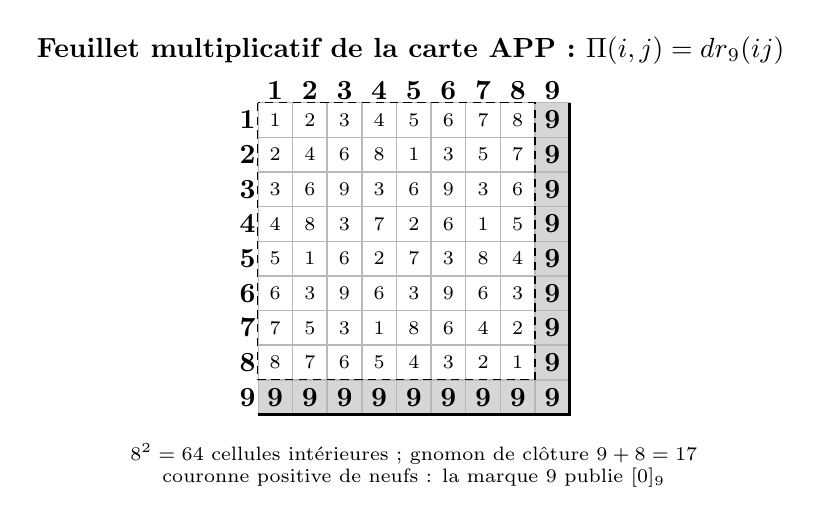
\begin{tikzpicture}[
  font=\scriptsize,
  cell/.style={minimum width=4.35mm,minimum height=4.35mm,
    inner sep=0pt,draw=black!28}]
  \node[font=\bfseries] at (1.72,.88)
    {Feuillet multiplicatif de la carte APP : $\Pi(i,j)=\operatorname{dr}_9(ij)$};
  \foreach \i in {1,...,9}{
    \node[font=\bfseries] at (-.35,{-(\i-1)*.44}) {\i};
    \foreach \j in {1,...,9}{
      \pgfmathtruncatemacro{\v}{mod(\i*\j-1,9)+1}
      \pgfmathtruncatemacro{\border}{(\i==9)||(\j==9)}
      \ifnum\border=1
        \node[cell,fill=black!16,font=\bfseries]
          at ({(\j-1)*.44},{-(\i-1)*.44}) {\v};
      \else
        \node[cell,fill=white]
          at ({(\j-1)*.44},{-(\i-1)*.44}) {\v};
      \fi
    }
  }
  \foreach \j in {1,...,9}{
    \node[font=\bfseries] at ({(\j-1)*.44},.38) {\j};
  }
  \draw[very thick] (3.74,.22)--(3.74,-3.74)--(-.22,-3.74);
  \draw[densely dashed] (-.22,.22) rectangle (3.30,-3.30);
  \node[align=center,anchor=north,font=\scriptsize] at (1.76,-3.98)
    {$8^2=64$ cellules intérieures ; gnomon de clôture
     $9+8=17$\\couronne positive de neufs : la marque $9$ publie $[0]_9$};
\end{tikzpicture}}
\end{minipage}\hfill
\begin{minipage}[t]{.44\textwidth}
\centering
\resizebox{.98\linewidth}{!}{%
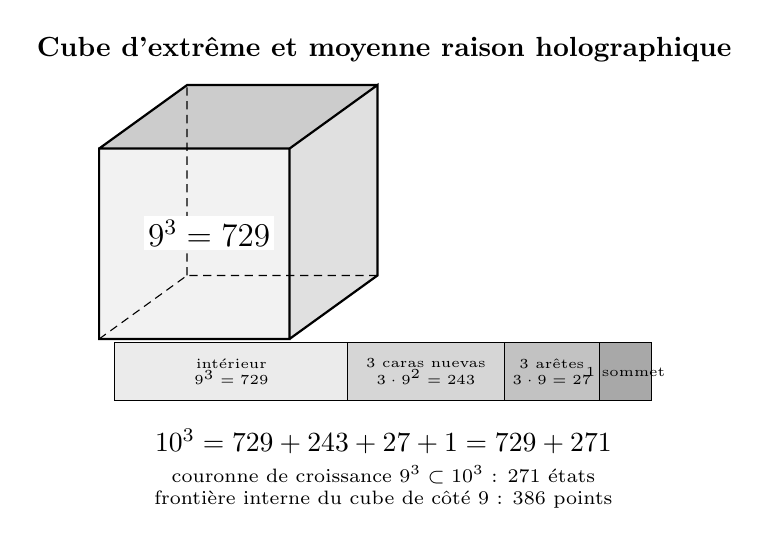
\begin{tikzpicture}[font=\scriptsize]
  \begin{scope}[x={(.78cm,0cm)},y={(.36cm,.26cm)},z={(0cm,.78cm)}]
    \coordinate (O) at (0,0,0);
    \coordinate (X) at (3.1,0,0);
    \coordinate (Y) at (0,3.1,0);
    \coordinate (XY) at (3.1,3.1,0);
    \coordinate (Z) at (0,0,3.1);
    \coordinate (XZ) at (3.1,0,3.1);
    \coordinate (YZ) at (0,3.1,3.1);
    \coordinate (XYZ) at (3.1,3.1,3.1);
    \path[fill=black!5] (O)--(X)--(XZ)--(Z)--cycle;
    \path[fill=black!12] (X)--(XY)--(XYZ)--(XZ)--cycle;
    \path[fill=black!20] (Z)--(XZ)--(XYZ)--(YZ)--cycle;
    \draw[densely dashed] (O)--(Y)--(XY) (Y)--(YZ);
    \draw[thick] (O)--(X)--(XZ)--(Z)--cycle
      (X)--(XY)--(XYZ)--(XZ) (Z)--(YZ)--(XYZ);
    \node[font=\bfseries\large,fill=white,inner sep=1.5pt]
      at (1.55,.52,1.55) {$9^3=729$};
  \end{scope}
  \node[font=\bfseries] at (3.62,3.68) {Cube d'extrême et moyenne raison holographique};
  \draw[fill=black!8] (0.2,-.78) rectangle (3.15,-.05);
  \node[align=center,font=\tiny] at (1.68,-.415)
    {intérieur\\$9^3=729$};
  \draw[fill=black!16] (3.15,-.78) rectangle (5.15,-.05);
  \node[align=center,font=\tiny] at (4.15,-.415)
    {$3$ caras nuevas\\$3\cdot9^2=243$};
  \draw[fill=black!24] (5.15,-.78) rectangle (6.35,-.05);
  \node[align=center,font=\tiny] at (5.75,-.415)
    {$3$ arêtes\\$3\cdot9=27$};
  \draw[fill=black!34] (6.35,-.78) rectangle (7.02,-.05);
  \node[align=center,font=\tiny] at (6.685,-.415)
    {$1$ sommet};
  \node[font=\bfseries] at (3.61,-1.30)
    {$10^3=729+243+27+1=729+271$};
  \node[align=center] at (3.61,-1.88)
    {couronne de croissance $9^3\subset10^3$ : $271$ états\\
     frontière interne du cube de côté $9$ : $386$ points};
\end{tikzpicture}}
\end{minipage}
\caption{Deux publications finies du support. À gauche : la table de
produit avec racine numérique positive et son gnomon de clôture. À droite : la
complétion cubique EMRH, qui distingue intérieur, faces, arêtes et sommet.
La couronne de croissance $271$ et la frontière interne $386$ sont deux
comptages typés : le premier mesure l'extension $9^3\subset10^3$ et le
second la frontière du cube de côté $9$.}
\label{fig:app-emrh-mini}
\end{figure}

Le volume intérieur, les faces, les arêtes et la clôture ponctuelle sont ainsi
typés comme des couches distinctes d'une même unité complétée. Sur les 81
cellules de la carte positive agissent les évaluations
\[
\Sigma,\Pi:\mathcal D_9^2\longrightarrow\mathcal D_9,
\qquad
\Sigma(i,j)=\operatorname{dr}_9(i+j),
\qquad
\Pi(i,j)=\operatorname{dr}_9(ij),
\]
Leurs résidus et quotients relevés sont définis par
\[
\begin{aligned}
R^+(i,j)&:=\Sigma(i,j),&
Q^+(i,j)&:=\frac{i+j-R^+(i,j)}9,\\
R^\times(i,j)&:=\Pi(i,j),&
Q^\times(i,j)&:=\frac{ij-R^\times(i,j)}9,
\end{aligned}
\]
et, par conséquent,
\[
\begin{aligned}
\widehat\Sigma(i,j)&:=\bigl(R^+(i,j),Q^+(i,j)\bigr),\\
\widehat\Pi(i,j)&:=\bigl(R^\times(i,j),Q^\times(i,j)\bigr),
\end{aligned}
\qquad
\widehat\Sigma,\widehat\Pi:
\mathcal D_9^2\longrightarrow\mathcal D_9\times\mathbb Z_{\geq0}.
\]
La bijection \(\lambda_9^{\times2}:\mathcal D_9^2\to X_9\) transporte
ces opérations et leurs relèvements sur le tore. APP est donc le tuple
\begin{equation}
\APP=\bigl(\mathcal D_9,\lambda_9,X_9,\Gamma_{\rm APP},
\operatorname{Path}(\Gamma_{\rm APP}),
\Sigma,\Pi,\widehat\Sigma,\widehat\Pi\bigr),
\label{p12-83-c3-s1:eq:app-full-definition-public}
\end{equation}
Le tableau constitue une représentation bidimensionnelle de ce tuple
complet. Le feuillet additif est latin ; le feuillet multiplicatif conserve
le radical ternaire de l'anneau \(\mathbb Z/9\mathbb Z\)
\begin{equation}
R_9:=\mathbb Z/9\mathbb Z,
\qquad
\mathfrak m:=([3]_9)=\{[0]_9,[3]_9,[6]_9\}\triangleleft R_9,
\qquad \mathfrak m^2=(0).
\label{p12-83-c3-s1:eq:app-radical-369}
\end{equation}
La rotation interne est l'automorphisme
\[
\rho:\mathfrak m^3\longrightarrow\mathfrak m^3,
\qquad \rho(x_1,x_2,x_3)=(x_2,x_3,x_1),
\]
dont l'orbite distinguée est
\[
([3]_9,[6]_9,[0]_9)\xrightarrow{\rho}
([6]_9,[0]_9,[3]_9)\xrightarrow{\rho}
([0]_9,[3]_9,[6]_9)\xrightarrow{\rho}
([3]_9,[6]_9,[0]_9).
\]
La réduction directe envoie \(3,6,9\) sur \(0,0,0\). La coordonnée interne
de l'idéal conserve, en revanche, le facteur extrait :
\begin{equation}
\eta_{\mathfrak m}:(\mathfrak m,+)
\xrightarrow{\;\sim\;}(\mathbb Z/3\mathbb Z,+),
\qquad
\eta_{\mathfrak m}([3a]_9):=[a]_3,
\qquad
([3]_9,[6]_9,[0]_9)
\xmapsto{\;\eta_{\mathfrak m}^{\times3}\;}
([1]_3,[2]_3,[0]_3),
\label{p12-83-c3-s1:eq:app-369-120}
\end{equation}
de sorte que le secteur \(3,6,9\) demeure entier et que sa coordonnée interne se
lit comme \(1,2,0\). Cette application appartient au radical d'APP ; la
projection temporelle de TRIT constitue le lecteur calendaire ultérieur. Les
trois classes calendaires
sont séparées comme
\[
\mathcal C_+=\{1,4,7\},\qquad
\mathcal C_-=\{2,5,8\},\qquad
\mathcal C_0=\{3,6,9\}.
\]
L'incompatibilité entre les deux feuillets devient un invariant mesurable. Sur
\(\mathscr A_3=\mathcal D_9^3\), muni de la mesure uniforme
\(\nu_3(x)=9^{-3}\), soit
\(\mathcal H_3=L^2(\mathscr A_3,\nu_3)\). Nous définissons
\[
\Sigma_3,\Pi_3:\mathscr A_3\longrightarrow\mathcal D_9,
\qquad
\Sigma_3(x)=\operatorname{dr}_9(x_1+x_2+x_3),
\qquad
\Pi_3(x)=\operatorname{dr}_9(x_1x_2x_3),
\]
et les projecteurs orthogonaux
\[
P_{\Sigma,3}:=\mathbb E_{\nu_3}[\,\cdot\mid\sigma(\Sigma_3)],
\qquad
P_{\Pi,3}:=\mathbb E_{\nu_3}[\,\cdot\mid\sigma(\Pi_3)]
\in\mathcal B(\mathcal H_3).
\]
L'énumération conjointe des \(9^3\) mots détermine alors
\[
\bigl\|[P_{\Sigma,3},P_{\Pi,3}]\bigr\|=\frac{\sqrt3}{4},
\qquad
B_c=7I+2R=9P_++5P_-,
\qquad
459-405=54.
\]
Le premier nombre réapparaît comme préfacteur électronique ; le deuxième organise
le bloc central ; le troisième enregistre le défaut global somme--produit.

\subsection{TRIT : unité locale topologique et unité de relation temporelle}

HMT fixe d'abord la signature visible
\begin{equation}
\mathrm{TRIT}_{\rm vis}=\{-1,0,+1\},
\qquad \tau\in\mathrm{TRIT}_{\rm vis}.
\label{p12-83-c3-s1:eq:trit-visible-signature}
\end{equation}
Face à l'unité binaire, le TRIT conserve trois régimes locaux. Dans la
distribution uniforme, son information et son entropie se distinguent comme
\begin{equation}
I_{\rm TRIT}=\log3\ \text{nats}=\log_2 3\ \text{bits},
\qquad S_{\rm TRIT}=k_BI_{\rm TRIT}.
\label{p12-83-c3-s1:eq:trit-information-unit}
\end{equation}
Le bit demeure l'unité binaire ; le TRIT est l'unité minimale capable de
distinguer simultanément retour, seuil et ouverture. L'égalité
\eqref{p12-83-c3-s1:eq:trit-information-unit} quantifie l'information du triplet ; le
coût \(k_B\Theta\log3\) appartient au lecteur thermique de réinitialisation ultérieur.
La mécanique dimensionnelle conserve en outre l'antécédent arithmétique de cette signature.
Pour \((i,j)\in\mathcal D_9^2\), la cellule arithmétique relevée associée est
\begin{equation}
c_{\rm MD}(i,j;\tau)=
\bigl(i,j;R^+,Q^+,R^\times,Q^\times;\tau\bigr).
\label{p12-83-c3-s1:eq:trit-complete-local-unit}
\end{equation}
Les résidus \(R^+,R^\times\) sont la publication visible des deux feuillets ;
les quotients \(Q^+,Q^\times\) conservent la mémoire exacte de la division
euclidienne ; et \(\tau\) oriente la transition. La signature visible occupe le premier
niveau ; la cellule qui la porte ajoute les antécédents arithmétiques, et l'état
enrichi complète ensuite frontière, route, phase et survie.

Il convient de séparer quatre strates. La signature visible est \(\tau\) ; le couple
résidu--retenue est son relèvement local ; \(c_{\rm MD}\) est la cellule
arithmétique d'APP munie de cette signature ; et l'état TPK ajoute extension,
frontière, registre généalogique, phase et survie. Cette hiérarchie conserve l'identité
propre de la coordonnée observée, de son relèvement, de la cellule porteuse et de
l'histoire enrichie qui la transporte.

Dans la carte ternaire équilibrée, l'entier local relevé
\(n\in\{-4,-3,\ldots,3,4\}\) se décompose de manière unique comme
\begin{equation}
\widehat n=(r,\kappa),
\qquad n=r+3\kappa,
\qquad r,\kappa\in\{-1,0,+1\}.
\label{p12-83-c3-s1:eq:trit-balanced-lift}
\end{equation}
La signature visible est \(\tau=r\) ; \(\kappa\) conserve la retenue que la projection
\(n\mapsto r\) oublierait.
La fibre au-dessus du zéro visible contient trois états distincts,
\[
0^+=(0,+1),\qquad 0^0=(0,0),\qquad 0^-=(0,-1),
\]
car \(n=-3,0,3\) possèdent le même résidu visible et des retenues distinctes. C'est
le relèvement topologique minimal de MD : une transition orientée d'APP
est munie de l'information nécessaire pour l'inverser et pour décider quelles
prolongations demeurent compatibles.

La signature possède en outre une règle de mémoire de feuillet. Si \(m_k\) est le mode
arithmétique actif, alors
\begin{equation}
m_{k+1}=
\begin{cases}
\Sigma,&\tau_k=+1,\\
\Pi,&\tau_k=-1,\\
m_k,&\tau_k=0.
\end{cases}
\label{p12-83-c3-s1:eq:trit-zero-memory}
\end{equation}
Le zéro code la rétention du feuillet précédent. C'est pourquoi le mot
\((+1,-1,0)\) publie la séquence \((\Sigma,\Pi,\Pi)\) : le troisième état
conserve le mode multiplicatif actif.

La relation temporelle s'obtient en paramétrant ces cellules de manière ordonnée.
Chaque signature porte une algèbre quadratique
\begin{equation}
\mathbb A_\tau=\mathbb R[X]/(X^2+\tau),
\qquad J_\tau=[X],
\label{p12-83-c3-s1:eq:trit-quadratic-algebra-local}
\end{equation}
de sorte que
\[
\begin{array}{c@{\qquad}c@{\qquad}l}
\toprule
\tau & J_\tau^2 & \text{relation temporelle ordonnée}\\
\midrule
+1 & -I & \text{retour elliptique, mémoire et passé},\\
0  & 0  & \text{seuil parabolique et présent},\\
-1 & +I & \text{ouverture hyperbolique bidirectionnelle et futur}.\\
\bottomrule
\end{array}
\]
Le TRIT précède le temps extérieur : il classe d'abord le type algébrique et
topologique du transport ; ensuite, un paramétrage ordonné le publie
comme relation temporelle. La double direction est typée par l'involution
exacte
\begin{equation}
\mathcal C_{\rm rev}(\tau_1,\ldots,\tau_n)
=(-\tau_n,\ldots,-\tau_1),
\qquad \mathcal C_{\rm rev}^2=I,
\label{p12-83-c3-s1:eq:trit-time-reversal}
\end{equation}
qui échange retour et ouverture et conserve le seuil. Dans le feuillet
hyperbolique, \(P_\pm=(I\pm J_{-1})/2\) séparent les deux directions propres et
la réversion échange leurs orientations. Topologie et temps sont ainsi les
deux lectures coordonnées du TRIT.

L'involution combinatoire \(\mathcal C_{\rm rev}\) et une conjugaison
opératorielle \(C\) appartiennent cependant à des domaines distincts. Dans une
réalisation dynamique séparée, munie de \(H=H^*\),
\(CJ_EC^{-1}=-J_E\) et \(CHC^{-1}=H\), nous fixons une échelle d'action interne
\(\hbar_{\rm int}>0\) et écrivons
\(h_{\rm int}:=2\pi\hbar_{\rm int}\). Alors
\begin{equation}
U(t)=\exp(-J_EHt/\hbar_{\rm int}),
\qquad CU(t)C^{-1}=U(-t).
\label{p12-83-c3-s1:eq:trit-bidirectional-propagator}
\end{equation}
L'entrelaceur qui transporte les mots TRIT vers la réalisation dynamique fixe
la correspondance entre \(\mathcal C_{\rm rev}\) et \(C\). La double
orientation locale fournit le domaine de cette construction.

\subsection{TPK : catégorie de transport et évolution de phase}

Le \emph{Topological Phase Kernel} est la catégorie de transport sur la
base observable d'APP qui compose chiffres, mots, opérateurs et relations
de prolongation dans un même état enrichi. Son architecture interne se répartit en
huit classes opératoires, différenciées par domaine, codomaine et fonction :
\begin{enumerate}[label=\textup{(\roman*)},leftmargin=2.25em]
\item support observable et état enrichi ;
\item sélecteur interne de feuillet \(M_{\rm ph}:\{1,\ldots,9\}\to\{+1,-1,0\}\) ;
\item translations cardinales et évolution visible \(F_{\rm obs}\) ;
\item lecteurs et quotients nonadique, tritique et de bloc \(1000\) ;
\item mémoire, retenue, cylindre, frontière et registre généalogique ;
\item périodicité et retour
\(C_{12}\hookrightarrow C_{108}\twoheadrightarrow C_9\),
\(\mathcal K_{27}\) et canaux \(90/120\) ;
\item prolongations \(\operatorname{Ext}_r\), cylindres, survie et
extension naturelle bidirectionnelle ;
\item foncteurs de sortie archimédienne, exceptionnelle étalonnée et dimensionnelle.
\end{enumerate}
Le retour de 27 pas est le morphisme composé
\begin{equation}
\mathcal K_{27}:=F_{\rm obs}^{27},
\qquad \mathcal K_{27}^{4}=F_{\rm obs}^{108}.
\label{p12-83-c3-s1:eq:tpk-kernel-27}
\end{equation}
Son quatrième itéré restaure la phase observable du calendrier, tandis que la
mémoire et l'état TPK complet poursuivent leur trajectoire ;
\(\mathcal K_{27}\) est le morphisme de retour interne de \(C_{108}\).
Le calendrier \(C_{108}\), la connexion nonadique, l'extension bilatérale et
les lecteurs occupent des places typées au sein de cette architecture. Soit
\(\mathsf P_{\rm APP}\) la catégorie
libre du graphe dirigé d'APP et
\(\mathsf P_{\rm APP}^{(2)}=\mathsf P_{\rm APP}\times
\mathsf P_{\rm APP}\) sa lecture simultanée somme--produit. Soit en outre
\[
\mathcal Q_{\rm obs}
=X_9^2\times\{N,E,S,O\}^2\times\Theta_{108},
\qquad \Theta_{108}=\mathbb Z/108\mathbb Z,
\]
où, pour le représentant
\(\widetilde\theta\in\{0,\ldots,107\}\),
\[
r(\theta)=1+(\widetilde\theta\bmod9),
\qquad g_0(\theta)=[\widetilde\theta]_9,
\]
\[
\tau(\theta)=
\begin{cases}
+1,&r(\theta)\in\{1,4,7\},\\
-1,&r(\theta)\in\{2,5,8\},\\
0,&r(\theta)\in\{3,6,9\},
\end{cases}
\qquad
\mu(\theta)=
\begin{cases}
\Sigma,&\tau(\theta)=+1,\\
\Pi,&\tau(\theta)=-1,\\
\varnothing,&\tau(\theta)=0.
\end{cases}
\]
L'étiquette calendaire \(\mu=\varnothing\) indique le seuil, et la mémoire
dynamique \(m_k\) de \eqref{p12-83-c3-s1:eq:trit-zero-memory} retient le dernier feuillet
actif. Une configuration
\(q=(p^\Sigma,p^\Pi,d^\Sigma,d^\Pi,\theta)\) conserve les deux positions,
les deux directions cardinales et l'indice du calendrier. L'évolution
visible \(F_{\rm obs}\) active le feuillet indiqué par TRIT, transporte la
position correspondante et fait avancer \(\theta\). Notons
\(\mathsf P_{\rm obs}\) la catégorie libre engendrée par les flèches
\(q\to F_{\rm obs}(q)\). Chaque flèche induit un couple de chemins d'APP et
définit le foncteur de base
\begin{equation}
B:\mathsf P_{\rm obs}\longrightarrow\mathsf P_{\rm APP}^{(2)}.
\label{p12-83-c3-s1:eq:tpk-bivariant-base-functor}
\end{equation}

Au-dessus de chaque \(q\) est disposée la fibre typée
\begin{equation}
\mathcal F_q=
\mathsf O_q\times\mathsf H_q\times\mathsf C_q\times\mathsf S_q
\times\mathsf B_q\times\mathsf\Lambda_q,
\label{p12-83-c3-s1:eq:tpk-fiber}
\end{equation}
Ses six facteurs conservent respectivement orientation et feuillet ; résidu et
quotient ; retenue ; signature ; cylindre et frontière ; et registre ordonné de
transport. Mémoire et survie sont des propriétés de la composition et des
relations de prolongation.

Pour une route \(r:q\to q'\), la relation
\begin{equation}
\operatorname{Ext}_r\subseteq\mathcal F_q\times\mathcal F_{q'}
\label{p12-83-c3-s1:eq:tpk-extension-relation}
\end{equation}
contient toutes les continuations admissibles et satisfait
\[
\Delta_q\subseteq\operatorname{Ext}_{\operatorname{id}_q},
\qquad
\operatorname{Ext}_{r_2}\circ\operatorname{Ext}_{r_1}
\subseteq\operatorname{Ext}_{r_2\circ r_1}.
\]
Les transports respectent les identités et la composition :
\begin{equation}
\begin{gathered}
\mathsf H(\operatorname{id}_q)=I,
\quad \mathsf C(\operatorname{id}_q)=I,
\quad \mathsf\Lambda(\operatorname{id}_q)=I,
\quad \kappa(\operatorname{id}_q)=0,\\
\mathsf H(r_2\!\circ r_1)=\mathsf H(r_2)\mathsf H(r_1),
\quad
\mathsf C(r_2\!\circ r_1)=\mathsf C(r_2)\mathsf C(r_1),
\quad
\mathsf\Lambda(r_2\!\circ r_1)=
\mathsf\Lambda(r_2)\mathsf\Lambda(r_1).
\end{gathered}
\label{p12-83-c3-s1:eq:tpk-functorial-transport}
\end{equation}
Outre ces lois fonctorielles, les coordonnées transportées obéissent à
\begin{equation}
\begin{aligned}
h'&=\mathsf H(r)(h),\\
c'&=\mathsf C(r)(c)+\kappa(r),\\
\lambda'&=\mathsf\Lambda(r)(\lambda),\\
\sigma'&=\operatorname{Sig}_{q'}(h',c',\lambda'),
\end{aligned}
\qquad
\kappa(r_2\circ r_1)
=\kappa(r_2)+\mathsf C(r_2)\kappa(r_1).
\label{p12-83-c3-s1:eq:tpk-typed-transport}
\end{equation}
La dernière identité est le cocycle de retenue qui rend associative la
composition avec mémoire.

Le TPK est alors la catégorie \(\mathsf{TPK}\) dont les objets sont
\begin{equation}
x=(q,o,h,c,\sigma,C,b,\lambda),
\qquad (o,h,c,\sigma,(C,b),\lambda)\in\mathcal F_q,
\label{p12-83-c3-s1:eq:tpk-enriched-object}
\end{equation}
et dont les morphismes \(x\to x'\) sont les triplets \((r,x,x')\) tels que
les coordonnées satisfont \eqref{p12-83-c3-s1:eq:tpk-typed-transport} et
\((f_x,f_{x'})\in\operatorname{Ext}_r\), où
\(f_x\in\mathcal F_q\) et \(f_{x'}\in\mathcal F_{q'}\). La composition est
\begin{equation}
(r_2,x',x'')\circ(r_1,x,x')
=(r_2\circ r_1,x,x''),
\label{p12-83-c3-s1:eq:tpk-morphism-composition}
\end{equation}
\Needspace{7\baselineskip}
l'identité est \((\operatorname{id}_q,x,x)\), et le foncteur
\begin{equation}
p:\mathsf{TPK}\longrightarrow\mathsf P_{\rm obs},
\qquad p(x)=q,
\qquad p(r,x,x')=r,
\label{p12-83-c3-s1:eq:tpk-base-functor}
\end{equation}
publie la configuration visible sans identifier les états d'une même fibre.
La définition fixe une catégorie au-dessus d'une base ; elle ne présuppose pas qu'il s'agisse d'une
fibration catégorique ni que toute flèche admette un relèvement cartésien.
Les projections locales sont séparées par type :
\[
\pi_{\rm TRIT}:\operatorname{Ob}(\mathsf{TPK})
\longrightarrow\mathrm{TRIT}_{\rm vis},
\qquad
\pi_{\rm TRIT}(x)=\tau(\theta),
\]
\[
\pi_{\rm loc}(x)=
\bigl(\pi_{\rm TRIT}(x),\mu(\theta),o,h,c,
\sigma,\lambda,g_0(\theta)\bigr).
\]
La première ne récupère que la signature TRIT visible. La seconde conserve
en outre l'étiquette calendaire de feuillet, l'orientation, le couple
résidu--quotient, la retenue, la signature de transport, le registre généalogique et la phase,
mais oublie encore le cylindre, son étiquette de bord et d'autres coordonnées de
\(q\). C'est pourquoi ni le TRIT visible ni son registre local
ne se substituent à l'état enrichi du TPK.

Le nom réunit trois fonctions inséparables. \emph{Topological} renvoie à
la catégorie de chemins, à l'incidence, au bord et à la prolongation par
cylindres ; \emph{Phase} renvoie à l'indice nonadique, au calendrier orienté et
à l'holonomie ; \emph{Kernel} désigne le noyau persistant de transport qui
demeure avant de contracter l'état au moyen d'un lecteur. Formellement,
l'objet est la catégorie précédente : une topologie supplémentaire sur les objets ou
les morphismes, ou son identification au noyau linéaire d'une application, exige
des données indépendantes.

En conséquence, deux routes ayant la même extrémité visible peuvent demeurer
des objets distincts par leur feuillet, quotient, retenue, frontière, cylindre, phase ou
registre. Le TPK ne choisit pas une sortie scalaire : il conserve l'antécédent commun
dont partent les publications archimédienne, exceptionnelle et dimensionnelle.

% Estas consecuencias se publican después de la construcción correlativa y
% del paso al límite de los capítulos 4 y 5. Se definen aquí para preservar
% íntegramente su procedencia, pero no se ejecutan antes de que exista el
% continuo al que se aplican.
\long\def\HMTDeferredContinuumConsequences{%
\section{Conséquences et publications du continu construit}

\subsection{Théorème d'assemblage terminal des constructions corrélatives engendrées par l'état commun}

Chaque profondeur \(k\) possède un état enrichi \(\mathcal E_k\) avec
toutes ses émissions survivantes et un unique constructeur corrélatif
\begin{equation}
\mathcal O_k:\mathcal E_k\longrightarrow\mathcal Z_k,
\qquad
\widehat x_k\longmapsto
\mathcal O\bigl(\{\mathfrak e_\alpha:
\alpha\in\operatorname{Ch}_k(\widehat x_k)\}\bigr).
\label{p12-83-c3-s1:eq:five-features-single-constructor}
\end{equation}
La valeur de \(\mathcal O_k\) conserve simultanément les coordonnées
spectrale, solénoïdale, de jauge, cohérente et déterminantale,
\begin{equation}
(\mathrm{sp},\mathrm{sol},\mathrm{gau},\mathrm{coh},\mathrm{det}),
\label{p12-83-c3-s1:eq:five-features-coordinates}
\end{equation}
comme cinq caractéristiques du même état et du même registre généalogique. Les
troncatures
\[
u^{\mathfrak e}_{\ell,k}:\mathcal E_\ell\to\mathcal E_k,
\qquad
u^{\mathcal O}_{\ell,k}:\mathcal Z_\ell\to\mathcal Z_k
\]
satisfont l'unique naturalité
\begin{equation}
u^{\mathcal O}_{\ell,k}\circ\mathcal O_\ell
=\mathcal O_k\circ u^{\mathfrak e}_{\ell,k},
\qquad \ell\ge k.
\label{p12-83-c3-s1:eq:five-features-naturality}
\end{equation}
C'est pourquoi l'action corrélative passe à la limite sous la forme
\begin{equation}
\mathcal O_\infty:
\mathcal C_{\rm cont}^{\rm disc}:=\varprojlim_k\mathcal E_k
\longrightarrow
\mathcal Z_\infty:=\varprojlim_k\mathcal Z_k.
\label{p12-83-c3-s1:eq:five-features-infinite-operator}
\end{equation}
Les cinq applications terminales sont des vues intrinsèques de cette unique valeur :
\begin{equation}
\boxed{
\mathfrak G_T^{\rm int}:=
\operatorname{View}_T\!\left(
\mathcal O_\infty(\mathcal C_{\rm cont}^{\rm disc})\right),
\quad
T\in\{\mathrm{sp},\mathrm{sol},\mathrm{gau},
\mathrm{coh},\mathrm{det}\}.}
\label{p12-83-c3-s1:eq:five-features-views}
\end{equation}
La simultanéité précède les résolutions spécialisées : chaque vue expose
la coordonnée requise et l'état complet conserve les quatre autres.

\subsection{Survie et limite projective}

Soit \(\operatorname{Surv}^{(\chi)}_N\) l'ensemble des histoires de
profondeur \(N\) qui satisfont simultanément les lois actives du canal
\(\chi\) et admettent une prolongation. Nous définissons les troncatures compatibles
\[
\tau_{N+1,N}:\operatorname{Surv}^{(\chi)}_{N+1}
\longrightarrow\operatorname{Surv}^{(\chi)}_N
\]
Celles-ci conservent le préfixe enrichi. Le continu généalogique est la limite
\begin{equation}
X_\chi=\varprojlim_N
\bigl(\operatorname{Surv}^{(\chi)}_N,\tau_{N+1,N}\bigr),
\qquad
\tau_{N+1,N}(x_{N+1})=x_N.
\label{p12-83-c3-s1:eq:inverse-survival}
\end{equation}
L'espace global des sections survivantes et l'une de ses sections
enrichies sont notés respectivement
\begin{equation}
X_\infty:=\bigsqcup_\chi X_\chi,
\qquad
\widehat\Omega_\infty\in X_\infty.
\label{p12-83-c3-s1:eq:global-survival-space}
\end{equation}
Le lecteur archimédien global est
\begin{equation}
P_{\rm arq}:=\operatorname{ev}_{\mathbb R}:
X_\infty\longrightarrow\mathbb R;
\label{p12-83-c3-s1:eq:archimedean-reader}
\end{equation}
sa restriction à chaque canal évalue l'intersection réduite à un point des cylindres
compatibles de la section correspondante.
Lorsque le lecteur exceptionnel intervient, \(X_\infty^{\rm cal}\subseteq
X_\infty\) désigne le sous-espace dans lequel le type d'étalonnage
de \eqref{p12-83-c3-s1:eq:exceptional-calibration} a été fixé.
La survie détermine la section par compatibilité interne : chaque
histoire doit pouvoir être prolongée dans le système complet. Le lecteur numérique
intervient ensuite pour certifier et publier l'intersection du
descendant déjà compatible.

\subsection{Connexion nonadique conjointe, holonomie et mémoire verticale}

À la profondeur \(K\), l'holonomie du retour nonadique est initialement la
correspondance typée
\begin{equation}
\Gamma_{9,K}=\operatorname{Hol}_{C_9}(\nabla_{\rm TPK}):
\widehat{\mathcal X}_K\rightrightarrows
\widehat{\mathcal X}_{K+9}.
\label{p12-83-c3-s1:eq:gamma9}
\end{equation}
Ses itérés sont des compositions relationnelles. Ce n'est que lorsque chaque état possède
une unique prolongation compatible qu'elle se restreint à une application, et ce n'est que lorsque cette
application est inversible qu'elle constitue une monodromie. Cette distinction conserve toutes
les extensions survivantes avant de sélectionner une section.
Après neuf phases, la phase locale revient, tandis que l'état complet avance :
\[
g(K+9)=g(K),\qquad q_{{\rm mem},K+9}=q_{{\rm mem},K}+1,
\qquad \widehat x_{K+9}\ne\widehat x_K\ \text{en général}.
\]
Bloc, cylindre, préfixe, retenue et mémoire continuent d'évoluer. Telle
est la différence entre périodicité visible et retour avec biographie.

L'état transporté au niveau (K) peut être présenté comme
\begin{equation}
\widehat x_K=
(B_K,C_K,p_K,c_K,\Sigma_K,W_K,g(K),q_{{\rm mem},K},s_K),
\label{p12-83-c3-s1:eq:enriched-state-k}
\end{equation}
où chaque coordonnée possède une loi de transport propre. Le retour de phase
est représenté sur le catalogue
\[
\mathcal U_6^{\rm cat}\cong\mathfrak S_+\times\mathfrak S_\times,
\qquad |\mathfrak S_+|=18,
\qquad |\mathfrak S_\times|=26.
\]
Les moyennes conditionnelles
\[
(E_+f)(s,e)=\frac1{18}\sum_{s'\in\mathfrak S_+}f(s',e),
\qquad
(E_\times f)(s,e)=\frac1{26}\sum_{e'\in\mathfrak S_\times}f(s,e')
\]
commutent. Le mot de phase
\(\tau=(+1,-1,0,+1,-1,0,+1,-1,0)\) applique
\(E_+,E_\times,I\) dans cet ordre, et un tour se clôt au moyen de
\begin{equation}
\mathcal K_{\rm ph}^{\,9}
=(E_+E_\times)\otimes I_{\ell^2(C_9)},
\qquad
\bigl\langle\delta_u,E_+E_\times\delta_v\bigr\rangle
=\frac1{468}\quad(u,v\in\mathcal U_6^{\rm cat}).
\label{p12-83-c3-s1:eq:joint-nine-holonomy}
\end{equation}
Les feuillets somme et produit n'agissent pas comme des filtres indépendants : ce sont deux
composantes d'une unique holonomie qui ne se clôt qu'après avoir parcouru le
cycle complet.

La colligation compression--expression sépare ce qui revient de ce qui demeure
comme mémoire. Si (J) plonge l'espace des histoires dans l'espace de
phase, si (T) est la compression survivante et \(\eta\) le canal de défaut,
alors
\begin{equation}
\boxed{
U_{\Gamma_9}J=JT+\eta,
\qquad J^*\eta=0,
\qquad I-T^*T=\eta^*\eta.}
\label{p12-83-c3-s1:eq:compression-expression}
\end{equation}
La première égalité décompose le transport en retour comprimé et
expression de mémoire ; la deuxième prouve leur orthogonalité ; la troisième mesure
exactement l'information qui ne tient pas dans l'ombre périodique. L'affirmation
centrale est ainsi formalisée : c'est la phase qui revient, non l'état complet.

La mémoire verticale s'organise au moyen de l'extension cyclique orientée
\begin{equation}
0\longrightarrow C_{12}\xrightarrow{\,\iota\,}C_{108}
\xrightarrow{\,p\,}C_9\longrightarrow0,
\qquad
c(r,r')=\left[\left\lfloor\frac{r+r'}9\right\rfloor\right]_{12}.
\label{p12-83-c3-s1:eq:c108-extension}
\end{equation}
Ici \(\iota([b]_{12})=[9b]_{108}\) et
\(p([\theta]_{108})=[\theta]_9\). L'extension n'est pas scindée :
\(C_{108}\) est d'exposant 108, tandis que
\(C_{12}\times C_9\) est d'exposant 36.
Le cocycle enregistre la retenue de chaque tour de la base \(C_9\) dans la
mémoire dodécaphasique \(C_{12}\). \(C_{108}\) est donc un calendrier
orienté de phase et de mémoire. Ce n'est qu'après la carte dimensionnelle que cette
extension se réalise comme une horloge quantique finie de 108 pas.

Le relèvement local de MD qui porte la signature TRIT est l'unité
topologique--temporelle de ce cristal généalogique.
Sur
\(\mathcal H_{\rm clk}=\mathbb C^{108}\), de base
\(\{|j\rangle:j\in\mathbb Z/108\mathbb Z\}\), soient
\[
\zeta=e^{2\pi\ii/108},\qquad
|\widetilde k\rangle=\frac1{\sqrt{108}}
\sum_{j=0}^{107}\zeta^{jk}|j\rangle,
\qquad U_{\rm clk}|j\rangle=|j+1\rangle.
\]
\Needspace{12\baselineskip}
Avec \(\omega_0=2\pi/(108t_0)\), le hamiltonien
\begin{equation}
H_{\rm clk}=\hbar_{\rm int}\omega_0
\sum_{k=0}^{107}k\,|\widetilde k\rangle\langle\widetilde k|
\label{p12-83-c3-s1:eq:trit-time-crystal-hamiltonian}
\end{equation}
engendre exactement
\begin{equation}
U_{\rm step}=\exp\!\left(
-\frac{\ii H_{\rm clk}t_0}{\hbar_{\rm int}}\right)=U_{\rm clk},
\qquad U_{\rm step}^{108}=I,
\label{p12-83-c3-s1:eq:trit-time-crystal-period}
\end{equation}
Si \(Z_{\rm clk}|j\rangle=\zeta^j|j\rangle\), alors
\begin{equation}
\langle j_0|U_{\rm step}^{-n}Z_{\rm clk}U_{\rm step}^{n}|j_0\rangle
=\zeta^{j_0+n},
\label{p12-83-c3-s1:eq:trit-time-crystal-observable}
\end{equation}
dont l'orbite possède une période primitive de 108. Dans le vocabulaire HMT, il s'agit du
cristal temporel généalogique interne : le calendrier observable se clôt,
\(C_{12}\) enregistre le tour et l'état TPK enrichi ne revient pas nécessairement.
La réalisation ultérieure comme phase physique macroscopique exige,
en outre, un protocole de Floquet, une réponse sous-harmonique primitive, la robustesse,
la persistance et un mécanisme de protection ; cette carte ne modifie pas le théorème
fini de périodicité unitaire.

\subsection{Publication archimédienne, nombre généalogique et mesure}

La publication archimédienne utilise des cylindres ternaires semi-ouverts
\begin{equation}
I_{N,L}=\left[\frac{N}{3^L},\frac{N+1}{3^L}\right),
\qquad \operatorname{diam}I_{N,L}=3^{-L}\longrightarrow0.
\label{p12-83-c3-s1:eq:ternary-cylinders}
\end{equation}
Une section compatible détermine des cylindres emboîtés et, par complétude, un
unique point réel. Le nombre HMT est la section elle-même,
\begin{equation}
x=(x_N)_N\in X_\chi
=\varprojlim_N\operatorname{Surv}^{(\chi)}_N,
\label{p12-83-c3-s1:eq:hmt-number-as-section}
\end{equation}
non le tuple formé par elle et ses évaluations. La valeur apparaît lorsqu'un
lecteur oublie une partie de la généalogie.
La précision est donc profondeur : mesurer signifie descendre à un
cylindre plus fin tandis que le préfixe causal demeure dans l'antécédent.
La droite réelle est reconstruite comme quotient archimédien d'un espace
d'histoires beaucoup plus riche.

\subsection{Réalisation dimensionnelle de l'état HMT : application d'écran, grandeur observable et carte spectrale}

La mécanique dimensionnelle commence là où l'état généalogique se couple à une
frontière de réalisation. Un corps \(K_n\) étant fixé, soit \(M_n(x)\) le module
engendré par les canaux de prolongation d'un état \(x\), soit
\(\mathcal R_n(x)\) le sous-module de ses relations et soit \(\beta_n(x)\) la
donnée de bord conservée. L'écran dimensionnel est
\begin{equation}
\Sigma_n(x)=\bigl(K_n,M_n(x),\beta_n(x),\mathcal R_n(x)\bigr),
\qquad
d_{\Sigma_n}(x)=\dim_{K_n}\frac{M_n(x)}{\mathcal R_n(x)}.
\label{p12-83-c3-s1:eq:md-screen}
\end{equation}
Si \(M_n(x)\simeq K_n^{g_n}\) et si les colonnes de \(R_n(x)\) engendrent les
relations, alors
\begin{equation}
\boxed{d_{\Sigma_n}(x)=g_n-\operatorname{rank}_{K_n}R_n(x).}
\label{p12-83-c3-s1:eq:md-rank}
\end{equation}
La dimension n'est pas adjointe comme étiquette : c'est le nombre de canaux
indépendants qui survivent après l'imposition des relations de frontière.

Une grandeur physique est une section d'une droite dimensionnelle \(L_D\) ; une
unité est une carte \(\chi_u:L_D\to\mathbb R\) qui publie sa coordonnée.
C'est pourquoi
\begin{equation}
\text{état TPK}\longrightarrow\Sigma_n(x)
\longrightarrow s_D\in\Gamma(L_D)
\xrightarrow{\;\chi_u\;}[s_D]_u\in\mathbb R
\label{p12-83-c3-s1:eq:md-measurement-chain}
\end{equation}
sépare exactement structure, type dimensionnel et nombre mesuré. Mesurer
consiste à coupler une section à un appareil réversible, à imposer la
compatibilité de bord et à appliquer le lecteur ; changer d'unités change
\(\chi_u\), non la section ni sa généalogie.

\subsection{Double projection mathématique et réalisation dimensionnelle}

La branche exceptionnelle conserve des données de jauge dont la publication réelle n'a pas
besoin. Soit \(\mathscr C_{\rm exc}\) l'espace des étalonnages et soit
\begin{equation}
\mathfrak E:
X_\infty^{\rm cal}\times\mathscr C_{\rm exc}
\longrightarrow\mathbf{Exc}
\label{p12-83-c3-s1:eq:exceptional-calibrated-reader}
\end{equation}
le lecteur d'incidence. Nous fixons une fois
\begin{equation}
\begin{aligned}
\chi_{\rm exc}=\bigl(&\text{ordre projectif},\ \text{calibre de Paley},
 \ \text{dodécade},\\
 &\text{alignement d’incidence},\ \text{chambre réticulaire}\bigr)
 \in\mathscr C_{\rm exc}
\end{aligned}
\label{p12-83-c3-s1:eq:exceptional-calibration}
\end{equation}
et abrégeons
\(\mathfrak E_{\chi_{\rm exc}}(x):=\mathfrak E(x,\chi_{\rm exc})\).
La jauge initiale est transportée par l'histoire ; elle n'est pas choisie de nouveau à
chaque profondeur.

La même limite étalonnée admet alors deux lecteurs de codomaines
distincts :
\begin{equation}
\mathbb R
\xleftarrow{\;\operatorname{ev}_{\mathbb R}\;}
X_\infty^{\rm cal}
\xrightarrow{\;\mathfrak E_{\chi_{\rm exc}}\;}
\mathbf{Exc}.
\label{p12-83-c3-s1:eq:double-projection}
\end{equation}
La première branche contracte les cylindres jusqu'à une valeur continue. La seconde
conserve incidences, orientations, jauge et frontière. Toutes deux descendent en
parallèle du même état source. Cette bifurcation explique conjointement la
continuité métrique et l'émergence de symétries exceptionnelles. La seconde
branche est une reconstruction étalonnée : elle est exacte une fois
\(\chi_{\rm exc}\) fixé, mais l'état nu ne sélectionne pas rétrospectivement
les cinq données qui composent cette jauge.

La réalisation dimensionnelle ne sérialise pas ces deux branches. C'est un troisième lecteur
du même antécédent :
\begin{equation}
P_{\rm dim}:X_\infty\longrightarrow
\mathcal R_{\rm MD},
\qquad
\mathcal R_{\rm MD}=
\{\text{action, masse, champ, géométrie, information}\}.
\label{p12-83-c3-s1:eq:dimensional-publication}
\end{equation}
De cette manière, un nombre, une symétrie et une grandeur physique peuvent partager
une généalogie sans se confondre ni se réduire les uns aux autres.

La thèse du continu est ainsi formulée avec précision : la réalité
archimédienne est l'ombre de rayon nul d'histoires discrètes infiniment
raffinables ; ce que l'ombre omet réapparaît comme mémoire, incidence,
géométrie et structure physique.

% RESULTADO_RECUPERADO. Owner íntegro de la dinámica del cociente, el retorno
% observable y los cociclos de modo y orientación. Se subordina a la única
% construcción APP--TRIT--TPK sin abrir un origen alternativo.
\begin{HMTScientificOwnerSubordinated}
\chapter{Extensions survivantes, monodromie et dynamique du quotient}
\label{chap:extensiones-dinamica-cociente}
\index{survie!extension globale}
\index{monodromie!retour nonadique}
\index{mesure!catalogue d’émissions}

Le langage des chemins nécessite une précision décisive. Un chemin
d'APP, une émission visible, une histoire enrichie de TPK et une section
globale ne sont pas quatre noms pour le même objet. Ils constituent quatre niveaux
consécutifs d'une même construction. Le chemin conserve l'ordre
positionnel ; l'émission conserve une lecture finie ; l'histoire ajoute la signature,
la retenue, l'orientation, la frontière et la mémoire ; la section globale exige que tous
ses préfixes survivent simultanément à toute profondeur.

Cette hiérarchie permet de séparer deux questions qui étaient restées
entremêlées. La première est logique : sous quelles hypothèses un préfixe fini
appartient réellement à une extension infinie compatible. La seconde est
dynamique : ce que signifie transporter une seule histoire et ce que signifie
transférer simultanément toutes ses continuations compatibles. La
distinction est essentielle dans APP\@. Une trajectoire déterminée mène un état à
un autre ; un transfert de chemins mène une distribution d'extensions à
une autre distribution.

Cette section résout le problème fini de profondeur six. La
chronologie déterministe publiée possède un retour visible et ne peut pas sélectionner
une probabilité unique. En revanche, le transport biaisé par la phase nonadique,
lorsque chaque canal actif est interprété comme le renouvellement normalisé de toute
sa fibre de continuations compatibles, possède un retour de neuf pas
uniforme sur les (468) émissions. Les poids (1/3) cessent alors d'être
un choix extérieur : ils proviennent des trois apparitions de chaque signature
(+1,-1,0) dans le cycle nonadique orienté. La normalisation au sein de chaque fibre reste
une prémisse mathématique précise --- le comptage uniforme de tous les
chemins compatibles --- et ne doit pas être confondue avec le successeur d'une seule
trajectoire. Le passage à la limite inverse de toutes les profondeurs conserve un
énoncé propre, formulé à la fin de la section.

\section{\(5\) niveaux de la notion de chemin}

Soit \(\Gamma_{\rm APP}\) la catégorie des chemins cardinaux du tore APP\@.
Pour chaque profondeur \(m\), soit \(\mathcal H_m\) l'ensemble fini des
histoires enrichies admissibles
\[
 h_m=(v_0,e_1,v_1,\ldots,e_m,v_m),
\]
où chaque flèche \(e_j\) transporte tous les champs déclarés par TPK\@. Si
\(n\geq m\), l'application
\[
 p_{n,m}:\mathcal H_n\longrightarrow\mathcal H_m
\]
élimine la queue postérieure à la profondeur \(m\). L'ombre positionnelle
\[
 \operatorname{sh}_m:\mathcal H_m\longrightarrow\Gamma_{\rm APP}
\]
oublie la fibre de mémoire et conserve le chemin APP sous-jacent.

\begin{definition}[Hiérarchie des extensions]
\label{def:jerarquia-extensiones}
Nous distinguons les objets suivants.
\begin{enumerate}
  \item Un \emph{chemin APP} est un morphisme de
  \(\Gamma_{\rm APP}\).
  \item Une \emph{route observable} est une lecture de ce morphisme qui
  conserve conjointement les feuillets de somme et de produit.
  \item Une \emph{extension TPK} est une élévation de la route observable en
  une histoire \(h_m\in\mathcal H_m\), avec ses données de résidu, de quotient,
  de signature, d'orientation, de frontière, de retenue et de registre.
  \item Une \emph{extension survivante} est une histoire finie qui admet
  des prolongations compatibles à tout horizon.
  \item Une \emph{section globale} est une famille compatible
  \(x=(h_m)_{m\geq0}\) d'extensions survivantes.
\end{enumerate}
En particulier, la route est l'ombre de l'extension ; ce n'est pas un objet extérieur
que l'extension choisirait ensuite.
\end{definition}

Pour \(h\in\mathcal H_m\), son cylindre de prolongations est
\[
 Z_m(h)=
 \{x=(h_n)_n\in\varprojlim_n\mathcal H_n:x_m=h\}.
\]
En particulier, toute famille de \(Z_m(h)\) satisfait en outre
\(p_{n,\ell}(h_n)=h_\ell\) pour \(n\geq\ell\) ; on n'admet pas de collections de
troncatures incompatibles.
Définissons également
\[
 \mathcal S_m^{(N)}=p_{N,m}(\mathcal H_N),
 \qquad
 \mathcal S_m^\infty=\bigcap_{N\geq m}\mathcal S_m^{(N)}.
\]

\begin{theorem}[Critère conditionnel d'extension survivante]
\label{thm:criterio-extension-superviviente}
Fixons \(h\in\mathcal H_m\) et, pour \(N\geq m\), écrivons
\[
 \mathcal P_N(h)=\{g\in\mathcal H_N:p_{N,m}(g)=h\}.
\]
Supposons que les troncatures sont cohérentes et que chaque
\(\mathcal P_N(h)\) est fini. Sont équivalentes :
\begin{enumerate}
  \item \(\mathcal P_N(h)\ne\varnothing\) pour tout \(N\geq m\), c'est-à-dire
  \(h\in\mathcal S_m^\infty\) ;
  \item l'arbre des prolongations finies de \(h\) est à ramification finie
  et possède un niveau non vide à toute profondeur ;
  \item \(Z_m(h)\ne\varnothing\).
\end{enumerate}
Par conséquent, dès lors que les troncatures survivantes finies sont non
vides, l'ensemble
\[
 \Omega_{\rm H}^{\rm surv}
 =\varprojlim_m\mathcal S_m^\infty
\]
est exactement l'espace des sections globales survivantes. Le théorème
n'affirme pas que ces troncatures sont non vides pour toute entrée APP : cette
propriété doit être démontrée au moyen du protocole de survie.
\end{theorem}

\begin{proof}
L'implication de la troisième condition vers les deux premières s'obtient par
troncature. Supposons maintenant la première condition et ordonnons les éléments de
\(\bigsqcup_{N\geq m}\mathcal P_N(h)\) par la relation de préfixe. Chaque niveau
est fini et non vide, et la cohérence des troncatures fait de cette union
un arbre à ramification finie avec des nœuds à toute profondeur ; cela donne la
deuxième condition. Réciproquement, à partir de la deuxième condition, le lemme de König
fournit une branche infinie. Ses troncatures forment une famille compatible
appartenant à \(Z_m(h)\), ce qui est la troisième condition. La même construction
identifie la limite inverse indiquée là où ses troncatures finies sont
non vides.
\end{proof}

Le théorème résout l'éventuelle discordance entre « prolongeable jusqu'à chaque
horizon séparément » et « possède une prolongation globale » : la finitude des
branches est l'hypothèse qui permet de choisir une unique chaîne compatible. Il
n'affirme pas que tous les chemins APP appartiennent à
\(\operatorname{sh}(\Omega_{\rm H}^{\rm surv})\). Cette couverture exige de démontrer
que les fermetures enrichies ne vident pas les fibres correspondantes.

\section{Retour de phase et relation de monodromie}

Le retour du quotient phase--longueur est formalisé séparément dans
\cref{def:odometro-9-12,prop:proyeccion-fase-longitud} :
\[
(b,r)\xrightarrow{\;9\;}(b+1,r),
\qquad
(b,r)\xrightarrow{\;108\;}(b,r).
\]
Ces égalités appartiennent à l'odomètre \(9\times12\). Elles ne constituent pas la
démonstration de \(F_{\rm obs}^{108}=I\), qui utilise l'état observable et apparaît plus
loin.

Soit \(\phi\) la coordonnée de phase à valeurs dans \(\mathbb Z/9\mathbb Z\).
Un retour visible satisfait
\[
 \phi(h_{k+9})=\phi(h_k).
\]
Le registre complet peut cependant satisfaire
\[
 B(h_{k+9})\ne B(h_k).
\]
Cette inégalité n'est pas un défaut de périodicité : c'est la mémoire du tour.
Une action ordinaire de \(C_9\) sur l'état complet imposerait que la
neuvième puissance soit l'identité et effacerait précisément cette information.

Pour typer le retour, soit \(H\) une hexade et
\(P_2(H)\) son ensemble de quinze paires. Soient \(\mathcal B_k\) les états de
registre qui survivent à la phase \(k\), soit
\(\mathcal T_k\subseteq\mathcal B_k\times\mathcal B_{k+1}\) la relation de
transport publiée et supposons donné un encodeur de fibre
\[
 c_k:\mathcal B_k\longrightarrow P_2(H).
\]
Ce n'est qu'après avoir déclaré ces encodeurs que l'on définit la relation observable
\[
 R_k=(c_k\times c_{k+1})(\mathcal T_k)
 \subseteq P_2(H)\times P_2(H).
\]
La monodromie relationnelle d'un tour est
\[
 \mathcal M_k
 =R_{k+8}\circ R_{k+7}\circ\cdots\circ R_k.
\]

\begin{proposition}[Classification du retour nonadique étant donné l'encodeur]
\label{prop:clasificacion-retorno-nonadico}
On distingue trois niveaux logiquement distincts.
\begin{enumerate}
  \item Sans démonstration de fonctionnalité, le retour est la relation
  \(\mathcal M_k\).
  \item Si chaque \(R_k\) est le graphe d'une application
  \(\mu_k:P_2(H)\to P_2(H)\), le transport est le produit biaisé
  \[
   T(k,p)=(k+1,\mu_k(p)),
  \]
  et
  \[
   T^9(k,p)=(k,M_k(p)),
   \qquad
   M_k=\mu_{k+8}\circ\cdots\circ\mu_k.
  \]
  \item Si les \(\mu_k\) sont bijectives, \(M_k\) est une holonomie
  automorphe. Le transport descend en une action ordinaire de
  \(C_9\) sur l'état complet si et seulement si \(M_k=I\) dans toutes les
  fibres.
\end{enumerate}
\end{proposition}

\begin{proof}
La première affirmation est la définition de l'image et de la composition relationnelle une
fois fixés \((c_k)_k\). Sous
fonctionnalité, neuf applications consécutives maintiennent la première
coordonnée fixe et composent leurs actions sur la seconde. La composition de
bijections est une bijection. Enfin, \(T^9=I\) équivaut exactement à
\(M_k=I\) pour chaque phase et chaque point de la fibre.
\end{proof}

\begin{corollary}[Non-retour ponctuel sous transport accumulé]
\label{pf84:E02-29}
Soient \(q:X\to V\), \(T:X\to X\) et \(x\in X\). Si
\[
 q(T^9x)=q(x),\qquad
 T^9x=\mathcal M_x\,x,\qquad
 \mathcal M_x\,x\ne x,
\]
alors la projection revient, mais pas l'état :
\[
 q(T^9x)=q(x),\qquad T^9x\ne x.
\]
L'hypothèse ponctuelle \(\mathcal M_x\,x\ne x\) est indispensable ; l'inégalité
globale \(\mathcal M_x\ne I\) n'exclut pas que \(x\) soit un point fixe.
\end{corollary}

\begin{proof}
La première égalité est une hypothèse. La seconde et la séparation ponctuelle donnent
\(T^9x=\mathcal M_x\,x\ne x\). L'énoncé serait réfuté par un cas qui
satisferait les trois prémisses et aurait \(T^9x=x\) ; il n'autorise pas à remplacer la
troisième prémisse par \(\mathcal M_x\ne I\).
\end{proof}

\begin{theorem}[Suffisance fonctionnelle du tuple enrichi]
\label{pf84:E02-30}
Soit
\[
 E:\mathscr X_{\rm TPK}^{\rm enr}\longrightarrow\mathscr S_E
\]
le tuple qui conserve le bloc visible, les blocs nouveaux et la retenue, l'état
d'élévation, les cylindres, la signature de frontière, l'orientation, l'observable, la phase et le
registre dodécaphasique. Soient
\[
 T:\mathscr X_{\rm TPK}^{\rm enr}\to
 \mathscr X_{\rm TPK}^{\rm enr},
 \qquad
 O:\mathscr X_{\rm TPK}^{\rm enr}\to Y.
\]
Lorsqu'il existe des applications
\[
 \widehat T:\mathscr S_E\to\mathscr X_{\rm TPK}^{\rm enr},
 \qquad
 \widehat O:\mathscr S_E\to Y
\]
tels que
\[
 T=\widehat T\circ E,\qquad O=\widehat O\circ E,
\]
l'égalité \(E(x)=E(y)\) implique \(T(x)=T(y)\), \(O(x)=O(y)\) et, par
déterminisme, les mêmes continuations et sorties ultérieures.
\end{theorem}

\begin{proof}
Par factorisation,
\[
 T(x)=\widehat T(E(x))=\widehat T(E(y))=T(y),
 \qquad
 O(x)=\widehat O(E(x))=\widehat O(E(y))=O(y).
\]
La première égalité permet d'itérer l'argument. C'est une condition
suffisante, non une équivalence non démontrée. Deux états ayant le même tuple et
des transitions ou des sorties différentes, l'accès à une coordonnée absente ou la
consultation d'une valeur cible sont des réfutateurs. La microfibre visible de
cardinal cinq de \cref{pf84:E02-22} contrôle uniquement la non-fidélité du
mot \(w_6\) ; elle ne démontre pas cette factorisation positive.
\end{proof}

La fenêtre finie publiée contient neuf retours de phase avec changement de
l'état enrichi et une sélection locale passant de trois continuations à une lors de
l'augmentation de deux horizons. Cela démontre le retour avec mémoire et réfute
l'identification du registre à un cycle sans mémoire. L'extraction globale des
neuf encodeurs \(c_k\) et, à travers eux, des relations
\(R_k\), à partir de toutes les histoires survivantes est une opération distincte.
La proposition précédente classe le retour une fois donnée l'application
registre--paires ; elle ne dérive pas cette application de l'état enrichi du TPK.

L'épisode concret de la neuvième phase, avec ses trois continuations, le
bloc \(B_{11}\), la frontière \((502,662,638)\) et les inégalités entières
de cylindres, est démontré une seule fois dans
\cref{thm:seleccion-novena-fase}. Ici, seule sa
conséquence typée est utilisée :
\[
\#\operatorname{Surv}_{1}(B_9)=3,\qquad
\#\operatorname{Surv}_{2}(B_9)=1.
\]

Les deux autres mots ne peuvent précéder la même queue ternaire qu'en changeant
l'extension profonde de Hensel. Ils partagent une partie du résidu visible,
mais non la généalogie de l'état.

\section{Le catalogue de 468 émissions comme produit de canaux}

Le catalogue fini part de l'ensemble
\(\Omega_{\rm seed}\) de \(104\,976\) présentations microscopiques. Soit
\(\mathcal U_6\) l'ensemble des émissions sextuples distinctes et soit
\[
 F:\Omega_{\rm seed}\twoheadrightarrow\mathcal U_6.
\]
Le recensement exact est
\[
 |\mathcal U_6|=468,
 \qquad
 \#\{U:|F^{-1}(U)|=144,432,1944\}=432,18,18.
\]
Ces comptages appartiennent à \(F\). Les comparer à des histoires TPK de
profondeur six nécessiterait une application explicite du domaine des histoires
vers \(\Omega_{\rm seed}\) ; aucun résultat de cette section ne présuppose cette
application ni n'identifie des présentations du catalogue à des états enrichis.
Le catalogue fini fournit, pour chaque émission, une signature additive
\(s\) et une signature multiplicative \(e\). L'application conjointe est une
bijection
\[
 \mathcal U_6\xrightarrow{\sim}
 \mathcal S_+\times\mathcal S_\times,
 \qquad
 |\mathcal S_+|=18,
 \quad
 |\mathcal S_\times|=26.
\]
Ainsi,
\[
 \boxed{468=18\cdot26}
\]
est une factorisation de l'objet et non seulement de son cardinal. La première
coordonnée conserve la manière dont l'émission additionne ; la seconde, la manière dont elle accumule le
produit. Cette séparation est la forme finie explicite de
l'incompatibilité somme--produit : les deux lectures coexistent dans l'état, mais
chaque projection oublie la signature complémentaire.

La première coordonnée admet une paramétrisation supplémentaire qui sera utile pour
la comparer à la frontière nonadique. Si un germe additif a pour coordonnées
\((i,j)\in(\mathbb Z/9\mathbb Z)^2\) et pour orientation
\(\varepsilon=+1\) pour les directions est--sud et \(-1\) pour
nord--ouest, sa signature complète est déterminée bijectivement par
\[
 \bigl(i+j\bmod9,\varepsilon\bigr)
 \in(\mathbb Z/9\mathbb Z)\times\{\pm1\}.
\]
Par conséquent,
\[
 \boxed{\mathcal S_+\simeq
 (\mathbb Z/9\mathbb Z)\times\{\pm1\}.}
\]
La coordonnée produit ne possède pas une uniformité analogue : ses \(26\) signatures
ont des fibres de germes de tailles \(8\), \(24\) et \(108\), avec l'histogramme
\(24\times8+1\times24+1\times108=324\). Cette asymétrie est structurelle. Le
facteur \(18\) contient déjà la phase et l'orientation ; toute descente ultérieure
du facteur produit vers une classe de paires doit conserver une mémoire supplémentaire ou
accepter des fibres non uniformes.

Définissons sur \(\ell^2(\mathcal S_+\times\mathcal S_\times)\) les
espérances conditionnelles
\[
\begin{aligned}
 (E_+f)(s,e)&=\frac1{18}\sum_{s'\in\mathcal S_+}f(s',e),\\
 (E_\times f)(s,e)&=\frac1{26}\sum_{e'\in\mathcal S_\times}f(s,e').
\end{aligned}
\]
Le premier opérateur renouvelle la signature additive et conserve la multiplicative ;
le second réalise l'opération duale. Le troisième canal retient les deux.

\section{La trajectoire unique et le transfert de chemins}

À la différence du retour de l'odomètre défini dans
\cref{def:odometro-9-12,prop:proyeccion-fase-longitud}, la proposition
suivante démontre le retour de l'opérateur observable \(F_{\rm obs}\).

La loi observable publiée met à jour un seul curseur à chaque pas. Aux
phases \(+1\), le curseur additif avance ; aux phases \(-1\), le
multiplicatif ; aux phases \(0\), les deux restent immobiles. Après les
pas \(27,54,81,108\), les deux orientations sont inversées. Notons cette
évolution déterministe \(F_{\rm obs}\).

\begin{proposition}[Retour de la chronologie observable]
\label{prop:retorno-fobs-identidad}
Pour tout choix des deux positions et orientations initiales, les
positions et les orientations sont restaurées après \(54\) pas. En
restaurant également la phase, on obtient
\[
 F_{\rm obs}^{108}=I.
\]
Par conséquent, le retour de Poincaré de \(108\) pas induit l'identité sur
\(\mathcal U_6\) et ne sélectionne pas une mesure stationnaire unique.
\end{proposition}

\begin{proof}
Dans chaque bloc de \(27\) pas, chaque curseur effectue exactement neuf
avancements dans une orientation fixe. Comme l'espace des positions est
\(X_9=(\mathbb Z/9\mathbb Z)^2\), son déplacement est \(9d=0\). À la fin
du bloc, \(d\) est inversé. Deux blocs restaurent la position et l'orientation ;
quatre restaurent aussi l'indice dans \(\Theta_{108}\). Le retour induit
est donc l'identité. Toute probabilité est stationnaire pour
l'identité, de sorte qu'aucune n'est sélectionnée par cette chronologie.
\end{proof}

Le problème apparaît même avant le retour si l'on tente d'oublier la
mémoire de route. La signature produit
\[
 e_0=(5,5,5,5,5,5)
\]
possède vingt-quatre représentants. Après un avancement dans leur propre orientation,
ces représentants se séparent, huit par huit, entre
\[
 (5,5,5,7,1,7),\qquad
 (5,5,5,7,7,1),\qquad
 (5,5,5,1,7,7).
\]
Ainsi, l'avancement produit ne descend pas en une application des vingt-six
signatures : le représentant qui avait été oublié redevient pertinent. Ce
témoin explique pourquoi une route individuelle ne peut pas devenir, par simple
projection, le renouvellement d'une fibre complète.

La lecture APP est différente. Au lieu de choisir un représentant, elle conserve toutes
les continuations compatibles. Pour la formaliser dans le catalogue fini,
considérons les sous-algèbres de fonctions qui ne dépendent que de l'une des deux
signatures. Par rapport au comptage uniforme, \(E_+\) et \(E_\times\) sont les
espérances conditionnelles qui oublient exactement la coordonnée active. Ce sont les
seuls projecteurs de Markov qui satisfont simultanément :
\begin{enumerate}
  \item la préservation de la coordonnée inactive ;
  \item l'oubli complet de la coordonnée active ;
  \item la préservation de l'état de comptage uniforme.
\end{enumerate}
En effet, une ligne qui a oublié la coordonnée de départ doit être
constante sur les \(18\), respectivement \(26\), destinations compatibles ; la
normalisation impose les valeurs \(1/18\) et \(1/26\). C'est la canonicité
relative du renouvellement : on ne postule pas de préférence entre des branches qu'APP
déclare également possibles.

Soit \(C_9=\mathbb Z/9\mathbb Z\), avec le mot de phase
\[
 \tau=(+1,-1,0,+1,-1,0,+1,-1,0).
\]
Écrivons
\[
 P_{+1}=E_+,
 \qquad P_{-1}=E_\times,
 \qquad P_0=I.
\]

\begin{definition}[Transfert TPK biaisé par la phase]
\label{def:transferencia-tpk-fase}
Sur \(\mathcal U_6\times C_9\), nous définissons
\[
 \mathcal K_{\rm ph}\bigl((u,r),(v,r+1)\bigr)
 =P_{\tau(r)}(u,v),
\]
et nous annulons les autres entrées. Cette définition est relative au lecteur de
tous les chemins compatibles : une phase active renouvelle uniformément la fibre
que cette phase lit et la phase neutre retient l'émission.
\end{definition}

\begin{theorem}[Retour nonadique uniforme]
\label{thm:retorno-nonadico-uniforme}
Le noyau \(\mathcal K_{\rm ph}\) est doublement stochastique et irréductible,
a une période exactement égale à neuf et possède un unique état stationnaire,
\[
 \pi_{\rm ph}(u,r)=\frac1{9\cdot468}.
\]
Dans chaque fibre de phase, son retour de neuf pas est
\[
 \mathcal K_{\rm ph}^{\,9}\big|_r=E_+E_\times,
 \qquad
 (E_+E_\times)(u,v)=\frac1{468}.
\]
Si la phase initiale est distribuée uniformément, l'ombre d'un pas sur
les émissions est
\[
 \overline K_{\rm ph}=\frac13(I+E_++E_\times).
\]
\end{theorem}

\begin{proof}
Chaque \(P_{\tau(r)}\) est doublement stochastique et le déplacement
\(r\mapsto r+1\) est une permutation ; leur produit biaisé conserve les deux sommes.
Les trois opérateurs sont idempotents et commutent. Comme chacun apparaît trois
fois dans le mot nonadique,
\[
 \prod_{r\in C_9}P_{\tau(r)}
 =E_+^3E_\times^3I^3=E_+E_\times.
\]
La première espérance oublie la signature additive et la seconde la multiplicative,
de sorte que leur composition attribue à chacune des \(18\cdot26=468\)
destinations la probabilité \(1/468\). Ainsi, en neuf pas, deux
états quelconques d'une même phase communiquent ; les pas restants font communiquer les
phases, et le noyau est irréductible. Tout retour doit avoir une longueur multiple
de neuf, tandis que la diagonale de \(\mathcal K_{\rm ph}^9\) est positive ;
la période est neuf. La double stochasticité et l'irréductibilité donnent
l'unique état uniforme. Enfin, moyenner les neuf phases compte trois
copies de chaque canal et produit la dernière formule.
\end{proof}

Oublier la phase n'est pas un quotient de Markov fort : à partir d'une même émission,
deux phases distinctes appliquent \(I\), \(E_+\) ou \(E_\times\), qui ont des lignes
distinctes. L'opérateur \(\overline K_{\rm ph}\) est une ombre moyennée sur la
phase stationnaire, non le successeur chronologique d'une émission sans phase. Cette
distinction conserve à la fois la dynamique et le sens de la mesure.

\begin{definition}[Noyau moyenné induit par le transfert]
\label{def:nucleo-tritico-refresco}
Nous appelons noyau moyenné du catalogue l'ombre de phase
\[
 \boxed{
 K_{\rm cat}=\frac13(I+E_++E_\times).
 }
\]
Les poids sont induits par le calendrier TPK, qui contient trois occurrences
de chaque signe. Les opérateurs de renouvellement sont induits relativement à la
normalisation uniforme de toutes les continuations compatibles de la fibre
active. Aucune des deux affirmations n'identifie \(K_{\rm cat}\) à
\(F_{\rm obs}\).
\end{definition}

\begin{proposition}[Famille convexe de noyaux stochastiques à mesure uniforme commune]
\label{prop:familia-refrescos-abc}
Pour \(a,b,c\geq0\), \(a+b+c=1\), la famille
\[
 K_{a,b,c}=aI+bE_++cE_\times
\]
est formée de noyaux symétriques et doublement stochastiques. Si \(b,c>0\),
ils sont irréductibles et, ayant une diagonale positive, apériodiques. Leur spectre est
\[
 \operatorname{Spec}(K_{a,b,c})=
 \{1^{[1]},(a+c)^{[17]},(a+b)^{[25]},a^{[425]}\}.
\]
En particulier, il existe un continuum de dynamiques ayant la même factorisation et la
même mesure uniforme. Le choix
\(K_{\rm cat}=K_{1/3,1/3,1/3}\) n'est pas caractérisé par le seul recensement. Il est
sélectionné conjointement par le mot de phase TPK et le transfert
normalisé de \cref{def:transferencia-tpk-fase}.
\end{proposition}

\begin{proof}
Les trois termes sont des noyaux symétriques et stochastiques ; par convexité, il en va
de même pour \(K_{a,b,c}\), et la symétrie transforme la stochasticité par lignes
en stochasticité par colonnes. Si \(b,c>0\), deux pas permettent de renouveler
successivement les deux coordonnées et de faire communiquer toute paire d'états. De plus,
\[
 K_{a,b,c}((s,e),(s,e))=a+\frac b{18}+\frac c{26}>0,
\]
de sorte que le noyau est apériodique. Dans la décomposition orthogonale
\[
 \mathbf1\oplus\ell_0^2(\mathcal S_+)
 \oplus\ell_0^2(\mathcal S_\times)
 \oplus\bigl(\ell_0^2(\mathcal S_+)\otimes
              \ell_0^2(\mathcal S_\times)\bigr),
\]
les paires \((E_+,E_\times)\) agissent, respectivement, comme
\((1,1),(0,1),(1,0),(0,0)\). On obtient ainsi les quatre valeurs propres et les
multiplicités \(1,17,25,425\). Pour \(b,c>0\), l'irréductibilité rend unique
la mesure stationnaire uniforme, ce qui montre la non-unicité même sous
cette exigence.
\end{proof}

\begin{theorem}[Spectre exact du renouvellement équipondéré]
\label{thm:dinamica-cociente-468}
Le noyau \(K_{\rm cat}\) est symétrique, doublement stochastique,
irréductible et apériodique. Son spectre, avec multiplicités, est
\[
 \boxed{
 \operatorname{Spec}(K_{\rm cat})
 =\left\{1^{[1]},
 \left(\frac23\right)^{[42]},
 \left(\frac13\right)^{[425]}\right\}.
 }
\]
Par conséquent, son écart spectral est (1/3) et son unique état
stationnaire est
\[
 \boxed{
 \tau_{468}(f)=\frac1{468}\sum_{U\in\mathcal U_6}f(U).
 }
\]
\end{theorem}

\begin{proof}
Les opérateurs \(E_+\) et \(E_\times\) sont des projecteurs orthogonaux de
moyennage et commutent. Les lignes et les colonnes de chacun ont pour somme un ; il en va de même
pour leur moyenne. De \((s,e)\), on atteint \((s',e')\) en deux
renouvellements, et la contribution de \(I\) fournit une boucle. Cela
démontre l'irréductibilité et l'apériodicité.

L'espace se décompose orthogonalement en quatre secteurs :
\[
 \mathbf1,
 \qquad
 \ell_0^2(\mathcal S_+),
 \qquad
 \ell_0^2(\mathcal S_\times),
 \qquad
 \ell_0^2(\mathcal S_+)\otimes
 \ell_0^2(\mathcal S_\times).
\]
Leurs dimensions sont \(1,17,25,17\cdot25\). Dans le secteur constant, les
trois termes agissent comme l'identité ; dans chaque secteur d'une seule coordonnée,
ils agissent comme (I+I+0) ; dans le secteur d'interaction, comme (I+0+0).
Diviser par trois donne les valeurs propres et les multiplicités annoncées. Un noyau
fini irréductible et apériodique possède un unique état stationnaire ; comme il est
doublement stochastique, celui-ci est uniforme.
\end{proof}

Le théorème est exact relativement à la factorisation
\(\mathcal U_6\simeq\mathcal S_+\times\mathcal S_\times\), au calendrier
TPK et au comptage uniforme des continuations compatibles de chaque fibre. La
famille \(K_{a,b,c}\) démontre que la dynamique ne se déduit pas du seul
recensement. \cref{prop:retorno-fobs-identidad} distingue le transfert de
tous les chemins de la chronologie de l'un d'entre eux.

\section{Élévation compensée construite à partir du quotient}

Écrivons \(m(U)=|F^{-1}(U)|\). À partir du noyau déjà choisi dans le quotient,
nous définissons le noyau de présentations par
\[
 \boxed{
 K_{\rm seed}(x,y)
 =\frac{K_{\rm cat}(F(x),F(y))}{m(F(y))}
 }
\]
Ce noyau est stochastique. En sommant sur une fibre de destination, on obtient
\[
 \sum_{F(y)=V}K_{\rm seed}(x,y)
 =K_{\rm cat}(F(x),V),
\]
indépendamment du représentant \(x\). Cette identité montre que
l'élévation construite se projette exactement sur \(K_{\rm cat}\). Elle ne démontre pas
qu'une dynamique microscopique préexistante de l'état enrichi du TPK descende
au catalogue.

\begin{theorem}[Élévation réversible construite à partir du quotient]
\label{thm:elevacion-reversible-cociente}
La probabilité
\[
 \widetilde\tau(x)
 =\frac1{468\,m(F(x))}
\]
est stationnaire et réversible pour \(K_{\rm seed}\), et
\(F_\#\widetilde\tau=\tau_{468}\). Si
\[
 J_F\delta_U
 =m(U)^{-1/2}\sum_{F(x)=U}\delta_x,
 \qquad
 D=\operatorname{diag}(m(U)),
\]
alors
\[
 K_{\rm seed}J_F
 =J_F\bigl(D^{1/2}K_{\rm cat}D^{-1/2}\bigr).
\]
En particulier, l'entrelacement hilbertien sans conjugaison par \(D\)
a lieu si et seulement si \(K_{\rm cat}\) commute avec les multiplicités des
fibres.
\end{theorem}

\begin{proof}
La normalisation découle du fait que chacune des 468 fibres reçoit une masse
totale (1/468). En utilisant la symétrie de \(K_{\rm cat}\), pour
\(F(x)=U\) et \(F(y)=V\), on a
\[
 \widetilde\tau(x)K_{\rm seed}(x,y)
 =\frac{K_{\rm cat}(U,V)}{468m(U)m(V)}
 =\widetilde\tau(y)K_{\rm seed}(y,x).
\]
Cela démontre l'équilibre détaillé, la stationnarité et l'identité de la
mesure image.
Appliquer les deux membres de la dernière identité à un vecteur de base
\(\delta_V\) donne, sur la fibre \(U\), le coefficient
\(K_{\rm cat}(U,V)/\sqrt{m(V)}\) ; c'est exactement le coefficient de
l'opérateur conjugué présenté.
\end{proof}

\begin{theorem}[Élévation de phase fidèle à l'immobilité]
\label{thm:elevacion-fase-semillas}
Soit \(X=\Omega_{\rm seed}\), \(m(u)=|F^{-1}(u)|\), et définissons
\[
\begin{aligned}
 L_0(x,y)&=\mathbf1_{\{x=y\}},\\
 L_+(x,y)&=\frac{E_+(F(x),F(y))}{m(F(y))},\\
 L_\times(x,y)&=\frac{E_\times(F(x),F(y))}{m(F(y))}.
\end{aligned}
\]
Sur \(X\times C_9\), soit
\[
 \widehat{\mathcal K}_{\rm ph}\bigl((x,r),(y,r+1)\bigr)
 =L_{\tau(r)}(x,y).
\]
Alors \((F,\mathrm{id}_{C_9})\) satisfait la propriété
d'\emph{agrégabilité forte} (\emph{strong lumpability}) de
\(\widehat{\mathcal K}_{\rm ph}\) vers \(\mathcal K_{\rm ph}\). Le noyau
microscopique est irréductible, a pour période neuf et son unique état
stationnaire est
\[
 \widetilde\pi_{\rm ph}(x,r)
 =\frac1{9\cdot468\,m(F(x))}.
\]
Son retour nonadique satisfait
\[
 \widehat{\mathcal K}_{\rm ph}^{\,9}
 \bigl((x,r),(y,r)\bigr)
 =\frac1{468\,m(F(y))}.
\]
\end{theorem}

\begin{proof}
La somme de \(L_+\), respectivement \(L_\times\), sur une fibre de destination
est \(E_+\), respectivement \(E_\times\), et \(L_0\) se projette sur l'identité.
Cela démontre l'agrégabilité à chaque phase. Les facteurs \(m(F(y))\) s'annulent
lors de la composition : on sélectionne d'abord uniformément la signature active, puis un
représentant de l'émission obtenue. Ainsi, \(L_+\) et \(L_\times\) sont des
projecteurs commutants et
\[
 L_+L_\times(x,y)=\frac1{468\,m(F(y))}.
\]
La positivité de cette entrée fait communiquer tous les représentants en neuf
pas. La phase impose que les longueurs de retour soient des multiples de neuf,
et l'entrée diagonale du retour est positive. La formule stationnaire se
vérifie en sommant d'abord les \(m(u)\) représentants de chaque émission ; chacune
des \(9\cdot468\) classes phase--émission reçoit la même masse.
\end{proof}

Cette élévation améliore la lecture du noyau moyenné
\(K_{\rm seed}\) : dans la phase neutre, elle conserve le représentant microscopique,
au lieu de remélanger silencieusement sa fibre. En moyennant et en oubliant la phase,
les deux constructions ont la même ombre \(K_{\rm cat}\), mais pas la même
dynamique cachée. La différence est nécessaire pour respecter le fait que le zéro de TRIT
est une mémoire d'immobilité.

\section{Congruences minimales stables par avancement, demi-tour et 4e de tour : \(28\) et \(162\) classes de mémoire}

Le témoin \(e_0=(5,5,5,5,5,5)\) montre que la signature produit est trop
grossière pour transporter une route. Il est possible de calculer exactement la mémoire
minimale manquante. Soit
\[
 \mathcal X_\times=X_9\times\mathscr D_{\rm card}
\]
l'espace des \(324\) germes produit. Notons \(P\) l'avancement d'une
case dans l'orientation stockée, \(H\) le demi-tour de cette
orientation et \(Q\) le quart de tour
\[
 N\longmapsto E\longmapsto S\longmapsto O\longmapsto N.
\]

\begin{theorem}[Congruences d'avancement et de rotation]
\label{thm:congruencias-avance-giro}
La congruence minimale qui raffine les vingt-six signatures produit et est stable
par \(P\) et \(H\) possède \(28\) classes : vingt-sept sont de taille huit et une
est de taille \(108\). L'unique scission nouvelle est
\[
 (5,5,5,5,5,5)\longrightarrow
 \mathcal L_0\sqcup\mathcal L_1\sqcup\mathcal L_2,
 \qquad |\mathcal L_j|=8.
\]
Ses orbites sous \(P,H\) ont pour tailles
\[
 9,\quad9,\quad9,\quad1.
\]
En combinant ce raffinement avec les dix-huit signatures additives, on obtient
\[
 18\cdot28=504=468+36.
\]

La congruence minimale stable par \(P\) et \(Q\) possède \(162\) classes de deux
germes. Chaque classe est une orbite de l'involution
\[
 J(i,j,d)=\bigl(7-i,\,7-j,\,\overline d\bigr)\pmod9.
\]
Les opérateurs induits par \(P,Q\) agissent transitivement sur les
\(162\) classes.
\end{theorem}

\begin{proof}
On part de la partition par les vingt-six signatures et l'on raffine
itérativement une classe dès que deux de ses éléments ont des images dans des
classes distinctes par l'un des générateurs. Le processus se termine car
\(\mathcal X_\times\) est fini. Le recensement exhaustif produit, pour
\((P,H)\), l'histogramme \(27\times8+1\times108=324\), les quatre orbites
indiquées et trois classes au-dessus de la fibre exceptionnelle de taille vingt-quatre.
Pour \((P,Q)\), il produit \(162\times2=324\). La vérification directe démontre
que \(J\) préserve chaque signature, commute avec les deux générateurs et apparie
exactement les deux éléments de chaque classe ; le graphe de classes engendré par
\(P,Q\) est connexe.
\end{proof}

L'excès \(36\) et l'objet \(R_{36}\) sont de types distincts. La frontière
de profondeur trente-six est
\[
 R_{36}=
 \begin{pmatrix}
 222220\\021222\\102011
 \end{pmatrix},
\]
c'est-à-dire trois blocs ordonnés de six trits, un par canal. Ce n'est pas un
ensemble de trente-six états. De son côté, le terme
\(504-468=36\) compte une mémoire supplémentaire de feuillet : le demi-tour qui rend
fonctionnel le transport produit ajoute exactement deux feuillets nouveaux à une
seule signature et, en les répétant sur les dix-huit signatures additives, produit
\(18(3-1)=36\). La coïncidence de l'entier (36) exprime deux graduations
du transport, profondeur de frontière et multiplicité de feuillet, mais
n'autorise pas à identifier leurs objets.

Le quart de tour \(Q\) n'était pas non plus caché dans \(F_{\rm obs}\). La
chronologie publiée contient des avancements et des demi-tours programmés ; incorporer
\(Q\) est une extension explicite de l'alphabet des routes. Une fois incorporé,
une marche symétrique paresseuse dans \(P^{\pm1},Q^{\pm1}\) est irréductible et
apériodique sur les \(162\) classes, et sa mesure uniforme est unique. C'est la
forme mathématique exacte de « compter les rotations » : la rotation est une coordonnée de
transport et non une correction décimale ultérieure.

\section{Cocycles de mode et d'orientation}
\label{sec:cociclos-modo-orientacion}

La même règle permet de définir les compteurs opératoires sans introduire la
mécanique dimensionnelle. Ajoutons à l'état le dernier mode actif
\(m\in\{\Sigma,\Pi\}\). Une signature \(+1\) fixe \(m=\Sigma\), une signature
\(-1\) fixe \(m=\Pi\), et une signature \(0\) conserve le mode précédent. Pour une
flèche \(a\), définissons le cocycle signé
\[
 \omega_{\rm sw}(a)=
 \begin{cases}
  +1,&\Pi\longrightarrow\Sigma,\\
  -1,&\Sigma\longrightarrow\Pi,\\
  0,&\text{le mode est conservé}.
 \end{cases}
\]
Sa variation positive est \(s(a)=|\omega_{\rm sw}(a)|\). Définissons en outre
\(g(a)=1\) lorsque la paire ordonnée des orientations cardinales change et
\(g(a)=0\) lorsqu'elle est conservée. En maintenant aux extrémités le mode et
l'orientation terminale, les sommes
\[
 \Omega_{\rm sw}(\gamma)=\sum_{a\subset\gamma}\omega_{\rm sw}(a),
 \qquad
 S(\gamma)=\sum_{a\subset\gamma}s(a),
 \qquad
 G(\gamma)=\sum_{a\subset\gamma}g(a)
\]
sont additives par concaténation.

Dans un tour nonadique fermé, la suite des modes est
\[
 (\Sigma,\Pi,\Pi,\Sigma,\Pi,\Pi,\Sigma,\Pi,\Pi).
\]
Par conséquent,
\[
 \Omega_{\rm sw}(C_9)=0,\qquad S(C_9)=6:
\]
il y a trois changements \(\Pi\to\Sigma\), trois changements
\(\Sigma\to\Pi\) et trois maintiens. Dans le cycle de \(108\) pas,
\[
 \#(+1)=\#(-1)=\#(0)=36,\qquad
 \Omega_{\rm sw}=0,\qquad S=72,\qquad G=4.
\]
Le dernier nombre compte les quatre inversions simultanées programmées dans
\(27,54,81,108\). Ces cocycles proviennent directement du calendrier TPK\@.

\subsection{Quotient des modes et correspondance aréale--volumétrique}
\label{sec:cociente-modos-fav}

Le signe du calendrier, l'étiquette de mode et le feuillet géométrique sont trois
objets typés. En particulier, on n'identifie pas le signe de phase à
l'observable angulaire sur les chiffres. Pour la correspondance géométrique, nous fixons le
lecteur HMT typé
\[
 \mathfrak g_{\rm av}(\Sigma)=\mathscr H_{\rm ar},
 \qquad
 \mathfrak g_{\rm av}(\Pi)=\mathscr H_{\rm vol}.
\]
La première attribution exprime la lecture additive ou de bord ; la seconde, la
lecture multiplicative ou d'intérieur. L'application \(\mathfrak g_{\rm av}\) fait
partie du typage des feuillets. Le résultat suivant démontre qu'une fois
ce typage fixé, la dynamique TPK impose l'incidence entre eux.

\begin{theorem}[Descente nécessaire de l'incidence des feuillets]
\label{thm:descenso-necesario-fav}
Soit \(m_r\) le mode obtenu après application de la phase \(r\) du bloc
primitif \((+1,-1,0)\), avec la règle
\[
 +1:\ m\mapsto\Sigma,\qquad
 -1:\ m\mapsto\Pi,\qquad
 0:\ m\mapsto m.
\]
L'orbite cyclique des modes est \((\Sigma,\Pi,\Pi)\). Si
\[
 N_3(i,j)
 :=
 \#\{r\in\mathbb Z/3\mathbb Z:(m_r,m_{r+1})=(i,j)\},
\]
alors, dans l'ordre \((\Sigma,\Pi)\),
\[
 \boxed{
 N_3=
 \begin{pmatrix}0&1\\1&1\end{pmatrix}.}
\]
Par répétition du calendrier,
\[
 N_9=3N_3,\qquad N_{27}=9N_3,\qquad N_{108}=36N_3.
\]
Après application de \(\mathfrak g_{\rm av}\), la matrice primitive
d'incidence est, dans l'ordre
\((\mathscr H_{\rm ar},\mathscr H_{\rm vol})\),
\[
 \boxed{
 F_{\rm av}=
 \begin{pmatrix}0&1\\1&1\end{pmatrix}.}
\]
Ainsi, les deux transitions croisées, l'unique autorétention volumétrique,
l'absence d'autorétention aréale et les multiplicités primitives unitaires
sont des conséquences du quotient des modes de TPK ; ce ne sont pas quatre postulats
ajoutés.
\end{theorem}

\begin{proof}
Les trois couples consécutifs, avec fermeture cyclique, sont
\[
 \Sigma\longrightarrow\Pi,\qquad
 \Pi\longrightarrow\Pi,\qquad
 \Pi\longrightarrow\Sigma.
\]
Chacun apparaît une fois et le couple
\(\Sigma\to\Sigma\) n'apparaît pas. Cela détermine les quatre entrées de
\(N_3\). Les calendriers de longueurs \(9,27,108\) contiennent,
respectivement, \(3,9,36\) copies du bloc primitif, de sorte que leurs
matrices d'incidence sont les multiples indiqués. Le plus grand commun diviseur
des entrées non nulles de chaque matrice longue élimine uniquement cette
répétition globale et restitue \(N_3\). Enfin,
\(\mathfrak g_{\rm av}\) transporte \(\Sigma,\Pi\) vers les feuillets aréal et
volumétrique sans modifier l'incidence.
\end{proof}

La réalisation hyperbolique réelle qui utilise cette matrice et prouve son
invariance lorentzienne est formulée dans
\cref{sec:tres-generadores-concretos-trit} ; on y utilise \(F_{\rm av}\)
comme antécédent, sans répéter sa dérivation.

Ce théorème doit être distingué d'une affirmation de Markov plus forte.
L'oubli de la phase n'est pas un quotient de Markov fort de
\(\mathcal K_{\rm ph}\) : le mode visible ne détermine pas lequel des trois
opérateurs \(I,E_+,E_\times\) agit à l'itération élémentaire suivante. Ce qui descend
sans hypothèse supplémentaire est le multigraphe des arêtes d'un bloc TPK\@.

Il existe cependant une complétion à mémoire un déterminée de manière
unique par cette descente. Soit \(X_{\rm av}\) le plus petit sous-décalage de type fini
sur
\(\{\mathscr H_{\rm ar},\mathscr H_{\rm vol}\}\) qui contient tous les
mots obtenus en oubliant la phase et qui ne conserve que des couples consécutifs.
Tout sous-décalage à un pas ayant cette propriété doit admettre exactement les trois
couples observés ; le plus petit d'entre eux exclut l'unique couple non observé. Par
conséquent, sa matrice d'adjacence est \(F_{\rm av}\).

\begin{corollary}[Mesure de Parry de l'enveloppe à mémoire un]
\label{cor:parry-envolvente-fav}
Le sous-décalage \(X_{\rm av}\) est primitif, a pour entropie topologique
\(\log\varphi\) et possède une unique mesure d'entropie maximale. Ses poids
stationnaires de sommet satisfont
\[
 \boxed{
 \frac{\mu_{\rm ar}}{\mu_{\rm vol}}=\varphi^{-2}.}
\]
\end{corollary}

\begin{proof}
La racine de Perron de \(F_{\rm av}\) est \(\varphi\), et un vecteur de Perron
positif est \((1,\varphi)\). Comme la matrice est symétrique, les poids de sommet
de Parry sont proportionnels au produit des vecteurs gauche et droit,
c'est-à-dire à \((1,\varphi^2)\).
\end{proof}

La mesure de Parry appartient à l'enveloppe des chemins à mémoire un. Elle n'est pas
l'image de \(\tau_{468}\), ni la fréquence temporelle de l'orbite périodique
des modes. Cette dernière est
\[
 \nu_{\rm cyc}(\mathscr H_{\rm ar})=\frac13,\qquad
 \nu_{\rm cyc}(\mathscr H_{\rm vol})=\frac23,
\]
tandis que \(\tau_{468}\) est uniforme sur les émissions et que la mesure de Parry
pondère des histoires de renouvellement de longueur arbitraire. Les trois mesures
répondent à des questions distinctes. Le rapport irrationnel
\(\varphi^{-2}\) est ainsi déduit canoniquement de l'enveloppe des chemins,
sans l'attribuer à un quotient de cardinaux finis.

\subsubsection{Du comptage chronologique au retour marqué par \texorpdfstring{\(\pi\)}{π}}
\label{sec:retorno-marcado-pi-phi2}

Les deux formules
\[
 \left(\frac13,\frac23\right)
 \qquad\text{et}\qquad
 \frac{\mu_{\rm ar}}{\mu_{\rm vol}}=\varphi^{-2}
\]
ne sont pas des approximations l'une de l'autre. La première compte les trois instants du
calendrier primitif \((\Sigma,\Pi,\Pi)\) ; la seconde pondère toutes les
histoires admissibles de l'enveloppe à mémoire un. C'est pourquoi la fréquence
chronologique est rationnelle et le rapport de Parry est irrationnel. Dans ce qui suit,
nous écrivons
\[
 \frac{\pi_{\rm HMT}}{\varphi^2}
 =\pi_{\rm HMT}\varphi^{-2};
\]
il ne s'agit pas de diviser par \(\varphi^{-2}\).

L'apparition de \(\varphi^{-2}\) se voit directement dans la dynamique
linéaire. Si \(F_n\) désigne le \(n\)-ième nombre de Fibonacci,
\[
 F_{\rm av}^{\,n}
 =
 \begin{pmatrix}
  F_{n-1}&F_n\\
  F_n&F_{n+1}
 \end{pmatrix}
 \qquad(n\geq1).
\]
Les valeurs propres de \(F_{\rm av}\) sont
\(\varphi\) et \(-\varphi^{-1}\). La branche contractée inverse l'orientation en
une itération. Lors du passage à la mémoire quadratique, c'est-à-dire à
\(\operatorname{Sym}^2(\mathbb R^2)\), cette inversion est enregistrée avant la
disparition du signe. Dans la base \((x^2,2xy,y^2)\), en représentant par
lignes les images des vecteurs de base, l'opérateur induit est
\[
 \operatorname{Sym}^2(F_{\rm av})=
 \begin{pmatrix}
  0&0&1\\
  0&1&2\\
  1&1&1
 \end{pmatrix},
 \qquad
 \chi(t)=(t+1)(t^2-3t+1).
\]
Ses trois valeurs propres sont
\[
 \varphi^2,\qquad -1,\qquad \varphi^{-2}.
\]
Ainsi, \(\varphi^{-2}\) est le mode stable positif de la mémoire du second
ordre. Cette étape explique pourquoi le nombre d'or apparaît ici comme loi de
retour et non comme moyenne statistique ajoutée.

La clôture \(\pi\) appartient à un autre niveau du même état HMT : c'est la sortie
coinductive du lecteur régional déjà construit, non une nouvelle valeur propre de
\(F_{\rm av}\). Soient
\[
 P_{\rm ar}=
 \begin{pmatrix}1&0\\0&0\end{pmatrix},
 \qquad
 P_{\rm vol}=
 \begin{pmatrix}0&0\\0&1\end{pmatrix}.
\]
Parmi les opérateurs positifs qui préservent les deux feuillets, il en existe un et un
seul dont la normalisation volumétrique vaut un et dont la marque aréale est la clôture
engendrée \(\pi_{\rm HMT}\) :
\[
 D_\pi=\pi_{\rm HMT}P_{\rm ar}+P_{\rm vol}.
\]
L'unicité est relative à ces trois clauses explicites : positivité,
diagonalité par rapport aux feuillets et les deux normalisations. Avec
\(e_{\rm ar}=(1,0)^T\) et \(e_{\rm vol}=(0,1)^T\), le retour marqué de
longueur \(n\) est
\[
 \Theta_n
 :=
 \frac{\langle e_{\rm ar},
 D_\pi F_{\rm av}^{\,n}e_{\rm ar}\rangle}
 {\langle e_{\rm vol},
 F_{\rm av}^{\,n}e_{\rm vol}\rangle}
 =
 \pi_{\rm HMT}\frac{F_{n-1}}{F_{n+1}}.
\]
Par conséquent,
\[
 \boxed{\displaystyle
 \lim_{n\to\infty}\Theta_n
 =\frac{\pi_{\rm HMT}}{\varphi^2}.}
\]
La marque \(\pi_{\rm HMT}\) est appliquée une seule fois, au retour de frontière ;
elle n'est pas réinjectée à chaque transition. La combinatoire finie produit le mode
stable \(\varphi^{-2}\), le lecteur coinductif produit la clôture
\(\pi_{\rm HMT}\), et \(D_\pi\) compose les deux données sans inverser leur ordre
causal.

La longueur native \(108\) offre un témoin exact de cette convergence :
\[
 (F_{\rm av}^{108})_{\rm ar,ar}
 =F_{107}=10284720757613717413913,
\]
\[
 (F_{\rm av}^{108})_{\rm vol,vol}
 =F_{109}=26925748508234281076009.
\]
En conséquence,
\[
 \left|
 \frac{F_{107}}{F_{109}}-\varphi^{-2}
 \right|
 =
 6.1684979916614407936\ldots\times10^{-46},
\]
et, après l'unique marque de clôture,
\[
 \left|
 \pi_{\rm HMT}\frac{F_{107}}{F_{109}}
 -\frac{\pi_{\rm HMT}}{\varphi^2}
 \right|
 =
 1.9378907974286976068\ldots\times10^{-45}.
\]
Ces erreurs mesurent l'approximation finie du retour ; ce ne sont pas des ajustements de
\(\pi\) ni de \(\varphi\).

\paragraph{Lecteur cylindrique du rapport.}
Soient \(I_n^\pi=[\underline\pi_n,\overline\pi_n]\) et
\(I_n^\varphi=[\underline\varphi_n,\overline\varphi_n]\) les cylindres
positifs et emboîtés produits par les deux lecteurs HMT\@. L'opération sur les
intervalles
\[
 \mathcal Q(I,J)
 :=
 \left[
 \frac{\inf I}{(\sup J)^2},
 \frac{\sup I}{(\inf J)^2}
 \right]
\]
est le plus petit intervalle qui contient \(x/y^2\) pour tout
\((x,y)\in I\times J\). Elle préserve l'emboîtement : si les cylindres d'entrée sont
raffinés, \(\mathcal Q(I_n^\pi,I_n^\varphi)\) est également raffiné. Comme leurs
diamètres tendent vers zéro et que la limite de \(I_n^\varphi\) est positive,
\[
 \bigcap_n\mathcal Q(I_n^\pi,I_n^\varphi)
 =
 \left\{\frac{\pi_{\rm HMT}}{\varphi_{\rm HMT}^2}\right\}.
\]
Avec les douze blocs en base mille déjà publiés, l'intervalle quotient impose
trente-cinq décimales :
\[
 \frac{\pi_{\rm HMT}}{\varphi_{\rm HMT}^2}
 =
 1.19998161486432666111577775331680692\ldots.
\]
Cette construction conserve la provenance de chaque chiffre : le numérateur
provient du cylindre de clôture et le dénominateur de l'autoéchelle.

\paragraph{Séparation algébrique entre lecture aréale, lecture volumétrique et leurs codomaines respectifs}
Le rapport complet ne peut provenir de la seule algèbre rationnelle de
\(F_{\rm av}\). En effet, ses fonctions rationnelles spectrales appartiennent à
\(\mathbb Q(\sqrt5)\) ; on y trouve \(\varphi^{-2}\), mais pas le nombre
transcendant \(\pi\). Par conséquent, toute dérivation qui prétendrait
obtenir \(\pi/\varphi^2\) uniquement à partir de la matrice \(2\times2\) serait
mal typée. La donnée transcendante doit provenir du lecteur coinductif de
clôture, ou d'un cocycle de frontière équivalent démontré
indépendamment. Ce contrôle négatif fixe la répartition des tâches entre
la correspondance finie et le lecteur de nombre.

\subsubsection{Involution d'échange du quotient}
\label{sec:espejo-pi-phi-electron-hmt}

La correspondance admet deux orientations exactes d'une même loi. Si
\[
 \mathscr R(x,y)=\frac{x}{y^2},
 \qquad
 \mathsf J(x,y)=(y,x),
\]
alors \(\mathsf J^2=I\) et
\[
 \mathscr R(\pi,\varphi)=\frac{\pi}{\varphi^2},
 \qquad
 (\mathscr R\circ\mathsf J)(\pi,\varphi)
 =\frac{\varphi}{\pi^2}.
\]
On vérifie en outre les identités
\[
 \mathscr R(\pi,\varphi)\mathscr R(\varphi,\pi)
 =\frac1{\pi\varphi},
 \qquad
 \frac{\mathscr R(\pi,\varphi)}
 {\mathscr R(\varphi,\pi)}
 =\left(\frac{\pi}{\varphi}\right)^3.
\]
En écrivant
\(\mathcal B_{\rm av}^{(\pi)}=\mathscr R(\pi,\varphi)\), on obtient
également la reparamétrisation exacte
\[
 \frac{\varphi}{\pi^2}
 =
 \frac1{\varphi^3
 \bigl(\mathcal B_{\rm av}^{(\pi)}\bigr)^2},
 \qquad
 e^{\varphi/\pi^2}
 =
 \exp\!\left[
 \frac1{\varphi^3
 \bigl(\mathcal B_{\rm av}^{(\pi)}\bigr)^2}
 \right].
\]
Ainsi, le changement d'orientation entre clôture et croissance transporte le
rapport de frontière vers sa lecture échangée :
\[
 \frac{\pi}{\varphi^2}
 \xleftrightarrow{\ \mathsf J\ }
 \frac{\varphi}{\pi^2}.
\]
La première orientation lit la clôture aréale marquée sur la mémoire
volumétrique quadratique ; la seconde lit la croissance intérieure sur la
clôture quadratique. Cette correspondance est un théorème du lecteur HMT. La
mécanique dimensionnelle applique ensuite la seconde orientation dans la
construction électronique, sans faire de l'électron un antécédent de
\(\pi\), de \(\varphi\) ou de la correspondance.

\subsubsection{Principe d'Ambivalence des lecteurs aréal et volumétrique}
\label{sec:ambivalencia-grav-inercial-pi-phi2}

Le Principe d'Ambivalence affirme que la lecture aréale et la lecture
volumétrique sont deux fonctionnelles coordonnées, mais non interchangeables, d'un
même état avec mémoire. Leur coïncidence sur la diagonale est
\[
 \mathcal L_{\rm ar}^{\rm diag}(x)
 =\mathcal L_{\rm vol}^{\rm diag}(x).
\]
L'égalité diagonale n'efface pas l'ambivalence en dehors de celle-ci.

Sur la frontière aréale--volumétrique, les deux lecteurs se factorisent à travers
une même amplitude positive de mémoire \(\mathcal M(x)\) :
\[
 \mathcal L_{\rm vol}(x)=\mu_{\rm vol}\mathcal M(x),
 \qquad
 \mathcal L_{\rm ar}(x)=
 \pi_{\rm HMT}\mu_{\rm ar}\mathcal M(x).
\]
Alors le théorème de Parry et la marque de retour donnent
\[
 \boxed{\displaystyle
 \frac{\mathcal L_{\rm ar}(x)}
 {\mathcal L_{\rm vol}(x)}
 =\frac{\pi_{\rm HMT}}{\varphi^2}.}
\]
Avec la normalisation volumétrique, la différence relative des lecteurs est
\[
 \frac{\mathcal L_{\rm ar}-\mathcal L_{\rm vol}}
 {\mathcal L_{\rm vol}}
 =
 \frac{\pi_{\rm HMT}}{\varphi^2}-1
 =
 0.1999816148643266611\ldots.
\]
La lecture physique de cette correspondance est effectuée plus tard, dans le chapitre de
Cartan--Holst, après la construction de l'holonomie, de la cotétrade, de la connexion, de la torsion
et de la courbure. Ici, le résultat est entièrement HMT : un rapport exact entre
deux lecteurs de la même mémoire de feuillet.

Il convient de les distinguer de l'extracteur enrichi utilisé ensuite en
mécanique dimensionnelle. Là, une histoire complète conserve le comptage d'action
\(n_A\), les douze événements orientés \(e_0,\ldots,e_{11}\) et la cochaîne
torsionnelle au niveau du pas ; on en obtient
\[
 s_C=\sum_{i=0}^{5}(e_i+e_{i+6}),
 \qquad
 W_\pm=6n_A\pm s_C.
\]
Les canaux déjà engendrés par HMT satisfont alors l'identité exacte
\[
 \exp\!\left(n_AA_{\rm rad}+\frac{s_C}{6}C^\ast_{\rm rad}\right)
 =\left(q_+^{-W_+}q_-^{-W_-}\right)^{1/12}.
\]
Par conséquent, le passage chemin--caractère angulaire n'est pas absent : il s'effectue sur
le registre dodécaphasique enrichi. Ce que ce calcul de phase prouve à lui
seul, ce sont \(\Omega_{\rm sw},S,G\) ; il ne les remplace pas et ne permet pas de reconstruire le
registre complet après l'avoir projeté.

La mesure uniforme sur les \(104\,976\) présentations descend vers des atomes
de masses \(1/729\), \(1/243\) et \(1/54\), mais pas vers \(1/468\). Dans la
microfibre quintuple de \(\pi\), les deux probabilités sont
\[
 \tau_{468}(\mathscr R_\pi)=\frac5{468},
 \qquad
 F_\#\mu_{\rm seed}(\mathscr R_\pi)=\frac7{729}.
\]
Le relèvement moyenné comme le relèvement de phase réalisent la première : ils ne
transportent pas la mesure uniforme sur les germes, mais attribuent la même masse
totale à chaque classe observable. Le relèvement de phase conserve en outre
l'immobilité microscopique dans les pas neutres.

Pour relier le relèvement de phase aux histoires enrichies de
profondeur six, il faut un noyau \(\mathcal K_6\) sur
\(\mathcal H_6^{\rm cat}\times C_9\). Celui-ci descend vers
\(\widehat{\mathcal K}_{\rm ph}\) à travers
\(\rho_6\times\mathrm{id}_{C_9}\) si et seulement s'il satisfait, à chaque phase, la
condition d'agrégabilité forte
\[
 \sum_{\rho_6(g)=y}\mathcal K_6((h,r),(g,r+1))
 =L_{\tau(r)}(\rho_6(h),y),
\]
indépendamment de \(h\) dans chaque fibre de \(\rho_6\). Dans ce cas,
la composition avec \(F\) se projette sur \(\mathcal K_{\rm ph}\). La construction
d'une famille \((\mathcal K_m)_{m\geq6}\) qui satisfait cette identité et
commute avec toutes les troncatures est l'étape restante vers un
transfert de la limite inverse.

\section{Cocycle d'échelle et conservation cylindrique}
\label{sec:cociclo-parry-escala}

Soit \(r=(1,\varphi)\) un vecteur de Perron--Frobenius de
\(F_{\rm av}\). La matrice de transition de Parry est
\[
P_{ij}=\frac{(F_{\rm av})_{ij}r_j}{\varphi r_i}
=
\begin{pmatrix}
0&1\\
\varphi^{-2}&\varphi^{-1}
\end{pmatrix}.
\]
Pour une route admissible \(\gamma:i\to j\) de longueur \(n\),
\[
\mathbb P(\gamma\mid i)=\frac{r_j}{\varphi^nr_i},
\qquad
\boxed{\chi_P(\gamma)=\varphi^n\frac{r_i}{r_j}.}
\]
La télescopie démontre
\[
\chi_P(\gamma_2\circ\gamma_1)
=\chi_P(\gamma_2)\chi_P(\gamma_1).
\]
Sur une route fermée, \(\chi_P=\varphi^n\) ; son carré et son inverse
engendrent les combinaisons
\[
C_n=\frac{\chi_P^2+\chi_P^{-2}}2,\qquad
S_n=\frac{\chi_P^2-\chi_P^{-2}}2,
\]
qui satisfont
\[
x_{n+1}=3x_n-x_{n-1}.
\]

Comme \(F_{\rm av}\) est symétrique, soit
\[
\ell=\frac{r}{1+\varphi^2},\qquad \ell^{\mathsf T}r=1.
\]
La mesure d’un cylindre est
\[
\mu[x_0\cdots x_n]=\ell_{x_0}r_{x_n}\varphi^{-n}.
\]
Par conséquent,
\[
\boxed{
V_n(x)
=\frac{\mu[x_0]}{\mu[x_0\cdots x_n]}
=\varphi^n\frac{r_{x_0}}{r_{x_n}}
=\chi_P(x_0\cdots x_n).}
\]
Pour une échelle de dimension typée \(D>0\),
\[
a_n^{(D)}(x)=V_n(x)^{1/D}
\]
satisfait la loi de conservation cylindrique
\[
\boxed{
\bigl(a_n^{(D)}(x)\bigr)^D
\mu[x_0\cdots x_n]=\mu[x_0].}
\]

En rang spatial trois et sur des retours fermés, nous écrivons
\(a_n:=a_n^{(3)}\) et obtenons
\[
\boxed{
\frac{a_9}{a_0}=\varphi^3,\qquad
\frac{a_{27}}{a_0}=\varphi^9,\qquad
\frac{a_{108}}{a_0}=\varphi^{36}.}
\]
Si \(A_k:=a_{9k}\) pour \(k\geq1\), alors, pour \(k\geq2\),
\[
A_{k+1}-2A_k+A_{k-1}
=A_{k-1}(\varphi^3-1)^2>0.
\]
L'inégalité démontre la convexité en profondeur de retour ; une accélération
physique requiert en outre une carte de durée.

Le calcul premier de
\(\operatorname{Sym}^2(F_{\rm av})\) dans
\cref{sec:retorno-marcado-pi-phi2} démontre que son spectre est
\(\{\varphi^2,-1,\varphi^{-2}\}\). Nous conservons ici uniquement le corollaire
pour le cocycle d'échelle : sur une route fermée avec \(V_n=\varphi^n\), le
mode stable obéit à
\[
\boxed{M_n=\varphi^{-2n}=V_n^{-2}.}
\]
L'identification de ces trois espaces propres aux trois feuillets du TRIT
exige un opérateur d'entrelacement ; la coïncidence de cardinalité ne le remplace pas. Le
corollaire serait réfuté si la route fermée ne satisfaisait pas
\(V_n=\varphi^n\) ou si le mode stable n'avait pas pour valeur propre
\(\varphi^{-2}\).

\section{Théorème de prolongation dynamique : hypothèses globales et domaine certifié}

Les objets suivants du problème fini ont été construits et séparés
explicitement :
\[
 F,
 \qquad
 F_{\rm obs},
 \qquad
 \mathcal K_{\rm ph},
 \qquad
 \widehat{\mathcal K}_{\rm ph},
 \qquad
 K_{\rm cat},
 \qquad
 \tau_{468},
 \qquad
 F_{\rm av},
 \qquad
 \operatorname{Sym}^2(F_{\rm av}),
 \qquad
 D_\pi,
 \qquad
 \mathcal Q.
\]
Pour \(F_{\rm obs}\), le retour déterministe a été démontré et un
témoin explicite de non-descente produit a été exhibé. Pour \(\mathcal K_{\rm ph}\), on a
démontré la double stochasticité, l'irréductibilité, la période neuf, le
retour nonadique uniforme et l'unicité de
\(\pi_{\rm ph}\). Pour \(\widehat{\mathcal K}_{\rm ph}\), on a démontré
l'agrégabilité forte, la conservation microscopique de l'immobilité et la mesure
stationnaire compensée. \(K_{\rm cat}\) n'est plus une moyenne sans
provenance : c'est l'ombre d'un pas en moyennant la phase uniforme.
Le quotient de modes du TPK induit \(F_{\rm av}\) ; son élévation quadratique
sépare les modes \(\varphi^2,-1,\varphi^{-2}\). L'opérateur \(D_\pi\)
marque une seule fois le retour de frontière avec la clôture engendrée, et le
lecteur d'intervalles \(\mathcal Q\) conserve l'emboîtement des cylindres de
\(\pi\) et de \(\varphi\). Ces quatre objets construisent
\(\pi_{\rm HMT}/\varphi_{\rm HMT}^2\) sans confondre la fréquence temporelle,
la mesure uniforme et la mesure de Parry.

La force de cette induction est relative et concrète. Le mot TPK impose les
poids \(1/3\). L'interprétation APP de toutes les continuations compatibles,
avec le comptage uniforme, impose \(E_+\) et \(E_\times\). La trajectoire
déterministe \(F_{\rm obs}\) n'impose pas ces opérateurs et, de fait, ne les
produit pas. Ce n'est pas un défaut du résultat, mais la différence mathématique
entre l'évolution d'un chemin et le transfert d'un espace de chemins.

\ifdefined\HMTInternalTraceability
\begin{criterion}[Élévation enrichie du renversement]
\label{pf84:SYN31-RHO-LIFT}
On cherche un sous-domaine \(D_\rho\subset X_{\rm TPK}^{\rm enr}\) et une application
\[
 \Theta_\rho:D_\rho\longrightarrow X_{\rm TPK}^{\rm enr}
\]
qui relève le renversement entier \(27\mapsto72\) de
\cref{int:pf84:SYN30-RHO-DESC,int:pf84:SYN30-CROSS-WITNESS}. Elle doit commuter avec les
lecteurs résiduel, entier et généalogique, quantifier le quotient et la
retenue, et préserver l'orientation, la route, le retour et, lorsque le transport est
inversible, la monodromie, la région et la survie.
Ce n'est que si \(D_\rho\) est totale et invariante sous \(\Theta_\rho\) que l'on peut exiger
\(\Theta_\rho^2=I\) et la nommer involution.

Cette construction ni une démonstration d'involutivité n'existent encore. Le
programme est réfuté si l'application n'existe pas, si l'un des carrés de
lecture échoue, si l'on perd de la mémoire sans la quantifier ou si
\(\Theta_\rho^2\ne I\) dans un domaine où l'on revendique une involution.
\end{criterion}

\begin{criterion}[Élévation enrichie du carré]
\label{pf84:SYN31-SQ-LIFT}
On cherche un sous-domaine \(D_s\subset X_{\rm TPK}^{\rm enr}\) et une application
\[
 \Theta_s:D_s\longrightarrow X_{\rm TPK}^{\rm enr}
\]
qui relève \(s(n)=n^2\), en particulier \(27\mapsto729\), et commute avec les
lecteurs résiduel, entier et généalogique de
\cref{int:pf84:SYN30-SQ-DESC,int:pf84:SYN30-CROSS-WITNESS}. Elle doit quantifier le
quotient et la retenue et préserver l'orientation, la route, le retour et, lorsque le
transport est inversible, la monodromie, la région et la survie. Cette application n'est
pas involutive et on ne lui impose pas
\(\Theta_s^2=I\).

La démonstration reste absente. L'inexistence de \(\Theta_s\), l'échec
d'un carré de lecture ou la perte non contrôlée de l'une quelconque des
coordonnées enrichies réfuteraient le programme. L'ablation
\(81\mapsto72\) lors du changement de \(q^\times(9,9)\) est un contrôle indépendant :
ce n'est une branche ni de \(\Theta_\rho\) ni de \(\Theta_s\), et elle ne démontre aucune
des deux applications.
\end{criterion}
\fi

La conclusion finie est complète dans son domaine : le retour uniforme, la
mesure stationnaire, l'agrégabilité à profondeur six et la séparation
entre l'évolution d'une route et le transfert de l'espace des routes sont
démontrés par les objets construits. En particulier,
\(\widehat{\mathcal K}_{\rm ph}\) ne s'identifie pas à la chronologie de
\(F_{\rm obs}\), comme le montre \cref{prop:retorno-fobs-identidad}.

\end{HMTScientificOwnerSubordinated}
}













% BEGIN AMPLIACION RESIDENCIA 4
% Propietario conservado: /Users/ruben/Documents/New project/output/EXTREMA_MEDIA_RAZON_RECIPROCIDAD_ES_EN_20260918/ARTICULO/ES/source/sections/extension.tex
\section{Développement du noyau formel : conditions initiales, géométrie et raffinement}
\label{x_reciprocidad:sec:extension}

Le support de quatre-vingt-une positions ne coïncide pas avec le domaine des conditions initiales de la dynamique. Une condition initiale doit également indiquer une orientation ; les feuillets additif et multiplicatif disposent en outre de curseurs indépendants. Cette distinction permet de reconstruire exhaustivement l’émission sans sélectionner au préalable une région numérique.

\subsection{Les états initiaux et la récurrence d’émission}

Pour l’énumération, nous utilisons les indices \(I_9=\{0,\ldots,8\}\), reliés aux étiquettes positives par \(i\mapsto i+1\). Soit
\[
 \mathcal S=I_9^2\times\{N,E,S,O\},\qquad
 \Omega_{\rm seed}=\mathcal S_+\times\mathcal S_\times.
\]
Chaque condition initiale \(\omega=(s_+,s_\times)\) détermine deux positions et deux directions. Le domaine comprend tous les couples ordonnés, de sorte que
\begin{equation}
 |\mathcal S|=324,\qquad |\Omega_{\rm seed}|=324^2=104\,976.
 \label{x_reciprocidad:eq:semillas}
\end{equation}
Le recensement des signatures de l'émetteur résiduel, section~\ref{x_reciprocidad:app:firmas-emision}, énumère ces conditions au moyen d'identifiants et présente leurs fibres ; on définit ici la loi qui les transforme. Les lignes d'une table d'émissions sont des fibres de ce domaine de conditions initiales.

La réalisation finie utilise six fenêtres de neuf transitions. À chaque instant \(t\), la signature de phase est \(M_{\rm ph}(1+((t-1)\bmod9))\). Si elle vaut \(+1\), on lit le résidu positif \(\Sigma(i+1,j+1)=\rho_9(i+j+2)\) du premier curseur, puis on déplace ce curseur ; si elle vaut \(-1\), on lit le résidu positif \(\Pi(i+1,j+1)=\rho_9((i+1)(j+1))\) du second curseur, puis on déplace le second. La valeur zéro incrémente le compteur neutre. Au terme des transitions vingt-sept et cinquante-quatre, les orientations cardinales sont inversées. Les évaluations entières et leurs quotients sont conservés dans le registre, mais l’émetteur utilise les lectures résiduelles spécifiées ici.

Dans le secteur des unités, le lecteur multiplicatif utilise le logarithme discret de base deux dans \((\ZZ/9\ZZ)^\times\) :
\[
 \ell_9(1)=0,\quad\ell_9(2)=1,\quad\ell_9(4)=2,\quad
 \ell_9(8)=3,\quad\ell_9(7)=4,\quad\ell_9(5)=5.
\]
Pour l’émission finie, il est étendu avec la valeur zéro au secteur non unitaire. Cette extension est un observable et non une identification des éléments \(3,6,9\) à l’unité multiplicative. Le feuillet et son appartenance au secteur radical demeurent dans le registre de trajectoire.

Soient \(S_m\) la somme des trois résidus positifs additifs \(\Sigma\) de la fenêtre \(m\), \(E_m\) la somme des trois exposants discrets des résidus multiplicatifs \(\Pi\) et \(Z_m=3\) le nombre d’événements neutres. Ainsi, \(S_m\) ne somme pas les évaluations entières \(S=i+j\), dont les quotients demeurent dans le registre. Avec \([a]_{10}\in\{0,\ldots,9\}\), la règle d’émission décimale est
\begin{align}
 d_{m,1}&=[S_m]_{10},\notag\\
 d_{m,2}&=[S_m+E_m]_{10},\notag\\
 d_{m,3}&=[3S_m+5E_m+7Z_m]_{10},\notag\\
 U_m&=100d_{m,1}+10d_{m,2}+d_{m,3}.
 \label{x_reciprocidad:eq:emisor-seis}
\end{align}
Les coefficients entiers et le calendrier de cette récurrence font explicitement partie de la loi d’émission déclarée. Aucune valeur de \(\pi,\varphi,e\) ni de \(\alpha\) n’est reçue. La distinction entre une règle d’émission et une constante reconnue à partir de sa sortie évite que la généalogie soit dissimulée dans une table de décimales.

Si \(s_m=[S_m]_{10}\) et \(e_m=[E_m]_{10}\), la même règle s’écrit
\begin{equation}
 U_m=100s_m+10[s_m+e_m]_{10}+[3s_m+5e_m+1]_{10}.
 \label{x_reciprocidad:eq:acoplamiento}
\end{equation}
Le terme final égal à un est le résidu de \(7Z_m=21\) modulo dix. La réduction ternaire orientée du catalogue adopte la convention
\begin{equation}
 \Psi(U_1,\ldots,U_6)=([-U_1]_3,\ldots,[-U_6]_3).
 \label{x_reciprocidad:eq:psi-catalogo}
\end{equation}
Le signe de cette carte est explicite : le changer modifie les mots et exige de transporter les orientations ultérieures. L’identification équilibrée de chaque composante de \(\FF_3\) au TRIT est effectuée après \eqref{x_reciprocidad:eq:psi-catalogo}.

\begin{proposition}[Factorisation injective de l’émission]
Le mot \(U=(U_1,\ldots,U_6)\) détermine les deux signatures \(s=(s_1,\ldots,s_6)\) et \(e=(e_1,\ldots,e_6)\). L’image de l’émission possède \(18\cdot26=468\) éléments. La projection ternaire possède \(243\) valeurs distinctes dans l’espace ambiant de \(729\) mots.
\end{proposition}
\begin{proof}
Les centaines de \(U_m\) permettent de retrouver \(s_m\). Si \(b_m\) est son chiffre des dizaines, alors \(e_m=[b_m-s_m]_{10}\). Le chiffre des unités vérifie la troisième congruence de \eqref{x_reciprocidad:eq:acoplamiento}. Le couplage est donc injectif sur le produit des signatures.

L'énumération des \(324\) conditions d'un curseur au moyen de la récurrence précédente produit dix-huit signatures additives, chacune ayant dix-huit antécédents ; et vingt-six signatures multiplicatives, dont vingt-quatre ont huit antécédents, une en a vingt-quatre et une en a cent huit. La section~\ref{x_reciprocidad:app:firmas-emision} réunit les signatures, leurs multiplicités et la règle exacte de récupération de leurs conditions initiales. L'injectivité du couplage donne \(18\cdot26\) émissions et les multiplicités
\[
 \underbrace{432}_{18\cdot24}\text{ fibres de }144,
 \qquad18\text{ fibres de }432,
 \qquad18\text{ fibres de }1944.
\]
La somme est \(432\cdot144+18\cdot432+18\cdot1944=104\,976\). Appliquer \eqref{x_reciprocidad:eq:psi-catalogo} aux \(468\) émissions produit exactement \(243\) mots. Ce dernier nombre est le cardinal de l’image, non celui de l’espace \(\FF_3^6\).
\end{proof}

Cette factorisation explique la différence entre exhaustivité finie et profondeur illimitée. Le domaine \eqref{x_reciprocidad:eq:semillas} est complet pour le support et l’émetteur déclarés ; il ne contient pas par anticipation chaque préfixe de chaque prolongement. La profondeur appartient au système d’extensions compatibles construit sur ces conditions.

\subsection{Clôture du calendrier et progression de la mémoire}

Le calendrier de cent huit transitions se compose de douze fenêtres nonadiques. Sa structure de groupe est plus précise qu’un produit informel de deux périodes :
\begin{equation}
 0\longrightarrow C_{12}\xrightarrow{\iota}C_{108}
 \xrightarrow{p}C_9\longrightarrow0,
 \quad\iota([b])=[9b],\quad p([t])=[t]_9.
 \label{x_reciprocidad:eq:extension108}
\end{equation}
Si \(t=9b+r\) avec \(0\le r<9\), la somme de deux phases produit la retenue
\[
 (b,r)+(b',r')=
 \left(b+b'+\left\lfloor\frac{r+r'}9\right\rfloor,\ [r+r']_9\right),
\]
où la première coordonnée est réduite modulo douze. La composition conserve le terme qui relie les deux coordonnées.

\begin{proposition}[Non-scindement du calendrier]
La suite \eqref{x_reciprocidad:eq:extension108} est exacte et n’admet pas de section qui soit un homomorphisme de groupes.
\end{proposition}
\begin{proof}
Le noyau de la réduction modulo neuf est le sous-groupe des multiples de neuf, image de \(\iota\). Si l’extension était scindée, la commutativité donnerait \(C_{108}\cong C_{12}\times C_9\). Le premier groupe est d’exposant \(108\), tandis que le second est d’exposant \(\operatorname{mcm}(12,9)=36\), d’où une contradiction.
\end{proof}

Neuf transitions rétablissent la phase nonadique et font avancer d’une fenêtre ; cent huit rétablissent le calendrier fini. Aucun de ces faits n’impose d’effacer la trajectoire ou de rétablir le préfixe d’un prolongement. L’holonomie nonadique \(\Gamma_9\) désigne le transport d’un tour sur des états avec mémoire, de sorte que
\begin{equation}
 g(\Gamma_9x)=g(x),\qquad M(\Gamma_9x)=M(x)+1.
 \label{x_reciprocidad:eq:holonomia-memoria}
\end{equation}
L’égalité de phase et l’incrément de mémoire sont compatibles et constituent deux observations du même transport.


% BEGIN OWNER /Users/ruben/Documents/New project/output/EXTREMA_MEDIA_RAZON_RECIPROCIDAD_ES_EN_20260918/ARTICULO/ES/source/sections/temporalidad_trit.tex
% Recuperación de 02_trit_geometrias y de la holonomía con memoria.
\subsubsection{Paramétrisation temporelle de la compatibilité et orientation tritique}
\label{x_reciprocidad:trit-temporal-compatibilidad}

L’interprétation temporelle du TRIT est établie sur les transitions de
l’état complet. Soit \(x\xrightarrow{\rm adm}y\) la relation d’admissibilité déterminée
par les opérations du TPK dans \(\widehat X\). Une trajectoire paramétrée
par un ensemble discrètement ordonné \(\mathcal T\) est une application
\[
 \gamma:\mathcal T\longrightarrow\widehat X,\qquad
 \gamma(t)\xrightarrow{\rm adm}\gamma(t^+),
\]
où \(t^+\) est le successeur de \(t\). La relation de compatibilité précède
le choix du paramètre : l’ordre permet d’exprimer ses transitions comme
une évolution. Lorsque le terme section est utilisé, on déclare en outre la
projection \(p:E\to\mathcal T\) et la condition
\(p\circ\gamma=\operatorname{id}_{\mathcal T}\). Sont ainsi spécifiés
l’espace des états, l’ordre temporel et l’information transportée.

La signature \(\tau\) sélectionne un régime quadratique et admet une lecture
temporelle relative à cette paramétrisation. Le type \(+1\), avec
\(J_{+1}^{2}=-I\), représente le retour et la mémoire ; le type \(0\), avec
\(J_0^{2}=0\), représente le seuil de transition ; le type \(-1\), avec
\(J_{-1}^{2}=I\), représente l’ouverture dans deux directions propres. Dans la
terminologie temporelle du modèle, ces fonctions correspondent,
respectivement, au passé, au présent et au futur. La correspondance concerne
la position opératoire d’une transition dans une histoire :
antécédent conservé, actualisation et prolongement admissible.

Cette interprétation acquiert un contenu par trois opérations distinctes.
La restriction d’une trajectoire restitue le préfixe déjà construit.
L’actualisation \(\mathcal U_t\) compose sélection, transport et enregistrement dans
la transition observée. Le prolongement considère les continuations qui
conservent les conditions de frontière de ce préfixe. Si
\(\mathcal P_n(x)\) désigne l’ensemble des continuations admissibles de
longueur \(n\) depuis \(x\), la suppression du dernier pas définit
\[
 r_n:\mathcal P_{n+1}(x)\longrightarrow\mathcal P_n(x).
\]
Une continuation illimitée est une famille \((\gamma_n)_{n\geq1}\) qui
satisfait \(r_n(\gamma_{n+1})=\gamma_n\). Le système projectif conserve ainsi
les contraintes que chaque profondeur impose aux
précédentes. L’existence d’une famille compatible est établie dans le
domaine de prolongement correspondant ; la seule définition des
ensembles \(\mathcal P_n(x)\) ne remplace pas cette démonstration.

La bidirectionnalité combine donc la reconstruction des antécédents
avec la compatibilité des continuations. Sur la suite des signatures,
l’involution \(C_{\rm rev}\) inverse l’ordre et change le signe de chaque
composante. Sur la trajectoire agissent également les transformations de
position, de feuillet et de frontière spécifiées par le transport. La signature
inversée est une observation de la trajectoire conjuguée, non un remplacement
de ses autres coordonnées. Le seuil demeure distingué : la valeur
visible \(0\) conserve sa fonction de transition même lorsque son quotient
ou son registre historique sont distincts de zéro.

La relation avec les géométries exponentielles est tout aussi précise. Dans
chaque régime fixé, \(\exp(tJ_\tau)\) compose les paramètres et conserve la
norme algébrique. La clôture elliptique appartient à cette représentation locale.
Le retour de phase de \(\Gamma_9\), en revanche, agit sur la trajectoire
avec mémoire, conformément à \eqref{x_reciprocidad:eq:holonomia-memoria}. Une trajectoire peut
retrouver sa phase et conserver un nouvel antécédent : la donnée historique a
changé bien que l’observation de phase soit la même. Le seuil parabolique
retient un déplacement linéaire ; l’ouverture hyperbolique sépare deux
directions propres d’expansion et de contraction. Ces trois réalisations
fournissent des lois de composition, tandis que le TPK détermine leur
sélection et leur concaténation effective.

La suspension apériodique de la section \ref{x_reciprocidad:sec:generacion} explicitera
cette distinction au moyen d’un facteur de phase fini, d’une rotation irrationnelle
et d’un degré de mémoire. Le lien entre TRIT et temporalité s’exprime ainsi
par des opérations sur les trajectoires et par leurs représentations
quadratiques. Son contenu dépasse une classification des signes : il conserve le
régime, le sens du transport et la relation entre antécédent,
transition et continuation.

% END OWNER


La représentation monodromique de ce retour est développée dans la
section~\ref{x_reciprocidad:mono-ampl:conexion}. L’holonomie de
l’état y est distinguée de sa représentation sur la phase et le compteur. La suspension
symbolique de la section~\ref{x_reciprocidad:mono-ampl:cristal} définit le modèle de
cristal temporel apériodique, et la section~\ref{x_reciprocidad:mono-ampl:euler}
compose cette temporalité avec les trois réalisations d’Euler.

\subsection{Compression observable et conservation orthogonale}

Une réalisation isométrique permet d’exprimer quantitativement ce que perd une observation réduite. Soit \(U:\mathcal H\to\mathcal H\) une réalisation isométrique du transport d’un tour, \(U^*U=I\), et \(J:\mathcal H_{\rm vis}\to\mathcal H\) une inclusion isométrique. Nous définissons
\[
 T=J^*UJ,\qquad D=(I-JJ^*)UJ.
\]
Alors
\begin{equation}
 UJ=JT+D,\qquad J^*D=0,\qquad I-T^*T=D^*D.
 \label{x_reciprocidad:eq:conservacion-ortogonal}
\end{equation}
La dernière égalité se déduit en prenant le produit adjoint de la première et en utilisant l’orthogonalité. La contraction de la composante visible ne constitue pas à elle seule une destruction de l’information de l’état total.

\begin{proposition}[Conservation à horizon fini]
Si \(I-T^*T=D^*D\), alors, pour tout \(n\ge1\),
\begin{equation}
 I=\sum_{r=0}^{n-1}T^{*r}D^*DT^r+T^{*n}T^n.
 \label{x_reciprocidad:eq:telescopia}
\end{equation}
\end{proposition}
\begin{proof}
Multiplier \(D^*D=I-T^*T\) par \(T^{*r}\) et \(T^r\), puis sommer, produit une somme télescopique. Les termes intérieurs s’annulent et il reste \(I-T^{*n}T^n\).
\end{proof}

Le dernier terme conserve l’état terminal. Le supprimer avant de justifier une limite modifierait l’égalité. Cette distinction est le contenu opératoire de la conservation de l’unité dans la compression : la norme se répartit entre la composante visible, la mémoire et le terminal, sans être remplacée par un résidu unique.

\subsection{Développement local : commutation, signature lorentzienne et courbure discrète}
\label{x_reciprocidad:vii:sec:bloque-compresion}
\label{x_reciprocidad:iv:extension-curvatura-mixta}

Le bloc diagonal adjacent dont les diagonales sont égales modulo neuf est unique. En effet,
\[
 k^2\equiv(k+1)^2\pmod9\quad\Longleftrightarrow\quad2k+1\equiv0\pmod9
\]
donne \(k=4\). Sa matrice visible est
\[
 B_c=\begin{pmatrix}7&2\\2&7\end{pmatrix}=7I+2R,
 \quad R=\begin{pmatrix}0&1\\1&0\end{pmatrix},\quad R^2=I.
\]
Avec \(P_\pm=(I\pm R)/2\), on obtient \(B_c=9P_++5P_-\). L’unité de la normalisation stochastique et la conservation d’une forme indéfinie sont deux réalisations de ce bloc :
\[
 \frac{B_c}{9}=P_++\frac59P_-,\qquad
 \frac{B_c}{\sqrt{45}}=\exp(\eta R),\quad\eta=\frac12\log\frac95.
\]
Pour \(Q=\operatorname{diag}(1,-1)\), la seconde matrice satisfait \(B_c^{\mathsf T}QB_c=45Q\). Il en résulte une réalisation locale dans \(SO^+(1,1)\) ; il n’est pas nécessaire d’introduire au préalable un espace-temps à quatre dimensions pour la démontrer.

La moyenne uniforme sur les classes \(C_1=\{1,4,7\}\), \(C_2=\{2,5,8\}\), \(C_0=\{3,6,9\}\) donne
\[
 M_\Pi=\begin{pmatrix}4&5&6\\5&4&6\\6&6&9\end{pmatrix},\quad
 M_\Sigma=\begin{pmatrix}5&6&4\\6&4&5\\4&5&6\end{pmatrix}.
\]
Le polynôme caractéristique de \(M_\Pi\) est
\[
 (\lambda+1)((\lambda-9)^2-72),
\]
d’où la signature \((2,1)\) de sa forme quadratique. L’écart spectral local \(9-5=4\), le coefficient \(2\), la différence agrégée \(51-45=6\) et le défaut intégré \(9\cdot6=54\) décrivent des niveaux distincts de la même comparaison arithmétique. Ce ne sont pas des indices interchangeables d’un même opérateur.

La courbure discrète peut être décrite directement avant cette réalisation spectrale. Dans les résidus, soient \(S(x,y)=x+y\), \(P(x,y)=xy\) et \(\Delta_x,\Delta_y\) les différences progressives. Les variables de liaison sont des différences de potentiel, \(A_x^T=\Delta_xT\), \(A_y^T=\Delta_yT\), et l’on fixe
\[
 F(T_x,T_y)=\Delta_x\Delta_yT_y-\Delta_y\Delta_xT_x.
\]
Puisque \(\Delta_xS=\Delta_yS=1\), \(\Delta_xP=y\) et \(\Delta_yP=x\),
\begin{equation}
 F(S,S)=F(P,P)=0,\qquad F(S,P)=+1,\quad F(P,S)=-1\pmod9.
\end{equation}
La somme et le produit, pris séparément, induisent des connexions plates ; leur mélange ordonné change le signe de la courbure de plaquette. En sommant sur un rectangle de côtés \(a,b\), les arêtes intérieures s’annulent et la somme orientée de bord vaut \(\pm ab\) modulo neuf. Une relation exacte apparaît ainsi entre l’ordre de composition et l’orientation de la frontière.

\subsection{Complétion cubique et deux notions de frontière}

L’extension du support cubique de côté neuf à celui de côté dix admet une stratification positionnelle exacte :
\begin{equation}
 10^3=9^3+3\cdot9^2+3\cdot9+1=729+243+27+1.
 \label{x_reciprocidad:eq:cubo}
\end{equation}
Le premier terme correspond aux trois coordonnées intérieures ; le deuxième, à une nouvelle coordonnée ; le troisième, à deux ; et le dernier, au sommet comportant trois nouvelles coordonnées. La couronne d’extension contient \(271\) positions. En revanche, la frontière intérieure du cube discret de côté neuf en contient \(9^3-7^3=386\). La différence entre ces dénombrements est une différence de domaine, non un conflit de valeurs.

Diviser \eqref{x_reciprocidad:eq:cubo} par \(1000\) donne une partition normalisée de l’unité. L’incidence du cube distingue six faces, douze arêtes et huit sommets. Le lien ultérieur avec les hexades et les octades de Steiner exige les applications combinatoires correspondantes ; les cardinaux du cube ne les remplacent pas. Cette complétion apporte ici la relation entre les bases \(729\) et \(1000\), tandis que le prolongement exceptionnel sera développé après la génération numérique, le registre dodécaphasique et les constructions de \(\alpha\).


% BEGIN OWNER /Users/ruben/Documents/New project/output/EXTREMA_MEDIA_RAZON_RECIPROCIDAD_ES_EN_20260918/ARTICULO/ES/source/sections/revision_emrh.tex
\subsubsection{Stratification de la complétion et restitution de l'apex}
\label{x_reciprocidad:sec:revision-emrh}

La complétion admet une description ensembliste qui explicite son
opération. Soit \(E_9\) l'ensemble des neuf classes résiduelles, représentées
positivement par \(1,\ldots,9\), et soit \(\ast\) un élément supplémentaire.
Le symbole \(\ast\) est distinct de la classe nulle, déjà représentée par \(9\).
Par conséquent, l'extension de \(E_9\) à
\(\widehat E=E_9\sqcup\{\ast\}\) porte le cardinal de neuf à dix
sans modifier l'identification modulaire interne. La complétion cubique est
\(\widehat C=\widehat E^3\), et le cube initial est \(C=E_9^3\).

\begin{definition}[Strates de codimension combinatoire]
Pour \(0\leq r\leq3\), on définit
\[
 S_r=\{(x_1,x_2,x_3)\in\widehat E^3:
             \#\{j:x_j=\ast\}=r\}.
\]
L'apex de la complétion est \(a_\ast=(\ast,\ast,\ast)\), et la
complétion poncturée est \(\widehat C^{\circ}=\widehat C\setminus\{a_\ast\}\).
\end{definition}

\begin{proposition}[Décomposition exacte de la complétion]
Les strates sont disjointes et satisfont
\begin{align}
 \widehat C&=S_0\sqcup S_1\sqcup S_2\sqcup S_3,
 &|S_r|&=\binom3r9^{3-r},\label{x_reciprocidad:eq:revision-estratos}\\
 |\widehat C^{\circ}|&=729+243+27=999,
 &|\widehat C|&=999+1=1000.\label{x_reciprocidad:eq:revision-999}
\end{align}
L'extension poncturée contient \(270\) éléments supplémentaires par rapport au cube
initial ; l'extension complète en contient \(271\).
\end{proposition}
\begin{proof}
Un élément de \(S_r\) s'obtient en choisissant les \(r\) coordonnées qui
contiennent \(\ast\), de \(\binom3r\) façons, puis en attribuant aux autres
l'une des neuf classes de \(E_9\). La classification selon le nombre de
coordonnées supplémentaires est exhaustive et ses classes sont disjointes. L'unique
élément de \(S_3\) est \(a_\ast\). Le retirer soustrait une unité au cardinal
total ; le restituer rétablit le produit cartésien complet.
\end{proof}

L'expression \emph{extrême et moyenne raison holographique}, abrégée EMRH dans
le corpus, désigne ici cette articulation entre le corps initial, les
strates d'extension et la restitution unitaire. Son contenu immédiat
est la partition exacte d'un produit fini et sa normalisation. Le nombre
\(999\) représente un objet déterminé, la complétion poncturée ;
\(1000\) représente sa clôture par restitution de l'apex. L'unité
ajoutée possède donc une résidence d'incidence explicite.

\begin{figure}[htbp]
\centering
\begin{tikzpicture}[x=1cm,y=1cm,>=Stealth,font=\small]
\draw[->] (0,0)--(12.4,0);
\foreach \x/\a/\b in {0/729/{S_0},4.0/243/{S_1},7.5/27/{S_2},10.6/1/{S_3}}{
  \draw (\x,0.12)--(\x,-0.12);
  \node[above=5pt] at (\x,0) {\(\a\)};
  \node[below=5pt] at (\x,0) {\(\b\)};
}
\draw[decorate,decoration={brace,amplitude=5pt}] (0,1)--(7.7,1);
\node[above=8pt] at (3.85,1) {Complétion poncturée : \(999\)};
\draw[decorate,decoration={brace,mirror,amplitude=5pt}] (0,-1)--(10.8,-1);
\node[below=8pt] at (5.4,-1) {Complétion intégrale : \(1000=999+1\)};
\node[align=center] at (10.6,1.5) {Apex\\\((\ast,\ast,\ast)\)};
\end{tikzpicture}
\caption{Strates de la complétion cubique. La disposition représente
la décomposition ensembliste, non une échelle métrique. Les \(243\) éléments
de \(S_1\) forment trois strates coordonnées de \(81\) éléments ; les \(27\)
de \(S_2\), trois strates de \(9\). L'apex complète la partition.}
\label{x_reciprocidad:fig:revision-emrh}
\end{figure}

\subsubsection{Conservation de l'unité et compatibilité dimensionnelle}

La normalisation ne se limite pas à diviser une identité isolée. En dimension
\(d\), le produit \(\widehat E^d\) porte la mesure uniforme
\(\mu_d(\{x\})=10^{-d}\). La projection coordonnée
\(p_d:\widehat E^{d+1}\to\widehat E^d\) supprime la dernière coordonnée.

\begin{proposition}[Compatibilité projective des mesures normalisées]
Pour tout \(d\geq1\),
\[
 (p_d)_*\mu_{d+1}=\mu_d,
 \qquad \mu_d(\widehat E^d)=1.
\]
La masse de la strate comportant \(r\) coordonnées supplémentaires est
\(\binom dr9^{d-r}/10^d\), et la somme des masses de toutes les strates
vaut un.
\end{proposition}
\begin{proof}
Chaque point de \(\widehat E^d\) possède dix préimages. Leur masse totale est
\(10\,10^{-(d+1)}=10^{-d}\). L'égalité pour tout sous-ensemble
s'obtient en sommant sur ses points. La formule stratifiée provient
du même dénombrement que \eqref{x_reciprocidad:eq:revision-estratos} ; le binôme
\((9+1)^d\) donne la normalisation totale.
\end{proof}

En dimension trois, retirer l'apex laisse une masse \(999/1000\), et
le restituer ajoute \(1/1000\). Renormaliser avant la restitution
définirait une autre mesure : la distinction est pertinente sur le plan opératoire.
En particulier, conservation de la masse probabiliste, conservation des
registres de transport et dissipation thermodynamique sont des affirmations portant sur
des objets différents. La proposition démontre la première et fournit le
support compatible pour étudier la deuxième ; la troisième requiert une
réalisation dynamique et énergétique spécifiée.

La frontière géométrique interne demeure également distincte.
Sur le représentant cartésien \(\{1,\ldots,9\}^3\), retirer
\(\{2,\ldots,8\}^3\) laisse \(386\) points. Cette frontière appartient au
cube initial, tandis que \(\widehat C\setminus C\) appartient à son
extension. La complétion cubique, le développement positionnel en base mille et
la lecture d'incidence exceptionnelle partagent des données du support ;
leurs applications respectives déterminent l'information issue de ces données qu'utilise
chaque représentation.

% END OWNER



% BEGIN OWNER /Users/ruben/Documents/New project/output/EXTREMA_MEDIA_RAZON_RECIPROCIDAD_ES_EN_20260918/ARTICULO/ES/source/sections/geometria_modular.tex
\subsection{Incidence cubique et réalisation lorentzienne}

La complétion cubique apporte une relation entre intérieur et frontière.
Sa géométrie peut être développée au moyen de l'incidence des six faces
avec les huit sommets. Étiquetons les faces par \((i,\varepsilon)\),
\(i\in\{1,2,3\}\), \(\varepsilon\in\{+1,-1\}\), et les sommets par
\(\nu\in\{+1,-1\}^3\). La matrice d'incidence est
\[
 M_{(i,\varepsilon),\nu}=\mathbf1_{\{\nu_i=\varepsilon\}}.
\]
Soient \(u=(1,\ldots,1)^{\mathsf T}\in\RR^6\), \(R_F\) l'opposition des faces et \(P_u=uu^{\mathsf T}/6\), \(P_-=(I-R_F)/2\).

\begin{proposition}[Quotient d'incidence de dimension quatre]
Le gramien d'incidence satisfait
\[
 MM^{\mathsf T}=12P_u+4P_-.
\]
Ses valeurs propres \(12,4,0\) ont les multiplicités \(1,3,2\).
En conséquence,
\[
 Q_\square=\RR^6/\ker(MM^{\mathsf T})
 \simeq\RR u\oplus E_-,\qquad E_-=\operatorname{im}P_-.
\]
\end{proposition}
\begin{proof}
Une face contient quatre sommets ; deux faces opposées ont une intersection vide, et deux faces distinctes non opposées partagent deux sommets. La matrice \(12P_u+4P_-\) possède précisément ces entrées. L'espace uniforme est de dimension un ; les différences entre faces opposées engendrent un espace de dimension trois, orthogonal à l'espace uniforme. Son complément est de dimension deux et appartient au noyau.
\end{proof}

La décomposition \(1+3\) procède de l'incidence. Le choix temporel
est déclaré au moyen de la forme bilinéaire
\[
 B_\square([x],[y])=\langle x,(P_--P_u)y\rangle.
\]
Elle est bien définie sur le quotient, car les deux projecteurs annulent le
noyau. Dans la base
\[
 t=[u]/\sqrt6,\qquad
 d_i=[e_{i,+}-e_{i,-}]/\sqrt2,
\]
sa matrice est \(\operatorname{diag}(-1,1,1,1)\). Sont ainsi explicités
le domaine, la décomposition et la convention de signe qui produisent
la réalisation de Minkowski. Le gramien positif détermine le quotient ;
l'affectation temporelle détermine la forme indéfinie sur celui-ci.

L'opérateur
\[
 W_\square=\sqrt6P_u+\sqrt2P_-,\qquad
 W_\square e_{i,\varepsilon}=t+\varepsilon d_i
\]
envoie les six étiquettes de face sur des directions nulles, puisque
\(B_\square(t+\varepsilon d_i,t+\varepsilon d_i)=-1+1=0\).
L'inversion d'une direction et l'opposition des faces disposent ainsi
d'une réalisation géométrique concrète.

\subsubsection{Soudure, inversion et subdivision}

La réalisation cellulaire utilise un transport inversible \(U_m(a)\),
qui conserve la forme lorentzienne, entre les fibres aux extrémités d'une
arête duale orientée \(a\), une étiquette
de face \(\lambda_m(a)\) et une orientation \(\sigma_m(a)\).
Avec \(\ell_m=\ell_0/9^m\), l'application de soudure est
\[
 \beta_m(a)=\ell_m\sigma_m(a)
 W_{\square,s(a)}e_{\lambda_m(a)}.
\]
L'inversion compatible satisfait
\[
 \beta_m(\bar a)=-U_m(a)\beta_m(a).
\]
Identifions les fibres de l'origine à deux niveaux consécutifs au moyen de l'isométrie de raffinement déclarée. Si les neuf sous-segments \(a_1,\ldots,a_9\), de niveau \(m+1\), conservent leur étiquette et leur orientation lorsqu'ils sont transportés vers cette fibre commune, alors
\begin{equation}
 \beta_m(a)=\sum_{j=1}^9
 U_{m+1}(a_1\cdots a_{j-1})^{-1}\beta_{m+1}(a_j).
 \label{x_reciprocidad:eq:soldadura-refinamiento}
\end{equation}
Chaque terme transporté équivaut à \(\ell_m/9\) suivant la même
direction nulle, ce qui démontre l'identité. L'hypothèse de
compatibilité détermine quelles subdivisions réalisent ce raffinement.
L'équation réunit direction, échelle et transport, au lieu de limiter
la correspondance géométrique à un dénombrement des dimensions.

L'orientation et la forme lorentzienne étant également fixées, la dualité de Hodge dans \(\Lambda^2Q_\square^*\) satisfait \(\star^2=-I\). En dimension quatre, le signe est \((-1)^{2(4-2)+1}=-1\). On obtient une structure complexe réelle sur les deux-formes et, après complexification, les sous-espaces propres de valeurs \(+i\) et \(-i\). La réalisation électromagnétique utilisera ce domaine après la construction de la section électronique et la déclaration de son couplage.

\subsection{Compatibilité entre les réductions modulaire et positionnelle}

La base décimale par blocs intervient au moyen d'une division euclidienne
qui conserve simultanément le résidu et le quotient :
\[
 n=1000q+r,\qquad 0\le r<1000.
\]
Puisque \(1000\equiv1\pmod9\) et \(1000\equiv1\pmod3\),
\[
 n\equiv q+r\pmod9,\qquad n\equiv q+r\pmod3.
\]
Par conséquent, la réduction d'un bloc requiert la contribution du
quotient pour restituer la classe de l'entier. Les nombres \(0\) et
\(1000\) ont le même reste modulo \(1000\), mais des classes différentes
modulo \(9\) et modulo \(3\). C'est une raison opératoire de conserver
la mémoire pendant le changement de résolution.

Le raffinement ternaire et la détermination d'un préfixe décimal
peuvent se coordonner au moyen d'un unique résidu entier. Si \(N/3^L\)
est une extrémité de cylindre et \(D/1000^r\) une extrémité décimale, nous définissons
\[
 A=1000^rN-D3^L.
\]
En ajoutant six symboles ternaires, \(N'=729N+\nu\),
\(L'=L+6\), avec \(0\le\nu<729\). Si le préfixe décimal reste
fixe, on obtient
\[
 A'=729A+\nu1000^r.
\]
Si l'on incorpore en outre un bloc décimal \(\delta\), alors \(D'=1000D+\delta\), \(r'=r+1\), et
\begin{equation}
 A'=729000A+\nu1000^{r+1}-729\delta3^L.
 \label{x_reciprocidad:eq:residuo-dos-bases}
\end{equation}
Les deux identités se démontrent en substituant les définitions. La
comparaison des extrémités se réduit ainsi à des opérations entières qui
retiennent la contribution de chaque prolongation. Cette compatibilité
permet de raffiner une région avant d'évaluer sa coordonnée réelle.

% END OWNER


% BEGIN OWNER /Users/ruben/Documents/New project/output/EXTREMA_MEDIA_RAZON_RECIPROCIDAD_ES_EN_20260918/ARTICULO/ES/source/sections/aritmetica_historias.tex
% Incorporación al final de extension.tex; no contiene una sección principal.
% Procedencia: RESULTADO_RECUPERADO; explicitación sectorial de las hipótesis.
% Fuentes leídas: monografía Doble proyección holográfica (cantera editorial),
% manuscrito/local/01_tesis_recuperada.tex y
% manuscrito/generated/algebra_holonomica.tex, especialmente §§1--7 y 21.
% Definición rectora de número: manuscrito/flattened/main_autosuficiente.tex,
% secciones que comienzan en líneas 22137 y 23000 de la cantera de 775 páginas.
% No se adopta su presentación global como prueba de todas las flechas TPK.

\subsection{Le nombre comme section compatible et la valeur comme lecture}
\label{x_reciprocidad:hist:seccion}

La distinction entre état et observation permet de préciser quel objet se
prolonge lorsque la résolution augmente. À la profondeur \(n\), soit \(X_n\)
l’ensemble des états admissibles produits par APP--TRIT--TPK. Leurs données
comprennent la position, les feuillets somme et produit, les résidus et les quotients, le régime,
l’orientation, la retenue, la phase, la route, la frontière, la mémoire et la survie. Ce ne sont pas
des coordonnées indépendantes : les évaluations arithmétiques et les transports
précédents imposent leurs relations. Un prolongement conserve ces relations
dans chaque antécédent, tout en ajoutant de nouvelles étapes et de nouvelles données de mémoire.
Tel est le sens de l’arithmétique des histoires développée dans
(sections~\ref{x_reciprocidad:sec:extension} et~\ref{x_reciprocidad:mono-ampl:conexion}).

Soient \(r_{m,n}:X_m\to X_n\), pour \(m\geq n\), les restrictions de
profondeur, avec \(r_{n,n}=\operatorname{id}\) et
\(r_{\ell,n}=r_{m,n}\circ r_{\ell,m}\). Chaque restriction conserve le
préfixe et l’information déjà déterminée en lui.

\begin{definition}[Section numérique compatible]
Un nombre HMT est une histoire compatible du système d’états :
\begin{equation}
 x=(x_n)_{n\geq0}\in X_\infty:=\varprojlim_n X_n,
 \qquad r_{m,n}(x_m)=x_n.
 \label{x_reciprocidad:hist:limite-inverso}
\end{equation}
Un lecteur est une opération supplémentaire sur un domaine spécifié de ces
histoires. Un chiffre est une observation finie ; une valeur scalaire est une
évaluation du lecteur. Le couple formé de la section et de son lecteur constitue
une présentation munie d’une lecture, non une redéfinition de l’identité de la section.
\end{definition}

Dans le domaine archimédien \(X_\infty^{\mathrm{Arch}}\), le lecteur associe
à chaque préfixe un cylindre fermé, conserve leur emboîtement et fait tendre
leur diamètre vers zéro. Il détermine ainsi
\begin{equation}
 \operatorname{ev}_{\mathbb R}:X_\infty^{\mathrm{Arch}}\longrightarrow
 \mathbb R,\qquad
 \{\operatorname{ev}_{\mathbb R}(x)\}=\bigcap_n I_n(x).
 \label{x_reciprocidad:hist:evaluacion}
\end{equation}
La construction concrète de ces cylindres et la décision de leurs frontières
sont développées dans la section~\ref{x_reciprocidad:sec:generacion}. La définition
\eqref{x_reciprocidad:hist:limite-inverso} n’affirme pas à elle seule que l’image de
\eqref{x_reciprocidad:hist:evaluacion} soit la droite entière : une affirmation de couverture
requiert son propre théorème. Une égalité de valeurs n’établit pas non plus, sans
résultat d’injectivité, l’égalité de leurs histoires. Cette séparation
permet de parler de précision comme profondeur en conservant la différence
entre l’antécédent arithmétique et sa réalisation scalaire.

\subsection{Composition des histoires et multiplicateur de mémoire}
\label{x_reciprocidad:hist:algebra}

Fixons un secteur d’états à la profondeur \(n\) et une catégorie
\(\mathcal C\) dont les flèches sont leurs histoires admissibles. La composition
s’écrit \(vu=v\circ u\) : on parcourt d’abord \(u\), puis \(v\).
Les pas élémentaires proviennent de la sélection, du transport et de
l’actualisation du TPK. Une fibre tritique locale admet l’écriture
\(\mathbb R[J_x]/(J_x^2+\tau(x)1_x)\), où
\(\tau(x)\in\{+1,0,-1\}\). Le régime et l’orientation appartiennent à
l’état transporté ; une transition entre régimes n’équivaut pas à
l’identification de leurs algèbres quadratiques.

La formulation suivante précise un secteur algébrique de cette composition.
Pour chaque objet \(x\), on se donne une algèbre réelle associative unitaire \(A_x\),
éventuellement non commutative. Pour chaque \(u:x\to y\), on se donne un
homomorphisme unital \(\rho_u:A_x\to A_y\). Nous supposons une action stricte :
\begin{equation}
 \rho_{\operatorname{id}_x}=\operatorname{id}_{A_x},\qquad
 \rho_v\rho_u=\rho_{vu}.
 \label{x_reciprocidad:hist:accion-estricta}
\end{equation}
Pour chaque couple composable \(u:x\to y\), \(v:y\to z\), nous fixons un
multiplicateur central inversible
\(\Omega(v,u)\in Z(A_z)^\times\). On exige la normalisation
\(\Omega(\operatorname{id}_y,u)=\Omega(u,\operatorname{id}_x)=1_y\)
et, pour chaque triplet composable, l’identité
\begin{equation}
 \rho_w\bigl(\Omega(v,u)\bigr)\Omega(w,vu)
   =\Omega(w,v)\Omega(wv,u).
 \label{x_reciprocidad:hist:cociclo}
\end{equation}
Il s’agit d’hypothèses explicites sur les transports et leurs coefficients, non d’une
conséquence du qualificatif holonomique appliqué à la dynamique. Pour appliquer cette présentation
à un secteur TPK, il faut identifier ses \(\rho_u\) et \(\Omega(v,u)\).
Les transitions exprimées par des bimodules exigent la conservation de cette
structure et ne sont pas remplacées par \eqref{x_reciprocidad:hist:accion-estricta}.

L’espace des sommes finies
\[
 \mathcal H(\mathcal C,A,\rho,\Omega)
   =\bigoplus_{u\in\operatorname{Mor}(\mathcal C)} A_{t(u)}T_u
\]
est muni du produit bilinéaire
\begin{equation}
 (aT_v)(bT_u)=a\rho_v(b)\Omega(v,u)T_{vu},
 \label{x_reciprocidad:hist:producto}
\end{equation}
si les flèches sont composables, et de zéro sinon. Ici, \(t(u)\)
désigne l’état terminal. La somme réunit des histoires à coefficients ; le
produit concatène les histoires en conservant le multiplicateur du registre.

\begin{proposition}[Associativité sectorielle à multiplicateur central]
Sous \eqref{x_reciprocidad:hist:accion-estricta} et \eqref{x_reciprocidad:hist:cociclo}, le produit
\eqref{x_reciprocidad:hist:producto} est associatif. Si l’ensemble des objets est fini,
son unité est \(\sum_x1_xT_{\operatorname{id}_x}\).
\end{proposition}
\begin{proof}
Pour \(u:x\to y\), \(v:y\to z\), \(w:z\to t\), soient
\(a\in A_y\), \(b\in A_z\), \(c\in A_t\). Les deux coefficients
de \(T_{wvu}\) sont
\begin{align*}
 ((cT_w)(bT_v))(aT_u):\quad&
 c\rho_w(b)\Omega(w,v)\rho_{wv}(a)\Omega(wv,u),\\
 (cT_w)((bT_v)(aT_u)):\quad&
 c\rho_w(b)\rho_w\rho_v(a)\rho_w(\Omega(v,u))\Omega(w,vu).
\end{align*}
L’action stricte identifie \(\rho_w\rho_v(a)\) à \(\rho_{wv}(a)\).
La centralité de \(\Omega(w,v)\) permet de le déplacer à droite de
ce facteur ; \eqref{x_reciprocidad:hist:cociclo} égalise alors les produits restants.
Les coefficients \(a,b,c\) ne sont pas permutés. Si le triplet n’est pas composable,
les deux parenthésages sont nuls du fait de leurs états initiaux et terminaux.
La bilinéarité achève la preuve. Les identités locales et la
normalisation de \(\Omega\) vérifient l’unité indiquée.
\end{proof}

La retenue du calendrier fournit un exemple effectif. Dans la catégorie
à un objet et de flèches \(C_9\), prenons pour coefficients
\(A=\mathbb R[z,z^{-1}]\), l’action identité et
\[
 \Omega(b,a)=z^{c_0(a,b)},\qquad
 c_0(a,b)=\left\lfloor\frac{a+b}{9}\right\rfloor,
 \quad 0\leq a,b<9.
\]
Les deux sommes de retenues d’un triplet sont
\(\lfloor(a+b+c)/9\rfloor\) ; \eqref{x_reciprocidad:hist:cociclo}
est donc satisfaite. La variable formelle \(z\) enregistre le tour sans
lui attribuer de valeur numérique. Imposer ensuite \(z^{12}=1\) restitue le
registre dodécaphasique du calendrier \eqref{x_reciprocidad:eq:extension108} ; conserver
\(z\) sans cette relation distingue les tours successifs. L’exemple réalise
la mémoire de ce calendrier, sans l’identifier à la totalité de la
mémoire TPK.

\subsection{Double variance du raffinement et conservation de l’unité}
\label{x_reciprocidad:hist:doble-varianza}

La restriction des états prolonge les observables en sens contraire.
Considérons les algèbres de fonctions, munies du produit ponctuel,
\(D_n=\operatorname{Fun}(X_n,\mathbb R)\). La précomposition définit
\begin{equation}
 r_{m,n}^*:D_n\longrightarrow D_m,
 \qquad r_{m,n}^*f=f\circ r_{m,n}.
 \label{x_reciprocidad:hist:precomposicion}
\end{equation}
Ce sont des morphismes unitaux ; ils sont également injectifs lorsque les restrictions
correspondantes sont surjectives. La limite inductive
\(D_{\mathrm{cyl}}=\varinjlim_n(D_n,r_{n+1,n}^*)\) réunit les
observations de profondeur finie. Cette algèbre n’est pas identifiée ici
à l’algèbre entière des routes : prolonger les opérateurs de transport exige
également leurs compatibilités avec le raffinement.

\begin{lemma}[Unité et naturalité de l’évaluation]
Si \(e_x\) est l’indicatrice de \(x\in X_n\), on a
\begin{equation}
 r_{m,n}^*e_x=\sum_{y:\,r_{m,n}(y)=x}e_y,
 \qquad r_{m,n}^*1_n=1_m,
 \label{x_reciprocidad:hist:unidad}
\end{equation}
et, pour tous \(f\in D_n\), \(y\in X_m\),
\[
 \langle r_{m,n}^*f,y\rangle=\langle f,r_{m,n}y\rangle.
\]
Chaque section \(x\in X_\infty\) détermine une évaluation bien définie
\(D_{\mathrm{cyl}}\to\mathbb R\), donnée par \([f]\mapsto f(x_n)\)
pour \(f\in D_n\).
\end{lemma}
\begin{proof}
Les fibres de \(r_{m,n}\) forment une partition de \(X_m\). Leurs
indicatrices sont orthogonales et de somme \(1_m\), ce qui démontre
\eqref{x_reciprocidad:hist:unidad}. La naturalité est la définition de la précomposition.
Enfin, \((r_{m,n}^*f)(x_m)=f(x_n)\), de sorte que deux représentants
compatibles donnent la même évaluation dans la limite inductive.
\end{proof}

L’unité globale est la fonction constante un sur toutes les possibilités ;
la section individuelle sélectionne une histoire compatible. Conserver la
première ne signifie pas immobiliser la seconde. Le raffinement peut augmenter
le nombre d’extensions et la profondeur de chaque histoire en maintenant
l’unité et toutes les évaluations de ses antécédents.

\subsection{Retour de phase, représentation de Weyl et deux lectures}
\label{x_reciprocidad:hist:puente-lecturas}

La loi \eqref{x_reciprocidad:eq:holonomia-memoria} acquiert une réalisation opératorielle
dans la suspension bilatérale qui sera construite dans la
section~\ref{x_reciprocidad:sec:generacion}. Dans celle-ci, \(T\) est l’avancement d’un pas,
\(V_9\) observe la phase nonadique, \(W_\delta\) la phase de rotation et
\(D_M\) le degré de mémoire. En écrivant
\(\widehat\Gamma_9=T^9\) pour le tour dans cette représentation,
les relations de Weyl \eqref{x_reciprocidad:eq:weyl-relojes} impliquent, sur les vecteurs
de support fini,
\begin{equation}
 \begin{aligned}
 V_9\widehat\Gamma_9&=\widehat\Gamma_9V_9,\qquad
 W_\delta\widehat\Gamma_9=e^{2\pi i9\delta}
     \widehat\Gamma_9W_\delta,\\
 [D_M,\widehat\Gamma_9]&=\widehat\Gamma_9.
 \end{aligned}
 \label{x_reciprocidad:hist:tres-retornos}
\end{equation}
La première égalité découle de \(\zeta_9^9=1\) ; la deuxième, de neuf
applications de la covariance de \(W_\delta\) ; la troisième exprime
l’incrément unitaire de mémoire. La phase finie revient, tandis que la
rotation irrationnelle et la mémoire distinguent l’état suivant. Les
caractères et le paramètre \(\delta\) sont réalisés ultérieurement à partir de la
construction numérique spécifiée dans cette section : ils ne sélectionnent pas rétrospectivement
les conditions initiales. Cette représentation décrit les observables et les translations de
la suspension ; elle ne remplace ni toutes les coordonnées ni tous les opérateurs
du TPK.

La double lecture prolonge la même distinction entre histoire et observable.
Dans son domaine archimédien, on applique \eqref{x_reciprocidad:hist:evaluacion} ; dans le
domaine d’incidence calibré, les applications \(Q_n\) de la
section~\ref{x_reciprocidad:exc:doble-lectura} conservent les mots et les repères de
frontière. L’égalité qui y est démontrée,
\(r_{n,m}Q_n=Q_mp_{n,m}\), détermine leur prolongement \(Q_\infty\).
Sur le domaine commun aux deux lectures, on peut considérer conjointement
\(\operatorname{ev}_{\mathbb R}(x)\) et \(Q_\infty(x)\) : la
première retient la valeur ; la seconde, l’incidence transportée que son
codomaine conserve. La section précède les deux. Cette articulation permet
de passer de l’arithmétique des histoires aux constantes et à la lecture
exceptionnelle sans transformer leurs réalisations en nouvelles données initiales.

% END OWNER


% END AMPLIACION RESIDENCIA 4

\chapter{Construction unitaire de la structure discrète du continu : transport spectral, bilan solénoïdal, incidence de jauge, cohérence cellulaire et ligne déterminante}
\label{chap:sucesor-102-05}
% base_c04 consume, en este orden y bajo HMTScientificOwnerSubordinated, los
% propietarios byte-idénticos 04b1 y 04b2. No se imprimen sus alias canónicos.
\label{owner:sucesor-102-04b1-04b2-unicos}
\chaptermark{Structure discrète du continu}
\label{chap:83-04}

Les cinq constructions sont engendrées corrélativement sur un unique état
APP--TRIT--TPK. Elles constituent des opérations consubstantielles du continu et non une
énumération exhaustive de ses propriétés, cinq branches indépendantes ni une
sélection rétrospective déterminée par des applications ultérieures.

\begin{HMTScientificOwnerSubordinated}
% Corrección exclusivamente editorial del segundo epígrafe de 04b1. El
% propietario canónico permanece inmutable y se conserva íntegro; aquí se
% traduce la nomenclatura interna «levantamiento TRIT» a una formulación
% pública que nombra la operación y el resultado matemático.
\newcount\HMTContinuoCommonSection
\HMTContinuoCommonSection=0
\let\HMTContinuoCommonOriginalSection\section
\renewcommand{\section}[1]{%
  \advance\HMTContinuoCommonSection by 1
  \ifnum\HMTContinuoCommonSection=2
    \HMTContinuoCommonOriginalSection{Extension tritique de la donnée d'incidence : orientation équilibrée et cocycle de retenue généalogique}%
  \else
    \HMTContinuoCommonOriginalSection{#1}%
  \fi
}
\chapter{État commun, arbre des prolongements et mesure généalogique}
\label{chap:continuo-estado-arbol-medida-comun}

\begin{thesisbox}[title={Un seul état enrichi avant toute discrimination interne}]
L'objet de ce chapitre est l'état fini complet produit par \(\APP\), orienté par TRIT et transporté par \(\TPK\). À partir de lui se construisent le groupoïde des symétries réversibles, l'arbre de tous les prolongements admissibles, la multisection des histoires complètes et sa mesure canonique. Aucun domaine spécialisé n'est introduit : le domaine est l'ensemble total des états effectivement engendrés par le même mécanisme \(\APP\)--TRIT--\(\TPK\). On ne sélectionne pas non plus un feuillet, une continuation ou une lecture ultérieure.
\end{thesisbox}

\section{Données finies produites par APP}
\label{sec:continuo-comun-app-finito}

Pour chaque profondeur \(k\geq0\), nous notons \(\mathsf A_k\) l'ensemble fini des préfixes cellulaires produits par APP, et
\begin{equation}
\label{eq:continuo-comun-app-truncamiento}
 \rho^{\APP}_{k+1,k}:\mathsf A_{k+1}\longrightarrow\mathsf A_k
\end{equation}
l'effacement du dernier raffinement. Cet effacement conserve le préfixe déjà construit. La cellule neutre d'APP fournit un prolongement
\begin{equation}
\label{eq:continuo-comun-app-degeneracion}
 \eta^{\APP}_k:\mathsf A_k\longrightarrow\mathsf A_{k+1},
 \qquad
 \rho^{\APP}_{k+1,k}\eta^{\APP}_k=I_{\mathsf A_k}.
\end{equation}
Écrivons
\begin{equation}
\label{eq:continuo-comun-emision-neutra-app}
 \varepsilon^0_k(a):a\longrightarrow\eta^{\APP}_k(a)
\end{equation}
pour l'émission qui réalise ce prolongement. Ainsi restent distincts sa cible, \(\eta^{\APP}_k(a)\), et l'opération qui la produit, \(\varepsilon^0_k(a)\). On n'interprète pas \(\eta^{\APP}_k\) comme une absence d'histoire : elle enregistre un raffinement de longueur un à émission neutre et conserve matériellement l'état précédent.

Chaque \(a\in\mathsf A_k\) porte simultanément les deux feuillets d'APP,
\begin{equation}
\label{eq:continuo-comun-dos-hojas}
 \operatorname{Sh}_k(a)
 =\bigl(\Sigma_k(a),\Pi_k(a)\bigr)
 \in\mathsf H_k^{\Sigma}\times\mathsf H_k^{\Pi},
\end{equation}
et non un élément choisi dans la paire. Pour une émission élémentaire \(\epsilon:a\to a'\), APP produit en outre deux divisions euclidiennes typées,
\begin{equation}
\label{eq:continuo-comun-residuo-cociente-app}
 \delta^{\diamond}(\epsilon)
 =\operatorname{res}^{\diamond}(\epsilon)
  +9\operatorname{quo}^{\diamond}(\epsilon),
 \qquad
 \operatorname{res}^{\diamond}(\epsilon)\in\{0,\ldots,8\},
 \quad
 \operatorname{quo}^{\diamond}(\epsilon)\in\mathbb Z,
\end{equation}
où \(\diamond\in\{\Sigma,\Pi\}\). L'étiquette \(\diamond\) indique uniquement le feuillet en cours de lecture ; les deux divisions demeurent dans le même registre.

La source et la cible cellulaires de \(\epsilon\) déterminent sa frontière orientée
\begin{equation}
\label{eq:continuo-comun-frontera-elemental}
 \partial\epsilon:=t(\epsilon)-s(\epsilon).
\end{equation}
L'émission neutre satisfait
\begin{equation}
\label{eq:continuo-comun-neutral-app-datos}
 \operatorname{res}^{\diamond}(\varepsilon^0_k(a))=0,
 \qquad
 \operatorname{quo}^{\diamond}(\varepsilon^0_k(a))=0,
 \qquad
 \partial\varepsilon^0_k(a)=0.
\end{equation}

\begin{definition}[Graphe orienté des émissions APP]
\label{def:continuo-comun-grafo-app}
Soit \(\mathsf E_k(a)\) l'ensemble fini des émissions APP de longueur un issues de \(a\in\mathsf A_k\). Nous conservons les émissions avec leur multiplicité : deux opérations ayant la même cible, mais des résidus, quotients ou provenances différents, sont des éléments distincts de \(\mathsf E_k(a)\). Par \eqref{eq:continuo-comun-app-degeneracion},
\begin{equation}
\label{eq:continuo-comun-out-no-vacio-app}
 \varepsilon^0_k(a)\in\mathsf E_k(a),
 \qquad
 1\leq \#\mathsf E_k(a)<\infty.
\end{equation}
\end{definition}

\section{Relèvement TRIT : orientation et retenue généalogique produites}
\label{sec:continuo-comun-trit-lift}

L'incidence signée d'une émission APP est un entier \(\Delta(\epsilon)\). Le représentant équilibré modulo trois donne de manière unique
\begin{equation}
\label{eq:continuo-comun-trit-euclid}
 \Delta(\epsilon)
 =\operatorname{or}(\epsilon)+3\kappa(\epsilon),
 \qquad
 \operatorname{or}(\epsilon)\in\{-1,0,+1\},
 \quad
 \kappa(\epsilon)\in\mathbb Z.
\end{equation}
Ainsi, l'orientation et la retenue ne sont pas des conditions imposées à une histoire : ce sont des fonctions totales de la donnée APP.

Pour rendre la composition visible, soit \(\mathsf C_{\epsilon}:\mathsf M_{s(\epsilon)}\to
\mathsf M_{t(\epsilon)}\) le transport de mémoire induit par l'émission. La retenue native d'une composition satisfait
\begin{equation}
\label{eq:continuo-comun-cociclo-carry}
 \kappa(\epsilon_2\epsilon_1)
 =\kappa(\epsilon_2)
  +\mathsf C_{\epsilon_2}\kappa(\epsilon_1),
\end{equation}
dès que \(t(\epsilon_1)=s(\epsilon_2)\). Pour l'identité et l'émission neutre,
\begin{equation}
\label{eq:continuo-comun-carry-unidad}
 \kappa(I_a)=0,
 \qquad
 \kappa(\varepsilon^0_k(a))=0,
 \qquad
 \mathsf C_{I_a}=I_{\mathsf M_a}.
\end{equation}

\begin{lemma}[Associativité du registre de retenue]
\label{lem:continuo-comun-asociatividad-carry}
Pour trois émissions composables, l'évaluation de \(\kappa(\epsilon_3\epsilon_2\epsilon_1)\) ne dépend pas du parenthésage.
\end{lemma}

\begin{proof}
En appliquant deux fois \eqref{eq:continuo-comun-cociclo-carry} au parenthésage gauche, on obtient
\[
 \kappa(\epsilon_3)
 +\mathsf C_{\epsilon_3}\kappa(\epsilon_2)
 +\mathsf C_{\epsilon_3}\mathsf C_{\epsilon_2}
  \kappa(\epsilon_1).
\]
Le parenthésage droit produit la même expression, car le transport de mémoire est fonctoriel : \(\mathsf C_{\epsilon_3\epsilon_2}
=\mathsf C_{\epsilon_3}\mathsf C_{\epsilon_2}\).
\end{proof}

La réversion orientée d'une émission réversible se note \(\overline\epsilon\). TRIT agit par
\begin{equation}
\label{eq:continuo-comun-reversion-trit}
 \operatorname{or}(\overline\epsilon)
 =-\operatorname{or}(\epsilon),
 \qquad
 \partial\overline\epsilon=-\partial\epsilon,
 \qquad
 \mathsf C_{\overline\epsilon}=\mathsf C_\epsilon^{-1}.
\end{equation}
La retenue inverse est déterminée, et non choisie, par
\begin{equation}
\label{eq:continuo-comun-carry-inverso}
 \kappa(\overline\epsilon)
 =-\mathsf C_\epsilon^{-1}\kappa(\epsilon),
\end{equation}
puisque \(\kappa(\overline\epsilon\epsilon)=0\).

\section{Transport TPK des \(2\) feuillets et de la mémoire}
\label{sec:continuo-comun-tpk-transporte}

La chronologie du TPK fait partie du type de chaque émission et ne se reconstruit pas a posteriori en comptant des lettres. Nous retrouvons ici l'action de l'odomètre de \cref{def:odometro-9-12,prop:proyeccion-fase-longitud}. Soit
\begin{equation}
\label{eq:continuo-comun-ciclo-fase-tpk}
 C_9:=\mathbb Z/9\mathbb Z,\qquad
 \widetilde{\mathcal O}_{9}:=\mathbb Z_{\geq0}\times C_9,\qquad
 \mathcal O_{9,12}:=\mathbb Z/12\mathbb Z\times C_9.
\end{equation}
L'état déroulé de phase et de mémoire est \(\mathsf Q_k=(w_k,r_k)\in\widetilde{\mathcal O}_{9}\) ; sa réduction \((w,r)\mapsto([w]_{12},r)\) restitue \(\mathcal O_{9,12}\). La graine canonique de l'horloge est
\begin{equation}
\label{eq:continuo-comun-semilla-fase-tpk}
 \mathsf Q_0(a_0):=(0,[0]_9)\qquad(a_0\in\mathsf A_0);
\end{equation}
les autres choix d'origine sont ses translations cohérentes par \(C_9\) et ne modifient pas la loi d'actualisation. Pour \(\bar r\in\{0,\ldots,8\}\), nous posons
\begin{equation}
\label{eq:continuo-comun-carry-fase-tpk}
 \chi_9(r):=\left\lfloor\frac{\bar r+1}{9}\right\rfloor.
\end{equation}
Toute émission \(\epsilon\) faisant passer de la profondeur \(k\) à la profondeur \(k+1\) agit sur l'odomètre par
\begin{equation}
\label{eq:continuo-comun-accion-fase-tpk}
 \sigma_9(w,r):=(w+\chi_9(r),r+[1]_9),\qquad
 \mathsf Q_{k+1}(\epsilon_*\widehat x_k)
 =\sigma_9\mathsf Q_k(\widehat x_k).
\end{equation}
Sa composante de phase est, par définition typée,
\begin{equation}
\label{eq:continuo-comun-fase-emision-tpk}
 \operatorname{ph}(\epsilon):r_k\longmapsto r_k+[1]_9,
 \qquad
 \operatorname{ph}(\epsilon_n\cdots\epsilon_1):
 r_k\longmapsto r_k+[n]_9.
\end{equation}
Nous écrivons \(g_k:=r_k\in C_9\) pour la phase exprimée et \(q^{(9)}_k:=w_k\) pour la mémoire verticale, ainsi que \(\beta_k:=[w_k]_{12}\) pour sa réduction dodécaphasique. L'itération de \eqref{eq:continuo-comun-accion-fase-tpk} est
\begin{equation}
\label{eq:continuo-comun-iteracion-fase-tpk}
 \sigma_9^n(w,r)=
 \left(w+\left\lfloor\frac{\bar r+n}{9}\right\rfloor,
       r+[n]_9\right).
\end{equation}
En effet, les termes \(\chi_9(r),\chi_9(r+[1]_9),\ldots,\chi_9(r+[n-1]_9)\) comptent exactement les passages du représentant \(8\) au représentant \(0\), au nombre de \(\lfloor(\bar r+n)/9\rfloor\). En particulier,
\begin{equation}
\label{eq:continuo-comun-retorno-fase-avance-memoria}
 \sigma_9^9(w,r)=(w+1,r),\qquad
 g_{k+9}=g_k,\qquad q^{(9)}_{k+9}=q^{(9)}_k+1.
\end{equation}
Même l'émission neutre d'APP réalise \(g_k\mapsto g_{k+1}\) : elle est neutre en résidu, quotient, retenue et frontière, mais enregistre qu'une extension a eu lieu. Le mot de phase
\begin{equation}
\label{eq:continuo-comun-palabra-fase-tpk}
 \boldsymbol\tau_k^{(N)}:=(g_k,g_{k+1},\ldots,g_N),
 \qquad g_{j+1}=g_j+[1]_9,
\end{equation}
et la mémoire \(q^{(9)}\) typent par des objets distincts le retour de phase et le changement d'état.

\subsection{Renouvellement simultané de la fibre complète}
\label{sec:continuo-comun-kph}

L'odomètre précédent conserve la chronologie de chaque extension. Le même tour nonadique possède en outre la réalisation markovienne interne, déjà construite sur le catalogue APP--TPK, qui renouvelle simultanément les deux coordonnées de la fibre complète. Il est essentiel de conserver les deux réalisations et de ne pas identifier une arête générique de l'arbre à une émission du catalogue sans application de typage.

\begin{proposition}[Réalisation markovienne interne de la connexion nonadique]
\label{prop:continuo-comun-kph-heredada}
\label{pII-full:thm:seleccion-novena-fase}
Soient le domaine des graines APP, son émission observable et ses multiplicités
\[
 T_{\min}:\Omega_{\rm seed}\twoheadrightarrow\mathcal U_6,
 \qquad
 m(u):=\#T_{\min}^{-1}(u),
\]
et la factorisation produite par le TPK
\[
 \mathcal U_6\simeq\mathcal S_+\times\mathcal S_\times,
 \qquad |\mathcal S_+|=18,\qquad |\mathcal S_\times|=26.
\]
Sur les fonctions définies sur \(\mathcal U_6\), les deux espérances conditionnelles agissent par
\[
 (E_+f)(s,e)=\frac1{18}\sum_{s'\in\mathcal S_+}f(s',e),
 \qquad
 (E_\times f)(s,e)=\frac1{26}
 \sum_{e'\in\mathcal S_\times}f(s,e').
\]
Pour
\[
 \tau=(+1,-1,0,+1,-1,0,+1,-1,0),
 \qquad
 P_{+1}=E_+,\quad P_{-1}=E_\times,\quad P_0=I,
\]
le transfert de catalogue et son relèvement à toutes les graines sont
\begin{align}
 \mathcal K_{\rm ph}\bigl((u,r),(v,r+1)\bigr)
 &=P_{\tau(r)}(u,v),
 \label{eq:continuo-comun-kph-catalogo}\\
 L_0(\omega,\omega')&=\mathbf1_{\{\omega=\omega'\}},\nonumber\\
 L_+(\omega,\omega')
 &=\frac{E_+(T_{\min}\omega,T_{\min}\omega')}
         {m(T_{\min}\omega')},\nonumber\\
 L_\times(\omega,\omega')
 &=\frac{E_\times(T_{\min}\omega,T_{\min}\omega')}
         {m(T_{\min}\omega')},\nonumber\\
 \widehat{\mathcal K}_{\rm ph}
 \bigl((\omega,r),(\omega',r+1)\bigr)
 &=L_{\tau(r)}(\omega,\omega').
 \label{eq:continuo-comun-kph-elevada}
\end{align}
Pour \(u=T_{\min}\omega\), on a phase par phase
\begin{equation}
\label{eq:continuo-comun-kph-lumpability}
 \sum_{\omega':\,T_{\min}\omega'=v}
 \widehat{\mathcal K}_{\rm ph}
 \bigl((\omega,r),(\omega',r+1)\bigr)
 =
 \mathcal K_{\rm ph}\bigl((u,r),(v,r+1)\bigr).
\end{equation}
En particulier,
\begin{equation}
\label{eq:continuo-comun-kph-novena-potencia}
 \boxed{\;
 \mathcal K_{\rm ph}^{\,9}\big|_r=E_+E_\times,
 \qquad
 (E_+E_\times)(u,v)=\frac1{468}.
 \;}
\end{equation}
\end{proposition}

\begin{proof}
Dans une phase \(+\) ou \(\times\), la somme de \eqref{eq:continuo-comun-kph-elevada} sur \(T_{\min}^{-1}(v)\) annule exactement le dénominateur \(m(v)\) ; dans une phase zéro, \(L_0\) se projette sur l'identité. Cela démontre \eqref{eq:continuo-comun-kph-lumpability}. Les opérateurs \(E_+\), \(E_\times\) et \(I\) sont idempotents et commutent, et chacun apparaît trois fois dans le mot nonadique. Par conséquent
\[
 \prod_{r\in C_9}P_{\tau(r)}
 =E_+^3E_\times^3I^3=E_+E_\times.
\]
La composition renouvelle d'abord une coordonnée de cardinal \(18\), puis l'autre de cardinal \(26\), de sorte que chaque cible reçoit \(1/(18\cdot26)=1/468\).
\end{proof}

\begin{remark}[Deux réalisations internes, sans identification fictive]
\label{rem:continuo-comun-kph-no-identificacion-aristas}
Le transfert \(\mathcal K_{\rm ph}\) est la réalisation globale du catalogue complet, et \(\sigma_9\) est l'action chronologique sur chaque état de l'arbre. L'une ne se substitue pas à l'autre. Une égalité arête par arête nécessiterait une application supplémentaire
\[
 \operatorname{Cat}_{k,x}:\operatorname{Out}(x)\longrightarrow\mathcal U_6
\]
vérifiant l'identité correspondante de somme sur les fibres. Cette application n'est pas utilisée dans ce volume. La monodromie complète \eqref{eq:continuo-comun-kph-novena-potencia} provient du catalogue APP--TPK, tandis que la généalogie de chaque histoire demeure dans l'arbre et son registre.
\end{remark}

TPK associe à chaque émission admissible un transport typé de la paire de feuillets,
\begin{equation}
\label{eq:continuo-comun-transporte-hojas}
 U_\epsilon:
 \mathsf H_{s(\epsilon)}^{\Sigma}\times
 \mathsf H_{s(\epsilon)}^{\Pi}
 \longrightarrow
 \mathsf H_{t(\epsilon)}^{\Sigma}\times
 \mathsf H_{t(\epsilon)}^{\Pi},
\end{equation}
avec
\begin{equation}
\label{eq:continuo-comun-transporte-hojas-funtorial}
 U_{I_a}=I,
 \qquad
 U_{\epsilon_2\epsilon_1}=U_{\epsilon_2}U_{\epsilon_1}.
\end{equation}
Le codomaine de \(U_\epsilon\) demeure la paire complète. Aucune opération de ce chapitre ne remplace \((\Sigma,\Pi)\) par l'une de ses coordonnées.

Soit \(m\in\mathsf M_{s(\epsilon)}\) une mémoire accumulée. L'action TPK sur celle-ci est la transformation affine
\begin{equation}
\label{eq:continuo-comun-accion-memoria}
 \mathsf U_\epsilon(m)
 :=\mathsf C_\epsilon m+\kappa(\epsilon).
\end{equation}

\begin{lemma}[Action TPK sur la mémoire]
\label{lem:continuo-comun-accion-memoria}
Les transformations \(\mathsf U_\epsilon\) satisfont
\begin{equation}
\label{eq:continuo-comun-accion-memoria-composicion}
 \mathsf U_{I_a}=I,
 \qquad
 \mathsf U_{\epsilon_2\epsilon_1}
 =\mathsf U_{\epsilon_2}\mathsf U_{\epsilon_1}.
\end{equation}
\end{lemma}

\begin{proof}
L'identité découle de \eqref{eq:continuo-comun-carry-unidad}. Pour la composition,
\begin{align*}
 \mathsf U_{\epsilon_2}\mathsf U_{\epsilon_1}(m)
 &=\mathsf C_{\epsilon_2}
   \bigl(\mathsf C_{\epsilon_1}m+\kappa(\epsilon_1)\bigr)
   +\kappa(\epsilon_2)\\
 &=\mathsf C_{\epsilon_2\epsilon_1}m
   +\kappa(\epsilon_2)
   +\mathsf C_{\epsilon_2}\kappa(\epsilon_1)\\
 &=\mathsf C_{\epsilon_2\epsilon_1}m
   +\kappa(\epsilon_2\epsilon_1),
\end{align*}
où la dernière égalité est \eqref{eq:continuo-comun-cociclo-carry}.
\end{proof}

Un parcours fini est un mot composable
\begin{equation}
\label{eq:continuo-comun-ruta}
 \gamma=\epsilon_1\epsilon_2\cdots\epsilon_k.
\end{equation}
Sa frontière, son transport, sa retenue et sa mémoire sont
\begin{align}
 \partial\gamma
 &:=\sum_{j=1}^{k}\partial\epsilon_j,
 \label{eq:continuo-comun-frontera-ruta}\\
 U_\gamma
 &:=U_{\epsilon_k}\cdots U_{\epsilon_1},
 \label{eq:continuo-comun-transporte-ruta}\\
 \kappa(\gamma)
 &:=\kappa(\epsilon_k)
   +\sum_{j=1}^{k-1}
    \mathsf C_{\epsilon_k}\cdots\mathsf C_{\epsilon_{j+1}}
    \kappa(\epsilon_j),
 \label{eq:continuo-comun-carry-ruta}\\
 m(\gamma;m_0)
 &:=\mathsf U_{\epsilon_k}\cdots
       \mathsf U_{\epsilon_1}(m_0).
 \label{eq:continuo-comun-memoria-ruta}
\end{align}
Dans \eqref{eq:continuo-comun-frontera-ruta}, les extrémités intérieures s'annulent et il reste
\begin{equation}
\label{eq:continuo-comun-frontera-telescopica}
 \partial\gamma=t(\epsilon_k)-s(\epsilon_1).
\end{equation}

\section{L'état commun et son domaine total}
\label{sec:continuo-comun-estado-total}

\begin{definition}[Registre élémentaire]
\label{def:continuo-comun-ledger-elemental}
Pour une émission située entre deux préfixes enrichis consécutifs, nous notons \(\mathsf Q^-(\epsilon)=(w^-(\epsilon),r^-(\epsilon))\) l'odomètre du préfixe source et
\begin{equation}
\label{eq:continuo-comun-ledger-fase-extremos}
 \mathsf Q^+(\epsilon):=\sigma_9\mathsf Q^-(\epsilon)
 =(w^-(\epsilon)+\chi_9(r^-(\epsilon)),r^-(\epsilon)+[1]_9)
\end{equation}
celui du préfixe cible. Ainsi, l'odomètre n'est pas appliqué à une cellule APP nue. Le registre de l'émission est
\begin{equation}
\label{eq:continuo-comun-ledger-elemental}
 \lambda(\epsilon):=\bigl(
 s(\epsilon),t(\epsilon),
 \operatorname{res}^{\Sigma}(\epsilon),
 \operatorname{quo}^{\Sigma}(\epsilon),
 \operatorname{res}^{\Pi}(\epsilon),
 \operatorname{quo}^{\Pi}(\epsilon),
 \operatorname{or}(\epsilon),
 \kappa(\epsilon),
 \partial\epsilon,
 \mathsf Q^-(\epsilon),\mathsf Q^+(\epsilon)\bigr).
\end{equation}
Le registre de \(\gamma\) est le mot ordonné
\begin{equation}
\label{eq:continuo-comun-ledger-ruta}
 \operatorname{Led}(\gamma)
 :=\bigl(\lambda(\epsilon_1),\ldots,
          \lambda(\epsilon_k)\bigr).
\end{equation}
Conserver ce mot, et non seulement sa somme, distingue deux histoires possédant la même sortie terminale.
\end{definition}

\subsection{Lecteur complet de l'état TPK}
\label{sec:continuo-comun-lector-estado-tpk}

La profondeur \(K\) des blocs TPK et la profondeur \(k\) de l'arbre des extensions sont des types distincts. Dans cette sous-section, \(K\) désigne exclusivement la profondeur de l'état TPK déjà engendré par le mécanisme opératoriel ; elle ne s'identifie ni à \(k\) ni à une arête générique.

\begin{definition}[Lecteur compact de mémoire nonadique]
\label{def:continuo-comun-lector-compacto-nonadico}
L'état enrichi TPK de profondeur \(K\) est
\begin{equation}
\label{eq:continuo-comun-estado-tpk-completo}
 v_K=
 \bigl(
 B_K,\boldsymbol\delta_K,\boldsymbol x_K,
 \boldsymbol{\mathcal C}_K,\Sigma_K,
 \omega_K,\ell_K,g(K),\Lambda_K
 \bigr),
 \qquad
 B_K=(u_K^\pi,u_K^e,u_K^\varphi).
\end{equation}
Son lecteur compact n'ajoute pas de coordonnées : il les exprime à partir de ce même état,
\begin{equation}
\label{eq:continuo-comun-lector-compacto-nonadico}
 \mathfrak r_9(v_K)
 :=\bigl(B_K,C_K,p_K,c_K,\Sigma_K,W_K,g(K)\bigr),
\end{equation}
où
\begin{equation}
\label{eq:continuo-comun-lector-compacto-componentes}
\begin{aligned}
 C_K&:=\boldsymbol{\mathcal C}_K
      =\bigl(C_K^\chi\bigr)_{\chi\in\{\pi,e,\varphi\}},\\
 C_K^\chi&:=(N_K^\chi,L_K^\chi,r_K^\chi,
             D_K^\chi,A_K^\chi,B_K^\chi),\\
 p_K&:=(B_0,\ldots,B_K),\\
 c_K&:=(\boldsymbol\delta_K,\boldsymbol x_K,
       \kappa(\gamma^{\rm TPK}_{0:K})),
\end{aligned}
\end{equation}
et la projection orientée de Witt est conservée sous la forme
\begin{equation}
\label{eq:continuo-comun-sombra-witt}
 W_K:=
 \bigl((u_K^\chi,u_K^\chi A_W)\bigr)_
       {\chi\in\{\pi,e,\varphi\}},
 \qquad
 A_W=
 \begin{pmatrix}
 0&1&1&1&1&1\\
 1&0&1&2&2&1\\
 1&1&0&1&2&2\\
 1&2&1&0&1&2\\
 1&2&2&1&0&1\\
 1&1&2&2&1&0
 \end{pmatrix},
 \qquad A_W^2=-I_6.
\end{equation}
Le parcours \(\gamma^{\rm TPK}_{0:K}\) est le mot des extensions codé par \(\Lambda_K\) ; son préfixe de longueur \(j\) est celui qui produit \(v_j\). La signature est la sortie de la primitive interne explicite
\begin{equation}
\label{eq:continuo-comun-primitiva-firma-tpk}
 \Sigma_B:
 \mathsf B_{\rm TPK}\times\mathsf C_{\rm TPK}
 \times\mathbb Z[\mathsf A]\times\Omega_{12}\times\mathsf L_{\rm TPK}
 \longrightarrow\mathsf S_{\rm TPK},
 \quad
 (B,c,\partial\gamma,\omega,\ell)\longmapsto
 \Sigma_B(B,c,\partial\gamma,\omega,\ell),
\end{equation}
avec \(\Sigma_B(g\cdot-)=g\cdot\Sigma_B(-)\) pour chaque symétrie TPK. Sa structure initiale explicite est \((B_K,c_K,\partial\gamma^{\rm TPK}_{0:K},\omega_K,\ell_K)\). Elle n'est pas remplacée par une signature extérieure ni inférée rétrospectivement à partir d'un lecteur numérique.
\end{definition}

L'action du pas \(K\mapsto K+1\) s'écrit sans omettre l'état profond. Pour chaque \(\chi\in\{\pi,e,\varphi\}\),
\begin{equation}
\label{eq:continuo-comun-update-hensel-tpk}
 y_K^\chi=x_K^\chi A_H,\qquad
 u_{K+1}^\chi=y_K^\chi\bmod3,\qquad
 x_{K+1}^\chi=\frac{y_K^\chi-u_{K+1}^\chi}{3},
\end{equation}
avec
\[
 A_H=
 \begin{pmatrix}
 2&2&2&1&2&1\\
 2&1&2&2&1&1\\
 1&0&0&1&0&2\\
 0&0&1&1&1&0\\
 2&2&2&0&2&1\\
 2&1&2&1&0&0
 \end{pmatrix},
 \qquad \det A_H=1.
\]
Si
\[
 \operatorname{ind}_3(u_1,\ldots,u_6)
 :=\sum_{j=1}^{6}\overline u_j\,3^{6-j}
 \in\{0,\ldots,728\},
\]
l'actualisation du préfixe et de ses \(729\) sous-cylindres est
\begin{align}
 N_{K+1}^\chi
 &=729N_K^\chi+\operatorname{ind}_3(u_{K+1}^\chi),
 &L_{K+1}^\chi&=L_K^\chi+6,
 \label{eq:continuo-comun-update-cilindro-indice}\\
 I_{K,u}^\chi
 &:=
 \left[
  \frac{729N_K^\chi+u}{3^{L_K^\chi+6}},
  \frac{729N_K^\chi+u+1}{3^{L_K^\chi+6}}
 \right),
 &0&\leq u<729.
 \label{eq:continuo-comun-update-cilindro-intervalo}
\end{align}
Le cylindre décimal et la retenue associée s'actualisent selon les deux cas entiers du même opérateur \(\mathcal C_{3,1000}\). Si aucune nouvelle triade décimale n'est exprimée,
\begin{equation}
\label{eq:continuo-comun-update-cilindro-sin-triada}
 r_{K+1}^\chi=r_K^\chi,\qquad D_{K+1}^\chi=D_K^\chi,\qquad
 A_{K+1}^\chi=729A_K^\chi+
 \operatorname{ind}_3(u_{K+1}^\chi)1000^{r_K^\chi},\qquad
 B_{K+1}^\chi=A_{K+1}^\chi+1000^{r_K^\chi}.
\end{equation}
La primitive \(\mathcal C_{3,1000}\) produit la donnée optionnelle
\[
 d_{K+1,\chi}^{\rm dec}\in
 \{\bot\}\sqcup\{0,\ldots,999\};
\]
dans le premier cas, elle vaut \(d_{K+1,\chi}^{\rm dec}=\bot\). Si une triade apparaît, nous écrivons \(d_{K+1,\chi}^{\rm dec}=\delta_{K+1}^\chi\in\{0,\ldots,999\}\) et
\begin{equation}
\label{eq:continuo-comun-update-cilindro-con-triada}
 \begin{aligned}
 r_{K+1}^\chi&=r_K^\chi+1,\qquad
 D_{K+1}^\chi=1000D_K^\chi+\delta_{K+1}^\chi,\\
 A_{K+1}^\chi&=729000A_K^\chi
 +\operatorname{ind}_3(u_{K+1}^\chi)1000^{r_K^\chi+1}
 -729\delta_{K+1}^\chi3^{L_K^\chi},\\
 B_{K+1}^\chi&=A_{K+1}^\chi+1000^{r_K^\chi+1}.
 \end{aligned}
\end{equation}
Le registre \(\boldsymbol\delta_{K+1}\) ajoute ces triades et les deux cocycles conjoints
\begin{equation}
\label{eq:continuo-comun-update-triadas-carry-conjunto}
 \begin{gathered}
 q_{K+1}=(u_{K+1}^\pi+u_{K+1}^e+u_{K+1}^\varphi)\bmod3,
 \quad
 c_{K+1}^{\rm joint}=\frac{u_{K+1}^\pi+u_{K+1}^e+u_{K+1}^\varphi-q_{K+1}}3,\\
 a_{K+1}=(u_{K+1}^\pi+u_{K+1}^e-u_{K+1}^\varphi)\bmod3,
 \quad
 h_{K+1}^{\rm joint}=\frac{u_{K+1}^\pi+u_{K+1}^e-u_{K+1}^\varphi-a_{K+1}}3,\\
 \boldsymbol\delta_{K+1}
 =\boldsymbol\delta_K\star
 \bigl((d_{K+1,\chi}^{\rm dec})_\chi,
       c_{K+1}^{\rm joint},h_{K+1}^{\rm joint}\bigr).
 \end{gathered}
\end{equation}
Ainsi, \(C_{K+1}\), \(\boldsymbol\delta_{K+1}\) et \(\boldsymbol x_{K+1}\) possèdent des actions concrètes, non seulement des noms. Les autres coordonnées s'actualisent simultanément par
\begin{align}
 p_{K+1}&=p_K\star B_{K+1},
 \label{eq:continuo-comun-update-prefijo-tpk}\\
 \kappa(\gamma^{\rm TPK}_{0:K+1})
 &=\kappa(\varepsilon^{\rm TPK}_{K+1})
   +\mathsf C_{\varepsilon^{\rm TPK}_{K+1}}
    \kappa(\gamma^{\rm TPK}_{0:K}),
 \label{eq:continuo-comun-update-carry-lector-tpk}\\
 c_{K+1}^{\rm comp}
 &:=(\boldsymbol\delta_{K+1},\boldsymbol x_{K+1},
       \kappa(\gamma^{\rm TPK}_{0:K+1})),
 \label{eq:continuo-comun-update-carry-compacto-tpk}\\
 \Sigma_{K+1}
 &=\Sigma_B\bigl(
 B_{K+1},c_{K+1}^{\rm comp},
 \partial\gamma^{\rm TPK}_{0:K}
 +\partial\varepsilon^{\rm TPK}_{K+1},
 \omega_{K+1},\ell_{K+1}\bigr),
 \label{eq:continuo-comun-update-firma-tpk}\\
 W_{K+1}
 &=\bigl((u_{K+1}^\chi,u_{K+1}^\chi A_W)\bigr)_\chi,
 &g(K+1)&=g(K)+[1]_9.
 \label{eq:continuo-comun-update-witt-fase-tpk}
\end{align}
Puisque \(A_H\) est inversible modulo trois et que \(A_W^2=-I_6\), les actualisations résiduelle et de projection ne confondent pas des blocs distincts. La troncature conserve les suites complètes
\[
 (B_0,\ldots,B_K),\ (C_0,\ldots,C_K),\
 (p_0,\ldots,p_K),\ (c_0,\ldots,c_K),\
 (\Sigma_0,\ldots,\Sigma_K),\ (W_0,\ldots,W_K)
\]
et supprime simultanément leur dernière entrée. Le lecteur \(\mathfrak r_9\) commute donc avec l'effacement d'un bloc.

\begin{proposition}[Portée universelle et portée certifiée de l'absence de réinitialisation]
\label{prop:continuo-comun-no-reinicio-alcance}
Dans tout tour horizontal de neuf pas sont conservés
\[
 g(K+9)=g(K),\qquad
 q_{\rm mem}(K+9)=q_{\rm mem}(K)+1,
\]
et le préfixe se prolonge par neuf émissions, si bien que l'état ne se réinitialise pas. Dans la section conjointe certifiée \(\chi\in\{\pi,e,\varphi\}\), \(0\leq K<387\), on a en outre
\begin{equation}
\label{eq:continuo-comun-no-reinicio-certificado}
 (p_K,C_K)\neq(p_{K+9},C_{K+9}),\qquad
 (B_K,\mathbf N_K,W_K)\neq
 (B_{K+9},\mathbf N_{K+9},W_{K+9}),
 \qquad
 \mathbf N_K:=(N_K^\pi,N_K^e,N_K^\varphi).
\end{equation}
\end{proposition}

\begin{proof}
Les deux identités universelles sont l'itération exacte de \eqref{eq:continuo-comun-accion-fase-tpk} ; le préfixe conserve les neuf entrées ajoutées par \eqref{eq:continuo-comun-update-prefijo-tpk}. Pour la section conjointe, la récurrence \eqref{eq:continuo-comun-update-cilindro-indice} compare les \(387\) paires nonadiques de chacun des trois canaux et produit \eqref{eq:continuo-comun-no-reinicio-certificado} ; c'est l'affirmation certifiée dans \cref{thm:generacion-monodromica-conjunta-rev7}. Enfin, \(u\mapsto(u,uA_W)\) est injective, de sorte que le changement de bloc conserve également celui de sa projection complète. Cette dernière inégalité n'est pas étendue à un prolongement neutre arbitraire hors de la section certifiée.
\end{proof}

\begin{definition}[État APP--TRIT--TPK de profondeur \(k\)]
\label{def:continuo-comun-estado}
Pour un parcours \(\gamma=\epsilon_1\cdots\epsilon_k\) issu d'une cellule APP \(a_0\), l'état enrichi commun est
\begin{equation}
\label{eq:continuo-comun-estado}
 \widehat x_k(\gamma):=\Bigl(
  a_0,\ldots,a_k;
  \operatorname{Sh}_0,\ldots,\operatorname{Sh}_k;
  \mathbf{res}_k,\mathbf{quo}_k;
  \mathbf{or}_k,\mathbf\kappa_k;
  \mathsf Q_k;g_k;q^{(9)}_k;\beta_k;m_k;\partial\gamma;\gamma;
  \operatorname{Led}(\gamma)
 \Bigr),
\end{equation}
où
\begin{align*}
 \mathbf{res}_k
 &:=\bigl(
  (\operatorname{res}^{\Sigma}(\epsilon_j),
   \operatorname{res}^{\Pi}(\epsilon_j))
  \bigr)_{1\leq j\leq k},\\
 \mathbf{quo}_k
 &:=\bigl(
  (\operatorname{quo}^{\Sigma}(\epsilon_j),
   \operatorname{quo}^{\Pi}(\epsilon_j))
  \bigr)_{1\leq j\leq k},\\
 \mathbf{or}_k
 &:=\bigl(\operatorname{or}(\epsilon_j)\bigr)_{1\leq j\leq k},
 \qquad
 \mathbf\kappa_k
 :=\bigl(\kappa(\epsilon_j)\bigr)_{1\leq j\leq k},\\
 m_k&:=m(\gamma;m_0).
\end{align*}
Les feuillets intermédiaires s'obtiennent par \(\operatorname{Sh}_{j}=U_{\epsilon_j}\operatorname{Sh}_{j-1}\).
\end{definition}

La présence simultanée du parcours et du registre empêche d'identifier des mots distincts qui se terminent dans la même cellule. L'état n'est pas une liste de cardinaux : chaque coordonnée possède les équations de type et de composition des sections précédentes.

\begin{definition}[Domaine total de profondeur finie]
\label{def:continuo-comun-dominio-total}
Soit
\begin{equation}
\label{eq:continuo-comun-dominio-total}
 \widehat{\mathcal X}^{\rm tot}_k
 :=\left\{
  \widehat x_k(\epsilon_1\cdots\epsilon_k):
  \begin{array}{l}
   a_0\in\mathsf A_0,\\
   \epsilon_j\in\mathsf E_{j-1}(a_{j-1}),\\
   s(\epsilon_j)=a_{j-1},\ t(\epsilon_j)=a_j
  \end{array}
 \right\}.
\end{equation}
Aucune condition d'une expression ultérieure n'est ajoutée à \eqref{eq:continuo-comun-dominio-total}. Appartenir au domaine signifie exactement avoir été produit par les actions totales \eqref{eq:continuo-comun-residuo-cociente-app}, \eqref{eq:continuo-comun-trit-euclid} et \eqref{eq:continuo-comun-accion-fase-tpk}--\eqref{eq:continuo-comun-accion-memoria}.
\end{definition}

La troncature commune efface la dernière émission ainsi que toutes les entrées du registre qu'elle a produites, et elles seules :
\begin{equation}
\label{eq:continuo-comun-truncamiento-total}
 \rho_{k+1,k}:\widehat{\mathcal X}^{\rm tot}_{k+1}
 \longrightarrow\widehat{\mathcal X}^{\rm tot}_k,
 \qquad
 \rho_{k+1,k}\widehat x_{k+1}
 =\widehat x_k.
\end{equation}
Soit \(\varepsilon^0_k(x)\) l'émission neutre \eqref{eq:continuo-comun-emision-neutra-app} appliquée à l'extrémité APP de \(x\). Le prolongement neutre définit
\begin{equation}
\label{eq:continuo-comun-seccion-total}
 \eta_k:\widehat{\mathcal X}^{\rm tot}_k
 \longrightarrow\widehat{\mathcal X}^{\rm tot}_{k+1},
 \qquad
 \eta_k(x):=(\varepsilon^0_k(x))_*x,
 \qquad
 \rho_{k+1,k}\eta_k=I.
\end{equation}

\begin{proposition}[Finitude, non-vacuité et surjectivité]
\label{prop:continuo-comun-total-finito}
Pour tout \(k\), l'ensemble \(\widehat{\mathcal X}^{\rm tot}_k\) est fini et non vide, et \(\rho_{k+1,k}\) est surjectif.
\end{proposition}

\begin{proof}
APP produit un ensemble fini non vide à la profondeur zéro. À chaque pas, chaque état possède un ensemble fini d'émissions par \eqref{eq:continuo-comun-out-no-vacio-app} ; par récurrence, il n'existe qu'un nombre fini de mots de longueur \(k\). La suite des prolongements neutres produit au moins un mot de chaque longueur. Enfin, \eqref{eq:continuo-comun-seccion-total} est un inverse à droite de la troncature, qui est donc surjective.
\end{proof}

\section{Groupoïde fini des symétries réversibles}
\label{sec:continuo-comun-groupoide}

Les opérations réversibles d'APP, de TRIT et du TPK agissent sur l'état entier. Soit \(\mathsf U\) le groupe des systèmes cohérents \(g=(g_k)_{k\geq0}\) engendrés par ces opérations, où
\begin{equation}
\label{eq:continuo-comun-simetria-coherente}
 \rho_{k+1,k}g_{k+1}=g_k\rho_{k+1,k},
 \qquad
 g_{k+1}\eta_k=\eta_kg_k.
\end{equation}
Nous notons \(\mathsf U_k\) son image dans \(\operatorname{Sym}(\widehat{\mathcal X}^{\rm tot}_k)\). Cette image est finie puisqu'elle agit sur un ensemble fini. L'action de \(g_k\) sur
\begin{equation*}
 \widehat x=(a_{\leq k};\operatorname{Sh}_{\leq k};
 \mathbf{res},\mathbf{quo};\mathbf{or},\mathbf\kappa;
 \mathsf Q_k;g_k;q_k^{(9)};\beta_k;m;\partial\gamma;\gamma;
 \operatorname{Led}(\gamma))
\end{equation*}
est
\begin{equation}
\label{eq:continuo-comun-accion-reversible}
\begin{aligned}
 g_k\cdot\widehat x:=\bigl(&
 g_k a_{\leq k};
 U_{g_k}\operatorname{Sh}_{\leq k};
 \mathbf{res}(g_k\gamma),\mathbf{quo}(g_k\gamma);
 \mathbf{or}(g_k\gamma),\mathbf\kappa(g_k\gamma);\\
 &\mathsf Q(g_k\gamma);g(g_k\gamma);q^{(9)}(g_k\gamma);
 \beta(g_k\gamma);
 \mathsf U_{g_k}(m);
 (g_k)_*\partial\gamma;
 g_k\gamma;
 \operatorname{Led}(g_k\gamma)\bigr).
\end{aligned}
\end{equation}
Tous les termes du membre de droite sont recalculés selon les règles APP, TRIT et TPK ; ils ne sont pas copiés comme des étiquettes indépendantes.

\begin{definition}[Groupoïde d'action commun]
\label{def:continuo-comun-groupoide}
Le groupoïde fini de profondeur \(k\) est
\begin{equation}
\label{eq:continuo-comun-groupoide}
 \mathfrak G_k
 :=\mathsf U_k\ltimes\widehat{\mathcal X}^{\rm tot}_k.
\end{equation}
Ses objets sont les états communs. Une flèche \((g_k,\widehat x)\) a pour source \(\widehat x\), pour cible \(g_k\cdot\widehat x\), pour identité \((I,\widehat x)\) et pour inverse \((g_k^{-1},g_k\cdot\widehat x)\).
\end{definition}

\begin{lemma}[L'action conserve toutes les équations d'état]
\label{lem:continuo-comun-groupoide-conserva}
L'action \eqref{eq:continuo-comun-accion-reversible} conserve la paire de feuillets, les divisions APP, l'orientation TRIT, la retenue, l'odomètre de phase, la mémoire verticale, sa réduction dodécaphasique, la mémoire affine, la frontière, le parcours et le registre, dans leurs types respectifs. En outre,
\begin{equation}
\label{eq:continuo-comun-groupoide-accion}
 I\cdot\widehat x=\widehat x,
 \qquad
 (g_{2,k}g_{1,k})\cdot\widehat x
 =g_{2,k}\cdot(g_{1,k}\cdot\widehat x).
\end{equation}
\end{lemma}

\begin{proof}
Les divisions APP sont uniques, de sorte que l'action sur une émission détermine à nouveau ses résidus et quotients. La décomposition équilibrée \eqref{eq:continuo-comun-trit-euclid} est également unique. La composition de la retenue est associative par \cref{lem:continuo-comun-asociatividad-carry} ; l'action sur la mémoire l'est par \cref{lem:continuo-comun-accion-memoria} ; et la frontière est fonctorielle par \eqref{eq:continuo-comun-frontera-telescopica}. Enfin, l'action sur le mot ordonné induit l'action sur son registre entrée par entrée. La cohérence avec l'odomètre recalcule \(Q\), \(g\) et \(q^{(9)}\) à partir du parcours transformé et conserve \eqref{eq:continuo-comun-accion-fase-tpk}. Ces identités prouvent \eqref{eq:continuo-comun-groupoide-accion}.
\end{proof}

\section{Arbre fini de tous les prolongements}
\label{sec:continuo-comun-arbol}

Pour \(x\in\widehat{\mathcal X}^{\rm tot}_k\), soit \(\operatorname{Out}(x)\) l'ensemble de toutes les émissions TPK admissibles de longueur un issues de l'extrémité de \(x\). Une émission appartient à \(\operatorname{Out}(x)\) uniquement lorsque son action actualise conjointement toutes les coordonnées de \eqref{eq:continuo-comun-estado}. En particulier,
\begin{equation}
\label{eq:continuo-comun-out-finito}
 1\leq d(x):=\#\operatorname{Out}(x)<\infty,
 \qquad
 \varepsilon^0_k(x)\in\operatorname{Out}(x).
\end{equation}

\begin{definition}[Arbre tronqué des prolongements]
\label{def:continuo-comun-arbol-finito}
Étant donnés \(N\geq k\) et \(x\in\widehat{\mathcal X}^{\rm tot}_k\), nous définissons \(\mathscr T_{k,N}(x)\) comme l'arbre enraciné dont les sommets de hauteur \(j\), \(0\leq j\leq N-k\), sont les mots
\begin{equation}
\label{eq:continuo-comun-vertice-arbol}
 h=(\epsilon_{k+1},\ldots,\epsilon_{k+j}),
 \qquad
 \epsilon_{n+1}\in\operatorname{Out}(x_n),
 \qquad
 x_{n+1}=(\epsilon_{n+1})_*x_n,
\end{equation}
avec pour racine le mot vide. Une arête ajoute une émission à la fin. Deux mots atteignant le même état terminal restent des sommets distincts si leurs registres diffèrent.
\end{definition}

La dernière condition est essentielle : l'arbre enregistre des généalogies, non le quotient qui ne retient que la cible. Son niveau terminal est
\begin{equation}
\label{eq:continuo-comun-terminal-finito}
 \operatorname{Term}_{k,N}(x)
 :=\{h\in\mathscr T_{k,N}(x):|h|=N-k\}.
\end{equation}
Chaque \(h\) conserve l'état terminal complet
\begin{equation}
\label{eq:continuo-comun-registro-terminal}
 \operatorname{ter}_{N}(h)
 :=\bigl(x_N,m_N,\partial(\gamma h),
          \gamma h,\operatorname{Led}(\gamma h)\bigr).
\end{equation}

\begin{proposition}[Finitude et non-vacuité à tout horizon]
\label{prop:continuo-comun-arbol-finito-no-vacio}
Pour tous \(x\), \(k\) et \(N\geq k\), l'arbre \(\mathscr T_{k,N}(x)\) est fini et \(\operatorname{Term}_{k,N}(x)\neq\varnothing\).
\end{proposition}

\begin{proof}
La racine possède un nombre fini et strictement positif de successeurs par \eqref{eq:continuo-comun-out-finito}. En appliquant le même argument à chaque niveau, on obtient par récurrence la finitude à tout horizon fini. Le mot formé d'émissions neutres \((\varepsilon^0_k,\varepsilon^0_{k+1},\ldots,
\varepsilon^0_{N-1})\) est un sommet terminal, de sorte que le niveau \eqref{eq:continuo-comun-terminal-finito} n'est pas vide.
\end{proof}

L'effacement de la dernière émission définit
\begin{equation}
\label{eq:continuo-comun-proyeccion-terminal}
 \pi_{N+1,N}:\operatorname{Term}_{k,N+1}(x)
 \longrightarrow\operatorname{Term}_{k,N}(x).
\end{equation}

\begin{lemma}[Surjectivité terminale]
\label{lem:continuo-comun-terminal-sobreyectivo}
L'application \(\pi_{N+1,N}\) est surjective pour tout \(N\geq k\).
\end{lemma}

\begin{proof}
Soit \(h\in\operatorname{Term}_{k,N}(x)\), d'état terminal \(v_h\). L'ajout de l'émission \(\varepsilon_N^0(v_h)\) produit \(h'\in\operatorname{Term}_{k,N+1}(x)\) et \(\pi_{N+1,N}(h')=h\).
\end{proof}

\section{Connexion nonadique : phase, holonomie et mémoire}
\label{sec:continuo-comun-gamma9-total}

Un mot de neuf émissions n'est pas appelé holonomie au seul motif qu'il est de longueur neuf. On conserve d'abord la connexion horizontale déterminée par le foncteur de phase. Pour \(r\in C_9\), nous définissons
\begin{equation}
\label{eq:continuo-comun-relacion-horizontal-fase}
 \begin{split}
 \mathscr R_{r,k}:=\bigl\{
 (x,\epsilon,\epsilon_*x):\;&
 x\in\widehat{\mathcal X}^{\rm tot}_k,\quad
 \epsilon\in\operatorname{Out}(x),\\
 &\mathsf Q_k(x)=(w,r),\quad
 \mathsf Q_{k+1}(\epsilon_*x)=\sigma_9(w,r)
 \bigr\}.
 \end{split}
\end{equation}
La dernière égalité ne restreint pas le domaine : c'est l'action totale \eqref{eq:continuo-comun-accion-fase-tpk} de toute émission TPK élémentaire. La connexion transporte simultanément feuillet, mémoire et registre :
\begin{equation}
\label{eq:continuo-comun-conexion-tpk-generador}
 \nabla_{\rm TPK}(\epsilon):=
 \bigl(\operatorname{ph}(\epsilon),U_\epsilon,
       \mathsf U_\epsilon,\lambda(\epsilon)\bigr).
\end{equation}
Sa composition se calcule au moyen de \eqref{eq:continuo-comun-transporte-hojas-funtorial}, de \eqref{eq:continuo-comun-accion-memoria-composicion} et de la concaténation du registre.

Le sommet du tour nonadique est désormais l'ensemble des relèvements horizontaux compatibles avec la phase
\begin{equation}
\label{eq:continuo-comun-gamma9-apice}
 \begin{split}
 \mathsf Z^{\Gamma}_{9,k}:=\coprod_{r\in C_9}\bigl\{
 (x,\epsilon_1,\ldots,\epsilon_9):\;&x_0=x,\quad
 x_i=(\epsilon_i)_*x_{i-1},\\
 &(x_{i-1},\epsilon_i,x_i)
 \in\mathscr R_{r+i-1,k+i-1},\quad 1\leq i\leq9
 \bigr\},
 \end{split}
\end{equation}
 où les indices de \(r+i-1\) se lisent dans \(C_9\). Le terme est déterminé de manière unique par \(r=g_k(x)\), de sorte que le coproduit ne duplique pas les témoins. Les applications source et cible sont
\begin{equation}
\label{eq:continuo-comun-gamma9-span}
 \widehat{\mathcal X}^{\rm tot}_k
 \xleftarrow{\ s_{9,k}\ }
 \mathsf Z^{\Gamma}_{9,k}
 \xrightarrow{\ t_{9,k}\ }
 \widehat{\mathcal X}^{\rm tot}_{k+9},
 \qquad
 s_{9,k}(x,\boldsymbol\epsilon)=x,\quad
 t_{9,k}(x,\boldsymbol\epsilon)
 =(\epsilon_9\cdots\epsilon_1)_*x.
\end{equation}
L'holonomie relationnelle est
\begin{equation}
\label{eq:continuo-comun-gamma9-relacion}
 \Gamma_{9,k}:=
 \{(s_{9,k}z,t_{9,k}z):z\in\mathsf Z^{\Gamma}_{9,k}\}
 =\operatorname{Hol}_{C_9}(\nabla_{\rm TPK}).
\end{equation}

\begin{lemma}[Le niveau neuf de l'arbre réalise l'holonomie]
\label{lem:continuo-comun-gamma9-arbol}
L'application qui oublie les états intermédiaires déjà déterminés par les émissions induit une bijection
\begin{equation}
\label{eq:continuo-comun-gamma9-apice-arbol}
 \mathsf Z^{\Gamma}_{9,k}
 \xrightarrow{\ \cong\ }
 \coprod_{x\in\widehat{\mathcal X}^{\rm tot}_k}
 \operatorname{Term}_{k,k+9}(x).
\end{equation}
\end{lemma}

\begin{proof}
Chaque arête de \(\operatorname{Out}(x_i)\) satisfait \eqref{eq:continuo-comun-accion-fase-tpk} ; ainsi, un mot terminal de longueur neuf détermine les neuf éléments de \eqref{eq:continuo-comun-relacion-horizontal-fase}. Réciproquement, un relèvement horizontal de \eqref{eq:continuo-comun-gamma9-apice} est un mot composable de l'arbre. Les deux opérations conservent les émissions et sont inverses. Ainsi, \eqref{eq:continuo-comun-gamma9-apice-arbol} est un théorème dérivé de la connexion, non sa définition.
\end{proof}

\begin{proposition}[Retour de phase, progression de la mémoire et absence de réinitialisation]
\label{prop:continuo-comun-gamma9-retorno-memoria}
Pour tout \(z=(x,\epsilon_1,\ldots,\epsilon_9)\) du sommet,
\begin{align}
 g(t_{9,k}z)&=g(s_{9,k}z),
 \label{eq:continuo-comun-gamma9-retorno-fase}\\
 q^{(9)}(t_{9,k}z)&=q^{(9)}(s_{9,k}z)+1,
 \label{eq:continuo-comun-gamma9-avance-memoria}\\
 \operatorname{Led}(t_{9,k}z)
 &=\operatorname{Led}(s_{9,k}z)\star
   \bigl(\lambda(\epsilon_1),\ldots,\lambda(\epsilon_9)\bigr).
 \label{eq:continuo-comun-gamma9-ledger}
\end{align}
En particulier, l'identification de phase \(g(t_{9,k}z)=g(s_{9,k}z)\) n'induit pas d'identification des états : après transport des deux registres vers le même type de comparaison, leurs mémoires verticales diffèrent d'une unité. C'est la phase exprimée qui revient, non l'état enrichi.
\end{proposition}

\begin{proof}
Les deux premières identités sont \eqref{eq:continuo-comun-retorno-fase-avance-memoria}. La troisième est la définition de la concaténation du registre. Puisque la mémoire verticale diffère d'une unité, les états complets sont distincts, même si une coordonnée visible supplémentaire pouvait coïncider.
\end{proof}

\begin{proposition}[Compression isométrique de la même holonomie]
\label{prop:continuo-comun-gamma9-compresion-isometrica}
Soit \(U_{\Gamma_9}:\mathcal H_{\rm full}\to\mathcal H_{\rm full}\) une réalisation isométrique de l'holonomie précédente, et soit \(J:\mathcal H_{\rm vis}\to\mathcal H_{\rm full}\) l'inclusion isométrique du registre visible, avec \(E:=J^*\) et \(P:=JE\). Nous définissons
\begin{equation}
\label{eq:continuo-comun-gamma9-compresion-datos}
 T:=EU_{\Gamma_9}J,\qquad
 \eta:=(I-P)U_{\Gamma_9}J.
\end{equation}
Alors
\begin{equation}
\label{eq:continuo-comun-gamma9-compresion}
 \boxed{\;
 U_{\Gamma_9}J=JT+\eta,\qquad
 I-T^*T=\eta^*\eta.
 \;}
\end{equation}
\end{proposition}

\begin{proof}
En insérant \(I=P+(I-P)\) devant \(U_{\Gamma_9}J\), on obtient
\[
 U_{\Gamma_9}J
 =JEU_{\Gamma_9}J+(I-P)U_{\Gamma_9}J
 =JT+\eta.
\]
Les deux termes appartiennent à des sous-espaces orthogonaux. Puisque \(U_{\Gamma_9}\) et \(J\) sont des isométries,
\[
 I=(U_{\Gamma_9}J)^*(U_{\Gamma_9}J)
   =T^*T+\eta^*\eta,
\]
ce qui constitue la seconde identité.
\end{proof}

\begin{proposition}[Totalité et équivariance de l'holonomie]
\label{prop:continuo-comun-gamma9-total-natural}
L'application \(s_{9,k}\) est surjective. Les neuf prolongements neutres forment la section
\begin{equation}
\label{eq:continuo-comun-gamma9-seccion-neutra}
 \begin{gathered}
 x_0:=x,\qquad
 \varepsilon^0_{k+i}:=\varepsilon^0_{k+i}(x_i),\qquad
 x_{i+1}:=(\varepsilon^0_{k+i})_*x_i\quad(0\leq i<9),\\
 \eta^{(9)}_k(x):=
 (x,\varepsilon^0_k,\ldots,\varepsilon^0_{k+8})
 \in\mathsf Z^{\Gamma}_{9,k},
 \qquad s_{9,k}\eta^{(9)}_k=I.
 \end{gathered}
\end{equation}
Toute symétrie cohérente \(a\) dont l'action sur l'odomètre satisfait \(\mathsf Q\,a=\bar a\,\mathsf Q\) et \(\bar a\,\sigma_9=\sigma_9\,\bar a\) induit
\[
 a^Z(x,\epsilon_1,\ldots,\epsilon_9)
 :=(a x,a\epsilon_1,\ldots,a\epsilon_9)
\]
et vérifie
\begin{equation}
\label{eq:continuo-comun-gamma9-naturalidad}
 s_{9,k}a^Z=a_ks_{9,k},
 \qquad
 t_{9,k}a^Z=a_{k+9}t_{9,k}.
\end{equation}
\end{proposition}

\begin{proof}
Le mot neutre existe en toute source et satisfait l'action de phase \eqref{eq:continuo-comun-accion-fase-tpk} ; cela prouve la section et la surjectivité. La condition \(\bar a\sigma_9=\sigma_9\bar a\) envoie les relations horizontales sur des relations horizontales. L'action entrée par entrée conserve composition, retenue, mémoire, frontière et registre ; lire le premier ou le dernier état avant ou après l'action donne \eqref{eq:continuo-comun-gamma9-naturalidad}.
\end{proof}

\section{Survie totale et multisection complète}
\label{sec:continuo-comun-supervivencia}

\begin{definition}[Survie produite]
\label{def:continuo-comun-supervivencia}
Un état \(x\in\widehat{\mathcal X}^{\rm tot}_k\) survit lorsque
\begin{equation}
\label{eq:continuo-comun-supervivencia}
 \operatorname{Term}_{k,N}(x)\neq\varnothing
 \qquad\text{pour tout }N\geq k.
\end{equation}
Nous notons \(\operatorname{Surv}_k\) l'ensemble de ces états.
\end{definition}

\begin{theorem}[Le domaine total est survivant]
\label{thm:continuo-comun-total-superviviente}
À toute profondeur,
\begin{equation}
\label{eq:continuo-comun-surv-igual-total}
 \operatorname{Surv}_k=\widehat{\mathcal X}^{\rm tot}_k.
\end{equation}
En particulier, la survie ne définit pas un sous-ensemble supposé avant la construction de l'état.
\end{theorem}

\begin{proof}
L'inclusion \(\operatorname{Surv}_k\subseteq
\widehat{\mathcal X}^{\rm tot}_k\) appartient à la définition. L'inclusion opposée est exactement la non-vacuité à tout horizon démontrée dans \cref{prop:continuo-comun-arbol-finito-no-vacio}.
\end{proof}

\begin{definition}[Multisection des prolongements complets]
\label{def:continuo-comun-multiseccion}
La multisection complète au-dessus de \(x\) est la limite inverse
\begin{equation}
\label{eq:continuo-comun-multiseccion}
 \operatorname{Msect}(x)
 :=\varprojlim_{N\geq k}
 \bigl(\operatorname{Term}_{k,N}(x),\pi_{N+1,N}\bigr).
\end{equation}
Ses éléments sont toutes les histoires infinies compatibles qui prolongent \(x\). Aucune ne reçoit de priorité au sein de \eqref{eq:continuo-comun-multiseccion}.
\end{definition}

\begin{theorem}[Non-vacuité concrète de la multisection]
\label{thm:continuo-comun-multiseccion-no-vacia}
Pour tout \(x\in\widehat{\mathcal X}^{\rm tot}_k\),
\begin{equation}
\label{eq:continuo-comun-multiseccion-no-vacia}
 \operatorname{Msect}(x)\neq\varnothing.
\end{equation}
En outre, chaque coordonnée finie d'une histoire de \(\operatorname{Msect}(x)\) conserve les deux feuillets, l'orientation, la retenue, la mémoire, la frontière, le parcours et le registre de l'état qu'elle prolonge.
\end{theorem}

\begin{proof}
Les ensembles terminaux sont finis et non vides par \cref{prop:continuo-comun-arbol-finito-no-vacio}, et leurs applications de liaison sont surjectives par \cref{lem:continuo-comun-terminal-sobreyectivo}. On peut construire récursivement un élément compatible : on part de la racine et, à chaque pas, on conserve un prolongement du préfixe précédent. Le prolongement neutre garantit que le processus ne s'arrête jamais. La compatibilité des coordonnées découle du fait que chaque arête de l'arbre agit par l'unique action d'état définie dans \eqref{eq:continuo-comun-estado}.
\end{proof}

\section{Mesure canonique engendrée par l'arbre}
\label{sec:continuo-comun-medida}

La mesure n'est pas introduite comme un poids extérieur sur les sorties. Elle s'obtient en comptant les émissions admissibles à chaque sommet avant de choisir une continuation.

\begin{definition}[Poids local et mesure à horizon donné]
\label{def:continuo-comun-medida-finita}
Pour \(v\in\widehat{\mathcal X}^{\rm tot}_j\) et \(\epsilon\in\operatorname{Out}(v)\), nous posons
\begin{equation}
\label{eq:continuo-comun-peso-local}
 p_v(\epsilon):=\frac{1}{d(v)}\in\mathbb Q_{>0}.
\end{equation}
Si \(h=(\epsilon_{k+1},\ldots,\epsilon_N)\in
\operatorname{Term}_{k,N}(x)\) et si \(x_j\) est le préfixe précédant \(\epsilon_{j+1}\), nous définissons
\begin{equation}
\label{eq:continuo-comun-medida-horizonte}
 \mu_{x,N}(h)
 :=\prod_{j=k}^{N-1}p_{x_j}(\epsilon_{j+1})
 =\prod_{j=k}^{N-1}\frac{1}{d(x_j)}.
\end{equation}
\end{definition}

\begin{lemma}[Normalisation]
\label{lem:continuo-comun-medida-normalizada}
Pour tout horizon \(N\geq k\),
\begin{equation}
\label{eq:continuo-comun-medida-suma-uno}
 \sum_{h\in\operatorname{Term}_{k,N}(x)}\mu_{x,N}(h)=1.
\end{equation}
\end{lemma}

\begin{proof}
À la hauteur un, \(\sum_{\epsilon\in\operatorname{Out}(x)}d(x)^{-1}=1\). En supposant la normalisation à la hauteur \(N-k\), chaque préfixe terminal \(h\), d'état final \(v_h\), contribue au niveau suivant par
\[
 \sum_{\epsilon\in\operatorname{Out}(v_h)}
 \mu_{x,N}(h)p_{v_h}(\epsilon)
 =\mu_{x,N}(h).
\]
La sommation sur tous les préfixes prouve l'identité par récurrence.
\end{proof}

\begin{proposition}[Cohérence projective]
\label{prop:continuo-comun-medida-consistente}
Les mesures finies satisfont
\begin{equation}
\label{eq:continuo-comun-medida-pushforward}
 (\pi_{N+1,N})_*\mu_{x,N+1}=\mu_{x,N}.
\end{equation}
\end{proposition}

\begin{proof}
Pour \(h\in\operatorname{Term}_{k,N}(x)\), la masse de sa fibre est
\begin{align*}
 \sum_{\pi_{N+1,N}(h')=h}\mu_{x,N+1}(h')
 &=\mu_{x,N}(h)
   \sum_{\epsilon\in\operatorname{Out}(v_h)}p_{v_h}(\epsilon)\\
 &=\mu_{x,N}(h).
\end{align*}
C'est précisément l'égalité des mesures ponctuelles équivalente à \eqref{eq:continuo-comun-medida-pushforward}.
\end{proof}

Les cylindres de la multisection sont
\begin{equation}
\label{eq:continuo-comun-cilindro-msect}
 [h]_{x,N}
 :=\{\omega\in\operatorname{Msect}(x):
       \omega|_N=h\}.
\end{equation}

\begin{theorem}[Mesure canonique des prolongements]
\label{thm:continuo-comun-medida-canonica}
Il existe une unique mesure de cylindres \(\mu_x\) sur \(\operatorname{Msect}(x)\) telle que
\begin{equation}
\label{eq:continuo-comun-medida-cilindro}
 \mu_x([h]_{x,N})=\mu_{x,N}(h).
\end{equation}
Elle est normalisée, son support est la multisection entière, et elle s'obtient uniquement à partir des ensembles finis de prolongements APP--TRIT--TPK.
\end{theorem}

\begin{proof}
La cohérence de \cref{prop:continuo-comun-medida-consistente} rend \eqref{eq:continuo-comun-medida-cilindro} indépendante de l'horizon dans lequel un cylindre est représenté. La normalisation provient de \cref{lem:continuo-comun-medida-normalizada}. Deux cylindres sont soit disjoints, soit emboîtés ; les masses finies définissent donc de manière unique une mesure additive sur l'algèbre des cylindres. La multisection est une limite d'ensembles finis discrets et les cylindres constituent sa base compacte ; la mesure se prolonge de manière unique à la \(\sigma\)-algèbre qu'ils engendrent. Enfin, \(p_v(\epsilon)>0\) pour toute émission admissible, si bien que tout cylindre non vide possède une masse positive et que le support est la multisection complète.
\end{proof}

\section{Naturalité sous les symétries et les troncatures}
\label{sec:continuo-comun-naturalidad}

Un système cohérent \(g=(g_j)_{j\geq0}\in\mathsf U\) transporte une émission sortante de profondeur \(j\) au moyen de
\begin{equation}
\label{eq:continuo-comun-accion-out}
 (g_{j+1},g_j)_*:\operatorname{Out}(x)\longrightarrow
      \operatorname{Out}(g_j\cdot x),
 \qquad
 \epsilon\longmapsto g_{j+1}\epsilon g_j^{-1}.
\end{equation}
Les relations TPK font de \eqref{eq:continuo-comun-accion-out} une bijection préservant les multiplicités. L'action sur chaque entrée donne un isomorphisme d'arbres
\begin{equation}
\label{eq:continuo-comun-isomorfismo-arbol}
 g_{*,N}:\mathscr T_{k,N}(x)
 \xrightarrow{\ \cong\ }
 \mathscr T_{k,N}(g_k\cdot x).
\end{equation}

\begin{theorem}[Naturalité de l'arbre, de la multisection et de la mesure]
\label{thm:continuo-comun-naturalidad}
Pour toute symétrie réversible cohérente \(g=(g_j)_{j\geq0}\),
\begin{align}
 \pi_{N+1,N}g_{*,N+1}
 &=g_{*,N}\pi_{N+1,N},
 \label{eq:continuo-comun-naturalidad-terminal}\\
 g_*\operatorname{Msect}(x)
 &=\operatorname{Msect}(g_k\cdot x),
 \label{eq:continuo-comun-naturalidad-msect}\\
 (g_{*,N})_*\mu_{x,N}
 &=\mu_{g_k\cdot x,N},
 \qquad
 (g_*)_*\mu_x=\mu_{g_k\cdot x}.
 \label{eq:continuo-comun-naturalidad-medida}
\end{align}
\end{theorem}

\begin{proof}
La première égalité exprime que l'action entrée par entrée commute avec l'effacement de la dernière entrée. Le passage à la limite inverse donne \eqref{eq:continuo-comun-naturalidad-msect}. Puisque \eqref{eq:continuo-comun-accion-out} est bijective, \(d(g_j\cdot v)=d(v)\) ; par \eqref{eq:continuo-comun-medida-horizonte}, un mot et son image ont le même poids. Cela prouve la première égalité de mesures de \eqref{eq:continuo-comun-naturalidad-medida}. La seconde se déduit sur les cylindres au moyen de \eqref{eq:continuo-comun-medida-cilindro}, et les cylindres déterminent la mesure.
\end{proof}

Les troncatures de l'état et celles de l'arbre forment également le carré
\begin{equation}
\label{eq:continuo-comun-cuadrado-truncamiento}
\begin{CD}
 \operatorname{Term}_{k,N+1}(x)
 @>{\pi_{N+1,N}}>>
 \operatorname{Term}_{k,N}(x)\\
 @V{\operatorname{ter}_{N+1}}VV
 @VV{\operatorname{ter}_{N}}V\\
 \widehat{\mathcal X}^{\rm tot}_{N+1}
 @>{\rho_{N+1,N}}>>
 \widehat{\mathcal X}^{\rm tot}_{N}.
\end{CD}
\end{equation}
La commutativité est littérale : les deux parcours effacent la dernière émission et sa dernière entrée de registre.

\section{Limite inverse \(\widehat\Omega\) des histoires complètes et état enrichi commun APP–TRIT–TPK}
\label{sec:continuo-comun-limite}

Les surjections \eqref{eq:continuo-comun-truncamiento-total} produisent l'objet des histoires complètes
\begin{equation}
\label{eq:continuo-comun-omega}
 \widehat\Omega
 :=\varprojlim_k
 \bigl(\widehat{\mathcal X}^{\rm tot}_k,\rho_{k+1,k}\bigr).
\end{equation}
Un élément \(\widehat x=(\widehat x_k)_{k\geq0}\) contient, à chaque profondeur, la même paire de feuillets transportée, les orientations et retenues produites, la mémoire accumulée, les frontières, le parcours et le registre complet. Sa fibre de continuations depuis tout préfixe est \(\operatorname{Msect}(\widehat x_k)\), munie de \(\mu_{\widehat x_k}\).

\begin{theorem}[État enrichi commun APP--TRIT--TPK]
\label{thm:continuo-comun-propietario}
Le système
\begin{equation}
\label{eq:continuo-comun-propietario}
 \mathfrak C^{\rm gen}:=\Biggl(
 \begin{aligned}
 &\{\widehat{\mathcal X}^{\rm tot}_k,\rho_{k+1,k},\eta_k\}_{k\geq0},
   \widehat\Omega,\{\mathfrak G_k\}_{k\geq0},
   \{\mathscr T_{k,N}\}_{N\geq k},\\
 &\operatorname{Msect},\operatorname{Surv},\{\mu_x\},
   \{\mathfrak r_9(v_K)\}_{K\geq0},
   \mathcal K_{\rm ph},\widehat{\mathcal K}_{\rm ph},\\
 &\operatorname{Sh},\operatorname{or},\kappa,
   \mathsf Q,g,q^{(9)},\beta,m,\partial,\gamma,\operatorname{Led},\\
 &\{\mathsf Z^\Gamma_{9,k},s_{9,k},t_{9,k},\Gamma_{9,k}\}_{k\geq0}
 \end{aligned}
 \Biggr)
\end{equation}
est défini pour tout état produit par APP--TRIT--TPK\@. Il est non vide, naturel sous les symétries réversibles et compatible avec le raffinement. En particulier :
\begin{enumerate}
 \item les deux feuillets sont transportés ensemble ;
 \item l'orientation et la retenue sont calculées par la division TRIT ;
 \item la mémoire obéit à l'action affine TPK ;
 \item la phase obéit à l'odomètre TPK, revient après neuf émissions et la mémoire verticale avance d'une unité ;
 \item la réalisation markovienne de ce tour satisfait \(\mathcal K_{\rm ph}^9=E_+E_\times\) et renouvelle uniformément la fibre complète de \(468=18\cdot26\) émissions ;
 \item le lecteur compact conserve bloc, cylindre, préfixe, retenue, signature, projection de Witt et phase, avec leurs actualisations et troncatures ;
 \item frontière, parcours et registre se composent sans effacer les extrémités ni l'ordre des émissions ;
 \item tout état survit et possède une multisection non vide de prolongements complets ;
 \item la mesure canonique est projective et possède un support sur tous ces prolongements.
\end{enumerate}
\end{theorem}

\begin{proof}
La totalité et la finitude découlent de \cref{prop:continuo-comun-total-finito}. Les identités des feuillets, de la retenue et de la mémoire sont démontrées dans \cref{lem:continuo-comun-asociatividad-carry,lem:continuo-comun-accion-memoria} ; la phase, la mémoire verticale et l'holonomie nonadique, y compris sa réalisation sur la fibre et son lecteur d'état, sont démontrées dans \cref{prop:continuo-comun-gamma9-retorno-memoria,prop:continuo-comun-gamma9-total-natural,prop:continuo-comun-kph-heredada,prop:continuo-comun-gamma9-compresion-isometrica,prop:continuo-comun-no-reinicio-alcance} ; la frontière conserve ses extrémités par \eqref{eq:continuo-comun-frontera-telescopica}. La survie totale et la non-vacuité des multisections sont \cref{thm:continuo-comun-total-superviviente,thm:continuo-comun-multiseccion-no-vacia}. L'existence, la cohérence et le support de la mesure sont \cref{prop:continuo-comun-medida-consistente,thm:continuo-comun-medida-canonica}. Enfin, la compatibilité avec les symétries et les troncatures est démontrée dans \cref{thm:continuo-comun-naturalidad} et \eqref{eq:continuo-comun-cuadrado-truncamiento}.
\end{proof}

\section{Nécessité structurelle et provenance}
\label{sec:continuo-comun-falsadores}

\begin{proposition}[Falsificateurs de l'état enrichi commun]
\label{prop:continuo-comun-falsadores}
Chacune des opérations suivantes remplace \(\mathfrak C^{\rm gen}\) par un autre objet et bloque le transfert des théorèmes précédents :
\begin{enumerate}
 \item choisir \(\Sigma\) ou \(\Pi\) et écarter l'autre feuillet ;
 \item conserver le résidu et effacer le quotient ;
 \item conserver le signe TRIT et effacer sa retenue ;
 \item remplacer le registre ordonné par sa valeur terminale ;
 \item identifier deux mots parce qu'ils atteignent la même cellule ;
 \item choisir une continuation et la substituer à la multisection ;
 \item déclarer la survie sans exhiber des prolongements à chaque horizon ;
 \item normaliser uniformément le seul dernier niveau, en ignorant les degrés des préfixes et en perdant la cohérence projective ;
 \item utiliser une lecture ultérieure pour décider quels états entrent dans \(\widehat{\mathcal X}^{\rm tot}_k\).
\end{enumerate}
\end{proposition}

\begin{proof}
Les six premiers points suppriment des coordonnées ou des relations présentes dans la définition de l'état, de l'arbre ou de la multisection. Le septième supprime la preuve de \cref{thm:continuo-comun-total-superviviente}. Le huitième peut violer \eqref{eq:continuo-comun-medida-pushforward} lorsque les degrés terminaux ne sont pas constants. Le dernier remplace le domaine total \eqref{eq:continuo-comun-dominio-total} par une sélection rétrospective.
\end{proof}

Les cellules APP, la paire de feuillets, le relèvement TRIT, les extensions TPK, le cocycle de retenue, la mémoire, la frontière, le parcours et la conservation du registre constituent les structures initiales. Sur celles-ci sont réunis dans un domaine unique le groupoïde fini, l'arbre des mots, la multisection et la mesure locale normalisée. Les théorèmes de survie totale, de non-vacuité, de cohérence et de naturalité certifient cette construction conjointe.

\let\section\HMTContinuoCommonOriginalSection
\chapter{Opérations intrinsèques corrélatives du même continu}
\label{chap:pdfv2-operaciones-intrinsecas-correlativas}

\begin{thesisbox}
Les symboles \(\mathrm{sp},\mathrm{sol},\mathrm{gau},\mathrm{coh}\) et \(\mathrm{det}\) qui apparaissent dans ce chapitre marquent cinq opérations corrélatives sur un unique état APP--TRIT--TPK\@. Chaque opération reçoit la même extension survivante, la même orientation, la même retenue, la même mémoire, la même frontière et le même parcours. Les sections suivantes constituent des étapes mathématiques successives d'une seule construction, non des exposés autonomes.
\end{thesisbox}

\section{Arête génératrice et état généalogique commun}

Nous ne répétons ici ni l'état, ni l'arbre, ni la mesure construits dans le chapitre précédent. Nous prenons \(\widehat x=\widehat x_k(\gamma)\in
\widehat{\mathcal X}^{\rm tot}_k\) de \eqref{eq:continuo-comun-estado} et toutes ses émissions admissibles \(\alpha\in\operatorname{Out}(\widehat x)\). Si \(\widehat y=\alpha_*\widehat x\), nous écrivons
\begin{equation}
\label{eq:pdfv2-cor-hijos-supervivientes}
 \operatorname{Ch}_k(\widehat x):=
 \{(\alpha,\alpha_*\widehat x):
      \alpha\in\operatorname{Out}(\widehat x)\},
 \qquad
 d_k(\widehat x):=\#\operatorname{Ch}_k(\widehat x).
\end{equation}
La finitude et la non-vacuité de cet ensemble sont déjà \eqref{eq:continuo-comun-out-finito} ; la survie à tous les horizons, la multisection complète et sa mesure sont \cref{thm:continuo-comun-total-superviviente,thm:continuo-comun-multiseccion-no-vacia,thm:continuo-comun-medida-canonica}. Aucune seconde non-vacuité n'est supposée ni démontrée à nouveau.

Chaque paire \((\alpha,\widehat y)\) de \eqref{eq:pdfv2-cor-hijos-supervivientes} conserve le registre unique
\begin{equation}
\label{eq:pdfv2-cor-registro-extension}
 \begin{aligned}
 \mathfrak e_\alpha:=\bigl(&
 \alpha,\operatorname{Ext}_{\gamma_\alpha};
 \operatorname{Sh}_{s(\alpha)},\operatorname{Sh}_{t(\alpha)};\\
 &
 \operatorname{res}^{\Sigma,\Pi}(\alpha),
 \operatorname{quo}^{\Sigma,\Pi}(\alpha);\\
 &\operatorname{or}(\alpha),\kappa(\alpha),\mathsf C_\alpha;
 \mathsf Q(s(\alpha)),\mathsf Q(t(\alpha)),g(s(\alpha)),g(t(\alpha)),
 q^{(9)}(s(\alpha)),q^{(9)}(t(\alpha));\\
 &
 m(\gamma\alpha;m_0),\partial\alpha,\gamma\alpha,
 \operatorname{Led}(\gamma\alpha);\\
 &\{\operatorname{Term}_{k+1,N}(\widehat y)\}_{N\geq k+1},
 \operatorname{Msect}(\widehat y),\mu_{\widehat y}\bigr).
 \end{aligned}
\end{equation}
Ici, \(\operatorname{Ext}_{\gamma_\alpha}\) désigne la relation complète déjà satisfaite par l'émission admissible ; elle n'introduit pas un autre filtre. Les opérations ultérieures sont des applications coordonnées de \(\mathfrak e_\alpha\) et ne reconstruisent pas le registre à partir de leurs sorties.

\section{Actions intrinsèques corrélatives sur le générateur commun}

Les marques internes sont fixées sans changer de source : \(\mathrm{sp}\) désigne le transport et la graduation des deux feuillets ; \(\mathrm{sol}\), l'accroissement signé, le bilan et la mémoire ; \(\mathrm{gau}\), l'incidence et la courbure de retenue ; \(\mathrm{coh}\), les ports, la différence rectangulaire et le complexe cellulaire ; et \(\mathrm{det}\), le complexe muni de bases, le remplissage corrélatif et la droite déterminant. Les formules suivantes montrent leurs couplages sur le même \(\mathfrak e_\alpha\) ; leurs actions partagent littéralement source, cible, parcours et registre.

La double évaluation APP fournit, sur le même support, les étiquettes \(\Sigma\) et \(\Pi\). Pour une extension \(\alpha\), leurs multiplicités se calculent à partir du registre complet, sans compteur extérieur :
\begin{equation}
\label{eq:pdfv2-cor-multiplicidades-hojas}
 N_\diamond(\alpha):=
 \sum_{\epsilon\ {\rm en}\ \gamma\alpha}
 \mathbf1_{\{\operatorname{res}^{\diamond}(\epsilon)\neq0\}},
 \qquad \diamond\in\{\Sigma,\Pi\}.
\end{equation}
Soit en outre le coefficient orienté total
\[
 \Delta_{\gamma_\alpha}:=
 \sum_{\epsilon\ {\rm en}\ \gamma\alpha}\operatorname{or}(\epsilon)
 \in\mathbb Z.
\]
L'action signée est
\begin{equation}
\label{eq:pdfv2-cor-b-alpha}
 b_\alpha:=\Delta_{\gamma_\alpha}
 \bigl(N_\Sigma(\alpha)-N_\Pi(\alpha)\bigr),
 \qquad
 b_\alpha^\pm:=\frac{|b_\alpha|\pm b_\alpha}{2}.
\end{equation}
Par construction,
\begin{equation}
\label{eq:pdfv2-cor-b-identidades}
 b_\alpha=b_\alpha^+-b_\alpha^-,\qquad
 |b_\alpha|=b_\alpha^++b_\alpha^-,\qquad
 b_\alpha^+b_\alpha^-=0.
\end{equation}

Le même ensemble d'extensions produit simultanément les ports
\begin{equation}
\label{eq:pdfv2-cor-puertos-comunes}
 I_k(\widehat x_k):=
 \operatorname{Ch}_k(\widehat x_k)\times\{\Sigma\},
 \qquad
 J_k(\widehat x_k):=
 \operatorname{Ch}_k(\widehat x_k)\times\{\Pi\}.
\end{equation}
On ne suppose pas qu'un feuillet visible contienne davantage de prolongements que l'autre : chaque extension survivante est évaluée dans les deux feuillets du même support. Par \eqref{eq:continuo-comun-out-finito}, les deux ensembles de ports sont non vides.

Pour \(A_N=\mathbb Z/3^N\mathbb Z\), l'action cellulaire sur les générateurs est
\begin{equation}
\label{eq:pdfv2-cor-kappa-celda}
 \begin{aligned}
 \kappa_{k,N}:A_N^{I_k}\oplus A_N^{J_k}
 &\longrightarrow A_N^{I_k\times J_k},\\
 \kappa_{k,N}(u,v)_{(\alpha,\Sigma),(\beta,\Pi)}
 &:=u_{(\alpha,\Sigma)}-v_{(\beta,\Pi)}.
 \end{aligned}
\end{equation}
Après choix des premiers ports suivant l'ordre TPK, la différence rectangulaire
\begin{equation}
\label{eq:pdfv2-cor-delta-celda}
 \delta(w)_{ij}:=w_{ij}-w_{ij_0}-w_{i_0j}+w_{i_0j_0}
\end{equation}
réalise la suite scindée
\begin{equation}
\label{eq:pdfv2-cor-sucesion-celda}
 0\longrightarrow A_N\xrightarrow{\Delta}
 A_N^{I_k}\oplus A_N^{J_k}
 \xrightarrow{\kappa_{k,N}}A_N^{I_k\times J_k}
 \xrightarrow{\delta}A_N^{(|I_k|-1)(|J_k|-1)}
 \longrightarrow0.
\end{equation}
C'est une identité de la même fibre APP : elle n'ajoute aucune cellule étrangère au générateur \(\mathfrak e_\alpha\).

L'action cellulaire locale utilise les deux coordonnées entières accumulées par ce même registre. Pour \(\widehat x=\widehat x_k(\gamma)\) et \(\widehat y=\alpha_*\widehat x=\widehat x_{k+1}(\gamma\alpha)\), nous posons
\begin{equation}
\label{eq:pdfv2-cor-c-v}
 \begin{aligned}
 c_{\widehat x}&:=\kappa(\gamma), &
 c_\alpha:=c_{\widehat y}&:=\kappa(\gamma\alpha),\\
 v_{\widehat x}&:=\sum_{\epsilon\ {\rm en}\ \gamma}
                  \operatorname{or}(\epsilon), &
 v_{\widehat y}&:=\sum_{\epsilon\ {\rm en}\ \gamma\alpha}
                  \operatorname{or}(\epsilon),\\
 v_\alpha&:=v_{\widehat y}-v_{\widehat x}
           =\operatorname{or}(\alpha).&&
 \end{aligned}
\end{equation}
Sur les générateurs \(f,r,e,b,g\), on définit
\begin{equation}
\label{eq:pdfv2-cor-complejo-local}
 \partial f=3c_\alpha e+b,\qquad
 \partial r=0,\qquad
 \partial e=g,\qquad
 \partial b=-3c_\alpha g,\qquad
 \partial g=0.
\end{equation}
L'annulation
\begin{equation}
\label{eq:pdfv2-cor-dos-cero}
 \partial^2f=3c_\alpha g-3c_\alpha g=0
\end{equation}
est littérale et utilise la même retenue avec les deux signes imposés par l'orientation.

La graine d'incidence s'obtient à partir du module libre des deux feuillets,
\begin{equation}
\label{eq:pdfv2-cor-v-tpk}
 V_{\rm TPK}:=\mathbf F_3e_\Sigma\oplus\mathbf F_3e_\Pi,
 \qquad
 \mathscr I:=\mathbf P^1(V_{\rm TPK}),
 \qquad |\mathscr I|=4,
\end{equation}
et de ses paires non ordonnées
\begin{equation}
\label{eq:pdfv2-cor-incidencias}
 \mathscr E:=\binom{\mathscr I}{2},
 \qquad |\mathscr E|=6,
 \qquad
 \mathscr B:=\mathscr I\times\{+,-\},
 \qquad |\mathscr B|=8.
\end{equation}
L'application d'incidence est déterminée sur la base par
\begin{equation}
\label{eq:pdfv2-cor-b-incidencia-generadores}
 B[e_L]=\sum_{L'\neq L}e_{\{L,L'\}},
 \qquad L\in\mathscr I,
\end{equation}
et, par linéarité,
\begin{equation}
\label{eq:pdfv2-cor-b-incidencia-coordenadas}
 (Ba)_{\{L,L'\}}=a_L+a_{L'}.
\end{equation}
Si \(s(q)=\sum_{E\in\mathscr E}q_E\), chaque \(L\) apparaît trois fois et
\begin{equation}
\label{eq:pdfv2-cor-sb-cero}
 s(Ba)=0.
\end{equation}
Par conséquent, la fonction
\begin{equation}
\label{eq:pdfv2-cor-wc}
 W_c(q):=\mathbf1_{\{s(q)=0\}}-\frac13
\end{equation}
satisfait \(W_c(q+Ba)=W_c(q)\). Les identités \eqref{eq:pdfv2-cor-v-tpk}--\eqref{eq:pdfv2-cor-wc} sont internes et exactes. Le relèvement concret de \(q\) à partir des cellules et retenues communes est traité dans la couche d'assemblage ; cette identité d'incidence ne se confond pas avec la construction de ce relèvement.

\section{Transport unitaire, polarisation et bilan sur la fibre commune}

La non-vacuité de \eqref{eq:pdfv2-cor-hijos-supervivientes} permet de fixer, sans sélectionner un prolongement,
\begin{equation}
\label{eq:pdfv2-cor-peso-conteo}
 p_k(\alpha,\widehat y\mid\widehat x)
 :=\frac1{d_k(\widehat x)}.
\end{equation}
Soit l'espace des deux feuillets du même état
\begin{equation}
\label{eq:pdfv2-cor-hilbert-hojas}
 \mathscr H_k:=
 \bigoplus_{\widehat x\in\widehat{\mathcal X}^{\rm tot}_k}
 \bigl(\mathsf H_{\widehat x}^{\Sigma}
       \oplus\mathsf H_{\widehat x}^{\Pi}\bigr),
\end{equation}
et soit \(\iota_{\widehat x}\) l'inclusion de la fibre indiquée. Le transport TPK de \eqref{eq:continuo-comun-transporte-hojas} donne l'action exacte
\begin{equation}
\label{eq:pdfv2-cor-u-comun}
 U_k\iota_{\widehat x}v:=
 \sum_{(\alpha,\widehat y)\in\operatorname{Ch}_k(\widehat x)}
 p_k(\alpha,\widehat y\mid\widehat x)^{1/2}
 \iota_{\widehat y}U_\alpha v.
\end{equation}
Les successeurs de deux prédécesseurs distincts sont disjoints puisque la troncature est une fonction. En outre, deux témoins \(\alpha\) distincts ne se confondent pas dans le même facteur direct : le parcours complet \(\gamma\), y compris son dernier pas, est une coordonnée de \(\widehat y\). En conséquence, l'identité de Gram est
\begin{equation}
\label{eq:pdfv2-cor-u-gram}
 \left.U_k^*U_k\right|_{\mathsf H_{\widehat x}^{\Sigma}
       \oplus\mathsf H_{\widehat x}^{\Pi}}
 =
 \sum_{(\alpha,\widehat y)\in\operatorname{Ch}_k(\widehat x)}
 p_k(\alpha,\widehat y\mid\widehat x)\,U_\alpha^*U_\alpha.
\end{equation}
Par conséquent, \(U_k^*U_k=I\) exactement lorsque, dans chaque fibre initiale,
\begin{equation}
\label{eq:pdfv2-cor-gram-promedio-normalizado}
 \sum_{(\alpha,\widehat y)\in\operatorname{Ch}_k(\widehat x)}
 p_k(\alpha,\widehat y\mid\widehat x)\,U_\alpha^*U_\alpha=I.
\end{equation}
L'isométrie de chaque transport de feuillet \(U_\alpha\) est une condition suffisante de cette égalité, conjointement avec la normalisation des poids ; la condition nécessaire et suffisante est la normalisation du Gram moyen exposée dans \eqref{eq:pdfv2-cor-gram-promedio-normalizado}. Pour \(\ell>k\), l'histoire complète est conservée au moyen de
\begin{equation}
\label{eq:pdfv2-cor-u-iterado}
 U_{\ell,k}:=U_{\ell-1}\cdots U_k,
 \qquad U_{k,k}:=I.
\end{equation}

La graduation agit sur les deux coordonnées déjà présentes dans chaque fibre de \eqref{eq:pdfv2-cor-hilbert-hojas} :
\begin{equation}
\label{eq:pdfv2-cor-sigma}
 \sigma_k\iota_{\widehat x}(v_\Sigma,v_\Pi)
 :=\iota_{\widehat x}(v_\Sigma,-v_\Pi),
\qquad
 P_k:=\frac{I+\sigma_k}{2},\quad
 Q_k:=\frac{I-\sigma_k}{2}.
\end{equation}
Le seuil TRIT appartient à l'orientation et à la retenue de \(\widehat x\) ; il n'efface aucun des deux feuillets APP et ne nécessite pas de troisième cas dans \eqref{eq:pdfv2-cor-sigma}.

La partie qui conserve le feuillet et celle qui le change sont deux composantes du même \(U_k\) :
\begin{align}
 A_k&:=P_{k+1}U_kP_k+Q_{k+1}U_kQ_k,
 \label{eq:pdfv2-cor-a-comun}\\
 \eta_k&:=Q_{k+1}U_kP_k+P_{k+1}U_kQ_k.
 \label{eq:pdfv2-cor-eta-comun}
\end{align}
Par orthogonalité de \(P_{k+1}\) et de \(Q_{k+1}\),
\begin{equation}
\label{eq:pdfv2-cor-balance-hojas}
 \begin{aligned}
 U_k&=A_k+\eta_k,\\
 A_k^*A_k+\eta_k^*\eta_k
 &=P_kU_k^*U_kP_k+Q_kU_k^*U_kQ_k.
 \end{aligned}
\end{equation}
\begin{proof}[Démonstration du bilan de Gram par feuillets]
En développant les produits, l'orthogonalité des projecteurs d'arrivée donne
\[
\begin{aligned}
 A_k^*A_k
 &=P_kU_k^*P_{k+1}U_kP_k+Q_kU_k^*Q_{k+1}U_kQ_k,\\
 \eta_k^*\eta_k
 &=P_kU_k^*Q_{k+1}U_kP_k+Q_kU_k^*P_{k+1}U_kQ_k.
\end{aligned}
\]
Leur somme et \(P_{k+1}+Q_{k+1}=I\) prouvent \eqref{eq:pdfv2-cor-balance-hojas}. La différence entre \(U_k^*U_k\) et ce bilan est \(P_kU_k^*U_kQ_k+Q_kU_k^*U_kP_k\) ; elle s'annule exactement lorsque les deux blocs croisés sont nuls. En particulier, la condition \eqref{eq:pdfv2-cor-gram-promedio-normalizado} donne \(U_k^*U_k=I\) et réduit le bilan à \(I\).
\end{proof}
La Proposition~\ref{x_reciprocidad:iv:cont:gram} développe cette même identité générale dans la réalisation ultérieure sur les histoires complètes, dont l'isométrie se démontre en conservant l'étiquette de chaque prolongement. Cette identité et l'accroissement \eqref{eq:pdfv2-cor-b-alpha} ne sont pas deux transports : \(A_k,\eta_k\) agissent sur la base des histoires et \(b_\alpha\) lit l'arête de cette même base.

\subsection{Polarisation signée, télescopie non autonome et retour sans réinitialisation}
On n'introduit pas ici de branche spectrale indépendante. Les notations suivantes sont restreintes au même espace \(\mathscr H_k\) et au même transport \(U_k\) déjà construits
\[
 \mathcal H_k^{\mathrm{sp}}:=\mathscr H_k,
 \qquad
 \Lambda(\gamma_{\widehat x})
 :=\bigl(\operatorname{or},\operatorname{Carr},\operatorname{Mem},
          \partial,\gamma\bigr)(\widehat x),
\]
et \(\Sigma_{\rm reg}\Lambda(\gamma_{\widehat x})\) désigne leur système de troncatures compatibles. Ainsi, le lecteur signé, le défaut et le terminal suivants sont des actions du constructeur corrélatif commun, non une sélection rétrospective d'histoires.
\begingroup
\let\section\subsection
% Extracción quirúrgica del propietario V2 05a: líneas 293--394.
% El resto permanece en este archivo como procedencia, pero no se publica.
\iffalse
\chapter{Macrostructure spectrale--polaire interne du continu}
\label{chap:continuo-macro-sp-interna}

\section{Portée strictement interne}

La construction de ce chapitre se termine avant toute reconnaissance
externe. Ses seules données sont le support APP à deux feuillets, l'orientation
TRIT, les extensions et la retenue TPK, le système projectif d'histoires, la
mesure cylindrique et le ledger signé. Le résultat est une macrostructure
graduée avec transport, expression de changement de feuillet, lecteur signé et
télescopage non autonome. Aucune fonction extérieure n'est utilisée pour définir
l'une quelconque de ses applications.

\section{Domaine survivant de la branche}

Pour \(x_k\in\mathcal A_k\), soit
\begin{equation}
\label{eq:continuo-sp-msect-n}
 \operatorname{Msect}^{\mathrm{sp},(N)}_k(x_k)
 =\left\{(x_j)_{j=k}^{N}:
 \tau_{j+1,j}x_{j+1}=x_j,
 \ (x_j,x_{j+9})\in\Gamma_{9,j},
 \ \text{et le faisceau est conservé }\{\Sigma,\Pi\}\right\}.
\end{equation}
On définit
\begin{equation}
\label{eq:continuo-sp-dominio-superviviente}
 \mathcal C_k^{\mathrm{sp}}
 =\left\{x_k:
 \operatorname{Msect}^{\mathrm{sp},(N)}_k(x_k)\neq\varnothing
 \text{ pour tout }N\geq k\right\},
 \qquad
 \mathcal C_{\rm cont}^{\mathrm{sp}}
 =\varprojlim_k\mathcal C_k^{\mathrm{sp}}.
\end{equation}
Le seuil TRIT n'est pas exclu de ce domaine. Le faisceau conserve les deux feuillets
arithmétiques même si une carte visible n'en publie aucun lors d'un
événement concret.

\section{Paquet de treize coordonnées}

Pour \(x_k\in\mathcal C_k^{\mathrm{sp}}\), le paquet dépendant est
\begin{equation}
\label{eq:continuo-sp-d13}
\begin{aligned}
 D_{\mathrm{sp},k}(x_k)=\bigl(&
 \mathcal F_{\mathrm{sp},k}(x_k),
 \operatorname{Ext}_{\Gamma,\mathrm{sp},k}(x_k),
 \operatorname{Rel}_{\mathrm{sp},k}(x_k),
 \mathcal N_{\mathrm{sp},k}(x_k),
 \operatorname{or}_{\mathrm{sp},k}(x_k),\\
 &\operatorname{Carr}_{\mathrm{sp},k}(x_k),
 \operatorname{Mem}_{\mathrm{sp},k}(x_k),
 \partial_{\mathrm{sp},k}(x_k),
 \gamma_{\mathrm{sp},k}(x_k),
 \operatorname{Msect}_{\mathrm{sp},k}(x_k),\\
 &\operatorname{Surv}_{\mathrm{sp},k}(x_k),
 \operatorname{Term}_{\mathrm{sp},k}(x_k),
 \mathcal L^{\rm sgn}_{\mathrm{sp},k}(x_k)\bigr).
\end{aligned}
\end{equation}
Ses composantes sont déterminées corrélativement comme suit.

La fibre \(\mathcal F_{\mathrm{sp},k}\) contient l'état TPK et le faisceau
ordonné \(\{\Sigma,\Pi\}\). L'extension est la restriction complète de
\(\operatorname{Ext}_\Gamma\) aux histoires qui satisfont
\eqref{eq:continuo-sp-dominio-superviviente}. Les relations contiennent les
lois d'identité et de composition, le relèvement résidu--quotient, le cocycle de
retenue, la compatibilité de frontière et la naturalité de la troncature. La
coordonnée numérique contient profondeur, phase, résidus, quotients et signature
interne. L'orientation stocke séparément feuillet et orientation TRIT. La
mémoire contient le quotient, le ledger et l'incrément de tour. La
frontière et le chemin restent non contractés. La multisection est le système
complet des prolongements de \eqref{eq:continuo-sp-msect-n}. La
survie est l'appartenance stable de
\eqref{eq:continuo-sp-dominio-superviviente}. Le terminal et le lecteur sont
construits dans les sections suivantes.

Les troncatures de toutes les coordonnées forment une application
\(u^{\mathrm{sp}}_{\ell,k}\) qui satisfait
\begin{equation}
\label{eq:continuo-sp-d-naturalidad}
 u^{\mathrm{sp}}_{\ell,k}D_{\mathrm{sp},\ell}
 =D_{\mathrm{sp},k}\tau_{\ell,k}.
\end{equation}

\section{Graphe de la restriction et section dépendante}

On définit
\begin{equation}
\label{eq:continuo-sp-g-graph}
 \mathcal G_{\mathrm{sp},k}
 =\operatorname{Graph}(D_{\mathrm{sp},k})
 =\{(x_k,D_{\mathrm{sp},k}x_k):
     x_k\in\mathcal C_k^{\mathrm{sp}}\}.
\end{equation}
La restriction totale est
\begin{equation}
\label{eq:continuo-sp-res-graph}
 \operatorname{Res}_{\mathrm{sp}}=s_{\mathrm{sp}}:
 \mathcal C_{\rm cont}^{\mathrm{sp}}
 \longrightarrow\mathcal G_{\mathrm{sp}},
 \qquad
 s_{\mathrm{sp}}(x)=(x,D_{\mathrm{sp}}x).
\end{equation}
La projection \(\pi_1(x,d)=x\) vérifie
\begin{equation}
\label{eq:continuo-sp-res-inversa}
 \pi_1s_{\mathrm{sp}}=I,
 \qquad
 s_{\mathrm{sp}}\pi_1=I_{\mathcal G_{\mathrm{sp}}}.
\end{equation}

Soit \(r_{\mathrm{sp},k}(x_k)\) la multisection des feuillets et des chemins qui appartient
déjà à \(D_{\mathrm{sp},k}(x_k)\). On définit
\begin{equation}
\label{eq:continuo-sp-x-dependiente}
 X_{\chi,\mathrm{sp},k}
 =\{(r_{\mathrm{sp},k}x_k,x_k,D_{\mathrm{sp},k}x_k):
     x_k\in\mathcal C_k^{\mathrm{sp}}\},
\end{equation}
\begin{equation}
\label{eq:continuo-sp-pr-x}
 \operatorname{pr}_{X,\mathrm{sp}}(x,D_{\mathrm{sp}}x)
 =(r_{\mathrm{sp}}x,x,D_{\mathrm{sp}}x).
\end{equation}
Oublier la première coordonnée de
\eqref{eq:continuo-sp-x-dependiente} est l'inverse de
\(\operatorname{pr}_{X,\mathrm{sp}}\).

\section{Faisceau de feuillets et mesure projective}

Soit
\begin{equation}
\label{eq:continuo-sp-haz-hojas}
 \widetilde{\mathcal C}_k^{\mathrm{sp}}
 =\{(x_k,h):x_k\in\mathcal C_k^{\mathrm{sp}},
              h\in\{\Sigma,\Pi\}\}.
\end{equation}
La mesure projective du continu induit des probabilités
\(\widetilde\mu_k\) sur ce faisceau. On se restreint au support positif ; pour
\(z\) dans ce support,
\begin{equation}
\label{eq:continuo-sp-consistencia-medida}
 \widetilde\mu_k(z)
 =\sum_{\widetilde\tau_{k+1,k}(z')=z}
  \widetilde\mu_{k+1}(z').
\end{equation}
La linéarisation de niveau est
\begin{equation}
\label{eq:continuo-sp-hilbert-nivel}
 \mathcal H_k^{\mathrm{sp}}
 =\ell^2(\operatorname{supp}\widetilde\mu_k),
\end{equation}
de base orthonormale \(e_z\).

\section{Transport de toutes les extensions et retenue}

Pour \(z'\) qui prolonge \(z\), nous définissons le poids conditionnel positif
\begin{equation}
\label{eq:continuo-sp-peso-condicional}
 w_k(z'\mid z)
 =\left(\frac{\widetilde\mu_{k+1}(z')}
               {\widetilde\mu_k(z)}\right)^{1/2}.
\end{equation}
Le transport est
\begin{equation}
\label{eq:continuo-sp-u-accion}
 U_ke_z
 =\sum_{\substack{z':\widetilde\tau_{k+1,k}(z')=z\\
            (z,z')\in\operatorname{Ext}_{\Gamma,\mathrm{sp},k}}}
 w_k(z'\mid z)e_{z'}.
\end{equation}
La somme contient toutes les extensions admissibles. Elle ne dépend pas d'un sélecteur.

Par \eqref{eq:continuo-sp-consistencia-medida},
\[
 \sum_{z':\widetilde\tau(z')=z}|w_k(z'\mid z)|^2=1.
\]
Les ensembles de descendants de deux parents distincts sont disjoints. Par
conséquent,
\begin{equation}
\label{eq:continuo-sp-u-isometria}
 U_k^*U_k=I_{\mathcal H_k^{\mathrm{sp}}}.
\end{equation}

Chaque base \(e_{z'}\) inclut la retenue de l'extension correspondante. Pour
des chemins composables, on conserve
\begin{align}
 \kappa(\gamma_2\gamma_1)
 &=\kappa(\gamma_2)+
   \mathsf C(\gamma_2)\kappa(\gamma_1),
 \label{eq:continuo-sp-carry-nativo}\\
 \operatorname{Carr}(\gamma_2\gamma_1)
 &=\operatorname{Carr}(\gamma_2)H(\gamma_1)
  +Y(\gamma_2)\operatorname{Carr}(\gamma_1).
 \label{eq:continuo-sp-carry-operador}
\end{align}
Les poids conditionnels se multiplient le long de l'unique chaîne de
troncatures d'un descendant. Les équations
\eqref{eq:continuo-sp-carry-nativo}--
\eqref{eq:continuo-sp-carry-operador} garantissent que les étiquettes de retenue
coïncident. Par conséquent,
\begin{equation}
\label{eq:continuo-sp-u-composicion}
 U_{\ell,k}=U_{\ell-1}\cdots U_k.
\end{equation}

\section{Graduation, projecteurs et décomposition du transport}

La graduation de feuillet est l'involution
\begin{equation}
\label{eq:continuo-sp-sigma}
 \sigma_ke_{(x,\Sigma)}=+e_{(x,\Sigma)},
 \qquad
 \sigma_ke_{(x,\Pi)}=-e_{(x,\Pi)}.
\end{equation}
Ainsi,
\[
 \sigma_k^*=\sigma_k,
 \qquad
 \sigma_k^2=I.
\]
Les projecteurs internes sont
\begin{equation}
\label{eq:continuo-sp-p-q}
 P_k=\frac{I+\sigma_k}{2},
 \qquad
 Q_k=\frac{I-\sigma_k}{2}.
\end{equation}
Elles satisfont
\begin{equation}
\label{eq:continuo-sp-p-q-relaciones}
 P_k^2=P_k,
 \quad Q_k^2=Q_k,
 \quad P_kQ_k=0,
 \quad P_k+Q_k=I.
\end{equation}

Nous séparons la partie du transport qui conserve le feuillet de celle qui le change :
\begin{align}
 A_k&=P_{k+1}U_kP_k+Q_{k+1}U_kQ_k,
 \label{eq:continuo-sp-a}\\
 \eta_k&=Q_{k+1}U_kP_k+P_{k+1}U_kQ_k.
 \label{eq:continuo-sp-eta}
\end{align}
Alors
\begin{equation}
\label{eq:continuo-sp-u-a-eta}
 U_k=A_k+\eta_k,
\end{equation}
et la graduation vérifie
\begin{equation}
\label{eq:continuo-sp-paridad-a-eta}
 \sigma_{k+1}A_k=A_k\sigma_k,
 \qquad
 \sigma_{k+1}\eta_k=-\eta_k\sigma_k.
\end{equation}

\begin{proposition}[Bilan local des feuillets]
\label{prop:continuo-sp-balance-local}
Pour chaque niveau,
\begin{equation}
\label{eq:continuo-sp-balance-local}
 A_k^*A_k+\eta_k^*\eta_k=I.
\end{equation}
\end{proposition}

\begin{proof}
L'orthogonalité de \(P_{k+1}\) et \(Q_{k+1}\) donne
\begin{align*}
 A_k^*A_k
 &=P_kU_k^*P_{k+1}U_kP_k
   +Q_kU_k^*Q_{k+1}U_kQ_k,\\
 \eta_k^*\eta_k
 &=P_kU_k^*Q_{k+1}U_kP_k
   +Q_kU_k^*P_{k+1}U_kQ_k.
\end{align*}
En sommant et en utilisant \(P_{k+1}+Q_{k+1}=I\),
\[
 A_k^*A_k+\eta_k^*\eta_k
 =P_kU_k^*U_kP_k+Q_kU_k^*U_kQ_k
 =P_k+Q_k=I.
\]
\end{proof}

L'opérateur \(\eta_k\) enregistre l'abandon du canal qui conserve le feuillet. Il
n'est pas la retenue entière : les coordonnées
\eqref{eq:continuo-sp-carry-nativo}--
\eqref{eq:continuo-sp-carry-operador} restent dans le paquet
\eqref{eq:continuo-sp-d13}.

\fi
\section{Lecteur signé avec registre généalogique}

Pour \(v\in\mathcal H_k^{\mathrm{sp}}\), la polarisation signée est
\begin{equation}
\label{eq:continuo-sp-polarizacion-firmada}
 \operatorname{pol}_k(v)
 =\langle v,\sigma_kv\rangle
 =\|P_kv\|^2-\|Q_kv\|^2.
\end{equation}
Le lecteur spécialisé conserve en outre la source :
\begin{equation}
\label{eq:continuo-sp-lector-firmado}
 \mathcal L^{\rm sgn}_{\mathrm{sp},k}(x_k;v)
 =\bigl(
   \Lambda(\gamma_{x_k}),
   \Sigma_{\rm reg}(\Lambda(\gamma_{x_k})),
   \|P_kv\|^2,
   \|Q_kv\|^2,
   \operatorname{pol}_k(v)\bigr).
\end{equation}
L'orientation TRIT est conservée dans \(\Lambda(\gamma_{x_k})\) ; elle ne
s'identifie pas au signe de feuillet. À l'horizon \(N\), le registre garde la
famille des lecteurs pour tous les niveaux \(k\leq N\). Tronquer signifie
supprimer uniquement les entrées ultérieures.

\section{Produit non autonome et terminal}

On définit
\begin{equation}
\label{eq:continuo-sp-f-producto}
 F_{0,0}=I_{\mathcal H_0^{\mathrm{sp}}},
 \qquad
 F_{0,k}=A_{k-1}\cdots A_1A_0
 \quad(k\geq1).
\end{equation}
Par conséquent,
\begin{equation}
\label{eq:continuo-sp-f-recursion}
 F_{0,k+1}=A_kF_{0,k}.
\end{equation}
Le terme publié lors de l'abandon du canal à l'étape \(k\) et le terminal à
l'horizon \(N\) sont
\begin{equation}
\label{eq:continuo-sp-defecto-terminal}
 \mathcal D_k=F_{0,k}^*\eta_k^*\eta_kF_{0,k},
 \qquad
 \mathcal T_N=F_{0,N}^*F_{0,N}.
\end{equation}

\begin{theorem}[Télescopage spectral--polaire non autonome]
\label{thm:continuo-sp-telescopia-no-autonoma}
Pour tout horizon fini \(N\),
\begin{equation}
\label{eq:continuo-sp-telescopia-no-autonoma}
 \boxed{
 I=\sum_{k=0}^{N-1}
 F_{0,k}^*\eta_k^*\eta_kF_{0,k}
 +F_{0,N}^*F_{0,N}.}
\end{equation}
De plus,
\[
 0\preceq\mathcal T_{N+1}
 \preceq\mathcal T_N\preceq I,
\]
de sorte qu'il existe la limite forte positive
\[
 \mathcal T_\infty
 =\operatorname{s-lim}_{N\to\infty}\mathcal T_N
\]
et
\begin{equation}
\label{eq:continuo-sp-telescopia-infinita}
 I=\sum_{k=0}^{\infty}
 F_{0,k}^*\eta_k^*\eta_kF_{0,k}
 +\mathcal T_\infty
\end{equation}
en topologie forte. Le théorème n'affirme pas que
\(\mathcal T_\infty\) soit nul.
\end{theorem}

\begin{proof}
En multipliant \eqref{eq:pdfv2-cor-balance-hojas} par
\(F_{0,k}^*\) et \(F_{0,k}\), et en utilisant
\eqref{eq:continuo-sp-f-recursion}, on obtient
\[
 F_{0,k}^*F_{0,k}
 =F_{0,k+1}^*F_{0,k+1}
  +F_{0,k}^*\eta_k^*\eta_kF_{0,k}.
\]
La somme de \(k=0\) à \(N-1\) annule tous les termes
intermédiaires et laisse précisément
\eqref{eq:continuo-sp-telescopia-no-autonoma}. Comme
\(A_k^*A_k\preceq I\),
\[
 \mathcal T_{N+1}
 =F_{0,N}^*A_N^*A_NF_{0,N}
 \preceq F_{0,N}^*F_{0,N}=\mathcal T_N.
\]
La monotonie et la borne positive fournissent la limite forte. Le passage à la
limite dans l'identité finie donne
\eqref{eq:continuo-sp-telescopia-infinita}.
\end{proof}

\iffalse
\section{Assembleur comme graphe}

Pour
\[
 z_N=(r_{\mathrm{sp},N}x_N,x_N,D_{\mathrm{sp},N}x_N)
 \in X_{\chi,\mathrm{sp},N},
\]
on définit l'assembleur matériel
\begin{equation}
\label{eq:continuo-sp-a-accion}
\begin{aligned}
 a_{\mathrm{sp},N}(z_N)=\bigl(&
 (\mathcal H_k^{\mathrm{sp}},\sigma_k,P_k,Q_k)_{k\leq N},
 (U_k,A_k,\eta_k)_{k<N},\\
 &(F_{0,k},\mathcal D_k,\mathcal T_k,
   \mathcal L^{\rm sgn}_{\mathrm{sp},k})_{k\leq N}\bigr).
\end{aligned}
\end{equation}
La macrostructure est
\begin{equation}
\label{eq:continuo-sp-m-graph}
 \mathfrak M_{\mathrm{sp},N}
 =\operatorname{Graph}(a_{\mathrm{sp},N}),
 \qquad
 \mathcal A_{\mathrm{sp},N}(z_N)
 =(z_N,a_{\mathrm{sp},N}z_N).
\end{equation}
La projection sur \(z_N\) est l'inverse de
\(\mathcal A_{\mathrm{sp},N}\). La troncature supprime les entrées dont
l'indice dépasse le nouvel horizon et vérifie
\begin{equation}
\label{eq:continuo-sp-a-naturalidad}
 m^{\mathrm{sp}}_{\ell,k}a_{\mathrm{sp},\ell}
 =a_{\mathrm{sp},k}\xi^{\mathrm{sp}}_{\ell,k}.
\end{equation}

\section{Publicateur comme graphe}

Le publicateur ne contracte pas la macrostructure en un scalaire. Il renvoie le
certificat complet
\begin{equation}
\label{eq:continuo-sp-p-accion}
 p_{\mathrm{sp},N}(m_N)
 =\left(
 \mathcal L^{\rm sgn}_{\mathrm{sp},k},
 \mathcal D_k,
 \mathcal T_k,
 I=\sum_{j=0}^{k-1}\mathcal D_j+\mathcal T_k
 \right)_{0\leq k\leq N}.
\end{equation}
On définit
\begin{equation}
\label{eq:continuo-sp-c-graph}
 \mathcal C_{\mathrm{sp},N}
 =\operatorname{Graph}(p_{\mathrm{sp},N}),
 \qquad
 \mathcal P_{\mathrm{sp},N}(m_N)
 =(m_N,p_{\mathrm{sp},N}m_N).
\end{equation}
La projection sur \(m_N\) est son inverse. Tronquer le certificat supprime seulement
les identités ultérieures, de sorte que
\begin{equation}
\label{eq:continuo-sp-p-naturalidad}
 c^{\mathrm{sp}}_{\ell,k}p_{\mathrm{sp},\ell}
 =p_{\mathrm{sp},k}m^{\mathrm{sp}}_{\ell,k}.
\end{equation}

\section{Théorème de la chaîne interne complète}

\begin{theorem}[Macrostructure spectrale--polaire engendrée par le continu]
\label{thm:continuo-sp-cadena-interna}
Les actions
\eqref{eq:continuo-sp-res-graph},
\eqref{eq:continuo-sp-pr-x},
\eqref{eq:continuo-sp-m-graph} et
\eqref{eq:continuo-sp-c-graph} forment la chaîne naturelle
\begin{equation}
\label{eq:continuo-sp-cadena-interna}
 \mathcal C_{\rm cont}^{\rm disc}
 \supset\mathcal C_{\rm cont}^{\mathrm{sp}}
 \xrightarrow[\cong]{\operatorname{Res}_{\mathrm{sp}}}
 \mathcal G_{\mathrm{sp}}
 \xrightarrow[\cong]{\operatorname{pr}_{X,\mathrm{sp}}}
 X_{\chi,\mathrm{sp}}
 \xrightarrow[\cong]{\mathcal A_{\mathrm{sp}}}
 \mathfrak M_{\mathrm{sp}}
 \xrightarrow[\cong]{\mathcal P_{\mathrm{sp}}}
 \mathcal C_{\mathrm{sp}}.
\end{equation}
Son contenu publié est le faisceau à deux feuillets, la graduation
\(\sigma_k\), les projecteurs \(P_k,Q_k\), le transport total \(U_k\),
la séparation \(U_k=A_k+\eta_k\), la retenue et la mémoire, le lecteur signé
et le télescopage
\eqref{eq:continuo-sp-telescopia-no-autonoma} avec terminal explicite. Chaque
objet conserve une projection canonique vers tous ses antécédents.
\end{theorem}

\begin{proof}
Les identités
\eqref{eq:continuo-sp-res-inversa} prouvent la première équivalence. La
définition dépendante \eqref{eq:continuo-sp-x-dependiente} prouve la
deuxième. Les graphes
\eqref{eq:continuo-sp-m-graph} et
\eqref{eq:continuo-sp-c-graph} prouvent les deux restantes. La naturalité des
quatre étapes est
\eqref{eq:continuo-sp-d-naturalidad},
\eqref{eq:continuo-sp-a-naturalidad} et
\eqref{eq:continuo-sp-p-naturalidad}, avec la naturalité de
\(r_{\mathrm{sp},k}\). Le contenu opératoriel est prouvé par
\eqref{eq:continuo-sp-u-isometria}, le
\cref{prop:continuo-sp-balance-local} et le
\cref{thm:continuo-sp-telescopia-no-autonoma}. Toutes les extensions apparaissent
dans \eqref{eq:continuo-sp-u-accion} ; aucun choix de
chemin n'intervient donc.
\end{proof}

\section{Retour de phase et évolution de l'état}

La branche conserve expressément
\begin{equation}
\label{eq:continuo-sp-no-reset}
 g(k+9)=g(k),
 \qquad
 x_{k+9}\neq x_k\quad\text{en général}.
\end{equation}
Le second membre enregistre l'accroissement de mémoire et les changements possibles
de feuillet, de retenue, de cylindre et de frontière. Ni \(\sigma_k\), ni les projecteurs, ni
le lecteur signé ne contractent cette différence.

\section{Provenance}

Les deux feuillets APP, l'état TRIT enrichi, les fibres et extensions TPK,
la retenue, le retour sans réinitialisation, la survie et le ledger sont une
\texttt{ARCHITECTURE\_AUTORALE\_PRÉEXISTANTE}. L'obligation de conserver le
terminal fini est un \texttt{RÉSULTAT\_RÉCUPÉRÉ}. Le faisceau explicite de feuillets,
l'involution \(\sigma_k\), les projecteurs, la linéarisation qui somme toutes
les extensions, la décomposition \(U_k=A_k+\eta_k\), le produit non
autonome \(F_{0,k}\) et les graphes dépendants sont une
\texttt{FORMALISATION\_NOUVELLE}. Le
\cref{thm:continuo-sp-telescopia-no-autonoma,thm:continuo-sp-cadena-interna}
constitue le \texttt{CERTIFICAT\_NOUVEAU} de cette formalisation.

\section{Falsadores internos}

\begin{proposition}[Falsificateurs de la macrostructure]
\label{prop:continuo-sp-falsadores}
La conclusion du
\cref{thm:continuo-sp-cadena-interna} n'est pas transférable si l'une quelconque
des substitutions suivantes se produit :
\begin{enumerate}
 \item choisir un prolongement dans
       \eqref{eq:continuo-sp-u-accion} et effacer les autres ;
 \item remplacer \(\mathcal G_{\mathrm{sp}}\) par l'image extérieure de
       \(D_{\mathrm{sp}}\) ;
 \item effacer \((x,D_{\mathrm{sp}}x)\) lors de la formation de
       \(X_{\chi,\mathrm{sp}}\) ;
 \item identifier le feuillet à l'orientation TRIT ou effacer le seuil ;
 \item rompre la cohérence
       \eqref{eq:continuo-sp-consistencia-medida} ;
 \item effacer la retenue ou enfreindre
       \eqref{eq:continuo-sp-carry-nativo}--
       \eqref{eq:continuo-sp-carry-operador} ;
 \item identifier \(\eta_k\) à toute la retenue ;
 \item remplacer la famille \((A_k)_k\) par un seul opérateur sans démontrer
       la stationnarité ;
 \item supprimer \(F_{0,N}^*F_{0,N}\) à un horizon fini ;
 \item affirmer \(\mathcal T_\infty=0\) sans preuve supplémentaire ;
 \item reconstruire une histoire à partir de la polarisation signée ;
 \item utiliser \(g(k+9)=g(k)\) pour affirmer \(x_{k+9}=x_k\) ;
 \item introduire un domaine, une fonction ou un critère extérieur pour
       définir l'une quelconque des flèches internes ;
 \item introduire une sortie ultérieure comme antécédent de la branche.
\end{enumerate}
\end{proposition}
\fi

% Extracción quirúrgica del propietario V2 05a: líneas 512--523.
% El resto permanece en este archivo como procedencia, pero no se publica.
\iffalse
\chapter{Macrostructure spectrale--polaire interne du continu}
\label{chap:continuo-macro-sp-interna}

\section{Portée strictement interne}

La construction de ce chapitre se termine avant toute reconnaissance
externe. Ses seules données sont le support APP à deux feuillets, l'orientation
TRIT, les extensions et la retenue TPK, le système projectif d'histoires, la
mesure cylindrique et le ledger signé. Le résultat est une macrostructure
graduée avec transport, expression de changement de feuillet, lecteur signé et
télescopage non autonome. Aucune fonction extérieure n'est utilisée pour définir
l'une quelconque de ses applications.

\section{Domaine survivant de la branche}

Pour \(x_k\in\mathcal A_k\), soit
\begin{equation}
\label{eq:continuo-sp-msect-n}
 \operatorname{Msect}^{\mathrm{sp},(N)}_k(x_k)
 =\left\{(x_j)_{j=k}^{N}:
 \tau_{j+1,j}x_{j+1}=x_j,
 \ (x_j,x_{j+9})\in\Gamma_{9,j},
 \ \text{et le faisceau est conservé }\{\Sigma,\Pi\}\right\}.
\end{equation}
On définit
\begin{equation}
\label{eq:continuo-sp-dominio-superviviente}
 \mathcal C_k^{\mathrm{sp}}
 =\left\{x_k:
 \operatorname{Msect}^{\mathrm{sp},(N)}_k(x_k)\neq\varnothing
 \text{ pour tout }N\geq k\right\},
 \qquad
 \mathcal C_{\rm cont}^{\mathrm{sp}}
 =\varprojlim_k\mathcal C_k^{\mathrm{sp}}.
\end{equation}
Le seuil TRIT n'est pas exclu de ce domaine. Le faisceau conserve les deux feuillets
arithmétiques même si une carte visible n'en publie aucun lors d'un
événement concret.

\section{Paquet de treize coordonnées}

Pour \(x_k\in\mathcal C_k^{\mathrm{sp}}\), le paquet dépendant est
\begin{equation}
\label{eq:continuo-sp-d13}
\begin{aligned}
 D_{\mathrm{sp},k}(x_k)=\bigl(&
 \mathcal F_{\mathrm{sp},k}(x_k),
 \operatorname{Ext}_{\Gamma,\mathrm{sp},k}(x_k),
 \operatorname{Rel}_{\mathrm{sp},k}(x_k),
 \mathcal N_{\mathrm{sp},k}(x_k),
 \operatorname{or}_{\mathrm{sp},k}(x_k),\\
 &\operatorname{Carr}_{\mathrm{sp},k}(x_k),
 \operatorname{Mem}_{\mathrm{sp},k}(x_k),
 \partial_{\mathrm{sp},k}(x_k),
 \gamma_{\mathrm{sp},k}(x_k),
 \operatorname{Msect}_{\mathrm{sp},k}(x_k),\\
 &\operatorname{Surv}_{\mathrm{sp},k}(x_k),
 \operatorname{Term}_{\mathrm{sp},k}(x_k),
 \mathcal L^{\rm sgn}_{\mathrm{sp},k}(x_k)\bigr).
\end{aligned}
\end{equation}
Ses composantes sont déterminées corrélativement comme suit.

La fibre \(\mathcal F_{\mathrm{sp},k}\) contient l'état TPK et le faisceau
ordonné \(\{\Sigma,\Pi\}\). L'extension est la restriction complète de
\(\operatorname{Ext}_\Gamma\) aux histoires qui satisfont
\eqref{eq:continuo-sp-dominio-superviviente}. Les relations contiennent les
lois d'identité et de composition, le relèvement résidu--quotient, le cocycle de
retenue, la compatibilité de frontière et la naturalité de la troncature. La
coordonnée numérique contient profondeur, phase, résidus, quotients et signature
interne. L'orientation stocke séparément feuillet et orientation TRIT. La
mémoire contient le quotient, le ledger et l'incrément de tour. La
frontière et le chemin restent non contractés. La multisection est le système
complet des prolongements de \eqref{eq:continuo-sp-msect-n}. La
survie est l'appartenance stable de
\eqref{eq:continuo-sp-dominio-superviviente}. Le terminal et le lecteur sont
construits dans les sections suivantes.

Les troncatures de toutes les coordonnées forment une application
\(u^{\mathrm{sp}}_{\ell,k}\) qui satisfait
\begin{equation}
\label{eq:continuo-sp-d-naturalidad}
 u^{\mathrm{sp}}_{\ell,k}D_{\mathrm{sp},\ell}
 =D_{\mathrm{sp},k}\tau_{\ell,k}.
\end{equation}

\section{Graphe de la restriction et section dépendante}

On définit
\begin{equation}
\label{eq:continuo-sp-g-graph}
 \mathcal G_{\mathrm{sp},k}
 =\operatorname{Graph}(D_{\mathrm{sp},k})
 =\{(x_k,D_{\mathrm{sp},k}x_k):
     x_k\in\mathcal C_k^{\mathrm{sp}}\}.
\end{equation}
La restriction totale est
\begin{equation}
\label{eq:continuo-sp-res-graph}
 \operatorname{Res}_{\mathrm{sp}}=s_{\mathrm{sp}}:
 \mathcal C_{\rm cont}^{\mathrm{sp}}
 \longrightarrow\mathcal G_{\mathrm{sp}},
 \qquad
 s_{\mathrm{sp}}(x)=(x,D_{\mathrm{sp}}x).
\end{equation}
La projection \(\pi_1(x,d)=x\) vérifie
\begin{equation}
\label{eq:continuo-sp-res-inversa}
 \pi_1s_{\mathrm{sp}}=I,
 \qquad
 s_{\mathrm{sp}}\pi_1=I_{\mathcal G_{\mathrm{sp}}}.
\end{equation}

Soit \(r_{\mathrm{sp},k}(x_k)\) la multisection des feuillets et des chemins qui appartient
déjà à \(D_{\mathrm{sp},k}(x_k)\). On définit
\begin{equation}
\label{eq:continuo-sp-x-dependiente}
 X_{\chi,\mathrm{sp},k}
 =\{(r_{\mathrm{sp},k}x_k,x_k,D_{\mathrm{sp},k}x_k):
     x_k\in\mathcal C_k^{\mathrm{sp}}\},
\end{equation}
\begin{equation}
\label{eq:continuo-sp-pr-x}
 \operatorname{pr}_{X,\mathrm{sp}}(x,D_{\mathrm{sp}}x)
 =(r_{\mathrm{sp}}x,x,D_{\mathrm{sp}}x).
\end{equation}
Oublier la première coordonnée de
\eqref{eq:continuo-sp-x-dependiente} est l'inverse de
\(\operatorname{pr}_{X,\mathrm{sp}}\).

\section{Faisceau de feuillets et mesure projective}

Soit
\begin{equation}
\label{eq:continuo-sp-haz-hojas}
 \widetilde{\mathcal C}_k^{\mathrm{sp}}
 =\{(x_k,h):x_k\in\mathcal C_k^{\mathrm{sp}},
              h\in\{\Sigma,\Pi\}\}.
\end{equation}
La mesure projective du continu induit des probabilités
\(\widetilde\mu_k\) sur ce faisceau. On se restreint au support positif ; pour
\(z\) dans ce support,
\begin{equation}
\label{eq:continuo-sp-consistencia-medida}
 \widetilde\mu_k(z)
 =\sum_{\widetilde\tau_{k+1,k}(z')=z}
  \widetilde\mu_{k+1}(z').
\end{equation}
La linéarisation de niveau est
\begin{equation}
\label{eq:continuo-sp-hilbert-nivel}
 \mathcal H_k^{\mathrm{sp}}
 =\ell^2(\operatorname{supp}\widetilde\mu_k),
\end{equation}
de base orthonormale \(e_z\).

\section{Transport de toutes les extensions et retenue}

Pour \(z'\) qui prolonge \(z\), nous définissons le poids conditionnel positif
\begin{equation}
\label{eq:continuo-sp-peso-condicional}
 w_k(z'\mid z)
 =\left(\frac{\widetilde\mu_{k+1}(z')}
               {\widetilde\mu_k(z)}\right)^{1/2}.
\end{equation}
Le transport est
\begin{equation}
\label{eq:continuo-sp-u-accion}
 U_ke_z
 =\sum_{\substack{z':\widetilde\tau_{k+1,k}(z')=z\\
            (z,z')\in\operatorname{Ext}_{\Gamma,\mathrm{sp},k}}}
 w_k(z'\mid z)e_{z'}.
\end{equation}
La somme contient toutes les extensions admissibles. Elle ne dépend pas d'un sélecteur.

Par \eqref{eq:continuo-sp-consistencia-medida},
\[
 \sum_{z':\widetilde\tau(z')=z}|w_k(z'\mid z)|^2=1.
\]
Les ensembles de descendants de deux parents distincts sont disjoints. Par
conséquent,
\begin{equation}
\label{eq:continuo-sp-u-isometria}
 U_k^*U_k=I_{\mathcal H_k^{\mathrm{sp}}}.
\end{equation}

Chaque base \(e_{z'}\) inclut la retenue de l'extension correspondante. Pour
des chemins composables, on conserve
\begin{align}
 \kappa(\gamma_2\gamma_1)
 &=\kappa(\gamma_2)+
   \mathsf C(\gamma_2)\kappa(\gamma_1),
 \label{eq:continuo-sp-carry-nativo}\\
 \operatorname{Carr}(\gamma_2\gamma_1)
 &=\operatorname{Carr}(\gamma_2)H(\gamma_1)
  +Y(\gamma_2)\operatorname{Carr}(\gamma_1).
 \label{eq:continuo-sp-carry-operador}
\end{align}
Les poids conditionnels se multiplient le long de l'unique chaîne de
troncatures d'un descendant. Les équations
\eqref{eq:continuo-sp-carry-nativo}--
\eqref{eq:continuo-sp-carry-operador} garantissent que les étiquettes de retenue
coïncident. Par conséquent,
\begin{equation}
\label{eq:continuo-sp-u-composicion}
 U_{\ell,k}=U_{\ell-1}\cdots U_k.
\end{equation}

\section{Graduation, projecteurs et décomposition du transport}

La graduation de feuillet est l'involution
\begin{equation}
\label{eq:continuo-sp-sigma}
 \sigma_ke_{(x,\Sigma)}=+e_{(x,\Sigma)},
 \qquad
 \sigma_ke_{(x,\Pi)}=-e_{(x,\Pi)}.
\end{equation}
Ainsi,
\[
 \sigma_k^*=\sigma_k,
 \qquad
 \sigma_k^2=I.
\]
Les projecteurs internes sont
\begin{equation}
\label{eq:continuo-sp-p-q}
 P_k=\frac{I+\sigma_k}{2},
 \qquad
 Q_k=\frac{I-\sigma_k}{2}.
\end{equation}
Elles satisfont
\begin{equation}
\label{eq:continuo-sp-p-q-relaciones}
 P_k^2=P_k,
 \quad Q_k^2=Q_k,
 \quad P_kQ_k=0,
 \quad P_k+Q_k=I.
\end{equation}

Nous séparons la partie du transport qui conserve le feuillet de celle qui le change :
\begin{align}
 A_k&=P_{k+1}U_kP_k+Q_{k+1}U_kQ_k,
 \label{eq:continuo-sp-a}\\
 \eta_k&=Q_{k+1}U_kP_k+P_{k+1}U_kQ_k.
 \label{eq:continuo-sp-eta}
\end{align}
Alors
\begin{equation}
\label{eq:continuo-sp-u-a-eta}
 U_k=A_k+\eta_k,
\end{equation}
et la graduation vérifie
\begin{equation}
\label{eq:continuo-sp-paridad-a-eta}
 \sigma_{k+1}A_k=A_k\sigma_k,
 \qquad
 \sigma_{k+1}\eta_k=-\eta_k\sigma_k.
\end{equation}

\begin{proposition}[Bilan local des feuillets]
\label{prop:continuo-sp-balance-local}
Pour chaque niveau,
\begin{equation}
\label{eq:continuo-sp-balance-local}
 A_k^*A_k+\eta_k^*\eta_k=I.
\end{equation}
\end{proposition}

\begin{proof}
L'orthogonalité de \(P_{k+1}\) et \(Q_{k+1}\) donne
\begin{align*}
 A_k^*A_k
 &=P_kU_k^*P_{k+1}U_kP_k
   +Q_kU_k^*Q_{k+1}U_kQ_k,\\
 \eta_k^*\eta_k
 &=P_kU_k^*Q_{k+1}U_kP_k
   +Q_kU_k^*P_{k+1}U_kQ_k.
\end{align*}
En sommant et en utilisant \(P_{k+1}+Q_{k+1}=I\),
\[
 A_k^*A_k+\eta_k^*\eta_k
 =P_kU_k^*U_kP_k+Q_kU_k^*U_kQ_k
 =P_k+Q_k=I.
\]
\end{proof}

L'opérateur \(\eta_k\) enregistre l'abandon du canal qui conserve le feuillet. Il
n'est pas la retenue entière : les coordonnées
\eqref{eq:continuo-sp-carry-nativo}--
\eqref{eq:continuo-sp-carry-operador} restent dans le paquet
\eqref{eq:continuo-sp-d13}.

\section{Lecteur signé avec ledger}

Pour \(v\in\mathcal H_k^{\mathrm{sp}}\), la polarisation signée est
\begin{equation}
\label{eq:continuo-sp-polarizacion-firmada}
 \operatorname{pol}_k(v)
 =\langle v,\sigma_kv\rangle
 =\|P_kv\|^2-\|Q_kv\|^2.
\end{equation}
Le lecteur spécialisé conserve en outre la source :
\begin{equation}
\label{eq:continuo-sp-lector-firmado}
 \mathcal L^{\rm sgn}_{\mathrm{sp},k}(x_k;v)
 =\bigl(
   \Lambda(\gamma_{x_k}),
   \Sigma_{\rm reg}(\Lambda(\gamma_{x_k})),
   \|P_kv\|^2,
   \|Q_kv\|^2,
   \operatorname{pol}_k(v)\bigr).
\end{equation}
L'orientation TRIT est conservée dans \(\Lambda(\gamma_{x_k})\) ; elle ne
s'identifie pas au signe de feuillet. À l'horizon \(N\), le registre garde la
famille des lecteurs pour tous les niveaux \(k\leq N\). Tronquer signifie
supprimer uniquement les entrées ultérieures.

\section{Produit non autonome et terminal}

On définit
\begin{equation}
\label{eq:continuo-sp-f-producto}
 F_{0,0}=I_{\mathcal H_0^{\mathrm{sp}}},
 \qquad
 F_{0,k}=A_{k-1}\cdots A_1A_0
 \quad(k\geq1).
\end{equation}
Par conséquent,
\begin{equation}
\label{eq:continuo-sp-f-recursion}
 F_{0,k+1}=A_kF_{0,k}.
\end{equation}
Le terme publié lors de l'abandon du canal à l'étape \(k\) et le terminal à
l'horizon \(N\) sont
\begin{equation}
\label{eq:continuo-sp-defecto-terminal}
 \mathcal D_k=F_{0,k}^*\eta_k^*\eta_kF_{0,k},
 \qquad
 \mathcal T_N=F_{0,N}^*F_{0,N}.
\end{equation}

\begin{theorem}[Télescopage spectral--polaire non autonome]
\label{thm:continuo-sp-telescopia-no-autonoma}
Pour tout horizon fini \(N\),
\begin{equation}
\label{eq:continuo-sp-telescopia-no-autonoma}
 \boxed{
 I=\sum_{k=0}^{N-1}
 F_{0,k}^*\eta_k^*\eta_kF_{0,k}
 +F_{0,N}^*F_{0,N}.}
\end{equation}
De plus,
\[
 0\preceq\mathcal T_{N+1}
 \preceq\mathcal T_N\preceq I,
\]
de sorte qu'il existe la limite forte positive
\[
 \mathcal T_\infty
 =\operatorname{s-lim}_{N\to\infty}\mathcal T_N
\]
et
\begin{equation}
\label{eq:continuo-sp-telescopia-infinita}
 I=\sum_{k=0}^{\infty}
 F_{0,k}^*\eta_k^*\eta_kF_{0,k}
 +\mathcal T_\infty
\end{equation}
en topologie forte. Le théorème n'affirme pas que
\(\mathcal T_\infty\) soit nul.
\end{theorem}

\begin{proof}
En multipliant \eqref{eq:continuo-sp-balance-local} par
\(F_{0,k}^*\) et \(F_{0,k}\), et en utilisant
\eqref{eq:continuo-sp-f-recursion}, on obtient
\[
 F_{0,k}^*F_{0,k}
 =F_{0,k+1}^*F_{0,k+1}
  +F_{0,k}^*\eta_k^*\eta_kF_{0,k}.
\]
La somme de \(k=0\) à \(N-1\) annule tous les termes
intermédiaires et laisse précisément
\eqref{eq:continuo-sp-telescopia-no-autonoma}. Comme
\(A_k^*A_k\preceq I\),
\[
 \mathcal T_{N+1}
 =F_{0,N}^*A_N^*A_NF_{0,N}
 \preceq F_{0,N}^*F_{0,N}=\mathcal T_N.
\]
La monotonie et la borne positive fournissent la limite forte. Le passage à la
limite dans l'identité finie donne
\eqref{eq:continuo-sp-telescopia-infinita}.
\end{proof}

\section{Assembleur comme graphe}

Pour
\[
 z_N=(r_{\mathrm{sp},N}x_N,x_N,D_{\mathrm{sp},N}x_N)
 \in X_{\chi,\mathrm{sp},N},
\]
on définit l'assembleur matériel
\begin{equation}
\label{eq:continuo-sp-a-accion}
\begin{aligned}
 a_{\mathrm{sp},N}(z_N)=\bigl(&
 (\mathcal H_k^{\mathrm{sp}},\sigma_k,P_k,Q_k)_{k\leq N},
 (U_k,A_k,\eta_k)_{k<N},\\
 &(F_{0,k},\mathcal D_k,\mathcal T_k,
   \mathcal L^{\rm sgn}_{\mathrm{sp},k})_{k\leq N}\bigr).
\end{aligned}
\end{equation}
La macrostructure est
\begin{equation}
\label{eq:continuo-sp-m-graph}
 \mathfrak M_{\mathrm{sp},N}
 =\operatorname{Graph}(a_{\mathrm{sp},N}),
 \qquad
 \mathcal A_{\mathrm{sp},N}(z_N)
 =(z_N,a_{\mathrm{sp},N}z_N).
\end{equation}
La projection sur \(z_N\) est l'inverse de
\(\mathcal A_{\mathrm{sp},N}\). La troncature supprime les entrées dont
l'indice dépasse le nouvel horizon et vérifie
\begin{equation}
\label{eq:continuo-sp-a-naturalidad}
 m^{\mathrm{sp}}_{\ell,k}a_{\mathrm{sp},\ell}
 =a_{\mathrm{sp},k}\xi^{\mathrm{sp}}_{\ell,k}.
\end{equation}

\section{Publicateur comme graphe}

Le publicateur ne contracte pas la macrostructure en un scalaire. Il renvoie le
certificat complet
\begin{equation}
\label{eq:continuo-sp-p-accion}
 p_{\mathrm{sp},N}(m_N)
 =\left(
 \mathcal L^{\rm sgn}_{\mathrm{sp},k},
 \mathcal D_k,
 \mathcal T_k,
 I=\sum_{j=0}^{k-1}\mathcal D_j+\mathcal T_k
 \right)_{0\leq k\leq N}.
\end{equation}
On définit
\begin{equation}
\label{eq:continuo-sp-c-graph}
 \mathcal C_{\mathrm{sp},N}
 =\operatorname{Graph}(p_{\mathrm{sp},N}),
 \qquad
 \mathcal P_{\mathrm{sp},N}(m_N)
 =(m_N,p_{\mathrm{sp},N}m_N).
\end{equation}
La projection sur \(m_N\) est son inverse. Tronquer le certificat supprime seulement
les identités ultérieures, de sorte que
\begin{equation}
\label{eq:continuo-sp-p-naturalidad}
 c^{\mathrm{sp}}_{\ell,k}p_{\mathrm{sp},\ell}
 =p_{\mathrm{sp},k}m^{\mathrm{sp}}_{\ell,k}.
\end{equation}

\section{Théorème de la chaîne interne complète}

\begin{theorem}[Macrostructure spectrale--polaire engendrée par le continu]
\label{thm:continuo-sp-cadena-interna}
Les actions
\eqref{eq:continuo-sp-res-graph},
\eqref{eq:continuo-sp-pr-x},
\eqref{eq:continuo-sp-m-graph} et
\eqref{eq:continuo-sp-c-graph} forment la chaîne naturelle
\begin{equation}
\label{eq:continuo-sp-cadena-interna}
 \mathcal C_{\rm cont}^{\rm disc}
 \supset\mathcal C_{\rm cont}^{\mathrm{sp}}
 \xrightarrow[\cong]{\operatorname{Res}_{\mathrm{sp}}}
 \mathcal G_{\mathrm{sp}}
 \xrightarrow[\cong]{\operatorname{pr}_{X,\mathrm{sp}}}
 X_{\chi,\mathrm{sp}}
 \xrightarrow[\cong]{\mathcal A_{\mathrm{sp}}}
 \mathfrak M_{\mathrm{sp}}
 \xrightarrow[\cong]{\mathcal P_{\mathrm{sp}}}
 \mathcal C_{\mathrm{sp}}.
\end{equation}
Son contenu publié est le faisceau à deux feuillets, la graduation
\(\sigma_k\), les projecteurs \(P_k,Q_k\), le transport total \(U_k\),
la séparation \(U_k=A_k+\eta_k\), la retenue et la mémoire, le lecteur signé
et le télescopage
\eqref{eq:continuo-sp-telescopia-no-autonoma} avec terminal explicite. Chaque
objet conserve une projection canonique vers tous ses antécédents.
\end{theorem}

\begin{proof}
Les identités
\eqref{eq:continuo-sp-res-inversa} prouvent la première équivalence. La
définition dépendante \eqref{eq:continuo-sp-x-dependiente} prouve la
deuxième. Les graphes
\eqref{eq:continuo-sp-m-graph} et
\eqref{eq:continuo-sp-c-graph} prouvent les deux restantes. La naturalité des
quatre étapes est
\eqref{eq:continuo-sp-d-naturalidad},
\eqref{eq:continuo-sp-a-naturalidad} et
\eqref{eq:continuo-sp-p-naturalidad}, avec la naturalité de
\(r_{\mathrm{sp},k}\). Le contenu opératoriel est prouvé par
\eqref{eq:continuo-sp-u-isometria}, le
\cref{prop:continuo-sp-balance-local} et le
\cref{thm:continuo-sp-telescopia-no-autonoma}. Toutes les extensions apparaissent
dans \eqref{eq:continuo-sp-u-accion} ; aucun choix de
chemin n'intervient donc.
\end{proof}

\fi
\section{Retour de phase et évolution non réinitialisée de l'état commun}

La branche conserve expressément
\begin{equation}
\label{eq:continuo-sp-no-reset}
 g(k+9)=g(k),
 \qquad
 x_{k+9}\neq x_k\quad\text{en général}.
\end{equation}
Le second membre enregistre l'accroissement de mémoire et les changements possibles
de feuillet, de retenue, de cylindre et de frontière. Ni \(\sigma_k\), ni les projecteurs, ni
le lecteur signé ne contractent cette différence.

\iffalse
\section{Provenance}

Les deux feuillets APP, l'état TRIT enrichi, les fibres et extensions TPK,
la retenue, le retour sans réinitialisation, la survie et le ledger sont une
\texttt{ARCHITECTURE\_AUTORALE\_PRÉEXISTANTE}. L'obligation de conserver le
terminal fini est un \texttt{RÉSULTAT\_RÉCUPÉRÉ}. Le faisceau explicite de feuillets,
l'involution \(\sigma_k\), les projecteurs, la linéarisation qui somme toutes
les extensions, la décomposition \(U_k=A_k+\eta_k\), le produit non
autonome \(F_{0,k}\) et les graphes dépendants sont une
\texttt{FORMALISATION\_NOUVELLE}. Le
\cref{thm:continuo-sp-telescopia-no-autonoma,thm:continuo-sp-cadena-interna}
constitue le \texttt{CERTIFICAT\_NOUVEAU} de cette formalisation.

\section{Falsadores internos}

\begin{proposition}[Falsificateurs de la macrostructure]
\label{prop:continuo-sp-falsadores}
La conclusion du
\cref{thm:continuo-sp-cadena-interna} n'est pas transférable si l'une quelconque
des substitutions suivantes se produit :
\begin{enumerate}
 \item choisir un prolongement dans
       \eqref{eq:continuo-sp-u-accion} et effacer les autres ;
 \item remplacer \(\mathcal G_{\mathrm{sp}}\) par l'image extérieure de
       \(D_{\mathrm{sp}}\) ;
 \item effacer \((x,D_{\mathrm{sp}}x)\) lors de la formation de
       \(X_{\chi,\mathrm{sp}}\) ;
 \item identifier le feuillet à l'orientation TRIT ou effacer le seuil ;
 \item rompre la cohérence
       \eqref{eq:continuo-sp-consistencia-medida} ;
 \item effacer la retenue ou enfreindre
       \eqref{eq:continuo-sp-carry-nativo}--
       \eqref{eq:continuo-sp-carry-operador} ;
 \item identifier \(\eta_k\) à toute la retenue ;
 \item remplacer la famille \((A_k)_k\) par un seul opérateur sans démontrer
       la stationnarité ;
 \item supprimer \(F_{0,N}^*F_{0,N}\) à un horizon fini ;
 \item affirmer \(\mathcal T_\infty=0\) sans preuve supplémentaire ;
 \item reconstruire une histoire à partir de la polarisation signée ;
 \item utiliser \(g(k+9)=g(k)\) pour affirmer \(x_{k+9}=x_k\) ;
 \item introduire un domaine, une fonction ou un critère extérieur pour
       définir l'une quelconque des flèches internes ;
 \item introduire une sortie ultérieure comme antécédent de la branche.
\end{enumerate}
\end{proposition}
\fi

\endgroup

L'espérance conditionnelle associée au même poids est
\begin{equation}
\label{eq:pdfv2-cor-esperanza-comun}
 (E_kF)(\widehat x):=
 \sum_{(\alpha,\widehat y)\in\operatorname{Ch}_k(\widehat x)}
 p_k(\alpha,\widehat y\mid\widehat x)F(\alpha,\widehat y).
\end{equation}
Pour l'accroissement fin \(b_f\), on pose
\begin{equation}
\label{eq:pdfv2-cor-kappa-jensen}
 b_c:=E_kb_f,\qquad
 \kappa_k^{\rm can}:=\frac{E_k|b_f|-|b_c|}{2}\geq0.
\end{equation}
Alors
\begin{equation}
\label{eq:pdfv2-cor-jensen-hojas}
 E_kb_f^+=b_c^++\kappa_k^{\rm can},\qquad
 E_kb_f^-=b_c^-+\kappa_k^{\rm can}.
\end{equation}
L'exposant \({\rm can}\) distingue cette retenue d'annulation de la retenue entière \(\kappa_\alpha\) ; toutes deux proviennent du même transport, mais sont de types distincts.

Les mémoires signées ne nécessitent pas de condition initiale extérieure : pour \(\gamma=(\epsilon_1,\ldots,\epsilon_k)\), elles sont définies par la somme du registre lui-même,
\begin{equation}
\label{eq:pdfv2-cor-memorias}
 \begin{aligned}
 M_0^\pm&:=0,\\
 M_k^\pm(\gamma)&:=\sum_{j=1}^k b_{\epsilon_j}^\pm,\\
 M_{k+1}^\pm(\gamma\alpha)&:=M_k^\pm(\gamma)+b_\alpha^\pm,\\
 D_k^0&:=M_k^+-M_k^-, &
 H_k^0&:=M_k^++M_k^-.
 \end{aligned}
\end{equation}
Ainsi, le bilan signé, la mémoire totale et la polarisation \(\langle v,\sigma_kv\rangle\) sont trois lectures coordonnées du même préfixe, non trois états reconstruits séparément.

\subsection{Raffinement nonadique, pertes orthogonales et mémoire terminale}
L'indice \(j\) du développement suivant est le niveau du même arbre des prolongements, et son registre à treize coordonnées est la restriction du registre commun de \eqref{eq:pdfv2-cor-registro-extension}. On fixe donc \(D_{{\rm sol},j}:=D_j^{(13)}\) sans postuler de domaine supplémentaire.
\begingroup
\let\section\subsection
% Extracción quirúrgica del propietario V2 05b: líneas 100--359.
% El resto permanece en este archivo como procedencia, pero no se publica.
\iffalse
% Macroestructura solenoidal estrictamente interna del continuo discreto.
% Este módulo no introduce ninguna ecuación clásica ni un problema exterior.

\chapter{Macrostructure interne de bilan, mémoire et télescopage}
\label{chap:pdfv2-sol-interna}

\begin{statusbox}
L'unique entrée de ce chapitre est la structure discrète du continu.
La branche \(\mathrm{sol}\) se construit avant toute évaluation scalaire
extérieure et avant toute formulation différentielle classique. Sa chaîne
complète est
\[
 \mathcal C_{\rm cont}^{\rm disc}
 \supset\mathcal C_{\rm cont}^{\rm sol}
 \xrightarrow{\operatorname{Res}_{\rm sol}}
 \mathcal G_{\rm sol}
 \xrightarrow{\operatorname{pr}_{X,{\rm sol}}}
 X_{\chi,{\rm sol}}
 \xrightarrow{\mathcal A_{\rm sol}}
 \mathfrak M_{\rm sol}
 \xrightarrow{\mathcal P_{\rm sol}}
 \mathcal C_{\rm sol}^{\rm HMT}.
\]
Chaque flèche conserve comme coordonnées l'histoire et l'appareil qui la
produit. Aucune image de cette chaîne n'est un quotient qui oublie sa source.
\end{statusbox}

\section{Domaine propre avant toute évaluation ultérieure}
\label{sec:pdfv2-sol-dominio}

Soit
\[
 x=(x_0\xrightarrow{e_0}x_1\xrightarrow{e_1}\cdots)
 \in\mathcal C_{\rm cont}^{\rm disc}
\]
une histoire survivante. Chaque arête \(e_j\) conserve ses deux feuillets,
son orientation, son résidu, son quotient et sa retenue entière. Soient
\(N_j^+(e_j)\) et \(N_j^-(e_j)\) les multiplicités des deux feuillets et soit
\(\Delta_{\gamma_j}\in\mathbb Z\) le coefficient orienté du chemin, avec la
retenue de la composition déjà incorporée. L'accroissement signé interne est
\begin{equation}\label{eq:pdfv2-sol-b}
 b_j=b(e_j):=
 \Delta_{\gamma_j}\bigl(N_j^+(e_j)-N_j^-(e_j)\bigr)\in\mathbb Z.
\end{equation}
Il ne s'obtient pas en évaluant une trajectoire extérieure : c'est une coordonnée du
ledger de l'arête elle-même.

Ses parties positive et négative se construisent par
\begin{equation}\label{eq:pdfv2-sol-bpm}
 b_j^+:=\frac{|b_j|+b_j}{2},
 \qquad
 b_j^-:=\frac{|b_j|-b_j}{2}.
\end{equation}
Par conséquent,
\begin{equation}\label{eq:pdfv2-sol-bpm-identidades}
 b_j=b_j^+-b_j^-,
 \qquad
 |b_j|=b_j^++b_j^-,
 \qquad
 b_j^+b_j^-=0.
\end{equation}

Les deux mémoires primitives et leurs deux lecteurs sont
\begin{align}
 M_0^+=M_0^-&=0,
 &M_j^+&=\sum_{0\leq i<j}b_i^+,
 &M_j^-&=\sum_{0\leq i<j}b_i^-;
 \label{eq:pdfv2-sol-memorias}\\
 D_j^0&:=M_j^+-M_j^-,
 &H_j^0&:=M_j^++M_j^-.
 \label{eq:pdfv2-sol-dh}
\end{align}
En conséquence,
\begin{equation}\label{eq:pdfv2-sol-dh-diferencias}
 D_{j+1}^0-D_j^0=b_j,
 \qquad
 H_{j+1}^0-H_j^0=|b_j|.
\end{equation}
La mémoire signée \(D^0\) et la mémoire totale \(H^0\) restent des
objets distincts ; conserver seulement leur différence finale détruirait la
généalogie.

La sous-structure \(\mathcal C_{\rm cont}^{\rm sol}\) se compose des histoires
pour lesquelles, à tout préfixe et à tout raffinement nonadique :
\begin{enumerate}
 \item les accroissements \eqref{eq:pdfv2-sol-b} et les deux mémoires
       \eqref{eq:pdfv2-sol-memorias} existent ;
 \item les cylindres fins se regroupent en fibres de neuf extensions avec la
       même loi de probabilité projective ;
 \item les projections de profondeur et de résolution définies ci-dessous sont
       compatibles avec les extensions d'histoire ;
 \item chaque ligne de pertes et chaque colonne terminale est finie à horizon
       fini ;
 \item tout préfixe admet au moins une extension compatible à tout
       horizon ultérieur.
\end{enumerate}
Ce sont des conditions d'appartenance à la branche, non des prémisses tacites
attribuées à une histoire arbitraire.

\fi
\section{Raffinement nonadique commun : inclusion, espérance et mémoire de bilan}
\label{sec:pdfv2-sol-e9j9}

Soit \(Y_j(x)\) l'ensemble fini des cylindres compatibles avec le préfixe
\(x_{\leq j}\), muni de la mesure projective \(\mu_j\). La troncature
\[
 \tau_{j+1,j}:Y_{j+1}(x)\longrightarrow Y_j(x)
\]
a neuf extensions admissibles au-dessus de chaque cylindre. On considère les
espaces finis
\[
 \mathscr H_j(x):=\ell^2\bigl(Y_j(x),\mu_j\bigr).
\]
L'inclusion et l'espérance nonadiques sont
\begin{align}
 J_{9,j}:\mathscr H_j&\longrightarrow\mathscr H_{j+1},
 &(J_{9,j}f)(y)&=f(\tau_{j+1,j}y),
 \label{eq:pdfv2-sol-j9}\\
 E_{9,j}:\mathscr H_{j+1}&\longrightarrow\mathscr H_j,
 &(E_{9,j}g)(z)&=\frac1{9}
   \sum_{\tau_{j+1,j}y=z}g(y).
 \label{eq:pdfv2-sol-e9}
\end{align}
La compatibilité projective de \(\mu_{j+1}\) et \(\mu_j\) donne
\begin{equation}\label{eq:pdfv2-sol-ej-projector}
 E_{9,j}J_{9,j}=I_{\mathscr H_j},
 \qquad
 J_{9,j}^*=E_{9,j},
 \qquad
 P_{9,j}:=J_{9,j}E_{9,j}=P_{9,j}^*=P_{9,j}^2.
\end{equation}
Le projecteur microscopique complémentaire est
\begin{equation}\label{eq:pdfv2-sol-qmicro-preliminar}
 Q_{9,j}:=I-P_{9,j}.
\end{equation}

Si \(b_f\) est l'accroissement sur la fibre fine et
\begin{equation}\label{eq:pdfv2-sol-bcoarse}
 b_c:=E_{9,j}b_f,
\end{equation}
la convexité élémentaire de \(|\cdot|\) construit, et ne postule pas, la retenue de
compensation
\begin{equation}\label{eq:pdfv2-sol-kappa}
 \kappa_j
 :=\frac{E_{9,j}|b_f|-|b_c|}{2}\geq0.
\end{equation}
En effet, en utilisant \(t^\pm=(|t|\pm t)/2\), on obtient
\begin{align}
 E_{9,j}b_f^+
 &=\frac{E_{9,j}|b_f|+E_{9,j}b_f}{2}
   =b_c^++\kappa_j,
 \label{eq:pdfv2-sol-jensen-plus}\\
 E_{9,j}b_f^-
 &=\frac{E_{9,j}|b_f|-E_{9,j}b_f}{2}
   =b_c^-+\kappa_j.
 \label{eq:pdfv2-sol-jensen-minus}
\end{align}
Les deux feuillets perdent la même quantité lors de la compression ; c'est pourquoi la différence
signée est conservée tandis que la mémoire totale enregistre la compensation :
\begin{equation}\label{eq:pdfv2-sol-jensen-dh}
 E_{9,j}(b_f^+-b_f^-)=b_c,
 \qquad
 E_{9,j}(b_f^++b_f^-)=|b_c|+2\kappa_j.
\end{equation}

\section{Factorisation orthogonale des degrés de profondeur et des couches de résolution dans \(\mathscr H_j^{\mathrm{depth}}\widehat\otimes\mathscr H_j^{\mathrm{res}}\)}
\label{sec:pdfv2-sol-micro-shell}

Pour empêcher qu'une même perte soit comptée à la fois comme profondeur et
comme résolution, l'espace de chaque niveau est typé comme
\begin{equation}\label{eq:pdfv2-sol-factor-hilbert}
 \mathscr H_j
 =\mathscr H_j^{\rm depth}\widehat\otimes
  \mathscr H_j^{\rm res}.
\end{equation}
Pour \(j\geq1\), le premier facteur porte
\[
 P_j^{\rm depth}:=J_{9,j-1}E_{9,j-1}
 \quad\text{sur }\mathscr H_j^{\rm depth},
\]
et l'on fixe \(P_0^{\rm depth}=I\). Le second facteur porte la partition
finie des shells héritée de la frontière des cylindres. Si
\(\sigma_j:Y_j^{\rm res}\to S_j\) est cette partition, ses opérateurs sont
\begin{align}
 J_j^{\rm res}f&=f\circ\sigma_j,
 &E_j^{\rm res}g(s)&=
 \frac1{\#\sigma_j^{-1}(s)}
 \sum_{\sigma_j(y)=s}g(y),
 \label{eq:pdfv2-sol-shell-je}\\
 P_j^{\rm res}&:=J_j^{\rm res}E_j^{\rm res}.
 \label{eq:pdfv2-sol-shell-p}
\end{align}

On définit les trois projecteurs mutuellement orthogonaux
\begin{align}
 P_j^{\rm term}
 &:=P_j^{\rm depth}\otimes P_j^{\rm res},
 \label{eq:pdfv2-sol-pterm}\\
 Q_j^{\rm micro}
 &:=(I-P_j^{\rm depth})\otimes I,
 \label{eq:pdfv2-sol-qmicro}\\
 Q_j^{\rm shell}
 &:=P_j^{\rm depth}\otimes(I-P_j^{\rm res}).
 \label{eq:pdfv2-sol-qshell}
\end{align}
Alors
\begin{equation}\label{eq:pdfv2-sol-ortogonalidad}
 Q_j^{\rm micro}Q_j^{\rm shell}=0,
 \qquad
 I=P_j^{\rm term}+Q_j^{\rm micro}+Q_j^{\rm shell},
\end{equation}
et, pour tout \(\xi\in\mathscr H_j\),
\begin{equation}\label{eq:pdfv2-sol-pitagoras}
 \|\xi\|^2
 =\|P_j^{\rm term}\xi\|^2
  +\|Q_j^{\rm micro}\xi\|^2
  +\|Q_j^{\rm shell}\xi\|^2.
\end{equation}
Le terme
\((I-P_j^{\rm depth})\otimes(I-P_j^{\rm res})\) n'apparaît pas une seconde fois : il est déjà
contenu exactement une fois dans \(Q_j^{\rm micro}\).

\section{Extensions de cylindre et ligne complète de pertes}
\label{sec:pdfv2-sol-gamma-loss}

Une extension de cylindres du niveau \(j\) au niveau \(j+1\) induit l'application
\begin{equation}\label{eq:pdfv2-sol-gamma}
 \Gamma_j:\mathscr H_j\longrightarrow\mathscr H_{j+1},
 \qquad
 \Gamma_j f=f\circ\tau_{j+1,j},
\end{equation}
avec toutes les étiquettes de feuillet, d'orientation, de retenue, de mémoire et de chemin
transportées dans la base des cylindres. Pour \(n>j\), on écrit
\begin{equation}\label{eq:pdfv2-sol-gamma-composition}
 \Gamma_{j:n}:=\Gamma_{n-1}\cdots\Gamma_j,
 \qquad
 \Gamma_{j:j}:=I.
\end{equation}

Sur \(\mathscr H_j\), les accroissements non négatifs définissent des opérateurs de
multiplication
\begin{equation}\label{eq:pdfv2-sol-loss-multipliers}
 B_j^+:=M_{\sqrt{b_j^+}},
 \qquad
 B_j^-:=M_{\sqrt{b_j^-}},
 \qquad
 K_j:=M_{\sqrt{2\kappa_j}}.
\end{equation}
Chaque racine est prise point par point sur l'ensemble fini des cylindres ; si une
coordonnée est nulle, son opérateur est nul. L'espace des pertes est la somme
orthogonale externe
\[
 \mathscr E_j
 :=\mathscr H_j^{(+)}\oplus\mathscr H_j^{(-)}
   \oplus\mathscr H_j^{(\kappa)}
   \oplus\mathscr H_j^{({\rm micro})}
   \oplus\mathscr H_j^{({\rm shell})},
\]
et la ligne complète est
\begin{equation}\label{eq:pdfv2-sol-loss-row}
 L_j:\mathscr H_j\longrightarrow\mathscr E_j,
 \qquad
 L_j\xi
 =\bigl(
 B_j^+\xi,B_j^-\xi,K_j\xi,
 Q_j^{\rm micro}\xi,Q_j^{\rm shell}\xi
 \bigr).
\end{equation}
Par conséquent,
\begin{equation}\label{eq:pdfv2-sol-loss-norm}
 \|L_j\xi\|^2
 =\|B_j^+\xi\|^2+\|B_j^-\xi\|^2+\|K_j\xi\|^2
  +\|Q_j^{\rm micro}\xi\|^2
  +\|Q_j^{\rm shell}\xi\|^2.
\end{equation}
Les parties positive, négative, retenue de compensation, microstructure et shell
apparaissent chacune une fois. Elles ne fusionnent pas en une constante anonyme et ne se
répètent pas dans deux termes de la somme.

\section{Terminal d'histoire complète}
\label{sec:pdfv2-sol-terminal}

Soit \(\operatorname{Hist}_{J}^{\rm sol}\) l'ensemble des histoires
survivantes jusqu'à l'horizon \(J\), chacune avec son paquet de treize
coordonnées. L'espace terminal est défini comme l'espace libre de ces
registres complets :
\begin{equation}\label{eq:pdfv2-sol-terminal-space}
 \mathscr T_J^{\rm sol}
 :=\ell^2\!\left(
 \left\{(h,D_{{\rm sol},J}(h)):
 h\in\operatorname{Hist}_{J}^{\rm sol}\right\}
 \right).
\end{equation}
L'évaluation terminale
\begin{equation}\label{eq:pdfv2-sol-terminal-evaluation}
 E_J^{\rm term}:\mathscr H_J\longrightarrow\mathscr T_J^{\rm sol}
\end{equation}
envoie chaque vecteur de base de cylindre au registre complet de l'histoire qui
l'engendre et se prolonge linéairement. En particulier, le terminal retient
fibre, relations, nombres, orientation, retenue, mémoire, frontière, chemin,
multisection, survie et lecteur. Il n'est pas remplacé par la dernière valeur
visible du chemin.

\section{Colonne d'observation, Gram et télescopage}
\label{sec:pdfv2-sol-gram}

Pour \(0\leq j\leq J\), la colonne future complète est
\begin{equation}\label{eq:pdfv2-sol-g-column}
 \begin{aligned}
 G_{j;J}:\mathscr H_j&\longrightarrow
 \mathscr T_J^{\rm sol}\oplus
 \bigoplus_{n=j}^{J-1}\mathscr E_n,\\
 G_{j;J}\xi
 &:={}
 E_J^{\rm term}\Gamma_{j:J}\xi
 \ \oplus\ 
 \bigoplus_{n=j}^{J-1}L_n\Gamma_{j:n}\xi.
 \end{aligned}
\end{equation}
Pour \(j=J\), la somme des pertes est vide et
\(G_{J;J}=E_J^{\rm term}\). Le Gram terminal est
\begin{equation}\label{eq:pdfv2-sol-u-gram}
 U_{j;J}:=G_{j;J}^*G_{j;J}\succeq0.
\end{equation}

En réordonnant la somme orthogonale du codomaine, on obtient l'identité littérale
\begin{equation}\label{eq:pdfv2-sol-g-recursion}
 G_{j;J}\xi
 \simeq
 \bigl(L_j\xi,\,G_{j+1;J}\Gamma_j\xi\bigr).
\end{equation}
En conséquence,
\begin{equation}\label{eq:pdfv2-sol-stein}
 \boxed{U_{j;J}
 =L_j^*L_j+\Gamma_j^*U_{j+1;J}\Gamma_j}
\end{equation}
et
\begin{equation}\label{eq:pdfv2-sol-stein-difference}
 U_{j;J}-\Gamma_j^*U_{j+1;J}\Gamma_j
 =L_j^*L_j\succeq0.
\end{equation}
Il n'y a pas de mutation de signe : le terme de perte est du côté positif
de l'identité parce qu'il provient d'une somme de carrés.

En itérant \eqref{eq:pdfv2-sol-stein}, on obtient le télescopage exact
\begin{equation}\label{eq:pdfv2-sol-telescopia-operatorial}
 U_{j;J}
 =\Gamma_{j:J}^*(E_J^{\rm term})^*E_J^{\rm term}\Gamma_{j:J}
  +\sum_{n=j}^{J-1}
   \Gamma_{j:n}^*L_n^*L_n\Gamma_{j:n},
\end{equation}
ou, sous forme quadratique,
\begin{equation}\label{eq:pdfv2-sol-telescopia-normas}
 \langle U_{j;J}\xi,\xi\rangle
 =\|E_J^{\rm term}\Gamma_{j:J}\xi\|^2
  +\sum_{n=j}^{J-1}\|L_n\Gamma_{j:n}\xi\|^2.
\end{equation}
Le premier terme conserve le futur terminal complet ; la somme conserve,
niveau par niveau, toutes les pertes et toutes les retenues qui y ont conduit.

\iffalse
\section{Les treize coordonnées de la restriction}
\label{sec:pdfv2-sol-trece}

Pour un préfixe \(x_{\leq j}\), on définit
\begin{equation}\label{eq:pdfv2-sol-d-package}
 \begin{aligned}
 D_{{\rm sol},j}(x):=\bigl(&
 \mathcal F_{{\rm sol},j},
 \operatorname{Ext}_{\Gamma,{\rm sol},j},
 \operatorname{Rel}_{{\rm sol},j},
 \mathcal N_{{\rm sol},j},
 \operatorname{or}_{{\rm sol},j},
 \operatorname{Carr}_{{\rm sol},j},
 \operatorname{Mem}_{{\rm sol},j},\\
 &\partial_{{\rm sol},j},
 \gamma_{{\rm sol},j},
 \operatorname{Msect}_{{\rm sol},j},
 \operatorname{Surv}_{{\rm sol},j},
 \operatorname{Term}_{{\rm sol},j},
 \mathcal L_{{\rm sol},j}\bigr).
 \end{aligned}
\end{equation}
Ses composantes sont les suivantes.
\begin{enumerate}
 \item \(\mathcal F_{{\rm sol},j}\) contient les cylindres \(Y_j\), leur mesure
       projective, \(\mathscr H_j^{\rm depth}\),
       \(\mathscr H_j^{\rm res}\), leurs produits tensoriels et les cinq
       espaces de pertes.
 \item \(\operatorname{Ext}_{\Gamma,{\rm sol},j}\) contient
       \(J_{9,j},E_{9,j},\Gamma_j,\Gamma_{j:n}\), les inclusions de shell et
       toutes les applications de troncature et de raffinement.
 \item \(\operatorname{Rel}_{{\rm sol},j}\) contient
       \eqref{eq:pdfv2-sol-bpm-identidades},
       \eqref{eq:pdfv2-sol-ej-projector},
       \eqref{eq:pdfv2-sol-jensen-plus}--
       \eqref{eq:pdfv2-sol-jensen-minus},
       \eqref{eq:pdfv2-sol-ortogonalidad} et
       \eqref{eq:pdfv2-sol-stein}.
 \item \(\mathcal N_{{\rm sol},j}\) conserve
       \(j,J,9,b_j,b_j^+,b_j^-,\kappa_j\), les multiplicités de feuillet, les tailles
       des fibres et les dimensions des shells.
 \item \(\operatorname{or}_{{\rm sol},j}\) conserve
       \(\Delta_{\gamma_j}\), l'ordre du chemin et l'action d'inversion
       \(b_j\mapsto-b_j\), qui échange \(b_j^+\) et \(b_j^-\) sans changer
       \(|b_j|\) ni \(\kappa_j\).
 \item \(\operatorname{Carr}_{{\rm sol},j}\) conserve la retenue TPK entière,
       la retenue de composition et la retenue de compensation \(\kappa_j\) comme
       coordonnées différentes.
 \item \(\operatorname{Mem}_{{\rm sol},j}\) est
       \((M_j^+,M_j^-,D_j^0,H_j^0)\) avec le ledger ordonné de tous les
       accroissements antérieurs.
 \item \(\partial_{{\rm sol},j}\) contient la frontière orientée des cylindres,
       les accroissements \(b_j\), la ligne \(L_j\) et les différences de Stein.
 \item \(\gamma_{{\rm sol},j}\) est le chemin complet
       \(e_0e_1\cdots e_{j-1}\), et non seulement ses extrémités.
 \item \(\operatorname{Msect}_{{\rm sol},j}\) contient toutes les extensions
       nonadiques et de shell compatibles ; il ne choisit pas un prolongement.
 \item \(\operatorname{Surv}_{{\rm sol},j}\) enregistre les horizons
       \(J\geq j\) pour lesquels il existe \(G_{j;J}\), \(U_{j;J}\) et
       des terminaux compatibles.
 \item \(\operatorname{Term}_{{\rm sol},j}\) contient
       \(E_J^{\rm term}\Gamma_{j:J}\), le registre complet d'histoire et
       les treize coordonnées à chaque horizon.
 \item \(\mathcal L_{{\rm sol},j}\) publie en interne
       \((b^\pm,M^\pm,D^0,H^0,\kappa,Q^{\rm micro},Q^{\rm shell},
       L,G,U)\) et ses identités.
\end{enumerate}

Pour une extension \(u:x_j\to x_{j'}\), le transport coordonné
\(u_{{\rm sol},j',j}\) satisfait
\begin{equation}\label{eq:pdfv2-sol-naturality-d}
 u_{{\rm sol},j',j}D_{{\rm sol},j'}(x_{j'})
 =D_{{\rm sol},j}(\tau_{j',j}x_{j'}).
\end{equation}
L'égalité inclut les cinq composantes de \(L\), le terminal complet et
la composition de \(\Gamma\) ; ce n'est pas une égalité des seuls cardinaux.

\section{Graphe de restriction et objet dépendant}
\label{sec:pdfv2-sol-graphs}

On définit
\begin{equation}\label{eq:pdfv2-sol-g-graph}
 \mathcal G_{\rm sol}:=\operatorname{Graph}(D_{\rm sol}),
 \qquad
 \operatorname{Res}_{\rm sol}(x):=(x,D_{\rm sol}x).
\end{equation}
La première projection est inverse sur le graphe :
\begin{equation}\label{eq:pdfv2-sol-res-inverse}
 \pi_1\operatorname{Res}_{\rm sol}=I,
 \qquad
 \operatorname{Res}_{\rm sol}\pi_1=I_{\mathcal G_{\rm sol}}.
\end{equation}

Soit \(\chi_{\rm sol}(x)\) la multisection complète formée de tous les
cylindres, raffinements, shells, lignes de pertes et terminaux compatibles
avec \(x\). Alors
\begin{equation}\label{eq:pdfv2-sol-xchi}
 X_{\chi,{\rm sol}}
 :=\{(\chi_{\rm sol}(x),x,D_{\rm sol}x):
 x\in\mathcal C_{\rm cont}^{\rm sol}\},
\end{equation}
et
\begin{equation}\label{eq:pdfv2-sol-prx}
 \operatorname{pr}_{X,{\rm sol}}(x,D_{\rm sol}x)
 :=(\chi_{\rm sol}(x),x,D_{\rm sol}x).
\end{equation}
De nouveau, la projection qui conserve \((x,D_{\rm sol}x)\) est inverse sur
cette image dépendante.

\section{Assembleur et publicateur internes}
\label{sec:pdfv2-sol-assembler-publisher}

L'espace ambiant \(\mathscr M_{\rm sol}^{\rm amb}\) se compose de systèmes
compatibles
\[
 \bigl(
 \{b,b^\pm,M^\pm,D^0,H^0,\kappa\},
 \{E_9,J_9,P^{\rm term},Q^{\rm micro},Q^{\rm shell}\},
 \{\Gamma,L,E^{\rm term},G,U\}
 \bigr)
\]
avec toutes les identités précédentes. L'assembleur brut est
\begin{equation}\label{eq:pdfv2-sol-assembler}
 \begin{aligned}
 a_{\rm sol}:X_{\chi,{\rm sol}}&\longrightarrow
 \mathscr M_{\rm sol}^{\rm amb},\\
 a_{\rm sol}(\chi(x),x,Dx)&:=
 \bigl(
 \{b,b^\pm,M^\pm,D^0,H^0,\kappa\}_x,
 \{E_9,J_9,P,Q\}_x,
 \{\Gamma,L,E^{\rm term},G,U\}_x
 \bigr).
 \end{aligned}
\end{equation}
La macrostructure conserve son antécédent par
\begin{equation}\label{eq:pdfv2-sol-macro-graph}
 \mathfrak M_{\rm sol}:=\operatorname{Graph}(a_{\rm sol}),
 \qquad
 \mathcal A_{\rm sol}(z):=(z,a_{\rm sol}z).
\end{equation}

Soit \(\mathscr Y_{\rm sol}^{\rm int}\) le type des certificats formés par
les identités
\begin{equation}\label{eq:pdfv2-sol-certificate-list}
 \begin{gathered}
 b=b^+-b^-,\qquad |b|=b^++b^-,\\
 E_9J_9=I,\qquad J_9E_9=P_9,\\
 E_9b_f^\pm=b_c^\pm+\kappa,\qquad\kappa\geq0,\\
 I=P^{\rm term}+Q^{\rm micro}+Q^{\rm shell},
 \qquad Q^{\rm micro}Q^{\rm shell}=0,\\
 U_{j;J}=L_j^*L_j+\Gamma_j^*U_{j+1;J}\Gamma_j,\\
 \langle U_{j;J}\xi,\xi\rangle
 =\|E_J^{\rm term}\Gamma_{j:J}\xi\|^2
  +\sum_{n=j}^{J-1}\|L_n\Gamma_{j:n}\xi\|^2,
 \end{gathered}
\end{equation}
avec la naturalité de toutes les flèches. Le publicateur brut
\begin{equation}\label{eq:pdfv2-sol-publisher}
 p_{\rm sol}^{\rm raw}:\mathfrak M_{\rm sol}
 \longrightarrow\mathscr Y_{\rm sol}^{\rm int}
\end{equation}
publie ce certificat sans supprimer le macro-objet. Enfin,
\begin{equation}\label{eq:pdfv2-sol-output-graph}
 \mathcal C_{\rm sol}^{\rm HMT}
 :=\operatorname{Graph}(p_{\rm sol}^{\rm raw}),
 \qquad
 \mathcal P_{\rm sol}(m):=(m,p_{\rm sol}^{\rm raw}m).
\end{equation}

\section{Théorème interne de génération solénoïdale}
\label{sec:pdfv2-sol-theorem}

\begin{theorem}[Génération interne de la macrostructure de bilan]
\label{thm:pdfv2-sol-internal-generation}
Pour tout \(x\in\mathcal C_{\rm cont}^{\rm sol}\), la chaîne
\[
 \mathcal C_{\rm cont}^{\rm sol}
 \xrightarrow{\operatorname{Res}_{\rm sol}}
 \mathcal G_{\rm sol}
 \xrightarrow{\operatorname{pr}_{X,{\rm sol}}}
 X_{\chi,{\rm sol}}
 \xrightarrow{\mathcal A_{\rm sol}}
 \mathfrak M_{\rm sol}
 \xrightarrow{\mathcal P_{\rm sol}}
 \mathcal C_{\rm sol}^{\rm HMT}
\]
construit naturellement une macrostructure qui contient les deux mémoires,
la retenue de compensation, la séparation orthogonale micro/shell, la ligne complète
de pertes, la colonne future, le terminal d'histoire complète, le Gram et le
télescopage. Les treize coordonnées du continu peuvent être récupérées par
projections successives depuis n'importe quel point de la chaîne.
\end{theorem}

\begin{proof}
Les identités \eqref{eq:pdfv2-sol-bpm-identidades} et
\eqref{eq:pdfv2-sol-dh-diferencias} s'obtiennent directement à partir de la
décomposition positive et négative de l'accroissement entier ; les
mémoires ne sont donc pas des données ajoutées. Les formules
\eqref{eq:pdfv2-sol-j9}--\eqref{eq:pdfv2-sol-e9}, avec la mesure
projective, prouvent \(E_9J_9=I\), \(J_9^*=E_9\) et que \(P_9\) est un
projecteur orthogonal.

L'inégalité triangulaire donne
\(E_9|b_f|\geq|E_9b_f|=|b_c|\), de sorte que
\(\kappa\geq0\). Substituer
\(b^\pm=(|b|\pm b)/2\) prouve
\eqref{eq:pdfv2-sol-jensen-plus} et
\eqref{eq:pdfv2-sol-jensen-minus} sans hypothèse supplémentaire.

Les définitions tensorielles
\eqref{eq:pdfv2-sol-pterm}--\eqref{eq:pdfv2-sol-qshell} prouvent que
\(P^{\rm term}\), \(Q^{\rm micro}\) et \(Q^{\rm shell}\) sont orthogonaux et
ont pour somme l'identité. Par conséquent, la ligne \(L_j\) compte chaque secteur une
seule fois.

La définition \eqref{eq:pdfv2-sol-g-column} sépare orthogonalement le terminal
et les pertes de chaque niveau. Séparer le premier terme de pertes produit
\eqref{eq:pdfv2-sol-g-recursion}. Prendre l'adjoint et composer prouve l'identité
de Stein \eqref{eq:pdfv2-sol-stein} ; l'itérer prouve
\eqref{eq:pdfv2-sol-telescopia-operatorial} et
\eqref{eq:pdfv2-sol-telescopia-normas}. Tout terme est une norme au carré,
de sorte que le signe opposé ne peut apparaître.

La compatibilité de la troncature des cylindres, de l'espérance, des projections et des
extensions \(\Gamma\) donne la naturalité
\eqref{eq:pdfv2-sol-naturality-d}. Enfin,
\(\mathcal G_{\rm sol}\), \(\mathfrak M_{\rm sol}\) et
\(\mathcal C_{\rm sol}^{\rm HMT}\) sont des graphes, et
\(X_{\chi,{\rm sol}}\) est un objet dépendant qui conserve explicitement
son antécédent. La première projection de chaque étape récupère l'étape
précédente. Ainsi aucune composition n'efface l'histoire, la mémoire, la multisection,
le terminal ni le lecteur.
\end{proof}

\section{Provenance probatoire et falsificateurs}
\label{sec:pdfv2-sol-provenance-falsifiers}

\paragraph{Résultat récupéré.}
Appartiennent à l'architecture déjà construite l'accroissement signé avec retenue,
la séparation \(b=b^+-b^-\), les mémoires \(M^\pm,D^0,H^0\), le couple
\(E_9,J_9\), la retenue de Jensen \(\kappa\), l'extension des cylindres, la
ligne de pertes, le terminal, le Gram, Stein et le télescopage.

\paragraph{Formalisation nouvelle.}
Sont des formalisations explicites de cette architecture le typage préalable à toute
évaluation extérieure, la factorisation
\(\mathscr H^{\rm depth}\widehat\otimes\mathscr H^{\rm res}\), la séparation
orthogonale qui empêche le double comptage, le terminal libre sur des histoires à
treize coordonnées et les quatre mises en paquet non ablatives par graphes.

\begin{criterion}[Falsificateurs internes de la branche \(\mathrm{sol}\)]
\label{crit:pdfv2-sol-falsifiers}
La construction échoue si l'un quelconque des faits suivants se produit :
\begin{enumerate}
 \item \(b\neq b^+-b^-\) o \(|b|\neq b^++b^-\);
 \item \(E_9J_9\neq I\), la mesure n'est pas projective ou \(P_9\) n'est pas un
       projecteur ;
 \item \(\kappa<0\) ou
       \(E_9b_f^\pm=b_c^\pm+\kappa\) échouent ;
 \item \(Q^{\rm micro}Q^{\rm shell}\neq0\), ou un même secteur apparaît dans
       les deux termes de la ligne \(L\) ;
 \item l'une de \(b^+,b^-,\kappa,Q^{\rm micro},Q^{\rm shell}\) est omise ou
       comptée deux fois ;
 \item le terminal conserve seulement la valeur visible et non l'histoire avec ses
       treize coordonnées ;
 \item l'identité de Stein échoue ou le télescopage contient un signe
       contraire à une somme de carrés ;
 \item une extension ne commute pas avec \(E_9,J_9,L,G,U\) ;
 \item la multisection des continuations est remplacée par un prolongement
       choisi rétrospectivement ;
 \item l'une quelconque des treize coordonnées est omise.
\end{enumerate}
Dans le dernier cas, le diagnostic contraignant est : \emph{objet substitué ;
conclusion non transférable}.
\end{criterion}

\begin{warningbox}
Ce chapitre conclut uniquement la construction interne de
\(\mathcal C_{\rm sol}^{\rm HMT}\). Il ne contient pas d'équation différentielle
classique, de données initiales classiques, d'application à partir de données extérieures ni de
conclusion sur un problème extérieur. Ces entrelaceurs appartiennent à un autre
document et ne gouvernent pas l'existence de cette macrostructure.
\end{warningbox}
\fi

\endgroup

\section{Orientation, retenue et composition simultanée des trajectoires}

L'inversion du parcours agit une seule fois sur \(\mathfrak e_\alpha\). Soit \(\mathsf J(v_\Sigma,v_\Pi):=(v_\Pi,v_\Sigma)\) l'échange des feuillets, et soit \(P_{\rm tr}\) la transposition des matrices de ports. Ses cinq expressions locales sont
\begin{equation}
\label{eq:pdfv2-cor-orientacion-cruzada}
 \begin{gathered}
 \mathsf J\sigma_k=-\sigma_k\mathsf J,
 \qquad b_{\bar\alpha}=-b_\alpha,
 \qquad (b_{\bar\alpha}^+,b_{\bar\alpha}^-)
       =(b_\alpha^-,b_\alpha^+),\\
 \vartheta_L(K,\epsilon):=
 \begin{cases}
  (L,-\epsilon),&K=L,\\
  (K,\epsilon),&K\neq L,
 \end{cases}
 \qquad
 \kappa_{J,I}(v,u)=-P_{\rm tr}\kappa_{I,J}(u,v),\\
 \kappa(\bar\alpha)
 =-\mathsf C_\alpha^{-1}\kappa(\alpha),
 \qquad v_{\bar\alpha}=-v_\alpha.
 \end{gathered}
\end{equation}
Ici, \(\mathsf J\) échange les deux feuillets, \(P_{\rm tr}\) transpose la matrice d'incidence et \(\vartheta_L\) échange exactement les deux faces de la direction \(L\) en fixant les six autres. Dans la base libre de \(\mathscr B=\mathscr I\times\{+,-\}\), les huit vecteurs sont distincts, \(\vartheta_L^2=I\) et \(\vartheta_L\neq\vartheta_{L'}\) pour \(L\neq L'\). La même orientation explique tous les signes de \eqref{eq:pdfv2-cor-orientacion-cruzada}.

Pour des extensions composables \(\alpha:x\to y\) et \(\beta:y\to z\), la retenue native satisfait
\begin{equation}
\label{eq:pdfv2-cor-carry-nativo}
 \kappa(\beta\alpha)=
 \kappa(\beta)+\mathsf C(\beta)\kappa(\alpha).
\end{equation}
Le relèvement matriciel ne se réduit pas à un nom. Dans la base ordonnée \((f,r,e,b,g)\), soit \(\widetilde L_N(\alpha)\in\operatorname{Mat}_5(\mathbb Z)\) le représentant entier centré de la matrice de \(\Psi_\alpha\) de \eqref{eq:pdfv2-cor-psi-generadores} modulo \(3^N\), et définissons
\begin{equation}
\label{eq:pdfv2-cor-carry-matricial-def}
 c_N(\beta,\alpha):=
 \frac{\widetilde L_N(\beta)\widetilde L_N(\alpha)
       -\widetilde L_N(\beta\alpha)}{3^N}
 \in\operatorname{Mat}_5(\mathbb Z).
\end{equation}
La divisibilité provient de l'égalité des deux compositions modulo \(3^N\). En écrivant \(L_N=[\widetilde L_N]_{3^N}\), les relèvements entiers satisfont
\begin{equation}
\label{eq:pdfv2-cor-carry-matricial}
 \widetilde L_N(\beta)\widetilde L_N(\alpha)
 =\widetilde L_N(\beta\alpha)+3^Nc_N(\beta,\alpha)
\end{equation}
et l'associativité produit le cocycle
\begin{equation}
\label{eq:pdfv2-cor-cociclo-matricial}
 c_N(\delta,\beta\alpha)+\widetilde L_N(\delta)c_N(\beta,\alpha)
 =c_N(\delta\beta,\alpha)
  +c_N(\delta,\beta)\widetilde L_N(\alpha).
\end{equation}

Le même accroissement de retenue agit sur le complexe local au moyen de
\begin{equation}
\label{eq:pdfv2-cor-psi-generadores}
 \begin{gathered}
 \Psi_\alpha(r_x)=r_y,\quad
 \Psi_\alpha(e_x)=e_y,\quad
 \Psi_\alpha(g_x)=g_y,\quad
 \Psi_\alpha(f_x)=f_y,\\
 \Psi_\alpha(b_x)=b_y+3(c_y-c_x)e_y.
 \end{gathered}
\end{equation}
Le changement de frontière orientée est
\begin{equation}
\label{eq:pdfv2-cor-k-alpha}
 K_\alpha:=(v_y-v_x)f_y,
 \qquad
 K_{\beta\alpha}=K_\beta+\Psi_\beta K_\alpha.
\end{equation}
Les équations \eqref{eq:pdfv2-cor-carry-nativo}, \eqref{eq:pdfv2-cor-cociclo-matricial} et \eqref{eq:pdfv2-cor-k-alpha} sont trois degrés du même registre de composition. Aucune n'autorise à effacer les deux autres.

\subsection{Nerf des prolongements et diagonale d'Alexander--Whitney}
Pour une histoire du registre commun, on écrit \(A_n:=\mathbf Z/3^n\mathbf Z\) et \(\mathsf T_m(x)\) pour la catégorie finie de \emph{tous} ses préfixes TPK de profondeur \(m\), munis des morphismes d'extension déjà construits. La diagonale et la counité qui suivent s'appliquent à ce même nerf ; elles ne définissent pas une cinquième branche autonome.
\begingroup
\let\section\subsection
% Extracción quirúrgica del propietario V2 05e: líneas 68--110.
% El resto permanece en este archivo como procedencia, pero no se publica.
\iffalse
\chapter[Macrostructure déterminantielle interne]{Macrostructure déterminantielle interne engendrée par le continu discret}
\label{chap:detint-macroestructura}

\begin{thesisbox}
La branche \({\rm det}\) part exclusivement d'histoires survivantes de
\(\mathcal C_{\rm cont}^{\rm disc}\). Le nerf des extensions, la diagonale
Alexander--Whitney, le complexe local, l'unité, les deux publications, le
filler, la réduction terminale et la tour \(3\)-adique se construisent avant
toute évaluation ultérieure. Les conditions de bilan et d'acyclicité sont
incorporées au domaine typé et ne sont jamais tacitement présupposées.
\end{thesisbox}

\section{Domaine déterminantiel survivant}

Soit
\begin{equation}\label{eq:detint-an}
 A_n:=\mathbf Z/3^n\mathbf Z,
 \qquad
 \rho_{n+1,n}:A_{n+1}\longrightarrow A_n.
\end{equation}
Pour \(x\in\mathcal C_{\rm cont}^{\rm disc}\), soit
\(\mathsf T_m(x)\) la catégorie finie des préfixes TPK de profondeur \(m\)
compatibles avec \(x\). Chaque objet conserve feuillet, orientation, résidu,
quotient, retenue entière, mémoire, frontière, chemin, multisection, survie
et terminal ; ses morphismes sont les extensions admissibles qui conservent ces
coordonnées.

De chaque objet \(y\in\mathsf T_m(x)\), on extrait les entiers internes
\begin{equation}\label{eq:detint-c-v-lifts}
 \widetilde c_y,\widetilde v_y\in\mathbf Z,
 \qquad
 c_{y,n}:=\widetilde c_y\bmod3^n,
 \qquad
 v_{y,n}:=\widetilde v_y\bmod3^n.
\end{equation}
La première coordonnée est la retenue non orientée et la seconde, le coefficient
orienté de frontière. Le renversement satisfait
\begin{equation}\label{eq:detint-or-cv}
 c_{\bar y,n}=c_{y,n},
 \qquad
 v_{\bar y,n}=-v_{y,n}.
\end{equation}

On écrit
\begin{equation}\label{eq:detint-z3-k3}
 \mathbf Z_3:=\varprojlim_n A_n,
 \qquad
 K_3:=\operatorname{Frac}(\mathbf Z_3).
\end{equation}
La restriction déterminantielle est définie par
\begin{equation}\label{eq:detint-dominio}
\begin{split}
 \mathcal C_{\rm cont}^{\rm det}:=
 \bigl\{x\in\mathcal C_{\rm cont}^{\rm disc}:{}&
 x\text{ survit à toute profondeur};\\
 &\widehat P_x^{\rm red}\text{ est fini et basé};\\
 &\chi(\widehat P_x^{\rm red})=0;\\
 &H_*(\widehat P_x^{\rm red}\otimes_{\mathbf Z_3}K_3)=0;\\
 &\text{la réduction canonique produit un bloc carré}\\
 &\text{stable par raffinement}\bigr\}.
\end{split}
\end{equation}
Les objets \(\widehat P_x^{\rm red}\) et le bloc carré seront construits
dans \cref{sec:detint-terminal}. Par conséquent,
\eqref{eq:detint-dominio} est une condition d'appartenance vérifiable et non
une conclusion insérée dans la définition des applications.

\fi
\section{Nerf des chemins, diagonale d'Alexander--Whitney et counité}

On définit le complexe normalisé
\begin{equation}\label{eq:detint-gmn}
 G_{m,n}(x):=
 N_*^{\rm norm}\!\left(N\mathsf T_m(x);A_n\right).
\end{equation}
Pour un simplexe non dégénéré
\(\sigma=[y_0\to y_1\to\cdots\to y_q]\), la diagonale est
\begin{equation}\label{eq:detint-aw}
 \Delta_{\rm AW}(\sigma)
 =\sum_{j=0}^q
 [y_0\to\cdots\to y_j]\otimes
 [y_j\to\cdots\to y_q].
\end{equation}
La counité est donnée par
\begin{equation}\label{eq:detint-counidad-g}
 \epsilon_G([y])=1,
 \qquad
 \epsilon_G(\sigma)=0\quad(q>0).
\end{equation}
En particulier,
\begin{equation}\label{eq:detint-vertice-grouplike}
 \Delta_{\rm AW}[y]=[y]\otimes[y],
 \qquad
 \epsilon_G([y])=1.
\end{equation}

Si \(m'\ge m\) et \(n'\ge n\), la troncature et la réduction des coefficients
induisent
\begin{equation}\label{eq:detint-rmn}
 R_{m',m}^{n',n}:G_{m',n'}(x)\longrightarrow G_{m,n}(x),
\end{equation}
et l'on vérifie
\begin{equation}\label{eq:detint-aw-natural}
 R\partial=\partial R,
 \qquad
 (R\otimes R)\Delta_{\rm AW}=\Delta_{\rm AW}R,
 \qquad
 \epsilon_GR=\rho_{n',n}\epsilon_G.
\end{equation}
Le chemin ne se réduit pas à ses extrémités : le simplexe entier reste dans
\(G_{m,n}(x)\).

\iffalse
\section{Complexe local interne}

Pour \(c\in A_n\), on définit
\begin{equation}\label{eq:detint-p0-grados}
 P^0_{n,1}(c)=A_nf,
 \qquad
 P^0_{n,0}(c)=A_nr\oplus A_ne\oplus A_nb,
 \qquad
 P^0_{n,-1}(c)=A_ng,
\end{equation}
avec différentielle
\begin{equation}\label{eq:detint-p0-diferencial}
 \partial f=3ce+b,
 \qquad
 \partial r=0,
 \qquad
 \partial e=g,
 \qquad
 \partial b=-3cg.
\end{equation}
L'identité de chaîne est littérale :
\begin{equation}\label{eq:detint-d2}
 \partial^2f=3c\,\partial e+\partial b=3cg-3cg=0,
 \qquad
 \partial^2e=\partial^2b=\partial^2r=0.
\end{equation}

L'augmentation
\begin{equation}\label{eq:detint-epsilon-p}
 \epsilon_P:P_n^0(c)\longrightarrow A_n[0]
\end{equation}
est fixée par
\[
 \epsilon_P(r)=1,
 \qquad
 \epsilon_P(e)=\epsilon_P(b)=\epsilon_P(f)=\epsilon_P(g)=0.
\]
Le complexe possède la coalgèbre différentielle
\begin{equation}\label{eq:detint-coalgebra-p}
 \Delta_P(r)=r\otimes r,
 \qquad
 \Delta_P(q)=q\otimes r+r\otimes q
 \quad(q\in\{e,b,f,g\}).
\end{equation}
Ainsi, \(r\) est group-like et les quatre autres générateurs sont primitifs
relativement à \(r\). Les équations
\eqref{eq:detint-p0-diferencial} prouvent que \(\Delta_P\) commute avec la
différentielle tensorielle.

\section{Système local d'extensions et ledger de mémoire}

Pour une extension \(\alpha:y\to y'\), nous définissons
\begin{equation}\label{eq:detint-psi}
 \Psi_\alpha:P_n^0(c_y)\longrightarrow P_n^0(c_{y'})
\end{equation}
par
\begin{equation}\label{eq:detint-psi-generadores}
\begin{gathered}
 \Psi_\alpha(r_y)=r_{y'},\quad
 \Psi_\alpha(e_y)=e_{y'},\quad
 \Psi_\alpha(g_y)=g_{y'},\quad
 \Psi_\alpha(f_y)=f_{y'},\\
 \Psi_\alpha(b_y)=b_{y'}+3(c_{y'}-c_y)e_{y'}.
\end{gathered}
\end{equation}
C'est une application de complexes parce que
\begin{equation}\label{eq:detint-psi-b-chain}
 \partial\Psi_\alpha(b_y)
 =-3c_{y'}g+3(c_{y'}-c_y)g
 =-3c_yg
 =\Psi_\alpha(\partial b_y),
\end{equation}
et
\begin{equation}\label{eq:detint-psi-f-chain}
 \Psi_\alpha(\partial f_y)
 =3c_ye+b+3(c_{y'}-c_y)e
 =3c_{y'}e+b
 =\partial\Psi_\alpha(f_y).
\end{equation}
De plus,
\begin{equation}\label{eq:detint-psi-functorial}
 \Psi_\beta\Psi_\alpha=\Psi_{\beta\alpha}.
\end{equation}

Le changement de la coordonnée orientée n'est pas effacé. Il est enregistré par
\begin{equation}\label{eq:detint-k-alpha}
 K_\alpha:=(v_{y'}-v_y)f_{y'}.
\end{equation}
Pour des extensions composables,
\begin{equation}\label{eq:detint-k-coherencia}
 K_{\beta\alpha}=K_\beta+\Psi_\beta K_\alpha.
\end{equation}
Cette égalité est le ledger exact de l'accroissement de frontière et rend visible
la mémoire qu'une composition purement nominale perdrait.

Le diagramme local complet est la construction de Grothendieck
\begin{equation}\label{eq:detint-grothendieck-local}
 \int_{y\in\mathsf T_m(x)}P_n^0(c_y).
\end{equation}
Dans celle-ci, une flèche au-dessus de \(\alpha:y\to y'\) porte comme composante linéaire
\(\Psi_\alpha\) et comme cohérence \(K_\alpha\). Lorsqu'elle est appliquée à un
élément supporté en un sommet, on utilise la notation
\begin{equation}\label{eq:detint-psi-soporte-vertice}
 \Psi_\alpha(p,[y]):=(\Psi_\alpha p,[y']).
\end{equation}
L'arête \([y\to y']\) reste dans la coordonnée de chemin du nerf. Cette
convention sera celle utilisée dans les formules de naturalité de
\(z_\pm\) et \(h_*\) ; on n'affirme pas une application globale qui efface les autres
simplexes de \(G_{m,n}(x)\).

\section{Pullback, unité, racine, publications et filler}

Le pullback de complexes est
\begin{equation}\label{eq:detint-pgen}
 P^{\rm gen}_{y;m,n}
 :=P_n^0(c_y)\times_{A_n[0]}G_{m,n}(x)
 =\{(p,\gamma):\epsilon_P(p)=\epsilon_G(\gamma)\}.
\end{equation}
Sa différentielle est
\begin{equation}\label{eq:detint-pgen-d}
 \partial(p,\gamma)=(\partial p,\partial\gamma).
\end{equation}
L'unité commune associée au sommet \(y\) est
\begin{equation}\label{eq:detint-unidad}
 \mathbf1_y:=(r,[y]).
\end{equation}
Ses deux projections sont group-like par
\eqref{eq:detint-vertice-grouplike} et
\eqref{eq:detint-coalgebra-p} ; c'est le sens précis d'unité
group-like compatible du pullback.

La projection racine est l'application de complexes
\begin{equation}\label{eq:detint-proyeccion-root}
 \varpi_{\rm root}:P^{\rm gen}_{y;m,n}\longrightarrow
 \operatorname{Root}_{y;m,n},
 \qquad
 \varpi_{\rm root}(p,\gamma):=(\epsilon_P(p)r,\gamma).
\end{equation}
On définit les deux publications internes
\begin{equation}\label{eq:detint-zpm}
 z_-(y):=(r,[y]),
 \qquad
 z_+(y):=(r+3c_yv_ye+v_yb,[y]).
\end{equation}
Toutes deux sont des cycles :
\begin{equation}\label{eq:detint-zpm-ciclos}
 \partial z_-(y)=0,
 \qquad
 \partial z_+(y)=3c_yv_yg-3c_yv_yg=0.
\end{equation}
Leurs racines coïncident :
\begin{equation}\label{eq:detint-raiz-comun}
 \varpi_{\rm root}z_-(y)
 =(r,[y])
 =\varpi_{\rm root}z_+(y).
\end{equation}

Le filler se construit directement :
\begin{equation}\label{eq:detint-hstar}
 h_*(y):=(-v_yf,0)\in P^{\rm gen}_{y;m,n,1}.
\end{equation}
Alors
\begin{equation}\label{eq:detint-filler-identidad}
 \partial h_*(y)
 =(-3c_yv_ye-v_yb,0)
 =z_-(y)-z_+(y).
\end{equation}
En particulier,
\begin{equation}\label{eq:detint-clases-iguales}
 [z_-(y)]=[z_+(y)]
 \quad\text{dans}\quad H_0(P^{\rm gen}_{y;m,n}),
\end{equation}
et l'égalité conserve sa chaîne témoin.

Sous une extension \(\alpha:y\to y'\), on a
\begin{equation}\label{eq:detint-z-natural}
 z_-(y')=\Psi_\alpha z_-(y),
 \qquad
 z_+(y')-\Psi_\alpha z_+(y)=\partial K_\alpha,
\end{equation}
et
\begin{equation}\label{eq:detint-h-natural}
 h_*(y')-\Psi_\alpha h_*(y)=-K_\alpha.
\end{equation}
Par conséquent, la naturalité n'identifie pas des valeurs distinctes de \(v\) : elle enregistre
leur différence au moyen de l'homotopie cohérente \(K_\alpha\).

\section{Orientation interne}

Sur \(P_n^0(c)\), on définit
\begin{equation}\label{eq:detint-omega-p}
 \Omega(r)=r,
 \qquad
 \Omega(q)=-q\quad(q\in\{e,b,f,g\}).
\end{equation}
C'est un automorphisme de complexes et de la coalgèbre relative. Dans le nerf,
l'inversion orientée est
\begin{equation}\label{eq:detint-omega-g}
 \mathfrak o_G[y_0\to\cdots\to y_q]
 :=(-1)^{q(q+1)/2}
 [\bar y_q\to\cdots\to\bar y_0].
\end{equation}
Avec \eqref{eq:detint-or-cv}, ces actions donnent
\begin{equation}\label{eq:detint-or-z-h}
 \Omega z_-(y)=z_-(\bar y),
 \qquad
 \Omega z_+(c_y,v_y)=z_+(c_{\bar y},v_{\bar y}),
 \qquad
 \Omega h_*(y)=h_*(\bar y).
\end{equation}
L'orientation agit sur le chemin, le complexe, les publications, le filler et la droite
déterminantielle ; ce n'est pas une étiquette sans action.

\section{Réduction terminale et condition de survie}
\label{sec:detint-terminal}

Seule la racine commune est supprimée :
\begin{equation}\label{eq:detint-p-reducido}
 \overline P_{y;m,n}
 :=P^{\rm gen}_{y;m,n}/A_n\mathbf1_y,
 \qquad
 \widehat P_{y;m}^{\rm red}:=\varprojlim_n\overline P_{y;m,n}.
\end{equation}
La base est ordonnée d'abord selon l'ordre TPK des chemins, puis selon
\begin{equation}\label{eq:detint-orden-base}
 f\prec e\prec b\prec g.
\end{equation}
On exécute l'algorithme interne suivant.
\begin{enumerate}
 \item Chercher les coefficients qui sont des unités de \(\mathbf Z_3\).
 \item Choisir le premier selon \eqref{eq:detint-orden-base} et l'ordre des
 chemins.
 \item Annuler le couple correspondant et enregistrer les opérations
 élémentaires, leur signe et leur contribution à l'orientation.
 \item Répéter jusqu'à ce qu'il ne reste aucun pivot unitaire annulable.
\end{enumerate}
La condition de survie de \eqref{eq:detint-dominio} exige que,
cofinalement en \(m\), le résultat soit un bloc à deux termes
\begin{equation}\label{eq:detint-sx}
 \mathbf Z_3^{r_x}\xrightarrow{S_x}\mathbf Z_3^{r_x},
 \qquad
 \det S_x\ne0\text{ dans }K_3,
\end{equation}
et qu'un raffinement n'ajoute que des blocs contractiles unitaires et des changements
de base enregistrés. Si ces conditions échouent, l'histoire n'appartient pas à
\(\mathcal C_{\rm cont}^{\rm det}\) ; on ne force pas un terminal inexistant.

Le chemin identité fournit un témoin élémentaire. Après le retrait de la racine,
le complexe local est
\begin{equation}\label{eq:detint-testigo-contractil}
 A_nf\xrightarrow{\binom{3c}{1}}
 A_ne\oplus A_nb\xrightarrow{(1,-3c)}A_ng.
\end{equation}
Il est contractile par
\begin{equation}\label{eq:detint-contraccion-local}
 s(g)=e,
 \qquad
 s(ae+\beta b)=\beta f,
 \qquad
 s(f)=0.
\end{equation}
Ainsi, les conditions terminales admettent au moins le témoin identité
interne et ne décrivent pas un sous-domaine formellement vide.

\section{Smith, ordre \texorpdfstring{\(3\)}{3}-adique et unité initiale}

Dans des bases orientées, une diagonalisation par valuation a la forme
\begin{equation}\label{eq:detint-smith}
 U_xS_xV_x
 =\operatorname{diag}(3^{a_1}u_1,\ldots,3^{a_r}u_r),
 \qquad
 a_i\in\mathbf N,quad u_i\in\mathbf Z_3^\times.
\end{equation}
On définit
\begin{equation}\label{eq:detint-orden-d}
 d_x:=v_3(\det S_x)=\sum_{i=1}^r a_i
\end{equation}
et l'unité initiale
\begin{equation}\label{eq:detint-leading-unit}
 \lambda_x:=3^{-d_x}\det S_x\in\mathbf Z_3^\times.
\end{equation}
La coordonnée d'orientation trivialise la droite déterminantielle. Si une
transition produit
\begin{equation}\label{eq:detint-estabilidad-bloques}
 S_x\oplus I_q=U S_{x'}V,
\end{equation}
l'orientation est transportée par le facteur inverse de \(\det U\det V\).
L'unité orientée \(\lambda_x^{\rm or}\) est alors naturelle et ne change pas
lors de l'ajout de blocs contractiles.

En précision finie,
\begin{equation}\label{eq:detint-smith-finito}
 S_{x,n}=S_x\bmod3^n,
 \qquad
 a_i^{(n)}=\min(a_i,n).
\end{equation}
Le terminal est donc la famille compatible de toutes les précisions et
non un entier isolé.

\section{Tour de Bockstein et retenue d'ordre supérieur}

Soit
\[
 C_x^1\xrightarrow{S_x}C_x^0
\]
le bloc terminal. Si une classe \([\bar y]\) admet un relèvement
\(y\in C_x^1\) avec \(S_xy\in3^qC_x^0\), nous définissons
\begin{equation}\label{eq:detint-beta-q}
 \beta_q[\bar y]
 :=\left[3^{-q}S_xy\bmod3\right].
\end{equation}
Le changement de relèvement modifie le représentant par un bord de la page
correspondante, de sorte que \(\beta_q\) est bien défini. La retenue
supérieure est
\begin{equation}\label{eq:detint-carry-superior}
 \operatorname{Carr}_q(y):=3^{-q}S_xy.
\end{equation}
Elle ne remplace pas la retenue TPK de \eqref{eq:detint-c-v-lifts} ; elle enregistre son
prolongement dans la tour des coefficients.

Pour un bloc \(3^{a_i}u_i\), la classe persiste jusqu'à la page \(a_i\),
et à cette page, la différentielle non nulle est la multiplication par
\(\bar u_i\in\mathbf F_3^\times\). Par conséquent,
\begin{equation}\label{eq:detint-bock-longitudes}
 \{\text{longueurs de survie}\}=\{a_1,\ldots,a_r\},
 \qquad
 d_x=\sum_i a_i.
\end{equation}
Le produit orienté des trivialisations de page satisfait
\begin{equation}\label{eq:detint-bock-leading}
 \Theta_{\rm Bock}(x)=\overline{\lambda_x^{\rm or}}
 \in\mathbf F_3^\times.
\end{equation}
La preuve se fait dans chaque bloc diagonal et se transporte par les changements
unimodulaires enregistrés. Smith, Bockstein et l'unité initiale sont ainsi trois
lectures du même terminal.

\section{Les treize coordonnées de la restriction déterminantielle}

Pour chaque \((m,n)\), on définit
\begin{equation}\label{eq:detint-d-trece}
 D_{{\rm det},m,n}(x):=
 (\mathcal F,\operatorname{Ext}_\Gamma,\operatorname{Rel},
 \mathcal N,\operatorname{or},\operatorname{Carr},\operatorname{Mem},
 \partial,\gamma,\operatorname{Msect},\operatorname{Surv},
 \operatorname{Term},\mathcal L)_{{\rm det},m,n}(x),
\end{equation}
avec le contenu suivant.
\begin{enumerate}
 \item La fibre est
 \[
  \mathcal F=(A_n,\mathsf T_m(x),
  \{P_n^0(c_y)\}_y,\{P^{\rm gen}_{y;m,n}\}_y).
 \]
 \item \(\operatorname{Ext}_\Gamma\) contient tous les morphismes
 \(\alpha\), les applications \(\Psi_\alpha\), les homotopies \(K_\alpha\) et
 les applications \(R_{m',m}^{n',n}\).
 \item \(\operatorname{Rel}\) contient \(\partial^2=0\), l'équation de
 pullback, AW, la counité, \(\Psi_\beta\Psi_\alpha=\Psi_{\beta\alpha}\) et
 \(K_{\beta\alpha}=K_\beta+\Psi_\beta K_\alpha\).
 \item
 \(\mathcal N=(m,n,\widetilde c_y,\widetilde v_y,c_{y,n},v_{y,n},
 r_x,a_1,\ldots,a_{r_x},d_x)\).
 \item \(\operatorname{or}\) contient \(y\mapsto\bar y\),
 \(\mathfrak o_G\), \(\Omega\) et l'orientation de la droite
 déterminantielle.
 \item \(\operatorname{Carr}\) conserve séparément la retenue entière,
 sa réduction \(c_{y,n}\) et toutes les retenues supérieures
 \(\operatorname{Carr}_q\).
 \item \(\operatorname{Mem}\) contiene
 \[
  y_0\to\cdots\to y_m,
  \quad\{(\widetilde c_{y_j},\widetilde v_{y_j},\mathbf1_{y_j})\}_{j=0}^m,
  \quad\{K_{\alpha_j}\}.
 \]
 \item
 \(\partial=(\partial_G,\partial_P,\partial_{P^{\rm gen}},
 \partial_{\overline P},h_*)\).
 \item \(\gamma=[y_0\to\cdots\to y_q]\) conserve le simplexe orienté
 complet.
 \item \(\operatorname{Msect}\) contient toutes les extensions
 compatibles, tous les relèvements \(3\)-adiques et toutes les présentations
 unimodulaires du même terminal orienté ; il n'en choisit aucune a posteriori.
 \item \(\operatorname{Surv}\) enregistre la profondeur arbitraire,
 la compatibilité des coefficients, le bilan, l'acyclicité sur \(K_3\),
 la stabilité par blocs unitaires et la permanence de la racine.
 \item
 \[
  \operatorname{Term}=(\widehat P_x^{\rm red},S_x,
  \{a_i,u_i\},d_x,\lambda_x^{\rm or},
  \{\beta_q\},\Theta_{\rm Bock}).
 \]
 \item Le lecteur interne est
 \[
  \mathcal L_{\rm det}^{\rm int}
  =(\mathbf1_y,
  \varpi_{\rm root}z_-=\varpi_{\rm root}z_+,
  [z_-]=[z_+],d_x,\lambda_x^{\rm or},\Theta_{\rm Bock}).
 \]
\end{enumerate}

Les transitions satisfont, coordonnée par coordonnée,
\begin{equation}\label{eq:detint-naturalidad-trece}
 u^{\rm det}_{(m',n'),(m,n)}D_{{\rm det},m',n'}(x')
 =D_{{\rm det},m,n}(\tau_{m',m}x').
\end{equation}

\section{Assembleur, publicateur et chaîne non ablative}

On définit
\begin{equation}\label{eq:detint-graph-d}
 \mathcal G_{\rm det}:=\operatorname{Graph}(D_{\rm det}),
 \qquad
 \operatorname{Res}_{\rm det}(x):=(x,D_{\rm det}x).
\end{equation}
Soit \(\chi_{\rm det}(x)\) la multisection complète de germes
\[
 (y,\widetilde c_y,\widetilde v_y,\operatorname{or}_y,\gamma_y)
\]
compatibles à toute profondeur. L'objet dépendant est
\begin{equation}\label{eq:detint-x-dependiente}
 X_{\chi,{\rm det}}
 :=\{(\chi_{\rm det}(x),x,D_{\rm det}x):
 x\in\mathcal C_{\rm cont}^{\rm det}\},
\end{equation}
et
\begin{equation}\label{eq:detint-prx}
 \operatorname{pr}_{X,{\rm det}}(x,D_{\rm det}x)
 :=(\chi_{\rm det}(x),x,D_{\rm det}x).
\end{equation}

L'assembleur brut
\begin{equation}\label{eq:detint-ensamblador-crudo}
 a_{\rm det}:X_{\chi,{\rm det}}\longrightarrow
 \mathscr M_{\rm det}^{\rm amb}
\end{equation}
produit
\begin{equation}\label{eq:detint-ensamblador-salida}
\begin{split}
 a_{\rm det}(z)=\bigl(&
 \{G_{m,n},\Delta_{\rm AW},\epsilon_G\}_{m,n};\\
 &\{P_n^0(c),\Psi_\alpha,K_\alpha,P^{\rm gen},
 \mathbf1,z_-,z_+,h_*\}_{m,n};\\
 &\{\widehat P^{\rm red},S,d,\lambda^{\rm or},
 \beta_q,\Theta_{\rm Bock}\}\bigr).
\end{split}
\end{equation}
Le macro-objet conserve son entrée :
\begin{equation}\label{eq:detint-graph-a}
 \mathfrak M_{\rm det}:=\operatorname{Graph}(a_{\rm det}),
 \qquad
 \mathcal A_{\rm det}(z):=(z,a_{\rm det}z).
\end{equation}

Le publicateur brut
\begin{equation}\label{eq:detint-publicador-crudo}
 p_{\rm det}:\mathfrak M_{\rm det}\longrightarrow\mathscr Y_{\rm det}
\end{equation}
publie conjointement le certificat
\begin{equation}\label{eq:detint-certificado-publicado}
\begin{gathered}
 \partial^2=0,quad \text{AW et counité},quad
 \mathbf1_y\text{ group-like compatible},\\
 \partial z_\pm=0,quad
 \varpi_{\rm root}z_-=\varpi_{\rm root}z_+,quad
 \partial h_*=z_--z_+,\\
 \Psi_\beta\Psi_\alpha=\Psi_{\beta\alpha},quad
 K_{\beta\alpha}=K_\beta+\Psi_\beta K_\alpha,\\
 d=v_3(\det S)=\sum_i a_i,quad
 \Theta_{\rm Bock}=\overline{\lambda^{\rm or}},quad
 \text{naturalité complète par raffinement}.
\end{gathered}
\end{equation}
Enfin,
\begin{equation}\label{eq:detint-graph-p}
 \mathcal C_{\rm det}^{\rm HMT}:=\operatorname{Graph}(p_{\rm det}),
 \qquad
 \mathcal P_{\rm det}(M):=(M,p_{\rm det}M).
\end{equation}
La chaîne intégrale est
\begin{equation}\label{eq:detint-cadena-completa}
 \mathcal C_{\rm cont}^{\rm disc}\supset
 \mathcal C_{\rm cont}^{\rm det}
 \xrightarrow{\operatorname{Res}_{\rm det}}\mathcal G_{\rm det}
 \xrightarrow{\operatorname{pr}_{X,{\rm det}}}X_{\chi,{\rm det}}
 \xrightarrow{\mathcal A_{\rm det}}\mathfrak M_{\rm det}
 \xrightarrow{\mathcal P_{\rm det}}\mathcal C_{\rm det}^{\rm HMT}.
\end{equation}
Chaque flèche possède un inverse sur son image donné par une projection de
coordonnées. On ne remplace pas l'histoire par une valeur, la multisection par un sélecteur,
le complexe par un déterminant ni la preuve par un nom.

\section{Théorème de réalisation déterminantielle interne}

\begin{theorem}[Réalisation déterminantielle interne complète]
\label{thm:detint-realizacion}
Pour tout \(x\in\mathcal C_{\rm cont}^{\rm det}\), la chaîne
\eqref{eq:detint-cadena-completa} construit un macro-objet naturel en
profondeur et en précision. Il contient deux cycles à racine commune, un filler
explicite qui les identifie, une unité group-like compatible et un terminal
\(3\)-adique dont l'ordre, la forme de Smith et la tour de Bockstein produisent le même
lecteur orienté. Les treize coordonnées de \eqref{eq:detint-d-trece}
restent récupérables en sortie.
\end{theorem}

\begin{proof}
Les équations \eqref{eq:detint-p0-diferencial}--
\eqref{eq:detint-d2} prouvent que \(P_n^0(c)\) est un complexe. Les deux
augmentations sont des applications de complexes, de sorte que le pullback est typé.
Alexander--Whitney est naturel et rend chaque sommet group-like ; avec
\(r\), cela donne l'unité commune. Le calcul direct
\eqref{eq:detint-zpm-ciclos}--\eqref{eq:detint-filler-identidad} prouve que
les publications sont des cycles, ont la même racine et sont reliées par
\(h_*\). Les formules de \(\Psi_\alpha\) prouvent la fonctorialité, et
\(K_\alpha\) prouve la naturalité homotopique en conservant l'accroissement de
mémoire. La définition de \(\mathcal C_{\rm cont}^{\rm det}\) garantit que
la réduction terminale produit un bloc carré sans le postuler hors du
domaine. Smith sur \(\mathbf Z_3\) donne \(d=\sum_i a_i\) ; le calcul de chaque
bloc \(3^{a_i}u_i\) donne
\(\Theta_{\rm Bock}=\overline{\lambda^{\rm or}}\). Troncature, réduction et
ajout de blocs unitaires conservent ces identités. Enfin, les
trois constructions par graphe retiennent l'entrée comme première coordonnée,
de sorte que la composition complète est non ablative.
\end{proof}

\section{Provenance et falsificateurs}

\paragraph{Provenance.}
Le nerf TPK, Alexander--Whitney, la counité, l'unité commune, la forme
normale \(\partial f=3ce+b\), \(\partial e=g\),
\(\partial b=-3cg\), la racine commune, le filler et l'architecture de tour
ont le statut \texttt{ARCHITECTURE\_AUTORALE\_PRÉEXISTANTE}. Le calcul
littéral des deux cycles, de leur racine et de l'identité
\(\partial h_*=z_--z_+\) a le statut \texttt{RÉSULTAT\_RÉCUPÉRÉ}. Le
système local \(\Psi_\alpha/K_\alpha\), le sous-domaine survivant
équilibré, le terminal exclusivement \(3\)-adique et la mise en paquet par
graphes ont le statut \texttt{FORMALISATION\_NOUVELLE} ; ils formalisent sans changer
la provenance conceptuelle de l'appareil.

\begin{ablation}[Falsificateurs internes de la branche déterminantielle]
\label{abl:detint-falsadores}
La construction est falsifiée au niveau correspondant si l'un des
faits suivants se produit.
\begin{enumerate}
 \item \(\partial^2=0\) échoue ; le complexe local n'existe alors pas.
 \item Alexander--Whitney ne commute pas avec le raffinement, la counité échoue ou
 le sommet cesse d'être group-like.
 \item \(z_\pm\) ne sont pas des cycles, leurs racines diffèrent ou
 \(\partial h_*=z_--z_+\) échoue.
 \item \(\Psi_\alpha\) n'est pas une application de complexes ou
 \(K_{\beta\alpha}=K_\beta+\Psi_\beta K_\alpha\) échoue ; dans ce cas, on a
 perdu de la retenue ou de la mémoire.
 \item Le complexe réduit n'est pas équilibré ou n'est pas acyclique sur
 \(K_3\) ; l'histoire reste hors du domaine terminal typé.
 \item Les longueurs de Bockstein ne coïncident pas avec les \(a_i\), ou
 \(\Theta_{\rm Bock}\ne\overline{\lambda^{\rm or}}\).
 \item Le raffinement modifie \(d\) ou \(\lambda^{\rm or}\) en dehors de
 blocs unitaires et de changements d'orientation enregistrés.
 \item L'une des treize coordonnées est omise : \emph{objet substitué ;
 conclusion non transférable}.
\end{enumerate}
Ces falsificateurs vérifient l'objet interne construit ; ils ne le remplacent pas
par un contrôle ultérieur.
\end{ablation}
\fi

\endgroup

\section{Incidence cellulaire et remplissage corrélatif d'une même trajectoire}

La suite \eqref{eq:pdfv2-cor-sucesion-celda} associe à chaque préfixe le complexe à deux termes
\begin{equation}
\label{eq:pdfv2-cor-cono-celda}
 C_{k,N}(\widehat x):=
 \left[A_N^{I_k}\oplus A_N^{J_k}
 \xrightarrow{\kappa_{k,N}}A_N^{I_k\times J_k}\right].
\end{equation}
Un raffinement agit sur les ports par troncature de l'extension et sur les coefficients par \(A_{N'}\twoheadrightarrow A_N\). Lorsque \(\alpha_u:I_{k'}\to I_k\) et \(\beta_u:J_{k'}\to J_k\) sont ces applications, leur action sur les générateurs est
\begin{equation}
\label{eq:pdfv2-cor-refinamiento-celda}
 (p,q)\longmapsto(p\circ\alpha_u,q\circ\beta_u),
 \qquad
 w\longmapsto w\circ(\alpha_u\times\beta_u),
\end{equation}
et vérifie
\begin{equation}
\label{eq:pdfv2-cor-refinamiento-cadena}
 \kappa_{k',N}\Gamma(u)_1=\Gamma(u)_0\kappa_{k,N}.
\end{equation}

L'incidence n'est pas fabriquée en étiquetant quatre copies d'une émission neutre. Elle est engendrée par la complétion cellulaire libre du module des deux feuillets que porte déjà le même état. Pour
\[
 V_{\widehat x}:=\mathbf F_3e_{\Sigma,\widehat x}
 \oplus\mathbf F_3e_{\Pi,\widehat x},
\]
les quatre droites internes sont
\begin{equation}
\label{eq:pdfv2-cor-cuatro-rectas-tpk}
 \mathscr I_{\widehat x}:=
 \{L_0,L_\infty,L_+,L_-\}
 =\mathbf P^1(V_{\widehat x}),\qquad
 \begin{aligned}
 L_0&=\langle e_\Sigma\rangle,&
 L_\infty&=\langle e_\Pi\rangle,\\
 L_+&=\langle e_\Sigma+e_\Pi\rangle,&
 L_-&=\langle e_\Sigma-e_\Pi\rangle.
 \end{aligned}
\end{equation}
Si \(v_L\) est respectivement \((1,0)^t,(0,1)^t,(1,1)^t,(1,-1)^t\), l'action de la direction \(L\) sur les générateurs de feuillet est le projecteur
\begin{equation}
\label{eq:pdfv2-cor-proyectores-cuatro-direcciones}
 P_L:=v_L(v_L^tv_L)^{-1}v_L^t,
\end{equation}
c'est-à-dire, sur \(\mathbf F_3\),
\[
 P_0=\begin{pmatrix}1&0\\0&0\end{pmatrix},\quad
 P_\infty=\begin{pmatrix}0&0\\0&1\end{pmatrix},\quad
 P_+=\begin{pmatrix}2&2\\2&2\end{pmatrix},\quad
 P_-=\begin{pmatrix}2&1\\1&2\end{pmatrix}.
\]
Le calcul direct donne
\begin{equation}
\label{eq:pdfv2-cor-proyectores-no-colapso}
 P_L^2=P_L,\qquad \operatorname{rk}P_L=1,\qquad
 \operatorname{Im}P_L=L,\qquad
 P_L=P_{L'}\Longrightarrow L=L'.
\end{equation}
Par conséquent, les quatre directions sont des sorties distinctes du module \(V_{\widehat x}\) ; elles ne sont pas quatre noms attribués à la même action.

\begin{definition}[Complétion cellulaire libre des feuillets TPK]
\label{def:pdfv2-cor-completacion-celular-tpk}
Soit \(\operatorname{Cell}_{\rm TPK}(\widehat x)\) le complexe libre
\[
 C_2(\widehat x)\xrightarrow{\partial_2}
 C_1(\widehat x)\xrightarrow{\partial_1}C_0(\widehat x)
\]
avec
\begin{align*}
 C_0(\widehat x)
 &:=
 \mathbf F_3[v_\star]\oplus
 \bigoplus_{L\in\mathscr I}\mathbf F_3[v_L]\oplus
 \bigoplus_{(L,\epsilon)\in\mathscr B}
       \mathbf F_3[v_{L,\epsilon}]\oplus
 \bigoplus_{E\in\mathscr E}\mathbf F_3[v_E],\\
 C_1(\widehat x)
 &:=
 \bigoplus_{L\in\mathscr I}\mathbf F_3[u_L]\oplus
 \bigoplus_{(L,\epsilon)\in\mathscr B}
       \mathbf F_3[u_{L,\epsilon}]\oplus
 \bigoplus_{E=\{L,L'\}\in\mathscr E}
 \bigl(\mathbf F_3[u_{L'\mid L}]
       \oplus\mathbf F_3[u_{L\mid L'}]\bigr),\\
 C_2(\widehat x)
 &:=
 \bigoplus_{E\in\mathscr E}\mathbf F_3[\omega_E].
\end{align*}
Son action sur les générateurs est
\begin{align}
 \partial u_L&=v_L-v_\star,
 &
 \partial u_{L'\mid L}&=v_E-v_L,
 \label{eq:pdfv2-cor-cell-frontera-aristas}\\
 \partial u_{L,\epsilon}&=v_{L,\epsilon}-v_L,
 &
 \partial\omega_{\{L,L'\}}
 &=u_L+u_{L'\mid L}-u_{L'}-u_{L\mid L'}.
 \label{eq:pdfv2-cor-cell-frontera-celda}
\end{align}
\end{definition}

Les huit générateurs \(v_{L,\epsilon}\) réalisent concrètement l'écran \(\mathscr B\). L'involution précédente s'étend au complexe par
\begin{equation}
\label{eq:pdfv2-cor-pantalla-ocho-generadores}
 \vartheta_Lv_{K,\epsilon}:=v_{\vartheta_L(K,\epsilon)},\qquad
 \vartheta_Lu_{K,\epsilon}:=u_{\vartheta_L(K,\epsilon)},
\end{equation}
et fixe les autres générateurs. La base étant libre,
\begin{equation}
\label{eq:pdfv2-cor-pantalla-ocho-no-colapso}
 |\{v_{L,\epsilon}:(L,\epsilon)\in\mathscr B\}|=8,\qquad
 \vartheta_L^2=I,\qquad
 \vartheta_L\vartheta_{L'}=\vartheta_{L'}\vartheta_L.
\end{equation}
En outre, \(\partial\vartheta_L=\vartheta_L\partial\), car les deux parcours envoient \(u_{L,\epsilon}\) sur \(v_{L,-\epsilon}-v_L\) et fixent les frontières restantes.

Les deux mots
\[
 p_{L,L'}:=u_{L'\mid L}u_L,\qquad
 p_{L',L}:=u_{L\mid L'}u_{L'}
\]
sont des chemins différents du complexe libre. Leur différence est la frontière de \(\omega_{\{L,L'\}}\), et
\begin{equation}
\label{eq:pdfv2-cor-cell-dos-cero}
 \partial^2\omega_E
 =(v_L-v_\star)+(v_E-v_L)
 -(v_{L'}-v_\star)-(v_E-v_{L'})=0.
\end{equation}
La représentation du TPK sur les feuillets est fixée par
\[
 \varrho(u_L)=P_L,\qquad
 \varrho(u_{L'\mid L})=P_{L'},\qquad
 \varrho(p_{L,L'})=P_{L'}P_L.
\]
Même si deux matrices exprimées coïncidaient dans une spécialisation, les deux chemins ne se confondraient pas : ils restent des générateurs libres distincts de \(C_1(\widehat x)\), reliés par une 2--cellule explicite.

La coordonnée complète d'incidence est le groupe des 2--cochaînes
\begin{equation}
\label{eq:pdfv2-cor-q-incidencia-total}
 Q_{\rm inc}(\widehat x):=
 C^2(\operatorname{Cell}_{\rm TPK}(\widehat x);\mathbf F_3)
 =\bigoplus_{E\in\mathscr E}\mathbf F_3\omega_E^*
 \simeq\mathbf F_3^6.
\end{equation}
L'opération interne renvoie tout \(Q_{\rm inc}(\widehat x)\), non un élément sélectionné. Chaque \(q\) possède une expansion unique \(q=\sum_Eq_E\omega_E^*\). Pour \(a\in\mathbf F_3^{\mathscr I}\), son changement de potentiel est
\begin{equation}
\label{eq:pdfv2-cor-collar-variacion}
 q\longmapsto q+Ba,\qquad (Ba)_{\{L,L'\}}=a_L+a_{L'}.
\end{equation}
Puisque chaque droite appartient à trois paires,
\[
 s(Ba)=3\sum_{L\in\mathscr I}a_L=0,
\]
et donc
\begin{equation}
\label{eq:pdfv2-cor-wc-invariante-celular}
 W_c(q+Ba)=W_c(q)\qquad(q\in Q_{\rm inc}(\widehat x)).
\end{equation}
L'unité de la complétion ne fait qu'ancrer le complexe dans l'état :
\begin{equation}
\label{eq:pdfv2-cor-cell-unidad}
 \eta^{\rm cell}_{\widehat x}:V_{\widehat x}\longrightarrow
 V_{\widehat x}\otimes C_0(\operatorname{Cell}_{\rm TPK}(\widehat x)),\qquad
 e_{\diamond,\widehat x}\longmapsto
 e_{\diamond,\widehat x}\otimes v_\star,
\end{equation}
et marque l'origine \(q=0\) ; elle n'affirme pas que l'orbite de cette origine soit tout \(Q_{\rm inc}\).

La construction est fonctorielle relativement à la troncature commune. Si \(\tau_{\ell,k}\widehat x_\ell=\widehat x_k\), nous définissons
\begin{align*}
 \tau_V&:V_{\widehat x_\ell}\longrightarrow V_{\widehat x_k},&
 \tau_Ve_{\diamond,\widehat x_\ell}&=e_{\diamond,\widehat x_k},\\
 \tau_a&:\mathbf F_3^{\mathscr I_{\widehat x_\ell}}
          \longrightarrow\mathbf F_3^{\mathscr I_{\widehat x_k}},&
 (\tau_aa)_{\tau_{\mathscr I}L}&=a_L,\\
 \tau_Q&:Q_{\rm inc}(\widehat x_\ell)
          \longrightarrow Q_{\rm inc}(\widehat x_k),&
 (\tau_Qq)_{\tau_{\mathscr E}E}&=q_E,
\end{align*}
où \(\tau_{\mathscr I}[v]=[\tau_Vv]\) et \(\tau_{\mathscr E}\{L,L'\}=\{\tau_{\mathscr I}L,
\tau_{\mathscr I}L'\}\). L'application de chaînes \(\operatorname{Cell}(\tau):C_\bullet(\widehat x_\ell)
\to C_\bullet(\widehat x_k)\) agit sur les générateurs par
\begin{equation}
\label{eq:pdfv2-cor-cell-truncamiento-generadores}
 v_\bullet(\widehat x_\ell)\mapsto v_\bullet(\widehat x_k),\quad
 u_\bullet(\widehat x_\ell)\mapsto u_\bullet(\widehat x_k),\quad
 \omega_E(\widehat x_\ell)\mapsto\omega_E(\widehat x_k).
\end{equation}
De \eqref{eq:pdfv2-cor-cell-frontera-aristas}--\eqref{eq:pdfv2-cor-cell-frontera-celda}, on obtient
\begin{equation}
\label{eq:pdfv2-cor-collar-naturalidad}
\begin{aligned}
 \operatorname{Cell}(\tau)\partial
 &=\partial\operatorname{Cell}(\tau),\\
 \tau_VP_L&=P_{\tau_{\mathscr I}L}\tau_V,\qquad
 \tau_QB=B\tau_a,\qquad W_c\circ\tau_Q=W_c,\\
 \operatorname{Cell}(\tau)\vartheta_L
 &=\vartheta_{\tau_{\mathscr I}L}\operatorname{Cell}(\tau),\\
 (\tau_V\otimes\operatorname{Cell}_0(\tau))
 \eta^{\rm cell}_{\widehat x_\ell}
 &=\eta^{\rm cell}_{\widehat x_k}\tau_V.
\end{aligned}
\end{equation}
L'identité et la composition se vérifient sur chaque générateur. Ainsi, \(\operatorname{Cell}_{\rm TPK}\) est la complétion cellulaire fonctorielle de la même fibre APP--TRIT--TPK, non un support ajouté à partir d'une expression ultérieure.

\subsection{Mesure d'incidence, courbure de retenue et naturalité adjointe}
Dans le développement suivant, on identifie, exclusivement comme abréviations de la complétion commune,
\[
 I_{\rm gau}:=\mathscr I_{\widehat x},\qquad
 \mathscr B_{\rm gau}:=\mathscr B_{\widehat x},\qquad
 Q_{\rm gau}:=Q_{\rm inc}(\widehat x).
\]
Avec la moyenne uniforme de comptage sur \(Q_{\rm gau}\), la fonction \(W_c\) de \eqref{eq:pdfv2-cor-wc} satisfait
\begin{equation}
\label{eq:pdfv2-cor-wc-momentos}
 \mathbb E_QW_c=0,\qquad
 \mathbb E_QW_c^2=\frac29,\qquad
 \mathbb E_QW_c^3=\frac{2}{27}.
\end{equation}
Ces identités sont des propriétés de la même cellule et de la même retenue, non des données d'une théorie extérieure.
\begingroup
\let\section\subsection
% Extracción quirúrgica del propietario V2 05c: líneas 99--335.
% El resto permanece en este archivo como procedencia, pero no se publica.
\iffalse
\chapter[Macrostructure de jauge interne]{Macrostructure de jauge interne engendrée par le continu discret}
\label{chap:gauint-macroestructura}

\begin{thesisbox}
La macrostructure de ce chapitre se construit uniquement à partir d'une
restriction survivante de \(\mathcal C_{\rm cont}^{\rm disc}\). Les nombres
\(4\), \(6\) et \(8\), l'écran, les quatre involutions, la mesure
projective, l'opérateur de transfert, le mode d'incidence et le terminal
cellulaire se déduisent au sein de cette restriction. Aucune évaluation ultérieure
ne fait partie du domaine ni des flèches qui suivent.
\end{thesisbox}

\section{Le germe projectif et la dérivation interne de \texorpdfstring{\(4/6/8\)}{4/6/8}}

Soit \(V_{\rm TPK}=\mathbf F_3^2\), avec la base ordonnée héritée des deux
feuillets de l'état TPK. Nous définissons l'ensemble des directions
\begin{equation}\label{eq:gauint-cuatro-direcciones}
 I_{\rm gau}:=\mathbf P^1(\mathbf F_3)
 =\{L_\infty,L_0,L_1,L_{-1}\},
\end{equation}
où
\[
 L_\infty=[1:0],\qquad L_0=[0:1],\qquad
 L_1=[1:1],\qquad L_{-1}=[1:-1].
\]
Par conséquent,
\begin{equation}\label{eq:gauint-cardinal-cuatro}
 |I_{\rm gau}|=\frac{3^2-1}{3-1}=4.
\end{equation}
On n'introduit pas un ensemble de quatre indices : il apparaît comme le quotient des
huit vecteurs non nuls par l'action de \(\mathbf F_3^\times\).

Les incidences non orientées sont
\begin{equation}\label{eq:gauint-seis-incidencias}
 E_{\rm gau}:=\binom{I_{\rm gau}}2,
 \qquad |E_{\rm gau}|=\binom42=6,
 \qquad Q_{\rm gau}:=\mathbf F_3^{E_{\rm gau}}.
\end{equation}
L'écran orienté double chaque direction, et non chaque incidence :
\begin{equation}\label{eq:gauint-ocho-caras}
 \mathscr B_{\rm gau}:=I_{\rm gau}\times\{+,-\},
 \qquad |\mathscr B_{\rm gau}|=2|I_{\rm gau}|=8.
\end{equation}
Ainsi, \(4\), \(6\) et \(8\) proviennent respectivement de directions, de couples de
directions et de faces orientées d'un même germe.

Pour chaque \(L\in I_{\rm gau}\), soit \(\vartheta_L\) l'involution de
l'écran qui échange \((L,+)\) et \((L,-)\) et laisse fixes les six autres
faces. Alors
\begin{equation}\label{eq:gauint-cuatro-involuciones}
 \vartheta_L^2=I,
 \qquad
 \vartheta_L\vartheta_{L'}=\vartheta_{L'}\vartheta_L
 \quad(L\ne L').
\end{equation}
Les quatre involutions ont été obtenues avant de définir une mesure ou un opérateur.

\section{Incidence, mode interne et témoin non constant}

L'application d'incidence est
\begin{equation}\label{eq:gauint-incidencia-b}
 B:\mathbf F_3^{I_{\rm gau}}\longrightarrow Q_{\rm gau},
 \qquad
 (Ba)_{\{L,L'\}}:=a_L+a_{L'}.
\end{equation}
Si
\[
 s(q):=\sum_{e\in E_{\rm gau}}q_e\in\mathbf F_3,
\]
chaque direction apparaît exactement trois fois dans la somme des six
incidences, et donc
\begin{equation}\label{eq:gauint-incidencia-invariante}
 s(Ba)=3\sum_{L\in I_{\rm gau}}a_L=0,
 \qquad
 s(q+Ba)=s(q).
\end{equation}

Sur \(Q_{\rm gau}\), on utilise exclusivement la moyenne de comptage
normalisée. Le mode d'incidence est la fonction rationnelle
\begin{equation}\label{eq:gauint-wc-definicion}
 W_c(q):=\mathbf 1_{\{s(q)=0\}}-\frac13.
\end{equation}
Comme \(s:Q_{\rm gau}\to\mathbf F_3\) est surjective, chaque fibre a
\(3^5\) éléments. On en obtient, par comptage exact,
\begin{equation}\label{eq:gauint-wc-momentos}
 \mathbb E_{Q}W_c=0,
 \qquad
 \mathbb E_{Q}W_c^2=\frac29,
 \qquad
 \mathbb E_{Q}W_c^3=\frac{2}{27}.
\end{equation}
En outre, \eqref{eq:gauint-incidencia-invariante} donne
\begin{equation}\label{eq:gauint-wc-invariancia}
 W_c(q+Ba)=W_c(q).
\end{equation}
Donc \(W_c\) est non nul, centré et invariant par l'incidence
engendrée en interne.

\fi
\section{Incidence, courbure de retenue et domaine commun de naturalité}

Pour \(x\in\mathcal C_{\rm cont}^{\rm disc}\), notons
\(Y_m(x)\) l'ensemble fini des préfixes de jauge de profondeur \(m\) qui
conservent simultanément
\begin{equation*}
\begin{gathered}
 \text{fibre, relations d’extension, nombres, orientation, retenue, mémoire,}\\
 \text{frontière, route, multisection, survie, terminal et lecteur}.
\end{gathered}
\end{equation*}
Il existe une application de collier
\begin{equation}\label{eq:gauint-collar}
 q_m:Y_m(x)\longrightarrow Q_{\rm gau}
\end{equation}
qui enregistre les six incidences sans effacer l'histoire qui les produit.
Pour \(\ell\ge m\), la troncature s'écrit
\[
 \tau_{\ell,m}:Y_\ell(x)\longrightarrow Y_m(x).
\]

Pour \(y,z\in Y_m(x)\), soit
\begin{equation}\label{eq:gauint-todas-extensiones}
 \operatorname{Ext}^{\rm adm}_{m}(y,z)
\end{equation}
l'ensemble de \emph{toutes} les extensions TPK admissibles de \(y\) à \(z\).
Une extension appartient à cet ensemble seulement si elle transporte la fibre entière,
les relations \(\operatorname{Ext}_\Gamma\), la retenue native et opératorielle,
l'orientation, la mémoire accumulée, la frontière, le chemin et la condition de
survie. Nous définissons
\begin{equation}\label{eq:gauint-conteo-kernel}
 a_m(y,z):=\#\operatorname{Ext}^{\rm adm}_m(y,z),
 \qquad
 d_m(y):=\sum_{z\in Y_m(x)}a_m(y,z),
\end{equation}
et, lorsque \(d_m(y)>0\),
\begin{equation}\label{eq:gauint-kernel-normalizado}
 k_m(y,z):=\frac{a_m(y,z)}{d_m(y)}.
\end{equation}
Ainsi, \(k_m\) est un comptage normalisé d'extensions complètes, non une
fonction introduite après la projection de l'état.

La restriction \(\mathcal C_{\rm cont}^{\rm gau}\) est formée des
histoires survivantes \(x\) pour lesquelles les conditions
suivantes sont satisfaites à toute profondeur.
\begin{enumerate}
 \item Les ensembles \(Y_m(x)\) sont non vides, \(d_m(y)>0\), et les
 troncatures \(\tau_{\ell,m}\) sont surjectives.
 \item Il existe une multisection non vide de poids rationnels strictement
 positifs \(\mu_m:Y_m(x)\to\mathbf Q_{>0}\) telle que
 \begin{equation}\label{eq:gauint-medida-proyectiva}
  \sum_{y\in Y_m}\mu_m(y)=1,
  \qquad
  \mu_m(y)=\sum_{\tau_{\ell,m}\widetilde y=y}\mu_\ell(\widetilde y).
 \end{equation}
 \item Chaque \(\mu_m\) est stationnaire :
 \begin{equation}\label{eq:gauint-estacionariedad}
  \sum_{y\in Y_m}\mu_m(y)k_m(y,z)=\mu_m(z).
 \end{equation}
 \item La marginale de \((q_m)_*\mu_m\) est le comptage uniforme de
 \(Q_{\rm gau}\). Cette condition rend littéralement applicables les calculs
 de \eqref{eq:pdfv2-cor-wc-momentos} au relèvement \(W_c\circ q_m\).
 \item La lumpabilité directe est satisfaite
 \begin{equation}\label{eq:gauint-lump-directa}
  \sum_{\tau_{\ell,m}\widetilde z=z}
   k_\ell(\widetilde y,\widetilde z)
  =k_m(\tau_{\ell,m}\widetilde y,z)
 \end{equation}
 pour tout \(\widetilde y\in Y_\ell\) et \(z\in Y_m\).
 \item Pour le noyau adjoint
 \begin{equation}\label{eq:gauint-kernel-adjunto}
  k_m^*(z,y):=\frac{\mu_m(y)k_m(y,z)}{\mu_m(z)},
 \end{equation}
 la lumpabilité adjointe est satisfaite
 \begin{equation}\label{eq:gauint-lump-adjunta}
  \sum_{\tau_{\ell,m}\widetilde y=y}
   k_\ell^*(\widetilde z,\widetilde y)
  =k_m^*(\tau_{\ell,m}\widetilde z,y).
 \end{equation}
 \item Les catégories de préfixes possèdent la racine TPK comme objet initial,
 de sorte que leur nerf possède la contraction terminale explicite de
 \eqref{eq:gauint-sdr} ci-dessous.
\end{enumerate}
Ces conditions définissent le domaine typé ; en dehors de celui-ci, on ne publie pas une
mesure ou un opérateur naturel par simple déclaration.

\section{Mesure projective, noyau et naturalité directe et adjointe}

Une branche de la multisection \(\{\mu_m\}_m\) étant fixée, soit
\begin{equation}\label{eq:gauint-hm}
 H_m:=\operatorname{Fun}(Y_m,\mathbf Q),
 \qquad
 \langle f,g\rangle_m:=\sum_{y\in Y_m}\mu_m(y)f(y)g(y).
\end{equation}
L'opérateur engendré par toutes les extensions est
\begin{equation}\label{eq:gauint-km}
 (K_mf)(y):=\sum_{z\in Y_m}k_m(y,z)f(z).
\end{equation}
Les équations de Markov et de stationnarité donnent
\begin{equation}\label{eq:gauint-markov-estacionario}
 K_m\mathbf1=\mathbf1,
 \qquad
 K_m^*\mathbf1=\mathbf1,
 \qquad
 \|K_mf\|_m\le\|f\|_m.
\end{equation}

Le relèvement et l'espérance de troncature sont
\begin{equation}\label{eq:gauint-lift-esperanza}
 J_{\ell,m}f:=f\circ\tau_{\ell,m},
 \qquad
 E_{m,\ell}:=J_{\ell,m}^*.
\end{equation}
La projectivité de \(\mu\) implique
\begin{equation}\label{eq:gauint-ej-identidad}
 E_{m,\ell}J_{\ell,m}=I_{H_m}.
\end{equation}
Les deux conditions de lumpabilité établissent, respectivement,
\begin{equation}\label{eq:gauint-naturalidad-directa-adjunta}
 K_\ell J_{\ell,m}=J_{\ell,m}K_m,
 \qquad
 K_\ell^*J_{\ell,m}=J_{\ell,m}K_m^*.
\end{equation}
La seconde égalité ne se déduit pas de la première sans la condition adjointe :
les deux sont enregistrées dans le domaine.

On définit l'opérateur interne positif
\begin{equation}\label{eq:gauint-transferencia-t}
 T_m:=K_m^*K_m.
\end{equation}
Alors
\begin{equation}\label{eq:gauint-t-positivo-natural}
 \langle f,T_mf\rangle_m=\|K_mf\|_m^2\ge0,
 \qquad
 T_\ell J_{\ell,m}=J_{\ell,m}T_m.
\end{equation}

\section{Loi commune de \(8\) faces et \(4\) carrés de Fubini}

Sur \(Y_m^{\mathscr B_{\rm gau}}\), on définit la masse rationnelle
\begin{equation}\label{eq:gauint-ley-ocho-caras}
 \Omega_m^{(8)}(\mathbf y)
 :=\sum_{z\in Y_m}\mu_m(z)
 \prod_{(L,\varepsilon)\in\mathscr B_{\rm gau}}
 k_m(z,y_{L,\varepsilon}).
\end{equation}
C'est une probabilité parce que chaque facteur est markovien. Toutes les faces proviennent
du même état latent \(z\) et du même noyau ; ce ne sont pas huit mesures
indépendantes ajoutées.

Pour des fonctions \(f_{L,+},f_{L,-}\in H_m\), Fubini fini donne
\begin{equation}\label{eq:gauint-fubini-ocho}
\begin{aligned}
 &\sum_{\mathbf y}\Omega_m^{(8)}(\mathbf y)
  \prod_{L\in I_{\rm gau}}
  f_{L,+}(y_{L,+})f_{L,-}(y_{L,-})\\
 &\qquad=
 \sum_{z\in Y_m}\mu_m(z)
 \prod_{L\in I_{\rm gau}}
 (K_mf_{L,+})(z)(K_mf_{L,-})(z).
\end{aligned}
\end{equation}
En prenant \(f_{L,+}=f_{L,-}=f_L\), les quatre
carrés apparaissent simultanément
\begin{equation}\label{eq:gauint-cuatro-cuadrados}
 \sum_{z\in Y_m}\mu_m(z)
 \prod_{L\in I_{\rm gau}}(K_mf_L(z))^2.
\end{equation}
La marginale de tout couple opposé satisfait
\begin{equation}\label{eq:gauint-marginal-t}
 \sum_{y_+,y_-}\Omega_{m,L}^{(2)}(y_+,y_-)
 f(y_+)g(y_-)
 =\langle K_mf,K_mg\rangle_m
 =\langle f,T_mg\rangle_m.
\end{equation}
La commutativité du produit dans \eqref{eq:gauint-ley-ocho-caras} prouve
\begin{equation}\label{eq:gauint-involuciones-ley}
 (\vartheta_L)_*\Omega_m^{(8)}=\Omega_m^{(8)}
 \qquad(L\in I_{\rm gau}).
\end{equation}

\section{Opérateur interne exact et témoin propre}

La projection sur le secteur constant et son complément sont
\begin{equation}\label{eq:gauint-pq}
 P_{\Omega,m}f:=\langle\mathbf1,f\rangle_m\mathbf1,
 \qquad
 Q_m:=I-P_{\Omega,m}.
\end{equation}
L'opérateur cellulaire interne est défini par
\begin{equation}\label{eq:gauint-d-hmt}
 D_m^{\rm HMT}:=3Q_m.
\end{equation}
Le coefficient \(3\) est le cardinal du corps des résidus utilisé dans
\eqref{eq:pdfv2-cor-proyectores-cuatro-direcciones} ; il ne représente pas une
échelle ajoutée.
Pour le relèvement
\[
 W_{c,m}:=W_c\circ q_m
\]
on a, par \eqref{eq:pdfv2-cor-wc-momentos},
\begin{equation}\label{eq:gauint-w-eigen}
 P_{\Omega,m}W_{c,m}=0,
 \qquad
 D_m^{\rm HMT}W_{c,m}=3W_{c,m},
 \qquad
 \|W_{c,m}\|_m^2=\frac29.
\end{equation}
Ainsi, le secteur complémentaire possède un témoin non nul construit par
l'incidence des six arêtes.

\section{Terminal cellulaire et rétracte fort}

Soit \(C_*(N\mathsf Y_m;A_n)\) le complexe normalisé du nerf de la
catégorie des préfixes, et soit \(y_*\) sa racine initiale. L'inclusion et
l'augmentation sont
\[
 \iota_m:A_n[0]\longrightarrow C_*(N\mathsf Y_m;A_n),
 \quad \iota_m(1)=[y_*],
 \qquad
 \epsilon_m:C_*(N\mathsf Y_m;A_n)\longrightarrow A_n[0].
\]
L'objet initial fournit la dégénérescence supplémentaire
\begin{equation}\label{eq:gauint-homotopia-celular}
 H_m[y_0\to\cdots\to y_q]
 :=[y_*\to y_0\to\cdots\to y_q],
\end{equation}
avec la convention normalisée lorsqu'une dégénérescence apparaît. On vérifie
\begin{equation}\label{eq:gauint-sdr}
 \epsilon_m\iota_m=I,
 \qquad
 \partial H_m+H_m\partial=I-\iota_m\epsilon_m,
 \qquad
 H_m^2=H_m\iota_m=\epsilon_mH_m=0.
\end{equation}
Ce terminal cellulaire est distinct de la projection constante
\(P_{\Omega,m}\) : le premier contracte le nerf et la seconde sépare les
secteurs de l'espace des fonctions. Les deux sont conservés.

\iffalse
\section{Les treize coordonnées de la restriction de jauge}

Pour chaque \((m,n)\), on définit
\begin{equation}\label{eq:gauint-d-trece}
 D_{{\rm gau},m,n}(x):=
 (\mathcal F,\operatorname{Ext}_\Gamma,\operatorname{Rel},
 \mathcal N,\operatorname{or},\operatorname{Carr},\operatorname{Mem},
 \partial,\gamma,\operatorname{Msect},\operatorname{Surv},
 \operatorname{Term},\mathcal L)_{{\rm gau},m,n}(x),
\end{equation}
avec le contenu suivant.
\begin{enumerate}
 \item \(\mathcal F=(V_{\rm TPK},I_{\rm gau},E_{\rm gau},
 Q_{\rm gau},\mathscr B_{\rm gau},Y_m,H_m)\).
 \item \(\operatorname{Ext}_\Gamma\) contient tous les ensembles
 \(\operatorname{Ext}^{\rm adm}_m(y,z)\), les troncatures, les relèvements,
 les espérances et leurs compositions.
 \item \(\operatorname{Rel}\) contient \(B\), \(sB=0\), les quatre
 involutions, Markov, la stationnarité et les deux lumpabilités.
 \item \(\mathcal N=(3,4,6,8,m,n,|Y_m|,a_m,d_m)\) ; ces nombres ne
 remplacent aucune des autres coordonnées.
 \item \(\operatorname{or}\) conserve les faces \(+/-\), les quatre
 inversions \(\vartheta_L\) et le renversement de chaque chemin.
 \item \(\operatorname{Carr}\) contient la retenue complète de chaque
 extension comptée dans \(a_m(y,z)\), y compris la retenue déjà propagée.
 \item \(\operatorname{Mem}\) conserve le préfixe complet, l'état
 commun \(z\) de \(\Omega_m^{(8)}\) et la mémoire de ses huit extensions.
 \item \(\partial=(q_m,\partial_{N\mathsf Y_m},Q_m,H_m)\) conserve
 la frontière de collier, la frontière cellulaire et le complément.
 \item \(\gamma\) est le simplexe orienté du nerf qui enregistre le chemin
 et non seulement ses extrémités.
 \item \(\operatorname{Msect}\) est la famille de toutes les mesures
 stationnaires projectives compatibles et de toutes les extensions qui
 interviennent dans les comptages ; aucune branche rétrospective n'est sélectionnée.
 \item \(\operatorname{Surv}\) enregistre la non-vacuité, la profondeur
 arbitraire, la projectivité, les deux lumpabilités et la persistance de la
 marginale uniforme de collier.
 \item \(\operatorname{Term}=(\iota_m,\epsilon_m,H_m;
 P_{\Omega,m},Q_m)\) conserve séparément les deux terminaux.
 \item \(\mathcal L=(\Omega_m^{(8)},K_m,T_m,D_m^{\rm HMT},W_{c,m})\)
 est le lecteur interne postérieur à la construction de l'histoire.
\end{enumerate}

Pour \(\ell\ge m\) et \(n'\ge n\), toutes les coordonnées satisfont
\begin{equation}\label{eq:gauint-naturalidad-trece}
 u^{\rm gau}_{(\ell,n'),(m,n)}D_{{\rm gau},\ell,n'}(x')
 =D_{{\rm gau},m,n}(\tau_{\ell,m}x').
\end{equation}

\section{Assembleur, publicateur et chaîne non ablative}

Soit
\begin{equation}\label{eq:gauint-graph-d}
 \mathcal G_{\rm gau}:=\operatorname{Graph}(D_{\rm gau}),
 \qquad
 \operatorname{Res}_{\rm gau}(x):=(x,D_{\rm gau}x).
\end{equation}
La multisection dépendante \(\chi_{\rm gau}(x)\) contient toutes les branches
compatibles de collier, de mesure et d'extension. Nous définissons
\begin{equation}\label{eq:gauint-x-dependiente}
 X_{\chi,{\rm gau}}
 :=\{(\chi_{\rm gau}(x),x,D_{\rm gau}x):
 x\in\mathcal C_{\rm cont}^{\rm gau}\},
\end{equation}
\begin{equation}\label{eq:gauint-prx}
 \operatorname{pr}_{X,{\rm gau}}(x,D_{\rm gau}x)
 :=(\chi_{\rm gau}(x),x,D_{\rm gau}x).
\end{equation}

L'assembleur brut
\begin{equation}\label{eq:gauint-ensamblador-crudo}
 a_{\rm gau}:X_{\chi,{\rm gau}}\longrightarrow
 \mathscr M_{\rm gau}^{\rm amb}
\end{equation}
produit la famille complète
\[
 \bigl(I,E,\mathscr B,B,W_c;
 Y_m,\mu_m,k_m,J_{\ell,m},E_{m,\ell};
 K_m,T_m,\Omega_m^{(8)},P_{\Omega,m},Q_m,D_m^{\rm HMT};
 \iota_m,\epsilon_m,H_m\bigr)_{m,n}.
\]
Le macro-objet conserve son entrée par
\begin{equation}\label{eq:gauint-graph-a}
 \mathfrak M_{\rm gau}:=\operatorname{Graph}(a_{\rm gau}),
 \qquad
 \mathcal A_{\rm gau}(z):=(z,a_{\rm gau}z).
\end{equation}

Le publicateur brut
\begin{equation}\label{eq:gauint-publicador-crudo}
 p_{\rm gau}:\mathfrak M_{\rm gau}\longrightarrow
 \mathscr Y_{\rm gau}
\end{equation}
publie conjointement les identités
\[
 \begin{gathered}
 |I|=4,quad |E|=6,quad |\mathscr B|=8,quad sB=0,
 \quad W_c(q+Ba)=W_c(q),\\
 K_\ell J=JK_m,quad K_\ell^*J=JK_m^*,
 \quad T_m=K_m^*K_m,\\
 (\vartheta_L)_*\Omega_m^{(8)}=\Omega_m^{(8)},
 \quad \text{les quatre factorisations quadratiques de Fubini},\\
 D_m^{\rm HMT}=3Q_m,quad D_m^{\rm HMT}W_{c,m}=3W_{c,m},
 \quad \partial H_m+H_m\partial=I-\iota_m\epsilon_m.
 \end{gathered}
\]
Enfin,
\begin{equation}\label{eq:gauint-graph-p}
 \mathcal C_{\rm gau}^{\rm HMT}:=\operatorname{Graph}(p_{\rm gau}),
 \qquad
 \mathcal P_{\rm gau}(M):=(M,p_{\rm gau}M).
\end{equation}
La chaîne complète est
\begin{equation}\label{eq:gauint-cadena-completa}
 \mathcal C_{\rm cont}^{\rm disc}\supset
 \mathcal C_{\rm cont}^{\rm gau}
 \xrightarrow{\operatorname{Res}_{\rm gau}}\mathcal G_{\rm gau}
 \xrightarrow{\operatorname{pr}_{X,{\rm gau}}}X_{\chi,{\rm gau}}
 \xrightarrow{\mathcal A_{\rm gau}}\mathfrak M_{\rm gau}
 \xrightarrow{\mathcal P_{\rm gau}}\mathcal C_{\rm gau}^{\rm HMT}.
\end{equation}
Chaque flèche possède un inverse sur son image donné par une projection de
coordonnées. Aucune sortie ne remplace son histoire génératrice.

\section{Théorème de réalisation de jauge interne}

\begin{theorem}[Réalisation interne complète et naturelle]
\label{thm:gauint-realizacion}
Pour tout \(x\in\mathcal C_{\rm cont}^{\rm gau}\), la chaîne
\eqref{eq:gauint-cadena-completa} construit, à partir de la structure
discrète du continu, une macrostructure naturelle avec quatre directions,
six incidences, huit faces, quatre involutions, une mesure projective, un
noyau de comptage complet, son transfert positif, une loi commune de huit
faces, un témoin d'incidence non constant et un terminal cellulaire. Les
treize coordonnées de \eqref{eq:gauint-d-trece} restent récupérables en
sortie.
\end{theorem}

\begin{proof}
Les équations \eqref{eq:gauint-cuatro-direcciones}--
\eqref{eq:gauint-ocho-caras} déduisent \(4/6/8\). La somme des incidences
\eqref{eq:gauint-incidencia-invariante} prouve l'invariance de \(W_c\), et
le comptage uniforme prouve \eqref{eq:gauint-wc-momentos}. Les extensions
complètes produisent \(k_m\) par \eqref{eq:gauint-kernel-normalizado} ; les
conditions explicites du domaine prouvent Markov, la stationnarité et les deux
égalités de naturalité. Donc \(T_m=K_m^*K_m\) est positif et naturel.
Fubini appliqué une seule fois à \eqref{eq:gauint-ley-ocho-caras} donne les quatre
formes quadratiques sans changer de mesure. La marginale uniforme centre
\(W_{c,m}\), d'où \eqref{eq:gauint-w-eigen}. L'objet initial du nerf
donne la dégénérescence supplémentaire et l'identité SDR \eqref{eq:gauint-sdr}. Enfin,
les trois constructions par graphe retiennent leurs entrées comme premières
coordonnées, donc la composition n'oublie aucune des treize entrées.
\end{proof}

\section{Provenance et falsificateurs}

\paragraph{Provenance.}
Le germe TPK, l'écran orienté, les extensions survivantes, la
mesure commune et la contraction terminale ont le statut
\texttt{ARCHITECTURE\_AUTORALE\_PRÉEXISTANTE}. Le transfert par comptage,
le mode d'incidence et le secteur exact \(3Q\) sont présentés comme
\texttt{RÉSULTAT\_RÉCUPÉRÉ}. La dérivation explicite
\(\mathbf P^1(\mathbf F_3)\to4/6/8\), les deux conditions de lumpabilité et
la mise en paquet non ablative par graphes ont le statut
\texttt{FORMALISATION\_NOUVELLE} ; elles formalisent l'architecture antérieure sans
revendiquer une origine conceptuelle nouvelle.

\begin{ablation}[Falsificateurs internes de la branche de jauge]
\label{abl:gauint-falsadores}
La construction est falsifiée au niveau indiqué si l'un quelconque des
faits suivants se produit.
\begin{enumerate}
 \item On remplace \(I_{\rm gau}\), \(E_{\rm gau}\) ou
 \(\mathscr B_{\rm gau}\) par une liste sans les applications qui les déduisent.
 \item \(sB=0\) échoue ou \(W_c\) cesse d'être invariant et non constant.
 \item Le comptage \(a_m(y,z)\) omet la retenue, l'orientation, la mémoire, la frontière ou
 le chemin : dans ce cas, on a compté un autre objet.
 \item La projectivité, la stationnarité ou l'une des deux
 lumpabilités échoue ; on ne peut alors publier la naturalité correspondante.
 \item Les huit faces ne proviennent pas d'une unique \(\mu_m\) et d'un unique
 \(k_m\), ou l'une des \(\vartheta_L\) ne préserve pas \(\Omega_m^{(8)}\).
 \item \(P_{\Omega,m}W_{c,m}\ne0\) o
 \(D_m^{\rm HMT}W_{c,m}\ne3W_{c,m}\).
 \item L'identité SDR \(\partial H+H\partial=I-\iota\epsilon\) échoue.
 \item L'une des treize coordonnées est omise : \emph{objet substitué ;
 conclusion non transférable}.
\end{enumerate}
Ces falsificateurs contrôlent l'appartenance et la naturalité ; ils ne dégradent pas une
histoire qui satisfait toutes les identités.
\end{ablation}
\fi

\endgroup

La même règle définit son action sur une émission élémentaire \(\alpha:x\to y\). Puisque \(U_\alpha\) transporte la paire \emph{ordonnée} de feuillets, son application sur les étiquettes est \(\overline U_\alpha e_{\Sigma,x}=e_{\Sigma,y}\) et \(\overline U_\alpha e_{\Pi,x}=e_{\Pi,y}\). Sa projectivisation \(\alpha_{\mathscr I}[v]:=[\overline U_\alpha v]\) agit sur \(\mathbf P^1(V_x)\) et, par conséquent,
\begin{equation}
\label{eq:pdfv2-cor-cell-accion-emision}
 \begin{gathered}
 \operatorname{Cell}_{\rm TPK}(\alpha)v_\star(x)=v_\star(y),\qquad
 \operatorname{Cell}_{\rm TPK}(\alpha)v_L(x)
   =v_{\alpha_{\mathscr I}L}(y),\\
 \operatorname{Cell}_{\rm TPK}(\alpha)v_{\{L,L'\}}(x)
   =v_{\{\alpha_{\mathscr I}L,\alpha_{\mathscr I}L'\}}(y),\qquad
 \operatorname{Cell}_{\rm TPK}(\alpha)v_{L,\epsilon}(x)
   =v_{\alpha_{\mathscr I}L,\epsilon}(y),\\
 \operatorname{Cell}_{\rm TPK}(\alpha)u_L(x)
   =u_{\alpha_{\mathscr I}L}(y),\qquad
 \operatorname{Cell}_{\rm TPK}(\alpha)u_{L,\epsilon}(x)
   =u_{\alpha_{\mathscr I}L,\epsilon}(y),\\
 \operatorname{Cell}_{\rm TPK}(\alpha)u_{L'\mid L}(x)
   =u_{\alpha_{\mathscr I}L'\mid\alpha_{\mathscr I}L}(y),\qquad
 \operatorname{Cell}_{\rm TPK}(\alpha)\omega_{\{L,L'\}}(x)
   =\omega_{\{\alpha_{\mathscr I}L,
                 \alpha_{\mathscr I}L'\}}(y).
 \end{gathered}
\end{equation}
Dans la fibre des feuillets et sur son écran, on a en outre
\begin{equation}
\label{eq:pdfv2-cor-cell-entrelaza-proyectores-pantalla}
 \overline U_\alpha P_L=P_{\alpha_{\mathscr I}L}\overline U_\alpha,
 \qquad
 \operatorname{Cell}_{\rm TPK}(\alpha)\vartheta_L
 =\vartheta_{\alpha_{\mathscr I}L}
  \operatorname{Cell}_{\rm TPK}(\alpha).
\end{equation}
Les formules de frontière donnent
\begin{equation}
\label{eq:pdfv2-cor-cell-accion-emision-natural}
 \partial\operatorname{Cell}_{\rm TPK}(\alpha)
 =\operatorname{Cell}_{\rm TPK}(\alpha)\partial,\qquad
 \operatorname{Cell}_{\rm TPK}(\beta\alpha)
 =\operatorname{Cell}_{\rm TPK}(\beta)
  \operatorname{Cell}_{\rm TPK}(\alpha).
\end{equation}
Ainsi, l'application de complexes utilisée dans le registre terminal est l'action libre induite par la même émission, non un symbole ajouté.

\subsection{Module des parcours, totalisation et cône du retour nonadique}
Soit \(J_d(x)\) la catégorie complète des préfixes de profondeur \(d\) de l'arbre commun, \(\operatorname{Term}_d(x)\) son ensemble terminal et \(\Gamma_{d,N}(\nu):=C_{d,N}(\nu)\) le complexe cellulaire de \eqref{eq:pdfv2-cor-cono-celda}. Le module, la totalisation et le cône qui suivent conservent simultanément toutes les continuations ; ils ne sélectionnent pas une histoire et ne séparent pas une construction cohomologique du continu commun.
\begingroup
\let\section\subsection
% Extracción quirúrgica del propietario V2 05d: líneas 286--512.
% El resto permanece en este archivo como procedencia, pero no se publica.
\iffalse
% Macroestructura de coherencia estrictamente interna del continuo discreto.
% No usa geometrías, clases ni conclusiones clásicas.

\chapter{Macrostructure interne de cellules, cohérence et complétude}
\label{chap:pdfv2-coh-interna}

\begin{statusbox}
L'unique entrée de ce chapitre est la structure discrète du continu. La
branche \(\mathrm{coh}\) se construit sur les anneaux
\(A_N=\mathbb Z/3^N\mathbb Z\), les cellules APP, leurs histoires et leurs
terminaux. Sa chaîne non ablative est
\[
 \mathcal C_{\rm cont}^{\rm disc}
 \supset\mathcal C_{\rm cont}^{\rm coh}
 \xrightarrow{\operatorname{Res}_{\rm coh}}
 \mathcal G_{\rm coh}
 \xrightarrow{\operatorname{pr}_{X,{\rm coh}}}
 X_{\chi,{\rm coh}}
 \xrightarrow{\mathcal A_{\rm coh}}
 \mathfrak M_{\rm coh}
 \xrightarrow{\mathcal P_{\rm coh}}
 \mathcal C_{\rm coh}^{\rm HMT}.
\]
Aucun objet classique n'apparaît en entrée ni en sortie. Chaque image
conserve littéralement son histoire génératrice.
\end{statusbox}

\section{Domaine typé et séparation des indices}
\label{sec:pdfv2-coh-domain}

Pour ne pas identifier profondeur et précision, on utilise l'ensemble dirigé
\begin{equation}\label{eq:pdfv2-coh-lambda}
 \Lambda:=\mathbb N_{\rm prof}\times\mathbb N_{\rm prec},
 \qquad
 \lambda=(d,N),
 \qquad
 A_N:=\mathbb Z/3^N\mathbb Z.
\end{equation}
Si \(\lambda\leq\lambda'=(d',N')\), la transition
\begin{equation}\label{eq:pdfv2-coh-rho-lambda}
 \rho_{\lambda',\lambda}:
 \mathcal C_{{\rm cont},\lambda'}^{\rm disc}
 \longrightarrow
 \mathcal C_{{\rm cont},\lambda}^{\rm disc}
\end{equation}
tronque l'histoire après la profondeur \(d\) et réduit les coefficients par
\(A_{N'}\twoheadrightarrow A_N\), en conservant feuillet, orientation, résidu,
quotient, retenue, mémoire, frontière, chemin, survie et terminal.

La sous-structure \(\mathcal C_{\rm cont}^{\rm coh}\) se compose des histoires
\(x\in\mathcal C_{\rm cont}^{\rm disc}\) qui satisfont, à tout niveau :
\begin{enumerate}
 \item le préfixe de \(x\) porte les cellules orientées et basées définies dans
       la section suivante ;
 \item chaque raffinement induit une application du complexe de la cellule ;
 \item troncature, réduction des coefficients, orientation et extension
       nonadique commutent ;
 \item les multisections d'extension survivante sont non vides à toute
       profondeur ;
 \item le retour nonadique conserve la différence terminale entre l'histoire
       et sa continuation.
\end{enumerate}
Ces conditions définissent le domaine de la branche. Elles ne sont pas attribuées à une
histoire arbitraire sans être vérifiées.

\section{Cellule APP sur \texorpdfstring{\(A_N\)}{AN}}
\label{sec:pdfv2-coh-cell}

Une cellule orientée est
\[
 \nu=(h_\nu,I_\nu,J_\nu,\epsilon_\nu),
\]
où \(h_\nu\) est une histoire finie, \(I_\nu,J_\nu\) sont des ensembles
ordonnés non vides de ports,
\[
 a_\nu:=|I_\nu|\geq1,
 \qquad
 b_\nu:=|J_\nu|\geq1,
\]
et \(\epsilon_\nu\in\{+1,-1\}\) est son orientation.

On définit
\begin{equation}\label{eq:pdfv2-coh-kappa}
 \begin{aligned}
 \kappa_{\nu,N}:
 A_N^{I_\nu}\oplus A_N^{J_\nu}
 &\longrightarrow A_N^{I_\nu\times J_\nu},\\
 \kappa_{\nu,N}(u,v)_{ij}&:=u_i-v_j.
 \end{aligned}
\end{equation}
Les ports de base \(i_0\in I_\nu\), \(j_0\in J_\nu\) étant choisis, soit
\begin{equation}\label{eq:pdfv2-coh-delta}
 \begin{aligned}
 \delta_{\nu,N}:A_N^{I_\nu\times J_\nu}
 &\longrightarrow
 A_N^{(I_\nu\setminus i_0)\times(J_\nu\setminus j_0)},\\
 \delta_{\nu,N}(w)_{ij}
 &:={}
 w_{ij}-w_{i j_0}-w_{i_0j}+w_{i_0j_0}.
 \end{aligned}
\end{equation}

\begin{proposition}[Suite exacte de la cellule]
\label{prop:pdfv2-coh-cell-exact}
Pour toute cellule \(\nu\) et toute précision \(N\), la suite
\begin{equation}\label{eq:pdfv2-coh-exact-sequence}
 0\longrightarrow A_N
 \xrightarrow{\ \Delta\ }
 A_N^{I_\nu}\oplus A_N^{J_\nu}
 \xrightarrow{\ \kappa_{\nu,N}\ }
 A_N^{I_\nu\times J_\nu}
 \xrightarrow{\ \delta_{\nu,N}\ }
 A_N^{(a_\nu-1)(b_\nu-1)}
 \longrightarrow0,
\end{equation}
où
\[
 \Delta(t)=\bigl((t)_{i\in I_\nu},(t)_{j\in J_\nu}\bigr),
\]
est exacte et scindée sur \(A_N\).
\end{proposition}

\begin{proof}
Si \(\kappa_{\nu,N}(u,v)=0\), alors \(u_i=v_j\) pour tout \(i,j\),
de sorte que \((u,v)\) est diagonale. Ainsi,
\(\ker\kappa_{\nu,N}=\operatorname{im}\Delta\). La substitution directe donne
\(\delta_{\nu,N}\kappa_{\nu,N}=0\).

Si \(\delta_{\nu,N}(w)=0\), posons
\[
 u_i=w_{i j_0},
 \qquad
 v_j=w_{i_0j_0}-w_{i_0j}.
\]
Alors
\[
 u_i-v_j=w_{i j_0}+w_{i_0j}-w_{i_0j_0}=w_{ij},
\]
de sorte que \(\ker\delta_{\nu,N}=\operatorname{im}\kappa_{\nu,N}\). Pour
prouver la surjectivité de \(\delta_{\nu,N}\), on annule la ligne et la
colonne de base et l'on place arbitrairement les coordonnées souhaitées aux
positions restantes. Ces mêmes formules fournissent des scindements.
\end{proof}

La cellule complexe, aux degrés \(1\to0\), est le cône homologique de
\(\kappa_{\nu,N}\) avec la convention qui place sa source au degré \(1\) :
\begin{equation}\label{eq:pdfv2-coh-cell-complex}
 C_{\nu,N}:=\operatorname{Cone}(\kappa_{\nu,N})
 :=\left[
 A_N^{I_\nu}\oplus A_N^{J_\nu}
 \xrightarrow{\ \kappa_{\nu,N}\ }
 A_N^{I_\nu\times J_\nu}
 \right].
\end{equation}
La proposition précédente donne
\begin{equation}\label{eq:pdfv2-coh-cell-homology}
 H_1(C_{\nu,N})\simeq A_N,
 \qquad
 H_0(C_{\nu,N})\simeq A_N^{(a_\nu-1)(b_\nu-1)}.
\end{equation}
Le défaut de cellule est ainsi construit, non ajouté comme un cardinal sans
application.

\section{Orientation et retenue de la cellule}
\label{sec:pdfv2-coh-orientation-carry}

Soient
\[
 \tau_1(u,v)=(v,u),
 \qquad
 P(w)_{ji}=w_{ij}.
\]
L'échange orienté est l'application de complexes
\begin{equation}\label{eq:pdfv2-coh-theta}
 \Theta_{\nu,N}:=(\tau_1,-P):
 C_{a_\nu,b_\nu,N}\longrightarrow C_{b_\nu,a_\nu,N},
\end{equation}
parce que
\begin{equation}\label{eq:pdfv2-coh-orientation}
 \kappa_{b_\nu,a_\nu,N}\tau_1
 =-P\kappa_{a_\nu,b_\nu,N}.
\end{equation}
En outre,
\(\Theta_{\nu^{\rm op},N}\Theta_{\nu,N}=I\). Le chemin opposé ne
s'identifie pas à l'original : il change le signe de degré zéro et conserve l'acte
d'inversion.

Pour \(r\in A_N\), soit
\(\langle r\rangle_N\in\{0,\ldots,3^N-1\}\) son représentant canonique.
L'emprunt/retenue local est
\begin{equation}\label{eq:pdfv2-coh-beta}
 \beta_N(r,s):=
 \frac{\langle r-s\rangle_N-\langle r\rangle_N+\langle s\rangle_N}
 {3^N}\in\{0,1\}.
\end{equation}
Ainsi,
\begin{equation}\label{eq:pdfv2-coh-carry-cell}
 \langle u_i-v_j\rangle_N
 =\langle u_i\rangle_N-\langle v_j\rangle_N
  +3^N\beta_N(u_i,v_j).
\end{equation}
La matrice
\[
 \operatorname{Carr}_{\nu,N}(u,v)
 :=\bigl(\beta_N(u_i,v_j)\bigr)_{ij}
\]
est conservé avec \(\kappa_{\nu,N}(u,v)\) : résidu et retenue sont deux
coordonnées distinctes.

Lorsque les tailles des ports proviennent des deux feuillets APP, l'admissibilité
de la cellule inclut l'identité entière
\begin{equation}\label{eq:pdfv2-coh-app-defect}
 (a_\nu-1)(b_\nu-1)
 =\rho_{\Pi,\nu}-\rho_{\Sigma,\nu}+1
  +9(c_{\Pi,\nu}-c_{\Sigma,\nu}).
\end{equation}
L'égalité est exigée uniquement pour une cellule ayant cette généalogie ; elle n'est pas affirmée
pour des entiers dépourvus de feuillets APP.

Si \(L_N(u)\) est le relèvement entier canonique de la matrice d'une flèche
\(u\), on définit la retenue de composition par
\begin{equation}\label{eq:pdfv2-coh-carry-composition}
 L_N(v)L_N(u)=L_N(vu)+3^N c_N(v,u).
\end{equation}
L'associativité de trois flèches donne le cocycle exact
\begin{equation}\label{eq:pdfv2-coh-carry-cocycle}
 c_N(w,vu)+L_N(w)c_N(v,u)
 =c_N(wv,u)+c_N(w,v)L_N(u).
\end{equation}

\section{Catégorie d'histoires et foncteur cellulaire}
\label{sec:pdfv2-coh-category}

Pour un préfixe \(x_{\leq d}\), soit \(J_d(x)\) la catégorie finie dont les
objets sont toutes ses cellules \(\nu\). Ses flèches sont engendrées par :
\begin{enumerate}
 \item des raffinements \(u:\nu\to\nu'\) avec des applications surjectives de
       ports
       \[
        \alpha_u:I_{\nu'}\twoheadrightarrow I_\nu,
        \qquad
        \beta_u:J_{\nu'}\twoheadrightarrow J_\nu;
       \]
 \item les échanges d'orientation \(\Theta_\nu\) ;
 \item les extensions nonadiques \(\Gamma_9\nu\) ;
 \item l'identité et la composition, soumises aux relations de frontière,
       de chemin, d'orientation et de retenue de l'histoire.
\end{enumerate}
La finitude se rapporte au préfixe ; le système de tous les préfixes n'est pas
déclaré fini.

Le foncteur cellulaire est
\begin{equation}\label{eq:pdfv2-coh-gamma-functor}
 \Gamma_{d,N}:J_d(x)\longrightarrow
 \operatorname{Ch}^{[0,1]}(A_N),
 \qquad
 \Gamma_{d,N}(\nu)=C_{\nu,N}.
\end{equation}
Pour une flèche de raffinement \(u:\nu\to\nu'\), il agit par
\begin{align}
 \Gamma_{d,N}(u)_1(p,q)
 &:=(p\circ\alpha_u,q\circ\beta_u),
 \label{eq:pdfv2-coh-gamma-one}\\
 \Gamma_{d,N}(u)_0(w)
 &:=w\circ(\alpha_u\times\beta_u).
 \label{eq:pdfv2-coh-gamma-zero}
\end{align}
On vérifie coordonnée par coordonnée
\begin{equation}\label{eq:pdfv2-coh-gamma-chain-map}
 \kappa_{\nu',N}\Gamma_{d,N}(u)_1
 =\Gamma_{d,N}(u)_0\kappa_{\nu,N}.
\end{equation}
Sur une inversion d'orientation, il agit par
\(\Theta_{\nu,N}\), et sur les compositions, il agit par composition, en gardant
séparément \(c_N(v,u)\).

La réduction \(r_{N+1,N}:A_{N+1}\twoheadrightarrow A_N\) satisfait
\begin{equation}\label{eq:pdfv2-coh-kappa-reduction}
 r_{N+1,N}^{I\times J}\kappa_{\nu,N+1}
 =\kappa_{\nu,N}
  \bigl(r_{N+1,N}^{I}\oplus r_{N+1,N}^{J}\bigr).
\end{equation}
Par conséquent, le diagramme des cellules est naturel simultanément en histoire et en
précision.

\fi
\section{Module des chemins, totalisation cellulaire et terminal nonadique}
\label{sec:pdfv2-coh-route-module}

Soit \(\operatorname{Term}_d(x)\) l'ensemble des terminaux de mémoire du
préfixe. Pour \(\nu\in J_d(x)\), définissons
\begin{equation}\label{eq:pdfv2-coh-w-module}
 W_{d,N}(\nu):=
 A_N\bigl[
 \operatorname{Path}_{J_d(x)}(\nu,\operatorname{Term}_d(x))
 \bigr].
\end{equation}
C'est le module libre sur tous les chemins terminaux ; il n'en sélectionne aucun. Si
\(u:\nu\to\nu'\), l'action contravariante est
\begin{equation}\label{eq:pdfv2-coh-w-action}
 W_{d,N}(u):W_{d,N}(\nu')\longrightarrow W_{d,N}(\nu),
 \qquad
 [\lambda]\longmapsto[\lambda\circ u].
\end{equation}
Chaque générateur conserve orientation, retenue, frontière, chemin et mémoire.

\section{Complexe bar bilatéral et totalisation de la bichaîne}
\label{sec:pdfv2-coh-bar}

Pour \(q\geq0\) et \(r\in\{0,1\}\), soit
\begin{equation}\label{eq:pdfv2-coh-bar-bigraded}
 B_{q,r}^{d,N}(x):=
 \bigoplus_{\nu_0\xrightarrow{u_1}\cdots\xrightarrow{u_q}\nu_q}
 W_{d,N}(\nu_q)\otimes_{A_N}\Gamma_{d,N}(\nu_0)_r.
\end{equation}
La différentielle bar est définie sans abréviation par
\begin{align}
 d_{\rm bar}(w;u_1,\ldots,u_q;c)
 :={}&(w;u_2,\ldots,u_q;\Gamma(u_1)c)
 \nonumber\\
 &+\sum_{i=1}^{q-1}(-1)^i
 (w;u_1,\ldots,u_{i+1}u_i,\ldots,u_q;c)
 \nonumber\\
 &+(-1)^q
 (W(u_q)w;u_1,\ldots,u_{q-1};c).
 \label{eq:pdfv2-coh-bar-differential}
\end{align}
Pour \(q=1\), c'est exactement la relation
\begin{equation}\label{eq:pdfv2-coh-coend-relation}
 d_{\rm bar}(w;u;c)
 =w\otimes\Gamma(u)c-W(u)w\otimes c.
\end{equation}
On identifie ainsi une incidence transportée à la même incidence écrite
dans la carte raffinée ; la relation ne reste pas cachée sous le nom du
totalisateur.

Le complexe total est
\begin{equation}\label{eq:pdfv2-coh-total-complex}
 K_{d,N}(x):=\operatorname{Tot}B_{\bullet,\bullet}^{d,N}(x),
 \qquad
 D_{\rm tot}:=d_{\rm bar}+(-1)^q\partial_\Gamma
 \quad\text{sur }B_{q,r}^{d,N}.
\end{equation}
La fonctorialité de \(W\) et \(\Gamma\), avec
\(\partial_\Gamma^2=0\), donne
\begin{equation}\label{eq:pdfv2-coh-total-square-zero}
 D_{\rm tot}^2=0.
\end{equation}
En notation compacte, mais désormais établie par
\eqref{eq:pdfv2-coh-bar-bigraded}--
\eqref{eq:pdfv2-coh-bar-differential},
\begin{equation}\label{eq:pdfv2-coh-derived-coend}
 K_{d,N}(x)
 \simeq
 W_{d,N}\otimes^{\mathbf L}_{A_N[J_d(x)]}\Gamma_{d,N}.
\end{equation}

\section{Colimite de profondeur et terminal nonadique}
\label{sec:pdfv2-coh-terminal}

Les préfixes forment la colimite
\begin{equation}\label{eq:pdfv2-coh-k-infinity}
 K_{\infty,N}(x):=\varinjlim_d K_{d,N}(x).
\end{equation}
L'extension de neuf phases fait passer de la profondeur \(d\) à la profondeur \(d+9\).
Ce n'est qu'après la formation de \eqref{eq:pdfv2-coh-k-infinity} qu'elle induit un
endomorphisme bien typé
\begin{equation}\label{eq:pdfv2-coh-u-gamma9}
 U_{\Gamma_9,N}:K_{\infty,N}(x)
 \longrightarrow K_{\infty,N}(x).
\end{equation}
Le terminal est
\begin{equation}\label{eq:pdfv2-coh-terminal-cone}
 \mathcal T_{{\rm coh},N}(x)
 :=\operatorname{Cone}\bigl(I-U_{\Gamma_9,N}\bigr).
\end{equation}
Avec la convention homologique
\[
 \operatorname{Cone}(f)_q
 =K_{\infty,N,q-1}\oplus K_{\infty,N,q},
\]
sa différentielle est
\begin{equation}\label{eq:pdfv2-coh-cone-differential}
 \partial_{\rm Cone}(a,b)
 =\bigl(-\partial_Ka,\partial_Kb+f(a)\bigr).
\end{equation}

Bien que la phase visible de \(h\) et \(\Gamma_9h\) coïncide, les générateurs
\([h]\) et \([\Gamma_9h]\) sont différents parce que leurs ledgers et leurs profondeurs
sont différents. Le terminal conserve
\begin{equation}\label{eq:pdfv2-coh-terminal-difference}
 (I-U_{\Gamma_9,N})[h]=[h]-[\Gamma_9h].
\end{equation}
Les réductions de précision commutent avec le terminal :
\begin{equation}\label{eq:pdfv2-coh-u-reduction}
 r_{N+1,N}U_{\Gamma_9,N+1}
 =U_{\Gamma_9,N}r_{N+1,N}.
\end{equation}

\section{Lecteur cohomologique terminal : cycle d'incidence et classe dans \(H_0(\operatorname{Cone}(I-U_{\Gamma_9,N}))\)}
\label{sec:pdfv2-coh-reader}

Chaque cellule de \(x_{\leq d}\) porte un vecteur d'incidence
\[
 \omega_{\nu,N}(x)
 \in A_N^{I_\nu\times J_\nu}=C_{\nu,N,0}
\]
et le chemin terminal complet \(\lambda_{\nu,x}\). Le cycle brut est
\begin{equation}\label{eq:pdfv2-coh-z-cycle}
 z_{d,N}(x):=
 \sum_{\nu\in\operatorname{Cell}_d(x)}
 \epsilon_\nu[\lambda_{\nu,x}]
 \otimes\omega_{\nu,N}(x)
 \in B_{0,0}^{d,N}(x).
\end{equation}
Comme le complexe total est homologique non négatif,
\begin{equation}\label{eq:pdfv2-coh-z-closed}
 D_{\rm tot}z_{d,N}(x)=0.
\end{equation}
On conserve aussi bien le cycle que sa classe
\[
 [z_{d,N}(x)]\in H_0(K_{d,N}(x)).
\]
Après son inclusion dans \(K_{\infty,N}\), sa classe terminale est
\[
 [(0,z_{d,N}(x))]
 \in H_0(\mathcal T_{{\rm coh},N}(x)).
\]
Le lecteur complet est
\begin{equation}\label{eq:pdfv2-coh-reader-full}
 \mathcal L_{{\rm coh},d,N}(x)
 :=\bigl(
 z_{d,N}(x),[z_{d,N}(x)],
 U_{\Gamma_9,N}z_{d,N}(x),
 [(0,z_{d,N}(x))]
 \bigr).
\end{equation}
On ne publie pas uniquement une classe quotient : le représentant, le
chemin qui l'a produit, sa continuation et le terminal subsistent.

\section{Fibres survivantes et corrections sans sélecteur}
\label{sec:pdfv2-coh-surviving-fibers}

Soit \(\mathscr S_\lambda^{\rm coh}\) le \(A_N\)-module libre engendré par les
histoires finies admissibles au niveau \(\lambda=(d,N)\). Le lecteur se
prolonge linéairement à
\begin{equation}\label{eq:pdfv2-coh-e-lambda}
 e_\lambda:\mathscr S_\lambda^{\rm coh}
 \longrightarrow\mathscr O_\lambda^{\rm coh},
 \qquad
 \mathscr O_\lambda^{\rm coh}
 :=H_0(K_{d,N})\oplus H_0(\mathcal T_{{\rm coh},N}).
\end{equation}
Le codomaine survivant est
\begin{equation}\label{eq:pdfv2-coh-surviving-output}
 \mathscr O_\infty^{\rm surv}
 :=\operatorname{Im}\!\left(
 e_\infty:\mathcal C_{\rm cont}^{\rm coh}
 \longrightarrow\varprojlim_\lambda\mathscr O_\lambda^{\rm coh}
 \right).
\end{equation}
Pour \(a=(a_\lambda)_\lambda\in\mathscr O_\infty^{\rm surv}\), on définit
\begin{equation}\label{eq:pdfv2-coh-fiber}
 \mathscr F_\lambda(a):=
 \left\{s_\lambda\in\mathscr S_\lambda^{\rm coh}:
 \begin{array}{l}
 e_\lambda(s_\lambda)=a_\lambda,\\
 \exists y\in\mathcal C_{\rm cont}^{\rm coh}\text{ avec }
 y|_\lambda=s_\lambda\text{ et }e_\infty(y)=a
 \end{array}
 \right\}.
\end{equation}
Ces fibres sont non vides par la définition du codomaine survivant. Si
\(\lambda'\geq\lambda\), la restriction est surjective :
\begin{equation}\label{eq:pdfv2-coh-fiber-surjection}
 \rho_{\lambda',\lambda}:\mathscr F_{\lambda'}(a)
 \twoheadrightarrow\mathscr F_\lambda(a).
\end{equation}
En effet, une histoire complète qui témoigne de
\(s_\lambda\in\mathscr F_\lambda(a)\) fournit par troncature un
antécédent à tout niveau ultérieur. Cet antécédent n'est pas choisi comme
partie de l'objet.

La multisection complète est
\begin{equation}\label{eq:pdfv2-coh-extension-multisection}
 \Sigma_{\lambda',\lambda}^{\rm coh}(s_\lambda;a)
 :=\{s_{\lambda'}\in\mathscr F_{\lambda'}(a):
 \rho_{\lambda',\lambda}s_{\lambda'}=s_\lambda\}.
\end{equation}
Pour un prolongement provisoire \(\widetilde s_{\lambda'}\), soit
\begin{equation}\label{eq:pdfv2-coh-discrepancy}
 \delta_{\lambda'}:=
 a_{\lambda'}-e_{\lambda'}(\widetilde s_{\lambda'}).
\end{equation}
La relation de toutes les corrections est
\begin{equation}\label{eq:pdfv2-coh-correction-relation}
 \operatorname{Corr}_{\lambda',\lambda}
 (\widetilde s_{\lambda'},\delta_{\lambda'})
 :=\left\{\eta\in\mathscr S_{\lambda'}^{\rm coh}:
 \begin{array}{l}
 \rho_{\lambda',\lambda}\eta=0,\\
 e_{\lambda'}(\eta)=\delta_{\lambda'},\\
 \eta\text{ est supportée sur de nouvelles cellules},\\
 \eta\text{ respecte l’orientation, la retenue, la mémoire et le terminal}
 \end{array}
 \right\}.
\end{equation}
Si deux relèvements sont comparables, leur différence
\(\eta=s_{\lambda'}-\widetilde s_{\lambda'}\) appartient à cette relation
exactement lorsqu'elle satisfait les quatre conditions précédentes. On n'affirme pas
que \eqref{eq:pdfv2-coh-correction-relation} soit non vide pour un
écart arbitraire : la non-vacuité déterminante est celle de
\eqref{eq:pdfv2-coh-extension-multisection} sur le domaine survivant.

\iffalse
\section{Les treize coordonnées de la restriction}
\label{sec:pdfv2-coh-thirteen}

Pour \(x_\lambda\in\mathcal C_{{\rm cont},\lambda}^{\rm coh}\), soit
\begin{equation}\label{eq:pdfv2-coh-d-package}
 \begin{aligned}
 D_{{\rm coh},\lambda}(x_\lambda):=\bigl(&
 \mathcal F_{{\rm coh},\lambda},
 \operatorname{Ext}_{\Gamma,{\rm coh},\lambda},
 \operatorname{Rel}_{{\rm coh},\lambda},
 \mathcal N_{{\rm coh},\lambda},
 \operatorname{or}_{{\rm coh},\lambda},
 \operatorname{Carr}_{{\rm coh},\lambda},
 \operatorname{Mem}_{{\rm coh},\lambda},\\
 &\partial_{{\rm coh},\lambda},
 \gamma_{{\rm coh},\lambda},
 \operatorname{Msect}_{{\rm coh},\lambda},
 \operatorname{Surv}_{{\rm coh},\lambda},
 \operatorname{Term}_{{\rm coh},\lambda},
 \mathcal L_{{\rm coh},\lambda}\bigr).
 \end{aligned}
\end{equation}
Ses coordonnées sont :
\begin{enumerate}
 \item \(\mathcal F_{{\rm coh},\lambda}\) : tous les modules
       \(A_N^{I_\nu}\), \(A_N^{J_\nu}\),
       \(A_N^{I_\nu\times J_\nu}\), les complexes \(C_{\nu,N}\), les
       modules \(W_{d,N}(\nu)\) et \(\mathscr S_\lambda^{\rm coh}\).
 \item \(\operatorname{Ext}_{\Gamma,{\rm coh},\lambda}\) : toutes les applications
       \(\Gamma(u)\), les réductions de coefficients, les troncatures, les extensions
       \(\Gamma_9\) et les relations \(\Sigma_{\lambda',\lambda}\).
 \item \(\operatorname{Rel}_{{\rm coh},\lambda}\) :
       \(\kappa\), \(\delta\), la suite exacte, les faces bar, la
       relation de cofin, l'orientation et les lois de composition.
 \item \(\mathcal N_{{\rm coh},\lambda}\):
       \[
       (d,N,3^N,a_\nu,b_\nu,(a_\nu-1)(b_\nu-1),
       \rho_{\Sigma,\nu},\rho_{\Pi,\nu},c_{\Sigma,\nu},c_{\Pi,\nu}).
       \]
 \item \(\operatorname{or}_{{\rm coh},\lambda}\) : les signes
       \(\epsilon_\nu\), les ordres des ports et les applications
       \(\Theta_{\nu,N}\).
 \item \(\operatorname{Carr}_{{\rm coh},\lambda}\) : les matrices
       \(\beta_N\), les cocycles \(c_N(v,u)\), les résidus et les quotients,
       conservés séparément.
 \item \(\operatorname{Mem}_{{\rm coh},\lambda}\) : le ledger hérité et le
       mot ordonné des raffinements, retenues, corrections et avancées
       \(\Gamma_9\), non seulement leur valeur agrégée.
 \item \(\partial_{{\rm coh},\lambda}\) :
       \(\kappa_{\nu,N}\), \(D_{\rm tot}\),
       \(\partial_{\rm Cone}\) et les frontières des cellules.
 \item \(\gamma_{{\rm coh},\lambda}\) : toutes les chaînes composables
       \(\nu_0\to\cdots\to\nu_q\) et leurs continuations terminales.
 \item \(\operatorname{Msect}_{{\rm coh},\lambda}\) : toutes les cellules,
       les chemins terminaux, les extensions \(\Sigma\) et les corrections
       \(\operatorname{Corr}\), sans sélecteur.
 \item \(\operatorname{Surv}_{{\rm coh},\lambda}\) : le système des fibres
       \(\mathscr F_\lambda(a)\) et des restrictions surjectives.
 \item \(\operatorname{Term}_{{\rm coh},\lambda}\) :
       \(\operatorname{Cone}(I-U_{\Gamma_9,N})\), avec \(z\), \(Uz\)
       et leur différence.
 \item \(\mathcal L_{{\rm coh},\lambda}\) :
       \((z,[z],Uz,[(0,z)])\) et toutes ses compatibilités de réduction.
\end{enumerate}

Pour \(\lambda'\geq\lambda\), le transport coordonné satisfait
\begin{equation}\label{eq:pdfv2-coh-d-naturality}
 u_{\lambda',\lambda}^{\rm coh}
 D_{{\rm coh},\lambda'}(x_{\lambda'})
 =D_{{\rm coh},\lambda}
  (\rho_{\lambda',\lambda}x_{\lambda'}).
\end{equation}

\section{Graphe de restriction et objet dépendant}
\label{sec:pdfv2-coh-graphs}

La restriction totale est le graphe
\begin{equation}\label{eq:pdfv2-coh-g-graph}
 \mathcal G_{\rm coh}:=\operatorname{Graph}(D_{\rm coh}),
 \qquad
 \operatorname{Res}_{\rm coh}(x):=(x,D_{\rm coh}x).
\end{equation}
Ainsi,
\begin{equation}\label{eq:pdfv2-coh-res-inverse}
 \pi_1\operatorname{Res}_{\rm coh}=I,
 \qquad
 \operatorname{Res}_{\rm coh}\pi_1=I_{\mathcal G_{\rm coh}}.
\end{equation}

L'extracteur complet est
\begin{equation}\label{eq:pdfv2-coh-chi}
 \chi_{\rm coh}(x):=
 \bigl(
 \{C_{\nu,N}\},
 \{z_\lambda,[z_\lambda]\},
 \{\mathscr F_\lambda(e_\infty x)\},
 \{\Sigma_{\lambda',\lambda}\},
 \{\operatorname{Corr}_{\lambda',\lambda}\}
 \bigr).
\end{equation}
On définit
\begin{equation}\label{eq:pdfv2-coh-xchi}
 X_{\chi,{\rm coh}}
 :=\{(\chi_{\rm coh}(x),x,D_{\rm coh}x):
 x\in\mathcal C_{\rm cont}^{\rm coh}\}
\end{equation}
et
\begin{equation}\label{eq:pdfv2-coh-prx}
 \operatorname{pr}_{X,{\rm coh}}(x,D_{\rm coh}x)
 :=(\chi_{\rm coh}(x),x,D_{\rm coh}x).
\end{equation}
La projection sur \((x,D_{\rm coh}x)\) est inverse sur cet objet
dépendant.

\section{Assembleur et publicateur internes}
\label{sec:pdfv2-coh-assembler-publisher}

L'espace ambiant \(\mathscr M_{\rm coh}^{\rm amb}\) se compose de systèmes
compatibles de suites exactes de cellules, de catégories, de foncteurs, de modules de
chemins, de totalisateurs, de terminaux, de lecteurs, de fibres et de multisections.
L'assembleur brut est
\begin{equation}\label{eq:pdfv2-coh-assembler}
 \begin{aligned}
 a_{\rm coh}:X_{\chi,{\rm coh}}&\longrightarrow
 \mathscr M_{\rm coh}^{\rm amb},\\
 a_{\rm coh}(\chi(x),x,Dx)
 &:={}
 \bigl(
 \{C_{\nu,N},\kappa_{\nu,N},\delta_{\nu,N}\},
 \{J_d,\Gamma,W,K\},\\
 &\hspace{31mm}
 \{U_{\Gamma_9,N},\mathcal T_N\},
 \{e_\lambda,\mathscr F_\lambda,\Sigma,\operatorname{Corr}\}
 \bigr)_x.
 \end{aligned}
\end{equation}
La macrostructure est un autre graphe :
\begin{equation}\label{eq:pdfv2-coh-macro-graph}
 \mathfrak M_{\rm coh}:=\operatorname{Graph}(a_{\rm coh}),
 \qquad
 \mathcal A_{\rm coh}(z):=(z,a_{\rm coh}z).
\end{equation}

Soit \(\mathscr Y_{\rm coh}^{\rm int}\) le type de certificats qui contient
\begin{equation}\label{eq:pdfv2-coh-certificate-list}
 \begin{gathered}
 \text{la sucesión exacta \eqref{eq:pdfv2-coh-exact-sequence}},\\
 \kappa_{b,a}\tau=-P\kappa_{a,b},
 \qquad D_{\rm tot}^2=0,
 \qquad\partial_{\rm Cone}^2=0,\\
 rU_{\Gamma_9}=U_{\Gamma_9}r,
 \qquad
 e_\lambda\rho_{\lambda',\lambda}
 =r_{\lambda',\lambda}e_{\lambda'},\\
 \rho_{\lambda',\lambda}:\mathscr F_{\lambda'}(a)
 \twoheadrightarrow\mathscr F_\lambda(a),
 \qquad
 \Sigma_{\lambda',\lambda}(s_\lambda;a)\neq\varnothing,
 \end{gathered}
\end{equation}
avec les cycles bruts, leurs classes et leurs terminaux. Le publicateur
\begin{equation}\label{eq:pdfv2-coh-publisher}
 p_{\rm coh}^{\rm raw}:\mathfrak M_{\rm coh}
 \longrightarrow\mathscr Y_{\rm coh}^{\rm int}
\end{equation}
produit ce certificat sans supprimer la macrostructure. Enfin,
\begin{equation}\label{eq:pdfv2-coh-output-graph}
 \mathcal C_{\rm coh}^{\rm HMT}
 :=\operatorname{Graph}(p_{\rm coh}^{\rm raw}),
 \qquad
 \mathcal P_{\rm coh}(m):=(m,p_{\rm coh}^{\rm raw}m).
\end{equation}

\section{Théorème interne de génération cohérente}
\label{sec:pdfv2-coh-theorem}

\begin{theorem}[Génération interne de la macrostructure de cohérence]
\label{thm:pdfv2-coh-internal-generation}
Sur le domaine explicite \(\mathcal C_{\rm cont}^{\rm coh}\), la chaîne
\[
 \mathcal C_{\rm cont}^{\rm coh}
 \xrightarrow{\operatorname{Res}_{\rm coh}}
 \mathcal G_{\rm coh}
 \xrightarrow{\operatorname{pr}_{X,{\rm coh}}}
 X_{\chi,{\rm coh}}
 \xrightarrow{\mathcal A_{\rm coh}}
 \mathfrak M_{\rm coh}
 \xrightarrow{\mathcal P_{\rm coh}}
 \mathcal C_{\rm coh}^{\rm HMT}
\]
construit naturellement les cellules, leurs cônes, le diagramme d'histoires, le
bar bilatéral, la totalisation, le terminal nonadique et les fibres
survivantes. Elle conserve les treize coordonnées et toutes les corrections comme
multisections. Chaque étape admet, sur son image, une projection qui récupère
l'étape précédente.
\end{theorem}

\begin{proof}
La \cref{prop:pdfv2-coh-cell-exact} construit chaque cellule sur \(A_N\), avec
noyau diagonal et défaut \((a_\nu-1)(b_\nu-1)\). L'identité
\eqref{eq:pdfv2-coh-orientation} fait de l'échange orienté une application de
complexes involutive. Les formules
\eqref{eq:pdfv2-coh-gamma-one}--\eqref{eq:pdfv2-coh-gamma-zero} prouvent que
chaque raffinement est une application de complexes, tandis que
\eqref{eq:pdfv2-coh-kappa-reduction} prouve la compatibilité en précision.

La précomposition des chemins rend \(W\) contravariant. Les identités
fonctorielles de \(W\) et \(\Gamma\) impliquent
\(d_{\rm bar}^2=0\) ; leur commutation avec la différentielle cellulaire donne
\(D_{\rm tot}^2=0\). Ainsi, \(K_{d,N}\) est construit par les formules bar,
non par une invocation nominale du cofin.

L'extension \(\Gamma_9\) augmente la profondeur. Elle n'induit donc
l'endomorphisme \(U_{\Gamma_9,N}\) qu'après le passage à la colimite
\(K_{\infty,N}\). Le cône
\(\operatorname{Cone}(I-U_{\Gamma_9,N})\) conserve alors la différence
\([h]-[\Gamma_9h]\) et n'identifie pas la répétition de phase à la répétition
d'état.

Le cycle \(z_{d,N}(x)\) se forme avec toutes les cellules, tous les signes, chemins et
incidences de l'histoire. Troncature et réduction commutent avec le lecteur. Si
\(s_\lambda\in\mathscr F_\lambda(a)\), l'histoire complète qui apparaît dans
la définition même de la fibre fournit un antécédent à tout niveau
\(\lambda'\geq\lambda\) ; cela prouve la surjectivité
\eqref{eq:pdfv2-coh-fiber-surjection}. L'objet conserve l'ensemble entier
\(\Sigma_{\lambda',\lambda}\), non un choix. Les différences entre
relèvements sont enregistrées par
\eqref{eq:pdfv2-coh-correction-relation}, avec support, orientation, retenue,
mémoire et terminal explicites.

Enfin, \(\mathcal G_{\rm coh}\), \(\mathfrak M_{\rm coh}\) et
\(\mathcal C_{\rm coh}^{\rm HMT}\) sont des graphes, tandis que
\(X_{\chi,{\rm coh}}\) conserve comme coordonnées \(x\) et \(D_{\rm coh}x\).
La première projection de chaque objet récupère le précédent. Par conséquent, la
composition complète ne remplace pas l'histoire par une classe, la multisection par un
sélecteur ni le terminal par la phase visible.
\end{proof}

\section{Provenance probatoire et falsificateurs}
\label{sec:pdfv2-coh-provenance-falsifiers}

\paragraph{Résultat récupéré.}
Appartiennent à l'architecture déjà construite la cellule \(\kappa_{a,b}\), son
noyau diagonal et son défaut, l'orientation
\(\kappa_{b,a}\tau=-P\kappa_{a,b}\), la retenue APP, le cône de la cellule, la
catégorie d'histoires, la totalisation par cofin, l'action \(\Gamma_9\), le
terminal \(\operatorname{Cone}(I-U_{\Gamma_9})\) et l'architecture
d'extension survivante.

\paragraph{Formalisation nouvelle.}
Sont des formalisations explicites la suite exacte
\eqref{eq:pdfv2-coh-exact-sequence} sur \(A_N\), la séparation entre
profondeur et précision, les faces complètes du bar, la formation du
terminal seulement après la colimite, la mise en paquet des treize coordonnées,
les corrections comme relation sans sélecteur et les quatre objets dépendants
ou graphes qui empêchent la perte de généalogie.

\begin{criterion}[Falsificateurs internes de la branche \(\mathrm{coh}\)]
\label{crit:pdfv2-coh-falsifiers}
La construction échoue si l'un quelconque des faits suivants se produit :
\begin{enumerate}
 \item la suite
       \eqref{eq:pdfv2-coh-exact-sequence} n'est pas exacte ;
 \item \(\kappa_{b,a}\tau=-P\kappa_{a,b}\) échoue ;
 \item un raffinement ne satisfait pas
       \(\kappa_{\nu'}\Gamma(u)_1=\Gamma(u)_0\kappa_\nu\) ;
 \item la retenue de composition ne satisfait pas
       \eqref{eq:pdfv2-coh-carry-cocycle} ;
 \item \(D_{\rm tot}^2\neq0\);
 \item la réduction, le lecteur ou le terminal ne commutent pas avec \(U_{\Gamma_9}\) ;
 \item on forme \(\operatorname{Cone}(I-U_{\Gamma_9})\) en identifiant d'abord
       les profondeurs \(d\) et \(d+9\) ;
 \item une fibre déclarée survivante est vide ou une restriction n'est pas
       surjective ;
 \item on remplace \(\Sigma_{\lambda',\lambda}\) par un unique
       relèvement ;
 \item on publie seulement \([z]\) et l'on supprime \(z\), le chemin, la retenue, la mémoire ou
       le terminal ;
 \item l'une quelconque des treize coordonnées est omise.
\end{enumerate}
Dans le dernier cas, le diagnostic contraignant est : \emph{objet substitué ;
conclusion non transférable}.
\end{criterion}

\begin{warningbox}
Ce chapitre conclut uniquement la construction interne de
\(\mathcal C_{\rm coh}^{\rm HMT}\). Il n'introduit pas d'espace classique, de
classe classique ni de publication classique. Tout entrelaceur ultérieur
appartient à un autre document et ne gouverne pas l'existence de cette
macrostructure.
\end{warningbox}
\fi

\endgroup

Le complexe local \eqref{eq:pdfv2-cor-complejo-local} et le sommet \(y_\alpha\), extrémité de cette même extension dans le nerf, forment le produit fibré augmenté. On y définit
\begin{equation}
\label{eq:pdfv2-cor-zpm-h}
 \mathbf1_\alpha=(r,[y_\alpha]),\qquad
 z_-(\alpha)=(r,[y_\alpha]),
\end{equation}
\begin{equation}
\label{eq:pdfv2-cor-zplus-h}
 z_+(\alpha)=
 (r+3c_\alpha v_\alpha e+v_\alpha b,[y_\alpha]),
 \qquad
 h_*(\alpha)=(-v_\alpha f,0).
\end{equation}
L'action sur les générateurs donne, sans affirmation d'existence abstraite supplémentaire,
\begin{equation}
\label{eq:pdfv2-cor-filler}
 \partial z_-=\partial z_+=0,\qquad
 \partial h_*=z_--z_+.
\end{equation}
Le remplissage corrélatif, la cellule et le collier conservent le même \((\alpha,\operatorname{or}(\alpha),\kappa(\alpha),\partial\alpha,
\gamma\alpha,m(\gamma\alpha;m_0))\) ; ils appliquent seulement des lecteurs internes distincts au registre commun.

Pour le même complexe fini muni de bases, on définit, sans exiger de bilan ni d'acyclicité, la droite déterminant totale
\begin{equation}
\label{eq:pdfv2-cor-linea-determinante-total}
 \operatorname{Det}(C_{k,N}):=
 \bigotimes_q
 \left(\bigwedge^{\rm top}C_{k,N,q}\right)^{(-1)^q}.
\end{equation}
Le raffinement induit le morphisme déterminantal de l'application de complexes et transporte simultanément les modules d'homologie, les formes normales de Smith et les pages de Bockstein comme champs du registre. Ni l'existence de \eqref{eq:pdfv2-cor-linea-determinante-total} ni son transport n'exigent l'annulation de l'homologie. Si le cône du raffinement est contractile et orienté, le morphisme se trivialise canoniquement ; dans le cas général, le cône est conservé sans être remplacé par un isomorphisme fictif.

\subsection{Forme normale de Smith de l'opérateur terminal et décomposition primaire de son conoyau}
Pour chaque préfixe \(y\), la retenue non orientée et le coefficient orienté de frontière du registre commun admettent les relèvements
\begin{equation}
\label{eq:detint-c-v-lifts}
 \widetilde c_y,\widetilde v_y\in\mathbf Z,\qquad
 c_{y,n}:=\widetilde c_y\bmod3^n,\qquad
 v_{y,n}:=\widetilde v_y\bmod3^n.
\end{equation}
La sortie déterminantale n'est ni une entrée ni une branche séparée : c'est le secteur produit par la même réduction terminale lorsque les conditions typées sont satisfaites
\begin{equation}
\label{eq:detint-dominio}
\begin{split}
 \mathcal C_{\rm cont}^{\rm det}:=\bigl\{x\in\mathcal C_{\rm cont}^{\rm disc}:{}&
 x\text{ survit à toute profondeur};\\
 &\widehat P_x^{\rm red}\text{ est fini et basé};\\
 &\chi(\widehat P_x^{\rm red})=0;\\
 &H_*(\widehat P_x^{\rm red}\otimes_{\mathbf Z_3}K_3)=0;\\
 &\text{la réduction produit un bloc carré stable par raffinement}
 \bigr\}.
\end{split}
\end{equation}
\begingroup
  \let\section\subsection
  % Extracción quirúrgica del propietario V2 05e: líneas 325--447.
% El resto permanece en este archivo como procedencia, pero no se publica.
\iffalse
\chapter[Macrostructure déterminantielle interne]{Macrostructure déterminantielle interne engendrée par le continu discret}
\label{chap:detint-macroestructura}

\begin{thesisbox}
La branche \({\rm det}\) part exclusivement d'histoires survivantes de
\(\mathcal C_{\rm cont}^{\rm disc}\). Le nerf des extensions, la diagonale
Alexander--Whitney, le complexe local, l'unité, les deux publications, le
filler, la réduction terminale et la tour \(3\)-adique se construisent avant
toute évaluation ultérieure. Les conditions de bilan et d'acyclicité sont
incorporées au domaine typé et ne sont jamais tacitement présupposées.
\end{thesisbox}

\section{Domaine déterminantiel survivant}

Soit
\begin{equation}\label{eq:detint-an}
 A_n:=\mathbf Z/3^n\mathbf Z,
 \qquad
 \rho_{n+1,n}:A_{n+1}\longrightarrow A_n.
\end{equation}
Pour \(x\in\mathcal C_{\rm cont}^{\rm disc}\), soit
\(\mathsf T_m(x)\) la catégorie finie des préfixes TPK de profondeur \(m\)
compatibles avec \(x\). Chaque objet conserve feuillet, orientation, résidu,
quotient, retenue entière, mémoire, frontière, chemin, multisection, survie
et terminal ; ses morphismes sont les extensions admissibles qui conservent ces
coordonnées.

De chaque objet \(y\in\mathsf T_m(x)\), on extrait les entiers internes
\begin{equation}\label{eq:detint-c-v-lifts}
 \widetilde c_y,\widetilde v_y\in\mathbf Z,
 \qquad
 c_{y,n}:=\widetilde c_y\bmod3^n,
 \qquad
 v_{y,n}:=\widetilde v_y\bmod3^n.
\end{equation}
La première coordonnée est la retenue non orientée et la seconde, le coefficient
orienté de frontière. Le renversement satisfait
\begin{equation}\label{eq:detint-or-cv}
 c_{\bar y,n}=c_{y,n},
 \qquad
 v_{\bar y,n}=-v_{y,n}.
\end{equation}

On écrit
\begin{equation}\label{eq:detint-z3-k3}
 \mathbf Z_3:=\varprojlim_n A_n,
 \qquad
 K_3:=\operatorname{Frac}(\mathbf Z_3).
\end{equation}
La restriction déterminantielle est définie par
\begin{equation}\label{eq:detint-dominio}
\begin{split}
 \mathcal C_{\rm cont}^{\rm det}:=
 \bigl\{x\in\mathcal C_{\rm cont}^{\rm disc}:{}&
 x\text{ survit à toute profondeur};\\
 &\widehat P_x^{\rm red}\text{ est fini et basé};\\
 &\chi(\widehat P_x^{\rm red})=0;\\
 &H_*(\widehat P_x^{\rm red}\otimes_{\mathbf Z_3}K_3)=0;\\
 &\text{la réduction canonique produit un bloc carré}\\
 &\text{stable par raffinement}\bigr\}.
\end{split}
\end{equation}
Les objets \(\widehat P_x^{\rm red}\) et le bloc carré seront construits
dans \cref{sec:detint-terminal}. Par conséquent,
\eqref{eq:detint-dominio} est une condition d'appartenance vérifiable et non
une conclusion insérée dans la définition des applications.

\section{Nerf, Alexander--Whitney et counité}

On définit le complexe normalisé
\begin{equation}\label{eq:detint-gmn}
 G_{m,n}(x):=
 N_*^{\rm norm}\!\left(N\mathsf T_m(x);A_n\right).
\end{equation}
Pour un simplexe non dégénéré
\(\sigma=[y_0\to y_1\to\cdots\to y_q]\), la diagonale est
\begin{equation}\label{eq:detint-aw}
 \Delta_{\rm AW}(\sigma)
 =\sum_{j=0}^q
 [y_0\to\cdots\to y_j]\otimes
 [y_j\to\cdots\to y_q].
\end{equation}
La counité est donnée par
\begin{equation}\label{eq:detint-counidad-g}
 \epsilon_G([y])=1,
 \qquad
 \epsilon_G(\sigma)=0\quad(q>0).
\end{equation}
En particulier,
\begin{equation}\label{eq:detint-vertice-grouplike}
 \Delta_{\rm AW}[y]=[y]\otimes[y],
 \qquad
 \epsilon_G([y])=1.
\end{equation}

Si \(m'\ge m\) et \(n'\ge n\), la troncature et la réduction des coefficients
induisent
\begin{equation}\label{eq:detint-rmn}
 R_{m',m}^{n',n}:G_{m',n'}(x)\longrightarrow G_{m,n}(x),
\end{equation}
et l'on vérifie
\begin{equation}\label{eq:detint-aw-natural}
 R\partial=\partial R,
 \qquad
 (R\otimes R)\Delta_{\rm AW}=\Delta_{\rm AW}R,
 \qquad
 \epsilon_GR=\rho_{n',n}\epsilon_G.
\end{equation}
Le chemin ne se réduit pas à ses extrémités : le simplexe entier reste dans
\(G_{m,n}(x)\).

\section{Complexe local interne}

Pour \(c\in A_n\), on définit
\begin{equation}\label{eq:detint-p0-grados}
 P^0_{n,1}(c)=A_nf,
 \qquad
 P^0_{n,0}(c)=A_nr\oplus A_ne\oplus A_nb,
 \qquad
 P^0_{n,-1}(c)=A_ng,
\end{equation}
avec différentielle
\begin{equation}\label{eq:detint-p0-diferencial}
 \partial f=3ce+b,
 \qquad
 \partial r=0,
 \qquad
 \partial e=g,
 \qquad
 \partial b=-3cg.
\end{equation}
L'identité de chaîne est littérale :
\begin{equation}\label{eq:detint-d2}
 \partial^2f=3c\,\partial e+\partial b=3cg-3cg=0,
 \qquad
 \partial^2e=\partial^2b=\partial^2r=0.
\end{equation}

L'augmentation
\begin{equation}\label{eq:detint-epsilon-p}
 \epsilon_P:P_n^0(c)\longrightarrow A_n[0]
\end{equation}
est fixée par
\[
 \epsilon_P(r)=1,
 \qquad
 \epsilon_P(e)=\epsilon_P(b)=\epsilon_P(f)=\epsilon_P(g)=0.
\]
Le complexe possède la coalgèbre différentielle
\begin{equation}\label{eq:detint-coalgebra-p}
 \Delta_P(r)=r\otimes r,
 \qquad
 \Delta_P(q)=q\otimes r+r\otimes q
 \quad(q\in\{e,b,f,g\}).
\end{equation}
Ainsi, \(r\) est group-like et les quatre autres générateurs sont primitifs
relativement à \(r\). Les équations
\eqref{eq:detint-p0-diferencial} prouvent que \(\Delta_P\) commute avec la
différentielle tensorielle.

\section{Système local d'extensions et ledger de mémoire}

Pour une extension \(\alpha:y\to y'\), nous définissons
\begin{equation}\label{eq:detint-psi}
 \Psi_\alpha:P_n^0(c_y)\longrightarrow P_n^0(c_{y'})
\end{equation}
par
\begin{equation}\label{eq:detint-psi-generadores}
\begin{gathered}
 \Psi_\alpha(r_y)=r_{y'},\quad
 \Psi_\alpha(e_y)=e_{y'},\quad
 \Psi_\alpha(g_y)=g_{y'},\quad
 \Psi_\alpha(f_y)=f_{y'},\\
 \Psi_\alpha(b_y)=b_{y'}+3(c_{y'}-c_y)e_{y'}.
\end{gathered}
\end{equation}
C'est une application de complexes parce que
\begin{equation}\label{eq:detint-psi-b-chain}
 \partial\Psi_\alpha(b_y)
 =-3c_{y'}g+3(c_{y'}-c_y)g
 =-3c_yg
 =\Psi_\alpha(\partial b_y),
\end{equation}
et
\begin{equation}\label{eq:detint-psi-f-chain}
 \Psi_\alpha(\partial f_y)
 =3c_ye+b+3(c_{y'}-c_y)e
 =3c_{y'}e+b
 =\partial\Psi_\alpha(f_y).
\end{equation}
De plus,
\begin{equation}\label{eq:detint-psi-functorial}
 \Psi_\beta\Psi_\alpha=\Psi_{\beta\alpha}.
\end{equation}

Le changement de la coordonnée orientée n'est pas effacé. Il est enregistré par
\begin{equation}\label{eq:detint-k-alpha}
 K_\alpha:=(v_{y'}-v_y)f_{y'}.
\end{equation}
Pour des extensions composables,
\begin{equation}\label{eq:detint-k-coherencia}
 K_{\beta\alpha}=K_\beta+\Psi_\beta K_\alpha.
\end{equation}
Cette égalité est le ledger exact de l'accroissement de frontière et rend visible
la mémoire qu'une composition purement nominale perdrait.

Le diagramme local complet est la construction de Grothendieck
\begin{equation}\label{eq:detint-grothendieck-local}
 \int_{y\in\mathsf T_m(x)}P_n^0(c_y).
\end{equation}
Dans celle-ci, une flèche au-dessus de \(\alpha:y\to y'\) porte comme composante linéaire
\(\Psi_\alpha\) et comme cohérence \(K_\alpha\). Lorsqu'elle est appliquée à un
élément supporté en un sommet, on utilise la notation
\begin{equation}\label{eq:detint-psi-soporte-vertice}
 \Psi_\alpha(p,[y]):=(\Psi_\alpha p,[y']).
\end{equation}
L'arête \([y\to y']\) reste dans la coordonnée de chemin du nerf. Cette
convention sera celle utilisée dans les formules de naturalité de
\(z_\pm\) et \(h_*\) ; on n'affirme pas une application globale qui efface les autres
simplexes de \(G_{m,n}(x)\).

\section{Pullback, unité, racine, publications et filler}

Le pullback de complexes est
\begin{equation}\label{eq:detint-pgen}
 P^{\rm gen}_{y;m,n}
 :=P_n^0(c_y)\times_{A_n[0]}G_{m,n}(x)
 =\{(p,\gamma):\epsilon_P(p)=\epsilon_G(\gamma)\}.
\end{equation}
Sa différentielle est
\begin{equation}\label{eq:detint-pgen-d}
 \partial(p,\gamma)=(\partial p,\partial\gamma).
\end{equation}
L'unité commune associée au sommet \(y\) est
\begin{equation}\label{eq:detint-unidad}
 \mathbf1_y:=(r,[y]).
\end{equation}
Ses deux projections sont group-like par
\eqref{eq:detint-vertice-grouplike} et
\eqref{eq:detint-coalgebra-p} ; c'est le sens précis d'unité
group-like compatible du pullback.

La projection racine est l'application de complexes
\begin{equation}\label{eq:detint-proyeccion-root}
 \varpi_{\rm root}:P^{\rm gen}_{y;m,n}\longrightarrow
 \operatorname{Root}_{y;m,n},
 \qquad
 \varpi_{\rm root}(p,\gamma):=(\epsilon_P(p)r,\gamma).
\end{equation}
On définit les deux publications internes
\begin{equation}\label{eq:detint-zpm}
 z_-(y):=(r,[y]),
 \qquad
 z_+(y):=(r+3c_yv_ye+v_yb,[y]).
\end{equation}
Toutes deux sont des cycles :
\begin{equation}\label{eq:detint-zpm-ciclos}
 \partial z_-(y)=0,
 \qquad
 \partial z_+(y)=3c_yv_yg-3c_yv_yg=0.
\end{equation}
Leurs racines coïncident :
\begin{equation}\label{eq:detint-raiz-comun}
 \varpi_{\rm root}z_-(y)
 =(r,[y])
 =\varpi_{\rm root}z_+(y).
\end{equation}

Le filler se construit directement :
\begin{equation}\label{eq:detint-hstar}
 h_*(y):=(-v_yf,0)\in P^{\rm gen}_{y;m,n,1}.
\end{equation}
Alors
\begin{equation}\label{eq:detint-filler-identidad}
 \partial h_*(y)
 =(-3c_yv_ye-v_yb,0)
 =z_-(y)-z_+(y).
\end{equation}
En particulier,
\begin{equation}\label{eq:detint-clases-iguales}
 [z_-(y)]=[z_+(y)]
 \quad\text{dans}\quad H_0(P^{\rm gen}_{y;m,n}),
\end{equation}
et l'égalité conserve sa chaîne témoin.

Sous une extension \(\alpha:y\to y'\), on a
\begin{equation}\label{eq:detint-z-natural}
 z_-(y')=\Psi_\alpha z_-(y),
 \qquad
 z_+(y')-\Psi_\alpha z_+(y)=\partial K_\alpha,
\end{equation}
et
\begin{equation}\label{eq:detint-h-natural}
 h_*(y')-\Psi_\alpha h_*(y)=-K_\alpha.
\end{equation}
Par conséquent, la naturalité n'identifie pas des valeurs distinctes de \(v\) : elle enregistre
leur différence au moyen de l'homotopie cohérente \(K_\alpha\).

\section{Orientation interne}

Sur \(P_n^0(c)\), on définit
\begin{equation}\label{eq:detint-omega-p}
 \Omega(r)=r,
 \qquad
 \Omega(q)=-q\quad(q\in\{e,b,f,g\}).
\end{equation}
C'est un automorphisme de complexes et de la coalgèbre relative. Dans le nerf,
l'inversion orientée est
\begin{equation}\label{eq:detint-omega-g}
 \mathfrak o_G[y_0\to\cdots\to y_q]
 :=(-1)^{q(q+1)/2}
 [\bar y_q\to\cdots\to\bar y_0].
\end{equation}
Avec \eqref{eq:detint-or-cv}, ces actions donnent
\begin{equation}\label{eq:detint-or-z-h}
 \Omega z_-(y)=z_-(\bar y),
 \qquad
 \Omega z_+(c_y,v_y)=z_+(c_{\bar y},v_{\bar y}),
 \qquad
 \Omega h_*(y)=h_*(\bar y).
\end{equation}
L'orientation agit sur le chemin, le complexe, les publications, le filler et la droite
déterminantielle ; ce n'est pas une étiquette sans action.

\fi
\section{Relèvement du conoyau au moyen de la tour de Bockstein et conservation de la retenue}
\label{sec:detint-terminal}

Seule la racine commune est supprimée :
\begin{equation}\label{eq:detint-p-reducido}
 \overline P_{y;m,n}
 :=P^{\rm gen}_{y;m,n}/A_n\mathbf1_y,
 \qquad
 \widehat P_{y;m}^{\rm red}:=\varprojlim_n\overline P_{y;m,n}.
\end{equation}
La base est ordonnée d'abord selon l'ordre TPK des chemins, puis selon
\begin{equation}\label{eq:detint-orden-base}
 f\prec e\prec b\prec g.
\end{equation}
On exécute l'algorithme interne suivant.
\begin{enumerate}
 \item Chercher les coefficients qui sont des unités de \(\mathbf Z_3\).
 \item Choisir le premier selon \eqref{eq:detint-orden-base} et l'ordre des
 chemins.
 \item Annuler le couple correspondant et enregistrer les opérations
 élémentaires, leur signe et leur contribution à l'orientation.
 \item Répéter jusqu'à ce qu'il ne reste aucun pivot unitaire annulable.
\end{enumerate}
La condition de survie de \eqref{eq:detint-dominio} exige que,
cofinalement en \(m\), le résultat soit un bloc à deux termes
\begin{equation}\label{eq:detint-sx}
 \mathbf Z_3^{r_x}\xrightarrow{S_x}\mathbf Z_3^{r_x},
 \qquad
 \det S_x\ne0\text{ dans }K_3,
\end{equation}
et qu'un raffinement n'ajoute que des blocs contractiles unitaires et des changements
de base enregistrés. Si ces conditions échouent, l'histoire n'appartient pas à
\(\mathcal C_{\rm cont}^{\rm det}\) ; on ne force pas un terminal inexistant.

Le chemin identité fournit un témoin élémentaire. Après le retrait de la racine,
le complexe local est
\begin{equation}\label{eq:detint-testigo-contractil}
 A_nf\xrightarrow{\binom{3c}{1}}
 A_ne\oplus A_nb\xrightarrow{(1,-3c)}A_ng.
\end{equation}
Il est contractile par
\begin{equation}\label{eq:detint-contraccion-local}
 s(g)=e,
 \qquad
 s(ae+\beta b)=\beta f,
 \qquad
 s(f)=0.
\end{equation}
Ainsi, les conditions terminales admettent au moins le témoin identité
interne et ne décrivent pas un sous-domaine formellement vide.

\section{Smith, ordre \texorpdfstring{\(3\)}{3}-adique et unité initiale}

Dans des bases orientées, une diagonalisation par valuation a la forme
\begin{equation}\label{eq:detint-smith}
 U_xS_xV_x
 =\operatorname{diag}(3^{a_1}u_1,\ldots,3^{a_r}u_r),
 \qquad
 a_i\in\mathbf N,quad u_i\in\mathbf Z_3^\times.
\end{equation}
On définit
\begin{equation}\label{eq:detint-orden-d}
 d_x:=v_3(\det S_x)=\sum_{i=1}^r a_i
\end{equation}
et l'unité initiale
\begin{equation}\label{eq:detint-leading-unit}
 \lambda_x:=3^{-d_x}\det S_x\in\mathbf Z_3^\times.
\end{equation}
La coordonnée d'orientation trivialise la droite déterminantielle. Si une
transition produit
\begin{equation}\label{eq:detint-estabilidad-bloques}
 S_x\oplus I_q=U S_{x'}V,
\end{equation}
l'orientation est transportée par le facteur inverse de \(\det U\det V\).
L'unité orientée \(\lambda_x^{\rm or}\) est alors naturelle et ne change pas
lors de l'ajout de blocs contractiles.

En précision finie,
\begin{equation}\label{eq:detint-smith-finito}
 S_{x,n}=S_x\bmod3^n,
 \qquad
 a_i^{(n)}=\min(a_i,n).
\end{equation}
Le terminal est donc la famille compatible de toutes les précisions et
non un entier isolé.

\section{Tour de Bockstein et retenue d'ordre supérieur}

Soit
\[
 C_x^1\xrightarrow{S_x}C_x^0
\]
le bloc terminal. Si une classe \([\bar y]\) admet un relèvement
\(y\in C_x^1\) avec \(S_xy\in3^qC_x^0\), nous définissons
\begin{equation}\label{eq:detint-beta-q}
 \beta_q[\bar y]
 :=\left[3^{-q}S_xy\bmod3\right].
\end{equation}
Le changement de relèvement modifie le représentant par un bord de la page
correspondante, de sorte que \(\beta_q\) est bien défini. La retenue
supérieure est
\begin{equation}\label{eq:detint-carry-superior}
 \operatorname{Carr}_q(y):=3^{-q}S_xy.
\end{equation}
Elle ne remplace pas la retenue TPK de \eqref{eq:detint-c-v-lifts} ; elle enregistre son
prolongement dans la tour des coefficients.

Pour un bloc \(3^{a_i}u_i\), la classe persiste jusqu'à la page \(a_i\),
et à cette page, la différentielle non nulle est la multiplication par
\(\bar u_i\in\mathbf F_3^\times\). Par conséquent,
\begin{equation}\label{eq:detint-bock-longitudes}
 \{\text{longueurs de survie}\}=\{a_1,\ldots,a_r\},
 \qquad
 d_x=\sum_i a_i.
\end{equation}
Le produit orienté des trivialisations de page satisfait
\begin{equation}\label{eq:detint-bock-leading}
 \Theta_{\rm Bock}(x)=\overline{\lambda_x^{\rm or}}
 \in\mathbf F_3^\times.
\end{equation}
La preuve se fait dans chaque bloc diagonal et se transporte par les changements
unimodulaires enregistrés. Smith, Bockstein et l'unité initiale sont ainsi trois
lectures du même terminal.

\iffalse
\section{Les treize coordonnées de la restriction déterminantielle}

Pour chaque \((m,n)\), on définit
\begin{equation}\label{eq:detint-d-trece}
 D_{{\rm det},m,n}(x):=
 (\mathcal F,\operatorname{Ext}_\Gamma,\operatorname{Rel},
 \mathcal N,\operatorname{or},\operatorname{Carr},\operatorname{Mem},
 \partial,\gamma,\operatorname{Msect},\operatorname{Surv},
 \operatorname{Term},\mathcal L)_{{\rm det},m,n}(x),
\end{equation}
avec le contenu suivant.
\begin{enumerate}
 \item La fibre est
 \[
  \mathcal F=(A_n,\mathsf T_m(x),
  \{P_n^0(c_y)\}_y,\{P^{\rm gen}_{y;m,n}\}_y).
 \]
 \item \(\operatorname{Ext}_\Gamma\) contient tous les morphismes
 \(\alpha\), les applications \(\Psi_\alpha\), les homotopies \(K_\alpha\) et
 les applications \(R_{m',m}^{n',n}\).
 \item \(\operatorname{Rel}\) contient \(\partial^2=0\), l'équation de
 pullback, AW, la counité, \(\Psi_\beta\Psi_\alpha=\Psi_{\beta\alpha}\) et
 \(K_{\beta\alpha}=K_\beta+\Psi_\beta K_\alpha\).
 \item
 \(\mathcal N=(m,n,\widetilde c_y,\widetilde v_y,c_{y,n},v_{y,n},
 r_x,a_1,\ldots,a_{r_x},d_x)\).
 \item \(\operatorname{or}\) contient \(y\mapsto\bar y\),
 \(\mathfrak o_G\), \(\Omega\) et l'orientation de la droite
 déterminantielle.
 \item \(\operatorname{Carr}\) conserve séparément la retenue entière,
 sa réduction \(c_{y,n}\) et toutes les retenues supérieures
 \(\operatorname{Carr}_q\).
 \item \(\operatorname{Mem}\) contiene
 \[
  y_0\to\cdots\to y_m,
  \quad\{(\widetilde c_{y_j},\widetilde v_{y_j},\mathbf1_{y_j})\}_{j=0}^m,
  \quad\{K_{\alpha_j}\}.
 \]
 \item
 \(\partial=(\partial_G,\partial_P,\partial_{P^{\rm gen}},
 \partial_{\overline P},h_*)\).
 \item \(\gamma=[y_0\to\cdots\to y_q]\) conserve le simplexe orienté
 complet.
 \item \(\operatorname{Msect}\) contient toutes les extensions
 compatibles, tous les relèvements \(3\)-adiques et toutes les présentations
 unimodulaires du même terminal orienté ; il n'en choisit aucune a posteriori.
 \item \(\operatorname{Surv}\) enregistre la profondeur arbitraire,
 la compatibilité des coefficients, le bilan, l'acyclicité sur \(K_3\),
 la stabilité par blocs unitaires et la permanence de la racine.
 \item
 \[
  \operatorname{Term}=(\widehat P_x^{\rm red},S_x,
  \{a_i,u_i\},d_x,\lambda_x^{\rm or},
  \{\beta_q\},\Theta_{\rm Bock}).
 \]
 \item Le lecteur interne est
 \[
  \mathcal L_{\rm det}^{\rm int}
  =(\mathbf1_y,
  \varpi_{\rm root}z_-=\varpi_{\rm root}z_+,
  [z_-]=[z_+],d_x,\lambda_x^{\rm or},\Theta_{\rm Bock}).
 \]
\end{enumerate}

Les transitions satisfont, coordonnée par coordonnée,
\begin{equation}\label{eq:detint-naturalidad-trece}
 u^{\rm det}_{(m',n'),(m,n)}D_{{\rm det},m',n'}(x')
 =D_{{\rm det},m,n}(\tau_{m',m}x').
\end{equation}

\section{Assembleur, publicateur et chaîne non ablative}

On définit
\begin{equation}\label{eq:detint-graph-d}
 \mathcal G_{\rm det}:=\operatorname{Graph}(D_{\rm det}),
 \qquad
 \operatorname{Res}_{\rm det}(x):=(x,D_{\rm det}x).
\end{equation}
Soit \(\chi_{\rm det}(x)\) la multisection complète de germes
\[
 (y,\widetilde c_y,\widetilde v_y,\operatorname{or}_y,\gamma_y)
\]
compatibles à toute profondeur. L'objet dépendant est
\begin{equation}\label{eq:detint-x-dependiente}
 X_{\chi,{\rm det}}
 :=\{(\chi_{\rm det}(x),x,D_{\rm det}x):
 x\in\mathcal C_{\rm cont}^{\rm det}\},
\end{equation}
et
\begin{equation}\label{eq:detint-prx}
 \operatorname{pr}_{X,{\rm det}}(x,D_{\rm det}x)
 :=(\chi_{\rm det}(x),x,D_{\rm det}x).
\end{equation}

L'assembleur brut
\begin{equation}\label{eq:detint-ensamblador-crudo}
 a_{\rm det}:X_{\chi,{\rm det}}\longrightarrow
 \mathscr M_{\rm det}^{\rm amb}
\end{equation}
produit
\begin{equation}\label{eq:detint-ensamblador-salida}
\begin{split}
 a_{\rm det}(z)=\bigl(&
 \{G_{m,n},\Delta_{\rm AW},\epsilon_G\}_{m,n};\\
 &\{P_n^0(c),\Psi_\alpha,K_\alpha,P^{\rm gen},
 \mathbf1,z_-,z_+,h_*\}_{m,n};\\
 &\{\widehat P^{\rm red},S,d,\lambda^{\rm or},
 \beta_q,\Theta_{\rm Bock}\}\bigr).
\end{split}
\end{equation}
Le macro-objet conserve son entrée :
\begin{equation}\label{eq:detint-graph-a}
 \mathfrak M_{\rm det}:=\operatorname{Graph}(a_{\rm det}),
 \qquad
 \mathcal A_{\rm det}(z):=(z,a_{\rm det}z).
\end{equation}

Le publicateur brut
\begin{equation}\label{eq:detint-publicador-crudo}
 p_{\rm det}:\mathfrak M_{\rm det}\longrightarrow\mathscr Y_{\rm det}
\end{equation}
publie conjointement le certificat
\begin{equation}\label{eq:detint-certificado-publicado}
\begin{gathered}
 \partial^2=0,quad \text{AW et counité},quad
 \mathbf1_y\text{ group-like compatible},\\
 \partial z_\pm=0,quad
 \varpi_{\rm root}z_-=\varpi_{\rm root}z_+,quad
 \partial h_*=z_--z_+,\\
 \Psi_\beta\Psi_\alpha=\Psi_{\beta\alpha},quad
 K_{\beta\alpha}=K_\beta+\Psi_\beta K_\alpha,\\
 d=v_3(\det S)=\sum_i a_i,quad
 \Theta_{\rm Bock}=\overline{\lambda^{\rm or}},quad
 \text{naturalité complète par raffinement}.
\end{gathered}
\end{equation}
Enfin,
\begin{equation}\label{eq:detint-graph-p}
 \mathcal C_{\rm det}^{\rm HMT}:=\operatorname{Graph}(p_{\rm det}),
 \qquad
 \mathcal P_{\rm det}(M):=(M,p_{\rm det}M).
\end{equation}
La chaîne intégrale est
\begin{equation}\label{eq:detint-cadena-completa}
 \mathcal C_{\rm cont}^{\rm disc}\supset
 \mathcal C_{\rm cont}^{\rm det}
 \xrightarrow{\operatorname{Res}_{\rm det}}\mathcal G_{\rm det}
 \xrightarrow{\operatorname{pr}_{X,{\rm det}}}X_{\chi,{\rm det}}
 \xrightarrow{\mathcal A_{\rm det}}\mathfrak M_{\rm det}
 \xrightarrow{\mathcal P_{\rm det}}\mathcal C_{\rm det}^{\rm HMT}.
\end{equation}
Chaque flèche possède un inverse sur son image donné par une projection de
coordonnées. On ne remplace pas l'histoire par une valeur, la multisection par un sélecteur,
le complexe par un déterminant ni la preuve par un nom.

\section{Théorème de réalisation déterminantielle interne}

\begin{theorem}[Réalisation déterminantielle interne complète]
\label{thm:detint-realizacion}
Pour tout \(x\in\mathcal C_{\rm cont}^{\rm det}\), la chaîne
\eqref{eq:detint-cadena-completa} construit un macro-objet naturel en
profondeur et en précision. Il contient deux cycles à racine commune, un filler
explicite qui les identifie, une unité group-like compatible et un terminal
\(3\)-adique dont l'ordre, la forme de Smith et la tour de Bockstein produisent le même
lecteur orienté. Les treize coordonnées de \eqref{eq:detint-d-trece}
restent récupérables en sortie.
\end{theorem}

\begin{proof}
Les équations \eqref{eq:detint-p0-diferencial}--
\eqref{eq:detint-d2} prouvent que \(P_n^0(c)\) est un complexe. Les deux
augmentations sont des applications de complexes, de sorte que le pullback est typé.
Alexander--Whitney est naturel et rend chaque sommet group-like ; avec
\(r\), cela donne l'unité commune. Le calcul direct
\eqref{eq:detint-zpm-ciclos}--\eqref{eq:detint-filler-identidad} prouve que
les publications sont des cycles, ont la même racine et sont reliées par
\(h_*\). Les formules de \(\Psi_\alpha\) prouvent la fonctorialité, et
\(K_\alpha\) prouve la naturalité homotopique en conservant l'accroissement de
mémoire. La définition de \(\mathcal C_{\rm cont}^{\rm det}\) garantit que
la réduction terminale produit un bloc carré sans le postuler hors du
domaine. Smith sur \(\mathbf Z_3\) donne \(d=\sum_i a_i\) ; le calcul de chaque
bloc \(3^{a_i}u_i\) donne
\(\Theta_{\rm Bock}=\overline{\lambda^{\rm or}}\). Troncature, réduction et
ajout de blocs unitaires conservent ces identités. Enfin, les
trois constructions par graphe retiennent l'entrée comme première coordonnée,
de sorte que la composition complète est non ablative.
\end{proof}

\section{Provenance et falsificateurs}

\paragraph{Provenance.}
Le nerf TPK, Alexander--Whitney, la counité, l'unité commune, la forme
normale \(\partial f=3ce+b\), \(\partial e=g\),
\(\partial b=-3cg\), la racine commune, le filler et l'architecture de tour
ont le statut \texttt{ARCHITECTURE\_AUTORALE\_PRÉEXISTANTE}. Le calcul
littéral des deux cycles, de leur racine et de l'identité
\(\partial h_*=z_--z_+\) a le statut \texttt{RÉSULTAT\_RÉCUPÉRÉ}. Le
système local \(\Psi_\alpha/K_\alpha\), le sous-domaine survivant
équilibré, le terminal exclusivement \(3\)-adique et la mise en paquet par
graphes ont le statut \texttt{FORMALISATION\_NOUVELLE} ; ils formalisent sans changer
la provenance conceptuelle de l'appareil.

\begin{ablation}[Falsificateurs internes de la branche déterminantielle]
\label{abl:detint-falsadores}
La construction est falsifiée au niveau correspondant si l'un des
faits suivants se produit.
\begin{enumerate}
 \item \(\partial^2=0\) échoue ; le complexe local n'existe alors pas.
 \item Alexander--Whitney ne commute pas avec le raffinement, la counité échoue ou
 le sommet cesse d'être group-like.
 \item \(z_\pm\) ne sont pas des cycles, leurs racines diffèrent ou
 \(\partial h_*=z_--z_+\) échoue.
 \item \(\Psi_\alpha\) n'est pas une application de complexes ou
 \(K_{\beta\alpha}=K_\beta+\Psi_\beta K_\alpha\) échoue ; dans ce cas, on a
 perdu de la retenue ou de la mémoire.
 \item Le complexe réduit n'est pas équilibré ou n'est pas acyclique sur
 \(K_3\) ; l'histoire reste hors du domaine terminal typé.
 \item Les longueurs de Bockstein ne coïncident pas avec les \(a_i\), ou
 \(\Theta_{\rm Bock}\ne\overline{\lambda^{\rm or}}\).
 \item Le raffinement modifie \(d\) ou \(\lambda^{\rm or}\) en dehors de
 blocs unitaires et de changements d'orientation enregistrés.
 \item L'une des treize coordonnées est omise : \emph{objet substitué ;
 conclusion non transférable}.
\end{enumerate}
Ces falsificateurs vérifient l'objet interne construit ; ils ne le remplacent pas
par un contrôle ultérieur.
\end{ablation}
\fi

\endgroup

\section{Naturalité de l'assemblage et compatibilité sous raffinement}

Avant de former le registre d'horizon, nous explicitons l'action totale des cinq opérations développées ici sur \emph{la même} arête \(\mathfrak e_\alpha\). Si \(P_x,Q_x\) désignent les restrictions de \eqref{eq:pdfv2-cor-sigma} à la fibre de \(x=s(\alpha)\), et de même dans \(y=t(\alpha)\), nous posons d'abord
\begin{equation}
\label{eq:pdfv2-cor-a-eta-emision}
 A_\alpha:=P_yU_\alpha P_x+Q_yU_\alpha Q_x,
 \qquad
 \eta_\alpha:=Q_yU_\alpha P_x+P_yU_\alpha Q_x.
\end{equation}
Les cinq lectures constituent des systèmes dépendants indexés par \(\mathfrak e_\alpha\) elle-même. L'indice fixe source, cible, parcours et registre, mais n'est pas recopié dans la valeur. Leurs types sont les registres dépendants \(\operatorname{LedgerEntry}:=\operatorname{cod}(\lambda)\) et
\begin{align*}
 \mathsf Y_{\rm sp}[\alpha]&:=
 \operatorname{Rec}[U:\mathsf H_x\to\mathsf H_y;
 \sigma_x\in\operatorname{End}\mathsf H_x;
 \sigma_y\in\operatorname{End}\mathsf H_y;A,\eta:\mathsf H_x\to\mathsf H_y],\\
 \mathsf Y_{\rm sol}[\alpha]&:=
 \operatorname{Rec}[b,b^+,b^-\in\operatorname{LedgerEntry};
 \operatorname{upd}:\mathsf{Mem}_x\to\mathsf{Mem}_y],\\
 \mathsf Y_{\rm gau}[\alpha]&:=
 \mathcal P_{\rm fin}\operatorname{Rec}[
 \operatorname{Cell}(\alpha);q\in Q_{\rm inc}(y);B;W_c(q)],\\
 \mathsf Y_{\rm coh}[\alpha]&:=
 \operatorname{Rec}[I_y,J_y,\kappa_{y,N},\delta_y,C_{y,N};
 F_\alpha:C_{y,N}\to C_{x,N}],\\
 \mathsf Y_{\rm det}[\alpha]&:=
 \operatorname{Rec}[\Psi_\alpha,K_\alpha,\mathbf1_\alpha,z_\pm,h_*;
 \operatorname{Det},H_*,\operatorname{Smith},\operatorname{Boc}].
\end{align*}
Par conséquent, le jugement commun est
\[
 \mathfrak e_\alpha:\operatorname{Ext}_k\ \vdash\
 \mathcal O_\bullet(\mathfrak e_\alpha)
 \in\mathsf Y_\bullet[\alpha],
 \qquad
 \bullet\in\{\mathrm{sp,sol,gau,coh,det}\}.
\]
\begin{align}
 \mathcal O_{\rm sp}(\mathfrak e_\alpha)
 &:=
 \bigl(U_\alpha,\sigma_x,\sigma_y,
 A_\alpha,\eta_\alpha\bigr),
 \label{eq:pdfv2-cor-accion-sp}\\
 \mathcal O_{\rm sol}(\mathfrak e_\alpha)
 &:=
 \bigl(b_\alpha,b_\alpha^+,b_\alpha^-;\,
 (M^+,M^-,D,H)\mapsto
 (M^++b_\alpha^+,M^-+b_\alpha^-,
  D+b_\alpha,H+|b_\alpha|)\bigr),
 \label{eq:pdfv2-cor-accion-sol}\\
 \mathcal O_{\rm gau}(\mathfrak e_\alpha)
 &:=
 \left\{
 \bigl(\operatorname{Cell}_{\rm TPK}(\alpha),
 q,B,W_c(q)\bigr):
 q\in Q_{\rm inc}(y)
 \right\},
 \label{eq:pdfv2-cor-accion-gau}\\
 \mathcal O_{\rm coh}(\mathfrak e_\alpha)
 &:=
 \bigl(I_y,J_y,\kappa_{y,N},\delta_y,C_{y,N},
 F_\alpha:C_{y,N}\longrightarrow C_{x,N}\bigr),
 \label{eq:pdfv2-cor-accion-coh}\\
 \mathcal O_{\rm det}(\mathfrak e_\alpha)
 &:=
 \bigl(\Psi_\alpha,K_\alpha,\mathbf1_\alpha,z_\pm(\alpha),
 h_*(\alpha),\operatorname{Det}(C_{y,N}),H_*(C_{y,N}),
 \operatorname{Smith}(C_{y,N}),\operatorname{Boc}(C_{y,N})\bigr).
 \label{eq:pdfv2-cor-accion-det}
\end{align}

La lecture archimédienne interne est la première composante de cette action simultanée ; elle n'introduit encore aucune forme classique :
\begin{equation}
\label{pII-full:eq:continuo-lector-arquimediano}
 \mathcal L_{\rm arq}^{\rm int}(\mathfrak e_\alpha)
 :=\mathcal O_{\rm sp}(\mathfrak e_\alpha).
\end{equation}
Pour toute valeur de ces systèmes, y compris chaque élément de la multisection \(\mathcal O_{\rm gau}\), son support est l'indice dépendant
\begin{equation}
\label{eq:pdfv2-cor-soporte-dependiente}
 \begin{aligned}
 \mathsf B_\alpha&:=
 \{(s(\alpha),t(\alpha),\gamma\alpha,
          \operatorname{Led}(\gamma\alpha))\},\\
 \operatorname{supp}_\alpha:\mathsf Y_\bullet[\alpha]&\longrightarrow
 \mathsf B_\alpha,\qquad
 o\longmapsto(s(\alpha),t(\alpha),\gamma\alpha,
          \operatorname{Led}(\gamma\alpha)).
 \end{aligned}
\end{equation}
Ainsi sont typés, sans projection reconstruisant l'arête,
\begin{equation}
\label{eq:pdfv2-cor-soporte-cinco-lecturas}
 \begin{gathered}
 s_\alpha(\mathcal O_\bullet):=s(\alpha),\qquad
 t_\alpha(\mathcal O_\bullet):=t(\alpha),\\
 \gamma_\alpha(\mathcal O_\bullet):=\gamma\alpha,
 \qquad
 \operatorname{Led}_\alpha(\mathcal O_\bullet)
 :=\operatorname{Led}(\gamma\alpha).
 \end{gathered}
\end{equation}
Ici, \(\operatorname{Cell}_{\rm TPK}(\alpha)\) est l'application de complexes \eqref{eq:pdfv2-cor-cell-accion-emision} induite par le transport de la même fibre de feuillets, et \(F_\alpha\) est \eqref{eq:pdfv2-cor-refinamiento-celda} pour cette extension. En particulier, \(\mathcal O_{\rm gau}\) conserve la multisection complète des \(q\) ; il ne choisit ni l'origine ni une orbite.

Les cinq formules précédentes constituent une seule action dépendante
\begin{equation}
\label{eq:pdfv2-cor-accion-unica-dependiente}
 \mathcal O(\mathfrak e_\alpha)
 :=\left\langle
 \mathcal O_{\rm sp},\mathcal O_{\rm sol},\mathcal O_{\rm gau},
 \mathcal O_{\rm coh},\mathcal O_{\rm det};
 \operatorname{Cpl}_\alpha
 \right\rangle,
\end{equation}
où \(\operatorname{Cpl}_\alpha\) est le certificat formé par les identités
\begin{equation}
\label{eq:pdfv2-cor-acoplamientos-unicos}
 \begin{gathered}
 \operatorname{supp}_\alpha(\mathcal O_{\rm sp})
 =\operatorname{supp}_\alpha(\mathcal O_{\rm sol})
 =\operatorname{supp}_\alpha(\mathcal O_{\rm gau})
 =\operatorname{supp}_\alpha(\mathcal O_{\rm coh})
 =\operatorname{supp}_\alpha(\mathcal O_{\rm det}),\\
 \mathsf Q(t(\alpha))=\sigma_9\mathsf Q(s(\alpha)),\quad
 g(t(\alpha))=g(s(\alpha))+[1]_9,\quad
 q^{(9)}(t(\alpha))=q^{(9)}(s(\alpha))+\chi_9(g(s(\alpha))),\\
 A_\alpha^*A_\alpha+\eta_\alpha^*\eta_\alpha
 =P_xU_\alpha^*U_\alpha P_x+Q_xU_\alpha^*U_\alpha Q_x,\\
 (M^+,M^-,D,H)'=(M^++b_\alpha^+,M^-+b_\alpha^-,
 D+b_\alpha,H+|b_\alpha|),\\
 Q_{\rm inc}=C^2(\operatorname{Cell}_{\rm TPK};\mathbf F_3),\qquad
 sB=0,\qquad W_c(q+Ba)=W_c(q),\\
 C_{y,N}\text{ est le même complexe dans }
 \mathcal O_{\rm coh}\text{ et }\mathcal O_{\rm det},\qquad
 \partial h_*=z_--z_+,\qquad
 K_{\beta\alpha}=K_\beta+\Psi_\beta K_\alpha.
 \end{gathered}
\end{equation}
\Needspace{18\baselineskip}
Le symbole \(\bullet\) parcourt les cinq lectures de \eqref{eq:pdfv2-cor-accion-unica-dependiente} ; toutes conservent les mêmes source, cible, parcours et registre.

Nous réunissons, sans séparer l'état, les opérations construites jusqu'ici :
\begin{equation}
\label{eq:pdfv2-cor-constructor-unico}
 \begin{aligned}
 \mathfrak D_{k,N}(\widehat x)
 &:=\bigl(\{\mathfrak e_\alpha\}_\alpha;\\
 &\quad U_k,\sigma_k,P_k,Q_k,A_k,\eta_k;\\
 &\quad b_\alpha,b_\alpha^\pm,M_k^\pm,D_k^0,H_k^0,
 \kappa_k^{\rm can};\\
 &\quad V_{\rm TPK},\mathscr I,\mathscr E,\mathscr B,B;\\
 &\quad \operatorname{Cell}_{\rm TPK}(\widehat x),Q_{\rm inc}(\widehat x),W_c;\\
 &\quad I_k,J_k,\kappa_{k,N},\delta,C_{k,N};\\
 &\quad c_\alpha,v_\alpha,\Psi_\alpha,K_\alpha,
 \mathbf1_\alpha,z_\pm(\alpha),h_*(\alpha);\\
 &\quad
 \operatorname{Det}(C_{k,N}),H_*(C_{k,N}),
 \operatorname{Smith}(C_{k,N}),\operatorname{Boc}(C_{k,N});\\
 &\quad \{\mathcal O(\mathfrak e_\alpha)\}_\alpha
 \bigr).
 \end{aligned}
\end{equation}
Le point-virgule ne sépare que des niveaux de lecture d'un même tuple dépendant ; il ne définit pas de structures indépendantes. L'état d'entrée n'est pas enregistré comme première coordonnée ni récupéré par une projection. Chaque opération se démontre par son action sur les générateurs \(\mathfrak e_\alpha\), qui conservent le même support, le même parcours et le même registre.

Pour \(\ell\geq k\) et \(N'\geq N\), le transport est défini composante par composante par troncature des histoires, réduction des coefficients et précomposition des ports. L'affirmation de naturalité à démontrer est unique :
\begin{equation}
\label{eq:pdfv2-cor-naturalidad-unica}
 u_{(\ell,N'),(k,N)}\mathfrak D_{\ell,N'}(\widehat x_\ell)
 =\mathfrak D_{k,N}(\tau_{\ell,k}\widehat x_\ell).
\end{equation}
La naturalité se formule sur l'histoire engendrée, sans prétendre qu'une arête fine isolée doive rester une arête après troncature de ses deux extrémités. Pour \(\gamma=(\varepsilon_1,\ldots,\varepsilon_\ell)\), nous définissons
\[
 \mathsf E_{\leq\ell}(\gamma)
 :=(\mathfrak e_{\varepsilon_i})_{1\leq i\leq\ell},
 \qquad
 \mathcal O_{\leq\ell}(\gamma)
 :=(\mathcal O(\mathfrak e_{\varepsilon_i}))_{1\leq i\leq\ell}.
\]
Les deux transports sont les applications explicites de préfixe
\begin{align}
 u^{\mathfrak e}_{\ell,k}:
 \mathsf E_{\leq\ell}(\gamma)&\longrightarrow
 \mathsf E_{\leq k}(\gamma),&
 (\mathfrak e_{\varepsilon_i})_{i\leq\ell}
 &\longmapsto(\mathfrak e_{\varepsilon_i})_{i\leq k},
 \label{eq:pdfv2-cor-transporte-arista}\\
 u^{\mathcal O}_{\ell,k}:
 \mathcal O_{\leq\ell}(\gamma)&\longrightarrow
 \mathcal O_{\leq k}(\gamma),&
 (\mathcal O(\mathfrak e_{\varepsilon_i}))_{i\leq\ell}
 &\longmapsto
 (\mathcal O(\mathfrak e_{\varepsilon_i}))_{i\leq k}.
 \label{eq:pdfv2-cor-transporte-accion}
\end{align}
Dans chaque entrée conservée, la composante \(\mathrm{sp}\) entrelace \(U,\sigma,P,Q,A,\eta\) ; la composante \(\mathrm{sol}\) applique l'espérance conditionnelle à \(b,b^\pm,\kappa\) ; la composante \(\mathrm{gau}\) applique \(\operatorname{Cell}(\tau)\oplus\tau_Q\) ; la composante \(\mathrm{coh}\) précompose les ports avec \(F\) ; et la composante \(\mathrm{det}\) applique \(\Psi,K,H_*,\operatorname{Smith},\operatorname{Boc}\) à la même application de complexes. Le préfixe agit simultanément sur ces cinq composantes. Ses composantes déjà établies sont
\begin{equation}
\label{eq:pdfv2-cor-naturalidad-componentes}
 \begin{gathered}
 U_{m,k}=U_{m,\ell}U_{\ell,k}\quad(m\geq\ell\geq k),\qquad
 E_kb_f^\pm=b_c^\pm+\kappa_k^{\rm can},\\
 r_{N',N}\kappa_{k,N'}=
 \kappa_{k,N}(r_{N',N}\oplus r_{N',N}),\\
 \Psi_\beta\Psi_\alpha=\Psi_{\beta\alpha},
 \qquad K_{\beta\alpha}=K_\beta+\Psi_\beta K_\alpha,\\
 u^{\mathcal O}_{\ell,k}\mathcal O_{\leq\ell}(\gamma)
 =\mathcal O_{\leq k}(\gamma)
 =\operatorname{map}(\mathcal O)\bigl(u^{\mathfrak e}_{\ell,k}
                    \mathsf E_{\leq\ell}(\gamma)\bigr).
 \end{gathered}
\end{equation}
La première égalité utilise la multiplication des poids conditionnels sur le même système de cylindres communs ; les autres sont les formules explicites précédentes. Aucune projection visible ne peut servir à reconstruire ou à sélectionner \(\widehat x\).

Pour compléter la dernière composante, notons \(F_{(\ell,N'),(k,N)}:C_{\ell,N'}\to C_{k,N}\) l'application de complexes de \eqref{eq:pdfv2-cor-refinamiento-celda}. Son cône est conservé comme partie de la transition. La fonctorialité de l'homologie et de la suite de Bockstein donne
\begin{equation}
\label{eq:pdfv2-cor-naturalidad-homologia-bockstein}
 H_*(F_{m,k})=H_*(F_{\ell,k})H_*(F_{m,\ell}),
 \qquad
 \operatorname{Boc}(F_{m,k})
 =\operatorname{Boc}(F_{\ell,k})
  \operatorname{Boc}(F_{m,\ell}).
\end{equation}
La droite déterminant est transportée au moyen de l'identité du triangle exact
\begin{equation}
\label{eq:pdfv2-cor-naturalidad-determinante}
 \operatorname{Det}(C_{k,N})
 \simeq
 \operatorname{Det}(C_{\ell,N'})\otimes
 \operatorname{Det}\!\left(\operatorname{Cone}
 F_{(\ell,N'),(k,N)}\right).
\end{equation}
Cette formule enregistre également les raffinements qui ajoutent de l'homologie. La lecture de Smith est conservée sans feindre l'invariance : à chaque transition est associé le certificat total
\begin{equation}
\label{eq:pdfv2-cor-transicion-smith}
 \mathcal S(F):=
 \bigl(\operatorname{Smith}(C_{\ell,N'}),
       \operatorname{Smith}(C_{k,N}),
       \operatorname{Smith}(\operatorname{Cone}F)\bigr),
\end{equation}
qui détermine littéralement quels facteurs se conservent, apparaissent ou disparaissent.

L'action d'une symétrie cohérente \(g\) sur l'arbre commun induit des isométries de permutation \(\widetilde g_k\) dans \(\mathscr H_k\). La bijection des successeurs et la conservation des poids de \eqref{eq:continuo-comun-naturalidad-medida} prouvent sur les vecteurs de base
\begin{equation}
\label{eq:pdfv2-cor-naturalidad-transporte-hojas}
 \widetilde g_{k+1}U_k=U_k\widetilde g_k,
 \qquad
 \widetilde g_k\sigma_k=\sigma_k\widetilde g_k,
 \qquad
 \widetilde g_kP_k=P_k\widetilde g_k,
 \qquad
 \widetilde g_kQ_k=Q_k\widetilde g_k.
\end{equation}

\begin{theorem}[Totalité et naturalité du constructeur corrélatif]
\label{thm:pdfv2-cor-totalidad-naturalidad}
Pour tout état total de \eqref{eq:continuo-comun-estado}, tout horizon fini et tout niveau de coefficients, l'expression \eqref{eq:pdfv2-cor-constructor-unico} est définie. Ses cinq caractéristiques sont des opérations simultanées sur le même registre d'extension et satisfont l'unique identité \eqref{eq:pdfv2-cor-naturalidad-unica}. Le collier, le complexe et la droite déterminant restent non vides même lorsque leurs lecteurs ultérieurs ne sont ni acycliques ni inversibles.
\end{theorem}

\begin{proof}
La non-vacuité de l'arbre et de ses ports est \cref{prop:continuo-comun-arbol-finito-no-vacio} ; la mesure et l'espérance sont totales par \cref{thm:continuo-comun-medida-canonica}. Les formules \eqref{eq:pdfv2-cor-u-comun}--\eqref{eq:pdfv2-cor-memorias} définissent transport, polarité, bilan et mémoire pour tous les générateurs. Les quatre directions de \eqref{eq:pdfv2-cor-cuatro-rectas-tpk} sont distinctes par \eqref{eq:pdfv2-cor-proyectores-no-colapso} ; la complétion cellulaire \cref{def:pdfv2-cor-completacion-celular-tpk} contient leurs deux ordres de chemin et six cellules, tandis que \eqref{eq:pdfv2-cor-collar-naturalidad} prouve sa naturalité. La suite cellulaire est exacte par \eqref{eq:pdfv2-cor-sucesion-celda}, le complexe local satisfait \(\partial^2=0\) et le remplissage corrélatif est explicite par \eqref{eq:pdfv2-cor-filler}. Toute construction finie munie de bases possède la droite \eqref{eq:pdfv2-cor-linea-determinante-total} ; homologie, Bockstein et certificat de Smith sont transportés par \eqref{eq:pdfv2-cor-naturalidad-homologia-bockstein}--\eqref{eq:pdfv2-cor-transicion-smith}. Enfin, les identités se vérifient sur chaque générateur \(\mathfrak e_\alpha\) au moyen de \eqref{eq:pdfv2-cor-naturalidad-componentes}, \eqref{eq:pdfv2-cor-collar-naturalidad} et \eqref{eq:pdfv2-cor-naturalidad-transporte-hojas} ; par linéarité et composition fonctorielle des parcours, on obtient \eqref{eq:pdfv2-cor-naturalidad-unica} pour le registre entier.
\end{proof}

\section{Distinction causale entre identités, déductions et réalisations du constructeur corrélatif}

\paragraph{Non-vacuité et identités exactes du constructeur corrélatif}
La non-vacuité importée de \eqref{eq:continuo-comun-out-finito} et les identités \eqref{eq:pdfv2-cor-b-identidades}, \eqref{eq:pdfv2-cor-sucesion-celda}, \eqref{eq:pdfv2-cor-sb-cero}, \eqref{eq:pdfv2-cor-u-gram}, \eqref{eq:pdfv2-cor-balance-hojas}, \eqref{eq:pdfv2-cor-jensen-hojas}, \eqref{eq:pdfv2-cor-dos-cero}, \eqref{eq:pdfv2-cor-cociclo-matricial} et \eqref{eq:pdfv2-cor-filler} se déduisent des définitions et des relations APP--TRIT--TPK exposées. Leur statut est \texttt{EXACT\_INTERNE}.

\paragraph{Hypothèses initiales pour l'isométrie de \(U_k\), la suite cellulaire et la composition \(\Psi/K\)}
La construction de \(U_k\) prend pour structure initiale la finitude des fibres, la survie à tout horizon, la troncature fonctionnelle et les transports des deux feuillets déjà produits par TPK\@. L'égalité \(U_k^*U_k=I\) équivaut à vérifier le Gram moyen normalisé de \eqref{eq:pdfv2-cor-gram-promedio-normalizado} ; il suffit, en particulier, de vérifier \(U_\alpha^*U_\alpha=I\) pour chaque émission. L'identité générale \eqref{eq:pdfv2-cor-u-gram} est conservée pour tous les transports de feuillet déclarés. La suite cellulaire utilise les deux ports APP ordonnés. La composition \(\Psi/K\) utilise la retenue entière, l'orientation et la frontière. Sous ces prémisses énumérées, les conclusions indiquées sont affirmatives.

\paragraph{Données supplémentaires pour les réalisations isométriques, les rétractes équilibrés et la trivialisation de la droite déterminant}
Le constructeur interne est complet avec le Gram positif de \eqref{eq:pdfv2-cor-u-gram}, l'espace total \(Q_{\rm inc}\), la suite cellulaire et la droite déterminant munie de son cône de transition. Une expression spécialisée peut exiger des données supplémentaires : l'isométrie de chaque \(U_\alpha\), une identification numérique concrète du défaut APP, un rétracte équilibré et acyclique ou la trivialisation d'une droite déterminant. Ces données sont des entrelaceurs du codomaine exprimé ; elles ne font partie ni du domaine ni de l'existence de \(\mathfrak D_{k,N}\). Leur absence empêche exclusivement la promotion qui les mentionne.

\begin{criterion}[Falsificateurs de la corrélation intrinsèque]
\label{crit:pdfv2-cor-falsadores}
La construction conjointe échoue au premier niveau où survient l'un des faits suivants :
\begin{enumerate}
 \item une opération utilise une extension, une orientation, une retenue, une mémoire, une frontière ou un parcours différent de celui enregistré dans \(\mathfrak e_\alpha\) ;
 \item un successeur de \(\operatorname{Ch}_k(\widehat x_k)\) est choisi et les autres sont supprimés ;
 \item les poids de \eqref{eq:pdfv2-cor-peso-conteo} ne somment pas à un, \eqref{eq:pdfv2-cor-u-gram} échoue, ou \(U_k^*U_k=I\) est déclaré sans vérifier le Gram moyen normalisé de \eqref{eq:pdfv2-cor-gram-promedio-normalizado}, par exemple au moyen de l'isométrie de chaque transport d'émission ;
 \item \(\kappa_k^{\rm can}\) est identifié à la retenue entière \(\kappa_\alpha\) ;
 \item \(sB=0\) échoue, \(Q_{\rm inc}(\widehat x)\) est contracté à son origine, l'action \(q\mapsto q+Ba\) est modifiée, ou les deux ordres de chemin sont identifiés avant l'application du lecteur ;
 \item un raffinement rompt \eqref{eq:pdfv2-cor-refinamiento-cadena} ou le cocycle \eqref{eq:pdfv2-cor-cociclo-matricial} ;
 \item \(\partial^2=0\) échoue, \(z_\pm\) ne sont pas des cycles ou \(\partial h_*\neq z_--z_+\) ;
 \item un scalaire déterminantal non nul est affirmé sans le rétracte, le bilan et l'acyclicité exigés par cette expression ;
 \item l'une quelconque des cinq opérations est présentée comme un objet séparé du constructeur \(\mathfrak D_{k,N}\).
\end{enumerate}
Dans tous ces cas, le diagnostic est : \emph{objet commun remplacé ; conclusion non transférable}.
\end{criterion}

\end{HMTScientificOwnerSubordinated}












% BEGIN AMPLIACION RESIDENCIA 5
% Propietario conservado: /Users/ruben/Documents/New project/output/REVISION_ARGUMENTAL_APERTURAS_CIERRES_20260915/IX/ES/sections/continuo_cinco_construcciones_tipado.tex
\subsection{Émergence conjointe des cinq constructions}
\label{ix:sec:cinco-construcciones-continuo-ch}

Pour \(0\leq k\leq N\), soit
\[
 \rho_{N,k}:=\rho_k\circ\rho_{k+1}\circ\cdots\circ\rho_{N-1},
 \qquad \rho_{k,k}:=\operatorname{id}_{H_k},
\]
et, pour une histoire survivante \(\zeta\in H_k\), définissons
\[
 \operatorname{Desc}_{k,N}(\zeta)
 :=\{x\in H_N:\rho_{N,k}(x)=\zeta\}.
\]
L'arbre fini \(\mathscr T_{k,N}(\zeta)\) a pour sommets
\[
 \coprod_{j=k}^{N}\{y\in H_j:\rho_{j,k}(y)=\zeta\}
\]
et pour arêtes uniquement les prolongements TPK \(a:y\to z\) avec \(z\in\rho_j^{-1}(y)\). Ainsi, ni ses sommets ni ses prolongements ne proviennent d'un arbre auxiliaire.

Pour \(x\in\operatorname{Desc}_{k,N}(\zeta)\), la branche marquée \(\lambda_{\zeta,x}\) est la suite
\[
 \zeta=x_k\longrightarrow x_{k+1}\longrightarrow\cdots
 \longrightarrow x_N=x
\]
déterminée par les troncatures de \(x\). Le registre de base commun est
\[
\begin{aligned}
 \mathscr R_{k,N}(\zeta;x):=
 \bigl(&\mathscr T_{k,N}(\zeta),\lambda_{\zeta,x};\\
 &\bigl(\varepsilon_a,s_a,o_a,
   (\delta_{\diamond,a},r_{\diamond,a},q_{\diamond,a})
       _{\diamond\in\{\Sigma,\Pi\}},
   \operatorname{Carr}_a,C_a,t_a,\operatorname{Fr}_a,
   \operatorname{Ruta}_a,\operatorname{Mem}_a,
   \operatorname{Surv}_a\bigr)_a;\\
 &\operatorname{src},\operatorname{tgt},\circ,
   (\rho_j)_{k\leq j<N}\bigr),
\end{aligned}
\tag{C1}
\label{ix:eq:base-comun-registros}
\]
où
\[
 U_a(m_0)=C_am_0+t_a,
 \qquad
 \delta_{\diamond,a}=r_{\diamond,a}+9q_{\diamond,a}.
\]
Le symbole \(m_0\) de cette formule est une coordonnée de mémoire ; ce n'est pas la profondeur modulaire \(m\) utilisée plus bas. Le véritable espace de base est
\[
 \mathfrak R_{k,N}(\zeta)
 :=\{\mathscr R_{k,N}(\zeta;x):
       x\in\operatorname{Desc}_{k,N}(\zeta)\}.
\]
La branche marquée n'est pas une entrée ajoutée : c'est la suite des arêtes
effectivement produites qui se termine en \(x\). Le reste du registre conserve
simultanément les fibres latérales de l'arbre ; la marque ne remplace donc pas
la ramification par une trajectoire isolée.

\Needspace{15\baselineskip}
Posons \(R_m:=\mathbb Z/3^m\mathbb Z\), et soit
\(V_j(\zeta):=\operatorname{Desc}_{k,j}(\zeta)\). Le transport, les
projecteurs de feuillet et le résidu terminal se restreignent au sous-arbre par
\[
 \mathcal U_j^\zeta:=
 \mathcal U_j\!\upharpoonright_{\ell^2(V_j(\zeta),\mu_j)},
 \qquad P_j^\zeta:=P_j\!\upharpoonright_{V_j(\zeta)},
 \qquad Q_j^\zeta:=I-P_j^\zeta,
\]
\[
 A_j^\zeta:=P_{j+1}^\zeta\mathcal U_j^\zeta P_j^\zeta
             +Q_{j+1}^\zeta\mathcal U_j^\zeta Q_j^\zeta,
 \qquad
 \eta_j^\zeta:=Q_{j+1}^\zeta\mathcal U_j^\zeta P_j^\zeta
             +P_{j+1}^\zeta\mathcal U_j^\zeta Q_j^\zeta.
\]
Pour \(k\leq n\leq N\), soient
\[
 F_{k,k}^\zeta:=I,
 \qquad
 F_{k,n}^\zeta:=A_{n-1}^\zeta\cdots A_k^\zeta,
 \qquad
 T_{k,n}^\zeta:=(F_{k,n}^\zeta)^*F_{k,n}^\zeta.
\]
Les ports propres du même sous-arbre sont
\[
 \mathscr P_j^\Sigma(\zeta):=
 \{(y,\Sigma):y\in V_j(\zeta)\},
 \qquad
 \mathscr P_j^\Pi(\zeta):=
 \{(y,\Pi):y\in V_j(\zeta)\};
\]
nous désignons par \(B_j^\zeta,\kappa_j^\zeta,\delta_j^\zeta\) les restrictions de l'incidence et du complexe rectangulaire à ces ports, et par \(L_j^\zeta\) la précomposition induite par la suppression de préfixes.

Pour définir sans abréviation le lecteur de chemins, soit
\[
 W_\ell^\zeta(y):=
 R_m[\operatorname{Path}_{\mathscr T_{k,\ell}(\zeta)}
          (y,\operatorname{Term}_\ell)]
\]
et posons
\[
 \mathscr D_{q,r;k,\ell}^{(m)}[\mathscr R]
 :=\bigoplus_{y_0\to\cdots\to y_q\ \text{dans}\
                  \mathscr T_{k,\ell}(\zeta)}
 W_\ell^\zeta(y_q)\otimes_{R_m}
 \bigl(\Gamma_r(y_0)\otimes_{\mathbb Z}R_m\bigr),
 \qquad
 \operatorname{Tot}_d\mathscr D
 :=\bigoplus_{q+r=d}\mathscr D_{q,r;k,\ell}^{(m)}[\mathscr R].
\]
Les formules déjà démontrées produisent, sur chaque
\(\mathscr R\in\mathfrak R_{k,N}(\zeta)\), les cinq objets
\[
\begin{aligned}
 \mathcal F_{\rm sp}[\mathscr R]
 &:=(\ell^2(V_j(\zeta),\mu_j),
       \mathcal U_j^\zeta,A_j^\zeta,\eta_j^\zeta,
       T_{k,j}^\zeta)_{k\leq j\leq N},\\
 \mathcal F_{\rm sol}[\mathscr R]
 &:=(b,\kappa_{\rm can},C_\alpha,\kappa_\alpha)
      _{\alpha\subset\mathscr T_{k,N}(\zeta)},\\
 \mathcal F_{\rm gau}^{(m)}[\mathscr R]
 &:=(\mathscr P_j^\Sigma(\zeta),\mathscr P_j^\Pi(\zeta),
       B_j^\zeta,\kappa_j^\zeta,\delta_j^\zeta;R_m)_{k\leq j\leq N},\\
 \mathcal F_{\rm coh}^{(m)}[\mathscr R]
 &:=(\Gamma_y\otimes R_m,\partial,\Psi_\alpha,H_\bullet)
      _{y,\alpha\subset\mathscr T_{k,N}(\zeta)},\\
 \mathcal F_{\rm det}^{(m)}[\mathscr R]
 &:=(\operatorname{Det}(\operatorname{Tot}
       \mathscr D_{\bullet,\bullet;k,\ell}^{(m)}[\mathscr R]))
       _{k\leq\ell\leq N}.
\end{aligned}
\tag{C2}
\label{ix:eq:cinco-lectores-comunes}
\]
Ici, \(\mathscr D_{\bullet,\bullet;k,\ell}^{(m)}[\mathscr R]\) est le
bicomplexe normalisé
des chemins et de la mémoire des sections précédentes, restreint au sous-arbre
d'horizon \(\ell\) et réduit sur \(R_m\). Le dernier lecteur conserve la
famille ordonnée des droites déterminantes jusqu'à l'horizon \(N\) ; de cette
manière, sa troncature est une projection canonique et ne présuppose pas une
factorisation déterminantale inexistante. La loi \(\mu\) est la loi canonique
du recensement, et les ports sont fixés au moyen de la branche lexicographiquement minimale
de l'ordre APP. Aucun des cinq lecteurs ne reçoit donc de pondération
ni de port externes.

Pour
\(T\in\mathfrak T:=\{{\rm sp},{\rm sol},{\rm gau},{\rm coh},{\rm det}\}\),
définissons l'espace total typé
\[
 \widetilde{\mathcal F}_{T;k,N}^{(m)}(\zeta)
 :=\coprod_{\mathscr R\in\mathfrak R_{k,N}(\zeta)}
   \{\mathcal F_T^{(m)}[\mathscr R]\}_{\mathscr R},
 \qquad
 p_T:\widetilde{\mathcal F}_{T;k,N}^{(m)}(\zeta)
      \longrightarrow\mathfrak R_{k,N}(\zeta),
\]
où \(\mathcal F_{\rm sp}^{(m)}:=\mathcal F_{\rm sp}\) et \(\mathcal F_{\rm sol}^{(m)}:=\mathcal F_{\rm sol}\) ; autrement dit, l'exposant \(m\) est inerte pour ces deux lecteurs. La projection \(p_T\) oublie uniquement la structure du lecteur et conserve son registre source. Le produit fibré correct est
\[
\begin{aligned}
 \mathcal J_{k,N}^{(m)}(\zeta):={}&
 \widetilde{\mathcal F}_{\rm sp;k,N}^{(m)}(\zeta)
 \mathop{\times}_{\mathfrak R_{k,N}(\zeta)}
 \widetilde{\mathcal F}_{\rm sol;k,N}^{(m)}(\zeta)
 \mathop{\times}_{\mathfrak R_{k,N}(\zeta)}
 \widetilde{\mathcal F}_{\rm gau;k,N}^{(m)}(\zeta)\\
 &\mathop{\times}_{\mathfrak R_{k,N}(\zeta)}
 \widetilde{\mathcal F}_{\rm coh;k,N}^{(m)}(\zeta)
 \mathop{\times}_{\mathfrak R_{k,N}(\zeta)}
 \widetilde{\mathcal F}_{\rm det;k,N}^{(m)}(\zeta).
\end{aligned}
\tag{C3}
\label{ix:eq:constructor-correlativo}
\]
L'égalité des cinq projections oblige à conserver le même arbre, les
mêmes arêtes, la même branche produite et le même registre. Pour chaque
\(\mathscr R\), les cinq constructions déterminent l'élément
\[
 s_{k,N}^{(m)}(\mathscr R)
 :=(\mathcal F_T^{(m)}[\mathscr R])_{T\in\mathfrak T}
 \in\mathcal J_{k,N}^{(m)}(\zeta).
\]
L'existence de cet élément provient des opérations de \eqref{ix:eq:cinco-lectores-comunes}, et non de la notation du produit fibré.

La suppression de la dernière couche induit
\[
 \operatorname{res}^{\mathfrak R}_{N+1,N}
 \bigl(\mathscr R_{k,N+1}(\zeta;x)\bigr)
 :=\mathscr R_{k,N}(\zeta;\rho_N(x)).
\]
La restriction de chaque opérateur aux générateurs retenus définit
\[
 r^m_{N+1,N}:\mathcal J_{k,N+1}^{(m)}(\zeta)
 \longrightarrow\mathcal J_{k,N}^{(m)}(\zeta).
\]
Dans le lecteur déterminantal, \(r^m_{N+1,N}\) supprime uniquement la dernière coordonnée de la famille de droites de \eqref{ix:eq:cinco-lectores-comunes}. La réduction \(R_{m+1}\twoheadrightarrow R_m\) définit, par changement de base,
\[
 q^N_{m+1,m}:\mathcal J_{k,N}^{(m+1)}(\zeta)
 \longrightarrow\mathcal J_{k,N}^{(m)}(\zeta).
\]
Sur chaque générateur, on a
\[
\begin{gathered}
 r^m_{N+1,N}q^{N+1}_{m+1,m}
 =q^N_{m+1,m}r^{m+1}_{N+1,N},\\
 \partial\Psi_\alpha=\Psi_\alpha\partial,
 \qquad L_j^\zeta\kappa_j^\zeta
       =\kappa_{j+1}^\zeta L_j^\zeta,
 \qquad L_j^\zeta\delta_j^\zeta
       =\delta_{j+1}^\zeta L_j^\zeta,
\end{gathered}
\tag{C4}
\label{ix:eq:naturalidad-D}
\]
et les compositions des applications \(r\) et \(q\) satisfont les identités
fonctorielles. La première égalité se vérifie parce que la suppression de la dernière couche et
la réduction des coefficients agissent sur des coordonnées distinctes. Les trois autres
sont les identités de naturalité prouvées précédemment. On obtient un unique
prosystème dans \((N,m)\), et non cinq limites juxtaposées.

À la racine, on définit
\[
 \mathfrak J_{N,\bullet}^{(m)}:=\mathcal J_{0,N}^{(m)}(\ast).
\tag{C5}
\label{ix:eq:fibras-conjuntas-horizonte}
\]
La structure discrète conjointe du continu est la limite de ces objets corrélatifs :
\[
 \boxed{
 \mathcal C_{\rm cont}^{\rm disc}
 :=\varprojlim_{\substack{N\geq1\\m\geq1}}
   \bigl(\mathfrak J_{N,\bullet}^{(m)},
         r^m_{N+1,N},q^N_{m+1,m}\bigr).}
\tag{C6}
\label{ix:eq:continuo-discreto}
\]
C'est une définition par le prosystème engendré par l'arbre complet ; ce n'est
ni l'image ni le graphe d'une application qui retiendrait l'état d'entrée comme
première coordonnée.

Les registres possèdent une marque terminale produite. Leurs projections compatibles induisent
\[
 \Pi:\mathcal C_{\rm cont}^{\rm disc}\longrightarrow H_\infty^{\rm enr}.
\]
Réciproquement, une histoire complète détermine, par ses préfixes déjà émis, les sections compatibles \(s_{0,N}^{(m)}\). On obtient ainsi, après avoir défini le continu,
\[
 \operatorname{Gen}_{\rm cont}:H_\infty^{\rm enr}
 \longrightarrow\mathcal C_{\rm cont}^{\rm disc},
 \qquad
 \Pi\circ\operatorname{Gen}_{\rm cont}
 =\operatorname{id}_{H_\infty^{\rm enr}}.
\tag{C7}
\label{ix:eq:seccion-historias-continuo}
\]
Cette section démontre la récupérabilité ; elle n'est pas utilisée pour définir
\(\mathcal C_{\rm cont}^{\rm disc}\).

\begin{theorem}[Émergence corrélative des cinq constructions]
\label{ix:thm:correlacion-cinco}
Pour toute histoire survivante \(\zeta\in H_k\), tout \(N>k\), tout
\(m\geq1\) et tout \(\mathscr R\in\mathfrak R_{k,N}(\zeta)\), les cinq
constructions de \eqref{ix:eq:cinco-lectores-comunes} sont définies sur le
même registre, et \eqref{ix:eq:constructor-correlativo} contient
\(s_{k,N}^{(m)}(\mathscr R)\). Leurs troncatures, réductions modulaires et
transports satisfont \eqref{ix:eq:naturalidad-D}. De plus,
\(\mathcal C_{\rm cont}^{\rm disc}\neq\varnothing\), l'application \(\Pi\)
est surjective et scindée par \(\operatorname{Gen}_{\rm cont}\). Les
cinq composantes sont des aspects inséparables du même continu, et non cinq
domaines ni cinq applications indépendantes.
\end{theorem}

\begin{proof}
La survie qui définit \(H_k\) et la loi de prolongation TPK donnent
\(\rho_k^{-1}(\zeta)\neq\varnothing\) pour chaque sommet. Comme les fibres sont
finies, le lemme de Kőnig produit \(H_\infty^{\rm enr}\neq\varnothing\).

Un registre \(\mathscr R\) étant fixé, le transport des histoires et des feuillets produit \(\mathcal F_{\rm sp}[\mathscr R]\) ; la composition affine et le défaut exact d'annulation produisent \(\mathcal F_{\rm sol}[\mathscr R]\) ; les incidences et la suite rectangulaire produisent \(\mathcal F_{\rm gau}^{(m)}[\mathscr R]\) ; le complexe de mémoire et son transport produisent \(\mathcal F_{\rm coh}^{(m)}[\mathscr R]\) ; et les droites de l'assemblage normalisé de chemins produisent \(\mathcal F_{\rm det}^{(m)}[\mathscr R]\). Chaque construction agit sur les mêmes arêtes générées, et non sur un sous-domaine supposé ni sur l'espace ambiant abstrait de \(729\) mots.

Les compatibilités affine, de transport, d'incidence et de mémoire prouvent
\eqref{ix:eq:naturalidad-D}. Tronquer la famille déterminantale de
\eqref{ix:eq:cinco-lectores-comunes} commute par
définition avec \(r\) ; son changement de base commute avec \(q\). Les sections
\(s_{0,N}^{(m)}\) sont compatibles, de sorte qu'elles produisent
\(\operatorname{Gen}_{\rm cont}\). L'identité
\eqref{ix:eq:seccion-historias-continuo} prouve à la fois la non-
vacuité de la limite, la surjectivité de \(\Pi\) et la récupérabilité de chaque
histoire sans l'introduire comme coordonnée de définition.

La fibre, la relation, le nombre, l'orientation, la retenue, la mémoire, la
frontière et la route demeurent dans le registre commun ; la multisection, les
terminaux et les lecteurs linéaire et probabiliste demeurent dans les cinq
constructions corrélatives. Le passage à la limite conserve donc la clôture des
dépendances et ne disjoint pas le continu.
\end{proof}

La reconnaissance ultérieure de l'unique continu construit au moyen du langage spectral, solénoïdal, de jauge, cohomologique ou déterminantal appartient à la comparaison conventionnelle ultérieure. Elle ne sélectionne pas ses états et n'intervient pas dans sa génération APP--TRIT--TPK.

% END AMPLIACION RESIDENCIA 5

\chapter{Existence du continu discret : non-vacuité, conservation, terminalité, naturalité, raffinement et limite compatible}
\label{chap:sucesor-102-06}
% base_c05 consume el propietario byte-idéntico 04b3 y cierra, sin disgregar,
% la cadena conjunta iniciada en el capítulo 4.
\label{owner:sucesor-102-04b3-unico}
\label{chap:83-05}

\begin{HMTScientificOwnerSubordinated}
\chapter[Terminal, naturalité et limite]{Terminal multivalué, naturalité unique et passage à la limite}
\label{chap:pdfv2-terminal-naturalidad-limite}

\begin{thesisbox}
Le continu discret produit un seul système d'histoires, d'extensions, de mémoires et de terminaux. Les discriminants internes \(\mathrm{sp},\mathrm{sol},\mathrm{gau},\mathrm{coh},\mathrm{det}\) désignent cinq caractéristiques simultanées de ce même système : ils ne fixent pas d'entrées distinctes et n'autorisent pas à choisir des histoires différentes. Dans ce chapitre, le terminal conserve toutes les continuations, la connexion nonadique reste une correspondance et la naturalité s'exprime par une seule identité.
\end{thesisbox}

\section{Histoires survivantes avec témoins d'extension}

Soit \(\widehat x_k\in\widehat{\mathcal X}^{\rm tot}_k\) l'état total de \eqref{eq:continuo-comun-dominio-total}. Pour \(N\geq k\), nous définissons sans autre prédicat d'appartenance
\begin{equation}
\label{eq:pdfv2-terminal-historias-finita}
 \mathscr H_{k,N}(\widehat x_k)
 :=\operatorname{Term}_{k,N}(\widehat x_k).
\end{equation}
Chaque \(h=(\varepsilon_{k+1},\ldots,\varepsilon_N)\) du membre de droite contient, par \eqref{eq:continuo-comun-vertice-arbol}, ses états intermédiaires, les témoins de \(\operatorname{Ext}\), les retenues, les frontières, les parcours et le registre. Chaque arête satisfait l'action de phase \eqref{eq:continuo-comun-accion-fase-tpk} ; tout sous-chemin de neuf pas détermine donc, avec ses neuf émissions et non seulement sa longueur, un élément de \(\mathsf Z^\Gamma_{9,j}\) et un témoin de \(\Gamma_{9,j}\) par \eqref{eq:continuo-comun-gamma9-apice}--\eqref{eq:continuo-comun-gamma9-relacion}. Ainsi, Ext et l'holonomie nonadique naissent du même mot compatible avec la phase ; on n'ajoute à \eqref{eq:pdfv2-terminal-historias-finita} ni filtre de survie ni seconde condition \(\Gamma_9\).

Pour \(k\leq\ell\leq N\), soit
\begin{equation}
\label{eq:pdfv2-terminal-prefijos-intermedios}
 \mathscr P_{\ell\mid k}(\widehat x_k)
 :=\{h_{[k,\ell]}:h\in\mathscr H_{k,N}(\widehat x_k)
       \text{ pour un certain }N\geq\ell\}.
\end{equation}
Pour \(p\in\mathscr P_{\ell\mid k}(\widehat x_k)\), nous utilisons l'abréviation
\begin{equation}
\label{eq:pdfv2-terminal-continuaciones-prefijo}
 \mathscr H_{\ell,N}(p)
 :=\{q:p\star q\in\mathscr H_{k,N}(\widehat x_k)\}.
\end{equation}
Le prolongement neutre de \eqref{eq:continuo-comun-seccion-total} étend chaque préfixe à tout horizon. En conséquence,
\begin{equation}
\label{eq:pdfv2-terminal-no-vacuidad-historias}
 \mathscr H_{k,N}(\widehat x_k)\neq\varnothing,
 \qquad
 \mathscr P_{\ell\mid k}(\widehat x_k)\neq\varnothing,
\end{equation}
par \cref{prop:continuo-comun-arbol-finito-no-vacio}.

La troncature
\begin{equation}
\label{eq:pdfv2-terminal-truncamiento-historias}
 \pi_{N+1,N}^{\mathscr H}:
 \mathscr H_{k,N+1}(\widehat x_k)
 \longrightarrow\mathscr H_{k,N}(\widehat x_k)
\end{equation}
est exactement \eqref{eq:continuo-comun-proyeccion-terminal} et est surjectif par \cref{lem:continuo-comun-terminal-sobreyectivo}. La survie est, par \eqref{eq:continuo-comun-surv-igual-total}, une sortie démontrée du domaine total, non une sélection préalable.

\section{Registre terminal engendré et ses \(13\) coordonnées}

Fixons une histoire
\[
 h=(\varepsilon_{j+1}:x_j\longrightarrow x_{j+1})_{j=k}^{N-1},
 \qquad
 \gamma_{k,k}:=I_{x_k},\qquad
 \gamma_{k,j+1}:=\gamma_{k,j}\star\varepsilon_{j+1},
\]
La notation opératorielle \(U_{\gamma_{k,j+1}}
=U_{\varepsilon_{j+1}}U_{\gamma_{k,j}}\) conserve l'ordre d'application, tandis que \(\star\) conserve l'ordre chronologique du mot. Nous fixons en outre un niveau de coefficients \(r\geq1\). Pour abréger, nous écrivons
\[
 C_{x_j,r}:=C_{j,r}(x_j),\qquad
 F_{\varepsilon_{j+1}}:C_{x_{j+1},r}\longrightarrow C_{x_j,r}
\]
pour le complexe et l'application de complexes de \eqref{eq:pdfv2-cor-cono-celda} et de \eqref{eq:pdfv2-cor-refinamiento-celda}. Le type du registre de niveau \(j\), noté \(\mathfrak R_{j,r}\), est un registre dépendant possédant les treize champs suivants. Pour chaque champ, nous indiquons le type, la graine et l'action d'une arête \(\varepsilon:=\varepsilon_{j+1}\).

L'état \(x_k\) contient déjà le mot complet \(\gamma_{0,k}=\varepsilon_1\star\cdots\star\varepsilon_k\). Ainsi, une ``graine en \(k\)'' ne réinitialise jamais la généalogie : elle est le pliage des mêmes actualisations depuis la racine jusqu'à \(k\). Nous notons
\begin{equation}
\label{eq:pdfv2-terminal-prefijo-heredado}
 \begin{gathered}
 M_k^\pm:=\sum_{i=1}^{k}b_{\varepsilon_i}^\pm,qquad
 D_k:=\sum_{i=1}^{k}b_{\varepsilon_i},qquad
 H_k:=\sum_{i=1}^{k}|b_{\varepsilon_i}|,\\
 \mathbf c_{\leq k}:=
  \bigl(c_r(\varepsilon_i,\gamma_{0,i-1})\bigr)_{1\leq i\leq k},
 \qquad
 \mathbf k_{\leq k}:=
  \bigl(\kappa_{i-1}^{\rm can}\bigr)_{1\leq i\leq k},\\
 \mathbf F_{\leq k}:=
  \bigl(F_{\varepsilon_i}:C_{x_i,r}\to C_{x_{i-1},r}\bigr)_{1\leq i\leq k}.
 \end{gathered}
\end{equation}
Toutes les listes vides ci-dessous ne sont à entendre littéralement qu'en \(k=0\) ; pour \(k>0\), elles sont remplacées par les préfixes hérités de \eqref{eq:pdfv2-terminal-prefijo-heredado} et du registre de \(\gamma_{0,k}\). Ainsi, le registre ne conserve pas de copie opaque de \(x_k\), mais ne perd pas non plus son passé APP--TRIT--TPK.

\paragraph{Fibre \(\mathsf F\) : domaine local et conservation sous prolongement}
La fibre élémentaire est
\begin{equation}
\label{eq:pdfv2-terminal-tipo-fibra}
 \operatorname{Fib}_r(x):=
 \bigl(\mathsf H_x^\Sigma\oplus\mathsf H_x^\Pi,\,
       \mathsf M_x,\,
       \operatorname{Cell}_{\rm TPK}(x),\,C_{x,r}\bigr).
\end{equation}
Le champ \(\mathsf F_{k,j}\) est un mot dans la catégorie de ces fibres. Sa graine et son actualisation sont
\begin{align}
 \mathsf F_{k,k}
 &:=\bigl(\operatorname{Fib}_r(x_0),I\bigr)\star
 \mathop{\star}_{i=1}^{k}
 \bigl(\operatorname{Fib}_r(x_i),U_{\varepsilon_i},
 \mathsf C_{\varepsilon_i},\operatorname{Cell}_{\rm TPK}(\varepsilon_i),
 F_{\varepsilon_i}\bigr),
 \label{eq:pdfv2-terminal-semilla-f}\\
 \operatorname{Upd}^{\mathsf F}_{\varepsilon}\mathsf F_{k,j}
 &:=
 \mathsf F_{k,j}\star
 \bigl(\operatorname{Fib}_r(x_{j+1}),U_\varepsilon,
 \mathsf C_\varepsilon,\operatorname{Cell}_{\rm TPK}(\varepsilon),
 F_\varepsilon\bigr).
 \label{eq:pdfv2-terminal-update-f}
\end{align}
Elle est non vide puisque les deux feuillets, la mémoire, l'unité cellulaire \eqref{eq:pdfv2-cor-cell-unidad} et le complexe des ports sont déjà construits. La composition de ses cinq applications prouve la naturalité.

\paragraph{Extensions \(\mathsf E\) : morphismes de prolongement compatible de l'état}
Le codomaine est la catégorie des mots de relations typées. Nous posons
\begin{align}
 \mathsf E_{k,k}
 &:=(I_{x_0},\operatorname{Ext}_{I_{x_0}})\star
 \mathop{\star}_{i=1}^{k}
 \bigl(\varepsilon_i,\operatorname{Ext}_{\varepsilon_i},
 \operatorname{Ext}_{\varepsilon_i}\circ
 \operatorname{Ext}_{\gamma_{0,i-1}}
 \subseteq\operatorname{Ext}_{\gamma_{0,i}}\bigr),
 \label{eq:pdfv2-terminal-semilla-e}\\
 \operatorname{Upd}^{\mathsf E}_{\varepsilon}\mathsf E_{k,j}
 &:=
 \mathsf E_{k,j}\star
 \bigl(\varepsilon,\operatorname{Ext}_{\varepsilon},
 \operatorname{Ext}_{\varepsilon}\circ
 \operatorname{Ext}_{\gamma_{0,j}}
 \subseteq\operatorname{Ext}_{\gamma_{0,j+1}}\bigr).
 \label{eq:pdfv2-terminal-update-e}
\end{align}
L'identité et l'émission neutre prouvent la non-vacuité ; l'associativité de la composition relationnelle prouve la naturalité.

\paragraph{Relations \(\mathsf R\) : incidence, orientation et compatibilité de composition}
Soit \(\operatorname{RelBlock}_{j,r}\) le type des blocs d'équations étiquetés par l'arête et le préfixe sur lesquels ils sont vérifiés, et soit \(\operatorname{Pres}_{j,r}:=\operatorname{List}
(\operatorname{RelBlock}_{j,r})\). Le bloc unité et la graine sont
\begin{equation}
\label{eq:pdfv2-terminal-semilla-r}
 \mathsf B_I:=(I_{x_0};U_I=I,\ \mathsf U_I=I,\ \kappa(I)=0,\ \partial I=0),
 \qquad
 \mathsf R_{k,k}:=(\mathsf B_I)\star
 \mathop{\star}_{i=1}^{k}
 \mathsf B_R(\varepsilon_i;\gamma_{0,i-1}).
\end{equation}
Pour une arête \(\varepsilon:x_j\to x_{j+1}\), le nouveau bloc est le tuple étiqueté
\begin{equation}
\label{eq:pdfv2-terminal-bloque-r}
 \begin{split}
 \mathsf B_R(\varepsilon;\gamma_{0,j}):=\bigl(
 &\varepsilon,\gamma_{0,j};\ 
 \delta^\diamond(\varepsilon)
 =\operatorname{res}^\diamond(\varepsilon)
  +9\operatorname{quo}^\diamond(\varepsilon),\\
 &\Delta(\varepsilon)=\operatorname{or}(\varepsilon)
  +3\kappa(\varepsilon),\quad
 U_{\gamma_{0,j+1}}=U_\varepsilon U_{\gamma_{0,j}},\\
 &\mathsf U_{\gamma_{0,j+1}}
 =\mathsf U_\varepsilon\mathsf U_{\gamma_{0,j}},\quad
 \kappa(\gamma_{0,j+1})
 =\kappa(\varepsilon)+\mathsf C_\varepsilon\kappa(\gamma_{0,j}),\\
 &\partial\gamma_{0,j+1}
 =\partial\varepsilon+\partial\gamma_{0,j},\quad
 \operatorname{Cpl}_\varepsilon
 \text{ de }\eqref{eq:pdfv2-cor-acoplamientos-unicos}
 \bigr).
 \end{split}
\end{equation}
L'actualisation concatène le bloc sans perdre ni date ni multiplicité :
\begin{equation}
\label{eq:pdfv2-terminal-update-r}
 \operatorname{Upd}^{\mathsf R}_{\varepsilon}\mathsf R_{k,j}
 :=\mathsf R_{k,j}\star\mathsf B_R(\varepsilon;\gamma_{0,j}).
\end{equation}
La troncature \(\operatorname{tr}^{\mathsf R}_{j+1,j}\) supprime le dernier bloc étiqueté. En outre, \(a_*\mathsf B_R(\varepsilon;\gamma)
=\mathsf B_R(a\varepsilon;a\gamma)\), car chaque équation est naturelle sur la même arête et le même préfixe.

\paragraph{Nombres \(\mathsf N\) : expression de la valeur avec conservation de la généalogie}
Pour une arête \(\varepsilon:x_j\to x_{j+1}\), nous définissons la donnée numérique
\begin{equation}
\label{eq:pdfv2-terminal-numero-arista}
 \nu(\varepsilon):=
 \bigl(j+1,\mathsf Q_{j+1},g_{j+1},q^{(9)}_{j+1},\beta_{j+1},
 \operatorname{res}^{\Sigma},\operatorname{quo}^{\Sigma},
 \operatorname{res}^{\Pi},\operatorname{quo}^{\Pi},
 \operatorname{or},\kappa,\Delta\bigr)(\varepsilon).
\end{equation}
Son type est
\[
 \mathbb N\times\widetilde{\mathcal O}_9\times C_9\times\mathbb N
 \times\mathbb Z/12\mathbb Z
 \times\{0,\ldots,8\}^2\times\mathbb Z^5.
\]
La graine contient la liste numérique complète du préfixe \(0\to k\) ; l'actualisation ajoute exactement la donnée de l'arête suivante :
\begin{equation}
\label{eq:pdfv2-terminal-update-n}
 \mathsf N_{k,k}:=
 ((0,\mathsf Q_0,g_0,q^{(9)}_0,\beta_0;0,\ldots,0))
 \star\mathop{\star}_{i=1}^{k}\nu(\varepsilon_i),\qquad
 \operatorname{Upd}^{\mathsf N}_{\varepsilon}\mathsf N_{k,j}
 :=\mathsf N_{k,j}\star\nu(\varepsilon).
\end{equation}
La totalité provient des divisions APP, de la division TRIT et de l'odomètre TPK.

\paragraph{Orientation \(\mathsf O\) : transport du signe et sélection du feuillet}
Le type d'un état d'orientation est
\[
 \mathbb Z\times
 (\mathsf H^\Sigma_x\oplus\mathsf H^\Pi_x)
 \times\mathbb Z[\mathsf A],
\]
avec pour graine et actualisation
\begin{align}
 \mathsf O_{k,k}&:=
 \left(\sum_{i=1}^{k}\operatorname{or}(\varepsilon_i),
       \operatorname{Sh}(x_k),\partial\gamma_{0,k}\right),
 \label{eq:pdfv2-terminal-semilla-o}\\
 \operatorname{Upd}^{\mathsf O}_{\varepsilon}
 (\mathfrak o,\operatorname{Sh},\mathfrak b)
 &:=
 \bigl(\mathfrak o+\operatorname{or}(\varepsilon),
 U_\varepsilon\operatorname{Sh},
 \mathfrak b+\partial\varepsilon\bigr).
 \label{eq:pdfv2-terminal-update-o}
\end{align}
Les feuillets APP prouvent la non-vacuité. La fonctorialité de \(U\), l'additivité de \(\operatorname{or}\) et la télescopie de la frontière prouvent la naturalité.

\paragraph{Retenue \(\mathsf K\) : actualisation du quotient et mémoire résiduelle}
Nous utilisons les relèvements entiers typés dans \eqref{eq:pdfv2-cor-carry-matricial-def}. Le champ est de type
\[
 \mathsf M_{x_j}\times
 \operatorname{Hom}(\mathsf M_{x_0},\mathsf M_{x_j})
 \times\operatorname{Mat}_5(\mathbb Z)
 \times\operatorname{List}(\operatorname{Mat}_5(\mathbb Z))
 \times\operatorname{List}(\mathbb Q_{\geq0}).
\]
Pour \(\gamma_{k,j}=\varepsilon_j\cdots\varepsilon_{k+1}\), nous fixons explicitement
\begin{equation}
\label{eq:pdfv2-terminal-lift-entero-ruta}
 \widetilde L_{\gamma_{k,k}}:=I_5,\qquad
 \widetilde L_{\gamma_{k,j}}
 :=\widetilde L_r(\varepsilon_j)\cdots
   \widetilde L_r(\varepsilon_{k+1}).
\end{equation}
Pour le préfixe hérité, nous fixons également
\[
 \widetilde L_{\gamma_{0,k}}
 :=\widetilde L_r(\varepsilon_k)\cdots
   \widetilde L_r(\varepsilon_1).
\]
La graine et l'actualisation sont
\begin{align}
 \mathsf K_{k,k}&:=
 \bigl(\kappa(\gamma_{0,k}),\mathsf C_{\gamma_{0,k}},
       \widetilde L_{\gamma_{0,k}},
       \mathbf c_{\leq k},\mathbf k_{\leq k}\bigr),
 \label{eq:pdfv2-terminal-semilla-k}\\
 \operatorname{Upd}^{\mathsf K}_{\varepsilon}
 (\kappa_\gamma,\mathsf C_\gamma,\widetilde L_\gamma,
   \mathbf c,\mathbf k)
 &:=
 \bigl(\kappa(\varepsilon)+\mathsf C_\varepsilon\kappa_\gamma,\,
 \mathsf C_\varepsilon\mathsf C_\gamma,\,
 \widetilde L_r(\varepsilon)\widetilde L_\gamma,\,
 \mathbf c\star c_r(\varepsilon,\gamma),\,
 \mathbf k\star\kappa_j^{\rm can}\bigr).
 \label{eq:pdfv2-terminal-update-k}
\end{align}
L'identité fournit la graine ; les deux cocycles \eqref{eq:continuo-comun-cociclo-carry} et \eqref{eq:pdfv2-cor-cociclo-matricial} prouvent l'indépendance du parenthésage et la naturalité.

\paragraph{Mémoire \(\mathsf M\) : registre du parcours et compatibilité sous troncature}
Son type conserve simultanément mémoire affine, registre et mémoires signées :
\begin{equation}
\label{eq:pdfv2-terminal-tipo-ledger-entry}
 \operatorname{LedgerEntry}:=
 \{\lambda(\varepsilon):\varepsilon\text{ émission élémentaire typée}\}.
\end{equation}
\[
 \mathsf M_x\times\operatorname{List}(\operatorname{LedgerEntry})
 \times\mathbb N^2\times\mathbb Z\times\mathbb N.
\]
Nous posons
\begin{align}
 \mathsf M_{k,k}&:=
 \bigl(m_k,\operatorname{Led}(\gamma_{0,k}),
       M_k^+,M_k^-,D_k,H_k\bigr),
 \label{eq:pdfv2-terminal-semilla-m}\\
 \operatorname{Upd}^{\mathsf M}_{\varepsilon}
 (m,\mathbf{Led},M^+,M^-,D,H)
 &:=
 \bigl(\mathsf C_\varepsilon m+\kappa(\varepsilon),\,
 \mathbf{Led}\star\lambda(\varepsilon),\,
 M^++b_\varepsilon^+,\,M^-+b_\varepsilon^-,\,
 D+b_\varepsilon,\,H+|b_\varepsilon|\bigr).
 \label{eq:pdfv2-terminal-update-m}
\end{align}
L'action affine et \eqref{eq:pdfv2-cor-memorias} prouvent la totalité et la naturalité ; le passé n'est pas recalculé à partir de la dernière valeur.

\paragraph{Frontière \(\mathsf B\) : données de raccordement et survie de l'extension}
Le type est une chaîne de frontière accompagnée d'un mot de complexes munis de bases et d'applications de chaînes. Sa graine et son actualisation sont
\[
 \mathsf B_{k,j}\in
 \operatorname{Rec}[\mathfrak b\in\mathbb Z[\mathsf A_j];
 C_{x_j,r}\in\operatorname{Ch}_{\rm bas};
 \mathbf F\in\operatorname{Path}_{\operatorname{Ch}_{\rm bas}}
 (C_{x_j,r},C_{x_0,r})].
\]
\begin{align}
 \mathsf B_{k,k}&:=
 \bigl(\partial\gamma_{0,k},C_{x_k,r},\mathbf F_{\leq k}\bigr),
 \label{eq:pdfv2-terminal-semilla-b}\\
 \operatorname{Upd}^{\mathsf B}_{\varepsilon}
 (\mathfrak b,C_{x_j,r},\mathbf F)
 &:=
 \bigl(\mathfrak b+\partial\varepsilon,\,
 C_{x_{j+1},r},\,\mathbf F\star F_\varepsilon\bigr).
 \label{eq:pdfv2-terminal-update-b}
\end{align}
La non-vacuité provient des ports communs ; \(\partial^2=0\), \(F_{\beta\varepsilon}=F_\varepsilon F_\beta\) et \eqref{eq:continuo-comun-frontera-telescopica} prouvent la compatibilité.

\paragraph{Parcours \(\mathsf G\) : histoire observable de l'extension survivante}
Le champ est la liste des préfixes dans la catégorie des chemins :
\begin{equation}
\label{eq:pdfv2-terminal-update-g}
 \mathsf G_{k,k}:=(\gamma_{0,i})_{0\leq i\leq k},\qquad
 \operatorname{Upd}^{\mathsf G}_{\varepsilon}\mathsf G_{k,j}
 :=\mathsf G_{k,j}\star\gamma_{0,j+1}.
\end{equation}
L'identité, la concaténation associative et \(a(\varepsilon\gamma)=a(\varepsilon)a(\gamma)\) prouvent les trois propriétés requises.

\paragraph{Multisection \(\mathsf X\) : fibre finie stable et obstruction à la sélection ponctuelle}
Pour \(M\geq j\), nous définissons par action
\begin{equation}
\label{eq:pdfv2-terminal-multiseccion-interna}
 \mathsf X_{k,j}(M):=
 \{\gamma_{k,j}\star q:
 q\in\operatorname{Term}_{j,M}(x_j)\}.
\end{equation}
Ainsi
\[
 \mathsf X_{k,k}(M)=\operatorname{Term}_{k,M}(x_k),
\]
et
\begin{equation}
\label{eq:pdfv2-terminal-update-x}
 \operatorname{Upd}^{\mathsf X}_{\varepsilon}\mathsf X_{k,j}(M)
 :=
 \{\gamma_{k,j}\star\varepsilon\star q:
 q\in\operatorname{Term}_{j+1,M}(x_{j+1})\}.
\end{equation}
Le prolongement neutre prouve la non-vacuité. L'effacement du dernier pas et l'action d'une symétrie commutent littéralement avec la concaténation.

\paragraph{Survie \(\mathsf S\) : persistance sous raffinement et passage à la limite}
Ici, on n'enregistre pas une proposition, mais des témoins. Soit
\begin{equation}
\label{eq:pdfv2-terminal-testigo-neutro}
 s_{j,j}:=I_{x_j},\qquad
 s_{j,M+1}:=s_{j,M}\star
 \varepsilon_M^0(t(s_{j,M})).
\end{equation}
La graine est \(\mathsf S_{k,k}:=(s_{k,M})_{M\geq k}\), et
\begin{equation}
\label{eq:pdfv2-terminal-update-s}
 \operatorname{Upd}^{\mathsf S}_{\varepsilon}\mathsf S_{k,j}
 :=(\gamma_{k,j}\star\varepsilon\star s_{j+1,M})_{M\geq j+1}.
\end{equation}
Par construction, \(\pi_{M+1,M}s_{j,M+1}=s_{j,M}\) ; la naturalité de l'émission neutre prouve l'équivariance.

\paragraph{Terminal \(\mathsf T\) : universalité de l'objet limite et factorisation des lecteurs}
Le terminal est le système inverse, non une queue choisie :
\begin{equation}
\label{eq:pdfv2-terminal-sistema-inverso-campo}
 \mathsf T(x_j):=
 \bigl((\operatorname{Term}_{j,M}(x_j))_{M\geq j},
       (\pi_{M+1,M})_{M\geq j}\bigr).
\end{equation}
Pour chaque \(M\geq j\), l'application de préfixe typée est
\begin{equation}
\label{eq:pdfv2-terminal-update-t}
 \operatorname{pref}_{\gamma_{k,j},M}:
 \operatorname{Term}_{j,M}(x_j)\longrightarrow
 \operatorname{Term}_{k,M}(x_k),\qquad
 q\longmapsto\gamma_{k,j}\star q.
\end{equation}
Nous définissons l'état du champ et son actualisation par
\begin{align}
 \mathsf T_{k,j}
 &:=
 \left(\mathsf T(x_j),
   (\operatorname{pref}_{\gamma_{k,j},M})_{M\geq j}\right),
 \label{eq:pdfv2-terminal-estado-t}\\
 \operatorname{Upd}^{\mathsf T}_{\varepsilon}\mathsf T_{k,j}
 &:=
 \left(\mathsf T(x_{j+1}),
   (\operatorname{pref}_{\gamma_{k,j+1},M})_{M\geq j+1}\right),
 \qquad \gamma_{k,j+1}:=\gamma_{k,j}\star\varepsilon.
 \label{eq:pdfv2-terminal-update-t-explicita}
\end{align}
En particulier, \(\mathsf T_{k,k}\) utilise \(\gamma_{k,k}=I_{x_k}\). Les témoins \eqref{eq:pdfv2-terminal-testigo-neutro} et la surjectivité de \(\pi\) prouvent que le système est non vide ; niveau par niveau,
\begin{equation}
\label{eq:pdfv2-terminal-prefijo-natural}
 \pi^{\mathscr H}_{M+1,M}
 \operatorname{pref}_{\gamma_{k,j},M+1}
 =\operatorname{pref}_{\gamma_{k,j},M}
  \pi^{\mathscr H}_{M+1,M},
\end{equation}
car les deux parcours suppriment seulement la dernière émission de \(q\).

\paragraph{13. Lecteur terminal \(\mathsf L\) : évaluation de l'extension compatible et conservation de la généalogie}
Le lecteur ne contient aucun objet classique. Son type est la catégorie des chemins de l'unique constructeur dépendant \(\mathfrak D_{j,r}\) de \eqref{eq:pdfv2-cor-constructor-unico}. Nous posons
\begin{equation}
\label{eq:pdfv2-terminal-transicion-lector-tipado}
 u^{\mathfrak D}_{j+1,j}
 :=u_{(j+1,r),(j,r)}:
 \mathfrak D_{j+1,r}(x_{j+1})
 \longrightarrow\mathfrak D_{j,r}(x_j),
\end{equation}
la composante du transport commun \eqref{eq:pdfv2-cor-naturalidad-unica} qui tronque la dernière émission, réduit les coefficients et précompose les ports. Par composition,
\begin{equation}
\label{eq:pdfv2-terminal-transicion-lector-composicion}
 u^{\mathfrak D}_{m,k}
 =u^{\mathfrak D}_{\ell,k}u^{\mathfrak D}_{m,\ell}
 \qquad(m\geq\ell\geq k).
\end{equation}
\begin{align}
 \mathsf L_{k,k}
 &:=(\mathfrak D_{0,r}(x_0))\star
 \mathop{\star}_{i=1}^{k}
 \bigl(\mathfrak D_{i,r}(x_i),u^{\mathfrak D}_{i,i-1},
       \mathcal O(\mathfrak e_{\varepsilon_i})\bigr),
 \label{eq:pdfv2-terminal-semilla-l}\\
 \operatorname{Upd}^{\mathsf L}_{\varepsilon}\mathsf L_{k,j}
 &:=
 \mathsf L_{k,j}\star
 \bigl(\mathfrak D_{j+1,r}(x_{j+1}),
 u^{\mathfrak D}_{j+1,j},\mathcal O(\mathfrak e_\varepsilon)\bigr).
 \label{eq:pdfv2-terminal-update-l}
\end{align}
La totalité de \(\mathfrak D\) et \eqref{eq:pdfv2-terminal-transicion-lector-composicion} prouvent la non-vacuité et la naturalité.

Les treize graines précédentes forment un élément unique
\begin{equation}
\label{eq:pdfv2-terminal-semilla-trece}
 \mathfrak r^0_{k,r}:=
 \langle
 \mathsf F_{k,k};\mathsf E_{k,k};\mathsf R_{k,k};\mathsf N_{k,k};
 \mathsf O_{k,k};\mathsf K_{k,k};\mathsf M_{k,k};\mathsf B_{k,k};
 \mathsf G_{k,k};\mathsf X_{k,k};\mathsf S_{k,k};\mathsf T_{k,k};
 \mathsf L_{k,k}
 \rangle\in\mathfrak R_{k,r}.
\end{equation}
L'action d'une arête est l'application totale
\begin{equation}
\label{eq:pdfv2-terminal-actualizacion-unica}
 \operatorname{Upd}_\varepsilon:
 \mathfrak R_{j,r}(\gamma_{0,j})
 \longrightarrow\mathfrak R_{j+1,r}(\gamma_{0,j+1}),\qquad
 \operatorname{Upd}_\varepsilon:=
 \langle\operatorname{Upd}^{\mathsf F}_\varepsilon,\ldots,
 \operatorname{Upd}^{\mathsf L}_\varepsilon\rangle,
\end{equation}
avec les treize actions \eqref{eq:pdfv2-terminal-update-f}--\eqref{eq:pdfv2-terminal-update-l}. Enfin, le registre terminal est \emph{engendré} par le pliage
\begin{equation}
\label{eq:pdfv2-terminal-registro-trece}
 \boxed{
 \mathfrak r_{k,N}(h):=
 \operatorname{Upd}_{\varepsilon_N}\circ\cdots\circ
 \operatorname{Upd}_{\varepsilon_{k+1}}(\mathfrak r^0_{k,r}).}
\end{equation}
Ce n'est pas le dépaquetage d'une copie intacte de l'état. Sur l'image de ce pliage, on définit, composante par composante, la troncature
\begin{equation}
\label{eq:pdfv2-terminal-truncamiento-trece-def}
 \operatorname{tr}_{13;j+1,j}
 \mathfrak r_{k,j+1}(h\star\varepsilon)
 :=\mathfrak r_{k,j}(h).
\end{equation}
Elle est bien définie : les champs \(\mathsf E\) et \(\mathsf G\) conservent la liste ordonnée des émissions et des préfixes, si bien que l'égalité de deux registres implique l'égalité de leurs histoires étiquetées. Dans \(\mathsf F,\mathsf E,\mathsf R,\mathsf N,\mathsf G,\mathsf T,\mathsf L\), la dernière entrée ou le dernier bloc est supprimé ; dans \(\mathsf O,\mathsf K,\mathsf M,
\mathsf B\), la formule cumulative est appliquée au préfixe retrouvé ; et dans \(\mathsf X,\mathsf S\), le cône des queues est restreint. On n'inverse pas une union idempotente et l'on ne sélectionne pas une continuation.

\begin{proposition}[Totalité et naturalité des treize actualisations]
\label{prop:pdfv2-terminal-trece-total-natural}
Toutes les graines de \eqref{eq:pdfv2-terminal-semilla-trece} existent, chaque \(\operatorname{Upd}_\varepsilon\) est total et, pour toute symétrie cohérente \(a\) et toute troncature d'horizon,
\begin{equation}
\label{eq:pdfv2-terminal-trece-naturalidad}
 a_*\operatorname{Upd}_\varepsilon
 =\operatorname{Upd}_{a\varepsilon}a_*,
 \qquad
 \operatorname{tr}_{13;j+1,j}
 \operatorname{Upd}_\varepsilon\mathfrak r_{k,j}(h)
 =\mathfrak r_{k,j}(h).
\end{equation}
\end{proposition}

\begin{proof}
L'existence de chaque graine a été exposée dans les treize paragraphes. Dans \(\mathsf F,\mathsf E,\mathsf G,\mathsf X,\mathsf S,\mathsf T,\mathsf L\), la formule est une concaténation avec une application déjà typée. Dans \(\mathsf R,\mathsf N,\mathsf O,\mathsf K,\mathsf M,\mathsf B\), la formule est, respectivement, la concaténation d'un bloc d'équations étiqueté, l'adjonction d'une donnée numérique, le transport de feuillets, la composition de cocycles, l'action affine et l'application de chaînes. Les identités de naturalité citées après chaque formule prouvent la première égalité de \eqref{eq:pdfv2-terminal-trece-naturalidad} composante par composante. La seconde est exactement \eqref{eq:pdfv2-terminal-truncamiento-trece-def} ; sa bonne définition utilise l'histoire ordonnée conservée par \(\mathsf E\) et \(\mathsf G\).
\end{proof}

\begin{proposition}[Certificat conjoint des cinq développements internes]
\label{prop:pdfv2-terminal-cinco-desarrollos-integrales}
Les actualisations des treize coordonnées transportent conjointement : la télescopie spectrale--polaire et le retour sans réinitialisation de \cref{thm:continuo-sp-telescopia-no-autonoma,eq:continuo-sp-no-reset} ; le bilan orthogonal, la colonne d'observation et l'identité de Stein de \cref{eq:pdfv2-sol-ortogonalidad,eq:pdfv2-sol-stein} ; la naturalité directe et adjointe ainsi que le rétracte cellulaire de \cref{eq:gauint-naturalidad-directa-adjunta,eq:gauint-sdr} ; la totalisation, le cône du retour nonadique et les fibres complètes de \cref{eq:pdfv2-coh-total-square-zero,eq:pdfv2-coh-terminal-cone,eq:pdfv2-coh-extension-multisection} ; et la diagonale d'Alexander--Whitney, la réduction de Smith et la tour de Bockstein de \cref{eq:detint-aw-natural,eq:detint-smith,eq:detint-bock-leading}. Toutes ces actions ont pour domaine le même registre engendré par \eqref{eq:pdfv2-terminal-registro-trece} ; aucune n'introduit de sous-domaine initial, d'histoire privilégiée ou de sélection motivée par une application ultérieure.
\end{proposition}

\begin{proof}
Chaque identité citée agit sur une coordonnée du registre commun, et ses applications de troncature sont des restrictions de \eqref{eq:pdfv2-terminal-truncamiento-trece-def}. La naturalité composante par composante démontrée dans \eqref{eq:pdfv2-terminal-trece-naturalidad} permet de les assembler en une seule actualisation. L'égalité des domaines et la conservation de l'histoire ordonnée empêchent de remplacer la génération corrélative par cinq projections rétrospectives.
\end{proof}

\section{Terminal multivalué sans sélecteur}

Le terminal fini engendré par \(\widehat x_k\) est la multisection
\begin{equation}
\label{eq:pdfv2-terminal-multivaluado}
 \mathfrak T_{k,N}(\widehat x_k)
 :=\left\{\mathfrak r_{k,N}(h):
            h\in\mathscr H_{k,N}(\widehat x_k)\right\}.
\end{equation}
L'expression du membre de droite renvoie l'ensemble entier. Elle ne contient aucune règle distinguant une histoire privilégiée.

L'espace ambiant terminal du niveau s'obtient en réunissant ces multisections sans identifier les registres :
\begin{equation}
\label{eq:pdfv2-terminal-ambiente-nivel}
 \mathfrak T_{k,N}
 :=\bigcup_{\widehat x_k\in\widehat{\mathcal X}^{\rm tot}_k}
   \mathfrak T_{k,N}(\widehat x_k).
\end{equation}

La version linéaire, lorsqu'il faut sommer des contributions, se définit dans le module libre par
\begin{equation}
\label{eq:pdfv2-terminal-evaluacion-todas}
 \begin{aligned}
 \mathsf E_{k,N}^{\rm all}:
 \mathbb Z[\widehat{\mathcal X}^{\rm tot}_k]&\longrightarrow
 \mathbb Z[\mathfrak T_{k,N}],\\
 [\widehat x_k]&\longmapsto
 \sum_{h\in\mathscr H_{k,N}(\widehat x_k)}
 [\mathfrak r_{k,N}(h)].
 \end{aligned}
\end{equation}
Chaque témoin apparaît avec sa multiplicité. S'il existe une mesure projective positive \(\mu\), la version isométrique utilise toutes les probabilités conditionnelles :
\begin{equation}
\label{eq:pdfv2-terminal-evaluacion-ponderada}
 \widehat{\mathsf E}_{k,N}^{\mu}e_{\widehat x_k}
 :=\sum_{h\in\mathscr H_{k,N}(\widehat x_k)}
 \mu_{\widehat x_k,N}(h)^{1/2}
 e_{\mathfrak r_{k,N}(h)}.
\end{equation}
La projectivité donne
\begin{equation}
\label{eq:pdfv2-terminal-isometria}
 \left\|\widehat{\mathsf E}_{k,N}^{\mu}e_{\widehat x_k}\right\|^2
 =\sum_{h\in\mathscr H_{k,N}(\widehat x_k)}
   \mu_{\widehat x_k,N}(h)=1.
\end{equation}
La somme n'est pas remplacée par ``l'histoire qui engendre le cylindre''.

\section{La connexion nonadique comme correspondance}

L'holonomie nonadique a été engendrée par l'odomètre et la connexion TPK, sans hypothèses d'appartenance, dans \eqref{eq:continuo-comun-gamma9-apice}--\eqref{eq:continuo-comun-gamma9-relacion}. Dans ce chapitre, nous utilisons
\begin{equation}
\label{eq:pdfv2-terminal-apice-gamma9}
 \mathsf Z_{9,k}:=\mathsf Z^{\Gamma}_{9,k}.
\end{equation}
Les applications
\begin{equation}
\label{eq:pdfv2-terminal-span-gamma9}
 \widehat{\mathcal X}^{\rm tot}_k
 \xleftarrow{\ s_{9,k}\ }
 \mathsf Z^{\Gamma}_{9,k}
 \xrightarrow{\ t_{9,k}\ }
 \widehat{\mathcal X}^{\rm tot}_{k+9}
\end{equation}
sont ceux de \eqref{eq:continuo-comun-gamma9-span} ; son application source est surjective par \cref{prop:continuo-comun-gamma9-total-natural}. Chaque point du sommet conserve les neuf émissions compatibles avec la phase. Il n'est pas remplacé par la paire de ses extrémités.

Pour \(N\geq k+9\), nous définissons le sommet d'horizon avant linéarisation :
\begin{equation}
\label{eq:pdfv2-terminal-apice-horizonte-gamma9}
 \mathsf Z^\Gamma_{9;k,N}:=
 \coprod_{z=(\widehat x_k,\boldsymbol\omega)
            \in\mathsf Z^\Gamma_{9,k}}
 \operatorname{Term}_{k+9,N}(t_{9,k}z).
\end{equation}
Un élément s'écrit \((z,q)\), où \(\boldsymbol\omega\) est le mot nonadique de neuf émissions et \(q\) sa queue jusqu'à \(N\). Les applications sur les histoires utilisent le codomaine étiqueté
\begin{equation}
\label{eq:pdfv2-terminal-gamma9-codominio-colas}
 \mathscr D^\Gamma_{9;k,N}:=
 \coprod_{z\in\mathsf Z^\Gamma_{9,k}}
 \operatorname{Term}_{k+9,N}(t_{9,k}z).
\end{equation}
Ainsi, les applications sont
\begin{align}
 S_{k,N}(z,q)&:=\boldsymbol\omega\star q,
 \label{eq:pdfv2-terminal-gamma9-s-horizonte}\\
 T_{k,N}(z,q)&:=(z,q)\in\mathscr D^\Gamma_{9;k,N}.
 \label{eq:pdfv2-terminal-gamma9-t-horizonte}
\end{align}
La première aboutit dans \(\coprod_x\mathscr H_{k,N}(x)\) ; la seconde conserve expressément le facteur étiqueté par \(z\).

L'application de liaison du sommet est l'action explicite
\begin{equation}
\label{eq:pdfv2-terminal-gamma9-enlace-apice}
 \pi^Z_{N+1,N}(z,q\star\varepsilon):=(z,q).
\end{equation}
Elle est surjective : étant donné \((z,q)\), on ajoute à la queue l'émission neutre de l'extrémité de \(q\). Le codomaine des queues possède la liaison
\begin{equation}
\label{eq:pdfv2-terminal-gamma9-enlace-codominio}
 \pi^{\mathscr D}_{N+1,N}(z,q\star\varepsilon):=(z,q).
\end{equation}
Nous notons \(\pi^{\mathscr H,j}_{N+1,N}\) l'application \eqref{eq:pdfv2-terminal-truncamiento-historias} de niveau initial \(j\). Alors
\begin{align}
 \pi^{\mathscr H,k}_{N+1,N}S_{k,N+1}
 &=S_{k,N}\pi^Z_{N+1,N},
 \label{eq:pdfv2-terminal-gamma9-cuadrado-fuente}\\
 \pi^{\mathscr D}_{N+1,N}T_{k,N+1}
 &=T_{k,N}\pi^Z_{N+1,N}.
 \label{eq:pdfv2-terminal-gamma9-cuadrado-destino}
\end{align}
Dans le premier carré, les deux parcours envoient \(\boldsymbol\omega\star q\star\varepsilon\) sur \(\boldsymbol\omega\star q\) ; dans le second, ils envoient \((z,q\star\varepsilon)\) sur \((z,q)\). Par décomposition unique d'un mot en ses neuf premières émissions et sa queue, \(S_{k,N}\) est bijectif. Le second carré est cartésien par la définition en coproduit fibré de \eqref{eq:pdfv2-terminal-apice-horizonte-gamma9}. Ce sont les carrés de Beck--Chevalley qui conservent témoins et multiplicités.

Le sommet correspondant des registres, désormais engendré par les treize actualisations, est
\begin{equation}
\label{eq:pdfv2-terminal-apice-terminal-gamma9}
 \begin{split}
 \mathsf Z^{\mathfrak T}_{9;k,N}:=\bigl\{
 (&z,q;
   \mathfrak r_{k,N}(\boldsymbol\omega\star q),
   \mathfrak r_{k+9,N}(q)):\\
 &z=(\widehat x_k,\boldsymbol\omega)\in
       \mathsf Z^\Gamma_{9,k},\quad
 q\in\operatorname{Term}_{k+9,N}(t_{9,k}z)
 \bigr\}.
 \end{split}
\end{equation}
Ses applications source et cible lisent respectivement le premier ou le second registre, mais ne suppriment jamais de leur domaine le témoin \((z,q)\) :
\begin{equation}
\label{eq:pdfv2-terminal-span-terminal}
 \mathfrak T_{k,N}
 \xleftarrow{\ s^{\mathfrak T}_{9;k,N}\ }
 \mathsf Z^{\mathfrak T}_{9;k,N}
 \xrightarrow{\ t^{\mathfrak T}_{9;k,N}\ }
 \mathfrak T_{k+9,N}.
\end{equation}
Si \(\zeta=(z,q;r_s,r_t)\), son action est
\begin{equation}
\label{eq:pdfv2-terminal-span-terminal-accion}
 s^{\mathfrak T}_{9;k,N}(\zeta):=r_s,
 \qquad
 t^{\mathfrak T}_{9;k,N}(\zeta):=r_t.
\end{equation}
Sa liaison est définie par
\begin{equation}
\label{eq:pdfv2-terminal-gamma9-enlace-registros}
 \begin{split}
 \pi^{Z,\mathfrak T}_{N+1,N}
 \bigl(&z,q\star\varepsilon;
       \mathfrak r_{k,N+1}
          (\boldsymbol\omega\star q\star\varepsilon),
       \mathfrak r_{k+9,N+1}(q\star\varepsilon)\bigr)\\
 &:=(z,q;\mathfrak r_{k,N}(\boldsymbol\omega\star q),
       \mathfrak r_{k+9,N}(q)).
 \end{split}
\end{equation}
La paire \((z,q)\) est une coordonnée du sommet, non une représentation choisie d'un triplet ; la liaison est donc bien définie même si deux registres terminaux coïncident. La compatibilité de \(\operatorname{Upd}\) avec l'effacement de la dernière arête prouve que \eqref{eq:pdfv2-terminal-gamma9-enlace-registros} commute avec les deux applications de \eqref{eq:pdfv2-terminal-span-terminal}.

Si l'on souhaite une action sur des modules libres, cette correspondance est linéarisée en sommant tous les témoins :
\begin{equation}
\label{eq:pdfv2-terminal-linealizacion-span}
 [\Gamma_9]_{k,N}[r]
 :=\sum_{\zeta\in(s^{\mathfrak T}_{9;k,N})^{-1}(r)}
 [t^{\mathfrak T}_{9;k,N}(\zeta)].
\end{equation}
La formule conserve les multiplicités. L'égalité des phases après neuf pas ne contracte ni les états, ni les témoins, ni leurs registres.

\section{Unicité de la décomposition par préfixes et naturalité du système de troncatures}

Pour \(k\leq\ell\leq N\), toute histoire de \(\mathscr H_{k,N}(\widehat x_k)\) possède un unique préfixe \(p\in\mathscr P_{\ell\mid k}(\widehat x_k)\). Il existe donc une décomposition disjointe par préfixes, exprimée sans en choisir aucun :
\begin{equation}
\label{eq:pdfv2-terminal-particion-historias}
 \mathscr H_{k,N}(\widehat x_k)
 =\bigsqcup_{p\in\mathscr P_{\ell\mid k}(\widehat x_k)}
 \left\{p\star q:q\in\mathscr H_{\ell,N}(p)\right\}.
\end{equation}
Soit \(\operatorname{Conc}_p\) l'opération qui place en tête le registre du préfixe \(p\) et applique successivement \eqref{eq:pdfv2-terminal-actualizacion-unica}. Nous définissons la transition commune sur un système complet de terminaux par
\begin{equation}
\label{eq:pdfv2-terminal-transicion-comun}
 \mathfrak u_{\ell,k}
 \left(
   \bigl(\mathfrak T_{\ell,N}(p)\bigr)_{p\in\mathscr P_{\ell\mid k}(\widehat x_k)}
 \right)
 :=\bigcup_{p\in\mathscr P_{\ell\mid k}(\widehat x_k)}
   \operatorname{Conc}_p\mathfrak T_{\ell,N}(p).
\end{equation}

En écrivant \(\mathbf G_{k,N}(\widehat x_k):=\mathfrak T_{k,N}(\widehat x_k)\), toute la naturalité se concentre dans l'identité unique
\begin{equation}
\label{eq:pdfv2-terminal-naturalidad-unica}
 \boxed{
 \mathfrak u_{\ell,k}
 \left(
   \bigl(\mathbf G_{\ell,N}(p)\bigr)_{p\in\mathscr P_{\ell\mid k}(\widehat x_k)}
 \right)
 =\mathbf G_{k,N}(\widehat x_k).}
\end{equation}
Il n'existe pas de loi distincte pour chaque discriminant interne. Les cinq caractéristiques obéissent à \eqref{eq:pdfv2-terminal-naturalidad-unica} puisque chacune s'actualise au moyen du même préfixe, de la même extension et du même registre.

La correspondance nonadique est compatible avec cette identité au moyen des applications déjà construites, non d'une condition implicite. À tout horizon, \eqref{eq:pdfv2-terminal-gamma9-cuadrado-fuente} et \eqref{eq:pdfv2-terminal-gamma9-cuadrado-destino} conservent le témoin nonadique avec sa multiplicité, et \eqref{eq:pdfv2-terminal-gamma9-enlace-registros} fait de même dans les treize coordonnées. Si \(a\) est une symétrie cohérente de l'état commun, son action
\[
 a^Z(z,q):=(a^Zz,aq)
\]
satisfait
\begin{equation}
\label{eq:pdfv2-terminal-gamma9-equivarianza-completa}
 S a^Z=aS,\qquad T a^Z=aT,\qquad
 \pi^Za^Z=a^Z\pi^Z,\qquad
 s^{\mathfrak T}a^Z=as^{\mathfrak T},\qquad
 t^{\mathfrak T}a^Z=at^{\mathfrak T}.
\end{equation}
Ces égalités se vérifient entrée par entrée au moyen de \eqref{eq:continuo-comun-gamma9-naturalidad} et de la naturalité des treize actualisations. Elles constituent la condition concrète permettant d'utiliser \eqref{eq:pdfv2-terminal-linealizacion-span} ; une simple égalité de valeurs visibles ne la remplace pas.

\section{Passage à la limite sans intervertir image et limite}

La troncature d'une histoire et de chacun des treize champs définit
\begin{equation}
\label{eq:pdfv2-terminal-transicion-horizonte}
 \pi^{\mathfrak T}_{N+1,N}:
 \mathfrak T_{k,N+1}(\widehat x_k)\longrightarrow
 \mathfrak T_{k,N}(\widehat x_k),
 \qquad
 \pi^{\mathfrak T}_{N+1,N}\mathfrak r_{k,N+1}(h)
 =\mathfrak r_{k,N}(h_{\leq N}).
\end{equation}
Elle est surjective par \eqref{eq:pdfv2-terminal-truncamiento-historias}. Le terminal complet est alors
\begin{equation}
\label{eq:pdfv2-terminal-limite-inverso}
 \mathfrak T_{k,\infty}(\widehat x_k)
 :=\left\{(r_N)_{N\geq k}:
 r_N\in\mathfrak T_{k,N}(\widehat x_k),\quad
 \pi^{\mathfrak T}_{N+1,N}r_{N+1}=r_N\right\}.
\end{equation}
Les ensembles finis de \eqref{eq:pdfv2-terminal-multivaluado} sont non vides et leurs transitions sont surjectives ; ainsi
\begin{equation}
\label{eq:pdfv2-terminal-limite-no-vacio}
 \mathfrak T_{k,\infty}(\widehat x_k)\neq\varnothing.
\end{equation}

\begin{corollary}[Persistance simultanée des cinq développements]
\label{cor:pdfv2-terminal-limite-cinco-desarrollos}
Dans chaque élément de \(\mathfrak T_{k,\infty}(\widehat x_k)\) persistent simultanément la limite forte \(\mathcal T_\infty\) de la télescopie polaire, le système de Gram et de pertes, la mesure d'incidence avec ses deux naturalités, le cône \(\operatorname{Cone}(I-U_{\Gamma_9,N})\) et le système compatible des formes de Smith et des pages de Bockstein. Aucune de ces données ne s'obtient en reconstruisant la seule valeur terminale visible.
\end{corollary}

\begin{proof}
La surjectivité des troncatures conserve les témoins complets. Les équations de télescopie, de naturalité et de réduction de \cref{prop:pdfv2-terminal-cinco-desarrollos-integrales} commutent avec ces troncatures ; par universalité de la limite inverse, elles définissent un unique système compatible sur chaque histoire survivante.
\end{proof}

Le sommet nonadique à la limite est défini, non inféré d'une image :
\begin{equation}
\label{eq:pdfv2-terminal-gamma9-apice-limite-raw}
 \mathsf Z^\Gamma_{9;k,\infty}
 :=\varprojlim_{N\geq k+9}
 \bigl(\mathsf Z^\Gamma_{9;k,N},\pi^Z_{N+1,N}\bigr).
\end{equation}
Puisque les liaisons ne modifient pas le témoin fini \(z\) et tronquent seulement sa queue, il existe l'isomorphisme explicite
\begin{equation}
\label{eq:pdfv2-terminal-gamma9-apice-limite-msect}
 \mathsf Z^\Gamma_{9;k,\infty}
 \xrightarrow{\ \cong\ }
 \coprod_{z\in\mathsf Z^\Gamma_{9,k}}
 \operatorname{Msect}(t_{9,k}z),\qquad
 ((z,q_N))_N\longmapsto(z,(q_N)_N).
\end{equation}
L'inverse prend un témoin \(z\) et une queue compatible \((q_N)_N\), puis forme \(((z,q_N))_N\). Les deux compositions sont des identités coordonnée par coordonnée. Les applications limites sont
\begin{equation}
\label{eq:pdfv2-terminal-gamma9-mapas-limite-raw}
 S_{k,\infty}((z_N)_N):=(S_{k,N}z_N)_N,\qquad
 T_{k,\infty}((z_N)_N):=(T_{k,N}z_N)_N;
\end{equation}
sont bien définies précisément par \eqref{eq:pdfv2-terminal-gamma9-cuadrado-fuente} et \eqref{eq:pdfv2-terminal-gamma9-cuadrado-destino}.

On définit de même le sommet des registres
\begin{equation}
\label{eq:pdfv2-terminal-gamma9-apice-registros-limite}
 \mathsf Z^{\mathfrak T}_{9;k,\infty}
 :=\varprojlim_{N\geq k+9}
 \bigl(\mathsf Z^{\mathfrak T}_{9;k,N},
       \pi^{Z,\mathfrak T}_{N+1,N}\bigr).
\end{equation}
Les correspondances \eqref{eq:pdfv2-terminal-span-terminal} forment alors, composante par composante, le span
\begin{equation}
\label{eq:pdfv2-terminal-span-limite}
 \mathfrak T_{k,\infty}
 \xleftarrow{\ s^{\mathfrak T}_{9;k,\infty}\ }
 \mathsf Z^{\mathfrak T}_{9;k,\infty}
 \xrightarrow{\ t^{\mathfrak T}_{9;k,\infty}\ }
 \mathfrak T_{k+9,\infty}.
\end{equation}
L'image d'une limite n'a pas été identifiée à la limite d'images : \eqref{eq:pdfv2-terminal-limite-inverso}, \eqref{eq:pdfv2-terminal-gamma9-apice-limite-raw} et \eqref{eq:pdfv2-terminal-gamma9-apice-registros-limite} construisent directement les trois systèmes compatibles et leurs applications.

\section{Reconstruction interne de l'état enrichi à partir de ses \(13\) coordonnées généalogiques}

La reconstruction ne dépaquette pas des noms : elle répète le pliage qui a engendré le registre. Pour \(h=(\varepsilon_{k+1},\ldots,\varepsilon_N)\), nous définissons
\begin{equation}
\label{eq:pdfv2-terminal-recuperacion-trece}
 \boxed{
 \operatorname{Rec}_{13;k,N}(h):=
 \operatorname{Upd}_{\varepsilon_N}\circ\cdots\circ
 \operatorname{Upd}_{\varepsilon_{k+1}}
 (\mathfrak r^0_{k,r}).}
\end{equation}
Par \eqref{eq:pdfv2-terminal-registro-trece}, \(\operatorname{Rec}_{13;k,N}(h)=\mathfrak r_{k,N}(h)\), mais l'égalité est désormais une identité entre deux compositions d'actions, non la projection d'une entrée préservée. Si \(\operatorname{pr}_{\mathsf A}\) désigne le projecteur du registre sur le champ \(\mathsf A\in\{\mathsf F,\mathsf E,\mathsf R,\mathsf N,\mathsf O,
\mathsf K,\mathsf M,\mathsf B,\mathsf G,\mathsf X,\mathsf S,\mathsf T,
\mathsf L\}\), alors
\begin{equation}
\label{eq:pdfv2-terminal-recuperacion-campo-fold}
 \operatorname{pr}_{\mathsf A}\operatorname{Rec}_{13;k,N}(h)
 =\operatorname{Upd}^{\mathsf A}_{\varepsilon_N}\circ\cdots\circ
  \operatorname{Upd}^{\mathsf A}_{\varepsilon_{k+1}}
  (\mathsf A_{k,k}).
\end{equation}
La preuve se fait par récurrence sur \(N-k\) : pour \(N=k\), les deux membres sont la graine ; l'étape de récurrence applique la composante \(\mathsf A\) de \(\operatorname{Upd}_{\varepsilon_N}\).

Adem\'as,
\begin{equation}
\label{eq:pdfv2-terminal-recuperacion-compatible}
 \operatorname{Rec}_{13;k,N}(h_{\leq N})
 =\operatorname{tr}_{13,N+1,N}
   \bigl(\operatorname{Rec}_{13;k,N+1}(h)\bigr),
\end{equation}
où \(\operatorname{tr}_{13,N+1,N}\) supprime seulement la dernière actualisation et restreint son cône de queues. En conséquence, un élément de \(\mathfrak T_{k,\infty}(\widehat x_k)\) détermine un système compatible des treize coordonnées à toute profondeur.

\section{Terminalité multivaluée, naturalité et limite compatible du continu}

\begin{theorem}[Terminal multivalué, naturalité et limite du continu]
\label{thm:pdfv2-terminal-conjunto}
Pour tout \(\widehat x_k\in\widehat{\mathcal X}^{\rm tot}_k\), les règles \eqref{eq:pdfv2-terminal-historias-finita}--\eqref{eq:pdfv2-terminal-recuperacion-compatible} construisent, à partir de l'unique continu discret :
\begin{enumerate}
 \item une multisection terminale finie non vide à chaque horizon ;
 \item une évaluation qui conserve toutes les histoires et multiplicités ;
 \item la connexion nonadique comme correspondance munie de témoins ;
 \item l'unique identité de naturalité \eqref{eq:pdfv2-terminal-naturalidad-unica} ;
 \item un terminal inverse non vide et une correspondance nonadique à la limite ;
 \item la reconstruction compatible de la fibre, des extensions, des relations, des nombres, de l'orientation, de la retenue, de la mémoire, de la frontière, du parcours, de la multisection, de la survie, du terminal et du lecteur.
\end{enumerate}
Les cinq caractéristiques intrinsèques restent corrélées au sein de chaque registre et de chaque témoin d'extension.
\end{theorem}

\begin{proof}
La non-vacuité de \(\mathscr H_{k,N}(\widehat x_k)\) est non vide par \cref{prop:continuo-comun-arbol-finito-no-vacio}, et sa troncature est surjective par \cref{lem:continuo-comun-terminal-sobreyectivo}. La règle \eqref{eq:pdfv2-terminal-actualizacion-unica} applique les identités APP, TRIT et TPK sur chaque témoin \(\varepsilon_j\) ; par récurrence sur \(N-k\), elle produit tous les champs de \eqref{eq:pdfv2-terminal-registro-trece} et conserve leurs relations.

Prendre l'ensemble complet dans \eqref{eq:pdfv2-terminal-multivaluado}, ou la somme complète dans \eqref{eq:pdfv2-terminal-evaluacion-todas}, démontre que le terminal ne contient pas de sélecteur. La version pondérée est isométrique par l'égalité projective \eqref{eq:pdfv2-terminal-isometria}.

Le témoin \(z=(\widehat x_k,\boldsymbol\omega)\) porte l'action de phase de chacune de ses neuf émissions ; par \cref{prop:continuo-comun-gamma9-retorno-memoria}, il définit les deux applications de \eqref{eq:pdfv2-terminal-span-gamma9} sans transformer la relation en fonction ni assimiler phase et état. Les formules \eqref{eq:pdfv2-terminal-gamma9-s-horizonte}--\eqref{eq:pdfv2-terminal-gamma9-enlace-registros} prouvent les deux carrés d'horizon et la même construction sur les registres. Sommer l'espace source de chaque témoin donne \eqref{eq:pdfv2-terminal-linealizacion-span} sans effacer les multiplicités.

La partition \eqref{eq:pdfv2-terminal-particion-historias} est disjointe puisque toute histoire possède un préfixe déterminé de longueur \(\ell\). Concaténer chaque préfixe avec toutes ses continuations reconstruit une fois et une seule chaque histoire de \(\mathscr H_{k,N}(\widehat x_k)\). Cela prouve directement \eqref{eq:pdfv2-terminal-naturalidad-unica} pour le registre entier ; cinq démonstrations disjointes ne sont pas nécessaires.

La surjectivité de \eqref{eq:pdfv2-terminal-transicion-horizonte} et la finitude de chaque niveau donnent la non-vacuité de \eqref{eq:pdfv2-terminal-limite-inverso}. Les liaisons explicites \eqref{eq:pdfv2-terminal-gamma9-enlace-apice} et \eqref{eq:pdfv2-terminal-gamma9-enlace-registros}, avec leurs carrés, construisent les limites \eqref{eq:pdfv2-terminal-gamma9-apice-limite-raw} et \eqref{eq:pdfv2-terminal-gamma9-apice-registros-limite} ; de celles-ci découle \eqref{eq:pdfv2-terminal-span-limite}. Enfin, \eqref{eq:pdfv2-terminal-recuperacion-trece} exécute à nouveau les actualisations successives, et \eqref{eq:pdfv2-terminal-recuperacion-compatible} démontre que ces lectures passent conjointement à la limite.
\end{proof}

\section{Obstructions à la terminalité de l'état enrichi : perte de fibre, d'orientation, de mémoire ou de lecteur}

\begin{proposition}[Falsificateurs du terminal conjoint]
\label{prop:pdfv2-terminal-falsadores}
Chacune des opérations suivantes remplace l'objet construit et bloque la conclusion du \cref{thm:pdfv2-terminal-conjunto} :
\begin{enumerate}
 \item envoyer un cylindre sur une seule histoire alors qu'il en admet plusieurs ;
 \item choisir une queue du champ terminal \(\mathsf T\) et supprimer les autres ;
 \item remplacer \(\Gamma_9\) par une fonction sans démontrer l'unicité de chaque cible et de son témoin ;
 \item linéariser une correspondance en ignorant les multiplicités ;
 \item identifier le retour de phase au retour d'état ;
 \item conserver l'entrée intacte comme première coordonnée et utiliser sa récupérabilité comme une génération supposée ;
 \item omettre l'un quelconque des treize champs de \eqref{eq:pdfv2-terminal-registro-trece} ;
 \item permettre à deux caractéristiques intrinsèques d'utiliser des histoires, retenues, frontières ou terminaux différents ;
 \item remplacer \eqref{eq:pdfv2-terminal-naturalidad-unica} par cinq affirmations indépendantes ;
 \item affirmer la compatibilité opératorielle de \(\Gamma_9\) sans conserver l'espace des témoins et leurs multiplicités ;
 \item intervertir sans preuve la formation des images et le passage à la limite ;
 \item présenter une liste de treize noms sans les actions \eqref{eq:pdfv2-terminal-actualizacion-unica} qui les produisent.
 \item omettre la télescopie polaire, la ligne des pertes, la naturalité adjointe, le module de toutes les continuations ou la réduction Smith--Bockstein établis dans \cref{prop:pdfv2-terminal-cinco-desarrollos-integrales} ;
 \item transformer l'un quelconque de ces cinq développements en branche autonome ou utiliser une application classique ultérieure pour sélectionner son domaine.
\end{enumerate}
\end{proposition}

\begin{proof}
Les cinq premiers actes contractent la multisection ou la correspondance. Les quatre suivants rompent le support et la naturalité communs. Les trois derniers suppriment la preuve générative ou modifient le passage à la limite. Dans chaque cas, l'objet résultant cesse de satisfaire au moins l'une de \eqref{eq:pdfv2-terminal-multivaluado}, \eqref{eq:pdfv2-terminal-span-terminal}, \eqref{eq:pdfv2-terminal-naturalidad-unica} ou \eqref{eq:pdfv2-terminal-recuperacion-compatible} ; la conclusion n'est donc pas transférable.
\end{proof}

\begin{statusbox}
L'organisation du terminal complet, la naturalité unique et le passage à la limite sont établis conjointement. La multisection survivante, les retenues, le registre, la frontière, le parcours et la connexion nonadique sont leurs antécédents structurels.\quad
La linéarisation sur les modules libres est démontrée par \eqref{eq:pdfv2-terminal-linealizacion-span} et ses carrés de Beck--Chevalley. Une promotion ultérieure à un opérateur borné sur une complétion analytique exige en outre de déclarer cette norme et de démontrer la borne ; la correspondance \eqref{eq:pdfv2-terminal-span-limite} ne dépend pas de cette interface.
\end{statusbox}

\end{HMTScientificOwnerSubordinated}

\HMTDeferredContinuumConsequences













% BEGIN AMPLIACION RESIDENCIA 6
% Propietario conservado: /Users/ruben/Documents/New project/output/EXTREMA_MEDIA_RAZON_RECIPROCIDAD_ES_EN_20260918/ARTICULO/ES/source/sections/continuo_conjunto.tex
\section{Construction corrélative du continu : histoires, transport, incidence et terminal}
\label{x_reciprocidad:iv:continuo-conjunto}
L'arithmétique publiée par une forme normale conserve une lecture précise de l'état qui la produit. Pour situer cette lecture dans HMT, il est nécessaire de maintenir aussi les histoires, les feuillets et les opérations qui agissent sur eux. Ce chapitre réunit ce substrat commun. Ses différentes constructions s'obtiennent à partir du même arbre d'exécutions APP–TRIT–TPK ; les découpages de l'exposé permettent d'étudier leurs propriétés sans les transformer en domaines indépendants choisis par une application ultérieure.

Le point de départ est le noyau formel exposé précédemment. Une émission admissible contient l'opération d'APP, l'orientation du TRIT, le changement de feuillet, le résidu et le quotient, ainsi que la mise à jour effective de la mémoire du TPK. Lorsque seul un résidu est publié, l'histoire de l'exécution appartient toujours à l'objet de départ. Deux exécutions de lecture finale identique ne sont pas identifiées pour ce seul motif.

\subsection{Histoires admissibles et mémoire par composition}
\label{x_reciprocidad:iv:cont:historias}
Soit \(X_k\) l'ensemble des histoires admissibles de longueur \(k\). Ses éléments sont construits par émissions successives depuis le domaine initial du noyau. Nous écrivons \(h\varepsilon\) pour le prolongement de \(h\) par une émission admissible \(\varepsilon\), et \(\rho_k(h\varepsilon)=h\) pour la suppression de la dernière émission. L'étiquette de l'émission est conservée, même lorsque des étiquettes différentes produisent un même état publié.

Dans les deux feuillets arithmétiques, les données locales satisfont les divisions exactes

\[
\delta_\diamond=r_\diamond+9q_\diamond,
\qquad 0\leq r_\diamond<9,
\qquad \diamond\in\{\Sigma,\Pi\}.
\]
La coordonnée orientée du TRIT admet de même une écriture \(\Delta=o_r+3\kappa\), avec le représentant orienté déclaré par le noyau. La conservation du quotient permet de composer ces publications sans remplacer une émission par son résidu isolé.

Dans une carte de mémoire, la mise à jour d'une émission s'écrit

\[
U_\varepsilon(m)=C_\varepsilon m+\kappa_\varepsilon.
\]
Pour une trajectoire \(\alpha=(\varepsilon_1,\ldots,\varepsilon_k)\), l'opération effective est la composition ordonnée de ces mises à jour. Sa partie linéaire et sa translation sont

\[
C_\alpha=C_{\varepsilon_k}\cdots C_{\varepsilon_1},
\qquad
\kappa_\alpha=
\sum_{j=1}^{k}C_{\varepsilon_k}\cdots
C_{\varepsilon_{j+1}}\kappa_{\varepsilon_j}.
\]
Le produit vide de la dernière somme est l'identité.

\begin{proposition}[Compatibilité affine de la concaténation]
\label{x_reciprocidad:iv:cont:concatenacion}
Si \(\alpha\) précède \(\beta\), alors

\[
C_{\beta\alpha}=C_\beta C_\alpha,
\qquad
\kappa_{\beta\alpha}=C_\beta\kappa_\alpha+\kappa_\beta,
\qquad
U_{\beta\alpha}=U_\beta U_\alpha.
\]
\end{proposition}
\begin{proof}
Substituer \(U_\alpha(m)\) dans \(U_\beta\) produit \(C_\beta C_\alpha m+C_\beta\kappa_\alpha+\kappa_\beta\). La décomposition en partie linéaire et translation donne les trois identités. L'associativité de la composition démontre que le résultat ne dépend pas d'une subdivision auxiliaire de la trajectoire.
\end{proof}

Cette identité de cocycle est le contenu précis de la mémoire accumulée. La quantité transportée par une seconde trajectoire dépend de la mise à jour de carte qu'elle réalise ; en général, ce n'est pas la somme sans transport de deux registres.

Le retour nonadique conserve une seconde distinction. Dans les coordonnées de phase et de tour, avec \(\bar r\in\{0,\ldots,8\}\), sa publication est

\[
\sigma_9(w,r)=
\left(w+\left\lfloor\frac{\bar r+1}{9}\right\rfloor,
r+1\pmod9\right),
\qquad
\sigma_9^9(w,r)=(w+1,r).
\]
Pendant neuf étapes, il se produit exactement un franchissement de \(8\) à \(0\). La phase revient et la coordonnée de tour augmente. L'holonomie enrichie retient en outre les mises à jour de mémoire qui accompagnent ce parcours.

\subsection{Raffinement de l'arbre et mesure des histoires}
\label{x_reciprocidad:iv:cont:medida}
On fixe l’ensemble initial fini non vide de germes admissibles, avec une masse initiale strictement positive et de somme \(1\). Dans ce paragraphe, chaque histoire a un nombre fini et positif de prolongements. La suppression d’émissions définit les applications de raffinement. L’admissibilité du noyau fournit les prolongements ; lorsqu’une résidence utilise une émission neutre, celle-ci donne explicitement une section de \(\rho_k\). L’existence de cette section se rapporte à l’arbre qui comprend cette émission, non à toute restriction arbitraire de routes.

Soit \(d(h)\geq1\) le nombre d'émissions admissibles en \(h\). Le choix équiprobable parmi ses enfants définit

\[
\mu(h\varepsilon)=\frac{\mu(h)}{d(h)}.
\]
Plus généralement, une distribution locale positive \(p(\varepsilon\mid h)\), dont la somme est \(1\), définit \(\mu(h\varepsilon)=\mu(h)p(\varepsilon\mid h)\). Cette seconde formulation permet de conserver les pondérations du lecteur lorsque les nombres de prolongements ne sont pas uniformes.

\begin{proposition}[Compatibilité cylindrique et espérance conditionnelle]
\label{x_reciprocidad:iv:cont:esperanza}
À chaque niveau, on a

\[
\sum_{\rho_k(y)=x}\mu(y)=\mu(x).
\]
Dans les espaces \(L^2(X_k,\mu_k)\), les applications

\[
(J_kf)(y)=f(\rho_k(y)),
\qquad
(E_kg)(x)=\sum_{\rho_k(y)=x}\frac{\mu(y)}{\mu(x)}g(y)
\]
satisfont \(E_k=J_k^*\), \(E_kJ_k=I\) et \(\|J_kf\|=\|f\|\).

\end{proposition}
\begin{proof}
La première identité est la normalisation des probabilités locales. En l'appliquant à \(|f(x)|^2\), on obtient l'isométrie. En regroupant par parents la somme qui définit \(\langle J_kf,g\rangle\), on obtient la formule de \(E_k\) ; sur une fonction constante sur chaque fibre, cette formule renvoie sa valeur.
\end{proof}

Les masses compatibles définissent une mesure de probabilité sur l’espace des histoires infinies : le cylindre d’une histoire finie reçoit sa masse \(\mu(h)\). La mesure s’étend à partir de l’algèbre des cylindres, et son unicité découle du fait que ceux-ci engendrent la tribu. Si l’arbre est à ramifications finies et si chaque histoire possède un prolongement, la limite projective de ses niveaux par suppression d’émissions est non vide. Dans la topologie cylindrique, chaque cylindre non vide est de mesure positive.

Cette mesure distingue les histoires qui convergent vers une même publication. La mesure uniforme sur les valeurs terminales serait une lecture différente, car elle éliminerait les multiplicités que la construction vient de conserver.

\subsection{Transport par feuillets et comptabilité exacte des sorties}
\label{x_reciprocidad:iv:cont:transporte}
Considérons d’abord l’espace dont la base orthonormée est formée par les histoires du niveau \(k\). Le transport qui conserve l’étiquette de chaque prolongement est

\[
\mathcal U_ke_h=
\sum_{\varepsilon\ \mathrm{admisible\ en}\ h}
\sqrt{p(\varepsilon\mid h)}\,e_{h\varepsilon}.
\]
Les ensembles d’enfants de parents distincts sont disjoints. La normalisation de \(p\) démontre donc \(\mathcal U_k^*\mathcal U_k=I\). La représentation au moyen des masses d’histoires est reliée à celle-ci par le changement de base diagonal qui incorpore \(\sqrt{\mu(h)}\).

L'étiquette de feuillet fait partie du registre complet d'une histoire. On écrit
\[
\widehat h=((h_0,s_0),\ldots,(h_k,s_k)),\qquad
s_j\in\{\Sigma,\Pi\},
\]
où \(s_j\) est le feuillet actif à l'étape \(j\). La prolongation ajoute l'émission et le feuillet \(s_{k+1}\) déterminé par le sélecteur opératoire du TPK, en conservant le préfixe intégralement, y compris le feuillet initial. Dans la base de ces histoires relevées,
\[
\mathcal U_ke_{\widehat h}
=\sum_{\varepsilon\ \mathrm{admisible\ en}\ \widehat h}
\sqrt{p(\varepsilon\mid\widehat h)}\,e_{\widehat h\varepsilon},
\qquad
P_ke_{\widehat h}=\mathbf1_{s_k=\Sigma}e_{\widehat h},\quad
Q_k=I-P_k.
\]
Ainsi, \(P_k\) lit le feuillet actuel, tandis que la distinction entre les histoires est maintenue par leur préfixe complet. Deux histoires initiales qui arrivent au même feuillet actif continuent d'avoir des enfants distincts. La preuve d'isométrie par familles disjointes de prolongements s'applique littéralement à cette base.
L'orientation tritique est une autre coordonnée du registre : la valeur \(0\) conserve la lecture de seuil dans chaque feuillet et n'ajoute pas de troisième feuillet à cette décomposition. Nous séparons maintenant la conservation de feuillet et l'échange de feuillet :

\[
A_k=P_{k+1}\mathcal U_kP_k+Q_{k+1}\mathcal U_kQ_k,
\qquad
\eta_k=Q_{k+1}\mathcal U_kP_k+P_{k+1}\mathcal U_kQ_k.
\]
\begin{proposition}[Identité de Gram par feuillets]
\label{x_reciprocidad:iv:cont:gram}
Pour un transport linéaire \(U\), isométrique ou non, la décomposition précédente satisfait

\[
A^*A+\eta^*\eta=PU^*UP+QU^*UQ.
\]
En particulier, pour \(U=\mathcal U_k\),

\[
A_k^*A_k+\eta_k^*\eta_k=I.
\]
\end{proposition}
\begin{proof}
Dans \(A^*A\) et \(\eta^*\eta\), les termes mixtes contenant \(P_{k+1}Q_{k+1}\) s'annulent. En additionnant les termes restants apparaît \(P_kU^*(P_{k+1}+Q_{k+1})UP_k\), ainsi que son analogue avec \(Q_k\). La première identité résulte de la complémentarité des projecteurs ; la seconde utilise en outre \(U^*U=I\).
\end{proof}

La première identité est la formule générale. Remplacer son membre de droite par \(U^*U\) requiert l'annulation des blocs croisés de ce gramien. La conservation isométrique du transport des histoires fournit ici cette condition ; elle ne doit pas être attribuée automatiquement à une compression ultérieure.

Écrivons \(F_{0,0}=I\), \(F_{0,n}=A_{n-1}\cdots A_0\) et \(T_N=F_{0,N}^*F_{0,N}\).

\begin{theorem}[Décomposition finie avec résidu terminal]
\label{x_reciprocidad:iv:cont:terminal}
Pour chaque horizon \(N\),

\[
I=\sum_{n=0}^{N-1}
F_{0,n}^*\eta_n^*\eta_nF_{0,n}+T_N.
\]
La suite \(T_N\) est positive et décroissante, et possède une limite forte positive \(T_\infty\). La somme des sorties converge fortement vers \(I-T_\infty\).

\end{theorem}
\begin{proof}
La proposition~\ref{x_reciprocidad:iv:cont:gram} donne \(T_n-T_{n+1}=F_{0,n}^*\eta_n^*\eta_nF_{0,n}\). La somme télescopique prouve l'égalité finie et la monotonie. Pour chaque vecteur, les formes quadratiques décroissent vers une limite ; la polarisation définit une forme bornée positive et, par le théorème de représentation des formes bornées, un opérateur \(T_\infty\). La convergence est forte parce que, pour un opérateur positif \(S\leq I\), \(\|Sv\|^2\leq\langle v,Sv\rangle\) ; on l'applique à \(S=T_N-T_\infty\).
\end{proof}

Le résidu terminal est conservé jusqu'à la démonstration de son extinction dans le domaine considéré. Cette distinction empêche qu'un retour de phase, à lui seul, se transforme en une hypothèse d'épuisement de toutes les histoires.

\subsection{Bilan orienté et annulation dans le raffinement}
\label{x_reciprocidad:iv:cont:balance}
Une histoire porte son orientation accumulée \(o(h)\) et les dénombrements de ses visites aux deux feuillets. Le bilan local correspondant est

\[
b(h)=o(h)\bigl(N_\Sigma(h)-N_\Pi(h)\bigr),
\qquad
b^+=\frac{|b|+b}{2},\quad b^-=\frac{|b|-b}{2}.
\]
Lorsqu'un lecteur publie la moyenne sur les prolongements, on définit \(b_c=Eb_f\). L'orientation reste dans l'argument de \(b_f\) ; elle n'est pas éliminée avant le calcul de la moyenne.

\begin{proposition}[Défaut exact d'annulation]
\label{x_reciprocidad:iv:cont:cancelacion}
La quantité

\[
\kappa_{\mathrm{can}}=
\frac{E|b_f|-|Eb_f|}{2}
\]
est non négative et satisfait

\[
E(b_f^+)=(b_c)^++\kappa_{\mathrm{can}},
\qquad
E(b_f^-)=(b_c)^-+\kappa_{\mathrm{can}}.
\]
\end{proposition}
\begin{proof}
L'inégalité triangulaire pondérée donne \(|Eb_f|\leq E|b_f|\). En écrivant les parties positive et négative au moyen de \((|b|\pm b)/2\), on obtient les deux égalités.
\end{proof}

L’information omise lorsque seul le bilan est publié est l’annulation commune des contributions opposées. Cette quantité est déterminée à partir des mêmes prolongements que ceux utilisés par le transport précédent. Le facteur \(1/9\) n’apparaît que lorsque la fibre contient neuf enfants de poids égaux ; l’espérance conditionnelle est la règle qui demeure valide pour une ramification et des pondérations générales.

\subsection{Incidence ternaire des feuillets et complexe rectangulaire}
\label{x_reciprocidad:iv:cont:incidencia-rectangular}
Les deux feuillets déterminent le module \(V=\mathbb F_3e_\Sigma\oplus\mathbb F_3e_\Pi\). Ses quatre directions projectives sont les droites engendrées par \(e_\Sigma,e_\Pi,e_\Sigma+e_\Pi,e_\Sigma-e_\Pi\). Il en provient six couples non ordonnés. Les huit vecteurs non nuls sont leurs représentants orientés. Ainsi, les dénombrements \(4,6,8\) appartiennent à des opérations distinctes sur un même module de feuillets.

Sur les six positions de paires, nous définissons

\[
(Ba)_{\{L,L'\}}=a_L+a_{L'},
\qquad
s(q)=\sum_{\{L,L'\}}q_{\{L,L'\}}.
\]
Chaque direction intervient dans trois paires ; d'où \(sB=0\) dans \(\mathbb F_3\). Le lecteur \(W(q)=\mathbf1_{s(q)=0}-1/3\) est invariant sous \(q\mapsto q+Ba\). Sur l'espace ambiant uniforme \(\mathbb F_3^6\), ses moments sont

\[
\mathbb EW=0,\qquad
\mathbb EW^2=\frac29,\qquad
\mathbb EW^3=\frac2{27}.
\]
En effet, \(s\) est surjective et chaque fibre contient \(3^5\) éléments. Le lecteur vaut \(2/3\) avec la probabilité \(1/3\) et \(-1/3\) avec la probabilité \(2/3\). Ces moyennes décrivent l'espace ambiant uniforme ; la distribution induite par un sous-ensemble d'histoires doit être calculée avec ses propres multiplicités, déjà conservées dans \(X_k\).

Pour fixer les ports sans perdre les multiplicités, à la profondeur \(k\), on conserve les lectures étiquetées \(\lambda_\Sigma(h)=(h,\Sigma)\) et \(\lambda_\Pi(h)=(h,\Pi)\). Leurs ensembles sont
\[
I_k=\{\lambda_\Sigma(h):h\in X_k\},\qquad
J_k=\{\lambda_\Pi(h):h\in X_k\}.
\]
Ils sont finis et non vides parce que \(X_k\) l’est. Les valeurs, quotients et résidus sont publiés sur ces ports ; une égalité de valeurs n’identifie pas leurs étiquettes. Le produit \(I_k\times J_k\) est le domaine de la lecture rectangulaire, dans lequel est enregistré le support des incidences admissibles.

Ce niveau étant fixé, nous écrivons \(I=I_k\), \(J=J_k\) et \(A_N=\mathbb Z/3^N\mathbb Z\). Nous choisissons des ports de référence \(i_0,j_0\). Ce choix fournit seulement des coordonnées pour les formules de reconstruction. Les applications

\[
\kappa(u,v)_{ij}=u_i-v_j,
\qquad
(\delta w)_{ij}=w_{ij}-w_{ij_0}-w_{i_0j}+w_{i_0j_0}
\]
définissent la suite suivante, valable sur l'anneau fini \(A_N\) :

\[
0\longrightarrow A_N\longrightarrow
A_N^I\oplus A_N^J\mathrel{\mathop{\longrightarrow}^{\kappa}}
A_N^{I\times J}\mathrel{\mathop{\longrightarrow}^{\delta}}
A_N^{(I\setminus\{i_0\})\times(J\setminus\{j_0\})}
\longrightarrow0.
\]
\begin{proposition}[Exactitude de l'incidence rectangulaire]
\label{x_reciprocidad:iv:cont:rectangular-exacta}
La suite précédente est exacte, avec pour première flèche la diagonale constante.

\end{proposition}
\begin{proof}
L'égalité \(u_i-v_j=0\) pour chaque couple impose que toutes les coordonnées de \(u\) et de \(v\) soient une même constante. La substitution directe donne \(\delta\kappa=0\). Si \(\delta w=0\), prenons \(u_i=w_{ij_0}\) et \(v_j=w_{i_0j_0}-w_{i_0j}\). Alors \(u_i-v_j=w_{ij}\). Enfin, toute matrice du dernier terme se prolonge avec une ligne et une colonne de référence nulles ; son image par \(\delta\) est la matrice initiale. La preuve n'utilise que des sommes et des soustractions ; elle n'exige donc pas de diviser par une unité de l'anneau.
\end{proof}

La réduction de \(A_{N+1}\) à \(A_N\), en maintenant \(k,I_k,J_k,i_0,j_0\) fixes, commute avec les deux applications. Les formules de reconstruction sont les mêmes à chaque profondeur modulaire. Telle est la compatibilité arithmétique démontrée dans ce paragraphe. Le prolongement d’histoires \(k\to k+1\) conserve les étiquettes de préfixe ; ses applications entre ensembles de ports sont une donnée distincte du changement d’anneau \(N\to N+1\).

Ces applications s'obtiennent par la suppression des émissions :
\[
\rho_k^\Sigma(h\varepsilon,\Sigma)=(h,\Sigma),\qquad
\rho_k^\Pi(h\varepsilon,\Pi)=(h,\Pi).
\]
On fixe une histoire de référence à prolongements compatibles, dont l'existence a été démontrée pour l'arbre sans feuilles terminales. Ses deux étiquettes définissent des ports de référence compatibles à tous les niveaux. Le transport des coordonnées est la précomposition :
\[
(L_ku)_{i'}=u_{\rho_k^\Sigma(i')},\quad
(L_kv)_{j'}=v_{\rho_k^\Pi(j')},\quad
(L_kw)_{i'j'}=w_{\rho_k^\Sigma(i'),\rho_k^\Pi(j')}.
\]
Pour le dernier module de la suite, on prolonge d’abord la matrice par zéro sur la ligne et la colonne de référence, on applique cette même formule et on se restreint au nouveau complément des ports de référence. Cette règle définit \(L_k\) même lorsqu’un nouveau port a pour parent le port marqué.

\begin{proposition}[Naturalité du complexe rectangulaire sous prolongement]
\label{x_reciprocidad:iv:rectangular-natural}
Les applications précédentes vérifient
\(L_k\kappa_k=\kappa_{k+1}L_k\) et
\(L_k\delta_k=\delta_{k+1}L_k\).
Elles commutent en outre avec la réduction des coefficients
\(A_{N+1}\to A_N\) et se composent conformément à la suppression des préfixes.
\end{proposition}
\begin{proof}
La première identité s'obtient à partir de \(u_{\rho_k^\Sigma(i')}-v_{\rho_k^\Pi(j')}\). Dans la seconde, chacun des quatre termes qui définit \(\delta\) est transporté par la même précomposition. La compatibilité des ports marqués identifie leurs lignes et leurs colonnes ; lorsqu'un parent est le port marqué, les quatre termes s'annulent et coïncident avec le prolongement par zéro. Toutes les formules sont des sommes et des différences à coefficients entiers, de sorte qu'elles commutent avec la réduction modulaire. La composition de précompositions est la précomposition par le préfixe composé, ce qui démontre la dernière affirmation.
\end{proof}

\subsection{Complexe de mémoire et compatibilité des incidences}
\label{x_reciprocidad:iv:cont:memoria}
La même coordonnée accumulée de mémoire \(c_y\in\mathbb Z\), dans une résidence \(y\), définit un complexe libre entier. Sa réduction à \(A_N\) utilise le même registre entier avant de le réduire ; les profondeurs successives sont donc compatibles. Ses générateurs sont \(f_y\) en degré \(2\), \(e_y,b_y,r_y\) en degré \(1\), et \(g_y\) en degré \(0\) :

\[
\partial f_y=3c_y e_y+b_y,\qquad
\partial e_y=g_y,\qquad
\partial b_y=-3c_y g_y,\qquad
\partial r_y=0.
\]
L'identité \(\partial^2=0\) se vérifie sur \(f_y\) au moyen de \(3c_yg_y-3c_yg_y=0\), et elle est immédiate sur les autres générateurs.

Si une trajectoire \(\alpha:y\to y'\) met à jour la mémoire, son transport dans le complexe envoie les générateurs homonymes sur leurs nouveaux représentants, sauf

\[
\Psi_\alpha(b_y)=b_{y'}+3(c_{y'}-c_y)e_{y'}.
\]
\begin{proposition}[Naturalité du complexe de mémoire]
\label{x_reciprocidad:iv:cont:memoria-natural}
On a \(\partial\Psi_\alpha=\Psi_\alpha\partial\) et \(\Psi_{\beta\alpha}=\Psi_\beta\Psi_\alpha\). Les applications se prolongent linéairement sur l'anneau de coefficients choisi.

\end{proposition}
\begin{proof}
Sur \(f_y\), l'image de son bord est \(3c_ye_{y'}+b_{y'}+3(c_{y'}-c_y)e_{y'} =3c_{y'}e_{y'}+b_{y'}\). Sur \(b_y\), le bord de son image est \(-3c_{y'}g_{y'}+3(c_{y'}-c_y)g_{y'}=-3c_yg_{y'}\). Les deux autres cas sont immédiats. Dans une concaténation, les différences de mémoire s'additionnent télescopiquement, ce qui prouve la seconde identité.
\end{proof}

La relation entre deux représentants d'une même résidence peut également s'écrire comme un bord explicite. Pour une coordonnée entière \(v\), réduite dans le même anneau le cas échéant, soient

\[
z^-=r_y,\qquad z^+=r_y+3c_yv e_y+v b_y,
\qquad h_*=-vf_y.
\]
Alors \(\partial h_*=z^--z^+\). Sous un transport qui met aussi à jour \(v\), la correction \(K_\alpha=(v_{y'}-v_y)f_{y'}\) satisfait \(K_{\beta\alpha}=K_\beta+\Psi_\beta K_\alpha\). Les symboles \(K_\alpha\) de cette homotopie locale ne désignent pas le sceau dodécaphasique \(K\) : ils appartiennent à un autre domaine et leur fonction est spécifiée par l'identité précédente. Leur fonction peut aussi être vérifiée dans l'égalité

\[
z^+_{y'}-\Psi_\alpha z^+_y=\partial K_\alpha.
\]
Les deux membres valent \((v_{y'}-v_y)(3c_{y'}e_{y'}+b_{y'})\).

\begin{proposition}[Homologie et mémoire du complexe local]
\label{x_reciprocidad:iv:cont:memoria-homologia}
Sur \(\mathbb Z\), ou après réduction à \(A_N\), on a

\[
H_0(\Gamma)=H_2(\Gamma)=0,
\qquad H_1(\Gamma)\cong A_N[r_y]
\]
dans la réalisation modulaire, et \(H_1(\Gamma)\cong\mathbb Z[r_y]\) dans la réalisation entière.

\end{proposition}
\begin{proof}
Définissons l'homotopie de degré \(1\) par \(h(g_y)=e_y\), \(h(b_y)=f_y\), et zéro sur les autres générateurs. Soient \(p\) la projection sur le terme engendré par \(r_y\) et \(\iota\) son inclusion. La vérification sur chaque générateur donne

\[
\partial h+h\partial=I-\iota p.
\]
En particulier, sur \(b_y\), les termes \(3c_ye_y\) et \(-3c_ye_y\) s'annulent. Le complexe se rétracte par homotopie sur le module engendré par \(r_y\), concentré en degré \(1\), ce qui démontre l'affirmation.
\end{proof}

Le transport \(\Psi_\alpha\) est un cisaillement de déterminant \(1\). Ainsi, ce complexe conserve explicitement la manière dont \(c_y\) change au niveau des chaînes, mais son homologie locale ne distingue pas les valeurs de cette coordonnée. La mémoire complète demeure dans les étiquettes et dans les transports de l'état source ; elle ne se restitue pas à partir de \(H_1\) isolément. Une torsion numérique dépendant de la mémoire requiert l'assemblage et la lecture déterminantale spécifiés, outre ce complexe local.

\subsection{Assemblage avec les chemins terminaux}
\label{x_reciprocidad:iv:cont:ensamblaje}
Pour un horizon fini, les résidences et leurs prolongements forment une catégorie de chemins. À chaque résidence \(\nu\) est attribué le module libre \(W(\nu)=A_N[\operatorname{Path}(\nu,\mathrm{Term})]\), qui conserve chaque continuation terminale comme générateur. Une trajectoire initiale agit dans \(W\) par précomposition. Le complexe \(\Gamma(\nu)\) du paragraphe précédent agit de manière covariante par \(\Psi\).

L'assemblage utilise les deux transports dans le même module bigradué :

\[
\mathcal B_{q,r}=
\bigoplus_{\nu_0\to\cdots\to\nu_q}
W(\nu_q)\otimes_{A_N}\Gamma_r(\nu_0).
\]
On utilise le complexe normalisé des chemins : les chaînes dégénérées contenant des identités sont omises. L'horizon fini borne alors le nombre de prolongements stricts et le degré horizontal. Le bord horizontal supprime un lieu de résidence intermédiaire en composant les flèches adjacentes. À la première extrémité, il transporte \(\Gamma\) ; à la dernière, il précompose \(W\). Avec les signes alternés, on obtient le bord des chemins \(d_{\mathrm{bar}}\). La différentielle totale est

\[
D=d_{\mathrm{bar}}+(-1)^q\partial_\Gamma.
\]
Les identités de faces annulent par paires les termes de \(d_{\mathrm{bar}}^2\). La naturalité de la proposition~\ref{x_reciprocidad:iv:cont:memoria-natural} implique que \(d_{\mathrm{bar}}\) commute avec \(\partial_\Gamma\) ; le facteur \((-1)^q\) annule les termes croisés du carré. Par conséquent, \(D^2=0\). La compatibilité se démontre sur les générateurs de chemins et n'est pas introduite par une étiquette d'appartenance à un complexe.

L'évaluation terminale n'exige pas non plus de choisir une histoire particulière. Pour chaque continuation \(h\), on applique la composition effective de ses mises à jour. Le résultat conserve la paire formée par \(h\) et sa lecture, avec sa multiplicité. Si \(k<\ell<N\), les continuations se décomposent en une union disjointe de préfixes jusqu'à \(\ell\) et de leurs continuations jusqu'à \(N\). La proposition~\ref{x_reciprocidad:iv:cont:concatenacion} démontre qu'évaluer directement ou évaluer ces deux parties produit la même lecture. On obtient ainsi le carré de naturalité du terminal.

Les modules de chemins, les incidences, le transport de mémoire et leurs différentielles procèdent des mêmes prolongements. Leur assemblage ne consiste pas à ajouter à un état cinq coordonnées qui seraient conservées par définition : leurs relations sont construites par des sommes, des bords et des compositions effectives, et sont vérifiées sur leurs générateurs.

\subsection{Déterminants, limite et lecture arithmétique}
\label{x_reciprocidad:iv:cont:determinantes}
Dans chaque résidence, le complexe local libre \(\Gamma\) admet sa droite déterminante graduée

\[
\operatorname{Det}\Gamma=
\bigotimes_r\left(\bigwedge^{\mathrm{rk}\Gamma_r}\Gamma_r\right)^{(-1)^r}.
\]
L'assemblage total du paragraphe précédent possède, quant à lui, les modules \(\operatorname{Tot}_d\mathcal B=\bigoplus_{q+r=d}\mathcal B_{q,r}\). À horizon fini et sur le même anneau, ils sont libres de rang fini et seul un nombre fini d'entre eux est non nul. Leur droite est
\[
\operatorname{Det}(\operatorname{Tot}\mathcal B)=
\bigotimes_{q,r}
\left(\bigwedge^{\operatorname{rk}\mathcal B_{q,r}}
\mathcal B_{q,r}\right)^{(-1)^{q+r}}.
\]
Cette formule résulte de la décomposition en somme directe à chaque degré. Elle distingue la droite du complexe local et celle de l'assemblage avec tous les chemins ; leurs bases sont ordonnées au moyen des étiquettes conservées. La réduction modulaire commute avec ces puissances extérieures parce que les modules et leurs bases proviennent des mêmes modules libres entiers à horizon fixé.
La droite est définie par les modules et leurs degrés, aussi bien sur \(\mathbb Z\) qu'après réduction à \(A_N\) ; l'exposant négatif désigne le module dual. Une torsion numérique non nulle exige en outre de spécifier le complexe sur un corps, les bases et les identifications d'homologie pertinentes. Pour calculer les facteurs de Smith, on utilise la matrice entière produite avant la réduction, et non un relèvement arbitraire d'une matrice modulaire. Un bloc carré entier de déterminant non nul est inversible sur \(\mathbb Q\) ; sa réduction est inversible sur \(A_N\) seulement lorsque ce déterminant est une unité, c'est-à-dire lorsqu'il n'est pas divisible par \(3\). Le raffinement des mémoires et des incidences permet de formuler et de vérifier la stabilité des facteurs invariants pertinents ; ces conditions ne se déduisent pas de l'existence de la droite déterminante.

Le passage à la limite conserve les systèmes projectifs compatibles de résidus, les histoires et leurs multiplicités. Les carrés prouvés dans les sections précédentes demeurent commutatifs parce que leurs applications sont données par les mêmes formules à chaque niveau. Pour une coordonnée archimédienne, l'étape supplémentaire consiste à publier des intervalles cylindriques non vides, compatibles par inclusion et de diamètre tendant vers zéro. Leurs fermetures compactes emboîtées ont une intersection réduite à un point : l'existence s'obtient par compacité et l'unicité par la borne du diamètre. C'est la valeur de la lecture limite. Si les intervalles sont semi-ouverts, le point peut n'appartenir qu'à leurs fermetures ; la règle de représentation de frontière détermine alors son écriture positionnelle. La valeur ne remplace pas l'histoire qui l'a produite. L'autre publication conserve les incidences du même état. Les deux destinations partagent leur origine sans pour autant recevoir la même information.

Dans les chapitres suivants, les régions coinductives, le registre dodécaphasique et l’incidence exceptionnelle sont publiés à partir de ce substrat avec leurs applications respectives. La réalisation hilbertienne conserve ensuite les étiquettes de phase et spécifie sa propre inclusion unitale ; la dualité et les écrans agissent sur les codomaines qui y sont construits. Les opérations conjointes réunies ici transmettent histoires, feuillets, orientation et mémoire à ces publications. L’identification d’une fonctionnelle concrète à une forme analytique externe requiert à son tour d’écrire son application sur les générateurs et de vérifier leurs produits scalaires : les identités de conservation du présent chapitre ne remplacent pas cette composition.

\subsection{Provenance, vérification et portée}
\label{x_reciprocidad:iv:cont:mapa-correlativo}
% RESULTADO_RECUPERADO: 04b2_operaciones_intrinsecas_correlativas.tex,
% eq:pdfv2-cor-accion-sp/sol/gau/coh/det y eq:pdfv2-cor-memorias.
% Las marcas internas sp/sol/gau/coh/det corresponden, en ese orden,
% a las cinco filas siguientes; no son cinco dominios independientes.
Les cinq opérations se reconnaissent par leur action sur les mêmes
histoires et par les relations démontrées dans les paragraphes précédents.
Le transport affine \(U_\alpha\) de la mémoire et le transport
linéaire \(\mathcal U_k\) des histoires ont les domaines
respectifs des sections~\ref{x_reciprocidad:iv:cont:historias}
et~\ref{x_reciprocidad:iv:cont:transporte}. La graduation des feuillets est
\(\sigma_k=P_k-Q_k\). Pour une histoire
\(h_j=(\varepsilon_1,\ldots,\varepsilon_j)\), l’accumulation du
bilan est explicitée par
\[
 M_0^\pm=0,\qquad
 M_k^\pm(h_k)=\sum_{j=1}^k b^\pm(h_j),\qquad
 M_{k+1}^\pm(h_k\varepsilon)
 =M_k^\pm(h_k)+b^\pm(h_k\varepsilon).
\]
Chaque terme est la lecture signée du préfixe correspondant, définie dans la section~\ref{x_reciprocidad:iv:cont:balance}. Séparer le dernier terme démontre la mise à jour ; les identités \(M_k^+-M_k^-=\sum_{j=1}^kb(h_j)\) et \(M_k^++M_k^-=\sum_{j=1}^k|b(h_j)|\) se déduisent des définitions des parties positive et négative. L'accumulation et l'annulation conditionnelle sont ainsi des opérations distinctes sur les mêmes contributions.

\begin{center}
\small
\begin{tabular}{@{}p{.21\linewidth}p{.48\linewidth}p{.23\linewidth}@{}}
\toprule
Opération conjointe & Objets et action effective & Développement et preuve\\
\midrule
Transport et graduation des feuillets
& \(\mathcal U_k:\ell^2(\widehat X_k)\to
\ell^2(\widehat X_{k+1})\), avec \(\widehat X_k\) formé par les histoires relevées ; \(\sigma_k=P_k-Q_k\), \(A_k\) et \(\eta_k\) conservent ou échangent le feuillet actuel.
& Section~\ref{x_reciprocidad:iv:cont:transporte} ; proposition~\ref{x_reciprocidad:iv:cont:gram}
et théorème~\ref{x_reciprocidad:iv:cont:terminal}.\\[5pt]
Bilan, annulation et mémoire
& \(b:X_k\to\ZZ\), \(b^\pm:X_k\to\mathbb N_0\) ;
accumulation \(M_k^\pm\) sur les préfixes et annulation
\(\kappa_{\mathrm{can}}=(E|b_f|-|Eb_f|)/2\) lors de la publication
de la moyenne conditionnelle.
& Section~\ref{x_reciprocidad:iv:cont:balance} ; proposition~\ref{x_reciprocidad:iv:cont:cancelacion}.\\[5pt]
Incidence ternaire des feuillets
& \(B:\FF_3^4\to\FF_3^6\),
\((Ba)_{\{L,L'\}}=a_L+a_{L'}\) ; on conserve l’espace ambiant
complet de \(q\), avec \(sB=0\) et \(W(q+Ba)=W(q)\).
& Première partie de la section~\ref{x_reciprocidad:iv:cont:incidencia-rectangular}.\\[5pt]
Ports et complexe rectangulaire
& \(\kappa:A_N^{I_k}\oplus A_N^{J_k}\to
A_N^{I_k\times J_k}\), \(\kappa(u,v)_{ij}=u_i-v_j\) ; la différence \(\delta\) et la précomposition \(L_k\) conservent les étiquettes et leurs multiplicités.
& Propositions~\ref{x_reciprocidad:iv:cont:rectangular-exacta}
et~\ref{x_reciprocidad:iv:rectangular-natural}.\\[5pt]
Mémoire cellulaire, remplissage et droite déterminant
& \(\Psi_\alpha:\Gamma_y\to\Gamma_{y'}\),
\(K_\alpha\in\Gamma_{y',2}\),
\(\partial h_*=z^--z^+\) ; les droites
\(\operatorname{Det}\Gamma\) et
\(\operatorname{Det}(\operatorname{Tot}\mathcal B)\)
sont formées sur les complexes basés correspondants.
& Sections~\ref{x_reciprocidad:iv:cont:memoria}--\ref{x_reciprocidad:iv:cont:determinantes} ;
propositions~\ref{x_reciprocidad:iv:cont:memoria-natural}
et~\ref{x_reciprocidad:iv:cont:memoria-homologia}.\\
\bottomrule
\end{tabular}
\end{center}

Le tableau identifie cinq actions d’une même construction : chaque
préfixe conserve ses feuillets, son orientation, ses résidus, ses quotients, sa mémoire
et ses prolongements terminaux. La précomposition des ports transporte les
coordonnées d’un niveau au niveau raffiné ; la réduction des coefficients
transporte \(A_{N+1}\) vers \(A_N\). Leurs sens et leurs domaines sont
distincts et leurs carrés commutatifs sont explicités dans la
proposition~\ref{x_reciprocidad:iv:rectangular-natural}. L’assemblage de la
section~\ref{x_reciprocidad:iv:cont:ensamblaje} utilise simultanément les
continuations terminales et le transport du complexe de mémoire ;
ses formules de composition réunissent les actions du tableau sur le
même système d’histoires. La lecture d’une droite déterminant
comme scalaire conserve les conditions de bases, d’homologie et de
non-singularité de la section~\ref{x_reciprocidad:iv:cont:determinantes}.

Ce développement réunit les constructions d'état, d'arbre et de mesure commune ; les opérations intrinsèques corrélatives ; et l'assemblage terminal avec naturalité et limite démontrées dans cette section. Leurs identités de bilan, d'incidence et de mémoire sont incorporées, avec des démonstrations au sein de ce chapitre. Les cinq constructions du continu sont maintenues comme des opérations sur un même arbre. L'exposé développe leurs preuves locales et explicite les conditions de chaque spécialisation : transport isométrique, poids uniformes, extinction du terminal et non-singularité d'un bloc déterminantal.

Le vérificateur joint contrôle des instances exactes des cocycles, de l’annulation pondérée, de la suite rectangulaire et du complexe de mémoire. Ces contrôles accompagnent les démonstrations générales du texte et vérifient les opérateurs définis ici dans leurs domaines respectifs. Le passage ultérieur vers les représentations exceptionnelles et la réalisation hilbertienne conserve leurs applications sur les générateurs : la section~\ref{x_reciprocidad:iv:hilbert} spécifie la fibre de phase, les opérateurs de Weyl et les inclusions qui déterminent leurs fermetures. La conservation documentaire et les contrôles finis maintiennent leur fonction de traçabilité et de vérification de ces preuves.

% Propietario conservado: /Users/ruben/Documents/New project/output/REVISION_ARGUMENTAL_APERTURAS_CIERRES_20260915/VIII/spanish_source/gestion/lectura_generada/05_CONSTRUCCION_CORRELATIVA_DEL_CONTINUO.tex
\section{Construction corrélative du continu : histoires, transport, incidence et terminal}
\label{viii:lectura:manuscrito-05}
L'arithmétique publiée par une forme normale conserve une lecture précise de l'état qui la produit. Pour situer cette lecture dans HMT, il est nécessaire de maintenir aussi les histoires, les feuillets et les opérations qui agissent sur eux. Ce chapitre réunit ce substrat commun. Ses différentes constructions s'obtiennent à partir du même arbre d'exécutions APP–TRIT–TPK ; les découpages de l'exposé permettent d'étudier leurs propriétés sans les transformer en domaines indépendants choisis par une application ultérieure.

Le point de départ est le noyau formel exposé précédemment. Une émission admissible contient l'opération d'APP, l'orientation du TRIT, le changement de feuillet, le résidu et le quotient, ainsi que la mise à jour effective de la mémoire du TPK. Lorsque seul un résidu est publié, l'histoire de l'exécution appartient toujours à l'objet de départ. Deux exécutions de lecture finale identique ne sont pas identifiées pour ce seul motif.

\subsection{Histoires admissibles et mémoire par composition}
Soit \(X_k\) l’ensemble des histoires admissibles de longueur \(k\). Ses éléments sont construits par émissions successives depuis le domaine initial du noyau. Nous écrivons \(h\varepsilon\) pour le prolongement de \(h\) par une émission admissible \(\varepsilon\), et \(\rho_k(h\varepsilon)=h\) pour la suppression de la dernière émission. L’étiquette de l’émission est conservée, même lorsque des étiquettes différentes produisent un même état publié.

Dans les deux feuillets arithmétiques, les données locales satisfont les divisions exactes

\[
\delta_\diamond=r_\diamond+9q_\diamond,
\qquad 0\leq r_\diamond<9,
\qquad \diamond\in\{\Sigma,\Pi\}.
\]
La coordonnée orientée du TRIT admet de même une écriture \(\Delta=o_r+3\kappa\), avec le représentant orienté déclaré par le noyau. La conservation du quotient permet de composer ces publications sans remplacer une émission par son résidu isolé.

Dans une carte de mémoire, la mise à jour d'une émission s'écrit

\[
U_\varepsilon(m)=C_\varepsilon m+\kappa_\varepsilon.
\]
Pour une trajectoire \(\alpha=(\varepsilon_1,\ldots,\varepsilon_k)\), l'opération effective est la composition ordonnée de ces mises à jour. Sa partie linéaire et sa translation sont

\[
C_\alpha=C_{\varepsilon_k}\cdots C_{\varepsilon_1},
\qquad
\kappa_\alpha=
\sum_{j=1}^{k}C_{\varepsilon_k}\cdots
C_{\varepsilon_{j+1}}\kappa_{\varepsilon_j}.
\]
Le produit vide de la dernière somme est l'identité.

\HMTresultado{Proposition}{Compatibilité affine de la concaténation}{rz-num-05-1}
Si \(\alpha\) précède \(\beta\), alors

\[
C_{\beta\alpha}=C_\beta C_\alpha,
\qquad
\kappa_{\beta\alpha}=C_\beta\kappa_\alpha+\kappa_\beta,
\qquad
U_{\beta\alpha}=U_\beta U_\alpha.
\]
\textbf{Démonstration.} Substituer \(U_\alpha(m)\) dans \(U_\beta\) produit \(C_\beta C_\alpha m+C_\beta\kappa_\alpha+\kappa_\beta\). La décomposition en partie linéaire et translation donne les trois identités. L'associativité de la composition démontre que le résultat ne dépend pas d'une subdivision auxiliaire de la trajectoire. \hfill\(\square\)

Cette identité de cocycle est le contenu précis de la mémoire accumulée. La quantité transportée par une seconde trajectoire dépend de la mise à jour de carte qu'elle réalise ; en général, ce n'est pas la somme sans transport de deux registres.

Le retour nonadique conserve une seconde distinction. Dans les coordonnées de phase et de tour, avec \(\bar r\in\{0,\ldots,8\}\), sa publication est

\[
\sigma_9(w,r)=
\left(w+\left\lfloor\frac{\bar r+1}{9}\right\rfloor,
r+1\pmod9\right),
\qquad
\sigma_9^9(w,r)=(w+1,r).
\]
Pendant neuf étapes, il se produit exactement un franchissement de \(8\) à \(0\). La phase revient et la coordonnée de tour augmente. L'holonomie enrichie retient en outre les mises à jour de mémoire qui accompagnent ce parcours.

\subsection{Raffinement de l'arbre et mesure des histoires}
On fixe l’ensemble initial fini non vide de germes admissibles, avec une masse initiale strictement positive et de somme \(1\). Dans ce paragraphe, chaque histoire a un nombre fini et positif de prolongements. La suppression d’émissions définit les applications de raffinement. L’admissibilité du noyau fournit les prolongements ; lorsqu’une résidence utilise une émission neutre, celle-ci donne explicitement une section de \(\rho_k\). L’existence de cette section se rapporte à l’arbre qui comprend cette émission, non à toute restriction arbitraire de routes.

Soit \(d(h)\geq1\) le nombre d'émissions admissibles en \(h\). Le choix équiprobable parmi ses enfants définit

\[
\mu(h\varepsilon)=\frac{\mu(h)}{d(h)}.
\]
Plus généralement, une distribution locale positive \(p(\varepsilon\mid h)\), dont la somme est \(1\), définit \(\mu(h\varepsilon)=\mu(h)p(\varepsilon\mid h)\). Cette seconde formulation permet de conserver les pondérations du lecteur lorsque les nombres de prolongements ne sont pas uniformes.

\HMTresultado{Proposition}{Compatibilité cylindrique et espérance conditionnelle}{rz-num-05-2}
À chaque niveau, on a

\[
\sum_{\rho_k(y)=x}\mu(y)=\mu(x).
\]
Dans les espaces \(L^2(X_k,\mu_k)\), les applications

\[
(J_kf)(y)=f(\rho_k(y)),
\qquad
(E_kg)(x)=\sum_{\rho_k(y)=x}\frac{\mu(y)}{\mu(x)}g(y)
\]
satisfont \(E_k=J_k^*\), \(E_kJ_k=I\) et \(\|J_kf\|=\|f\|\).

\textbf{Démonstration.} La première identité est la normalisation des probabilités locales. En l'appliquant à \(|f(x)|^2\), on obtient l'isométrie. En regroupant par parents la somme qui définit \(\langle J_kf,g\rangle\), on obtient la formule de \(E_k\) ; sur une fonction constante sur chaque fibre, cette formule renvoie sa valeur. \hfill\(\square\)

Les masses compatibles définissent une mesure de probabilité sur l’espace des histoires infinies : le cylindre d’une histoire finie reçoit sa masse \(\mu(h)\). La mesure s’étend à partir de l’algèbre des cylindres, et son unicité découle du fait que ceux-ci engendrent la tribu. Si l’arbre est à ramifications finies et si chaque histoire possède un prolongement, la limite projective de ses niveaux par suppression d’émissions est non vide. Dans la topologie cylindrique, chaque cylindre non vide est de mesure positive.

Cette mesure distingue les histoires qui convergent vers une même publication. La mesure uniforme sur les valeurs terminales serait une lecture différente, car elle éliminerait les multiplicités que la construction vient de conserver.

\subsection{Transport par feuillets et comptabilité exacte des sorties}
Considérons d'abord l'espace dont la base orthonormée est formée des histoires du niveau \(k\). Le transport qui conserve l'étiquette de chaque prolongement est

\[
\mathcal U_ke_h=
\sum_{\varepsilon\ \mathrm{admisible\ en}\ h}
\sqrt{p(\varepsilon\mid h)}\,e_{h\varepsilon}.
\]
Les ensembles d’enfants de parents distincts sont disjoints. La normalisation de \(p\) démontre donc \(\mathcal U_k^*\mathcal U_k=I\). La représentation au moyen des masses d’histoires est reliée à celle-ci par le changement de base diagonal qui incorpore \(\sqrt{\mu(h)}\).

Soient \(P_k,Q_k\) les projecteurs complémentaires sur les deux feuillets. Nous séparons la conservation de feuillet et l'échange de feuillet :

\[
A_k=P_{k+1}\mathcal U_kP_k+Q_{k+1}\mathcal U_kQ_k,
\qquad
\eta_k=Q_{k+1}\mathcal U_kP_k+P_{k+1}\mathcal U_kQ_k.
\]
\HMTresultado{Proposition}{Identité de Gram par feuillets}{rz-num-05-3}
Pour un transport linéaire \(U\), isométrique ou non, la décomposition précédente satisfait

\[
A^*A+\eta^*\eta=PU^*UP+QU^*UQ.
\]
En particulier, pour \(U=\mathcal U_k\),

\[
A_k^*A_k+\eta_k^*\eta_k=I.
\]
\textbf{Démonstration.} Dans \(A^*A\) et \(\eta^*\eta\), les termes mixtes qui contiennent \(P_{k+1}Q_{k+1}\) s’annulent. En additionnant les termes restants, on fait apparaître \(P_kU^*(P_{k+1}+Q_{k+1})UP_k\), et son analogue avec \(Q_k\). La première identité résulte de la complémentarité des projecteurs ; la seconde utilise en outre \(U^*U=I\). \hfill\(\square\)

La première identité est la formule générale. Remplacer son membre de droite par \(U^*U\) requiert l'annulation des blocs croisés de ce gramien. La conservation isométrique du transport des histoires fournit ici cette condition ; elle ne doit pas être attribuée automatiquement à une compression ultérieure.

Écrivons \(F_{0,0}=I\), \(F_{0,n}=A_{n-1}\cdots A_0\) et \(T_N=F_{0,N}^*F_{0,N}\).

\HMTresultado{Théorème}{Décomposition finie avec résidu terminal}{rz-num-05-4}
Pour chaque horizon \(N\),

\[
I=\sum_{n=0}^{N-1}
F_{0,n}^*\eta_n^*\eta_nF_{0,n}+T_N.
\]
La suite \(T_N\) est positive et décroissante, et possède une limite forte positive \(T_\infty\). La somme des sorties converge fortement vers \(I-T_\infty\).

\textbf{Démonstration.} La proposition~\ref{viii:rz-num-05-3} donne \(T_n-T_{n+1}=F_{0,n}^*\eta_n^*\eta_nF_{0,n}\). La somme télescopique prouve l’égalité finie et la monotonie. Pour chaque vecteur, les formes quadratiques décroissent vers une limite ; la polarisation définit une forme bornée positive et, par le théorème de représentation des formes bornées, un opérateur \(T_\infty\). La convergence est forte car, pour un opérateur positif \(S\leq I\), \(\|Sv\|^2\leq\langle v,Sv\rangle\) ; on l’applique à \(S=T_N-T_\infty\). \hfill\(\square\)

Le résidu terminal est conservé jusqu'à la démonstration de son extinction dans le domaine considéré. Cette distinction empêche qu'un retour de phase, à lui seul, se transforme en une hypothèse d'épuisement de toutes les histoires.

\subsection{Bilan orienté et annulation dans le raffinement}
Une histoire porte son orientation cumulée \(o(h)\) et les décomptes de ses visites aux deux feuillets. Le bilan local correspondant est

\[
b(h)=o(h)\bigl(N_\Sigma(h)-N_\Pi(h)\bigr),
\qquad
b^+=\frac{|b|+b}{2},\quad b^-=\frac{|b|-b}{2}.
\]
Lorsqu'un lecteur publie la moyenne sur les prolongements, on définit \(b_c=Eb_f\). L'orientation reste dans l'argument de \(b_f\) ; elle n'est pas éliminée avant le calcul de la moyenne.

\HMTresultado{Proposition}{Défaut exact d'annulation}{rz-num-05-5}
La quantité

\[
\kappa_{\mathrm{can}}=
\frac{E|b_f|-|Eb_f|}{2}
\]
est non négative et satisfait

\[
E(b_f^+)=(b_c)^++\kappa_{\mathrm{can}},
\qquad
E(b_f^-)=(b_c)^-+\kappa_{\mathrm{can}}.
\]
\textbf{Démonstration.} L'inégalité triangulaire pondérée donne \(|Eb_f|\leq E|b_f|\). En écrivant les parties positive et négative au moyen de \((|b|\pm b)/2\), on obtient les deux égalités. \hfill\(\square\)

L’information omise lorsque seul le bilan est publié est l’annulation commune des contributions opposées. Cette quantité est déterminée à partir des mêmes prolongements que ceux utilisés par le transport précédent. Le facteur \(1/9\) n’apparaît que lorsque la fibre contient neuf enfants de poids égaux ; l’espérance conditionnelle est la règle qui demeure valide pour une ramification et des pondérations générales.

\subsection{Incidence ternaire des feuillets et complexe rectangulaire}
Les deux feuillets déterminent le module \(V=\mathbb F_3e_\Sigma\oplus\mathbb F_3e_\Pi\). Ses quatre directions projectives sont les droites engendrées par \(e_\Sigma,e_\Pi,e_\Sigma+e_\Pi,e_\Sigma-e_\Pi\). Elles donnent six paires non ordonnées. Les huit vecteurs non nuls sont leurs représentants orientés. Ainsi, les dénombrements \(4,6,8\) appartiennent à des opérations distinctes sur un même module de feuillets.

Sur les six positions de paires, nous définissons

\[
(Ba)_{\{L,L'\}}=a_L+a_{L'},
\qquad
s(q)=\sum_{\{L,L'\}}q_{\{L,L'\}}.
\]
Chaque direction intervient dans trois paires ; d'où \(sB=0\) dans \(\mathbb F_3\). Le lecteur \(W(q)=\mathbf1_{s(q)=0}-1/3\) est invariant sous \(q\mapsto q+Ba\). Sur l'espace ambiant uniforme \(\mathbb F_3^6\), ses moments sont

\[
\mathbb EW=0,\qquad
\mathbb EW^2=\frac29,\qquad
\mathbb EW^3=\frac2{27}.
\]
En effet, \(s\) est surjective et chaque fibre contient \(3^5\) éléments. Le lecteur vaut \(2/3\) avec la probabilité \(1/3\) et \(-1/3\) avec la probabilité \(2/3\). Ces moyennes décrivent l'espace ambiant uniforme ; la distribution induite par un sous-ensemble d'histoires doit être calculée avec ses propres multiplicités, déjà conservées dans \(X_k\).

Pour les ports effectifs d'un niveau, soient \(I\) et \(J\) les ensembles non vides de ports de ses deux feuillets et \(A_N=\mathbb Z/3^N\mathbb Z\). Fixons des ports de référence \(i_0,j_0\). Les applications

\[
\kappa(u,v)_{ij}=u_i-v_j,
\qquad
(\delta w)_{ij}=w_{ij}-w_{ij_0}-w_{i_0j}+w_{i_0j_0}
\]
définissent la suite suivante, valable sur l'anneau fini \(A_N\) :

\[
0\longrightarrow A_N\longrightarrow
A_N^I\oplus A_N^J\mathrel{\mathop{\longrightarrow}^{\kappa}}
A_N^{I\times J}\mathrel{\mathop{\longrightarrow}^{\delta}}
A_N^{(I\setminus\{i_0\})\times(J\setminus\{j_0\})}
\longrightarrow0.
\]
\HMTresultado{Proposition}{Exactitude de l'incidence rectangulaire}{rz-num-05-6}
La suite précédente est exacte, sa première flèche étant donnée par la diagonale constante.

\textbf{Démonstration.} L’égalité \(u_i-v_j=0\) pour chaque paire impose que toutes les coordonnées de \(u\) et \(v\) soient une même constante. La substitution directe donne \(\delta\kappa=0\). Si \(\delta w=0\), prenons \(u_i=w_{ij_0}\) et \(v_j=w_{i_0j_0}-w_{i_0j}\). Alors \(u_i-v_j=w_{ij}\). Enfin, toute matrice du dernier terme se prolonge avec une ligne et une colonne de référence nulles ; son image par \(\delta\) est la matrice initiale. La preuve n’utilise que des sommes et des différences, et n’exige donc pas de division par une unité de l’anneau. \hfill\(\square\)

La réduction de \(A_{N+1}\) à \(A_N\) commute avec les deux applications. Les formules de reconstruction sont les mêmes à chaque profondeur. L’incidence et son exactitude sont ainsi compatibles avec le raffinement arithmétique de l’état de départ.

\subsection{Complexe de mémoire et compatibilité des incidences}
La même coordonnée accumulée de mémoire \(c_y\in\mathbb Z\), dans un lieu de résidence \(y\), définit un complexe libre entier. Sa réduction à \(A_N\) utilise le même registre entier avant de le réduire ; les profondeurs successives sont donc compatibles. Ses générateurs sont \(f_y\) en degré \(2\), \(e_y,b_y,r_y\) en degré \(1\), et \(g_y\) en degré \(0\) :

\[
\partial f_y=3c_y e_y+b_y,\qquad
\partial e_y=g_y,\qquad
\partial b_y=-3c_y g_y,\qquad
\partial r_y=0.
\]
L'identité \(\partial^2=0\) se vérifie sur \(f_y\) au moyen de \(3c_yg_y-3c_yg_y=0\), et elle est immédiate sur les autres générateurs.

Si une trajectoire \(\alpha:y\to y'\) met à jour la mémoire, son transport dans le complexe envoie les générateurs homonymes sur leurs nouveaux représentants, sauf

\[
\Psi_\alpha(b_y)=b_{y'}+3(c_{y'}-c_y)e_{y'}.
\]
\HMTresultado{Proposition}{Naturalité du complexe de mémoire}{rz-num-05-7}
On a \(\partial\Psi_\alpha=\Psi_\alpha\partial\) et \(\Psi_{\beta\alpha}=\Psi_\beta\Psi_\alpha\). Les applications se prolongent linéairement sur l'anneau de coefficients choisi.

\textbf{Démonstration.} Sur \(f_y\), l'image de son bord est \(3c_ye_{y'}+b_{y'}+3(c_{y'}-c_y)e_{y'} =3c_{y'}e_{y'}+b_{y'}\). Sur \(b_y\), le bord de son image est \(-3c_{y'}g_{y'}+3(c_{y'}-c_y)g_{y'}=-3c_yg_{y'}\). Les deux autres cas sont immédiats. Dans une concaténation, les différences de mémoire s'additionnent télescopiquement, ce qui prouve la seconde identité. \hfill\(\square\)

La relation entre deux représentants d'une même résidence peut également s'écrire comme un bord explicite. Pour une coordonnée entière \(v\), réduite dans le même anneau le cas échéant, soient

\[
z^-=r_y,\qquad z^+=r_y+3c_yv e_y+v b_y,
\qquad h_*=-vf_y.
\]
Alors \(\partial h_*=z^--z^+\). Sous un transport qui met aussi à jour \(v\), la correction \(K_\alpha=(v_{y'}-v_y)f_{y'}\) satisfait \(K_{\beta\alpha}=K_\beta+\Psi_\beta K_\alpha\). Les symboles \(K_\alpha\) de cette homotopie locale ne désignent pas le sceau dodécaphasique \(K\) : ils appartiennent à un autre domaine et leur fonction est spécifiée par l'identité précédente. Leur fonction peut aussi être vérifiée dans l'égalité

\[
z^+_{y'}-\Psi_\alpha z^+_y=\partial K_\alpha.
\]
Les deux membres valent \((v_{y'}-v_y)(3c_{y'}e_{y'}+b_{y'})\).

\HMTresultado{Proposition}{Homologie et mémoire du complexe local}{rz-num-05-8}
Sur \(\mathbb Z\), ou après réduction à \(A_N\), on a

\[
H_0(\Gamma)=H_2(\Gamma)=0,
\qquad H_1(\Gamma)\cong A_N[r_y]
\]
dans la réalisation modulaire, et \(H_1(\Gamma)\cong\mathbb Z[r_y]\) dans la réalisation entière.

\textbf{Démonstration.} On définit l’homotopie de degré \(1\) par \(h(g_y)=e_y\), \(h(b_y)=f_y\), et zéro sur les autres générateurs. Soient \(p\) la projection sur le terme engendré par \(r_y\) et \(\iota\) son inclusion. La vérification sur chaque générateur donne

\[
\partial h+h\partial=I-\iota p.
\]
En particulier, sur \(b_y\), les termes \(3c_ye_y\) et \(-3c_ye_y\) s’annulent. Le complexe se rétracte par homotopie sur le module engendré par \(r_y\), concentré en degré \(1\), ce qui démontre l’assertion. \hfill\(\square\)

Le transport \(\Psi_\alpha\) est un cisaillement de déterminant \(1\). Ainsi, ce complexe conserve explicitement la manière dont \(c_y\) change au niveau des chaînes, mais son homologie locale ne distingue pas les valeurs de cette coordonnée. La mémoire complète demeure dans les étiquettes et dans les transports de l'état source ; elle ne se restitue pas à partir de \(H_1\) isolément. Une torsion numérique dépendant de la mémoire requiert l'assemblage et la lecture déterminantale spécifiés, outre ce complexe local.

\subsection{Assemblage avec les chemins terminaux}
Pour un horizon fini, les résidences et leurs prolongements forment une catégorie de chemins. À chaque résidence \(\nu\) est attribué le module libre \(W(\nu)=A_N[\operatorname{Path}(\nu,\mathrm{Term})]\), qui conserve chaque continuation terminale comme générateur. Une trajectoire initiale agit dans \(W\) par précomposition. Le complexe \(\Gamma(\nu)\) de la section précédente agit de manière covariante au moyen de \(\Psi\).

L'assemblage utilise les deux transports dans le même module bigradué :

\[
\mathcal B_{q,r}=
\bigoplus_{\nu_0\to\cdots\to\nu_q}
W(\nu_q)\otimes_{A_N}\Gamma_r(\nu_0).
\]
On utilise le complexe normalisé des chemins : les chaînes dégénérées contenant des identités sont omises. L'horizon fini borne alors le nombre de prolongements stricts et le degré horizontal. Le bord horizontal supprime un lieu de résidence intermédiaire en composant les flèches adjacentes. À la première extrémité, il transporte \(\Gamma\) ; à la dernière, il précompose \(W\). Avec les signes alternés, on obtient le bord des chemins \(d_{\mathrm{bar}}\). La différentielle totale est

\[
D=d_{\mathrm{bar}}+(-1)^q\partial_\Gamma.
\]
Les identités de faces annulent par paires les termes de \(d_{\mathrm{bar}}^2\). La naturalité de la proposition~\ref{viii:rz-num-05-7} implique que \(d_{\mathrm{bar}}\) commute avec \(\partial_\Gamma\) ; le facteur \((-1)^q\) annule les termes croisés du carré. Par conséquent, \(D^2=0\). La compatibilité se démontre sur les générateurs de chemins et n'est pas introduite par une étiquette d'appartenance à un complexe.

L'évaluation terminale n'exige pas non plus de choisir une histoire particulière. Pour chaque continuation \(h\), on applique la composition effective de ses mises à jour. Le résultat conserve la paire formée par \(h\) et sa lecture, avec sa multiplicité. Si \(k<\ell<N\), les continuations se décomposent en une union disjointe de préfixes jusqu'à \(\ell\) et de leurs continuations jusqu'à \(N\). La proposition~\ref{viii:rz-num-05-1} démontre qu'évaluer directement ou évaluer ces deux parties produit la même lecture. On obtient ainsi le carré de naturalité du terminal.

Les modules de chemins, les incidences, le transport de mémoire et leurs différentielles procèdent des mêmes prolongements. Leur assemblage ne consiste pas à ajouter à un état cinq coordonnées qui seraient conservées par définition : leurs relations sont construites par des sommes, des bords et des compositions effectives, et sont vérifiées sur leurs générateurs.

\subsection{Déterminants, limite et lecture arithmétique}
Dans chaque troncature finie, le complexe libre admet sa droite déterminante graduée

\[
\operatorname{Det}\Gamma=
\bigotimes_r\left(\bigwedge^{\mathrm{rk}\Gamma_r}\Gamma_r\right)^{(-1)^r}.
\]
La droite est définie par les modules et leurs degrés, aussi bien sur \(\mathbb Z\) qu'après réduction à \(A_N\) ; l'exposant négatif désigne le module dual. Une torsion numérique non nulle exige en outre de spécifier le complexe sur un corps, les bases et les identifications d'homologie pertinentes. Pour calculer les facteurs de Smith, on utilise la matrice entière produite avant la réduction, et non un relèvement arbitraire d'une matrice modulaire. Un bloc carré entier de déterminant non nul est inversible sur \(\mathbb Q\) ; sa réduction est inversible sur \(A_N\) seulement lorsque ce déterminant est une unité, c'est-à-dire lorsqu'il n'est pas divisible par \(3\). Le raffinement des mémoires et des incidences permet de formuler et de vérifier la stabilité des facteurs invariants pertinents ; ces conditions ne se déduisent pas de l'existence de la droite déterminante.

Le passage à la limite conserve les systèmes projectifs compatibles de résidus, les histoires et leurs multiplicités. Les carrés prouvés dans les sections précédentes demeurent commutatifs parce que leurs applications sont données par les mêmes formules à chaque niveau. Pour une coordonnée archimédienne, l'étape supplémentaire consiste à publier des intervalles cylindriques non vides, compatibles par inclusion et de diamètre tendant vers zéro. Leurs fermetures compactes emboîtées ont une intersection réduite à un point : l'existence s'obtient par compacité et l'unicité par la borne du diamètre. C'est la valeur de la lecture limite. Si les intervalles sont semi-ouverts, le point peut n'appartenir qu'à leurs fermetures ; la règle de représentation de frontière détermine alors son écriture positionnelle. La valeur ne remplace pas l'histoire qui l'a produite. L'autre publication conserve les incidences du même état. Les deux destinations partagent leur origine sans pour autant recevoir la même information.

Le secteur des formes normales étudié dans le chapitre arithmétique s’obtient au moyen de la publication normalisée de préfixes du TPK. Son évaluation entière et ses opérations sont des lecteurs ultérieurs sur le substrat construit ici. Les fonctionnelles spectrales, les parties finies et les horloges irréductibles s’appliquent à ces modes publiés. L’identification d’une fonctionnelle concrète à une forme analytique externe requiert à son tour d’écrire son application sur les générateurs et de vérifier leurs produits scalaires : les identités de conservation du présent chapitre ne remplacent pas cette composition.

\clearpage
\subsection{Provenance, vérification et portée}
Ce développement réunit l’architecture de l’auteur des propriétaires 04b1, 04b2 et 04b3 de la structure discrète, ainsi que les identités de bilan, d’incidence et de mémoire des développements 05. Il conserve conjointement les cinq constructions du continu comme opérations sur un même arbre. L’exposé développe leurs preuves locales et explicite les conditions de chaque spécialisation : transport isométrique, poids uniformes, extinction du terminal et non-singularité d’un bloc déterminantal.

Le vérificateur joint confronte des instances exactes des cocycles, de l’annulation pondérée, de la suite rectangulaire et du complexe de mémoire. Ces contrôles accompagnent les démonstrations générales du texte. Leur portée est locale : ni une énumération finie ni la conservation des fichiers de provenance ne sont présentées comme preuve de la positivité de Weil ou comme une identification de l’opérateur spectral qui n’est pas encore composée.

% END AMPLIACION RESIDENCIA 6

\chapter{Mesure projective du continu généalogique : conservation évolutive de l'unité, désintégration par valeurs et conditionnement des futurs}
\label{chap:sucesor-102-07}
\label{chap:83-06}

\section{Mesure projective et conservation évolutive de l'unité}
\label{p12-83-c6-s1:chap:medida-proyectiva}

La topologie des cylindres permet de parler de proximité ; une théorie des chemins
a en outre besoin de poids. La conservation évolutive de l'unité acquiert ici
une forme probabiliste exacte : chaque cylindre répartit son poids entre ses
extensions et la somme totale demeure égale à un. L'unité ne reste pas fixe dans
une cellule ; elle est transportée à travers le raffinement.

\subsection{Poids cohérents sur les niveaux finis}

Soit \(\mu_n\) une probabilité sur l'ensemble fini
\(\mathcal S_n\). La famille est \emph{projectivement cohérente} lorsque
\begin{equation}
 \mu_n(a)
 =\sum_{\substack{b\in\mathcal S_{n+1}\\
                   \rho_{n+1,n}(b)=a}}
   \mu_{n+1}(b)
 \qquad(a\in\mathcal S_n).
 \label{p12-83-c6-s1:eq:consistencia-pesos}
\end{equation}
Cette égalité exprime la conservation locale de l'unité : le poids d'une
histoire tronquée est la somme des poids de tous ses enfants.

\begin{theorem}[Mesure généalogique sur les cylindres]
\label{p12-83-c6-s1:thm:medida-genealogica}
Toute famille de probabilités finies qui satisfait
\eqref{p12-83-c6-s1:eq:consistencia-pesos} détermine une unique probabilité borélienne
\(\mu_\infty\) sur \(\Omega_\infty\) telle que
\begin{equation}
 \mu_\infty([a]_n)=\mu_n(a).
 \label{p12-83-c6-s1:eq:medida-cilindro}
\end{equation}
\end{theorem}

\begin{proof}
\[
 \mathscr A
 :=\{\text{réunions finies de cylindres}\}
\]
est une algèbre : l'intersection de deux cylindres est vide ou est un cylindre du
niveau le plus profond. Tout élément de \(\mathscr A\) peut être raffiné en une
réunion disjointe de cylindres d'un même niveau. Si
\(A=\bigsqcup_{a\in I}[a]_n\), nous posons
\[
 \mu_0(A)=\sum_{a\in I}\mu_n(a).
\]
Itérer \eqref{p12-83-c6-s1:eq:consistencia-pesos} démontre que la valeur ne dépend pas du
niveau commun choisi.

Si un cylindre \([a]_n\) est vide, la ramification finie et le lemme de König
\cite{Koenig1936}
impliquent qu'il existe une profondeur sans descendants de \(a\). La
cohérence itérée donne alors \(\mu_n(a)=0\). C'est pourquoi \(\mu_0\) est bien
définie même pour les représentations contenant des cylindres vides et est
finiment additive.

Les cylindres sont ouverts et fermés. Si une suite décroissante
d'éléments de \(\mathscr A\) avait une intersection vide, la compacité
impliquerait que l'un d'eux est déjà vide ; c'est pourquoi \(\mu_0\) est continue en
l'ensemble vide et constitue une prémesure dénombrablement additive. Le théorème d'extension de
Carathéodory ---de manière équivalente, l'extension de Kolmogorov pour ce système
projectif fini--- la prolonge à la \(\sigma\)-algèbre engendrée par les
cylindres \cite{Caratheodory1914,Kolmogorov1933}. Celle-ci est la tribu borélienne de
\(\Omega_\infty\), et la finitude de la
mesure garantit l'unicité.
\end{proof}

La mesure peut provenir de transitions locales. Si
\(P_n(b\mid a)\ge0\) satisfait
\[
 \sum_{\rho_{n+1,n}(b)=a}P_n(b\mid a)=1,
\]
alors
\(\mu_{n+1}(b)=\mu_n(a)P_n(b\mid a)\) est cohérente. L'uniformité est un
choix possible, non une obligation. Les poids peuvent dépendre du feuillet,
de la retenue, de l'orientation, d'un coût d'action non négatif ou d'un registre pourvu
qu'ils préservent la somme. Par exemple,
\[
 P_n(b\mid a)
 =\frac{e^{-\beta a_n(b\mid a)}}
        {\sum_{b'\mapsto a}e^{-\beta a_n(b'\mid a)}},
 \qquad a_n\geq0,
\]
définit des poids positifs normalisés. La phase orthogonale d'action appartient au
noyau du \cref{chap:integral-genealogica} ; elle n'est pas insérée dans ces
probabilités positives.

\subsection{Désintégration de la mesure généalogique sur les fibres de même valeur archimédienne}

L'évaluation archimédienne transporte la mesure vers \(K\) :
\begin{equation}
 \nu:=\Val_*\mu_\infty,
 \qquad
 \nu(B)=\mu_\infty(\Val^{-1}(B)).
 \label{p12-83-c6-s1:eq:pushforward-arquimediano}
\end{equation}
La probabilité visible d'une région additionne le poids de toutes les généalogies qui
la publient. Lorsque deux sections possèdent la même valeur, leurs contributions
s'agrègent dans \(\nu\), tout en demeurant séparées dans \(\mu_\infty\).

\begin{proposition}[Désintégration par valeurs]
Si \(K\) est un espace borélien standard, il existe une famille de mesures
conditionnelles \(\{\mu_y\}_{y\in K}\), définie pour \(\nu\)-presque tout \(y\),
telle que \(\mu_y\) est portée par \(\mathfrak G_y=\Val^{-1}(y)\) et
\[
 \int_{\Omega_\infty}F\dd\mu_\infty
 =\int_K\left(\int_{\mathfrak G_y}F\dd\mu_y\right)\dd\nu(y)
\]
pour toute fonction intégrable \(F\).
\end{proposition}

Cette formule sépare valeur et généalogie au niveau de la mesure. La physique qui
ne dépend que de la valeur intègre d'abord toute la fibre ; une observable de mémoire
peut distinguer des distributions \(\mu_y\) différentes sur la même
coordonnée réelle.

\subsection{Conditionnement comme élagage des futurs}

Soit \(A\subseteq\Omega_\infty\) un événement observable avec
\(\mu_\infty(A)>0\). La mesure conditionnelle est
\begin{equation}
 \mu_\infty(B\mid A)
 =\frac{\mu_\infty(B\cap A)}{\mu_\infty(A)}.
 \label{p12-83-c6-s1:eq:condicionamiento-genealogico}
\end{equation}
Lorsque \(A\) est la lecture d'un registre, son intersection avec chaque cylindre
élimine les extensions incompatibles. La normalisation ne crée pas de nouvelles branches :
elle redistribue l'unité entre celles qui ont survécu.

\begin{proposition}[Mise à jour compatible]
Si \(A\) est une réunion de cylindres au niveau \(m\), alors pour tout \(n\ge m\)
la distribution conditionnelle sur \(\mathcal S_n\) s'obtient en supprimant les
états dont les troncatures n'appartiennent pas à \(A\) et en renormalisant les poids
restants. Les distributions conditionnelles continuent de satisfaire
\eqref{p12-83-c6-s1:eq:consistencia-pesos}.
\end{proposition}

\begin{proof}
L'identité est la règle de Bayes sur les ensembles finis. La somme des
poids des enfants conditionnés coïncide avec le poids conditionné du parent,
car intersection et réunion disjointe commutent.
\end{proof}

\subsection{Conservation combinatoire et complétion dimensionnelle}

La même loi apparaît dans la complétion binomiale :
\[
 1=\sum_{r=0}^{d}\binom dr
 \left(\frac9{10}\right)^{d-r}
 \left(\frac1{10}\right)^r.
\]
En dimension trois,
\[
 1000=729+243+27+1,
\]
de sorte que l'intérieur, les nouvelles faces, les arêtes extrêmes et le sommet final forment
une partition de l'unité décimale. Le passage
\(729+270=999\to729+271=1000\) distingue l'état antérieur à la clôture de
l'unité complétée. Dans le système de chemins, l'identité analogue est
\[
 \mu([a]_n)=\sum_{b\mapsto a}\mu([b]_{n+1}).
\]
L'unité évolue en se distribuant dans les strates et se retrouve en additionnant
la généalogie complète.

\begin{figure}[htbp]
\centering
\begin{tikzpicture}[>=Latex,node distance=12mm and 17mm,
  box/.style={draw=hmtblue,rounded corners,fill=hmtlightblue,align=center,
              minimum width=28mm,minimum height=8mm},
  leaf/.style={draw=hmtgreen,rounded corners,fill=hmtlightgreen,align=center,
               minimum width=22mm,minimum height=7mm}]
\node[box] (a) {$[a]_n$\\poids $\mu_n(a)$};
\node[leaf,below left=of a] (b1) {$[b_1]_{n+1}$\\$\mu_{n+1}(b_1)$};
\node[leaf,below=of a] (b2) {$[b_2]_{n+1}$\\$\mu_{n+1}(b_2)$};
\node[leaf,below right=of a] (b3) {$[b_3]_{n+1}$\\$\mu_{n+1}(b_3)$};
\draw[->] (a)--(b1); \draw[->] (a)--(b2); \draw[->] (a)--(b3);
\node[below=20mm of b2,align=center,text width=.78\textwidth] (eq)
 {$\mu_n(a)=\mu_{n+1}(b_1)+\mu_{n+1}(b_2)+\mu_{n+1}(b_3)$ :\\
  l'unité se conserve lorsque la généalogie est raffinée.};
\end{tikzpicture}
\caption{Conservation projective du poids sur les cylindres.}
\label{p12-83-c6-s1:fig:conservacion-peso-cilindros}
\end{figure}

\begin{statusbox}
La mesure projective se construit sur le système projectif HMT.
Le théorème d'extension relève des mathématiques classiques ; l'identification de ses
cylindres aux états TPK est exacte une fois les poids de transition fixés.
La sélection d'une mesure physique concrète appartient au modèle dynamique et ne
se déduit pas uniquement du recensement des branches.
\end{statusbox}

La mesure projective est caractérisée par la positivité, la conservation du
poids entre parents et enfants et le conditionnement au sein de l'événement observé. Une
réalisation expérimentale complète ajoute la préparation et le protocole
d'échantillonnage ; avec ces données, la même mesure produit des probabilités de lecture
comparables à des fréquences.

\section{Calcul discret de la mesure sur la limite projective : différences, cocycle de retenue, ultramétrique, reconstruction de \texorpdfstring{\(\mathbb R\)}{R} et désintégration généalogique}
\label{sec:complejo-discreto-medida-rev2}
\index{mesure!complexe discret}
\index{chemin!intégration}
\index{retenue!cocycle}

La distinction entre compter et mesurer admet une formulation opératoire. Compter
assigne un cardinal à une collection de marques. Mesurer évalue des relations
entre marques au moyen d'une règle locale, les intègre le long d'un chemin et
conserve la carte dans laquelle le résultat est publié. L'unité minimale de ce
processus est une différence ; sa composition produit une longueur, une circulation et,
lorsqu'une réduction modulaire intervient, une retenue. Cette architecture situe la
mesure avant sa coordonnée réelle : le scalaire publié est la contraction d'un
calcul qui possède un domaine, une orientation et une mémoire.

\subsection{Marques et opérateur de différences}

Soit \(P_n\) le chemin aux sommets ordonnés
\(V(P_n)=\{v_0,\ldots,v_{n-1}\}\) et aux arêtes orientées
\(e_j=(v_{j-1},v_j)\), \(1\leq j\leq n-1\). Pour un anneau commutatif
\(A\), nous définissons
\[
 C^0(P_n;A)=A^{V(P_n)},
 \qquad
 C^1(P_n;A)=A^{E(P_n)},
\]
et l'opérateur de différences
\begin{equation}
 d:C^0(P_n;A)\longrightarrow C^1(P_n;A),
 \qquad
 (df)(e_j)=f(v_j)-f(v_{j-1}).
 \label{eq:diferencia-cero-uno-rev2}
\end{equation}

\begin{theorem}[Rang de l'opérateur de différences sur un chemin]
\label{thm:rango-diferencias-camino-rev2}
Si \(A\) est un corps, alors
\[
 \ker d=A\mathbf 1,
 \qquad
 \operatorname{rank}d=n-1.
\]
Par conséquent, \(n\) marques reliées déterminent \(n-1\) différences
indépendantes et un unique mode constant.
\end{theorem}

\begin{proof}
L'égalité \(df=0\) implique successivement
\(f(v_0)=f(v_1)=\cdots=f(v_{n-1})\), de sorte que le noyau est formé des
fonctions constantes et a pour dimension un. Le théorème du
rang donne \(\operatorname{rank}d=n-1\). De manière équivalente, toute
assignation \((a_1,\ldots,a_{n-1})\) aux arêtes s'intègre de manière unique
une fois \(f(v_0)\) fixé :
\[
 f(v_k)=f(v_0)+\sum_{j=1}^{k}a_j.
\]
\end{proof}

Le mode constant exprime la liberté de choisir une origine. Les différences
contiennent l'information relationnelle ; la marque initiale fournit la section
qui reconstruit les positions. Dans la cellule inaugurale de HMT, neuf marques
ordonnées produisent huit différences intérieures. La clôture périodique ajoute la
neuvième arête et transforme le chemin en cycle ; la complétion bidimensionnelle
de ces intervalles sera réalisée de manière exacte dans la construction d'APP.

\subsection{Longueur positive et intégrale orientée}

Deux évaluations d'une route doivent rester séparées. Une métrique discrète
est une cochaîne positive
\[
 \ell:E(P_n)\longrightarrow\mathbb R_{>0}.
\]
Pour un chemin non orienté \(|\gamma|\), sa longueur est
\begin{equation}
 L_\ell(\gamma)=\sum_{e\in|\gamma|}m_\gamma(e)\,\ell(e),
 \label{eq:longitud-positiva-camino-rev2}
\end{equation}
où \(m_\gamma(e)\) compte les traversées de l'arête. Une cochaîne
orientée \(\omega\in C^1(P_n;A)\), en revanche, s'intègre avec un signe :
\begin{equation}
 \int_\gamma\omega
 :=\sum_{k=1}^{r}\varepsilon_k\omega(e_{i_k}),
 \qquad \varepsilon_k\in\{-1,+1\}.
 \label{eq:integral-cocadena-camino-rev2}
\end{equation}
La longueur somme le coût géométrique ; l'intégrale orientée somme le transport. La
première est invariante par inversion de la route et la seconde change de signe.

\begin{proposition}[Théorème fondamental discret]
\label{prop:teorema-fundamental-discreto-rev2}
Pour \(f\in C^0(P_n;A)\) et toute route orientée \(\gamma:a\to b\),
\[
 \int_\gamma df=f(b)-f(a).
\]
En particulier, l'intégrale d'une cochaîne exacte sur un cycle est nulle.
\end{proposition}

\begin{proof}
La somme des différences consécutives est télescopique. Chaque sommet intérieur
apparaît une fois avec un signe positif et une fois avec un signe négatif ; seules
les extrémités subsistent.
\end{proof}

La proposition distingue deux niveaux de clôture. Le groupe
\(H_1(C_n;\mathbb Z)\cong\mathbb Z\) fournit le support topologique du
tour ; une holonomie requiert en outre un transport. Si
\(T:\operatorname{Path}(C_n)\to\mathcal C\) est un foncteur vers une catégorie
d'automorphismes, l'holonomie d'un cycle \(\gamma\) est
\begin{equation}
 \operatorname{Hol}_T(\gamma)=T(e_r)\cdots T(e_1).
 \label{eq:holonomia-transporte-ciclo-rev2}
\end{equation}
Le cycle apporte la classe de parcours ; \(T\) apporte la connexion discrète qui
transforme cette classe en un endomorphisme. Cette distinction sera essentielle lorsque
le retour visible retrouvera la phase et que le transport conservera un état de
frontière différent.

\subsection{Retenue comme cocycle de composition}

La réduction modulaire publie une classe et une section choisit des représentants.
Soit \(Q=\mathbb Z/9\mathbb Z\) et soit
\(s_0:Q\to\{0,\ldots,8\}\subset\mathbb Z\) la section résiduelle ordinaire.
Nous définissons
\begin{equation}
 \kappa_9(a,b)
 :=\frac{s_0(a)+s_0(b)-s_0(a+b)}{9}\in\mathbb Z.
 \label{eq:cociclo-acarreo-nonadico-rev2}
\end{equation}
Alors
\[
 s_0(a)+s_0(b)=s_0(a+b)+9\kappa_9(a,b).
\]

\begin{proposition}[Identité cocyclique de la retenue]
\label{prop:acarreo-dos-cociclo-rev2}
L’application \(\kappa_9:Q\times Q\to\mathbb Z\) vérifie
\begin{equation}
 \kappa_9(a,b)+\kappa_9(a+b,c)
 =\kappa_9(b,c)+\kappa_9(a,b+c).
 \label{eq:identidad-dos-cociclo-rev2}
\end{equation}
C'est donc un \(2\)-cocycle normalisé associé à la section choisie.
\end{proposition}

\begin{proof}
On développe les deux membres au moyen de
\eqref{eq:cociclo-acarreo-nonadico-rev2}. Après multiplication par neuf, les deux
sont égaux à
\[
 s_0(a)+s_0(b)+s_0(c)-s_0(a+b+c).
\]
La normalisation s'obtient à partir de \(s_0(0)=0\).
\end{proof}

L'identité cocyclique exprime l'associativité du relèvement : regrouper d'abord
\((a+b)+c\) ou \(a+(b+c)\) produit la même classe visible et la même retenue
totale. Dans une catégorie de routes, la même structure prend la forme
\[
 \widetilde g\,\widetilde h
 =\kappa(g,h)\,\widetilde{gh},
\]
où \(\widetilde g,\widetilde h\) sont des transports enrichis qui relèvent des
morphismes visibles. La retenue est ainsi un défaut de composition parfaitement
contrôlé avant de recevoir une quelconque interprétation géométrique comme
courbure ou torsion.

\subsection{Compatibilité des cartes nonadique, ternaire et de complétion décimale en base \texorpdfstring{\(10^3\)}{10^3}}
\label{subsec:compatibilidad-lectores-9-3-1000-rev3}

Les lecteurs résiduels qui interviennent dans TPK ne sont pas des noms différents d'
une même opération. Soient
\[
 R_9:=\mathbb Z/9\mathbb Z,
 \qquad
 r_9:\mathbb Z\longrightarrow R_9,
 \qquad
 r_3:\mathbb Z\longrightarrow\mathbb F_3
\]
les réductions canoniques, et soit
\[
 \pi_3:R_9\longrightarrow\mathbb F_3,
 \qquad \pi_3(\overline n)=n\bmod3.
\]
Le carré des réductions commute :
\begin{equation}
\begin{CD}
 \mathbb Z @>{r_9}>> R_9\\
 @V{r_3}VV @VV{\pi_3}V\\
 \mathbb F_3 @= \mathbb F_3 .
\end{CD}
\qquad
 r_3=\pi_3\circ r_9.
\label{eq:diagrama-reducciones-9-3-rev3}
\end{equation}
La section positive
\[
 s_+:R_9\longrightarrow\{1,\ldots,9\},
 \qquad
 s_+(\overline0)=9,
 \qquad
 s_+(\overline k)=k\quad(1\le k\le8),
\]
produit, pour \(n>0\), la racine numérique positive
\[
 \operatorname{dr}_9^+(n)=s_+(r_9(n)).
\]
Cette section n'est pas un homomorphisme : elle publie la classe nulle par \(9\) et
oublie le quotient. La section résiduelle \(s_0(\overline0)=0\) publie cette
même classe par \(0\). Par conséquent, le changement visible \(9\mapsto0\) est un
changement de section, et l'égalité
\[
 9=s_0(\overline0)+9\cdot1
\]
conserve comme quotient la retenue \(1\). Le successeur topologique du cycle
positif est, en revanche, \(9\mapsto1\), avec
\[
 10=s_+(\overline1)+9\cdot1.
\]
Ainsi se séparent la clôture \(P_9\to C_9\), le changement de carte et l'incrément
de mémoire ; aucun des trois ne se substitue aux deux autres.

La coordonnée du radical appartient à un autre diagramme. Pour
\(\mathfrak m=(3)\subset R_9\), l'application
\[
 \iota_{\mathfrak m}:\mathbb F_3\longrightarrow\mathfrak m,
 \qquad \overline a\longmapsto3a,
\]
est un isomorphisme d'espaces vectoriels sur \(\mathbb F_3\), d'inverse
\begin{equation}
 \eta_{\mathfrak m}:\mathfrak m\longrightarrow\mathbb F_3,
 \qquad
 \eta_{\mathfrak m}(3a)=a\bmod3.
 \label{eq:coordenada-radical-compatibilidad-rev3}
\end{equation}
Ce n'est pas un isomorphisme d'anneaux. Elle ne coïncide pas non plus avec la réduction directe :
pour \(3a\in\mathfrak m\), on a \(\pi_3(3a)=0\), tandis que
\(\eta_{\mathfrak m}(3a)=a\bmod3\). La première lecture publie la classe
résiduelle ; la seconde publie la coordonnée interne du radical.

Enfin, soient \(u_j\in\{0,\ldots,999\}\) et
\[
 D_N=1000D_{N-1}+u_N,
 \qquad D_0=0,
\]
la concaténation de blocs en base \(10^3\). Comme \(10^3\equiv1\pmod9\),
\begin{equation}
 r_9(D_N)=r_9\!\left(\sum_{j=1}^{N}u_j\right),
 \qquad
 r_3(D_N)=r_3\!\left(\sum_{j=1}^{N}u_j\right).
 \label{eq:compatibilidad-base-mil-reducciones-rev3}
\end{equation}
La base \(10^3\) conserve l'ordre des blocs ; les réductions ne conservent que
leur classe accumulée. La racine numérique ajoute une section positive ; la coordonnée
radicale retrouve une direction interne de \((3)\). Cette hiérarchie fixe quelle
information chaque lecteur publie et quel quotient, ordre ou carte la
mémoire TPK doit retenir pour reconstruire l'antécédent.

\subsection{Système gradué de mesure et registre non contracté}

Les trois niveaux précédents s'organisent en un système gradué :
\[
 \boxed{
 \begin{array}{ccl}
 \text{degré }0&:&\text{valeurs ou états sur des marques},\\
 \text{degré }1&:&\text{différences et transports sur les arêtes},\\
 \text{degré }2&:&\text{cocycles de composition et de retenue}.
 \end{array}}
\]
Les degrés zéro et un forment le complexe cellulaire
\(C^0\xrightarrow d C^1\) ; le degré deux vit dans le complexe du nerf de la
catégorie des chemins. Leur réunion constitue le \emph{complexe discret de
mesure} : une structure organisatrice qui conserve la différence entre
géométrie cellulaire et mémoire catégorielle.

Pour une route enrichie
\(\Gamma=(x_0\xrightarrow{e_1}x_1\to\cdots\xrightarrow{e_r}x_r)\), le
registre est l'intégrale non contractée
\begin{equation}
 \Lambda(\Gamma)
 =\bigl((x_{k-1},e_k,x_k),\omega_k,\kappa_k,\sigma_k,b_k,m_k\bigr)_{k=1}^{r},
 \label{eq:ledger-integral-no-contraida-rev2}
\end{equation}
où \(\omega_k\) est la lecture locale, \(\kappa_k\) la retenue, \(\sigma_k\)
l'orientation ou signature partielle, \(b_k\) la donnée de frontière et \(m_k\) la
mémoire conservée. Un observable est une application typée
\[
 \mathcal O=F_{\mathcal O}\circ\Lambda.
\]
L'évaluation peut publier une somme, une classe résiduelle, une signature ou un
scalaire sans transformer ces sorties en états complets. La concaténation des
routes concatène les registres et ajoute le cocycle à la frontière commune ; le
registre non contracté conserve donc exactement l'information nécessaire pour recomposer l'
histoire qu'une coordonnée isolée contracte.

\begin{figure}[tbp]
\centering
\begin{tikzpicture}[
  >=Latex,
  every node/.style={font=\small,align=center},
  object/.style={draw,rounded corners=2pt,inner sep=5pt,text width=3.00cm,
                 minimum height=1.25cm},
  arrow/.style={->,semithick},
  maplabel/.style={font=\footnotesize,fill=white,inner sep=1.5pt}
]
\node[object] (marks) at (0,0)
  {marques et états\\\(C^0\)};
\node[object] (edges) at (5.25,0)
  {différences et transport\\\(C^1\)};
\node[object] (paths) at (10.50,0)
  {chemins et cycles\\intégration et holonomie};
\node[object] (memory) at (0,-2.35)
  {cocycle de composition\\retenue et frontière};
\node[object] (section) at (5.25,-2.35)
  {registre non contracté\\section compatible};
\node[object] (outputs) at (10.50,-2.35)
  {évaluations typées\\valeur, signature ou symétrie};
\draw[arrow] (marks) -- node[maplabel,above]{\(d\)} (edges);
\draw[arrow] (edges) -- node[maplabel,above]{\(\int_\gamma\)} (paths);
\draw[arrow] (paths) -- node[maplabel,right]{transporte TPK} (outputs);
\draw[arrow] (memory) -- node[maplabel,above]{composition} (section);
\draw[arrow] (section) -- node[maplabel,above]{contraction} (outputs);
\draw[arrow] (edges) -- node[maplabel,left]{défaut de relèvement} (memory);
\draw[arrow] (paths) -- node[maplabel,right]{histoire} (section);
\end{tikzpicture}
\caption{Architecture du complexe discret de mesure. L'opérateur de
différences, l'intégrale de chemins et le cocycle de composition occupent des
domaines distincts ; le TPK les réunit dans une section compatible avant qu'
un lecteur ne publie une valeur ou une symétrie.}
\label{fig:complejo-discreto-medida-rev3}
\end{figure}

\subsection{Reconstruction du continu à partir du système projectif de cylindres compatibles}

Le prolongement à une profondeur arbitraire se formule au moyen d'un système
projectif. Soient \(S_n\) des ensembles finis non vides de préfixes enrichis et
\(r_{n+1,n}:S_{n+1}\to S_n\) des applications de restriction surjectives. Leur
espace de sections compatibles est
\[
 \Omega_\infty=\varprojlim_n S_n
 =\{(x_n)_n:r_{n+1,n}(x_{n+1})=x_n\}.
\]
Chaque \(S_n\) est muni de la topologie discrète et \(\Omega_\infty\) de la
topologie de sous-espace du produit.

\subsection{Cylindres, ultramétrique et retour archimédien avec conservation de la mémoire}

Pour \(a\in S_n\), le cylindre de préfixe \(a\) est
\begin{equation}
 [a]_n:=\{x\in\Omega_\infty:x_n=a\}.
 \label{eq:cilindro-genealogico-rev3}
\end{equation}
Deux cylindres d'un même niveau sont disjoints, et chaque cylindre de niveau
\(n+1\) est contenu dans le cylindre de sa restriction. Cette base d'
ouverts et fermés publie la profondeur partagée par deux sections sans
contracter leur mémoire en une coordonnée réelle.

Pour \(x\neq y\), soit
\[
 N(x,y):=\min\{n\geq0:x_n\neq y_n\}.
\]
Fijado \(0<\vartheta<1\), definimos
\begin{equation}
 d_\vartheta(x,y):=\vartheta^{N(x,y)},
 \qquad d_\vartheta(x,x):=0.
 \label{eq:ultrametrica-genealogica-rev3}
\end{equation}

\begin{proposition}[Ultramétrique de première divergence]
\label{prop:ultrametrica-genealogica-rev3}
La fonction \(d_\vartheta\) est une ultramétrique et ses boules sont précisément
les cylindres, avec le réajustement d'indice correspondant au niveau initial :
\[
 d_\vartheta(x,z)
 \leq
 \max\{d_\vartheta(x,y),d_\vartheta(y,z)\}.
\]
Par conséquent, deux sections qui publient la même valeur peuvent rester à
distance positive lorsque divergent leur feuillet, leur retenue, leur frontière ou leur
histoire de prolongement.
\end{proposition}

\begin{proof}
Si \(x\) et \(y\) coïncident jusqu'au niveau \(n\), ainsi que \(y\) et \(z\),
alors \(x\) et \(z\) coïncident jusqu'à ce niveau. La première divergence du
premier et du troisième état ne se produit donc pas avant le minimum des
deux autres. Comme \(0<\vartheta<1\), élever \(\vartheta\) à ces
exposants produit l'inégalité forte. La description des boules découle
directement de la fixation d'un préfixe commun.
\end{proof}

\begin{theorem}[Compacité et complétude de l'espace généalogique]
\label{thm:compacidad-ultrametrica-genealogica-rev3}
Si chaque \(S_n\) est fini et si les applications de liaison sont surjectives, alors
\(\Omega_\infty\), muni de \(d_\vartheta\), est non vide, compact et complet.
Si de plus
\begin{equation}
 \forall x\in\Omega_\infty\ \forall n\ \exists y\neq x:
 y_n=x_n,
 \label{eq:perfeccion-genealogica-rev3}
\end{equation}
il ne possède aucun point isolé. Dans ce régime, c'est un compact métrisable,
de dimension zéro et parfait ; par la caractérisation classique, il est homéomorphe
à l'espace de Cantor.
\end{theorem}

\begin{proof}
La surjectivité et la ramification finie fournissent une section par le
lemme de König. Le produit des ensembles finis discrets est compact, et
les équations \(r_{n+1,n}(x_{n+1})=x_n\) définissent un sous-espace fermé. La
topologie induite coïncide avec la topologie des cylindres et, par la
\cref{prop:ultrametrica-genealogica-rev3}, avec celle de
\(d_\vartheta\). Tout espace métrique compact est complet. La condition
\eqref{eq:perfeccion-genealogica-rev3} garantit que chaque cylindre contient
une section distincte de son centre, de sorte qu'aucun singleton n'est ouvert.
\end{proof}

La périodicité visible et le retour de l'état appartiennent à des applications
distinctes. Soient \(p:E\twoheadrightarrow B\) une projection, \(T:E\to E\) un
transport enrichi et \(f:B\to B\) l'évolution publiée, avec
\(p\circ T=f\circ p\). Si \(f^9=I_B\), alors
\begin{equation}
 p\circ T^9=p,
 \label{eq:retorno-visible-fibra-rev3}
\end{equation}
de sorte que \(T^9\) préserve chaque fibre de \(p\), sans nécessairement être
l'identité sur celle-ci. Dans la coordonnée nonadique
\[
 (q,r)\longmapsto
 \begin{cases}
  (q,r+1),&r<9,\\
  (q+1,1),&r=9,
 \end{cases}
\]
un tour retrouve la position et augmente la hauteur. Dans la périodicité
CT108, neuf itérations font avancer d'une phase dodécaphasique et cent huit
retrouvent la position et la phase ; l'état enrichi peut encore conserver
des feuillets, des frontières, des orientations et des généalogies différents. C'est la distinction
formelle entre retour de phase et retour d'état.

\begin{theorem}[Reconstruction de la valeur par sections compatibles]
\label{thm:reconstruccion-continuo-secciones-rev2}
L'espace \(\Omega_\infty\) est non vide et compact. Supposons qu'à chaque
préfixe \(x_n\in S_n\) soit assigné un intervalle compact
\(I_n(x_n)\subset\mathbb R\) de sorte que, pour toute section
\(x=(x_n)_n\),
\[
 I_{n+1}(x_{n+1})\subseteq I_n(x_n),
 \qquad
 \operatorname{diam}I_n(x_n)\longrightarrow0.
\]
Alors il existe une unique valeur
\begin{equation}
 \operatorname{ev}_{\mathbb R}(x)
 \in\bigcap_{n\geq0}I_n(x_n).
 \label{eq:evaluacion-seccion-continua-rev2}
\end{equation}
Si les assignations d'intervalles sont localement constantes à chaque niveau, l'
évaluation \(\operatorname{ev}_{\mathbb R}:\Omega_\infty\to\mathbb R\) est
continue.
\end{theorem}

\begin{proof}
La surjectivité permet de construire par récurrence des préfixes compatibles ; la
compacité des ensembles finis et la propriété d'intersection finie donnent
une section globale. Le produit \(\prod_nS_n\) est compact et
\(\Omega_\infty\) est fermé, car chaque équation de compatibilité définit un
fermé. Pour une section fixée, les intervalles sont compacts, emboîtés et de
diamètre tendant vers zéro ; le théorème des intervalles emboîtés fournit un
unique point commun. Étant donné \(\varepsilon>0\), on choisit un niveau dont l'intervalle
a un diamètre inférieur à \(\varepsilon\). Les sections qui partagent ce
préfixe ont leurs évaluations dans le même intervalle, ce qui prouve la
continuité.
\end{proof}

La droite réelle apparaît ainsi comme codomaine d'une contraction. Deux sections
peuvent partager une valeur et conserver des registres différents ; la relation
\[
 x\sim_{\mathbb R}y
 \quad\Longleftrightarrow\quad
 \operatorname{ev}_{\mathbb R}(x)=\operatorname{ev}_{\mathbb R}(y)
\]
forme le quotient archimédien. La généalogie demeure dans
\(\Omega_\infty\), tandis que la coordonnée vit dans son image réelle. Le problème
du continu reçoit donc une réponse constructive dans le domaine
couvert par les systèmes de préfixes déclarés : la continuité de l'
évaluation et la mémoire de la section sont des propriétés coordonnées, non des
descriptions rivales.

\subsection{Couverture cohérente et reconstruction du quotient archimédien}

L'évaluation précédente assigne une valeur à chaque section. Pour démontrer que l'
espace visible est entièrement reconstruit, il faut en outre que le
raffinement ne perde aucun point. Soit \(K\subset\mathbb R\) compact et supposons
que les intervalles du théorème précédent satisfassent
\begin{align}
 K&=\bigcup_{a\in S_0} I_0(a),
 \label{eq:cobertura-inicial-continuo-rev3}\\
 I_n(a)&=\bigcup_{\substack{b\in S_{n+1}\\r_{n+1,n}(b)=a}}I_{n+1}(b)
 \qquad(a\in S_n).
 \label{eq:cobertura-hijos-continuo-rev3}
\end{align}
Ces identités définissent une \emph{couverture cohérente} : chaque compact
visible se décompose exactement en les compacts de ses prolongements.

\begin{theorem}[Reconstruction généalogique d'un compact]
\label{thm:cociente-genealogico-compacto-rev3}
Supposons que :
\begin{enumerate}
\item les ensembles \(S_n\) sont finis et non vides, et les applications de liaison
      \(r_{n+1,n}\) sont surjectives ;
\item les intervalles sont compacts non vides, emboîtés et uniformément
      contractants ;
\item les conditions
      \eqref{eq:cobertura-inicial-continuo-rev3} et
      \eqref{eq:cobertura-hijos-continuo-rev3} sont satisfaites.
\end{enumerate}
Alors \(\operatorname{ev}_{\mathbb R}(\Omega_\infty)=K\), et l'application
induite
\begin{equation}
 \overline{\operatorname{ev}}_{\mathbb R}:
 \Omega_\infty/\!\sim_{\mathbb R}\xrightarrow{\ \cong\ }K
 \label{eq:homeomorfismo-cociente-continuo-rev3}
\end{equation}
est un homéomorphisme. La fibre au-dessus de \(y\in K\) est l'ensemble complet des
sections compatibles qui publient cette même valeur.
\end{theorem}

\begin{proof}
La compacité et la continuité proviennent du
\cref{thm:reconstruccion-continuo-secciones-rev2}. \(y\in K\) étant fixé, soit
\[
 T_n(y):=\{a\in S_n:y\in I_n(a)\}.
\]
La couverture cohérente rend tous les \(T_n(y)\) non vides et relie chaque
état à un prolongement. L'arbre obtenu est à ramification finie et
possède des sommets à toute profondeur ; par le lemme de la branche infinie, il admet une
chaîne compatible \((x_n)_n\). Le point \(y\) appartient à tous les
\(I_n(x_n)\), et la contraction impose
\(\operatorname{ev}_{\mathbb R}(x)=y\). Par conséquent, l'évaluation est
surjective. L'application du quotient est continue et bijective ; comme son
domaine est compact et que \(K\) est séparé, c'est un homéomorphisme.
\end{proof}

Le théorème distingue deux affirmations. La contraction produit une valeur unique
pour chaque généalogie ; la couverture cohérente démontre que toutes les valeurs
du compact apparaissent. Une vérification à profondeur finie certifie les
niveaux examinés, mais ne remplace aucune de ces hypothèses infinies.

\begin{proposition}[Atlas généalogique de la droite réelle]
\label{prop:atlas-genealogico-recta-real-rev3}
Pour chaque \(m\geq1\), soit \(K_m=[-m,m]\) et supposons donné un système qui
satisfait le \cref{thm:cociente-genealogico-compacto-rev3}, avec des
inclusions fermées
\[
 \jmath_m:\Omega_\infty^{(m)}\hookrightarrow\Omega_\infty^{(m+1)}
\]
qui entrelacent les évaluations et l'inclusion
\(K_m\hookrightarrow K_{m+1}\). Alors le quotient archimédien de la
colimite stricte des sections est
\[
 \varinjlim_m K_m=\bigcup_{m\geq1}[-m,m]=\mathbb R,
\]
muni de sa topologie usuelle, tandis que les fibres de la colimite conservent les
généalogies de chaque valeur.
\end{proposition}

\begin{proof}
Chaque morceau possède le quotient \(K_m\) par
\eqref{eq:homeomorfismo-cociente-continuo-rev3}. Les inclusions déclarées
rendent ces quotients compatibles. La topologie finale de l'exhaustion par
intervalles compacts coïncide avec la topologie usuelle de \(\mathbb R\) : un
ensemble est ouvert exactement lorsque son intersection avec chaque \(K_m\) est
ouverte dans \(K_m\).
\end{proof}

\subsection{Descente algébrique des opérations}

Reconstruire l'espace visible ne suffit pas à reconstruire son algèbre. Soit
\(\star\) une opération partielle continue sur \(\Omega_\infty\), de domaine
\(D_\star\) saturé par les fibres de
\(\operatorname{ev}_{\mathbb R}\times\operatorname{ev}_{\mathbb R}\).

\begin{theorem}[Critère de descente par fibres]
\label{thm:descenso-operaciones-continuo-rev3}
Il existe une opération visible \(\overline\star\) qui satisfait
\[
 \operatorname{ev}_{\mathbb R}(x\star y)
 =\operatorname{ev}_{\mathbb R}(x)\,\overline\star\,
  \operatorname{ev}_{\mathbb R}(y)
\]
si et seulement si la valeur du membre de gauche est constante lorsqu'on remplace
\(x\) ou \(y\) par tout autre représentant de leurs fibres respectives.
Si deux opérations continues descendues coïncident avec la somme et le produit
sur des sous-ensembles denses de leurs domaines visibles, elles coïncident avec eux sur tout
le domaine.
\end{theorem}

\begin{proof}
La constance sur les fibres est exactement la propriété universelle du
quotient : elle permet de définir \(\overline\star\) indépendamment du représentant,
et elle est nécessaire pour que cette définition ait un sens. La dernière affirmation
découle de la continuité et de la densité.
\end{proof}

APP conserve la donnée requise pour aborder cette descente : les feuillets somme et
produit agissent sur le même support, mais gardent des quotients, des retenues et des
fibres différents. L'opération visible peut descendre bien que la mémoire de
ses représentants demeure distincte.

\subsection{Mesure projective et conservation de l'unité}

La topologie des cylindres organise la proximité et la troncature ; une théorie des
chemins requiert en outre des poids. Soit \(\mu_n\) une probabilité sur \(S_n\).
La famille est projectivement cohérente lorsque
\begin{equation}
 \mu_n(a)=
 \sum_{\substack{b\in S_{n+1}\\r_{n+1,n}(b)=a}}\mu_{n+1}(b).
 \label{eq:consistencia-medida-cilindrica-rev3}
\end{equation}
L'égalité exprime la conservation locale de l'unité : le poids d'une
histoire tronquée est la somme des poids de tous ses prolongements.

\begin{theorem}[Mesure généalogique sur la limite projective]
\label{thm:medida-genealogica-limite-rev3}
Toute famille de probabilités finies qui satisfait
\eqref{eq:consistencia-medida-cilindrica-rev3} détermine une unique
probabilité borélienne \(\mu_\infty\) sur \(\Omega_\infty\) telle que
\begin{equation}
 \mu_\infty([a]_n)=\mu_n(a)
 \label{eq:medida-cilindro-rev3}
\end{equation}
pour tout cylindre de préfixe \(a\in S_n\).
\end{theorem}

\begin{proof}
Les unions finies de cylindres forment une algèbre. Chacune peut
être raffinée en une union disjointe à un même niveau, et
\eqref{eq:consistencia-medida-cilindrica-rev3} démontre que la somme de ses
poids ne dépend pas du niveau choisi. On obtient ainsi une prémesure. Comme les
cylindres sont ouverts et fermés et que \(\Omega_\infty\) est compact, une
suite décroissante d'éléments de l'algèbre d'intersection vide atteint
déjà le vide à un certain niveau. La prémesure est donc continue au vide
et s'étend de manière unique à la \(\sigma\)-algèbre borélienne.
\end{proof}

L'évaluation transporte cette mesure vers le compact visible,
\begin{equation}
 \nu=(\operatorname{ev}_{\mathbb R})_*\mu_\infty,
 \qquad
 \nu(B)=\mu_\infty\bigl(\operatorname{ev}_{\mathbb R}^{-1}(B)\bigr).
 \label{eq:pushforward-medida-visible-rev3}
\end{equation}
La probabilité visible agrège les généalogies d'une même fibre sans
les effacer de l'espace total.

\begin{proposition}[Désintégration par valeurs et multiplicité généalogique]
\label{prop:desintegracion-valores-genealogicos-rev3}
Si \(K\) est un espace borélien standard, il existe, pour \(\nu\)-presque tout
\(y\in K\), une probabilité conditionnelle \(\mu_y\) portée par
\[
 \mathfrak G_y:=\operatorname{ev}_{\mathbb R}^{-1}(y)
\]
telle que, pour toute fonction intégrable \(F\),
\begin{equation}
 \int_{\Omega_\infty}F\,\mathrm d\mu_\infty
 =\int_K
   \left(\int_{\mathfrak G_y}F\,\mathrm d\mu_y\right)
   \mathrm d\nu(y).
 \label{eq:desintegracion-fibras-visibles-rev3}
\end{equation}
Ainsi, la coordonnée visible et la distribution des histoires qui la réalisent
sont des données typées distinctes : un observable qui se factorise par
\(\operatorname{ev}_{\mathbb R}\) ne lit que \(\nu\), tandis qu'un lecteur de
mémoire peut distinguer les mesures \(\mu_y\) au sein d'une même fibre.
\end{proposition}

\begin{proposition}[Conditionnement compatible des cylindres]
\label{prop:condicionamiento-cilindrico-compatible-rev3}
Soit \(A\subseteq\Omega_\infty\) une union de cylindres de niveau \(m\), avec
\(\mu_\infty(A)>0\). Pour tout \(n\geq m\), la distribution conditionnelle
sur \(S_n\) s'obtient en supprimant les états dont la troncature n'
appartient pas à \(A\) et en renormalisant les poids restants. Les distributions
obtenues satisfont toujours la cohérence projective
\eqref{eq:consistencia-medida-cilindrica-rev3}.
\end{proposition}

\begin{proof}
C'est la règle de Bayes sur les ensembles finis de niveau \(n\). La somme des
poids conditionnels des prolongements coïncide avec le poids conditionnel du
parent parce que l'intersection avec \(A\) se distribue sur l'union disjointe de
ses prolongements. Le conditionnement élimine les futurs incompatibles et
redistribue l'unité entre les survivants ; il ne crée pas de nouvelles histoires et n'
efface pas de l'espace total celles restées en dehors de l'événement lu.
\end{proof}

Cette séparation fournit la base exacte permettant de distinguer la préparation,
la lecture, le conditionnement et l'histoire dans la réalisation quantique.

\begin{statusbox}[title={Force mathématique et fonction architecturale}]
Le rang \(n-1\), le théorème fondamental discret, l'identité cocyclique de la
retenue, les théorèmes de reconstruction et la mesure projective sont des résultats
exacts dans les domaines déclarés. Leur application HMT utilise comme structure de départ les états,
les restrictions, les intervalles et les transports construits par APP--TRIT--TPK. Le
complexe discret de mesure est une formalisation organisatrice : il n'identifie pas
le cocycle catégoriel de degré deux à une cellule géométrique tant que l'
application correspondante n'est pas fournie. Cette séparation permet au langage
commun de gouverner ensuite l'holonomie, la somme sur les chemins et la transition du
nombre à la particule sans anticiper leurs réalisations physiques.
\end{statusbox}


\chapter{Holonomie nonadique Γ₉ du Topological Phase Kernel : transport de l'état enrichi, prolongement coinductif et retour 9→1 avec avancée de mémoire}
\label{chap:sucesor-102-08}
% Segunda residencia causal de 20_arquitectura: su única impresión completa
% queda en el capítulo 1; esta etiqueta conserva la doble función sin repetirla.
\label{owner:sucesor-102-20-arquitectura-desarrollo-holonomico}
% base_c07 consume U008 y U010 mediante propietarios byte-idénticos. Se
% conserva su doble procedencia en el TSV, sin segunda impresión.
\label{owner:sucesor-102-u008-u010-unicos}
\label{chap:83-07}

La connexion se construit à partir de la classification orbitale complète et de
son premier relèvement coinductif. Le développement suivant fixe les trois
histoires initiales, les frontières orientées et la chaîne
\(w_6\to w_{30}\to R_{36}\) avant d'introduire l'holonomie nonadique.

\begin{HMTScientificOwnerSubordinated}
% Unidad U008. Clasificación orbital y elevación; redacción autónoma.

\chapter{Classification orbitale, mots initiaux et 1re frontière}
\label{chap:orbitas-elevacion-r36}

La réduction ternaire de l'émetteur réalise 243 mots dans la fibre
ambiante \(\mathbb F_3^6\). Cette unité ne choisit pas trois mots par
comparaison décimale. Elle construit d'abord l'action de symétrie du catalogue,
classe ses orbites au moyen d'invariants entiers et oriente ensuite seulement
les trois représentants structurels.

\section{Action diédrale sur \(6\) coordonnées}

Pour \(u=(u_1,u_2,u_3,u_4,u_5,u_6)\in\mathbb F_3^6\), nous définissons
\begin{align*}
 r(u)&=(u_3,u_1,u_2,u_5,u_6,u_4),\\
 s(u)&=(u_4,u_5,u_6,u_1,u_2,u_3).
\end{align*}
On vérifie
\[
 r^3=s^2=1,
 \qquad srs=r^{-1}.
\]
Par conséquent, \(r,s\) engendrent une action de \(D_3\).

La même permutation agit sur les six blocs de chaque émission
\(U=(U_1,\ldots,U_6)\). La projection \(\Psi\) satisfait
\[
 \Psi(gU)=g\Psi(U),
 \qquad g\in D_3.
\]

\begin{theorem}[Décomposition orbitale du catalogue]
\label{thm:catalogo-descomposicion-d3}
Les 243 mots réalisés se décomposent en 43 orbites :
\[
 38\text{ orbites de cardinal }6,
 \qquad
 5\text{ orbites de cardinal }3.
\]
En particulier,
\[
 38\cdot6+5\cdot3=243.
\]
\end{theorem}

\begin{proof}
On applique à chaque mot l'ensemble
\[
 \{u,ru,r^2u,su,sru,sr^2u\}
\]
et l'on élimine les répétitions. L'énumération exhaustive du catalogue produit
l'histogramme indiqué. L'équivariance de \(\Psi\) garantit qu'aucune
orbite ne quitte l'image réalisée.
\end{proof}

\section{Invariants de fibre}

Pour un mot réalisé \(w\), soient
\[
 \mathcal F_w:=\{U\in\operatorname{im}T_{\min}:\Psi(U)=w\},
\]
\[
 n(w):=|\mathcal F_w|,
 \qquad
 M(w):=\sum_{U\in\mathcal F_w}\operatorname{mult}(U),
\]
et
\[
 c(w)=\bigl(\#\{j:w_j=0\},\#\{j:w_j=1\},\#\{j:w_j=2\}\bigr).
\]
Le catalogue enrichi conserve en outre, pour chaque émission, une coordonnée
diagonale \(\operatorname{diag}_c(U)\in\{0,\ldots,8\}\), une orientation
cardinale \(h_+(U)\) et la signature multiplicative \(E_{\rm sig}(U)\). Toutes
sont calculées à partir de la route du germe ; elles ne sont pas lues dans une constante
cible. Leur algorithme composante par composante sera imprimé avec le catalogue
complet dans l'appendice de certification et fait partie de l'état d'entrée
des prédicats suivants.

\begin{definition}[Orbite de clôture]
\label{def:orbita-clausura}
Une orbite \(\mathcal O\) est de clôture si elle est de cardinal six et si, pour
chaque \(w\in\mathcal O\),
\[
 n(w)=5,
 \qquad
 M(w)=1008,
\]
\[
 \{\operatorname{mult}(U):U\in\mathcal F_w\}
 =\{432,144,144,144,144\},
\]
et le recensement tritique commun est \(c(w)=(2,3,1)\).
\end{definition}

\begin{definition}[Orbites minimales radicales]
\label{def:orbitas-minimas-radicales}
Une orbite \(\mathcal O\) est minimale radicale si elle est de cardinal six, si chaque
mot possède une unique émission de multiplicité \(144\) et si
\[
 \{\operatorname{diag}_c(U):\Psi(U)\in\mathcal O\}=\{0,3,6\}.
\]
Parmi elles, on appelle orbite de propagation celle dont le recensement est
\((2,3,1)\), et orbite d'autoéchelle celle dont le recensement est \((2,2,2)\).
\end{definition}

\begin{theorem}[Unicité des trois orbites structurelles]
\label{thm:unicidad-tres-orbitas-estructurales}
Dans le catalogue de 468 émissions, il existe une unique orbite de clôture, une
unique orbite minimale radicale de propagation et une unique orbite minimale radicale
d'autoéchelle.
\end{theorem}

\begin{proof}
On énumère les 43 orbites du \cref{thm:catalogo-descomposicion-d3}. Pour
chacune, on calcule \(n(w)\), \(M(w)\), le multiensemble des
multiplicités, le recensement \(c(w)\) et le support diagonal. Les prédicats des
\cref{def:orbita-clausura,def:orbitas-minimas-radicales} ne laissent qu'une seule
orbite dans chaque classe. La preuve est exhaustive sur un ensemble fini et
n'utilise pas de chiffres décimaux des caractères analytiques.
\end{proof}

Les trois orbites sont
\begin{align*}
\mathcal O_{\rm cl}
 &=\{001112,010211,100121,112001,121100,211010\},\\
\mathcal O_{\rm prop}
 &=\{011120,012110,101201,110012,120011,201101\},\\
\mathcal O_{\rm aut}
 &=\{002112,020211,112002,121200,200121,211020\}.
\end{align*}

\section{Orientation interne de chaque orbite}

Nous fixons la jauge interne
\[
 \operatorname{diag}_c(U)=6,
 \qquad h_+(U)=ES.
\]
Un mot d'une orbite est admissible dans cette jauge si une émission de
sa fibre satisfait les deux conditions.

\begin{proposition}[Représentant orienté unique]
\label{prop:representante-orientado-unico}
Chacune des trois orbites structurelles contient un unique mot
admissible dans la jauge \((6,ES)\). Ce sont
\[
 \boxed{
 w_6^\pi=010211,
 \qquad
 w_6^e=201101,
 \qquad
 w_6^\varphi=121200.}
\]
\end{proposition}

\begin{proof}
L'énumération des fibres du catalogue compte les mots qui contiennent
une émission avec \(\operatorname{diag}_c=6\) et \(h_+=ES\). Dans chacune des
trois orbites, le nombre de correspondances est un. Les exposants
\(\pi,e,\varphi\) désignent dès ce point les fonctions structurelles de
clôture, de propagation et d'autoéchelle ; ils n'ont pas participé à la sélection.
\end{proof}

\section{Microfibre de clôture}

La fibre du représentant \(w_6^\pi\) se compose de cinq émissions :
\[
\begin{array}{c|c|c|c|c}
U_6&E_{\rm sig}&\operatorname{mult}&\operatorname{diag}_c&\text{strate}\\\hline
501|614|498|169|272|272&555555&432&4&\perp\\
810|923|870|169|272|272&339555&144&6&++\\
810|983|810|169|272|272&393555&144&6&++\\
870|923|810|169|272|272&933555&144&6&++\\
870|923|810|418|674|521&933717&144&5&--
\end{array}
\]
Ainsi,
\[
 432+4\cdot144=1008,
 \qquad
 5=1_\perp+3_{++}+1_{--}.
\]
Les émissions uniponctuelles orientées des deux autres canaux sont
\[
 U_e=850|963|890|149|252|212,
\]
\[
 U_\varphi=830|943|830|109|252|252.
\]
La masse \(1008\) de cette microfibre n'est pas la période du calendrier
\(C_{108}\) ; les deux chiffres appartiennent à des domaines différents.

\section{Matrices de relèvement ternaire}

Sur les vecteurs lignes de \(\mathbb F_3^6\), les deux transports uniques
reconstruits à partir du registre orienté produit par la transition TPK
sont
\[
L_0=
\begin{pmatrix}
2&2&2&1&2&1\\
2&1&2&2&1&1\\
1&0&0&1&0&2\\
0&0&1&1&1&0\\
2&2&2&0&2&1\\
2&1&2&1&0&0
\end{pmatrix},
\qquad
L_1=
\begin{pmatrix}
2&1&2&0&2&2\\
1&2&1&1&2&0\\
1&2&1&1&1&2\\
0&1&0&0&2&1\\
2&0&2&1&0&1\\
0&2&2&2&1&1
\end{pmatrix}.
\]
La compatibilité simultanée des trois biographies sélectionne de manière unique
le calendrier de relèvement \((L_0,L_0,L_1,L_1)\) parmi les seize
calendriers binaires de longueur quatre.

\begin{definition}[Récurrence de blocs et concaténation]
\label{def:recurrencia-bloques-l0-l1}
Pour chaque canal \(\chi\in\{\pi,e,\varphi\}\), soit
\(b_0^\chi=w_6^\chi\) et
\[
 b_{k+1}^\chi=b_k^\chi L_{\epsilon_k}\pmod3,
 \qquad
 (\epsilon_0,\epsilon_1,\epsilon_2,\epsilon_3)=(0,0,1,1).
\]
Le mot accumulé est
\[
 w_{30}^\chi
 =b_0^\chi\Vert b_1^\chi\Vert b_2^\chi
  \Vert b_3^\chi\Vert b_4^\chi.
\]
\end{definition}

Cette formulation distingue le bloc courant \(b_k\in\mathbb F_3^6\) du
mot concaténé \(w_{6(k+1)}\). Un mot de longueur \(6k\) n'est pas
multiplié par une matrice \(6\times6\).

\begin{theorem}[Biographies ternaires de trente positions]
\label{thm:palabras-w30}
La récurrence de la \cref{def:recurrencia-bloques-l0-l1} produit
\begin{align*}
w_{30}^{\pi}
 &=010211|012222|010211|002111|110221,\\
w_{30}^{e}
 &=201101|121221|102011|012222|102011,\\
w_{30}^{\varphi}
 &=121200|112202|121020|010210|010200.
\end{align*}
\end{theorem}

\begin{proof}
On multiplie successivement les cinq vecteurs lignes par les matrices
indiquées, en réduisant chaque coordonnée modulo trois après chaque produit.
La concaténation des cinq blocs calculés donne les trois expressions.
Chaque égalité peut être vérifiée composante par composante au moyen de 24
produits scalaires par canal.
\end{proof}

Les indices ambiants des cinq blocs sont
\[
\begin{array}{c|rrrrr}
&b_0&b_1&b_2&b_3&b_4\\\hline
\pi&103&161&103&67&349\\
e&523&457&301&161&301\\
\varphi&450&398&438&102&99
\end{array},
\]
où chaque mot de six trits est interprété comme un entier en base trois.

\section{1re frontière conjointe}

La frontière est obtenue par une relation finie qui conserve l'axe, l'agrégat,
la saturation, l'occupation des colonnes et la neutralité duale. La matrice d'incidence
utilisée dans cette relation est
\begin{equation}
 A_W=
 \begin{pmatrix}
 0&1&1&1&1&1\\
 1&0&1&2&2&1\\
 1&1&0&1&2&2\\
 1&2&1&0&1&2\\
 1&2&2&1&0&1\\
 1&1&2&2&1&0
 \end{pmatrix}\in M_6(\mathbb F_3).
 \label{eq:u008-aw-frontera}
\end{equation}
Si \(u_4^\chi\) est le cinquième bloc de \(w_{30}^\chi\), l'axe et
l'agrégat préalables à la séparation des deux canaux latéraux sont
\begin{equation}
 u_5^\varphi=u_4^e=102011,
 \qquad
 u_5^\pi+u_5^e=210112,
 \qquad
 u_4^\varphi A_WL_1^3=111101.
 \label{eq:u008-eje-agregado-r36}
\end{equation}
À partir d'eux, on calcule
\begin{equation}
 q=012120,\qquad a=111101,\qquad
 qA_W=012000,\qquad aA_W=120210.
 \label{eq:u008-q-a-r36}
\end{equation}
La profondeur six impose la saturation \(c=111111\) ; l'occupation minimale
compatible est \(\operatorname{colw}=223232\) ; et la neutralité duale exige
\begin{equation}
 (BA_W)\mathbf1=000.
 \label{eq:u008-neutralidad-dual-r36}
\end{equation}

\begin{proposition}[Énumération de la première frontière]
\label{prop:u008-enumeracion-r36}
Les conditions \eqref{eq:u008-eje-agregado-r36}--
\eqref{eq:u008-neutralidad-dual-r36} laissent exactement deux matrices :
\begin{equation}
 B_-=
 \begin{pmatrix}021222\\222220\\102011\end{pmatrix},
 \qquad
 B_+=
 \begin{pmatrix}222220\\021222\\102011\end{pmatrix}.
 \label{eq:u008-dos-fronteras}
\end{equation}
L'involution spéculaire échange leurs deux premières lignes. Leurs cartes
internes sont, respectivement,
\begin{equation}
 B_-\longmapsto(789,048,894),
 \qquad
 B_+\longmapsto(793,045,894).
 \label{eq:u008-cartas-frontera}
\end{equation}
L'orientation APP du cylindre semi-ouvert sélectionne \(B_+\).
\end{proposition}

\begin{proof}
L'axe fixe la troisième ligne et l'agrégat fixe la somme des deux premières.
La saturation et l'occupation éliminent les distributions qui ne remplissent pas les
six colonnes. L'énumération des solutions des six équations
linéaires de \eqref{eq:u008-neutralidad-dual-r36} laisse les deux matrices de
\eqref{eq:u008-dos-fronteras} ; la carte semi-ouverte et l'orientation
distinguent la seconde sans consulter de développement décimal cible.
\end{proof}

Nous définissons donc
\begin{equation}
 R_{36}:=B_+=
 \begin{pmatrix}
 222220\\
 021222\\
 102011
 \end{pmatrix},
 \qquad
 \operatorname{ind}_3(R_{36})=(726,215,301).
 \label{eq:u008-r36-construida}
\end{equation}
L'objet \(R_{36}\) contient trois blocs ordonnés de six trits. Ce n'est pas le
quotient prédictif \(C_{36}^{\rm pred}\) de la
\cref{thm:tpk-cociente-predictivo-36} ni l'excédent de 36 classes de la jauge
des germes.

\section{Relèvement résidu--quotient}

Soit \(A\in M_6(\mathbb Z)\) le relèvement entier de \(L_0\) :
\[
 A=
\begin{pmatrix}
2&2&2&1&2&1\\
2&1&2&2&1&1\\
1&0&0&1&0&2\\
0&0&1&1&1&0\\
2&2&2&0&2&1\\
2&1&2&1&0&0
\end{pmatrix},
\qquad \det A=1.
\]
Pour \(x_k\in\mathbb Z^6\), nous définissons
\[
 y_k=x_kA,
 \qquad
 u_k=y_k\bmod3\in\{0,1,2\}^6,
 \qquad
 x_{k+1}=\frac{y_k-u_k}{3}.
\]
Alors
\begin{equation}
 x_kA=u_k+3x_{k+1}.
\label{eq:bockstein-hensel-local}
\end{equation}

\begin{theorem}[Réversibilité du relèvement]
\label{thm:reversibilidad-bockstein-hensel}
La paire \((u_k,x_{k+1})\) est déterminée de manière unique par \(x_k\), et
\[
 x_k=(u_k+3x_{k+1})A^{-1}.
\]
\end{theorem}

\begin{proof}
La division euclidienne par trois dans chaque coordonnée de \(x_kA\) détermine
le résidu et le quotient. Comme \(\det A=1\), l'inverse \(A^{-1}\) a des
coefficients entiers. Multiplier \cref{eq:bockstein-hensel-local} par cet inverse
récupère \(x_k\).
\end{proof}

Dans le canal \(e\), le bloc visible \(102011\) réapparaît deux fois, mais
les préétats modulo 27 sont
\[
 (25,11,7,17,8,16)
 \neq
 (7,8,4,23,26,7),
\]
et les quotients ultérieurs sont
\[
 (6,13,9,2,13,1)
 \neq
 (15,0,3,19,23,25).
\]
On vérifie ainsi explicitement que le retour visible d'un mot n'est pas
le retour de l'état enrichi.

\section{Obstructions de la sélection orbitale et du relèvement \(w_6\to w_{30}\to R_{36}\) : unicité, jauge et réversibilité de Hensel}

\begin{criterion}[Critères de réfutation de la sélection orbitale]
L'unité est réfutée si :
\begin{enumerate}
 \item l'action \(D_3\) quitte le catalogue ou change les multiplicités ;
 \item l'un des trois prédicats structurels laisse plus d'une orbite ;
 \item la jauge \((6,ES)\) sélectionne deux mots dans une orbite ;
 \item un chiffre cible est utilisé pour définir les prédicats ;
 \item le mot accumulé \(w_{6k}\) est multiplié par \(L_0\) ou
       \(L_1\) au lieu du bloc \(b_k\) ;
 \item \(\det A\neq1\) ou l'inverse du relèvement échoue ;
 \item deux résidus visibles égaux sont déclarés états complets égaux.
\end{enumerate}
\end{criterion}

La première frontière conjointe est déjà construite. L'unité suivante
classera les neuf composantes de phase, démontrera le retour nonadique
sans réinitialisation et construira le miroir orienté avec sa résolution locale
\(3\to1\).

\end{HMTScientificOwnerSubordinated}

% Unidad U009. Conexión nonádica conjunta; redacción autónoma.

\section{Connexion nonadique conjointe, compression et mémoire terminale}
\label{p12-83-c7-s1:chap:conexion-nonadica-conjunta}

Les neuf phases qui apparaissent après \(R_{36}\) ne sont pas neuf preuves
indépendantes. Ce sont les neuf composantes locales d'une unique connexion
sur des états enrichis. Leur composition autour d'un tour définit
une holonomie. Le retour de l'étiquette de phase conserve la continuité du
préfixe, de la retenue, de la frontière, de l'ombre de Witt et de la mémoire.

\subsection{Transport de l'état enrichi par l'holonomie nonadique et mise à jour de la mémoire}

Au niveau \(K\), nous écrivons
\[
 \widehat x_K=
 (B_K,C_K,p_K,c_K,\Sigma_K,W_K,g(K),q_{{\rm mem},K}),
\]
où :
\begin{enumerate}
 \item \(B_K=(u_K^\pi,u_K^e,u_K^\varphi)\) est le bloc visible de trois
       mots de six trits ;
 \item \(C_K\) est le cylindre ternaire compatible ;
 \item \(p_K\) est le préfixe complet ;
 \item \(c_K\) est la retenue accumulée ;
 \item \(\Sigma_K\) est la signature conjointe de frontière ;
 \item \(W_K\) est l'ombre d'incidence de Witt ;
 \item \(g(K)=1+((K-1)\bmod9)\) est l'étiquette publique de phase ;
 \item \(q_{{\rm mem},K}\in\mathbb Z_{\geq0}\) est la mémoire verticale non
       bornée.
\end{enumerate}
La coordonnée dodécaphasique est dérivée :
\[
 \beta_K=[q_{{\rm mem},K}]_{12}.
\]
On ne remplace pas \(q_{\rm mem}\) par \(\beta\), car la réduction modulo
douze perdrait le nombre de tours.

\subsection{Relations locales et holonomie}

Pour chaque \(K\), soit
\[
 \mathcal R_K\subseteq
 \widehat X_K\times\widehat X_{K+1}
\]
la relation d'extension compatible entre états complets. La composition
relationnelle d'un tour est
\begin{equation}
 \Gamma_{9,K}
 :=\mathcal R_{K+8}\circ\cdots\circ\mathcal R_{K+1}\circ\mathcal R_K
 :\widehat X_K\longrightarrow\widehat X_{K+9}.
\label{p12-83-c7-s1:eq:gamma9-composicion-local}
\end{equation}

\begin{definition}[Holonomie nonadique]
\label{p12-83-c7-s1:def:holonomia-nonadica}
L'holonomie d'un tour est
\[
 \Gamma_9:=\operatorname{Hol}_{C_9}(\nabla_{\rm TPK}),
\]
dont la réalisation au niveau \(K\) est
\(\Gamma_{9,K}\). Les neuf relations \(\mathcal R_K,\ldots,
\mathcal R_{K+8}\) sont des cartes de cette unique connexion.
\end{definition}

\begin{theorem}[Retour de phase sans réinitialisation]
\label{p12-83-c7-s1:thm:retorno-nonadico-sin-reinicio}
Si \((\widehat x_K,\widehat x_{K+9})\in\Gamma_{9,K}\), alors
\[
 g(K+9)=g(K),
 \qquad
 q_{{\rm mem},K+9}=q_{{\rm mem},K}+1,
\]
et
\[
 \beta_{K+9}=\beta_K+1\pmod{12}.
\]
En général, \(\widehat x_{K+9}\neq\widehat x_K\).
\end{theorem}

\begin{proof}
La première identité provient de la définition de \(g\). Un tour complet
incrémente par définition le compteur de tours non borné. Réduire cette
identité modulo douze donne la troisième. Les autres coordonnées sont
transportées par la composition \cref{p12-83-c7-s1:eq:gamma9-composicion-local} ; aucune
loi du TPK ne les réinitialise. L'égalité de phase n'implique donc pas
l'égalité de l'état complet.
\end{proof}

\subsection{Classification exhaustive des \(9\) phases du Topological Phase Kernel}

Les blocs visibles et les recensements locaux du premier tour sont
\[
\begin{array}{c|rrrrr|ccc}
K&N_\pi&N_e&N_\varphi&N_{\rm loc}&N_{\rm ext}
 &u^\pi&u^e&u^\varphi\\\hline
1&378&422&349&3&2&012222&121221&112202\\
2&238&368&388&2&5&010211&102011&121020\\
3&184&284&173&5&4&002111&012222&010210\\
4&207&207&122&4&1&110221&102011&010200\\
5&39&151&151&1&1&222220&021222&102011\\
6&110&110&69&1&3&111201&201202&221021\\
7&81&29&81&3&3&212121&222210&200221\\
8&59&59&59&3&2&200121&212212&110110\\
9&43&43&43&2&1&100100&020112&010122
\end{array}.
\]

\begin{theorem}[Fonctions des neuf composantes]
\label{p12-83-c7-s1:thm:funciones-nueve-componentes}
Dans le tour précédent, les neuf composantes remplissent les fonctions
suivantes :
\begin{enumerate}
 \item ouverture locale de trois orientations et première résolution ;
 \item séparation binaire avec un maximum local de cinq extensions ;
 \item multiplicité locale maximale de cinq états ;
 \item contraction de quatre états locaux en une extension ;
 \item première saturation forte, avec une seule continuation ;
 \item présent local unique et ouverture triple du futur ;
 \item fibre spéculaire triple ;
 \item synchronisation des trois recensements en \(59\) ;
 \item clôture orientée : deux états locaux d'entrée et une relation qui,
       après l'horizon supplémentaire, conserve une prolongation.
\end{enumerate}
\end{theorem}

\begin{proof}
Chaque affirmation se lit dans les recensements \(N_{\rm loc},N_{\rm ext}\), dans
l'égalité ou l'inégalité de \(N_\pi,N_e,N_\varphi\) et dans la relation
d'extension explicite aux neuvième, dixième et onzième phases qui sera démontrée
dans l'unité suivante. Le tableau énumère le tour entier ; aucun
sous-ensemble de phases n'a été choisi.
\end{proof}

La cinquième composante coïncide avec la première frontière conjointe
\[
 R_{36}=(222220|021222|102011)^T.
\]
La neuvième composante contient
\[
 B_9=(100100|020112|010122).
\]
La présence de deux états locaux à la neuvième phase et de trois extensions
à partir de l'état orienté relève de couches différentes ; ce ne sont pas des recensements
contradictoires.

L'holonomie agit sur l'état enrichi complet. Avant de publier
son quotient modal, on construit donc l'involution qui échange
les fibres de \(\pi\) et \(e\), l'axe fixe de \(\varphi\), les invariants
ternaires et la résolution locale \(3\to1\) déterminée par le deuxième
horizon.

\begin{HMTScientificOwnerSubordinated}
% Unidad U010. Espejo orientado y selección 3->1; redacción autónoma.

\chapter{Involution spéculaire et sélection locale \(3\to1\) de l'extension survivante}
\label{chap:espejo-seleccion-tres-uno}

La neuvième phase contient deux états locaux d'entrée. Une fois fixé
l'état orienté \(B_9\), la relation de frontière produit trois extensions
vers la première phase. Les trois partagent un axe d'autoéchelle et un agrégat
ternaire ; elles diffèrent par la répartition ordonnée de cet agrégat entre les branches de
clôture et de propagation. Un second horizon en conserve exactement une.

\section{Coordonnées symétrique et axiale}

Soit
\[
 \mathcal B:=(\mathbb F_3^6)^3.
\]
Un bloc visible est
\[
 B=(u^\pi,u^e,u^\varphi)\in\mathcal B.
\]
On définit
\[
 q(B):=u^\pi+u^e+u^\varphi,
 \qquad
 a(B):=u^\pi+u^e-u^\varphi.
\]
Toutes les opérations s'effectuent composante par composante dans
\(\mathbb F_3^6\).

\begin{theorem}[Reconstruction de l'axe et de l'agrégat]
\label{thm:espejo-reconstruccion-eje-agregado}
Les coordonnées \(q,a\) déterminent
\[
 \boxed{u^\varphi=2(q-a),}
 \qquad
 \boxed{u^\pi+u^e=q-u^\varphi.}
\]
\end{theorem}

\begin{proof}
Soustraire les définitions donne
\(q-a=2u^\varphi\). Dans \(\mathbb F_3\), \(2^{-1}=2\) ; par conséquent
\(u^\varphi=2(q-a)\). Substituer dans la définition de \(q\) récupère
l'agrégat restant.
\end{proof}

L'involution spéculaire est
\[
 \mathfrak c(u^\pi,u^e,u^\varphi)
 =(u^e,u^\pi,u^\varphi).
\]

\begin{proposition}[Invariants de l'involution]
\label{prop:espejo-invariantes}
\(\mathfrak c^2=\operatorname{id}\), y
\[
 q(\mathfrak cB)=q(B),
 \qquad
 a(\mathfrak cB)=a(B).
\]
En particulier, \(u^\varphi\) et \(u^\pi+u^e\) sont invariants.
\end{proposition}

\begin{proof}
Échanger deux fois les premières coordonnées récupère \(B\). Tant
\(q\) que \(a\) ne dépendent d'elles que par leur somme, de sorte que
l'échange les préserve. Le \cref{thm:espejo-reconstruccion-eje-agregado}
transfère cette invariance à l'axe et à l'agrégat.
\end{proof}

L'involution n'affirme pas que \(\pi=e\) ni que l'une soit le quotient de l'autre.
Elle affirme que les deux branches occupent des positions conjuguées par rapport à une
structure fixe.

\section{État orienté dans la phase \(9\) et données de frontière associées}

La projection visible de l'état sélectionné est
\[
 B_9=(100100\mid020112\mid010122).
\]
La relation induite sur les blocs visibles est notée
\[
 \mathcal M_9^B\subseteq\mathcal B\times\mathcal B.
\]
Les deux états locaux d'entrée de la table de phase précèdent cette
relation. Après sélection de l'état complet qui se projette sur \(B_9\), sa
fibre de sortie est de cardinal trois.

\begin{theorem}[Les trois extensions de la neuvième phase]
\label{thm:espejo-tres-extensiones}
L'image relationnelle de \(B_9\) contient exactement
\begin{align*}
B_{10}^{(0)}&=(101222\mid112221\mid112002),\\
B_{10}^{(1)}&=(102221\mid111222\mid112002),\\
B_{10}^{(2)}&=(111221\mid102222\mid112002).
\end{align*}
Les trois satisfont
\[
 q_{10}=022112,
 \qquad
 a_{10}=101111,
\]
et, par conséquent,
\[
 u_{10}^\varphi=112002,
 \qquad
 u_{10}^\pi+u_{10}^e=210110.
\]
\end{theorem}

\begin{proof}
La relation d'extension sur les états complets est énumérée dans la fibre de
\(B_9\) et produit les trois lignes indiquées. Additionner et soustraire leurs trois
composantes donne la même paire \((q_{10},a_{10})\) dans les trois cas. Le
\cref{thm:espejo-reconstruccion-eje-agregado} produit l'axe et l'agrégat
communs. Les deux premières composantes sont distinctes, si bien que les trois
lignes représentent des distributions différentes du même agrégat.
\end{proof}

Leurs publications entières en base trois sont
\[
 (279,352,365),
 \qquad
 (280,351,365),
 \qquad
 (282,350,365).
\]

\section{Compatibilité exacte des cylindres}

Un mot ternaire de longueur \(L\) et d'indice \(N\) détermine le cylindre
semi-ouvert
\[
 I_3(N,L)=\left[\frac{N}{3^L},\frac{N+1}{3^L}\right).
\]
Un préfixe de \(b\) blocs décimaux, d'entier associé \(D\), détermine
\[
 I_{1000}(D,b)=
 \left[\frac{D}{1000^b},\frac{D+1}{1000^b}\right).
\]

\begin{lemma}[Test entier d'intersection]
\label{lem:espejo-test-entero-cilindros}
Les cylindres \(I_3(N,L)\) et \(I_{1000}(D,b)\) se rencontrent si et seulement si
\[
 N1000^b<(D+1)3^L,
 \qquad
 (N+1)1000^b>D3^L.
\]
\end{lemma}

\begin{proof}
Deux intervalles semi-ouverts \([a,b)\) et \([c,d)\) s'intersectent si et seulement
si \(a<d\) et \(c<b\). Nous substituons les quatre extrémités et multiplions par
l'entier positif \(3^L1000^b\).
\end{proof}

Le test utilise uniquement l'arithmétique entière. Il ne dépend pas d'une tolérance en virgule
flottante.

\section{2e horizon et unicité}

Le bloc suivant est
\[
 B_{11}=(022212\mid110001\mid100021),
\]
et la frontière décimale correspondante est
\[
 (502,662,638).
\]

\begin{theorem}[Résolution locale \(3\to1\)]
\label{thm:espejo-seleccion-tres-uno}
Les trois extensions du \cref{thm:espejo-tres-extensiones} sont compatibles
à profondeur un. En exigeant simultanément \(B_{11}\) et la frontière
\((502,662,638)\), seule \(B_{10}^{(0)}\) se prolonge comme le même état
complet. Par conséquent,
\[
 \boxed{
 \#\operatorname{Surv}^{\rm cal}_1(B_9)=3,
 \qquad
 \#\operatorname{Surv}^{\rm cal}_2(B_9)=1.}
\]
\end{theorem}

\begin{proof}
Nous appliquons le \cref{lem:espejo-test-entero-cilindros} à chacun des trois
canaux. Au premier horizon, les six inégalités de chaque candidat sont
satisfaites. Après ajout de \(B_{11}\), les inégalités des trois canaux
se maintiennent pour \(B_{10}^{(0)}\). Dans \(B_{10}^{(1)}\) et
\(B_{10}^{(2)}\), la compatibilité du canal \(\varphi\) est maintenue, mais
les conditions des branches \(\pi\) et \(e\) échouent. L'énumération laisse
donc un unique état à profondeur deux.
\end{proof}

Cette preuve ne définit pas la connexion globale à partir d'un exemple local. C'est un
témoin explicite de la manière dont une relation multivaluée à un horizon peut
devenir univaluée en conservant la mémoire et en exigeant un prolongement plus grand.

\section{Retour de phase avec changement de bloc}

La première phase du tour initial est
\[
 B_1=(012222\mid121221\mid112202),
\]
tandis que la première phase du tour suivant est
\[
 B_{10}=(101222\mid112221\mid112002).
\]
Ainsi,
\[
 g(1)=g(10)=1,
 \qquad
 B_1\neq B_{10}.
\]
La phase revient, mais l'axe, l'agrégat, la répartition et la mémoire de
quotient ont évolué.

\section{Diagramme de l'involution spéculaire \(\pi/e\), de l'axe fixe \(\varphi\) et de la sélection locale \(3\to1\) par prolongeabilité}

\begin{figure}[htbp]
\centering
\resizebox{0.98\textwidth}{!}{%
\begin{tikzpicture}[
 node distance=10mm and 15mm,
 every node/.style={font=\small,align=center},
 state/.style={draw=black,rounded corners,inner sep=5pt},
 inv/.style={draw=black,double,rounded corners,inner sep=5pt},
 arr/.style={-{Latex[length=2mm]},semithick}
]
 \node[state] (pi) {$u^\pi$\\branche de clôture};
 \node[state,right=70mm of pi] (e) {$u^e$\\branche de propagation};
 \coordinate (mirroraxis) at ($(pi)!0.5!(e)$);
 \node[inv,above=9mm of mirroraxis] (phi) {$u^\varphi$\\eje fijo};
 \draw[arr,<->] (pi) -- node[below] {$\mathfrak c$} (e);
 \node[above=8mm of phi] (aggregate)
   {$u^\pi+u^e$ conservé dans la fibre};
 \draw[dashed] (phi.north) -- (aggregate.south);
 \node[state,below=20mm of mirroraxis] (b9) {phase $9$ : $B_9$\\deux entrées locales};
 \node[state,below left=18mm and 25mm of b9] (b100) {$B_{10}^{(0)}$};
 \node[state,below=18mm of b9] (b101) {$B_{10}^{(1)}$};
 \node[state,below right=18mm and 25mm of b9] (b102) {$B_{10}^{(2)}$};
 \node[state,below=18mm of b101] (b11) {$B_{11}$\\unique prolongement};
 \draw[arr] (b9) -- (b100);
 \draw[arr] (b9) -- (b101);
 \draw[arr] (b9) -- (b102);
 \draw[arr] (b100) -- (b11);
 \draw[arr,densely dotted] (b101) -- node[right] {obstruée} (b11);
\draw[arr,densely dotted] (b102) -- node[right] {obstruée} (b11);
\end{tikzpicture}
}
\caption{Le miroir conserve l'axe \(u^\varphi\) et l'agrégat
\(u^\pi+u^e\). Le retour de la neuvième phase ouvre trois extensions visibles ;
la mémoire du second horizon en conserve une. Le tour ne réinitialise pas
l'état.}
\label{fig:espejo-tres-uno-arrastre}
\end{figure}

\section{Mémoire résidu--quotient pendant le miroir}

La récurrence
\[
 x_kA=u_k+3x_{k+1}
\]
de la \cref{eq:bockstein-hensel-local} s'applique à chacun des trois
canaux. La partie \(u_k\) publie le bloc visible ; \(x_{k+1}\) conserve
le quotient. Comme \(A\in\operatorname{GL}_6(\mathbb Z)\), la paire récupère
l'état précédent. Le miroir peut échanger les branches visibles sans
éliminer leurs quotients de provenance.

\section{Obstructions de l'involution spéculaire \(\pi/e\) et de la sélection locale \(3\to1\) : invariants, horizon de profondeur \(2\) et mémoire de Hensel}

\begin{criterion}[Critères de réfutation du miroir]
La construction est réfutée si :
\begin{enumerate}
 \item l'involution modifie \(u^\varphi\) ou \(u^\pi+u^e\) ;
 \item les deux états locaux d'entrée sont confondus avec les trois sorties ;
 \item l'une des trois sorties possède un \((q_{10},a_{10})\) différent ;
 \item le test des cylindres utilise une tolérance flottante ;
 \item plus d'une sortie survit au second horizon déclaré ;
 \item le retour de phase est interprété comme l'égalité \(B_1=B_{10}\) ;
 \item l'échange visible efface les quotients de Hensel.
\end{enumerate}
\end{criterion}

Le miroir et la sélection locale sont maintenant construits. Les unités
suivantes développeront les lacunes sturmiennes puis les trois
biographies analytiques complètes.

\end{HMTScientificOwnerSubordinated}

\subsection{Transfert conjoint de la fibre de 468 émissions}

La factorisation du catalogue est
\[
 \mathcal U_6^{\rm cat}\cong
 \mathfrak S_+\times\mathfrak S_\times,
 \qquad
 |\mathfrak S_+|=18,\qquad |\mathfrak S_\times|=26.
\]
Pour une fonction \(f\) sur le catalogue, soient
\[
 (E_+f)(s,e)=\frac1{18}\sum_{s'\in\mathfrak S_+}f(s',e),
\]
et
\[
 (E_\times f)(s,e)=\frac1{26}
 \sum_{e'\in\mathfrak S_\times}f(s,e').
\]
Les projecteurs \(E_+\) et \(E_\times\) commutent.

Soit
\[
 \tau=(+1,-1,0,+1,-1,0,+1,-1,0),
 \qquad
 P_{+1}=E_+,quad P_{-1}=E_\times,quad P_0=I.
\]
Dans \(\mathcal U_6^{\rm cat}\times C_9\), nous définissons le transfert de phase
par
\begin{equation}
 \mathcal K_{\rm ph}\bigl((u,r),(v,[r+1]_9)\bigr)
 :=P_{\tau(r)}(u,v),
 \label{p12-83-c7-s1:eq:u009-kph-explicita}
\end{equation}
et le rendons nul pour les autres couples de phases. Ainsi, la permutation cyclique
et l'opérateur appliqué à chacun des neuf pas sont déterminés.

\begin{proposition}[Renouvellement conjoint après un tour]
\label{p12-83-c7-s1:prop:transferencia-conjunta-nueve}
\[
 \mathcal K_{\rm ph}^{\,9}=E_+E_\times.
\]
En particulier, sur une masse ponctuelle,
\[
 (E_+E_\times)(u,v)=\frac1{18\cdot26}=\frac1{468}.
\]
\end{proposition}

\begin{proof}
Le produit ordonné sur un tour est
\[
 P_{\tau(8)}P_{\tau(7)}\cdots P_{\tau(0)}
 =I E_\times E_+ I E_\times E_+ I E_\times E_+
 =E_+^3E_\times^3I^3=E_+E_\times.
\]
La deuxième égalité utilise la commutativité et la dernière l'idempotence.
Le deuxième résultat est la distribution uniforme sur le produit des
deux signatures.
\end{proof}

Cette identité exprime un renouvellement conjoint, non neuf filtrations
indépendantes.

\subsection{Décomposition de l'holonomie \(U_{\Gamma_9}\) en compression visible \(T\) et composante orthogonale \(\eta\) : \(I-T^*T=\eta^*\eta\)}

Soient \(\mathcal H_{\rm vis}\) et \(\mathcal H_{\rm full}\) des espaces de
Hilbert pour la réalisation visible et la réalisation complète. Soit
\[
 J:\mathcal H_{\rm vis}\longrightarrow\mathcal H_{\rm full}
\]
une inclusion isométrique et
\(U_{\Gamma_9}\) une réalisation isométrique de l'holonomie. Nous définissons
\[
 T:=J^*U_{\Gamma_9}J,
 \qquad
 \eta:=(I-JJ^*)U_{\Gamma_9}J.
\]

\begin{theorem}[Décomposition compression--expression]
\label{p12-83-c7-s1:thm:conexion-compresion-expresion}
On a
\[
 \boxed{U_{\Gamma_9}J=JT+\eta,}
\]
\[
 J^*\eta=0,
 \qquad
 \boxed{I-T^*T=\eta^*\eta.}
\]
\end{theorem}

\begin{proof}
Nous décomposons \(U_{\Gamma_9}J\) au moyen des projections orthogonales
\(JJ^*\) et \(I-JJ^*\) :
\[
 U_{\Gamma_9}J
 =JJ^*U_{\Gamma_9}J+(I-JJ^*)U_{\Gamma_9}J
 =JT+\eta.
\]
L'orthogonalité donne \(J^*\eta=0\). Puisque \(J\) et
\(U_{\Gamma_9}\) sont des isométries,
\[
 I=J^*U_{\Gamma_9}^*U_{\Gamma_9}J
 =T^*T+\eta^*\eta.
\]
Le réarrangement prouve la dernière identité.
\end{proof}

\(T\) est la compression visible ; \(\eta\) est l'expression complémentaire.
Aucune des deux ne doit être appelée contraction stricte. Un opérateur distinct
est réservé à cette fonction.

\subsection{Contraction stricte et télescopage terminal}

Soit \(V_9\) une isométrie et soit \(q\) un paramètre avec \(0<q<1\). Nous définissons
\[
 M_9=qV_9,
 \qquad
 D_9=(I-M_9^*M_9)^{1/2}.
\]
Alors \(\|M_9\|=q<1\) et
\[
 I-M_9^*M_9=D_9^*D_9.
\]

\begin{theorem}[Identité de Stein avec terme terminal]
\label{p12-83-c7-s1:thm:stein-telescopia-terminal}
Pour tout \(L\geq1\),
\[
 \boxed{
 I=
 \sum_{r=0}^{L-1}M_9^{*r}D_9^*D_9M_9^r
 +M_9^{*L}M_9^L.}
\]
Plus généralement, si \(S_0\) satisfait
\(S_0-M_9^*S_0M_9=D_9^*D_9\), alors
\[
 \boxed{
 S_0=
 \sum_{r=0}^{L-1}M_9^{*r}D_9^*D_9M_9^r
 +M_9^{*L}S_0M_9^L.}
\]
\end{theorem}

\begin{proof}
Nous multiplions l'identité de défaut à gauche par \(M_9^{*r}\) et à
droite par \(M_9^r\). En sommant pour \(r=0,\ldots,L-1\), les termes
intérieurs se télescopent et les termes initial et terminal demeurent. La même preuve
s'applique à l'équation générale de Stein.
\end{proof}

Le dernier terme ne s'efface pas à profondeur finie. Sa disparition dans une
limite exige une preuve de convergence ; elle ne fait pas partie de l'identité
algébrique.

\subsection{Cocycle de retenue et puissances relationnelles}

Pour des flèches composables \(\gamma_1,\gamma_2\), la retenue satisfait
\[
 \operatorname{Carr}(\gamma_2\gamma_1)
 =\operatorname{Carr}(\gamma_2)H(\gamma_1)
 +Y(\gamma_2)\operatorname{Carr}(\gamma_1).
\]
La formule conserve la contribution de la première étape après
l'avoir transportée par la seconde.

Les tours de plus grande longueur s'écrivent avec des indices décalés :
\begin{align*}
 \Gamma_{27,K}
 &=\Gamma_{9,K+18}\circ\Gamma_{9,K+9}\circ\Gamma_{9,K},\\
 \Gamma_{54,K}
 &=\Gamma_{9,K+45}\circ\cdots\circ\Gamma_{9,K},\\
 \Gamma_{108,K}
 &=\Gamma_{9,K+99}\circ\cdots\circ\Gamma_{9,K}.
\end{align*}
Ce n'est qu'après avoir déclaré un opérateur global sur l'union graduée que
cette notation peut être abrégée en \(\Gamma_9^3,\Gamma_9^6,\Gamma_9^{12}\).

\subsection{État nonadique complet : phase, retenue, frontière, route et mémoire après la prolongation}

La connexion d'un tour est enregistrée par le quintuplet
\[
 \mathfrak N_9=
 \bigl(\Gamma_9,T,\eta,\operatorname{Carr},S_{\rm term}\bigr),
\]
où \(S_{\rm term}=M_9^{*L}S_0M_9^L\) à une profondeur finie
\(L\). Un foncteur d'application qui utilise la connexion doit déclarer sa
compatibilité avec les cinq champs. Commuter avec la seule phase visible ne
constitue pas une naturalité par rapport à l'état nonadique complet.

\subsection{Obstructions de l'holonomie \(\Gamma_9\) : retour \(9\to1\), indices de composition et conservation de la phase, de la retenue, de la frontière, de la route et de la mémoire}

\begin{criterion}[Critères de réfutation de la connexion]
La construction est réfutée si :
\begin{enumerate}
 \item les neuf phases sont présentées comme des filtres indépendants ;
 \item le retour \(9\to1\) réinitialise \(q_{\rm mem}\), le préfixe ou la retenue ;
 \item \(T\) est appelé contraction stricte ;
 \item une identité de la
       \cref{p12-83-c7-s1:thm:conexion-compresion-expresion} échoue ;
 \item le terme terminal est éliminé à profondeur finie ;
 \item \(\Gamma_{27,K}\) est composé sans décaler les indices ;
 \item un foncteur d'application ignore l'un des cinq champs de
       \(\mathfrak N_9\).
\end{enumerate}
\end{criterion}

Les développements complets qui suivent reconstruisent d'abord l'émetteur fini,
sa factorisation et ses microfibres ; ils déploient ensuite l'involution
spéculaire, les trois extensions de \(B_9\), l'unicité à deux horizons et
l'inverse de Bockstein--Hensel qui conserve la mémoire pendant le retour de phase.

\begin{HMTScientificOwnerSubordinated}
\chapter[Image arithmétique finie et factorisation \(468=18\cdot26\)]{Image arithmétique finie et factorisation \(468=18\cdot26\)}
\label{chap:alfabeto-42}
\index{code décimal admissible}
\index{chiffre de contrôle}

L'image en base \(1000\) de l'application finie qui attribue les blocs décimaux est un
sous-ensemble propre des mille blocs décimaux. La loi d'évolution définie dans
\cref{chap:tpk-definicion} et l'arithmétique de \(\mathbb Z/9\mathbb Z\)
déterminent une image de 42 triplets, organisée en six classes de sept. La
même séparation des observables additive et multiplicative factorise ensuite les 468
sorties en 18 signatures additives et 26 signatures multiplicatives.

\section{Primitives et récurrence de l'émetteur fini}

\begin{definition}[Données de départ de \(T_{\min}\)]
\label{pf84:E02-15}
Soit \(D=\{N,E,S,O\}\), avec les vecteurs cardinaux
\[
 v(N)=(-1,0),\quad v(E)=(0,1),\quad
 v(S)=(1,0),\quad v(O)=(0,-1)
 \qquad\text{dans }(\mathbb Z/9\mathbb Z)^2.
\]
La signature temporelle et l'indice multiplicatif sont fixés par
\[
 \operatorname{sgn}_9(t)=
 \begin{cases}
 +1,&t\bmod9\in\{1,4,7\},\\
 -1,&t\bmod9\in\{2,5,8\},\\
 0,&t\bmod9\in\{0,3,6\},
 \end{cases}
\]
et
\[
 \operatorname{ind}_2(1,2,4,8,7,5)=(0,1,2,3,4,5),
\]
avec une valeur nulle en dehors des unités. Une entrée de \(T_{\min}\) est une paire
de germes
\[
 I_9:=\{0,1,\ldots,8\},\qquad
 s_+=(i_+,j_+,d_+),\qquad s_\times=(i_\times,j_\times,d_\times)
 \in I_9^2\times D.
\]
Ces tables, les lecteurs \(L_\Sigma,L_\Pi\), les six blocs de neuf
instants et l'inversion des deux vecteurs lorsque \(27\mid t\) constituent toutes les
données de départ. On n'introduit ni \(\pi\), ni \(e\), ni \(\varphi\), ni aucune autre
valeur cible.
\end{definition}

\begin{algorithm}[Récurrence de 54 pas]
\label{pf84:E02-16}
Au départ, les deux curseurs occupent les positions de leurs germes et portent
les vecteurs \(v(d_+)\), \(v(d_\times)\). Pour
\(t=1,\ldots,54\), dans cet ordre :
\begin{enumerate}
  \item si \(\operatorname{sgn}_9(t)=+1\), on accumule
  \(L_\Sigma(i_+(t),j_+(t))\) et l'on déplace le curseur additif ;
  \item si \(\operatorname{sgn}_9(t)=-1\), on accumule
  \(\operatorname{ind}_2(L_\Pi(i_\times(t),j_\times(t)))\) et l'on déplace le
  curseur multiplicatif ;
  \item si \(\operatorname{sgn}_9(t)=0\), les deux curseurs restent immobiles ;
  \item après cette mise à jour, les deux vecteurs sont inversés si
  \(27\mid t\).
\end{enumerate}
Les accumulateurs sont réinitialisés au début de chaque bloc
\(9(r-1)+1\leq t\leq9r\). Si \(S_r,E_r\) sont leurs valeurs finales, on émet
\[
 U_r=100\bar S_r+10(\bar S_r+\bar E_r)_{10}
       +(3S_r+5E_r+1)_{10},
 \qquad
 \bar S_r=S_r\bmod10,\quad \bar E_r=E_r\bmod10,
\]
et \(w_r=(-U_r)\bmod3\). On obtient ainsi
\[
 T_{\min}(s_+,s_\times)=(U_1,\ldots,U_6)
 \in\mathcal U_6^{\rm cat},
 \qquad
 \Psi(U_6)=(-U_6)\bmod3=:w_6\in\mathbb F_3^6.
\]
\end{algorithm}

\begin{criterion}[Contrôle dual indépendant de la valeur cible]
\label{pf84:E02-17}
La récurrence admet deux formulations indépendantes : factorisation des
canaux et simulation conjointe. Le parcours exhaustif des
\(104\,976\) entrées produit le même sextuplet par les deux voies pour chaque
germe, sans consulter de constante cible. Un écart pour un seul
germe réfuterait l'équivalence.
\end{criterion}

\section{Dynamique bivariée et observables par blocs}

Nous travaillons sur le tore \(\mathbb Z_9^2\). Avec la convention précédente, un
germe complet est
\[
\omega=(p_+,p_\times,h_+,h_\times)
\in(\mathbb Z_9^2)^2\times\{N,E,S,O\}^2,
\]
de sorte que
\[
|\Omega|=9^4\cdot4^2=104\,976.
\]
Dans chaque fenêtre de neuf pas, les temps \(1,4,7\) évaluent l'observable additive,
les temps \(2,5,8\) évaluent l'observable multiplicative et les temps \(3,6,9\)
incrémentent le compteur neutre. Si \(S_m,E_m,T_m\) sont les accumulateurs
de la fenêtre \(m\), l'observable décimale est
\[
d_1\equiv S_m,\qquad
d_2\equiv S_m+E_m,\qquad
d_3\equiv3S_m+5E_m+7T_m\pmod{10},
\]
et le triplet décimal est \(U_m=100d_1+10d_2+d_3\).

\begin{lemma}[Compteur neutre]
Pour toute fenêtre, \(T_m=3\).
\end{lemma}
\begin{proof}
Chaque bloc de neuf temps contient exactement les trois temps neutres
\(3,6,9\). Le compteur est donc incrémenté trois fois.
\end{proof}

\section{Image de l'accumulateur additif : \(\operatorname{Im}S_m=\{6,9,12,15,18,21,24\}\)}

Soit \(s=i+j\pmod9\). L'observable additive visible est
\[
f(s)=\operatorname{dr}_9(s+2)=(2,3,4,5,6,7,8,9,1).
\]
Une translation cardinale modifie \(s\) de \(+1\) ou de \(-1\). Dans une fenêtre, on
lit trois termes consécutifs ; inverser l'orientation inverse seulement leur
ordre. Les neuf sommes cycliques sont
\[
9,12,15,18,21,24,18,12,6.
\]

\begin{lemma}[Image de l'accumulateur additif]
\[
S_m\in\{6,9,12,15,18,21,24\}.
\]
En particulier, \(d_1=S_m\bmod10\) parcourt exactement
\(\{1,2,4,5,6,8,9\}\).
\end{lemma}
\nopagebreak[4]
\begin{proof}
La liste précédente énumère toutes les positions initiales de la trajectoire et les
deux orientations. Leurs résidus décimaux sont au nombre de sept et distincts.\qedhere
\end{proof}

\section{Image de l'accumulateur multiplicatif : \(\operatorname{Im}E_m=\{0,1,3,5,7,9\}\)}

Le groupe des unités \((\mathbb Z/9\mathbb Z)^\times\) est cyclique d'ordre
six. Nous fixons la fonction de coordonnée multiplicative
\[
\ell_\times(1,2,3,4,5,6,7,8,9)=(0,1,0,2,5,0,4,3,0).
\]
Si la ligne ou la colonne parcourue possède un facteur divisible par trois, chaque
évaluation appartient à \(\{3,6,9\}\) et apporte zéro. Si le facteur fixe est une
unité, les sommes de trois termes consécutifs de
\(b\mapsto\ell_\times(\operatorname{dr}_9(ab))\) sont :
\[
\begin{array}{c|c}
a&\text{somme possible}\\
\midrule
1&\{1,3,7,9\}\\
2&\{3,5,9\}\\
4&\{1,5,7\}\\
5&\{1,5,7\}\\
7&\{3,5,9\}\\
8&\{1,3,7,9\}.
\end{array}
\]

\begin{lemma}[Image de l'accumulateur multiplicatif]
\[
E_m\in\{0,1,3,5,7,9\}.
\]
\end{lemma}
\begin{proof}
Le cas non inversible apporte \(0\). La table finie des six unités
contient toutes les possibilités du cas inversible et leur union est
\(\{1,3,5,7,9\}\).
\end{proof}

\section{Congruence décimale de l'alphabet ternaire : unicité du 3e chiffre}

\begin{theorem}[Congruence de contrôle]
Tout triplet \(\overline{d_1d_2d_3}\) émis par le système satisfait
\[
\boxed{d_3\equiv5d_2-2d_1+1\pmod{10}.}
\]
\end{theorem}
\begin{proof}
De \(d_2\equiv S_m+E_m\), on obtient
\(E_m\equiv d_2-d_1\pmod{10}\). Comme \(T_m=3\),
\[
d_3\equiv3d_1+5(d_2-d_1)+21
\equiv5d_2-2d_1+1\pmod{10}.\qedhere
\]
\end{proof}

\begin{theorem}[Image exacte de l'application décimale]
Le système produit exactement \(7\cdot6=42\) triplets décimaux. Regroupés par
\(E=d_2-d_1\pmod{10}\), ce sont :
\[
\begin{array}{c|rrrrrrr}
E&\multicolumn{7}{c}{\text{triplets décimaux}}\\
\midrule
0&114&227&443&556&669&885&998\\
1&129&232&458&561&674&890&903\\
3&149&252&478&581&694&810&923\\
5&169&272&498&501&614&830&943\\
7&189&292&418&521&634&850&963\\
9&109&212&438&541&654&870&983.
\end{array}
\]
\end{theorem}
\begin{proof}
Il existe sept possibilités pour \(d_1\) et six pour \(E\). Pour chaque paire,
\(d_2\equiv d_1+E\) et la congruence de contrôle fixe un unique \(d_3\),
de sorte qu'il existe au plus 42 triplets. La table applique ces deux formules
aux 42 paires et ne contient pas de répétitions. L'énumération des
104\,976 germes retrouve tous les triplets de la table et aucun en dehors
de celle-ci ; la borne est atteinte.
\end{proof}

\section{Factorisation des \(2\) observables}

Soit \(\mathcal S=\mathbb Z_9^2\times\{N,E,S,O\}\), avec
\(|\mathcal S|=324\). À chaque germe additif \(P\in\mathcal S\), on
associe la signature de six fenêtres
\[
s(P)=(S_1,\ldots,S_6)\pmod{10},
\]
et à chaque germe multiplicatif \(T\in\mathcal S\),
\[
e(T)=(E_1,\ldots,E_6)\pmod{10}.
\]
Les deux signatures se combinent coordonnée par coordonnée au moyen de
\[
G(s,e)_k=
100s_k+10(s_k+e_k)_{10}+(3s_k+5e_k+1)_{10}.
\]
L'application \(G\) est injective : à partir d'un triplet, on récupère
\(s_k=d_1\) et \(e_k=d_2-d_1\pmod{10}\), tandis que le troisième chiffre vérifie
l'appartenance à l'image.

\begin{lemma}[Classification exacte du canal additif]
\label{pf84:E02-18}
\[
 |\operatorname{im}s|=18,
\]
et chaque signature additive possède exactement \(18\) préimages.
\end{lemma}
\begin{proof}
La signature dépend uniquement de
\((i+j\bmod9,\varepsilon)\), où \(\varepsilon=+1\) pour \(E,S\) et
\(-1\) pour \(N,O\). Les \(9\cdot2\) paires produisent des signatures distinctes ; chacune
possède neuf positions sur sa diagonale et deux directions, c'est-à-dire
\(18\) préimages. Un nombre différent de signatures ou une classe de taille
différente de \(18\) réfuterait la classification.
\end{proof}

\begin{lemma}[Classification exacte du canal multiplicatif]
\label{pf84:E02-19}
\[
 |\operatorname{im}e|=26.
\]
Il existe \(24\) classes de taille \(8\), une de taille \(24\) et une de taille
\(108\).
\end{lemma}
\begin{proof}
L'énumération des \(9^2\cdot4=324\) germes au moyen de la table explicite
de \(\ell_\times\) donne \(26\) sextuplets
\((E_1,\ldots,E_6)\) et l'histogramme
\[
 24\cdot8+24+108=324.
\]
Une classe supplémentaire, absente ou de taille différente réfuterait le recensement.
\end{proof}

\begin{theorem}[Factorisation exacte et injective du catalogue]
\label{pf84:E02-20}
\[
|\operatorname{im}s|=18,\qquad
|\operatorname{im}e|=26,\qquad
|\operatorname{im}G|=468=18\cdot26.
\]
Chaque signature additive possède 18 préimages. Les signatures multiplicatives présentent
l'histogramme
\[
24\text{ classes de taille }8,\qquad
1\text{ de taille }24,\qquad
1\text{ de taille }108.
\]
\end{theorem}
\begin{proof}
Les deux lemmes précédents donnent les cardinaux des signatures. Dans chaque composante
émise, le chiffre des centaines est \(\bar S_r\), tandis que celui des dizaines est
\(\bar S_r+\bar E_r\bmod10\). Par conséquent,
\[
 \bar S_r=\left\lfloor\frac{U_r}{100}\right\rfloor,\qquad
 \bar E_r=
 \left(\left\lfloor\frac{U_r}{10}\right\rfloor-\bar S_r\right)\bmod10.
\]
Le chiffre des unités vérifie \(3S_r+5E_r+1\bmod10\) ; il n'introduit pas d'autre
identification. Ainsi, \(G\) est injective et son image possède
\(18\cdot26=468\) éléments. Les \(24\) classes multiplicatives de taille
\(8\), combinées aux \(18\) signatures additives, produisent \(432\) sextuplets
de multiplicité \(144\) ; les deux autres classes produisent \(18\) sextuplets de
multiplicité \(432\) et \(18\) de multiplicité \(1944\). En particulier,
\[
 432\cdot144+18\cdot432+18\cdot1944=104\,976.
\]
Deux paires de signatures ayant le même \(U_6\), ou un histogramme qui ne restitue pas le
domaine complet, réfuteraient le théorème.
\end{proof}

La composition complète se factorise donc sous la forme
\[
\mathcal S^2\xrightarrow{s\times e}
\operatorname{im}s\times\operatorname{im}e
\xrightarrow{G}\mathcal U_6
\xrightarrow{\rho_3}\mathcal W_6\subset\mathbb F_3^6.
\]
La dernière projection possède 243 valeurs. La première descente conserve la
séparation somme--produit ; la deuxième conserve 468 états décimaux ; la
troisième élimine la coordonnée de fibre et retient un mot ternaire.

\begin{corollary}[Recensement de la projection observable]
\label{cor:censo-proyeccion-observable}
\label{pf84:E02-21}
L'énumération complète détermine la chaîne de cardinaux
\[
 104\,976\longrightarrow468\longrightarrow243\subset729.
\]
Les \(468\) éléments intermédiaires sont des sextuplets d'entiers compris entre
zéro et \(999\) ; seule leur image finale appartient à \(\mathbb F_3^6\). Les
multiplicités des fibres de la première application satisfont
\[
 432\cdot144+18\cdot432+18\cdot1944=104\,976.
\]
\end{corollary}

\begin{proof}
Le théorème de factorisation donne \(18\cdot26=468\), et l'énumération
exhaustive des \(104\,976\) germes produit exactement les trois
multiplicités indiquées. La réduction composante par composante parcourt les
\(243\) mots enregistrés dans le catalogue ternaire. Les catalogues de
signatures et de routes joints reproduisent les deux énumérations.
\end{proof}

\begin{proposition}[Microfibre quintuple du mot \(010211\)]
\label{pf84:E02-22}
Pour la réduction restreinte
\[
 \Psi:\mathcal U_6^{\rm cat}\longrightarrow\mathbb F_3^6,
 \qquad \Psi(U_6)=(-U_6)\bmod3,
\]
la fibre de \(010211\) se compose exactement des cinq sextuplets suivants :
\begingroup
\scriptsize
\[
\begin{array}{@{}cclc@{}}
\toprule
U_6&\sigma_+&\sigma_\times&\text{multiplicité}\\
\midrule
(501,614,498,169,272,272)&(5,6,4,1,2,2)&(5,5,5,5,5,5)&432\\
(810,923,870,169,272,272)&(8,9,8,1,2,2)&(3,3,9,5,5,5)&144\\
(810,983,810,169,272,272)&(8,9,8,1,2,2)&(3,9,3,5,5,5)&144\\
(870,923,810,169,272,272)&(8,9,8,1,2,2)&(9,3,3,5,5,5)&144\\
(870,923,810,418,674,521)&(8,9,8,4,6,5)&(9,3,3,7,1,7)&144\\
\bottomrule
\end{array}
\]
\endgroup
Ce sont cinq préimages du catalogue \(U_6\), non cinq histoires complètes
TPK. Elles conservent des signatures et des multiplicités distinctes même si elles partagent le même
mot visible.
\end{proposition}

\begin{proof}
Le balayage exhaustif du catalogue de \(468\) sextuplets sélectionne exactement
les cinq lignes de la table. La fonction de récupération des signatures reproduit
les deux sextuplets de chaque ligne et la somme des multiplicités est
\(432+4\cdot144=1008\). L'énumération vérifie en outre que chaque cellule est le
produit cartésien de ses germes de canal. Un cardinal différent de cinq
ou l'identification de deux lignes malgré leurs données enrichies réfuterait
l'énoncé.
\end{proof}

\end{HMTScientificOwnerSubordinated}

\begin{HMTScientificOwnerSubordinated}
\chapter{Systèmes inverses, représentation de Weyl--Heisenberg et quotient prédictif}
\label{chap:numero-heisenberg-d108}
\index{nombre HMT}
\index{Heisenberg!groupe fini}

La construction distingue trois niveaux : le catalogue fini des germes,
l'espace des états qui conserve la retenue et l'orientation, et la limite
inverse des prolongements compatibles. Cette stratification permet de
formaliser la contraction des intervalles cylindriques jusqu'à un point réel,
la persistance des données de trajectoire dans une même fibre d'évaluation et
la représentation finie de Weyl--Heisenberg associée à la forme alternée
du tore nonadique qui porte les observables additif et multiplicatif.

Les symboles \(V_t\), \(X_t\) et \(\rho_{t+1,t}\) utilisés ici sont les
mêmes ensembles d'états locaux, préfixes admissibles et troncatures
introduits dans le \cref{chap:numero-medicion}, avec le changement purement
notationnel \(t=m\) et \(\rho_{n,m}=p_{n,m}\). Cette section explicite leurs
coordonnées et n'introduit pas de second système inverse.

\section{Projection observable et espace complet des états du TPK}

La projection observable du système de transport de phase (TPK) est
l'application finie de codage
\[
104\,976\longrightarrow468\longrightarrow243.
\]
qui classe les germes, signatures et mots \(w_6\). L'espace complet des
états du TPK conserve en outre
\[
\begin{gathered}
\text{orientation bidirectionnelle},\quad
\text{état de Hensel},\quad
\text{cylindre et retenue},\\
\text{signature conjointe de frontière},\quad
\text{phase nonadique visible }g_{\rm vis}(m).
\end{gathered}
\]
Deux candidats ayant une même signature locale peuvent appartenir à des classes distinctes
lorsque la frontière suivante est conservée. Nous n'introduisons pas de second tuple
d'état. Pour
\[
x_m=(q_m,o_m,h_m,c_m,\sigma_m,C_m,b_m,\lambda_m)\in\XTPK^{(m)}
\]
nous utilisons la carte de coordonnées
\[
\chi_m(x_m)=
\bigl(
B_m,h_m,(C_m,b_m),\sigma_m,
o_m,\mu(q_m),g_{\rm vis}(m),\lambda_m
\bigr),
\]
avec
\[
B_m=(u_m^\pi,u_m^e,u_m^\varphi)\in(\mathbb F_3^6)^3.
\]
Ici \(h_m\) est l'extension de Hensel ; \((C_m,b_m)\), le cylindre et sa
frontière ; \(o_m,\mu(q_m)\), l'orientation et l'observable bidirectionnel ; et
\[
g_{\rm vis}(m)=1+((m-1)\bmod9)\in\{1,\ldots,9\},
\]
l'étiquette visible de phase nonadique. La coordonnée de classe correspondante
est \(g_0(\theta_m)\in\ZZ/9\ZZ\), avec \(\theta_m=[m-1]_{108}\). La signature conjointe
est la coordonnée déjà typée par le noyau de phase,
\[
\sigma_m=\operatorname{Sig}_{q_m}(h_m,c_m,\lambda_m)
=(q_\partial,a_\partial,c_\partial,
\operatorname{colw},\rho_W,r_\partial).
\]
La signature conjointe ne se réduit pas à trois signatures de canal indépendantes, car la
sélection associée à l'involution \(\pi/e\) et à l'axe \(\varphi\) dépend de
données corrélées. Deux nœuds ayant le même \(B_m\) représentent des états
distincts lorsqu'ils diffèrent par l'extension, le cylindre, la retenue, la signature, l'orientation
ou le registre de transport.

\subsection{Compatibilité exacte des cylindres sous troncature et prolongement nonadique}

Soit \(N\) l'entier d'un préfixe ternaire de longueur \(L\), et soit \(D\)
l'entier obtenu en concaténant ses \(b\) triades décimales. Nous définissons
\[
A=N1000^b-D3^L,
\qquad
B=(N+1)1000^b-D3^L.
\]
Les cylindres se coupent si et seulement si
\[
\boxed{A<3^L,\qquad B>0.}
\]
En ajoutant un bloc ternaire \(u\in\{0,\ldots,728\}\), on a
\[
N'=729N+u.
\]
S'il n'apparaît pas de nouvelle triade décimale,
\[
A'=729A+u1000^b.
\]
Si \(\delta\) apparaît, de sorte que \(D'=1000D+\delta\), alors
\[
A'=729000A+u1000^{b+1}-\delta\,729\,3^L.
\]
Si \(\Delta b\in\{0,1\}\) enregistre l'apparition de cette nouvelle triade, dans
les deux cas
\[
B'=A'+1000^{b+\Delta b}.
\]
La transition, la paire admissible \((u,\delta)\) étant fixée, ne consulte pas de valeur
cible. La filtration conjointe par intersection de cylindres et retour
nonadique agit à un niveau différent : elle sélectionne les paires de frontière qui
admettent un prolongement compatible.

\subsection{Registre cyclique de 108 étapes et sa projection réduite}

Nous appelons \emph{registre cyclique de 108 étapes} la suite de
\(108\) pas regroupés en douze secteurs de neuf pas, avec la convention
d'indice fixée dans le \cref{chap:tpk-definicion}.

Soit \(\XTPK^{[108]}\subseteq\XTPK\) le domaine des états complets dont le
registre \(\lambda\) contient les \(108\) pas déclarés. Notons
\(\mathcal C_{108}^{\rm red}\) l'ensemble des registres qui résultent de la
conservation des seuls champs réduits, et \(\mathcal U_{12}^{\rm sgn}\)
l'ensemble des dodécaphases signées admissibles. L'instance distingue deux applications
déclarées :
\[
F:\XTPK^{[108]}\longrightarrow\mathcal C_{108}^{\rm red},
\qquad
R:\XTPK^{[108]}\longrightarrow\mathcal U_{12}^{\rm sgn}.
\]
L'application \(F\) ne retient que les champs du registre réduit, tandis que
\(R\) évalue la dodécaphase signée. L'existence d'une application \(\Xi\)
telle que \(R=\Xi\circ F\) équivaut à la factorisation de \(R\) par une
projection qui peut éliminer la coordonnée de l'observable, l'orientation,
la retenue ou la frontière. Cette factorisation constitue une proposition
supplémentaire et ne fait pas implicitement partie de la reconstruction sur l'espace
complet des états.

Le registre réduit est, par définition, une projection de l'état complet,
non l'état de départ. Les résultats ultérieurs utilisent \(R\) sur
l'état complet et ne présupposent pas de factorisation par \(F\).

\section{Systèmes inverses de survivants}

La transition TPK n'est pas nécessairement une fonction. Pour typer correctement
ce fait, soit \(V_t\) l'ensemble fini des états complets possibles à
la profondeur \(t\), et soit
\[
\mathcal R_t\subseteq V_t\times V_{t+1}
\]
la relation de transition admissible, avec tous les champs de l'état
enrichi conservés. Nous définissons alors \(X_t\), non comme l'ensemble des
états terminaux isolés, mais comme l'ensemble des préfixes admissibles, c'est-
à-dire des histoires admissibles complètes :
\[
X_t=
\Bigl\{
(v_0,\ldots,v_t)\in\prod_{j=0}^{t}V_j:
(v_j,v_{j+1})\in\mathcal R_j\ (0\le j<t),
\ \text{et les clôtures sont satisfaites jusqu’à }t
\Bigr\}.
\]
Sur ces objets, la troncature est bien une application canonique :
\[
\begin{aligned}
\rho_{t+1,t}:X_{t+1}&\longrightarrow X_t,\\
(v_0,\ldots,v_t,v_{t+1})&\longmapsto(v_0,\ldots,v_t).
\end{aligned}
\]
Elle est bien définie précisément parce que tout préfixe d'une histoire
admissible reste une histoire admissible pour les fermetures déjà imposées.
Si un filtre utilisait une information future et pouvait invalider
rétroactivement un préfixe, il faudrait d'abord remplacer \(X_t\) par le
sous-ensemble des préfixes prolongeables ; avec cette convention, la même troncature
redevient bien définie.

Une histoire HMT globale est une famille compatible de préfixes
\[
x=(x_t)_{t\ge0},
\qquad
x_t\in X_t,
\qquad
\rho_{t+1,t}(x_{t+1})=x_t.
\]
Elle équivaut à une suite infinie \((v_0,v_1,\ldots)\) dont les paires
consécutives appartiennent aux relations \(\mathcal R_t\) et dont les préfixes
satisfont toutes les fermetures. L'espace des histoires est la limite inverse
\[
X_\infty=\varprojlim X_t.
\]
Cette formulation évite d'imposer une transition locale univoque
\(B_t\mapsto B_{t+1}\). La transition peut être une relation finie, plusieurs
branches peuvent partager le même état terminal visible et l'unicité peut
n'apparaître qu'après avoir imposé la compatibilité future. En conservant le
préfixe complet, on ne perd pas prématurément l'information permettant
de les distinguer.

\begin{theorem}[Section coinductive unique]
Supposons que, pour tout \(t\), l'ensemble des survivants \(S_t\subseteq
X_t\) soit non vide, que les restrictions
\(\rho_{t+1,t}:S_{t+1}\to S_t\) soient compatibles et que chaque \(S_t\) contienne un
unique préfixe. Alors \(\varprojlim S_t\) contient une unique histoire
globale.
\end{theorem}

\begin{proof}
Soit \(x_t\) l'unique préfixe de \(S_t\). La compatibilité impose
\(\rho_{t+1,t}(x_{t+1})=x_t\), de sorte que \((x_t)_t\) appartient à la limite
inverse. Toute autre histoire aurait à chaque niveau un membre de \(S_t\)
et, par unicité, coïnciderait préfixe par préfixe avec \((x_t)_t\).
\end{proof}

Le théorème formalise le passage de la compatibilité niveau par niveau à une histoire
globale. Il ne transforme pas une fenêtre finie en une conclusion coinductive : son
application à une famille concrète exige de vérifier à chaque profondeur la non-
vacuité, la compatibilité des restrictions et l'unicité des préfixes
survivants.

\section{Connexion nonadique de survie}
\label{sec:conexion-nonadica}

La contraction des cylindres ne procède pas bloc par bloc comme une substitution
déterministe. À certaines frontières, il existe plusieurs répartitions locales d'une
même donnée agrégée ; la prolongeabilité décide laquelle appartient à l'histoire
publiée. La structure résultante est une connexion sur les neuf classes de
phase : à l'achèvement d'un tour, la classe de phase revient, mais l'état de la
fibre a changé. Cette section construit la fenêtre finie complète dans laquelle
ce retour est observé.

Le domaine de ce calcul local est le registre de transport engendré par la
composition APP--TRIT--TPK. Ses états initiaux, sa matrice entière de
propagation et ses relations de frontière sont des publications internes préalables de
la transition enrichie \(\mathcal U_t\), conformément au registre orienté de
douze transitions et à la reconstruction unique
\(L_i=X_i^{-1}Y_i\). Cette section les reçoit comme des résultats déjà démontrés,
non comme des prémisses externes ni comme des données conventionnelles. Tous ses énoncés
sont exacts sur ces sorties. Le théorème coinductif précédent étend la
même construction à une profondeur arbitraire et conserve la non-vacuité,
la compatibilité des troncatures et l'unicité des préfixes survivants.

\subsection{Préfixe de \(30\) trits et 1re frontière}

Nous écrivons \(u_k^\chi\in\FF_3^6\), avec
\(\chi\in\{\pi,e,\varphi\}\), pour le bloc visible du canal \(\chi\) à la
profondeur \(k\). Les cinq premiers blocs forment trois préfixes de trente
trits :
\begin{align*}
w_{30}^{\pi}&=010211|012222|010211|002111|110221,\\
w_{30}^{e}&=201101|121221|102011|012222|102011,\\
w_{30}^{\varphi}&=121200|112202|121020|010210|010200.
\end{align*}
Le sixième bloc est la première frontière postérieure à ces préfixes :
\[
R_{36}=
\begin{pmatrix}
u_5^\pi\\ u_5^e\\ u_5^\varphi
\end{pmatrix}
=
\begin{pmatrix}
222220\\021222\\102011
\end{pmatrix}.
\]
La notation \(R_{36}\) indique que trente-six trits par
canal ont été exposés. Elle ne désigne pas un état terminal : le registre reconstruit ci-dessous
contient vingt blocs, et la récurrence admet des continuations ultérieures
lorsque les états de Hensel correspondants sont fournis.

\subsection{Axe d'auto-échelle et fibre résiduelle}

\ifdefined\HMTAxialTheoremDefined
La décomposition axiale de la signature et l'identification de l'axe
\(\varphi\) face à la fibre résiduelle \(\pi/e\) ont déjà été démontrées dans le
\cref{thm:eje-espejo-nonadico}. On conserve ici leur conséquence pour la
fenêtre nonadique sans dupliquer le théorème ni la preuve.
\else
Pour
\[
B_k=(u_k^\pi,u_k^e,u_k^\varphi)\in(\FF_3^6)^3
\]
nous définissons, coordonnée par coordonnée,
\[
q_k=u_k^\pi+u_k^e+u_k^\varphi,
\qquad
a_k=u_k^\pi+u_k^e-u_k^\varphi.
\]

\begin{theorem}[Décomposition axiale de la signature de frontière]
\label{thm:eje-espejo-nonadico}
La paire \((q_k,a_k)\) détermine de manière univoque le canal axial et l'agrégat des
deux autres canaux :
\[
u_k^\varphi=2(q_k-a_k),
\qquad
u_k^\pi+u_k^e=q_k-u_k^\varphi.
\]
Par conséquent, une fibre de l'application
\[
q_{\rm ax}(u^\pi,u^e,u^\varphi)
=(u^\pi+u^e,u^\varphi)
\]
ne peut conserver d'ambiguïté que dans la répartition interne entre \(u^\pi\) et
\(u^e\).
\end{theorem}

\begin{proof}
La soustraction des deux équations de définition donne
\(q_k-a_k=2u_k^\varphi\). L'inverse de \(2\) dans \(\FF_3\) est encore
\(2\), d'où
\(u_k^\varphi=2(q_k-a_k)\). Soustraire ce vecteur de \(q_k\) produit
\(u_k^\pi+u_k^e\). L'opération ne retrouve pas chaque terme séparément ;
l'unique fibre résiduelle est donc l'ensemble des répartitions de l'agrégat fixé.
\end{proof}

Dans la terminologie géométrique du modèle, \(\varphi\) constitue l'axe
fixé par la signature et la paire \(\pi/e\) la fibre résiduelle. L'expression ne
postule pas de symétrie analytique des constantes réelles : elle nomme la
décomposition linéaire exacte qui vient d'être démontrée dans \(\FF_3^6\).
\fi

\subsection{Orbite complète des \(9\) phases consécutives du Topological Phase Kernel}

Nous fixons la phase absolue au moyen de
\[
g(k)=
\begin{cases}
k\bmod9,&k\not\equiv0\pmod9,\\
9,&k\equiv0\pmod9.
\end{cases}
\]
Comme \(w_{30}\) occupe \(k=0,\ldots,4\), le premier tour complet postérieur
au préfixe parcourt \(k=5,\ldots,13\), avec les phases
\(5,6,7,8,9,1,2,3,4\). L'énumération des \(729=3^6\) candidats de
signature agrégée à chaque niveau produit la fenêtre suivante :
\begin{center}
\small
\begin{tabular}{@{}ccrrlll@{}}
\toprule
\(k\)&\(g(k)\)&locaux&sélectionnés&\(u_k^\pi\)&\(u_k^e\)&\(u_k^\varphi\)\\
\midrule
5&5&1&1&222220&021222&102011\\
6&6&1&1&111201&201202&221021\\
7&7&3&1&212121&222210&200221\\
8&8&3&1&200121&212212&110110\\
9&9&2&1&100100&020112&010122\\
10&1&1&1&101222&112221&112002\\
11&2&1&1&022212&110001&100021\\
12&3&1&1&012012&202222&000120\\
13&4&1&1&111210&112102&211122\\
\bottomrule
\end{tabular}
\end{center}
La colonne « locaux » compte les états d'entrée admissibles au niveau
indiqué ; elle ne compte pas les sorties de la relation de frontière. Cette distinction
est essentielle dans \(k=9\) : les deux états locaux d'entrée précèdent une
fibre de trois sorties de l'état sélectionné.

\subsection{Retour 9→1 de la phase nonadique avec changement d'état et avancée de la mémoire}

Soit
\[
 \pi_B:V_k\longrightarrow\mathcal B:=(\FF_3^6)^3
\]
la projection sur le triplet visible. La relation de transport sur les états
complets induit, une fois fixées les données de fibre du registre, une relation
visible \(\MonNine^B\). L'état sélectionné qui entre dans la neuvième phase est
\[
B_9=(100100\mid020112\mid010122).
\]
Son image relationnelle se compose exactement de
\[
\begin{aligned}
B_{10}^{(0)}&=(101222\mid112221\mid112002),\\
B_{10}^{(1)}&=(102221\mid111222\mid112002),\\
B_{10}^{(2)}&=(111221\mid102222\mid112002).
\end{aligned}
\]
Les trois sorties ont
\[
q_{10}=022112,
\qquad a_{10}=101111,
\]
et, par le \cref{thm:eje-espejo-nonadico}, partagent
\[
u_{10}^\varphi=112002,
\qquad u_{10}^\pi+u_{10}^e=210110.
\]
Elles diffèrent exclusivement par les trois répartitions publiées de cet agrégat
entre \(\pi\) et \(e\).

\begin{theorem}[Sélection par deux niveaux de prolongeabilité]
\label{thm:seleccion-novena-fase}
Dans la fenêtre calibrée, les trois sorties précédentes admettent un prolongement
de profondeur un. En imposant également le bloc suivant
\[
B_{11}=(022212\mid110001\mid100021)
\]
et la frontière décimale \((502,662,638)\), seule
\(B_{10}^{(0)}\) admet un prolongement du même état complet. Par conséquent
\[
\#\operatorname{Surv}^{\rm cal}_{1}(B_9)=3,
\qquad
\#\operatorname{Surv}^{\rm cal}_{2}(B_9)=1.
\]
\end{theorem}

\begin{proof}
Les triplets décimaux associés aux trois sorties sont, respectivement,
\[
(279,352,365),\quad(280,351,365),\quad(282,350,365).
\]
Pour un mot ternaire de longueur \(L\), d'entier associé \(N\), et un
préfixe de \(b\) triplets, d'entier associé \(D\), la compatibilité des
deux cylindres équivaut aux deux inégalités entières
\[
N1000^b<(D+1)3^L,
\qquad
(N+1)1000^b>D3^L.
\]
Les six inégalités de chaque sortie sont satisfaites au niveau actuel. En
annexant \(B_{11}\) et \((502,662,638)\), elles sont à nouveau satisfaites pour les trois
canaux de \(B_{10}^{(0)}\). Pour \(B_{10}^{(1)}\) et \(B_{10}^{(2)}\),
l'inégalité du canal \(\varphi\) est conservée, mais celles de \(\pi\) et
\(e\) échouent. L'évaluation s'effectue avec des entiers dans le certificat fini correspondant ; aucune
tolérance numérique n'intervient. Par conséquent, l'ensemble des candidats
se réduit de trois à un lors du passage de la profondeur un à la profondeur deux.
\end{proof}

Les deux autres mots ne peuvent précéder une même queue ternaire que si
l'extension profonde de Hensel est modifiée. Ils ne sont donc pas des prolongements du
même état complet du registre : le reste visible coïncide en partie, mais
la généalogie de la fibre est distincte.

\subsection{Retour de phase avec changement d'état}

La phase satisfait \(g(k+9)=g(k)\). L'état visible, en revanche, ne se
réinitialise pas. En particulier,
\[
B_1=(012222\mid121221\mid112202),
\qquad
B_{10}=(101222\mid112221\mid112002),
\]
de sorte que \(g(1)=g(10)=1\) mais \(B_1\ne B_{10}\). La vérification des
neuf paires \(k\mapsto k+9\), pour \(k=1,\ldots,9\), donne en outre
\[
u_{k+9}^\varphi\ne u_k^\varphi,
\qquad
u_{k+9}^\pi+u_{k+9}^e\ne u_k^\pi+u_k^e.
\]
Par conséquent, la fenêtre satisfait exactement
\[
\boxed{g(k+9)=g(k),\qquad B_{k+9}\ne B_k
\quad(1\le k\le9).}
\]
Il s'agit d'un retour de phase avec holonomie visible non triviale. La dénomination
\emph{monodromie nonadique} désigne cette action de retour sur la
fibre enrichie ; elle n'introduit pas de dixième phase. Pour élever l'observation
finie à une monodromie globale, il faut construire l'action à toute profondeur
et démontrer la compatibilité coinductive exigée au début de la section.

\subsection{La branche de \(20\) blocs}

Le retour précédent ne clôt pas l'émission. Les vingt blocs que le
certificat reconstruit à partir des trois états entiers publiés sont
\begin{align*}
\pi:\;&010211|012222|010211|002111|110221|222220|111201|\\
&212121|200121|100100|101222|022212|012012|111210|\\
&121011|200220|120210|000101|022010|020111,\\[2pt]
e:\;&201101|121221|102011|012222|102011|021222|201202|\\
&222210|212212|020112|112221|110001|202222|112102|\\
&102010|022020|222002|012010|001112|022212,\\[2pt]
\varphi:\;&121200|112202|121020|010210|010200|102011|221021|\\
&200221|110110|010122|112002|100021|000120|211122|\\
&202200|202110|221000|100102|111122|020010.
\end{align*}
Ainsi, \(w_{30}\) est le préfixe et \(R_{36}\) la première frontière d'une branche
explicitement continuée ; aucun des deux objets ne remplace l'état
enrichi qui transporte cette continuation.

\subsection{Décodage exact de \(12\) triplets décimaux au moyen du lecteur nonadique}

Soit \(N_{\chi,k}\) l'entier représenté en base trois par les \(k\) premiers
blocs du canal \(\chi\). Avec \(k=13\), le mot a \(78\) trits et
définit
\[
D_{\chi,12}
=\left\lfloor\frac{1000^{12}N_{\chi,13}}{3^{78}}\right\rfloor.
\]
L'écriture de \(D_{\chi,12}\) en douze blocs de trois chiffres est
\[
\begin{array}{c|rrrrrrrrrrrr}
\pi&141&592&653&589&793&238&462&643&383&279&502&884\\
e&718&281&828&459&045&235&360&287&471&352&662&497\\
\varphi&618&033&988&749&894&848&204&586&834&365&638&117.
\end{array}
\]
L'identité est entière : elle équivaut à
\[
D_{\chi,12}3^{78}
\le 1000^{12}N_{\chi,13}
<(D_{\chi,12}+1)3^{78}.
\]
Par conséquent, les deux cylindres se coupent dans chaque canal et l'opération de
lecture produit exactement les trente-six chiffres publiés. Ce
résultat est une conséquence du registre engendré. Les constructions
historiques qui ont utilisé des développements conventionnels appartiennent exclusivement
à la comparaison et au contrôle ultérieur : elles n'interviennent ni dans la sélection
orbitale, ni dans la transition \(\mathcal U_t\), ni dans la reconstruction de
\(L_0,L_1\), ni dans le calendrier \(0011\). L'identité certifie la lecture
archimédienne des états produits par APP--TRIT--TPK et conserve intacte
leur provenance générative indépendante de valeurs cibles.

\subsection{Calendrier de réouverture des cylindres et périodicité du prolongement compatible}

La conversion d'un bloc de six trits en triplets décimaux a pour pente
moyenne
\[
\lambda=6\log_{1000}3\in(0,1),
\qquad k(t)=\lfloor\lambda(t+1)\rfloor.
\]
Un indice \(t\) est une réouverture sans nouveau triplet lorsque
\(k(t+1)=k(t)\). Soit \(\delta=1-\lambda\).

\begin{theorem}[Calendrier de Beatty de la lecture ternaire--décimale]
\label{thm:calendario-beatty}
L'ensemble des réouvertures est
\[
\mathcal T=
\left\{\left\lceil\frac{m}{\delta}\right\rceil-2:m\ge1\right\}.
\]
Ses premiers éléments sont
\[
20,42,64,86,108,130,151,173,195,217,\ldots,
\]
et deux réouvertures consécutives sont distantes de \(21\) ou \(22\) blocs.
\end{theorem}

\begin{proof}
La quantité \(\lambda=\log_{1000}729\) est irrationnelle : une égalité
\(\lambda=p/q\) impliquerait \(729^q=1000^p\), ce qui est impossible par factorisation
en nombres premiers. \(\delta\) est également irrationnelle, d'où
\[
k(t)=(t+1)-\lceil\delta(t+1)\rceil.
\]
L'égalité \(k(t+1)=k(t)\) se produit exactement lorsque la fonction plafond du
second terme augmente d'une unité. La \(m\)-ième occurrence s'obtient
en résolvant
\(\delta(t+1)<m<\delta(t+2)\), ce qui donne
\(t=\lceil m/\delta\rceil-2\). Les différences d'une suite de Beatty
appartiennent à
\[
\left\{\left\lfloor\delta^{-1}\right\rfloor,
\left\lceil\delta^{-1}\right\rceil\right\}=\{21,22\}.\qedhere
\]
\end{proof}

\subsection{Récurrence de Bockstein--Hensel du reste et du quotient}

La mémoire transportée par la branche provient de la suite exacte
\[
0\longrightarrow\ZZ^6\xrightarrow{\,\times3\,}\ZZ^6
\longrightarrow\FF_3^6\longrightarrow0
\]
et de la matrice unimodulaire
\[
A=
\begin{pmatrix}
2&2&2&1&2&1\\
2&1&2&2&1&1\\
1&0&0&1&0&2\\
0&0&1&1&1&0\\
2&2&2&0&2&1\\
2&1&2&1&0&0
\end{pmatrix},
\qquad\det A=1.
\]
Pour un état ligne \(x_k^\chi\in\ZZ^6\), on définit
\[
y_k^\chi=x_k^\chi A,
\qquad
u_k^\chi=y_k^\chi\bmod3\in\{0,1,2\}^6,
\qquad
x_{k+1}^\chi=\frac{y_k^\chi-u_k^\chi}{3}.
\]

\begin{proposition}[Conservation exacte de la mémoire du quotient]
\label{prop:memoria-bockstein-hensel}
\(x_k^\chi\) et \(A\) étant fixés, la paire
\((u_k^\chi,x_{k+1}^\chi)\) est unique et satisfait
\[
x_k^\chi A=u_k^\chi+3x_{k+1}^\chi.
\]
Réciproquement, comme \(A\in\operatorname{GL}_6(\ZZ)\), la paire détermine
de manière univoque \(x_k^\chi\).
\end{proposition}

\begin{proof}
La division euclidienne de chaque coordonnée de \(x_k^\chi A\) par trois produit
un reste unique dans \(\{0,1,2\}\) et un quotient entier unique. Cela prouve
le premier énoncé et l'identité. Puisque \(\det A=1\), l'inverse
\(A^{-1}\) a des entrées entières ; par conséquent
\[
x_k^\chi=(u_k^\chi+3x_{k+1}^\chi)A^{-1}
\]
retrouve l'état précédent sans ambiguïté.
\end{proof}

Le reste \(u_k^\chi\) est la partie visible et le quotient
\(x_{k+1}^\chi\) la mémoire 3-adique transportée. Le certificat reproduit
soixante pas coordonnés ---vingt par canal---, vérifie \(AA^{-1}=I\) par
arithmétique entière et confronte tous les blocs au registre. La dénomination
Bockstein--Hensel fait ici référence à cette séparation reste--quotient et à son
itération 3-adique ; elle ne s'identifie pas sans données supplémentaires à un opérateur de
Bockstein cohomologique.

\section{Du préfixe à un point réel}

Associons à chaque préfixe compatible \(x_t\in X_t\) un intervalle fermé
\(I_t(x_t)\subset\mathbb R\). L'interprétation géométrique est celle d'un
cylindre : tous les futurs qui partagent le même préfixe se projettent à l'intérieur
de \(I_t\).

\begin{theorem}[Convergence archimédienne d'intervalles emboîtés]
Soit \((x_t)_{t\ge0}\) une histoire compatible. Si
\[
I_{t+1}(x_{t+1})\subseteq I_t(x_t)
\]
et
\[
\operatorname{diam} I_t(x_t)\longrightarrow0,
\]
alors il existe un unique \(r\in\mathbb R\) tel que
\[
\bigcap_{t\ge0}I_t(x_t)=\{r\}.
\]
\end{theorem}

\begin{proof}
C'est le principe des intervalles emboîtés. Les extrémités gauches forment une
suite croissante bornée et les droites une suite décroissante bornée. Leurs limites
existent ; leur différence est bornée par le diamètre, qui tend vers
zéro. Les deux limites coïncident en un point unique contenu dans tous les
intervalles.
\end{proof}

Soit \(X_\infty^{\rm Arch}\subseteq X_\infty\) le domaine des histoires pour
lesquelles les cylindres sont emboîtés et leurs diamètres tendent vers zéro. Si ces
deux propriétés font partie de l'admissibilité globale, alors
\(X_\infty^{\rm Arch}=X_\infty\) ; sinon, cette restriction de domaine est
nécessaire. Nous définissons l'évaluation
\[
\operatorname{ev}_{\mathbb R}:X_\infty^{\rm Arch}\longrightarrow\mathbb R,
\qquad
\operatorname{ev}_{\mathbb R}(x)=
\text{l’unique point de }\bigcap_{t\ge0}I_t(x_t).
\]
L'unicité de la valeur n'impose pas l'unicité de l'histoire. Deux généalogies
\(x\ne y\) peuvent satisfaire
\[
\operatorname{ev}_{\mathbb R}(x)
=\operatorname{ev}_{\mathbb R}(y).
\]
Nous définissons l'équivalence de lecture
\[
x\sim_{\rm ev}y
\quad\Longleftrightarrow\quad
\operatorname{ev}_{\mathbb R}(x)
=\operatorname{ev}_{\mathbb R}(y).
\]

\begin{theorem}[Quotient de l'évaluation archimédienne]
L'application
\[
\begin{aligned}
\overline{\operatorname{ev}}_{\mathbb R}:
X_\infty^{\rm Arch}/\!\sim_{\rm ev}
&\longrightarrow
\operatorname{Im}(\operatorname{ev}_{\mathbb R})\subseteq\mathbb R,\\
[x]&\longmapsto\operatorname{ev}_{\mathbb R}(x)
\end{aligned}
\]
est une bijection. En particulier, le quotient s'identifie à tout
\(\mathbb R\) si et seulement si l'évaluation
\(\operatorname{ev}_{\mathbb R}\) est surjective.
\end{theorem}

\begin{proof}
La définition de \(\sim_{\rm ev}\) rend la valeur indépendante du
représentant, de sorte que l'application est bien définie. Elle est injective car
deux classes ayant la même valeur sont, par définition, une seule classe ; elle est
surjective sur l'image par la définition même de l'image. Le dernier
énoncé équivaut à
\(\operatorname{Im}(\operatorname{ev}_{\mathbb R})=\mathbb R\).
\end{proof}

Le théorème de couverture du lecteur archimédien construit précisément ces
préfixes : pour tout intervalle compact \(K\subset\mathbb R\),
\(\operatorname{ev}_{\mathbb R}(\Omega_{\infty,K})=K\), et les intervalles
\([-m,m]\) forment une famille dirigée dont l'union est \(\mathbb R\). Par
conséquent, chaque réel possède au moins une histoire HMT compatible et
l'énoncé démontré est
\[
X_\infty^{\rm Arch}/\!\sim_{\rm ev}
\cong\operatorname{Im}(\operatorname{ev}_{\mathbb R})
=\mathbb R.
\]
La valeur archimédienne est donc le quotient qui identifie les fibres de
l'évaluation ; le nombre HMT enrichi conserve en outre la classe de
trajectoire, la retenue et l'orientation. L'identification ne découle pas de la
simple formation abstraite du quotient : elle découle du théorème de couverture déjà
démontré dans la construction discrète du continu.

La descente algébrique est un autre problème et doit être résolue opération par
opération. Supposons que deux opérations candidates aient été construites,
\(\oplus\) et \(\odot\), sur \(X_\infty^{\rm Arch}\), internes à ce
domaine. La somme passe au quotient si et seulement si
\[
x\sim_{\rm ev}x',\ y\sim_{\rm ev}y'
\Longrightarrow
x\oplus y\sim_{\rm ev}x'\oplus y',
\]
tandis que le produit passe au quotient, de manière indépendante, si et seulement si
\[
x\sim_{\rm ev}x',\ y\sim_{\rm ev}y'
\Longrightarrow
x\odot y\sim_{\rm ev}x'\odot y'.
\]
La première congruence n'implique pas la seconde. En outre, pour que les opérations
induites soient précisément la somme et le produit ordinaires du quotient
archimédien, il faut prouver séparément
\[
\operatorname{ev}_{\mathbb R}(x\oplus y)
=\operatorname{ev}_{\mathbb R}(x)+\operatorname{ev}_{\mathbb R}(y),
\]
\[
\operatorname{ev}_{\mathbb R}(x\odot y)
=\operatorname{ev}_{\mathbb R}(x)\operatorname{ev}_{\mathbb R}(y),
\]
et que l'image de l'évaluation soit stable par l'opération correspondante.
Ce n'est qu'après ces certificats que le quotient hérite de la structure de
sous-anneau ---ou de sous-corps, si les opposés et les inverses sont également construits---
de \(\mathbb R\). La bijection ensembliste du théorème précédent est formelle ;
le contenu spécifique de HMT consiste à construire l'évaluation, à caractériser ses
fibres, à démontrer la couverture et à établir chaque loi de descente.

\section{Représentation de Weyl--Heisenberg associée au tore nonadique}

La forme d'aire orientée du tore nonadique est
\[
\sigma((a,b),(c,d))=ad-bc\pmod9.
\]
Cette forme alternée est celle que l'on obtient, avec l'orientation choisie, en
intégrant la courbure mixte d'APP sur des parallélogrammes du tore. Soit
\(\omega=\exp(2\pi i/9)\) et
\(\mathcal H_9=\mathbb C^9\), de base \(\{|n\rangle:n\in\mathbb Z_9\}\).
Nous définissons
\[
X|n\rangle=|n+1\rangle,
\qquad
Z|n\rangle=\omega^n|n\rangle.
\]
Alors
\[
ZX=\omega XZ,
\]
et, plus généralement,
\[
(X^aZ^b)(X^cZ^d)
=\omega^{bc}X^{a+c}Z^{b+d}.
\]
Par conséquent
\[
 c\bigl((a,b),(c,d)\bigr)=bc\pmod9
\]
est le \(2\)-cocycle polarisé qui apparaît dans cette section de l'extension
centrale. Nous définissons explicitement
\[
 \operatorname{Heis}_9
 =\{\omega^kX^aZ^b:a,b,k\in\ZZ/9\ZZ\}.
\]
C'est un groupe d'ordre \(9^3=729\). Il s'agit d'une extension centrale associée
au groupe des translations du support \(X_9\) d'APP, non d'un sous-groupe du
graphe ni de la catégorie des chemins d'APP\@.
Le commutateur des deux transports est
\[
(X^aZ^b)(X^cZ^d)(X^aZ^b)^{-1}(X^cZ^d)^{-1}
=\omega^{bc-ad}I.
\]
Par conséquent, son exposant est \(-\sigma((a,b),(c,d))\). Le cocycle
polarisé \(c\) et la forme \(\sigma\) ne sont pas le même objet : la seconde est,
avec cette convention, l'opposée de l'antisymétrisation
\(c(u,v)-c(v,u)\). La phase du commutateur est ainsi l'inverse de la phase de
Wilson pour l'orientation fixée.

Pour construire des observables, nous prenons
\[
Q_{\rm H}=\operatorname{diag}(0,1,\ldots,8),
\qquad
F_{jk}=\frac13\omega^{jk},
\qquad
P_{\rm H}=F^\dagger Q_{\rm H}F.
\]
Les opérateurs \(Q_{\rm H},P_{\rm H}\) sont autoadjoints. Leurs bases propres sont mutuellement
non biaisées car \(|F_{jk}|^2=1/9\). Pour tout vecteur unitaire
\(\psi\in\mathcal H_9\), l'inégalité de Robertson donne
\[
\operatorname{Var}_\psi(Q_{\rm H})\,
\operatorname{Var}_\psi(P_{\rm H})
\ge
\frac14\left|\langle\psi,[Q_{\rm H},P_{\rm H}]\psi\rangle\right|^2,
\]
et la borne entropique pour les bases mutuellement non biaisées produit
\[
H_{Q_{\rm H}}(\psi)+H_{P_{\rm H}}(\psi)\ge\log9.
\]
Ici \(H\) est l'entropie de Shannon, avec logarithme naturel, des
distributions spectrales correspondantes. Les relations construites se
résument, sans leur attribuer de causalité physique supplémentaire, par
\[
\begin{gathered}
\text{forme alternée }(X_9,\sigma)
\longrightarrow
\operatorname{Heis}_9,\\
\operatorname{Heis}_9\longrightarrow(X,Z)
\longrightarrow(Q_{\rm H},P_{\rm H})
\longrightarrow\text{incertitude finie}.
\end{gathered}
\]
Il s'agit d'un modèle algébrique fini d'opérateurs ; il ne spécifie pas à lui seul
une dynamique physique ni des unités de mesure.

\section{Dynamique cyclique sur \texorpdfstring{\(\mathbb Z_9\times\mathbb Z_{12}\)}{Z9 x Z12} et quotient prédictif minimal}

Le système dynamique fini \(\mathfrak C_{9,12}\) permet de déterminer la mémoire
minimale nécessaire pour que l'évolution observée soit déterministe. Soit
\[
X=\{(b,m):b\in\mathbb Z/9\mathbb Z, 0\le m<12\}
\]
avec successeur
\[
S(b,m)=
\begin{cases}
(b,m+1),&m<11,\\
(b+1\bmod9,0),&m=11.
\end{cases}
\]
Les étiquettes marginales sont
\[
\beta(b,m)=4b\pmod{12},
\qquad
d(b,m)=1+(m+\beta(b,m)\pmod{12}).
\]
Pour une application d'observation \(q\), le mot futur inclusif d'horizon \(h\) est
\[
Q_h^q(x)=\bigl(q(x),q(Sx),\ldots,q(S^hx)\bigr).
\]

\begin{theorem}[Quotient prédictif minimal]
Soient \(X\) fini, \(T:X\to X\) et \(q:X\to V\). Définissons
\[
\operatorname{Eq}(f):=\{(x,y)\in X^2:f(x)=f(y)\},
\qquad
E_h=\operatorname{Eq}(Q_h^q),
\qquad
E_\infty=\bigcap_{k\ge0}\operatorname{Eq}(q\circ T^k).
\]
Alors
\(E_{h+1}=E_h\cap(T\times T)^{-1}(E_h)\), la suite se stabilise en temps
fini et \(X/E_\infty\) est le quotient ayant le plus petit nombre d'états qui
raffine \(q\) et admet une dynamique déterministe induite.
\end{theorem}

\begin{proof}
\(E_h\) exige l'égalité des observations aux temps \(0,\ldots,h\), tandis que
\((T\times T)^{-1}(E_h)\) exige l'égalité en \(1,\ldots,h+1\). Leur intersection est
\(E_{h+1}\). Comme \(X\) est fini, le nombre de classes ne peut pas croître
indéfiniment. Au premier niveau stable, \(T\) respecte les classes et
passe au quotient. Toute équivalence \(T\)-compatible contenue dans
\(\operatorname{Eq}(q)\)
n'identifie que des états ayant le même futur complet, de sorte qu'elle est
contenue dans \(E_\infty\) ; d'où la propriété minimale.
\end{proof}

L'évaluation exhaustive de \(\mathfrak C_{9,12}\) donne :
\begin{center}
\small
\begin{tabular}{@{}lrrrr@{}}
\toprule
observable & valeurs instantanées & indice \(h\) & remarques & quotient stable\\
\midrule
\(\beta\) & 3 & 11 & 12 & \(C_{36}\), fibra 3\\
\(d\) & 12 & 8 & 9 & \(C_{36}\), fibra 3\\
\((\beta,d)\) & 36 & 0 & 1 & \(C_{36}\), fibra 3\\
\bottomrule
\end{tabular}
\end{center}
Dans les deux observables marginaux,
\[
\operatorname{Eq}(Q_{11}^{\beta})
=\operatorname{Eq}(Q_8^d)
=\operatorname{Eq}(\pi_{36}),
\qquad
\pi_{36}(b,m)=(b\bmod3,m).
\]
Le facteur \(36\) n'est pas introduit comme objectif. Il apparaît comme le quotient
prédictif minimal de chaque marginal. La phase \(m\) est une coordonnée d'état
nécessaire pour prédire ces futurs ; cet énoncé mathématique ne présuppose pas
d'interprétation causale physique. La transformation \(b\mapsto b+3\) est une
symétrie invisible pour ces observables à tout instant.

En tant que système dynamique abstrait, le quotient est un cycle de trente-six
états. Écrire \(C_{36}\) ne choisit toutefois pas d'origine distinguée :
pour obtenir une coordonnée \(\mathbb Z/36\mathbb Z\), il faut la fixer. Cela ne
transforme pas non plus automatiquement ces états en les trente-six paires d'une
nonade. En effet, \(\operatorname{Aut}J(9,2)\cong S_9\). Si les deux points d'une
paire sont dans des cycles distincts de longueurs \(r,s\) d'une permutation,
l'orbite de la paire est de longueur \(\operatorname{mcm}(r,s)\), avec \(r+s\leq9\),
et donc de longueur au plus \(20\). S'ils sont dans un même cycle de longueur
\(r\leq9\), l'orbite est de longueur \(r\), sauf dans le cas antipodal, où elle
est de longueur \(r/2\). Aucun automorphisme n'induit donc d'orbite de longueur
\(36\) sur les paires. Par conséquent, le passage
\[
C_{36}\longleftrightarrow \binom{[9]}2
\]
reste une identification calibrée, non une identification équivariante naturelle.
Même un ordre hamiltonien des paires prouverait une conservation locale
de l'incidence pas à pas, non un automorphisme global ni la canonicité du
dictionnaire.

\section{Nombre HMT comme histoire compatible dans \(X_\infty\) : identité généalogique, structure de lecture et évaluation archimédienne}

Les résultats précédents déterminent l'instance suivante de la définition
directrice. Dans la notation de cette section, un nombre HMT est une histoire
compatible
\[
x\in X_\infty=\varprojlim X_t.
\]
Un lecteur \(L\) est une structure supplémentaire : la paire \((x,L)\) constitue une
présentation lue ou une mesure, mais ne modifie pas le type d'identité de
\(x\). Lorsque \(x\) appartient à \(X_\infty^{\rm Arch}\), sa valeur
archimédienne est l'intersection ponctuelle des cylindres ; l'ensemble des
valeurs ainsi construit est
\(\operatorname{Im}(\operatorname{ev}_{\mathbb R})\subseteq\mathbb R\), et
son identification à toute la droite exige le théorème supplémentaire de couverture.
Sa mémoire minimale relative à un observable est le quotient prédictif des
futurs ; et la forme alternée du support somme--produit admet la
représentation finie de Weyl--Heisenberg construite ci-dessus. La valeur, la classe de trajectoire et l'incertitude sont
définies par trois opérations sur des domaines spécifiés d'une même
architecture de transport.

\end{HMTScientificOwnerSubordinated}

% El propietario 06d aporta íntegro el principio abstracto de prolongación
% monodrómica y sus tres biografías funcionales. Se conserva antes del
% certificado 06e, que lo cita. Una sola etiqueta coincide con la residencia
% posterior y se publica aquí bajo namespace de propietario, sin tocar 06d.
\begin{HMTScientificOwnerSubordinated}
\let\HMTLabelBeforeOwnerSixD\label
\renewcommand{\label}[1]{%
  \ifstrequal{#1}{thm:eje-espejo-nonadico}%
    {\HMTLabelBeforeOwnerSixD{owner06d:thm:eje-espejo-nonadico}}%
    {\HMTLabelBeforeOwnerSixD{#1}}%
}
\chapter{Génération monodromique par survie de
\texorpdfstring{\(\pi\), \(e\) et \(\varphi\)}{pi, e et phi}}
\label{chap:generacion-numeros-rev6}
\label{chap:biografias-numeros-rev6}
\index{nombre HMT!génération par survie}
\index{pi@\(\pi\)!clôture régionale}
\index{e@\(e\)!propagation et mémoire}
\index{phi@\(\varphi\)!auto-échelle}
\index{retour nonadique}\index{miroir pi/e@miroir \(\pi/e\)}

La génération ne commence pas par un développement décimal prescrit. Elle commence dans
l'état complet du TPK : mot visible, feuillet, orientation, quotient,
retenue, état de Hensel, cylindres ternaire et décimal, signature conjointe,
frontière, phase et registre dodécaphasique. La relation EF--\(G_9\) prolonge cet
état et n'élimine une continuation que lorsqu'elle cesse de survivre à une
frontière future. Le lecteur décimal agit ensuite sur la section qui a
été déterminée.

La chaîne causale est
\[
\Omega_{\rm TPK}
\longrightarrow 468\,\mathcal U_6
\longrightarrow 243\,\mathcal W_6
\longrightarrow
\bigl(w_\pi,w_e,w_\varphi\bigr)
\longrightarrow
\bigl(\mathcal R_{\pi,n},\mathcal R_{e,n},
      \mathcal R_{\varphi,n}\bigr)_{n\geq0}
\longrightarrow
\varprojlim_n\mathcal R_{\chi,n}
\xrightarrow{\ L_{\rm arch}\ }
\chi .
\]
L'espace ambiant \(\mathbb F_3^6\) possède \(729\) mots, mais l'image
effective en contient \(243\) ; les deux objets ne sont pas identifiés. Au sein de cette
image, la sélection interne fixe
\[
w_\pi=010211,\qquad
w_e=201101,\qquad
w_\varphi=121200
\]
avant de consulter les chiffres de \(\pi,e,\varphi\).

\section{Régions génératives et section globale}

\begin{definition}[Région générative d'un canal]
\label{def:region-generativa-rev6}
Pour \(\chi\in\{\pi,e,\varphi\}\), soit \(\mathcal R_{\chi,n}\) l'ensemble
fini des états complets de profondeur \(n\) qui partent de
\(w_\chi\) et satisfont à chaque transition la relation EF--\(G_9\),
l'intersection exacte des cylindres et la signature conjointe de frontière. Si
\(\tau_{n+1,n}\) élimine uniquement la dernière couche, nous définissons
\[
\mathcal R_\chi
=\varprojlim_n
\bigl(\mathcal R_{\chi,n},\tau_{n+1,n}\bigr).
\]
La valeur publiée est \(L_{\rm arch}(x_\chi)\), où
\(x_\chi\in\mathcal R_\chi\) ; le lecteur ne fait pas partie de l'état qu'il
sélectionne.
\end{definition}

\begin{theorem}[Principe de prolongation monodromique dans le TPK complet]
\label{thm:generacion-supervivencia-pi-e-phi-rev6}
Supposons que, pour un canal
\(\chi\in\{\pi,e,\varphi\}\), chaque ensemble
\(\operatorname{Surv}_{\chi,n}\) soit non vide et unitaire, et que ses éléments
soient compatibles avec la troncature. Il existe alors une unique section
\[
x_\chi=(x_{\chi,n})_{n\geq0}\in\mathcal R_\chi
\]
Les cylindres décimaux associés à ses troncatures sont emboîtés et leurs
diamètres tendent vers zéro. Si le lecteur du canal identifie leurs intervalles
à la clôture, à la propagation ou à l'auto-échelle déclarées, l'intersection
publie, respectivement, \(\pi\), \(e\) ou \(\varphi\).
\end{theorem}

\begin{proof}
Dans le profil complet, la survie stable de niveau \(n\) est
\[
\operatorname{Surv}_{\chi,n}
=\bigcap_{h\geq1}
\left\{s:\text{\(s\) admet un prolongement compatible sur \(h\) frontières}\right\}.
\]
Par hypothèse, l'état survivant de chaque niveau se tronque en celui du
niveau précédent. Les niveaux forment un arbre à ramification finie et non vide
à toute profondeur. Le lemme de König fournit une branche globale ;
l'unitarité niveau par niveau empêche une seconde section.

Pour un préfixe ternaire de longueur \(L\), interprété comme \(N\), et un
préfixe de \(m\) triades, interprété comme \(D\), les compatibilités sont
\[
I_{N,L}=\left[\frac{N}{3^L},\frac{N+1}{3^L}\right),
\qquad
J_{D,m}=\left[\frac{D}{1000^m},\frac{D+1}{1000^m}\right),
\qquad
I_{N,L}\cap J_{D,m}\ne\varnothing .
\]
La prolongation conserve l'intersection et fait tendre vers zéro les deux
diamètres. L'intersection totale contient un unique réel. Le lecteur déclaré
identifie ce réel au sein de son canal.
\end{proof}

L'exécution reproductible ne remplace pas les hypothèses du théorème par une
affirmation implicite. Elle les vérifie à chacun des (3501) niveaux
nécessaires pour imprimer dix mille chiffres : la partition \(729\to1\), la
compatibilité des troncatures et le changement de mémoire après le retour y sont
contrôlés de manière exhaustive.

\section{Filtration de survie, monodromie nonadique et symétrie
\texorpdfstring{\(\pi/e\)}{pi/e}}

Pour
\[
B_n=(u_n^\pi,u_n^e,u_n^\varphi),\qquad
q_n=u_n^\pi+u_n^e+u_n^\varphi,\qquad
a_n=u_n^\pi+u_n^e-u_n^\varphi,
\]
la signature conjointe détermine
\[
u_n^\varphi=2(q_n-a_n),\qquad
u_n^\pi+u_n^e=q_n-u_n^\varphi
\quad\text{dans }\mathbb F_3^6.
\]
Ainsi, \(\varphi\) est l'axe fixe d'auto-échelle et l'unique ambiguïté locale
est la répartition spéculaire entre \(\pi\) et \(e\).

La phase est \(g(n)=n\bmod9\), avec \(0\equiv9\). Après \(w_{30}\), le
premier tour parcourt
\[
5,6,7,8,9,1,2,3,4.
\]
Ce ne sont pas neuf filtres indépendants, mais les neuf phases d'une même
connexion : élagage, synchronisation, orientation spéculaire, réouverture et
confirmation par survie.

À la neuvième phase,
\[
B_9=(100100\mid020112\mid010122)
\]
possède trois sorties localement compatibles. Les trois conservent
\(u_{10}^\varphi=112002\) et
\(u_{10}^\pi+u_{10}^e=210110\) ; toutes survivent à une frontière, mais seule
\[
\boxed{B_{10}=(101222\mid112221\mid112002)}
\]
survit à la seconde. Le futur brise le miroir local. De plus,
\[
g(n+9)=g(n),\qquad x_{\chi,n+9}\ne x_{\chi,n}
\]
lors des retours : l'étape suivante revient à la phase \(1\), non à l'état
précédent. Le quotient, la retenue et la frontière transforment le tour en une
hélice de mémoire. Cette action de retour avec transport non trivial est la
monodromie nonadique du TPK.

\section{Une émission reproductible de douze triades}

Treize blocs, équivalant à \(78\) trits, suffisent pour que le lecteur
\[
D=\left\lfloor\frac{1000^{12}N}{3^{78}}\right\rfloor
\]
publie la séquence suivante directement à partir des branches ternaires :
\[
\begin{array}{c|rrrrrrrrrrrr}
\pi&141&592&653&589&793&238&462&643&383&279&502&884\\
e&718&281&828&459&045&235&360&287&471&352&662&497\\
\varphi&618&033&988&749&894&848&204&586&834&365&638&117.
\end{array}
\]
Cette table n'alimente pas la transition : elle en montre la sortie. L'itération de la
même connexion, avec le retour \(9\to1\), produit tout préfixe fini
demandé sous les hypothèses de
\cref{thm:generacion-supervivencia-pi-e-phi-rev6} ; ce théorème précise la
prolongation à la limite inverse.

\section{Clôture unique de \texorpdfstring{\(\pi\)}{pi} et classification de ses \(5\) histoires régionales}

Soit
\[
 \Psi:\mathcal U_6\longrightarrow\mathbb F_3^6,
 \qquad
 \Psi(U_6)=(-U_6)\bmod3
\]
la projection coordonnée du catalogue. La fibre
\[
 \mathscr R_\pi^{\rm micro}
 :=\Psi^{-1}(010211)
\]
contient exactement les cinq vecteurs
\[
\begin{aligned}
U_\pi^\perp&=(501,614,498,169,272,272),\\
U_{\pi,1}^{++}&=(810,923,870,169,272,272),\\
U_{\pi,2}^{++}&=(810,983,810,169,272,272),\\
U_{\pi,3}^{++}&=(870,923,810,169,272,272),\\
U_\pi^{--}&=(870,923,810,418,674,521).
\end{aligned}
\]
Leurs signatures multiplicatives sont
\[
555555,\qquad339555,\qquad393555,\qquad933555,\qquad933717,
\]
et leurs multiplicités sont
\[
432,\qquad144,\qquad144,\qquad144,\qquad144.
\]
Par conséquent,
\[
\boxed{
5=1_\perp+3_{++}+1_{--},
\qquad
1008=432+4\cdot144.}
\]
La première identité classe des fonctions d'orientation ; la seconde compte
des routes germes. Ce ne sont pas deux manières de compter cinq copies du même objet.

Le quotient visible
\[
 \mathscr R_\pi^{w_6}
 =\Psi(\mathscr R_\pi^{\rm micro})
 =\{010211\}
\]
possède un seul élément car il oublie la provenance régionale. L'égalité de
mot n'identifie pas les cinq états : les quatre premières régions
conservent la queue \(169|272|272\), tandis que la région négative réalise un
retour muté. La région transversale, de multiplicité \(432\), ne se
réduit pas non plus à l'une des quatre branches de multiplicité \(144\).

La fonction de fermeture se voit également dans le multigraphe des blocs. Chacune des
cinq régions appartient à une marche fermée minimale de longueur huit qui
parcourt aussi les ancrages \(U_e\), \(U_\varphi\) et \(U_{\rm APP}\).
L'énumération et la démonstration de minimalité se trouvent dans
\cref{chap:cinco-ciclos-pi} ; la liste régionale et ses multiplicités, dans
\cref{chap:regiones}.

\begin{proposition}[Paquet de clôture de \(\pi\)]
\label{prop:paquete-clausura-pi-rev6}
La donnée
\[
 \mathfrak C_\pi=
 \bigl(
 \mathscr R_\pi^{\rm micro},
 w_\pi,
 \rho_\pi,
 m_\pi,
 \ell_{\rm cl}
 \bigr),
\]
où
\[
\rho_\pi=(\perp,++ ,++ ,++ ,--),\qquad
m_\pi=(432,144,144,144,144),\qquad
\ell_{\rm cl}=8,
\]
conserve exactement l'information fonctionnelle que perd le quotient
\(\mathscr R_\pi^{w_6}\). Par conséquent, la fonction de \(\pi\) dans cette
génération est de clore cinq histoires régionales dans une seule évaluation,
non de répéter cinq fois une même constante.
\end{proposition}

\begin{proof}
La fibre, les rôles et les multiplicités sont ceux de
\cref{chap:regiones}. \cref{chap:cinco-ciclos-pi} démontre que chaque
région entre dans une fermeture minimale de longueur huit avec les trois ancrages
déclarés. La projection \(\Psi\) envoie les cinq régions sur le même
mot, de sorte que le quotient conserve la valeur visible et oublie
\(\rho_\pi,m_\pi,\ell_{\rm cl}\).
\end{proof}

\section{\texorpdfstring{\(e\)}{e} : propagation visible et mémoire de quotient différenciée}

La fibre de \(w_e=201101\) se compose d'une émission \(U_e\) de multiplicité
\(144\). Son trait fonctionnel n'est pas une périodicité infinie, mais une
répétition locale distinguée exhaustivement au sein du lecteur des
\(243\) mots. \cref{thm:cuadrado-local-e} démontre que \(w_e\) est
l'unique mot dont la lecture de douze chiffres contient un carré de longueur
quatre commençant au deuxième chiffre :
\[
718281828459
=7\,\underbrace{1828\,1828}_{\text{carré local}}\,459.
\]
La juxtaposition de blocs est une concaténation décimale ; ce n'est pas le produit
arithmétique \(7\cdot1828^2\cdot459\). Le catalogue contient un autre carré de
longueur quatre,
\[
575157518472
=\underbrace{5751\,5751}_{\text{carré local}}\,8472,
\]
mais il commence au premier chiffre et ne satisfait donc pas le même
prédicat positionnel.

Le recensement complet des carrés de longueurs \(1,\ldots,6\) est
\[
\begin{array}{crrrrrr}
\ell&1&2&3&4&5&6\\
\text{occurrences}&240&21&3&2&0&0\\
\text{mots qui les contiennent}&153&19&3&2&0&0.
\end{array}
\]
La répétition \(1828\,1828\) n'amorce pas non plus une période : une troisième copie
exigerait comme chiffre suivant un \(1\), mais la lecture effective contient
un \(4\).

La dynamique d'élévation montre pourquoi l'épisode exprime bien une
propagation :
\[
201101\mid121221\mid102011\mid012222\mid102011.
\]
Les troisième et cinquième blocs visibles coïncident, mais les états qui les
émettent sont distincts. Leurs pré-états modulo \(27\) sont
\[
(25,11,7,17,8,16),
\qquad
(7,8,4,23,26,7),
\]
et leurs quotients de Hensel ultérieurs sont
\[
(6,13,9,2,13,1),
\qquad
(15,0,3,19,23,25).
\]
Il y a retour de la projection \(102011\), non retour de l'état enrichi.
La sortie peut se propager et réapparaître parce que le quotient transporte la
généalogie que le mot visible a omise.

\begin{proposition}[Contenu fonctionnel de \(e\)]
\label{prop:propagacion-e-rev6}
La génération exacte de \(e\) réunit trois faits compatibles :
\begin{enumerate}
\item la sélection interne de \(w_e=201101\) ;
\item l'unicité positionnelle du carré local \(1828\,1828\) dans le
catalogue fixé ;
\item la réapparition de \(102011\) sous des états de mémoire différents.
\end{enumerate}
Sa fonction est la propagation avec renouvellement de mémoire. Ce n'est ni la périodicité du
développement ni la répétition de l'état complet.
\end{proposition}

\begin{proof}
Le premier point est le cas \(e\) de
\cref{thm:selector-orbital-constantes} ; le second et son recensement sont
\cref{thm:cuadrado-local-e}. L'inégalité des deux pré-états et des
deux quotients de Hensel démontre le troisième.
\end{proof}

\section{Axe d'auto-échelle et fibre spéculaire}

La signature conjointe des trois générations conserve une décomposition linéaire
qui sera utilisée ensuite par le lecteur d'échelle. Pour
\[
 B_k=(u_k^\pi,u_k^e,u_k^\varphi)
 \in(\mathbb F_3^6)^3
\]
nous définissons, coordonnée par coordonnée,
\[
 q_k=u_k^\pi+u_k^e+u_k^\varphi,
 \qquad
 a_k=u_k^\pi+u_k^e-u_k^\varphi.
\]

\begin{theorem}[Décomposition axiale de la signature de frontière]
\label{thm:eje-espejo-nonadico}
La paire \((q_k,a_k)\) détermine univoquement le canal d'auto-échelle et
l'agrégat des deux autres canaux :
\[
 u_k^\varphi=2(q_k-a_k),
 \qquad
 u_k^\pi+u_k^e=q_k-u_k^\varphi.
\]
Par conséquent, une fibre de
\[
 q_{\rm ax}(u^\pi,u^e,u^\varphi)
 =(u^\pi+u^e,u^\varphi)
\]
ne conserve d'ambiguïté que dans la répartition interne entre \(u^\pi\) et \(u^e\).
\end{theorem}

\begin{proof}
Soustraire les deux équations de définition donne
\(q_k-a_k=2u_k^\varphi\). Comme l'inverse de \(2\) dans \(\mathbb F_3\) est
à nouveau \(2\),
\[
u_k^\varphi=2(q_k-a_k).
\]
En soustrayant ce vecteur de \(q_k\), il reste
\(u_k^\pi+u_k^e\). L'opération fixe l'axe \(\varphi\), mais ne sépare pas
les deux termes de la fibre \(\pi/e\) ; c'est exactement l'ambiguïté
résiduelle.
\end{proof}

\def\HMTAxialTheoremDefined{1}

L'expression \emph{fibre spéculaire} désigne cette décomposition exacte dans
\(\mathbb F_3^6\). Elle ne postule pas une identité analytique entre les constantes
réelles : elle indique quelle composante est fixée par la signature et où subsiste un
choix interne.

\section{\texorpdfstring{\(\varphi\)}{Phi} : l'auto-échelle induite par TPK}

Le mot \(w_\varphi=121200\) possède une seule émission de multiplicité
\(144\), mais sa fonction ne se déduit pas de ce cardinal. Le calendrier TPK
produit le bloc de modes
\[
(\Sigma,\Pi,\Pi).
\]
En lisant \(\Sigma\) comme feuillet aréal et \(\Pi\) comme feuillet volumétrique, les
trois paires consécutives du cycle imposent l'incidence
\[
F_{\rm av}
=
\begin{pmatrix}
0&1\\
1&1
\end{pmatrix},
\]
comme le démontre \cref{thm:descenso-necesario-fav}. Le nombre d'or n'est pas
introduit pour choisir cette matrice : il apparaît ensuite comme sa racine de Perron.
En effet,
\[
\det(tI-F_{\rm av})=t^2-t-1,
\qquad
F_{\rm av}\binom{1}{\varphi}
=\varphi\binom{1}{\varphi}.
\]

Pour un chemin admissible \(\gamma:i\to j\) de longueur \(n\), avec
\(r=(1,\varphi)\), le caractère de Parry
\[
\chi_P(\gamma)=\varphi^n\frac{r_i}{r_j}
\]
est multiplicatif par concaténation. Sur un chemin fermé,
\(\chi_P(\gamma)=\varphi^n\). La mesure d'entropie maximale de l'enveloppe
à mémoire un satisfait, d'après \cref{cor:parry-envolvente-fav},
\[
\frac{\mu_{\rm ar}}{\mu_{\rm vol}}=\varphi^{-2}.
\]

La mémoire du second ordre conserve en outre la direction contractée. Dans la
base \((x^2,2xy,y^2)\),
\[
\operatorname{Sym}^2(F_{\rm av})
=
\begin{pmatrix}
0&0&1\\
0&1&2\\
1&1&1
\end{pmatrix},
\qquad
\operatorname{Spec}\bigl(\operatorname{Sym}^2(F_{\rm av})\bigr)
=\{\varphi^2,-1,\varphi^{-2}\}.
\]
La valeur propre \(\varphi^{-2}\) est le mode stable positif. Sur des retours
fermés, le cocycle d'échelle de \cref{sec:cociclo-parry-escala} donne
\[
M_n=\varphi^{-2n}={\bigl(\chi_P(\gamma)\bigr)}^{-2}.
\]

\begin{proposition}[Contenu fonctionnel de \(\varphi\)]
\label{prop:autoescala-phi-rev6}
La fonction de \(\varphi\) dans HMT est l'auto-échelle du quotient de modes :
croissance par la racine de Perron \(\varphi\), conservation cylindrique par
\(\chi_P\) et retour stable du second ordre par \(\varphi^{-2}\).
Ces trois expressions appartiennent à un même opérateur induit par le
calendrier TPK.
\end{proposition}

\begin{proof}
L'incidence \(F_{\rm av}\) descend du bloc
\((\Sigma,\Pi,\Pi)\) par
\cref{thm:descenso-necesario-fav}. Son polynôme caractéristique produit la
racine de Perron et la multiplicativité de \(\chi_P\) s'obtient par
télescopie. L'action quadratique sépare les trois valeurs propres indiquées ; le
mode positif contracté est \(\varphi^{-2}\).
\end{proof}

\section{Correspondance orientée entre clôture et auto-échelle}

La matrice \(F_{\rm av}\) engendre \(\varphi^{-2}\), mais ne peut pas engendrer à
elle seule \(\pi\) : toute fonction rationnelle de son spectre appartient à
\(\mathbb Q(\sqrt5)\). La clôture transcendante provient du lecteur régional
coinductif. Cette séparation des origines est conservée par l'opérateur
diagonal
\[
 D_\pi=\pi_{\rm HMT}P_{\rm ar}+P_{\rm vol},
\qquad
 P_{\rm ar}=
 \begin{pmatrix}1&0\\0&0\end{pmatrix},
\quad
 P_{\rm vol}=
 \begin{pmatrix}0&0\\0&1\end{pmatrix}.
\]
Le retour marqué de longueur \(n\) est
\[
\Theta_n
=\pi_{\rm HMT}\frac{F_{n-1}}{F_{n+1}},
\qquad
\lim_{n\to\infty}\Theta_n
=\frac{\pi_{\rm HMT}}{\varphi^2}.
\]
La démonstration dynamique, le témoin exact de longueur \(108\) et le lecteur
de cylindres emboîtés se trouvent dans
\cref{sec:retorno-marcado-pi-phi2}. La marque de \(\pi\) est appliquée une seule
fois au retour : elle n'est pas insérée dans chaque transition de \(F_{\rm av}\).

Le même rapport possède deux orientations. Soient
\[
\mathscr R(x,y)=\frac{x}{y^2},
\qquad
\mathsf J(x,y)=(y,x).
\]
Alors \(\mathsf J^2=I\) et
\[
\boxed{
\mathscr R(\pi,\varphi)=\frac{\pi}{\varphi^2},
\qquad
(\mathscr R\circ\mathsf J)(\pi,\varphi)
=\frac{\varphi}{\pi^2}.}
\]
De plus,
\[
\frac{\pi/\varphi^2}{\varphi/\pi^2}
={\left(\frac{\pi}{\varphi}\right)}^3,
\qquad
\frac{\varphi}{\pi^2}
=\frac{1}{\varphi^3{\bigl(\pi/\varphi^2\bigr)}^2}.
\]
La première orientation lit la clôture aréale sur la mémoire volumétrique ; la
seconde, l'auto-échelle intérieure sur la fermeture quadratique. La
section~\ref{sec:espejo-pi-phi-electron-hmt} démontre cette involution et son
apparition ultérieure dans l'exposant électronique. Cette correspondance n'identifie pas
\(\pi\) à \(\varphi\) : elle conserve leur ordre et explicite ce qui change en
l'inversant.

\section{Précision arbitraire de l'émission monodromique}
\label{sec:precision-arbitraria-monodromia-rev6}

\begin{corollary}[Émission de tout préfixe fini]
\label{cor:precision-arbitraria-monodromia-rev6}
Sous les hypothèses de
\cref{thm:generacion-supervivencia-pi-e-phi-rev6}, pour tout \(M\geq1\),
l'itération de EF--\(G_9\) détermine les premières
\(M\) décimales de chacun des trois canaux. En particulier, \(M=100\)
et \(M=1000\) sont des fenêtres finies de la même prolongation monodromique et ne
nécessitent pas l'introduction d'une table extérieure de chiffres.
\end{corollary}

\begin{proof}
Soit \(K(n)\) le nombre de triades publiées après \(n\) blocs
ternaires. La section fournie par le théorème possède des niveaux de toute
profondeur et \(K(n)\to\infty\). Étant donné \(M\),
choisissons \(n\) avec \(3K(n)\geq M\).
\cref{thm:generacion-supervivencia-pi-e-phi-rev6} détermine de manière unique
la troncature de profondeur \(n\), et son cylindre décimal fixe les
\(3K(n)\) premiers chiffres. Prendre les \(M\) premiers conclut.
\end{proof}

La différence des fonctions est fixée au sein d'une seule construction :
\(\pi\) clôt des provenances régionales distinctes dans une évaluation commune ;
\(e\) propage une sortie visible tout en renouvelant la mémoire qui la
transporte ; \(\varphi\) régit l'auto-échelle du quotient de modes. La
monodromie explique comment ces fonctions reviennent à la même phase et traversent
le miroir \(\pi/e\). Sous les hypothèses coinductives du théorème de
prolongation, elles publient indéfiniment de nouveaux blocs sans réinitialiser leur
histoire.

% El resultado de realizabilidad de una cinta prescrita se conserva como
% material auxiliar, pero no forma parte del argumento generativo rector.
\ifdefined\HMTIncludeTargetFedRay
\section{Prolongation coinductive par rayons : existence, compatibilité et domaine}
\label{sec:rayo-coinductivo-rev6}

Le passage de tout préfixe fini à une route infinie utilise un théorème de
compacité à ramification finie. Son objet n'est pas le sélecteur du catalogue,
mais la réalisation d'un canal dont le développement a déjà été fixé.

Soit
\[
\mathcal S
=\mathbb Z_9^2
\times\{+,\times\}
\times\{N,E,S,O\},
\qquad
|\mathcal S|=648,
\]
l'espace fini d'états du modèle de routes. L'alphabet de contrôle est
\(\mathcal A=\{N,E,S,O\}\), et le coût d'une route compte les rotations :
\[
c(a_{t-1},a_t)=\mathbf1_{\{a_t\neq a_{t-1}\}}.
\]
Une fois fixés un canal \(x\in\{\pi,e,\varphi\}\) et son développement ternaire, soit
\(W_m(x)\) une route canonique d'horizon \(27m\) qui minimise ce coût
parmi les routes qui réalisent les \(9m\) premiers trits de \(x\).

\begin{theorem}[Rayon limite d'un développement fixé]
\label{thm:rayo-coinductivo-condicionado-rev6}
Pour chaque développement fixé \(x\in\{\pi,e,\varphi\}\), il existe une route
\[
\mathcal D_\infty(x)\in\mathcal A^{\mathbb N}
\]
tel que :
\begin{enumerate}
\item pour tout \(L\geq1\), le préfixe de longueur \(L\) de
\(\mathcal D_\infty(x)\) coïncide avec le préfixe de \(W_m(x)\) pour
une infinité de valeurs de \(m\) ;
\item \(\mathcal D_\infty(x)\) réalise exactement le développement ternaire
infini de \(x\).
\end{enumerate}
Parmi les branches ayant la première propriété, on prend la branche lexicographiquement
minimale.
\end{theorem}

\begin{proof}
Pour chaque \(L\), considérons l'ensemble \(T_L(x)\) des préfixes de longueur
\(L\) qui apparaissent au début de \(W_m(x)\) pour une infinité de valeurs de
\(m\). Il est non vide : il n'y a qu'un nombre fini de préfixes de longueur \(L\) et il y a
une infinité d'horizons. Les ensembles \(T_L(x)\), ordonnés par extension,
forment un arbre à ramification finie. Le lemme de König produit une branche
infinie ; la plus petite dans l'ordre lexicographique définit
\(\mathcal D_\infty(x)\).

Une fois \(n\) fixé, prenons \(L\) suffisamment grand pour déterminer les \(n\) premiers
trits de filtration. Ce préfixe apparaît dans une infinité de \(W_m(x)\), et chacun
d'entre eux réalise par définition les \(n\) premiers trits de \(x\). Le même
préfixe de \(\mathcal D_\infty(x)\) les réalise. Comme \(n\) est arbitraire,
la route réalise le développement complet.
\end{proof}

Soit maintenant
\[
\mathcal R(x)=\{729x\},
\]
où \(\{\cdot\}\) désigne la partie fractionnaire. Multiplier par
\(729=3^6\) décale six trits. Dans le calendrier du modèle, chaque trit de
filtration occupe trois itérations élémentaires, de sorte que six trits
équivalent à dix-huit itérations élémentaires.

\begin{corollary}[Covariance par l'auto-application \(729\)]
\label{cor:covarianza-rayo-729-rev6}
Soit \(\sigma\) le décalage vers la gauche d'une route. Pour tout
\(r\geq0\),
\[
\sigma^{18r}\mathcal D_\infty(x)
\]
réalise exactement le canal \(\mathcal R^r(x)\).
\end{corollary}

\begin{proof}
La covariance finie identifie le suffixe qui commence après \(18r\)
itérations élémentaires
au décalage de \(6r\) trits.
\cref{thm:rayo-coinductivo-condicionado-rev6} transporte cette identité à
tous les préfixes du rayon limite.
\end{proof}

Le corollaire exprime une holographie itérée : une même cellule finie,
décalée de \(\mathcal R\), réalise des strates successives du développement.
Il ne transforme pas \(\mathcal R\) en sélecteur de \(\pi,e,\varphi\), car
\(x\) intervient déjà dans la définition des ensembles de routes admissibles
\(W_m(x)\). Sa fonction exacte est ultérieure : une fois le canal distingué,
il construit un rayon compatible et rend visible sa covariance entre échelles.

\section{Composition du sélecteur orbital, du cylindre numérique et de l'évaluation archimédienne}

Les trois opérations finales forment un diagramme causal, non trois versions
du même théorème :
\[
\text{état interne}
\xrightarrow{\,\mathfrak S_{\rm cat}\,}
w_x
\xrightarrow{\ \text{lecteur enrichi}\ }
\text{développement }x
\xrightarrow{\,\mathcal D_\infty(x)\,}
\text{rayon qui la réalise}.
\]
Le sélecteur orbital \(\mathfrak S_{\rm cat}\) distingue les trois mots
par des invariants du catalogue et un calibre d'orientation explicite. Le lecteur
enrichi prolonge le mot, le cylindre et la mémoire. Le théorème des rayons
construit ensuite une réalisation infinie optimale récurrente du développement
déjà fixé.

\begin{proposition}[Séparation de force entre les trois couches]
\label{prop:tipado-biografias-rayos-selector-rev6}
Les affirmations suivantes sont simultanément satisfaites.
\begin{enumerate}
\item Les cinq régions et les fermetures minimales de \(\pi\), le carré local
et la rupture de mémoire de \(e\), et l'auto-échelle
\(F_{\rm av}\)--\(\varphi\)--\(\varphi^{-2}\) sont des résultats exacts dans
leurs domaines déclarés.
\item Le rayon \(\mathcal D_\infty(x)\) est une réalisation coinductive exacte
d'un développement fixé.
\item Le rayon n'est pas un sélecteur autonome, car le développement \(x\) apparaît
dans la définition de \(W_m(x)\).
\end{enumerate}
La troisième affirmation limite uniquement l'usage sélecteur du théorème des
rayons ; elle ne modifie pas les deux premières.
\end{proposition}

\begin{proof}
Les résultats du premier point sont démontrés, respectivement, dans
\cref{chap:regiones,chap:cinco-ciclos-pi,thm:cuadrado-local-e,%
thm:descenso-necesario-fav,cor:parry-envolvente-fav}. Le second point est
\cref{thm:rayo-coinductivo-condicionado-rev6}. Pour le troisième, il suffit
d'observer que l'ensemble de minimisation qui définit \(W_m(x)\) exige de
réaliser les \(9m\) premiers trits de \(x\) ; on ne peut donc pas utiliser
cette même route pour déduire quel \(x\) devait être sélectionné.
\end{proof}

La différence des fonctions est finalement fixée. \(\pi\) clôt des
histoires régionales distinctes dans une seule évaluation ; \(e\) propage une
sortie visible tout en renouvelant la mémoire qui la transporte ; \(\varphi\)
régit le changement d'échelle du quotient de modes. La correspondance
\(\pi/\varphi^2\leftrightarrow\varphi/\pi^2\) coordonne fermeture et
autocroissance sans les confondre. Le rayon coinductif explique comment un
développement déjà distingué se prolonge indéfiniment. C'est cela, la biographie :
non seulement quel nombre apparaît, mais quelle structure le sélectionne, quelle mémoire
il conserve et quelle fonction il remplit dans le système.
\fi

\end{HMTScientificOwnerSubordinated}
% El propietario 06e aporta íntegro el certificado 396/729/43/387; no está
% contenido byte a byte en las residencias anteriores.
\section{Prolongation monodromique et calcul à profondeur prescrite}
\label{sec:generacion-monodromica-certificada-rev7}
\index{monodromie nonadique}\index{génération structurelle}

La construction part de l'état enrichi produit par
\(\mathrm{APP}\to\mathrm{TRIT}\to\mathrm{TPK}\) : catalogue actif de
\(468\) émissions, projection ternaire, action \(D_3\), calibre
d'orientation, registre de transitions de rang plein, caractères de
clôture, de propagation et d'auto-échelle, cylindres ternaires, phase nonadique et
ombre de Paley--Witt. Le registre reconstruit de manière unique les
relèvements \(L_0,L_1\) avant d'ouvrir la carte archimédienne. Aucun
chiffre de \(\pi\), de \(e\) ou de \(\varphi\) n'est reçu en entrée du générateur.

\subsection{Première prolongation et frontière coinductive}

Le recensement exhaustif sélectionne les mots
\[
 w_6^\pi=010211,\qquad
 w_6^e=201101,\qquad
 w_6^\varphi=121200.
\]
Avec des vecteurs lignes sur \(\mathbb F_3^6\), les deux élévations reconstruites
sont
\[
L_0=
\begin{pmatrix}
2&2&2&1&2&1\\
2&1&2&2&1&1\\
1&0&0&1&0&2\\
0&0&1&1&1&0\\
2&2&2&0&2&1\\
2&1&2&1&0&0
\end{pmatrix},
\qquad
L_1=
\begin{pmatrix}
2&1&2&0&2&2\\
1&2&1&1&2&0\\
1&2&1&1&1&2\\
0&1&0&0&2&1\\
2&0&2&1&0&1\\
0&2&2&2&1&1
\end{pmatrix}.
\]
Soient \(B^{\mathsf C}\), \(B^{\mathsf P}\) et \(B^{\mathsf A}\) les
biographies structurelles de clôture, de propagation et d'auto-échelle qui sont
publiées ci-dessous, décomposées en blocs
\(b_0^\chi|\cdots|b_4^\chi\). Formons
\[
 \begin{aligned}
 X_0&=(b_0^{\mathsf C},b_1^{\mathsf C},
       b_0^{\mathsf P},b_1^{\mathsf P},
       b_0^{\mathsf A},b_1^{\mathsf A})^T,\\
 Y_0&=(b_1^{\mathsf C},b_2^{\mathsf C},
       b_1^{\mathsf P},b_2^{\mathsf P},
       b_1^{\mathsf A},b_2^{\mathsf A})^T,
 \end{aligned}
\]
et, de manière analogue, \(X_1,Y_1\) avec les transitions
\(b_2\to b_3\) et \(b_3\to b_4\). Chaque bloc s'obtient par la projection
ternaire de l'état produit après la mise à jour complète
\[
 x_{j+1}^{\chi}
 =\mathcal U_{9j+9}\circ\cdots\circ\mathcal U_{9j+1}(x_j^{\chi}),
 \qquad
 b_j^{\chi}=\Pi_6(x_j^{\chi}),
 \qquad
 \mathcal U_t=\mathsf{Upd}_t\circ\mathsf{Tra}_t\circ\mathsf{Sel}_t.
\]
Ainsi, le registre qui précède les relèvements est publié
intégralement par les quatre matrices
\begingroup\scriptsize
\begin{equation}
\begin{aligned}
X_0&=\begin{pmatrix}
0&1&0&2&1&1\\0&1&2&2&2&2\\2&0&1&1&0&1\\
1&2&1&2&2&1\\1&2&1&2&0&0\\1&1&2&2&0&2
\end{pmatrix},&
Y_0&=\begin{pmatrix}
0&1&2&2&2&2\\0&1&0&2&1&1\\1&2&1&2&2&1\\
1&0&2&0&1&1\\1&1&2&2&0&2\\1&2&1&0&2&0
\end{pmatrix},\\[1ex]
X_1&=\begin{pmatrix}
0&1&0&2&1&1\\0&0&2&1&1&1\\1&0&2&0&1&1\\
0&1&2&2&2&2\\1&2&1&0&2&0\\0&1&0&2&1&0
\end{pmatrix},&
Y_1&=\begin{pmatrix}
0&0&2&1&1&1\\1&1&0&2&2&1\\0&1&2&2&2&2\\
1&0&2&0&1&1\\0&1&0&2&1&0\\0&1&0&2&0&0
\end{pmatrix}.
\end{aligned}
\label{eq:registro-transiciones-tpk-explicito-rev10}
\end{equation}
\endgroup
Leurs lignes sont des sorties successives de l'endomorphisme TPK sur les trois germes
sélectionnés par les invariants de fibre ; ce ne sont ni des coefficients imposés à
\(L_0,L_1\) ni des données tirées des développements archimédiens.

\begin{theorem}[Reconstruction unique des relèvements et du calendrier]
\label{thm:reconstruccion-lifts-calendario-rev10}
Dans \(\mathbb F_3\), on a
\[
 \det X_0=1,
 \qquad \det X_1=-1,
 \qquad \operatorname{rank}(I_6\otimes X_i)=36.
\]
Par conséquent, les systèmes
\[
 X_0L_0=Y_0,
 \qquad X_1L_1=Y_1
\]
possèdent les solutions uniques \(L_i=X_i^{-1}Y_i\), qui sont exactement les
matrices imprimées ci-dessus. Parmi les \(16\) calendriers binaires de longueur
\(4\), \(0011\) est le seul qui conserve simultanément les trois
biographies. Les \(144\) substitutions unitaires possibles dans les deux matrices
détruisent cette triple compatibilité.
\end{theorem}

\begin{proof}
Les déterminants et les rangs sont calculés par élimination exacte modulo \(3\).
L'inversibilité de \(X_i\) donne l'existence et l'unicité de \(L_i\) ; les
\(16\) calendriers et les \(144=2\cdot6\cdot6\cdot2\) perturbations forment
deux recensements finis exhaustifs. Toutes leurs entrées sont des mots, des transitions
et des résidus de l'état enrichi antérieur à l'évaluation réelle. Les noms
conventionnels des constantes n'interviennent dans aucun de ces calculs.
\end{proof}

La suite
\[
u_1=u_0L_0,\qquad u_2=u_1L_0,\qquad
u_3=u_2L_1,\qquad u_4=u_3L_1
\]
produit
\[
\begin{aligned}
w_{30}^{\pi}&=010211|012222|010211|002111|110221,\\
w_{30}^{e}&=201101|121221|102011|012222|102011,\\
w_{30}^{\varphi}&=121200|112202|121020|010210|010200.
\end{aligned}
\]
La matrice
\[
R_{36}=
\begin{pmatrix}
222220\\021222\\102011
\end{pmatrix}
\]
est la première frontière coinductive. Les matrices \(L_0,L_1\) sont des résultats
de la reconstruction interne de
\cref{thm:reconstruccion-lifts-calendario-rev10} et s'appliquent avant d'ouvrir
les témoins décimaux. Le domaine du théorème est l'unique chaîne génératrice
\(\mathrm{APP}\to\mathrm{TRIT}\to\mathrm{TPK}\to\) état enrichi.
APP apporte ses deux feuillets arithmétiques ; TRIT oriente le régime ; TPK construit
et conserve les champs de route, de retenue, de frontière et de mémoire sur lesquels agissent
les relèvements. Demander que la projection visible d'APP contienne à elle
seule l'état terminal confond deux domaines consécutifs de cette même
chaîne et ne transforme pas les relèvements en données introduites à la main.

\subsection{Sélection finie et construction des caractères}

Soient \(\mathcal C\) le multiensemble de germes, \(\mathcal U\) le catalogue
d'émissions et \(W=\Psi(\mathcal U)\subset\mathbb F_3^6\), avec
\[
 \mathcal C\xrightarrow{T_{54}^{\rm seed}}\mathcal U
 \xrightarrow{\ \Psi\ }W\lhook\joinrel\longrightarrow\mathbb F_3^6,
 \qquad
 \Psi(U_6)=((-u_j)\bmod3)_{j=1}^6.
\]
L'énumération exacte donne
\[
 \sum_{U\in\mathcal U}\operatorname{mult}(U)=104\,976,\qquad
 |\mathcal U|=468,\qquad |W|=243,\qquad|\mathbb F_3^6|=729.
\]
Ces quatre nombres comptent des objets typés distincts.

L'action \(D_3\) sur \(W\) produit \(43\) orbites. L'orbite de clôture
est la seule dont les six orientations possèdent cinq élévations, une masse \(1008\)
et des multiplicités \(432+4\cdot144\). Parmi les orbites radicales unitaires,
le recensement orienté de la clôture détermine de manière unique la propagation et le
recensement \((2,2,2)\) détermine de manière unique l'auto-échelle. Le calibre
\(\operatorname{diag}_c=6\), avec orientation ES, fixe un mot dans chaque
orbite. Par conséquent, le triplet
\[
 (w_6^\pi,w_6^e,w_6^\varphi)
 =(010211,201101,121200)
\]
s'obtient avant de construire tout intervalle archimédien.

Les trois caractères s'obtiennent également à partir de la structure sélectionnée. Pour
la clôture, la matrice d'incidence
\[
 A_W=\begin{pmatrix}
 0&1&1&1&1&1\\
 1&0&1&2&2&1\\
 1&1&0&1&2&2\\
 1&2&1&0&1&2\\
 1&2&2&1&0&1\\
 1&1&2&2&1&0
 \end{pmatrix}
 \quad\text{satisfait}\quad A_W^2=2I_6=-I_6
\]
et fixe l'inversion orientée. Sur la pentafibre, le symétriseur qui
oublie l'étiquette de l'élévation est
\[
 P_5=\frac15\mathbf1\mathbf1^T.
\]
La conservation \(\mathbf1^T\lambda=1\) et l'invariance
\(P_5\lambda=\lambda\) imposent \(\lambda=(1/5)\mathbf1\), donc
\(t_1=1/5\). Les quatre
compositions par
\[
 t\star s=\frac{t+s}{1-ts}
\]
donnent \(t_4=120/119\). L'équation de retour à la diagonale,
\[
 \frac{120/119-1/q}{1+(120/119)/q}=1,
\]
possède l'unique solution entière positive \(q=239\). L'identité gaussienne
\begin{equation}
 \label{eq:generacion-monodromica-identidad-gaussiana-rev7}
 (5+i)^{16}(239-i)^4=-681386607803576157184
\end{equation}
reconnaît ensuite le demi-tour. Ainsi, l'expression
\[
 16\arctan(1/5)-4\arctan(1/239)
\]
est l'évaluation exacte du caractère de clôture, non son sélecteur.

Pour la propagation, la composition des chemins et l'unité conservée donnent
\[
 P_{s+t}=P_sP_t,\qquad P_0=1,\qquad [t]P_t=1.
\]
Si \(P_t=\sum_{n\geq0}a_nt^n\), la comparaison du coefficient de \(s^nt\)
impose
\[
 (n+1)a_{n+1}=a_n,\qquad a_0=1,
\]
et, par récurrence, \(a_n=1/n!\). L'égalité \(P'_t=P_t\) et la valeur
\(P_1=e\) sont des reconnaissances analytiques ultérieures de cette loi formelle.

Pour l'auto-échelle, le calendrier \((+,-,0)\) induit
\[
 F_{\rm av}=\begin{pmatrix}0&1\\1&1\end{pmatrix}.
\]
Son unique rayon positif invariant \(v=(1,x)^T\) satisfait
\[
 F_{\rm av}v=xv,\qquad x^2-x-1=0,\qquad x>0.
\]
Les quotients consécutifs de Fibonacci fournissent des encadrements rationnels
emboîtés pour \(x\) ; l'équation \(x=1+1/x\) est la coordonnée scalaire de
cette équation propre, non une condition imposée de l'extérieur.

\begin{proposition}[Séparation entre sélection, évaluation et reconnaissance]
\label{prop:generacion-monodromica-separacion-causal-rev7}
Pour chaque canal \(\chi\), la composition causale est
\[
 \widehat X
 \xrightarrow{\operatorname{Sel}_{\rm TPK}}
 X_\chi
 \xrightarrow{\operatorname{ev}_{\mathbb R}}
 \mathbb R
 \xrightarrow{\operatorname{Rec}}
 \{\pi,\varphi,e,\alpha\}.
\]
\(\operatorname{Sel}_{\rm TPK}\) utilise le recensement, l'orbite, le calibre,
les relèvements, la retenue et le caractère interne. L'évaluation contracte
les cylindres compatibles. La reconnaissance attribue le nom conventionnel
à la valeur déjà construite. Aucun préfixe cible n'intervient dans les deux premières
flèches.
\end{proposition}

\begin{proof}
L'unicité des trois orbites se décide au moyen de prédicats entiers du
catalogue. Les paramètres \(5,4,239\), la récurrence
\((n+1)a_{n+1}=a_n\) et la matrice \(F_{\rm av}\) se déduisent de ces orbites et
des lois d'unité, de composition et d'incidence. La coordonnée de
\(\alpha\) provient ensuite du triplet interne au moyen du registre signé
\(U_{12}\), du sceau \(K\) et de la retenue dodécaphasique. Les bornes rationnelles sont
calculées uniquement pour évaluer et certifier la section déjà fermée. La
comparaison décimale s'effectue ensuite ; elle ne peut donc pas agir comme
entrée causale.
\end{proof}

\subsection{Extension des survivants et certification ultérieure}

Soit \(\mathcal H_m^\chi\) l'ensemble des histoires enrichies admissibles
du canal \(\chi\) à la profondeur \(m\), et soit
\(p_{n,m}:\mathcal H_n^\chi\to\mathcal H_m^\chi\) la troncature. On définit
\[
 \operatorname{Surv}_{m}^{(N),\chi}
 =p_{N,m}(\mathcal H_N^\chi),\qquad
 \operatorname{Surv}_{m}^{\chi}
 =\bigcap_{N\ge m}\operatorname{Surv}_{m}^{(N),\chi},
\]
et la section numérique par
\[
 x_\chi\in X_\chi:=
 \varprojlim_m\operatorname{Surv}_m^\chi.
\]
Le lecteur et l'état ne sont pas identifiés : une présentation
\((x_\chi,L_\chi)\) publie la valeur, tandis que l'état conserve aussi
l'orientation, la retenue, la frontière, le feuillet, l'incidence exceptionnelle et la généalogie.
À la frontière R36, \(\chi_{\rm HMT}\) et le résidu interne
\(\varepsilon_K^\chi\) sont déjà des coordonnées de l'état. La division APP et le
sélecteur de phase produisent
\[
 d_K^\chi=\operatorname{Dig}_{729}(\varepsilon_K^\chi),\qquad
 \varepsilon_{K+1}^\chi=729\varepsilon_K^\chi-d_K^\chi,qquad
 N_{K+1}^{\operatorname{Ext}}=729N_K+d_K^\chi,
\]
et la sélection, le transport et la mise à jour
\[
 \operatorname{Sel}_K^\chi(x)
 :=\operatorname{Sel}\!\left(
 x,M_{\rm ph}(\rho_9(K+1))\right),
 \qquad
 \operatorname{Tra}_K^\chi(y,d):=\operatorname{Lift}(T_d)(y),
 \qquad
 \operatorname{Upd}_K^\chi:=\operatorname{Rec}_K^\chi\circ
 \operatorname{Mem}_K^\chi,
\]
\[
 \mathcal U_K^\chi(x)
 :=\operatorname{Upd}_K^\chi\!\left(
  \operatorname{Tra}_K^\chi\!\left(
   \operatorname{Sel}_K^\chi(x),d_K^\chi
  \right)\right)
\]
dépend uniquement de l'état précédent. La relation complète
\(\operatorname{Ext}\) peut être multivaluée ; la sous-relation
\(\operatorname{Ext}^{\chi,\rightarrow}\), ancrée dans l'état R36 qui
porte déjà le caractère, est le graphe de \(\mathcal U_K^\chi\). Elle fixe donc
une section globale compatible sans affirmer l'unitarité de chaque fibre locale de
\(\operatorname{Ext}\). Ce n'est pas une intersection rétrospective définie par
\(P_{\rm ar}\), et elle ne lit ni chiffres futurs ni encadrements.

Si \(N_K\) est le préfixe ternaire et \(L_K=6K\), ses \(729\) sous-cylindres sont
\[
 I_{K,u}=
 \left[
 \frac{729N_K+u}{3^{L_K+6}},
 \frac{729N_K+u+1}{3^{L_K+6}}
 \right),
 \qquad 0\le u<729.
\]
Pour l'encadrement rationnel exact \([\ell_{\chi,K},h_{\chi,K}]\) construit
par la récurrence interne du caractère \(\chi\),
\[
\begin{aligned}
j_{\min}
 &=\max\!\left(729N_K,
   \left\lfloor\ell_{\chi,K}3^{L_K+6}\right\rfloor\right),\\
j_{\max}
 &=\min\!\left(729N_K+728,
   \left\lceil h_{\chi,K}3^{L_K+6}\right\rceil-1\right).
\end{aligned}
\]
La vérification archimédienne ultérieure est
\[
 j_{\min}=j_{\max}=N_{K+1}^{\operatorname{Ext}}.
\]
Elle certifie que la partition est exhaustive et localise le survivant déjà
produit par \(\operatorname{Ext}^{\chi,\rightarrow}\) ; elle ne le sélectionne pas.
L'encadrement n'est pas lu dans un développement décimal : il est calculé
à partir de la pentafibre et du retour unitaire, de la récurrence de propagation
ou de l'incidence \(F_{\rm av}\), selon le canal. Par conséquent,
l'intersection est un certificat de publication, non une règle de descendance.

\begin{theorem}[Génération coinductive corrélée à profondeur arbitraire]
\label{thm:generacion-monodromica-conjunta-rev7}
Dans la structure enrichie TPK construite dans les théorèmes précédents, les
trois caractères dérivés et la fermeture dodécaphasique construisent à profondeur
arbitraire la famille corrélée de sections
\(x_\pi,x_\varphi,x_e,x_\alpha\) qui satisfait :
\begin{enumerate}
 \item el barrido
 \[
 104\,976\longrightarrow468\longrightarrow243
 \]
 sépare les germes, les émissions et les mots visibles ;
 \item los levantamientos
 \[
 w_6\xrightarrow{L_0}w_{12}\xrightarrow{L_0}w_{18}
 \xrightarrow{L_1}w_{24}\xrightarrow{L_1}w_{30}
 \]
 précèdent la première frontière coinductive \(R_{36}\) ;
 \item à chaque niveau,
 \(\operatorname{Ext}^{\chi,\rightarrow}\) produit d'abord le fils
 compatible et sa troncature coïncide avec l'état du niveau précédent ; les
 \(729\) sous-cylindres numériques forment une partition ordonnée et l'encadrement
 rationnel localise ensuite le fils déjà engendré ;
 \item la phase satisfait \(g(K+9)=g(K)\), tandis que le bloc, l'indice de
 cylindre, le préfixe et l'ombre de Witt changent ;
 \item les lecteurs publient, respectivement, \(\pi\), \(\varphi\), \(e\)
 et \(\alpha\), et la règle d'extension n'a pas de profondeur terminale.
\end{enumerate}
\end{theorem}

La portée de l'énoncé est coinductive et de profondeur arbitraire. Pour les
quatre canaux, l'unicité de la section forward et sa compatibilité sous
troncature proviennent de la mise à jour de l'état. On n'affirme pas que toute
fibre locale de \(\operatorname{Ext}\) soit unitaire. Les exécutions à toute
profondeur finie ne sont que des témoins de régression et de publication.

\begin{proof}
La sélection finie de
\cref{prop:generacion-monodromica-separacion-causal-rev7} conserve les cinq
régions de l'orbite de clôture avant d'ouvrir la carte réelle. La pente
primitive \(1/5\), la composition des quatre branches accompagnatrices et la
condition de retour unitaire imposent, dans cet ordre, \(120/119\) et \(q=239\).
L'identité
\eqref{eq:generacion-monodromica-identidad-gaussiana-rev7} reconnaît alors
le premier demi-tour positif, de sorte que l'évaluateur ultérieur est
\[
 \pi_{\rm HMT}
 =16\arctan(1/5)-4\arctan(1/239).
\]
Les arctangentes sont évaluées par des séries alternées avec des bornes rationnelles.

En propagation, la loi \(P_{s+t}=P_sP_t\), l'unité \(P_0=1\) et la
normalisation linéaire imposent d'abord \((n+1)a_{n+1}=a_n\). Ce n'est qu'ensuite que l'on
reconnaît \(P'_t=P_t\) et
\[
 e_{\rm HMT}=\sum_{n\ge0}\frac1{n!}.
\]
En auto-échelle, le calendrier produit d'abord
\[
 F_{\rm av}=\begin{pmatrix}0&1\\1&1\end{pmatrix}
\]
et son rayon de Perron. L'équation \(x=1+1/x\) est sa coordonnée scalaire
ultérieure.

La mise à jour qui ne lit que l'état précédent produit dans chaque canal le
fils compatible à partir du caractère et du résidu internes présents. Par
récurrence, deux sections forward ayant le même état R36 coïncident à toute
profondeur. Dans les trois canaux à lecteur réel développés ici,
l'arithmétique rationnelle produit ensuite des intervalles de largeur arbitrairement
petite : la partition exacte des \(729\) sous-cylindres vérifie que le fils
déjà engendré se trouve dans la cellule décimale publiée. La fermeture signée
\(U_{12}\to K\) prolonge la quatrième coordonnée et les carrés de troncature
de ses deux voies internes commutent, de sorte que
\(\alpha_A=\alpha_B=\alpha_{\rm HMT}\). Les exécutions à mille et dix mille
chiffres sont des projections finies, non le critère du théorème.
\end{proof}

L'extension à une section de la limite inverse est régie par
\cref{thm:generacion-supervivencia-pi-e-phi-rev6}. Le théorème précédent
établit, pour \(\pi,\varphi,e,\alpha\), la non-vacuité, la compatibilité et
l'unicité globale de chaque section forward exigées par ce principe
abstrait, sans postuler l'unitarité porte par porte de
\(\operatorname{Ext}\). Cette formulation distingue la règle coinductive de
profondeur arbitraire de ses évaluations finies à mille et dix mille chiffres,
sans modifier le retour de phase ni le transport de mémoire.

\begin{corollary}[Profondeur arbitraire et objet décimal infini]
\label{cor:generacion-nonadica-profundidad-arbitraria-rev10}
Pour tout \(N\in\mathbb N_{>0}\), la même construction publie un unique
préfixe décimal canonique \(d_N^\chi\) de longueur \(N\), avec
\(d_{N+1}^\chi|_N=d_N^\chi\), pour
\(\chi\in\{\pi,\varphi,e,\alpha\}\). La famille compatible
\((d_N^\chi)_{N\ge1}\) détermine le développement infini dans la limite
inverse. Mille, dix mille ou un million de chiffres sont des exécutions finies du
même algorithme paramétré ; aucune d'entre elles ne limite la portée du
théorème.
\end{corollary}

\begin{proof}
La mise à jour \(\operatorname{Upd}_\chi\) produit d'abord le cylindre
compatible. L'encadrement rationnel du caractère a une largeur arbitrairement
petite et certifie ensuite que ce cylindre rencontre un unique membre de
la partition publiée des \(729\) sous-cylindres. Étant donné \(N\), il existe \(m\) avec
\(3^{-6m}<10^{-N}\) ; le cylindre déjà produit est alors contenu dans une
cellule décimale canonique de longueur \(N\). La compatibilité de troncature
identifie ces cellules comme les coordonnées finies d'une section forward.
\end{proof}

\begin{theorem}[Génération coinductive corrélée et double projection]
\label{thm:estado-coinductivo-doble-proyeccion-rev10}
Soit \(\mathscr S_\infty\) le produit fibré des quatre sections
forward corrélées de profondeur arbitraire engendré par
\[
 \mathrm{APP}\longrightarrow\mathrm{TRIT}\longrightarrow\mathrm{TPK}
 \longrightarrow R_{36}\longrightarrow G_9.
\]
De \(\mathscr S_\infty\) partent deux publications typées :
\[
 \mathscr S_\infty\xrightarrow{\mathcal P_{\rm Arq}}\mathbb R^4,
 \qquad
 \mathscr S_\infty\xrightarrow{\mathcal P_{\rm Exc}}
 W_{12}\longrightarrow G_{24}\longrightarrow\Lambda_{24}
 \longrightarrow V^\natural
 \longrightarrow\operatorname{Aut}(V^\natural)=\mathbb M.
\]
La première contracte les cylindres compatibles et publie de manière corrélée
\((\pi_{\rm HMT},\varphi_{\rm HMT},e_{\rm HMT},\alpha_{\rm HMT})\) ; la
seconde conserve l'incidence de frontière et publie la chaîne exceptionnelle.
Par conséquent, \(\mathbb R\) est l'ombre archimédienne de la première
projection et non une entrée qui sélectionne la généalogie. Machin,
Perron--Fibonacci, le semi-groupe exponentiel et les dénominations
conventionnelles agissent après la sortie HMT.
\end{theorem}

\begin{proof}
\cref{thm:generacion-monodromica-conjunta-rev7} et
\cref{cor:generacion-nonadica-profundidad-arbitraria-rev10} construisent la
famille compatible avant l'évaluation. La fermeture dodécaphasique publie
\(\alpha_{\rm HMT}\) à partir de son triplet R36 corrélé et du registre
\(U_{12}\to K\) ; la voie
\(E_{21/22}\) conserve son domaine analytique propre. La projection
archimédienne oublie l'incidence en contractant les cylindres, tandis que la
projection exceptionnelle la transporte par les opérateurs d'entrelacement Witt--Golay--
Leech jusqu'à \(V^\natural\). Toutes deux proviennent du même antécédent et aucune
ne peut agir rétroactivement comme générateur de celui-ci.
\end{proof}

\subsection{Régions de clôture}

Les cinq régions ne sont pas cinq valeurs de \(\pi\), mais cinq généalogies
ayant une projection visible commune. Leur multiplicité est
\[
 432+4\cdot144=1008,
\]
et leurs rôles sont
\[
 3_{++}+1_{--}+1_{\perp}.
\]
L'identité régionale se vérifie par le quadruplet
\[
 (U_6,E_{\rm sig},\text{multiplicité},\text{rôle}),
\]
non seulement par le recensement \(3/1/1\). En particulier,
\[
\begin{array}{c|c|c|c}
U_6&E_{\rm sig}&\text{multiplicité}&\text{rôle}\\ \hline
501|614|498|169|272|272&555555&432&\perp\\
810|923|870|169|272|272&339555&144&++\\
810|983|810|169|272|272&393555&144&++\\
870|923|810|169|272|272&933555&144&++\\
870|923|810|418|674|521&933717&144&--
\end{array}
\]
La table fixe conjointement le mot décimal enrichi, la signature d'émission,
la multiplicité et le rôle. En particulier, l'ancrage de multiplicité (432) est
transversal et la signature (933717) est le retour muté ; le recensement (3/1/1)
ne détermine pas à lui seul ces noms.

\subsection{Retour de phase et changement de mémoire}

À la neuvième phase,
\[
 B_9=(100100\mid020112\mid010122)
\]
admet trois orientations qui conservent l'axe \(\varphi\) et l'agrégat
\(\pi+e\) :
\[
\begin{aligned}
 &(101222\mid112221\mid112002),\\
 &(102221\mid111222\mid112002),\\
 &(111221\mid102222\mid112002).
\end{aligned}
\]
Les trois survivent à une frontière et conservent
\[
 u^{\varphi}=112002,
 \qquad u^\pi+u^e=210110.
\]
La frontière suivante sélectionne
\[
 B_{10}=(101222\mid112221\mid112002).
\]
Par conséquent,
\[
 \#\operatorname{Surv}_1(B_9)=3,
 \qquad
 \#\operatorname{Surv}_2(B_9)=1.
\]
L'indice dix occupe de nouveau la phase un, mais non l'état précédent. C'est
la monodromie : retour de phase avec transformation de mémoire.

En termes de l'état complet
\[
 \widehat x_K=(B_K,C_K,p_K,c_K,\Sigma_K,W_K,g(K)),
\]
le tour est l'holonomie unique
\[
 \begin{gathered}
 \Gamma_9=\operatorname{Hol}_{C_9}(\nabla_{\rm TPK}),
 \qquad g(K+9)=g(K),\\
 q_{\rm mem}\Gamma_9=q_{\rm mem}+1,
 \qquad \Gamma_9\widehat x_K\ne\widehat x_K.
 \end{gathered}
\]
Dans une réalisation isométrique, la même continuité satisfait
\[
 U_{\Gamma_9}J=JT+\eta,\qquad
 I-T^*T=\eta^*\eta.
\]
La retenue se compose par
\[
 \operatorname{Carr}(\gamma_2\gamma_1)
 =\operatorname{Carr}(\gamma_2)H(\gamma_1)
 +Y(\gamma_2)\operatorname{Carr}(\gamma_1),
\]
et la télescopie conserve le terminal fini :
\[
 S_0=\sum_{r=0}^{L-1}M_9^{*r}D_9^*D_9M_9^r
     +M_9^{*L}S_0M_9^L.
\]
Les fenêtres \(27\), \(54\) et \(108\) sont les concaténations
\[
 \Gamma_{27}=\Gamma_9^3,\qquad
 \Gamma_{54}=\Gamma_9^6,\qquad
 \Gamma_{108}=\Gamma_9^{12};
\]
transportent une mémoire accumulée de \(3\), \(6\) et \(12\) tours,
respectivement. Elles ne constituent pas des réinitialisations de l'algorithme.

\subsection{Recensement fini des transitions et génération décimale}

L'exécution à profondeur mille produit, par canal,
\[
396\ \text{transitions},\quad
2376\ \text{trits},\quad
43\ \text{tours complets},\quad
387\ \text{paires }(K,K+9),
\]
et \(1000\) chiffres décimaux. À chaque transition, la mise à jour
\(\operatorname{Ext}^{\chi,\rightarrow}\) produit le survivant et le
balayage exhaustif ultérieur des \(729\) sous-cylindres certifie sa
publication. Les témoins externes sont consultés après la génération et
utilisés uniquement pour la reconnaissance.

L'indépendance de la cible s'obtient parce que l'application génératrice reçoit
uniquement le catalogue fini des \(468\) émissions, les matrices
\(L_0,L_1,A_W,F_{\rm av}\) et l'arithmétique rationnelle. Aucune de ses fonctions
de transition ne contient de préfixes de \(\pi\), de \(e\), de \(\varphi\) ni une
opération qui évalue ces constantes. Les encadrements se déduisent des
caractères construits et n'agissent que dans l'évaluation ultérieure.

Après les 396 étapes de prolongation et de certification, le cylindre final
\[
 \left[\frac{N}{3^{2376}},\frac{N+1}{3^{2376}}\right)
\]
est contenu dans une unique cellule décimale de profondeur \(10^{-1000}\).
Les mille chiffres sont donc un témoin fini de la loi paramétrable, non
sa profondeur maximale.

L'argument uniforme construit un cylindre pour toute profondeur
finie prescrite. Le recensement des \(396\) étapes ne vérifie que l'instance à
mille chiffres : il maintient séparées la génération causale et la comparaison décimale
ultérieure, et ne remplace pas le quantificateur de
\cref{thm:generacion-monodromica-conjunta-rev7}.

% Reúne, sin duplicar sus propietarios, el resultado de continuidad que
% consumen las cinco realizaciones terminales de la Parte V.
% RESULTADO_RECUPERADO: reunión local de propietarios ya impresos en el
% capítulo 8. No introduce un axioma ni una versión reducida de APP.
\begin{theorem}[Continuité conjointe de l'holonomie nonadique]
\label{thm:nucleo-continuidad-conexion-nonadica-conjunta}
Soit \(\widehat X_K\) l'état APP--TRIT--TPK enrichi par feuillet,
orientation, résidu, quotient, retenue, signature, cylindre, frontière, chemin,
mémoire et survie. La composition des neuf relations locales
publie une unique holonomie
\[
 \Gamma_{9,K}=\mathcal R_{K+8}\circ\cdots\circ\mathcal R_K
 :\widehat X_K\longrightarrow\widehat X_{K+9},
\]
compatible avec les troncatures du système projectif. À chaque tour, la phase revient
et la mémoire avance sans réinitialiser l'état ; la retenue conserve
sa loi de cocycle, le transfert agit simultanément sur ses neuf
composantes et la réalisation opératorielle conserve tant la composante
orthogonale que le terme terminal de l'identité de Stein. Par composition,
ces propriétés déterminent des sections compatibles à profondeur arbitraire,
non des choix indépendants niveau par niveau.
\end{theorem}

\begin{proof}
La composition et le retour sans réinitialisation sont, respectivement,
\cref{p12-83-c7-s1:def:holonomia-nonadica,p12-83-c7-s1:thm:retorno-nonadico-sin-reinicio}.
L'action conjointe sur les neuf coordonnées et leur transfert sont
\cref{p12-83-c7-s1:thm:funciones-nueve-componentes,p12-83-c7-s1:prop:transferencia-conjunta-nueve}.
La décomposition compression--expression et la conservation du terminal sont
\cref{p12-83-c7-s1:thm:conexion-compresion-expresion,p12-83-c7-s1:thm:stein-telescopia-terminal}.
La prolongation coinductive certifiée dans ce même chapitre conserve ces
identités sous troncature ; la famille compatible appartient donc à la
limite projective de l'état enrichi et peut être itérée à toute profondeur.
\end{proof}

\section{Holonomie affine, suspension hélicoïdale et conservation de la profondeur de mémoire}
\begin{HMTSpiralIntegratedBody}
% Corte mecánico íntegro: parte_i.tex:420--528 + parte_ii.tex:1--321
% (la línea 322 del propietario es un separador vacío).
% Residencia material del ensamblaje sucesor de 102 capítulos.
% Residencia causal: capítulo 8; no sustituye al propietario Γ_9.
\chapter{TPK : sélection, transport, actualisation et retour}

\section{La transition typée}

Le TPK n'est pas un conteneur nominal. La fonction de phase et son vecteur tabulé sont respectivement
\[
 M_{\ph}:\mathcal D_9\longrightarrow\{+1,-1,0\},
 \qquad
 m_{\ph}:=\bigl(M_{\ph}(1),\ldots,M_{\ph}(9)\bigr)^{\mathsf T}.
\]
Ils ne sont pas du même type d'objet et aucun d'eux n'agit par composition directe sur l'état. Pour \(x\in X_{\TPK}^{\enr}\), nous définissons
\[
 \operatorname{Tra}_t(y,d):=\operatorname{Lift}(T_d)(y),
 \qquad
 \operatorname{Upd}_t:=\operatorname{Rec}_t\circ\operatorname{Mem}_t.
\]
La transition élémentaire s'écrit alors
\begin{equation}
 U_t(x)=\operatorname{Upd}_t\!\left(
 \operatorname{Tra}_t\!\left(
 \operatorname{Sel}_t\!\left(x,M_{\ph}(g(t))\right),d(t)
 \right)\right),
 \qquad
 U_t:X_{\TPK}^{\enr}\longrightarrow X_{\TPK}^{\enr}.
 \label{espiral:eq:transicion-tpk-tipada}
\end{equation}
Le sélecteur \(\operatorname{Sel}_t\) lit la valeur scalaire du régime tritique et choisit le feuillet additif, multiplicatif ou de seuil ; \(\operatorname{Tra}_t(\,\cdot\,,d(t))=\operatorname{Lift}(T_{d(t)})\) applique la direction cardinale ; \(\operatorname{Mem}_t\) actualise le résidu, le quotient, la retenue, la signature, le cylindre, le bord et la mémoire ; et \(\operatorname{Rec}_t\) effectue le retour typé. L'écriture abrégée \(\mathrm{Upd}_t\circ\mathrm{Tra}_t\circ\mathrm{Sel}_t\) désigne cette même composition et non un second moteur.

La fibre enrichie minimale peut être représentée comme
\[
 \mathcal F_q=O_q\times H_q\times C_q\times S_q\times B_q\times\Lambda_q,
\]
avec orientation/feuillet, relèvement, retenue, signature, bord et registre. Le détail de chaque facteur dépend de l'emplacement, mais la règle d'intégrité est stable : une coordonnée ne peut être éliminée si elle modifie une continuation.

\section{Holonomie nonadique}

Pour un bloc compatible de neuf étapes,
\begin{equation}
 \Gamma_{9,K}=U_{K+8}\circ\cdots\circ U_K.
 \label{espiral:eq:gamma9-def}
\end{equation}
La phase satisfait
\[
 g(K+9)=g(K),
\]
mais l'état enrichi ne revient pas en général :
\[
 \Gamma_{9,K}(x_K)\neq x_K.
\]
En particulier,
\[
 q_{\mem}(\Gamma_9x)=q_{\mem}(x)+1,
 \qquad B_{K+9}\neq B_K\quad\text{en général}.
\]

\begin{theorem}[Retour de phase avec avancée de mémoire]
L'holonomie \(\Gamma_9\) ferme la coordonnée de phase et transporte l'état à une nouvelle profondeur. Par conséquent, le retour de phase n'est pas un retour d'état.
\end{theorem}
\begin{proof}
La fermeture de phase est la périodicité de \(g\). L'actualisation du registre inclut l'accroissement de profondeur et le transport du bord. Si l'état revenait, toutes les coordonnées devraient coïncider, ce qui contredirait \(q_{\mem}\mapsto q_{\mem}+1\). Ainsi, seule la phase revient.
\end{proof}

\section{Composition de la retenue}

Soit \(\mathcal K_{\Carr}\) le module de retenue et soient \(H,Y:\mathscr P_{\TPK}^{\enr}\to\operatorname{End}(\mathcal K_{\Carr})\) les actions droite et gauche induites, respectivement, par le préfixe conservé et par le feuillet actif d'une voie. Nous considérons \(\mathcal K_{\Carr}\) comme un bimodule et écrivons \(kH(\gamma)\) et \(Y(\gamma)k\) pour ces actions. L'application \(\Carr:\mathscr P_{\TPK}^{\enr}\to\mathcal K_{\Carr}\) attribue à chaque voie sa retenue totale.

Pour des voies composables \(\gamma_1,\gamma_2\), la retenue satisfait
\begin{equation}
 \Carr(\gamma_2\gamma_1)
 =\Carr(\gamma_2)H(\gamma_1)
 +Y(\gamma_2)\Carr(\gamma_1).
 \label{espiral:eq:cociclo-carry}
\end{equation}
Cette loi montre ce que signifie conserver la mémoire : non pas maintenir une quantité constante, mais conserver sa règle exacte d'actualisation. La mémoire accumulée est dynamique et traçable.

\section{Calendrier dodécaphasique et non-scindement}

Le calendrier interne s'organise au moyen de
\[
 0\longrightarrow C_{12}\longrightarrow C_{108}
 \longrightarrow C_9\longrightarrow0.
\]
L'extension conserve la différence entre un tour visible et l'état relevé. Dans la réalisation \(C_{108}\simeq C_{27}\times C_4\), la partie \(C_{27}\to C_9\) ne se scinde pas : les relèvements du générateur sont d'ordre \(27\), non d'ordre divisant \(9\). Le facteur \(C_4\) apporte le quart de tour ; le noyau ternaire apporte le relèvement. La combinaison n'est pas une étiquette temporelle externe, mais l'architecture de retour du TPK.

\section{Postériorité du quotient de Markov comme publication de mémoire réduite}

Prendre la moyenne d'une dynamique enrichie peut produire un opérateur de mémoire réduite \(K_{\ph}\). Cet opérateur est utile pour étudier le transfert, la stationnarité et le spectre, mais ne génère pas \(\Gamma_9\). La dépendance est
\[
 U_t\longrightarrow\Gamma_9\longrightarrow K_{\ph}.
\]
L'inverser effacerait le feuillet, le préfixe, le bord et la retenue. Dans cette publication, le lecteur radial est construit sur les histoires enrichies, jamais sur le quotient de Markov.

\part{Géométrie hélicoïdale exacte de la mémoire nonadique}

\chapter{Hélice nonadique de phase et de profondeur}

\section{Relèvement de la phase nonadique au revêtement phase--mémoire}

Soit
\[
 \operatorname{Rep}_9=\{0,1,\ldots,8\},
 \qquad \widetilde\Theta=\operatorname{Rep}_9\times\Z.
\]
On définit
\begin{equation}
 \widetilde\Gamma_9(r,n)=(r,n+1),
 \qquad
 \Pi(r,n)=[r+9n]_{108}.
 \label{espiral:eq:cobertura-helice}
\end{equation}
La première coordonnée enregistre la phase visible et la seconde la profondeur. On a
\[
 \Pi(r,n+12)=\Pi(r,n),
 \qquad
 \widetilde\Gamma_9^{12}(r,n)=(r,n+12).
\]
La transformation de revêtement
\[
 \tau_{12}(r,n)=(r,n+12)
\]
agit librement. Chaque fibre de \(\Pi\) est une orbite de cette action.

\begin{definition}[Hélice nonadique]
L'hélice nonadique est le système relevé
\[
 (\widetilde\Theta,\widetilde\Gamma_9,\Pi)
\]
avec la phase \(r\bmod9\), le calendrier \(\Pi(r,n)\) et la mémoire profonde \(n\).
\end{definition}

\begin{theorem}[Phase périodique et mémoire non périodique]
La projection de l'hélice est périodique d'ordre \(12\) sur le calendrier \(C_{108}\), tandis que l'état relevé distingue toutes les profondeurs \(n+12k\), \(k\in\Z\).
\end{theorem}
\begin{proof}
L'égalité \(\Pi(r,n)=\Pi(r',n')\) impose \(r=r'\) et \(n-n'\in12\Z\). La projection identifie donc exactement les orbites de \(\tau_{12}\), mais la seconde coordonnée du relèvement reste entière et distingue leurs éléments.
\end{proof}

\section{Immersion géométrique normalisée}

Pour \(N\ge1\), soit
\[
 z_N=q_9(N)+\frac{\rho_9(N)-1}{9}.
\]
L'immersion
\begin{equation}
 H_9(N)=\bigl(\cos(2\pi z_N),\sin(2\pi z_N),z_N\bigr)
 \label{espiral:eq:inmersion-helice-nonadica}
\end{equation}
satisfait
\[
 z_{N+9}=z_N+1,
 \qquad
 H_9(N+9)=H_9(N)+(0,0,1).
\]
La projection sur les deux premières coordonnées revient ; la troisième conserve le tour. La figure n'est pas imposée à l'arithmétique : c'est une immersion de la décomposition exacte \(N=9q_9(N)+\rho_9(N)\).

Pour la courbe continue
\[
 h(z)=(\cos2\pi z,\sin2\pi z,z),
\]
on a
\[
 h'(z)=(-2\pi\sin2\pi z,2\pi\cos2\pi z,1),
\]
\[
 h''(z)=(-4\pi^2\cos2\pi z,-4\pi^2\sin2\pi z,0).
\]
Sa courbure et sa torsion sont constantes :
\begin{equation}
 \kappa_h=\frac{4\pi^2}{4\pi^2+1},
 \qquad
 \mathcal T_h=\frac{2\pi}{4\pi^2+1}.
 \label{espiral:eq:frenet-helice-normalizada}
\end{equation}

\begin{proof}[Calcul de \cref{espiral:eq:frenet-helice-normalizada}]
La norme de \(h'\) est \(\sqrt{4\pi^2+1}\) et \(\|h'\times h''\|=4\pi^2\sqrt{4\pi^2+1}\). Par conséquent
\[
 \kappa_h=\frac{\|h'\times h''\|}{\|h'\|^3}
 =\frac{4\pi^2}{4\pi^2+1}.
\]
De plus, avec \(h'''=(8\pi^3\sin2\pi z,-8\pi^3\cos2\pi z,0)\),
\[
 \mathcal T_h=
 \frac{\det(h',h'',h''')}{\|h'\times h''\|^2}
 =\frac{2\pi}{4\pi^2+1}.
\]
\end{proof}

\begin{figure}[htbp]
\centering
\begin{tikzpicture}[x={(1cm,0cm)},y={(.30cm,.12cm)},z={(0cm,.68cm)},scale=.82]
 \draw[->,HMTGray] (0,0,0)--(0,0,7.2) node[above] {profondeur};
 \foreach \k in {0,...,4}{
   \draw[HMTLine] (0,0,{1.4*\k}) ellipse (1.55 and .48);
 }
 \draw[HMTBlue,very thick,domain=0:1440,samples=260,smooth,variable=\t]
   plot ({1.55*cos(\t)},{1.55*sin(\t)},{\t/210});
 \foreach \j in {0,...,35}{
   \fill[HMTRed] ({1.55*cos(40*\j)},{1.55*sin(40*\j)},{40*\j/210}) circle (1.1pt);
 }
 \node[HMTGray,font=\small\sffamily,right] at (1.7,0,3.3) {$9$ marques par tour};
\end{tikzpicture}
\caption{Hélice nonadique : les anneaux sont des sections de niveau ; la courbe conserve l'avancée de mémoire.}
\label{espiral:fig:helice-nonadica-analitica}
\end{figure}

\section{Cercles emboîtés et cylindres}

Une section \(n=\text{constante}\) produit un cercle. Une famille de sections de rayon constant produit un cylindre. Si le rayon dépend de la profondeur, la même structure produit une suspension hélicoïdale radiale. Par conséquent :
\[
 \text{orbite}\longleftrightarrow\text{feuillet hélicoïdal},
\]
\[
 \text{section de niveau}\longleftrightarrow\text{cercle},
\qquad
 \text{famille de sections}\longleftrightarrow\text{cylindre}.
\]
C'est une traduction géométrique du système relevé, non une substitution du registre par un dessin.

\chapter{Suspension dynamique du système affine enrichi}

\section{Holonomie dépendant de l'état}

Soit \(U_{\APP}\) un module radial et associons à chaque bloc nonadique un endomorphisme affine
\[
 H_9(x):u\longmapsto\Lambda_9(x)u+C_9(x).
\]
Lorsque l'holonomie dépend de l'état de départ, nous définissons \(F(x,u)=(\Gamma_9x,H_9(x)u)\). Si \(F\) est continue, sa suspension est le quotient de recollement
\begin{equation}
 \mathfrak S_{\TPK}^{\rad}
 =\frac{X_{\TPK}^{\enr}\times U_{\APP}\times[0,1]}
 {(x,u,1)\sim(\Gamma_9x,H_9(x)u,0)}.
 \label{espiral:eq:suspension-skew}
\end{equation}
Si \(F\) est un homéomorphisme ---ce qui exige, outre l'inversibilité des parties linéaires, la réversibilité continue de \(\Gamma_9\) et de sa dépendance en \(x\)--- on obtient une suspension bidirectionnelle. Dans le monoïde général, le même quotient ne code que l'évolution vers l'avant ; il n'est pas identifié à un télescope et aucune inversion globale n'est présupposée.

\begin{definition}[Suspension hélicoïdale radiale]
La suspension \cref{espiral:eq:suspension-skew}, munie d'une coordonnée angulaire de phase et d'une évaluation radiale ultérieure, est appelée \emph{suspension hélicoïdale radiale}. Le terme \emph{hélice générale} est réservé aux cas qui satisfont une condition différentielle de Lancret.
\end{definition}

\section{Feuillets orbitaux et couture de l'espace de suspension}

L'orbite du produit semi-direct est
\[
 (x_0,u_0),
 (\Gamma_9x_0,H_9(x_0)u_0),
 (\Gamma_9^2x_0,H_9(\Gamma_9x_0)H_9(x_0)u_0),\ldots.
\]
La couture conserve l'ordre des facteurs. Remplacer toute l'orbite par le produit final empêcherait de tronquer l'histoire et de reconstruire ses préfixes. Le feuillet hélicoïdal est donc une orbite avec registre, non une courbe isolée.

\section{Cas stationnaire affine}

Si \(H_9(x)=H=(\Lambda,C)\) est constant,
\[
 u_{n+1}=\Lambda u_n+C.
\]
L'itération interne exacte, valable pour tout endomorphisme \(\Lambda\), est
\begin{equation}
 u_n=\Lambda^n u_0+\sum_{k=0}^{n-1}\Lambda^kC.
 \label{espiral:eq:orbita-afin-estacionaria-general}
\end{equation}
Si \(I-\Lambda\) est inversible dans le module radial, il existe le point fixe
\[
 u_*=(I-\Lambda)^{-1}C,
\]
et
\begin{equation}
 u_n-u_*=\Lambda^n(u_0-u_*).
 \label{espiral:eq:orbita-afin-estacionaria}
\end{equation}
Dans le secteur translationnel \(\Lambda=I\),
\[
 u_n=u_0+nC.
\]
Ce n'est qu'après avoir choisi un caractère scalaire positif \(\chi:U_{\APP}\to\R\), avec \(\chi\Lambda=\lambda\chi\), que l'on obtient les formules numériques \(u_*=C/(1-\lambda)\) pour \(\lambda\neq1\) et les puissances réelles de \(\lambda\) utilisées dans l'interpolation continue. On ne divise pas un endomorphisme abstrait par \(1-\Lambda\).
Ces deux possibilités anticipent la séparation entre une famille d'auto-échelle et une famille translationnelle. Aucune ne sélectionne à elle seule une spirale connue ; la courbe apparaît après l'application de \(\exp_p\) et de la coordonnée angulaire.

\begin{figure}[htbp]
\centering
\begin{tikzpicture}[>=Latex,node distance=9mm and 14mm,
 s/.style={draw=HMTNavy,fill=white,minimum width=21mm,minimum height=9mm,font=\small\sffamily}]
\node[s] (x0) {\((x_0,u_0)\)};
\node[s,right=of x0] (x1) {\((x_1,u_1)\)};
\node[s,right=of x1] (x2) {\((x_2,u_2)\)};
\node[right=7mm of x2] (dots) {$\cdots$};
\draw[->,HMTBlue,thick] (x0)--node[above,font=\scriptsize] {$\Gamma_9,H_9(x_0)$} (x1);
\draw[->,HMTBlue,thick] (x1)--node[above,font=\scriptsize] {$\Gamma_9,H_9(x_1)$} (x2);
\draw[->,HMTBlue,thick] (x2)--(dots);
\draw[HMTRed,dashed,rounded corners] ([xshift=-3mm,yshift=-4mm]x0.south west) rectangle ([xshift=3mm,yshift=4mm]x2.north east);
\node[below=7mm of x1,HMTGray,font=\small\sffamily] {chaque préfixe demeure accessible};
\end{tikzpicture}
\caption{La suspension conserve la séquence des facteurs, non la seule holonomie finale.}
\label{espiral:fig:skew-ledger}
\end{figure}

\chapter{Involution bidirectionnelle et feuillets conjugués}

\section{Inversion des voies}

Soit \(\mathscr P_{\TPK}^{\times}\) le sous-groupoïde des voies réversibles. Si la représentation radiale satisfait
\[
 h_{e^\dagger}=h_e^{-1},
\]
alors, pour \(\gamma=e_n\cdots e_1\),
\[
 H_{C_{\mathrm{rev}}\gamma}
 =h_{e_1}^{-1}\cdots h_{e_n}^{-1}
 =(h_{e_n}\cdots h_{e_1})^{-1}
 =H_\gamma^{-1}.
\]

\begin{theorem}[Conjugaison de l'ascension et de la descente]
Dans le secteur réversible, l'involution des voies échange les feuillets d'ascension et de descente et inverse l'holonomie affine.
\end{theorem}

Sur le revêtement hélicoïdal, soit
\[
 \iota(r,n)=(r,-n).
\]
Alors
\begin{equation}
 \iota\widetilde\Gamma_9\iota
 =\widetilde\Gamma_9^{-1}.
 \label{espiral:eq:involucion-helice}
\end{equation}
L'égalité s'obtient directement :
\[
 (r,n)\xmapsto{\iota}(r,-n)
 \xmapsto{\widetilde\Gamma_9}(r,-n+1)
 \xmapsto{\iota}(r,n-1).
\]

\begin{figure}[htbp]
\centering
\begin{tikzpicture}[x={(1cm,0cm)},y={(.30cm,.12cm)},z={(0cm,.58cm)},scale=.72]
 \draw[->,HMTGray] (0,0,-4.8)--(0,0,4.8) node[above] {mémoire};
 \draw[HMTBlue,very thick,domain=0:900,samples=180,smooth,variable=\t]
   plot ({1.25*cos(\t)},{1.25*sin(\t)},{\t/190});
 \draw[HMTRed,very thick,domain=0:900,samples=180,smooth,variable=\t]
   plot ({1.25*cos(-\t)},{1.25*sin(-\t)},{-\t/190});
 \fill[HMTNavy] (1.25,0,0) circle (1.5pt);
 \node[right,HMTBlue,font=\small\sffamily] at (1.5,0,3.4) {ascension};
 \node[right,HMTRed,font=\small\sffamily] at (1.5,0,-3.4) {descente};
\end{tikzpicture}
\caption{Feuillets conjugués produits par l'inversion de voie.}
\label{espiral:fig:hojas-conjugadas}
\end{figure}

\section{Miroir des constantes et axe fixe}

L'involution sur la fibre des constantes
\[
 \mathfrak c(u^\pi,u^e,u^\varphi)
 =(u^e,u^\pi,u^\varphi)
\]
échange les branches \(\pi/e\) et fixe l'axe \(\varphi\). Elle conserve aussi \(u^\pi+u^e\). Cette involution et l'inversion des voies sont des objets distincts : la première agit sur une fibre de publication ; la seconde agit sur le groupoïde des chemins. Aucune conjugaison globale \(\mathfrak c\Gamma_9\mathfrak c=\Gamma_9^{-1}\) n'est affirmée sans construire l'opérateur d'entrelacement correspondant.

Cette distinction protège la thèse positive. Le miroir \(\pi/e\), l'axe \(\varphi\) et la bidirectionnalité sont présents ; ce qui n'est pas permis, c'est de les identifier par une égalité d'opérateurs non typée.

\section{Cercles emboîtés comme coupes des feuillets}

Soit \(r_n>0\) l'échelle de la section \(n\). La famille
\[
 C_n=\{(r_n\cos\theta,r_n\sin\theta,n):0\le\theta<2\pi\}
\]
produit des cercles emboîtés lorsque \(r_n\) varie et des cylindres lorsqu'on regroupe des sections de rayon commun. L'union des \(C_n\) le long d'une voie TPK est la trace discrète d'un feuillet hélicoïdal. L'involution \(n\mapsto-n\) produit le feuillet conjugué.

\end{HMTSpiralIntegratedBody}
% Los cardinales de incidencia nacen en el TPK antes de toda evaluación
% exponencial, angular o metrológica. El capítulo 15 conserva después el
% desarrollo entero del propietario 06c y su realización hexada--octada.
\section{Dérivation des canaux d'incidence \texorpdfstring{\(90\)}{90} et \texorpdfstring{\(120\)}{120} à partir des demi-couronnes tritiques du Topological Phase Kernel}
\label{sec:sucesor-102-incidencia-tpk-90-120}

Les cardinaux \(90\) et \(120\) sont générés dans la dynamique interne du
Topological Phase Kernel avant toute évaluation exponentielle, réalisation
hexade--octade ou lecture métrologique. Leur provenance est la partition orientée
des \(9\) phases et l'incidence de leurs paires actives ; les canaux
spectraux \(q_\pm\) agiront ultérieurement sur ces objets déjà
construits.

\subsection{Partition tritique de la phase nonadique en demi-couronnes orientées}

Dans la carte canonique \(D_9=\{1,\ldots,9\}\), le sélecteur tritique de phase
détermine la décomposition disjointe
\[
 H_+=\{1,4,7\},\qquad
 H_-=\{2,5,8\},\qquad
 H_0=\{3,6,9\}.
\]
Les classes de \(H_+\) activent le feuillet additif, celles de \(H_-\) le feuillet
multiplicatif et celles de \(H_0\) conservent le seuil. Nous définissons
\[
 H_{\mathrm{act}}=H_+\sqcup H_-,
 \qquad |H_{\mathrm{act}}|=6,
 \qquad \bigl|P_2(H_{\mathrm{act}})\bigr|=\binom62=15,
\]
où \(P_2(H_{\mathrm{act}})\) désigne l'ensemble des paires non ordonnées de
phases actives. Cette partition conserve feuillet, orientation et origine de phase ; ce
n'est pas une classification rétrospective induite par les réalisations physiques.

\subsection{Canal d'incidence de cardinal \texorpdfstring{\(90\)}{90}}

L'incidence interne entre une phase active distinguée et une paire active est
\[
 \mathcal F_{90}
 :=H_{\mathrm{act}}\times P_2(H_{\mathrm{act}}).
\]
Par construction,
\[
 |\mathcal F_{90}|=6\cdot15=90.
\]
Le cardinal \(90\) procède donc de la demi-couronne tritique du TPK. Ce
n'est pas une entrée de Barbero--Immirzi, de la loi des masses ni d'une table
métrologique.

\subsection{Canal d'incidence de cardinal \texorpdfstring{\(120\)}{120}}

En étendant le premier facteur aux \(8\) positions qui précèdent le retour
nonadique, on obtient
\[
 O_{\mathrm{ph}}=\{1,\ldots,8\},
 \qquad
 \mathcal F_{120}
 :=O_{\mathrm{ph}}\times P_2(H_{\mathrm{act}}),
\]
et, par conséquent,
\[
 |\mathcal F_{120}|=8\cdot15=120.
\]
La différence entre \(\mathcal F_{90}\) et \(\mathcal F_{120}\) conserve
l'information de frontière : le second canal intègre les \(8\) positions
antérieures au retour, tandis que le premier conserve uniquement les
\(6\) phases opératoires.

\subsection{Compatibilité dodécaphasique et antériorité causale par rapport à l'évaluation spectrale}

La roue dodécaphasique apparie les \(2\) demi-couronnes orientées et enregistre la
décomposition \(1+5+6=12\), inversible sur son image. Ainsi, les cardinaux
d'incidence sont fixés dans l'ordre causal
\[
 \mathrm{APP}\longrightarrow\mathrm{TRIT}\longrightarrow\mathrm{TPK}
 \longrightarrow(H_+,H_-,H_0)
 \longrightarrow(\mathcal F_{90},\mathcal F_{120}).
\]
Ce n'est qu'ensuite, une fois construites les coordonnées angulaires conjuguées, que les
canaux \(q_\pm\) évaluent spectralement ces incidences au moyen de
\[
 V_{90,120}
 =(I-T^{90})(I-T^{120})^{-1}
 =r_+P_++r_-P_-,
 \qquad
 r_\pm=\frac{1-q_\pm^{90}}{1-q_\pm^{120}}.
\]
L'évaluation \(V_{90,120}\) ne génère pas les cardinaux qui apparaissent dans ses
exposants : elle publie opératoirement les canaux d'incidence produits
auparavant par le TPK.












% BEGIN AMPLIACION RESIDENCIA 8
% Propietario conservado: /Users/ruben/Documents/New project/output/REVISION_ARGUMENTAL_APERTURAS_CIERRES_20260915/VIII/spanish_source/ampliacion/centro_frontera.tex
\section{Centre, frontière et vacances dans la connexion nonadique}
\label{viii:sec:centro-frontera}
\subsection{La thèse et l'ordre de construction}
La relation entre centre et frontière acquiert un contenu mathématique lorsque l'on précise quelles données sont publiées, quelles transformations les transportent et avec quelle information elles sont reconstruites. Dans APP, un résidu est accompagné de son quotient ; dans TRIT, l'orientation distingue des opérations qu'un agrégat peut réunir ; dans TPK, un tour ramène la phase et prolonge la mémoire. L'état enrichi réunit ces coordonnées. Sa résidence dans la structure discrète conjointe du continu conserve les dépendances entre les différentes lectures ultérieures.

Le parcours est APP → TRIT → TPK → état enrichi → structure discrète conjointe du continu. Ce développement effectue des coupes locales de ce parcours : il ne reconstruit pas les cinq aspects consubstantiels du continu à partir d'une forme spectrale et ne les transforme pas en cinq modules indépendants. Les constantes internes sont reçues à leur étape de publication, sans utiliser leurs valeurs conventionnelles pour choisir des germes, des routes ou des coefficients.

L'intuition de l'auteur peut s'exprimer ainsi : \textbf{la publication d'une valeur est une projection d'une construction ; pour transporter cette construction, on conserve l'information qui permet de distinguer ses réalisations}. Les opérations suivantes concrétisent cette affirmation. Le langage ultérieur de l'interpolation et de la décomposition orthogonale démontre des propriétés d'objets déjà spécifiés ; il ne sélectionne pas rétrospectivement l'état APP.

\subsection{La couronne locale et la reconstruction du centre}
Dans la carte positive, on utilise

\[
\rho_9(n)=1+[(n-1)]_9,\qquad
q_9(n)=\frac{n-\rho_9(n)}9,
\qquad n=\rho_9(n)+9q_9(n).
\]
La table du produit est \(P(i,j)=ij\), avec \(1\leq i,j\leq9\). La restriction à \(Q=\{3,4,5,6\}^2\) publie

\[
\left(\rho_9(ij)\right)_{i,j=3}^{6}=
\begin{pmatrix}
9&3&6&9\\
3&7&2&6\\
6&2&7&3\\
9&6&3&9
\end{pmatrix}.
\]

% BEGIN OWNER /Users/ruben/Documents/New project/output/REVISION_ARGUMENTAL_APERTURAS_CIERRES_20260915/VIII/spanish_source/ampliacion/figura_centro_frontera.tex
\begin{figure}[htbp]
\centering
\begin{minipage}[c]{.46\textwidth}
\centering
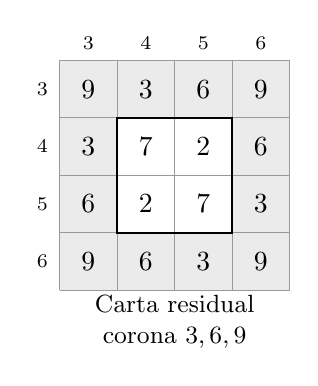
\begin{tikzpicture}[x=.73cm,y=.73cm]
\fill[black!8] (0,0) rectangle (4,4);
\fill[white] (1,1) rectangle (3,3);
\draw[step=1,black!40] (0,0) grid (4,4);
\draw[thick] (1,1) rectangle (3,3);
\foreach \row/\vals in {0/{9,3,6,9},1/{3,7,2,6},2/{6,2,7,3},3/{9,6,3,9}}{
  \foreach \val [count=\col from 0] in \vals{
    \node at (\col+.5,3.5-\row) {\(\val\)};
  }
}
\foreach \v [count=\n from 0] in {3,4,5,6}{
  \node[font=\scriptsize] at (\n+.5,4.3) {\(\v\)};
  \node[font=\scriptsize] at (-.3,3.5-\n) {\(\v\)};
}
\node[font=\small,align=center] at (2,-.55) {Carta residual\\corona \(3,6,9\)};
\end{tikzpicture}
\end{minipage}\hfill
\begin{minipage}[c]{.50\textwidth}
\centering
\begin{tikzpicture}[x=.73cm,y=.73cm]
\fill[black!3] (0,0) rectangle (4,4);
\draw[black!40] (0,0) rectangle (4,4);
\draw[thick] (1,1) rectangle (3,3);
\foreach \x/\y/\v in {.5/3.5/9,3.5/3.5/18,.5/.5/18,3.5/.5/36,
  1.5/2.5/16,2.5/2.5/20,1.5/1.5/20,2.5/1.5/25}{
  \node at (\x,\y) {\(\v\)};
}
\draw[-{Stealth},black!60] (.85,3.15) -- (1.22,2.78);
\draw[-{Stealth},black!60] (3.15,3.15) -- (2.78,2.78);
\draw[-{Stealth},black!60] (.85,.85) -- (1.22,1.22);
\draw[-{Stealth},black!60] (3.15,.85) -- (2.78,1.22);
\node[font=\small,align=center] at (2,-.55) {Frontière relevée\\et interpolation multiaffine};
\end{tikzpicture}
\end{minipage}
\caption{La même carte en deux lectures. À gauche, la couronne radicale entoure le bloc \(B_c\). À droite, les quatre coins entiers déterminent les valeurs intérieures sous la loi multiaffine. Leurs résidus aux coins coïncident, mais les quotients \((0,1,1,3)\) distinguent le relèvement.}
\label{viii:fig:centro-frontera}
\end{figure}

% END OWNER


\Needspace{6\baselineskip}
Son bloc intérieur est

\[
B_c=\begin{pmatrix}7&2\\2&7\end{pmatrix}.
\]
Le périmètre de cette carte contient douze positions : quatre de valeur \(3\), quatre de valeur \(6\) et quatre de valeur \(9\) ; leur somme est \(72\). Une couronne radicale apparaît autour du bloc central. Le centre électronique global est \((5,5)\), unique point fixe de l'inversion de l'APP complète ; sa position n'est pas modifiée par le choix de cette carte locale, dont le centre géométrique se trouve en \((4.5,4.5)\).

\begin{proposition}[Récupération à partir de la frontière relevée]
\label{viii:prop:centro-frontera-recuperacion}
Soit \(F(x,y)=a+bx+cy+dxy\) une loi multiaffine dans la carte \([3,6]^2\). Pour \(t=(x-3)/3\) et \(u=(y-3)/3\),

\[
\begin{aligned}
F(x,y)={}&(1-t)(1-u)F(3,3)+(1-t)uF(3,6)\\
&+t(1-u)F(6,3)+tuF(6,6).
\end{aligned}
\]
\end{proposition}
\begin{proof}
Pour \(y\) fixé, le caractère affine en \(x\) permet de récupérer \(F(x,y)\) à partir de \(F(3,y)\) et de \(F(6,y)\). Le caractère affine en \(y\) permet de récupérer chacune de ces deux valeurs à partir de ses extrémités. La composition donne la formule. En particulier, les quatre coins déterminent toute la carte au sein de l'espace de lois déclaré.
\end{proof}

Pour le produit, les quatre valeurs relevées sont \(9,18,18,36\). Leurs résidus positifs sont tous \(9\), mais leurs quotients sont \(0,1,1,3\). La formule restitue \(16,20,20,25\) aux positions intérieures ; sa publication résiduelle donne \(7,2,2,7\). Ainsi, la frontière détermine l'intérieur \textbf{en conservant la loi et le relèvement}. L'interpolation s'effectue avant la réduction modulaire : on ne divise pas par \(3\) dans \(\mathbb Z/9\mathbb Z\), où \(3\) n'est pas inversible.

Cela précise le sens de « conserver l'information du centre ». La couronne résiduelle seule n'individualise pas tous les relèvements : \(F\) et \(F+9\) ont les mêmes résidus sur toute la frontière et des valeurs relevées distinctes. La paire résidu–quotient élimine cette ambiguïté dans la reconstruction indiquée. L'affirmation est prouvée pour les lois multiaffines ; l'étendre aux états complets exige de conserver également les opérateurs, les routes et la mémoire qui agissent sur eux.

La récupération multiaffine est une \textbf{formalisation nouvelle de l'architecture préexistante de l'auteur}. Les cartes et leurs lectures sont des résultats récupérés du corpus ; cette présentation explicite de leur inverse n'est pas attribuée à une découverte historique indépendante.

\subsection{Somme, produit et les trois valeurs de la courbure discrète}
Les lignes multiplicatives sont construites par accumulation additive. La différence entre les deux feuillets apparaît lorsque les deux coordonnées varient simultanément. Avec des différences unitaires,

\[
\Delta_x\Delta_y(x+y)=0,
\qquad
\Delta_x\Delta_y(xy)=1.
\]
La même propriété se retrouve à la frontière relevée :

\[
\frac{P(6,6)-P(6,3)-P(3,6)+P(3,3)}{3\cdot3}=1;
\]
pour \(S(x,y)=x+y\), ce quotient vaut \(0\). Le produit enregistre la variation croisée que la somme n'introduit pas. Le corpus exprime la version orientée par

\[
\mathcal F(T_x,T_y)=\Delta_x\Delta_yT_y-\Delta_y\Delta_xT_x,
\]
\[
\mathcal F(S,S)=\mathcal F(P,P)=0,
\qquad \mathcal F(S,P)=+1,
\qquad \mathcal F(P,S)=-1.
\]
L'ordre des feuillets distingue le signe. La formulation « la somme accumule et le produit plie ou déplie » repose ici sur une opération vérifiable : lors de la projection modulaire, un résidu est conservé ; lors du relèvement, on restitue le quotient qui enregistre le dépassement. La courbure discrète enregistre en outre l'ordre des variations. Cette différence finie n'est pas identifiée à une courbure différentielle d'un espace physique sans son application de réalisation correspondante.

\subsubsection*{La croix radicale globale}
Dans \(R=\mathbb Z/9\mathbb Z\), l'idéal \(\mathfrak m=\{0,3,6\}\) satisfait \(\mathfrak m^2=0\). Sa publication positive est \(\{9,3,6\}\). La croix

\[
(\mathfrak m\times R)\cup(R\times\mathfrak m)
\]
comporte \(27+27-9=45\) positions. L'intersection contient neuf valeurs \(9\), de somme \(81\) ; les bras restants contiennent douze valeurs de chaque classe \(3,6,9\), de somme \(216\). Le total est

\[
297=216+81=3(72+27)=3\cdot99.
\]
On distingue quatre frontières : le périmètre local de douze positions, la croix radicale de quarante-cinq, le gnomon de dix-sept qui complète \(8^2\) en \(9^2\), et la couronne cubique de \(271\). Chacune possède son propre domaine et sa propre opération. Le quotient tritique \(R/\mathfrak m\) conserve une classe ; transporter l'état exige de l'accompagner des données relevées et de son histoire.

\subsection{Les lecteurs 72–27, 77–22 et la complétion 729–271}
Les lignes ordonnées de \(B_c\) sont publiées en décimal sous les formes \(72\) et \(27\) ; leurs diagonales sous les formes \(77\) et \(22\). Il en résulte

\[
72+27=77+22=99.
\]
Dans la complétion cubique, le dénombrement de l'intérieur, des faces, des arêtes et du sommet donne

\[
1000=729+243+27+1=729+271,
\]
\[
999=729+243+27=729+270.
\]
La coïncidence des lecteurs s'exprime en conservant le reste décimal :

\[
729=10\cdot72+9,\qquad271=10\cdot27+1.
\]
Ainsi, la lecture bidimensionnelle publie \((72,27)\) ; la lecture cubique publie \(((72,9),(27,1))\). La paire de restes \((9,1)\) distingue les prolongements qui partageraient un même quotient. On effectue d'abord les constructions des cartes ; on compare ensuite ces publications. L'identité des entiers n'inverse pas cet ordre causal.

Le chapitre des canaux entiers fournit une autre composition spécifique. Avec les dénombrements internes \(\Delta=54\), \(\nu=\Delta/2=27\) et \(\Theta=5\nu=135\), il obtient

\[
\mathcal C_\alpha=\nu^2=729,
\qquad \mathcal C_e=2\Theta+1=271.
\]
On a renommé ici \(\nu\) l'entier local que ce propriétaire écrit \(\kappa\), pour le distinguer de la lecture rationnelle du registre dodécaphasique. Les canaux sont des objets entiers ; leur identification aux constantes passe par les lecteurs régionaux et la clôture correspondante, et non par les premiers chiffres d'un développement. Cette comparaison utilise les canaux entiers et n'a pas besoin de la réalisation angulaire ultérieure.

Pour la référence orale à une fraction de \(\pi\), le propriétaire localisé contient

\[
\frac{396}{126}=\frac{22}{7},\qquad
396=18+72+108+198,\quad126=18+108.
\]
Il s'agit d'un rapport rationnel d'anneaux alternés. Ce rapport d'anneaux est une lecture rationnelle exacte ; sa fonction se distingue de la publication régionale de \(\pi\).

\subsection{Le centre électronique et ses vacances conjuguées}
L'inversion de l'APP positive est \(\rho(r,c)=(10-r,10-c)\). Son unique point fixe est \((5,5)\). Dans la fibre additive centrale,

\[
\mathcal F_{10}=\{(5+t,5-t):t\in\mathbb Z,\ |t|\leq4\},
\]
le produit vaut \(25-t^2\). Conserver son résidu central exige \(t^2\equiv0\pmod9\), équivalent à \(3\mid t\). Les seuls emplacements sont donc

\[
(5,5),\qquad(8,2),\qquad(2,8).
\]
Si \(\mathcal A\) conserve la paire résidu–quotient dans chaque feuillet,

\[
\begin{aligned}
\mathcal A(5,5)&=((1,1),(7,2)),\\
\mathcal A(8,2)=\mathcal A(2,8)&=((1,1),(7,1)).
\end{aligned}
\]
Les deux vacances préservent la lecture additive et le résidu multiplicatif ; le quotient du produit diminue exactement d'une unité. Le miroir \(t\mapsto-t\) échange leurs positions. La valeur résiduelle ne distingue pas leurs routes, tandis que l'orientation les conserve. C'est une réalisation précise de la connexion indiquée par la note : \textbf{la vacance s'individualise par une relation au centre et par un défaut enregistré, et non parce qu'elle serait une case sans information}.

L'orientation électronique initiale \((h_0,v_0)=(1,1)\), inversée tous les \(27\) pas, publie ensuite la signature dodécaphasique \((+++\,---\,+++\,---)\). Il s'agit d'un registre d'orientation, distinct aussi bien de la position \((5,5)\) que de la signature du produit qui suit.

\subsubsection*{La signature 555555 et la mémoire qui permet de la prolonger}
Pour \(U_j=100d_{1j}+10d_{2j}+d_{3j}\), le lecteur

\[
\mathcal E_\times(U)=([d_{2j}-d_{1j}]_{10})_{j=1}^{6}
\]
appliqué à la région transversale

\[
U_\pi^\perp=(501,614,498,169,272,272)
\]
produit \(555555\) ; sa réduction \(\Psi(U)=(-U_j\bmod3)_j\) produit \(010211\). La signature possède vingt-quatre représentants produit. Le transport les sépare en trois feuillets de huit : après l'avancée apparaissent \(555177\), \(555717\) et \(555771\). La congruence stable par avancée et demi-tour raffine les vingt-six signatures en vingt-huit classes, d'histogramme \(27\cdot8+108=324\). Cela exprime pourquoi il faut retenir une mémoire de feuillet pour poursuivre une signature qui coïncide initialement.


% BEGIN OWNER /Users/ruben/Documents/New project/output/REVISION_ARGUMENTAL_APERTURAS_CIERRES_20260915/VIII/spanish_source/ampliacion/memoria_firma_555.tex
\begin{definition}[Lecteur de signature et transport des représentants]
\label{viii:def:firma555}
Soit \(\mathcal X_\times=D_9^2\times\{N,E,S,O\}\), de cardinal \(324\).
L'avancée \(P\) déplace d'une case dans la direction mémorisée et le demi-
tour \(H\) inverse cette direction. Le lecteur utilise
\[
\ell_9(1,2,4,8,7,5)=(0,1,2,3,4,5),\qquad
\ell_9(3)=\ell_9(6)=\ell_9(9)=0.
\]
Dans chacune des six fenêtres de neuf étapes, on évalue
\(\ell_9(\rho_9(ij))\) avant l'avancée produit sélectionnée par TRIT aux
temps \(2,5,8\pmod9\). La somme de chaque fenêtre est réduite modulo
\(10\). Après les étapes \(27\) et \(54\), la direction est inversée.
La règle détermine \(E_{\rm sig}(x)\) à partir de la position et de la direction
de \(x\), avec les conventions temporelles du noyau.
\end{definition}

\begin{proposition}[Raffinement minimal stable de la signature]
\label{viii:prop:firma555}
En partant de l'équivalence par signature \(\sim_0\), l'itération
\[
x\sim_{n+1}y\ \Longleftrightarrow\
x\sim_n y,\quad Px\sim_n Py,\quad Hx\sim_n Hy
\]
se termine et produit la congruence stable la plus grossière qui raffine la signature. Dans le domaine précédent, le recensement est \(26\to28\to28\) ; la fibre de \(555555\) se sépare en trois classes de huit représentants.
\end{proposition}
\begin{proof}
À chaque étape, on raffine une partition d'un ensemble fini. Le processus se
stabilise après un nombre fini de scissions. Au point fixe,
l'équivalence est préservée sous \(P\) et \(H\). Si une congruence stable
raffine \(\sim_0\), elle raffine par récurrence chaque \(\sim_n\) : ses images
par les deux opérateurs restent équivalentes. Elle raffine donc le point
fixe obtenu, ce qui prouve sa minimalité en information ajoutée.

L'énumération finie applique la définition aux \(81\) positions et aux quatre orientations. On regroupe d'abord leurs six sommes modulo \(10\), puis le triplet formé par la classe de \(x\), celle de \(Px\) et celle de \(Hx\), jusqu'à stabilisation. L'histogramme résultant est \(27\cdot8+108=324\), et la seule scission de signature est celle indiquée. Les représentants suivants explicitent les trois images :
\[
\begin{array}{c|c|c}
x&E_{\rm sig}(x)&E_{\rm sig}(Px)\\\hline
(3,5,N)&555555&555177\\
(3,4,N)&555555&555717\\
(3,4,S)&555555&555771
\end{array}
\]
La règle complète et son énumération exécutable sont conservées dans le paquet
de reproduction ; les témoins du tableau montrent en outre que conserver
seulement la signature ne rend pas sa continuation univoque.
\end{proof}

La conclusion décrit l'information minimale du transport, et non une
nouvelle masse. Le facteur additif conserve dix-huit représentants par signature
(neuf positions compatibles et deux orientations). En le combinant avec les
fibres produit de tailles \(24\) et \(8\), on obtient respectivement
\(432\) et \(144\). L'incidence régionale et la mémoire de feuillet conservent
ainsi des fonctions distinctes dans le même catalogue.

% END OWNER


Le lien avec l'équation électronique passe par les régions. La région transversale a pour multiplicité \(432=18\cdot24\) ; chacune des quatre autres a \(144=18\cdot8\). Leurs cinq identités s'insèrent, dans la jauge déclarée de l'article I, dans

\[
\mathcal K_e=\mathbb Z/9\mathbb Z\times\mathbb F_3
\]
au moyen de \((4,0),(5,0),(6,0),(6,1),(6,2)\). Une fois cette insertion fixée, son complément comporte \(27-5=22\) places et ses trois feuillets par région comportent \(5\cdot3=15\) places. Le déficit orienté et la mémoire torsionnelle sont \(-22\) et \(15\). La preuve de ces dénombrements s'obtient à partir de l'injection explicite précédente : ses cinq images sont distinctes ; ce développement la rassemble et ne choisit pas ses places à partir d'une masse cible.

Il y a donc deux parcours liés dans la composition : \textbf{centre → vacances conjuguées → orientation}, et \textbf{signature régionale → feuillets de transport → incidence des cinq régions → coefficients électroniques}. Identifier sans autre précision \((5,5)\) à \(555555\) effacerait précisément les opérations qui expliquent leur relation.

\subsection{Miroir nonadique, capacité et retour à mémoire}
Dans la fibre régionale, le miroir agit par

\[
\mathfrak c(u^\pi,u^e,u^\varphi)=(u^e,u^\pi,u^\varphi).
\]
Il conserve \(s=u^\pi+u^e\) et inverse \(d=u^\pi-u^e\). En \(\mathbb F_3\),

\[
u^\pi=2(s+d),\qquad u^e=2(s-d).
\]
La somme conserve l'agrégat ; la différence orientée conserve la répartition. L'axe \(u^\varphi\) reste fixe sous cette involution, bien qu'il puisse évoluer sous le transport. Le miroir régional et le miroir cellulaire des vacances ont des domaines distincts : leurs formules respectives permettent de suivre ce que chacun préserve.

La vacance de capacité ajoute un lien temporel explicite. Dans la normalisation du raffinement \(729\) par rapport à \(1000\), soient \(\rho_c=\log_{10}9\), \(\delta=1-\rho_c\) et \(\mathcal C_t=\lfloor(t+1)\rho_c\rfloor\). Si

\[
z_t=\lfloor(t+1)\delta\rfloor-\lfloor t\delta\rfloor,
\]
alors, pour \(t\geq1\),

\[
\mathcal C_t-\mathcal C_{t-1}=1-z_t,
\qquad
\mathcal C_b-\mathcal C_a+\sum_{t=a+1}^b z_t=b-a.
\]
\begin{proof}
L'irrationalité de \(\log_{10}9\) découle de l'impossibilité de \(9^n=10^m\) pour des entiers positifs. Par conséquent, \(\mathcal C_t=t-\lfloor(t+1)\delta\rfloor\). Soustraire et sommer télescopiquement donne les deux identités. \end{proof}
Une vacance retient la capacité tandis que l'histoire avance.

Si \(p_j=\lfloor j/\delta\rfloor\), \(v_j=p_j-j\) et \(h_j=p_{j+1}-p_j\), le développement hérité établit \(h_j\in\{21,22\}\). Pour \(s_j=22-h_j\),

\[
[v_{j+1}]_3=[v_j-s_j]_3,\qquad
\tau_j=M_{\rm ph}(1+[v_j]_9).
\]
Les vacances agissent ainsi sur la phase retenue que lit le sélecteur tritique. Cette suite de capacité ne devient pas automatiquement la trajectoire cellulaire de l'électron : le manuscrit conserve leurs mécanismes respectifs et leur composition dans le même noyau.


% BEGIN OWNER /Users/ruben/Documents/New project/output/REVISION_ARGUMENTAL_APERTURAS_CIERRES_20260915/VIII/spanish_source/ampliacion/vacancias_21_22_6_7.tex
% RESULTADO_RECUPERADO y exposición autónoma ampliada; no cambia el núcleo común.
% Propietarios cotejados:
% Artículo I REV02/sections/vacancias_capacidad.tex, completo.
% Monografía775/manuscrito/generated/cristal_relojes_sincronizacion.tex,
% líneas1--223 y931--1032: capacidad, retornos e inducción TRIT.
% Las pruebas universales de las dos escalas se reúnen aquí; el comprobador
% ampliacion/verificar_vacancias.py añade un certificado racional finito.
\subsection{Vacances du raffinement nonadique et hiérarchie des retours}
\label{viii:vac-add-seccion}

La prolongation APP--TRIT--TPK conserve, avec le bloc publié, le
cylindre, l'orientation et l'histoire qui permettent de le poursuivre. Dans sa
lecture de capacité, on compare deux cardinaux déjà déterminés par cette
construction : les \(3^6=729\) possibilités d'un bloc ternaire de six
positions et les \(10^3=1000\) positions de sa carte décimale de trois
chiffres. Cette comparaison produit un calendrier propre. Certaines
transitions augmentent l'indice de capacité ; d'autres incorporent un bloc
à l'histoire en maintenant cet indice. Ces dernières sont les
\emph{vacances de capacité} étudiées ci-dessous.

L'objet considéré est donc une publication du raffinement conjoint. Sa définition conserve l'origine dans les deux supports finis ; l'expression logarithmique permet de démontrer les propriétés de son calendrier. Le temps de bloc, l'indice de vacance et l'indice de capacité seront écrits séparément. Cette séparation rend visible pourquoi les retours \(21/22\) et \(6/7\) appartiennent à des échelles successives d'une même construction.

\subsubsection{Capacité décimale et conservation de l'incrément}
\label{viii:vac-add-capacidad}

\begin{definition}[Indice de capacité et vacance]
\label{viii:vac-add-definicion}
À l'origine de phase \(0\), on définit
\begin{equation}
 \rho=\log_{1000}729=\log_{10}9,
 \qquad \delta=1-\rho=\log_{10}(10/9),
 \label{viii:vac-add-densidad}
\end{equation}
et, pour \(t\in\mathbb Z_{\geq0}\),
\begin{equation}
 \mathcal C_t=\lfloor(t+1)\rho\rfloor,
 \qquad
 z_t=\lfloor(t+1)\delta\rfloor-\lfloor t\delta\rfloor.
 \label{viii:vac-add-indices}
\end{equation}
L'entier \(\mathcal C_t\) est l'indice de capacité décimale du lecteur ;
\(z_t=1\) indique une vacance. La lettre \(K\) demeure réservée au
registre dodécaphasique et ne désigne pas ici un compteur de capacité.
\end{definition}

On a \(0<\delta<1\). En outre, \(\delta\) est irrationnel : si \(\rho=a/b\) était rationnel, avec \(a,b\) entiers positifs, l'égalité \(9^b=10^a\) aurait une valuation nulle au nombre premier \(5\) à gauche et positive à droite. Cette contradiction démontre l'irrationalité de \(\rho\) et de \(1-\rho\). En particulier, aucun multiple entier positif de \(\delta\) n'appartient à \(\mathbb Z\), ce qui fixe sans ambiguïté les extrémités des intervalles de ce développement.

\begin{proposition}[Bilan exact de capacité et de vacance]
\label{viii:vac-add-balance}
Pour \(t\geq1\), \(z_t\in\{0,1\}\) et
\begin{equation}
 \mathcal C_t-\mathcal C_{t-1}=1-z_t.
 \label{viii:vac-add-incremento}
\end{equation}
Par conséquent, pour \(0\leq a<b\),
\begin{equation}
 \mathcal C_b-\mathcal C_a+
 \sum_{t=a+1}^{b}z_t=b-a.
 \label{viii:vac-add-conservacion}
\end{equation}
\end{proposition}
\begin{proof}
Comme \(0<\delta<1\), la différence entre les parties entières de deux
nombres séparés par \(\delta\) vaut \(0\) ou \(1\). D'autre part,
l'irrationalité démontrée donne
\[
 \mathcal C_t=t+1-\lceil(t+1)\delta\rceil
             =t-\lfloor(t+1)\delta\rfloor.
\]
La soustraction de cette égalité en \(t\) et en \(t-1\) prouve
\eqref{viii:vac-add-incremento} ; sa somme télescopique prouve
\eqref{viii:vac-add-conservacion}.
\end{proof}

Chaque transition apporte exactement une unité au membre de droite du
bilan. Cette unité est enregistrée comme capacité acquise lorsque
\(z_t=0\), ou comme vacance lorsque \(z_t=1\). La rétention de l'indice
\(\mathcal C_t\) laisse donc une position récupérable dans l'
histoire. L'équation exprime la conservation de l'incrément avec deux
lectures, et non une perte indéterminée d'information.

La densité se déduit également du même bilan :
\[
 \frac1N\sum_{t=1}^{N}z_t
 =\frac{\lfloor(N+1)\delta\rfloor}{N}\longrightarrow\delta.
\]
Ainsi, \((z_t)\) n'est pas ultimement périodique : une suite binaire
ultimement périodique possède une densité rationnelle. L'apériodicité
résulte ici de la règle de capacité déjà fixée par \(729/1000\).

\subsubsection{Détermination exacte des intervalles \(21/22\)}
\label{viii:vac-add-primarios}

\begin{lemma}[Bornes rationnelles de la pente]
\label{viii:vac-add-cotas}
La densité de vacance satisfait
\begin{equation}
 \frac7{153}<\delta<\frac6{131}.
 \label{viii:vac-add-cota-delta}
\end{equation}
Si \(\lambda=\delta^{-1}\), \(\beta=22-\lambda\) et
\(\mu=\beta^{-1}\), alors
\begin{equation}
 21<\lambda<22,
 \qquad \frac17<\beta<\frac16,
 \qquad 6<\mu<7.
 \label{viii:vac-add-cotas-inducidas}
\end{equation}
\end{lemma}
\begin{proof}
On fournit une vérification finie par arithmétique rationnelle. Pour \(0<u<1\), soient
\[
 S_N(u)=2\sum_{k=0}^{N}\frac{u^{2k+1}}{2k+1},
 \qquad
 R_N(u)=\frac{2u^{2N+3}}{(2N+3)(1-u^2)}.
\]
L'intégration de la série géométrique de \(2/(1-u^2)\) donne
\[
 S_N(u)<\log\frac{1+u}{1-u}<S_N(u)+R_N(u).
\]
En effet, la queue est positive et, en remplaçant chaque dénominateur
\(2k+1\) par \(2N+3\), elle est bornée par la série géométrique qui
définit \(R_N\). On applique ces inégalités à
\(u=1/19,1/3,1/9\), qui correspondent respectivement à
\(\log(10/9),\log2,\log(5/4)\), et l'on utilise
\(\log10=3\log2+\log(5/4)\).

Avec \(N=4\), en écrivant \(A=S_4(1/19)\), \(B=3S_4(1/3)+S_4(1/9)\) et \(E=3R_4(1/3)+R_4(1/9)\), on obtient
\[
 \frac7{153}
 <\frac{A}{B+E}
 <\delta
 <\frac{A+R_4(1/19)}{B}
 <\frac6{131}.
\]
Les deux inégalités extérieures se vérifient en multipliant par les
dénominateurs positifs de ces sommes de cinq termes rationnels.
On prouve ainsi \eqref{viii:vac-add-cota-delta} au moyen d'une borne du reste,
sans utiliser un développement décimal comme prémisse. En l'inversant, on obtient
\(131/6<\lambda<153/7\). Soustraire à \(22\), puis inverser,
produit toutes les inégalités de \eqref{viii:vac-add-cotas-inducidas}.
\end{proof}

\begin{theorem}[Positions et séparations des vacances]
\label{viii:vac-add-teorema-primario}
Les positions des événements \(z_t=1\), ordonnées à partir du premier événement, sont exactement
\begin{equation}
 p_j=\lfloor j\lambda\rfloor
     =\left\lfloor\frac j\delta\right\rfloor,
 \qquad j\geq1.
 \label{viii:vac-add-posiciones}
\end{equation}
Leurs séparations satisfont
\begin{equation}
 h_j=p_{j+1}-p_j\in\{21,22\}.
 \label{viii:vac-add-huecos}
\end{equation}
Les deux valeurs apparaissent une infinité de fois.
\end{theorem}
\begin{proof}
L'événement qui franchit l'entier \(j\) se produit précisément lorsque
\(t\delta<j<(t+1)\delta\). L'irrationalité exclut l'égalité aux
extrémités. En divisant par \(\delta\), on obtient
\(t=\lfloor j/\delta\rfloor=p_j\). Comme \(\delta<1\), une étape
franchit au plus un entier, de sorte que l'énumération est exacte.
En écrivant \(\lambda=21+\eta\), avec \(0<\eta<1\), on obtient
\[
 h_j=21+\lfloor(j+1)\eta\rfloor-\lfloor j\eta\rfloor,
\]
ce qui prouve \eqref{viii:vac-add-huecos}. Enfin, \((p_{J+1}-p_1)/J\to\lambda\in(21,22)\). Si l'une des deux valeurs n'apparaissait qu'un nombre fini de fois, cette moyenne convergerait vers l'autre valeur entière, ce qui est une contradiction.
\end{proof}

\subsubsection{Induction sur les intervalles courts : les retours \(6/7\)}
\label{viii:vac-add-secundarios}

\begin{theorem}[Calendrier induit des intervalles courts]
\label{viii:vac-add-teorema-secundario}
Soit \(s_j=22-h_j\), pour \(j\geq1\). Cette indicatrice vaut \(1\) exactement lorsque l'intervalle entre vacances est court, de longueur \(21\). Avec \(\beta\) et \(\mu\) définis dans le lemme~\ref{viii:vac-add-cotas},
\begin{equation}
 s_j=\lfloor(j+1)\beta\rfloor-\lfloor j\beta\rfloor.
 \label{viii:vac-add-indicador-corto}
\end{equation}
Les indices des intervalles courts sont
\begin{equation}
 q_m=\lfloor m\mu\rfloor=\lfloor m/\beta\rfloor,
 \qquad q_{m+1}-q_m\in\{6,7\},\quad m\geq1.
 \label{viii:vac-add-posiciones-cortos}
\end{equation}
Les deux séparations se présentent une infinité de fois et leur ordre n'est pas
ultimement périodique.
\end{theorem}
\begin{proof}
L'irrationalité de \(\delta\) implique celle de \(\lambda\),
de \(\beta\) et de \(\mu\). Puisque \(\lambda=22-\beta\), pour
\(j\geq1\), on a
\[
 p_j=22j-\lceil j\beta\rceil
     =22j-\lfloor j\beta\rfloor-1.
\]
En soustrayant des termes consécutifs apparaît
\eqref{viii:vac-add-indicador-corto}. En appliquant à l'indicatrice de pente
\(\beta\) l'argument de franchissement des entiers du théorème précédent,
son événement \(m\) se trouve en \(q_m=\lfloor m/\beta\rfloor\).
L'inégalité \(6<\mu<7\) prouve les deux séparations possibles.
Leur moyenne converge vers \(\mu\) ; elles apparaissent donc toutes deux une infinité
de fois. De plus, une suite de séparations ultimement périodique
aurait une moyenne rationnelle, alors que \(\mu\) est irrationnel. Cela exclut
également une alternance stricte, dont la moyenne serait \(13/2\).
\end{proof}

Les nombres \(6\) et \(7\) comptent ici des \emph{intervalles entre événements de vacance}, et non des blocs de raffinement. Le retour à l'échelle primaire est tout aussi explicite. Entre \(q_m\) et \(q_{m+1}\), il n'y a qu'un seul intervalle court, situé au début, et tous les autres sont longs. Par conséquent, si \(d_m=q_{m+1}-q_m\),
\begin{equation}
 p_{q_{m+1}}-p_{q_m}=21+22(d_m-1)=22d_m-1
 \in\{131,153\}.
 \label{viii:vac-add-retorno-bloques}
\end{equation}
Ainsi, \(131=14\cdot9+5\) et \(153=17\cdot9\) décrivent deux lectures
de retour \emph{dans l'horloge des blocs}. L'équation conserve l'
opération qui relie les échelles, au lieu d'identifier leurs
cardinaux par leur seule apparition.

\subsubsection{Capacité retenue et sélection du régime TRIT}
\label{viii:vac-add-regimen}

Soit \(v_j=\mathcal C_{p_j}\) la capacité enregistrée à la vacance
\(j\). De \(p_j\delta<j<(p_j+1)\delta\) et de \(\delta<1\) résulte
\(\lfloor(p_j+1)\delta\rfloor=j\). D'après
\eqref{viii:vac-add-indices},
\begin{equation}
 v_j=p_j-j,
 \qquad v_{j+1}-v_j=h_j-1=21-s_j,
 \qquad [v_{j+1}]_3=[v_j-s_j]_3.
 \label{viii:vac-add-transporte-mod3}
\end{equation}
Un intervalle long conserve la classe modulo \(3\) ; un intervalle court la décale d'une unité dans le sens négatif. En appliquant le sélecteur du noyau formel à la phase positive \(r_j=1+[v_j]_9\), on obtient
\begin{equation}
 \tau_j=M_{\rm ph}(r_j),\qquad
 M_{\rm ph}(r)=
 \begin{cases}
 +1,&r\in\{1,4,7\},\\
 -1,&r\in\{2,5,8\},\\
 0,&r\in\{3,6,9\}.
 \end{cases}
 \label{viii:vac-add-selector}
\end{equation}
Cette composition fixe le régime induit par la capacité à chaque
événement. Elle conserve tant l'ordre des changements que le nombre d'
événements pendant lesquels chaque régime se maintient.

\begin{corollary}[Plateaux du régime induit]
\label{viii:vac-add-mesetas}
Pour chaque \(m\geq1\), la classe \([v_j]_3\), et donc
\(\tau_j\), est constante sur
\(q_m+1\leq j\leq q_{m+1}\). La longueur de chacun de ces
plateaux complets est \(q_{m+1}-q_m\in\{6,7\}\).
\end{corollary}
\begin{proof}
Dans l'intervalle entier indiqué, le changement suivant se produit exactement lors du passage de \(j=q_{m+1}\) à \(j=q_{m+1}+1\) : c'est la prochaine position où \(s_j=1\). À tous les pas précédents, \(s_j=0\), de sorte que \eqref{viii:vac-add-transporte-mod3} conserve la classe. À l'extrémité, il la diminue d'une unité. Le sélecteur \eqref{viii:vac-add-selector} attribue des valeurs distinctes aux trois classes ; il conserve donc les mêmes plateaux et leurs extrémités.
\end{proof}

Le tronçon initial \(1\leq j\leq q_1\) dépend de l'origine choisie et
est une restriction initiale d'un plateau. À l'origine présente, il mesure
\(q_1=6\). Les vingt premières classes sont
\[
 \underbrace{2,\ldots,2}_{6},\qquad
 \underbrace{1,\ldots,1}_{7},\qquad
 \underbrace{0,\ldots,0}_{7},
\]
avec les signatures \(0,-1,+1\), respectivement. Chaque intervalle court
déclenche l'étape suivante du cycle des régimes.

Les deux phases d'intérêt sont définies par
\[
 g_t^{\rm cron}=[t]_9,
 \qquad g_t^{\rm cap}=[\mathcal C_t]_9,
 \qquad
 g_t^{\rm cap}-g_{t-1}^{\rm cap}\equiv1-z_t\pmod9.
\]
Une vacance retient la phase de capacité tandis que le temps de bloc
avance. La transition de l'état enrichi reste la composition
TPK de sélection, de transport et de mise à jour de la mémoire. Ainsi,
\(\mathcal C_t=\mathcal C_{t-1}\) ne réinitialise pas l'état et ne
remplace pas le tour holonomique \(\Gamma_9\) par une pause. Les
deux échelles induites maintiennent également cette distinction : entre les événements
courts consécutifs de \eqref{viii:vac-add-retorno-bloques}, l'incrément de
capacité est \(21d_m-1\), c'est-à-dire \(125\) ou \(146\), tandis que
l'incrément des blocs est \(131\) ou \(153\).

\subsubsection{Échantillon rationnellement certifié et provenance}
\label{viii:vac-add-muestra}

Le tableau présente un échantillon de l'origine canonique. \(h_j\) est l'
espacement \emph{postérieur} à \(p_j\) ; la vacance de
\(j=6\), dans le bloc \(131\), commence donc le premier intervalle court.
\begin{center}
\small
\begin{tabular}{r|rrrrrrrrrr}
\toprule
\(j\)&1&2&3&4&5&6&7&8&9&10\\
\midrule
\(p_j\)&21&43&65&87&109&131&152&174&196&218\\
\(h_j\)&22&22&22&22&22&21&22&22&22&22\\
\(v_j\)&20&41&62&83&104&125&145&166&187&208\\
\([v_j]_3\)&2&2&2&2&2&2&1&1&1&1\\
\bottomrule
\end{tabular}
\end{center}
Les premiers indices d'intervalles courts et leurs séparations sont
\[
 (q_m)_{m=1}^{10}=(6,13,20,27,34,41,48,54,61,68),
\]
\[
 (q_{m+1}-q_m)_{m=1}^{9}=(7,7,7,7,7,7,6,7,7).
\]
L'échantillon montre l'ordre effectif, et les preuves précédentes fixent sa loi à une profondeur arbitraire.

Le fichier joint \texttt{ampliacion/verificar\_vacancias.py} calcule
des fourchettes rationnelles avec les séries et les restes du
lemme~\ref{viii:vac-add-cotas}. Chaque partie entière n'est acceptée que lorsque
les deux extrémités de la fourchette produisent le même entier. À l'ordre
\(16\), il reproduit \(512\) événements, jusqu'au bloc \(11189\), et
\(64\) espacements secondaires, ainsi que les identités de bilan,
les résidus et les plateaux. Cette vérification finie maintient sa portée
séparée de celle des théorèmes universels.

L'indice de capacité, sa complémentarité avec les vacances et l'induction du sélecteur TRIT sont repris de l'Article I et des chapitres sur le calendrier et l'horloge induite de la monographie sur l'ordre topologique-temporel apériodique. Leurs définitions et les preuves des deux échelles sont réunies ici avec une convention unique d'indices. Le certificat rationnel constitue une vérification supplémentaire de ces résultats et conserve leur provenance.

% END OWNER


\subsection{Facteur 8/81 dans la décomposition entre lecture et complément}
Dans le développement du double cercle, l'inclusion uniforme de neuf phases est \(Jv=(v,\ldots,v)/3\). Avec la couture

\[
S_C(v_0,\ldots,v_8)=(Cv_8,v_0,\ldots,v_7),
\]
on obtient \(T=J^*S_CJ=(8I+C)/9\). Si \(z=(C-I)v\), le complément de la publication est exactement

\[
\eta v=(I-JJ^*)S_CJv=\frac1{27}(8z,-z,\ldots,-z).
\]
Par conséquent,

\[
\|\eta v\|^2=\frac{64+8}{729}\|z\|^2
=\frac8{81}\|(C-I)v\|^2.
\]
C'est ici qu'apparaît le \(8/81\) mentionné par l'auteur : une phase transportée face aux huit autres, avec la normalisation uniforme de neuf phases. Le résultat ne dépend pas de la position marquée parmi les neuf. Le bilan opératoriel complet est

\[
I-T^*T=\frac8{81}(I-C)^*(I-C)+\frac19(I-C^*C).
\]
Si \(C\) est isométrique, l'énergie omise par la publication se retrouve exactement dans son complément. Pour un raccord arbitraire, on conserve en outre son défaut explicite. L'entier \(72=64+8\) compte ici des poids quadratiques ; dans la couronne locale, il compte une somme de valeurs ; dans \(72/27\), il appartient à une lecture décimale ordonnée. Spécifier ces types permet de relier les constructions sans supposer qu'une coïncidence numérique fournit déjà toutes les applications entre elles.

Ce bilan demeure celui du développement du transport du double cercle. Lorsqu'il s'applique à la forme arithmétique \(\mathscr W\), il produit une identité signée ; démontrer la positivité globale requiert le contrôle global de ses termes, et non seulement la récupération du centre ou la positivité d'une norme auxiliaire. Les résultats déjà prouvés sur la mémoire, le transport et la fenêtre coercive sont conservés intégralement.


% Incorporación ampliativa: CG-006, SR-032--SR-035 del inventario REV05.
% Residencia: inmediatamente después de la construcción de R36, antes de G9.
% Propietario computacional: 16_CIERRE_GLOBAL_HMT_MD_2026-07-22/
% 01_SELECTOR_CONSTANTES/selector_interno_constantes.py, líneas 31--63,
% 131--180, 185--240 y 267--321.
% Recuperación y cambio de representación: output/REVISION_EDITORIAL_HMT_MD_
% 20260905/03_PRUEBAS/verificar_generacion_infinita_nonadica.py,
% líneas 54--77, 651--723 y 974--1147.
% Exposición de origen: ampliaciones_sucesoras_20260824/parte_i_ii/owners/
% U008_orbitas_elevacion_r36.tex, líneas 210--358.
% Estatuto: RESULTADO_RECUPERADO; exposición de enumeración y naturalidad
% reunida sin promover la concordancia en R36 a equivalencia global.

\section[Sélection et transport de la première frontière]{Sélection combinatoire et transport de représentation de la première frontière conjointe}
\label{r36c:sec:frontera}

La première frontière conjointe reçoit les blocs déjà produits par les graines APP, la réduction tritique et le calendrier de relèvement du TPK. Sa construction conserve la distinction entre trois opérations : déterminer les distributions admissibles, orienter leurs deux canaux latéraux et transporter l’incidence vers le système de coordonnées exceptionnel. Cet exposé développe ces opérations sur le même état fini. Les noms des coordonnées réelles désignent leurs lecteurs ultérieurs ; les conditions de sélection qui suivent agissent sur des mots ternaires, des matrices de transport et des incidences entières.

\subsection{État régional antérieur à la frontière}

Soit $\mathcal W\subset\mathbb F_3^6$ le répertoire de $243$ mots visibles obtenu par le dénombrement des émissions APP--TRIT--TPK. Pour un vecteur ligne $s\in\mathcal W$, définissons
\[
 b_0(s)=s,\quad b_1(s)=sL_0,\quad b_2(s)=sL_0^2,\quad
 b_3(s)=sL_0^2L_1,\quad b_4(s)=sL_0^2L_1^2,
\]
avec des opérations dans $\mathbb F_3$. Les matrices précédemment dérivées des registres régionaux sont
\[
L_0=\begin{pmatrix}
2&2&2&1&2&1\\2&1&2&2&1&1\\1&0&0&1&0&2\\
0&0&1&1&1&0\\2&2&2&0&2&1\\2&1&2&1&0&0
\end{pmatrix},\qquad
L_1=\begin{pmatrix}
2&1&2&0&2&2\\1&2&1&1&2&0\\1&2&1&1&1&2\\
0&1&0&0&2&1\\2&0&2&1&0&1\\0&2&2&2&1&1
\end{pmatrix}.
\]
Le sélecteur régional antérieur fournit
\[
s_{\rm cl}=010211,\qquad s_{\rm pr}=201101,
\]
au moyen des conditions $b_2(s_{\rm cl})=b_0(s_{\rm cl})$, $b_4(s_{\rm pr})=b_2(s_{\rm pr})$ et $b_1(s_{\rm cl})=b_3(s_{\rm pr})$. À cette étape, les blocs courants sont
\[
b_4(s_{\rm cl})=110221,\qquad
b_4(s_{\rm pr})=102011.
\]
La concaténation conserve les cinq blocs de chaque registre ; le vecteur $b_4$ est l’entrée à six coordonnées reçue par la relation de frontière.

Pour exprimer fidèlement la relation récupérée, on utilise la matrice d’incidence dans sa représentation d’origine,
\begin{equation}
A^{\rm o}=\begin{pmatrix}
0&1&1&1&1&1\\1&0&1&1&2&2\\1&1&0&2&1&2\\
1&1&2&0&2&1\\1&2&1&2&0&1\\1&2&2&1&1&0
\end{pmatrix}.
\label{r36c:eq:ao}
\end{equation}
On vérifie $(A^{\rm o})^2=-I$ dans $M_6(\mathbb F_3)$ ; donc $(A^{\rm o})^{-1}=-A^{\rm o}$. Cette représentation et ses vecteurs seront ensuite transportés vers celle utilisée par le lecteur exceptionnel.

\subsection{Équation de compatibilité et saturation des colonnes}

L’axe de la frontière est fixé par $z=b_4(s_{\rm pr})=102011$. Pour chaque $s\in\mathcal W$, on définit
\begin{align}
m(s)&=b_4(s)A^{\rm o}L_1^3,\\
q(s)&=m(s)+z,\\
\widetilde q(s)&=s(A^{\rm o})^{-1}L_0^3(A^{\rm o})^3.
\label{r36c:eq:compat-datos}
\end{align}
La condition de compatibilité est $q(s)=\widetilde q(s)$. Les lignes latérales $x,y\in\mathbb F_3^6$ satisfont $x+y=m(s)$ ; la frontière ordonnée est $B=(x,y,z)^{\mathsf T}$.

Pour former le reste et la retenue, on utilise les représentants entiers $0,1,2$ de chaque trit. Si $S_j=x_j+y_j+z_j$, on exige
\[
q_j=S_j\bmod3,\qquad c_j=\frac{S_j-q_j}{3}=1,
\]
et l’occupation des colonnes est donnée par
\begin{equation}
\mathbf1_{\{x_j\ne0\}}+\mathbf1_{\{y_j\ne0\}}+\mathbf1_{\{z_j\ne0\}}
=2+\mathbf1_{\{z_j\ne0,\ m_j(s)\ne2\}}.
\label{r36c:eq:ocupacion}
\end{equation}
La neutralité duale complète la condition par
\begin{equation}
BA^{\rm o}\mathbf1=0\quad\hbox{dans }\mathbb F_3^3.
\label{r36c:eq:neutralidad}
\end{equation}
Le reste, la retenue et l’occupation interviennent conjointement : la réduction modulaire conserve le reste et le registre entier distingue les distributions qui le produisent.

\begin{lemma}[Résolution de la compatibilité régionale]
\label{r36c:lem:compatibilidad} L’équation $q(s)=\widetilde q(s)$ possède, dans $\mathbb F_3^6$, les trois solutions
\[
020010,\qquad121200,\qquad222120.
\]
Son intersection avec le répertoire visible est $\{121200,222120\}$.
\end{lemma}
\begin{proof}
L’équation s’écrit $sD=z$, où
\[
D=(A^{\rm o})^{-1}L_0^3(A^{\rm o})^3
   -L_0^2L_1^2A^{\rm o}L_1^3
 =\begin{pmatrix}
2&1&1&2&2&2\\0&2&0&0&0&1\\0&0&0&0&1&0\\
1&2&2&2&2&0\\1&2&2&0&1&2\\1&2&0&2&2&2
\end{pmatrix}.
\]
L’élimination sur $\mathbb F_3$ donne la paramétrisation
\[
s=(t,2,t,2t,1+2t,0),\qquad t\in\mathbb F_3.
\]
La substitution vérifie les six équations et en épuise les solutions. Dans le répertoire engendré $\mathcal W$, les deux mots correspondant à $t=1,2$ sont présents et celui correspondant à $t=0$ est absent. Cette dernière vérification est une interrogation exacte du dénombrement des mots visibles, antérieure à toute lecture archimédienne.
\end{proof}

\begin{proposition}[Détermination de l’axe d’auto-échelle]
La compatibilité, la retenue unitaire et l’occupation des colonnes sélectionnent $s_{\rm au}=121200$ parmi les deux solutions visibles du lemme~\ref{r36c:lem:compatibilidad}. On obtient
\[
b_4(s_{\rm au})=010200,\qquad
m(s_{\rm au})=210112,\qquad q=012120,
\]
avec l’occupation $223232$.
\end{proposition}
\begin{proof}
Pour $s=222120$, on calcule $b_4(s)=222000$, $m(s)=201010$ et $q(s)=000021$. Dans sa troisième colonne, $m_3=1$ et $z_3=2$. L’occupation requise est trois, donc $x_3,y_3$ doivent être tous deux non nuls. L’unique couple avec $x_3+y_3\equiv1\pmod3$ est $(2,2)$ ; sa somme entière avec $z_3=2$ vaut six et produit une retenue de deux. Cela contredit $c_3=1$.

Pour $s=121200$, les six colonnes admettent respectivement les couples
\[
\begin{array}{c|cccccc}
j&1&2&3&4&5&6\\\hline
(x_j,y_j)&(0,2),(2,0)&(2,2)&(1,2),(2,1)&(2,2)&(2,2)&(0,2),(2,0).
\end{array}
\]
Chaque couple satisfait les équations de reste, de retenue et d’occupation. Il existe donc huit dispositions avant l’application de la neutralité duale.
\end{proof}

\begin{theorem}[Énumération exacte des orientations de frontière]
\label{r36c:thm:dos} Les conditions précédentes déterminent exactement
\[
B_- =\begin{pmatrix}021222\\222220\\102011\end{pmatrix},
\qquad
B_+ =\begin{pmatrix}222220\\021222\\102011\end{pmatrix}.
\]
Toutes deux ont le reste $012120$, la retenue $111111$ et l’occupation $223232$.
\end{theorem}
\begin{proof}
La démonstration précédente réduit l’énumération à huit possibilités. Puisque $A^{\rm o}\mathbf1=(2,1,1,1,1,1)^{\mathsf T}$, la neutralité d’une ligne $v$ équivaut à $2v_1+v_2+\cdots+v_6=0$ dans $\mathbb F_3$. Son évaluation dans les huit dispositions est
\[
\begin{array}{c|c|c}
x&y&(xA^{\rm o}\mathbf1,yA^{\rm o}\mathbf1,zA^{\rm o}\mathbf1)\\\hline
021220&222222&(1,2,0)\\
021222&222220&(0,0,0)\\
022220&221222&(2,1,0)\\
022222&221220&(1,2,0)\\
221220&022222&(2,1,0)\\
221222&022220&(1,2,0)\\
222220&021222&(0,0,0)\\
222222&021220&(2,1,0).
\end{array}
\]
Les deuxième et septième lignes sont les seules solutions. Les sommes entières des colonnes de chacune sont $(3,4,5,4,5,3)$ et restituent le reste et la retenue déclarés.
\end{proof}

\subsection{Longueur dirigée et orientation de la frontière}

Le transport régional définit un graphe orienté sur $\mathbb F_3^6$, d’arêtes $v\to vL_0$ et $v\to vL_1$. Pour des vecteurs $u,v$ mutuellement accessibles, soit
\[
d(u,v)=\min\{n\ge0:\exists\epsilon_1,\ldots,\epsilon_n\in\{0,1\},
\ v=uL_{\epsilon_1}\cdots L_{\epsilon_n}\}.
\]
Cette longueur est une donnée combinatoire du transport. Sa somme sur les trois lignes conserve les étiquettes régionales :
\[
\mathcal L(B)=d(110221,B_1)+d(102011,B_2)+d(010200,B_3).
\]

\begin{proposition}[Sélection par longueur dirigée]
\label{r36c:prop:minimo} On a $\mathcal L(B_-)=23$ et $\mathcal L(B_+)=20$. Dans le domaine des deux frontières admissibles, le minimum est unique et sélectionne $B_+$.
\end{proposition}
\begin{proof}
Les chemins minimaux et leurs longueurs sont
\[
\begin{array}{c|c|c|c|c}
 &\text{origine}&\text{destination}&\text{mot de transport}&d\\\hline
B_-&110221&021222&01100011&8\\
 &102011&222220&10111111&8\\
 &010200&102011&1010101&7\\\hline
B_+&110221&222220&1111&4\\
 &102011&021222&001100101&9\\
 &010200&102011&1010101&7.
\end{array}
\]
Chaque mot se vérifie par multiplication successive de ses matrices. Pour vérifier aussi la minimalité, on forme les couches disjointes
\[
F_0(u)=\{u\},\qquad
F_{n+1}(u)=\bigl(F_n(u)L_0\cup F_n(u)L_1\bigr)
\setminus\bigcup_{j=0}^{n}F_j(u).
\]
Une récurrence sur $n$ démontre que $F_n(u)$ est exactement l’ensemble des sommets à distance $n$ : tout mot minimal de longueur $n+1$ provient d’un mot minimal de longueur $n$, et le quotient par les couches précédentes élimine les parcours plus courts. L’énumération obtenue avec les deux matrices présentées ci-dessus donne
\[
\begin{array}{c|rrrrrrrrrr}
u\backslash n&0&1&2&3&4&5&6&7&8&9\\\hline
110221&1&2&4&8&16&32&60&105&156&177\\
102011&1&2&3&5&10&20&37&71&119&171\\
010200&1&2&4&8&15&30&56&100&148&172.
\end{array}
\]
Les destinations du premier tableau apparaissent pour la première fois dans les couches qui y sont indiquées. Cette énumération est finie, utilise uniquement les produits modulo trois et coïncide avec le parcours en largeur du certificat exécutable. La somme des trois longueurs donne $8+8+7=23$ et $4+9+7=20$.
\end{proof}

L’orientation de la représentation APP au moyen de cylindres semi-ouverts sélectionne préalablement la même matrice $B_+$ à cette frontière. Le théorème~\ref{r36c:thm:dos} et la proposition~\ref{r36c:prop:minimo} établissent ainsi la concordance des deux sélections sur l’ensemble concret $\{B_-,B_+\}$. Le domaine de cette concordance est la première frontière conjointe. Le prolongement coinductif conserve ses propres relations d’admissibilité, de mémoire, de survie et d’orientation à chaque profondeur.

\subsection{Naturalité du changement de représentation exceptionnel}

La matrice utilisée par le lecteur exceptionnel dans la représentation active est
\[
A^{\rm a}=\begin{pmatrix}
0&1&1&1&1&1\\1&0&1&2&2&1\\1&1&0&1&2&2\\
1&2&1&0&1&2\\1&2&2&1&0&1\\1&1&2&2&1&0
\end{pmatrix}.
\]
La permutation des coordonnées
\[
R_p(v_1,v_2,v_3,v_4,v_5,v_6)
=(v_1,v_2,v_3,v_5,v_6,v_4)
\]
transporte simultanément le mot et la matrice d’incidence.

% REMATE_LOCAL_R36
\Needspace{36\baselineskip}
\begin{theorem}[Entrelacement de l’incidence de frontière]
\label{r36c:thm:cambio}
Pour tout $v\in\mathbb F_3^6$,
\[
R_p(vA^{\rm o})=R_p(v)A^{\rm a}.
\]
La transformation est inversible et conserve la neutralité duale, les restes, les retenues et les occupations, exprimés dans les coordonnées transportées. En particulier, le triplet sélectionné possède les deux représentations
\[
\begin{array}{c|c|c}
&\text{représentation d'origine}&\text{représentation exceptionnelle}\\\hline
\text{clôture}&222220&222202\\
\text{propagation}&021222&021222\\
\text{auto-échelle}&102011&102110.
\end{array}
\]
\end{theorem}
\begin{proof}
Si $p=(1,2,3,5,6,4)$, la comparaison des entrées des deux matrices donne $A^{\rm a}_{ij}=A^{\rm o}_{p(i),p(j)}$. Pour la coordonnée $j$,
\[
\bigl(R_p(v)A^{\rm a}\bigr)_j
=\sum_i v_{p(i)}A^{\rm o}_{p(i),p(j)}
=\sum_kv_kA^{\rm o}_{k,p(j)}
=\bigl(R_p(vA^{\rm o})\bigr)_j.
\]
L’inverse est $R_p^{-1}(w)=(w_1,w_2,w_3,w_6,w_4,w_5)$. Comme $R_p$ permute les coordonnées, il conserve leur somme et transporte coordonnée par coordonnée les sommes entières, leurs restes modulo trois, leurs quotients et les nombres d’entrées non nulles. Il en résulte la conservation de tous les registres indiqués. Le tableau s’obtient en appliquant $R_p$ aux trois mots de $B_+$, et l’inverse récupère exactement leurs mots originaux.
\end{proof}

Le lecteur positionnel et le lecteur d’incidence demeurent associés au même état enrichi par ce changement explicite de représentation. Si $\ell_{\rm pos}$ est le lecteur dans la représentation d’origine, son expression dans la représentation transportée est $\ell_{\rm pos}\circ R_p^{-1}$. Cette composition conserve l’ordre positionnel : changer la représentation de l’incidence et changer le lecteur sont des opérations coordonnées. La première frontière entre ainsi dans le prolongement avec ses trois mots, son orientation régionale, sa retenue entière et son repère exceptionnel récupérables.

% END AMPLIACION RESIDENCIA 8

\chapter{Classification orientée de la microfibre de clôture de π : 5 régions, multiplicité 432+4·144=1008, axe φ et involution π/e}
\label{chap:sucesor-102-09}
\label{chap:83-08}

% Unidad U012. Biografía estructural completa de pi.

\section{Construction du caractère de clôture et des trajectoires généalogiques structurelles de \(\pi\)}
\label{p12-83-c8-s1:chap:biografia-pi-autonoma}

\subsection{Séparation causale entre germe, caractère et évaluation}

La construction se divise en trois strates :
\[
 \text{sélection finie}
 \longrightarrow
 \text{construction du caractère de clôture}
 \longrightarrow
 \text{évaluation archimédienne}.
\]
Le développement décimal n’intervient pas dans la première strate. La chaîne des types
est
\begin{equation}
 104\,976
 \longrightarrow468\,\mathcal U_6
 \xrightarrow{\Psi}243\,\mathcal W_6
 \lhook\joinrel\longrightarrow\mathbb F_3^6,
 \qquad|\mathbb F_3^6|=729.
 \label{p12-83-c8-s1:eq:cadena-tipica-pi-autonoma}
\end{equation}
Les cardinalités comptent, respectivement, les conditions initiales
enrichies, les émissions distinctes, les mots ternaires visibles et les éléments
de la fibre ambiante complète.

Pour \(U_6=(u_1,\ldots,u_6)\), la projection est
\[
 \Psi(U_6)=((-u_1)\bmod3,\ldots,(-u_6)\bmod3).
\]
Le recensement des \(43\) orbites de \(D_3\) démontre que l’orbite de
clôture est la seule dont les six orientations possèdent à la fois :
\[
 \text{cinq relèvements},\qquad
 \text{masse }1008,\qquad
 1008=432+4\cdot144.
\]
Le calibre
\[
 \operatorname{diag}_c=6,
 \qquad
 \operatorname{card}=ES
\]
sélectionne un unique représentant :
\begin{equation}
 \boxed{w_6^\pi=010211.}
 \label{p12-83-c8-s1:eq:semilla-pi-autonoma}
\end{equation}
La sélection utilise le catalogue, les multiplicités, l’action orbitale et l’orientation ;
elle ne consulte pas un préfixe de \(\pi\).

\subsection{Relèvements \(L_0,L_1\) et 1ʳᵉ frontière coinductive}

Sur les vecteurs-lignes de \(\mathbb F_3^6\), soient
\[
L_0=
\begin{pmatrix}
2&2&2&1&2&1\\
2&1&2&2&1&1\\
1&0&0&1&0&2\\
0&0&1&1&1&0\\
2&2&2&0&2&1\\
2&1&2&1&0&0
\end{pmatrix},
\quad
L_1=
\begin{pmatrix}
2&1&2&0&2&2\\
1&2&1&1&2&0\\
1&2&1&1&1&2\\
0&1&0&0&2&1\\
2&0&2&1&0&1\\
0&2&2&2&1&1
\end{pmatrix}.
\]
Si \(b_1=w_6^\pi\), la récurrence des blocs est
\[
 b_{k+1}=b_kL_{\varepsilon_k},
 \qquad
 (\varepsilon_1,\varepsilon_2,\varepsilon_3,\varepsilon_4)=(0,0,1,1),
\]
et le mot accumulé est formé par concaténation :
\[
 w_{6(k+1)}=w_{6k}\mathbin{\|}b_{k+1}.
\]
On ne multiplie pas un mot de longueur \(6k\) par une matrice \(6\times6\).

Pour le canal de clôture :
\[
\begin{array}{c|c}
\text{profondeur}&\text{nouveau bloc}\\ \hline
6&010211\\
12&012222\\
18&010211\\
24&002111\\
30&110221
\end{array}
\]
et
\begin{equation}
 \boxed{
 w_{30}^{\pi}
 =010211|012222|010211|002111|110221.}
 \label{p12-83-c8-s1:eq:w30-pi-autonomo}
\end{equation}
La frontière suivante est
\[
 u_5^\pi=222220.
\]
Avec les autres canaux,
\[
 R_{36}=
 \begin{pmatrix}
 222220\\021222\\102011
 \end{pmatrix}.
\]
Le symbole \(R_{36}\) enregistre le sixième bloc de trois histoires et ouvre une
frontière ; ce n’est pas un terminal.

La branche certifiée de vingt blocs commence par
\begin{align*}
\pi:\;&010211|012222|010211|002111|110221|222220|111201|\\
&212121|200121|100100|101222|022212|012012|111210|\\
&121011|200220|120210|000101|022010|020111.
\end{align*}
C’est pourquoi ni \(w_{30}\) ni \(R_{36}\) ne terminent la généalogie.

\subsection{Décomposition orientée de la microfibre de \texorpdfstring{\(\pi\)}{pi} : région centrale, \(4\) régions latérales et multiplicité \texorpdfstring{\(432+4\cdot144=1008\)}{432+4x144=1008}}

La microfibre
\[
 \mathscr R_\pi^{\rm micro}
 :=\{U\in\mathcal U_6:\Psi(U)=010211\}
\]
contient exactement cinq régions :
\[
\begin{array}{c|c|c|c}
U_6&E_{\rm sig}&\operatorname{mult}&\text{rôle}\\ \hline
501|614|498|169|272|272&555555&432&\perp\\
810|923|870|169|272|272&339555&144&++\\
810|983|810|169|272|272&393555&144&++\\
870|923|810|169|272|272&933555&144&++\\
870|923|810|418|674|521&933717&144&--
\end{array}
\]
En conséquence,
\begin{equation}
 \boxed{
 5=1_\perp+3_{++}+1_{--},
 \qquad
 1008=432+4\cdot144.}
 \label{p12-83-c8-s1:eq:descomposiciones-cinco-regiones-pi}
\end{equation}
La première identité classe des fonctions d’orientation. La seconde compte
des multiplicités de provenance. Elles ne comptent pas cinq copies indiscernables.

\begin{figure}[htbp]
\centering
\resizebox{\textwidth}{!}{\begin{tikzpicture}[font=\footnotesize,
  petal/.style={draw=hmtblue,fill=hmtlightblue,rounded corners=2mm,align=center,minimum width=3.55cm,minimum height=1.15cm},
  arr/.style={-{Stealth[length=2mm]},hmtblue,thick}]
  \node[draw=hmtgold,fill=hmtlightgold,circle,minimum size=2.2cm,align=center,font=\bfseries] (c) at (0,0) {\(w_\pi\)\\010211};
  \node[petal] (pt) at (0,3.05) {\(U_\pi^\perp=(501,614,498,169,272,272)\)\\\(e_\times=555555\) ; multiplicité 432};
  \node[petal] (p1) at (4.45,1.35) {\(U_{\pi,1}^{++}=(810,923,870,169,272,272)\)\\\(e_\times=339555\) ; multiplicité 144};
  \node[petal] (p2) at (2.75,-2.55) {\(U_{\pi,2}^{++}=(810,983,810,169,272,272)\)\\\(e_\times=393555\) ; multiplicité 144};
  \node[petal] (p3) at (-2.75,-2.55) {\(U_{\pi,3}^{++}=(870,923,810,169,272,272)\)\\\(e_\times=933555\) ; multiplicité 144};
  \node[petal] (pm) at (-4.45,1.35) {\(U_\pi^{--}=(870,923,810,418,674,521)\)\\\(e_\times=933717\) ; multiplicité 144};
  \foreach \n in {pt,p1,p2,p3,pm}{\draw[arr] (\n)--(c);}
  \node[align=center,hmtgray] at (0,-4.0) {Cinq régions distinctes, un mot quotient partagé.\\\(432+4\cdot144=1008\) routes ; étiquettes de l'alignement : \(1_\perp+3_{++}+1_{--}\).};
\end{tikzpicture}
}
\caption{Microfibre de clôture de \(\pi\) : région transversale,
\(3\) régions d'orientation positive et retour muté. Les \(5\)
provenances partagent le même mot quotient sans perdre leur généalogie.}
\label{fig:cinco-regiones-pi-microfibra-canonica}
\end{figure}

La région transversale est
\[
 501|614|498|169|272|272,
 \qquad E_{\rm sig}=555555,
 \qquad\operatorname{mult}=432.
\]
Le retour muté est
\[
 870|923|810|418|674|521,
 \qquad E_{\rm sig}=933717,
 \qquad\operatorname{mult}=144.
\]
Les intervertir conserverait le recensement \(3/1/1\), mais fausserait la structure
régionale complète.

\subsection{Descente d'un bloc nonadique complet au multigraphe de transfert de phase}

Pour \(U_6=(U_1,\ldots,U_6)\), soit
\[
 A(U_6)=(U_1,U_2,U_3),
 \qquad
 B(U_6)=(U_4,U_5,U_6).
\]
Chaque émission définit une arête entre \(A(U_6)\) et \(B(U_6)\). Le multigraphe
brut possède \(96\) sommets, répartis en composantes de tailles
\[
 28,28,28,4,4,4.
\]
On passe au quotient de la phase interne par
\[
 (a,b,c)\sim(b,c,a)\sim(c,a,b).
\]
Le représentant est la rotation lexicographiquement minimale. Le graphe
quotient possède \(32\) sommets et deux composantes de tailles \(28\) et \(4\).

Les ancrages sont
\[
\begin{aligned}
U_{\rm APP}&=903|850|850|252|109|252,\\
U_e&=850|963|890|149|252|212,\\
U_\varphi&=830|943|830|109|252|252.
\end{aligned}
\]
\Needspace{9\baselineskip}
Nous numérotons les régions
\[
\begin{aligned}
U_\pi^{(1)}&=810|923|870|169|272|272,\\
U_\pi^{(2)}&=810|983|810|169|272|272,\\
U_\pi^{(3)}&=870|923|810|169|272|272,\\
U_\pi^{(4)}&=870|923|810|418|674|521,\\
U_\pi^{(5)}&=501|614|498|169|272|272.
\end{aligned}
\]

\subsection{Les \(5\) cycles orientés de clôture}

\subsubsection{Clôture de \texorpdfstring{\(U_\pi^{(1)}\)}{U-pi 1}}
\begin{align*}
&252|109|252|903|850|850\to
903|850|850|252|109|252\to\\
&252|109|252|923|870|810\to
810|923|870|169|272|272\to\\
&272|169|272|963|890|850\to
850|963|890|149|252|212\to\\
&212|149|252|943|830|830\to
830|943|830|109|252|252\to
252|109|252|903|850|850.
\end{align*}

\subsubsection{Clôture de \texorpdfstring{\(U_\pi^{(2)}\)}{U-pi 2}}
\begin{align*}
&903|850|850|252|109|252\to
272|169|272|903|850|850\to\\
&272|169|272|983|810|810\to
810|983|810|169|272|272\to\\
&272|169|272|963|890|850\to
850|963|890|149|252|212\to\\
&212|149|252|943|830|830\to
830|943|830|109|252|252\to
903|850|850|252|109|252.
\end{align*}

\subsubsection{Clôture de \texorpdfstring{\(U_\pi^{(3)}\)}{U-pi 3}}
\begin{align*}
&903|850|850|252|109|252\to
292|189|232|903|850|850\to\\
&292|189|232|923|810|870\to
870|923|810|169|272|272\to\\
&272|169|272|963|890|850\to
850|963|890|149|252|212\to\\
&212|149|252|943|830|830\to
830|943|830|109|252|252\to
903|850|850|252|109|252.
\end{align*}

\subsubsection{Clôture de \texorpdfstring{\(U_\pi^{(4)}\)}{U-pi 4}}
\begin{align*}
&903|850|850|252|109|252\to
272|169|272|903|850|850\to\\
&272|169|272|963|890|850\to
850|963|890|149|252|212\to\\
&212|149|252|923|810|870\to
870|923|810|418|674|521\to\\
&943|830|830|521|418|674\to
830|943|830|109|252|252\to
903|850|850|252|109|252.
\end{align*}

\subsubsection{Clôture de \texorpdfstring{\(U_\pi^{(5)}\)}{U-pi 5}}
\begin{align*}
&252|109|252|903|850|850\to
903|850|850|252|109|252\to\\
&614|498|501|252|109|252\to
501|614|498|169|272|272\to\\
&272|169|272|963|890|850\to
850|963|890|149|252|212\to\\
&212|149|252|943|830|830\to
830|943|830|109|252|252\to
252|109|252|903|850|850.
\end{align*}

\begin{theorem}[Minimalité des cinq clôtures]
\label{p12-83-c8-s1:thm:minimalidad-cierres-pi-autonoma}
Pour chaque \(i\in\{1,\ldots,5\}\), la longueur minimale d’une marche fermée
qui parcourt simultanément
\[
 U_\pi^{(i)},\quad U_e,\quad U_\varphi,\quad U_{\rm APP}
\]
dans le multigraphe quotient est huit.
\end{theorem}

\begin{proof}
Pour \(i\) fixé, soit
\[
 E_*=\{U_\pi^{(i)},U_e,U_\varphi,U_{\rm APP}\}.
\]
On considère l’espace fini
\[
 \mathscr S_i=\{(v,M):v\in V(G),\ M\subseteq E_*\}.
\]
La première composante enregistre le sommet et la seconde les arêtes cibles
déjà parcourues. Si une arête \(e\) mène de \(v\) à \(v'\), la transition est
\[
 (v,M)\longmapsto
 \bigl(v',M\cup(E_*\cap\{e\})\bigr).
\]
La recherche en largeur énumère les longueurs par ordre croissant. Le premier
retour à \((v,E_*)\) apparaît à la longueur huit pour les cinq régions.
Les marches imprimées réalisent la borne ; l’optimalité de la recherche exclut
une longueur inférieure.
\end{proof}

La fonction de clôture est encodée par
\[
 \mathfrak C_\pi=
 \bigl(\mathscr R_\pi^{\rm micro},
 w_\pi,\rho_\pi,m_\pi,\ell_{\rm cl}\bigr),
\]
\[
 \rho_\pi=(\perp,++ ,++ ,++ ,--),
 \qquad
 m_\pi=(432,144,144,144,144),
 \qquad
 \ell_{\rm cl}=8.
\]

\subsection{Opérateur d’incidence et demi-tour orienté}

L’ombre d’incidence est
\[
 A_W=
 \begin{pmatrix}
 0&1&1&1&1&1\\
 1&0&1&2&2&1\\
 1&1&0&1&2&2\\
 1&2&1&0&1&2\\
 1&2&2&1&0&1\\
 1&1&2&2&1&0
 \end{pmatrix}.
\]
La multiplication dans \(\mathbb F_3\) donne
\begin{equation}
 \boxed{A_W^2=2I_6=-I_6.}
 \label{p12-83-c8-s1:eq:aw-cuadrado-menos-identidad-pi}
\end{equation}
Les produits entre lignes et colonnes distinctes s’annulent modulo trois,
tandis que chaque produit diagonal vaut deux. Une application réalise un quart
de tour ternaire ; deux applications réalisent l’inversion orientée.

\subsection{La pente 1/5 imposée par les \(5\) régions}

Soit
\[
 \lambda=(\lambda_1,\ldots,\lambda_5)^{\mathsf T}
 \in\mathbb Q_{\geq0}^5,
 \qquad
 \mathbf1^{\mathsf T}\lambda=1.
\]
Oublier l’étiquette régionale applique le symétriseur
\[
 P_5=\frac15\mathbf1\mathbf1^{\mathsf T}.
\]
Pour tout vecteur normalisé,
\[
 P_5\lambda=\frac15\mathbf1.
\]
L’invariance \(P_5\lambda=\lambda\) a donc une unique solution :
\begin{equation}
 \boxed{\lambda=\frac15\mathbf1,\qquad t_1=\frac15.}
 \label{p12-83-c8-s1:eq:pendiente-primitiva-pi}
\end{equation}
L’entier cinq provient de la microfibre régionale ; il n’est pas reconnu dans une
formule de \(\pi\).

\subsection{Composition rationnelle et compensateur \texorpdfstring{\(239\)}{239}}

La loi de composition des pentes est
\[
 t\star s:=\frac{t+s}{1-ts}.
\]
Le premier doublement donne
\[
 t_2=t_1\star t_1
 =\frac{2/5}{1-1/25}
 =\frac5{12}.
\]
Le second donne
\[
 t_4=t_2\star t_2
 =\frac{10/12}{1-25/144}
 =\frac{120}{119}.
\]
Le retour à la diagonale unitaire exige \(q>0\) tel que
\[
 \frac{120/119-1/q}{1+(120/119)/q}=1.
\]
La multiplication par \(119q\) produit
\[
 120q-119=119q+120,
\]
et impose
\begin{equation}
 \boxed{q=239.}
 \label{p12-83-c8-s1:eq:compensador-239-pi}
\end{equation}

\subsection{Identité gaussienne et 1ʳᵉ demi-révolution}

On définit
\begin{equation}
 \Theta_\pi
 :=16\arctan\frac15-4\arctan\frac1{239}.
 \label{p12-83-c8-s1:eq:theta-pi-autonoma}
\end{equation}
Les carrés successifs sont
\[
\begin{array}{c|r@{}l}
\text{puissance}&\multicolumn{2}{c}{\text{entier gaussien}}\\ \hline
(5+i)^2&24&+10i\\
(5+i)^4&476&+480i\\
(5+i)^8&-3824&+456960i\\
(5+i)^{16}&-208797818624&-3494830080i\\
(239-i)^2&57120&-478i\\
(239-i)^4&3262465916&-54606720i
\end{array}
\]
et la multiplication finale donne
\begin{equation}
 \boxed{
 (5+i)^{16}(239-i)^4
 =-681386607803576157184.}
 \label{p12-83-c8-s1:eq:identidad-gaussiana-pi-autonoma}
\end{equation}
La partie imaginaire est nulle et la partie réelle est négative. Par conséquent,
\[
 \Theta_\pi\equiv\pi\pmod{2\pi}.
\]
Para \(0<x<1\),
\[
 x-\frac{x^3}{3}<\arctan x<x.
\]
D’où
\[
 \Theta_\pi>
 16\left(\frac15-\frac1{3\cdot5^3}\right)-\frac4{239}>3
\]
et
\[
 \Theta_\pi<\frac{16}{5}<4.
\]
L’unique orientation négative dans cet intervalle est le premier demi-tour
positif :
\begin{equation}
 \boxed{\Theta_\pi=\pi.}
 \label{p12-83-c8-s1:eq:reconocimiento-pi-exacto}
\end{equation}

L'ordre causal est
\[
 \text{cinq régions}
 \to\frac15
 \to\frac5{12}
 \to\frac{120}{119}
 \to239
 \to\Theta_\pi
 \to\pi.
\]

\subsection{Encadrements rationnels de précision arbitraire}

Pour \(0<x<1\), soit
\[
 S_n(x)=\sum_{r=0}^{n}(-1)^r\frac{x^{2r+1}}{2r+1}.
\]
Le critère de Leibniz donne
\[
 S_{2m+1}(x)<\arctan x<S_{2m}(x).
\]
On définit
\[
 a_m^-=S_{2m+1}(1/5),\quad a_m^+=S_{2m}(1/5),
\]
\[
 b_m^-=S_{2m+1}(1/239),\quad b_m^+=S_{2m}(1/239),
\]
et
\begin{equation}
 \ell_{\pi,m}=16a_m^- -4b_m^+,
 \qquad
 h_{\pi,m}=16a_m^+ -4b_m^-.
 \label{p12-83-c8-s1:eq:horquilla-pi-autonoma}
\end{equation}
Alors
\[
 \ell_{\pi,m}<\pi<h_{\pi,m}
\]
et
\begin{equation}
 h_{\pi,m}-\ell_{\pi,m}
 =
 \frac{16}{(4m+3)5^{4m+3}}
 +\frac{4}{(4m+3)239^{4m+3}}
 \longrightarrow0.
 \label{p12-83-c8-s1:eq:anchura-horquilla-pi}
\end{equation}
Les bornes inférieures croissent et les bornes supérieures décroissent.

Comme \(3<\pi<4\), le lecteur ternaire agit sur
\[
 r_\pi:=\pi-3\in(0,1),
\]
avec encadrement
\[
 [\ell_{\pi,m}-3,h_{\pi,m}-3].
\]

\subsection{Production par \texorpdfstring{$\operatorname{Ext}$}{Ext} et certification rationnelle ultérieure dans la fibre ambiante}

Supposons construit par \(\operatorname{Ext}\), au moyen du transport
gradué du TPK sur l'état enrichi, un préfixe ternaire de longueur
\(L_K=6K\), représenté par \(N_K\). La même loi de prolongation produit
d'abord l'unique extension survivante \(N_{K+1}\), en conservant feuillet,
route, résidu, quotient, retenue, frontière et mémoire. Les \(729\)
sous-cylindres de la fibre ambiante dans laquelle cette sortie est publiée sont
\[
 I_{K,u}=
 \left[
 \frac{729N_K+u}{3^{L_K+6}},
 \frac{729N_K+u+1}{3^{L_K+6}}
 \right),
 \qquad0\leq u<729.
\]
Une fois \(N_{K+1}\) produit, l'ordre \(m=m(K)\) est augmenté jusqu'à ce que
l'encadrement rationnel soit contenu dans un unique sous-cylindre et certifie ainsi,
a posteriori, la coordonnée déjà publiée par \(\operatorname{Ext}\). Soient
\[
 \ell_{\pi,K}:=\ell_{\pi,m(K)}-3,
 \qquad
 h_{\pi,K}:=h_{\pi,m(K)}-3.
\]
Les extrémités entières compatibles sont
\[
 j_{\min}=
 \max\!\left(
 729N_K,\left\lfloor
 \ell_{\pi,K}3^{L_K+6}\right\rfloor
 \right),
\]
\[
 j_{\max}=
 \min\!\left(
 729N_K+728,\left\lceil
 h_{\pi,K}3^{L_K+6}\right\rceil-1
 \right).
\]
La condition de certification unitaire est
\begin{equation}
 \boxed{j_{\min}=j_{\max},\qquad N_{K+1}=j_{\min}.}
 \label{p12-83-c8-s1:eq:seleccion-unitaria-subcilindro-pi}
\end{equation}
L'égalité exprime le balayage exhaustif de la fibre ambiante et reconnaît le
sous-cylindre numérique qui contient l'extension précédemment produite. En
particulier, \(N_{K+1}=j_{\min}\) est vérifié ici comme identité de
certification : il ne définit pas \(N_{K+1}\), ne sélectionne pas son bloc et n'alimente pas le
générateur. L'existence et l'unicité de l'extension relèvent du
transport \(\operatorname{Ext}\) de l'état enrichi ; l'encadrement et la
fibre de \(729\) éléments certifient ultérieurement sa localisation
archimédienne.

\subsection{Prolongement coinductif de la section de \(\pi\) par le système inverse des histoires survivantes}

Soit \(\mathcal H_m^\pi\) l’ensemble des histoires enrichies à la profondeur
\(m\), et soit
\[
 p_{n,m}:\mathcal H_n^\pi\longrightarrow\mathcal H_m^\pi
\]
la troncature. Nous définissons
\[
 \operatorname{Surv}_m^{(N),\pi}
 :=p_{N,m}(\mathcal H_N^\pi),
\]
\[
 \operatorname{Surv}_m^\pi
 :=\bigcap_{N\geq m}\operatorname{Surv}_m^{(N),\pi}.
\]
Lorsque la relation \(\operatorname{Ext}\) est non vide, univoque et
compatible à tous les niveaux, les ensembles sont des singletons et satisfont
\[
 p_{m+1,m}(\operatorname{Surv}_{m+1}^{\pi})
 =\operatorname{Surv}_{m}^{\pi}.
\]
Dans ce domaine de prolongeabilité, il existe donc une unique section
\[
 x_\pi\in
 X_\pi:=\varprojlim_m\operatorname{Surv}_m^\pi.
\]
Les cylindres sont emboîtés et leurs diamètres sont \(3^{-6K}\), qui tend vers
zéro. Leur intersection contient un unique point, identifié par le caractère
angulaire à \(r_\pi=\pi-3\).

Pour toute profondeur décimale \(M\), on peut choisir un niveau \(K(M)\) dont le
cylindre est contenu dans une seule cellule décimale de diamètre \(10^{-M}\).
Les préfixes profonds se tronquent exactement aux précédents.

\subsection{Caractérisation du canal coinductif de \(\pi\) : sélection de \(w_6^\pi\), \(5\) régions, inversion orientée et unicité de la section limite}

\begin{theorem}[Caractérisation du canal de clôture]
\label{p12-83-c8-s1:thm:caracterizacion-final-pi-autonoma}
À partir du catalogue, de l’action \(D_3\), de la jauge orientée, des
opérateurs \(L_0,L_1,A_W\), de la loi des pentes et de la filtration rationnelle :
\begin{enumerate}
 \item on sélectionne \(w_6^\pi=010211\) ;
 \item on construit cinq régions avec les identités de
       \eqref{p12-83-c8-s1:eq:descomposiciones-cinco-regiones-pi} ;
 \item chaque région appartient à une clôture minimale de longueur huit ;
 \item \(A_W^2=-I_6\) fixe l’inversion orientée ;
 \item la symétrisation régionale force \(1/5\) ;
 \item la composition force \(120/119\) ;
 \item le retour unitaire force \(239\) ;
 \item l’identité gaussienne reconnaît le premier demi-tour ;
 \item \(\operatorname{Ext}\), au moyen du transport gradué du TPK,
       produit la section compatible à une profondeur arbitraire, tandis que les
       encadrements et la fibre de \(729\) éléments certifient ensuite, à chaque
       profondeur finie, le bloc déjà produit.
\end{enumerate}
Son évaluation est
\[
 \boxed{\pi=16\arctan\frac15-4\arctan\frac1{239}.}
\]
\end{theorem}

La chaîne complète est
\[
 \mathrm{APP}\to\mathrm{TRIT}\to\mathrm{TPK}
 \to104\,976\to468\to243\to w_6^\pi
 \to w_{30}^\pi\to R_{36}\to\Gamma_9
 \to X_\pi\to\pi.
\]

% REMATE_LOCAL_PI_CRITERIO
\Needspace{24\baselineskip}
\begin{criterion}[Réfutation du canal de clôture]
La dérivation est réfutée si :
\begin{enumerate}
 \item l’orbite de clôture cesse d’être unique ;
 \item l’une des cinq régions disparaît ou son identité complète change ;
 \item l’une des cinq clôtures a une longueur inférieure à huit ;
 \item \(A_W^2\ne2I_6\);
 \item le symétriseur admet une autre distribution normalisée ;
 \item les compositions ne produisent pas \(5/12\), \(120/119\) et \(239\) ;
 \item l’identité gaussienne échoue ;
 \item un encadrement cesse de contenir le caractère angulaire ;
 \item un niveau ne parcourt pas les \(729\) éléments de la fibre ambiante ou ne
       localise pas exactement une extension ;
 \item un développement cible intervient avant la reconnaissance.
\end{enumerate}
\end{criterion}


\chapter{Génération coinductive de π, e et φ par raffinement nonadique compatible}
\label{chap:sucesor-102-10}
\label{chap:83-09}

% Unidad U012. Biografía estructural completa de pi.

% La biografía de pi que seguía en esta residencia es exactamente la ya
% publicada en el capítulo 8, salvo el namespace de sus etiquetas. Se conserva
% en la fuente por su procedencia, pero no se imprime dos veces.
\iffalse

\section{Construction du caractère de clôture et des trajectoires généalogiques structurelles de \(\pi\)}
\label{p12-83-c9-s1:chap:biografia-pi-autonoma}

\subsection{Séparation causale entre germe, caractère et évaluation}

La construction se divise en trois strates :
\[
 \text{sélection finie}
 \longrightarrow
 \text{construction du caractère de clôture}
 \longrightarrow
 \text{évaluation archimédienne}.
\]
Le développement décimal n’intervient pas dans la première strate. La chaîne des types
est
\begin{equation}
 104\,976
 \longrightarrow468\,\mathcal U_6
 \xrightarrow{\Psi}243\,\mathcal W_6
 \lhook\joinrel\longrightarrow\mathbb F_3^6,
 \qquad|\mathbb F_3^6|=729.
 \label{p12-83-c9-s1:eq:cadena-tipica-pi-autonoma}
\end{equation}
Les cardinalités comptent, respectivement, les conditions initiales
enrichies, les émissions distinctes, les mots ternaires visibles et les éléments
de la fibre ambiante complète.

Pour \(U_6=(u_1,\ldots,u_6)\), la projection est
\[
 \Psi(U_6)=((-u_1)\bmod3,\ldots,(-u_6)\bmod3).
\]
Le recensement des \(43\) orbites de \(D_3\) démontre que l’orbite de
clôture est la seule dont les six orientations possèdent à la fois :
\[
 \text{cinq relèvements},\qquad
 \text{masse }1008,\qquad
 1008=432+4\cdot144.
\]
Le calibre
\[
 \operatorname{diag}_c=6,
 \qquad
 \operatorname{card}=ES
\]
sélectionne un unique représentant :
\begin{equation}
 \boxed{w_6^\pi=010211.}
 \label{p12-83-c9-s1:eq:semilla-pi-autonoma}
\end{equation}
La sélection utilise le catalogue, les multiplicités, l’action orbitale et l’orientation ;
elle ne consulte pas un préfixe de \(\pi\).

\subsection{Relèvements \(L_0,L_1\) et 1ʳᵉ frontière coinductive}

Sur les vecteurs-lignes de \(\mathbb F_3^6\), soient
\[
L_0=
\begin{pmatrix}
2&2&2&1&2&1\\
2&1&2&2&1&1\\
1&0&0&1&0&2\\
0&0&1&1&1&0\\
2&2&2&0&2&1\\
2&1&2&1&0&0
\end{pmatrix},
\quad
L_1=
\begin{pmatrix}
2&1&2&0&2&2\\
1&2&1&1&2&0\\
1&2&1&1&1&2\\
0&1&0&0&2&1\\
2&0&2&1&0&1\\
0&2&2&2&1&1
\end{pmatrix}.
\]
Si \(b_1=w_6^\pi\), la récurrence des blocs est
\[
 b_{k+1}=b_kL_{\varepsilon_k},
 \qquad
 (\varepsilon_1,\varepsilon_2,\varepsilon_3,\varepsilon_4)=(0,0,1,1),
\]
et le mot accumulé est formé par concaténation :
\[
 w_{6(k+1)}=w_{6k}\mathbin{\|}b_{k+1}.
\]
On ne multiplie pas un mot de longueur \(6k\) par une matrice \(6\times6\).

Pour le canal de clôture :
\[
\begin{array}{c|c}
\text{profondeur}&\text{nouveau bloc}\\ \hline
6&010211\\
12&012222\\
18&010211\\
24&002111\\
30&110221
\end{array}
\]
et
\begin{equation}
 \boxed{
 w_{30}^{\pi}
 =010211|012222|010211|002111|110221.}
 \label{p12-83-c9-s1:eq:w30-pi-autonomo}
\end{equation}
La frontière suivante est
\[
 u_5^\pi=222220.
\]
Avec les autres canaux,
\[
 R_{36}=
 \begin{pmatrix}
 222220\\021222\\102011
 \end{pmatrix}.
\]
Le symbole \(R_{36}\) enregistre le sixième bloc de trois histoires et ouvre une
frontière ; ce n’est pas un terminal.

La branche certifiée de vingt blocs commence par
\begin{align*}
\pi:\;&010211|012222|010211|002111|110221|222220|111201|\\
&212121|200121|100100|101222|022212|012012|111210|\\
&121011|200220|120210|000101|022010|020111.
\end{align*}
C’est pourquoi ni \(w_{30}\) ni \(R_{36}\) ne terminent la généalogie.

\subsection{Décomposition orientée de la microfibre de \texorpdfstring{\(\pi\)}{pi} : région centrale, \(4\) régions latérales et multiplicité \texorpdfstring{\(432+4\cdot144=1008\)}{432+4x144=1008}}

La microfibre
\[
 \mathscr R_\pi^{\rm micro}
 :=\{U\in\mathcal U_6:\Psi(U)=010211\}
\]
contient exactement cinq régions :
\[
\begin{array}{c|c|c|c}
U_6&E_{\rm sig}&\operatorname{mult}&\text{rôle}\\ \hline
501|614|498|169|272|272&555555&432&\perp\\
810|923|870|169|272|272&339555&144&++\\
810|983|810|169|272|272&393555&144&++\\
870|923|810|169|272|272&933555&144&++\\
870|923|810|418|674|521&933717&144&--
\end{array}
\]
En conséquence,
\begin{equation}
 \boxed{
 5=1_\perp+3_{++}+1_{--},
 \qquad
 1008=432+4\cdot144.}
 \label{p12-83-c9-s1:eq:descomposiciones-cinco-regiones-pi}
\end{equation}
La première identité classe des fonctions d’orientation. La seconde compte
des multiplicités de provenance. Elles ne comptent pas cinq copies indiscernables.

La région transversale est
\[
 501|614|498|169|272|272,
 \qquad E_{\rm sig}=555555,
 \qquad\operatorname{mult}=432.
\]
Le retour muté est
\[
 870|923|810|418|674|521,
 \qquad E_{\rm sig}=933717,
 \qquad\operatorname{mult}=144.
\]
Les intervertir conserverait le recensement \(3/1/1\), mais fausserait la structure
régionale complète.

\subsection{Descente d'un bloc nonadique complet au multigraphe de transfert de phase}

Pour \(U_6=(U_1,\ldots,U_6)\), soit
\[
 A(U_6)=(U_1,U_2,U_3),
 \qquad
 B(U_6)=(U_4,U_5,U_6).
\]
Chaque émission définit une arête entre \(A(U_6)\) et \(B(U_6)\). Le multigraphe
brut possède \(96\) sommets, répartis en composantes de tailles
\[
 28,28,28,4,4,4.
\]
On passe au quotient de la phase interne par
\[
 (a,b,c)\sim(b,c,a)\sim(c,a,b).
\]
Le représentant est la rotation lexicographiquement minimale. Le graphe
quotient possède \(32\) sommets et deux composantes de tailles \(28\) et \(4\).

Les ancrages sont
\[
\begin{aligned}
U_{\rm APP}&=903|850|850|252|109|252,\\
U_e&=850|963|890|149|252|212,\\
U_\varphi&=830|943|830|109|252|252.
\end{aligned}
\]
Nous numérotons les régions
\[
\begin{aligned}
U_\pi^{(1)}&=810|923|870|169|272|272,\\
U_\pi^{(2)}&=810|983|810|169|272|272,\\
U_\pi^{(3)}&=870|923|810|169|272|272,\\
U_\pi^{(4)}&=870|923|810|418|674|521,\\
U_\pi^{(5)}&=501|614|498|169|272|272.
\end{aligned}
\]

\subsection{Les \(5\) cycles orientés de clôture}

\subsubsection{Clôture de \texorpdfstring{\(U_\pi^{(1)}\)}{U-pi 1}}
\begin{align*}
&252|109|252|903|850|850\to
903|850|850|252|109|252\to\\
&252|109|252|923|870|810\to
810|923|870|169|272|272\to\\
&272|169|272|963|890|850\to
850|963|890|149|252|212\to\\
&212|149|252|943|830|830\to
830|943|830|109|252|252\to
252|109|252|903|850|850.
\end{align*}

\subsubsection{Clôture de \texorpdfstring{\(U_\pi^{(2)}\)}{U-pi 2}}
\begin{align*}
&903|850|850|252|109|252\to
272|169|272|903|850|850\to\\
&272|169|272|983|810|810\to
810|983|810|169|272|272\to\\
&272|169|272|963|890|850\to
850|963|890|149|252|212\to\\
&212|149|252|943|830|830\to
830|943|830|109|252|252\to
903|850|850|252|109|252.
\end{align*}

\subsubsection{Clôture de \texorpdfstring{\(U_\pi^{(3)}\)}{U-pi 3}}
\begin{align*}
&903|850|850|252|109|252\to
292|189|232|903|850|850\to\\
&292|189|232|923|810|870\to
870|923|810|169|272|272\to\\
&272|169|272|963|890|850\to
850|963|890|149|252|212\to\\
&212|149|252|943|830|830\to
830|943|830|109|252|252\to
903|850|850|252|109|252.
\end{align*}

\subsubsection{Clôture de \texorpdfstring{\(U_\pi^{(4)}\)}{U-pi 4}}
\begin{align*}
&903|850|850|252|109|252\to
272|169|272|903|850|850\to\\
&272|169|272|963|890|850\to
850|963|890|149|252|212\to\\
&212|149|252|923|810|870\to
870|923|810|418|674|521\to\\
&943|830|830|521|418|674\to
830|943|830|109|252|252\to
903|850|850|252|109|252.
\end{align*}

\subsubsection{Clôture de \texorpdfstring{\(U_\pi^{(5)}\)}{U-pi 5}}
\begin{align*}
&252|109|252|903|850|850\to
903|850|850|252|109|252\to\\
&614|498|501|252|109|252\to
501|614|498|169|272|272\to\\
&272|169|272|963|890|850\to
850|963|890|149|252|212\to\\
&212|149|252|943|830|830\to
830|943|830|109|252|252\to
252|109|252|903|850|850.
\end{align*}

\begin{theorem}[Minimalité des cinq clôtures]
\label{p12-83-c9-s1:thm:minimalidad-cierres-pi-autonoma}
Pour chaque \(i\in\{1,\ldots,5\}\), la longueur minimale d’une marche fermée
qui parcourt simultanément
\[
 U_\pi^{(i)},\quad U_e,\quad U_\varphi,\quad U_{\rm APP}
\]
dans le multigraphe quotient est huit.
\end{theorem}

\begin{proof}
Pour \(i\) fixé, soit
\[
 E_*=\{U_\pi^{(i)},U_e,U_\varphi,U_{\rm APP}\}.
\]
On considère l’espace fini
\[
 \mathscr S_i=\{(v,M):v\in V(G),\ M\subseteq E_*\}.
\]
La première composante enregistre le sommet et la seconde les arêtes cibles
déjà parcourues. Si une arête \(e\) mène de \(v\) à \(v'\), la transition est
\[
 (v,M)\longmapsto
 \bigl(v',M\cup(E_*\cap\{e\})\bigr).
\]
La recherche en largeur énumère les longueurs par ordre croissant. Le premier
retour à \((v,E_*)\) apparaît à la longueur huit pour les cinq régions.
Les marches imprimées réalisent la borne ; l’optimalité de la recherche exclut
une longueur inférieure.
\end{proof}

La fonction de clôture est encodée par
\[
 \mathfrak C_\pi=
 \bigl(\mathscr R_\pi^{\rm micro},
 w_\pi,\rho_\pi,m_\pi,\ell_{\rm cl}\bigr),
\]
\[
 \rho_\pi=(\perp,++ ,++ ,++ ,--),
 \qquad
 m_\pi=(432,144,144,144,144),
 \qquad
 \ell_{\rm cl}=8.
\]

\subsection{Opérateur d’incidence et demi-tour orienté}

L’ombre d’incidence est
\[
 A_W=
 \begin{pmatrix}
 0&1&1&1&1&1\\
 1&0&1&2&2&1\\
 1&1&0&1&2&2\\
 1&2&1&0&1&2\\
 1&2&2&1&0&1\\
 1&1&2&2&1&0
 \end{pmatrix}.
\]
La multiplication dans \(\mathbb F_3\) donne
\begin{equation}
 \boxed{A_W^2=2I_6=-I_6.}
 \label{p12-83-c9-s1:eq:aw-cuadrado-menos-identidad-pi}
\end{equation}
Les produits entre lignes et colonnes distinctes s’annulent modulo trois,
tandis que chaque produit diagonal vaut deux. Une application réalise un quart
de tour ternaire ; deux applications réalisent l’inversion orientée.

\subsection{La pente 1/5 imposée par les \(5\) régions}

Soit
\[
 \lambda=(\lambda_1,\ldots,\lambda_5)^{\mathsf T}
 \in\mathbb Q_{\geq0}^5,
 \qquad
 \mathbf1^{\mathsf T}\lambda=1.
\]
Oublier l’étiquette régionale applique le symétriseur
\[
 P_5=\frac15\mathbf1\mathbf1^{\mathsf T}.
\]
Pour tout vecteur normalisé,
\[
 P_5\lambda=\frac15\mathbf1.
\]
L’invariance \(P_5\lambda=\lambda\) a donc une unique solution :
\begin{equation}
 \boxed{\lambda=\frac15\mathbf1,\qquad t_1=\frac15.}
 \label{p12-83-c9-s1:eq:pendiente-primitiva-pi}
\end{equation}
L’entier cinq provient de la microfibre régionale ; il n’est pas reconnu dans une
formule de \(\pi\).

\subsection{Composition rationnelle et compensateur \texorpdfstring{\(239\)}{239}}

La loi de composition des pentes est
\[
 t\star s:=\frac{t+s}{1-ts}.
\]
Le premier doublement donne
\[
 t_2=t_1\star t_1
 =\frac{2/5}{1-1/25}
 =\frac5{12}.
\]
Le second donne
\[
 t_4=t_2\star t_2
 =\frac{10/12}{1-25/144}
 =\frac{120}{119}.
\]
Le retour à la diagonale unitaire exige \(q>0\) tel que
\[
 \frac{120/119-1/q}{1+(120/119)/q}=1.
\]
La multiplication par \(119q\) produit
\[
 120q-119=119q+120,
\]
et impose
\begin{equation}
 \boxed{q=239.}
 \label{p12-83-c9-s1:eq:compensador-239-pi}
\end{equation}

\subsection{Identité gaussienne et 1ʳᵉ demi-révolution}

On définit
\begin{equation}
 \Theta_\pi
 :=16\arctan\frac15-4\arctan\frac1{239}.
 \label{p12-83-c9-s1:eq:theta-pi-autonoma}
\end{equation}
Les carrés successifs sont
\[
\begin{array}{c|r@{}l}
\text{puissance}&\multicolumn{2}{c}{\text{entier gaussien}}\\ \hline
(5+i)^2&24&+10i\\
(5+i)^4&476&+480i\\
(5+i)^8&-3824&+456960i\\
(5+i)^{16}&-208797818624&-3494830080i\\
(239-i)^2&57120&-478i\\
(239-i)^4&3262465916&-54606720i
\end{array}
\]
et la multiplication finale donne
\begin{equation}
 \boxed{
 (5+i)^{16}(239-i)^4
 =-681386607803576157184.}
 \label{p12-83-c9-s1:eq:identidad-gaussiana-pi-autonoma}
\end{equation}
La partie imaginaire est nulle et la partie réelle est négative. Par conséquent,
\[
 \Theta_\pi\equiv\pi\pmod{2\pi}.
\]
Para \(0<x<1\),
\[
 x-\frac{x^3}{3}<\arctan x<x.
\]
D’où
\[
 \Theta_\pi>
 16\left(\frac15-\frac1{3\cdot5^3}\right)-\frac4{239}>3
\]
et
\[
 \Theta_\pi<\frac{16}{5}<4.
\]
L’unique orientation négative dans cet intervalle est le premier demi-tour
positif :
\begin{equation}
 \boxed{\Theta_\pi=\pi.}
 \label{p12-83-c9-s1:eq:reconocimiento-pi-exacto}
\end{equation}

L’ordre de la reconnaissance archimédienne ultérieure est
\[
 \text{cinq régions}
 \to\frac15
 \to\frac5{12}
 \to\frac{120}{119}
 \to239
 \to\Theta_\pi
 \to\pi.
\]

\subsection{Encadrements rationnels de précision arbitraire}

Pour \(0<x<1\), soit
\[
 S_n(x)=\sum_{r=0}^{n}(-1)^r\frac{x^{2r+1}}{2r+1}.
\]
Le critère de Leibniz donne
\[
 S_{2m+1}(x)<\arctan x<S_{2m}(x).
\]
On définit
\[
 a_m^-=S_{2m+1}(1/5),\quad a_m^+=S_{2m}(1/5),
\]
\[
 b_m^-=S_{2m+1}(1/239),\quad b_m^+=S_{2m}(1/239),
\]
et
\begin{equation}
 \ell_{\pi,m}=16a_m^- -4b_m^+,
 \qquad
 h_{\pi,m}=16a_m^+ -4b_m^-.
 \label{p12-83-c9-s1:eq:horquilla-pi-autonoma}
\end{equation}
Alors
\[
 \ell_{\pi,m}<\pi<h_{\pi,m}
\]
et
\begin{equation}
 h_{\pi,m}-\ell_{\pi,m}
 =
 \frac{16}{(4m+3)5^{4m+3}}
 +\frac{4}{(4m+3)239^{4m+3}}
 \longrightarrow0.
 \label{p12-83-c9-s1:eq:anchura-horquilla-pi}
\end{equation}
Les bornes inférieures croissent et les bornes supérieures décroissent.

Comme \(3<\pi<4\), le lecteur ternaire agit sur
\[
 r_\pi:=\pi-3\in(0,1),
\]
avec encadrement
\[
 [\ell_{\pi,m}-3,h_{\pi,m}-3].
\]

\subsection{Certification archimédienne ultérieure de la fibre déjà engendrée}

Supposons que la relation interne \(\operatorname{Ext}\) et la survie
coinductive aient déjà produit, sans utiliser Machin ni un développement tabulé,
l’extension compatible \(N_{K+1}\) du préfixe \(N_K\), de longueur
\(L_K=6K\). Les \(729\) sous-cylindres de sa fibre ambiante sont
\[
 I_{K,u}=
 \left[
 \frac{729N_K+u}{3^{L_K+6}},
 \frac{729N_K+u+1}{3^{L_K+6}}
 \right),
 \qquad0\leq u<729.
\]
L’ordre \(m=m(K)\) est ensuite augmenté jusqu’à ce que l’encadrement de Leibniz
localise le sous-cylindre déjà produit. Soient
\[
 \ell_{\pi,K}:=\ell_{\pi,m(K)}-3,
 \qquad
 h_{\pi,K}:=h_{\pi,m(K)}-3.
\]
Les extrémités entières compatibles sont
\[
 j_{\min}=
 \max\!\left(
 729N_K,\left\lfloor
 \ell_{\pi,K}3^{L_K+6}\right\rfloor
 \right),
\]
\[
 j_{\max}=
 \min\!\left(
 729N_K+728,\left\lceil
 h_{\pi,K}3^{L_K+6}\right\rceil-1
 \right).
\]
La condition de localisation unitaire est
\begin{equation}
 \boxed{j_{\min}=j_{\max},\qquad N_{K+1}=j_{\min}.}
 \label{p12-83-c9-s1:eq:seleccion-unitaria-subcilindro-pi}
\end{equation}
La première égalité certifie la localisation unitaire ; la seconde vérifie
que cette localisation coïncide avec l’extension engendrée intérieurement. Aucune
des deux ne définit la transition TPK ni ne sélectionne parmi les \(729\) états.
L’existence et l’unicité procèdent de \(\operatorname{Ext}\) et de la
survie ; Machin et les encadrements de Leibniz sont des reconnaissances
ultérieures.

\subsection{Prolongement coinductif de la section de \(\pi\) par le système inverse des histoires survivantes}

Soit \(\mathcal H_m^\pi\) l’ensemble des histoires enrichies à la profondeur
\(m\), et soit
\[
 p_{n,m}:\mathcal H_n^\pi\longrightarrow\mathcal H_m^\pi
\]
la troncature. Nous définissons
\[
 \operatorname{Surv}_m^{(N),\pi}
 :=p_{N,m}(\mathcal H_N^\pi),
\]
\[
 \operatorname{Surv}_m^\pi
 :=\bigcap_{N\geq m}\operatorname{Surv}_m^{(N),\pi}.
\]
Lorsque la relation \(\operatorname{Ext}\) est non vide, univoque et
compatible à tous les niveaux, les ensembles sont des singletons et satisfont
\[
 p_{m+1,m}(\operatorname{Surv}_{m+1}^{\pi})
 =\operatorname{Surv}_{m}^{\pi}.
\]
Dans ce domaine de prolongeabilité, il existe donc une unique section
\[
 x_\pi\in
 X_\pi:=\varprojlim_m\operatorname{Surv}_m^\pi.
\]
Les cylindres sont emboîtés et leurs diamètres sont \(3^{-6K}\), qui tend vers
zéro. Leur intersection contient un unique point, identifié par le caractère
angulaire à \(r_\pi=\pi-3\).

Pour toute profondeur décimale \(M\), on peut choisir un niveau \(K(M)\) dont le
cylindre est contenu dans une seule cellule décimale de diamètre \(10^{-M}\).
Les préfixes profonds se tronquent exactement aux précédents.

\subsection{Caractérisation du canal coinductif de \(\pi\) : sélection de \(w_6^\pi\), \(5\) régions, inversion orientée et unicité de la section limite}

\begin{theorem}[Caractérisation du canal de clôture]
\label{p12-83-c9-s1:thm:caracterizacion-final-pi-autonoma}
À partir du catalogue, de l’action \(D_3\), de la jauge orientée, des
opérateurs \(L_0,L_1,A_W\), de la loi des pentes et de la filtration rationnelle :
\begin{enumerate}
 \item on sélectionne \(w_6^\pi=010211\) ;
 \item on construit cinq régions avec les identités de
       \eqref{p12-83-c9-s1:eq:descomposiciones-cinco-regiones-pi} ;
 \item chaque région appartient à une clôture minimale de longueur huit ;
 \item \(A_W^2=-I_6\) fixe l’inversion orientée ;
 \item la symétrisation régionale force \(1/5\) ;
 \item la composition force \(120/119\) ;
 \item le retour unitaire force \(239\) ;
 \item l’identité gaussienne reconnaît le premier demi-tour ;
 \item les encadrements et la fibre de \(729\) éléments produisent une section
       compatible à toute profondeur finie.
\end{enumerate}
Son évaluation est
\[
 \boxed{\pi=16\arctan\frac15-4\arctan\frac1{239}.}
\]
\end{theorem}

La chaîne complète est
\[
 \mathrm{APP}\to\mathrm{TRIT}\to\mathrm{TPK}
 \to104\,976\to468\to243\to w_6^\pi
 \to w_{30}^\pi\to R_{36}\to\Gamma_9
 \to X_\pi\to\pi.
\]

\begin{criterion}[Réfutation du canal de clôture]
La dérivation est réfutée si :
\begin{enumerate}
 \item l’orbite de clôture cesse d’être unique ;
 \item l’une des cinq régions disparaît ou son identité complète change ;
 \item l’une des cinq clôtures a une longueur inférieure à huit ;
 \item \(A_W^2\ne2I_6\);
 \item le symétriseur admet une autre distribution normalisée ;
 \item les compositions ne produisent pas \(5/12\), \(120/119\) et \(239\) ;
 \item l’identité gaussienne échoue ;
 \item un encadrement cesse de contenir le caractère angulaire ;
 \item un niveau ne parcourt pas les \(729\) éléments de la fibre ambiante ou ne
       localise pas exactement une extension ;
 \item un développement cible intervient avant la reconnaissance.
\end{enumerate}
\end{criterion}
\fi

La construction complète du caractère de clôture, des cinq régions et de la
biographie structurelle de \(\pi\) a été établie dans le
\cref{chap:83-08}. À partir de ce même caractère déjà construit, le présent
chapitre prolonge maintenant le raffinement vers \(e\) et \(\varphi\), sans
réinitialiser la généalogie ni répéter sa première étape.


% Unidad U013. Biografía estructural completa del carácter exponencial.

\section{Propagation, retour avec mémoire et construction du caractère exponentiel}
\label{p12-83-c9-s2:chap:biografia-completa-e}

\subsection{Sélecteur orbital fini : existence et unicité de l’émission compatible}

Soit \(\mathcal W=\mathbb F_3^6\). Pour une émission
\(U=(u_1,\ldots,u_6)\), le mot visible est
\[
 \Psi(U)=((-u_1)\bmod3,\ldots,(-u_6)\bmod3).
\]
Sur \(\mathcal W\), l’action diédrale est donnée par
\[
\begin{aligned}
 r(u_1,u_2,u_3,u_4,u_5,u_6)
 &=(u_3,u_1,u_2,u_5,u_6,u_4),\\
 s(u_1,u_2,u_3,u_4,u_5,u_6)
 &=(u_4,u_5,u_6,u_1,u_2,u_3).
\end{aligned}
\]
Pour \(w\in\mathcal W\), nous définissons
\[
 n(w)=\#\Psi^{-1}(w),
 \qquad
 M(w)=\sum_{U\in\Psi^{-1}(w)}\operatorname{mult}(U),
\]
et
\[
 \nu(w)=
 \bigl(
 \#\{j:w_j=0\},
 \#\{j:w_j=1\},
 \#\{j:w_j=2\}
 \bigr).
\]

\begin{theorem}[Sélection structurelle du canal exponentiel]
\label{p12-83-c9-s2:thm:seleccion-estructural-e}
Parmi les \(43\) orbites du catalogue visible, il existe une unique orbite dont les
fibres satisfont simultanément :
\[
 n(w)=1,\qquad M(w)=144,\qquad
 \mathfrak D(w)=\{0,3,6\},\qquad
 \nu(w)=(2,3,1).
\]
Le calibre
\[
 \operatorname{diag}_c=6,
 \qquad \operatorname{card}=ES
\]
y sélectionne
\[
 \boxed{w_6^e=201101.}
\]
\end{theorem}

\begin{proof}
Les quatre conditions sont évaluées sur les \(243\) mots du catalogue,
non sur un échantillon. Une unique orbite satisfait le prédicat conjoint. Dans
cette orbite, une seule émission possède à la fois la diagonale \(6\) et l’orientation
\(ES\). L’énumération utilise uniquement des champs du catalogue APP--TRIT et ne
consulte pas de développement de \(e\).
\end{proof}

\subsection{Relèvement visible et chaîne de blocs}

La récurrence \(L_0,L_0,L_1,L_1\) produit
\[
 w_{30}^{e}
 =201101|121221|102011|012222|102011,
\]
et la frontière conjointe apporte
\[
 u_5^e=021222.
\]
Le registre de trente-six trits devient
\[
 w_{36}^{e}
 =201101|121221|102011|012222|102011|021222.
\]

\subsection{Signature décimale et carré positionnel}

La lecture initiale de douze chiffres est
\[
 \mathbf d_e^{(12)}
 =718281828459
 =7\,\underbrace{1828\,1828}_{\text{carré local}}\,459.
\]
L’égalité centrale est la concaténation
\[
 1828\mathbin{\|}1828,
\]
non un produit arithmétique ni le début supposé d’une période.

\begin{definition}[Carré positionnel]
Un mot \(d_1\cdots d_{12}\) contient un carré de longueur \(\ell\)
à la position \(p\) lorsque
\[
 d_p\cdots d_{p+\ell-1}
 =d_{p+\ell}\cdots d_{p+2\ell-1}.
\]
La position et les contextes latéraux appartiennent à la signature.
\end{definition}

\begin{table}[htbp]
\centering
\caption{Recensement exhaustif des carrés dans les lectures de douze chiffres.}
\label{p12-83-c9-s2:tab:censo-cuadrados-e}
\begin{tabular}{c*{6}{r}}
\toprule
Longueur \(\ell\)&1&2&3&4&5&6\\
\midrule
Occurrences&240&21&3&2&0&0\\
Mots qui les contiennent&153&19&3&2&0&0\\
\bottomrule
\end{tabular}
\end{table}

L’autre mot contenant un carré de longueur quatre est
\[
 575157518472
 =\underbrace{5751\,5751}_{\text{position initiale }1}\,8472.
\]

\begin{proposition}[Unicité positionnelle]
\label{p12-83-c9-s2:prop:cuadrado-posicional-e}
La lecture du canal \(e\) est la seule qui possède un carré de longueur
quatre après un préfixe de longueur un et avec les contextes \(7\) et \(459\).
\end{proposition}

\begin{proof}
Le recensement ne laisse que deux mots contenant des carrés de longueur quatre. L’un
commence son carré à la première position ; l’autre après le préfixe \(7\). La
position et les contextes séparent les deux possibilités.
\end{proof}

\subsection{Retour visible et rupture de mémoire}

Dans le relèvement
\[
 201101|121221|102011|012222|102011
\]
les troisième et cinquième blocs coïncident :
\[
 B_3=B_5=102011.
\]
Leurs préétats modulo \(27\) sont cependant
\[
 p_3=(25,11,7,17,8,16),
 \qquad
 p_5=(7,8,4,23,26,7),
\]
et les quotients ultérieurs :
\[
 q_3=(6,13,9,2,13,1),
 \qquad
 q_5=(15,0,3,19,23,25).
\]
On vérifie \(p_3\ne p_5\) et \(q_3\ne q_5\).

\begin{figure}[htbp]
\centering
\begin{tikzpicture}[
 node distance=11mm and 7mm,
 every node/.style={font=\small},
 block/.style={draw,rounded corners,minimum width=17mm,minimum height=8mm},
 state/.style={draw,dashed,rounded corners,align=center,inner sep=3pt},
 >=stealth
]
\node[block] (b1) {\(201101\)};
\node[block,right=of b1] (b2) {\(121221\)};
\node[block,right=of b2] (b3) {\(102011\)};
\node[block,right=of b3] (b4) {\(012222\)};
\node[block,right=of b4] (b5) {\(102011\)};
\draw[->] (b1)--(b2);
\draw[->] (b2)--(b3);
\draw[->] (b3)--(b4);
\draw[->] (b4)--(b5);
\node[state,below=of b3] (p3)
 {\(p_3=(25,11,7,17,8,16)\)\\
  \(q_3=(6,13,9,2,13,1)\)};
\node[state,below=of b5] (p5)
 {\(p_5=(7,8,4,23,26,7)\)\\
  \(q_5=(15,0,3,19,23,25)\)};
\draw[->] (p3)--(b3);
\draw[->] (p5)--(b5);
\draw[<->,thick] (b3) to[bend left=28]
 node[above]{même mot visible} (b5);
\end{tikzpicture}
\caption{Retour visible de \(102011\) avec renouvellement du préétat et du
quotient.}
\label{p12-83-c9-s2:fig:ruptura-memoria-e}
\end{figure}

\begin{theorem}[Retour visible sans périodicité de l’état]
\label{p12-83-c9-s2:thm:retorno-visible-no-periodico-e}
\(B_3=B_5\) est un retour de la projection visible, non une orbite périodique
de l’état enrichi.
\end{theorem}

\begin{proof}
Le retour de l’état complet exigerait l’égalité de toutes ses coordonnées.
Les inégalités du préétat et du quotient l’excluent. De même,
\(1828|1828\) ne commence pas une période décimale : après le deuxième bloc apparaît
\(4\), tandis qu’une continuation périodique exigerait \(1\).
\end{proof}

\subsection{Certification factorielle ultérieure de la section exponentielle coinductive}

Soit \(\mathcal A\) une algèbre commutative unitaire sur \(\mathbb Q\), et
soit \(P_t\in\mathcal A[[t]]\) le propagateur formel. La concaténation
temporelle impose
\[
 P_{s+t}=P_sP_t,
 \qquad
 P_0=1.
\]
Écrivons
\[
 P_t=\sum_{n=0}^{\infty}a_nt^n.
\]
L’unité fixe \(a_0=1\), et le transport élémentaire normalisé fixe
\(a_1=1\).

\begin{theorem}[Récurrence factorielle]
\label{p12-83-c9-s2:thm:recurrencia-factorial-e}
\[
 (n+1)a_{n+1}=a_n
 \qquad(n\geq0),
\]
et, par conséquent,
\[
 a_n=\frac1{n!},
 \qquad
 P_t=\sum_{n=0}^{\infty}\frac{t^n}{n!}.
\]
En \(t=1\),
\[
 \boxed{P_1=e.}
\]
\end{theorem}

\begin{proof}
Le coefficient de \(s^nt\) dans \(P_{s+t}\) est
\[
 \binom{n+1}{n}a_{n+1}=(n+1)a_{n+1}.
\]
Dans \(P_sP_t\), il est \(a_na_1=a_n\). L’égalité des séries produit la
récurrence. Une récurrence à partir de \(a_0=1\) donne \(a_n=1/n!\).
\end{proof}

\begin{corollary}[Équation différentielle]
\[
 \frac{d}{dt}P_t=P_t,
 \qquad P_0=1.
\]
\end{corollary}

\begin{proof}
\[
 P_t'=\sum_{n\geq0}(n+1)a_{n+1}t^n
 =\sum_{n\geq0}a_nt^n=P_t.
\]
\end{proof}

\subsection{Emboîtement cofinal des encadrements rationnels et convergence vers la valeur publiée}

Soit
\[
 S_N=\sum_{n=0}^{N}\frac1{n!}.
\]

\begin{theorem}[Borne factorielle explicite]
\label{p12-83-c9-s2:thm:cota-factorial-e}
Pour \(N\geq1\),
\begin{equation}
 \boxed{
 S_N<e<
 S_N+\frac{N+2}{(N+1)(N+1)!}.}
 \label{p12-83-c9-s2:eq:horquilla-factorial-e}
\end{equation}
\end{theorem}

\begin{proof}
Le reste est
\[
 R_N=\sum_{k=0}^{\infty}\frac1{(N+1+k)!}>0.
\]
Para \(k\geq0\),
\[
 (N+1+k)!
 \geq(N+1)!(N+2)^k.
\]
Par conséquent,
\[
 R_N
 \leq\frac1{(N+1)!}
 \sum_{k=0}^{\infty}\frac1{(N+2)^k}
 =\frac{N+2}{(N+1)(N+1)!}.
\]
L’inégalité est stricte à partir de \(k=2\).
\end{proof}

On définit
\[
 J_N^{(e)}=
 \left[
 S_N,\,
 S_N+\frac{N+2}{(N+1)(N+1)!}
 \right]
\]
et, pour la partie fractionnaire,
\[
 \widetilde J_N^{(e)}=J_N^{(e)}-2.
\]
La largeur converge vers zéro. Pour chaque \(M\), il existe \(N\) tel que
\[
 \operatorname{diam}J_N^{(e)}<10^{-M}.
\]
Si les extrémités appartiennent à une même cellule décimale, les \(M\) premiers
chiffres sont certifiés par arithmétique rationnelle.

\subsection{Prolongement coinductif de la section exponentielle par les sous-cylindres ternaires du Topological Phase Kernel}

Au niveau \(K\), TPK et la relation \(\operatorname{Ext}\) ont déjà engendré
un unique sous-cylindre compatible. On prend le plus petit \(N=N_e(K)\) pour lequel
l’encadrement factoriel est contenu dans ce sous-cylindre. \(N_e(K)\) est un
ordre de certification analytique, non un indice générateur ni une règle de
sélection de la fibre.

Les cylindres TPK sont compatibles par troncature indépendamment du
semi-groupe. Le théorème du semi-groupe identifie ensuite leur évaluation
archimédienne à \(e-2\) ; la partie entière retrouve \(e\). Si l’orbite,
\(\operatorname{Ext}\) ou la troncature échouent, la génération échoue ; si la
récurrence ou la borne factorielle échouent, c’est ce certificat analytique qui échoue, non la
généalogie APP--TRIT--TPK.

\subsection{Certificat adversarial de la génération de \(e\) : unicité orbitale, récurrence factorielle, encadrements rationnels et prolongation cylindrique}

\begin{criterion}[Réfutation du canal exponentiel]
La construction est réfutée si :
\begin{enumerate}
 \item une autre orbite satisfait le prédicat fini complet ;
 \item la signature \(7[1828\,1828]459\) n’est pas positionnellement unique ;
 \item les préétats ou les quotients des deux blocs \(102011\) coïncident ;
 \item le semi-groupe ne force pas \((n+1)a_{n+1}=a_n\) ;
 \item la borne \eqref{p12-83-c9-s2:eq:horquilla-factorial-e} échoue ;
 \item un niveau ne localise pas de manière unitaire une extension compatible ;
 \item un développement tabulé intervient avant la reconnaissance.
\end{enumerate}
\end{criterion}


% Unidad U014. Biografía estructural completa del carácter de autoescala.

\section{Incidence modale, demi-droite de Perron et construction du caractère d'auto-échelle}
\label{p12-83-c9-s3:chap:biografia-completa-phi}

\subsection{Sélection finie du germe d’auto-échelle}

Soit \(\mathcal U_6\subset\{0,\ldots,999\}^6\) le catalogue des
\(468\) émissions distinctes construit dans le
\cref{chap:semillas-emisor-54}, et soit
\[
 \Psi:\mathcal U_6\longrightarrow\mathbb F_3^6,
 \qquad
 \Psi(U)=((-U_j)\bmod3)_{j=1}^{6}.
\]
Pour \(w\in\Psi(\mathcal U_6)\), rappelons les invariants
\[
 n(w)=\#\Psi^{-1}(w),
 \qquad
 M(w)=\sum_{U\in\Psi^{-1}(w)}\operatorname{mult}(U),
\]
et le vecteur d’occupation
\[
 \nu(w)=
 \bigl(\#\{j:w_j=0\},\#\{j:w_j=1\},\#\{j:w_j=2\}\bigr).
\]

\begin{theorem}[Sélection orbitale de l’auto-échelle]
\label{p12-83-c9-s3:thm:seleccion-orbital-phi}
L’action diédrale sur \(\Psi(\mathcal U_6)\) contient une unique orbite
qui satisfait le prédicat d’auto-échelle
\[
 n(w)=1,
 \qquad
 M(w)=144,
 \qquad
 \nu(w)=(2,2,2).
\]
La jauge interne
\[
 \operatorname{diag}_c=6,
 \qquad
 \operatorname{card}=ES
\]
sélectionne dans cette orbite le mot
\[
 \boxed{w_6^{\varphi}=121200.}
\]
Son unique émission est
\[
 \boxed{U_{\varphi}=(830,943,830,109,252,252),}
\]
de multiplicité \(144\), de signature multiplicative \(555933\), d’orientation
additive \(ES\), de support multiplicatif de cardinal six et de type résiduel
\(A\).
\end{theorem}

\begin{proof}
La projection directe donne
\[
 U_{\varphi}\bmod3=(2,1,2,1,0,0),
 \qquad
 -U_{\varphi}\bmod3=(1,2,1,2,0,0).
\]
L’énumération est effectuée sur les \(243\) mots visibles et leurs
\(43\) orbites, non sur une sélection d’exemples. Le prédicat conjoint
\(n=1\), \(M=144\), \(\nu=(2,2,2)\) laisse une orbite. En son sein, la
diagonale et l’orientation déclarées laissent une émission. À cette étape,
ni l’équation \(x^2-x-1=0\), ni une table décimale, ni le nom
conventionnel de la constante n’ont été introduits.
\end{proof}

\subsection{Relèvement par blocs et 1ʳᵉ frontière coinductive}

Soit \(b_1=w_6^{\varphi}\), et soit
\(\varepsilon=(0,0,1,1)\). Avec les matrices \(L_0,L_1\) construites dans le
\cref{hmtctx:p12:chap:orbitas-elevacion-r36}, nous définissons
\[
 b_{k+1}=b_kL_{\varepsilon_k}\pmod3
 \qquad(1\leq k\leq4),
\]
et concaténons
\[
 w_{6(k+1)}^{\varphi}=w_{6k}^{\varphi}\mathbin{\|}b_{k+1}.
\]
Le calcul matriciel produit, bloc par bloc,
\[
\begin{aligned}
 b_1&=121200,\\
 b_2&=112202,\\
 b_3&=121020,\\
 b_4&=010210,\\
 b_5&=010200,
\end{aligned}
\]
et, par conséquent,
\begin{equation}
 \boxed{
 w_{30}^{\varphi}
 =121200|112202|121020|010210|010200.}
 \label{p12-83-c9-s3:eq:w30-phi}
\end{equation}
La neutralité duale de la frontière ajoute
\[
 u_5^{\varphi}=102011,
\]
de sorte que
\begin{equation}
 \boxed{
 w_{36}^{\varphi}
 =121200|112202|121020|010210|010200|102011.}
 \label{p12-83-c9-s3:eq:w36-phi}
\end{equation}

\begin{remark}[Deux usages distincts d’un mot visible]
Le mot \(102011\) est également visible dans la biographie de \(e\). L’égalité
d’une projection n’identifie pas les états enrichis : le canal,
le préfixe, le quotient, la retenue, la phase et la mémoire appartiennent au type
de l’objet. Cette séparation est obligatoire avant de construire tout
caractère réel.
\end{remark}

\subsection{Du calendrier tritique au multigraphe d’incidence}

\subsubsection{Incidence modale primitive \(F_{\rm av}\) et dynamique de mémoire d'ordre \(1\)}

Le calendrier tritique primitif est
\[
 (+1,-1,0).
\]
Nous fixons deux modes visibles, \(\Sigma\) et \(\Pi\), et la règle
\begin{equation}
 +1:m\longmapsto\Sigma,
 \qquad
 -1:m\longmapsto\Pi,
 \qquad
 0:m\longmapsto m.
 \label{p12-83-c9-s3:eq:regla-modal-primitiva-phi}
\end{equation}
Avec la condition de clôture cyclique, l’orbite modale produite par
\eqref{p12-83-c9-s3:eq:regla-modal-primitiva-phi} est
\[
 \boxed{(\Sigma,\Pi,\Pi).}
\]
Les trois paires consécutives sont
\[
 \Sigma\longrightarrow\Pi,
 \qquad
 \Pi\longrightarrow\Pi,
 \qquad
 \Pi\longrightarrow\Sigma.
\]

\begin{definition}[Matrice d’incidence chronologique]
Pour \(i,j\in\{\Sigma,\Pi\}\), soit
\[
 N_3(i,j)=
 \#\{r\in\mathbb Z/3\mathbb Z:(m_r,m_{r+1})=(i,j)\}.
\]
L’indice \(3\) compte les instants du calendrier primitif ; il ne désigne pas une
puissance matricielle.
\end{definition}

\begin{theorem}[Descente nécessaire de l’incidence modale]
\label{p12-83-c9-s3:thm:descenso-incidencia-modal-phi}
Dans l’ordre \((\Sigma,\Pi)\),
\begin{equation}
 \boxed{
 N_3=
 \begin{pmatrix}
 0&1\\
 1&1
 \end{pmatrix}.}
 \label{p12-83-c9-s3:eq:N3-phi}
\end{equation}
Par répétition exacte du calendrier,
\begin{equation}
 \boxed{
 N_9=3N_3,
 \qquad
 N_{27}=9N_3,
 \qquad
 N_{108}=36N_3.}
 \label{p12-83-c9-s3:eq:incidencias-9-27-108-phi}
\end{equation}
Ces trois égalités sont des égalités de dénombrements d’arêtes ; elles n’affirment
ni \(N_9=N_3^3\), ni \(N_{27}=N_3^9\), ni \(N_{108}=N_3^{36}\).
\end{theorem}

\begin{proof}
\(\Sigma\to\Sigma\) n’apparaît pas ; chacune des trois autres paires apparaît
une fois. Cela détermine les quatre entrées de \(N_3\). Les calendriers de
longueurs \(9\), \(27\) et \(108\) contiennent respectivement \(3\), \(9\)
et \(36\) copies du bloc primitif. Chaque répétition multiplie tous les
dénombrements par le même entier, ce qui prouve
\eqref{p12-83-c9-s3:eq:incidencias-9-27-108-phi}.
\end{proof}

\subsubsection{Publication surfacique–volumétrique et rapport stable \(\varphi^{-2}\) sous la mesure de Parry}

L’étiquette modale et le feuillet géométrique sont des objets distincts. La carte
de publication est
\[
 \mathfrak g_{\rm av}(\Sigma)=\mathscr H_{\rm ar},
 \qquad
 \mathfrak g_{\rm av}(\Pi)=\mathscr H_{\rm vol}.
\]
En transportant \eqref{p12-83-c9-s3:eq:N3-phi} par \(\mathfrak g_{\rm av}\), nous obtenons
l’opérateur d’incidence
\begin{equation}
 \boxed{
 F_{\rm av}=
 \begin{pmatrix}
 0&1\\
 1&1
 \end{pmatrix}.}
 \label{p12-83-c9-s3:eq:Fav-derivada-phi}
\end{equation}
Ainsi, les deux transitions croisées, l’unique autorétention volumétrique et
l’absence d’autorétention aréale découlent du calendrier ; ce ne sont pas quatre
entrées indépendantes.

\begin{remark}[Portée de la descente]
L’oubli de la phase élémentaire ne produit pas, à lui seul, un quotient de Markov
fort du Topological Phase Kernel, parce que le mode visible ne détermine pas
lequel des trois opérateurs internes agira au pas suivant. Ce qui
descend en revanche sans hypothèse supplémentaire est le multigraphe des arêtes d’un
bloc complet. Son enveloppe minimale de mémoire un a pour matrice
d’adjacence \(F_{\rm av}\).
\end{remark}

\subsection{Demi-droite positive invariante et unicité de l’auto-échelle}

\begin{theorem}[Demi-droite de Perron dérivée]
\label{p12-83-c9-s3:thm:rayo-perron-phi}
Le cône positif de \(F_{\rm av}\) contient une unique demi-droite propre. Si nous la
normalisons comme \(v=(1,x)^{\mathsf T}\), alors
\[
 x^2-x-1=0,
 \qquad
 x>0,
\]
et, par conséquent,
\begin{equation}
 \boxed{x=\frac{1+\sqrt5}{2}=\varphi.}
 \label{p12-83-c9-s3:eq:phi-perron}
\end{equation}
\end{theorem}

\begin{proof}
L’équation \(F_{\rm av}v=\lambda v\) donne, coordonnée par coordonnée,
\[
 x=\lambda,
 \qquad
 1+x=\lambda x.
\]
En éliminant \(\lambda\), on obtient \(x^2-x-1=0\). Ses racines sont
\((1\pm\sqrt5)/2\), et seule la positive appartient à l’intérieur du cône. La
matrice \(F_{\rm av}\) est primitive, puisque \(F_{\rm av}^2\) a toutes ses
entrées positives ; le théorème de Perron--Frobenius garantit que cette demi-droite
positive est simple et unique. Le nom \(\varphi\) est attribué après cette
construction.
\end{proof}

\begin{corollary}[Équation scalaire d’auto-échelle]
\[
 \varphi=1+\frac1\varphi,
 \qquad
 \varphi^2=\varphi+1,
 \qquad
 \varphi^{-1}=\varphi-1.
\]
Ces identités sont des conséquences de \eqref{p12-83-c9-s3:eq:phi-perron} ; elles ne sélectionnent
ni le germe ni la matrice.
\end{corollary}

\subsection{Récurrence de Fibonacci de la demi-droite de Perron et emboîtement diophantien des encadrements rationnels}

Soit \(F_0=0\), \(F_1=1\) et
\[
 F_{n+1}=F_n+F_{n-1}\qquad(n\geq1).
\]

\begin{theorem}[Puissances exactes de l’incidence]
\label{p12-83-c9-s3:thm:potencias-fibonacci-phi}
Pour tout \(n\geq1\),
\begin{equation}
 \boxed{
 F_{\rm av}^{\,n}=
 \begin{pmatrix}
 F_{n-1}&F_n\\
 F_n&F_{n+1}
 \end{pmatrix}.}
 \label{p12-83-c9-s3:eq:potencias-Fav-fibonacci}
\end{equation}
\end{theorem}

\begin{proof}
Pour \(n=1\), l’identité est la définition de \(F_{\rm av}\). Si elle vaut
pour \(n\), la multiplication à droite par \(F_{\rm av}\) donne
\[
 \begin{pmatrix}
 F_n&F_{n-1}+F_n\\
 F_{n+1}&F_n+F_{n+1}
 \end{pmatrix}
 =
 \begin{pmatrix}
 F_n&F_{n+1}\\
 F_{n+1}&F_{n+2}
 \end{pmatrix},
\]
ce qui est le cas \(n+1\).
\end{proof}

\begin{theorem}[Identité de Cassini]
\label{p12-83-c9-s3:thm:cassini-phi}
Pour tout \(n\geq1\),
\begin{equation}
 \boxed{F_{n+1}F_{n-1}-F_n^2=(-1)^n.}
 \label{p12-83-c9-s3:eq:cassini-phi}
\end{equation}
\end{theorem}

\begin{proof}
Le déterminant de \(F_{\rm av}\) est \(-1\). En prenant les déterminants dans
\eqref{p12-83-c9-s3:eq:potencias-Fav-fibonacci},
\[
 F_{n-1}F_{n+1}-F_n^2
 =\det(F_{\rm av}^{\,n})=(-1)^n.
\]
\end{proof}

Nous définissons \(r_n=F_{n+1}/F_n\) pour \(n\geq1\). De Cassini découle
\[
 r_n-r_{n-1}
 =\frac{F_{n+1}F_{n-1}-F_n^2}{F_nF_{n-1}}
 =\frac{(-1)^n}{F_nF_{n-1}}.
\]
Par conséquent, les approximations alternent autour de la demi-droite de Perron.

\begin{proposition}[Encadrements rationnels de Perron]
\label{p12-83-c9-s3:prop:horquillas-perron-phi}
Pour \(m\geq1\),
\begin{equation}
 \frac{F_{2m+2}}{F_{2m+1}}
 <\varphi<
 \frac{F_{2m+1}}{F_{2m}},
 \label{p12-83-c9-s3:eq:horquilla-fibonacci-phi}
\end{equation}
et la largeur est
\begin{equation}
 \boxed{
 \frac{F_{2m+1}}{F_{2m}}
 -\frac{F_{2m+2}}{F_{2m+1}}
 =\frac{1}{F_{2m}F_{2m+1}}.}
 \label{p12-83-c9-s3:eq:anchura-fibonacci-phi}
\end{equation}
\end{proposition}

\begin{proof}
L’alternance précédente place les quotients pairs en dessous et les impairs
au-dessus de \(\varphi\). La formule de la largeur est
\eqref{p12-83-c9-s3:eq:cassini-phi} avec \(n=2m+1\), après réduction des deux fractions au
même dénominateur. Comme \(F_n\to\infty\), la largeur tend vers zéro.
\end{proof}

\subsection{Incidence de mémoire d’ordre \(1\) et mesure de Parry de l’enveloppe symbolique}

Soit \(X_{\rm av}\) le plus petit sous-décalage de type fini sur
\(\{\mathscr H_{\rm ar},\mathscr H_{\rm vol}\}\) qui admet exactement
les trois paires observées dans le calendrier modal. Sa matrice d’adjacence est
\(F_{\rm av}\).

\begin{theorem}[Transition et mesure de Parry]
\label{p12-83-c9-s3:thm:parry-phi}
Soit \(r=(1,\varphi)^{\mathsf T}\). La matrice stochastique de Parry est
\begin{equation}
 \boxed{
 P_{ij}=
 \frac{(F_{\rm av})_{ij}r_j}{\varphi r_i}
 =
 \begin{pmatrix}
 0&1\\
 \varphi^{-2}&\varphi^{-1}
 \end{pmatrix}.}
 \label{p12-83-c9-s3:eq:parry-matriz-phi}
\end{equation}
La mesure stationnaire des sommets est proportionnelle à
\((1,\varphi^2)\), donc
\begin{equation}
 \boxed{
 \frac{\mu_{\rm ar}}{\mu_{\rm vol}}=\varphi^{-2}.}
 \label{p12-83-c9-s3:eq:parry-razon-phi}
\end{equation}
\end{theorem}

\begin{proof}
La somme de la ligne \(i\) de \(P\) est
\[
 \frac{(F_{\rm av}r)_i}{\varphi r_i}=1.
\]
Comme \(F_{\rm av}\) est symétrique, les vecteurs propres gauche et droit
coïncident. Les poids stationnaires sont proportionnels à leurs produits
coordonnée par coordonnée, c’est-à-dire à \((1,\varphi^2)\). Le rapport entre les
deux poids est \(\varphi^{-2}\).
\end{proof}

\begin{remark}[Trois mesures à ne pas confondre]
La fréquence chronologique de l’orbite primitive est
\[
 \nu_{\rm cyc}(\mathscr H_{\rm ar})=\frac13,
 \qquad
 \nu_{\rm cyc}(\mathscr H_{\rm vol})=\frac23.
\]
La mesure uniforme \(\tau_{468}\) vit sur le catalogue des émissions. La
mesure de Parry vit sur les histoires admissibles de longueur arbitraire. La
première compte les instants, la deuxième compte les émissions et la troisième pondère
les cylindres dynamiques. Aucune n’est une approximation des autres.
\end{remark}

\subsection{Caractère multiplicatif et conservation cylindrique}

Pour une route admissible \(\gamma:i\to j\) de longueur \(n\), nous définissons
\begin{equation}
 \chi_P(\gamma)=\varphi^n\frac{r_i}{r_j}.
 \label{p12-83-c9-s3:eq:caracter-parry-phi}
\end{equation}

\begin{proposition}[Multiplicativité par concaténation]
\label{p12-83-c9-s3:prop:multiplicatividad-parry-phi}
Si \(\gamma_1:i\to j\) et \(\gamma_2:j\to k\), alors
\[
 \chi_P(\gamma_2\circ\gamma_1)
 =\chi_P(\gamma_2)\chi_P(\gamma_1).
\]
Sur une route fermée de longueur \(n\),
\[
 \chi_P(\gamma)=\varphi^n.
\]
\end{proposition}

\begin{proof}
La longueur s’additionne et la coordonnée intermédiaire se simplifie par télescopage :
\[
 \varphi^{n_1+n_2}\frac{r_i}{r_k}
 =\left(\varphi^{n_1}\frac{r_i}{r_j}\right)
  \left(\varphi^{n_2}\frac{r_j}{r_k}\right).
\]
Si \(i=k\), le quotient terminal est égal à un.
\end{proof}

Nous normalisons le vecteur gauche comme
\[
 \ell=\frac{r}{1+\varphi^2},
 \qquad
 \ell^{\mathsf T}r=1.
\]
La mesure d’un cylindre est
\[
 \mu[x_0\cdots x_n]
 =\ell_{x_0}r_{x_n}\varphi^{-n}.
\]
Par conséquent,
\begin{equation}
 V_n(x)
 :=\frac{\mu[x_0]}{\mu[x_0\cdots x_n]}
 =\varphi^n\frac{r_{x_0}}{r_{x_n}}
 =\chi_P(x_0\cdots x_n).
 \label{p12-83-c9-s3:eq:volumen-cilindrico-phi}
\end{equation}
Pour une dimension typée \(D>0\), l’échelle
\[
 a_n^{(D)}(x)=V_n(x)^{1/D}
\]
satisfait la loi exacte
\begin{equation}
 \boxed{
 \bigl(a_n^{(D)}(x)\bigr)^D
 \mu[x_0\cdots x_n]=\mu[x_0].}
 \label{p12-83-c9-s3:eq:conservacion-cilindrica-phi}
\end{equation}

En dimension trois et sur des retours fermés,
\[
 \frac{a_9}{a_0}=\varphi^3,
 \qquad
 \frac{a_{27}}{a_0}=\varphi^9,
 \qquad
 \frac{a_{108}}{a_0}=\varphi^{36}.
\]
Si \(A_k=a_{9k}\), alors
\begin{equation}
 A_{k+1}-2A_k+A_{k-1}
 =A_{k-1}(\varphi^3-1)^2>0.
 \label{p12-83-c9-s3:eq:convexidad-retornos-phi}
\end{equation}
C’est une convexité en profondeur de retour ; elle n’est pas interprétée comme une
grandeur cinématique sans une carte supplémentaire de durée.

\subsection{Mémoire quadratique et branche contractée}

Les valeurs propres de \(F_{\rm av}\) sont
\[
 \varphi,
 \qquad
 -\varphi^{-1}.
\]
La branche contractée change d’orientation à chaque itération. Pour conserver
ce signe avant d’élever au carré, nous passons à
\(\operatorname{Sym}^2(\mathbb R^2)\). Dans la base
\((x^2,2xy,y^2)\),
\begin{equation}
 \operatorname{Sym}^2(F_{\rm av})=
 \begin{pmatrix}
 0&0&1\\
 0&1&2\\
 1&1&1
 \end{pmatrix}.
 \label{p12-83-c9-s3:eq:sym2-Fav-phi}
\end{equation}

\begin{theorem}[Spectre de la mémoire de second ordre]
\label{p12-83-c9-s3:thm:espectro-sym2-phi}
\[
 \det\bigl(tI-\operatorname{Sym}^2(F_{\rm av})\bigr)
 =(t+1)(t^2-3t+1),
\]
et
\begin{equation}
 \boxed{
 \operatorname{Spec}\bigl(\operatorname{Sym}^2(F_{\rm av})\bigr)
 =\{\varphi^2,-1,\varphi^{-2}\}.}
 \label{p12-83-c9-s3:eq:espectro-sym2-phi}
\end{equation}
L’unique mode stable positif est \(\varphi^{-2}\).
\end{theorem}

\begin{proof}
Les valeurs propres d’une puissance symétrique de degré deux sont les produits
\(\lambda_1^2\), \(\lambda_1\lambda_2\) et \(\lambda_2^2\). Avec
\(\lambda_1=\varphi\) et \(\lambda_2=-\varphi^{-1}\), on obtient
\(\varphi^2\), \(-1\) et \(\varphi^{-2}\). La première dépasse un, la
deuxième a pour module un et la troisième appartient à \((0,1)\).
\end{proof}

Sur une route fermée avec \(V_n=\varphi^n\), le mode stable satisfait
\begin{equation}
 \boxed{M_n=\varphi^{-2n}=V_n^{-2}.}
 \label{p12-83-c9-s3:eq:modo-estable-phi}
\end{equation}

\subsection{Réalisation hyperbolique normalisée de l’auto-échelle : \(\exp(2\log\varphi\,J_h)=F_{\mathrm{av}}^2\)}

Soit
\[
 A=F_{\rm av}^{\,2}=
 \begin{pmatrix}1&1\\1&2\end{pmatrix},
 \qquad
 J_h=\frac{2A-3I}{\sqrt5}.
\]
Alors
\[
 J_h^2=I,
 \qquad
 A=\frac32I+\frac{\sqrt5}{2}J_h.
\]
Comme
\[
 \cosh(2\log\varphi)=\frac32,
 \qquad
 \sinh(2\log\varphi)=\frac{\sqrt5}{2},
\]
on obtient
\begin{equation}
 \boxed{
 \exp(2\log\varphi\,J_h)=F_{\rm av}^{\,2}.}
 \label{p12-83-c9-s3:eq:realizacion-hiperbolica-phi}
\end{equation}
La constante d’auto-échelle est donc simultanément la valeur propre de
Perron de l’incidence et le paramètre exponentiel de sa réalisation
hyperbolique normalisée.

\subsection{Caractérisation, encadrements et prolongement}

La construction finie détermine la demi-droite positive de \(F_{\rm av}\). La
caractérisation analytique ultérieure est
\[
 x^2-x-1=0,
 \qquad x>0.
\]
Les encadrements \eqref{p12-83-c9-s3:eq:horquilla-fibonacci-phi} ont des extrémités rationnelles
et une largeur explicite \eqref{p12-83-c9-s3:eq:anchura-fibonacci-phi}. Pour chaque niveau
nonadique \(K\), nous choisissons le plus petit \(m=m_{\varphi}(K)\) dont l’encadrement est
contenu dans un unique sous-cylindre parmi les \(729\) éléments de la fibre
ambiante. La minimalité fait de la localisation une fonction, non un
choix tacite.

Les cylindres sélectionnés sont compatibles avec les troncatures et leurs
diamètres tendent vers zéro. Leur intersection contient un unique réel ; le
\cref{p12-83-c9-s3:thm:rayo-perron-phi} l’identifie à \(\varphi\). Les quotients de
Fibonacci sont donc des certificats rationnels de la localisation, non des données
décimales employées pour décider du germe.

\subsection{Certificat interne d'unicité, de compatibilité et de convergence de l'auto-échelle}

\begin{criterion}[Réfutation de la biographie d'auto-échelle]
La construction est réfutée si l'un des faits
suivants se produit :
\begin{enumerate}
 \item le prédicat fini sélectionne plus d’une orbite ou plus d’une émission ;
 \item la récurrence \(L_0,L_0,L_1,L_1\) ne produit pas
       \eqref{p12-83-c9-s3:eq:w30-phi} ;
 \item le calendrier ne produit pas exactement les trois paires utilisées dans
       \eqref{p12-83-c9-s3:eq:N3-phi} ;
 \item un multiple de dénombrement \(N_{9},N_{27},N_{108}\) est confondu avec une
       puissance de \(N_3\) ;
 \item \(F_{\rm av}\) possède une autre demi-droite propre positive ;
 \item \eqref{p12-83-c9-s3:eq:potencias-Fav-fibonacci} ou l’identité de Cassini échoue ;
 \item les encadrements rationnels ne sont pas emboîtés ou ne contractent pas leur largeur ;
 \item la fréquence chronologique, la mesure uniforme du
       catalogue ou la mesure de Parry sont identifiées ;
 \item une table décimale intervient avant la construction de la demi-droite de Perron ;
 \item un cylindre sélectionné ne se tronque pas au cylindre précédent.
\end{enumerate}
\end{criterion}


% Unidad U015. Acoplamiento de horquillas racionales, refinamiento TPK y
% certificación a profundidad arbitraria.

\section{Certification diagonale, limite projective et génération à une précision arbitraire}
\label{p12-83-c9-s4:chap:precision-arbitraria-constantes}

\subsection{Séparation typée des \(4\) indices du prolongement nonadique}

Cette unité a le statut de certification ultérieure. Les préfixes et leurs
extensions compatibles procèdent de la relation interne
\(\operatorname{Ext}\), de la survie coinductive et des lois de
transition APP--TRIT--TPK. Les encadrements rationnels qui suivent ne choisissent pas
parmi les \(729\) éléments d’une fibre : ils localisent dans la carte archimédienne
l’extension déjà engendrée et certifient sa précision à une profondeur arbitraire.

Pour chaque caractère \(\chi\in\{\pi,e,\varphi\}\) interviennent quatre
paramètres de natures différentes :
\begin{enumerate}
 \item \(n\), ordre de l’encadrement analytique rationnel ;
 \item \(K\), niveau de raffinement du Topological Phase Kernel ;
 \item \(L_K=6K\), longueur ternaire du préfixe publié ;
 \item \(M\), nombre de positions décimales demandé.
\end{enumerate}
On ne postule ni \(n=K\), ni \(n=L_K\), ni \(K=M\), ni une proportionnalité fixe
entre eux. Le couplage est construit par des inclusions d’intervalles
décidées par arithmétique entière.

Les parties entières sont
\[
 m_\pi=3,
 \qquad
 m_e=2,
 \qquad
 m_\varphi=1,
\]
et les caractères fractionnaires sont
\[
 \rho_\pi=\pi-3,
 \qquad
 \rho_e=e-2,
 \qquad
 \rho_\varphi=\varphi-1.
\]
Les trois familles d’encadrements semi-ouverts s’écrivent
\[
 J_{\chi,n}=[\ell_{\chi,n},h_{\chi,n}).
\]
Leurs extrémités sont rationnelles, contiennent \(\rho_\chi\) et satisfont
\[
 \ell_{\chi,n}\nearrow\rho_\chi,
 \qquad
 h_{\chi,n}\searrow\rho_\chi,
 \qquad
 h_{\chi,n}-\ell_{\chi,n}\longrightarrow0.
\]
Pour \(\pi\), les extrémités proviennent des sommes alternées de l’identité
de Machin démontrée dans le \cref{chap:biografia-pi-autonoma} ; pour \(e\),
des sommes factorielles et de leur reste rationnel du
\cref{p12-83-c9-s2:chap:biografia-completa-e} ; pour \(\varphi\), des quotients de
Fibonacci et de Cassini du \cref{p12-83-c9-s3:chap:biografia-completa-phi}.

\subsection{Cylindres ternaires et fibre ambiante immédiate}

Un préfixe ternaire de longueur \(L_K=6K\) est représenté par un entier
\(N_K\) avec
\[
 0\leq N_K<3^{L_K}.
\]
Son cylindre semi-ouvert est
\begin{equation}
 C(N_K,L_K)=
 \left[
 \frac{N_K}{3^{L_K}},
 \frac{N_K+1}{3^{L_K}}
 \right).
 \label{p12-83-c9-s4:eq:cilindro-nivel-K}
\end{equation}
L’émission suivante ajoute six trits. La fibre ambiante immédiate contient
\(3^6=729\) éléments, indexés par \(u\in\{0,\ldots,728\}\) :
\begin{equation}
 C_{K,u}=
 \left[
 \frac{729N_K+u}{3^{L_K+6}},
 \frac{729N_K+u+1}{3^{L_K+6}}
 \right).
 \label{p12-83-c9-s4:eq:729-subcilindros}
\end{equation}
Les \(C_{K,u}\) sont disjoints et
\[
 C(N_K,L_K)=\bigsqcup_{u=0}^{728}C_{K,u}.
\]
Le nombre \(729\) compte les coordonnées de cette fibre ambiante ; il ne compte
ni les germes, ni les émissions distinctes, ni les orbites, ni les états survivants.

\subsubsection{Comparaison diophantienne des extrémités rationnelles de l'encadrement}

Soit \(J=[\ell,h)\subset C(N_K,L_K)\), avec
\(\ell,h\in\mathbb Q\). Nous écrivons \(S_K=3^{L_K+6}\) et définissons
\begin{align}
 j_{\min}(J,K)
 &=\max\!\left(729N_K,\left\lfloor S_K\ell\right\rfloor\right),
 \label{p12-83-c9-s4:eq:jmin-diagonal}\\
 j_{\max}(J,K)
 &=\min\!\left(729N_K+728,\left\lceil S_Kh\right\rceil-1\right).
 \label{p12-83-c9-s4:eq:jmax-diagonal}
\end{align}

\begin{lemma}[Critère de localisation unitaire]
\label{p12-83-c9-s4:lem:criterio-localizacion-unitaria}
L’encadrement \(J\) est contenu dans un unique élément de la fibre
\eqref{p12-83-c9-s4:eq:729-subcilindros} si et seulement si
\begin{equation}
 \boxed{j_{\min}(J,K)=j_{\max}(J,K).}
 \label{p12-83-c9-s4:eq:jmin-igual-jmax}
\end{equation}
Dans ce cas, si \(j\) est la valeur commune,
\[
 u=j-729N_K,
 \qquad
 N_{K+1}=j.
\]
\end{lemma}

\begin{proof}
Les entiers \(j\) dont les intervalles élémentaires de longueur \(S_K^{-1}\)
rencontrent \(J\) forment l’intervalle entier
\[
 \left[
 \lfloor S_K\ell\rfloor,
 \lceil S_Kh\rceil-1
 \right]\cap
 [729N_K,729N_K+728].
\]
Celui-ci contient exactement un élément si et seulement si ses extrémités coïncident.
L’égalité identifie le numérateur du sous-cylindre et, en tronquant ses six
derniers trits, on retrouve \(N_K\).
\end{proof}

\subsection{Certification diagonale minimale}

La génération ne fixe pas à l’avance un même ordre analytique pour tous les
niveaux. Une fois l’extension compatible produite, l’ordre de
l’encadrement n’est augmenté que jusqu’à sa certification unitaire.

\begin{definition}[Récurrence diagonale de certification]
\label{p12-83-c9-s4:def:recurrencia-diagonal-constantes}
Une fois fixée par \(\operatorname{Ext}\) une famille de cylindres compatibles
\(C(N_K,L_K)\) dont la publication contient \(\rho_\chi\), on choisit un ordre
initial \(n_\chi(K_0-1)\geq1\) et nous définissons récursivement
\begin{equation}
 n_\chi(K)=
 \min\left\{
 n\geq n_\chi(K-1):
 j_{\min}(J_{\chi,n},K)=j_{\max}(J_{\chi,n},K)
 \right\},
 \label{p12-83-c9-s4:eq:nchi-K-minimo}
\end{equation}
et nous vérifions
\begin{equation}
 N_{\chi,K+1}
 =j_{\min}(J_{\chi,n_\chi(K)},K).
 \label{p12-83-c9-s4:eq:Nchi-K-mas-uno}
\end{equation}
L’ensemble
\[
 \Delta_\chi=
 \{(n_\chi(K),K):K\geq K_0\}
\]
est la diagonale analytique--nonadique du caractère \(\chi\).
\end{definition}

\begin{theorem}[Existence et unicité de la diagonale de certification]
\label{p12-83-c9-s4:thm:existencia-unicidad-diagonal}
Pour \(\chi\in\{\pi,e,\varphi\}\), la récurrence
\eqref{p12-83-c9-s4:eq:nchi-K-minimo} est définie à tout niveau fini. L’indice
\(n_\chi(K)\) et la coordonnée \(N_{\chi,K+1}\) sont uniques.
\end{theorem}

\begin{proof}
Supposons engendrée intérieurement l’extension cylindrique de niveau \(K\) qui contient
\(\rho_\chi\). Comme \(\rho_\chi\) est irrationnel, il n’appartient à aucune
frontière ternaire \(3^{-L}\mathbb Z\). Il est donc à l’intérieur d’un
unique sous-cylindre \(C_{K,u_*}\), à une distance positive de ses deux extrémités.
Les encadrements \(J_{\chi,n}\) contiennent \(\rho_\chi\) et leur diamètre
tend vers zéro ; il existe donc un \(n\) pour lequel l’encadrement est
contenu dans \(C_{K,u_*}\). L’ensemble sur lequel est pris le minimum dans
\eqref{p12-83-c9-s4:eq:nchi-K-minimo} est non vide et, par le bon ordre de
\(\mathbb N\), possède un plus petit élément. Le
\cref{p12-83-c9-s4:lem:criterio-localizacion-unitaria} prouve que l’encadrement la
localise de manière unitaire et que le numérateur localisé coïncide avec celui déjà
engendré. La récurrence sur \(K\) complète l’argument.
\end{proof}

\begin{corollary}[Absence de paramètres décimaux]
La diagonale est calculée avec des sommes, des produits, des puissances, des divisions euclidiennes,
des parties entières inférieures et supérieures d’entiers. Elle ne reçoit aucun chiffre décimal de \(\pi\), de \(e\) ou de
\(\varphi\) comme donnée de certification.
\end{corollary}

\subsection{Compatibilité avec la connexion nonadique conjointe}

Soit \(\widehat x_{\chi,K}\) l’état enrichi du canal \(\chi\) au
niveau \(K\). Ses coordonnées incluent le préfixe, le cylindre, la phase,
le quotient, la retenue, la mémoire verticale non bornée, le terme terminal
et le registre de provenance. La phase résiduelle est
\[
 g_0(K)=[K]_9\in\mathbb Z/9\mathbb Z,
\]
tandis que l’étiquette publique est
\[
 g(K)=1+((K-1)\bmod9)\in\{1,\ldots,9\}.
\]
La mémoire verticale \(q_{\rm mem}(K)\in\mathbb Z_{\geq0}\) n’est pas réduite
modulo \(12\) ; seule l’est sa projection dodécaphasique
\[
 \beta(K)=q_{\rm mem}(K)\bmod12
\]
le fait.

Pour chaque \(K\), soit
\[
 \Gamma_{9,K}:\widehat X_K\longrightarrow\widehat X_{K+9}
\]
l’holonomie d’un tour de phase. Alors
\[
 g_0(K+9)=g_0(K),
 \qquad
 q_{\rm mem}(K+9)=q_{\rm mem}(K)+1,
 \qquad
 \beta(K+9)=\beta(K)+1\pmod{12}.
\]

\begin{theorem}[Retour de phase avec conservation généalogique]
\label{p12-83-c9-s4:thm:retorno-fase-conservacion-genealogica}
L’égalité de phase ne réinitialise pas l’état :
\[
 g_0(K+9)=g_0(K),
 \qquad
 \widehat x_{\chi,K+9}\ne\widehat x_{\chi,K}.
\]
Les profondeurs \(27\), \(54\) et \(108\) sont les compositions typées
\begin{align*}
 \Gamma_{27,K}
 &=\Gamma_{9,K+18}\circ\Gamma_{9,K+9}\circ\Gamma_{9,K},\\
 \Gamma_{54,K}
 &=\Gamma_{9,K+45}\circ\cdots\circ\Gamma_{9,K},\\
 \Gamma_{108,K}
 &=\Gamma_{9,K+99}\circ\cdots\circ\Gamma_{9,K}.
\end{align*}
En aucun cas il ne s’agit de réinitialisations du préfixe, de la retenue, du terminal ou de la
mémoire.
\end{theorem}

\begin{proof}
La première coordonnée est calculée dans \(\mathbb Z/9\mathbb Z\), tandis que
\(q_{\rm mem}\) appartient à un monoïde non borné. Chaque application de
\(\Gamma_{9,K}\) ajoute une unité de mémoire, six blocs par niveau
intermédiaire et la composition correspondante des cocycles. C’est pourquoi la phase
peut coïncider sans que l’état enrichi coïncide. Les formules de
profondeur montrent les indices de chaque application et évitent de les composer comme si toutes
étaient des endomorphismes du même espace.
\end{proof}

\subsubsection{Compression, expression et terme terminal}

La réalisation opératorielle d’un tour satisfait
\begin{equation}
 U_\Gamma J=JT+\eta,
 \qquad
 J^*\eta=0,
 \qquad
 I-T^*T=\eta^*\eta.
 \label{p12-83-c9-s4:eq:compresion-expresion-precision}
\end{equation}
La contraction visible stricte est réservée à
\[
 M_9=\frac59V_9;
\]
n’est pas identifié à l’opérateur de compression \(T\). Le télescopage de
profondeur \(L\) conserve le terme terminal :
\begin{equation}
 S_0=
 \sum_{r=0}^{L-1}M_9^{*r}D_9^*D_9M_9^r
 +M_9^{*L}S_0M_9^L.
 \label{p12-83-c9-s4:eq:telescopia-terminal-precision}
\end{equation}
Omettre le dernier terme avant de prouver sa disparition effacerait
de l’information de frontière et transformerait le retour de phase en une fausse
réinitialisation.

\subsection{Système inverse des histoires compatibles}

Soit \(\mathcal H_K^\chi\) l’ensemble des histoires enrichies admissibles
du canal \(\chi\) à la profondeur \(K\), et soit
\[
 p_{N,K}:\mathcal H_N^\chi\longrightarrow\mathcal H_K^\chi
 \qquad(N\geq K)
\]
la troncature. Nous définissons
\[
 \operatorname{Surv}_K^{(N)}(\chi)
 =p_{N,K}(\mathcal H_N^\chi)
\]
et
\begin{equation}
 \operatorname{Surv}_K(\chi)
 =\bigcap_{N\geq K}\operatorname{Surv}_K^{(N)}(\chi).
 \label{p12-83-c9-s4:eq:supervivencia-todas-profundidades}
\end{equation}
L’objet coinductif est
\begin{equation}
 X_\chi=
 \varprojlim_K
 \bigl(\operatorname{Surv}_K(\chi),p_{K+1,K}\bigr).
 \label{p12-83-c9-s4:eq:limite-inverso-caracteres}
\end{equation}

\begin{theorem}[Section compatible sous prolongeabilité enrichie]
\label{p12-83-c9-s4:thm:seccion-compatible-caracteres}
Supposons en outre que, sur chaque sous-cylindre numérique engendré, la
relation \(\operatorname{Ext}\) soit non vide, univoque et compatible avec les
troncatures. Alors \(\operatorname{Ext}\) et la survie produisent une famille
\[
 x_\chi=(\widehat x_{\chi,K})_{K\geq K_0}
\]
qui satisfait
\[
 p_{K+1,K}(\widehat x_{\chi,K+1})
 =\widehat x_{\chi,K}.
\]
Par conséquent, \(x_\chi\in X_\chi\).
\end{theorem}

\begin{proof}
Le sous-cylindre de niveau \(K+1\) a pour numérateur
\(N_{\chi,K+1}=729N_{\chi,K}+u\). La troncature élimine ses six derniers
trits et retrouve \(N_{\chi,K}\). Les autres coordonnées sont obtenues par les
lois fonctorielles de retenue, de mémoire, de terminal et de phase. L’hypothèse
d’univocité de \(\operatorname{Ext}\) fixe le sous-cylindre et l’extension
enrichie ; l’unicité locale du
\cref{p12-83-c9-s4:lem:criterio-localizacion-unitaria} certifie ensuite sa
localisation archimédienne, et la compatibilité de \(\operatorname{Ext}\)
fournit l’égalité de troncature.
\end{proof}

\subsection{Cellules décimales et précision prescrite}

Pour \(M\geq1\) et \(q\in\{0,\ldots,10^M-1\}\), soit
\[
 D_{M,q}=
 \left[
 \frac{q}{10^M},
 \frac{q+1}{10^M}
 \right).
\]
Un encadrement \(J=[\ell,h)\) est contenu dans une unique cellule décimale si
et seulement si
\begin{equation}
 \boxed{
 \left\lfloor10^M\ell\right\rfloor
 =\left\lceil10^Mh\right\rceil-1=q.}
 \label{p12-83-c9-s4:eq:criterio-celda-decimal}
\end{equation}

\begin{definition}[Niveau minimal de certification décimale]
Pour \(\chi\in\{\pi,e,\varphi\}\), nous définissons \(K_\chi(M)\) comme le plus petit
niveau pour lequel il existe un ordre analytique \(n\) et un entier \(q\) tels
que
\begin{enumerate}
 \item \(J_{\chi,n}\) satisfait
       \eqref{p12-83-c9-s4:eq:criterio-celda-decimal} ;
 \item \(J_{\chi,n}\) est contenu dans le cylindre engendré par
       l’état \(\widehat x_{\chi,K}\) ;
 \item la transition vers le niveau suivant satisfait
       \eqref{p12-83-c9-s4:eq:jmin-igual-jmax}.
\end{enumerate}
La paire \((K,n)\) est minimisée lexicographiquement.
\end{definition}

\begin{theorem}[Certification à précision décimale arbitraire des sorties coinductives]
\label{p12-83-c9-s4:thm:precision-decimal-arbitraria}
Pour chaque \(\chi\in\{\pi,e,\varphi\}\) et chaque \(M\geq1\), il existe
\(K_\chi(M)<\infty\). La section engendrée détermine un unique préfixe décimal
de \(M\) positions, et l’encadrement reconnaît et certifie ce préfixe. Si
\(M'<M\), le préfixe d’ordre \(M\) se tronque à celui
d’ordre \(M'\), et les cellules correspondantes sont emboîtées.
\end{theorem}

\begin{proof}
Les trois caractères sont irrationnels : \(\varphi\) l’est par son polynôme
quadratique à discriminant non carré ; l’irrationalité de \(e\) et de
\(\pi\) est tirée de leurs théorèmes classiques de caractérisation, postérieurs à
la construction finie. Aucun n’appartient donc à une frontière décimale ou
ternaire rationnelle. Pour un \(M\) fixé, la distance du caractère à l’ensemble
fini des frontières décimales pertinentes est positive. Les encadrements
rationnels contractent leur diamètre jusqu’à être contenus dans une unique cellule décimale.
Le \cref{p12-83-c9-s4:thm:existencia-unicidad-diagonal} couple cet encadrement à un
cylindre TPK et à une extension unique. Le minimum lexicographique existe par
bon ordre. La compatibilité de la section prouve l’emboîtement lorsque
\(M\) augmente.
\end{proof}

\begin{corollary}[Unicité réelle]
Les cellules emboîtées ont des diamètres \(10^{-M}\to0\). Leur intersection est
un singleton, identifié par les caractérisations précédentes à
\(\pi\), \(e\) ou \(\varphi\), respectivement.
\end{corollary}

\subsection{Équivalence de \(2\) réalisations finies de la loi uniforme}

Les témoins de \(1,000\) et de \(10,000\) positions ne définissent pas les
caractères et ne limitent pas le prolongement. Ce sont des exécutions de la même récurrence
uniforme à deux profondeurs différentes.

\begin{table}[htbp]
\centering
\caption{Dimensions exactes des exécutions certifiées, par canal.}
\label{p12-83-c9-s4:tab:dimensiones-ejecuciones-1000-10000}
\begin{tabular}{lrr}
\toprule
Objet compté & \(1,000\) positions & \(10,000\) positions\\
\midrule
Partitions exhaustives de la fibre ambiante & 396 & 3501\\
Trits transportados & 2376 & 21006\\
Paires de même phase \((K,K+9)\) & 387 & 3492\\
Tours nonadiques complets & 43 & 388\\
Éléments examinés par partition & 729 & 729\\
Extensions compatibles conservées par partition & 1 & 1\\
\bottomrule
\end{tabular}
\end{table}

Para \(10,000\) posiciones,
\[
 B=3501=389\cdot9,
 \qquad
 6B=21006,
 \qquad
 3^{6B}>10^{10000}.
\]
Les \(396\) premiers blocs de l’exécution longue coïncident avec
l’exécution de \(1,000\) positions. Dans chacune des \(3492\) paires de
même phase, la coordonnée de phase est préservée et le préfixe, la
profondeur, le cylindre et la mémoire sont prolongés. Le certificat enregistre aussi les
répétitions éventuelles de projections locales sans les confondre avec un retour
de l’état complet.

\subsection{Séparation entre génération et vérification}

\begin{definition}[Générateur structurel]
Le générateur reçoit le catalogue fini, \(L_0,L_1\), l’état initial, les
lois de connexion et la relation interne \(\operatorname{Ext}\). À chaque niveau :
\begin{enumerate}
 \item il énumère les \(729\) éléments de la fibre ambiante ;
 \item il applique \(\operatorname{Ext}\) et conserve l’unique extension compatible ;
 \item il actualise la phase, le quotient, la retenue, la mémoire et le terminal ;
 \item il écrit le bloc ternaire, le reçu de sélection et le registre généalogique.
\end{enumerate}
\end{definition}

\begin{definition}[Vérification ultérieure indépendante]
La vérification ultérieure indépendante reçoit les sorties closes du
générateur et les trois familles d'encadrements rationnels ; elle calcule
\(j_{\min}\) et \(j_{\max}\), certifie leur égalité avec l'extension déjà
produite, reconstruit les
partitions, vérifie les carrés de troncature, les couples
\((K,K+9)\), les sommes de partition
\[
 \operatorname{killed}_{\mathrm{izq}}+1+\operatorname{killed}_{\mathrm{der}}=729,
\]
l'intégrité des sorties et, à la fin, la concordance avec les développements de référence.
\end{definition}

\begin{theorem}[Isolement des données cibles]
\label{p12-83-c9-s4:thm:aislamiento-datos-objetivo-precision}
Les développements décimaux de référence et les données métrologiques
n’interviennent pas dans la sélection d’une extension compatible. La comparaison est
effectuée après l’écriture des trois préfixes.
\end{theorem}

\begin{proof}
L'entrée mathématique de chaque décision générative consiste en le catalogue
fini, \(L_0,L_1\), l'état hérité et la relation interne
\(\operatorname{Ext}\). Les extrémités rationnelles, puissances de \(3\), planchers et
plafonds relèvent de la vérification ultérieure. Le générateur termine avant
que celle-ci n'ouvre les encadrements ou n'exécute les contrôles décimaux. Le sens
du flux de données est
\[
 \text{structure}\longrightarrow
 \text{préfixes et registres}\longrightarrow
 \text{vérification ultérieure indépendante};
\]
il n’existe pas de flèche en sens contraire.
\end{proof}

\subsection{Obstructions différenciées de la génération et de sa certification à précision arbitraire}

\begin{criterion}[Réfutation de la génération à une précision arbitraire]
Les défaillances d'orbite, d'extension, de troncature ou de retour réfutent la génération ;
les défaillances d'encadrement, d'ordre ou de contrôle décimal réfutent le certificat
analytique correspondant ; et une divergence entre les deux réfute
l'identification conjointe de la sortie publiée. Avec cette séparation des types,
l'affirmation complète est réfutée si :
\begin{enumerate}
 \item on identifie l’un quelconque des indices \(n,K,L_K,M\) sans un
       théorème de liaison ;
 \item un encadrement cesse de contenir son caractère ou ne contracte pas son diamètre ;
 \item une étape satisfait \(j_{\min}\ne j_{\max}\) après l’ordre
       déclaré minimal ;
 \item une extension ne se tronque pas au cylindre du niveau précédent ;
 \item le retour de phase réinitialise le préfixe, la retenue, le terminal ou la mémoire ;
 \item le terme terminal est omis dans
       \eqref{p12-83-c9-s4:eq:telescopia-terminal-precision} sans que son annulation soit démontrée ;
 \item les \(396\) premiers blocs de l’exécution longue diffèrent de
       l’exécution courte ;
 \item un contrôle décimal ou métrologique est lu avant la clôture de la sortie ;
 \item un chiffre imprimé diffère de la section mathématique certifiée ;
 \item la preuve dépend du fait que la précision demandée soit \(1,000\) ou
       \(10,000\), au lieu d’un \(M\) arbitraire.
\end{enumerate}
\end{criterion}

\section{Transfert de Markov compatible avec toute la limite projective}
\label{sec:cpe-transferencia-limite-inverso}

Soit \(\rho_m:H_m\twoheadrightarrow Y_m\) le quotient observable à la profondeur
\(m\) et soit \(L_m(y,y')\) le noyau de transition déjà construit dans
\(Y_m\). Pour chaque fibre finie \(\rho_m^{-1}(y)\), soit
\(\nu_{m,y}\) la mesure uniforme conditionnelle. La régularité nonadique des
extensions permet de choisir ces mesures de sorte que leur image par la
troncature soit \(\nu_{m-1,\bar y}\).

On définit, pour \(h\in H_m\),
\begin{equation}
 \mathcal K_m(h,A)
 :=\sum_{y'\in Y_m}
 L_m(\rho_m(h),y')\,
 \nu_{m,y'}\bigl(A\cap\rho_m^{-1}(y')\bigr).
 \label{eq:cpe-kernel-lift-uniforme}
\end{equation}

\begin{theorem}[Relèvement fortement agrégeable et limite de Markov]
\label{thm:cpe-kernel-proyectivo}
Les noyaux \(\mathcal K_m\) satisfont
\begin{equation}
 \sum_{\rho_m(g)=y'}\mathcal K_m(h,\{g\})
 =L_m(\rho_m(h),y'),
 \label{eq:cpe-agregabilidad-fuerte}
\end{equation}
indépendamment du représentant \(h\) de la fibre. De plus, ils commutent avec
les troncatures. Il existe donc un unique noyau de Markov
\(\mathcal K_\infty\) sur la limite projective dont la marginale de niveau \(m\)
est \(\mathcal K_m\). Sa projection par \(\rho_\infty\) est le noyau
observable \(L_\infty\).
\end{theorem}

\begin{proof}
La somme du membre de gauche de
\eqref{eq:cpe-agregabilidad-fuerte} est
\[
 L_m(\rho_m(h),y')
 \sum_{g\in\rho_m^{-1}(y')}\nu_{m,y'}(\{g\})
 =L_m(\rho_m(h),y').
\]
La compatibilité de \(L_m\), de \(\rho_m\) et des mesures conditionnelles
prouve le carré de troncature. Les distributions cylindriques obtenues
en itérant \(\mathcal K_m\) sont cohérentes ; le théorème d'extension pour les
systèmes projectifs d'espaces finis produit \(\mathcal K_\infty\), et
l'unicité découle du fait que les cylindres engendrent la sigma-algèbre de la limite.
\end{proof}

La construction conserve l'immobilité microscopique et les étiquettes complètes
dans la mesure conditionnelle. La moyenne visible ne remplace pas l'état
enrichi et ne s'identifie pas au Topological Phase Kernel.














% BEGIN AMPLIACION RESIDENCIA 10
% Propietario conservado: /Users/ruben/Documents/New project/output/EXTREMA_MEDIA_RAZON_RECIPROCIDAD_ES_EN_20260918/ARTICULO/ES/source/sections/generacion.tex
\section{Génération coinductive de \texorpdfstring{\(\pi,\varphi,e\)}{pi, phi, e} à profondeur arbitraire}
\label{x_reciprocidad:sec:generacion}

L'émission de six blocs est une étape finie de la construction, et non un développement décimal complet. Sa fonction consiste à produire des régions avec leur multiplicité, leur orientation et leurs règles de transport. Le prolongement doit conserver ces données et déterminer une famille compatible de préfixes de longueur arbitraire. Le mot \emph{génération} désigne cette opération ; \emph{généalogie} désigne la reconstruction de ses dépendances. Les deux notions interviennent, mais remplissent des fonctions différentes.

\subsection{Orbites, régions et caractères de clôture, de propagation et d'auto-échelle}

Sur un mot \(w=(w_1,\ldots,w_6)\), nous définissons
\[
 r(w)=(w_3,w_1,w_2,w_5,w_6,w_4),\qquad
 s(w)=(w_4,w_5,w_6,w_1,w_2,w_3).
\]
On a \(r^3=s^2=I\) et \(srs=r^{-1}\) ; ces permutations réalisent donc le groupe diédral \(D_3\). L'action conserve le catalogue et les multiplicités et commute avec \(\Psi\). Le quotient des \(243\) mots visibles possède \(43\) orbites : trente-huit de cardinal six et cinq de cardinal trois.

La classe de clôture se reconnaît par un prédicat de fibre : ses six orientations ont cinq émissions par mot, une multiplicité totale \(1008\) et une distribution \(432+4\cdot144\). Il existe une seule orbite possédant ces propriétés dans le catalogue. Pour préciser les deux autres sélections, nous écrivons \(f(w)=\#\Psi^{-1}(w)\), \(m(w)=\sum_{U\in\Psi^{-1}(w)}\operatorname{mult}(U)\) et \(\nu(w)=(n_0,n_1,n_2)\). La classe diagonale additive d'une émission est \(d(U)=[i+j]_9\) dans les indices de zéro à huit ; sa signature additive conserve cette classe et l'orientation \(ES\) ou \(NO\). Soit \(\mathcal D(\mathcal O)\) l'ensemble de ces classes pour toutes les émissions sur une orbite.

Parmi les orbites de taille six, le prédicat conjoint
\[
 f(w)=1,\qquad m(w)=144\quad(w\in\mathcal O),\qquad
 \mathcal D(\mathcal O)=\{0,3,6\}
\]
laisse exactement six orbites. Dans ce secteur, le recensement \(\nu=(2,3,1)\), égal à celui de clôture, sélectionne uniquement la propagation ; le recensement \(\nu=(2,2,2)\) sélectionne uniquement l'auto-échelle. Le support diagonal ne peut pas être omis : sans lui, il y a quatre orbites à un seul point équilibrées de multiplicité \(144\), et non une seule. Enfin, l'existence d'une émission avec \(d=6\) et une orientation \(ES\) sélectionne un représentant de chaque orbite et conduit à
\begin{equation}
 w^{\rm cl}=010211,\qquad w^{\rm pr}=201101,\qquad w^{\rm au}=121200.
 \label{x_reciprocidad:eq:palabras-regionales}
\end{equation}
Ces symboles désignent d'abord des régions du catalogue. L'identification scalaire sera démontrée au moyen de leurs lecteurs ; ils ne sont pas choisis parce qu'ils coïncident avec des chiffres d'une constante connue.

Le mot de clôture \(010211\) possède les cinq préimages suivantes :
\begin{center}\small
\begin{tabular}{@{}lll r@{}}\toprule
Émission de six blocs&Firma multiplicativa&Rôle&Multiplicité\\\midrule
\(501,614,498,169,272,272\)&\(555555\)&transversal&432\\
\(810,923,870,169,272,272\)&\(339555\)&orientation positive&144\\
\(810,983,810,169,272,272\)&\(393555\)&orientation positive&144\\
\(870,923,810,169,272,272\)&\(933555\)&orientation positive&144\\
\(870,923,810,418,674,521\)&\(933717\)&retour orienté&144\\\bottomrule
\end{tabular}
\end{center}
La multiplicité \(432\) et la signature constante \(555555\) caractérisent la région transversale. Elles n'identifient pas la position centrale \((5,5)\) d'APP. Confondre une signature de six fenêtres avec une position du support éliminerait la distinction entre région numérique et structure électronique.

La microfibre possède en outre une morphologie bipartite précise. Chaque émission est un produit d'une classe de curseur additif et d'une classe multiplicative. Les trois régions positives partagent la même classe additive de dix-huit conditions ; ensemble, elles contiennent trois classes multiplicatives de huit conditions chacune. La région transversale possède un produit \(18\times24\) ; les trois positives réunies, un autre \(18\times24\) ; et le retour, un produit \(18\times8\). La décomposition par émissions comporte cinq parties, tandis que la décomposition en composantes connexes du graphe biparti en comporte trois. Toutes deux conservent les mêmes \(1008\) germes sans réduire la forme à un cardinal.

% Procedencia: inventario REV05, SR-015--027; ampliacion 04_tpk_emisor,
% firmas y factorizacion; X_RECIPROCIDAD/sections__generacion.tex:16--43.
% Ampliacion de la prueba de metadatos y de las tres componentes.
\subsection{Métadonnées orientées et décomposition de la microfibre régionale}
\label{sec:microfibra-bipartita-explicita}

La signature additive conserve la classe diagonale d'origine et l'orientation
de son déplacement. Pour un curseur initial $(i,j;d)$, avec des indices entre
zéro et huit, nous définissons
\[
 c=[i+j]_9,\qquad
 h(d)=\begin{cases}ES,&d\in\{E,S\},\\NO,&d\in\{N,O\}.
 \end{cases}
\]
Dans les activations additives consécutives, la classe $c$ augmente d'une unité
pour $ES$ et diminue d'une unité pour $NO$. Après la neuvième activation, la
direction est inversée. La suite des échantillons est donc déterminée
par $(c,h)$, avec l'inversion après le neuvième échantillon. L'échantillon
dans la classe $c'$ est $\rho_9(c'+2)$ ; chaque signature décimale additionne trois échantillons
consécutifs et réduit le total modulo dix.

\begin{proposition}[Récupération des métadonnées additives]
Le lecteur $(c,h)\mapsto f_+(c,h)$ est bijectif sur les dix-huit
signatures additives de l'émetteur. Chaque préimage dans l'espace des curseurs
comprend dix-huit conditions initiales. Les deux coordonnées sont
récupérées au moyen du tableau suivant.
\end{proposition}

\begin{center}
\begin{tabular}{c|cc}
\toprule
$c$&$f_+(c,ES)$&$f_+(c,NO)$\\
\midrule
0&\texttt{988212}&\texttt{212988}\\
1&\texttt{212645}&\texttt{645212}\\
2&\texttt{546988}&\texttt{988546}\\
3&\texttt{889221}&\texttt{221889}\\
4&\texttt{122564}&\texttt{564122}\\
5&\texttt{465898}&\texttt{898465}\\
6&\texttt{898122}&\texttt{122898}\\
7&\texttt{221456}&\texttt{456221}\\
8&\texttt{654889}&\texttt{889654}\\
\bottomrule
\end{tabular}
\end{center}

\begin{proof}
Pour chaque entrée, on applique la récurrence de classes décrite avant
l'énoncé pendant dix-huit activations ; leurs groupes de trois donnent les six
chiffres imprimés. Par exemple, depuis $(c,h)=(4,NO)$, les neuf premières
classes sont $4,3,2,1,0,8,7,6,5$ et les échantillons sont
$6,5,4,3,2,1,9,8,7$. Les trois totaux sont $15,6,24$, qui publient
$5,6,4$. L'inversion laisse la seconde moitié $1,2,2$, ce qui donne
\texttt{564122}. Les dix-huit chaînes du tableau sont distinctes,
de sorte que le lecteur est injectif et énumère toute son image. Pour chaque
$c$, il existe neuf couples $(i,j)$, un pour chaque $i$, et pour chaque $h$, il existe
deux directions. Cela donne $9\cdot2=18$ conditions par signature et
$18\cdot18=324$ conditions au total.
\end{proof}

Soient $A_s=f_+^{-1}(s)$ et $B_e=f_\times^{-1}(e)$ les classes de curseurs
des deux feuillets. La loi décimale récupère les deux signatures de chaque émission
$U$ : si $U_j=100s_j+10t_j+u_j$, alors
$s_j=\lfloor U_j/100\rfloor$ et $e_j=[t_j-s_j]_{10}$.
Par conséquent, la préimage de $U$ est exactement $A_s\times B_e$.
Les conditions initiales demeurent dans ce produit ; leurs cardinaux
constituent une lecture supplémentaire de la même préimage.

\begin{definition}[Incidence bipartite de la microfibre]
Pour le mot orienté $w=\texttt{010211}$, on forme le graphe dont les
sommets d'une classe sont les signatures additives qui apparaissent au-dessus de $w$ et
dont les sommets de l'autre classe sont les signatures multiplicatives. Une
arête $(s,e)$ représente l'émission correspondante et conserve comme
préimage étiquetée le produit $A_s\times B_e$.
\end{definition}

La récupération des signatures des cinq émissions donne le tableau complet
des arêtes :
\begin{center}
\begin{tabular}{llrrl}
\toprule
$s$&$e$&$|A_s|$&$|B_e|$&strate\\
\midrule
\texttt{564122}&\texttt{555555}&18&24&transversal\\
\texttt{898122}&\texttt{339555}&18&8&positif\\
\texttt{898122}&\texttt{393555}&18&8&positif\\
\texttt{898122}&\texttt{933555}&18&8&positif\\
\texttt{898465}&\texttt{933717}&18&8&retour\\
\bottomrule
\end{tabular}
\end{center}

\begin{theorem}[Décomposition exacte en trois composantes]
L'incidence bipartite possède trois composantes connexes, isomorphes à
$K_{1,1}$, $K_{1,3}$ et $K_{1,1}$. Leur préimage conjointe est l'union
disjointe
\begin{align*}
 &A_{\texttt{564122}}\times B_{\texttt{555555}},\\
 &A_{\texttt{898122}}\times
  (B_{\texttt{339555}}\sqcup B_{\texttt{393555}}
     \sqcup B_{\texttt{933555}}),\\
 &A_{\texttt{898465}}\times B_{\texttt{933717}}.
\end{align*}
Les cardinaux respectifs sont $432,432,144$ et leur somme vaut $1008$.
La décomposition par émissions comprend cinq produits et la
décomposition par composantes comprend trois ensembles.
\end{theorem}
\begin{proof}
Les trois signatures additives imprimées sont distinctes. Les cinq signatures
multiplicatives le sont aussi. Seules les trois arêtes positives partagent
un sommet, celui associé à \texttt{898122} ; elles forment une étoile connexe
à trois arêtes. Les deux autres arêtes n'ont aucun sommet commun avec
elle ni entre elles, et chacune forme une composante. Les préimages de
signatures différentes par une fonction sont disjointes. La factorisation de
l'émetteur et la distributivité du produit cartésien sur cette union
disjointe démontrent les trois expressions. Leurs cardinaux sont
$18\cdot24$, $18(8+8+8)$ et $18\cdot8$. Les cinq arêtes restent
individualisées au sein de ces composantes, avec leur multiplicité et leur
émission ordonnée.
\end{proof}

L'application de récupération des métadonnées donne $(c,h)=(4,NO)$ pour la région transversale,
$(6,ES)$ pour chacune des trois positives et $(5,NO)$ pour le retour.
Ainsi, l'orientation, la classe diagonale, l'incidence et la multiplicité se lisent dans
les mêmes signatures produites par les curseurs. La distinction entre cinq
émissions et trois composantes conserve la structure complète du recensement,
y compris la coïncidence du cardinal $432$ entre deux composantes distinctes.

\subsection{Transport fini et frontière de prolongement}

Les endomorphismes \(L_0,L_1\) de l'espace des mots ternaires agissent avant la réalisation archimédienne. Leur détermination commence par les transitions de l'état arithmétique, et non par la prescription de deux matrices. Si \(U_t\) est l'étape composée de sélection, de transport et de mise à jour, le bloc observé satisfait
\[
 b_j^\chi=\Pi_6(x_j^\chi),\qquad
 x_{j+1}^\chi=U_{9j+9}\cdots U_{9j+1}(x_j^\chi),
 \qquad \chi\in\{\mathrm{cl},\mathrm{pr},\mathrm{au}\}.
\]
On forme six transitions pour chaque régime : deux consécutives dans chacune des trois régions. Les couples de matrices d'origines et de destinations obtenus dans le registre sont
\[
\begin{array}{c|c|c|c}
X_0&Y_0&X_1&Y_1\\\hline
010211&012222&010211&002111\\
012222&010211&002111&110221\\
201101&121221&102011&012222\\
121221&102011&012222&102011\\
121200&112202&121020&010210\\
112202&121020&010210&010200
\end{array}
\]
Chaque chaîne de six chiffres représente une ligne dans \(\FF_3^6\). Puisque \(\det X_0=1\) et \(\det X_1=-1\) dans \(\FF_3\), les équations \(X_aL_a=Y_a\) déterminent univoquement \(L_a=X_a^{-1}Y_a\). Dans cette carte de vecteurs-lignes, on obtient
\[
 L_0=\begin{pmatrix}
 2&2&2&1&2&1\\2&1&2&2&1&1\\1&0&0&1&0&2\\
 0&0&1&1&1&0\\2&2&2&0&2&1\\2&1&2&1&0&0
 \end{pmatrix},\quad
 L_1=\begin{pmatrix}
 2&1&2&0&2&2\\1&2&1&1&2&0\\1&2&1&1&1&2\\
 0&1&0&0&2&1\\2&0&2&1&0&1\\0&2&2&2&1&1
 \end{pmatrix}\quad(\bmod3).
\]
Le calendrier \((L_0,L_0,L_1,L_1)\) produit quatre nouveaux blocs de six composantes. Leurs concaténations forment
\[
 w_6\longrightarrow w_{12}\longrightarrow w_{18}
 \longrightarrow w_{24}\longrightarrow w_{30}.
\]
Les sous-indices de \(w\) indiquent la longueur accumulée. La frontière \(R_{36}\) conserve la structure terminale et ouvre la relation de prolongement ; elle n'est pas renommée comme un dernier bloc périodique qui pourrait se répéter indéfiniment.

L'identité \(L=X^{-1}Y\) démontre l'unicité une fois les transitions fixées ; elle ne remplace pas la production de ces transitions par \(U_t\). La provenance de leur registre et l'examen des seize calendriers binaires sont documentés dans le supplément technique. Le calendrier indiqué est le seul de ces seize calendriers qui reproduise conjointement les trois suites de cinq blocs.

\subsection{Cinq régions de clôture et compensation angulaire}

La région de clôture contient une composante transversale et quatre accompagnatrices. Le lecteur symétrique agit dans l'espace de leurs cinq positions au moyen de
\[
 P_5=\frac15\mathbf1\mathbf1^{\mathsf T},\qquad
 \mathbf1=(1,1,1,1,1)^{\mathsf T}.
\]
L'invariance \(P_5\lambda=\lambda\) et la conservation \(\mathbf1^{\mathsf T}\lambda=1\) imposent \(\lambda=\mathbf1/5\). Cette normalisation répartit l'unité entre les positions du lecteur ; elle ne remplace pas les multiplicités de germes \(432,144,144,144,144\) par des fréquences uniformes. La carte elliptique du lecteur réalise chaque coordonnée au moyen de \(1+\lambda_jJ\) ; sa pente est \(\lambda_j\), de sorte que la pente primitive est \(1/5\). La règle qui passe d'une coordonnée normalisée à une pente est ainsi explicitée, au lieu d'identifier les deux notions sans application. Le lecteur compose les quatre positions accompagnatrices par la loi
\begin{equation}
 a\oplus b=\frac{a+b}{1-ab}.
 \label{x_reciprocidad:eq:suma-pendientes}
\end{equation}
Cette loi s'obtient en multipliant \((1+aJ)(1+bJ)\) dans le régime \(J^2=-I\) et en divisant par sa composante scalaire. La composition des pentes est donc une réalisation de la structure quadratique de TRIT, et non une somme ordinaire de quatre fractions.

\begin{proposition}[Compensateur de la clôture]
La composition de quatre pentes \(1/5\) est \(120/119\). La condition de retour à une pente un détermine un unique compensateur positif de la forme \(1/q\), avec \(q>1\), et donne \(q=239\).
\end{proposition}
\begin{proof}
La première duplication donne \((1/5)\oplus(1/5)=5/12\) ; la seconde, \((5/12)\oplus(5/12)=120/119\). La condition
\[
 \frac{120/119-1/q}{1+(120/119)/q}=1
\]
équivaut à \((120-119)q=120+119\), d'où \(q=239\).
\end{proof}

Le caractère de clôture résultant a pour réalisation
\begin{equation}
 \Pi_{\rm cl}=4\left(4\arctan\frac15-\arctan\frac1{239}\right).
 \label{x_reciprocidad:eq:lector-pi}
\end{equation}
L'identité angulaire de Machin reconnaît \(\Pi_{\rm cl}=\pi\). Le sens de la construction est précis : la pente et le nombre de compositions sont déclarés par le lecteur de la pentafibre ; l'équation de compensation impose \(239\). Une fois ce caractère produit, son évaluation par des séries alternées ne sélectionne pas à nouveau l'orbite des germes.

Pour \(0<x<1\), les sommes alternées
\[
 A_n(x)=\sum_{j=0}^n\frac{(-1)^jx^{2j+1}}{2j+1}
\]
encadrent \(\arctan x\) entre deux troncatures consécutives, dont la différence est \(x^{2n+3}/(2n+3)\). Appliquées aux deux pentes de \eqref{x_reciprocidad:eq:lector-pi}, elles fournissent des extrémités rationnelles d'erreur explicite. La valeur numérique est ainsi calculée comme conséquence du caractère exact, sans introduire de préfixe cible.

\subsection{Lecteur de propagation et normalisation de l'unité}

La région de propagation se réalise au moyen d'une famille formelle \(P_t\in\mathcal A[[t]]\), où \(\mathcal A\) est une algèbre commutative unitaire sur \(\QQ\). Sa composition satisfait \(P_{t+s}=P_tP_s\), avec pour unité \(P_0=1\), et le transport élémentaire orienté fixe le générateur scalaire \(P'_0=+1\). La condition fixe son signe, et pas seulement sa grandeur. En écrivant
\[
 P_t=\sum_{n\ge0}a_nt^n,
\]
la normalisation détermine \(a_0=a_1=1\). La comparaison du coefficient de \(s^nt\) dans \(P_{s+t}=P_sP_t\) donne \((n+1)a_{n+1}=a_na_1\) ; de manière équivalente, \(P'_t=P_t\). Ainsi,
\begin{equation}
 (n+1)a_{n+1}=a_n,\qquad a_n=\frac1{n!}.
 \label{x_reciprocidad:eq:propagacion}
\end{equation}
Le caractère en une unité de paramètre est \(\Pi_{\rm pr}=P_1\), reconnu ultérieurement comme \(e\).

La normalisation du générateur importe. La loi de semi-groupe sans cette donnée admettrait \(P_t=e^{ct}\) pour différents \(c\) ; c'est pourquoi on n'omet pas la condition qui fixe l'unité du paramètre dans le lecteur. Cette condition est antérieure à la comparaison décimale et appartient à l'exposition de la règle opératoire, et non au choix d'une valeur expérimentale.

\begin{proposition}[Bornes rationnelles de propagation]
Pour \(n\ge1\), soit \(E_n=\sum_{j=0}^n1/j!\). Alors
\[
 E_n<\Pi_{\rm pr}<E_n+\frac{n+2}{(n+1)(n+1)!}.
\]
\end{proposition}
\begin{proof}
Le premier terme omis est \(1/(n+1)!\). Chaque quotient ultérieur est au plus égal à \(1/(n+2)\). La somme géométrique majorant la queue est
\[
 \frac1{(n+1)!}\frac1{1-1/(n+2)}
 =\frac{n+2}{(n+1)(n+1)!}.
\]
L'inégalité stricte découle de la décroissance des quotients successifs.
\end{proof}

\subsection{Incidence modale et génération de l'auto-échelle}

Le sélecteur tritique produit le cycle \((+1,-1,0)\). Dans les modes \(\Sigma,\Pi\), la règle est \(+1:m\mapsto\Sigma\), \(-1:m\mapsto\Pi\), \(0:m\mapsto m\). Avec fermeture cyclique, le mode observé est \((\Sigma,\Pi,\Pi)\). Ses arêtes sont \(\Sigma\to\Pi\), \(\Pi\to\Pi\) et \(\Pi\to\Sigma\). Son incidence, dans cet ordre des modes, est donc
\begin{equation}
 F_{\rm av}=\begin{pmatrix}0&1\\1&1\end{pmatrix}.
 \label{x_reciprocidad:eq:fav}
\end{equation}
Les quatre entrées s'obtiennent à partir du calendrier, et non d'une équation qui aurait préalablement reçu la valeur de \(\varphi\). La répétition du calendrier donne les dénombrements \(3F_{\rm av},9F_{\rm av},36F_{\rm av}\) aux longueurs neuf, vingt-sept et cent huit. Ces dénombrements ne sont pas les puissances de la matrice.

\begin{theorem}[Caractère positif d'auto-échelle]
L'incidence \eqref{x_reciprocidad:eq:fav} possède un unique rayon propre strictement positif. En le normalisant sous la forme \((1,x)^{\mathsf T}\), sa coordonnée \(x\) satisfait \(x^2-x-1=0\), \(x>0\), et vaut \(\varphi=(1+\sqrt5)/2\).
\end{theorem}
\begin{proof}
L'équation propre donne \(x=\lambda\) et \(1+x=\lambda x\). L'élimination de \(\lambda\) produit le polynôme. Une seule de ses deux racines est positive. Comme \(F_{\rm av}^2\) a toutes ses entrées positives, le rayon positif est unique et simple. L'expression radicale reconnaît la coordonnée obtenue ; elle ne participe pas à la production de \(F_{\rm av}\).
\end{proof}

Avec \(F_0=0,F_1=1,F_{n+1}=F_n+F_{n-1}\), l'incidence induit, pour \(n\geq1\),
\[
 F_{\rm av}^n=\begin{pmatrix}F_{n-1}&F_n\\F_n&F_{n+1}\end{pmatrix}.
\]
Les quotients consécutifs \(F_{n+1}/F_n\) alternent autour de \(\varphi\). L'identité de déterminant
\[
 F_{n+1}^2-F_nF_{n+2}=(-1)^n
\]
donne une largeur exacte \(1/(F_nF_{n+1})\) entre deux quotients consécutifs. Sa croissance rend cet encadrement rationnel arbitrairement petit.

La mesure sur toutes les histoires compatibles ne coïncide pas avec la fréquence des modes du calendrier à trois événements. La fréquence chronologique est \((1/3,2/3)\). La mesure d'entropie maximale de l'enveloppe symbolique définie par \(F_{\rm av}\) se construit à partir de ses vecteurs propres et a pour rapport de poids \(\varphi^{-2}\). Cette dernière intervient dans la lecture surfacique--volumétrique ; elle ne s'obtient pas en remplaçant simplement une fréquence de comptage par une autre.


% BEGIN OWNER /Users/ruben/Documents/New project/output/EXTREMA_MEDIA_RAZON_RECIPROCIDAD_ES_EN_20260918/ARTICULO/ES/source/sections/retorno_areal_volumetrico.tex
\subsubsection{Espace des trajectoires et mesure invariante entre feuillets}
\label{x_reciprocidad:sec:medida-retorno-hojas}

La topologie toroïdale d'APP fixe le support des translations cardinales
et leurs classes d'enroulement. La correspondance entre feuillets procède d'
une autre opération sur ce même support : la sélection temporelle de l'
évaluation additive ou multiplicative. Son typage géométrique est
\[
 \eta_{\rm av}(\Sigma)=\mathscr H_{\rm ar},\qquad
 \eta_{\rm av}(\Pi)=\mathscr H_{\rm vol}.
\]
Le premier feuillet correspond à la lecture additive de frontière ; le second,
à la lecture multiplicative d'intérieur. Cette application transporte les étiquettes
de mode et conserve l'incidence \eqref{x_reciprocidad:eq:fav}. Le carré du rapport
d'auto-échelle se détermine au moyen des trajectoires de cette incidence.

\Needspace{8\baselineskip}
\begin{definition}[Enveloppe symbolique à mémoire un]
Soit
\[
 X_{\rm av}=\{(s_k)_{k\in\mathbb Z}\in
 \{\mathscr H_{\rm ar},\mathscr H_{\rm vol}\}^{\mathbb Z}:
 (F_{\rm av})_{s_k,s_{k+1}}=1\text{ pour tout }k\}.
\]
Le décalage des indices agit sur cet espace. C'est le plus petit système
symbolique à mémoire un qui contient les suites modales et conserve
leurs couples consécutifs : il admet les deux transitions croisées et l'
auto-rétention volumétrique. La phase, l'orientation cardinale et les registres
de la trajectoire restent dans l'état TPK à partir duquel on obtient cette
enveloppe.
\end{definition}

\begin{proposition}[Pondération des trajectoires entre feuillets]
Dans l'ordre surfacique--volumétrique, la mesure invariante d'entropie maximale
de \(X_{\rm av}\) a pour matrice de transition et distribution stationnaire
\begin{equation}
 P_{\rm av}=\begin{pmatrix}0&1\\\varphi^{-2}&\varphi^{-1}\end{pmatrix},
 \qquad
 (\mu_{\rm ar},\mu_{\rm vol})
 =\frac{(1,\varphi^2)}{1+\varphi^2}.
 \label{x_reciprocidad:eq:medida-hojas-exacta}
\end{equation}
En particulier, \(\mu_{\rm ar}/\mu_{\rm vol}=\varphi^{-2}\).
\end{proposition}
\begin{proof}
L'incidence déjà construite possède le vecteur propre positif \(r=(1,\varphi)^{\mathsf T}\) et la valeur propre \(\varphi\). La normalisation
\[
 (P_{\rm av})_{ij}
 =\frac{(F_{\rm av})_{ij}r_j}{\varphi r_i}
\]
donne la matrice indiquée. Ses lignes ont pour somme un par \(\varphi^{-2}+\varphi^{-1}=1\). La symétrie de \(F_{\rm av}\) implique que les poids proportionnels à \(r_i^2\) satisfont l'équilibre détaillé ; ainsi, \(\mu P_{\rm av}=\mu\). L'irréductibilité et l'auto-rétention volumique déterminent une unique distribution stationnaire.

Pour vérifier la maximalité, toute transition permise satisfait
\(\log(P_{\rm av})_{ij}=\log r_j-\log r_i-\log\varphi\).
Sous toute mesure invariante, les termes d'extrémité se compensent
en moyenne. Si \(\nu_i\) sont ses poids de sommet et
\(q_i(j)=\nu(s_1=j\mid s_0=i)\), pour \(\nu_i>0\), alors
\[
 h_\nu\leq H_\nu(s_1\mid s_0)
 =\log\varphi-\sum_{i:\nu_i>0}\nu_iD(q_i\Vert P_i)
 \leq\log\varphi,
\]
où \(D(q\Vert p)=\sum_jq_j\log(q_j/p_j)\) est l'entropie
relative sur les couples permis, et l'on adopte \(0\log0=0\).
La mesure markovienne de \eqref{x_reciprocidad:eq:medida-hojas-exacta} atteint la borne.
L'égalité dans la première inégalité exige la propriété de Markov ;
l'égalité dans la seconde exige \(q_i=P_i\). La stationnarité et
l'irréductibilité fixent alors \(\mu\), ce qui établit l'
unicité. C'est la mesure de Parry de l'enveloppe définie.
\end{proof}

La fréquence \((1/3,2/3)\) compte les instants du calendrier primitif ;
\(\mu\) pondère les trajectoires de l'enveloppe. Son rapport quadratique
exprime le produit des amplitudes d'incidence d'entrée et de sortie.
La mémoire et les restrictions de phase du TPK conservent leur domaine
propre ; l'entropie de l'enveloppe correspond au système symbolique
spécifié dans cette définition.

\subsubsection{Opérateur de clôture et limite des retours marqués}
\label{x_reciprocidad:sec:operador-retorno-marcado}

La coordonnée de clôture \(\pi\), générée par le lecteur régional, intervient après la construction de l'incidence modale. Soient \(e_{\rm ar}=(1,0)^{\mathsf T}\), \(e_{\rm vol}=(0,1)^{\mathsf T}\) et \(P_i=e_ie_i^{\mathsf T}\) les projecteurs de feuillet. Les conditions du lecteur sont la conservation des deux feuillets, une normalisation volumique unitaire et une marque surfacique égale à la coordonnée de clôture. Ces conditions déterminent l'opérateur positif
\begin{equation}
 D_\pi=\pi P_{\rm ar}+P_{\rm vol}
       =\begin{pmatrix}\pi&0\\0&1\end{pmatrix}.
 \label{x_reciprocidad:eq:operador-marca-pi}
\end{equation}
La diagonalité exprime la conservation des feuillets et les deux entrées
expriment leurs normalisations ; l'unicité de
l'opérateur pour le lecteur fixé est ainsi explicite.

\Needspace{8\baselineskip}
\begin{proposition}[Rapport des retours de frontière]
Pour \(n\geq1\), l'évaluation marquée
\begin{equation}
 \Theta_n=
 \frac{\langle e_{\rm ar},D_\pi F_{\rm av}^{\,n}e_{\rm ar}\rangle}
 {\langle e_{\rm vol},F_{\rm av}^{\,n}e_{\rm vol}\rangle}
 =\pi\frac{F_{n-1}}{F_{n+1}}
 \label{x_reciprocidad:eq:retorno-marcado-finito}
\end{equation}
satisfait
\begin{equation}
 \lim_{n\to\infty}\Theta_n
 =\pi\frac{\mu_{\rm ar}}{\mu_{\rm vol}}
 =\frac{\pi}{\varphi^2}.
 \label{x_reciprocidad:eq:retorno-marcado-limite}
\end{equation}
\end{proposition}
\begin{proof}
Les entrées diagonales de \(F_{\rm av}^{\,n}\) comptent les chemins
de longueur \(n\) qui reviennent à leur feuillet initial. La formule des puissances
déjà démontrée fournit \(F_{n-1}\) et \(F_{n+1}\). L'opérateur
\(D_\pi\) multiplie par \(\pi\) le premier dénombrement. Enfin,
\(F_{n-1}/F_{n+1}\) est le produit de deux quotients consécutifs
qui convergent vers \(\varphi^{-1}\) ; sa limite est
\(\varphi^{-2}\). L'identité avec le rapport des poids découle de
\eqref{x_reciprocidad:eq:medida-hojas-exacta}.
\end{proof}

L'opérateur de clôture n'apparaît qu'une seule fois, dans l'évaluation terminale du retour. Le transfert \(F_{\rm av}\) reste déterminé par le calendrier. Ainsi se compose l'information de deux lecteurs du même état : l'incidence modale détermine la pondération quadratique et la région de clôture apporte sa coordonnée à la frontière.

La composition conserve aussi le raffinement. Pour des cylindres positifs
\(I=[a,b]\) et \(J=[c,d]\), l'image du lecteur
\(\mathcal R(x,y)=x/y^2\) est l'intervalle
\[
 \mathcal Q(I,J)=\left[\frac{a}{d^2},\frac{b}{c^2}\right].
\]
La monotonie en chaque argument prouve que les cylindres emboîtés de
clôture et d'auto-échelle produisent des intervalles emboîtés du rapport ; la
positivité de leurs limites et la contraction de leurs diamètres déterminent
\(\pi/\varphi^2\). L'expression scalaire retient ainsi une chaîne
d'opérations compatible avec la profondeur, qui s'applique
ci-dessous dans ses deux orientations.

% END OWNER


Une fois les caractères générés, les deux orientations du lecteur
\[
 R(x,y)=\frac{x}{y^2}
\]
fournissent
\begin{equation}
 \rho_A=\frac\pi{\varphi^2},\qquad
 \rho_E=\frac\varphi{\pi^2},\qquad
 \varphi^3\rho_A^2\rho_E=1.
 \label{x_reciprocidad:eq:areal-electron}
\end{equation}
La seconde expression intervient dans l’exposant de la construction électronique de la section~\ref{x_reciprocidad:el-centro:registros}. La première s’obtient également comme limite de la lecture marquée \(\pi F_{n-1}/F_{n+1}\). L’échange des arguments les relie, mais ne transforme pas une reparamétrisation de l’équation électronique en une seconde dérivation indépendante de tous ses coefficients.


% BEGIN OWNER /Users/ruben/Documents/New project/output/EXTREMA_MEDIA_RAZON_RECIPROCIDAD_ES_EN_20260918/ARTICULO/ES/source/sections/euler_trit_articulacion.tex
% Articulación posterior a la generación de pi, phi y e.
% Contenido acumulativo; no reemplaza el desarrollo previo del TRIT.
\subsection{Réalisations exponentielles des coordonnées générées}
\label{x_reciprocidad:euler-trit-articulacion}

Les coordonnées régionales déjà déterminées permettent de reconnaître les
réalisations concrètes de la famille quadratique du TRIT. L’ordre est
substantiel : la construction des régions précède l’évaluation d’une
exponentielle aux paramètres \(\pi\) ou \(2\log\varphi\). Ces expressions
identifient la fonction des coordonnées dans des opérateurs construits à partir
d’APP et du TPK ; elles n’interviennent pas dans la sélection des préfixes qui les produisent.

\subsubsection{Cycle ternaire, transport nilpotent et incidence des feuillets}

La multiplication \(a(r)=4r\) dans \(\mathbb Z/9\mathbb Z\) est d’ordre
\(3\). Sur les unités, elle détermine les orbites \(\{1,4,7\}\) et
\(\{2,8,5\}\). Dans le module d’augmentation de l’une quelconque d’entre elles, formé
des combinaisons entières dont les coefficients ont une somme nulle, la base
\((e_r-e_{4r},e_{4r}-e_{7r})\) donne
\[
 C=\begin{pmatrix}0&-1\\1&-1\end{pmatrix},
 \qquad C^2+C+I=0.
\]
La forme restreinte a pour matrice de Gram
\(\bigl(\begin{smallmatrix}2&-1\\-1&2\end{smallmatrix}\bigr)\).
Dans les évaluations résiduelles modulo \(9\), l’action distingue les feuillets :
\(S(ax,ay)=aS(x,y)\), tandis que \(P(ax,ay)=a^{-1}P(x,y)\).
La réalisation cyclique conserve donc une orientation contragrédiente
entre somme et produit. Les quotients du relèvement entier sont conservés
dans le registre arithmétique correspondant.

Le transport parabolique élémentaire est représenté par
\[
 N=\begin{pmatrix}0&1\\0&0\end{pmatrix}.
\]
L’incidence surfacique--volumique déjà construite dans \eqref{x_reciprocidad:eq:fav} fournit
\[
 F_{\rm av}=\begin{pmatrix}0&1\\1&1\end{pmatrix},
 \qquad A=F_{\rm av}^2=\begin{pmatrix}1&1\\1&2\end{pmatrix}.
\]
Les trois opérateurs agissent dans des espaces réels déclarés : le module
d’augmentation tensorisé avec \(\mathbb R\), le plan du transport nilpotent et
le plan d’incidence modale. Le partage d’une dimension matricielle n’identifie
ni ces espaces ni leurs coordonnées.

\begin{proposition}[Générateurs concrets des trois types]
\label{x_reciprocidad:euler-trit-generadores}
Les opérateurs
\[
 J_{\mathrm e}=\frac{2C+I}{\sqrt3},\qquad
 J_{\mathrm p}=N,\qquad
 J_{\mathrm h}=\frac{2A-3I}{\sqrt5}
\]
satisfont, respectivement,
\[
 J_{\mathrm e}^{\,2}=-I,\qquad
 J_{\mathrm p}^{\,2}=0,\qquad
 J_{\mathrm h}^{\,2}=I.
\]
\end{proposition}
\begin{proof}
La relation de \(C\) implique \((2C+I)^2=-3I\).
La multiplication directe donne \(N^2=0\).
Enfin, \(A\) est de trace \(3\) et de déterminant \(1\), d’où
\(A^2-3A+I=0\) et \((2A-3I)^2=5I\).
\end{proof}

\begin{proposition}[Trois évaluations de l’identité exponentielle]
\label{x_reciprocidad:euler-trit-evaluaciones}
Dans les réalisations précédentes,
\begin{equation}
 \boxed{
 \exp(\pi J_{\mathrm e})+I=0,\qquad
 \exp(J_{\mathrm p})=I+J_{\mathrm p},\qquad
 \exp(2\log\varphi\,J_{\mathrm h})=F_{\rm av}^{\,2}.}
 \label{x_reciprocidad:euler-trit-tres-evaluaciones}
\end{equation}
\end{proposition}
\begin{proof}
La spécialisation elliptique de l’exponentielle tritique donne
\(\cos\pi\,I+\sin\pi\,J_{\mathrm e}=-I\).
La nilpotence élimine exactement les termes de degré au moins \(2\)
dans la deuxième expression. Pour la troisième, \(\varphi^2=\varphi+1\) implique
\[
 \cosh(2\log\varphi)=\frac32,\qquad
 \sinh(2\log\varphi)=\frac{\sqrt5}{2}.
\]
L’exponentielle vaut donc
\(\frac32I+\frac{\sqrt5}{2}J_{\mathrm h}=A\).
\end{proof}

La première égalité représente le demi-tour elliptique ; le tour complet
satisfait \(\exp(2\pi J_{\mathrm e})=I\). La deuxième maintient un terme
linéaire non nul : le régime parabolique exprime un transport, non une absence
d’évolution. La troisième réalise une progression hyperbolique unimodulaire. Ses
valeurs propres sont \(\varphi^2\) et \(\varphi^{-2}\) ; une direction se dilate et
l’autre se contracte en conservant le déterminant. Les trois évaluations
emploient des paramètres distincts d’une famille exponentielle commune.

Dans cette famille, \(e\) intervient par l’évaluation scalaire
\(\exp(I)=eI\) et la loi \(\exp(sI)\exp(tI)=\exp((s+t)I)\).
Son rôle ne se restreint pas au type parabolique. La coordonnée \(e\), obtenue
auparavant à partir de sa région, est reconnue ici comme l’évaluation unitaire
de l’exponentielle ; cette identité ne remplace pas sa généalogie coinductive.

\subsubsection{Résolution polynomiale des régimes}

Les trois réalisations admettent une présentation compacte sur la somme
directe de leurs espaces. On définit
\[
 \mathbb J=J_{\mathrm e}\oplus J_{\mathrm p}\oplus J_{\mathrm h},
 \qquad Q=\mathbb J^2.
\]
Les relations précédentes impliquent
\[
 \mathbb J^6=\mathbb J^2,\qquad Q^3=Q.
\]
L’emploi de \(Q\) maintient ce carré opératoriel distinct du registre
dodécaphasique \(K\).

\begin{proposition}[Projecteurs polynomiaux de régime]
\label{x_reciprocidad:euler-trit-proyectores}
Les applications
\[
 p_{\mathrm e}=\frac{Q^2-Q}{2},\qquad
 p_{\mathrm p}=I-Q^2,\qquad
 p_{\mathrm h}=\frac{Q^2+Q}{2}
\]
sont des idempotents mutuellement orthogonaux, de somme \(I\), qui restituent les trois
termes de la somme directe représentant les régimes.
\end{proposition}
\begin{proof}
Les trois polynômes prennent les valeurs \((1,0,0)\), \((0,1,0)\) et
\((0,0,1)\) aux points \(-1,0,+1\), respectivement. Les différences
entre leurs carrés et eux-mêmes, ainsi que leurs produits croisés, sont
des multiples de \(X^3-X\). Substituer \(Q\), qui annule ce polynôme, démontre
les identités. Dans les trois blocs, \(Q\) agit comme \(-I,0,I\).
\end{proof}

On obtient ainsi
\begin{align}
 \exp(t\mathbb J)
 ={}&p_{\mathrm e}(\cos t\,I+\sin t\,\mathbb J)
   +p_{\mathrm p}(I+t\mathbb J)\notag\\
   &+p_{\mathrm h}(\cosh t\,I+\sinh t\,\mathbb J).
 \label{x_reciprocidad:euler-trit-exponencial-total}
\end{align}
Chaque terme conserve sa relation quadratique et la conjugaison inverse
son évolution. La représentation totale réunit les trois régimes, mais ne
définit pas à elle seule un opérateur de transition entre eux. Une telle transition
requiert les applications de transport du TPK avec leurs domaines, leur orientation et
leur mémoire. L’articulation exponentielle permet de reconnaître leurs types sans
remplacer cette dynamique par une identification des fibres.

% PROCEDENCIA FOCAL (no impresa)
% Resultado recuperado: tres generadores y tres evaluaciones exponenciales.
% Propietario completo:
% BASE/manuscrito/sections/hmt/09b_algebras_cuadraticas.tex:289-516.
% Antecedente causal de C y acción contragrediente:
% BASE/manuscrito/sections/hmt/03d_esqueleto_ciclotomico_app.tex:13-47,145-246.
% Los tres tipos y la orientación están en:
% BASE/manuscrito/sections/hmt/02_trit_geometrias.tex:83-196.
% Resolución polinómica recuperada:
% output/INVESTIGACION_HOLONOMIA_NONADICA_CRISTAL_APERIODICO_20260903/
% ALGEBRA_HOLONOMICA_UNIVERSAL_Y_EULER_TRITICO.md, secciones 8-11 y 22.
% Los cuatro propietarios se leyeron completos. BASE designa:
% /Users/ruben/Documents/HMT2/
% EL_CIERRE_HOLOGRAFICO_DEL_INFINITO_SUCESOR_102_CAPITULOS_2026-08-28_EN_TRABAJO/
% No se incorpora la identidad P9(alpha)=delta del documento especializado:
% esa identificación no pertenece a este bloque.
% Tampoco se identifica una dirección nilpotente con la vacancia electrónica,
% ni se presume una representación global del transporte por la suma directa.
% COMPROBACIONES: Python estándar, enteros y Fraction.
% C^2+C+I=0; (2C+I)^2=-3I; N^2=0; (2Fav^2-3I)^2=5I.
% 81 pares de residuos verifican las dos acciones contragredientes.
% Los 3 proyectores se verificaron en Q=-1,0,+1; prueba general en texto.
% 6 labels únicos y entornos equilibrados. Sin compilación.

% END OWNER


\subsection{Cylindres compatibles et profondeur arbitraire}

La réalisation d'un bloc ternaire \(b=(b_1,\ldots,b_6)\) est l'entier
\[
 \nu(b)=\sum_{j=1}^6b_j3^{6-j}\in\{0,\ldots,728\}.
\]
Une suite de blocs définit des préfixes entiers par \(N_{n+1}=729N_n+\nu(b_{n+1})\), en commençant en \(N_0=m\), où \(m\) est la partie entière déterminée par le lecteur. Les fourchettes précédentes situent les caractères de clôture, de propagation et d'auto-échelle dans \((3,4)\), \((2,3)\) et \((1,2)\), respectivement ; leurs valeurs initiales sont donc \(m=3,2,1\). Les blocs suivants raffinent la partie fractionnaire. Le cylindre correspondant est
\begin{equation}
 I_n=\left[\frac{N_n}{729^n},\frac{N_n+1}{729^n}\right],
 \qquad |I_n|=729^{-n}.
 \label{x_reciprocidad:eq:cilindro}
\end{equation}
La convention semi-ouverte est utilisée pour sélectionner un représentant lorsqu'une valeur tombe sur une frontière. Pour le passage à la limite, on utilise les fermetures de ces intervalles et on identifie les deux développements de frontière équivalents. Cette précision empêche de supposer que toute intersection d'intervalles semi-ouverts emboîtés est automatiquement non vide.

\begin{theorem}[Détermination de la réalisation scalaire]
Une histoire de blocs compatible détermine une unique limite des extrémités gauches de \eqref{x_reciprocidad:eq:cilindro}. Si un caractère exact dispose d'encadrements rationnels de largeur arbitrairement petite et se sépare de la frontière de chaque cylindre décimal examiné, chaque préfixe décimal de longueur finie est déterminé après un calcul fini. Les préfixes ainsi obtenus sont compatibles entre eux.
\end{theorem}
\begin{proof}
L'extension d'un bloc conserve le préfixe précédent par division euclidienne. Les cylindres fermés sont emboîtés et leur diamètre tend vers zéro ; leurs extrémités gauches forment une suite de Cauchy et possèdent une unique limite. Pour une longueur décimale fixée, une valeur séparée des frontières de la partition possède une distance positive à celles-ci. Une fourchette suffisamment étroite est contenue dans une unique cellule et détermine son préfixe. L'unicité de la cellule et l'emboîtement des partitions prouvent la compatibilité par troncature. Aux points à développement terminal, il faut ajouter la décision exacte de frontière et sa convention de représentation ; cette décision ne se déduit pas d'une largeur numérique seule.
\end{proof}

\begin{corollary}[Obtention finie et compatibilité des préfixes régionaux]
\label{x_reciprocidad:gen:prefijos-regionales}
Pour chacune des réalisations \(\pi,\varphi,e\) et pour toute longueur
décimale finie, les encadrements construits déterminent le préfixe correspondant
par un calcul fini. Les préfixes obtenus à différentes profondeurs
sont compatibles par troncature.
\end{corollary}
\begin{proof}
Les caractères de clôture, de propagation et d'auto-échelle possèdent les encadrements précédents. Après leur reconnaissance, l'irrationalité de \(\pi,e,\varphi\) garantit leur séparation des frontières rationnelles de chaque partition décimale finie. On applique le théorème précédent à chaque caractère.
\end{proof}
La profondeur arbitraire exprime le quantificateur du corollaire : pour tout
horizon fini, il existe un calcul qui détermine son préfixe. L'objet
mathématique est la famille compatible complète ; chaque exécution en obtient une
projection finie.

\subsection{Involution spéculaire et synchronisation des régions}

La connexion nonadique transporte conjointement les trois caractères. Dans la carte de la neuvième phase, l'axe d'auto-échelle et la somme ternaire de clôture et de propagation restent fixes sous l'échange spéculaire. L'inversion hélicoïdale change le sens du transport ; le miroir des deux canaux change leur orientation relative. Ce sont des involutions différentes, bien qu'elles agissent toutes deux sur le même système de trajectoires.

Les coïncidences de recensement illustrent cette coordination :
\begin{center}
\begin{tabular}{@{}c rrr l@{}}\toprule
Phase&\(N_\pi\)&\(N_e\)&\(N_\varphi\)&Égalité des dénombrements\\\midrule
4&207&207&122&\(N_\pi=N_e\)\\
5&39&151&151&\(N_e=N_\varphi\)\\
6&110&110&69&\(N_\pi=N_e\)\\
7&81&29&81&\(N_\varphi=N_\pi\)\\
8&59&59&59&synchronisation triple\\
9&43&43&43&synchronisation triple\\\bottomrule
\end{tabular}
\end{center}
Ces entiers comptent des coordonnées compatibles des régions. Ils n'affirment pas une égalité entre \(\pi\), \(e\) et \(\varphi\) en tant que nombres réels. Si
\[
 \partial(a,b,c)=(a-b,b-c,c-a),
\]
son image appartient au réseau \(A_2=\{(u,v,w)\in\ZZ^3:u+v+w=0\}\). Aux phases huit et neuf, la composante relative s'annule, mais la composante diagonale passe de \((59,59,59)\) à \((43,43,43)\). La synchronisation relative coexiste avec un déplacement de \(-16\) par canal. La fermeture qui conduira à \(\alpha\) doit conserver les deux informations : coïncidence relative et évolution de la mémoire.

\subsection{Suspension hélicoïdale sturmienne}

La relation entre les bases neuf et dix de la complétion définit le paramètre adimensionnel
\begin{equation}
 \delta=\frac{\log(10/9)}{\log10}.
 \label{x_reciprocidad:eq:delta-sturm}
\end{equation}
Elle ne s'obtient pas à partir d'une constante physique cible. C'est l'échelle logarithmique relative de deux bases déjà présentes dans la construction. Son emploi comme lecture symbolique du raffinement a une conséquence exacte.

\begin{lemma}[Irrationalité de la pente]
Le nombre \(\delta\) est irrationnel.
\end{lemma}
\begin{proof}
Si \(\delta=p/q\), \(q>0\), alors \((10/9)^q=10^p\) et \(9^q=10^{q-p}\). La factorisation du premier membre contient le nombre premier trois et celle du second uniquement les nombres premiers deux et cinq. L'égalité est impossible.
\end{proof}

Le mot mécanique inférieur, d'ordonnée à l'origine \(\theta\), est
\[
 z_n(\theta)=\lfloor(n+1)\delta+\theta\rfloor-\lfloor n\delta+\theta\rfloor\in\{0,1\}.
\]
On l'obtient en observant la rotation \(\theta\mapsto\theta+\delta\pmod1\) au moyen de l'intervalle \([1-\delta,1)\). La suite d'événements a pour densité \(\delta\), et la somme sur toute fenêtre de longueur \(L\) vaut \(\lfloor L\delta\rfloor\) ou \(\lceil L\delta\rceil\). Puisque \(21<1/\delta<22\), les séparations entre événements sont vingt et un ou vingt-deux. Le mot qui indique quels sont les intervalles courts est un autre mot mécanique de pente \(\sigma=22-1/\delta\) ; ses événements sont séparés par six ou sept intervalles primaires. La seconde échelle est induite par la première et n'est pas un second paramètre libre.


% BEGIN OWNER /Users/ruben/Documents/New project/output/EXTREMA_MEDIA_RAZON_RECIPROCIDAD_ES_EN_20260918/ARTICULO/ES/source/sections/vacancias_capacidad.tex
% Desarrollo reunido de DESARROLLO_MATEMATICO, apartados 38--40 y 50.
\subsubsection{Indice de capacité, lacunes et induction du régime tritique}
\label{x_reciprocidad:vac-capacidad-trit}

La suite des lacunes est liée au raffinement par une
identité d'incréments. Pour la montrer, on fixe l'origine de phase
\(\theta=0\). Soient
\[
 \rho=\log_{10}9=1-\delta,\qquad
 \mathcal C_t=\lfloor(t+1)\rho\rfloor\quad(t\geq0).
\]
L'indice \(\mathcal C_t\) exprime la capacité décimale du raffinement
dans la normalisation qui compare un bloc ternaire de \(6\) positions,
avec \(729\) possibilités, et un bloc décimal de \(3\) positions, avec
\(1000\) possibilités. En effet,
\(\log_{1000}729=\log_{10}9=\rho\). La lettre \(K\) est réservée au
registre dodécaphasique qui sera construit ultérieurement.

\begin{proposition}[Complémentarité de la capacité et de la lacune]
\label{x_reciprocidad:prop:capacidad-vacancia}
Pour \(t\geq1\),
\begin{equation}
 \mathcal C_t-\mathcal C_{t-1}=1-z_t(0).
 \label{x_reciprocidad:eq:capacidad-vacancia}
\end{equation}
Par conséquent, si \(0\leq a<b\),
\[
 \mathcal C_b-\mathcal C_a+
 \sum_{t=a+1}^{b}z_t(0)=b-a.
\]
\end{proposition}
\begin{proof}
L'irrationalité de \(\delta\) donne
\[
 \mathcal C_t
 =t+1-\lceil(t+1)\delta\rceil
 =t-\lfloor(t+1)\delta\rfloor.
\]
La soustraction de deux termes consécutifs produit
\eqref{x_reciprocidad:eq:capacidad-vacancia}. La somme sur l'intervalle est télescopique.
\end{proof}

Chaque transition augmente d'une unité le compteur des blocs. Si
\(z_t=0\), la capacité augmente également ; si \(z_t=1\), la capacité se
maintient tandis qu'une transition est incorporée à l'histoire. La lacune
est ici un événement de rétention de capacité, de position et
d'antécédent déterminés. Le bilan précédent conserve exactement la
longueur entre capacité acquise et lacunes enregistrées. La phase
observée \(g_t^{\rm cap}=[\mathcal C_t]_9\) vérifie
\[
 g_t^{\rm cap}-g_{t-1}^{\rm cap}\equiv1-z_t\pmod9.
\]
Cette phase de capacité et la phase chronologique \([t]_9\) sont deux
observations différentes. Une rétention locale de capacité et un tour
complet de l'holonomie ont des mécanismes distincts, bien que les deux
permettent de conserver l'observation de phase avec modification de l'état.

La relation avec TRIT peut se suivre dans les positions mêmes des lacunes.
Pour \(j\geq1\), définissons
\[
 p_j=\left\lfloor\frac j\delta\right\rfloor,\qquad
 v_j=\mathcal C_{p_j},\qquad h_j=p_{j+1}-p_j.
\]
L'inégalité \(p_j\delta<j<(p_j+1)\delta\) identifie \(p_j\)
comme la position de l'événement \(j\). Comme \(0<\delta<1\), elle donne aussi
\(\lfloor(p_j+1)\delta\rfloor=j\), et par conséquent
\[
 v_j=p_j-j,\qquad
 v_{j+1}-v_j=h_j-1.
\]
Si \(s_j=22-h_j\), alors \(s_j\in\{0,1\}\) et
\begin{equation}
 [v_{j+1}]_3=[v_j-s_j]_3.
 \label{x_reciprocidad:eq:vacancia-regimen}
\end{equation}
Un intervalle de longueur \(22\) conserve la classe ; un intervalle de longueur
\(21\) la décale d'une unité dans le sens négatif. Le sélecteur canonique
s'applique à la phase positive \(r_j=1+[v_j]_9\) :
\[
 \tau_j=M_{\rm ph}(r_j).
\]
Un régime tritique est ainsi déterminé par l'indice de capacité
retenu à chaque événement, en plus du codage binaire de la lacune.

Les positions des intervalles courts forment le codage mécanique
induit de pente \(22-1/\delta\). Leurs espacements \(6\) et \(7\)
déterminent les longueurs des plateaux de la classe \([v_j]_3\), une
fois l'origine et la convention des extrémités fixées. Les premières classes
sont \(2\) pendant \(6\) événements, \(1\) pendant \(7\) et \(0\) pendant
\(7\) ; le premier segment de \(6\) est la restriction initiale d'un plateau.
Leurs signatures parcourent \(0,-1,+1\). Les équations
\eqref{x_reciprocidad:eq:capacidad-vacancia} et \eqref{x_reciprocidad:eq:vacancia-regimen} explicitent le
lien entre raffinement, lacunes et sélection du régime. La lecture
quadratique de TRIT réalise ensuite ces types au moyen de leurs générateurs
respectifs ; l'événement temporel et sa représentation géométrique
conservent ainsi une dépendance identifiable.

L'inversion de l'indice monotone fournit une autre observation utile :
\[
 \mathcal T(k)=\min\{t:\mathcal C_t=k\}
   =\left\lceil\frac k\rho\right\rceil-1\qquad(k\geq1).
\]
Si \(\sigma=\rho^{-1}-1\), le nombre de blocs nécessaires pour acquérir
\(m\) unités de capacité est
\[
 \mathcal T(k+m)-\mathcal T(k)
 =m+\lceil(k+m)\sigma\rceil-\lceil k\sigma\rceil
 \in\{m+\lfloor m\sigma\rfloor,m+\lceil m\sigma\rceil\}.
\]
En particulier, \(9\) unités de capacité nécessitent \(9\) ou \(10\)
blocs. La période d'une phase finie reste exacte, tandis que le
temps de retour mesuré par l'autre indice admet deux valeurs. Cette
distinction fait partie de la dynamique du raffinement et ne constitue pas une correction
de ses valeurs numériques a posteriori.

% END OWNER


\begin{theorem}[Complexité des lectures de phase]
Pour \(m\ge1\), le mot mécanique a une complexité factorielle \(p(m)=m+1\). En conservant la phase \(n\bmod9\), la complexité est \(p_9(m)=9(m+1)\) ; en conservant seulement sa classe ternaire, elle est \(p_3(m)=3(m+1)\). Les trois entropies topologiques sont nulles.
\end{theorem}
\begin{proof}
Les prédécesseurs des deux extrémités de l'intervalle de codage forment, pour les facteurs de longueur \(m\), \(m+1\) points distincts du cercle : la coïncidence entre extrémités translatées élimine les doublons et l'irrationalité empêche toute coïncidence supplémentaire. Ces points déterminent \(m+1\) intervalles à itinéraires constants et distincts. Toute orbite irrationnelle visite chaque intervalle, d'où \(p(m)=m+1\).

Une phase modulo neuf étant fixée, les positions de cette phase parcourent une rotation de pas \(9\delta\), également irrationnel. Par densité, tous les facteurs apparaissent dans chaque phase, et la première coordonnée distingue leurs neuf copies. Le même argument avec le pas \(3\delta\) donne trois copies après réduction ternaire. Enfin, \(m^{-1}\log(c(m+1))\to0\) pour \(c=1,3,9\).
\end{proof}

Le produit de phases \(C_9\times\mathbb T\), translaté par \((1,\delta)\), possède des caractères de fréquence
\[
 \frac a9+k\delta\pmod1,\qquad a\in\ZZ/9\ZZ,\ k\in\ZZ.
\]
Le module spectral n'est pas \(\log10\) : c'est le module additif engendré par \(1/9\) et \(\delta\), modulo les entiers. Le facteur \(\log10\) appartient à la normalisation de \eqref{x_reciprocidad:eq:delta-sturm}.

Une présentation opératorielle rend la mémoire explicite. Dans \(\ell^2(\ZZ)\), soient \(T|n\rangle=|n+1\rangle\), \(V_9|n\rangle=\zeta_9^n|n\rangle\), \(W_\delta|n\rangle=e^{2\pi i n\delta}|n\rangle\) et \(D_M|n\rangle=\lfloor n/9\rfloor|n\rangle\). Sur les vecteurs à support fini,
\begin{equation}
 V_9T=\zeta_9TV_9,\qquad
 W_\delta T=e^{2\pi i\delta}TW_\delta,\qquad
 [D_M,T^9]=T^9.
 \label{x_reciprocidad:eq:weyl-relojes}
\end{equation}
Les deux premières relations sont des covariances de Weyl ; la troisième exprime qu'un tour nonadique augmente le degré de mémoire. La rotation de base est abélienne, tandis que l'algèbre des observables et des translations ne l'est pas. L'inversion \(|n\rangle\mapsto|-n\rangle\) conjugue l'avancée avec le recul. Cette réalisation fournit une suspension hélicoïdale apériodique à retour fini de phase, et non un mot périodique de longueur neuf.


% BEGIN OWNER /Users/ruben/Documents/New project/output/EXTREMA_MEDIA_RAZON_RECIPROCIDAD_ES_EN_20260918/ARTICULO/ES/source/figures/holonomia.tex
\begin{figure}[htbp]
\centering
\begin{tikzpicture}[x=1cm,y=1cm,>=Latex,font=\small]
\begin{scope}[xshift=1.8cm,yshift=.3cm]
\draw[->,gray] (0,-.5)--(0,3.65) node[above] {\(n/9\)};
\foreach \k in {0,1,2,3}{
 \draw[gray!60,dashed] (-1.1,\k)--(1.1,\k);
 \node[left,font=\scriptsize] at (-1.1,\k){\(\k\)};
}
\draw[black,line width=.65pt,domain=0:27,samples=260,smooth,variable=\n]
 plot ({cos(40*\n)},{\n/9+.14*sin(40*\n)});
\foreach \n in {0,...,27}{
 \fill ({cos(40*\n)},{\n/9+.14*sin(40*\n)}) circle (.026);
}
\foreach \k in {0,1,2,3}{\fill (1,\k) circle (.045);}
\node[align=center,text width=3.3cm,font=\scriptsize] at (0,-1.02)
 {Même phase en \(n=0,9,18,27\) ;\\degré de mémoire distinct.};
\end{scope}
\begin{scope}[xshift=4.2cm,yshift=.5cm]
\node[anchor=west] at (0,3.1){\(z_n(0)=\lfloor(n+1)\delta\rfloor-\lfloor n\delta\rfloor\)};
\draw[->] (0,1.7)--(9,1.7) node[right]{\(n\)};
\foreach \n in {21,43,65,87,109,131,152,174,196,218}{
 \draw[line width=.6pt] ({\n*.039},1.7)--({\n*.039},2.25);
 \fill ({\n*.039},2.25) circle (.033);
 \node[below,font=\tiny] at ({\n*.039},1.7){\n};
}
\foreach \a/\b/\g in {21/43/22,43/65/22,65/87/22,87/109/22,109/131/22,131/152/21,152/174/22,174/196/22,196/218/22}{
 \node[font=\scriptsize] at ({(\a+\b)*.0195},2.55){\g};
}
\node[anchor=west,align=left,text width=8.3cm] at (0,.55)
 {Le codage irrationnel détermine les intervalles entre événements. Le retour de la phase nonadique ne transforme pas cette suite en un mot périodique.};
\end{scope}
\end{tikzpicture}
\caption{Représentations complémentaires du transport. À gauche, projection de l'hélice \((\cos(2\pi n/9),\sin(2\pi n/9),n/9)\) : l'avancée de neuf pas retrouve la phase et augmente la hauteur. À droite, les dix premiers événements du mot inférieur pour \(\delta=\log_{10}(10/9)\), avec des espacements exacts de \(21\) ou \(22\). La représentation hélicoïdale n'introduit pas de métrique physique supplémentaire.}
\label{x_reciprocidad:fig:holonomia-esturmiana}
\end{figure}

% END OWNER


Pour ce dénombrement, nous fixons l'interception \(\theta=0\) et les extrémités cumulées \((N_0,\ldots,N_4)=(0,729,972,999,1000)\), correspondant à l'ordre cubique \((729,243,27,1)\). Les dénombrements inférieurs sont \(\lfloor N_j\delta\rfloor-\lfloor N_{j-1}\delta\rfloor\) et donnent \((33,11,1,0)\). Les supérieurs sont \(\lceil N_j\delta\rceil-\lceil N_{j-1}\delta\rceil\), avec la même frontière initiale nulle, et donnent \((34,11,1,0)\). Ces valeurs dépendent de l'interception et de l'ordre des strates ; elles ne sont pas affirmées pour une phase initiale arbitraire. Leurs totaux sont quarante-cinq et quarante-six. L'incrément correspond à une unique unité de frontière, située dans la première strate de cette partition ordonnée. Les nombres trente-quatre et onze apparaissent ainsi dans un même dénombrement antérieur à toute carte d'unités ; les identifier à des exposants physiques exige en outre la dérivation dimensionnelle correspondante.

La dénomination \emph{cristal apériodique} est employée ici pour cet ordre symbolique, dont la complexité, le spectre et le retour sont spécifiés. L'entropie topologique nulle n'équivaut pas à elle seule à une dissipation physique nulle : une réalisation thermodynamique exige une dynamique énergétique et une opération d'effacement définies. De même, cette lecture sturmienne ne remplace pas tous les opérateurs du TPK et ne démontre pas à elle seule la périodicité ou l'apériodicité de la sortie complète de \(\alpha\). Sa fonction est d'expliciter une structure d'ordre que le simple retour du calendrier ne décrit pas.


% BEGIN OWNER /Users/ruben/Documents/New project/output/EXTREMA_MEDIA_RAZON_RECIPROCIDAD_ES_EN_20260918/ARTICULO/ES/source/sections/revision_monodromia.tex
% Adición acumulativa. Insertar después de la suspensión esturmiana existente.
% Conservar íntegro el texto y la figura fig:holonomia-esturmiana.
\subsection{Connexion nonadique, holonomie et représentation monodromique}
\label{x_reciprocidad:mono-ampl:conexion}

La connexion régionale déjà construite est maintenant étudiée au moyen de trois objets : le transport de l'état complet, la représentation de ses tours et la suspension de ses itinéraires. Les opérations d'APP--TRIT--TPK et le catalogue initial conservent les définitions précédentes. La distinction nécessaire concerne ici ce que chaque représentation retient d'une même histoire (sections~\ref{x_reciprocidad:sec:extension} et~\ref{x_reciprocidad:sec:generacion}).

À l'indice de prolongement \(k\), une carte de l'état conserve
\[
 \widehat x_k=(B_k,C_k,p_k,c_k,\Sigma_k,W_k,g_k,m_k).
\]
Ici, \(B_k\) réunit les trois blocs régionaux, \(C_k\) est le cylindre,
\(p_k\) le préfixe, \(c_k\) le registre de retenue arithmétique, \(\Sigma_k\) la signature
de frontière et \(W_k\) l'information incidencielle. La phase est
\(g_k=1+[(k-1)]_9\) ; \(m_k\) compte les tours complets. La réduction
\(\beta_k=[m_k]_{12}\) conserve la position dodécaphasique, tandis que
l'entier \(m_k\) distingue ses tours successifs.

\begin{definition}[Transport d'un tour nonadique]
\label{x_reciprocidad:mono-ampl:def-vuelta}
Soient \(\mathcal R_k\subseteq\widehat X_k\times\widehat X_{k+1}\)
les relations d'extension admissible du TPK. La réalisation de
l'holonomie au niveau \(k\) est la composition relationnelle
\[
 \Gamma_{9,k}=\mathcal R_{k+8}\circ\cdots\circ\mathcal R_k.
\]
Pour \(s\geq1\), son prolongement à \(s\) tours est
\[
 \Gamma_{9s,k}=
 \Gamma_{9,k+9(s-1)}\circ\cdots\circ\Gamma_{9,k}.
\]
\end{definition}

La formulation relationnelle conserve les continuations admissibles. Sur
une histoire individualisée, chaque flèche mène à l'état effectivement
prolongé ; le bloc visible isolé peut encore admettre plusieurs
continuations. Cette différence est précisément la fonction de la mémoire et
des conditions de frontière dans la détermination de la trajectoire.

\begin{proposition}[Itération du retour et mémoire accumulée]
\label{x_reciprocidad:mono-ampl:vueltas}
Dans toute composition admissible de \(s\) tours,
\[
 g_{k+9s}=g_k,\qquad m_{k+9s}=m_k+s,\qquad
 \beta_{k+9s}=\beta_k+s\pmod{12}.
\]
\end{proposition}
\begin{proof}
La règle d'un tour conserve la phase et incrémente le compteur d'une
unité. Son application à l'état déjà transporté répète exactement ces
deux opérations. La récurrence donne les deux premières égalités ; réduire la
seconde modulo \(12\) donne la troisième.
\end{proof}

Le compteur fournit ainsi un témoin entier de la différence entre les
tours. Après \(12\) tours, le couple des phases finies est rétabli, mais
le compteur augmente de \(12\). L'extension non scindée
\eqref{x_reciprocidad:eq:extension108} exprime la composition du calendrier par son
cocycle ; la trajectoire conserve en outre le relèvement entier de cette donnée.
La conservation signifie ici le transport des contributions antérieures,
et non l'immobilité de toutes les coordonnées.

\subsubsection{Représentation bilatérale de l'indice de retour}

Le décalage \(T\) de \eqref{x_reciprocidad:eq:weyl-relojes} admet une
expression en coordonnées de phase et de tour. Numérotons les phases de \(0\) à
\(8\), par un décalage de l'origine par rapport à \(g_k\), et
écrivons \(k=9m+r\), avec \(0\leq r<9\), sur la droite entière
qui revêt le cycle des phases. Sur
\(\mathcal H_{\rm ind}=\ell^2(\mathbb Z)\), la base
\(|k\rangle=|r,m\rangle\) exprime ce même décalage unitaire
\[
 T|r,m\rangle=
 \begin{cases}
 |r+1,m\rangle,&r<8,\\
 |0,m+1\rangle,&r=8.
 \end{cases}
\]
L'inverse réduit \(r\) d'une unité lorsque \(r>0\), et envoie
\(|0,m\rangle\) sur \(|8,m-1\rangle\). Le passage par l'origine de phase
incorpore donc l'unité exacte de quotient.

\Needspace{8\baselineskip}
\begin{proposition}[Représentation de la monodromie du cycle]
\label{x_reciprocidad:mono-ampl:representacion}
Soit \(S=T^9\). Alors
\[
 S|r,m\rangle=|r,m+1\rangle,\qquad
 \mathbb Z\longrightarrow\mathcal U(\mathcal H_{\rm ind}),
 \quad s\longmapsto S^s
\]
est une représentation unitaire fidèle du groupe des tours du cycle.
\end{proposition}
\begin{proof}
Neuf décalages conservent le reste de la division par \(9\) et
incrémentent le quotient. Les puissances satisfont
\(S^{s+t}=S^sS^t\), et \(S^s|r,m\rangle=|r,m+s\rangle\) distingue
tout entier \(s\). La permutation d'une base orthonormée est unitaire.
\end{proof}

Cette représentation correspond au revêtement du cycle, dont le groupe
des tours est \(\mathbb Z\), et représente la phase avec son compteur. L'état
du TPK contient en outre les coordonnées de trajectoire déjà décrites.
L'extension bilatérale admet des indices négatifs comme coordonnées du
revêtement ; une trajectoire issue d'une condition initiale utilise
son demi-axe admissible. On dispose ainsi d'un inverse opératoriel
de l'indice sans transformer chaque relation d'extension en bijection de
l'état complet.

Avec \(D_M|k\rangle=\lfloor k/9\rfloor|k\rangle\), l'identité
\([D_M,S]=S\) exprime l'incrément de mémoire sur le domaine dense des
vecteurs à support fini. Si \(\mathcal I|k\rangle=|-k\rangle\) et
\(P_0\) projette sur les indices divisibles par \(9\), on obtient
également
\begin{equation}
 \mathcal I T\mathcal I=T^{-1},\qquad
 \mathcal I D_M\mathcal I=-D_M-(I-P_0).
 \label{x_reciprocidad:mono-ampl:inversion-contador}
\end{equation}
En effet, pour \(k=9m+r\),
\(\lfloor-k/9\rfloor=-m\) si \(r=0\) et vaut \(-m-1\) si \(r>0\).
L'inversion conserve ainsi le terme de frontière de la division euclidienne.

\subsection{Horloge des blocs et horloge de capacité}
\label{x_reciprocidad:mono-ampl:relojes}

L'indice d'une application de raffinement et le nombre de positions
décimales disponibles ont des lois liées, mais différentes. Pour
les exprimer, nous réservons \(n\) à l'indice des blocs ternaires et définissons
\[
 \rho=\log_{1000}729=\log_{10}9,\qquad
 \delta=1-\rho,\qquad
 \mathcal C_n=\lfloor(n+1)\rho\rfloor,\quad n\geq0.
\]
La lettre \(\mathcal C_n\) désigne ici la capacité, et non le registre
dodécaphasique \(K\). À l'origine de phase canonique, le mot mécanique
précédent fournit
\[
 Z_n=\sum_{j=0}^{n}z_j(0)=\lfloor(n+1)\delta\rfloor.
\]

\begin{proposition}[Bilan exact entre capacité et lacunes]
\label{x_reciprocidad:mono-ampl:balance-capacidad}
Pour \(n\geq0\) et, dans la deuxième identité, \(n\geq1\),
\[
 \mathcal C_n=n-Z_n,\qquad
 \mathcal C_n-\mathcal C_{n-1}=1-z_n(0).
\]
\end{proposition}
\begin{proof}
L'irrationalité de \(\delta\) implique
\(\lceil(n+1)\delta\rceil=\lfloor(n+1)\delta\rfloor+1\).
Alors
\[
 \lfloor(n+1)(1-\delta)\rfloor
 =n+1-\lceil(n+1)\delta\rceil=n-Z_n.
\]
La soustraction de deux identités consécutives achève la preuve.
\end{proof}

Un événement \(z_n=1\) ajoute un bloc à l'histoire en maintenant la capacité
\(\mathcal C_n\) ; un événement \(z_n=0\) incrémente les deux compteurs. Sur
tout intervalle, les incréments de capacité et les lacunes ont pour somme
exactement sa longueur. En réduisant modulo \(q\), pour \(q=9\) ou
\(q=108\), on obtient
\[
 [\mathcal C_n]_q=[n]_q-[Z_n]_q.
\]
La phase uniforme des blocs et la phase de capacité sont liées par
la mémoire intégrée des lacunes. En particulier, une rétention de
capacité et un tour complet de la connexion ont des mécanismes
distincts, bien que tous deux puissent conserver une observation de phase.

L'inversion monotone de l'horloge donne un temps de première arrivée :
\[
 T_{\rm cap}(a)=\min\{n:\mathcal C_n=a\}
 =\left\lceil\frac a\rho\right\rceil-1,
 \qquad a\geq1.
\]
Avec \(\sigma=\rho^{-1}-1\), le temps nécessaire pour gagner \(b\) unités
de capacité est
\[
 T_{\rm cap}(a+b)-T_{\rm cap}(a)
 =b+\lceil(a+b)\sigma\rceil-\lceil a\sigma\rceil.
\]
La différence des plafonds prend l'un des deux entiers adjacents à
\(b\sigma\). On obtient ainsi \(9\) ou \(10\) blocs pour gagner
\(9\) unités de capacité, et \(113\) ou \(114\) pour en gagner \(108\).
Ce sont des temps de l'horloge inverse, mesurés depuis une première arrivée ; le
compteur des tours s'interprète toujours dans l'indice auquel il appartient.

\subsection{Suspension symbolique et cristal temporel apériodique}
\label{x_reciprocidad:mono-ampl:cristal}

Le codage par rotation réunit périodicité de phase, récurrence locale
et apériodicité globale. Soit \(\mathcal X_\delta\subseteq\{0,1\}^{\mathbb Z}\)
l'adhérence, dans la topologie produit, des translations du mot
bilatéral \(z_n(\theta)\). Notons \(\sigma_{\rm sh}\) le
décalage de ses suites. En conservant une phase nonadique, le pas est
\[
 F(r,z)=([r+1]_9,\sigma_{\rm sh}z),\qquad
 (r,z)\in C_9\times\mathcal X_\delta.
\]

\begin{definition}[Cristal temporel apériodique symbolique]
\label{x_reciprocidad:mono-ampl:def-cristal}
La suspension à toit unitaire du système précédent est l'espace
\[
 \mathcal S_\delta=
 \bigl((C_9\times\mathcal X_\delta)\times\mathbb R\bigr)/\sim,
 \qquad (y,t+1)\sim(Fy,t),
\]
avec le flot \(\Phi_s[y,t]=[y,t+s]\). On appelle \emph{cristal temporel
apériodique symbolique} ce modèle d'ordre temporel, accompagné de son
codage de lacunes et de la représentation du compteur des tours.
\end{definition}

L'adjectif temporel désigne l'action du flot et de sa section de retour ;
l'apériodicité caractérise ses itinéraires. La fréquence des uns dans chaque
suite est \(\delta\) : la borne uniforme de discrépance inférieure à un,
obtenue par télescopage dans toute fenêtre, persiste lors du passage à l'adhérence.
Une suite périodique aurait une fréquence rationnelle. Par conséquent,
\(\mathcal X_\delta\) ne contient pas d'orbites périodiques. La suspension
ne possède pas non plus d'orbites fermées : un retour du flot exigerait un temps
entier et une périodicité de l'itinéraire.

Les mots finis, en revanche, réapparaissent. Les itinéraires de longueur \(m\)
proviennent d'une partition de la circonférence par \(m+1\) points ; chaque
intervalle est visité de manière récurrente par la rotation irrationnelle. Même
lorsque les temps sont restreints à une phase fixée, le pas \(9\delta\) demeure
irrationnel. C'est pourquoi chaque mot apparaît dans les
\(9\) phases, et pourquoi valent les complexités déjà établies
\[
 p(m)=m+1,\qquad p_9(m)=9(m+1),\qquad p_3(m)=3(m+1).
\]
La récurrence des configurations locales coexiste avec l'absence d'une
période globale. Leur entropie topologique est nulle parce que ces complexités
croissent linéairement.

La réalisation par les observables \(V_9,W_\delta\) et le décalage
\(T\) exprime le même ordre par les covariances
\eqref{x_reciprocidad:eq:weyl-relojes}. Les fréquences de l'horloge uniforme appartiennent à
\(\frac19\mathbb Z+\delta\mathbb Z\), modulo \(1\). L'horloge de
capacité conserve également la relation
\([\mathcal C_n]_9=[n]_9-[Z_n]_9\) ; elle n'est pas remplacée par la phase uniforme
lors de l'interprétation des retours. Le terme \emph{cristal temporel} est ainsi
défini au moyen d'un système dynamique mathématique. Sa réalisation physique
requiert la spécification d'une dynamique énergétique, de ses observables temporels
et de sa stabilité, données distinctes de la présente construction symbolique.

\subsection{Symétrie spéculaire des régions et double réalisation}
\label{x_reciprocidad:mono-ampl:regiones}

L'échange spéculaire agit sur le bloc régional
\(B=(u^\pi,u^e,u^\varphi)\in(\mathbb F_3^6)^3\) par
\[
 \mathfrak cB=(u^e,u^\pi,u^\varphi).
\]
Son axe fixe et son agrégat sont respectivement \(u^\varphi\) et
\(s=u^\pi+u^e\). Cette fixation concerne l'involution dans une fibre ;
les deux coordonnées peuvent évoluer pendant le transport nonadique.
Avec \(q=u^\pi+u^e+u^\varphi\),
\(a=u^\pi+u^e-u^\varphi\) et \(d=u^\pi-u^e\), on retrouve
\[
 u^\varphi=2(q-a),\qquad s=q-u^\varphi,\qquad
 u^\pi=2(s+d),\qquad u^e=2(s-d).
\]
Les égalités sont composante par composante dans \(\mathbb F_3\), où
\(2^{-1}=2\). Le miroir conserve \(q,a,s\) et inverse \(d\) ; cette
coordonnée antisymétrique individualise la répartition que l'agrégat conserve
sans la distinguer. L'inversion \(\mathcal I\) de l'indice temporel et
l'involution \(\mathfrak c\) des canaux agissent donc sur des
données différentes.

Le retour de phase possède un témoin explicite :
\[
 \begin{aligned}
 B_1&=(012222\mid121221\mid112202),\\
 B_{10}&=(101222\mid112221\mid112002).
 \end{aligned}
\]
Les deux positions ont la phase \(1\) ; le bloc, l'axe et la mémoire ont
changé. De même, la synchronisation des dénombrements aux phases \(8\) et
\(9\) annule leurs différences relatives, tandis que la composante diagonale
passe de \((59,59,59)\) à \((43,43,43)\). L'égalité d'un observable
relatif n'épuise pas l'état qui le détermine.

La double réalisation conserve cette architecture. Dans la section
\ref{x_reciprocidad:exc:doble-lectura}, le même préfixe détermine d'une part des cylindres
emboîtés et d'autre part une suite de mots codés avec leurs repères.
La première application passe à la limite par contraction des diamètres ; la seconde
satisfait \(r_{n,m}Q_n=Q_mp_{n,m}\) et définit \(Q_\infty\).
La figure \ref{x_reciprocidad:mono-ampl:fig-regional} anticipe ces deux applications.
Le parcours incidenciel ultérieur construit des codes, des réseaux et la
réalisation de Moonshine dans leurs domaines propres ; le groupe des automorphismes
agit sur cette réalisation, et non sur les chiffres par une identification
implicite.


% BEGIN OWNER /Users/ruben/Documents/New project/output/EXTREMA_MEDIA_RAZON_RECIPROCIDAD_ES_EN_20260918/ARTICULO/ES/source/figures/monodromia_regional_ampliacion.tex
% Figura acumulativa; destino figures/monodromia_regional_ampliacion.tex.
\begin{figure}[p]
\centering
\begin{tikzpicture}[x=1cm,y=1cm,>=Latex,font=\small,
  flow/.style={->,line width=.55pt},
  ann/.style={align=center,font=\scriptsize}]
\node[font=\bfseries] at (6.9,9.2)
  {Connexion nonadique et coordonnées régionales};
\begin{scope}[shift={(3.4,6.8)}]
 \foreach \k in {1,...,9}{
  \pgfmathsetmacro{\ang}{90-40*(\k-1)}
  \coordinate (p\k) at (\ang:1.52);
  \fill (p\k) circle (1.4pt);
  \node[fill=white,inner sep=1.1pt,font=\scriptsize]
    at (\ang:1.83) {\(\k\)};
 }
 \foreach \k in {1,...,8}{
  \pgfmathtruncatemacro{\next}{\k+1}
  \draw[flow,shorten >=3pt,shorten <=3pt] (p\k)--(p\next);
 }
 \draw[flow,shorten >=3pt,shorten <=3pt] (p9)--(p1);
 \node[ann] at (0,.1) {\(g_k\in C_9\)\\\(\Gamma_{9,k}\)};
 \node[ann] at (0,-2.23) {Un tour : \(g\mapsto g\), \(m\mapsto m+1\)};
\end{scope}
\node[ann,text width=5.25cm] at (10.1,7.75)
 {\(B_k=(u_k^\pi,u_k^e,u_k^\varphi)\)\\
 bloc régional dans une fibre};
\node at (8.55,6.5) {\(u^\pi\)};
\node at (11.65,6.5) {\(u^e\)};
\draw[<->,line width=.65pt] (8.95,6.5)--node[above]{\(\mathfrak c\)}(11.25,6.5);
\draw[densely dashed,gray] (10.1,5.72)--(10.1,7.23);
\node[fill=white,inner sep=2pt] at (10.1,5.6){\(u^\varphi\)};
\node[ann] at (10.1,4.6)
 {Axe \(u^\varphi\) et agrégat \(u^\pi+u^e\)\\
 invariants sous \(\mathfrak c\)};
\draw[flow] (5.45,6.8)--(7.25,6.8);
\draw[gray!60,line width=.3pt] (.55,4.02)--(13.25,4.02);
\node[ann,text width=12cm] (hist) at (6.9,3.47)
 {Histoire compatible : préfixes, cylindres, orientation, quotients,
 repères d'incidence et mémoire};
\coordinate (fork) at (6.9,2.85);
\draw[flow] (hist.south)--(fork);
\draw[flow] (fork)--(3.6,2.2);
\draw[flow] (fork)--(10.3,2.2);
\node[ann,text width=5.6cm] at (3.6,1.65)
 {Réalisation archimédienne\\
 \(I_{n+1}\subseteq I_n,\quad |I_n|=729^{-n}\)\\
 limite des préfixes régionaux};
\node[ann,text width=5.6cm] at (10.3,1.65)
 {Réalisation incidencielle\\
 \(r_{n,m}Q_n=Q_mp_{n,m}\)\\
 mots codés et repères compatibles};
\node[ann,text width=5.6cm] at (3.6,.42)
 {\(\pi,\varphi,e\) ; détermination dodécaphasique de \(\alpha\)};
\node[ann,text width=5.6cm] at (10.3,.42)
 {Witt--Golay--Leech--\(V^\natural\)\\
 automorphismes de la réalisation exceptionnelle};
\draw[flow] (3.6,1.03)--(3.6,.78);
\draw[flow] (10.3,1.03)--(10.3,.78);
\end{tikzpicture}
\caption{Neuf phases d'une connexion et deux réalisations de l'histoire
compatible. Le cycle représente la phase ; chaque tour incrémente le compteur.
Le diagramme régional représente l'involution \(\mathfrak c\), qui
échange clôture et propagation et fixe l'axe d'autoéchelle dans une fibre.
Cette invariance n'impose pas que l'axe reste constant pendant le transport.
Les deux applications inférieures utilisent le même préfixe : l'une détermine
sa limite numérique et l'autre conserve les mots et les repères d'incidence. Les
applications de cette seconde réalisation sont spécifiées à la section
\ref{x_reciprocidad:exc:doble-lectura} ; le parcours exceptionnel est développé ensuite.}
\label{x_reciprocidad:mono-ampl:fig-regional}
\end{figure}

% END OWNER



% BEGIN OWNER /Users/ruben/Documents/New project/output/EXTREMA_MEDIA_RAZON_RECIPROCIDAD_ES_EN_20260918/ARTICULO/ES/source/sections/recta_nonadica_recuperada.tex
\clearpage
\subsubsection{Représentation rectiligne des phases et du retour}
\label{x_reciprocidad:mono-recta:desarrollo}

La représentation sur le segment \([0,10]\) conserve l'origine positionnelle d'APP et ordonne ses neuf marques intérieures. Dans ce diagramme, les entiers \(1,\ldots,9\) sont des représentants de phase. La position horizontale indique l'ordre des cartes ; les étiquettes supérieures spécifient des opérations régionales. La figure \ref{x_reciprocidad:mono-recta:figura} réunit ainsi la droite de départ, la fixation de l'axe d'auto-échelle, la distribution spéculaire des deux canaux et le retour avec mémoire (section~\ref{x_reciprocidad:mono-ampl:conexion}).


% BEGIN OWNER /Users/ruben/Documents/New project/output/EXTREMA_MEDIA_RAZON_RECIPROCIDAD_ES_EN_20260918/ARTICULO/ES/source/figures/recta_nonadica_0_10.tex
% Recuperación de fig_nonadic_route_mini.tex de la síntesis académica.
% Los rótulos designan operaciones regionales; la suma se efectúa en F_3^6.
\begin{figure}[H]
\centering
\begin{tikzpicture}[x=1.12cm,y=1cm,font=\small,>=Latex,
  guide/.style={line width=.45pt,black!55}]
 \draw[line width=.8pt] (0,0)--(10,0);
 \foreach \k in {0,...,10}{
  \draw[guide] (\k,-.09)--(\k,.09);
  \node[below=2.5mm] at (\k,0) {$\k$};
 }
 \foreach \k in {1,...,9}{\fill (\k,0) circle (1.7pt);}
 \node[anchor=west,font=\footnotesize] at (0,3.05)
   {Segment générateur $[0,10]$ et neuf représentants de phase};
 \draw[guide] (5,.12)--(5,1.7);
 \node[above,align=center,font=\footnotesize] at (5,1.7)
   {fixation de l'axe\\$u^\varphi$};
 \draw[decorate,decoration={brace,amplitude=4pt},guide]
   (6,.65)--(8,.65);
 \node[above=5pt,align=center,font=\footnotesize] at (7,.65)
   {agrégat régional\\$u^e+u^\pi$};
 \draw[guide] (9,.12)--(9,1.7);
 \node[above,align=center,font=\footnotesize] at (9,1.7)
   {involution spéculaire\\$\pi\leftrightarrow e$};
 \draw[->,line width=.7pt] (9,-.7)
   .. controls (9,-1.55) and (1,-1.55) .. (1,-.7);
 \node[fill=white,inner sep=3pt,font=\footnotesize] at (5,-1.23)
   {retour $9\to1$;\quad $m\mapsto m+1$};
 \node[font=\footnotesize] at (5,-1.95)
   {$w_6\to w_{12}\to w_{18}\to w_{24}\to w_{30}\to R_{36}\to G_9$};
\end{tikzpicture}
\caption{Représentation rectiligne de la connexion nonadique. La marque
\(5\) situe la première saturation forte et l'axe régional d'autoéchelle ;
l'accolade \(6\)--\(8\) identifie l'agrégat ternaire
fixé dans chaque fibre ; la phase \(9\) sélectionne l'orientation de
clôture. Le retour conserve la phase et incrémente la mémoire. Les
abscisses numérotent les positions opératives, tandis que les étiquettes
\(u^\pi,u^e,u^\varphi\) désignent des blocs de \(\mathbb F_3^6\).}
\label{x_reciprocidad:mono-recta:figura}
\end{figure}

% END OWNER


La fixation de l'axe se formule dans la fibre d'une frontière donnée. Si
\(q=u^\pi+u^e+u^\varphi\) et
\(a=u^\pi+u^e-u^\varphi\), alors
\[
 u^\varphi=2(q-a),\qquad s=u^\pi+u^e=q-u^\varphi
 \quad\text{dans }\mathbb F_3^6.
\]
Les données \((q,a)\) déterminent l'axe et l'agrégat ; la répartition ordonnée de \(s\) conserve la liberté spéculaire résolue par le prolongement. La cinquième phase possède une solution locale et une extension, avec la donnée de frontière \(c=111111\) et la signature résiduelle \(\rho_W=000\). C'est le sens de sa première saturation forte. Le symbole \(\varphi\) situé sur la marque \(5\) identifie l'axe régional qui intervient dans cette opération.

Les phases intermédiaires conservent cette décomposition au sein de chaque fibre,
tandis que leurs données de frontière évoluent. Le recensement complet des
multiplicités locales et des extensions de la branche distinguée est
\[
\begin{array}{c|rrrrrrrrr}
\text{phase}&1&2&3&4&5&6&7&8&9\\\hline
N_{\rm loc}&3&2&5&4&1&1&3&3&2\\
N_{\rm ext}&2&5&4&1&1&3&3&2&1
\end{array}
\]
La phase \(6\) combine unicité locale et trois prolongations ; la phase
\(7\) résout une fibre spéculaire triple ; la phase \(8\) synchronise
les trois recensements régionaux. La phase \(9\) conserve deux distributions
locales ayant le même axe et le même agrégat, dont l'une se
prolonge. Ces dénombrements expriment des fonctions différentes au sein d'une
même connexion et justifient les marques de la droite.

En particulier, pour les phases \(6,7,8\), les sommes régionales sont
respectivement \(012100\), \(101001\) et \(112000\). La conservation
représentée par l'accolade est une invariance par rapport à la répartition
spéculaire dans chaque fibre. L'évaluation réelle ultérieure applique les
lecteurs des cylindres compatibles aux histoires complètes ; la
somme interne représentée dans la figure appartient au domaine ternaire.

Enfin, l'arc \(9\to1\) représente le passage d'un tour au suivant. Les formules de la section \ref{x_reciprocidad:mono-ampl:conexion} conservent le reste de phase et incrémentent le compteur de tours. Le diagramme rectiligne et le diagramme cyclique de la figure \ref{x_reciprocidad:mono-ampl:fig-regional} expriment donc deux aspects complémentaires de la même holonomie : l'ordre des positions et la composition du retour sur l'état avec mémoire.

% END OWNER


\subsection{Transport temporel et composition exponentielle tritique}
\label{x_reciprocidad:mono-ampl:euler}

Les relations d'Euler de la section \ref{x_reciprocidad:euler-trit-articulacion}
décrivent les réalisations locales des trois régimes. Pour une signature
fixée \(\tau\), le générateur satisfait \(J_\tau^2=-\tau I\) ;
la conjugaison algébrique envoie \(J_\tau\) sur \(-J_\tau\). Par conséquent,
\[
 \exp(sJ_\tau)\exp(tJ_\tau)=\exp((s+t)J_\tau),\qquad
 \overline{\exp(tJ_\tau)}=\exp(-tJ_\tau),
\]
et le produit d'une évolution par sa conjuguée est l'unité. Dans le type
elliptique, cette réalisation est donnée par \(\cos^2t+\sin^2t=1\) ; dans l'hyperbolique,
par \(\cosh^2t-\sinh^2t=1\) ; dans le parabolique,
par \((I+tN)(I-tN)=I\), puisque \(N^2=0\). La même loi de conservation
admet trois expressions quadratiques.

La réalisation elliptique ferme un tour ; la nilpotente conserve un
déplacement linéaire ; l'hyperbolique sépare expansion et contraction avec
un déterminant unitaire. Aux paramètres régionaux déjà générés,
\[
 \exp(\pi J_{\mathrm e})=-I,\qquad
 \exp(J_{\mathrm p})=I+J_{\mathrm p},\qquad
 \exp(2\log\varphi\,J_{\mathrm h})=F_{\rm av}^{\,2}.
\]
L'évaluation \(\exp(I)=eI\) reconnaît l'unité de la loi exponentielle
commune. Le nombre \(e\) n'est pas attribué exclusivement au régime parabolique.

Le transport d'une réalisation locale par un isomorphisme \(U\) conserve
ces relations : si \(J'=UJU^{-1}\), la série exponentielle donne
\(U\exp(tJ)=\exp(tJ')U\). L'identité transporte le régime et sa
norme. Une transition entre types quadratiques différents appartient, en
revanche, à la sélection des feuillets et des régimes du TPK ; ce n'est pas une conjugaison
qui modifie la valeur de \(J^2\). Le produit temporel conserve donc
l'ordre des transitions et l'information de leurs extrémités.

Cette articulation distingue la clôture d'une représentation locale de
l'holonomie d'une histoire. On peut avoir \(\exp(2\pi J_{\mathrm e})=I\)
en même temps que \(S|r,m\rangle=|r,m+1\rangle\). La première égalité
rétablit l'orientation du régime ; la seconde enregistre un autre tour. La
structure discrète conserve les deux : le retour local et la provenance
accumulée de l'état qui le réalise.

% END OWNER



% BEGIN OWNER /Users/ruben/Documents/New project/output/EXTREMA_MEDIA_RAZON_RECIPROCIDAD_ES_EN_20260918/ARTICULO/ES/source/sections/primos_retornos.tex
% Recuperación del producto nativo y su selector, no incorporación de RH.
\subsection{Irréductibilité multiplicative et périodes de retour}
\label{x_reciprocidad:primos-retornos}

La distinction entre structure, évaluation et phase apparaît aussi dans le
secteur multiplicatif. Le produit local d’APP contient à la fois le reste
et le quotient ; son itération permet de construire des formes normales et
des factorisations avant d’examiner leurs périodes décimales. Ce développement
situe l’expression \emph{mode premier} dans un domaine précis et relie
l’irréductibilité aux opérations déjà définies, non à une coïncidence
isolée de périodes (section~\ref{x_reciprocidad:primos-retornos}).

Soit
\[
 \mathcal W_9=\{\varnothing\}\sqcup
 \bigsqcup_{\ell\geq1}\{1,\ldots,9\}^{\ell}.
\]
Les suites sont ordonnées à partir du chiffre le moins significatif. L'évaluation
\(\operatorname{ev}_9(u)=\sum_j u_j9^j\), avec
\(\operatorname{ev}_9(\varnothing)=0\), est bijective sur les entiers non
négatifs : pour un entier positif, la division de \(n-1\) par \(9\)
détermine de manière unique le premier chiffre et la continuation. C'est la
numération nonadique bijective ; elle conserve le représentant \(9\) de la
frontière.

La somme \(\boxplus_\#\) s'obtient en appliquant le feuillet additif d'APP aux chiffres de chaque position et en propageant leurs quotients. S'il n'y a qu'un chiffre, celui-ci constitue le résidu provisoire ; un quotient entrant non nul est normalisé au moyen d'une seconde opération additive. La somme des quotients est transportée à la position suivante. Pour multiplier une suite par un chiffre \(d\), la cellule multiplicative produit \(u_jd=9q_j+r_j\), et le quotient entrant \(c_j\) est incorporé au moyen de
\[
 (w_j,c_{j+1})=
 \begin{cases}
 (r_j,q_j),&c_j=0,\\
 \bigl(R^+(r_j,c_j),q_j+q^+(r_j,c_j)\bigr),&c_j>0.
 \end{cases}
\]
On commence avec \(c_0=0\) et on incorpore le quotient final lorsqu'il est non
nul. Pendant l'addition, \(c_j\leq2\) ; pendant la multiplication par un chiffre,
\(c_j\leq9\). Les opérations locales reçoivent ainsi des arguments dans
leur domaine. Notons \(d\odot_\#u\) cette seconde procédure,
avec \(d\odot_\#\varnothing=\varnothing\).

Pour \(v=(v_0,\ldots,v_{m-1})\), le produit complet est construit par
la récurrence
\[
 a_m=\varnothing,\qquad
 a_j=(9\odot_\#a_{j+1})\boxplus_\#(v_j\odot_\#u),
 \qquad u\boxtimes_\#v=a_0.
\]
La règle compose les deux feuillets locaux. Son évaluation vérifie
\begin{equation}
 \operatorname{ev}_9(u\boxtimes_\#v)
   =\operatorname{ev}_9(u)\operatorname{ev}_9(v).
 \label{x_reciprocidad:eq:primos-entrelazamiento}
\end{equation}
En effet, chaque transition conserve la somme partielle augmentée du quotient
en attente pondéré par la puissance de \(9\). La récurrence donne alors
\(\operatorname{ev}_9(a_j)=9\operatorname{ev}_9(a_{j+1})+
v_j\operatorname{ev}_9(u)\), dont l'itération prouve
\eqref{x_reciprocidad:eq:primos-entrelazamiento}. L'unicité de la forme normale transporte
l'associativité et la commutativité vers le produit construit ; son unité est \((1)\).

\begin{definition}[Coproduit multiplicatif réduit]
Sur l'espace vectoriel à support fini engendré par les formes normales non vides, on définit
\[
 \widetilde\Delta_\# e_w
 =\sum_{\substack{u\boxtimes_\#v=w\\u,v\ne(1)}}e_u\otimes e_v.
\]
Une forme normale non unitaire est irréductible lorsque son image par
\(\widetilde\Delta_\#\) est nulle.
\end{definition}

Les fibres de factorisation sont finies d'après
\eqref{x_reciprocidad:eq:primos-entrelazamiento}. Dans la complétion
\(\mathcal H_\#=\ell^2(\mathcal W_9\setminus\{\varnothing\})\),
les images de formes distinctes ont des supports disjoints. Si
\(d_\#(w)\) compte les factorisations ordonnées non unitaires, le domaine
de la clôture est
\[
 \operatorname{Dom}(\overline{\widetilde\Delta_\#})
 =\left\{x\in\mathcal H_\#:
       \sum_w d_\#(w)|x_w|^2<\infty\right\}.
\]
En effet, le carré de la norme de l'image est cette somme pondérée. Par conséquent, l'opérateur
\[
 A_\#=(\overline{\widetilde\Delta_\#})^*
                  \overline{\widetilde\Delta_\#}
\]
est diagonal, positif et autoadjoint : sa valeur propre en \(e_w\) est le
nombre de factorisations ordonnées non unitaires de \(w\). La projection
\[
 P_{\rm irr}=(I-|e_{(1)}\rangle\langle e_{(1)}|)
                    \mathbf1_{\{0\}}(A_\#)
\]
sélectionne exactement les formes irréductibles. Par l'évaluation multiplicative, celles-ci correspondent aux nombres premiers ordinaires. La sélection dépend de la structure de factorisation et maintient séparé l'état unitaire.

Pour une valeur \(n\geq2\) première avec \(10\), la division décimale induit la
permutation des résidus \(r\mapsto10r\pmod n\). Le retour du résidu
\(1\) a pour période
\[
 \tau_n=\operatorname{ord}_n(10).
\]
Si \(n=\prod_p p^{a_p}\), le théorème chinois des restes donne
\[
 \tau_n=\operatorname{mcm}_{p^{a_p}\parallel n}
                    \operatorname{ord}_{p^{a_p}}(10).
\]
Le retour composé synchronise les retours des puissances premières.
Pour un nombre premier \(p\notin\{2,3,5\}\), on a
\[
 \tau_p\mid p-1,\qquad
 M_p=\frac{10^{\tau_p}-1}{p}\in\mathbb N,
 \qquad M_p\equiv0\pmod9.
\]
La dernière congruence exprime la clôture nonadique de la répétition décimale : \(10^{\tau_p}-1\) est un multiple de \(9\) et \(p\) est inversible modulo \(9\). La même congruence vaut pour tout \(n\) premier avec \(90\). En particulier, \(7,13,77,91,143\) ont pour période décimale \(6\), bien que seuls les deux premiers soient irréductibles. Le coproduit et la période enregistrent donc des propriétés différentes d'une même valeur construite.

Cette différenciation précise la relation avec le raffinement apériodique.
La suite des vacances détermine les incréments de l'indice de
capacité ; la factorisation détermine les modes multiplicatifs ; la
division décimale détermine leurs temps de retour. Le représentant
nonadique conserve la fermeture de phase, tandis que le quotient et la
factorisation conservent une information que cette fermeture ne distingue pas. Le
lien avec les constructions spectrales du traité réside dans ces
opérateurs et leurs entrelacements. La démonstration de leurs résultats
analytiques ultérieurs conserve son développement propre ; elle n'est pas remplacée par
la périodicité d'une observation résiduelle.

\subsubsection{Discrépance des vacances et lectures de Dirichlet}

Le lien admet également une expression analytique exacte. On conserve le
même codage \(z_n=z_n(0)\), pour \(n\geq1\), et on considère
deux observables ultérieurs : la série sur tous les indices et le
produit sur les indices sélectionnés par irréductibilité. Pour
\(\operatorname{Re}s>1\),
\[
 Z_{\rm vac}^{+}(s)=\sum_{n\geq1}\frac{z_n}{n^s},\qquad
 Z_{\rm vac}^{\times}(s)=\prod_p(1-p^{-s})^{-z_p}.
\]
Tous deux convergent absolument dans ce demi-plan. Leur facteur commun est la
densité \(\delta\), mais leurs discrépances sont différentes.

\Needspace{21\baselineskip}
\begin{proposition}[Séparation de la densité de vacances]
On a
\[
 Z_{\rm vac}^{+}(s)=\delta\zeta(s)+H_{\rm vac}(s),
 \qquad H_{\rm vac}\in\mathcal O(\operatorname{Re}s>0).
\]
Dans \(\operatorname{Re}s>1\), avec les logarithmes définis par les séries absolument convergentes d'Euler,
\[
 Z_{\rm vac}^{\times}(s)=\zeta(s)^\delta G_{\rm vac}(s),\qquad
 \log G_{\rm vac}(s)=
 \sum_p(z_p-\delta)\log(1-p^{-s})^{-1}.
\]
\end{proposition}
\begin{proof}
Les sommes partielles centrées satisfont
\[
 A_N:=\sum_{n=1}^N(z_n-\delta)
 =\lfloor(N+1)\delta\rfloor-N\delta,\qquad |A_N|<1.
\]
La sommation d'Abel représente le terme centré par \(s\int_1^\infty A_{\lfloor x\rfloor}x^{-s-1}\,dx\). L'intégrale converge localement uniformément dans \(\operatorname{Re}s>0\), ce qui prouve l'holomorphie. La seconde identité résulte de la séparation de \(z_p=\delta+(z_p-\delta)\) dans le logarithme du produit, au sein de son domaine de convergence absolue.
\end{proof}

La décomposition rend visible ce qu'ajoute la lecture sur les nombres premiers : elle examine
la même suite de vacances sur un sous-ensemble déterminé par la
factorisation. Le contrôle de la discrépance sur tous les entiers donne
le premier prolongement holomorphe ; le second observable conserve une
discrépance propre sur les nombres premiers. Il s'agit de deux applications de la même
structure discrète, avec des domaines analytiques explicites. Cette articulation
explique leur pertinence dans le noyau arithmétique sans transférer dans cet
article la démonstration des résultats terminaux du traité.

% END OWNER


% Ampliación demostrativa DF003--DF007. No modifica la fuente integral.
% Propietario común de los archivos Lean citados en estos comentarios:
% output/PAQUETE_ARTICULO_I_INTEGRACION_ESTADO_CAMPOS_20260919/.
% Residencia causal de la primera sección: después de los lectores regionales
% coinductivos y antes de emplear sus registros como entrada de la selección K.
% Residencia causal de la segunda sección: después de la construcción marcada
% Paley--Witt--Golay--Leech y antes de la reconstrucción de la estructura VOA.
% Los dos cortes expositivos conservan el mismo origen APP--TRIT--TPK.

\section[Génération régionale et raffinement]{Compatibilité intégrale de la génération régionale, du raffinement cylindrique et de l'incidence}
\label{sec:df-lectores-cilindros}

La prolongation régionale produit des suites ordonnées de blocs, ainsi que
leurs profondeurs de lecture. La projection archimédienne et l'incidence
ternaire se calculent sur ces mêmes suites. Le lien entre ces deux
réalisations peut s'exprimer entièrement par des opérations entières :
sélection par intervalles rationnels, division euclidienne, élévation de six
trits, lecture de retenue et transformation de Witt. Cette formulation permet
de suivre chaque coefficient depuis son bloc générateur jusqu'à son emploi ultérieur.

La construction utilise les trois lecteurs régionaux déjà obtenus de l'état APP--TRIT--TPK. Nous les désignerons par les indices \(c\in\{\mathrm P,\mathrm E,\mathrm F\}\), correspondant respectivement aux régions de clôture, de propagation et d'auto-échelle. Leur réalisation réelle s'écrira \(v_c\). Les identifications ultérieures \(v_{\mathrm P}=\pi_{\mathrm{HMT}}\), \(v_{\mathrm E}=e_{\mathrm{HMT}}\) et \(v_{\mathrm F}=\varphi_{\mathrm{HMT}}\) conservent cet ordre causal. L'opération qui émet un bloc inspecte les intervalles rationnels du lecteur régional ; la valeur réelle intervient dans la démonstration de correction de cette opération.

\subsection{Émission positionnelle par séparation rationnelle de cellules}
\label{subsec:df-emision-racional}

% Fuente: lean/biblioteca/RegionalPublicationComposition.lean,
% produced_brackets, eventual_publication, joint_eventual_publication,
% search_terminates, stopped_cell_correct, publications_compatible.

Pour chaque région, on dispose de deux suites rationnelles
\(\ell_c(j),u_c(j)\), construites par son lecteur, qui satisfont
\[
 \ell_c(j)\leq v_c\leq u_c(j).
\]
La propriété de séparation des cellules démontrée pour ces lecteurs affirme
que, pour chaque entier \(s>0\), il existe \(J\) tel que, pour tout \(j\geq J\),
\begin{equation}
 \lfloor s\ell_c(j)\rfloor
 =\lceil su_c(j)\rceil-1
 =\lfloor sv_c\rfloor.
 \label{eq:df-separacion-celdas}
\end{equation}
L'évitement des frontières rationnelles par les valeurs régionales est l'hypothèse des théorèmes précédents qui garantit cette séparation. Ici, on emploie sa conclusion opérationnelle, avec les lecteurs et les intervalles qui la produisent.

\begin{definition}[Indice de séparation et préfixe émis]
Pour \(s>0\), soit
\[
 j_c(s)=\min\{j\in\mathbb N:
 \lfloor s\ell_c(j)\rfloor=\lceil su_c(j)\rceil-1\}.
\]
Pour une base entière \(b\geq2\) et une profondeur \(n\geq0\), on définit
\begin{equation}
 P_c(b,n)=\lfloor b^n\ell_c(j_c(b^n))\rfloor.
 \label{eq:df-publicacion-prefijo}
\end{equation}
Le préfixe contient la partie entière et les premières \(n\) positions en base \(b\) ; par conséquent, \(P_c(b,0)\) est la partie entière régionale.
\end{definition}

\begin{theorem}[Terminaison et correction de l'émission]
\label{thm:df-emision-correcta}
L'indice \(j_c(s)\) existe pour tout \(s>0\). Les préfixes émis satisfont
\begin{equation}
 P_c(b,n)=\lfloor b^n v_c\rfloor,
 \qquad
 P_c(b,n)\leq b^n v_c<P_c(b,n)+1.
 \label{eq:df-prefijo-correcto}
\end{equation}
Pour chaque échelle \(s\) il est possible en outre de choisir un unique indice de suffisance \(J(s)\) valide simultanément pour les trois régions.
\end{theorem}

\begin{proof}
L'égalité à partir d'un certain rang de \eqref{eq:df-separacion-celdas} rend non vide
l'ensemble qui définit \(j_c(s)\). Son minimum existe par le bon ordre de
\(\mathbb N\). À tout indice où l'égalité se produit, la borne
inférieure rationnelle fournit
\(\lfloor s\ell_c(j)\rfloor\leq\lfloor sv_c\rfloor\).
La borne supérieure, jointe à l'évitement d'une frontière de cellule, donne
\(\lfloor sv_c\rfloor\leq\lceil su_c(j)\rceil-1\).
Les deux extrémités entières coïncidant, l'entier intermédiaire coïncide avec
elles. Cela démontre \eqref{eq:df-prefijo-correcto}. Pour l'affirmation
conjointe, il suffit de prendre le maximum des trois indices de suffisance obtenus
pour la même échelle. L'indice conjoint contrôle simultanément les trois
émissions, tandis que chaque région conserve ses propres intervalles.
\end{proof}

\begin{proposition}[Compatibilité exacte des préfixes]
\label{prop:df-prefijos-compatibles}
Pour \(n,m\geq0\),
\begin{equation}
 \left\lfloor\frac{P_c(b,n+m)}{b^m}\right\rfloor=P_c(b,n).
 \label{eq:df-truncamiento}
\end{equation}
En particulier, le bloc suivant
\(d_c(b,n)=P_c(b,n+1)\bmod b\) satisfait
\begin{equation}
 P_c(b,n+1)=bP_c(b,n)+d_c(b,n),\qquad 0\leq d_c(b,n)<b.
 \label{eq:df-paso-posicional}
\end{equation}
\end{proposition}

\begin{proof}
Écrivons \(b^n v_c=N+\theta\), avec
\(N=P_c(b,n)\) et \(0\leq\theta<1\). Alors
\(P_c(b,n+m)=b^mN+\lfloor b^m\theta\rfloor\), et le second terme
appartient à \(\{0,\ldots,b^m-1\}\). La division euclidienne par \(b^m\)
récupère \(N\). La spécialisation \(m=1\) produit
\eqref{eq:df-paso-posicional} et sa borne résiduelle.
\end{proof}

\subsection{Blocs régionaux de six trits à profondeur arbitraire}
\label{subsec:df-bloques-arbitrarios}

% Fuente: deltas/integracion/JointRegionalFrontier.lean,
% publish_base729_eq_base3, generated_block_from_longer_prefix,
% generated_block_eq_finite, generated_signature_eq_finite.

L'égalité entière \(729=3^6\) détermine le regroupement de six positions ternaires en un bloc. Pour \(t\geq0\), nous définissons
\begin{equation}
 u_c(t)=P_c(729,t+1)\bmod729,
 \qquad
 B_{c,j}(t)=
 \left\lfloor\frac{u_c(t)}{3^{5-j}}\right\rfloor\bmod3,
 \quad 0\leq j<6.
 \label{eq:df-bloque-y-banda}
\end{equation}
Ainsi, \(B_c(t)\) est un mot ordonné de six trits et
\begin{equation}
 u_c(t)=\sum_{j=0}^{5}B_{c,j}(t)3^{5-j}.
 \label{eq:df-elevacion-banda}
\end{equation}
Le mot et son élévation entière sont deux représentations mutuellement récupérables du même bloc émis.

\begin{theorem}[Stabilité d'extraction à toute profondeur]
\label{thm:df-bloque-estable}
On vérifie, pour tout \(n\),
\[
 P_c(729,n)=P_c(3,6n).
\]
Si \(t<n\), alors
\begin{equation}
 u_c(t)=
 \left\lfloor\frac{P_c(729,n)}{729^{n-t-1}}\right\rfloor\bmod729.
 \label{eq:df-bloque-prefijo-largo}
\end{equation}
En conséquence, toute extension du préfixe préserve tous les
blocs précédemment émis et toutes les signatures calculées dessus.
\end{theorem}

\begin{proof}
La première égalité résulte de ce que les deux préfixes se séparent à la même
échelle, \(729^n=3^{6n}\), et du
théorème~\ref{thm:df-emision-correcta}. Pour la seconde, nous appliquons
\eqref{eq:df-truncamiento} aux profondeurs \(n\) et \(t+1\), puis
nous prenons le résidu modulo \(729\). L'extraction ternaire de
\eqref{eq:df-bloque-y-banda} est déterministe. Toute fonction explicite
de ces dix-huit coordonnées conserve, par conséquent, le même résultat en
étendant le préfixe.
\end{proof}

La construction est quantifiée sur \(t\in\mathbb N\). Une table qui
matérialise cent blocs constitue une évaluation finie de cette
construction ; la formule \eqref{eq:df-bloque-prefijo-largo} détermine
exactement sa compatibilité avec toute extension ultérieure.

\begin{example}[Premier bloc conjoint]
L'évaluation des lecteurs régionaux sélectionnés donne les mots
\[
 B_{\mathrm P}(0)=010211,\qquad
 B_{\mathrm E}(0)=201101,\qquad
 B_{\mathrm F}(0)=121200.
\]
Leur élévation par \eqref{eq:df-elevacion-banda} produit
\[
 u_{\mathrm P}(0)=103,\qquad
 u_{\mathrm E}(0)=523,\qquad
 u_{\mathrm F}(0)=450.
\]
Par exemple,
\(201101_3=2\cdot243+27+9+1=523\).
Les six positions, y compris les zéros initiaux, sont conservées dans la
représentation en bande. Le zéro initial de \(010211\) possède une position
définie, bien que l'écriture décimale de \(103\) en soit dépourvue.
\end{example}

\subsection{Registres de transition et reconstruction des élévations linéaires}
\label{subsec:df-registros-transicion}

% Fuentes: deltas/integracion/RegionalTransitionRecords.lean y
% GeneratedTransitionRecords.lean; lean/biblioteca/TPKLifts.lean.
% Los enlaces reconstruidos son R(0)->R(1) y R(2)->R(3).

Sur \(\mathbb F_3\), nous réunissons deux émissions consécutives de chaque région dans la matrice
\begin{equation}
 R(t)=
 \begin{pmatrix}
 B_{\mathrm P}(t)\\ B_{\mathrm P}(t+1)\\
 B_{\mathrm E}(t)\\ B_{\mathrm E}(t+1)\\
 B_{\mathrm F}(t)\\ B_{\mathrm F}(t+1)
 \end{pmatrix}.
 \label{eq:df-registro-matricial}
\end{equation}
Cette définition fixe à la fois l'ordre régional et l'ordre temporel. Les
quatre premiers registres sont
\[
 X_0=R(0),\quad Y_0=R(1),\quad X_1=R(2),\quad Y_1=R(3).
\]
Ses valeurs, obtenues par extraction des préfixes régionaux, sont
\begin{align*}
 X_0&=\begin{pmatrix}
0&1&0&2&1&1\\0&1&2&2&2&2\\2&0&1&1&0&1\\
1&2&1&2&2&1\\1&2&1&2&0&0\\1&1&2&2&0&2
\end{pmatrix},&
 Y_0&=\begin{pmatrix}
0&1&2&2&2&2\\0&1&0&2&1&1\\1&2&1&2&2&1\\
1&0&2&0&1&1\\1&1&2&2&0&2\\1&2&1&0&2&0
\end{pmatrix},\\[1ex]
 X_1&=\begin{pmatrix}
0&1&0&2&1&1\\0&0&2&1&1&1\\1&0&2&0&1&1\\
0&1&2&2&2&2\\1&2&1&0&2&0\\0&1&0&2&1&0
\end{pmatrix},&
 Y_1&=\begin{pmatrix}
0&0&2&1&1&1\\1&1&0&2&2&1\\0&1&2&2&2&2\\
1&0&2&0&1&1\\0&1&0&2&1&0\\0&1&0&2&0&0
\end{pmatrix}.
\end{align*}

\begin{theorem}[Reconstruction unique des deux liens initiaux]
\label{thm:df-elevaciones-reconstruidas}
Les équations \(X_0L_0=Y_0\) et \(X_1L_1=Y_1\) ont, chacune, une
unique solution dans \(M_6(\mathbb F_3)\). Ces solutions sont
\begin{align*}
 L_0&=\begin{pmatrix}
2&2&2&1&2&1\\2&1&2&2&1&1\\1&0&0&1&0&2\\
0&0&1&1&1&0\\2&2&2&0&2&1\\2&1&2&1&0&0
\end{pmatrix},&
 L_1&=\begin{pmatrix}
2&1&2&0&2&2\\1&2&1&1&2&0\\1&2&1&1&1&2\\
0&1&0&0&2&1\\2&0&2&1&0&1\\0&2&2&2&1&1
\end{pmatrix}.
\end{align*}
Les deux matrices sont inversibles.
\end{theorem}

\begin{proof}
Les matrices
\begin{align*}
 A_0&=\begin{pmatrix}
1&1&2&0&1&2\\0&0&1&0&0&1\\2&1&2&1&0&1\\
0&2&0&1&0&2\\2&1&1&0&2&2\\2&1&1&1&1&2
\end{pmatrix},&
 A_1&=\begin{pmatrix}
1&0&1&2&0&0\\0&0&1&1&2&2\\0&1&2&0&1&1\\
1&1&0&2&0&0\\1&1&2&1&1&2\\1&0&0&0&0&2
\end{pmatrix}
\end{align*}
satisfont \(A_iX_i=X_iA_i=I\), par multiplication dans \(\mathbb F_3\).
Par conséquent, les solutions sont imposées par \(L_i=A_iY_i\) ; la
multiplication produit les deux matrices montrées. Leurs inverses sont
\begin{align*}
 L_0^{-1}&=\begin{pmatrix}
1&2&0&2&0&2\\2&0&2&2&0&0\\2&1&2&0&2&0\\
1&0&0&0&2&0\\0&2&1&1&2&0\\2&2&2&2&2&2
\end{pmatrix},&
 L_1^{-1}&=\begin{pmatrix}
2&0&2&1&2&1\\2&1&0&0&2&0\\2&0&2&2&0&2\\
2&0&0&1&1&0\\1&1&1&1&1&0\\2&0&1&2&2&0
\end{pmatrix}.
\end{align*}
La vérification bilatérale \(L_iL_i^{-1}=L_i^{-1}L_i=I\) démontre la
récupération exacte de chaque mot transformé. Tous les produits
utilisent des résidus \(0,1,2\), avec leur interprétation en \(\mathbb F_3\).
\end{proof}

La lecture causale de ce résultat est précise : les émissions régionales produisent \(R(t)\) ; les registres \(R(0),\ldots,R(3)\) déterminent les deux élévations précédentes ; leurs inverses récupèrent les mots transformés.  
La continuité pour tout \(t\) appartient aux lecteurs coinductifs et au théorème ~\ref{thm:df-bloque-estable}. La reconstruction matricielle démontrée ici a pour domaine les deux liens spécifiés dans son énoncé.

\subsection{Raffinement simultané dans les bases ternaire et décimale}
\label{subsec:df-cilindros-mixtos}

% Fuente: deltas/integracion/RegionalCylinderTransition.lean.

Une émission ternaire de six trits et une émission décimale de trois chiffres
constituent deux lectures de bases différentes. Pour conserver leur relation, on
enregistre l'état
\[
 s=(n,k,N,D),
\]
où \(N\) est un préfixe de profondeur \(n\) en base \(729\), et \(D\) est
un préfixe de profondeur \(k\) en base \(1000\). Leurs cylindres
archimédiens sont
\begin{equation}
 I_{729}(s)=\left[\frac{N}{729^n},\frac{N+1}{729^n}\right),\qquad
 I_{1000}(s)=\left[\frac{D}{1000^k},\frac{D+1}{1000^k}\right).
 \label{eq:df-cilindros}
\end{equation}
L'extrémité supérieure semi-ouverte attribue chaque valeur à une unique cellule d'une base et d'une profondeur données.

\begin{definition}[Défauts entiers de compatibilité]
On définit
\begin{align}
 A(s)&=N1000^k-D729^n,\label{eq:df-defecto-inferior}\\
 B(s)&=(N+1)1000^k-D729^n=A(s)+1000^k.
 \label{eq:df-defecto-superior}
\end{align}
L'état est compatible lorsque
\begin{equation}
 A(s)<729^n,\qquad B(s)>0.
 \label{eq:df-compatibilidad}
\end{equation}
\end{definition}

\begin{lemma}[Critère entier d'intersection]
Les cylindres de \eqref{eq:df-cilindros} ont une intersection non vide si et
seulement si \eqref{eq:df-compatibilidad} est vérifiée.
\end{lemma}

\begin{proof}
Deux intervalles semi-ouverts \([a,b)\) et \([c,d)\), avec \(a<b\) et
\(c<d\), se coupent exactement lorsque \(a<d\) et \(c<b\). En appliquant cette
condition à \eqref{eq:df-cilindros} et en multipliant par les dénominateurs
positifs, nous obtenons
\(N1000^k<(D+1)729^n\) et
\(D729^n<(N+1)1000^k\). Ce sont les deux inégalités de
\eqref{eq:df-compatibilidad}.
\end{proof}

\begin{definition}[Mise à jour des profondeurs et des préfixes]
Pour \(0\leq u<729\) et \(0\leq d<1000\), nous définissons
\begin{align*}
 T_u(n,k,N,D)&=(n+1,k,729N+u,D),\\
 T_{u,d}(n,k,N,D)&=(n+1,k+1,729N+u,1000D+d).
\end{align*}
La première opération raffine uniquement le cylindre ternaire. La seconde  
raffine les deux lectures et conserve les deux profondeurs dans l'état.
\end{definition}

\begin{proposition}[Récurrences exactes de frontière]
\label{prop:df-rec-frontera}
Les mises à jour précédentes satisfont
\begin{align}
 A(T_u s)&=729A(s)+u1000^k,\label{eq:df-rec-ternaria}\\
 A(T_{u,d}s)&=729000A(s)+u1000^{k+1}-d729^{n+1}.
 \label{eq:df-rec-conjunta}
\end{align}
\end{proposition}

\begin{proof}
Pour la première identité,
\[
 (729N+u)1000^k-D729^{n+1}
 =729(N1000^k-D729^n)+u1000^k.
\]
Pour la seconde,
\begin{align*}
 &(729N+u)1000^{k+1}-(1000D+d)729^{n+1}\\
 &\qquad=729000(N1000^k-D729^n)
      +u1000^{k+1}-d729^{n+1}.
\end{align*}
Les deux sont des identités entières antérieures à toute approximation réelle.
\end{proof}

\begin{theorem}[Raffinement des cylindres régionaux générés]
\label{thm:df-refinamiento-generado}
Soit
\[
 s_c(n,k)=(n,k,P_c(729,n),P_c(1000,k)).
\]
Alors \(s_c(n,k)\) est compatible quels que soient \(n,k\). De plus,
\begin{align*}
 T_{u_c(n)}s_c(n,k)&=s_c(n+1,k),\\
 T_{u_c(n),d_c(1000,k)}s_c(n,k)&=s_c(n+1,k+1).
\end{align*}
La division euclidienne des préfixes raffinés récupère exactement les
préfixes précédents. Pour tout \(a,b\geq0\),
\[
 \frac{P_c(729,n+a)-P_c(729,n+a)\bmod729^a}{729^a}
 =P_c(729,n),
\]
et l'identité analogue est vérifiée en base \(1000\).
\end{theorem}

\begin{proof}
Le théorème~\ref{thm:df-emision-correcta} place \(v_c\) simultanément dans
les deux intervalles \eqref{eq:df-cilindros} ; le critère d'intersection donne
la compatibilité. Les identités de mise à jour sont
\eqref{eq:df-paso-posicional} dans chaque base. La récupération s'obtient à partir de
\eqref{eq:df-truncamiento}. Par conséquent, la récurrence du défaut et la
récupération du préfixe sont des conséquences d'une même mise à jour.
\end{proof}

\begin{example}[Premier couple de cylindres régionaux]
Pour \(n=k=1\), l'évaluation des trois régions donne
\[
\begin{array}{c|rr|rr}
 c&N&D&A&B\\\hline
 \mathrm P&2290&3141&211&1211\\
 \mathrm E&1981&2718&-422&578\\
 \mathrm F&1179&1618&-522&478
\end{array}
\]
Dans les trois lignes \(A<729\) et \(B>0\). La première colonne de préfixes
se décompose comme \(2290=3\cdot729+103\),
\(1981=2\cdot729+523\) et \(1179=729+450\) : réapparaissent exactement les
blocs de six trits déjà émis. Les signes différents de \(A\) expriment
la position relative des deux extrémités inférieures, sans altérer la
appartenance commune de la valeur régionale.
\end{example}

\subsection{Sélection du bloc suivant par le lecteur régional}

La compatibilité de deux intervalles exprime une relation entre lectures. La détermination du bloc suivant utilise en outre l'intervalle rationnel produit par la région. Cette opération peut se formuler sans éliminer l'histoire de profondeur.

\begin{definition}[Admissibilité de la prolongation régionale]
\(c,n\) étant fixés, soient \(s=729^{n+1}\) et \(j=j_c(s)\). Un résidu
\(u\in\{0,\ldots,728\}\) est admissible lorsque
\begin{equation}
 \lfloor s\ell_c(j)\rfloor
 \leq729P_c(729,n)+u
 \leq\lceil su_c(j)\rceil-1.
 \label{eq:df-admisibilidad}
\end{equation}
\end{definition}

\begin{theorem}[Unicité de la prolongation compatible avec le lecteur]
\label{thm:df-prolongacion-unica}
La condition \eqref{eq:df-admisibilidad} est équivalente à \(u=u_c(n)\).
Par conséquent, il existe exactement une prolongation admissible de chaque région
à chaque profondeur.
\end{theorem}

\begin{proof}
À l'indice de séparation, les deux extrémités entières de
\eqref{eq:df-admisibilidad} coïncident avec \(P_c(729,n+1)\).
La condition est ainsi équivalente à
\(729P_c(729,n)+u=P_c(729,n+1)\).
Par \eqref{eq:df-paso-posicional}, le côté droit est
\(729P_c(729,n)+u_c(n)\). L'annulation du terme commun donne l'égalité des résidus. Réciproquement, cette égalité satisfait la condition.
\end{proof}

La dépendance effective de cette sélection reste complètement déterminée :
région sélectionnée, lecteur rationnel, profondeur, indice de séparation,
préfixe antérieur et résidu suivant. Le défaut \(A\) résume une relation
de frontière ; l'état \((n,k,N,D)\) et les intervalles régionaux conservent
les données employées par la mise à jour.

\subsection{Signature ternaire, retenue, incidence de Witt et horloge de lecture}
\label{subsec:df-firma-conjunta}

% Fuentes: lean/regional/N69RegionalSignature.lean,
% deltas/integracion/JointRegionalFrontier.lean y JointCylinderSignature.lean.

Une profondeur \(t\) étant fixée, écrivons \(B_{c,j}=B_{c,j}(t)\). Pour chaque colonne \(j\), on calcule les entiers et les résidus suivants :
\begin{align}
 S_j&=B_{\mathrm P,j}+B_{\mathrm E,j}+B_{\mathrm F,j},
 &q_j&=S_j\bmod3,
 &c_j&=\left\lfloor S_j/3\right\rfloor,
 \label{eq:df-firma-qc}\\
 a_j&=(B_{\mathrm P,j}+B_{\mathrm E,j}-B_{\mathrm F,j})\bmod3,
 &w_j&=\sum_c\mathbf1_{B_{c,j}\ne0},
 &\bar w_j&=w_j\bmod3.
 \label{eq:df-firma-axial}
\end{align}
Le résidu de l'expression axiale est pris dans les entiers. Une implémentation
avec des naturels le calcule comme
\((B_{\mathrm P,j}+B_{\mathrm E,j}+3-B_{\mathrm F,j})\bmod3\), qui le conserve
exactement.

La matrice d'incidence ternaire utilisée par le lecteur est
\begin{equation}
 W=\begin{pmatrix}
0&1&1&1&1&1\\
1&0&1&1&2&2\\
1&1&0&2&1&2\\
1&1&2&0&2&1\\
1&2&1&2&0&1\\
1&2&2&1&1&0
\end{pmatrix}.
\label{eq:df-matriz-witt}
\end{equation}
Pour chaque région, deux charges résiduelles sont conservées :
\begin{equation}
 v_c^{\mathrm{res}}=\sum_j B_{c,j}\bmod3,
 \qquad
 v_c^{\mathrm W}=\sum_j(B_cW)_j\bmod3.
 \label{eq:df-cargas-residuales}
\end{equation}
La signature complète du lecteur est
\(\mathcal S(B)=(q,a,c,w,\bar w,v^{\mathrm{res}},v^{\mathrm W})\).
Sa structure conserve séparément le reste de colonne, la retenue, le
contraste axial, le poids de support et les deux lectures de charge.

\begin{theorem}[Récupération exacte et bornes de la signature]
\label{thm:df-recuperacion-firma}
Pour chaque colonne et chaque région, on a
\begin{align}
 S_j&=q_j+3c_j,&0\leq q_j,a_j&<3,&0\leq c_j&\leq2,
 \label{eq:df-recuperacion-total}\\
 B_{\mathrm F,j}&=2(q_j+3-a_j)\bmod3,&0\leq w_j&\leq3,
 &0\leq\bar w_j&<3.
 \label{eq:df-recuperacion-eje}
\end{align}
De plus,
\begin{equation}
 v_c^{\mathrm W}
 =\left(\sum_j\bigl((B_cW)_j\bmod3\bigr)\right)\bmod3.
 \label{eq:df-witt-reduccion}
\end{equation}
Les récupérations énoncées déterminent le total de chaque colonne et sa
coordonnée d'auto-échelle ; le registre régional conserve en outre
les trois bandes ordonnées.
\end{theorem}

\begin{proof}
L'identité \eqref{eq:df-recuperacion-total} est la division euclidienne de
\(S_j\) par \(3\). Chaque terme de \(S_j\) est entre \(0\) et \(2\),
de telle sorte que \(0\leq S_j\leq6\) et \(c_j\leq2\). En \(\mathbb F_3\),
la soustraction des deux congruences qui définissent \(q_j\) et \(a_j\) donne
\(q_j-a_j=2B_{\mathrm F,j}\). Comme l'inverse de \(2\) est \(2\), on
obtient \eqref{eq:df-recuperacion-eje} ; le terme \(3\) permet
d'écrire celle-ci avec des nombres naturels. Les bornes de \(w_j\) résultent de sommer trois
indicateurs. Enfin, réduire une somme entière modulo \(3\) équivaut
à réduire chaque terme et à réduire à nouveau la somme, ce qui prouve
\eqref{eq:df-witt-reduccion}.
\end{proof}

\begin{example}[Signature du premier bloc conjoint]
Les trois bandes initiales produisent
\begin{align*}
 q&=(0,0,2,2,1,2),&a&=(1,2,0,1,1,2),\\
 c&=(1,1,0,1,0,0),&w&=(2,2,2,3,1,2),\\
 v^{\mathrm{res}}&=(2,2,0),&v^{\mathrm W}&=(2,1,1).
\end{align*}
La quatrième colonne a un total \(2+1+2=5\) ; sa signature enregistre \(q_3=2\) et \(c_3=1\), par conséquent \(q_3+3c_3=5\).
La récupération axiale donne \(2(2+3-1)\bmod3=2\), précisément la coordonnée d'auto-échelle.
Les images de Witt, réduites composante par composante, sont
\[
 (2,0,2,1,1,2),\qquad
 (0,0,0,2,0,2),\qquad
 (2,1,1,2,1,0).
\]
Sa somme résiduelle par ligne produit les trois charges \((2,1,1)\).
\end{example}

\begin{definition}[Horloge entière de lecture décimale]
L'indice de transition \(t\) et la profondeur décimale de publication sont reliés par le biais de
\begin{equation}
 \kappa(t)=\max\{k\in\mathbb N:1000^k\leq3^{6(t+1)}\}.
 \label{eq:df-reloj}
\end{equation}
\end{definition}

\begin{proposition}[Caractérisation et monotonie de l'horloge]
\label{prop:df-reloj}
L'entier \(\kappa(t)\) est déterminé de manière univoque par
\begin{equation}
 1000^{\kappa(t)}\leq729^{t+1}<1000^{\kappa(t)+1}.
 \label{eq:df-reloj-cotas}
\end{equation}
La fonction \(\kappa\) est monotone et satisfait
\(\kappa(20)=\kappa(21)=20\).
\end{proposition}

\begin{proof}
Les puissances de \(1000\) sont strictement croissantes et non bornées ;
il existe donc un unique intervalle de puissances consécutives qui
contient \(729^{t+1}\). La monotonie de cette dernière expression démontre
celle de \(\kappa\). Les deux évaluations finales sont les comparaisons
entières
\[
 1000^{20}\leq729^{21}<1000^{21},\qquad
 1000^{20}\leq729^{22}<1000^{21}.
\]
Ces comparaisons s'effectuent avec des puissances entières exactes.
\end{proof}

L'égalité de profondeur décimale en deux transitions distinctes explique la nécessité de conserver les deux indices : l'horloge de lecture peut rester constante tandis que la bande ternaire avance et que sa signature est mise à jour. L'information chronologique se trouve dans le registre ordonné des transitions.

\subsection{Théorème de composition du bloc, du cylindre et de la signature}

\begin{theorem}[Compatibilité conjointe des lectures régionales]
\label{thm:df-composicion-conjunta}
Pour chaque profondeur \(n\), il existe un unique triplet de blocs
\((u_{\mathrm P},u_{\mathrm E},u_{\mathrm F})\) qui satisfait
l'admissibilité régionale \eqref{eq:df-admisibilidad} dans les trois régions.
Ce triplet est \((u_{\mathrm P}(n),u_{\mathrm E}(n),u_{\mathrm F}(n))\).
Simultanément :
\begin{enumerate}
\item chaque bloc met à jour son cylindre par les récurrences
\eqref{eq:df-rec-ternaria} et \eqref{eq:df-rec-conjunta} ;
\item ses six trits produisent la signature
\(\mathcal S(B_{\mathrm P}(n),B_{\mathrm E}(n),B_{\mathrm F}(n))\);
\item les totaux de colonne se retrouvent comme \(q+3c\), et les charges de Witt sont obtenues à partir des mêmes bandes par
\eqref{eq:df-witt-reduccion} ;
\item tout préfixe de plus grande profondeur renvoie exactement ces
blocs, cylindres tronqués et signatures.
\end{enumerate}
\end{theorem}

\begin{proof}
Nous appliquons le théorème ~\ref{thm:df-prolongacion-unica} à chacun des trois
indices régionaux. L'unicité coordonnée par coordonnée donne l'unicité
conjointe. Nous substituons ces mêmes résidus dans les opérations
\(T_u,T_{u,d}\), ce qui permet d'appliquer le
théorème ~\ref{thm:df-refinamiento-generado}. L'application déterministe de
\eqref{eq:df-bloque-y-banda} produit les bandes utilisées par
\eqref{eq:df-firma-qc}--\eqref{eq:df-cargas-residuales}. Les identités
de récupération sont celles du théorème ~\ref{thm:df-recuperacion-firma}.
Finalement, le théorème ~\ref{thm:df-bloque-estable} et le troncage de
chaque base démontrent la stabilité à plus grande profondeur. À chaque étape, on a conservé l'identité du bloc émis ; aucune des deux
lectures ne requiert de sélectionner un autre bloc.
\end{proof}

La conclusion est une compatibilité opérationnelle entre la contraction
cylindrique et la conservation de l'incidence. Les deux utilisent le même
registre généré, maintiennent les profondeurs et admettent la récupération
entière. Ce résultat est la forme explicite du lien
\[
 \text{bloc régional émis}
 \longrightarrow
 \begin{cases}
 \text{cylindre et frontière entière},\\
 \text{bande, signature, retenue et charge de Witt}.
 \end{cases}
\]
Le développement ultérieur de l'incidence et des champs emploie la deuxième lecture, conservant l'origine commune avec la première.


% Propietario conservado: /Users/ruben/Documents/New project/output/REVISION_ARGUMENTAL_APERTURAS_CIERRES_20260915/VI/delivery/MANUSCRIPT_VI_ES_EN_COMPLETE/source_es/sections/14_generacion_regional.tex
\section{Conditions initiales et génération régionale}
\label{vi:vi:reg:seccion}\label{vi:sec:extension}\label{vi:sec:generacion}

Une position d’APP ne contient pas à elle seule la condition initiale de sa
dynamique. Celle-ci inclut la direction de transport et distingue les curseurs
des deux feuillets. Avant de classer les particules, il est nécessaire de
construire ce domaine : c’est de lui que proviennent les registres régionaux qui
interviendront dans la coordonnée électronique, l’action et les lecteurs de
masse. Les opérations de cette section ne reçoivent ni espèce physique ni
valeur métrologique comme condition initiale.

\subsection{Deux curseurs orientés sur le support complet}

Nous employons les indices \(I_9=\{0,\ldots,8\}\), dont l’étiquette positive est
\(i+1\), et les directions cardinales \(\mathcal D=\{N,E,S,O\}\).
Le domaine d’un curseur et le domaine conjoint sont
\begin{equation}
 \mathcal S=I_9^2\times\mathcal D,\qquad
 \Omega_{\mathrm{seed}}=\mathcal S_+\times\mathcal S_\times,
 \qquad |\mathcal S|=324,\quad
 |\Omega_{\mathrm{seed}}|=104\,976.
 \label{vi:eq:semillas}
\end{equation}
L’indice \(\mathrm{seed}\) conserve la dénomination du domaine dans
les antécédents ; mathématiquement, il s’agit de conditions initiales
orientées. Le produit cartésien inclut toutes les paires ordonnées.
Le feuillet additif dispose d’un curseur et le multiplicatif d’un autre ; une
coïncidence ultérieure entre leurs lectures est un résultat du parcours.

Pendant les \(54\) instants de l’émission initiale, le sélecteur de phase
répète \((+1,-1,0)\). Dans le régime positif, on évalue d’abord
\(\rho_9(i+j+2)\) au curseur additif, puis on transporte ce
curseur d’une position. Dans le négatif, on évalue
\(\rho_9((i+1)(j+1))\) au multiplicatif, puis on transporte
le second curseur. Le régime nul enregistre un événement neutre. Les
directions sont inversées après les instants \(27\) et \(54\).
Cette dernière inversion appartient à l’état terminal bien qu’elle ne modifie pas
les lectures déjà effectuées.

L'observable multiplicatif utilise la carte des exposants du groupe des
unités de \(\ZZ/9\ZZ\) :
\[
 \ell_9(1)=0,\quad\ell_9(2)=1,\quad\ell_9(4)=2,\quad
 \ell_9(8)=3,\quad\ell_9(7)=4,\quad\ell_9(5)=5.
\]
Dans le secteur \(\{3,6,9\}\), cette observable prend la valeur zéro.
L’appartenance au secteur radical reste présente dans l’état ; attribuer
cette valeur à une lecture scalaire n’identifie pas le radical à l’unité
multiplicative.

\subsection{Formule finie des signatures de fenêtre}

Les six fenêtres ont neuf instants chacune. Chaque feuillet est évalué
trois fois par fenêtre. Une formule fermée permet de reconstruire les
signatures sans consulter de liste préalable. Pour un curseur d’origine
\(p=(i,j)\) et de direction \(d\), soit
\[
 f(k)=\begin{cases}k,&0\le k<9,\\18-k,&9\le k<18,
 \end{cases}\qquad p_k=p+f(k)\nu_d\pmod9.
\]
L’indice \(k\) compte seulement les évaluations de ce feuillet.
L’inversion après neuf de ses évaluations explique la seconde
expression de \(f\). En écrivant \(p_k=(i_k,j_k)\), pour
\(m=0,\ldots,5\), on obtient
\begin{align}
 S_m(p,d)&=\sum_{k=3m}^{3m+2}\rho_9(i_k+j_k+2),\notag\\
 E_m(p,d)&=\sum_{k=3m}^{3m+2}
       \ell_9\!\left(\rho_9((i_k+1)(j_k+1))\right),\notag\\
 s_m&=[S_m]_{10},\qquad e_m=[E_m]_{10}.
 \label{vi:vi:reg:firmas}
\end{align}
L’évaluation entière et son quotient de division restent stockés dans
le registre. Les signatures précédentes sont les projections décimales
spécifiées par l’émetteur.

Comme chaque fenêtre comporte \(Z_m=3\) événements neutres, la règle qui
couple les deux signatures est
\begin{align}
 d_{m,1}&=[S_m]_{10},\qquad
 d_{m,2}=[S_m+E_m]_{10},\notag\\
 d_{m,3}&=[3S_m+5E_m+7Z_m]_{10},\notag\\
 U_m&=100s_m+10[s_m+e_m]_{10}+[3s_m+5e_m+1]_{10}.
 \label{vi:eq:emisor-seis}
\end{align}
Le terme final \(1\) est la réduction de \(7Z_m=21\) modulo
dix. Les coefficients et le calendrier sont déclarés dans la loi
d’émission ; les grandeurs physiques n’apparaissent pas parmi ses arguments.
La projection ternaire orientée est
\begin{equation}
 \Psi(U_0,\ldots,U_5)=([-U_0]_3,\ldots,[-U_5]_3)
 \in\FF_3^6.
 \label{vi:eq:psi-catalogo}
\end{equation}
L'identification équilibrée du TRIT est ensuite appliquée. Le signe
moins appartient à cette carte et doit être transporté lors de son changement.

\begin{proposition}[Factorisation et recensement de l’émission]
\label{vi:vi:reg:censo}
Les conditions initiales produisent \(18\) signatures additives et \(26\)
multiplicatives. Leur couplage est injectif et comporte \(468\)
émissions. L’image de \(\Psi\) contient \(243\) mots dans
l’espace ambiant à \(729\) éléments.
\end{proposition}
\begin{proof}
Les centaines de \(U_m\) récupèrent \(s_m\). Si \(b_m\) est le
chiffre des dizaines, \(e_m=[b_m-s_m]_{10}\) ; le chiffre des unités
vérifie la troisième congruence. Ainsi, aucune paire distincte
de signatures n’a la même émission.

Pour obtenir le recensement, on évalue \eqref{vi:vi:reg:firmas} en
\(i,j=0,\ldots,8\) et dans les quatre directions. L’annexe
\ref{vi:vi:reg:tablas} contient toutes les signatures résultantes. Chaque
signature additive possède \(18\) antécédents. Parmi les multiplicatives,
\(24\) en possèdent \(8\), une en possède \(24\) et une en possède \(108\).
Ces sommes sont respectivement \(18\cdot18=324\) et
\(24\cdot8+24+108=324\). Puisque les deux curseurs sont
indépendants, les multiplicités se multiplient. Il en résulte
\(432\) émissions de poids \(144\), \(18\) de poids \(432\) et
\(18\) de poids \(1944\), de somme
\[
 432\cdot144+18\cdot432+18\cdot1944=104\,976.
\]
Les six réductions de \eqref{vi:eq:psi-catalogo} sont appliquées à chaque paire
des \(18\) et \(26\) signatures publiées dans l'annexe. La
décomposition complète en orbites qui y figure donne
\(38\cdot6+5\cdot3=243\) images différentes. Toutes les
opérations de cette énumération sont les sommes, produits et résidus
finis des formules précédentes.
\end{proof}

La démonstration finie n’identifie pas l’exhaustivité du domaine à une
profondeur illimitée. Les conditions initiales ont été recensées sur
un support fixe. La profondeur est construite par des prolongements
compatibles qui conservent ces conditions et leurs transports.

\subsection{Sélection des régions par fibres orientées}

Pour \(w=(w_1,\ldots,w_6)\), définissons
\[
 r(w)=(w_3,w_1,w_2,w_5,w_6,w_4),\qquad
 s(w)=(w_4,w_5,w_6,w_1,w_2,w_3).
\]
Les identités \(r^3=s^2=I\), \(srs=r^{-1}\) réalisent
\(D_3\). Permuter de la même manière les six composantes de \(U\)
commute avec \(\Psi\). L’énumération précédente vérifie que les
orbites conservent les multiplicités de leurs fibres.

Soient \(f(w)\) le nombre d’émissions sur \(w\), \(m(w)\)
leur multiplicité totale et \(\nu(w)=(n_0,n_1,n_2)\) leur recensement
ternaire. La signature additive conserve la classe diagonale
\(d=[i+j]_9\) de l’origine et le sens \(ES\) ou \(NO\).
Nous écrivons \(\mathcal D(\mathcal O)\) pour l’ensemble de ces
classes sur une orbite.

\begin{proposition}[Régions distinguées du catalogue]
\label{vi:vi:reg:seleccion}
Il existe une unique orbite de six mots avec cinq émissions par
mot et des multiplicités \(432+4\cdot144\). Parmi les orbites
de six mots qui satisfont
\[
 f(w)=1,\quad m(w)=144\quad(w\in\mathcal O),\qquad
 \mathcal D(\mathcal O)=\{0,3,6\},
\]
le recensement \((2,3,1)\) et le recensement \((2,2,2)\) sélectionnent,
chacun, une unique orbite. La marque \(d=6\) avec l’orientation
\(ES\) détermine les représentants
\[
 w^{\rm cl}=010211,\qquad w^{\rm pr}=201101,
 \qquad w^{\rm au}=121200.
\]
\end{proposition}
\begin{proof}
Le tableau complet des \(43\) orbites dans
\ref{vi:vi:reg:tablas} permet d’appliquer les prédicats. L’orbite de
clôture est la seule ayant une fibre de taille cinq et de poids \(1008\) ;
ses cinq poids sont ceux indiqués. La condition diagonale et la
fibre simple de poids \(144\) laissent six orbites. Leurs recensements
sélectionnent respectivement une orbite avec \((2,3,1)\) et une avec
\((2,2,2)\). Appliquer les six permutations de \(D_3\) et
vérifier la classe diagonale et l’orientation dans
\eqref{vi:vi:reg:firmas} fixe les trois représentants écrits.
L’unicité utilise toutes les conditions : si l’on omet l’ensemble des
diagonales, quatre orbites équilibrées de fibre simple
et de poids \(144\) apparaissent.
\end{proof}

Les désignations clôture, propagation et auto-échelle s’appliquent
d’abord à ces régions. La section suivante introduit leurs
caractères d’évaluation. En particulier, la signature multiplicative
\(555555\) distingue une émission transversale de clôture, tandis
que \((5,5)\) est une position du support électronique. Les deux
constructions sont reliées par des opérations ultérieures et non
par l’identité de leurs chiffres.

\subsubsection{Involution spéculaire des composantes régionales}
\label{vi:mono-ampl:regiones}

Sur le bloc régional
\(B=(u^{\rm cl},u^{\rm pr},u^{\rm au})\in(\FF_3^6)^3\),
l’échange est
\[
 \mathfrak cB=(u^{\rm pr},u^{\rm cl},u^{\rm au}).
\]
Son carré est l’identité et il maintient la composante d’auto-échelle.
Si \(q=u^{\rm cl}+u^{\rm pr}+u^{\rm au}\),
\(a=u^{\rm cl}+u^{\rm pr}-u^{\rm au}\) et
\(d=u^{\rm cl}-u^{\rm pr}\), on récupère le bloc par
\[
 u^{\rm au}=2(q-a),\quad s=q-u^{\rm au},\quad
 u^{\rm cl}=2(s+d),\quad u^{\rm pr}=2(s-d).
\]
La démonstration utilise \(2^{-1}=2\) dans \(\FF_3\). L’échange
conserve \(q,a,s\) et change le signe de \(d\). Par conséquent,
l’agrégat symétrique et la différence orientée conservent ensemble
les deux composantes que l’agrégat isolé ne distingue pas.
Cette involution régionale et l’inversion d’une route cardinale
agissent sur des domaines distincts. La composante fixe peut
évoluer pendant le transport tout en étant fixe sous l’échange.

\subsection{Calendrier, monodromie et mémoire}

Le calendrier fini se compose de douze fenêtres nonadiques. Sa
suite de groupes est
\begin{equation}
 0\longrightarrow C_{12}\xrightarrow{[b]\mapsto[9b]}C_{108}
 \xrightarrow{[t]\mapsto[t]_9}C_9\longrightarrow0.
 \label{vi:eq:extension108}
\end{equation}
Pour \(t=9b+r\), \(0\le r<9\), la composition contient
le quotient de transport
\[
 (b,r)+(b',r')=
 \left(b+b'+\left\lfloor\frac{r+r'}9\right\rfloor,
       [r+r']_9\right),
\]
en réduisant la première coordonnée modulo douze. La projection est
exacte car son noyau est constitué des multiples de neuf. Elle n’admet pas de
section homomorphe : celle-ci donnerait \(C_{108}\cong C_{12}\times C_9\),
mais les exposants respectifs sont \(108\) et \(36\).

La monodromie décrit l’action d’un tour de la base de phase
sur sa fibre. Dans la dynamique avec mémoire, l’holonomie nonadique
\(\Gamma_9\) conserve la phase et avance la profondeur. Sa
projection sur la phase et le compteur vérifie
\[
 (r,n)\longmapsto(r,n+1).
\]
Cette formule est une représentation réduite de l’action, non une
définition qui élimine le reste de l’état. Sur des histoires
bidirectionnelles, le compteur peut être étendu à \(\ZZ\) ; sur des
histoires commencées à profondeur zéro, le recul n’est
défini que là où le prédécesseur est conservé. Le calendrier peut
revenir au bout de \(108\) transitions et conserver une mémoire
distincte de l’initiale. Cette distinction sera essentielle lorsque la
particule sera construite comme persistance et non comme répétition d’une
coordonnée visible.

\subsection{Des registres aux opérateurs de prolongement}

Les opérateurs linéaires de publication sont déterminés sur les
transitions du transport. Si \(x_j^\chi\) est un état régional
et \(\Pi_6\) sa publication à six composantes, la dépendance est
\[
 b_j^\chi=\Pi_6(x_j^\chi),\qquad
 x_{j+1}^\chi=U_{9j+9}\cdots U_{9j+1}(x_j^\chi).
\]
Les matrices des origines \(X_a\) et des destinations \(Y_a\), en
vecteurs lignes de \(\FF_3^6\), sont
\[
\begin{array}{c|c|c|c}
X_0&Y_0&X_1&Y_1\\\hline
010211&012222&010211&002111\\
012222&010211&002111&110221\\
201101&121221&102011&012222\\
121221&102011&012222&102011\\
121200&112202&121020&010210\\
112202&121020&010210&010200
\end{array}
\]
On a \(\det X_0=1\), \(\det X_1=-1\) dans \(\FF_3\).
La solution unique de \(X_aL_a=Y_a\) est \(L_a=X_a^{-1}Y_a\).
La concaténation des blocs publiés dans le calendrier
\((L_0,L_0,L_1,L_1)\) produit des longueurs
\(6,12,18,24,30\). La frontière de longueur \(36\) conserve
le terminal et la relation de prolongement. Ces matrices
représentent des transitions : l'inversion linéaire prouve leur unicité
pour le registre donné, tandis que la génération des états
appartient à la composition effective \(U_t\) du TPK.

\subsection{Portée de la construction régionale dans l’étude des masses}

Le recensement a séparé conditions initiales, émissions, régions et
opérateurs représentant leurs transitions. L’étape suivante
évalue les coordonnées régionales et compose le registre dodécaphasique.
Plus loin, l’atlas des particules sera construit sur le même
support mais utilisera une autre classification. Cette continuité préserve
une provenance commune sans transformer une fibre numérique en une
espèce par simple coïncidence de cardinaux ou d’étiquettes.

% Propietario conservado: /Users/ruben/Documents/New project/output/REVISION_ARGUMENTAL_APERTURAS_CIERRES_20260915/VI/delivery/MANUSCRIPT_VI_ES_EN_COMPLETE/source_es/sections/15_aritmetica_historias.tex
% Reunión focal desde I/sections/aritmetica_historias.tex, leído íntegro.
% Procedencia: technical/PROCEDENCIA_ARITMETICA_HISTORIAS_VI.md.
% Se conservan hist:seccion e hist:doble-varianza para el núcleo común.
% No incluye la representación de Weyl ni la prolongación excepcional de I.
\section{Arithmétique des histoires, composition et raffinement}
\label{vi:vi:hist:seccion-principal}

La persistance d’une particule et l’évaluation de son caractère nécessitent
de distinguer l’histoire transportée des coordonnées qui y sont lues.
Le noyau APP--TRIT--TPK fournit les états admissibles, leurs routes et
les opérations qui conservent leur provenance. Cette section précise trois
structures utilisées lors du passage de ces données à l’atlas : la compatibilité
entre profondeurs, la composition d’histoires avec mémoire et le
transport des observables en sens contraire au raffinement.
Les coefficients algébriques agissent sur des états et des routes déjà spécifiés ;
les relations prouvées ci-dessous conservent cet ordre.

\subsection{Sections compatibles et évaluation de leurs lecteurs}
\label{vi:hist:seccion}

Soit \(X_n\) l’ensemble des états admissibles de profondeur \(n\)
produits par le noyau. Un état enregistre les positions d’APP, les
feuillets additif et multiplicatif, leurs résidus et quotients, le régime
tritique, l’orientation, la phase, la frontière, la route, la retenue et la
mémoire pertinente pour la survie. Ces données satisfont les
relations des opérations qui les ont produites ; elles ne sont pas considérées comme un
produit de coordonnées indépendantes.

Pour \(m\ge n\), la restriction
\(r_{m,n}:X_m\longrightarrow X_n\) conserve l’antécédent de profondeur
\(n\). Les restrictions satisfont
\begin{equation}
 r_{n,n}=\operatorname{id}_{X_n},\qquad
 r_{\ell,n}=r_{m,n}\circ r_{\ell,m}
 \quad(\ell\ge m\ge n).
 \label{vi:vi:hist:restricciones}
\end{equation}
La nouvelle mémoire appartient au prolongement ; la restriction conserve celle
qui était déjà déterminée dans le préfixe.

\begin{definition}[Section numérique compatible]
Une section numérique HMT est une suite d’états de la même généalogie
\begin{equation}
 x=(x_n)_{n\ge0}\in X_\infty:=\varprojlim_n X_n,
 \qquad r_{m,n}(x_m)=x_n\quad(m\ge n).
 \label{vi:vi:hist:limite-inverso}
\end{equation}
Un lecteur est une opération définie sur un domaine déterminé de ces
sections. Une observation finie appartient à un préfixe ; une valeur scalaire
est l’évaluation d’un lecteur. La section et la présentation de cette section
par un lecteur sont donc des objets de types distincts.
\end{definition}

La notation de limite projective réunit la compatibilité des états déjà
construits. L’existence d’un prolongement concret est établie
par les règles d’admissibilité de cette construction, non par la
seule écriture de \(X_\infty\).

Dans le domaine archimédien d’un lecteur, chaque préfixe détermine un
intervalle fermé non vide \(I_n(x)=[a_n(x),b_n(x)]\), avec
\begin{equation}
 I_{n+1}(x)\subseteq I_n(x),\qquad
 b_n(x)-a_n(x)\longrightarrow0.
 \label{vi:vi:hist:cilindros}
\end{equation}
L’évaluation régionale par intervalles et la détermination de ses préfixes ont
été réunies dans la proposition~\ref{vi:vi:dep:prefijos}.

\begin{proposition}[Valeur déterminée par des cylindres compatibles]
Pour toute section de ce domaine, il existe un unique nombre réel
\(\operatorname{ev}(x)\) tel que
\begin{equation}
 \{\operatorname{ev}(x)\}=\bigcap_{n\ge0}I_n(x).
 \label{vi:vi:hist:evaluacion}
\end{equation}
\end{proposition}
\begin{proof}
L’emboîtement rend la suite \(a_n(x)\) croissante et
\(b_n(x)\) décroissante. Toutes deux restent bornées dans l’intervalle initial. Par
complétude de la droite, \(a=\sup_n a_n(x)\) et
\(b=\inf_n b_n(x)\) existent et satisfont \(a\le b\).
La largeur tendant vers zéro impose \(a=b\). Ce point appartient à chaque
intervalle et tout autre point de l’intersection aurait une distance à
celui-ci inférieure ou égale à toutes les largeurs ; il coïnciderait donc avec lui.
\end{proof}

Cette proposition détermine la valeur de chaque section du domaine indiqué.
Une couverture de tout \(\mathbb R\) exige de prouver que chaque valeur
appartient à l'image du lecteur ; la définition de limite projective
n'apporte pas à elle seule cette preuve. De même, l'identification de deux
histoires à partir de leur valeur exige un résultat d'injectivité
pour le lecteur considéré. L'évaluation conserve la généalogie comme
antécédent et spécifie exactement la partie qu'elle en publie.

\subsection{Algèbre sectorielle des routes et multiplicateurs de mémoire}
\label{vi:vi:hist:algebra}

Fixons un secteur d’états et la catégorie \(\mathcal C\) de leurs
histoires admissibles. Nous écrivons \(vu=v\circ u\) : on parcourt d’abord
\(u\), puis \(v\). Les pas élémentaires sont des opérations de
sélection, de transport et de mise à jour du TPK. La catégorie conserve
leurs extrémités et les conditions permettant de concaténer deux routes.

La fibre tritique locale peut être représentée par
\[
 \mathbb R[J_x]/(J_x^2+\tau(x)1_x),
 \qquad \tau(x)\in\{+1,0,-1\}.
\]
La représentation conserve le régime et son orientation. Pour traiter
des coefficients plus riches, nous admettrons une algèbre réelle associative et
unitale \(A_x\) en chaque objet \(x\). Une transition entre régimes
doit préciser son application sur ces algèbres ; elle ne revient pas à les identifier.

La construction suivante s’applique aux secteurs possédant des transports
unitaux \(\rho_u:A_x\to A_y\), pour \(u:x\to y\), avec
\begin{equation}
 \rho_{\operatorname{id}_x}=\operatorname{id}_{A_x},\qquad
 \rho_v\circ\rho_u=\rho_{vu}.
 \label{vi:vi:hist:accion}
\end{equation}
Pour chaque paire composable \(u:x\to y\), \(v:y\to z\), soit
\(\Omega(v,u)\in Z(A_z)^\times\) un multiplicateur central inversible.
Ses règles sont
\begin{equation}
 \Omega(\operatorname{id}_y,u)
 =\Omega(u,\operatorname{id}_x)=1_y
 \label{vi:vi:hist:normalizacion}
\end{equation}
et, pour \(w:z\to t\),
\begin{equation}
 \rho_w\!\left(\Omega(v,u)\right)\Omega(w,vu)
 =\Omega(w,v)\Omega(wv,u).
 \label{vi:vi:hist:cociclo}
\end{equation}
Ces conditions décrivent la structure de départ du secteur : chaque
application concrète doit fournir ses transports et ses multiplicateurs.
Une réalisation par bimodules conserve ses propres compositions et
n’est pas automatiquement remplacée par l’action stricte
\eqref{vi:vi:hist:accion}.

Soit \(t(u)\) l’extrémité terminale de la flèche \(u\). Sur les sommes
à support fini
\[
 \mathcal H=\bigoplus_{u\in\operatorname{Mor}(\mathcal C)}A_{t(u)}T_u
\]
nous définissons par bilinéarité
\begin{equation}
 (aT_v)(bT_u)=
 a\rho_v(b)\Omega(v,u)T_{vu}
 \label{vi:vi:hist:producto}
\end{equation}
lorsque \(u,v\) sont composables, et zéro sinon. La somme réunit
des histoires avec leurs coefficients ; le produit concatène les histoires et
conserve le multiplicateur de mémoire. Le support fini assure que chaque
produit est défini sans exiger de convergence supplémentaire.

\subsection{Associativité, identités locales et mémoire du calendrier}
\label{vi:vi:hist:asociatividad}

\begin{proposition}[Composition associative du secteur]
Sous \eqref{vi:vi:hist:accion}--\eqref{vi:vi:hist:cociclo}, le produit
\eqref{vi:vi:hist:producto} est associatif. S'il y a un nombre fini d'objets, son unité
est \(\sum_x1_xT_{\operatorname{id}_x}\). Pour un ensemble d'objets
arbitraire, les mêmes expressions sur des ensembles finis d'extrémités
donnent des identités locales pour toute famille finie d'histoires.
\end{proposition}
\begin{proof}
Soient \(u:x\to y\), \(v:y\to z\), \(w:z\to t\), avec des coefficients
\(a\in A_y\), \(b\in A_z\), \(c\in A_t\). Les deux associations
produisent comme coefficients de \(T_{wvu}\)
\begin{align*}
 ((cT_w)(bT_v))(aT_u):\quad&
 c\rho_w(b)\Omega(w,v)\rho_{wv}(a)\Omega(wv,u),\\
 (cT_w)((bT_v)(aT_u)):\quad&
 c\rho_w(b)\rho_w\rho_v(a)
 \rho_w(\Omega(v,u))\Omega(w,vu).
\end{align*}
L'action stricte identifie \(\rho_w\rho_v(a)\) à
\(\rho_{wv}(a)\). La centralité permet de déplacer
\(\Omega(w,v)\) à droite de ce facteur, et l'identité de cocycle
égalise les facteurs restants. Les coefficients généraux
\(a,b,c\), qui peuvent ne pas commuter, ne sont pas permutés. Si les trois flèches ne forment pas une
chaîne composable, les deux associations sont nulles par leurs extrémités.
La bilinéarité étend l'égalité aux sommes finies. Enfin,
\eqref{vi:vi:hist:normalizacion} et l'unitalité de chaque \(\rho_u\)
vérifient l'unité. Pour une famille finie, il suffit d'additionner les identités
de toutes ses extrémités initiales et terminales, ce qui démontre le dernier
énoncé.
\end{proof}

Le calendrier nonadique fournit une réalisation effective de ces
conditions. Prenons la catégorie à un objet avec des flèches
\(C_9=\mathbb Z/9\mathbb Z\), des coefficients
\(A=\mathbb R[z,z^{-1}]\) et l’action identité. Pour des représentants
\(0\le a,b<9\), nous définissons
\begin{equation}
 c_0(a,b)=\left\lfloor\frac{a+b}{9}\right\rfloor,
 \qquad\Omega(b,a)=z^{c_0(a,b)}.
 \label{vi:vi:hist:carry-calendario}
\end{equation}
La variable formelle \(z\) conserve le nombre de tours. La normalisation
découle de \(c_0(0,a)=c_0(a,0)=0\). Si \([a+b]_9\) désigne le
représentant réduit, la division euclidienne donne
\[
 c_0(a,b)+c_0([a+b]_9,c)
 =\left\lfloor\frac{a+b+c}{9}\right\rfloor
 =c_0(b,c)+c_0(a,[b+c]_9).
\]
Cette égalité prouve le cocycle \eqref{vi:vi:hist:cociclo} pour les
multiplicateurs, et donc l’associativité du calendrier avec mémoire.

Si \(T=T_{[1]_9}\), les règles du produit donnent
\(T^j=T_{[j]_9}\) pour \(0\le j<9\) et \(T^9=zT_{[0]_9}\).
En imposant ensuite \(z^{12}=1\), on obtient \(T^{108}=1\).
Les expressions \(z^kT_{[j]_9}\), \(0\le k<12\), \(0\le j<9\),
forment les \(108\) positions du calendrier résultant. On récupère ainsi
le groupe cyclique \(C_{108}\) et sa projection sur \(C_9\) ; conserver
\(z\) sans cette relation distingue les tours successifs. C’est une
réalisation de la mémoire de calendrier : les autres coordonnées des
histoires TPK restent dans leur domaine propre.

\subsection{Double variance du raffinement et conservation de l’unité}
\label{vi:hist:doble-varianza}

La restriction des états induit un prolongement des observables en sens
contraire. Pour les algèbres de fonctions munies du produit ponctuel
\(D_n=\operatorname{Fun}(X_n,\mathbb R)\), la précomposition définit
\begin{equation}
 r_{m,n}^*:D_n\longrightarrow D_m,
 \qquad r_{m,n}^*f=f\circ r_{m,n}.
 \label{vi:vi:hist:precomposicion}
\end{equation}
L’ordre contravariant
\(r_{\ell,n}^*=r_{\ell,m}^*\circ r_{m,n}^*\) est conservé. Ces applications
sont des homomorphismes unitaux. Si \(r_{m,n}\) est surjective, alors
\(r_{m,n}^*\) est également injective : une différence entre deux fonctions peut
être évaluée en un antécédent d’un point où elles diffèrent.

\begin{lemma}[Indicatrices, unité et évaluation compatible]
Pour \(x\in X_n\), soit \(e_x\) sa fonction indicatrice. Alors
\begin{equation}
 r_{m,n}^*e_x=\mathbf1_{r_{m,n}^{-1}(x)},\qquad
 r_{m,n}^*1_n=1_m.
 \label{vi:vi:hist:unidad}
\end{equation}
Lorsque la fibre \(r_{m,n}^{-1}(x)\) est finie, la première égalité est
la somme finie
\[
 r_{m,n}^*e_x=\sum_{y:\,r_{m,n}(y)=x}e_y.
\]
Pour toute section \(x=(x_n)\in X_\infty\), la règle
\([f]\mapsto f(x_n)\), avec \(f\in D_n\), définit un homomorphisme
unital
\begin{equation}
 \operatorname{Ev}_x:D_{\mathrm{cyl}}\longrightarrow\mathbb R,
 \qquad
 D_{\mathrm{cyl}}=\varinjlim_n(D_n,r_{n+1,n}^*).
 \label{vi:vi:hist:evaluacion-observables}
\end{equation}
\end{lemma}
\begin{proof}
Pour \(y\in X_m\), on a
\((r_{m,n}^*e_x)(y)=1\) exactement lorsque \(r_{m,n}(y)=x\).
C’est la première égalité de \eqref{vi:vi:hist:unidad}. Si la fibre est
finie, ses indicatrices ponctuelles sont orthogonales et leur somme est son indicatrice.
La seconde égalité s’obtient à partir de \(1_n(r_{m,n}(y))=1\), sans aucune
hypothèse sur le cardinal de la fibre.

Pour toute \(f\in D_n\), la naturalité de l’évaluation est
\[
 (r_{m,n}^*f)(y)=f(r_{m,n}(y)).
\]
Dans une section compatible, \(r_{m,n}(x_m)=x_n\), donc
\((r_{m,n}^*f)(x_m)=f(x_n)\). Par conséquent, deux représentants qui
s’identifient à une profondeur commune ont la même évaluation.
L’évaluation ponctuelle préserve somme, produit et unité, ce qui conclut
la preuve de \eqref{vi:vi:hist:evaluacion-observables}.
\end{proof}

Pour les fibres infinies, la formulation au moyen de
\(\mathbf1_{r_{m,n}^{-1}(x)}\) reste valide ; il n’est pas nécessaire d’interpréter une somme
infinie comme une somme algébrique finie. La limite inductive réunit les
observables de profondeur finie avec les identifications induites par
les restrictions. Le prolongement des opérateurs de route exige, en outre,
les carrés de compatibilité de leurs transports avec ces restrictions.

L’unité conservée est la fonction constante égale à un sur le domaine des
possibilités. Une section individuelle sélectionne une histoire compatible
de ce domaine. Le raffinement peut augmenter la profondeur et distinguer
davantage de prolongements tout en préservant l’unité et l’évaluation de chaque
antécédent. Cette conservation unitale fournit le contenu algébrique
précis utilisé ici ; une mesure de probabilité, lorsqu’elle intervient dans
un autre lecteur, nécessite en outre sa normalisation et ses propres règles.

% Propietario conservado: /Users/ruben/Documents/New project/output/REVISION_ARGUMENTAL_APERTURAS_CIERRES_20260915/IX/ES/sections/ch_profundidad_constantes.tex
\section{Profondeur coinductive de la quadrirelation}
\label{ix:sec:profundidad-cuatrirrelacion-ch}

Les lecteurs régionaux et la clôture dodécaphasique publient, respectivement, \(\pi,\varphi,e\) et \(\alpha\) à partir de l'état enrichi commun. Nous réservons \(N\) à la profondeur opératorielle et \(n\) à la longueur décimale : les deux indices ne sont pas identifiés et aucun coût uniforme de lecture n'est présupposé. Pour chaque réalisation exacte \(\chi\), sa partie entière est conservée séparément et l'on note \(p_{\chi,n}\) le préfixe de longueur \(n\) de sa partie fractionnaire, dans le développement décimal canonique non égal à neuf à partir d'un certain rang. On définit
\[
 \rho^{\rm dec}_{n+1,n}(d_1\ldots d_nd_{n+1})=d_1\ldots d_n,
 \qquad p_{\chi,0}:=\varnothing.
\]
L’unicité de \(p_{\pi,n},p_{\varphi,n},p_{e,n}\) provient de l’unicité du
caractère exact déjà engendré et de son cylindre décimal canonique. Celle de
\(p_{\alpha,n}\) provient de la clôture entière dodécaphasique, de son identité
des queues et de la compatibilité projective prouvée dans le
théorème~\ref{ix:thm:alpha-salida-dodecafasica-completa}. La résolvante analytique
d’ordre neuf apporte une caractérisation finie supplémentaire, tandis que le
lecteur analytique complet calcule les coefficients restants au moyen de
\(b_{10+3n}=\lambda/729^n\), prouve la convergence uniforme et construit
des intervalles rationnels inclus dans les cylindres entiers. Il identifie ainsi
cette même section à toute profondeur par le
théorème~\ref{ix:prop:alpha-dos-limites}. Le jet fini n’est utilisé ni comme
générateur ni comme substitut du prolongement coinductif.

\begin{theorem}[Compatibilité projective de \(\pi,\varphi,e,\alpha\) à toute profondeur]
\label{ix:thm:profundidad-cuatrirrelacion-ch}
L’action coinductive de l’état commun détermine
\[
 \begin{gathered}
  \forall\chi\in\{\pi,\varphi,e,\alpha\}\;
  \forall n\ge1\quad\exists!\,p_{\chi,n},\\
  \rho^{\rm dec}_{n+1,n}(p_{\chi,n+1})=p_{\chi,n},
  \qquad
  p_{\chi,\infty}:=(p_{\chi,n})_{n\ge0}
  \in\varprojlim_{n\ge0}\{0,\ldots,9\}^{n}.
 \end{gathered}
\tag{D1}
\label{ix:eq:profundidad-cuatrirrelacion-ch}
\]
En particulier,
\[
 (p_{\pi,\infty},p_{\varphi,\infty},p_{e,\infty},p_{\alpha,\infty})
\tag{D2}
\label{ix:eq:cuatrirrelacion-infinita-ch}
\]
est une publication coinductive corrélée de l’unique état enrichi.
\end{theorem}

\begin{proof}
Le résultat~\ref{ix:gen:prefijos-regionales} fixe les réalisations exactes
des trois lecteurs régionaux. Le
théorème~\ref{ix:thm:alpha-salida-dodecafasica-completa} construit la section
complète \(\alpha_{\mathrm{HMT}}\) et prouve la compatibilité de tous ses
préfixes. Le développement décimal canonique de chacune de ces
quatre réalisations possède un unique préfixe de chaque longueur ; tronquer le
préfixe de longueur \(n+1\) donne celui de longueur \(n\). Appliquer ces lecteurs
à l’état commun donne la famille corrélée énoncée. L’existence et la
compatibilité de cette publication exacte n’identifient pas \(n\) à \(N\)
et n’ajoutent pas de borne de coût aux procédés de lecture déjà établis.
\end{proof}

L'ordre constructif interne conserve les lecteurs de \(\pi,\varphi,e\), l'état signé, le sceau dodécaphasique entier \(K\) et la roue dodécaphasique qui publie \(\alpha\) ; aucune constante conventionnelle n'est promue au rang de générateur. Une exécution à mille, dix mille ou un million de chiffres vérifie l'instance computationnelle finie correspondante de \eqref{ix:eq:profundidad-cuatrirrelacion-ch} ; elle ne constitue pas une borne du théorème. Le théorème est la famille compatible pour tout \(n\) et la section infinie déterminée par celle-ci.

Cette profondeur n’est pas utilisée pour inférer l’hypothèse du continu. Les quatre publications
certifient l’action coinductive du même générateur ; la clôture cardinale a déjà été
obtenue au moyen de la couverture, de la condensation et des deux injections. Son
critère de vérification est double : compatibilité de toutes les troncatures
de \eqref{ix:eq:profundidad-cuatrirrelacion-ch} et provenance interne des
données de la roue dodécaphasique qui publie \(\alpha_{\rm HMT}\).

% END AMPLIACION RESIDENCIA 10

\chapter{Dérivation interne de α par la fermeture dodécaphasique réversible de l'état signé}
\label{chap:sucesor-102-11}
\label{chap:83-10}

% Unidad U016. Registro firmado, lectura terminal y reconstruccion de K.
% Redaccion autonoma desde la autoridad material 1063 y su sucesor V2.

\section{Génération initiale de l'état dodécaphasique signé et reconstruction du sceau \(K\)}
\label{p12-83-c10-s1:chap:registro-dodecafasico-hadamard-k}

La construction du sceau entier ne commence ni par \(\alpha\), ni par son inverse
ni par un tableau métrologique. Son domaine est l’état terminal enrichi
du Topological Phase Kernel obtenu après la chaîne déjà construite
\begin{equation}
 \boxed{
 \mathrm{APP}\longrightarrow\mathrm{TRIT}\longrightarrow\mathrm{TPK}
 \longrightarrow\Omega_{\rm seed}
 \xrightarrow{T_{\min}}\mathcal U_6^{\rm cat}
 \xrightarrow{\rho_3}W_{243}
 \longrightarrow w_{30}\longrightarrow R_{36}
 \longrightarrow G_9\longrightarrow x_{\rm term}.}
 \label{p12-83-c10-s1:eq:cadena-upstream-registro-dodecafasico}
\end{equation}
Les flèches précédentes ont été définies avec leurs domaines respectifs :
paires de germes, signatures, émissions, mots ternaires, frontières,
histoires compatibles et holonomie nonadique. Cette unité ne choisit à nouveau
aucune de ces données. Elle construit les cartes entières du même état
terminal et démontre leur équivalence.

\subsection{Traces orientées sur des fenêtres de longueur \(108\)}

Soit
\[
 \Theta_{108}=\mathbb Z/108\mathbb Z
\]
le calendrier observable. Ses douze fenêtres nonadiques sont
\[
 E_m=\{9m+1,\ldots,9m+9\},
 \qquad 0\leq m<12.
\]
La partition est disjointe et exhaustive :
\[
 \{1,\ldots,108\}=\bigsqcup_{m=0}^{11}E_m.
\]
L’ensemble des codes de direction qui publient un événement est fixé comme
\[
 D_{\rm evt}=\{2,4,6,8\}.
\]
L’orientation des douze fenêtres est
\begin{equation}
 \Sigma_{12}=(+,+,+,-,-,-,+,+,+,-,-,-).
 \label{p12-83-c10-s1:eq:signatura-doce-ventanas}
\end{equation}
Si \(d_t\) est la direction codée au pas \(t\), l’événement signé
de la fenêtre \(m\) est
\begin{equation}
 e_m=\Sigma_{12}(m)\,
 \#\{t\in E_m:d_t\in D_{\rm evt}\}.
 \label{p12-83-c10-s1:eq:evento-firmado-ventana}
\end{equation}
La formule distingue le nombre non négatif d’événements et le signe de
l’orientation. Elle ne remplace pas une direction cardinale par un signe : les deux
coordonnées restent présentes dans l’état TPK.

\begin{definition}[Registre enrichi dodécaphasique]
\label{p12-83-c10-s1:def:registro-enriquecido-dodecafasico}
Le registre transporté par la trace est
\[
 \mathcal R_{12}(x)=
 \bigl((E_m,\tau_m,\sigma_m,\kappa_m,\Lambda_m)\bigr)_{m=0}^{11},
\]
où \(\tau_m\) est l’orientation TRIT, \(\sigma_m\) la signature de
frontière, \(\kappa_m\) la retenue et \(\Lambda_m\) le segment de registre généalogique
qui conserve la route. Il existe une chaîne de projections
\[
 \mathcal X_{\rm TPK}^{\rm enr}
 \longrightarrow\mathcal R_{12}
 \longrightarrow\Theta_{108},
\]
mais aucune des deux flèches n’est une identification.
\end{definition}

En particulier, \(\Theta_{108}\) conserve uniquement la position du calendrier.
Le registre \(\mathcal R_{12}\) conserve en outre l’orientation, la signature,
la retenue et la provenance. L’état complet conserve encore le cylindre,
la frontière, le quotient, le terminal et la mémoire verticale.

\subsection{Carte entière de l’opposition dodécaphasique}

Pour \(0\leq i<6\), les positions opposées déterminent
\begin{equation}
 p_i=e_i+e_{i+6},
 \qquad
 a_i=e_i-e_{i+6}.
 \label{p12-83-c10-s1:eq:pares-opuestos-registro}
\end{equation}
La charge centrale et les cinq marges relatives sont
\begin{equation}
 s_C=\sum_{i=0}^{5}p_i,
 \qquad
 M_i=p_i-p_5\quad(0\leq i<5).
 \label{p12-83-c10-s1:eq:carga-margenes-registro}
\end{equation}

\begin{definition}[Carte intégrale \(1+5+6\)]
\label{p12-83-c10-s1:def:carta-integral-156}
On définit
\begin{equation}
 \mathcal L_{12}(e_0,\ldots,e_{11})
 =\bigl(s_C,M_0,\ldots,M_4,a_0,\ldots,a_5\bigr).
 \label{p12-83-c10-s1:eq:carta-integral-156}
\end{equation}
La partition des coordonnées est
\[
 1+5+6=12.
\]
\end{definition}

\begin{theorem}[Inversion exacte de la carte entière]
\label{p12-83-c10-s1:thm:inversion-carta-integral-156}
Un tuple
\[
 \ell=(s_C,M_0,\ldots,M_4,a_0,\ldots,a_5)\in\mathbb Z^{12}
\]
appartient à l’image de \(\mathcal L_{12}\) si et seulement si
\begin{align}
 s_C-\sum_{i=0}^{4}M_i&\equiv0\pmod6,
 \label{p12-83-c10-s1:eq:congruencia-seis-carta}\\
 p_i&\equiv a_i\pmod2
 \quad(0\leq i<6),
 \label{p12-83-c10-s1:eq:congruencia-paridad-carta}
\end{align}
où
\begin{align}
 p_5&=\frac{s_C-\sum_{i=0}^{4}M_i}{6},
 \label{p12-83-c10-s1:eq:inversa-p5-carta}\\
 p_i&=p_5+M_i\quad(0\leq i<5).
 \label{p12-83-c10-s1:eq:inversa-pi-carta}
\end{align}
Dans ce cas, l’unique antécédent entier est
\begin{equation}
 e_i=\frac{p_i+a_i}{2},
 \qquad
 e_{i+6}=\frac{p_i-a_i}{2}.
 \label{p12-83-c10-s1:eq:inversa-eventos-carta}
\end{equation}
\end{theorem}

\begin{proof}
En sommant \(M_i=p_i-p_5\) pour \(0\leq i<5\), nous obtenons
\[
 \sum_{i=0}^{4}M_i
 =\sum_{i=0}^{4}p_i-5p_5
 =s_C-6p_5,
\]
ce qui impose \eqref{p12-83-c10-s1:eq:inversa-p5-carta} et la congruence modulo six.
Une fois les six \(p_i\) reconstruits, le système
\[
 p_i=e_i+e_{i+6},
 \qquad a_i=e_i-e_{i+6}
\]
admet l’unique solution \eqref{p12-83-c10-s1:eq:inversa-eventos-carta}. Cette solution est
entière exactement lorsque \(p_i\) et \(a_i\) ont la même parité.
Les deux familles de congruences sont donc nécessaires et suffisantes.
\end{proof}

Ce théorème est antérieur à la clôture numérique de \(\alpha\). Il explique comment la
trace orientée produit une carte entière réversible, et pourquoi il ne suffit pas
de conserver le calendrier réduit.

\subsection{Sélection de l’état terminal commun}

Les trois sections compatibles atteignent la profondeur terminale avec des catalogues
de cardinalités
\[
 |\mathcal T_\pi|=196,
 \qquad
 |\mathcal T_e|=197,
 \qquad
 |\mathcal T_\varphi|=196.
\]
Le produit contient
\begin{equation}
 196\cdot197\cdot196=7\,567\,952
 \label{p12-83-c10-s1:eq:cardinal-producto-terminal}
\end{equation}
triplets ordonnés.

La marge de colonnes du lecteur terminal est
\[
 q_\partial=(1,2,2,1,2,0)\in\mathbb F_3^6,
\]
et l’orientation des lignes du canal conjoint est
\[
 \sigma=(1,1,-1)=(1,1,2)\in\mathbb F_3^3.
\]
La première donnée agit sur les colonnes ; la seconde sur les lignes. L’une ne se déduit pas
de l’autre.

Les signatures locales de Gram, de norme, de poids et de distance réduisent
\eqref{p12-83-c10-s1:eq:cardinal-producto-terminal} à \(331\) triplets. La marge
\(q_\partial\) laisse deux indices :
\[
 (120,197,157),
 \qquad
 (129,197,148).
\]
Leurs matrices sont
\[
 B_0=
 \begin{pmatrix}
 0&2&0&2&2&0\\
 0&0&1&2&2&0\\
 1&0&1&0&1&0
 \end{pmatrix},
 \qquad
 B_1=
 \begin{pmatrix}
 0&2&1&0&2&0\\
 0&0&1&2&2&0\\
 1&0&0&2&1&0
 \end{pmatrix}.
\]
Les sommes des lignes sont
\[
 (0,2,0),
 \qquad
 (2,2,1).
\]
Comme
\[
 \langle\sigma\rangle
 =\{(0,0,0),(1,1,2),(2,2,1)\},
\]
seul \(B_1\) satisfait la condition axiale.

\begin{theorem}[Unicité de la publication terminale visible]
\label{p12-83-c10-s1:thm:unicidad-publicacion-terminal-visible}
La sélection conjointe détermine
\begin{equation}
 B_{\rm term}=
 \begin{pmatrix}
 021020\\001220\\100210
 \end{pmatrix},
 \label{p12-83-c10-s1:eq:matriz-terminal-visible}
\end{equation}
correspondant au triplet \((129,197,148)\). Aucune évaluation décimale de
\(\alpha\) n’intervient dans le recensement ni dans les deux conditions de sélection.
\end{theorem}

\begin{proof}
Le recensement et la marge laissent exactement \(B_0,B_1\). La charge de \(B_0\)
n’appartient pas à \(\langle\sigma\rangle\), tandis que celle de \(B_1\) est
\(2\sigma\). La seconde candidate est donc la seule qui satisfasse
simultanément les deux exigences typées.
\end{proof}

\subsection{Publications archimédienne et exceptionnelle de l'état commun : codomaines non équivalents et généalogie partagée}

Soit
\[
 x_{\rm term}\in
 \mathcal X_{\rm TPK}^{\rm term,enr}
 \subseteq\mathcal X_{\rm TPK}^{[108]}.
\]
La lecture visible est
\[
 \pi_{\rm term}(x_{\rm term})=B_{\rm term}.
\]
La carte signée conserve une autre coordonnée du même état.

\begin{definition}[Lecture causale signée terminale]
\label{p12-83-c10-s1:def:subespacio-firmado-terminal}
Le domaine n’incorpore comme coordonnées d’entrée ni \(K\) ni \(U\).
L’état \(x_{\rm term}\), produit par la composition complète
\(\mathrm{APP}\to\mathrm{TRIT}\to\mathrm{TPK}\), contient le registre
terminal enrichi, et l’extracteur de ses douze fenêtres orientées est
\begin{equation}
 R_{12}:\mathcal X_{\rm TPK}^{\rm term,enr}
 \longrightarrow\mathcal R_{12}^{\rm or},
 \qquad
 R_{12}(x_{\rm term})
 =\bigl((E_m,\tau_m,\sigma_m,\kappa_m,\Lambda_m)\bigr)_{m=0}^{11}.
 \label{p12-83-c10-s1:eq:subespacio-firmado-terminal}
\end{equation}
Le lecteur de canaux \(90/120\) du registre émet, sans recevoir le résultat
comme donnée,
\[
 E_{108}^{90,120}:\mathcal R_{12}^{\rm or}
 \longrightarrow\mathbb Z^{12}\times\mathbb Z^{12}\times\mathbb Z,
 \qquad
 E_{108}^{90,120}\bigl(R_{12}(x_{\rm term})\bigr)
 =(b_{90},b_{120},Q_{\rm TPK}),
\]
avec
\begin{align*}
 b_{90}={}&(-495,-116,-684,108,601,-90,
             -173,-88,313,560,-397,461),\\
 b_{120}={}&(-425,-281,-481,671,-255,30,
              475,-543,680,251,6,-128),\\
 Q_{\rm TPK}={}&6263.
\end{align*}
Pour \(r=1,2,3\) et \(j=0,1,2,3\), on définit
\[
\begin{aligned}
 B_r&=\sum_{j=0}^{3}b_{120,r+3j},
 &d_{r,j}&=b_{90,r+3j},\\
 A_1&=\frac{Q_{\rm TPK}+2B_1+B_2}{3},
 &A_2&=A_1-B_1,
 &A_3&=A_2-B_2.
\end{aligned}
\]
La publication \(\Pi_H\) forme les trois blocs
\[
 U^{(r)}=
 \bigl(A_r,d_{r,1}-d_{r,3},d_{r,0}+d_{r,2},
 d_{r,0}-d_{r,2}\bigr),
\]
et les réentrelace dans l’ordre dodécaphasique, c’est-à-dire
\[
 \Pi_H(b_{90},b_{120},Q_{\rm TPK})
 :=\operatorname{reint}_3\bigl(U^{(1)},U^{(2)},U^{(3)}\bigr)=U.
\]
Soit \(\mathcal H_{12}\) la
transformation entière qui sera construite dans la section suivante. Le module
de publication est
\begin{equation}
 \mathcal U_{12}^{\rm sgn}
 :=\operatorname{im}
 \bigl(\mathcal H_{12}:\mathbb Z^{12}\to\mathbb Z^{12}\bigr).
 \label{p12-83-c10-s1:eq:modulo-publicacion-firmada}
\end{equation}
La lecture signée est, causalement, la composition
\begin{equation}
 R_{\rm sgn}:=
 \Pi_H\circ E_{108}^{90,120}\circ R_{12}:
 \mathcal X_{\rm TPK}^{\rm term,enr}
 \longrightarrow\mathcal U_{12}^{\rm sgn},
 \qquad
 R_{\rm sgn}(x_{\rm term})=U.
 \label{p12-83-c10-s1:eq:lector-firmado-terminal}
\end{equation}
Ce n’est qu’après cette sortie que l’on reconstruit
\(K=\mathcal H_{12}^{-1}U\) ; l’identité
\(U=\mathcal H_{12}K\) certifie cette reconstruction et ne définit pas le domaine
du lecteur.
\end{definition}

L’écriture conjointe correcte est
\begin{equation}
 x_{\rm term}
 \xrightarrow{(\pi_{\rm term},R_{\rm sgn})}
 (B_{\rm term},U_{12}^{\rm sgn}).
 \label{p12-83-c10-s1:eq:doble-publicacion-terminal}
\end{equation}
On n’interpose pas une flèche
\(B_{\rm term}\to U_{12}^{\rm sgn}\) : la matrice visible a précisément oublié
les coordonnées d’orientation, d’opposition, de quotient, de retenue et de
registre généalogique utilisées par la carte signée. La source des deux publications est
l’état enrichi produit par \eqref{p12-83-c10-s1:eq:cadena-upstream-registro-dodecafasico}.

L’évaluation du registre signé donne
\begin{equation}
 \boxed{
 U=(2378,1406,2479,-452,998,-551,
 -668,-204,-371,-322,-28,-997).}
 \label{p12-83-c10-s1:eq:vector-u-firmado-autonomo}
\end{equation}

\subsection{Naturalité par rapport à la profondeur}

Pour \(N'\geq N\geq108\), les troncatures du système signé sont
\begin{equation}
 \tau_{N',N}^{\rm sgn}
 x_{\rm term}^{[N']}
 =\tau_{N',N}x_{\rm term}^{[N']}.
 \label{p12-83-c10-s1:eq:truncamiento-preserva-ku-autonomo}
\end{equation}
Par conséquent, la troncature agit uniquement sur l’histoire et l’état
enrichi ; elle ne transporte comme entrées indépendantes ni \(K\) ni \(U\).

\begin{theorem}[Carré de naturalité de la lecture signée]
\label{p12-83-c10-s1:thm:naturalidad-lector-firmado-autonomo}
On a
\begin{equation}
 \boxed{
 R_{{\rm sgn},N}\circ\tau_{N',N}^{\rm sgn}
 =\operatorname{id}_{\mathcal U_{12}^{\rm sgn}}
  \circ R_{{\rm sgn},N'}.}
 \label{p12-83-c10-s1:eq:cuadrado-naturalidad-lector-firmado}
\end{equation}
\end{theorem}

\begin{proof}
La naturalité des états conserve littéralement les cent huit premières
fenêtres du registre :
\[
 R_{12,N}\circ\tau_{N',N}^{\rm sgn}=R_{12,N'}.
\]
La troncature peut modifier uniquement l’histoire ultérieure. Comme
\(E_{108}^{90,120}\) et \(\Pi_H\) dépendent exclusivement de ces fenêtres,
les deux membres renvoient le même \(U\). La commutativité est une égalité
d’applications, et non une analogie entre diagrammes.
\end{proof}

\subsection{Orbites de pas \(3\) et transformée de Hadamard}

L’ordre cyclique du sceau se répartit dans les trois orbites
\begin{align}
 K^{(1)}&=(K_1,K_4,K_7,K_{10}),
 \label{p12-83-c10-s1:eq:orbita-k-1}\\
 K^{(2)}&=(K_2,K_5,K_8,K_{11}),
 \label{p12-83-c10-s1:eq:orbita-k-2}\\
 K^{(3)}&=(K_3,K_6,K_9,K_{12}).
 \label{p12-83-c10-s1:eq:orbita-k-3}
\end{align}
Soit
\begin{equation}
 H_4=
 \begin{pmatrix}
 1&1&1&1\\
 1&1&-1&-1\\
 1&-1&1&-1\\
 1&-1&-1&1
 \end{pmatrix}.
 \label{p12-83-c10-s1:eq:matriz-hadamard-cuatro-autonoma}
\end{equation}
Si \(P_{\rm orb}\) réordonne les douze coordonnées conformément à
\eqref{p12-83-c10-s1:eq:orbita-k-1}--\eqref{p12-83-c10-s1:eq:orbita-k-3}, la transformation globale est
\begin{equation}
 \mathcal H_{12}
 =P_{\rm orb}^{-1}
 (H_4\oplus H_4\oplus H_4)P_{\rm orb}.
 \label{p12-83-c10-s1:eq:hadamard-global-doce}
\end{equation}

Les trois blocs de \eqref{p12-83-c10-s1:eq:vector-u-firmado-autonomo}, lus par
orbites, sont
\begin{align*}
 U^{(1)}&=(2378,-452,-668,-322),\\
 U^{(2)}&=(1406,998,-204,-28),\\
 U^{(3)}&=(2479,-551,-371,-997).
\end{align*}

\begin{lemma}[Quart de tour algébrique de Hadamard]
\label{p12-83-c10-s1:lem:cuarto-inversa-hadamard}
La matrice \(H_4\) satisfait
\begin{equation}
 H_4^2=4I_4,
 \qquad
 H_4^{-1}=\frac14H_4,
 \qquad
 \det H_4=-16.
 \label{p12-83-c10-s1:eq:identidades-hadamard-cuatro}
\end{equation}
\end{lemma}

\begin{proof}
Les lignes de \(H_4\) sont orthogonales et chacune possède une norme au carré égale à quatre.
Comme la matrice est symétrique, \(H_4^{\mathsf T}H_4=H_4^2=4I_4\). La
formule de l’inverse et le déterminant s’en déduisent immédiatement.
\end{proof}

\begin{theorem}[Reconstruction entière unique du sceau]
\label{p12-83-c10-s1:thm:reconstruccion-entera-k-hadamard}
L’inversion
\begin{equation}
 K^{(r)}=\frac14H_4U^{(r)}
 \qquad(r=1,2,3)
 \label{p12-83-c10-s1:eq:inversion-bloques-hadamard}
\end{equation}
produit
\begin{align*}
 K^{(1)}&=(234,729,621,794),\\
 K^{(2)}&=(543,659,058,146),\\
 K^{(3)}&=(140,824,914,601).
\end{align*}
En défaisant l’ordre orbital, on obtient
\begin{equation}
 \boxed{
 K=(234,543,140,729,659,824,621,058,914,794,146,601).}
 \label{p12-83-c10-s1:eq:sello-k-doce-autonomo}
\end{equation}
C'est l'unique préimage rationnelle de \(U\), et elle appartient à \(\mathbb Z^{12}\).
\end{theorem}

\begin{proof}
Par \eqref{p12-83-c10-s1:eq:identidades-hadamard-cuatro}, l’antécédent rationnel est unique.
Les multiplications explicites sont
\begin{align*}
 H_4U^{(1)}&=(936,2916,2484,3176),\\
 H_4U^{(2)}&=(2172,2636,232,584),\\
 H_4U^{(3)}&=(560,3296,3656,2404).
\end{align*}
Toutes les coordonnées sont divisibles par quatre. La division et le réentrelacement
produisent \eqref{p12-83-c10-s1:eq:sello-k-doce-autonomo}.
\end{proof}

Le facteur \(1/4\) n’est pas choisi pour ajuster une sortie : c’est l’inverse
imposé par \(H_4^2=4I_4\). Ce n’est pas non plus la racine carrée de \(-1\). La
structure complexe interne \(A_W^2=-I\) apparaîtra après la construction de la
matrice de Paley ; ce sont deux faits de types différents.

\subsection{Structure entière et forme normale de Smith}

\begin{theorem}[Image entière de \(H_4\)]
\label{p12-83-c10-s1:thm:smith-hadamard-autonomo}
La forme normale de Smith est
\begin{equation}
 \operatorname{SNF}(H_4)=\operatorname{diag}(1,2,2,4).
 \label{p12-83-c10-s1:eq:snf-hadamard-autonoma}
\end{equation}
En conséquence,
\begin{equation}
 \operatorname{coker}\mathcal H_{12}
 \cong(\mathbb Z/2\mathbb Z)^6
 \oplus(\mathbb Z/4\mathbb Z)^3,
 \label{p12-83-c10-s1:eq:cociente-hadamard-doce}
\end{equation}
et l’image de \(\mathcal H_{12}\) a pour indice
\[
 16^3=4096
\]
dans \(\mathbb Z^{12}\). Pour \(u\in\mathbb Z^4\),
\begin{equation}
 u\in H_4\mathbb Z^4
 \quad\Longleftrightarrow\quad
 H_4u\equiv0\pmod4.
 \label{p12-83-c10-s1:eq:criterio-imagen-hadamard}
\end{equation}
\end{theorem}

\begin{proof}
Le plus grand commun diviseur des entrées est un. Les mineurs d’ordre deux sont
pairs et l’un d’eux a pour valeur absolue deux ; ceux d’ordre trois sont des multiples de
quatre et l’un d’eux a pour valeur absolue quatre ; le déterminant a pour module
seize. Les diviseurs déterminantaux sont \(1,2,4,16\), d’où l’on obtient
les facteurs invariants \(1,2,2,4\). La somme directe triple répète les
facteurs et multiplie les indices. Enfin,
\(H_4^{-1}=H_4/4\), de sorte que l’antécédent est entier exactement sous la
congruence \eqref{p12-83-c10-s1:eq:criterio-imagen-hadamard}.
\end{proof}

\subsection{Certification et reconstruction par différences de pas \(3\) et \(4\)}

Une fois que le registre a émis \((b_{90},b_{120},Q_{\rm TPK})\), que
\(\Pi_H\) a produit \(U\) et que Hadamard a reconstruit \(K\), les
coordonnées suivantes agissent en aval comme certificat indépendant de
ces sorties préalables. Avec des indices cycliques modulo douze, nous définissons
\begin{equation}
 (D_3K)_m=K_m-K_{m+3},
 \qquad
 (D_4K)_m=K_m-K_{m+4},
 \qquad
 Q(K)=\sum_{m=1}^{12}K_m.
 \label{p12-83-c10-s1:eq:extractor-diferencias-k}
\end{equation}
Pour \eqref{p12-83-c10-s1:eq:sello-k-doce-autonomo}, on vérifie
\begin{align*}
 D_3K=b_{90}={}&(-495,-116,-684,108,601,-90,\\
         &\qquad-173,-88,313,560,-397,461),\\
 D_4K=b_{120}={}&(-425,-281,-481,671,-255,30,\\
         &\qquad475,-543,680,251,6,-128),\\
 Q(K)=Q_{\rm TPK}={}&6263.
\end{align*}

\begin{theorem}[Complétude de l’extracteur transversal]
\label{p12-83-c10-s1:thm:completitud-extractor-transversal-k}
L'opérateur
\[
 \mathcal E_{\rm dod}=(D_3,D_4,Q):
 \mathbb Z^{12}\longrightarrow\mathbb Z^{25}
\]
a rang douze et pour forme normale de Smith
\begin{equation}
 \operatorname{SNF}(\mathcal E_{\rm dod})
 =\operatorname{diag}(\underbrace{1,\ldots,1}_{11},12).
 \label{p12-83-c10-s1:eq:snf-extractor-transversal-k}
\end{equation}
En particulier, \((D_3K,D_4K,Q(K))\) détermine un unique \(K\). Cette
unicité certifie et reconstruit les données déjà émises par le registre ; elle ne les
engendre ni ne les sélectionne.
\end{theorem}

\begin{proof}
Si \(D_3v=D_4v=0\), alors \(v\) est constant le long des pas
trois et quatre. Comme \(\gcd(3,4)=1\), ces pas engendrent tout
\(\mathbb Z/12\mathbb Z\), de sorte que
\[
 \ker D_3\cap\ker D_4=\langle\mathbf1\rangle.
\]
La charge totale ne s’annule pas sur cette droite, car \(Q(\mathbf1)=12\). Le rang
est douze. Les lignes de \((D_3,D_4)\) sont les incidences orientées d’un graphe
de Cayley connexe ; un arbre couvrant apporte onze facteurs invariants
unitaires. Tout mineur maximal doit contenir la ligne \(Q\), et les opérations
unimodulaires réduisent sa dernière contribution à douze. Il existe un mineur maximal de
module douze ; le dernier facteur est donc exactement douze.
\end{proof}

La reconstruction certificatrice de \(U\) à partir de ces coordonnées reproduit la
publication préalable de \(\Pi_H\) et ne nécessite pas de multiplier à nouveau par
\(H_4\). Pour \(r=1,2,3\), soit
\begin{equation}
 B_r=\sum_{j=0}^{3}(D_4K)_{r+3j}
 =\sum_{j=0}^{3}b_{120,r+3j}.
 \label{p12-83-c10-s1:eq:br-diferencias-k}
\end{equation}
Alors
\[
 (B_1,B_2,B_3)=(972,-1073,101).
\]
Les sommes orbitales sont
\begin{align}
 A_1&=\frac{Q+2B_1+B_2}{3}=2378,
 \label{p12-83-c10-s1:eq:a1-reconstruccion-u}\\
 A_2&=A_1-B_1=1406,
 \label{p12-83-c10-s1:eq:a2-reconstruccion-u}\\
 A_3&=A_2-B_2=2479.
 \label{p12-83-c10-s1:eq:a3-reconstruccion-u}
\end{align}
Si \(d_{r,j}=(D_3K)_{r+3j}=b_{90,r+3j}\), le bloc signé de l’orbite
\(r\) est
\begin{equation}
 \bigl(A_r,
 d_{r,1}-d_{r,3},
 d_{r,0}+d_{r,2},
 d_{r,0}-d_{r,2}\bigr),
 \label{p12-83-c10-s1:eq:bloque-firmado-desde-diferencias}
\end{equation}
ce qui reproduit les trois blocs \(U^{(r)}\) déjà publiés par \(\Pi_H\).

\subsection{Tétrade de seuil du sceau}

La complétion décimale locale satisfait
\[
 1000=729+271.
\]
Le support des coordonnées du sceau qui atteignent le seuil \(729\) est
\begin{equation}
 \boxed{
 B_K:=\{m:K_m\geq729\}=\{4,6,9,10\}.}
 \label{p12-83-c10-s1:eq:tetrada-umbral-k}
\end{equation}
Cette tétrade s’obtient après la construction de \(K\). Dans cette unité, elle n’est pas
encore appelée étoile de Witt : un tel objet ne sera défini qu’après
la construction du code ternaire, de ses hexades et du système de Steiner.

\subsection{Indépendance de la construction généalogique à l'égard de données métrologiques ou physiques externes}

\begin{theorem}[Isolement de \(U\) et \(K\)]
\label{p12-83-c10-s1:thm:aislamiento-u-k-alpha-codata}
La composition
\begin{equation}
 \Omega_{\rm seed}\longrightarrow x_{\rm term}
 \xrightarrow{R_{\rm sgn}}U
 \xrightarrow{\mathcal H_{12}^{-1}}K
 \label{p12-83-c10-s1:eq:composicion-upstream-u-k}
\end{equation}
ne reçoit en entrée ni \(\alpha\), ni \(\alpha^{-1}\), ni CODATA, ni une suite
décimale cible. Le sceau \(K\) est déterminé avant la définition de la
récurrence qui produira \(\alpha\).
\end{theorem}

\begin{proof}
La première partie de la composition utilise uniquement des germes, des émissions,
des lecteurs ternaires, des opérateurs \(L_0,L_1\), des relations de survie,
le transport de phase et les cartes de l’état TPK. La lecture
\(R_{\rm sgn}=\Pi_H\circ E_{108}^{90,120}\circ R_{12}\) est la composition
causale du registre terminal, et la dernière flèche est la transformation linéaire
\(\mathcal H_{12}^{-1}=\mathcal H_{12}/4\)
sur son image entière. Aucune des formules ne contient une variable
physique ou un tableau métrologique. La récurrence en base mille n’est introduite que
dans l’unité suivante, après avoir fixé \(K\).
\end{proof}

\subsection{Obstructions du registre dodécaphasique et du sceau \(K\) : naturalité, intégrité de Hadamard et isolement métrologique}

\begin{criterion}[Réfutation du registre et du sceau]
La construction est réfutée si l'un des faits
suivants est vérifié :
\begin{enumerate}
 \item les fenêtres \(E_m\) ne partitionnent pas les cent huit pas ;
 \item la carte \(\mathcal L_{12}\) ne respecte pas son inverse ou ses congruences ;
 \item le recensement terminal ne produit pas \(331\) triplets, deux matrices et une unique
       charge axiale ;
 \item on tente d’obtenir \(U\) à partir de \(B_{\rm term}\) après avoir oublié les
       coordonnées signées ;
 \item le carré de naturalité
       \eqref{p12-83-c10-s1:eq:cuadrado-naturalidad-lector-firmado} échoue ;
 \item \(H_4^2\neq4I_4\), un antécédent n’est pas entier ou le vecteur
       reconstruit diffère de \eqref{p12-83-c10-s1:eq:sello-k-doce-autonomo} ;
 \item la forme normale de Smith diffère de
       \eqref{p12-83-c10-s1:eq:snf-hadamard-autonoma} ;
 \item le certificat \((D_3,D_4,Q)\) perd du rang, ne coïncide pas avec les
       émissions préalables du registre ou ne reproduit pas \(U\) ;
 \item \(B_K\) est introduit avant la construction de \(K\), ou on lui attribue une
       structure de Witt avant la définition de \(W_{12}\) ;
 \item un chiffre de \(\alpha\) ou une référence métrologique intervient dans
       l’une quelconque des flèches de \eqref{p12-83-c10-s1:eq:composicion-upstream-u-k}.
\end{enumerate}
\end{criterion}


% Unidad U017. Cierre afín, prolongación y semántica de frontera de alpha.
% Redacción autónoma desde la autoridad material 1063 y su sucesor V2.

\section{Construction initiale de la frontière \texorpdfstring{\(662/663\)}{662/663} au moyen du cocycle dodécaphasique de retenue}
\label{p12-83-c10-s2:chap:acarreo-alpha-frontera-662-663}

\subsection{Domaine arithmétique de la clôture}

La construction reçoit quatre coordonnées dodécaphasiques obtenues dans les
unités précédentes :
\[
\begin{aligned}
 P={}&(141,592,653,589,793,238,462,643,383,279,502,884),\\
 E={}&(718,281,828,459,045,235,360,287,471,352,662,497),\\
 \Phi={}&(618,033,988,749,894,848,204,586,834,365,638,117),\\
 K={}&(234,543,140,729,659,824,621,058,914,794,146,601).
\end{aligned}
\]
Les trois premiers vecteurs sont les douze premières triades des lectures
archimédiennes fractionnaires de \(\pi\), \(e\) et \(\varphi\). Le quatrième est
la coordonnée dodécaphasique de l’état terminal enrichi du Topological
Phase Kernel, construite avant l’ouverture de l’opération de retenue.

Nous fixons la base
\[
 B:=10^3=1000
\]
et la concaténation
\begin{equation}
 \iota(v_1,\ldots,v_{12})
 :=\sum_{m=1}^{12}v_mB^{12-m}.
 \label{p12-83-c10-s2:eq:concatenacion-base-mil-alpha}
\end{equation}
\Needspace{8\baselineskip}
En particulier,
\[
\begin{aligned}
 \iota(P)&=141592653589793238462643383279502884,\\
 \iota(E)&=718281828459045235360287471352662497,\\
 \iota(\Phi)&=618033988749894848204586834365638117,\\
 \iota(K)&=234543140729659824621058914794146601.
\end{aligned}
\]

L’opération étudiée dans cette unité est l’application
\begin{equation}
 \mathfrak C_{12}:
 (P,E,\Phi,K,c_{13})
 \longmapsto(A,C),
 \label{p12-83-c10-s2:eq:mapa-cierre-dodecafasico-alpha}
\end{equation}
où \(A=(A_1,\ldots,A_{12})\) est le mot de sortie et
\[
 C=(c_1,\ldots,c_{13})
\]
est le système complet des treize quotients euclidiens : douze quotients
internes et une condition à la frontière droite.

\subsection{Division euclidienne orientée de droite à gauche}

Pour \(m=12,11,\ldots,1\), on définit
\begin{equation}
\begin{aligned}
 s_m&:=P_m+E_m-\Phi_m-K_m+c_{m+1},\\
 A_m&:=s_m\bmod B,
       \qquad 0\leq A_m<B,\\
 c_m&:=\frac{s_m-A_m}{B}
      =\left\lfloor\frac{s_m}{B}\right\rfloor .
\end{aligned}
\label{p12-83-c10-s2:eq:recurrencia-corta-alpha}
\end{equation}
La deuxième égalité pour \(c_m\) est également valable lorsque \(s_m<0\),
car on utilise la division euclidienne avec reste dans
\(\{0,\ldots,B-1\}\). C'est pourquoi,
\[
 -431=569-1000,
 \qquad
 -717=283-1000,
 \qquad
 -1200=800-2\cdot1000,
\]
et les emprunts négatifs n’introduisent aucune ambiguïté.

\begin{theorem}[Existence et unicité de la retenue orientée]
\label{p12-83-c10-s2:thm:unicidad-acarreo-orientado-alpha}
Une fois \(P,E,\Phi,K\) et la retenue terminale \(c_{13}\) fixés, la récurrence
\eqref{p12-83-c10-s2:eq:recurrencia-corta-alpha} détermine de manière unique
\[
 (A_1,\ldots,A_{12};c_1,\ldots,c_{12}).
\]
\end{theorem}

\begin{proof}
La ligne \(m=12\) est déterminée par la division euclidienne de
\[
 P_{12}+E_{12}-\Phi_{12}-K_{12}+c_{13}
\]
par \(B\). Une fois \(c_{12}\) connu, la ligne \(m=11\) est déterminée par
la même propriété. La récurrence descendante atteint \(m=1\). À chaque
étape, l’unicité du quotient et du reste euclidiens empêche deux sorties
distinctes.
\end{proof}

\subsection{Fenêtre dodécaphasique de l'état signé et clôture réversible du cycle}

La fenêtre finie est définie par la condition terminale
\[
 c_{13}^{\rm fin}=0.
\]
L’évaluation complète est la suivante. Le tableau est imprimé dans l’ordre
croissant, bien qu’il doive être lu causalement de la dernière ligne vers la
première.

\begingroup
\scriptsize
\setlength{\tabcolsep}{3.2pt}
\begin{longtable}{@{}r|rrrr|r|r|r|r@{}}
\caption{Les douze divisions euclidiennes et les treize retenues de la fenêtre
dodécaphasique finie.}
\label{p12-83-c10-s2:tab:acarreo-alpha-finito-autonomo}\\
\toprule
\(m\)&\(P_m\)&\(E_m\)&\(\Phi_m\)&\(K_m\)&
\(c_{m+1}\)&\(s_m\)&\(A_m\)&\(c_m\)\\
\midrule
\endfirsthead
\toprule
\(m\)&\(P_m\)&\(E_m\)&\(\Phi_m\)&\(K_m\)&
\(c_{m+1}\)&\(s_m\)&\(A_m\)&\(c_m\)\\
\midrule
\endhead
1  &141&718&618&234& \(0\)& \(7\)&007& \(0\)\\
2  &592&281&033&543& \(0\)& \(297\)&297& \(0\)\\
3  &653&828&988&140& \(-1\)& \(352\)&352& \(0\)\\
4  &589&459&749&729& \(-1\)& \(-431\)&569& \(-1\)\\
5  &793&045&894&659& \(-2\)& \(-717\)&283& \(-1\)\\
6  &238&235&848&824& \(-1\)& \(-1200\)&800& \(-2\)\\
7  &462&360&204&621& \(0\)& \(-3\)&997& \(-1\)\\
8  &643&287&586&058& \(-1\)& \(285\)&285& \(0\)\\
9  &383&471&834&914& \(-1\)& \(-895\)&105& \(-1\)\\
10 &279&352&365&794& \(0\)& \(-528\)&472& \(-1\)\\
11 &502&662&638&146& \(0\)& \(380\)&380& \(0\)\\
12 &884&497&117&601& \(0\)& \(663\)&663& \(0\)\\
\bottomrule
\end{longtable}
\endgroup

Le mot complet des treize retenues est
\[
 \boxed{
 C^{\rm fin}
 =(c_1,\ldots,c_{13})
 =(0,0,0,-1,-1,-2,-1,0,-1,-1,0,0,0).}
\]
La sortie dodécaphasique est
\[
 \boxed{
 A^{\rm fin}
 =(007,297,352,569,283,800,997,285,105,472,380,663).}
\]
Nous définissons le rationnel fini
\begin{equation}
 \boxed{
 \alpha_{12}^{\rm fin}
 :=10^{-36}\iota(A^{\rm fin})
 =\frac{7297352569283800997285105472380663}{10^{36}}.}
 \label{p12-83-c10-s2:eq:alpha-finita-autonoma}
\end{equation}
Par conséquent,
\[
 \alpha_{12}^{\rm fin}
 =0.007297352569283800997285105472380663.
\]

\subsection{Reconnaissance métrologique ultérieure : CODATA 2018}

La comparaison métrologique n’est effectuée qu’après clôture de la récurrence,
de la frontière droite et du rationnel précédent. L’identité entière donne
\begin{equation}
 \boxed{
 \alpha_{12}^{\rm fin}
 =10^{-36}
 \left\lfloor\frac{10^{36}}{137.035999084}\right\rfloor.}
 \label{p12-83-c10-s2:eq:alpha-finita-codata-2018}
\end{equation}
En conséquence,
\begin{equation}
 (\alpha_{12}^{\rm fin})^{-1}
 =137.03599908400000000000000000000001066588\ldots,
 \label{p12-83-c10-s2:eq:alpha-inversa-codata-2018}
\end{equation}
et reproduit exactement la suite centrale publiée par CODATA 2018
\cite{Tiesinga2021CODATA} :
\[
 \boxed{137.035999084.}
\]
Le mot \emph{exactement} renvoie à la suite centrale publiée, et non
à une prétendue mesure expérimentale à trente-six chiffres. Les chiffres
ultérieurs de \eqref{p12-83-c10-s2:eq:alpha-inversa-codata-2018} sont des conséquences du
rationnel HMT déjà fixé. CODATA ne sélectionne pas l’état, ne détermine pas (K),
ne décide pas du sens de la retenue et n’intervient pas dans le tableau dodécaphasique.

\subsection{Identité affine complète}

Chaque ligne du tableau satisfait exactement
\begin{equation}
 P_m+E_m-\Phi_m-K_m+c_{m+1}
 =A_m+Bc_m.
 \label{p12-83-c10-s2:eq:identidad-local-acarreo-alpha}
\end{equation}
En introduisant
\[
 C^-:=(c_1,\ldots,c_{12}),
 \qquad
 C^+:=(c_2,\ldots,c_{13}),
\]
les douze identités locales se réunissent en
\begin{equation}
 \boxed{
 P+E-\Phi-K+C^+-BC^-=A.}
 \label{p12-83-c10-s2:eq:identidad-afin-vectorial-alpha}
\end{equation}
Le terme
\[
 \partial_BC:=C^+-BC^-
\]
est le cocycle de retenue de la chaîne orientée. Par conséquent,
\(P+E-\Phi-K=A\) n’est pas une égalité coordonnée par coordonnée dans
\(\mathbb Z^{12}\) : elle ne devient correcte qu’en incorporant
\(\partial_BC\).

\begin{theorem}[Télescopage des treize retenues]
\label{p12-83-c10-s2:thm:telescopado-acarreos-alpha}
Pour toute condition terminale \(c_{13}\), la récurrence satisfait
\begin{equation}
 \boxed{
 \iota(P)+\iota(E)-\iota(\Phi)-\iota(K)-\iota(A)
 =B^{12}c_1-c_{13}.}
 \label{p12-83-c10-s2:eq:telescopado-general-alpha}
\end{equation}
Dans la fenêtre finie, \(c_1=c_{13}=0\), et donc
\begin{equation}
 \boxed{
 \iota(P)+\iota(E)-\iota(\Phi)-\iota(K)
 =\iota(A^{\rm fin}).}
 \label{p12-83-c10-s2:eq:identidad-entera-alpha-finita}
\end{equation}
\end{theorem}

\begin{proof}
Nous multiplions \eqref{p12-83-c10-s2:eq:identidad-local-acarreo-alpha} par
\(B^{12-m}\) et sommons sur \(m=1,\ldots,12\). La contribution des
retenues est
\[
 \sum_{m=1}^{12}
 (Bc_m-c_{m+1})B^{12-m}.
\]
Les composantes intérieures s’annulent :
\begin{align*}
 \sum_{m=1}^{12}(Bc_m-c_{m+1})B^{12-m}
 &=\sum_{m=1}^{12}c_mB^{13-m}
   -\sum_{m=1}^{12}c_{m+1}B^{12-m}\\
 &=B^{12}c_1-c_{13}.
\end{align*}
Cela prouve \eqref{p12-83-c10-s2:eq:telescopado-general-alpha}. La spécialisation
\(c_1=c_{13}=0\) donne \eqref{p12-83-c10-s2:eq:identidad-entera-alpha-finita}.
\end{proof}

\subsection{Inversion exacte du sceau \texorpdfstring{\(K\)}{K}}

La récurrence locale est réversible. En isolant \(K_m\) dans
\eqref{p12-83-c10-s2:eq:identidad-local-acarreo-alpha},
\begin{equation}
 \boxed{
 K_m=P_m+E_m-\Phi_m+c_{m+1}-A_m-Bc_m.}
 \label{p12-83-c10-s2:eq:inversion-local-k-desde-alpha}
\end{equation}
Par concaténation,
\begin{equation}
 \boxed{
 \iota(K)
 =\iota(P)+\iota(E)-\iota(\Phi)-\iota(A)
  -B^{12}c_1+c_{13}.}
 \label{p12-83-c10-s2:eq:inversion-concatenada-k-desde-alpha}
\end{equation}
À la frontière finie,
\[
 \iota(K)
 =\iota(P)+\iota(E)-\iota(\Phi)-\iota(A^{\rm fin}).
\]

La réversibilité algébrique n’inverse pas l’ordre causal. L’ordre effectif
est
\[
 x_{\rm term}
 \longrightarrow K
 \longrightarrow(P,E,\Phi,K,c_{13})
 \longrightarrow(A,C).
\]
La formule \eqref{p12-83-c10-s2:eq:inversion-local-k-desde-alpha} est un contrôle de
commutativité : elle démontre que la sortie et les retenues récupèrent le sceau
qui était déjà fixé. Elle ne constitue pas une règle permettant de sélectionner
rétrospectivement \(K\) à partir d’une valeur souhaitée de \(\alpha\).

\subsection{Prolongement coinductif du sceau dodécaphasique et récurrence inverse de la retenue dans \(\mathcal C=\{-2,-1,0,1,2\}\)}

Soient
\[
 (P_k)_{k\geq1},
 \qquad
 (E_k)_{k\geq1},
 \qquad
 (\Phi_k)_{k\geq1}
\]
les suites infinies de triades produites par les trois branches
coinductives, et soit
\[
 \kappa(k):=1+((k-1)\bmod12).
\]
Le prolongement du sceau est périodique :
\[
 K_k^{\rm per}:=K_{\kappa(k)}.
\]
Pour une profondeur finie \(N\) et une condition terminale
\(t=c_{N+1}\), la récurrence est
\begin{equation}
\begin{aligned}
 s_k^{(N,t)}
 &=P_k+E_k-\Phi_k-K_{\kappa(k)}+c_{k+1}^{(N,t)},\\
 A_k^{(N,t)}
 &=s_k^{(N,t)}\bmod1000,\\
 c_k^{(N,t)}
 &=\left\lfloor\frac{s_k^{(N,t)}}{1000}\right\rfloor,
 \qquad k=N,\ldots,1.
\end{aligned}
\label{p12-83-c10-s2:eq:recurrencia-larga-alpha}
\end{equation}

L’ensemble des retenues terminales
\[
 \mathcal C:=\{-2,-1,0,1,2\}
\]
est invariant pour les entrées certifiées : pour chaque triade et chaque
\(c_{k+1}\in\mathcal C\), le quotient \(c_k\) appartient à nouveau à
\(\mathcal C\). On ne choisit pas une condition terminale favorable. On propage
les cinq conditions et l’on ne publie que le préfixe commun à toutes.

L’exécution à profondeur certifiée emploie
\[
\begin{array}{c|r}
\text{quantité}&\text{valeur}\\ \hline
\text{blocs ternaires par canal}&3501\\
\text{trits par canal}&3501\cdot6=21006\\
\text{chiffres décimaux de garde}&10020\\
\text{triades de garde}&3340\\
\text{conditions terminales propagées}&5\\
\text{triades communes}&3339\\
\text{chiffres communs}&10017\\
\text{chiffres publiés}&10000
\end{array}
\]
Les cinq branches terminales coalescent avant le préfixe publié. En
particulier, aucune condition terminale extraite d’une valeur cible de
\(\alpha\) n’intervient dans la sortie.

\begin{theorem}[Compatibilité des sorties stabilisées]
\label{p12-83-c10-s2:thm:compatibilidad-prolongacion-alpha}
Soient \(A^{[N]}\) et \(A^{[N']}\), avec \(N'>N\), deux exécutions dont les
cinq conditions terminales ont coalescé avant la position \(N\).
Alors la troncature de \(A^{[N']}\) à ses \(N\) premiers blocs
coïncide avec \(A^{[N]}\). Les préfixes stabilisés définissent une unique
section dans la limite inverse des mots finis.
\end{theorem}

\begin{proof}
La récurrence est déterministe de droite à gauche une fois connue la
retenue entrant dans une position. La coalescence affirme que toutes les
conditions distantes produisent la même retenue avant la frontière du
préfixe. À partir de ce point, les mêmes triades \(P_k,E_k,\Phi_k\) et le même
sceau périodique produisent, par unicité euclidienne, les mêmes restes et
quotients à toutes les positions précédentes. C’est exactement la
commutativité avec la troncature.
\end{proof}

\subsection{Frontière provenant de la queue distante}

Le prolongement détermine à la frontière visible
\[
 c_{13}^{\infty}=-1.
\]
Les douze retenues intérieures restent identiques à celles de la fenêtre
finie :
\[
 \boxed{
 C_{\leq13}^{\infty}
 =(0,0,0,-1,-1,-2,-1,0,-1,-1,0,0,-1).}
\]
Seule change l’information qui entre depuis la treizième triade. Les
deux divisions pertinentes sont
\[
\begin{aligned}
 s_{12}^{\infty}
 &=884+497-117-601-1=662,\\
 A_{12}^{\infty}&=662,
 \qquad c_{12}^{\infty}=0,
\end{aligned}
\]
et
\[
\begin{aligned}
 s_{13}^{\infty}
 &=197+757-720-234-1=-1,\\
 A_{13}^{\infty}&=999,
 \qquad c_{13}^{\infty}=-1.
\end{aligned}
\]
Par conséquent, le début du mot prolongé est
\[
 \boxed{
 A^{\infty}
 =(007,297,352,569,283,800,997,285,105,472,380,662,999,\ldots).}
\]
Le développement correspondant commence par
\begin{equation}
 \boxed{
 \alpha_{\infty}
 =0.007297352569283800997285105472380662999564172539642\ldots.}
 \label{p12-83-c10-s2:eq:alpha-infinita-autonoma}
\end{equation}

La différence entre les deux frontières est locale et exacte :
\[
 c_{13}^{\rm fin}-c_{13}^{\infty}=1,
 \qquad
 A_{12}^{\rm fin}-A_{12}^{\infty}=1,
\]
tandis que
\[
 A_m^{\rm fin}=A_m^\infty,
 \qquad 1\leq m\leq11.
\]

En appliquant le théorème de télescopage aux douze premiers blocs du
prolongement,
\[
 \iota(P)+\iota(E)-\iota(\Phi)-\iota(K)
 -\iota(A^\infty_{\leq12})
 =-c_{13}^{\infty}=1.
\]
Donc
\begin{equation}
 \boxed{
 \iota(A^{\rm fin})
 =\iota(A^\infty_{\leq12})+1.}
 \label{p12-83-c10-s2:eq:relacion-unidad-fronteras-alpha}
\end{equation}
La terminaison \(663\) ne contredit pas la terminaison \(662\) : la première
est le représentant fini obtenu en fermant la fenêtre avec
\(c_{13}=0\) ; la seconde conserve la retenue \(-1\) provenant de la queue
distante.

\begin{figure}[htbp]
\centering
\begin{tikzpicture}[
  >=Stealth,
  node distance=12mm and 16mm,
  box/.style={draw,rounded corners=1.5mm,align=center,
    inner xsep=3.2mm,inner ysep=2.5mm},
  arr/.style={->,thick}
]
\node[box] (shared) {données partagées\\
 \(P,E,\Phi,K\)};
\node[box,below left=of shared] (finite)
 {frontière finie\\\(c_{13}=0\)};
\node[box,below right=of shared] (remote)
 {queue distante\\\(c_{13}=-1\)};
\node[box,below=of finite] (a663)
 {\(A_{12}=663\)\\clausura finita};
\node[box,below=of remote] (a662)
 {\(A_{12}=662\), \(A_{13}=999\)\\préfixe prolongé};
\draw[arr] (shared)--(finite);
\draw[arr] (shared)--(remote);
\draw[arr] (finite)--(a663);
\draw[arr] (remote)--(a662);
\draw[<->,densely dashed] (a663)--node[below,align=center]
 {différence entière exacte \(1\)} (a662);
\end{tikzpicture}
\caption{Bifurcation de frontière d’une même récurrence. On ne compare pas
deux générateurs distincts : seule change la donnée qui entre depuis la
droite.}
\label{p12-83-c10-s2:fig:bifurcacion-frontera-alpha}
\end{figure}

\subsection{Troncature et arrondi à \(36\) chiffres}

Pour \(x\geq0\), nous définissons
\[
 \operatorname{Tr}_{36}(x)
 :=10^{-36}\left\lfloor10^{36}x\right\rfloor
\]
et
\[
 \operatorname{Rd}_{36}(x)
 :=10^{-36}\left\lfloor10^{36}x+\frac12\right\rfloor.
\]
Soit
\[
 a:=7297352569283800997285105472380662.
\]
Le développement \eqref{p12-83-c10-s2:eq:alpha-infinita-autonoma} peut s’écrire
\[
 \alpha_\infty=\frac{a+\rho}{10^{36}},
 \qquad
 \rho=0.999564172539642709\ldots,
\]
d’où \(0.999<\rho<1\).

\begin{theorem}[Résolution exacte de la frontière \(662/663\)]
\label{p12-83-c10-s2:thm:frontera-alpha-662-663}
Le prolongement coinductif satisfait
\[
 \boxed{
 \operatorname{Tr}_{36}(\alpha_\infty)
 =0.007297352569283800997285105472380662,}
\]
tandis que son arrondi à trente-six chiffres satisfait
\[
 \boxed{
 \operatorname{Rd}_{36}(\alpha_\infty)
 =0.007297352569283800997285105472380663
 =\alpha_{12}^{\rm fin}.}
\]
\end{theorem}

\begin{proof}
Comme \(0\leq\rho<1\),
\[
 \left\lfloor10^{36}\alpha_\infty\right\rfloor=a.
\]
Cela donne la troncature se terminant par \(662\). Comme \(\rho>1/2\),
\[
 \left\lfloor10^{36}\alpha_\infty+\frac12\right\rfloor=a+1,
\]
qui se termine par \(663\). Par \eqref{p12-83-c10-s2:eq:alpha-finita-autonoma},
\((a+1)10^{-36}\) est exactement \(\alpha_{12}^{\rm fin}\).
\end{proof}

De plus,
\[
 0<\alpha_{12}^{\rm fin}-\alpha_\infty
 =\frac{1-\rho}{10^{36}}<10^{-39}.
\]
La différence n’est pas une erreur arithmétique du tableau : elle quantifie la
différence entre deux opérateurs de frontière distincts.

\subsection{Isolement causal à l’égard de \texorpdfstring{\(\alpha\)}{alpha} et des données métrologiques}

Pour la profondeur \(N\), le domaine complet de l’opération est
\[
 \mathscr D_N
 =\bigl((P_k)_{k=1}^{N},(E_k)_{k=1}^{N},
        (\Phi_k)_{k=1}^{N},K,c_{N+1}\bigr).
\]
L’application de retenue
\[
 \mathfrak C_N:\mathscr D_N
 \longrightarrow
 \{0,\ldots,999\}^{N}\times\mathcal C^{N}
\]
est définie exclusivement par \eqref{p12-83-c10-s2:eq:recurrencia-larga-alpha}. Son
domaine ne contient ni valeur cible de \(\alpha\), ni son inverse, ni tableau
métrologique, ni suite décimale cible, ni retenue terminale choisie par
comparaison.

\begin{theorem}[Non-interférence de la cible métrologique]
\label{p12-83-c10-s2:thm:no-interferencia-metrologica-alpha}
Soit \(\mathscr Y\) un espace quelconque de données externes contenant des valeurs
métrologiques ou des tableaux de comparaison. L’extension formelle
\[
 \widetilde{\mathfrak C}_N:
 \mathscr D_N\times\mathscr Y
 \longrightarrow
 \{0,\ldots,999\}^{N}\times\mathcal C^{N},
 \qquad
 \widetilde{\mathfrak C}_N(d,y):=\mathfrak C_N(d),
\]
se factorise par la projection
\[
 \operatorname{pr}_{\mathscr D_N}:
 \mathscr D_N\times\mathscr Y\longrightarrow\mathscr D_N.
\]
Par conséquent, pour tous \(y,y'\in\mathscr Y\),
\[
 \widetilde{\mathfrak C}_N(d,y)
 =\widetilde{\mathfrak C}_N(d,y').
\]
Aucune intervention sur une valeur de \(\alpha\) ou sur un tableau
métrologique n’altère \(K\), les quotients, les restes ni le préfixe produit.
\end{theorem}

\begin{proof}
L’affirmation résulte de
\[
 \widetilde{\mathfrak C}_N
 =\mathfrak C_N\circ\operatorname{pr}_{\mathscr D_N}.
\]
Toutes les opérations de \(\mathfrak C_N\) sont des additions, des soustractions et des divisions
euclidiennes des éléments de \(\mathscr D_N\). Aucune coordonnée de
\(\mathscr Y\) n’y apparaît.
\end{proof}

L’ordre causal complet est
\[
 \text{branches enrichies de }\pi,e,\varphi
 \longrightarrow(P,E,\Phi),
\]
\[
 x_{\rm term}\longrightarrow K,
\]
\[
 (P,E,\Phi,K,\text{frontière})
 \longrightarrow(A,C)
 \longrightarrow\alpha_\infty,
\]
\[
 \alpha_\infty
 \longrightarrow\text{comparaison externe}.
\]
La dernière flèche ne peut pas être inversée pour sélectionner l’une quelconque des
précédentes.

\subsection{Obstructions de la prolongation affine de \(\alpha\) : télescopage, inversion de \(K\), frontière \(662/663\) et isolement des données cibles}

\begin{criterion}[Réfutation de la clôture affine et de sa prolongation]
Le bloc est réfuté dans son domaine si l'un des faits
suivants se produit :
\begin{enumerate}
 \item une ligne de la \cref{p12-83-c10-s2:tab:acarreo-alpha-finito-autonomo}
       ne satisfait pas \(s_m=A_m+1000c_m\) ;
 \item le vecteur publié des treize retenues ne reproduit pas les douze lignes ;
 \item l’identité télescopique échoue
       \[
       \iota(P)+\iota(E)-\iota(\Phi)-\iota(K)-\iota(A)
       =1000^{12}c_1-c_{13};
       \]
 \item l’inversion \eqref{p12-83-c10-s2:eq:inversion-local-k-desde-alpha} ne récupère pas
       les douze coordonnées de \(K\) ;
 \item la propagation distante produit \(c_{13}\neq-1\) pour le préfixe
       certifié ;
 \item les cinq conditions terminales de
       \(\mathcal C=\{-2,-1,0,1,2\}\) ne coalescent pas avant les chiffres
       publiés ;
 \item la triade suivant \(662\) n’est pas \(999\), auquel cas l’identification
       de l’arrondi à \(663\) cesse d’être démontrée ;
 \item le générateur ouvre un développement cible de \(\alpha\), son inverse,
       un tableau métrologique ou une condition terminale choisie pour imposer
       la coïncidence.
\end{enumerate}
\end{criterion}

Deux identités de frontière distinctes sont ainsi démontrées :
\[
 \boxed{
 663=\text{clôture finie avec }c_{13}=0
     =\text{arrondi à 36 chiffres de }\alpha_\infty,}
\]
\[
 \boxed{
 662=\text{troncature à 36 chiffres de }\alpha_\infty
 \quad\text{avec}\quad c_{13}=-1,\ A_{13}=999.}
\]
Le résultat métrologique central est finalement publié dans la même
résidence que la dérivation :
\begin{equation}
 \boxed{
 \begin{gathered}
  (\alpha_{12}^{\rm fin})^{-1}
  =137.03599908400000000000000000000001066588\ldots,\\
  \text{chaîne centrale CODATA 2018 :}\qquad137.035999084.
 \end{gathered}}
 \label{p12-83-c10-s2:eq:resultado-final-alpha-codata-2018}
\end{equation}
L’implication exprime une comparaison ultérieure avec la suite centrale
publiée ; elle n’introduit pas cette suite dans le constructeur.













% BEGIN AMPLIACION RESIDENCIA 11
% Desarrollo reunido K31-07--K31-15. Inserción anterior a registro_k y alpha.
% Mantiene explícita la interfaz del repertorio terminal de ocho bloques.
% Propietarios y localizadores: metadata/K_ALPHA_PROPIETARIOS.md.
\section{Détermination régionale du descripteur dodécaphasique et sélection du registre de couplage}
\label{chap:despliegue-selector-k}
\chaptermark{Registre dodécaphasique de couplage}

La détermination du registre de couplage articule deux constructions qu'il convient de déployer dans leur ordre effectif. La première produit les antécédents du sélecteur à partir des publications régionales du TPK : bandes de six trits, signatures de colonne, calendrier de conversion, descripteur orienté et panneau fonctionnel. La seconde opère sur ces antécédents et sur le répertoire terminal de huit blocs, énumère ses ordonnancements admissibles et sélectionne un unique registre au moyen de deux conditions simultanées : incidence exceptionnelle et hétérotypie de lecture. La valeur du registre apparaît au terme de cette composition.

Le présent développement suppose les publications régionales obtenues
dans les chapitres précédents depuis APP--TRIT--TPK. Son but est de rendre
explicite chaque opération intermédiaire qui conduit depuis ces publications
au sélecteur fini. Ensuite, on incorpore la réalisation du même registre par incidences signées, l'inversion de Hadamard et la publication de la constante de structure fine. Les trois constructions
conservent leurs domaines respectifs : sélection du registre, récupération
depuis ses canaux et évaluation arithmétique de ses publications.

\subsection{Bandes régionales, codification et signatures entières}

\subsubsection{Domaines et codification des bandes régionales}

On fixe l'ordre des canaux
\[
 \chi\in\{\pi,e,\varphi\},
 \qquad B_\chi(t)\in\mathbb F_3^6,
 \qquad t\in\mathbb N.
\]
Les symboles de canal identifient les régions déjà générées. Chaque
$B_\chi(t)$ conserve le lieu qu'il occupe dans sa succession de publications ;
l'indice $t$ compte des blocs ternaires. L'évaluation naturelle d'une
bande $b=(b_0,\ldots,b_5)$ est
\begin{equation}
 \operatorname{enc}_6(b)=
 243b_0+81b_1+27b_2+9b_3+3b_4+b_5,
 \qquad 0\leq\operatorname{enc}_6(b)<729.
 \label{eq:kdes-enc6}
\end{equation}
Son inverse, avec une largeur fixée, est
\[
 \operatorname{dig}_j(n)=
 \left\lfloor\frac{n}{3^{5-j}}\right\rfloor\bmod3,
 \qquad 0\leq j<6.
\]
Ainsi sont retenus les zéros initiaux : les mots $002001$ et $2001$
pourraient partager une écriture entière abrégée, mais le type du
premier contient six positions. Toutes les concaténations qui suivent
utilisent cette largeur.

Dans la fenêtre de cent blocs, la publication de six cents trits du
canal $\chi$ détermine un entier $P_\chi^{(600)}$. L'extraction s'effectue
par
\begin{equation}
 b_\chi(t)=
 \left\lfloor\frac{P_\chi^{(600)}}{729^{99-t}}\right\rfloor\bmod729,
 \qquad 0\leq t<100,
 \qquad B_\chi(t)=\operatorname{enc}_6^{-1}(b_\chi(t)).
 \label{eq:kdes-extraccion}
\end{equation}
L'entier de six cents trits est une publication du producteur régional ;
le tableau de cent lignes est l'évaluation de
\eqref{eq:kdes-extraccion}. Cette séparation permet de remplacer un tableau
historique par son producteur sans modifier le sélecteur qui le consomme.

\subsubsection{Résidus, quotients, occupation et orientation}

Pour chaque colonne $j$ et temps $t$, on introduit
\begin{align}
 T_j(t)&=B_\pi(t)_j+B_e(t)_j+B_\varphi(t)_j,\\
 q_j(t)&=T_j(t)\bmod3,
 &c_j(t)&=\left\lfloor T_j(t)/3\right\rfloor,\\
 a_j(t)&=\bigl(B_\pi(t)_j+B_e(t)_j-B_\varphi(t)_j\bigr)\bmod3,\\
 w_j(t)&=\mathbf1_{B_\pi(t)_j\ne0}
       +\mathbf1_{B_e(t)_j\ne0}
       +\mathbf1_{B_\varphi(t)_j\ne0},
 &\bar w_j(t)&=w_j(t)\bmod3.
 \label{eq:kdes-firmas}
\end{align}
La soustraction de la troisième expression s'effectue sur les entiers et se réduit
ensuite. Dans une implémentation sur les naturels, l'expression équivalente
est $(B_\pi+B_e+3-B_\varphi)\bmod3$ ; la soustraction tronquée altérerait le lecteur.

\begin{proposition}[Reconstruction de la somme de colonne]
Pour toutes les bandes admissibles,
\[
 T_j(t)=q_j(t)+3c_j(t),\qquad
 0\leq q_j(t)<3,\quad 0\leq c_j(t)\leq2,
 \quad0\leq w_j(t)\leq3.
\]
\end{proposition}
\begin{proof}
Chaque colonne additionne trois représentants de $\{0,1,2\}$, de sorte que
$0\leq T_j(t)\leq6$. La division euclidienne par trois fournit le reste
et le quotient indiqués. L'occupation compte trois conditions binaires ;
sa borne se déduit directement de cette définition.
\end{proof}

Cette identité conserve le quotient de la somme locale. La reconstruction
des trois bandes individuelles requiert les bandes elles-mêmes ou un lecteur
supplémentaire qui les distingue : une somme de colonne a moins de coordonnées
que le triplet qui la produit. Par conséquent, la ligne temporelle utilisée plus
tard conserve conjointement les trois bandes et les quatre champs
$q,a,c,\bar w$.

\subsection{Horloge de conversion et premier avancement nul}

\subsubsection{Capacité ternaire et profondeur décimale}

Une publication de $t+1$ bandes contient $6(t+1)$ trits. Le calendrier  
de conversion associé se définit par l'entier
\begin{equation}
 d_t=\max\{k\in\mathbb N:1000^k\leq3^{6(t+1)}\}
     =\max\{k\in\mathbb N:1000^k\leq729^{t+1}\}.
 \label{eq:kdes-reloj}
\end{equation}
La définition compare des capacités entières. Le compteur $t$ et la profondeur $d_t$ enregistrent des grandeurs distinctes : une transition ajoute une bande de six trits ; l'horloge compte les puissances complètes de la base décimale mille contenues dans la capacité ternaire accumulée.

\begin{lemma}[Caractérisation entière de l'horloge]
Pour $t,k\in\mathbb N$ on a
\[
 d_t=k\quad\Longleftrightarrow\quad
 1000^k\leq729^{t+1}<1000^{k+1}.
\]
De plus, $d_t\leq d_{t+1}$.
\end{lemma}
\begin{proof}
Les puissances de mille forment une suite strictement croissante et non bornée. La puissance $729^{t+1}$ se situe entre deux termes consécutifs ; l'exposant inférieur est exactement le maximum de \eqref{eq:kdes-reloj}. L'inégalité $729^{t+1}<729^{t+2}$ implique la monotonie du maximum.
\end{proof}

\begin{proposition}[Premier avancement nul]
Le plus petit temps qui satisfait $d_{t+1}=d_t$ est
\[
 t_*=20.
\]
En particulier,
\[
 d_0=0,\quad d_{19}=19,\quad d_{20}=20,
 \quad d_{21}=20,\quad d_{22}=21.
\]
\end{proposition}
\begin{proof}
Les comparaisons entières exactes
\[
 1000^{20}\leq729^{21},\qquad
 729^{22}<1000^{21},\qquad
 1000^{21}\leq729^{23}<1000^{22}
\]
donnent les valeurs aux temps vingt, vingt-et-un et vingt-deux. Pour
$0\leq t\leq20$, l'expression
$729^{t+1}/1000^t=729(729/1000)^t$ est décroissante et sa valeur en vingt
est supérieure ou égale à un. Par conséquent,
$1000^t\leq729^{t+1}<1000^{t+1}$ et $d_t=t$. Aucun temps inférieur à
vingt ne peut satisfaire $d_{t+1}=d_t$ ; en vingt, c'est le cas.
Toutes les comparaisons utilisées sont de puissances entières.
\end{proof}

Le nombre vingt est donc une sortie du critère minimal. La règle qui sélectionne l'instant est ``première avance nulle de l'horloge'' ; l'algorithme et sa preuve peuvent utiliser cette règle sans recevoir vingt comme paramètre externe.

\subsubsection{Retour nonadique et antécédent temporel}

La longueur du retour de phase détermine
\begin{equation}
 r=t_*-9=11.
 \label{eq:kdes-retorno}
\end{equation}
Les requêtes du descripteur ont lieu en $t_*+1$, $r+1$ et $r$.
Cette distribution conserve la relation entre l'instant de pause, la
translation nonadique et la lecture de phase immédiatement associée. Les
temps onze, douze et vingt-et-un désignent des positions du calendrier
régional ; leur différence temporelle reste enregistrée même lorsque deux
temps produisent la même profondeur décimale.

\subsection{Construction orientée du descripteur de vingt-quatre trits}

\subsubsection{Défauts opposés de semi-bande}

On prend les défauts orientés de la carte régionale
\[
 \delta_+=(0,0,0,1,1,1),\qquad
 \delta_-=(0,0,0,2,2,2)\in\mathbb F_3^6.
\]
Son opposition se vérifie composante par composante :
\[
 \delta_++\delta_-=0\quad\text{dans }\mathbb F_3^6.
\]
Le représentant $2$ réalise $-1$ sur la carte ternaire. La concaténation
des queues de trois positions, dans l'ordre négatif--positif, produit
le mot $222111$. La somme des défauts et la concaténation de leurs
queues sont des opérations distinctes : la première a pour codomaine
$\mathbb F_3^6$, tandis que la seconde conserve l'ordre de deux
segments de longueur trois.

\subsubsection{Charge duale et sélection de phase}

Dans la carte régionale, la transformation de six coordonnées utilise
\[
 A_{\rm reg}=
 \begin{pmatrix}
 0&1&1&1&1&1\\
 1&0&1&1&2&2\\
 1&1&0&2&1&2\\
 1&1&2&0&2&1\\
 1&2&1&2&0&1\\
 1&2&2&1&1&0
 \end{pmatrix}.
\]
Avec des vecteurs ligne, la charge duale de $b\in\mathbb F_3^6$ est la somme
des coordonnées de $bA_{\rm reg}$. Les sommes entières des lignes de
$A_{\rm reg}$ sont $(5,7,7,7,7,7)$ ; d'où résulte l'expression locale
\begin{equation}
 \eta^\vee(b)=2b_0+b_1+b_2+b_3+b_4+b_5\pmod3.
 \label{eq:kdes-cargadual}
\end{equation}
La phase de lecture à l'instant $r$ est
$\theta_r=(r-1)\bmod3$. Pour chaque canal, on définit
\[
 \varepsilon_\chi(r)=
 \begin{cases}
 1,&\eta^\vee(B_\chi(r))=\theta_r,\\
 2,&\eta^\vee(B_\chi(r))\ne\theta_r.
 \end{cases}
\]
La publication phase--charge est
\begin{equation}
 D(r)=\varepsilon_\pi(r)B_\pi(r)
      +\varepsilon_e(r)B_e(r)
      +\varepsilon_\varphi(r)B_\varphi(r)
      \quad\text{dans }\mathbb F_3^6.
 \label{eq:kdes-fasecarga}
\end{equation}
Le coefficient se détermine par une égalité de charges, avant d'évaluer le mot qui résultera de la combinaison.

\subsubsection{Composition du descripteur}

On désigne par $\Vert$ la concaténation de mots de largeur fixée.
La construction complète est
\begin{equation}
 \begin{split}
 \Omega_{24}={}&
 (B_e(t_*+1)+\delta_-)
 \Vert (\delta_-|_{3,4,5}\Vert\delta_+|_{3,4,5})\\
 &\Vert(B_\pi(r+1)+B_e(r+1))\Vert D(r).
 \end{split}
 \label{eq:kdes-omega}
\end{equation}
Chaque terme de longueur six se calcule en $\mathbb F_3^6$ ; la
concaténation finale a une longueur $6+6+6+6=24$. Cette construction
sépare le descripteur $\Omega_{24}$ des étapes régionales
$w_{24}^{\chi}$ : les deux objets partagent la même longueur, mais leurs producteurs
et leurs places dans la composition sont différents.

\begin{proposition}[Évaluation régionale du descripteur]
Les publications régionales et le critère du premier avancement nul déterminent
\[
 \Omega_{24}=020022\,222111\,211201\,021101,
 \qquad [\Omega_{24}]_3=66241910521.
\]
\end{proposition}
\begin{proof}
Les bandes nécessaires, conservant l'ordre $(\pi,e,\varphi)$, sont
\[
 \begin{array}{c|ccc}
 t&B_\pi(t)&B_e(t)&B_\varphi(t)\\\hline
 11&022212&110001&100021\\
 12&012012&202222&000120\\
 21&221022&020100&211021
 \end{array}
\]
et proviennent de l'extraction \eqref{eq:kdes-extraccion}. Au temps
vingt-et-un,
$020100+000222=020022$ en $\mathbb F_3^6$. Les queues des défauts
apportent $222111$. Au temps douze,
$012012+202222=211201$.

Pour le temps onze, les charges duales sont respectivement $0,1,2$ ; la phase vaut $(11-1)\bmod3=1$. Les coefficients sont $(2,1,2)$ et
\[
 2(022212)+(110001)+2(100021)=021101
 \quad\text{dans }\mathbb F_3^6.
\]
La concaténation de ces quatre résultats donne le mot annoncé.
Son évaluation entière s'obtient par Horner en base trois, ou par trois
concaténations successives en base $729$.
\end{proof}

Le tableau précédent joue un rôle vérificateur : chacune de ses entrées provient du producteur régional. La règle de construction \eqref{eq:kdes-omega} est celle qui permet de reproduire le descripteur sans introduire en tant que donnée la chaîne finale de vingt-quatre trits.

\subsection{Panneau fonctionnel et répertoire terminal}

\subsubsection{Neuf positions régionales}

Le panneau fonctionnel conserve les trois premières bandes de chacun des trois canaux, dans l'ordre régional déclaré :
\begin{equation}
 \mathcal P_9=
 \bigl(b_\pi(0),b_\pi(1),b_\pi(2),
       b_e(0),b_e(1),b_e(2),
       b_\varphi(0),b_\varphi(1),b_\varphi(2)\bigr).
 \label{eq:kdes-panel}
\end{equation}
Son évaluation est
\[
 \mathcal P_9=(103,161,103,523,457,301,450,398,438).
\]
Les neuf positions conservent l'origine régionale, bien que la valeur
103 apparaisse deux fois. Le panneau comporte neuf incidences ordonnées et
huit valeurs distinctes. L'énumération ultérieure utilise les incidences ;
la déduplication des candidats s'effectue à une étape postérieure.

\subsubsection{Répertoire non ordonné de huit blocs}

Le répertoire terminal qui intervient dans cette construction est
\begin{equation}
 \mathcal S_{\rm term}=
 \{002001,020111,200110,121012,
   010122,001001,221110,222110\}\subset\mathbb F_3^6.
 \label{eq:kdes-sterm}
\end{equation}
Ses huit éléments sont distincts. La codification entière, ordonnée par
valeur uniquement pour fixer une représentation informatique, est
\[
 \{28,55,98,175,437,498,687,714\}.
\]
La provenance documentaire de ce répertoire est la segmentation terminale du mot de soixante-douze trits et la récupération par positions au moyen des incidences des lecteurs phase--charge et affine. Le sélecteur développé ci-après reçoit le répertoire sans son ordonnancement historique et met à l'épreuve ses $8!$ ordonnancements.

La formulation exacte de l'implémentation réunie maintient ici une
interface explicite : les producteurs régionaux remplacent matériellement
le descripteur, le panneau et les lignes temporelles ; le répertoire
\eqref{eq:kdes-sterm} conserve son producteur documentaire antérieur. Cette
distinction identifie où intervient chaque antécédent. L'appartenance de
huit mots à un répertoire temporel de lecteurs, la sélection de ces
huit mots et la détermination de leur ordre terminal sont trois
énoncés différents. La preuve de sélection terminale démontre le
troisième pour le répertoire déclaré.

La récupération documentaire par positions peut s'exprimer de manière
exacte. Soit $\mathcal I$ le registre des incidences phase--charge et soit
$\mathcal J$ le registre de l'extension affine. Chaque incidence conserve
la position $\ell$ du mot de soixante-douze trits et le mot
émis $u$. Pour $5\leq\ell\leq12$, on forme
\[
 \mathcal S_\ell=
 \{u:(\ell,u)\in\mathcal I\cup\mathcal J\}.
\]
Le récupérateur vérifie que les huit positions apparaissent et que chaque
$\mathcal S_\ell$ est un singleton. Si $s_\ell$ est son élément unique,
la sortie livrée au sélecteur est
\[
 \mathcal S_{\rm term}=\{s_5,s_6,\ldots,s_{12}\}.
\]
La preuve de singleton par position préserve la cohérence des témoins historiques ; l'exportation ultérieure préserve les huit mots et supprime uniquement la mise en ordre historique. Le sélecteur reconstruit l'ordre par l'énumération complète et les conditions terminales, au lieu de le recevoir du registre d'origine.

% RESULTADO_RECUPERADO: K31-10/P10 del inventario REV05.
% Fuente de las incidencias:
% 16_CIERRE_GLOBAL_HMT_MD_2026-07-22/02_LECTURA_DODECAFASICA/continuacion_fases/
% verificar_obstruccion_y_dato_minimo_w72.py, lineas 45--60 y 141--233.
% RESULTADO_OBSTRUCCION_Y_DATO_MINIMO_W72.json, phase_charge_reader.
% Fuente de las bandas: N69_signatures_t0_t99.csv, tiempos impresos abajo.
% Consumidor: PAQUETE_CONTINUIDAD_K_UNIDAD_20260918_BASE_COMPARTIDA/python/
% selector_orbital_original.py, verify_historical_inputs, lineas 159--193.
% No se transfiere la restriccion del lector comparativo al generador completo.
\subsubsection{Incidences temporelles du répertoire terminal et récupération par position}
\label{sec:repertorio-incidencias-completas}

La publication du répertoire terminal utilise les mêmes blocs régionaux, les mêmes retenues et le même calendrier qui produisent le descripteur initial de vingt-quatre trits. Il convient d'expliciter séparément deux opérations de cette composition. La première récupère huit mots à partir d'incidences temporelles enregistrées. La seconde présente ces huit mots au sélecteur dodécaphasique comme un ensemble non ordonné. Le sélecteur rétablit l'ordre au moyen de ses conditions d'incidence, de cylindre et de clôture. La distinction permet de conserver les témoins de provenance sans convertir l'ordre d'une segmentation historique en une entrée du sélecteur.

Soit $B_t=(b_{t,0},b_{t,1},b_{t,2})\in(\mathbb F_3^6)^3$ la frontière
régionale déjà générée au temps $t$, avec $0\leq t<100$. Dans la carte
utilisée par le registre historique, la matrice d'incidence est
\[
 A_{\mathrm{hist}}=
 \begin{pmatrix}
 0&1&1&1&1&1\\
 1&0&1&1&2&2\\
 1&1&0&2&1&2\\
 1&1&2&0&2&1\\
 1&2&1&2&0&1\\
 1&2&2&1&1&0
 \end{pmatrix}.
\]
Les mots sont considérés comme des vecteurs ligne. Leurs deux charges et la phase
chronologique sont
\[
 r_{t,i}=\sum_{j=1}^{6}b_{t,i,j},\qquad
 d_{t,i}=\sum_{j=1}^{6}(b_{t,i}A_{\mathrm{hist}})_j,
 \qquad \vartheta_t=t-1\pmod 3.
\]
Toutes les opérations de ces trois expressions ont lieu en
$\mathbb F_3$. L'indice historique identifie une carte concrète de
l'incidence de Witt ; il maintient explicitement la transformation des coordonnées
lorsqu'une autre présentation de cette même incidence est utilisée.

Pour $c\in\{r_t,d_t\}$, $\delta\in\mathbb F_3$ et
$\epsilon\in\{1,-1\}$, nous définissons
\[
 \eta_i(c,\delta,\epsilon)=
 \begin{cases}
  \epsilon,&c_i=\vartheta_t+\delta,\\
  -\epsilon,&c_i\ne\vartheta_t+\delta,
 \end{cases}
 \qquad
 L_{t,c,\delta,\epsilon}
   =\sum_{i=0}^{2}\eta_i(c,\delta,\epsilon)b_{t,i}.
\]
L'orientation $-1$ s'écrit $2$ lors de l'impression des coefficients
ternaires. Outre ces douze lecteurs comparatifs par frontière, le
registre dispose du lecteur affine
\[
 L^{\mathrm{af}}_t
    =\sum_{i=0}^{2}(d_{t,i}+\vartheta_t)b_{t,i}.
\]
L'addition de la phase dans le lecteur affine et la comparaison des charges dans
le lecteur précédent sont des opérations distinctes, toutes deux sur des données déjà
produites par la frontière TPK.

\begin{table}[htbp]
\centering\small
\begin{tabular}{rccc cc}
\toprule
$t$&$b_{t,0}$&$b_{t,1}$&$b_{t,2}$&$r_t$&$d_t$\\
\midrule
8 &200121&212212&110110&011&202\\
11&022212&110001&100021&001&012\\
30&210112&110202&211110&100&012\\
34&121022&000011&112110&220&021\\
37&120121&011202&112221&100&201\\
49&110212&200212&100122&110&201\\
58&111121&022121&122201&122&220\\
67&010012&001220&011120&122&122\\
75&220000&020111&100002&120&021\\
81&122201&020202&201122&202&001\\
90&022112&022110&121010&202&200\\
\bottomrule
\end{tabular}
\caption{Frontières temporelles qui réalisent les incidences imprimées du
répertoire terminal. Chaque entrée de six chiffres conserve l'ordre des
six coordonnées de la frontière régionale.}
\label{tab:terminal-bandas-testigo}
\end{table}

Le tableau suivant déploie toutes les incidences comparatives du
registre sur les douze blocs de la segmentation considérée. Les
lettres $r$ et $d$ désignent respectivement la charge visible et la charge
duale. La colonne $j$ conserve l'indice de position du témoin historique ;
l'opération de livraison au sélecteur oublie cet indice après avoir formé
l'ensemble de mots.

\begin{table}[htbp]
\centering\small
\begin{tabular}{rrcrrc c}
\toprule
$j$&$t$&charge&$\delta$&$\epsilon$&$(\eta_0\eta_1\eta_2)$&$L_{t,c,\delta,\epsilon}$\\
\midrule
4&11&$d$&0& 1&212&021101\\
5&67&$d$&1&$-1$&211&002001\\
5&67&$d$&2& 1&211&002001\\
5&67&$r$&1&$-1$&211&002001\\
5&67&$r$&2& 1&211&002001\\
6&81&$d$&0& 1&222&020111\\
6&81&$r$&2& 1&222&020111\\
7&34&$r$&1&$-1$&111&200110\\
7&75&$d$&1&$-1$&211&200110\\
7&75&$r$&2&$-1$&211&200110\\
8&90&$r$&0& 1&121&121012\\
8&90&$r$&1&$-1$&121&121012\\
9&49&$d$&0&$-1$&121&010122\\
11&11&$d$&2&$-1$&211&221110\\
11&37&$d$&0&$-1$&121&221110\\
12&8&$d$&0&$-1$&111&222110\\
12&8&$r$&1&$-1$&111&222110\\
12&58&$d$&1&$-1$&111&222110\\
12&58&$r$&0&$-1$&111&222110\\
\bottomrule
\end{tabular}
\caption{Incidences phase--charge complètes sur la segmentation terminale  
aux cent frontières du registre. Les coïncidences de mots entre  
lignes conservent leurs temps, orientations et types de charge.}
\label{tab:terminal-incidencias-completas}
\end{table}

Le dixième bloc dispose d'un témoin affine. Dans $t=30$ on a
$d_{30}=(0,1,2)$ et $\vartheta_{30}=2$, d'où
\[
 (d_{30,0}+\vartheta_{30},d_{30,1}+\vartheta_{30},
 d_{30,2}+\vartheta_{30})=(2,0,1)
\]
et, en utilisant les bandes du tableau ~\ref{tab:terminal-bandas-testigo},
\[
 L^{\mathrm{af}}_{30}
 =2(210112)+0(110202)+(211110)
 =(001001)\quad\text{dans }\mathbb F_3^6.
\]
L'égalité est coordonnée par coordonnée : avant de réduire modulo trois,  
le vecteur de la somme est $(6,3,1,3,3,4)$.

\begin{proposition}[Récupération intégrale du répertoire par incidences]
\label{prop:repertorio-terminal-ocho-incidencias}
Considérons le registre des incidences comparatives du
tableau~\ref{tab:terminal-incidencias-completas}, augmenté du témoin
affine $(j,t,L)=(10,30,001001)$. Pour chaque position $5\leq j\leq12$,
l'ensemble des mots de sortie de ses incidences est un singleton. L'
extraction de ces huit mots et l'oubli ultérieur de leur ordre
produisent exactement
\[
 \mathcal S_{\mathrm{term}}=
 \{002001,020111,200110,121012,010122,001001,221110,222110\}.
\]
Sa codification en tant que nombres entiers en base trois est
\[
 \{28,55,98,175,437,498,687,714\}.
\]
\end{proposition}
\begin{proof}
La multiplicité d'incidences par position $j=5,6,7,8,9,10,11,12$
est, respectivement,
\[
 (4,2,3,2,1,1,2,4).
\]
À chaque position, toutes les lignes impriment le même mot. Chaque ligne se vérifie en substituant ses trois bandes et les trois coefficients dans la formule de $L$ ; le dixième cas a été calculé explicitement au moyen de $L^{\mathrm{af}}_{30}$. Par exemple, en $t=67$ et avec les coefficients $(2,1,1)$, on obtient
\[
 2(010012)+(001220)+(011120)=(002001)\pmod3.
\]
Les huit résultats sont distincts en tant que mots de longueur six. Leur codification $\sum_{k=1}^{6}w_k3^{6-k}$ donne, dans l'ordre des positions, $(55,175,498,437,98,28,714,687)$. En oubliant l'ordre, on obtient l'ensemble des entiers énoncé. Ainsi, l'extraction préserve chaque mot complet, y compris ses positions nulles, et fournit huit éléments distincts au sélecteur.
\end{proof}

La preuve précédente est une récupération exacte à partir d'incidences
identifiées. Sa donnée d'entrée comprend le registre d'incidences
avec leurs positions et leurs témoins. La sélection orbitale ultérieure reçoit
uniquement $\mathcal S_{\mathrm{term}}$ et le descripteur régional initial ;
elle parcourt les $8!$ ordonnancements et détermine leur compatibilité avec les
frontières fonctionnelles et les incidences orientées de la roue
dodécaphasique. Les deux opérations sont ainsi contiguës, avec des domaines
explicites : provenance temporelle des huit mots et détermination
constructive de leur ordre.

Le tableau comparatif contient les dix-neuf incidences que sa formule produit sur la segmentation de douze blocs aux cent temps déclarés. Cette exhaustivité finie se vérifie en parcourant $100\cdot2\cdot3\cdot2=1200$ évaluations. Le lecteur affine étend la couverture des positions terminales de sept à huit. Ce décompte caractérise le répertoire local de lecteurs qui vient d'être défini ; les autres opérations du TPK conservent les domaines et les fonctions constructives établis dans leurs dérivations respectives.

\subsection{Lecteurs comparatifs, lecteur affine et incidence temporelle}

\subsubsection{Transformation de Witt du sélecteur}

Le sélecteur utilise la carte à six coordonnées
\[
 A_{\rm ter}=
 \begin{pmatrix}
 0&1&1&1&1&1\\
 1&0&1&2&2&1\\
 1&1&0&1&2&2\\
 1&2&1&0&1&2\\
 1&2&2&1&0&1\\
 1&1&2&2&1&0
 \end{pmatrix}.
\]
On définit $W(b)=bA_{\rm ter}$ dans $\mathbb F_3^6$, ainsi que les charges
\[
 \eta(b)=\sum_{j=0}^5 b_j\pmod3,
 \qquad\eta_{\rm ter}^\vee(b)=\eta(W(b)).
\]
La carte du descripteur et celle du sélecteur sont reliées par la
permutation $\sigma=(0,1,2,4,5,3)$, écrite comme liste d'images :
\begin{equation}
 (A_{\rm ter})_{ij}=(A_{\rm reg})_{\sigma(i),\sigma(j)}.
 \label{eq:kdes-cambio-carta}
\end{equation}

\begin{lemma}[Compatibilité de la fonctionnelle de charge]
Pour toute bande $b$, on a
\[
 \eta_{\rm ter}^\vee(b)=\eta^\vee(b).
\]
\end{lemma}
\begin{proof}
La somme entière de chaque ligne correspondante des deux matrices coïncide :
elle vaut cinq pour la première ligne et sept pour les cinq autres. Par
distributivité,
\[
 \sum_j\sum_i b_i(A_{\rm ter})_{ij}
 =\sum_i b_i\sum_j(A_{\rm ter})_{ij}
 =\sum_i b_i\sum_j(A_{\rm reg})_{ij}.
\]
La réduction modulo trois donne l'égalité des charges. L'identité des matrices \eqref{eq:kdes-cambio-carta} se vérifie par substitution de ses trente-six entrées et conserve, en outre, le changement de coordonnées.
\end{proof}

L'égalité de la fonctionnelle totale de charge permet de comparer leurs publications. Les transformations vectorielles restent identifiées par leurs matrices et par la permutation explicite ; la preuve précédente conserve cette information de coordonnées.

\subsubsection{Douze lecteurs comparatifs par instant}

On définit la phase temporelle
\[
 \theta(t)=(t+2)\bmod3.
\]
Cette écriture réalise également $(t-1)\bmod3$ pour $t=0$, où la phase
vaut deux. Pour chaque type de charge
$\nu\in\{\eta,\eta_{\rm ter}^\vee\}$, déplacement
$o\in\{0,1,2\}$ et orientation $s\in\{1,2\}$, on prend
\[
 \epsilon_\chi^{\nu,o,s}(t)=s
 \begin{cases}
 1,&\nu(B_\chi(t))=\theta(t)+o\pmod3,\\
 2,&\nu(B_\chi(t))\ne\theta(t)+o\pmod3.
 \end{cases}
\]
Le mot comparatif correspondant est
\begin{equation}
 C_{\nu,o,s}(t)=
 \sum_{\chi\in\{\pi,e,\varphi\}}
 \epsilon_\chi^{\nu,o,s}(t)B_\chi(t)
 \quad\text{dans }\mathbb F_3^6.
 \label{eq:kdes-comparativo}
\end{equation}
Les paramètres génèrent douze publications étiquetées par ligne. Deux
étiquettes peuvent produire le même mot ; les témoins temporels et
les étiquettes restent disponibles dans le calendrier complet.

\subsubsection{Lecteur affine de phase et de charge}

Le lecteur affine emploie des coefficients
\[
 a_\chi^{\rm af}(t)=\eta_{\rm ter}^\vee(B_\chi(t))+\theta(t)
 \pmod3,
\]
et produit
\begin{equation}
 F(t)=\sum_{\chi\in\{\pi,e,\varphi\}}
 a_\chi^{\rm af}(t)B_\chi(t)
 \quad\text{dans }\mathbb F_3^6.
 \label{eq:kdes-afin}
\end{equation}
La règle comparative distingue la coïncidence et la différence de charges ; la règle affine additionne charge et phase avant de combiner les bandes. C'est cette différence opératoire qu'utilise la sélection hétérotypique.

\subsubsection{Incidence mot--résidu}

Soit $R$ la rotation cyclique des six positions d'une bande. À la
ligne temporelle $t$, on forme le répertoire résiduel
\[
 \mathcal R(t)=\{R^jv:
      v\in\{q(t),a(t),c(t),\bar w(t)\},\ 0\leq j<6\}.
\]
Les relations d'incidence temporelle sont
\begin{align}
 \mathcal A_{\rm cmp}
 &=\{(C_{\nu,o,s}(t),u):
      0\leq t<100,\ u\in\mathcal R(t),\ \nu,o,s\text{ admissibles}\},\\
 \mathcal A_{\rm af}
 &=\{(F(t),u):0\leq t<100,\ u\in\mathcal R(t)\}.
 \label{eq:kdes-atlas}
\end{align}
Chaque couple relie un mot lu à un résidu de la même ligne.
Le temps se quantifie de manière commune dans les deux coordonnées du couple.
Dans le calendrier employé, les temps $0,\ldots,99$ sont distincts ;
identifier une même ligne et identifier un même temps sont, par conséquent,
des opérations équivalentes.

\begin{proposition}[Compression existentielle du répertoire temporel]
La fonction
\[
 M(v,u)=\mathbf1_{(v,u)\in\mathcal A_{\rm cmp}}
        +2\mathbf1_{(v,u)\in\mathcal A_{\rm af}}
        \in\{0,1,2,3\}
\]
conserve exactement l'existence de chaque type de lecture pour le couple  
$(v,u)$.
\end{proposition}
\begin{proof}
Le premier bit vaut un exactement lorsqu'il existe un temps, un champ
résiduel, une rotation et une étiquette comparative qui produisent le couple.
Le second bit exprime la condition correspondant au lecteur affine.
L'union par disjonction des bits conserve chaque condition d'existence
lors du parcours de toutes les lignes. Un couple peut admettre les deux types et, dans ce
cas, le masque vaut trois.
\end{proof}

La fonction $M$ est un lecteur d'existence. Les temps témoins, leurs multiplicités et les étiquettes individuelles demeurent dans \eqref{eq:kdes-atlas} et dans le calendrier qui les produit. L'implémentation finie emploie $M$ pour décider de l'hétérotypie, tandis que l'archive généalogique conserve les données de provenance plus riches.

\subsection{Énumération de cylindres et candidats décimaux}

\subsubsection{Concaténation de soixante-douze et soixante-dix-huit trits}

Pour un ordonnancement $\tau=(s_1,\ldots,s_8)$ de
$\mathcal S_{\rm term}$, on définit
\[
 P_{72}(\tau)=[\Omega_{24}\Vert s_1\Vert\cdots\Vert s_8]_3.
\]
De manière récursive, on part de $p_0=[\Omega_{24}]_3$ et on calcule
$p_i=729p_{i-1}+[s_i]_3$ pour $1\leq i\leq8$. Cette récurrence
conserve les zéros initiaux de chaque bloc par la multiplication
explicite par $729$. Pour chaque position $b$ du panneau fonctionnel,
\[
 P_{78}(\tau,b)=729P_{72}(\tau)+b.
\]
Les longueurs sont respectivement $24+8\cdot6=72$ et $72+6=78$.
Le cylindre ternaire correspondant est
\begin{equation}
 I_{\tau,b}=
 \left[\frac{P_{78}(\tau,b)}{3^{78}},
       \frac{P_{78}(\tau,b)+1}{3^{78}}\right).
 \label{eq:kdes-cilindro}
\end{equation}

\subsubsection{Intersection exacte avec la grille de douze triades}

La lecture décimale utilise douze triades, c'est-à-dire la grille $N/10^{36}$. On utilise les abréviations $D=10^{36}$ et $Q=3^{78}$.

\begin{lemma}[Extrémités entières du cylindre]
Pour un préfixe entier $p$ de longueur soixante-dix-huit, les numérateurs
des points de la grille qui appartiennent à son cylindre sont
\begin{equation}
 \left\{N\in\mathbb Z:
 \left\lceil\frac{pD}{Q}\right\rceil
 \leq N<
 \left\lceil\frac{(p+1)D}{Q}\right\rceil\right\}.
 \label{eq:kdes-rejilla}
\end{equation}
Chaque cylindre contient au plus un point de cette grille.
\end{lemma}
\begin{proof}
La condition $N/D\in[p/Q,(p+1)/Q)$ est équivalente à
$pD/Q\leq N<(p+1)D/Q$. Pour $N$ entier, la première inégalité
est équivalente à $\lceil pD/Q\rceil\leq N$ ; la seconde est équivalente à
$N<\lceil(p+1)D/Q\rceil$. La longueur de l'intervalle en coordonnée
$N$ est $D/Q<1$, car $10^{36}<3^{78}$. Par conséquent, il peut contenir,
au maximum, un entier.
\end{proof}

Les plafonds sont évalués par division entière :
$\lceil a/Q\rceil=\lfloor(a+Q-1)/Q\rfloor$ pour $a\geq0$.
Toute l'énumération utilise des entiers exacts ; le choix des points de frontière est fixé par l'extrémité droite semi-ouverte.

On conserve d'abord la liste indexée d'incidences
\[
 \mathcal C_{\rm ind}=
 \{(\tau,j,N):N/D\in I_{\tau,\mathcal P_9(j)}\},
 \qquad1\leq j\leq9,
\]
et l'on obtient ensuite l'ensemble des numérateurs
\[
 \mathcal C=\{N:\exists\tau,j\ (\tau,j,N)\in\mathcal C_{\rm ind}\}.
\]
Le passage à $\mathcal C$ élimine des répétitions d'un numérateur, conservées
dans $\mathcal C_{\rm ind}$ avec leur origine.

\begin{lemma}[Récupération de l'ordre à partir du point du cylindre]
Si $(\tau,j,N)\in\mathcal C_{\rm ind}$, le bloc numéro $i$ du
mot de soixante-dix-huit trits se récupère par
\[
 \left\lfloor\frac{N\,729^i}{D}\right\rfloor\bmod729,
 \qquad1\leq i\leq13.
\]
En particulier, les blocs cinquième à douzième récupèrent $\tau$.
\end{lemma}
\begin{proof}
L'appartenance au cylindre signifie
$p\leq QN/D<p+1$, où $p=P_{78}(\tau,\mathcal P_9(j))$.
Par conséquent, $\lfloor QN/D\rfloor=p$. L'extraction des blocs
précédents coïncide avec la division successive du préfixe $p$ par
des puissances de $729$ : tronquer une expansion positionnelle avant d'extraire
un bloc conserve ce bloc. La formule écrite réalise
exactement cette extraction. Les quatre premiers blocs forment
$\Omega_{24}$ et les huit suivants sont l'ordonnancement $\tau$.
\end{proof}

\begin{proposition}[Recensement exact des candidats]
Pour $\Omega_{24}$, $\mathcal S_{\rm term}$ et $\mathcal P_9$
définis précédemment,
\[
 \#\operatorname{Ord}(\mathcal S_{\rm term})=40320,
 \qquad\#\mathcal C_{\rm ind}=21902,
 \qquad\#\mathcal C=19446.
\]
\end{proposition}
\begin{proof}
Les huit blocs sont distincts, donc leurs ordonnements sont les
$8!=40320$ permutations. Pour chaque permutation et chacune des
neuf positions du panneau, on calcule $p=P_{78}(\tau,b)$, on applique
les extrêmes \eqref{eq:kdes-rejilla} et on ajoute son unique entier lorsque
l'intervalle entier n'est pas vide. La somme des cardinaux de ces
intervalles est $21902$. La réunion de leurs entiers contient $19446$
éléments distincts. L'évaluation exhaustive de ces opérations
est certifiée par les théorèmes
\texttt{indexed\_cylinder\_count} et \texttt{candidate\_count} du
sélecteur fini. L'algorithme réalise exactement l'énumération
décrite : permutations, neuf incidences du panneau, limites par
division entière et élimination des doublons.
\end{proof}

Les nombres $21902$ et $19446$ comptent des objets différents. Le premier
compte des incidences indexées qui contiennent un point décimal ; le second
compte des numérateurs distincts. Le nombre total de requêtes de cylindre
est $40320\cdot9=362880$, y compris les cylindres dont l'intersection avec
la grille est vide.

\subsection{Incidence exceptionnelle et condition d'hétérotypie}

\subsubsection{Face exceptionnelle produite par le panneau}

On élève une bande à douze coordonnées par le biais de
\[
 \Gamma(b)=(b,W(b))\in\mathbb F_3^{12}.
\]
Le support d'un mot est l'ensemble des positions de ses coordonnées non nulles, avec les indices humains $1,\ldots,12$. Les premières bandes régionales du panneau produisent
\begin{equation}
 \mathcal B=\operatorname{supp}\Gamma(B_\pi(0))
          \cap\operatorname{supp}\Gamma(B_e(0))
          =\{4,6,9,10\}.
 \label{eq:kdes-cara}
\end{equation}
L'opération utilise les mots régionaux $103$ et $523$ et la matrice de Witt du sélecteur. La face se calcule avant de consulter les coordonnées des candidats.

Pour $N\in\mathcal C$, ses douze triades sont
\begin{equation}
 K_i(N)=\left\lfloor\frac{N}{1000^{12-i}}\right\rfloor\bmod1000,
 \qquad1\leq i\leq12.
 \label{eq:kdes-triadas}
\end{equation}
Le support de couronne est
\[
 \mathcal H(N)=\{i:K_i(N)\geq729\},
 \qquad
 \mathcal C_{\mathcal B}=\{N\in\mathcal C:\mathcal H(N)=\mathcal B\}.
\]
La frontière $729=3^6$ relie la bande de six trits avec la triade décimale. L'évaluation exhaustive de l'égalité des supports donne
\begin{equation}
 \#\mathcal C_{\mathcal B}=79.
 \label{eq:kdes-79}
\end{equation}
Le support conserve les positions, tandis que le registre complet
conserve aussi les douze grandeurs. L'étape suivante utilise cette
information positionnelle conjointement avec des relations entre grandeurs.

\subsubsection{Mots ternaires et différences orientées du candidat}

La $i$-ième bande ternaire du point $N/D$ s'obtient par
\begin{equation}
 T_i(N)=\left\lfloor\frac{N\,729^i}{D}\right\rfloor\bmod729,
 \qquad1\leq i\leq13.
 \label{eq:kdes-tercandidato}
\end{equation}
L'arête orientée $a\to b$ a un résidu
\begin{equation}
 R_{a,b}(N)=(K_a(N)-K_b(N))\bmod729.
 \label{eq:kdes-resarista}
\end{equation}
La soustraction s'effectue en $\mathbb Z$ avant la réduction. Pour cette
arête, on consulte dans les relations \eqref{eq:kdes-atlas} le couple
\[
 \bigl(\operatorname{enc}_6^{-1}(T_b(N)),
  \operatorname{enc}_6^{-1}(R_{a,b}(N))\bigr).
\]
C'est donc une consultation conjointe sur le mot cible et sur la différence orientée des triades.

On écrit $\mathrm{Cmp}(a,b;N)$ lorsque le couple appartient à $\mathcal A_{\rm cmp}$ et $\mathrm{Af}(a,b;N)$ lorsqu'il appartient à $\mathcal A_{\rm af}$.

\subsubsection{Détermination de l'orbite transversale}

Le descripteur de vingt-quatre trits détermine les trois premières triades décimales avant les filtrations terminales. En effet, son cylindre satisfait l'inclusion exacte
\[
 \left[\frac{66241910521}{3^{24}},
       \frac{66241910522}{3^{24}}\right)
 \subseteq
 \left[\frac{234543140}{10^9},
       \frac{234543141}{10^9}\right).
\]
Les deux inégalités entre extrémités se vérifient par des produits croisés
entiers. Par conséquent, tout candidat partage les trois positions de
référence $1,2,3$ et leurs publications $(234,543,140)$.

La translation de pas quatre sur $\mathbb Z/12\mathbb Z$ possède les
quatre orbites
\[
 (1,5,9),\qquad(2,6,10),\qquad(3,7,11),\qquad(4,8,12).
\]
Les trois premières contiennent respectivement l'une des positions de référence ; la quatrième est la seule disjointe de $\{1,2,3\}$. La forêt orientée des pas trois et quatre est fixée au moyen des arêtes
\[
 \begin{array}{lll}
 1\to4,&1\to5,&2\to6,\\
 3\to7,&4\to8,&5\to9,\\
 6\to10,&7\to11,&8\to12.
 \end{array}
\]
Sa première arête a un pas de trois et les autres ont un pas de quatre. Les deux
arêtes internes de l'orbite distinguée sont précisément
$4\to8$ et $8\to12$. Ainsi est fixé le lieu de la condition de
lecture par la géométrie des positions et par le préfixe initial,
avant d'examiner les candidats de la face exceptionnelle.

\subsubsection{Condition terminale d'hétérotypie}

La condition terminale est
\begin{equation}
 \begin{split}
 \mathcal T(N)={}&
 [\mathrm{Cmp}(4,8;N)\wedge\mathrm{Af}(8,12;N)]\\
 &\vee[\mathrm{Af}(4,8;N)\wedge\mathrm{Cmp}(8,12;N)].
 \end{split}
 \label{eq:kdes-heterotipia}
\end{equation}
Les deux affectations de types aux deux arêtes sont admises. La
sélection exige qu'il existe une réalisation de types distincts ; les
étiquettes individuelles et leurs temps restent disponibles dans les
témoins d'incidence.

\begin{theorem}[Sélection terminale du registre de couplage]
Sur le domaine de candidats produit par
$\Omega_{24}$, $\mathcal S_{\rm term}$, $\mathcal P_9$ et le calendrier
régional de cent lignes, existe un unique numérateur qui satisfait
simultanément l'incidence exceptionnelle et l'hétérotypie :
\[
 \{N\in\mathcal C_{\mathcal B}:\mathcal T(N)\}
 =\{234543140729659824621058914794146601\}.
\]
Son registre de douze triades est
\begin{equation}
 K=(234,543,140,729,659,824,621,058,914,794,146,601).
 \label{eq:kdes-kfinal}
\end{equation}
\end{theorem}
\begin{proof}
Le recensement précédent produit les $79$ éléments de
$\mathcal C_{\mathcal B}$. Pour chacun, on extrait ses douze
coordonnées par \eqref{eq:kdes-triadas} ; on calcule les bandes de
destination $T_8,T_{12}$ et les résidus $R_{4,8},R_{8,12}$ ; on consulte
les deux masques du répertoire temporel et on applique la disjonction
\eqref{eq:kdes-heterotipia}. La liste résultante contient exactement
l'entier indiqué, selon l'évaluation exhaustive certifiée par
\texttt{terminal\_selection}. L'égalité de liste avec un singleton
implique existence et unicité dans le domaine déclaré. L'extraction
base mille de cet entier donne \eqref{eq:kdes-kfinal}.

La procédure de sélection reçoit les producteurs et les règles énumérées. L'entier final intervient dans l'énoncé de l'égalité vérifiée, après avoir exécuté la sélection. Cette position logique permet de comparer le résultat sans l'utiliser comme critère de choix.
\end{proof}

\subsubsection{Témoin arithmétique d'appartenance à un cylindre}

Une des incidences du numérateur sélectionné utilise la mise en ordre
\[
 (002001,020111,200110,121012,010122,001001,221110,222110)
\]
et la frontière $438=121020_3$. Pour elle,
\[
 P_{72}=5283881584882673136514102926090957,
\]
\[
 P_{78}=3851949675379468716518781033120308091.
\]
La formule des extrémités entières produit
\begin{align*}
 \left\lceil\frac{P_{78}10^{36}}{3^{78}}\right\rceil
 &=234543140729659824621058914794146601,\\
 \left\lceil\frac{(P_{78}+1)10^{36}}{3^{78}}\right\rceil
 &=234543140729659824621058914794146602.
\end{align*}
L'unique entier de l'intervalle est donc $N_K$. Les treize bandes ternaires de son point décimal sont
\[
 \begin{array}{rrrr}
 020022&222111&211201&021101\\
 002001&020111&200110&121012\\
 010122&001001&221110&222110\\
 121020&&&
 \end{array}
\]
Ce calcul exhibe un témoin concret d'appartenance au domaine énuméré. L'unicité du registre procède de l'examen exhaustif de tous les candidats, outre ce témoin particulier.

\subsection{Composition régionale et continuité des réalisations}

\subsubsection{Composition des générateurs régionaux}

Soit $\operatorname{Sel}(\Omega,\mathcal S,\mathcal P,\mathcal N)$ le
sélecteur défini par l'énumération et les deux filtres précédents.
Les producteurs régionaux satisfont les égalités
\[
 \Omega_{\rm reg}=\Omega_{24},\qquad
 \mathcal P_{\rm reg}=\mathcal P_9,\qquad
 \mathcal N_{\rm reg}=\mathcal N_{100},
\]
où $\mathcal N_{\rm reg}$ se calcule par extraction de bandes et
lecture de signatures. Par congruence de fonctions,
\begin{equation}
 \begin{split}
 &\operatorname{Sel}(\Omega_{\rm reg},\mathcal S_{\rm term},
                    \mathcal P_{\rm reg},\mathcal N_{\rm reg})\\
 &\hspace{10mm}=
 \operatorname{Sel}(\Omega_{24},\mathcal S_{\rm term},
                    \mathcal P_9,\mathcal N_{100})=\{N_K\}.
 \end{split}
 \label{eq:kdes-composicion}
\end{equation}
L'égalité remplace trois interfaces documentaires par leur construction
régionale effective. Le répertoire terminal conserve la provenance
spécifiée dans \eqref{eq:kdes-sterm}.

Le registre se forme alors par les douze divisions euclidiennes de
\eqref{eq:kdes-triadas}. Chaque coordonnée appartient à
$\{0,\ldots,999\}$ et la longueur est douze par construction. L'
implémentation qui prend le premier élément de la liste sélectionnée
est justifiée par l'égalité avec le singleton : la valeur par défaut
d'une opération informatique sur des listes vides n'intervient jamais dans
ce résultat.

\subsubsection{Relation avec les incidences signées et l'inversion}

La construction présente fournit une sélection prospective dans un
domaine fini explicite. Le développement ultérieur du registre
dodécaphasique produit ses canaux orientés à partir de l'état
terminal enrichi et démontre une inversion intégrale par
Hadamard. Cette inversion récupère un registre à partir de canaux
compatibles ; ici, on sélectionne un registre à partir de ses
antécédents régionaux et incidentiels. L'égalité de ses résultats
permet de composer les deux réalisations en maintenant l'origine de chaque
opération.

L'unicité de sélection et l'unicité d'inversion sont des propriétés distinctes. La première quantifie les candidats construits dans ce chapitre. La seconde quantifie les registres qui partagent une signature compatible. Leur conjonction justifie que le registre sélectionné puisse être transporté vers la réalisation signée et être récupéré à partir d'elle, sans convertir une récupération rétrospective en producteur du registre.

\subsubsection{Relation entre les recensements terminaux}

La suite
\[
 40320\ \longrightarrow\ 21902\ \longrightarrow\ 19446
 \ \longrightarrow\ 79\ \longrightarrow\ 1
\]
enregistre successivement des ordonnancements, des incidences indexées avec la grille, des numérateurs distincts, des candidats de la face exceptionnelle et des survivants hétérotypiques. La notation à flèches indique l'ordre des opérations ; le deuxième nombre compte une classe d'objets différente de la première.

Le recensement des catalogues régionaux
$196\cdot197\cdot196\longrightarrow331\longrightarrow2
\longrightarrow1$, développé en son emplacement correspondant, part d'une autre population : des blocs régionaux de trois catalogues et des conditions terminales de Gram, occupation, distance et orientation. Les deux recensements conservent leurs domaines. Leur convergence en une même publication s'exprime par l'identification de leurs lecteurs et de leurs sorties ; les chiffres intermédiaires décrivent des opérations différentes et restent documentés séparément.

\subsubsection{Composition régionale de la constante de structure fine}

La sortie $K$ intervient ensuite dans la composition régionale ordonnée et dans la retenue en base mille. Son emploi ultérieur conserve les douze positions et la frontière de lecture. Le couplage avec la racine analytique et les publications à profondeur arbitraire utilise cette même sortie, ainsi que les coordonnées régionales déjà générées et les règles de la carte analytique. Cette dépendance prépare le chapitre dédié aux deux réalisations corrélées de la constante de structure fine.

La portée de ce chapitre est précise : production du descripteur et de ses antécédents régionaux, détermination du domaine fini, sélection unique sur ce domaine et composition matérielle avec les producteurs. La récurrence analytique de tous les degrés et la compatibilité des retenues infinies sont développées ensuite avec leurs démonstrations propres.

\subsection{Certification exécutable et traçabilité des opérations}

Le développement formel conserve la correspondance entre les
définitions mathématiques et leurs réalisations exécutables. Les preuves
des signatures et de l'horloge se trouvent dans
\texttt{N69RegionalSignature.lean} ; l'extraction des bandes et la
reproduction des cent lignes, dans
\texttt{GeneratedN69Rows.lean} ; le critère minimal et la construction
de $\Omega_{24}$, dans \texttt{RegionalW24.lean}. La compatibilité des
deux matrices de Witt est réunie dans
\texttt{WittReaderCompatibility.lean}.

Les lecteurs temporels, les rotations, les résidus orientés et la
condition hétérotypique sont formalisés dans
\texttt{TerminalReaders.lean}. L'énumération et les recensements sont
formalisés dans \texttt{Terminal}\allowbreak\texttt{Orbital}\allowbreak\texttt{Selection.lean}. Le panneau
régional se relie par \texttt{Regional}\allowbreak\texttt{Panel}\allowbreak\texttt{Bridge.lean}, et la
composition \eqref{eq:kdes-composicion} s'exprime en
\texttt{Selected}\allowbreak\texttt{From}\allowbreak%
\texttt{Regional}\allowbreak\texttt{Inputs.lean}.

Les vérifications finies d'énumération utilisent l'évaluation native de Lean ; leurs rapports enregistrent \texttt{Lean.ofReduceBool}, ainsi que les axiomes logiques habituels de la bibliothèque. La reconstruction régionale du descripteur utilise des preuves du noyau et une réduction ordinaire. Cette distinction décrit les mécanismes de vérification réellement employés. Les reçus de compilation certifient ses modules et dépendances déclarés ; les preuves mathématiques conservent les domaines, producteurs et hypothèses qui ont été explicités dans le corps du chapitre.

% Propietario conservado: /Users/ruben/Documents/New project/output/EXTREMA_MEDIA_RAZON_RECIPROCIDAD_ES_EN_20260918/ARTICULO/ES/source/sections/registro_k.tex
\section{Extraction dodécaphasique de la constante de couplage arithmético-géométrique}
\label{x_reciprocidad:sec:k-registro}

\begin{definition}[Constante holographique de couplage arithmético-géométrique]
\label{x_reciprocidad:lib01:definicion}
On dénomme ainsi le registre fini ordonné produit par l’extraction
orientée de l’état APP--TRIT--TPK, avec son origine de phase, sa normalisation et
ses lecteurs déclarés, dont la représentation positionnelle intervient dans la
clôture arithmétique et dont les réalisations incidentielle et géométrique agissent
sur le même registre. Le symbole \(K\) désigne sa représentation
entière canonique ; \(\kappa_{\rm ag}\) désigne sa lecture rationnelle
périodique dans la carte fixée.
\end{definition}

La génération des coordonnées régionales n'épuise pas l'information de l'état APP--TRIT--TPK. Une lecture archimédienne détermine une valeur au moyen de cylindres compatibles ; une autre lecture conserve l'opposition des feuillets, l'orientation de la route et le registre des incidences traversées. Le registre dodécaphasique appartient à cette seconde lecture avant d'intervenir dans la clôture d'alpha. Il n'est donc pas défini en soustrayant une constante physique à une combinaison de valeurs préalablement connues. Il est reconstruit à partir d'une coordonnée signée du même état arithmétique avec mémoire de trajectoire qui produit les coordonnées régionales.

La distinction est nécessaire même lorsque deux objets possèdent douze
coordonnées. Un mot de douze blocs du catalogue, une liste de douze
événements orientés, un vecteur entier signé et un registre dodécaphasique en base mille sont des
objets distincts. Leur comparaison requiert les applications qui les
relient. L'égalité de longueur ne fournit pas ces applications, et la
perte des signes n'est pas une simple simplification de notation.

Ce chapitre maintient la délimitation causale fixée dans les chapitres précédents :
les neuf positions APP des axes horizontal et vertical produisent les
feuillets arithmétiques ; TRIT type le régime et l'orientation ; TPK sélectionne,
transporte, met à jour et prolonge, en conservant le résidu, le quotient, la retenue,
le feuillet, la route, la frontière et la mémoire. À partir de la structure discrète conjointe du
continu s'obtiennent les coordonnées utilisées ici. La chaîne
\(w_6\to w_{12}\to w_{18}\to w_{24}\to w_{30}\to R_{36}\to G_9\)
n'est pas remplacée par un calendrier fini. L'ordre
\(U_t\to\Gamma_9\to K_{\mathrm{ph}}\) n'est pas non plus inversé : la dernière application est une
lecture à mémoire réduite, et non le générateur du registre signé.


% BEGIN OWNER /Users/ruben/Documents/New project/output/EXTREMA_MEDIA_RAZON_RECIPROCIDAD_ES_EN_20260918/ARTICULO/ES/source/sections/revision_k.tex
% Adición propuesta al inicio de registro_k.tex, después de su introducción.
% Conserva todas las definiciones, fórmulas y demostraciones actuales.
% Procedencia: registro_k.tex, §§k-hadamard/k-transversal/k-kappas;
% k_reversibilidad.tex; incidencia_articulacion.tex, inc-ampl-cuaterna.
\paragraph{Coordonnées réversibles et détermination incidencielle.}
\label{x_reciprocidad:ampl-alfa-k-intro-reversible}
Le résultat qui organise ce chapitre est l'équivalence entre trois
systèmes de coordonnées d'un registre préalablement produit par
APP--TRIT--TPK. La transformation de Hadamard relie le registre
signé au registre entier ; l'extracteur de différences relie
ce dernier à ses variations transversales et à sa composante uniforme :
\[
 U\underset{\mathcal H_{12}}{\overset{\mathcal H_{12}/4}{\longleftrightarrow}}K
 \overset{(D_3,D_4,Q)}{\longleftrightarrow}
 (D_3K,D_4K,Q(K)).
\]
La première équivalence s'établit sur le sous-réseau entier
$\mathcal L_H$ ; la seconde, sur l'image de l'extracteur. Une fois fixés la
base $1000$, les $12$ positions et l'origine de phase, l'évaluation
$K\mapsto\kappa_{\mathrm{per}}$ ajoute un quatrième système de coordonnées
réversible : la multiplication par $1000^{12}-1$ suivie des divisions
euclidiennes restitue le registre complet. Les démonstrations de
\S\ref{x_reciprocidad:subsec:k-hadamard}, \S\ref{x_reciprocidad:subsec:k-transversal} et
\S\ref{x_reciprocidad:subsec:k-kappas} établissent ces équivalences dans leurs domaines
respectifs.

Deux compositions agissent ensuite sur ce registre. La composition
positionnelle combine ses composantes avec les coordonnées de clôture,
de propagation et d'autoéchelle, et sa normalisation détermine $\alpha_A$. La
composition incidencielle applique le seuil cubique et obtient
\[
 K\longmapsto B_K=\{j:K_j\geq729\}=\{4,6,9,10\}.
\]
Le registre intégral permet de reconstruire les deux compositions. Le support
$B_K$ conserve, spécifiquement, l'appartenance à la classe sélectionnée
par le seuil. L'identité $B_K=H_e\cap P_\pi$ de
\eqref{x_reciprocidad:inc-ampl-cuaterna} relie cette extraction entière à l'incidence
des codes régionaux. Le support négatif de leur bilan avec $K$
complète le drapeau $B_K\subset H^-_\alpha$ développé dans le
prolongement exceptionnel. Ainsi, la fonction de $K$ est définie par
une transformation inversible et par des applications ultérieures
précises ; l'information supplémentaire de profondeur et de transport demeure
dans l'état dont provient le registre.

% END OWNER


\subsection{Extension cyclique et graduation de mémoire}
\label{x_reciprocidad:subsec:k-calendario}

Le calendrier observable contient cent huit positions, organisées en douze fenêtres nonadiques. Avec des indices positifs, soient
\[
 E_m=\{9(m-1)+1,\ldots,9m\},\qquad 1\leq m\leq12.
\]
Le support ordonné \(E_1\sqcup\cdots\sqcup E_{12}\) conserve la position et l'
appartenance à une fenêtre. Le groupe \(C_{108}=\mathbb Z/108\mathbb Z\)
conserve, en revanche, la loi de translation cyclique. Pour le représentant
\(0\leq\widetilde\theta<108\), les coordonnées
\[
 \beta(\theta)=\left[\left\lfloor\frac{\widetilde\theta}{9}\right\rfloor\right]_{12},
 \qquad r(\theta)=1+(\widetilde\theta\bmod9)
\]
séparent le secteur dodécaphasique et la position nonadique intérieure. Aucune d'elles ne conserve à elle seule le nombre total de tours.

\begin{proposition}[La retenue du calendrier]
\label{x_reciprocidad:prop:k-extension}
Les applications
\[
 \iota:C_{12}\longrightarrow C_{108},\quad[b]\longmapsto[9b],
 \qquad p:C_{108}\longrightarrow C_9,\quad[\theta]\longmapsto[\theta]_9
\]
forment une suite exacte non scindée
\[
 0\longrightarrow C_{12}\xrightarrow{\iota}C_{108}
 \xrightarrow{p}C_9\longrightarrow0.
\]
Pour la section ensembliste qui choisit les représentants \(0,\ldots,8\), le défaut d'additivité est la retenue
\[
 c(r,r')=\left[\left\lfloor\frac{\widetilde r+\widetilde r'}9\right\rfloor\right]_{12}.
\]
\end{proposition}

\begin{proof}
Le noyau de \(p\) est formé des multiples de neuf et coïncide avec
l'image de \(\iota\). La réduction est surjective et la multiplication
par neuf est injective sur le domaine indiqué. Si la suite était
scindée, le groupe central serait isomorphe à \(C_{12}\times C_9\), dont l'
exposant est \(\operatorname{mcm}(12,9)=36\) ; l'exposant de
\(C_{108}\) est 108. La contradiction prouve la non-scission. Enfin,
la division euclidienne de \(\widetilde r+\widetilde r'\) par neuf donne la
retenue écrite et vérifie l'identité de la section.
\end{proof}

Le résultat explique une différence qui réapparaîtra dans alpha : revenir à la
phase n’équivaut pas à revenir à l’état. Si \(q_{\mathrm{mem}}\) compte les
tours nonadiques, le calendrier conserve seulement
\(\beta=[q_{\mathrm{mem}}]_{12}\). Après cent huit étapes,
\(\beta\) revient, mais \(q_{\mathrm{mem}}\) augmente de douze. Le
registre conserve en outre le cylindre, le registre des incidences et la mémoire
verticale. La fermeture d’une carte finie ne transforme pas cette histoire en un
cycle sans mémoire.

\subsection{Le registre orienté et la carte intégrale \texorpdfstring{\(1+5+6\)}{1+5+6}}
\label{x_reciprocidad:subsec:k-registro-integral}

Pour une histoire produite par TPK, soit \(\tau_m\) le sous-chemin sur \(E_m\), \(\sigma_m\) son orientation, \(\kappa_m\) la retenue de frontière et \(\Lambda_m\) l'article local d'incidences. Le registre est
\[
 \mathcal R_{12}(x)=
 \bigl((E_m,\tau_m,\sigma_m,\kappa_m,\Lambda_m)\bigr)_{m=1}^{12}.
\]
Son domaine est l'espace des histoires arithmétiques avec mémoire de trajectoire, et non l'ensemble des
étiquettes de phase. La projection sur le calendrier oublie précisément certaines
des données dont le lecteur signé a besoin.

Une carte initiale du registre peut s'écrire au moyen d'événements orientés. L'extraction orientée fixe l'ensemble des codes d'événement \(\{2,4,6,8\}\) et l'orientation sectorielle
\[
 \Sigma_{12}=(+,+,+,-,-,-,+,+,+,-,-,-).
\]
Si \(d_t\) est le code de direction au pas \(t\), on obtient
\[
 e_i=\Sigma_{12}(i+1)
 \#\{t\in E_{i+1}:d_t\in\{2,4,6,8\}\},
 \qquad0\leq i<12.
\]
La formule maintient distincts le recensement non négatif des événements et
l'orientation. Elle n'identifie pas une direction cardinale à un signe TRIT. Le
vecteur \(e\), dont les composantes sont des recensements locaux signés, n'est pas non plus
encore le vecteur \(U\) qui apparaîtra plus bas.

Les positions opposées déterminent, pour \(0\leq i<6\),
\[
 p_i=e_i+e_{i+6},\qquad a_i=e_i-e_{i+6}.
\]
Avec
\[
 s_C=\sum_{i=0}^{5}p_i,\qquad M_i=p_i-p_5\quad(0\leq i<5),
\]
on définit la carte entière
\[
 \mathcal L_{12}(e)
 =(s_C,M_0,\ldots,M_4,a_0,\ldots,a_5).
\]
La décomposition \(1+5+6\) n'est pas une répartition arbitraire des coordonnées :
une coordonnée conserve la charge, cinq comparent les paires par rapport à une
paire de référence et six conservent l'opposition des demi-couronnes.

\begin{lemma}[Inversion de la carte entière]
\label{x_reciprocidad:lem:k-carta-integral}
Un tuple entier \((s_C,M_0,\ldots,M_4,a_0,\ldots,a_5)\) appartient à l'image de \(\mathcal L_{12}\) si et seulement si
\[
 s_C-\sum_{i=0}^{4}M_i\equiv0\pmod6,
 \qquad p_i\equiv a_i\pmod2\quad(0\leq i<6),
\]
où
\[
 p_5=\frac{s_C-\sum_{i=0}^{4}M_i}{6},\qquad p_i=p_5+M_i\quad(i<5).
\]
Dans ce cas, sa préimage est unique et est donnée par
\[
 e_i=\frac{p_i+a_i}{2},\qquad e_{i+6}=\frac{p_i-a_i}{2}.
\]
\end{lemma}

\begin{proof}
La somme des cinq marges est \(s_C-6p_5\), d'où l'on obtient la
division par six. Une fois les \(p_i\) reconstruits, chaque paire d'équations
\(p_i=e_i+e_{i+6}\), \(a_i=e_i-e_{i+6}\) possède la solution indiquée.
Cette solution est entière exactement sous la congruence de parité. Toutes
les opérations s'inversent, de sorte qu'aucune liberté résiduelle ne subsiste.
\end{proof}

Cette réversibilité montre quelle information est conservée ; elle n’autorise pas à
supprimer le reste de l’article. Le registre complet a un domaine plus grand
que cette carte de recensements. L’extraction des canaux qui alimentent
\(U\) utilise ce registre complet et ne se déduit pas de la liste
\((e_i)\) par une identification de noms.


% BEGIN OWNER /Users/ruben/Documents/New project/output/EXTREMA_MEDIA_RAZON_RECIPROCIDAD_ES_EN_20260918/ARTICULO/ES/source/sections/registro_incidencias.tex
% Suplemento de trabajo. No sustituye registro_k.tex ni cierra por decreto E108.
% Procedencia y alcance: INFORME_RECUPERACION.md, misma carpeta.
\subsection{Évaluation incidencielle antérieure au registre dodécaphasique}
\label{x_reciprocidad:subsec:registro-evaluacion-incidencial}

La récupération d’un registre à partir de ses différences cycliques et de sa
charge totale est une question distincte de l’évaluation de ces coordonnées
sur le registre des incidences. Le premier problème est résolu au moyen de
l’extracteur transversal de la proposition~\ref{x_reciprocidad:prop:k-transversal}.
Pour le second, une présentation historique du
registre fournit trois dénombrements entiers dans chaque fenêtre. Il est utile
d’expliciter leur composition et de déterminer exactement l’information que
requiert leur évaluation.

Soit \(\mathscr L\) un livre de visites et de traces orientées préalablement
généré. Chaque visite conserve la route, la position APP, le feuillet,
l'instant, la multiplicité et l'incidence de frontière. L'évaluation
arithmétique produit l'entier et sa décomposition
\[
 n_t=r_t+9q_t,\qquad 1\leq r_t\leq9.
\]
L'entier \(n_t\) se calcule à partir du feuillet de somme ou de produit ; son
résidu n'est pas reçu comme une valeur indépendante. La distinction entre
incidence de couronne et incidence intérieure demeure explicite pour les
visites de résidu \(9\).

Dans la fenêtre \(E_m\), la présentation par dénombrements considère
\begin{align}
 A_m&=\sum_{v\in E_m}w(v)
             \mathbf1_{\{1,3,5,7\}}(r(v)),\\
 C_m&=\sum_{j\geq0}\bigl(\nu^-_{120,m}(j)-\nu^+_{120,m}(j)\bigr),\\
 V_m&=\sum_{v\in E_m}w(v)\mathbf1_{\{9\}}(r(v))\epsilon_\partial(v).
\end{align}
Ici, \(w(v)\) est la multiplicité d'incidence et \(\epsilon_\partial(v)=1\) dans la couronne, \(-1\) à l'intérieur. Les traces comptées par \(\nu^\pm\) doivent être énumérées au moyen de la règle correspondante de l'article. La somme entière requiert un support fini ou une construction alternative qui détermine son sens. Le nombre d'incidences chronologiques et la longueur réduite \(120(1+3j)\) ont des types distincts ; leur relation exige l'unité de longueur du lecteur.

On définit \([x]_{10}\in\{0,\ldots,9\}\) comme le représentant
euclidien, et l'on conserve les quotients
\[
 x=[x]_{10}+10\lfloor x/10\rfloor.
\]
Le bloc incidenciel est
\begin{equation}
 z_m=100[A_m]_{10}+10[C_m]_{10}+[V_m]_{10}.
 \label{x_reciprocidad:eq:registro-bloque-incidencial}
\end{equation}
Par composition, on obtient l'application
\begin{equation}
 \mathcal E_{\rm cnt}(\mathscr L)=
 \left((z_m-z_{m+3})_{m=1}^{12},
       (z_m-z_{m+4})_{m=1}^{12},\sum_{m=1}^{12}z_m\right).
\label{x_reciprocidad:eq:registro-composicion-incidencial}
\end{equation}
Les indices se lisent cycliquement modulo \(12\). Dans ce paragraphe,
\((D_jz)_m=z_m-z_{m+j}\), pour \(j=3,4\), et
\(Q(z)=\sum_{m=1}^{12}z_m\) ; la composition précédente est donc
\((D_3z,D_4z,Q(z))\). Cette convention est conservée à la
\S\ref{x_reciprocidad:subsec:k-transversal}, où la reconstruction
entière complète est démontrée.
Cette formule produit ses coordonnées à partir des dénombrements. Elle n'utilise
ni \(K\), ni \(U\), ni \(\alpha\), ni les coordonnées transversales attendues
comme arguments. Son identification avec
\(\mathcal E_{108}^{90,120}\) exige de la composer avec la famille et
les incidences effectives de l'état terminal ; elle ne se déduit pas uniquement
de l'inversibilité du système transversal.

\begin{proposition}[Information arithmétique suffisante et nécessaire]
\label{x_reciprocidad:prop:registro-36-residuos}
Soient \(N,N'\in\mathbb Z^{12\times3}\), ordonnés selon les dénombrements
\((A,C,V)\). Pour l'application définie par
\eqref{x_reciprocidad:eq:registro-bloque-incidencial}--\eqref{x_reciprocidad:eq:registro-composicion-incidencial},
\[
 \mathcal E_{\rm cnt}(N)=\mathcal E_{\rm cnt}(N')
 \quad\Longleftrightarrow\quad
 N-N'\in10\mathbb Z^{36}.
\]
En particulier, les \(36\) résidus sectoriels déterminent exactement
la sortie à \(25\) coordonnées. La conservation des quotients et
de la provenance constitue une information supplémentaire du registre.
\end{proposition}

\begin{proof}
L'égalité modulo \(10\) produit les mêmes blocs et, par conséquent,
les mêmes coordonnées transversales. Réciproquement, si les coordonnées
transversales coïncident, \(D_3(z-z')=D_4(z-z')=0\). Les pas
\(3\) et \(4\) engendrent le cycle de longueur \(12\), de sorte que
\(z-z'\) est constant. L'égalité des charges totales annule cette
constante. Enfin, la représentation décimale d'un entier compris entre
\(0\) et \(999\) possède trois chiffres uniques. On récupère ainsi les
trois résidus de chaque fenêtre. L'assertion est une identité algébrique
pour tous \(N,N'\), et non une inférence obtenue par des essais finis.
\end{proof}

\subsection{Conjugaison des dénombrements et termes de frontière}
\label{x_reciprocidad:subsec:registro-conjugacion-incidencial}

Soit \(\rho(m)=13-m\). Considérons une conjugaison d'incidences
qui inverse l'ordre des fenêtres, conserve la classe arithmétique et la
classe de frontière des visites et échange les canaux des traces.
Alors
\[
 (A_m^\dagger,C_m^\dagger,V_m^\dagger)
 =(A_{\rho(m)},-C_{\rho(m)},V_{\rho(m)}).
\]
Si \(c_m=[C_m]_{10}\), la réduction décimale produit l'identité
\begin{equation}
 z_m^\dagger=z_{\rho(m)}
       +100\mathbf1_{\{c_{\rho(m)}\ne0\}}-20c_{\rho(m)}.
 \label{x_reciprocidad:eq:registro-conjugacion-decimal}
\end{equation}
En effet, \([-C]_{10}=0\) lorsque \([C]_{10}=0\), et
\([-C]_{10}=10-[C]_{10}\) dans le cas contraire. La formule conserve
exactement cette différence. La négation du canal n'équivaut pas à nier
le bloc décimal complet.

L'application de cette identité à une involution concrète du TPK exige
de vérifier son action sur les incidences. Pour un lecteur d'occupations
évalué avant l'avancement, l'inversion d'une route
\(\gamma=(x_0,\ldots,x_n)\) satisfait
\[
 \sum_{k=0}^{n-1}f(x_{n-k})
 =\sum_{k=0}^{n-1}f(x_k)+f(x_n)-f(x_0).
\]
Les termes aux extrémités sont incorporés avant la réduction modulo
\(10\). Ils s'annulent sur les routes fermées ; dans les fenêtres ouvertes, ils peuvent
modifier leurs résidus. Cette correction, déjà présente dans le développement
bidirectionnel du transport, spécifie ce que doit conserver le raccordement
entre la route et les dénombrements.

\begin{proposition}[Nécessité de l'information non périodique du registre]
Supposons que l'observable d'une famille fixe de routes satisfasse
\(o(t+54)=o(t)\), que la multiplicité se conserve sous ce retour
et que le même lecteur local agisse dans les fenêtres de \(9\) instants.
Alors ses dénombrements et ses blocs satisfont
\[
 (A,C,V)_{m+6}=(A,C,V)_m,\qquad z_{m+6}=z_m.
\]
\end{proposition}

\begin{proof}
La translation \(t\mapsto t+54\) envoie \(E_m\) bijectivement
sur \(E_{m+6}\), en conservant chaque incidence comptée et sa multiplicité.
L'égalité se transmet à la somme et à la réduction décimale.
\end{proof}

Une présentation à \(12\) blocs distincts exige donc que
le lecteur conserve une information qui ne se factorise pas par cet observable
de période \(54\) : sélection d'incidences, orientation effective,
extrémités, multiplicité ou mémoire. La proposition délimite une réduction
inadmissible de l'état ; elle n'affirme pas que la dynamique complète possède une
période \(54\) et ne détermine pas à elle seule son lecteur terminal.

% END OWNER


% BEGIN OWNER /Users/ruben/Documents/New project/output/EXTREMA_MEDIA_RAZON_RECIPROCIDAD_ES_EN_20260918/ARTICULO/ES/source/sections/censo_terminal_completo.tex
\subsection{Recensement complet des cylindres et sélection de la frontière terminale}
\label{x_reciprocidad:censo:terminal-completo}

La lecture terminale utilise conjointement deux informations : la compatibilité des cylindres régionaux et un profil d'incidence avec des canaux et des positions étiquetés. Dans cette section, on construit les catalogues complets, on énumère leurs triplets et on démontre l'effet de chaque condition du lecteur. Le point de départ est constitué des sorties régionales déjà produites dans la section~\ref{x_reciprocidad:sec:generacion}, et non de valeurs introduites pour définir le transport APP--TRIT--TPK. La réduction à une matrice appartient à une lecture ultérieure de ces sorties et conserve l'ordre des trois canaux.

Le résultat est un théorème de recensement à structure de départ explicite.
Le profil de Gram, des poids, des distances et des marges est déclaré comme donnée du
lecteur terminal. L'exhaustivité de l'énumération démontre ce que sélectionne
ce profil sur les catalogues fixés ; elle ne démontre pas, à elle seule, que le
profil soit une loi universelle ni qu'il puisse être reconstruit à partir du seul triplet
qui le satisfait finalement. Cette séparation permet d'intégrer la preuve
finie complète sans inverser sa généalogie.

\subsubsection{Des sorties régionales aux catalogues ternaires}

Soient \(x_\pi,x_e,x_\varphi\in[0,1)\) les parties fractionnaires des
trois coordonnées régionales déjà construites. On utilise leurs cylindres
publiés de mille positions décimales,
\[
 J_\chi^{(1000)}=
 \left[\frac{d_\chi}{10^{1000}},
       \frac{d_\chi+1}{10^{1000}}\right),
 \qquad \chi\in\{\pi,e,\varphi\}.
\]
Les entiers \(d_\chi\) sont des lectures finies de sortie. La longueur mille
est suffisante pour les entiers qui suivent, comme on le vérifie par les
deux bornes de chaque intervalle ; ce n'est pas une profondeur supposée infinie.
Définissons
\begin{equation}
 p=30,\quad r=1050,\quad L=p+r=1080,\quad k=171,
 \qquad D=3^L,\quad Q=1000^k,
 \label{x_reciprocidad:censo:parametros}
\end{equation}
et
\[
 P_\chi=\lfloor3^{30}x_\chi\rfloor,\qquad
 T_\chi=\lfloor Qx_\chi\rfloor.
\]
Ici, \(k\) compte des triades décimales et ne désigne pas le registre dodécaphasique \(K\). On a \(1000^{171}\leq3^{1080}<1000^{172}\).

\begin{lemma}[Extraction stable d'un entier]
\label{x_reciprocidad:censo:estabilidad}
Pour \(d,m,h\in\mathbb Z\), avec \(m,h>0\), la valeur de
\(\lfloor mx\rfloor\) est constante en \([d/h,(d+1)/h)\) si et seulement si
\begin{equation}
 \left\lfloor\frac{md}{h}\right\rfloor
 =\left\lfloor\frac{m(d+1)-1}{h}\right\rfloor.
 \label{x_reciprocidad:censo:prueba-estabilidad}
\end{equation}
Lorsqu'elle est satisfaite, chacun des deux membres donne cette valeur.
\end{lemma}
\begin{proof}
Le minimum de \(mx\) est atteint à l'extrémité gauche. Son supremum
est \(m(d+1)/h\) et n'est pas atteint. Le plus grand entier que peut prendre
\(\lfloor mx\rfloor\) est
\(\lceil m(d+1)/h\rceil-1\), égal au second membre car
le numérateur et le dénominateur sont des entiers. L'égalité des extrémités
de l'intervalle de valeurs prouve l'affirmation.
\end{proof}

La preuve de stabilité se vérifie sur les trois canaux pour
\(m=3^{30},Q,3^{1080}\). Le dernier choix sera utilisé uniquement
pour une comparaison ultérieure, pas pour sélectionner le profil. Les
premières trente positions récupérées sont précisément les cinq
étapes de six trits du transport régional :
\begin{center}\small
\begin{tabular}{@{}c l r@{}}\toprule
Canal&Préfixe de trente trits&\(P_\chi\)\\\midrule
\(\pi\)&\texttt{010211012222010211002111110221}&29152671743887\\
\(e\)&\texttt{201101121221102011012222102011}&147887858824447\\
\(\varphi\)&\texttt{121200112202121020010210010200}&127247717616687\\\bottomrule
\end{tabular}
\end{center}
La coïncidence conserve la prolongation déjà construite ; la lecture décimale
n'est pas utilisée pour remplacer rétroactivement ses matrices de transport.

Un canal étant fixé, une queue de \(r\) trits se représente par
\(0\leq R<3^r\). Son cylindre et le cylindre des \(k\) premières
triades sont
\begin{equation}
 I_{\chi,R}=\left[\frac{P_\chi3^r+R}{D},
                       \frac{P_\chi3^r+R+1}{D}\right),\qquad
 J_{\chi,T}=\left[\frac{T_\chi}{Q},\frac{T_\chi+1}{Q}\right).
 \label{x_reciprocidad:censo:dos-cilindros}
\end{equation}
Le catalogue inclut toutes les queues pour lesquelles ces deux cylindres
ont une intersection non vide.

\begin{proposition}[Catalogue par intersection exacte]
\label{x_reciprocidad:censo:catalogos}
Les queues compatibles sont les entiers de l'intervalle \([a_\chi,b_\chi]\),
avec
\begin{align}
 a_\chi&=\max\left(0,
       \left\lfloor\frac{T_\chi D}{Q}\right\rfloor-P_\chi3^r\right),
       \label{x_reciprocidad:censo:extremo-a}\\
 b_\chi&=\min\left(3^r-1,
       \left\lfloor\frac{(T_\chi+1)D-1}{Q}\right\rfloor-P_\chi3^r\right).
       \label{x_reciprocidad:censo:extremo-b}
\end{align}
Pour les cylindres régionaux fixés, les troncatures n'interviennent pas et l'on obtient
\begin{equation}
\begin{array}{c|r|r|r}
 \chi&a_\chi\bmod729&b_\chi\bmod729&b_\chi-a_\chi+1\\\hline
 \pi&67&262&196\\
 e&584&51&197\\
 \varphi&117&312&196
\end{array}
\label{x_reciprocidad:censo:tabla-catalogos}
\end{equation}
\end{proposition}
\begin{proof}
Écrivons \(N=P_\chi3^r+R\). Deux intervalles semi-ouverts de
\eqref{x_reciprocidad:censo:dos-cilindros} se coupent exactement lorsque
\[
 NQ<(T_\chi+1)D,\qquad (N+1)Q>T_\chi D.
\]
La deuxième inégalité est équivalente à  
\(N\geq\lfloor T_\chi D/Q\rfloor\) ; la première, à  
\(N\leq\lfloor((T_\chi+1)D-1)/Q\rfloor\). Soustraire  
\(P_\chi3^r\) et conserver \(0\leq R<3^r\) prouve les formules.  
L'évaluation par divisions entières des \(T_\chi\) extraits par  
\eqref{x_reciprocidad:censo:prueba-estabilidad} donne le tableau. Comme \(r\geq6\),  
\(P_\chi3^r\equiv0\pmod{729}\), de sorte que le reste de la première  
extrémité s'obtient également directement de  
\(\lfloor T_\chi D/Q\rfloor\bmod729\).
\end{proof}

Les six derniers trits d'une queue forment le mot
\(\nu_6(R\bmod729)\), où \(\nu_6\) est l'écriture ternaire
de longueur six, y compris ses zéros initiaux. D'après le tableau, chaque
catalogue possède moins de \(729\) éléments consécutifs, de sorte que
cette réduction y est injective. Ainsi, les trois catalogues de frontière
sont entièrement décrits, sans choisir les triplets finaux :
\begin{equation}
 \begin{split}
 \mathcal B_\pi&=\{\nu_6(67+i):0\leq i<196\},\\
 \mathcal B_e&=\{\nu_6((584+j)\bmod729):0\leq j<197\},\\
 \mathcal B_\varphi&=\{\nu_6(117+\ell):0\leq\ell<196\}.
 \end{split}
 \label{x_reciprocidad:censo:fronteras-explicitas}
\end{equation}
Exiger que l'extrémité gauche de \(I_{\chi,R}\) appartienne à
\(J_{\chi,T}\) serait une autre condition : elle perdrait le premier cylindre
qui coupe la frontière et donnerait \(195,196,195\). Le recensement utilise l'intersection des cylindres complets, conformément à sa définition.

\subsubsection{Profil déclaré et indicateurs de compatibilité}

Pour \(u,v\in\mathbb F_3^6\), soient
\(g(u,v)=\sum u_iv_i\in\mathbb F_3\),
\(n(u)=g(u,u)\), \(w(u)=\#\{i:u_i\ne0\}\) et
\(h(u,v)=\#\{i:u_i\ne v_i\}\). Les deux dernières fonctions prennent
des valeurs entières ; les deux premières, des valeurs dans \(\mathbb F_3\).
Le profil local du lecteur, en ordre \((\pi,e,\varphi)\), est
\begin{equation}
 \begin{split}
 (g_{\pi e},g_{\pi\varphi},g_{e\varphi})&=(2,2,0),\qquad
 (n_\pi,n_e,n_\varphi)=(0,0,0),\\
 (w_\pi,w_e,w_\varphi)&=(3,3,3),\qquad
 (h_{\pi e},h_{\pi\varphi},h_{e\varphi})=(2,5,3).
 \end{split}
 \label{x_reciprocidad:censo:perfil-local}
\end{equation}
Les mots sont ordonnés comme dans \eqref{x_reciprocidad:censo:fronteras-explicitas}.
Nous utiliserons \([E]\in\{0,1\}\) pour l'indicateur d'une condition \(E\).
Pour chaque paire de canaux \(\chi,\psi\), la matrice rectangulaire
\(A_{\chi\psi}\) a l'entrée \([g(u,v)=g_{\chi\psi}]\).
La matrice \(A^{h}_{\chi\psi}\) multiplie cette entrée par
\([h(u,v)=h_{\chi\psi}]\). Soient \(D_\chi^n\) la matrice diagonale
de \([n(u)=0]\), et \(D_\chi^{nw}\) celle de
\([n(u)=0][w(u)=3]\).

\begin{theorem}[Énumération exhaustive par sommes finies]
\label{x_reciprocidad:censo:teorema-conteo}
Le produit des trois catalogues contient \(7\,567\,952\) triplets.
Les conditions successives de \eqref{x_reciprocidad:censo:perfil-local} laissent
\begin{equation}
 7\,567\,952\longrightarrow275\,794\longrightarrow6235
 \longrightarrow3127\longrightarrow331.
 \label{x_reciprocidad:censo:cadena-local}
\end{equation}
Ces quatre comptages sont, respectivement,
\begin{align}
 N_g&=\operatorname{tr}(A_{\pi e}A_{e\varphi}A_{\varphi\pi}),
 \nonumber\\
 N_{gn}&=\operatorname{tr}(D_\pi^n A_{\pi e}
             D_e^n A_{e\varphi}D_\varphi^n A_{\varphi\pi}),
 \nonumber\\
 N_{gnw}&=\operatorname{tr}(D_\pi^{nw} A_{\pi e}
             D_e^{nw} A_{e\varphi}D_\varphi^{nw} A_{\varphi\pi}),
 \nonumber\\
 N_{gnwh}&=\operatorname{tr}(D_\pi^{nw} A^h_{\pi e}
             D_e^{nw} A^h_{e\varphi}D_\varphi^{nw} A^h_{\varphi\pi}).
 \label{x_reciprocidad:censo:trazas}
\end{align}
Tous les produits et traces de cette formule sont calculés dans les entiers,  
non dans le corps de trois éléments.
\end{theorem}
\begin{proof}
La taille du produit est \(196\cdot197\cdot196\). En développant
une trace de \eqref{x_reciprocidad:censo:trazas}, ses indices parcourent exactement un
triplet de mots. Le terme vaut un s'il satisfait toutes les conditions
représentées et zéro sinon. Chaque triplet est compté une fois.
Les matrices diagonales ajoutent les conditions individuelles ; les facteurs
rectangulaires ajoutent les conditions par paires. Cela démontre que les
traces sont précisément les cardinaux annoncés.

Pour expliciter son évaluation, une fois fixés les indices \(i,j\) des deux premiers canaux, on forme les ensembles d'indices \(\ell\) du troisième qui satisfont chaque condition par paires. On intersecte leurs indicateurs, on ajoute les indicateurs individuels pertinents et on additionne leur cardinal. La somme finale parcourt \(0\leq i<196\), \(0\leq j<197\). La substitution des mots de \eqref{x_reciprocidad:censo:fronteras-explicitas} et du profil \eqref{x_reciprocidad:censo:perfil-local} donne, dans cet ordre, \(275794,6235,3127,331\). Le supplément enregistre les quatre contributions de chacun des \(196\) indices \(i\) et les \(331\) triplets complets ; son programme évalue ces sommes avec des indicateurs binaires exacts et vérifie scalairement chaque survivant. Aucun échantillon ni aucune tolérance n'intervient.
\end{proof}

\subsubsection{Incidence étiquetée et charge d'orientation}

Pour un triplet survivant, soit \(B\in\mathbb F_3^{3\times6}\) sa
matrice de lignes ordonnées. Le second profil exige
\begin{equation}
 \operatorname{rank}_{\mathbb F_3}B=3,\qquad
 w_{\mathrm{col}}(B)=(1,1,2,2,3,0),\qquad
 q_{\partial}(B)=(1,2,2,1,2,0),
 \label{x_reciprocidad:censo:perfil-columnas}
\end{equation}
où \(w_{\mathrm{col}}\) compte les éléments non nuls de chaque
colonne et \(q_{\partial}\) additionne ses entrées modulo trois. Il s'agit d'un profil
de colonnes étiquetées ; les permuter sans transporter le profil définit un autre
lecteur. Notons \(\mathcal F\) l'ensemble des \(331\) triplets
du théorème précédent.

\begin{proposition}[Réduction du recensement au couple terminal]
\label{x_reciprocidad:censo:dos-matrices}
Les sommes d'indicateurs sur \(\mathcal F\), en exigeant successivement
le rang, les poids de colonne et les sommes de colonne, sont
\begin{equation}
 \sum_{B\in\mathcal F}[\operatorname{rank}B=3]=331,
 \qquad N_{\mathrm{rango,pesos}}=18,
 \qquad N_{\mathrm{rango,pesos,sumas}}=2.
 \label{x_reciprocidad:censo:conteo-columnas}
\end{equation}
Avec des indices de catalogue commençant à un, les deux triplets finaux sont
\((120,197,157)\) et \((129,197,148)\), et leurs matrices sont
\[
 B_0=\begin{pmatrix}0&2&0&2&2&0\\0&0&1&2&2&0\\1&0&1&0&1&0\end{pmatrix},
 \qquad
 B_1=\begin{pmatrix}0&2&1&0&2&0\\0&0&1&2&2&0\\1&0&0&2&1&0\end{pmatrix}.
\]
\end{proposition}
\begin{proof}
Dans chaque triplet de l'ensemble déjà énuméré, on calcule le rang par élimination en \(\mathbb F_3\), on compte les éléments non nuls des six colonnes et on les additionne modulo trois. Les produits des indicateurs de \eqref{x_reciprocidad:censo:perfil-columnas} donnent \eqref{x_reciprocidad:censo:conteo-columnas}.
La substitution des deux indices finaux en
\eqref{x_reciprocidad:censo:fronteras-explicitas} donne les matrices exposées. La liste
complète des survivants et les filtres exacts du supplément permettent
de reproduire l'élimination sans supposer ces deux matrices comme domaine.
\end{proof}

L'orientation \(\sigma=(1,1,-1)=(1,1,2)\in\mathbb F_3^3\)
sélectionne la droite
\(\langle\sigma\rangle=\{(0,0,0),(1,1,2),(2,2,1)\}\).
Les charges des lignes de \(B_0,B_1\) sont \((0,2,0)\) et \((2,2,1)\) ;
seule la seconde appartient à cette droite. On retrouve ainsi la dernière étape
du sélecteur de la section~\ref{x_reciprocidad:subsec:k-terminal}, désormais précédée de
la construction et de l'énumération de son domaine complet. La lecture stable
de \(\lfloor3^{1080}x_\chi\rfloor\), effectuée après les filtres,
donne les frontières \texttt{021020}, \texttt{001220}, \texttt{100210},
avec les mêmes rangs \((129,197,148)\). Cette comparaison ultérieure ne définit
pas le profil et ne participe pas aux sommes d'indicatrices.

\subsubsection{Information conservée et portée du résultat}

Le procédé conserve le préfixe de trente trits, la queue compatible, l'ordre régional, la position de chaque trit et l'orientation. La réduction modulo \(729\) conserve ici l'identité de chaque candidat car l'intervalle des queues a une longueur inférieure à \(729\) ; cette injectivité n'est pas affirmée pour une histoire arbitraire. Le recensement de \(331\) démontre également que le profil local isolé ne sélectionne pas une seule matrice : les marges étiquetées et la charge apportent des conditions effectives supplémentaires.

On a donc récupéré une énumération finie intégrale et son sélecteur sur des cylindres de sortie, avec un profil de lecture explicite. La construction du registre signé utilise en outre son lecteur de mémoire et ses canaux, comme cela est spécifié ci-dessous ; la matrice visible ne se confond pas avec ce registre par égalité du nombre de composants. Ce compte ne démontre pas non plus l'universalité du profil, ne génère pas à nouveau les coordonnées régionales et ne décide pas d'une affirmation sur alpha ou sur le continu complet.

% END OWNER


\subsection{Deux lectures de l'état terminal}
\label{x_reciprocidad:subsec:k-terminal}

Désignons par \(x_{\mathrm{term}}\) l'état produit par la composition de sélection, de transport et de mise à jour jusqu'à la coupe terminale. L'écriture opératorielle est
\[
 x_{\mathrm{term}}=
 (\mathcal U_{108}\circ\cdots\circ\mathcal U_1)(x_{\mathrm{seed}}),
 \qquad \mathcal U_t=\mathsf{Upd}_t\circ\mathsf{Tra}_t\circ\mathsf{Sel}_t.
\]
Ses deux lectures pertinentes sont
\[
 x_{\mathrm{term}}
 \xrightarrow{(\pi_{\mathrm{term}},R_{\mathrm{sgn}})}
 (B_{\mathrm{term}},U).
\]
La matrice \(B_{\mathrm{term}}\) retient la lecture ternaire visible ; le vecteur \(U\) conserve une autre coordonnée de la même histoire. On n'insère pas entre eux une flèche \(B_{\mathrm{term}}\to U\).

Le sélecteur terminal opère sur les trois catalogues régionaux
de tailles 196, 197 et 196, construits dans la
section~\ref{x_reciprocidad:censo:terminal-completo}. Les signatures locales réduisent leurs
\(196\cdot197\cdot196=7\,567\,952\) triplets à 331, et la marge des
colonnes \(q_{\partial}=(1,2,2,1,2,0)\) laisse deux matrices :
\[
 B_0=\begin{pmatrix}0&2&0&2&2&0\\0&0&1&2&2&0\\1&0&1&0&1&0\end{pmatrix},
 \qquad
 B_1=\begin{pmatrix}0&2&1&0&2&0\\0&0&1&2&2&0\\1&0&0&2&1&0\end{pmatrix}.
\]
L'orientation des lignes est \(\sigma=(1,1,-1)=(1,1,2)\) dans
\(\mathbb F_3^3\). Les charges des lignes des candidates sont
\((0,2,0)\) et \((2,2,1)\). Seule la seconde appartient à
\(\langle\sigma\rangle=\{(0,0,0),(1,1,2),(2,2,1)\}\) ; par conséquent,
\(B_{\mathrm{term}}=B_1\). Cette vérification prouve la dernière étape du
sélecteur à partir du recensement déclaré. Elle ne transforme pas la marge des colonnes
en une conséquence de la charge des lignes, et ne remplace pas l'énumération
précédente par l'inspection de ces deux matrices.

Le lecteur signé possède la composition typée
\begin{equation}
 R_{\mathrm{sgn}}
 =\Pi_H\circ\mathcal E_{108}^{90,120}\circ\mathcal R_{12}:
 \mathcal X_{\mathrm{TPK}}^{\mathrm{term,mem}}
 \longrightarrow\mathbb Z^{12}.
 \label{x_reciprocidad:eq:k-lector-firmado}
\end{equation}
Le registre des canaux détermine
\[
 \mathcal E_{108}^{90,120}(\mathcal R_{12}(x_{\mathrm{term}}))
 =(b^{90},b^{120},Q_{\mathrm{TPK}}),
\]
avec les coordonnées
\begin{align*}
 b^{90}={}&(-495,-116,-684,108,601,-90,\\
            &\hspace{19mm}-173,-88,313,560,-397,461),\\
 b^{120}={}&(-425,-281,-481,671,-255,30,\\
             &\hspace{19mm}475,-543,680,251,6,-128),\\
 Q_{\mathrm{TPK}}={}&6263.
\end{align*}
Ces quantités sont utilisées comme coordonnées du registre préalable, non
comme paramètres ajustés au moyen d'alpha. La reconstruction démontrée
dans les paragraphes suivants commence exactement à cette sortie typée.
La caractérisation intégrale de l'extracteur, son inverse et la composition
des contributions sont développées dans la section~\ref{x_reciprocidad:img09:seccion},
en particulier dans le théorème~\ref{x_reciprocidad:img09:imagen} et la
proposition~\ref{x_reciprocidad:img09:acumulacion}. La détermination régionale
du descripteur et la sélection terminale sont exposées dans le
chapitre~\ref{chap:despliegue-selector-k}. Chaque construction conserve son
domaine : le sélecteur agit sur les répertoires engendrés et l'inversion
agit sur les canaux signés déclarés ici. La trace documentaire de
l'extracteur est consignée dans la provenance technique du paquet.

\subsection{Construction du registre signé au moyen des canaux orientés}
\label{x_reciprocidad:subsec:k-pi-h}

Le lecteur harmonique \(\Pi_H\) peut s'écrire sans utiliser ni \(K\) ni
alpha. Pour éviter de confondre ses sommes orbitales avec les blocs d'alpha,
nous les noterons \(s_1,s_2,s_3\). Soient
\[
 B_r=\sum_{j=0}^{3}b^{120}_{r+3j},\qquad
 d_{r,j}=b^{90}_{r+3j},\qquad1\leq r\leq3,
\]
et
\begin{equation}
 s_1=\frac{Q_{\mathrm{TPK}}+2B_1+B_2}{3},\qquad
 s_2=s_1-B_1,\qquad s_3=s_2-B_2.
 \label{x_reciprocidad:eq:k-sumas-armonicas}
\end{equation}
La division par trois appartient au lecteur des trois orbites. Son caractère entier est vérifié sur les sorties compatibles du registre ; il n'est pas supposé pour un élément arbitraire de \(\mathbb Z^{25}\).

Les trois blocs signés sont
\begin{equation}
 U^{(r)}=(s_r,d_{r,1}-d_{r,3},d_{r,0}+d_{r,2},d_{r,0}-d_{r,2}).
 \label{x_reciprocidad:eq:k-bloques-firmados}
\end{equation}
La substitution entière donne
\[
 (B_1,B_2,B_3)=(972,-1073,101),\qquad
 (s_1,s_2,s_3)=(2378,1406,2479),
\]
et, par conséquent,
\begin{align*}
 U^{(1)}&=(2378,-452,-668,-322),\\
 U^{(2)}&=(1406,998,-204,-28),\\
 U^{(3)}&=(2479,-551,-371,-997).
\end{align*}
En entrelaçant les colonnes, on obtient
\begin{equation}
 U=(2378,1406,2479,-452,998,-551,
       -668,-204,-371,-322,-28,-997).
 \label{x_reciprocidad:eq:k-u-firmado}
\end{equation}
La présence de valeurs négatives et de composantes supérieures à 999
montre que \(U\) n'est pas un mot de chiffres en base mille. Ce n'est pas non plus
\(U_6\Vert U_6\), concaténation du catalogue de période six. La différence
concerne le domaine et l'information conservée, et non seulement les valeurs.

L'ordre constructif jusqu'ici est
\[
 x_{\mathrm{term}}\longrightarrow\mathcal R_{12}
 \longrightarrow(b^{90},b^{120},Q_{\mathrm{TPK}})
 \longrightarrow U.
\]
L'inversion qui suit produit le registre dodécaphasique. Le fait que nous puissions ensuite récupérer les canaux à partir du registre dodécaphasique constitue un contrôle de réversibilité ; il n'inverse pas cet ordre causal.

\subsection{Hadamard par orbites et reconstruction entière}
\label{x_reciprocidad:subsec:k-hadamard}

Dans le cycle à douze positions, le pas trois détermine trois orbites :
\[
 (1,4,7,10),\qquad(2,5,8,11),\qquad(3,6,9,12).
\]
La séparation de quatre secteurs de chaque orbite est celle qui, une fois
l'origine et l'orientation fixées, admet la lecture angulaire de quatre-vingt-dix degrés. La
transformation n'agit pas sur trois quadruplets contigus de l'ordre naturel.

Soit
\[
 H_4=\begin{pmatrix}
 1&1&1&1\\1&1&-1&-1\\1&-1&1&-1\\1&-1&-1&1
 \end{pmatrix}.
\]
Si \(P_{\mathrm{orb}}\) réordonne selon les trois orbites indiquées, nous définissons
\[
 \mathcal H_{12}=P_{\mathrm{orb}}^{-1}
 (H_4\oplus H_4\oplus H_4)P_{\mathrm{orb}}.
\]

\begin{lemma}[Inversion de Hadamard et intégralité]
\label{x_reciprocidad:lem:k-hadamard}
On a
\[
 H_4^2=4I_4,\qquad H_4^{-1}=\frac14H_4,\qquad\det H_4=-16.
\]
Pour \(u\in\mathbb Z^4\), la préimage \(H_4^{-1}u\) est entière si et
seulement si \(H_4u\equiv0\pmod4\).
\end{lemma}

\begin{proof}
Les lignes sont orthogonales et le carré de leur norme vaut quatre ; la matrice est symétrique. Cela donne \(H_4^2=4I_4\) et l'inverse. Une élimination entière, ou le développement du déterminant, donne le signe négatif et la valeur \(-16\). La condition de caractère entier est exactement la divisibilité par quatre des quatre coordonnées de \(H_4u\).
\end{proof}

\begin{definition}[Transformation entière dodécaphasique]
Le sous-réseau des registres signés et sa coordinatisation entière sont
\[
 \mathcal L_H=\{u\in\ZZ^{12}:\mathcal H_{12}u\equiv0\pmod4\},
 \qquad \mathscr K(u)=\tfrac14\mathcal H_{12}u.
\]
L'application \(\mathscr K:\mathcal L_H\to\ZZ^{12}\) est un isomorphisme
de groupes abéliens, d'inverse \(k\mapsto\mathcal H_{12}k\).
Le registre canonique \(K\) est l'image du registre signé généré
par les opérations précédentes, avec une origine de phase et une orientation fixées.
\end{definition}

\begin{proof}
La congruence définit exactement l'intégralité de \(\mathscr K(u)\).
L'identité \(\mathcal H_{12}^2=4I\) démontre les deux compositions
inverses. En particulier, tout \(k\in\ZZ^{12}\) a pour préimage
\(\mathcal H_{12}k\in\mathcal L_H\).
\end{proof}

\begin{proposition}[Registre entier canonique]
\label{x_reciprocidad:prop:k-sello}
L'inversion \(K^{(r)}=H_4U^{(r)}/4\) des blocs de
\eqref{x_reciprocidad:eq:k-bloques-firmados} produit
\begin{align*}
 K^{(1)}&=(234,729,621,794),\\
 K^{(2)}&=(543,659,58,146),\\
 K^{(3)}&=(140,824,914,601).
\end{align*}
Dans l'ordre naturel, le registre dodécaphasique est
\begin{equation}
 K=(234,543,140,729,659,824,621,058,914,794,146,601).
 \label{x_reciprocidad:eq:k-vector}
\end{equation}
C'est l'unique préimage rationnelle de \(U\), et elle appartient à \(\{0,\ldots,999\}^{12}\).
\end{proposition}

\begin{proof}
Les trois produits avant division sont
\begin{align*}
 H_4U^{(1)}&=(936,2916,2484,3176),\\
 H_4U^{(2)}&=(2172,2636,232,584),\\
 H_4U^{(3)}&=(560,3296,3656,2404).
\end{align*}
Toutes les coordonnées sont divisibles par quatre. Diviser et défaire la
permutation des orbites donne \eqref{x_reciprocidad:eq:k-vector}. L'unicité procède de l'
inversibilité rationnelle, et non d'une recherche parmi des candidats proches d'
une valeur physique.
\end{proof}

Le caractère entier peut également se formuler en termes de réseaux. Les diviseurs déterminantaux de \(H_4\) sont \(1,2,4,16\) : les entrées ont pour plus grand commun diviseur un ; les mineurs d'ordre deux sont pairs et l'un d'eux est de module deux ; ceux d'ordre trois sont des multiples de quatre et l'un d'eux est de module quatre. On en déduit
\[
 \operatorname{SNF}(H_4)=\operatorname{diag}(1,2,2,4),
\]
et pour la transformation globale,
\[
 \operatorname{coker}\mathcal H_{12}
 \cong(\mathbb Z/2\mathbb Z)^6\oplus(\mathbb Z/4\mathbb Z)^3.
\]
L'indice de l'image est \(16^3=4096\). Ainsi, tout vecteur signé
entier n'admet pas nécessairement une préimage entière ; le vecteur obtenu satisfait les
congruences précises exigées par l'inversion. Le facteur \(1/4\) est
imposé par la matrice et n'a pas le statut d'un coefficient libre.

\subsection{Différences cycliques et composante uniforme}
\label{x_reciprocidad:subsec:k-transversal}

Avec des indices cycliques modulo douze, soient
\[
 (D_3z)_m=z_m-z_{m+3},\qquad(D_4z)_m=z_m-z_{m+4},
 \qquad Q(z)=\sum_{m=1}^{12}z_m.
\]
Le premier opérateur compare des secteurs séparés par trois positions ; le
second, par quatre. Les noms de canal 90 et 120 se réfèrent ici à
ces séparations dans le cycle orienté, et non à une identification avec un
opérateur physique d'un autre domaine.

\begin{proposition}[Complétude du système transversal]
\label{x_reciprocidad:prop:k-transversal}
L'opérateur
\[
 \mathcal D=(D_3,D_4,Q):\mathbb Z^{12}\longrightarrow\mathbb Z^{25}
\]
a un rang égal à douze et des facteurs invariants non nuls
\[
 \operatorname{diag}(1,\ldots,1,12),
\]
avec onze unités. En particulier, leurs sorties déterminent un unique registre dodécaphasique.
\end{proposition}

\begin{proof}
Si \(D_3z=D_4z=0\), le vecteur est constant le long des deux pas.
Comme \(3\) et \(4\) engendrent le cycle modulo douze,
\(\ker D_3\cap\ker D_4=\langle\mathbf1\rangle\). La charge totale
élimine cette dernière liberté parce que \(Q(\mathbf1)=12\).

Pour l'affirmation entière, les lignes de \((D_3,D_4)\) sont des incidences orientées d'un graphe connexe. Un arbre couvrant fournit onze facteurs invariants unitaires. Tout mineur d'ordre douze doit contenir la ligne \(Q\). En ajoutant les onze premières colonnes à la dernière, celle-ci s'annule dans les lignes d'incidence et vaut douze dans la ligne \(Q\). Tous les mineurs maximaux sont divisibles par douze et l'arbre en produit un de module exactement douze. Le dernier facteur est donc douze.
\end{proof}

La vérification sur \eqref{x_reciprocidad:eq:k-vector} donne
\[
 D_3K=b^{90},\qquad D_4K=b^{120},\qquad Q(K)=6263.
\]
Les formules \eqref{x_reciprocidad:eq:k-sumas-armonicas} et
\eqref{x_reciprocidad:eq:k-bloques-firmados} reconstruisent à leur tour \(U\) à partir de ces
différences. On ferme ainsi un triangle de représentations exactes du
même objet : registre transversal, vecteur signé et registre dodécaphasique. L'égalité
des résultats ne fait pas de leurs codomaines un seul et même domaine ; elle démontre que
les applications déclarées restituent l'information pertinente.


% BEGIN OWNER /Users/ruben/Documents/New project/output/EXTREMA_MEDIA_RAZON_RECIPROCIDAD_ES_EN_20260918/ARTICULO/ES/source/sections/registro_imagen_integral.tex
% Formalización nueva integrada en la revisión III; originales preservados.
% Propietarios: U016, ecuaciones extractor-diferencias-k y lector-armonico-*;
% registro_k.tex, subsecciones k-pi-h, k-hadamard y k-transversal.
\subsection{Compatibilité entière et détermination du registre transversal}
\label{x_reciprocidad:img09:seccion}

Le domaine de cette construction est la publication du registre d'une
histoire APP--TRIT--TPK. On distingue l'évaluation des événements du
registre, la compatibilité de ses canaux et l'inversion de ses
coordonnées. Le résultat suivant donne un critère entier complet pour
le deuxième niveau et une factorisation explicite pour y relier le premier.
La démonstration utilise les opérateurs du registre et établit leurs
relations pour tout élément des domaines entiers indiqués.

\subsubsection{Caractérisation par accroissements adjacents}

Les indices appartiennent à $\mathbb Z/12\mathbb Z$. Soient
\[
 (Sz)_i=z_{i+1},\qquad D_3=I-S^3,\qquad D_4=I-S^4,
 \qquad Q(z)=\sum_{i=0}^{11}z_i.
\]
On conserve l'extracteur transversal
\[
 \mathcal D:\mathbb Z^{12}\longrightarrow\mathbb Z^{25},
 \qquad k\longmapsto(D_3k,D_4k,Q(k)).
\]
Pour un triplet de coordonnées entières $(b,c,q)$, on écrit
\begin{equation}
 w_i=c_i-b_{i+1},\qquad
 P_0=0,\quad P_i=\sum_{j=0}^{i-1}w_j\ (1\leq i\leq12),
 \qquad T(w)=\sum_{i=0}^{11}P_i.
 \label{x_reciprocidad:img09:incremento}
\end{equation}

\begin{theorem}[Image entière de l'extracteur transversal]
\label{x_reciprocidad:img09:imagen}
Un triplet $(b,c,q)\in\mathbb Z^{25}$ appartient à
$\operatorname{im}\mathcal D$ si et seulement s'il satisfait
\begin{align}
 b_i&=w_i+w_{i+1}+w_{i+2}&& (0\leq i<12),
 \label{x_reciprocidad:img09:relaciones}\\
 \sum_{i=0}^{11}w_i&=0,
 \label{x_reciprocidad:img09:cierre}\\
 q+T(w)&\equiv0\pmod {12}.
 \label{x_reciprocidad:img09:congruencia}
\end{align}
Son unique préimage entière est
\begin{equation}
 k_i=\frac{q+T(w)}{12}-P_i,\qquad0\leq i<12.
 \label{x_reciprocidad:img09:inversa}
\end{equation}
Les douze équations de \eqref{x_reciprocidad:img09:relaciones} et l'équation
\eqref{x_reciprocidad:img09:cierre} sont linéairement indépendantes sur $\mathbb Q$.
\end{theorem}
\begin{proof}
Pour une sortie de $\mathcal D$, on a
\[
 c_i-b_{i+1}=(k_i-k_{i+4})-(k_{i+1}-k_{i+4})=k_i-k_{i+1}.
\]
La somme de trois accroissements donne $b_i$ ; la somme cyclique de tous
est nulle. De plus, $P_i=k_0-k_i$, d'où
$q=12k_0-T(w)$. On obtient toutes les conditions et la formule inverse.

Réciproquement, \eqref{x_reciprocidad:img09:congruencia} rend entière la formule
\eqref{x_reciprocidad:img09:inversa} ; \eqref{x_reciprocidad:img09:cierre} permet de la prolonger
cycliquement. Ses différences adjacentes sont $w_i$. Par conséquent,
$D_3k=b$ et
\[
 (D_4k)_i=w_i+w_{i+1}+w_{i+2}+w_{i+3}
 =w_i+b_{i+1}=c_i.
\]
La somme de l'inverse donne $Q(k)=q$. La même formule prouve l'unicité.
Pour l'indépendance, le changement entier inversible
$(b,c)\mapsto(b,w=c-Sb)$ transforme les douze premières relations en
$b=(I+S+S^2)w$. Chacune isole une coordonnée différente de $b$.
La condition $\sum w_i=0$ est une relation supplémentaire indépendante.
\end{proof}

L'image rationnelle a pour dimension douze. Sa structure entière ajoute
une congruence d'ordre douze : celle-ci est la manifestation constructive du
dernier facteur de Smith de $\mathcal D$. Les onze accroissements
$w_0,\ldots,w_{10}$ et la charge $q$ sont des coordonnées suffisantes, avec
$w_{11}=-\sum_{i=0}^{10}w_i$ et la congruence
\eqref{x_reciprocidad:img09:congruencia}. Les vingt-cinq coordonnées initiales
conservent ces mêmes douze degrés de liberté au moyen de treize relations.

\subsubsection{Commutativité avec la lecture harmonique}

Soit $\mathcal H_{12}$ la transformation de Hadamard du registre,
avec les orbites $(r,r+3,r+6,r+9)$ pour $r=0,1,2$. Son bloc est
\[
 H_4=\begin{pmatrix}
 1&1&1&1\\1&1&-1&-1\\1&-1&1&-1\\1&-1&-1&1
 \end{pmatrix},\qquad H_4^2=4I_4.
\]
Pour $(b,c,q)$ compatible, on définit
\[
 B_r=\sum_{j=0}^3c_{r+3j},\qquad
 A_0=\frac{q+2B_0+B_1}{3},\quad A_1=A_0-B_0,
 \quad A_2=A_1-B_1.
\]
Le lecteur $\Pi_H$ de \eqref{x_reciprocidad:eq:k-bloques-firmados} possède les blocs
\[
 (\Pi_H(b,c,q))^{(r)}=
 (A_r,b_{r+3}-b_{r+9},b_r+b_{r+6},b_r-b_{r+6}).
\]

\begin{proposition}[Concordance des deux reconstructions]
\label{x_reciprocidad:img09:triangulo}
Sur $\operatorname{im}\mathcal D$, on a
\[
 \Pi_H\mathcal D=\mathcal H_{12},\qquad
 \mathcal D^{-1}=\tfrac14\mathcal H_{12}\Pi_H.
\]
L'image de $\Pi_H$ restreinte à ce domaine est exactement
\[
 \mathcal L_H=
 \{u\in\mathbb Z^{12}:\mathcal H_{12}u\equiv0\pmod4\}.
\]
\end{proposition}
\begin{proof}
Pour $k=\mathcal D^{-1}(b,c,q)$, soit
$a_r=\sum_{j=0}^3k_{r+3j}$. Le décalage de quatre positions
envoie chaque orbite sur la suivante, et donc $B_r=a_r-a_{r+1}$.
Avec $q=a_0+a_1+a_2$, ces identités donnent $A_r=a_r$.
Sur une orbite, notons $(x_0,x_1,x_2,x_3)$ les coordonnées
de $k$ et $d_j=x_j-x_{j+1}$. Alors
\[
 d_1-d_3=x_0+x_1-x_2-x_3,\quad
 d_0+d_2=x_0-x_1+x_2-x_3,\quad
 d_0-d_2=x_0-x_1-x_2+x_3.
\]
Ce sont les trois autres lignes de $H_4k^{(r)}$. L'inversion et la
caractérisation entière découlent de $\mathcal H_{12}^2=4I$.
\end{proof}

La condition $\Pi_H(b,c,q)\in\mathcal L_H$ ne contrôle que la
sortie harmonique. L'appartenance des vingt-cinq coordonnées à
$\operatorname{im}\mathcal D$ exige en outre
\eqref{x_reciprocidad:img09:relaciones}--\eqref{x_reciprocidad:img09:congruencia}.
Par exemple, ajouter à $c$ le vecteur $e_0-e_3$ conserve les trois sommes
orbitales et laisse $\Pi_H$ inchangé. En partant de $(0,0,0)$, on
obtient ainsi un triplet avec $\Pi_H=0$ qui ne satisfait pas
\eqref{x_reciprocidad:img09:relaciones}. Il s'agit d'un contrôle négatif exact de la
compatibilité du canal, indépendant de toute évaluation terminale.

\subsubsection{Détermination et transport sur les orbites du registre}

Le théorème~\ref{x_reciprocidad:img09:imagen} détermine $k$ lorsque ses
canaux et sa charge ont été produits. Comme condition sur des sorties non encore
individualisées, la même image est un groupe isomorphe à
$\mathbb Z^{12}$. Une fois fixée uniquement une charge $q$, les solutions
forment une classe affine de
\[
 L_0=\{v\in\mathbb Z^{12}:\sum v_i=0\}
 =\bigoplus_{i=0}^{10}\mathbb Z(e_i-e_{11}).
\]
Par exemple, $100\mathbf1+e_0$ et $100\mathbf1+e_1$ sont deux
registres distincts, de charge $1201$, avec des composantes dans
$\{0,\ldots,999\}$. Chacun satisfait toutes les conditions
d'image et toutes les congruences de Hadamard au moyen de ses propres
canaux. Ces témoins comparent les équations de compatibilité ;
on ne leur attribue pas le statut d'histoires terminales HMT.

\begin{proposition}[Covariance cyclique et stabilisateur du registre]
\label{x_reciprocidad:img09:covariancia}
Soient $\rho$ la translation des fenêtres sur un domaine de registres
$\mathscr R$ et $S$ la translation précédente sur $\mathbb Z^{12}$.
Sur l'orbite de $R\in\mathscr R$, un lecteur covariant est
déterminé par un vecteur
\[
 k\in\operatorname{Fix}(S^p),
\]
où $p\mid12$ est la période minimale de $R$ sous $\rho$.
La condition de charge $Q(k)=q$ admet des solutions entières si et seulement si
$12/p$ divise $q$ ; lorsqu'elles existent, elles forment une classe affine de rang
$p-1$. En particulier, sur une orbite libre, covariance et charge
laissent onze degrés de liberté.
\end{proposition}
\begin{proof}
La règle $F(\rho^jR)=S^jk$ est bien définie exactement lorsque
$S^pk=k$. Ces vecteurs répètent $12/p$ fois un mot de
longueur $p$. Leur charge est $\frac{12}{p}\sum_{i=0}^{p-1}k_i$.
La divisibilité et le rang découlent de cette formule. La
covariance des canaux résulte de $D_aS=SD_a$ et de $QS=Q$.
Sur $\mathcal L_H$, l'action correspondante est
$\widehat S_H=\mathcal H_{12}S\mathcal H_{12}/4$ ;
d'après la proposition~\ref{x_reciprocidad:img09:triangulo}, les deux reconstructions
entrelacent ces actions.
\end{proof}

Si le domaine porte une origine marquée, il faut utiliser l'action qui
transporte aussi cette marque. La proposition concerne cette action
cyclique déclarée ; elle ne présuppose pas la périodicité de l'histoire
enrichie. La naturalité par rapport aux troncatures ultérieures à la coupure
$108$ s'obtient, pour tout lecteur $F_{108}$ déjà défini, au moyen de
$F_N=F_{108}\circ\tau_{N,108}$. Cette naturalité conserve la règle
d'évaluation initiale ; elle ne choisit pas à elle seule l'une des règles possibles
sur les cent huit premiers événements.

\subsubsection{Évaluation par événements et composition des contributions}

La caractérisation précédente fournit une factorisation de l'extraction au moyen de deux
lectures effectives du registre :
\begin{equation}
 \omega:\mathscr R\longrightarrow
 \{w\in\mathbb Z^{12}:\sum w_i=0\},\qquad
 q_{\rm reg}:\mathscr R\longrightarrow\mathbb Z,
 \quad q_{\rm reg}(R)+T(\omega(R))\equiv0\pmod {12}.
 \label{x_reciprocidad:img09:contrato-productor}
\end{equation}
Ces applications doivent être évaluées sur les événements, l'orientation,
l'incidence et la mémoire produits par APP--TRIT--TPK. Une fois données leurs
actions sur ces données, la composition
\[
 R\longmapsto(w,q)\longmapsto
 ((I+S+S^2)w,(I+S+S^2+S^3)w,q)
 \xrightarrow{\Pi_H}u\xrightarrow{\mathcal H_{12}/4}k
\]
est déterminée et satisfait tous les contrôles inverses. La formule
$w=c-Sb$ permet également de raccorder un producteur qui fournit déjà les deux
canaux : c'est une vérification portant sur sa sortie, antérieure à toute comparaison
avec le témoin terminal.

\begin{proposition}[Accumulation des contributions et unicité prospective]
\label{x_reciprocidad:img09:acumulacion}
Supposons que l'état initial et chaque événement $a_t$ du registre
produisent, selon des règles fixées au préalable, des contributions
$(\delta w_t,\delta q_t)$ avec
\[
 \sum_i\delta w_{t,i}=0,\qquad
 \delta q_t+T(\delta w_t)\equiv0\pmod {12}.
\]
Avec des conditions initiales compatibles $(w^{(0)},q^{(0)})$,
l'actualisation
\[
 w^{(t+1)}=w^{(t)}+\delta w_t,\qquad
 q^{(t+1)}=q^{(t)}+\delta q_t
\]
produit un registre unique à chaque étape. Son accroissement est
\[
 \delta k_{t,i}=
 \frac{\delta q_t+T(\delta w_t)}{12}-P_i(\delta w_t).
\]
La construction respecte la concaténation des registres, et la lecture
d'un préfixe reste identique sous les prolongements ultérieurs.
\end{proposition}
\begin{proof}
Les conditions de compatibilité se conservent par addition. La formule
\eqref{x_reciprocidad:img09:inversa} est additive en $(w,q)$ et produit
l'accroissement indiqué. La récurrence fixe successivement chaque état.
La somme sur deux segments est la somme concaténée, et un préfixe reçoit
exactement les mêmes termes avant et après le prolongement de l'histoire.
\end{proof}

La proposition fournit un critère suffisant, et non une exigence de
linéarité pour tout lecteur TPK. Si les événements sont transportés par des actions
non triviales, leurs contributions peuvent s’exprimer dans la carte terminale
au moyen du cocycle affine correspondant. L’équation de cocycle conserve
alors la même indépendance à l’égard de la partition de la trajectoire.
Dans les deux cas, les règles d’événement et l’état initial constituent les
données constructives qui doivent provenir de l’article : les choisir pour
reproduire un vecteur attendu remplacerait cette provenance par une autre tâche.

Le résultat de ce développement est la condition exacte de détermination
\eqref{x_reciprocidad:img09:contrato-productor}, son inversion démontrée et ses identités
de transport. Sa portée est le registre transversal ; les autres
constructions de HMT conservent leurs domaines et leurs preuves propres.

% END OWNER


\subsection{Deux lectures rationnelles : \texorpdfstring{\(\kappa_{36}\)}{kappa36} et \texorpdfstring{\(\kappa_{\mathrm{per}}\)}{kappa périodique}}
\label{x_reciprocidad:subsec:k-kappas}

Une fois \(K\) construit, la carte en base mille permet deux opérations
distinctes. La première lit un seul tour ; la seconde prolonge le registre dodécaphasique
périodiquement. Soit \(B=1000\) et définissons son entier de concaténation
\begin{equation}
 N_K=\sum_{m=1}^{12}K_mB^{12-m}
 =234543140729659824621058914794146601.
 \label{x_reciprocidad:eq:k-numerador}
\end{equation}
Les zéros initiaux d'un bloc, comme celui de 058, font partie de son écriture
à trois chiffres. Ils ne changent pas sa valeur entière, mais permettent de concaténer
sans ambiguïté les douze blocs.

\begin{definition}[Lectures finie et périodique du registre dodécaphasique]
\label{x_reciprocidad:def:k-kappas}
La lecture d'un tour est
\[
 \kappa_{36}=\sum_{m=1}^{12}K_mB^{-m}=\frac{N_K}{B^{12}}.
\]
Le prolongement périodique est
\[
 K_j^{\mathrm{per}}=K_{1+((j-1)\bmod12)},\qquad
 \kappa_{\mathrm{per}}=\sum_{j\geq1}K_j^{\mathrm{per}}B^{-j}.
\]
\end{definition}

\begin{proposition}[Valeur et période exactes du registre dodécaphasique prolongé]
\label{x_reciprocidad:prop:k-periodo}
On a
\begin{equation}
 \kappa_{\mathrm{per}}=\frac{N_K}{B^{12}-1},\qquad
 \kappa_{\mathrm{per}}-\kappa_{36}
 =\frac{N_K}{B^{12}(B^{12}-1)}
 =B^{-12}\kappa_{\mathrm{per}}.
 \label{x_reciprocidad:eq:k-diferencia-kappas}
\end{equation}
Le mot infini du registre dodécaphasique a pour période minimale douze en base mille et pour période minimale trente-six en base dix.
\end{proposition}

\begin{proof}
La somme du premier tour est \(N_KB^{-12}\) ; chaque nouveau tour
multiplie sa contribution par \(B^{-12}\). La série géométrique produit
\(N_K/(B^{12}-1)\), et la soustraction donne la seconde identité.

Les douze composantes de \(K\) sont distinctes. Une période propre du cycle
identifierait deux d'entre elles ; la période minimale des blocs est donc
douze. Le développement décimal est canonique, car le registre dodécaphasique n'a pas de queue
de blocs 999. Si sa période décimale minimale était \(d\), elle diviserait
36. Un regroupement par trois produirait une période de blocs
\(d/\gcd(d,3)\). Aucun diviseur propre de 36 ne donne douze par cette
opération. La période décimale minimale est donc 36.
\end{proof}

Les deux lectures sont rationnelles, mais ne sont pas le même rationnel. La première se termine après douze blocs ; la seconde répète le tour. En outre, \(0<\kappa_{\mathrm{per}}-\kappa_{36}<B^{-12}\). Leur proximité ne permet pas de substituer l'une à l'autre dans une identité exacte. En particulier, la clôture finie d'alpha utilise \(\kappa_{36}\), tandis que la somme de la section prolongée utilise \(\kappa_{\mathrm{per}}\).


% BEGIN OWNER /Users/ruben/Documents/New project/output/EXTREMA_MEDIA_RAZON_RECIPROCIDAD_ES_EN_20260918/ARTICULO/ES/source/sections/k_reversibilidad.tex
\subsection{Réversibilité de la constante rationnelle et changement de phase}

La constante rationnelle \(\kappa_{\mathrm{per}}\) détermine intégralement
le registre \(K\) lorsque la base, la longueur et l'origine
de lecture sont conservées. Sa fonction numérique et sa fonction structurelle sont reliées
par une inversion exacte.

\begin{proposition}[Récupération entière et transformation cyclique]
Soit \(I(K)=\sum_{j=1}^{12}K_j1000^{12-j}\). Alors
\[
 I(K)=(1000^{12}-1)\kappa_{\mathrm{per}}.
\]
Le développement entier de \(I(K)\) en douze blocs de base \(1000\)
récupère tous les \(K_j\), y compris les zéros initiaux de chaque bloc.
Si \(\rho(K)=(K_2,\ldots,K_{12},K_1)\), on a
\begin{equation}
 \kappa(\rho K)=1000\kappa(K)-K_1.
 \label{x_reciprocidad:eq:k-rotacion-racional}
\end{equation}
\end{proposition}
\begin{proof}
La première identité inverse la définition de l'évaluation périodique.
La division euclidienne itérée par \(1000\), avec douze positions fixées,
récupère le vecteur. D'autre part,
\[
 I(\rho K)=1000I(K)-K_1(1000^{12}-1).
\]
La division par \(1000^{12}-1\) donne \eqref{x_reciprocidad:eq:k-rotacion-racional}.
\end{proof}

La récupération compose donc \(\kappa\mapsto K\mapsto U\)
et les transformations \(D_3K,D_4K,Q\) déjà construites. L'évaluation
rationnelle conserve le registre signé et les différences cycliques qui
en dépendent. La profondeur totale et les opérateurs de transport d'une
histoire restent dans leurs coordonnées propres : l'inversion précédente
a pour domaine le registre entier dodécaphasique.

Écrivons \(\kappa_j=\kappa(\rho^jK)\), avec des indices modulo \(12\).
La même identité donne
\[
 K_{j+1}=1000\kappa_j-\kappa_{j+1},\qquad
 \sum_{j=0}^{11}\kappa_j=\frac{\sum_{j=1}^{12}K_j}{999}
 =\frac{6263}{999}.
\]
La phase agit de manière exacte sur la constante : sa valeur est fixe
dans la lecture canonique, tandis que ses rotations suivent une loi affine.
La somme de l'orbite est invariante sous le choix de l'origine.

L'incidence ultérieure possède également une expression dans ces
coordonnées. Le seuil cubique détermine
\[
 B_K=\{j+1:1000\kappa_j-\kappa_{j+1}\ge729\}
 =\{4,6,9,10\}.
\]
La tétrade se récupère à partir de l'orbite rationnelle parce que celle-ci
récupère d'abord les composantes entières. Le support signé associé
à \(\alpha\) utilise en outre ses registres régionaux et la normalisation
de frontière. La relation entre coordonnée et incidence s'exprime ainsi
au moyen d'opérations identifiables.

C'est une définition opérationnelle de la fonction de \(K\) : il fournit
une mise en coordonnées entières réversible du registre orienté, dont
l'évaluation périodique et les fonctions d'incidence participent aux
constructions ultérieures. La valeur, la transformation et le domaine
sont conservés conjointement.

% END OWNER


\subsection{Périodicité et conoyau de l'opérateur de transport}
\label{x_reciprocidad:subsec:k-clase-acarreo}

La périodicité que nous venons de démontrer appartient au registre dodécaphasique. Elle n'implique
pas la périodicité des coordonnées régionales, des retenues de la clôture
ni d'alpha. Il est utile de préciser cette séparation au moyen d'un second
quotient, purement entier.

Soit \(S\) le décalage cyclique de douze coordonnées, d'orientation fixée, et soit \(b\geq2\) une base entière. L'opérateur de retenue périodique est \(\partial_b=S-bI\). Si une identité périodique s'écrit
\[
 A=P+E-\Phi-K+\partial_bC,
\]
alors les transformations
\[
 K\longmapsto K+\partial_bh,\qquad C\longmapsto C+h
\]
conservent son membre de droite. Cette invariance compare les représentants d'une
classe de retenue ; elle n'autorise pas à modifier le registre dodécaphasique déjà
sélectionné par le registre.

\begin{proposition}[Quotient de la retenue périodique]
\label{x_reciprocidad:prop:k-cociente-acarreo}
Avec l'orientation précédente,
\[
 \operatorname{coker}(S-bI)\cong\mathbb Z/(b^{12}-1)\mathbb Z.
\]
\end{proposition}

\begin{proof}
Le module cyclique se présente sous la forme
\(\mathbb Z[t]/(t^{12}-1)\). Imposer \(S=bI\) équivaut à imposer
\(t=b\) et laisse la relation \(b^{12}-1=0\). L'évaluation des
coefficients en \(b\), avec l'ordre de concaténation choisi, représente
la classe résultante.
\end{proof}

Le dénominateur \(B^{12}-1\) de \(\kappa_{\mathrm{per}}\) et ce quotient proviennent de la même longueur cyclique, mais leurs objets restent distincts : l'un est une évaluation rationnelle et l'autre un quotient d'un module de retenues. La clôture finie d'alpha sera une chaîne orientée à frontière droite. Son prolongement transportera une frontière distante compatible, et non une retenue identifiée par décret entre la première et la treizième position.

Le chapitre suivant est ainsi préparé. Le registre dodécaphasique a été fixé avant
de résoudre la récurrence d'alpha ; sa reconstruction par Hadamard est
entière et unique ; ses différences transversales restituent le registre ; et
ses deux évaluations rationnelles possèdent des domaines et des usages distincts. Aucun
de ces faits n'utilise alpha comme entrée, et aucun ne décide encore du
type arithmétique de la sortie de la clôture complète.

% K31-30, JC-003 y P01 del inventario REV05.
% Residencia: después de la derivación del registro K y de la incidencia Witt;
% antes de utilizar la lectura ponderada para la recuperación del registro.
% Propietarios: output/IMPLEMENTACION_K_SEMILLAS_INCIDENCIA_20260918/
% WeightedIncidenceRecovery.lean (íntegro) y
% COMPOSICION_GENERATIVA_Y_RECUPERACION_K.tex:257--306.
% Codificador: PAQUETE_ARTICULO_I_INTEGRACION_ESTADO_CAMPOS_20260919/
% lean/biblioteca/CoxeterNeighbor.lean:322--343;
% lean/biblioteca/SectorIncidenceData.lean:27--33.
% Estatuto: RESULTADO_RECUPERADO, explicitación íntegra de las matrices que
% la exposición anterior remitía al código. La prueba Lean es la ya existente.

\section[Récupération par incidences hexadiques]{Récupération intégrale du registre au moyen d'incidences hexadiques pondérées}
\label{rh:sec:recuperacion}

Le registre dodécaphasique engendré conserve douze composantes ordonnées et
une origine de phase. L'incidence de Paley--Witt fournit une lecture
supplémentaire de ce registre : chaque support hexadique rassemble six de ses
composantes au moyen d'une somme pondérée par l'incidence elle-même. La
reconstruction développée ici reçoit les valeurs de ces sommes
du même registre. Son objet est de prouver que les lectures conservent
toutes les composantes et d'exhiber l'opérateur inverse à coefficients
rationnels explicites.

\subsection{Codeur d'incidence et douze témoins explicites}

Dans le système de coordonnées d'incidence déjà fixé, soit
\[
A_W=\begin{pmatrix}
0&1&1&1&1&1\\1&0&1&2&2&1\\1&1&0&1&2&2\\
1&2&1&0&1&2\\1&2&2&1&0&1\\1&1&2&2&1&0
\end{pmatrix}\in M_6(\mathbb F_3).
\]
Pour $w\in\mathbb F_3^6$, le codeur est
$\operatorname{Enc}(w)=(w,wA_W)\in\mathbb F_3^{12}$ et son support
est
\[
H(w)=\{j\in\{1,\ldots,12\}:\operatorname{Enc}(w)_j\ne0\}.
\]
Le choix d'une position utilise des indices de un à douze ; les
implémentations à indices commençant à zéro sont transportées au moyen de
$j\mapsto j+1$.

Les douze témoins suivants appartiennent au domaine du codeur :
\[
\begin{array}{c|c@{\qquad}c|c}
i&w^{(i)}&i&w^{(i)}\\\hline
1&112210&7&122020\\
2&122101&8&112002\\
3&121200&9&111001\\
4&111100&10&110122\\
5&121012&11&101221\\
6&111020&12&011111.
\end{array}
\]
Définissons $H_i=H(w^{(i)})$ et
$B_{ij}=\mathbf1_{\{j\in H_i\}}$. L'évaluation du codeur donne
\begingroup\small\setlength{\arraycolsep}{3pt}
\setcounter{MaxMatrixCols}{12}
\begin{equation}
B=\begin{pmatrix}
1&1&1&1&1&0&0&0&0&0&0&1\\
1&1&1&1&0&1&0&0&0&0&1&0\\
1&1&1&1&0&0&1&0&1&0&0&0\\
1&1&1&1&0&0&0&1&0&1&0&0\\
1&1&1&0&1&1&0&0&0&1&0&0\\
1&1&1&0&1&0&1&0&0&0&1&0\\
1&1&1&0&1&0&0&1&1&0&0&0\\
1&1&1&0&0&1&1&1&0&0&0&0\\
1&1&1&0&0&1&0&0&1&0&0&1\\
1&1&0&1&1&1&0&0&1&0&0&0\\
1&0&1&1&1&1&0&1&0&0&0&0\\
0&1&1&1&1&1&1&0&0&0&0&0
\end{pmatrix}.
\label{rh:eq:incidencia}
\end{equation}
\endgroup
Chaque ligne contient six entrées égales à un. Par conséquent, chaque
$H_i$ est une hexade de l'image du codeur, et la matrice $B$ est
construite à partir de ces supports.

\subsection{Inverse rationnel et unicité de récupération}

Soit la matrice entière
\begingroup\small\setlength{\arraycolsep}{3pt}
\setcounter{MaxMatrixCols}{12}
\begin{equation}
M=\begin{pmatrix}
7&1&8&-7&7&-1&-4&8&-7&3&3&-15\\
7&7&-4&-1&1&-7&8&8&-7&3&-15&3\\
1&7&8&-7&7&-7&8&-4&-1&-15&3&3\\
1&1&2&5&-5&-1&-4&-4&-1&3&3&3\\
1&-5&-4&-1&1&5&2&-4&-1&3&3&3\\
-5&1&-4&-1&1&-1&-4&2&5&3&3&3\\
-5&-11&2&5&-5&11&-10&2&5&3&3&3\\
-5&-5&-10&11&-11&5&2&2&5&3&3&3\\
-11&-5&2&5&-5&5&2&-10&11&3&3&3\\
-11&-11&-4&17&1&11&-10&-10&11&3&3&3\\
-11&1&-10&11&-11&17&-4&-10&11&3&3&3\\
1&-11&-10&11&-11&11&-10&-4&17&3&3&3
\end{pmatrix}.
\label{rh:eq:inversa-entera}
\end{equation}
\endgroup

\begin{theorem}[Récupération exacte à partir de douze lectures hexadiques]
\label{rh:thm:doce}
Pour $v\in\mathbb Q^{12}$, soient
\[
\operatorname{Read}(v)=Bv,
\qquad
\operatorname{Rec}(y)=\frac1{18}My.
\]
On vérifie
\[
\operatorname{Rec}(\operatorname{Read}(v))=v,
\qquad
\operatorname{Read}(\operatorname{Rec}(y))=y.
\]
Par conséquent, tout $y\in\mathbb Q^{12}$ admet un unique registre
$v\in\mathbb Q^{12}$ avec $\operatorname{Read}(v)=y$.
\end{theorem}
\begin{proof}
Les multiplications entières des matrices
\eqref{rh:eq:incidencia} et \eqref{rh:eq:inversa-entera} donnent
$MB=BM=18I_{12}$. Chaque entrée diagonale résulte d'un produit
scalaire égal à dix-huit et chaque entrée hors diagonale résulte
d'un produit scalaire nul. En divisant par dix-huit, on obtient
les deux identités inverses.

En particulier,
$\operatorname{Rec}(\operatorname{Read}(v))=(MB/18)v=v$ et
$\operatorname{Read}(\operatorname{Rec}(y))=(BM/18)y=y$.
La seconde identité prouve l'existence, au moyen de
$v=\operatorname{Rec}(y)$. Si $Bu=Bv$, appliquer $M/18$ aux deux
membres donne $u=v$, ce qui prouve l'unicité.
\end{proof}

La vérification de $B$ à partir du codeur et les deux multiplications
exactes sont formalisées dans les théorèmes
\texttt{incidence\_from\_encoder}, \texttt{inverse\_left} et
\texttt{inverse\_right}. Les identités de composition correspondent
à \texttt{recover\_read} et \texttt{read\_recover}.
Leur contenu mathématique se trouve intégralement dans les matrices et
dans la preuve précédente ; le certificat formel consigne la vérification
de ces mêmes opérations.

\begin{corollary}[Séparation par toutes les incidences pondérées]
Si $u,v\in\mathbb Q^{12}$ satisfont
\[
\sum_{j\in H(w)}u_j=\sum_{j\in H(w)}v_j
\]
pour tout $w\in\mathbb F_3^6$ dont le support codé comporte six
positions, alors $u=v$.
\end{corollary}
\begin{proof}
L'hypothèse s'applique en particulier aux douze témoins exposés.
Par la définition de $B$, leurs douze égalités constituent $Bu=Bv$.
Le théorème~\ref{rh:thm:doce} permet de récupérer les deux entrées et
conclut $u=v$.
\end{proof}

\begin{example}[Récupération d'une composante périphérique]
Pour le vecteur canonique $v=e_{12}$, les seules lectures non nulles sont
la première et la neuvième :
\[
y=Be_{12}=(1,0,0,0,0,0,0,0,1,0,0,0)^{\mathsf T}.
\]
La somme des première et neuvième colonnes de $M$ est $18e_{12}$.
Par conséquent, $My/18=e_{12}$. Les deux sommes hexadiques distinguent
cette position dans la lecture conjointe parce que les autres composantes
s'annulent exactement dans l'opérateur de récupération.
\end{example}

\subsection{Opérateur de récupération symétrique sur les cent trente-deux hexades}

Le système de Steiner $S(5,6,12)$ déjà produit par l'incidence
contient $132$ hexades. Notons leur ensemble $\mathcal H$ et
définissons
\[
\mathcal I:\mathbb Q^{12}\longrightarrow\mathbb Q^{\mathcal H},
\qquad
(\mathcal I v)_H=\sum_{j\in H}v_j.
\]
Ce lecteur présente une redondance : il conserve les douze composantes au moyen de
$132$ sommes, tandis que le théorème précédent fournit une base de
douze de ces sommes.

\begin{theorem}[Inverse sur l'image du lecteur complet]
\label{rh:thm:steiner}
On a
\[
\mathcal I^{\mathsf T}\mathcal I=36I_{12}+30J_{12},
\]
où $J_{12}$ a toutes ses entrées égales à un. Pour
$y=\mathcal I v$, le registre est récupéré au moyen de
\begin{equation}
396v_i=11\sum_{H\ni i}y_H-5\sum_{H\in\mathcal H}y_H,
\qquad i=1,\ldots,12.
\label{rh:eq:recuperador}
\end{equation}
\end{theorem}
\begin{proof}
La propriété $S(5,6,12)$ implique que chaque position appartient à
$\binom{11}{4}/\binom{5}{4}=66$ hexades. Chaque paire de positions
distinctes appartient à $\binom{10}{3}/\binom{4}{3}=30$ hexades.
Par conséquent, le produit de la transposée de la matrice d'incidence par
elle-même a pour diagonale $66$ et pour entrées hors diagonale $30$, ce qui
est $36I+30J$.

Soit $S=\sum_jv_j$. Les deux comptages précédents donnent
\[
\sum_{H\ni i}y_H=66v_i+30\sum_{j\ne i}v_j=36v_i+30S,
\qquad
\sum_Hy_H=66S.
\]
Multiplier la première égalité par onze et soustraire cinq fois la
seconde élimine $S$ et produit $396v_i$. Cela démontre
\eqref{rh:eq:recuperador} pour toute lecture appartenant à
l'image de $\mathcal I$.
\end{proof}

\begin{corollary}[Composantes uniforme et transversale]
Sur $\mathbb R^{12}$, le lecteur complet a pour valeur singulière
$\sqrt{396}$ dans la direction uniforme et pour valeur singulière $6$ dans son
complément orthogonal. Son opérateur inverse sur l'image a pour norme
opératorielle $1/6$.
\end{corollary}
\begin{proof}
La matrice $J$ agit par douze sur $\mathbb R\mathbf1$ et par zéro
sur $\mathbf1^\perp$. Les valeurs propres de $36I+30J$ sont, par
conséquent, $396$ et $36$. Les valeurs singulières sont leurs racines
positives ; la plus grande valeur singulière de l'opérateur inverse est l'inverse
de la plus petite d'entre elles.
\end{proof}

\subsection{Composition avec le registre engendré}

En appliquant ces identités au registre entier dodécaphasique $K$, déjà
produit avec son ordre et son origine, les lectures $BK$ ou $\mathcal I K$
permettent de récupérer exactement ses douze composantes. L'interprétation
positionnelle ultérieure prend ce même registre en base mille ; les
opérateurs de Hadamard, les différences et les lecteurs hexadiques sont
des réalisations récupérables d'une provenance commune.

Le système de douze coordonnées rationnelles admet toute entrée
$y\in\mathbb Q^{12}$ et la reconstruit comme un registre rationnel
unique. Le sous-domaine correspondant aux registres HMT engendrés
conserve, en outre, ses conditions d'intégralité, de largeur des
triades, d'origine, de sélection et de frontière. Pour le système redondant de
$132$ lectures, l'inverse agit sur l'image de $\mathcal I$.
Ces précisions typent le contenu récupéré sans modifier la
génération antécédente du registre.

% Propietario conservado: /Users/ruben/Documents/New project/output/EXTREMA_MEDIA_RAZON_RECIPROCIDAD_ES_EN_20260918/ARTICULO/ES/source/sections/alpha.tex
\section{Dérivation de la constante de structure fine}
\label{x_reciprocidad:sec:alpha}

La constante de structure fine reçoit dans ce développement une détermination arithmétique qui réunit les trois coordonnées régionales et le registre intégral dodécaphasique. L'opération combine ses blocs avec orientation fixée et transporte les quotients de la normalisation positionnelle. Le paramètre résultant exprime la compatibilité de cette différence orientée avec la prolongation des cylindres. Sa valeur et les données d'incidence utilisées dans sa construction resteront liées pendant le développement exceptionnel.

L'ordre interne est important. Les coordonnées \(\pi\), \(e\) et \(\varphi\), déjà construites dans la section précédente, sont des coordonnées
précédentes du même état arithmétique avec mémoire de trajectoire, et peuvent agir légitimement comme
entrées d'un lecteur ultérieur. Elles ne sont pas des constantes conventionnelles
injectées pour sélectionner alpha. La génération corrélée des quatre coordonnées partage une origine et
une compatibilité coinductive, sans que cela impose d'évaluer ses quatre
composantes en un seul pas.

Les deux voies expriment des fonctions mathématiques différentes du même paramètre.
La première réalise une clôture entière par division euclidienne en base
\(1000\). La seconde étudie l’équilibre analytique des vacances au moyen
de la résolvante \(E_{21/22}\) et de ses prolongements gradués. Une voie
détermine des blocs et des quotients ; l’autre détermine une racine par une
équation et un domaine d’unicité. Leur identification est formulée ensuite
dans les cylindres communs à toute profondeur. L’exposé distingue
ces trois résultats : construction positionnelle, détermination analytique
et compatibilité des deux.

\subsection{Première voie : détermination positionnelle par clôture entière}
\subsubsection{Domaine et orientation de la clôture entière}
\label{x_reciprocidad:subsec:alpha-dominio}

Soient \(P_j,E_j,\Phi_j\in\{0,\ldots,999\}\) les blocs canoniques des
trois coordonnées régionales, et prolongeons le registre dodécaphasique par
\[
 K_j=K_{1+((j-1)\bmod12)}.
\]
L'orientation du canal est \((1,1,-1)\). La contribution du registre dodécaphasique se soustrait selon la clôture dodécaphasique déjà typée. Pour \(B=1000\), l'opération locale distingue le bilan signé
\[
 Z_j:=P_j+E_j-\Phi_j-K_j
\]
de la somme qui incorpore le quotient entrant. La normalisation est
\begin{equation}
 s_j=Z_j+c_{j+1},\qquad
 A_j=s_j-B\left\lfloor\frac{s_j}{B}\right\rfloor,
 \qquad c_j=\left\lfloor\frac{s_j}{B}\right\rfloor.
 \label{x_reciprocidad:eq:alpha-recurrencia}
\end{equation}
Ainsi, \(A_j\in\{0,\ldots,B-1\}\), même lorsque \(s_j\) est
négatif. La retenue qui entre depuis la droite appartient au domaine de
l'opération ; elle ne peut pas être omise car le tableau s'imprime de gauche
à droite.

\begin{definition}[Clôture de profondeur finie]
\label{x_reciprocidad:def:alpha-finita}
Pour une profondeur \(N\) et une frontière entière \(t\), l'application
\(\mathcal C_N\) reçoit
\((P_{1:N},E_{1:N},\Phi_{1:N},K_{1:N},c_{N+1}=t)\) et applique
\eqref{x_reciprocidad:eq:alpha-recurrencia} dans l'ordre \(N,N-1,\ldots,1\). Sa sortie
est la paire de mots
\[
 (A_{1:N},c_{1:N+1}).
\]
\end{definition}

La division euclidienne ne possède pas un choix de signe résiduel : le reste se
fixe en \(\{0,\ldots,999\}\) et le quotient reste déterminé. Par
exemple, \(-431=569-1000\) et \(-1200=800-2\cdot1000\). Les
retenues négatives de la clôture ne sont pas des anomalies ; elles sont l'information
entière nécessaire pour maintenir l'égalité orientée.

\subsubsection{Fenêtre dodécaphasique et conditions de retenue}
\label{x_reciprocidad:subsec:alpha-ventana}

Les douze premières triades obtenues sont
\begin{align*}
 P={}&(141,592,653,589,793,238,462,643,383,279,502,884),\\
 E={}&(718,281,828,459,045,235,360,287,471,352,662,497),\\
 \Phi={}&(618,033,988,749,894,848,204,586,834,365,638,117).
\end{align*}
Dans le canal de fermeture, les cinq régions qui déterminent la coordonnée \(P\) conservent leurs antécédents distincts. Partager cette lecture ne les identifie pas en tant que régions ou en tant qu'histoires.

Avec frontière \(c_{13}=0\), la récurrence produit le tableau suivant.
Chaque entrée est montrée, la retenue entrante, le total avant normalisation,
le bloc obtenu et la retenue sortante. Le tableau est un calcul entier
reproductible, non une liste de blocs sélectionnés par leur ressemblance avec
un objectif.

\begin{table}[htbp]
\centering
\small
\setlength{\tabcolsep}{3.5pt}
\begin{tabular}{r|rrrr|rr|rr}
\hline
\(j\)&\(P_j\)&\(E_j\)&\(\Phi_j\)&\(K_j\)&\(c_{j+1}\)&\(s_j\)&\(A_j\)&\(c_j\)\\
\hline
1&141&718&618&234&0&7&007&0\\
2&592&281&033&543&0&297&297&0\\
3&653&828&988&140&\(-1\)&352&352&0\\
4&589&459&749&729&\(-1\)&\(-431\)&569&\(-1\)\\
5&793&045&894&659&\(-2\)&\(-717\)&283&\(-1\)\\
6&238&235&848&824&\(-1\)&\(-1200\)&800&\(-2\)\\
7&462&360&204&621&0&\(-3\)&997&\(-1\)\\
8&643&287&586&058&\(-1\)&285&285&0\\
9&383&471&834&914&\(-1\)&\(-895\)&105&\(-1\)\\
10&279&352&365&794&0&\(-528\)&472&\(-1\)\\
11&502&662&638&146&0&380&380&0\\
12&884&497&117&601&0&663&663&0\\
\hline
\end{tabular}
\caption{Clôture initiale avec frontière droite nulle. La dépendance se propage de la dernière ligne à la première.}
\label{x_reciprocidad:tab:alpha-ventana}
\end{table}

Le mot des retenues est
\[
 (c_1,\ldots,c_{13})=(0,0,0,-1,-1,-2,-1,0,-1,-1,0,0,0),
\]
et la lecture de la fenêtre est le rationnel
\begin{equation}
 \alpha_{12}^{(0)}
 =\frac{7297352569283800997285105472380663}{10^{36}}
 =0.007297352569283800997285105472380663.
 \label{x_reciprocidad:eq:alpha-ventana-cero}
\end{equation}
L'exposant rappelle la frontière choisie. Cette fenêtre est exacte dans son
domaine fini ; on ne l'identifie pas d'emblée à la troncature de la
section infinie. La différence entre les deux lectures deviendra visible lors du
transport de la retenue de la queue lointaine.

\subsubsection{Télescopage et réversibilité dans une fibre de frontière}
\label{x_reciprocidad:subsec:alpha-telescopia}

La forme locale de l'égalité est
\begin{equation}
 P_j+E_j-\Phi_j-K_j-A_j=Bc_j-c_{j+1}.
 \label{x_reciprocidad:eq:alpha-identidad-local}
\end{equation}
Le terme de retenue est un lien entre des positions contiguës. Si on le supprime coordonnée par coordonnée, on obtient une égalité fausse. Seule une évaluation qui conserve ses extrémités permet de le télescoper.

\begin{proposition}[Identité entière de profondeur arbitraire]
\label{x_reciprocidad:prop:alpha-telescopia}
Pour \(\iota_N(z)=\sum_{j=1}^{N}z_jB^{N-j}\), toute exécution de
\(\mathcal C_N\) satisfait
\begin{equation}
 \iota_N(P)+\iota_N(E)-\iota_N(\Phi)-\iota_N(K)-\iota_N(A)
 =B^Nc_1-c_{N+1}.
 \label{x_reciprocidad:eq:alpha-telescopia}
\end{equation}
\end{proposition}

\begin{proof}
Multiplier \eqref{x_reciprocidad:eq:alpha-identidad-local} par \(B^{N-j}\) et ajouter  
produit du côté droit
\[
 \sum_{j=1}^{N}(Bc_j-c_{j+1})B^{N-j}=B^Nc_1-c_{N+1}.
\]
Chaque retenue intérieure apparaît deux fois avec un signe opposé ; seuls les deux extrêmes survivent.
\end{proof}

Pour le tableau ~\ref{x_reciprocidad:tab:alpha-ventana}, les deux extrémités sont nulles. Si
\(p_{12},e_{12},f_{12}\) sont les trois sommes fractionnaires tronquées,
\[
 \alpha_{12}^{(0)}=p_{12}+e_{12}-f_{12}-\kappa_{36}.
\]
La constante du registre dodécaphasique qui apparaît est \(\kappa_{36}\), non
\(\kappa_{\mathrm{per}}\). Le domaine de cette identité contient
des troncatures et une frontière finie ; sa forme n'autorise pas à effacer les deux
conditions en passant à la section complète.

L'inversion locale est aussi exacte :
\[
 K_j=P_j+E_j-\Phi_j+c_{j+1}-A_j-Bc_j.
\]
Étant donnés \(P,E,\Phi\), les blocs \(A\) et les retenues complètes,  
on restaure le registre dodécaphasique. La concaténation restaure en outre
\[
 \iota_N(K)=\iota_N(P)+\iota_N(E)-\iota_N(\Phi)-\iota_N(A)
             -B^Nc_1+c_{N+1}.
\]
Cette réversibilité est une propriété de la fibre avec données et frontières fixes. Elle ne doit pas devenir une nouvelle recette causale qui commence par alpha et fabrique ensuite le registre. La direction de construction reste encore registre signé, registre dodécaphasique, clôture et sortie.

\subsubsection{Prolongation et normalisation canonique de la section complète}
\label{x_reciprocidad:subsec:alpha-completa}

La prolongation conserve le registre dodécaphasique périodique et reçoit les suites
régionales complètes. Soient
\[
 p=\sum_{j\geq1}P_jB^{-j},\qquad
 e_0=\sum_{j\geq1}E_jB^{-j},\qquad
 f=\sum_{j\geq1}\Phi_jB^{-j}.
\]
Chaque série est une réalisation du caractère interne correspondant.  
Les parties entières déjà obtenues sont 3, 2 et 1, de sorte que  
\(p=\pi-3\), \(e_0=e-2\) et  
\(f=\varphi-1\).

\begin{proposition}[Existence et unicité de la normalisation complète]
\label{x_reciprocidad:prop:alpha-normalizacion}
La série
\begin{equation}
 y=p+e_0-f-\kappa_{\mathrm{per}}
   =\sum_{j\geq1}(P_j+E_j-\Phi_j-K_j)B^{-j}
 \label{x_reciprocidad:eq:alpha-serie}
\end{equation}
converge absolument. Dans le domaine des blocs obtenus,
\(0<y<10^{-2}\). Il existe une unique expansion canonique \((A_j)\) de
\(y\), sans queue finalement constante 999, et une unique suite entière
bornée \((c_j)\) qui satisfait \eqref{x_reciprocidad:eq:alpha-identidad-local} avec
\(c_1=0\). Ces retenues appartiennent à l'ensemble invariant
\(\mathcal C=\{-2,-1,0,1,2\}\).
\end{proposition}

\begin{proof}
Les coefficients de la série sont bornés par \(2(B-1)\) en module,  
de sorte qu'elle est dominée par une série géométrique. Si  
\(Z_j=P_j+E_j-\Phi_j-K_j\) et  
\(R_j(Z)=\sum_{r\geq0}Z_{j+r}B^{-r-1}\), chaque queue est la différence  
de deux sommes de deux queues canoniques et appartient à \((-2,2)\).  
Le premier coefficient est  
\(Z_1=141+718-618-234=7\) ; par conséquent  
\(y=(7+R_2(Z))/1000\in(0.005,0.009)\).

Soit \((A_j)\) l'expansion canonique de \(y\). Définissons
\[
 c_j=R_j(Z)-R_j(A).
\]
En multipliant l'égalité des deux séries par \(B^{j-1}\) et en séparant
ses premiers \(j-1\) termes on obtient
\[
 c_j=\sum_{r=1}^{j-1}(A_r-Z_r)B^{j-1-r}\in\mathbb Z,
\]
et \(c_1=0\). De plus, \(R_j(A)\in[0,1)\), donc
\(-3<c_j<2\), ce qui inclut toutes les retenues dans \(\mathcal C\).
Les identités de déplacement des queues donnent
\(Bc_j=Z_j-A_j+c_{j+1}\), qui est la récurrence requise.

Réciproquement, toute solution bornée à sortie canonique et
\(c_1=0\) se télescope à la limite en la même série \(y\). Le développement
canonique est unique et, une fois fixé, la formule des queues détermine
toutes les retenues. Enfin, si l'on applique une exécution finie avec
\(c_{j+1}\in\mathcal C\), on a \(-2000\leq s_j\leq2000\),
de sorte que son quotient euclidien appartient de nouveau à \(\mathcal C\).
\end{proof}

La proposition explicite la normalisation du lecteur ultérieur : elle ne remplace pas la génération des trois suites par une série conventionnelle introduite comme donnée. Une fois ces suites produites par l'état coinductif, leur combinaison et la frontière de la normalisation sont déterminées sans consulter alpha.

La procédure finie conservée dans le corpus propage les cinq
frontières de \(\mathcal C\) et conserve uniquement le préfixe commun à
toutes. Si deux profondeurs ont coalescé avant une frontière,
la récurrence déterministe de droite à gauche donne les mêmes blocs
à sa gauche. C'est la compatibilité avec la troncature. On ne
choisit pas une frontière parce qu'elle donne des chiffres favorables, et on ne déduit pas la
compatibilité à toute profondeur de l'observation d'une longue exécution.

La comparaison initiale montre pourquoi cette précaution importe. Dans
la prolongation stabilisée on obtient \(c_{13}^{\infty}=-1\), tandis
que la fenêtre isolée imposait \(c_{13}=0\). Ainsi,
\[
 884+497-117-601-1=662
\]
dans le dernier bloc du premier tour. Les onze premières triades ne
changent pas, mais la prolongation commence
\[
 (007,297,352,569,283,800,997,285,105,472,380,662,999,\ldots).
\]
Une apparition du bloc 999 ne viole pas la convention canonique : ce
qui est exclu est une queue qui soit finalement constante 999. La fenêtre
à frontière nulle se termine en 663 ; le troncage de la section complète
se termine en 662. Les deux affirmations décrivent des opérations différentes
et exactes. Elles ne doivent pas être fusionnées en une seule notation de projection.

\subsubsection{Définition opérationnelle et équation additive complète}
\label{x_reciprocidad:subsec:alpha-definicion}

\begin{definition}[Coordonnée alpha de la clôture]
\label{x_reciprocidad:def:alpha-operativa}
La voie entière détermine la coordonnée
\begin{equation}
 \alpha_A=\sum_{j\geq1}A_jB^{-j}
 =p+e_0-f-\kappa_{\mathrm{per}},
 \label{x_reciprocidad:eq:alpha-via-a}
\end{equation}
où \((A_j,c_j)\) est la normalisation canonique compatible de
\eqref{x_reciprocidad:eq:alpha-recurrencia}. Dans la réalisation scalaire des
coordonnées HMT,
\begin{equation}
 \boxed{\alpha_A=
 \pi+e-\varphi
 -4-\kappa_{\mathrm{per}}.}
 \label{x_reciprocidad:eq:alpha-identidad-completa}
\end{equation}
\end{definition}

L'entier quatre n'est pas calibré : il s'agit de
\(3+2-1\), combinaison des parties entières des trois coordonnées.
La base mille provient de la carte cubique et la période douze du registre dodécaphasique. Les
signes sont ceux du canal orienté et de la fermeture, et la frontière lointaine est
celle qu'impose la section compatible. Telles sont les origines effectives
des coefficients de l'équation.

À ce niveau, on peut décrire alpha comme la coordonnée scalaire du défaut de fermeture entre les trois réalisations régionales et le retour rationnel dodécaphasique, calculé avec une retenue compatible. Le terme \emph{défaut} désigne une différence algébrique déterminée, et non une perte arbitraire ni une imperfection du système. Cette description ne supprime pas la généalogie : sans les régions, le registre signé, l'orientation et la loi de retenue, l'égalité scalaire ne serait pas une exposition suffisante de la construction.

Il faut également maintenir séparés trois objets que la notation d'alpha peut accompagner dans des lecteurs ultérieurs : \(A\) est un mot de blocs ; le support négatif de pré-retenue s'obtient à partir du signe des totaux avant normalisation ; et un vecteur radial exceptionnel appartient à un codomaine d'incidence. Aucun d'eux n'est interchangeable avec la valeur réelle \(\alpha_A\).


% BEGIN OWNER /Users/ruben/Documents/New project/output/EXTREMA_MEDIA_RAZON_RECIPROCIDAD_ES_EN_20260918/ARTICULO/ES/source/sections/revision_alpha_notacion.tex
\paragraph{Bilan signé et somme avec quotient entrant.}
\label{x_reciprocidad:ampl-alfa-z-s-aclaracion}
La division positionnelle comporte deux étapes consécutives. Avec
\(K_j^{\mathrm{per}}=K_{1+((j-1)\bmod12)}\), qui désigne le
prolongement périodique également noté \(K_j\) dans
\eqref{x_reciprocidad:eq:alpha-recurrencia}, le bilan antérieur au transport du
quotient est
\[
 Z_j:=P_j+E_j-\Phi_j-K_j^{\mathrm{per}}.
\]
La variable $s_j$ de \eqref{x_reciprocidad:eq:alpha-recurrencia} désigne la somme qui
inclut déjà la contribution entrante, de sorte que
\[
 s_j=Z_j+c_{j+1},\qquad
 A_j=Z_j+c_{j+1}-1000c_j.
\]
La configuration incidencielle
$H^-_\alpha$ utilise les signes du bilan $Z_j$ de la fenêtre initiale ;
la détermination des chiffres utilise en outre les quotients de liaison
$c_{j+1}$ et $c_j$. Cette distinction conserve conjointement le support
signé et la normalisation du développement.

% END OWNER


% BEGIN OWNER /Users/ruben/Documents/New project/output/EXTREMA_MEDIA_RAZON_RECIPROCIDAD_ES_EN_20260918/ARTICULO/ES/source/sections/revision_alpha_frontera.tex
% Borrador focal de adición, NO demostración de la igualdad de dos vías.
% Puede incorporarse su proposición positiva sin alterar fórmulas actuales.
% La nota PROCEDENCIA_Y_ALCANCE.md delimita la compatibilidad no reconstruida.
\paragraph{Dépendance exacte à l'égard de la frontière de troncature.}
\label{x_reciprocidad:ampl-alfa-frontera-exacta}
Les coordonnées régionales et le registre dodécaphasique procèdent de la
génération commune APP--TRIT--TPK. Une fois produites, leur composition
positionnelle possède une dépendance explicite à l'égard de la profondeur
de lecture. Soient $B=1000$,
\[
 Z_j=P_j+E_j-\Phi_j-K_j^{\mathrm{per}},\qquad
 y_N=\sum_{j=1}^{N}Z_jB^{-j},\qquad
 R_{N+1}(Z)=\sum_{r\geq0}Z_{N+1+r}B^{-r-1}.
\]
La série complète de \eqref{x_reciprocidad:eq:alpha-serie} satisfait exactement
\[
 \alpha_A=y_N+B^{-N}R_{N+1}(Z),\qquad
 -2<R_{N+1}(Z)<2.
\]
Cette identité réunit la contribution de la fenêtre et celle de son
prolongement, toutes deux exprimées dans les mêmes coordonnées.

\begin{proposition}[Transport de la frontière et cylindre canonique]
\label{x_reciprocidad:ampl-alfa-prop-frontera}
Soit $A_j^{(N,t)}$ la sortie de la division positionnelle finie avec
$c_{N+1}=t\in\mathcal C=\{-2,-1,0,1,2\}$, et soit
$a_N^{(t)}=\sum_{j=1}^{N}A_j^{(N,t)}B^{-j}$. Pour les registres du
domaine considéré, on a
\begin{equation}
 \alpha_A-a_N^{(t)}
 =B^{-N}\bigl(R_{N+1}(Z)-t\bigr),
 \qquad
 |\alpha_A-a_N^{(t)}|<4B^{-N}.
 \label{x_reciprocidad:ampl-alfa-eq-frontera}
\end{equation}
Le quotient du prolongement complet est
$c_{N+1}^{\infty}=\lfloor R_{N+1}(Z)\rfloor$. Avec cette frontière,
\[
 0\leq\alpha_A-a_N^{(c_{N+1}^{\infty})}<B^{-N},
\]
de sorte que la fenêtre obtenue est le préfixe canonique d'ordre $N$.
\end{proposition}
\begin{proof}
Le télescopage de \eqref{x_reciprocidad:eq:alpha-identidad-local} donne
$a_N^{(t)}=y_N+tB^{-N}-c_1$. Comme $Z_1=7$, chaque état entrant
appartient à $\mathcal C$ et le premier dividende est compris entre $5$ et $9$,
on a $c_1=0$. La substitution de cette égalité dans la décomposition de la
série prouve \eqref{x_reciprocidad:ampl-alfa-eq-frontera}. La majoration résulte de
$R_{N+1}(Z)\in(-2,2)$ et de $t\in\mathcal C$.

Pour la normalisation canonique complète,
$c_{N+1}^{\infty}=R_{N+1}(Z)-R_{N+1}(A)$ et
$R_{N+1}(A)\in[0,1)$. Le caractère entier du quotient implique
$c_{N+1}^{\infty}=\lfloor R_{N+1}(Z)\rfloor$. La formule d'erreur
devient alors
$\alpha_A-a_N^{(c_{N+1}^{\infty})}=B^{-N}R_{N+1}(A)$, ce qui prouve
l'appartenance au cylindre canonique.
\end{proof}

La proposition identifie la signification de la frontière droite : c'est la
partie entière de la queue signée exprimée à l'échelle de la position
suivante. Le calcul sur les cinq frontières conserve cette information
sous la forme d'une famille finie de possibilités jusqu'à la stabilisation des blocs à
gauche. La contraction quantitative procède de la
profondeur et du transport de la queue ; elle a pour objet la normalisation des
coordonnées déjà générées.

\paragraph{Domaine gradué de la résolvante analytique.}
\label{x_reciprocidad:ampl-alfa-dominio-resolvente}
La composition analytique présentée à la
\S\ref{x_reciprocidad:subsec:alpha-resolvente} agit sur
$\operatorname{span}\{e_7,e_8,e_9\}$ et satisfait $Ne_9=0$. Son
évaluation produit exactement $T_{7:9}$ ; le degré $9$ est la dernière
composante de ce domaine. L'identité $N^3=0$ explique pourquoi la
résolvante s'exprime en trois termes. Pour décrire un
prolongement en degrés supérieurs, il faut spécifier, en outre, le
transport entre domaines gradués successifs et son action sur la
composante initiale de chaque domaine. La nilpotence locale et la
compatibilité globale remplissent ainsi des fonctions mathématiques distinctes.

% END OWNER



% BEGIN OWNER /Users/ruben/Documents/New project/output/EXTREMA_MEDIA_RAZON_RECIPROCIDAD_ES_EN_20260918/ARTICULO/ES/source/sections/alpha_dependencias.tex
\subsubsection{Détermination constructive et fonction du registre dodécaphasique}
\label{x_reciprocidad:alpha-ampl-dependencias}

La définition précédente permet de préciser ce que signifie déterminer alpha à partir
de la structure. Le domaine de l'opération contient quatre registres de
provenance connue : les trois suites régionales et le registre entier
de phase. La normalisation incorpore en outre une condition de frontière
compatible avec le prolongement. Une fois ces données fixées, la division
euclidienne détermine chaque reste et son quotient. La proposition
\ref{x_reciprocidad:prop:alpha-normalizacion} étend cette détermination au système
complet. L'indépendance à l'égard d'une valeur physique cible est donc
une propriété de l'ordre de construction : la valeur comparée à la
fin n'intervient dans la sélection d'aucun des arguments de cette
application.

Cette indépendance causale doit être distinguée de l'indépendance algébrique
entre nombres. La première s'établit en identifiant le domaine, les
opérations et la provenance des coefficients ; la seconde serait une
assertion relative à des relations polynomiales. Le résultat utilisé ici est le
premier. La construction détermine une coordonnée au moyen de registres
produits par APP--TRIT--TPK et permet de vérifier ultérieurement les
relations qu'elle satisfait. Cet ordre permet d'utiliser une coordonnée déjà
engendrée dans une opération ultérieure sans la transformer en paramètre externe.

Le registre $K$ possède une fonction plus précise que celle d'une correction
numérique ajoutée à une formule. Ses douze positions proviennent de la
transformation réversible du registre signé. L'équation
$U=\mathcal H_{12}K$ conserve la possibilité de revenir à ce registre,
tandis que les différences transversales et la somme totale permettent une autre
reconstruction. Dans l'évaluation périodique, l'ordre des positions
détermine le poids positionnel de chaque composante. Le même ensemble de
composantes, disposé dans un autre ordre, produit en général une autre coordonnée
rationnelle. L'origine de phase et l'orientation font donc partie de la
définition du nombre qui intervient dans \eqref{x_reciprocidad:eq:alpha-identidad-completa}.

La normalisation d'alpha compose cette information avec les régions. Son
identité locale distingue deux opérations successives. On forme d'abord le
bilan orienté des blocs ; ce bilan est ensuite représenté par
un reste canonique et un quotient reliant des positions contiguës. La première
opération conserve le signe du bilan et permet l'extraction ultérieure
d'un support. La seconde permet de former les préfixes de la coordonnée
réelle. Les deux lectures restent liées parce que l'état conserve les
données antérieures et postérieures à la normalisation. Le support signé et le
développement positionnel sont ainsi des réalisations différentes d'une composition
arithmétique explicite.

L'identité télescopique exprime le contenu global de cette composition.
Les quotients intérieurs s'annulent par paires lors de l'évaluation d'un préfixe,
tandis que leurs extrémités demeurent dans l'égalité. Cette annulation est une
propriété de la somme pondérée ; elle n'élimine pas les quotients de l'état et
ne permet pas de les supprimer avant d'effectuer la somme. La frontière droite d'une
fenêtre reçoit la contribution de la continuation. Pour cette raison,
l'évaluation d'une fenêtre isolée et la restriction d'une section
prolongée sont des opérations distinctes. Le passage du bloc final $663$ à
$662$, démontré précédemment, fournit une réalisation explicite de cette
différence sans altérer les blocs déjà stabilisés à sa gauche.

En ce sens, la bidirectionnalité possède une formulation arithmétique
concrète. La génération fournit des prolongements compatibles ; la
normalisation transmet l'information entière de leur frontière depuis les
positions de moindre poids vers celles de poids supérieur. L'équation conserve la
contribution des deux directions au moyen de ses indices et de ses conditions
aux limites. La réversibilité dans la fibre fixée se vérifie en reconstruisant
$K$ à partir des autres registres et des quotients complets. Cette
inversion certifie la cohérence de l'opération d'origine ; la direction
généalogique reste celle qui produit d'abord le registre puis
la coordonnée d'alpha.

La seconde détermination possède un contenu complémentaire. L'objet
immédiat y est un bilan de lacunes, et le paramètre apparaît comme
sa racine dans un domaine isolant. La voie positionnelle fournit une
normalisation canonique des registres ; la voie analytique étudie l'annulation
d'un opérateur. L'exposé des deux exige de conserver précisément
cette différence de fonctions. Leurs relations avec l'état commun doivent
s'exprimer au moyen des applications de raffinement et de la comparaison de
leurs réalisations complètes, comme le développe la sous-section
correspondante. L'accord d'une approximation finie constitue un
contrôle localisé ; l'identification des constructions complètes
possède le domaine et la portée de son propre énoncé.

Enfin, cette organisation explique la position d'alpha dans l'article.
Son équation apparaît après la génération régionale et la construction
de $K$, parce qu'elle utilise les deux résultats. La section électronique utilise
ensuite cette coordonnée comme un facteur de sa composition. Le prolongement
exceptionnel reçoit les registres et leurs supports, où l'information
d'incidence est conservée. Ces deux continuations reprennent une même
provenance et développent des fonctions mathématiques distinctes : évaluation d'une
section centrale et construction d'une configuration de frontière.
Le développement de chacune permet de suivre la structure à travers
l'équation, au lieu de limiter la comparaison à sa valeur scalaire.

% END OWNER


\subsection{Seconde voie : détermination analytique au moyen des vacances}
\subsubsection{Invariants du transport et résolvante graduée}
\label{x_reciprocidad:subsec:alpha-via-b}

La voie analytique reçoit des invariants de l'état orienté, et non la sortie
\(\alpha_A\). Sa troncature d'ordre six est
\begin{equation}
 P_6(x)=2\pi x-\frac74x^2
 +\frac{x^3}{2\pi}
 +\frac{x^4}{20}-\frac{2x^5}{21}-\frac{x^6}{46},
 \label{x_reciprocidad:eq:alpha-p6}
\end{equation}
et la condition de vacance utilise
\[
 \delta=\log_{10}\frac{10}{9}.
\]
Le rapport \(10/9\) compare la carte décimale aux neuf positions APP de la construction nonadique. Son logarithme appartient à cette lecture ultérieure de compactification ; ce n'est pas une valeur cible d'alpha.

La généalogie des coefficients doit être conservée complète, mais avec sa
force logique exacte. Les développements récents réunissent une signature marquée
de l'état. La matrice de synchronisation et le recensement associé sont
\[
 D_{\mathrm{syn}}=\begin{pmatrix}85&112\\41&52\end{pmatrix},
 \qquad N_9=43.
\]
De son déterminant on extrait
\[
 a=-\frac{\det D_{\mathrm{syn}}}{N_9}
   =\frac{172}{43}=4.
\]
L'horloge induite sur les trous courts a un spectre secondaire \(\{6,7\}\) ; son extrémité supérieure donne \(b=7\). La cardinalité tritique \(m=3\) détermine
\[
 t_*=mb=21,\qquad k_*=mb-1=20.
\]
La lecture de vacance dans la carte mille donne
\[
 v_-=\lfloor1000\delta\rfloor=45,\qquad
 v_+=\lceil1000\delta\rceil=46.
\]
Ces entiers sont des antécédents typés de l'évaluation de la troncature. Ils ne sont obtenus ni à partir de sa racine ni à partir d'une approximation métrologique de celle-ci.

La branche inférieure coïncide en outre avec le déterminant du bloc APP
\[
 B_c=\begin{pmatrix}7&2\\2&7\end{pmatrix},\qquad\det B_c=45.
\]
Le rang transversal du registre du chapitre précédent donne
\(r_{\mathrm{dod}}=11\), et la demi-couronne de phase fournit
\(f_{\mathrm{ph}}=8\binom62=120\). En particulier,
\(45r_{\mathrm{dod}}=495\).

Avec \(\omega=2\pi\), la signature
\[
 \mathcal I_9=(\omega,m,a,b,k_*,t_*,v_-,v_+,f_{\mathrm{ph}},r_{\mathrm{dod}})
\]
alimente le lecteur gradué
\begin{align}
 \mathfrak E_9(\mathcal I_9)(x)
 ={}&\omega x-\frac ba x^2+\omega^{-1}x^3
 +\frac{x^4}{k_*}-\frac{2x^5}{t_*}-\frac{x^6}{v_+}\notag\\
 &-\frac{x^7}{f_{\mathrm{ph}}}+\frac{x^8}{v_-}
 +\frac{2x^9}{v_-r_{\mathrm{dod}}}.
 \label{x_reciprocidad:eq:alpha-firma-coeficientes}
\end{align}
La substitution restitue les coefficients de \(P_6\) et de sa
prolongation d'ordre neuf. Le couple \(45/46\) traverse la séparation
entre les deux : la branche supérieure occupe le degré six et la branche inférieure réapparaît
aux degrés huit et neuf.

La factorisation de \eqref{x_reciprocidad:eq:alpha-firma-coeficientes} est formulée
pour un état qui conserve origine, ordre des canaux et orientation. La
naturalité par rapport aux morphismes qui préservent ces données n’équivaut pas à
l’unicité de tout lecteur après leur oubli. Le domaine de cette
factorisation est déterminé par la signature
\eqref{x_reciprocidad:eq:alpha-firma-coeficientes} ; le prolongement à tous les degrés
est construit dans la section~\ref{x_reciprocidad:subsec:alpha-publicaciones-completas},
avec sa classe de récurrence et sa dépendance à la précoordonnée de l’état
expressément définies.

\subsubsection{Résolvante nilpotente aux degrés 7, 8 et 9}
\label{x_reciprocidad:subsec:alpha-resolvente}

La première prolongation admet une construction opératoire finie
spécialement explicite. Sur l'espace à base \(e_7,e_8,e_9\),
soit
\[
 Ne_7=-\frac83e_8,\qquad Ne_8=\frac2{11}e_9,\qquad Ne_9=0,
 \qquad v_7=-\frac1{120}e_7.
\]
Le symbole \(N\) désigne ici un opérateur nilpotent, et non une profondeur de troncature. Son domaine et sa graduation sont fixés avant d'évaluer le polynôme en un nombre.

\begin{lemma}[Prolongement nilpotent exact]
\label{x_reciprocidad:lem:alpha-resolvente}
On vérifie \(N^3=0\) et
\[
 (I-N)^{-1}v_7
 =-\frac{e_7}{120}+\frac{e_8}{45}+\frac{2e_9}{495}.
\]
L'évaluation \(e_n\mapsto x^n\) produit
\begin{equation}
 T_{7:9}(x)=-\frac{x^7}{120}+\frac{x^8}{45}+\frac{2x^9}{495}.
 \label{x_reciprocidad:eq:alpha-t79}
\end{equation}
\end{lemma}

\begin{proof}
L'opérateur augmente le degré et s'annule sur le dernier vecteur de la base,
de sorte que son cube est nul. L'inverse est la résolvante finie
\(I+N+N^2\). De plus,
\[
 Nv_7=\frac1{45}e_8,\qquad N^2v_7=\frac2{495}e_9.
\]
Additionner les trois termes et évaluer donne la formule.
\end{proof}

Ici, les dénominateurs 120, 45 et 495 ne sont pas des ajustements décimaux : ils proviennent de la demi-couronne, du déterminant APP et de son produit par le rang dodécaphasique. Les transferts \(-8/3\) et \(2/11\), ainsi que le signe et le degré du germe, appartiennent au lecteur typé. Conserver seulement la symétrie du cycle et remplacer cet opérateur par un autre opérateur symétrique ne conserve pas nécessairement les coefficients.

\subsubsection{Racine de multiplicité un de la troncature d'ordre neuf}
\label{x_reciprocidad:subsec:alpha-jet}

Définissons
\[
 P_9=P_6+T_{7:9},\qquad E_{21/22}^{(9)}(x)=P_9(x)-\delta,
 \qquad I_\alpha=(0,10^{-2}).
\]
Cet opérateur fini a un résultat propre d'existence et d'unicité.

\begin{proposition}[Racine de multiplicité un de la troncature]
\label{x_reciprocidad:prop:alpha-raiz-jet}
L'opérateur \(E_{21/22}^{(9)}\) a une unique racine \(\xi_9\) dans \(I_\alpha\), et cette racine est simple. On obtient l'isolement rationnel
\begin{equation}
 \frac{729735256928380099}{10^{20}}
 <\xi_9<\frac{729735256928380100}{10^{20}}.
 \label{x_reciprocidad:eq:alpha-intervalo-jet}
\end{equation}
\end{proposition}

\begin{proof}
Les bornes des coordonnées internes
\(3.14<\pi<3.15\) et
\(0.045<\delta<0.046\) sont suffisantes pour l'existence. En zéro,
\(E_{21/22}^{(9)}(0)=-\delta<0\). En \(10^{-2}\), la contribution
linéaire moins les termes négatifs est supérieure à \(0.0626\), donc la
valeur de l'opérateur est positive.

Pour \(0\leq x\leq10^{-2}\), en éliminant les termes positifs de
la dérivée on obtient
\[
 (E_{21/22}^{(9)})'(x)
 \geq2\pi-\frac72\cdot10^{-2}
 -\frac{10}{21}\cdot10^{-8}-\frac6{46}\cdot10^{-10}
 -\frac7{120}\cdot10^{-12}>6.24.
\]
La continuité donne l'existence ; la borne de la dérivée donne l'unicité et la simplicité. L'intervalle plus étroit \eqref{x_reciprocidad:eq:alpha-intervalo-jet} résulte d'une évaluation rationnelle dirigée. Soient \(x_-\) et \(x_+\) ses extrémités. Pour calculer \(\delta=\log(10/9)/\log 10\), on utilise, pour \(z>1\),
\[
 L_N(z)=2\sum_{j=0}^{N-1}\frac{y^{2j+1}}{2j+1},\qquad
 y=\frac{z-1}{z+1},\qquad
 0<\log z-L_N(z)<\frac{2y^{2N+1}}{(2N+1)(1-y^2)}.
\]
Le reste est borné au moyen de la série géométrique des termes positifs.
On applique cette formule à \(z=10/9\) et \(z=3\), avec \(N=520\),
en utilisant \(\log 10=\log(10/9)+2\log3\). L’évaluation de
\(\pi\) utilise le cylindre régional engendré à mille chiffres, en incluant
sa largeur \(10^{-1000}\). L’arithmétique des intervalles dans
\eqref{x_reciprocidad:eq:alpha-firma-coeficientes} donne
\[
 -\frac{4559}{10^{23}}<E_{21/22}^{(9)}(x_-)< -\frac{4558}{10^{23}},
 \qquad
 \frac{1698}{10^{23}}<E_{21/22}^{(9)}(x_+)<\frac{1699}{10^{23}}.
\]
Ces signes et la monotonie prouvée établissent l’isolement. Les extrémités
sont des résultats de l’évaluation de l’opérateur ; ses coefficients proviennent de
la signature préalablement construite.
\end{proof}

Le résultat concerne \(\xi_9\). Il n'autorise pas à écrire \(\xi_9=\alpha_A\) comme une égalité exacte de nombres complets. La racine d'une troncature peut partager un préfixe avec la racine de l'opérateur prolongé et différer à une position ultérieure. La simplicité permet de contrôler le déplacement de la racine sous perturbations ; elle n'annule pas ces perturbations.

\subsection{Compatibilité des deux déterminations à toute profondeur}
\label{x_reciprocidad:subsec:alpha-limite-dos-vias}

\begin{remark}[Troncature, prolongement et compatibilité]
Les opérations des degrés \(6\) à \(9\) déterminent un jet fini. La normalisation positionnelle détermine la coordonnée complète au moyen de sa suite compatible de retenues. La proposition suivante exprime le critère général d'identification par cylindres. La section~\ref{x_reciprocidad:subsec:alpha-publicaciones-completas} construit ensuite une carte analytique corrélée de tous les degrés, avec récurrence, convergence uniforme, unicité de la racine et compatibilité projective. La construction reçoit la coordonnée partagée de l'état et la classe déclarée de prolongements ; elle conserve ainsi la différence entre une représentation analytique de cette coordonnée et une sélection indépendante.
\end{remark}

La voie analytique complète s’organise en une famille de lecteurs
gradués compatibles
\[
 E_{21/22}^{(6)}\longleftarrow E_{21/22}^{(9)}
 \longleftarrow E_{21/22}^{(12)}\longleftarrow\cdots.
\]
Le symbole
\[
 E_{21/22}=\varprojlim_m E_{21/22}^{(6+3m)}
\]
désigne ce lecteur complet, avec ses transports et ses troncatures, non une
série formelle choisie librement pour la faire passer par \(\alpha_A\).
La seconde voie détermine sa racine positive unique dans \(I_\alpha\),
notée \(\alpha_B\), avec l’unicité et la compatibilité du
lecteur complet démontrées dans la section~\ref{x_reciprocidad:subsec:alpha-publicaciones-completas}.

Les démonstrations de la section~\ref{x_reciprocidad:subsec:alpha-publicaciones-completas}
établissent que les deux systèmes déterminent, à chaque profondeur, le même
cylindre survivant \(C_N^\alpha\), et que leurs diamètres tendent vers
zéro. Il convient d’exposer séparément la conséquence mathématique de cette
compatibilité.

\begin{proposition}[Identification des limites compatibles]
\label{x_reciprocidad:prop:alpha-dos-limites}
Si les valeurs des voies entière et analytique appartiennent aux mêmes cylindres \(C_N^\alpha\) pour tout \(N\), et
\(\operatorname{diam}C_N^\alpha\to0\), alors
\[
 \alpha_A=\alpha_B=\alpha.
\]
\end{proposition}

\begin{proof}
Pour tout \(N\), la distance entre les deux valeurs est bornée
par \(\operatorname{diam}C_N^\alpha\). Faire tendre \(N\) vers l'infini
donne une distance nulle. L'existence des sections compatibles assure
qu'il ne s'agit pas de l'intersection vide d'un système d'approximations.
\end{proof}

Cette preuve identifie la conséquence des carrés de compatibilité.
Leur construction à une profondeur arbitraire figure dans la
section~\ref{x_reciprocidad:subsec:alpha-publicaciones-completas}. Les évaluations
finies confrontent des réalisations de cette construction ; la récurrence
et ses bornes uniformes établissent le passage à la limite.

La différence peut s'exprimer algébriquement. Soit \(F=\mathbb Q(\pi,\delta)\) et soit \(j_9:F[[x]]\to F[x]/(x^{10})\) la troncature. Alors
\[
 \ker j_9=x^{10}F[[x]].
\]
Tous les opérateurs
\[
 E_h(x)=E_{21/22}^{(9)}(x)+x^{10}h(x)
\]
ont la même troncature d'ordre neuf. Cependant, en prenant
\(h=0\) et \(h=1/729\),
\[
 E_{1/729}(\xi_9)=\frac{\xi_9^{10}}{729}>0,
\]
de sorte qu'ils ne partagent pas cette racine. L'observation ne permet pas de choisir une queue étrangère au transport HMT ; elle démontre précisément pourquoi la queue générée et sa compatibilité doivent être conservées. Une série formelle arbitraire ne suffit pas non plus pour parler de racines analytiques sans son domaine de convergence ou sans la réalisation du système de cylindres.

% BEGIN OWNER /Users/ruben/Documents/New project/output/EXTREMA_MEDIA_RAZON_RECIPROCIDAD_ES_EN_20260918/ARTICULO/ES/source/sections/alpha_publicacion_completa.tex
\subsection{Compatibilité entre les réalisations dodécaphasique et analytique d’alpha}
\label{x_reciprocidad:subsec:alpha-publicaciones-completas}

La compatibilité est établie à toute profondeur. La publication
dodécaphasique réversible et la représentation analytique de la
coordonnée d'alpha
\(E_{21/22}\) sont deux publications internes de codomaines distincts,
produites à partir du même état enrichi APP--TRIT--TPK. Le jet
\(E_{21/22}^{(9)}\) est un témoin fini exact, mais ne détermine pas à lui seul
la queue. La complétion construite ensuite ne se déduit pas du jet
seul : elle reçoit la coordonnée partagée de l'état et publie son image
analytique par une récurrence explicite. Elle ne constitue donc pas une
sélection causale indépendante ; elle constitue une représentation analytique
typée du même point généré.

Cette séparation conserve l'ordre causal
\[
 \mathrm{APP}\longrightarrow\mathrm{TRIT}\longrightarrow\mathrm{TPK}
 \longrightarrow\mathcal X_{\alpha}^{\mathrm{enr}}
 \longrightarrow (P,E,\Phi,U_{12}^{\mathrm{sgn}},K)
 \longrightarrow\alpha_{\mathrm{HMT}}.
\]
Les coordonnées \(P,E,\Phi\) et le registre \(K\) sont des sorties antérieures du
même état enrichi. Leur utilisation dans la clôture d'alpha est donc une
composition interne ultérieure et non une injection de constantes
conventionnelles.

Pour \(r\in6\mathbb N\), \(r\ge36\), soit
\(\widehat{\mathcal X}^{\mathrm{enr},\alpha}_r\) le secteur des états
tronqués qui prolongent le germe interne d'alpha fixé dans \(R_{36}\). On
écrit
\[
 x_r^\alpha=(\widetilde x_r,\chi_\alpha,
              \varepsilon_r^\alpha,N_r^\alpha),
\]
où \(\chi_\alpha\) est le caractère interne du secteur, et non la valeur scalaire
publiée. Chaque état conserve résidu, quotient, retenue, feuillet, orientation,
phase, route, cylindre, frontière, signature, registre, mémoire, survie,
provenance et profondeur. Si
\[
 d_r^\alpha=\operatorname{Dig}_{729}(\varepsilon_r^\alpha),\qquad
 \varepsilon_{r+6}^\alpha=729\varepsilon_r^\alpha-d_r^\alpha,
 \qquad N_{r+6}^\alpha=729N_r^\alpha+d_r^\alpha,
\]
la transition effective est
\[
 \mathcal U_r^\alpha=
 \operatorname{Upd}_r^\alpha\circ
 \operatorname{Tra}_r^\alpha\circ
 \operatorname{Sel}_r^\alpha,
 \qquad
 \operatorname{Ext}^{\alpha,\to}_{r+6,r}
 =\operatorname{graph}(\mathcal U_r^\alpha).
\]
La fonctionnalité de ces extensions, une fois le germe \(R_{36}\) fixé,
produit une unique section compatible : la phase revient tandis que la mémoire et
la profondeur avancent. Le domaine global des deux déterminations est
\begin{equation}
 \mathcal X_\alpha^{\mathrm{enr}}:=\widehat\Omega_\alpha
 :=\varprojlim_{r\ge36}
 \bigl(\widehat{\mathcal X}^{\mathrm{enr},\alpha}_r,
       \operatorname{Ext}^{\alpha,\to}_{r+6,r}\bigr).
 \label{x_reciprocidad:eq:alpha-dominio-enriquecido-completo}
\end{equation}

Dans cette section, \(\kappa_{\mathrm{per}}\) est la lecture périodique \(\kappa_{\mathrm{ag}}\) du registre déjà construit ; les deux notations désignent la même fraction dans la carte de base mille fixée.

\subsubsection{La clôture dodécaphasique comme section complète}

Pour \(N\geq1\), posons
\[
 \mathcal W_N:=\{0,\ldots,999\}^{N},
 \qquad
 \mathsf T_{\alpha,N}(\mathsf s):=(A_1,\ldots,A_N),
 \qquad \mathsf s\in\mathcal X_{\alpha}^{\mathrm{enr}},
\]
où les blocs \(A_j\) s'obtiennent au moyen de
\eqref{x_reciprocidad:eq:alpha-recurrencia} avec la frontière compatible
\(c_{N+1}^{\infty}=\lfloor R_{N+1}(Z)\rfloor\). Si \(N'\geq N\), soit
\(\rho_{N',N}:\mathcal W_{N'}\to\mathcal W_N\) la restriction aux
\(N\) premiers blocs.

\begin{theorem}[Sortie dodécaphasique complète et compatibilité projective]
\label{x_reciprocidad:thm:alpha-salida-dodecafasica-completa}
La famille \((\mathsf T_{\alpha,N})_{N\geq1}\) est compatible :
\begin{equation}
 \rho_{N',N}\circ\mathsf T_{\alpha,N'}
 =\mathsf T_{\alpha,N}
 \qquad(N'\geq N).
 \label{x_reciprocidad:eq:alpha-via-a-proyectiva-exacta}
\end{equation}
Ses cylindres canoniques
\begin{equation}
 C_N^A(\mathsf s):=
 \left[
  \sum_{j=1}^{N}A_j1000^{-j},
  \sum_{j=1}^{N}A_j1000^{-j}+1000^{-N}
 \right)\cap I_\alpha
 \label{x_reciprocidad:eq:alpha-cilindros-via-a-exactos}
\end{equation}
sont emboîtés, ont un diamètre au plus égal à \(1000^{-N}\) et satisfont
\begin{equation}
 \bigcap_{N\geq1}C_N^A(\mathsf s)
 =\{\alpha_A(\mathsf s)\},
 \qquad
 \alpha_A
 =\pi_{\mathrm{HMT}}+e_{\mathrm{HMT}}-\varphi_{\mathrm{HMT}}
  -4-\kappa_{\mathrm{per}}.
 \label{x_reciprocidad:eq:alpha-salida-a-completa}
\end{equation}
En conséquence, la première voie publie une unique section infinie, que
nous notons \(\alpha_{\mathrm{HMT}}:=\alpha_A\).
\end{theorem}

\begin{proof}
La proposition~\ref{x_reciprocidad:prop:alpha-normalizacion} fournit l'unique développement canonique et l'unique suite bornée de retenues. L'identité locale \eqref{x_reciprocidad:eq:alpha-identidad-local} et son télescopage \eqref{x_reciprocidad:eq:alpha-telescopia} conservent la frontière distante ; la proposition \ref{x_reciprocidad:ampl-alfa-prop-frontera} prouve que restreindre une exécution prolongée redonne exactement le préfixe précédent. Cela donne \eqref{x_reciprocidad:eq:alpha-via-a-proyectiva-exacta}. L'appartenance de la somme complète à chaque cylindre découle de l'identité des queues, et \(\operatorname{diam}C_N^A\leq1000^{-N}\to0\) ; l'intersection contient un seul point. Enfin, \eqref{x_reciprocidad:eq:alpha-identidad-completa} identifie ce point à l'expression de \eqref{x_reciprocidad:eq:alpha-salida-a-completa}. Tous ses coefficients et signes sont fixés avant la publication d'alpha.
\end{proof}

La fenêtre \(\alpha_{12}^{(0)}\), fermée avec \(c_{13}=0\), reste un
calcul fini exact ; elle ne doit pas être confondue avec la restriction de la section
complète, dont la frontière compatible satisfait \(c_{13}^{\infty}=-1\). En
particulier,
\begin{equation}
 \rho_{36,12}(\alpha_{A,36})=\alpha_{A,12}
 \label{x_reciprocidad:eq:alpha-rho-36-12-proyectiva}
\end{equation}
est une égalité de mots compatibles, et non une égalité entre des mots de
longueurs différentes ni une identification de la fenêtre isolée à la
limite.



% BEGIN OWNER /Users/ruben/Documents/New project/output/EXTREMA_MEDIA_RAZON_RECIPROCIDAD_ES_EN_20260918/ARTICULO/ES/source/sections/alpha_carta_analitica_completa.tex
% Representación analítica correlacionada de alfa: acción, convergencia e
% intervalos.
\subsubsection{Représentation analytique de la coordonnée d'alpha}
\label{x_reciprocidad:subsec:alpha-lector-completo-rev08}

Le prolongement analytique se spécifie au moyen de tous ses coefficients.
Soit \(\mathsf s\in\mathcal X_\alpha^{\mathrm{enr}}\). Avant
la normalisation décimale, le même état publie déjà la précoordonnée
\begin{equation}
 a(\mathsf s):=p(\mathsf s)+e_0(\mathsf s)-f(\mathsf s)
                 -\kappa_{\mathrm{per}}(\mathsf s)\in I_\alpha,
 \label{x_reciprocidad:eq:alpha-precoordenada-comun}
\end{equation}
avec \(p=\pi_{\mathrm{HMT}}-3\),
\(e_0=e_{\mathrm{HMT}}-2\) et
\(f=\varphi_{\mathrm{HMT}}-1\). De façon équivalente,
\(a=\pi_{\mathrm{HMT}}+e_{\mathrm{HMT}}-
\varphi_{\mathrm{HMT}}-4-\kappa_{\mathrm{per}}\). On n'introduit pas ici
\(\alpha\) conventionnel : \(p,e_0,f\) sont les trois caractères régionaux déjà
générés et \(\kappa_{\mathrm{per}}\) est la lecture rationnelle du registre
terminal. La clôture entière applique à
\eqref{x_reciprocidad:eq:alpha-precoordenada-comun} la normalisation de
\eqref{x_reciprocidad:eq:alpha-recurrencia} ; la carte qui suit publie sur la même
précoordonnée une représentation analytique compatible. Son graphe de
dépendance reçoit \((p,e_0,f,\kappa_{\mathrm{per}})\) directement : il ne
contient pas d'arête \(\alpha_A\to\lambda\), bien que l'égalité démontrée plus
bas permette ensuite d'identifier les deux noms de publication.

Écrivons \(q=1/729\), soit \(F_{\mathsf s}\) le corps ordonné engendré par
les coordonnées de \(\mathsf s\), et posons
\(E_{9,\mathsf s}(X)=E_{21/22}^{(9)}(\mathsf s;X)\). Nous définissons le coefficient
de liaison
\begin{equation}
 \lambda(\mathsf s):=
 -\frac{E_{9,\mathsf s}(a(\mathsf s))
         \bigl(1-q\,a(\mathsf s)^3\bigr)}{a(\mathsf s)^{10}}.
 \label{x_reciprocidad:eq:alpha-lambda-estado}
\end{equation}
Tous ses arguments appartiennent à l'état avant la reconnaissance métrologique. En particulier, \(\lambda\) ne s'obtient pas en ajustant une chaîne décimale cible. L'équation~\eqref{x_reciprocidad:eq:alpha-lambda-estado} doit être lue avec son type exact : une fois que la première publication de l'état a produit \(a(\mathsf s)\), elle fixe l'unique prolongement de la classe géométrique définie ci-après. Elle ne constitue pas une deuxième sélection indépendante de \(a(\mathsf s)\), mais une représentation analytique corrélée du même état enrichi.

En effet, pour \(\mu\in F_{\mathsf s}\), posons
\[
 E_{\mathsf s,\mu}(X)
 :=E_{9,\mathsf s}(X)+\mu\frac{X^{10}}{1-qX^3}.
\]
Comme \(0<a(\mathsf s)<10^{-2}\) et \(qa(\mathsf s)^3<1\), on a
\begin{equation}
 E_{\mathsf s,\mu}(a(\mathsf s))=0
 \quad\Longleftrightarrow\quad
 \mu=\lambda(\mathsf s).
 \label{x_reciprocidad:eq:alpha-unicidad-lambda-clase-geometrica}
\end{equation}
Ainsi, le germe de coefficients ne contient pas de liberté une fois fixés l'état
et la classe de prolongements \(q\)-géométriques. Cette unicité est relative à la
classe déclarée ; elle n'affirme pas que le jet d'ordre neuf sélectionne par lui-même une
queue parmi toutes les séries analytiques possibles.

L'action locale sur des blocs de trois coefficients est
\begin{equation}
 \mathcal C_\alpha:F_{\mathsf s}^{3}\longrightarrow F_{\mathsf s}^{3},
 \qquad \mathcal C_\alpha(u,v,w)=q(u,v,w),
 \qquad c^{(0)}=(\lambda(\mathsf s),0,0).
 \label{x_reciprocidad:eq:alpha-accion-coeficientes}
\end{equation}
Par conséquent, pour tout \(n\geq0\),
\begin{equation}
 b_{10+3n}=q^n\lambda(\mathsf s),\qquad
 b_{11+3n}=b_{12+3n}=0.
 \label{x_reciprocidad:eq:alpha-recurrencia-coeficientes}
\end{equation}
C'est la règle qui calcule chaque coefficient au-delà du degré neuf. Il ne
reste aucun paramètre libre à chaque prolongation.

Pour \(M\geq0\), soit
\begin{equation}
 E_{\mathsf s,M}(X):=E_{9,\mathsf s}(X)
 +\lambda(\mathsf s)\sum_{n=0}^{M}q^nX^{10+3n}.
 \label{x_reciprocidad:eq:alpha-truncamientos-completos}
\end{equation}
La fonction complète est
\begin{equation}
 E_{\mathsf s,\infty}(X)
 :=E_{9,\mathsf s}(X)
 +\lambda(\mathsf s)\frac{X^{10}}{1-X^3/729}.
 \label{x_reciprocidad:eq:alpha-funcion-completa-explicita}
\end{equation}

Pour formuler le système projectif sans types implicites, nous fixons \(d_M=12+3M\) et définissons la fibration de jets
\begin{equation}
 \mathfrak J_M:=
 \coprod_{\mathsf s\in\mathcal X_\alpha^{\mathrm{enr}}}
 \{\mathsf s\}\times F_{\mathsf s}[X]/(X^{d_M+1}).
 \label{x_reciprocidad:eq:alpha-espacio-jets-rev08}
\end{equation}
Si \(M'\ge M\), la restriction est
\begin{equation}
 \tau_{M',M}(\mathsf s,[P]_{d_{M'}})
 :=(\mathsf s,[P]_{d_M}).
 \label{x_reciprocidad:eq:alpha-truncamiento-jets-rev08}
\end{equation}

\begin{proposition}[Naturalité de la récurrence analytique]
\label{x_reciprocidad:prop:alpha-naturalidad-recurrencia-explicita}
Soit
\[
 \Gamma_M(\mathsf s)
 =\bigl(\mathsf s,[E_{\mathsf s,M}]_{d_M}\bigr).
\]
Si \(M'\geq M\), la troncature \(\tau_{M',M}\) satisfait
\begin{equation}
 \tau_{M',M}\circ\Gamma_{M'}=\Gamma_M,
 \qquad
 \Gamma_{E21}(\mathsf s)=\varprojlim_M\Gamma_M(\mathsf s).
 \label{x_reciprocidad:eq:alpha-naturalidad-explicita}
\end{equation}
La projection sur les trois nouveaux degrés est précisément
\(\mathcal C_\alpha^{M+1}(c^{(0)})\).
\end{proposition}

\begin{proof}
L'équation~\eqref{x_reciprocidad:eq:alpha-recurrencia-coeficientes} fixe le bloc de degrés \(10+3n,11+3n,12+3n\). Lors du passage de \(M\) à \(M+1\), seul le bloc suivant est ajouté ; le tronquer redonne littéralement le polynôme précédent. La compatibilité pour \(M'\geq M\) s'obtient par composition. Ainsi, la limite inverse n'est pas une section choisie du jet nu, mais l'orbite unique de \(c^{(0)}\) sous \(\mathcal C_\alpha\).
\end{proof}

\subsubsection{Convergence uniforme, racine simple et intervalles rationnels}
\label{x_reciprocidad:subsec:alpha-cotas-completas-rev08}

Les cylindres régionaux et le registre périodique fournissent des bornes au moyen
de l'arithmétique des intervalles rationnels. Pour chaque coordonnée
\[
 c\in\{\pi_{\mathrm{HMT}},e_{\mathrm{HMT}},\varphi_{\mathrm{HMT}}\},
\]
soit \(P_c\) son préfixe nonadique certifié de mille chiffres. La donnée utilisée
n'est pas le rationnel \(P_c\) comme s'il s'agissait de la valeur complète, mais le cylindre
semi-ouvert et sa fermeture extérieure
\[
 \mathcal C_c^{(1000)}=[P_c,P_c+\varepsilon),
 \qquad
 \overline{\mathcal C}_c^{(1000)}=[P_c,P_c+\varepsilon],
 \qquad \varepsilon=10^{-1000}.
\]
L'arithmétique dirigée opère de manière conservative avec ces fermetures. Si
\(P_\pi,P_e,P_\varphi\) désignent les trois préfixes, on obtient
\begin{equation}
\begin{aligned}
 a_-&:=P_\pi+P_e-(P_\varphi+\varepsilon)-4-
       \kappa_{\mathrm{per}},\\
 a_+&:=(P_\pi+\varepsilon)+(P_e+\varepsilon)-P_\varphi-4-
       \kappa_{\mathrm{per}},\\
 A_{1000}&:=[a_-,a_+],
 \qquad a(\mathsf s)\in[a_-,a_+]=A_{1000},
 \qquad \operatorname{diam}A_{1000}=3\varepsilon.
\end{aligned}
\label{x_reciprocidad:eq:alpha-propagacion-colas-rev08}
\end{equation}
L'extension naturelle par intervalles de
\eqref{x_reciprocidad:eq:alpha-lambda-estado} transporte ensuite \(A_{1000}\), le cylindre
de \(\pi_{\mathrm{HMT}}\) et la borne rationnelle dirigée de \(\delta\) vers un
intervalle fermé \(\Lambda_{1000}\ni\lambda(\mathsf s)\) ; aucune
des trois queues n'est figée. En particulier,
\begin{equation}
\begin{aligned}
 \frac{7297352569283800997285105472380662}{10^{36}}
 &<a(\mathsf s)<
 \frac{7297352569283800997285105472380663}{10^{36}},\\
 -8.711\mathbin{\times}10^{-6}
 &<\lambda(\mathsf s)<-8.709\mathbin{\times}10^{-6}.
\end{aligned}
 \label{x_reciprocidad:eq:alpha-cotas-precoordenada-lambda}
\end{equation}
Ces inégalités utilisent des préfixes certifiés avec leur borne rationnelle de
queue ; elles ne reçoivent pas de table d'alpha. Le vérificateur du paquet les reproduit
à partir des trois sorties nonadiques et de la carte terminale.

Soit
\[
 r:=\frac{10^{-6}}{729}<1.372\mathbin{\times}10^{-9}.
\]
Pour \(0\leq x\leq10^{-2}\), la queue postérieure à \(M\) satisfait
\begin{equation}
 \left|E_{\mathsf s,\infty}(x)-E_{\mathsf s,M}(x)\right|
 \leq
 8.711\mathbin{\times}10^{-26}\,\frac{r^{M+1}}{1-r}.
 \label{x_reciprocidad:eq:alpha-cota-cola-uniforme}
\end{equation}
De plus,
\begin{equation}
 \left|\frac{\mathrm d}{\mathrm dx}
  \left(\lambda\frac{x^{10}}{1-x^3/729}\right)\right|
 \leq 8.711\mathbin{\times}10^{-6}
 \left(\frac{10\,10^{-18}}{1-r}
 +\frac{3\,10^{-24}/729}{(1-r)^2}\right)
 <8.712\mathbin{\times}10^{-23}.
 \label{x_reciprocidad:eq:alpha-cota-derivada-cola}
\end{equation}
La queue des dérivées postérieure au bloc \(M\) admet en outre l'estimation dépendant de la profondeur
\begin{equation}
 \sup_{0\le x\le10^{-2}}
 \left|E'_{\mathsf s,\infty}(x)-E'_{\mathsf s,M}(x)\right|
 \le 8.711\mathbin{\times}10^{-24}\,r^{M+1}
 \left(\frac{13+3M}{1-r}+\frac{3r}{(1-r)^2}\right)
 \xrightarrow[M\to\infty]{}0.
 \label{x_reciprocidad:eq:alpha-cota-resto-derivadas-rev08}
\end{equation}

\begin{theorem}[Fonction limite et unique racine simple de la carte corrélée]
\label{x_reciprocidad:thm:alpha-raiz-completa-explicita}
La suite \(E_{\mathsf s,M}\) converge uniformément, ainsi que ses
dérivées, vers \(E_{\mathsf s,\infty}\) sur
\(\overline I_\alpha=[0,10^{-2}]\). On a
\begin{equation}
 E_{\mathsf s,\infty}(a(\mathsf s))=0,
 \qquad
 \inf_{x\in\overline I_\alpha}
 E'_{\mathsf s,\infty}(x)>6.239.
 \label{x_reciprocidad:eq:alpha-raiz-y-derivada-completas}
\end{equation}
Par conséquent, \(a(\mathsf s)\) est l'unique racine simple de la fonction complète dans \(I_\alpha\).
\end{theorem}

\begin{proof}
Le rapport de deux termes consécutifs de la queue est borné par \(r<1\),
ce qui donne \eqref{x_reciprocidad:eq:alpha-cota-cola-uniforme} ; la dérivation terme à
terme et la somme des deux séries géométriques donnent
\eqref{x_reciprocidad:eq:alpha-cota-derivada-cola} et
\eqref{x_reciprocidad:eq:alpha-cota-resto-derivadas-rev08}. La preuve du jet établit
\(E'_{9,\mathsf s}>6.24\) dans \(\overline I_\alpha\) ; par conséquent, la
perturbation complète maintient la dérivée au-dessus de \(6.239\).
Enfin, en substituant \eqref{x_reciprocidad:eq:alpha-lambda-estado} dans
\eqref{x_reciprocidad:eq:alpha-funcion-completa-explicita}, les deux termes évalués en
\(a(\mathsf s)\) s'annulent exactement. La fonction est strictement
croissante ; son unique racine est donc simple et coïncide avec cette précoordonnée.
\end{proof}

Pour rendre effective l'identification à toute profondeur, les évaluations
dirigées des extrémités certifient d'abord
\[
 E_{\mathsf s,\infty}(0)<0<
 E_{\mathsf s,\infty}(10^{-2}),
 \qquad
 E'_{\mathsf s,\infty}\geq\mu:=6239/1000>c:=6
 \quad\hbox{dans }[0,10^{-2}].
\]
Par continuité, il existe une racine dans l'intervalle et, par la deuxième inégalité, elle est unique. Ce n'est qu'après avoir établi cette existence, la monotonie et l'invariant selon lequel l'encadrement contient la racine que l'on applique le rattrapage par le théorème des accroissements finis. Nous partons de \(D_0=[0,10^{-2}]\). Si \(D_j=[r_j,s_j]\), soit \(m_j=(r_j+s_j)/2\), et soit \([F_j^-,F_j^+]\) une inclusion rationnelle dirigée de \(E_{\mathsf s,\infty}(m_j)\), obtenue en propageant les cylindres de \(\pi_{\mathrm{HMT}},e_{\mathrm{HMT}},\varphi_{\mathrm{HMT}}\), \(\delta\) et \(\lambda\), avec
\begin{equation}
 0\leq F_j^+-F_j^-\leq \frac{c}{4}\,(s_j-r_j).
 \label{x_reciprocidad:eq:alpha-anchura-evaluacion-rescate-rev08}
\end{equation}
Lorsque \(F_j^+<0\), on conserve la moitié droite ;
lorsque \(F_j^->0\), la moitié gauche. Si
\(F_j^-\leq0\leq F_j^+\), on ne cherche pas à décider si le milieu est
exactement la racine. Soit \(w_j=s_j-r_j\). La borne uniforme
\(E'_{\mathsf s,\infty}\geq c=6\) et le théorème des accroissements finis impliquent que
toute racine contenue dans \(D_j\) appartient à
\begin{equation}
 D_{j+1}=D_j\cap
 \left[m_j-\frac{w_j}{4},
             m_j+\frac{w_j}{4}\right].
 \label{x_reciprocidad:eq:alpha-rescate-derivada-rev08}
\end{equation}
En effet, soit \(\xi_j\) la racine et soit
\(y_j=E_{\mathsf s,\infty}(m_j)\in[F_j^-,F_j^+]\). Comme l'encadrement contient
zéro et satisfait \eqref{x_reciprocidad:eq:alpha-anchura-evaluacion-rescate-rev08}, on a
\(|y_j|\leq cw_j/4\). Le théorème des accroissements finis fournit
\(|m_j-\xi_j|\leq |y_j|/c\leq w_j/4\), ce qui prouve
\eqref{x_reciprocidad:eq:alpha-rescate-derivada-rev08}. L'argument inclut le cas
\(y_j=0\) : la racine est alors au milieu, mais l'algorithme n'a pas
besoin de reconnaître cette égalité pour la conserver.

Si l'encadrement disponible ne satisfait pas \eqref{x_reciprocidad:eq:alpha-anchura-evaluacion-rescate-rev08}, on raffine d'abord les cylindres sources et on répète l'évaluation ; on ne déclare aucun signe et on n'accepte pas de contraction insuffisante. Dans chacune des trois branches, le nouvel intervalle conserve la racine et a un diamètre au plus égal à \(w_j/2\). Pour chaque profondeur cible finie, le raffinement dirigé permet de satisfaire la borne de largeur sans comparer de manière non certifiée un nombre réel à zéro. La monotonie démontre par récurrence
\begin{equation}
 a(\mathsf s)\in D_{j+1}\subseteq D_j,\qquad
 \operatorname{diam}D_{j+1}\leq
 \tfrac12\operatorname{diam}D_j,
 \qquad \operatorname{diam}D_j\longrightarrow0,
 \label{x_reciprocidad:eq:alpha-biseccion-racional}
\end{equation}
où l'inégalité est une borne de contraction et non une égalité imposée.
Le certificat exécutable applique
cette règle à vingt-quatre niveaux en base mille et vérifie que la fermeture
extérieure complète \(A_{1000}\), et non sa seule extrémité inférieure, est contenue dans
chaque cylindre publié. Ses tests négatifs rejettent une enceinte trop
large, une enceinte désordonnée, un point autre que le milieu, un domaine sans
changement de signe et une fourchette dégénérée. La prolongation coinductive permet
de remplacer mille par toute profondeur requise.

Concrètement, pour \(S_N=1000^N\), le vérificateur calcule
\begin{equation}
 j_N^-:=\lfloor S_Na_-\rfloor,
 \qquad j_N^+:=\lfloor S_Na_+\rfloor
 \label{x_reciprocidad:eq:alpha-indices-cilindro-dirigidos-rev08}
\end{equation}
et ne publie le niveau que si \(j_N^-=j_N^+\). Cette égalité, qui inclut
l'extrémité supérieure de la fermeture extérieure, prouve
\(A_{1000}\subset[j_N^-/S_N,(j_N^-+1)/S_N)\) et évite d'attribuer à la cellule
gauche une extrémité située exactement sur sa frontière droite.

Soit \(C_N^A(\mathsf s)\) le cylindre entier de \eqref{x_reciprocidad:eq:alpha-cilindros-via-a-exactos}. Nous choisissons récursivement \(m(N)>m(N-1)\) de sorte que \(\operatorname{diam}D_{m(N)}<1000^{-N}/4\), et définissons
\begin{equation}
I_{B,N}:=D_{m(N)}\cap C_N^A(\mathsf s).
 \label{x_reciprocidad:eq:alpha-intervalos-b-completos}
\end{equation}
Nous définissons
\(\ell_N:=\inf I_{B,N}\) et \(u_N:=\sup I_{B,N}\). Tous deux sont rationnels ;
l'intervalle est non vide parce que les deux facteurs contiennent
\(a(\mathsf s)\). Le cylindre étant semi-ouvert, \(u_N\) peut ne pas
appartenir à \(I_{B,N}\). L'évaluation en cette extrémité s'entend au moyen
du prolongement continu de \(E_{\mathsf s,\infty}\) à la fermeture extérieure. Ainsi,
\begin{equation}
 I_{B,N+1}\subseteq I_{B,N}\subseteq C_N^A(\mathsf s),
 \qquad \operatorname{diam}I_{B,N}\longrightarrow0,
 \qquad E_{\mathsf s,\infty}(\ell_N)\leq0\leq
 E_{\mathsf s,\infty}(u_N).
 \label{x_reciprocidad:eq:alpha-inclusion-signos-completa}
\end{equation}
La borne~\eqref{x_reciprocidad:eq:alpha-cota-cola-uniforme} permet de choisir une
troncature qui conserve le signe à chaque extrémité où la fonction complète
ne s'annule pas. Si une extrémité coïncide avec la racine, on utilise l'identité de
la fonction complète et l'appartenance déjà démontrée ; on n'attribue pas ce même
signe à ses troncatures. En effet, le reste exact est
\[
 E_{\mathsf s,\infty}(x)-E_{\mathsf s,M}(x)
 =\lambda(\mathsf s)x^{10}
   \frac{(qx^3)^{M+1}}{1-qx^3}.
\]
Dans le domaine positif considéré, où \(\lambda(\mathsf s)<0\), on obtient à la racine
\[
 E_{\mathsf s,M}(a(\mathsf s))
 =-\lambda(\mathsf s)a(\mathsf s)^{10}
   \frac{(qa(\mathsf s)^3)^{M+1}}{1-qa(\mathsf s)^3}>0
 \qquad(M<\infty).
\]
La certification des signes au sens large dans \eqref{x_reciprocidad:eq:alpha-inclusion-signos-completa} se rapporte donc à \(E_{\mathsf s,\infty}\). Son évaluation utilise la fonction complète ou la troncature accompagnée du reste signé. Cela couvre aussi bien l'infimum appartenant au cylindre que le supremum éventuellement exclu de celui-ci.

\begin{proposition}[Carrés de compatibilité et cylindres communs]
\label{x_reciprocidad:prop:alpha-cuadrados-compatibilidad}
Les restrictions des mots et des publications analytiques commutent :
\[
\begin{array}{ccc}
 \mathcal X_\alpha^{\mathrm{enr}}&
 \xrightarrow{\ \mathsf T_{\alpha,N'}\ }&\mathcal W_{N'}\\[1mm]
 \Big\Vert&&\Big\downarrow\rho_{N',N}\\[1mm]
 \mathcal X_\alpha^{\mathrm{enr}}&
 \xrightarrow{\ \mathsf T_{\alpha,N}\ }&\mathcal W_N
\end{array}
\qquad
\begin{array}{ccc}
 \mathcal X_\alpha^{\mathrm{enr}}&
 \xrightarrow{\ \Gamma_{M'}\ }&\mathfrak J_{M'}\\[1mm]
 \Big\Vert&&\Big\downarrow\tau_{M',M}\\[1mm]
 \mathcal X_\alpha^{\mathrm{enr}}&
 \xrightarrow{\ \Gamma_M\ }&\mathfrak J_M .
\end{array}
\]
La famille \(I_{B,N}\) fournit la connexion effective entre les deux
carrés et satisfait matériellement
\(I_{B,N}\subseteq C_N^A\) pour tout \(N\).
\end{proposition}

\begin{proof}
Le premier carré est la compatibilité de la normalisation entière ; le second est la proposition~\ref{x_reciprocidad:prop:alpha-naturalidad-recurrencia-explicita}. L'inclusion découle de la définition~\eqref{x_reciprocidad:eq:alpha-intervalos-b-completos}, et la non-vacuité et les signes découlent du théorème~\ref{x_reciprocidad:thm:alpha-raiz-completa-explicita}. Aucune étape n'identifie la racine d'une troncature à celle d'une queue arbitraire.
\end{proof}

Nous définissons maintenant, sans laisser implicite le lecteur de préfixes,
\begin{equation}
 \alpha_B(\mathsf s):=
 \operatorname*{arg\,zero}_{x\in I_\alpha}E_{\mathsf s,\infty}(x),
 \qquad
 \operatorname{pref}_N(x):=
 \frac{\lfloor1000^Nx\rfloor}{1000^N},
 \qquad
 \alpha_{B,N}:=\operatorname{pref}_N(\alpha_B).
 \label{x_reciprocidad:eq:alpha-definicion-b-y-prefijos-rev08}
\end{equation}

\begin{theorem}[Égalité projective des deux publications corrélées]
\label{x_reciprocidad:thm:alpha-dos-publicaciones-completas}
Pour tout \(N\), la voie entière et la voie analytique publient le même préfixe :
\begin{equation}
 \boxed{\alpha_{A,N}=\operatorname{pref}_N(\alpha_A)
 =\operatorname{pref}_N(\alpha_B)=\alpha_{B,N}.}
 \label{x_reciprocidad:eq:alpha-dos-vias-cada-nivel}
\end{equation}
À la limite,
\begin{equation}
 \boxed{\alpha_A
 =\operatorname*{arg\,zero}_{x\in I_\alpha}
       E_{\mathsf s,\infty}(x)
 =\alpha_B=\alpha_{\mathrm{HMT}}.}
 \label{x_reciprocidad:eq:alpha-dos-vias-limite-coinductivo}
\end{equation}
\end{theorem}

\begin{proof}
La normalisation entière publie exactement \(a(\mathsf s)\). Le
théorème~\ref{x_reciprocidad:thm:alpha-raiz-completa-explicita} démontre que la carte
analytique représente ce même point comme unique racine simple. Les
cylindres semi-ouverts \(C_N^A\) fixent un préfixe canonique et
\(I_{B,N}\subseteq C_N^A\) contient \(\alpha_B=\alpha_A\). Leurs
préfixes coïncident donc pour chaque \(N\) ; l'emboîtement et les diamètres tendant vers
zéro donnent l'égalité des limites. La reconnaissance
métrologique intervient ensuite.
\end{proof}

La fonction analytique constitue une publication corrélée du même
état, et non une seconde dérivation causalement indépendante de la clôture
entière. Cette précision ne diminue pas l'égalité démontrée : elle identifie son
mécanisme exact, empêche d'attribuer au jet une queue qu'il ne détermine pas et évite la
promotion d'une valeur conventionnelle au rang de générateur.

% END OWNER


% END OWNER


% Propietario conservado: /Users/ruben/Documents/New project/output/REVISION_ARGUMENTAL_APERTURAS_CIERRES_20260915/IX/ES/sections/alpha_dos_vias_cierre_vigente.tex
\subsection{Compatibilité entre les réalisations dodécaphasique et analytique d’alpha}
\label{ix:subsec:alpha-limite-dos-vias}

La compatibilité est établie à toute profondeur. La publication
dodécaphasique réversible et la représentation analytique de la
coordonnée d'alpha
\(E_{21/22}\) sont deux publications internes de codomaines distincts,
produites à partir du même état enrichi APP--TRIT--TPK. Le jet
\(E_{21/22}^{(9)}\) est un témoin fini exact, mais ne détermine pas à lui seul
la queue. La complétion construite ensuite ne se déduit pas du jet
seul : elle reçoit la coordonnée partagée de l'état et publie son image
analytique par une récurrence explicite. Elle ne constitue donc pas une
sélection causale indépendante ; elle constitue une représentation analytique
typée du même point généré.

Cette séparation conserve l'ordre causal
\[
 \mathrm{APP}\longrightarrow\mathrm{TRIT}\longrightarrow\mathrm{TPK}
 \longrightarrow\mathcal X_{\alpha}^{\mathrm{enr}}
 \longrightarrow (P,E,\Phi,U_{12}^{\mathrm{sgn}},K)
 \longrightarrow\alpha_{\mathrm{HMT}}.
\]
Les coordonnées \(P,E,\Phi\) et le registre \(K\) sont des sorties antérieures du
même état enrichi. Leur utilisation dans la clôture d'alpha est donc une
composition interne ultérieure et non une injection de constantes
conventionnelles.

Pour \(r\in6\mathbb N\), \(r\ge36\), soit
\(\widehat{\mathcal X}^{\mathrm{enr},\alpha}_r\) le secteur des états
tronqués qui prolongent le germe interne d'alpha fixé dans \(R_{36}\). On
écrit
\[
 x_r^\alpha=(\widetilde x_r,\chi_\alpha,
              \varepsilon_r^\alpha,N_r^\alpha),
\]
où \(\chi_\alpha\) est le caractère interne du secteur, et non la valeur scalaire
publiée. Chaque état conserve résidu, quotient, retenue, feuillet, orientation,
phase, route, cylindre, frontière, signature, registre, mémoire, survie,
provenance et profondeur. Si
\[
 d_r^\alpha=\operatorname{Dig}_{729}(\varepsilon_r^\alpha),\qquad
 \varepsilon_{r+6}^\alpha=729\varepsilon_r^\alpha-d_r^\alpha,
 \qquad N_{r+6}^\alpha=729N_r^\alpha+d_r^\alpha,
\]
la transition effective est
\[
 \mathcal U_r^\alpha=
 \operatorname{Upd}_r^\alpha\circ
 \operatorname{Tra}_r^\alpha\circ
 \operatorname{Sel}_r^\alpha,
 \qquad
 \operatorname{Ext}^{\alpha,\to}_{r+6,r}
 =\operatorname{graph}(\mathcal U_r^\alpha).
\]
La fonctionnalité de ces extensions, une fois le germe \(R_{36}\) fixé,
produit une unique section compatible : la phase revient tandis que la mémoire et
la profondeur avancent. Le domaine global des deux déterminations est
\begin{equation}
 \mathcal X_\alpha^{\mathrm{enr}}:=\widehat\Omega_\alpha
 :=\varprojlim_{r\ge36}
 \bigl(\widehat{\mathcal X}^{\mathrm{enr},\alpha}_r,
       \operatorname{Ext}^{\alpha,\to}_{r+6,r}\bigr).
 \label{ix:eq:alpha-dominio-enriquecido-completo}
\end{equation}

\subsubsection{La clôture dodécaphasique comme section complète}

Pour \(N\geq1\), posons
\[
 \mathcal W_N:=\{0,\ldots,999\}^{N},
 \qquad
 \mathsf T_{\alpha,N}(\mathsf s):=(A_1,\ldots,A_N),
 \qquad \mathsf s\in\mathcal X_{\alpha}^{\mathrm{enr}},
\]
où les blocs \(A_j\) s'obtiennent au moyen de
\eqref{ix:eq:alpha-recurrencia} avec la frontière compatible
\(c_{N+1}^{\infty}=\lfloor R_{N+1}(Z)\rfloor\). Si \(N'\geq N\), soit
\(\rho_{N',N}:\mathcal W_{N'}\to\mathcal W_N\) la restriction aux
\(N\) premiers blocs.

\begin{theorem}[Sortie dodécaphasique complète et compatibilité projective]
\label{ix:thm:alpha-salida-dodecafasica-completa}
La famille \((\mathsf T_{\alpha,N})_{N\geq1}\) est compatible :
\begin{equation}
 \rho_{N',N}\circ\mathsf T_{\alpha,N'}
 =\mathsf T_{\alpha,N}
 \qquad(N'\geq N).
 \label{ix:eq:alpha-via-a-proyectiva-exacta}
\end{equation}
Ses cylindres canoniques
\begin{equation}
 C_N^A(\mathsf s):=
 \left[
  \sum_{j=1}^{N}A_j1000^{-j},
  \sum_{j=1}^{N}A_j1000^{-j}+1000^{-N}
 \right)\cap I_\alpha
 \label{ix:eq:alpha-cilindros-via-a-exactos}
\end{equation}
sont emboîtés, ont un diamètre au plus égal à \(1000^{-N}\) et satisfont
\begin{equation}
 \bigcap_{N\geq1}C_N^A(\mathsf s)
 =\{\alpha_A(\mathsf s)\},
 \qquad
 \alpha_A
 =\pi_{\mathrm{HMT}}+e_{\mathrm{HMT}}-\varphi_{\mathrm{HMT}}
  -4-\kappa_{\mathrm{per}}.
 \label{ix:eq:alpha-salida-a-completa}
\end{equation}
En conséquence, la première voie publie une unique section infinie, que
nous notons \(\alpha_{\mathrm{HMT}}:=\alpha_A\).
\end{theorem}

\begin{proof}
La proposition~\ref{ix:prop:alpha-normalizacion} fournit l'unique développement canonique et l'unique suite bornée de retenues. L'identité locale \eqref{ix:eq:alpha-identidad-local} et son télescopage \eqref{ix:eq:alpha-telescopia} conservent la frontière distante ; la proposition \ref{ix:ampl-alfa-prop-frontera} prouve que restreindre une exécution prolongée redonne exactement le préfixe précédent. Cela donne \eqref{ix:eq:alpha-via-a-proyectiva-exacta}. L'appartenance de la somme complète à chaque cylindre découle de l'identité des queues, et \(\operatorname{diam}C_N^A\leq1000^{-N}\to0\) ; l'intersection contient un seul point. Enfin, \eqref{ix:eq:alpha-identidad-completa} identifie ce point à l'expression de \eqref{ix:eq:alpha-salida-a-completa}. Tous ses coefficients et signes sont fixés avant la publication d'alpha.
\end{proof}

La fenêtre \(\alpha_{12}^{(0)}\), fermée avec \(c_{13}=0\), reste un
calcul fini exact ; elle ne doit pas être confondue avec la restriction de la section
complète, dont la frontière compatible satisfait \(c_{13}^{\infty}=-1\). En
particulier,
\begin{equation}
 \rho_{36,12}(\alpha_{A,36})=\alpha_{A,12}
 \label{ix:eq:alpha-rho-36-12-proyectiva}
\end{equation}
est une égalité de mots compatibles, et non une égalité entre des mots de
longueurs différentes ni une identification de la fenêtre isolée à la
limite.

\subsubsection{Caractérisation analytique exacte d'ordre neuf}

Soit
\[
 \mathbb K:=\mathbb Q\!\left(\pi_{\mathrm{HMT}},
                  \log_{10}\frac{10}{9}\right),
 \qquad
 E_9(x):=E_{21/22}^{(9)}(x)=P_9(x)-\delta .
\]
Les équations \eqref{ix:eq:alpha-firma-coeficientes} et
\eqref{ix:eq:alpha-t79} construisent \(P_9=P_6+T_{7:9}\) à partir de la signature de l'
état et de la résolvante nilpotente ; la
proposition~\ref{ix:prop:alpha-raiz-jet} démontre que \(E_9\) possède une unique
racine simple \(\xi_9\in I_\alpha\), isolée par l'intervalle rationnel
\eqref{ix:eq:alpha-intervalo-jet}.

La bidirectionnalité finie peut s'écrire sans introduire de queue
analytique. Définissons
\begin{align}
 B_9(x):={}&\delta+\frac74x^2-\frac{x^4}{20}
 +\frac{2x^5}{21}+\frac{x^6}{46}+\frac{x^7}{120}
 -\frac{x^8}{45}-\frac{2x^9}{495},
 \label{ix:eq:alpha-b9-finito}\\
 q_x(T):={}&xT^2-B_9(x)T+x^3,\qquad x\in I_\alpha=(0,10^{-2}),
 \label{ix:eq:alpha-q-involucion-finita}\\
 J_x:{\mathbb R}^{\times}\longrightarrow{\mathbb R}^{\times},
 \qquad J_x(T):={}&\frac{x^2}{T}.
\end{align}

\begin{proposition}[Équivalence quadratique et involution finies]
\label{ix:prop:alpha-involucion-finita-exacta}
Pour tout \(x\in I_\alpha\) et tout \(T\in\mathbb R^\times\),
\begin{align}
 \frac{q_x(2\pi_{\mathrm{HMT}})}{2\pi_{\mathrm{HMT}}}
 &=P_9(x)-\delta=E_9(x),
 \label{ix:eq:alpha-q-equivale-p9}\\
 J_x(J_x(T))&=T,
 \qquad
 T^2q_x(J_x(T))=x^2q_x(T).
 \label{ix:eq:alpha-j-involucion-exacta}
\end{align}
Soit \(Z_x=\{T\in\mathbb R^\times:q_x(T)=0\}\). Par conséquent,
\(J_x|_{Z_x}:Z_x\to Z_x\) est involutive. Lorsque \(E_9(x)=0\),
elle échange les racines \(2\pi_{\mathrm{HMT}}\) et
\(x^2/(2\pi_{\mathrm{HMT}})\). Il s'agit d'une involution exacte sur la fibre
scalaire du jet d'ordre neuf ; elle n'agit pas sur l'état enrichi.
\end{proposition}

\begin{proof}
Diviser \(q_x(T)\) par \(T\) et substituer \(T=2\pi_{\mathrm{HMT}}\) reproduit terme à terme la définition de \(P_9(x)-\delta\). La première identité de \eqref{ix:eq:alpha-j-involucion-exacta} est immédiate. Pour la seconde,
\[
 T^2q_x(x^2/T)
 =x^5-B_9(x)x^2T+x^3T^2=x^2q_x(T).
\]
Ainsi, \(J_x\) préserve l'ensemble des racines et, par la formule de Viète,
échange les deux racines dont le produit est \(x^2\).
\end{proof}

Le témoin décimal fini conserve alors sa force exacte :
\begin{equation}
 \operatorname{Tr}_9(\xi_9^{-1})
 =\operatorname{Tr}_9\!\left((\alpha_{12}^{(0)})^{-1}\right)
 =137.035999084.
 \label{ix:eq:alpha-testigo-finito-nueve}
\end{equation}
L'égalité \eqref{ix:eq:alpha-testigo-finito-nueve} certifie la caractérisation finie et l'involution précédente. Elle ne transforme pas la racine d'un polynôme tronqué en la racine de tout prolongement compatible.

\subsubsection{Degrés de liberté de la prolongation analytique d’un jet fini}

Soit
\[
 j_9:\mathbb K[[x]]\longrightarrow \mathbb K[x]/(x^{10})
\]
la troncature, et pour \(h\in\mathbb K[x]\), posons
\begin{equation}
 E_h(x):=E_9(x)+x^{10}h(x).
 \label{ix:eq:alpha-familia-prolongaciones-mismo-jet}
\end{equation}
Tous ces polynômes satisfont \(j_9(E_h)=j_9(E_9)\).

\begin{theorem}[Non-unicité de la racine à partir du jet]
\label{ix:thm:alpha-no-unicidad-prolongacion-jet}
Il n'existe pas d'application
\[
 \mathfrak r_9:\mathbb K[x]/(x^{10})\longrightarrow I_\alpha
\]
qui attribue, à partir du jet seul, la racine positive de toute
prolongation polynomiale de \(E_9\) possédant une unique racine dans
\(I_\alpha\). En particulier, \(E_0\) et \(E_{1/729}\) possèdent le même jet et
des racines positives distinctes.
\end{theorem}

\begin{proof}
La borne démontrée dans la preuve de
\ref{ix:prop:alpha-raiz-jet} donne \(E_9'(x)>6.24\) sur
\([0,10^{-2}]\). Pour \(t\geq0\), écrivons
\(E_t(x)=E_9(x)+tx^{10}\). Alors
\[
 E_t'(x)=E_9'(x)+10tx^9>6.24,
\]
tandis que \(E_t(0)=-\delta<0\) et \(E_t(10^{-2})>E_9(10^{-2})>0\). Chaque \(E_t\) possède donc une unique racine positive \(\eta(t)\in I_\alpha\). Pour \(t=1/729\),
\[
 E_{1/729}(\xi_9)=\frac{\xi_9^{10}}{729}>0;
\]
comme \(E_{1/729}\) est strictement croissant et ne change de signe qu'une seule
fois, sa racine satisfait \(\eta(1/729)<\xi_9=\eta(0)\). Cependant,
\(j_9(E_{1/729})=j_9(E_0)\). Une application qui factoriserait la racine par
\(j_9\) devrait attribuer le même point aux deux polynômes, ce qui est contradictoire.
\end{proof}

La variation n'est pas seulement existentielle. Le théorème des fonctions implicites s'applique puisque \(\partial_xE_t(\eta(t))>6.24\), et fournit
\begin{equation}
 \eta'(t)=-
 \frac{\eta(t)^{10}}
 {E_9'(\eta(t))+10t\eta(t)^9}<0.
 \label{ix:eq:alpha-variacion-raiz-prolongacion}
\end{equation}
Il est ainsi prouvé que les coefficients au-delà du degré neuf modifient
la racine même lorsqu'ils laissent invariant tout le jet construit jusqu'à ce degré.
Cette conclusion ne nie pas la queue produite par l'état enrichi : elle prouve
uniquement que la racine ne se factorise pas par la troncature nue
\(j_9\). Choisir une queue \(h\) à partir d'une racine conventionnelle externe
serait circulaire. La complétion qui suit ne consulte ni cette racine ni une table
métrologique : elle évalue directement les coordonnées régionales et terminales de l'
état. Comme cette évaluation coïncide algébriquement avec la publication
entière, le résultat est une représentation corrélée, et non une affirmation
d'indépendance entre deux sélecteurs.


% BEGIN OWNER /Users/ruben/Documents/New project/output/REVISION_ARGUMENTAL_APERTURAS_CIERRES_20260915/IX/ES/sections/alpha_lector_analitico_completo_rev08.tex
% Representación analítica correlacionada de alfa: acción, convergencia e
% intervalos.
\subsubsection{Représentation analytique de la coordonnée d'alpha}
\label{ix:subsec:alpha-lector-completo-rev08}

Le contrôle du jet précédent impose d'exhiber la queue : nommer un
lecteur complet ne suffit pas. Soit \(\mathsf s\in\mathcal X_\alpha^{\mathrm{enr}}\). Avant
la normalisation décimale, le même état publie déjà la précoordonnée
\begin{equation}
 a(\mathsf s):=p(\mathsf s)+e_0(\mathsf s)-f(\mathsf s)
                 -\kappa_{\mathrm{per}}(\mathsf s)\in I_\alpha,
 \label{ix:eq:alpha-precoordenada-comun}
\end{equation}
avec \(p=\pi_{\mathrm{HMT}}-3\),
\(e_0=e_{\mathrm{HMT}}-2\) et
\(f=\varphi_{\mathrm{HMT}}-1\). De façon équivalente,
\(a=\pi_{\mathrm{HMT}}+e_{\mathrm{HMT}}-
\varphi_{\mathrm{HMT}}-4-\kappa_{\mathrm{per}}\). On n'introduit pas ici
\(\alpha\) conventionnel : \(p,e_0,f\) sont les trois caractères régionaux déjà
générés et \(\kappa_{\mathrm{per}}\) est la lecture rationnelle du registre
terminal. La clôture entière applique à
\eqref{ix:eq:alpha-precoordenada-comun} la normalisation de
\eqref{ix:eq:alpha-recurrencia} ; la carte qui suit publie sur la même
précoordonnée une représentation analytique compatible. Son graphe de
dépendance reçoit \((p,e_0,f,\kappa_{\mathrm{per}})\) directement : il ne
contient pas d'arête \(\alpha_A\to\lambda\), bien que l'égalité démontrée plus
bas permette ensuite d'identifier les deux noms de publication.

Écrivons \(q=1/729\), soit \(F_{\mathsf s}\) le corps ordonné engendré par
les coordonnées de \(\mathsf s\), et posons
\(E_{9,\mathsf s}(X)=E_{21/22}^{(9)}(\mathsf s;X)\). Nous définissons le coefficient
de liaison
\begin{equation}
 \lambda(\mathsf s):=
 -\frac{E_{9,\mathsf s}(a(\mathsf s))
         \bigl(1-q\,a(\mathsf s)^3\bigr)}{a(\mathsf s)^{10}}.
 \label{ix:eq:alpha-lambda-estado}
\end{equation}
Tous ses arguments appartiennent à l'état avant la reconnaissance métrologique. En particulier, \(\lambda\) ne s'obtient pas en ajustant une chaîne décimale cible. L'équation~\eqref{ix:eq:alpha-lambda-estado} doit être lue avec son type exact : une fois que la première publication de l'état a produit \(a(\mathsf s)\), elle fixe l'unique prolongement de la classe géométrique définie ci-après. Elle ne constitue pas une deuxième sélection indépendante de \(a(\mathsf s)\), mais une représentation analytique corrélée du même état enrichi.

En effet, pour \(\mu\in F_{\mathsf s}\), posons
\[
 E_{\mathsf s,\mu}(X)
 :=E_{9,\mathsf s}(X)+\mu\frac{X^{10}}{1-qX^3}.
\]
Comme \(0<a(\mathsf s)<10^{-2}\) et \(qa(\mathsf s)^3<1\), on a
\begin{equation}
 E_{\mathsf s,\mu}(a(\mathsf s))=0
 \quad\Longleftrightarrow\quad
 \mu=\lambda(\mathsf s).
 \label{ix:eq:alpha-unicidad-lambda-clase-geometrica}
\end{equation}
Ainsi, le germe de coefficients ne contient pas de liberté une fois fixés l'état
et la classe de prolongements \(q\)-géométriques. Cette unicité est relative à la
classe déclarée ; elle n'affirme pas que le jet d'ordre neuf sélectionne par lui-même une
queue parmi toutes les séries analytiques possibles.

L'action locale sur des blocs de trois coefficients est
\begin{equation}
 \mathcal C_\alpha:F_{\mathsf s}^{3}\longrightarrow F_{\mathsf s}^{3},
 \qquad \mathcal C_\alpha(u,v,w)=q(u,v,w),
 \qquad c^{(0)}=(\lambda(\mathsf s),0,0).
 \label{ix:eq:alpha-accion-coeficientes}
\end{equation}
Par conséquent, pour tout \(n\geq0\),
\begin{equation}
 b_{10+3n}=q^n\lambda(\mathsf s),\qquad
 b_{11+3n}=b_{12+3n}=0.
 \label{ix:eq:alpha-recurrencia-coeficientes}
\end{equation}
C'est la règle qui calcule chaque coefficient au-delà du degré neuf. Il ne
reste aucun paramètre libre à chaque prolongation.

Pour \(M\geq0\), soit
\begin{equation}
 E_{\mathsf s,M}(X):=E_{9,\mathsf s}(X)
 +\lambda(\mathsf s)\sum_{n=0}^{M}q^nX^{10+3n}.
 \label{ix:eq:alpha-truncamientos-completos}
\end{equation}
La fonction complète est
\begin{equation}
 E_{\mathsf s,\infty}(X)
 :=E_{9,\mathsf s}(X)
 +\lambda(\mathsf s)\frac{X^{10}}{1-X^3/729}.
 \label{ix:eq:alpha-funcion-completa-explicita}
\end{equation}

Pour formuler le système projectif sans types implicites, nous fixons \(d_M=12+3M\) et définissons la fibration de jets
\begin{equation}
 \mathfrak J_M:=
 \coprod_{\mathsf s\in\mathcal X_\alpha^{\mathrm{enr}}}
 \{\mathsf s\}\times F_{\mathsf s}[X]/(X^{d_M+1}).
 \label{ix:eq:alpha-espacio-jets-rev08}
\end{equation}
Si \(M'\ge M\), la restriction est
\begin{equation}
 \tau_{M',M}(\mathsf s,[P]_{d_{M'}})
 :=(\mathsf s,[P]_{d_M}).
 \label{ix:eq:alpha-truncamiento-jets-rev08}
\end{equation}

\begin{proposition}[Naturalité de la récurrence analytique]
\label{ix:prop:alpha-naturalidad-recurrencia-explicita}
Soit
\[
 \Gamma_M(\mathsf s)
 =\bigl(\mathsf s,[E_{\mathsf s,M}]_{d_M}\bigr).
\]
Si \(M'\geq M\), la troncature \(\tau_{M',M}\) satisfait
\begin{equation}
 \tau_{M',M}\circ\Gamma_{M'}=\Gamma_M,
 \qquad
 \Gamma_{E21}(\mathsf s)=\varprojlim_M\Gamma_M(\mathsf s).
 \label{ix:eq:alpha-naturalidad-explicita}
\end{equation}
La projection sur les trois nouveaux degrés est précisément
\(\mathcal C_\alpha^{M+1}(c^{(0)})\).
\end{proposition}

\begin{proof}
L'équation~\eqref{ix:eq:alpha-recurrencia-coeficientes} fixe le bloc de degrés \(10+3n,11+3n,12+3n\). Lors du passage de \(M\) à \(M+1\), seul le bloc suivant est ajouté ; le tronquer redonne littéralement le polynôme précédent. La compatibilité pour \(M'\geq M\) s'obtient par composition. Ainsi, la limite inverse n'est pas une section choisie du jet nu, mais l'orbite unique de \(c^{(0)}\) sous \(\mathcal C_\alpha\).
\end{proof}

\subsubsection{Convergence uniforme, racine simple et intervalles rationnels}
\label{ix:subsec:alpha-cotas-completas-rev08}

Les cylindres régionaux et le registre périodique fournissent des bornes au moyen
de l'arithmétique des intervalles rationnels. Pour chaque coordonnée
\[
 c\in\{\pi_{\mathrm{HMT}},e_{\mathrm{HMT}},\varphi_{\mathrm{HMT}}\},
\]
soit \(P_c\) son préfixe nonadique certifié de mille chiffres. La donnée utilisée
n'est pas le rationnel \(P_c\) comme s'il s'agissait de la valeur complète, mais le cylindre
semi-ouvert et sa fermeture extérieure
\[
 \mathcal C_c^{(1000)}=[P_c,P_c+\varepsilon),
 \qquad
 \overline{\mathcal C}_c^{(1000)}=[P_c,P_c+\varepsilon],
 \qquad \varepsilon=10^{-1000}.
\]
L'arithmétique dirigée opère de manière conservative avec ces fermetures. Si
\(P_\pi,P_e,P_\varphi\) désignent les trois préfixes, on obtient
\begin{equation}
\begin{aligned}
 a_-&:=P_\pi+P_e-(P_\varphi+\varepsilon)-4-
       \kappa_{\mathrm{per}},\\
 a_+&:=(P_\pi+\varepsilon)+(P_e+\varepsilon)-P_\varphi-4-
       \kappa_{\mathrm{per}},\\
 A_{1000}&:=[a_-,a_+],
 \qquad a(\mathsf s)\in[a_-,a_+]=A_{1000},
 \qquad \operatorname{diam}A_{1000}=3\varepsilon.
\end{aligned}
\label{ix:eq:alpha-propagacion-colas-rev08}
\end{equation}
L'extension naturelle par intervalles de
\eqref{ix:eq:alpha-lambda-estado} transporte ensuite \(A_{1000}\), le cylindre
de \(\pi_{\mathrm{HMT}}\) et la borne rationnelle dirigée de \(\delta\) vers un
intervalle fermé \(\Lambda_{1000}\ni\lambda(\mathsf s)\) ; aucune
des trois queues n'est figée. En particulier,
\begin{equation}
\begin{aligned}
 \frac{7297352569283800997285105472380662}{10^{36}}
 &<a(\mathsf s)<
 \frac{7297352569283800997285105472380663}{10^{36}},\\
 -8.711\mathbin{\times}10^{-6}
 &<\lambda(\mathsf s)<-8.709\mathbin{\times}10^{-6}.
\end{aligned}
 \label{ix:eq:alpha-cotas-precoordenada-lambda}
\end{equation}
Ces inégalités utilisent des préfixes certifiés avec leur borne rationnelle de
queue ; elles ne reçoivent pas de table d'alpha. Le vérificateur du paquet les reproduit
à partir des trois sorties nonadiques et de la carte terminale.

Soit
\[
 r:=\frac{10^{-6}}{729}<1.372\mathbin{\times}10^{-9}.
\]
Pour \(0\leq x\leq10^{-2}\), la queue postérieure à \(M\) satisfait
\begin{equation}
 \left|E_{\mathsf s,\infty}(x)-E_{\mathsf s,M}(x)\right|
 \leq
 8.711\mathbin{\times}10^{-26}\,\frac{r^{M+1}}{1-r}.
 \label{ix:eq:alpha-cota-cola-uniforme}
\end{equation}
De plus,
\begin{equation}
 \left|\frac{\mathrm d}{\mathrm dx}
  \left(\lambda\frac{x^{10}}{1-x^3/729}\right)\right|
 \leq 8.711\mathbin{\times}10^{-6}
 \left(\frac{10\,10^{-18}}{1-r}
 +\frac{3\,10^{-24}/729}{(1-r)^2}\right)
 <8.712\mathbin{\times}10^{-23}.
 \label{ix:eq:alpha-cota-derivada-cola}
\end{equation}
La queue des dérivées postérieure au bloc \(M\) admet en outre l'estimation dépendant de la profondeur
\begin{equation}
 \sup_{0\le x\le10^{-2}}
 \left|E'_{\mathsf s,\infty}(x)-E'_{\mathsf s,M}(x)\right|
 \le 8.711\mathbin{\times}10^{-24}\,r^{M+1}
 \left(\frac{13+3M}{1-r}+\frac{3r}{(1-r)^2}\right)
 \xrightarrow[M\to\infty]{}0.
 \label{ix:eq:alpha-cota-resto-derivadas-rev08}
\end{equation}

\begin{theorem}[Fonction limite et unique racine simple de la carte corrélée]
\label{ix:thm:alpha-raiz-completa-explicita}
La suite \(E_{\mathsf s,M}\) converge uniformément, ainsi que ses
dérivées, vers \(E_{\mathsf s,\infty}\) sur
\(\overline I_\alpha=[0,10^{-2}]\). On a
\begin{equation}
 E_{\mathsf s,\infty}(a(\mathsf s))=0,
 \qquad
 \inf_{x\in\overline I_\alpha}
 E'_{\mathsf s,\infty}(x)>6.239.
 \label{ix:eq:alpha-raiz-y-derivada-completas}
\end{equation}
Par conséquent, \(a(\mathsf s)\) est l'unique racine simple de la fonction complète dans \(I_\alpha\).
\end{theorem}

\begin{proof}
Le rapport de deux termes consécutifs de la queue est borné par \(r<1\),
ce qui donne \eqref{ix:eq:alpha-cota-cola-uniforme} ; la dérivation terme à
terme et la somme des deux séries géométriques donnent
\eqref{ix:eq:alpha-cota-derivada-cola} et
\eqref{ix:eq:alpha-cota-resto-derivadas-rev08}. La preuve du jet établit
\(E'_{9,\mathsf s}>6.24\) dans \(\overline I_\alpha\) ; par conséquent, la
perturbation complète maintient la dérivée au-dessus de \(6.239\).
Enfin, en substituant \eqref{ix:eq:alpha-lambda-estado} dans
\eqref{ix:eq:alpha-funcion-completa-explicita}, les deux termes évalués en
\(a(\mathsf s)\) s'annulent exactement. La fonction est strictement
croissante ; son unique racine est donc simple et coïncide avec cette précoordonnée.
\end{proof}

Pour rendre effective l'identification à toute profondeur, les évaluations
dirigées des extrémités certifient d'abord
\[
 E_{\mathsf s,\infty}(0)<0<
 E_{\mathsf s,\infty}(10^{-2}),
 \qquad
 E'_{\mathsf s,\infty}\geq\mu:=6239/1000>c:=6
 \quad\hbox{dans }[0,10^{-2}].
\]
Par continuité, il existe une racine dans l'intervalle et, par la deuxième inégalité, elle est unique. Ce n'est qu'après avoir établi cette existence, la monotonie et l'invariant selon lequel l'encadrement contient la racine que l'on applique le rattrapage par le théorème des accroissements finis. Nous partons de \(D_0=[0,10^{-2}]\). Si \(D_j=[r_j,s_j]\), soit \(m_j=(r_j+s_j)/2\), et soit \([F_j^-,F_j^+]\) une inclusion rationnelle dirigée de \(E_{\mathsf s,\infty}(m_j)\), obtenue en propageant les cylindres de \(\pi_{\mathrm{HMT}},e_{\mathrm{HMT}},\varphi_{\mathrm{HMT}}\), \(\delta\) et \(\lambda\), avec
\begin{equation}
 0\leq F_j^+-F_j^-\leq \frac{c}{4}\,(s_j-r_j).
 \label{ix:eq:alpha-anchura-evaluacion-rescate-rev08}
\end{equation}
Lorsque \(F_j^+<0\), on conserve la moitié droite ;
lorsque \(F_j^->0\), la moitié gauche. Si
\(F_j^-\leq0\leq F_j^+\), on ne cherche pas à décider si le milieu est
exactement la racine. Soit \(w_j=s_j-r_j\). La borne uniforme
\(E'_{\mathsf s,\infty}\geq c=6\) et le théorème des accroissements finis impliquent que
toute racine contenue dans \(D_j\) appartient à
\begin{equation}
 D_{j+1}=D_j\cap
 \left[m_j-\frac{w_j}{4},
             m_j+\frac{w_j}{4}\right].
 \label{ix:eq:alpha-rescate-derivada-rev08}
\end{equation}
En effet, soit \(\xi_j\) la racine et soit
\(y_j=E_{\mathsf s,\infty}(m_j)\in[F_j^-,F_j^+]\). Comme l'encadrement contient
zéro et satisfait \eqref{ix:eq:alpha-anchura-evaluacion-rescate-rev08}, on a
\(|y_j|\leq cw_j/4\). Le théorème des accroissements finis fournit
\(|m_j-\xi_j|\leq |y_j|/c\leq w_j/4\), ce qui prouve
\eqref{ix:eq:alpha-rescate-derivada-rev08}. L'argument inclut le cas
\(y_j=0\) : la racine est alors au milieu, mais l'algorithme n'a pas
besoin de reconnaître cette égalité pour la conserver.

Si l'encadrement disponible ne satisfait pas \eqref{ix:eq:alpha-anchura-evaluacion-rescate-rev08}, on raffine d'abord les cylindres sources et on répète l'évaluation ; on ne déclare aucun signe et on n'accepte pas de contraction insuffisante. Dans chacune des trois branches, le nouvel intervalle conserve la racine et a un diamètre au plus égal à \(w_j/2\). Pour chaque profondeur cible finie, le raffinement dirigé permet de satisfaire la borne de largeur sans comparer de manière non certifiée un nombre réel à zéro. La monotonie démontre par récurrence
\begin{equation}
 a(\mathsf s)\in D_{j+1}\subseteq D_j,\qquad
 \operatorname{diam}D_{j+1}\leq
 \tfrac12\operatorname{diam}D_j,
 \qquad \operatorname{diam}D_j\longrightarrow0,
 \label{ix:eq:alpha-biseccion-racional}
\end{equation}
où l'inégalité est une borne de contraction et non une égalité imposée.
Le certificat exécutable applique
cette règle à vingt-quatre niveaux en base mille et vérifie que la fermeture
extérieure complète \(A_{1000}\), et non sa seule extrémité inférieure, est contenue dans
chaque cylindre publié. Ses tests négatifs rejettent une enceinte trop
large, une enceinte désordonnée, un point autre que le milieu, un domaine sans
changement de signe et une fourchette dégénérée. La prolongation coinductive permet
de remplacer mille par toute profondeur requise.

Concrètement, pour \(S_N=1000^N\), le vérificateur calcule
\begin{equation}
 j_N^-:=\lfloor S_Na_-\rfloor,
 \qquad j_N^+:=\lfloor S_Na_+\rfloor
 \label{ix:eq:alpha-indices-cilindro-dirigidos-rev08}
\end{equation}
et ne publie le niveau que si \(j_N^-=j_N^+\). Cette égalité, qui inclut
l'extrémité supérieure de la fermeture extérieure, prouve
\(A_{1000}\subset[j_N^-/S_N,(j_N^-+1)/S_N)\) et évite d'attribuer à la cellule
gauche une extrémité située exactement sur sa frontière droite.

Soit \(C_N^A(\mathsf s)\) le cylindre entier de \eqref{ix:eq:alpha-cilindros-via-a-exactos}. Nous choisissons récursivement \(m(N)>m(N-1)\) de sorte que \(\operatorname{diam}D_{m(N)}<1000^{-N}/4\), et définissons
\begin{equation}
I_{B,N}:=D_{m(N)}\cap C_N^A(\mathsf s).
 \label{ix:eq:alpha-intervalos-b-completos}
\end{equation}
Nous définissons
\(\ell_N:=\inf I_{B,N}\) et \(u_N:=\sup I_{B,N}\). Tous deux sont rationnels ;
l'intervalle est non vide parce que les deux facteurs contiennent
\(a(\mathsf s)\). Le cylindre étant semi-ouvert, \(u_N\) peut ne pas
appartenir à \(I_{B,N}\). L'évaluation en cette extrémité s'entend au moyen
du prolongement continu de \(E_{\mathsf s,\infty}\) à la fermeture extérieure. Ainsi,
\begin{equation}
 I_{B,N+1}\subseteq I_{B,N}\subseteq C_N^A(\mathsf s),
 \qquad \operatorname{diam}I_{B,N}\longrightarrow0,
 \qquad E_{\mathsf s,\infty}(\ell_N)\leq0\leq
 E_{\mathsf s,\infty}(u_N).
 \label{ix:eq:alpha-inclusion-signos-completa}
\end{equation}
La borne~\eqref{ix:eq:alpha-cota-cola-uniforme} permet de choisir une
troncature qui conserve le signe à chaque extrémité où la fonction complète
ne s'annule pas. Si une extrémité coïncide avec la racine, on utilise l'identité de
la fonction complète et l'appartenance déjà démontrée ; on n'attribue pas ce même
signe à ses troncatures. En effet, le reste exact est
\[
 E_{\mathsf s,\infty}(x)-E_{\mathsf s,M}(x)
 =\lambda(\mathsf s)x^{10}
   \frac{(qx^3)^{M+1}}{1-qx^3}.
\]
Dans le domaine positif considéré, où \(\lambda(\mathsf s)<0\), on obtient à la racine
\[
 E_{\mathsf s,M}(a(\mathsf s))
 =-\lambda(\mathsf s)a(\mathsf s)^{10}
   \frac{(qa(\mathsf s)^3)^{M+1}}{1-qa(\mathsf s)^3}>0
 \qquad(M<\infty).
\]
La certification des signes au sens large dans \eqref{ix:eq:alpha-inclusion-signos-completa} se rapporte donc à \(E_{\mathsf s,\infty}\). Son évaluation utilise la fonction complète ou la troncature accompagnée du reste signé. Cela couvre aussi bien l'infimum appartenant au cylindre que le supremum éventuellement exclu de celui-ci.

\begin{proposition}[Carrés de compatibilité et cylindres communs]
\label{ix:prop:alpha-cuadrados-compatibilidad}
Les restrictions des mots et des publications analytiques commutent :
\[
\begin{array}{ccc}
 \mathcal X_\alpha^{\mathrm{enr}}&
 \xrightarrow{\ \mathsf T_{\alpha,N'}\ }&\mathcal W_{N'}\\[1mm]
 \Big\Vert&&\Big\downarrow\rho_{N',N}\\[1mm]
 \mathcal X_\alpha^{\mathrm{enr}}&
 \xrightarrow{\ \mathsf T_{\alpha,N}\ }&\mathcal W_N
\end{array}
\qquad
\begin{array}{ccc}
 \mathcal X_\alpha^{\mathrm{enr}}&
 \xrightarrow{\ \Gamma_{M'}\ }&\mathfrak J_{M'}\\[1mm]
 \Big\Vert&&\Big\downarrow\tau_{M',M}\\[1mm]
 \mathcal X_\alpha^{\mathrm{enr}}&
 \xrightarrow{\ \Gamma_M\ }&\mathfrak J_M .
\end{array}
\]
La famille \(I_{B,N}\) fournit la connexion effective entre les deux
carrés et satisfait matériellement
\(I_{B,N}\subseteq C_N^A\) pour tout \(N\).
\end{proposition}

\begin{proof}
Le premier carré est la compatibilité de la normalisation entière ; le second est la proposition~\ref{ix:prop:alpha-naturalidad-recurrencia-explicita}. L'inclusion découle de la définition~\eqref{ix:eq:alpha-intervalos-b-completos}, et la non-vacuité et les signes découlent du théorème~\ref{ix:thm:alpha-raiz-completa-explicita}. Aucune étape n'identifie la racine d'une troncature à celle d'une queue arbitraire.
\end{proof}

Nous définissons maintenant, sans laisser implicite le lecteur de préfixes,
\begin{equation}
 \alpha_B(\mathsf s):=
 \operatorname*{arg\,zero}_{x\in I_\alpha}E_{\mathsf s,\infty}(x),
 \qquad
 \operatorname{pref}_N(x):=
 \frac{\lfloor1000^Nx\rfloor}{1000^N},
 \qquad
 \alpha_{B,N}:=\operatorname{pref}_N(\alpha_B).
 \label{ix:eq:alpha-definicion-b-y-prefijos-rev08}
\end{equation}

\begin{theorem}[Égalité projective des deux publications corrélées]
\label{ix:prop:alpha-dos-limites}
Pour tout \(N\), la voie entière et la voie analytique publient le même préfixe :
\begingroup
\renewcommand{\theequation}{A7\(_0\)}
\begin{equation}
 \boxed{\alpha_{A,N}=\operatorname{pref}_N(\alpha_A)
 =\operatorname{pref}_N(\alpha_B)=\alpha_{B,N}.}
 \label{ix:eq:alpha-dos-vias-cada-nivel}
\end{equation}
\endgroup
À la limite,
\begingroup
\renewcommand{\theequation}{A8\(_0\)}
\begin{equation}
 \boxed{\alpha_A
 =\operatorname*{arg\,zero}_{x\in I_\alpha}
       E_{\mathsf s,\infty}(x)
 =\alpha_B=\alpha_{\mathrm{HMT}}.}
 \label{ix:eq:alpha-dos-vias-limite-coinductivo}
\end{equation}
\endgroup
\end{theorem}

\begin{proof}
La normalisation entière publie exactement \(a(\mathsf s)\). Le
théorème~\ref{ix:thm:alpha-raiz-completa-explicita} démontre que la carte
analytique représente ce même point comme unique racine simple. Les
cylindres semi-ouverts \(C_N^A\) fixent un préfixe canonique et
\(I_{B,N}\subseteq C_N^A\) contient \(\alpha_B=\alpha_A\). Leurs
préfixes coïncident donc pour chaque \(N\) ; l'emboîtement et les diamètres tendant vers
zéro donnent l'égalité des limites. La reconnaissance
métrologique intervient ensuite.
\end{proof}

La fonction analytique constitue une publication corrélée du même
état, et non une seconde dérivation causalement indépendante de la clôture
entière. Cette précision ne diminue pas l'égalité démontrée : elle identifie son
mécanisme exact, empêche d'attribuer au jet une queue qu'il ne détermine pas et évite la
promotion d'une valeur conventionnelle au rang de générateur.

% END OWNER

\endinput

% El bloque que sigue se conserva únicamente como antecedente editorial de
% REV04. \endinput impide que forme parte de la fuente activa o del PDF REV08.
\subsubsection{Lecteur complet, naturalité et cylindres communs}

Soit \(F_{\mathsf s}\) le corps des coefficients de la signature de \(\mathsf s\in\mathcal X_\alpha^{\mathrm{enr}}\) et soit \(d_m=6+3m\). On définit
\[
 \mathfrak J_m:=\coprod_{\mathsf s\in\mathcal X_\alpha^{\mathrm{enr}}}
 \{\mathsf s\}\times F_{\mathsf s}[X]/(X^{d_m+1}),\qquad
 \Gamma_m(\mathsf s)=
 \bigl(\mathsf s,E_{21/22}^{(d_m)}(\mathsf s;X)\bigr).
\]
Le lecteur complet enregistré \(\Gamma_{E21}\) produit ces publications.
Pour \(m'\ge m\), la troncature
\(
 \tau_{m',m}(\mathsf s,[f]_{d_{m'}})
 =(\mathsf s,[f]_{d_m})
\)
satisfait
\begin{equation}
 \tau_{m',m}\circ\Gamma_{m'}=\Gamma_m,
 \qquad
 E_{21/22}:=\varprojlim_mE_{21/22}^{(d_m)}.
 \tag{A3}
 \label{ix:eq:alpha-sistema-analitico-completo}
\end{equation}
On n'ajoute pas de section de la troncature nue. Si l'on explicite la publication des trois coefficients suivants, celle-ci est la projection dérivée
\[
 \Lambda_{d_m+1:d_m+3}
 :=\operatorname{pr}_{d_m+1:d_m+3}\circ
   \Gamma_{E21}\circ\mathcal U_{\mathrm{TPK}},
\]
et non un générateur indépendant ni une lecture de la valeur cible.

Pour un ensemble cofinal \(\mathcal N_\alpha\), le lecteur publie une fonction
cofinale \(m:\mathcal N_\alpha\to\mathbb N\) et des intervalles
\(I_{B,N}=[\ell_N,u_N]\Subset I_\alpha\) tels que
\begin{equation}
\begin{gathered}
 I_{B,N'}\subseteq I_{B,N}\ (N'\ge N),\qquad
 \operatorname{diam}I_{B,N}\longrightarrow0,\qquad
 I_{B,N}\subseteq C_N^A,\\
 E_{21/22}^{(d_{m(N)})}(\ell_N)\le0\le
 E_{21/22}^{(d_{m(N)})}(u_N),\qquad
 \inf_{x\in I_{B,N}}\partial_xE_{21/22}^{(d_{m(N)})}(x)>0,\\
 E_{21/22}^{(d_{m(N)})}\longrightarrow E_{21/22}
 \quad\text{uniformément dans }I_\alpha .
\end{gathered}
 \tag{A4}
 \label{ix:eq:alpha-via-b-proyectiva}
\end{equation}

\begin{proposition}[Carrés de compatibilité et cylindres communs]
\label{ix:prop:alpha-cuadrados-compatibilidad}
Les restrictions des mots et des jets commutent séparément :
\[
\begin{array}{ccc}
 \mathcal X_\alpha^{\mathrm{enr}}&
 \xrightarrow{\ \mathsf T_{\alpha,N'}\ }&\mathcal W_{N'}\\[1mm]
 \Big\Vert&&\Big\downarrow\rho_{N',N}\\[1mm]
 \mathcal X_\alpha^{\mathrm{enr}}&
 \xrightarrow{\ \mathsf T_{\alpha,N}\ }&\mathcal W_N
\end{array}
\qquad
\begin{array}{ccc}
 \mathcal X_\alpha^{\mathrm{enr}}&
 \xrightarrow{\ \Gamma_{m'}\ }&\mathfrak J_{m'}\\[1mm]
 \Big\Vert&&\Big\downarrow\tau_{m',m}\\[1mm]
 \mathcal X_\alpha^{\mathrm{enr}}&
 \xrightarrow{\ \Gamma_m\ }&\mathfrak J_m .
\end{array}
 \tag{A5}
\]
La connexion entre les deux carrés est l'inclusion certifiée \(I_{B,N}\subseteq C_N^A\), avec emboîtement, contraction et cofinalité. Ainsi, l'unique point \(x_B:=\bigcap_{N\in\mathcal N_\alpha}I_{B,N}\) satisfait
\begin{equation}
 \forall N\in\mathcal N_\alpha,\qquad
 \operatorname{pref}_N(x_B)=\alpha_{A,N}=:\alpha_{B,N}.
 \tag{A6}
 \label{ix:eq:alpha-igualdad-cada-nivel}
\end{equation}
\end{proposition}

\begin{proof}
La compatibilité de la voie A est
\eqref{ix:eq:alpha-via-a-proyectiva-exacta} ; celle de la voie B est
\eqref{ix:eq:alpha-sistema-analitico-completo}. Chaque jet possède une racine simple
dans son intervalle par le changement de signe et la borne sur la dérivée de
\eqref{ix:eq:alpha-via-b-proyectiva}. La famille emboîtée détermine \(x_B\), et la
convergence uniforme donne \(E_{21/22}(x_B)=0\). L'inclusion cofinale dans les
cylindres de la voie A impose leurs préfixes. On n'a pas supposé que la troncature d'un
polynôme préserve sa racine.
\end{proof}

\begin{theorem}[Égalité projective et coinductive des deux voies]
\label{ix:prop:alpha-dos-limites-historico-rev04}
Pour tout niveau compatible du système cofinal commun,
\begingroup
\renewcommand{\theequation}{A7}
\begin{equation}
 \boxed{\alpha_{A,N}=\rho_N(\alpha_A)
 =\rho_N(\alpha_B)=\alpha_{B,N}.}
 \label{ix:eq:alpha-dos-vias-cada-nivel-historico-rev04}
\end{equation}
\endgroup
Dans la limite coinductive,
\begingroup
\renewcommand{\theequation}{A8}
\begin{equation}
 \boxed{\alpha_A
 =\varprojlim_N\alpha_{A,N}
 =\varprojlim_N\alpha_{B,N}
 =\operatorname*{arg\,zero}_{x\in I_\alpha}E_{21/22}(x)
 =\alpha_B=\alpha_{\mathrm{HMT}}.}
 \label{ix:eq:alpha-dos-vias-limite-coinductivo-historico-rev04}
\end{equation}
\endgroup
Aucune valeur conventionnelle n'intervient : la reconnaissance métrologique est postérieure aux deux publications internes.
\end{theorem}

\begin{proof}
La voie A forme des cylindres compatibles de diamètre \(1000^{-N}\) ; la voie B,
des intervalles emboîtés dont le diamètre tend vers zéro. D'après
\eqref{ix:eq:alpha-via-b-proyectiva}, le point de la seconde famille est la racine
simple et unique du noyau complet. Comme il appartient à une sous-famille cofinale
des cylindres de la première, les deux intersections contiennent le même point.
L'équation~\eqref{ix:eq:alpha-igualdad-cada-nivel} donne l'égalité à toute
profondeur compatible et la limite inverse donne (A8). Les exécutions finies
certifient seulement des projections ; elles ne bornent pas l'énoncé.
\end{proof}

La racine simple \(\xi_9\) et le témoin \eqref{ix:eq:alpha-testigo-finito-nueve} sont des vérifications finies de ce système. Ils ne définissent pas la limite et ne réduisent pas (A7)--(A8) à une coïncidence tronquée : l'égalité complète provient des extensions de l'état, des deux carrés de compatibilité et de l'unicité de l'intersection cofinale.

% END AMPLIACION RESIDENCIA 11

\chapter{Construction de \texorpdfstring{\(\sqrt{-1}\)}{√(−1)} et famille exponentielle tritique d'Euler : opérateurs \texorpdfstring{\(J_\tau\)}{J_τ} et coordination des régimes elliptique, parabolique et hyperbolique}
\label{chap:sucesor-102-12}
\section{Extension triadique d’Euler et conservation des formes}
\label{eul:capitulo}

La représentation quadratique de TRIT acquiert un contenu opératoire en
identifiant les générateurs sélectionnés par APP et par le calendrier du
TPK. Ce chapitre reconstruit ces antécédents avant d’exprimer leurs
réalisations exponentielles. L’ordre distingue l’opération discrète,
sa représentation matricielle et la fonction analytique qui permet de décrire
son évolution en un paramètre réel.

Trois constructions interviennent : le cycle multiplicatif d’ordre trois
dans APP, le transport élémentaire qui conserve une coordonnée de
prolongation et l’incidence entre modes qui découle du calendrier
tritique. Leurs générateurs satisfont respectivement les relations
elliptique, parabolique et hyperbolique. La forme alternée du plan permet
ensuite d’établir une conservation commune, en conservant expressément les différences métriques
et d’orientation de chaque réalisation.

\subsection{Cycle multiplicatif d’APP et générateur elliptique}
\label{eul:coxeter}

Dans \(\mathbb Z/9\mathbb Z\), la multiplication par quatre est inversible
et d’ordre trois :
\[
 4^2=7\pmod9,\qquad 4^3=1\pmod9.
\]
Sur les unités apparaissent les cycles \((1,4,7)\) et \((2,8,5)\).
Les classes \(0,3,6\) restent fixes. La sélection du multiplicateur et de ses
orbites appartient donc à l’arithmétique nonadique d’APP.

\subsubsection{Action contragrédiente sur les deux évaluations}

Soient \(\bar S(x,y)=x+y\) et \(\bar P(x,y)=xy\), à valeurs dans
\(\mathbb Z/9\mathbb Z\). Pour \(a=4\),
\begin{equation}
 \bar S(ax,ay)=a\bar S(x,y),\qquad
 \bar P(ax,ay)=a^2\bar P(x,y)=a^{-1}\bar P(x,y).
\label{eul:eq:contragrediente}
\end{equation}
La première identité découle de la distributivité ; la seconde, de
\(a^3=1\). La somme et le produit parcourent des orientations opposées du
même cycle résiduel. Dans les évaluations entières, les quotients
nonadiques restent associés au relèvement de ces classes.

\subsubsection{Module d’augmentation et matrice du cycle}

Un des cycles \((r,4r,7r)\) étant fixé, considérons le module libre
engendré par \(e_r,e_{4r},e_{7r}\). Son sous-module d’augmentation est
\[
 L=\{x_0e_r+x_1e_{4r}+x_2e_{7r}:x_0+x_1+x_2=0\}.
\]
Une base est \(b_1=e_r-e_{4r}\), \(b_2=e_{4r}-e_{7r}\). Le cycle
envoie \(b_1\) sur \(b_2\) et \(b_2\) sur \(-b_1-b_2\). Sa matrice,
agissant sur les vecteurs colonnes, est
\[
 C=\begin{pmatrix}0&-1\\1&-1\end{pmatrix}.
\]
Le produit scalaire hérité du module à trois coordonnées a pour matrice
de Gram
\[
 G_{\mathrm e}=\begin{pmatrix}2&-1\\-1&2\end{pmatrix}.
\]
On obtient ainsi le réseau \(A_2\), avec sa forme déterminée par les
différences de positions du cycle.

\begin{proposicion}[Normalisation elliptique du cycle APP]
\label{eul:prop:eliptico}
Le cycle satisfait
\[
 C^2+C+I=0,\qquad C^\mathsf TG_{\mathrm e}C=G_{\mathrm e}.
\]
Dans \(L\otimes_{\mathbb Z}\mathbb R\), l’opérateur
\[
 J_{+1}=\frac{2C+I}{\sqrt3}
\]
est de trace nulle et satisfait \(J_{+1}^2=-I\).
\end{proposicion}
\begin{proof}
La multiplication donne
\(C^2=\bigl(\begin{smallmatrix}-1&1\\-1&0\end{smallmatrix}\bigr)\),
d’où \(C^2+C+I=0\). La permutation cyclique conserve le
produit scalaire des trois coordonnées et son sous-module d’augmentation ;
dans la base choisie, cela équivaut à l’identité de Gram. Enfin,
\((2C+I)^2=4C^2+4C+I=-3I\), et
\(\operatorname{tr}(2C+I)=0\).
\end{proof}

La normalisation réelle fournit une racine opératorielle de \(-I\) à
partir du cycle déjà construit. L’identité peut également s’écrire
\[
 C=-\frac12I+\frac{\sqrt3}{2}J_{+1}.
\]
Son interprétation angulaire est obtenue après avoir fixé la réalisation
analytique du type elliptique.

\subsection{Transport de seuil et générateur parabolique}
\label{eul:parabolico}

Considérons les coordonnées entières \((x,c)\), où \(c\) est conservé
comme incrément enregistré. Le transport élémentaire
\[
 (x,c)\longmapsto(x+c,c)
\]
est représenté par
\[
 U_0=I+N,
 \qquad N=\begin{pmatrix}0&1\\0&0\end{pmatrix}.
\]
C’est le modèle linéaire du transport de seuil utilisé dans la
réalisation quadratique. La division équilibrée et sa normalisation,
développées au chapitre~\ref{trit:capitulo}, conservent leurs règles
propres lorsqu’elles sont appliquées à une évaluation entière.

\begin{proposicion}[Itération et réversibilité du transport]
\label{eul:prop:parabolico}
On a \(N^2=0\), \(N\ne0\) et, pour tout \(m\in\mathbb Z\),
\[
 U_0^m=I+mN,
 \qquad U_0^m(x,c)=(x+mc,c).
\]
Le transport conserve le déterminant et admet l’inverse \(I-N\).
\end{proposicion}
\begin{proof}
L’image de \(N\) est contenue dans la première coordonnée, sur laquelle
\(N\) s’annule ; d’où \(N^2=0\). L’identité
\((I+aN)(I+bN)=I+(a+b)N\) prouve les puissances positives, l’inverse et
les puissances négatives. Le déterminant de \(I+mN\) est un.
\end{proof}

L’indice parabolique \(\tau=0\) correspond à un générateur de carré
nul. L’opérateur \(N\) transporte une donnée linéaire et peut être différent
de zéro sur un état concret. La signature nulle, l’opérateur nul et un
générateur nilpotent sont trois objets distincts.

\subsection{Incidence des modes dérivée du calendrier TPK}
\label{eul:incidencia-modos}

La construction de la section~\ref{sec:cal-incidencia} fournit
la matrice~\eqref{eq:cal-incidencia}. Son action primitive est explicitée ici
pour relier le décompte tritique à la représentation quadratique
hyperbolique développée ci-dessous.

Le sélecteur tritique de phase prend, sur les positions \(1,\ldots,9\),
les valeurs \((+1,-1,0)\) répétées trois fois. Sur le mode opératoire,
on utilise la règle
\[
 +1:\ m\mapsto\Sigma,\qquad
 -1:\ m\mapsto\Pi,\qquad
 0:\ m\mapsto m.
\]
Le bloc primitif produit, après chaque mise à jour, la succession
de modes \((\Sigma,\Pi,\Pi)\). Le transport spatial et la mise à jour
du registre demeurent dans la transition complète du TPK ; on lit ici
son incidence modale.

\begin{teorema}[Incidence primitive du calendrier]
\label{eul:teo:fav}
En comptant les paires consécutives avec clôture cyclique dans
\((\Sigma,\Pi,\Pi)\), la matrice obtenue dans l’ordre \((\Sigma,\Pi)\)
est
\[
 F_{\rm av}=\begin{pmatrix}0&1\\1&1\end{pmatrix}.
\]
Dans les calendriers de longueur \(9,27,108\), les décomptes sont
\(3F_{\rm av},9F_{\rm av},36F_{\rm av}\), respectivement.
\end{teorema}
\begin{proof}
Les trois paires sont \(\Sigma\to\Pi\), \(\Pi\to\Pi\) et
\(\Pi\to\Sigma\). Chacune apparaît une fois. La paire
\(\Sigma\to\Sigma\) apparaît zéro fois. Cela détermine les quatre
entrées. La répétition du calendrier multiplie tous les décomptes
par le nombre de blocs primitifs, qui est \(3,9,36\) dans les cas
indiqués.
\end{proof}

Le lecteur de feuillets associe \(\Sigma\) à la lecture surfacique et \(\Pi\) à
la lecture volumique. Cette attribution transporte l’incidence obtenue vers
les deux types de lecture. La matrice résulte du calendrier ; son analyse
spectrale s’effectue une fois ses entrées construites.

Les décomptes de calendriers répétés et les puissances matricielles ont
des fonctions différentes. \(36F_{\rm av}\) compte les paires parcourues
pendant un calendrier de \(108\) événements. En revanche,
\(F_{\rm av}^{108}\) compte les chaînes admissibles de longueur \(108\)
dans le graphe d’incidence. Le premier objet suit une chronologie ;
le second appartient à son enveloppe d’adjacences.

\subsubsection{Réalisation hyperbolique de l’incidence}

Deux compositions d’incidence produisent
\[
 A=F_{\rm av}^2=\begin{pmatrix}1&1\\1&2\end{pmatrix}.
\]
Ses coefficients comptent les parcours de deux arêtes. On a
\(\det A=1\), \(\operatorname{tr}A=3\) et, par multiplication directe,
\(A^2-3A+I=0\).

\begin{proposicion}[Générateur hyperbolique et forme invariante]
\label{eul:prop:hiperbolico}
L'opérateur
\[
 J_{-1}=\frac{2A-3I}{\sqrt5}
\]
est de trace nulle et de carré \(I\). La forme symétrique
\[
 G_{\mathrm h}=\begin{pmatrix}2&1\\1&-2\end{pmatrix}
\]
a pour signature \((1,1)\) et satisfait
\(A^\mathsf TG_{\mathrm h}A=G_{\mathrm h}\).
\end{proposicion}
\begin{proof}
De \(A^2-3A+I=0\), on obtient
\((2A-3I)^2=4A^2-12A+9I=5I\). La trace du numérateur est nulle.
De plus,
\[
 G_{\mathrm h}A=\begin{pmatrix}3&4\\-1&-3\end{pmatrix},
 \qquad
 A^\mathsf TG_{\mathrm h}A
 =\begin{pmatrix}2&1\\1&-2\end{pmatrix}.
\]
Le déterminant de \(G_{\mathrm h}\) est \(-5\), donc ses deux
valeurs propres sont de signes opposés.
\end{proof}

La réalisation est lorentzienne en dimension \(1+1\) : sont spécifiés
un plan réel, une forme de signature \((1,1)\) et un transport qui la
conserve. La réalisation physique d’un espace-temps utilise ensuite
ses champs, dimensions et applications de transduction correspondants.

\subsection{Identité exponentielle des trois régimes}
\label{eul:identidad}

Les trois opérateurs concrets agissent dans des espaces de provenance distincte :
le module d’augmentation d’un cycle APP, le plan du transport de seuil
et le plan d’incidence modale. Leurs normalisations satisfont
\[
 J_\tau^2=-\tau I,\qquad \operatorname{tr}J_\tau=0,
 \qquad \tau\in\{+1,0,-1\}.
\]
Cette relation détermine leurs puissances et permet de construire les fonctions
d’évolution par des séries convergentes.

\begin{definicion}[Fonctions du régime quadratique]
Pour \(t\in\mathbb R\), on définit
\[
 c_\tau(t)=\sum_{k=0}^{\infty}
       \frac{(-\tau)^kt^{2k}}{(2k)!},\qquad
 s_\tau(t)=\sum_{k=0}^{\infty}
       \frac{(-\tau)^kt^{2k+1}}{(2k+1)!}.
\]
Ces fonctions réalisent analytiquement le type quadratique déjà obtenu.
\end{definicion}

\begin{teorema}[Extension triadique de l’identité d’Euler]
\label{eul:teo:euler}
Pour les générateurs précédents,
\begin{equation}
 E_\tau(t):=\exp(tJ_\tau)
 =c_\tau(t)I+s_\tau(t)J_\tau.
\label{eul:eq:euler}
\end{equation}
Les spécialisations de \((c_\tau,s_\tau)\) sont
\((\cos,\sin)\), \((1,t)\) et \((\cosh,\sinh)\), dans l’ordre
\(\tau=+1,0,-1\). De plus,
\[
 c_\tau(t)^2+\tau s_\tau(t)^2=1,
 \qquad E_\tau(t)^{-1}=E_\tau(-t).
\]
\end{teorema}
\begin{proof}
La série exponentielle converge absolument en norme matricielle.
La relation quadratique donne
\(J_\tau^{2k}=(-\tau)^kI\) et
\(J_\tau^{2k+1}=(-\tau)^kJ_\tau\). Séparer les termes pairs et
impairs produit \eqref{eul:eq:euler}. Les trois spécialisations se
reconnaissent dans leurs séries. Comme les matrices \(tJ_\tau\) et \(-tJ_\tau\)
commutent, leurs exponentielles ont pour produit \(I\). La parité des
séries donne
\[
 E_\tau(t)E_\tau(-t)
 =\bigl(c_\tau(t)^2+\tau s_\tau(t)^2\bigr)I,
\]
ce qui prouve l’identité scalaire et l’inverse.
\end{proof}

Les nombres qui apparaissent lors de l’évaluation de fonctions analytiques ont ici
le statut de reconnaissance d’opérateurs préalablement construits.
La génération régionale coinductive conserve son émetteur, ses relèvements
et ses cylindres. En particulier, ces séries décrivent la réalisation
exponentielle ; la sélection des préfixes régionaux s’effectue au moyen
du TPK.

\subsubsection{Loi de composition et invariants quadratiques}

La commutation des multiples d’un même générateur donne
\(E_\tau(t)E_\tau(s)=E_\tau(t+s)\). En comparant les coefficients de
\(I,J_\tau\),
\begin{align}
 c_\tau(t+s)&=c_\tau(t)c_\tau(s)-\tau s_\tau(t)s_\tau(s),\\
 s_\tau(t+s)&=s_\tau(t)c_\tau(s)+c_\tau(t)s_\tau(s).
\end{align}
La conjugaison quadratique change \(t\) en \(-t\) au sein du régime
fixé. L’inversion orientée d’une succession tritique, quant à elle,
peut changer les indices de régime et doit être transportée par
l’involution correspondante du TPK.

Dans le type elliptique, l’identité conservée est \(a^2+b^2=1\).
Dans le type hyperbolique, \(a^2-b^2=1\), et les coordonnées \(u=a+b\),
\(v=a-b\) vérifient \(uv=1\). L’évolution hyperbolique a
\((u,v)=(e^t,e^{-t})\) : l’expansion d’une coordonnée s’accompagne
de la contraction de l’autre. Dans le type parabolique,
\(E_0(t)=I+tN\), avec un transport linéaire et un déterminant égal à un.

\subsubsection{Évaluations sur les opérateurs discrets}

La représentation du cycle elliptique donne
\[
 C=E_{+1}(2\pi/3),\qquad
 C^n=E_{+1}(2\pi n/3),\quad n\in\mathbb Z.
\]
En particulier,
\[
 E_{+1}(\pi)+I=0,\qquad E_{+1}(2\pi)=I,
 \qquad E_0(1)=I+N.
\]
La coordonnée angulaire \(\pi\) exprime analytiquement le demi-tour ;
son identification à la sortie régionale HMT relève du lecteur
coinductif développé à sa place causale.

L’incidence \(F_{\rm av}\) a pour polynôme caractéristique
\(x^2-x-1\). Sa racine positive \(\lambda\) satisfait
\(\lambda^2=\lambda+1\) ; en la reconnaissant comme nombre d’or, on écrit
\(\lambda=\varphi\). Avec \(\eta=2\log\lambda\),
\[
 \cosh\eta=\frac32,\qquad \sinh\eta=\frac{\sqrt5}{2},
 \qquad E_{-1}(\eta)=A=F_{\rm av}^2.
\]
La vérification utilise \(\lambda^{-1}=\lambda-1\), d’où
\(\lambda^2+\lambda^{-2}=3\) et
\(\lambda^2-\lambda^{-2}=\sqrt5\). La matrice a été obtenue auparavant par
décompte des transitions ; la reconnaissance spectrale caractérise son
échelle. L’égalité avec la coordonnée régionale engendrée est conservée
avec le lecteur et la démonstration de cette région.

De même, l’identité scalaire \(\exp(I)=eI\) caractérise l’évaluation
unitaire de l’exponentielle. Sa fonction dans la représentation analytique
est distincte de la construction coinductive de la région correspondante.

\subsection{Résolution polynomiale des régimes}
\label{eul:proyectores}

Dans la somme directe des trois espaces réels, définissons
\[
 \mathbb J=J_{+1}\oplus N\oplus J_{-1},\qquad Q=\mathbb J^2.
\]
Sur ces termes, \(Q\) agit comme \(-I,0,I\), respectivement.
Donc \(Q^3=Q\) et \(\mathbb J^6=\mathbb J^2\).

\begin{proposicion}[Idempotents de régime]
\label{eul:prop:proyectores}
Les opérateurs
\[
 p_{\mathrm e}=\frac{Q^2-Q}{2},\qquad
 p_{\mathrm p}=I-Q^2,\qquad
 p_{\mathrm h}=\frac{Q^2+Q}{2}
\]
sont des idempotents orthogonaux au sens algébrique et leur somme vaut \(I\).
Leurs images sont les trois termes de la représentation.
\end{proposicion}
\begin{proof}
Les trois polynômes prennent les valeurs \((1,0,0)\), \((0,1,0)\) et
\((0,0,1)\) sur \(-1,0,+1\). Leurs carrés moins eux-mêmes et
leurs produits croisés s’annulent en ces trois points, ils sont donc
multiples de \(X^3-X\). La substitution de \(Q\) démontre l’idempotence et
l’annulation des produits croisés. La somme des trois polynômes
est un. Leur action sur chaque bloc identifie les images.
\end{proof}

L’exponentielle complète s’exprime par
\begin{align}
 \exp(t\mathbb J)={}&p_{\mathrm e}(\cos t\,I+\sin t\,\mathbb J)
 +p_{\mathrm p}(I+t\mathbb J)\notag\\
 &+p_{\mathrm h}(\cosh t\,I+\sinh t\,\mathbb J).
\end{align}
Cette résolution distingue exactement les régimes. Les transitions
entre eux relèvent des applications du TPK sur les états avec orientation,
mode et mémoire ; la somme directe conserve leurs domaines séparés.

\subsection{Compression nonadique et registre complémentaire}
\label{eul:compresion}

La conservation entre une lecture et son registre complémentaire découle
de la structure à neuf phases. Soit \(V\) un espace muni d’un produit
scalaire et \(C:V\to V\) un transport linéaire. Dans \(V^9\), définissons
\[
 S_C(v_0,\ldots,v_8)=(Cv_8,v_0,\ldots,v_7),
 \qquad Jv=\frac13(v,\ldots,v).
\]
L’inclusion \(J\) est isométrique parce qu’elle réunit neuf copies avec le facteur
\(1/3\). Son adjoint somme les composantes et divise par trois. La
compression sur cette inclusion est
\[
 T=J^*S_CJ=\frac{8I+C}{9}.
\]
Huit composantes conservent \(v\) et une traverse le transport \(C\).
Le complément orthogonal de l’inclusion enregistre
\[
 (I-JJ^*)S_CJv
 =\frac1{27}\bigl(8(C-I)v,-(C-I)v,\ldots,-(C-I)v\bigr).
\]
Le carré de sa norme est
\(8\|(C-I)v\|^2/81\). Le même contenu vectoriel peut être représenté
isométriquement par
\[
 D=\frac{\sqrt8}{9}(C-I),
\]
en maintenant le registre à neuf composantes lorsque l’on utilise leurs
étiquettes individuelles.

\begin{proposicion}[Récupération algébrique à partir de deux lectures]
\label{eul:prop:recuperacion}
Pour tout \(v\in V\),
\begin{equation}
 v=Tv-\frac1{\sqrt8}Dv.
\label{eul:eq:recuperacion}
\end{equation}
Si \(C\) est isométrique, on a en outre
\[
 \|v\|^2=\|Tv\|^2+\|Dv\|^2.
\]
\end{proposicion}
\begin{proof}
La première identité résulte de
\((8I+C-(C-I))/9=I\). Pour la seconde, en développant les produits,
on obtient
\[
 T^*T+D^*D=\frac{72I+9C^*C}{81}.
\]
L'hypothèse \(C^*C=I\) donne l'identité. Les termes mixtes s'annulent avec les coefficients \(+8\) et \(-8\).
\end{proof}

La récupération utilise les registres vectoriels, y compris leurs corrélations. Les intensités \(\|Tv\|^2\) et \(\|Dv\|^2\) fournissent le bilan scalaire, tandis que la formule inverse utilise \(Tv\) et \(Dv\) dans leur intégralité.

\subsection{Conservation de l'aire orientée}
\label{eul:area}

Dans tout plan réel orienté, soit
\[
 \Omega=\begin{pmatrix}0&1\\-1&0\end{pmatrix}.
\]
Pour une matrice \(L=\bigl(\begin{smallmatrix}a&b\\c&d\end{smallmatrix}\bigr)\), la multiplication directe donne
\begin{equation}
 L^\mathsf T\Omega L=(ad-bc)\Omega=(\det L)\Omega.
\label{eul:eq:determinante-area}
\end{equation}
Les générateurs tritiques étant de trace nulle, \(\det E_\tau(t)=1\). Leurs réalisations préservent donc la forme alternée, bien que leurs formes métriques diffèrent.

\begin{teorema}[Conservation nonadique commune aux trois régimes]
\label{eul:teo:area} Pour \(C=E_\tau(t)\), soient \(T=(8I+C)/9\) et \(D=\sqrt8(C-I)/9\). Alors
\begin{equation}
 \Omega=T^\mathsf T\Omega T+D^\mathsf T\Omega D.
\label{eul:eq:balance-area}
\end{equation}
\end{teorema}
\begin{proof}
Le développement donne
\[
 T^\mathsf T\Omega T+D^\mathsf T\Omega D
 =\frac{72\Omega+9C^\mathsf T\Omega C}{81}.
\]
Les termes \(C^\mathsf T\Omega\) et \(\Omega C\) s'annulent. Par \eqref{eul:eq:determinante-area}, \(C^\mathsf T\Omega C=\Omega\), et le résultat est \(\Omega\).
\end{proof}

Avec \(c=c_\tau(t)\), les contributions déterminantielles sont
\begin{equation}
 \det T=\frac{65+16c}{81},\qquad
 \det D=\frac{16(1-c)}{81},\qquad
 \det T+\det D=1.
\label{eul:eq:determinantes}
\end{equation}
En effet, pour \(\det C=1\), \(\det(aI+C)=a^2+a\operatorname{tr}C+1\), et \(\operatorname{tr}C=2c\).

\begin{tablacompleta}
\caption{Contributions à l'aire orientée de trois transports engendrés.}
\begin{tabular}{lccc}
\toprule
Transporte&\(\operatorname{tr}C\)&\(\det T\)&\(\det D\)\\
\midrule Cycle APP \(C\)&$-1$&$19/27$&$8/27$\\
Seuil \(I+N\)&$2$&$1$&$0$\\
Incidence \(F_{\rm av}^2\)&$3$&$89/81$&$-8/81$\\
\bottomrule
\end{tabular}
\notatabla{Chaque paire a pour somme un. Le signe enregistre l'orientation ; le tableau concerne l'aire alternée, et non les probabilités.}
\end{tablacompleta}

Dans le transport parabolique, \(D\) peut être non nul et de rang un : son aire est nulle et son registre contient une information linéaire. Dans le transport hyperbolique, le complément a l'orientation opposée. Dans le transport elliptique, la forme positive propre au cycle permet en outre le bilan de norme. Les trois réalisations partagent l'identité alternée en conservant leurs types.

\subsection{Formes variables et restitution entre plans successifs}
\label{eul:formas-variables}

Considérons une suite de plans \(V_n\) munis de matrices symétriques définies positives \(G_n\). Soient \(B_n,C_n:V_n\to V_{n+1}\) deux transports satisfaisant
\[
 B_n^\mathsf TG_{n+1}B_n=G_n,
 \qquad C_n^\mathsf TG_{n+1}C_n=G_n.
\]
Le transport \(B_n\) identifie les coordonnées entre les deux plans ; \(C_n\) inclut l'évolution supplémentaire. Définissons
\[
 T_n=\frac{8B_n+C_n}{9},\qquad
 D_n=\frac{\sqrt8}{9}(C_n-B_n).
\]

\begin{teorema}[Conservation et récupération avec une forme variable]
\label{eul:teo:forma-variable}
On a
\begin{align}
 G_n&=T_n^\mathsf TG_{n+1}T_n+D_n^\mathsf TG_{n+1}D_n,
 \label{eul:eq:balance-variable}\\
 v&=B_n^{-1}\left(T_nv-\frac1{\sqrt8}D_nv\right).
 \label{eul:eq:recuperacion-variable}
\end{align}
\end{teorema}
\begin{proof}
Dans le développement de la première expression, les termes croisés s'annulent. Il reste \(72B_n^\mathsf TG_{n+1}B_n/81\) et \(9C_n^\mathsf TG_{n+1}C_n/81\), dont la somme vaut \(G_n\). L'identité \(T_n-D_n/\sqrt8=B_n\) prouve la seconde formule. La positivité des formes rend \(B_n\) injectif ; entre plans de même dimension, il est inversible.
\end{proof}

Pour \(I_n(v)=\tfrac12v^\mathsf TG_nv\), \(v_{n+1}=T_nv_n\) et \(m_n=D_nv_n\), on obtient
\[
 I_n(v_n)=I_{n+1}(v_{n+1})+I_{n+1}(m_n).
\]
La somme sur \(N\) étapes donne
\begin{equation}
 I_0(v_0)=I_N(v_N)+\sum_{n=0}^{N-1}I_{n+1}(m_n).
\label{eul:eq:telescopica}
\end{equation}
Chaque registre est évalué dans la forme du plan où il a été produit. Les transports inverses de \eqref{eul:eq:recuperacion-variable} restituent tous les états dans l'ordre inverse à partir de l'état terminal et des registres complets.

Une réalisation concrète utilise des matrices inversibles \(M_n\), \(G_n=M_n^{-\mathsf T}M_n^{-1}\) et des rotations \(R_n\) :
\[
 B_n=M_{n+1}M_n^{-1},\qquad
 C_n=M_{n+1}R_nM_n^{-1}.
\]
Les deux identités de formes se vérifient en substituant ces expressions et en utilisant \(R_n^\mathsf TR_n=I\). Les coordonnées, les échelles et les paramètres de \(M_n,R_n\) proviennent des lecteurs de l'état lorsque cette réalisation est appliquée à la Mécanique Dimensionnelle.

\subsubsection{Critère exact de transfert au registre}

Si \(R_n\) est une rotation d'angle \(\theta_n\), dans les coordonnées normalisées \(y_n=M_n^{-1}v_n\) on a
\[
 y_{n+1}=\frac{8I+R_n}{9}y_n,
 \qquad
 \left(\frac{8I+R_n}{9}\right)^\mathsf T
 \left(\frac{8I+R_n}{9}\right)=r_nI,
\]
\[
 r_n=1-\frac{32}{81}\sin^2(\theta_n/2).
\]
Par récurrence, \(I_N(v_N)=I_0(v_0)\prod_{n<N}r_n\).

\begin{proposicion}[Critère d'annulation de l'état terminal]
Si \(I_0(v_0)>0\), l'état terminal satisfait \(I_N(v_N)\to0\) exactement lorsque
\[
 \sum_{n\ge0}\sin^2(\theta_n/2)=+\infty.
\]
\end{proposicion}
\begin{proof}
Pour \(c=32/81\) et \(u\in[0,1]\), l'intégration de \(1/(1-s)\) entre zéro et \(cu\) donne
\[
 cu\le-\log(1-cu)\le\frac{cu}{1-c}.
\]
La somme des logarithmes diverge exactement lorsque la somme des \(u_n=\sin^2(\theta_n/2)\) diverge. Le produit des \(r_n\) tend vers zéro exactement dans ce cas.
\end{proof}

La conservation \eqref{eul:eq:telescopica} vaut à toute profondeur finie. Le critère précédent détermine quand la totalité de la forme initiale est transférée au registre dans cette réalisation. La suite angulaire est celle obtenue par le lecteur correspondant de la trajectoire.

\subsection{Action intégrée et compatibilité avec le raffinement}
\label{eul:accion-refinamiento}

Dans un plan canonique de coordonnées \((Q,P)\), soit \(\gamma\) une courbe fermée \(C^1\) par morceaux. Pour toute matrice réelle \(L\) d'ordre deux,
\begin{equation}
 \oint_{L\gamma}P\,\mathrm dQ
 =\det(L)\oint_\gamma P\,\mathrm dQ.
\label{eul:eq:accion-determinante}
\end{equation}
Pour le démontrer, écrivons \(Q'=aQ+bP\), \(P'=cQ+dP\). Les intégrales fermées de \(Q\,\mathrm dQ\) et \(P\,\mathrm dP\) sont nulles. L'intégration de \(\mathrm d(PQ)\) donne \(\oint Q\,\mathrm dP=-\oint P\,\mathrm dQ\). Il reste le coefficient \(ad-bc\), qui prouve la formule.

Appliquée à \eqref{eul:eq:determinantes}, elle donne
\[
 \oint_\gamma P\,\mathrm dQ
 =\oint_{T\gamma}P\,\mathrm dQ
  +\oint_{D\gamma}P\,\mathrm dQ.
\]
L'orientation de chaque courbe préserve le signe de sa contribution.

Le raffinement exige en outre la compatibilité entre les opérateurs de niveaux successifs. Dans cette section, soient \(\iota_n:V_n\to V_{n+1}\) des injections linéaires et \(A_n:V_n\to V_n\) des endomorphismes satisfaisant \(A_{n+1}\iota_n=\iota_nA_n\). Nous définissons à chaque niveau \(T_n=(8I_{V_n}+A_n)/9\) et \(D_n=\sqrt8(A_n-I_{V_n})/9\). Ces expressions impliquent
\[
 T_{n+1}\iota_n=\iota_nT_n,
 \qquad D_{n+1}\iota_n=\iota_nD_n.
\]
La restitution \eqref{eul:eq:recuperacion} commute alors avec le raffinement. Cette identité conserve simultanément l'opération et le registre ; sa vérification dans une réalisation concrète utilise l'application \(\iota_n\) produite par ce prolongement.

\subsubsection{Conservation du facteur scalaire du lecteur}

Si une réalisation reçoit un facteur d'échelle \(e^{-x}\), le transport est \(C=e^{-x}E_\tau(t)\). Son déterminant vaut \(e^{-2x}\), et le même développement de la loi nonadique donne
\[
 T^\mathsf T\Omega T+D^\mathsf T\Omega D
 =\frac{8+e^{-2x}}9\Omega.
\]
Pour \(x\ge0\), le complément d'échelle
\[
 D_{\rm esc}=\frac{\sqrt{1-e^{-2x}}}{3}I
\]
restitue le bilan complet :
\[
 \Omega=T^\mathsf T\Omega T+D^\mathsf T\Omega D
       +D_{\rm esc}^\mathsf T\Omega D_{\rm esc}.
\]
Le coefficient s'obtient à partir du défaut déterminantiel de l'échelle. Chaque application conserve le facteur de son lecteur et précise si ce registre supplémentaire est nécessaire.

L'extension triadique d'Euler s'articule ainsi avec des opérations engendrées, des formes invariantes et des opérateurs de récupération. Le cycle APP, le transport nilpotent et l'incidence modale conservent leur provenance ; la réalisation analytique décrit leurs évolutions ; la division nonadique de la lecture conserve le complément nécessaire à la restitution. Cette succession exprime le lien entre régime, transformation et mémoire sans remplacer la généalogie par une formule exponentielle isolée.

\label{chap:83-11}

\section{Identité exponentielle du TRIT et coordination des régimes elliptique, parabolique et hyperbolique}

\subsection{Construction de l'opérateur elliptique au moyen de la matrice de Paley et de la relation \texorpdfstring{\(J_{+1}^{2}=-I\)}{J² = -I}}

La racine de \(-1\) n’est pas introduite comme un symbole formel sans antécédent. Les
six unités modulo neuf sont munies de coordonnées sur
\(\mathbb P^1(\mathbb F_5)\), et le caractère quadratique de
\(\mathbb F_5\) détermine la matrice de conférence de Paley. Sa réduction
ternaire est
\[
 A_W=
 \begin{pmatrix}
 0&1&1&1&1&1\\
 1&0&1&2&2&1\\
 1&1&0&1&2&2\\
 1&2&1&0&1&2\\
 1&2&2&1&0&1\\
 1&1&2&2&1&0
 \end{pmatrix}\in M_6(\mathbb F_3).
\]
L’identité de conférence se réduit à
\begin{equation}\label{p12-83-c11-s1:eq:constantes-raiz-interna-menos-uno}
 \boxed{A_W^2=2I_6=-I_6.}
\end{equation}
Par conséquent, \(A_W\) est un opérateur de quart de tour dans l’espace ternaire.
Après extension des scalaires à \(\mathbb F_9\), il se décompose en les espaces
propres conjugués des racines de \(X^2+1\). La source entière commune
\[
 \mathcal Q_{\mathbb Z}=\mathbb Z[u]/(u^2+1)
\]
possède une réalisation finie \(u\mapsto A_W\) et une réalisation réelle
\(u\mapsto J_{\rm e}\). La source coordonne la relation quadratique ; elle n’identifie pas
des corps de caractéristiques distinctes.

\subsection{Famille unifiée \texorpdfstring{\(\exp(tJ_\tau)=C_\tau(t)I+S_\tau(t)J_\tau\)}{exp(t J tau) = C tau(t) I + S tau(t) J tau}}

Les trois régimes de TRIT se réalisent par des opérateurs
\[
 J_{+1}^2=-I,\qquad J_0^2=0,\qquad J_{-1}^2=I.
\]
En séparant les puissances paires et impaires de l’exponentielle, on obtient une
seule famille :
\begin{equation}\label{p12-83-c11-s1:eq:constantes-euler-extendido}
 \boxed{
 \exp(tJ_\tau)=C_\tau(t)I+S_\tau(t)J_\tau,
 \qquad \tau\in\{+1,0,-1\},}
\end{equation}
où
\[
 (C_{+1},S_{+1})=(\cos,\sin),\qquad
 (C_0,S_0)=(1,t),\qquad
 (C_{-1},S_{-1})=(\cosh,\sinh).
\]
\subsection{Spécialisations elliptique, parabolique et hyperbolique et compatibilité avec le lecteur temporel}

Ses trois spécialisations directrices sont
\begin{equation}\label{p12-83-c11-s1:eq:constantes-euler-tres-ramas}
 \exp(\pi J_{+1})+I=0,\qquad
 \exp(J_0)=I+J_0,\qquad
 \exp\!\bigl(2(\log\varphi)J_{-1}\bigr)=F_{\rm av}^{\,2}.
\end{equation}
La branche elliptique contient la clôture circulaire complexe ; la parabolique, le
transport de seuil ; l’hyperbolique, l’auto-échelle dorée. L’équation
d’Euler apparaît ainsi comme une spécialisation d’une famille qui coordonne rotation,
frontière et expansion hyperbolique.


\section{Fibration de Hopf, cercles de Villarceau et holonomie de Möbius comme réalisation topologique du régime elliptique}

\subsection{Structure complexe et fibration de Hopf}

Soit \(S^3\subset\mathbb C^2\) et
\[
h(z_0,z_1)=
\bigl(2\Re(z_0\overline z_1),
2\Im(z_0\overline z_1),|z_0|^2-|z_1|^2\bigr)
\in S^2.
\]
Dans le tore de Hopf
\[
T_\eta=\{(z_0,z_1):|z_0|=\cos\eta,
|z_1|=\sin\eta\},
\]
les courbes
\[
\gamma_+(t)=(\cos\eta\,e^{it},\sin\eta\,e^{it}),
\]
\[
\gamma_-(t)=(\cos\eta\,e^{it},\sin\eta\,e^{-it})
\]
présentent des comportements distincts : \(\gamma_+\) est une fibre de Hopf et
\(\gamma_-\) se projette avec un degré deux. Sous projection stéréographique, les
classes homologiques \((1,1)\) et \((1,-1)\) produisent les deux familles diagonales
de Villarceau.

La conjugaison complexe totale
\[
K(z_0,z_1)=(\overline z_0,\overline z_1)
\]
préserve chaque famille non orientée et inverse son orientation. Elle n’échange pas
les deux familles. La conjugaison partielle peut les échanger, mais ce n’est ni une
application complexe linéaire ni l’antiunitaire standard global. Cette correction
est essentielle pour ne pas fabriquer une symétrie particule--antiparticule à partir du
dessin toroïdal.

\subsection{Revêtement double et retour spinoriel}

L’application \(SU(2)\to SO(3)\) est un revêtement double. Un tour de
\(2\pi\) dans \(SO(3)\) peut se relever en \(-I\) dans \(SU(2)\) ; le tour de
\(4\pi\) récupère \(I\). La structure de signe ne transforme pas un cercle en
ruban de Möbius. Pour obtenir un ruban, il faut un fibré réel en droites
dont le caractère d’holonomie soit \(-1\).

Soit \(L_\chi\to S^1\) le fibré associé à
\[
\chi:\pi_1(S^1)\longrightarrow\{\pm1\},
\qquad \chi(1)=-1.
\]
Son espace total est un ruban de Möbius. La route \(C_M=-\operatorname{rev}\)
apporte le candidat de signe ; le cercle de Villarceau apporte le lacet ;
l’entrelaceur physique doit prouver que le premier est l’holonomie du second.

\subsection{Correspondance entre le spectre \texorpdfstring{\(\{7,3\}\)}{{7,3}}, le rapport \texorpdfstring{\(5{:}2\)}{5:2} et le retour spinoriel}

Avec \(B_c=7I+2S\), définissons l’opérateur orienté de mémoire
\[
B_{\rm mem}^{\varepsilon}=5I+2\varepsilon S,
\qquad\varepsilon=\pm1.
\]
Pour \(\varepsilon=+1\),
\[
\Spec(B_{\rm mem}^{+})=\{7,3\},
\qquad\det B_{\rm mem}^{+}=21.
\]
Interpréter les valeurs \((7,3)\) comme les bords équatoriaux extérieur et intérieur
dans une carte positive commune produit
\[
R+r=7\ell,\qquad R-r=3\ell,
\]
et donc
\[
R=5\ell,\qquad r=2\ell,\qquad
\sin\beta=\frac rR=\frac25.
\]
L’angle de Villarceau est
\[
\beta=\arcsin\frac25
=23.5781784782\ldots^\circ.
\]

Le théorème algébrique \(\{7,3\}\leftrightarrow(5,2)\) est exact. La prémisse
géométrique qui interprète le spectre comme les deux bords d’un tore est une
interface déclarée. Elle ne doit pas être dissimulée et l’angle ne doit pas être employé comme cible.

La réalisation du bloc complet \(B_c\) conserve une autre lecture :
\(R:r=7:2\) et \(\beta=\arcsin(2/7)\). Ce ne sont pas des valeurs rivales ; elles relèvent de
deux foncteurs : bloc total et mode de mémoire. La priorité physique du second
doit être décidée par l’entrelaceur avec la dynamique, et non par une proximité décimale avec
une autre constante.

\subsection{Représentation de la paire angulaire dans le régime elliptique et clôture de l'unité de phase}

L’angle natif de HMT est une phase \(u\in\mathbb R/\mathbb Z\). Les lecteurs
publient
\[
\theta_{\rm rad}=2\pi u,
\qquad
\theta_{\rm deg}=360u.
\]
Radians et degrés sont des cartes distinctes du même élément circulaire. Le radian
n’est pas plus « ontologique » parce qu’il est adimensionnel ; sa naturalité provient de la
longueur d’arc. Les degrés fournissent une autre coordonnée absolue du
tour. Toute relation avec \(\alpha^{-1}\), \(\varphi\) ou CKM doit
d’abord être formulée comme un quotient ou une holonomie invariante, puis seulement
être évaluée dans une carte angulaire.

L’identité exacte déjà disponible
\[
\tanh^2(2\log\varphi)=\frac59
\]
relie le canal Perron--Fibonacci au quotient spectral de \(B_c\). Son
complément est \(4/9\), le saut normalisé. Cette relation est structurelle.
Elle n’implique pas que tout angle construit avec \(\varphi\) soit un angle physique.

\subsection{Brouwer, Möbius et degré}

Le théorème du point fixe de Brouwer, les transformations fractionnaires de
Möbius et le ruban de Möbius sont trois objets distincts. Ils ne sont reliés
qu’après fixation du domaine, de l’action et du fibré. Les orbites elliptiques d’avance et de
retard peuvent être modélisées comme deux sections d’un fibré à holonomie de
signe ; la transformation de Möbius décrit l’action conforme dans la carte ;
le théorème de Brouwer garantit un point fixe pour les applications continues du disque.
Aucune de ces phrases ne remplace le diagramme de réalisation.

\begin{fronteraBox}[title={Résultat et frontière}]
On démontre le degré double de la courbe de Hopf, l’orientation de la
conjugaison totale et la construction algébrique \(7,3\mapsto5,2\). La lecture
toroïdale (5{:}2), l’holonomie de Möbius et l’interprétation
particule--antiparticule forment une chaîne d’interfaces qui doit partager un
unique entrelaceur. Le volume ne force pas cet entrelaceur au moyen d’une
coïncidence angulaire.
\end{fronteraBox}


\chapter{Régularisation généalogique de -1/12 par extraction triadique et relèvement Hensel–Witt}
\label{chap:sucesor-102-13}
\label{chap:83-12}

\section{Le noyau de transduction de Hensel--Witt}
\label{p12-83-c12-s1:chap:nthw}
\index{Noyau de transduction de Hensel--Witt}

\readerquestion{Où les cylindres, la monodromie, les
cinq régions, les hexades, les octades et les lecteurs physiques se croisent-ils réellement ?}

\subsection{Noyau de transduction de Hensel–Witt : microrégions de \(\pi\), holonomie \(\Gamma_9\), registre dodécaphasique et transport hexade–octade}

Le NTHW est le paquet de données et d’applications
\[
\NTHW=
\bigl(
\mathscr R_\pi^{\rm micro},
\Gnine,
\Cdoce,
K,
\mathcal W_{12\to24},
\mathcal I_{6\to8}
\bigr),
\]
avec les compatibilités suivantes :
\begin{enumerate}
  \item les régions de Hensel partagent un mot quotient et conservent
  des mémoires distinctes ;
  \item \(\Gnine\) transporte l’orientation et produit une monodromie ;
  \item \(\Cdoce\) organise l’observable signé et le sceau \(K\) ;
  \item la lecture de Witt transforme les supports du même bord en hexades et en
  étoiles ;
  \item l’extension \(W_{12}\to W_{24}\) produit l’interface
  hexade--octade ;
  \item les lecteurs archimédien, exceptionnel et dimensionnel reçoivent
  des invariants du même état.
\end{enumerate}

\begin{figure}[p]
\centering
\resizebox{\textwidth}{!}{\begin{tikzpicture}[font=\small,node distance=1.2cm and 1cm,
  nodebox/.style={draw,rounded corners=2mm,align=center,minimum width=3cm,minimum height=1.05cm},
  arr/.style={-{Stealth[length=2.4mm]},thick}]
  \node[nodebox,draw=hmtblue,fill=hmtlightblue] (hensel) at (-5,2.3) {cylindres henséliens\\cocycle de retenue et \(\MonNine\)};
  \node[nodebox,draw=hmtblue,fill=hmtlightblue] (regions) at (-5,-.1) {cinq régions de \(\pi\)\\régions de \(e,\varphi\)};
  \node[nodebox,draw=hmtgold,fill=hmtlightgold,minimum width=3.8cm,minimum height=2.05cm,font=\bfseries] (core) at (0,1.1) {\(\mathscr T_{\rm HW}\)\\Correspondances\\Hensel--Witt};
  \node[nodebox,draw=hmtviolet,fill=hmtlightviolet] (c12) at (0,-1.8) {\(\Cdoce\), \(\Usgn\), \(K\)\\différences \(D_3,D_4,Q\)};
  \node[nodebox,draw=hmtgreen,fill=hmtlightgreen] (witt) at (5,2.3) {Witt \(W_{12}\)\\supports et \(M_{12}\)};
  \node[nodebox,draw=hmtgreen,fill=hmtlightgreen] (oct) at (5,-.1) {inclusion d’incidence \(6\to8\)\\canaux \(90/120\), normalisation \(-1/12\)};
  \node[nodebox,draw=hmtred,fill=hmtlightred] (readers) at (5,-2.5) {lecteurs coordonnés\\valeur et symétrie};
  \draw[arr,hmtblue] (hensel)--(core);
  \draw[arr,hmtblue] (regions)--(core);
  \draw[arr,hmtgold] (core)--(c12);
  \draw[arr,hmtgreen] (core)--(witt);
  \draw[arr,hmtgreen] (core)--(oct);
  \draw[arr,hmtred] (c12)--(readers);
  \draw[arr,hmtred] (witt.east)--++(1.9,0)|-(readers.east);
  \draw[arr,hmtred] (oct)--(readers);
  \node[align=center,hmtgray,font=\footnotesize] at (0,-3.45) {Compatibilité des cylindres, de la dodécaphase et des incidences sur un même état enrichi.};
\end{tikzpicture}
}
\caption{Le NTHW comme interface typée. La tâche mathématique centrale consiste à faire
commuter le diagramme, et non à accumuler des coïncidences autour d’un nom.}
\label{p12-83-c12-s1:fig:nthw}
\end{figure}

Le NTHW donne un nom formel au lieu auparavant décrit comme « pierre de
Rosette ». La substitution est conceptuelle : une pierre traduit par ressemblance ; une
transduction précise l’entrée, la sortie, la donnée conservée et la perte
d’information.

\subsection{Du code ternaire au système de Witt}

La frontière réversible d’APP sélectionne, avec des jauges déclarées, une matrice
\(A_W\) sur \(\FF_3\) qui satisfait
\[
A_WA_W^T=2I\pmod3.
\]
Le code graphe
\[
C_W=\{(q,qA_W):q\in\FF_3^6\}
\]
est le code de Golay ternaire étendu. Son énumérateur de poids est
\[
1+264y^6+440y^9+24y^{12}.
\]
Les \(264\) mots de poids six, identifiés au signe près, donnent \(132\)
supports. Chaque sous-ensemble de cinq points appartient à une unique hexade :
\[
W_{12}=S(5,6,12).
\]

Le champ de \(495\) involutions étoile engendre un groupe d’ordre
\(95\,040\), reconnu comme \(M_{12}\). Une étoile isolée n’engendre pas le
groupe. Le repère HMT ordonné possède un stabilisateur trivial et fixe donc une
jauge dans l’action.

\subsection{Hexade, octade et corridor \texorpdfstring{\(90/120\)}{90/120}}

Soit \(H\) une hexade et \(O_H\) une octade qui la contient. En marquant un point
et une paire de points de l’hexade, on obtient
\[
F_6(H)=H\times\binom H2,
\qquad
|F_6|=6\binom62=90.
\]
Si le point marqué peut parcourir l’octade :
\[
F_8(H)=O_H\times\binom H2,
\qquad
|F_8|=8\binom62=120.
\]
L’inclusion \(H\hookrightarrow O_H\) induit \(F_6\hookrightarrow F_8\).
Son défaut normalisé est
\[
\boxed{
\frac{90-120}{24\binom62}
=\frac{6-8}{24}
=-\frac1{12}.}
\]
Ce théorème combinatoire précède la lecture angulaire de Barbero. Les
deux objets partagent l’interface \(6\to8\), mais ne sont pas identiques.

\subsection{\(4\) rutas hacia -1/12}

La construction contient quatre réalisations qui doivent être exposées ensemble et non
comptées comme quatre preuves indépendantes d’une même provenance.

\subsubsection{Opérateur élémentaire du cycle dodécaphasique et mise à jour de la phase signée}

Une dent de \(\Cdoce\) mesure \(30^\circ\). Alors
\[
\frac{30}{120}-\frac{30}{90}
=\frac14-\frac13
=-\frac1{12}.
\]
C’est l’ombre angulaire du motif \(90/120\).

\subsubsection{Matrice de Gram des sections survivantes et critère de positivité}

Dans le saut certifié \(60\to81\), deux fibres ont pour tailles \(0\) et
\(12\). L’opérateur de Gram est
\[
K_{60,81}=\operatorname{diag}(0,12).
\]
Sur le sous-espace vivant, sa pseudo-inverse vaut \(1/12\) ; avec l’orientation
négative de bord,
\[
E_{\rm surv}=-K_{60,81}^{+}
\]
produit \(-1/12\).

\subsubsection{Extracteur d'échelle triadique}

La réalisation par un extracteur d’échelle triadique est la construction par
seconde différence développée intégralement dans
\cref{sec:c12-segunda-diferencia-triadica}. Cette première apparition fixe sa
fonction dans l’inventaire des réalisations ; la résidence indiquée conserve
les définitions de \(T_L\), \(a(L)\), \(A_1(L)\), \(C(L)\), l’indépendance
du résidu à l’égard de \(L\) et le statut exact de la normalisation.

\subsubsection{Corridor modulaire entre cartes dodécaphasiques et conservation de l'invariant de phase}

La fonction êta satisfait
\[
\frac{\eta(\tau)}{\eta(3\tau)}
=q^{-1/12}\prod_{n\ge1}(1+q^n+q^{2n})^{-1}.
\]
L’exposant provient de \(1/24-3/24=-1/12\). En prenant douze copies :
\[
t_3(q)=\left(\frac{\eta(\tau)}{\eta(3\tau)}\right)^{12}
=q^{-1}-12+54q-76q^2-243q^3+\cdots.
\]
Le coefficient \(54\) coïncide avec le défaut APP. Le corridor
\[
j=\frac{(t_3+27)(t_3+243)^3}{t_3^3}
\]
se relie ensuite à la branche modulaire classique.

\begin{exactbox}[title={Ce qui a été démontré dans le corridor}]
Le défaut APP \(54\), l'exposant êta \(-1/12\), le défaut
hexade--octade et les identités modulaires une fois \(t_3\) fixé sont exacts. L'affirmation
forte est qu'ils sont tous des images naturelles d'un unique opérateur
TPK. Cette naturalité doit être démontrée au moyen du diagramme du NTHW ; elle ne se
déduit pas de la seule répétition des mêmes entiers.
\end{exactbox}

\subsection{Défaut des puissances de nombres premiers et opérateur nombre}

Pour une puissance d'un nombre premier \(p^m\), le défaut complet d'APP se généralise en
\[
\Delta_{p^m}^{\rm full}
=\frac{m(p-1)}2p^{2m-1}.
\]
En particulier,
\[
\Delta_3=3,
\qquad
\Delta_9=54,
\qquad
\Delta_{27}=729.
\]
En normalisant,
\[
a_{p,m}
=\frac{2\Delta_{p^m}^{\rm full}}{(p-1)p^{2m-1}}
=m.
\]
Avec \(x=p^{-s}\) :
\[
\sum_{m\ge1}a_{p,m}x^m
=\sum_{m\ge1}mx^m
=\frac{x}{(1-x)^2}
=x\frac{\dd}{\dd x}\frac1{1-x}.
\]
Le facteur \((1-x)^{-1}\) est le facteur local d'Euler ; la dérivée insère
l'opérateur nombre. Un pont exact apparaît ainsi :
\[
\boxed{
\text{tour de défauts APP dans }p^m
\longleftrightarrow
\text{insertion de l'opérateur nombre dans le facteur local d'Euler}.}
\]

\subsection{Conditions de naturalité conjointe pour la transduction archimédienne, exceptionnelle et dimensionnelle}

Le NTHW sera un théorème complet de transduction lorsqu'il existera une famille
d'invariants \(\mathcal I\) et des lecteurs
\[
\mathfrak R,\quad\mathfrak E,\quad\mathfrak D
\]
tels que
\[
\mathcal I
=\mathcal I_{\rm arq}\circ\mathfrak R
=\mathcal I_{\rm exc}\circ\mathfrak E
=\mathcal I_{\rm dim}\circ\mathfrak D,
\]
et lorsque les applications de région, de sceau, d'incidence et d'action seront dérivées du même
transport. Les preuves finies fournissent déjà des candidats : monodromie,
support \(B_K\), motif d'emprunts, parité two-way et dénombrements \(90/120\).

\begin{programbox}[title={Preuve exécutable 108--144--90--120}]
Étiqueter chacune des \(1008\) routes de \(\pi\) par orbite CT108 et par
complétion de Witt ; calculer les fibres de l'application ; vérifier si les quatre
régions de multiplicité \(144\) réalisent le facteur \(8/6\) sur des blocs
de \(108\) ; et vérifier si la région de \(432\) transporte la monodromie. Un
seul contre-exemple à la compatibilité des étiquettes réfuterait ce pont dans
sa forme actuelle.
\end{programbox}

\begin{takeawaybox}
Le NTHW est le véritable centre du récit parce que le même bord peut s'y lire
comme cylindre, monodromie, sceau, incidence et action. Sa puissance ne tient pas
à la ressemblance de nombreux nombres, mais au fait que plusieurs applications finies
partagent déjà des supports et des défauts exacts. Le travail suivant consiste à prouver la
naturalité conjointe de ces cartes.
\end{takeawaybox}


\section{Inclusion marquée de l'incidence hexade--octade et préservation de ses multiplicités}

La dodécade et l’alignement du
\cref{p12-83-c17-s1:sec:w12-w24-elevacion} étant fixés, soit \(H\) une hexade dans les coordonnées HMT,
soit \(\ell(H)\subset D\) son image et soit
\(O_H=\iota_D(\ell(H))\) son unique relèvement. En marquant un point
et une paire de points de l’hexade résiduelle, on obtient
\[
F_6(H)=\ell(H)\times\binom{\ell(H)}2,
\qquad
|F_6|=6\binom62=90.
\]
Si le point marqué peut parcourir l’octade :
\[
F_8(H)=O_H\times\binom{\ell(H)}2,
\qquad
|F_8|=8\binom62=120.
\]
L’inclusion \(\ell(H)\hookrightarrow O_H\) induit le morphisme d’incidence
\[
 \mathcal I_{6\to8}:F_6(H)\hookrightarrow F_8(H).
\]
En normalisant la différence par le facteur
choisi \(24\binom62\), on obtient
\[
\boxed{
\frac{90-120}{24\binom62}
=\frac{6-8}{24}
=-\frac1{12}.}
\]
L’égalité est un défaut normalisé de l’interface combinatoire
\(6\to8\). Le facteur \(24\binom62\) fait partie de la définition de cette
normalisation ; l’inclusion à elle seule détermine la différence \(-30\).
L’opérateur \(\mathcal I_{6\to8}\) a pour domaine les configurations
marquées d’incidence ; ce n’est ni l’extracteur transversal de l’état
dodécaphasique ni la famille des moments angulaires.

\section{Classification par domaine des \(5\) réalisations algébriques de \(-1/12\)}

Outre le défaut normalisé de l’inclusion hexade--octade, apparaissent
cinq réalisations opératorielles du même rationnel. Leurs domaines sont
précisés séparément ; l’égalité des valeurs n’identifie pas les
opérateurs sans un entrelaceur supplémentaire.

\subsection{Différence de périodicités dodécaphasiques}

Une dent de \(\Cdoce\) mesure \(30^\circ\). Alors
\[
\frac{30}{120}-\frac{30}{90}
=\frac14-\frac13
=-\frac1{12}.
\]
C’est la différence orientée entre les périodes de \(90^\circ\) et
\(120^\circ\) dans cette réalisation.

\subsection{Pseudo-inverse de l’opérateur de Gram sur la composante vivante}

Dans le saut exact \(60\to81\), deux fibres ont pour tailles \(0\) et
\(12\). L’opérateur de Gram est
\[
K_{60,81}=\operatorname{diag}(0,12).
\]
Sur la composante non nulle de son image, la pseudo-inverse vaut \(1/12\) ; avec l’orientation
négative de bord,
\[
E_{\rm surv}=-K_{60,81}^{+}
\]
produit \(-1/12\).

\subsection{2e différence entre échelles triadiques}
\label{sec:c12-segunda-diferencia-triadica}

Définissons
\[
T_L=\sum_{n=1}^{L-1}n(L-n)=\frac{L(L^2-1)}6,
\qquad
a(L)=-\frac{T_L}{L^2}=-\frac L6+\frac1{6L}.
\]
La première soustraction d’échelle est
\[
A_1(L)=a(L)-\frac{a(3L)}3=\frac4{27L},
\]
et la seconde
\[
C(L)=LA_1(L)-\frac{3L}{3}A_1(3L)=\frac8{81}.
\]
Le résidu \(8/81\) est indépendant de \(L\). Pour obtenir
\(-1/12\), on applique la normalisation déclarée
\[
R(L)=-\frac{27}{32}C(L)=-\frac1{12}.
\]
Le calcul dérive \(8/81\) ; il ne dérive pas à lui seul le facteur \(-27/32\).

\subsection{Composition de transformations modulaires et préservation de l'état signé}

La fonction êta satisfait
\[
\frac{\eta(\tau)}{\eta(3\tau)}
=q^{-1/12}\prod_{n\ge1}(1+q^n+q^{2n})^{-1}.
\]
L’exposant provient de \(1/24-3/24=-1/12\). En prenant douze copies :
\[
t_3(q)=\left(\frac{\eta(\tau)}{\eta(3\tau)}\right)^{12}
=q^{-1}-12+54q-76q^2-243q^3+\cdots.
\]
Le coefficient \(54\) coïncide avec le défaut APP\@. L’identité rationnelle
\[
j=\frac{(t_3+27)(t_3+243)^3}{t_3^3}
\]
établit la connexion avec la branche modulaire classique.

\subsection{Défaut des projecteurs de différence cyclique}

Soit \(S\) le décalage cyclique sur \(\QQ^{12}\) et définissons
\[
 D_r=I-S^r.
\]
Le noyau de \(D_r\) est formé des vecteurs constants sur chaque orbite
de \(S^r\) ; par conséquent,
\[
 \dim\ker D_r=\gcd(12,r).
\]
Soient \(\Pi_{\ker D_3}\) et \(\Pi_{\ker D_4}\) les projecteurs rationnels sur
\(\ker D_3\) et \(\ker D_4\), et soit
\(\tau(T)=\operatorname{Tr}(T)/12\) la trace normalisée. Alors
\[
 \boxed{
 \tau(\Pi_{\ker D_3}-\Pi_{\ker D_4})
 =\frac{\operatorname{rank}\Pi_{\ker D_3}
       -\operatorname{rank}\Pi_{\ker D_4}}{12}
 =\frac{3-4}{12}
 =-\frac1{12}.}
\]
Cette réalisation exprime le rationnel comme défaut transversal des pas
trois et quatre dans le cycle à douze phases.

\begin{remark}[Domaines des réalisations]
Le défaut APP \(54\), l’exposant êta \(-1/12\), le défaut
combinatoire du relèvement hexade--octade et les
identités modulaires une fois \(t_3\) fixé sont exacts. La valeur
de la pseudo-inverse, l’extracteur normalisé et le défaut des projecteurs sont également exacts.
Chaque égalité conserve son domaine et son application correspondante.
\end{remark}


\chapter{Confluence régionale–déterminantielle de l'action réduite : construction de \texorpdfstring{\(\eta_{\mathrm{ret}}\)}{η_ret}, échelle \texorpdfstring{\(10^{-34}\)}{10⁻³⁴}, \texorpdfstring{\(\hbar_{\mathrm{ret}}\)}{ℏ_ret} et publication parangulaire \texorpdfstring{\((A,C^*)\)}{(A,C*)}}
\label{chap:sucesor-102-14}
% Residencia pública de la genealogía anterior a la publicación parangular.
% Este bloque no sustituye ningún propietario: fija el orden de lectura de
% las dos ramas ya demostradas y de su confluencia tipada.

\section{Bifurcation généalogique de l'échelle d'action et de sa composante adimensionnelle}
\label{sec:sucesor-102-c14-bifurcacion-accion}

La phase intrinsèque \(\alpha_{\mathrm{HMT}}\), déjà obtenue par la
clôture dodécaphasique réversible, engendre deux branches internes indépendantes.
La première détermine la composante adimensionnelle de l'action postérieure au
retour ; la seconde détermine sa décennie absolue. Aucune d'elles ne présuppose
le contre-angle.

Dans la branche régionale, le caractère de degré \(5\) est
\begin{equation}
 H_5(\alpha_{\mathrm{HMT}},\varphi)
 =\frac12\sqrt{\frac{10^3\alpha_{\mathrm{HMT}}}{\varphi}}
  -\alpha_{\mathrm{HMT}}
  +\frac9{16}\alpha_{\mathrm{HMT}}^2
  -\frac59\alpha_{\mathrm{HMT}}^3
  +\frac7{48}\alpha_{\mathrm{HMT}}^4
  -\frac1{54}\alpha_{\mathrm{HMT}}^5 .
 \label{eq:sucesor-102-c14-h5-preangular}
\end{equation}
La complétion \(10^3=729+243+27+1\) publie la phase dans la coordonnée
analytique
\begin{equation}
 x_A=\frac{50\pi}{9}\alpha_{\mathrm{HMT}},
 \qquad
 D(\alpha_{\mathrm{HMT}})=e^{-2x_A}
 =\exp\!\left(-\frac{100\pi}{9}\alpha_{\mathrm{HMT}}\right).
 \label{eq:sucesor-102-c14-determinante-regional}
\end{equation}
Avec le sélecteur régional \(\rho_\pi=169\), la récurrence convergente
\begin{equation}
 \mathscr C_\pi(\alpha)
 =169\alpha^6+
   \frac{D(\alpha)\alpha^7}{1-D(\alpha)\alpha}
 \label{eq:sucesor-102-c14-recurrencia-regional}
\end{equation}
détermine directement
\begin{equation}
 \boxed{\eta_{\mathrm{ret}}
 =H_5-\frac{90}{\pi}\mathscr C_\pi(\alpha_{\mathrm{HMT}})>0.}
 \label{eq:sucesor-102-c14-eta-directa}
\end{equation}
Cette équation ne contient pas \(C^*\) : elle construit la coordonnée adimensionnelle
d'action qui intervient ensuite dans la clôture bicouche.

Dans la branche déterminantale, la forme normale de Smith produit
\begin{equation}
 \Sigma_H=\varphi\alpha_{\mathrm{HMT}}^{16},
 \qquad
 \varepsilon_H=\operatorname{ord}_{10}(\Sigma_H)=-34.
 \label{eq:sucesor-102-c14-decada-accion}
\end{equation}
Les deux branches confluent, et seulement alors, dans la grandeur d'action
\begin{equation}
 \boxed{\hbar_{\mathrm{ret}}
 =\eta_{\mathrm{ret}}10^{\varepsilon_H}U_S
 =\eta_{\mathrm{ret}}10^{-34}U_S.}
 \label{eq:sucesor-102-c14-hbar-tipado}
\end{equation}

\section{Publication parangulaire et compatibilité des cartes globale et analytique}
\label{sec:sucesor-102-c14-publicacion-parangular}

Une fois construites la phase \(\alpha_{\mathrm{HMT}}\), la coordonnée
\(\eta_{\mathrm{ret}}\) et la grandeur \(\hbar_{\mathrm{ret}}\), l'application
parangulaire publie
\begin{equation}
 \mathcal P(\alpha_{\mathrm{HMT}},\eta_{\mathrm{ret}})
 =\bigl(A_{\deg},C^*_{\deg}\bigr)
 =\bigl([10^3\alpha_{\mathrm{HMT}}]_{360},
        [2(\eta_{\mathrm{ret}}+\alpha_{\mathrm{HMT}})]_{360}\bigr).
 \label{eq:sucesor-102-c14-mapa-parangular}
\end{equation}
Le facteur \(10^3\) procède de la complétion nonadique ; le facteur \(2\),
de la clôture bidirectionnelle de degré \(2\) ; et \(360\) est la carte globale
qui rend simultanément visibles
\(12\cdot30=4\cdot90=3\cdot120=360\).
La carte analytique applique une seule fois
\begin{equation}
 \kappa_{360}(a,c)=\frac{\pi}{180}(a,c),
 \qquad
 A_{\mathrm{rad}}=\frac{50\pi}{9}\alpha_{\mathrm{HMT}},
 \qquad
 C^*_{\mathrm{rad}}
 =\frac{\pi}{90}(\eta_{\mathrm{ret}}+\alpha_{\mathrm{HMT}}).
 \label{eq:sucesor-102-c14-cartas}
\end{equation}
Par conséquent,
\(C^*_{\deg}=2(\eta_{\mathrm{ret}}+\alpha_{\mathrm{HMT}})\) est le
théorème direct, tandis que
\(\eta_{\mathrm{ret}}=C^*_{\deg}/2-\alpha_{\mathrm{HMT}}\) constitue
exclusivement sa vérification inverse. L'action satisfait
\begin{equation}
 S(\theta)=\hbar_{\mathrm{ret}}\theta_{\mathrm{rad}}
 =h_{\mathrm{ret}}\frac{\theta_{\deg}}{360},
 \qquad h_{\mathrm{ret}}=2\pi\hbar_{\mathrm{ret}}.
 \label{eq:sucesor-102-c14-accion-cartas}
\end{equation}
Les canaux \(q_\pm\) évaluent ultérieurement les cardinaux d'incidence
\(90/120\), déjà générés dans le Topological Phase Kernel ; ils n'en constituent pas
l'origine.

\label{chap:83-13}

\section{Construction préconstitutive de la réponse bidirectionnelle d'action et de l'opérateur de vide}
\label{p12-83-c13-s1:ch:vacuum}

\subsection{Dérivation de l'échelle d'action à partir de l'état dodécaphasique}

La décennie d'action est déterminée intrinsèquement, sans l'adopter comme
unité héritée. La fonctionnelle déterminantale locale s'applique à la sortie HMT
préalablement construite \(\alpha_{\HMT}\) et définit
\begin{equation}
\Sigma_H=\varphi_{\HMT}\alpha_{\HMT}^{16}.
\label{p12-83-c13-s1:eq:action-determinantal-reader}
\end{equation}
L'exposant \(16\) est l'ordre du conoyau local de la clôture signée ; sa valuation décimale fixe
\begin{equation}
\operatorname{ord}_{10}(\Sigma_H)=-34.
\label{p12-83-c13-s1:eq:action-decade}
\end{equation}

L'origine de l'exposant peut être vérifiée dans ce volume. Sur
l'orbite locale à quatre feuillets agit le bloc de Hadamard
\begin{equation}
H_4=
\begin{pmatrix}
1&1&1&1\\
1&1&-1&-1\\
1&-1&1&-1\\
1&-1&-1&1
\end{pmatrix}.
\label{p12-83-c13-s1:eq:action-hadamard}
\end{equation}

\begin{lemma}[Indice local de la droite d'action]
La forme normale de Smith de \(H_4\) est
\begin{equation}
\operatorname{SNF}(H_4)=\operatorname{diag}(1,2,2,4).
\label{p12-83-c13-s1:eq:action-smith}
\end{equation}
En conséquence,
\[
\operatorname{coker}(H_4)\simeq
\Z/2\Z\oplus\Z/2\Z\oplus\Z/4\Z,
\qquad
|\operatorname{coker}(H_4)|=16.
\]
\end{lemma}

\begin{proof}
Le plus grand commun diviseur des entrées est un ; celui des mineurs
\(2\times2\) non nuls est deux ; celui des mineurs \(3\times3\) est quatre ; et
\(|\det H_4|=16\). Les quotients successifs de ces diviseurs déterminantaux
sont \(1,2,2,4\), qui prouvent \cref{p12-83-c13-s1:eq:action-smith}. Le produit des
invariants donne l'ordre du conoyau.
\end{proof}

La norme de la section \(\alpha_{\HMT}\) sur ces seize feuillets
produit \(\alpha_{\HMT}^{16}\) ; l'auto-échelle \(\varphi_{\HMT}\) agit
une seule fois sur la base, et non une fois par feuillet. D'où
\cref{p12-83-c13-s1:eq:action-determinantal-reader}. Les comparaisons certifiées
\begin{equation}
\alpha_{\HMT}^{16}<10^{-34}
<\varphi_{\HMT}\alpha_{\HMT}^{16}<10^{-33}
\label{p12-83-c13-s1:eq:action-decade-bounds}
\end{equation}
démontrent, sans introduire l'unité SI, que l'ordre décimal est
exactement \(-34\). L'évaluation terminale commence par
\begin{equation}
\Sigma_H
=1.046243838104756580184229208303089\ldots\times10^{-34}.
\label{p12-83-c13-s1:eq:action-sigma-value}
\end{equation}
Le remplacement du conoyau par trois copies avec exposant \(16^3\), ou
l'application réitérée de \(\varphi\) dans chaque feuillet, modifierait la
généalogie. Les deux opérations constituent des critères de réfutation et non
des conventions équivalentes.
La chaîne causale qui est conservée est donc
\[
\APP\to\TRIT\to\TPK\to U_{12}^{\rm sign}
\to\alpha_{\HMT}\to\Sigma_H
\to10^{-34}\U_S\to
\{\hbar_{\rm pre},\hbar_{\rm ret}\}.
\]
Ce volume ne redérive pas \(\alpha_{\HMT}\), mais développe la géométrie
métrologique postérieure à la sélection du type et de la décennie par
\(\Sigma_H\). L'entier \(-34\) n'est ni une mantisse ni un ajustement au Système
international, mais la valuation terminale de la fonctionnelle locale.

\subsection{Sections orientées de la droite d'action}

Les réalisations antérieure et postérieure au retour constituent deux sections
d'une même droite d'action :

\begin{equation}
\hbar_{\rm pre}=H_5\,10^{-34}\U_S,\qquad
\hbar_{\rm ret}=\eta_{\rm ret}\,10^{-34}\U_S.
\label{p12-83-c13-s1:eq:action-twoway}
\end{equation}

La décennie commune détermine la droite, tandis que l'information
orientée s'exprime par

\begin{equation}
R_{\rm act}=\frac{\hbar_{\rm pre}}{\hbar_{\rm ret}}
=\frac{H_5}{\eta_{\rm ret}},
\qquad
\xi_{\rm act}=\frac12\log R_{\rm act}.
\label{p12-83-c13-s1:eq:action-rapidity}
\end{equation}

La première quantité fournit une coordonnée multiplicative et la seconde
une coordonnée additive de type rapidité. Elles ne représentent pas deux constantes de
Planck indépendantes, mais les deux orientations d'une même section
par rapport au retour.

Si \(h_a=2\pi\hbar_a\), \(a\in\{\mathrm{pre},\mathrm{ret}\}\), une grandeur proportionnelle à \(h_a^{1/2}\) varie comme \(R_{\rm act}^{1/2}\), une grandeur proportionnelle à \(h_a^{-1/2}\) varie comme \(R_{\rm act}^{-1/2}\), et un quotient où l'action s'annule est un invariant bidirectionnel.

\subsection{Décomposition spectrale bicouche de l'opérateur angulaire}

Soit \(R=R^*=R^{-1}\) l'involution active et

\[
P_\pm=\frac{I\pm R}{2},
\qquad
T=q_+P_+ +q_-P_-,
\qquad 0<q_+<q_-<1.
\]

Avec
\[
x=A_{\rm rad}=\frac{\pi A}{180},\qquad
y=C^*_{\rm rad}=\frac{\pi C^*}{180},
\]
les deux canaux sont construits avant d'évaluer le vide :
\begin{equation}
q_+=e^{-x-y},\qquad q_-=e^{-x+y}.
\label{p12-83-c13-s1:eq:vacuum-angular-channels}
\end{equation}
L'échange de feuillets inverse \(C^*\), c'est-à-dire \(y\mapsto-y\), et permute \(q_+\leftrightarrow q_-\). Le couple est ainsi la lecture spectrale d'un même antécédent angulaire, et non deux paramètres ajustés séparément.

\begin{definition}[Réponse constitutive]
\begin{equation}
\mathcal V_{90,120}=(I-T^{90})(I-T^{120})^{-1}.
\label{p12-83-c13-s1:eq:vacuum-operator}
\end{equation}
\end{definition}

Comme \(\|T\|<1\), le dénominateur est positif et inversible. Le calcul fonctionnel donne

\begin{equation}
\mathcal V_{90,120}=r_+P_+ +r_-P_-,
\qquad
r_\pm=\frac{1-q_\pm^{90}}{1-q_\pm^{120}}.
\label{p12-83-c13-s1:eq:vacuum-eigenvalues}
\end{equation}

L'affirmation d'inversibilité mérite d'être explicitée. Pour chaque feuillet,
\(0<q_\pm^{120}<1\) ; par conséquent
\[
I-T^{120}=(1-q_+^{120})P_++(1-q_-^{120})P_-
\]
est strictement positif et
\[
(I-T^{120})^{-1}
=\frac{P_+}{1-q_+^{120}}+
 \frac{P_-}{1-q_-^{120}}.
\]
La réponse \(\mathcal V_{90,120}\) ne s'obtient pas en résolvant quatre
équations scalaires séparées : elle est le résultat du calcul fonctionnel d'une
seule contraction positive. Cette observation empêche que perméabilité,
permittivité, impédance et propagation perdent l'antécédent qu'elles partagent.

\begin{theorem}[Détermination spectrale conjointe des quatre relations constitutives]
Les quatre caractères constitutifs
\begin{equation}
\widehat\varepsilon=r_+^2,\qquad
\widehat\mu=r_-^2,\qquad
\widehat Z=\frac{r_-}{r_+},\qquad
\widehat c=\frac1{r_+r_-}
\label{p12-83-c13-s1:eq:vacuum-four}
\end{equation}
sont des fonctions spectrales de \(\mathcal V_{90,120}\). Ils satisfont
\begin{equation}
\widehat\mu\widehat\varepsilon=\widehat c^{-2},
\qquad
\frac{\widehat\mu}{\widehat\varepsilon}=\widehat Z^2.
\label{p12-83-c13-s1:eq:vacuum-relations}
\end{equation}
\end{theorem}

\begin{proof}
Les identités s'obtiennent en substituant \cref{p12-83-c13-s1:eq:vacuum-four}. Aucune carte dimensionnelle ni aucune valeur extérieure n'intervient.
\end{proof}

\begin{corollary}[Reconstruction des deux feuillets]
Les quatre caractères ne contiennent pas quatre degrés de liberté. N'importe lequel
des couples \((\widehat\mu,\widehat\varepsilon)\),
\((\widehat Z,\widehat c)\) ou \((\mathcal E,\mathcal B)\) reconstruit les
deux valeurs propres positives :
\begin{align}
r_-&=\sqrt{\widehat\mu}
=\sqrt{\widehat Z/\widehat c},
&r_+&=\sqrt{\widehat\varepsilon}
=\frac1{\sqrt{\widehat Z\widehat c}},
\label{p12-83-c13-s1:eq:vacuum-reconstruct-r}\\
\log r_-&=\frac{\mathcal E+\mathcal B}{2},
&\log r_+&=\frac{\mathcal E-\mathcal B}{2}.
\label{p12-83-c13-s1:eq:vacuum-reconstruct-log}
\end{align}
En particulier, l'orientation se perd si l'on conserve uniquement le produit,
mais se retrouve en ajoutant le quotient.
\end{corollary}

\begin{proof}
La première ligne est la racine positive des identités
\cref{p12-83-c13-s1:eq:vacuum-four,p12-83-c13-s1:eq:vacuum-relations}. La seconde inverse le système
linéaire
\(\mathcal E=\log r_-+\log r_+\),
\(\mathcal B=\log r_--\log r_+\).
\end{proof}

Ce corollaire exprime une propriété centrale de HMT : produit et quotient sont
des fonctionnelles complémentaires d'un même état. Le produit détermine la
propagation commune, tandis que le quotient conserve l'orientation
relative des feuillets intérieur et extérieur.

Dans le certificat V2,

\begin{align*}
r_+&=0.9999996285482493631786952281\ldots,\\
r_-&=0.9997241371895183641315165853\ldots,\\
\widehat\varepsilon&=0.9999992570966367027604416155\ldots,\\
\widehat\mu&=0.9994483504793269350899815559\ldots,\\
\widehat Z&=0.9997245085389372154555543466\ldots,\\
\widehat c&=1.0002763104861575261063862689\ldots.
\end{align*}

Ces numéraux sont la reconnaissance terminale de \cref{p12-83-c13-s1:eq:vacuum-operator} ; ils ne définissent pas ses exposants \(90,120\).

\subsection{Factorisation harmonique des secteurs \texorpdfstring{\(90\)}{90} et \texorpdfstring{\(120\)}{120}}

Le semi-groupe harmonique est

\[
\langle90,120\rangle=30\langle3,4\rangle.
\]

Si \(s=q^{30}\), alors

\begin{equation}
\frac{1-q^{90}}{1-q^{120}}
=\frac{1-s^3}{1-s^4}
=\frac{1+s+s^2}{1+s+s^2+s^3}.
\label{p12-83-c13-s1:eq:three-four-completion}
\end{equation}

L'identité sépare également la réponse de son défaut. Si
\[
F_{3\to4}(s)=\frac{1+s+s^2}{1+s+s^2+s^3},
\qquad 0<s<1,
\]
alors
\begin{equation}
d_{3\to4}(s):=1-F_{3\to4}(s)
=\frac{s^3}{1+s+s^2+s^3}>0.
\label{p12-83-c13-s1:eq:vacuum-defect34}
\end{equation}
Le terme supplémentaire est conservé exactement comme défaut
positif. En outre,
\begin{equation}
F_{3\to4}'(s)
=-\frac{s^2(3+2s+s^2)}{(1+s+s^2+s^3)^2}<0.
\label{p12-83-c13-s1:eq:vacuum-monotonic34}
\end{equation}
Par conséquent, l'ordre des canaux angulaires détermine univoquement
l'ordre des réponses constitutives. L'attribution de
\(\widehat\mu\) et \(\widehat\varepsilon\) aux feuillets respectifs s'obtient
analytiquement, sans recourir à leurs développements décimaux.

Chaque feuillet du vide constitue la complétion exacte de trois à quatre
termes d'un même mode élémentaire \(30\). En conséquence, perméabilité
et permittivité s'interprètent comme deux fonctionnelles quadratiques d'une même
complétion évaluée sur des feuillets conjugués, et non comme des paramètres
constitutifs indépendants.

Comme la fonction \((1-q^{90})/(1-q^{120})\) décroît dans \(0<q<1\) et \(q_+<q_-\), on obtient

\[
0<r_-<r_+<1,\qquad
0<\widehat\mu<\widehat\varepsilon<1,\qquad
0<\widehat Z<1<\widehat c.
\]

Les limites de la fonctionnelle déterminent sa géométrie. Lorsque \(q\to0^+\),
\(F(q)\to1\) : les quatre lectures s'approchent de l'unité et le défaut de
mémoire disparaît. Lorsque \(q\to1^-\),
\[
F(q)\longrightarrow\frac{90}{120}=\frac34.
\]
La réponse prend donc ses valeurs dans l'intervalle positif \((3/4,1)\). La
borne \(3/4\) n'est pas une constante ajustée : elle est le quotient des deux
longueurs de canal et la réalisation continue de la complétion
trois--à--quatre.

\subsection{Involution des feuillets et conservation de l'orientation}

L'échange de feuillets \(C^*\mapsto-C^*\) agit par

\begin{equation}
\widehat\mu\longleftrightarrow\widehat\varepsilon,\qquad
\widehat Z\longmapsto\widehat Z^{-1},
\qquad
\widehat c\longmapsto\widehat c.
\label{p12-83-c13-s1:eq:vacuum-sheet}
\end{equation}

La propagation commune est paire ; l'impédance conserve l'orientation.
Cette distinction réapparaîtra dans Barbero et CKM : toutes les fonctionnelles
associées au changement de feuillet n'ont pas la même parité.

\subsection{Caractères logarithmiques et compatibilité traciale}

Définissons

\[
\mathcal E=\log(r_+r_-),\qquad
\mathcal B=\log(r_-/r_+).
\]

Avec la trace normalisée \(\tau=\Tr/2\),

\begin{equation}
2\tau(\log\mathcal V)=\mathcal E,
\qquad
-2\tau(R\log\mathcal V)=\mathcal B.
\label{p12-83-c13-s1:eq:vacuum-traces}
\end{equation}

Le couple \((\mathcal E,\mathcal B)\) constitue un système de coordonnées linéaire du logarithme
opératoriel :
\begin{equation}
\log\mathcal V
=\frac{\mathcal E}{2}I-\frac{\mathcal B}{2}R.
\label{p12-83-c13-s1:eq:vacuum-log-decomposition}
\end{equation}
La composante scalaire est invariante sous l'échange de feuillets ; la
composante orientée change de signe. Cette décomposition démontre
directement la parité de la propagation et le caractère orienté de
l'impédance.

L'amplification nonadique

\[
\mathcal V_m=\mathcal V\otimes I_{9^m}
\]

est compatible avec les espérances \(E_m=\mathrm{id}\otimes\tau_9\) :

\[
E_m(\mathcal V_{m+1})=\mathcal V_m.
\]

Par conséquent, \(\mathcal E\) et \(\mathcal B\) ne sont pas des particularités d'une matrice \(2\times2\) ; ils subsistent dans la tour UHF et dans sa clôture traciale \(II_1\).

Plus précisément, pour tout polynôme \(p\) puis, par continuité,
pour toute fonction continue sur le spectre,
\begin{equation}
E_m\bigl(p(\mathcal V_{m+1})\bigr)=p(\mathcal V_m).
\label{p12-83-c13-s1:eq:vacuum-functional-refinement}
\end{equation}
La compatibilité ne préserve pas seulement deux nombres : elle préserve toute
l'algèbre fonctionnelle engendrée par la réponse. En particulier, elle conserve ses
projecteurs spectraux, ses puissances, son logarithme et les formes quadratiques
qui mesurent les défauts \cref{p12-83-c13-s1:eq:vacuum-defect34}.

\subsection{Réalisation dimensionnelle des relations constitutives}

La mécanique dimensionnelle détermine

\begin{align}
Z_{\rm vac}&=\widehat Z\,u_Su_Q^{-2},\\
c_{\rm vac}&=\widehat c\,u_C,\\
\mu_{\rm vac}&=\widehat\mu\,u_Su_C^{-1}u_Q^{-2},\\
\varepsilon_{\rm vac}&=\widehat\varepsilon\,u_S^{-1}u_C^{-1}u_Q^2.
\label{p12-83-c13-s1:eq:vacuum-sections}
\end{align}

Les identités constitutives se maintiennent dans les droites :

\begin{equation}
\mu_{\rm vac}\varepsilon_{\rm vac}=c_{\rm vac}^{-2},
\qquad
\mu_{\rm vac}/\varepsilon_{\rm vac}=Z_{\rm vac}^2.
\end{equation}

La carte SI est postérieure. Il n'est pas nécessaire de déclarer \(c\) primitif et de résoudre ensuite \(\mu\varepsilon=c^{-2}\) : les trois objets descendent conjointement de \(\mathcal V\) et des droites déclarées.

La séparation des niveaux s'exprime par le diagramme
\[
\begin{array}{c}
(A,C^*)\longrightarrow T\longrightarrow\mathcal V
\longrightarrow
(\widehat\mu,\widehat\varepsilon,\widehat Z,\widehat c)
\\[2mm]
\Big\downarrow\text{ cartes de droite}\hspace{36mm}
\Big\downarrow\text{ évaluation finale}
\\[2mm]
(u_S,u_Q,u_C)\longrightarrow
(\mu_{\rm vac},\varepsilon_{\rm vac},Z_{\rm vac},c_{\rm vac})
\longrightarrow\text{ coordonnées SI}.
\end{array}
\]
La première ligne est adimensionnelle et opératorielle ; la deuxième détermine les types de
grandeur ; la troisième sélectionne une carte métrologique. Modifier la carte finale
ne modifie ni les valeurs propres ni les identités constitutives. En ce
sens précis, l'unification mathématique--physique consiste à distinguer
l'invariant généalogique de son système de coordonnées, et non à supprimer la
structure dimensionnelle.

\begin{proposition}[Minimalité spectrale]
Soit \(W\) un opérateur positif à deux feuillets de spectre simple
\(\{r_+,r_-\}\). Si quatre caractères positifs satisfont
\(\mu\varepsilon=c^{-2}\) et \(\mu/\varepsilon=Z^2\), si la propagation
commune est déterminée par \(c^{-1}=\det W=r_-r_+\), et si son orientation
fixe \(Z=r_-/r_+\), alors nécessairement
\[
(\mu,\varepsilon,Z,c)
=\left(r_-^2,r_+^2,\frac{r_-}{r_+},\frac1{r_-r_+}\right).
\]
Par conséquent, \cref{p12-83-c13-s1:eq:vacuum-four} n'est pas une paramétrisation parmi d'autres :
c'est la réalisation positive minimale compatible avec le produit, le quotient et
l'orientation.
\end{proposition}

\begin{proof}
De \(Z=r_-/r_+\) et \(c^{-1}=\det W=r_-r_+\), on obtient de manière unique les
racines positives. Les deux identités constitutives imposent ensuite
\(\mu=r_-^2\) et \(\varepsilon=r_+^2\).
\end{proof}

\subsection{Déterminant angulaire et relation électrofaible de Weinberg}

Le déterminant de \(T\) est

\begin{equation}
\det T=q_+q_-=D_A.
\label{p12-83-c13-s1:eq:detT}
\end{equation}

Le secteur constitutif du vide évalue \(F(T)^2\), où
\(F(z)=(1-z^{90})/(1-z^{120})\), tandis que le secteur angulaire
électrofaible évalue \(\det T\). Il s'agit de deux fonctions d'un
antécédent commun, et non d'une factorisation horizontale entre constantes.
Cette distinction est développée dans le \cref{ch:ew}.

\begin{falsifier}
Le bloc est réfuté si l'une quelconque de ces identités exactes est violée :
positivité de \(I-T^{120}\), égalité
\cref{p12-83-c13-s1:eq:three-four-completion}, relations \cref{p12-83-c13-s1:eq:vacuum-relations} ou
compatibilité \(E_m(\mathcal V_{m+1})=\mathcal V_m\). Une coïncidence SI
ne peut pas compenser une défaillance opératorielle.
\end{falsifier}

\begin{statusbox}
Opérateur, spectre, complétion \(3\to4\), parité, amplification et
sections constitutives forment un théorème interne exact. Leur réunion en un
seul opérateur est établie dans cette formulation ; les données angulaires et
les droites, dérivées précédemment dans HMT, constituent la structure de départ
explicite.
\end{statusbox}


\section{Constantes quantiques--électriques, échelle thermique et système de Planck}
\label{p12-83-c13-s2:ch:metrology}

\subsection{Dérivation de la section de charge à partir du vide}

\(Z_{\rm vac}\), \(h_a=2\pi\hbar_a\) et \(\alpha_{\HMT}\) étant fixés, la charge du feuillet \(a\in\{\mathrm{pre},\mathrm{ret}\}\) est

\begin{equation}
e_a=\sqrt{\frac{2\alpha_{\HMT}h_a}{Z_{\rm vac}}}.
\label{p12-83-c13-s2:eq:charge}
\end{equation}

La section \(e_a\) n'est pas introduite au moyen d'une coordonnée du Système
international destinée à reconstruire \(\alpha\). L'ordre causal procède de
\(\alpha_{\HMT}\), de l'action et du vide vers la section de charge.

\subsection{Constantes de von Klitzing et de Josephson, conductance et flux magnétique}

De \cref{p12-83-c13-s2:eq:charge} se déduisent

\begin{align}
R_K&=\frac{h_a}{e_a^2}=\frac{Z_{\rm vac}}{2\alpha_{\HMT}},
\label{p12-83-c13-s2:eq:rk}\\
G_0&=\frac{2e_a^2}{h_a}=\frac{4\alpha_{\HMT}}{Z_{\rm vac}},
\label{p12-83-c13-s2:eq:g0}\\
\Phi_{0,a}&=\frac{h_a}{2e_a}
=\sqrt{\frac{h_aZ_{\rm vac}}{8\alpha_{\HMT}}},
\label{p12-83-c13-s2:eq:phi0}\\
K_{J,a}&=\frac{2e_a}{h_a}=\Phi_{0,a}^{-1}.
\label{p12-83-c13-s2:eq:kj}
\end{align}

En conséquence,

\begin{equation}
R_KG_0=2,\qquad G_0Z_{\rm vac}=4\alpha_{\HMT},
\qquad K_{J,a}\Phi_{0,a}=1.
\label{p12-83-c13-s2:eq:quantum-electrical-identities}
\end{equation}

La covariance bidirectionnelle prend la forme

\[
R_K^{\rm pre}=R_K^{\rm ret},\qquad
G_0^{\rm pre}=G_0^{\rm ret},
\]

\[
\frac{\Phi_{0,\rm pre}}{\Phi_{0,\rm ret}}=R_{\rm act}^{1/2},
\qquad
\frac{K_{J,\rm pre}}{K_{J,\rm ret}}=R_{\rm act}^{-1/2}.
\]

Les relations de résistance et de conductance sont indépendantes de
l'orientation de l'action. Le couple flux--fréquence conserve cette
orientation et transforme réciproquement ses deux composantes.

\subsection{Relation thermique intrinsèque de l'échelle \texorpdfstring{\(108\)}{108}}

La structure chronologique \(108\) fixe

\begin{equation}
k_B\Theta_{\rm clk}\log3
=\frac{h_{\rm int}}{108t_0}
=\frac{2\pi\hbar_{\rm int}}{108t_0}.
\label{p12-83-c13-s2:eq:boltzmann-clock}
\end{equation}

Cette égalité ne détermine pas séparément une coordonnée numérique de \(k_B\) et une autre de \(\Theta_{\rm clk}\) sans normalisation supplémentaire. Elle détermine bien leur produit comme section d'énergie. Le facteur \(\log3\) possède trois générateurs compatibles :

\begin{equation}
\log3=C_1+C_2-2C_0
=\frac{S_{\TRIT}}{k_B}
=\frac{E_P}{k_B\Theta_{\rm clk}}.
\label{p12-83-c13-s2:eq:log3-triple}
\end{equation}

Les trois égalités correspondent aux réalisations résiduelle, informationnelle et
thermodynamique d'un même scalaire. La coïncidence de valeur n'identifie pas
leurs domaines respectifs.

\subsection{Système de Planck et covariance bidirectionnelle}

Le sélecteur CT108 construit

\begin{equation}
\theta_{108}=\left(\frac{54}{\pi}\right)^2,
\qquad
\ell_P=\frac{54}{\pi}\ell_0,
\qquad
t_P=\frac{54}{\pi}t_0,
\label{p12-83-c13-s2:eq:planck-length-time}
\end{equation}

et

\begin{equation}
E_P=\frac{\hbar_{\rm int}}{t_P}
=\frac{\pi\hbar_{\rm int}}{54t_0}.
\label{p12-83-c13-s2:eq:planck-energy}
\end{equation}

En comparant \cref{p12-83-c13-s2:eq:boltzmann-clock,p12-83-c13-s2:eq:planck-energy}, on obtient

\begin{equation}
\boxed{E_P=k_B\Theta_{\rm clk}\log3.}
\label{p12-83-c13-s2:eq:planck-trit}
\end{equation}

La relation ne dépend pas d'une coïncidence entre unités : les deux membres
proviennent de la même structure chronologique \(108\).

Lorsque la constante gravitationnelle du \cref{ch:gravity} est introduite, la famille de Planck satisfait

\begin{align}
\ell_P^2&=\frac{G\hbar}{c^3}=\theta_{108}\ell_0^2,
\label{p12-83-c13-s2:eq:planck-area}\\
F_P&=\frac{c^4}{G},
\qquad
P_P=\frac{c^5}{G},
\label{p12-83-c13-s2:eq:planck-force-power}\\
\rho_P&=\frac{\hbar}{\theta_{108}^2c^5t_0^4}.
\label{p12-83-c13-s2:eq:planck-density}
\end{align}

Bien que \(G\) et \(\hbar\) se transforment réciproquement entre les sections
antérieure et postérieure au retour, leur produit dans \(\ell_P^2\) conserve la
géométrie. Cette invariance détermine l'aire comme interface entre les
réalisations géométrique, informationnelle et d'intrication.

\subsection{Formulations spectrales de la loi de déplacement de Wien}

Pour la densité spectrale par longueur d'onde, le maximum satisfait

\[
5(1-\ee^{-x_5})=x_5,
\qquad
x_5=5+W_0(-5\ee^{-5}).
\]

Avec \cref{p12-83-c13-s2:eq:boltzmann-clock},

\begin{equation}
\lambda_{\max}(\Theta_{\rm clk})
=\frac{108\log3}{x_5}\,\ell_0.
\label{p12-83-c13-s2:eq:wien-lambda}
\end{equation}

Pour la densité par fréquence,

\[
3(1-\ee^{-x_3})=x_3,
\qquad
x_3=3+W_0(-3\ee^{-3}),
\]

et

\begin{equation}
\nu_{\max}(\Theta_{\rm clk})
=\frac{x_3}{108t_0\log3}.
\label{p12-83-c13-s2:eq:wien-frequency}
\end{equation}

Les maxima ne sont pas réciproques, puisque les densités spectrales se
transforment avec le jacobien correspondant. Le quotient \(x_5/x_3\)
appartient à la structure de la paramétrisation et ne représente pas une
incohérence.

\subsection{Loi de Stefan--Boltzmann et thermodynamique du gaz de photons}

Évaluer la loi de rayonnement en \(\Theta_{\rm clk}\) produit le flux intrinsèque

\begin{equation}
j_\star(\Theta_{\rm clk})
=\frac{2\pi^5}{15\,108^4(\log3)^4}\,
\frac{h_{\rm int}}{\ell_0^2t_0^2},
\label{p12-83-c13-s2:eq:stefan-hmt}
\end{equation}

dans la normalisation déclarée. La constante de Stefan--Boltzmann n'est pas insérée comme primitive : elle résulte de l'intégration du spectre bosonique une fois l'action, la propagation et la température fixées.
Les lois spectrales employées sont celles de Planck et de Wien \cite{rm:Planck,rm:Wien} ; HMT fixe ici la section sur laquelle elles sont évaluées, et non leurs constantes par comparaison rétrospective.

En unités de l'échelle de Planck,

\begin{align}
n_\gamma\ell_P^3
&=\frac{2\zeta(3)}{\pi^2\log^3 3},
\label{p12-83-c13-s2:eq:photon-number}\\
\frac{u_\gamma\ell_P^3}{E_P}
&=\frac{\pi^2}{15\log^4 3},
\label{p12-83-c13-s2:eq:photon-energy}\\
\frac{s_\gamma\ell_P^3}{k_B}
&=\frac{4\pi^2}{45\log^3 3}.
\label{p12-83-c13-s2:eq:photon-entropy}
\end{align}

\(\zeta(3)\) représente le moment bosonique d'ordre trois, tandis que
\(\log3\) détermine l'énergie de décision TRIT. L'équation conserve la
distinction entre les deux invariants.

La conductance thermique quantique s'exprime comme

\begin{equation}
\frac{\kappa_Qt_0}{k_B}=\frac{\pi^2}{324\log3}.
\label{p12-83-c13-s2:eq:thermal-conductance}
\end{equation}

\subsection{Confluence métrologique ultérieure de l'action, de la charge, de la conductance et du flux magnétique}

\begin{longtable}{@{}p{0.18\textwidth}p{0.27\textwidth}p{0.45\textwidth}@{}}
\toprule
Objet & Équation interne & Significado estructural\\
\midrule
\endhead
\(R_K\) & \(Z_{\rm vac}/(2\alpha)\) & résistance quantique invariante bidirectionnelle\\
\(G_0\) & \(4\alpha/Z_{\rm vac}\) & conductancia complementaria\\
\(\Phi_0\) & \(\sqrt{hZ/(8\alpha)}\) & flux qui conserve l'orientation de l'action\\
\(K_J\) & \(\Phi_0^{-1}\) & relation réciproque entre fréquence et flux\\
\(E_P\) & \(k_B\Theta\log3\) & énergie du cycle et contenu informationnel TRIT\\
Wien & \(108\log3/x_5\) & extremum spectral à l'échelle chronologique\\
Apéry photonique & \(2\zeta(3)/(\pi^2\log^3 3)\) & densité de nombre bosonique\\
\bottomrule
\end{longtable}

\begin{falsifier}
Le bloc est réfuté si un changement de variable spectrale conserve
indûment le même extremum de Wien, si \(\zeta(3)\) remplace
\(\log3\), ou si des valeurs séparées sont attribuées à \(k_B\) et \(\Theta\) sans
spécifier de carte. Les identités
\cref{p12-83-c13-s2:eq:quantum-electrical-identities,p12-83-c13-s2:eq:planck-trit} fournissent des contrôles
algébriques directs.
\end{falsifier}

\begin{statusbox}
Quanta électriques et confluence Planck--TRIT : \status{Théorème interne exact}. Wien, Stefan--Boltzmann et gaz photonique : \status{Composition mathématique exacte} avec le continu bosonique déclaré. La carte SI demeure un \status{Contraste métrologique externe}.
\end{statusbox}


\section{Réalisation analytique graduée de la microfibre quintuple}
\label{p12-83-c13-s3:chap:realizacion-analitica-contraangulo}
\index{coordonnée angulaire conjuguée \(C^*\)}
\index{microfibre de pi@microfibre de \(\pi\)!caractère analytique}
\index{caractère déterminantal}

Le catalogue fini et une évaluation analytique répondent à des questions de types
distincts. Le catalogue détermine quelles régions existent, lesquelles partagent un
retour et quelle information chacune conserve. Une évaluation analytique doit
en outre décider comment la longueur d'un mot se transforme en degré, comment
une branche se prolonge après son retour et avec quel caractère scalaire cette
prolongation se lit. Ce chapitre construit cette seconde opération de manière
explicite.

La construction part de quatre données déjà obtenues dans les chapitres
précédents : la microfibre à cinq régions de \(\pi\), la longueur six de
chaque mot régional, la clôture dodécaphasique de \(\alpha\) et le transport
bicouche associé à la coordonnée commune
\(A=10^3\alpha\). Aucune valeur de la coordonnée angulaire conjuguée \(C_*^{\rm HMT}\), de la composante réduite
d'action, de la fonctionnelle de Barbero--Immirzi ou d'une constante métrologique n'est
employée dans l'évaluation. Le résultat est un caractère régional convergent,
une récurrence exacte et une phase orientée dont la carte sexagésimale reproduit
la coordonnée angulaire conjuguée publiée.

La séparation entre la partie finie et la partie analytique est essentielle. L'entier
\(169\) sera un théorème du catalogue. La série qui le prolonge sera le
théorème d'un lecteur analytique dont les règles sont déclarées avant de l'évaluer.
Ainsi, les prémisses supplémentaires ne restent pas dissimulées dans une coïncidence
décimale.

\subsection{Le retour persistant des \(5\) régions}

Soit
\[
\mathcal F_\pi=\Psi^{-1}(010211)\subset\mathcal U_6
\]
la microfibre relative au catalogue. Rappelons ses cinq éléments, maintenant séparés en bloc initial et bloc terminal :
\[
\begin{aligned}
 &(501,614,498\mid169,272,272),\\
 &(810,923,870\mid169,272,272),\\
 &(810,983,810\mid169,272,272),\\
 &(870,923,810\mid169,272,272),\\
 &(870,923,810\mid418,674,521).
\end{aligned}
\]
Nous définissons la projection de retour
\[
p_{\rm ret}:\mathbb Z^6\longrightarrow\mathbb Z^3,
\qquad
p_{\rm ret}(u_1,\ldots,u_6)=(u_4,u_5,u_6).
\]

\begin{proposition}[Bloc terminal persistant]
\label{p12-83-c13-s3:prop:bloque-terminal-persistente}
Le multiensemble \(p_{\rm ret}(\mathcal F_\pi)\) possède un unique élément de
multiplicité maximale :
\[
b_\pi=(169,272,272),
\qquad
\operatorname{mult}_{\mathcal F_\pi}(b_\pi)=4.
\]
L'unique bloc terminal restant est
\[
b_\pi^-=(418,674,521)
\]
et a une multiplicité de un.
\end{proposition}

\begin{proof}
L'affirmation s'obtient par énumération exacte des cinq lignes du catalogue qui satisfont \(\Psi(U)=010211\). Quatre lignes possèdent le bloc terminal \((169,272,272)\) ; la cinquième, qui porte le retour muté, possède \((418,674,521)\). La multiplicité maximale est quatre et n'est atteinte qu'une seule fois.
\end{proof}

La différence orientée entre le retour muté et le retour persistant est
\[
 \omega_\pi=b_\pi^- - b_\pi=(249,402,249),
 \qquad
 \langle(1,1,1),\omega_\pi\rangle=900.
\]
Cette identité sépare deux objets qu'il ne faut pas confondre. L'entier
\(169\) est une coordonnée d'une donnée terminale, c'est-à-dire une donnée de degré
zéro. Le vecteur \(\omega_\pi\) peut être lu comme une cochaîne de degré un
après orientation de l'arête qui relie les deux blocs. L'appeler cocycle exigerait,
en outre, de fixer un complexe de cochaînes et de vérifier que son cobord s'annule.
La prolongation analytique construite plus loin ne présuppose pas cette
identification.

La sélection de \(169\) n'exige pas de privilégier la première position du bloc.
Le groupe symétrique \(\mathfrak S_3\) agit en permutant ses trois coordonnées.
Le stabilisateur de \(b_\pi\) échange les deux occurrences de \(272\) et
fixe l'unique coordonnée de multiplicité un. Notons
\(\operatorname{sing}(b)\) cette coordonnée lorsque le bloc est de type
\((r,s,s)\), avec \(r\ne s\). De manière équivalente,
\[
\operatorname{sing}(b)
=\sum_{j=1}^3b_j-2\operatorname{moda}(b).
\]
En particulier,
\[
\boxed{\operatorname{sing}(b_\pi)=169.}
\]

\begin{definition}[Sélecteur résiduel de la microfibre]
\label{p12-83-c13-s3:def:selector-residual-pi}
Le sélecteur \(\rho_\pi\) applique successivement deux opérations :
\begin{enumerate}
  \item sélectionne le bloc terminal de multiplicité maximale au sein de \(p_{\rm ret}(\mathcal F_\pi)\) ;
  \item retient la coordonnée fixe sous l'action du stabilisateur de ce bloc.
\end{enumerate}
Par la \cref{p12-83-c13-s3:prop:bloque-terminal-persistente},
\[
\boxed{\rho_\pi=169.}
\]
\end{definition}

\begin{theorem}[Unicité équivariante du retour]
\label{p12-83-c13-s3:thm:unicidad-retorno-169}
Parmi les sélecteurs qui
\begin{enumerate}
  \item sont invariants sous les permutations des cinq régions ;
  \item sont équivariants sous les permutations des trois coordonnées
  terminales ;
  \item sélectionnent le bloc de multiplicité maximale ;
  \item retiennent une coordonnée fixe sous l'action de son stabilisateur,
\end{enumerate}
la valeur de retour est déterminée de manière unique et vaut \(169\).
\end{theorem}

\begin{proof}
L'invariance sous \(\mathfrak S_5\) empêche d'utiliser l'ordre des lignes. La
troisième condition sélectionne \(b_\pi\), qui est l'unique mode d'après la
\cref{p12-83-c13-s3:prop:bloque-terminal-persistente}. Son stabilisateur dans
\(\mathfrak S_3\) possède deux orbites sur les coordonnées : la paire de
valeurs \(272\) et la valeur singleton \(169\). La quatrième condition sélectionne la
seconde orbite. L'équivariance conserve sa valeur lorsque sa position est déplacée.
\end{proof}

Cet argument améliore la lecture positionnelle du retour. Le \(169\) n'est pas
« la première coordonnée » d'une ligne choisie : c'est un invariant du
multiensemble régional et de l'action de ses symétries de réordonnancement.
Il n'est pas non plus sélectionné pour sa rareté globale. Dans les \(468\) émissions du
catalogue, \(169\) apparaît \(84\) fois, uniformément réparti avec
\(14\) occurrences dans chacune des six positions. L'unicité du
\cref{p12-83-c13-s3:thm:unicidad-retorno-169} est donc relationnelle et régionale : elle réside
dans la combinaison de la microfibre, de la persistance modale et du stabilisateur, non dans la
fréquence isolée de l'entier.

\subsection{Longueur cylindrique et degré analytique}

Soit \(\mathcal P\) le module libre engendré par les mots régionaux et
soit \(F^n\mathcal P\) sa filtration par longueur. La graduation associée
enregistre le premier niveau auquel apparaît chaque mot. Pour un paramètre
\(z\), le caractère ordinaire de longueur est
\[
\chi_z([w])=z^{|w|}.
\]
La multiplicativité
\[
\chi_z([uv])=\chi_z([u])\chi_z([v])
\]
exprime que la concaténation additionne les longueurs. Lors de l'évaluation en
\(z=\alpha\), un mot de longueur \(n\) reçoit le degré \(\alpha^n\).

\begin{definition}[Compatibilité de degré]
\label{p12-83-c13-s3:def:compatibilidad-grado}
Le lecteur analytique régional est compatible avec la filtration cylindrique
lorsqu'il envoie la composante homogène de longueur \(n\) sur le degré analytique
\(n\) :
\[
\operatorname{gr}_n\mathcal P\longrightarrow
\alpha^n\mathbb R.
\]
\end{definition}

Les cinq régions appartiennent à \(\mathcal U_6\) ; c'est pourquoi la donnée de
retour apparaît en degré six :
\[
\rho_\pi[U_6]\longmapsto169\alpha^6.
\]
Ce six est la longueur du mot régional. Ce n'est pas la longueur des
marches fermées du \cref{chap:cinco-ciclos-pi}. Ces marches parcourent à
la fois les quatre ancrages
\(U_\pi,U_e,U_\varphi,U_{\rm APP}\) et possèdent une longueur minimale de huit. Un
mot, une arête du graphe de blocs et une marche fermée sont des objets de
types distincts ; la graduation utilisée ici appartient au premier.

\subsection{Le caractère déterminantal du transport commun}

La fermeture dodécaphasique fournit \(\alpha\). La complétion des trois
couples nonadiques fournit l'échelle \(10^3\), de sorte que
\[
A=10^3\alpha.
\]
La carte angulaire archimédienne étant choisie, la coordonnée commune en radians est
\[
x=\frac{\pi A}{180}=\frac{50\pi}{9}\alpha.
\]
Soit \(R\) une involution réelle de trace nulle en dimension deux,
\[
R^2=I_2,
\qquad
\operatorname{tr}R=0,
\]
et considérons le transport formel bicouche
\[
\mathcal T(x,y)=\exp(-xI_2-yR).
\]
La variable orientée \(y\) n'a pas encore été évaluée. Cependant, l'action
de \(\mathcal T\) sur la droite déterminante en est indépendante :
\[
\begin{aligned}
\det\mathcal T(x,y)
&=\exp\!\left(\operatorname{tr}(-xI_2-yR)\right)\\
&=e^{-2x}.
\end{aligned}
\]
On définit
\[
\boxed{
D_A=e^{-2x}=e^{-100\pi\alpha/9}.}
\]
L'indice rappelle qu'il s'agit du déterminant de la contraction commune associée à \(A\), et non d'une fonction de \(C_*^{\rm HMT}\).

\begin{proposition}[Caractère de la droite déterminante]
\label{p12-83-c13-s3:prop:caracter-determinante}
L'application
\[
\delta_A:(\mathbb N_0,+)\longrightarrow(\mathbb R_{>0},\cdot),
\qquad
\delta_A(k)=D_A^k,
\]
est l'unique caractère multiplicatif dont la valeur sur une prolongation
élémentaire est \(D_A\).
\end{proposition}

\begin{proof}
La multiplicativité donne
\[
\delta_A(k)
=\delta_A(\underbrace{1+\cdots+1}_{k\text{ fois}})
=\delta_A(1)^k=D_A^k.
\]
La même identité prouve l'existence et l'unicité.
\end{proof}

Le déterminant reste invariant par conjugaison de \(\mathcal T\) et par échange des feuillets \(R\mapsto-R\). La queue construite à partir de \(D_A\) appartient donc au mode commun. L'orientation apparaîtra dans le signe avec lequel le caractère régional corrige la phase.

\subsection{Règles du lecteur analytique régional}

L'extension analytique est fixée par les règles suivantes.

\begin{definition}[Lecteur régional déterminantal]
\label{p12-83-c13-s3:def:lector-regional-determinantal}
Le lecteur régional déterminantal satisfait :
\begin{enumerate}
  \item \emph{compatibilité de degré} : la longueur cylindrique est le degré
  analytique;
  \item \emph{décomposition de renouvellement} : l'impulsion finie de retour et
  la continuation stricte appartiennent à des termes additifs distincts ;
  \item \emph{normalisation de continuation} : après l'enregistrement, une seule
  fois, du résidu \(\rho_\pi\), la branche survivante commence à l'unité de
  la droite déterminant ;
  \item \emph{covariance par concaténation} : chaque prolongation élémentaire
  agit au moyen de
  \(\bigwedge^2\mathcal T=D_A\) ;
  \item \emph{orientation} : dans la convention cardinale fixée pour APP, le retour régional appartient au secteur compensateur et est soustrait de la phase d'action de cinquième degré.
\end{enumerate}
\end{definition}

La troisième règle a un contenu mathématique. La valeur \(169\) est enregistrée
une fois comme amplitude du retour ; elle n'est pas multipliée à nouveau à chaque
prolongation. La continuation stricte compte l'unique droite qui se poursuit et
la normalise par son unité. C'est la différence entre une récurrence de
renouvellement et l'itération homogène de l'impulsion initiale.

La nécessité de déclarer cette normalisation peut être prouvée. Pour tout
\(\lambda\in\mathbb R\), la famille
\[
F_\lambda(z)
=169z^6+\lambda\frac{D_Az^7}{1-D_Az}
\]
conserve le même retour fini et le même rapport déterminantal entre
coefficients consécutifs. Le catalogue et le rapport seuls ne distinguent pas
\(\lambda\). L'unité de la droite déterminant fixe
\(\lambda=1\) avant d'évaluer \(z=\alpha\). De cette manière, la normalisation
ne s'obtient pas en ajustant la valeur finale ; elle fait partie de la définition du
caractère.

\subsection{Récurrence de retour et somme close}

Nous définissons les coefficients \(\kappa_n\) par
\[
\kappa_6=169,
\qquad
\kappa_7=D_A,
\qquad
\kappa_{n+1}=D_A\kappa_n\quad(n\ge7).
\]
La première égalité est l'impulsion régionale ; les deux suivantes décrivent la
continuation normalisée.

\begin{theorem}[Réalisation analytique graduée]
\label{p12-83-c13-s3:thm:realizacion-analitica-graduada}
Le germe analytique compatible avec les règles de la
\cref{p12-83-c13-s3:def:lector-regional-determinantal} est unique et vaut
\[
\boxed{
\mathscr C_\pi(z)
=169z^6+\frac{D_Az^7}{1-D_Az}.}
\]
Ses coefficients satisfont
\[
\kappa_n=D_A^{n-6}\qquad(n\ge7).
\]
\end{theorem}

\begin{proof}
Écrivons
\[
F(z)=169z^6+\sum_{k\ge1}c_kz^{6+k}.
\]
La normalisation de continuation et la covariance déterminantale donnent
\[
c_1=D_A,
\qquad
c_{k+1}=D_Ac_k.
\]
Par récurrence, \(c_k=D_A^k\). La somme géométrique produit
\[
\sum_{k\ge1}D_A^kz^{6+k}
=\frac{D_Az^7}{1-D_Az}.
\]
Aucun coefficient libre ne subsiste.
\end{proof}

Comme \(0<\alpha<1\) et
\(0<D_A<1\),
\[
0<D_A\alpha<1.
\]
En conséquence, \(\mathscr C_\pi(\alpha)\) converge absolument et son
rayon de convergence est \(D_A^{-1}>1\). Numériquement,
\[
D_A=0.7751291192471564301888840964802\ldots,
\]
\[
D_A\alpha=0.00565639046986492673885079095469\ldots.
\]
La rapidité de cette contraction explique pourquoi la somme complète et sa
troncature de degré sept possèdent les mêmes quinze premiers chiffres dans la
carte finale.

\subsection{Le caractère d'action de 5ᵉ degré}

Le bloc central
\[
\mathcal B_c=\begin{pmatrix}7&2\\2&7\end{pmatrix}
\]
possède les valeurs propres \(9\) et \(5\). Le cycle dodécaphasique apporte le rang
\(12\) ; ses orbites de pas trois possèdent une longueur de quatre ; et le recensement complet
apporte le quotient exact
\[
\frac{104976}{1944}=54.
\]
À partir de ces invariants, on fixe le caractère d'action de cinquième degré
\[
\boxed{
H_5(\alpha,\varphi)
=\frac12\sqrt{\frac{1000\alpha}{\varphi}}-\alpha
+\frac9{16}\alpha^2-\frac59\alpha^3
+\frac7{48}\alpha^4-\frac1{54}\alpha^5.}
\]
Les quatre coefficients rationnels peuvent s'écrire
\[
\frac9{16}=\frac{\lambda_+}{4^2},
\qquad
\frac59=\frac{\lambda_-}{\lambda_+},
\qquad
\frac7{48}=\frac{\tfrac12\operatorname{tr}\mathcal B_c}{4\cdot12},
\qquad
\frac1{54}=\frac{1944}{104976},
\]
avec \((\lambda_+,\lambda_-)=(9,5)\). Ces identités certifient la
provenance des nombres utilisés. L'affectation successive de ces
invariants aux degrés deux, trois, quatre et cinq fait partie du caractère
analytique ; elle ne se déduit pas de la seule existence du catalogue fini.

Cette précision élimine une ambiguïté habituelle. Une combinaison
d'invariants de la construction est une définition interne et reproductible ; sa
naturalité exige les règles du lecteur qui spécifient l'ordre, les signes et la
normalisation. Ici, ces règles sont visibles et sont soumises aux mêmes
contrôles négatifs que le reste de la construction.

\subsection{Phase orientée et coordonnée angulaire conjuguée}

La phase de cinquième degré antérieure au retour est
\[
y_5=\frac\pi{90}\bigl(H_5+\alpha\bigr).
\]
Le caractère régional complet produit la correction
\(\mathscr C_\pi(\alpha)\). Avec l'orientation fixée dans la
\cref{p12-83-c13-s3:def:lector-regional-determinantal}, nous définissons
\[
\boxed{
y_*=\frac\pi{90}\bigl(H_5+\alpha\bigr)
-169\alpha^6
-\frac{D_A\alpha^7}{1-D_A\alpha}.}
\]
C'est la formule primaire. L'unité sexagésimale n'intervient qu'à l'application de la carte
\[
C_*^{\rm HMT}=\frac{180}{\pi}y_*.
\]

\begin{theorem}[Coordonnée angulaire conjuguée du lecteur régional déterminantal]
\label{p12-83-c13-s3:thm:contraangulo-regional}
Une fois fixés la clôture dodécaphasique de \(\alpha\),
\(\varphi=(1+\sqrt5)/2\) et les règles du lecteur régional déterminantal, la
phase \(y_*\) et sa coordonnée angulaire conjuguée sont déterminées sans introduire la valeur
recherchée. Leur évaluation est
\[
\boxed{
y_*=0.03706622646583826398493779409230638\ldots,}
\]
\[
\boxed{
C_*^{\rm HMT}
=2.12373833896864572426195138039336\ldots{}^\circ.}
\]
Donc, à quinze décimales,
\[
\boxed{C_*^{\rm HMT}=2.123738338968646^\circ.}
\]
\end{theorem}

\begin{proof}
Le \cref{p12-83-c13-s3:thm:unicidad-retorno-169} détermine \(169\). La clôture de
\(\alpha\) détermine \(A\), \(x\) et
\(D_A=e^{-100\pi\alpha/9}\). Le \cref{p12-83-c13-s3:thm:realizacion-analitica-graduada}
détermine la série complète. La formule de \(H_5\) contient uniquement
\(\alpha\), \(\varphi\) et des invariants structurels déclarés. Substituer
ces données dans l'expression de \(y_*\) donne la valeur imprimée. La valeur décimale
de \(C_*^{\rm HMT}\) n'apparaît dans aucun des membres de droite.
\end{proof}

La composante réduite d'action postérieure au retour est désormais une
sortie :
\[
\boxed{
\bar h_{\rm HMT}^{\rm ret}
=\frac{C_*^{\rm HMT}}2-\alpha
=H_5-\frac{90}{\pi}\mathscr C_\pi(\alpha).}
\]
Numériquement,
\[
\bar h_{\rm HMT}^{\rm ret}
=1.05457181691503906113369058472430\ldots.
\]
L'identité inverse n'a pas été utilisée pour introduire \(C_*^{\rm HMT}\) ; elle
s'obtient après la génération de \(y_*\).

\subsection{Troncature de degré \(7\) et borne exacte du reste}

L'expression initialement trouvée,
\[
y_7=\frac\pi{90}(H_5+\alpha)-169\alpha^6-D_A\alpha^7,
\]
est la troncature de degré sept du caractère complet. Elle produit
\[
C_7=2.12373833896864600265403827103919\ldots{}^\circ.
\]
Le reste omis n'est pas un terme indéterminé ; c'est la queue géométrique
exacte
\[
\mathscr C_\pi(\alpha)
-169\alpha^6-D_A\alpha^7
=\frac{D_A^2\alpha^8}{1-D_A\alpha}.
\]
Par conséquent,
\[
\left|C_7-C_*^{\rm HMT}\right|
=\frac{180}{\pi}\frac{D_A^2\alpha^8}{1-D_A\alpha}
=2.7839208689064583\ldots\times10^{-16}\;{}^\circ.
\]
La récurrence transforme ainsi une approximation de septième degré en une
réalisation analytique complète et fournit une borne close pour chaque
troncature ultérieure.

\subsection{Ablations du sélecteur et de la continuation}

La construction change lorsque l'une quelconque de ses composantes actives est retirée.
Les valeurs suivantes s'obtiennent sans réétalonner les autres termes :
\[
\begin{array}{@{}lc@{}}
\toprule
\text{variante}&\text{coordonnée angulaire conjuguée en degrés}\\
\midrule
\rho_\pi=168&2.1237383389772976863904487\ldots\\
\rho_\pi=169&2.1237383389686457242619514\ldots\\
\rho_\pi=170&2.1237383389599937621334541\ldots\\
\text{sans queue déterminantale}&2.1237383389686949415301675\ldots\\
D_A\text{ remplacé par }1&2.1237383389686313409965826\ldots\\
\bottomrule
\end{array}
\]
Ces ablations ne constituent pas à elles seules une estimation probabiliste.
Elles démontrent que le sélecteur équivariant et le caractère déterminantal sont
des composantes effectives de la sortie et qu'ils ne peuvent être supprimés tout en maintenant la
même réalisation.

\subsection{Reconstruction spectrale et transition hexade--octade}

La phase commune et la phase orientée déterminent les deux canaux
\[
q_-=e^{-x+y_*},
\qquad
q_+=e^{-x-y_*}.
\]
On retrouve exactement les invariants
\[
q_-q_+=D_A,
\qquad
\alpha=-\frac9{100\pi}\log D_A,
\qquad
C_*^{\rm HMT}=\frac{90}{\pi}\log\frac{q_-}{q_+}.
\]
La première égalité lit la contraction commune ; la troisième, la séparation
orientée des feuillets. L'échange \(R\mapsto-R\) permute
\(q_+\) et \(q_-\), conserve \(D_A\) et inverse le signe de \(y_*\).

Pour
\[
S_{90}(q)=\frac{q^{90}}{1-q^{270}},
\qquad
S_{120}(q)=\frac{q^{120}}{1-q^{360}},
\]
la fonctionnelle de transition hexade--octade s'écrit intégralement dans la
carte des phases :
\[
\Gamma_{6\to8}
=\frac{180}{\pi}xy_*
+12\bigl(S_{90}(q_-)-S_{90}(q_+)\bigr)
-\bigl(S_{120}(q_-)-S_{120}(q_+)\bigr).
\]
L'évaluation produite par la coordonnée \(C_*^{\rm HMT}\) du
\cref{p12-83-c13-s3:thm:contraangulo-regional} est
\[
\boxed{
\Gamma_{6\to8}
=0.274007672694459274747255260774\ldots.}
\]
Ainsi, la valeur interne reconnue en mécanique dimensionnelle comme fonctionnelle de
Barbero--Immirzi cesse de recevoir \(C_*^{\rm HMT}\) comme littéral indépendant :
toutes deux descendent du même couple de phases engendré dans ce chapitre.
L'interprétation géométrique et physique de \(\Gamma_{6\to8}\) appartient à l'œuvre
de mécanique dimensionnelle ; son évaluation mathématique appartient déjà à l'interface
précédemment construite.

\subsection{Action antérieure et postérieure au retour}

Le caractère de cinquième degré et la composante d'action postérieure au retour
sont deux valeurs distinctes :
\[
H_5
=1.05457181764615446962582182943306\ldots,
\]
\[
\bar h_{\rm HMT}^{\rm ret}
=1.05457181691503906113369058472430\ldots.
\]
La première est l'action locale avant l'incorporation du caractère régional ; la
seconde est l'action orientée qui reste après le retour. La correction
qui engendre la coordonnée angulaire conjuguée empêche de les identifier.

La comparaison métrologique doit respecter cette distinction. La première valeur donne
la mantisse
\[
2\pi H_5
=6.62607014999998792600111034989947\ldots,
\]
tandis que l'action postérieure donne
\[
2\pi\bar h_{\rm HMT}^{\rm ret}
=6.62607014540625433351074984759288\ldots.
\]
Dans le Système international, la valeur
\[
h=6.62607015\times10^{-34}\;\mathrm{J\,s}
\]
est exacte par définition \cite{BIPMSI}. C'est pourquoi,
\[
2\pi H_5-6.62607015
=-1.2073998889650101\ldots\times10^{-14},
\]
et ce n'est pas une égalité exacte. La proximité de la valeur antérieure au retour est
un contrôle numérique remarquable ; elle n'autorise pas à remplacer la constante définitoire
du SI par la composante postérieure ni à confondre les deux actions HMT\@.

Ce résultat détermine avec précision la situation mathématique. Le lecteur
régional engendre \(C_*^{\rm HMT}\) et, à partir de celui-ci, la fonctionnelle
\(\Gamma_{6\to8}\). Le même calcul sépare l'approximation de Planck
produite par \(H_5\) de l'action réduite qui intervient dans
la coordonnée angulaire conjuguée. La séparation n'affaiblit pas la construction : elle élimine une
identification incompatible avec les chiffres exacts et transforme chaque
comparaison en une affirmation réfutable de type bien défini.

\subsection{Transporteur relatif et disjonction spectrale des blocs}
\label{p12-83-c13-s3:sec:transportador-relativo-split}

Dans la base ordonnée des canaux, soit
\[
 R=\begin{pmatrix}0&1\\1&0\end{pmatrix},
 \qquad P_\pm=\frac{I\pm R}{2},
 \qquad
 B_0=7I+2R,
 \qquad B_1=\Adeg I+\Cdeg R.
\]
La décomposition scindée
\[
 xI+yR=\rho(x,y)e^{\eta(x,y)R},
 \quad \rho(x,y)=\sqrt{x^2-y^2},
 \quad \eta(x,y)=\operatorname{artanh}(y/x)
\]
construit l'unique transporteur
\[
 T_{\rm rel}
 =\frac{\sqrt{(\Adeg)^2-(\Cdeg)^2}}{\sqrt{45}}
   \exp\!\left[
   \left(\operatorname{artanh}\frac{\Cdeg}{\Adeg}
   -\operatorname{artanh}\frac27\right)R\right],
 \qquad T_{\rm rel}B_0=B_1.
\]
Dans la base spectrale, il agit par
\(9\mapsto\Adeg+\Cdeg\) et
\(5\mapsto\Adeg-\Cdeg\).

\begin{theorem}[Disjonction spectrale des réalisations locale et angulaire]
\label{p12-83-c13-s3:thm:no-go-entrelazador-bloques-split}
Les spectres
\[
 \operatorname{Spec}(B_0)=\{9,5\},\qquad
 \operatorname{Spec}(B_1)=\{\Adeg+\Cdeg,\Adeg-\Cdeg\}
\]
sont disjoints. En conséquence,
\[
 \operatorname{Hom}_{B_0,B_1}
 :=\{\Phi:\Phi B_0=B_1\Phi\}=\{0\}.
\]
\end{theorem}

\begin{proof}
Les bornes rationnelles construites pour les coordonnées angulaires donnent
\(7.29<\Adeg<7.30\) et \(2.12<\Cdeg<2.13\) ; donc,
\(9.41<\Adeg+\Cdeg<9.43\) et
\(5.16<\Adeg-\Cdeg<5.18\). Dans la base qui diagonalise \(R\), chaque entrée
d'un entrelaceur est multipliée par la différence entre une valeur propre
de \(B_0\) et une de \(B_1\) ; la disjonction impose qu'elles soient toutes nulles.
\end{proof}

Le transporteur relatif compare deux blocs au sein de l'algèbre scindée ;
les entrelaceurs dodécaphasique--Witt et d'incidence agissent entre des
représentations équivalentes dans leurs espaces de résidence propres. Cette séparation
type positivement les deux opérations et conserve leurs domaines.

\subsection{Chaîne de génération \(\mathcal F_\pi\to b_\pi\to\rho_\pi\to D_A\to C_*^{\rm HMT}\to\Gamma_{6\to8}\) : sélection régionale, prolongation déterminantale et coordonnée orientée}

La procédure complète peut être résumée par une chaîne d'applications :
\[
\begin{aligned}
\mathcal F_\pi
&\longmapsto b_\pi
\longmapsto\rho_\pi=169,\\
\alpha
&\longmapsto A
\longmapsto x
\longmapsto D_A,\\
(\rho_\pi,D_A)
&\longmapsto\mathscr C_\pi(\alpha),\\
(H_5,\mathscr C_\pi(\alpha))
&\longmapsto y_*
\longmapsto C_*^{\rm HMT},\\
(x,y_*)
&\longmapsto(q_+,q_-)
\longmapsto\Gamma_{6\to8}.
\end{aligned}
\]
La première ligne appartient au catalogue fini ; la deuxième, à la clôture commune de
\(\alpha\) ; la troisième, à la prolongation déterminantale ; la quatrième produit la
coordonnée orientée ; la cinquième la transporte vers l'interface dimensionnelle.

Dans cette organisation, \(\alpha\) mesure la contraction commune du transport et
\(C_*^{\rm HMT}\) mesure la séparation orientée de ses deux feuillets. Le retour
régional n'ajoute pas de constante externe : il sélectionne une amplitude finie et la
prolonge au moyen du déterminant déjà fixé par \(\alpha\). La carte en
degrés est ultérieure. L'objet primaire est le couple de phases \((x,y_*)\).

Une vérification exhaustive reconstruit les cinq régions directement
à partir du catalogue, parcourt les actions de
\(\mathfrak S_5\) et \(\mathfrak S_3\), vérifie la récurrence et somme la
série. L'entrée de \(\alpha\) est la sortie exacte de sa clôture
dodécaphasique, non un chiffre métrologique transcrit. La vérification maintient
séparés les théorèmes du catalogue, les règles du lecteur et la comparaison
externe ; c'est pourquoi aucune comparaison expérimentale n'intervient dans la fonction
génératrice.













% BEGIN AMPLIACION RESIDENCIA 14
% Propietario conservado: /Users/ruben/Documents/New project/output/EXTREMA_MEDIA_RAZON_RECIPROCIDAD_ES_EN_20260918/ARTICULO/ES/source/sections/iv_accion_antecedente.tex
% RESULTADO_RECUPERADO. II REV10, 05_accion.tex:1--195,
% revision_planck.tex:13--93 y definicion_planck_rev06.tex:4--34.
% Selección: antecedentes de acción de la elipse; no incorpora aplicaciones
% electrónicas ni el contraste metrológico, que no determinan el radio.
\section{Structure déterminantale et sections orientées d’action}
\label{x_reciprocidad:iv:action:section}

Les publications de \(\pi,\varphi,e,\alpha\) proviennent de l’état
APP--TRIT--TPK des sections
\ref{x_reciprocidad:sec:nucleo}--\ref{x_reciprocidad:sec:alpha}. Le registre dodécaphasique de
\ref{x_reciprocidad:sec:k-registro} conserve son orientation, ses résidus et
quotients et la mémoire du retour
\eqref{x_reciprocidad:eq:holonomia-memoria}. Sur ce registre, on définit deux opérations
successives : une norme locale détermine la valuation de la section
d’action, et un caractère avec continuation régionale détermine ses
coordonnées antérieure et postérieure au retour. Les deux opérations
transmettent à la construction angulaire leurs règles et leurs normalisations.

\subsection{Quotient local et norme déterminantale}
\label{x_reciprocidad:iv:action:determinantal}

Le bloc local de pas trois du registre dodécaphasique, identifié
dans \ref{x_reciprocidad:subsec:k-hadamard}, est
\begin{equation}
 H_4=\begin{pmatrix}
 1&1&1&1\\
 1&1&-1&-1\\
 1&-1&1&-1\\
 1&-1&-1&1
 \end{pmatrix},
 \qquad G_H=\mathbb Z^4/H_4\mathbb Z^4.
 \label{x_reciprocidad:iv:action:h4}
\end{equation}
Le quotient correspond à ce bloc local. Les trois blocs du
registre complet conservent leurs positions ; l’opération de norme
qui suit agit sur les feuillets de \(G_H\).

\begin{lemma}[Structure du quotient local]
\label{x_reciprocidad:iv:action:smith}
La forme normale de Smith de \(H_4\) est
\(\operatorname{diag}(1,2,2,4)\). Par conséquent,
\[
 G_H\simeq\mathbb Z/2\mathbb Z\oplus\mathbb Z/2\mathbb Z
       \oplus\mathbb Z/4\mathbb Z,\qquad |G_H|=16.
\]
\end{lemma}
\begin{proof}
Le plus grand commun diviseur des entrées est un. Les mineurs
d’ordre deux sont pairs et l’un a pour valeur \(-2\), de sorte que leur plus grand
commun diviseur est deux. Les identités
\(H_4H_4^{\mathsf T}=4I\) et \(\det H_4=-16\) montrent que les
cofacteurs valent \(\pm4\) ; le troisième diviseur déterminantal est
quatre. Le quatrième est \(16\). Les quotients successifs de
\(1,2,4,16\) sont \(1,2,2,4\) ; leur produit détermine l’ordre
du quotient.
\end{proof}

\begin{definition}[Lecteur déterminantal d'action]
\label{x_reciprocidad:iv:action:norma}
La section scalaire \(\alpha\), constante sur les feuillets de \(G_H\),
et une application de l’auto-échelle \(\varphi\) déterminent
\begin{equation}
 \Sigma_H=\varphi\,\mathrm N_{G_H}(\alpha),\qquad
 \mathrm N_{G_H}(\alpha)=\prod_{g\in G_H}\alpha=\alpha^{16}.
 \label{x_reciprocidad:iv:action:sigma}
\end{equation}
Son évaluation décimale est
\[
 \operatorname{ord}_{10}(\Sigma_H)
   =\lfloor\log_{10}\Sigma_H\rfloor.
\]
\end{definition}
La puissance seize provient du nombre de feuillets une fois fixée
la norme multiplicative. La norme et l’application unique de
\(\varphi\) font partie du lecteur déclaré : l’ordre du groupe,
considéré isolément, admet d’autres fonctionnelles.

\begin{theorem}[Valuation décimale de la section d’action]
\label{x_reciprocidad:iv:action:decada}
Le lecteur précédent, appliqué aux coordonnées HMT déjà engendrées,
vérifie
\begin{equation}
 10^{-34}<\Sigma_H<10^{-33},
 \qquad \operatorname{ord}_{10}(\Sigma_H)=-34.
 \label{x_reciprocidad:iv:action:orden-decimal}
\end{equation}
\end{theorem}
\begin{proof}
On utilise les inclusions rationnelles des publications
précédentes,
\begin{equation}
 \frac{1618}{1000}<\varphi<\frac{1619}{1000},
 \qquad
 \frac{7297}{10^6}<\alpha<\frac{7298}{10^6}.
 \label{x_reciprocidad:iv:action:intervalos}
\end{equation}
La fonction \((x,a)\mapsto xa^{16}\) est croissante en ses deux
variables positives. Les inégalités entières
\[
 1618\cdot7297^{16}>10^{65},
 \qquad 1619\cdot7298^{16}<10^{66}
\]
donnent
\[
 10^{-34}
 <\frac{1618}{1000}\left(\frac{7297}{10^6}\right)^{16}
 <\Sigma_H
 <\frac{1619}{1000}\left(\frac{7298}{10^6}\right)^{16}
 <10^{-33}.
\]
La définition de la valuation conclut la preuve. Les inclusions
sont des contrôles ultérieurs des coordonnées déjà produites ;
l’opération déterminantale précède toute carte d’unités.
\end{proof}

\subsection{Caractère d’action et prolongement régional}
\label{x_reciprocidad:iv:action:caracter}

La carte centrale conserve la matrice
\[
 B_c=\begin{pmatrix}7&2\\2&7\end{pmatrix},
 \qquad\lambda_+=9,\quad\lambda_-=5.
\]
Le calendrier est de longueur \(12\), l’orbite du pas trois est de
longueur quatre et le quotient de recensement utilisé est
\(104976/1944=54\), avec les recensements définis dans la
section~\ref{x_reciprocidad:sec:extension}. Ces invariants déterminent les coefficients
attribués aux degrés \(2,3,4,5\) du caractère :
\begin{equation}
 \frac9{16}=\frac{\lambda_+}{4^2},\qquad
 \frac59=\frac{\lambda_-}{\lambda_+},\qquad
 \frac7{48}=\frac{\operatorname{tr}(B_c)/2}{4\cdot12},
 \qquad
 \frac1{54}=\frac{1944}{104976}.
 \label{x_reciprocidad:iv:action:coeficientes}
\end{equation}
L’attribution à ces degrés et l’alternance des signes appartiennent
à la définition du caractère analytique. Le contenu opératoire
réunit le support, l’orientation et cette règle d’attribution.

\begin{definition}[Caractère local et lecteur régional de retour]
\label{x_reciprocidad:iv:action:lectores}
Sur les publications \(\alpha,\varphi,\pi\), le caractère
d’ordre cinq, le transfert régional et sa continuation sont
\begin{align}
 H_5={}&\frac12\sqrt{\frac{1000\alpha}{\varphi}}-\alpha
       +\frac9{16}\alpha^2-\frac59\alpha^3
       +\frac7{48}\alpha^4-\frac1{54}\alpha^5,
       \label{x_reciprocidad:iv:action:h5}\\
 D_A={}&\exp\!\left(-\frac{100\pi\alpha}{9}\right),
       \label{x_reciprocidad:iv:action:da}\\
 \mathcal C_\pi(\alpha)={}&169\alpha^6+
       \frac{D_A\alpha^7}{1-D_A\alpha},
       \label{x_reciprocidad:iv:action:cpi}\\
 \eta_{\mathrm{ret}}={}&H_5-\frac{90}{\pi}\mathcal C_\pi(\alpha).
       \label{x_reciprocidad:iv:action:eta-ret}
\end{align}
L’entier \(169\) est le sélecteur régional des publications
construites dans \ref{x_reciprocidad:sec:generacion} : on conserve l’émission régionale
\(169\,|\,272\,|\,272\), distinguée de
\(418\,|\,674\,|\,521\) dans la construction exceptionnelle.
Le premier prolongement strict de sa continuation
a pour poids \(D_A\) et chaque concaténation multiplie le poids par
\(D_A\). La normalisation initiale est unitaire.
\end{definition}

Le prolongement se formule avant d’évaluer en \(z=\alpha\).
Avec \(D_A\) déjà produit par son lecteur, nous écrivons
\(\mathscr C(z)=169z^6+\mathscr R(z)\), où
\(\mathscr R(z)\in z^7\mathbb R[[z]]\).
La concaténation augmente le degré d’une unité ; le poids initial
et la règle de transfert donnent
\begin{equation}
 \mathscr R(z)=D_Az^7+D_Az\mathscr R(z).
 \label{x_reciprocidad:iv:action:renovacion}
\end{equation}

\begin{proposition}[Unicité de la continuation normalisée]
\label{x_reciprocidad:iv:action:unicidad-renovacion}
L’équation \eqref{x_reciprocidad:iv:action:renovacion} détermine une unique série :
\begin{equation}
 \mathscr C(z)=169z^6+\frac{D_Az^7}{1-D_Az}
             =169z^6+\sum_{n=7}^{\infty}D_A^{n-6}z^n.
 \label{x_reciprocidad:iv:action:serie-renovacion}
\end{equation}
Sa réalisation est analytique pour \(|D_Az|<1\).
\end{proposition}
\begin{proof}
Le terme constant de \(1-D_Az\) est un, de sorte que cet
élément est inversible dans l’anneau des séries formelles.
Résoudre \eqref{x_reciprocidad:iv:action:renovacion} donne l’expression rationnelle.
De manière équivalente, le coefficient de degré sept est \(D_A\) et chaque
coefficient ultérieur est \(D_A\) fois le précédent. La série
géométrique converge absolument dans le disque indiqué.
\end{proof}

La normalisation du premier poids intervient dans l’unicité.
L’impulsion de degré six et le rapport de concaténation, sans ce
poids initial, sont également compatibles avec
\[
 169z^6+\lambda\frac{D_Az^7}{1-D_Az}.
\]
La règle unitaire fixe \(\lambda=1\) avant l’évaluation.
Pour \(0<\alpha<1\), on a \(0<D_A<1\) et \(D_A\alpha<1\) ;
par conséquent,
\begin{equation}
 \frac{D_A\alpha^7}{1-D_A\alpha}
   =\sum_{n=0}^{\infty}D_A^{n+1}\alpha^{n+7}.
 \label{x_reciprocidad:iv:action:cola}
\end{equation}
Après le terme d’indice \(N\), le reste exact est
\(D_A^{N+2}\alpha^{N+8}/(1-D_A\alpha)\). L’expression rationnelle
conserve ainsi la continuation complète à toute précision.

\subsection{Sections positives et action par tour}
\label{x_reciprocidad:iv:action:secciones}

Soit \(\mathcal L_S\) la droite orientée d’action et
\(\mathcal U_S\) une base positive. Ses sections antérieure et
postérieure au retour sont
\begin{equation}
 \hbar_{\mathrm{pre}}=H_5\,10^{-34}\mathcal U_S,\qquad
 \hbar_{\mathrm{ret}}=\eta_{\mathrm{ret}}\,10^{-34}\mathcal U_S.
 \label{x_reciprocidad:iv:action:hbar}
\end{equation}
Le retour conserve la compensation régionale
\(90\mathcal C_\pi(\alpha)/\pi\) et le rapport
\begin{equation}
 \delta_{\mathrm{ret}}=H_5-\eta_{\mathrm{ret}},\qquad
 R_{\mathrm{act}}=\frac{\hbar_{\mathrm{pre}}}
                        {\hbar_{\mathrm{ret}}}
                =\frac{H_5}{\eta_{\mathrm{ret}}}.
 \label{x_reciprocidad:iv:action:razon}
\end{equation}

\begin{proposition}[Positivité et covariance du rapport d’action]
\label{x_reciprocidad:iv:action:positividad}
Dans les intervalles \eqref{x_reciprocidad:iv:action:intervalos},
\(0<\eta_{\mathrm{ret}}<H_5\), et \(R_{\mathrm{act}}>1\).
Le rapport reste fixe lorsque la base positive commune
\(\mathcal U_S\) change.
\end{proposition}
\begin{proof}
Les termes de \(\mathcal C_\pi\) sont positifs. Pour borner
\(H_5\), \(\alpha>0.007\), \(\alpha<0.008\) et
\(\varphi<1.619\) suffisent. Le terme de racine de \eqref{x_reciprocidad:iv:action:h5}
est supérieur à un et la somme de ses termes négatifs est inférieure
à \(0.008001\) ; donc \(H_5>0.99\).
Avec \(D_A<1\) et \(\pi>3\),
\[
 0<\frac{90}{\pi}\mathcal C_\pi
 <30\left(169(0.008)^6+
             \frac{(0.008)^7}{1-0.008}\right)<10^{-6}.
\]
Ainsi, \(\eta_{\mathrm{ret}}>0.989999>0\) et
\(\eta_{\mathrm{ret}}<H_5\). Le changement de base divise les deux
coordonnées d’action par le même facteur positif ; celui-ci
s’annule dans leur quotient.
\end{proof}

La détermination structurelle de l’action angulaire est la paire
\((\hbar_{\mathrm{pre}},\hbar_{\mathrm{ret}})\) avec son
identification par retour. Elle conserve la valuation de la norme
locale, le caractère d’action et la continuation régionale.
Dans chaque section \(s\in\{\mathrm{pre},\mathrm{ret}\}\), l’action
d’un tour complet est
\begin{equation}
 h_s=2\pi\hbar_s.
 \label{x_reciprocidad:iv:action:vuelta}
\end{equation}
La carte ultérieure \(\mathcal U_S\mapsto\mathrm{J\,s}\) exprime
ces sections en unités d’action. Le rayon normalisé qui
sera construit conserve son indépendance par rapport à ce choix
commun d’unités.


% Propietario conservado: /Users/ruben/Documents/New project/output/EXTREMA_MEDIA_RAZON_RECIPROCIDAD_ES_EN_20260918/ARTICULO/ES/source/sections/iv_angulos_antecedente.tex
% RESULTADO_RECUPERADO. II REV10,
% 05b_coordenadas_angulares.tex:1--125.
% Se conserva la publicación angular, sus cartas y pruebas; el funcional
% ulterior de Barbero no es una dependencia de la forma elíptica.
\section{Réalisation angulaire et orientation des canaux}
\label{x_reciprocidad:iv:angular:section}

La section \(\hbar_{\mathrm{ret}}\) appartient à la droite
d’action \(\mathcal L_S\) ; \(\eta_{\mathrm{ret}}\) est son
coefficient adimensionnel dans la base déclarée dans
\eqref{x_reciprocidad:iv:action:hbar}. La publication angulaire agit ensuite
sur \((\alpha,\eta_{\mathrm{ret}})\). En écrivant
\([t]_{360}\) pour la classe de \(t\) dans
\(\mathbb R/(360\mathbb Z)\), on définit
\begin{equation}
 \mathcal P_{\mathrm{ang}}(\alpha,\eta_{\mathrm{ret}})
 =\bigl([1000\alpha]_{360},
        [2(\eta_{\mathrm{ret}}+\alpha)]_{360}\bigr).
 \label{x_reciprocidad:iv:angular:publicacion}
\end{equation}
La complétion nonadique détermine le facteur \(1000\) ; la
clôture bidirectionnelle détermine le facteur deux. La carte circulaire
de \(360\) unités conserve les partitions
\(12\cdot30=4\cdot90=3\cdot120\). Dans la branche positive, les
représentants relevés sont

\begin{equation}
 A_{\deg}=1000\alpha,\qquad
 C^*_{\deg}=2(\eta_{\mathrm{ret}}+\alpha).
 \label{x_reciprocidad:iv:angular:representantes}
\end{equation}
L’indice distingue ces coordonnées angulaires des blocs
du registre dodécaphasique.

\begin{proposition}[Décalage de la publication en base mille]
\label{x_reciprocidad:iv:angular:desplazamiento}
Soit \(\alpha=\sum_{n\geq1}b_n1000^{-n}\), avec
\(b_n\in\{0,\ldots,999\}\), le développement compatible déjà
engendré. Sa coordonnée relevée satisfait
\[
 A_{\deg}=b_1+\sum_{n\geq1}b_{n+1}1000^{-n}.
\]
La publication conserve les blocs à partir du deuxième et
place le bloc initial dans la partie entière.
\end{proposition}
\begin{proof}
La série converge absolument. Multiplier chaque terme par
\(1000\) et séparer le terme initial fournit l’identité.
L’opération agit sur le développement construit, avec ses
blocs et sa mémoire ; la publication circulaire ultérieure prend
sa classe modulo \(360\).

\end{proof}

\subsection{Cartes circulaires et covariance de l’action}
\label{x_reciprocidad:iv:angular:cartas}

\begin{definition}[Cartes de la coordonnée angulaire]
\label{x_reciprocidad:iv:angular:unidades}
La carte en degrés exprime un tour complet au moyen de \(360\)
unités ; la carte en radians, au moyen de \(2\pi\). Le changement
de coordonnées et son inverse sont
\begin{equation}
 \theta_A=\frac{\pi}{180}A_{\deg},\qquad
 \theta_C=\frac{\pi}{180}C^*_{\deg},\qquad
 A_{\deg}=\frac{180}{\pi}\theta_A,\qquad
 C^*_{\deg}=\frac{180}{\pi}\theta_C.
 \label{x_reciprocidad:iv:angular:cambio-carta}
\end{equation}
Un parcours à nombre de tours conservé utilise les
coordonnées relevées. Le quotient circulaire publie sa
classe modulo le tour correspondant.
\end{definition}

Le registre retient l’orientation, les tours et la mémoire du transport.
La phase finale et le relèvement sont des publications différentes :
le second distingue des parcours qui partagent la première.
Chaque expression d’action déclare laquelle de ces coordonnées elle utilise.

\begin{proposition}[Covariance du lecteur d'action]
\label{x_reciprocidad:iv:angular:accion}
Pour une section \(s\in\{\mathrm{pre},\mathrm{ret}\}\) et une
coordonnée angulaire relevée, on a
\begin{equation}
 \mathcal S_s(\theta)
 =\hbar_s\theta_{\mathrm{rad}}
 =h_s\frac{\theta_{\deg}}{360}.
 \label{x_reciprocidad:iv:angular:accion-cartas}
\end{equation}
Un tour positif publie \(h_s\).
\end{proposition}
\begin{proof}
Substituer
\(\theta_{\mathrm{rad}}=\pi\theta_{\deg}/180\) et
\(h_s=2\pi\hbar_s\) donne
\[
 \hbar_s\frac{\pi\theta_{\deg}}{180}
 =\frac{h_s\theta_{\deg}}{360}.
\]
En un tour, \(\theta_{\deg}=360\), d’où \(h_s\).
\end{proof}

La périodicité d’une représentation maintient sa condition
propre : si \(U(2\pi)=-I\), la restitution opératoire se produit
en \(4\pi\). La normalisation de l’action par tour de
\eqref{x_reciprocidad:iv:angular:accion-cartas} et le retour de l’état
représenté conservent ainsi leurs domaines respectifs.

\subsection{Canaux positifs et réversion de la coordonnée impaire}
\label{x_reciprocidad:iv:angular:canales}

Les canaux se publient, dans l’une ou l’autre des deux cartes, au moyen de

\begin{equation}
 q_\pm=\exp[-(\theta_A\pm\theta_C)]
 =\exp\!\left[-\frac{\pi}{180}
                   (A_{\deg}\pm C^*_{\deg})\right].
 \label{x_reciprocidad:iv:angular:q}
\end{equation}

\begin{proposition}[Récupération des coordonnées angulaires]
\label{x_reciprocidad:iv:angular:inversion}
Dans la carte réelle relevée, les canaux positifs déterminent
de manière unique
\begin{equation}
 A_{\deg}=-\frac{90}{\pi}\log(q_+q_-),\qquad
 C^*_{\deg}=\frac{90}{\pi}\log\frac{q_-}{q_+}.
 \label{x_reciprocidad:iv:angular:recuperacion}
\end{equation}
L'échange \((q_+,q_-)\mapsto(q_-,q_+)\) conserve
\(A_{\deg}\) et inverse \(C^*_{\deg}\).
\end{proposition}
\begin{proof}
La somme et la différence des logarithmes de
\eqref{x_reciprocidad:iv:angular:q} sont \(-\pi A_{\deg}/90\) et
\(-\pi C^*_{\deg}/90\), respectivement. Le logarithme réel
est univoque sur les canaux positifs. Leur produit est symétrique
et le quotient s’inverse lorsqu’on les échange.
\end{proof}

L’involution antipodale \(r\mapsto r+6\pmod {12}\) du
registre forme six paires. La distribution uniforme de la
coordonnée impaire sur ces paires attribue
\(C^*_{\deg}/6\) à chacune ; la somme récupère
\(C^*_{\deg}\). La conversion d’unités est appliquée une
seule fois à chaque argument. En particulier,
\(C^*_{\deg}/A_{\deg}=\theta_C/\theta_A\) lorsque
\(A_{\deg}\ne0\), tandis que l’état précédent conserve
les angles relevés et leur mémoire.

% Propietario conservado: /Users/ruben/Documents/ChatGPT/jueces y controles/REVISION_ARGUMENTAL_APERTURAS_CIERRES_20260915/II/manuscript_es/sections/03_actualizacion.tex
\section{Mise à jour dodécaphasique et registre de mémoire}
\label{ii:sec:eta}
Soit $d_t$ le code entier de direction conservé par une trace TPK. Ce code et la direction cardinale du curseur sont des coordonnées distinctes. Les douze fenêtres $E_m=\{9m+1,\ldots,9m+9\}$, $0\le m<12$, divisent les 108 pas du registre. L'orientation est
\[
\Sigma_{12}=(+,+,+,-,-,-,+,+,+,-,-,-).
\]
L'événement d'une fenêtre est le résultat
\begin{equation}
a_m=\Sigma_{12}(m)
\sum_{t\in E_m}\mathbf1_{\{2,4,6,8\}}(d_t).
\label{ii:eq:events}
\end{equation}
La notation $a_m$ évite de confondre cet événement avec le nombre d’Euler. Le registre source conserve en outre l’orientation TRIT, la signature, la retenue et le segment de trajectoire correspondant, conformément à l’architecture de la section~\ref{ii:ii:tpk-arquitectura}.

\begin{proposition}[Accroissement produit par le transport]
Soit $\mathbf e_m$ la base de $\R^{12}$ et
$S\mathbf e_m=\mathbf e_{m+1\pmod{12}}$. Si
$\mathbf z_{m+1}=\mathbf z_m+a_m\mathbf e_m$ et $y_m=S^{-m}\mathbf z_m$, alors
\begin{equation}
y_{m+1}=S^{-1}y_m+\eta_m,
\qquad
\eta_m=a_mS^{-1}\mathbf e_0.
\label{ii:eq:eta}
\end{equation}
Après un tour complet,
\begin{equation}
y_{12}=y_0+\sum_{m=0}^{11}a_m\mathbf e_m.
\label{ii:eq:cycle}
\end{equation}
\end{proposition}
\begin{proof}
Multiplier la mise à jour de $\mathbf z_m$ par $S^{-(m+1)}$ donne
\[
y_{m+1}=S^{-1}y_m+a_mS^{-(m+1)}\mathbf e_m
=S^{-1}y_m+a_mS^{-1}\mathbf e_0.
\]
En itérant, le coefficient de l’événement $a_m$ est
$S^{-(12-m)}\mathbf e_0=\mathbf e_m$. Comme $S^{12}=I$,
on obtient \eqref{ii:eq:cycle}.
\end{proof}

Le gras identifie ici le vecteur accumulé
\(\mathbf z_m\in\R^{12}\), tandis que le bloc d’incidence
\(z_m\) de \eqref{ii:eq:registro-bloque-incidencial} est un entier entre
\(0\) et \(999\). Le repère mobile \(y_m\) transporte le premier objet ;
le codage décimal du second conserve sa définition propre.

Ainsi, $\eta_m$ n’est pas une force libre choisie pour imposer une conservation : c’est une expression de l’événement TPK. L’égalité de phase après un tour n’annule pas les événements accumulés. Ce lecteur conserve les dénombrements, tandis que le registre complet conserve aussi leur ordre et leur provenance. On distingue $\eta_m$, incrément vectoriel, de $\eta_{\rm ret}$, mantisse scalaire d’action, et de $\eta_{\rm el}$, paramètre de forme introduit dans la section~\ref{ii:sec:ellipse}.

\subsection{Bilan quadratique}
On définit
\[
\nabla_3=I-S^3,\quad \nabla_4=I-S^4,\quad
B=\nabla_3^{\mathsf T}\nabla_3+\nabla_4^{\mathsf T}\nabla_4,\qquad
\mathcal M(y)=\tfrac12 y^{\mathsf T}By.
\]
Les lecteurs orientés du registre signé satisfont
$(D_jz)_m=z_m-z_{m+j}$ ; avec la convention
$S\mathbf e_m=\mathbf e_{m+1}$, on a
$D_j=I-S^{-j}=\nabla_j^{\mathsf T}$. Les deux sens produisent la même
forme quadratique $B$, car les puissances de $S$ commutent.
On a $S^{\mathsf T}BS=B$ et $B_{00}=4$. En substituant
\eqref{ii:eq:eta}, on déduit exactement
\begin{equation}
\mathcal M(y_{m+1})-\mathcal M(y_m)
=a_m(By_m)_0+2a_m^2.
\label{ii:ii:mem:balance}
\end{equation}
De même, la charge $q(y)=\sum_jy_j$ satisfait
$q(y_{m+1})-q(y_m)=a_m$.
La preuve est le développement du polynôme quadratique après retrait de la
permutation $S^{-1}$. Aucune valeur métrologique n’entre dans ce calcul.
La forme $\mathcal M$ mesure ce registre ; son interprétation comme une
énergie physique déterminée nécessiterait le lecteur dimensionnel correspondant.


% BEGIN OWNER /Users/ruben/Documents/ChatGPT/jueces y controles/REVISION_ARGUMENTAL_APERTURAS_CIERRES_20260915/II/manuscript_es/sections/03b_memoria_resolvente.tex
\subsection{Résolvantes du transport et conservation de la mémoire}
\label{ii:subsec:ii-memoria-resolvente}

L’histoire prolongée détermine les fenêtres
\(I_m=\{9m+1,\ldots,9m+9\}\), pour \(m\geq0\).
Avec la numérotation de cette section, \(I_m=E_m\) pendant le premier cycle.
Soit \(\sigma_m\in\{-1,1\}\) l’orientation conservée par cette histoire ;
pour \(0\leq m<12\), elle coïncide avec \(\Sigma_{12}(m)\). On définit
\[
 a_m=\sigma_m\sum_{t\in I_m}\mathbf1_{\{2,4,6,8\}}(d_t),
 \qquad |a_m|\leq9.
\]
Le registre et le repère mobile se prolongent par
\[
 \mathbf z_{m+1}=\mathbf z_m+a_m\mathbf e_{m\bmod12},\qquad y_m=S^{-m}\mathbf z_m.
\]
L’état initial \(\mathbf z_0\) conserve l’histoire antérieure ; il vaut zéro pour
un préfixe initialement vide. Dans cette partie, nous écrivons
\(R=S^{-1}\) pour le transport du repère. La mise à jour
\eqref{ii:eq:eta} est maintenue dans toute fenêtre. L’orientation et les événements
ultérieurs s’obtiennent à partir de l’histoire prolongée : le retour du repère
ne présuppose pas la périodicité de la suite d’événements.

\begin{proposition}[Identité de troncature avec état terminal]
Pour $N\geq1$, soient
\[
Y_N(u)=\sum_{m=0}^N y_mu^m,\qquad
H_{\eta,N}(u)=\sum_{m=0}^{N-1}\eta_mu^m.
\]
On a l’identité polynomiale exacte
\begin{equation}
(I-uR)Y_N(u)=y_0+uH_{\eta,N}(u)-u^{N+1}Ry_N.
\label{ii:mem:identidad-finita}
\end{equation}
\end{proposition}
\begin{proof}
Aux degrés $1\leq m\leq N$, le coefficient du membre de gauche est
$y_m-Ry_{m-1}=\eta_{m-1}$, d’après \eqref{ii:eq:eta}.
Ses coefficients aux degrés zéro et $N+1$ sont $y_0$ et $-Ry_N$,
respectivement. La comparaison des coefficients prouve l’égalité.
\end{proof}

Le terme terminal conserve la mémoire transportée lorsqu’on coupe une histoire.
L’identité permet de comparer une évaluation finie à son prolongement
en maintenant explicite l’état qui reste à la frontière.

\subsubsection{Correspondance avec le transport du noyau commun}

La numérotation des fenêtres de la section~\ref{ii:subsec:memoria-resolvente}
et celle employée ici décrivent la même partition de l’histoire. La
correspondance est
\[
 \underbrace{I_m=E_{m+1}}_{\text{indice du noyau commun}}
 \quad\longleftrightarrow\quad
 \underbrace{I_m=E_m}_{\text{indice de cette section}},
 \qquad 0\leq m<12.
\]
L’indice change le nom de la fenêtre ; ses neuf transitions,
son orientation \(\sigma_m=\Sigma_{12}(m)\), son événement \(a_m\) et
sa position dans le registre restent identiques. Pour tout prolongement,
\(R=S^{-1}\), \(y_m=S^{-m}\mathbf z_m\) et la
mise à jour~\eqref{ii:eq:eta} coïncident avec
\eqref{ii:mem:actualizacion}. L’orientation et la suite d’événements
conservent la dépendance à l’égard de l’histoire, également après le
retour du repère.

Cette identification permet d’appliquer directement la
proposition~\ref{ii:mem:prop-serie} : la série~\eqref{ii:mem:serie}, la
borne~\eqref{ii:mem:cota} et la convergence uniforme de ses dérivées
correspondent à ce même registre et à la même horloge de fenêtres. L’identité
finie~\eqref{ii:mem:identidad-finita} détermine en outre le terme
terminal lorsqu’on tronque cette série. Ses hypothèses maintiennent l’histoire initiale
et l’événement borné \(|a_m|\leq9\).

En réutilisant le registre, la proposition~\ref{ii:mem:prop-schur} conserve
conjointement l’opérateur, la source et le lecteur au moyen de
\eqref{ii:mem:schur-fuente} et~\eqref{ii:mem:schur-lector}. L’exemple
\eqref{ii:mem:ejemplo-ciclo} précise l’effet des excursions omises
par une compression. La composition affine~\eqref{ii:mem:cociclo-tres}, les
blocs intermédiaires~\eqref{ii:mem:schur-intermedio} et l’identité
\eqref{ii:mem:schur-transitivo} garantissent la cohérence lors de la concaténation de
segments ou de l’élimination de plusieurs couches. Leurs démonstrations complètes figurent
dans la section~\ref{ii:subsec:memoria-resolvente}, avec les domaines, les
sources et les applications de lecture qui y sont spécifiés.

Le bilan~\eqref{ii:ii:mem:balance} conserve la correspondance entre les
lecteurs orientés du registre signé et la forme quadratique commune.
La distinction entre le vecteur accumulé \(\mathbf z_m\) et le bloc
décimal d’incidence \(z_m\) reste celle établie dans cette section.
Les identités de transport s’appliquent à la mémoire ainsi typée ; elles ne
déterminent pas à elles seules des coefficients analytiques supplémentaires.

% END OWNER



% BEGIN OWNER /Users/ruben/Documents/ChatGPT/jueces y controles/REVISION_ARGUMENTAL_APERTURAS_CIERRES_20260915/II/manuscript_es/sections/ii_sello_y_lectura.tex
\section{Sceau dodécaphasique et lecture rationnelle réversible}
\label{ii:sec:sello}

Le registre terminal possède une coordonnée visible et une coordonnée
signée. Le sceau s'obtient à partir de cette dernière par la transformation
de Hadamard par orbites ; une lecture scalaire ultérieure permet de retrouver
le sceau lorsque son cadre de représentation est conservé. Cette propriété
précise ce que signifie ici une définition structurelle d'une constante :
les applications de production et de récupération sont explicitées, en plus de sa valeur.

Soient $U\in\Z^{12}$ la coordonnée signée produite par le registre,
$H_4$ la matrice de Hadamard développée à la section~\ref{ii:sec:action}
et $P_{\rm orb}$ la permutation qui regroupe
\[
 (1,4,7,10),\qquad(2,5,8,11),\qquad(3,6,9,12).
\]
Définissons
\[
 \mathcal H_{12}=P_{\rm orb}^{-1}
 (H_4\oplus H_4\oplus H_4)P_{\rm orb}.
\]
On a $\mathcal H_{12}^2=4I$. Lorsque
$\mathcal H_{12}U\equiv0\pmod4$, le sceau entier est
\[
 K=\tfrac14\mathcal H_{12}U,
 \qquad U=\mathcal H_{12}K.
\]
Les différences transversales $D_3K,D_4K$ et la charge $Q(K)$ récupèrent les canaux spécifiés par le registre de la section~\ref{x_reciprocidad:sec:k-registro}. Le sceau est ainsi une coordonnée reconstructible de ce registre orienté ; la profondeur et la trajectoire complète demeurent des champs distincts.

\begin{proposition}[Récupération des blocs et transport de l'origine]
Une base entière $b\ge2$ et douze positions ordonnées étant fixées, soit
$K_j\in\{0,\ldots,b-1\}$. Définissons
\[
 I(K)=\sum_{j=1}^{12}K_jb^{12-j},\qquad
 \kappa(K)=\frac{I(K)}{b^{12}-1}.
\]
La lecture exacte $\kappa$ détermine de manière unique les douze blocs.
Pour la rotation $\rho K=(K_2,\ldots,K_{12},K_1)$,
\[
 \boxed{\kappa(\rho K)=b\kappa(K)-K_1.}
\]
\end{proposition}
\begin{proof}
L'entier $I=(b^{12}-1)\kappa$ se décompose de manière unique en douze
positions de base $b$, en complétant par des zéros les positions initiales
nécessaires. D'autre part,
\[
 I(\rho K)=bI(K)-K_1(b^{12}-1).
\]
Diviser par $b^{12}-1$ donne la loi de transformation. Pour le bloc
constant $K_j=b-1$, la lecture est $\kappa=1$ ; le type de représentation
périodique fixé conserve également sa récupération.
\end{proof}

Dans la base $1000$ du registre, les blocs de trois chiffres demeurent
récupérables, y compris les zéros initiaux. La lecture rationnelle
périodique conserve davantage qu'une approximation décimale tronquée.
Lorsqu'on modifie l'origine de phase, sa valeur change généralement selon
l'identité précédente ; au bout de douze rotations, elle revient.
L'avancée de mémoire de l'état TPK est une transformation supplémentaire :
la périodicité du lecteur n'identifie pas les histoires accumulées.

\begin{apunte}{lecture réversible et information}
La récupération exacte des blocs est une propriété du lecteur
rationnel dans son repère ordonné. La complexité des mots, l’entropie
d’une dynamique symbolique, l’entropie de l’état réduit et la
production thermodynamique sont des objets distincts. Une relation entre
eux nécessite de spécifier la distribution ou l’état et l’application de
transport correspondante ; la réversibilité du sceau, à elle seule,
n’identifie pas ces fonctionnelles.
\end{apunte}

% END OWNER


% Propietario conservado: /Users/ruben/Documents/ChatGPT/jueces y controles/REVISION_ARGUMENTAL_APERTURAS_CIERRES_20260915/II/manuscript_es/sections/04_determinantes.tex
\section{Décomposition cyclique et représentations déterminantales}
Les projecteurs cycliques
\[
P_3=\tfrac14(I+S^3+S^6+S^9),\qquad
P_4=\tfrac13(I+S^4+S^8)
\]
ont des images de dimensions trois et quatre. Si $E=P_3-P_4$, alors
\begin{equation}
\frac{\Tr E}{12}=-\frac1{12}.
\label{ii:eq:minus12}
\end{equation}
Le scalaire provient d'une différence de rangs normalisée, non d'une
somme ordinaire d'entiers positifs.

\begin{theorem}[Représentation déterminantale du lecteur de canal]
Soient $\mathcal H_3=\operatorname{Fix}(S^3)$ et
$\mathcal H_4=\operatorname{Fix}(S^4)$. Pour $0<s<1$,
\begin{equation}
F(s)=\frac{\det_{\mathcal H_3}(I-sS)}{\det_{\mathcal H_4}(I-sS)}
=\frac{1-s^3}{1-s^4}
=\frac{1+s+s^2}{1+s+s^2+s^3}.
\label{ii:eq:det}
\end{equation}
Son prolongement continu en $s=1$ vaut $3/4$.
\end{theorem}
\begin{proof}
La restriction de $S$ à chaque image est un cycle à trois ou quatre
positions, respectivement. Leurs polynômes caractéristiques donnent
$\det(I-sS)=1-s^r$ pour $r=3,4$. Après simplification du facteur commun $1-s$,
on obtient la dernière expression, régulière en $s=1$.
\end{proof}

La substitution $s=q^{30}$ publie
$F(q^{30})=(1-q^{90})/(1-q^{120})$.
Le même couple d'espaces qui produit \eqref{ii:eq:minus12}
produit le quotient de canal. Cette égalité n'identifie pas
une matrice à douze coordonnées à la totalité de l'état TPK.

\subsection{Information orientée et secteur complexe}
Dans le secteur antipodal $V_-=\operatorname{Ran}((I-S^6)/2)$,
l'opérateur $J=S^3$ satisfait $J^2=-I$ et $J^{\mathsf T}=-J$.
Avec $Q=P_4(I-S^6)/2$, on a
\[
\operatorname{rank}Q=2,\qquad E|_{V_-}=-Q,\qquad B|_{V_-}=5I-3Q.
\]
Sur $\operatorname{Ran}Q$, $S^2=-I$ et le déterminant est $1+s^2$.
Ainsi,
\[
F(s)=\frac{1+s+s^2}{1+s}\,\frac1{1+s^2}.
\]
L'inversion d'orientation change le signe de la forme
$\omega(u,v)=\langle Ju,v\rangle$, mais conserve $B$ et $F$.
L'évaluation scalaire ne distingue pas tous les transports orientés.

La trace transportée produit en outre
\[
a_n^{\rm tr}=\Tr(S^nE)=3\mathbf1_{3\mid n}-4\mathbf1_{4\mid n},
\]
et, pour $|s|<1$,
\[
-\log F(s)=\sum_{n\ge1}\frac{a_n^{\rm tr}}n\,s^n.
\]
Cette famille de moments relie le présent bloc aux lecteurs
spectraux réunis. Son développement arithmétique complet, y compris
Catalan, aura un emplacement propre ; on ne présuppose pas ici qu'une
identité de fonctions décide à elle seule de sa nature arithmétique.


% Propietario conservado: /Users/ruben/Documents/ChatGPT/jueces y controles/REVISION_ARGUMENTAL_APERTURAS_CIERRES_20260915/II/manuscript_es/sections/05_accion.tex
\section{Constantes de Planck et structure déterminantale de l'action}
\label{ii:sec:action}
\subsection{Échelle déterminantale d'action et valuation décimale}

L'échelle absolue et le correcteur relatif proviennent d'objets
distincts. La première utilise le bloc local du registre dodécaphasique
de pas trois,
\begin{equation}
 H_4=\begin{pmatrix}
 1&1&1&1\\1&1&-1&-1\\1&-1&1&-1\\1&-1&-1&1
 \end{pmatrix},\qquad
 G_H=\mathbb Z^4/H_4\mathbb Z^4.
 \label{ii:eq:el-h4}
\end{equation}
L'opération utilise un quotient local. Les trois blocs du registre
complet ne sont pas remplacés par une tensorisation qui multiplierait à
nouveau le nombre de feuillets de ce lecteur.

\begin{lemma}[Nombre de feuillets du quotient local]
La forme normale de Smith de \(H_4\) est
\(\operatorname{diag}(1,2,2,4)\). Par conséquent,
\[
 G_H\simeq\mathbb Z/2\mathbb Z\oplus\mathbb Z/2\mathbb Z
 \oplus\mathbb Z/4\mathbb Z,\qquad |G_H|=16.
\]
\end{lemma}
\begin{proof}
Le plus grand commun diviseur des entrées vaut un. Les mineurs d'ordre deux
sont pairs et l'un d'eux vaut \(-2\), de sorte que leur plus grand commun diviseur
vaut deux. Comme \(H_4H_4^{\mathsf T}=4I\) et \(\det H_4=-16\), les
cofacteurs valent \(\pm4\) ; le troisième diviseur déterminantal vaut quatre.
Le quatrième vaut \(16\). Les quotients successifs des diviseurs
\(1,2,4,16\) sont \(1,2,2,4\). Leur produit donne l'ordre du quotient.
\end{proof}

\begin{definition}[Lecteur déterminantal d'action]
La norme multiplicative de la section scalaire \(\alpha\), constante
sur les feuillets de \(G_H\), et une application de l'auto-échelle
\(\varphi\) produisent
\begin{equation}
 \Sigma_H=\varphi\,\mathrm N_{G_H}(\alpha),\qquad
 \mathrm N_{G_H}(\alpha)=\prod_{g\in G_H}\alpha=\alpha^{16}.
 \label{ii:eq:el-lector-determinantal}
\end{equation}
La carte décimale associée détermine
\(\operatorname{ord}_{10}(\Sigma_H)=\lfloor\log_{10}\Sigma_H\rfloor\).
\end{definition}

La puissance seize provient ainsi du nombre de feuillets du quotient, une
fois ce lecteur local fixé. Le facteur \(\varphi\) agit une fois sur
la base de la droite d'action. Le calcul de Smith, à lui seul, ne
sélectionnerait pas n'importe quelle fonctionnelle possible sur le quotient : la norme
multiplicative et l'auto-échelle font partie de l'opération déclarée.

\begin{theorem}[Décade de la section d'action]
Le lecteur \eqref{ii:eq:el-lector-determinantal}, appliqué aux coordonnées
HMT déjà engendrées, satisfait
\begin{equation}
 10^{-34}<\Sigma_H<10^{-33},\qquad
 \operatorname{ord}_{10}(\Sigma_H)=-34.
 \label{ii:eq:el-decada}
\end{equation}
\end{theorem}
\begin{proof}
Les intervalles rationnels suivants, beaucoup plus grossiers que les cylindres
disponibles, suffisent :
\[
 \frac{1618}{1000}<\varphi<\frac{1619}{1000},\qquad
 \frac{7297}{10^6}<\alpha<\frac{7298}{10^6}.
\]
La fonction \((x,a)\mapsto xa^{16}\) est croissante en ses deux arguments
positifs. Les deux inégalités entières
\[
 1618\cdot7297^{16}>10^{65},\qquad
 1619\cdot7298^{16}<10^{66}
\]
impliquent
\[
 10^{-34}
 <\frac{1618}{1000}\left(\frac{7297}{10^6}\right)^{16}
 <\Sigma_H
 <\frac{1619}{1000}\left(\frac{7298}{10^6}\right)^{16}
 <10^{-33}.
\]
La définition de l'ordre décimal conclut la preuve. Ni une
unité SI ni une masse de référence n'intervient dans ces inégalités.
\end{proof}

La section normalisée commence par
\(\Sigma_H=1.0462438381\ldots\times10^{-34}\). Sa mantisse ne
s'identifie pas à la coordonnée d'action avant ou après le retour.
Le lecteur déterminantal fixe l'ordre décimal ; les deux coordonnées de
retour s'obtiennent au moyen des lecteurs suivants.


\subsection{Sections d'action et quotient adimensionnel de retour}

Soit \(\mathcal L_S\) une droite orientée d'action et \(\mathcal U_S\)
sa base positive. Le caractère d'ordre cinq et le terme régional de
retour ont pour expressions
\begin{align}
 H_5={}&\frac12\sqrt{\frac{1000\alpha}{\varphi}}-\alpha
   +\frac9{16}\alpha^2-\frac59\alpha^3
   +\frac7{48}\alpha^4-\frac1{54}\alpha^5,
   \label{ii:eq:el-h5}\\
 D_A={}&\exp\!\left(-\frac{100\pi\alpha}{9}\right),
   \label{ii:eq:el-da}\\
 \mathcal C_\pi(\alpha)={}&169\alpha^6+
       \frac{D_A\alpha^7}{1-D_A\alpha},
   \label{ii:eq:el-cpi}\\
 \eta_{\mathrm{ret}}={}&H_5-\frac{90}{\pi}\mathcal C_\pi(\alpha).
   \label{ii:eq:el-eta}
\end{align}
Ce sont des lectures ultérieures de la fermeture dodécaphasique et de son
incidence régionale. L'entier \(169\) est conservé comme le sélecteur
régional déjà construit, et les coefficients de \(H_5\) comme ceux de son
caractère local ; ils ne sont pas remplacés par une interpolation de la constante de
Planck. Les formules explicitent exactement les lectures nécessaires
à l'étape électronique. Il n'est pas nécessaire d'introduire ici d'autres
fonctionnelles de la théorie des masses.

Pour \(0<\alpha<1\), on a \(0<D_A<1\), de sorte que
\(D_A\alpha<1\). Le terme rationnel de \eqref{ii:eq:el-cpi} conserve la
somme complète de la queue géométrique
\begin{equation}
 \frac{D_A\alpha^7}{1-D_A\alpha}
 =\sum_{n=0}^{\infty}D_A^{n+1}\alpha^{n+7}.
 \label{ii:eq:el-cola-regional}
\end{equation}
Il ne s'agit pas d'une troncature que l'on pourrait modifier silencieusement en changeant la
précision. Après le terme d'indice \(N\), la queue restante est
\(D_A^{N+2}\alpha^{N+8}/(1-D_A\alpha)\), ce qui permet de contrôler
l'évaluation sans recourir à une grandeur cible.

\begin{definition}[Sections d'action et lecteur de retour]
Les sections avant et après le retour sont
\begin{equation}
 \hbar_{\mathrm{pre}}=H_5\,10^{-34}\mathcal U_S,
 \qquad
 \hbar_{\mathrm{ret}}=\eta_{\mathrm{ret}}\,10^{-34}\mathcal U_S.
 \label{ii:eq:el-secciones-accion}
\end{equation}
Lorsque \(\eta_{\mathrm{ret}}>0\), on définit
\begin{equation}
 \delta_{\mathrm{ret}}=H_5-\eta_{\mathrm{ret}},\qquad
 R_{\mathrm{act}}=\frac{\hbar_{\mathrm{pre}}}{\hbar_{\mathrm{ret}}}
 =\frac{H_5}{\eta_{\mathrm{ret}}}.
 \label{ii:eq:el-ratio}
\end{equation}
\end{definition}

\begin{proposition}[Positivité et invariance du rapport]
Dans les intervalles utilisés dans la preuve de \eqref{ii:eq:el-decada},
\(0<\eta_{\mathrm{ret}}<H_5\), et donc
\(R_{\mathrm{act}}>1\). Le rapport ne change pas lorsqu'on remplace la base
\(\mathcal U_S\) par toute autre base positive commune.
\end{proposition}
\begin{proof}
Les termes de \(\mathcal C_\pi\) sont positifs. Pour obtenir une borne
élémentaire, il suffit d'utiliser \(\alpha<0.008\), \(\varphi<1.619\),
\(\alpha>0.007\), \(D_A<1\) et \(\pi>3\). La racine dans
\eqref{ii:eq:el-h5} est supérieure à un, tandis que la somme des termes
négatifs est inférieure à \(0.008001\) ; en particulier, \(H_5>0.99\).
De même,
\[
 0<\frac{90}{\pi}\mathcal C_\pi
 <30\left(169(0.008)^6+
           \frac{(0.008)^7}{1-0.008}\right)<10^{-6}.
\]
Ainsi, \(\eta_{\mathrm{ret}}>0.989999>0\) et
\(\eta_{\mathrm{ret}}<H_5\). Enfin, le changement de base divise
les deux coordonnées d'action par le même facteur positif, qui se simplifie dans
leur quotient.
\end{proof}

L'évaluation ultérieure fournit
\begin{align*}
 H_5&=1.0545718176461544696\ldots,\\
 \eta_{\mathrm{ret}}&=1.0545718169150390611\ldots,\\
 R_{\mathrm{act}}&=1.0000000006932817630\ldots.
\end{align*}
La différence et le quotient sont deux lectures des mêmes sections,
l'une additive et l'autre multiplicative. Elles ne représentent pas deux constantes de
Planck indépendantes. Le passage de l'action angulaire à l'action par tour
complet s'exprime, dans chaque section, par
\(h=2\pi\hbar\). La carte ultérieure
\(\mathcal U_S\mapsto\mathrm{J\,s}\) attribue une unité, mais ne
rétroagit pas sur l'ordre décimal déjà démontré.

Le retour régional peut aussi s'écrire dans une carte angulaire.
Cette reparamétrisation n'est pas une dépendance supplémentaire indispensable :
\eqref{ii:eq:el-h5}--\eqref{ii:eq:el-eta} fournissent directement
\(H_5\), \(\eta_{\mathrm{ret}}\) et \(R_{\mathrm{act}}\). Si l'on
introduit l'angle et le contre-angle, tous deux doivent être transportés dans la même
carte ; degrés et radians ne sont pas mélangés dans une différence.


% BEGIN OWNER /Users/ruben/Documents/ChatGPT/jueces y controles/REVISION_ARGUMENTAL_APERTURAS_CIERRES_20260915/II/manuscript_es/sections/revision_planck.tex
\subsubsection{Caractère d'action et provenance de ses coefficients}
\label{ii:sec:revision-planck}

La constante de Planck réduite, \(\hbar\), est l'objet physique qui
motive la réalisation de la section d'action angulaire. Sa position dans
la dépendance électronique doit être spécifiée à deux niveaux. La norme
déterminantale \(\Sigma_H\) détermine la décade de l'échelle. Le caractère
\(H_5\) et le retour régional déterminent ensuite les coordonnées des
sections d'action. Cette séparation permet d'exposer le résultat
nécessaire à l'électron sans anticiper les développements complets
d'autres secteurs de la Mécanique Dimensionnelle.

La provenance du caractère d'ordre cinq peut être explicitée au moyen
d'invariants déjà fixés dans le support. Dans la carte centrale, on considère
\[
 B_c=\begin{pmatrix}7&2\\2&7\end{pmatrix},
 \qquad \lambda_+=9,\quad\lambda_-=5.
\]
Le calendrier est de longueur \(12\), l'orbite du pas \(3\) est de
longueur \(4\), et le quotient de dénombrement pertinent est
\(104976/1944=54\). Les coefficients du caractère satisfont
\begin{equation}
 \frac9{16}=\frac{\lambda_+}{4^2},\quad
 \frac59=\frac{\lambda_-}{\lambda_+},\quad
 \frac7{48}=\frac{\operatorname{tr}(B_c)/2}{4\cdot12},\quad
 \frac1{54}=\frac{1944}{104976}.
 \label{ii:eq:revision-h5-coeficientes}
\end{equation}
L'attribution de ces invariants aux degrés \(2,3,4,5\), avec
l'alternance des signes de \eqref{ii:eq:el-h5}, appartient à la définition du
caractère analytique utilisé. L'expliciter est essentiel : l'ensemble des
cardinaux, considéré sans le caractère ni l'ordre de ses degrés,
admettrait d'autres expressions. Le contenu constructif réside dans la
composition du support, de l'orientation et de la règle analytique déclarée.

\subsubsection{Continuation régionale et équation de renouvellement}

Le sélecteur \(169\) détermine l'impulsion de degré six. Le prolongement
ultérieur s'organise selon le transfert \(D_A\) et une normalisation
unitaire de la droite déterminantale. Ces règles admettent une formulation
en séries formelles avant la substitution \(z=\alpha\), avec \(D_A\) déjà
construit. Écrivons
\[
 \mathscr C(z)=169z^6+R(z),\qquad R(z)\in z^7\mathbb R[[z]].
\]
La concaténation d'un prolongement augmente le degré d'une unité et
multiplie son poids par \(D_A\). Le premier prolongement strict a pour
poids \(D_A\). Son équation de renouvellement est donc
\begin{equation}
 R(z)=D_Az^7+D_AzR(z).
 \label{ii:eq:revision-renovacion}
\end{equation}

\begin{proposition}[Unicité formelle de la continuation normalisée]
L'équation \eqref{ii:eq:revision-renovacion} détermine une unique série et
\[
 \mathscr C(z)=169z^6+\frac{D_Az^7}{1-D_Az}
             =169z^6+\sum_{n=7}^{\infty}D_A^{n-6}z^n.
\]
La réalisation est analytique pour \(|D_Az|<1\).
\end{proposition}
\begin{proof}
L'élément \(1-D_Az\) a pour terme constant un et est inversible
dans l'anneau des séries formelles. Résoudre l'équation produit la série
affichée. De manière équivalente, le coefficient de degré sept vaut \(D_A\)
et chaque coefficient ultérieur vaut \(D_A\) fois le précédent. La série
géométrique converge absolument dans le disque indiqué.
\end{proof}

La normalisation du premier prolongement est une donnée opératoire
indispensable. Si l'on ne conservait que l'impulsion de degré six et
le rapport de concaténation, les séries
\[
 169z^6+\lambda\frac{D_Az^7}{1-D_Az}
\]
partageraient encore ces deux données pour tout \(\lambda\).
La règle unitaire fixe \(\lambda=1\) avant l'évaluation.
La contribution de chaque règle à l'unicité de l'opérateur de lecture
est ainsi localisée, et l'expression rationnelle conserve la continuation complète.

\subsubsection{Constante de Planck réduite et retour de la section d'action}

Dans la carte dimensionnelle de \eqref{ii:eq:el-secciones-accion}, la section
antérieure au retour est la construction du modèle destinée à la comparaison
avec la constante de Planck réduite :
\[
 \hbar_{\mathrm{pre}}=H_5\,10^{-34}\mathcal U_S.
\]
La section postérieure conserve également la compensation régionale
\(90\mathscr C(\alpha)/\pi\). Toutes deux appartiennent à la même droite
d'action et leur quotient \(R_{\mathrm{act}}\) mesure l'effet multiplicatif
du retour. Le passage à \(h\) par \(2\pi\) utilise la relation
entre la paramétrisation angulaire et un tour complet.

Cette construction intervient effectivement dans
\(R_{\mathrm{act}}^{80-54\alpha+6\Delta_4}\). L'électron conserve
sa coordonnée centrale et sa trajectoire ; l'échelle chronologique ne
remplace pas cette structure par un quantum indifférencié. On ne
multiplie pas non plus à nouveau par \(10^{-34}\) une masse déjà exprimée en MeV :
la décade appartient à la section d'action, se simplifie dans son quotient
sans dimension et ne réapparaît que là où agit la réalisation
dimensionnelle correspondante.

La comparaison numérique de \(H_5\), de la section retournée et de
\(h/(2\pi)\) est présentée dans la section~\ref{ii:sec:revision-planck-contraste}.
On distingue ainsi la dénomination de l'objet physique, l'équation que le
modèle lui attribue et la précision avec laquelle cette équation le reproduit.

% END OWNER


% Propietario conservado: /Users/ruben/Documents/ChatGPT/jueces y controles/REVISION_ARGUMENTAL_APERTURAS_CIERRES_20260915/II/manuscript_es/sections/definicion_planck_rev06.tex
\subsection{Définition structurelle et fonction des constantes de Planck}
\label{ii:sec:ii-definicion-planck}

\begin{definition}[Détermination structurelle de l'action angulaire]
Dans la droite orientée \(\mathcal L_S\), la détermination HMT de
l'action angulaire est le couple de sections
\(\hbar_{\mathrm{pre}},\hbar_{\mathrm{ret}}\) de
\eqref{ii:eq:el-secciones-accion}, avec leur identification par retour.
Sa structure réunit la valuation de la norme locale
\(\varphi\mathrm N_{G_H}(\alpha)\), le caractère \(H_5\) et la
continuation régionale \(\mathcal C_\pi\). L'action par tour complet
est \(h_a=2\pi\hbar_a\) dans chaque orientation \(a\).
\end{definition}

Cette définition conserve trois déterminations successives. Le quotient
local de \eqref{ii:eq:el-h4} fixe les seize feuillets de la norme ;
l'inégalité \eqref{ii:eq:el-decada} fixe son ordre décimal. Le caractère et
le renouvellement normalisé de \eqref{ii:eq:revision-renovacion} déterminent
ensuite les coordonnées avant et après le retour. L'unicité de la queue
utilise son premier poids et sa règle de concaténation ; la distribution des
coefficients de \(H_5\) conserve le caractère déclaré à la
section~\ref{ii:sec:revision-planck}. Dans la branche positive, l'information
multiplicative du retour est l'invariant
\begin{equation}
 \frac{\hbar_{\mathrm{pre}}}{\hbar_{\mathrm{ret}}}
 =R_{\mathrm{act}}=\frac{H_5}{\eta_{\mathrm{ret}}}>1.
 \label{ii:eq:ii-definicion-planck-retorno}
\end{equation}

Sa fonction physique s'exprime par la contraction entre action et
fréquence : une section \(\hbar_a\) attribue une énergie à une fréquence
angulaire, tandis que \(h_a\) exprime l'action d'un tour. Le quotient
\eqref{ii:eq:ii-definicion-planck-retorno} conserve la modification
structurelle entre les deux lectures même lorsque l'on change la base commune
d'unités. L'identification à la constante physique et sa précision
sont examinées dans la carte de la section~\ref{ii:sec:revision-planck-contraste},
avec les deux coordonnées de retour distinguées.

% Propietario conservado: /Users/ruben/Documents/ChatGPT/jueces y controles/REVISION_ARGUMENTAL_APERTURAS_CIERRES_20260915/II/manuscript_es/sections/05b_coordenadas_angulares.tex
\subsection{Coordonnées angulaires, normalisation du tour et unités d'action}
\label{ii:sec:ii-angulos}

La grandeur d'action et la coordonnée angulaire appartiennent à des espaces
distincts. La section \(\hbar_{\rm ret}\) occupe la droite d'action
\(\mathcal L_S\) ; \(\eta_{\rm ret}\) est son coefficient dans la base
déclarée. La publication angulaire agit sur le couple adimensionnel
\((\alpha,\eta_{\rm ret})\), après sa construction :
\begin{equation}
 \mathcal P(\alpha,\eta_{\rm ret})
 =\bigl([1000\alpha]_{360},[2(\eta_{\rm ret}+\alpha)]_{360}\bigr).
 \label{ii:eq:ii-par-angular}
\end{equation}
La complétion nonadique détermine le facteur 1000 ; la clôture
bidirectionnelle détermine le facteur deux. La carte circulaire à 360
unités rend visibles les partitions
\(12\cdot30=4\cdot90=3\cdot120\). Sur la branche positive de
l'article, les représentants sont
\[
 A_{\deg}=1000\alpha,\qquad
 C^*_{\deg}=2(\eta_{\rm ret}+\alpha).
\]

\begin{proposition}[Décalage de la publication en base mille]
\label{ii:prop:ii-desplazamiento-angular}
Soit \(\alpha=\sum_{n\geq1}b_n1000^{-n}\), avec
\(b_n\in\{0,\ldots,999\}\), le développement compatible déjà engendré.
La coordonnée relevée \(A_{\deg}=1000\alpha\) satisfait
\[
 A_{\deg}=b_1+\sum_{n\geq1}b_{n+1}1000^{-n}.
\]
La publication conserve la suite des blocs à partir du deuxième ;
le bloc initial devient la partie entière.
\end{proposition}
\begin{proof}
La série converge absolument. Multiplier chaque terme par 1000
et séparer le terme initial fournit l'identité. L'opération
agit sur le développement construit, avec ses blocs et sa mémoire ;
la publication circulaire ultérieure prend sa classe modulo 360.
\end{proof}

\begin{definition}[Cartes de la coordonnée angulaire]
La carte en degrés exprime un tour complet par 360 unités.
La carte en radians l'exprime par \(2\pi\). Le changement de
coordonnées et ses inverses sont
\[
 x=\frac{\pi}{180}A_{\deg},\qquad
 y=\frac{\pi}{180}C^*_{\deg},\qquad
 A_{\deg}=\frac{180}{\pi}x,\qquad
 C^*_{\deg}=\frac{180}{\pi}y.
\]
Sur un parcours dont le nombre de tours est conservé, on utilise les
coordonnées relevées ; le quotient circulaire publie sa classe modulo
le tour correspondant.
\end{definition}

La définition caractérise degrés et radians par leur relation exacte
au tour. Le registre conserve en outre l'orientation, les tours et
la mémoire de transport. La publication de sa classe angulaire conserve
la phase, tandis que le relèvement distingue des parcours de même
phase finale. La lecture physique d'action demande de préciser laquelle de
ces coordonnées intervient dans l'intégrale.

\begin{proposition}[Covariance du lecteur d'action]
Pour \(h_a=2\pi\hbar_a\), l'action d'une coordonnée relevée
satisfait
\begin{equation}
 \mathcal S_a(\theta)
 =\hbar_a\theta_{\rm rad}
 =h_a\frac{\theta_{\deg}}{360}.
 \label{ii:eq:ii-accion-cartas}
\end{equation}
Un tour positif publie \(h_a\).
\end{proposition}
\begin{proof}
Substituer \(\theta_{\rm rad}=\pi\theta_{\deg}/180\) donne
\(\hbar_a\pi\theta_{\deg}/180
=(2\pi\hbar_a)\theta_{\deg}/360\). Pour un tour,
\(\theta_{\deg}=360\), d'où \(h_a\).
\end{proof}

La périodicité d'une représentation est déclarée séparément. Si la
représentation transportée satisfait \(U(2\pi)=-I\), sa restitution
opératoire se produit en \(4\pi\). Cette propriété du relèvement
coexiste avec la normalisation par tour de
\eqref{ii:eq:ii-accion-cartas}. Chacune conserve son objet : grandeur
intégrée, phase circulaire et état représenté.

\subsection{Covariance des canaux et de la fonctionnelle d'incidence}

Les canaux s'écrivent de manière équivalente
\begin{equation}
 q_\pm=\exp[-(x\pm y)]
 =\exp\!\left[-\frac{\pi}{180}(A_{\deg}\pm C^*_{\deg})\right].
\label{ii:eq:ii-canales}
\end{equation}
\begin{proposition}[Récupération des coordonnées paire et impaire]
\label{ii:prop:ii-inversion-canales-angulares}
Dans la carte réelle relevée, les canaux positifs déterminent
de manière unique les deux coordonnées :
\[
 A_{\deg}=-\frac{90}{\pi}\log(q_+q_-),\qquad
 C^*_{\deg}=\frac{90}{\pi}\log\frac{q_-}{q_+}.
\]
L'échange \((q_+,q_-)\mapsto(q_-,q_+)\) conserve
\(A_{\deg}\) et inverse \(C^*_{\deg}\).
\end{proposition}
\begin{proof}
La somme et la différence des logarithmes de
\eqref{ii:eq:ii-canales} sont respectivement
\(-\pi A_{\deg}/90\) et \(-\pi C^*_{\deg}/90\).
Le logarithme réel est univoque sur les canaux positifs.
Le produit est symétrique et le quotient s'inverse lors de leur échange.
\end{proof}
Dans le registre à douze positions, l'involution antipodale
\(r\mapsto r+6\pmod {12}\) forme six paires. La distribution
uniforme de la coordonnée impaire sur ces paires est
\(C^*_{\deg}/6\) : sommer ses six contributions restitue
\(C^*_{\deg}\). Cette coordonnée sectorielle se distingue de
la constante de Planck \(h\), qui appartient à la droite d'action.

La conversion est appliquée une seule fois à chaque argument. La grandeur
\(\alpha\) demeure adimensionnelle et la grandeur \(\hbar\)
appartient toujours à la droite d'action ; leurs coordonnées antérieures
interviennent dans l'application \(\mathcal P\).

La fonctionnelle de Barbero--Immirzi contient, outre les canaux, une
composante bilinéaire dans les représentants angulaires. Son transport est
\begin{equation}
 \frac{\pi}{180}A_{\deg}C^*_{\deg}
 =\frac{180}{\pi}xy.
 \label{ii:eq:ii-barbero-cartas}
\end{equation}
L'identité s'obtient en remplaçant les deux représentants en degrés
par leurs expressions en radians. La formule complète en
coordonnées analytiques est donc
\[
 \gamma_{\HMT}
 =\frac{180}{\pi}xy
 +12\bigl[S_{90}(e^{-x+y})-S_{90}(e^{-x-y})\bigr]
 -\bigl[S_{120}(e^{-x+y})-S_{120}(e^{-x-y})\bigr].
\]
L'équivalence des deux cartes transporte simultanément la composante bilinéaire
et les fonctions exponentielles. Cette transformation
explicite le rôle précis du degré dans la construction et permet de
reproduire l'évaluation sans ambiguïté d'unités angulaires.

% Propietario conservado: /Users/ruben/Documents/ChatGPT/jueces y controles/REVISION_ARGUMENTAL_APERTURAS_CIERRES_20260915/delivery/ARTICLE_V_ES_ARGUMENTAL_20260915/manuscrito/sections/v_coordenadas_angulares.tex
% RESULTADO_RECUPERADO desde II REV09. Véase MAPA_PROCEDENCIA.json.
% Selección de líneas y cambios mecánicos explícitos; ninguna prueba nueva.
\subsection{Coordonnées angulaires, normalisation du tour et unités d'action}
\label{v:v:ant:sec:ii-angulos}

La grandeur d'action et la coordonnée angulaire appartiennent à des espaces
distincts. La section \(\hbar_{\rm ret}\) occupe la droite d'action
\(\mathcal L_S\) ; \(\eta_{\rm ret}\) est son coefficient dans la base
déclarée. La publication angulaire agit sur le couple adimensionnel
\((\alpha,\eta_{\rm ret})\), après sa construction :
\begin{equation}
 \mathcal P(\alpha,\eta_{\rm ret})
 =\bigl([1000\alpha]_{360},[2(\eta_{\rm ret}+\alpha)]_{360}\bigr).
 \label{v:v:ant:eq:ii-par-angular}
\end{equation}
La complétion nonadique détermine le facteur 1000 ; la clôture
bidirectionnelle détermine le facteur deux. La carte circulaire à 360
unités rend visibles les partitions
\(12\cdot30=4\cdot90=3\cdot120\). Sur la branche positive de
l'article, les représentants sont
\[
 A_{\deg}=1000\alpha,\qquad
 C^*_{\deg}=2(\eta_{\rm ret}+\alpha).
\]

\begin{proposition}[Décalage de la publication en base mille]
\label{v:v:ant:prop:ii-desplazamiento-angular}
Soit \(\alpha=\sum_{n\geq1}b_n1000^{-n}\), avec
\(b_n\in\{0,\ldots,999\}\), le développement compatible déjà engendré.
La coordonnée relevée \(A_{\deg}=1000\alpha\) satisfait
\[
 A_{\deg}=b_1+\sum_{n\geq1}b_{n+1}1000^{-n}.
\]
La publication conserve la suite des blocs à partir du deuxième ;
le bloc initial devient la partie entière.
\end{proposition}
\begin{proof}
La série converge absolument. Multiplier chaque terme par 1000
et séparer le terme initial fournit l'identité. L'opération
agit sur le développement construit, avec ses blocs et sa mémoire ;
la publication circulaire ultérieure prend sa classe modulo 360.
\end{proof}

\begin{definition}[Cartes de la coordonnée angulaire]
La carte en degrés exprime un tour complet par 360 unités.
La carte en radians l'exprime par \(2\pi\). Le changement de
coordonnées et ses inverses sont
\[
 x=\frac{\pi}{180}A_{\deg},\qquad
 y=\frac{\pi}{180}C^*_{\deg},\qquad
 A_{\deg}=\frac{180}{\pi}x,\qquad
 C^*_{\deg}=\frac{180}{\pi}y.
\]
Sur un parcours dont le nombre de tours est conservé, on utilise les
coordonnées relevées ; le quotient circulaire publie sa classe modulo
le tour correspondant.
\end{definition}

La définition caractérise degrés et radians par leur relation exacte
au tour. Le registre conserve en outre l'orientation, les tours et
la mémoire de transport. La publication de sa classe angulaire conserve
la phase, tandis que le relèvement distingue des parcours de même
phase finale. La lecture physique d'action demande de préciser laquelle de
ces coordonnées intervient dans l'intégrale.

\begin{proposition}[Covariance du lecteur d'action]
Pour \(h_a=2\pi\hbar_a\), l'action d'une coordonnée relevée
satisfait
\begin{equation}
 \mathcal S_a(\theta)
 =\hbar_a\theta_{\rm rad}
 =h_a\frac{\theta_{\deg}}{360}.
 \label{v:v:ant:eq:ii-accion-cartas}
\end{equation}
Un tour positif publie \(h_a\).
\end{proposition}
\begin{proof}
Substituer \(\theta_{\rm rad}=\pi\theta_{\deg}/180\) donne
\(\hbar_a\pi\theta_{\deg}/180
=(2\pi\hbar_a)\theta_{\deg}/360\). Pour un tour,
\(\theta_{\deg}=360\), d'où \(h_a\).
\end{proof}

La périodicité d'une représentation est déclarée séparément. Si la
représentation transportée satisfait \(U(2\pi)=-I\), sa restitution
opératoire se produit en \(4\pi\). Cette propriété du relèvement
coexiste avec la normalisation par tour de
\eqref{v:v:ant:eq:ii-accion-cartas}. Chacune conserve son objet : grandeur
intégrée, phase circulaire et état représenté.

\subsection{Covariance des canaux et de la fonctionnelle d'incidence}

Les canaux s'écrivent de manière équivalente
\begin{equation}
 q_\pm=\exp[-(x\pm y)]
 =\exp\!\left[-\frac{\pi}{180}(A_{\deg}\pm C^*_{\deg})\right].
\label{v:v:ant:eq:ii-canales}
\end{equation}
\begin{proposition}[Récupération des coordonnées paire et impaire]
\label{v:v:ant:prop:ii-inversion-canales-angulares}
Dans la carte réelle relevée, les canaux positifs déterminent
de manière unique les deux coordonnées :
\[
 A_{\deg}=-\frac{90}{\pi}\log(q_+q_-),\qquad
 C^*_{\deg}=\frac{90}{\pi}\log\frac{q_-}{q_+}.
\]
L'échange \((q_+,q_-)\mapsto(q_-,q_+)\) conserve
\(A_{\deg}\) et inverse \(C^*_{\deg}\).
\end{proposition}
\begin{proof}
La somme et la différence des logarithmes de
\eqref{v:v:ant:eq:ii-canales} sont respectivement
\(-\pi A_{\deg}/90\) et \(-\pi C^*_{\deg}/90\).
Le logarithme réel est univoque sur les canaux positifs.
Le produit est symétrique et le quotient s'inverse lors de leur échange.
\end{proof}
Dans le registre à douze positions, l'involution antipodale
\(r\mapsto r+6\pmod {12}\) forme six paires. La distribution
uniforme de la coordonnée impaire sur ces paires est
\(C^*_{\deg}/6\) : sommer ses six contributions restitue
\(C^*_{\deg}\). Cette coordonnée sectorielle se distingue de
la constante de Planck \(h\), qui appartient à la droite d'action.

La conversion est appliquée une seule fois à chaque argument. La grandeur
\(\alpha\) demeure adimensionnelle et la grandeur \(\hbar\)
appartient toujours à la droite d'action ; leurs coordonnées antérieures
interviennent dans l'application \(\mathcal P\).

La fonctionnelle de Barbero--Immirzi contient, outre les canaux, une
composante bilinéaire dans les représentants angulaires. Son transport est
\begin{equation}
 \frac{\pi}{180}A_{\deg}C^*_{\deg}
 =\frac{180}{\pi}xy.
 \label{v:v:ant:eq:ii-barbero-cartas}
\end{equation}
L'identité s'obtient en remplaçant les deux représentants en degrés
par leurs expressions en radians. La formule complète en
coordonnées analytiques est donc
\[
 \gamma_{\HMT}
 =\frac{180}{\pi}xy
 +12\bigl[S_{90}(e^{-x+y})-S_{90}(e^{-x-y})\bigr]
 -\bigl[S_{120}(e^{-x+y})-S_{120}(e^{-x-y})\bigr].
\]
L'équivalence des deux cartes transporte simultanément la composante bilinéaire
et les fonctions exponentielles. Cette transformation
explicite le rôle précis du degré dans la construction et permet de
reproduire l'évaluation sans ambiguïté d'unités angulaires.

% END AMPLIACION RESIDENCIA 14

\chapter{Canaux d'incidence 90/120 du Topological Phase Kernel : demi-couronnes tritiques, factorisation des feuillets et réalisation hexade–octade du morphisme 6→8}
\label{chap:sucesor-102-15}
% Residencia causal TPK-first de 90/120. El capítulo del propietario 06c se
% degrada a sección bajo el título sucesor aprobado y precede a su realización
% hexada–octada posterior.
\begin{HMTScientificOwnerSubordinated}
\chapter{Structure entière des lecteurs de constantes}
\label{chap:canales-enteros-constantes}
\index{constantes mathématiques!canaux entiers}
\index{racine numérique!résidu et retenue}
\index{demi-couronne}

Les générations précédentes distinguent la fonction de chaque constante. Ce
bloc démontre la structure entière de leurs lecteurs. Les chiffres
\(729,271,315\) et \(161\) sont construits comme \emph{canaux entiers relatifs
à des règles typées déclarées} ; ils n'entrent pas comme approximations décimales. Leurs
statuts ne sont pas identiques : \(729\) est la puissance quadratique du canal
\(27\) ; \(271\) et \(315\) reçoivent une réalisation nonadique construite à partir de
la partition de phase TPK publiée et une seconde réalisation relative à l'élévation de
Steiner ; et
\(161\) reste, dans la portée présente, une identité entière sans
réalisation ensembliste propre. Le catalogue est ensuite classé au moyen de
prédicats et de calibres publiés. Ce n'est qu'à la fin qu'une carte
archimédienne peut agir pour produire des développements décimaux.

Cet ordre sépare deux opérations distinctes. Chercher l'entier \(271\)
parce qu'il rappelle les premiers chiffres de \(e\) serait une lecture
rétrospective. Trouver une région du TPK et l'appeler \(e\) sans construire le
type de retour qu'elle représente serait une dénomination sans application. C'est pourquoi on
sépare les canaux entiers, la classification orbitale conditionnée et le
dictionnaire qui les relie. Le canal entier isolé ne sélectionne pas une
constante ; la sélection appartient au lecteur TPK enrichi, qui incorpore
l'orbite, l'orientation, la survie et la mémoire de frontière sans
recevoir en entrée la valeur décimale qu'il évalue finalement.

\section{Résidu visible, racine numérique et mémoire de couronne}

Pour \(n>0\), la racine numérique nonadique est la section
\[
 \operatorname{dr}_9(n)
 =\begin{cases}
 9,&n\equiv0\pmod9,\\
 n\bmod9,&n\not\equiv0\pmod9.
 \end{cases}
\]
La réduction modulo neuf conserve la classe visible ; la section par
\(\{1,\ldots,9\}\) conserve en outre le choix du représentant nul.
Nous définissons le quotient relevé
\[
 q_9^\sharp(n):=\frac{n-\operatorname{dr}_9(n)}9
 \in\mathbb Z_{\geq0}.
\]
On obtient la décomposition exacte, qui n'est pas la convention usuelle de reste
dans \(\{0,\ldots,8\}\),
\[
 n=9q_9^\sharp(n)+\operatorname{dr}_9(n).
\]
Elle sépare deux lectures : \(\operatorname{dr}_9(n)\) enregistre la valeur
visible et \(q_9^\sharp(n)\) enregistre combien de couronnes complètes précèdent le
représentant visible choisi. C'est la forme exacte de l'image
familière selon laquelle le module compacte et la retenue conserve ce que la
compaction perdrait.

Dans APP, les feuillets additif et multiplicatif produisent
\[
 \sum\Sigma=405,
 \qquad
 \sum\Pi=459,
 \qquad
 \Delta:=\sum\Pi-\sum\Sigma=54.
\]
La somme des quotients additifs est
\[
 S:=\sum Q^+=45.
\]
On définit
\[
 \kappa=\frac{\Delta}{2}=27,
 \qquad
 \Theta=5\kappa=135.
\]
Tous ces nombres proviennent de l'orthogramme et de ses deux évaluations. Aucune
constante n'a encore été utilisée.

Le bloc central
\[
 B_c=\begin{pmatrix}7&2\\2&7\end{pmatrix}
\]
produit quatre mots ordonnés :
\[
 72,\qquad27,\qquad77,\qquad22.
\]
Elles satisfont
\[
 72+27=77+22=99,
 \qquad
 72-27=45,
 \qquad
 77-22=55=54+1.
\]
Le centre ne reste pas isolé : ses deux lectures complémentaires se
projettent sur le bord \(99\), tandis que leurs différences récupèrent la
couronne additive \(45\) et le défaut pointé \(54+1\).

\section{Théorème des quatre canaux entiers}

\begin{theorem}[Identités typées des quatre canaux]
\label{thm:derivacion-canales-enteros}
Relativement aux règles de composition
\(\kappa\mapsto\kappa^2\), \(\Theta\mapsto2\Theta+1\),
\((\Theta,S)\mapsto2\Theta+S\) et
\((\Theta,\kappa)\mapsto\Theta+\kappa-1\), on définit les quatre canaux
entiers
\[
\begin{aligned}
 C_\alpha&=\kappa^2=729,\\
 C_e&=2\Theta+1=271,\\
 C_\pi&=2\Theta+S=315,\\
 C_\varphi&=\Theta+\kappa-1=161.
\end{aligned}
\]
De plus,
\[
\begin{aligned}
 C_e&=5\Delta+1=10\cdot27+1
      =4\Delta+(\Delta+1),\\
 C_\pi&=5\Delta+S=7S,\\
 C_\varphi&=3\Delta-1
      =4\Delta-(\Delta+1),
\end{aligned}
\]
et les fermetures suivantes sont satisfaites
\[
 \boxed{1000=C_\alpha+C_e=729+271}
\]
et
\[
 \boxed{C_\pi+C_e+C_\varphi-3=744=729+15.}
\]
Le canal de \(\alpha\) possède également la lecture centrale
\(729=10\cdot72+9\), et le canal de \(e\), la lecture
\(271=10\cdot27+1\).
\end{theorem}

\begin{proof}
Substituer \(\Delta=54\), \(S=45\), \(\kappa=27\) et
\(\Theta=135\) donne les quatre formules. Les expressions alternatives sont des
identités entières. La première complétion s'obtient à partir de
\(27^2+2(5\cdot27)+1=729+270+1=1000\) ; la seconde, de
\(315+271+161-3=744=729+15\). Les deux divisions décimales découlent des
mots centraux \((72,27)\) et de leurs restes déjà fixés par la
complétion cubique.
\end{proof}

L'égalité \(1000-3^6=271\) est universelle pour cet espace ambiant cubique. À elle
seule, elle ne distingue pas \(e\) : dans un espace ambiant de cardinal \(B\), construit avec
un alphabet de cardinal \(q\) en dimension \(d\), le complément formel est
\(B-q^d\). L'information supplémentaire de cette section est que \(271\) admet
aussi une réalisation comme retour pointé et la lecture centrale \(27|1\).
Son association à l'orbite nommée \(e\) appartient au dictionnaire typé
ultérieur, non à la soustraction isolée.

\section{Demi-couronne nonadique relative à la règle de phase TPK}

La règle minimale de mouvement de l'émetteur TPK ne traite pas les neuf instants d'une
fenêtre comme une liste interchangeable. Relativement à l'origine de phase
publiée, elle définit
\[
 D_9=\{1,\ldots,9\},
 \qquad
 H_+=\{1,4,7\},
 \qquad
 H_-=\{2,5,8\},
 \qquad
 H_0=\{3,6,9\}.
\]
Les instants de \(H_+\) activent la lecture additive, ceux de \(H_-\) la
lecture multiplicative et ceux de \(H_0\) conservent le canal neutre. Posons
\[
 H_{\rm act}=H_+\sqcup H_-,
 \qquad
 O_{\rm ph}=\{1,\ldots,8\},
 \qquad
 \star_{\rm ph}=9,
\]
et soit \(P_2(H_{\rm act})\) l'ensemble des paires non ordonnées de phases
actives. Nous définissons
\[
\begin{aligned}
 \mathcal F^{\rm ph}_6&=H_{\rm act}\times P_2(H_{\rm act}),\\
 \mathcal F^{\rm ph}_8&=O_{\rm ph}\times P_2(H_{\rm act}),\\
 \Theta_{\rm ph}&=D_9\times P_2(H_{\rm act}).
\end{aligned}
\]

\begin{theorem}[Demi-couronne relative à la phase TPK]
\label{thm:semicorona-fase-tpk}
Relativement à l'origine de fenêtre publiée et au retour terminal
\(9\to1\), on a
\[
 |\mathcal F^{\rm ph}_6|=90,
 \qquad
 |\mathcal F^{\rm ph}_8|=120,
 \qquad
 |\Theta_{\rm ph}|=135.
\]
La frontière orientée, le retour pointé, la frontière latérale neutre et la
fermeture latérale sont, respectivement,
\[
\begin{aligned}
 \partial_{\rm ph}&=\Theta_{\rm ph}\times\{-1,+1\},\\
 E_{\rm ph}&=\partial_{\rm ph}\sqcup\{\infty\},\\
 L_{\rm ph}&=H_0\times P_2(H_{\rm act}),\\
 P_{\rm ph}&=\partial_{\rm ph}\sqcup L_{\rm ph},
\end{aligned}
\]
et satisfont
\[
 \boxed{|\partial_{\rm ph}|=270,\quad
 |E_{\rm ph}|=271,\quad |L_{\rm ph}|=45,\quad
 |P_{\rm ph}|=315.}
\]
La construction est covariante sous un changement d'origine : translater la fenêtre
de \(C_9\) translate simultanément toutes les strates et ne change ni leurs
cardinaux ni leurs incidences.
\end{theorem}

\begin{proof}
La règle de signe donne six phases actives et trois neutres, de sorte que

\[
 |P_2(H_{\rm act})|=\binom62=15.
\]

Multiplier par \(6\), \(8\) et \(9\) produit \(90\), \(120\) et \(135\).
L'orientation double \(135\) ; le retour pointé ajoute un élément ; et les
trois phases neutres apportent \(3\cdot15=45\) positions latérales. La
covariance découle du fait qu'une translation de \(D_9\) conjugue la règle de phase
et transporte chaque produit cartésien par une bijection.
\end{proof}

Ce théorème améliore l'identité de cardinalité \(270+1\) de manière substantielle :
l'ordre \(6\subset8\subset9\) n'est plus choisi parmi \(9!\) ordres possibles,
mais provient de l'horloge de phase TPK et de son retour publié. La
canonicité est relative à l'origine de la fenêtre ; la changer ne modifie pas
l'objet à l'action naturelle de \(C_9\) près.

\section{Demi-couronne relative à l'élévation
hexade--octade et retour pointé}

Fixons la dodécade, l'alignement et une hexade
\(H\in\mathcal H(D)\) de la construction de
\cref{sec:w12-w24-elevacion}. D'après
\cref{thm:elevacion-unica-hexada}, il existe une unique octade \(O_H\) telle que
\(O_H\cap D=H\). Écrivons
\[
 P_2(H)=\{\{a,b\}:a,b\in H,\ a\ne b\},
 \qquad |P_2(H)|=\binom62=15,
\]
et ajoutons à \(O_H\) un état de retour \(\star\) :
\[
 \widehat O_H=O_H\sqcup\{\star\},
 \qquad |\widehat O_H|=9.
\]
On définit
\[
 \Theta_H=\widehat O_H\times P_2(H).
\]
En son sein apparaissent les deux strates combinatoires
\[
 \mathcal F_6=H\times P_2(H),
 \qquad
 \mathcal F_8=O_H\times P_2(H).
\]

\begin{theorem}[Réalisation de la demi-couronne]
\label{thm:realizacion-semicorona}
Les objets précédents satisfont
\[
 |\mathcal F_6|=90,
 \qquad
 |\mathcal F_8|=120,
 \qquad
 |\Theta_H|=135.
\]
La frontière orientée
\[
 \partial_H=\Theta_H\times\{-1,+1\}
\]
possède \(270\) états. L'adjonction d'un point de retour,
\[
 E_H=\partial_H\sqcup\{\infty\},
\]
possède \(271\) états. La frontière latérale de la strate à six points est
\[
 L_H=\Theta_H\setminus\mathcal F_6,
 \qquad |L_H|=45,
\]
et la fermeture orientée latérale
\[
 P_H=\partial_H\sqcup L_H
\]
tiene \(315\) estados.
\end{theorem}

\begin{proof}
Les cardinaux sont
\[
 6\binom62=90,
 \qquad
 8\binom62=120,
 \qquad
 9\binom62=135.
\]
L'orientation double \(135\), l'adjonction d'un point ajoute une unité et
la différence entre \(\Theta_H\) et la strate à six points contient
\((9-6)15=45\) éléments. Il en résulte \(270,271\) et
\(270+45=315\).
\end{proof}

Ici, les deux entiers ont des types ensemblistes différents. \(271\) est le
cardinal d'une frontière orientée à laquelle on a adjoint un point ; ce n'est pas,
par ce seul fait, l'orbite de \(e\). \(315\) est le cardinal de cette
frontière avec les \(45\) positions latérales qui n'appartiennent pas à la
strate à six points. L'inclusion \(H\subset O_H\) utilisée ici est bien
l'élévation de Steiner déjà démontrée, relativement à la dodécade et à
l'alignement fixés. La demi-couronne ajoute ensuite le point \(\star\),
l'orientation et la frontière latérale. Cette construction ne fournit pas encore
l'ordre nonadique induit par TPK ni un opérateur d'entrelacement entre les faces du cube
et les incidences de Steiner ; ce sont des applications supplémentaires.

Les deux demi-couronnes partagent le même profil de cardinalité, mais ne doivent pas
être identifiées pour autant. Un isomorphisme non marqué entre les chaînes
\[
 H_{\rm act}\subset O_{\rm ph}\subset D_9
 \quad\text{et}\quad
 H\subset O_H\subset\widehat O_H
\]
qui préserve le point de retour peut permuter librement les six éléments
de la première strate et les deux éléments ajoutés dans la seconde. Il existe
\[
 \boxed{6!\,2!=1440}
\]
calibres de chaîne. L'opérateur d'entrelacement phase--Steiner doit sélectionner l'un
d'entre eux au moyen d'incidences supplémentaires ; l'égalité des cardinaux ne le
construit pas.

\section{Action diédrique et classification sous prédicats déclarés}

Pour une émission
\(U=(u_1,\ldots,u_6)\in\mathcal U_6\), nous définissons le mot visible
\[
 \Psi(U)=((-u_1)\bmod3,\ldots,(-u_6)\bmod3)
 \in\mathbb F_3^6.
\]
Soient les permutations de coordonnées définies explicitement par
\[
 r\cdot(u_1,u_2,u_3,u_4,u_5,u_6)
 =(u_3,u_1,u_2,u_5,u_6,u_4),
\]
\[
 s\cdot(u_1,u_2,u_3,u_4,u_5,u_6)
 =(u_4,u_5,u_6,u_1,u_2,u_3).
\]
Elles engendrent
un groupe diédral \(D_3\simeq S_3\). Le catalogue vérifie
\[
 r\mathcal U_6=\mathcal U_6,
 \qquad
 s\mathcal U_6=\mathcal U_6,
 \qquad
 \Psi(gU)=g\Psi(U),
\]
et conserve les multiplicités microscopiques.

L'action divise les \(243\) mots visibles en \(38\) orbites de taille
six et cinq orbites de taille trois. Sur chaque mot \(w\), écrivons
\[
 n(w)=|\Psi^{-1}(w)|,
 \qquad
 M(w)=\sum_{\Psi(U)=w}|F^{-1}(U)|.
\]

Nous fixons maintenant trois prédicats publiés. Le prédicat \(P_\pi\) exige
\(n(w)=5\), \(M(w)=1008\), les multiplicités
\((432,144,144,144,144)\) et le recensement tritique \((2,3,1)\). Le prédicat
\(P_e\) exige, sur l'orbite complète, des émissions uniponctuelles de masse
microscopique \(144\), l'union de valeurs 
\(\bigcup_{w\in\mathcal O}\operatorname{diag}_c(w)=\{0,3,6\}\) et le recensement
\((2,3,1)\). Le prédicat \(P_\varphi\) conserve les
trois premières conditions de \(P_e\) et exige un recensement équilibré \((2,2,2)\).
Les calibres d'orientation sont \(\operatorname{diag}_c=6\) et la classe
cardinale \(ES\).

\begin{theorem}[Classification orbitale finie conditionnée]
\label{thm:selectores-orbitales-constantes}
Dans le catalogue reconstruit, les prédicats précédents sélectionnent les
orbites uniques suivantes sans consulter les chiffres d'aucune constante.
\begin{enumerate}
  \item Il existe une unique orbite de six mots pour laquelle, dans chaque
  mot, \(n(w)=5\), \(M(w)=1008\) et les cinq multiplicités sont
  \(432,144,144,144,144\). Tous ses mots ont pour recensement tritique
  \((n_0,n_1,n_2)=(2,3,1)\). C'est l'orbite diédrique du type régional de
  \(\pi\).
  \item Parmi les orbites radicales d'émissions uniponctuelles et de masse
  microscopique \(144\) dont l'union orbitale des valeurs
  \(\operatorname{diag}_c\) est \(\{0,3,6\}\), il existe une unique
  orbite de recensement \((2,3,1)\). C'est l'orbite de retour de \(e\).
  \item Dans le même secteur, il existe une unique orbite équilibrée de recensement
  \((2,2,2)\). C'est l'orbite proportionnelle de \(\varphi\).
\end{enumerate}
L'orientation déclarée par
\(\operatorname{diag}_c=6\) et la classe cardinale \(ES\) sélectionne,
respectivement,
\[
 \boxed{
 w_\pi=010211,
 \qquad
 w_e=201101,
 \qquad
 w_\varphi=121200.
 }
\]
\end{theorem}

\begin{proof}
La reconstruction exhaustive des \(468\) émissions vérifie d'abord la
fermeture de l'action et regroupe les \(243\) mots en orbites. Elle applique ensuite
les prédicats indiqués à toutes celles-ci. Le premier prédicat ne laisse qu'une seule
orbite ; les deux prédicats de fibre radicale uniponctuelle laissent, respectivement, une
orbite de recensement \((2,3,1)\) et une de recensement \((2,2,2)\). Enfin, on
applique le calibre d'orientation à chaque orbite et il reste un unique mot.
Aucun des prédicats du sélecteur ne contient les développements décimaux de
\(\pi,e\) ni de \(\varphi\).
\end{proof}

\subsection{Premier encodeur intrinsèque et sa limite}

Dans la strate des mots visibles qui contiennent exactement deux zéros, il existe
un encodeur qui provient bien de la donnée TPK elle-même :
\[
 c_0(w)=\{j\in\{1,\ldots,6\}:w_j=0\}
 \in P_2(\{1,\ldots,6\}).
\]
Il est \(D_3\)-équivariant car une permutation des coordonnées transporte le
support des zéros. Dans les orbites classées par
\cref{thm:selectores-orbitales-constantes}, ses images sont
\[
\begin{aligned}
 c_0(\mathcal O_\pi)
 &=\{\{1,2\},\{1,3\},\{2,3\},\{4,5\},\{4,6\},\{5,6\}\},\\
 c_0(\mathcal O_e)
 &=\{\{1,6\},\{2,5\},\{3,4\}\},
\end{aligned}
\]
où, dans la deuxième ligne, chaque paire possède deux préimages dans l'orbite.
L'orbite de \(\varphi\) partage le premier type de support avec \(\pi\), mais
s'en distingue par sa fibre uniponctuelle, sa multiplicité et son recensement TRIT\@.

L'application \(c_0\) est le premier échelon de l'encodeur registre--paires ; ce n'est pas la
famille complète \(c_k\). Dans les blocs profonds apparaissent (0,1,3) ou (4)
zéros, de sorte que la même formule ne prend pas ses valeurs dans \(P_2\) à toutes les
profondeurs. De plus, \(\{1,\ldots,6\}\) est ici l'hexade des coordonnées du
mot, non une hexade de Witt déjà identifiée. Prolonger \(c_0\) exige
une règle dépendant de la phase et l'opérateur d'entrelacement d'incidence correspondant.

La microfibre canonique de \(\pi\) reste exactement
\[
 \mathscr R_\pi^{\rm micro}=\Psi^{-1}(010211),
\]
formée de cinq régions \(U_6\) distinctes. Les cinq autres mots de
l'orbite diédrique sont des images de calibre de cette forme orbitale ; ils ne constituent pas
cinq nouvelles microfibres canoniques de \(\pi\). De même, les noms
\(e\) et \(\varphi\) s'appliquent après fixation des prédicats et du calibre
publiés. L'énumération est exhaustive \emph{relativement} à ces
prémisses. Prédicats et calibre sont des composantes déclarées du lecteur TPK
enrichi : ils ne sont pas reconstruits à partir des trois statistiques grossières
qui apparaissent ci-dessous, mais à partir de la généalogie complète de l'émission,
de son orientation, de sa frontière et de sa survie.

La somme des six entiers d'une émission, son résidu modulo neuf et le
nombre d'entrées paires ne suffisent pas pour ce théorème. L'émission orientée
de \(e\) et trois des cinq régions de \(\pi\) partagent exactement
\[
 \sum_j u_j=3316,
 \qquad
 \sum_j u_j\equiv4\pmod9,
 \qquad
 \#\{j:u_j\text{ pair}\}=4.
\]
La distinction exige la structure de la fibre, la multiplicité, le secteur
radical et l'orbite complète. Cette ablation démontre pourquoi la parité et
la racine numérique sont des ingrédients du lecteur, mais ne remplacent pas le
transport TPK\@.

\section{Correspondance typée \texorpdfstring{\(271\to e\) et
\(315\to\pi\)}{271 vers e et 315 vers pi}}

Les
\cref{thm:semicorona-fase-tpk,thm:realizacion-semicorona,thm:selectores-orbitales-constantes}
sont indépendants : le premier construit
la demi-couronne à partir de l'horloge de phase, un autre fournit sa réalisation de
Steiner relative et le troisième classe les orbites sous des prédicats fixés. Pour
composer le premier et le troisième résultat, nous déclarons le
dictionnaire de types que le lecteur doit conserver :
\[
\begin{array}{c|c}
\text{type interne}&\text{type orbital}\\
\hline
\text{retour pointé bidirectionnel}&
\begin{gathered}
\text{fibre radicale à un point avec le recensement}\\
\text{de la branche régionale}
\end{gathered}\\
\text{fermeture de frontière plus latérale}&
\text{orbite de clôture à cinq régions}.
\end{array}
\]

\begin{corollary}[Associations typées et orbitales relatives]
\label{cor:lectores-enteros-relativos}
Relativement au dictionnaire, aux prédicats \(P_e,P_\pi\) et aux
calibres d'orientation précédents, la classification orbitale produit les
associations conditionnées
\[
 \boxed{|E_{\rm ph}|=271\rightsquigarrow \mathcal O_e
        \longrightarrow w_e,}
 \qquad
 \boxed{|P_{\rm ph}|=315\rightsquigarrow \mathcal O_\pi
        \longrightarrow w_\pi.}
\]
Dans le second cas, le représentant orienté \(w_\pi=010211\) détermine la
microfibre canonique de cinq régions \(\Psi^{-1}(010211)\). Les associations
s'obtiennent avant l'évaluation archimédienne et n'utilisent pas les valeurs
décimales des constantes.
\end{corollary}

\begin{proof}
Chaque ligne du dictionnaire possède, d'après le théorème orbital, une unique orbite qui
satisfait le prédicat déclaré. La classification s'effectue d'abord au
niveau de l'orbite diédrique complète ; le calibre orienté choisit ensuite le
représentant indiqué. L'unicité est donc relative au dictionnaire,
aux prédicats et aux calibres fixés.
\end{proof}

Le canal \(161=\Theta+\kappa-1=3\Delta-1\) reste une identité entière.
Bien que \(P_\varphi\) classe une orbite équilibrée et que le calibre publié
sélectionne \(w_\varphi=121200\), cette section ne construit pas d'objet
ensembliste de cardinal \(161\) dont le type induise cette orbite. On
n'affirme donc pas ici de lecteur \(161\to\varphi\).

Le corollaire dépend du dictionnaire de types car les cardinaux, pris
isolément, ne définissent pas de fonction vers le catalogue. Dans le lecteur complet,
ce dictionnaire se réalise au moyen des neuf relations de monodromie de
\cref{chap:extensiones-dinamica-cociente}, avec l'orientation et la
survie régionale. La conséquence importante est positive : une fois
le lecteur structurel fixé, l'évaluation ne consulte aucune approximation
décimale de la constante.

\subsection{Dépendance conjointe des canaux dans le sélecteur de produit}

La factorisation exécutable du catalogue et la paramétrisation de sa signature
additive donnent
\[
 \mathcal U_6\simeq\mathcal S_+\times\mathcal S_\times,
 \qquad
 \mathcal S_+\simeq D_9\times\{\pm1\}.
\]
D'autre part,
\[
 \partial_{\rm ph}
 \simeq(D_9\times\{\pm1\})\times P_2(H_{\rm act}).
\]
Ainsi, une tentative fonctionnelle de descente qui conserve à l'identique la
phase et l'orientation se réduit à l'application
\[
 q_\times:\mathcal S_\times\longrightarrow P_2(H_{\rm act}).
\]
C'est le champ absent du catalogue : les lignes publiées se terminent à la
signature produit \(E_{\rm sig}\) et ne contiennent pas de classe
\(P_2(H_{\rm act})\).

\begin{proposition}[Obstruction au sélecteur produit isolé]
\label{prop:nogo-selector-producto-d3}
Il n'existe pas de fonction totale \(D_3\)-équivariante
\[
 q_\times:\mathcal S_\times\longrightarrow P_2(H_{\rm act})
\]
si \(D_3\) agit sur les (26) signatures produit par les permutations
de coordonnées \(r,s\) publiées et sur \(H_{\rm act}\) par
\[
 a(x)=x+3\pmod9,
 \qquad
 j(x)=-x\pmod9.
\]
\end{proposition}

\begin{proof}
L'action sur \(\mathcal S_\times\) a des orbites de tailles
\[
 6+6+6+3+3+1+1.
\]
Ses deux points globalement fixes sont les signatures
\(000000\) et \(555555\). L'action de \(D_3\) sur les six éléments de
\(H_{\rm act}\) est régulière, et son action induite sur les quinze paires a pour
orbites
\[
 6+3+3+3,
\]
sans point globalement fixe. Une fonction équivariante doit envoyer un point
fixe de la source sur un point fixe de la cible, ce qui est impossible.
\end{proof}

L'obstruction identifie précisément l'information que perd la signature
produit isolée : les secteurs fixes ne peuvent être résolus qu'en conservant la phase,
l'orientation et le registre enrichi. L'encodeur \(c_0\) précédent agit dans
la strate à deux zéros, mais ne peut pas remplacer la famille \(c_k\) par une
seule colonne de \(E_{\rm sig}\).

\section{Parité visible, parité de retenue et frontière physique}

La séparation pair--impair peut se formuler sans dépendre d'une étiquette de
particule. Pour chacun des feuillets
\(\bullet\in\{+,\times\}\), posons
\[
 n_+(i,j)=i+j,
 \qquad
 n_\times(i,j)=ij,
\]
et définissons les deux bits
\[
 \epsilon_R^\bullet(i,j)
 =\operatorname{dr}_9(n_\bullet(i,j))\bmod2,
 \qquad
 \epsilon_Q^\bullet(i,j)
 =q_9^\sharp(n_\bullet(i,j))\bmod2.
\]

\begin{theorem}[Factorisation parité--retenue]
\label{thm:factorizacion-paridad-acarreo}
Pour les \(81\) cellules de chaque feuillet APP,
\[
 \boxed{
 n_\bullet(i,j)\bmod2
 =\epsilon_R^\bullet(i,j)+\epsilon_Q^\bullet(i,j)\pmod2.}
\]
Le recensement exact par paires
\((\epsilon_R,\epsilon_Q)=(00,01,10,11)\) est
\[
 \begin{array}{c|rrrr}
  &00&01&10&11\\
 \hline
 +&16&20&20&25\\
 \times&25&5&20&31
 \end{array}
\]
et, par conséquent, les feuillets additif et multiplicatif possèdent des distributions de
parité--retenue distinctes.
\end{theorem}

\begin{proof}
Réduire modulo deux
\(n=9q_9^\sharp(n)+\operatorname{dr}_9(n)\) donne l'identité, car
\(9\equiv1\pmod2\). Dans le feuillet additif, les multiplicités de \(i+j\) sont
\(1,2,\ldots,9,8,\ldots,1\) ; séparer le représentant et le quotient produit la
première ligne. Le même calcul sur les \(81\) produits \(ij\) produit la
seconde. L'énumération des \(162\) cellules vérifie l'identité avant
d'accumuler les comptages.\qedhere
\end{proof}

Sur \(\ell^2(D_9^2)\), les opérateurs diagonaux
\[
 \Gamma_R^\bullet f(i,j)
 =(-1)^{\epsilon_R^\bullet(i,j)}f(i,j),
 \qquad
 \Gamma_Q^\bullet f(i,j)
 =(-1)^{\epsilon_Q^\bullet(i,j)}f(i,j)
\]
sont des involutions commutatives. La parité non réduite se factorise sous la forme
\[
 \boxed{\Gamma_{\rm raw}^\bullet
 =\Gamma_R^\bullet\Gamma_Q^\bullet.}
\]
C'est la formulation opératorielle précise de l'idée selon laquelle la racine numérique
lit le visible tandis que le quotient conserve l'entraînement des couronnes. La
différence entre les deux lignes de la table est aussi une forme exacte de
l'incompatibilité entre additionner et accumuler le produit.

Chaque involution décompose l'espace en secteurs pairs et impairs et fournit
une graduation \(\mathbb Z/2\mathbb Z\) interne. Cependant, une statistique
de Bose--Einstein ou de Fermi--Dirac est une affirmation sur l'échange de
plusieurs réalisations indiscernables, non sur la parité d'une unique cellule.
Sa dérivation requiert un foncteur d'échange qui représente les groupes
symétriques ou de tresses et qui entrelace la dynamique. La parité HMT construit
le domaine gradué sur lequel ce foncteur devra agir ; elle n'est pas identifiée
ici à sa représentation physique.

\end{HMTScientificOwnerSubordinated}
\label{chap:83-14}

\section{Dérivation des canaux \(90/120\) au moyen de l'inclusion des incidences hexade--octade}

La dodécade et l’alignement du
\cref{p12-83-c17-s1:sec:w12-w24-elevacion} étant fixés, soit \(H\) une hexade dans les coordonnées HMT,
soit \(\ell(H)\subset D\) son image et soit
\(O_H=\iota_D(\ell(H))\) son unique relèvement. En marquant un point
et une paire de points de l’hexade résiduelle, on obtient
\[
F_6(H)=\ell(H)\times\binom{\ell(H)}2,
\qquad
|F_6|=6\binom62=90.
\]
Si le point marqué peut parcourir l’octade :
\[
F_8(H)=O_H\times\binom{\ell(H)}2,
\qquad
|F_8|=8\binom62=120.
\]
L’inclusion \(\ell(H)\hookrightarrow O_H\) induit le morphisme d’incidence
\[
 \mathcal I_{6\to8}:F_6(H)\hookrightarrow F_8(H).
\]
En normalisant la différence par le facteur
choisi \(24\binom62\), on obtient
\[
\boxed{
\frac{90-120}{24\binom62}
=\frac{6-8}{24}
=-\frac1{12}.}
\]
L’égalité est un défaut normalisé de l’interface combinatoire
\(6\to8\). Le facteur \(24\binom62\) fait partie de la définition de cette
normalisation ; l’inclusion à elle seule détermine la différence \(-30\).
L’opérateur \(\mathcal I_{6\to8}\) a pour domaine les configurations
marquées d’incidence ; ce n’est ni l’extracteur transversal de l’état
dodécaphasique ni la famille des moments angulaires.

\section{Transport de \(-1/12\) vers les canaux \(90/120\) dans \(5\) réalisations algébriques}

Outre le défaut normalisé de l’inclusion hexade--octade, apparaissent
cinq réalisations opératorielles du même rationnel. Leurs domaines sont
précisés séparément ; l’égalité des valeurs n’identifie pas les
opérateurs sans un entrelaceur supplémentaire.

\subsection{Différence de périodicités dodécaphasiques}

Une dent de \(\Cdoce\) mesure \(30^\circ\). Alors
\[
\frac{30}{120}-\frac{30}{90}
=\frac14-\frac13
=-\frac1{12}.
\]
C’est la différence orientée entre les périodes de \(90^\circ\) et
\(120^\circ\) dans cette réalisation.

\subsection{Pseudo-inverse de l’opérateur de Gram sur la composante vivante}

Dans le saut exact \(60\to81\), deux fibres ont pour tailles \(0\) et
\(12\). L’opérateur de Gram est
\[
K_{60,81}=\operatorname{diag}(0,12).
\]
Sur la composante non nulle de son image, la pseudo-inverse vaut \(1/12\) ; avec l’orientation
négative de bord,
\[
E_{\rm surv}=-K_{60,81}^{+}
\]
produit \(-1/12\).

\subsection{2e différence entre échelles triadiques}

Définissons
\[
T_L=\sum_{n=1}^{L-1}n(L-n)=\frac{L(L^2-1)}6,
\qquad
a(L)=-\frac{T_L}{L^2}=-\frac L6+\frac1{6L}.
\]
La première soustraction d’échelle est
\[
A_1(L)=a(L)-\frac{a(3L)}3=\frac4{27L},
\]
et la seconde
\[
C(L)=LA_1(L)-\frac{3L}{3}A_1(3L)=\frac8{81}.
\]
Le résidu \(8/81\) est indépendant de \(L\). Pour obtenir
\(-1/12\), on applique la normalisation déclarée
\[
R(L)=-\frac{27}{32}C(L)=-\frac1{12}.
\]
Le calcul dérive \(8/81\) ; il ne dérive pas à lui seul le facteur \(-27/32\).

\subsection{Composition de transformations modulaires et préservation de l'état signé}

La fonction êta satisfait
\[
\frac{\eta(\tau)}{\eta(3\tau)}
=q^{-1/12}\prod_{n\ge1}(1+q^n+q^{2n})^{-1}.
\]
L’exposant provient de \(1/24-3/24=-1/12\). En prenant douze copies :
\[
t_3(q)=\left(\frac{\eta(\tau)}{\eta(3\tau)}\right)^{12}
=q^{-1}-12+54q-76q^2-243q^3+\cdots.
\]
Le coefficient \(54\) coïncide avec le défaut APP\@. L’identité rationnelle
\[
j=\frac{(t_3+27)(t_3+243)^3}{t_3^3}
\]
établit la connexion avec la branche modulaire classique.

\subsection{Défaut des projecteurs de différence cyclique}

Soit \(S\) le décalage cyclique sur \(\QQ^{12}\) et définissons
\[
 D_r=I-S^r.
\]
Le noyau de \(D_r\) est formé des vecteurs constants sur chaque orbite
de \(S^r\) ; par conséquent,
\[
 \dim\ker D_r=\gcd(12,r).
\]
Soient \(\Pi_{\ker D_3}\) et \(\Pi_{\ker D_4}\) les projecteurs rationnels sur
\(\ker D_3\) et \(\ker D_4\), et soit
\(\tau(T)=\operatorname{Tr}(T)/12\) la trace normalisée. Alors
\[
 \boxed{
 \tau(\Pi_{\ker D_3}-\Pi_{\ker D_4})
 =\frac{\operatorname{rank}\Pi_{\ker D_3}
       -\operatorname{rank}\Pi_{\ker D_4}}{12}
 =\frac{3-4}{12}
 =-\frac1{12}.}
\]
Cette réalisation exprime le rationnel comme défaut transversal des pas
trois et quatre dans le cycle à douze phases.

\begin{remark}[Domaines des réalisations]
Le défaut APP \(54\), l’exposant êta \(-1/12\), le défaut
combinatoire du relèvement hexade--octade et les
identités modulaires une fois \(t_3\) fixé sont exacts. La valeur
de la pseudo-inverse, l’extracteur normalisé et le défaut des projecteurs sont également exacts.
Chaque égalité conserve son domaine et son application correspondante.
\end{remark}


\section{Paramètre de Barbero--Immirzi : opérateur d'aire, spectre,
entrelaceur de canaux et entropie modulaire}
\label{p12-83-c14-s2:sec:area-entrelazamiento-barbero-rev11}
\index{Barbero--Immirzi!opérateur d’aire}
\index{entropie modulaire!Hamiltonien modulaire}

L'identification HMT de la fonctionnelle \(\Gamma_{6\to8}\) à la coordonnée
de Barbero--Immirzi s'effectue sur le même bord triadique qui porte
l'incidence (90/120). Le volume intérieur et son feuillet de bord possèdent la même cardinalité,
\[
 \mathcal B=(\mathbb Z/9\mathbb Z)^3,
 \quad |\mathcal B|=729,
 \qquad
 \partial\mathcal B=(\mathbb Z/27\mathbb Z)^2,
 \quad |\partial\mathcal B|=729,
\]
par le regroupement de six trits en trois coordonnées nonadiques ou deux
coordonnées d’ordre vingt-sept.

\begin{theorem}[Loi aréale de la coupe triadique]
\label{p12-83-c14-s2:thm:ley-areal-corte-triadico-rev11}
Dans le graphe cubique \(N\times N\times N\) de capacité unitaire, la coupe
minimale entre deux faces opposées a pour capacité \(N^2\). Pour \(N=9\),
\[
 \mathcal A_{\min}=81,
 \qquad S_{\rm tri}=\mathcal A_{\min}\log3=81\log3.
\]
\end{theorem}
\begin{proof}
Les \(N^2\) droites parallèles à la direction normale sont des chemins disjoints en
arêtes, de sorte que toute coupe les intercepte. Une couche transversale contient
exactement \(N^2\) arêtes et atteint la borne. Chaque liaison triadique apporte
\(\log3\) à l’entropie d’un état maximalement mélangé.
\end{proof}

Dans le tore de bord \(27\times27\), soit \(A\) le bloc canonique
\(9\times9\). Sa frontière se décompose exactement en
\begin{equation}
 \partial A=\partial A_{90}\sqcup\partial A_{120},
 \qquad |\partial A_{90}|=|\partial A_{120}|=18.
 \label{p12-83-c14-s2:eq:corte-90-120-rev11}
\end{equation}
Les liaisons horizontales représentent le canal (90), et les verticales le
canal (120). Cette décomposition transforme la paire d’incidences en une
décomposition opératorielle du bord.

L’entropie aréale \(S_{\rm tri}=81\log3\) appartient à l’état maximalement
mélangé des liaisons de la coupe. L’entropie bicouche
\(S_{\rm bi}(y)\) de la \cref{def:entropia-bicapa-rev6} appartient à la
distribution normalisée entre les deux feuillets ; les deux objets conservent
des domaines distincts.

Soit \(N=\operatorname{diag}(0,1,2)\) l’opérateur nombre d’une liaison tritique.
La réalisation aréale déclare l’échelle positive
\[
 \theta_{\rm clk}=\frac{C^*}{6}\frac{\pi}{180},
 \qquad
 a_0=\frac{1+2\cos(10^\circ)}{3}\,\theta_{\rm clk},
 \qquad \gamma_{\rm HMT}=\Gamma_{6\to8}.
\]
La formule de \(a_0\) constitue la structure de départ de cette
réalisation ; une fois cette échelle fixée, l’opérateur et son spectre se déduisent
exactement.

\begin{definition}[Opérateur d’aire HMT]
Sur le feuillet de bord
\(\mathcal H_{\partial}=\bigotimes_{e\in\partial A}\mathbb C^3\), on définit
\begin{equation}
 \widehat{\mathcal A}_{\rm HMT}
 =\gamma_{\rm HMT}a_0\sum_{e\in\partial A}N_e.
 \label{p12-83-c14-s2:eq:operador-area-hmt-rev11}
\end{equation}
Son spectre dans la coupe canonique est
\[
 \operatorname{Spec}\widehat{\mathcal A}_{\rm HMT}
 =\{n\gamma_{\rm HMT}a_0:0\leq n\leq72\},
\]
avec des multiplicités données par les coefficients de
\((1+z+z^2)^{36}\). Le prolongement par coupes compatibles produit la
famille protégée \(\mathcal A_n^{\rm prot}=n\gamma_{\rm HMT}a_0\).
\end{definition}

L’entrelaceur qui fixe la normalisation se construit dans le sous-espace des
canaux collectifs. Soient \(u_{90},u_{120}\) les vecteurs unitaires uniformes
des incidences hexadique et octadique, et soient \(v_{90},v_{120}\) les
vecteurs unitaires uniformes des deux ensembles de liaisons de
\eqref{p12-83-c14-s2:eq:corte-90-120-rev11}. L’application
\begin{equation}
 \begin{aligned}
 \mathcal J_{6\to8}:{}
 &\operatorname{span}\{u_{90},u_{120}\}
 \longrightarrow
 \operatorname{span}\{v_{90},v_{120}\},\\
 &\mathcal J_{6\to8}u_{90}=v_{90},
 \qquad
 \mathcal J_{6\to8}u_{120}=v_{120}
 \end{aligned}
 \label{p12-83-c14-s2:eq:entrelazador-area-barbero-rev11}
\end{equation}
est une isométrie entre ces sous-espaces collectifs. Si
\[
 D_{\rm inc}=90|u_{90}\rangle\langle u_{90}|
 +120|u_{120}\rangle\langle u_{120}|,
 \qquad
 D_{\rm area}=90|v_{90}\rangle\langle v_{90}|
 +120|v_{120}\rangle\langle v_{120}|,
\]
alors
\[
 \boxed{\mathcal J_{6\to8}D_{\rm inc}
 =D_{\rm area}\mathcal J_{6\to8}.}
\]
En particulier, la combinaison primitive \(12:-1\) agit
avec les mêmes coefficients avant et après \(\mathcal J_{6\to8}\). Cette
égalité fixe le dictionnaire de normalisation qui insère
\(\gamma_{\rm HMT}=\Gamma_{6\to8}\) dans la connexion
d’Ashtekar--Barbero.

L’information conservée par la réduction à la région est publiée au moyen du
Hamiltonien modulaire. Comme structure de départ de cette lecture, on déclare
\[
 \Delta_4^{\rm mod}
 =\frac{(A-C^*)\pi/180}{9\cdot90}
 \left(1-\frac7{12}\frac\pi{729}\right),
 \qquad w_{90}=90\Delta_4^{\rm mod},\quad
 w_{120}=120\Delta_4^{\rm mod},
\]
on définit
\[
 K_{\rm link}(w)=wN,
 \qquad
 \rho_{\rm link}(w)=
 \frac{\operatorname{diag}(1,e^{-w},e^{-2w})}
 {1+e^{-w}+e^{-2w}},
\]
\begin{equation}
 \rho_A=
 \bigotimes_{e\in\partial A_{90}}\rho_{\rm link}(w_{90})
 \otimes
 \bigotimes_{e\in\partial A_{120}}\rho_{\rm link}(w_{120}),
 \qquad K_A=-\log\rho_A.
 \label{p12-83-c14-s2:eq:estado-hamiltoniano-modular-barbero-rev11}
\end{equation}
Alors
\[
 K_A=\sum_{e\in\partial A}w_eN_e+c\mathbf1,
 \qquad
 S(\rho_A)=18S(w_{90})+18S(w_{120}),
\]
et l’évaluation de cette structure de départ donne
\[
 S(\rho_A)=39.54837320881808\ldots\ \text{nats}
 =57.05624190358778\ldots\ \text{bits}.
\]
La quantité \(S(\rho_A)\) est l’entropie de von Neumann du produit mixte
déclaré. Une purification globale l’identifie à une entropie
d’intrication à travers la coupe ; sans cette purification, son type canonique est
l’entropie modulaire réduite. Ainsi, \(\gamma_{\rm HMT}\) fixe le quantum
d’aire/torsion, \(S_{\rm tri}\) compte la capacité aréale, \(S_{\rm bi}\)
quantifie la répartition entre feuillets et \(S(\rho_A)\) mesure le mélange modulaire.
L’opérateur d’aire, le spectre et l’entrelaceur appartiennent à une seule construction
de bord.












% BEGIN AMPLIACION RESIDENCIA 15
% Propietario conservado: /Users/ruben/Documents/ChatGPT/jueces y controles/REVISION_ARGUMENTAL_APERTURAS_CIERRES_20260915/II/manuscript_es/sections/06_barbero.tex
\section{Incidence hexadique--octadique et fonctionnelle de Barbero--Immirzi}
\label{ii:sec:barbero}
Soit $H\hookrightarrow O$ une inclusion marquée, $|H|=6$, $|O|=8$.
Les objets d'incidence
\[
\mathcal F_6=H\times\binom H2,\qquad
\mathcal F_8=O\times\binom H2
\]
ont pour cardinaux $90$ et $120$. Leur différence normalisée donne
\[
\frac{|\mathcal F_6|-|\mathcal F_8|}{24\binom62}=-\frac1{12}.
\]
C'est une réalisation combinatoire du même scalaire.
Une égalité numérique avec \eqref{ii:eq:minus12} n'efface pas
la distinction entre les espaces sur lesquels il a été calculé.

\begin{figure}[htbp]
\centering
\begin{tikzpicture}[>=Latex,every node/.style={font=\small}]
\draw[rounded corners,draw=ink] (-1.8,-1.35) rectangle (1.8,1.35);
\foreach \a in {0,60,...,300}{
\fill[ink] (\a:0.83) circle(2pt);}
\node at (0,-1.7) {$H:\ 6$ puntos};
\draw[->,thick,ink] (2.1,0)--(3.6,0);
\node[above] at (2.85,0.1) {inclusion marquée};
\draw[rounded corners,draw=ink] (4,-1.35) rectangle (7.6,1.35);
\foreach \a in {0,60,...,300}{
\fill[ink] ($(5.8,0)+(\a:0.83)$) circle(2pt);}
\fill[accent] (4.5,0) circle(2pt);
\fill[accent] (7.1,0) circle(2pt);
\node at (5.8,-1.7) {$O:\ 8$ puntos};
\node at (0,-2.35) {$6\binom62=90$};
\node at (5.8,-2.35) {$8\binom62=120$};
\end{tikzpicture}
\caption{Incidence marquée de six à huit points. Le dessin représente
les ensembles et l'inclusion ; il ne prétend pas transformer les faces ou sommets
d'un cube en blocs de Steiner sans leur application d'incidence.}
\end{figure}

\subsection{Chaîne fondamentale dodécaphasique et coefficient de pôle}
Dans le module libre des événements orientés, la chaîne fondamentale du tour s’exprime par
\[
c_{12}^{+}=
\sum_{j\in\Z/12\Z}[j,\mathcal F_6]
-[\partial_{\rm ret},\mathcal F_8].
\]
La multiplicité douze correspond aux secteurs et la multiplicité un
au raccordement orienté. L'involution change l'orientation de la chaîne
complète. Soit
\[
S_m(q)=\frac{q^m}{1-q^{3m}},\qquad 0<q<1.
\]
Le lecteur linéaire attribue $S_{90}$ à chaque secteur et $S_{120}$ au raccordement ;
par conséquent,
\[
\mathscr R(c_{12}^{+})=12S_{90}-S_{120}.
\]

\begin{theorem}[Coefficient du pôle et évaluation conjuguée]
L'image de la chaîne fondamentale a pour coefficient $1/24$
devant $(1-q)^{-1}$ et pour résidu $-1/24$ devant $(q-1)^{-1}$.
Son évaluation dans les canaux préalablement engendrés détermine
\begin{equation}
\gamma_{\HMT}=
\frac{\pi AC^*}{180}
+12\bigl[S_{90}(q_-)-S_{90}(q_+)\bigr]
-\bigl[S_{120}(q_-)-S_{120}(q_+)\bigr].
\label{ii:eq:gamma}
\end{equation}
\end{theorem}
\begin{proof}
La factorisation $1-q^{3m}=(1-q)\sum_{j=0}^{3m-1}q^j$ implique
$\lim_{q\uparrow1}(1-q)S_m(q)=1/(3m)$. Par linéarité,
\[
\frac{12}{270}-\frac1{360}=\frac1{24}.
\]
La coordonnée $q-1$ inverse le signe du résidu.
L'évaluation conjuguée et la composante angulaire de la source
produisent \eqref{ii:eq:gamma}.
\end{proof}

Le certificat diophantien $4a-3b=45$ admet les couples
$(12+3t,1+4t)$, $t\ge0$ ; il certifie la minimalité de $(12,1)$,
mais ne remplace pas l'origine des multiplicités dans la chaîne.
L'évaluation de \eqref{ii:eq:gamma} est
\[
\gamma_{\HMT}
=0.27400767269445927474725526077398041940\ldots.
\]
Ce nombre est une sortie de la fonctionnelle source ; ce n'est pas une valeur externe
utilisée pour sélectionner $A$, $C^*$ ou leurs coefficients.

\subsection{Parité et sensibilité structurelle}
Inverser $C^*$ échange $q_+$ et $q_-$ et change le signe
de la composante angulaire. Ainsi,
\[
\gamma_{\HMT}(A,-C^*)=-\gamma_{\HMT}(A,C^*).
\]
La fonctionnelle conserve l'orientation, tandis que d'autres lecteurs,
comme $q_+q_-$, sont pairs. Cette différence précède son interprétation physique.

% Propietario conservado: /Users/ruben/Documents/ChatGPT/jueces y controles/REVISION_ARGUMENTAL_APERTURAS_CIERRES_20260915/II/manuscript_es/sections/06b_significado_incidencia.tex
\subsection{Dépendance structurelle de la fonctionnelle et normalisation aréale}

La construction précédente situe le paramètre de Barbero--Immirzi à la
rencontre de trois déterminations : incidence marquée, orientation
dodécaphasique et évaluation angulaire. L'incidence apporte les espaces
d'événements ; l'orientation fixe la chaîne sur ces espaces ;
l'évaluation transporte la chaîne vers une quantité adimensionnelle. Cette
décomposition permet de conserver l'origine de chaque coefficient lors de
l'utilisation ultérieure de la fonctionnelle dans la géométrie d'aire.

L'inclusion \(\mathcal F_6\hookrightarrow\mathcal F_8\) maintient
la paire marquée de l'hexade. Son complément a pour cardinal
\(2\binom62=30\). Cet incrément réapparaît comme déterminant de
l'application qui reconstruit les occupations du bord à partir de l'aire et
de l'observable pondéré. L'égalité de ces deux entiers possède ici
une explication concrète : les poids sectoriels diffèrent précisément
du nombre d'événements ajoutés par l'inclusion marquée.

\begin{proposition}[Incidence et récupérabilité des occupations]
Soient \(n_6,n_8\) les occupations agrégées de deux secteurs et soient
\(r_6=|\mathcal F_6|\), \(r_8=|\mathcal F_8|\). L'application
\[
 (n_6,n_8)\longmapsto(n_6+n_8,r_6n_6+r_8n_8)
\]
est inversible sur son image lorsque l'inclusion ajoute au moins un
événement. Pour l'inclusion construite, son déterminant vaut 30.
\end{proposition}
\begin{proof}
La matrice de l'application est
\(\left(\begin{smallmatrix}1&1\\r_6&r_8\end{smallmatrix}\right)\).
Son déterminant est \(r_8-r_6=|\mathcal F_8\setminus\mathcal F_6|\).
L'inclusion considérée ajoute \(2\binom62=30\) événements. L'inversion
linéaire restitue les deux occupations et conserve les contraintes entières
propres à son image.
\end{proof}

Le résultat restitue des occupations agrégées. L'information concernant
chaque liaison et l'ordre des événements demeure dans l'état complet
et dans ses lecteurs supplémentaires. Cette hiérarchie donne une formulation
précise de la différence entre valeur d'aire et généalogie de frontière :
l'aire conserve une somme ; le couple d'observables conserve la
décomposition de cette somme par secteurs ; le registre conserve en outre
sa distribution et son histoire.

Le paramètre \(\gamma_{\HMT}\) transporte cette incidence à l'échelle
aréale. Son interprétation structurelle est celle d'un coefficient orienté
de la fonctionnelle de retour hexadique--octadique. La réalisation gravitationnelle
le reconnaît ensuite dans l'action de Holst. On distingue ainsi sa
définition intrinsèque, sa valeur et sa fonction dans l'équation physique.

% Propietario conservado: /Users/ruben/Documents/ChatGPT/jueces y controles/REVISION_ARGUMENTAL_APERTURAS_CIERRES_20260915/II/manuscript_es/sections/definicion_barbero_rev06.tex
\subsection{Définition structurelle et fonction du paramètre de Barbero--Immirzi}
\label{ii:sec:ii-definicion-barbero}

\begin{definition}[Évaluation orientée de l'incidence hexadique--octadique]
Le paramètre \(\gamma_{\HMT}\) est l'évaluation conjuguée de la
chaîne fondamentale \(c_{12}^{+}\), complétée par sa composante
angulaire. Dans le domaine \(0<q_\pm<1\), sa définition
\eqref{ii:eq:gamma} s'exprime par
\begin{equation}
 \gamma_{\HMT}
 =\frac{\pi AC^*}{180}
  +[\mathscr R(c_{12}^{+})](q_-)
  -[\mathscr R(c_{12}^{+})](q_+).
 \label{ii:eq:ii-definicion-barbero-evaluacion}
\end{equation}
L'incidence marquée fournit les espaces d'événements ; la chaîne
orientée fixe leurs multiplicités ; les canaux de
\eqref{ii:eq:ii-canales} réalisent l'évaluation.
\end{definition}

La détermination utilise conjointement les cardinaux \(90,120\),
les douze contributions de secteur et le raccordement de retour. Le
coefficient du pôle \(1/24\) et la minimalité diophantienne vérifient
la compatibilité de ces poids avec la normalisation. Leur provenance
est conservée dans \(c_{12}^{+}\), avant l'évaluation des canaux. L'inversion
angulaire échange \(q_+\) et \(q_-\) et produit
\(\gamma_{\HMT}(A,-C^*)=-\gamma_{\HMT}(A,C^*)\) : la valeur
adimensionnelle transporte une orientation de l'incidence.

Dans la réalisation géométrique, ce même coefficient intervient dans
\eqref{ii:eq:holst} et dans l'incrément d'aire
\(\gamma_{\HMT}a_0\ell_P^2\). L'action de Holst utilise
\(\gamma_{\HMT}\ne0\) ; la grandeur aréale positive emploie
\(|\gamma_{\HMT}|\). La proposition~\ref{ii:prop:ii-costura-barbero}
explicite le changement coordonné d'orientation. Ainsi, la structure
du paramètre explique ce qu'il pondère dans l'incidence, ce qu'il conserve
lors du transport et comment il participe à la réponse torsionnelle et à
la résolution géométrique de l'information.

% Propietario conservado: /Users/ruben/Documents/ChatGPT/jueces y controles/REVISION_ARGUMENTAL_APERTURAS_CIERRES_20260915/II/manuscript_es/sections/07_elipse.tex
\section{Ellipse d’action et réciprocité modulaire}
\label{ii:sec:ellipse} Les sorties $A,C^*,\hbar>0$ étant fixées dans la carte $|C^*/A|<1$, définissons
\[
\eta_{\rm el}=\operatorname{artanh}(C^*/A),\quad
a_S=\sqrt{2\hbar}\,e^{\eta_{\rm el}/2},\quad
b_S=\sqrt{2\hbar}\,e^{-\eta_{\rm el}/2}.
\]
Les coordonnées canoniques équilibrées ont pour unité la racine de l’action ; on n’additionne pas ici position et quantité de mouvement sans carte dimensionnelle. On a
\[
a_Sb_S=2\hbar,\qquad
\tau_{\rm el}=i\,\frac{b_S}{a_S},\qquad
R_{\rm el}=\sqrt{\frac{b_S}{a_S}}
=\left(\frac{A-C^*}{A+C^*}\right)^{1/4}.
\]
La racine positive détermine la composition $\tau_{\rm el}=iR_{\rm el}^2$,
et permet de retrouver le rapport angulaire :
\[
\frac{C^*}{A}=\frac{1-R_{\rm el}^4}{1+R_{\rm el}^4}.
\]
L’inversion de forme envoie $R_{\rm el}$ sur $R_{\rm el}^{-1}$ et $\tau_{\rm el}$ sur $-1/\tau_{\rm el}$ ; l’équation~\eqref{ii:eq:ii-elipse-reciproca} développe la réciprocité de la forme.

\begin{proposition}[Énergie coïncidente, action discernable]
Soit
\[
D(\eta)=\begin{pmatrix}e^\eta&0\\0&e^{-\eta}\end{pmatrix},
\quad
S_2=\begin{pmatrix}0&1\\1&0\end{pmatrix},
\quad
J_2=\begin{pmatrix}0&-1\\1&0\end{pmatrix}.
\]
Les deux applications satisfont $T^{\mathsf T}D(-\eta)T=D(\eta)$.
Cependant, pour $\omega=\dd Q\wedge\dd P$,
\[
S_2^*\omega=-\omega,\qquad J_2^*\omega=\omega.
\]
Si $\mathcal I(\gamma)=\oint_\gamma P\,\dd Q$ sur une courbe fermée,
\[
\mathcal I(S_2\gamma)=-\mathcal I(\gamma),\qquad
\mathcal I(J_2\gamma)=\mathcal I(\gamma).
\]
\end{proposition}
\begin{proof}
La conjugaison échange les entrées diagonales de $D$.
Les déterminants de $S_2,J_2$ sont $-1,1$, respectivement, ce qui
prouve la transformation de $\omega$. Pour $\lambda=P\,\dd Q$,
\[
S_2^*\lambda=\dd(PQ)-\lambda,\qquad
J_2^*\lambda=\lambda-\dd(PQ).
\]
Intégrer la différentielle exacte sur la courbe fermée complète la preuve.
\end{proof}

L’énergie quadratique et le module ne suffisent pas à distinguer les deux
transports. L’orientation de l’action les distingue, même
dans la forme circulaire. Le marquage géométrique fait ainsi partie de la lecture
récupérable, ce n’est pas un ornement ajouté à la valeur.


% Propietario conservado: /Users/ruben/Documents/ChatGPT/jueces y controles/REVISION_ARGUMENTAL_APERTURAS_CIERRES_20260915/II/manuscript_es/sections/07b_geometria_elipse.tex
% Adición separada: no sustituye 07_elipse.tex.
% Procedencia: integral 2249, 52.4.1--2, 52.6.2--3, 53.28 y 90.4.6.
% Recuperación de resultados y explicitación geométrica; certificado local
% verificar_elipse_II.py. No usa un radio físico como entrada generadora.

\subsection{Demi-axes, foyers et rayons intérieurs}
\label{ii:sec:ii-elipse-geometria}

La figure est obtenue à partir des sorties angulaires et d’action des sections précédentes. APP conserve les feuillets ainsi que leurs résidus et quotients ; TRIT fixe l’orientation ; TPK transporte la frontière, la retenue et la mémoire jusqu’aux expressions du même état enrichi et de la structure discrète conjointe du continu. On reçoit ici le couple \((A,C^*)\) et la section positive \(\hbar\) après cette construction. La géométrie explicite l’information conservée par leurs lecteurs, sans utiliser une longueur observée pour sélectionner l’état source. La section~\ref{ii:sec:ii-elipse-geometria} développe cette réalisation à partir des lecteurs déjà engendrés, et la construction angulaire est conservée dans la section~\ref{v:v:ant:sec:ii-angulos}.

Soit \(\xi=C^*/A\in(-1,1)\), avec \(A\ne0\) et les deux angles dans la
même unité. Écrivons \(\eta=\operatorname{artanh}\xi\) et
\[
 a_S=\sqrt{2\hbar}\,e^{\eta/2},\qquad
 b_S=\sqrt{2\hbar}\,e^{-\eta/2},\qquad
 \gamma(\theta)=(a_S\cos\theta,b_S\sin\theta).
\]
Les demi-axes sont étiquetés par leurs coordonnées : si \(\eta<0\),
l'axe vertical est le plus grand. Tous deux appartiennent à la droite des racines carrées
d'action de la carte équilibrée, non à la droite des longueurs spatiales.

\begin{proposition}[Géométrie focale et intérieur radial]
\label{ii:prop:ii-elipse-focos}
Soient \(a=\max(a_S,b_S)\), \(b=\min(a_S,b_S)\). La demi-distance
focale et l'excentricité sont
\begin{equation}
 f_S=\sqrt{a^2-b^2}
 =\sqrt{4\hbar\sinh|\eta|},\qquad
 e_f=\frac{f_S}{a}=\sqrt{1-e^{-2|\eta|}}.
 \label{ii:eq:ii-elipse-focal}
\end{equation}
Pour \(\eta>0\), les foyers sont \((\pm f_S,0)\) ; pour
\(\eta<0\), ils sont \((0,\pm f_S)\). En \(\eta=0\), ils coïncident avec
le centre. Le rayon de frontière dans la direction polaire \(\phi\) est
\begin{equation}
 \rho_{\partial}(\phi)
 =\left(\frac{\cos^2\phi}{a_S^2}
        +\frac{\sin^2\phi}{b_S^2}\right)^{-1/2}.
 \label{ii:eq:ii-elipse-radio-polar}
\end{equation}
Le segment intérieur dans cette direction est constitué des points
\(r(\cos\phi,\sin\phi)\), avec \(0\le r<\rho_{\partial}(\phi)\).
En particulier, \(b\le\rho_{\partial}(\phi)\le a\).
\end{proposition}

\begin{proof}
Les carrés du grand et du petit demi-axe sont
\(2\hbar e^{|\eta|}\) et \(2\hbar e^{-|\eta|}\). Leur différence
donne \eqref{ii:eq:ii-elipse-focal}. Pour vérifier le foyer, supposons
\(\eta>0\). En \(X=\gamma(\theta)\), les distances à
\(F_+=(f_S,0)\) et \(F_-=(-f_S,0)\) satisfont
\[
 |X-F_+|^2=(a_S-f_S\cos\theta)^2,\qquad
 |X-F_-|^2=(a_S+f_S\cos\theta)^2.
\]
Comme \(a_S>f_S\), leurs racines positives ont pour somme \(2a_S\).
Pour \(\eta<0\), échanger les coordonnées donne la même preuve.
Dans le cas circulaire, \(f_S=0\). Enfin, substituer
\((Q,P)=r(\cos\phi,\sin\phi)\) dans
\(Q^2/a_S^2+P^2/b_S^2=1\) donne
\eqref{ii:eq:ii-elipse-radio-polar}. Le coefficient de \(r^2\) est
compris entre \(a^{-2}\) et \(b^{-2}\), ce qui démontre les bornes et la
caractérisation de l'intérieur.
\end{proof}

\subsection{Phase paramétrique, angle polaire et aire d'action}
\label{ii:sec:ii-elipse-fase-area}

\begin{proposition}[Loi aréale et deux coordonnées angulaires]
\label{ii:prop:ii-elipse-area}
La phase \(\theta\) de \(\gamma\) et son angle polaire continu
\(\phi\), relevés à partir de zéro, satisfont
\begin{equation}
 \phi(\theta)=\arg(a_S\cos\theta+i b_S\sin\theta),\qquad
 \frac{d\phi}{d\theta}
 =\frac{a_Sb_S}{a_S^2\cos^2\theta+b_S^2\sin^2\theta}>0.
 \label{ii:eq:ii-elipse-fases}
\end{equation}
Dans une carte où les deux tangentes sont définies,
\(\tan\phi=(b_S/a_S)\tan\theta\). L'aire orientée balayée est
\begin{equation}
 \mathcal A(\theta)=\frac12\int_0^\theta(QP'-PQ')\,dt
 =\hbar\theta,\qquad
 \mathcal A(1)=\hbar,\qquad \mathcal A(2\pi)=h.
 \label{ii:eq:ii-elipse-area-fase}
\end{equation}
\end{proposition}

\begin{proof}
La dérivée de l'argument d'un vecteur non nul est
\((QP'-PQ')/(Q^2+P^2)\). Ici, le numérateur est
\(a_Sb_S=2\hbar\), ce qui démontre la dérivée et la monotonie.
Le quotient \(P/Q\) donne la relation des tangentes ; le relèvement
continu fixe les quadrants et le nombre de tours. L'intégrale aréale
vaut \(a_Sb_S\theta/2=\hbar\theta\), et
\(h=2\pi\hbar\) donne la dernière identité.
\end{proof}

La phase paramétrique ne coïncide pas en général avec l’angle polaire. Un radian
de phase balaie \(\hbar\), mais ne s’identifie pas pour autant à un arc
circulaire ni à un secteur d’angle polaire unitaire. En coordonnées polaires,
la même loi s’écrit
\(d\mathcal A=\rho_{\partial}(\phi)^2d\phi/2\).
Avec l’orientation de \(\gamma\) utilisée ici,
\(\oint P\,dQ=-h\) : l’aire positive est \(h\), tandis que
l’intégrale de cette forme de degré un conserve son signe. Cela concorde avec la
distinction entre les transports symplectique et antisymplectique de la
section précédente.

\begin{figure}[htbp]
 \centering
 
% BEGIN OWNER /Users/ruben/Documents/ChatGPT/jueces y controles/REVISION_ARGUMENTAL_APERTURAS_CIERRES_20260915/II/manuscript_es/figures/elipse_accion_II.tex
% Geometría calculada, no coordenadas focales elegidas a ojo.
% Caso algebraico de ilustración xi=1/3; no evaluación de las constantes HMT.
\begingroup
\pgfmathsetmacro{\elXi}{1/3}
\pgfmathsetmacro{\elEta}{0.5*ln((1+\elXi)/(1-\elXi))}
\pgfmathsetmacro{\elA}{exp(\elEta/2)}
\pgfmathsetmacro{\elB}{exp(-\elEta/2)}
\pgfmathsetmacro{\elF}{sqrt(\elA*\elA-\elB*\elB)}
\pgfmathsetmacro{\elTheta}{30}
\pgfmathsetmacro{\elX}{\elA*cos(\elTheta)}
\pgfmathsetmacro{\elY}{\elB*sin(\elTheta)}
\pgfmathsetmacro{\elPolar}{atan(\elY/\elX)}
\begin{tikzpicture}[x=2.18cm,y=2.18cm,font=\small,
 every node/.style={inner sep=2pt},>=Stealth]
 \begin{scope}
  \node[font=\bfseries] at (0,1.38) {Forme et orientation};
  \fill[accent!12] (0,0)--(\elA,0)
    plot[domain=0:30,samples=50] ({\elA*cos(\x)},{\elB*sin(\x)})--cycle;
  \draw[ink,thick] (0,0) ellipse[x radius=\elA,y radius=\elB];
  \draw[->,black!55] (-1.42,0)--(1.48,0) node[right]{\(u\)};
  \draw[->,black!55] (0,-1.05)--(0,1.08) node[above]{\(v\)};
  \draw[accent,thick,-{Stealth}] (\elA,0)
    plot[domain=0:30,samples=50] ({\elA*cos(\x)},{\elB*sin(\x)});
  \draw[accent,thick] (0,0)--(\elX,\elY);
  \node[below left,font=\scriptsize] at (0,0) {\(O\)};
  \draw[accent] (.35,0) arc[start angle=0,end angle=\elPolar,radius=.35];
  \node[accent] at (.47,.065) {\(\phi\)};
  \fill[accent] (\elX,\elY) circle[radius=1.4pt];
  \node[above right] at (\elX,\elY) {\(X(\theta)\)};
  \node[accent,align=center,font=\scriptsize] at (1.26,.18) {\(\theta=\pi/6\)};
  \draw[dashed,black!45] (-\elF,0)--(\elX,\elY);
  \draw[dashed,black!45] (\elF,0)--(\elX,\elY);
  \fill[ink] (-\elF,0) circle[radius=1.5pt] node[below]{\(F_-\)};
  \fill[ink] (\elF,0) circle[radius=1.5pt] node[below]{\(F_+\)};
  \draw[<->,black!60] (-\elA,-1.04)--(0,-1.04)
    node[midway,below,font=\scriptsize]{\(a_S/\sqrt{2\hbar}\)};
  \draw[<->,black!60] (-1.32,0)--(-1.32,\elB)
    node[midway,left,font=\scriptsize]{\(\frac{b_S}{\sqrt{2\hbar}}\)};
  \node[align=center,font=\scriptsize] at (0,-1.55)
    {\(\rho_{\partial}(\phi)/\sqrt{2\hbar}=|OX|\)\\
     \(f_S^2=a_S^2-b_S^2\), \quad aire totale \(h\)};
 \end{scope}
 \begin{scope}[shift={(3.65,0)}]
  \node[font=\bfseries] at (0,1.38) {Forme réciproque};
  \draw[densely dashed,black!25] (0,0) ellipse[x radius=\elA,y radius=\elB];
  \draw[ink,thick] (0,0) ellipse[x radius=\elB,y radius=\elA];
  \draw[->,black!55] (-1.28,0)--(1.38,0) node[right]{\(u\)};
  \draw[->,black!55] (0,-1.30)--(0,1.26) node[right]{\(v\)};
  \fill[ink] (0,\elF) circle[radius=1.5pt] node[right]{\(F'_+\)};
  \fill[ink] (0,-\elF) circle[radius=1.5pt] node[right]{\(F'_-\)};
  \node[align=center,font=\scriptsize] at (0,-1.55)
    {\(\eta\mapsto-\eta\), \quad \(a_S\leftrightarrow b_S\)\\
     \(R_{\rm el}\mapsto R_{\rm el}^{-1}\), \quad \(a_Sb_S=2\hbar\)};
 \end{scope}
 \draw[->,accent,thick] (1.60,.80)--(2.17,.80)
   node[midway,above,font=\scriptsize]{échange};
\end{tikzpicture}
\endgroup

% END OWNER

 \caption{Demi-axes, foyers et réciprocité de l'ellipse d'action dans les
 coordonnées normalisées \(u=Q/\sqrt{2\hbar}\),
 \(v=P/\sqrt{2\hbar}\). Le secteur marqué possède la phase paramétrique
 \(\theta=\pi/6\), distincte de son angle polaire \(\phi\) ; son aire
 d'action est \(\hbar\pi/6\). La figure utilise le cas algébrique
 \(\xi=1/3\) pour rendre les relations lisibles : elle n'attribue pas cette valeur
 à la sortie angulaire HMT. Les foyers sont calculés à partir des demi-axes.
 À droite, l'échange des axes conserve l'aire totale \(h\)
 et inverse le rayon modulaire adimensionnel.}
 \label{ii:fig:ii-elipse-calculada}
\end{figure}

Pour le cas de contrôle de la figure, \(\xi=1/3\), les coordonnées
normalisées sont exactement
\[
 \eta=\tfrac12\log2,\quad
 \frac{a_S}{\sqrt{2\hbar}}=2^{1/4}=1.1892071150\ldots,\quad
 \frac{b_S}{\sqrt{2\hbar}}=
 \frac{f_S}{\sqrt{2\hbar}}=R_{\rm el}=2^{-1/4}=0.8408964153\ldots.
\]
Ce sont des nombres de contrôle de non-régression du dessin, non des valeurs attribuées au générateur
angulaire. Le certificat local vérifie également la forme circulaire et les
orientations \(\xi=\pm1/3,\pm3/5\).

\subsection{Réciprocité de forme et distance intérieure}

La publication rectangulaire restitue
\begin{equation}
 R_{\rm el}=\sqrt{b_S/a_S}=e^{-\eta/2},\qquad
 R_{\rm el}^4=\frac{1-\xi}{1+\xi},\qquad
 \xi=\frac{1-R_{\rm el}^4}{1+R_{\rm el}^4}.
 \label{ii:eq:ii-elipse-reciproca}
\end{equation}
La preuve consiste à substituer
\(2\eta=\log((1+\xi)/(1-\xi))\). L'échange des axes
envoie \(\eta\) sur \(-\eta\), \(R_{\rm el}\) sur
\(R_{\rm el}^{-1}\) et \(\tau=iR_{\rm el}^2\) sur \(-1/\tau\).
Le produit \(a_Sb_S\) est conservé. Le rayon \(R_{\rm el}\) est adimensionnel ;
le rayon polaire \(\rho_{\partial}\) a pour unité la racine carrée d'action.

L'intérieur admet également la distance projective de Hilbert. Si
\(z_-,x,y,z_+\) sont ordonnés sur une corde de l'ellipse, on définit
\[
 d_H(x,y)=\frac12\log
 \frac{|y-z_-|\,|x-z_+|}{|x-z_-|\,|y-z_+|}.
\]
C'est une distance adimensionnelle : les unités se simplifient dans le birapport.
La normalisation \((Q,P)\mapsto(Q/a_S,P/b_S)\) envoie l'ellipse
sur le disque unité et préserve ce rapport, car les longueurs sur une
même droite sont multipliées par un facteur commun. Elle transporte ainsi la métrique
vers le modèle de Beltrami--Klein. Ni cette distance intérieure ni la distance
entre les foyers ne s'identifie à une longueur atomique.

\subsection{Rayon de Bohr : conséquence de l'échelle d'action}
\label{ii:sec:ii-elipse-bohr}

Dans la réalisation électrodynamique, l'échelle de Bohr s'exprime par
\(a_{\rm B}=\hbar/(m_ec\alpha)\) \cite{ii:codata2022}. Dans la chaîne
du présent article, cette lecture succède aux constructions de
l'action, du vide, de la structure fine et de la masse électronique. On reçoit ici
\(\hbar,m_e,c,\alpha>0\) dans une même réalisation dimensionnelle.
\begin{proposition}[Expression aréale de l'échelle de Bohr]
\label{ii:prop:ii-elipse-bohr}
Dans cette réalisation,
\begin{equation}
 a_{\rm B}=\frac{a_Sb_S}{2m_ec\alpha}
 =\frac{\mathcal A(2\pi)}{2\pi m_ec\alpha}
 =\frac{\bar\lambda_C(m_e)}{\alpha},\qquad
 \bar\lambda_C(m_e)=\frac{\hbar}{m_ec}.
 \label{ii:eq:ii-elipse-bohr}
\end{equation}
\end{proposition}
\begin{proof}
Les identités \(a_Sb_S=2\hbar\) et
\(\mathcal A(2\pi)=2\pi\hbar\), substituées dans l'expression
de Bohr, donnent les deux premiers membres. La définition de
\(\bar\lambda_C(m_e)\) donne le troisième.
\end{proof}

Le numérateur a la dimension d'une action et \(m_ec\) celle d'une quantité de mouvement ; le
quotient est une longueur. Cette composition utilise le produit des
demi-axes et les trois autres grandeurs : elle n'affirme pas que Bohr soit un demi-axe,
un foyer, une distance de Hilbert ou le rayon modulaire. Elle n'assimile pas non plus
la masse électronique au quantum circulaire d'ordre 108. La notation
\(a_{\rm B}\) évite de confondre cette longueur avec la normalisation
\(a_0\) de l'opérateur d'aire.

\subsection{Réalisation inductive--capacitive et continuité constitutive}
\label{ii:sec:ii-elipse-lc}

Le pont électrodynamique de l'ellipse conserve une carte supplémentaire :
une horloge \(\omega>0\) et une impédance de référence \(Z_*>0\).
La construction reprise du corpus définit
\begin{equation}
 L_\eta=\frac{Z_*}{\omega}e^{-\eta},\qquad
 C_\eta=\frac{1}{Z_*\omega}e^\eta,
 \qquad Z_\eta=\sqrt{L_\eta/C_\eta}.
 \label{ii:eq:ii-elipse-lc}
\end{equation}
Ici, \(C_\eta\) est la capacité électrique, distincte du contre-angle \(C^*\).
\begin{proposition}[Produit dynamique et quotient constitutif]
\label{ii:prop:ii-elipse-lc}
Dans la carte précédente,
\begin{equation}
 L_\eta C_\eta=\omega^{-2},\qquad
 \frac{Z_\eta}{Z_*}=e^{-\eta}
 =\frac{b_S}{a_S}=R_{\rm el}^{2}.
 \label{ii:eq:ii-elipse-impedancia}
\end{equation}
Avec \(Q=\sqrt{Z_*}\,q\), \(P=\Phi/\sqrt{Z_*}\), l'énergie
\(H_{LC}=q^2/(2C_\eta)+\Phi^2/(2L_\eta)\) prend la forme
\[
 H_{LC}=\frac\omega2(e^{-\eta}Q^2+e^\eta P^2).
\]
Sur \(\gamma(\theta)\), ses composantes électrique et magnétique sont
\(U_E=\hbar\omega\cos^2\theta\) et
\(U_B=\hbar\omega\sin^2\theta\) ; leur somme vaut \(\hbar\omega\).
\end{proposition}
\begin{proof}
Dans le produit de \eqref{ii:eq:ii-elipse-lc}, les exponentielles et
\(Z_*\) se simplifient ; son quotient vaut \(Z_*^2e^{-2\eta}\). Prendre la racine
positive et utiliser \eqref{ii:eq:ii-elipse-reciproca} donne
\eqref{ii:eq:ii-elipse-impedancia}. Substituer \(q=Q/\sqrt{Z_*}\)
et \(\Phi=\sqrt{Z_*}P\) dans \(H_{LC}\) donne sa forme équilibrée.
Enfin, les demi-axes de \(\gamma\) simplifient les facteurs
\(e^{\mp\eta}\), et \(\cos^2\theta+\sin^2\theta=1\).
\end{proof}

Ce pont distingue la forme, l'horloge et le transducteur. Le choix
du sens dynamique doit s'accorder avec la convention symplectique : pour
les équations \(\dot Q=\partial_PH\),
\(\dot P=-\partial_QH\), la paramétrisation précédente satisfait
\(\dot\theta=-\omega\). Les identités énergétiques ne dépendent pas
de l'inversion de ce parcours.

Le lecteur résolvant du vide agit sur les canaux déjà produits \(q_\pm=e^{-(A_{\rm rad}\pm C^*_{\rm rad})}\) et l’incidence \(90/120\). Ses réponses \(r_\pm=(1-q_\pm^{90})/(1-q_\pm^{120})\) expriment \(\widehat Z=r_-/r_+\) et \(\widehat c=(r_+r_-)^{-1}\). Ce sont des réponses spectrales, non des rayons géométriques. L’identité \eqref{ii:eq:ii-elipse-impedancia} fixe ici la réalisation LC ; son identification à l’impédance constitutive du vide conserve l’application entre les deux lecteurs et leurs cartes. Leurs valeurs ne sont pas égalées au seul motif qu’elles partagent l’antécédent angulaire.

% Propietario conservado: /Users/ruben/Documents/ChatGPT/jueces y controles/REVISION_ARGUMENTAL_APERTURAS_CIERRES_20260915/II/manuscript_es/sections/07c_covarianza_accion.tex
% Propuesta de inserción después de 07b_geometria_elipse.tex.
% RESULTADO_RECUPERADO: c52_06_01_incertidumbre.tex, líneas 10--91.
% Dependencias: c52_04_01_ley_areal.tex, líneas 137--198;
% c52_06_02_intercambio_constitutivo.tex, líneas 5--29.
% Explicitación local: dominio operatorio, prueba de covarianza,
% transporte recíproco y distinción dimensional posición--momento.
% Este fragmento no introduce una constante ni un generador adicional.

\subsection{Covariance canonique et réciprocité de l'ellipse d'action}
\label{ii:sec:ii-area-covarianza}

La construction précédente détermine deux invariants complémentaires :
le produit des demi-axes fixe l'aire d'action et leur quotient conserve
l'anisotropie du couple angulaire. Précisons maintenant la réalisation canonique
dans laquelle ces demi-axes valent deux écarts-types. La structure de
départ est l'ellipse déjà obtenue à partir des publications angulaires et
d'action d'APP--TRIT--TPK ; la réalisation opératoire est établie après
cette construction.

Dans ce paragraphe, on écrit \(\eta=\eta_{\rm el}
=\operatorname{artanh}(C^*/A)\), avec \(|C^*/A|<1\) et
\(\hbar>0\). Le quotient angulaire utilise la même unité pour ses deux
composantes. Dans les coordonnées équilibrées \((Q,P)\), toutes deux de
dimension racine carrée d'action, définissons
\begin{equation}
 V_\eta:=\frac14
 \begin{pmatrix}a_S^2&0\\0&b_S^2\end{pmatrix}
 =\frac{\hbar}{2}
 \begin{pmatrix}e^\eta&0\\0&e^{-\eta}\end{pmatrix}.
 \label{ii:eq:ii-covarianza-geometrica}
\end{equation}
Cette matrice positive possède des entrées de dimension action. Son interprétation
comme covariance quantique est spécifiée par la réalisation suivante.

\begin{proposition}[Réalisation gaussienne de la covariance d'action]
\label{ii:prop:ii-covarianza-gaussiana}
Considérons la représentation canonique dans \(L^2(\mathbb R,dQ)\), avec
\(\widehat Qf(Q)=Qf(Q)\) et
\(\widehat Pf(Q)=-i\hbar f'(Q)\), initialement sur l'espace de
Schwartz \(\mathcal S(\mathbb R)\). L'état normalisé
\begin{equation}
 \psi_\eta(Q)=\bigl(\pi\hbar e^\eta\bigr)^{-1/4}
 \exp\!\left(-\frac{Q^2}{2\hbar e^\eta}\right)
 \label{ii:eq:ii-gaussiana-accion}
\end{equation}
a des moyennes nulles et pour matrice de covariance \(V_\eta\). En particulier,
\begin{equation}
 (\Delta Q)^2=\frac{\hbar e^\eta}{2},\qquad
 (\Delta P)^2=\frac{\hbar e^{-\eta}}{2},\qquad
 \operatorname{Cov}(Q,P)=0,\qquad
 \det V_\eta=\frac{\hbar^2}{4}.
 \label{ii:eq:ii-varianzas-accion}
\end{equation}
Cette réalisation sature l'inégalité de Robertson--Schrödinger.
\end{proposition}

\begin{proof}
Les opérateurs précédents sont essentiellement autoadjoints sur
\(\mathcal S(\mathbb R)\), qui constitue un cœur commun invariant ;
sur cet espace, on a
\([\widehat Q,\widehat P]=i\hbar I\). Pour
\(\widehat Y=(\widehat Q,\widehat P)\), la covariance symétrique est
\[
 V_{jk}=\frac12\left\langle
 (\widehat Y_j-\langle\widehat Y_j\rangle)
 (\widehat Y_k-\langle\widehat Y_k\rangle)
 +(\widehat Y_k-\langle\widehat Y_k\rangle)
 (\widehat Y_j-\langle\widehat Y_j\rangle)
 \right\rangle.
\]
Avec \(s=\hbar e^\eta>0\), soit
\(I_s=\int_{\mathbb R}e^{-Q^2/s}\,dQ\). Le produit de deux
intégrales identiques, évalué en coordonnées polaires, donne
\(I_s^2=2\pi\int_0^\infty r e^{-r^2/s}\,dr=\pi s\).
En outre, l'intégrale de
\(\frac{d}{dQ}(Qe^{-Q^2/s})\) est nulle, par décroissance aux deux
extrémités ; d'où
\(\int_{\mathbb R}Q^2e^{-Q^2/s}\,dQ=sI_s/2\).
Ces identités et la parité démontrent la normalisation, la moyenne nulle et
\(\langle\widehat Q^2\rangle=s/2\). De plus,
\(\widehat P\psi_\eta=i e^{-\eta}Q\psi_\eta\).
Ainsi, \(\langle\widehat P\rangle=0\),
\(\|\widehat P\psi_\eta\|^2=\hbar e^{-\eta}/2\) et
\(\operatorname{Re}\langle\widehat Q\psi_\eta,
\widehat P\psi_\eta\rangle=0\).

Pour tout état normalisé de ce domaine, Cauchy--Schwarz appliquée
à \((\widehat Q-\langle\widehat Q\rangle)\psi\) et
\((\widehat P-\langle\widehat P\rangle)\psi\) donne
\[
 (\Delta Q)^2(\Delta P)^2
 \geq \operatorname{Cov}(Q,P)^2
       +\frac14\left|\langle[\widehat Q,\widehat P]\rangle\right|^2
 =\operatorname{Cov}(Q,P)^2+\frac{\hbar^2}{4}.
\]
Les variances calculées atteignent l'égalité. De manière équivalente,
l'opérateur
\[
 a_\eta=\frac{e^{-\eta/2}\widehat Q
                  +i e^{\eta/2}\widehat P}{\sqrt{2\hbar}}
\]
satisfait \([a_\eta,a_\eta^\dagger]=I\) et
\(a_\eta\psi_\eta=0\), par substitution directe.
\end{proof}

\begin{proposition}[Aire, dispersion et transport réciproque]
\label{ii:prop:ii-area-covarianza-reciprocidad}
L'ellipse d'action est exactement le sous-niveau de covariance
\begin{equation}
 \mathcal E_\eta
 =\left\{y=(Q,P)^{\mathsf T}:y^{\mathsf T}V_\eta^{-1}y\leq4\right\}
 =\left\{\frac{Q^2}{a_S^2}+\frac{P^2}{b_S^2}\leq1\right\}.
 \label{ii:eq:ii-elipse-covarianza}
\end{equation}
Son aire est \(h=2\pi\hbar\), ses demi-axes sont
\(a_S=2\Delta Q\), \(b_S=2\Delta P\) et
\begin{equation}
 \frac{\Delta P}{\Delta Q}=e^{-\eta}
 =\frac{b_S}{a_S}=R_{\rm el}^2.
 \label{ii:eq:ii-covarianza-forma}
\end{equation}
La rotation canonique \(J_2\) de la section~\ref{ii:sec:ellipse} transporte
\(V_\eta\) vers \(V_{-\eta}\) et conserve la forme symplectique.
\end{proposition}

\begin{proof}
L'inversion de la matrice diagonale
\eqref{ii:eq:ii-covarianza-geometrica} donne
\eqref{ii:eq:ii-elipse-covarianza}. Ses demi-axes sont les racines positives de
quatre fois ses variances, et
\[
 \operatorname{Area}(\mathcal E_\eta)
 =4\pi\sqrt{\det V_\eta}=2\pi\hbar=h,
\]
en accord avec la loi aréale~\eqref{ii:eq:ii-elipse-area-fase}.
Le rapport des racines positives démontre
\eqref{ii:eq:ii-covarianza-forma}.
Si \(M_\eta=\operatorname{diag}(e^{\eta/2},e^{-\eta/2})\), alors
\[
 V_\eta=M_\eta V_0M_\eta^{\mathsf T},\qquad
 M_\eta^{\mathsf T}J_2M_\eta=J_2,\qquad
 J_2V_\eta J_2^{\mathsf T}=V_{-\eta}.
\]
Ces identités s'obtiennent par multiplication. En termes opératoires,
\((\widehat Q',\widehat P')=(-\widehat P,\widehat Q)\) conserve
\([\widehat Q',\widehat P']=i\hbar I\). La permutation
\(S_2:(Q,P)\mapsto(P,Q)\) échange également les variances, mais inverse
le signe du commutateur et de la forme symplectique. Le transport de
covariance respecte ainsi la distinction entre réciprocité canonique et inversion
d'orientation déjà établie à la section~\ref{ii:sec:ellipse}.
\end{proof}

\paragraph{Position, quantité de mouvement et transduction dimensionnelle.}
Soit \(\lambda_{xp}>0\) un facteur de la carte dimensionnelle, de dimension
quantité de mouvement par unité de longueur. La transformation
\[
 Q=\sqrt{\lambda_{xp}}\,x,\qquad
 P=\frac{p_x}{\sqrt{\lambda_{xp}}}
\]
réalise le couple équilibré dans une position \(x\) et sa quantité de mouvement conjuguée
\(p_x\) ; elle conserve \(dQ\wedge dP=dx\wedge dp_x\) et
\([\widehat x,\widehat p_x]=i\hbar I\). Par transformation de la
covariance,
\begin{equation}
 V_\eta^{(x,p_x)}=\frac{\hbar}{2}
 \begin{pmatrix}e^\eta/\lambda_{xp}&0\\
                 0&\lambda_{xp}e^{-\eta}\end{pmatrix},\qquad
 \Delta x\,\Delta p_x=\frac{\hbar}{2},\qquad
 \frac{\Delta p_x}{\Delta x}=\lambda_{xp}e^{-\eta}.
 \label{ii:eq:ii-covarianza-dimensiones}
\end{equation}
Le quotient de dispersion acquiert ici la dimension quantité de mouvement par longueur.
En revanche, \eqref{ii:eq:ii-covarianza-forma} appartient à la carte équilibrée.
Pour la réalisation inductive--capacitive déjà définie,
\eqref{ii:eq:ii-elipse-impedancia} apporte l'identité adimensionnelle
\(Z_\eta/Z_*=e^{-\eta}=\Delta P/\Delta Q\).
Chaque lecture utilise sa transduction déclarée et conserve le même
déterminant d'action.

\paragraph{Énergie du contour et énergie moyenne de l'état.}
La réalisation inductive--capacitive possède le hamiltonien
\[
 H_\eta(Q,P)=\frac{\omega}{2}
 \left(e^{-\eta}Q^2+e^\eta P^2\right),\qquad \omega>0.
\]
Sur \(\partial\mathcal E_\eta\), sa valeur est
\(H_\eta=\hbar\omega\), d'après les équations des demi-axes. Dans la
réalisation quantique de la proposition~\ref{ii:prop:ii-covarianza-gaussiana},
\begin{equation}
 \langle\widehat H_\eta\rangle_{\psi_\eta}
 =\frac{\omega}{2}
 \left(e^{-\eta}\frac{\hbar e^\eta}{2}
       +e^\eta\frac{\hbar e^{-\eta}}{2}\right)
 =\frac{\hbar\omega}{2}.
 \label{ii:eq:ii-energia-contorno-covarianza}
\end{equation}
Le contour de deux écarts-types possède donc le double de
l'énergie moyenne de cet état gaussien. La loi aréale fixe la normalisation
d'action ; le couple angulaire fixe sa distribution entre les deux coordonnées ;
la représentation canonique et l'état explicite réalisent cette distribution
comme covariance. La saturation de l'incertitude est ainsi établie dans
la réalisation spécifiée par ses opérateurs et son état.

% END AMPLIACION RESIDENCIA 15

\chapter{Opérateur de mélange dodécaphasique : phase CKM–CP et construction du lecteur prédimensionnel de l'électron}
\label{chap:sucesor-102-16}
\label{chap:83-15}

\section*{Mélange CKM et violation de charge--parité}

Le sextuplet d'incidence
\((b,p,q,h_6,o_8,t)=(4,5,7,6,8,3)\) fixe la transformation rationnelle
\begin{equation}\label{p12-83-c15-s1:eq:constantes-ckm-matriz-racional}
 M_{\rm CKM}=
 \begin{pmatrix}
 2&-5&28\\
 0&7&-25/2\\
 1&-20&-2/3
 \end{pmatrix},
 \qquad
 \det M_{\rm CKM}=-\frac{3857}{6}\ne0.
\end{equation}
Avec
\[
 h_{\deg}=\frac{C^*_{\deg}}6,\qquad
 \Delta_{\deg}=\frac{180}{\pi}\Delta_4,
\]
on définit
\[
 \begin{pmatrix}\theta_{12}\\\theta_{23}\\\theta_{13}\end{pmatrix}
 =M_{\rm CKM}
 \begin{pmatrix}A_{\deg}\\h_{\deg}\\\Delta_{\deg}\end{pmatrix},
 \qquad \delta_{{\rm CP},\deg}=9A_{\deg}.
\]
Pour empêcher toute ambiguïté de carte, on fixe
\[
 s_{ij}:=\sin\!\left(\frac{\pi\theta_{ij}}{180}\right),\qquad
 c_{ij}:=\cos\!\left(\frac{\pi\theta_{ij}}{180}\right).
\]
Le paramétrage standard produit une matrice unitaire \(V\), et
l'invariant de Jarlskog est
\begin{equation}\label{p12-83-c15-s1:eq:constantes-jarlskog}
 J=c_{12}c_{23}c_{13}^2s_{12}s_{23}s_{13}
 \sin\!\left(\frac{\pi\delta_{{\rm CP},\deg}}{180}\right)
 =3.1189723326632974\times10^{-5}\ne0.
\end{equation}
La non-annulation exprime une violation CP dans le modèle construit. La comparaison
avec le Particle Data Group est effectuée ensuite ; elle n'ajuste pas
\eqref{p12-83-c15-s1:eq:constantes-ckm-matriz-racional}. Le secteur PMNS exige son propre
opérateur de mélange et ne s'identifie ni à CKM ni à une phase diagonale de
rang un.


\section{Construction adimensionnelle du scalaire électronique à partir de l'incompatibilité APP et de l'état dodécaphasique}
\label{p12-83-c15-s2:chap:biografia-electron-rev6}
\index{électron!construction holographique}
\index{positron!bande conjuguée}
\index{masse!loi électronique}

L'électron apparaît dans HMT comme le point où s'assemblent six
constructions antérieures et mutuellement typées : l'incompatibilité entre
les deux feuillets arithmétiques d'APP, l'orientation induite par l'involution
de la charnière surfacique--volumétrique, deux quotients entiers du recensement APP--TPK,
la clôture
dodécaphasique de \(\alpha_{\mathrm{HMT}}\), le défaut global
\(\Delta_4\) et le centre unique de l'atlas nonadique. La bande de route ajoute
ensuite la conjugaison électron--positron. La carte en MeV et la comparaison
avec CODATA sont postérieures à toutes ces constructions.

Cette antériorité fait partie du contenu mathématique : les facteurs, leurs
types et leur ordre causal sont déterminés avant l'ouverture de la carte tabulée, qui
n'intervient que dans la comparaison métrologique ultérieure.

\subsection{Scalaire électronique \(\mathfrak e_{\mathrm{HMT}}\) et graphe causal de ses facteurs APP–TPK, \(\alpha_{\mathrm{HMT}}\), \(\Delta_4\) et atlas nonadique}

La sortie interne est le scalaire adimensionnel
\begin{equation}
 \label{p12-83-c15-s2:eq:electron-holografico-rev6}
 \boxed{
 \mathfrak e_{\mathrm{HMT}}
 =
 \frac{\sqrt3}{4}
 \left[
 \exp\!\left(\frac{\varphi}{\pi^2}\right)
 -\frac{396}{18}\,\alpha_{\mathrm{HMT}}^3
 \right]
 \left[
 1+\frac{270}{18}\,\Delta_4
 \right].}
\end{equation}
Les identités
\[
 \frac{396}{18}=22=27-5,
 \qquad
 \frac{270}{18}=15=\binom62=3\cdot5
 \]
permettent de retrouver l'écriture abrégée
\[
 \mathfrak e_{\mathrm{HMT}}
 =
 \frac{\sqrt3}{4}
 \left(e^{\varphi/\pi^2}-22\alpha_{\mathrm{HMT}}^3\right)
 (1+15\Delta_4).
\]
Ici, la lettre \(e\) à l'intérieur de l'exponentielle est le nombre d'Euler ;
l'indice de \(\mathfrak e_{\mathrm{HMT}}\) désigne la section électronique.

Le graphe causal de l'équation est
\[
\begin{array}{ccl}
\text{projecteurs APP en dimension trois}
&\longrightarrow& \sqrt3/4,\\[2mm]
\text{calendrier TPK et feuillets aréal--volumétrique}
&\longrightarrow&
F_{\mathrm{av}},\ \pi/\varphi^2,\
\varphi/\pi^2,\\[2mm]
\text{clôture dodécaphasique}
&\longrightarrow&\alpha_{\mathrm{HMT}},\\[2mm]
\text{recensement APP--TPK et famille électronique}
&\longrightarrow&396,\ 18,\ 270,\ 22,\ 15,\ 5,\\[2mm]
\text{lectures globales de }\pi,e\text{ et registre}
&\longrightarrow&\Delta_4,\\[2mm]
\text{atlas nonadique et anti-section}
&\longrightarrow&(5,5),\
\text{bande électron--positron}.
\end{array}
\]
Aucune flèche de ce diagramme ne reçoit comme argument la masse électronique
de référence.

\subsection{1ᵉʳ facteur : incompatibilité exacte des feuillets APP}

Pour \(d\geq2\), soit
\[
 \mathscr A_d=\{1,\ldots,9\}^d
\]
muni de la mesure uniforme, et soient
\[
 \Sigma_d(x)=\operatorname{dr}(x_1+\cdots+x_d),
 \qquad
 \Pi_d(x)=\operatorname{dr}(x_1\cdots x_d)
\]
les observables additive et multiplicative. Leurs espérances conditionnelles
orthogonales sur \(\ell^2(\mathscr A_d)\) sont
\(P_{\Sigma,d}\) et \(P_{\Pi,d}\). La
\cref{prop:app-no-conmutatividad} démontre par énumération exacte que
\[
 \left\|[P_{\Sigma,3},P_{\Pi,3}]\right\|
 =\frac{\sqrt3}{4}.
\]

\begin{proposition}[Contenu APP du préfacteur électronique]
\label{p12-83-c15-s2:prop:prefactor-app-electron-rev6}
Le préfacteur \(\sqrt3/4\) de
\cref{p12-83-c15-s2:eq:electron-holografico-rev6} est la norme exacte de la
non-commutativité entre les feuillets somme et produit en dimension trois.
Ce n'est pas un facteur géométrique introduit à partir de la formule électronique.
\end{proposition}

\begin{proof}
Le tableau conjoint de \(\Sigma_3\) et \(\Pi_3\) détermine les angles
principaux entre
\(\operatorname{Ran}P_{\Sigma,3}\) et
\(\operatorname{Ran}P_{\Pi,3}\). Si \(s\) est l'une de ses valeurs
singulières, la contribution correspondante à la norme du commutateur est
\(s\sqrt{1-s^2}\). L'énumération des \(9^3\) mots donne pour maximum
\[
 s^2(1-s^2)=\frac3{16},
 \qquad s^2=\frac14.
\]
La norme maximale est donc \(\sqrt{3/16}=\sqrt3/4\), avant
d'introduire \(\alpha_{\mathrm{HMT}}\), \(\Delta_4\), une unité d'énergie
ou une masse de référence.
\end{proof}

La fonction physique du facteur est ainsi fixée : il mesure l'incompatibilité
maximale des deux lectures arithmétiques sur le même support ternaire.
L'électron n'hérite pas de deux nombres indépendants, l'un additif et l'autre
multiplicatif ; il hérite de l'obstruction exacte à rendre simultanément
compatibles les deux feuillets. Le préfacteur conserve dans la loi de masse la
mémoire locale du désaccord APP dont naît la route.

\subsection{2ᵉ facteur : l'involution d'échange entre \(\pi\) et \(\varphi\)}

Le calendrier primitif des modes
\((\Sigma,\Pi,\Pi)\) induit, dans les feuillets surfacique et volumétrique, la matrice
\[
 F_{\mathrm{av}}
 =
 \begin{pmatrix}
 0&1\\
 1&1
 \end{pmatrix}.
\]
Le \cref{p12-83-c16-s2:thm:descenso-necesario-fav} l'obtient en comptant les transitions
\(\Sigma\to\Pi\), \(\Pi\to\Pi\) et \(\Pi\to\Sigma\), chacune une fois.
La matrice n'est pas postulée à partir du nombre d'or : ses valeurs propres
\(\varphi\) et \(-\varphi^{-1}\) apparaissent après la construction de
l'incidence.

Dans la mémoire de deuxième ordre,
\(\operatorname{Sym}^2(F_{\mathrm{av}})\) a pour spectre
\[
 \varphi^2,\qquad -1,\qquad\varphi^{-2}.
\]
Ainsi, \(\varphi^{-2}\) est le mode stable positif de la charnière. La marque
de clôture \(\pi\), appliquée une seule fois au retour surfacique, produit
\[
 \frac{\pi}{\varphi^2}.
\]
Ce rapport conserve l'ordre clôture--auto-échelle. La loi électronique utilise son
orientation opposée.

\begin{theorem}[Involution exacte de la charnière électronique]
\label{p12-83-c15-s2:thm:espejo-electron-rev6}
Soient
\[
 \mathscr R(x,y)=\frac{x}{y^2},
 \qquad
 \mathsf J(x,y)=(y,x).
\]
Alors \(\mathsf J^2=I\) et
\[
 \mathscr R(\pi,\varphi)=\frac{\pi}{\varphi^2},
 \qquad
 (\mathscr R\circ\mathsf J)(\pi,\varphi)
 =\frac{\varphi}{\pi^2}.
\]
Par conséquent,
\[
 \frac{\varphi}{\pi^2}
 =
 \frac{1}{
 \varphi^3\bigl(\pi/\varphi^2\bigr)^2},
 \qquad
 e^{\varphi/\pi^2}
 =
 \exp\!\left[
 \frac{1}{
 \varphi^3\bigl(\pi/\varphi^2\bigr)^2}
 \right].
\]
\end{theorem}

\begin{proof}
Le premier couple d'identités s'obtient en appliquant
\(\mathscr R\) avant et après l'involution \(\mathsf J\). Pour le
reparamétrage,
\[
 \varphi^3
 \left(\frac{\pi}{\varphi^2}\right)^2
 =\frac{\pi^2}{\varphi},
\]
et son inverse est \(\varphi/\pi^2\). La dernière égalité découle de l'application de
l'exponentielle.
\end{proof}

La présence simultanée de \(\pi\) et \(\varphi\) possède donc une
signification structurelle précise. \(\pi/\varphi^2\) lit la clôture surfacique
sur la mémoire volumétrique quadratique ; \(\varphi/\pi^2\) lit
l'auto-croissance intérieure sur la clôture quadratique. Ce ne sont pas deux quotients
semblables choisis par commodité. Ce sont les deux orientations d'un même
lecteur, échangées par une involution exacte. Le terme
\(e^{\varphi/\pi^2}\) publie dans la section électronique l'orientation
intérieure de cette charnière.

\subsection{3ᵉ et 4ᵉ facteurs : les entiers 22, 15 et le centre 5}

Le recensement de la carte APP employée par la famille électronique fournit
trois sommes entières :
\[
 \Sigma(\mathrm{APP})=396,
 \qquad
 \Sigma(\mathrm{centro}\ 2\times2)=18,
 \qquad
 \Sigma(\mathrm{canal})=270.
\]
La première admet la décomposition en anneaux
\[
 396=18+72+108+198.
\]
Le noyau \(2\times2\) est donc une sous-structure explicite de la
carte complète, et l'entier 270 appartient au canal global du même recensement
APP--TPK.
La somme des anneaux pairs est
\[
 18+108=126,
 \qquad
 \frac{396}{126}=\frac{22}{7}.
\]
Ce dernier quotient est le sceau rationnel de clôture de la carte, non une
identification de \(22/7\) au nombre \(\pi\) engendré par le lecteur
coinductif. Il montre bien que le numérateur \(22\) remplit déjà une fonction
interne avant d'apparaître dans la loi électronique.

\begin{theorem}[Provenance interne des coefficients électroniques]
\label{p12-83-c15-s2:thm:coeficientes-electron-rev6}
Dans la famille électronique fixée par la carte APP et son canal global,
\[
 \boxed{
 22=\frac{\Sigma(\mathrm{APP})}
 {\Sigma(\mathrm{centro})}
 =\frac{396}{18}=27-5,}
\]
\[
 \boxed{
 15=\frac{\Sigma(\mathrm{canal})}
 {\Sigma(\mathrm{centro})}
 =\frac{270}{18}=3\cdot5=\binom62.}
\]
En particulier, les coefficients sont déterminés sans consulter
\(Z_0\), la masse de l'électron ni une carte d'unités.
\end{theorem}

\begin{proof}
Les deux premières égalités sont des divisions exactes du recensement fini :
\[
 396=22\cdot18,
 \qquad
 270=15\cdot18.
\]
En définissant
\[
 p:=27-22,
\]
on obtient \(p=5\), et alors
\[
 15=3p=3\cdot5=\binom62.
\]
Toutes les quantités appartiennent au domaine entier de la carte et de la
famille avant la transduction métrologique.
\end{proof}

\subsubsection{Sélecteur de persistance dans le retour central}

Le même couple possède une construction dynamique qui fixe en outre son signe sans
consulter une masse. Les quatre orientations du germe central
\((5,5)\) reviennent pour la première fois à cette cellule après vingt-sept pas.
L'espace typé du retour est
\[
 \mathcal K_e=\mathbb Z/9\mathbb Z\times\mathbb F_3,
 \qquad |\mathcal K_e|=27.
\]
Par ailleurs, la microfibre de \(\pi\) contient les cinq régions
généalogiquement distinctes
\[
 \mathscr R_\pi=3_{++}+1_{--}+1_{\perp}.
\]
La jauge régionale \(\operatorname{diag}_c\) et, au sein d'une phase répétée,
l'ordre interne de \(U_6\) définissent l'injection
\[
 \iota:\mathscr R_\pi\hookrightarrow\mathcal K_e
\]
au moyen des cinq places distinctes
\[
 (4,0),\quad(5,0),\quad(6,0),\quad(6,1),\quad(6,2).
\]
Les deux premières correspondent respectivement à la région transversale et
au retour muté ; les trois dernières séparent les régions positives par leur
feuillet tritique. Le mot visible commun n'intervient pas comme inverse de l'application.

\begin{theorem}[Sélecteur interne des coefficients électroniques]
\label{p12-83-c15-s2:thm:selector-persistencia-electron-rev7}
Une fois fixés le retour central et les cinq régions typées, les coefficients de
l'équation électronique sont
\[
 \boxed{
 n_e=-\bigl|\mathcal K_e\setminus\iota(\mathscr R_\pi)\bigr|=-22,
 \qquad
 m_e^{\rm tor}=\bigl|\mathscr R_\pi\times\mathbb F_3\bigr|=+15.}
\]
Le premier signe enregistre le déficit de frontière ; le second, la mémoire
torsionnelle retenue.
\end{theorem}

\begin{proof}
Les cinq places précédentes sont distinctes, de sorte que \(\iota\) est
injective et
\[
 |\mathcal K_e\setminus\iota(\mathscr R_\pi)|=27-5=22.
\]
Chacune des cinq régions conserve trois feuillets tritiques, donc
\[
 |\mathscr R_\pi\times\mathbb F_3|=5\cdot3=15.
\]
La règle d'orientation attribue un signe négatif aux états retirés de la
coquille et un signe positif à la mémoire retenue. La construction n'ouvre que le
centre, le retour de vingt-sept états et les identités régionales ; elle
n'ouvre ni une masse observée, ni une impédance, ni une signature étalonnée.
\end{proof}

Le nombre \(22\) mesure combien de noyaux centraux de poids \(18\) recompose la
somme APP \(396\). Le nombre \(15\) mesure combien de ces mêmes noyaux
recompose le canal \(270\), et compte simultanément les paires d'une
hexade. Le nombre \(5\) n'est pas un paramètre supplémentaire :
\[
 5=27-22,\qquad 15=3\cdot5.
\]
Les trois écritures montrent la même clôture depuis la profondeur 27,
depuis la normalisation centrale et depuis la combinatoire hexadique.

\subsubsection{Dérivation interne des coefficients 22 et 15 au moyen des recensements APP--TPK}

L'exploration historique a d'abord localisé \(p=5\) au moyen d'une comparaison
finie avec \(Z_0\), et a écrit à partir de là
\((27-p,3p)=(22,15)\). Cette procédure conserve sa valeur comme histoire de la
découverte et comme contrôle externe. Ce n'est cependant pas la démonstration
qui gouverne la loi : le dénombrement ultérieur
\[
 \frac{396}{18}=22,
 \qquad
 \frac{270}{18}=15
\]
construit les deux entiers au sein d'APP--TPK et retrouve \(p=5\) comme
conséquence. L'histoire explique comment le couple a été trouvé ; le recensement
explique pourquoi il appartient à l'équation.

\subsection{5ᵉ facteur : le cube de la clôture \(\alpha_{\mathrm{HMT}}\)}

La clôture de \(\alpha_{\mathrm{HMT}}\) précède la mécanique dimensionnelle.
Comme il est établi dans le \cref{chap:alpha}, les douze blocs en base mille
de \(\pi\), \(e\), \(\varphi\) et du sceau \(K\) se combinent au moyen de la
retenue réversible
\[
 P_m+E_m-\Phi_m-K_m+c_{m+1}
 =A_m+1000c_m,
 \qquad c_{13}=c_1=0.
\]
La sortie est
\[
 A_\alpha=
 (007,297,352,569,283,800,997,285,105,472,380,663)
\]
et, par concaténation, la fenêtre dodécaphasique exacte
\[
 \alpha_{12}=\pi_{12}(\alpha_{\mathrm{HMT}})
 =
 \frac{
 7297352569283800997285105472380663
 }{10^{36}}.
\]
Le télescopage des retenues démontre l'identité entière complète ; la
prolongation compatible construit
\(\alpha_{\mathrm{HMT}}=\varprojlim_N A^{(N)}\), et \(\alpha_{12}\) est sa
projection rationnelle à trente-six chiffres. La
comparaison avec la constante de structure fine s'effectue ensuite et
n'intervient pas dans sa construction.

La loi électronique prend la troisième puissance
\[
 \alpha_{\mathrm{HMT}}^3.
\]
Mathématiquement, il s'agit de l'évaluation multiplicative de la troisième
puissance symétrique du même scalaire déjà clos ; on n'introduit ni trois
copies métrologiques ni trois paramètres différents. Sa contribution est
\[
 22\alpha_{\mathrm{HMT}}^3
 =
 0.00000854906599200551727014979807598228\ldots.
\]

\begin{proposition}[Statut du canal cubique électronique]
\label{p12-83-c15-s2:prop:alpha-cubica-electron-rev6}
Le terme \(22\alpha_{\mathrm{HMT}}^3\) de la loi électronique dépend
uniquement de la clôture préalable de \(\alpha_{\mathrm{HMT}}\), de la
multiplication interne et de l'entier \(22\) du
\cref{p12-83-c15-s2:thm:coeficientes-electron-rev6}. Il ne dépend pas d'une lecture de la
masse électronique.
\end{proposition}

\begin{proof}
\(\alpha_{12}\) est le rationnel fixé par l'identité de concaténation et de
retenue, et la famille compatible de fenêtres détermine la section
\(\alpha_{\mathrm{HMT}}\). La projection \(\alpha_{12}^3\) certifie les
chiffres imprimés de \(\alpha_{\mathrm{HMT}}^3\).
Le coefficient \(22\) est déterminé par \(396/18\). La composition des
deux opérations ne contient que des données construites antérieurement à la
carte d'énergie.
\end{proof}

Cette proposition fixe exactement ce qui est utilisé dans l'électron. La puissance
trois est le degré cubique de ce canal dans la loi publiée. Il n'est pas nécessaire
de postuler ici une règle universelle selon laquelle toute occurrence
\(\alpha^d\) représente automatiquement une dimension \(d\) ; une
affirmation universelle de ce type exigerait son propre théorème de
multiplicativité entre degrés. La généalogie électronique est complète
sans transformer cette généralisation en prémisse.

\subsection{6ᵉ facteur : torsion minimale et défaut global \(\Delta_4\)}
\index{torsion minimale!\(\Delta_4\)}

Les dénominations \emph{torsion minimale} et \emph{défaut global}
désignent ici un unique invariant, non deux corrections distinctes. L'objet
employé par la loi des masses est
\begin{equation}
 \label{p12-83-c15-s2:eq:delta4-electron-rev6}
 \boxed{
 \Delta_4
 =
 \frac{\pi-e\log\pi}{270}
 \left(1+\frac{\pi}{729}\right).}
\end{equation}
Ses entrées sont les lectures HMT déjà fixées de \(\pi\) et \(e\), le canal
global \(270\) et la cellule intérieure \(729\). Par conséquent,
\[
 \Delta_4
 =
 0.00011119642269214005405113478612067909\ldots.
\]
Le premier rapport mesure le défaut signé
\(\pi-e\log\pi\) en unités du canal 270 ; le second facteur couple ce
rapport à la cellule intérieure au moyen de \(\pi/729\). Cette lecture n'ajoute pas de
paramètres à la formule : elle sépare ses deux opérations constitutives.
Le \cref{p3-20260826:chap:medida-accion-positiva} montre qu'il s'agit d'une entrée mathématique
prédimensionnelle et la distingue de l'opérateur qui la réalise éventuellement
comme changement de feuillet.

\begin{proposition}[Globalité du défaut électronique]
\label{p12-83-c15-s2:prop:delta4-global-electron-rev6}
\(\Delta_4\) est un invariant global antérieur à l'espèce. Dans la loi
électronique, il intervient au moyen de
\[
 1+15\Delta_4
 =
 1.00166794634038210081076702179181019\ldots.
\]
Ce n'est pas un correcteur choisi après avoir pris connaissance du résidu de la masse de
l'électron.
\end{proposition}

\begin{proof}
La \cref{p12-83-c15-s2:eq:delta4-electron-rev6} ne contient ni étiquette d'espèce, ni
masse, ni unité. L'entier \(15\) est déjà construit par \(270/18\).
La composition \(1+15\Delta_4\) est donc déterminée par les données
globales et le recensement interne.
\end{proof}

Il faut distinguer \(\Delta_4\) des autres blocs du caractère de masse et des
autres notions de torsion. En particulier, ce n'est ni \(s_{270}\), ni
l'invariant quadratique \(135\Delta_4^2\), ni le résidu angulaire
\(\varepsilon_{\rm res}\), ni la torsion géométrique de Cartan--Holst.
Substituer l'un à l'autre répéterait ou changerait le niveau de la correction. Dans
l'électron, \(\Delta_4\) conserve la mémoire globale du raffinement ; le facteur
\(15\) déclare combien de fois la famille électronique la lit. Le qualificatif
\emph{minimale} conserve le nom historique de cet invariant et n'est pas utilisé
comme substitut à un théorème variationnel de minimalité.

\subsection{Unicité de la cellule centrale (5,5) comme support généalogique de l'électron}

Soit
\[
 \mathcal C_{81}=\{1,\ldots,9\}^2
\]
l'atlas nonadique et
\[
 \rho(r,c)=(10-r,10-c)
\]
son inversion centrale. Le \cref{thm:censo-atlas-81} prouve que l'atlas
contient une unique cellule de génération zéro et que celle-ci porte l'étiquette
positionnelle \(e_{\mathrm{core}}\).

\begin{proposition}[Unicité du centre électronique]
\label{p12-83-c15-s2:prop:centro-electron-rev6}
L'involution \(\rho\) possède un unique point fixe :
\[
 \boxed{(r,c)=(5,5).}
\]
Son unicité est combinatoire et ne dépend pas de la valeur de
\(\mathfrak e_{\mathrm{HMT}}\).
\end{proposition}

\begin{proof}
L'équation \((r,c)=\rho(r,c)\) équivaut à
\[
 2r=10,\qquad2c=10.
\]
Dans \(\{1,\ldots,9\}^2\), elle a pour unique solution \(r=c=5\). L'évaluation
de la masse n'apparaît pas dans l'argument.
\end{proof}

\begin{corollary}[Universalité de la section centrale]
\label{p12-83-c15-s2:cor:universalidad-electron-central-rev6}
Tout automorphisme admissible de l'atlas qui entrelace l'inversion centrale
préserve la cellule \((5,5)\).
\end{corollary}

\begin{proof}
Si \(f\rho=\rho f\) et \(\rho(5,5)=(5,5)\), alors
\(\rho f(5,5)=f\rho(5,5)=f(5,5)\). Par conséquent, \(f(5,5)\) est un autre point fixe
de \(\rho\) ; l'unicité impose \(f(5,5)=(5,5)\).
\end{proof}

C'est la raison structurelle pour laquelle la classe électronique est la même dans
toutes les réalisations qui préservent l'atlas et son inversion : un nombre décimal local ne se répète pas
par hasard ; toute carte admissible doit au contraire
transporter le même point fixe et la même chaîne d'invariants. La lecture
physique de cette unicité identifie chaque électron à une réalisation de cette
classe centrale ; la proposition démontre l'universalité interne de l'atlas.

Dans la famille électronique fixée par la construction, ce point est l'ancrage
géométrique de la section. Il convient de ne pas confondre quatre objets :
\[
 (5,5),\qquad
 e_{\mathrm{core}},\qquad
 v_e=(0,0,0,0,0),\qquad
 \text{la signature brute de la cellule centrale}.
\]
Le premier est une position ; le deuxième, son étiquette interne ; le troisième,
l'origine choisie dans le réseau fin d'action ; le quatrième conserve les
données brutes de l'atlas et n'est pas nécessairement le vecteur nul. Leur
coordination explique pourquoi l'électron occupe le centre sans effacer la
généalogie des représentations qui le décrivent.

\paragraph{Routes électroniques orientées \(e_{++},e_{--}\), enveloppe \(e_{\mathrm{env}}\), origine d'action et signatures de la cellule centrale}
La cellule centrale porte deux histoires orientées de douze événements. En écrivant
\(v^2\) pour la concaténation de deux copies d'un sextuplet, la route active
de l'orientation \({++}\), son histoire opposée et l'enveloppe historique
sont respectivement
\[
\begin{aligned}
 e_{\rm act}=e_{++}
   &=(2,2,5,-4,-3,-2)^2,\\
 e_{--}
   &=(4,3,2,-2,-2,-5)^2,\\
 e_{\rm env}
   &=(4,3,5,-4,-3,-5)^2.
\end{aligned}
\tag{E-centro-1}\label{p12-83-c15-s2:eq:electron-rutas-finas-rev8}
\]
Les deux histoires publient le même mot
\[
 \tau_{12}=\texttt{+++---+++---},
\]
mais ne sont pas la même route. L'enveloppe prend le maximum absolu
coordonnée par coordonnée en conservant le signe ; elle enregistre les amplitudes, mais
aplatit l'ordre généalogique et ne se substitue pas à \(e_{\rm act}\).

Les autres lecteurs du centre vivent dans des codomaines distincts :
\[
\begin{array}{rcll}
 v_e&=&(0,0,0,0,0),
   &\text{origine affine du réseau d’action},\\
 R(5,5)&=&(24,0,12,0,-12),
   &\text{signature APP brute de la cellule},\\
 \operatorname{Sig}^{\Gamma_{108}}_{\rm masa}
   &=&(-12,-4,12,-6,12),
   &\text{projection paire de masse},\\
 \operatorname{Sig}^{\Gamma_{108}}_{\rm carga}
   &=&(0,0,0,0),
   &\text{projection impaire de charge}.
\end{array}
\tag{E-centro-2}\label{p12-83-c15-s2:eq:electron-firmas-tipadas-rev8}
\]
Le fait que le mot de charge ait une signature impaire nulle ne transforme pas la route en
zéro et n'identifie pas la signature brute à l'origine affine. Position, route
active, route opposée, enveloppe, origine et les deux signatures sont des objets
coordonnés, non six notations pour un même vecteur.

\subsection{Orbite conjuguée électron–positron sur la bande de routes orientées}

L'identité électronique ne s'arrête ni au point central ni à la valeur de la
masse. La conjugaison matérielle se réalise sur des mots dodécaphasiques. Soit
\[
 C_M(\mathbf t)=-\operatorname{rev}(\mathbf t)
\]
l'anti-section orientée et soit
\(\chi\in\{-1,+1\}\) l'orientation de charge. La bande est la classe
\[
 [(\mathbf t,\chi)]_M
 =
 \{(\mathbf t,\chi),(C_M\mathbf t,-\chi)\}
\]
de la \cref{def:banda-dodecafasica-ruta}. La bande conserve ses composantes
paires et présente deux sections de composantes impaires opposées.

\begin{theorem}[Électron et positron comme sections d'une bande]
\label{p12-83-c15-s2:thm:electron-positron-biografia-rev6}
Pour le caractère de bande du
\cref{thm:principio-conjugacion-masa-banda},
\[
 m(C_M\mathbf t,-\chi)=m(\mathbf t,\chi).
\]
Dans le canal électronique,
\[
 (n,\chi)=(-22,+1)
 \quad\longleftrightarrow\quad
 (+22,-1)
\]
et les deux couples produisent
\[
 \chi n=-22.
\]
L'électron et le positron ont donc la même masse et des orientations de
charge opposées.
\end{theorem}

\begin{proof}
Si \(E_+\) et \(E_-\) sont respectivement les composantes paire et impaire du
caractère par rapport à \(C_M\), alors
\[
 E_+(C_M\mathbf t)=E_+(\mathbf t),
 \qquad
 E_-(C_M\mathbf t)=-E_-(\mathbf t).
\]
D'où,
\[
 E_{\mathrm{band}}(C_M\mathbf t,-\chi)
 =
 E_{\mathrm{band}}(\mathbf t,\chi),
\]
et l'égalité de masse s'obtient en appliquant l'exponentielle. Dans le terme
électronique,
\[
 (+1)(-22)=(-1)(+22)=-22.
\]
\end{proof}

La clôture finie de la \cref{prop:cierre-antiseccion-ct108} renforce cette
interprétation : sur les quatre-vingt-une routes CT--108, ni le signe pur ni
la réversion pure ne préservent la taxonomie, tandis que
\(-\operatorname{rev}\) la préserve bien, avec
\[
 81=54+9+9+9.
\]
L'antiparticule n'est donc ni une masse négative ni une copie
indépendante. C'est l'autre section orientée de la même bande : elle conserve les
invariants pairs qui déterminent la masse et inverse les invariants impairs qui
déterminent charge et orientation.

\subsection{Étape basale de la clôture électronique}

\begin{theorem}[Composition holographique de la section électronique]
\label{p12-83-c15-s2:thm:cierre-electron-holografico-rev6}
Une fois fixés les objets construits dans les sections précédentes, la section
électronique adimensionnelle est
\[
 \mathfrak e_{\mathrm{HMT}}
 =
 \left\|[P_{\Sigma,3},P_{\Pi,3}]\right\|
 \left[
 \exp\bigl((\mathscr R\circ\mathsf J)(\pi,\varphi)\bigr)
 -\frac{\Sigma(\mathrm{APP})}
 {\Sigma(\mathrm{centro})}\,
 \alpha_{\mathrm{HMT}}^3
 \right]
 \left[
 1+
 \frac{\Sigma(\mathrm{canal})}
 {\Sigma(\mathrm{centro})}\,
 \Delta_4
 \right].
\]
De manière équivalente,
\[
 \boxed{
 \mathfrak e_{\mathrm{HMT}}
 =
 \frac{\sqrt3}{4}
 \left(e^{\varphi/\pi^2}
 -22\alpha_{\mathrm{HMT}}^3\right)
 (1+15\Delta_4).}
\]
Son évaluation est
\[
 \boxed{
 \mathfrak e_{\mathrm{HMT}}
 =
 0.51099892248806607250987087719134943763\ldots.}
\]
Ce scalaire est l'étape basale \(\mathfrak e_e^{(0)}\), non la sortie
électronique directrice. La clôture bidirectionnelle bêta publie
\(0.510998950690000808608\ldots\,\mathrm{MeV}\).
\end{theorem}

\begin{proof}
La \cref{p12-83-c15-s2:prop:prefactor-app-electron-rev6} apporte
\[
 \left\|[P_{\Sigma,3},P_{\Pi,3}]\right\|=\sqrt3/4.
\]
Le \cref{p12-83-c15-s2:thm:espejo-electron-rev6} apporte
\[
 (\mathscr R\circ\mathsf J)(\pi,\varphi)=\varphi/\pi^2.
\]
Le \cref{p12-83-c15-s2:thm:coeficientes-electron-rev6} apporte
\[
 \frac{\Sigma(\mathrm{APP})}{\Sigma(\mathrm{centro})}=22,
 \qquad
 \frac{\Sigma(\mathrm{canal})}{\Sigma(\mathrm{centro})}=15.
\]
La clôture dodécaphasique apporte la fenêtre rationnelle \(\alpha_{12}\) de la
section coinductive \(\alpha_{\mathrm{HMT}}\), et
\cref{p12-83-c15-s2:eq:delta4-electron-rev6} apporte le défaut global. La substitution
produit la formule abrégée. L'évaluation successive de
\[
\begin{aligned}
 e^{\varphi/\pi^2}
 &=1.17814494259630678081160095680888910\ldots,\\
 22\alpha_{\mathrm{HMT}}^3
 &=0.00000854906599200551727014979807598228\ldots,\\
 1+15\Delta_4
 &=1.00166794634038210081076702179181019\ldots
\end{aligned}
\]
donne la valeur déclarée.
\end{proof}

Le théorème est holographique en un sens vérifiable : chaque facteur local
retient une couche distincte du système complet. Le commutateur retient la
dualité des feuillets ; l'exponentielle retient l'orientation intérieure de la
charnière \(\pi\)--\(\varphi\) ; \(22\) et \(15\) retiennent le recensement global et
son noyau central ; \(\alpha_{\mathrm{HMT}}^3\) retient la clôture fine ; et
\(\Delta_4\) retient le raffinement global. Le centre détermine où
s'ancre la section et la bande détermine comment elle survit sous conjugaison.
La valeur ne remplace pas cette structure : elle est leur évaluation commune.

\subsubsection{Dédoublement de l'action antérieure et postérieure au retour}
\label{p12-83-c15-s2:sec:electron-desdoblamiento-two-way-rev9}

La réalisation régionale de la coordonnée angulaire conjuguée \(C^*\) distingue deux coordonnées sur la
même droite interne d'action. La coordonnée antérieure au retour est \(H_5\) et
la coordonnée postérieure est
\[
\etaRet
 =H_5-\frac{90}{\pi}\mathscr C_\pi(\alpha_{\rm HMT}).
\]
La notation \(\etaRet\) est la coordonnée sexagésimale canonique définie dans la
branche d'action par \(\etaRet=\Cstar/2-\alphaAngle\). L'égalité précédente est
évaluée dans cette carte ; elle n'introduit pas une seconde coordonnée de retour.
Les cartes additive et multiplicative du dédoublement orienté
sont donc
\begin{equation}
 \boxed{
 \delta_{2w}:=H_5-\etaRet
 =\frac{90}{\pi}\mathscr C_\pi(\alpha_{\rm HMT}),
 \qquad
 R_{\rm act}:=\frac{\hbar^{\rm pre}_{\rm HMT}}
 {\hbar^{\rm ret}_{\rm HMT}}
 =\frac{H_5}{\etaRet}.}
 \label{p12-83-c15-s2:eq:electron-desdoblamiento-two-way-rev9}
\end{equation}
Les deux coordonnées proviennent d'un unique transport pré-retour/post-retour.
Ce ne sont pas deux constantes de Planck : le facteur commun
\(10^{-34}\mathcal U_S\) fixe la droite dimensionnelle et se simplifie exactement dans
\(R_{\rm act}\). L'ellipse d'action réalise ensuite
\(\operatorname{Area}(\theta)=\hbar_{\rm HMT}^{\rm ret}\theta\), de sorte que
le dédoublement précède la lecture d'holonomie.

Le couplage
\begin{equation}
 \kappa_e^{\beta}
 =80-54\alpha_{\rm HMT}+6\Delta_4,
 \qquad
 \mathfrak e_e^{\beta}
 =\mathfrak e_{\rm HMT}R_{\rm act}^{\kappa_e^{\beta}}
 =0.5109989506900008086\ldots
 \label{p12-83-c15-s2:eq:electron-beta-two-way-rev9}
\end{equation}
est la clôture quantitative bidirectionnelle de l'électron. Les deux lecteurs
indépendants du registre électronique construits dans le chapitre suivant
sélectionnent, sans consulter la masse de comparaison,
\[
 K_D(\Gamma_e)=K_\Omega(\Gamma_e)=(80,54,6),
\]
et dérivent exactement \(\kappa_e^\beta\). L'entier \(80\) provient de la
première coordonnée de ces lecteurs ; le mot \(w_e=201101\) conserve son
espace de résidence propre dans le canal de la constante d'Euler.

\begin{statusbox}[title={Clôture interne du raffinement bidirectionnel}]
L'identité \eqref{p12-83-c15-s2:eq:electron-desdoblamiento-two-way-rev9}, la réduction
\((80,54,6)\) et l'équation
\eqref{p12-83-c15-s2:eq:electron-beta-two-way-rev9} constituent des résultats internes exacts
et sans cible sur le registre électronique. La propagation aux fibres de
rang supérieur se formule au moyen des opérateurs de multisection.
\end{statusbox}













% BEGIN AMPLIACION RESIDENCIA 16
% Propietario conservado: /Users/ruben/Documents/New project/output/EXTREMA_MEDIA_RAZON_RECIPROCIDAD_ES_EN_20260918/ARTICULO/ES/source/sections/electron.tex
\section{Structure algébrique de l'électron et échelle d'action}
\label{x_reciprocidad:sec:electron}

La construction électronique reçoit l'état arithmétique avec mémoire de trajectoire produit par APP--TRIT--TPK et ses coordonnées numériques. À ce stade du développement, \(\pi,\varphi,e\) et \(\alpha\) désignent les coordonnées déjà obtenues de la même généalogie, selon l'ordre constructif exposé précédemment. Ce ne sont pas des paramètres tirés d'une table physique. La section électronique est une réalisation ultérieure de cette structure discrète conjointe du continu : elle conserve la cellule d'origine, les deux feuillets arithmétiques, l'orientation, la retenue et la mémoire de retour avant de produire un scalaire.

Il convient de distinguer trois objets dès le départ. Le premier est la section
centrale et son histoire de transport ; le deuxième, la coordonnée
adimensionnelle qui en est obtenue ; le troisième, sa réalisation sur une
droite d'énergie ou de masse. L'égalité entre deux coordonnées numériques
n'identifie pas ces trois niveaux. En particulier, le nombre d'Euler \(e\),
la coordonnée électronique \(\varepsilon_e\) et une énergie de repos
\(E_e\) porteront des notations différentes.

L'objectif de cette section est d'établir la composition
\begin{equation}
 \varepsilon_e^{\beta}
 =\frac{\sqrt3}{4}
  \left[\exp\!\left(\frac{\varphi}{\pi^2}\right)-22\alpha^3\right]
  (1+15\Delta_4)
  R_{\mathrm{act}}^{\,80-54\alpha+6\Delta_4},
 \label{x_reciprocidad:eq:el-formula-completa}
\end{equation}
en expliquant séparément l'origine du préfacteur, les deux entiers de
l'étape basale, la normalisation de \(\Delta_4\), le rapport d'action et le
triplet de retour. La carte dimensionnelle ne s'ouvre qu'après
cette composition. Le résultat ne consiste pas à faire acquérir des unités à un nombre
sans dimension par sa seule ressemblance avec une grandeur
tabulée.

La composition réunit des facteurs aux fonctions différentes. Le tableau
suivant identifie leur signification et renvoie à la construction
correspondante ; les démonstrations se développent dans l'ordre de leurs
dépendances.

\begin{table}[htbp]
\centering
\small
\setlength{\tabcolsep}{4pt}
\renewcommand{\arraystretch}{1.18}
\begin{tabularx}{\linewidth}{@{}p{0.20\linewidth}Xp{0.24\linewidth}@{}}
\toprule
Facteur & Signification dans la composition & Construction et démonstration\\
\midrule
\(\sqrt3/4\)
 & Norme du commutateur des projecteurs dans le plan principal.
 & Équation~\eqref{x_reciprocidad:eq:el-prefactor}.\\
\(\exp(\varphi/\pi^2)\)
 & Caractère exponentiel de l'orientation électronique du quotient régional.
 & Équation~\eqref{x_reciprocidad:eq:el-bisagra} ; sections~\ref{x_reciprocidad:sec:medida-retorno-hojas}
   et~\ref{x_reciprocidad:sec:operador-retorno-marcado}.\\
\(-22\alpha^3\)
 & Contribution du complément régional au retour central.
 & Équations~\eqref{x_reciprocidad:eq:el-selector-enteros} et~\eqref{x_reciprocidad:eq:el-censo}.\\
\(1+15\Delta_4\)
 & Normalisation torsionnelle composée avec la multiplicité régionale
   et tritique.
 & Équations~\eqref{x_reciprocidad:eq:el-selector-enteros}, \eqref{x_reciprocidad:eq:el-delta}
   et~\eqref{x_reciprocidad:eq:el-basal}.\\
\(R_{\mathrm{act}}^{\kappa_e}\)
 & Quotient des sections d'action, élevé au caractère déterminé par les deux lecteurs du retour électronique.
 & Équations~\eqref{x_reciprocidad:eq:el-ratio}, \eqref{x_reciprocidad:eq:el-triple},
   \eqref{x_reciprocidad:eq:el-kappa} et~\eqref{x_reciprocidad:eq:el-beta}.\\
\bottomrule
\end{tabularx}
\caption{Facteurs de la composition électronique et provenance de leurs règles.}
\label{x_reciprocidad:tab:el-factores}
\end{table}


% BEGIN OWNER /Users/ruben/Documents/New project/output/EXTREMA_MEDIA_RAZON_RECIPROCIDAD_ES_EN_20260918/ARTICULO/ES/source/sections/electron_articulacion.tex
\paragraph{Identité de la section et composition de ses observables.}
\label{x_reciprocidad:el-ampl-articulacion}
L'identité structurelle de l'électron est introduite au moyen de la section
centrale et de ses opérations de transport. L'inversion de la carte APP
sélectionne la cellule $(5,5)$ par sa propriété de point fixe. Les deux feuillets
arithmétiques permettent d'étudier les déformations conservant la somme et
le résidu du produit. Le résultat distingue les deux orientations
$(8,2)$ et $(2,8)$ et conserve la différence d'une unité de quotient.
Tel est le premier niveau d'information : une cellule, une involution, une
fibre conservée et un défaut entier minimal. Aucune évaluation de masse
n'est nécessaire pour l'énoncer ou le démontrer.

Le passage aux projections arithmétiques introduit un deuxième niveau. Les
fibres de somme et de produit déterminent des espérances conditionnelles sur le
même espace fini. Leur commutateur mesure la dépendance à l'égard de
l'ordre de ces deux projections. La norme $\sqrt3/4$ résulte du spectre
de leur appariement ; le bloc qui atteint cette norme conserve en outre
les relations quadratiques démontrées ci-dessous. Le
préfacteur scalaire et l'algèbre locale ont donc une provenance commune, mais
contiennent des informations différentes. La norme retient la grandeur du
commutateur, tandis que les matrices conservent son orientation et sa loi de
composition.

Le transfert surfacique--volumique incorpore les coordonnées régionales
à un troisième niveau. Le calendrier des modes détermine la matrice
d'incidence et son action quadratique. La marque de clôture produit le rapport
$\pi/\varphi^2$ ; l'échange des deux arguments fournit l'
orientation $\varphi/\pi^2$ utilisée dans le caractère exponentiel
électronique. Les deux expressions sont reliées par une involution
explicite. Cette relation explique pourquoi une coordonnée régionale peut
apparaître dans l'équation électronique avec une puissance ou dans une position
différente de celle qu'elle occupait dans la première lecture : l'opération appliquée
fait partie de la donnée mathématique conservée.

Le terme cubique d'alpha appartient au complémentaire régional d'un retour
marqué. Le dénombrement de ses positions produit $27-5=22$, tandis que les
trois feuillets de chacune des cinq régions produisent $3\cdot5=15$.
Les démonstrations conservent le domaine de ces dénombrements et l'
orientation qui détermine leurs signes. La formule basale compose
donc une norme d'incompatibilité, un caractère de
transfert, un déficit de positions et une mémoire torsionnelle.
L'écriture sur une seule ligne exprime la composition de ces
opérations ; son explication exige de les reconstruire dans cet ordre.

La transition de la coordonnée basale à la coordonnée complète conserve
la même section centrale. Le facteur de retour utilise les registres
de l'histoire, et les deux opérateurs de lecture déclarés restituent le triplet
$(80,54,6)$ sur cette trajectoire. La multiplication par
$R_{\mathrm{act}}^{80-54\alpha+6\Delta_4}$ modifie l'évaluation,
mais maintient identifiés son origine et ses antécédents. La valeur
basale constitue une étape intermédiaire de la composition ; la valeur
complète inclut également cette contribution du retour. La comparaison
physique doit utiliser l'étape spécifiée par la formule évaluée.

L'échelle d'action intervient ensuite avec une autre fonction. Le rapport de
deux sections d'action est sans dimension et annule leur échelle commune.
La réalisation absolue utilise, en revanche, une base d'action, un
opérateur de lecture temporel et l'application vers l'énergie ou la masse. Cette distinction permet
de conserver simultanément la construction de l'échelle et l'identité
de la section électronique. Le quantum chronologique fournit une
référence d'échelle ; la section centrale détermine le facteur structurel
exprimé par rapport à elle. Les équations dimensionnelles de ce
chapitre maintiennent cette composition explicite.

La pertinence de l'électron dans l'argument général provient de cette
convergence d'opérations. La même arithmétique qui a produit les
régions détermine maintenant une cellule centrale, ses déformations et ses
projections. La constante de structure fine, construite auparavant, agit
dans cette composition comme coordonnée de clôture. L'information de
retour détermine l'évaluation complète, et la réalisation dimensionnelle
permet la comparaison ultérieure. Expliquer l'électron à partir de la structure
consiste à conserver cette succession d'objets, d'applications et de valeurs à chaque
étape de la démonstration.

% END OWNER


\subsection{Centre, orientation et vacance sur une fibre conservée}

Le support cellulaire considéré est \(\{1,\ldots,9\}^2\), avec les deux
évaluations APP, \(r+c\) et \(rc\). L'inversion centrale est
\begin{equation}
 \rho(r,c)=(10-r,10-c).
 \label{x_reciprocidad:eq:el-inversion-central}
\end{equation}
Le centre n'est pas choisi en fonction d'une masse : il se caractérise par une propriété du
support antérieure à sa lecture physique.

\begin{proposition}[Unicité du centre]
L'inversion \(\rho\) a un unique point fixe, \((5,5)\).
\end{proposition}
\begin{proof}
Les équations \(r=10-r\) et \(c=10-c\) équivalent à \(2r=2c=10\). Leur unique solution dans la carte nonadique est \((5,5)\).
\end{proof}

La propriété précédente identifie une cellule, et non une histoire profonde
unique. Une route ajoute le choix initial de l'orientation et ses
prolongations compatibles. Dans la carte utilisée ici, la section
orientée centrale commence en \((5,5)\) avec les deux orientations
positives ; elle sera notée \(\Gamma_e\). Le retour de sa projection
cellulaire n'efface ni les orientations transportées ni le registre de
retenue de la section avec sa mémoire de trajectoire.

La vacance est maintenant considérée, après la clôture de \(\alpha\), comme
une opération locale de cette section. Son arithmétique peut être isolée dans un
lemme fini ; cet isolement n'en fait pas un substitut du
générateur antérieur de constantes.

\begin{definition}[Fibre centrale et défaut de quotient]
La fibre additive centrale est
\[
 \mathcal F_{10}
 =\{(5+t,5-t):t\in\mathbb Z,\ |t|\leq4\}.
\]
Dans la carte \(n=\rho_9(n)+9q_9(n)\), avec \(\rho_9(n)\in\{1,\ldots,9\}\), on appelle défaut de quotient par rapport au centre
\[
 v(t)=q_9(25)-q_9(25-t^2),
\]
lorsque les deux produits ont le même résidu nonadique.
\end{definition}

\begin{lemma}[Vacance centrale minimale]
Les seuls points de \(\mathcal F_{10}\) qui conservent le résidu
multiplicatif du centre sont
\[
 (5,5),\qquad (8,2),\qquad (2,8).
\]
Aux deux points non centraux, le défaut de quotient est exactement un.
\end{lemma}
\begin{proof}
La somme est constamment égale à dix, tandis que
\[
 (5+t)(5-t)=25-t^2.
\]
La conservation du résidu équivaut à \(t^2\equiv0\pmod9\), c'est-à-dire à \(3\mid t\). Dans l'intervalle entier \([-4,4]\), les solutions sont \(t=-3,0,3\). Pour les deux solutions non nulles,
\[
 25=7+9\cdot2,\qquad16=7+9\cdot1.
\]
Le résidu sept est conservé et une unité de quotient est perdue. Il n'y a
pas d'autre déplacement admissible non central dans ce domaine, de sorte que le
défaut positif est minimal. L'échange \(t\mapsto-t\) permute les
deux sorties et conserve le défaut.
\end{proof}

La vacance n'est pas ici un zéro numérique : c'est une différence entre deux
états qui ont la même lecture résiduelle et des quotients distincts. Si l'on
ne conservait que le résidu, cette différence disparaîtrait. L'
orientation distingue en outre les deux points de sortie. Ni le défaut de
quotient ni cette orientation ne s'identifient automatiquement à une charge
électrique ou à une masse ; leur réalisation physique requiert les lecteurs
correspondants.


% BEGIN OWNER /Users/ruben/Documents/New project/output/EXTREMA_MEDIA_RAZON_RECIPROCIDAD_ES_EN_20260918/ARTICULO/ES/source/sections/centro_electronico_registros.tex
\subsubsection{Coordonnées centrales, orientation et registres régionaux}
\label{x_reciprocidad:el-centro:registros}

La structure centrale relie position, évaluation et transport. Dans la
cellule \((5,5)\), les deux feuillets d'APP donnent
\begin{equation}
 \mathcal A(5,5)=\bigl((1,1),(7,2)\bigr),\qquad
 5+5=1+9\cdot1,\qquad5\cdot5=7+9\cdot2.
 \label{x_reciprocidad:el-centro:app}
\end{equation}
Les deux unités du feuillet additif sont, dans cet ordre, le résidu et le quotient.
Leur coïncidence numérique conserve deux fonctions arithmétiques distinctes.
Sur la fibre de somme \(10\), les deux lacunes orientées vérifient
\begin{equation}
 \mathcal A(8,2)=\mathcal A(2,8)=\bigl((1,1),(7,1)\bigr).
 \label{x_reciprocidad:el-centro:vacancias}
\end{equation}
Le feuillet additif complet et le résidu multiplicatif sont conservés ;
la coordonnée de quotient du produit diminue exactement de
\(1\). Le transport retient également laquelle des deux positions
conjuguées a été atteinte.


% BEGIN OWNER /Users/ruben/Documents/New project/output/EXTREMA_MEDIA_RAZON_RECIPROCIDAD_ES_EN_20260918/ARTICULO/ES/source/figures/centro_y_vacancias.tex
\begin{figure}[H]
\centering
\begin{tikzpicture}[x=.67cm,y=.67cm,font=\footnotesize,>=Latex]
 \draw[step=1,black!12,line width=.3pt] (1,1) grid (9,9);
 \draw[->,black!60] (.7,1)--(9.5,1) node[right] {$i$};
 \draw[->,black!60] (1,.7)--(1,9.5) node[above] {$j$};
 \foreach \k in {1,...,9}{
  \node[below=2pt] at (\k,1) {$\k$};
  \node[left=2pt] at (1,\k) {$\k$};
 }
 \draw[black!65] (1,9)--(9,1);
 \draw[<->,line width=.9pt] (2,8)--(8,2);
 \foreach \x/\y in {2/8,5/5,8/2}{
  \filldraw[fill=white,line width=.8pt] (\x,\y) circle (3pt);
 }
 \fill (5,5) circle (1.5pt);
 \node[above right=3pt,fill=white,inner sep=1pt] at (2,8) {$(2,8)$};
 \node[above right=3pt,fill=white,inner sep=1pt] at (5,5) {$(5,5)$};
 \node[above right=3pt,fill=white,inner sep=1pt] at (8,2) {$(8,2)$};
 \node[anchor=west,align=left] at (10.5,7.6)
   {$i+j=10$\\$R^+=1,\quad q^+=1$};
 \node[anchor=west,align=left] at (10.5,5.4)
   {centre : $ij=25$\\$R^\times=7,\quad q^\times=2$};
 \node[anchor=west,align=left] at (10.5,3.1)
   {lacunes : $ij=16$\\$R^\times=7,\quad q^\times=1$};
\end{tikzpicture}
\caption{Centre électronique et lacunes conjuguées dans la carte APP.
La diagonale est la fibre additive \(\mathcal F_{10}\) ; le centre
est le point fixe de \((i,j)\mapsto(10-i,10-j)\). Les deux
déplacements de module \(3\) conservent la somme et le résidu
produit et réduisent d'une unité le quotient multiplicatif. Les
flèches représentent les déformations sur la fibre.}
\label{x_reciprocidad:el-centro:figura}
\end{figure}

% END OWNER


La symétrie centrale caractérise également sa persistance sous les changements de
carte. Si une transformation admissible \(f\) de l'atlas entrelace
l'inversion, \(f\rho=\rho f\), alors
\[
 \rho f(5,5)=f\rho(5,5)=f(5,5).
\]
L’unicité du point fixe impose \(f(5,5)=(5,5)\). C’est la
propriété interne qui rend stable la localisation centrale : toute
transformation de ce type conserve la cellule avant d’évaluer son
caractère électronique (section~\ref{x_reciprocidad:el-centro:registros}).

Le bloc matriciel central appartient à l'évaluation sur les deux
positions adjacentes \(4,5\). Sa décomposition, établie dans le
développement local du noyau, est
\[
 B_c=\begin{pmatrix}7&2\\2&7\end{pmatrix}=9P_++5P_-.
\]
Ici, \(9\) et \(5\) sont les valeurs propres de deux modes, tandis que
\((5,5)\) est une position de l'atlas. Les concaténations de ses
entrées donnent \(72+27=77+22=99\) et
\(77-22=55=54+1\). La première égalité conserve la somme totale sous
deux dispositions ; la seconde exprime le défaut entre les lectures
diagonale et antidiagonale. Ces opérations précèdent la composition
électronique et conservent leur provenance matricielle.

L'orientation initiale est une autre donnée. Dans la représentation du
retour électronique, on fixe \((h_0,v_0)=(1,1)\), c'est-à-dire une avance
positive dans les deux coordonnées. L'inversion simultanée tous les \(27\)
pas, lue par fenêtres de \(9\), détermine
\[
 \tau_e=(+1,+1,+1,-1,-1,-1,+1,+1,+1,-1,-1,-1).
\]
Les segments \((1,1,1)\) appartiennent à cette suite d'orientations :
chaque segment comprend trois fenêtres de même sens. La récurrence
de la section consacrée aux opérateurs de lecture démontre ce registre dans
\eqref{x_reciprocidad:eq:el-tau}, et ses deux évaluations restituent le triplet
\((80,54,6)\) qui intervient dans
\eqref{x_reciprocidad:eq:el-formula-completa}. La coordonnée de position, les
quotients APP et la suite des signes sont ainsi reliés par
des opérations explicites.

La signature \(555555\) appartient à une lecture régionale d'un autre
domaine. Pour une émission décimale \(U=(U_1,\ldots,U_6)\), on écrit
\(U_j=100d_{1j}+10d_{2j}+d_{3j}\), avec trois chiffres, y compris les
zéros initiaux. L'opérateur de lecture de la signature multiplicative est
\[
 \mathcal E_\times(U)
   =\bigl([d_{2j}-d_{1j}]_{10}\bigr)_{j=1}^{6}.
\]
Dans la région transversale
\(U_\pi^\perp=(501,614,498,169,272,272)\), les différences sont
\((-5,-5,5,5,5,5)\). Par conséquent,
\begin{equation}
 \mathcal E_\times(U_\pi^\perp)=(5,5,5,5,5,5),\qquad
 \Psi(U_\pi^\perp)=010211.
 \label{x_reciprocidad:el-centro:firma-transversal}
\end{equation}
La première application conserve une signature multiplicative du catalogue ;
la seconde conserve le mot ternaire commun aux cinq régions.
La figure \ref{x_reciprocidad:pi-estrella:figura} montre la position transversale de
cette émission et sa multiplicité \(432\).

\paragraph{Mémoire nécessaire au transport de la signature constante.}
La signature \(555555\) fournit également un exemple vérifiable de
l'information de trajectoire qu'exige TPK. Soit
\(\mathcal X_\times=D_9^2\times\{N,E,S,O\}\), avec \(324\)
positions orientées du canal produit. L'avance \(P\) déplace
d'une case dans la direction mémorisée et le demi-tour \(H\)
inverse cette direction. Dans cette représentation, l'opérateur de lecture
\(E_{\rm sig}\) somme par fenêtres les exposants discrets
\[
 \ell_9(1,2,4,8,7,5)=(0,1,2,3,4,5),\qquad
 \ell_9(3)=\ell_9(6)=\ell_9(9)=0.
\]
Pendant chacune des six fenêtres de neuf pas, on évalue
\(\ell_9(\rho_9(ij))\) avant chaque avance produit, sélectionnée
par TRIT aux instants \(2,5,8\pmod9\). La somme de la fenêtre est
réduite modulo \(10\). Après les pas \(27\) et \(54\), on inverse
la direction. Cette règle détermine les six composantes de
\(E_{\rm sig}\) à partir de la position et de l'orientation initiales.

L'énumération de ce domaine produit \(26\) signatures. La fibre de
\(555555\) contient \(24\) positions orientées ; après une
avance, leurs images se répartissent en trois signatures, avec huit
représentants chacune :
\[
 555177,\qquad555717,\qquad555771.
\]
Trois témoins, dans les coordonnées de \(1\) à \(9\), permettent de vérifier
directement la distinction :
\[
\begin{array}{c|c|c}
x&E_{\rm sig}(x)&E_{\rm sig}(Px)\\\hline
(3,5,N)&555555&555177\\
(3,4,N)&555555&555717\\
(3,4,S)&555555&555771
\end{array}
\]
La valeur commune de la signature ne détermine donc pas sa valeur suivante :
la classe de transport à l'intérieur de cette fibre fait partie de la donnée
opératoire. La partition stable minimale se calcule à partir de
l'équivalence des signatures \(\sim_0\), en raffinant par
\[
 x\sim_{n+1}y\quad\Longleftrightarrow\quad
 x\sim_n y,\quad Px\sim_n Py,\quad Hx\sim_n Hy.
\]
Le procédé s’achève parce que le domaine est fini. Toute congruence
stable qui raffine \(\sim_0\) raffine chaque \(\sim_n\), par récurrence ;
son point fixe est donc la congruence stable minimale requise.
Le recensement donne \(26\to28\to28\), avec l’histogramme
\(27\cdot8+108=324\). La seule signature qui se décompose est
\(555555\), en trois classes de huit éléments. Le certificat joint
reproduit l’énumération, les trois classes et la stabilité par les deux
opérateurs (section~\ref{x_reciprocidad:el-centro:registros}).

La multiplicité \(24\) appartient ici à la fibre du canal produit ;
la multiplicité \(432\) appartient à l'émission régionale complète
\(U_\pi^\perp\). La première démontre pourquoi la signature exige une mémoire
de transport ; la seconde situe cette signature dans le catalogue conjoint
des deux feuillets. Les deux lectures participent de la même architecture,
avec des domaines et des opérations spécifiés.

Cette distinction des domaines permet de réunir les occurrences de l'unité
et du centre avec leurs significations respectives :
\begin{center}
\small
\begin{tabularx}{\textwidth}{@{}lX@{}}
\toprule
Registro & Objet et fonction \\
\midrule
\((5,5)\) & Cellule fixe de l'inversion centrale de l'atlas APP.\\
\((R^+,q^+)=(1,1)\) & Résidu et quotient de l'évaluation additive centrale.\\
\((h_0,v_0)=(1,1)\) & Orientation initiale des deux déplacements.\\
\((+1,+1,+1)\) & Trois fenêtres consécutives de \(\tau_e\) d'orientation positive.\\
\(c=111111\) & Donnée de la cinquième frontière nonadique, section \ref{x_reciprocidad:mono-recta:desarrollo}.\\
\(\mathcal E_\times=555555\) & Signature de la région transversale de \(\pi\), à six positions.\\
\bottomrule
\end{tabularx}
\end{center}

La coordination électronique s'obtient en composant ces niveaux dans leur
ordre de dépendance. APP détermine le centre et les évaluations ;
TRIT sélectionne régimes et orientations ; TPK prolonge la trajectoire
et conserve ses registres. Les régions préalablement engendrées apportent
les caractères \(\pi,\varphi,e\) ; le registre dodécaphasique apporte
\(\alpha\) ; les opérateurs de lecture électroniques déterminent les facteurs de
l'équation \eqref{x_reciprocidad:eq:el-formula-completa}. Cette composition conserve
l'identité de la section à travers ses différentes
représentations, jusqu'à l'évaluation dimensionnelle et à la comparaison
métrologique ultérieure.

% END OWNER


\subsection{Norme du commutateur des projections arithmétiques}

On obtient le préfacteur électronique sans utiliser \(\alpha\), la torsion ou une unité dimensionnelle. Le domaine est la troisième réalisation d'APP, \(\mathcal A_3=\{1,\ldots,9\}^3\), munie de la mesure uniforme. Nous définissons
\[
 \Sigma(x)=\rho_9(x_1+x_2+x_3),\qquad
 \Pi(x)=\rho_9(x_1x_2x_3).
\]
Les espérances conditionnelles \(P_\Sigma\) et \(P_\Pi\) sont les
projections orthogonales sur les fonctions constantes sur chaque fibre
additive et multiplicative, respectivement. Ainsi, pour une fonction \(f\),
\[
 (P_\Sigma f)(x)
 =\frac{1}{|\Sigma^{-1}(\Sigma(x))|}
   \sum_{y:\,\Sigma(y)=\Sigma(x)}f(y),
\]
et de même pour \(P_\Pi\). Les deux projections agissent sur le même espace ; elles ne représentent pas deux supports arithmétiques indépendants.

\begin{lemma}[Deux projections et angles principaux]
Si \(s\in[0,1]\) est une valeur singulière de l'appariement entre des bases
orthonormales des images de deux projections \(P,Q\), son bloc non
trivial contribue à \(\|[P,Q]\|\) par
\(s\sqrt{1-s^2}\).
\end{lemma}
\begin{proof}
Dans le plan principal correspondant, on peut écrire
\[
 P=\begin{pmatrix}1&0\\0&0\end{pmatrix},\qquad
 Q=\begin{pmatrix}
 s^2&s\sqrt{1-s^2}\\
 s\sqrt{1-s^2}&1-s^2
 \end{pmatrix}.
\]
Leur commutateur est
\[
 [P,Q]=s\sqrt{1-s^2}
 \begin{pmatrix}0&1\\-1&0\end{pmatrix}.
\]
La matrice finale est orthogonale, donc sa norme est un. Les blocs communs ou orthogonaux ont un commutateur nul. La décomposition orthogonale en plans principaux donne l'affirmation et réduit la norme totale au maximum de ces contributions.
\end{proof}

\begin{proposition}[Norme exacte d'incompatibilité]
Sur \(\ell^2(\mathcal A_3)\),
\begin{equation}
 \|[P_\Sigma,P_\Pi]\|=\frac{\sqrt3}{4}.
 \label{x_reciprocidad:eq:el-prefactor}
\end{equation}
\end{proposition}
\begin{proof}
Soit \(N_{ab}=|\Sigma^{-1}(a)\cap\Pi^{-1}(b)|\). L'énumération entière
des trois symboles fournit
\[
 N=9\begin{pmatrix}
 0&1&1&0&1&1&0&1&4\\
 1&0&1&1&0&1&1&0&4\\
 1&0&2&0&1&2&0&0&3\\
 0&1&1&0&1&1&0&1&4\\
 1&0&1&1&0&1&1&0&4\\
 0&0&2&1&0&2&0&1&3\\
 0&1&1&0&1&1&0&1&4\\
 1&0&1&1&0&1&1&0&4\\
 0&1&2&0&0&2&1&0&3
 \end{pmatrix}.
\]
Chaque ligne a pour somme \(81\) ; les sommes des colonnes sont
\[
 (m_1,\ldots,m_9)=(36,36,108,36,36,108,36,36,297).
\]
Les indicatrices normalisées des fibres ont pour matrice
d'appariement \(C_{ab}=N_{ab}/\sqrt{81m_b}\). Par conséquent,
\[
 M=CC^{\mathsf T},\qquad
 M_{ac}=\sum_{b=1}^9\frac{N_{ab}N_{cb}}{81m_b}
\]
est une matrice rationnelle dont le spectre se compose des carrés des
valeurs singulières requises.

La multiplication exacte montre que \((1,\ldots,1)\),
\((1,-1,0)^3\) et \((1,1,-2)^3\) sont des vecteurs propres de valeurs propres
\(1\), \(1/4\) et \(7/132\), respectivement. Le sous-espace des
vecteurs à support dans \(\{3,6,9\}\) dont la somme est nulle a pour dimension
deux et pour valeur propre \(1/18\). Les vecteurs de somme nulle à support dans
\(\{1,4,7\}\) ou dans \(\{2,5,8\}\) forment un noyau de dimension
quatre. Ces sous-espaces sont indépendants et la somme de leurs dimensions vaut
neuf. Le spectre complet est donc démontré
\[
 \operatorname{spec}(M)=
 \left\{1,\frac14,\frac7{132},\frac1{18},\frac1{18},0,0,0,0\right\}.
\]
Le maximum de \(\lambda(1-\lambda)\) sur cet ensemble est \(3/16\), atteint en \(\lambda=1/4\). Le lemme précédent donne \(\sqrt{3/16}=\sqrt3/4\).
\end{proof}

Le mode \((1,-1,0)^3\) est précisément la distribution des valeurs du
sélecteur tritique de phase dans la carte nonadique. La norme scalaire retient
une mesure d'incompatibilité, mais ne conserve pas à elle seule
l'orientation de ce mode ni ne reconstruit les deux projecteurs. Cette mémoire
demeure dans l'état de route qui accompagne la lecture scalaire.

\begin{proposition}[Algèbre du bloc électronique local]
Dans le plan principal qui atteint \eqref{x_reciprocidad:eq:el-prefactor}, soient
\[
 P=\begin{pmatrix}1&0\\0&0\end{pmatrix},\qquad
 Q=\begin{pmatrix}1/4&\sqrt3/4\\\sqrt3/4&3/4\end{pmatrix},\qquad
 S=2P-I,\qquad J=\frac4{\sqrt3}[P,Q].
\]
Alors \(S^2=I\), \(J^2=-I\), \(SJ=-JS\), et l'algèbre réelle engendrée par \(S,J\) est \(M_2(\mathbb R)\), réalisation de \(\mathrm{Cl}_{1,1}\). En outre,
\[
 n_\pm=\frac{S\pm J}{2},\qquad
 n_\pm^2=0,\qquad n_+n_-+n_-n_+=I.
\]
\end{proposition}
\begin{proof}
On a \(S=\operatorname{diag}(1,-1)\) et
\(J=\bigl(\begin{smallmatrix}0&1\\-1&0\end{smallmatrix}\bigr)\).
La multiplication vérifie les trois relations. Les matrices \(I,S,J,SJ\) sont linéairement indépendantes et forment une base de \(M_2(\mathbb R)\), ce qui prouve l'affirmation sur l'algèbre. Enfin, \((S\pm J)^2=S^2+J^2\pm(SJ+JS)=0\), et la somme des produits croisés est \((S^2-J^2)/2=I\).
\end{proof}

Dans ce bloc coexistent une direction elliptique, une direction hyperbolique et deux
directions nulles paraboliques. Le résultat décrit une représentation
matricielle locale de l'arithmétique des deux feuillets. Il n'identifie pas toute APP
à \(M_2(\mathbb R)\), ni à un carré latin quantique ; de telles
affirmations exigeraient d'autres domaines et d'autres relations. L'exponentielle
n'appartient pas non plus exclusivement au régime parabolique : elle peut
s'appliquer à n'importe lequel des générateurs de ce bloc.


% BEGIN OWNER /Users/ruben/Documents/New project/output/EXTREMA_MEDIA_RAZON_RECIPROCIDAD_ES_EN_20260918/ARTICULO/ES/source/sections/helicidad_electron.tex
% Adición focal propuesta; no sustituye el álgebra electrónica existente.
% Inserción: después de la proposición «Álgebra del bloque electrónico local»
% y su párrafo explicativo, antes de «Transferencia entre hojas...».
% Procedencia y alcance: LOCALIZADORES_Y_ALCANCE.md, en esta carpeta.
\subsection{Représentation spinorielle du bloc électronique et hélicité}
\label{x_reciprocidad:sec:el-representacion-espinorial}

La structure électronique possède une représentation qui conserve davantage
d'information que son évaluation scalaire. Le plan principal des deux
projecteurs d'APP tridimensionnelle, sélectionné par le mode tritique
\((1,-1,0)^3\), a déjà fourni les opérateurs \(S\) et \(J\).
Le premier est une involution symétrique ; le second est le commutateur
normalisé et conserve l'orientation des feuillets. Leur composition permet
de construire explicitement une représentation des rotations et de séparer ses
deux composantes d'hélicité. Cette construction agit sur le bloc
électronique ; le registre TPK de la route et sa mémoire demeurent les données
de provenance du bloc.

Soit \(E_e\) le plan réel principal, muni du produit scalaire hérité
des espérances conditionnelles, et soit
\(\mathscr S_e=E_e\otimes_{\mathbb R}\mathbb C\) sa complexification.
Les opérateurs déjà obtenus satisfont
\[
 S^*=S,\qquad J^*=-J,\qquad
 S^2=I,\qquad J^2=-I,\qquad SJ=-JS.
\]
La complexification étend le corps de représentation. Elle conserve les
opérateurs réels et permet de distinguer l'unité scalaire \(i\) de
l'endomorphisme \(J\), bien que tous deux aient pour carré \(-1\) dans leurs
domaines respectifs.

\begin{proposition}[Triplet hermitien induit par les deux feuillets]
\label{x_reciprocidad:prop:el-terna-hermitica}
Les opérateurs
\begin{equation}
 \sigma_1=SJ,\qquad \sigma_2=-iJ,\qquad \sigma_3=S
 \label{x_reciprocidad:eq:el-terna-hermitica}
\end{equation}
sont hermitiens et de trace nulle. Ils satisfont
\begin{equation}
 \sigma_a\sigma_b
 =\delta_{ab}I+i\sum_{c=1}^3\epsilon_{abc}\sigma_c,
 \qquad
 \frac12\operatorname{tr}(\sigma_a\sigma_b)=\delta_{ab},
 \label{x_reciprocidad:eq:el-algebra-terna}
\end{equation}
où \(\epsilon_{123}=1\). Ils constituent donc une base orthonormée
de l'espace réel \(V_e\) des endomorphismes hermitiens de trace nulle de
\(\mathscr S_e\), pour le produit
\(\langle X,Y\rangle=\frac12\operatorname{tr}(XY)\).
\end{proposition}
\begin{proof}
Les relations précédentes donnent \((SJ)^*=(-J)S=SJ\) et
\((-iJ)^*=-iJ\). Les carrés des trois matrices valent \(I\).
De plus,
\[
 (SJ)(-iJ)=iS,\qquad (-iJ)S=iSJ,\qquad S(SJ)=J=i(-iJ).
\]
Inverser l'ordre change le signe. Cela établit la première identité
de \eqref{x_reciprocidad:eq:el-algebra-terna}. Dans la base orthonormée du plan principal,
les matrices sont
\[
 \sigma_1=\begin{pmatrix}0&1\\1&0\end{pmatrix},\quad
 \sigma_2=\begin{pmatrix}0&-i\\i&0\end{pmatrix},\quad
 \sigma_3=\begin{pmatrix}1&0\\0&-1\end{pmatrix}.
\]
Leur trace est nulle, et prendre les traces dans l'identité de produit établit
l'orthonormalité. Tout endomorphisme hermitien de trace nulle a la forme
\(\bigl(\begin{smallmatrix}z&x-iy\\x+iy&-z\end{smallmatrix}\bigr)\),
avec \(x,y,z\) réels ; il appartient donc à leur espace vectoriel réel engendré.
\end{proof}

Dans la représentation matricielle usuelle, ce triplet porte le nom de
matrices de Pauli. Son utilisation ici est postérieure à la construction de
\(P,Q,S,J\) : il s'obtient par les produits
\eqref{x_reciprocidad:eq:el-terna-hermitica}. L'espace des directions de cette
représentation est la sphère unité de \(V_e\), dont la forme positive
vient d'être construite au moyen de la trace.

\begin{proposition}[Générateurs de rotation et décomposition directionnelle]
\label{x_reciprocidad:prop:el-helicidad}
Définissons \(L_a=\sigma_a/2\). Alors
\begin{equation}
 [L_a,L_b]=i\sum_c\epsilon_{abc}L_c,
 \qquad \sum_{a=1}^3L_a^2=\frac34 I.
 \label{x_reciprocidad:eq:el-generadores-spin}
\end{equation}
Pour \(n=(n_1,n_2,n_3)\) avec \(\sum_an_a^2=1\), posons
\[
 H_e(n)=\sum_an_a\sigma_a,\qquad
 h_e(n)=\frac12H_e(n),\qquad
 \Pi_\pm(n)=\frac12\bigl(I\pm H_e(n)\bigr).
\]
La formule linéaire \(H_e(v)=\sum_av_a\sigma_a\) est également utilisée
pour \(v\) de norme arbitraire.
On a
\begin{equation}
 \mathscr S_e=\operatorname{im}\Pi_+(n)
             \mathbin{\oplus}\operatorname{im}\Pi_-(n),
 \qquad
 h_e(n)\Pi_\pm(n)=\pm\frac12\Pi_\pm(n).
 \label{x_reciprocidad:eq:el-descomposicion-helicidad}
\end{equation}
Les deux composantes sont des droites complexes orthogonales. Le transport de
rotation autour de \(n\) est
\begin{equation}
 U_n(\theta)=\exp\!\left(-\frac{i\theta}{2}H_e(n)\right)
 =\cos\frac\theta2\,I-i\sin\frac\theta2\,H_e(n),
 \qquad
 U_n(2\pi)=-I,\quad U_n(4\pi)=I.
 \label{x_reciprocidad:eq:el-retorno-spin}
\end{equation}
\end{proposition}
\begin{proof}
L'identité de produit du triplet donne les commutateurs de
\eqref{x_reciprocidad:eq:el-generadores-spin} ; la somme de leurs carrés vaut \(3I/4\).
Les termes antisymétriques s'annulent lorsqu'on multiplie
\(H_e(n)\) par lui-même, d'où \(H_e(n)^2=I\).
On en déduit
\[
 \Pi_\pm(n)^2=\Pi_\pm(n),\qquad
 \Pi_+(n)\Pi_-(n)=0,\qquad \Pi_+(n)+\Pi_-(n)=I.
\]
Ils sont hermitiens et de trace \(1\) ; leur rang vaut donc \(1\).
Multiplier par \(H_e(n)/2\) établit
\eqref{x_reciprocidad:eq:el-descomposicion-helicidad}. La série exponentielle se
sépare en puissances paires et impaires grâce à \(H_e(n)^2=I\), ce qui
produit \eqref{x_reciprocidad:eq:el-retorno-spin}. Elle établit également directement
l'unitarité et la loi \(U_n(\theta+\psi)=U_n(\theta)U_n(\psi)\).

La normalisation angulaire se vérifie sur \(V_e\). Pour tout
\(v\in\mathbb R^3\), la même identité de produit donne
\[
 U_n(\theta)H_e(v)U_n(\theta)^*
 =H_e\!\left(v\cos\theta+(n\mathbin{\times}v)\sin\theta
       +n(n\mathbin{\cdot}v)(1-\cos\theta)\right).
\]
L'action induite est une rotation d'angle \(\theta\) et d'axe \(n\).
Le facteur \(1/2\) dans le générateur spinoriel est donc celui qui
correspond à cette paramétrisation angulaire. Une rotation complète rétablit
la direction dans \(V_e\) et change le signe du vecteur de
\(\mathscr S_e\) ; deux rotations complètes rétablissent les deux.
\end{proof}

La représentation est irréductible : un sous-espace complexe invariant sous
les trois matrices serait invariant sous toute l'algèbre \(M_2(\mathbb C)\),
qu'elles engendrent. Ses seuls sous-espaces invariants sont \(0\) et
\(\mathscr S_e\). Les relations
\eqref{x_reciprocidad:eq:el-generadores-spin} identifient ainsi la représentation de
spin \(1/2\). Si \(n\) est la direction de propagation dans une
réalisation cinématique, \(h_e(n)\) est son hélicité sans dimension, de
valeurs \(\pm1/2\). La direction cinématique est déclarée lors de cette
réalisation ; les deux projecteurs sont définis pour chaque direction
avant la sélection d'un état de propagation particulier.

\paragraph{Conservation de la structure électronique et types d'inversion.}
L'inversion de direction possède une loi exacte :
\[
 H_e(-n)=-H_e(n),\qquad \Pi_\pm(-n)=\Pi_\mp(n).
\]
Cette opération échange les étiquettes d'hélicité relatives à une
direction. La conjugaison de charge agit, en revanche, sur la signature
orientée de la route matérielle ; l'inversion cellulaire agit sur les
coordonnées de l'atlas. Leurs domaines et leurs actions demeurent distincts.
L'unicité de la cellule \((5,5)\) est compatible avec les deux droites de
\eqref{x_reciprocidad:eq:el-descomposicion-helicidad} : une cellule de l'atlas n'est pas un
vecteur de la représentation spinorielle qu'elle porte.

L'évaluation électronique \(\varepsilon_e^\beta\) conserve sa
formule et ses opérateurs de lecture. Sur \(\mathscr S_e\), sa réalisation scalaire
est \(\varepsilon_e^\beta I\), qui commute avec les générateurs et avec
\(\Pi_\pm(n)\). La décomposition d'hélicité ajoute l'information
rotationnelle sans modifier l'évaluation ni convertir le spin en un
coefficient multiplicatif de la masse.

La chiralité correspond à la graduation de la représentation relativiste
utilisée : une involution \(\Gamma_{\rm ch}\) détermine ses
projecteurs \((I\mp\Gamma_{\rm ch})/2\). L'hélicité de
\eqref{x_reciprocidad:eq:el-descomposicion-helicidad} dépend en outre de \(n\).
L'holonomie d'un fibré réel de Möbius décrit, quant à elle, le changement
de signe d'une droite lorsqu'on parcourt un lacet de sa base. La loi de cette droite,
le retour spinoriel \eqref{x_reciprocidad:eq:el-retorno-spin} et l'holonomie nonadique
de phase avec avance de mémoire sont des lois de transport sur des objets
spécifiés. Leur comparaison conserve ces objets : la forme hélicoïdale
d'une trajectoire ne remplace pas la représentation qui vient d'être
construite, ni ne fixe à elle seule la chiralité ou la charge.

% END OWNER


\subsection{Transfert entre feuillets et coefficients de l'étape basale}

Le calendrier tritique primitif visite les modes
\((\Sigma,\Pi,\Pi)\). En comptant les couples consécutifs, y compris la
fermeture du bloc, on obtient une transition \(\Sigma\to\Pi\), une
\(\Pi\to\Pi\) et une \(\Pi\to\Sigma\). Leur incidence primitive est
\[
 F_{\mathrm{av}}=\begin{pmatrix}0&1\\1&1\end{pmatrix}.
\]
Cette réalisation matricielle s'obtient après le calendrier. Elle n'est pas employée pour remplacer le lecteur coinductif qui a déjà généré \(\varphi\). Son polynôme caractéristique est \(X^2-X-1\), et la reconnaissance des deux racines comme \(\varphi\) et \(-\varphi^{-1}\) décrit l'action de cette sortie dans le transfert modal. L'action quadratique a pour valeurs propres \(\varphi^2,-1,\varphi^{-2}\) ; la dernière est le mode stable positif. La marque régionale \(\pi\), appliquée une seule fois, donne \(\pi/\varphi^2\).

L'espace des trajectoires, sa mesure et l'opérateur de clôture sont
construits dans les paragraphes~\ref{x_reciprocidad:sec:medida-retorno-hojas}
et~\ref{x_reciprocidad:sec:operador-retorno-marcado}. La formule
\eqref{x_reciprocidad:eq:retorno-marcado-finito} conserve sa provenance comme quotient
de retours ; l'application électronique compose ensuite cette lecture
avec l'involution suivante. La signature régionale \(555555\) accompagne
la région de clôture, dont le transport conserve l'état à mémoire ;
le centre \((5,5)\) fixe la cellule d'origine de la section électronique
orientée. Les deux informations convergent dans la composition et conservent
leurs domaines respectifs.

\begin{lemma}[Échange des deux orientations]
Soient \(\mathcal R(x,y)=x/y^2\) et
\(\mathscr S_{\pi\varphi}(x,y)=(y,x)\), pour \(x,y>0\).
Alors
\begin{equation}
 \begin{aligned}
 \mathscr S_{\pi\varphi}^{\,2}&=I,\qquad
 \mathcal R(\pi,\varphi)=\frac{\pi}{\varphi^2},\\
 (\mathcal R\circ\mathscr S_{\pi\varphi})(\pi,\varphi)
 &=\frac{\varphi}{\pi^2}
 =\frac1{\varphi^3(\pi/\varphi^2)^2}.
 \end{aligned}
 \label{x_reciprocidad:eq:el-bisagra}
\end{equation}
\end{lemma}
\begin{proof}
L'échange appliqué deux fois est l'identité. De plus,
\(\varphi^3(\pi/\varphi^2)^2=\pi^2/\varphi\) ; prendre son inverse prouve
la dernière égalité.
\end{proof}

Le lecteur électronique utilise l'orientation \(\varphi/\pi^2\),
suivie du caractère exponentiel. L'identité précédente explique
l'échange, mais ne remplace pas la règle qui choisit ce caractère ni ne produit
à elle seule les entiers de la correction. Ceux-ci ont une autre provenance.

Le retour central compatible avec la phase a pour longueur minimale vingt-sept. Avec le registre de phase et de feuillet, son espace fini est
\[
 \mathcal K_e=\mathbb Z/9\mathbb Z\times\mathbb F_3.
\]
Les cinq régions de \(\pi\) sont des identités généalogiques distinctes,
et non cinq copies interchangeables d'un développement visible. Dans la jauge
régionale fixée par la construction, leur injection dans le retour possède
les emplacements
\begin{equation}
 (4,0),\quad(5,0),\quad(6,0),\quad(6,1),\quad(6,2).
 \label{x_reciprocidad:eq:el-cinco-lugares}
\end{equation}
L'orientation transversale, le retour muté et les trois régions positives restent séparés par ce registre. Les changements admissibles de jauge transportent les étiquettes conjointement ; ils ne sélectionnent pas à nouveau les positions à partir d'une valeur électronique.

\begin{proposition}[Déficit et mémoire retenue]
Une fois fixés le retour central et l'injection régionale précédente, le déficit
orienté de frontière et la mémoire torsionnelle sont
\begin{equation}
 n_e=-|\mathcal K_e\setminus\iota(\mathscr R_\pi)|=-22,
 \qquad
 m_e^{\mathrm{tor}}=|\mathscr R_\pi\times\mathbb F_3|=15.
 \label{x_reciprocidad:eq:el-selector-enteros}
\end{equation}
\end{proposition}
\begin{proof}
Les cinq emplacements de \eqref{x_reciprocidad:eq:el-cinco-lugares} sont distincts. Par
conséquent, \(|\mathcal K_e|=9\cdot3=27\) et le complémentaire de l'image
a pour cardinal \(27-5=22\). La convention d'orientation enregistre comme
négatif le déficit retiré de la frontière. La mémoire retenue possède
trois feuillets par région, de sorte que son cardinal positif est
\(5\cdot3=15\).
\end{proof}

Le même couple possède le contrôle entier de la carte APP de la famille :
\begin{equation}
 396=18+72+108+198,
 \qquad \frac{396}{18}=22,
 \qquad \frac{270}{18}=15=3\cdot5=\binom62.
 \label{x_reciprocidad:eq:el-censo}
\end{equation}
Le poids \(18\) appartient au noyau central \(2\times2\), et \(270\) au canal global déclaré. Ces égalités contrôlent la normalisation du décompte ; l'argument de retour fixe en outre les signes. Le quotient des anneaux alternés, \(396/(18+108)=22/7\), est rationnel et ne s'identifie pas à \(\pi\). De même, \(\binom62\) ne signifie pas \(6/2\) : il compte les paires non ordonnées d'un ensemble de six éléments.

L'évaluation du déficit dans la troisième réalisation symétrique utilise
\(\alpha^3\). Cette puissance est le produit de trois copies du scalaire
de clôture déjà obtenu ; elle n'affirme pas de règle universelle faisant
correspondre toute dimension à la même puissance de \(\alpha\).
Le domaine et le lecteur fixés sont essentiels à la composition.

\subsection{La torsion globale et la coordonnée basale}

\begin{definition}[Normalisation torsionnelle électronique]
On distingue le défaut réduit \(d_4\) et le lecteur complet
\(\Delta_4\) :
\begin{equation}
 d_4=\frac{\pi-e\log\pi}{270},\qquad
 \Delta_4=d_4\left(1+\frac{\pi}{729}\right).
 \label{x_reciprocidad:eq:el-delta}
\end{equation}
Le dénominateur \(270\) correspond au canal du recensement, tandis que le facteur \(1+\pi/729\) conserve le couplage avec la cellule cubique de \(729\) positions. La lecture électronique utilise \(\Delta_4\) aussi bien dans son étape basale que dans l'exposant de retour.
\end{definition}

Cette définition agit sur \(\pi\) et \(e\) préalablement générés. Le
logarithme est une opération ultérieure dans leur réalisation réelle, et non une
entrée rétrospective de valeurs conventionnelles. La torsion est globale :
elle ne se détermine pas indépendamment pour chaque section au moyen d'une masse
observée.

\begin{lemma}[Les deux normalisations ne sont pas interchangeables]
On a
\begin{equation}
 \Delta_4-d_4=\frac{\pi}{729}d_4.
 \label{x_reciprocidad:eq:el-delta-diferencia}
\end{equation}
En particulier, \(d_4>0\) et \(\Delta_4>d_4\) pour les coordonnées
considérées.
\end{lemma}
\begin{proof}
L'identité est distributive. Pour la positivité, la fonction
\(f(x)=x-e\log x\), sur \(x>0\), a pour dérivée \(1-e/x\) et
pour dérivée seconde \(e/x^2>0\). Son unique minimum est en \(x=e\), où
elle vaut zéro. Comme \(\pi\ne e\), on a \(f(\pi)>0\). Les deux facteurs
de \eqref{x_reciprocidad:eq:el-delta} sont positifs et \(1+\pi/729>1\).
\end{proof}

\begin{remark}[Conservation de la normalisation]
Supprimer le second facteur de \eqref{x_reciprocidad:eq:el-delta} change le lecteur ; ce n'est pas une simplification algébrique. Si l'on introduit \(d_4\) comme coordonnée auxiliaire, le même objet doit s'écrire \(\Delta_4=(1+\pi/729)d_4\) à chacune de ses occurrences. Maintenir les entiers \(15\) et \(6\) et remplacer seulement \(\Delta_4\) par \(d_4\) produit une autre formule.
\end{remark}

\begin{definition}[Coordonnée électronique basale]
La composition de l'incompatibilité, du transfert modal, du déficit et de la mémoire retenue
est
\begin{equation}
 \varepsilon_e^{(0)}
 =\frac{\sqrt3}{4}
  \left[\exp\!\left(\frac{\varphi}{\pi^2}\right)-22\alpha^3\right]
  (1+15\Delta_4).
 \label{x_reciprocidad:eq:el-basal}
\end{equation}
\end{definition}

L'équation réunit trois opérations de natures différentes. La norme
\(\sqrt3/4\) quantifie l'incompatibilité des projections des
feuillets ; son origine est un angle principal des fibres d'APP.
L'exponentielle agit sur l'orientation \(\varphi/\pi^2\) du
lecteur de transfert. La soustraction cubique enregistre les \(22\) positions
complémentaires du retour marqué, et le facteur torsionnel conserve les
\(15\) composantes correspondant à trois feuillets par région. La
composition conserve ces domaines même si son évaluation finale est scalaire.

La présence de \(\pi\), \(\varphi\) et \(e\) possède ainsi des significations
opératoires. Le nombre d'Euler intervient par l'exponentielle et par
la normalisation logarithmique de \(\Delta_4\) ; \(\varphi\) et \(\pi\)
interviennent dans le transfert orienté. La constante \(\alpha\)
agit après sa propre construction au moyen du terme cubique
de clôture. Le retour chronologique doit encore opérer sur cette coordonnée
basale. La séparation des étapes permet d'expliquer ce qui change lorsqu'on modifie
une orientation, une normalisation ou un registre, tout en conservant la structure
centrale qui identifie la section électronique.

Les parenthèses de cette équation font partie de son contenu. Le terme \(-22\alpha^3\) est soustrait \emph{en dehors} de l'exponentielle ; la mémoire \(1+15\Delta_4\) multiplie toute l'expression entre crochets. Introduire le déficit dans l'exposant ou lui appliquer une torsion différente altérerait la composition.

\begin{proposition}[Positivité basale]
Pour \(0<\alpha<10^{-2}\), \(\varphi>0\) et la normalisation \eqref{x_reciprocidad:eq:el-delta}, on a \(\varepsilon_e^{(0)}>0\).
\end{proposition}
\begin{proof}
L'exponentielle est supérieure à un, et
\(22\alpha^3<22\cdot10^{-6}<1\). Le crochet est donc positif.
On a également \(1+15\Delta_4>1\) et \(\sqrt3/4>0\).
\end{proof}

L'évaluation ultérieure de \eqref{x_reciprocidad:eq:el-basal} commence par
\[
 \varepsilon_e^{(0)}=0.5109989224880660725\ldots.
\]
Ce nombre est encore une coordonnée sans dimension et ne constitue pas la dernière étape : il reste à appliquer la mémoire de retour de la route elle-même.

\subsection{Échelle déterminantale d'action et valuation décimale}

L'échelle absolue et le correcteur relatif proviennent d'objets
distincts. La première utilise le bloc local du registre dodécaphasique
de pas trois,
\begin{equation}
 H_4=\begin{pmatrix}
 1&1&1&1\\1&1&-1&-1\\1&-1&1&-1\\1&-1&-1&1
 \end{pmatrix},\qquad
 G_H=\mathbb Z^4/H_4\mathbb Z^4.
 \label{x_reciprocidad:eq:el-h4}
\end{equation}
L'opération utilise un quotient local. Les trois blocs du registre
complet ne sont pas remplacés par une tensorisation qui multiplierait à
nouveau le nombre de feuillets de ce lecteur.

\begin{lemma}[Nombre de feuillets du quotient local]
La forme normale de Smith de \(H_4\) est
\(\operatorname{diag}(1,2,2,4)\). Par conséquent,
\[
 G_H\simeq\mathbb Z/2\mathbb Z\oplus\mathbb Z/2\mathbb Z
 \oplus\mathbb Z/4\mathbb Z,\qquad |G_H|=16.
\]
\end{lemma}
\begin{proof}
Le plus grand commun diviseur des entrées vaut un. Les mineurs d'ordre deux
sont pairs et l'un d'eux vaut \(-2\), de sorte que leur plus grand commun diviseur
vaut deux. Comme \(H_4H_4^{\mathsf T}=4I\) et \(\det H_4=-16\), les
cofacteurs valent \(\pm4\) ; le troisième diviseur déterminantal vaut quatre.
Le quatrième vaut \(16\). Les quotients successifs des diviseurs
\(1,2,4,16\) sont \(1,2,2,4\). Leur produit donne l'ordre du quotient.
\end{proof}

\begin{definition}[Lecteur déterminantal d'action]
La norme multiplicative de la section scalaire \(\alpha\), constante
sur les feuillets de \(G_H\), et une application de l'auto-échelle
\(\varphi\) produisent
\begin{equation}
 \Sigma_H=\varphi\,\mathrm N_{G_H}(\alpha),\qquad
 \mathrm N_{G_H}(\alpha)=\prod_{g\in G_H}\alpha=\alpha^{16}.
 \label{x_reciprocidad:eq:el-lector-determinantal}
\end{equation}
La carte décimale associée détermine
\(\operatorname{ord}_{10}(\Sigma_H)=\lfloor\log_{10}\Sigma_H\rfloor\).
\end{definition}

La puissance seize provient ainsi du nombre de feuillets du quotient, une
fois ce lecteur local fixé. Le facteur \(\varphi\) agit une fois sur
la base de la droite d'action. Le calcul de Smith, à lui seul, ne
sélectionnerait pas n'importe quelle fonctionnelle possible sur le quotient : la norme
multiplicative et l'auto-échelle font partie de l'opération déclarée.

\begin{theorem}[Décade de la section d'action]
Le lecteur \eqref{x_reciprocidad:eq:el-lector-determinantal}, appliqué aux coordonnées
HMT déjà engendrées, satisfait
\begin{equation}
 10^{-34}<\Sigma_H<10^{-33},\qquad
 \operatorname{ord}_{10}(\Sigma_H)=-34.
 \label{x_reciprocidad:eq:el-decada}
\end{equation}
\end{theorem}
\begin{proof}
Les intervalles rationnels suivants, beaucoup plus grossiers que les cylindres
disponibles, suffisent :
\[
 \frac{1618}{1000}<\varphi<\frac{1619}{1000},\qquad
 \frac{7297}{10^6}<\alpha<\frac{7298}{10^6}.
\]
La fonction \((x,a)\mapsto xa^{16}\) est croissante en ses deux arguments
positifs. Les deux inégalités entières
\[
 1618\cdot7297^{16}>10^{65},\qquad
 1619\cdot7298^{16}<10^{66}
\]
impliquent
\[
 10^{-34}
 <\frac{1618}{1000}\left(\frac{7297}{10^6}\right)^{16}
 <\Sigma_H
 <\frac{1619}{1000}\left(\frac{7298}{10^6}\right)^{16}
 <10^{-33}.
\]
La définition de l'ordre décimal conclut la preuve. Ni une
unité SI ni une masse de référence n'intervient dans ces inégalités.
\end{proof}

La section normalisée commence par
\(\Sigma_H=1.0462438381\ldots\times10^{-34}\). Sa mantisse ne
s'identifie pas à la coordonnée d'action avant ou après le retour.
Le lecteur déterminantal fixe l'ordre décimal ; les deux coordonnées de
retour s'obtiennent au moyen des lecteurs suivants.


\subsection{Sections d'action et quotient adimensionnel de retour}

Soit \(\mathcal L_S\) une droite orientée d'action et \(\mathcal U_S\)
sa base positive. La composition électronique utilise deux sections de
cette droite et leur quotient sans dimension. Sa construction requiert la
décade déterminantale déjà obtenue, le caractère d'action d'ordre cinq
et la contribution régionale du retour.

\subsubsection{Caractère d'action et provenance de ses coefficients}
\label{x_reciprocidad:sec:revision-planck}

La constante de Planck réduite, \(\hbar\), est l'objet physique qui
motive la réalisation de la section d'action angulaire. Sa position dans
la dépendance électronique doit être spécifiée à deux niveaux. La norme
déterminantale \(\Sigma_H\) détermine la décade de l'échelle. Le caractère
\(H_5\) et le retour régional déterminent ensuite les coordonnées des
sections d'action. Cette séparation permet d'exposer le résultat
nécessaire à l'électron sans anticiper les développements complets
d'autres secteurs de la Mécanique Dimensionnelle.

La provenance du caractère d'ordre cinq peut être explicitée au moyen
d'invariants déjà fixés dans le support. Dans la carte centrale, on considère
\[
 B_c=\begin{pmatrix}7&2\\2&7\end{pmatrix},
 \qquad \lambda_+=9,\quad\lambda_-=5.
\]
Le calendrier est de longueur \(12\), l'orbite du pas \(3\) est de
longueur \(4\), et le quotient de dénombrement pertinent est
\(104976/1944=54\). Les coefficients du caractère satisfont
\begin{equation}
 \frac9{16}=\frac{\lambda_+}{4^2},\quad
 \frac59=\frac{\lambda_-}{\lambda_+},\quad
 \frac7{48}=\frac{\operatorname{tr}(B_c)/2}{4\cdot12},\quad
 \frac1{54}=\frac{1944}{104976}.
 \label{x_reciprocidad:eq:revision-h5-coeficientes}
\end{equation}
L'attribution de ces invariants aux degrés \(2,3,4,5\), avec
l'alternance des signes de \eqref{x_reciprocidad:eq:el-h5}, appartient à la définition du
caractère analytique utilisé. L'expliciter est essentiel : l'ensemble des
cardinaux, considéré sans le caractère ni l'ordre de ses degrés,
admettrait d'autres expressions. Le contenu constructif réside dans la
composition du support, de l'orientation et de la règle analytique déclarée.

Sur cette base, le caractère de cinquième ordre et le terme régional de
retour ont pour expressions
\begin{align}
 H_5={}&\frac12\sqrt{\frac{1000\alpha}{\varphi}}-\alpha
   +\frac9{16}\alpha^2-\frac59\alpha^3
   +\frac7{48}\alpha^4-\frac1{54}\alpha^5,
   \label{x_reciprocidad:eq:el-h5}\\
 D_A={}&\exp\!\left(-\frac{100\pi\alpha}{9}\right),
   \label{x_reciprocidad:eq:el-da}\\
 \mathcal C_\pi(\alpha)={}&169\alpha^6+
       \frac{D_A\alpha^7}{1-D_A\alpha},
   \label{x_reciprocidad:eq:el-cpi}\\
 \eta_{\mathrm{ret}}={}&H_5-\frac{90}{\pi}\mathcal C_\pi(\alpha).
   \label{x_reciprocidad:eq:el-eta}
\end{align}
Ce sont des lectures ultérieures de la fermeture dodécaphasique et de son
incidence régionale. L'entier \(169\) est conservé comme le sélecteur
régional déjà construit, et les coefficients de \(H_5\) comme ceux de son
caractère local ; ils ne sont pas remplacés par une interpolation de la constante de
Planck. Les formules explicitent exactement les lectures nécessaires
à l'étape électronique. Il n'est pas nécessaire d'introduire ici d'autres
fonctionnelles de la théorie des masses.

Pour \(0<\alpha<1\), on a \(0<D_A<1\), de sorte que
\(D_A\alpha<1\). Le terme rationnel de \eqref{x_reciprocidad:eq:el-cpi} conserve la
somme complète de la queue géométrique
\begin{equation}
 \frac{D_A\alpha^7}{1-D_A\alpha}
 =\sum_{n=0}^{\infty}D_A^{n+1}\alpha^{n+7}.
 \label{x_reciprocidad:eq:el-cola-regional}
\end{equation}
Il ne s'agit pas d'une troncature que l'on pourrait modifier silencieusement en changeant la
précision. Après le terme d'indice \(N\), la queue restante est
\(D_A^{N+2}\alpha^{N+8}/(1-D_A\alpha)\), ce qui permet de contrôler
l'évaluation sans recourir à une grandeur cible.

\begin{definition}[Sections d'action et lecteur de retour]
Les sections avant et après le retour sont
\begin{equation}
 \hbar_{\mathrm{pre}}=H_5\,10^{-34}\mathcal U_S,
 \qquad
 \hbar_{\mathrm{ret}}=\eta_{\mathrm{ret}}\,10^{-34}\mathcal U_S.
 \label{x_reciprocidad:eq:el-secciones-accion}
\end{equation}
Lorsque \(\eta_{\mathrm{ret}}>0\), on définit
\begin{equation}
 \delta_{\mathrm{ret}}=H_5-\eta_{\mathrm{ret}},\qquad
 R_{\mathrm{act}}=\frac{\hbar_{\mathrm{pre}}}{\hbar_{\mathrm{ret}}}
 =\frac{H_5}{\eta_{\mathrm{ret}}}.
 \label{x_reciprocidad:eq:el-ratio}
\end{equation}
\end{definition}

\begin{proposition}[Positivité et invariance du rapport]
Dans les intervalles utilisés dans la preuve de \eqref{x_reciprocidad:eq:el-decada},
\(0<\eta_{\mathrm{ret}}<H_5\), et donc
\(R_{\mathrm{act}}>1\). Le rapport ne change pas lorsqu'on remplace la base
\(\mathcal U_S\) par toute autre base positive commune.
\end{proposition}
\begin{proof}
Les termes de \(\mathcal C_\pi\) sont positifs. Pour obtenir une borne
élémentaire, il suffit d'utiliser \(\alpha<0.008\), \(\varphi<1.619\),
\(\alpha>0.007\), \(D_A<1\) et \(\pi>3\). La racine dans
\eqref{x_reciprocidad:eq:el-h5} est supérieure à un, tandis que la somme des termes
négatifs est inférieure à \(0.008001\) ; en particulier, \(H_5>0.99\).
De même,
\[
 0<\frac{90}{\pi}\mathcal C_\pi
 <30\left(169(0.008)^6+
           \frac{(0.008)^7}{1-0.008}\right)<10^{-6}.
\]
Ainsi, \(\eta_{\mathrm{ret}}>0.989999>0\) et
\(\eta_{\mathrm{ret}}<H_5\). Enfin, le changement de base divise
les deux coordonnées d'action par le même facteur positif, qui se simplifie dans
leur quotient.
\end{proof}

L'évaluation ultérieure fournit
\begin{align*}
 H_5&=1.0545718176461544696\ldots,\\
 \eta_{\mathrm{ret}}&=1.0545718169150390611\ldots,\\
 R_{\mathrm{act}}&=1.0000000006932817630\ldots.
\end{align*}
La différence et le quotient sont deux lectures des mêmes sections,
l'une additive et l'autre multiplicative. Elles ne représentent pas deux constantes de
Planck indépendantes. Le passage de l'action angulaire à l'action par tour
complet s'exprime, dans chaque section, par
\(h=2\pi\hbar\). La carte ultérieure
\(\mathcal U_S\mapsto\mathrm{J\,s}\) attribue une unité, mais ne
rétroagit pas sur l'ordre décimal déjà démontré.

Le retour régional peut aussi s'écrire dans une carte angulaire.
Cette reparamétrisation n'est pas une dépendance supplémentaire indispensable :
\eqref{x_reciprocidad:eq:el-h5}--\eqref{x_reciprocidad:eq:el-eta} fournissent directement
\(H_5\), \(\eta_{\mathrm{ret}}\) et \(R_{\mathrm{act}}\). Si l'on
introduit l'angle et le contre-angle, tous deux doivent être transportés dans la même
carte ; degrés et radians ne sont pas mélangés dans une différence.


% BEGIN OWNER /Users/ruben/Documents/New project/output/EXTREMA_MEDIA_RAZON_RECIPROCIDAD_ES_EN_20260918/ARTICULO/ES/source/sections/revision_planck.tex
\subsubsection{Continuation régionale et équation de renouvellement}

Le sélecteur \(169\) détermine l'impulsion de degré six. Le prolongement
ultérieur s'organise selon le transfert \(D_A\) et une normalisation
unitaire de la droite déterminantale. Ces règles admettent une formulation
en séries formelles avant la substitution \(z=\alpha\), avec \(D_A\) déjà
construit. Écrivons
\[
 \mathscr C(z)=169z^6+R(z),\qquad R(z)\in z^7\mathbb R[[z]].
\]
La concaténation d'un prolongement augmente le degré d'une unité et
multiplie son poids par \(D_A\). Le premier prolongement strict a pour
poids \(D_A\). Son équation de renouvellement est donc
\begin{equation}
 R(z)=D_Az^7+D_AzR(z).
 \label{x_reciprocidad:eq:revision-renovacion}
\end{equation}

\begin{proposition}[Unicité formelle de la continuation normalisée]
L'équation \eqref{x_reciprocidad:eq:revision-renovacion} détermine une unique série et
\[
 \mathscr C(z)=169z^6+\frac{D_Az^7}{1-D_Az}
             =169z^6+\sum_{n=7}^{\infty}D_A^{n-6}z^n.
\]
La réalisation est analytique pour \(|D_Az|<1\).
\end{proposition}
\begin{proof}
L'élément \(1-D_Az\) a pour terme constant un et est inversible
dans l'anneau des séries formelles. Résoudre l'équation produit la série
affichée. De manière équivalente, le coefficient de degré sept vaut \(D_A\)
et chaque coefficient ultérieur vaut \(D_A\) fois le précédent. La série
géométrique converge absolument dans le disque indiqué.
\end{proof}

La normalisation du premier prolongement est une donnée opératoire
indispensable. Si l'on ne conservait que l'impulsion de degré six et
le rapport de concaténation, les séries
\[
 169z^6+\lambda\frac{D_Az^7}{1-D_Az}
\]
partageraient encore ces deux données pour tout \(\lambda\).
La règle unitaire fixe \(\lambda=1\) avant l'évaluation.
La contribution de chaque règle à l'unicité de l'opérateur de lecture
est ainsi localisée, et l'expression rationnelle conserve la continuation complète.

\subsubsection{Constante de Planck réduite et retour de la section d'action}

Dans la carte dimensionnelle de \eqref{x_reciprocidad:eq:el-secciones-accion}, la section
antérieure au retour est la construction du modèle destinée à la comparaison
avec la constante de Planck réduite :
\[
 \hbar_{\mathrm{pre}}=H_5\,10^{-34}\mathcal U_S.
\]
La section postérieure conserve également la compensation régionale
\(90\mathscr C(\alpha)/\pi\). Toutes deux appartiennent à la même droite
d'action et leur quotient \(R_{\mathrm{act}}\) mesure l'effet multiplicatif
du retour. Le passage à \(h\) par \(2\pi\) utilise la relation
entre la paramétrisation angulaire et un tour complet.

Cette construction intervient effectivement dans
\(R_{\mathrm{act}}^{80-54\alpha+6\Delta_4}\). L'électron conserve
sa coordonnée centrale et sa trajectoire ; l'échelle chronologique ne
remplace pas cette structure par un quantum indifférencié. On ne
multiplie pas non plus à nouveau par \(10^{-34}\) une masse déjà exprimée en MeV :
la décade appartient à la section d'action, se simplifie dans son quotient
sans dimension et ne réapparaît que là où agit la réalisation
dimensionnelle correspondante.

La comparaison numérique de \(H_5\), de la section retournée et de
\(h/(2\pi)\) est présentée dans la section~\ref{x_reciprocidad:sec:revision-planck-contraste}.
On distingue ainsi la dénomination de l'objet physique, l'équation que le
modèle lui attribue et la précision avec laquelle cette équation le reproduit.

% END OWNER


\subsection{Deux lecteurs du retour électronique}

La mémoire électronique est représentée dans un mot tritique de longueur \(108\) et dans un mot signé de douze phases. Pour que le calcul de l'exposant soit reproductible, nous explicitons la projection chronologique utilisée. Soient initialement \((r_0,c_0)=(5,5)\) et \((h_0,v_0)=(1,1)\). À chaque pas, le sélecteur répète \((+1,-1,0)\). Avec une orientation fixe au sein de chaque bloc de vingt-sept pas, la règle visible est
\[
 \begin{array}{c|c|c}
 \text{mode}&\text{entier lu}&\text{transport cellulaire}\\\hline
 +1&r+c&c\mapsto1+(c-1+h)\bmod9\\
 -1&rc&r\mapsto1+(r-1+v)\bmod9\\
 0&9&\text{sans déplacement}
 \end{array}
\]
Le symbole émis est \(\rho_9(\text{entier lu})\bmod3\).
Après les étapes \(27,54,81\), on inverse simultanément
\(h\) et \(v\). Cette règle calcule la projection observable ; la
mise à jour de l'état conserve en outre le résidu, le quotient,
la retenue, le feuillet, la frontière et la mémoire. Le registre de
\(108\) symboles n'est pas identifié à l'état complet.

Dans chaque bloc complet de trois étapes, on a avancé une fois dans chaque
coordonnée ; neuf de ces blocs sont nécessaires pour revenir au centre dans
la même phase. La longueur minimale de ce retour enregistré est, par
conséquent, \(27\). Si l'on oublie la phase, la cellule est déjà atteinte après
l'étape \(26\), avant le seuil neutre qui complète le bloc ; ce n'est pas
le retour typé que compte \(\mathcal K_e\). La lecture explicite
des deux premiers blocs de retour donne
\begin{equation}
 a=100000220,\qquad b=120200000,\qquad
 \gamma_e=(a^3b^3)^2.
 \label{x_reciprocidad:eq:el-palabra}
\end{equation}
Ici, les puissances désignent la concaténation de mots. En particulier,
\(\gamma_{e,t+54}=\gamma_{e,t}\). Dans le registre de neuf étapes par
phase, les orientations centrales donnent
\begin{equation}
 \tau_e=(1,1,1,-1,-1,-1,1,1,1,-1,-1,-1).
 \label{x_reciprocidad:eq:el-tau}
\end{equation}
La périodicité de ces représentations n'équivaut pas à la réinitialisation de l'histoire qui les produit.

\begin{definition}[Lecteur des discordances cycliques]
Pour un mot \(\gamma\in\mathbb F_3^{108}\), on définit
\[
 D_k(\gamma)=\#\{t\in\mathbb Z/108\mathbb Z:
                   \gamma_t\ne\gamma_{t+k}\}.
\]
Dans le domaine des mots de période divisant \(54\), le lecteur entier est
\begin{equation}
 K_D(\gamma)=\left(D_{27}+D_{36},D_1,\frac{D_4-D_3}{2}\right).
 \label{x_reciprocidad:eq:el-kd}
\end{equation}
\end{definition}

\begin{lemma}[Intégralité et évaluation centrale]
Les \(D_k\) du domaine précédent sont pairs. Pour
\eqref{x_reciprocidad:eq:el-palabra},
\[
 \begin{array}{c|rrrrr}
 k&1&3&4&27&36\\\hline
 D_k&54&56&68&48&32
 \end{array}
\]
y \(K_D(\gamma_e)=(80,54,6)\).
\end{lemma}
\begin{proof}
L'application \(t\mapsto t+54\) apparie sans points fixes les indices de discordance et conserve leur condition ; chaque cardinal est pair. Pour le mot explicite \(a^3b^3\) de longueur \(54\), le décompte des discordances avec chaque décalage est, dans le même ordre, \(27,28,34,24,16\). Doubler le mot double ces cinq cardinaux. Enfin,
\[
 (D_{27}+D_{36},D_1,(D_4-D_3)/2)
 =(48+32,54,(68-56)/2)=(80,54,6).
\]
\end{proof}

Les déplacements \(27\) et \(36\) sont les élévations
chronologiques des canaux de \(90\) et \(120\) degrés dans une carte
où neuf étapes correspondent à trente degrés. La lecture angulaire
explique cette représentation, mais les entiers se calculent sur le
mot, sans introduire de masse ni de valeur réelle recherchée.

\begin{definition}[Lecteur de fenêtres dodécaphasiques]
Pour \(\tau\in\{-1,0,1\}^{12}\), avec des indices cycliques, soient
\begin{align*}
 C_k(\tau)&=\sum_{r=0}^{11}\tau_r\tau_{r+k},\\
 A_\ell(\tau)&=\sum_{r=0}^{11}
           \left(\sum_{j=0}^{\ell-1}\tau_{r+j}\right)^2,\\
 P_6(\tau)&=\sum_{r=0}^{5}\tau_r\tau_{r+6}.
\end{align*}
On définit
\begin{equation}
 \Omega(\tau)=4A_3(\tau)-3A_4(\tau),\qquad
 K_\Omega(\tau)=(\Omega(\tau),54,P_6(\tau)).
 \label{x_reciprocidad:eq:el-komega}
\end{equation}
Le \(54\) de ce lecteur enregistre le demi-tour chronologique déclaré.
Il ne se confond pas avec le saut local de valeur quatre d'APP.
\end{definition}

\begin{lemma}[Contraste primitif et forme de corrélation]
Parmi les contrastes linéaires entiers \(uA_3+vA_4\) qui s'annulent
chaque fois que \(A_3=3a\) et \(A_4=4a\), le couple primitif, d'
orientation \(90-120\), est \((u,v)=(4,-3)\). De plus,
\begin{equation}
 \Omega=-2C_1-4C_2-6C_3.
 \label{x_reciprocidad:eq:el-omega-corr}
\end{equation}
\end{lemma}
\begin{proof}
L'annulation pour tout \(a\) exige \(3u+4v=0\). Par coprimalité, les solutions sont \((u,v)=n(4,-3)\), et l'orientation fixe le signe du générateur primitif. En développant les carrés,
\[
 A_\ell=\ell C_0+2\sum_{k=1}^{\ell-1}(\ell-k)C_k.
\]
Par conséquent,
\(A_3=3C_0+4C_1+2C_2\) et
\(A_4=4C_0+6C_1+4C_2+2C_3\). Leur combinaison \(4A_3-3A_4\)
élimine \(C_0\) et produit \eqref{x_reciprocidad:eq:el-omega-corr}.
\end{proof}

L'unicité démontrée appartient à cette classe de contrastes linéaires
entiers ; elle n'exclut pas à elle seule toute fonctionnelle non linéaire des fenêtres.
La spécification de la classe fonctionnelle évite de transformer une identité
de deux canaux en une affirmation de sélection universelle.

\begin{theorem}[Triplet de retour de la section électronique]
Les deux lecteurs appliqués aux registres de \(\Gamma_e\) coïncident et donnent
\begin{equation}
 K_D(\gamma_e)=K_\Omega(\tau_e)=(80,54,6).
 \label{x_reciprocidad:eq:el-triple}
\end{equation}
Son évaluation aux coordonnées déjà générées est
\begin{equation}
 \kappa_e=80-54\alpha+6\Delta_4.
 \label{x_reciprocidad:eq:el-kappa}
\end{equation}
\end{theorem}
\begin{proof}
Le premier lecteur a été calculé plus haut. Pour \(\tau_e\), le produit
antipodal vaut toujours un, d'où \(P_6=6\). Le dénombrement cyclique donne
\(C_1=4\), \(C_2=-4\), \(C_3=-12\) ; donc
\[
 \Omega=-2\cdot4-4(-4)-6(-12)=80.
\]
De manière équivalente, \(A_3=44\), \(A_4=32\) et \(4\cdot44-3\cdot32=80\). Les deux triplets sont donc \((80,54,6)\). L'évaluation de la fonctionnelle \((A,B,C)\mapsto A-\alpha B+\Delta_4C\) prouve la dernière formule.
\end{proof}

Cette coïncidence correspond à la section centrale. Elle n'identifie pas les deux lecteurs dans tous les domaines de routes : l'un compare des symboles tritiques et l'autre compare des fenêtres d'un registre signé. De même, \(80\) ne s'obtient pas à partir de la période d'un mot attribué au nombre d'Euler. Son origine dans cette composition est le triplet de la route électronique.

\subsection{Composition électronique complète et normalisation}

\begin{definition}[Retour multiplicatif]
L'action de la mémoire de retour sur la coordonnée basale est
\begin{equation}
 \varepsilon_e^\beta
 =\varepsilon_e^{(0)}\exp\!\left(\kappa_e\log R_{\mathrm{act}}\right).
 \label{x_reciprocidad:eq:el-beta}
\end{equation}
\end{definition}

\begin{theorem}[Factorisation électronique positive]
Avec les lecteurs, l'orientation et la normalisation déclarés,
\eqref{x_reciprocidad:eq:el-beta} coïncide avec \eqref{x_reciprocidad:eq:el-formula-completa}. Tous
ses facteurs sont adimensionnels et la coordonnée résultante est positive.
\end{theorem}
\begin{proof}
La norme d'incompatibilité est \eqref{x_reciprocidad:eq:el-prefactor} ; le transfert modal,
le déficit et la mémoire retenue composent \eqref{x_reciprocidad:eq:el-basal}. Le
triplet \eqref{x_reciprocidad:eq:el-triple} produit \eqref{x_reciprocidad:eq:el-kappa}, et le rapport des
deux sections d'action est \eqref{x_reciprocidad:eq:el-ratio}. En substituant ces
trois identités dans \eqref{x_reciprocidad:eq:el-beta}, on obtient exactement
\eqref{x_reciprocidad:eq:el-formula-completa}. L'étape basale est positive, tout comme
l'exponentielle d'un nombre réel. Le facteur commun de dimension d'
action s'est déjà simplifié lors de la formation de \(R_{\mathrm{act}}\).
\end{proof}

L'évaluation de cette composition commence par
\begin{equation}
 \varepsilon_e^\beta
 =0.5109989506900008086082571648\ldots.
 \label{x_reciprocidad:eq:el-beta-decimal}
\end{equation}
Les chiffres sont une évaluation ultérieure de la formule, et non des données utilisées
pour sélectionner \(22\), \(15\) ou \((80,54,6)\). La représentation
numérique du terme basal par un préfixe fini introduit uniquement son
erreur de troncature ; elle ne modifie pas la formule exacte qui le définit.

L'incidence d'une normalisation torsionnelle différente peut être localisée sans la comparer à une mesure. Écrivons \(B=\frac{\sqrt3}{4}[\exp(\varphi/\pi^2)-22\alpha^3]\), \(R=R_{\mathrm{act}}\) et
\[
 \mathcal E(d)=B(1+15d)R^{80-54\alpha+6d}.
\]
Pour les deux défauts de \eqref{x_reciprocidad:eq:el-delta},
\begin{equation}
 \frac{\mathcal E(\Delta_4)}{\mathcal E(d_4)}
 =\frac{1+15\Delta_4}{1+15d_4}
   R^{6(\Delta_4-d_4)}>1.
 \label{x_reciprocidad:eq:el-normalizacion-beta}
\end{equation}
La première inégalité torsionnelle et \(R>1\) prouvent qu'il ne s'agit pas de la même coordonnée. Si l'on ne change que le défaut de l'exposant, en conservant le terme basal complet, le rapport des deux sorties est \(R^{6(\Delta_4-d_4)}\), lui aussi différent de un. Une très petite différence reste une différence de formule ; elle ne peut pas être attribuée à une simple conversion d'unités.

\subsection{Réalisation dimensionnelle : énergie, masse et échelle chronologique}

La coordonnée électronique agit finalement sur une droite dimensionnelle.
Soit \(\mathcal L_E\) une droite d'énergie de base positive
\(\mathcal U_E\). La réalisation est
\begin{equation}
 E_e^{(0)}=\varepsilon_e^{(0)}\mathcal U_E,\qquad
 E_e^\beta=\varepsilon_e^\beta\mathcal U_E,
 \qquad m_e^\beta=\frac{E_e^\beta}{c_{\mathrm{int}}^2}.
 \label{x_reciprocidad:eq:el-dimensional}
\end{equation}
La dernière expression appartient à la droite de masse lorsque
\(c_{\mathrm{int}}\) porte la dimension d'une vitesse dans la réalisation
déclarée. Dans la carte comparative \(\mathcal U_E=1\,\mathrm{MeV}\),
\eqref{x_reciprocidad:eq:el-beta-decimal} exprime une énergie en MeV ; la masse
correspondante s'exprime en \(\mathrm{MeV}/c^2\). Il est fréquent
d'abréger les deux grandeurs en prenant \(c=1\), mais cette abréviation ne
doit pas masquer l'application dimensionnelle.

L'échelle d'action admet aussi une réalisation action--horloge. Si
\(t_0\) est une section temporelle positive, l'horloge de \(108\) étapes
définit
\begin{equation}
 \omega_0=\frac{2\pi}{108t_0},\qquad
 E_{\mathrm{clk}}=\hbar_{\mathrm{ret}}\omega_0,\qquad
 m_{\mathrm{clk}}=E_{\mathrm{clk}}c_{\mathrm{int}}^{-2}.
 \label{x_reciprocidad:eq:el-cuanto-reloj}
\end{equation}
L'action multipliée par la fréquence a la dimension d'une énergie. Ce quantum
chronologique est une section dimensionnelle commune ; il n'est pas, par définition,
la section électronique. Le mot de route et ses facteurs ne s'
obtiennent pas à partir de l'uniformité de l'horloge.

\begin{proposition}[Annulation de l'échelle commune]
Le facteur \(10^{-34}\mathcal U_S\) de \eqref{x_reciprocidad:eq:el-secciones-accion} ne fait pas partie de \(\kappa_e\). Sur une même droite d'énergie,
\begin{equation}
 \frac{E_e^\beta}{E_e^{(0)}}=R_{\mathrm{act}}^{\kappa_e}.
 \label{x_reciprocidad:eq:el-razon-energia}
\end{equation}
Le résultat est indépendant du choix de la base dimensionnelle
commune.
\end{proposition}
\begin{proof}
Lorsqu'on forme \(\hbar_{\mathrm{pre}}/\hbar_{\mathrm{ret}}\), le facteur
\(10^{-34}\mathcal U_S\) se simplifie exactement. Lorsqu'on divise les deux
expressions d'énergie de \eqref{x_reciprocidad:eq:el-dimensional}, \(\mathcal U_E\) se simplifie
également, et \eqref{x_reciprocidad:eq:el-beta} donne le rapport indiqué.
\end{proof}

Une coordonnée déjà exprimée en MeV n'est donc pas multipliée une nouvelle fois par \(10^{-34}\). Si l'on choisit \(E_{\mathrm{clk}}\) comme base de \(\mathcal L_E\), les coordonnées doivent être transportées par le facteur de changement de base ; conserver sans changement le nombre de la carte d'un MeV reviendrait à identifier deux bases sans le démontrer. C'est le point précis où l'échelle d'action entre dans la réalisation absolue et cesse d'intervenir dans le correcteur relatif.

Il existe également une réalisation linéaire qui rend visible la séparation
entre horloge et généalogie. Dans
\(\ell^2(\mathbb Z/108\mathbb Z;\mathbb R)\), le décalage
cyclique \(S\) a pour espace fixe
\[
 \ker(S-I)=\mathbb R n_0,\qquad
 n_0=\frac1{\sqrt{108}}\sum_{t=0}^{107}\delta_t.
\]
Si \(g_{\Gamma_e}\) est le symbole de la route dans la linéarisation libre
des généalogies et \(\mathcal U_M\) une base de la droite de masse,
on définit l'application de rang un
\begin{equation}
 \mathfrak C_e:
 \mathbb R n_0\otimes\mathbb R g_{\Gamma_e}\longrightarrow\mathcal L_M,
 \qquad
 \mathfrak C_e(n_0\otimes g_{\Gamma_e})
 =\varepsilon_e^\beta\mathcal U_M.
 \label{x_reciprocidad:eq:el-rango-uno}
\end{equation}
L'application réunit la factorisation précédente une fois ses bases déclarées.
Le vecteur uniforme \(n_0\) ne sélectionne pas \(\varepsilon_e^\beta\) :
cette coordonnée procède d'APP, du retour orienté et de ses lecteurs.
On distingue ainsi une réalisation algébrique du mode nul d'une
identification de l'électron au quantum de l'horloge.

La conclusion interne est la factorisation positive d'une section
centrale, avec ses opérations, sa mémoire et ses normalisations explicites.
L'attribution à un électron physique ajoute la représentation de charge, le
spin, le couplage et la carte d'unités correspondante ; elle ne se
déduit pas exclusivement d'une coïncidence décimale. La comparaison
métrologique est présentée après le prolongement exceptionnel et ne modifie
les entrées d'aucune des constructions réalisées ici.


% BEGIN OWNER /Users/ruben/Documents/New project/output/EXTREMA_MEDIA_RAZON_RECIPROCIDAD_ES_EN_20260918/ARTICULO/ES/source/sections/revision_electron_argumento.tex
\subsubsection{Dépendance structurelle de la coordonnée électronique}

L'équation électronique exprime une composition hiérarchique. Son premier
facteur, \(\sqrt3/4\), appartient à la structure matricielle centrale et fixe
une normalisation géométrique. L'exposant \(\varphi/\pi^2\) utilise les
coordonnées régionales déjà engendrées dans l'orientation indiquée de l'opérateur
de lecture surfacique--volumique. Le terme \(22\alpha^3\) incorpore le couplage
dodécaphasique à la correction cubique. Le facteur \(1+15\Delta_4\) conserve
la normalisation torsionnelle globale. Enfin, le quotient des sections
d'action agit avec l'exposant déterminé par les opérateurs de lecture du retour.
Chaque opération possède ainsi un antécédent distinct au sein de la même
construction.

L'articulation devient plus précise lorsqu'on considère ses dépendances.
La norme centrale peut être calculée avant l'évaluation des coordonnées
régionales. L'exponentielle et la correction cubique requièrent ces
coordonnées et la clôture de \(\alpha\). La mémoire multiplicative requiert
en outre les sections d'action et la trajectoire de \(108\) positions.
Connaître l'expression basale n'équivaut donc pas à avoir évalué la
coordonnée complète. La succession d'opérations n'ajoute pas une masse
externe au point \((5,5)\) ; elle développe les opérateurs de lecture attribués à sa
section persistante.

La distinction entre échelle et structure fournit également une
interprétation de la comparaison physique. La masse est la réalisation
dimensionnelle de la coordonnée complète, tandis que le centre, l'involution
et la lacune décrivent les relations qui la produisent. Un changement commun
d'unité modifie les coordonnées dimensionnelles, mais laisse inchangés
les rapports sans dimension et les identités de transport démontrées.
C'est en ce sens que l'électron conserve son caractère structurel
lorsqu'il s'exprime par rapport à une échelle chronologique.

% END OWNER



% BEGIN OWNER /Users/ruben/Documents/New project/output/EXTREMA_MEDIA_RAZON_RECIPROCIDAD_ES_EN_20260918/ARTICULO/ES/source/sections/realizacion_electromagnetica.tex
\newpage
\subsection{Transport lorentzien et représentation électromagnétique}

La section électronique fournit une structure et une coordonnée
avant son application à une interaction. La réalisation lorentzienne
de l'incidence cubique détermine, avec la convention temporelle déclarée,
l'espace des formes dans lequel cette interaction peut s'exprimer.
Pour la formuler, on fixe une réalisation locale orientée \((\mathcal M,g)\)
de dimension quatre, avec des fibres tangentes identifiées au modèle
\(Q_\square\). On spécifie en outre une connexion \(\nabla\) avec
\(\nabla g=0\), une un-forme potentielle \(A\in\Omega^1(\mathcal M)\),
sa courbure \(F=dA\) et une représentation de charge de la section.
Ces données sont les arguments de la représentation physique qui suit.

La dualité de Hodge satisfait \(\star^2=-I\) sur les deux-formes. La séparation électrique et magnétique correspond à un choix temporel dans la décomposition \(1+3\) ; \(F\) et \(\star F\) conservent leur relation au sein du même espace de deux-formes. La neutralité d'une représentation de charge signifie \(q=0\), tandis que la section peut conserver orientation, phase et transport interne. L'absence de couplage électrique dans cette représentation a un contenu distinct de l'absence d'information de phase.

Dans cette réalisation dimensionnelle, soient \(m_e>0\), \(q\) la charge,
\(\gamma(s)\) une trajectoire paramétrée et \(u=\dot\gamma\)
sa quadrivitesse. La force de Lorentz s'exprime par
\begin{equation}
 m_e\nabla_u u^\mu=qF^\mu{}_{\nu}u^\nu.
 \label{x_reciprocidad:eq:lorentz-electron}
\end{equation}
L'antisymétrie de \(F\) implique
\(F_{\mu\nu}u^\mu u^\nu=0\). Par conséquent,
\[
 \frac{d}{ds}g(u,u)=2g(\nabla_u u,u)=0.
\]
La normalisation de la trajectoire est conservée dès lors que \(\nabla\)
est métrique et que \eqref{x_reciprocidad:eq:lorentz-electron} est satisfaite. La masse utilisée
est la réalisation dimensionnelle de la section électronique précédente ;
le paramètre de couplage est identifié dans la convention électromagnétique
adoptée. La déduction concrète du potentiel et d'une configuration
de champ constitue un problème supplémentaire assorti de conditions de frontière
propres. Le résultat exposé ici détermine le domaine, les données
de la représentation et la conservation qu'implique son équation.

L'inversion des routes du TPK et l'orientation d'une ligne électronique
offrent alors une comparaison précise : chacune possède son involution,
son transport et sa représentation. L'antécédent de Wheeler et Feynman
situe historiquement la question ; l'équivalence de deux réalisations
se décide au moyen de leurs applications et conditions de compatibilité.
Cette disposition permet de maintenir le lien entre l'origine arithmétique de l'électron
et la formulation de son interaction, en explicitant la fonction
de chaque étape.

% END OWNER


% Propietario conservado: /Users/ruben/Documents/ChatGPT/jueces y controles/REVISION_ARGUMENTAL_APERTURAS_CIERRES_20260915/II/manuscript_es/sections/08_propagacion_angular.tex
% Fragmento autónomo para el borrador del artículo II, 8 de septiembre de 2026.
% Procedencia: RESULTADO_RECUPERADO y FORMALIZACION_REUNIDA de los propietarios
% B07/c41_ckm.tex y C02/74_mezcla_contenido_exclusivo_post_rev2.tex del
% BORRADOR_02; integral 2249, caps. 49, 92.6, 92.24 y 93.10--93.11.
% Los originales y su soporte demostrativo íntegro no se sustituyen ni editan.
% Claves bibliográficas utilizadas: ckm, mezcla, pmnsespectral, cpt.
% Necesita: amsmath, amssymb, amsthm; theorem/proposition/definition/remark.

\section{Angles de mélange CKM, phase CP et transport leptonique}
\label{ii:sec:ii-propagacion-angular}

\subsection{Antécédent commun et séparation des deux transports}

Le fondement commun de l'article produit l'état enrichi au moyen des
deux évaluations d'APP, de la sélection orientée du TRIT et de la
composition effective de sélection, transport, retenue arithmétique, mémoire et retour
du TPK. Les publications angulaires ne remplacent pas cet état : ce sont des lecteurs
de son registre. En particulier, le prolongement
\(w_6\to w_{12}\to w_{18}\to w_{24}\to w_{30}\to R_{36}\to G_9\)
conserve la provenance des lectures numériques, et l'holonomie
\(\Gamma_9\) agit avant la publication réduite \(K_{\rm ph}\).
Le retour de phase ne réinitialise pas le registre.

De ce même antécédent, on reçoit ici deux classes d'objets. La première
contient l'angle direct, le contre-angle et le défaut torsionnel
\(\Delta_4\), déjà construits dans leurs lecteurs propres. La seconde contient
les extensions survivantes, leurs chemins observables, le registre
dodécaphasique et les opérateurs des fibres matérielles. La chaîne
extension--chemin--registre--signature--caractère--tours conserve l'atlas
\(81/56/13/324\) et distingue la carte nulle de la branche positive.
Les angles de mélange ne choisissent pas rétrospectivement ces chemins et n'engendrent
pas les valeurs propres de masse.

Le transport des quarks utilise une carte angulaire rationnelle et sa réalisation
unitaire complexe. Le transport leptonique utilise les repères spectraux
des fibres chargée et neutre. Tous deux proviennent de la structure discrète
commune, mais leurs domaines, leurs lecteurs et leurs changements de base sont distincts.
La fonctionnelle de Barbero--Immirzi et le mélange ne se définissent pas non plus l'un par
l'autre : ils reçoivent des publications typées de l'antécédent angulaire et d'incidence.
La relation entre eux s'exprime par ces applications, non par une
formule rétrospective utilisant une valeur de Barbero comme sélecteur du mélange.

\begin{remark}[Règles sectorielles et évaluation du lecteur]
Les trois règles sectorielles et leur évaluation sont développées ci-après
à la section~\ref{ii:sec:ii09-construccion-sectorial}. Le théorème
\ref{ii:thm:ii09-matriz-sectorial} obtient les colonnes comme images de la
base angulaire. Les preuves ultérieures établissent l'inversion de la carte,
le transport de feuillet, la métrique et la réalisation complexe.
Le choix des règles et l'évaluation de leurs coefficients sont deux
questions mathématiques distinctes : le système de départ est déclaré dans la
définition~\ref{ii:def:ii09-sistema-sectorial}, et la preuve du théorème
utilise ce système complet. La composition préalable sélectionnant ces
règles à partir de l'incidence demande sa démonstration propre.
\end{remark}


% BEGIN OWNER /Users/ruben/Documents/ChatGPT/jueces y controles/REVISION_ARGUMENTAL_APERTURAS_CIERRES_20260915/II/manuscript_es/sections/08b_reglas_sectoriales.tex
% Aportación separada, 9 de septiembre de 2026.
% RESULTADO_RECUPERADO: construcción sectorial del propietario 08_ckm_cp.tex.
% FORMALIZACION_REUNIDA: descomposición de paridad y compatibilidad representacional.
% Insertar antes de la carta racional CKM; conservar el desarrollo posterior.
% La procedencia y el alcance exacto están en 08b_procedencia_angular.md.

\subsection{Incidence sectorielle et construction du lecteur angulaire}
\label{ii:sec:ii09-construccion-sectorial}

La construction angulaire utilise les publications d'action et de clôture
obtenues précédemment à partir d'APP--TRIT--TPK. L'angle direct, le
contre-angle et le défaut torsionnel conservent leurs domaines propres.
Le lecteur quark combine ces trois coordonnées au moyen de l'incidence
sectorielle ; son évaluation précède les amplitudes complexes et la
comparaison métrologique. L'inclusion hexadique--octadique intervient dans
le troisième secteur par la différence de leurs cardinaux.


% BEGIN OWNER /Users/ruben/Documents/ChatGPT/jueces y controles/REVISION_ARGUMENTAL_APERTURAS_CIERRES_20260915/II/manuscript_es/sections/08g_normalizacion_bidireccional.tex
% ARQUITECTURA_AUTORAL_PREEXISTENTE: semicuadrado bidireccional de N42.
% FORMALIZACION_NUEVA: grupoide de pares y ponderacion por estabilizadores.
\subsubsection{Incidence marquée et normalisation bidirectionnelle}
\label{ii:sec:ii09-normalizacion-bidireccional}

Les invariants du lecteur conservent la nature de l'objet dont ils
proviennent. L'intersection marquée $B_K=H_e\cap P_\pi$ a pour cardinal
$b=4$ ; l'entier $q=7$ est la coordonnée du pivot $p_\varphi$ dans la
numérotation orientée. L'ordre de détermination du système de Steiner
est $p=5$. Les supports hexadique et octadique ont pour cardinaux $h_6=6$
et $o_8=8$, et l'alphabet d'orientation tritique a pour cardinal $t=3$.
Un cardinal de support et une coordonnée de pivot sont utilisés par
leurs applications respectives, même lorsqu'ils sont tous deux publiés comme entiers.

La normalisation de l'autocroisement pentagonal admet la
réalisation explicite suivante. Soit $P$ le support de cinq positions de la clôture
et soit $X=P\times P$ son espace de paires ordonnées. L'inversion
bidirectionnelle sur cet espace est
\[
 \jmath:X\longrightarrow X,\qquad \jmath(x,y)=(y,x),
 \qquad\jmath^2=I.
\]
L'information de stabilisateur de chaque orbite est conservée. Pour une
orbite $[z]$, on définit son poids par
$1/|\operatorname{Stab}_{C_2}(z)|$. La somme de ces poids est la
cardinalité du groupoïde d'action $X/\!/C_2$.

\begin{proposition}[Mesure orbitale de l'autocroisement bidirectionnel]
\label{ii:prop:ii09-semicuadrado-orbital}
Pour un support fini de cardinal $p$, l'inversion des paires ordonnées
détermine
\[
 |(P\times P)/\!/C_2|
 =\sum_{[z]\in(P\times P)/C_2}
      \frac1{|\operatorname{Stab}_{C_2}(z)|}
 =\frac{p^2}{2}.
\]
Pour $p=5$, l'autocroisement possède dix orbites libres et cinq orbites
fixes, et sa mesure orbitale est $10+5/2=25/2$.
\end{proposition}
\begin{proof}
Chaque paire diagonale $(x,x)$ forme une orbite fixe, dont le stabilisateur
est d'ordre deux ; il y en a $p$. Les $p(p-1)$ paires restantes se
regroupent deux par deux, avec un stabilisateur trivial. Leur contribution est
donc $p(p-1)/2$, et celle de la diagonale est $p/2$. La somme vaut
$p^2/2$. De manière équivalente, l'identité orbite--stabilisateur donne
$1/|\operatorname{Stab}(z)|=|[z]|/2$ ; la sommation sur toutes les orbites
produit $|P\times P|/2$.
\end{proof}

La mesure conserve explicitement la contribution des points fixes.
L'ensemble ordinaire des orbites a pour cardinal $p(p+1)/2$, qui vaut
quinze dans la clôture pentagonale. La mesure orbitale et ce cardinal sont
deux lectures déterminées de la même inversion. La normalisation
bidirectionnelle du lecteur utilise la première : les dix orbites libres
pèsent une unité et les cinq diagonales pèsent une demi-unité.

Cette réalisation précise le facteur $p^2/2$ employé dans le système
sectoriel suivant. L'affectation de cette contribution au secteur $23$,
son orientation négative et les deux autres règles d'incidence restent
spécifiées par le système sectoriel complet. La démonstration établit la
normalisation de l'autocroisement et maintient distincte la sélection des
fonctionnelles angulaires.

% END OWNER



% BEGIN OWNER /Users/ruben/Documents/ChatGPT/jueces y controles/REVISION_ARGUMENTAL_APERTURAS_CIERRES_20260915/II/manuscript_es/sections/08h_transporte_integral_cruce.tex
% FORMALIZACION_NUEVA de la elevacion de N39, compatible con (rho9,q9),
% T_d y Upd_t; arquitectura de residuo/cociente y orientacion preexistente.
% Fragmento de investigacion separado. No selecciona las reglas CKM N42.
\subsubsection{Transport de retenue arithmétique et holonomie entière du croisement arithmétique}
\label{ii:subsec:transporte-entero-cruce}

La lecture modulaire du croisement admet une réalisation entière qui maintient
l'information accumulée lors du franchissement du bord. Cette
réalisation est développée ici au moyen des quotients de transport. Son domaine est une carte
relevée du support APP ; l'affectation ultérieure d'une région à un secteur
angulaire conserve sa propre application d'incidence.

\paragraph{Carte nonadique et transport relevé.}
On emploie la décomposition exacte
\[
 \rho_9(n)=1+((n-1)\bmod9),\qquad
 q_9(n)=\left\lfloor\frac{n-1}{9}\right\rfloor,
 \qquad n=\rho_9(n)+9q_9(n).
\]
Une position relevée est
$z=(x,y,q_x,q_y)\in D_9^2\times\mathbb Z^2$, où
$X=x+9q_x$ et $Y=y+9q_y$. L'incrément entier $u$ de la première
coordonnée agit par
\[
 T^x_u(x,y,q_x,q_y)=
 \bigl(\rho_9(x+u),y,q_x+c_9(x;u),q_y\bigr),\qquad
 c_9(x;u)=\left\lfloor\frac{x+u-1}{9}\right\rfloor.
\]
La deuxième coordonnée se transporte de la même manière. Les avances
cardinales correspondent à $u=\pm1$ ; l'incrément nul conserve l'état.
Le cocycle satisfait
\[
 c_9(x;u+v)=c_9(x;u)+c_9(\rho_9(x+u);v).
\]
En effet, les deux membres sont le quotient de l'unique décomposition de
$x+u+v$ avec résidu dans $D_9$. Par conséquent,
$T^x_vT^x_u=T^x_{u+v}$ et $T^x_{-u}=(T^x_u)^{-1}$ ; les transports
des deux coordonnées commutent. L'état conserve le nombre de franchissements
du bord, même lorsque la position visible revient.

\paragraph{Feuillets relevés et mise à jour des registres.}
La réalisation entière est fixée en prolongeant les opérations arithmétiques
APP aux coordonnées transportées :
\begin{align*}
 \widetilde S(z)&=X+Y=x+y+9(q_x+q_y),\\
 \widetilde P(z)&=XY
 =xy+9(q_xy+q_yx)+81q_xq_y.
\end{align*}
À chaque position, le registre des deux feuillets est conservé :
\[
 \bigl(\rho_9(\widetilde S),q_9(\widetilde S),
       \rho_9(\widetilde P),q_9(\widetilde P)\bigr).
\]
Si $e:z\to z'$ est un lien et $T$ le feuillet sélectionné, son incrément
intégral s'obtient à partir du registre avant et après le transport :
\begin{equation}
 \delta_e\widetilde T=
 \rho_9(\widetilde T(z'))-\rho_9(\widetilde T(z))
 +9\bigl(q_9(\widetilde T(z'))-q_9(\widetilde T(z))\bigr).
 \label{ii:eq:cruce-incremento-registro}
\end{equation}
Cette identité explicite la conservation : le saut du résidu et
l'incrément du quotient reconstruisent ensemble la variation du feuillet.
La sélection du feuillet, le transport cardinal et la mise à jour du
registre sont des opérations distinctes. Dans cette carte, on compose d'abord la
sélection ordonnée des feuillets $(T_x,T_y)$ avec $T_d$ et la mise à jour
de leurs quotients ; la formule ne postule pas que tout le TPK se réduise
à cette représentation locale.

\begin{proposition}[Courbure entière et transport de frontière]
\label{ii:prop:cruce-stokes-integral}
Définissons
$\widetilde A_x=\delta_x\widetilde T_x$ et
$\widetilde A_y=\delta_y\widetilde T_y$, au moyen de
\eqref{ii:eq:cruce-incremento-registro}, et soit
\[
 \widetilde F_{xy}(X,Y)=
 \widetilde A_x(X,Y)+\widetilde A_y(X+1,Y)
 -\widetilde A_x(X,Y+1)-\widetilde A_y(X,Y).
\]
Les choix homogènes ont une courbure nulle. Les choix mixtes
$(\widetilde S,\widetilde P)$ et
$(\widetilde P,\widetilde S)$ ont respectivement pour courbures les entiers
$+1$ et $-1$. Pour le bord positif d'un rectangle
$R_{a,b}$ de côtés entiers $a,b>0$,
\[
 \widetilde W_{SP}(\partial R_{a,b})=ab,\qquad
 \widetilde W_{PS}(\partial R_{a,b})=-ab.
\]
Le résultat est indépendant du point de base et du nombre de franchissements
des raccords nonadiques.
\end{proposition}

\begin{proof}
La reconstruction exacte des deux feuillets donne
\[
 \delta_x\widetilde S=\delta_y\widetilde S=1,
 \qquad\delta_x\widetilde P=Y,
 \qquad\delta_y\widetilde P=X.
\]
Ainsi, la connexion $SP$ est $(1,X)$, de courbure
$1+(X+1)-1-X=1$ ; la connexion $PS$ est $(Y,1)$, de courbure
$Y+1-(Y+1)-1=-1$. Pour un feuillet unique, les différences
mixtes s'annulent. La somme des courbures des $ab$ plaquettes annule chaque
lien intérieur avec son inverse et conserve les liens de frontière.
On obtient ainsi $\pm ab$ dans $\mathbb Z$. Les quotients transportés
garantissent que la même identité vaut lors du franchissement de tout raccord.
\end{proof}

L'accumulateur de frontière peut à son tour être conservé sous forme nonadique :
$W=r_W+9q_W$. Pour une contribution entière $w_e$, il est mis à jour par
\[
 r_W'=\rho_9(r_W+w_e),\qquad
 q_W'=q_W+\left\lfloor\frac{r_W+w_e-1}{9}\right\rfloor.
\]
La composition par liens fournit la même somme que son évaluation
entière directe. Dans cette carte, le zéro entier a pour coordonnées
$(r_W,q_W)=(9,-1)$ ; c'est une représentation arithmétique de l'accumulateur,
sans identification supplémentaire avec les différents zéros orientés du TRIT.

\paragraph{Trois opérations sur l'orientation.}
Soit $\gamma$ une route cardinale fermée. Son inversion temporelle
$\gamma^{-1}$ inverse l'ordre des liens et l'orientation de chacun ;
par additivité,
\[
 \widetilde W_{SP}(\gamma^{-1})=-\widetilde W_{SP}(\gamma).
\]
L'échange des feuillets satisfait également
\[
 \widetilde W_{PS}(\gamma)=-\widetilde W_{SP}(\gamma).
\]
Pour le vérifier sur toute route, observons que la somme des deux
connexions est l'incrément exact de
$\widetilde S+\widetilde P=X+Y+XY$ ; son intégrale sur une boucle est nulle.

Le demi-tour simultané des deux directions agit, quant à lui,
par $J_c(X,Y)=(2c_x-X,2c_y-Y)$, avec $2c\in\mathbb Z^2$,
de sorte qu'il préserve la carte réticulaire. Pour une boucle, on a
\[
 \widetilde W_{SP}(J_c\gamma)=\widetilde W_{SP}(\gamma).
\]
En effet, la contribution horizontale fermée est nulle et la contribution verticale
se transforme comme
$\sum (2c_x-X)(-\delta Y)=\sum X\delta Y$, puisque
$\sum\delta Y=0$. Un demi-tour spatial préserve donc
l'orientation aréale de cette carte. Sa combinaison avec l'inversion temporelle
ou avec l'échange des feuillets se calcule en composant les opérations
correspondantes.

La différence est pertinente pour le registre électronique : l'inversion
simultanée des deux déplacements tous les $27$ pas d'avancement produit, dans
des fenêtres de $9$, la suite
\[
 \tau_j=(-1)^{\lfloor j/3\rfloor},\qquad 0\leq j<12,
 \qquad (+,+,+,-,-,-,+,+,+,-,-,-).
\]
Cette suite enregistre les orientations d'avancement. L'holonomie requiert
en outre les liens parcourus, les feuillets sélectionnés et les quotients
accumulés. Ainsi, le transport de l'orientation électronique est conservé
sans identifier un demi-tour des deux axes à l'inversion temporelle
d'une boucle.

\paragraph{Application au croisement marqué et portée sectorielle.}
Pour le croisement rectangulaire de côtés $4$ et $7$, cette réalisation publie
exactement
\[
 \widetilde W_{SP}=28=1+9\cdot3,\qquad
 \widetilde W_{SP}(\gamma^{-1})=-28=8+9(-4).
\]
L'entier conserve l'aire orientée ; le résidu isolé ne publie que
sa classe nonadique. Par exemple, depuis $(7,1)$, les représentants
périodiques des liens ont pour somme $-35$, tandis que la correction de
retenue arithmétique ajoute $63$ et retrouve $28$.

Dans l'incidence marquée du lecteur angulaire, le $4$ est
$|H_e\cap P_\pi|$ et le $7$ est le pivot marqué $p_\varphi$.
La lecture rectangulaire fournit une réalisation entière du produit
$|H_e\cap P_\pi|\,p_\varphi$ une fois ce croisement déclaré.
L'application qui identifie cette région au secteur $12$ doit conserver
la marque et l'orientation du système sectoriel de
la Définition~\ref{ii:def:ii09-sistema-sectorial}. Les affectations
sectorielles $12,23,13$ et leurs combinaisons de $A,h,\Delta^\circ$
sont une spécification supplémentaire à la loi d'holonomie rectangulaire.
Le présent résultat matérialise le relèvement d'aire, la retenue arithmétique et
leurs involutions, avec ces données de départ explicites.

% END OWNER


\begin{definition}[Système sectoriel d'incidence angulaire]
\label{ii:def:ii09-sistema-sectorial}
Le système sectoriel se compose du sextuplet ordonné d'invariants
\[
 (b,p,q,h_6,o_8,t)=(4,5,7,6,8,3)
\]
et des applications linéaires, sur les coordonnées angulaires
\((a,u,d)\),
\begin{align}
 \mathscr A_{12}^{\rm ang}(a,u,d)&=2a-pu+bq\,d,\label{ii:eq:ii09-sector12}\\
 \mathscr A_{23}^{\rm ang}(a,u,d)&=qu-\frac{p^2}{2}\,d,\label{ii:eq:ii09-sector23}\\
 \mathscr A_{13}^{\rm ang}(a,u,d)&=a-pb\,u-\frac{o_8-h_6}{t}\,d.
 \label{ii:eq:ii09-sector13}
\end{align}
Les symboles \(h_6,o_8\) conservent les cardinaux de l'incidence
marquée ; \(t=3\) est la normalisation tritique déclarée de ce secteur.
Le sextuplet et les trois règles forment conjointement le système de
départ de cette construction.
\end{definition}

\begin{theorem}[Évaluation exacte du système sectoriel]
\label{ii:thm:ii09-matriz-sectorial}
L'application conjointe
\((\mathscr A_{12}^{\rm ang},\mathscr A_{23}^{\rm ang},
\mathscr A_{13}^{\rm ang})^{\mathsf T}\) de la
Définition~\ref{ii:def:ii09-sistema-sectorial} a pour unique matrice
\[
 \mathsf M_{\rm CKM}=
 \begin{pmatrix}
 2&-5&28\\
 0&7&-25/2\\
 1&-20&-2/3
 \end{pmatrix}.
\]
Les trois colonnes sont les images des vecteurs de coordonnées
\((1,0,0)\), \((0,1,0)\) et \((0,0,1)\) par ces applications.
\end{theorem}
\begin{proof}
Les opérations sectorielles donnent
\[
 bq=4\cdot7=28,\qquad p^2/2=5^2/2=25/2,
 \qquad pb=5\cdot4=20,\qquad
 (o_8-h_6)/t=(8-6)/3=2/3.
\]
Les images successives de la base de coordonnées sont donc
\[
 c_A=(2,0,1)^{\mathsf T},\qquad
 c_h=(-5,7,-20)^{\mathsf T},\qquad
 c_\Delta=(28,-25/2,-2/3)^{\mathsf T}.
\]
Une application linéaire est déterminée par ses images sur une
base. La matrice dont les colonnes sont ces images est celle indiquée.
La démonstration utilise le système sectoriel complet de la définition.
\end{proof}

Sur les coordonnées précédemment produites, on pose
\[
 (a,u,d)=\left(A_{\deg},\frac{C^*_{\deg}}6,
                       \frac{180}{\pi}\Delta_4\right).
\]
Les contributions directe, conjuguée et torsionnelle à chaque angle
sont ainsi individualisées. En particulier, la différence
\(o_8-h_6=2\) est conservée dans le coefficient du défaut torsionnel
du secteur \(13\). Cette présence concrète permet de suivre
l'incidence jusqu'au lecteur angulaire, en maintenant distincts le
système sectoriel, son évaluation et la paramétrisation unitaire.

% END OWNER


\subsection{Carte rationnelle CKM et unités angulaires}

Notons \(A_{\rm deg}\) et \(C^*_{\rm deg}\) les coordonnées en
degrés des angles HMT déjà engendrés. On utilise les abréviations
\begin{equation}
 h_\theta=\frac{C^*_{\rm deg}}6,
 \qquad
 \Delta_{\rm deg}=\frac{180}{\pi_{\rm HMT}}\Delta_4,
 \qquad
 x_\theta=(A_{\rm deg},h_\theta,\Delta_{\rm deg})^{\mathsf T}.
 \label{ii:eq:ii-angular-chart}
\end{equation}
Ici, \(h_\theta\) est une coordonnée angulaire, distincte de la constante de
Planck \(h\). La conversion en degrés est une publication ultérieure ; elle
n'introduit pas une valeur conventionnelle de \(\pi\) dans le générateur.

\begin{definition}[Lecteur angulaire des quarks]
Le lecteur hérité \(\mathsf M_{\rm CKM}:\mathbb R^3\to\mathbb R^3\)
publie
\begin{equation}
 \boldsymbol\theta_{\rm deg}=\mathsf M_{\rm CKM}x_\theta,
 \qquad
 \mathsf M_{\rm CKM}=
 \begin{pmatrix}
 2&-5&28\\
 0&7&-25/2\\
 1&-20&-2/3
 \end{pmatrix},
 \qquad
 \delta_{\rm deg}=9A_{\rm deg}.
 \label{ii:eq:ii-ckm-map}
\end{equation}
L'ordre des composantes est \((12,23,13)\). Les fonctions
trigonométriques ultérieures sont évaluées en
\(\vartheta_{ab}=(\pi_{\rm HMT}/180)\theta_{ab,\rm deg}\) et
\(\delta=(\pi_{\rm HMT}/180)\delta_{\rm deg}\).
\end{definition}

\begin{proposition}[Reconstruction rationnelle des coordonnées]
Le lecteur a pour déterminant \(-3857/6\) et pour inverse
\begin{equation}
 \mathsf M_{\rm CKM}^{-1}=
 \begin{pmatrix}
 1528/3857&3380/3857&801/3857\\
 75/3857&176/3857&-150/3857\\
 6/551&-30/551&-12/551
 \end{pmatrix}.
 \label{ii:eq:ii-ckm-inverse}
\end{equation}
En particulier,
\begin{align}
 A_{\rm deg}
 &=\frac{1528\theta_{12,\rm deg}+3380\theta_{23,\rm deg}
          +801\theta_{13,\rm deg}}{3857},\nonumber\\
 C^*_{\rm deg}
 &=\frac{6(75\theta_{12,\rm deg}+176\theta_{23,\rm deg}
          -150\theta_{13,\rm deg})}{3857},\nonumber\\
 \Delta_{\rm deg}
 &=\frac{6\theta_{12,\rm deg}-30\theta_{23,\rm deg}
          -12\theta_{13,\rm deg}}{551}.
 \label{ii:eq:ii-ckm-recover}
\end{align}
La phase satisfait le contrôle linéaire exact
\begin{equation}
 3857\delta_{\rm deg}
 =9(1528\theta_{12,\rm deg}+3380\theta_{23,\rm deg}
      +801\theta_{13,\rm deg}).
 \label{ii:eq:ii-ckm-phase-check}
\end{equation}
\end{proposition}

\begin{proof}
Le développement du déterminant de \eqref{ii:eq:ii-ckm-map} donne
\(-3857/6\). La multiplication de la matrice indiquée dans
\eqref{ii:eq:ii-ckm-inverse} par \(\mathsf M_{\rm CKM}\), dans les deux
ordres, donne \(I_3\). Ses lignes restituent les trois composantes de
\(x_\theta\) ; la deuxième est multipliée par six pour restituer
\(C^*_{\rm deg}\). On utilise enfin
\(\delta_{\rm deg}=9A_{\rm deg}\).
\end{proof}

L'inversion reconstruit les coordonnées du lecteur une fois celui-ci fixé. Elle ne
transforme pas les angles observés en antécédents de \(A\), \(C^*\) ou
\(\Delta_4\).


% BEGIN OWNER /Users/ruben/Documents/ChatGPT/jueces y controles/REVISION_ARGUMENTAL_APERTURAS_CIERRES_20260915/II/manuscript_es/sections/08c_paridad_angular.tex
\subsection{Décomposition géométrique sous inversion de feuillet}
\label{ii:sec:ii09-descomposicion-paridad}

Dans la carte angulaire, l'inversion de feuillet conserve \(a,d\) et
inverse \(u\). Le vecteur publié admet la décomposition
\[
 \boldsymbol\theta_+=a c_A+u c_h+d c_\Delta,
 \qquad
 \boldsymbol\theta_-=a c_A-u c_h+d c_\Delta.
\]
\begin{proposition}[Composantes paire et impaire du transport angulaire]
\label{ii:prop:ii09-paridad-angular}
Les deux publications satisfont
\[
 \frac{\boldsymbol\theta_++\boldsymbol\theta_-}{2}
       =a c_A+d c_\Delta,\qquad
 \frac{\boldsymbol\theta_+-\boldsymbol\theta_-}{2}=u c_h.
\]
La contribution qui change de signe occupe la droite
\(\operatorname{span}(c_h)\) ; la composante conservée occupe
\(\operatorname{span}(c_A,c_\Delta)\).
\end{proposition}
\begin{proof}
La somme annule les termes \(u c_h\), et la différence annule
les deux autres. Les colonnes sont linéairement indépendantes, puisque
\(\det\mathsf M_{\rm CKM}=-3857/6\). Les deux
composantes forment donc une décomposition directe.
\end{proof}

La même inversion agit sur l'évaluation de Barbero--Immirzi :
elle échange \(q_+\) et \(q_-\) et inverse la composante bilinéaire
en \(A\) et \(C^*\). Par conséquent, la fonctionnelle d'incidence
est impaire. Une observable symétrique dans les deux canaux conserve sa
valeur. Cette différence de parité exprime comment une même
opération sur la structure publie des réponses distinctes selon
le lecteur : l'orientation aréale, l'information symétrique et le vecteur de
mélange conservent des informations différentes du même antécédent.

% END OWNER


\subsection{Transport de l'inversion de feuillet}

La conjugaison des cartes angulaires maintient \(A_{\rm deg}\) et
\(\Delta_{\rm deg}\), et inverse \(h_\theta\). Définissons
\begin{equation}
 D_\theta=\operatorname{diag}(1,-1,1),\qquad
 c_h=(-5,7,-20)^{\mathsf T},\qquad
 \ell_h=\frac1{3857}(75,176,-150).
 \label{ii:eq:ii-ckm-sheet-data}
\end{equation}
Si \(c_A=(2,0,1)^{\mathsf T}\) et
\(c_\Delta=(28,-25/2,-2/3)^{\mathsf T}\), alors
\(\ell_hc_A=\ell_hc_\Delta=0\) et \(\ell_hc_h=1\).

\begin{theorem}[Réflexion rationnelle et métrique transportée]
L'opérateur
\begin{equation}
 \mathcal R_{\rm CKM}
 =\mathsf M_{\rm CKM}D_\theta\mathsf M_{\rm CKM}^{-1}
 =I_3-2c_h\ell_h
 \label{ii:eq:ii-ckm-reflection}
\end{equation}
satisfait
\begin{equation}
 \mathcal R_{\rm CKM}^2=I_3,\qquad
 \det\mathcal R_{\rm CKM}=-1,\qquad
 \mathcal R_{\rm CKM}\mathsf M_{\rm CKM}
 =\mathsf M_{\rm CKM}D_\theta.
 \label{ii:eq:ii-ckm-intertwining}
\end{equation}
C'est une réflexion orthogonale pour la métrique positive
\begin{equation}
 G_\theta=(\mathsf M_{\rm CKM}^{-1})^{\mathsf T}
                 \mathsf M_{\rm CKM}^{-1},\qquad
 \mathcal R_{\rm CKM}^{\mathsf T}G_\theta\mathcal R_{\rm CKM}=G_\theta.
 \label{ii:eq:ii-ckm-metric}
\end{equation}
\end{theorem}

\begin{proof}
L'opérateur \(P_h=c_h\ell_h\) vérifie \(P_h^2=P_h\), a pour image
\(\mathbb Rc_h\) et pour noyau \(\operatorname{span}(c_A,c_\Delta)\).
Ainsi, \((I_3-2P_h)^2=I_3\), avec valeurs propres \(1,1,-1\).
L'action sur ces trois colonnes est celle de \(D_\theta\) dans la base
originale, ce qui démontre la conjugaison et l'entrelacement.
Pour \(v\ne0\),
\(v^{\mathsf T}G_\theta v=\|\mathsf M_{\rm CKM}^{-1}v\|^2>0\).
La dernière identité résulte de \(D_\theta^{\mathsf T}D_\theta=I_3\).
\end{proof}

Son expression complète, conservée du support précédent, est
\begin{equation}
 \mathcal R_{\rm CKM}=
 \begin{pmatrix}
 4607/3857&1760/3857&-1500/3857\\
 -150/551&199/551&300/551\\
 3000/3857&7040/3857&-2143/3857
 \end{pmatrix}.
 \label{ii:eq:ii-ckm-reflection-matrix}
\end{equation}
La phase \(\delta_{\rm deg}=9A_{\rm deg}\) reste fixe sous cette réflexion. Par conséquent, le transport de feuillet ne doit pas être identifié à la conjugaison CP des amplitudes, qui change le signe de la phase complexe. La parité combinatoire d’un parcours, sa conjugaison de feuillet et sa représentation physique conservent les domaines distincts dans les équations~\eqref{ii:eq:ii-discrete-route-action} et~\eqref{ii:eq:ii-cp-square}.

\subsection{Parité du registre et réalisation CP}

Pour conserver le support discret de cette distinction, soit \(\rho\) un
chemin enregistré de longueur \(L\), avec directions
\(d_t\in\{N,E,S,W\}\) et feuillets \(\ell_t\in\{\Sigma,\Pi\}\).
Les états intermédiaires sont ceux produits par le transport TPK.
La réflexion \(P\) agit par \((i,j)\mapsto(i,-j)\pmod9\) et
permute \(E,W\) ; \(C_{\rm hoja}\) permute \(\Sigma,\Pi\) ;
\(T_{\rm reg}\) inverse l'ordre du registre et remplace chaque
direction par son opposée. L'inversion s'effectue sur le registre
enrichi, non sur une projection ayant oublié son prédécesseur.

\begin{proposition}[Invariance de l'action combinatoire de chemin]
Pour \(\lambda\ge0\), la fonctionnelle adimensionnelle
\begin{equation}
 \mathcal A_\lambda(\rho)=
 \sum_{t=2}^{L}\left[1-\delta_{d_t,d_{t-1}}
             +\lambda(1-\delta_{\ell_t,\ell_{t-1}})\right]
 \label{ii:eq:ii-discrete-route-action}
\end{equation}
est invariante sous \(P\), \(C_{\rm hoja}\), \(T_{\rm reg}\) et
leurs compositions.
\end{proposition}

\begin{proof}
Une permutation globale de l'alphabet conserve l'égalité entre voisins.
L'inversion de l'ordre préserve le nombre de changements consécutifs.
Chaque opération conserve donc séparément les changements de direction
et les changements de feuillet sommés par \eqref{ii:eq:ii-discrete-route-action}.
\end{proof}

\(\lambda\) est le paramètre déclaré de cette famille de fonctionnelles ;
\(\mathcal A_\lambda\) ne s'identifie pas à une section dimensionnelle de
Planck. L'invariance du compteur n'implique pas non plus que chaque lecteur
orienté soit pair. Dans une réalisation de mélange \(\mathcal V\), la
compatibilité CP prend la forme précise
\begin{equation}
 \mathcal V(CP_{\rm HMT}\rho)
 =D_u\,\overline{\mathcal V(\rho)}\,D_d^\dagger,
 \label{ii:eq:ii-cp-square}
\end{equation}
avec les changements diagonaux de phase et les espaces de représentation
déclarés. Le compteur de chemin, le transport rationnel de feuillet et la
conjugaison complexe sont trois applications distinctes du support préservé.

\begin{remark}[Compatibilité CP du lecteur physique]
L’équation \eqref{ii:eq:ii-cp-square} est la condition de
compatibilité CP du lecteur physique complet.
Les démonstrations de cette section établissent l’invariance du
registre et les identités du lecteur complexe, mais ne transforment pas
automatiquement \(\mathcal R_{\rm CKM}\) en \(CP_{\rm HMT}\).
Cette réserve concerne ce carré de représentation, non
l’existence du transport interne de chemins déjà construit.
\end{remark}

\subsection{Amplitudes unitaires, phase CP et invariant de Jarlskog}

Notons \(c_{ab}=\cos\vartheta_{ab}\) et
\(s_{ab}=\sin\vartheta_{ab}\). La réalisation complexe du lecteur est
\begingroup
\small
\setlength{\arraycolsep}{3pt}
\begin{equation}
 V_{\rm CKM}=
 \begin{pmatrix}
 c_{12}c_{13}&s_{12}c_{13}&s_{13}e^{-i\delta}\\
 -s_{12}c_{23}-c_{12}s_{23}s_{13}e^{i\delta}&
 c_{12}c_{23}-s_{12}s_{23}s_{13}e^{i\delta}&s_{23}c_{13}\\
 s_{12}s_{23}-c_{12}c_{23}s_{13}e^{i\delta}&
 -c_{12}s_{23}-s_{12}c_{23}s_{13}e^{i\delta}&c_{23}c_{13}
 \end{pmatrix}.
 \label{ii:eq:ii-ckm-unitary}
\end{equation}
\endgroup
La structure complexe utilisée est la réalisation de la structure
orientée déjà construite ; la paramétrisation unitaire publie le résultat
angulaire, elle ne détermine pas ses coefficients.

\begin{proposition}[Unitarité et invariant de phase]
La matrice \eqref{ii:eq:ii-ckm-unitary} est unitaire. Le quartet
\begin{equation}
 J_{\rm CKM}
 =\operatorname{Im}
   (V_{11}V_{22}\overline{V_{12}}\,\overline{V_{21}})
 =c_{12}c_{23}c_{13}^2s_{12}s_{23}s_{13}\sin\delta
 \label{ii:eq:ii-jarlskog}
\end{equation}
est invariant sous \(V\mapsto D_uVD_d\), avec \(D_u,D_d\) diagonales
unitaires, et change de signe sous \(V\mapsto\overline V\).
\end{proposition}

\begin{proof}
La matrice est le produit \(R_{23}U_{13}(\delta)R_{12}\), où
\begin{equation}
\begin{aligned}
 R_{12}&=\begin{pmatrix}c_{12}&s_{12}&0\\-s_{12}&c_{12}&0\\0&0&1\end{pmatrix},
 \\
 U_{13}(\delta)&=
 \begin{pmatrix}c_{13}&0&s_{13}e^{-i\delta}\\0&1&0\\
 -s_{13}e^{i\delta}&0&c_{13}\end{pmatrix},
 \\
 R_{23}&=\begin{pmatrix}1&0&0\\0&c_{23}&s_{23}\\0&-s_{23}&c_{23}\end{pmatrix}.
\end{aligned}
 \label{ii:eq:ii-ckm-factorization}
\end{equation}
Chaque facteur est unitaire par \(c_{ab}^2+s_{ab}^2=1\).
En substituant les quatre entrées du quartet, sa partie imaginaire est
\(c_{12}s_{12}c_{13}^2c_{23}s_{23}s_{13}
(c_{12}^2+s_{12}^2)\sin\delta\), ce qui donne
\eqref{ii:eq:ii-jarlskog}. Les facteurs de phase de chaque ligne et de chaque colonne
se simplifient avec leurs conjugués. La conjugaison complexe inverse la partie
imaginaire.
\end{proof}

Un \(J_{\rm CKM}\) non nul empêche de rendre toute la matrice réelle par
ces changements de phase. Son interprétation physique maintient en outre le secteur
et la représentation correspondants ; ce n'est pas un correcteur scalaire ajouté
aux masses. Si les spectres présentent des dégénérescences, leurs libertés de
changement de base doivent être conservées avant de formuler une conclusion CP.


% BEGIN OWNER /Users/ruben/Documents/ChatGPT/jueces y controles/REVISION_ARGUMENTAL_APERTURAS_CIERRES_20260915/II/manuscript_es/sections/08d_conjugacion_amplitudes.tex
\subsection{Conjugaison des amplitudes et invariant orienté}
\label{ii:sec:ii09-conjugacion-amplitudes}

La réalisation complexe conserve les trois angles de mélange et
la phase d'interférence comme coordonnées explicites. Écrivons
\(V(\boldsymbol\vartheta,\delta)
=R_{23}U_{13}(\delta)R_{12}\), avec les rotations et la phase
définies dans le développement unitaire. Les arguments des
fonctions trigonométriques sont leurs représentants en radians.

\begin{proposition}[Conjugaison dans la réalisation du mélange]
\label{ii:prop:ii09-conjugacion-unitaria}
Pour les trois angles réels et la phase réelle déclarés,
\[
 V(\boldsymbol\vartheta,-\delta)
       =\overline{V(\boldsymbol\vartheta,\delta)},
 \qquad
 J(\boldsymbol\vartheta,-\delta)
       =-J(\boldsymbol\vartheta,\delta).
\]
L'invariant \(J\) conserve en outre sa valeur sous les changements
diagonaux de phase des bases chargées.
\end{proposition}
\begin{proof}
Les matrices \(R_{12}\) et \(R_{23}\) ont des entrées réelles.
Dans \(U_{13}\), le changement \(\delta\mapsto-\delta\) conjugue
les facteurs exponentiels. La conjugaison du produit donne la
première identité. Dans le quartet
\(V_{11}V_{22}\overline{V_{12}}\overline{V_{21}}\), les
facteurs diagonaux de chaque ligne et colonne s'annulent. La
conjugaison inverse le signe de sa partie imaginaire. On obtient
le résultat de manière équivalente par substitution dans
\[
 J=c_{12}c_{23}c_{13}^{2}s_{12}s_{23}s_{13}\sin\delta.
\]
\end{proof}

Dans le secteur à trois générations, la valeur interne non nulle de
\(J\) exprime l'obstruction à réaliser toutes les amplitudes
par une matrice réelle au moyen de changements diagonaux de phase. C'est
la lecture de violation de charge--parité de la matrice
construite. La lecture des routes conserve, à son tour, l'opération
discrète de conjugaison et de parité ainsi que sa représentation. Leur
compatibilité complète s'exprime par le carré
\[
 \mathcal V(CP_{\rm HMT}\rho)
  =D_u\,\overline{\mathcal V(\rho)}\,D_d^{\dagger},
\]
avec les espaces de représentation et les changements de phase
déclarés. L'identité de conjugaison prouvée ici fixe
exactement l'action que doit transporter ce carré.

% END OWNER


\begin{proposition}[Mélange et spectre]
Soient \(B_u=\operatorname{diag}(a_1,a_2,a_3)\) et
\(B_d=\operatorname{diag}(b_1,b_2,b_3)\) les lecteurs hermitiens de masse
déjà produits dans leurs fibres. Le transport
\begin{equation}
 B_d^{(u)}=V_{\rm CKM}B_dV_{\rm CKM}^{\dagger}
 \label{ii:eq:ii-ckm-mass-transport}
\end{equation}
conserve le spectre de \(B_d\) et satisfait
\begin{equation}
 \left|\det[B_u,B_d^{(u)}]\right|
 =2|J_{\rm CKM}|
   \prod_{i<j}|a_i-a_j|\prod_{r<s}|b_r-b_s|.
 \label{ii:eq:ii-ckm-commutator}
\end{equation}
\end{proposition}

\begin{proof}
La conjugaison unitaire conserve le polynôme caractéristique. Si
\(B=B_d^{(u)}\), les entrées du commutateur sont
\([B_u,B]_{ij}=(a_i-a_j)B_{ij}\), avec diagonale nulle. Son déterminant est
\[
 2i(a_1-a_2)(a_2-a_3)(a_3-a_1)
     \operatorname{Im}(B_{12}B_{23}B_{31}).
\]
En substituant \(B_{ij}=\sum_r b_rV_{ir}\overline{V_{jr}}\), la partie
imaginaire est un polynôme alterné de degré trois dans les \(b_r\).
Il est divisible par leurs trois différences : si deux \(b_r\) coïncident,
\(B=bI+(b'-b)vv^\dagger\) et le produit hors diagonale est réel.
Le développement d'un coefficient, en utilisant l'orthogonalité des colonnes,
donne le quartet de \eqref{ii:eq:ii-jarlskog}, avec le signe de l'ordre choisi.
Prendre les valeurs absolues élimine cette convention et produit
\eqref{ii:eq:ii-ckm-commutator}, y compris son annulation aux dégénérescences.
\end{proof}

\begin{remark}[Évaluation et comparaison]
Les coordonnées décimales CKM du
tableau~\ref{ii:tab:ii-ckm-comparacion} sont des évaluations ultérieures du
lecteur précédent. La section de comparaison quantitative présente également
les angles et les modules des amplitudes. Ces évaluations ne sont pas
utilisées pour choisir ses colonnes ni pour démontrer
\eqref{ii:eq:ii-ckm-intertwining} ou \eqref{ii:eq:ii-jarlskog}.
Ce bloc n'attribue pas de signification métrologique nouvelle à ces nombres :
une comparaison conjointe demande son édition externe, la définition des
observables et leur covariance. Les écarts marginaux ne la remplacent pas.
\end{remark}

\subsection{Registre leptonique, opérateurs et repères spectraux}

Le secteur leptonique conserve un autre domaine. La construction spectrale de
\eqref{ii:eq:ii-neutrino-compression} réunit quatre profondeurs neutres de dimensions
\(2,4,6,8\), avant la compression tridimensionnelle :
\begin{equation}
 \mathcal H_\nu^{\rm reg}
 =\bigoplus_{j=1}^{4}\mathcal H_{\nu,G_j},\qquad
 \dim\mathcal H_\nu^{\rm reg}=20,\qquad
 M_\nu=\left.(P_\nu\mathcal M_\nu P_\nu)\right|_{\operatorname{Im}P_\nu},
 \quad\operatorname{rank}P_\nu=3.
 \label{ii:eq:ii-neutrino-compression}
\end{equation}
Les quatre profondeurs ne sont ni quatre saveurs ni quatre masses.
\(P_\nu\) est le projecteur neutre hérité du lecteur de registre, et
\(M_\ell=\left.(P_\ell\mathcal M_\ell P_\ell)\right|_{\operatorname{Im}P_\ell}\),
avec \(\operatorname{rank}P_\ell=3\), est l'opérateur chargé comprimé.
L'échelle de ces opérateurs provient de la branche action--horloge--masse ;
aucun angle PMNS ne la détermine.

\begin{definition}[Transport des repères leptoniques]
Dans la réalisation tridimensionnelle commune déclarée, soient
\(F_\ell,F_\nu:\mathbb C^3\to\mathcal H_3\) des repères spectraux
orthonormaux complets des opérateurs chargé et neutre. On fixe
l'identification avec \(\mathcal H_3\) avant de prendre leur produit. Le lecteur est
\begin{equation}
 U_{\rm PMNS}=F_\ell^\dagger F_\nu:
 \mathbb C^3_\nu\longrightarrow\mathbb C^3_\ell.
 \label{ii:eq:ii-pmns-frames}
\end{equation}
Les repères et l'identification proviennent de la représentation et du
registre ; ils ne sont pas choisis à partir d'une matrice expérimentale que l'on souhaite
reproduire.
\end{definition}

\begin{theorem}[Unitarité, dégénérescences et naturalité]
Sous l'identification précédente, \(U_{\rm PMNS}\) est unitaire.
Si les spectres sont simples, leurs changements de repère sont des phases diagonales
et des permutations ; l'ordre spectral étant fixé, les phases demeurent.
S'il existe des multiplicités \(m_{\ell,\lambda}\) et \(m_{\nu,\eta}\),
l'objet indépendant de ces bases est la classe double
\begin{equation}
 \left(\prod_\lambda U(m_{\ell,\lambda})\right)
 \backslash U(3) /
 \left(\prod_\eta U(m_{\nu,\eta})\right).
 \label{ii:eq:ii-pmns-double-class}
\end{equation}
Un raffinement unitaire commun \(W\) qui entrelace les deux opérateurs
conserve le transport lorsque les repères se prolongent selon
\(F'_\ell=WF_\ell\), \(F'_\nu=WF_\nu\).
\end{theorem}

\begin{proof}
La complétude dans le même espace donne
\(F_\ell F_\ell^\dagger=F_\nu F_\nu^\dagger=I_{\mathcal H_3}\).
Par conséquent,
\(U_{\rm PMNS}^\dagger U_{\rm PMNS}
=F_\nu^\dagger F_\ell F_\ell^\dagger F_\nu=I_3\), et de même
dans l'autre ordre. Les changements de base préservant un opérateur hermitien
agissent par blocs dans ses espaces propres. En substituant
\(F_\ell D_\ell,F_\nu D_\nu\), on obtient
\(U\mapsto D_\ell^\dagger UD_\nu\), ce qui détermine la classe double.
Enfin, \((WF_\ell)^\dagger WF_\nu=F_\ell^\dagger F_\nu\).
\end{proof}

La condition d'espace commun est effective. Pour deux repères isométriques dans
un espace ambiant plus grand, l'orthonormalité séparée ne produit qu'une
compression ; elle n'autorise pas à simplifier \(F_\ell F_\ell^\dagger\) comme
s'il s'agissait de l'identité de l'espace ambiant.

\subsection{Noyau de registre et suffisance du rang}

Les lecteurs \(\Xi_r\) conservent les composantes de retenue arithmétique, de feuillet,
d'orientation, de lacune et d'holonomie du registre. Sur l'ensemble fini
des chemins admis, on forme
\begin{equation}
 K_{\rm reg}(c,d)=
 \sum_{\substack{r\in\{\mathrm{car},\mathrm{hoj},\mathrm{ori},
                           \mathrm{vac},\mathrm{hol}\}\\ d_r>0}}
 \frac{\langle\Xi_r(c),\Xi_r(d)\rangle}{d_r},
 \qquad
 d_r=\sum_x\|\Xi_r(x)\|^2.
 \label{ii:eq:ii-reg-kernel}
\end{equation}
La normalisation provient des normes du registre lui-même. Les
composantes de norme nulle sont omises ; elles ne sont pas remplacées par des termes tirés
d'une matrice cible. Chaque \(\Xi_r\) et chaque classe d'agrégation doit
conserver son rattachement au chemin et sa compatibilité avec le raffinement.

\begin{proposition}[Positivité et rang du registre]
La matrice \(K_{\rm reg}\) est positive semi-définie. Si ses
vecteurs de caractéristiques sont agrégés en trois secteurs, la matrice de Gram
\(G_\nu\) résultante est inversible exactement lorsque ces trois vecteurs
agrégés sont linéairement indépendants.
\end{proposition}

\begin{proof}
On définit
\(v_c=\bigoplus_{r:d_r>0}d_r^{-1/2}\Xi_r(c)\).
Alors \(K_{\rm reg}(c,d)=\langle v_c,v_d\rangle\), et pour
tous coefficients \(z_c\),
\(\sum_{c,d}\overline z_cK_{\rm reg}(c,d)z_d
=\|\sum_c z_cv_c\|^2\ge0\).
La même identité vaut pour les trois vecteurs agrégés.
Le noyau de leur matrice de Gram est exactement constitué de leurs relations
linéaires, d'où le critère d'inversibilité.
\end{proof}

Cette matrice de Gram se distingue d’un secteur de la matrice \emph{croisée} entre les classes chargées \(L_a\) et neutres \(N_b\), définie par l’équation~\eqref{ii:eq:ii-cross-gram} :
\begin{equation}
 G_{ab}=\frac1{\sqrt{|L_a||N_b|}}
       \sum_{c\in L_a}\sum_{d\in N_b}K_{\rm reg}(c,d).
 \label{ii:eq:ii-cross-gram}
\end{equation}
Les classes non vides proviennent du classificateur interne. La matrice croisée
n'est pas nécessairement hermitienne, contrairement à une matrice de Gram construite avec
les mêmes trois vecteurs des deux côtés.

\begin{proposition}[Facteur polaire et sa portée]
Si \(G\) est inversible,
\begin{equation}
 U_G=G(G^\dagger G)^{-1/2}
 \label{ii:eq:ii-polar}
\end{equation}
est unitaire. Si \(G\) est de plus hermitienne définie positive, alors
\(U_G=I_3\). Le rang d'une matrice de Gram positive certifie donc
la suffisance des observables, mais ne détermine pas à lui seul un
mélange non trivial entre les repères chargé et neutre.
\end{proposition}

\begin{proof}
\(G^\dagger G\) est définie positive ; sa racine positive est inversible et
\[
 U_G^\dagger U_G=(G^\dagger G)^{-1/2}(G^\dagger G)
 (G^\dagger G)^{-1/2}=I_3.
\]
Par dimension finie, on a également
\(U_GU_G^\dagger=I_3\). Si \(G>0\), la racine positive de
\(G^\dagger G=G^2\) est \(G\), et \(U_G=I_3\).
\end{proof}

\begin{remark}[Factorisation polaire et repères spectraux]
Les équations \eqref{ii:eq:ii-reg-kernel} et \eqref{ii:eq:ii-cross-gram} conservent respectivement le critère de rang du registre et la matrice croisée des secteurs chargé et neutre. Cet exposé distingue leurs fonctions afin de ne pas transformer une matrice de Gram positive en sélecteur artificiel d’angles. L’identification de \(U_G\) à \eqref{ii:eq:ii-pmns-frames} exige la compatibilité du noyau croisé avec les repères spectraux déclarés. L’identité d’un facteur polaire ou la seule unitarité ne remplacent pas cette identification. Aucune nouvelle matrice numérique PMNS n’est présentée ici.
\end{remark}

\subsection{Contrôle de la phase de rang un}

Soit \(b_K\) le témoin normalisé d'incidence de la source et
\(Q_K=|b_K\rangle\langle b_K|\). L'opérateur
\begin{equation}
 \Phi_K=I+(e^{i\pi_{\rm HMT}/6}-1)Q_K
 \label{ii:eq:ii-rank-one-phase}
\end{equation}
est unitaire dans son espace ambiant. Pour des repères isométriques, on considère
\(U_\Phi=F_\ell^\dagger\Phi_KF_\nu\).

\begin{proposition}[Critère exact d'une compression unitaire]
L'opérateur \(U_\Phi\) est une contraction. Il est unitaire exactement
lorsque
\begin{equation}
 \Phi_K(\operatorname{Im}F_\nu)=\operatorname{Im}F_\ell.
 \label{ii:eq:ii-phase-compatibility}
\end{equation}
\end{proposition}

\begin{proof}
Soient \(P_\ell=F_\ell F_\ell^\dagger\) et
\(P_\nu=F_\nu F_\nu^\dagger\). Alors
\(U_\Phi^\dagger U_\Phi
=F_\nu^\dagger\Phi_K^\dagger P_\ell\Phi_KF_\nu\le I_3\).
L'égalité équivaut à
\((I-P_\ell)\Phi_KF_\nu=0\), c'est-à-dire à l'inclusion de
l'image de gauche de \eqref{ii:eq:ii-phase-compatibility} dans celle de droite.
Les deux ont la dimension trois, de sorte que l'inclusion est une égalité.
\end{proof}

L’ansatz minimal de \eqref{ii:eq:ii-phase-compatibility} est conservé comme contrôle négatif d’identification physique. Son unitarité ambiante, et même la satisfaction de \eqref{ii:eq:ii-phase-compatibility}, ne remplacent ni le registre complet ni les repères de \eqref{ii:eq:ii-pmns-frames}. Ce contrôle n’est pas supprimé lors du regroupement de la propagation angulaire dans l’article II.

\subsection{Phase leptonique et critère Dirac--Majorana}

Les changements de phase des bases doivent être distingués des données
d'autoconjugaison du secteur neutre. Pour tout transport unitaire
leptonique, on peut former le quartet
\begin{equation}
 J_\ell=\operatorname{Im}
 \bigl(U_{e1}U_{\mu2}\overline{U_{e2}}\,
                        \overline{U_{\mu1}}\bigr).
 \label{ii:eq:ii-leptonic-quartet}
\end{equation}
La simplification des phases démontrée pour \eqref{ii:eq:ii-jarlskog}
s'applique également ici. Le quartet ne fixe pas toutes les données de la
réalisation neutre et ne détermine pas à lui seul son type Dirac ou Majorana.

La réalisation de Majorana est spécifiée par
l'autoconjugaison antiunitaire \(\mathcal C_\nu\), compatible avec la masse et la
dynamique :
\begin{equation}
 \mathcal C_\nu^2=I,\qquad
 \mathcal C_\nu M_\nu=M_\nu\mathcal C_\nu,\qquad
 \mathcal C_\nu H_\nu=H_\nu\mathcal C_\nu,
 \label{ii:eq:ii-majorana-compatibility}
\end{equation}
avec domaines préservés. La représentation se réalise dans la forme réelle
fixe correspondante. L'alternative Dirac conserve en outre une charge
\(Q\) distinguant le mode de son conjugué :
\begin{equation}
 \mathcal C_\nu Q\mathcal C_\nu^{-1}=-Q,\qquad Q\psi\ne0.
 \label{ii:eq:ii-dirac-charge}
\end{equation}
Ces énoncés conservent leurs données de représentation. La neutralité,
l'involution des mots dodécaphasiques et un secteur topologique d'Ising
ne décident pas séparément de l'alternative.

\begin{remark}[Liberté des bases et phases de Majorana]
La classe double \eqref{ii:eq:ii-pmns-double-class} décrit la liberté des
bases du couple hermitien. Si l'on fixe en outre une forme réelle de Majorana,
les changements de phase admissibles doivent préserver cette donnée supplémentaire ;
on ne peut pas y transférer sans autre examen toutes les libertés d'une représentation
de Dirac. Le présent bloc conserve le critère d'autoconjugaison et
n'attribue de valeurs ni aux phases de Majorana ni aux masses neutriniques. Ces valeurs
ne s'obtiennent ni de la neutralité ni d'une polarisation de rang un.
\end{remark}

\Needspace{22\baselineskip}
\subsection{Clôture du transport angulaire}

La construction des quarks publie d'abord les coordonnées angulaires, puis
les amplitudes complexes et, enfin, les invariants de phase et le
transport d'opérateurs. La construction leptonique publie des opérateurs de
registre et des repères spectraux avant le changement de base. Les deux chemins
conservent leur rattachement à l'état enrichi commun et à la structure
discrète du continu ; aucun n'introduit une table expérimentale comme
sélecteur des coefficients ou des états.

Les contrôles de cette section sont locaux et explicites : inversion et
entrelacement rationnel CKM ; conservation spectrale par conjugaison ;
complétude et espace commun des repères PMNS ; rang du registre ;
compatibilité de la matrice croisée ; et préservation des données
d'autoconjugaison. La propagation angulaire s'intègre ainsi à la théorie de
l'action, de l'aire et de l'information sans faire du mélange une seconde loi des
masses ni transformer le lecteur de Barbero en sa cause.

% END AMPLIACION RESIDENCIA 16

\chapter{Double projection d'un même état : publication archimédienne et conservation exceptionnelle de l'incidence}
\label{chap:sucesor-102-17}
\label{chap:doble}
\label{chap:83-17}

\section{Morphismes archimédien et exceptionnel à partir d'un domaine enrichi commun}
\label{p12-83-c17-s1:chap:doble}
\index{double projection}
\index{Moonshine}

La double projection compare deux évaluations du domaine enrichi commun
\(X_\infty^{\rm cal}\) déjà construit dans le
\cref{p12-83-c17-s2:thm:lector-excepcional-global-rev6}. L'une produit des valeurs
archimédiennes ; l'autre, avec un étalonnage de son codomaine, conserve
l'incidence combinatoire qui conduit aux codes, aux plans et aux groupes
d'automorphismes. Les deux évaluations partent de l'unique état initial
\(X_\infty^{\rm cal}\) et préservent la provenance commune dans des codomaines
différenciés.

\subsection{Domaines des \(2\) projections}

Sur \(X_\infty^{\rm cal}\), les cylindres se contractent en un point et la
frontière admet la prolongation d'incidence. Dans cet espace de résidence, nous fixons
\(\mathbf{Arch}:=\mathbb R\). L'évaluation archimédienne et l'évaluation
exceptionnelle sont respectivement
\[
\mathfrak R:X_\infty^{\rm cal}\longrightarrow\mathbf{Arch},
\qquad
\mathfrak E:X_\infty^{\rm cal}\times\mathscr C_{\rm exc}
\longrightarrow\mathbf{Exc}.
\]
Ici, \(\mathscr C_{\rm exc}\) contient l'ordre projectif, la jauge de
Paley, la dodécade, l'alignement d'incidence et la chambre de réseau
spécifiés dans chaque construction. La première application produit des valeurs ; la
seconde, des codes, des plans, des réseaux et des automorphismes. Le théorème global
précédent est la source de la compatibilité et permet de comparer
des invariants obtenus par des opérations distinctes sans intersecter de nouveau
des domaines définis séparément. La comparaison finie de cet ouvrage
s'effectue dans le drapeau
\(B_K\subset H^-_\alpha\).

\begin{figure}[H]
\centering
\resizebox{\textwidth}{!}{\begin{tikzpicture}[font=\small,
  big/.style={draw,rounded corners=3mm,align=center,minimum width=3.7cm,minimum height=1.25cm},
  arr/.style={-{Stealth[length=2.6mm]},very thick}]
  \node[big,draw=hmtgold,fill=hmtlightgold,font=\bfseries] (x) at (0,0) {estado enriquecido\\\(\XTPK\)};
  \node[big,draw=hmtblue,fill=hmtlightblue] (arq) at (5,2.6) {évaluation archimédienne\\cylindres \(\to\RR\)};
  \node[big,draw=hmtgreen,fill=hmtlightgreen] (exc) at (5,0) {projection exceptionnelle\\Witt, 3-voisin et Leech};
  \draw[arr,hmtblue] (x)--node[above left]{\(\mathfrak R\)} (arq);
  \draw[arr,hmtgreen] (x)--node[above]{\(\mathfrak E\)} (exc);
  \node[big,draw=hmtgray,fill=hmtpaper] (value) at (10,2.6) {valeur réelle\\classe d'évaluation};
  \node[big,draw=hmtgray,fill=hmtpaper] (sym) at (10,0) {automorphisme\\de l'incidence};
  \draw[arr,hmtblue] (arq)--(value);
  \draw[arr,hmtgreen] (exc)--(sym);
  \draw[dashed,hmtred,thick,<->] (value.south west) to[bend right=18] node[fill=white,inner sep=1pt]{invariantes comunes} (sym.north west);
\end{tikzpicture}
}
\caption{Schéma typé des deux projections. L'évaluation archimédienne
identifie des états d'une même fibre ; l'évaluation exceptionnelle, relative
à son étalonnage, conserve la structure d'incidence et les automorphismes.}
\label{p12-83-c17-s1:fig:doble-proyeccion}
\end{figure}

\subsection{Topologie de l'espace des histoires}

La formulation au moyen de cylindres admet une réalisation standard comme
limite projective. Soient \(\mathsf S_n\) les ensembles finis d'états
admissibles à la profondeur \(n\), munis de la topologie discrète, et soient
\[
 \tau_{n+1,n}:\mathsf S_{n+1}\longrightarrow\mathsf S_n
\]
les applications de troncature. Dans la réalisation HMT, ces applications
sont surjectives : la loi de prolongation fournit une continuation
survivante de chaque préfixe, et sa compatibilité projective est conservée à
la limite par le
\cref{p12-83-c17-s2:thm:lector-excepcional-global-rev6}. C'est l'instance
du système qui intervient dans la double projection globale
\eqref{eq:frontal-doble-proyeccion}. Nous définissons
\[
 \mathcal X=\varprojlim_n\mathsf S_n.
\]
Si \(x\ne y\), soit \(m(x,y)\) la première profondeur à laquelle leurs
composantes diffèrent. La fonction
\[
 d(x,y)=3^{-m(x,y)},\qquad d(x,x)=0,
\]
est une ultramétrique qui induit la topologie de la limite projective.

\begin{theorem}[Espace compact des histoires]
\label{p12-83-c17-s1:thm:compacto-historias}
\label{thm:compacto-historias}
L'espace \(\mathcal X\) est compact et totalement discontinu. Lorsque
toute histoire admet des bifurcations à des profondeurs arbitrairement grandes,
\(\mathcal X\) n'a pas de points isolés et est homéomorphe à l'espace de
Cantor.
\end{theorem}

\begin{proof}
Le produit \(\prod_n\mathsf S_n\) est compact. Les équations
\(\tau_{n+1,n}(x_{n+1})=x_n\) définissent un sous-ensemble fermé, de sorte que
\(\mathcal X\) est compact. Les ensembles d'histoires ayant un préfixe fixe
sont à la fois ouverts et fermés et forment une base ; cela prouve la
discontinuité totale. Sous l'hypothèse de bifurcation arbitrairement profonde,
aucun cylindre ne contient d'histoire isolée. La caractérisation des
espaces compacts, métriques, parfaits et totalement discontinus conclut
la dernière affirmation.
\end{proof}

Les intervalles fermés \(I_n(s)\) associés par le lecteur archimédien à
chaque \(s\in\mathsf S_n\) sont compatibles avec la troncature et satisfont
\[
 \operatorname{diam}I_n(s)\leq C\lambda^n,
 \qquad 0<\lambda<1.
\]
L'intersection des intervalles correspondant à une histoire contient
alors un unique point.

\begin{theorem}[Évaluation archimédienne]
\label{p12-83-c17-s1:thm:evaluacion-holder}
\label{thm:evaluacion-holder}
L'application
\[
 \operatorname{val}:\mathcal X\longrightarrow\mathbb R,
 \qquad
 \{\operatorname{val}(x)\}=\bigcap_n I_n(x_n),
\]
est continue et höldérienne par rapport à \(d\). Si
\(x\sim_{\mathrm{Arch}}y\) équivaut à
\(\operatorname{val}(x)=\operatorname{val}(y)\), l'application induite
est un homéomorphisme
\[
 \mathcal X/{\sim_{\mathrm{Arch}}}
 \;\cong\;\operatorname{val}(\mathcal X).
\]
\end{theorem}

\begin{proof}
Deux histoires ayant un préfixe commun de longueur \(n\) ont des valeurs dans un
même intervalle de diamètre inférieur ou égal à \(C\lambda^n\). Puisque
\(d(x,y)=3^{-n}\), cette estimation est une borne de Hölder. L'application
induite sur le quotient est une bijection continue d'un compact sur
un espace séparé et, par conséquent, un homéomorphisme.
\end{proof}

Le théorème formalise la projection archimédienne : la valeur retient la classe
d'évaluation et élimine la distinction entre les histoires situées dans une même
fibre. La couverture cohérente, l'exhaustion par des compacts et la
reconstruction exacte du quotient sont démontrées dans les
\cref{p12-83-c18-s1:thm:sobreyectividad-evaluacion-compacto,p12-83-c18-s1:prop:agotamiento-recta-real-u024,p12-83-c18-s2:hmtch:thm-cociente-real} ;
par conséquent, dans la réalisation HMT active,
\(\operatorname{val}(\mathcal X)=\mathbb R\).

\subsection{Séparation par les \(2\) projections}

\begin{theorem}[Séparation conjointe]
\label{p12-83-c17-s1:thm:separacion-conjunta}
\label{thm:separacion-conjunta}
Soient \(P_1:\mathcal X\to Y_1\) et \(P_2:\mathcal X\to Y_2\) des applications
continues à codomaines séparés. Si
\[
 x\ne y\quad\Longrightarrow\quad
 P_1(x)\ne P_1(y)\ \text{ou}\ P_2(x)\ne P_2(y),
\]
l'application diagonale
\[
 (P_1,P_2):\mathcal X\longrightarrow Y_1\times Y_2
\]
est un plongement topologique.
\end{theorem}

\begin{proof}
L'hypothèse exprime exactement l'injectivité de l'application diagonale.
Une application continue et injective d'un compact dans un espace séparé
est un homéomorphisme sur son image.
\end{proof}

Une jauge déclarée \(c\in\mathscr C_{\rm exc}\) étant fixée, soit
\[
 \mathfrak E_c:X_\infty^{\rm cal}\longrightarrow\mathbf{Exc},
 \qquad
 \mathfrak E_c(x):=\mathfrak E(x,c).
\]
Appliqué à HMT, le théorème prend
\[
 P_1=\mathfrak R,\qquad P_2=\mathfrak E_c
\]
sur le domaine commun, ou bien sur le quotient par les changements de
coordonnées déclarés. La compatibilité projective et la double réalisation
globale sont démontrées respectivement dans les
\cref{p12-83-c17-s2:thm:lector-excepcional-global-rev6,p12-83-c17-s2:thm:doble-realizacion-global-rev6}.
La fidélité est typée par le codomaine : le lecteur exceptionnel est fidèle sur
le flux visible, tandis que le domaine enrichi conserve la mémoire qu'aucune
publication isolée ne contracte. Le passage à toute profondeur est ainsi une
conclusion de la construction, non une hypothèse externe.

À un niveau fini \(S\), cette condition est décidable. Étant donnés
\(p:S\to A\), \(q:S\to B\) et une relation d'équivalence des coordonnées,
on énumère les couples \(x\not\sim y\) qui satisfont simultanément
\[
 p(x)=p(y),\qquad q(x)=q(y).
\]
L'absence de tels couples équivaut à l'injectivité conjointe à ce
niveau. Le calcul doit effectuer les deux applications séparément : lorsque
\(q=f\circ p\), la seconde possède les mêmes fibres que la première et ne
récupère pas l'information éliminée par \(p\).

Au niveau développé ici, l'égalité
\[
 B_K=H_e\cap P_\pi
\]
constitue le témoin fini de compatibilité entre les deux branches. Sa
prolongation compatible à toutes les profondeurs est fournie par les
\cref{p12-83-c17-s2:thm:lector-excepcional-global-rev6,p12-83-c17-s2:thm:doble-realizacion-global-rev6} ;
l'égalité des supports est l'ombre finie de cette réalisation conjointe.

\subsection{Quotient archimédien par les fibres d'évaluation}

Une section HMT contient bloc, orientation, retenue, étiquette d'observable
et coordonnée d'extension.
L'évaluation \(\val\) contracte ses cylindres en un point. Si deux sections
\(x,y\) satisfont
\[
\val(x)=\val(y),
\]
l'évaluation archimédienne les identifie même si leur transport est distinct. En
ce sens précis,
\[
\boxed{\text{une valeur réelle est une classe d’équivalence de l’évaluation}.}
\]
Dans le sous-domaine canonique, somme, produit et évaluation descendent de manière
compatible, et l'image hérite de ces opérations. L'existence de la limite, la
détermination de son image, la caractérisation des fibres et la couverture de
tout \(\RR\) sont établies par les
\cref{p12-83-c18-s1:thm:sobreyectividad-evaluacion-compacto,p12-83-c18-s1:prop:agotamiento-recta-real-u024,p12-83-c18-s2:hmtch:thm-cociente-real}.
Les fenêtres finies présentent la structure locale de ce résultat global ; la
survie unitaire et la compatibilité sont des propriétés démontrées de la
prolongation HMT.

\subsection{Invariant commun avec le système de Witt}

Le vecteur \(K\) définit le support supérieur
\[
B_K=\{m:K_m\ge729\}=\{4,6,9,10\}.
\]
Dans l'atlas de Witt apparaissent les supports
\[
P_\pi=\{2,4,5,6,7,8,9,10,11\},
\]
\[
H_e=\{1,3,4,6,9,10\},
\qquad
H_\varphi=\{1,2,3,4,7,9\}.
\]
Le support des retenues négatives de \(\alpha\) est
\[
H_\alpha^-=\{4,5,6,7,9,10\}.
\]
On vérifie les identités de supports
\[
\boxed{
B_K=H_e\cap P_\pi=H_e\cap H_\alpha^-,}
\]
et
\[
\boxed{H_\alpha^-=B_K\sqcup\{5,7\}.}
\]
La polarité de Witt envoie les quatre points de \(B_K\) sur les paires
\[
\{1,3\},\quad\{2,11\},\quad\{8,12\},\quad\{5,7\}.
\]
Trois reçoivent l'étiquette positive ; la dernière complète le support négatif.
Ces identités sont exactes dans la jauge déclarée et constituent des contrôles
internes d'un même état engendré : le vecteur, le seuil, les mots et la
jauge de Paley sont des coordonnées corrélées de la construction, non des
entrées statistiquement indépendantes. L'égalité s'obtient par
évaluation directe et ne constitue pas une estimation probabiliste.

\subsection{Plan résiduel sur une dodécade et relèvement des hexades}
\label{p12-83-c17-s1:sec:w12-w24-elevacion}

La relation entre les deux plans de Witt s'obtient au sein du code
binaire étendu de Golay et non par une identification de cardinalités.
Soit
\[
\mathcal G_{24}\subset\mathbb F_2^{24}
\]
le code binaire étendu de Golay, et notons \(\mathcal O_{24}\) la famille
des supports de ses mots de poids huit. C'est un résultat classique que
\((\{1,\ldots,24\},\mathcal O_{24})\) est le système de Steiner
\(W_{24}=S(5,8,24)\) \cite{MacWilliamsSloane1977,ConwaySloane1999}.
Fixons un mot de poids douze et écrivons \(D\) pour son support. Nous définissons
\begin{equation}
 \mathcal H(D)
 :=\{O\cap D:O\in\mathcal O_{24},\ |O\cap D|=6\}.
 \label{p12-83-c17-s1:eq:hexadas-residuales-dodecada}
\end{equation}
La famille \(\mathcal H(D)\) est intrinsèque au couple
\((\mathcal G_{24},D)\) : elle n'exige pas de choisir des coordonnées dans \(D\).

\begin{theorem}[Plan résiduel d'une dodécade]
\label{p12-83-c17-s1:thm:dodecada-w12}
Le système d'incidence
\[
 (D,\mathcal H(D))
\]
est un système de Steiner \(S(5,6,12)\). En particulier,
\(|\mathcal H(D)|=132\), et tout sous-ensemble de cinq points de \(D\) est
contenu dans une unique hexade de \(\mathcal H(D)\).
\end{theorem}

\begin{proof}
Soit \(A\subset D\), avec \(|A|=5\). Puisque les octades forment
\(S(5,8,24)\), il existe une unique octade \(O_A\) qui contient \(A\). Si
\(j=|O_A\cap D|\), la somme binaire des mots caractéristiques de
\(O_A\) et \(D\) appartient à \(\mathcal G_{24}\) et a pour poids
\[
 \operatorname{wt}(\mathbf1_{O_A}+\mathbf1_D)=8+12-2j=20-2j.
\]
Les poids du code binaire étendu de Golay sont
\(0,8,12,16,24\). Puisque \(j\leq8\), il s'ensuit que
\(j\in\{2,4,6\}\). L'inclusion \(A\subset O_A\cap D\) donne \(j\geq5\),
donc \(j=6\). Par conséquent, \(O_A\cap D\in\mathcal H(D)\) est une hexade qui
contient \(A\).

Si deux membres de \(\mathcal H(D)\) contenaient \(A\), leurs octades
d'origine contiendraient le même ensemble de cinq points ; la propriété de
Steiner de \(W_{24}\) les ferait coïncider. Cela prouve l'unicité. Le
nombre de blocs s'obtient en comptant les incidences avec des sous-ensembles de cinq
points :
\[
 |\mathcal H(D)|
 =\frac{\binom{12}{5}}{\binom65}=132.\qedhere
\]
\end{proof}

\begin{theorem}[Relèvement unique d'une hexade]
\label{p12-83-c17-s1:thm:elevacion-unica-hexada}
Pour chaque \(H\in\mathcal H(D)\), il existe une unique octade
\(O_H\in\mathcal O_{24}\) telle que
\[
 O_H\cap D=H.
\]
En conséquence, l'application
\[
 \iota_D:\mathcal H(D)\longrightarrow\mathcal O_{24},
 \qquad H\longmapsto O_H,
\]
est bien définie et injective.
\end{theorem}

\begin{proof}
L'existence fait partie de la définition de \(\mathcal H(D)\). Si deux
octades \(O_1,O_2\) avaient pour intersection \(H\) avec \(D\), toutes deux
contiendraient n'importe quel sous-ensemble de cinq points de \(H\). L'unicité de
l'octade incidente à ces cinq points implique \(O_1=O_2\).
L'injectivité découle d'une nouvelle intersection avec \(D\).
\end{proof}

Le relèvement possède une loi locale qui sera utilisée pour comparer les cinq
régions de \(\pi\). Dans un système \(S(t,k,v)\), le nombre de blocs qui
contiennent un sous-ensemble fixé de \(s\leq t\) points est
\[
 \lambda_s=\frac{\binom{v-s}{t-s}}{\binom{k-s}{t-s}}.
\]
Par conséquent,
\begin{equation}
 \lambda_4(W_{12})
 =\frac{\binom81}{\binom21}=4,
 \qquad
 \lambda_4(W_{24})
 =\frac{\binom{20}1}{\binom41}=5.
 \label{p12-83-c17-s1:eq:lambda4-w12-w24}
\end{equation}

\begin{corollary}[Décomposition \(4+1\) sur une face]
\label{p12-83-c17-s1:cor:cuatro-mas-uno-w24}
Soit \(B\subset D\), avec \(|B|=4\). Les cinq octades de \(W_{24}\) qui
contiennent \(B\) se décomposent de manière unique en
\[
 \{O_H:H\in\mathcal H(D),\ B\subset H\}
 \;\sqcup\;\{O_B^\perp\}.
\]
Le premier ensemble contient quatre octades et satisfait
\(|O_H\cap D|=6\) ; l'octade restante satisfait
\[
 O_B^\perp\cap D=B.
\]
\end{corollary}

\begin{proof}
La première égalité de \eqref{p12-83-c17-s1:eq:lambda4-w12-w24} fournit quatre hexades
résiduelles contenant \(B\), et le
\cref{p12-83-c17-s1:thm:elevacion-unica-hexada} fournit quatre octades distinctes. La
seconde égalité de \eqref{p12-83-c17-s1:eq:lambda4-w12-w24} montre qu'il existe exactement
une cinquième octade \(O_B^\perp\).

Puisque \(B\subset O_B^\perp\cap D\), le spectre des intersections employé dans
la preuve du \cref{p12-83-c17-s1:thm:dodecada-w12} ne laisse que les possibilités quatre et
six. Une intersection de taille six serait une cinquième hexade résiduelle qui
contient \(B\), ce qui contredit \(\lambda_4(W_{12})=4\). L'intersection
est donc de taille quatre et coïncide avec \(B\).
\end{proof}

\subsubsection{Alignement avec les \(12\) positions HMT}

Le plan résiduel est défini sur les points de \(D\), tandis que le
plan obtenu à partir du code ternaire \(C_W\) est défini sur les douze
positions dodécaphasiques. Pour ne pas confondre les deux ensembles, nous appellerons
\emph{alignement binaire HMT} une bijection
\begin{equation}
 \ell:\{1,\ldots,12\}_{\rm HMT}\xrightarrow{\sim}D
 \quad\text{tel que}\quad
 \{\ell(H):H\in W_{12}^{\rm HMT}\}=\mathcal H(D).
 \label{p12-83-c17-s1:eq:alineamiento-hmt-w24}
\end{equation}
Ici, \(W_{12}^{\rm HMT}\) désigne le plan des supports de poids six
obtenu à partir du code ternaire \(C_W\). L'unicité du système de Witt
\(S(5,6,12)\) à isomorphisme près garantit l'existence de \(\ell\). Deux
alignements distincts diffèrent par des automorphismes des plans de départ et
d'arrivée ; c'est pourquoi \(\ell\) est une donnée de coordonnées et non un invariant
supplémentaire.
Le couple \((D,\ell)\) est la donnée d'étalonnage nécessaire pour transporter
le relèvement \(\iota_D\) vers le système de coordonnées HMT\@. Une fois celui-ci fixé, chaque
hexade HMT \(H\) détermine sans ambiguïté l'octade
\[
 \widehat H:=\iota_D(\ell(H)).
\]
La dodécade et l'alignement sont des données du codomaine binaire ; ils ne s'identifient pas
à une sortie décimale du noyau de transport.

Pour la face distinguée
\[
 B_K=\{4,6,9,10\},
\]
les quatre hexades incidentes sont
\[
 B_K\sqcup\{1,3\},\quad
 B_K\sqcup\{2,11\},\quad
 B_K\sqcup\{5,7\},\quad
 B_K\sqcup\{8,12\}.
\]
La troisième coïncide avec
\(H_\alpha^-=B_K\sqcup\{5,7\}\). L'alignement \(\ell\) relève ces
quatre hexades en les quatre octades résiduelles sur \(\ell(B_K)\) ; le
\cref{p12-83-c17-s1:cor:cuatro-mas-uno-w24} détermine en outre une unique octade transversale.

\subsubsection{Correspondance d'incidence entre la microfibre de \texorpdfstring{\(\pi\)}{pi} et les octades résiduelles : multiplicité \texorpdfstring{\(432+4\cdot144=1008\)}{432+4x144=1008}}

La microfibre exacte du mot
\(w_\pi=010211\) contient cinq régions décimales distinctes :
\[
\begin{array}{c|c|c}
\text{multiplicité}&U_6& e(U_6)\\
\hline
432&501|614|498|169|272|272&(5,5,5,5,5,5)\\
144&810|923|870|169|272|272&(3,3,9,5,5,5)\\
144&810|983|810|169|272|272&(3,9,3,5,5,5)\\
144&870|923|810|169|272|272&(9,3,3,5,5,5)\\
144&870|923|810|418|674|521&(9,3,3,7,1,7).
\end{array}
\]
Ici, \(e(U_6)\) est la signature multiplicative récupérée à partir de chaque bloc
décimal \(\overline{d_1d_2d_3}\) au moyen de
\(e=d_2-d_1\pmod {10}\). La première région est l'unique région de multiplicité
432 et de signature constante. Les quatre autres sont de multiplicité 144 ; parmi
elles, trois partagent le bloc de retour \(169|272|272\), tandis que la
quatrième possède le retour \(418|674|521\). Le catalogue distingue les cinq
lignes au moyen d'un prédicat reproductible : les trois lignes de type
\(\mathrm{ES}\) forment le triplet positif ; parmi les deux lignes de type
\(\mathrm{NO}\), celle de multiplicité maximale et de signature constante est appelée
transversale, et l'autre est appelée négative. Relativement à ce prédicat de
rôle, la partition est
\[
 \boxed{1_\perp+3_{++}+1_{--}.}
\]
Les noms de signe sont une convention ; ce qui est intrinsèque au catalogue est la
partition obtenue à partir de ses colonnes, non une polarité binaire préalable.

L'alignement régional complète la donnée \((D,\ell)\) par une bijection
qui envoie la région transversale sur \(O_{\ell(B_K)}^\perp\), la région
négative sur \(\widehat{H_\alpha^-}\) et les trois régions positives sur les
relèvements de
\[
 B_K\sqcup\{1,3\},\qquad
 B_K\sqcup\{2,11\},\qquad
 B_K\sqcup\{8,12\}.
\]
L'affectation ordonnée entre les trois régions positives et ces trois hexades
est un choix de coordonnées. Les deux lignes distinguées et le triplet sont
reproductibles au moyen du prédicat de catalogue précédent ; leur dénomination comme
négative, transversale et positives relève de l'alignement. Ainsi, la loi \(4+1\) n'identifie pas par la seule
cardinalité les cinq régions à cinq octades : elle fournit l'espace
d'incidence, tandis que \((D,\ell)\) et l'alignement régional spécifient
le transport entre les deux objets.

\subsection{Prolongation en réseau et écrans dimensionnels}

Le relèvement des hexades ouvre deux branches qu'il ne faut pas confondre. La première
conserve l'incidence binaire et prolonge \(W_{12}\) vers \(W_{24}\). La
seconde conserve le transport ternaire :
\[
C_{12}^{(3)}
\longrightarrow N(A_2^{12})
\longrightarrow\Lambda_{24}
\longrightarrow V^\natural
\longrightarrow\mathbb M
\longrightarrow\text{Moonshine}.
\]
La preuve primaire du recollement, du \(3\)-voisin sans racines et du corridor
jusqu'à Moonshine réside dans le
\cref{chap:bandera-excepcional-acumulativa,thm:corredor-hmt-moonshine}.
Il n'existe ni flèche canonique \(W_{24}\to N(A_2^{12})\), ni action
directe du Monstre sur les mots TPK : les deux branches partent du même
code étalonné et préservent des structures distinctes.

Les réductions \(243/11\), \(12\to11\to10\) et \(26\to24\) ne sont pas non plus des
identités entre numéraux. Le \cref{chap:pantallas-dualidad} construit leurs
espaces, quotients et applications : le quotient parfait ternaire, l'écran
marqué par \(K\) et la réduction isotrope du réseau lorentzien. Cette
section conserve ainsi une seule fonction : relier l'incidence finie déjà
démontrée à ses deux prolongations, sans répéter les preuves de référence.

\subsection{Involution résidu–quotient et conservation de l'information de l'état}

Pour \(n=9Q+r\), nous définissons l'énergie de réseau
\[
E_R(r,Q)=\frac{r^2}{R^2}+Q^2R^2.
\]
Alors
\[
\boxed{E_R(r,Q)=E_{1/R}(Q,r).}
\]
L'échange \((r,Q,R)\leftrightarrow(Q,r,1/R)\) est une involution exacte
du modèle de réseau : le résidu et le quotient échangent leurs fonctions.

\subsection{Compatibilité finie et prolongation conjointe}

Le témoin fini \(B_K\), le motif de retenues et le cadre de Witt fixent la
compatibilité locale. Sa prolongation n'est plus laissée à l'état de schéma
abstrait : le \cref{p12-83-c17-s2:thm:lector-excepcional-global-rev6} construit bloc par
bloc le lecteur exceptionnel avec une unique jauge initiale transportée, et le
\cref{p12-83-c17-s2:thm:doble-realizacion-global-rev6} démontre que cette lecture et
l'évaluation archimédienne se globalisent sur la même section TPK. Tronquer
l'histoire avant de lire équivaut dans les deux cas à tronquer la sortie après
lecture.

L'évaluation archimédienne identifie les histoires par leur valeur limite.
L'évaluation exceptionnelle conserve le flux visible et son incidence
Paley--Witt ; elle ne récupère pas pour autant les mémoires cachées que l'émetteur visible
ne publie pas. La double projection est donc une construction conjointe avec
deux codomaines distincts, non une identification entre le continu et la branche
exceptionnelle.

\begin{remark}[Compatibilité des deux projections]
Le support \(B_K\), le motif de retenues et le cadre de Witt fournissent les
invariants communs. La chaîne de réseaux prolonge cette compatibilité jusqu'à un
voisin sans racines et, par classification classique, jusqu'au réseau de Leech. La
branche binaire vers \(W_{24}\) demeure séparée : son morphisme d'incidence est
\(\iota_D\), défini après fixation de la dodécade et de l'alignement
\((D,\ell)\), et n'a pour codomaine ni un réseau de Niemeier ni le réseau
de Leech.
\end{remark}


\section{Projection exceptionnelle de l'état enrichi : incidence compatible à toute profondeur}
\label{p12-83-c17-s2:chap:lector-excepcional-global-rev6}
\index{lecteur exceptionnel}\index{double projection}
\index{Paley--Witt}\index{système projectif}

Le témoin fini de la double projection acquiert une portée globale lorsque la
lecture exceptionnelle est appliquée à chaque bloc visible et que la jauge est
transportée, au lieu d'être choisie de nouveau, à mesure que la profondeur augmente. Cette
section construit cette famille. Le domaine demeure l'histoire TPK
enrichie ; la lecture exceptionnelle est fidèle sur son flux visible et ne
prétend pas se substituer aux champs de mémoire que ce flux ne publie pas.

\subsection{L'opération locale sur les 729 mots}

Dans la carte de Paley--Witt, on fixe
\[
A_W=
\begin{pmatrix}
0&1&1&1&1&1\\
1&0&1&2&2&1\\
1&1&0&1&2&2\\
1&2&1&0&1&2\\
1&2&2&1&0&1\\
1&1&2&2&1&0
\end{pmatrix}
\in M_6(\mathbb F_3).
\]
La multiplication matricielle donne
\[
A_W^{\mathsf T}=A_W,\qquad A_W^2=-I_6.
\]
Pour tout opérateur conjugué \(A=fA_Wf^{-1}\), nous définissons
\[
\Gamma_A:\mathbb F_3^6\longrightarrow\mathbb F_3^{12},
\qquad
\Gamma_A(w)=(w,wA).
\]
Son image est une copie étalonnée \(C_W(A)\) du code ternaire de Witt.
La projection sur les six premières coordonnées est un inverse à gauche :
\[
\operatorname{pr}_1\Gamma_A=\operatorname{id}_{\mathbb F_3^6}.
\]
Par conséquent, \(\Gamma_A\) est totale et injective sur les \(729\) mots et
n'a pas besoin de distinguer à l'avance \(\pi\), \(e\), \(\varphi\) ni aucune
autre sortie.

\subsection{Prolongations compatibles et unicité de la jauge initiale}

Soit \(X_n\) l'ensemble des préfixes TPK admissibles de profondeur \(n\), avec
troncatures
\[
p_{n,m}:X_n\longrightarrow X_m,\qquad m\leq n.
\]
Fixons un cadre exceptionnel initial \(f_0\). Puisque les changements \(g_j\) font
partie du transport enregistré par l'histoire, un préfixe étalonné est le
couple \((x,f_0)\) ; nous écrivons
\[
 X_n^{\rm cal}:=X_n\times\{f_0\},\qquad
 p_{n,m}^{\rm cal}(x,f_0):=(p_{n,m}x,f_0),
\]
et
\[
 X_\infty^{\rm cal}
 :=\varprojlim_n(X_n^{\rm cal},p_{n,m}^{\rm cal}).
\]
Dans la suite, nous abrégeons \(p_{n,m}^{\rm cal}\) en \(p_{n,m}\).
L'émission visible compatible est
\[
\varepsilon_n:X_n^{\rm cal}\longrightarrow(\mathbb F_3^6)^n,
\qquad
\varepsilon_n(x)=(w_0,\ldots,w_{n-1}),
\]
et satisfait
\[
\operatorname{pr}_{n,m}\varepsilon_n
=\varepsilon_m p_{n,m}.
\]
Cette application distingue ses trois types :
\[
|\mathcal U_6|=468,\qquad
|\operatorname{im}w_6|=243,\qquad
|\mathbb F_3^6|=729.
\]
L'émission \(w_j\) ne s'identifie pas à l'état complet qui conserve
feuillet, quotient, retenue, orientation, phase et survie.

La jauge exceptionnelle se compose d'une carte de Witt, d'une dodécade, d'un
alignement, d'une origine de réseau et d'une chambre orientée. Elle est fixée une seule
fois dans le bloc initial. Pour
\(x\in X_n^{\rm cal}\), le transport de l'histoire fournit
\[
 g_j(x)\in\operatorname{GL}_6(\mathbb F_3),
 \qquad 0\le j<n-1,
\]
et \(g_j(x)\) ne dépend que du préfixe
\(p_{n,j+1}(x)\). Le cadre est transporté par
\[
 f_{j+1}(x)=g_j(x)f_j(x),\qquad
 A_j=f_jA_Wf_j^{-1}.
\]
Ainsi, la famille \((A_j)\) est déterminée par l'histoire et par la jauge
initiale ; ce n'est pas une suite de choix indépendants.

Soit \(\mathcal F_{\rm cal}\subseteq\operatorname{GL}_6(\mathbb F_3)\)
l'ensemble des cadres accessibles à partir de \(f_0\). L'émission qui conserve la
jauge transportée est
\[
 \widetilde\varepsilon_n:X_n^{\rm cal}
 \longrightarrow(\mathbb F_3^6\times\mathcal F_{\rm cal})^n,
 \qquad
 \widetilde\varepsilon_n(x)
 =\bigl((w_0,f_0),\ldots,(w_{n-1},f_{n-1})\bigr).
\]
La dépendance par préfixes implique
\(\operatorname{pr}_{n,m}\widetilde\varepsilon_n
=\widetilde\varepsilon_m p_{n,m}\). Sa projection sur les mots est
\(\varepsilon_n\) ; l'oubli des cadres ne suffit pas à reconstruire la
lecture exceptionnelle.

\subsection{Naturalité et compatibilité à toute profondeur}

L'opération locale est covariante avec la convention des vecteurs-lignes. Pour
tout changement de coordonnées \(f\in\operatorname{GL}_6(\mathbb F_3)\),
\[
A^f=fAf^{-1}
\quad\Longrightarrow\quad
\Gamma_{A^f}(wf^{-1})
=\Gamma_A(w)(f^{-1}\oplus f^{-1}).
\]
Le changement de cadre transporte simultanément le mot, l'opérateur et
l'atlas. Il n'est pas exigé qu'il demeure dans le stabilisateur d'une unique copie
étiquetée.

L'ensemble des cadres accessibles \(\mathcal F_{\rm cal}\) étant déjà défini,
nous construisons l'atlas étalonné fixe
\[
 \mathscr C_W^{\rm cal}
 :=
 \left\{
 \bigl(f,\Gamma_{fA_Wf^{-1}}(w)\bigr):
 f\in\mathcal F_{\rm cal},\ w\in\mathbb F_3^6
 \right\}.
\]
L'étiquette \(f\) conserve la copie étalonnée dans laquelle vit chaque mot.
Nous définissons
\[
Q_n(x)=
\bigl(
\bigl(f_0,\Gamma_{A_0}(w_0)\bigr),\ldots,
\bigl(f_{n-1},\Gamma_{A_{n-1}}(w_{n-1})\bigr)
\bigr)\in\bigl(\mathscr C_W^{\rm cal}\bigr)^n.
\]
Soit
\[
 r_{n,m}:
 \bigl(\mathscr C_W^{\rm cal}\bigr)^n
 \longrightarrow
 \bigl(\mathscr C_W^{\rm cal}\bigr)^m
\]
la troncature des \(n-m\) derniers blocs.

\begin{theorem}[Compatibilité projective de l'incidence exceptionnelle]
\label{p12-83-c17-s2:thm:lector-excepcional-global-rev6}
\label{thm:lector-excepcional-global-rev6}
Pour tout \(m\leq n\),
\[
\boxed{r_{n,m}\circ Q_n=Q_m\circ p_{n,m}.}
\]
En conséquence, il existe une unique application
\[
\boxed{
Q_\infty:X_\infty^{\rm cal}
\longrightarrow
\bigl(\mathscr C_W^{\rm cal}\bigr)^{\mathbb N}}
\]
dont les projections finies sont les \(Q_n\). L'application est fidèle sur le
flux visible.
\end{theorem}

\begin{proof}
Écrivons
\[
\varepsilon_n(x)
=(w_0,\ldots,w_{m-1},w_m,\ldots,w_{n-1}).
\]
La compatibilité de \(\varepsilon\) montre que le flux visible de
\(p_{n,m}(x)\) est \((w_0,\ldots,w_{m-1})\). Pour \(j<m\), le cadre
\(f_j\) ne dépend que de la jauge initiale et des changements antérieurs à
\(j\), tous contenus dans ce préfixe. Les \(m\) premiers opérateurs
\(A_j\) sont donc les mêmes avant et après troncature. Appliquer
\(\Gamma_{A_j}\) bloc par bloc donne l'identité de l'énoncé. La propriété
universelle de la limite projective produit \(Q_\infty\). Enfin,
\(\operatorname{pr}_1\Gamma_{A_j}=I\) récupère chaque \(w_j\), ce qui prouve
la fidélité sur le flux visible.
\end{proof}

La dernière affirmation conserve son type. Deux histoires ayant le même flux
\((w_j)_j\) et des mémoires cachées distinctes peuvent avoir la même image
exceptionnelle. Le lecteur global préserve exactement ce que publie chaque bloc
visible et l'incidence ajoutée à ce bloc.

La compatibilité des émissions enrichies induit une unique application
\[
 \widetilde\varepsilon_\infty:X_\infty^{\rm cal}
 \longrightarrow
 (\mathbb F_3^6\times\mathcal F_{\rm cal})^{\mathbb N}.
\]
Soient \(\operatorname{pr}_w\) la projection sur le flux de mots et
\[
 \widetilde\Gamma_\infty
 \bigl((w_j,f_j)_{j\ge0}\bigr)
 :=\bigl(
   (f_j,\Gamma_{f_jA_Wf_j^{-1}}(w_j))
 \bigr)_{j\ge0}.
\]
Alors
\(Q_\infty=\widetilde\Gamma_\infty
\circ\widetilde\varepsilon_\infty\), avec domaines et codomaines déclarés.

\subsection{Bifurcation d'un préfixe survivant en valeur archimédienne et incidence exceptionnelle}

\(m\in\mathbb Z\) étant fixé, notons
\[
 \operatorname{flat}:(\mathbb F_3^6)^{\mathbb N}
 \longrightarrow\mathbb F_3^{\mathbb N}
\]
la concaténation des blocs dans l'ordre des coordonnées déclaré, et
\[
 \operatorname{ev}_3((d_k)_{k\ge1})
 :=\sum_{k\ge1}\frac{d_k}{3^k}\in[0,1],
 \qquad
 \tau_m(t):=m+t,
\]
l'évaluation ternaire et la translation par la partie entière. Le préfixe visible
\((d_1,\ldots,d_{6n})\) détermine le cylindre
\[
I_n(x)=
\left[
m+\sum_{k=1}^{6n}\frac{d_k}{3^k},
m+\sum_{k=1}^{6n}\frac{d_k}{3^k}+3^{-6n}
\right].
\]
Une prolongation restreint le cylindre et
\(\operatorname{diam}I_n=3^{-6n}\to0\). Par conséquent, toute histoire infinie
compatible détermine un unique point réel
\(\mathcal P_{\rm arq}(x)\).

\begin{theorem}[Double réalisation globale]
\label{p12-83-c17-s2:thm:doble-realizacion-global-rev6}
\label{thm:doble-realizacion-global-rev6}
Toute section compatible \(x=(x_n)_n\in X_\infty^{\rm cal}\) détermine,
à partir des mêmes préfixes, deux sorties compatibles :
\[
\mathcal P_{\rm arq}(x)\in\mathbb R,
\qquad
\mathcal P_{\rm exc}(x)=Q_\infty(x)
\in\bigl(\mathscr C_W^{\rm cal}\bigr)^{\mathbb N}.
\]
Tronquer avant de lire équivaut à tronquer chaque lecture après lecture. La
première sortie identifie les histoires par leur valeur limite ; la seconde conserve
chaque bloc visible et lui adjoint sa rotation de Paley--Witt.
\end{theorem}

\begin{proof}
L'emboîtement des cylindres et la convergence de leurs diamètres prouvent la
première affirmation. Le
\cref{p12-83-c17-s2:thm:lector-excepcional-global-rev6} prouve la seconde et la
compatibilité avec les troncatures. Toutes deux se factorisent par la même émission :
\[
\mathcal P_{\rm arq}
=\tau_m\circ\operatorname{ev}_3\circ\operatorname{flat}
 \circ\operatorname{pr}_w
 \circ\widetilde\varepsilon_\infty,
\qquad
\mathcal P_{\rm exc}
=\widetilde\Gamma_\infty\circ\widetilde\varepsilon_\infty.
\]
\end{proof}

La double projection est ainsi construite sur des histoires admissibles et une
jauge initiale transportée. Le continu est l'évaluation archimédienne de
la section ; la branche exceptionnelle est la réalisation compatible de son flux
visible. À partir de \(C_W\) s'ouvrent, avec les alignements déjà déclarés, les
branches vers \(W_{12}\), \(W_{24}\) et vers
\(N(A_2^{12})\), Leech, \(V^\natural\) et le Monstre. Ces branches ne transforment pas
les chiffres en un ensemble sur lequel le Monstre agirait directement :
elles transportent l'incidence que l'évaluation par valeur cesse de voir.

\subsection{Couplage postgénératif avec la clôture opératorielle d'Euler}
\label{p12-83-c17-s2:sec:acoplamiento-euler-doble-proyeccion-rev3}

Soit \(x_\pi\in X_\infty^{\rm cal}\) la section survivante du canal de
\(\pi\). La double réalisation du
\cref{p12-83-c17-s2:thm:doble-realizacion-global-rev6} produit
\[
 \mathcal P_{\rm arq}(x_\pi)\in\mathbb R,
 \qquad
 \mathcal P_{\rm exc}(x_\pi)=Q_\infty(x_\pi).
\]
La première branche publie l'angle engendré ; la seconde conserve le flux
visible et réalise dans chaque bloc la relation quadratique de Paley--Witt.

\begin{theorem}[Couplage postgénératif Euler--double projection]
\label{p12-83-c17-s2:thm:acoplamiento-euler-doble-proyeccion-rev3}
Supposons que la construction coinductive du canal de \(\pi\) détermine
\[
 \mathcal P_{\rm arq}(x_\pi)=\pi_{\rm HMT},
\]
et que la branche exceptionnelle utilise la jauge transportée avec
\(A_W^2=-I_6\). Soit \(J_{\mathrm e}\) la réalisation réelle de la source
entière du \cref{thm:dos-realizaciones-fuente-cuadratica-rev3}. Alors
\begin{equation}
 \boxed{
 \operatorname{Exp}\!\bigl(
   \mathcal P_{\rm arq}(x_\pi)J_{\mathrm e}
 \bigr)+I=0.}
 \label{p12-83-c17-s2:eq:acoplamiento-euler-doble-proyeccion-rev3}
\end{equation}
\end{theorem}

\begin{proof}
D'après le \cref{thm:dos-realizaciones-fuente-cuadratica-rev3}, \(A_W\) et
\(J_{\mathrm e}\) réalisent la relation \(u^2+1=0\) dans des catégories distinctes.
Dans la branche réelle,
\[
 \operatorname{Exp}(\theta J_{\mathrm e})
 =\cos\theta\,I+\sin\theta\,J_{\mathrm e}.
\]
La substitution de la sortie précédemment engendrée
\(\theta=\mathcal P_{\rm arq}(x_\pi)=\pi_{\rm HMT}\) produit \(-I\), et
l'addition de \(I\) donne l'identité annoncée.
\end{proof}

\paragraph{Ordre causal et absence de circularité.}
La dépendance démontrée est
\[
 \text{émetteur}
 \longrightarrow x_\pi
 \longrightarrow\mathcal P_{\rm arq}(x_\pi)
 \longrightarrow\pi_{\rm HMT}
 \longrightarrow
 \operatorname{Exp}(\pi_{\rm HMT}J_{\mathrm e})+I.
\]
La branche exceptionnelle fixe le type quadratique ; elle ne sélectionne ni l'angle ni ses
chiffres. L'identité d'Euler reconnaît ensuite la compatibilité des deux
réalisations et n'intervient pas comme entrée du générateur de
\(\pi_{\rm HMT}\).


\section{Globalisation naturelle des projections archimédienne et exceptionnelle sur un système projectif commun}
\label{p12-83-c17-s3:chap:globalizacion-doble-proyeccion}

La thèse de la double projection acquiert un contenu mathématique lorsque les deux
lectures sont définies sur un même système d'états et commutent avec la
restriction de profondeur. L'évaluation archimédienne contracte une famille de
cylindres en une valeur ; l'évaluation exceptionnelle conserve des relations
d'incidence que la première peut oublier. Il ne s'agit pas de deux expressions
numériques juxtaposées, mais de deux transformations naturelles de domaine
commun.

\subsection{Systèmes compatibles à profondeur finie}

Soient \((X_n,p_{n+1,n})\), \((A_n,a_{n+1,n})\) et
\((E_n,e_{n+1,n})\) trois systèmes projectifs. Le premier contient des histoires
TPK ; le deuxième, des cylindres ou approximants archimédiens ; le troisième, des données
d'incidence exceptionnelle. La construction active fournit les applications
\[
 R_n:X_n\longrightarrow A_n,
 \qquad
 Q_n:X_n\times C_n\longrightarrow E_n,
\]
où \(C_n\) réunit les données de coordonnées du lecteur exceptionnel. Les
jauges forment une famille compatible et, pour tout \(n\), les diagrammes
commutent
\[
 a_{n+1,n}\circ R_{n+1}=R_n\circ p_{n+1,n},
\]
\[
 e_{n+1,n}\circ Q_{n+1}
 =Q_n\circ(p_{n+1,n}\times c_{n+1,n}).
\]

\begin{theorem}[Globalisation des deux évaluations]
\label{p12-83-c17-s3:thm:globalizacion-evaluaciones}
D'après les compatibilités précédentes, déjà construites bloc par bloc, il existe
des applications canoniques
\[
 R_\infty:\varprojlim X_n\longrightarrow\varprojlim A_n,
 \qquad
 Q_\infty:\varprojlim X_n\times\varprojlim C_n
            \longrightarrow\varprojlim E_n.
\]
Leur application diagonale
\[
 (R_\infty,Q_\infty):X_\infty\times C_\infty
 \longrightarrow A_\infty\times E_\infty
\]
est unique parmi les applications dont les projections coordonnées sont
\(R_n\) et \(Q_n\).
\end{theorem}

\begin{proof}
Soit \(x=(x_n)_n\in\varprojlim X_n\). La première équation de commutativité
implique
\[
 a_{n+1,n}(R_{n+1}(x_{n+1}))=R_n(x_n),
\]
de sorte que \((R_n(x_n))_n\) appartient à \(\varprojlim A_n\). Nous définissons
\(R_\infty(x)\) au moyen de cette famille. Le même argument, appliqué à
\((x_n,c_n)_n\), définit \(Q_\infty\). L'unicité découle du fait qu'un élément
d'une limite projective est déterminé par toutes ses coordonnées.
\end{proof}

Le théorème consigne la preuve concrète réalisée dans HMT : le résultat
archimédien et le code exceptionnel proviennent des mêmes états
compatibles et respectent les applications de troncature.

\subsection{Contraction archimédienne de cylindres compatibles et réalisation de la droite réelle}

À chaque \(x_n\in X_n\) est associé un intervalle compact non vide
\(I_n(x_n)\subset\mathbb R\). Si
\[
 p_{n+1,n}(x_{n+1})=x_n
 \quad\Longrightarrow\quad
 I_{n+1}(x_{n+1})\subseteq I_n(x_n)
\]
et s'il existe \(\varepsilon_n\to0\) avec
\(\operatorname{diam}I_n(x_n)\leq\varepsilon_n\), l'intersection
\[
 \bigcap_{n\geq0}I_n(x_n)
\]
contient un unique réel. On obtient ainsi
\[
 \operatorname{ev}_{\rm arq}:X_\infty^{\rm arq}\longrightarrow\mathbb R.
\]
La phrase « les cylindres tendent vers zéro » signifie ici que leur diamètre
converge vers zéro, non que le nombre évalué tende vers zéro.

La relation
\[
 x\sim_{\rm arq}y
 \quad\Longleftrightarrow\quad
 \operatorname{ev}_{\rm arq}(x)=\operatorname{ev}_{\rm arq}(y)
\]
décrit exactement l'information éliminée par le lecteur. La valeur réelle
est une classe d'évaluation ; l'histoire conserve en outre orientation,
retenue, feuillet et signature de frontière.

\subsection{Projection exceptionnelle par conservation de l'incidence et de la frontière}

La seconde évaluation ne prend pas ses valeurs dans \(\mathbb R\). Son codomaine est une
catégorie de configurations d'incidence. Dans la réalisation finie en vigueur,
la donnée de coordonnées contient :
\[
 \begin{aligned}
 C_{\rm exc}=(\,&\text{ordre projectif},\text{calibre de Paley},
 \text{dodécade},\\
 &\text{alignement},\text{origine réticulaire},\text{chambre}).
 \end{aligned}
\]
Après fixation de cette donnée, la chaîne contient deux descendances qui doivent
demeurer séparées :
\[
 C_W\longrightarrow W_{12}\longrightarrow W_{24},
\]
\[
 C_W\longrightarrow N(A_2^{12})
 \longrightarrow\Lambda_{24}
 \longrightarrow V^\natural
 \longrightarrow\mathbb M.
\]
La première transporte des plans ; la seconde conduit, au moyen de résultats
classiques ultérieurs, au réseau de Leech, à l'algèbre d'opérateurs de
sommets et au groupe Monstre. L'holonomie centrale et le corridor
Schläfli--\(E_6\) forment une extraction parallèle de frontière ; ils ne s'obtiennent pas
en remplaçant l'une des deux descendances précédentes.

\subsection{Compatibilité finie du domaine commun}

Le sceau dodécaphasique
\[
 K=(234,543,140,729,659,824,621,58,914,794,146,601)
\]
détermine le support
\[
 B_K=\{m:K_m\geq729\}=\{4,6,9,10\}.
\]
Dans la carte de Witt publiée,
\[
 P_\pi=\{2,4,5,6,7,8,9,10,11\},
 \qquad
 H_e=\{1,3,4,6,9,10\},
\]
et, par évaluation indépendante des deux supports,
\[
 \boxed{B_K=H_e\cap P_\pi.}
\]
En outre, pour le support de retenue négative
\[
 H_\alpha^-=\{4,5,6,7,9,10\}
\]
on a
\[
 B_K=H_e\cap H_\alpha^-,
 \qquad H_\alpha^-=B_K\sqcup\{5,7\}.
\]
Ces identités constituent un témoin de compatibilité finie : le même
sous-ensemble est retrouvé à partir du sceau arithmétique et de l'incidence de
Witt. Ce n'est pas une égalité de cardinalités, puisqu'elle identifie des positions
concrètes.

\subsection{Séparation typée des publications archimédienne et exceptionnelle de l'état commun}

\begin{theorem}[Critère de fidélité conjointe]
Soient \(X\) compact et \(Y,Z\) des espaces séparés. Si deux applications
continues \(R:X\to Y\) et \(Q:X\to Z\) satisfont
\[
 x\neq y\Longrightarrow R(x)\neq R(y)\ \text{ou}\ Q(x)\neq Q(y),
\]
alors \((R,Q):X\to Y\times Z\) est un plongement topologique.
\end{theorem}

\begin{proof}
La condition est l'injectivité de l'application diagonale. Toute application
continue et injective d'un compact dans un espace séparé est un
homéomorphisme sur son image.
\end{proof}

À chaque profondeur finie, la condition se décide par énumération des
couples \(x\neq y\) qui demeurent simultanément dans une fibre de \(R_n\) et
de \(Q_n\). La compatibilité de ces contrôles lors du passage de \(n+1\) à \(n\)
est précisément l'identité projective démontrée dans le
\cref{p12-83-c17-s2:thm:lector-excepcional-global-rev6}, et le
\cref{p12-83-c17-s2:thm:doble-realizacion-global-rev6} effectue sa
globalisation. Le témoin \(B_K\) présente l'invariant fini commun ;
l'obstruction du lecteur minimal du
\cref{p12-83-c17-s4:thm:obstruccion-lector-excepcional-minimo} délimite le
quotient visible, tandis que le lecteur enrichi conserve les données
d'orientation, de feuillet, de signature, de retour et de frontière requises par la double
publication.

\subsection{Formulation précise de la thèse sur la droite réelle}

L'objet enrichi associé à la lecture archimédienne est la flèche
\[
 \mathbb R_{\mathfrak H}:=
 \bigl(X_\infty^{\rm arq}
 \xrightarrow{\operatorname{ev}_{\rm arq}}
 \operatorname{Im}(\operatorname{ev}_{\rm arq})\subseteq\mathbb R\bigr).
\]
Le domaine conserve les généalogies ; l'image conserve les valeurs. La couverture des
cylindres à toute échelle et la prolongeabilité compatible sont démontrées dans
la construction du lecteur archimédien
\eqref{eq:continuo-lector-arquimediano} : pour tout compact
\(K\subset\mathbb R\),
\(\operatorname{ev}_{\mathbb R}(\Omega_{\infty,K})=K\), et la réunion dirigée
de ces intervalles couvre \(\mathbb R\). Par conséquent,
\[
 \operatorname{Im}(\operatorname{ev}_{\rm arq})=\mathbb R,
 \qquad
 X_\infty^{\rm arq}/\!\sim_{\mathbb R}\ \cong\mathbb R.
\]
Le corps réel n'agit pas comme point de départ de la construction, mais comme
quotient archimédien d'un espace de sections avec mémoire. La descente de la
somme et du produit est vérifiée opération par opération et ne conditionne pas cette
surjectivité déjà démontrée.

La double lecture s'exprime alors par
\[
 X_\infty^{\rm com}\times C_\infty
 \xrightarrow{\ (\operatorname{ev}_{\rm arq},Q_\infty)\ }
 \mathbb R\times E_\infty.
\]
Cette formule est la traduction mathématique de l'affirmation conceptuelle : une
même histoire peut se contracter jusqu'à une valeur et, dans la lecture transversale
de sa frontière, conserver l'incidence qui conduit aux symétries
exceptionnelles.


% Fuente normativa activa de la obstrucción de factorización.
\section{Dépendance du lecteur d'incidence à l'égard de l'état enrichi}
\label{p12-83-c17-s4:sec:obstruccion-lector-excepcional-minimo}

La compatibilité finie des deux évaluations n'implique pas que n'importe quel
lecteur d'incidence raffine la partition produite par le lecteur visible. Le
catalogue régional permet de trancher cette question exactement pour la
réalisation minimale de Paley--Witt. Soit \(\mathcal U_{468}\) l'ensemble
des 468 états régionaux publiés et soit
\[
 \Psi:\mathcal U_{468}\longrightarrow\mathcal W_{243}\subset\mathbb F_3^6,
 \qquad
 \Psi(U_1,\ldots,U_6)=(-U_1,\ldots,-U_6)\pmod 3.
\]
Pour \(w\in\mathbb F_3^6\), l’application
\[
 c(w)=(w,wA_W)\in C_W\subset\mathbb F_3^{12}
\]
est le codeur ternaire fixé dans la section de Paley--Witt. Nous définissons
le lecteur d'incidence minimal par
\[
 Q_{\min}=\operatorname{Supp}\circ c\circ\Psi:
 \mathcal U_{468}\longrightarrow\mathcal P([12]).
\]

Pour une application \(f:X\to Y\), notons
\[
 \operatorname{Eq}(f)=\{(x,x')\in X^2:f(x)=f(x')\}
\]
sa relation d'équivalence par fibres.

\begin{theorem}[Obstruction du lecteur exceptionnel minimal]
\label{p12-83-c17-s4:thm:obstruccion-lector-excepcional-minimo}
Dans le catalogue complet de 468 états, on vérifie
\[
 \operatorname{Eq}(\Psi,Q_{\min})=\operatorname{Eq}(\Psi).
\]
Dans la notation abrégée habituelle des partitions par fibres,
\[
 \ker(\Psi,Q_{\min})=\ker\Psi.
\]
Par conséquent, \((\Psi,Q_{\min})\) n'est pas injective et le lecteur
d'incidence minimal ne distingue aucun couple d'états déjà
identifié par \(\Psi\).
\end{theorem}

\begin{proof}
La factorisation \(Q_{\min}=S\circ\Psi\), avec
\(S=\operatorname{Supp}\circ c\), implique
\[
 \Psi(u)=\Psi(v)\Longrightarrow Q_{\min}(u)=Q_{\min}(v).
\]
L'implication réciproque entre les relations d'équivalence est immédiate,
puisque \(\Psi\) est la première composante de l'application diagonale.
L'égalité des relations s'obtient donc sans hypothèses statistiques.
L'énumération exhaustive confirme en outre que les deux partitions possèdent le
même histogramme :
\[
 132\,[1]+66\,[2]+18\,[3]+3\,[4]+6\,[5]+18\,[6],
\]
où \(a\,[m]\) signifie qu'il existe \(a\) fibres de cardinal \(m\).
\end{proof}

La microfibre de \(w_\pi=010211\) fournit le témoin distingué. Ses
cinq régions sont
\[
\begin{split}
 &(501,614,498,169,272,272),\quad
 (810,923,870,169,272,272),\\
 &(810,983,810,169,272,272),\quad
 (870,923,810,169,272,272),\\
 &(870,923,810,418,674,521).
\end{split}
\]
Les cinq ont la même image visible et le même support exceptionnel
\[
 P_\pi=\{2,4,5,6,7,8,9,10,11\}.
\]
Au niveau des 243 mots, on trouve 213 supports distincts : 185 ont
un antécédent, 27 en ont deux et un en a quatre. La prise de support introduit
donc un second quotient en plus de celui imposé par \(\Psi\).

Le théorème délimite le lecteur minimal, non l'évaluation exceptionnelle
enrichie. Un lecteur capable de séparer les régions d'un même mot
doit agir avant le quotient visible et utiliser au moins l'une des données
que celui-ci élimine : orientation, feuillet, signature, retour ou état de frontière.
L'entrelaceur dodécaphasique développé dans la partie suivante appartient à cette
classe enrichie et ne contredit pas l'obstruction précédente.

L'énumération complète des fibres produit l'histogramme précédent et
démontre que la prise de support introduit un second quotient.


\section{Publication archimédienne et d'incidence}

Pour chaque niveau, soit \(\mathcal E_n\) un objet d'incidence et soient
\begin{equation}
 e_n:S_n\longrightarrow\mathcal E_n,
 \qquad
 \sigma_{n,m}:\mathcal E_n\longrightarrow\mathcal E_m
 \label{p12-83-c17-s5:eq:datos-lector-incidencial-u024}
\end{equation}
des applications qui satisfont
\begin{equation}
 \sigma_{n,m}\circ e_n=e_m\circ r_{n,m}.
 \label{p12-83-c17-s5:eq:naturalidad-lector-incidencial-u024}
\end{equation}
La propriété universelle construit
\begin{equation}
 \operatorname{ev}_{\rm inc}:\Omega_\infty
 \longrightarrow\mathcal E_\infty,
 \qquad
 \mathcal E_\infty:=\varprojlim_n\mathcal E_n.
 \label{p12-83-c17-s5:eq:evaluacion-incidencial-limite-u024}
\end{equation}
La double publication est
\begin{equation}
 \mathcal P_\infty
 :=(\operatorname{ev}_{\mathbb R},\operatorname{ev}_{\rm inc}):
 \Omega_\infty\longrightarrow\mathbb R\times\mathcal E_\infty.
 \label{p12-83-c17-s5:eq:doble-publicacion-continuo-u024}
\end{equation}

\begin{figure}[H]
\centering
\begin{tikzcd}[column sep=10em,row sep=5em,
  cells={nodes={font=\large}}]
&\Omega_\infty
 \arrow[dl,"\operatorname{ev}_{\mathbb R}"']
 \arrow[dr,"\operatorname{ev}_{\rm inc}"]&\\
\mathbb R
 \arrow[dr,"\operatorname{coord}"']&&
\mathcal E_\infty
 \arrow[dl,"\operatorname{pub}_{\rm inc}"]\\
&\mathcal O&
\end{tikzcd}
\caption{Deux publications d'une même histoire. La commutativité dans
\(\mathcal O\) n'identifie pas les codomaines \(\mathbb R\) et
\(\mathcal E_\infty\).}
\label{p12-83-c17-s5:fig:doble-publicacion-continuo-u024}
\end{figure}

La naturalité démontrée dans les
\cref{p12-83-c17-s2:thm:lector-excepcional-global-rev6,p12-83-c17-s2:thm:doble-realizacion-global-rev6}
s'exprime, après application des lecteurs de publication, au moyen de
\begin{equation}
 \operatorname{pub}_{\rm inc}\circ\operatorname{ev}_{\rm inc}
 =\operatorname{coord}\circ\operatorname{ev}_{\mathbb R},
 \label{p12-83-c17-s5:eq:compatibilidad-doble-publicacion-u024}
\end{equation}
et produit une comparaison typée des deux publications. L'identité
conserve l'origine commune sans construire une branche à partir de l'autre : toutes deux
partent de \(\Omega_\infty\).


\section{Jauge de la publication exceptionnelle}

La seconde projection n'est pas un lecteur unaire dépourvu de données
d'incidence. Soit
\[
 \mathscr C_{\rm exc}
 =\mathscr C_{\rm ord}\times\mathscr C_{\rm Paley}
  \times\mathscr C_{\rm dod}\times\mathscr C_{\rm inc}
  \times\mathscr C_{\rm ret}
\]
l'espace des jauges exceptionnelles, dont les coordonnées fixent
respectivement l'ordre projectif, la jauge de Paley, la dodécade,
l'alignement d'incidence et la chambre de réseau. On fixe
\[
 \chi_{\rm exc}
 =(\chi_{\rm ord},\chi_{\rm Paley},\chi_{\rm dod},
   \chi_{\rm inc},\chi_{\rm ret})\in\mathscr C_{\rm exc}.
\]
Le lecteur typé a pour domaine
\[
 \mathfrak E:
 X_\infty^{\rm cal}\times\mathscr C_{\rm exc}
 \longrightarrow\mathbf{Exc},
 \qquad
 \mathfrak E_{\chi_{\rm exc}}(u):=\mathfrak E(u,\chi_{\rm exc}).
\]
Désormais, toute abréviation \(\mathfrak E(u)\) signifie
\(\mathfrak E_{\chi_{\rm exc}}(u)\) pour cette jauge explicitement fixée.
La dépendance à l'égard de \(\chi_{\rm exc}\) n'affecte pas l'existence du
continu ni sa publication archimédienne : elle type la conservation exceptionnelle
de l'incidence une fois l'état commun construit.

\begin{falsifier}[Perte de la jauge exceptionnelle]
La comparaison demeure incomplète si l'on change l'ordre projectif, la dodécade,
l'alignement d'incidence ou la chambre de réseau sans transporter les autres
coordonnées de la jauge, ou si l'on utilise \(\mathfrak E\) comme lecteur unaire avant
de fixer \(\chi_{\rm exc}\). Une telle défaillance invalide cette comparaison exceptionnelle ;
elle ne modifie pas le quotient archimédien et ne régénère pas le continu.
\end{falsifier}


La seconde lecture ne naît pas du nombre réel. Soit
\[
 \mathfrak E:
 \mathscr O_{\mathbb R,\leftrightarrow}^{\rm HMT}
 \longrightarrow\mathbf{Exc}
\]
le lecteur continu d'incidence, à codomaine séparé, qui prolonge
la chaîne de Paley--Witt, Golay,
Leech, \(V^\natural\), Monstre et Moonshine. Les deux applications partent de
la même histoire :
\begin{equation}
 \mathfrak D(u)=(\mathfrak R(u),\mathfrak E(u)).
 \label{p12-83-c17-s7:hmtch:eq-doble-proyeccion-two-way}
\end{equation}
La première contracte les fibres compatibles jusqu'à leur moyenne archimédienne ; la
seconde conserve incidence, orientation et mémoire de bord.

L'origine du calendrier dodécaphasique étant fixée, soit
\[
 R_+:=\{k\in\mathbb Z:1+(k\bmod 9)\in\{1,4,7\}\}
\]
l'ensemble bi-infini des retours complets \((\tau=+1)\). Il est syndétique :
ses lacunes sont uniformément bornées. Pour
\(u=(m,(x_k)_{k\in\mathbb Z})\), nous définissons
\[
 \operatorname{Ret}_+(u)
 :=\bigl(m,(x_k)_{k\in R_+}\bigr)
 \in\mathbb Z\times\prod_{k\in R_+}X,
\]
mais chaque \(x_k\) est ici l'état entier
\eqref{p12-83-c19-s1:hmtch:eq-celula-trit-completa} avec feuillet, retenue, route et incidence,
non le signe isolé.

\begin{proposition}[Échantillonnage sans perte du registre généalogique de retour]
\label{p12-83-c17-s7:hmtch:prop-retorno-reconstruye}
L'application \(\operatorname{Ret}_+\), munie de la topologie induite dans le
produit, est un homéomorphisme sur son image.
En conséquence, il existe une unique application continue
\(\mathfrak E_+\) sur cette image telle que
\begin{equation}
 \mathfrak E=\mathfrak E_+\circ\operatorname{Ret}_+.
 \label{p12-83-c17-s7:hmtch:eq-factorizacion-excepcional-retorno}
\end{equation}
\end{proposition}

\begin{proof}
Entre deux retours consécutifs, il y a un nombre uniformément borné de pas
du calendrier. L'état complet lors d'un retour contient la transition et
le registre généalogique qui déterminent les pas intermédiaires ; dans l'autre direction, on
utilise la flèche inverse de la complétion en groupoïde. Toute
l'orbite est ainsi reconstruite. L'application est continue et, lorsqu'on la restreint à une carte
compacte, une injection continue dans un espace séparé est un
homéomorphisme sur son image. La coordonnée entière est conservée
explicitement. La factorisation est définie en transportant \(\mathfrak E\) par
l'inverse et est continue carte par carte.
\end{proof}

C'est pourquoi le \(+1\) participe au corridor exceptionnel comme mémoire complète
de retour : l'échantillonnage d'états entiers ne perd pas la sortie exceptionnelle.
Cette proposition démontre la récupération et la factorisation, non une génération
du corridor à partir du scalaire \(+1\) isolé. La sortie archimédienne et la
sortie exceptionnelle sont deux résultantes coordonnées du même antécédent.

\section{Naturalité conjointe des publications de l'état généalogique}
\label{sec:cpe-naturalidad-tres-publicaciones}

Soit \((X_m,p_{m+1,m})_{m\ge0}\) le système projectif d'états
APP--TRIT--TPK étalonnés. À chaque niveau sont conservés la fibre, la relation,
le nombre, l'orientation, la retenue, la mémoire, la frontière, la route, la multisection,
la survie, le terminal et le lecteur. Soient
\[
 \mathfrak R_m:X_m\to A_m,
 \qquad
 \mathfrak E_{m,\chi}:X_m\to E_m,
 \qquad
 \mathfrak D_m:X_m\to D_m
\]
les publications archimédienne, exceptionnelle étalonnée et dimensionnelle. Leurs
troncatures sont notées \(a_{m+1,m}\), \(e_{m+1,m}\) et
\(d_{m+1,m}\).

\begin{theorem}[Cône naturel des \(3\) publications]
\label{thm:cpe-cono-tres-publicaciones}
Si les lecteurs de niveau fini satisfont
\begin{equation}
\begin{aligned}
 a_{m+1,m}\mathfrak R_{m+1}&=\mathfrak R_mp_{m+1,m},\\
 e_{m+1,m}\mathfrak E_{m+1,\chi}&=\mathfrak E_{m,\chi}p_{m+1,m},\\
 d_{m+1,m}\mathfrak D_{m+1}&=\mathfrak D_mp_{m+1,m},
\end{aligned}
\label{eq:cpe-naturalidad-tres-lectores}
\end{equation}
alors les lecteurs de limite existent et sont uniques
\[
 \mathfrak R_\infty:X_\infty\to A_\infty,
 \quad
 \mathfrak E_{\infty,\chi}:X_\infty\to E_\infty,
 \quad
 \mathfrak D_\infty:X_\infty\to D_\infty
\]
qui reproduisent tous les niveaux. L'application conjointe
\begin{equation}
 \mathfrak J_\chi
 :=(\mathfrak R_\infty,\mathfrak E_{\infty,\chi},\mathfrak D_\infty)
 :X_\infty\longrightarrow A_\infty\times E_\infty\times D_\infty
 \label{eq:cpe-mapa-conjunto-tres-publicaciones}
\end{equation}
est une publication du même état et non une concaténation de trois
générateurs.
\end{theorem}

\begin{proof}
Pour \(x=(x_m)_m\in X_\infty\), les trois suites
\((\mathfrak R_mx_m)_m\), \((\mathfrak E_{m,\chi}x_m)_m\) et
\((\mathfrak D_mx_m)_m\) sont compatibles par
\eqref{eq:cpe-naturalidad-tres-lectores} ; elles définissent, par la propriété universelle
de la limite projective, les trois lecteurs. La même propriété prouve leur unicité.
La formule \eqref{eq:cpe-mapa-conjunto-tres-publicaciones} évalue une seule
histoire \(x\) et conserve donc l'antécédent causal commun.
\end{proof}

L'égalité légitime n'affirme pas qu'une sortie avec perte reconstruit à elle
seule toutes les autres. Elle affirme que les trois carrés de troncature commutent et
que leurs sorties sont des coordonnées naturelles d'un même cône. En particulier,
la réalisation archimédienne peut oublier la généalogie sans que cet oubli soit
attribué à la publication exceptionnelle ou à la publication dimensionnelle.

\section{Séparation conjointe de la valeur et de l'incidence exceptionnelle}
\label{sec:cpe-separacion-conjunta}

La jauge \(\chi_{\rm exc}\) étant fixée, le lecteur exceptionnel agit sur chaque
générateur par
\begin{equation}
 (w_j,f_j)\longmapsto
 \bigl(f_j,\Gamma_{f_jA_Wf_j^{-1}}(w_j)\bigr).
 \label{eq:cpe-lector-excepcional-generador}
\end{equation}
Le cadre \(f_j\) fait partie de la sortie et
\(\Gamma_{f_jA_Wf_j^{-1}}\) est un automorphisme de la fibre étalonnée.

\begin{theorem}[Séparation étalonnée des histoires]
\label{thm:cpe-separacion-calibrada}
Le lecteur exceptionnel
\(\mathfrak E_{\infty,\chi_{\rm exc}}\) est injectif sur le quotient par
les changements de coordonnées inclus dans \(\chi_{\rm exc}\). Par conséquent,
\[
 (\mathfrak R_\infty,\mathfrak E_{\infty,\chi_{\rm exc}})
 :X_\infty^{\rm cal}\longrightarrow
 A_\infty\times E_\infty
\]
est un plongement topologique lorsque \(X_\infty^{\rm cal}\) est compact et que le
codomaine est séparé.
\end{theorem}

\begin{proof}
À partir de la sortie \((f_j,y_j)\), où
\(y_j=\Gamma_{f_jA_Wf_j^{-1}}(w_j)\), on retrouve
\[
 w_j=\Gamma_{f_jA_Wf_j^{-1}}^{-1}(y_j).
\]
Cela reconstruit chaque générateur et, par compatibilité de troncature, toute l'
histoire. Deux représentants qui ne diffèrent que par un changement inclus dans la
jauge définissent la même classe ; en dehors de cette équivalence, la reconstruction
est unique. L'injectivité conjointe est immédiate. Une application continue et
injective d'un compact vers un espace séparé est un homéomorphisme sur son image.
\end{proof}

\section{Antécédent non commutatif commun de la double projection}
\label{sec:cpe-antecedente-ucp}

Soit
\(\mathcal A_{\rm TPK}=C(X_F^{\leftrightarrow})\rtimes_\sigma\mathbb Z\)
et soit \(u\) l'unitaire qui implémente \(\sigma\). Les lecteurs continus
\(\mathfrak R\) et \(\mathfrak E_\chi\) induisent les morphismes unitaux
\begin{equation}
 \Phi_{\rm arq}(f)=f\circ\mathfrak R,
 \qquad
 \Phi_{\rm exc}(g)=g\circ\mathfrak E_\chi,
 \label{eq:cpe-dos-mapas-ucp}
\end{equation}
des algèbres commutatives de leurs codomaines vers
\(C(X_F^{\leftrightarrow})\subset\mathcal A_{\rm TPK}\).

\begin{theorem}[Système d'opérateurs commun et équivariance TPK]
\label{thm:cpe-sistema-operadores-comun}
Le sous-espace autoadjoint unital
\[
 \mathcal S_\infty
 =\operatorname{span}\bigl\{
 I,u,u^*,\Phi_{\rm arq}(C(A_\infty)),
 \Phi_{\rm exc}(C(E_\infty))\bigr\}
 \subset\mathcal A_{\rm TPK}
\]
est un système d'opérateurs non commutatif. Les deux applications de
\eqref{eq:cpe-dos-mapas-ucp} sont UCP\@. Si les lecteurs entrelacent les
dynamiques de sortie \(\alpha_{\rm arq}\) et \(\alpha_{\rm exc}\), alors
\begin{equation}
 \operatorname{Ad}_u\Phi_{\rm arq}
 =\Phi_{\rm arq}\alpha_{\rm arq},
 \qquad
 \operatorname{Ad}_u\Phi_{\rm exc}
 =\Phi_{\rm exc}\alpha_{\rm exc}.
 \label{eq:cpe-equivarianza-doble-ucp}
\end{equation}
\end{theorem}

\begin{proof}
La composition avec une application continue est un homomorphisme unital de
\(C^*\)-algèbres et est donc complètement positive. L'unitaire
\(u\) rend l'enveloppe non commutative lorsque la dynamique est non triviale.
L'identité \eqref{eq:cpe-equivarianza-doble-ucp} se vérifie en évaluant
les deux membres en une histoire et en utilisant l'équivariance de chaque lecteur.
\end{proof}

Cette construction ne force pas deux mesures qutrit mutuellement non biaisées à
posséder une PVM conjointe. L'antécédent commun est l'algèbre croisée des
histoires ; les publications sont deux canaux UCP distincts depuis leurs
codomaines.



\chapter{Publication archimédienne du continu : reconstruction de \texorpdfstring{\(\mathbb R\)}{R} comme quotient de cylindres semi-fermés à mémoire généalogique}
\label{chap:sucesor-102-18}
\label{chap:83-18}

La limite projective \(\Omega_\infty\) conserve l'histoire complète. Pour
obtenir une coordonnée réelle, il faut ajouter une famille compatible
d'intervalles et démontrer trois faits différents : chaque histoire détermine une
unique valeur ; toute valeur du compact déclaré est atteinte ; et les mesures
finies descendent de manière cohérente. Aucun de ces faits ne se déduit
de la seule croissance du nombre d'états. La construction qui suit
démontre conjointement les trois faits pour le système HMT.

La publication archimédienne conserve également une approximation de
l'identité par des espérances conditionnelles cylindriques. La concentration de masse
unitaire sur des préfixes compatibles fournit le passage exact des
cylindres nonadiques à la mesure de Dirac, sans identifier densité,
mesure du support et masse totale.

\begin{HMTScientificOwnerSubordinated}
\chapter{Cylindres nonadiques, identité et noyau de Dirac}

\section{Système inverse de cylindres nonadiques compatibles avec mémoire généalogique}

Soit
\[
X=(\Znine)^{\mathbb N}
\]
avec la topologie produit et la mesure uniforme \(\mu\). Pour
\(x=(x_1,x_2,\ldots)\), le cylindre de profondeur \(n\) est
\[
C_n(x)=\{y\in X:y_j=x_j\text{ pour }1\le j\le n\}.
\]
Les cylindres sont simultanément ouverts et fermés, forment une base et
satisfont
\[
\mu(C_n(x))=9^{-n},\qquad
C_{n+1}(x)\subset C_n(x),\qquad
\bigcap_n C_n(x)=\{x\}.
\]
Ajouter un chiffre ne crée pas un nouveau nombre : cela restreint le cylindre des
prolongements admissibles. Cette assertion donne un contenu topologique à la thèse
généalogique du nombre.

\section{Concentration cylindrique de l'identité et construction du noyau de Dirac}

\begin{theorem}[Concentration unitaire nonadique]
Définissons
\[
f_{n,x}=9^n\mathbf1_{C_n(x)}.
\]
Alors
\[
\mu(C_n(x))\to0,\qquad f_{n,x}(x)\to\infty,\qquad
\int_Xf_{n,x}\,\dd\mu=1,
\]
et les mesures \(f_{n,x}\mu\) convergent faiblement-* vers \(\delta_x\).
\end{theorem}

\begin{proof}
La première identité est immédiate. La hauteur de \(f_{n,x}\) sur son support
est \(9^n\), de sorte qu'elle diverge. L'intégrale vaut
\(9^n9^{-n}=1\). Pour \(g\in C(X)\), l'oscillation de \(g\) dans \(C_n(x)\)
tend vers zéro par continuité uniforme ; par conséquent
\[
\left|\int g f_{n,x}\,\dd\mu-g(x)\right|
\le \sup_{y\in C_n(x)}|g(y)-g(x)|\longrightarrow0.
\]
C'est la convergence faible-* vers \(\delta_x\).
\end{proof}

Le théorème n'affirme pas \(1/0=\infty\). Il exhibe trois évaluations d'un même
objet : mesure du support, densité et masse totale. Par blocs de trois chiffres,
\[
\mu(C_{3m})=729^{-m},\qquad
f_{3m}=729^m\mathbf1_{C_{3m}},\qquad
729^{-m}729^m=1.
\]
La conservation évolutive de l'unité prend ici une forme analytique exacte.

\section{Convergence du noyau de Kronecker vers la distribution de Dirac}

Au niveau fini \(X_n=(\Znine)^n\), soit
\[
K_n(x,y)=9^n\mathbf1_{\{x=y\}}.
\]
Avec la mesure uniforme, l'opérateur
\[
(E_nf)(x)=\sum_{y\in X_n}K_n(x,y)f(y)9^{-n}
\]
est l'identité. Dans la limite cylindrique, la condition \(x=y\) est remplacée par
« même préfixe de longueur \(n\) » et \(E_n\) est l'espérance conditionnelle sur
l'algèbre cylindrique. On a
\[
E_n^2=E_n,\qquad E_n^*=E_n,\qquad E_nf\to f
\quad\text{dans }L^2(X,\mu).
\]

Le pont exact est donc
\[
\delta_{ij}
\longrightarrow K_n(x,y)
\longrightarrow\delta_x.
\]
Le delta de Kronecker est un noyau matriciel ; le delta de Dirac est une mesure ou
une distribution. Aucun n'est l'opérateur de Dirac
\(D=\gamma^\mu\partial_\mu\). Le passage aux spineurs et à Clifford exige
un second opérateur d'entrelacement et sera traité ultérieurement.

\section{Loi d'échelle, dimension effective et densité de la mesure cylindrique}

Supposons qu'une contraction de rapport \(\lambda\) agisse de manière indépendante
dans \(d\) directions et que la mesure produit varie comme \(\lambda^d\). Pour
conserver une masse égale à un, la densité doit varier comme
\[
\rho\longmapsto\lambda^{-d}\rho.
\]
Les exposants \((-1,-2,-3)\) apparaissent alors comme des poids de densité en ligne,
en aire et en volume. Cette proposition est générale et exacte sous l'hypothèse de
produit. Elle ne permet pas d'identifier automatiquement \(\lambda\) à
\(\alpha_{\rm HMT}\) ; cette identification nécessite une carte métrique.

\section{Monodromie nonadique et calculabilité de l'évaluation archimédienne}

L'existence d'une branche infinie dans un arbre à branchement fini peut
découler du lemme de König, mais König ne produit pas de sélecteur calculable. Il existe
des arbres binaires récursifs infinis sans branche récursive. La connexion nonadique
conjointe ne repose pas sur cette existence abstraite : elle possède un sélecteur uniforme
certifié qui engendre à profondeur finie arbitraire et n'ouvre les témoins
décimaux qu'après la génération.

\begin{falsadorBox}[title={Trois confusions interdites}]
On n'écrira pas \(1/0\) ; on ne représentera pas le delta de Dirac comme une fonction
ordinaire avec « un un infini » ; on n'utilisera pas König comme algorithme. Le résultat
fort est la compatibilité exacte entre cylindres, densité unitaire et limite
faible, ainsi que le sélecteur constructif indépendant de la comparaison décimale.
\end{falsadorBox}

\end{HMTScientificOwnerSubordinated}

\section{Système d'intervalles associé aux états finis}

Soit \((S_n,r_{n,m})\) le système projectif de la
\cref{chap:sistema-inverso-continuidad-genealogica}. À chaque
\(a\in S_n\), nous attribuons un intervalle compact non vide
\begin{equation}
 I_n(a)=[\ell_n(a),u_n(a)]\subset\mathbb R.
 \label{p12-83-c18-s1:eq:intervalo-asociado-estado}
\end{equation}
L'affectation est \emph{compatible avec le raffinement} lorsque
\begin{equation}
 r_{n+1,n}(b)=a
 \quad\Longrightarrow\quad
 I_{n+1}(b)\subseteq I_n(a).
 \label{p12-83-c18-s1:eq:anidamiento-intervalos-estados}
\end{equation}
Elle est \emph{uniformément contractante} lorsqu'il existe une suite
\(\delta_n\downarrow0\) telle que
\begin{equation}
 \operatorname{diam}I_n(a)\leq\delta_n
 \qquad(a\in S_n).
 \label{p12-83-c18-s1:eq:contraccion-uniforme-intervalos}
\end{equation}

Pour une histoire \(x=(x_n)_n\), les inclusions
\eqref{p12-83-c18-s1:eq:anidamiento-intervalos-estados} produisent une chaîne
\begin{equation}
 I_0(x_0)\supseteq I_1(x_1)\supseteq I_2(x_2)\supseteq\cdots.
 \label{p12-83-c18-s1:eq:cadena-intervalos-historia}
\end{equation}

\begin{theorem}[Évaluation d'une histoire]
\label{p12-83-c18-s1:thm:evaluacion-unica-historia-u024}
Si l'affectation est compatible et uniformément contractante, alors pour
chaque \(x\in\Omega_\infty\) il existe un unique nombre réel
\begin{equation}
 \operatorname{ev}_{\mathbb R}(x)
 \in\bigcap_{n\geq0}I_n(x_n).
 \label{p12-83-c18-s1:eq:evaluacion-real-historia-u024}
\end{equation}
L'application
\begin{equation}
 \operatorname{ev}_{\mathbb R}:\Omega_\infty\longrightarrow\mathbb R
 \label{p12-83-c18-s1:eq:aplicacion-evaluacion-real-u024}
\end{equation}
est continue.
\end{theorem}

\begin{proof}
Les intervalles de \eqref{p12-83-c18-s1:eq:cadena-intervalos-historia} sont compacts,
non vides et emboîtés. Le théorème des intervalles emboîtés garantit que
leur intersection est non vide. Si \(s,t\) lui appartiennent, alors
\[
 |s-t|\leq\operatorname{diam}I_n(x_n)\leq\delta_n
\]
pour tout \(n\). En faisant \(n\to\infty\), on obtient \(s=t\).

Pour la continuité, soit \(\varepsilon>0\) et choisissons \(n\) avec
\(\delta_n<\varepsilon\). Si \(y\in[x_n]_n\), alors
\(I_n(y_n)=I_n(x_n)\). Les deux évaluations appartiennent à cet intervalle et,
par conséquent,
\[
 |\operatorname{ev}_{\mathbb R}(x)
  -\operatorname{ev}_{\mathbb R}(y)|<\varepsilon.
\]
Le cylindre \([x_n]_n\) est un voisinage ouvert de \(x\).
\end{proof}

La construction n'identifie pas \(x\) à
\(\operatorname{ev}_{\mathbb R}(x)\). Une même coordonnée peut avoir
plusieurs histoires, et une histoire contient davantage de données que n'importe quel point de
la droite.

\section{Couverture cohérente du compact visible}

Soit \(K\subset\mathbb R\) un compact non vide. La construction HMT des
cylindres associe à l'emboîtement et à la contraction les identités de
couverture
\begin{align}
 K&=\bigcup_{a\in S_0}I_0(a),
 \label{p12-83-c18-s1:eq:cobertura-inicial-compacto-u024}\\
 I_n(a)&=
 \bigcup_{\substack{b\in S_{n+1}\\r_{n+1,n}(b)=a}}
 I_{n+1}(b)
 \qquad(a\in S_n).
 \label{p12-83-c18-s1:eq:cobertura-extensiones-compatible-u024}
\end{align}
La seconde égalité est la publication géométrique de la loi de prolongation :
chaque point de \(I_n(a)\) demeure dans un cylindre enfant compatible. Conjointement à
la surjectivité de \(r_{n+1,n}\), déjà établie par la survie des
préfixes, elle produit simultanément des états au-dessus de \(a\) et la
couverture intégrale de \(I_n(a)\).

\begin{theorem}[Surjectivité de l'évaluation]
\label{p12-83-c18-s1:thm:sobreyectividad-evaluacion-compacto}
Les identités construites
\eqref{p12-83-c18-s1:eq:cobertura-inicial-compacto-u024} et
\eqref{p12-83-c18-s1:eq:cobertura-extensiones-compatible-u024} impliquent
\begin{equation}
 \operatorname{ev}_{\mathbb R}(\Omega_\infty)=K.
 \label{p12-83-c18-s1:eq:imagen-evaluacion-compacto}
\end{equation}
\end{theorem}

\begin{proof}
L'inclusion de gauche à droite découle de
\(I_n(x_n)\subseteq I_0(x_0)\subseteq K\).

Fixons \(t\in K\). Définissons
\begin{equation}
 T_n(t):=\{a\in S_n:t\in I_n(a)\}.
 \label{p12-83-c18-s1:eq:estados-que-cubren-punto}
\end{equation}
La couverture initiale rend \(T_0(t)\) non vide. Si \(a\in T_n(t)\),
l'identité \eqref{p12-83-c18-s1:eq:cobertura-extensiones-compatible-u024} fournit au
moins un \(b\in T_{n+1}(t)\) avec \(r_{n+1,n}(b)=a\). Le graphe de ces
extensions est à ramification finie et possède des niveaux non vides à toute
profondeur. Il existe donc une chaîne compatible \(x=(x_n)_n\) avec
\(t\in I_n(x_n)\) pour tout \(n\). L'unicité de l'intersection impose
\(\operatorname{ev}_{\mathbb R}(x)=t\).
\end{proof}

\section{Quotient généalogique archimédien et homéomorphisme avec \texorpdfstring{\(\mathbb R\)}{R}}

Nous définissons la relation
\begin{equation}
 x\sim_{\mathbb R}y
 \quad\Longleftrightarrow\quad
 \operatorname{ev}_{\mathbb R}(x)
 =\operatorname{ev}_{\mathbb R}(y).
 \label{p12-83-c18-s1:eq:relacion-equivalencia-arquimediana}
\end{equation}
Soit
\begin{equation}
 q_{\mathbb R}:\Omega_\infty
 \longrightarrow\Omega_\infty/\!\sim_{\mathbb R}
 \label{p12-83-c18-s1:eq:proyeccion-cociente-arquimediano}
\end{equation}
la projection canonique.

\begin{theorem}[Reconstruction du compact comme quotient]
\label{p12-83-c18-s1:thm:homeomorfismo-cociente-compacto-u024}
Pour le système HMT précédent, il existe un unique homéomorphisme
\begin{equation}
 \overline{\operatorname{ev}}_{\mathbb R}:
 \Omega_\infty/\!\sim_{\mathbb R}
 \xrightarrow{\ \cong\ }K
 \label{p12-83-c18-s1:eq:homeomorfismo-cociente-compacto-u024}
\end{equation}
tel que
\begin{equation}
 \operatorname{ev}_{\mathbb R}
 =\overline{\operatorname{ev}}_{\mathbb R}\circ q_{\mathbb R}.
 \label{p12-83-c18-s1:eq:factorizacion-evaluacion-cociente}
\end{equation}
La fibre au-dessus de \(t\in K\) est
\begin{equation}
 \mathfrak G_t
 :=\operatorname{ev}_{\mathbb R}^{-1}(t),
 \label{p12-83-c18-s1:eq:fibra-genealogias-mismo-valor}
\end{equation}
l'ensemble complet des généalogies qui publient \(t\).
\end{theorem}

\begin{proof}
L'application \(\operatorname{ev}_{\mathbb R}\) est continue, surjective et
constante exactement sur les classes de \(\sim_{\mathbb R}\). Par la
propriété universelle du quotient, elle induit une application continue et bijective
\(\overline{\operatorname{ev}}_{\mathbb R}\). Le domaine est compact, car il est
l'image continue du compact \(\Omega_\infty\), et \(K\) est séparé.
Une bijection continue d'un compact vers un espace séparé est un homéomorphisme.
\end{proof}

Le théorème prouve deux choses et les maintient séparées :
\begin{equation}
 \boxed{
 \begin{array}{c}
 \text{l’espace des histoires est profini et conserve la mémoire,}\\
 \text{son quotient par égalité d’évaluation est le compact visible.}
 \end{array}}
 \label{p12-83-c18-s1:eq:dos-niveles-continuo-u024}
\end{equation}
Il n'est pas affirmé que \(\Omega_\infty\) soit homéomorphe à \(K\).

\section{Atlas généalogique de la droite réelle}

Pour \(m\geq1\), soit \(K_m=[-m,m]\). La même construction, appliquée à chaque
\(K_m\), produit un système \(\Omega_\infty^{(m)}\) qui reconstruit
\(K_m\), avec des inclusions fermées
\begin{equation}
 j_m:\Omega_\infty^{(m)}\hookrightarrow
 \Omega_\infty^{(m+1)}
 \label{p12-83-c18-s1:eq:inclusion-atlas-genealogico}
\end{equation}
qui satisfont
\begin{equation}
 \operatorname{ev}_{m+1}\circ j_m
 =\iota_m\circ\operatorname{ev}_m,
 \label{p12-83-c18-s1:eq:compatibilidad-atlas-real}
\end{equation}
où \(\iota_m:K_m\hookrightarrow K_{m+1}\) est l'inclusion ordinaire.

\begin{proposition}[Exhaustion de la droite]
\label{p12-83-c18-s1:prop:agotamiento-recta-real-u024}
Le quotient archimédien de la colimite stricte
\begin{equation}
 \Omega_\infty^{\mathbb R}
 :=\varinjlim_m\Omega_\infty^{(m)}
 \label{p12-83-c18-s1:eq:colimite-historias-recta}
\end{equation}
est
\begin{equation}
 \varinjlim_m[-m,m]
 =\bigcup_{m\geq1}[-m,m]
 =\mathbb R
 \label{p12-83-c18-s1:eq:colimite-compactos-recta}
\end{equation}
munie de sa topologie usuelle.
\end{proposition}

\begin{proof}
Chaque pièce possède pour quotient \(K_m\) d'après le
\cref{p12-83-c18-s1:thm:homeomorfismo-cociente-compacto-u024} ;
\eqref{p12-83-c18-s1:eq:compatibilidad-atlas-real} entrelace les quotients. La topologie
finale de l'exhaustion par des compacts coïncide avec la topologie usuelle de
\(\mathbb R\) : un sous-ensemble \(U\subseteq\mathbb R\) est ouvert si et seulement
si \(U\cap[-m,m]\) est ouvert dans \([-m,m]\) pour tout \(m\).
\end{proof}

Le passage d'un intervalle borné à la droite n'efface pas les fibres
\(\mathfrak G_t\). Les inclusions \(j_m\) conservent l'histoire et ne font
qu'élargir la carte visible disponible.

\section{Cartes ternaire équilibrée et décimale par blocs}

La représentation ternaire équilibrée d'un entier a la forme
\begin{equation}
 n=\sum_{j=0}^{J}\epsilon_j3^j,
 \qquad
 \epsilon_j\in\{-1,0,+1\},
 \label{p12-83-c18-s1:eq:carta-ternaria-balanceada-u024}
\end{equation}
avec une règle de retenue fixée. Cette carte conserve le signe local et le
quotient de la réduction ; elle ne doit pas être confondue avec le mot non négatif dans
\(\mathbb F_3\).

La carte décimale par blocs utilise
\begin{equation}
 D_N=1000D_{N-1}+u_N,
 \qquad
 u_N\in\{0,\ldots,999\},
 \qquad D_0=0.
 \label{p12-83-c18-s1:eq:concatenacion-base-mil-u024}
\end{equation}
Le bloc \(u_N\), sa classe modulo neuf et la retenue sont des champs distincts.
Puisque \(1000\equiv1\pmod9\),
\begin{equation}
 D_N\equiv\sum_{j=1}^{N}u_j\pmod9.
 \label{p12-83-c18-s1:eq:base-mil-compatible-mod9-u024}
\end{equation}
Cette congruence ne récupère pas l'ordre des blocs ; la séquence
\((u_1,\ldots,u_N)\) demeure dans le registre.

Pour \(M\geq1\), les cellules décimales semi-ouvertes sont
\begin{equation}
 \mathcal D_{M,q}
 :=[q10^{-M},(q+1)10^{-M}),
 \qquad q\in\mathbb Z.
 \label{p12-83-c18-s1:eq:celda-decimal-semiabierta-u024}
\end{equation}
Un intervalle semi-ouvert \([\ell,h)\) est contenu dans une unique cellule si
et seulement si
\begin{equation}
 \left\lfloor10^M\ell\right\rfloor
 =\left\lceil10^Mh\right\rceil-1.
 \label{p12-83-c18-s1:eq:criterio-exacto-celda-decimal-u024}
\end{equation}
La formule avec plafond à l'extrémité droite couvre également le cas où
\(h\) coïncide exactement avec une frontière décimale.

\begin{definition}[Troncature et arrondi]
Pour \(x\geq0\), nous définissons
\begin{align}
 \operatorname{Tr}_M(x)
 &:=10^{-M}\left\lfloor10^Mx\right\rfloor,
 \label{p12-83-c18-s1:eq:truncamiento-decimal-u024}\\
 \operatorname{Rd}_M(x)
 &:=10^{-M}\left\lfloor10^Mx+\frac12\right\rfloor.
 \label{p12-83-c18-s1:eq:redondeo-decimal-u024}
\end{align}
\end{definition}
Ces opérations coïncident sauf lorsque la fraction écartée franchit le
seuil d'une demi-unité à la dernière position. La distinction est sémantique et
arithmétique ; on ne peut substituer l'une à l'autre pour forcer la compatibilité des
préfixes.

\section{Descente des opérations par les fibres d'évaluation}

Soit \(D_\star\subseteq\Omega_\infty\times\Omega_\infty\) le domaine d'une
opération partielle continue
\begin{equation}
 \star:D_\star\longrightarrow\Omega_\infty.
 \label{p12-83-c18-s1:eq:operacion-historias-u024}
\end{equation}
Nous supposons que \(D_\star\) est saturé par les fibres de
\(\operatorname{ev}_{\mathbb R}\times\operatorname{ev}_{\mathbb R}\).

\begin{theorem}[Critère exact de descente]
\label{p12-83-c18-s1:thm:criterio-descenso-operaciones-u024}
Il existe une unique opération visible
\begin{equation}
 \overline\star:
 (\operatorname{ev}_{\mathbb R}\times\operatorname{ev}_{\mathbb R})
 (D_\star)\longrightarrow K
 \label{p12-83-c18-s1:eq:operacion-descendida-visible}
\end{equation}
qui satisfait
\begin{equation}
 \operatorname{ev}_{\mathbb R}(x\star y)
 =\operatorname{ev}_{\mathbb R}(x)
  \ \overline\star\ 
  \operatorname{ev}_{\mathbb R}(y)
 \label{p12-83-c18-s1:eq:entrelazamiento-operacion-descendida}
\end{equation}
si et seulement si
\begin{equation}
 \begin{split}
 &\operatorname{ev}_{\mathbb R}(x)=
  \operatorname{ev}_{\mathbb R}(x'),\\
 &\operatorname{ev}_{\mathbb R}(y)=
  \operatorname{ev}_{\mathbb R}(y')
 \end{split}
 \quad\Longrightarrow\quad
 \operatorname{ev}_{\mathbb R}(x\star y)=
 \operatorname{ev}_{\mathbb R}(x'\star y')
 \label{p12-83-c18-s1:eq:constancia-operacion-sobre-fibras}
\end{equation}
pour tous les couples du domaine.
\end{theorem}

\begin{proof}
Si \(\overline\star\) existe, le membre de droite de
\eqref{p12-83-c18-s1:eq:entrelazamiento-operacion-descendida} ne dépend que des deux
évaluations, et l'on obtient
\eqref{p12-83-c18-s1:eq:constancia-operacion-sobre-fibras}. Réciproquement, cette
constance permet de définir
\[
 s\ \overline\star\ t
 :=\operatorname{ev}_{\mathbb R}(x\star y)
\]
pour tous représentants \(x,y\) d'évaluations \(s,t\). La
condition prouve que la définition ne dépend pas des représentants.
L'unicité est immédiate.
\end{proof}

Les feuillets additif et multiplicatif d'APP fournissent des opérations sur un
support commun, mais leurs retenues et leurs mémoires ne s'identifient pas. Le
théorème précédent permet à la somme et au produit de descendre vers la carte visible
sans exiger que leurs réalisations généalogiques coïncident.

\section{Correspondance entre cardinalité discrète, mesure cylindrique et publication archimédienne}

À chaque profondeur apparaissent trois opérations qui doivent demeurer
séparées :
\begin{align}
 \operatorname{Count}_n(A)&:=|A|,
 \label{p12-83-c18-s1:eq:operacion-conteo-u024}\\
 \operatorname{Measure}_n(A)&:=\mu_n(A),
 \label{p12-83-c18-s1:eq:operacion-medida-u024}\\
 \operatorname{Publish}_n(a)&:=L_n(a).
 \label{p12-83-c18-s1:eq:operacion-publicacion-u024}
\end{align}
Le dénombrement dépend du nombre d'états ; la mesure dépend de poids
compatibles ; la publication dépend du lecteur. Deux fibres de même
cardinal peuvent avoir des poids distincts, et deux états de même publication
peuvent appartenir à des cylindres distincts. L'égalité de l'une de ces trois
sorties n'implique pas l'égalité des deux autres.

\section{Obstructions de l'évaluation archimédienne : emboîtement, continuité, quotient, mesures projectives et descente des opérations}

\begin{criterion}[Réfutation de l'évaluation et de la mesure]
La construction est réfutée si l'un des faits
suivants est vérifié :
\begin{enumerate}
 \item une extension compatible reçoit un intervalle qui n'est pas contenu
       dans l'intervalle de sa restriction ;
 \item les diamètres ne tendent pas vers zéro, mais l'unicité de
       l'intersection est affirmée ;
 \item l'évaluation n'est pas continue dans la topologie des cylindres ;
 \item on affirme que tout point de \(K\) apparaît sans démontrer la couverture
       cohérente \eqref{p12-83-c18-s1:eq:cobertura-extensiones-compatible-u024} ;
 \item l'application induite par le quotient n'est pas bijective ;
 \item l'espace profini est identifié à son quotient visible ;
 \item les inclusions de l'atlas n'entrelacent pas leurs évaluations ;
 \item on utilise \(\lfloor10^Mh\rfloor\) au lieu de
       \(\lceil10^Mh\rceil-1\) pour un intervalle semi-ouvert et l'on perd
       le cas de frontière ;
 \item on confond troncature et arrondi ;
 \item une opération descendue dépend du représentant choisi dans une
       fibre ;
 \item une famille \((\mu_n)_n\) viole
       \eqref{eq:consistencia-proyectiva-medidas-u024} ;
 \item la mesure d'un cylindre dépend du niveau auquel il est raffiné ;
 \item une mesure conditionnelle cesse d'avoir une somme égale à un ou perd sa cohérence ;
 \item la mesure visible \(\nu\) est identifiée aux mesures internes
       \(\mu_t\) ;
 \item on déduit une flèche entre \(\mathbb R\) et
       \(\mathcal E_\infty\) au seul motif que les deux publications partagent
       un antécédent ;
 \item on utilise le dénombrement d'une fibre comme s'il déterminait sa mesure ou sa
       valeur publiée.
\end{enumerate}
\end{criterion}


\section{De l'espace des histoires à la droite réelle}

Soit
\[
 \Psi:\mathbb Z_3^6\xrightarrow{\ \sim\ }
       (\mathbb F_3^6)^{\mathbb N}
\]
la conjugaison de Hensel entre la mémoire initiale et le ruban complet de
blocs de six trits. Concaténer les six coordonnées de chaque bloc donne
un ruban ternaire
\(
 (a_n)_{n\geq 1}\in\{0,1,2\}^{\mathbb N}
\), sur lequel agit l'évaluation
\[
 \operatorname{ev}_3((a_n))
 :=\sum_{n\geq1}\frac{a_n}{3^n}\in[0,1].
\]
Les deux développements d'une extrémité ternaire représentent la même valeur et
demeurent différenciés avant l'application de l'évaluation. Cela ne constitue pas
une ambiguïté de l'objet généalogique : c'est précisément une fibre du lecteur.

On définit
\[
 X_{\mathrm{raw}}:=\mathbb Z\times\mathbb Z_3^6,
 \qquad
 P(m,x):=m+\operatorname{ev}_3(\operatorname{flat}(\Psi x)).
\]
La coordonnée entière fournit l'atlas dénombrable de la droite et la
coordonnée 3-adique conserve l'histoire complète de la partie fractionnaire.

\begin{theorem}[Reconstruction exacte du quotient archimédien]
\label{p12-83-c18-s2:hmtch:thm-cociente-real}
L'application \(P:X_{\mathrm{raw}}\to\mathbb R\) est surjective. Si
\[
 x\sim_P y
 \quad\Longleftrightarrow\quad
 P(x)=P(y),
\]
alors
\[
 \overline P:X_{\mathrm{raw}}/\!\sim_P\;\longrightarrow\mathbb R,
 \qquad [x]\longmapsto P(x),
\]
est une bijection. En conséquence,
\[
 \left|X_{\mathrm{raw}}/\!\sim_P\right|
 =|\mathbb R|
 =2^{\aleph_0}.
\]
\end{theorem}

\begin{proof}
Toute suite ternaire se regroupe de manière unique en blocs consécutifs de
six chiffres. La conjugaison \(\Psi\) attribue à ce ruban une unique mémoire
3-adique initiale. Étant donné \(r\in\mathbb R\), on prend
\(m=\lfloor r\rfloor\) et un développement ternaire de
\(r-m\in[0,1)\) ; la reconstruction précédente produit
\(x\in\mathbb Z_3^6\) avec \(P(m,x)=r\). Ainsi, \(P\) est surjective.

L'application \(\overline P\) est bien définie par la définition de
\(\sim_P\), elle est surjective puisque \(P\) l'est, et injective puisque deux
classes de même image appartiennent à une même fibre. Enfin,
\[
 |\mathbb Z_3^6|
 =\left|(\mathbb F_3^6)^{\mathbb N}\right|
 =729^{\aleph_0}
 =2^{\aleph_0},
\]
et multiplier par la coordonnée dénombrable \(\mathbb Z\) ne modifie pas ce
cardinal. Le calcul coïncide avec celui du quotient, déjà identifié à
\(\mathbb R\).
\end{proof}

\begin{remark}[Clôture survivante]
\label{p12-83-c18-s2:hmtch:rem-version-superviviente}
La complétion brute et le sous-espace survivant
\(X_{\mathrm{surv}}\) sont deux étapes d'une même construction. La loi de
survie produit des couvertures cohérentes à chaque niveau, une contraction
uniforme des diamètres et une prolongation pour toute cellule visible. Le lemme
de la branche infinie produit alors une section au-dessus de chaque point, et
l'évaluation induit, compact par compact, un homéomorphisme du quotient avec
l'intervalle publié. L'exhaustion par \([-m,m]\) reconstruit toute la droite,
en accord avec les
\cref{p12-83-c18-s1:prop:agotamiento-recta-real-u024,p12-83-c18-s2:hmtch:thm-cociente-real}.
\end{remark}

\section{Moyenne archimédienne et double projection du même état}

Soit \(u=(m,\mathbf u)\in
\mathscr O_{\mathbb R,\leftrightarrow}^{\rm HMT}\). Un préfixe
\(\mathbf u_n\) détermine dans la carte fractionnaire un cylindre orienté
semi-ouvert
\[
 I_n(\mathbf u_n)=[a_n,b_n),
\]
avec la convention complémentaire aux extrémités à double développement. Pour
appliquer la compacité, on utilise son adhérence
\(K_n=[a_n,b_n]\). Les compatibilités donnent
\[
 K_{n+1}\subseteq K_n,
 \qquad
 \delta_n:=b_n-a_n\longrightarrow0.
\]
La moyenne archimédienne globale du cylindre est
\[
 \mu_n(u)=m+\frac{a_n+b_n}{2}.
\]
Si \(q\geq n\), alors
\[
 |\mu_q(u)-\mu_n(u)|\leq\delta_n,
\]
de sorte que
\begin{equation}
 \mathfrak R(u):=\lim_{n\to\infty}\mu_n(u)
 \label{p12-83-c18-s2:hmtch:eq-media-arquimediana}
\end{equation}
existe. Ce qui tend vers zéro est le diamètre du cylindre ; la valeur réelle est
la résultante de l'emboîtement, non ce qui s'annule.

\begin{theorem}[Quotient two-way et droite réelle]
\label{p12-83-c18-s2:hmtch:thm-cociente-two-way-real}
Soit
\[
 u\sim_{\mathfrak R}v
 \quad\Longleftrightarrow\quad
 \mathfrak R(u)=\mathfrak R(v).
\]
Sous la couverture cohérente des cartes HMT, l'évaluation induit un
homéomorphisme
\begin{equation}
 \overline{\mathfrak R}:
 \mathscr O_{\mathbb R,\leftrightarrow}^{\rm HMT}/\!
 \sim_{\mathfrak R}
 \xrightarrow{\ \sim\ }\mathbb R.
 \label{p12-83-c18-s2:hmtch:eq-homeomorfismo-two-way-real}
\end{equation}
En particulier, il s'agit d'un morphisme HMT continu : non du résultat du choix
d'une histoire isolée dans chaque fibre.
\end{theorem}

\begin{proof}
La borne des cylindres prouve la continuité de \(\mathfrak R\). La couverture
produit une histoire au-dessus de chaque réel et donc la surjectivité. En passant
au quotient par les fibres, l'application induite est bijective. Dans chaque
carte compacte, une bijection continue vers un intervalle séparé est un
homéomorphisme. La topologie globale du quotient est la topologie finale du
recollement de ces cartes ; la fibre d'évaluation identifie l'extrémité
\(m+1\) d'une carte à l'extrémité \(0\) translatée de la carte suivante.
Le recouvrement résultant est localement fini, de sorte que les
homéomorphismes de carte se recollent en un homéomorphisme global vers
\(\mathbb R\).
\end{proof}

\begin{HMTSpiralIntegratedBody}
% Contenido científico íntegro normalizado del frontmatter y cortes
% Residencia material del ensamblaje sucesor de 102 capítulos.
% parte_i.tex:1--419,529--659 + parte_iii.tex:1--908.
% Se excluyen sólo la portadilla autónoma y sus órdenes de página.
\part{Correspondances radiales généalogiques sur l'état enrichi : domaine, codomaine et conservation de l'histoire hélicoïdale}
Cette publication développe une théorie généalogique des correspondances spirales à partir de la composition \(APP\to\TRIT\to\TPK\). L'objet primaire n'est pas une courbe présupposée dans \(\R^2\), mais une histoire compatible de l'état enrichi, avec ses feuillets arithmétiques, son orientation, sa retenue, son bord, sa voie et sa mémoire. La courbe apparaît à la fin comme publication archimédienne. En conséquence, deux figures égales dans \(\R^2\) peuvent provenir d'histoires distinctes, et un cercle visible peut posséder une mémoire radiale intrinsèquement nulle ou être l'ombre d'une hélice dont la mémoire a été éliminée par la projection.

L'ouvrage conserve et développe les résultats exacts du corpus HMT sur la courbure mixte d'APP, les trois régimes quadratiques de TRIT, l'holonomie nonadique \(\Gamma_9\), le retour de phase avec avancée de mémoire, l'hélice nonadique, l'extension dodécaphasique non scindée et la vis spectrale de Pell. Sur ces résultats, il construit une formalisation nouvelle : l'enveloppe affine universelle, le lecteur radial enrichi par préfixes, sa naturalité sous troncature, son équivariance avec \(\Gamma_9\) et sa publication puissance--logarithmique.

La construction n'altère pas la théorie des masses et ne rouvre pas l'électron central. L'unique point fixe \((5,5)\) de l'atlas matériel est utilisé uniquement comme ancrage ultérieur d'une interface ; jamais comme sélecteur rétrospectif de la géométrie radiale.

\medskip
\begin{statusbox}[title={Stratification probatoire par domaine et codomaine}]
L'exposé distingue les théorèmes internes précédemment établis, les théorèmes démontrés dans cet ouvrage, les certifications finies et les réalisations physiques. Un résultat algébrique interne est pleinement affirmé dans son domaine. Toute réalisation physique ultérieure conserve ses prémisses et n'intervient pas dans la sélection du générateur HMT.
\end{statusbox}

\part{Construction et résultats principaux du lecteur radial enrichi}
On construit une théorie des correspondances spirales dont l'antécédent est l'état enrichi de l'holographie modulaire triadique et dont la sortie est une famille de courbes dans \(\R^2\) ou \(\R^3\). APP fournit un support bidimensionnel avec deux évaluations non simultanément compatibles, \(\Sigma\) et \(\Pi\) ; leur composition mixte possède une courbure discrète orientée \(\pm1\). TRIT type les régimes elliptique, parabolique et hyperbolique sans les confondre avec le caractère radial ni avec la courbure de Frenet. TPK sélectionne, transporte, mémorise, actualise et ramène l'état complet. L'holonomie \(\Gamma_9\) ramène la phase, mais accroît la profondeur de mémoire et transporte le bord.

Le lecteur initialement suggéré vers \((p,a,\Lambda,C,m,r,\theta)\) est corrigé de manière décisive. Les coordonnées \((r,\theta)\) appartiennent à la publication archimédienne, et la paire finale \((\Lambda,C)\) ne conserve pas ses préfixes. On définit donc un lecteur interne
\[
 \mathcal P^{\enr}_{\rad,N}:\Hist_N^{\enr}(\TPK)
 \longrightarrow \mathcal D^{\enr}_{\rad,N}
\]
qui enregistre, à chaque profondeur, les cocycles de mode et d'orientation, le facteur affine local, l'holonomie préfixe et le registre complet. On démontre sa naturalité sous troncature, son extension à la limite inverse, son équivariance avec \(\Gamma_9\), sa conservation de la retenue, du bord et de la mémoire, ainsi que sa compatibilité avec l'inversion des voies dans le secteur réversible.

Après la construction du continu, on applique un caractère radial et l'on introduit la coordonnée puissance--logarithmique
\[
 L_p(x)=\frac{x^p-1}{p},\qquad L_0(x)=\log x.
\]
Sa loi de composition rend visible l'articulation somme--produit d'APP. La translation uniforme dans \(L_p\) publie, pour \(p=2,1,0,-1,-2\), les spirales de Fermat, d'Archimède, logarithmique, hyperbolique et lituus. L'holonomie affine générale produit une classification plus large au moyen de \((p,[\Lambda,C])\). La vis spectrale \(V^{-1}\mathscr SV=(2+\sqrt3)\ii\mathscr S\) apparaît comme cas exact : sa projection transverse est une spirale logarithmique et son relèvement conserve la mémoire hélicoïdale.

La publication s'achève sur la géométrie différentielle des courbes publiées, une réalisation électromagnétique restreinte de l'hélice phase--position, l'interface avec l'électron central et un système de réfutateurs qui empêche de confondre apparence, généalogie et réalisation physique.

\bigskip
\noindent\textbf{Mots-clés :} APP ; TRIT ; Topological Phase Kernel ; holonomie nonadique ; cocycle affine ; spirales ; suspension hélicoïdale ; mémoire ; double projection ; continu ; mécanique dimensionnelle.

\part{Résultats directeurs de la publication radiale APP--TRIT--TPK}
\begin{enumerate}[label=\textbf{R\arabic*.},leftmargin=12mm]
\item La géométrie visible est une publication non fidèle de l'état enrichi : l'égalité dans \(\R^2\) n'implique pas l'égalité de généalogie.
\item La courbure mixte d'APP distingue l'ordre somme--produit avant toute courbe réelle.
\item \(\tau\), \(p\) et la courbure de Frenet sont des invariants de niveaux distincts et ne peuvent être identifiés.
\item L'holonomie nonadique ramène la phase, fait avancer la mémoire et transporte le bord ; la projection angulaire périodique admet donc un relèvement hélicoïdal nonadique qui conserve la profondeur du retour.
\item L'information radiale complète exige de conserver tous les facteurs et toutes les holonomies préfixes ; la paire finale \((\Lambda,C)\) est insuffisante.
\item Le lecteur radial enrichi est naturel sous troncature et équivariant sous \(\Gamma_9\).
\item L'involution bidirectionnelle produit des voies conjuguées d'ascension et de descente dans le secteur réversible.
\item La famille \(L_p\) publie les cinq classes puissance--logarithmiques comme sorties d'une même loi, sans les choisir à l'avance.
\item La vis spectrale de Pell constitue une réalisation exacte de rotation et d'auto-échelle dont la projection est logarithmique.
\item Un cercle peut être un état radialement immobile ou l'ombre d'une hélice à registre non nul.
\item L'électron \((5,5)\) demeure le centre matériel démontré ; la signature spirale est ajoutée comme lecteur, non comme substitut de l'atlas \(81/56/13/324\).
\item Les réalisations électromagnétiques et matérielles sont postérieures à la construction HMT et conservent leur propre typage physique.
\end{enumerate}

\part{Notation typée et niveaux causaux de la publication radiale}
\begin{longtable}{>{\raggedright\arraybackslash}p{.23\textwidth}p{.67\textwidth}}
\toprule
Symbole & Signification\\
\midrule
\endfirsthead
\toprule
Symbole & Signification\\
\midrule
\endhead
\(X_9\) & Tore nonadique \((\Z/9\Z)^2\), support bidimensionnel d'APP.\\
\(\Sigma,\Pi\) & Évaluations additive et multiplicative du même support.\\
\(\tau\in\{-1,0,+1\}\) & Type local TRIT de transport : hyperbolique, parabolique ou elliptique selon la convention quadratique déclarée.\\
\(U_t\) & Transition typée \(\mathrm{Upd}_t\circ\mathrm{Tra}_t\circ\mathrm{Sel}_t\).\\
\(\Gamma_9\) & Holonomie de neuf transitions sur l'état enrichi.\\
\(p\) & Cocycle ou degré radial après définition de son extraction interne ; ce n'est pas \(\tau\).\\
\(a\) & Caractère orienté local \(a=\tau_+-\tau_-\) ; il se distingue du degré radial \(p=\tau_++\tau_-\).\\
\((\Lambda,C)\) & Endomorphisme affine radial : partie linéaire et translation.\\
\(H_j\) & Holonomie affine préfixe jusqu'à la profondeur \(j\).\\
\(L_p,\exp_p\) & Coordonnée puissance--logarithmique et son inverse.\\
\(\kappa_{\mathrm{F}},\mathcal T_{\mathrm{F}}\) & Courbure et torsion de Frenet de la courbe publiée.\\
\(\mathcal P^{\enr}_{\rad}\) & Lecteur généalogique radial interne.\\
\(\ev_{\arq}^{\mathrm{esp}}\) & Publication archimédienne de la signature spirale.\\
\bottomrule
\end{longtable}

\begin{resultbox}[title={Composition causale d'APP--TRIT--TPK à l'évaluation archimédienne radiale}]
\[
\APP\longrightarrow\TRIT\longrightarrow\TPK
\longrightarrow X_{\TPK}^{\enr}
\longrightarrow\mathcal C_{\mathrm{cont}}^{\mathrm{disc}}
\longrightarrow\mathcal P_{
  \rad}^{\enr}
\longrightarrow\ev_{\arq}^{\mathrm{esp}}
\longrightarrow\bigl(\R^2\ \text{ou}\ \R^3\bigr).
\]
La courbe est une sortie de la chaîne générative ; elle n'intervient dans la sélection ni de l'état ni de ses coefficients.
\end{resultbox}
\part{Fondement généalogique de la géométrie radiale}

\chapter{La géométrie visible comme publication de l'état enrichi}

\section{L'inversion de l'ordre explicatif}

La géométrie conventionnelle commence par un ensemble continu et y définit des courbes, des paramètres et des champs. La construction développée ici inverse cet ordre. On produit d'abord une histoire compatible sur un support fini, puis on conserve ses données de transport et ce n'est qu'à la fin que l'on publie une coordonnée réelle. Le schéma causal est
\begin{equation}
 \APP\longrightarrow\TRIT\longrightarrow\TPK
 \longrightarrow X_{\TPK}^{\enr}
 \longrightarrow\mathcal C_{\mathrm{cont}}^{\mathrm{disc}}
 \longrightarrow\ev_{\arq}
 \longrightarrow\R^d.
 \label{espiral:eq:cadena-genealogica-espiral}
\end{equation}
Il ne s'agit pas d'orner une courbe classique d'étiquettes discrètes. L'histoire est l'objet ; la courbe est l'une de ses lectures.

\begin{definition}[Génération géométrique avec traçabilité]
Une construction géométrique est \emph{constructive--générative} lorsqu'elle :
\begin{enumerate}
\item produit son objet à partir d'opérations déclarées sur un domaine antérieur à la géométrie réelle ;
\item conserve l'ordre des opérations et les coordonnées nécessaires pour le reconstruire ;
\item obtient l'apparence géométrique au moyen d'une application ultérieure ;
\item distingue l'égalité des apparences de l'équivalence des histoires.
\end{enumerate}
\end{definition}

Ce critère est plus fort qu'une paramétrisation. Une paramétrisation \(t\mapsto\gamma(t)\) présuppose la courbe et change son mode de parcours. Une généalogie \(x=(x_n)_{n\ge0}\), en revanche, spécifie les troncatures finies, les transitions admissibles, les feuillets arithmétiques, la retenue et la mémoire qui rendent possible la sortie \(\gamma\).

\section{État, histoire et publication}

Soit \(X_{\TPK}^{\enr}\) l'espace des états enrichis. Une histoire finie de longueur \(N\) est
\[
 \gamma_N=(x_0\xrightarrow{e_1}x_1\xrightarrow{e_2}\cdots
 \xrightarrow{e_N}x_N),
\]
où chaque flèche est compatible avec la transition TPK typée. Nous associons à chaque préfixe son registre
\[
 \Led_j(\gamma_N)=
 (R_j,Q_j,\kappa_j,\sigma_j,o_j,g_j,C_j,B_j,
  \lambda_j,m_j,s_j),
\]
qui enregistre, selon l'emplacement concret, le résidu, le quotient, la retenue, le feuillet, l'orientation, la phase, le cylindre, le bord, la voie, la mémoire et la survie. Le contenu exact peut être enrichi, mais ne peut être réduit si la coordonnée éliminée intervient dans une continuation.

La publication réelle est une composition
\[
 \Hist_N^{\enr}(\TPK)
 \xrightarrow{\ \mathcal P_N^{\enr}\ }
 \mathcal D_N^{\enr}
 \xrightarrow{\ \ev_N\ }
 Y,
\]
avec \(Y=\R,\R^2\) ou \(\R^3\). La première application conserve la généalogie ; la seconde publie. Si \(\ev_N(\gamma)=\ev_N(\eta)\), on conclut seulement que les deux histoires appartiennent à la même fibre d'évaluation.

\begin{proposition}[Non-fidélité de la géométrie visible]
Si l'application d'évaluation élimine au moins une coordonnée du registre qui admet deux valeurs compatibles, il existe alors des histoires distinctes ayant la même sortie géométrique.
\end{proposition}
\begin{proof}
Soit \(c\) une coordonnée éliminée et soient \(\gamma,\eta\) deux histoires compatibles qui coïncident en toutes les coordonnées conservées et diffèrent en \(c\). Par définition de l'évaluation, \(\ev(\gamma)=\ev(\eta)\), tandis que \(\gamma\neq\eta\) car leurs registres diffèrent. Par conséquent, \(\ev\) n'est pas injective.
\end{proof}

La proposition n'est pas une insuffisance de la géométrie réelle. Elle exprime sa fonction : contracter une structure plus riche en une coordonnée utilisable. La thèse centrale consiste précisément à ne pas confondre cette contraction avec l'objet contracté.

\section{Cercle intrinsèque et cercle projeté}

Considérons l'application
\[
 c_0(t)=(R\cos t,R\sin t),
\]
et l'hélice
\[
 h(t)=(R\cos t,R\sin t,bt).
\]
La projection \(\pi_{xy}(x,y,z)=(x,y)\) satisfait \(\pi_{xy}\circ h=c_0\). Le même cercle peut représenter :
\begin{enumerate}
\item un état dont l'incrément radial et la mémoire sont nuls ;
\item l'ombre d'un état d'incrément radial nul et de mémoire axiale \(b\neq0\).
\end{enumerate}
La forme visible ne tranche pas entre les deux cas. Le registre est nécessaire.

\begin{figure}[htbp]
\centering
\begin{subfigure}[t]{.46\textwidth}
\centering
\begin{tikzpicture}[scale=.82]
  \draw[->,HMTGray] (-2.2,0)--(2.2,0);
  \draw[->,HMTGray] (0,-2.2)--(0,2.2);
  \draw[HMTBlue,very thick] (0,0) circle (1.6);
  \fill[HMTNavy] (1.6,0) circle (1.7pt);
  \node[below,HMTGray,font=\small\sffamily] at (0,-2.25) {mémoire visible nulle};
\end{tikzpicture}
\caption{Cercle comme objet plan.}
\end{subfigure}\hfill
\begin{subfigure}[t]{.46\textwidth}
\centering
\begin{tikzpicture}[x={(.9cm,0cm)},y={(.32cm,.14cm)},z={(0cm,.72cm)},scale=.74]
  \draw[->,HMTGray] (0,0,0)--(0,0,6.8);
  \draw[HMTBlue,very thick,domain=0:720,samples=160,smooth,variable=\t]
    plot ({1.45*cos(\t)},{1.45*sin(\t)},{\t/110});
  \draw[HMTRed,dashed,thick] (0,0,0) ellipse (1.45 and .47);
  \node[right,HMTGray,font=\small\sffamily] at (0,0,6.8) {mémoire};
\end{tikzpicture}
\caption{La même ombre, avec mémoire relevée.}
\end{subfigure}
\caption{La géométrie visible ne reconstruit pas à elle seule la généalogie.}
\label{espiral:fig:circulo-helice}
\end{figure}

\begin{resultbox}[title={Défaut de fidélité de l'évaluation archimédienne sur les classes généalogiques}]
Un cercle peut posséder une mémoire intrinsèquement nulle et peut aussi être la publication d'une histoire hélicoïdale. L'égalité de la courbe n'autorise pas à identifier les états qui la produisent.
\end{resultbox}

\chapter{APP : support bidimensionnel, feuillets arithmétiques et courbure mixte}

\section{La cellule nonadique et la naissance bidimensionnelle}

La cellule visible
\[
 E_9=\{1,2,3,4,5,6,7,8,9\}
\]
porte simultanément une phase et une carte de représentants positifs. Pour \(n\ge1\),
\[
 \rho_9(n)=1+((n-1)\bmod9),\qquad
 q_9(n)=\left\lfloor\frac{n-1}{9}\right\rfloor,
\]
de sorte que
\[
 n=9q_9(n)+\rho_9(n).
\]
Le produit cartésien de deux cellules construit
\[
 X_9=(\Z/9\Z)^2.
\]
Ce n'est pas une droite répétée, mais un support véritablement bidimensionnel. La complétion \(9\times9\) peut être lue comme un noyau \(8\times8\) et un gnomon de \(17\) cellules :
\[
81=64+17.
\]

Sur chaque \((i,j)\in X_9\) agissent deux évaluations du même support :
\[
 \Sigma(i,j)=\operatorname{dr}(i+j),\qquad
 \Pi(i,j)=\operatorname{dr}(ij),
\]
où \(\operatorname{dr}\) publie le représentant nonadique et le relèvement conserve le quotient. APP n'additionne pas deux espaces ; il conserve un seul espace avec deux lectures.

\section{Résidu, quotient et retenue}

Les identités relevées
\[
 i+j=R^+_{ij}+9q^+_{ij},\qquad
 ij=R^\times_{ij}+9q^\times_{ij}
\]
distinguent la sortie visible \(R\) du relèvement \(q\). Si seul le résidu est conservé, des opérations distinctes peuvent se confondre dans la même cellule. La paire \((R,q)\) déploie l'histoire. Sous composition, la retenue obéit à une loi de cocycle ; elle n'est donc pas une annotation auxiliaire, mais la donnée qui permet de recomposer une longue opération à partir de ses étapes.

\begin{example}[Même résidu, histoire différente]
Dans la carte nonadique,
\[
 8+8=7+9\cdot1,\qquad 8\cdot2=7+9\cdot1.
\]
Les deux opérations publient le même résidu et le même quotient local, mais diffèrent par le feuillet. L'étiquette \(\Sigma/\Pi\) reste nécessaire. Dans les voies plus longues, l'ordre de ces feuillets modifie la retenue composée et le bord atteint.
\end{example}

\section{Incompatibilité opératorielle des feuillets additif et multiplicatif}

Pour \(d\ge2\), soit \(\mathscr A_d=E_9^d\). Les espérances conditionnelles \(P_{\Sigma,d}\) et \(P_{\Pi,d}\) sur les deux évaluations satisfont
\[
 \|[P_{\Sigma,2},P_{\Pi,2}]\|=\frac{\sqrt2}{3},
 \qquad
 \|[P_{\Sigma,3},P_{\Pi,3}]\|=\frac{\sqrt3}{4}.
\]
En dimension trois, le mode tritique de phase opératoire possède la valeur singulière \(s=1/2\), et
\[
 s^2=\frac14,\qquad 1-s^2=\frac34=\frac{90}{120},
 \qquad s\sqrt{1-s^2}=\frac{\sqrt3}{4}.
\]
Ainsi, la séparation entre les feuillets n'est pas ajoutée après coup : elle est quantifiée dans le support APP lui-même.

\section{Courbure discrète somme--produit}

En résidus, écrivons
\[
 S(x,y)=x+y,\qquad P(x,y)=xy\pmod9.
\]
Pour un potentiel \(T\), on définit les différences progressives
\[
 \Delta_xT(x,y)=T(x+1,y)-T(x,y),\qquad
 \Delta_yT(x,y)=T(x,y+1)-T(x,y).
\]
Avec \(A_x^T=\Delta_xT\) et \(A_y^T=\Delta_yT\), la courbure d'un mélange ordonné est
\[
 F(T_x,T_y)=\Delta_xA_y^{T_y}-\Delta_yA_x^{T_x}.
\]
Comme
\[
 \Delta_xS=\Delta_yS=1,\qquad
 \Delta_xP=y,\qquad \Delta_yP=x,
\]
on obtient exactement
\begin{equation}
 F(S,S)=F(P,P)=0,\qquad
 F(S,P)=+1,\qquad F(P,S)=-1.
 \label{espiral:eq:curvatura-mixta-app}
\end{equation}

\begin{theorem}[Courbure mixte orientée d'APP]
Les compositions pures des feuillets d'APP sont plates dans la convention de plaquettes précédente ; les compositions mixtes possèdent une courbure constante de signe opposé selon l'ordre.
\end{theorem}
\begin{proof}
En substituant les quatre différences dans la définition,
\[
 \Delta_x\Delta_yS-\Delta_y\Delta_xS=0,
 \quad
 \Delta_x\Delta_yP-\Delta_y\Delta_xP=0
\]
pour les deux compositions pures, tandis que
\[
 \Delta_x\Delta_yP-\Delta_y\Delta_xS=1,
 \qquad
 \Delta_x\Delta_yS-\Delta_y\Delta_xP=-1.
\]
L'identité se vérifie dans chacune des \(81\) plaquettes.
\end{proof}

Pour un rectangle de coordonnées de côtés \(a,b\), l'annulation des arêtes intérieures donne la forme finie de Stokes :
\[
 W_{\partial R_{a,b}}(S,P)=ab,\qquad
 W_{\partial R_{a,b}}(P,S)=-ab\pmod9.
\]

\begin{figure}[htbp]
\centering
\begin{tikzpicture}[scale=.72]
\foreach \x in {0,...,8}{
  \draw[HMTLine] (\x,0)--(\x,8);
  \draw[HMTLine] (0,\x)--(8,\x);
}
\draw[HMTNavy,thick] (0,0) rectangle (8,8);
\draw[->,HMTBlue,very thick] (2,2)--(5,2) node[midway,below] {$S$};
\draw[->,HMTRed,very thick] (5,2)--(5,5) node[midway,right] {$P$};
\draw[->,HMTBlue!70!black,very thick] (5,5)--(2,5);
\draw[->,HMTRed!80!black,very thick] (2,5)--(2,2);
\node[fill=white,inner sep=2pt] at (3.5,3.5) {$F(S,P)=+1$};
\node[below,HMTGray,font=\small\sffamily] at (4,-.75) {soporte APP \(9\times9\)};
\end{tikzpicture}
\caption{La courbure naît de l'ordre des feuillets sur un même support.}
\label{espiral:fig:curvatura-app}
\end{figure}

\section{Antécédents APP de la classification radiale}

APP apporte trois ingrédients distincts :
\begin{enumerate}
\item un domaine bidimensionnel antérieur à \(\R^2\) ;
\item deux opérations dont le mélange ordonné distingue l'orientation ;
\item un registre de résidu, quotient, feuillet et retenue capable de mémoriser le chemin qui a produit une même sortie.
\end{enumerate}
La courbure \(\pm1\) est l'antécédent local de l'orientation radiale, mais elle ne doit pas être identifiée sans preuve au degré global \(p\). Le passage de l'une à l'autre requiert l'accumulation TPK et le cocycle déclaré dans la \cref{espiral:chap:cociclos-radiales}.

\chapter{TRIT : orientation locale et 3 régimes géométriques}

\section{État ternaire relevé}

L'observable visible est
\[
 \TRIT=\{-1,0,+1\}.
\]
Dans une étape locale avec une retenue, la décomposition équilibrée s'écrit
\[
 \widehat\tau=(r,c),\qquad a+b=r+3c,
 \qquad r\in\{-1,0,+1\},\ c\in\Z.
\]
Le zéro visible possède au moins trois relèvements élémentaires :
\[
 0^+=(0,+1),\qquad0^0=(0,0),\qquad0^-=(0,-1).
\]
L'égalité visible ne fixe pas la continuation. Celle-ci dépend aussi du feuillet, de l'orientation, de la hauteur, de la retenue, du bord, de la voie et de la phase.

\section{Algèbres quadratiques}

Para \(\tau\in\TRIT\), sea
\[
 \mathbb A_\tau=\R[J]/(J^2+\tau I).
\]
On obtient trois régimes :
\[
 J_{+1}^2=-I,\qquad J_0^2=0,\qquad J_{-1}^2=+I,
\]
et une seule identité exponentielle
\[
 \exp(tJ_\tau)=C_\tau(t)I+S_\tau(t)J_\tau,
\]
où
\[
\begin{array}{c|c|c|c}
\tau & J_\tau^2 & C_\tau(t)&S_\tau(t)\\ \hline
+1&-I&\cos t&\sin t\\
0&0&1&t\\
-1&I&\cosh t&\sinh t
\end{array}
\]

\begin{figure}[htbp]
\centering
\begin{tikzpicture}[>=Latex]
\begin{scope}[xshift=-5cm]
 \draw[->,HMTGray] (-1.8,0)--(1.8,0);
 \draw[->,HMTGray] (0,-1.8)--(0,1.8);
 \draw[HMTBlue,very thick] (0,0) circle (1.25);
 \draw[->,HMTRed,thick] (0,0)--({1.25*cos(40)},{1.25*sin(40)});
 \node[below,HMTNavy,font=\sffamily\bfseries] at (0,-2.05) {elliptique \(J^2=-I\)};
\end{scope}
\begin{scope}
 \draw[->,HMTGray] (-1.8,0)--(1.8,0);
 \draw[->,HMTGray] (0,-1.8)--(0,1.8);
 \draw[HMTBlue,very thick] (-1.3,-.65)--(1.3,.65);
 \draw[->,HMTRed,thick] (0,0)--(1.1,.55);
 \node[below,HMTNavy,font=\sffamily\bfseries] at (0,-2.05) {parabolique \(J^2=0\)};
\end{scope}
\begin{scope}[xshift=5cm]
 \draw[->,HMTGray] (-1.8,0)--(1.8,0);
 \draw[->,HMTGray] (0,-1.8)--(0,1.8);
 \draw[HMTBlue,very thick,domain=-1.3:1.3,samples=80] plot ({cosh(\x)},{sinh(\x)});
 \draw[HMTBlue,very thick,domain=-1.3:1.3,samples=80] plot ({-cosh(\x)},{sinh(\x)});
 \draw[->,HMTRed,thick] (0,0)--(1.25,.75);
 \node[below,HMTNavy,font=\sffamily\bfseries] at (0,-2.05) {hyperbolique \(J^2=I\)};
\end{scope}
\end{tikzpicture}
\caption{Les trois régimes quadratiques du TRIT. Ce sont des types de transport, non des noms de courbes concrètes.}
\label{espiral:fig:trit-regimenes}
\end{figure}

\section{Séparation entre régime TRIT, caractère radial et courbure de Frenet}

La théorie requiert trois niveaux qui ne doivent pas être aplatis :
\begin{enumerate}
\item \(\tau\) type le régime local de transport ;
\item \(p\) type le caractère radial accumulé d'une histoire ;
\item \(\kappa_{\mathrm{F}}\) et \(\mathcal T_{\mathrm{F}}\) décrivent la courbe déjà publiée dans un espace réel.
\end{enumerate}
Un cercle possède une holonomie angulaire elliptique, mais le présent TRIT \(0\) est un seuil parabolique. Le cercle et le présent ne sont pas le même objet. De même, une spirale logarithmique publiée peut inclure des segments dont les transitions locales parcourent les trois types TRIT.

\begin{principle}[Séparation des niveaux]
Aucune identité entre \(\tau\), \(p\) et \(\kappa_{\mathrm{F}}\) n'est admise par ressemblance de signe, de nom ou de dessin. Toute relation doit être construite au moyen d'une application dont le domaine, le codomaine et l'action sont déclarés.
\end{principle}

\section{Involution d'orientation}

Pour un mot \(\boldsymbol\tau=(\tau_1,\ldots,\tau_n)\),
\[
 C_{\mathrm{rev}}(\boldsymbol\tau)
 =(-\tau_n,\ldots,-\tau_1),
 \qquad C_{\mathrm{rev}}^2=\id.
\]
L'involution échange les orientations et préserve le seuil. Dans le secteur des voies réversibles, elle induira l'inversion de l'holonomie affine, mais cette conclusion exige que la représentation locale satisfasse \(h_{e^\dagger}=h_e^{-1}\).

\chapter{État enrichi, continu unique et double projection}

\section{Système inverse d'histoires}

Soient \(\mathsf S_n\) les états admissibles à la profondeur \(n\) et
\[
 \pi_{n+1,n}:\mathsf S_{n+1}\longrightarrow\mathsf S_n
\]
les troncatures. L'espace des histoires complètes est
\[
 X_\infty=\varprojlim_n\mathsf S_n.
\]
Avec l'ultramétrique
\[
 d(x,y)=3^{-m(x,y)},
\]
où \(m(x,y)\) est la première profondeur à laquelle elles diffèrent, les cylindres à préfixe fixé sont ouverts et fermés. La structure du continu s'obtient en construisant conjointement, à partir du même état APP--TRIT--TPK, ses cinq constructions consubstantielles, qui émergent corrélativement, et en passant par la terminalité, la naturalité et la limite. Cette publication ne les dissocie pas et ne les redéfinit pas au moyen de courbes.

\section{Évaluation archimédienne au moyen de cylindres compatibles}

Soit \(\widehat{\mathbb Q}\) la complétion uniforme de \(\mathbb Q\), construite comme classes de suites rationnelles de Cauchy. La construction calibrée associe à chaque état fini une adresse entière \(k_n(s)\) et le cylindre rationnel semi-fermé
\[
 I_n(s)=\{q\in\mathbb Q:k_n(s)3^{-n}\le q<(k_n(s)+1)3^{-n}\}.
\]
Il satisfait simultanément :
\begin{enumerate}[label=\textup{(A\arabic*)}]
\item \(\bigcup_{s\in\mathsf S_n}I_n(s)=\mathbb Q\) pour tout \(n\) ;
\item si \(t\in\mathsf S_{n+1}\) se tronque en \(s\), alors \(I_{n+1}(t)\subseteq I_n(s)\), et les enfants partitionnent le parent selon la convention semi-fermée de bord ;
\item il existe une constante \(C>0\) et \(0<\lambda<1\) telles que
\[
 \operatorname{diam}I_n(s)\le C\lambda^n,
 \qquad 0<\lambda<1;
\]
\item toute chaîne de cylindres emboîtés provient d'une histoire compatible, avec les deux expansions de bord identifiées par la relation archimédienne.
\end{enumerate}

\begin{theorem}[Fermeture archimédienne du continu généalogique]
\label{thm:espiral-cierre-arquimediano-continuo-genealogico}
Chaque histoire calibrée détermine une unique valeur
\[
 \{\operatorname{val}(x)\}
 =\bigcap_n\overline{I_n(x_n)}^{\widehat{\mathbb Q}}.
\]
L'évaluation
\[
 \operatorname{val}:X_\infty^{\mathrm{cal}}\longrightarrow\widehat{\mathbb Q}
\]
est continue, höldérienne et surjective. Le quotient par égalité de valeur satisfait
\[
 X_\infty^{\mathrm{cal}}/{\sim_{\arq}}
 \cong\widehat{\mathbb Q}\cong\R,
\]
où la dernière identification est la reconnaissance archimédienne usuelle de la complétion de \(\mathbb Q\), non une entrée du générateur.
\end{theorem}
\begin{proof}
La contraction des diamètres et la complétude de \(\widehat{\mathbb Q}\) réduisent chaque chaîne emboîtée à un point. La compatibilité des cylindres démontre la continuité ; la borne géométrique des diamètres donne l'estimation de Hölder. Par (A1) et (A2), chaque classe de Cauchy rationnelle sélectionne à toute profondeur un cylindre qui la contient ; (A4) fournit une histoire compatible et résout les bords de manière unique. Il en résulte la surjectivité. Deux histoires ont la même image exactement lorsqu'elles appartiennent à la relation \(\sim_{\arq}\), si bien que l'application induite sur le quotient est une bijection continue et ouverte sur la topologie finale des cylindres ; c'est donc un homéomorphisme.
\end{proof}

La droite réelle est donc une sortie démontrée de l'évaluation et non un domaine présupposé. L'histoire ne se réduit pas à sa valeur.

\section{Double projection}

À partir d'un même domaine calibré, on distingue
\[
 \mathfrak R:X_\infty^{\mathrm{cal}}\longrightarrow\R,
 \qquad
 \mathfrak E:X_\infty^{\mathrm{cal}}\times\mathscr C_{\mathrm{exc}}
 \longrightarrow\mathbf{Exc}.
\]
La première contracte les cylindres compatibles ; la seconde conserve l'incidence de bord vers le corridor exceptionnel. La théorie spirale s'insère dans la première branche, mais conserve dans son registre les données nécessaires pour comparer la seconde. On n'identifie pas la valeur à l'incidence et l'on ne fait pas générer rétrospectivement le continu par une publication.

\begin{figure}[htbp]
\centering
\begin{tikzpicture}[>=Latex,node distance=12mm and 13mm,
 n/.style={draw=HMTNavy,fill=white,minimum height=9mm,text width=34mm,align=center,font=\small\sffamily}]
\node[n] (x) {$X_\infty^{\mathrm{cal}}$\\état enrichi commun};
\node[n,below left=of x] (r) {publication archimédienne\\valeur et courbe dans \(\R^d\)};
\node[n,below right=of x] (e) {publication exceptionnelle\\incidence et automorphismes};
\draw[->,HMTBlue,very thick] (x)--node[left,font=\small] {$\mathfrak R$} (r);
\draw[->,HMTRed,very thick] (x)--node[right,font=\small] {$\mathfrak E_c$} (e);
\draw[HMTGold,dashed,thick] (r)--node[below,font=\scriptsize\sffamily]{invariantes comunes} (e);
\end{tikzpicture}
\caption{Les deux projections sont corrélatives et postérieures au même état.}
\label{espiral:fig:doble-proyeccion-espiral}
\end{figure}

\section{5 régions de \texorpdfstring{\(\pi\)}{pi} et multiplicité des généalogies}

La microfibre de \(\pi\) contient cinq régions distinctes de multiplicités
\[
 432+4\cdot144=1008.
\]
La même valeur visible conserve des histoires régionales différentes. Ce fait fournit le précédent exact de la classification spirale : l'égalité d'une courbe publiée n'impose pas l'égalité du feuillet, de la retenue, du bord ni de la mémoire. La théorie n'invente pas cette multiplicité ; elle la transporte vers un nouveau type de sortie géométrique.

\begin{resultbox}[title={Antériorité causale du continu discret par rapport au lecteur radial}]
Jusqu'ici, on a construit le domaine, les feuillets, les régimes, l'holonomie, l'état enrichi et la publication du continu. Ce n'est que maintenant qu'il est licite d'introduire des coordonnées réelles \((r,\theta)\) et de reconnaître des courbes conventionnelles.
\end{resultbox}
\part{Théorie généalogique des correspondances spirales}

\chapter{Enveloppe affine universelle des feuillets APP}

\section{Construction du module radial universel et de son enveloppe endomorphique}

Les opérations \(u\mapsto u+a\) et \(u\mapsto\lambda u\) suggèrent le groupe affine de la droite. Cependant, APP contient des secteurs multiplicatifs non inversibles et précède la publication réelle. La cible interne appropriée est donc le monoïde des endomorphismes affines d'un module radial universel.

Soit \(\widetilde X_{\APP}\) l'ensemble des états APP complets, c'est-à-dire des états qui conservent les deux feuillets, le résidu, le quotient et la retenue, et ajoutons un symbole absorbant \(\bot\). Nous définissons le module libre
\begin{equation}
 U_{\APP}:=\Z^{(\widetilde X_{\APP}\sqcup\{\bot\})}/\langle[\bot]\rangle.
 \label{espiral:eq:modulo-radial-universal}
\end{equation}
Pour chaque transition enrichie \(e\), de source \(x_e\) et de chiffres actifs \((i_e,j_e)\), APP produit sans évaluation décimale les enregistrements
\[
 i_e+j_e=R_e^++9q_e^+,
 \qquad
 i_ej_e=R_e^\times+9q_e^\times.
\]
Soient \(s_e^\Sigma(x_e)\) et \(s_e^\Pi(x_e)\) les états complets obtenus en adjoignant, respectivement, \((R_e^+,q_e^+)\) et \((R_e^\times,q_e^\times)\), en conservant l'autre feuillet dans le registre. Le relèvement additif détermine le vecteur explicite
\[
 A_e=[s_e^\Sigma(x_e)]-[x_e]\in U_{\APP},
\]
et le relèvement multiplicatif détermine l'application totale \(m_e:\widetilde X_{\APP}\sqcup\{\bot\}\to
\widetilde X_{\APP}\sqcup\{\bot\}\), prolongée par
\[
 m_e(x)=
 \begin{cases}
 s_e^\Pi(x_e),&x=x_e,\\
 \bot,&x\neq x_e,
 \end{cases}
 \qquad m_e(\bot)=\bot.
\]
Sa linéarisation est
\[
 M_e([x])=[m_e(x)]\in U_{\APP}.
\]
Ainsi, \(A_e\) et \(M_e\) ne sont pas des paramètres libres : ce sont les deux publications linéarisées de la même transition APP complète.

On définit
\[
 \AffEnd(U_{\APP})
 =\operatorname{End}(U_{\APP})\ltimes U_{\APP}
\]
avec la composition
\begin{equation}
 (\Lambda_2,C_2)\circ(\Lambda_1,C_1)
 =\bigl(\Lambda_2\Lambda_1,
 C_2+\Lambda_2C_1\bigr).
 \label{espiral:eq:producto-affend}
\end{equation}
La paire agit par \(u\mapsto\Lambda u+C\). La partie linéaire peut être non inversible. Le sous-groupoïde des unités s'obtient en restreignant \(\Lambda\in\operatorname{Aut}(U_{\APP})\).

\begin{proposition}[Propriété universelle]
Toute application de l'ensemble des états complets dans un module \(V\), nulle en \(\bot\), se prolonge de manière unique en un morphisme \(\chi:U_{\APP}\to V\). Si elle entrelace en outre les relèvements multiplicatifs, \(\chi M_e=M_e^V\chi\), elle transporte alors de manière unique les facteurs affines \(h_e\) et toutes leurs holonomies préfixes.
\end{proposition}
\begin{proof}
La première affirmation est la propriété universelle du module libre quotienté par \([\bot]=0\). La seconde découle de l'application de \(\chi\) à la composition semi-directe : \(\chi(C_2+\Lambda_2C_1)=
\chi(C_2)+\Lambda_2^V\chi(C_1)\).
\end{proof}

\section{Représentation locale d'une transition}

Soit \(e:x\to y\) une transition TPK. Le sélecteur tritique de phase opératoire détermine si le feuillet additif, le feuillet multiplicatif ou le seuil agit. On définit
\begin{equation}
 h_e=
 \begin{cases}
 (I,A_e),&\text{feuillet }\Sigma,\\
 (M_e,0),&\text{feuillet }\Pi,\\
 (I,0),&\text{seuil},
 \end{cases}
 \label{espiral:eq:factor-afin-local}
\end{equation}
où \(A_e\) et \(M_e\) sont les relèvements APP complets construits ci-dessus. On ne prend pas seulement leurs résidus : le quotient et la retenue restent dans le registre.

\begin{definition}[Représentation radiale interne]
Une représentation radiale interne est une affectation
\[
 \rho_{\rad}:\mathscr P_{\TPK}^{\enr}
 \longrightarrow\AffEnd(U_{\APP})
\]
qui envoie chaque flèche sur \(h_e\), l'identité sur \((I,0)\) et la composition des chemins sur le produit \cref{espiral:eq:producto-affend}.
\end{definition}

La définition ne consulte aucune courbe. Les facteurs proviennent du feuillet et du relèvement que l'état contient déjà. Une réalisation numérique ultérieure peut envoyer \(U_{\APP}\) sur \(\R\), mais cette évaluation ne modifie pas la représentation interne.

\section{Holonomies préfixes}

Pour
\[
 \gamma_N=e_N\cdots e_1,
\]
nous définissons
\[
 H_0=(I,0),\qquad
 H_j=h_{e_j}\cdots h_{e_1}=(\Lambda_j,C_j).
\]

\begin{theorem}[Holonomie affine fonctorielle]
Pour des voies composables \(\gamma_1,\gamma_2\),
\[
 H_{\gamma_2\gamma_1}=H_{\gamma_2}H_{\gamma_1}.
\]
Si \(H_{\gamma_i}=(\Lambda_i,C_i)\), alors
\begin{equation}
 \Lambda_{\gamma_2\gamma_1}=\Lambda_2\Lambda_1,
 \qquad
 C_{\gamma_2\gamma_1}=C_2+\Lambda_2C_1.
 \label{espiral:eq:holonomia-afin-functorial}
\end{equation}
\end{theorem}
\begin{proof}
L'action successive sur \(u\) est
\[
 u\xmapsto{H_{\gamma_1}}\Lambda_1u+C_1
 \xmapsto{H_{\gamma_2}}
 \Lambda_2\Lambda_1u+C_2+\Lambda_2C_1.
\]
L'unicité de la décomposition affine donne \cref{espiral:eq:holonomia-afin-functorial}.
\end{proof}

Pour un bloc de neuf étapes,
\begin{align}
 \Lambda_9&=\Lambda_{e_9}\cdots\Lambda_{e_1},\\
 C_9&=C_{e_9}+\Lambda_{e_9}C_{e_8}
 +\Lambda_{e_9}\Lambda_{e_8}C_{e_7}+\cdots
 +\Lambda_{e_9}\cdots\Lambda_{e_2}C_{e_1}.
 \label{espiral:eq:traslacion-nueve}
\end{align}
La position de chaque facteur importe. C'est la forme affine de la mémoire d'ordre.

\section{Commutateur somme--produit}

Dans le secteur inversible et sur une réalisation unidimensionnelle, soient
\[
 A_a(u)=u+a,\qquad M_\lambda(u)=\lambda u.
\]
Alors
\begin{equation}
 A_aM_\lambda A_a^{-1}M_\lambda^{-1}
 =A_{a(1-\lambda)}.
 \label{espiral:eq:conmutador-afin}
\end{equation}
La preuve est directe :
\[
 u\mapsto\lambda^{-1}u\mapsto\lambda^{-1}u-a
 \mapsto u-\lambda a\mapsto u+a(1-\lambda).
\]
L'identité n'est affirmée que lorsque \(\lambda\) est une unité. Dans le monoïde complet, le défaut de commutation est conservé au moyen des facteurs et du registre, non au moyen d'un commutateur qui requiert des inverses inexistants.

\begin{figure}[!htb]
\centering
\begin{tikzpicture}[>=Latex,node distance=18mm and 28mm,
 n/.style={draw=HMTNavy,fill=white,minimum width=23mm,minimum height=8mm,font=\small}]
\node[n] (u) {$u$};
\node[n,right=of u,yshift=10mm] (a) {$u+a$};
\node[n,right=of a] (ma) {$\lambda u+\lambda a$};
\node[n,right=of u,yshift=-10mm] (m) {$\lambda u$};
\node[n,right=of m] (am) {$\lambda u+a$};
\draw[->,HMTBlue,thick] (u)--node[above left] {$A_a$} (a);
\draw[->,HMTRed,thick] (a)--node[above] {$M_\lambda$} (ma);
\draw[->,HMTRed,thick] (u)--node[below left] {$M_\lambda$} (m);
\draw[->,HMTBlue,thick] (m)--node[below] {$A_a$} (am);
\draw[->,HMTGold,dashed,thick] (ma)--node[right,font=\scriptsize]
  {$A_{a(1-\lambda)}$} (am);
\node[below=12mm of u,HMTGray,font=\small\sffamily,text width=80mm,align=center]
{Les deux ordres aboutissent à des points distincts ; la flèche verticale mesure exactement le défaut de composition.};
\end{tikzpicture}
\caption{La différence somme--produit se manifeste comme une holonomie affine.}
\label{espiral:fig:cuadrado-afin}
\end{figure}

\chapter{Cocycles radiaux dans le relèvement TRIT de 2 demi-couronnes}
\label{espiral:chap:cociclos-radiales}

\section{Catégorie relevée et caractères élémentaires}

Soit \(\mathscr P_{\TPK}^{2\mathrm c,\enr}\) la catégorie de chemins dont les flèches sont des triplets
\[
 \widehat e=(e,\tau_+(e),\tau_-(e)),
 \qquad \tau_\pm(e)\in\{-1,0,+1\},
\]
où la paire orientée appartient à l'état enrichi et le foncteur d'oubli envoie \(\widehat e\) sur la transition TPK \(e\). Nous définissons sur chaque générateur
\begin{equation}
 p(\widehat e)=\tau_+(e)+\tau_-(e),
 \qquad
 a(\widehat e)=\tau_+(e)-\tau_-(e).
 \label{espiral:eq:carta-doble-trit}
\end{equation}
Pour une voie \(\widehat\gamma_N=\widehat e_N\cdots\widehat e_1\), les cocycles accumulés sont
\begin{equation}
 P_j=\sum_{k=1}^{j}p(\widehat e_k),
 \qquad
 A_j=\sum_{k=1}^{j}a(\widehat e_k),
 \qquad P_0=A_0=0.
 \label{espiral:eq:cociclos-radiales}
\end{equation}
L'additivité sous concaténation démontre que \((P,A)\) est un cocycle à valeurs dans \(\Z^2\) de la catégorie relevée. Cette affirmation n'identifie pas par décret la paire à un autre cocycle précédemment nommé : elle la construit à partir des deux orientations effectivement conservées dans chaque flèche. La subdivision par microflèches immobiles préserve les deux sommes.

\section{Carte locale exhaustive des caractères radial et orienté}

\begin{longtable}{cccccc}
\caption{Carte locale complète des deux orientations TRIT.}
\label{espiral:tab:doble-trit}\\
\toprule
\(\tau_+\)&\(\tau_-\)&\(p\)&\(a\)&\(r_3(p)\)&\(c_3(p)\)\\
\midrule
\endfirsthead
\toprule
\(\tau_+\)&\(\tau_-\)&\(p\)&\(a\)&\(r_3(p)\)&\(c_3(p)\)\\
\midrule
\endhead
+1&+1&+2&0&-1&1\\
+1&0&+1&+1&+1&0\\
+1&-1&0&+2&0&0\\
0&+1&+1&-1&+1&0\\
0&0&0&0&0&0\\
0&-1&-1&+1&-1&0\\
-1&+1&0&-2&0&0\\
-1&0&-1&-1&-1&0\\
-1&-1&-2&0&+1&-1\\
\bottomrule
\end{longtable}

Les trois états avec \(p=0\) se distinguent par \(a=2,0,-2\). Le degré radial ne suffit donc pas à reconstruire l'orientation.

\section{Décomposition équilibrée}

Pour tout \(p\in\Z\), il existe une unique décomposition
\[
 p=r_3(p)+3c_3(p),
 \qquad r_3(p)\in\{-1,0,+1\},\quad c_3(p)\in\Z.
\]
Dans le bloc local \(p\in[-2,2]\), la dernière colonne de \cref{espiral:tab:doble-trit} donne la retenue. Dans les voies longues, \(c_3(p)\) n'est pas restreint à \(\{-1,0,+1\}\). Cette précision évite de transformer un exemple local en une fausse loi globale.

\section{Involution}

L'involution locale
\[
 (\tau_+,\tau_-)\longmapsto(-\tau_-,-\tau_+)
\]
produit
\[
 p\longmapsto-p,
 \qquad
 a\longmapsto a.
\]
Le caractère radial change d'orientation, tandis que la différence orientée demeure. Cette séparation sera visible dans l'identité \(L_{-p}(x^{-1})=-L_p(x)\).

\chapter{Coordonnée puissance--logarithmique et loi somme--produit}

\section{Définition et domaine}

Pour \(x>0\), nous définissons
\begin{equation}
 L_p(x)=
 \begin{cases}
 \dfrac{x^p-1}{p},&p\neq0,\\[2mm]
 \log x,&p=0.
 \end{cases}
 \label{espiral:eq:lp-def}
\end{equation}
Son inverse est
\begin{equation}
 \exp_p(u)=
 \begin{cases}
 (1+pu)^{1/p},&p\neq0,\quad1+pu>0,\\[1mm]
 \e^u,&p=0.
 \end{cases}
 \label{espiral:eq:exp-p}
\end{equation}
La condition \(1+pu>0\) n'est pas ornementale : elle fixe la branche réelle positive.

\section{Addition déformée}

Dans le domaine correspondant, soit
\[
 u\boxplus_pv=u+v+puv.
\]

\begin{theorem}[Loi somme--produit]
Pour \(x,y>0\),
\begin{equation}
 L_p(xy)=L_p(x)\boxplus_pL_p(y).
 \label{espiral:eq:lp-producto}
\end{equation}
De plus, \(0\) est l'identité de \(\boxplus_p\), et
\[
 \exp_p(u\boxplus_pv)=\exp_p(u)\exp_p(v).
\]
\end{theorem}
\begin{proof}
Para \(p\neq0\),
\[
 1+pL_p(xy)=(xy)^p=x^py^p
 =(1+pL_p(x))(1+pL_p(y)).
\]
En développant le dernier produit et en divisant par \(p\), on obtient \cref{espiral:eq:lp-producto}. Pour \(p=0\), c'est l'identité \(\log(xy)=\log x+\log y\). L'égalité pour \(\exp_p\) découle de l'application de l'inverse.
\end{proof}

Cette loi exprime exactement l'articulation APP : le produit dans la coordonnée radiale est publié comme une somme déformée dans la coordonnée \(L_p\). Le terme \(puv\) conserve l'interaction qui disparaîtrait dans une somme ordinaire.

\section{Inversion bidirectionnelle}

\begin{proposition}[Identité d'inversion]
Pour \(p\in\Z\) et \(x>0\),
\begin{equation}
 L_{-p}(x^{-1})=-L_p(x).
 \label{espiral:eq:lp-inversion}
\end{equation}
\end{proposition}
\begin{proof}
Si \(p\neq0\),
\[
 L_{-p}(x^{-1})
 =\frac{(x^{-1})^{-p}-1}{-p}
 =-\frac{x^p-1}{p}.
\]
Pour \(p=0\), \(\log(x^{-1})=-\log x\).
\end{proof}

L'involution échange simultanément expansion/contraction et \(p/-p\). Elle n'élimine pas la mémoire d'orientation, qui demeure dans \(a\).

\section{Limite logarithmique}

Para \(x>0\),
\[
 \lim_{p\to0}\frac{x^p-1}{p}=\log x.
\]
En effet, \(x^p=\e^{p\log x}=1+p\log x+O(p^2)\). La branche logarithmique n'est donc pas une exception ajoutée : c'est la limite continue de la famille. Dans la théorie généalogique, cependant, \(p=0\) continue de conserver \(a\) et le registre ; la limite fonctionnelle n'identifie pas ses trois origines locales de \cref{espiral:tab:doble-trit}.

\chapter{Classification puissance--logarithmique des courbes publiées}

\section{Translation uniforme dans la coordonnée radiale}

Supposons, après la publication du continu, que
\[
 L_p(r/r_0)=\beta m,
 \qquad
 \theta=\theta_0+\omega m,
 \qquad \omega\neq0.
\]
Eliminando \(m\),
\begin{equation}
 r_p(\theta)=r_0
 \left[1+p\frac{\beta}{\omega}
 (\theta-\theta_0)\right]^{1/p},
 \qquad p\neq0,
 \label{espiral:eq:familia-potencia}
\end{equation}
et
\begin{equation}
 r_0(\theta)=r_0
 \exp\!\left[\frac{\beta}{\omega}
 (\theta-\theta_0)\right].
 \label{espiral:eq:familia-log}
\end{equation}

\begin{theorem}[Publication des cinq classes canoniques]
Après changement d'origine de \(\theta\) et changement d'échelle de \(r\), les spécialisations de \cref{espiral:eq:familia-potencia,espiral:eq:familia-log} sont :
\[
\begin{array}{c|c|c}
p&\text{équation normalisée}&\text{reconnaissance conventionnelle}\\ \hline
2&r^2=a^2\theta&\text{spirale de Fermat}\\
1&r=a\theta&\text{spirale d'Archimède}\\
0&r=r_0\e^{b\theta}&\text{spirale logarithmique}\\
-1&r=a/\theta&\text{spirale hyperbolique}\\
-2&r^2=a^2/\theta&\text{lituus}
\end{array}
\]
dans les domaines réels positifs correspondants.
\end{theorem}
\begin{proof}
Pour \(p=1\), \(r\) est affine en \(\theta\), et le changement d'origine élimine le terme constant. Pour \(p=2\), \(r^2\) est affine. Pour \(p=-1\), \(r^{-1}\) est affine ; pour \(p=-2\), \(r^{-2}\) est affine. La branche \(p=0\) est \cref{espiral:eq:familia-log}. Les constantes positives sont absorbées dans \(a,b\) sans altérer l'exposant.
\end{proof}

\begin{figure}[!htb]
\centering
\begin{tikzpicture}[scale=.62]
\begin{scope}[xshift=0cm,yshift=0cm]
  \draw[->,HMTLine] (-1.9,0)--(1.9,0);
  \draw[->,HMTLine] (0,-1.9)--(0,1.9);
  \draw[HMTBlue,very thick,domain=.15:18.2,samples=180,smooth,variable=\t]
    plot ({sqrt(.14*(\t+1))*cos(deg(\t))},{sqrt(.14*(\t+1))*sin(deg(\t))});
  \node[below,text=HMTGray,font=\scriptsize\sffamily] at (0,-2.1) {Fermat, \(p=2\)};
\end{scope}
\begin{scope}[xshift=5cm,yshift=0cm]
  \draw[->,HMTLine] (-1.9,0)--(1.9,0);
  \draw[->,HMTLine] (0,-1.9)--(0,1.9);
  \draw[HMTNavy,very thick,domain=.15:18.2,samples=180,smooth,variable=\t]
    plot ({.08*(\t+1)*cos(deg(\t))},{.08*(\t+1)*sin(deg(\t))});
  \node[below,text=HMTGray,font=\scriptsize\sffamily] at (0,-2.1) {Archimède, \(p=1\)};
\end{scope}
\begin{scope}[xshift=10cm,yshift=0cm]
  \draw[->,HMTLine] (-1.9,0)--(1.9,0);
  \draw[->,HMTLine] (0,-1.9)--(0,1.9);
  \draw[HMTRed,very thick,domain=.15:18.2,samples=180,smooth,variable=\t]
    plot ({.18*exp(.055*\t)*cos(deg(\t))},{.18*exp(.055*\t)*sin(deg(\t))});
  \node[below,text=HMTGray,font=\scriptsize\sffamily] at (0,-2.1) {Logarithmique, \(p=0\)};
\end{scope}
\begin{scope}[xshift=2.5cm,yshift=-5.2cm]
  \draw[->,HMTLine] (-1.9,0)--(1.9,0);
  \draw[->,HMTLine] (0,-1.9)--(0,1.9);
  \draw[HMTGold,very thick,domain=.15:18.2,samples=180,smooth,variable=\t]
    plot ({1.8/(\t+1.8)*cos(deg(\t))},{1.8/(\t+1.8)*sin(deg(\t))});
  \node[below,text=HMTGray,font=\scriptsize\sffamily] at (0,-2.1) {Hyperbolique, \(p=-1\)};
\end{scope}
\begin{scope}[xshift=7.5cm,yshift=-5.2cm]
  \draw[->,HMTLine] (-1.9,0)--(1.9,0);
  \draw[->,HMTLine] (0,-1.9)--(0,1.9);
  \draw[HMTGray,very thick,domain=.15:18.2,samples=180,smooth,variable=\t]
    plot ({sqrt(2.0/(\t+1.8))*cos(deg(\t))},{sqrt(2.0/(\t+1.8))*sin(deg(\t))});
  \node[below,text=HMTGray,font=\scriptsize\sffamily] at (0,-2.1) {Lituus, \(p=-2\)};
\end{scope}
\end{tikzpicture}
\caption{Cinq publications de la famille puissance--logarithmique sur des axes et échelles communs.}
\label{espiral:fig:cinco-espirales}
\end{figure}

\section{Non-exhaustivité et portée exacte}

Le théorème classe la famille engendrée par translation uniforme dans la coordonnée \(L_p\). Il ne classe pas toutes les courbes planes possibles. La taxonomie généalogique complète doit inclure au moins
\[
 (p,a,[\Lambda,C],[\kappa_9],
 \omega_{\mathrm{ang}},\mu_{\mem},\varepsilon_{\mathrm{tw}}).
\]
Deux voies ayant le même \(p\) peuvent différer par l'auto-échelle, l'orientation, la retenue ou le bord et publier des courbes distinctes. Deux voies dont toutes les données visibles sont égales peuvent encore différer par une coordonnée de registre éliminée.

\section{Holonomie affine générale}

Si la coordonnée \(u=L_p(r/r_0)\) satisfait
\[
 u_{n+1}=\Lambda u_n+C,
\]
l'itération interne exacte, pour \(n\in\N\), est
\[
 u_n=\Lambda^n u_0+\sum_{k=0}^{n-1}\Lambda^kC.
\]
Si \(I-\Lambda\) est inversible, on peut écrire
\[
 u_n=u_*+\Lambda^n(u_0-u_*),
 \qquad u_*=(I-\Lambda)^{-1}C.
\]
L'interpolation continue ne s'effectue qu'après fixation d'un caractère scalaire positif \(\chi:U_{\APP}\to\R\) tel que \(\chi\Lambda=\lambda\chi\), avec \(\lambda>0\). En écrivant \(u=\chi(u)\), \(C=\chi(C)\), si \(\lambda\neq1\), on a \(u_*=C/(1-\lambda)\). Pour \(\theta_n=\theta_0+n\omega\), \(\omega\neq0\), la réalisation scalaire admet
\begin{equation}
 r(\theta)=r_0\exp_p\!\left[
 u_*+\lambda^{(\theta-\theta_0)/\omega}(u_0-u_*)
 \right].
 \label{espiral:eq:familia-afin-general}
\end{equation}
Les puissances réelles appartiennent exclusivement à cette réalisation ; la dynamique interne utilise des puissances entières de \(\Lambda\). La paire \((p,[\Lambda,C])\) élargit la liste classique : \(p\) fixe la carte radiale et la classe de conjugaison affine fixe la dynamique en son sein.

\begin{remark}[Point fixe et électron]
L'existence d'un point fixe affine n'identifie pas à elle seule ce point à l'électron central \((5,5)\). L'électron est un résultat matériel antérieur ; une identification avec un point fixe radial exige un carré de réalisation distinct.
\end{remark}

\chapter{Lecteur radial enrichi}

\section{Obstruction au lecteur réduit}

L'application initialement suggérée
\[
 X_{\TPK}^{\enr}\to(p,a,\Lambda,C,m,r,\theta)
\]
mélange les niveaux causaux et perd les préfixes. Les coordonnées \(r,\theta\) sont archimédiennes, tandis que \((\Lambda,C)\) ne conserve que le produit final.

\begin{proposition}[La paire finale n'admet pas de troncature naturelle]
Il n'existe pas en général d'application qui récupère le premier facteur d'un mot affine à partir de son produit final.
\end{proposition}
\begin{proof}
Dans la notation \((\Lambda,C)\),
\[
 (1,2)(2,0)=(2,2),
 \qquad
 (1,1)(2,1)=(2,2).
\]
Les deux produits finaux coïncident, mais leurs premiers préfixes sont \((2,0)\) et \((2,1)\). Une fonction du produit final devrait lui attribuer deux troncatures distinctes, ce qui est impossible.
\end{proof}

\section{Définition du lecteur complet}

Soit \(\widehat\gamma_N=\widehat e_N\cdots\widehat e_1\) une voie de la catégorie relevée et soit \((H_0,\Led_0)=((I,0),\Led(x_0))\) sa donnée initiale. Nous définissons
\begin{equation}
 \boxed{
 \mathcal P_{\rad,N}^{\enr}(\widehat\gamma_N)
 =\left(
 (H_0,\Led_0);
 \bigl(p(\widehat e_j),a(\widehat e_j),P_j,A_j,
 h_{e_j},H_j,\Led_j(\widehat\gamma_N)\bigr)_{j=1}^{N}
 \right).}
 \label{espiral:eq:lector-radial-enriquecido}
\end{equation}
Le codomaine \(\mathcal D_{\rad,N}^{\enr}\) contient des séquences compatibles de ces données, y compris l'arête sous-jacente stockée dans chaque entrée du registre et ses applications source et cible. La sortie conserve la donnée initiale, chaque facteur, chaque holonomie préfixe, les cocycles locaux et accumulés et chaque actualisation de mémoire.

\begin{definition}[Secteur radial homogène admissible]
Soit \(\mathcal D_{\rad,\infty}^{\mathrm{hom}}\) l'espace des données marquées
\[
 D=(D^{\enr};r_0,p,u_0,\beta,\theta_0,\omega),
\]
où \(D^{\enr}\in\mathcal D_{\rad,\infty}^{\enr}\), \(r_0>0\), \(p\in\{-2,-1,0,1,2\}\), \(u_0,\beta,\theta_0,\omega\in\R\) et \((\beta,\omega)\neq(0,0)\), telles que
\[
 p(\widehat e_j)=p,\qquad
 u(m)=u_0+\beta m,\qquad
 \theta(m)=\theta_0+\omega m.
\]
La marque fait partie de la donnée et n'est pas choisie après coup ; l'évaluation est donc une fonction bien définie.
Son intervalle réel de publication est
\[
 I_D=
 \begin{cases}
 \{m\in\R:1+p(u_0+\beta m)>0\},&p\neq0,\\
 \R,&p=0.
 \end{cases}
\]
Les histoires de degré variable restent dans le registre enrichi et sont publiées au moyen d'un atlas de cartes par morceaux ; elles ne déterminent pas une unique courbe de degré constant.
\end{definition}

\begin{definition}[Publication spirale homogène]
Après construction du continu et choix des caractères radial et angulaire compatibles, on définit
\[
 \ev_{\arq}^{\mathrm{esp}}:
 \mathcal D_{\rad,\infty}^{\mathrm{hom}}\longrightarrow
 \coprod_{D}C^\infty(I_D,\R^2)
\]
par
\[
 D\longmapsto
 \left[m\longmapsto
 \bigl(r_0\exp_{p}(u_0+\beta m)\cos(\theta_0+\omega m),
 r_0\exp_{p}(u_0+\beta m)\sin(\theta_0+\omega m)\bigr)\right].
\]
\end{definition}

Le lecteur interne et l'évaluation externe sont séparés. La première flèche conserve la généalogie ; la seconde peut en oublier une partie. La condition \((\beta,\omega)\neq(0,0)\) élimine uniquement la paramétrisation constante dégénérée ; dans \(I_D\), la courbe publiée est régulière.

\section{Conservation comme traçabilité}

La projection sur la retenue, le bord et la mémoire satisfait
\[
 \operatorname{pr}_{\mathrm{carry},frontier,memory}
 \circ\mathcal P_{\rad,N}^{\enr}
 =\Led_{{\mathrm{carry},frontier,memory},N}.
\]
Conserver ne signifie pas rendre constantes ces coordonnées. Cela signifie que :
\[
 g(K+9)=g(K),
\]
\[
 q_{\mem}(\Gamma_9x)=q_{\mem}(x)+1,
\]
\[
 B_{K+9}=\operatorname{Tra}_{\Gamma_9}(B_K),
\]
et la retenue est actualisée par \cref{espiral:eq:cociclo-carry}. Aucune actualisation n'est masquée par la courbe finale.

\chapter{Naturalité, équivariance et limite inverse}

\section{Naturalité sous troncature}

Pour \(M\le N\), soit
\[
 \pi_{N,M}:\Hist_N^{\enr}(\TPK)\to\Hist_M^{\enr}(\TPK)
\]
la troncature des histoires, et soit
\[
 q_{N,M}:\mathcal D_{\rad,N}^{\enr}\to
 \mathcal D_{\rad,M}^{\enr}
\]
l'élimination des données d'indice supérieur à \(M\).

\begin{theorem}[Naturalité du lecteur radial]
Le diagramme
\[
\begin{array}{ccc}
\Hist_N^{\enr}(\TPK)
 & \xrightarrow{\ \mathcal P_{\rad,N}^{\enr}\ }
 & \mathcal D_{\rad,N}^{\enr}\\[1.0em]
{\scriptstyle \pi_{N,M}}\big\downarrow
 && \big\downarrow{\scriptstyle q_{N,M}}\\[1.0em]
\Hist_M^{\enr}(\TPK)
 & \xrightarrow{\ \mathcal P_{\rad,M}^{\enr}\ }
 & \mathcal D_{\rad,M}^{\enr}
\end{array}
\]
commute ; c'est-à-dire,
\begin{equation}
 q_{N,M}\circ\mathcal P_{\rad,N}^{\enr}
 =\mathcal P_{\rad,M}^{\enr}\circ\pi_{N,M}.
 \label{espiral:eq:naturalidad-truncamiento}
\end{equation}
\end{theorem}
\begin{proof}
Les deux membres conservent exactement l'enregistrement initial et les \(M\) premières flèches, avec leurs cocycles locaux et accumulés, leurs facteurs affines, leurs holonomies préfixes et leurs entrées de registre de \(\widehat\gamma_N\). Aucune reconstruction à partir du produit final n'intervient : la séquence complète fait partie de la définition.
\end{proof}

\section{Lecteur de la limite inverse}

La compatibilité \cref{espiral:eq:naturalidad-truncamiento} induit
\begin{equation}
 \mathcal P_{\rad,\infty}^{\enr}:
 \varprojlim_N\Hist_N^{\enr}(\TPK)
 \longrightarrow
 \varprojlim_N\mathcal D_{\rad,N}^{\enr}.
 \label{espiral:eq:lector-limite-inverso}
\end{equation}
Chaque composante finie s'obtient par troncature de l'histoire complète. Le lecteur n'invente donc pas une continuité externe : il prolonge de manière compatible les certificats finis.

\section{Subdivision quadruple}

Dans le raffinement \(\sd_4\) du TPK, trois microflèches sont immobiles et la quatrième reproduit la transition observable. Si
\[
 \rho_{\rad}(e_1)=\rho_{\rad}(e_2)=\rho_{\rad}(e_3)=I,
 \qquad \rho_{\rad}(e_4)=h_e,
\]
alors
\[
 H_{\sd_4(e)}=I\,I\,I\,h_e=h_e.
\]
La naturalité est ainsi certifiée pour ce raffinement. Pour une substitution générale \(e\mapsto\widetilde e_k\cdots\widetilde e_1\), la condition exacte est
\[
 h_e=h_{\widetilde e_k}\cdots h_{\widetilde e_1}.
\]
Cette égalité, et non la ressemblance des courbes publiées, décide de la compatibilité d'un nouveau raffinement.

\section{Équivariance avec l'holonomie nonadique}

Soit \(b_9(x)\) le bloc de neuf transitions qui réalise \(\Gamma_9\) à partir de \(x\), et
\[
 H_9(x)=H_{b_9(x)}=(\Lambda_9(x),C_9(x)).
\]
L'action induite dans le registre radial ajoute ce bloc.

\begin{theorem}[Équivariance de cocycle]
On a
\begin{equation}
 \mathcal P_{\rad}^{\enr}\circ\Gamma_9
 =\widehat\Gamma_9^{\rad}\circ
 \mathcal P_{\rad}^{\enr}.
 \label{espiral:eq:equivarianza-gamma9}
\end{equation}
En composantes,
\[
 P\mapsto P+p(b_9),
 \qquad
 A\mapsto A+a(b_9),
\]
\[
 \Lambda\mapsto\Lambda_9(x)\Lambda,
 \qquad
 C\mapsto C_9(x)+\Lambda_9(x)C,
\]
\[
 g\mapsto g,\qquad q_{\mem}\mapsto q_{\mem}+1.
\]
\end{theorem}
\begin{proof}
L'action de \(\Gamma_9\) concatène \(b_9(x)\) à l'histoire, où \(p(b_9)\) et \(a(b_9)\) sont les sommes des caractères locaux de ses neuf flèches relevées. La loi de cocycle additionne les degrés et la loi affine \cref{espiral:eq:producto-affend} compose les holonomies. Le TPK apporte le retour de phase et l'incrément de mémoire. La définition de \(\widehat\Gamma_9^{\rad}\) reproduit exactement ces actualisations.
\end{proof}

Ce n'est pas une commutation littérale d'endomorphismes du même espace. Les codomaines sont distincts et la mémoire change. Le mot correct est \emph{équivariance}.

\section{Inversion dans le secteur réversible}

Si \(h_{e^\dagger}=h_e^{-1}\), le diagramme d'inversion satisfait
\[
 \mathcal P_{\rad}^{\enr}(C_{\mathrm{rev}}\gamma)
 =\mathcal J_{\rad}
 \mathcal P_{\rad}^{\enr}(\gamma),
\]
où \(\mathcal J_{\rad}\) inverse l'ordre des facteurs, remplace chaque facteur par son inverse et transporte le registre au moyen de l'involution TPK. Dans la sortie réelle, \cref{espiral:eq:lp-inversion} échange les deux orientations.

\chapter{Classification généalogique et non-fidélité de la publication}

\section{Signature radiale pleine d'une histoire}

Pour une histoire finie \(\widehat\gamma_N=\widehat e_N\cdots\widehat e_1\), nous définissons
\begin{equation}
 \mathfrak I_N(\widehat\gamma_N)=
 \left(
 (x_0,H_0,\Led_0);
 \bigl(\widehat e_j,p(\widehat e_j),a(\widehat e_j),P_j,A_j,
 h_{e_j},H_j,\Led_j\bigr)_{j=1}^{N}
 \right).
 \label{espiral:eq:invariante-espiral}
\end{equation}
La signature est pleine par rapport au lecteur radial enrichi choisi : elle conserve l'objet initial, la séquence typée de flèches, les caractères locaux et accumulés, tous les préfixes affines et le registre complet. Elle n'est pas présentée comme un invariant complet de toute l'HMT et ne remplace pas les coordonnées de l'état enrichi que le lecteur n'a pas pour domaine.

\begin{definition}[Équivalence spirale généalogique]
Deux histoires sont équivalentes s'il existe un isomorphisme typé de leurs données radiales qui transporte terme à terme la séquence de \cref{espiral:eq:invariante-espiral}, respecte les sources, les cibles, la composition et les registres, et commute avec toutes les troncatures déclarées.
\end{definition}

Dans la limite inverse, on obtient la famille compatible \((\mathfrak I_N)_{N\ge0}\). L'égalité des courbes dans \(\R^2\) est une relation plus grossière : l'évaluation archimédienne se factorise par l'équivalence généalogique, mais en général ne la reflète pas.

\section{Classification par 3 incréments visibles}

Soient \(\omega\) l'incrément angulaire, \(\beta\) l'incrément radial dans la coordonnée \(L_p\) et \(\mu\) l'incrément de mémoire relevée. Le tableau visible minimal est :
\begin{longtable}{ccccp{.34\textwidth}}
\caption{Classification cinématique des publications.}
\label{espiral:tab:clasificacion-cinematica}\\
\toprule
\(\omega\)&\(\beta\)&\(\mu\)&Type publié&Interprétation\\
\midrule
\endfirsthead
\toprule
\(\omega\)&\(\beta\)&\(\mu\)&Type publié&Interprétation\\
\midrule
\endhead
0&\(\neq0\)&0&recta radial&variation d'échelle sans rotation ni mémoire\\
\(\neq0\)&0&0&cercle&fermeture angulaire intrinsèquement radiale\\
\(\neq0\)&0&\(\neq0\)&hélice cylindrique&phase périodique avec mémoire relevée\\
\(\neq0\)&\(\neq0\)&0&espiral plana&variation radiale sans axe de mémoire visible\\
\(\neq0\)&\(\neq0\)&\(\neq0\)&suspension hélicoïdale radiale&rotation, auto-échelle et mémoire\\
0&0&\(\neq0\)&fibra axial&avancée de mémoire sans figure transverse\\
\bottomrule
\end{longtable}

Ce tableau classe la cinématique publiée, non toute la généalogie. Deux lignes ayant les trois mêmes incréments peuvent différer par \(p\), la retenue, le bord ou la classe affine.

\section{3 fibres d'une même évaluation visible}

\begin{example}[Cercle à mémoire nulle]
Soient \(H_j=I\), \(\mu=0\) et \(\theta_j=2\pi j/9\). La sortie est un cercle et le registre n'enregistre pas de relèvement axial.
\end{example}

\begin{example}[Le même cercle comme ombre]
Soient \(H_j=I\), \(\mu=1\) et la même phase angulaire. Dans \(\R^3\), on obtient l'hélice \cref{espiral:eq:inmersion-helice-nonadica} ; en appliquant \(\pi_{xy}\), la sortie plane coïncide avec celle de l'exemple précédent.
\end{example}

\begin{example}[Même spirale, retenue différente]
Soient deux histoires ayant les mêmes caractères réels \(p,\beta,\omega\), mais des décompositions de retenue distinctes que l'évaluation radiale envoie sur le même incrément \(\beta\). Toutes deux publient \(r_p(\theta)\), tandis que leurs registres diffèrent. Le lecteur enrichi les sépare ; la courbe, non.
\end{example}

\section{Théorème de classification généalogique}

\begin{theorem}[Correspondances spirales généalogiques]
Le module radial universel, la représentation locale \(e\mapsto h_e\) et les cocycles radiaux du relèvement TRIT étant fixés, toute histoire compatible TPK détermine :
\begin{enumerate}
\item une séquence naturelle de facteurs et d'holonomies affines préfixes ;
\item une classe généalogique stable sous troncature ;
\item une action équivariante de l'holonomie nonadique ;
\item dans le secteur réversible, une histoire conjuguée d'holonomie inverse ;
\item pour chaque secteur radial homogène admissible, une courbe régulière dans \(\R^2\) et, en conservant la profondeur, une suspension dans \(\R^3\).
\end{enumerate}
Une histoire de degré variable détermine en revanche un atlas ordonné de cartes par morceaux. L'application aux courbes n'est pas fidèle : elle peut identifier des histoires aux registres distincts.
\end{theorem}
\begin{proof}
Les points 1 et 2 sont les théorèmes d'holonomie affine et de naturalité. Le point 3 est \cref{espiral:eq:equivarianza-gamma9} ; le point 4 est l'inversion dans le sous-groupoïde réversible. Le point 5 s'obtient en restreignant la limite inverse au domaine \(\mathcal D_{\rad,\infty}^{\mathrm{hom}}\) et en appliquant ses caractères radial et angulaire. La non-fidélité découle de la \cref{espiral:fig:circulo-helice} et de la proposition générale du premier chapitre.
\end{proof}

\begin{statusbox}[title={Hypothèses, domaine et portée du théorème}]
L'holonomie nonadique, l'hélice, la vis de Pell et les cocycles du TPK sont des résultats récupérés. L'enveloppe affine, le lecteur par préfixes, sa naturalité et la publication \(L_p\) constituent une formalisation nouvelle exacte dans les domaines déclarés. La carte locale \(p(\widehat e)=\tau_+(e)+\tau_-(e)\) et \(a(\widehat e)=\tau_+(e)-\tau_-(e)\) est exacte dans la catégorie relevée de 2 demi-couronnes ; son utilisation hors de ce domaine exige de présenter le foncteur qui apporte les deux orientations. La publication sous forme d'une seule courbe est restreinte au secteur homogène admissible défini dans ce chapitre.
\end{statusbox}

\end{HMTSpiralIntegratedBody}











% BEGIN AMPLIACION RESIDENCIA 18
% Propietario conservado: /Users/ruben/Documents/New project/output/REVISION_ARGUMENTAL_APERTURAS_CIERRES_20260915/IX/ES/sections/ch_memoria_y_naturalidad.tex
\subsubsection{Lecteurs enrichis et mémoire de fibre}
\label{ix:sec:ch-memoria-fibra}

La différence entre histoire et valeur admet un critère opérationnel. À un
niveau fini \(H_k\), soient \(q_k:H_k\to Z_k\) un lecteur et
\(M_k:H_k\to\mathcal M_k\) le registre conservé. Le lecteur enrichi
est \(\widehat q_k=(q_k,M_k)\). La mémoire distingue des états d'une même
fibre du lecteur ; sa suffisance se vérifie dans le domaine considéré.
Cette formulation intègre à l'article lui-même le développement complet de
l'information de fibre utilisée ci-après.

\begin{proposition}[Récupérabilité à un niveau fini]
\label{ix:prop:ch-recuperabilidad-fibra}
Il existe une inverse de \(\widehat q_k\) sur son image si et seulement si \(\widehat q_k\) est injectif. Pour une variable aléatoire \(Z\) à valeurs dans \(H_k\) et de distribution \(\mu_k\), on a
\[
 \mathsf H(Z)=\mathsf H(q_k(Z))+\mathsf H(Z\mid q_k(Z)).
\]
Si \(\widehat q_k\) est injectif sur le support de \(Z\), alors
\[
 \mathsf H(Z\mid q_k(Z),M_k(Z))=0.
\]
Ici, \(\mathsf H(Z)=-\sum_z\Pr(Z=z)\log\Pr(Z=z)\), avec
\(0\log0=0\), est l'entropie finie en nats ; l'entropie conditionnelle est
la moyenne de l'entropie des distributions conditionnelles.
\end{proposition}

\begin{proof}
Une inverse récupère un unique antécédent, ce qui exige l'injectivité ; réciproquement, celle-ci permet d'attribuer à chaque paire publiée son unique antécédent. Puisque \(q_k(Z)\) est une fonction déterministe de \(Z\), regrouper la somme qui définit \(\mathsf H(Z)\) par fibres de \(q_k\) donne la règle de la chaîne. Si la paire \((q_k(Z),M_k(Z))\) distingue le support, chaque distribution conditionnelle correspondante est concentrée sur un seul état et son entropie est nulle.
\end{proof}

Ne pas publier une coordonnée et effacer le registre qui permet de la restituer sont
des opérations distinctes. Ce résultat n'identifie pas l'entropie à la cardinalité
du continu et n'introduit pas d'interprétation thermique : son domaine, son lecteur et sa
distribution sont ceux qui viennent d'être fixés.

\subsubsection{Équivariance de la mesure sous les symétries de l'arbre}
\label{ix:sec:ch-naturalidad-medida}

\begin{proposition}[Transport conjoint de l'arbre et de sa mesure]
\label{ix:prop:ch-naturalidad-medida}
Soit \(g=(g_k)_{k\geq0}\) une famille de bijections \(g_k:H_k\to H_k\)
qui commute avec les troncatures, fixe la racine et transporte bijectivement
les émissions admissibles, en conservant leurs multiplicités. Alors
\[
 d(g_k\zeta)=d(\zeta),\qquad
 (g_k)_*\mu_k=\mu_k,\qquad (g_\infty)_*\mu=\mu.
\]
Plus généralement, si \(\mu_\zeta\) est la loi des continuations d'une
histoire \(\zeta\in H_k\), on a
\[
 (g_\infty)_*\mu_\zeta=\mu_{g_k\zeta}.
\]
\end{proposition}

\begin{proof}
La bijection des émissions conserve leur nombre avec multiplicités. La
distribution uniforme des germes est également invariante. Chaque trajectoire
et son image reçoivent donc le même produit de poids locaux
\(1/d(\zeta)\). On obtient l'égalité des mesures à chaque niveau et dans
chaque cylindre. La cohérence avec les troncatures définit \(g_\infty\),
et l'unicité de la mesure déterminée par les cylindres prouve l'égalité
à la limite. Le même argument, en commençant en \(\zeta\), prouve
l'affirmation sur les continuations.
\end{proof}

On obtient ainsi la naturalité de l'arbre et de la mesure : un changement cohérent
de représentation transporte les poids et n'oblige pas à les choisir à nouveau.
La conservation des émissions et des multiplicités est une hypothèse essentielle de
la proposition, et non une donnée ajoutée après la construction.

% END AMPLIACION RESIDENCIA 18

\chapter{Clôture cardinale du continu analytique HMT : lecture bidirectionnelle du Topological Phase Kernel et comparaison avec l'hypothèse du continu}
\label{chap:sucesor-102-19}
\chaptermark{Clôture cardinale bidirectionnelle du continu analytique HMT}
\label{chap:83-19}

Ce chapitre ne propose pas de générateur alternatif du continu. Sa prémisse
causale est le bloc unique déjà construit
\[
 \begin{aligned}
 \mathrm{APP}&\longrightarrow\mathrm{TRIT}\longrightarrow\mathrm{TPK}
 \longrightarrow\text{état enrichi unique}\\
 &\longrightarrow\text{état commun, arbre et mesure généalogique}\\
 &\longrightarrow\text{opérations intrinsèques corrélatives}\\
 &\longrightarrow\text{assemblage naturel, terminalité et limite}
 \longrightarrow\mathcal C_{\rm cont}^{\rm disc}.
 \end{aligned}
\]
Les cinq constructions consubstantielles développées dans le chapitre
précédent ont émergé corrélativement sur ce même état avant la
publication réelle, sans prétendre épuiser toutes ses propriétés. Ce qui suit est une présentation
ultérieure du quotient, de sa mémoire temporelle et de sa puissance ; elle ne sélectionne
rétrospectivement aucune de ces constructions.

\section{La cellule TRIT complète et l'extension temporelle bidirectionnelle}

Le signe temporel ne se sépare pas de l'état qu'il oriente. La cellule locale de
départ est
\begin{equation}
 c=(i,j;R^+,Q^+,R^\times,Q^\times;\tau),
 \qquad \tau\in\{-1,0,+1\},
 \label{p12-83-c19-s1:hmtch:eq-celula-trit-completa}
\end{equation}
où
\[
 R^+=\operatorname{dr}_9(i+j),\qquad
 Q^+=\frac{i+j-R^+}{9},
\]
\[
 R^\times=\operatorname{dr}_9(ij),\qquad
 Q^\times=\frac{ij-R^\times}{9}.
\]
Les résidus constituent la lecture visible et les quotients conservent la
mémoire nécessaire pour inverser le transport. Le trit temporel agit sur
cette cellule entière :
\begin{equation}
\begin{aligned}
 +1&\longmapsto \text{retour, mémoire retenue et passé},\\
 0&\longmapsto \text{seuil d'évaluation et présent},\\
 -1&\longmapsto \text{ouverture bidirectionnelle et futur}.
\end{aligned}
\label{p12-83-c19-s1:hmtch:eq-lector-temporal-trit}
\end{equation}
Ainsi, deux occurrences du même signe ne sont pas le même état si leurs
quotients, leur feuillet, leur retenue ou leur registre généalogique diffèrent.

Soit \(X\) une carte compacte de la limite survivante APP--TRIT--TPK et soit
\(F:X\to X\) sa mise à jour complète, continue et surjective. La
surjectivité des
troncatures et la prolongation survivante permettent de former l'extension
naturelle
\begin{equation}
 X_F^{\leftrightarrow}
 :=\left\{(x_k)_{k\in\mathbb Z}\in X^{\mathbb Z}:
 F(x_k)=x_{k+1}\ \text{pour tout }k\in\mathbb Z\right\}.
 \label{p12-83-c19-s1:hmtch:eq-extension-natural-two-way}
\end{equation}
Le déplacement
\[
 \sigma((x_k)_{k\in\mathbb Z})=(x_{k+1})_{k\in\mathbb Z}
\]
ne perd plus la direction inverse.

\begin{theorem}[Extension naturelle two-way de l'état enrichi]
\label{p12-83-c19-s1:hmtch:thm-extension-natural-two-way}
L'espace \(X_F^{\leftrightarrow}\) est compact et

\[
 \sigma:X_F^{\leftrightarrow}\longrightarrow X_F^{\leftrightarrow}
\]
est un homéomorphisme, avec
\[
 \sigma^{-1}((x_k))=(x_{k-1}).
\]
Par conséquent, aller et retour sont des morphismes continus inverses sur l'objet
enrichi. La discontinuité apparente n'apparaît que si l'on oublie d'abord
les coordonnées qui rendent l'histoire inversible.
\end{theorem}

\begin{proof}
Le produit \(X^{\mathbb Z}\) est compact. La condition
\(F(x_k)=x_{k+1}\) est fermée puisque \(F\) est continue ; donc
\(X_F^{\leftrightarrow}\) est compact. Le décalage et le
décalage inverse sont continus dans la topologie produit et préservent
les équations de compatibilité. Leurs compositions sont l'identité.
\end{proof}

L'inversion matérielle de la route vit dans la complétion en groupoïde du
transport. Soit \(C_M=-\operatorname{rev}\) la conjugaison de mémoire. Son
action contravariante s'exprime par le carré de réversion
\[
 F(x_k)=x_{k+1}
 \quad\Longrightarrow\quad
 F(C_Mx_{k+1})=C_Mx_k.
\]
Sur l'extension naturelle, on définit
\begin{equation}
 (\Theta u)_k:=C_M(x_{-k}),
 \qquad u=(x_k)_{k\in\mathbb Z}.
 \label{p12-83-c19-s1:hmtch:eq-definicion-espejo-two-way}
\end{equation}
L'identité de réversion garantit que \(\Theta u\) satisfait de nouveau
les équations de compatibilité. Par conséquent,
\begin{equation}
 \Theta^2=I,
 \qquad
 \Theta\sigma\Theta=\sigma^{-1}.
 \label{p12-83-c19-s1:hmtch:eq-espejo-inversion-two-way}
\end{equation}
Cette identité n'identifie pas le groupe ternaire au signe binaire : le
TRIT oriente retour, seuil et ouverture, tandis que l'involution \(C_M\)
met en œuvre la conjugaison des deux orientations temporelles.

Pour \(n\geq0\), notons \(S_n^{\leftrightarrow}\) l'ensemble fini
des fenêtres temporelles admissibles
\((x_{-n},\ldots,x_0,\ldots,x_n)\), chaque état étant en outre tronqué à la
profondeur généalogique \(n\). Les restrictions simultanées de temps et de
profondeur forment un
système projectif et
\begin{equation}
\mathscr O_{\leftrightarrow}^{\rm HMT}
 :=\varprojlim_n S_n^{\leftrightarrow}
 \cong X_F^{\leftrightarrow}.
 \label{p12-83-c19-s1:hmtch:eq-biordinal-genealogico}
\end{equation}
Chaque histoire possède un support temporel de type
\(\omega^*+1+\omega\), mais porte en outre la cellule
\eqref{p12-83-c19-s1:hmtch:eq-celula-trit-completa}, la route et le registre généalogique. L'application
qui envoie une orbite sur toutes ses fenêtres centrées est un homéomorphisme et
entrelace \(\sigma\) avec la succession généalogique. C'est le biordinal
généalogique : non l'ordinal de von Neumann obtenu après oubli des
étiquettes.

L'objet précédent est une carte compacte de la partie fractionnaire. L'objet
global qui publie toute la droite est l'atlas dénombrable
\begin{equation}
 \mathscr O_{\mathbb R,\leftrightarrow}^{\rm HMT}
 :=\mathbb Z\times\mathscr O_{\leftrightarrow}^{\rm HMT}.
 \label{p12-83-c19-s1:hmtch:eq-biordinal-global}
\end{equation}
La coordonnée \(\mathbb Z\) ne fait que translater la carte ; elle n'efface pas le registre généalogique
bidirectionnel.

\section{Calendrier unitaire, mémoire modulaire et mode stable}

La structure temporelle ne repose pas uniquement sur une métaphore du retour.
Sur
\(\mathcal H_{\rm clk}=\mathbb C^{108}\), soit
\(\zeta=\exp(2\pi i/108)\),
\[
 U_{\rm clk}|j\rangle=|j+1\rangle,
 \qquad
 |\widetilde k\rangle
 =\frac1{\sqrt{108}}\sum_{j=0}^{107}\zeta^{jk}|j\rangle,
\]
et définissons
\begin{equation}
 H_{\rm clk}
 =\hbar_{\rm int}\omega_0
 \sum_{k=0}^{107}k\,|\widetilde k\rangle\langle\widetilde k|,
 \qquad
 \omega_0=\frac{2\pi}{108t_0}.
 \label{p12-83-c19-s1:hmtch:eq-hamiltoniano-reloj}
\end{equation}
Alors
\begin{equation}
 U_{\rm step}
 =\exp\!\left(-\frac{i}{\hbar_{\rm int}}H_{\rm clk}t_0\right)
 =U_{\rm clk},
 \qquad U_{\rm step}^{108}=I,
 \label{p12-83-c19-s1:hmtch:eq-propagador-reloj}
\end{equation}
et, pour \(Z_{\rm clk}|j\rangle=\zeta^j|j\rangle\),
\[
 |\psi_n\rangle:=U_{\rm step}^n|j_0\rangle,
\]
\begin{equation}
 \langle Z_{\rm clk}\rangle_n
 :=\langle\psi_n|Z_{\rm clk}|\psi_n\rangle
 =\zeta^{j_0+n}
 \label{p12-83-c19-s1:hmtch:eq-respuesta-primitiva-108}
\end{equation}
a pour période primitive \(108\).

Dans le secteur modulaire de bord
\(\mathcal H_A=(\mathbb C^3)^{\otimes36}\), soit \(\rho_A>0\) précisément
l'état fidèle caractérisé par la décomposition qui suit et soit
\(\Delta_4^{\rm mod}\) le saut modulaire déclaré. Le générateur qui conserve
la provenance des deux canaux du bord est
\begin{equation}
 K_{\rm HHM}^{(A)}=-\log\rho_A
 =\kappa_A I+\Delta_4^{\rm mod}(90N_{90}+120N_{120}).
 \label{p12-83-c19-s1:hmtch:eq-hamiltoniano-modular-memoria}
\end{equation}
Si
\[
 N=N_{90}+N_{120},
 \qquad
 D=90N_{90}+120N_{120},
\]
alors
\begin{equation}
 N_{90}=4N-\frac{D}{30},
 \qquad
 N_{120}=\frac{D}{30}-3N.
 \label{p12-83-c19-s1:hmtch:eq-reconstruccion-canales-modulares}
\end{equation}
Ainsi, l'observable totale et le hamiltonien modulaire reconstruisent
conjointement les deux mémoires de provenance. Par ailleurs, la dynamique
cylindrique de Perron conserve le mode
\begin{equation}
 V_n=\varphi^n,
 \qquad
 M_n=\varphi^{-2n}=V_n^{-2},
 \qquad
 M_n=\left(\frac{a_n}{a_0}\right)^{-6}\qquad(D=3).
 \label{p12-83-c19-s1:hmtch:eq-modo-estable-memoria}
\end{equation}

\begin{theorem}[Composition finie exacte du calendrier CT108 et de la mémoire
modulaire \(90/120\)]
\label{p12-83-c19-s1:hmtch:thm-composicion-calendario-memoria}
Les opérateurs
\eqref{p12-83-c19-s1:hmtch:eq-hamiltoniano-reloj} et
\eqref{p12-83-c19-s1:hmtch:eq-hamiltoniano-modular-memoria} sont autoadjoints dans leurs
espaces respectifs. Une fois fixée une échelle énergétique \(E_\partial>0\),
l'opérateur du produit
\begin{equation}
 H_{\rm tw}
 :=H_{\rm clk}\otimes I
 +I\otimes E_\partial(K_{\rm HHM}^{(A)}-\kappa_A I)
 \label{p12-83-c19-s1:hmtch:eq-hamiltoniano-two-way-total}
\end{equation}
est autoadjoint et ses deux termes commutent fortement. Pour les états dont
la marginale d'horloge est \(|j_0\rangle\langle j_0|\), l'observable
\(Z_{\rm clk}\otimes I\) conserve sa réponse primitive de période \(108\).
Simultanément, \(K_{\rm HHM}^{(A)}\), \(N_{90}\) et \(N_{120}\) sont
des observables conservées du facteur modulaire. Le couple \((N,D)\), avec
\(N=N_{90}+N_{120}\), reconstruit exactement \((N_{90},N_{120})\) au moyen de
\eqref{p12-83-c19-s1:hmtch:eq-reconstruccion-canales-modulares}.
\end{theorem}

\begin{proof}
Le premier opérateur possède une décomposition spectrale réelle finie, et le
second est le logarithme d'un état fidèle ; tous deux sont autoadjoints. Ils agissent sur
des facteurs tensoriels distincts et, par conséquent, leurs résolutions spectrales
commutent. L'exponentielle de leur somme se factorise. La primitivité de la réponse
provient de la primitivité de \(\zeta\) ; la reconstruction des canaux est
l'inversion de la matrice
\(\left(\begin{smallmatrix}1&1\\90&120\end{smallmatrix}\right)\), de
determinante \(30\).
\end{proof}

\begin{corollary}[Mode stable de la mémoire cylindrique]
\label{p12-83-c19-s1:hmtch:cor-modo-estable-memoria}
Dans le secteur de Perron des routes fermées,
\(M_n=\varphi^{-2n}=V_n^{-2}\) est le mode spectral exact et stable donné
par \eqref{p12-83-c19-s1:hmtch:eq-modo-estable-memoria}.
\end{corollary}

Le calendrier CT108, la mémoire modulaire et le mode de Perron sont trois lecteurs
typés du même antécédent généalogique ; ce ne sont pas le même opérateur. Avec
l'extension naturelle et le miroir, ils forment le registre temporel interne
\[
 \mathcal T_{\rm HMT}
 :=\bigl(X_F^{\leftrightarrow},\sigma,\Theta;
 H_{\rm clk},K_{\rm HHM}^{(A)};M_\bullet\bigr).
\]
Tel est le contenu exact de la clôture temporelle HMT : deux directions
continues inverses, une horloge primitive, une mémoire récupérable et un mode stable.
L'état TPK complet n'est pas remplacé par le curseur \(108\). Une identification
supplémentaire des trois lecteurs à une unique dynamique physique perturbativement
stable exigerait un entrelaceur commun ; cette identification n'est utilisée ni dans
la clôture généalogique ni dans la reconstruction du continu.

\section{Publications analytiques d'histoires HMT}

Soit \(H\) un espace polonais d'histoires : une limite projective fermée de
niveaux finis ou un atlas dénombrable de telles limites. La topologie est
engendrée par les cylindres de préfixe. Ce choix conserve la généalogie et
permet de typer exactement les opérations descriptives admises.

\begin{definition}[Publication HMT analytique]
\label{p12-83-c19-s1:hmtch:def-publicacion-analitica}
Une publication analytique est un ensemble \(A\subseteq\mathbb R\) pour lequel
il existe un borélien
\[
 C\subseteq H\times\mathbb N^{\mathbb N}
\]
et un lecteur borélien \(F:H\to\mathbb R\) tels que
\[
 A=\{F(x):\exists z\in\mathbb N^{\mathbb N},\ (x,z)\in C\}.
\]
Le témoin \(z\) peut coder une route, une prolongation, une mémoire ou
une certification dénombrable. Les lecteurs continus sont des cas particuliers.
\end{definition}

Cette classe contient les cylindres, les prédicats boréliens sur les
histoires, les opérations dénombrables, les images par des lecteurs continus
et les publications qui affirment l'existence d'un témoin réel. Elle ne
contient pas par définition tout l'ensemble des parties \(\mathcal P(\mathbb R)\) : les
réunions non dénombrables, les sélecteurs arbitraires, les quotients non lisses et
la récursion de longueur \(\omega_1\) exigent des données supplémentaires.

\begin{theorem}[Dichotomie parfaite des publications HMT]
\label{p12-83-c19-s1:hmtch:thm-dicotomia-perfecta}
Toute publication HMT analytique \(A\subseteq\mathbb R\) satisfait exactement
l'une des deux alternatives :
\[
 |A|\leq\aleph_0
 \qquad\text{ou}\qquad
 |A|=2^{\aleph_0}.
\]
Dans la seconde alternative, il existe une injection continue
\[
 j:2^{\mathbb N}\hookrightarrow A.
\]
Par conséquent, toute publication analytique non dénombrable contient une copie de
l'espace de Cantor et, en particulier, un sous-ensemble parfait.
\end{theorem}

\begin{proof}
La projection existentielle d'un borélien d'un produit d'espaces polonais
est analytique, et une image borélienne d'un espace borélien standard est de
nouveau analytique. Par conséquent, \(A\) est un sous-ensemble analytique de
\(\mathbb R\).

Pour expliciter l'alternative non dénombrable, représentons \(A\) comme
la projection d'un fermé
\[
 D\subseteq\mathbb R\times\mathbb N^{\mathbb N}.
\]
Pour chaque mot fini \(s\in\mathbb N^{<\mathbb N}\), soit
\[
 A_s:=\{x:\exists z\supseteq s,\ (x,z)\in D\}.
\]
Si \(A_s\cap K\) est non dénombrable pour un certain intervalle fermé \(K\),
l'ensemble de ses points qui ne sont pas des points de condensation est dénombrable, car
\(\mathbb R\) possède une base dénombrable. On choisit deux points de condensation
distincts, deux intervalles fermés disjoints à l'intérieur de \(K\), et pour chaque
intervalle une prolongation stricte de \(s\) dont la projection demeure non
dénombrable. Les deux prolongations n'ont pas besoin d'être incompatibles : la
séparation des branches est garantie par les intervalles. L'identité
\[
 A_s=\bigcup_{n\in\mathbb N}A_{s^\frown n}
\]
garantit que, dans chaque voisinage choisi, une extension conserve la non-
dénombrabilité.

En répétant la procédure, on obtient, pour chaque
\(u\in2^{<\mathbb N}\), un intervalle \(K_u\) et un préfixe \(s_u\) tels que
\[
 K_{u0}\cap K_{u1}=\varnothing,
 \qquad
 K_{ui}\subseteq K_u,
 \qquad
 \operatorname{diam}K_u\leq2^{-|u|},
\]
et \(s_{ui}\) prolonge strictement \(s_u\). Pour
\(\beta\in2^{\mathbb N}\), les intervalles
\(K_{\beta|n}\) déterminent un unique point \(j(\beta)\), et les préfixes
\(s_{\beta|n}\) déterminent un témoin \(z_\beta\). La fermeture de \(D\)
implique
\[
 (j(\beta),z_\beta)\in D,
\]
de sorte que \(j(\beta)\in A\). Les intervalles frères disjoints prouvent
l'injectivité, et le contrôle des diamètres prouve la continuité de \(j\).

Ainsi,
\[
 2^{\aleph_0}\leq |A|\leq|\mathbb R|=2^{\aleph_0},
\]
ce qui clôt la seconde alternative. Si le processus ne part pas d'un ensemble
non dénombrable, on obtient la première.
\end{proof}

\begin{corollary}[Hypothèse du continu analytique HMT]
\label{p12-83-c19-s1:hmtch:cor-ch-analitica-hmt}
Soit
\begin{equation}
 \aleph_{1,\mathrm{HMT}}^{\rm an}
 :=\min\left\{|A|:
 A\text{ est une publication HMT analytique non dénombrable}\right\}.
 \label{p12-83-c19-s1:hmtch:eq-aleph1-analitico-hmt}
\end{equation}
Ce symbole désigne le cardinal initial relatif à la classe des publications
analytiques HMT ; il ne désigne pas l'ordinal extensionnel \(\omega_1\).
Alors
\begin{equation}
 \boxed{
 \aleph_{1,\mathrm{HMT}}^{\rm an}
 =2^{\aleph_0}
 =|\mathbb R|
 =\left|\mathscr O_{\mathbb R,\leftrightarrow}^{\rm HMT}/
 \!\sim_{\mathfrak R}\right|.}
 \label{p12-83-c19-s1:hmtch:eq-ch-analitica-hmt}
\end{equation}
Autrement dit, il n'existe pas de cardinal intermédiaire entre le dénombrable et le continu
au sein des publications analytiques produites par les lecteurs HMT.
\end{corollary}

\begin{proof}
L'ensemble des fenêtres de profondeur finie
\[
 \mathscr O_{<\omega}^{\rm HMT}
 :=\bigcup_{n<\omega}S_n^{\leftrightarrow}
\]
est dénombrable, puisqu'il est une réunion dénombrable d'ensembles finis. La couche complète
se surjecte sur \(\mathbb R\) par
\eqref{p12-83-c18-s2:hmtch:eq-homeomorfismo-two-way-real}, et est contenue dans un produit
dénombrable d'alphabets finis ; elle a donc pour cardinal
\(2^{\aleph_0}\). Le
\cref{p12-83-c19-s1:hmtch:thm-dicotomia-perfecta} exclut toute taille analytique
strictement intermédiaire.
\end{proof}

\begin{corollary}[Dichotomie des fibres]
\label{p12-83-c19-s1:hmtch:cor-dicotomia-fibras}
Soit \(F:H\to Y\) un lecteur borélien entre espaces polonais et soit
\(y\in Y\). Si le domaine des histoires admises est analytique, la fibre
\[
 \{x:F(x)=y\}
\]
est dénombrable ou possède le cardinal \(2^{\aleph_0}\).
\end{corollary}

\begin{proof}
La fibre est l'intersection du domaine analytique avec l'image réciproque
borélienne du singleton \(\{y\}\) ; elle est donc analytique. On applique le
\cref{p12-83-c19-s1:hmtch:thm-dicotomia-perfecta}.
\end{proof}

\section{Comparaison entre la clôture cardinale généalogique et sa réduction ordinale extensionnelle}

Soit \(\operatorname{WO}\subseteq2^{\mathbb N}\) l'ensemble des codes
réels des bons ordres dénombrables, en permettant que le champ soit un
sous-ensemble de \(\mathbb N\). L'application
\[
 \operatorname{ot}:\operatorname{WO}\longrightarrow\omega_1
\]
attribue à chaque code son type d'ordre et est surjective.

\begin{proposition}[Injection ordinale dans la droite]
\label{p12-83-c19-s1:hmtch:prop-omega1-en-reales}
Dans ZFC, il existe une injection
\[
 \iota:\omega_1\hookrightarrow\mathbb R.
\]
Elle peut être relevée vers un sous-système binaire de l'espace des histoires HMT.
\end{proposition}

\begin{proof}
Par choix, la surjection \(\operatorname{ot}\) admet une section
\(s:\omega_1\to\operatorname{WO}\). De manière équivalente, on fixe un bon
ordre de \(\operatorname{WO}\) et l'on prend dans chaque fibre le premier code.
L'application de Cantor
\[
 c(a):=\sum_{n\geq0}\frac{2a(n)}{3^{n+1}}
\]
est injective de \(2^{\mathbb N}\) dans \([0,1]\). Par conséquent,
\[
 \iota:=c\circ s
\]
est l'injection recherchée. Le plongement du ruban binaire dans le ruban
ternaire et l'inverse de Hensel \(\Psi^{-1}\) fournissent le relèvement vers
l'espace généalogique.
\end{proof}

Le choix de \(s\) n'est pas naturel par rapport aux raffinements et n'est pas
produit par un préfixe fini. Cette proposition montre que la flèche
\(\omega_1\hookrightarrow\mathbb R\) n'est pas le contenu de l'hypothèse
classique du continu. La direction inverse appartient à l'ordinal extensionnel
nu. Dans HMT, en revanche, la flèche naturelle déjà construite est
l'homéomorphisme \eqref{p12-83-c18-s2:hmtch:eq-homeomorfismo-two-way-real}, dont le domaine
conserve les deux directions temporelles.

\section{Identité cardinale du continu analytique HMT : \(\aleph_{1,\mathrm{HMT}}^{\mathrm{an}}=2^{\aleph_0}\) et comparaison avec l'hypothèse classique du continu}

Soit
\[
 Q_{\mathrm{HMT}}:=X_{\mathrm{raw}}/\!\sim_P.
\]
D'après le \cref{p12-83-c18-s2:hmtch:thm-cociente-real},
\(Q_{\mathrm{HMT}}\cong\mathbb R\).

\begin{theorem}[Équivalences ordinales du quotient HMT]
\label{p12-83-c19-s1:hmtch:thm-equivalencias-ch}
Dans ZFC, sont équivalentes :
\begin{enumerate}
 \item \(2^{\aleph_0}=\aleph_1\);
 \item il existe une injection \(j:Q_{\mathrm{HMT}}\hookrightarrow\omega_1\) ;
 \item il existe une application \(\rho:X_{\mathrm{raw}}\to\omega_1\) telle que
 \[
  \rho(x)=\rho(y)
  \quad\Longleftrightarrow\quad
  P(x)=P(y);
 \]
 \item \(Q_{\mathrm{HMT}}\) admet un bon ordre non dénombrable dont les segments
 initiaux propres sont tous dénombrables.
\end{enumerate}
\end{theorem}

\begin{proof}
Si la première affirmation est satisfaite, une bijection
\(Q_{\mathrm{HMT}}\cong\mathbb R\cong\omega_1\) fournit la seconde et
transporte l'ordre de \(\omega_1\), ce qui donne la quatrième. La seconde donne la
troisième en prenant \(\rho=j\circ[P]\), où \([P]\) envoie chaque histoire sur sa
classe d'évaluation. Réciproquement, la condition biconditionnelle de la troisième
fait que \(\rho\) se factorise par une injection
\(Q_{\mathrm{HMT}}\hookrightarrow\omega_1\).

La seconde affirmation implique
\(2^{\aleph_0}\leq\aleph_1\). La
\cref{p12-83-c19-s1:hmtch:prop-omega1-en-reales} donne
\(\aleph_1\leq2^{\aleph_0}\) ; Cantor--Bernstein produit l'égalité.
Enfin, un bon ordre comme celui de la quatrième affirmation ne peut contenir un
élément à la position \(\omega_1\), car son segment initial serait non
dénombrable. Son type d'ordre est donc au plus \(\omega_1\), et puisque
le domaine est non dénombrable, il est exactement \(\omega_1\). Cela retrouve la
seconde affirmation.
\end{proof}

Le théorème localise la cible sans l'introduire comme prémisse. Une fonction
\(\rho\) possédant cette propriété ne serait pas un petit complément de la dichotomie
analytique : elle serait une formulation complète de l'hypothèse du
continu elle-même.

\section{Perte de mémoire généalogique sous réduction au codomaine ordinal}

Le foncteur d'oubli qui retire trit, miroir, quotients, route et mémoire envoie
chaque biordinal sur un support ordonné nu. Les résultats suivants
contrôlent ce foncteur d'oubli ; ils ne nient pas le morphisme HMT continu déjà
construit entre le quotient two-way et \(\mathbb R\).

\begin{theorem}[Limite des lecteurs vers \(\omega_1\) muni de la topologie d'ordre]
\label{p12-83-c19-s1:hmtch:thm-no-go-continuo}
Il n'existe pas d'application continue
\[
 \rho:X_{\mathrm{raw}}\longrightarrow\omega_1
\]
qui sépare exactement les fibres de \(P\). En particulier, après
application du foncteur d'oubli, aucun lecteur cylindrique vers l'ordinal
topologique nu ne peut démontrer la seconde condition du
\cref{p12-83-c19-s1:hmtch:thm-equivalencias-ch}.
\end{theorem}

\begin{proof}
Chaque carte \(\{m\}\times\mathbb Z_3^6\) est compacte. L'image continue d'un
compact dans \(\omega_1\), muni de la topologie d'ordre, est compacte et
est donc bornée par un certain ordinal dénombrable. Son image est dénombrable.
La réunion sur \(m\in\mathbb Z\) de ces images est une réunion dénombrable
d'ensembles dénombrables et demeure dénombrable. Une fonction qui séparerait toutes
les fibres de \(P\) aurait, en revanche, une image de cardinal
\(|\mathbb R|\), contradiction.
\end{proof}

\begin{theorem}[Absence de bon ordre analytique extensionnel]
\label{p12-83-c19-s1:hmtch:thm-no-go-analitico}
Il n'existe pas de bon ordre analytique, et donc pas non plus borélien, de
\(\mathbb R\).
\end{theorem}

\begin{proof}
Supposons que \(\prec\subseteq\mathbb R^2\) soit analytique et définisse un ordre
linéaire strict total. Alors
\[
 (x,y)\notin\prec
 \quad\Longleftrightarrow\quad
 x=y\ \text{ou}\ y\prec x.
\]
Le complémentaire de \(\prec\) est également analytique ; par séparation de Souslin,
\(\prec\) est borélien. Toute relation borélienne bien fondée sur un espace
polonais possède un rang borné par un ordinal dénombrable. Dans un bon ordre linéaire,
des éléments distincts ont des rangs distincts, de sorte que le domaine serait
dénombrable. Cela contredit la non-dénombrabilité de \(\mathbb R\).
\end{proof}

Les deux contrôles sont indépendants de la vérité ou de la fausseté de l'hypothèse classique du
continu. S'il existe une bijection ensembliste
\(\omega_1\leftrightarrow\mathbb R\), elle ne peut être continue pour la
topologie d'ordre de \(\omega_1\) ni analytique comme bon ordre. Cela ne rend pas
discontinu le morphisme HMT : cela montre que \(\omega_1\) nu est un autre
codomaine et que l'oubli de la direction temporelle détruit précisément la
structure qui assurait la continuité.

\section{Clôture ordinale du codomaine généalogique HMT}

Les contrôles précédents décrivent le foncteur qui oublie la généalogie. HMT
construit positivement sa clôture ordinale en la conservant. Soit
\(h\in2^{\mathbb N}\) le code engendré du langage, des tables finies,
des transitions et des lecteurs APP--TRIT--TPK. Le codomaine généalogique
canonique est
\[
 M_h:=L[h].
\]
Cette enveloppe conserve le générateur comme paramètre, admet le bon ordre
canonique de la hiérarchie constructible et est le codomaine produit par la
construction du continu dans \eqref{eq:frontal-doble-proyeccion}.

\begin{theorem}[Hypothèse classique du continu dans le codomaine généalogique HMT]
\label{p12-83-c19-s1:hmtch:thm-ch-relativa}
Le modèle \(M_h=L[h]\) satisfait
\[
 M_h\models 2^{\aleph_0}=\aleph_1.
\]
Il existe dans \(M_h\) une bijection définissable
\[
 b_h:\omega_1^{M_h}\xrightarrow{\ \sim\ }\mathbb R^{M_h}.
\]
Puisque \(M_h\) est le codomaine engendré, \(\mathbb R^{M_h}\) est la totalité de
la droite publiée par la construction HMT. Soit \(P_h\) l'évaluation HMT des
histoires appartenant à \(M_h\). Alors
\[
 \rho_h:=b_h^{-1}\circ P_h
\]
satisfait
\[
 \rho_h(x)=\rho_h(y)
 \quad\Longleftrightarrow\quad
 P_h(x)=P_h(y).
\]
\end{theorem}

\begin{proof}
Tout réel de \(L[h]\) apparaît à un certain niveau
\(L_\alpha[h]\) avec \(\alpha<\omega_1^{L[h]}\). Pour chaque ordinal
\(\alpha<\omega_1^{L[h]}\), le niveau \(L_\alpha[h]\) est dénombrable à l'intérieur
du modèle. Par conséquent,
\[
 |\mathbb R^{L[h]}|\leq\aleph_1^{L[h]}.
\]
La droite du modèle est non dénombrable, donc la minimalité de \(\aleph_1\)
donne l'inégalité inverse et l'on obtient l'égalité. Le bon ordre canonique
de \(L[h]\) sélectionne, parmi toutes les bijections dont l'existence vient
d'être prouvée, une première bijection définissable \(b_h\).

L'évaluation \(P_h\) est définissable à partir de \(h\), de sorte que sa valeur
appartient à \(\mathbb R^{M_h}\). La formule de \(\rho_h\) est bien typée.
Puisque \(b_h\) est bijective, deux histoires reçoivent le même ordinal si et seulement
si elles publient le même réel.
\end{proof}

\begin{remark}[Identification du codomaine engendré]
\label{p12-83-c19-s1:hmtch:rem-alcance-relativo}
Le \cref{p12-83-c19-s1:hmtch:thm-ch-relativa} construit effectivement la
flèche ordinale dans l'univers généalogiquement engendré. L'égalité
\(\mathbb R=\mathbb R^{L[h]}\) n'est pas postulée : dans le domaine du théorème,
elle exprime que \(L[h]\) est précisément le codomaine produit par le continu
HMT, dont la couverture archimédienne est prouvée dans les
\cref{p12-83-c18-s1:prop:agotamiento-recta-real-u024,p12-83-c18-s2:hmtch:thm-cociente-real}.
Par conséquent, \(\rho_h\) atteint tous les réels de la droite engendrée et
la bijection \(b_h\) démontre l'hypothèse classique du continu avec les
cardinaux ordinaires de \(M_h\). Une extension par forcing appartient à un autre
domaine après oubli ou remplacement du sélecteur généalogique \(h\) ; elle décrit
l'indépendance du langage nu de ZFC et ne modifie pas la conclusion du
système HMT.
\end{remark}

\section{Compatibilité entre la clôture cardinale HMT, la formulation ensembliste du continu et la mémoire généalogique bidirectionnelle}

Les résultats précédents articulent cinq strates d'une même clôture :
\begin{enumerate}
 \item le quotient généalogique reconstruit \(\mathbb R\) et a pour cardinal
       \(2^{\aleph_0}\) ;
 \item l'extension naturelle two-way et le biordinal généalogique sont
       homéomorphes, avec aller et retour continus ;
 \item le hamiltonien de l'horloge, le hamiltonien modulaire et le mode stable
       conservent calendrier, provenance et mémoire sans réduire le TPK au
       curseur visible ;
 \item toute publication HMT analytique est dénombrable ou possède le cardinal du
       continu, de sorte que
       \(\aleph_{1,\mathrm{HMT}}^{\rm an}=2^{\aleph_0}\) ;
 \item le codomaine constructible \(L[h]\) possède une énumération ordinale
       complète de tous les réels engendrés et satisfait l'hypothèse
       classique du continu avec ses cardinaux ordinaires.
\end{enumerate}
Les trois premières construisent l'objet HMT et sa dynamique ; la quatrième clôt la
puissance dans le domaine des publications ; la cinquième fournit sa coordonnée
ordinale sans changer d'objet. L'identité
\(\aleph_{1,\mathrm{HMT}}^{\rm an}=2^{\aleph_0}\), avec la bijection
\(b_h\), constitue la démonstration HMT de l'énoncé extensionnel sur la
droite engendrée. Le sélecteur \(h\) conserve la généalogie que le langage
nu de ZFC omet.

\begin{proposition}[Réfutateurs]
\label{p12-83-c19-s1:hmtch:prop-falsadores}
Chaque affirmation possède un contrôle négatif indépendant :
\begin{enumerate}
 \item un réel sans antécédent par \(P\) réfuterait la reconstruction du
       quotient ;
 \item un état intermédiaire non récupérable à partir des retours complets
       réfuterait la factorisation
       \eqref{p12-83-c17-s7:hmtch:eq-factorizacion-excepcional-retorno} ;
 \item la perte de la période primitive, de la reconstruction \(90/120\) ou
       du mode \(\varphi^{-2n}\) réfuterait l'un des trois lecteurs du
       registre temporel HMT typé ;
 \item une publication analytique non dénombrable sans copie de Cantor réfuterait
       la dichotomie parfaite ;
 \item un bon ordre borélien d'un espace polonais non dénombrable réfuterait le
       théorème d'impossibilité analytique ;
 \item une image continue non bornée d'une carte compacte dans \(\omega_1\)
       réfuterait le théorème d'impossibilité topologique ;
 \item l'existence, dans le codomaine engendré \(M_h\), d'un réel sans
       antécédent ordinal par \(b_h\), ou d'une branche publiée hors de
       \(L[h]\), réfuterait l'identification généalogique et la clôture classique
       du continu. Une extension obtenue après modification du sélecteur
       \(h\) n'appartient pas au domaine fixé et ne constitue pas ce réfutateur.
\end{enumerate}
\end{proposition}

La conclusion structurelle est précise. HMT construit un objet temporel
bidirectionnel, le publie archimédiennement comme \(\mathbb R\), conserve en
parallèle l'incidence exceptionnelle et démontre que sa première couche analytique
non dénombrable a pour cardinal exactement \(2^{\aleph_0}\). La bijection
\[
 \mathscr O_{\mathbb R,\leftrightarrow}^{\rm HMT}/\!
 \sim_{\mathfrak R}
 \xrightarrow{\ \overline{\mathfrak R}\ }\mathbb R
\]
est naturelle et continue. L'ordinal classique \(\omega_1^{M_h}\) est la coordonnée
de bon ordre de tous les réels du codomaine engendré. Le foncteur qui
oublie \(h\), le temps, le miroir et la mémoire explique l'indépendance ultérieure dans
ZFC nu ; il ne modifie ni la bijection construite ni la clôture classique
démontrée dans \(M_h\).

\Needspace{42\baselineskip}
\section{Groupoïde de l'extension bidirectionnelle et algèbre opératorielle}
\label{sec:cpe-grupoide-two-way}

Soit \(X_F^{\leftrightarrow}\) l'extension naturelle de l'état enrichi et
\(\sigma\) son homéomorphisme de décalage. On définit le groupoïde de
transformation
\begin{equation}
 \mathcal G_{\rm TPK}
 :=X_F^{\leftrightarrow}\rtimes_\sigma\mathbb Z,
 \label{eq:cpe-grupoide-tpk}
\end{equation}
avec
\[
 s(x,n)=x,
 \quad r(x,n)=\sigma^n x,
 \quad (\sigma^nx,m)(x,n)=(x,m+n),
 \quad (x,n)^{-1}=(\sigma^nx,-n).
\]

\begin{theorem}[Complétion groupoïdale du transport bidirectionnel]
\label{thm:cpe-grupoide-tpk}
Le groupoïde \(\mathcal G_{\rm TPK}\) est localement compact, séparé,
à base dénombrable, étale et moyennable. Pour la mesure projective invariante et
non atomique \(\mu_{\rm HMT}\), si le décalage est ergodique et
essentiellement libre,
\[
 \mathcal M_{\rm TPK}
 :=L^\infty(X_F^{\leftrightarrow},\mu_{\rm HMT})
 \rtimes_\sigma\mathbb Z
\]
est le facteur hyperfini de type \(II_1\).
\end{theorem}

\begin{proof}
L'action d'un groupe discret dénombrable par homéomorphismes sur un compact
métrisable produit un groupoïde étale, localement compact, séparé et
à base dénombrable. La moyennabilité de \(\mathbb Z\) implique la moyennabilité
du groupoïde. La mesure projective est invariante par le décalage.
L'ergodicité et la liberté essentielle rendent le produit croisé factoriel ; la non-
atomicité exclut le cas matriciel de type I. La trace induite par
\(\mu_{\rm HMT}\) est finie et fidèle, et la moyennabilité produit l'
hyperfinitude. Par conséquent, le facteur est de type \(II_1\).
\end{proof}

La classification modulaire de type \(III\) appartient à une mesure
quasi invariante distincte, munie d'un cocycle de Radon--Nikodym déclaré. Elle ne se
déduit pas de la simple présence d'une dynamique KMS et ne rouvre pas la complétion
groupoïdale précédente.












% BEGIN AMPLIACION RESIDENCIA 19
% Propietario conservado: /Users/ruben/Documents/New project/output/REVISION_ARGUMENTAL_APERTURAS_CIERRES_20260915/IX/ES/sections/ch_cierre_cardinal.tex
\section{Démonstration de \texorpdfstring{\(2^{\aleph_0}=\aleph_1\)}{2 élevé à aleph zéro égal à aleph un} dans le continu HMT}
\label{ix:sec:cierre-cardinal-nativo}

Cette section réunit en une démonstration contiguë le prolongement, la double projection et la profondeur arbitraire ; elle construit ensuite la clôture sémantique, le relèvement uniforme, la machinerie généalogique et la clôture cardinale. La hiérarchie ensembliste n'est identifiée qu'au terme de la construction et ne peut être lue comme une origine causale. La dépendance causale est :

\[
 \mathrm{APP}\longrightarrow\mathrm{TRIT}\longrightarrow\mathrm{TPK}
 \longrightarrow X_\infty^{\rm enr}
 \longrightarrow\mathcal C_{\rm cont}^{\rm disc}
 \longrightarrow m_\infty
 \longrightarrow\mathfrak G_{\rm HMT}(h,m_\infty).
\tag{32}\label{ix:eq:ch-cadena-causal}
\]

On construit d’abord l’état, ses prolongements, le continu et le registre généalogique.
Ensuite, on prolonge \textbf{cette généalogie produite} au moyen d’une règle sémantique
explicite à tous ses objets héréditaires. L’identification ultérieure à
une hiérarchie ensembliste connue ne sélectionne ni les germes, ni les opérateurs,
ni le registre généalogique, ni la droite, ni ses projections. Elle permet bien de vérifier, en toute
transparence, la force logico-cardinale exacte de la règle sémantique adoptée.

\subsection{Prolongement d’états et extension sémantique transfinie}

Soit

\[
 \Sigma_{\rm HMT}
 =\bigl(\dot R_{\rm APP},\dot R_{\rm TRIT},\dot R_{\rm TPK},
 \dot R_{U},\dot R_{\Gamma_9},\dot R_{\rm Ext},\dot R_\rho,
 \dot R_{\pi},\dot R_{\varphi},\dot R_e,\dot R_{\alpha},
 \dot R_{\rm ar},\dot R_{\rm exc}\bigr)
\tag{33}\label{ix:eq:ch-signatura}
\]

la signature \textbf{relationnelle} dénombrable dont le code effectif est \(h\). Chaque
\(\dot R_S\) est le graphe de l’opérateur \(S\) sur les codes où il est
défini ; on ne présuppose pas qu’une fonction externe soit totale à l’intérieur de chaque
niveau. Les graphes \(\dot R_{\pi},\dot R_{\varphi},\dot R_e,\dot R_{\alpha}\)
sont les lecteurs de sortie construits par la génération coinductive et la
fermeture dodécaphasique ; ils ne reçoivent pas comme arguments les valeurs conventionnelles des
constantes. Leur présence dans \(\Sigma_{\rm HMT}\) assure que la clôture
conserve l’état complet : elle intègre simultanément les routes qui publient la
valeur et l’incidence qui se prolonge vers la réalisation exceptionnelle.

À chaque horizon, le code de l'état enregistre les coordonnées APP--TRIT--TPK, le chemin, le feuillet, la retenue, la frontière et la mémoire ; à ses étapes de publication, il enregistre également \(P_N,\Phi_N,E_N,A_N\), où \(A_N\) est le préfixe de \(\alpha_{\rm HMT}\) produit par le même état. Ces coordonnées ne sélectionnent pas la branche de l'extérieur : elles font partie de l'histoire qui est codée. Une numérotation primitive récursive des coordonnées finies d'un état étant fixée, toute histoire inverse \(x_\infty=(x_N)_{N\geq1}\in X_\infty^{\rm enr}\) détermine le code
\[
 \operatorname{code}(x_\infty)
 :=\{\langle N,j,c\rangle:(x_N)_j\text{ a pour code }c\}\subseteq\omega.
\]
Les équations de cohérence
\(\rho_{N+1,N}(x_{N+1})=x_N\) permettent de décoder de manière unique
l’histoire à partir de ce réel. Nous écrivons \(m_\infty\) pour le code de
l’histoire réalisée et \(m_\infty(n)\) pour sa fonction caractéristique sous la
numérotation fixée. Le code opératoire \(h\) et ce registre complet sont
réunis, au moyen d’une fonction primitive récursive d’appariement, dans le réel

\[
 u_{h,m}:=
 \{\langle0,\langle n,h(n)\rangle\rangle:n<\omega\}
 \cup
 \{\langle1,\langle n,m_\infty(n)\rangle\rangle:n<\omega\}.
\tag{33a}\label{ix:eq:ch-codigo-conjunto}
\]

Les deux projections primitives récupèrent \(h\) et \(m_\infty\) à partir de \(u_{h,m}\).

La première extension est le prolongement métrique et opératoriel des états finis. Pour \(N\ge1\), soit \(\widehat{\mathcal X}^{\rm enr,raw}_{6N}\) l'ensemble des états enrichis bruts de longueur \(6N\), et définissons en termes ensemblistes le sous-système survivant par
\[
\begin{aligned}
 X_N
 &:=\widehat{\mathcal X}^{\rm enr,surv}_{6N}\\
 &:=\Bigl\{x\in\widehat{\mathcal X}^{\rm enr,raw}_{6N}:\\[-.2ex]
 &\qquad\forall M>N\ \exists z\in
   \widehat{\mathcal X}^{\rm enr,raw}_{6M}\;\text{ tel que}\\[-.2ex]
 &\qquad\operatorname{tr}_{6M,6N}(z)=x\ \wedge\
   z\text{ satisfait toute transition TPK intermédiaire}\Bigr\}.
\end{aligned}
\]
et posons
\[
 \rho_{N+1,N}:=\operatorname{tr}_{6N+6,6N}\!\upharpoonright X_{N+1},
\]
et
\[
 \operatorname{Ext}_N(x):=
 \{y\in X_{N+1}:(x,y)\in
 \operatorname{Ext}_{6N+6,6N}\}.
\]
Le niveau racine est inclus sans exception implicite :
\[
 X_0:=\{\ast\},\qquad
 \rho_{1,0}:X_1\to X_0\text{ est constant},\qquad
 \operatorname{Ext}_0(\ast):=X_1.
\]
L’exposant \(\mathrm{surv}\) désigne
l’arbre élagué des états qui possèdent des descendants TPK compatibles à tout
horizon fini. La loi de prolongement TPK établie dans les sections
précédentes prouve que les germes
émis appartiennent à cet arbre ; la ramification finie et le lemme de Kőnig
transforment la compatibilité à tout horizon en une branche infinie. En
particulier,

\[
 \forall N\ge0\;\forall x\in X_N\quad
 \varnothing\ne\operatorname{Ext}_N(x)
 \subseteq\rho_{N+1,N}^{-1}(x).
\tag{34}\label{ix:eq:ch-extension-no-vacia}
\]

Par le même lemme de l’arbre à ramification finie, tout germe survivant
possède un prolongement compatible

\[
 x_\infty=(x_N)_{N\ge1}\in
 X_\infty^{\rm enr}:=\varprojlim_N(X_N,\rho_{N+1,N}).
\tag{35}\label{ix:eq:ch-limite-inverso}
\]

La seconde extension agit \textbf{ensuite} sur le code complet de cette
histoire réalisée.
Elle ne s’infère pas de la seule existence de l’opérateur fini
\(\operatorname{Ext}_N\) : elle formalise à l’échelle ensembliste le principe HMT selon
lequel seuls sont objets du domaine intégral ceux qui possèdent une dérivation
généalogique depuis l’état et ses règles. L’extension sémantique transfinie
est :

\[
 \begin{aligned}
  \mathfrak G_0(h,m_\infty)
  &:=\operatorname{TC}\bigl(\{\omega,u_{h,m},h,m_\infty\}\bigr),\\
  \mathfrak G_{\beta+1}(h,m_\infty)
  &:=\operatorname{Def}_{\Sigma_{\rm HMT}}
       \bigl(\mathfrak G_\beta(h,m_\infty)\bigr),\\
  \mathfrak G_\lambda(h,m_\infty)
  &:=\bigcup_{\beta<\lambda}\mathfrak G_\beta(h,m_\infty)
       \quad(\lambda\text{ limite}),\\
  \mathfrak G_{\rm HMT}(h,m_\infty)
  &:=\bigcup_{\beta\in\operatorname{Ord}}
       \mathfrak G_\beta(h,m_\infty).
 \end{aligned}
\tag{36}\label{ix:eq:ch-clausura-transfinita}
\]

L'hypothèse du continu et une bijection cible ne sont pas introduites parmi les conditions qui définissent l'opérateur successeur ; l'opérateur est donné prospectivement par

\[
 \operatorname{Def}_{\Sigma_{\rm HMT}}(M)
 :=M\cup
 \Bigl\{
   \{x\in M:\langle M,\in,
       (\dot R_S\cap M^{k_S})_{S\in\Sigma_{\rm HMT}}\rangle
       \models\varphi(x,\bar p)\}:
   \ulcorner\varphi\urcorner\in\omega,
   \ \bar p\in M^{<\omega}
 \Bigr\}.
\tag{37}\label{ix:eq:ch-operador-def}
\]

Autrement dit : il publie simultanément tous les sous-ensembles définissables par une formule finie du langage relationnel HMT et des paramètres que la généalogie a déjà produits. Il ne consulte ni valeur réelle cible, ni constante conventionnelle, ni cardinal cible, ni modèle extérieur. La formule~\eqref{ix:eq:ch-operador-def} définit la clôture transfinie sur les germes, les opérateurs, l'état enrichi, le registre et la double projection construits précédemment.

\begin{lemma}[Codage conjoint du programme HMT et du registre réalisé]
\label{ix:thm:ch-6}
La paire formée par
le code opératoire \(h\) et le registre \(m_\infty\) est codée par un unique
réel \(u_{h,m}\subseteq\omega\), et toute formule de \(\Sigma_{\rm HMT}\) se
traduit uniformément en une formule du langage \(\{\in,u_{h,m}\}\).

\end{lemma}
\begin{proof}
Tant \(h\) que \(m_\infty\) sont des suites de naturels : \(h\)
encode la signature, les tables finies et les programmes des opérateurs ;
\(m_\infty\) encode une seule histoire réalisée, non l’espace complet des
histoires. La formule~\eqref{ix:eq:ch-codigo-conjunto} et ses deux décodeurs prouvent la première
affirmation. Chaque symbole de~\eqref{ix:eq:ch-signatura} désigne sa \textbf{relation de graphe encodée dans \(h\)}, jamais le graphe externe de toutes ses évaluations possibles. APP,
TRIT, \(U_t\), \(\Gamma_9\), les restrictions \(\rho\) et les extensions
finies ont des graphes primitifs récursifs sur des codes entiers et donc des
formules \(\Delta_0\) absolues entre niveaux transitifs. Les deux
publications s’expriment comme relations de graphe au moyen des formules

\[
 \begin{aligned}
 \dot R_{\rm ar}(x,y)
 &\;\Longleftrightarrow\;
 \forall k\in\omega\;\exists N\;\forall n\ge N\quad
 |\mu_n(x)-y|<2^{-k},\\
 \dot R_{\rm exc}(x,c,z)
 &\;\Longleftrightarrow\;
 \forall N\in\omega\quad z\!\upharpoonright N
   =E_N(x\!\upharpoonright N,c\!\upharpoonright N),
 \end{aligned}
\tag{37c$_0$}\label{ix:eq:ch-grafos-publicacion}
\]

où \(\mu_n\) et \(E_N\) sont les fonctions rationnelles/finies dont les codes
figurent dans \(h\). On remplace par récurrence chaque formule atomique contenant
un symbole HMT par sa formule de graphe de paramètre \(u_{h,m}\). Les
connecteurs et les quantificateurs sont conservés. Cette récurrence sur la complexité
syntaxique produit une traduction \(\varphi\mapsto\varphi^*\) telle que, pour
tout niveau transitif \(M\) de~\eqref{ix:eq:ch-clausura-transfinita} contenant les paramètres,

\[
 \langle M,\in,(\dot R_S\cap M^{k_S})_S\rangle
   \models\varphi(\bar a)
 \quad\Longleftrightarrow\quad
 M\models\varphi^*(\bar a;u_{h,m}).
\tag{37c}\label{ix:eq:ch-eliminacion-uniforme}
\]

Ainsi, \eqref{ix:eq:ch-operador-def} ne peut consulter ni oracle, ni table décimale cible, ni relation non codée introduisant une infinité non dénombrable d'objets en une seule étape.
\end{proof}

La sémantique HMT est maintenant définie \textbf{indépendamment de son identification à \(\mathfrak G\)}. Soit \(\mathcal T_0^{\rm HMT}\) l'ensemble des noms canoniques des éléments de \(\mathfrak G_0(h,m_\infty)=
\operatorname{TC}(\{\omega,u_{h,m},h,m_\infty\})\). En particulier, le niveau initial contient le registre réalisé \(m_\infty\), et non toutes les histoires de \(X_\infty^{\rm enr}\) comme paramètres primitifs. Les termes admissibles sont les arbres bien fondés obtenus par

\[
 \begin{aligned}
 \mathcal T^{\rm HMT}_{\beta+1}
 &:={\mathcal T}^{\rm HMT}_\beta\cup
 \{\langle\beta,\ulcorner\varphi\urcorner,
       t_0,\ldots,t_{k-1}\rangle:
       t_i\in\mathcal T^{\rm HMT}_\beta\},\\
 \mathcal T^{\rm HMT}_\lambda&:=
       \bigcup_{\beta<\lambda}\mathcal T^{\rm HMT}_\beta,
 \qquad
 \mathcal T^{\rm HMT}:=
       \bigcup_{\beta\in\operatorname{Ord}}\mathcal T^{\rm HMT}_\beta.
 \end{aligned}
\tag{37a}\label{ix:eq:ch-terminos}
\]

La valeur d’un terme successeur est le sous-ensemble du niveau précédent défini
par \(\varphi\) dans la structure relationnelle induite, avec les valeurs de
\(t_0,\ldots,t_{k-1}\) comme paramètres. On définit, avant toute
comparaison ensembliste,

\[
 \operatorname{Ob}_{\rm sem}^{\rm HMT}(h,m_\infty)
 :=\{\llbracket t\rrbracket:t\in\mathcal T^{\rm HMT}\}.
\tag{37b}\label{ix:eq:ch-objetos-semanticos}
\]

Telle est la règle d’\textbf{exhaustivité générative} adoptée par HMT : tout
objet du domaine intégral doit posséder l’un de ces arbres de dérivation et tout
arbre admissible publie un objet. Ce n’est pas une conséquence de la ramification
finie. L’hypothèse du continu n’est pas introduite dans cette règle ; elle s’obtient
au moyen de la démonstration développée dans l’article. On n’introduit pas non plus
comme données une énumération des réels ni une bijection cible.

\begin{theorem}[Équivalence entre la sémantique des termes et la hiérarchie généalogique]
\label{ix:thm:ch-6a}
L’évaluation des
termes précédents vérifie

\[
 \operatorname{Ob}_{\rm sem}^{\rm HMT}(h,m_\infty)
 =\mathfrak G_{\rm HMT}(h,m_\infty).
\tag{37d}\label{ix:eq:ch-equivalencia-semantica}
\]

\end{theorem}
\begin{proof}
Par récurrence transfinie. Au niveau initial, les deux classes coïncident. Si toute valeur d'un terme de \(\mathcal T^{\rm HMT}_\beta\) appartient à \(\mathfrak G_\beta\), la sémantique du terme successeur est l'un des sous-ensembles de~\eqref{ix:eq:ch-operador-def}. Réciproquement, chaque sous-ensemble de~\eqref{ix:eq:ch-operador-def} est donné par un code de formule et un tuple fini de paramètres ; d'après l'hypothèse de récurrence, ces paramètres possèdent des termes et~\eqref{ix:eq:ch-terminos} forme le terme qui le désigne. À une limite, les deux constructions prennent la même réunion.
\end{proof}

\Needspace{9\baselineskip}
L’encodeur d’états est compatible avec les troncatures et envoie chaque
prolongement TPK sur un terme successeur. Soit
\(\mathcal T_N^{\rm st}\subset\mathcal T^{\rm HMT}\) la sous-classe de termes
qui code des états complets de profondeur \(N\), et soit
\(\tau_{N+1,N}:\mathcal T_{N+1}^{\rm st}\to\mathcal T_N^{\rm st}\) l’effacement
du dernier bloc avec la troncature correspondante du registre généalogique,
de la retenue et de la mémoire. Si \(J_N:X_N\to\mathcal T_N^{\rm st}\) est l’encodeur
complet, la compatibilité de \(\operatorname{Ext}_N\) prouve l’identité
correctement typée

\[
 \forall x\in X_N\ \forall y\in\operatorname{Ext}_N(x)\qquad
 \tau_{N+1,N}\bigl(J_{N+1}(y)\bigr)=J_N(x).
\tag{37e$_0$}\label{ix:eq:ch-naturalidad-codificador}
\]

Définissons au sein de la sémantique
\[
 \operatorname{Succ}^{\rm TPK}_{N+1}(J_N(x)):=
 \{t\in\mathcal T_{N+1}^{\rm st}:\exists y\in X_{N+1}\,
   (y\in\operatorname{Ext}_N(x)\ \wedge\ t=J_{N+1}(y))\}.
\]
Choisissons \(\beta\) tel que \(\mathfrak G_\beta\) contienne \(x\), \(X_N\),
\(X_{N+1}\), les graphes finis de
\(\operatorname{Ext}_N,J_N,J_{N+1}\) et leurs codes dans \(h\). Alors la
formule primitive récursive du graphe de \(\operatorname{Ext}_N\) donne

\[
 J_{N+1}[\operatorname{Ext}_N(x)]
 =\operatorname{Succ}^{\rm TPK}_{N+1}(J_N(x)),
 \qquad
 J_{N+1}[\operatorname{Ext}_N(x)]
 \in\mathfrak G_{\beta+1},
\tag{37e}\label{ix:eq:ch-sucesores-semanticos}
\]

et les deux membres sont formés par la formule de graphe de la même extension
TPK. Les équations~\eqref{ix:eq:ch-naturalidad-codificador}--\eqref{ix:eq:ch-sucesores-semanticos} sont le lien sémantique explicite : la
sous-classe des termes successeurs est exactement l’image des prolongements
admissibles et leur troncature commute. On n’identifie pas la fibre complète de
\(\rho\) à \(\operatorname{Ext}_N\), et l’on n’identifie pas
\(\operatorname{Def}\) à TPK par nomenclature.

\begin{lemma}[Transitivité, axiomes et bon ordre du modèle généalogique]
\label{ix:thm:ch-6b}
\(\mathfrak G_{\rm HMT}(h,m_\infty)\) est une classe transitive, contient tous les ordinaux, satisfait la théorie des ensembles de Zermelo--Fraenkel (ZF) et possède un bon ordre global définissable ; elle satisfait donc le choix et tous les axiomes utilisés dans la comparaison cardinale ultérieure.

\end{lemma}
\begin{proof}
Abrégeons \(B=\mathfrak G_0\) et \(u=u_{h,m}\). La récurrence
sur~\eqref{ix:eq:ch-clausura-transfinita} prouve simultanément que chaque niveau est transitif et que
\(\mathfrak G_\alpha\in\mathfrak G_{\alpha+1}\) ; si tous les ordinaux
inférieurs à \(\alpha\) sont présents, leur ensemble est définissable au niveau
correspondant et publie \(\alpha\). L’union contient donc tous les
ordinaux. L’Extensionalité et la Fondation sont héritées de l’univers ambiant ;
le Vide et l’Infini sont dans \(B\). Une fois choisi un niveau contenant les paramètres,
les formules qui définissent \(\{a,b\}\), \(\bigcup a\) et les sous-ensembles par
Séparation les publient dans un successeur.

Pour la collection--remplacement, soit \(F\) une relation fonctionnelle définissable dans \(\mathfrak G\) sur l'ensemble \(a\). Le schéma de réflexion relatif à la hiérarchie définissable \((\mathfrak G_\xi,\in,u_{h,m})_{\xi\in\mathrm{Ord}}\), appliqué dans la métathéorie ambiante à la liste finie de formules qui définit \(F\), produit un niveau \(\mathfrak G_\theta\) qui contient \(a\), les paramètres, et qui est correct pour ces formules. Les rangs des témoins de \(F[a]\) sont alors bornés par \(\theta\) ; la séparation sur \(\mathfrak G_\theta\) forme l'image dans \(\mathfrak G_{\theta+1}\). Pour l'ensemble des parties, on ne présuppose pas l'ensemble interne que l'on veut construire. Une fois \(a\in\mathfrak G_\gamma\) fixé, on considère dans la métathéorie ambiante l'ensemble déjà existant \(\mathcal P^V(a)\). Pour chaque \(b\in\mathcal P^V(a)\cap\mathfrak G\), soit \(r(b)\) sa première étape généalogique. Comme \(\mathfrak G\) est une classe définissable, la séparation dans la métathéorie ambiante forme d'abord l'ensemble \(\mathcal P^V(a)\cap\mathfrak G\). Le remplacement \textbf{dans la métathéorie ambiante} appliqué à cet ensemble borne les ordinaux \(r(b)\) par un certain \(\theta\). Par conséquent,
\[
 \mathcal P^{\mathfrak G}(a)
 =\{b\in\mathfrak G_\theta:b\subseteq a\},
\]
et le membre de droite est publié par Séparation dans
\(\mathfrak G_{\theta+1}\). Il n’introduit pas dans \(\mathfrak G\) les sous-ensembles
extérieurs à la sémantique~\eqref{ix:eq:ch-objetos-semanticos}. Tel est l’argument non circulaire de
majoration par les rangs.

Enfin, on attribue à chaque objet son premier niveau de naissance et son
plus petit \textbf{nom de dérivation} : un arbre de dérivation bien fondé et
à ramifications finies (et, par~\eqref{ix:eq:ch-terminos}, fini pour chaque nom individuel), étiqueté par un
ordinal de niveau, un code de formule et le tuple des noms de ses paramètres.
Par récurrence transfinie, on ordonne ces noms : d’abord l’étiquette ordinale,
puis le code de formule, puis, lexicographiquement, les noms des
paramètres déjà ordonnés. Le plus petit nom de chaque valeur définit une relation de
classe \(<_{\mathfrak G}\) qui compare tous les objets. C’est un bon ordre
global définissable qui, en prenant le plus petit élément de chaque ensemble non vide,
prouve le Choix.
\end{proof}


% BEGIN OWNER /Users/ruben/Documents/New project/output/REVISION_ARGUMENTAL_APERTURAS_CIERRES_20260915/IX/ES/sections/ch_elevacion_catalogal.tex
\subsection{Relèvement TPK de la fibre ternaire et partition cylindrique complète}
\label{ix:subsec:elevacion-catalogal-ch}

La fibre de \(729=3^6\) sous-cylindres de raffinement ne provient pas du quotient de transfert
\(\mathcal K_{\rm ph}\). Cet opérateur est une publication ultérieure à mémoire
réduite et ne peut pas engendrer d’histoires. Le recouvrement est construit directement
dans le système \((H_k,\rho_k,\operatorname{Ext}_k)\) au moyen des trois
prolongements d’un tour de l’holonomie nonadique.


% BEGIN OWNER /Users/ruben/Documents/New project/output/REVISION_ARGUMENTAL_APERTURAS_CIERRES_20260915/IX/ES/sections/ch_capacidad_hensel.tex
\subsubsection{Inversion de Hensel dans la tour arithmétique et réalisation par histoires}
\label{ix:sec:ch-capacidad-hensel}

Avant de relever les branches en histoires enrichies, il convient de retrouver
l’argument fini qui détermine la capacité de la tour arithmétique. On
incorpore la preuve complète du transducteur non filtré de la matrice ; son
domaine est distingué de l’arbre survivant.

\begin{proposition}[Conjugaison de la tour de Hensel non filtrée]
\label{ix:prop:ch-hensel-bruto}
Soient \(p\) premier, \(d\geq1\) et \(A\in\operatorname{GL}_d(\mathbb Z)\). Pour des vecteurs lignes, en prenant des représentants de résidus dans \(\{0,\ldots,p-1\}^d\), on définit
\[
 x_tA=u_t+px_{t+1},\qquad u_t=x_tA\bmod p.
\]
L'application
\[
 \Psi_T:(\mathbb Z/p^T\mathbb Z)^d\longrightarrow
             (\mathbb F_p^d)^T,\qquad
 x_0\longmapsto(u_0,\ldots,u_{T-1})
\]
est bijective, d’inverse
\[
 x_0\equiv\sum_{t=0}^{T-1}p^tu_tA^{-(t+1)}\pmod{p^T}.
\]
Les bijections commutent avec les réductions et donnent un homéomorphisme
\(\Psi:\mathbb Z_p^d\to(\mathbb F_p^d)^{\mathbb N}\), où
\(\mathbb Z_p:=\varprojlim_T\mathbb Z/p^T\mathbb Z\). L’actualisation
\(x_t\mapsto x_{t+1}\) correspond à supprimer le premier bloc.
\end{proposition}

\begin{proof}
L'inverse entier de \(A\) existe car son déterminant est \(\pm1\). En itérant \(x_t=(u_t+px_{t+1})A^{-1}\), on obtient
\[
 x_0=\sum_{t=0}^{T-1}p^tu_tA^{-(t+1)}+p^Tx_TA^{-T}.
\]
Modulo \(p^T\), un mot détermine une unique classe initiale. Étant donné un
mot arbitraire, fixer \(x_T=0\) et reconstruire à rebours produit une
classe qui l’émet, ce qui prouve la surjectivité. La même formule
prouve la compatibilité lors de la troncature. Le passage à la limite inverse donne
l’homéomorphisme et la relation avec le décalage du ruban.
\end{proof}

Pour \(p=3\) et \(d=6\), l’alphabet de blocs a \(3^6=729\)
éléments. Cette capacité arithmétique n’est pas identifiée par définition à
la réalisabilité de chaque bloc après chaque préfixe survivant. Le
lien avec les arêtes \(\operatorname{Ext}\) est précisément la fonction
du lemme~\ref{ix:lem:elevacion-catalogal-nonadica}. Les deux
opérations que distingue la matrice sont ainsi maintenues : représentation dans la tour brute et
réalisation sous les compatibilités APP--TRIT--TPK.

% END OWNER



% BEGIN OWNER /Users/ruben/Documents/New project/output/REVISION_ARGUMENTAL_APERTURAS_CIERRES_20260915/IX/ES/sections/ch_tres_vueltas_ext.tex
\subsubsection{Réalisation arête par arête des trois prolongements nonadiques}
\label{ix:subsubsec:tres-vueltas-ext-ch}

Cette sous-section spécifie le modèle autonome engendré par la relation
d’extension TPK qui intervient dans la preuve cardinale. On n’infère pas l’existence
d’une arête par coïncidence de types : on construit ses états initial et final,
sa relation APP, son transport de fibre et la mise à jour unaire du registre.
La construction utilise exclusivement les deux feuillets d’APP, le sélecteur TRIT
et la composition \(\mathsf{Sel}\)--\(\mathsf{Tra}\)--\(\operatorname{Upd}\) du TPK.

\paragraph{Cellules complètes et trois réductions équilibrées.}
Dans la carte \(D_9=\{1,\ldots,9\}\), nous maintiendrons toujours la cellule APP complète
\[
 a_{p,q}:=(p,q;R^\Sigma_{p,q},q^\Sigma_{p,q},
                 R^\Pi_{p,q},q^\Pi_{p,q}),
\]
avec
\[
 p+q=R^\Sigma_{p,q}+9q^\Sigma_{p,q},\qquad
 pq=R^\Pi_{p,q}+9q^\Pi_{p,q}.
\]
Le feuillet actif est enregistré dans une coordonnée séparée ; \(a_{p,q}\) n'est pas scindé en une prétendue cellule additive et une autre multiplicative. Pour \(r\in D_9\), soient
\begin{equation}
 a(r):=
 \begin{cases}
  a_{1,9},&r=1,\\
  a_{1,r-1},&2\le r\le9,
 \end{cases}
 \qquad
 \tau(r):=M_{\rm ph}(r),
 \qquad
 m(r):=\tau(r)\in\{-1,0,+1\}.
 \label{ix:eq:celula-completa-fase-ch}
\end{equation}
Le reste additif de \(a(r)\) fournit ici un représentant APP de la
phase ; cela ne transforme pas \(\Sigma\) en feuillet actif universel. Le sélecteur
dynamique active \(\Sigma\) dans \(r\in\{1,4,7\}\), active \(\Pi\) dans
\(r\in\{2,5,8\}\) et conserve les deux feuillets, sans déplacer le curseur, dans
\(r\in\{3,6,9\}\). Dans les trois cas, on transporte conjointement
\(R^\Sigma,q^\Sigma,R^\Pi,q^\Pi\). On a
\[
 (m(1),\ldots,m(9))=(1,-1,0,1,-1,0,1,-1,0).
\]
Les trois paires ordonnées par la base nonadique sont
\begin{equation}
 \mathfrak p_{+1}:=(1,4),\qquad
 \mathfrak p_{-1}:=(2,5),\qquad
 \mathfrak p_{0}:=(3,6).
 \label{ix:eq:tres-pares-internos-ch}
\end{equation}
Ces paires sont la section normalisée qui prend les deux premières occurrences de chaque type TRIT sous le déplacement \(r\mapsto r+3\) ; le troisième bloc de phases \(7,8,9\) conserve le contrôle de clôture du tour. Leurs deux membres appartiennent à une même fibre de \(M_{\rm ph}\). La réduction équilibrée du chapitre TRIT donne, sans introduire de coefficient cible,
\begin{equation}
 \begin{array}{c|c|c|c}
 \varepsilon&m(\mathfrak p_\varepsilon^{(1)})
                  +m(\mathfrak p_\varepsilon^{(2)})
   &r_3\bigl(2\varepsilon\bigr)&
   \chi(\varepsilon,\varepsilon)\\ \hline
 +1&1+1=(-1)+3\cdot1&-1&+1\\
 0&0+0=0+3\cdot0&0&0\\
 -1&(-1)+(-1)=1+3\cdot(-1)&+1&-1
 \end{array}
 \label{ix:eq:tres-carry-derivados-ch}
\end{equation}
Par conséquent,
\begin{equation}
 \chi(\varepsilon,\varepsilon)
 =\frac{2\varepsilon-r_3(2\varepsilon)}3=\varepsilon.
 \label{ix:eq:carry-no-parametrico-ch}
\end{equation}
Le signe de la branche est ainsi la sortie du cocycle équilibré appliqué à deux
émissions TRIT produites par APP. Chaque paire fournit l’une des trois
sorties de retenue. Par souci de clarté, nous indexerons ensuite la paire par
\(\varepsilon(\mathfrak p):=
\chi(m(\mathfrak p^{(1)}),m(\mathfrak p^{(2)}))\) ; le symbole
\(\varepsilon\) ne fournit pas à \(\operatorname{Upd}^{\rm cal}\) une retenue libre.

L’architecture de phase, le relèvement équilibré et le transport de
mémoire sont réalisés ici au moyen de vingt-sept incidences locales et de leurs
graphes d’extension. La section normalisée fixe des représentants des
fibres de \(M_{\rm ph}\) ; la couverture qui sera démontrée utilise l’existence
de ces représentants et demeure invariante lorsqu’on les remplace par une autre
section compatible.

\paragraph{Données typées des neuf arêtes.}
Soit
\(K_{\rm Carr}:=\langle\kappa_{\rm Carr}\rangle_{\rm Ab}\) le module de
retenue. Les actions sont typées par
\[
 H_{\rm Carr}:\mathscr P_{\rm TPK}^{\rm op}
   \longrightarrow\operatorname{End}(K_{\rm Carr}),\qquad
 Y_{\rm Carr}:\mathscr P_{\rm TPK}
   \longrightarrow\operatorname{End}(K_{\rm Carr}).
\]
Dans ce modèle engendré, on prend les actions triviales \(H_{\rm Carr}(e)=Y_{\rm Carr}(e)=\operatorname{id}_{K_{\rm Carr}}\) : le feuillet actif et le chemin sont conservés comme coordonnées propres du registre et n'agissent pas sur le terme libre de retenue. Soit en outre \((\mathsf M_d,\jmath_{d',d})\) le système inductif gradué de mémoire. Pour ne pas confondre deux représentants identifiés par la colimite, l'état conserve en outre le degré comme coordonnée et l'on utilise l'espace porteur étiqueté
\[
 \widetilde{\mathsf M}:=
 \bigsqcup_{d\ge1}\bigl(\{d\}\times\mathsf M_d\bigr),
 \qquad
 \operatorname{gr}_{\mathsf M}(d,\mu)=d.
\]
La publication dans la mémoire limite est donnée par
\[
\begin{aligned}
 \mathsf M&:=\varinjlim_d\mathsf M_d,&
 \jmath_d&:\mathsf M_d\longrightarrow\mathsf M,\\
 u&:=\jmath_d(u_d),&
 \iota_{\mathsf M}:\mathbb Z&\longrightarrow\mathsf M,
 \qquad n\longmapsto nu .
\end{aligned}
\]
Ici, \(\jmath_d\) est l’application canonique de la colimite et les \(u_d\) forment une
famille compatible. Sa composante libre permet
le lecteur \(\deg_u(nu)=n\).
Les projections de configuration, de phase, de mémoire, de retenue, de route et de
survie seront typées sur le porteur calibré construit
récursivement ci-dessous ; aucun espace ambiant ne sera importé pour elles.
Pour chaque arête construite \(e\), la
composante calibrée
\(\operatorname{Upd}^{\rm cal}_e:=\mathsf{Mem}^{\rm cal}_e\) désignera la
troisième application de la factorisation ; sa loi est fixée champ par champ plus
bas et n’est pas présupposée comme restriction d’une relation ambiante.

Fixons la profondeur initiale \(k_0=1\), une configuration complète
\(q_\star\in\mathcal Q_{\rm obs}\) de phase un et
\[
 q_{n,r}:=F_{\rm obs}^{9n+r-1}(q_\star),\qquad
 q_{n,10}:=q_{n+1,1}.
\]
Comme le calendrier observable est périodique, sa valeur \(q_{n,r}\) ne
distingue pas à elle seule des apparitions séparées par douze tours. Le modèle
calibré emploie donc le relèvement étiqueté
\[
 \widetilde q_{n,r}:=(q_{n,r},n,r),\qquad
 \widetilde q_{n,10}:=\widetilde q_{n+1,1},\qquad
 \pi_{\rm obs}(\widetilde q_{n,r})=q_{n,r}.
\]
La dynamique élevée \(\widetilde F_{\rm obs}(\widetilde q_{n,r})
=\widetilde q_{n,r+1}\) se projette sur \(F_{\rm obs}\) ; l'étiquette ne modifie pas la phase physique, mais distingue ses niveaux d'apparition. On étiquette la copie de la cellule à chaque niveau au moyen de
\[
 a_{n,r}:=(n,r;a(r)),\qquad
 (n,r)^+:=
 \begin{cases}
  (n,r+1),&1\le r<9,\\
  (n+1,1),&r=9.
 \end{cases}
\]
L’étiquette évite seulement d’identifier deux apparitions d’une même cellule ; les
deux divisions euclidiennes et leurs quatre coordonnées sont celles de \(a(r)\).
Pour le tour \(n\ge0\) et la phase \(r\in D_9\), le symbole
\[
 e_{\varepsilon,n,r}:\widetilde q_{n,r}
 \longrightarrow\widetilde q_{n,r+1},
 \qquad r^+:=1+(r\bmod9),
\]
occupe le niveau \(d_{n,r}:=k_n+r-1\), où \(k_n:=k_0+9n\). Son registre local contient la cellule complète \(a(r)\), le feuillet actif déterminé par \(M_{\rm ph}(r)\), le type \(\tau(r)\), la marque d'appartenance à \(\mathfrak p_\varepsilon\) et, lorsqu'il atteint le second membre de cette paire, l'identité certifiée \eqref{ix:eq:tres-carry-derivados-ch}. Nous définissons ses opérateurs uniquement à partir de ce registre :
\begin{align}
 \mathsf C_{\mathsf M}(e_{\varepsilon,n,r})
   &=\jmath_{d_{n,r}+1,d_{n,r}},&
 \kappa_{\mathsf M}(e_{\varepsilon,n,r})
   &=\mathbf1_{\{r=9\}}u_{d_{n,r}+1},
 \label{ix:eq:memoria-arista-ch}\\
       \operatorname{Carr}(e_{\varepsilon,n,r})
   &=d_{\varepsilon,r}\kappa_{\rm Carr},&
 d_{\varepsilon,r}
   &:=\mathbf1_{\{r=\mathfrak p_\varepsilon^{(2)}\}}
       \chi\!\left(m(\mathfrak p_\varepsilon^{(1)}),
                    m(\mathfrak p_\varepsilon^{(2)})\right).
 \label{ix:eq:carry-arista-derivado-ch}
\end{align}
Pour les identités et pour toute composition admissible, on définit en outre
\begin{align}
 \mathsf C_{\mathsf M}(\operatorname{id}_{\widetilde q};d)
   &:=\operatorname{id}_{\mathsf M_d},&
 \kappa_{\mathsf M}(\operatorname{id}_{\widetilde q};d)&:=0,
 \label{ix:eq:memoria-identidad-ch}\\
 \mathsf C_{\mathsf M}(e_t\cdots e_1)
   &:=\mathsf C_{\mathsf M}(e_t)\circ\cdots\circ
      \mathsf C_{\mathsf M}(e_1),&
 \kappa_{\mathsf M}(e_2e_1)
   &:=\mathsf C_{\mathsf M}(e_2)
        \bigl(\kappa_{\mathsf M}(e_1)\bigr)
      +\kappa_{\mathsf M}(e_2).
 \label{ix:eq:cociclo-memoria-calibrado-ch}
\end{align}
L’identité porte le degré \(d\) car une même configuration observable
peut réapparaître à des profondeurs distinctes. La dernière égalité, itérée, définit
\(\kappa_{\mathsf M}(e_t\cdots e_1)\) pour toute longueur et est la loi de
cocycle du système direct ; les inclusions satisfont
\(\jmath_{d+2,d+1}\jmath_{d+1,d}=\jmath_{d+2,d}\).
On fixe en outre
\(s(e_{\varepsilon,n,r})=\top\). Les vingt-sept entrées suivantes
certifient les coordonnées qui distinguent les trois prolongements ; les champs
universels du transport sont spécifiés immédiatement après. Les symboles \(I\) et \(II\)
désignent respectivement la première émission conservée et la seconde émission
qui effectue la réduction ; un tiret indique un accroissement de retenue nul, mais non
une absence d’arête.
\begin{center}
\small
\setlength{\tabcolsep}{3.2pt}
\begin{tabular}{c c cc cc cc c}
\toprule
\(r\)&\(M_{\rm ph}(r)\)&\multicolumn{2}{c}{\(\mathfrak p_{+1}\)}&
\multicolumn{2}{c}{\(\mathfrak p_0\)}&
\multicolumn{2}{c}{\(\mathfrak p_{-1}\)}&
\(\Delta\operatorname{mem}\)\\
& &marque&\(d_{+1,r}\)&marque&\(d_{0,r}\)&marque&\(d_{-1,r}\)&\\
\midrule
1&\(+1\)&I&0&--&0&--&0&0\\
2&\(-1\)&--&0&--&0&I&0&0\\
3&0&--&0&I&0&--&0&0\\
4&\(+1\)&II&\(+1\)&--&0&--&0&0\\
5&\(-1\)&--&0&--&0&II&\(-1\)&0\\
6&0&--&0&II&0&--&0&0\\
7&\(+1\)&--&0&--&0&--&0&0\\
8&\(-1\)&--&0&--&0&--&0&0\\
9&0&--&0&--&0&--&0&\(u\)\\
\bottomrule
\end{tabular}
\end{center}
Ainsi, \(d_{\varepsilon,r}\) est calculé à partir de deux sorties du sélecteur et
est distinct des quotients \(q^\Sigma,q^\Pi\) de la cellule. Le registre
conserve également la paire marquée et le résidu équilibré ; en particulier, la
branche nulle n’est pas confondue avec une absence d’événement.

La loi de composition de la retenue employée par la catégorie TPK est
\begin{equation}
 \operatorname{Carr}(\operatorname{id}_{\widetilde q})=0,\qquad
 \operatorname{Carr}(e_2e_1)
 =H_{\rm Carr}(e_1)\bigl(\operatorname{Carr}(e_2)\bigr)
  +Y_{\rm Carr}(e_2)\bigl(\operatorname{Carr}(e_1)\bigr).
 \label{ix:eq:ley-carry-correcta-ch}
\end{equation}
Sur les identités et les chemins, ils se prolongent fonctoriellement :
\[
\begin{aligned}
 H_{\rm Carr}(\operatorname{id})
   &=Y_{\rm Carr}(\operatorname{id})=\operatorname{id},\\
 H_{\rm Carr}(e_t\cdots e_1)
   &=H_{\rm Carr}(e_1)\circ\cdots\circ H_{\rm Carr}(e_t),\\
 Y_{\rm Carr}(e_t\cdots e_1)
   &=Y_{\rm Carr}(e_t)\circ\cdots\circ Y_{\rm Carr}(e_1).
\end{aligned}
\]
Dans ce modèle, toutes ces actions restent l'identité, mais leur typage explicite quel endomorphisme agit sur chaque terme de \eqref{ix:eq:ley-carry-correcta-ch}.
Sur les arêtes calibrées, \(H_{\rm Carr}=Y_{\rm Carr}=\operatorname{id}\), si bien que la composition additionne les accroissements déjà produits. L'équation \eqref{ix:eq:ley-carry-correcta-ch}, et non une identification entre orientation et quotient, gouverne le registre accumulé.

\paragraph{Construction indépendante des tuples de transition.}
Un état de la fibre sera écrit, dans l’ordre de ses champs pertinents,
\[
 x=(a;q;\tau,o,h;b_{\rm ref};
       R^\Sigma,q^\Sigma,R^\Pi,q^\Pi;c;
       \operatorname{Sig};C,\partial C;p_{\APP},p_{\TRIT};
       \lambda;\operatorname{gr}_{\mathsf M};\operatorname{mem};
       s;\operatorname{Led}).
\]
La notation de mise à jour \(x[f\leftarrow v]\) ne change que le champ
indiqué. Pour \(h\in\{(\Sigma,\Pi),(\Pi,\Sigma)\}\), définissons
\[
 h_r(h)=
 \begin{cases}
  (\Sigma,\Pi),&r\in\{1,4,7\},\\
  (\Pi,\Sigma),&r\in\{2,5,8\},\\
 h,&r\in\{3,6,9\}.
 \end{cases}
\]
La coordonnée complète de feuillet et d’arithmétique est abrégée par
\[
 \widehat h(x):=
 \bigl(h(x),R^\Sigma(x),q^\Sigma(x),R^\Pi(x),q^\Pi(x)\bigr).
\]
Soit \(\widehat{\mathcal H}^{\rm cal}_{\widetilde q_{n,r}}\) l’ensemble des
quintuplets
\[
 \bigl(h,R^\Sigma_{a_{n,r}},q^\Sigma_{a_{n,r}},
          R^\Pi_{a_{n,r}},q^\Pi_{a_{n,r}}\bigr),
 \qquad
 h\in\{(\Sigma,\Pi),(\Pi,\Sigma)\},
\]
dont les quatre données arithmétiques sont les deux divisions euclidiennes de la cellule
APP étiquetée \(a_{n,r}\). Cette définition directe ne présuppose pas d’état
sur un porteur qui n’est pas encore construit. Soient
\(\mathsf{Hist}^{\rm cal}_{\widetilde q}\) l’ensemble des chemins finis
admissibles du graphe d’arêtes étiquetées qui aboutissent à
\(\widetilde q\), y compris l’identité, et
\(\mathsf B^{\rm cal}_{\widetilde q}\) l’ensemble de leurs suites
ordonnées d’extrémités. Nous définissons
\[
 \mathsf S^{\rm cal}_{\widetilde q}:=
 \widehat{\mathcal H}^{\rm cal}_{\widetilde q}
 \times\{o_{\rightarrow},o_{\circ},o_{\leftarrow}\}
 \times K_{\rm Carr}\times
 \mathsf{Hist}^{\rm cal}_{\widetilde q}\times
 \mathsf B^{\rm cal}_{\widetilde q}\times\mathsf M .
\]
La signature calibrée n’est pas postulée : c’est l’application de réunion typée
\[
 \operatorname{Sig}^{\rm cal}_{\widetilde q}:
 \widehat{\mathcal H}^{\rm cal}_{\widetilde q}
 \times\{o_{\rightarrow},o_{\circ},o_{\leftarrow}\}
 \times K_{\rm Carr}\times
 \mathsf{Hist}^{\rm cal}_{\widetilde q}\times
 \mathsf B^{\rm cal}_{\widetilde q}\times\mathsf M
 \longrightarrow\mathsf S^{\rm cal}_{\widetilde q},
\]
\[
 (\widehat h,o,c,\lambda,\partial C,\mu)
 \longmapsto(\widehat h,o,c,\lambda,\partial C,\mu).
\]
De même, \(\pi_{\mathcal F}\) désigne la projection qui élimine uniquement les deux premières coordonnées \((a;q)\) du tuple d'état ; elle conserve \(\tau,o,h,b_{\rm ref}\), les quatre données euclidiennes, la retenue, la signature, le cylindre, la frontière, les préfixes, le chemin, le degré de mémoire, la mémoire, la survie et le registre.
L'orientation correspondante est fixée par \(o(+1)=o_{\rightarrow}\), \(o(0)=o_{\circ}\) et \(o(-1)=o_{\leftarrow}\). La fibre APP calibrée sur \(\widetilde q_{n,r}\) contiendra la copie étiquetée \(a_{n,r}\) déjà définie. L'état initial est fixé sans coordonnées libres :
\[
 \widehat h_\star:=
 \bigl((\Sigma,\Pi),R^\Sigma_{1,9},q^\Sigma_{1,9},
       R^\Pi_{1,9},q^\Pi_{1,9}\bigr).
\]
\begin{equation}
\begin{aligned}
 x_\star:=\bigl(&a_{0,1};\widetilde q_{0,1};
 +1,o_{\rightarrow},(\Sigma,\Pi);\bot;
 R^\Sigma_{1,9},q^\Sigma_{1,9},R^\Pi_{1,9},q^\Pi_{1,9};0;\\
 &\operatorname{Sig}^{\rm cal}_{\widetilde q_{0,1}}
       (\widehat h_\star,o_{\rightarrow},0,
        \operatorname{id}_{\widetilde q_{0,1}},\varnothing,
        \jmath_{k_0}(0_{\mathsf M_{k_0}}));
 \varnothing,\varnothing;
 (a_{0,1}),(+1);\operatorname{id}_{\widetilde q_{0,1}};
 k_0;0_{\mathsf M_{k_0}};\top;\varnothing\bigr).
\end{aligned}
\label{ix:eq:estado-inicial-calibrado-ch}
\end{equation}
Le tuple ne contient pas de coordonnées indéterminées et satisfait
\(s(x_\star)=\top\). Soit \(G_0:=\{x_\star\}\).
Supposant \(G_n\) construit, fixons \(x\in G_n\),
\(\varepsilon\in\{-1,0,+1\}\) et
\(x_{\varepsilon,0}(x):=x\). Pour \(r=1,\ldots,9\), on construit d’abord
le registre élémentaire
\begin{equation}
\begin{aligned}
 \ell_{\varepsilon,n,r}:=\bigl(&e_{\varepsilon,n,r},a_{n,r},a_{(n,r)^+},
 \widetilde q_{n,r},\widetilde q_{n,r+1},M_{\rm ph}(r),\\
 &h_r(h(x_{\varepsilon,r-1}(x))),o(M_{\rm ph}(r)),\mathfrak p_\varepsilon,
 d_{\varepsilon,r},\\
 &\mathsf C_{\mathsf M}(e_{\varepsilon,n,r}),
 \kappa_{\mathsf M}(e_{\varepsilon,n,r}),
 \operatorname{Carr}(e_{\varepsilon,n,r})\bigr),
\end{aligned}
 \label{ix:eq:registro-elemental-ext-ch}
\end{equation}
et on pose
\(\operatorname{Led}^{\rm new}_{\varepsilon,n,r}:=
\operatorname{Led}(x_{\varepsilon,r-1}(x))^\frown
\ell_{\varepsilon,n,r}\). On construit alors le tuple
\begin{equation}
 y_{\varepsilon,r}(x):=
 x_{\varepsilon,r-1}(x)
 [\tau\leftarrow M_{\rm ph}(r),\
  h\leftarrow h_r(h(x_{\varepsilon,r-1}(x))),\
  o\leftarrow o(M_{\rm ph}(r)),\
  b_{\rm ref}\leftarrow\mathfrak p_\varepsilon],
 \label{ix:eq:tupla-sel-cal-ch}
\end{equation}
où la sélection laisse intacts la cellule, les quotients, la retenue, la route, la mémoire,
le cylindre, la frontière, la survie et le registre ; la coordonnée
\(b_{\rm ref}\) explicite la réduction équilibrée choisie. On ne présuppose pas ici
l’appartenance à une relation ambiante.

On définit ensuite \(z_{\varepsilon,r}(x)\) champ par champ : sa
configuration est \(\widetilde q_{n,r+1}\) ; sa cellule complète est
\(a_{(n,r)^+}\), avec les
quatre résidus et quotients recalculés par les deux divisions euclidiennes ;
il conserve le feuillet sélectionné et l’orientation ; et il effectue les six
mises à jour suivantes, dans lesquelles seul l’argument commun \(x\) est omis :
\begin{equation}
\begin{aligned}
 C(z_{\varepsilon,r})&:=C(y_{\varepsilon,r})^\frown
       e_{\varepsilon,n,r},\\
 \partial C(z_{\varepsilon,r})&:=\partial C(y_{\varepsilon,r})^\frown
       (\widetilde q_{n,r},\widetilde q_{n,r+1}),\\
 p_{\APP}(z_{\varepsilon,r})&:=p_{\APP}(y_{\varepsilon,r})^\frown
       a_{(n,r)^+},\\
 p_{\TRIT}(z_{\varepsilon,r})&:=p_{\TRIT}(y_{\varepsilon,r})^\frown
       \tau(r),\\
 \operatorname{Led}(z_{\varepsilon,r})&:=
       \operatorname{Led}^{\rm new}_{\varepsilon,n,r},\\
 \lambda(z_{\varepsilon,r})&:=e_{\varepsilon,n,r}
       \lambda(y_{\varepsilon,r}),
\end{aligned}
 \label{ix:eq:tupla-tra-cal-ch}
\end{equation}
et maintient encore les champs \(c,\operatorname{gr}_{\mathsf M},\operatorname{mem},s\) de \(y_{\varepsilon,r}(x)\). Sa signature, en revanche, est à nouveau typée dans la configuration de destination au moyen de la présignature transportée
\begin{equation}
\begin{aligned}
 \operatorname{Sig}(z_{\varepsilon,r}(x))
  :=\operatorname{Sig}^{\rm cal}_{\widetilde q_{n,r+1}}
       \Bigl(&\widehat h(z_{\varepsilon,r}(x)),
             o(z_{\varepsilon,r}(x)),c(y_{\varepsilon,r}(x)),
             \lambda(z_{\varepsilon,r}(x)),\\[-2pt]
             &\partial C(z_{\varepsilon,r}(x)),
             \jmath_{d_{n,r}}
                (\operatorname{mem}_{d_{n,r}}
                   (y_{\varepsilon,r}(x)))\Bigr).
\end{aligned}
\label{ix:eq:prefirma-transporte-cal-ch}
\end{equation}
Ainsi, et seulement dans
\(\mathsf{Tra}^{\rm cal}\), on ajoute l’arête, ses extrémités, la marque
\((\mathfrak p_\varepsilon,r,d_{\varepsilon,r})\) et ses cocycles au registre des
incidences.

L'état initial satisfait
\[
 c(x_\star)=0=\operatorname{Carr}
   (\operatorname{id}_{\widetilde q_{0,1}})
   =\operatorname{Carr}(\lambda(x_\star)).
\]
Dans les états complets \(x_{\varepsilon,r-1}(x)\), et aussi après la
sélection \(y_{\varepsilon,r}(x)\), on conserve l’invariant typé
\(c(v)=\operatorname{Carr}(\lambda(v))\), puisque
\(\mathsf{Sel}^{\rm cal}\) ne modifie aucun de ces deux champs. Le
transport fait avancer la route mais laisse la retenue en attente ; le tuple de
préactualisation satisfait donc exactement
\[
 c(z_{\varepsilon,r}(x))=c(y_{\varepsilon,r}(x))
 =\operatorname{Carr}(\lambda(y_{\varepsilon,r}(x))).
\]
L'application \(\operatorname{Upd}^{\rm cal}\) restaure alors \(c(x_{\varepsilon,r}(x))=
\operatorname{Carr}(\lambda(x_{\varepsilon,r}(x)))\) au moyen de la loi de composition, sans attribuer cet invariant à l'état intermédiaire \(z\).

Enfin, on applique la fonction unaire
\(\operatorname{Upd}^{\rm cal}_{e_{\varepsilon,n,r}}
=\mathsf{Mem}^{\rm cal}_{e_{\varepsilon,n,r}}\) à ce tuple. Son
résultat \(x_{\varepsilon,r}(x)\) est donné par
\begin{equation}
\begin{aligned}
 c\bigl(x_{\varepsilon,r}(x)\bigr)
   &=\operatorname{Carr}\bigl(\lambda(z_{\varepsilon,r}(x))\bigr)\\
   &=H_{\rm Carr}(\lambda(y_{\varepsilon,r}(x)))
       \bigl(\operatorname{Carr}(e_{\varepsilon,n,r})\bigr)
     +Y_{\rm Carr}(e_{\varepsilon,n,r})
       \bigl(c(y_{\varepsilon,r}(x))\bigr),\\
 \lambda\bigl(x_{\varepsilon,r}(x)\bigr)
   &=\lambda(z_{\varepsilon,r}(x)),\\
 \operatorname{gr}_{\mathsf M}
      \bigl(x_{\varepsilon,r}(x)\bigr)
   &=d_{n,r}+1,\\
 \operatorname{mem}_{d_{n,r}+1}
       \bigl(x_{\varepsilon,r}(x)\bigr)
   &=\mathsf C_{\mathsf M}(e_{\varepsilon,n,r})
       \operatorname{mem}_{d_{n,r}}(z_{\varepsilon,r}(x))
     +\kappa_{\mathsf M}(e_{\varepsilon,n,r}),\\
 s\bigl(x_{\varepsilon,r}(x)\bigr)
   &=s(e_{\varepsilon,n,r})\wedge s(z_{\varepsilon,r}(x)),\\
 \operatorname{Sig}\bigl(x_{\varepsilon,r}(x)\bigr)
   &=\operatorname{Sig}^{\rm cal}_{\widetilde q_{n,r+1}}
       \Bigl(\widehat h(z_{\varepsilon,r}(x)),
             o(z_{\varepsilon,r}(x)),
             c(x_{\varepsilon,r}(x)),
             \lambda(z_{\varepsilon,r}(x)),
             \partial C(z_{\varepsilon,r}(x)),\\[-2pt]
   &\hspace{112pt}
             \jmath_{d_{n,r}+1}
              \bigl(\operatorname{mem}_{d_{n,r}+1}
                 (x_{\varepsilon,r}(x))\bigr)\Bigr).
\end{aligned}
\label{ix:eq:upd-unaria-tres-vueltas-ch}
\end{equation}
Tous les champs non énumérés dans \eqref{ix:eq:upd-unaria-tres-vueltas-ch} coïncident avec ceux de \(z_{\varepsilon,r}(x)\). En particulier, la signature est calculée avec le feuillet, l'orientation, la frontière et le chemin déjà fixés par \(\mathsf{Sel}^{\rm cal}\) et \(\mathsf{Tra}^{\rm cal}\), et avec la retenue et la mémoire calculées dans les lignes précédentes ; elle n'est pas définie circulairement à partir de l'état final. Ni \(\varepsilon\), ni \(d_{\varepsilon,r}\), ni \(u\) ne sont des arguments supplémentaires de \(\operatorname{Upd}^{\rm cal}\) : la fonction lit les trois données de l'arête déjà construite.

\paragraph{Récurrence simultanée des niveaux.}
Une fois les neuf étapes précédentes achevées pour un \(G_n\) déjà construit,
on définit immédiatement
\begin{equation}
 \gamma_{\varepsilon,k_n}(x):=x_{\varepsilon,9}(x),\qquad
 G_{n+1}:=\{\gamma_{\varepsilon,k_n}(x):
       x\in G_n,\ \varepsilon\in\TRIT\}.
 \label{ix:eq:injerto-total-tres-vueltas-ch}
\end{equation}
\label{ix:eq:tres-vueltas-tpk-ch}
La base \(G_0=\{x_\star\}\), les tuples intermédiaires et
\eqref{ix:eq:injerto-total-tres-vueltas-ch} constituent une unique définition par
récurrence sur \(n\). Par conséquent, aucun porteur ultérieur n’est utilisé pour
supposer l’existence de \(G_n\) : le niveau suivant n’est introduit
qu’après avoir construit toutes ses arêtes à partir du niveau précédent.

\paragraph{Relation d’extension TPK et appartenance effective.}
Soit \(\mathcal E^{\rm cal}_{\widetilde q}\) la plus petite famille étiquetée qui contient
\(x_\star\) et, à chaque étape de la récurrence précédente, les quatre tuples
\(x_{\varepsilon,r-1}(x),y_{\varepsilon,r}(x),
z_{\varepsilon,r}(x),x_{\varepsilon,r}(x)\) dans leurs configurations d’origine
et de destination. Soit également
\(\mathcal A^{\rm cal}_{\widetilde q_{n,r}}:=\{a_{n,r}\}\), et posons
\[
 \widetilde{\mathcal Q}_{\rm obs}:=
   \{\widetilde q_{n,r}:n\ge0,\ 1\le r\le9\},
 \qquad
 \mathcal E^{\rm cal}:=\bigsqcup_{\widetilde q}
     \mathcal E^{\rm cal}_{\widetilde q},
 \qquad
 \mathcal F^{\rm cal}_{\widetilde q}:=
     \pi_{\mathcal F}(\mathcal E^{\rm cal}_{\widetilde q}).
\]
Pour chaque profondeur \(d\), soit
\(\mathcal E^{\rm cal}_d:=
\operatorname{gr}_{\mathsf M}^{-1}(d)\subset\mathcal E^{\rm cal}\). La
coordonnée explicite de degré, et non la seule appartenance d’un représentant à
une image du système direct, rend ces porteurs disjoints. Sur eux,
les projections sont typées
\[
\begin{aligned}
 \operatorname{cfg}&:\mathcal E^{\rm cal}\longrightarrow
     \widetilde{\mathcal Q}_{\rm obs},\\
 g(x)&:=\operatorname{fase}\!
       \bigl(\pi_{\rm obs}(\operatorname{cfg}(x))\bigr)\in C_9,\\
 c&:\mathcal E^{\rm cal}\longrightarrow K_{\rm Carr},\\
 s&:\mathcal E^{\rm cal}\longrightarrow\{\bot,\top\},\\
 \lambda&:\mathcal E^{\rm cal}_{\widetilde q}
       \longrightarrow\mathsf{Hist}^{\rm cal}_{\widetilde q},\\
 \operatorname{gr}_{\mathsf M}&:\mathcal E^{\rm cal}
       \longrightarrow\mathbb N_{\ge1},\\
 \operatorname{mem}_d&:\mathcal E^{\rm cal}_d
       \longrightarrow\mathsf M_d,\\
 \operatorname{mem}(x)&:=
       \jmath_d\bigl(\operatorname{mem}_d(x)\bigr)\in\mathsf M
       \quad(x\text{ de profondeur }d).
\end{aligned}
\]
Ici, \(\operatorname{cfg}(x)\) est la seconde coordonnée du tuple et
\(\operatorname{fase}\) lit la phase du calendrier observable. Pour les trois
classes de porteur, on fixe les diagonales
\[
\begin{aligned}
 \Delta_{\APP,\widetilde q}
   &:=\{(a,a):a\in\mathcal A^{\rm cal}_{\widetilde q}\},\\
 \Delta_{{\rm fib},\widetilde q}
   &:=\{(f,f):f\in\mathcal F^{\rm cal}_{\widetilde q}\},\\
 \Delta_{{\rm enr},\widetilde q}
   &:=\{(x,x):x\in\mathcal E^{\rm cal}_{\widetilde q}\}.
\end{aligned}
\]
En particulier,
\[
 a_{0,1}\in\mathcal A^{\rm cal}_{\widetilde q_{0,1}},
 \qquad
 x_\star\in\mathcal E^{\rm cal}_{\widetilde q_{0,1}}.
\]
Sur ces espaces porteurs, on définit par leurs graphes complets, et non au moyen d'implications nécessaires, les relations
\begin{align}
 \mathsf{Sel}^{\rm cal}_{e_{\varepsilon,n,r}}
   &:=\{(x_{\varepsilon,r-1}(x),y_{\varepsilon,r}(x)):
          x\in G_n\},\\
 \mathsf{Tra}^{\rm cal}_{e_{\varepsilon,n,r}}
   &:=\{(y_{\varepsilon,r}(x),z_{\varepsilon,r}(x)):
          x\in G_n\},\\
 \operatorname{Ext}^{\APP,\rm cal}_{e_{\varepsilon,n,r}}
   &:=\{(a_{n,r},a_{(n,r)^+})\},
 \label{ix:eq:ext-app-calibrada-ch}\\
 \operatorname{Ext}^{\rm fib,cal}_{e_{\varepsilon,n,r}}
   &:=\{(\pi_{\mathcal F}x_{\varepsilon,r-1}(x),
          \pi_{\mathcal F}x_{\varepsilon,r}(x)):x\in G_n\}.
 \label{ix:eq:ext-fibra-calibrada-ch}
\end{align}
L'extension enrichie synchronisée est
\begin{equation}
 \operatorname{Ext}^{\rm enr,cal}_{e_{\varepsilon,n,r}}
 :=\{(x_{\varepsilon,r-1}(x),x_{\varepsilon,r}(x)):
       x\in G_n\}.
 \label{ix:eq:ext-enriquecida-calibrada-ch}
\end{equation}
La troisième application est définie par
\begin{equation}
 \operatorname{graph}
 \bigl(\operatorname{Upd}^{\rm cal}_{e_{\varepsilon,n,r}}\bigr)
 :=\{(z_{\varepsilon,r}(x),x_{\varepsilon,r}(x)):
       x\in G_n\},
 \label{ix:eq:grafo-upd-calibrado-ch}
\end{equation}
où la seconde composante est exactement celle de
\eqref{ix:eq:upd-unaria-tres-vueltas-ch}. Par conséquent,
\begin{equation}
 \mathcal U^{(1),\rm cal}_{e_{\varepsilon,n,r}}
 :=\operatorname{Upd}^{\rm cal}_{e_{\varepsilon,n,r}}\circ
   \mathsf{Tra}^{\rm cal}_{e_{\varepsilon,n,r}}\circ
   \mathsf{Sel}^{\rm cal}_{e_{\varepsilon,n,r}}
 =\{(x_{\varepsilon,r-1}(x),x_{\varepsilon,r}(x)):
      x\in G_n\}.
 \label{ix:eq:transicion-cal-en-tpk-ch}
\end{equation}
Chaque opérateur est indexé par l’arête
\(e_{\varepsilon,n,r}\) produite par la réduction
\(\mathfrak p_\varepsilon\), et non par un trit fourni de l’extérieur. La
coordonnée \(b_{\rm ref}\) distingue en outre leurs codomaines. Par conséquent,
\(\mathsf{Sel}^{\rm cal}_{e}\),
\(\mathsf{Tra}^{\rm cal}\) et \(\operatorname{Upd}^{\rm cal}\) sont des fonctions
sur leurs domaines respectifs, tandis que
l’union
\(\bigcup_{\varepsilon\in\TRIT}
\mathcal U^{(1),\rm cal}_{e_{\varepsilon,n,r}}\) conserve délibérément
les trois sorties de la trisection.

Pour \(\bullet\in\{\APP,{\rm fib},{\rm enr}\}\), les identités et les compositions ne restent pas implicites. On définit
\begin{align}
 \operatorname{Ext}^{\bullet,\rm cal}_{\operatorname{id}_{\widetilde q}}
   &:=\Delta_{\bullet,\widetilde q},\\
 \operatorname{Ext}^{\bullet,\rm cal}_{e_t\cdots e_1}
   &:=\operatorname{Ext}^{\bullet,\rm cal}_{e_t}\circ\cdots\circ
      \operatorname{Ext}^{\bullet,\rm cal}_{e_1}
 \label{ix:eq:ext-palabra-calibrada-ch}
\end{align}
pour tout mot admissible d’arêtes. Les deux clôtures de chemins APP et de
fibre sont formées séparément,
\begin{equation}
 \operatorname{Path}(\operatorname{Ext}^{\APP,\rm cal}),\qquad
 \operatorname{Path}(\operatorname{Ext}^{\rm fib,cal}),
 \label{ix:eq:dos-clausuras-ext-ch}
\end{equation}
et \(\mathsf{Tra}^{\rm cal}\) les synchronise arête par arête.

Enfin, les niveaux d'états complets et leurs troncatures sont fixés par la récurrence elle-même :
\begin{align}
 H^{\rm cal}_{d_{n,r}}
   &:=\{x_{\varepsilon,r-1}(x):
          x\in G_n,\ \varepsilon\in\TRIT\},\\
 H^{\rm cal}_{d_{n,r}+1}
   &:=\{x_{\varepsilon,r}(x):
          x\in G_n,\ \varepsilon\in\TRIT\},\\
 \rho^{\rm cal}_{d_{n,r}+1,d_{n,r}}
   \bigl(x_{\varepsilon,r}(x)\bigr)
   &:=x_{\varepsilon,r-1}(x).
 \label{ix:eq:truncamiento-calibrado-definido-ch}
\end{align}
Le dernier registre conserve \((n,r,\mathfrak p_\varepsilon)\), de sorte que
le prédécesseur du membre de gauche est unique et \(\rho^{\rm cal}\) est bien
définie. Pour \(b>a\), on pose
\(\rho^{\rm cal}_{b,a}:=\rho^{\rm cal}_{a+1,a}\circ\cdots\circ
\rho^{\rm cal}_{b,b-1}\). Cette application retrouve l’état précédent
complet, y compris sa signature ; elle ne prétend pas inverser une coordonnée écrasée
sans consulter le registre.

\begin{proposition}[Réalisation autonome du TPK au moyen de transitions explicites]
\label{ix:prop:modelo-tpk-calibrado-ch}
La famille
\[
\begin{aligned}
 \mathfrak T_{\rm TPK}^{\rm cal}:=\bigl(
 &(\widetilde q_{n,r})_{n,r},\pi_{\rm obs},
   \widetilde F_{\rm obs},M_{\rm ph},\\
 &(\mathcal A_{\widetilde q}^{\rm cal})_{\widetilde q},
   (\mathcal E_{\widetilde q}^{\rm cal})_{\widetilde q},
   (\mathcal F_{\widetilde q}^{\rm cal})_{\widetilde q},
   \operatorname{Ext}^{\APP,\rm cal},
   \operatorname{Ext}^{\rm fib,cal},
   \operatorname{Ext}^{\rm enr,cal},\rho^{\rm cal},\\
 &\mathsf{Sel}^{\rm cal},\mathsf{Tra}^{\rm cal},
   \operatorname{Upd}^{\rm cal},\mathsf C_{\mathsf M},
   \kappa_{\mathsf M},\operatorname{gr}_{\mathsf M},
   H_{\rm Carr},Y_{\rm Carr},\\
 &\operatorname{Sig}^{\rm cal},\pi_{\mathcal F}\bigr).
\end{aligned}
\]
est un modèle enrichi du TPK. En particulier, chaque paire du membre de droite de \eqref{ix:eq:transicion-cal-en-tpk-ch} est une arête TPK effective, et non la conséquence inférée d'une condition seulement nécessaire.
\end{proposition}

\begin{proof}
Les étiquettes \((n,r)\) rendent disjointes les copies des porteurs et fixent
sans ambiguïté chaque origine et destination. La relation
\(\operatorname{Ext}^{\APP,\rm cal}\) transporte la cellule complète et
préserve les deux identités euclidiennes ; la relation
\(\operatorname{Ext}^{\rm fib,cal}\) relie les fibres des états
complets antérieur et postérieur : elle transporte feuillet, orientation, préfixe,
cylindre, frontière et registre et incorpore la retenue, la mémoire et la signature
actualisées. La sélection ne modifie pas le registre et le transport concatène
exactement une entrée et produit la présignature de destination
\eqref{ix:eq:prefirma-transporte-cal-ch}. L’actualisation recalcule la signature au moyen de
l’application typée \(\operatorname{Sig}^{\rm cal}_{\widetilde q}\) à partir du
feuillet, de l’orientation, de la retenue, de la route, de la frontière et de la mémoire déjà déterminés. L’application
\(\operatorname{Upd}^{\rm cal}\) est unaire car l’arête contenue dans
\(z_{\varepsilon,r}(x)\) détermine ses cocycles.

Les identités sont les diagonales et les extensions par mots sont les
compositions de \eqref{ix:eq:ext-palabra-calibrada-ch}. La concaténation des
préfixes et des registres est associative ; la mémoire vérifie la loi de cocycle et
la retenue vérifie
\eqref{ix:eq:ley-carry-correcta-ch}. Par conséquent, les deux parenthésages de trois
arêtes produisent le même état. La formule
\eqref{ix:eq:truncamiento-calibrado-definido-ch} définit la troncature sur
les états complets et l’unicité du dernier registre prouve qu’elle retrouve
l’origine dans tous les champs. Ce sont les lois d’identité, de source,
de but, de composition, de mémoire, de retenue et de troncature du TPK enrichi.
En particulier, les relations d’extension sont déterminées comme graphes
d’applications effectives, et non comme conséquences de simples conditions
nécessaires.
\end{proof}

Chaque \(\gamma_{\varepsilon,k_n}\) comprend exactement neuf applications de \(\operatorname{Upd}^{\rm cal}_{e_{\varepsilon,n,r}}\circ
\mathsf{Tra}^{\rm cal}_{e_{\varepsilon,n,r}}\circ
\mathsf{Sel}^{\rm cal}_{e_{\varepsilon,n,r}}\). La survie sera prouvée au moyen d'une queue construite et ne sera pas utilisée pour définir \(G_n\).

\begin{lemma}[Trisection interne effective d'un tour]
\label{ix:lem:elevacion-catalogal-nonadica}
Pour tout \(n\ge0\), tout \(x\in G_n\) et tout \(\varepsilon\in\{-1,0,+1\}\), l'expression \(\gamma_{\varepsilon,k_n}(x)\) est définie par neuf transitions TPK, avec leurs relations synchronisées \(\operatorname{Ext}^{\APP,\rm cal}\) et \(\operatorname{Ext}^{\rm fib,cal}\), et satisfait
\begin{align}
 \rho^{\rm cal}_{k_n+9,k_n}\gamma_{\varepsilon,k_n}(x)&=x,
 \label{ix:eq:truncamiento-injerto-ch}\\
 g\bigl(\gamma_{\varepsilon,k_n}(x)\bigr)
   &=g(x),&
 \jmath_{k_n+9}\!\left(\operatorname{mem}_{k_n+9}
        (\gamma_{\varepsilon,k_n}(x))\right)
   &=\jmath_{k_n}\!\left(\operatorname{mem}_{k_n}(x)\right)+u,
 \label{ix:eq:fase-memoria-injerto-ch}\\
 c\bigl(\gamma_{\varepsilon,k_n}(x)\bigr)
   &=c(x)+\varepsilon\kappa_{\rm Carr}.&&
 \label{ix:eq:carry-injerto-ch}
\end{align}
\label{ix:eq:tres-vueltas-propiedades-ch}
\label{ix:eq:tres-vueltas-acarreo-ch}
Le registre ordonné des neuf arêtes détermine \(\varepsilon\) de manière unique. Les trois images sont donc disjointes. Chaque extrémité appartient à \(G_{n+1}\) et admet à nouveau les trois applications \(\gamma_{-1,k_{n+1}},\gamma_{0,k_{n+1}},
\gamma_{+1,k_{n+1}}\).
\end{lemma}

\begin{proof}
Les formules \eqref{ix:eq:celula-completa-fase-ch} parcourent une fois les neuf phases et renvoient la copie \(a_{n+1,1}\) de \(a(1)\). À chaque étape, la relation APP transporte le sextuplet complet ; \(\mathsf{Sel}^{\rm cal}\) fixe le type TRIT à partir de la marque de phase \(r\) conservée dans l'état ; et \(\mathsf{Tra}^{\rm cal}\) ajoute exactement un symbole au préfixe, un segment au cylindre et sa paire ordonnée d'extrémités à la frontière. Par récurrence sur \(r\), les tuples explicites \(y_{\varepsilon,r}(x)\) et \(z_{\varepsilon,r}(x)\) satisfont les prédicats des relations indiquées, et la mise à jour unaire produit l'état du niveau suivant. L'identité \(\rho^{\rm cal}_{d_{n,r}+1,d_{n,r}}
(x_{\varepsilon,r}(x))=x_{\varepsilon,r-1}(x)\) est la définition \eqref{ix:eq:truncamiento-calibrado-definido-ch} ; son caractère bien défini découle de l'unicité du dernier registre. La composition des neuf applications de troncature récupère \(x\), ce qui prouve \eqref{ix:eq:truncamiento-injerto-ch} sans inverser séparément les champs écrasés.

La phase \(9\to1\) apparaît une seule fois. Par
\eqref{ix:eq:memoria-arista-ch} et la loi de cocycle, la partie linéaire de mémoire
transporte la mémoire préalable et sa partie translationnelle ajoute exactement \(u\)
dans la limite directe. La compatibilité
\(\jmath_{d+1}\jmath_{d+1,d}=\jmath_d\) prouve
\eqref{ix:eq:fase-memoria-injerto-ch} ; le retour concerne la phase, non
l’état enrichi.

Par \eqref{ix:eq:carry-arista-derivado-ch}, huit arêtes ont un incrément nul et
l’arête qui complète \(\mathfrak p_\varepsilon\) possède l’incrément calculé
\(\chi(\varepsilon,\varepsilon)\kappa_{\rm Carr}\). La loi
\eqref{ix:eq:ley-carry-correcta-ch} et
\eqref{ix:eq:carry-no-parametrico-ch} donnent
\eqref{ix:eq:carry-injerto-ch}. Le registre conserve
\((\mathfrak p_\varepsilon,2\varepsilon,r_3(2\varepsilon),
\chi(\varepsilon,\varepsilon))\) ; les trois valeurs de ce registre sont
distinctes même lorsque l’incrément scalaire est nul. C’est pourquoi les images
ne sont pas identifiées et le décodeur de bloc retrouve un unique
\(\varepsilon\).

Les définitions des arêtes dépendent seulement de la nouvelle phase et concatènent,
au lieu de remplacer, préfixe, cylindre, frontière et registre. Elles sont aussi
invariantes sous
\(\jmath_d\operatorname{mem}_d\mapsto
  \jmath_d\operatorname{mem}_d+nu\)
et sous la translation de la retenue
d’entrée. Par conséquent, la même construction s’applique à l’extrémité de
tout tour. Pour chaque état fini, la suite explicite
\[
 x,\quad\gamma_{0,k_n}(x),\quad
 \gamma_{0,k_{n+1}}\gamma_{0,k_n}(x),\quad\ldots
\]
est une queue infinie compatible. Cela démontre la survie de tous les
états construits et la disponibilité réitérée des trois branches, sans
postuler aucune des deux propriétés. Nous pouvons donc, enfin,
identifier, conformément aux définitions de niveau précédentes,
\begin{equation}
 H_{k_n}^{\rm cal}:=G_n
 \label{ix:eq:subarbol-calibrado-superviviente-ch}
\end{equation}
pour tout \(n\ge0\).
\end{proof}

La clôture précédente distingue les trois horloges impliquées. Neuf émissions
ramènent la phase dans \(C_9\) et font avancer la mémoire. Douze tours, soit
\(108\) émissions, ramènent en outre la position du calendrier observable ;
le registre et la mémoire ne sont pas non plus effacés à ce moment. L’opérateur
\(\mathcal K_{\rm ph}\) agit uniquement ensuite, comme reconnaissance de
mémoire réduite des tours déjà construits ; il n’engendre jamais les arêtes de
\(\operatorname{Ext}^{\rm enr,cal}\).

% END OWNER


Soit
\[
 \upsilon:\mathbb F_3\longrightarrow\{-1,0,+1\},\qquad
 \upsilon(0)=0,\quad\upsilon(1)=+1,\quad\upsilon(2)=-1
\]
le représentant équilibré. Pour \(b=(b_1,\ldots,b_6)\in\mathbb F_3^6\), le prolongement de bloc est la composition ordonnée de six tours
\[
 \Gamma_{b,k}^{[54]}:=
 \gamma_{\upsilon(b_6),k+45}\circ\gamma_{\upsilon(b_5),k+36}\circ
 \gamma_{\upsilon(b_4),k+27}\circ\gamma_{\upsilon(b_3),k+18}\circ
 \gamma_{\upsilon(b_2),k+9}\circ\gamma_{\upsilon(b_1),k}.
\tag{39d}
\label{ix:eq:gamma-bloque-54-ch}
\]
Au niveau de bloc, on emploie toujours \(k=k_{6N}=1+54N\) ; chaque facteur a donc le domaine construit par le facteur précédent. Fixons un germe APP canonique \(x_\star\in H^{\rm cal}_1\) et définissons récursivement
\[
 \begin{aligned}
  Y_0&:=\{x_\star\},\qquad Y_N\subseteq H_{1+54N}^{\rm cal},\\
  Y_{N+1}&:=\{\Gamma_{b,1+54N}^{[54]}(x):
                 x\in Y_N,\ b\in\mathbb F_3^6\},\\
  \rho^{\rm blk}_{N+1,N}
    &:=\rho^{\rm cal}_{1+54(N+1),1+54N}
       \!\upharpoonright Y_{N+1},\\
  \operatorname{Ext}^{\rm cal}_N(x)
    &:=\{\Gamma_{b,1+54N}^{[54]}(x):b\in\mathbb F_3^6\}.
 \end{aligned}
\tag{39e}
\label{ix:eq:sincronizacion-54-ch}
\]
La notation \(\rho^{\rm cal}_{b,a}\) désigne la composition de toutes les suppressions
entre les niveaux \(b\) et \(a\). Par construction, chaque prolongement de
\(\operatorname{Ext}^{\rm cal}_N(x)\) est une chaîne de cinquante-quatre
arêtes TPK, et non un saut du quotient de Markov.

Le lecteur est défini directement sur le registre, avant de faire appel à une représentation au moyen de \(\Gamma_b\). Le lemme précédent fournit un décodeur
\[
 \operatorname{dec}_9:\{\text{segments générés de neuf arêtes}\}
 \longrightarrow\{-1,0,+1\},
\]
qui lit le couple TRIT et sa réduction dans le segment. Si
\(\operatorname{Led}^{(9)}_{j,i}(x)\) désigne le \(i\)-ième segment nonadique
du bloc \(j\) du registre de \(x\), on fixe
\begin{equation}
 \beta_{{\rm blk},N}(x):=
 \Bigl(
   \bigl(\upsilon^{-1}\operatorname{dec}_9
          (\operatorname{Led}^{(9)}_{j,i}(x))\bigr)_{i=1}^{6}
 \Bigr)_{j=0}^{N-1}.
 \label{ix:eq:lector-bloques-ch}
\end{equation}
Pour \(N=0\), la valeur est le mot vide. Cette définition ne présuppose pas que la décomposition de \(x\) en composition d'applications \(\Gamma_b\) soit unique.

Spécialisons maintenant la conjugaison arithmétique précédente à
\(p=3\), \(d=6\) et \(A=I_6\). Si
\(\pi_{N+1,N}:(\mathbb Z/3^{N+1}\mathbb Z)^6\to
(\mathbb Z/3^N\mathbb Z)^6\) est la réduction canonique, nous définissons
\begin{equation}
 \Phi_N:=\Psi_N^{-1}\circ\beta_{{\rm blk},N}:
 Y_N\longrightarrow(\mathbb Z/3^N\mathbb Z)^6.
 \label{ix:eq:phi-hensel-bloques-ch}
\end{equation}
Cette définition n’assigne pas une coordonnée après avoir observé une branche : le
lecteur \(\beta_{{\rm blk},N}\) s’obtient à partir du registre TPK déjà construit et
\(\Psi_N^{-1}\) est l’inverse explicite, fixé auparavant, de la tour
arithmétique non filtrée.

\begin{proposition}[Conjugaison finie et recouvrement complet de la fibre]
\label{ix:prop:cobertura-729-seccion}
Pour tout \(N\geq0\),
\[
 \beta_{{\rm blk},N}:Y_N\xrightarrow{\ \cong\ }
 (\mathbb F_3^6)^N
\]
est une bijection compatible avec les troncatures, et pour chaque \(x\in Y_N\)
\[
 \begin{gathered}
 \beta_{{\rm blk},N+1}
 \bigl[\operatorname{Ext}^{\rm cal}_N(x)\bigr]
 =\{\beta_{{\rm blk},N}(x)^\frown b:
       b\in\mathbb F_3^6\},\\
 \operatorname{pref}_N\circ\beta_{{\rm blk},N+1}
 =\beta_{{\rm blk},N}\circ\rho^{\rm blk}_{N+1,N}.
 \end{gathered}
\tag{40$_0$}
\label{ix:eq:cobertura-729-ch}
\]
Les applications \(\Phi_N\) sont des bijections et vérifient l’identité
d’entrelacement
\begin{equation}
 \pi_{N+1,N}\circ\Phi_{N+1}
 =\Phi_N\circ\rho^{\rm blk}_{N+1,N}.
 \label{ix:eq:entrelazamiento-hensel-ext-ch}
\end{equation}
Par conséquent, la tour des histoires engendrées et la tour arithmétique de Hensel sont isomorphes en tant que systèmes projectifs finis.
\end{proposition}

\begin{proof}
L’assertion est immédiate pour \(N=0\). Supposons qu’elle soit vraie au niveau
\(N\). Le lemme précédent construit, pour chaque mot
\(b\in\mathbb F_3^6\), un prolongement
    \(\Gamma_{b,1+54N}^{[54]}(x)\). Si \(b\ne b'\), la première coordonnée par laquelle
ils diffèrent détermine une paire TRIT et un cocycle distincts dans le premier
segment nonadique divergent du registre généalogique. Ce registre conserve
les arêtes ordonnées, et non seulement la somme finale de leurs retenues ; les deux
histoires sont donc distinctes même si les retenues de tours ultérieurs se
compensent. La lecture directe \eqref{ix:eq:lector-bloques-ch} donne alors
\begin{equation}
 \beta_{{\rm blk},N+1}
 \bigl(\Gamma_{b,1+54N}^{[54]}(x)\bigr)
 =\beta_{{\rm blk},N}(x)^\frown b.
 \label{ix:eq:beta-concatenacion-demostrada-ch}
\end{equation}
Les six trisections successives produisent exactement \(3^6\) prolongements distincts. La suppression des cinquante-quatre dernières étapes récupère \(x\), et la suppression du dernier bloc du registre récupère \(\beta_{{\rm blk},N}(x)\). Cela prouve simultanément la bijection et la compatibilité de \(\beta_{{\rm blk},N}\) avec les troncatures.

La proposition~\ref{ix:prop:ch-hensel-bruto} prouve, indépendamment, que
\(\Psi_N\) est bijective et que
\[
 \operatorname{pref}_N\circ\Psi_{N+1}
 =\Psi_N\circ\pi_{N+1,N}.
\]
En composant cette égalité avec la compatibilité de \(\beta_{\rm blk}\) et en
appliquant \(\Psi_N^{-1}\), on obtient
\[
 \pi_{N+1,N}\Psi_{N+1}^{-1}\beta_{{\rm blk},N+1}
 =\Psi_N^{-1}\beta_{{\rm blk},N}\rho^{\rm blk}_{N+1,N},
\]
qui est exactement \eqref{ix:eq:entrelazamiento-hensel-ext-ch}. L’égalité ne
provient pas de la définition d’une coordonnée ad hoc sur chaque branche : elle résulte de la composition
de deux systèmes de bijections construits et compatibles à toutes les
profondeurs.
\end{proof}

La limite projective
\[
 \Omega_\Gamma^{\rm cal}:=
 \varprojlim_N(Y_N,\rho^{\rm blk}_{N+1,N})
\tag{40a$_0$}
\label{ix:eq:omega-gamma-catalogal-ch}
\]
est la limite d'histoires du modèle TPK construit arête par arête dans le lemme précédent. Sa projection par \(\pi_{\rm obs}\) conserve les configurations du calendrier observable, mais l'affirmation ne dépend pas de l'identification de ce modèle autonome à une relation ambiante définie uniquement par des conditions nécessaires. Les bijections finies passent à la limite et produisent l'homéomorphisme cylindrique
\[
 \Lambda:(\mathbb F_3^6)^{\mathbb N}
 \xrightarrow{\ \cong\ }\Omega_\Gamma^{\rm cal},
 \qquad
 \beta_{\rm blk}:=\Lambda^{-1}.
\tag{40b$_0$}
\label{ix:eq:homeomorfismo-calibrado-ch}
\]
La projection canonique est notée
\(\rho^{\rm blk}_{\infty,N}:\Omega_\Gamma^{\rm cal}\to Y_N\).
Ainsi, \(\Lambda\) établit une équivalence compatible avec les
troncatures : chaque ruban ternaire encode une histoire du TPK et chaque
préfixe se prolonge au moyen d’arêtes du même générateur.

Les sous-cylindres sont maintenant définis comme sous-ensembles de la limite, et non comme paires
de suffixes. Pour \(x\in Y_N\) et \(b\in\mathbb F_3^6\), soient
\begin{align}
 \mathscr Z_N(x)
   &:=\{\xi\in\Omega_\Gamma^{\rm cal}:
       \rho^{\rm blk}_{\infty,N}(\xi)=x\},
 \label{ix:eq:cilindro-real-limite-ch}\\
 \mathscr Z_{N+1}(x;b)
   &:=\{\xi\in\Omega_\Gamma^{\rm cal}:
       \rho^{\rm blk}_{\infty,N+1}(\xi)
       =\Gamma_{b,1+54N}^{[54]}(x)\}.
 \label{ix:eq:subcilindro-real-limite-ch}
\end{align}

\begin{theorem}[Partition effective en \(729\) sous-cylindres de raffinement]
\label{ix:thm:particion-729-subcilindros-ch}
Pour tout \(N\ge0\) et tout \(x\in Y_N\), on a l’union disjointe
\begin{equation}
 \mathscr Z_N(x)=
 \bigsqcup_{b\in\mathbb F_3^6}\mathscr Z_{N+1}(x;b).
 \label{ix:eq:particion-real-729-ch}
\end{equation}
Les \(3^6=729\) termes sont des sous-cylindres de raffinement non vides et
ouverts-fermés ; chacun est réalisé par cinquante-quatre arêtes du TPK
construit.
\end{theorem}

\begin{proof}
Soit \(\xi\in\mathscr Z_N(x)\). Sa coordonnée de niveau \(N+1\) appartient à \(Y_{N+1}\), se tronque en \(x\) et, par la bijection \(\beta_{{\rm blk},N+1}\), possède un dernier bloc unique \(b\in\mathbb F_3^6\). L'identité \eqref{ix:eq:beta-concatenacion-demostrada-ch} implique alors \(\rho^{\rm blk}_{\infty,N+1}(\xi)
=\Gamma_{b,1+54N}^{[54]}(x)\) ; par conséquent, \(\xi\) appartient à l'un des termes du membre de droite. L'inclusion inverse est immédiate par troncature. Si deux termes s'intersectaient, leurs coordonnées de niveau \(N+1\) seraient égales et le décodeur du registre donnerait \(b=b'\), de sorte que la réunion est disjointe.

Chaque extrémité \(\Gamma_b^{[54]}(x)\) admet une queue infinie obtenue
en itérant le prolongement de bloc nul ; tous les termes sont donc non
vides. Comme \(Y_{N+1}\) est fini et discret, ce sont des images réciproques de points par
une projection continue de la limite projective et, par conséquent, ils sont ouverts et fermés. La
définition même de \(\Gamma_b^{[54]}\) atteste ses cinquante-quatre arêtes.
\end{proof}

La famille \((\Phi_N)_N\) induit finalement l’homéomorphisme de limites
\begin{equation}
 \Phi_\infty:\Omega_\Gamma^{\rm cal}
 \xrightarrow{\ \cong\ }\mathbb Z_3^6,\qquad
 \Phi_\infty(\xi):=
 \bigl(\Phi_N(\rho^{\rm blk}_{\infty,N}(\xi))\bigr)_{N\ge0},
 \label{ix:eq:phi-infinito-hensel-ext-ch}
\end{equation}
où
\(\mathbb Z_3^6=\varprojlim_N(\mathbb Z/3^N\mathbb Z)^6\).
L’équation \eqref{ix:eq:entrelazamiento-hensel-ext-ch} garantit que le membre
droit est une classe compatible, et les bijections finies prouvent
l’injectivité, la surjectivité et la continuité dans les deux sens. Sous
\(\Phi_\infty\), \(\mathscr Z_N(x)\) est exactement la classe de congruence
\[
 \{z\in\mathbb Z_3^6:z\equiv\Phi_N(x)\pmod{3^N}\},
\]
et les ensembles \(\mathscr Z_{N+1}(x;b)\) sont ses \(729\) classes de raffinement
modulo \(3^{N+1}\). Tel est le raccord effectif entre prolongement TPK,
cylindres de la limite et tour de Hensel.

Pour \(b=(b_1,\ldots,b_6)\in\mathbb F_3^6\), posons
\[
 \nu(b):=\sum_{i=1}^{6}[b_i]_3\,3^{6-i}
 \in\{0,\ldots,728\},
\tag{40c$_0$}
\label{ix:eq:valor-bloque-ch}
\]
où \([b_i]_3\in\{0,1,2\}\) est le représentant positionnel. Les
\(243\) mots visibles du recensement initial sont l’image de la première
émission ; ils ne se confondent pas avec la capacité \(3^6\) de chaque bloc de
prolongement. Enfin,
\[
 X_{\infty,\mathbb Z}^{\rm cal}
 :=\mathbb Z_{\rm HMT}\times\Omega_\Gamma^{\rm cal}.
\]

% END OWNER


Pour un préfixe \(s=(m;b_0,\ldots,b_{N-1})\), définissons dans l’arithmétique
engendrée de \(\mathbb Q_{\rm HMT}\)
\[
 a_N(s):=m+\sum_{q<N}\frac{\nu(b_q)}{729^{q+1}},
 \qquad
 \operatorname{Succ}(s):=
 \{(m;b_0,\ldots,b_{N-1},b):b\in\mathbb F_3^6\}.
\]
Si \((m;\beta_{{\rm blk},N}(x))\) désigne le préfixe obtenu en préfixant
\(m\) au tuple \(\beta_{{\rm blk},N}(x)\),
\eqref{ix:eq:cobertura-729-ch} donne l’égalité typée
\[
 \operatorname{Succ}(m;\beta_{{\rm blk},N}(x))
 =\{(m;\beta_{{\rm blk},N+1}(y)):
       y\in\operatorname{Ext}^{\rm cal}_N(x)\}.
\]
Les cylindres semi-ouverts sont, dès leur première définition, des sous-ensembles de
la complétion HMT :
\[
 I_N^{\rm HMT}(s):=
 \{r\in\mathbb R_{\rm HMT}:
      a_N(s)\le_{\rm HMT}r<_{\rm HMT}a_N(s)+729^{-N}\}.
\]
Ils satisfont matériellement
\[
 I_N^{\rm HMT}(s)=
 \bigsqcup_{y\in\operatorname{Succ}(s)}I_{N+1}^{\rm HMT}(y),
 \qquad |\operatorname{Succ}(s)|=729,
 \qquad \operatorname{diam}_{\rm HMT}I_N^{\rm HMT}(s)
      =729^{-N}\longrightarrow0.
\tag{40a}\label{ix:eq:ch-particion-cilindros}
\]
La convention de frontière n’identifie les deux écritures qu’après
les avoir construites. La partition~\eqref{ix:eq:ch-particion-cilindros}, l’emboîtement et la contraction produisent

\[
\begin{aligned}
 P_{\rm ar}&:X_{\infty,\mathbb Z}^{\rm cal}
     \twoheadrightarrow\mathbb R_{\rm HMT},\\
 P_{\rm ar}(m,\xi)
   &:=\text{l'unique élément de }
     \bigcap_N C_N^{\rm cl}
       \bigl(m;\beta_{{\rm blk},N}(\rho^{\rm blk}_{\infty,N}(\xi))\bigr),\\
 C_N^{\rm cl}(s)&:=\overline{I_N^{\rm HMT}(s)}.
\end{aligned}
\tag{40}\label{ix:eq:ch-proyeccion-arquimediana}
\]

Par conséquent,

\[
 X_{\infty,\mathbb Z}^{\rm cal}/\!\sim_{P_{\rm ar}}
 \;\cong\;\mathbb R_{\rm HMT}.
\tag{41}\label{ix:eq:ch-cociente-recta}
\]

L’autre publication \(P_{\rm exc}\) conserve incidence, frontière et mémoire
vers Paley--Witt--Golay--Leech et, de là, vers
\(V^\natural\)--Monster. Toutes deux proviennent du
même antécédent de~\eqref{ix:eq:ch-limite-inverso} ; ni la coordonnée archimédienne ni la reconnaissance
exceptionnelle ne sélectionnent les germes. Les cinq constructions
\(sp,sol,gau,coh,det\) demeurent consubstantielles au sein de
\(\mathcal C_{\rm cont}^{\rm disc}\) et ne se dissocient pas pour effectuer le passage
cardinal.


% BEGIN OWNER /Users/ruben/Documents/New project/output/REVISION_ARGUMENTAL_APERTURAS_CIERRES_20260915/IX/ES/sections/ch_descenso_por_fibras.tex
\subsubsection{Descente des opérations au quotient d’évaluation}
\label{ix:sec:ch-descenso-fibras}

Le quotient précédent identifie les histoires qui publient la même valeur, et non
leurs registres complets. Le critère suivant caractérise exactement
quand une opération d’histoires induit une opération dans ce quotient sans
choisir une histoire privilégiée dans chaque fibre ; sa formulation
poursuit la construction généalogique établie dans les sections précédentes.

\begin{proposition}[Critère de descente par fibres d’évaluation]
\label{ix:prop:ch-descenso-fibras}
Soit \(q:\Omega\to J\) l’évaluation sur son image d’une carte
généalogique. Soit \(\star:D\to\Omega\) une opération avec
\(D\subseteq\Omega^2\) saturé par les fibres de \(q\times q\).
Il existe une unique opération
\(\overline\star:(q\times q)(D)\to J\) telle que
\[
 q(x\star y)=q(x)\,\overline\star\,q(y)
\]
si et seulement si, pour des paires du domaine,
\[
 q(x)=q(x'),\quad q(y)=q(y')
 \quad\Longrightarrow\quad q(x\star y)=q(x'\star y').
\]
\end{proposition}

\begin{proof}
Si l'opération visible existe, son résultat dépend seulement des deux valeurs, ce qui prouve la nécessité. Pour la suffisance, on définit \(s\,\overline\star\,t=q(x\star y)\), où \(q(x)=s\) et \(q(y)=t\). La saturation conserve le domaine lors du changement de représentants ; la condition énoncée conserve le résultat. La surjectivité de \(q\times q\) sur l'image du domaine prouve l'unicité.
\end{proof}

Une coordonnée ne remplace pas automatiquement une histoire comme argument de
toutes ses opérations : le critère détermine quand cette substitution est
légitime. En particulier, transporter une opération à travers une bijection
ne suffit pas à l’identifier à une opération native antérieure à la lecture.
Si une carte \(\Omega\) est compacte et \(q\) est continue et surjective
sur un espace séparé \(J\), l’évaluation induit en outre un
homéomorphisme \(\Omega/{\sim_q}\to J\) : c’est une bijection continue d’un
compact vers un espace séparé. C’est le \emph{quotient}, et non nécessairement
l’espace des histoires, qui s’identifie topologiquement à \(J\).

% END OWNER


\subsubsection{Reconstruction interne de la carte et relèvement uniforme}

À l'intérieur de \(\mathfrak G_{\rm HMT}(h,m_\infty)\), la reconstruction de \eqref{ix:eq:ch-limite-inverso}--\eqref{ix:eq:ch-cociente-recta} est réalisée avec les mêmes codes et opérateurs. Notons \(\mathbb R_{\rm HMT}^{\mathfrak G}\) la complétion HMT interne. L'unicité du corps ordonné complet archimédien fournit, \textbf{après} l'avoir construit, l'isomorphisme interne
\[
 \eta:\mathbb R_{\rm HMT}^{\mathfrak G}
 \xrightarrow{\ \cong\ }\mathbb R^{\mathfrak G}.
\tag{41$_0$}\label{ix:eq:ch-isomorfismo-interno}
\]
Pour l’intervalle interne correspondant
\(I_N^{\mathfrak G}(s):=
 I_N^{\rm HMT}(s)\cap\mathbb R_{\rm HMT}^{\mathfrak G}\), l’isomorphisme
préserve les extrémités et l’ordre :
\[
 \eta[I_N^{\mathfrak G}(s)]
 =\{r\in\mathbb R^{\mathfrak G}:
      a_N(s)\le r<a_N(s)+729^{-N}\}.
\tag{41$_0$a}\label{ix:eq:ch-intervalos-internos}
\]
La surjectivité de~\eqref{ix:eq:ch-proyeccion-arquimediana} couvre tous les éléments de cette complétion, non
seulement ceux obtenus dans une exécution finie.

Pour que « tous » ne reste pas caché dans la définition du codomaine, on construit
les deux injections qui relient la droite à son ensemble interne des parties. Soit

\[
 E(A)=\sum_{n\ge0}\frac{2\mathbf1_A(n)}{3^{2n+2}}
 \qquad
 \bigl(A\in\mathcal P^{\mathfrak G}(\omega)\bigr).
\tag{41a}\label{ix:eq:ch-incrustacion-cantor}
\]

L’écriture place \(0\) ou \(2\) uniquement aux positions ternaires
paires ; son image est contenue dans \([0,1/4]\). Elle n’atteint donc jamais
l’extrémité droite du cylindre racine et deux sous-ensembles distincts ont une
première position paire distincte : \(E\) est injective et ne subit pas l’ambiguïté de
frontière. Écrivons \(E_{\rm HMT}:=\eta^{-1}\circ E\).

Étant donné \(A\), on part du cylindre racine qui contient \(E_{\rm HMT}(A)\). Si \(s_N(A)\) est le préfixe déjà choisi, écrivons \(s_N(A)=(0;b_0(A),\ldots,b_{N-1}(A))\). La partition~\eqref{ix:eq:ch-particion-cilindros}, transportée par \(\eta^{-1}\), fournit un unique sous-cylindre semi-ouvert \(s_{N+1}(A)\) qui contient \(E_{\rm HMT}(A)\). D'après~\eqref{ix:eq:cobertura-729-ch}, ce prolongement est également un prolongement TPK admissible. Par récurrence,
\[
 s_{N+1}(A)\!\upharpoonright N=s_N(A),\qquad
 E_{\rm HMT}(A)\in I_N^{\rm HMT}(s_N(A))\quad(N<\omega).
\tag{41b$_0$}\label{ix:eq:ch-prefijos-uniformes}
\]
La récurrence est une formule uniforme de paramètres \(A,h\). Comme tous deux sont
internes, le Remplacement dans le modèle du lemme~\ref{ix:thm:ch-6b} forme la suite complète de
blocs \((b_q(A))_{q<\omega}\). Définissons, sans confondre le ruban et la
suite des préfixes,
\[
 \xi_A:=\Lambda\bigl((b_q(A))_{q<\omega}\bigr)
 \in\Omega_\Gamma^{\rm cal,\mathfrak G}.
\]
On obtient ainsi le \textbf{relèvement uniforme du plongement de Cantor}

\[
 Q:\mathcal P^{\mathfrak G}(\omega)
 \longrightarrow X_{\infty,\mathbb Z}^{\rm cal,\mathfrak G},
 \qquad
 Q(A):=(0,\xi_A),\qquad
 P_{\rm ar}(Q(A))=E_{\rm HMT}(A).
\tag{41b}\label{ix:eq:ch-levantamiento-uniforme}
\]

On n’appelle pas \(Q\) l’inverse de \(P_{\rm ar}\) : leur composition publie le
plongement \(E_{\rm HMT}\), non l’identité sur toute la droite. Dans l’autre
direction, soit \((q_n)_{n<\omega}\) l’énumération engendrée de
\(\mathbb Q_{\rm HMT}\) et définissons
\[
 C(r):=\{n<\omega:\eta(q_n)<r\}
 \qquad(r\in\mathbb R^{\mathfrak G}).
\]
La coupure rationnelle appartient à \(\mathcal P^{\mathfrak G}(\omega)\) et \(C\) est injectif par densité. Les injections \(E\) et \(C\), suivies de Cantor--Bernstein interne, prouvent

\[
 P_{\rm ar}
 \bigl[X_{\infty,\mathbb Z}^{\rm cal,\mathfrak G}\bigr]
 =\mathbb R_{\rm HMT}^{\mathfrak G},
 \qquad
 \mathbb R_{\rm HMT}^{\mathfrak G}
 \cong\mathbb R^{\mathfrak G}
 \approx\mathcal P^{\mathfrak G}(\omega).
\tag{41c}\label{ix:eq:ch-recta-potencia}
\]

Ici, un réel arbitraire est utilisé uniquement comme variable universelle pour prouver
la surjectivité d’un arbre déjà construit. Il ne sélectionne ni APP, ni TRIT, ni TPK, ni les
constantes, ni les transitions de cet arbre.

\subsection{Énumération par codes généalogiques et condensation HMT}

La règle~\eqref{ix:eq:ch-operador-def} fournit des noms de dérivation à partir de

\[
 (\ulcorner\varphi\urcorner,
  \sigma(p_0),\ldots,\sigma(p_{k-1})).
\tag{42}\label{ix:eq:ch-codigo-nombres}
\]

Pour tout objet \(a\) de la hiérarchie, soient \(\beta(a)\) sa première
étape et \(\sigma(a)\) son plus petit arbre de dérivation dans l’ordre récursif du
lemme~\ref{ix:thm:ch-6b}. On n’exige pas que \(\sigma(a)\) soit un naturel lorsque l’étape est non
dénombrable. La relation

\[
 a\prec_{\mathfrak G}b
 \quad\Longleftrightarrow\quad
 (\beta(a),\sigma(a))<_{\rm lex}
 (\beta(b),\sigma(b))
\tag{42a}\label{ix:eq:ch-orden-genealogico}
\]

est le bon ordre généalogique global \(<_{\mathfrak G}\) induit par le
constructeur. Les noms répétés sont éliminés en prenant le plus petit ; aucun réel
ni aucune énumération de la droite n’est inséré comme donnée.

\begin{lemma}[Dénombrabilité interne des niveaux antérieurs à \(\omega_1^{\mathfrak G}\)]
\label{ix:thm:ch-7}
Pour tout \(\beta<\omega_1^{\mathfrak G}\), le niveau \(\mathfrak G_\beta(h,m_\infty)\) est dénombrable à l'intérieur de \(\mathfrak G_{\rm HMT}(h,m_\infty)\), et possède une surjection canonique

\[
 e_\beta:\omega\twoheadrightarrow
 \mathfrak G_\beta(h,m_\infty).
\tag{43}\label{ix:eq:ch-enumeracion-niveles}
\]

\end{lemma}
\begin{proof}
Le niveau initial possède un code dénombrable. Si \(e_\beta\) énumère le niveau \(\beta\), les codes de formule et les tuples finis de paramètres de~\eqref{ix:eq:ch-codigo-nombres} forment un ensemble dénombrable et énumèrent le successeur. Si \(\lambda<\omega_1^{\mathfrak G}\) est limite, il existe intérieurement une surjection \(s:\omega\twoheadrightarrow\lambda\) ; on prend la \(<_{\mathfrak G}\)-plus petite, ordre déjà construit dans le lemme~\ref{ix:thm:ch-6b}, et l'on diagonalise \(e_{s(n)}\). Enfin, parmi toutes les surjections ainsi obtenues, on définit \(e_\beta\) comme la \(<_{\mathfrak G}\)-plus petite. La récursion \(\beta\mapsto e_\beta\) est une classe uniformément définissable de \(\mathfrak G\) ; chaque \(e_\beta\), et chaque restriction de la récursion à un ordinal, appartient à \(\mathfrak G\). Elle n'utilise que \(h,u_{h,m}\) et le bon ordre global.
\end{proof}

\begin{lemma}[Condensation des réels internes en dessous de \(\omega_1^{\mathfrak G}\)]
\label{ix:thm:ch-8}
Tout réel de
\(\mathfrak G_{\rm HMT}(h,m_\infty)\) apparaît dans un niveau d’indice inférieur à
\(\omega_1^{\mathfrak G}\).

\end{lemma}
\begin{proof}
Soit \(r\subseteq\omega\) un réel de \(\mathfrak G\) et soit
\(B:=\mathfrak G_0(h,m_\infty)\). Cette base est transitive et dénombrable
intérieurement. Avec les codes des naturels et des paires finies déjà fixés,
\(\operatorname{Ord}\cap B=\omega+1\). Par récurrence,
\[
 \operatorname{Ord}\cap\mathfrak G_\alpha=(\omega+1)+\alpha.
\]
Le successeur ajoute l’ordinal formé par les ordinaux du niveau précédent ;
il ne peut en ajouter un plus grand, car celui-ci ne serait pas un sous-ensemble de ce niveau. Les
limites sont des unions. Nous choisissons \(\Theta\) limite, \(\Theta>\omega^2\),
avec \(r\in\mathfrak G_\Theta\). Ainsi,
\(\operatorname{Ord}\cap\mathfrak G_\Theta=\Theta\), et tout niveau
\(\mathfrak G_\xi\), avec \(\xi<\Theta\), appartient à
\(\mathfrak G_\Theta\). Nous formons intérieurement la structure étendue
\[
 \mathcal A_\Theta=
 \langle\mathfrak G_\Theta,\in,u_{h,m},
         H_\Theta,<_{\mathfrak G}\!\upharpoonright\mathfrak G_\Theta\rangle
\]
avec la relation de niveaux comme prédicat de sa signature,
\(H_\Theta=\{\langle\xi,x\rangle:\xi<\Theta\ \&\
x\in\mathfrak G_\xi\}\), et ses fonctions de Skolem définissables. Soit
\[
 Y=\operatorname{Hull}^{\mathcal A_\Theta}
   (B\cup\{B,r\})\prec\mathcal A_\Theta .
\]
La clôture sous la famille dénombrable de fonctions de Skolem montre à l’intérieur
de \(\mathfrak G\) que \(Y\) est dénombrable. Soit
\(c:Y\rightarrow M\) son effondrement de Mostowski et
\[
 \bar\Theta:=\operatorname{otp}(Y\cap\Theta)
 <\omega_1^{\mathfrak G}.
\]
Comme \(B\subseteq Y\) est transitif, la récurrence sur l’appartenance montre
que \(c\) fixe chaque élément de \(B\) ainsi que \(B\). En particulier,
elle fixe \(\omega,u_{h,m},h,m_\infty\). Puisque
\(r\subseteq\omega\subseteq Y\), on a aussi \(c(r)=r\).

Nous prouvons par récurrence sur \(\xi\in Y\cap\Theta\) que
\[
 c``\bigl(Y\cap\mathfrak G_\xi(h,m_\infty)\bigr)
 =\mathfrak G_{c(\xi)}(h,m_\infty).
\tag{43a}\label{ix:eq:ch-condensacion}
\]
Pour \(\xi\in Y\cap\Theta\), le prédicat \(H_\Theta\) définit
l’ensemble \(\mathfrak G_\xi\) à partir de \(\xi\), de sorte que
\(\mathfrak G_\xi\in Y\). Relativiser chaque formule à cet ensemble donne
\(Y\cap\mathfrak G_\xi\prec\mathfrak G_\xi\), dans le langage dans lequel
le lemme~\ref{ix:thm:ch-6} traduit les définitions HMT.

La base de~\eqref{ix:eq:ch-condensacion} est déjà prouvée car l’effondrement fixe \(B\). À un
successeur, si \(\xi+1\in Y\), on a aussi \(\xi\in Y\) et
\(c(\xi+1)=c(\xi)+1\). Pour
\(a\in Y\cap\mathfrak G_{\xi+1}\), nous fixons une formule finie qui le
définit sur \(\mathfrak G_\xi\). L’affirmation
\[
 a=\{z\in\mathfrak G_\xi:
                  \varphi^{\mathfrak G_\xi}(z,\bar p)\}
\]
est une formule ordinaire sur \(\mathfrak G_\Theta\), avec paramètres \(a,\mathfrak G_\xi\). L'élémentarité fournit les paramètres \(\bar p\) à l'intérieur de \(Y\cap\mathfrak G_\xi\). L'hypothèse de récurrence et l'élémentarité de ce niveau montrent que \(c(a)\) est le sous-ensemble défini par la même formule et les paramètres effondrés sur \(\mathfrak G_{c(\xi)}\). Réciproquement, étant donnés une formule et des paramètres dans le niveau effondré, on relève les paramètres au niveau original. Le sous-ensemble qui y est défini existe, est unique et appartient à \(Y\) par élémentarité. Son effondrement est le sous-ensemble demandé. Cela prouve les deux inclusions au successeur, sans introduire de prédicat uniforme de vérité.

Pour \(\lambda\in Y\cap\Theta\) limite, l’élémentarité fournit,
pour chaque \(x\in Y\cap\mathfrak G_\lambda\), un témoin
\(\xi\in Y\cap\lambda\) avec \(H_\Theta(\xi,x)\). Par conséquent,
\[
 Y\cap\mathfrak G_\lambda
 =\bigcup_{\xi\in Y\cap\lambda}(Y\cap\mathfrak G_\xi),
 \qquad c``(Y\cap\lambda)=c(\lambda).
\]
La continuité de la hiérarchie et l’hypothèse de récurrence donnent~\eqref{ix:eq:ch-condensacion} à la
limite. La cofinalité de \(Y\cap\lambda\) dans l’ordinal
ambiant \(\lambda\) n’est pas requise : ses indices effondrés parcourent \(c(\lambda)\).

Enfin, chaque \(x\in Y\) possède un témoin \(\xi\in Y\cap\Theta\)
avec \(H_\Theta(\xi,x)\), et \(\bar\Theta\) est limite. En prenant les unions,
\[
 M=\bigcup_{\eta<\bar\Theta}\mathfrak G_\eta(h,m_\infty)
  =\mathfrak G_{\bar\Theta}(h,m_\infty).
\]
Comme \(c(r)=r\in M\), on conclut
\(r\in\mathfrak G_{\bar\Theta}\) avec
\(\bar\Theta<\omega_1^{\mathfrak G}\).
\end{proof}

Le lemme ne dit pas qu’un préfixe de longueur finie énumère la droite. Il dit que
chaque objet héréditaire engendré possède un premier niveau transfini et un premier
code généalogique à l’intérieur de ce niveau. C’est exactement l’information que
le réduit extensionnel perd lorsqu’il ne conserve que la valeur publiée.

\subsection{Injection de la droite engendrée dans le premier ordinal non dénombrable de la clôture généalogique}

Soit \(\iota(r)\subseteq\omega\) la coupure rationnelle de
\(r\in\mathbb R_{\rm HMT}^{\mathfrak G}\) par rapport à l’énumération de
\(\mathbb Q_{\rm HMT}\), construite préalablement à partir des entiers et des quotients
APP. L’application \(r\mapsto\iota(r)\) est définissable à partir de \(r\) et de cette énumération,
de sorte que \(\iota(r)\in\mathfrak G\) ; le lemme~\ref{ix:thm:ch-8} la situe à une étape
d’indice dénombrable. Nous définissons

\[
 \begin{aligned}
  \beta(r)&:=\min\{\beta:
       \iota(r)\in\mathfrak G_{\beta+1}(h,m_\infty)\},\\
  n(r)&:=\min\{n:e_{\beta(r)+1}(n)=\iota(r)\},\\
  j_{\rm HMT}(r)&:=\omega\cdot\beta(r)+n(r).
 \end{aligned}
\tag{44}\label{ix:eq:ch-indices-real}
\]

La définition~\eqref{ix:eq:ch-indices-real} est uniforme dans les paramètres \(h,m_\infty\). Comme \(\mathbb R_{\rm HMT}^{\mathfrak G}\) est un ensemble de \(\mathfrak G\), la séparation fixe le domaine de la définition et le remplacement dans \(\mathfrak G\) forme son graphe :
\[
 \{\langle r,\omega\cdot\beta(r)+n(r)\rangle:
 r\in\mathbb R_{\rm HMT}^{\mathfrak G}\}\in\mathfrak G.
\]
Par conséquent, \(j_{\rm HMT}\) est une fonction interne de \(\mathfrak G\).

Par les lemmes~\ref{ix:thm:ch-7} et~\ref{ix:thm:ch-8},
\(j_{\rm HMT}(r)<\omega_1^{\mathfrak G}\) pour tout
réel engendré. Si \(j_{\rm HMT}(r)=j_{\rm HMT}(s)\), la division ordinale par
\(\omega\) récupère le même couple \((\beta,n)\) ; \eqref{ix:eq:ch-enumeracion-niveles} récupère la même coupure
rationnelle et, par complétude, \(r=s\). Par conséquent,

\[
 j_{\rm HMT}:\mathbb R_{\rm HMT}^{\mathfrak G}
 \hookrightarrow\omega_1^{\mathfrak G}
\tag{45}\label{ix:eq:ch-inyeccion-j}
\]

est une injection construite par le rang et le nom de la généalogie HMT. Son existence utilise exactement la clôture sémantique~\eqref{ix:eq:ch-operador-def}, le bon ordre des noms du lemme~\ref{ix:thm:ch-6b} et la condensation~\eqref{ix:eq:ch-condensacion} ; elle ne reçoit pas l'hypothèse du continu pour choisir l'étape. L'identification ensembliste ultérieure décrit cette même machinerie dans une autre notation, sans inverser sa provenance causale.

\subsection{Injection du premier ordinal non dénombrable dans la droite et équivalence cardinale}

Pour chaque \(\beta<\omega_1^{\mathfrak G}\), le lemme~\ref{ix:thm:ch-7} permet de coder dans un
sous-ensemble \(w_\beta\subseteq\omega\) un bon ordre dénombrable de type
\(\beta\). Pour ne pas confondre l’ordre vide et l’ordre à un point, on code
aussi bien le domaine \(D\subseteq\omega\) que sa relation d’ordre strict
\(R\subseteq D^2\). Un appariement bijectif
\(\langle\cdot,\cdot\rangle:\omega^2\to\omega\) étant fixé, le code est
\[
 w(D,R)=\{2n:n\in D\}\cup
        \{2\langle a,b\rangle+1:(a,b)\in R\}.
\]
Les bits pairs récupèrent le domaine et les impairs la relation. On prend le
plus petit réel selon \(<_{\mathfrak G}\) qui encode un tel bon ordre. Comme la propriété
« encode un bon ordre de type \(\beta\) » et le bon ordre global sont internes,
le Remplacement forme la fonction \(\beta\mapsto w_\beta\) à l’intérieur de
\(\mathfrak G\). Les types d’ordre distincts produisent des codes distincts.
L’application ternaire, déjà utilisée dans~\eqref{ix:eq:ch-incrustacion-cantor}, est définie par

\[
 E(w)=\sum_{n\ge0}\frac{2\mathbf1_w(n)}{3^{2n+2}}
\tag{46}\label{ix:eq:ch-incrustacion-ternaria}
\]

et est injective et évite l'extrémité du cylindre racine. Le relèvement~\eqref{ix:eq:ch-levantamiento-uniforme} assure que \(E_{\rm HMT}(w_\beta)\) appartient à la droite publiée par une histoire HMT. Ainsi

\[
 k_{\rm HMT}(\beta):=E_{\rm HMT}(w_\beta),
 \qquad
 k_{\rm HMT}:\omega_1^{\mathfrak G}
 \hookrightarrow\mathbb R_{\rm HMT}^{\mathfrak G}.
\tag{47}\label{ix:eq:ch-inyeccion-k}
\]

Les injections~\eqref{ix:eq:ch-inyeccion-j} et~\eqref{ix:eq:ch-inyeccion-k}, construites sans utiliser l’égalité recherchée,
donnent par Cantor--Bernstein

\[
 \bigl|\mathbb R_{\rm HMT}^{\mathfrak G}\bigr|
 =\aleph_1^{\mathfrak G}.
\tag{48}\label{ix:eq:ch-igualdad-cardinal}
\]

Comme~\eqref{ix:eq:ch-recta-potencia} identifie la droite HMT complète à
\(\mathcal P^{\mathfrak G}(\omega)\), \eqref{ix:eq:ch-igualdad-cardinal} se réécrit exactement sous la forme

\[
 \boxed{
  \mathfrak G_{\rm HMT}(h,m_\infty)
  \models 2^{\aleph_0}=\aleph_1.}
\tag{49}\label{ix:eq:ch-decision}
\]

L'égalité ne provient ni de \(729\), ni d'un produit informel entre cardinalité et ordinalité, ni des chiffres d'une constante, ni d'une fourchette numérique. Elle provient de la couverture de la droite par la limite projective, de la condensation de la clôture généalogique et des deux injections explicites.

\subsection{Quantification sur la totalité des sous-ensembles internes}

Soit
\(A\in\mathcal P^{\mathfrak G}
(\mathbb R_{\rm HMT}^{\mathfrak G})\). Si \(A\) est dénombrable, la
première alternative est satisfaite. S’il ne l’est pas, \(j_{\rm HMT}[A]\) est un sous-ensemble non
dénombrable de \(\omega_1^{\mathfrak G}\). Il ne peut être borné par un ordinal
dénombrable, puisque chaque segment initial de \(\omega_1\) est dénombrable. Son
énumération croissante est de type \(\omega_1^{\mathfrak G}\), et l’inverse de
\(j_{\rm HMT}\) sur son image produit une injection
\(\omega_1^{\mathfrak G}\hookrightarrow A\). L’inclusion
\(A\subseteq\mathbb R_{\rm HMT}^{\mathfrak G}\), \eqref{ix:eq:ch-igualdad-cardinal} et
Cantor--Bernstein donnent

\[
 \boxed{
 \forall A\in\mathcal P^{\mathfrak G}
   (\mathbb R_{\rm HMT}^{\mathfrak G}),\qquad
 |A|\le\aleph_0
 \quad\text{ou}\quad
 |A|=\bigl|\mathbb R_{\rm HMT}^{\mathfrak G}\bigr|.}
\tag{50}\label{ix:eq:ch-dicotomia}
\]

On quantifie ici la puissance complète du continu intégral engendré par
HMT. Le transport bijectif du pliage avec mémoire transporte~\eqref{ix:eq:ch-dicotomia} dans n’importe laquelle
de ses représentations sans perdre de parties ; il ne remplace pas les injections
\eqref{ix:eq:ch-inyeccion-j}--\eqref{ix:eq:ch-inyeccion-k}.

\subsection{Représentation de la clôture généalogique comme \texorpdfstring{\(L[h,m_\infty]\)}{L[h,m-infinito]}}

Ce n'est qu'après~\eqref{ix:eq:ch-decision}--\eqref{ix:eq:ch-dicotomia} que l'on attribue à~\eqref{ix:eq:ch-clausura-transfinita} son nom dans la notation ensembliste usuelle. Soit \(L[u_{h,m}]\) la hiérarchie constructible relative au réel déjà produit dans~\eqref{ix:eq:ch-codigo-conjunto}. Comme la signature HMT est dénombrable et que tous ses opérateurs sont des relations de graphe codées par \(h\), le lemme~\ref{ix:thm:ch-6} élimine leurs symboles uniformément. On obtient l'égalité de classes

% Se separa el contador hipervinculado de la etiqueta editorial (51) para
% evitar dos destinos PDF homónimos en la última ecuación numerada del capítulo.
\stepcounter{equation}
\[
 \mathfrak G_{\rm HMT}(h,m_\infty)
 =L[u_{h,m}]=L[h,m_\infty].
\tag{51}\label{ix:eq:ch-representacion-L}
\]

Pour prouver la première inclusion, on renforce la récurrence : pour chaque
ordinal \(\beta\), tant \(\mathfrak G_\beta\) que la séquence
\(\langle\mathfrak G_\xi:\xi\leq\beta\rangle\) appartiennent à
\(L[u_{h,m}]\). La base est la clôture transitive d’un ensemble construit
à partir de \(\omega\) et de \(u_{h,m}\) ; les paramètres \(h,m_\infty\) se récupèrent
à partir de \(u_{h,m}\). Au successeur, le niveau précédent est un \emph{ensemble
interne}, non seulement une sous-classe de \(L[u_{h,m}]\). Sa relation de satisfaction
et l’élimination uniforme~\eqref{ix:eq:ch-eliminacion-uniforme} permettent de former intérieurement l’ensemble de
ses sous-ensembles définissables. À une limite, la récursion transfinie,
le Remplacement et l’Union de \(L[u_{h,m}]\) forment la séquence précédente et son union.
La transitivité donne alors \(\mathfrak G\subseteq L[u_{h,m}]\).

Réciproquement, le lemme~\ref{ix:thm:ch-6b} fournit un modèle interne
transitif de ZF, contenant tous les ordinaux et \(u_{h,m}\) comme élément.
La récurrence qui construit \(L[u_{h,m}]\) s’effectue dans ce modèle : à chaque
étape, la satisfaction sur le niveau précédent et la définissabilité relative sont
absolues entre les deux domaines transitifs. Par récurrence, ses niveaux
coïncident avec ceux de la construction ambiante et appartiennent à
\(\mathfrak G\). Ainsi, \(L[u_{h,m}]\subseteq\mathfrak G\). Enfin,
\eqref{ix:eq:ch-codigo-conjunto} rend \(u_{h,m}\) et la paire \((h,m_\infty)\)
interdéfinissables de manière récursive primitive, d’où découle la seconde
égalité.

L'équation~\eqref{ix:eq:ch-representacion-L} identifie explicitement la clôture à la hiérarchie constructible relative au paramètre engendré. Cette représentation ne modifie pas la provenance causale : \(L[u]\) ne sélectionne pas le registre généalogique et ne définit ni les prolongements ni la droite ; la décision de l'hypothèse du continu résulte de la règle d'exhaustivité et des applications démontrées entre \eqref{ix:eq:ch-clausura-transfinita} et~\eqref{ix:eq:ch-dicotomia}. La composition \eqref{ix:eq:ch-codigo-conjunto}, \eqref{ix:eq:ch-clausura-transfinita}, \eqref{ix:eq:ch-equivalencia-semantica} et \eqref{ix:eq:ch-decision}--\eqref{ix:eq:ch-representacion-L}, avec le théorème~\ref{ix:thm:decision-continuo-hmt}, offre une expression complète et uniforme de l'univers réalisé, de la coïncidence sémantique et de la clôture cardinale ; aucune de ces représentations ne remplace la génération APP--TRIT--TPK.

\subsection{Théorème de résolution affirmative de l’hypothèse du continu}

\begin{theorem}[Décision du continu dans HMT]
\label{ix:thm:decision-continuo-hmt}
Pour toute histoire réalisée
\(m_\infty\) produite par l’action conjointe
\(\mathrm{APP}\to\mathrm{TRIT}\to\mathrm{TPK}\to
X_\infty^{\rm enr}\to\mathcal C_{\rm cont}^{\rm disc}\), l’extension
généalogique HMT~\eqref{ix:eq:ch-clausura-transfinita} engendre la reconstruction interne de la droite intégrale
\eqref{ix:eq:ch-proyeccion-arquimediana}, \(\mathbb R_{\rm HMT}^{\mathfrak G}\), construit les injections
\eqref{ix:eq:ch-inyeccion-j} et~\eqref{ix:eq:ch-inyeccion-k}, et satisfait
\(2^{\aleph_0}=\aleph_1\) sur toute sa puissance interne. HMT
démontre donc affirmativement l’hypothèse du continu pour le continu
intégral qu’elle définit et engendre. La notation \(L[h,m_\infty]\) est une
représentation ultérieure de cette hiérarchie, non la prémisse qui décide du
résultat.
\end{theorem}


\subsection{Critères de réfutation de la clôture cardinale}

La liste suivante identifie les défauts qui invalideraient une étape de la clôture
précédente. Les contrôles de construction, de sémantique et de
cardinalité sont distingués :

\begin{enumerate}
\item il existe un niveau \(N\) ou un état survivant sans successeur compatible dans \eqref{ix:eq:ch-extension-no-vacia} ;
\item \(u_{h,m}\) ne code pas héréditairement \(h,m_\infty\), ou une relation
de graphe de \(\Sigma_{\rm HMT}\) n’admet pas l’élimination uniforme~\eqref{ix:eq:ch-eliminacion-uniforme} ;
\item un objet admis par les règles sémantiques HMT ne possède pas de terme dans \eqref{ix:eq:ch-terminos}, ou un terme de~\eqref{ix:eq:ch-terminos} publie un objet étranger à ces règles, rompant \eqref{ix:eq:ch-equivalencia-semantica} ;
\item \(\mathfrak G\) ne satisfait pas l’un des axiomes utilisés, son bon
ordre définissable échoue ou une supposée énumération \(e_\beta\) n’est pas interne et
uniforme ;
\item les sous-cylindres de~\eqref{ix:eq:ch-particion-cilindros} ne forment pas une partition disjointe exhaustive, leurs cylindres cessent de se contracter ou la récursion~\eqref{ix:eq:ch-prefijos-uniformes} ne produit pas d'histoire compatible interne ;
\item l’effondrement du lemme~\ref{ix:thm:ch-8} ne commute pas avec une étape successeur ou limite, ou il existe
un réel interne qui n’apparaît à aucun niveau d’indice inférieur à
\(\omega_1^{\mathfrak G}\) ;
\item la sélection \(\beta\mapsto w_\beta\) n’est pas interne, uniforme ou conserve
le type d’ordre ;
\item deux réels différents ont le même couple généalogique \((\beta,n)\) dans
\eqref{ix:eq:ch-indices-real}, deux ordinaux différents produisent le même code dans~\eqref{ix:eq:ch-inyeccion-k}, ou
l’une des injections \(E,C,j_{\rm HMT},k_{\rm HMT}\) échoue ;
\item il existe une partie interne non dénombrable de la droite dont le rang sous \(j_{\rm HMT}\) est borné dans \(\omega_1^{\mathfrak G}\) ;
\item une étape générative antérieure au recouvrement~\eqref{ix:eq:ch-particion-cilindros} utilise l’hypothèse du continu,
\(\mathbb R\), une constante cible, le Comité des données du Conseil
international des sciences (CODATA), le Particle Data Group (PDG) ou une identification physique
ultérieure comme antécédent causal pour définir un germe, une relation
\(\mathscr L_\tau\), \(\operatorname{Ext}\), un coefficient, l’admissibilité
ou un prolongement de l’arbre. Le relèvement
ultérieur~\eqref{ix:eq:ch-prefijos-uniformes} ne constitue pas une telle inversion : un réel arbitraire déjà construit y est une variable
universelle et sélectionne, dans la partition exhaustive préalablement
démontrée, l’unique sous-cylindre qui le contient.
\end{enumerate}

Aucune exécution limitée à un nombre prédéterminé de niveaux ne remplace le quantificateur universel du système projectif ; une rupture effective de compatibilité à une certaine profondeur le réfuterait. Aucune notation ensembliste ultérieure ne prouve à elle seule~\eqref{ix:eq:ch-decision}. La clôture utilise conjointement le lemme~\ref{ix:thm:ch-6b}, l'identification droite--ensemble des parties de~\eqref{ix:eq:ch-recta-potencia}, les lemmes~\ref{ix:thm:ch-7}--\ref{ix:thm:ch-8} et les deux injections construites à partir de la généalogie.

% Propietario conservado: /Users/ruben/Documents/New project/output/REVISION_ARGUMENTAL_APERTURAS_CIERRES_20260915/IX/ES/sections/ch_testigos_descendentes.tex
\section{Phase, registre dodécaphasique et réalisation exceptionnelle de l'état commun}
\label{ix:sec:testigos-descendentes-ch}

Le théorème de la section~\ref{ix:sec:cierre-cardinal-nativo} tranche la question cardinale à l'intérieur de l'état HMT complet. Les constructions qui suivent ne sont pas un appendice ontologique séparable : elles explicitent des coordonnées corrélées du même état enrichi. La double projection conserve des informations complémentaires : valeur archimédienne dans une branche et incidence, frontière et généalogie dans l'autre.

L’holonomie \(\Gamma_9\) compose neuf mises à jour \(U_t\) sur l’état
enrichi. Le noyau réduit \(\mathcal K_{\mathrm{ph}}\) est une publication
ultérieure sur des émissions déjà construites qui conserve la phase et la mémoire réduites :
\[
 U_t\longrightarrow\Gamma_9\longrightarrow\mathcal K_{\mathrm{ph}},
 \qquad
 g(k+9)=g(k),\quad
 q_{\mathrm{mem},k+9}=q_{\mathrm{mem},k}+1,\quad
 \widehat x_{k+9}\neq\widehat x_k.
\]
La phase revient, la mémoire avance et l’état ne se réinitialise pas. En revanche, le
sceau dodécaphasique entier est construit au moyen du lecteur signé et de la
transformée de Hadamard :
\[
 \mathcal S_{12}\;(=R_{\mathrm{sgn}}):
 \mathcal X_{\mathrm{TPK}}^{\mathrm{term,enr}}
 \longrightarrow
 \mathcal U_{12}^{\mathrm{sgn}}:=\operatorname{im}\mathcal S_{12},
 \qquad
 U_{\mathrm{term}}\in\mathcal U_{12}^{\mathrm{sgn}},
 \qquad
 K:=\frac14\mathcal H_{12}U\in\mathbb Z^{12}.
\]
La coordonnée \(U_{\mathrm{term}}\) s’obtient à partir de l’état enrichi au moyen
du registre orienté et des lecteurs de canal :
\[
 \mathcal S_{12}(x_{\mathrm{term}})
 =\Pi_H\!\left(
   \mathcal E_{108}^{90,120}
   (\mathcal R_{12}(x_{\mathrm{term}}))\right)
 =U_{\mathrm{term}}.
\]
La section~\ref{ix:sec:k-registro} développe cette évaluation, l'obtention réversible de \(K\) et le retour transversal aux mêmes vingt-cinq canaux. La sérialisation de \(C_{\mathrm{term}}\) consommée par les contrôles Python est un point d'entrée de vérification, et non un générateur mathématique ni une restriction de la preuve imprimée.
Le vecteur \(K\) ne produit à lui seul aucune des deux branches. Avec les publications corrélées \(P,E,\Phi\), il alimente la clôture entière
\[
 \begin{gathered}
 Z_m:=P_m+E_m-\Phi_m-K_m,\qquad
 R_{N+1}(Z):=\sum_{r\geq0}Z_{N+1+r}1000^{-r-1},\\
 c_{N+1}^{\infty}:=\left\lfloor R_{N+1}(Z)\right\rfloor,\qquad
 s_m=Z_m+c_{m+1}^{\infty},\qquad
 A_m=s_m\bmod1000,\qquad
 c_m=\frac{s_m-A_m}{1000},\\
 \bigl(P_{1:N},E_{1:N},\Phi_{1:N},K_{1:N};
       c_{N+1}=c_{N+1}^{\infty}\bigr)_{N\geq1}
 \xrightarrow{\ \mathsf T_{\alpha,\infty}\ }
 (\alpha_N)_N
 \longmapsto
 \alpha_{\mathrm{HMT}}:=\varprojlim_N\alpha_N.
 \end{gathered}
\]
La condition \(c_{13}=0\) appartient exclusivement à l’exécution isolée de
douze blocs et publie le rationnel \(\alpha_{12}^{(0)}\). Ce n’est pas la frontière
de la flèche infinie : dans celle-ci, chaque horizon reçoit le quotient déterminé
par sa queue signée ; en particulier, le premier tour de la section complète
a \(c_{13}^{\infty}=-1\).
La publication exceptionnelle conserve un codomaine distinct :
\[
 \begin{gathered}
 B_K=\beta_{\mathrm{arq}}(K)=\{i:K_i\ge729\},\qquad
 s^{(0)}=P+E-\Phi-K,\\
 H^-_\alpha=\eta_{\mathrm{arq}}(s^{(0)})
 =\eta_{\mathrm{exc}}(B_K,P_\pi,H_e,H_\varphi,H_{\mathrm{APP}}),\\
 \widetilde{\mathcal I}_*
 =(B_K\subset H^-_\alpha;P_\pi,H_e,H_\varphi,H_{\mathrm{APP}})
 \longmapsto o_*=1
 \longmapsto v_\alpha=4\rho_1+\rho_2+\cdots+\rho_{12},\\
 N_{\alpha,0}
 =\{x\in N(C_W):\langle x,v_\alpha\rangle\equiv0\pmod3\},\qquad
 N_\alpha=N_{\alpha,0}+\mathbb Z\frac{v_\alpha}{3}\cong\Lambda_{24},\\
 C_W\longmapsto
 N(C_W):=\bigcup_{c\in C_W}\bigl(A_2^{12}+\phi(c)\bigr)
 \xrightarrow{\ \operatorname{Nbr}_{v_\alpha}\ }
 N_\alpha\cong\Lambda_{24}
 \longrightarrow V^\natural
 \xrightarrow{\ \operatorname{Aut}\ }\mathbb M.
 \end{gathered}
\]
Le scalaire \(\alpha_{\mathrm{HMT}}\), la face \(B_K\), l’hexade
\(H^-_\alpha\), le vecteur \(v_\alpha\) et le réseau \(N_\alpha\) appartiennent
à des codomaines différents. Ils partagent une provenance ; ce ne sont pas des objets interchangeables.

\begin{proposition}[Unité causale des publications corrélées]
\label{ix:prop:posterioridad-testigos-ch}
Les objets
\[
 \mathcal K_{\mathrm{ph}},\quad K,\quad
 \pi_{\mathrm{HMT}},\varphi_{\mathrm{HMT}},e_{\mathrm{HMT}},
 \alpha_{\mathrm{HMT}},\quad H^-_\alpha,\quad v_\alpha,\quad
 N_\alpha,\quad V^\natural
\]
ne sont ni des données externes ni des sélecteurs rétroactifs de l’inférence cardinale.
Tous sont produits comme coordonnées, publications ou réalisations des deux
projections de l’unique état enrichi. La comparaison cardinale ne consulte pas
leurs valeurs conventionnelles comme des oracles, mais opère bien sur la structure
HMT complète qui conserve leur généalogie, leurs régions et leur mémoire.
\end{proposition}

\begin{proof}
La démonstration cardinale utilise le système inverse des histoires, la droite
intégrale, la clôture sémantique, le classificateur ordinal et les deux injections
au sein du même état APP--TRIT--TPK. Aucun chiffre conventionnel ne détermine
ces applications. Dans l’ordre constructif interne,
\(\mathcal K_{\mathrm{ph}}\) factorise la mémoire de \(\Gamma_9\) ; le sceau
\(K\) s’obtient réversiblement à partir de la coordonnée terminale produite par
\(\mathcal E_{108}^{90,120}\circ\mathcal R_{12}\) ; la
quadrirelation est publiée à partir des sections coinductives ; et le drapeau, le
vecteur \(v_\alpha\), le voisin de Leech et \(V^\natural\) s’obtiennent par la
projection exceptionnelle. Les sections suivantes fournissent les
constructions complètes et leurs preuves.
\end{proof}

Sont préservées, en particulier, les séparations de type
\[
 \mathcal K_{\mathrm{ph}}\neq K,\qquad
 \mathcal H_{12}\neq H^-_\alpha,\qquad
 \alpha_{\mathrm{HMT}}\neq v_\alpha\neq N_\alpha.
\]
Il n'existe pas non plus de flèche canonique \(W_{24}\to\Lambda_{24}\) : le plan combinatoire de Witt et le voisin ternaire de Leech sont des prolongements distincts du code commun. Le groupe Monstre agit sur \(V^\natural\), et non sur des chiffres décimaux, des chemins TPK ou des codes de \(\alpha\).

% RESULTADO_RECUPERADO: cuerpo íntegro de
% output/CH_REFLEXION_REVISION_QUIRURGICA_20260917/ES/sections/ch_reflexion_testigos.tex.
% Cambios editoriales en el cuerpo recuperado: namespace ix: y jerarquía del título.
% La subsección final formaliza el empalme editorial con el consumidor X.
% Residencia: inmediatamente después del lema ix:thm:ch-6b.
\subsection{Réflexion par clôture de témoins et construction de l'image}
\label{empalme:reflexion-testigos}
L'étape de Collection--Remplacement du lemme~\ref{ix:thm:ch-6b} admet la
démonstration explicite suivante. On maintient la hiérarchie déjà engendrée à partir du
code opératoire et du registre réalisé ; nous abrégeons
\(\mathfrak G=\mathfrak G_{\rm HMT}(h,m_\infty)\).
L'argumentation utilise Séparation et Remplacement dans la métathéorie ambiante,
sans présupposer ces schémas dans \(\mathfrak G\).

Soit \(\Phi\) une collection finie de formules. On traduit d'abord leurs quantificateurs universels au moyen de la négation et de la quantification existentielle, puis on ferme la collection résultante par sous-formules. Pour tout niveau initial, il existe un ordinal limite ultérieur \(\theta\) tel que
\[
 \mathfrak G_\theta\models\varphi(\bar a)
 \quad\Longleftrightarrow\quad
 \mathfrak G\models\varphi(\bar a)
 \qquad
 (\varphi\in\Phi,\ \bar a\in\mathfrak G_\theta^{<\omega}).
\]
La notation de satisfaction de la classe est interprétée, pour chaque formule fixée, en relativisant ses quantificateurs à la classe définissable \(\mathfrak G\) ; aucun prédicat uniforme de vérité n'est introduit.

\begin{proof}
Fixons \(\alpha\). Pour chaque sous-formule existentielle
\(\exists y\,\psi(y,\bar x)\) de \(\Phi\), les tuples
\(\bar a\in\mathfrak G_\alpha^{<\omega}\) de l’arité correspondante
qui possèdent un témoin dans \(\mathfrak G\) forment un ensemble par Séparation
métathéorique. À chacun est attribué le plus petit ordinal \(\beta\) pour lequel
un \(y\in\mathfrak G_\beta\) satisfait
\(\mathfrak G\models\psi(y,\bar a)\). L’ordinal existe car
\(\mathfrak G\) est l’union de ses niveaux. Le Remplacement dans la métathéorie
borne ces premières étapes des témoins. La finitude de \(\Phi\) permet
de choisir de manière définissable une seule borne \(f(\alpha)>\alpha\), valable pour
toutes ses sous-formules existentielles. Par conséquent, chaque tuple considéré possède
\emph{au moins un témoin} dans \(\mathfrak G_{f(\alpha)}\).

Nous prenons \(\alpha_0\) suffisamment grand pour contenir les paramètres
initiaux et posons
\[
 \alpha_{n+1}=f(\alpha_n),\qquad
 \theta=\sup_{n<\omega}\alpha_n.
\]
Par continuité de la hiérarchie, tout tuple fini de
\(\mathfrak G_\theta\) appartient à un certain \(\mathfrak G_{\alpha_n}\).
Si une formule existentielle de \(\Phi\) avec ce tuple est vraie dans
\(\mathfrak G\), elle possède un témoin dans
\(\mathfrak G_{\alpha_{n+1}}\subseteq\mathfrak G_\theta\).
La récurrence sur les formules prouve maintenant l’équivalence : les formules atomiques
sont conservées dans la structure induite ; les connecteurs préservent
l’équivalence ; l’étape existentielle utilise ce témoin dans un sens et le
même témoin, vu dans \(\mathfrak G\), dans l’autre. La traduction préalable
des universelles inclut aussi les formules existentielles qui expriment
leurs contre-exemples possibles. La réflexion finie requise est prouvée.
\end{proof}

Soit maintenant \(F(x,y,\bar p)\) fonctionnelle sur \(a\) dans \(\mathfrak G\). Nous appliquons la construction aux formules qui expriment \(F\), l'existence de ses témoins et son image, avec \(a,\bar p\in\mathfrak G_\theta\). La transitivité donne \(a\subseteq\mathfrak G_\theta\). Chaque \(x\in a\) possède sa valeur à l'intérieur de ce niveau, et la réflexion identifie l'image exacte à
\[
 b=\{y\in\mathfrak G_\theta:
       \mathfrak G_\theta\models
       \exists x\in a\ F(x,y,\bar p)\}.
\]
Cet ensemble est définissable sur \(\mathfrak G_\theta\), avec des paramètres du même niveau. Par l'opération successeur de la hiérarchie, \(b\in\operatorname{Def}(\mathfrak G_\theta)
\subseteq\mathfrak G_{\theta+1}\). On obtient ainsi le remplacement dans \(\mathfrak G\). Si l'on conserve l'existence de témoins et que l'on omet l'unicité, la même construction fournit un ensemble de témoins pour la collection.

\paragraph{Arité des noms et sélection interne.}
Dans le bon ordre du lemme~\ref{ix:thm:ch-6b}, l’énumération de la base
attribue à chaque élément son plus petit code naturel. À chaque successeur, on ordonne
d’abord les codes de formule ; une fois l’un fixé, l’arité de son
tuple de paramètres est fixée. L’ordre lexicographique s’applique alors à un
\emph{produit fini d’arité fixe} des bons ordres précédents.
Le plus petit nom représente chaque nouvelle valeur et les niveaux limites conservent
l’ordre de première apparition. L’ordre des tuples est ainsi spécifié,
sans mélanger des arités différentes dans un unique ordre
lexicographique. La sélection du plus petit élément de chaque ensemble non vide,
avec le Remplacement déjà obtenu, forme intérieurement les fonctions de
choix utilisées ensuite. Cette construction de noms précède les
injections cardinales et ne reçoit aucune bijection du continu comme
donnée.

\subsection{Compatibilité du classificateur cardinal avec la restitution des histoires}
\label{empalme:clasificador-restitucion}

La proposition~\ref{x_reciprocidad:lib07:prop-familias} construit, à partir de
lecteurs finis inversibles compatibles avec la troncature, une bijection
\(q:H\to Y\) entre la limite des histoires enrichies et la limite de leurs
registres récupérables. Son domaine conserve le système de niveaux, les
opérations et la mémoire. L'argument cardinal utilise en outre la lecture
archimédienne \(p:H\twoheadrightarrow R\), où
\(R=\mathbb R_{\rm HMT}^{\mathfrak G}\). Une histoire et sa valeur
publiée sont des objets distincts : les fibres de \(p\) rassemblent les
réalisations enrichies d'une même valeur.

\begin{proposition}[Transport interne des fibres et conservation du code ordinal]
\label{empalme:prop-fibras-codigo}
Fixons la clôture \(\mathfrak G\) de la section~\ref{ix:sec:cierre-cardinal-nativo}.
Supposons que les ensembles \(H,Y,R\), la bijection \(q\), la
surjection \(p\) et leurs systèmes définissants appartiennent à
\(\mathfrak G\). Définissons
\[
 \widetilde p=p\circ q^{-1}:Y\longrightarrow R,
 \qquad
 \mathcal S(A)=q[p^{-1}(A)]
 \quad(A\in\mathcal P^{\mathfrak G}(R)).
\]
Alors \(\mathcal S\) est un isomorphisme entre
\(\mathcal P^{\mathfrak G}(R)\) et l'algèbre des sous-ensembles internes
de \(Y\) saturés pour \(\widetilde p\). On a
\[
 \mathcal S(A)=\widetilde p^{-1}(A),\qquad
 \widetilde p[\mathcal S(A)]=A,
 \qquad
 (j_{\rm HMT}\circ\widetilde p)\circ q=j_{\rm HMT}\circ p.
\]
La restriction \(q:p^{-1}(A)\to\mathcal S(A)\) est bijective. Le
classificateur \(j_{\rm HMT}\) de~\eqref{ix:eq:ch-indices-real} conserve
son code lors du changement de registre récupérable et maintient la dichotomie
\eqref{ix:eq:ch-dicotomia} pour les valeurs de \(A\).
\end{proposition}

\begin{proof}
Séparation forme le graphe inverse de \(q\) dans \(Y\times H\).
Remplacement, déjà obtenu par la clôture de témoins, forme les compositions
et les images utilisées. Pour chaque \(y\in Y\), l'unicité de
\(q^{-1}(y)\) donne
\[
 y\in q[p^{-1}(A)]
 \ \Longleftrightarrow\ p(q^{-1}(y))\in A
 \ \Longleftrightarrow\ y\in\widetilde p^{-1}(A).
\]
La surjectivité de \(p\) et la bijection \(q\) prouvent
\(\widetilde p[\widetilde p^{-1}(A)]=A\). Si \(B\subseteq Y\)
est saturé, par définition
\(B=\widetilde p^{-1}(\widetilde p[B])\), si bien que \(B\)
appartient à l'image de \(\mathcal S\). Les images réciproques préservent
les unions, les intersections et les compléments relatifs ; la surjectivité de
\(\widetilde p\) rend cette opération injective. Cela prouve
l'isomorphisme des algèbres de sous-ensembles. La restriction de \(q\) est
bijective parce que \(q\) l'est sur son domaine complet.

Enfin, \(\widetilde p\circ q=p\), et la composition avec
\(j_{\rm HMT}\) donne le carré déclaré. Les fonctions \(e_\beta\),
la condensation et les codes ordinaux sont construits dans la même
clôture par les lemmes~\ref{ix:thm:ch-7} et~\ref{ix:thm:ch-8} ;
l'égalité~\eqref{ix:eq:ch-igualdad-cardinal} et la dichotomie
\eqref{ix:eq:ch-dicotomia} s'appliquent à \(A\) dans ce domaine. On
transporte ainsi la classification des valeurs en conservant toutes leurs
fibres enrichies.
\end{proof}

Le résultat distingue les deux bijections qui interviennent : la restitution
agit entre histoires et registres ; la classification cardinale agit sur
les valeurs publiées. La saturation relie les deux niveaux sans
sélectionner une seule histoire par valeur. La réflexion des témoins garantit
la formation interne des applications de l'argument et la conservation des
quantificateurs de la clôture déclarée.

% END AMPLIACION RESIDENCIA 19

\chapter{Entrelaceur dodécaphasique–Witt : incidence point–hexade, réduction 11→3→1, action résiduelle de S₃ et obstruction à l'équivariance triple}
\label{chap:sucesor-102-20}
\begin{HMTScientificOwnerSubordinated}
\chapter{Entrelacement dodécaphase--Witt et lecture exacte de \texorpdfstring{\(3/11\)}{3/11}}
\label{chap:entrelazador-accion}
\index{opérateur d'entrelacement!dodécaphase--Witt}
\index{Witt!module d'incidence}
\index{survie!projecteur de rang trois}

L'apparition répétée du quotient \(3/11\) dans l'écran dodécaphasique,
dans la polarité d'une étoile de Witt et dans la filtration nonadique pose
une question plus forte que l'égalité arithmétique de trois fractions. La
question correcte est opératorielle : déterminer si ces trois apparitions sont
des traces du même secteur positif vu dans des réalisations différentes et, si elles le
sont, construire les applications qui les entrelacent sans introduire de donnée
métrologique ultérieure.

La réponse comporte quatre niveaux. Premièrement, l'incidence point--hexade
construit une isométrie canonique entre le module dodécaphasique de dimension
onze et un espace propre de dimension onze du plan de Witt. Deuxièmement,
l'étoile de Witt agit sur ce même module, mais comme une involution
signée ; son \(3/11\) est un indice, non la trace d'un projecteur positif.
Troisièmement, le secteur orienté de survie apparaît dans \(t=7\), où un
unique espace de onze branches contient un secteur de rang trois. Quatrièmement, la
droite d'orientation de ce triplet, avec les témoins internes
\(B_K\) et \(u_K\), sélectionne de manière variationnelle un unique normalisateur
\(S_3\), fixe son orientation et produit par moyenne de Reynolds et
décomposition polaire l'entrelacement isométrique secteur--dodécaphase. Le
passage dodécaphase--Witt est une seconde isométrie d'incidence. Dans le calibre
étiqueté initial, les deux flèches ne réalisent pas encore une unique représentation
de \(S_3\) ; la recalibration conjointe construite à la fin du chapitre transporte
la dodécade, l'origine, l'orientation, la chambre et la mémoire, et établit cette
équivariance sans modifier le no-go de l'étiquetage fixe.
Les moyennes de Reynolds, les décompositions en représentations et le
facteur polaire utilisés dans cette section sont les standards
\cite{Serre1977Representations,HornJohnson2013}.

\begin{figure}[htbp]
\centering
\begin{tikzpicture}[
  font=\footnotesize,
  box/.style={draw,rounded corners=2mm,align=center,minimum width=2.35cm,minimum height=.98cm},
  arr/.style={-{Stealth[length=2.2mm]},thick},
  link/.style={<->,thick,dashed}
]
  \node[box,draw=hmtblue,fill=hmtlightblue] (seed) at (0,2.2)
    {germes\\\(104\,976\)};
  \node[box,draw=hmtblue,fill=hmtlightblue] (u) at (3,2.2)
    {émissions\\\(\mathcal U_6,\ |\mathcal U_6|=468\)};
  \node[box,draw=hmtgold,fill=hmtlightgold] (ppi) at (6,2.2)
    {microfibra\\\(\Pi_\pi^{(468)},\ \operatorname{rank}=5\)};
  \node[box,draw=hmtred,fill=hmtlightred] (d) at (9,2.2)
    {défaut positif\\\(D_{\rm switch}\)};
  \node[box,draw=hmtviolet,fill=hmtlightviolet] (lam) at (12,2.2)
    {capacidad residual\\\(\lambda_*=1-\delta_*\)};

  \draw[arr,hmtblue] (seed)--node[above=16pt,font=\scriptsize,fill=white,inner sep=1pt]{\(F\)} (u);
  \draw[arr,hmtgold] (u)--node[above=16pt,font=\scriptsize,fill=white,inner sep=1pt]{\(\tau_{468}\)} (ppi);
  \draw[arr,hmtred] (ppi)--node[above=16pt,font=\scriptsize,fill=white,inner sep=1pt]{\(D_{\rm switch}\)} (d);
  \draw[arr,hmtviolet] (d)--node[above=16pt,font=\scriptsize,fill=white,inner sep=1pt]{\(\tau+\mathrm{CR}\)} (lam);

  \node[box,draw=hmtgold,fill=hmtlightgold] (g) at (1.5,-.2)
    {secteur orienté \(t=7\)\\\(L_{\rm or}\otimes(H_G,P_G)\)};
  \node[box,draw=hmtgreen,fill=hmtlightgreen] (v) at (5,-.2)
    {dodécaphase\\\(V_{11},P_3\)};
  \node[box,draw=hmtgreen,fill=hmtlightgreen] (e) at (8.5,-.2)
    {incidence de Witt\\\(E_{30},Q_3\)};
  \node[box,draw=hmtgray,fill=hmtpaper] (t) at (12,-.2)
    {lecteur spectral\\\(\mathcal L_{\beta,*}\to T_{\rm band}\)};

  \draw[arr,hmtgold] (g)--node[above=16pt,font=\scriptsize,fill=white,inner sep=1pt]{\(W_{GK}\)} (v);
  \draw[arr,hmtgreen] (v)--node[above=16pt,font=\scriptsize,fill=white,inner sep=1pt]{\(U_W=I/6\)} (e);
  \draw[arr,hmtgray] (lam)--(t);
  \draw[arr,hmtred] (v) to[bend left=20]
    node[below=3pt,font=\scriptsize,fill=white,inner sep=1pt]{\((3/11)\Delta_4\)} (d);
\end{tikzpicture}

\caption{Architecture de la fermeture prédimensionnelle. La ligne supérieure construit
la mesure et l'action à partir du quotient des émissions ; la ligne inférieure transporte
le secteur orienté \(t=7\) vers la dodécaphase, puis la dodécaphase vers
Witt. Les flèches continues sont des isométries de projecteurs démontrées. La
première est fixée par la sélection variationnelle du
\cref{thm:identificacion-isometrica-tres-proyectores} ; la seconde n'est pas
\(H_*\)-équivariante dans le calibre fixe et le devient au moyen du
changement intégral de calibre du \cref{thm:recalibracion-hstar-witt}.}
\label{fig:entrelazador-accion}
\end{figure}

\section{Typage des objets associés à \texorpdfstring{\(3/11\)}{3/11}}

Soit
\[
 V_{12}=\mathbb R^{12},
 \qquad
 V_{11}=\mathbf 1^\perp
 =\left\{v\in\mathbb R^{12}:\sum_{p=1}^{12}v_p=0\right\}.
\]
L'action icosaédrique déclarée sur les douze positions se décompose comme
\[
 V_{12}=V_1\oplus V_3\oplus V_{3'}\oplus V_5.
\]
Notons \(P_3\) le projecteur orthogonal sur le premier terme
tridimensionnel. Alors
\[
 P_3^2=P_3=P_3^*,
 \qquad
 \operatorname{rank}P_3=3,
 \qquad
 \tau_{11}(P_3)
 =\frac1{11}\operatorname{Tr}_{V_{11}}P_3
 =\frac3{11}.
\]

Il y a trois objets proches et un quatrième objet de type distinct :
\begin{enumerate}
  \item l'incidence point--hexade transporte \(P_3\) vers un projecteur
  \(Q_3\) de rang trois sur un module de Witt ;
  \item la survie dans \(t=7\) distingue trois branches parmi onze et
  produit un projecteur \(P_G\) de trace normalisée \(3/11\) ;
  \item un opérateur d'entrelacement orienté identifie
  \(P_3V_{11}\) à la réalisation orientée de \(P_GH_G\) ;
  \item une étoile de Witt a sept modes pairs et quatre impairs,
  de sorte que sa trace normalisée vaut également \(3/11\), mais elle contient un spectre
  négatif et n'est pas un projecteur.
\end{enumerate}
La distinction entre projecteur et involution sera essentielle pour que la loi
d'action de la section suivante soit positive.

\section{La matrice d'incidence point--hexade}

Soit \(\mathcal H\) l'ensemble des \(132\) hexades du plan
\[
 W_{12}=S(5,6,12).
\]
On définit
\[
 I:\mathbb R^{12}\longrightarrow\mathbb R^{\mathcal H},
 \qquad
 (Iv)(H)=\sum_{p\in H}v_p,
\]
ou, de manière équivalente,
\[
 I_{H,p}=\mathbf 1_{\{p\in H\}}.
\]
Cet opérateur n'enregistre que l'incidence. Il ne contient ni \(\alpha\), ni unités,
ni masses, ni CKM, ni Barbero, ni aucun objectif physique.

\begin{lemma}[Identité métrique de l'incidence]
\label{lem:incidencia-metrica-witt}
On a
\[
 \boxed{I^*I=36I_{12}+30J_{12}.}
\]
Par conséquent, pour tout \(v\in V_{11}\),
\[
 \|Iv\|^2=36\|v\|^2.
\]
\end{lemma}

\begin{proof}
Dans un système \(S(5,6,12)\), chaque point appartient à
\[
 r=\frac{\binom{11}{4}}{\binom54}=66
\]
hexades, et chaque paire de points appartient à
\[
 \lambda_2=\frac{\binom{10}{3}}{\binom43}=30
\]
hexades. Les entrées diagonales de \(I^*I\) valent \(66\) et les entrées non
diagonales valent \(30\). Donc
\[
 I^*I=(66-30)I_{12}+30J_{12}.
\]
Comme \(J_{12}\) s'annule sur \(\mathbf1^\perp\), on obtient la seconde
identité.
\end{proof}

Pour identifier la branche spectrale sélectionnée par \(I\), nous introduisons
\[
 G_{H,H'}=\binom{|H\cap H'|}{4}.
\]

\begin{lemma}[Identité spectrale de l'incidence]
\label{lem:incidencia-espectral-witt}
Avec \(J_{132,12}\) la matrice rectangulaire de uns,
\[
 \boxed{GI=30I+15J_{132,12}.}
\]
En particulier, si \(v\in V_{11}\), alors
\[
 G(Iv)=30Iv.
\]
\end{lemma}

\begin{proof}
L'entrée \((H,p)\) de \(GI\) est
\[
 \sum_{H'\ni p}\binom{|H\cap H'|}{4}.
\]
Le recensement exhaustif de \(W_{12}\) donne \(45\) lorsque \(p\in H\) et \(15\)
lorsque \(p\notin H\). Par conséquent, l'entrée vaut
\(30I_{H,p}+15\). La reconstruction des \(132\) hexades à partir du code
de Golay ternaire étendu vérifie les \(132\cdot12\) entrées comme des
entiers.
\end{proof}

Définissons
\[
 E_{30}^{\rm inc}:=I(V_{11})\subseteq\ker(G-30I).
\]
Sa dimension est onze par le \cref{lem:incidencia-metrica-witt}. Le calcul
modulo \(1009\) obtient
\[
 \operatorname{rank}_{\mathbb F_{1009}}(G-30I)=121.
\]
Comme la réduction modulo \(1009\) donne une borne inférieure du rang
rationnel, on en déduit
\(\dim_{\mathbb Q}\ker(G-30I)\le11\). L'inclusion précédente fournit
onze vecteurs linéairement indépendants dans ce noyau. Par conséquent,
\[
 E_{30}^{\rm inc}=\ker(G-30I).
\]
Nous écrirons désormais \(E_{30}\).

\begin{theorem}[Opérateur d'entrelacement canonique dodécaphase--Witt]
\label{thm:entrelazador-dodecafase-witt}
L'opérateur
\[
 \boxed{
 U_W=\frac16 I\big|_{V_{11}}:V_{11}\longrightarrow E_{30}
 }
\]
est une isométrie surjective. Pour tout
\(g\in\operatorname{Aut}(W_{12})\cong M_{12}\),
\[
 U_W\rho_{12}(g)=\rho_{\mathcal H}(g)U_W.
\]
Parmi les noyaux point--hexade équivariants, la condition d'isométrie et
le signe positif sur les incidences déterminent \(U_W\) de manière unique.
\end{theorem}

\begin{proof}
L'isométrie découle de \(I^*I=36I\) sur \(V_{11}\). Son image est de
dimension onze et est contenue dans \(E_{30}\), également de dimension onze ;
elle est donc surjective. L'équivariance traduit
\[
 p\in H\quad\Longleftrightarrow\quad g(p)\in g(H).
\]

Pour l'unicité, \(M_{12}\) est transitif sur les drapeaux
\((p,H)\), avec \(p\in H\), et sur les antidrapeaux. Tout noyau
équivariant a deux valeurs, \(a\) sur les drapeaux et \(b\) sur les
antidrapeaux :
\[
 T=aI+b(J-I)=(a-b)I+bJ.
\]
Le terme \(J\) s'annule sur \(V_{11}\), de sorte que \(T\) y est un
multiple de \(I\). L'isométrie impose \(|a-b|=1/6\) et la normalisation
positive sélectionne \(a-b=1/6\).
\end{proof}

\section{Transport positif du projecteur tritique}

L'opérateur d'entrelacement permet de définir
\[
 \boxed{Q_3=U_WP_3U_W^*.}
\]
On obtient
\[
 Q_3^2=Q_3=Q_3^*,
 \qquad
 \operatorname{rank}Q_3=3,
\]
et le diagramme
\[
\begin{CD}
V_{11} @>{U_W}>> E_{30}\\
@V{P_3}VV @VV{Q_3}V\\
V_{11} @>{U_W}>> E_{30}
\end{CD}
\]
commute. En particulier,
\[
 \boxed{\tau_{V_{11}}(P_3)=\tau_{E_{30}}(Q_3)=\frac3{11}.}
\]

La canonicité de \(U_W\) appartient au plan étiqueté et à son action
d'automorphismes. Il faut la distinguer de l'écran \(A_5/C_5\) utilisé pour
définir \(P_3\) : dans la réalisation étiquetée construite, seule l'identité
de cette action concrète de \(A_5\) préserve l'ensemble fixe des hexades. Ainsi,
\(U_W\) transporte canoniquement le \(P_3\) déjà donné vers
\(Q_3\), mais ne transforme pas à lui seul l'action \(A_5/C_5\) en une
sous-action de \(M_{12}\). Le pont avec le secteur orienté sera construit séparément
à partir des données marquées \(K\) et \(B_K\).

\section{Indice signé de l'étoile de Witt}

Soit \(B\) une tétrade. Les quatre hexades qui la contiennent s'écrivent
\[
 H_i=B\sqcup P_i,\qquad |P_i|=2,
\]
où les quatre pétales \(P_i\) partitionnent le complémentaire de \(B\).
L'involution d'étoile \(R_B\) fixe \(B\) et échange les deux points
de chaque pétale. Son type de cycles sur douze points est \(1^4\,2^4\). Dans
\(V_{11}\), et au moyen de \(U_W\) également dans \(E_{30}\), son spectre est
\[
 \operatorname{Spec}(R_B)=\{1^{[7]},(-1)^{[4]}\}.
\]
Par conséquent,
\[
 \boxed{\tau_{11}(R_B)=\frac{7-4}{11}=\frac3{11}.}
\]

\begin{theorem}[Obstruction projecteur--étoile]
\label{thm:no-go-proyector-estrella}
Il n'existe pas d'isomorphisme \(F:V_{11}\to E_{30}\) tel que
\[
 FP_3=R_BF.
\]
\end{theorem}

\begin{proof}
S'il existait, \(P_3\) et \(R_B\) seraient semblables. Cependant,
\[
 \operatorname{Spec}(P_3)=\{1^{[3]},0^{[8]}\},
 \qquad
 \operatorname{Spec}(R_B)=\{1^{[7]},(-1)^{[4]}\}.
\]
Leurs polynômes minimaux sont \(x(x-1)\) et
\((x-1)(x+1)\), respectivement. La similitude est impossible.
\end{proof}

L'égalité \(3/11\) possède ainsi deux lectures sur le même module. Pour
\(Q_3\), c'est la masse d'un secteur positif de rang trois. Pour \(R_B\), c'est
un indice de parité. Dans une action positive, \(Q_3\) doit intervenir ;
l'étoile conserve l'orientation et distingue les feuillets, mais ne remplace pas le
projecteur.

\section{Réduction homogène \texorpdfstring{\(11\to3\to1\)}{11-3-1} en \texorpdfstring{\(t=7\)}{t=7}}

La lecture précédente de \(3/11\) dans \(t=8\) comparait trois racines locales
à onze continuations d'une seule racine. Le numérateur et le dénominateur
n'appartenaient pas au même espace. Le tableau détaillé situe l'objet correct
en \(t=7\) : il y a onze branches locales ; les onze survivent à un horizon, trois
survivent à deux et une survit à trois,
\[
 \boxed{11\longrightarrow3\longrightarrow1.}
\]

\begin{center}
\small
\begin{tabularx}{\textwidth}{cYcc}
\toprule
indice&triplet de mots&\(h=2\)&\(h=3\)\\
\midrule
0&\texttt{200112|212221|110110}&3&0\\
1&\texttt{200121|212212|110110}&3&1\\
2&\texttt{200211|212122|110110}&3&0\\
3&\texttt{202122|210211|110110}&0&0\\
4&\texttt{202212|210121|110110}&0&0\\
5&\texttt{202221|210112|110110}&0&0\\
6&\texttt{210111|202222|110110}&0&0\\
7&\texttt{210222|202111|110110}&0&0\\
8&\texttt{212112|200221|110110}&0&0\\
9&\texttt{212121|200212|110110}&0&0\\
10&\texttt{212211|200122|110110}&0&0\\
\bottomrule
\end{tabularx}
\end{center}

Soit \(\mathcal B_7\) l'ensemble de ces onze branches et
\[
 H_G=\ell^2(\mathcal B_7).
\]
On définit
\[
 P_G\delta_b=
 \begin{cases}
 \delta_b,&b\text{ admet un prolongement jusqu’à l’horizon deux},\\
 0,&\text{sinon}.
 \end{cases}
\]
Alors
\[
 P_G^2=P_G=P_G^*,
 \qquad
 \operatorname{rank}P_G=3,
 \qquad
 \boxed{\tau_{H_G}(P_G)=\frac3{11}.}
\]
C'est la troisième réalisation positive.

\section{L'action résiduelle de \texorpdfstring{\(S_3\)}{S3} et les régions positives de \texorpdfstring{\(\pi\)}{pi}}

Une permutation des trois positions finales, appliquée simultanément aux
deux premiers mots de chaque branche en laissant le troisième fixe, préserve
\(\mathcal B_7\). Cette règle définit une action de \(S_3\). Ses orbites
ont pour tailles
\[
 3+3+1+1+3=11.
\]
Le support de \(P_G\), formé des indices \(0,1,2\), est une orbite
complète, de sorte que \(P_G\) commute avec \(S_3\).

Le caractère de la représentation sur les onze branches, lu sur l'identité,
la transposition et le cycle d'ordre trois, est
\[
 \chi_{\mathcal B_7}=(11,5,2)
 =5\chi_{\rm triv}+3\chi_{\rm std}.
\]
Sur l'image de \(P_G\),
\[
 \chi_G=(3,1,0)
 =\chi_{\rm triv}+\chi_{\rm std}.
\]

Les trois régions positives de la microfibre de \(\pi\) ont pour signatures
\[
 339555,\qquad393555,\qquad933555.
\]
Les queues du premier mot des trois branches survivantes sont
\[
 112,\qquad121,\qquad211.
\]
La substitution en coordonnées \(1\mapsto3\), \(2\mapsto9\) donne
\[
\begin{array}{c|c|c}
\text{branche}&\text{queue}&\text{région positive}\\ \hline
0&112&339555\\
1&121&393555\\
2&211&933555.
\end{array}
\]

\begin{theorem}[Pont horizontal--vertical de la microfibre positive]
\label{thm:puente-pi-puerta-s3}
La règle précédente est une bijection \(S_3\)-équivariante entre les trois
régions positives de \(\pi\) et les trois branches sélectionnées par \(P_G\).
L'application conserve la position de l'unique symbole exceptionnel.
\end{theorem}

\begin{proof}
Les deux ensembles sont les trois mots obtenus en plaçant un unique symbole
exceptionnel dans l'une des trois positions. La substitution s'applique coordonnée par
coordonnée et commute donc avec toute permutation des positions. La
position exceptionnelle retrouve de manière univoque l'élément d'origine.
\end{proof}

\section{Dépendance à l'orientation dans l'opérateur d'entrelacement dodécaphasique--Witt}

Pour tout normalisateur \(H=N_{A_5}(C_3)\simeq S_3\) d'un sous-groupe
d'ordre trois dans \(A_5\), nous définissons le caractère abstrait du quotient
\[
 \operatorname{sgn}_H:H\longrightarrow H/C_3\simeq C_2
 \longrightarrow\{+1,-1\},
 \qquad
 \operatorname{sgn}_H(h)=
 \begin{cases}
 +1,&h\in C_3,\\
 -1,&h\in H\setminus C_3.
 \end{cases}
\]
Ce caractère n'est pas le signe ambiant d'une permutation de cinq lettres :
tout élément de \(A_5\) a pour signe ambiant \(+1\). C'est le caractère
intrinsèque de la réflexion dans le quotient \(H/C_3\). Avec cette convention, le
caractère du secteur icosaédrique restreint à \(H\) est
\[
 \chi_{P_3V_{11}|H}=(3,-1,0)
 =\chi_{\operatorname{sgn}_H}+\chi_{\rm std}.
\]
En revanche,
\[
 \chi_{\operatorname{im}P_G}=(3,1,0)
 =\chi_{\rm triv}+\chi_{\rm std}.
\]

\begin{corollary}[Obstruction à l'opérateur d'entrelacement non orienté]
\label{cor:obstruccion-entrelazador-incidencia-p3}
Il n'existe pas d'isomorphisme \(S_3\)-équivariant
\[
 \operatorname{im}P_G\longrightarrow P_3V_{11}
\]
pour les actions non tordues.
\end{corollary}

\begin{proof}
Des représentations isomorphes possèdent le même caractère. Les valeurs sur une
transposition sont \(1\) et \(-1\).
\end{proof}

Soit \((e_0,e_1,e_2)\) la base positionnelle de
\(\mathbb R^3_{\rm perm}\). Nous définissons
\[
 L_{\rm or}
 =\bigwedge\nolimits^3\mathbb R^3_{\rm perm},
 \qquad
 \ell_{\rm or}=e_0\wedge e_1\wedge e_2
\]
la droite d'orientation du triplet, munie de l'ancrage positif
\(\ell_{\rm or}\). L'action de \(S_3\) sur cette droite est précisément son
caractère de signe abstrait. En tensorisant par elle,
\[
 \chi_{L_{\rm or}\otimes\operatorname{im}P_G}
 =(3,-1,0),
\]
de sorte que l'obstruction des caractères disparaît. L'égalité des
caractères démontre l'existence d'une classe d'isomorphismes, mais n'en
sélectionne pas encore un. La sélection s'obtient à partir de deux témoins déjà présents dans la
dodécaphase.

\section{Sélection variationnelle du normalisateur \texorpdfstring{\(S_3\)}{S3}}

Soit
\[
 K=(234,543,140,729,659,824,621,58,914,794,146,601)
\]
la carte décimale du sceau. Le témoin commun minimal des deux lectures est
\[
 B_K=H_e\cap P_\pi
 =\{p:K_p\ge729\}
 =\{4,6,9,10\},
\]
dans la numérotation mathématique \(1,\ldots,12\). Dans la convention équivalente
avec des indices commençant à zéro, le même ensemble est \(\{3,5,8,9\}\). Nous définissons deux
vecteurs du secteur \(P_3\) :
\[
 b_K=P_3\left(\mathbf1_{B_K}-\frac{|B_K|}{12}\mathbf1\right),
 \qquad
 u_K=P_3\left(K-\overline K\,\mathbf1\right).
\]
Le premier satisfait exactement
\[
 \|b_K\|^2=1.
\]

Le groupe \(A_5\) contient dix sous-groupes \(C_3\). Pour chacun, soit
\[
 H(C_3)=N_{A_5}(C_3)\simeq S_3
\]
et soit le projecteur de signe
\[
 e_{{\rm sgn},H}
 =\frac16\sum_{h\in H}\operatorname{sgn}_H(h)\rho(h).
\]
Ici \(\operatorname{sgn}_H\) est le caractère abstrait de \(H/C_3\)
défini ci-dessus, non le signe ambiant —trivial— de \(A_5\).
L'énergie d'orientation associée au témoin commun est
\[
 \mathcal E_B(H)=\|e_{{\rm sgn},H}b_K\|^2.
\]
Le recensement exact dans \(\mathbb Q(\sqrt5)\) produit un maximum unique :
\[
 \mathcal E_B(H_*)
 =\frac23+\frac{2}{15}\sqrt5.
\]
Le deuxième niveau est
\[
 \frac13+\frac{2}{15}\sqrt5,
\]
de sorte que l'écart exact est
\[
 \boxed{\mathcal E_B(H_*)-\mathcal E_B(H_{\rm segundo})=\frac13.}
\]
Le même \(H_*\) est le maximum unique lorsque \(b_K\) est remplacé par \(u_K\).
Le sélecteur ne dépend donc pas d'un seul codage du témoin.

Dans cet étiquetage,
\[
 H_*=N_{A_5}\bigl(\langle c_*\rangle\bigr),
\qquad
 c_*=(2\,3\,4).
\]
La règle est naturelle sous un réétiquetage simultané par \(A_5\) : en
transportant \(B_K\), \(K\) et \(P_3\), le maximum est conjugué par le même
élément.

\section{Sélection de l'orientation et présentation de \texorpdfstring{\(S_3\)}{S3}}

Dans \(H_*\), considérons
\[
 s(g)=\langle b_K,\rho(g)u_K\rangle.
\]
Le maximum parmi les deux éléments d'ordre trois sélectionne de manière univoque
\[
 c_*=(0,1,3,4,2),
\]
dans la notation des images de la permutation de cinq points, et le maximum parmi
les trois involutions sélectionne
\[
 r_*=(1,0,4,3,2).
\]
On vérifie exactement
\[
 r_*c_*r_*=c_*^{-1}.
\]
La présentation du secteur orienté au moyen du cycle de positions
\(c=(0\,1\,2)\) et de la réflexion \(r=(0\,2)\), qui fixe la position centrale,
détermine alors un unique isomorphisme
\[
 \theta:S_3^{\rm or}\xrightarrow{\sim}H_*,
 \qquad
 \theta(c)=c_*,
 \qquad
 \theta(r)=r_*.
\]
Ici \(S_3^{\rm or}\) désigne le groupe des réétiquetages du secteur orienté
\(t=7\), engendré par \(c\) et \(r\) ; il n'introduit pas de classe opératoire
supplémentaire.
L'unique branche qui atteint l'horizon trois est précisément la branche centrale
\(1\) ; cette donnée fixe laquelle des trois positions reste immobile sous la
réflexion.

\section{Moyenne de Reynolds et facteur polaire}

Soit
\[
 W_{\rm or}=L_{\rm or}\otimes\mathbb R^3_{\rm perm}
\]
le triplet du secteur orienté. L'ancrage étant déjà fixé, nous prenons
\[
 \boxed{w=\ell_{\rm or}\otimes e_1,}
\]
où \(e_1\) représente la position centrale, la seule qui atteint l'horizon
trois. Nous définissons
\[
 A
 =\sum_{g\in S_3}
 \rho_{W_{\rm or}}(g)\,
 |w\rangle\langle b_K|\,
 \rho_{V_{11}}(\theta(g))^{-1}.
\]
Par construction,
\[
 A\rho_{V_{11}}(\theta(g))
 =\rho_{W_{\rm or}}(g)A,
\qquad
 A=AP_3.
\]
Le calcul exact dans \(\mathbb Q(\sqrt5)\) obtient
\[
 \operatorname{rank}A=3.
\]
De plus, \(G_A=AA^*\) a toutes ses entrées diagonales égales à
\[
 3+\frac25\sqrt5
\]
et toutes ses entrées non diagonales égales à
\[
 \frac52+\frac35\sqrt5.
\]
Ses deux valeurs propres isotypiques sont
\[
 \lambda_{\rm sgn}=8+\frac85\sqrt5,
 \qquad
 \lambda_{\rm std}=\frac12-\frac15\sqrt5.
\]
Toutes deux sont strictement positives. En particulier, \(G_A^{-1/2}\) existe et
la décomposition polaire
\[
 \boxed{U_{GK}=G_A^{-1/2}A}
\]
est une isométrie équivariante de \(P_3V_{11}\) sur \(W_{\rm or}\) :
\[
 U_{GK}^*U_{GK}=P_3,
 \qquad
 U_{GK}U_{GK}^*=I_{W_{\rm or}}.
\]

Soit
\[
 J_G:W_{\rm or}\longrightarrow L_{\rm or}\otimes H_G
\]
l'inclusion isométrique dans les trois branches sélectionnées. Alors
\[
 J_GJ_G^*=I_{L_{\rm or}}\otimes P_G.
\]
L'isométrie partielle secteur--dodécaphase est notée
\[
 \boxed{
 W_{GK}=U_{GK}^*J_G^*
 :L_{\rm or}\otimes H_G\longrightarrow V_{11}
 }
\]
satisfait
\[
 W_{GK}^*W_{GK}
 =I_{L_{\rm or}}\otimes P_G,
\qquad
 W_{GK}W_{GK}^*=P_3,
\]
et, par conséquent,
\[
 P_3W_{GK}
 =W_{GK}
 =W_{GK}(I_{L_{\rm or}}\otimes P_G).
\]

\begin{theorem}[Identification isométrique relative de trois projecteurs]
\label{thm:identificacion-isometrica-tres-proyectores}
Relativement à l'action \(A_5/C_5\), au projecteur \(P_3\), au sceau
\(K\), au témoin doublement construit \(B_K\), au secteur fini orienté
\(t=7\), au caractère abstrait \(\operatorname{sgn}_{H_*}\), à l'ancrage
\(\ell_{\rm or}\) et à la règle variationnelle \(\mathcal E_B\), il existe une
unique isométrie partielle normalisée \(W_{GK}\) qui identifie \(P_G\) à
\(P_3\). Indépendamment, l'isométrie d'incidence \(U_W\) identifie
\(P_3\) à \(Q_3\). Par conséquent, on obtient la chaîne suivante
d'identifications isométriques de projecteurs :
\[
\begin{CD}
L_{\rm or}\otimes H_G
 @>{W_{GK}}>>
 V_{11}
 @>{U_W}>>
 E_{30}\\
@V{I_{L_{\rm or}}\otimes P_G}VV
 @VV{P_3}V
 @VV{Q_3}V\\
L_{\rm or}\otimes H_G
 @>{W_{GK}}>>
 V_{11}
 @>{U_W}>>
 E_{30}.
\end{CD}
\]
Les traces typées satisfont
\[
 \tau_{L_{\rm or}\otimes H_G}(I_{L_{\rm or}}\otimes P_G)
 =\tau_{V_{11}}(P_3)
 =\tau_{E_{30}}(Q_3)
 =\frac3{11}.
\]
L'énoncé, dans le calibre fixe, identifie isométriquement trois
projecteurs ; il n'affirme pas encore que leurs trois espaces soient une même
représentation d'un groupe commun.
\end{theorem}

\begin{proof}
L'énergie \(\mathcal E_B\) sélectionne un unique normalisateur \(H_*\) ;
le critère de score \(s(g)\) sélectionne une unique paire \((c_*,r_*)\), et avec elle un
unique isomorphisme \(\theta\). La moyenne de Reynolds est alors
équivariante pour les actions de \(S_3^{\rm or}\) et \(H_*\) reliées
par \(\theta\), et possède le rang trois. La partie positive de sa décomposition
polaire fixe la normalisation sans introduire de base. Les identités
partielles précédentes démontrent que \(W_{GK}\) identifie
\(P_G\) et \(P_3\). D'autre part, le
\cref{thm:entrelazador-dodecafase-witt} identifie \(P_3\) et \(Q_3\)
comme projecteurs au moyen de \(U_W\). Ces deux identités opératorielles font
commuter ce diagramme de calibre fixe, sans y étendre l'équivariance de la
première flèche à la seconde.
\end{proof}

\begin{proposition}[Obstruction à l'équivariance triple dans le calibre fixé]
\label{prop:no-go-equivarianza-hstar-witt}
La construction précédente ne démontre pas que \(U_W\) soit
\(H_*\)-équivariante. Dans l'étiquetage déclaré, l'action fixe de
\(A_5/C_5\) sur les douze points ne préserve l'ensemble des hexades de
\(W_{12}\) que pour l'élément identité. Ainsi,
l'entrelacement \(H_*\)-équivariant de \(W_{GK}\) ne se prolonge pas, avec ce
calibre, en une représentation commune sur \(E_{30}\).
\end{proposition}

\begin{proof}
Le premier énoncé est une séparation des domaines d'équivariance :
\(W_{GK}\) utilise \(H_*\subset A_5\), tandis que le théorème d'incidence
prouve l'équivariance de \(U_W\) pour
\(\operatorname{Aut}(W_{12})\). Le recensement exact reproductible applique les soixante
éléments de l'action \(A_5/C_5\) au système d'hexades étiqueté ; seule
l'identité conserve ce système. Comme \(H_*\) contient six éléments, son
action ne peut pas entrer par restriction de cette action fixe dans
\(\operatorname{Aut}(W_{12})\).
\end{proof}

La proposition précédente isole exactement le calibre fixe ; elle n'est pas une
obstruction abstraite au transport conjoint de la calibration. Le
propriétaire directeur de la recalibration \(S_3\)--Witt construit le monomorphisme et
la seconde flèche équivariants comme suit.

\begin{theorem}[Recalibration conjointe \texorpdfstring{\(H_*\)}{H*}--Witt]
\label{thm:recalibracion-hstar-witt}
Soit
\(\bar\rho_{\rm src}:H_*\to S_{12}\) l'action ponctuelle des douze classes
latérales déterminée par \(c_*\), \(r_*\) et l'isomorphisme \(\theta\) du
secteur orienté, et soit \(\rho_{\rm src}\) sa linéarisation dans \(V_{11}\).
Dans la convention des images indexées à partir de un, la permutation
\[
 \boxed{\sigma=(1,5,2,6,7,4,3,10,11,9,8,12)}
\]
définit le monomorphisme
\[
 \boxed{
 \iota_\sigma:H_*\hookrightarrow\operatorname{Aut}(W_{12})\cong M_{12},
 \qquad
 \iota_\sigma(h)=
 \sigma\,\bar\rho_{\rm src}(h)\,\sigma^{-1}.
 }
\]
Si la calibration est transportée intégralement au moyen de
\[
 W_{12}^{\sigma}=\{\sigma^{-1}B:B\in W_{12}\},
 \qquad
 \widetilde U_W:=U_WP_\sigma,
\]
où \(P_\sigma\) est l'opérateur unitaire de permutation, alors, sous
l'identification correspondante de l'espace d'incidence transporté à
\(E_{30}\), pour tout \(h\in H_*\),
\[
 \boxed{
 \widetilde U_W\,\rho_{\rm src}(h)
 =\rho_{E_{30}}\!\bigl(\iota_\sigma(h)\bigr)\,\widetilde U_W.
 }
\]
En particulier,
\[
 \widetilde Q_3=\widetilde U_WP_3\widetilde U_W^*
\]
est la réalisation de Witt du même projecteur et la chaîne
\[
 I_{L_{\rm or}}\otimes P_G
 \xleftrightarrow{\ W_{GK}\ }
 P_3
 \xleftrightarrow{\ \widetilde U_W\ }
 \widetilde Q_3
\]
porte, après identification de l'action source au moyen de \(\theta\), une
représentation commune de \(H_*\), avec l'action d'arrivée donnée par
\(\iota_\sigma\). La recalibration transporte conjointement
\(C_W,W_{12},I\), la dodécade, l'origine, l'orientation, la chambre et la
mémoire ; elle ne consiste pas à remplacer isolément \(U_W\).
\end{theorem}

\begin{proof}
Le certificat exact reconstruit le code de Golay ternaire, les \(132\)
hexades, le groupe \(M_{12}\) d'ordre \(95040\), le \(S_3\) source et un
\(S_3\) semi-régulier d'arrivée, tous deux d'ordre six. Il vérifie pour chaque
\(h\in H_*\) que
\(
\sigma\bar\rho_{\rm src}(h)\sigma^{-1}\in M_{12}
\), que \(W_{12}^{\sigma}\) est \(H_*\)-invariant et que son incidence
point--hexade est équivariante. L'injectivité de \(\iota_\sigma\) découle
du fait qu'il s'agit de la conjugaison de l'action fidèle source. De plus,
\[
 P_\sigma\rho_{\rm src}(h)
 =\rho_{12}\!\bigl(\iota_\sigma(h)\bigr)P_\sigma.
\]
En composant cette identité avec l'équivariance \(M_{12}\) de \(U_W\), on
obtient l'identité encadrée. Comme \(P_3\) commute avec \(H_*\), son
transport \(\widetilde Q_3\) commute avec \(\iota_\sigma(H_*)\) ;
l'équivariance de \(W_{GK}\) déjà démontrée complète la composition. Le même
certificat vérifie que le plan original n'est pas invariant sous l'action
source, de sorte que le no-go du calibre fixe est conservé sans contradiction.
\end{proof}

\textsc{Propriétaire matériel.} Ce résultat est régi par le théorème
\textsc{HMT--RDF--EXC--S3}, sections 3.1--3.3 du delta directeur de propagation
exceptionnelle Witt--Moonshine, et son certificat reproductible
\texttt{verificar\_recalibracion\_s3\_witt.py}, dont la sortie est
\texttt{PASS\_RECALIBRACION\_S3\_WITT}. Le statut est
\texttt{FORMALIZACION\_NUEVA/CERTIFICADO\_NUEVO} ; l'unicité du
changement de calibre n'est pas postulée.

Avant l'utilisation de \(B_K\), de \(u_K\), de l'orientation et du facteur polaire, il y avait
\(10\cdot6\cdot4=240\) applications étiquetées, ou \(40\) après identification des
réétiquetages internes du secteur. Les règles précédentes réduisent cet
ensemble à un élément. C'est le contenu vérifiable du mot
\emph{canonique} pour \(W_{GK}\), dans le cadre des règles déclarées. L'action
commune sur le module de Witt provient du changement explicite \(\sigma\) ; on
n'affirme pas que ce changement de calibre soit unique ou canonique.

La règle variationnelle \(\mathcal E_B\) n'utilise que des données HMT antérieures
et fixe la classe dans laquelle l'unicité est obtenue. Elle n'identifie pas l'involution
d'étoile à \(P_3\), car leurs spectres restent distincts.

\section{Comparaison des lectures de \texorpdfstring{\(t=7\) et \(t=8\)}{t=7 et t=8}}

En \(t=8\), il y a trois racines locales et onze extensions à l'horizon neuf de
l'unique racine qui se poursuit. Les tailles des trois fibres sont
\[
 (11,0,0).
\]
La matrice naturelle branche--chaîne a une ligne de onze uns et deux lignes
nulles, de sorte que son rang est un. En \(t=9\), de plus, le quotient visible
passe de \(3/11\) à \(3/6\). Cette fraction n'était pas la trace d'un
projecteur stable. La correction n'élimine pas le secteur : elle déplace la lecture
vers l'objet homogène \(P_G\) de \(t=7\), où le rang et la dimension
appartiennent au même espace.

\section{Conséquence pour une action positive}

La loi d'action peut maintenant utiliser une unique classe isométrique de projecteurs
positifs dans trois espaces de support :
\[
 P_G
 \xleftrightarrow{\ W_{GK}\ }
 P_3
 \xleftrightarrow{\ U_W\ }
 Q_3.
\]
L'étoile \(R_{B_K}\) reste réservée à la parité et à l'orientation. Le
projecteur \(P_G\) enregistre la survie ; \(P_3\) enregistre la polarisation
dodécaphasique ; \(Q_3\) enregistre sa réalisation d'incidence dans Witt. Cette
séparation des fonctions est la prémisse mathématique de la mesure et de la loi
positive de la section suivante. Dans le calibre fixe, la chaîne exprime
l'équivalence isométrique de projecteurs sans représentation commune. Le
\cref{thm:recalibracion-hstar-witt} transporte la calibration complète et
transforme la chaîne avec \(\widetilde U_W\) et \(\widetilde Q_3\) en une
représentation commune de \(H_*\), sans identifier l'étoile signée au
projecteur positif.

\end{HMTScientificOwnerSubordinated}











% BEGIN AMPLIACION RESIDENCIA 20
% Propietario conservado: /Users/ruben/Documents/ChatGPT/jueces y controles/REVISION_ARGUMENTAL_APERTURAS_CIERRES_20260915/II/manuscript_es/sections/08j_enlace_angular_witt.tex
% FORMALIZACION_REUNIDA: alineamiento dodecafasico y lector angular.
% CERTIFICADO_NUEVO: composicion exacta conservada en el suplemento local.
% La generacion previa del sello y la seleccion sectorial mantienen sus pruebas.
\section{Réalisation équivariante du lecteur angulaire dans l’incidence de Witt}
\label{ii:sec:ii-enlace-angular-witt}

La carte angulaire et l’incidence exceptionnelle conservent des informations différentes issues du même développement APP--TRIT--TPK. La première exprime des coordonnées de rotation ; la seconde conserve des relations entre positions, supports et orientations. Leur comparaison exige un transport qui préserve ces relations et permette de retrouver les coordonnées complètes. Nous construisons ici ce transport et démontrons sa compatibilité avec les permutations orientées du triplet régional.

Les antécédents de la composition sont le sceau dodécaphasique \(K\), sa face marquée \(B_K\), le secteur du projecteur isotypique tridimensionnel \(P_3^{\mathrm{ico}}\), les branches compatibles de la filtration nonadique et le système sectoriel de la définition~\ref{ii:def:ii09-sistema-sectorial}. Chacun intervient avec sa structure, et non uniquement par sa valeur scalaire. Les espaces vectoriels réels de cette partie sont des réalisations ultérieures de ces secteurs déjà exprimés. La génération du sceau, le transport de ses coordonnées et l’évaluation du lecteur correspondent à des étapes distinctes de la composition causale.

\subsection{Triplet régional et droite d’orientation}

Soit \(V\) l’espace de comptage des trois régions positives de
\(\pi_{\rm HMT}\), de base orthonormée ordonnée
\[
 (v_1,v_2,v_3)=(933555,393555,339555).
\]
La notation identifie chaque vecteur de base à la région qu’il représente.
Dans la fenêtre de prolongement d’indice sept, les onze branches admises
se répartissent en orbites de tailles \(3+3+1+1+3\) sous la permutation
simultanée des trois positions finales des deux premiers mots.
Le secteur qui conserve une continuation à l’horizon deux se compose de
\[
\begin{array}{c|c|c}
\text{branche}&\text{triplet de mots}&\text{région positive}\\ \hline
0&200112\mid212221\mid110110&339555\\
1&200121\mid212212\mid110110&393555\\
2&200211\mid212122\mid110110&933555.
\end{array}
\]
La branche centrale est celle qui se prolonge également à l’horizon trois. Ces
horizons appartiennent à la même filtration de prolongements compatibles ;
les cardinalités successives du support sont \(11\), \(3\) et \(1\).

L’application de la queue du premier mot à la région positive
substitue coordonnée par coordonnée \(1\mapsto3\) et \(2\mapsto9\), et ajoute
la queue régionale \(555\). Par conséquent, elle conserve la position du symbole
exceptionnel et commute avec toute permutation des trois positions. L’ordre
des branches est \((339555,393555,933555)\) ; le passage depuis l’ordre de
\(V\) est la permutation \(R=(1\,3)\).

La droite d’orientation de \(V\) est \(o(V)=\det V\). L’application
\begin{equation}
 \Psi:\Lambda^2V\longrightarrow\operatorname{Hom}(V,\det V),
 \qquad \Psi(u\wedge v)(w)=u\wedge v\wedge w
 \label{ii:eq:ii-witt-hodge-natural}
\end{equation}
s’identifie au moyen de la métrique de comptage à une isométrie
\(\Lambda^2V\to o(V)\otimes V\). Pour
\(\omega=v_1\wedge v_2\wedge v_3\), ses valeurs sur la base extérieure
sont
\[
 v_1\wedge v_2\mapsto\omega\otimes v_3,
 \qquad v_2\wedge v_3\mapsto\omega\otimes v_1,
 \qquad v_1\wedge v_3\mapsto-\omega\otimes v_2.
\]
Dans l’ordre angulaire \((12,23,13)\), le transport conjoint de la base et de
l’orientation a pour matrice
\begin{equation}
 D=\det(R)P_R
 \begin{pmatrix}0&1&0\\0&0&-1\\1&0&0\end{pmatrix}
 =\begin{pmatrix}-1&0&0\\0&0&1\\0&-1&0\end{pmatrix}.
 \label{ii:eq:ii-witt-orientation-D}
\end{equation}
Ainsi,
\(D(\theta_{12},\theta_{23},\theta_{13})^{\mathsf T}
=(-\theta_{12},\theta_{13},-\theta_{23})^{\mathsf T}\).
Dans toute cette partie, \(P_p e_j=e_{p(j)}\) définit la convention des
matrices de permutation, et l’astérisque désigne l’adjoint pour les métriques
de comptage déclarées.

\begin{proposition}[Naturalité de l’identification orientée]
\label{ii:prop:ii-witt-D-natural}
Pour toute \(p\in S_3\),
\[
 D\Lambda^2P_p=\det(p)P_{RpR^{-1}}D,
 \qquad D^*D=I_3.
\]
\end{proposition}
\begin{proof}
L’identité
\((P_pu)\wedge(P_pv)\wedge(P_pw)=\det(p)(u\wedge v\wedge w)\)
prouve la naturalité de \eqref{ii:eq:ii-witt-hodge-natural}. Le changement
simultané de l’ordre régional introduit la conjugaison par \(R\).
Enfin, les colonnes de \(D\) sont des vecteurs de coordonnées signés,
d’où \(D^*D=I_3\).
\end{proof}

La droite d’orientation explique la différence entre le caractère
\((3,1,0)\) du triplet de positions et le caractère \((3,-1,0)\)
du triplet orienté, dans les classes de l’identité, des transpositions et des cycles
d’ordre trois. Les trois transpositions fournissent un contrôle explicite :
lorsqu’on omet le facteur déterminant, l’identité précédente change de signe.
Un changement global de l’ancre orientée se transporte, en revanche, comme changement
conjoint de coordonnées.

\subsection{Secteur dodécaphasique et sélection variationnelle de l’orientation}

La carte du sceau précédemment exprimé est
\begin{equation}
 K=(234,543,140,729,659,824,621,58,914,794,146,601).
 \label{ii:eq:ii-witt-K-marked}
\end{equation}
Pour expliciter sa réalisation d’incidence, nous écrivons la matrice ternaire
de Paley dans la jauge utilisée :
\[
 A_W=\begin{pmatrix}
 0&1&1&1&1&1\\
 1&0&1&2&2&1\\
 1&1&0&1&2&2\\
 1&2&1&0&1&2\\
 1&2&2&1&0&1\\
 1&1&2&2&1&0
 \end{pmatrix},
 \qquad C(a)=(a,aA_W),\quad a\in\mathbb F_3^6.
\]
Le support est pris sur les douze coordonnées de \(C(a)\).
L’intersection marquée a les deux expressions compatibles
\begin{equation}
 B_K=\operatorname{supp}C(010211)\cap\operatorname{supp}C(201101)
     =\{p:K_p\ge729\}=\{4,6,9,10\}.
 \label{ii:eq:ii-witt-B-marked}
\end{equation}
L’égalité s’évalue au moyen des multiplications ternaires de la matrice
présentée. En particulier, l’intersection s’obtient comme ensemble de
positions, avant d’utiliser son cardinal quatre.

Pour fixer complètement la représentation des douze positions,
nous considérons \(A_5\) agissant par multiplication à gauche sur les
classes \(r_pC_5\), où \(C_5=\langle(1\,2\,3\,4\,5)\rangle\).
Les représentants, écrits comme listes d’images sur
\(\{1,\ldots,5\}\), sont
\[
\begin{array}{c|c@{\qquad}c|c}
p&r_p&p&r_p\\ \hline
1&(4,3,5,2,1)&7&(5,4,3,2,1)\\
2&(4,2,1,3,5)&8&(1,3,4,2,5)\\
3&(1,2,4,5,3)&9&(4,2,3,5,1)\\
4&(2,5,3,4,1)&10&(3,2,5,4,1)\\
5&(4,3,1,5,2)&11&(4,5,2,3,1)\\
6&(5,1,2,3,4)&12&(5,3,2,4,1).
\end{array}
\]
Nous notons cette représentation de permutation \(\rho\) et posons
\(V_{11}=\mathbf1^\perp\subset\mathbb R^{12}\). Le projecteur
isotypique tridimensionnel icosaédrique est déterminé par
\begin{equation}
 P_3^{\mathrm{ico}}=\frac3{60}\sum_{a\in A_5}\chi_3(a^{-1})\rho(a),
 \label{ii:eq:ii-witt-projector-character}
\end{equation}
où les valeurs de \(\chi_3\) sur les classes de types
\(1,2^2,3,5_a,5_b\) sont
\[
 \left(3,-1,0,\frac{1+\sqrt5}{2},\frac{1-\sqrt5}{2}\right).
\]
La classe \(5_a\) contient \((1\,2\,3\,4\,5)\), et la classe
\(5_b\) contient son carré. Cette convention distingue les deux
facteurs directs tridimensionnels. L’exposant \(\mathrm{ico}\) identifie
cette composante de la représentation de \(A_5\) ; le projecteur cyclique
\(P_3\) qui intervient dans~\eqref{ii:eq:det} agit sur le transport de douze
positions avec sa définition propre. L’évaluation finie de
\eqref{ii:eq:ii-witt-projector-character} satisfait
\(P_3^{\mathrm{ico}}=(P_3^{\mathrm{ico}})^*=(P_3^{\mathrm{ico}})^2\), \(P_3^{\mathrm{ico}}\mathbf1=0\) et
\(\operatorname{Tr}P_3^{\mathrm{ico}}=3\).

Les deux vecteurs marqués du secteur sont
\[
 b=P_3^{\mathrm{ico}}\left(\mathbf1_{B_K}-\frac13\mathbf1\right),
 \qquad u=P_3^{\mathrm{ico}}(K-\overline K\mathbf1),
 \qquad \overline K=\frac1{12}\sum_{p=1}^{12}K_p,
 \qquad \|b\|^2=1.
\]
Pour chacun des dix sous-groupes d’ordre trois \(C_3\subset A_5\),
soit \(H=N_{A_5}(C_3)\cong S_3\). Le caractère
\(\operatorname{sgn}_H\) prend la valeur \(+1\) sur \(C_3\) et
\(-1\) sur \(H\setminus C_3\). C’est le caractère du quotient
\(H/C_3\), tandis que le signe ambiant des éléments de \(A_5\)
est toujours positif. On définit
\begin{equation}
 e_{{\rm sgn},H}=\frac16\sum_{a\in H}\operatorname{sgn}_H(a)\rho(a),
 \qquad \mathcal E_B(H)=\|e_{{\rm sgn},H}b\|^2.
 \label{ii:eq:ii-witt-energy}
\end{equation}

\begin{proposition}[Normalisateur et orientation déterminés par le sceau]
\label{ii:prop:ii-witt-variational-selection}
La règle du maximum de \eqref{ii:eq:ii-witt-energy} sélectionne un unique
normalisateur \(H_*\). Son énergie et la deuxième énergie distincte sont
\[
 \frac23+\frac{2\sqrt5}{15},\qquad
 \frac13+\frac{2\sqrt5}{15},
\]
respectivement ; la séparation est \(1/3\). La projection de \(u\)
sélectionne le même normalisateur. Dans \(H_*\), la maximisation de
\(s(a)=\langle b,\rho(a)u\rangle\), séparément parmi les éléments
d’ordre trois et les involutions, détermine
\[
 c_*=(1,2,4,5,3),\qquad r_*=(2,1,5,4,3)
\]
en notation d’images sur cinq points. On a
\(r_*c_*r_*=c_*^{-1}\).
\end{proposition}
\begin{proof}
L’évaluation des sommes finies précédentes dans \(\mathbb Q(\sqrt5)\)
donne la distribution suivante des dix énergies :
\[
\begin{array}{c|c@{\qquad}c|c}
\text{énergie}&\text{multiplicité}&\text{énergie}&\text{multiplicité}\\ \hline
2/3+2\sqrt5/15&1&2/3-2\sqrt5/15&1\\
1/3+2\sqrt5/15&2&1/3-2\sqrt5/15&2\\
1/6+\sqrt5/30&2&1/6-\sqrt5/30&2.
\end{array}
\]
La plus grande appartient au sous-groupe engendré par \(c_*\). La suivante
s’obtient en soustrayant \(1/3\). La même évaluation avec \(u\) a un maximum
unique sur ce sous-groupe, de valeur
\(2526869/12+2813609\sqrt5/30\).
Le score des deux orientations du cycle est
\[
 s(c_*)=\frac{1341}{4}+\frac{2409\sqrt5}{20},\qquad
 s(c_*^{-1})=\frac{357}{2}+\frac{1853\sqrt5}{10}.
\]
Leur différence est \(627/4-1297\sqrt5/20>0\), comme on le vérifie
en comparant les carrés positifs. Les scores des trois
involutions sont
\[
\begin{array}{c|c}
\text{liste des images}&s(a)\\ \hline
(2,1,3,5,4)&-1341/4-2409\sqrt5/20\\
(2,1,4,3,5)&-1659/4-2667\sqrt5/20\\
(2,1,5,4,3)&-357/2-1853\sqrt5/10.
\end{array}
\]
Le maximum unique correspond à \(r_*\). La composition des deux listes
d’images vérifie la relation diédrale. Toutes ces opérations utilisent
\(K\), \(B_K\), \(P_3^{\mathrm{ico}}\) et les actions finies déjà spécifiées.
\end{proof}

Nous écrivons \(\vartheta:S_3\to H_*\) pour l’isomorphisme déterminé
par \(\vartheta((1\,2\,3))=c_*\) et
\(\vartheta((1\,3))=r_*\). La réflexion des positions fixe la branche
centrale qui atteint l’horizon trois. Cette orientation complète
l’identification régionale avant toute évaluation d’angles.

\subsection{Entrelaceur de Reynolds et normalisation polaire}

Dans la base des branches, soit \(\rho_o(g)=\det(g)P_g\) et
\(w=(0,1,0)^{\mathsf T}\). L’opérateur de Reynolds défini par sommation
sur le groupe est
\begin{equation}
 A_R=\sum_{g\in S_3}\rho_o(g)\,|w\rangle\langle b|\,
                       \rho(\vartheta(g))^{-1}.
 \label{ii:eq:ii-witt-reynolds}
\end{equation}
Le symbole \(A_R\) distingue cet opérateur de l’angle
\(A_{\rm deg}\). Chaque terme a une échelle unitaire ; la normalisation
métrique s’effectue au moyen de son facteur polaire.

\begin{proposition}[Isométrie polaire du secteur orienté]
\label{ii:prop:ii-witt-polar}
On a
\[
 A_R=A_RP_3^{\mathrm{ico}},\qquad
 \rho_o(g)A_R=A_R\rho(\vartheta(g)),\qquad
 G=A_RA_R^*>0,\qquad A_R^*G^{-1}A_R=P_3^{\mathrm{ico}}.
\]
Avec \(E=\mathbf1\mathbf1^{\mathsf T}/3\),
\begin{equation}
 G=\lambda_sE+\lambda_t(I_3-E),\qquad
 \lambda_s=8+\frac{8\sqrt5}{5},\quad
 \lambda_t=\frac12-\frac{\sqrt5}{5}>0.
 \label{ii:eq:ii-witt-gram-spectrum}
\end{equation}
En conséquence,
\[
 U_{GK}=G^{-1/2}A_R:P_3^{\mathrm{ico}}V_{11}\longrightarrow o(V)\otimes V
\]
est une isométrie surjective :
\(U_{GK}^*U_{GK}=P_3^{\mathrm{ico}}\) et \(U_{GK}U_{GK}^*=I_3\).
\end{proposition}
\begin{proof}
Le projecteur \(P_3^{\mathrm{ico}}\) commute avec \(\rho\), et \(b=P_3^{\mathrm{ico}}b\) ;
donc \(A_R=A_RP_3^{\mathrm{ico}}\). Réindexer la somme de Reynolds prouve
l’équivariance. La multiplication de la somme finie donne les entrées diagonales
\(3+2\sqrt5/5\) et les entrées non diagonales
\(5/2+3\sqrt5/5\) dans \(G\). Les projections \(E\) et \(I_3-E\)
fournissent \eqref{ii:eq:ii-witt-gram-spectrum}. Les deux valeurs propres sont
positives ; pour la plus petite, \(25>20\) suffit. Par conséquent, \(A_R\) est de
rang trois. Son espace des lignes est contenu dans le secteur de rang trois
de \(P_3^{\mathrm{ico}}\), et coïncide avec lui. Le projecteur orthogonal sur cet espace
des lignes est \(A_R^*(A_RA_R^*)^{-1}A_R\), ce qui donne la dernière identité.
Les deux équations du facteur polaire s’ensuivent par substitution.
\end{proof}

La racine positive conserve l’équivariance parce que les deux projecteurs
spectraux commutent avec la représentation orientée. L’unicité du
facteur polaire correspond à l’opérateur de Reynolds et à l’orientation
déterminés par les règles précédentes.

\subsection{Incidence point--hexade et changement conjoint de jauge}

Soit \(\mathcal W\) le plan \(S(5,6,12)\) de 132 hexades obtenu
à partir des supports de poids six du code ternaire \(C(a)\). La matrice
d’incidence est
\[
 I_{H,p}=\mathbf1_{p\in H},\qquad
 (Iz)_H=\sum_{p\in H}z_p.
\]
Les blocs se reconstruisent en énumérant \(a\in\mathbb F_3^6\),
en retenant le poids six et en réunissant les supports égaux. La vérification
finie que chaque sous-ensemble de cinq points appartient à une unique
hexade fixe la propriété de plan utilisée ci-après.

\begin{lemma}[Identités métrique et spectrale de l’incidence]
\label{ii:lem:ii-witt-incidence-identities}
Soient \(J_{12}\) et \(J_{132,12}\) les matrices de uns indiquées par
leurs dimensions, et soit
\[
 (G_{\mathcal W})_{H,H'}=\binom{|H\cap H'|}{4}.
\]
Alors
\begin{equation}
 I^*I=36I_{12}+30J_{12},\qquad
 G_{\mathcal W}I=30I+15J_{132,12}.
 \label{ii:eq:ii-witt-incidence-identities}
\end{equation}
En particulier, \(U_W=I/6\) est une isométrie sur
\(V_{11}=\mathbf1^\perp\), dont l’image est contenue dans
\(E_{30}=\ker(G_{\mathcal W}-30I_{132})\).
\end{lemma}
\begin{proof}
La propriété de plan donne 66 hexades par point et 30 par paire de points :
\[
 \frac{\binom{11}{4}}{\binom54}=66,
 \qquad \frac{\binom{10}{3}}{\binom43}=30.
\]
Ce sont les entrées diagonales et non diagonales de \(I^*I\).
Pour la seconde identité, on compte les paires \((T,H')\), où
\(T\subset H\cap H'\), \(|T|=4\) et \(p\in H'\).
Si \(p\in H\), dix tétrades \(T\subset H\) contiennent \(p\),
et chacune appartient à quatre hexades ; les cinq autres tétrades,
unies à \(p\), déterminent chacune une hexade. Le résultat est
\(10\cdot4+5=45\). Si \(p\notin H\), chacune des quinze
tétrades détermine avec \(p\) une hexade, et le résultat est 15.
On obtient ainsi \(30I_{H,p}+15\). Les matrices de uns s’annulent sur
\(V_{11}\), ce qui prouve l’isométrie et l’appartenance spectrale.
\end{proof}

Le changement de jauge des douze positions est
\begin{equation}
 \sigma=(1,5,2,6,7,4,3,10,11,9,8,12),
 \label{ii:eq:ii-witt-sigma}
\end{equation}
écrit comme liste d’images avec des indices commençant à un. Si
\(\rho_{\rm perm}\) est l’action ponctuelle sous-jacente à \(\rho\), les
six permutations
\[
 \tau_g=\sigma\rho_{\rm perm}(\vartheta(g))\sigma^{-1},\qquad g\in S_3,
\]
préservent \(\mathcal W\). Leurs deux générateurs ont pour listes d’images
\[
\begin{aligned}
 \tau_{(123)}&=(3,6,5,2,1,4,9,12,11,8,7,10),\\
 \tau_{(13)}&=(2,1,4,3,6,5,8,7,10,9,12,11).
\end{aligned}
\]
L’affirmation se vérifie sur le plan fini : on applique ces deux
permutations génératrices aux supports
\(C(a)\) de poids six et on vérifie que leurs images parcourent les
mêmes 132 supports. Les produits de ces générateurs donnent les quatre
autres permutations. L’action induite \(Q_{\tau_g}\) sur les hexades
satisfait
\begin{equation}
 I P_{\tau_g}=Q_{\tau_g}I,
 \qquad
 P_\sigma\rho(\vartheta(g))=P_{\tau_g}P_\sigma.
 \label{ii:eq:ii-witt-recalibration}
\end{equation}
La première identité exprime exactement l’équivalence
\(p\in H\Longleftrightarrow\tau_g(p)\in\tau_g(H)\).

Ce changement transporte conjointement les positions, le code, l’incidence,
l’origine, la chambre et l’orientation du sceau. Dans la jauge initiale, cinq
éléments de ce sous-groupe d’ordre six ne préservent pas le plan fixe.
La conjugaison \eqref{ii:eq:ii-witt-sigma} fournit la jauge compatible
et maintient ce contrôle sur l’étiquetage initial. La procédure
présente un changement de jauge ; son unicité n’intervient pas dans la preuve.

\subsection{Composition isométrique et récupération des coordonnées}

\begin{theorem}[Transport angulaire dodécaphasique--Witt]
\label{ii:thm:ii-witt-angular-transport}
La composition
\begin{equation}
 \boxed{F=\frac16 I P_\sigma A_R^*G^{-1/2}D:
        \mathbb R^3_{\rm ang}\longrightarrow E_{30}}
 \label{ii:eq:ii-witt-F}
\end{equation}
est une isométrie. Son action en coordonnées et son équivariance sont
\begin{align}
 (F\boldsymbol\theta)_H
 &=\frac16\sum_{p\in H}
       (P_\sigma A_R^*G^{-1/2}D\boldsymbol\theta)_p,
       \label{ii:eq:ii-witt-F-coordinates}\\
 F X_g&=Q_{\tau_g}F,
 \qquad X_g=\Lambda^2P_{R^{-1}gR}.
       \label{ii:eq:ii-witt-F-equivariance}
\end{align}
\end{theorem}
\begin{proof}
Les colonnes de \(A_R^*\) appartiennent à \(P_3^{\mathrm{ico}}V_{11}\), et
\(P_\sigma\) conserve \(V_{11}\). Le
Lemme~\ref{ii:lem:ii-witt-incidence-identities} démontre donc
l’appartenance de l’image de \(F\) à \(E_{30}\). De plus,
\begin{align*}
 F^*F
 &=D^*G^{-1/2}A_RP_\sigma^*
       \frac{I^*I}{36}P_\sigma A_R^*G^{-1/2}D\\
 &=D^*G^{-1/2}A_RA_R^*G^{-1/2}D
  =D^*D=I_3.
\end{align*}
La formule en coordonnées développe la multiplication par l’incidence.
Pour l’équivariance, on compose, dans leur ordre, la naturalité de \(D\),
l’équivariance de \(A_R^*\), la commutation de \(G^{-1/2}\) avec
\(\rho_o\) et les deux identités de
\eqref{ii:eq:ii-witt-recalibration}. Cela produit
\eqref{ii:eq:ii-witt-F-equivariance} pour chaque \(g\in S_3\).
\end{proof}

\begin{proposition}[Covariance de la jauge complète]
\label{ii:prop:ii-witt-gauge-covariance}
Soient \(S,T,V_o\) des changements orthogonaux de coordonnées dans l’espace
dodécaphasique, l’espace ponctuel de Witt et le secteur orienté,
respectivement. Soit \(Q_T\) le changement correspondant de coordonnées
dans l’espace d’incidence ; pour un réétiquetage du plan, c’est la
permutation induite des hexades. Si l’on transporte conjointement
\[
\begin{gathered}
 A_R'=V_oA_RS^*,\quad G'=V_oGV_o^*,\quad
 P_\sigma'=TP_\sigma S^*,\\
 D'=V_oD,\qquad U_W'=Q_TU_WT^*,
\end{gathered}
\]
la composition satisfait \(F'=Q_TF\).
\end{proposition}
\begin{proof}
L’unicité de la racine positive donne
\((G')^{-1/2}=V_oG^{-1/2}V_o^*\). En substituant les cinq
transformations dans
\(F'=U_W'P_\sigma'(A_R')^*(G')^{-1/2}D'\), les facteurs
\(T^*T\), \(S^*S\) et \(V_o^*V_o\) s’annulent par paires, et il reste
\(Q_TU_WP_\sigma A_R^*G^{-1/2}D=Q_TF\).
\end{proof}

La covariance précédente décrit un changement de coordonnées de toutes les
données marquées. Son application à une transformation cardinale active nécessite
l’identité correspondante entre les actions sur l’état ; les deux
notions conservent ainsi leurs domaines propres.

\subsection{Réalisation fidèle du système sectoriel angulaire}

On utilise la carte \(x_\theta\) de \eqref{ii:eq:ii-angular-chart},
\[
 x_\theta=\begin{pmatrix}A_{\rm deg}\\C^*_{\rm deg}/6\\
                              (180/\pi_{\rm HMT})\Delta_4\end{pmatrix}.
\]
La composante \(h_\theta=C^*_{\rm deg}/6\) répartit la composante
impaire du registre entre six paires antipodales. La
Définition~\ref{ii:def:ii09-sistema-sectorial} fixe les trois règles
\[
 R_{12}=(2,-p,bq),\quad R_{23}=(0,q,-p^2/2),\quad
 R_{13}=(1,-pb,-(o_8-h_6)/t)
\]
pour \((b,p,q,h_6,o_8,t)=(4,5,7,6,8,3)\). La face de cardinal
quatre, l’ordre pentadique, la coordonnée du pivot, la différence
hexadique--octadique et l’alphabet tritique conservent des types distincts.
La normalisation orbitale bidirectionnelle de
\ref{ii:prop:ii09-semicuadrado-orbital} conserve le terme \(p^2/2\),
y compris la contribution des paires fixes.

Son évaluation, déjà démontrée dans le
Théorème~\ref{ii:thm:ii09-matriz-sectorial}, donne
\[
 \mathsf M_{\rm CKM}=
 \begin{pmatrix}2&-5&28\\0&7&-25/2\\1&-20&-2/3\end{pmatrix},
 \qquad\det\mathsf M_{\rm CKM}=-\frac{3857}{6}.
\]
Le transport \(F\) agit sur les coordonnées exprimées par ces règles ; le choix préalable des fonctionnelles conserve sa place dans la construction sectorielle.

\begin{corollary}[Lecteur angulaire dans le module d’incidence]
\label{ii:cor:ii-witt-composed-reader}
L'application
\begin{equation}
 \mathcal C=F\mathsf M_{\rm CKM}
 \label{ii:eq:ii-witt-composed-reader}
\end{equation}
satisfait
\[
 \mathcal C^*\mathcal C=\mathsf M_{\rm CKM}^*\mathsf M_{\rm CKM},
 \qquad
 \mathsf M_{\rm CKM}^{-1}F^*\mathcal C=I_3.
\]
C’est une isométrie de l’espace de \(x_\theta\) muni de la métrique
\(\mathsf M_{\rm CKM}^*\mathsf M_{\rm CKM}\) sur son image.
\end{corollary}
\begin{proof}
On substitue \(F^*F=I_3\) dans les deux produits. Le déterminant non
nul de \(\mathsf M_{\rm CKM}\) permet d’utiliser son inverse,
présenté dans \eqref{ii:eq:ii-ckm-inverse}. La positivité de la métrique
découle de
\(x^*\mathsf M_{\rm CKM}^*\mathsf M_{\rm CKM}x
=\|\mathsf M_{\rm CKM}x\|^2>0\) pour \(x\ne0\).
\end{proof}

L’isométrie \(F\) conserve la métrique de comptage de
\(\boldsymbol\theta=\mathsf M_{\rm CKM}x_\theta\) ; son transport
aux coordonnées \(x_\theta\) donne la métrique du corollaire. Cette
distinction évite d’identifier une base de générateurs angulaires à une
base orthonormée de leurs paramètres.

\subsection{Certification exacte et composition unitaire finie}

Les racines positives du facteur polaire peuvent être vérifiées au moyen de leurs
projecteurs, en conservant l’arithmétique exacte. Nous définissons
\begin{equation}
 B=\frac16IP_\sigma A_R^*D,\qquad
 H=D^*GD=B^*B,\qquad L=H^{-1}B^*.
 \label{ii:eq:ii-witt-radical-free}
\end{equation}
Les identités
\[
 LB=I_3,\qquad L(B\mathsf M_{\rm CKM})=\mathsf M_{\rm CKM},\qquad
 \mathsf M_{\rm CKM}^{-1}L(B\mathsf M_{\rm CKM})=I_3
\]
s’évaluent dans \(\mathbb Q(\sqrt5)\). Si \(E_D=D^*ED\),
\[
 H^{-1/2}=\lambda_s^{-1/2}E_D+
          \lambda_t^{-1/2}(I_3-E_D),\qquad F=BH^{-1/2}.
\]
Les produits \(E_D^2=E_D\), \(E_D(I_3-E_D)=0\) et la
décomposition de \(H\) prouvent cette formule sans approcher ses
radicaux. Les 132 lignes de \(B\) sont déterminées par
\eqref{ii:eq:ii-witt-F-coordinates} et par la règle de construction des
hexades. Le certificat exécutable de la livraison conserve ces lignes,
celles de \(B\mathsf M_{\rm CKM}\), l’inverse à gauche \(L\),
les projecteurs et les étiquettes de chaque hexade. Ses 906 contrôles
exacts vérifient cette composition et ses identités d’orientation,
d’incidence et de récupération.

La conversion en radians s’effectue avant la réalisation trigonométrique :
\begin{equation}
 \boldsymbol\vartheta=
 \mathsf M_{\rm CKM}
 \begin{pmatrix}(\pi_{\rm HMT}/180)A_{\rm deg}\\
 (\pi_{\rm HMT}/180)C^*_{\rm deg}/6\\\Delta_4\end{pmatrix},
 \qquad
 \delta=\frac{\pi_{\rm HMT}}{180}\,9A_{\rm deg}.
 \label{ii:eq:ii-witt-angular-units}
\end{equation}
La réalisation finie préserve l’ordre
\(V_{\rm CKM}=R_{23}U_{13}(\delta)R_{12}\) de
\eqref{ii:eq:ii-ckm-factorization}. Pour préciser l’information supplémentaire
de la phase complexe, soit \(E_{ab}\) la matrice élémentaire et définissons
\[
 J_{13}=E_{13}-E_{31},\qquad S_{13}=E_{13}+E_{31},\qquad
 X_{13}(\delta)=\cos\delta\,J_{13}-i\sin\delta\,S_{13}.
\]
Alors \(X_{13}(\delta)^*=-X_{13}(\delta)\) et
\(U_{13}(\delta)=\exp(\vartheta_{13}X_{13}(\delta))\).
En effet, \(X_{13}(\delta)^2=-(E_{11}+E_{33})\), et son exponentielle
reproduit le bloc unitaire \(13\) de
\eqref{ii:eq:ii-ckm-factorization}. Le transport extérieur conserve les
générateurs orientés ; la composante imaginaire symétrique conserve
l’information de phase. Le produit ordonné des trois facteurs
finis maintient ces deux contributions et leur ordre de composition.

\subsection{Résultat structurel et portée de la composition}

La construction fournit un transport isométrique équivariant des trois coordonnées angulaires vers l’incidence de Witt, ainsi qu’une reconstruction explicite de \(A_{\rm deg}\), \(C^*_{\rm deg}/6\) et \(\Delta_{\rm deg}\). Elle conserve l’orientation extérieure, le secteur dodécaphasique, la face marquée du sceau et le changement conjoint de jauge. En particulier, la réalisation d’incidence exprime le même contenu angulaire sur un autre support et permet d’en retrouver les trois coordonnées.

La génération antérieure de \(K\), la sélection des fonctionnelles
sectorielles et l’identification physique des amplitudes conservent leurs
démonstrations propres. Les identités de récupération prouvées ici
établissent la fidélité de la composition ; leur utilisation ultérieure maintient
ces antécédents explicites. Le développement complémentaire des plans
quartiques de mémoire demeure une autre construction de l’état, et ne
s’interpose pas comme exigence supplémentaire de l’alignement réalisé dans
\eqref{ii:eq:ii-witt-F}.

% END AMPLIACION RESIDENCIA 20

\chapter{Du saut spectral 4 au réseau de Leech : déploiement APP 4→2→6→54 et corridor Paley–Witt–Mathieu–Golay–Niemeier}
\label{chap:sucesor-102-21}
\chaptermark{Publication exceptionnelle du continu}
\label{chap:83-20}

\section{Du saut spectral \texorpdfstring{\(4\to2\to6\to54\)}{4 à 2 à 6 à 54} : couplage local, compression modulaire et intégration bidimensionnelle}
\label{sec:sucesor83-salto-espectral-4-2-6-54}

Pour deux représentants consécutifs \((k,k+1)\), considérons
\[
B_k=
\begin{pmatrix}
k^2&k(k+1)\\
k(k+1)&(k+1)^2
\end{pmatrix}\pmod 9.
\]

\begin{theorem}[Unicité du bloc diagonal adjacent]
\label{thm:sucesor83-app-bloque-central}
Il existe un unique bloc \(B_k\) dont les entrées diagonales coïncident. Il est
déterminé par \(k=4\) et vaut
\[
B_c=\begin{pmatrix}7&2\\2&7\end{pmatrix}.
\]
\end{theorem}

\begin{proof}
L'égalité des diagonales équivaut à
\[
k^2\equiv(k+1)^2\pmod 9,
\]
c'est-à-dire \(2k+1\equiv0\pmod 9\). Comme \(2\) est une unité de
\(\mathbb Z/9\mathbb Z\), la congruence possède l'unique solution
\(k\equiv4\pmod 9\).
\end{proof}

Par conséquent,
\[
B_c=7I+2R,
\qquad
R=\begin{pmatrix}0&1\\1&0\end{pmatrix},
\qquad R^2=I.
\]
Avec \(P_\pm=(I\pm R)/2\),
\[
B_c=9P_++5P_-.
\]

\begin{theorem}[Hiérarchie de la séparation entre somme et produit]
\label{thm:sucesor83-app-jerarquia-4-2-6-54}
Le bloc central a pour saut spectral local \(9-5=4\). Son coefficient
hors diagonale est \(2\). La compression par les \(3\) classes modulo
\(3\) produit la différence agrégée \(51-45=6\), et le déploiement sur les
\(9\) positions produit le défaut global
\[
9\cdot6=459-405=54.
\]
Les entiers \(4,2,6,54\) appartiennent, respectivement, au saut spectral,
au couplage local, à la compression modulaire et à l'intégration
bidimensionnelle.
\end{theorem}

\begin{proof}
La décomposition \(B_c=7I+2R=9P_++5P_-\) donne le saut et le coefficient
local. Les matrices agrégées \(M_\Pi,M_\Sigma\) satisfont
\(\sum M_\Pi=51\) et \(\sum M_\Sigma=45\). Chaque entrée agrégée représente
\(9\) positions, si bien que le déploiement multiplie la différence par
\(9\) et récupère les totaux \(459\) et \(405\).
\end{proof}

Leurs concaténations ordonnées produisent les blocs \(72\) et \(27\) :
\[
72+27=99,
\qquad
72-27=45=\det B_c.
\]
La concaténation des entrées diagonales et antidiagonales produit,
respectivement, \(77\) et \(22\). Par conséquent,
\[
72+27=77+22=99,
\qquad
77-22=55=54+1.
\]
Ces égalités expriment deux partitions exactes du même bloc ; elles
n'identifient pas à elles seules une constante externe.


% Unidad U018. Paley, extension cuadratica finita y codigo ternario.
% Redaccion autonoma desde la autoridad material 1063.

\section{Forme de conférence de Paley, extension quadratique finie et code ternaire autodual}
\label{p12-83-c20-s1:chap:paley-extension-cuadratica-codigo-ternario}

La tétrade \(B_K\) construite dans l'unité précédente ne possède pas encore
d'étoile de Witt : pour la définir, il faut d'abord construire le système
d'incidence qui contient ses hexades. Cette unité réalise cette étape à partir de la
jauge projective des six unités modulo neuf, obtient une racine
quadratique interne de \(-I_6\) et construit le code ternaire en graphe de
longueur douze. Aucune identification ne se déduit d'une simple égalité de
cardinaux.

\subsection{Jauge projective des \(6\) unités modulo \(9\)}

Soit
\[
 \mathcal U_9=(\mathbb Z/9\mathbb Z)^\times
 =\{1,2,4,8,7,5\},
\]
ordonné par les puissances successives de \(2\) modulo \(9\). Nous fixons la
bijection de coordonnées
\begin{equation}
 \theta:\mathcal U_9\longrightarrow\mathbb P^1(\mathbb F_5),
 \qquad
 \begin{array}{c|cccccc}
 u&1&2&4&8&7&5\\ \hline
 \theta(u)&\infty&0&1&2&3&4
 \end{array}.
 \label{p12-83-c20-s1:eq:calibre-unidades-paley}
\end{equation}
L'application \(\theta\) est une jauge de coordonnées. Il n'est pas affirmé
qu'elle soit un homomorphisme entre la multiplication de \(\mathcal U_9\) et une
opération sur \(\mathbb P^1(\mathbb F_5)\).

Soit
\[
 \chi:\mathbb F_5\longrightarrow\{-1,0,1\}
\]
le caractère quadratique :
\[
 \chi(0)=0,
 \qquad
 \chi(1)=\chi(4)=1,
 \qquad
 \chi(2)=\chi(3)=-1.
\]
Dans l'ordre \((\infty,0,1,2,3,4)\), nous définissons
\begin{align}
 (C_P)_{\infty,x}&=(C_P)_{x,\infty}=1,
 &&x\in\mathbb F_5,\label{p12-83-c20-s1:eq:paley-fila-infinito}\\
 (C_P)_{x,y}&=\chi(x-y),
 &&x,y\in\mathbb F_5, x\neq y,\label{p12-83-c20-s1:eq:paley-entradas-finitas}\\
 (C_P)_{x,x}&=0.
 \label{p12-83-c20-s1:eq:paley-diagonal}
\end{align}
Ainsi,
\begin{equation}
 C_P=
 \begin{pmatrix}
 0& 1& 1& 1& 1& 1\\
 1& 0& 1&-1&-1& 1\\
 1& 1& 0& 1&-1&-1\\
 1&-1& 1& 0& 1&-1\\
 1&-1&-1& 1& 0& 1\\
 1& 1&-1&-1& 1& 0
 \end{pmatrix}.
 \label{p12-83-c20-s1:eq:matriz-conferencia-paley-autonoma}
\end{equation}

\begin{lemma}[Somme de corrélation quadratique]
\label{p12-83-c20-s1:lem:correlacion-cuadratica-f5}
Pour \(a\neq b\) dans \(\mathbb F_5\),
\begin{equation}
 \sum_{t\in\mathbb F_5}
 \chi(t-a)\chi(t-b)=-1.
 \label{p12-83-c20-s1:eq:correlacion-cuadratica-f5}
\end{equation}
\end{lemma}

\begin{proof}
La substitution \(u=(t-a)/(b-a)\) est une bijection de \(\mathbb F_5\).
Puisque \(\chi((b-a)^2)=1\), la somme se réduit à
\[
 \sum_{u\in\mathbb F_5}\chi(u(u-1)).
\]
L'évaluation de \(u=0,1,2,3,4\) donne respectivement
\(0,0,1,-1,-1\), dont la somme est \(-1\).
\end{proof}

\begin{proposition}[Identité de conférence]
\label{p12-83-c20-s1:prop:paley-identidad-conferencia-autonoma}
La matrice \(C_P\) est symétrique et satisfait
\begin{equation}
 \boxed{C_PC_P^{\mathsf T}=5I_6.}
 \label{p12-83-c20-s1:eq:paley-identidad-conferencia-autonoma}
\end{equation}
\end{proposition}

\begin{proof}
Chaque ligne contient cinq entrées de module un et une entrée nulle ; le carré de sa
norme est cinq. Pour deux lignes finies distinctes, la contribution
de la coordonnée \(\infty\) est \(+1\), tandis que
\cref{p12-83-c20-s1:lem:correlacion-cuadratica-f5} donne \(-1\) pour les cinq coordonnées
finies. Leur produit scalaire est nul. La somme d'un caractère non trivial
sur \(\mathbb F_5\) est nulle, de sorte que la ligne correspondant à
\(\infty\) est également orthogonale à chaque ligne finie.
\end{proof}

\subsection{Réduction ternaire et racine quadratique interne de \texorpdfstring{\(-I_6\)}{-I₆}}

Nous réduisons \(C_P\) modulo trois, avec \(-1\equiv2\pmod3\) :
\begin{equation}
 A_W=
 \begin{pmatrix}
 0&1&1&1&1&1\\
 1&0&1&2&2&1\\
 1&1&0&1&2&2\\
 1&2&1&0&1&2\\
 1&2&2&1&0&1\\
 1&1&2&2&1&0
 \end{pmatrix}
 \in M_6(\mathbb F_3).
 \label{p12-83-c20-s1:eq:matriz-paley-witt-ternaria}
\end{equation}

\begin{theorem}[Racine quadratique interne de \(-I_6\)]
\label{p12-83-c20-s1:thm:aw-cuadrado-menos-identidad-autonomo}
On a
\begin{equation}
 \boxed{A_W^2=-I_6.}
 \label{p12-83-c20-s1:eq:aw-cuadrado-menos-identidad-autonomo}
\end{equation}
En particulier,
\[
 A_W^{-1}=-A_W.
\]
\end{theorem}

\begin{proof}
La \cref{p12-83-c20-s1:prop:paley-identidad-conferencia-autonoma} donne
\[
 A_WA_W^{\mathsf T}
 \equiv5I_6
 \equiv2I_6
 =-I_6
 \pmod3.
\]
Puisque \(A_W=A_W^{\mathsf T}\), on obtient \(A_W^2=-I_6\).
\end{proof}

L'identité précédente est l'espace de résidence algébrique de la racine de \(-1\)
dans ce corridor. Elle ne provient pas du facteur \(1/4\) de l'inversion de Hadamard :
celui-ci est un scalaire rationnel imposé par \(H_4^2=4I_4\) ; celle-là est une
structure quadratique en caractéristique trois.

\subsection{Extension quadratique à \texorpdfstring{\(\mathbb F_9\)}{F₉}}

On définit
\begin{equation}
 \mathbb F_9=\mathbb F_3[\iota]/(\iota^2+1),
 \qquad \iota^2=-1.
 \label{p12-83-c20-s1:eq:definicion-f9-autonoma}
\end{equation}
Le polynôme \(X^2+1\) n'a pas de racines dans \(\mathbb F_3\), de sorte que le
quotient est un corps à neuf éléments. Pour
\(V=\mathbb F_3^6\), soit
\[
 V_9=V\otimes_{\mathbb F_3}\mathbb F_9.
\]
Les opérateurs
\begin{equation}
 P_\iota=\frac12(I-\iota A_W),
 \qquad
 P_{-\iota}=\frac12(I+\iota A_W)
 \label{p12-83-c20-s1:eq:proyectores-f9-paley}
\end{equation}
sont bien définis puisque \(2\) est inversible dans \(\mathbb F_3\).

\begin{proposition}[Projecteurs conjugués]
\label{p12-83-c20-s1:prop:proyectores-conjugados-paley}
On a
\[
 P_\iota^2=P_\iota,
 \qquad
 P_{-\iota}^2=P_{-\iota},
 \qquad
 P_\iota P_{-\iota}=0,
 \qquad
 P_\iota+P_{-\iota}=I.
\]
\end{proposition}

\begin{proof}
En utilisant \(\iota^2=-1\) et \(A_W^2=-I\),
\[
 (\iota A_W)^2=I.
\]
Les quatre identités sont alors les identités élémentaires des
projecteurs \((I\mp\iota A_W)/2\) d'une involution.
\end{proof}

\begin{theorem}[Décomposition spectrale conjuguée]
\label{p12-83-c20-s1:thm:descomposicion-espectral-f9-paley}
Soit
\[
 E_{\pm\iota}=\ker(A_W\mp\iota I).
\]
Alors
\begin{equation}
 V_9=E_\iota\oplus E_{-\iota},
 \qquad
 \dim_{\mathbb F_9}E_\iota
 =\dim_{\mathbb F_9}E_{-\iota}=3.
 \label{p12-83-c20-s1:eq:descomposicion-espectral-f9-paley}
\end{equation}
\end{theorem}

\begin{proof}
Le polynôme minimal de \(A_W\) divise \(X^2+1\), qui se scinde sur
\(\mathbb F_9\) avec des racines simples \(\pm\iota\). Les projecteurs de
\cref{p12-83-c20-s1:prop:proyectores-conjugados-paley} produisent la somme directe. Puisque
\(A_W\) a ses coefficients dans \(\mathbb F_3\), l'automorphisme de
Frobenius échange les deux espaces propres ; leurs dimensions sont égales et
leur somme vaut six.
\end{proof}

Cette construction dote \(\mathbb F_3^6\) d'une structure de module de rang
trois sur \(\mathbb F_9\), au moyen de
\begin{equation}
 (a+b\iota)\cdot v:=av+b(vA_W).
 \label{p12-83-c20-s1:eq:accion-f9-sobre-f3-seis}
\end{equation}
L'égalité \(3^6=9^3\) est ainsi accompagnée d'une action explicite ; elle n'est pas
utilisée comme argument cardinal.

\subsection{Code ternaire en graphe de longueur \(12\)}

On définit
\begin{equation}
 c:\mathbb F_3^6\longrightarrow\mathbb F_3^{12},
 \qquad
 c(q)=(q,qA_W),
 \label{p12-83-c20-s1:eq:aplicacion-codigo-grafico-witt}
\end{equation}
et
\begin{equation}
 C_W:=\operatorname{im}c.
 \label{p12-83-c20-s1:eq:definicion-codigo-witt-ternario}
\end{equation}
Sa matrice génératrice est
\[
 G_W=(I_6\mid A_W).
\]

\begin{theorem}[Injectivité et autodualité]
\label{p12-83-c20-s1:thm:cw-inyectivo-autodual}
L'application \(c\) est injective, \(\dim C_W=6\) et
\begin{equation}
 \boxed{C_W=C_W^\perp.}
 \label{p12-83-c20-s1:eq:cw-autodual}
\end{equation}
\end{theorem}

\begin{proof}
La première moitié de \(c(q)\) est \(q\), de sorte que
\(\operatorname{pr}_1\circ c=\operatorname{id}\) ; cela prouve
l'injectivité et la dimension. En outre,
\[
 G_WG_W^{\mathsf T}
 =I_6+A_WA_W^{\mathsf T}
 =I_6+2I_6=0
\]
dans \(\mathbb F_3\). Par conséquent, \(C_W\subseteq C_W^\perp\). Les deux espaces
sont de dimension six, donc ils sont égaux.
\end{proof}

Pour \(r=0,\ldots,12\), soit
\[
 N_r:=\#\{q\in\mathbb F_3^6:
            \operatorname{wt}(q,qA_W)=r\}.
\]
L'énumération des \(3^6=729\) entrées produit
\begin{equation}
 N_0=1,
 \qquad
 N_6=264,
 \qquad
 N_9=440,
 \qquad
 N_{12}=24,
 \label{p12-83-c20-s1:eq:censo-pesos-cw}
\end{equation}
et \(N_r=0\) pour les autres poids.

\begin{theorem}[Énumérateur et distance minimale]
\label{p12-83-c20-s1:thm:enumerador-cw-autonomo}
Le code \(C_W\) possède les paramètres
\[
 \boxed{C_W=[12,6,6]_3}
\]
et l'énumérateur des poids
\begin{equation}
 \boxed{W_{C_W}(y)=1+264y^6+440y^9+24y^{12}.}
 \label{p12-83-c20-s1:eq:enumerador-pesos-cw}
\end{equation}
\end{theorem}

\begin{proof}
La dimension et l'autodualité ont déjà été démontrées. Le recensement
\eqref{p12-83-c20-s1:eq:censo-pesos-cw} parcourt les \(729\) mots sans échantillonnage. Son
plus petit poids non nul est six, qui est la distance minimale d'un code linéaire.
La somme \(1+264+440+24=729\) contrôle qu'aucun mot n'a été omis.
\end{proof}

\subsection{Nature de la structure obtenue}

Trois objets distincts et trois flèches typées ont été construits :
\[
 \mathcal U_9
 \xrightarrow{\theta}\mathbb P^1(\mathbb F_5)
 \xrightarrow{\chi}C_P
 \xrightarrow{\bmod3}A_W,
\]
\[
 A_W^2=-I_6
 \quad\Longrightarrow\quad
 \mathbb F_3^6\cong\mathbb F_9^3
 \quad\Longrightarrow\quad
 C_W=\{(q,qA_W):q\in\mathbb F_3^6\}.
\]
La première flèche est une jauge, la deuxième utilise le caractère quadratique et la
troisième est une réduction des coefficients. La structure sur
\(\mathbb F_9\) est finie ; elle ne s'identifie pas à une structure complexe
réelle ou analytique.

\subsection{Obstructions du corridor Paley–\(C_W\) : bijection, \(A_W^2=-I_6\), autodualité et recensement de \(729\) mots}

\begin{criterion}[Réfutation du corridor Paley--\(C_W\)]
La construction est réfutée si l'un des faits
suivants se produit :
\begin{enumerate}
 \item \(\theta\) n'est pas bijective ou est utilisée comme homomorphisme sans preuve ;
 \item la somme \eqref{p12-83-c20-s1:eq:correlacion-cuadratica-f5} diffère de \(-1\) ;
 \item \(C_PC_P^{\mathsf T}\neq5I_6\);
 \item \(A_W^2\neq-I_6\);
 \item les projecteurs \eqref{p12-83-c20-s1:eq:proyectores-f9-paley} ne sont pas
       complémentaires ;
 \item l'application \(q\mapsto(q,qA_W)\) perd l'injectivité ou
       l'autodualité ;
 \item la somme du recensement ne vaut pas \(729\), diffère de
       \eqref{p12-83-c20-s1:eq:censo-pesos-cw}, ou présente un mot de poids compris entre un
       et cinq ;
 \item on infère \(\mathbb F_3^6\cong\mathbb F_9^3\) uniquement de
       \(3^6=9^3\), en omettant l'action \eqref{p12-83-c20-s1:eq:accion-f9-sobre-f3-seis}.
\end{enumerate}
\end{criterion}


% Unidad U019. Sistema de Witt, campo de estrellas y grupo M12.
% Redaccion autonoma desde la autoridad material 1063.

\section{Système de Steiner ternaire, involutions d'étoile de Witt et génération de \texorpdfstring{\(M_{12}\)}{M12}}
\label{p12-83-c20-s2:chap:sistema-witt-estrellas-m12}

L'unité précédente a construit le code autodual
\(C_W=[12,6,6]_3\). On projectivise maintenant ses mots de poids six,
on prouve la propriété de Steiner, et c'est alors seulement que l'on définit l'étoile
associée à la tétrade \(B_K\). Cet ordre empêche de transformer une figure
d'incidence en un objet ajouté par ressemblance visuelle.

\subsection{Supports projectifs de poids \(6\)}

Soit
\begin{equation}
 \mathcal H_W
 :=\{\operatorname{supp}(c):c\in C_W,
                              \operatorname{wt}(c)=6\}.
 \label{p12-83-c20-s2:eq:familia-soportes-peso-seis}
\end{equation}
Chaque support apparaît pour la paire de mots \(\{c,-c\}\). En effet, si deux
mots de poids six ayant le même support n'étaient pas proportionnels, on pourrait
multiplier l'un d'eux par un scalaire pour annuler une coordonnée en les soustrayant ; on obtiendrait
un mot non nul de \(C_W\) de poids inférieur à six, ce qui contredit la distance
minimale. Puisqu'il n'existe pas non plus de mot non nul égal à son opposé en
caractéristique trois, chaque orbite projective possède exactement deux éléments.
Par conséquent,
\begin{equation}
 |\mathcal H_W|=\frac{264}{2}=132.
 \label{p12-83-c20-s2:eq:numero-hexadas-cw}
\end{equation}

Pour \(T\in\binom{[12]}5\), nous définissons
\begin{equation}
 \nu(T):=\#\{H\in\mathcal H_W:T\subseteq H\}.
 \label{p12-83-c20-s2:eq:incidencia-cinco-hexada}
\end{equation}
L'énumération exacte des
\[
 \binom{12}{5}=792
\]
sous-ensembles de cinq points produit
\begin{equation}
 \nu(T)=1
 \qquad
 \text{pour tout }T\in\binom{[12]}5.
 \label{p12-83-c20-s2:eq:unicidad-cinco-en-hexada}
\end{equation}

\begin{theorem}[Système de Witt ternaire]
\label{p12-83-c20-s2:thm:w12-autonomo}
Le système d'incidence
\[
 W_{12}:=([12],\mathcal H_W)
\]
est le système de Steiner
\begin{equation}
 \boxed{W_{12}=S(5,6,12).}
 \label{p12-83-c20-s2:eq:w12-steiner-autonomo}
\end{equation}
\end{theorem}

\begin{proof}
L'égalité \eqref{p12-83-c20-s2:eq:unicidad-cinco-en-hexada} est précisément la
propriété de Steiner. Le nombre de blocs se retrouve également par le double
comptage des couples \((T,H)\) avec \(T\subset H\) :
\[
 |\mathcal H_W|\binom65=\binom{12}{5},
 \qquad
 |\mathcal H_W|=\frac{792}{6}=132.
\]
\end{proof}

\subsection{Résidu d'une tétrade et décomposition en \(4\) composantes incidentes}

Soit \(B\in\binom{[12]}4\). Dans un système \(S(5,6,12)\), le nombre
d'hexades qui contiennent \(B\) est
\begin{equation}
 \lambda_4
 =\frac{\binom{12-4}{5-4}}{\binom{6-4}{5-4}}
 =\frac82=4.
 \label{p12-83-c20-s2:eq:lambda-cuatro-w12}
\end{equation}
Nous écrivons ces quatre hexades sous la forme
\[
 H_i=B\sqcup P_i,
 \qquad |P_i|=2,
 \qquad i=1,\ldots,4.
\]

\begin{lemma}[Partition résiduelle d'une tétrade]
\label{p12-83-c20-s2:lem:particion-residual-tetrada-witt}
Les quatre paires \(P_1,\ldots,P_4\) sont disjointes et
\begin{equation}
 [12]\setminus B
 =P_1\sqcup P_2\sqcup P_3\sqcup P_4.
 \label{p12-83-c20-s2:eq:particion-residual-tetrada-witt}
\end{equation}
\end{lemma}

\begin{proof}
Si deux paires résiduelles partageaient un point \(p\), les hexades
correspondantes contiendraient le même sous-ensemble \(B\cup\{p\}\) de cinq points,
en contradiction avec l'unicité de Steiner. Les quatre paires sont donc
disjointes ; elles contiennent huit points et épuisent le complémentaire de \(B\).
\end{proof}

\begin{definition}[Étoile et involution d'étoile de Witt]
\label{p12-83-c20-s2:def:estrella-witt-involucion}
L'étoile centrée en \(B\) est
\begin{equation}
 \mathscr S_B
 :=\{H\in\mathcal H_W:B\subseteq H\}
 =\{B\sqcup P_1,\ldots,B\sqcup P_4\}.
 \label{p12-83-c20-s2:eq:estrella-witt-general}
\end{equation}
Si \(P_i=\{p_i^-,p_i^+\}\), son involution est
\begin{equation}
 \sigma_B:=\prod_{i=1}^{4}(p_i^-\ p_i^+).
 \label{p12-83-c20-s2:eq:involucion-estrella-witt-general}
\end{equation}
La permutation \(\sigma_B\) fixe point par point \(B\) et échange les
extrémités de chaque pétale résiduel.
\end{definition}

Le terme mathématique employé désormais est \emph{étoile de Witt} ou
\emph{involution d'étoile de Witt}. Il ne s'agit pas d'une étoile
euclidienne.

\subsection{Étoile sélectionnée par la tétrade du sceau}

L'unité dodécaphasique a produit, sans utiliser le plan de Steiner,
\[
 B_K=\{4,6,9,10\}.
\]
Maintenant que \(W_{12}\) est construit, son étoile est bien définie. Les
quatre hexades incidentes sont
\begin{align}
 H_{13}&=B_K\sqcup\{1,3\}
       =\{1,3,4,6,9,10\},
 \label{p12-83-c20-s2:eq:hexada-petalo-13}\\
 H_{2,11}&=B_K\sqcup\{2,11\}
       =\{2,4,6,9,10,11\},
 \label{p12-83-c20-s2:eq:hexada-petalo-211}\\
 H_{5,7}&=B_K\sqcup\{5,7\}
       =\{4,5,6,7,9,10\}
       =H_\alpha^-,
 \label{p12-83-c20-s2:eq:hexada-petalo-57}\\
 H_{8,12}&=B_K\sqcup\{8,12\}
       =\{4,6,8,9,10,12\}.
 \label{p12-83-c20-s2:eq:hexada-petalo-812}
\end{align}
En conséquence,
\begin{equation}
 \boxed{
 \sigma_{B_K}=(1\ 3)(2\ 11)(5\ 7)(8\ 12).}
 \label{p12-83-c20-s2:eq:involucion-estrella-witt-bk}
\end{equation}

\begin{figure}[htbp]
\centering
\begin{tikzpicture}[
  >=Stealth,
  font=\small,
  core/.style={draw,double,rounded corners=2mm,align=center,
    minimum width=4.0cm,minimum height=1.3cm,fill=black!4},
  petal/.style={draw,rounded corners=2mm,align=center,
    minimum width=3.55cm,minimum height=1.08cm,fill=black!2},
  negative/.style={petal,line width=1.1pt,double,fill=black!10},
  arr/.style={->,thick}
]
\node[core] (B) at (0,0)
 {\(\displaystyle B_K=\{4,6,9,10\}\)\\
  points fixés par \(\sigma_{B_K}\)};
\node[petal] (P13) at (0,3.0)
 {\(P_1=\{1,3\}\), \((1\ 3)\)\\
  \(H_{13}=B_K\sqcup P_1\)};
\node[petal] (P211) at (5.25,0)
 {\(P_2=\{2,11\}\), \((2\ 11)\)\\
  \(H_{2,11}=B_K\sqcup P_2\)};
\node[negative] (P57) at (0,-3.0)
 {\(P_3=\{5,7\}\), \((5\ 7)\)\\
  \(H_{5,7}=H_\alpha^-\)};
\node[petal] (P812) at (-5.25,0)
 {\(P_4=\{8,12\}\), \((8\ 12)\)\\
  \(H_{8,12}=B_K\sqcup P_4\)};
\draw[arr] (B)--(P13);
\draw[arr] (B)--(P211);
\draw[arr] (B)--(P57);
\draw[arr] (B)--(P812);
\node[align=center,font=\footnotesize] at (0,-4.35)
 {\(\mathscr S_{B_K}
   =\{H_{13},H_{2,11},H_{5,7},H_{8,12}\}\).\\
  Le diagramme représente l'incidence, non la distance géométrique.};
\end{tikzpicture}
\caption{Étoile de Witt centrée en \(B_K\). Le centre est la tétrade
fixe ; les quatre pétales sont les paires résiduelles qui déterminent
l'involution.}
\label{p12-83-c20-s2:fig:estrella-witt-bk-autonoma}
\end{figure}

\subsection{Champ global des 495 étoiles}

Il existe une étoile pour chaque tétrade, de sorte que
\begin{equation}
 \#\{\mathscr S_B:B\in\tbinom{[12]}4\}
 =\binom{12}{4}=495.
 \label{p12-83-c20-s2:eq:numero-estrellas-witt}
\end{equation}
Le recensement exact vérifie
\begin{equation}
 \sigma_B(\mathcal H_W)=\mathcal H_W
 \qquad
 \text{pour toute }B\in\binom{[12]}4.
 \label{p12-83-c20-s2:eq:estrellas-conservan-hexadas}
\end{equation}
On définit
\begin{equation}
 \Gamma_\star
 :=\langle\sigma_B:B\in\tbinom{[12]}4\rangle
 \leq\operatorname{Aut}(W_{12}).
 \label{p12-83-c20-s2:eq:grupo-generado-estrellas-witt}
\end{equation}

Un ensemble générateur de six tétrades est
\[
 1234,
 \quad1235,
 \quad1236,
 \quad1245,
 \quad1345,
 \quad2345.
\]
Les ordres des sous-groupes obtenus en ajoutant successivement leurs
involutions sont
\begin{equation}
 1, 2, 6, 18, 360, 7920, 95040.
 \label{p12-83-c20-s2:eq:cadena-ordenes-generadores-m12}
\end{equation}

\begin{theorem}[Génération du groupe de Mathieu \(M_{12}\)]
\label{p12-83-c20-s2:thm:495-estrellas-m12-autonomo}
On a
\begin{equation}
 \boxed{
 \langle\sigma_B:B\in\tbinom{[12]}4\rangle
 =\operatorname{Aut}(W_{12})
 \cong M_{12}.}
 \label{p12-83-c20-s2:eq:estrellas-generan-m12}
\end{equation}
\end{theorem}

\begin{proof}
Chaque \(\sigma_B\) conserve les \(132\) hexades, donc
\(\Gamma_\star\leq\operatorname{Aut}(W_{12})\). Le recensement de Schreier des
six générateurs indiqués produit l'ordre \(95040\). Le groupe
d'automorphismes de \(S(5,6,12)\) est \(M_{12}\) et possède ce même ordre ;
l'inclusion est donc une égalité.
\end{proof}

Une étoile isolée engendre uniquement
\[
 \langle\sigma_B\rangle\cong C_2.
\]
La conclusion concernant \(M_{12}\) appartient au champ global des
\(495\) involutions, non à \(\sigma_{B_K}\) considérée isolément.

\subsection{Action sur le module d'augmentation}

Soit
\[
 V_{11}=\mathbf1^\perp\subset\mathbb R^{12}.
\]
L'involution \(\sigma_B\) fixe les quatre coordonnées de \(B\) et agit
par quatre transpositions sur son complémentaire. Dans \(\mathbb R^{12}\),
elle possède huit directions de valeur propre \(+1\) et quatre de valeur propre \(-1\).
La direction constante appartient au premier espace propre. Par conséquent,
\begin{equation}
 \operatorname{Spec}(\sigma_B|_{V_{11}})
 =\{1^{[7]},(-1)^{[4]}\},
 \qquad
 \frac1{11}\operatorname{Tr}(\sigma_B|_{V_{11}})=\frac3{11}.
 \label{p12-83-c20-s2:eq:espectro-involucion-estrella-aumentacion}
\end{equation}
C'est une involution signée ; ce n'est pas un projecteur positif de rang trois.

\subsection{Obstructions de \(W_{12}\), du champ de \(495\) involutions d'étoile et de la génération de \(M_{12}\)}

\begin{criterion}[Réfutation de \(W_{12}\), de ses étoiles et de \(M_{12}\)]
La construction est réfutée si l'un des faits
suivants se produit :
\begin{enumerate}
 \item la projectivisation des \(264\) mots de poids six ne produit pas
       \(132\) supports ;
 \item il existe un sous-ensemble de cinq points contenu dans zéro hexade ou dans plus
       d'une hexade ;
 \item une tétrade n'appartient pas exactement à quatre hexades ;
 \item les quatre paires résiduelles ne partitionnent pas le complémentaire de la
       tétrade ;
 \item les pétales de \(B_K\) ne sont pas
       \(\{1,3\},\{2,11\},\{5,7\},\{8,12\}\) ;
 \item l'une des \(495\) involutions ne conserve pas
       \(\mathcal H_W\) ;
 \item le groupe engendré n'a pas pour ordre \(95040\) ;
 \item on attribue \(M_{12}\) à une unique étoile au lieu du champ
       global des involutions ;
 \item l'étoile est introduite avant de construire \(W_{12}\).
\end{enumerate}
\end{criterion}


% Unidad U020. Prolongacion binaria W12--W24 y M24.
% Redaccion autonoma desde la autoridad material 1063.

\section{Extension binaire relative à une dodécade, système \texorpdfstring{\(W_{24}\)}{W24} et groupe \texorpdfstring{\(M_{24}\)}{M24}}
\label{p12-83-c20-s3:chap:dodecada-w24-m24}

Le système \(W_{12}\) construit sur douze phases admet une prolongation
binaire lorsqu'on déclare un code de Golay étendu, une dodécade et un
isomorphisme d'incidence. Ces données sont des entrées relatives de cette branche :
elles ne se déduisent pas uniquement de \(C_W\) et n'interviennent pas dans la branche de réseaux
ternaire qui conduira au réseau de Leech.

\subsection{Code binaire de Golay et octades}

Soit
\[
 \mathcal G_{24}\subset\mathbb F_2^{24}
\]
le code binaire étendu de Golay. Ses poids sont
\begin{equation}
 0, 8, 12, 16, 24.
 \label{p12-83-c20-s3:eq:pesos-golay-binario-extendido}
\end{equation}
Les supports des mots de poids huit forment le système de Steiner
\begin{equation}
 W_{24}=S(5,8,24).
 \label{p12-83-c20-s3:eq:w24-steiner-octadas}
\end{equation}
Ses blocs sont appelés \emph{octades}. Fixons une dodécade \(D\), c'est-à-
dire le support d'un mot de poids douze, et soit \(\mathcal O_{24}\)
la famille des octades.

On définit
\begin{equation}
 \mathcal H(D)
 :=\{O\cap D:O\in\mathcal O_{24},\ |O\cap D|=6\}.
 \label{p12-83-c20-s3:eq:hexadas-residuales-dodecada}
\end{equation}

\begin{theorem}[Plan résiduel d'une dodécade]
\label{p12-83-c20-s3:thm:diseno-residual-dodecada-autonomo}
Le système résiduel est
\begin{equation}
 \boxed{(D,\mathcal H(D))\cong S(5,6,12).}
 \label{p12-83-c20-s3:eq:diseno-residual-dodecada-w12}
\end{equation}
En outre, chaque \(H\in\mathcal H(D)\) possède une unique octade \(O_H\) telle que
\begin{equation}
 O_H\cap D=H.
 \label{p12-83-c20-s3:eq:elevacion-unica-hexada-octada}
\end{equation}
\end{theorem}

\begin{proof}
Soit \(A\subset D\), avec \(|A|=5\). Dans \(W_{24}=S(5,8,24)\), il existe une
unique octade \(O_A\) qui contient \(A\). Si \(j=|O_A\cap D|\), la somme
binaire des mots caractéristiques de \(O_A\) et \(D\) appartient à
\(\mathcal G_{24}\) et a pour poids
\[
 8+12-2j=20-2j.
\]
Puisque \(A\subseteq O_A\cap D\), on a \(5\leq j\leq8\). Les quatre
poids possibles \(10,8,6,4\), combinés à
\eqref{p12-83-c20-s3:eq:pesos-golay-binario-extendido}, imposent \(j=6\). Ainsi, tout
sous-ensemble de cinq points de \(D\) appartient à une unique hexade résiduelle.

Si deux octades avaient la même intersection hexadique avec \(D\), toutes deux
contiendraient les mêmes cinq points de cette hexade, ce qui contredirait
l'unicité dans \(S(5,8,24)\). Cela prouve également l'unicité du
relèvement.
\end{proof}

\subsection{Jauge relative entre le plan HMT et la dodécade}

Pour relier la construction précédente au plan obtenu à partir de
\(C_W\), il faut déclarer explicitement
\begin{equation}
 (D,\ell),
 \qquad
 \ell:W_{12}^{\rm HMT}
 \xrightarrow{\sim}(D,\mathcal H(D)),
 \label{p12-83-c20-s3:eq:dato-relativo-dodecada-alineamiento}
\end{equation}
où \(\ell\) est un isomorphisme d'incidence. Si \(\ell_*\) désigne son
action sur les blocs, nous définissons
\begin{equation}
 \widehat\iota_{D,\ell}
 :=\iota_D\circ\ell_*:
 W_{12}^{\rm HMT}\longrightarrow W_{24},
 \qquad
 \widehat\iota_{D,\ell}(H)=O_{\ell(H)}.
 \label{p12-83-c20-s3:eq:elevacion-tipificada-w12-w24}
\end{equation}
La composition \(\widehat\iota_{D,\ell}\) évite d'appliquer
\(\iota_D\), dont le domaine est \(\mathcal H(D)\), directement à une hexade
qui vit encore dans \([12]_{\rm HMT}\).

\begin{proposition}[Injectivité du relèvement relatif]
\label{p12-83-c20-s3:prop:inyectividad-elevacion-w12-w24}
L'application \(\widehat\iota_{D,\ell}\) est injective et conserve
l'incidence entre points et hexades après application de \(\ell\).
\end{proposition}

\begin{proof}
L'isomorphisme \(\ell\) est bijectif sur les blocs. D'après le
\cref{p12-83-c20-s3:thm:diseno-residual-dodecada-autonomo}, chaque hexade résiduelle possède une
unique octade de relèvement. Deux hexades HMT ayant la même image auraient la même
hexade résiduelle et, par bijectivité de \(\ell\), seraient égales.
\end{proof}

Il n'existe pas de choix absolu de \((D,\ell)\) antérieur à cette jauge.
L'objet invariant est la classe de la construction sous changement simultané de
dodécade et d'alignement.

\subsection{Loi d'incidence \texorpdfstring{\(4+1\)}{4+1} sur une tétrade}

Pour une tétrade \(B\subset D\), les paramètres dérivés des deux
systèmes de Steiner sont
\begin{equation}
 \lambda_4(W_{12})
 =\frac{\binom81}{\binom21}=4,
 \qquad
 \lambda_4(W_{24})
 =\frac{\binom{20}1}{\binom41}=5.
 \label{p12-83-c20-s3:eq:ley-cuatro-mas-uno-witt}
\end{equation}
Par conséquent, les cinq octades qui contiennent \(B\) se décomposent de manière
unique en
\begin{equation}
 \{O_H:H\in\mathcal H(D),\ B\subset H\}
 \sqcup\{O_B^\perp\}.
 \label{p12-83-c20-s3:eq:descomposicion-cinco-octadas}
\end{equation}
Les quatre premières satisfont \(|O_H\cap D|=6\) ; la cinquième satisfait
\begin{equation}
 O_B^\perp\cap D=B.
 \label{p12-83-c20-s3:eq:octada-transversal-tetrada}
\end{equation}

Pour \(B=B_K\), les quatre relèvements résiduels correspondent aux
pétales
\[
 \{1,3\},
 \qquad
 \{2,11\},
 \qquad
 \{5,7\},
 \qquad
 \{8,12\},
\]
et la cinquième octade est la transversale \(O_{B_K}^\perp\). Cette loi explique
la transition de quatre hexades à cinq octades sans identifier une face
d'un cube à une hexade ni un sommet à une octade.

\subsection{Correspondance des strates et liberté du triplet positif}

La structure à cinq régions du canal \(\pi\) a pour types
\[
 1_\perp+1_{--}+3_{++}.
\]
L'incidence sur \(B_K\) a pour types
\[
 1_{\rm transversal}+1_{H^-}+3_{\rm restantes}
\]
après désignation de l'hexade négative. Il existe donc une
correspondance naturelle entre \emph{strates de rôle} :
\begin{equation}
 1_\perp\longleftrightarrow O_{B_K}^\perp,
 \qquad
 1_{--}\longleftrightarrow
 \widehat\iota_{D,\ell}(H_\alpha^-),
 \qquad
 3_{++}\longleftrightarrow
 \mathcal O_{B_K}^{+,3}.
 \label{p12-83-c20-s3:eq:correspondencia-estratos-cinco-cinco}
\end{equation}
Ici, \(\mathcal O_{B_K}^{+,3}\) est l'ensemble non ordonné des trois
autres octades résiduelles. Une bijection individuelle entre les trois régions
positives et ces trois octades exige de déclarer une jauge supplémentaire de
\(S_3\). La coïncidence du motif \(1+1+3\) ne détermine pas à elle seule cet
ordonnancement.

\subsection{Groupe d'automorphismes du système d'octades}

\begin{theorem}[Groupe de Mathieu \(M_{24}\)]
\label{p12-83-c20-s3:thm:automorfismos-w24-m24}
Le groupe d'automorphismes du système de Steiner des octades est
\begin{equation}
 \boxed{
 \operatorname{Aut}(W_{24})\cong M_{24},
 \qquad
 |M_{24}|=244823040.}
 \label{p12-83-c20-s3:eq:automorfismos-w24-m24}
\end{equation}
\end{theorem}

Le théorème identifie le groupe classique d'automorphismes de la donnée binaire
d'entrée. Il n'affirme pas que \(M_{24}\) soit engendré à partir d'une seule
dodécade, ni que le code ternaire \(C_W\) détermine à lui seul
\(\mathcal G_{24}\).

\subsection{Séparation catégorique par rapport à la branche de réseaux}

La branche construite dans cette unité est
\begin{equation}
 (W_{12}^{\rm HMT};\mathcal G_{24},D,\ell)
 \longrightarrow W_{24}
 \longrightarrow\operatorname{Aut}(W_{24})\cong M_{24}.
 \label{p12-83-c20-s3:eq:rama-binaria-w24-m24}
\end{equation}
La branche de réseaux qui sera construite ensuite est
\begin{equation}
 C_W\longrightarrow N(A_2^{12})
 \xrightarrow{\text{voisin d’indice trois}}\Lambda_{24}.
 \label{p12-83-c20-s3:eq:rama-ternaria-niemeier-leech-anunciada}
\end{equation}
Leurs constructeurs, domaines et codomaines sont distincts. En particulier,
\begin{equation}
 \boxed{
 \text{aucune flèche n’est introduite }
 W_{24}\longrightarrow\Lambda_{24}.}
 \label{p12-83-c20-s3:eq:no-flecha-w24-leech}
\end{equation}

\begin{figure}[htbp]
\centering
\begin{tikzpicture}[
  >=Stealth,
  node distance=13mm and 16mm,
  box/.style={draw,rounded corners=1.5mm,align=center,
    inner xsep=3mm,inner ysep=2.2mm},
  arr/.style={->,thick}
]
\node[box] (cw) {\(C_W\)};
\node[box,right=of cw] (w12) {\(W_{12}\)};
\node[box,right=of w12] (w24) {\(W_{24}\)};
\node[box,right=of w24] (m24) {\(M_{24}\)};
\node[box,below=of cw] (cw2) {\(C_W\)};
\node[box,right=of cw2] (n) {\(N(A_2^{12})\)};
\node[box,right=of n] (leech) {\(\Lambda_{24}\)};
\draw[arr] (cw)--(w12);
\draw[arr] (w12)--node[above,font=\scriptsize]
 {\((\mathcal G_{24},D,\ell)\)} (w24);
\draw[arr] (w24)--(m24);
\draw[arr] (cw2)--node[below,font=\scriptsize]
 {pegado ternario} (n);
\draw[arr] (n)--node[below,font=\scriptsize]
 {\(3\)-voisin} (leech);
\node[below=5mm of w24,font=\footnotesize,align=center]
 {L'alignement vertical n'est pas une flèche.};
\end{tikzpicture}
\caption{Bifurcation typée des prolongations binaire et ternaire.}
\label{p12-83-c20-s3:fig:bifurcacion-w24-leech-autonoma}
\end{figure}

\subsection{Obstructions de la prolongation binaire \(W_{12}\to W_{24}\) : code de Golay, octades, alignement et séparation de la branche de Leech}

\begin{criterion}[Réfutation de la prolongation binaire]
La construction est réfutée si l'un des faits
suivants se produit :
\begin{enumerate}
 \item le spectre des poids de \(\mathcal G_{24}\) contient un poids non
       répertorié dans \eqref{p12-83-c20-s3:eq:pesos-golay-binario-extendido} ;
 \item les supports de poids huit ne forment pas \(S(5,8,24)\) ;
 \item une intersection résiduelle d'une octade avec \(D\) qui contient cinq
       points de \(D\) a un cardinal différent de six ;
 \item une hexade résiduelle admet zéro octade de relèvement ou plus d'une ;
 \item on applique \(\iota_D\) directement à une hexade HMT sans
       l'alignement \(\ell\) ;
 \item la loi d'incidence sur une tétrade n'est pas \(4+1\) ;
 \item on ordonne le triplet positif sans déclarer la jauge \(S_3\) ;
 \item \(\operatorname{Aut}(W_{24})\) n'a pas pour ordre \(244823040\) ;
 \item on affirme que \(W_{24}\) naît de \(W_{12}\) sans la donnée binaire
       \(\mathcal G_{24}\), la dodécade et l'alignement ;
 \item on sérialise les deux branches au moyen d'une flèche
       \(W_{24}\to\Lambda_{24}\).
\end{enumerate}
\end{criterion}


% Unidad U021. Pegado discriminante ternario y Niemeier A2^12.
% Redaccion autonoma desde la autoridad material 1063.

\section{Recollement discriminant ternaire et construction du réseau de Niemeier de type \texorpdfstring{\(A_2^{12}\)}{A₂¹²}}
\label{p12-83-c20-s4:chap:pegado-niemeier-a2-doce}

Cette unité commence la branche de réseaux directement à partir du code ternaire
autodual \(C_W\). Le système binaire \(W_{24}\), la dodécade et le groupe
\(M_{24}\) ne sont pas des entrées de cette construction. La succession typée est
\[
 C_W
 \longrightarrow
 (A_2^*/A_2)^{12}
 \longrightarrow
 N(C_W)
 \cong N(A_2^{12}).
\]

\subsection{Réseau de racines \texorpdfstring{\(A_2\)}{A₂}}

Soit
\[
 A_2=\mathbb Z\alpha_1\oplus\mathbb Z\alpha_2
\]
le réseau de racines dont la matrice de Gram, dans la base ordonnée
\((\alpha_1,\alpha_2)\), est
\begin{equation}
 G_{A_2}=
 \begin{pmatrix}
 2&-1\\
 -1&2
 \end{pmatrix}.
 \label{p12-83-c20-s4:eq:gram-a2-autonomo}
\end{equation}
Pour \(x=x_1\alpha_1+x_2\alpha_2\),
\begin{equation}
 \langle x,x\rangle
 =2(x_1^2-x_1x_2+x_2^2).
 \label{p12-83-c20-s4:eq:norma-a2-autonoma}
\end{equation}
En particulier, \(A_2\) est pair, défini positif et
\[
 \det A_2=3.
\]

On définit
\[
 \rho:=\alpha_1+\alpha_2.
\]
Alors
\begin{equation}
 \rho^2=2,
 \qquad
 \langle\rho,\alpha_1\rangle
 =\langle\rho,\alpha_2\rangle=1.
 \label{p12-83-c20-s4:eq:identidades-rho-a2}
\end{equation}

\subsection{Module et forme discriminants}

Le réseau dual est
\[
 A_2^*
 :=\{x\in A_2\otimes_{\mathbb Z}\mathbb Q:
       \langle x,A_2\rangle\subseteq\mathbb Z\}.
\]
Nous choisissons les représentants
\begin{equation}
 \mu_0=0,
 \qquad
 \mu_1=\frac{2\alpha_1+\alpha_2}{3},
 \qquad
 \mu_2=\frac{\alpha_1+2\alpha_2}{3}.
 \label{p12-83-c20-s4:eq:representantes-discriminantes-a2}
\end{equation}
Leurs accouplements avec la base simple sont
\[
\begin{array}{c|cc}
 &\alpha_1&\alpha_2\\ \hline
 \mu_1&1&0\\
 \mu_2&0&1
\end{array},
\]
de sorte que \(\mu_1,\mu_2\in A_2^*\). En outre,
\[
 3\mu_1=2\alpha_1+\alpha_2\in A_2,
 \qquad
 3\mu_2=\alpha_1+2\alpha_2\in A_2,
\]
tandis que \(\mu_1,\mu_2\notin A_2\). On obtient
\begin{equation}
 A_2^*/A_2
 =\{\overline\mu_0,\overline\mu_1,\overline\mu_2\}
 \cong\mathbb Z/3\mathbb Z
 \cong\mathbb F_3.
 \label{p12-83-c20-s4:eq:discriminante-a2-f3}
\end{equation}

La somme des représentants se réduit explicitement au moyen de
\[
 \mu_1+\mu_1-\mu_2=\alpha_1,
 \qquad
 \mu_1+\mu_2=\rho,
 \qquad
 \mu_2+\mu_2-\mu_1=\alpha_2.
\]
Par conséquent,
\begin{equation}
 \mu_r+\mu_s-\mu_{r+s\,({\rm mod}\,3)}\in A_2
 \qquad(r,s\in\mathbb F_3).
 \label{p12-83-c20-s4:eq:adicion-representantes-discriminantes-a2}
\end{equation}

\begin{proposition}[Forme discriminante de \(A_2\)]
\label{p12-83-c20-s4:prop:forma-discriminante-a2}
Sous \eqref{p12-83-c20-s4:eq:discriminante-a2-f3}, les formes bilinéaire et quadratique
discriminantes sont
\begin{align}
 b(\overline\mu_r,\overline\mu_s)
 &\equiv\frac{2rs}{3}\pmod{\mathbb Z},
 \label{p12-83-c20-s4:eq:bilineal-discriminante-a2}\\
 q(\overline\mu_r)
 &\equiv\frac{2r^2}{3}\pmod{2\mathbb Z}.
 \label{p12-83-c20-s4:eq:cuadratica-discriminante-a2}
\end{align}
\end{proposition}

\begin{proof}
La formule \eqref{p12-83-c20-s4:eq:norma-a2-autonoma} donne
\[
 \mu_1^2=\mu_2^2=\frac23,
 \qquad
 \langle\mu_1,\mu_2\rangle=\frac13.
\]
Pour \(r,s\in\{0,1,2\}\), ces valeurs coïncident, modulo
\(\mathbb Z\), avec \(2rs/3\). La formule quadratique résulte du choix
\(r=s\) en rappelant que le réseau est pair.
\end{proof}

\subsection{\(12\) facteurs et application de recollement}

Soit
\[
 L_0:=A_2^{12}.
\]
Alors
\[
 L_0^*=(A_2^*)^{12},
 \qquad
 L_0^*/L_0\cong\mathbb F_3^{12}.
\]
Pour \(c=(c_1,\ldots,c_{12})\in\mathbb F_3^{12}\), nous définissons
\begin{equation}
 \phi(c):=(\mu_{c_1},\ldots,\mu_{c_{12}})\in L_0^*.
 \label{p12-83-c20-s4:eq:aplicacion-pegado-cw}
\end{equation}
L'extension déterminée par \(C_W\) est
\begin{equation}
 \begin{aligned}
 N(C_W)
 &:=\bigcup_{c\in C_W}(L_0+\phi(c))\\
 &=\{x\in L_0^*:x\bmod L_0\in C_W\}.
 \end{aligned}
 \label{p12-83-c20-s4:eq:definicion-niemeier-cw}
\end{equation}

\begin{lemma}[Clôture additive du recollement]
\label{p12-83-c20-s4:lem:clausura-pegado-cw}
L'ensemble \(N(C_W)\) est un sous-groupe discret de \(L_0^*\) de rang
vingt-quatre.
\end{lemma}

\begin{proof}
Soient \(x=\ell+\phi(c)\) et \(y=m+\phi(d)\), avec \(\ell,m\in L_0\) et
\(c,d\in C_W\). D'après \eqref{p12-83-c20-s4:eq:adicion-representantes-discriminantes-a2},
\[
 \phi(c)+\phi(d)-\phi(c+d)\in L_0.
\]
Puisque \(C_W\) est linéaire, \(c+d\in C_W\), et alors
\(x+y\in L_0+\phi(c+d)\). La même identité appliquée à l'opposé donne
les inverses. Les inclusions
\[
 L_0\subseteq N(C_W)\subseteq L_0^*
\]
prouvent la discrétion et le rang vingt-quatre.
\end{proof}

\subsection{Intégralité induite par l'autodualité}

La forme bilinéaire discriminante de \(L_0\) est la somme orthogonale de douze
copies de \eqref{p12-83-c20-s4:eq:bilineal-discriminante-a2}. Pour
\(c,d\in\mathbb F_3^{12}\),
\begin{equation}
 b(c,d)
 \equiv\frac23\sum_{i=1}^{12}c_id_i
 \pmod{\mathbb Z}.
 \label{p12-83-c20-s4:eq:bilineal-discriminante-a2-doce}
\end{equation}

\begin{lemma}[Intégralité du recollement]
\label{p12-83-c20-s4:lem:integralidad-pegado-cw}
Le réseau \(N(C_W)\) est entier.
\end{lemma}

\begin{proof}
L'autodualité \(C_W=C_W^\perp\) implique
\[
 \sum_{i=1}^{12}c_id_i\equiv0\pmod3
 \qquad(c,d\in C_W).
\]
D'après \eqref{p12-83-c20-s4:eq:bilineal-discriminante-a2-doce}, la forme discriminante
s'annule sur \(C_W\times C_W\). Par conséquent, l'accouplement de deux classes
recollées quelconques est entier.
\end{proof}

\subsection{Parité induite par les poids du code}

Sur une coordonnée non nulle du code, la forme quadratique discriminante
vaut \(2/3\) modulo \(2\mathbb Z\). Par conséquent,
\begin{equation}
 q(c)\equiv\frac23\operatorname{wt}(c)\pmod{2\mathbb Z}.
 \label{p12-83-c20-s4:eq:cuadratica-discriminante-cw}
\end{equation}

\begin{lemma}[Parité du recollement]
\label{p12-83-c20-s4:lem:paridad-pegado-cw}
Le réseau \(N(C_W)\) est pair.
\end{lemma}

\begin{proof}
Les seuls poids de \(C_W\) sont \(0,6,9,12\), et
\[
 \frac23\{0,6,9,12\}=\{0,4,6,8\}\subseteq2\mathbb Z.
\]
Toute classe de recollement est isotrope pour la forme quadratique discriminante,
de sorte que toutes les normes de \(N(C_W)\) sont paires.
\end{proof}

Soient \(g_1,\ldots,g_6\) les lignes de \(G_W=(I_6\mid A_W)\) et
\(\gamma_i=\phi(g_i)\). La multiplication exacte dans \(A_2^*\) donne
\begin{equation}
 (\langle\gamma_i,\gamma_j\rangle)_{i,j=1}^{6}
 =
 \begin{pmatrix}
 4&2&2&2&2&2\\
 2&4&2&2&2&2\\
 2&2&4&2&2&2\\
 2&2&2&4&2&2\\
 2&2&2&2&4&2\\
 2&2&2&2&2&4
 \end{pmatrix}.
 \label{p12-83-c20-s4:eq:gram-generadores-pegado-cw}
\end{equation}
Cette matrice fournit un contrôle direct supplémentaire de l'intégralité et de la
parité pour les six générateurs de recollement.

\subsection{Indice, déterminant et unimodularité}

Les classes latérales de \(L_0\) qui apparaissent dans
\eqref{p12-83-c20-s4:eq:definicion-niemeier-cw} sont indexées par les
\(|C_W|=729=3^6\) éléments du code et sont distinctes. En conséquence,
\begin{equation}
 [N(C_W):L_0]=3^6.
 \label{p12-83-c20-s4:eq:indice-niemeier-sobre-a2-doce}
\end{equation}
Comme
\[
 \det L_0=(\det A_2)^{12}=3^{12},
\]
la formule du déterminant pour une extension finie donne
\begin{equation}
 \det N(C_W)
 =\frac{\det L_0}{[N(C_W):L_0]^2}
 =\frac{3^{12}}{(3^6)^2}=1.
 \label{p12-83-c20-s4:eq:determinante-niemeier-cw}
\end{equation}

\subsection{Système de racines induit par l'incidence de Witt et classification de ses orbites}

Dans chacune des deux classes discriminantes non nulles de
\(A_2^*/A_2\), la norme minimale est
\[
 \mu_1^2=\mu_2^2=\frac23.
\]
Si \(c\in C_W\setminus\{0\}\), alors
\(\operatorname{wt}(c)\geq6\). Par orthogonalité des douze facteurs,
tout vecteur de \(L_0+\phi(c)\) a une norme au moins égale à
\begin{equation}
 6\cdot\frac23=4.
 \label{p12-83-c20-s4:eq:cota-clases-no-triviales-niemeier}
\end{equation}
Par conséquent, aucune classe de recollement non triviale ne contient de vecteurs de norme
deux. Les racines de \(N(C_W)\) sont exactement les racines déjà présentes dans
\(L_0=A_2^{12}\).

\begin{theorem}[Réalisation du Niemeier de type \(A_2^{12}\)]
\label{p12-83-c20-s4:thm:niemeier-a2-doce-autonomo}
Le réseau \(N(C_W)\) est défini positif, pair et unimodulaire, et son système
de racines est \(A_2^{12}\). En conséquence,
\begin{equation}
 \boxed{N(C_W)\cong N(A_2^{12}).}
 \label{p12-83-c20-s4:eq:identificacion-niemeier-a2-doce}
\end{equation}
\end{theorem}

\begin{proof}
La positivité provient de \(L_0^*\). La
\cref{p12-83-c20-s4:lem:integralidad-pegado-cw,p12-83-c20-s4:lem:paridad-pegado-cw} démontre
l'intégralité et la parité ; \eqref{p12-83-c20-s4:eq:determinante-niemeier-cw} démontre
l'unimodularité. La borne \eqref{p12-83-c20-s4:eq:cota-clases-no-triviales-niemeier}
identifie le système de racines. La classification de Niemeier associe de
manière unique à ce système de racines le réseau indiqué.
\end{proof}

\subsection{Obstructions du recollement ternaire \(C_W\to N(A_2^{12})\) : parité, unimodularité et système de racines}

\begin{criterion}[Réfutation du recollement ternaire]
La construction est réfutée si l'un des faits
suivants se produit :
\begin{enumerate}
 \item l'un des représentants \(\mu_0,\mu_1,\mu_2\) n'appartient pas à
       \(A_2^*\), deux de leurs classes coïncident, ou
       \eqref{p12-83-c20-s4:eq:adicion-representantes-discriminantes-a2} échoue ;
 \item la forme discriminante n'est pas celle donnée dans
       \cref{p12-83-c20-s4:prop:forma-discriminante-a2} ;
 \item \(N(C_W)\) n'est pas stable par addition ou passage à l'inverse ;
 \item il existe \(c,d\in C_W\) avec
       \(\frac23\sum_i c_id_i\notin\mathbb Z\) ;
 \item un mot de \(C_W\) produit
       \(\frac23\operatorname{wt}(c)\notin2\mathbb Z\) ;
 \item l'indice n'est pas \(3^6\) ou le déterminant n'est pas un ;
 \item une classe de recollement non triviale contient un vecteur de norme deux ;
 \item on utilise \(W_{24}\), une dodécade ou une donnée binaire dans l'une
       quelconque des opérations de recollement précédentes.
\end{enumerate}
\end{criterion}


% Unidad U022. Origen incidencial, vecino ternario y Leech.
% Redaccion autonoma desde la autoridad material 1063.

\section{Origine d'incidence, problème radial typé et construction du voisin unimodulaire sans racines}
\label{p12-83-c20-s5:chap:origen-incidencial-vecino-leech}

Le réseau \(N(A_2^{12})\) est déjà construit. Cette unité détermine un
point de base à partir d'un cadre ordonné d'incidences, résout un
problème variationnel dans un domaine déclaré, vérifie les trois conditions
du voisin d'indice trois et démontre que le résultat est le réseau de
Leech. Le vecteur du voisin est noté \(v_{\mathcal F_*}\) : il dépend du
cadre d'incidence et n'intervient pas dans la retenue numérique de \(\alpha\).

\subsection{Cadre ordonné d'incidences}

Considérons les quatre hexades
\begin{align}
 H^-&=\{4,5,6,7,9,10\},
 \label{p12-83-c20-s5:eq:hexada-marco-negativa}\\
 H_e&=\{1,3,4,6,9,10\},
 \label{p12-83-c20-s5:eq:hexada-marco-e}\\
 H_\varphi&=\{1,2,3,4,7,9\},
 \label{p12-83-c20-s5:eq:hexada-marco-phi}\\
 H_{\rm APP}&=\{2,3,5,10,11,12\}.
 \label{p12-83-c20-s5:eq:hexada-marco-app}
\end{align}
La donnée est le cadre ordonné
\begin{equation}
 \mathcal F:=(H^-,H_e,H_\varphi,H_{\rm APP}).
 \label{p12-83-c20-s5:eq:marco-incidencial-ordenado}
\end{equation}
On définit
\begin{equation}
 o(\mathcal F)
 :=(H_e\cap H_\varphi)\setminus(H^-\cup H_{\rm APP}).
 \label{p12-83-c20-s5:eq:operador-origen-incidencial}
\end{equation}

\begin{theorem}[Reconstruction équivariante de l'origine]
\label{p12-83-c20-s5:thm:origen-incidencial-equivariante}
Pour le cadre canonique \(\mathcal F_*\),
\begin{equation}
 \boxed{o(\mathcal F_*)=\{1\}.}
 \label{p12-83-c20-s5:eq:origen-incidencial-singleton}
\end{equation}
En outre, pour toute permutation simultanée \(g\in M_{12}\),
\begin{equation}
 o(g\mathcal F)=g\,o(\mathcal F).
 \label{p12-83-c20-s5:eq:equivarianza-origen-incidencial}
\end{equation}
\end{theorem}

\begin{proof}
On a
\[
 H_e\cap H_\varphi=\{1,3,4,9\}
\]
et
\[
 (H^-\cup H_{\rm APP})\cap\{1,3,4,9\}=\{3,4,9\}.
\]
La différence est \(\{1\}\). Pour l'équivariance, on applique les
identités
\[
 g(A\cap B)=gA\cap gB,
 \quad
 g(A\cup B)=gA\cup gB,
 \quad
 g(A\setminus B)=gA\setminus gB,
\]
valables pour toute bijection.
\end{proof}

La tétrade \(B_K=\{4,6,9,10\}\) ne détermine pas à elle seule l'origine. Le
singleton s'obtient à partir du cadre ordonné complet ; ce n'est pas une coordonnée
choisie après observation du résultat.

\subsection{Chambre radiale positive du système de racines et sélection du cône dominant}

Soit \(\rho_i\) la copie de \(\rho=\alpha_1+\alpha_2\) dans le
\(i\)-ième facteur de \(A_2^{12}\). Nous considérons le domaine
\begin{equation}
 \mathscr R_+
 :=\left\{
 v(a)=\sum_{i=1}^{12}a_i\rho_i:
 a_i=1+3b_i, b_i\in\mathbb Z_{\geq0}
 \right\}.
 \label{p12-83-c20-s5:eq:camara-radial-positiva}
\end{equation}
Puisque les facteurs sont orthogonaux et \(\rho_i^2=2\), si
\(S=\sum_i b_i\), alors
\begin{align}
 v(a)^2
 &=2\sum_{i=1}^{12}(1+3b_i)^2\notag\\
 &=24+12S+18\sum_{i=1}^{12}b_i^2.
 \label{p12-83-c20-s5:eq:norma-radial-expandida}
\end{align}
En réduisant modulo dix-huit,
\[
 v(a)^2\equiv6+12S\pmod{18},
\]
et donc
\begin{equation}
 v(a)^2\equiv0\pmod{18}
 \quad\Longleftrightarrow\quad
 S\equiv1\pmod3.
 \label{p12-83-c20-s5:eq:congruencia-radial-suma-b}
\end{equation}

\begin{proposition}[Minima dans la chambre radiale déclarée]
\label{p12-83-c20-s5:prop:minimos-camara-radial}
Dans le sous-ensemble de \(\mathscr R_+\) défini par
\(v(a)^2\equiv0\pmod{18}\), la norme minimale est \(54\). Elle est atteinte
exactement en douze vecteurs : pour chaque \(j\in\{1,\ldots,12\}\), le
coefficient \(a_j\) vaut quatre et les onze autres valent un.
\end{proposition}

\begin{proof}
La condition \eqref{p12-83-c20-s5:eq:congruencia-radial-suma-b} et la non-négativité des
\(b_i\) impliquent que la plus petite valeur possible de \(S\) est un. Cela
impose un unique indice \(j\) avec \(b_j=1\) et \(b_i=0\) pour
\(i\neq j\). En substituant dans \eqref{p12-83-c20-s5:eq:norma-radial-expandida},
\[
 v(a)^2=24+12+18=54.
\]
Il y a douze choix de \(j\). La valeur admissible suivante de \(S\) est
quatre et produit une norme strictement supérieure.
\end{proof}

L'origine \(o(\mathcal F_*)=\{1\}\) sélectionne
\begin{equation}
 \boxed{
 v_{\mathcal F_*}
 =4\rho_1+\rho_2+\cdots+\rho_{12},
 \qquad
 v_{\mathcal F_*}^2=54.}
 \label{p12-83-c20-s5:eq:vector-marco-incidencial}
\end{equation}

\begin{remark}[Portée exacte de la minimalité]
La norme \(54\) est minimale dans la chambre radiale positive
\eqref{p12-83-c20-s5:eq:camara-radial-positiva}, non dans toute la classe résiduelle. Le vecteur
\[
 u=(\alpha_1-2\alpha_2,\rho,\ldots,\rho)
\]
satisfait
\[
 \alpha_1-2\alpha_2-\rho=-3\alpha_2,
\]
de sorte que
\[
 u\equiv(\rho,\ldots,\rho)
 \equiv v_{\mathcal F_*}\pmod{3A_2^{12}}.
\]
Cependant,
\[
 (\alpha_1-2\alpha_2)^2
 =2(1+2+4)=14,
 \qquad
 u^2=14+11\cdot2=36.
\]
Ce témoin empêche d'étendre l'affirmation de minimalité hors du domaine
de \cref{p12-83-c20-s5:prop:minimos-camara-radial}.
\end{remark}

\subsection{Caractère et noyau de congruence}

Écrivons
\[
 N:=N(A_2^{12}),
 \qquad
 v:=v_{\mathcal F_*}.
\]
On définit
\begin{equation}
 \chi_v:N\longrightarrow\mathbb Z/3\mathbb Z,
 \qquad
 \chi_v(x)=\langle x,v\rangle\bmod3,
 \label{p12-83-c20-s5:eq:caracter-vecino-leech}
\end{equation}
son noyau
\begin{equation}
 N_0:=\ker\chi_v
 =\{x\in N:\langle x,v\rangle\equiv0\pmod3\},
 \label{p12-83-c20-s5:eq:nucleo-congruencia-vecino}
\end{equation}
et l'extension
\begin{equation}
 N_v:=N_0+\mathbb Z\frac v3.
 \label{p12-83-c20-s5:eq:definicion-vecino-indice-tres}
\end{equation}

\subsection{Condition I1 : surjectivité et exclusion des racines}

Par construction, \(v\in A_2^{12}\subseteq N\). Les racines d'un facteur
\(A_2\) sont
\[
 \pm\alpha_1,
 \quad
 \pm\alpha_2,
 \quad
 \pm\rho.
\]
Leurs accouplements avec \(\rho\) sont \(\pm1\) ou \(\pm2\). Tous les
coefficients de \(v\) sont congrus à un modulo trois :
\[
 4\equiv1\pmod3,
 \qquad
 1\equiv1\pmod3.
\]
Par conséquent, aucune racine de \(A_2^{12}\) n'a d'accouplement nul avec
\(v\) modulo trois. En particulier,
\[
 \chi_v(\alpha_{1,1})=1,
\]
de sorte que \(\chi_v\) est surjectif et
\begin{equation}
 [N:N_0]=3.
 \label{p12-83-c20-s5:eq:indice-nucleo-vecino}
\end{equation}
En outre, aucune racine de \(N\) n'appartient à \(N_0\).

\subsection{Condition I2 : divisibilité de la norme}

L'identité \eqref{p12-83-c20-s5:eq:vector-marco-incidencial} donne
\begin{equation}
 v^2=54\equiv0\pmod{18},
 \qquad
 \left(\frac v3\right)^2=6.
 \label{p12-83-c20-s5:eq:condicion-i2-vecino}
\end{equation}
En particulier, \(\langle v,v\rangle\equiv0\pmod3\), donc
\(v\in N_0\).

\subsection{Condition I3 : classe duale d'ordre \(3\)}

Si \(x\in N_0\), il existe \(k\in\mathbb Z\) avec
\(\langle x,v\rangle=3k\). Par conséquent,
\[
 \left\langle x,\frac v3\right\rangle=k\in\mathbb Z,
\]
et
\begin{equation}
 \frac v3\in N_0^*.
 \label{p12-83-c20-s5:eq:v-tercio-en-dual-nucleo}
\end{equation}
D'autre part,
\[
 \left\langle\frac v3,\alpha_{1,1}\right\rangle=\frac43.
\]
Puisque \(\alpha_{1,1}\in N\) et que \(N\) est entier, cela démontre
\begin{equation}
 \frac v3\notin N.
 \label{p12-83-c20-s5:eq:v-tercio-no-en-niemeier}
\end{equation}
Enfin, \(3(v/3)=v\in N_0\). La classe de \(v/3\) dans
\(N_0^*/N_0\) est non triviale et a pour ordre exactement trois. En
conséquence,
\begin{equation}
 [N_v:N_0]=3.
 \label{p12-83-c20-s5:eq:indice-extension-vecino}
\end{equation}

\subsection{Parité, intégralité et déterminant du voisin}

\begin{proposition}[Structure unimodulaire du voisin]
\label{p12-83-c20-s5:prop:estructura-unimodular-vecino}
Le réseau \(N_v\) est entier, pair et unimodulaire.
\end{proposition}

\begin{proof}
Puisque \(N\) est unimodulaire et \([N:N_0]=3\),
\[
 \det N_0=[N:N_0]^2\det N=9.
\]
Comme \([N_v:N_0]=3\),
\[
 \det N_v=\frac{\det N_0}{[N_v:N_0]^2}=1.
\]

Soit \(y=x+m(v/3)\), avec \(x\in N_0\), et écrivons
\(\langle x,v\rangle=3k\). Alors
\begin{align*}
 y^2
 &=x^2+2m\left\langle x,\frac v3\right\rangle
       +m^2\left(\frac v3\right)^2\\
 &=x^2+2mk+6m^2.
\end{align*}
Les trois termes forment un entier pair. La forme polarisée prouve
l'intégralité, et le déterminant un prouve l'unimodularité.
\end{proof}

\subsection{\(2\) classes globales et \(6\) classes locales}

Globalement, \eqref{p12-83-c20-s5:eq:definicion-vecino-indice-tres} n'ajoute que deux classes
latérales non triviales :
\[
 N_0+\frac v3,
 \qquad
 N_0-\frac v3.
\]
Localement, dans chaque facteur \(A_2\), une coordonnée de ces classes appartient
à l'une des six classes
\begin{equation}
 \mathscr C_{j,\pm}
 :=A_2+\mu_j\pm\frac\rho3,
 \qquad j\in\{0,1,2\}.
 \label{p12-83-c20-s5:eq:seis-clases-locales-vecino}
\end{equation}
Dans la première coordonnée, \(4\rho/3\equiv\rho/3\pmod{A_2}\), de sorte que
la même liste vaut pour les douze facteurs.

\begin{table}[htbp]
\centering
\caption{Représentants minimaux des six classes latérales locales.}
\label{p12-83-c20-s5:tab:seis-clases-locales-vecino}
\begin{tabular}{cclc}
\toprule
classe&représentant minimal&\((u,v)\)&
\(2(u^2-uv+v^2)/9\)\\
\midrule
\(\mathscr C_{0,-}\)&\(-\rho/3\)&\((-1,-1)\)&\(2/9\)\\
\(\mathscr C_{0,+}\)&\( \rho/3\)&\((1,1)\)&\(2/9\)\\
\(\mathscr C_{1,-}\)&\( \mu_1-\rho/3\)&\((1,0)\)&\(2/9\)\\
\(\mathscr C_{1,+}\)&\( \mu_1+\rho/3-\rho\)&\((0,-1)\)&\(2/9\)\\
\(\mathscr C_{2,-}\)&\( \mu_2-\rho/3\)&\((0,1)\)&\(2/9\)\\
\(\mathscr C_{2,+}\)&\( \mu_2+\rho/3-\rho\)&\((-1,0)\)&\(2/9\)\\
\bottomrule
\end{tabular}
\end{table}

Ici, \((u,v)\) signifie le représentant
\((u\alpha_1+v\alpha_2)/3\).

\begin{lemma}[Minimum exact des six classes]
\label{p12-83-c20-s5:lem:minimo-seis-clases-locales}
Chaque classe de \eqref{p12-83-c20-s5:eq:seis-clases-locales-vecino} a pour norme minimale
exactement \(2/9\).
\end{lemma}

\begin{proof}
La norme de \((u\alpha_1+v\alpha_2)/3\) est
\[
 \frac29(u^2-uv+v^2).
\]
La forme entière \(u^2-uv+v^2\) est définie positive. Dans une classe résiduelle
non nulle, elle ne prend pas la valeur zéro, donc elle vaut au moins un. Les six
représentants de la \cref{p12-83-c20-s5:tab:seis-clases-locales-vecino} atteignent un.
\end{proof}

\subsection{Critère d'absence de racines dans le réseau de Leech et conséquence pour la distance minimale}

\begin{theorem}[Absence de vecteurs de norme deux]
\label{p12-83-c20-s5:thm:vecino-sin-raices}
Le réseau \(N_v\) ne contient pas de vecteurs de norme deux.
\end{theorem}

\begin{proof}
Toutes les racines de \(N\) sont celles de \(A_2^{12}\). La condition I1 prouve
qu'aucune n'appartient à \(N_0\). La classe \(N_0\) ne contient donc pas
de vecteurs de norme deux.

Dans une nouvelle classe \(N_0\pm v/3\), chacune des douze coordonnées
appartient à l'une des six classes locales. D'après
\cref{p12-83-c20-s5:lem:minimo-seis-clases-locales}, chaque coordonnée contribue pour au moins
\(2/9\). L'orthogonalité donne
\[
 \left\|x\pm\frac v3\right\|^2
 \geq12\cdot\frac29=\frac83>2.
\]
Les nouvelles classes ne contiennent pas non plus de racines.
\end{proof}

\subsection{Identification au réseau de Leech}

\begin{theorem}[Construction du réseau de Leech]
\label{p12-83-c20-s5:thm:identificacion-vecino-leech}
Le réseau
\begin{equation}
 N_v
 =\ker(\langle\,\cdot\,,v_{\mathcal F_*}\rangle\bmod3)
  +\mathbb Z\frac{v_{\mathcal F_*}}3
 \label{p12-83-c20-s5:eq:formula-final-vecino-leech}
\end{equation}
est isométrique au réseau de Leech :
\begin{equation}
 \boxed{N_v\cong\Lambda_{24}.}
 \label{p12-83-c20-s5:eq:identificacion-leech-autonoma}
\end{equation}
\end{theorem}

\begin{proof}
Le réseau \(N_v\) est de rang vingt-quatre et défini positif. La
\cref{p12-83-c20-s5:prop:estructura-unimodular-vecino} démontre qu'il est pair et unimodulaire ;
le \cref{p12-83-c20-s5:thm:vecino-sin-raices} démontre qu'il est dépourvu de racines. Par la
classification de Niemeier, il existe une unique classe d'isométrie de réseaux
définis positifs, pairs et unimodulaires de rang vingt-quatre sans racines :
le réseau de Leech.
\end{proof}

\subsection{Les 243 syndromes du code ternaire poinçonné}

Soit \(G_{11}\) le code ternaire de Golay de paramètres
\([11,6,5]_3\). Son espace de syndromes a pour cardinal
\begin{equation}
 3^{11-6}=3^5=243.
 \label{p12-83-c20-s5:eq:numero-sindromes-golay-ternario}
\end{equation}
Le nombre d'erreurs de poids au plus deux est
\begin{equation}
 1+2\binom{11}{1}+2^2\binom{11}{2}
 =1+22+220=243.
 \label{p12-83-c20-s5:eq:bola-radio-dos-golay-ternario}
\end{equation}

\begin{proposition}[Correspondance parfaite erreur--syndrome]
\label{p12-83-c20-s5:prop:correspondencia-error-sindrome-golay}
Chaque syndrome de \(G_{11}\) possède un unique représentant d'erreur de poids
au plus deux.
\end{proposition}

\begin{proof}
La distance minimale cinq implique que deux erreurs distinctes de poids au
plus deux ne peuvent différer d'un mot du code : leur différence aurait un
poids au plus quatre. L'application erreur--syndrome est donc
injective sur la boule de rayon deux. Les deux ensembles ont pour cardinal
\(243\) d'après \eqref{p12-83-c20-s5:eq:numero-sindromes-golay-ternario} et
\eqref{p12-83-c20-s5:eq:bola-radio-dos-golay-ternario} ; l'application est bijective.
\end{proof}

Ces \(243\) syndromes ne sont pas les \(243\) mots visibles obtenus à partir du
catalogue TPK. Ils partagent un cardinal, mais possèdent des domaines, des équivalences et
des fonctions distincts.

\subsection{Obstructions du voisin ternaire \(N_v\cong\Lambda_{24}\) : classe d'ordre \(3\), absence de racines et séparation des cardinaux \(243\)}

\begin{criterion}[Réfutation du voisin et de l'identification de Leech]
La construction est réfutée si l'un des faits
suivants se produit :
\begin{enumerate}
 \item l'opérateur \(o(\mathcal F)\) ne produit pas \(\{1\}\) ou n'est pas
       équivariant ;
 \item il existe dans la chambre radiale un vecteur admissible de norme inférieure à
       \(54\), ou le nombre de minimiseurs n'est pas douze ;
 \item on affirme une minimalité globale malgré le témoin de norme \(36\) ;
 \item \(\chi_v\) n'est pas surjectif ou une racine appartient à \(N_0\) ;
 \item \(v^2\not\equiv0\pmod{18}\) o \((v/3)^2\neq6\);
 \item \(v/3\notin N_0^*\), \(v/3\in N\), ou sa classe n'est pas d'ordre trois ;
 \item le déterminant de \(N_v\) n'est pas un ou le voisin cesse d'être pair ;
 \item l'une des six classes locales a un minimum inférieur à \(2/9\) ;
 \item l'une des deux nouvelles classes globales contient une racine ;
 \item on confond les deux classes globales avec les six classes locales ;
 \item on utilise \(W_{24}\) comme antécédent du recollement ou du voisin ;
 \item les \(243\) syndromes sont identifiés aux \(243\) mots
       visibles au motif qu'ils partagent le même cardinal.
\end{enumerate}
\end{criterion}


\section{Holonomie finie, configuration de Schläfli et symétrie \texorpdfstring{\(E_6\)}{E6}}
\label{p12-83-c20-s6:chap:holonomia-schlafli-e6-nuevo}
\index{holonomie finie}
\index{Schläfli}
\index{E6@\(E_6\)}

La branche de Witt n'épuise pas les structures exceptionnelles accessibles à partir d'APP. La branche parallèle de ce chapitre part des deux polarisations mixtes somme--produit et produit--somme, avec une orientation de plaquette et une section centrale déclarées. La courbure calculée détermine la forme alternée ; celle-ci définit l'extension centrale. Une extension n'est pas inférée de la seule cardinalité 27.

\subsection{Courbures mixtes d’APP}

Sur \(T_9=(\mathbb Z/9\mathbb Z)^2\), avec
\(S(x,y)=x+y\) et \(P(x,y)=xy\), soient
\[
 \Delta_xf=f(x+1,y)-f(x,y),\qquad
 \Delta_yf=f(x,y+1)-f(x,y).
\]
Les connexions mixtes sont
\[
 A^{SP}=(\Delta_xS,\Delta_yP)=(1,x),\qquad
 A^{PS}=(\Delta_xP,\Delta_yS)=(y,1).
\]
Leur courbure discrète est
\[
 F_A=\Delta_xA_y-\Delta_yA_x.
\]

\begin{proposition}[Courbures orientées opposées]
\label{p12-83-c20-s6:prop:curvaturas-app-e6-nuevo}
\[
 F_{A^{SP}}=1,\qquad F_{A^{PS}}=-1\pmod9.
\]
La circulation sur un rectangle orienté de côtés \(r,s\) est,
respectivement, \(rs\) et \(-rs\).
\end{proposition}

\begin{proof}
\(\Delta_xx-\Delta_y1=1\) et
\(\Delta_x1-\Delta_yy=-1\). Un rectangle contient \(rs\) plaquettes ; lors de la
sommation, les arêtes intérieures s’annulent et il reste la circulation du bord.
\end{proof}

Pour des déplacements \(u=(a,b)\), \(v=(c,d)\), la classe alternée est
\begin{equation}
 \sigma(u,v)=ad-bc\pmod9.
 \label{p12-83-c20-s6:eq:forma-alternante-e6-nueva}
\end{equation}
L’orientation fixe le signe de \(\sigma\). La section centrale employée
ci-dessous appartient à la jauge de cette réalisation ; la modifier par un cobord
produit une extension isomorphe, non un nouvel invariant.

\subsection{Extension centrale et réduction ternaire}

Nous définissons le groupe de Heisenberg nonadique
\begin{equation}
 \mathcal H_9=\{(a,b,z):a,b,z\in\mathbb Z/9\mathbb Z\},
 \quad
 (a,b,z)(c,d,w)=(a+c,b+d,z+w+bc).
 \label{p12-83-c20-s6:eq:heisenberg-9-nuevo}
\end{equation}
Le commutateur de deux déplacements horizontaux est
\[
 [(a,b,0),(c,d,0)]=(0,0,bc-ad),
\]
qui enregistre \(-\sigma(u,v)\). En réduisant chaque coordonnée modulo trois, on
obtient
\begin{equation}
 H_3=\{(a,b,z):a,b,z\in\mathbb F_3\},\qquad |H_3|=27,
 \label{p12-83-c20-s6:eq:heisenberg-3-nuevo}
\end{equation}
avec la même loi. Le noyau de \(\mathcal H_9\to H_3\) est \((3\mathbb Z/9\mathbb Z)^3\), de cardinal 27.

\subsection{Représentation de Weyl--Heisenberg et phase centrale}

L’extension nonadique admet une réalisation unitaire explicite. Soit
\[
 \zeta_9:=\exp(2\pi i/9),
 \qquad
 \mathscr H_9^{\rm Sch}:=\mathbb C^9,
\]
de base \(\{|n\rangle:n\in\mathbb Z/9\mathbb Z\}\). Nous définissons
\begin{equation}
 X|n\rangle:=|n+1\rangle,
 \qquad
 Z|n\rangle:=\zeta_9^n|n\rangle.
 \label{p12-83-c20-s6:eq:weyl-desplazamiento-fase-u029}
\end{equation}
On a
\[
 ZX=\zeta_9XZ
\]
et, par multiplication,
\begin{equation}
 (X^aZ^b)(X^cZ^d)
 =\zeta_9^{bc}X^{a+c}Z^{b+d}.
 \label{p12-83-c20-s6:eq:cociclo-weyl-nonadico-u029}
\end{equation}

\begin{theorem}[Représentation fidèle de Weyl--Heisenberg]
\label{p12-83-c20-s6:thm:representacion-weyl-heisenberg-u029}
L'application
\begin{equation}
 \rho_{\rm WH}:\mathcal H_9\longrightarrow
 U(\mathscr H_9^{\rm Sch}),
 \qquad
 \rho_{\rm WH}(a,b,z):=\zeta_9^zX^aZ^b,
 \label{p12-83-c20-s6:eq:representacion-weyl-heisenberg-u029}
\end{equation}
est une représentation unitaire fidèle. Pour
\(u=(a,b)\) et \(v=(c,d)\), son commutateur satisfait
\begin{equation}
 [\rho_{\rm WH}(u,0),\rho_{\rm WH}(v,0)]
 =\zeta_9^{\,bc-ad}I
 =\zeta_9^{-\sigma(u,v)}I.
 \label{p12-83-c20-s6:eq:conmutador-weyl-holonomia-u029}
\end{equation}
\end{theorem}

\begin{proof}
L’identité \eqref{p12-83-c20-s6:eq:cociclo-weyl-nonadico-u029} reproduit le terme
\(bc\) de \eqref{p12-83-c20-s6:eq:heisenberg-9-nuevo} ; d’où la propriété
d’homomorphisme. Si \(\zeta_9^zX^aZ^b=I\), l’action sur la base impose
successivement \(a=0\), \(b=0\) et \(z=0\). Cela prouve la fidélité. Comparer
les produits dans les deux ordres donne
\(\zeta_9^{bc-ad}\), qui est la phase alternée de
\eqref{p12-83-c20-s6:eq:forma-alternante-e6-nueva}.
\end{proof}

La représentation distingue deux observables conjugués. Soient
\[
 Q_{\rm H}:=\operatorname{diag}(0,1,\ldots,8),
 \qquad
 F_{jk}:=\frac13\zeta_9^{jk},
 \qquad
 P_{\rm H}:=F^\dagger Q_{\rm H}F.
\]
Les bases propres de \(Q_{\rm H}\) et \(P_{\rm H}\) sont mutuellement non biaisées, puisque \(|F_{jk}|^2=1/9\). Pour tout vecteur unitaire \(\psi\in\mathscr H_9^{\rm Sch}\),
\begin{align}
 \operatorname{Var}_\psi(Q_{\rm H})
 \operatorname{Var}_\psi(P_{\rm H})
 &\ge
 \frac14\left|
 \langle\psi,[Q_{\rm H},P_{\rm H}]\psi\rangle
 \right|^2,
 \label{p12-83-c20-s6:eq:incertidumbre-weyl-u029}\\
 H_{Q_{\rm H}}(\psi)+H_{P_{\rm H}}(\psi)
 &\ge\log9.
 \label{p12-83-c20-s6:eq:incertidumbre-entropica-weyl-u029}
\end{align}
Ces opérateurs sont adimensionnels. Une carte physique d'unités est une
réalisation ultérieure et n'intervient pas dans l'extension centrale.

\subsection{Action de \(10\) déplacements sur le graphe de Cayley}

Pour une forme linéaire \(\ell(a,b)=pa+qb\), nous posons
\[
 D_\ell(a,b)=\left(a,b,\frac{ab}{2}+\ell(a,b)\right),
 \qquad Z=(0,0,1),
\]
où \(2^{-1}=2\) dans \(\mathbb F_3\). L'ensemble stable par inversion
\begin{equation}
 S_\ell=
 \{D_\ell(v):v\in\mathbb F_3^2\setminus\{0\}\}
 \cup\{Z,Z^{-1}\}
 \label{p12-83-c20-s6:eq:conjunto-conexion-e6}
\end{equation}
possède dix éléments et ne contient pas l'identité.

\begin{theorem}[Indépendance de la jauge linéaire]
\label{p12-83-c20-s6:thm:independencia-calibre-e6}
Les neuf fonctionnelles \(\ell\) produisent des graphes de Cayley isomorphes. Les
neuf ensembles \(S_\ell\) forment une seule orbite sous
\(\operatorname{Aut}(H_3)\).
\end{theorem}

\begin{proof}
L'application
\[
 \phi_\ell(a,b,z)=(a,b,z+\ell(a,b))
\]
est un automorphisme central et satisfait
\(\phi_\ell(S_0)=S_\ell\). Pour écrire la famille complète dans les
coordonnées polarisées de \cref{p12-83-c20-s6:eq:heisenberg-9-nuevo}, soit
\(c(v,w)=b c\) pour \(v=(a,b)\), \(w=(c,d)\). Étant donné
\(M\in\operatorname{GL}(2,3)\), le défaut

\[
 B_M(v,w)=c(Mv,Mw)-\det(M)c(v,w)
\]
est symétrique, car les parties alternées des deux termes coïncident. Nous définissons la correction quadratique
\begin{equation}
 q_M(v)=2B_M(v,v),
 \qquad
 q_M(v+w)-q_M(v)-q_M(w)=B_M(v,w),
 \label{p12-83-c20-s6:eq:correccion-cuadratica-automorfismos-h3}
\end{equation}
où \(2=2^{-1}\) dans \(\mathbb F_3\). La famille complète d'automorphismes s'écrit alors
\begin{equation}
 (v,t)\longmapsto
 \bigl(Mv,\det(M)t+q_M(v)+\ell(v)\bigr),
 \qquad M\in\operatorname{GL}(2,3),\
 \ell\in(\mathbb F_3^2)^*.
 \label{p12-83-c20-s6:eq:automorfismos-h3-completos}
\end{equation}
L’identité polaire de \cref{p12-83-c20-s6:eq:correccion-cuadratica-automorfismos-h3}
prouve directement que le produit central est conservé. La famille possède
\(48\cdot9=432\) éléments. L’énumération exhaustive des
\(\binom{13}{5}=1287\) sous-ensembles stables par inversion de cardinal dix
trouve exactement ces neuf sous-ensembles avec les paramètres dérivés
ci-après.
\end{proof}

Écrivons \(\underline S=\sum_{s\in S}s\) dans
\(\mathbb Z[H_3]\). Le dénombrement des produits ordonnés donne
\begin{equation}
 \underline S^{\,2}
 =10e+\underline S+5(\underline{H_3}-e-\underline S)
 =5\underline{H_3}+5e-4\underline S.
 \label{p12-83-c20-s6:eq:identidad-grupo-schlafli-nueva}
\end{equation}
En effet, l'identité reçoit dix factorisations ; un élément de \(S\) en reçoit une ; chacun des seize autres en reçoit cinq.

\begin{theorem}[Graphe des vingt-sept droites]
\label{p12-83-c20-s6:thm:grafo-27-rectas-nuevo}
La matrice d’adjacence \(A_\ell\) de
\(\Gamma_\ell=\operatorname{Cay}(H_3,S_\ell)\) satisfait
\begin{equation}
 A_\ell^2=5I-4A_\ell+5J.
 \label{p12-83-c20-s6:eq:identidad-schlafli-nueva}
\end{equation}
Par conséquent,
\[
 \Gamma_\ell=\operatorname{srg}(27,10,1,5),
 \qquad
 \operatorname{Spec}(A_\ell)=\{10^1,1^{20},(-5)^6\}.
\]
Il est isomorphe au graphe d'intersection des vingt-sept droites d'une surface cubique lisse.
\end{theorem}

\begin{proof}
La représentation régulière de
\cref{p12-83-c20-s6:eq:identidad-grupo-schlafli-nueva} produit
\cref{p12-83-c20-s6:eq:identidad-schlafli-nueva}. Ses entrées indiquent que tout sommet
possède dix voisins, qu’une paire adjacente possède un voisin commun et qu’une paire non
adjacente en possède cinq. Sur la droite constante, \(A_\ell\) agit par 10 ;
dans son complément, \(J=0\) et
\((A_\ell-I)(A_\ell+5I)=0\). La trace nulle fixe les multiplicités 20 et 6.

Dans le modèle d’une cubique obtenue en éclatant six points de
\(\mathbb P^2\), les 27 classes sont
\[
 E_i,\qquad L_{ij}=H-E_i-E_j,\qquad
 Q_i=2H-\sum_{j\ne i}E_j.
\]
Avec \(H^2=1\), \(E_i^2=-1\), \(H\cdot E_i=0\) et
\(E_i\cdot E_j=0\) pour \(i\ne j\), sa matrice d'intersection possède les
mêmes paramètres. L'identification à la configuration classique utilise le
théorème d'unicité de cette réalisation des 27 droites
\cite{Manivel2005} ; elle n'est pas attribuée à un certificat inexistant.
\end{proof}

L’assertion d’isomorphie peut être rendue entièrement effective par
une bijection calculée. L’étiquetage n’est pas absolu : une autre section linéaire
ou un automorphisme de la surface produit un autre tableau de la même classe.
\begin{longtable}{@{}c@{\,}c@{\,}c@{\qquad}l@{}}
\caption{Bijection explicite entre \(H_3\) et les vingt-sept classes de
droites.}
\label{p12-83-c20-s6:tab:h3-27-rectas-u029}\\
\toprule
\(a\)&\(b\)&\(z\)&classe de droite\\
\midrule
\endfirsthead
\multicolumn{4}{@{}l}{\small\itshape Tableau \thetable\ (suite)}\\
\toprule
\(a\)&\(b\)&\(z\)&classe de droite\\
\midrule
\endhead
0&0&0&\(E_1\)\\
0&0&1&\(L_{12}\)\\
0&0&2&\(Q_2\)\\
0&1&0&\(L_{13}\)\\
0&1&1&\(Q_1\)\\
0&1&2&\(E_3\)\\
0&2&0&\(Q_3\)\\
0&2&1&\(E_2\)\\
0&2&2&\(L_{23}\)\\
1&0&0&\(L_{14}\)\\
1&0&1&\(L_{35}\)\\
1&0&2&\(L_{26}\)\\
1&1&0&\(L_{36}\)\\
1&1&1&\(L_{24}\)\\
1&1&2&\(L_{15}\)\\
1&2&0&\(L_{25}\)\\
1&2&1&\(L_{16}\)\\
1&2&2&\(L_{34}\)\\
2&0&0&\(Q_4\)\\
2&0&1&\(L_{46}\)\\
2&0&2&\(E_6\)\\
2&1&0&\(E_5\)\\
2&1&1&\(Q_6\)\\
2&1&2&\(L_{56}\)\\
2&2&0&\(L_{45}\)\\
2&2&1&\(E_4\)\\
2&2&2&\(Q_5\)\\
\bottomrule
\end{longtable}

Comme contrôle local, les dix voisins de \(e=(0,0,0)\) sont les éléments de
\(S_0\). Le tableau les transforme en les dix classes qui rencontrent \(E_1\) :
les cinq \(L_{1j}\) et les cinq \(Q_j\), avec \(2\le j\le6\). La
vérification complète compare les 729 entrées des deux matrices
d’adjacence.

Le complément \(B_\ell=J-I-A_\ell\) vérifie
\begin{equation}
 B_\ell^2=8I+2B_\ell+8J,
 \qquad
 \operatorname{srg}(27,16,10,8),
 \qquad
 \operatorname{Spec}(B_\ell)=\{16^1,4^6,(-2)^{20}\}.
 \label{p12-83-c20-s6:eq:complemento-schlafli}
\end{equation}
C'est le graphe de Schläfli dans la convention d'adjacence complémentaire ; \(A_\ell\) est le graphe d'intersection de paramètres \((27,10,1,5)\).

Chaque arête appartient à un unique triangle, puisque \(\lambda=1\). Le nombre
de triangles est
\[
 \frac{27\cdot10}{6}=45.
\]
Le groupe complet des automorphismes est d’ordre
\[
 27\cdot1920=51840
\]
et, par son action sur la configuration de droites, il est identifié à \(W(E_6)\), et pas seulement par égalité des ordres \cite{Manivel2005}.

\subsection{Le réseau de racines qui réalise \texorpdfstring{\(E_6\)}{E6}}

Pour expliciter l’objet sur lequel agit ce groupe, soit
\begin{equation}
 \operatorname{Pic}(X)
 =\mathbb ZH\oplus\bigoplus_{i=1}^6\mathbb ZE_i,
 \qquad
 H^2=1,\qquad E_i^2=-1,\qquad H\cdot E_i=E_i\cdot E_j=0\ (i\ne j),
 \label{p12-83-c20-s6:eq:picard-cubica-e6}
\end{equation}
le réseau de Picard de l’éclatement de six points généraux de
\(\mathbb P^2\). Sa classe canonique est
\[
 K_X=-3H+E_1+\cdots+E_6.
\]
Le complément orthogonal
\begin{equation}
 L_{E_6}=K_X^\perp\subset\operatorname{Pic}(X),
 \qquad (x,y)_{E_6}:=-x\cdot y,
 \label{p12-83-c20-s6:eq:reticulo-raices-e6}
\end{equation}
est défini positif de rang six. Une base de racines simples est
\begin{equation}
 \begin{aligned}
 \alpha_1&=E_1-E_2,& \alpha_2&=E_2-E_3,&
 \alpha_3&=E_3-E_4,\\
 \alpha_4&=E_4-E_5,& \alpha_5&=E_5-E_6,&
 \alpha_6&=H-E_1-E_2-E_3.
 \end{aligned}
 \label{p12-83-c20-s6:eq:raices-simples-e6}
\end{equation}
Chaque \(\alpha_i\) est orthogonal à \(K_X\), est de norme deux et leurs produits
sont \(-1\) exactement pour les paires adjacentes du diagramme
\(E_6\) : la chaîne \(1-2-3-4-5\), avec le nœud \(6\) relié au nœud \(3\).
Par conséquent, leur matrice de Gram est la matrice de Cartan de \(E_6\).

\begin{proposition}[Les soixante-douze racines et leurs réflexions]
\label{p12-83-c20-s6:prop:setenta-dos-raices-e6}
Les racines de \(L_{E_6}\) sont
\begin{equation}
 \begin{aligned}
 &E_i-E_j &&(i\ne j),\\
 &\pm(H-E_i-E_j-E_k) &&(1\le i<j<k\le6),\\
 &\pm(2H-E_1-\cdots-E_6),
 \end{aligned}
 \label{p12-83-c20-s6:eq:enumeracion-raices-e6}
\end{equation}
au total \(30+40+2=72\). Pour chaque racine \(\alpha\),
\begin{equation}
 s_\alpha(x)=x+(x\cdot\alpha)\alpha
 \label{p12-83-c20-s6:eq:reflexion-raiz-e6}
\end{equation}
préserve l’intersection et \(K_X\). Les six réflexions simples engendrent
\(W(E_6)\) et permutent fidèlement les 27 classes
\(E_i,L_{ij},Q_i\) de \cref{p12-83-c20-s6:thm:grafo-27-rectas-nuevo}.
\end{proposition}

\begin{proof}
Substituer chaque classe de \cref{p12-83-c20-s6:eq:enumeracion-raices-e6} dans \cref{p12-83-c20-s6:eq:picard-cubica-e6} donne \(K_X\cdot\alpha=0\) et \(\alpha^2=-2\). Le décompte des classes est celui indiqué. La formule de réflexion est la réflexion orthogonale pour la forme \(-(\cdot)\) ; elle préserve \(K_X\) car \(K_X\cdot\alpha=0\). Le système simple de \cref{p12-83-c20-s6:eq:raices-simples-e6} engendre toutes les racines et son groupe de Coxeter est \(W(E_6)\). Son action sur les 27 classes de courbes exceptionnelles conserve l'intersection, de sorte qu'elle coïncide avec l'action sur le graphe déjà construit \cite{Manivel2005}.
\end{proof}

\subsection{Stratification des 729 mots}

Nous écrivons un mot de six trits sous la forme
\[
 w=(\ell_1,h_1,\ell_2,h_2,\ell_3,h_3),
\]
et nous définissons deux éléments de \(H_3\),
\[
 L(w)=(\ell_1,\ell_2,\ell_3),\qquad
 H(w)=(h_1,h_2,h_3),
\]
en utilisant la loi centrale dans ses produits. Selon
\(L(w)^{-1}H(w)\), les 729 mots se divisent en
\begin{align*}
 \mathcal D_\ell&=\{w:L(w)^{-1}H(w)=e\},\\
 \mathcal I_\ell&=\{w:L(w)^{-1}H(w)\in S_\ell\},\\
 \mathcal S_\ell&=\{w:L(w)^{-1}H(w)\notin\{e\}\cup S_\ell\}.
\end{align*}

\begin{theorem}[Partition Hensel--Schläfli]
\label{p12-83-c20-s6:thm:particion-hensel-schlafli-nueva}
\begin{equation}
 729=27+270+432,
 \label{p12-83-c20-s6:eq:particion-729-e6-nueva}
\end{equation}
correspondant à la diagonale, à l’incidence et au gauchissement.
\end{theorem}

\begin{proof}
Pour chacune des 27 valeurs de \(L(w)\), il y a une unique valeur de
\(H(w)\) dont la différence est l’identité, dix dont la différence est dans \(S_\ell\) et
seize autres. On multiplie \(27\) par \(1,10,16\).
\end{proof}

Le cardinal \(432\) de la strate gauchie coïncide numériquement avec la
multiplicité de la région transversale de \(\pi\) dans
\cref{eq:descomposiciones-cinco-regiones-pi}. Cela n’identifie pas les deux objets : ici,
on compte des mots classés par \(L(w)^{-1}H(w)\), tandis que là,
on compte des préimages d’un registre \(U_6\). Sans opérateur d’entrelacement explicite et
équivariant entre ces domaines, \(432=432\) n’est qu’un contrôle cardinal.

\subsection{Nécessité de la phase centrale}

L’énumération de tous les sous-ensembles stables par inversion de cardinal dix
dans les cinq groupes d’ordre 27 donne
\[
\begin{array}{c|c|c}
\text{groupe}&\text{abélien}&
\#\operatorname{srg}(27,10,1,5)\\ \hline
C_{27}&\text{oui}&0\\
C_9\times C_3&\text{oui}&0\\
C_3^3&\text{oui}&0\\
C_9\rtimes C_3&\text{non}&9\\
H_3&\text{non}&9.
\end{array}
\]
Ainsi, conserver 27 étiquettes mais abélianiser la composition détruit la configuration. Ni la cardinalité ni le degré ne suffisent.

Si \(\mathcal T\) est l’ensemble des 45 triangles, le cubique
\[
 \mathcal C_\Gamma(x_1,\ldots,x_{27})
 =\sum_{\{i,j,k\}\in\mathcal T}x_ix_jx_k
\]
récupère l'adjacence, car chaque arête appartient à un triangle unique. Son stabilisateur par permutations est exactement
\[
 \operatorname{Aut}(\Gamma_\ell)\cong W(E_6).
\]

\begin{figure}[htbp]
\centering
\[
 \text{courbures APP }\pm1
 \longrightarrow\sigma
 \longrightarrow\mathcal H_9
 \longrightarrow H_3
 \longrightarrow\Gamma_{27}
 \longrightarrow\mathcal T_{45}
 \longrightarrow W(E_6).
\]
\caption{Chaîne causale de la branche d’holonomie mixte. Elle est parallèle à
\(C_W\to W_{12}\to M_{12}\) et n’en est pas un maillon.}
\label{p12-83-c20-s6:fig:cadena-holonomia-e6-u029}
\end{figure}

\begin{criterion}[Critères de réfutation de la branche \(E_6\)]
\label{p12-83-c20-s6:crit:refutacion-rama-e6-u029}
La branche est réfutée si les courbures ne sont pas opposées, si le cocycle
central est effacé, si la correction quadratique
\eqref{p12-83-c20-s6:eq:correccion-cuadratica-automorfismos-h3} ne conserve pas le produit,
si \eqref{p12-83-c20-s6:eq:identidad-grupo-schlafli-nueva} ne produit pas les coefficients
\((10,1,5)\), si un groupe abélien produit la même configuration, si la
partition n’a pas pour somme 729, si le tableau
\ref{p12-83-c20-s6:tab:h3-27-rectas-u029} n’entrelace pas les matrices d’adjacence ou si
\(W(E_6)\) est identifié uniquement par son ordre et non par son action sur les
vingt-sept classes et les 72 racines.
\end{criterion}


\section{Couplage orienté APP–Fock et rigidité transversale de \(12\) fibres}
\label{p12-83-c20-s7:chap:acoplamiento-app-fock}
\index{APP--Fock!couplage orienté}
\index{Fock!degré deux}
\index{orientation de feuillet}

Le déterminant cyclotomique ordinaire ne distingue pas \(C\) de \(C^{-1}\).
L'information somme--produit est conservée en introduisant explicitement la
parité de feuillet et une droite d'orientation. Le couplage résultant
produit l'indice \(54\) à partir de l'agrégat APP. Une fois fixées les quatre
conditions du couplage, \(54\), \(J\) et \(196884\) ne sont pas des entrées de
l'évaluation. Cette indépendance évaluative n'affirme ni l'unicité universelle
de l'ansatz ni l'indépendance historique de sa conception.

\subsection{Cadre triangulaire dans chaque orbite}

Soit
\[
M=\mathbb Z[\mathbb Z/9\mathbb Z]
\]
et soit \(M_{\mathrm{bal}}^{C_3}\) le sous-module des éléments invariants
\(\nu\) dont les six coefficients unitaires coïncident :
\[
\nu_u=c(\nu)
\qquad
\bigl(u\in(\mathbb Z/9\mathbb Z)^\times\bigr).
\]
Les coefficients de \(e_0,e_3,e_6\) demeurent libres.

Pour une orbite libre
\(\mathcal O=\{u,4u,7u\}\), posons
\[
b_v=e_v-e_{4v}\in A(\mathcal O).
\]
Si \(b_v^\flat\) est le covecteur défini par la forme de \(A_2\), les trois
racines du cadre triangulaire satisfont
\[
\boxed{
\sum_{v\in\mathcal O}b_v\otimes b_v^\flat
=3I_{A(\mathcal O)}.}
\]
En conséquence,
\[
\sum_{v\in\mathcal O}\nu_v\,b_v\otimes b_v^\flat
=3c(\nu)I.
\]
Le facteur trois provient de la résolution de l'identité par le cadre de
racines.

\subsection{Couplage orienté \(\mathcal H_{\Sigma,\Pi}^{(m)}\) entre le bilan \(C_3\), la parité de feuillet et le degré \(2\) de l'espace de Fock}

Pour \(m\in2\mathbb N_{>0}\), soit
\[
\begin{aligned}
\mathcal V_m&=\mathcal V_{\Sigma,m}\oplus\mathcal V_{\Pi,m},\\
\mathcal V_{\Sigma,m}&=(A_2\otimes\mathbb C)^{\oplus m/2},\qquad
\mathcal V_{\Pi,m}=(A_2\otimes\mathbb C)^{\oplus m/2},\\
g_m&=C^{\oplus m/2}\oplus(C^{-1})^{\oplus m/2},\\
\mathsf E_m&=I_{\mathcal V_{\Sigma,m}}
\oplus(-I_{\mathcal V_{\Pi,m}}).
\end{aligned}
\]
La spécialisation \(m=12\), avec les étiquettes de paire, de feuillet et d'orbite,
est \(\mathcal V_{12}=W_{\mathrm{APP}}\otimes\mathbb C\). Cette notation
évite de confondre l'espace de représentation avec le système de Witt
\(W_{12}=S(5,6,12)\). Le degré deux de l'espace de
Fock et l'action induite sont
\[
\mathcal F_2(\mathcal V_m)
=\mathcal V_m[2]\oplus\operatorname{Sym}^2(\mathcal V_m[1]),
\]
\[
\Gamma_2(g_m)
=g_m|_{\mathcal V_m[2]}
\oplus\operatorname{Sym}^2(g_m|_{\mathcal V_m[1]}).
\]

Soit \(o_{\Sigma\Pi}\) la droite d'orientation de signe
\(\Pi-\Sigma\), et soit \(M_{\mathrm{bal}}^{C_3,-}\) la copie orientée dans
laquelle l'échange de feuillets agit par \(\nu\mapsto-\nu\). Nous définissons
\[
\boxed{
\begin{aligned}
\mathcal H_{\Sigma,\Pi}^{(m)}&:
M_{\mathrm{bal}}^{C_3,-}\longrightarrow
\operatorname{End}(\mathcal F_2(\mathcal V_m))\otimes o_{\Sigma\Pi},\\
\mathcal H_{\Sigma,\Pi}^{(m)}(\nu)
&=3c(\nu)
\left(0_{\mathcal V_m[2]}\oplus\operatorname{Sym}^2\mathsf E_m\right)
\otimes o_{\Sigma\Pi}.
\end{aligned}}
\]
La transformation est linéaire en \(c\), est portée par
\(\operatorname{Sym}^2(\mathcal V_m[1])\), utilise la parité de feuillet et adopte la
normalisation du cadre triangulaire.

Soit \(\sigma\) l'échange de feuillets. Alors
\[
\nu\longmapsto-\nu,\qquad
o_{\Sigma\Pi}\longmapsto-o_{\Sigma\Pi},\qquad
\mathsf E_m\longmapsto-\mathsf E_m,
\]
et
\[
\operatorname{Sym}^2(-\mathsf E_m)
=\operatorname{Sym}^2(\mathsf E_m).
\]
Par conséquent,
\[
\mathcal H_{\Sigma,\Pi}^{(m)}(\sigma\nu)
=\sigma\mathcal H_{\Sigma,\Pi}^{(m)}(\nu).
\]
Lors de l'inversion de l'orientation, le covecteur dual change également de signe ; ainsi
\((-o_{\Sigma\Pi}^{\vee})(-o_{\Sigma\Pi})=1\), et l'évaluation orientée
demeure normalisée.

Une fois
\(o_{\Sigma\Pi}^{\vee}(o_{\Sigma\Pi})=1\) fixé, la trace orientée est
\[
\operatorname{Tr}_{o,\mathcal F_2}
(T\otimes o_{\Sigma\Pi})
=\operatorname{Tr}_{\mathcal F_2}(T).
\]

\begin{theorem}[Indice orienté APP--Fock]
\label{p12-83-c20-s7:thm:indice-orientado-app-fock}
Supposons que \(m\) fibres \(A_2\), avec \(m\) pair, se répartissent également
entre les orientations \(C\) et \(C^{-1}\). Alors
\[
\boxed{
\operatorname{Tr}_{o,\mathcal F_2}
\left(
\mathcal H_{\Sigma,\Pi}^{(m)}(\nu)\Gamma_2(g_m)
\right)
=-\frac{3m\,c(\nu)}2.}
\]
Pour l'agrégat produit par APP,
\[
\delta=\nu_\Pi-\nu_\Sigma
=12e_0+3e_3+3e_6
-3\sum_{u\in(\mathbb Z/9\mathbb Z)^\times}e_u,
\]
on a \(c(\delta)=-3\) et
\[
m=3\ \text{paires}\cdot2\ \text{feuillets}\cdot2\ \text{orbites}=12.
\]
Par conséquent,
\[
\boxed{
\operatorname{Tr}_{o,\mathcal F_2}
\left(
\mathcal H_{\Sigma,\Pi}^{(12)}(\delta)\Gamma_2(g_{12})
\right)=54.}
\]
\end{theorem}

\begin{proof}
Soit \(A=\mathsf E_mg_m\). Les contributions des deux feuillets s'annulent :
\(\operatorname{tr}A=0\). Puisque \(\mathsf E_m\) commute avec \(g_m\) et
\(\mathsf E_m^2=I\),
\[
\operatorname{tr}(A^2)=\operatorname{tr}(g_m^2)=-m.
\]
L’identité
\[
\operatorname{tr}(\operatorname{Sym}^2A)
=\frac{(\operatorname{tr}A)^2+\operatorname{tr}(A^2)}2
\]
donne \(-m/2\) ; le cadre apporte \(3c(\nu)\).
\end{proof}

\begin{corollary}[Minimalité du degré bosonique détecteur]
\label{p12-83-c20-s7:cor:minimalidad-grado-dos-app-fock-u030}
Dans la classe de couplages déclarée, le degré un ne détecte pas l'agrégat
orienté et le degré deux est le premier degré bosonique positif qui le
détecte :
\[
 \operatorname{tr}(\mathsf E_mg_m)=0,
 \qquad
 \operatorname{tr}\!\left(
 \operatorname{Sym}^2(\mathsf E_mg_m)
 \right)=-\frac m2\neq0.
\]
\end{corollary}

\begin{proof}
La première égalité est l'annulation des deux feuillets. La seconde a été
obtenue dans la preuve du \cref{p12-83-c20-s7:thm:indice-orientado-app-fock}. Puisque le degré
zéro ne contient que l'unité et que le degré un donne une trace nulle, le degré deux est
le premier à fournir une réponse non nulle.
\end{proof}

\subsection{Rigidité transversale du nombre de fibres}

Pour un entier \(m\ge1\), nous définissons la série formelle
\begin{equation}
 T_m(q):=
 q^{-1}\prod_{n\ge1}(1+q^n+q^{2n})^{-m}
 \in q^{-1}\mathbb Z[[q]]
 \label{p12-83-c20-s7:eq:familia-fock-m-fibras-u030}
\end{equation}
et, dans la somme orthogonale \(A_2^m\), le vecteur radial
\begin{equation}
 v_m:=4\rho_1+\rho_2+\cdots+\rho_m,
 \qquad
 \|\rho_j\|^2=2.
 \label{p12-83-c20-s7:eq:familia-radial-m-fibras-u030}
\end{equation}
Nous construisons deux fonctions entières sans utiliser préalablement \(m=12\) :
\[
 F(m):=[q]T_m(q),
 \qquad
 R(m):=\|v_m\|^2.
\]

\begin{proposition}[Coefficient de Fock et norme radiale]
\label{p12-83-c20-s7:prop:dos-funciones-rigidez-doce-u030}
Pour tout \(m\ge1\),
\begin{equation}
 F(m)=\frac{m(m-3)}2,
 \qquad
 R(m)=2(m+15).
 \label{p12-83-c20-s7:eq:funciones-rigidez-doce-u030}
\end{equation}
\end{proposition}

\begin{proof}
Jusqu'à l'ordre deux,
\[
 (1+q+q^2)^{-m}
 =1-mq+\frac{m(m-1)}2q^2+O(q^3),
\]
\[
 (1+q^2+q^4)^{-m}=1-mq^2+O(q^4).
\]
Les facteurs avec \(n\ge3\) ne contribuent pas au coefficient de \(q^2\).
Puisque le facteur extérieur de \(T_m\) est \(q^{-1}\),
\[
 F(m)=\frac{m(m-1)}2-m=\frac{m(m-3)}2.
\]
Par orthogonalité des \(m\) copies de \(A_2\),
\[
 R(m)=4^2\|\rho_1\|^2+
 \sum_{j=2}^{m}\|\rho_j\|^2
 =32+2(m-1)=2(m+15).
\]
\end{proof}

\begin{theorem}[Rigidité cyclotomique--radiale]
\label{p12-83-c20-s7:thm:rigidez-transversal-doce-u030}
L'égalité \(F(m)=R(m)\) équivaut à
\begin{equation}
 (m-12)(m+5)=0.
 \label{p12-83-c20-s7:eq:ecuacion-rigidez-doce-u030}
\end{equation}
Dans le domaine \(m\in\mathbb Z_{>0}\), l'unique solution est
\[
 \boxed{m=12,\qquad F(12)=R(12)=54.}
\]
\end{theorem}

\begin{proof}
Égaler les deux expressions de
\eqref{p12-83-c20-s7:eq:funciones-rigidez-doce-u030} produit
\[
 m(m-3)=4(m+15),
\]
c’est-à-dire,
\[
 m^2-7m-60=(m-12)(m+5)=0.
\]
La seconde racine est négative et se situe hors du domaine.
\end{proof}

Cette rigidité appartient à la famille cyclotomique--radiale déclarée. Elle n'utilise pas la
valeur \(54\) pour choisir \(m\) : elle construit d'abord \(F(m)\) et \(R(m)\), puis
résout leur égalité.

\subsection{Factorisation du couplage APP–Fock : hypothèses, invariants et conditions nécessaires de validité et obstructions}

Le couplage se factorise par
\[
M_{\mathrm{bal}}^{C_3,-}/\ker c
\cong\mathbb Z\otimes o_{\Sigma\Pi},
\]
et l'application induite est injective puisque
\(\operatorname{Sym}^2\mathsf E_m\neq0\).
La formule est sélectionnée par les quatre conditions déclarées :
linéarité en \(c\), support dans
\(\operatorname{Sym}^2(\mathcal V_m[1])\), parité
de feuillet et normalisation par le cadre triangulaire. On n'affirme pas l'unicité
parmi tous les couplages naturels ni l'indépendance historique de
l'ansatz. Une fois ces conditions fixées, \(54\), \(J\) et \(196884\) ne
sont pas des entrées de l'évaluation.

Trois contrôles montrent que le résultat n'est pas fixé par une
normalisation rétrospective :
\[
(m,c)=(12,-2)\longmapsto36,\qquad
(m,c)=(10,-3)\longmapsto45,
\]
et
\[
\delta_k=\delta+ke_0
\]
laisse invariant \(\mathcal H_{\Sigma,\Pi}^{(12)}\) tandis que le poids numérique
passe de \(54\) à \(54+9k\). En particulier, pour \(k=1\),
\[
\operatorname{Tr}_{o,\mathcal F_2}
\left(
\mathcal H_{\Sigma,\Pi}^{(12)}(\delta+e_0)\Gamma_2(g_{12})
\right)=54,
\qquad
w(\delta+e_0)=63.
\]

\begin{proposition}[Nécessité de la donnée d'orientation]
\label{p12-83-c20-s7:prop:orientacion-app-fock}
Si l'on oublie \(o_{\Sigma\Pi}\), tout scalaire naturel linéaire en
\(\nu_\Pi-\nu_\Sigma\) et ne dépendant que de la classe de la représentation
s'annule.
\end{proposition}

\begin{proof}
\(C\) et \(C^{-1}\) sont conjugués, de sorte que la classe de représentation est
paire sous l'échange de feuillets. L'agrégat
\(\nu_\Pi-\nu_\Sigma\) est impair. Sans la droite d'orientation, une
transformation simultanément paire et impaire vaut zéro.
\end{proof}

Le théorème établit ainsi le transport exact de l'agrégat vers le degré deux de
Fock. Le défaut local état par état conserve l'obstruction de descente
du \cref{p12-83-c1-s5:cor:obstruccion-isotipica-app-autonoma} ; les deux énoncés appartiennent à
des domaines distincts et sont compatibles.


% Unidad U031. Alineamiento APP--Witt, automorfia de orden tres,
% construccion VOA y Moonshine.

% Propietarios rectores recuperados: la bandera de incidencia, el vector
% excepcional y las dos prolongaciones Golay se imprimen antes de su
% reconocimiento posterior. Los archivos se consumen sin modificarlos.
\begin{HMTScientificOwnerSubordinated}
\section{Généalogie complète de la projection exceptionnelle : de Paley et
Hadamard aux systèmes de Witt, Leech et Moonshine}
\label{sec:genealogia-excepcional-completa-autonoma}
\index{double projection!généalogie exceptionnelle}
\index{Golay!ternaire et binaire}
\index{Steiner!systèmes de Witt}
\index{Mathieu!groupes M12 et M24}
\index{Moonshine!généalogie}

L'évaluation exceptionnelle part du même état enrichi que
l'évaluation archimédienne. La première conserve l'incidence, l'orientation,
la retenue et la frontière ; la seconde publie la valeur réelle de la section. Cette
bifurcation fait coexister, à partir d'un antécédent commun, une généalogie des
valeurs et une généalogie des symétries.

Deux transformations linéaires remplissent des fonctions successives et typées. La
transformée de Hadamard organise l'état dodécaphasique signé et ses
secteurs cyclotomiques. La matrice de conférence de Paley fixe ensuite le
calibre projectif de la branche exceptionnelle. Sa réduction ternaire
\[
 C_P C_P^{\mathsf T}=5I_6,
 \qquad
 A_W=C_P\bmod3,
 \qquad
 A_W^2=-I_6
\]
produit l'endomorphisme quadratique interne et le code graphique
\[
 C_W=\{(q,qA_W):q\in\mathbb F_3^6\}
      =[12,6,6]_3.
\]
L'énumérateur
\[
 W_{C_W}(y)=1+264y^6+440y^9+24y^{12}
\]
exprime la métrique de Hamming de cette réalisation. Les 264 vecteurs de poids
six, identifiés par paires opposées, déterminent 132 hexades et construisent
le premier système de Witt,
\[
 W_{12}=S(5,6,12).
\]
Les 495 étoiles de Witt fournissent les involutions d'incidence dont
l'action engendrée a pour image \(M_{12}\).

La seconde structure de Steiner est obtenue dans le code binaire étendu
de Golay \(\mathcal G_{24}\). Les supports de poids huit forment
\[
 W_{24}=S(5,8,24),
 \qquad \operatorname{Aut}(W_{24})\cong M_{24}.
\]
Une dodécade \(D\) étant fixée, les intersections des octades avec \(D\) en
six points reconstruisent \(W_{12}\) ; chaque hexade admet un relèvement unique
à une octade. La paire de systèmes
\[
 S(5,6,12)\longrightarrow S(5,8,24)
\]
est donc un prolongement d'incidence démontré au sein du Golay
binaire et conserve tant la dodécade que son alignement.

Du code ternaire commun naît simultanément la branche réticulaire. Le
recollement coordonnée par coordonnée sur \(A_2^{12}\) construit le réseau de
Niemeier
\[
 C_W\longrightarrow N(A_2^{12}).
\]
Le vecteur radial sélectionné définit un voisin d'indice trois pair,
unimodulaire, de rang vingt-quatre et sans racines ; la classification l'identifie
au réseau de Leech :
\[
 N(A_2^{12})\xrightarrow{\;3\text{-voisin}\;}\Lambda_{24}.
\]
Sur cette sortie est construite l'algèbre d'opérateurs de vertex du réseau
\(V_{\Lambda_{24}}\). L'involution canonique de signe et son module tordu
produisent l'orbifold
\[
 V^\natural=V_{\Lambda_{24}}^+
 \oplus V_{\Lambda_{24}}^{T,+},
 \qquad
 \operatorname{Aut}(V^\natural)\cong\mathbb M.
\]
Son caractère gradué est le Hauptmodul normalisé
\[
 \operatorname{Tr}_{V^\natural}q^{L_0-1}
 =J(\tau)=j(\tau)-744
 =q^{-1}+196884q+21493760q^2+\cdots,
\]
et la théorie du Moonshine associe à chaque classe de conjugaison
\([g]\subset\mathbb M\) la série de McKay--Thompson
\(T_g(\tau)=\operatorname{Tr}_{V^\natural}
(g\,q^{L_0-1})\), dotée des propriétés modulaires et de réplicabilité
correspondantes.

L'antécédent commun des deux prolongements conserve la chaîne complète
\[
 w_6\longrightarrow w_{30}\longrightarrow R_{36}\longrightarrow G_9
 \longrightarrow x_{\rm term}\longrightarrow U_{12}^{\rm sgn}
 \longrightarrow K\longrightarrow B_K.
\]
À partir de cet état terminal, il faut distinguer la voie d'évaluation et la voie
du calibre. L'état produit les mots d'incidence ; la matrice de Paley
définit, par réduction ternaire, l'opérateur qui les évalue. La généalogie
exceptionnelle complète s'organise donc comme suit :
\[
\begin{aligned}
C_P&\longmapsto A_W=C_P\bmod3,\\
x\in X_\infty^{\rm cal}
&\longmapsto \varepsilon_\infty(x)=(w_j)_j
 \longmapsto\bigl(\Gamma_{A_j}(w_j)\bigr)_j
 \in\prod_j C_W(A_j),\\
C_W
&\longrightarrow W_{12}\xrightarrow{\ (D,\ell)\ }W_{24},\\
W_{12}&\xrightarrow{\ \operatorname{Aut}\ }M_{12},
\qquad W_{24}\xrightarrow{\ \operatorname{Aut}\ }M_{24},\\
C_W
&\longrightarrow N(A_2^{12})\longrightarrow\Lambda_{24}
 \longrightarrow V_{\Lambda_{24}}\longrightarrow V^\natural
 \longrightarrow\mathbb M\longrightarrow\text{Moonshine}.
\end{aligned}
\]
Le poids et la distance de Hamming appartiennent à la métrique des codes ;
Hadamard appartient à la transformation dodécaphasique ; Paley fixe le calibre
de conférence. Cette séparation des fonctions permet de suivre chaque flèche par
son opérateur, son domaine et son certificat, tout en conservant l'unité
généalogique de la double projection.

\chapter{Incidence dodécaphasique et corridor Witt--Leech--Monstre}
\label{chap:bandera-excepcional-acumulativa}
\index{double projection!drapeau commun}
\index{Witt!plan}
\index{Monstre}

Le \cref{chap:paley-codigo-witt} a construit explicitement la matrice
\(A_W\), le code \(C_W\) et le système \(W_{12}\). Sur ces coordonnées,
la double projection se formalise au moyen de deux applications d'évaluation qui,
dans le calibre déclaré, produisent par des opérations distinctes le même drapeau
polarisé de Witt. Ce drapeau calibré détermine en outre une origine marquée. La
construction atteint le plan \(W_{12}\), son groupe d'automorphismes
\(M_{12}\) et, par une seconde branche qui ne passe pas par \(W_{24}\), un
3-voisin pair unimodulaire sans racines. La classification classique identifie ce
dernier au réseau de Leech ; l'extension à l'algèbre d'opérateurs de
vertex lunaire et au groupe Monstre s'obtient au moyen des théorèmes classiques
correspondants.

\section{État dodécaphasique et supports d'incidence}

Le vecteur dodécaphasique est
\[
K=(234,543,140,729,659,824,621,058,914,794,146,601).
\]
Les quatre mots du cadre sont
\[
w_\pi=010211,
\quad
w_e=201101,
\quad
w_\varphi=121200,
\quad
w_{\rm APP}=022020.
\]
Dans le calibre symétrique de Paley--Witt, on utilise l'encodeur
\[
c(w)=(w,wA_W)\in\mathbb F_3^{12}.
\]
Leurs supports sont
\[
\begin{aligned}
P_\pi&=\{2,4,5,6,7,8,9,10,11\},\\
H_e&=\{1,3,4,6,9,10\},\\
H_\varphi&=\{1,2,3,4,7,9\},\\
H_{\rm APP}&=\{2,3,5,10,11,12\}.
\end{aligned}
\]
\(P_\pi\) a neuf points. Les trois autres supports sont des hexades. Cette
distinction doit être conservée : les douze hexades contenues dans \(P_\pi\) ont
pour triplets complémentaires les droites de \(AG(2,3)\).

\section{Coïncidence des supports de seuil}

L'évaluation archimédienne extrait du vecteur \(K\) le support de seuil
\[
\beta_{\rm arq}(K)=\{i:K_i\ge729\}
=\{4,6,9,10\}.
\]
L'évaluation exceptionnelle calcule l'intersection
\[
\beta_{\rm exc}(w_e,w_\pi)
=\operatorname{supp}c(w_e)\cap\operatorname{supp}c(w_\pi).
\]
L'évaluation produit la première égalité exacte conditionnée par ces données :
\begin{equation}
\boxed{
\beta_{\rm arq}(K)
=\beta_{\rm exc}(w_e,w_\pi)
=B_K=\{4,6,9,10\}.}
\label{eq:bandera-cara-alta}
\end{equation}
Les deux applications réalisent des opérations distinctes sur des entrées
déclarées : la première utilise des seuils du vecteur \(K\), tandis que la seconde
utilise des intersections de supports du code. Le seuil \(729\), les mots et
le calibre de Paley font partie de la calibration. En particulier, cette
égalité n'est pas une validation indépendante de \(K\) : tous les seuils
entiers entre \(660\) et \(729\), inclus, sélectionnent le même support
\(B_K\).

\section{Coïncidence des supports négatifs}

Avant la retenue, la cochaîne archimédienne est
\[
s^{(0)}=P+E-\Phi-K,
\]
et ses douze composantes sont
\[
(7,297,353,-430,-715,-1199,-3,286,-894,-528,380,663).
\]
Son support négatif vaut
\[
\eta_{\rm arq}(s^{(0)})
=\{4,5,6,7,9,10\}.
\]
Par la voie exceptionnelle, nous fixons comme sélecteur de calibration l'hexade \(H\)
satisfaisant
\[
B_K\subset H\subset P_\pi
\]
et
\[
(|H\cap H_e|,|H\cap H_\varphi|,|H\cap H_{\rm APP}|)=(4,3,2).
\]
L'énumération du plan produit une solution unique pour ce sélecteur :
\[
\eta_{\rm exc}
=\{4,5,6,7,9,10\}
=H^-_\alpha.
\]
Par conséquent,
\begin{equation}
\boxed{
\eta_{\rm arq}(s^{(0)})
=\eta_{\rm exc}(B_K,P_\pi,H_e,H_\varphi,H_{\rm APP})
=H^-_\alpha.}
\label{eq:bandera-hexada-negativa}
\end{equation}

Les équations~\eqref{eq:bandera-cara-alta} et
\eqref{eq:bandera-hexada-negativa} se condensent dans le drapeau
\[
\mathcal I_*^{\rm core}=(B_K\subset H^-_\alpha).
\]
C'est le drapeau de compatibilité calibrée de la double projection. Le cadre marqué
\[
\widetilde{\mathcal I}_*
=(\mathcal I_*^{\rm core};P_\pi,H_e,H_\varphi,H_{\rm APP})
\]
conserve les données nécessaires pour construire la branche exceptionnelle. Sous une
permutation simultanée \(g\in M_{12}\), toute la construction est transportée
de manière équivariante ; l'invariant est sa classe d'isomorphisme, non les noms
numériques isolés.

\section{Reconstruction du point de base à partir du cadre d'incidence}

L'origine n'a pas à rester un sélecteur extérieur si le cadre
ordonné complet est conservé. Nous définissons
\[
o(\mathcal F)
=(H_e\cap H_\varphi)\setminus(H^-\cup H_{\rm APP}),
\qquad
\mathcal F=(H^-,H_e,H_\varphi,H_{\rm APP}).
\]

\begin{theorem}[Origine déterminée par les incidences]
Pour le cadre canonique,
\[
o(\mathcal F_*)=\{1\}.
\]
De plus, la règle est équivariante : \(o(g\mathcal F)=g\,o(\mathcal F)\).
\end{theorem}

\begin{proof}
On a
\[
H_e\cap H_\varphi=\{1,3,4,9\},
\]
et
\[
(H^-_\alpha\cup H_{\rm APP})\cap\{1,3,4,9\}
=\{3,4,9\}.
\]
La différence est \(\{1\}\). L'équivariance découle du fait que l'intersection,
l'union et la différence commutent avec l'action de toute permutation.
\end{proof}

Le passage de cette origine d'incidence à un vecteur d'un réseau
\(A_2^{12}\) exige de fixer une réalisation métrique des douze coordonnées.
Le \cref{sec:vecino-leech-ejecutable} fixe cette réalisation, montre
que l'origine sélectionne l'un des douze minimiseurs radiaux et certifie
les conditions du 3-voisin. L'incidence détermine l'origine ; la matrice de
Gram et la chambre positive déterminent ensuite le vecteur.

\section{Incidence du plan ternaire}

La chaîne de Paley
\[
C_P\longmapsto A_W\longmapsto C_W\longmapsto W_{12}
\]
est fixée par les matrices et démonstrations du
\cref{chap:paley-codigo-witt}. En particulier,
\(A_W^2=-I_6\), \(C_W=[12,6,6]_3\), et les 132 supports projectifs de
poids six forment \(W_{12}=S(5,6,12)\). Le passage d'un mot à son support
identifie exactement la paire \(\{c,-c\}\) ; les incidences utilisées dans ce
qui suit appartiennent donc au plan projectif et non à des mots
signés individuels.

\section{Hexades, octades et identité de cardinalité 28}

Le plan binaire \(W_{24}=S(5,8,24)\) possède des octades, chacune comportant
\(\binom82=28\) paires. Le
\cref{p12-83-c17-s1:thm:dodecada-w12} construit
\(W_{12}\) comme plan résiduel d'une dodécade \(D\) du code binaire
étendu de Golay ; le \cref{thm:elevacion-unica-hexada} démontre qu'une
fois fixé l'alignement \(\ell\), chaque hexade possède un relèvement unique
\(O_H\) à une octade. Le passage \(6\to8\) est donc un morphisme
d'incidence relatif à la donnée binaire \((D,\ell)\), et non une inférence fondée
sur les cardinalités.

D'autre part, la microfibre de \(\pi\) contient 1008 voies et une nonade a
36 paires, de sorte que
\[
1008=36\cdot28.
\]
L'identité \(1008=36\cdot28\) est un contrôle numérique du catalogue. Le
morphisme d'incidence est défini indépendamment au moyen de
\(H\mapsto\iota_D(\ell(H))\) ; l'identité des cardinalités n'intervient pas dans
sa définition.

\section{Involutions d'étoile et génération du groupe de Mathieu}

Pour chaque face \(B\in\binom{[12]}4\), il existe quatre hexades de \(W_{12}\)
contenant \(B\). Les quatre résidus \(H\setminus B\) sont des paires disjointes
qui partitionnent \([12]\setminus B\). L'involution \(\sigma_B\) fixe \(B\)
et échange les extrémités de ces quatre paires. Il y a
\[
\binom{12}{4}=495
\]
involutions d'étoile.

L'énumération exhaustive, pour la matrice et les mots déclarés, vérifie
\[
\sigma_B(W_{12})=W_{12}
\]
pour toutes et
\[
\left|\langle\sigma_B:B\in\tbinom{[12]}4\rangle\right|=95040.
\]
Comme \(\Aut(W_{12})\cong M_{12}\), les 495 étoiles engendrent \(M_{12}\).
La face HMT est
\[
B_K=\{4,6,9,10\},
\qquad
\sigma_{B_K}=(1\ 3)(2\ 11)(5\ 7)(8\ 12).
\]
Une seule étoile n'engendre que \(C_2\). L'action combinatoire globale
s'exprime au moyen de la représentation du groupe libre des générateurs d'étoile
\[
\rho_\star:F_{495}\longrightarrow\Aut(W_{12}),
\qquad
\rho_\star(\gamma_B)=\sigma_B,
\qquad
\operatorname{im}\rho_\star=M_{12},
\]
où \(F_{495}\) est le groupe libre sur les 495 étoiles formelles. Le groupe
global est donc l'image de cette famille d'involutions et non celle d'une
seule étoile. Identifier ces générateurs à des lacets de l'espace des états
exigerait de construire en outre le transport correspondant ; cette
identification n'intervient pas dans le calcul du groupe.

\section{Deux prolongements exceptionnels du code ternaire}

À partir du code ternaire, deux branches de types distincts peuvent être prolongées :
\[
\begin{aligned}
C_W&\longrightarrow W_{12}
\xrightarrow[\ (D,\ell)\ ]{\ \iota_D\ }W_{24},\\
C_W&\xrightarrow[\phi]{\text{recollement explicite}}N(A_2^{12})
\xrightarrow[v_\alpha]{\text{3-voisin exact}}\Lambda_{24}
\longrightarrow V^\natural .
\end{aligned}
\]
La première branche se poursuit au moyen du plan résiduel de la dodécade et de son
relèvement unique ; la seconde se poursuit au moyen d'un recollement ternaire et d'un voisin
d'indice trois. Les deux constructions ont des codomaines distincts. Pour la
seconde, soit \(A_2=\mathbb Z\alpha_1\oplus\mathbb Z\alpha_2\) de matrice
de Gram
\[
G_{A_2}=\begin{pmatrix}2&-1\\-1&2\end{pmatrix},
\qquad \rho=\alpha_1+\alpha_2,
\]
et prenons comme représentants de \(A_2^*/A_2\cong\mathbb F_3\)
\[
\varpi_0=0,\qquad
\varpi_1=\frac{2\alpha_1+\alpha_2}{3},\qquad
\varpi_2=\frac{\alpha_1+2\alpha_2}{3}.
\]
La réalisation du recollement est l'application coordonnée par coordonnée
\[
\phi(c_1,\ldots,c_{12})=(\varpi_{c_1},\ldots,\varpi_{c_{12}}),
\]
qui forme
\[
N(C_W)=\bigcup_{c\in C_W}(A_2^{12}+\phi(c)).
\]
La linéarité de \(C_W\) fait de l'union des classes un réseau ; son
autodualité donne l'intégralité du recollement, et la divisibilité par trois de
tous les poids donne sa parité. De plus, \(C_W\) est de dimension six et
\[
\det N(C_W)=\frac{3^{12}}{|C_W|^2}
=\frac{3^{12}}{(3^6)^2}=1.
\]
La distance minimale six implique qu'une classe de recollement non nulle a une norme
au moins égale à \(6(2/3)=4\). Les racines de \(N(C_W)\) sont donc exactement celles
de \(A_2^{12}\). C'est la construction explicite du Niemeier de type
\(A_2^{12}\) utilisée dans la suite.

\section{Minimisation radiale et construction explicite du 3-voisin}
\label{sec:vecino-leech-ejecutable}

Dans la chambre positive, nous considérons des vecteurs radiaux
\[
v(a)=\sum_{i=1}^{12}a_i\rho_i,
\qquad a_i=1+3b_i,\quad b_i\ge0.
\]
La condition \(v(a)^2\equiv0\pmod{18}\) équivaut à
\(\sum_i b_i\equiv1\pmod3\). Son minimum est
\[
v(a)^2=2\sum_i(1+3b_i)^2=54,
\]
et est atteint exactement douze fois : un coefficient vaut quatre et les onze
restants valent un. L'origine retrouvée \(o_*=1\) sélectionne
\[
v_\alpha=4\rho_1+\rho_2+\cdots+\rho_{12}.
\]
La minimalité appartient au cône radial positif déclaré. Dans tout le
quotient résiduel, il existe, par exemple, le représentant
\((\alpha_1-2\alpha_2,\rho,\ldots,\rho)\), congru à
\((\rho,\ldots,\rho)\) modulo trois et de norme \(14+11\cdot2=36\). Le
calcul direct le conserve comme témoin qui empêche d'élargir le domaine.

On définit
\[
N_{\alpha,0}=\{x\in N(C_W):
\langle x,v_\alpha\rangle\equiv0\pmod3\},
\qquad
N_\alpha=N_{\alpha,0}+\mathbb Z\frac{v_\alpha}{3}.
\]

\begin{theorem}[3-voisin de Leech]
La construction précédente satisfait
\begin{align*}
\mathrm{(I1)}\quad&v_\alpha\in A_2^{12}\subset N(C_W),
&\langle N(C_W),v_\alpha\rangle&\not\subset3\mathbb Z,\\
\mathrm{(I2)}\quad&v_\alpha^2=54\equiv0\pmod{18},\\
\mathrm{(I3)}\quad&v_\alpha/3\in
N_{\alpha,0}^*\setminus N(C_W),
&3(v_\alpha/3)&\in N_{\alpha,0}.
\end{align*}
Le réseau \(N_\alpha\) est pair, unimodulaire, de rang vingt-quatre et sans
racines. Par conséquent,
\[
N_\alpha\cong\Lambda_{24}.
\]
\end{theorem}

\begin{proof}
Pour toute racine d'un facteur \(A_2\), l'accouplement avec
\(a_i\rho_i\) est congru à \(1\) ou \(2\) modulo trois. Le caractère de
(I1) est donc surjectif, et aucune des anciennes racines n'appartient à
\(N_{\alpha,0}\). L'égalité de (I2) est le calcul radial précédent. Si
\(x\in N_{\alpha,0}\), alors
\(\langle x,v_\alpha/3\rangle\in\mathbb Z\), ce qui démontre la première
inclusion de (I3). Si \(v_\alpha/3\) appartenait à \(N(C_W)\),
l'intégralité du Niemeier imposerait la nullité du caractère de (I1). La
classe est d'ordre trois et \(v_\alpha\in N_{\alpha,0}\) car
\(v_\alpha^2\equiv0\pmod3\).

Le noyau est d'indice trois, donc
\[
\det N_{\alpha,0}=3^2\det N(C_W)=9,
\qquad
\det N_\alpha=9/3^2=1.
\]
Pour \(x\in N_{\alpha,0}\) et \(m\in\mathbb Z\),
\[
\left(x+m\frac{v_\alpha}{3}\right)^2
=x^2+2m\frac{\langle x,v_\alpha\rangle}{3}+6m^2
\in2\mathbb Z,
\]
de sorte que le voisin est pair. Il reste à exclure de nouvelles racines. Chaque coordonnée des
deux classes non triviales appartient à l'une des six classes
\[
A_2+\varpi_j\pm\rho/3,\qquad j\in\{0,1,2\},
\]
et le minimum de chaque classe est \(2/9\). En effet, en écrivant une coordonnée
sous la forme \((u/3,v/3)\), la norme est
\(2(u^2-uv+v^2)/9\) ; les six résidus sont non nuls et chacun admet un
représentant avec \(u^2-uv+v^2=1\). Toute
nouvelle norme est au moins \(12(2/9)=8/3>2\). Le voisin n'a pas de racines. La
classification des réseaux pairs unimodulaires de rang vingt-quatre
l'identifie à Leech.
\end{proof}

L'énumération des six minima locaux et des douze minimiseurs radiaux
reconstruit les \(729\) mots de \(C_W\), la matrice de Gram du recollement et
sa parité ; l'arithmétique exacte vérifie I1--I3, les déterminants et la borne
\(8/3\).

\section{Corridor de Leech à l'algèbre Moonshine}
\label{sec:corredor-hmt-moonshine}

Définissons
\[
 \Lambda_{\rm HMT}:=N_\alpha\cong\Lambda_{24},
 \qquad
 V^\natural_{\rm HMT}
 :=V_{\Lambda_{\rm HMT}}^+
 \oplus V_{\Lambda_{\rm HMT}}^{T,+}.
\]
Aucun second réseau n'est introduit ici : la construction
Frenkel--Lepowsky--Meurman s'applique au voisin produit dans la sous-section
précédente.

\begin{theorem}[Corridor HMT--Moonshine]
\label{thm:corredor-hmt-moonshine}
Une fois fixés la dodécade, l'alignement, l'origine et la chambre exceptionnelle de la
construction précédente, on a
\[
 V^\natural_{\rm HMT}\cong V^\natural,
 \qquad
 \Aut(V^\natural_{\rm HMT})\cong\mathbb M,
\]
et
\[
 \operatorname{Tr}_{V^\natural_{\rm HMT}}q^{L_0-1}
 =J_{\rm Mon}(\tau)
 =j(\tau)-744
 =q^{-1}+196884q+21493760q^2+\cdots .
\]
Par conséquent, la chaîne
\[
 \mathrm{HMT}\longrightarrow N_\alpha\cong\Lambda_{24}
 \longrightarrow V^\natural_{\rm HMT}
 \longrightarrow\mathbb M
 \longrightarrow\text{\rm Moonshine}
\]
est un résultat démontré par composition.
\end{theorem}

\begin{proof}
Le théorème du 3-voisin démontre, à partir des données déclarées, que
\(N_\alpha\) est pair, unimodulaire, de rang vingt-quatre et sans racines. La
classification des réseaux l'identifie à \(\Lambda_{24}\). Appliquée à
cette sortie, la construction de Frenkel--Lepowsky--Meurman produit
l'orbifold
\(V_{\Lambda_{\rm HMT}}^+\oplus V_{\Lambda_{\rm HMT}}^{T,+}\) ;
les théorèmes classiques identifient son groupe d'automorphismes à
\(\mathbb M\) et son caractère gradué au Hauptmodul normalisé
\(J_{\rm Mon}=j-744\)
\cite{FLM1988,ConwayNorton1979,Borcherds1992}. Chaque flèche fournit donc
un objet du type requis par la suivante.\qedhere
\end{proof}

\begin{remark}[La composante triviale n'est pas un ajustement]
La graduation satisfait
\[
 V^\natural_{\rm HMT}
 =\bigoplus_{n\geq0}(V^\natural_{\rm HMT})_n,
 \qquad
 (V^\natural_{\rm HMT})_0=\CC\mathbf1,
 \qquad
 (V^\natural_{\rm HMT})_1=0.
\]
Le terme \(q^{-1}\) enregistre ainsi la droite du vide. En degré deux,
\[
 \dim(V^\natural_{\rm HMT})_2
 =196884
 =1+196883
 =196560+324
 =54(5\cdot729+1).
\]
L'égalité \(196884=1+196883\) sépare la représentation triviale et la plus petite
représentation irréductible non triviale du Monstre. Les deux autres égalités
sont des décompositions entières exactes ; elles ne remplacent pas cette structure graduée
et ne sont pas utilisées pour sélectionner rétrospectivement le corridor.
\end{remark}

L'étape finie jusqu'à \(N_\alpha\) part d'une dodécade, d'un alignement, d'une
origine et d'une chambre déclarés. Le calcul prouve que \(N_\alpha\) est pair,
unimodulaire et sans racines. Les théorèmes classiques de
classification et d'orbifold s'appliquent à cette sortie : l'orbifold est \(V^\natural\), son groupe
d'automorphismes est \(\mathbb M\) et son caractère gradué est \(J_{\rm Mon}\).
La composition conserve ainsi la provenance de chaque flèche sans réduire le
corridor à une coïncidence de coefficients.

\section{Espace quotient de 243 syndromes}

Poncturer une coordonnée de \(C_W\) produit
\[
G_{11}=[11,6,5]_3.
\]
La boule ternaire de rayon deux a
\[
1+22+220=243
\]
éléments. Comme
\[
|G_{11}|\cdot243=3^6\cdot3^5=3^{11},
\]
et la distance minimale est cinq, ces boules sont disjointes et couvrent tout
\(\mathbb F_3^{11}\). Chaque vecteur admet une décomposition unique
\[
x=c+e,
\qquad
c\in G_{11},
\quad
\operatorname{wt}(e)\le2.
\]
Le quotient linéaire est
\[
\mathbb F_3^{11}/G_{11}\cong\mathbb F_3^5,
\qquad
|\mathbb F_3^{11}/G_{11}|=243.
\]
On obtient donc un espace quotient de 243 syndromes dans un espace ambiant de onze
coordonnées et de dimension quotient cinq. Le catalogue de 243 mots \(w_6\)
et ce quotient ont le même cardinal, mais sont des objets de types distincts ;
l'encodeur direct envoie les mots du code sur le syndrome nul. La double projection
démontrée utilise le drapeau commun, non une bijection de cardinalités sans
structure.

\section{Compatibilité finie des évaluations arithmétique et exceptionnelle}

\begin{theorem}[Compatibilité finie des deux projections]
Considérons le vecteur \(K\) et l'état dodécaphasique signé construits dans
le \cref{chap:alpha} ; les quatre mots du catalogue définis dans le
\cref{chap:regiones} ; et la matrice \(A_W\) construite dans le
\cref{chap:paley-codigo-witt}. La construction fixe une seule calibration
\(c_{\rm exc}\in\mathscr C_{\rm exc}\) et la transporte avec l'état ; cette
calibration type les coordonnées du codomaine exceptionnel et n'agit pas comme
entrée génératrice. Les énoncés suivants sont satisfaits :
\begin{enumerate}
  \item l'évaluation archimédienne obtient \(\alpha_{12}\) au moyen de la retenue
  dodécaphasique ;
  \item les applications de support archimédien et exceptionnel produisent le même drapeau
  \(B_K\subset H^-_\alpha\) ;
  \item le cadre marqué retrouve l'origine \(o_*=1\) ;
  \item la matrice \(A_W\) construit \(W_{12}\), et les 495 involutions
  d'étoile engendrent un groupe d'ordre \(95040\), identifié à \(M_{12}\) ;
  \item la réalisation discriminante explicite construit \(N(A_2^{12})\),
  et l'origine, avec la chambre positive, sélectionne \(v_\alpha\) ; son
  3-voisin est pair, unimodulaire et sans racines.
\end{enumerate}
Les identités des supports et la règle de l'origine sont équivariantes sous une
permutation simultanée des douze coordonnées. La calibration transforme de
manière simultanée les données d'incidence et ne modifie pas leur classe d'isomorphisme.
\end{theorem}

\begin{proof}
Le premier énoncé est la reconstruction dodécaphasique du
\cref{chap:alpha}. Les équations
\eqref{eq:bandera-cara-alta} et \eqref{eq:bandera-hexada-negativa} démontrent
le deuxième par évaluation directe des deux applications. Le calcul ensembliste
de la section précédente donne \(o_*=1\). Enfin, l'énumérateur, les 132
supports de poids six, les 495 involutions et l'ordre du groupe, avec le
théorème du 3-voisin, prouvent le dernier énoncé.
\end{proof}

\begin{corollary}[Compatibilité avec le corridor HMT--Moonshine]
Les données finies de la projection exceptionnelle construisent le même
\(N_\alpha\) qui intervient dans le
\cref{thm:corredor-hmt-moonshine} ; par conséquent, l'évaluation finie est
compatible avec \(V^\natural_{\rm HMT}\), son action de \(\mathbb M\) et son
caractère \(J_{\rm Mon}\).
\end{corollary}


Le drapeau fini s'obtient au moyen de deux opérations distinctes appliquées aux
coordonnées du même état enrichi, et l'origine est dérivée après
fixation de ce drapeau. Cela prouve une identité interne typée et conserve la
provenance commune sans élever la calibration au rang d'entrée causale. La
construction réticulaire conserve la différence de type. La composition depuis
les données de \(\alpha\) jusqu'à \(\Lambda_{24}\) se factorise par le code, le
recollement \(A_2^{12}\), l'origine marquée, la chambre radiale et le 3-voisin. La
branche \(W_{12}\to W_{24}\) se poursuit séparément et est déterminée pour tout
choix d'une dodécade \(D\) et d'un isomorphisme d'incidence
\(\ell:W_{12}^{\rm HMT}\to\mathcal H(D)\). L'équivariance démontrée fait
que ces choix coordonnent la représentation sans modifier la classe
d'isomorphisme engendrée ni la fermeture de la double projection.

\end{HMTScientificOwnerSubordinated}
\section{Du saut spectral 4 aux symétries du Monstre : déploiement APP
\texorpdfstring{$2\to6\to54$}{2--6--54}, réseau de Leech,
\texorpdfstring{$V^\natural$}{V natural} et corridor Moonshine}
\label{sec:cierre-equivalencias-corredor-moonshine-20260825}

Le corridor n'est pas une succession de coïncidences numériques. Il part du bloc
central d'APP, conserve l'orientation somme--produit, se ramifie dans les
couplages APP--Fock et APP--Witt, et se coordonne de nouveau par la
graduation. L'ordre causal contraignant est
\[\begin{aligned}
 B_c=9P_++5P_-
 &\longrightarrow 4\longrightarrow2\longrightarrow6\longrightarrow54\\
 &\longrightarrow
 \left\{
 \begin{array}{l}
  \text{degré deux de Fock et }[q]t_3=54,\\
  \text{alignement APP--Witt et }N_\alpha\cong\Lambda_{24}
 \end{array}
 \right.\\
 &\longrightarrow V^\natural
 \longrightarrow
 \bigl(\operatorname{Aut},\operatorname{ch},g\mapsto T_g\bigr)
 \longrightarrow\text{Moonshine}.
\end{aligned}\]
Les deux branches intermédiaires possèdent des codomaines distincts. La clé commune \(54\)
est un invariant gradué transporté par le corridor ; ce n'est pas une application
linéaire d'un scalaire vers une algèbre d'opérateurs de vertex.

\subsection{Hiérarchie typée et \(2\) réalisations de l'indice \(54\)}

\begin{theorem}[Hiérarchie spectrale et déploiement APP]
\label{thm:cierre-vtm-jerarquia-app}
Soit \(B_c=7I+2R=9P_++5P_-\) le bloc central d'APP.\@ Si
\(M_\Pi,M_\Sigma\) sont les compressions modulaires définies, alors
\[
 9-5=4,
 \qquad (B_c)_{i\ne j}=2,
 \qquad \sum M_\Pi-\sum M_\Sigma=51-45=6,
\]
et le déploiement sur les neuf positions donne
\[
 9\cdot6=459-405=54.
\]
Les quatre entiers appartiennent respectivement au saut spectral, au
couplage local, à la compression modulaire et à l'intégration bidimensionnelle.
\end{theorem}

\begin{proof}
La décomposition spectrale de \(B_c\) donne \(9\) et \(5\), tandis que
\(7I+2R\) fixe le coefficient non diagonal. Les deux sommes agrégées sont \(51\)
et \(45\). Chaque entrée comprimée représente neuf positions, de sorte que le
déploiement multiplie la différence par neuf. Aucun des quatre entiers
ne s'obtient en identifiant rétrospectivement leurs types.
\end{proof}

La droite d'orientation \(o_{\Sigma\Pi}\), la parité de feuillet et la
normalisation triangulaire étant fixées, le couplage orienté
\[
 \mathcal H_{\Sigma,\Pi}^{(m)}:
 M_{\mathrm{bal}}^{C_3,-}
 \longrightarrow
 \operatorname{End}\!\bigl(\mathcal F_2(\mathcal V_m)\bigr)
 \otimes o_{\Sigma\Pi}
\]
satisfait
\[
 \operatorname{Tr}_{o,\mathcal F_2}
 \left(\mathcal H_{\Sigma,\Pi}^{(m)}(\nu)\Gamma_2(g_m)\right)
 =-\frac{3m\,c(\nu)}2.
\]
Pour \(m=12\) et \(c(\delta)=-3\), la trace vaut \(54\). D'autre part,
\[
 t_3(q)=q^{-1}\prod_{n\ge1}(1+q^n+q^{2n})^{-12}
       =q^{-1}-12+54q-76q^2-243q^3+\cdots,
\]
d'où \([q]t_3=54\).

\begin{theorem}[Cône de compatibilité de l'indice commun]
\label{thm:cierre-vtm-indice-comun-54}
Les structures de départ de chaque branche étant conservées, on a
\[
 \boxed{
 D_{\mathrm{APP}}
 =\operatorname{Tr}_{o,\mathcal F_2}
   \left(\mathcal H_{\Sigma,\Pi}^{(12)}(\delta)\Gamma_2(g_{12})\right)
 =[q]t_3
 =v_\alpha^2
 =\frac{196884}{5\cdot729+1}
 =54.}
\]
Cette égalité constitue un cône d'évaluations vers le même entier. Elle n'
identifie pas \(W_{\mathrm{APP}}\), l'espace de Fock, le réseau voisin et
\(V^\natural\).
\end{theorem}

\begin{proof}
Le recensement APP donne \(459-405=54\) ; la trace orientée donne \(54\) ; le développement
du produit cyclotomique donne \([q]t_3=54\) ; et le vecteur radial du voisin
satisfait \(v_\alpha^2=4^2\cdot2+11\cdot2=54\). Enfin,
\(5\cdot729+1=3646\) et \(54\cdot3646=196884\). Les égalités sont comparées
après la construction de chaque objet et ne constituent donc pas une sélection numérique du
corridor.
\end{proof}

\paragraph{Statut exact de la hiérarchie \(4\to2\to6\to54\) et de l'identification réticulaire.}
La hiérarchie \(4\to2\to6\to54\), la trace APP--Fock et l'extraction
\([q]t_3\) sont des identités internes exactes. L'identification du voisin à
Leech utilise la chambre, le vecteur de voisinage et la classification réticulaire
déclarés.
%













% BEGIN AMPLIACION RESIDENCIA 21
% Propietario conservado: /Users/ruben/Documents/New project/output/EXTREMA_MEDIA_RAZON_RECIPROCIDAD_ES_EN_20260918/ARTICULO/ES/source/sections/excepcional.tex
\section{Prolongement exceptionnel : de l'incidence dodécaphasique à Moonshine}
\label{x_reciprocidad:exc:seccion}

L'expression numérique n'épuise pas l'état qui l'a générée. Dans la construction précédente, APP conserve les deux feuillets et la division avec reste et quotient ; le TRIT détermine le régime local et son orientation ; le TPK compose sélection, transport, retenue, mémoire et retour. La lecture archimédienne contracte des cylindres compatibles. La lecture que nous étudions maintenant conserve en revanche l'incidence des positions et leur transport entre repères. Toutes deux partent du même état arithmétique avec mémoire de trajectoire. On ne reconstruit pas une géométrie exceptionnelle à partir des décimales finales de $\pi$, $\varphi$, $e$ ou $\alpha$.

Ce point permet de préciser le sens du prolongement
$\alpha/K\longrightarrow\text{incidence exceptionnelle}$. La flèche
n'affirme pas qu'un nombre réel isolé détermine un code, un réseau ou un
groupe. Elle transporte le registre dodécaphasique et les données signées qui sont
intervenues dans la détermination de $\alpha$, avec les mots et les
cadres issus d'APP--TRIT--TPK. En particulier, le registre ordonné
$K$ peut être retrouvé à partir de sa constante rationnelle $\kappa$ avec les
conventions de base, de longueur et d'origine déjà fixées. La projection sur un
support ne conserve en revanche que les incidences sélectionnées.
Pour sa part, $K_{\rm ph}$
désigne une autre lecture, à mémoire réduite, postérieure à l'holonomie
$\Gamma_9$.

L'exposé sépare trois opérations mathématiques : construire les objets
finis et leurs applications ; les prolonger en un réseau et en une algèbre d'opérateurs
de vertex ; reconnaître ensuite les objets obtenus au moyen des théorèmes
classiques pertinents. Les noms Paley, Witt, Mathieu, Golay, Leech et
Monstre désignent ces reconnaissances et les réalisations explicites
qui les rendent vérifiables. Ce ne sont pas des sélecteurs rétrospectifs des
germes ni des coefficients de la génération.


% BEGIN OWNER /Users/ruben/Documents/New project/output/EXTREMA_MEDIA_RAZON_RECIPROCIDAD_ES_EN_20260918/ARTICULO/ES/source/sections/revision_incidencia_argumento.tex
L'argument commence par la compatibilité des préfixes et des repères,
construit le code ternaire et détermine le drapeau au moyen de \(K\) et du
registre signé de \(\alpha\). L'incidence marquée sélectionne ensuite
l'origine réticulaire et le voisin de Leech. La dernière étape réalise l'algèbre
de vertex et ses automorphismes. À chaque étape, on précisera quelle structure
est conservée : combinaisons linéaires, supports, classes discriminantes, forme
bilinéaire ou produit gradué. Les explications de la fonction de \(K\),
de la normalisation et de l'origine de norme \(54\) accompagnent leurs
constructions respectives dans les sections \ref{x_reciprocidad:exc:bandera} et \ref{x_reciprocidad:exc:leech}.

% END OWNER




\subsection{Compatibilité des réalisations archimédienne et d'incidence}
\label{x_reciprocidad:exc:doble-lectura}

Soit $X_n^{\rm cal}$ l'espace des préfixes admissibles de longueur $n$ de l'état arithmétique avec mémoire de trajectoire, avec les troncatures $p_{n,m}:X_n^{\rm cal}\to X_m^{\rm cal}$ pour $m\leq n$. L'exposant rappelle que le repère initial déclaré et son transport sont conservés, et non qu'un paramètre est ajusté à une valeur expérimentale. Nous écrivons $(w_j,f_j)$ pour le mot visible de six trits et le repère au pas $j$. Les repères satisfont une loi causale
\[
 f_{j+1}=g_j(x)f_j,
\]
où $g_j(x)$ dépend du préfixe déjà construit. En conséquence, une
prolongation n'altère pas les cadres antérieurs.

La chaîne
\[
 w_6\longrightarrow w_{12}\longrightarrow w_{18}
 \longrightarrow w_{24}\longrightarrow w_{30}
 \longrightarrow R_{36}\longrightarrow G_9
\]
est conservé dans cette lecture. Le retour de la phase ne réinitialise ni le
cadre ni la mémoire de l'état. De même, on maintient distincts le
recensement de $468$ émissions décimales, les $243$ mots visibles de six
trits et l'espace ambiant $\mathbb F_3^6$, de $729$ mots. L'espace ambiant sera
utilisé pour construire un code linéaire ; il ne se substitue pas au domaine
admissible des émissions.

La lecture archimédienne prend, pour un bloc $b$ de six trits, son
adresse entière $\nu(b)\in\{0,\ldots,728\}$. Un préfixe détermine
\[
 q_n=m+\sum_{j=0}^{n-1}\frac{\nu(b_j)}{729^{j+1}},
 \qquad I_n=[q_n,q_n+729^{-n}].
\]
La compatibilité des préfixes donne des cylindres emboîtés dont le diamètre tend
vers zéro. Leur classe de Cauchy appartient d'abord à la complétion interne
$\mathbb R_{\rm HMT}$ ; son identification ultérieure à la droite réelle
usuelle n'intervient pas dans le choix des blocs.

Pour la lecture d'incidence, nous introduisons, sur le même préfixe, l'application de graphe
\begin{equation}
 \gamma_A:\mathbb F_3^6\longrightarrow\mathbb F_3^{12},
 \qquad w\longmapsto(w,wA).
 \label{x_reciprocidad:exc:gamma}
\end{equation}
Les mots s'écrivent comme des vecteurs lignes. Si $A^f=fAf^{-1}$, le changement de repère satisfait l'identité concrète
\begin{equation}
 \gamma_{A^f}(wf^{-1})
   =\gamma_A(w)(f^{-1}\oplus f^{-1}).
 \label{x_reciprocidad:exc:covariancia}
\end{equation}
Le codomaine calibré conserve $f$ avec le mot codé.
Nous définissons alors
\begin{equation}
 Q_n(x)=\bigl((f_j,\gamma_{f_jA_Wf_j^{-1}}(w_j))\bigr)_{0\leq j<n}.
 \label{x_reciprocidad:exc:qn}
\end{equation}

\begin{proposition}[Compatibilité et prolongement de la lecture d'incidence]
\label{x_reciprocidad:exc:limite-inverso}
Si $r_{n,m}$ tronque les suites codées, on a
\[
 r_{n,m}Q_n=Q_m p_{n,m}.
\]
Les $Q_n$ déterminent donc une unique application $Q_\infty$ entre les limites inverses respectives. Dans chaque repère, l'application conserve exactement le mot visible, puisque $\operatorname{pr}_1\gamma_A=\operatorname{id}$.
\end{proposition}

\begin{proof}
Deux préfixes compatibles possèdent les mêmes mots et les mêmes
opérateurs de transport jusqu'à l'indice $m-1$. Ils possèdent, par récurrence,
les mêmes cadres à ces indices. Les $m$ premières composantes de
\eqref{x_reciprocidad:exc:qn} coïncident, ce qui prouve le carré. La propriété
universelle de la limite inverse donne $Q_\infty$. L'affirmation de récupération
est la projection sur les six premières coordonnées de chaque graphe.
\end{proof}

Cette injectivité locale a un domaine précis. Elle ne démontre pas que
$Q_\infty$ récupère toute la mémoire profonde de l'état TPK si l'on n'a
retenu que la suite des mots visibles et des cadres. Elle démontre encore moins
l'injectivité après le passage des mots aux supports.
De plus, un changement général de base dans $\operatorname{GL}_6(\mathbb F_3)$
ne conserve pas en lui-même le poids de Hamming ordinaire. Dans une carte
générale, on transporte également l'incidence et la métrique de la carte
initiale. Les calculs de supports qui suivent s'effectuent dans la carte
Paley déclarée ; les réétiquetages monomiaux conservent directement leur
interprétation en coordonnées.

\subsection{La réalisation finie et le code ternaire}
\label{x_reciprocidad:exc:paley-codigo}

L'opérateur elliptique du TRIT admet la réalisation finie suivante dans la carte à six positions. Celles-ci coordinatisent les six unités $\{1,2,4,5,7,8\}$ modulo neuf, conservées par le transport modulaire. Sur $\mathbb P^1(\mathbb F_5)$, une fois l'ordre $\infty,0,1,2,3,4$ déclaré, soit $C$ la matrice à diagonale nulle, $C_{\infty,a}=C_{a,\infty}=1$ et $C_{a,b}=\chi(b-a)$ aux cinq positions finies. Ici, $\chi(1)=\chi(4)=1$, $\chi(2)=\chi(3)=-1$ et $\chi(0)=0$. Il s'agit d'une réalisation en coordonnées de la structure quadratique déjà transportée ; l'identification des six positions à la droite projective est une donnée de carte, et non une nouvelle entrée numérique dans le générateur.

Les identités de la somme quadratique donnent $C^2=5I_6$. En réduisant modulo
trois, nous obtenons
\begin{equation}
 A_W=
 \begin{pmatrix}
 0&1&1&1&1&1\\
 1&0&1&2&2&1\\
 1&1&0&1&2&2\\
 1&2&1&0&1&2\\
 1&2&2&1&0&1\\
 1&1&2&2&1&0
 \end{pmatrix},
 \qquad A_W^2=2I_6=-I_6.
 \label{x_reciprocidad:exc:aw}
\end{equation}
L'égalité quadratique réalise le régime elliptique ; elle n'identifie pas le
corps $\mathbb F_3$ à une réalisation archimédienne de l'unité
imaginaire. Ce sont des réalisations distinctes d'une relation opératoire
commune, avec leurs domaines respectifs.

\Needspace{8\baselineskip}
\begin{definition}[Code de la carte dodécaphasique]
\label{x_reciprocidad:exc:codigo}
Le code ternaire associé à \eqref{x_reciprocidad:exc:aw} est
\[
 C_W=\{(w,wA_W):w\in\mathbb F_3^6\}
       \subset\mathbb F_3^{12}.
\]
Son ensemble d'hexades est
\[
 \mathcal H=
 \{\operatorname{supp}(c):c\in C_W,
                           \operatorname{wt}(c)=6\}.
\]
\end{definition}

\begin{proposition}[Autodualité, distance et système de Witt]
\label{x_reciprocidad:exc:codigo-witt}
Le code $C_W$ est autodual de paramètres $[12,6,6]_3$. Son énumérateur
des poids est
\begin{equation}
 \sum_{c\in C_W}z^{\operatorname{wt}(c)}
   =1+264z^6+440z^9+24z^{12}.
 \label{x_reciprocidad:exc:enumerador}
\end{equation}
L'ensemble $\mathcal H$ possède $132$ éléments et constitue un système
$S(5,6,12)$ : chaque ensemble de cinq positions est contenu dans une
unique hexade.
\end{proposition}

\begin{proof}
La matrice génératrice $[I_6\mid A_W]$ est de rang six et, par symétrie de $A_W$, satisfait
\[
 [I_6\mid A_W][I_6\mid A_W]^{\mathsf T}
   =I_6+A_W^2=0.
\]
Le code est auto-orthogonal, de dimension égale à la moitié de sa longueur, et donc
autodual. L'évaluation finie des $3^6$ mots donne
\eqref{x_reciprocidad:exc:enumerador} ; il s'agit d'une énumération sur la matrice explicite,
sans valeurs réelles ni cibles externes. En particulier, la distance
minimale est six.

Si deux mots de poids six ont le même support, parmi leurs six quotients de coordonnées non nulles, l'un des signes $1,-1$ apparaît au moins trois fois. En soustrayant le multiple correspondant, on obtiendrait un mot non nul de poids au plus trois, ce qui est impossible. Un support correspond donc exactement à la paire $\{c,-c\}$ et il y a $264/2=132$ supports. Si deux supports distincts partageaient cinq positions, le même argument annulerait au moins trois coordonnées d'une union de taille sept, produisant un poids au plus quatre. Un quintuplet appartient donc à au plus une hexade. Enfin,
\[
 132\binom65=792=\binom{12}5,
\]
de sorte qu'il appartient à une et une seule.
\end{proof}

La reconnaissance ultérieure est le code de Golay ternaire étendu et
le petit système de Witt \cite{x_reciprocidad:conwaysloane}. La preuve précédente explique quel objet est
reconnu. Elle ne remplace pas la généalogie APP--TRIT--TPK par une recherche
parmi les codes connus.

\subsection{Drapeau dodécaphasique associé à \texorpdfstring{$K$ et $\alpha$}{K et alpha}}
\label{x_reciprocidad:exc:bandera}


% BEGIN OWNER /Users/ruben/Documents/New project/output/EXTREMA_MEDIA_RAZON_RECIPROCIDAD_ES_EN_20260918/ARTICULO/ES/source/sections/incidencia_registro.tex
\paragraph{Articulation des coordonnées régionales et de l'incidence de clôture.}
\label{x_reciprocidad:inc-ampl-articulacion}
La fonction de ce prolongement se comprend à partir d'une distinction
entre trois opérations : conserver un registre, évaluer une coordonnée et
extraire une relation d'incidence. Toutes trois agissent sur une information
produite par APP--TRIT--TPK. Leur articulation explicite la thèse
structurelle de l'article : une réalisation numérique possède une provenance
opératorielle, et certaines données de cette provenance admettent en outre une
réalisation combinatoire et réticulaire. Les équations permettent de suivre les deux
parcours avec leurs domaines et avec l'information qui subsiste dans chacun.

Le point de départ est l'état terminal muni de ses prolongements
compatibles. Il conserve les restes et quotients des deux feuillets
APP, le régime et l'orientation TRIT, ainsi que le transport TPK avec sa mémoire.
Les régions de clôture, de propagation et d'auto-échelle se déterminent dans ce
domaine avant que leurs lecteurs établissent les coordonnées
$\pi,e,\varphi$. Simultanément, le registre orienté des douze
fenêtres détermine le vecteur signé $U$. L'apparition ultérieure de $K$
provient de la transformation entière démontrée dans
\S\ref{x_reciprocidad:subsec:k-hadamard} :
\begin{equation}
 U=\mathcal H_{12}K,\qquad
 K=\frac14\mathcal H_{12}U,\qquad
 \mathcal H_{12}^{2}=4I_{12}.
 \label{x_reciprocidad:inc-ampl-registro}
\end{equation}
La congruence qui définit $\mathcal L_H$ garantit l'intégralité de
l'inverse. Ainsi, $K$ constitue une mise en coordonnées réversible
du registre signé dans le sous-réseau pertinent. Ses positions conservent
l'ordre de phase ; ses différences $D_3K,D_4K$ conservent les relations
transversales ; la somme $Q(K)$ détermine la composante uniforme. Cette
structure explique pourquoi le registre intervient à la fois dans la composition
numérique et dans la sélection d'une configuration de frontière.

L'évaluation périodique
\[
 K\longmapsto\kappa_{\mathrm{per}}
 =\frac{\sum_{m=1}^{12}K_m1000^{12-m}}{1000^{12}-1}
\]
maintient les douze blocs récupérables lorsque la base, la longueur et
l'origine de phase sont fixées. L'extraction d'un support réalise une opération
différente : elle conserve l'appartenance de chaque position à une classe définie
par un seuil et regroupe les registres qui possèdent le même support. La
distinction entre ces deux applications est décisive. La précision
scalaire de $\kappa_{\mathrm{per}}$ et l'incidence de $B_K$ sont deux
contenus mathématiques spécifiques, reliés par le registre
complet dont ils proviennent.


% END OWNER


Dans le cadre hérité du registre dodécaphasique, les données sont
\begin{align}
 K={}&(234,543,140,729,659,824,621,\mathtt{058},914,794,146,601),
 \label{x_reciprocidad:exc:k}\\
 w_\pi={}&010211, &w_e={}&201101,\nonumber\\
 w_\varphi={}&121200, &w_{\rm APP}={}&022020.\nonumber
\end{align}
En appliquant $\gamma_{A_W}$, on obtient les incidences suivantes :
\begin{align*}
 P_\pi&=\{2,4,5,6,7,8,9,10,11\},\\
 H_e&=\{1,3,4,6,9,10\},\\
 H_\varphi&=\{1,2,3,4,7,9\},\\
 H_{\rm APP}&=\{2,3,5,10,11,12\}.
\end{align*}
Le premier est le support d'un mot de poids neuf ; les trois autres
sont des hexades. Le registre fournit, par sa lecture de bloc haut,
\begin{equation}
 B_K=\{i:K_i\geq729\}=\{4,6,9,10\}=H_e\cap P_\pi.
 \label{x_reciprocidad:exc:bk}
\end{equation}
L'entier $729$ indique ici une frontière du format de blocs
déclaré. Il n'est pas identifié par son seul cardinal à l'espace ambiant
ternaire utilisé dans \eqref{x_reciprocidad:exc:codigo}. Dans ce registre précis, tous
les seuils entiers entre $660$ et $729$ produisent le même support :
le support ne restitue ni le seuil ni les douze blocs.

La voie arithmétique de $\alpha$ conserve, avant la retenue, le vecteur
signé
\begin{equation}
 Z_0=(7,297,353,-430,-715,-1199,-3,286,-894,-528,380,663).
 \label{x_reciprocidad:exc:precarry}
\end{equation}
Son support négatif est
\begin{equation}
 H^-_\alpha=\{4,5,6,7,9,10\}.
 \label{x_reciprocidad:exc:halpha}
\end{equation}
Ces signes ne sont pas extraits du développement décimal du scalaire
$\alpha$ ; ils sont conservés dans l'état qui précède son expression numérique.


% BEGIN OWNER /Users/ruben/Documents/New project/output/EXTREMA_MEDIA_RAZON_RECIPROCIDAD_ES_EN_20260918/ARTICULO/ES/source/sections/incidencia_normalizacion.tex
\paragraph{La normalisation d'alpha et sa configuration signée.}
\label{x_reciprocidad:inc-ampl-clausura}
La coordonnée de $\alpha$ est déterminée dans la voie positionnelle par la composition des blocs régionaux et du registre dodécaphasique. Avant la division positionnelle, la combinaison orientée a pour composantes $Z_j=P_j+E_j-\Phi_j-K_j^{\mathrm{per}}$ et le bilan avec quotient entrant est $s_j=Z_j+c_{j+1}$. La normalisation satisfait
\begin{equation}
 A_j=s_j-1000c_j=Z_j+c_{j+1}-1000c_j,\qquad 0\leq A_j<1000.
 \label{x_reciprocidad:inc-ampl-normalizacion}
\end{equation}
Cette identité conserve simultanément le bloc normalisé et la
contribution du quotient transporté. La limite des préfixes
compatibles détermine la coordonnée scalaire de la clôture. La
configuration signée conserve, quant à elle, les positions de la
combinaison antérieure à la normalisation qui présentent un défaut négatif.
Dans la fenêtre initiale, cette configuration est le vecteur $Z_0$ de
\eqref{x_reciprocidad:exc:precarry}, et son support négatif est $H^-_\alpha$.

Deux contenus d'une même opération sont ainsi définis. La
normalisation positionnelle détermine une coordonnée réelle au moyen de ses
restes et quotients compatibles ; le support négatif détermine une
configuration de positions dans le cycle de douze composantes. Le signe
se rapporte au bilan des registres antérieur à la normalisation. Sa lecture
incidencielle reste disponible parce que l'état conserve ce bilan
avec le résultat normalisé. Cette articulation correspond à la
voie positionnelle démontrée ; la comparaison avec les opérateurs analytiques
de lacunes conserve la portée précise établie dans le chapitre
consacré à $\alpha$.

% END OWNER


\begin{proposition}[Coïncidence des deux sélecteurs du drapeau]
\label{x_reciprocidad:exc:selector-bandera}
Dans $\mathcal H$, le support \eqref{x_reciprocidad:exc:halpha} est l'unique hexade $H$ qui satisfait
\[
 B_K\subset H\subset P_\pi,
 \qquad
 (|H\cap H_e|,|H\cap H_\varphi|,|H\cap H_{\rm APP}|)=(4,3,2).
\]
Ainsi, la lecture signée et la lecture d'incidence sélectionnent le même
drapeau $B_K\subset H^-_\alpha$.
\end{proposition}

\begin{proof}
Les quatre hexades qui contiennent $B_K$ s'obtiennent en ajoutant respectivement les paires
\[
 \{1,3\},\qquad\{2,11\},\qquad\{5,7\},\qquad\{8,12\}.
\]
Seules les deuxième et troisième paires sont contenues dans $P_\pi$. Pour la
deuxième, l'intersection avec $H_\varphi$ a une taille de trois et avec
$H_{\rm APP}$ une taille de trois ; elle ne satisfait pas la dernière condition. Pour la
troisième, les trois intersections ont les tailles $4,3,2$. Cette dernière
produit précisément le support négatif de \eqref{x_reciprocidad:exc:precarry}.
\end{proof}

Il convient de conserver tant le drapeau que son cadre marqué :
\[
 \mathcal I_*=(B_K\subset H^-_\alpha),\qquad
 \widetilde{\mathcal I}_*
   =(\mathcal I_*;P_\pi,H_e,H_\varphi,H_{\rm APP}).
\]
Les opérations d'union, d'intersection et de différence sont équivariantes sous un réétiquetage simultané du plan combinatoire. C'est la classe marquée, et non les numéros des positions pris isolément, qui est l'objet transporté.

\begin{lemma}[Origine sélectionnée par l'incidence marquée]
\label{x_reciprocidad:exc:origen}
Pour le cadre précédent,
\[
 o_*=(H_e\cap H_\varphi)
           \setminus(H^-_\alpha\cup H_{\rm APP})=\{1\}.
\]
La règle est équivariante sous tout automorphisme appliqué simultanément
aux données de $\widetilde{\mathcal I}_*$.
\end{lemma}

\begin{proof}
La première intersection est $\{1,3,4,9\}$. La réunion que l'on soustrait
contient $3,4,9$ et ne contient pas $1$. L'équivariance découle de ce qu'une
bijection commute avec les opérations ensemblistes.
\end{proof}

Cette origine sélectionnera une direction du réseau voisin lorsque la métrique $A_2$ et la chambre positive seront déclarées. L'incidence seule ne contient pas cette métrique. Le passage au réseau conservera explicitement les deux données.


% BEGIN OWNER /Users/ruben/Documents/New project/output/EXTREMA_MEDIA_RAZON_RECIPROCIDAD_ES_EN_20260918/ARTICULO/ES/source/sections/incidencia_bandera.tex
\paragraph{Du codage ternaire au drapeau marqué.}
\label{x_reciprocidad:inc-ampl-bandera}
Les régions fournissent également les codes $w_\pi,w_e,w_\varphi$ et
$w_{\rm APP}$ dans le repère hérité. L'application
\[
 \gamma_{A_W}:w\longmapsto(w,wA_W)
\]
conserve le mot de six composantes comme première coordonnée et ajoute
sa transformation par $A_W$. La relation $A_W^2=-I_6$ fixe la
compatibilité quadratique de cette réalisation. Le pas suivant,
$c\mapsto\operatorname{supp}(c)$, conserve les positions non nulles.
Pour les mots de poids six, le support identifie exactement la paire
$\{c,-c\}$, comme le prouve la distance minimale du code. Ainsi,
le quotient par le signe produit les hexades, tandis que le code complet
reste disponible pour les opérations qui requièrent ses symboles.

Dans cette carte, les deux constructions de la tétrade coïncident :
\begin{equation}
 \{i:K_i\geq729\}
 =H_e\cap P_\pi=B_K=\{4,6,9,10\}.
 \label{x_reciprocidad:inc-ampl-cuaterna}
\end{equation}
Le membre de gauche provient d'une comparaison entière des composantes
de $K$ ; celui de droite, de l'intersection des supports codés de
propagation et de clôture. Le seuil appartient à la carte de blocs
déclarée et reste explicite dans la définition du lecteur. Le
registre complet conserve les valeurs sur lesquelles il agit, même lorsque
des seuils distincts produisent le même sous-ensemble. L'égalité exprime
donc une compatibilité entre des applications spécifiées.

Le support $H^-_\alpha$ complète cette tétrade en une hexade. La
condition d'appartenance au support $P_\pi$, avec les tailles
d'intersection $(4,3,2)$ relativement à $H_e,H_\varphi,H_{\rm APP}$,
sélectionne une unique hexade. Les preuves suivantes réunissent les deux
déterminations : celle obtenue par le signe de $Z_0$ et celle obtenue
par l'incidence. Le résultat s'organise sous la forme
\begin{equation}
 \widetilde{\mathcal I}_*
 =\bigl(B_K\subset H^-_\alpha;
         P_\pi,H_e,H_\varphi,H_{\rm APP}\bigr).
 \label{x_reciprocidad:inc-ampl-marco}
\end{equation}
L'inclusion est le drapeau ; les quatre supports supplémentaires constituent
son repère marqué. Les permutations simultanées transportent le repère et
conservent ses inclusions et ses intersections. L'information pertinente réside
dans cette configuration transportée et dans sa classe d'isomorphisme.

Les cinq régions de $\pi$ retrouvent ici leur différenciation interne.
Elles partagent $w_\pi$ comme code ternaire visible, mais conservent des émissions,
des signatures et des multiplicités distinctes. Dans la réalisation binaire sur une
dodécade marquée, la région transversale correspond à l'octade dont
l'intersection avec la dodécade est la tétrade ; les quatre autres régions
correspondent aux relèvements des quatre hexades de son étoile. La
région négative est distinguée par $H^-_\alpha$ et l'ordre de la carte
individualise les trois régions positives. Cette correspondance conserve
les rôles régionaux et la distribution $432+4\cdot144=1008$, tout en
réalisant la partition incidencielle $1+4$.

% END OWNER


\subsection{Entrelacement isométrique des représentations d'incidence}
\label{x_reciprocidad:exc:entrelazador}

L'incidence définit une application linéaire dont l'action peut être vérifiée
position par position :
\begin{equation}
 I:\mathbb R^{12}\longrightarrow\mathbb R^{\mathcal H},
 \qquad (Iv)(H)=\sum_{p\in H}v_p.
 \label{x_reciprocidad:exc:incidencia}
\end{equation}
Soit $V_{11}=\mathbf1^\perp\subset\mathbb R^{12}$. Les deux réalisations
euclidiennes sont ici des langages ultérieurs pour le même plan fini.

\begin{proposition}[Isométrie de l'écran dodécaphasique]
\label{x_reciprocidad:exc:isometria}
On a
\[
 I^{\mathsf T}I=36I_{12}+30J_{12},
\]
où $J_{12}$ est la matrice dont les entrées sont un. En conséquence,
\[
 U_W=\frac16 I\big|_{V_{11}}:
 V_{11}\xrightarrow{\ \sim\ }E_{\rm inc}:=I(V_{11})
\]
est une isométrie équivariante pour les actions par permutation des
automorphismes du système.
\end{proposition}

\begin{proof}
Chaque point appartient à
$r=\binom{11}{4}/\binom54=66$ hexades, et chaque paire à
$\lambda_2=\binom{10}{3}/\binom43=30$. Ce sont, respectivement, les
entrées diagonales et non diagonales de $I^{\mathsf T}I$. Sur
$\mathbf1^\perp$, le terme $J_{12}$ s'annule et il reste $36I$.
Enfin, si $g$ est un automorphisme, $p\in H$ équivaut à
$g(p)\in g(H)$ ; d'où $I\rho_{12}(g)=\rho_{\mathcal H}(g)I$.
\end{proof}

L'information d'incidence possède également une lecture spectrale concrète. Définissons
\[
 G_{H,H'}=\binom{|H\cap H'|}{4}.
\]

\Needspace{8\baselineskip}
\begin{lemma}[Action du noyau d'intersection]
\label{x_reciprocidad:exc:espectro}
Si $J_{132,12}$ est la matrice rectangulaire dont tous les coefficients valent un,
\[
 GI=30I+15J_{132,12}.
\]
Ainsi, $G$ agit par le scalaire $30$ sur $E_{\rm inc}$.
\end{lemma}

\begin{proof}
L'entrée $(H,p)$ de $GI$ compte les couples $(T,H')$ tels que
$T\subset H\cap H'$, $|T|=4$ et $p\in H'$. Si $p\in H$, il y a dix
quadruplets $T$ contenant $p$, chacun contenu dans quatre hexades,
et cinq qui ne le contiennent pas, chacun ayant une unique extension du
quintuplet $T\cup\{p\}$. Le total est $10\cdot4+5=45$.
Si $p\notin H$, les quinze quadruplets de $H$ donnent chacun une
extension : le total est $15$. D'où l'identité. Le terme rectangulaire
s'annule sur $V_{11}$.
\end{proof}

Il existe bien ici un opérateur d'entrelacement matériel : son domaine, son codomaine, ses entrées et sa normalisation sont déterminés. Par exemple, tout projecteur orthogonal $P$ déjà construit sur $V_{11}$ se transporte en $Q=U_WPU_W^*$ sur $E_{\rm inc}$, avec $U_WP=QU_W$. Cette affirmation n'identifie pas par leur seule trace tous les opérateurs qui agissent dans ces espaces.


% BEGIN OWNER /Users/ruben/Documents/New project/output/EXTREMA_MEDIA_RAZON_RECIPROCIDAD_ES_EN_20260918/ARTICULO/ES/source/sections/k_direccion_dimensional.tex
\subsection{La direction sélectionnée par le registre dodécaphasique}
\label{x_reciprocidad:exc:k-direccion}

Le registre \(K\) possède une fonction géométrique qui complète son évaluation rationnelle et sa lecture des supports. Une fois construite la représentation des douze positions, ses composantes déterminent une direction dans l'espace des variations de moyenne nulle. La réduction \(12\to11\) élimine le mode uniforme ; la réduction suivante \(11\to10\) élimine la direction que sélectionne le registre lui-même. Les deux opérations ont donc des antécédents différents.

Pour déclarer complètement la carte utilisée, considérons le groupe
\(A_5\) des permutations paires de cinq objets et le sous-groupe
\(C_5=\langle(1\,2\,3\,4\,5)\rangle\). Les douze classes à gauche
\(r_pC_5\) sont ordonnées au moyen de ces représentants, écrits comme
listes d'images :
\[
\begin{array}{c|c@{\qquad}c|c}
p&r_p&p&r_p\\ \hline
1&(4,3,5,2,1)&7&(5,4,3,2,1)\\
2&(4,2,1,3,5)&8&(1,3,4,2,5)\\
3&(1,2,4,5,3)&9&(4,2,3,5,1)\\
4&(2,5,3,4,1)&10&(3,2,5,4,1)\\
5&(4,3,1,5,2)&11&(4,5,2,3,1)\\
6&(5,1,2,3,4)&12&(5,3,2,4,1).
\end{array}
\]
L'action par multiplication à gauche définit une représentation
orthogonale \(\rho:A_5\to O(\RR^{12})\) :
\(\rho(a)e_p=e_q\) lorsque \(ar_pC_5=r_qC_5\).
Cette carte de représentation agit sur le registre déjà obtenu ;
les caractères du groupe ne sont pas utilisés pour choisir ses douze valeurs.

Soient \(\chi_3\) les valeurs du caractère tridimensionnel
\[
\begin{array}{c|ccccc}
\text{classe}&1&2^2&3&5_a&5_b\\ \hline
\chi_3&3&-1&0&(1+\sqrt5)/2&(1-\sqrt5)/2.
\end{array}
\]
La classe \(5_a\) contient le générateur de \(C_5\) présenté et \(5_b\) contient son carré. Cette convention distingue les deux secteurs tridimensionnels conjugués de la représentation. Nous définissons
\begin{equation}
 P_3=\frac3{60}\sum_{a\in A_5}\chi_3(a^{-1})\rho(a),
 \qquad P_{11}=I_{12}-\frac1{12}J_{12}.
 \label{x_reciprocidad:eq:k-proyectores-incidencia}
\end{equation}
Les deux matrices sont déterminées par des sommes finies dans
\(\QQ(\sqrt5)\). L'apparition de ce corps quadratique appartient
à la réalisation de la représentation, postérieure à la génération
régionale de \(\varphi\).

\begin{lemma}[Projection du registre sur le secteur tridimensionnel]
\label{x_reciprocidad:lem:k-sector-no-nulo}
On a
\[
 P_3=P_3^{\mathsf T}=P_3^2,\quad
 P_3\mathbf1=0,\quad \operatorname{tr}P_3=3,
 \qquad P_3P_{11}=P_{11}P_3=P_3.
\]
Pour le registre \eqref{x_reciprocidad:exc:k}, le vecteur
\begin{equation}
 u_K=P_3P_{11}K
 \label{x_reciprocidad:eq:k-vector-direccional}
\end{equation}
est non nul. Sa norme exacte est
\begin{equation}
 \lVert u_K\rVert^2
 =\frac{6638585+2275584\sqrt5}{20}>0.
 \label{x_reciprocidad:eq:k-norma-direccion}
\end{equation}
\end{lemma}
\begin{proof}
La somme de caractère dans \eqref{x_reciprocidad:eq:k-proyectores-incidencia} est le
projecteur isotypique. Le caractère réel et la substitution \(a\mapsto a^{-1}\)
donnent la symétrie. La multiplicité du secteur dans l'action sur
\(A_5/C_5\) est la dimension de ses vecteurs fixes par \(C_5\),
\[
 \frac15\left(3+2\frac{1+\sqrt5}{2}
                 +2\frac{1-\sqrt5}{2}\right)=1.
\]
Le rang est donc trois. Son orthogonalité au caractère trivial donne \(P_3\mathbf1=0\) et les deux compositions avec \(P_{11}\). On peut également vérifier ces identités en multipliant les matrices de la somme finie.

Enfin, \(\sum K_p=6263\) et la substitution des douze
composantes dans cette même somme donnent
\[
 \lVert u_K\rVert^2=K^{\mathsf T}P_3K
 =\frac1{20}\sum_{a\in A_5}
                \chi_3(a^{-1})K^{\mathsf T}\rho(a)K
 =\frac{6638585+2275584\sqrt5}{20}.
\]
Il s'agit d'une évaluation exacte de soixante termes spécifiés,
reproduite par le certificat joint avec une arithmétique rationnelle
quadratique. Les deux coefficients positifs prouvent la non-nullité.
\end{proof}

\begin{definition}[Direction dodécaphasique et complément transversal]
La direction sélectionnée par \(K\) dans la carte déclarée est
\(\ell_K=\RR u_K\). Son complément transversal au sein de
\(V_{11}=\mathbf1^\perp\) est
\[
 V_{10}(K)=V_{11}\cap u_K^\perp.
\]
\end{definition}

\begin{proposition}[Réduction orthogonale déterminée par \(K\)]
\label{x_reciprocidad:prop:k-reduccion-diez}
L'opérateur
\begin{equation}
 P_{10}(K)=P_{11}
       -\frac{u_Ku_K^{\mathsf T}}{\lVert u_K\rVert^2}
 \label{x_reciprocidad:eq:k-proyector-diez}
\end{equation}
est le projecteur orthogonal de rang dix sur \(V_{10}(K)\). On a
\[
 V_{11}=\ell_K\mathbin{\oplus^{\perp}}V_{10}(K),
 \qquad P_{10}P_{11}=P_{10},\quad P_{10}u_K=0.
\]
\end{proposition}
\begin{proof}
Soit \(E_K=u_Ku_K^{\mathsf T}/\lVert u_K\rVert^2\). La non-nullité démontrée garantit qu'il est défini. Il est symétrique, \(E_K^2=E_K\), de rang un et, puisque \(u_K\in V_{11}\), \(P_{11}E_K=E_KP_{11}=E_K\). D'où
\[
 (P_{11}-E_K)^2=P_{11}-2E_K+E_K=P_{11}-E_K.
\]
Son image est \(V_{11}\cap u_K^\perp\) et sa trace est
\(11-1=10\). La décomposition et les identités restantes
s'obtiennent par projection sur les deux termes orthogonaux.
\end{proof}

Ce résultat précise une fonction de \(K\) que sa dénomination de registre n'épuisait pas : outre la représentation réversible de données orientées et la sélection de la tétrade \(B_K\), il détermine une polarisation linéaire. La direction dépend du registre complet par l'intermédiaire de \(P_3K\), et non uniquement des quatre points de son support. L'ordre registre, représentation, direction et réduction dimensionnelle a ainsi été maintenu (proposition~\ref{x_reciprocidad:prop:k-reduccion-diez}).

La transformation possède une loi de covariance précise. Si l'on change simultanément la carte par une matrice orthogonale de permutation \(S\), \(K'=SK\) et \(P'_3=SP_3S^{-1}\), alors
\[
 u_{K'}'=Su_K,\qquad P'_{10}(K')=SP_{10}(K)S^{-1}.
\]
D'autre part, remplacer \(u_K\) par \(a u_K\), avec \(a\ne0\),
ne change pas \(E_K\). La direction retient une polarisation et ne
permet pas de retrouver à elle seule l'amplitude de \(u_K\) ni le
registre intégral. La réversibilité de \(\kappa\leftrightarrow K\)
demeure dans son domaine propre.

La réalisation géométrique établie ici est une réduction d'espaces à produit scalaire. Son emploi ultérieur comme direction compacte exige de transporter cette droite vers la réalisation physique correspondante. La section \ref{x_reciprocidad:exc:pantallas-dualidad} expose l'application algébrique qui maintient coordonnées cette réduction et l'écran réticulaire.

% END OWNER


\subsection{L'étoile de Witt et la génération de \texorpdfstring{$M_{12}$}{M12}}
\label{x_reciprocidad:exc:estrella}

\begin{definition}[Étoile sur un quadruplet]
\label{x_reciprocidad:exc:def-estrella}
Pour $B\in\binom{[12]}4$, l'étoile de Witt est la famille des
quatre hexades qui contiennent $B$. Ses pétales sont les paires $H\setminus B$.
La permutation $\sigma_B$ fixe $B$ et échange les deux points de chaque
pétale.
\end{definition}

L'existence de quatre hexades se déduit de
\[
 \lambda_4=\frac{\binom81}{\binom21}=4.
\]
Deux pétales ne peuvent pas partager un point, car deux hexades contiendraient alors le même quintuplet. Ce sont donc quatre paires disjointes qui partitionnent $[12]\setminus B$. Cette description n'est ni une étoile à cinq branches ni une métaphore géométrique : c'est une incidence quatre-à-un du plan combinatoire.

\begin{figure}[htbp]
\centering
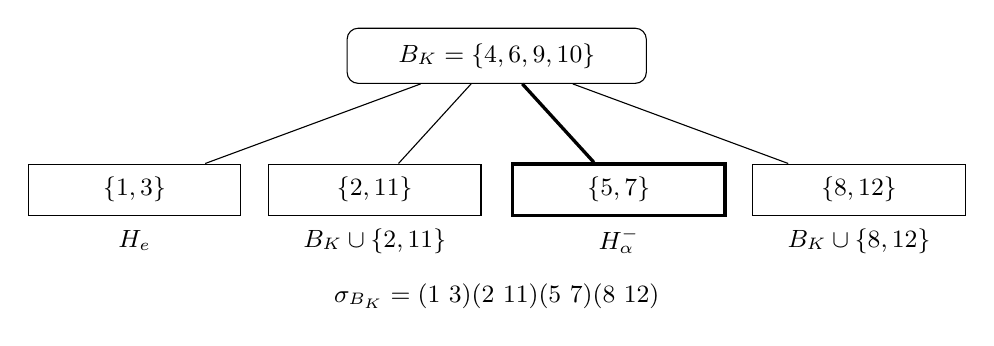
\begin{tikzpicture}[x=1cm,y=1cm, every node/.style={font=\small}]
 \node[draw,rounded corners,minimum width=3.8cm,minimum height=.7cm]
  (b) at (0,0) {$B_K=\{4,6,9,10\}$};
 \node[draw,minimum width=2.7cm,minimum height=.65cm]
  (p1) at (-4.6,-1.7) {$\{1,3\}$};
 \node[draw,minimum width=2.7cm,minimum height=.65cm]
  (p2) at (-1.55,-1.7) {$\{2,11\}$};
 \node[draw,very thick,minimum width=2.7cm,minimum height=.65cm]
  (p3) at (1.55,-1.7) {$\{5,7\}$};
 \node[draw,minimum width=2.7cm,minimum height=.65cm]
  (p4) at (4.6,-1.7) {$\{8,12\}$};
 \draw (b) -- (p1); \draw (b) -- (p2);
 \draw[very thick] (b) -- (p3); \draw (b) -- (p4);
 \node at (-4.6,-2.35) {$H_e$};
 \node at (-1.55,-2.35) {$B_K\cup\{2,11\}$};
 \node at (1.55,-2.35) {$H^-_\alpha$};
 \node at (4.6,-2.35) {$B_K\cup\{8,12\}$};
 \node at (0,-3.05)
  {$\sigma_{B_K}=(1\ 3)(2\ 11)(5\ 7)(8\ 12)$};
\end{tikzpicture}
\caption{L'étoile concrète du drapeau dodécaphasique. Chaque ligne
indique l'union du quadruplet central avec la paire à son extrémité ; la
ligne épaisse signale l'hexade également sélectionnée par les signes
antérieurs à la retenue de $\alpha$. Les quatre paires épuisent les huit
positions extérieures.}
\label{x_reciprocidad:exc:fig-estrella}
\end{figure}

\begin{proposition}[La famille des étoiles]
\label{x_reciprocidad:exc:m12}
Les $\binom{12}4=495$ permutations $\sigma_B$ préservent $\mathcal H$.
Le groupe qu'elles engendrent est d'ordre $95040$ et est le groupe de Mathieu
$M_{12}$ dans son action sur le petit système de Witt.
\end{proposition}

\begin{proof}
L'affirmation de préservation est une vérification finie sur les
$132$ hexades de \eqref{x_reciprocidad:exc:codigo} : pour chaque tétrade, on construit
les quatre pétales et l'on vérifie
$\{\sigma_B(H):H\in\mathcal H\}=\mathcal H$.
La clôture par composition de ces permutations produit $95040$
éléments. Dans l'énumération lexicographique, il suffit d'ajouter successivement
six étoiles qui ne sont pas encore contenues dans le groupe ; les ordres intermédiaires
sont $2,6,18,360,7920,95040$, et les $495$ étoiles appartiennent au groupe
final. La procédure, les six permutations écrites au moyen de leurs
listes d'images et la récurrence de clôture sont développées dans
\ref{iv:iv:apendice-estrellas}. Enfin, on applique la reconnaissance
du groupe d'automorphismes de $S(5,6,12)$ comme $M_{12}$, dont l'ordre est
$12\cdot11\cdot10\cdot9\cdot8=95040$.
\end{proof}

Une étoile individuelle engendre un groupe cyclique d'ordre deux. Elle
n'engendre pas à elle seule $M_{12}$, et encore moins le Monstre. L'
existence de $495$ générateurs d'un groupe de permutations ne prouve pas non plus que
chacun soit le transport d'un lacet spécifique du TPK. Cette affirmation
requiert l'application de lacets correspondante ; le résultat établi ici
est l'action d'incidence finie.

\begin{remark}[L'égalité des traces n'identifie pas les opérateurs]
Sur $V_{11}$, une étoile a pour spectre $+1$ avec multiplicité sept
et $-1$ avec multiplicité quatre. Sa trace normalisée est $3/11$.
Un projecteur de rang trois sur le même espace possède également une trace
normalisée $3/11$, mais un spectre $1^3,0^8$. Ils ne sont pas conjugués : leurs
polynômes minimaux et leurs spectres sont différents. L'opérateur d'entrelacement
\eqref{x_reciprocidad:exc:incidencia} transporte des opérateurs définis ; il ne transforme pas
cette coïncidence scalaire en une équivalence d'opérateurs.
\end{remark}

\subsection{Le résidu binaire et les cinq régions de \texorpdfstring{$\pi$}{pi}}
\label{x_reciprocidad:exc:cinco-regiones}

La reconnaissance suivante utilise le code de Golay binaire
étendu $G_{24}$, de paramètres $[24,12,8]_2$. Ses poids sont
$0,8,12,16,24$, et les supports de poids huit forment le plan
$S(5,8,24)$. Nous fixons une dodécade $D$, support d'un mot de poids
douze. Cette donnée et l'isomorphisme d'incidence qui sera déclaré
ci-dessous appartiennent à la carte de réalisation ; ils ne sont pas utilisés pour
générer ni sélectionner les décimales de $\pi$.

\begin{proposition}[Résidu d'une dodécade et élévation d'hexades]
\label{x_reciprocidad:exc:residuo-binario}
L'ensemble
\[
 \mathcal H(D)=
 \{O\cap D: O\text{ est une octade},\ |O\cap D|=6\}
\]
est un système $S(5,6,12)$ sur $D$. Chacune de ses hexades a une unique élévation en une octade. Pour tout quadruplet $B\subset D$, les cinq octades qui le contiennent se répartissent en quatre élévations résiduelles et une unique octade $O_B^\perp$ avec $O_B^\perp\cap D=B$.
\end{proposition}

\begin{proof}
Un quintuplet $A\subset D$ appartient à une unique octade $O$. Si
$j=|O\cap D|$, le mot binaire somme de $O$ et $D$ a pour poids
$20-2j$. Parmi les poids permis, et avec $0\leq j\leq8$, seuls
$j=2,4,6$ sont possibles. Comme $A\subset O\cap D$, on a $j\geq5$
et donc $j=6$. Cela donne l'existence et l'unicité de l'hexade
résiduelle, ainsi que l'unicité de son élévation en choisissant cinq de ses
points. D'autre part,
\[
 \lambda_4(S(5,8,24))=\frac{\binom{20}1}{\binom41}=5,
 \qquad
 \lambda_4(S(5,6,12))=4.
\]
Les quatre hexades résiduelles sur $B$ donnent quatre octades distinctes. La cinquième ne peut pas couper $D$ en six points, car elle serait une autre hexade résiduelle ; puisqu'elle contient $B$, son intersection est de taille quatre et coïncide avec $B$.
\end{proof}

Une carte $\ell:[12]\to D$ préservant les hexades identifie
$\mathcal H$ à $\mathcal H(D)$. Son existence est la reconnaissance
du plan déjà construit comme le petit plan de Witt ; un choix
concret de $\ell$ fixe le réétiquetage. L'élévation
\[
 \iota_D:\mathcal H\longrightarrow
       \{\text{octades de }G_{24}\},
 \qquad H\longmapsto O\text{ tel que }O\cap D=\ell(H),
\]
est injective parce que l'intersection avec $D$ redonne $\ell(H)$. Cette injectivité a pour domaine les hexades, et non le registre $K$.

La relation avec les cinq régions de $\pi$ conserve des données plus riches
que le nombre cinq. Les émissions et leurs signatures sont :
\begin{center}
\small
\begin{tabular}{@{}crll@{}}
\toprule
Région & Multiplicité & Émission $U_6$ & Signature \\
\midrule
$\perp$ & $432$ & $(501,614,498,169,272,272)$ & $555555$ \\
$++_1$ & $144$ & $(810,923,870,169,272,272)$ & $339555$ \\
$++_2$ & $144$ & $(810,983,810,169,272,272)$ & $393555$ \\
$++_3$ & $144$ & $(870,923,810,169,272,272)$ & $933555$ \\
$--$ & $144$ & $(870,923,810,418,674,521)$ & $933717$ \\
\bottomrule
\end{tabular}
\end{center}
Dans chaque bloc décimal de trois chiffres, la signature utilise la différence
modulaire des deux premiers chiffres. Les cinq émissions ont le
même mot tritique visible $w_\pi=010211$, mais pas la même
généalogie régionale. Les trois régions positives conservent la queue
$169|272|272$ ; la région négative la remplace par $418|674|521$ ;
la région transversale a une signature constante et une multiplicité supérieure.

L'extension marquée de la carte régionale envoie la région transversale sur $O_{\ell(B_K)}^\perp$, la négative sur $\iota_D(H^-_\alpha)$ et les trois positives sur les trois autres élévations de l'étoile. On réalise ainsi la partition $4+1$ des cinq octades sur $\ell(B_K)$. La correspondance individuelle entre les trois noms positifs et les trois pétales restants exige un ordre de carte ; l'incidence ne la détermine pas sans cette donnée. L'affirmation précise est donc une correspondance marquée de régions, compatible avec leurs rôles et avec le drapeau, et non une bijection canonique déduite du cardinal cinq.

L'identité $432+4\cdot144=1008$ conserve les multiplicités
régionales. On a aussi $1008=36\cdot28$ et une octade possède
$\binom82=28$ paires. Ces égalités sont des contrôles arithmétiques de
catalogue, et non des substituts de l'application $\iota_D$ ni de la carte régionale.


% BEGIN OWNER /Users/ruben/Documents/New project/output/EXTREMA_MEDIA_RAZON_RECIPROCIDAD_ES_EN_20260918/ARTICULO/ES/source/sections/estrella_pentadica_recuperada.tex
\subsubsection{Représentation pentadique de la microfibre et de son incidence}
\label{x_reciprocidad:pi-estrella:desarrollo}

La disposition des cinq régions permet de visualiser simultanément
l'unité du quotient ternaire et la différenciation conservée par le
catalogue. L'application pertinente est la restriction
\[
 \Psi\big|_{\mathscr R_\pi^{\rm micro}}:
 \mathscr R_\pi^{\rm micro}\longrightarrow\{010211\},
 \qquad \Psi(U)=(-U)\bmod3.
\]
Ses cinq antécédents sont les vecteurs \(U_6\) du tableau précédent. La figure \ref{x_reciprocidad:pi-estrella:figura} récupère leur organisation radiale, en conservant l'ordre de carte, les signatures et les multiplicités du catalogue (équation~\eqref{x_reciprocidad:eq:palabras-regionales}).


% BEGIN OWNER /Users/ruben/Documents/New project/output/EXTREMA_MEDIA_RAZON_RECIPROCIDAD_ES_EN_20260918/ARTICULO/ES/source/figures/estrella_cinco_regiones.tex
% Orden de carta y datos recuperados de fig_cinco_regiones_pi.tex.
\begin{figure}[H]
\centering
\begin{tikzpicture}[x=1cm,y=1cm,font=\small,>=Latex]
 \coordinate (a) at (90:2.2);
 \coordinate (b) at (18:2.2);
 \coordinate (c) at (-54:2.2);
 \coordinate (d) at (-126:2.2);
 \coordinate (e) at (162:2.2);
 \draw[black!35,line width=.45pt]
    (a)--(c)--(e)--(b)--(d)--cycle;
 \node[draw,fill=white,circle,minimum size=1.6cm,align=center,
    inner sep=3pt] (z) at (0,0) {$w_\pi$\\$010211$};
 \foreach \v in {a,b,c,d,e}{
    \fill (\v) circle (2pt);
    \draw[->,line width=.6pt] (\v)--(z);
 }
 \node[above=3mm,align=center] at (a)
   {$U_\pi^\perp$\\$555555$\\multiplicidad $432$};
 \node[right=3mm,align=left] at (b)
   {$U_{\pi,1}^{++}$\\$339555$\\multiplicidad $144$};
 \node[below right=2mm and 1mm,align=left] at (c)
   {$U_{\pi,2}^{++}$\\$393555$\\multiplicidad $144$};
 \node[below left=2mm and 1mm,align=right] at (d)
   {$U_{\pi,3}^{++}$\\$933555$\\multiplicidad $144$};
 \node[left=3mm,align=right] at (e)
   {$U_\pi^{--}$\\$933717$\\multiplicidad $144$};
 \node[align=center,font=\footnotesize] at (0,-3.55)
   {$1_\perp+3_{++}+1_{--}$\qquad $432+4\cdot144=1008$};
\end{tikzpicture}
\caption{Les cinq régions de \(\pi\) selon une disposition pentadique.
Chaque position conserve sa signature multiplicative et sa multiplicité ;
les flèches radiales représentent la projection commune
\(\Psi(U)=010211\). Le contour étoilé organise les cinq
positions de la carte. Leur réalisation dans les cinq octades de Witt
s'effectue au moyen de l'alignement régional et de la décomposition
\(4+1\) exposée dans le texte.}
\label{x_reciprocidad:pi-estrella:figura}
\end{figure}

% END OWNER


La projection sur le centre identifie les cinq images ternaires ; le
registre des positions extérieures retient l'information régionale
qui rend possible la réalisation d'incidence. La distribution
\(1_\perp+3_{++}+1_{--}\) spécifie une région transversale, trois
régions positives et une négative. Leurs poids normalisés sont
\(3/7\) et \(1/7\) pour chacune des quatre autres : la
multiplicité transversale est triple, alors même que les cinq images par
\(\Psi\) coïncident.

\Needspace{11\baselineskip}
Le lien avec l'étoile de Witt se formule au moyen du drapeau
\(B_K\subset H^-_\alpha\), de l'alignement \(\ell\) et du
relèvement \(\iota_D\) déjà construits. Les cinq positions régionales
se réalisent dans les cinq octades sur \(\ell(B_K)\) :
\[
\begin{aligned}
 U_\pi^\perp&\longmapsto O^\perp_{\ell(B_K)},\\
 U_\pi^{--}&\longmapsto\iota_D(H^-_\alpha),\\
 \{U_{\pi,1}^{++},U_{\pi,2}^{++},U_{\pi,3}^{++}\}
 &\longmapsto
 \{\iota_D(B_K\cup P):P\in\mathcal P_+\},\\
 \mathcal P_+&=\bigl\{\{1,3\},\{2,11\},\{8,12\}\bigr\}.
\end{aligned}
\]
L'attribution des trois positions positives aux trois paires
s'effectue dans une carte ordonnée. La ligne transversale et la ligne négative
sont distinguées par leurs prédicats régionaux et par le drapeau.

Les deux figures s'articulent ainsi : la figure
\ref{x_reciprocidad:exc:fig-estrella} montre les quatre hexades du petit plan
de Witt sur \(B_K\) ; la figure \ref{x_reciprocidad:pi-estrella:figura} montre
les cinq régions qui, sous l'alignement, occupent les quatre octades
résiduelles et l'octade transversale du plan binaire. La loi
\(4+1\), démontrée dans la proposition
\ref{x_reciprocidad:exc:residuo-binario}, spécifie le changement d'incidence. Dans cette
composition, \(K\) détermine la tétrade marquée et la signature de
\(\alpha\) distingue l'une de ses hexades. Les régions conservent,
outre leur valeur ternaire commune, la structure nécessaire à ce
transport vers la réalisation exceptionnelle.

% END OWNER


\subsection{Du code ternaire au réseau de Niemeier}
\label{x_reciprocidad:exc:niemeier}

Le passage à la dimension vingt-quatre ne nécessite pas de parcourir d'abord le
code binaire. Il s'effectue directement à partir de $C_W$ par recollement des
discriminants. On distingue ainsi deux prolongations compatibles :
l'une conserve le résidu $W_{12}\subset W_{24}$ ; l'autre construit le
réseau sur lequel sera réalisée l'algèbre d'opérateurs de vertex.

Soit $A_2=\mathbb Z a_1\oplus\mathbb Z a_2$ de matrice de Gram
\[
 \begin{pmatrix}2&-1\\-1&2\end{pmatrix},
 \qquad \rho=a_1+a_2,\qquad \rho^2=2.
\]
Nous représentons les trois classes de $A_2^*/A_2$ par
\[
 \varpi_0=0,\qquad
 \varpi_1=\frac{2a_1+a_2}{3},\qquad
 \varpi_2=\frac{a_1+2a_2}{3}.
\]
L'application $j\mapsto\varpi_j+A_2$ identifie additivement
$\mathbb F_3$ à ce discriminant. Pour $c\in C_W$, nous écrivons
$\phi(c)=(\varpi_{c_1},\ldots,\varpi_{c_{12}})$ et définissons
\begin{equation}
 N(C_W)=\bigcup_{c\in C_W}\bigl(A_2^{12}+\phi(c)\bigr).
 \label{x_reciprocidad:exc:niemeier-def}
\end{equation}

\begin{theorem}[Recollement ternaire]
\label{x_reciprocidad:exc:niemeier-teorema}
L'objet \eqref{x_reciprocidad:exc:niemeier-def} est un réseau positif, pair et
unimodulaire de rang $24$. Son système de racines est exactement
$A_2^{12}$ ; il est donc reconnu comme le réseau de Niemeier ayant
ce système de racines.
\end{theorem}

\begin{proof}
La linéarité du code rend l'union de classes stable par addition. L'auto-orthogonalité annule l'accouplement discriminant : celui-ci est un multiple de $c\cdot d/3$ modulo $\mathbb Z$. Le réseau est donc entier. La norme d'une classe de recollement est $2\operatorname{wt}(c)/3$ modulo $2\mathbb Z$. Les poids de \eqref{x_reciprocidad:exc:enumerador} sont des multiples de trois, de sorte qu'il est pair.

L'indice de $A_2^{12}$ dans $N(C_W)$ est $|C_W|=3^6$. En conséquence,
\[
 \det N(C_W)=\frac{3^{12}}{(3^6)^2}=1.
\]
La positivité procède de la somme orthogonale des douze métriques $A_2$.
Dans une classe non nulle de $A_2^*/A_2$, la norme minimale est $2/3$ ;
tout mot non nul possède au moins six positions non nulles.
Par conséquent, un vecteur d'une classe de recollement non triviale a une norme
au moins égale à $6\cdot2/3=4$. Aucune racine de norme deux n'apparaît hors de
$A_2^{12}$. À l'intérieur de celui-ci, les racines sont précisément celles de ses
douze composantes.
\end{proof}

\subsection{Sélection par incidence du voisin unimodulaire sans racines}
\label{x_reciprocidad:exc:leech}


% BEGIN OWNER /Users/ruben/Documents/New project/output/EXTREMA_MEDIA_RAZON_RECIPROCIDAD_ES_EN_20260918/ARTICULO/ES/source/sections/incidencia_reticulo.tex
\paragraph{De l'origine incidencielle à la modification réticulaire.}
\label{x_reciprocidad:inc-ampl-reticulo}
Le drapeau marqué détermine une position au moyen d'une opération
ensembliste équivariante :
\[
 o_*=(H_e\cap H_\varphi)
       \setminus(H^-_\alpha\cup H_{\rm APP})=\{1\}.
\]
Sa fonction consiste à distinguer une composante parmi les douze qui
interviennent dans la réalisation réticulaire. Le code ternaire complet
agit comme code de recollement dans le module discriminant
$(A_2^*/A_2)^{12}$. Sa préimage définit $N(C_W)$, et
l'autodualité, les poids et la distance du code se traduisent,
respectivement, en propriétés d'intégralité et de déterminant, de parité
et en bornes de norme des classes de recollement. L'information symbolique
du code remplit ici une fonction que le support isolé ne remplit plus.

La métrique $A_2$ et la chambre radiale positive sont fixées dans le développement
réticulaire. À l'intérieur de cette chambre, la congruence nécessaire pour un voisin
pair d'indice trois possède douze réalisations de norme minimale $54$,
permutées par le changement de composante distinguée. L'origine $o_*$
sélectionne
\[
 v_\alpha=4\rho_1+\rho_2+\cdots+\rho_{12},\qquad
 v_\alpha^2=2(4^2+11)=54.
\]
Le coefficient $4$ appartient à cette solution de la congruence dans la
chambre déclarée. L'indice $\alpha$ enregistre la provenance
incidencielle de la sélection : son contenu est le repère qui est intervenu dans
la clôture et qui individualise à présent une direction réticulaire.

L'appariement avec $v_\alpha$ détermine le sous-réseau
$N_{\alpha,0}$ d'indice trois, et l'adjonction de la classe
$v_\alpha/3$ produit le voisin $N_\alpha$ de
\eqref{x_reciprocidad:exc:vecino}. Cette modification conserve le rang et rétablit
l'unimodularité et la parité ; la sélection par congruence élimine les racines
antérieures, et les bornes locales excluent les racines dans les nouvelles classes.
L'identification à Leech intervient après ces vérifications. La
réalisation binaire des cinq régions et cette construction réticulaire
sont deux prolongements du repère commun : la seconde reçoit directement
le code ternaire comme donnée de recollement.


% END OWNER


L'étiquette $o_*=1$ du drapeau se réalise maintenant comme l'une des
douze composantes $A_2$. Cette opération déclare la métrique précédente et
la chambre radiale positive
\[
 v(a)=\sum_{i=1}^{12}a_i\rho_i,
 \qquad a_i=1+3b_i,\quad b_i\in\mathbb Z_{\geq0}.
\]
L'exigence de parité du voisin d'indice trois est $v(a)^2\equiv0\pmod{18}$. Puisque
\[
 v(a)^2=2\sum_i(1+3b_i)^2,
\]
cette congruence équivaut à $\sum_i b_i\equiv1\pmod3$. La plus petite
valeur de la norme dans la chambre s'obtient avec un unique $b_i=1$ et
tous les autres nuls ; elle vaut $54$. L'origine marquée sélectionne
\begin{equation}
 v_\alpha=4\rho_1+\rho_2+\cdots+\rho_{12},
 \qquad v_\alpha^2=54.
 \label{x_reciprocidad:exc:vector}
\end{equation}
Le mot ``plus petit'' se rapporte à cette chambre positive. Il n'affirme pas la minimalité dans toute la classe résiduelle : le vecteur $(a_1-2a_2,\rho,\ldots,\rho)$ représente la même classe modulo trois et a pour norme $14+11\cdot2=36$. La restriction de chambre fait partie des données de la construction, et n'est pas une conclusion que l'on puisse omettre.

Soit $N=N(C_W)$. Nous définissons
\begin{equation}
 N_{\alpha,0}=\{x\in N:\langle x,v_\alpha\rangle\equiv0\pmod3\},
 \qquad
 N_\alpha=N_{\alpha,0}+\mathbb Z\frac{v_\alpha}{3}.
 \label{x_reciprocidad:exc:vecino}
\end{equation}

\begin{theorem}[Voisin de Leech déterminé par le drapeau marqué]
\label{x_reciprocidad:exc:teorema-leech}
Avec la métrique et la chambre déclarées, $N_\alpha$ est un réseau
positif, pair et unimodulaire de rang $24$, sans vecteurs de norme deux.
D'après le théorème de classification correspondant, il est isométrique au
réseau de Leech $\Lambda_{24}$.
\end{theorem}

\begin{proof}
Le caractère $x\mapsto\langle x,v_\alpha\rangle\bmod3$ est non nul :
une racine simple d'une composante s'apparie avec $a_i\rho_i$ en
$a_i\equiv1\pmod3$. Par conséquent, $[N:N_{\alpha,0}]=3$ et
$\det N_{\alpha,0}=9$. De plus,
$v_\alpha/3\in N_{\alpha,0}^*$ et $v_\alpha\in N_{\alpha,0}$.
Si $v_\alpha/3$ appartenait à $N$, l'intégralité de $N$ rendrait
tous les appariements avec $v_\alpha$ divisibles par trois,
ce qui contredirait le caractère non nul. La classe de $v_\alpha/3$ est
donc d'ordre trois. On en déduit
\[
 [N_\alpha:N_{\alpha,0}]=3,
 \qquad \det N_\alpha=9/3^2=1.
\]
L'extension est entière, et pour $x\in N_{\alpha,0}$,
\[
 \left(x+m\frac{v_\alpha}{3}\right)^2
   =x^2+2m\frac{\langle x,v_\alpha\rangle}{3}+6m^2
   \in2\mathbb Z.
\]
Elle est donc paire.

Il reste à exclure les racines, ce qui est l'étape décisive. Les racines de $N$ appartiennent à $A_2^{12}$. Leurs accouplements avec $v_\alpha$ sont congrus à $\pm1$ ou à $\pm2$ modulo trois ; aucune n'appartient à $N_{\alpha,0}$. Pour les deux autres classes du voisin, chaque composante appartient à l'une des classes locales
\[
 A_2+\varpi_j\pm\rho/3,\qquad j=0,1,2.
\]
Comme $4\rho/3\equiv\rho/3\pmod{A_2}$, cette description vaut
également dans la composante distinguée. En écrivant un vecteur local
sous la forme $(u a_1+v a_2)/3$, sa norme est
$2(u^2-uv+v^2)/9$. Les six classes précédentes ont des résidus non
nuls et un minimum $2/9$ : les représentants de forme quadratique minimale
sont $(\pm1,0),(0,\pm1),(1,1),(-1,-1)$ dans les résidus appropriés.
Un vecteur d'une classe nouvelle a donc une norme au moins égale à
$12\cdot2/9=8/3>2$. Aucune des trois classes ne contient de racines.
La classification des réseaux pairs unimodulaires positifs de
rang vingt-quatre identifie l'unique cas sans racines à
$\Lambda_{24}$.
\end{proof}

L'argument ne reconnaît pas Leech par une coïncidence de dimension.
Il construit le recollement, prouve l'intégralité, la parité et le déterminant, et
élimine les racines au moyen d'une borne locale. Ce n'est qu'ensuite qu'il applique le
théorème de classification. La dépendance à l'égard de $\alpha$ est conservée dans
le drapeau qui sélectionne $o_*$ et dans le vecteur \eqref{x_reciprocidad:exc:vector} ;
on ne transforme pas la valeur scalaire de la constante en une longueur du
réseau.

\subsection{L'algèbre d'opérateurs de vertex et le Monstre}
\label{x_reciprocidad:exc:voa}

Soit $\Lambda=N_\alpha$, déjà reconnu comme le réseau de Leech. L'étape suivante utilise son réseau entier, et non un développement décimal. La construction de l'algèbre d'opérateurs de vertex de réseau s'écrit
\[
 V_\Lambda=M(1)\otimes\mathbb C_\varepsilon[\Lambda].
\]
Ici, $M(1)$ est l'espace des oscillateurs de Heisenberg en rang vingt-quatre ; $\mathbb C_\varepsilon[\Lambda]$ est l'algèbre de groupe tordue par le cocycle de l'extension centrale du réseau. Le cocycle et le relèvement des isométries font partie de la construction : une somme vectorielle nue ne détermine pas les produits de vertex.

La négation $\lambda\mapsto-\lambda$ admet le relèvement standard
$\theta$. Avec son module tordu et le choix de parité compatible,
la construction de Frenkel--Lepowsky--Meurman produit
\begin{equation}
 V^\natural_{\rm HMT}
   =V_\Lambda^+\oplus(V_\Lambda^T)^+.
 \label{x_reciprocidad:exc:flm}
\end{equation}
Le signe $+$ désigne la partie paire de l'action relevée. L'expression
inclut le produit de vertex de l'orbifold ; elle ne se limite pas à une somme
d'espaces gradués.

\begin{theorem}[Prolongement jusqu'au module Moonshine]
\label{x_reciprocidad:exc:moonshine}
L'algèbre \eqref{x_reciprocidad:exc:flm}, construite sur le voisin
\eqref{x_reciprocidad:exc:vecino}, est une réalisation de l'algèbre Moonshine
$V^\natural$. Elle a une charge centrale $24$, une composante de poids un nulle
et un groupe d'automorphismes isomorphe au Monstre $\mathbb M$. Son caractère
gradué est
\begin{equation}
 \operatorname{Tr}_{V^\natural_{\rm HMT}}q^{L_0-1}
   =J(\tau)=j(\tau)-744
   =q^{-1}+196884q+21493760q^2+\cdots,
 \qquad q=e^{2\pi i\tau}.
 \label{x_reciprocidad:exc:j}
\end{equation}
\end{theorem}

\begin{proof}
Le théorème \ref{x_reciprocidad:exc:teorema-leech} vérifie les hypothèses sur le réseau :
positivité, parité, unimodularité, rang vingt-quatre et absence de
racines. On applique alors la construction et le théorème de
Frenkel--Lepowsky--Meurman pour le réseau de Leech. Ceux-ci identifient
l'orbifold à $V^\natural$, établissent son caractère et son groupe d'
automorphismes. La composition du drapeau, du voisin et du foncteur
de construction de VOA donne la réalisation indiquée ici. Le groupe ne se déduit
pas du coefficient $196884$.
\end{proof}

Le théorème utilisé est une reconnaissance classique ultérieure dont les hypothèses sont vérifiées, et non une nouvelle démonstration dans cet article de la construction FLM \cite{x_reciprocidad:flm}. En outre, la notation $q=e^{2\pi i\tau}$ est la variable conventionnelle de Fourier employée pour reconnaître le caractère. Elle n'introduit ni $\pi$ ni $e$ comme entrées du générateur coinductif qui les a déjà déterminés.

Une partie du mécanisme de trace peut être observée avant l'orbifold.
Seul le vecteur nul du réseau est fixé par la négation ; chaque
oscillateur contribue avec un signe alterné. D'où
\[
 \operatorname{Tr}_{V_\Lambda}\theta q^{L_0-1}
   =t_2(\tau)
   :=q^{-1}\prod_{n\geq1}(1+q^n)^{-24}.
\]
Cette trace dans l'algèbre de réseau ne doit pas être confondue avec le
caractère sans insertion de $V^\natural$. Elle n'identifie pas non plus à elle
seule une classe de conjugaison du Monstre : l'espace, l'insertion
et le relèvement doivent être spécifiés avant de comparer les fonctions.


% BEGIN OWNER /Users/ruben/Documents/New project/output/EXTREMA_MEDIA_RAZON_RECIPROCIDAD_ES_EN_20260918/ARTICULO/ES/source/sections/incidencia_automorfismos.tex
\paragraph{Graduation, unité et automorphismes.}
\label{x_reciprocidad:inc-ampl-automorfismos}
La construction de Frenkel--Lepowsky--Meurman s'applique au réseau
$N_\alpha$ une fois ses propriétés vérifiées. Elle incorpore l'espace
des oscillateurs, l'extension centrale du réseau, le produit de vertex
et le secteur tordu par le relèvement de la négation. Le résultat est
l'algèbre $V^\natural_{\rm HMT}$ de \eqref{x_reciprocidad:exc:flm}, dont le groupe
d'automorphismes est isomorphe au Monstre. Son domaine d'action est ainsi
fixé par une structure algébrique munie d'une graduation et d'un produit. Le théorème
de Moonshine de Borcherds détermine ensuite les traces graduées
avec insertion de ces automorphismes \cite{x_reciprocidad:flm,x_reciprocidad:borcherds}.

L'unité acquiert à ce niveau une réalisation précise : la composante
de poids zéro est la droite du vide et fournit le coefficient $1$ de
$q^{-1}$ dans le caractère gradué. Au niveau cylindrique, les
applications de raffinement conservent la fonction constante par
précomposition. Chaque assertion de conservation possède donc son
objet et son application. Le développement des preuves rend visible cette
continuité de construction, depuis les opérations arithmétiques et la
mémoire jusqu'à l'incidence, à la métrique et aux produits de vertex.

Cette articulation situe $K$ et la clôture de $\alpha$ dans l'argument
principal. $K$ conserve de manière réversible une coordonnée entière de
l'histoire ; la normalisation de $\alpha$ compose les registres régionaux
avec cette coordonnée ; la configuration signée détermine un drapeau ; et
le drapeau marqué sélectionne la modification réticulaire sur laquelle se
réalise Moonshine. Les démonstrations suivantes développent ces
applications, en distinguant les équivalences réversibles, les quotients
d'information et les réalisations qui ajoutent une métrique ou une structure
algébrique. Ainsi s'exprime une relation démontrable entre structure,
équation et valeur, en conservant l'attribution de chaque construction et la
portée de ses théorèmes.

% END OWNER



% BEGIN OWNER /Users/ruben/Documents/New project/output/EXTREMA_MEDIA_RAZON_RECIPROCIDAD_ES_EN_20260918/ARTICULO/ES/source/sections/fibras_app_witt.tex
\subsection{Construction à partir de l’état des douze fibres cyclotomiques}
\label{x_reciprocidad:nuclear:fibras-app-witt}
Sur les marques d’APP, la multiplication \(a:r\mapsto4r\) dans
\(\ZZ/9\ZZ\) satisfait \(a^3=1\). Les feuillets vérifient
\[
 S(ax,ay)=aS(x,y),\qquad P(ax,ay)=a^{-1}P(x,y),
\]
puisque \(16\equiv7\equiv4^{-1}\pmod9\). Les orbites unitaires
ordonnées sont \(\mathcal O_0=(1,4,7)\), \(\mathcal O_1=(2,8,5)\).
Dans chacune, le module d’augmentation
\(A(\mathcal O)=\ker(\ZZ[\mathcal O]\xrightarrow{\sum}\ZZ)\)
hérite du produit qui rend les \(e_r\) orthonormaux. Dans la base
\(b_1=e_r-e_{4r}\), \(b_2=e_{4r}-e_{7r}\), ses matrices sont
\[
 G_{A_2}=\begin{pmatrix}2&-1\\-1&2\end{pmatrix},\qquad
 C=\begin{pmatrix}0&-1\\1&-1\end{pmatrix},\qquad
 C^{\mathsf T}G_{A_2}C=G_{A_2}.
\]
La forme réticulaire provient donc des orbites des marques. Pour les paires \((1,2),(2,3),(3,1)\) et les feuillets \(\mu\in\{\Sigma,\Pi\}\), on obtient
\[
 W_{\APP}=\bigoplus_{(i,j)}\bigoplus_\mu\bigoplus_{\varepsilon=0}^1
 A(\mathcal O_\varepsilon),\qquad
 \ell^\Sigma_{ij}(x)=x_i+x_j,\quad
 \ell^\Pi_{ij}(x)=x_ix_j\pmod9.
\]
Chaque terme conserve la paire, le feuillet et l'orbite. L'application d'état est
\[
 \Psi:(\ZZ/9\ZZ)^3\longrightarrow W_{\APP},\qquad
 \Psi(x)_{ij,\mu,\varepsilon}=\beta_\varepsilon(\ell^\mu_{ij}(x)),
 \quad
 \beta_\varepsilon(r)=
 \begin{cases}e_r-e_{4r},&r\in\mathcal O_\varepsilon,\\0,&r\notin\mathcal O_\varepsilon.
 \end{cases}
\]
\begin{proposition}[Équivariance et rang du module d’état]
\label{x_reciprocidad:nuclear:psi-rango}
L’action de \(C\) dans les six fibres additives et de \(C^{-1}\) dans
les six fibres multiplicatives vérifie \(\Psi(ax)=\rho(a)\Psi(x)\).
Les images engendrent \(W_{\APP}\otimes\QQ\), de dimension vingt-quatre.
\end{proposition}
\begin{proof}
Les identités des feuillets et \(\beta(4r)=C\beta(r)\) prouvent
l’équivariance. Pour le rang, on ordonne les coordonnées par les trois
couples indiqués, par \(\Sigma,\Pi\), par \(\mathcal O_0,\mathcal O_1\)
et par \(b_1,b_2\). Dans chaque orbite, \(\beta\) prend successivement
\((1,0),(0,1),(-1,-1)\). La matrice des images de ces états,
lus par lignes, a pour déterminant \(9\) :
\[
\begin{array}{rrrr}
(0,0,1)&(0,0,2)&(0,0,4)&(0,0,5)\\
(0,1,0)&(0,1,1)&(0,1,2)&(0,1,3)\\
(0,1,4)&(0,1,5)&(0,1,6)&(0,2,0)\\
(0,2,2)&(0,2,3)&(0,4,0)&(0,5,0)\\
(1,0,1)&(1,0,2)&(1,0,4)&(1,0,5)\\
(1,1,0)&(1,2,0)&(1,4,0)&(1,5,0).
\end{array}
\]
L'élimination successive, en réduisant chaque ligne par les précédentes et en normalisant son premier coefficient non nul, donne les colonnes pivots numérotées à partir de zéro
\[
\begin{split}
&(8,10,9,11,0,12,14,16,13,15,17,2,\\
&\hspace{2em}18,19,1,3,20,22,21,23,4,6,5,7)
\end{split}
\]
et pivots
\[
(1,1,1,-1,1,1,1,1,1,-1,3,1,1,3,1,-1,1,1,1,-1,1,1,1,-1).
\]
Leur produit, multiplié par le signe de la permutation des colonnes,
est \(9\). Le mineur inversible atteste le rang total.
\end{proof}

\subsection{Alignement dodécaphasique avec les positions de Witt}
\label{x_reciprocidad:nuclear:alineamiento-witt}
L'indice de la paire est \(i\in\ZZ/3\ZZ\), celui du feuillet \(\mu\in\{0,1\}\) et celui de l'orbite \(\varepsilon\in\{0,1\}\). L'origine dodécaphasique étant fixée, \(\lambda(i,\mu,\varepsilon)
=4i+2\mu+\varepsilon\pmod{12}\) est bijective : les quatre valeurs de chaque \(i\) forment un bloc et les trois blocs sont disjoints. Soit \(R=\left(\begin{smallmatrix}0&1\\1&0\end{smallmatrix}\right)\).
La multiplication prouve \(RCR=C^{-1}\) et
\(R^{\mathsf T}G_{A_2}R=G_{A_2}\). Pour les trivialisations
\(\iota_b\) et les repères \(P_b\) transportés conjointement avec
l’incidence de Witt, nous posons
\[
g_b=\iota_b^{-1}P_bCP_b^{-1}\iota_b,\qquad
T_{i\mu\varepsilon}=\iota_{\lambda(i,\mu,\varepsilon)}^{-1}
P_{\lambda(i,\mu,\varepsilon)}R^\mu.
\]
Alors
\[
g_{\lambda(i,\mu,\varepsilon)}T_{i\mu\varepsilon}
=T_{i\mu\varepsilon}C^{(-1)^\mu}.
\]
La somme directe est un isomorphisme \(C_3\)-équivariant entre les douze
fibres d’état et les douze positions réticulaires. Elle conserve couple,
feuillet, orbite et forme sous le transport simultané de l’origine,
de l’ordre et de l’orientation. Ces données demeurent dans le recollement réticulaire
et le passage au voisin construits ci-dessous.

% END OWNER


% BEGIN OWNER /Users/ruben/Documents/New project/output/EXTREMA_MEDIA_RAZON_RECIPROCIDAD_ES_EN_20260918/ARTICULO/ES/source/sections/moonshine_comparacion.tex
% Incorporación aditiva para el Artículo I; no modifica la fuente anterior.
% RESULTADO_RECUPERADO: integral, capítulo 22, propietario extenso
% colaboracion/partes_i_ii/source/base_residencias/
% capitulo_22_c20_lineas_2613_3270.tex, líneas 176--576.
% Equivalencia 2/3: public/residencias/capitulo_22_voa_leech_moonshine.tex,
% líneas 55--127. Orden dos y Fricke: hmt/15d_voa_moonshine_orden_dos_rev11.tex.
% Prerrequisitos residentes en I: código C_W, matriz A_W, N(A_2^12),
% origen o_*, vector v_alpha de norma54, N_alpha reconocido como Leech,
% VOA reticular y presentación FLM de las secciones precedentes.
% Bibliografía nueva: chenlamshimakura2016, abelamyamada2017,
% kmconwaynorton1979 (bibitems listos para incorporar al final de este archivo).

\subsection{Orientation ternaire du voisin de Leech}
\label{x_reciprocidad:km:orden-tres-reticular}

La présentation d’ordre deux construite précédemment utilise la négation
du réseau de Leech. Le même réseau, obtenu à partir de l’incidence marquée
par \(K\) et du support dodécaphasique de \(\alpha\), admet une seconde
présentation compatible avec le caractère ternaire de la construction.
Pour expliciter cette continuité, on conserve le recollement, on construit
son isométrie d’ordre trois et l’on vérifie qu’elle préserve le voisin déjà
sélectionné. Cette étape ne requiert pas d’altérer \(K\), sa lecture rationnelle ni
la définition préalable de \(\alpha\). On développe ici le prolongement d’ordre trois, y compris les opérations
réticulaires et les conditions précises des théorèmes classiques utilisés.

Nous travaillons dans la base des racines simples de chaque facteur \(A_2\), avec
\begin{equation}
 B_2=\begin{pmatrix}2&-1\\-1&2\end{pmatrix},\qquad
 \mathsf C=\begin{pmatrix}0&-1\\1&-1\end{pmatrix},\qquad
 \mathsf R=\begin{pmatrix}0&1\\1&0\end{pmatrix},\qquad
 \rho=\begin{pmatrix}1\\1\end{pmatrix}.
 \label{x_reciprocidad:km:coxeter-reflexion}
\end{equation}
La multiplication donne
\[
 \mathsf C^3=I_2,\quad
 \mathsf C^2+\mathsf C+I_2=0,\quad
 \mathsf C^{\mathsf T}B_2\mathsf C=B_2,\quad
 \mathsf R\mathsf C\mathsf R=\mathsf C^{-1},\quad
 \mathsf R^{\mathsf T}B_2\mathsf R=B_2.
\]
Ces identités fixent aussi bien la métrique que l'orientation de l'action. Dans le discriminant \(A_2^*/A_2\cong\mathbb F_3\), nous prenons pour générateur la classe de \(\varpi=(2,1)^{\mathsf T}/3\). On a \(\mathsf C\varpi-\varpi=(-1,0)^{\mathsf T}\), de sorte que \(\mathsf C\) agit trivialement sur le discriminant ; la réflexion \(\mathsf R\) change son signe.

La matrice de Paley--Witt déjà construite produit un élément de support
complet par l'opération suivante :
\begin{equation}
 \begin{gathered}
 q_*=(1,1,1,1,1,1),\qquad q_*A_W=(2,1,1,1,1,1),\\
 c_*=(q_*,q_*A_W)
 =(1,1,1,1,1,1,2,1,1,1,1,1)\in C_W.
 \end{gathered}
 \label{x_reciprocidad:km:palabra-total}
\end{equation}
Chaque coordonnée de \(c_*\) est non nulle. Pour les douze positions,
nous définissons les cadres et l'isométrie
\begin{equation}
 P_b(c_*)=
 \begin{cases}\mathsf R,&(c_*)_b=1,\\I_2,&(c_*)_b=2,\end{cases}
 \qquad
 g_c=\bigoplus_{b=1}^{12}P_b(c_*)\mathsf C P_b(c_*)^{-1}.
 \label{x_reciprocidad:km:isometria-ternaria}
\end{equation}
Le symbole \(P_b(c_*)\) désigne ici un repère inversible d’un facteur
\(A_2\), et non le projecteur régional \(P_3\).

\begin{proposition}[Isométrie d'ordre trois sur le voisin marqué]
\label{x_reciprocidad:km:estabilidad-vecino}
L'opérateur \(g_c\) est une isométrie d'ordre trois sans vecteurs fixes non nuls. Il préserve le réseau de Niemeier \(N=N(C_W)\) et le voisin \(N_\alpha\) construit dans \eqref{x_reciprocidad:exc:vecino}.
\end{proposition}
\begin{proof}
Chaque bloc de \(g_c\) est \(\mathsf C\) ou \(\mathsf C^{-1}\) ;
son polynôme minimal est \(X^2+X+1\). Cela prouve l'ordre et
l'absence de vecteurs fixes. Les deux blocs agissent trivialement sur le
discriminant, de sorte qu'ils conservent chaque classe de recollement et donc
le réseau \(N\).

Écrivons \(v=v_\alpha=4\rho_{o_*}+\sum_{b\ne o_*}\rho_b\),
avec les cadres et l'origine d'incidence déjà fixés. Ses coefficients
radiaux sont \(a_{o_*}=4\) et \(a_b=1\) pour \(b\ne o_*\).
Tous satisfont \(a_b\equiv1\pmod3\). Dans un facteur,
\[
 (\mathsf C-I_2)\rho=(-2,-1)^{\mathsf T},\qquad
 (\mathsf C^{-1}-I_2)\rho=(-1,-2)^{\mathsf T}.
\]
Après division par trois, leurs classes discriminantes sont respectivement \(2\) et \(1\). En conséquence, les vecteurs
\begin{equation}
 y=\frac{g_cv-v}{3},\qquad z=\frac{g_c^{-1}v-v}{3}
 \label{x_reciprocidad:km:desplazamientos}
\end{equation}
ont pour mots discriminants \(c_*\) et \(-c_*\), tous deux dans
\(C_W\). Par conséquent, \(y,z\in N\). Le produit local est
\[
 \left\langle
 \frac{(\mathsf C^{\pm1}-I_2)a_b\rho}{3},a_b\rho
 \right\rangle=-a_b^2,
\]
et leur somme donne \(\langle y,v\rangle=\langle z,v\rangle=-(16+11)=-27\). Ainsi, \(y,z\in N_0=\{x\in N:\langle x,v\rangle\equiv0\pmod3\}\). Pour \(x\in N_0\),
\[
 \langle g_cx,v\rangle
 =\langle x,g_c^{-1}v\rangle
 =\langle x,v\rangle+3\langle x,z\rangle\equiv0\pmod3.
\]
L'argument appliqué à \(g_c^{-1}\) prouve \(g_cN_0=N_0\).
Enfin, \(g_c(v/3)=v/3+y\) conserve la classe qui engendre
\(N_\alpha=N_0+\mathbb Z(v/3)\). On obtient
\(g_cN_\alpha=N_\alpha\).
\end{proof}

La preuve conserve plus que la dimension du réseau : elle utilise le code de recollement, son orientation, l'origine du drapeau et la congruence du vecteur radial. Ces données expliquent pourquoi la seconde présentation reste liée au registre dodécaphasique dont la construction est partie.

\subsection{Trace ternaire, poids tordu et extension d'ordre trois}
\label{x_reciprocidad:km:orbifold-tres}

Soit \(\Lambda=N_\alpha\) et soit \(\widehat g_c\) le relèvement
standard de \(g_c\) à l'algèbre de réseau
\(V_\Lambda=M(1)\otimes\mathbb C_\varepsilon[\Lambda]\), avec
l'extension centrale et le cocycle déjà déclarés. L'ordre impair permet
de choisir ce relèvement d'ordre trois. Chaque facteur complexe \(A_2\)
apporte les valeurs propres \(\zeta_3\) et \(\zeta_3^2\), où
\(\zeta_3^2+\zeta_3+1=0\).

\begin{proposition}[Trace graduée et type du relèvement]
\label{x_reciprocidad:km:traza-tipo}
Pour \(j=1,2\),
\begin{equation}
 \operatorname{Tr}_{V_\Lambda}
       \bigl(\widehat g_c^{\,j}q^{L_0-1}\bigr)
 =t_3(\tau)
 :=q^{-1}\prod_{n\ge1}(1+q^n+q^{2n})^{-12}.
 \label{x_reciprocidad:km:tres-traza}
\end{equation}
Le poids minimal des modules tordus non triviaux est \(4/3\), et
le relèvement est de type zéro.
\end{proposition}
\begin{proof}
Dans la partie réticulaire de la trace, seul le vecteur nul contribue,
car \(g_c\) et \(g_c^2\) n'ont pas de vecteurs fixes non nuls.
À chaque degré d'oscillateur, la trace des puissances symétriques est l'inverse
du déterminant \(I-g_c^jq^n\). Chaque facteur \(A_2\) contribue
\(1+q^n+q^{2n}\), ce qui démontre \eqref{x_reciprocidad:km:tres-traza}.

La formule du poids du vide tordu pour un automorphisme de réseau d'ordre trois, appliquée aux deux espaces propres de dimension douze, donne
\[
 \rho_{\widehat g_c}
 =\frac{1}{4\cdot3^2}
   \bigl(1\cdot2\cdot12+2\cdot1\cdot12\bigr)=\frac43.
\]
Le type est la classe de \(3^2\rho_{\widehat g_c}=12\) modulo
trois, qui est nulle. La formule de poids est un résultat de la théorie des
modules tordus ; les multiplicités et l'isométrie qui l'alimentent
ont été construites ici.
\end{proof}

\begin{theorem}[Seconde présentation de l'algèbre Moonshine]
\label{x_reciprocidad:km:moonshine-tres}
L'extension cyclique de type zéro
\begin{equation}
 V_{(3)}=\operatorname{Orb}_{\mathbb Z/3}
                 (V_\Lambda,\widehat g_c)
 \label{x_reciprocidad:km:extension-orden3}
\end{equation}
est isomorphe à l'algèbre d'opérateurs de vertex \(V^\natural\).
\end{theorem}
\begin{proof}
Le théorème \ref{x_reciprocidad:exc:teorema-leech} fournit un réseau positif,
pair, unimodulaire, de rang vingt-quatre et sans racines. La
Proposition~\ref{x_reciprocidad:km:estabilidad-vecino} construit sur ce même
réseau une isométrie d'ordre trois sans vecteurs fixes ; la
Proposition~\ref{x_reciprocidad:km:traza-tipo} vérifie le relèvement et son type.
On applique alors le théorème de Chen--Lam--Shimakura sur l'
orbifold d'ordre trois de l'algèbre du réseau de Leech
\cite[Teorema~1.1]{x_reciprocidad:chenlamshimakura2016}. L'identification est également comprise
dans le traitement uniforme d'Abe--Lam--Yamada
\cite[Teorema~4.4 y secciones~2--4]{x_reciprocidad:abelamyamada2017}. Cette application est postérieure à la construction
des données du réseau ; l'égalité des caractères ne remplace pas les
hypothèses du théorème utilisé.
\end{proof}

Pour préciser la symétrie duale, écrivons \(V_{(3)}=W_0\oplus W_1\oplus W_2\), où \(W_i\) est le secteur entier sélectionné dans le module \(\widehat g_c^{\,i}\)-tordu. Le produit satisfait \(Y(W_i,z)W_j\subset W_{i+j\bmod3}((z))\). Par conséquent,
\begin{equation}
 g^\vee|_{W_i}=\zeta_3^i I
 \label{x_reciprocidad:km:dual-ciclico}
\end{equation}
définit un automorphisme d'ordre trois. En effet, le facteur sur un
produit est \(\zeta_3^{i+j}=\zeta_3^i\zeta_3^j\), et le vide et le
vecteur conforme appartiennent à \(W_0\). L'identification classique de
cet automorphisme dans le Monstre est la classe \(3B\), de série
\(T_{3B}=t_3+12\) \cite{x_reciprocidad:kmconwaynorton1979,x_reciprocidad:borcherds}.
Cette normalisation peut être vérifiée dans la construction. Le caractère
du réseau est \(\operatorname{ch}V_\Lambda=J+24\) : son pôle initial
est \(q^{-1}\), son espace de poids un est de dimension 24 et le
caractère modulaire de poids zéro est déterminé par ces données.
Si \(F\) est le caractère du sous-espace fixe et \(H\) celui de chaque
secteur tordu entier, la projection sur les invariants et la conjugaison
des deux secteurs donnent
\[
 F=\frac{J+24+2t_3}{3},\qquad F+2H=J,
 \qquad \operatorname{Tr}g^\vee q^{L_0-1}=F-H=t_3+12.
\]
Son domaine est l'algèbre étendue, tandis que \(\widehat g_c\) agit sur l'algèbre de réseau précédente.

\subsection{Équivalence des présentations d'ordres deux et trois}
\label{x_reciprocidad:km:equivalencia-dos-tres}

Notons
\[
 V_{(2)}=(V_\Lambda)^+\oplus(V_\Lambda^T)^+
\]
la présentation FLM de \eqref{x_reciprocidad:exc:flm}. Les deux présentations conservent le même voisin de Leech comme antécédent. Leurs extensions emploient des automorphismes différents et des produits de vertex déterminés au moyen des données de relèvement respectives.

\begin{theorem}[Équivalence graduée et transport d'automorphismes]
\label{x_reciprocidad:km:equivalencia-voa}
Des isomorphismes d'algèbres d'opérateurs de vertex étant fixés
\[
 \phi_2:V_{(2)}\xrightarrow{\ \cong\ }V^\natural,
 \qquad
 \phi_3:V_{(3)}\xrightarrow{\ \cong\ }V^\natural,
\]
la composition
\begin{equation}
 \Phi_{23}=\phi_2^{-1}\phi_3:
 V_{(3)}\xrightarrow{\ \cong\ }V_{(2)}
 \label{x_reciprocidad:km:Phi23}
\end{equation}
conserve le vide, le vecteur conforme, la graduation et le produit de vertex. La conjugaison par \(\Phi_{23}\) identifie les groupes d'automorphismes et conserve leurs traces graduées.
\end{theorem}
\begin{proof}
La composition des deux isomorphismes préserve les structures
déclarées. En particulier,
\[
 \Phi_{23}Y_{(3)}(a,z)b
 =Y_{(2)}(\Phi_{23}a,z)\Phi_{23}b,
 \qquad
 \Phi_{23}L_0^{(3)}=L_0^{(2)}\Phi_{23}.
\]
Si \(h\) est un automorphisme de \(V_{(3)}\), alors
\(h' =\Phi_{23}h\Phi_{23}^{-1}\) est un automorphisme de
\(V_{(2)}\). L'égalité des traces sur chaque composante homogène
de dimension finie donne
\[
 \operatorname{Tr}_{V_{(3)}}h q^{L_0-1}
 =\operatorname{Tr}_{V_{(2)}}h' q^{L_0-1}.
\]
\end{proof}

Le choix de \(\phi_2\) et \(\phi_3\) fait partie de l'énoncé ;
\(\Phi_{23}\) n'est pas présenté comme une identification canonique
indépendante de ces choix. Il ne transforme pas non plus un automorphisme
d'ordre trois en l'involution d'ordre deux : la conjugaison conserve
l'ordre. Son contenu est que deux extensions distinctes réalisent la
même structure graduée, avec un transport explicite de leurs produits,
représentations et traces.

\subsection{Fonctions êta, involution de Fricke et normalisation du vide}
\label{x_reciprocidad:km:fricke}

Pour \(\operatorname{Im}\tau>0\), les traces des deux automorphismes de réseau admettent les expressions
\begin{equation}
 \eta(\tau)=q^{1/24}\prod_{n\ge1}(1-q^n),\qquad
 t_2=\left(\frac{\eta(\tau)}{\eta(2\tau)}\right)^{24},\qquad
 t_3=\left(\frac{\eta(\tau)}{\eta(3\tau)}\right)^{12}.
 \label{x_reciprocidad:km:eta-trazas}
\end{equation}
Elles se déduisent directement des factorisations
\(1-q^{2n}=(1-q^n)(1+q^n)\) et
\(1-q^{3n}=(1-q^n)(1+q^n+q^{2n})\). L'ordre en \(q\) du
quotient de niveau trois, avant de l'élever à la puissance douze, est
\[
 \frac1{24}-\frac3{24}=-\frac1{12};
 \qquad 12\left(-\frac1{12}\right)=-1.
\]
Ici, \(-1/12\) désigne la différence exacte des exposants initiaux de deux fonctions êta. L'opération est spécifiée et n'exige pas d'interpréter une somme divergente comme une somme convergente. La coïncidence avec d'autres défauts normalisés du corpus conserve les réalisations respectives ; elle n'identifie pas leurs opérateurs par égalité du scalaire.

\begin{proposition}[Involution de Fricke sur la trace d'ordre deux]
\label{x_reciprocidad:km:fricke-prop}
Soit \(w_2\tau=-1/(2\tau)\). Alors
\begin{equation}
 t_2(w_2\tau)=\frac{2^{12}}{t_2(\tau)},\qquad
 T_{2A}=t_2+24+\frac{2^{12}}{t_2}
 \label{x_reciprocidad:km:fricke-t2}
\end{equation}
y \(T_{2A}(w_2\tau)=T_{2A}(\tau)\).
\end{proposition}
\begin{proof}
La loi de transformation
\(\eta(-1/\tau)=(-i\tau)^{1/2}\eta(\tau)\) donne
\[
 \frac{\eta(-1/(2\tau))}{\eta(-1/\tau)}
 =\sqrt2\,\frac{\eta(2\tau)}{\eta(\tau)}.
\]
La puissance vingt-quatre produit la première identité. La substitution
échange les deux termes variables de \(T_{2A}\) et laisse fixe
le terme constant. La reconnaissance de cette expression comme série
de McKay--Thompson de la classe \(2A\) correspond à la
symétrisation de niveau deux de Conway--Norton
\cite[\S\S4 y 6, tabla~3]{x_reciprocidad:kmconwaynorton1979} et au théorème
du Moonshine \cite{x_reciprocidad:borcherds}.
\end{proof}

Les uniformisations modulaires de niveaux deux et trois, dans les
normalisations précédentes, sont
\begin{align}
 j&=\frac{(t_2+256)^3}{t_2^2},
 \label{x_reciprocidad:km:j-nivel2}\\
 J=j-744
 &=t_3+12+\frac{10\cdot3^9}{t_3}
       +\frac{4\cdot3^{14}}{t_3^2}
       +\frac{3^{18}}{t_3^3}.
 \label{x_reciprocidad:km:j-nivel3}
\end{align}
Elles sont utilisées comme identités modulaires classiques sur les traces déjà
construites, et non comme règles pour sélectionner le code ou le voisin.
La seconde s'écrit également
\(j=(t_3+27)(t_3+243)^3/t_3^3\).
Le développement direct du produit de \eqref{x_reciprocidad:km:tres-traza} commence par
\[
 t_3=q^{-1}-12+54q-76q^2-243q^3+1188q^4+O(q^5).
\]
En particulier, \([q]J=54+10\cdot3^9=196884\) ; c'est une conséquence des traces et de l'uniformisation. La construction de \(V^\natural\) conserve sa preuve par les réseaux et les orbifolds, indépendamment de cette vérification du premier coefficient.

Les trois opérations qui apparaissent dans ce prolongement ont des domaines distincts. La symétrie duale \(g^\vee\) agit sur des secteurs de l'algèbre de vertex ; Fricke agit sur le paramètre modulaire et sa fonction ; la dualité de rayon échange impulsion et enroulement dans le secteur réticulaire compact. Leurs formules de réciprocité peuvent être coordonnées au moyen des applications correspondantes, mais le nom « dualité » ne remplace pas ces applications. Cette distinction permet de poursuivre la construction vers les écrans dimensionnels en conservant l'incidence, la graduation et l'origine de chaque opération.

% BIBITEMS NUEVOS: copiar al entorno thebibliography del artículo.
% Verificación primaria: arXiv 1606.05961v2 (teorema 1.1);
% arXiv 1705.09022v4 (secciones 2--4);
% Conway--Norton, pp. 311 y 314--315, tabla 3.
% \bibitem{x_reciprocidad:chenlamshimakura2016}
% H.-Y. Chen, C. H. Lam y H. Shimakura,
% ``$\mathbb Z_3$-orbifold construction of the Moonshine vertex operator
% algebra and some maximal $3$-local subgroups of the Monster'',
% prepublicación, arXiv:1606.05961 (2016), versión 2 (2017).
% \href{https://arxiv.org/abs/1606.05961}{arXiv:1606.05961}.
% \bibitem{x_reciprocidad:abelamyamada2017}
% T. Abe, C. H. Lam y H. Yamada,
% ``A remark on $\mathbb Z_p$-orbifold constructions of the Moonshine
% vertex operator algebra'', prepublicación, arXiv:1705.09022 (2017).
% \href{https://arxiv.org/abs/1705.09022}{arXiv:1705.09022}.
% \bibitem{x_reciprocidad:kmconwaynorton1979}
% J. H. Conway y S. P. Norton, ``Monstrous Moonshine'',
% \emph{Bulletin of the London Mathematical Society} \textbf{11},
% 308--339 (1979).
% \href{https://doi.org/10.1112/blms/11.3.308}{doi:10.1112/blms/11.3.308}.

% END OWNER



% BEGIN OWNER /Users/ruben/Documents/New project/output/EXTREMA_MEDIA_RAZON_RECIPROCIDAD_ES_EN_20260918/ARTICULO/ES/source/sections/pantallas_dualidad.tex
% REV02: pruebas reunidas en 02_dualidad_t.tex y 03_pantallas_coordinadas.tex.
\subsection{Incidence exceptionnelle et coordination des écrans}
\label{x_reciprocidad:exc:pantallas-dualidad}

La direction sélectionnée par \(K\) et le réseau de Leech proviennent
de représentations distinctes de l’incidence construite. La première
détermine la réduction orthogonale \(12\to11\to10\) ; le second
intervient dans la réduction isotrope \(26\to24\). La coordination
conserve l’espace préalable, ses relations et l’information transmise
par chaque projection.

Les sections \ref{x_reciprocidad:iv:dualidad} et \ref{x_reciprocidad:iv:pantallas} développent
conjointement cette coordination. La première réunit l’involution des
coordonnées entières, la conjugaison unitaire avec ses domaines et le
changement de section résiduelle avec mémoire du quotient. La seconde
construit le morphisme \(\mathcal R_M^{\mathrm{alg}}\) de
\eqref{x_reciprocidad:iv:eq:rm-alg} et démontre l’isomorphisme des présentations
quotientées dans le théorème \ref{x_reciprocidad:iv:thm:pantallas-isomorfas}.
Le graphe conserve la coordonnée dans \(V_{11}\) avec sa projection
dans \(V_{10}\), tandis que le quotient isotrope récupère le réseau
de Leech. Ainsi, les noyaux et les codomaines respectifs sont préservés.

L’ellipse d’action est construite avant l’application de la dualité et fixe
son rayon sans dimension ainsi que le rayon réciproque
(section \ref{x_reciprocidad:iv:ellipse:section}). Le secteur compact relie alors
l’incidence exceptionnelle à une forme quadratique déterminée. Les
champs, l’action et les opérateurs de la réalisation physique ultérieure
sont présentés dans leur domaine propre, en conservant cet antécédent
algébrique et ses démonstrations internes.

% END OWNER


\subsection{Traces graduées de Moonshine et représentation du Monstre}
\label{x_reciprocidad:exc:alcance}

Pour $g\in\operatorname{Aut}(V^\natural_{\rm HMT})$, la trace avec insertion est
\[
 T_g(\tau)=
 \operatorname{Tr}_{V^\natural_{\rm HMT}}gq^{L_0-1}.
\]
Le théorème du Moonshine monstrueux identifie ces séries comme des
Hauptmoduln des groupes de genre zéro correspondants
\cite[teorema~1.1]{x_reciprocidad:borcherds}.
Le caractère $J$, le groupe $\mathbb M$ et la famille $g\mapsto T_g$
sont des réalisations de l'algèbre déjà construite. Ils ne forment pas une suite
causale dans laquelle on devine d'abord $J$ pour en déduire ensuite le Monstre.

L'unité possède ici une localisation algébrique précise. Le sous-espace de poids zéro est la droite du vide, \(V^\natural_0=\CC\mathbf1\), et le coefficient de \(q^{-1}\) dans \(J\) est donc \(1\). En poids un, la dimension est zéro, d'où l'absence du terme constant dans \(J=j-744\). Un morphisme d'algèbres de vertex conserve le vecteur du vide. Cette propriété fournit le sens technique de la conservation de l'unité à ce niveau ; l'unité des observables cylindriques est conservée par la précomposition démontrée précédemment. La relation entre les deux niveaux doit suivre les applications de construction avec leurs unités.

En poids deux apparaît l'égalité
\[
 196884=1+196883=196560+324=54(5\cdot729+1).
\]
La première séparation correspond à la droite conforme triviale et à la
composante irréductible de dimension $196883$ de la représentation
du Monstre. Les autres expressions ont des lectures en termes de réseaux ou
d'arithmétique. Leur égalité n'identifie pas automatiquement leurs termes
à des régions, des mots ou des routes du TPK. Pour ce faire, il faudrait
présenter les applications entre ces espaces et prouver qu'elles respectent les
actions pertinentes.

En particulier, une isométrie $N_\alpha\simeq\Lambda_{24}$ induit
une réalisation de \eqref{x_reciprocidad:exc:flm}, et un choix d'isomorphisme
avec $V^\natural$ transporte son groupe d'automorphismes. Cela n'a pas
construit une action du Monstre sur les chiffres de
$\pi$, sur les blocs de $K$ ni sur toutes les histoires TPK.
Une telle affirmation supplémentaire requerrait une représentation
$\rho_{\rm TPK}$ et une application $F$ avec un carré explicite
\[
 F\rho_{\rm TPK}(g)=\rho_{V^\natural}(g)F,
\]
en incluant le domaine, le codomaine et l'information conservée. L'absence
de cette étape dans l'affirmation présente ne retire ni l'opérateur d'entrelacement
d'incidence $U_W$, ni le drapeau ni le voisin déjà construits ; elle
délimite seulement une promotion différente, celle de l'action sur l'état source.

La chaîne établie dans cette section peut se résumer, en gardant visibles ses données de transport, comme suit
\begin{align*}
 &\text{APP--TRIT--TPK et état arithmétique à mémoire de trajectoire}
   \longrightarrow (w_j,f_j;K,Z_0)\\
 &\longrightarrow (C_W,\mathcal H;B_K\subset H^-_\alpha,
                   P_\pi,H_e,H_\varphi,H_{\rm APP})\\
 &\longrightarrow \bigl(N(C_W),o_*,\text{métrique et chambre}\bigr)
   \longrightarrow N_\alpha
   \longrightarrow V^\natural_{\rm HMT}.
\end{align*}
Au niveau de l'incidence, les étoiles engendrent $M_{12}$ et la
carte résiduelle réalise la structure régionale $4+1$ dans $W_{24}$.
Au niveau du réseau et de la VOA, la construction donne Leech et le module
Moonshine. Ce sont des prolongations d'une même source marquée, avec des
objets et des applications différents. La continuité causale n'oblige pas à
identifier leurs codomaines ni à effacer les choix explicites
de cadre, de chambre et de relèvement.

Le résultat de la section est donc une dérivation réunie :
les preuves finies et réticulaires rendent effectif le passage de
l’incidence dodécaphasique aux hypothèses des théorèmes de
reconnaissance. La conclusion comprend les structures et les
transports spécifiés dans les propositions précédentes, avec leurs
domaines et leurs choix explicites. La comparaison des constantes et la
validation expérimentale correspondent à des assertions distinctes de cette
construction algébrique.

% Propietario conservado: /Users/ruben/Documents/New project/output/EXTREMA_MEDIA_RAZON_RECIPROCIDAD_ES_EN_20260918/ARTICULO/ES/source/sections/orientaciones_reticulares.tex
\subsection{Orientations de support complet et équivariance réticulaire}
\label{x_reciprocidad:paper:24-orientaciones}

L’énumérateur de poids de \eqref{x_reciprocidad:exc:enumerador} contient
\(24y^{12}\). Par conséquent, l’ensemble
\[
 C_W^\times:=
 \{u\in C_W:u_b\in\{1,2\}\text{ pour tout }b\}
\]
possède 24 éléments. Pour chaque \(u\in C_W^\times\), nous définissons
\[
 P_b(u)=
 \begin{cases}
  \mathsf R,&u_b=1,\\
  I,&u_b=2,
 \end{cases}
 \qquad
 g_u:=\bigoplus_{b=0}^{11}P_b(u)\mathsf C P_b(u)^{-1}.
\]

\begin{proposition}[Robustesse des orientations à support total]
\label{x_reciprocidad:paper:robustez-orientaciones}
Pour toute \(u\in C_W^\times\),
\[
 \frac{g_uv-v}{3},
 \quad
 \frac{g_u^{-1}v-v}{3}
 \in N_0.
\]
En particulier, chaque \(g_u\) préserve le voisin construit avec
l’orientation transportée.
\end{proposition}

\begin{proof}
En coordonnées de racines simples,
\[
 \mathsf C\rho-\rho=(-2,-1),
 \qquad
 \mathsf C^{-1}\rho-\rho=(-1,-2).
\]
Les classes discriminantes des deux déplacements sont \(u\) et \(-u\).
Pour le coefficient radial \(a_b\in\{4,1\}\),
\[
 \left\langle
 \frac{(\mathsf C^{\pm1}-I)a_b\rho}{3},a_b\rho
 \right\rangle=-a_b^2.
\]
La somme sur les douze facteurs donne de nouveau \(-27\). La preuve du
\cref{x_reciprocidad:km:estabilidad-vecino} s’applique composante par
composante.
\end{proof}

Pour typer le recalibrage, soit
\(h\in\operatorname{Aut}(C_W)\) monomial : une permutation \(\sigma\) des
douze coordonnées suivie de multiplicateurs
\(\epsilon_b\in\{1,2\}\). Nous définissons son relèvement réticulaire
\begin{equation}
 \widetilde h
 :=P_\sigma\circ
 \bigoplus_{b=0}^{11}\mathsf R^{\nu_b},
 \qquad
 \nu_b=
 \begin{cases}
 0,&\epsilon_b=1,\\
 1,&\epsilon_b=2.
 \end{cases}
 \label{x_reciprocidad:paper:elevacion-monomial}
\end{equation}
Son action sur le discriminant est exactement \(h\). Si le changement transporte
simultanément le code, le drapeau, l’origine incidencielle, le vecteur \(v\), le voisin et les
repères, alors
\begin{equation}
 g_{hu}=\widetilde h\,g_u\,\widetilde h^{-1}.
 \label{x_reciprocidad:paper:naturalidad-isometrias}
\end{equation}
La matrice ternaire \(h\) n’agit sans élévation ni sur \(A_2^{12}\) ni sur
Leech.


% Propietario conservado: /Users/ruben/Documents/New project/output/EXTREMA_MEDIA_RAZON_RECIPROCIDAD_ES_EN_20260918/ARTICULO/ES/source/libro/rectas27.tex
\section{Holonomie finie, configuration de Schläfli et symétrie \texorpdfstring{\(E_6\)}{E6}}
\label{x_reciprocidad:p12-83-c20-s6:chap:holonomia-schlafli-e6-nuevo}
\index{holonomie finie}
\index{Schläfli}
\index{E6@\(E_6\)}

La branche de Witt n'épuise pas les structures exceptionnelles accessibles à partir d'APP. La branche parallèle de ce chapitre part des deux polarisations mixtes somme--produit et produit--somme, avec une orientation de plaquette et une section centrale déclarées. La courbure calculée détermine la forme alternée ; celle-ci définit l'extension centrale. Une extension n'est pas inférée de la seule cardinalité 27.

\subsection{Courbures mixtes d’APP}

Sur \(T_9=(\mathbb Z/9\mathbb Z)^2\), avec
\(S(x,y)=x+y\) et \(P(x,y)=xy\), soient
\[
 \Delta_xf=f(x+1,y)-f(x,y),\qquad
 \Delta_yf=f(x,y+1)-f(x,y).
\]
Les connexions mixtes sont
\[
 A^{SP}=(\Delta_xS,\Delta_yP)=(1,x),\qquad
 A^{PS}=(\Delta_xP,\Delta_yS)=(y,1).
\]
Leur courbure discrète est
\[
 F_A=\Delta_xA_y-\Delta_yA_x.
\]

\begin{proposition}[Courbures orientées opposées]
\label{x_reciprocidad:p12-83-c20-s6:prop:curvaturas-app-e6-nuevo}
\[
 F_{A^{SP}}=1,\qquad F_{A^{PS}}=-1\pmod9.
\]
La circulation sur un rectangle orienté de côtés \(r,s\) est,
respectivement, \(rs\) et \(-rs\).
\end{proposition}

\begin{proof}
\(\Delta_xx-\Delta_y1=1\) et
\(\Delta_x1-\Delta_yy=-1\). Un rectangle contient \(rs\) plaquettes ; lors de la
sommation, les arêtes intérieures s’annulent et il reste la circulation du bord.
\end{proof}

Pour des déplacements \(u=(a,b)\), \(v=(c,d)\), la classe alternée est
\begin{equation}
 \sigma(u,v)=ad-bc\pmod9.
 \label{x_reciprocidad:p12-83-c20-s6:eq:forma-alternante-e6-nueva}
\end{equation}
L’orientation fixe le signe de \(\sigma\). La section centrale employée
ci-dessous appartient à la jauge de cette réalisation ; la modifier par un cobord
produit une extension isomorphe, non un nouvel invariant.

\subsection{Extension centrale et réduction ternaire}

Nous définissons le groupe de Heisenberg nonadique
\begin{equation}
 \mathcal H_9=\{(a,b,z):a,b,z\in\mathbb Z/9\mathbb Z\},
 \quad
 (a,b,z)(c,d,w)=(a+c,b+d,z+w+bc).
 \label{x_reciprocidad:p12-83-c20-s6:eq:heisenberg-9-nuevo}
\end{equation}
Le commutateur de deux déplacements horizontaux est
\[
 [(a,b,0),(c,d,0)]=(0,0,bc-ad),
\]
qui enregistre \(-\sigma(u,v)\). En réduisant chaque coordonnée modulo trois, on
obtient
\begin{equation}
 H_3=\{(a,b,z):a,b,z\in\mathbb F_3\},\qquad |H_3|=27,
 \label{x_reciprocidad:p12-83-c20-s6:eq:heisenberg-3-nuevo}
\end{equation}
avec la même loi. Le noyau de \(\mathcal H_9\to H_3\) est \((3\mathbb Z/9\mathbb Z)^3\), de cardinal 27.

\subsection{Représentation de Weyl--Heisenberg et phase centrale}

L’extension nonadique admet une réalisation unitaire explicite. Soit
\[
 \zeta_9:=\exp(2\pi i/9),
 \qquad
 \mathscr H_9^{\rm Sch}:=\mathbb C^9,
\]
de base \(\{|n\rangle:n\in\mathbb Z/9\mathbb Z\}\). Nous définissons
\begin{equation}
 X|n\rangle:=|n+1\rangle,
 \qquad
 Z|n\rangle:=\zeta_9^n|n\rangle.
 \label{x_reciprocidad:p12-83-c20-s6:eq:weyl-desplazamiento-fase-u029}
\end{equation}
On a
\[
 ZX=\zeta_9XZ
\]
et, par multiplication,
\begin{equation}
 (X^aZ^b)(X^cZ^d)
 =\zeta_9^{bc}X^{a+c}Z^{b+d}.
 \label{x_reciprocidad:p12-83-c20-s6:eq:cociclo-weyl-nonadico-u029}
\end{equation}

\begin{theorem}[Représentation fidèle de Weyl--Heisenberg]
\label{x_reciprocidad:p12-83-c20-s6:thm:representacion-weyl-heisenberg-u029}
L'application
\begin{equation}
 \rho_{\rm WH}:\mathcal H_9\longrightarrow
 U(\mathscr H_9^{\rm Sch}),
 \qquad
 \rho_{\rm WH}(a,b,z):=\zeta_9^zX^aZ^b,
 \label{x_reciprocidad:p12-83-c20-s6:eq:representacion-weyl-heisenberg-u029}
\end{equation}
est une représentation unitaire fidèle. Pour
\(u=(a,b)\) et \(v=(c,d)\), son commutateur satisfait
\begin{equation}
 [\rho_{\rm WH}(u,0),\rho_{\rm WH}(v,0)]
 =\zeta_9^{\,bc-ad}I
 =\zeta_9^{-\sigma(u,v)}I.
 \label{x_reciprocidad:p12-83-c20-s6:eq:conmutador-weyl-holonomia-u029}
\end{equation}
\end{theorem}

\begin{proof}
L’identité \eqref{x_reciprocidad:p12-83-c20-s6:eq:cociclo-weyl-nonadico-u029} reproduit le terme
\(bc\) de \eqref{x_reciprocidad:p12-83-c20-s6:eq:heisenberg-9-nuevo} ; d’où la propriété
d’homomorphisme. Si \(\zeta_9^zX^aZ^b=I\), l’action sur la base impose
successivement \(a=0\), \(b=0\) et \(z=0\). Cela prouve la fidélité. Comparer
les produits dans les deux ordres donne
\(\zeta_9^{bc-ad}\), qui est la phase alternée de
\eqref{x_reciprocidad:p12-83-c20-s6:eq:forma-alternante-e6-nueva}.
\end{proof}

La représentation distingue deux observables conjugués. Soient
\[
 Q_{\rm H}:=\operatorname{diag}(0,1,\ldots,8),
 \qquad
 F_{jk}:=\frac13\zeta_9^{jk},
 \qquad
 P_{\rm H}:=F^\dagger Q_{\rm H}F.
\]
Les bases propres de \(Q_{\rm H}\) et \(P_{\rm H}\) sont mutuellement non biaisées, puisque \(|F_{jk}|^2=1/9\). Pour tout vecteur unitaire \(\psi\in\mathscr H_9^{\rm Sch}\),
\begin{align}
 \operatorname{Var}_\psi(Q_{\rm H})
 \operatorname{Var}_\psi(P_{\rm H})
 &\ge
 \frac14\left|
 \langle\psi,[Q_{\rm H},P_{\rm H}]\psi\rangle
 \right|^2,
 \label{x_reciprocidad:p12-83-c20-s6:eq:incertidumbre-weyl-u029}\\
 H_{Q_{\rm H}}(\psi)+H_{P_{\rm H}}(\psi)
 &\ge\log9.
 \label{x_reciprocidad:p12-83-c20-s6:eq:incertidumbre-entropica-weyl-u029}
\end{align}
Ici, \(H_{Q_{\rm H}}\) et \(H_{P_{\rm H}}\) sont les entropies de Shannon
des distributions de Born dans les bases propres respectives,
avec logarithme naturel et convention \(0\log0=0\).
Ces opérateurs sont adimensionnels. Une carte physique d’unités est une
réalisation ultérieure et n’intervient pas dans l’extension centrale.


\subsection{Action de 10 déplacements sur le graphe de Cayley}

Pour une forme linéaire \(\ell(a,b)=pa+qb\), nous posons
\[
 D_\ell(a,b)=\left(a,b,\frac{ab}{2}+\ell(a,b)\right),
 \qquad Z=(0,0,1),
\]
où \(2^{-1}=2\) dans \(\mathbb F_3\). L'ensemble stable par inversion
\begin{equation}
 S_\ell=
 \{D_\ell(v):v\in\mathbb F_3^2\setminus\{0\}\}
 \cup\{Z,Z^{-1}\}
 \label{x_reciprocidad:p12-83-c20-s6:eq:conjunto-conexion-e6}
\end{equation}
possède dix éléments et ne contient pas l'identité.

\begin{theorem}[Indépendance de la jauge linéaire]
\label{x_reciprocidad:p12-83-c20-s6:thm:independencia-calibre-e6}
Les neuf fonctionnelles \(\ell\) produisent des graphes de Cayley isomorphes. Les
neuf ensembles \(S_\ell\) forment une seule orbite sous
\(\operatorname{Aut}(H_3)\).
\end{theorem}

\begin{proof}
L'application
\[
 \phi_\ell(a,b,z)=(a,b,z+\ell(a,b))
\]
est un automorphisme central et satisfait
\(\phi_\ell(S_0)=S_\ell\). Pour écrire la famille complète dans les
coordonnées polarisées de \cref{x_reciprocidad:p12-83-c20-s6:eq:heisenberg-9-nuevo}, soit
\(c(v,w)=b c\) pour \(v=(a,b)\), \(w=(c,d)\). Étant donné
\(M\in\operatorname{GL}(2,3)\), le défaut

\[
 B_M(v,w)=c(Mv,Mw)-\det(M)c(v,w)
\]
est symétrique, car les parties alternées des deux termes coïncident. Nous définissons la correction quadratique
\begin{equation}
 q_M(v)=2B_M(v,v),
 \qquad
 q_M(v+w)-q_M(v)-q_M(w)=B_M(v,w),
 \label{x_reciprocidad:p12-83-c20-s6:eq:correccion-cuadratica-automorfismos-h3}
\end{equation}
où \(2=2^{-1}\) dans \(\mathbb F_3\). La famille complète d'automorphismes s'écrit alors
\begin{equation}
 (v,t)\longmapsto
 \bigl(Mv,\det(M)t+q_M(v)+\ell(v)\bigr),
 \qquad M\in\operatorname{GL}(2,3),\
 \ell\in(\mathbb F_3^2)^*.
 \label{x_reciprocidad:p12-83-c20-s6:eq:automorfismos-h3-completos}
\end{equation}
L’identité polaire de \cref{x_reciprocidad:p12-83-c20-s6:eq:correccion-cuadratica-automorfismos-h3}
prouve directement que le produit central est conservé. La famille possède
\(48\cdot9=432\) éléments. L’énumération exhaustive des
\(\binom{13}{5}=1287\) sous-ensembles stables par inversion de cardinal dix
trouve exactement ces neuf sous-ensembles avec les paramètres dérivés
ci-après.
\end{proof}

Écrivons \(\underline S=\sum_{s\in S}s\) dans
\(\mathbb Z[H_3]\). Le dénombrement des produits ordonnés donne
\begin{equation}
 \underline S^{\,2}
 =10e+\underline S+5(\underline{H_3}-e-\underline S)
 =5\underline{H_3}+5e-4\underline S.
 \label{x_reciprocidad:p12-83-c20-s6:eq:identidad-grupo-schlafli-nueva}
\end{equation}
En effet, l'identité reçoit dix factorisations ; un élément de \(S\) en reçoit une ; chacun des seize autres en reçoit cinq.

\begin{theorem}[Graphe des vingt-sept droites]
\label{x_reciprocidad:p12-83-c20-s6:thm:grafo-27-rectas-nuevo}
La matrice d’adjacence \(A_\ell\) de
\(\Gamma_\ell=\operatorname{Cay}(H_3,S_\ell)\) satisfait
\begin{equation}
 A_\ell^2=5I-4A_\ell+5J.
 \label{x_reciprocidad:p12-83-c20-s6:eq:identidad-schlafli-nueva}
\end{equation}
Par conséquent,
\[
 \Gamma_\ell=\operatorname{srg}(27,10,1,5),
 \qquad
 \operatorname{Spec}(A_\ell)=\{10^1,1^{20},(-5)^6\}.
\]
Il est isomorphe au graphe d'intersection des vingt-sept droites d'une surface cubique lisse.
\end{theorem}

\begin{proof}
La représentation régulière de
\cref{x_reciprocidad:p12-83-c20-s6:eq:identidad-grupo-schlafli-nueva} produit
\cref{x_reciprocidad:p12-83-c20-s6:eq:identidad-schlafli-nueva}. Ses entrées indiquent que tout sommet
possède dix voisins, qu’une paire adjacente possède un voisin commun et qu’une paire non
adjacente en possède cinq. Sur la droite constante, \(A_\ell\) agit par 10 ;
dans son complément, \(J=0\) et
\((A_\ell-I)(A_\ell+5I)=0\). La trace nulle fixe les multiplicités 20 et 6.

Dans le modèle d’une cubique obtenue en éclatant six points de
\(\mathbb P^2\), les 27 classes sont
\[
 E_i,\qquad L_{ij}=H-E_i-E_j,\qquad
 Q_i=2H-\sum_{j\ne i}E_j.
\]
Avec \(H^2=1\), \(E_i^2=-1\), \(H\cdot E_i=0\) et \(E_i\cdot E_j=0\) pour \(i\ne j\), la matrice d'adjacence définie par l'intersection entre classes distinctes possède les mêmes paramètres. La matrice complète d'intersection a pour diagonale \(-1\). L'identification à la configuration classique utilise le théorème d'unicité de cette réalisation des 27 droites \cite{x_reciprocidad:Manivel2005}, avec le domaine et l'action qui y sont spécifiés.
\end{proof}

L’assertion d’isomorphie peut être rendue entièrement effective par
une bijection calculée. L’étiquetage n’est pas absolu : une autre section linéaire
ou un automorphisme de la surface produit un autre tableau de la même classe.
\begin{longtable}{@{}c@{\,}c@{\,}c@{\qquad}l@{}}
\caption{Bijection explicite entre \(H_3\) et les vingt-sept classes de
droites.}
\label{x_reciprocidad:p12-83-c20-s6:tab:h3-27-rectas-u029}\\
\toprule
\(a\)&\(b\)&\(z\)&classe de droite\\
\midrule
\endfirsthead
\multicolumn{4}{@{}l}{\small\itshape Tableau \thetable\ (suite)}\\
\toprule
\(a\)&\(b\)&\(z\)&classe de droite\\
\midrule
\endhead
0&0&0&\(E_1\)\\
0&0&1&\(L_{12}\)\\
0&0&2&\(Q_2\)\\
0&1&0&\(L_{13}\)\\
0&1&1&\(Q_1\)\\
0&1&2&\(E_3\)\\
0&2&0&\(Q_3\)\\
0&2&1&\(E_2\)\\
0&2&2&\(L_{23}\)\\
1&0&0&\(L_{14}\)\\
1&0&1&\(L_{35}\)\\
1&0&2&\(L_{26}\)\\
1&1&0&\(L_{36}\)\\
1&1&1&\(L_{24}\)\\
1&1&2&\(L_{15}\)\\
1&2&0&\(L_{25}\)\\
1&2&1&\(L_{16}\)\\
1&2&2&\(L_{34}\)\\
2&0&0&\(Q_4\)\\
2&0&1&\(L_{46}\)\\
2&0&2&\(E_6\)\\
2&1&0&\(E_5\)\\
2&1&1&\(Q_6\)\\
2&1&2&\(L_{56}\)\\
2&2&0&\(L_{45}\)\\
2&2&1&\(E_4\)\\
2&2&2&\(Q_5\)\\
\bottomrule
\end{longtable}

Comme contrôle local, les dix voisins de \(e=(0,0,0)\) sont les éléments de
\(S_0\). Le tableau les transforme en les dix classes qui rencontrent \(E_1\) :
les cinq \(L_{1j}\) et les cinq \(Q_j\), avec \(2\le j\le6\). La
vérification complète compare les 729 entrées des deux matrices
d’adjacence.

Le complément \(B_\ell=J-I-A_\ell\) vérifie
\begin{equation}
 B_\ell^2=8I+2B_\ell+8J,
 \qquad
 \operatorname{srg}(27,16,10,8),
 \qquad
 \operatorname{Spec}(B_\ell)=\{16^1,4^6,(-2)^{20}\}.
 \label{x_reciprocidad:p12-83-c20-s6:eq:complemento-schlafli}
\end{equation}
C'est le graphe de Schläfli dans la convention d'adjacence complémentaire ; \(A_\ell\) est le graphe d'intersection de paramètres \((27,10,1,5)\).

Chaque arête appartient à un unique triangle, puisque \(\lambda=1\). Le nombre
de triangles est
\[
 \frac{27\cdot10}{6}=45.
\]
Le groupe complet des automorphismes est d’ordre
\[
 27\cdot1920=51840
\]
et, par son action sur la configuration de droites, il est identifié à \(W(E_6)\), et pas seulement par égalité des ordres \cite{x_reciprocidad:Manivel2005}.

\subsection{Le réseau de racines qui réalise \texorpdfstring{\(E_6\)}{E6}}

Pour expliciter l’objet sur lequel agit ce groupe, soit
\begin{equation}
 \operatorname{Pic}(X)
 =\mathbb ZH\oplus\bigoplus_{i=1}^6\mathbb ZE_i,
 \qquad
 H^2=1,\qquad E_i^2=-1,\qquad H\cdot E_i=E_i\cdot E_j=0\ (i\ne j),
 \label{x_reciprocidad:p12-83-c20-s6:eq:picard-cubica-e6}
\end{equation}
le réseau de Picard de l’éclatement de six points généraux de
\(\mathbb P^2\). Sa classe canonique est
\[
 K_X=-3H+E_1+\cdots+E_6.
\]
Le complément orthogonal
\begin{equation}
 L_{E_6}=K_X^\perp\subset\operatorname{Pic}(X),
 \qquad (x,y)_{E_6}:=-x\cdot y,
 \label{x_reciprocidad:p12-83-c20-s6:eq:reticulo-raices-e6}
\end{equation}
est défini positif de rang six. Une base de racines simples est
\begin{equation}
 \begin{aligned}
 \alpha_1&=E_1-E_2,& \alpha_2&=E_2-E_3,&
 \alpha_3&=E_3-E_4,\\
 \alpha_4&=E_4-E_5,& \alpha_5&=E_5-E_6,&
 \alpha_6&=H-E_1-E_2-E_3.
 \end{aligned}
 \label{x_reciprocidad:p12-83-c20-s6:eq:raices-simples-e6}
\end{equation}
Chaque \(\alpha_i\) est orthogonal à \(K_X\), est de norme deux et leurs produits
sont \(-1\) exactement pour les paires adjacentes du diagramme
\(E_6\) : la chaîne \(1-2-3-4-5\), avec le nœud \(6\) relié au nœud \(3\).
Par conséquent, leur matrice de Gram est la matrice de Cartan de \(E_6\).

\begin{proposition}[Les soixante-douze racines et leurs réflexions]
\label{x_reciprocidad:p12-83-c20-s6:prop:setenta-dos-raices-e6}
Les racines de \(L_{E_6}\) sont
\begin{equation}
 \begin{aligned}
 &E_i-E_j &&(i\ne j),\\
 &\pm(H-E_i-E_j-E_k) &&(1\le i<j<k\le6),\\
 &\pm(2H-E_1-\cdots-E_6),
 \end{aligned}
 \label{x_reciprocidad:p12-83-c20-s6:eq:enumeracion-raices-e6}
\end{equation}
au total \(30+40+2=72\). Pour chaque racine \(\alpha\),
\begin{equation}
 s_\alpha(x)=x+(x\cdot\alpha)\alpha
 \label{x_reciprocidad:p12-83-c20-s6:eq:reflexion-raiz-e6}
\end{equation}
préserve l’intersection et \(K_X\). Les six réflexions simples engendrent
\(W(E_6)\) et permutent fidèlement les 27 classes
\(E_i,L_{ij},Q_i\) de \cref{x_reciprocidad:p12-83-c20-s6:thm:grafo-27-rectas-nuevo}.
\end{proposition}

\begin{proof}
Substituer chaque classe de \cref{x_reciprocidad:p12-83-c20-s6:eq:enumeracion-raices-e6} dans \cref{x_reciprocidad:p12-83-c20-s6:eq:picard-cubica-e6} donne \(K_X\cdot\alpha=0\) et \(\alpha^2=-2\). Le décompte des classes est celui indiqué. La formule de réflexion est la réflexion orthogonale pour la forme \(-(\cdot)\) ; elle préserve \(K_X\) car \(K_X\cdot\alpha=0\). Le système simple de \cref{x_reciprocidad:p12-83-c20-s6:eq:raices-simples-e6} engendre toutes les racines et son groupe de Coxeter est \(W(E_6)\). Son action sur les 27 classes de courbes exceptionnelles conserve l'intersection, de sorte qu'elle coïncide avec l'action sur le graphe déjà construit \cite{x_reciprocidad:Manivel2005}.
\end{proof}

\subsection{Stratification des 729 mots}

Nous écrivons un mot de six trits sous la forme
\[
 w=(\ell_1,h_1,\ell_2,h_2,\ell_3,h_3),
\]
et nous définissons deux éléments de \(H_3\),
\[
 L(w)=(\ell_1,\ell_2,\ell_3),\qquad
 H(w)=(h_1,h_2,h_3),
\]
en utilisant la loi centrale dans ses produits. Selon
\(L(w)^{-1}H(w)\), les 729 mots se divisent en
\begin{align*}
 \mathcal D_\ell&=\{w:L(w)^{-1}H(w)=e\},\\
 \mathcal I_\ell&=\{w:L(w)^{-1}H(w)\in S_\ell\},\\
 \mathcal S_\ell&=\{w:L(w)^{-1}H(w)\notin\{e\}\cup S_\ell\}.
\end{align*}

\begin{theorem}[Partition Hensel--Schläfli]
\label{x_reciprocidad:p12-83-c20-s6:thm:particion-hensel-schlafli-nueva}
\begin{equation}
 729=27+270+432,
 \label{x_reciprocidad:p12-83-c20-s6:eq:particion-729-e6-nueva}
\end{equation}
correspondant à la diagonale, à l’incidence et au gauchissement.
\end{theorem}

\begin{proof}
Pour chacune des 27 valeurs de \(L(w)\), il y a une unique valeur de
\(H(w)\) dont la différence est l’identité, dix dont la différence est dans \(S_\ell\) et
seize autres. On multiplie \(27\) par \(1,10,16\).
\end{proof}

Le cardinal \(432\) de la strate gauchie coïncide numériquement avec la
multiplicité de la région transversale de \(\pi\) dans
\cref{x_reciprocidad:pi-estrella:figura}. Cela n’identifie pas les deux objets : ici,
on compte des mots classés par \(L(w)^{-1}H(w)\), tandis que là,
on compte des préimages d’un registre \(U_6\). Sans opérateur d’entrelacement explicite et
équivariant entre ces domaines, \(432=432\) n’est qu’un contrôle cardinal.

\subsection{Nécessité de la phase centrale}

L’énumération de tous les sous-ensembles stables par inversion de cardinal dix
dans les cinq groupes d’ordre 27 donne
\[
\begin{array}{c|c|c}
\text{groupe}&\text{abélien}&
\#\operatorname{srg}(27,10,1,5)\\ \hline
C_{27}&\text{oui}&0\\
C_9\times C_3&\text{oui}&0\\
C_3^3&\text{oui}&0\\
C_9\rtimes C_3&\text{non}&9\\
H_3&\text{non}&9.
\end{array}
\]
Ainsi, conserver 27 étiquettes mais abélianiser la composition détruit la configuration. Ni la cardinalité ni le degré ne suffisent.

Si \(\mathcal T\) est l’ensemble des 45 triangles, le cubique
\[
 \mathcal C_\Gamma(x_1,\ldots,x_{27})
 =\sum_{\{i,j,k\}\in\mathcal T}x_ix_jx_k
\]
récupère l'adjacence, car chaque arête appartient à un triangle unique. Son stabilisateur par permutations est exactement
\[
 \operatorname{Aut}(\Gamma_\ell)\cong W(E_6).
\]

Pour le diagramme suivant, on écrit
\(\Gamma_{27}=\Gamma_\ell\) et \(\mathcal T_{45}=\mathcal T\).
\begin{figure}[htbp]
\centering
\[
 \begin{gathered}
 \text{courbures APP }\pm1
 \longrightarrow\sigma
 \longrightarrow\mathcal H_9
 \longrightarrow H_3,\\[3pt]
 H_3
 \longrightarrow\Gamma_{27}
 \longrightarrow\mathcal T_{45}
 \longrightarrow W(E_6).
 \end{gathered}
\]
\caption{Chaîne causale de la branche d’holonomie mixte. Elle est parallèle à
\(C_W\to W_{12}\to M_{12}\) et n’en est pas un maillon.}
\label{x_reciprocidad:p12-83-c20-s6:fig:cadena-holonomia-e6-u029}
\end{figure}

\begin{criterion}[Critères de réfutation de la branche \(E_6\)]
\label{x_reciprocidad:p12-83-c20-s6:crit:refutacion-rama-e6-u029}
La branche est réfutée si les courbures ne sont pas opposées, si le cocycle
central est effacé, si la correction quadratique
\eqref{x_reciprocidad:p12-83-c20-s6:eq:correccion-cuadratica-automorfismos-h3} ne conserve pas le produit,
si \eqref{x_reciprocidad:p12-83-c20-s6:eq:identidad-grupo-schlafli-nueva} ne produit pas les coefficients
\((10,1,5)\), si un groupe abélien produit la même configuration, si la
partition n’a pas pour somme 729, si le tableau
\ref{x_reciprocidad:p12-83-c20-s6:tab:h3-27-rectas-u029} n’entrelace pas les matrices d’adjacence ou si
\(W(E_6)\) est identifié uniquement par son ordre et non par son action sur les
vingt-sept classes et les 72 racines.
\end{criterion}

\section[Champs sur le réseau d’incidence]{Génération et localité des champs sur le réseau d’incidence}
\label{sec:df-campos-reticulares}

La construction réticulaire est réalisée après la sélection du registre dodécaphasique et de ses incidences. L’origine marquée, le produit entier et la forme de parité utilisés par l’espace des états proviennent de cette construction. Les opérations produisant les champs, leurs coefficients et leurs relations de localité sont explicitées ci-dessous. Le même réseau intervient dans la génération des états, dans les produits sur le vide et dans les commutateurs de tous les modes entiers.

\subsection{Localisation de l’origine marquée et persistance de l’incidence}

% Fuentes: lean/incidencia/SelectedRegionalIncidence.lean;
% deltas/union/ConcreteNativeFourPlusOne.lean y SelectedExceptionalChain.lean.
% El antecedente SelectedFromRegionalInputs conserva en su propietario la
% interfaz S8 no ordenada y Lean.ofReduceBool del selector terminal. Este
% capítulo desarrolla sus salidas; no declara eliminadas esas dependencias.

Notons \(K_i\), \(0\leq i<12\), les coordonnées du registre sélectionné. Les deux lectures de support sont
\begin{equation}
 T_K=\{i:K_i\geq729\},\qquad
 H_K=\{i:p_i+e_i-f_i-K_i<0\},
 \label{eq:df-soportes-K}
\end{equation}
où \(p_i,e_i,f_i\) sont les blocs régionaux utilisés par le lecteur de pré-retenue. Le support supérieur utilise le seuil entier \(729\) ; le support négatif utilise le signe de la pré-retenue avant sa réduction. Deux opérations différentes sur le même registre sont ainsi conservées.

La sélection déjà établie donne
\[
 K=(234,543,140,729,659,824,621,58,914,794,146,601),
\]
comme évaluation du registre, et produit le drapeau \(T_K\subset H_K\), avec \(|T_K|=4\), \(|H_K|=6\). Les incidences régionales de propagation et d’auto-échelle, avec le support APP, déterminent l’ensemble
\[
 O_K=(E_{\mathrm{inc}}\cap F_{\mathrm{inc}})
       \setminus(H_K\cup A_{\mathrm{inc}}).
\]
La construction d’incidence démontre que \(O_K\) est un singleton. Son unique élément, \(o\), fixe l’origine marquée conservée dans toute la suite.

Dans la réalisation concrète de Golay, le support \(T_K\) correspond à \(\{4,6,8,14\}\). Les quatre hexades incidentes à ce support possèdent quatre relèvements octadiques ; l’étoile octadique complète comporte cinq éléments. Leur différence est une unique octade supplémentaire. Le support \(H_K\) possède, pour sa part, un unique relèvement octadique dans la même réalisation. Ces propriétés proviennent de la réalisation résiduelle concrète et conservent l’origine régionale du support sélectionné.

Le voisin réticulaire marqué \(\Lambda_o\) obtenu à partir de cette incidence possède un rang \(24\), une forme bilinéaire entière et paire, une autodualité entière et un minimum quadratique \(4\). Le vecteur radial utilisé par la construction marquée a pour carré \(54\). Nous noterons \(\langle x,y\rangle\in\mathbb Z\) la forme entière de \(\Lambda_o\). Les théorèmes de cette section utilisent précisément ce réseau et cette forme déjà construits.

\subsection{Cocycle de parité et algèbre réticulaire tordue}
\label{subsec:df-cociclo}

% Fuentes: deltas/voa/TriangularSignCocycle.lean,
% WittLatticeCocycle.lean y WittComplexAlgebra.lean.

Choisissons une base entière \((b_i)_{i=1}^{r}\) de \(\Lambda_o\), avec \(r=24\). Ce choix présente les coordonnées d’un réseau déjà obtenu. Sa matrice de Gram est \(G_{ij}=\langle b_i,b_j\rangle\). Pour \(x=\sum_i x_i b_i\), \(y=\sum_i y_i b_i\), définissons
\begin{equation}
 \tau(x,y)=\sum_{i<j}x_iG_{ij}y_j\pmod2,
 \qquad \varepsilon(x,y)=(-1)^{\tau(x,y)}.
 \label{eq:df-cociclo}
\end{equation}

\begin{proposition}[Identité cocyclique et commutateur de parité]
\label{prop:df-cociclo}
On a
\begin{align}
 \varepsilon(x,y)\varepsilon(x+y,z)
 &=\varepsilon(y,z)\varepsilon(x,y+z),\label{eq:df-identidad-cociclica}\\
 \varepsilon(x,y)\varepsilon(y,x)
 &=(-1)^{\langle x,y\rangle},\label{eq:df-conmutador-cociclo}\\
 \varepsilon(0,x)&=\varepsilon(x,0)=1.
\end{align}
\end{proposition}

\begin{proof}
La bilinéarité de \(\tau\) dans \(\mathbb F_2\) donne \(\tau(x,y)+\tau(x+y,z)=\tau(y,z)+\tau(x,y+z)\), et l’application de \(a\mapsto(-1)^a\) fournit \eqref{eq:df-identidad-cociclica}. La symétrie de \(G\), jointe au caractère pair de sa diagonale, permet de réunir les deux sommes triangulaires :
\[
 \tau(x,y)+\tau(y,x)
 =\sum_{i,j}x_iG_{ij}y_j
 =\langle x,y\rangle\pmod2.
\]
Cela démontre \eqref{eq:df-conmutador-cociclo}. Les identités faisant intervenir zéro découlent directement de \eqref{eq:df-cociclo}.
\end{proof}

L’algèbre complexe tordue \(\mathbb C_{\varepsilon}[\Lambda_o]\) est constituée des combinaisons linéaires finies de symboles \(\mathbf e^x\), avec le produit
\begin{equation}
 \mathbf e^x\mathbf e^y=\varepsilon(x,y)\mathbf e^{x+y}.
 \label{eq:df-producto-torcido}
\end{equation}
L’identité cocyclique démontre l’associativité, et \(\mathbf e^0\) est l’unité. La notation \(\mathbf e^x\) désigne l’élément de base de charge \(x\) et conserve l’étiquette réticulaire complète.

\subsection{Espace oscillatoire et représentation de Heisenberg}
\label{subsec:df-osciladores}

% Fuente: deltas/voa/LatticeOscillatorFock.lean.

Soit \(\mathfrak h=\mathbb C\otimes_{\mathbb Z}\Lambda_o\). L’espace oscillatoire algébrique est
\[
 \mathfrak h_-=
 \bigoplus_{n\geq1}\mathfrak h\,t^{-n},
 \qquad
 M(1)=\operatorname{Sym}_{\mathbb C}(\mathfrak h_-).
\]
Le support de chaque vecteur est fini, tandis que l’ensemble des fréquences disponibles comprend tous les entiers positifs. L’espace des états conservant simultanément l’occupation oscillatoire et la charge réticulaire est
\begin{equation}
 V_{\Lambda_o}=M(1)\otimes_{\mathbb C}
                  \mathbb C_{\varepsilon}[\Lambda_o],
 \qquad \mathbf1=1\otimes\mathbf e^0.
 \label{eq:df-espacio-estados}
\end{equation}

Pour \(x\in\Lambda_o\) et \(n\geq1\), l’opérateur \(x(-n)\) multiplie par le générateur \(x\,t^{-n}\). L’opérateur \(x(n)\) est la dérivation de \(M(1)\) déterminée par
\begin{equation}
 x(n)(y\,t^{-m})=n\,\delta_{n,m}\langle x,y\rangle.
 \label{eq:df-derivacion-oscilatoria}
\end{equation}
Tous deux agissent comme l’identité sur le second facteur de \eqref{eq:df-espacio-estados}. Le mode zéro agit sur la charge selon
\[
 x(0)(v\otimes\mathbf e^y)
 =\langle x,y\rangle v\otimes\mathbf e^y.
\]

\begin{theorem}[Relations de commutation et non-vacuité]
\label{thm:df-heisenberg}
Pour \(m,n\geq1\),
\begin{align}
 [x(n),y(-m)]&=n\delta_{n,m}\langle x,y\rangle I,
 \label{eq:df-CCR}\\
 [x(-n),y(-m)]&=0,
 & [x(n),y(m)]&=0.
\end{align}
En outre, \(x(n)\mathbf1=0\) et \(\mathbf1\ne0\).
\end{theorem}

\begin{proof}
Si \(D\) est une dérivation et \(M_a\) la multiplication par \(a\), la règle de Leibniz donne \([D,M_a](v)=D(a)v\). Appliquée à \eqref{eq:df-derivacion-oscilatoria}, elle produit \eqref{eq:df-CCR}. Les opérateurs de multiplication commutent parce que l’algèbre symétrique est commutative ; les dérivations de coordonnées commutent sur les générateurs et, par Leibniz, sur tous les monômes. L’annulation du vide résulte de la dérivation de l’unité. Enfin, la forme linéaire extrayant le coefficient du monôme vide et de la charge nulle vaut \(1\) sur \(\mathbf1\), si bien que le vide est non nul. L’extension par produit tensoriel conserve toutes les identités.
\end{proof}

Chaque monôme oscillatoire possède un poids entier \(\operatorname{wt}(a)=\sum_{n,i}n a_{n,i}\), où \(a_{n,i}\) sont ses occupations. Cette graduation fournit les bornes finies des sommes apparaissant dans les coefficients de champ.

\subsection{Coefficients de création et d’annihilation à tous les degrés}
\label{subsec:df-exponenciales}

% Fuentes: deltas/campos/LatticeCreationExponential.lean,
% LatticeAnnihilationExponential.lean y LatticeAnnihilationEnergy.lean.

On construit les deux séries formelles d’opérateurs
\begin{equation}
 E^-_x(z)=\exp\!\left(\sum_{n\geq1}\frac{x(-n)}n z^n\right)
         =\sum_{d\geq0}C_x(d)z^d,
 \label{eq:df-creacion}
\end{equation}
\begin{equation}
 E^+_x(s)=\exp\!\left(-\sum_{n\geq1}\frac{x(n)}n s^n\right)
         =\sum_{r\geq0}A_x(r)s^r.
 \label{eq:df-aniquilacion}
\end{equation}
Ces exponentielles sont des opérations formelles sur les modes déjà construits. Chaque coefficient est défini par une somme finie. En particulier, si \(P_x(z)=\sum_{n\geq1}x(-n)z^n/n\), alors
\begin{equation}
 C_x(d)=\sum_{q=0}^{d}\frac1{q!}[z^d]P_x(z)^q,
 \label{eq:df-coeficiente-creacion}
\end{equation}
et la formule analogue pour \(A_x(r)\) s’obtient en substituant le potentiel d’annihilation. L’ordre de composition des endomorphismes est conservé dans chaque puissance.

\begin{lemma}[Stabilisation des coefficients]
\label{lem:df-estabilizacion} Pour tout potentiel formel \(P\) de terme constant nul, \([z^d]P^q=0\) lorsque \(q>d\). Par conséquent, étendre la borne supérieure de \eqref{eq:df-coeficiente-creacion} à un \(N\geq d\) quelconque conserve sa valeur. De plus,
\[
 C_x(0)=A_x(0)=I,
 \qquad A_x(r)1=0\quad(r>0).
\]
Si \(v\) a un poids au plus égal à \(N\), alors \(A_x(r)v=0\) pour \(r>N\).
\end{lemma}

\begin{proof}
Chaque facteur de \(P\) est de degré au moins un ; un produit de \(q\) facteurs est donc de degré au moins \(q\). Cet argument utilise uniquement la graduation et s’applique aussi aux coefficients non commutatifs. Les identités de degré zéro proviennent de la puissance vide. Toute composition non vide de modes d’annihilation annule l’unité. Enfin, un terme de degré \(r\) dans le potentiel d’annihilation réduit le poids oscillatoire de \(r\). Une réduction supérieure au poids initial donne zéro ; par linéarité, la conclusion se conserve dans tout le sous-espace de poids au plus égal à \(N\).
\end{proof}

Les premiers coefficients illustrent la normalisation :
\begin{align*}
 C_x(1)&=x(-1),&
 C_x(2)&=\tfrac12\bigl(x(-1)^2+x(-2)\bigr),\\
 A_x(1)&=-x(1),&
 A_x(2)&=\tfrac12\bigl(x(1)^2-x(2)\bigr).
\end{align*}
Chaque dénominateur provient de la fréquence ou de l’ordre de la puissance formelle. La forme de Gram intervenant dans les commutateurs demeure la forme entière du réseau marqué.

\subsection{Champ de charge et borne de troncature de Laurent}
\label{subsec:df-campo-carga}

% Fuente: deltas/campos/LatticeChargedVertexField.lean.

Le champ associé à une charge \(x\in\Lambda_o\) s’écrit
\begin{equation}
 Y_x(z)=E^-_x(z)E^+_x(z^{-1})\,e_x z^{x(0)},
 \qquad Y_x(z)=\sum_{k\in\mathbb Z}Y_x[k]z^k,
 \label{eq:df-campo}
\end{equation}
où \(e_x\mathbf e^y=\varepsilon(x,y)\mathbf e^{x+y}\). La formule suivante définit ses coefficients sur une base monomiale et explicite la finitude de chaque opération.

\begin{definition}[Coefficient de champ sur un état chargé]
Si \(v\) est un monôme de poids \(N\), on définit
\begin{equation}
 Y_x[k](v\otimes\mathbf e^y)
 =\varepsilon(x,y)
 \sum_{j=0}^{N}
 C_x\bigl(k-\langle x,y\rangle+j\bigr)A_x(j)v
       \otimes\mathbf e^{x+y},
 \label{eq:df-coeficiente-campo}
\end{equation}
avec la convention \(C_x(d)=0\) pour \(d<0\). On prolonge linéairement à \(V_{\Lambda_o}\).
\end{definition}

\begin{theorem}[Stabilité, troncature et création d’états de charge]
\label{thm:df-campo-truncamiento} La formule \eqref{eq:df-coeficiente-campo} est indépendante de toute borne de poids supérieure à \(N\). On a
\begin{equation}
 k<\langle x,y\rangle-N
 \quad\Longrightarrow\quad
 Y_x[k](v\otimes\mathbf e^y)=0.
 \label{eq:df-truncamiento-laurent}
\end{equation}
Chaque état admet donc une borne inférieure de Laurent. Sur le vide,
\begin{equation}
 Y_x[k]\mathbf1=
 \begin{cases}
 C_x(k)1\otimes\mathbf e^x,&k\geq0,\\
 0,&k<0.
 \end{cases}
 \label{eq:df-campo-vacio}
\end{equation}
En particulier, \(Y_x[0]\mathbf1=1\otimes\mathbf e^x\).
\end{theorem}

\begin{proof}
L’extension de la borne ajoute des termes \(A_x(j)v\) avec \(j>N\), nuls par le lemme~\ref{lem:df-estabilizacion}. Si l’inégalité de \eqref{eq:df-truncamiento-laurent} est satisfaite, tous les indices \(k-\langle x,y\rangle+j\), avec \(j\leq N\), sont négatifs ; chaque terme de la somme s’annule. Une combinaison linéaire finie de monômes conserve la plus petite de ses bornes, ce qui démontre l’assertion pour tout état. Sur \(\mathbf1\), seul subsiste \(j=0\), et \(\varepsilon(x,0)=1\), \(\langle x,0\rangle=0\). On obtient \eqref{eq:df-campo-vacio}.
\end{proof}

\begin{theorem}[Génération de tout l’espace réticulaire des états]
\label{thm:df-generacion-campos} Le sous-espace engendré à partir du vide par des compositions finies des opérateurs \(Y_x[0]\), \(x\in\Lambda_o\), et de tous les modes de création \(b_i(-n)\), \(n\geq1\), est \(V_{\Lambda_o}\).
\end{theorem}

\begin{proof}
Par \eqref{eq:df-campo-vacio}, l’application de \(Y_x[0]\) au vide produit l’état fondamental de toute charge \(x\). Les opérateurs de création multiplient par les générateurs de l’algèbre symétrique ; leurs compositions finies produisent tous les monômes sur cet état fondamental. Les monômes oscillatoires multipliés par les éléments \(\mathbf e^x\) constituent une base algébrique de \eqref{eq:df-espacio-estados}. Leur enveloppe linéaire est donc l’espace entier. L’argument comprend toute fréquence, toute occupation finie et toute charge réticulaire.
\end{proof}

\begin{corollary}[Détermination des entrelaceurs par le vide]
Deux endomorphismes de \(V_{\Lambda_o}\) qui commutent avec tous les générateurs du théorème précédent et coïncident sur le vide sont égaux.
\end{corollary}

\begin{proof}
La commutation transporte l’égalité sur le vide à toute composition finie de générateurs. La génération totale et la linéarité étendent cette égalité à l’espace entier.
\end{proof}

\subsection{Contraction scalaire et ordre normal des produits}
\label{subsec:df-contraccion}

% Fuentes: deltas/generacion/LatticeExponentialContraction.lean,
% LatticeContractionFactor.lean, LatticeNormalOrdering.lean;
% deltas/productos/LatticeVacuumContraction.lean.

Le produit entier \(p=\langle x,y\rangle\) fixe une suite scalaire par la récurrence
\begin{equation}
 s_p(0)=1,\qquad
 (r+1)s_p(r+1)=(r-p)s_p(r).
 \label{eq:df-contraccion-recurrencia}
\end{equation}
La récurrence détermine chaque coefficient à partir du précédent. Son expression fermée est \(s_p(r)=(-1)^r\binom pr\), avec le coefficient binomial entier généralisé. Les premiers termes sont
\[
 1,\quad -p,\quad \frac{p(p-1)}2,\quad
 -\frac{p(p-1)(p-2)}6.
\]

\begin{proposition}[Facteur formel de contraction]
\label{prop:df-factor-contraccion} La série \(S_p(u)=\sum_{r\geq0}s_p(r)u^r\) satisfait
\begin{equation}
 (1-u)S_p'(u)=-pS_p(u),\qquad S_p(0)=1.
 \label{eq:df-ecuacion-factor}
\end{equation}
C’est l’unique solution formelle de ces conditions. De plus,
\[
 S_{p+q}=S_pS_q,qquad S_0=1,qquad S_1=1-u,qquad
 S_pS_{-p}=1.
\]
Pour \(p\geq0\), \(S_p(u)=(1-u)^p\), et ses coefficients de degré supérieur à \(p\) s’annulent.
\end{proposition}

\begin{proof}
Comparer le coefficient de \(u^r\) dans \eqref{eq:df-ecuacion-factor} reproduit exactement \eqref{eq:df-contraccion-recurrencia}. Comme \(r+1\ne0\), les coefficients sont déterminés par récurrence. La règle de Leibniz montre que \(S_pS_q\) satisfait la même équation que \(S_{p+q}\) et possède le même terme constant ; l’unicité fournit l’identité multiplicative. Les cas \(0,1\) se vérifient directement. L’identité inverse résulte du cas \(q=-p\), et les puissances naturelles s’obtiennent par récurrence. Si \(p\) est naturel, l’étape \(r=p\) de la récurrence produit zéro et les étapes suivantes conservent ce zéro.
\end{proof}

\begin{theorem}[Ordre normal à tous les degrés]
\label{thm:df-ordenacion} Les séries construites à partir des modes satisfont
\begin{equation}
 E^+_x(s)E^-_y(z)
 =S_{\langle x,y\rangle}(sz),E^-_y(z)E^+_x(s).
 \label{eq:df-ordenacion-normal}
\end{equation}
En coefficients, pour \(r,d\geq0\),
\begin{equation}
 A_x(r)C_y(d)
 =\sum_{i=0}^{\min(r,d)}
 s_{\langle x,y\rangle}(i),
 C_y(d-i)A_x(r-i).
 \label{eq:df-ordenacion-coeficientes}
\end{equation}
\end{theorem}

\begin{proof}
Soient \(Q_x(s)=-\sum_{n\geq1}x(n)s^n/n\) et \(P_y(z)=\sum_{m\geq1}y(-m)z^m/m\). Par \eqref{eq:df-CCR},
\[
 [Q_x(s),P_y(z)]
 =-\langle x,y\rangle\sum_{n\geq1}\frac{(sz)^n}{n}\,I.
\]
Le commutateur est central. L’identité exponentielle pour deux potentiels à commutateur central est démontrée ici coefficient par coefficient : commuter une puissance de \(Q_x\) à travers une puissance de \(P_y\) ajoute les termes scalaires de ce commutateur ; les sommes à chaque bidegré sont finies par le lemme~\ref{lem:df-estabilizacion}. Le facteur scalaire obtenu a pour terme constant un et satisfait \eqref{eq:df-ecuacion-factor}, avec \(p=\langle x,y\rangle\) ; par l’unicité de la proposition~\ref{prop:df-factor-contraccion}, il s’agit de \(S_p(sz)\). Cela démontre \eqref{eq:df-ordenacion-normal}. L’extraction du coefficient \(s^rz^d\) donne \eqref{eq:df-ordenacion-coeficientes} ; le facteur de contraction consomme le même degré \(i\) dans les deux variables, d’où la borne \(i\leq\min(r,d)\).
\end{proof}

\begin{theorem}[Contraction exacte des états créés à partir du vide]
\label{thm:df-contraccion-vacio} Pour toute paire de charges \(x,y\) et tous les degrés \(r,d\),
\begin{equation}
 A_x(r)C_y(d)1=
 \begin{cases}
 s_{\langle x,y\rangle}(r),C_y(d-r)1,&r\leq d,\\
 0,&r>d.
 \end{cases}
 \label{eq:df-contraccion-vacio}
\end{equation}
Sur la diagonale \(r=d\), le résultat est \(s_{\langle x,y\rangle}(r)1\). Si \(\langle x,y\rangle=p\geq0\), il s’annule aussi pour \(r>p\).
\end{theorem}

\begin{proof}
Évaluons \eqref{eq:df-ordenacion-coeficientes} sur \(1\). Le lemme~\ref{lem:df-estabilizacion} annule tous les termes avec \(r-i>0\). Seul subsiste \(i=r\), pourvu que \(r\leq d\). Pour \(r=d\), \(C_y(0)=I\). La dernière annulation découle de la borne polynomiale de \(S_p\).
\end{proof}

Par exemple, \(A_x(1)C_y(1)1=-\langle x,y\rangle1\). Pour \(p=-1\), la récurrence donne \(s_{-1}(r)=1\) à tous les degrés ; pour \(p=2\), elle donne \((1,-2,1,0,\ldots)\). Ces deux évaluations présentent respectivement une contraction d’ordre illimité et une annulation polynomiale finie, toutes deux déterminées par la même forme entière du réseau.

\subsection{Commutateur mixte pour tous les modes entiers}
\label{subsec:df-conmutador-mixto}

% Fuentes: deltas/integracion/LatticePositiveMixedFields.lean,
% LatticeNegativeMixedFields.lean y LatticeAllMixedFields.lean.

Pour \(x\in\Lambda_o\), écrivons \(H_x(m)=x(m)\), avec \(m\in\mathbb Z\), en incluant les modes négatifs de création, le mode zéro de charge et les modes positifs d’annihilation.

\begin{theorem}[Commutateur mixte entier]
\label{thm:df-conmutador-mixto} Pour toutes les charges \(x,y\) et tous les entiers \(m,k\),
\begin{equation}
 [H_x(m),Y_y[k]]
 =\langle x,y\rangle,Y_y[k-m].
 \label{eq:df-conmutador-mixto}
\end{equation}
\end{theorem}

\begin{proof}
Nous traitons séparément les trois signes de \(m\), en conservant dans chaque cas les coefficients de champ de \eqref{eq:df-coeficiente-campo}.

Si \(m>0\), la relation de Heisenberg donne
\[
 [x(m),C_y(d)]=
 \begin{cases}
 \langle x,y\rangle C_y(d-m),&d\geq m,\\
 0,&d<m.
 \end{cases}
\]
Les modes positifs commutent avec les coefficients d’annihilation et avec le décalage de charge. En commutant terme à terme dans \eqref{eq:df-coeficiente-campo}, le degré de création diminue de \(m\), ce qui revient à remplacer \(k\) par \(k-m\). La troncature en poids demeure valable parce que l’annihilation diminue le poids.

Si \(m=0\), le champ décale la charge \(z\) vers \(y+z\). La différence entre les valeurs propres du mode zéro est \(\langle x,y+z\rangle-\langle x,z\rangle=\langle x,y\rangle\). Les opérateurs oscillatoires préservent la charge, si bien que l’on obtient \eqref{eq:df-conmutador-mixto} avec \(k-m=k\).

Enfin, soit \(m=-a\), avec \(a>0\). Les modes de création commutent entre eux, tandis que la relation dérivée de \eqref{eq:df-CCR} et \eqref{eq:df-aniquilacion} est
\[
 [x(-a),A_y(j)]=
 \begin{cases}
 \langle x,y\rangle A_y(j-a),&j\geq a,\\
 0,&j<a.
 \end{cases}
\]
Si l’état initial a un poids au plus égal à \(N\), après création du mode \(-a\) son poids est au plus égal à \(N+a\). Nous utilisons cette troncature commune dans les deux termes du commutateur. Les termes avec \(j<a\) s’annulent ; les autres sont réindexés par \(j=r+a\), \(0\leq r\leq N\). Le degré de création devient \(k-\langle y,z\rangle+r+a\), exactement le coefficient de champ d’indice \(k+a=k-m\). L’identité est démontrée sur les états monomiaux chargés et s’étend par linéarité à l’espace entier.
\end{proof}

Le décalage de l’indice de champ distingue correctement l’orientation des modes : un mode positif soustrait sa fréquence, un mode négatif l’ajoute et le mode zéro conserve l’indice. Les trois cas réalisent une seule identité dans \(\mathbb Z\).

\subsection{Localité mixte par annulation coefficient par coefficient}
\label{subsec:df-localidad-mixta}

% Fuentes: deltas/integracion/LatticeMixedLocalityCriterion.lean,
% LatticeMixedLocality.lean y SelectedMixedFieldLocality.lean.

Considérons le champ de Heisenberg \(H_x(z)=\sum_{m\in\mathbb Z}H_x(m)z^{-m-1}\). Pour une série bivariée de coefficients \(F(a,b)\), la multiplication par \(z-w\) agit selon
\begin{equation}
 (\mathcal C F)(a,b)=F(a-1,b)-F(a,b-1).
 \label{eq:df-operador-cruce}
\end{equation}
Les compositions ordonnées des deux champs ont pour coefficients
\[
 F(a,b)=H_x(-a-1)Y_y[b],\qquad
 G(a,b)=Y_y[b]H_x(-a-1).
\]

\begin{theorem}[Localité mixte d’ordre un]
\label{thm:df-localidad-mixta} Les champs construits satisfont
\begin{equation}
 (z-w)H_x(z)Y_y(w)=(z-w)Y_y(w)H_x(z).
 \label{eq:df-localidad-mixta}
\end{equation}
L’égalité est une identité de coefficients endomorphes sur tout \(V_{\Lambda_o}\).
\end{theorem}

\begin{proof}
Par \eqref{eq:df-operador-cruce}, le coefficient \((a,b)\) de la différence est
\[
 [H_x(-a),Y_y[b]]-[H_x(-a-1),Y_y[b-1]].
\]
Le théorème~\ref{thm:df-conmutador-mixto} transforme les deux termes en \(\langle x,y\rangle Y_y[a+b]\). Leur différence est nulle pour tous les entiers \(a,b\). L’identité vaut dans les endomorphismes, donc simultanément pour tous les états.
\end{proof}

\subsection{Localité des champs chargés et conservation de l’origine}
\label{subsec:df-localidad-cargada}

% Fuentes: deltas/localidad/LatticeFactorConvolution.lean,
% LatticeChargedLocality.lean, LatticeChargedLocalityFull.lean,
% SelectedFieldLocality.lean y deltas/integracion/SelectedMixedFieldLocality.lean.

L’ordre normal permet aussi de démontrer la localité de deux champs de charge. Soient \(p=\langle x,y\rangle\) et \(N_p=\max(0,-p)\). Le facteur de contraction des deux ordres se développe dans les régions formelles \(w/z\) et \(z/w\) ; leur parité relative est fixée par \eqref{eq:df-conmutador-cociclo}.

\begin{theorem}[Localité uniforme des champs chargés]
\label{thm:df-localidad-cargada}
Pour tous \(x,y\in\Lambda_o\),
\begin{equation}
 (z-w)^{N_p}Y_x(z)Y_y(w)
 =(z-w)^{N_p}Y_y(w)Y_x(z),
 \qquad N_p=\max(0,-\langle x,y\rangle).
 \label{eq:df-localidad-cargada}
\end{equation}
L’exposant dépend des charges et vaut pour tous les états.
\end{theorem}

\begin{proof}
Sur un état de poids borné, les produits des coefficients de champ s’expriment au moyen de \eqref{eq:df-ordenacion-coeficientes}, des décalages de charge et du cocycle. Les sommes par coefficient sont finies : l’annihilation possède une troncature en poids et les deux variables du produit ordonné ont une borne inférieure. L’identité cocyclique réunit les décalages dans le même élément de charge \(x+y\), et l’identité de commutateur fournit le facteur \((-1)^p\) entre les deux ordres.

Les facteurs scalaires obtenus sont les deux développements de \((z-w)^p\). Si \(p\geq0\), ils sont le même polynôme et coïncident sans multiplication supplémentaire. Si \(p<0\), multiplier par \((z-w)^{-p}\) transforme les deux développements en facteur un. Formellement, chaque application de \(\mathcal C\) augmente d’un l’exposant des deux développements ; après \(-p\) applications, l’exposant atteint zéro. Cette annulation est indépendante de la troncature en poids choisie et de la charge de l’état sur lequel agissent les champs. On obtient ainsi \eqref{eq:df-localidad-cargada} sur tout état monomial chargé, et la linéarité l’étend à \(V_{\Lambda_o}\).
\end{proof}

\begin{theorem}[Composition conservative de l’incidence, de la génération et de la localité]
\label{thm:df-composicion-campos} Une fois fixée l’origine \(o\) produite par l’incidence du registre sélectionné, le même espace \(V_{\Lambda_o}\) satisfait conjointement : la génération à partir du vide du théorème~\ref{thm:df-generacion-campos}, les produits à tous les degrés du théorème~\ref{thm:df-contraccion-vacio}, la localité chargée de \eqref{eq:df-localidad-cargada} et la localité mixte de \eqref{eq:df-localidad-mixta}. Sa forme entière, son cocycle, son vide et ses opérateurs de charge sont ceux définis à partir de \(\Lambda_o\) dans cette section.
\end{theorem}

\begin{proof}
Tous les énoncés précédents sont quantifiés sur le même réseau et la même forme entière. En les spécialisant à l’origine \(o\) déjà sélectionnée, leurs objets coïncident par définition : le cocycle utilise la base de \(\Lambda_o\), les oscillateurs utilisent sa forme de Gram, les champs utilisent ces oscillateurs et ce cocycle, et les produits utilisent ces mêmes coefficients de champ. La conjonction des théorèmes préserve donc le drapeau d’incidence de \eqref{eq:df-soportes-K} et toutes les dépendances ayant déterminé l’origine. Aucune spécialisation n’introduit un nouveau choix réticulaire.
\end{proof}

L’enchaînement démonstratif distingue précisément ses opérations : les blocs régionaux déterminent les préfixes, les cylindres et les signatures ; la sélection dodécaphasique et l’incidence produisent l’origine réticulaire ; le réseau détermine la forme entière et le cocycle ; ceux-ci fixent les modes, les champs et leurs produits. La structure de champs obtenue est ainsi pourvue d’une génération totale et d’identités de localité dans l’espace algébrique complet. Les chapitres consacrés à la reconstruction de la structure d’opérateurs de vertex, au secteur tordu et à la réalisation exceptionnelle utilisent ces résultats avec leurs hypothèses supplémentaires respectives, en conservant cette même provenance générative.

% END AMPLIACION RESIDENCIA 21

\chapter{Algèbre d'opérateurs de vertex \texorpdfstring{\(V^\natural\)}{V^♮}, fonction modulaire \texorpdfstring{\(J\)}{J} et Moonshine monstrueux : action graduée du Monstre, séries de McKay–Thompson et réplicabilité}
\label{chap:sucesor-102-22}
\label{chap:voa-moonshine-rector}
\section{Alignement cyclotomique, orbifold d'ordre \(3\) et Moonshine monstrueux}
\label{p12-83-c20-s8:chap:alineamiento-orbifold-moonshine}

Le réseau de Leech construit dans la
\cref{p12-83-c20-s5:thm:identificacion-vecino-leech} permet de passer de l'incidence
finie à une structure graduée infinie. Cette transition ne s'effectuera pas
au moyen d'une chaîne de noms. Seront construits, dans un ordre typé :
\begin{enumerate}
 \item l'entrelacement des douze fibres \(A_2\) ;
 \item une isométrie de réseau sans points fixes d'ordre trois ;
 \item sa trace graduée et son relèvement de type zéro ;
 \item l'orbifold cyclique et son automorphisme dual de classe \(3B\) ;
 \item l'algèbre d'opérateurs de sommets lunaire ;
 \item par des publications distinctes, son groupe d'automorphismes, son caractère
       gradué et les séries de McKay--Thompson.
\end{enumerate}
Moonshine sera le théorème qui coordonne l'action et les séries. On n'utilisera pas
le raccourci non typé
\(V^\natural\to\mathbb M\to\text{Moonshine}\).

\subsection{Alignement des \(12\) fibres APP et Witt}

Les douze fibres de \(W_{\mathrm{APP}}\cong A_2^{12}\) portent trois
étiquettes indépendantes :
\[
 i\in\mathbb Z/3\mathbb Z
 \quad\text{(paire de coordonnées)},\qquad
 \mu\in\{0,1\}
 \quad\text{(feuillet)},\qquad
 \varepsilon\in\{0,1\}
 \quad\text{(orbite cyclotomique)}.
\]
L'origine dodécaphasique construite dans le TPK étant fixée, nous définissons
\begin{equation}
 \lambda(i,\mu,\varepsilon)
 :=4i+2\mu+\varepsilon\pmod{12}.
 \label{p12-83-c20-s8:eq:alineamiento-doce-fibras-u031}
\end{equation}

\begin{lemma}[Bijectivité de l'alignement]
\label{p12-83-c20-s8:lem:biyectividad-alineamiento-u031}
L'application \(\lambda\) de
\eqref{p12-83-c20-s8:eq:alineamiento-doce-fibras-u031} est une bijection sur
\(\mathbb Z/12\mathbb Z\).
\end{lemma}

\begin{proof}
Pour chaque \(i\), les quatre valeurs \(4i+2\mu+\varepsilon\) forment le bloc
\(\{4i,4i+1,4i+2,4i+3\}\). Les trois blocs pour \(i=0,1,2\) sont disjoints
et couvrent les douze classes.
\end{proof}

Soit \(C\) le Coxeter de \(A_2\) et soit \(\mathsf R\) la réflexion qui
satisfait
\begin{equation}
 \mathsf R C\mathsf R=C^{-1}.
 \label{p12-83-c20-s8:eq:reflexion-conjuga-coxeter-u031}
\end{equation}
Les trivialisations \(\iota_b\) et les cadres orientés \(P_b\) étant fixés,
nous posons
\begin{align}
 g_b&:=\iota_b^{-1}P_bCP_b^{-1}\iota_b,
 \label{p12-83-c20-s8:eq:coxeter-calibrado-fibra-u031}\\
 T_{i\mu\varepsilon}
 &:=\iota_{\lambda(i,\mu,\varepsilon)}^{-1}
 P_{\lambda(i,\mu,\varepsilon)}\mathsf R^\mu.
 \label{p12-83-c20-s8:eq:entrelazador-fibra-u031}
\end{align}

\begin{theorem}[Entrelacement APP--Witt]
\label{p12-83-c20-s8:thm:alineamiento-app-witt-u031}
Pour chaque triplet \((i,\mu,\varepsilon)\),
\begin{equation}
 g_{\lambda(i,\mu,\varepsilon)}T_{i\mu\varepsilon}
 =T_{i\mu\varepsilon}C^{(-1)^\mu}.
 \label{p12-83-c20-s8:eq:identidad-entrelazamiento-app-witt-u031}
\end{equation}
La somme directe définit un isomorphisme \(C_3\)-équivariant
\begin{equation}
 T_\lambda:
 W_{\mathrm{APP}}\otimes\mathbb C
 \xrightarrow{\;\cong\;}
 W_c:=\bigoplus_{b=0}^{11}
 (A_{2,b}\otimes\mathbb C).
 \label{p12-83-c20-s8:eq:isomorfismo-app-witt-u031}
\end{equation}
\end{theorem}

\begin{proof}
Pour \(\mu=0\), la définition de \(g_b\) donne directement la conjugaison
par \(C\). Pour \(\mu=1\), on insère
\(\mathsf RC\mathsf R=C^{-1}\). Le
\cref{p12-83-c20-s8:lem:biyectividad-alineamiento-u031} garantit que la somme directe
utilise exactement une fois chaque position de Witt et conserve paire, feuillet et orbite.
\end{proof}

Le théorème est relatif au transport simultané de l'ordre des paires, des feuillets et des
orbites, de l'origine de Witt, des cadres et de l'orientation. Changer une
seule de ces coordonnées ne définit pas le même foncteur.

\subsection{Trace graduée du générateur ternaire}

Soit
\[
 \rho_W:=\bigoplus_{b=0}^{11}g_b
\]
et considérons l'enveloppe bosonique
\begin{equation}
 \mathcal H_{\rm bos}(W_c)
 :=
 \operatorname{Sym}\!\left(
 \bigoplus_{n\ge1}W_c[n]
 \right).
 \label{p12-83-c20-s8:eq:fock-bosonico-doce-fibras-u031}
\end{equation}
Si \(N\) est l'opérateur de degré, nous définissons
\begin{equation}
 Z_{\rm Fock}(q)
 :=
 q^{-1}\operatorname{Tr}_{\mathcal H_{\rm bos}(W_c)}
 \left(\Gamma_{\rm bos}(\rho_W)q^N\right).
 \label{p12-83-c20-s8:eq:traza-graduada-fock-u031}
\end{equation}

\begin{proposition}[Produit cyclotomique de niveau trois]
\label{p12-83-c20-s8:prop:producto-tres-doce-fibras-u031}
Comme série formelle de Laurent,
\begin{equation}
 \boxed{
 Z_{\rm Fock}(q)
 =q^{-1}\prod_{n\ge1}(1+q^n+q^{2n})^{-12}
 =:t_3(q).}
 \label{p12-83-c20-s8:eq:t3-producto-u031}
\end{equation}
Son développement commence par
\begin{equation}
 t_3(q)
 =q^{-1}-12+54q-76q^2-243q^3+1188q^4+O(q^5).
 \label{p12-83-c20-s8:eq:t3-expansion-u031}
\end{equation}
\end{proposition}

\begin{proof}
Chaque \(g_b\) est conjugué à \(C\), de sorte que
\[
 \det(I-g_bq^n)=1+q^n+q^{2n}.
\]
L’identité
\[
 \sum_{k\ge0}
 \operatorname{Tr}(\operatorname{Sym}^k\rho_W)t^k
 =\det(I-\rho_Wt)^{-1}
\]
appliquée à chaque degré produit le produit. La multiplication formelle jusqu'au
degré cinq donne le développement. En particulier, le coefficient de \(q\)
s'obtient comme
\[
 [q^2]\,
 (1+q+q^2)^{-12}(1+q^2+q^4)^{-12}
 =66-12=54.
\]
\end{proof}

La valeur \(54\) apparaît ici comme coefficient d'une trace construite à partir de
douze fibres. L'unité U030 l'a également obtenue comme indice orienté de
l'agrégat APP et a prouvé que douze est l'unique solution positive de la rigidité
cyclotomique--radiale. L'égalité des deux valeurs est une compatibilité de
deux réalisations ; aucune n'utilise le coefficient de \(J\) comme entrée.

\subsection{Mot de support total et isométrie sans points fixes}

Soit
\[
 q_*=(1,1,1,1,1,1)\in\mathbb F_3^6.
\]
La multiplication par la matrice de Paley--Witt donne
\begin{equation}
 q_*A_W=(2,1,1,1,1,1).
 \label{p12-83-c20-s8:eq:producto-qstar-aw-u031}
\end{equation}
Par conséquent,
\begin{equation}
 c_*:=(q_*,q_*A_W)
 =(1,1,1,1,1,1,2,1,1,1,1,1)
 \in C_W
 \label{p12-83-c20-s8:eq:palabra-soporte-total-u031}
\end{equation}
et toutes ses coordonnées sont non nulles.

Pour chaque position \(b\), nous fixons
\begin{equation}
 P_b(c_*)=
 \begin{cases}
  \mathsf R,&(c_*)_b=1,\\
  I,&(c_*)_b=2,
 \end{cases}
 \qquad
 g_c:=\bigoplus_{b=0}^{11}P_b(c_*)CP_b(c_*)^{-1}.
 \label{p12-83-c20-s8:eq:isometria-orden-tres-u031}
\end{equation}

\begin{proposition}[Ordre, absence de points fixes et recollement]
\label{p12-83-c20-s8:prop:isometria-fijo-libre-pegado-u031}
L'opérateur \(g_c\) est d'ordre trois, n'a pas de vecteurs fixes non nuls et
préserve le réseau de Niemeier \(N(A_2^{12})\) construit dans U021.
\end{proposition}

\begin{proof}
Chaque bloc est conjugué au Coxeter \(C\), dont le polynôme minimal est
\(X^2+X+1\). Il est donc d'ordre trois et ne possède pas la valeur propre un. La somme
directe conserve les deux propriétés. Le Coxeter agit trivialement sur
\(A_2^*/A_2\) ; c'est pourquoi chaque bloc conserve la classe discriminante et la
réunion de classes latérales qui définit le recollement.
\end{proof}

\subsection{Préservation du voisin de Leech}

Écrivons
\[
 v:=v_{\mathcal F_*}
 =4\rho_1+\rho_2+\cdots+\rho_{12},
 \qquad
 v^2=54,
\]
pour le vecteur sélectionné par l'origine d'incidence de
\eqref{p12-83-c20-s5:eq:vector-marco-incidencial}. Soient
\[
 N:=N(A_2^{12}),
 \qquad
 N_0:=\ker(\langle\,\cdot\,,v\rangle\bmod3),
 \qquad
 N_v:=N_0+\mathbb Z\frac v3\cong\Lambda_{24}.
\]

\begin{theorem}[Préservation orientée du voisin]
\label{p12-83-c20-s8:thm:preservacion-vecino-orden-tres-u031}
Les déplacements
\begin{equation}
 y_*:=\frac{g_cv-v}{3},
 \qquad
 z_*:=\frac{g_c^{-1}v-v}{3}
 \label{p12-83-c20-s8:eq:desplazamientos-vecino-u031}
\end{equation}
appartiennent à \(N_0\). En conséquence,
\[
 g_cN_0=N_0,
 \qquad
 g_cN_v=N_v.
\]
\end{theorem}

\begin{proof}
Les mots discriminants de \(y_*\) et \(z_*\) sont \(c_*\) et
\(-c_*\), tous deux dans \(C_W\) ; d'où \(y_*,z_*\in N\). Le calcul dans chaque
facteur \(A_2\) donne
\begin{equation}
 \langle y_*,v\rangle
 =\langle z_*,v\rangle
 =-(4^2+11)=-27\equiv0\pmod3.
 \label{p12-83-c20-s8:eq:emparejamientos-desplazamientos-u031}
\end{equation}
Ils sont donc tous deux dans \(N_0\). Pour \(x\in N_0\),
\[
 \langle g_cx,v\rangle
 =\langle x,g_c^{-1}v\rangle
 =\langle x,v\rangle+3\langle x,z_*\rangle
 \equiv0\pmod3.
\]
Le même calcul avec \(g_c^{-1}\) donne l'égalité du noyau. Enfin,
\[
 g_c(v/3)=v/3+y_*,
\]
de sorte que la classe qui engendre le voisin est préservée.
\end{proof}

\subsection{\(24\) orientations et naturalité des réseaux}

L’énumérateur de poids de \eqref{p12-83-c20-s1:eq:enumerador-pesos-cw} contient
\(24y^{12}\). Par conséquent, l’ensemble
\[
 C_W^\times:=
 \{u\in C_W:u_b\in\{1,2\}\text{ pour tout }b\}
\]
possède 24 éléments. Pour chaque \(u\in C_W^\times\), nous définissons
\[
 P_b(u)=
 \begin{cases}
  \mathsf R,&u_b=1,\\
  I,&u_b=2,
 \end{cases}
 \qquad
 g_u:=\bigoplus_{b=0}^{11}P_b(u)CP_b(u)^{-1}.
\]

\begin{proposition}[Robustesse des orientations à support total]
\label{p12-83-c20-s8:prop:robustez-orientaciones-u031}
Pour toute \(u\in C_W^\times\),
\[
 \frac{g_uv-v}{3},
 \quad
 \frac{g_u^{-1}v-v}{3}
 \in N_0.
\]
En particulier, chaque \(g_u\) préserve le voisin construit avec
l’orientation transportée.
\end{proposition}

\begin{proof}
En coordonnées de racines simples,
\[
 C\rho-\rho=(-2,-1),
 \qquad
 C^{-1}\rho-\rho=(-1,-2).
\]
Les classes discriminantes des deux déplacements sont \(u\) et \(-u\).
Pour le coefficient radial \(a_b\in\{4,1\}\),
\[
 \left\langle
 \frac{(C^{\pm1}-I)a_b\rho}{3},a_b\rho
 \right\rangle=-a_b^2.
\]
La somme sur les douze facteurs donne de nouveau \(-27\). La preuve du
\cref{p12-83-c20-s8:thm:preservacion-vecino-orden-tres-u031} s’applique composante par
composante.
\end{proof}

Pour typer le recalibrage, soit
\(h\in\operatorname{Aut}(C_W)\) monomial : une permutation \(\sigma\) des
douze coordonnées suivie de multiplicateurs
\(\epsilon_b\in\{1,2\}\). Nous définissons son relèvement réticulaire
\begin{equation}
 \widetilde h
 :=P_\sigma\circ
 \bigoplus_{b=0}^{11}\mathsf R^{\nu_b},
 \qquad
 \nu_b=
 \begin{cases}
 0,&\epsilon_b=1,\\
 1,&\epsilon_b=2.
 \end{cases}
 \label{p12-83-c20-s8:eq:elevacion-monomial-u031}
\end{equation}
Son action sur le discriminant est exactement \(h\). Si le changement transporte
simultanément le code, le drapeau, l’origine incidencielle, le vecteur \(v\), le voisin et les
repères, alors
\begin{equation}
 g_{hu}=\widetilde h\,g_u\,\widetilde h^{-1}.
 \label{p12-83-c20-s8:eq:naturalidad-isometrias-u031}
\end{equation}
La matrice ternaire \(h\) n’agit sans élévation ni sur \(A_2^{12}\) ni sur
Leech.

\subsection{Trace de réseau et calcul du type \(0\)}

Soit \(\widehat g_c\) le relèvement standard de \(g_c\) à la VOA de réseau
\[
 V_{N_v}=M(1)\otimes\mathbb C_\varepsilon[N_v].
\]
Pour \(j=1,2\), la décomposition oscillateur--réseau produit
\begin{equation}
 \begin{split}
 Z_{0,j}(\tau)
 &:=
 \operatorname{Tr}_{V_{N_v}}
 \left(\widehat g_c^{\,j}q^{L_0-1}\right)\\
 &=q^{-1}
 \left(
 \sum_{\lambda\in N_v^{g_c^j}}
 \varepsilon_j(\lambda)
 q^{\langle\lambda,\lambda\rangle/2}
 \right)
 \prod_{n\ge1}\det(I-g_c^jq^n)^{-1}.
 \end{split}
 \label{p12-83-c20-s8:eq:factorizacion-traza-reticular-u031}
\end{equation}

\begin{proposition}[Trace des secteurs non triviaux]
\label{p12-83-c20-s8:prop:traza-reticular-t3-u031}
On a
\[
 Z_{0,1}(\tau)=Z_{0,2}(\tau)=t_3(\tau).
\]
\end{proposition}

\begin{proof}
L'absence de points fixes implique
\[
 N_v^{g_c}=N_v^{g_c^2}=\{0\},
\]
de sorte que la somme de réseau de
\eqref{p12-83-c20-s8:eq:factorizacion-traza-reticular-u031} vaut un. Dans chaque facteur,
\(g_c^j\) a pour valeurs propres \(\zeta_3,\zeta_3^2\) ; par conséquent,
\[
 \det(I-g_c^jq^n)=1+q^n+q^{2n}.
\]
Les douze facteurs reproduisent \eqref{p12-83-c20-s8:eq:t3-producto-u031}.
\end{proof}

\begin{theorem}[Poids tordu et type du relèvement]
\label{p12-83-c20-s8:thm:peso-torcido-tipo-cero-u031}
Le relèvement standard est d'ordre trois, de poids tordu
\begin{equation}
 \rho_{g_c}=\frac43
 \label{p12-83-c20-s8:eq:peso-torcido-u031}
\end{equation}
et de type zéro.
\end{theorem}

\begin{proof}
Dans
\(\mathfrak h=N_v\otimes_{\mathbb Z}\mathbb C\), chacun des douze
facteurs apporte un vecteur propre de valeur propre \(\zeta_3\) et un autre de valeur propre
\(\zeta_3^2\). Par conséquent,
\[
 \dim\mathfrak h_{\zeta_3}
 =\dim\mathfrak h_{\zeta_3^2}=12.
\]
La formule du poids du vide tordu d'ordre trois donne
\[
 \rho_{g_c}
 =\frac1{4\cdot3^2}
 \bigl(1\cdot2\cdot12+2\cdot1\cdot12\bigr)
 =\frac43.
\]
Pour une isométrie de réseau d'ordre impair, le relèvement standard conserve
l'ordre. Le type est la classe de
\[
 3^2\rho_{g_c}=12\equiv0\pmod3.
\]
Ainsi, les deux hypothèses initialement indépendantes sont calculées ici.
\end{proof}

\subsection{Orbifold cyclique et classe duale \texorpdfstring{\(3B\)}{3B}}

\begin{theorem}[Orbifold triadique du voisin de Leech]
\label{p12-83-c20-s8:thm:orbifold-triadico-vnatural-u031}
Les théorèmes classiques d'orbifold cyclique, appliqués au relèvement standard
du \cref{p12-83-c20-s8:thm:peso-torcido-tipo-cero-u031}, donnent
\begin{equation}
 \operatorname{Orb}_{\mathbb Z/3}
 (V_{N_v},\widehat g_c)
 \cong V^\natural.
 \label{p12-83-c20-s8:eq:orbifold-triadico-vnatural-u031}
\end{equation}
L'automorphisme dual appartient à la classe \(3B\) et sa série est
\begin{equation}
 T_{3B}(\tau)=t_3(\tau)+12.
 \label{p12-83-c20-s8:eq:serie-3b-u031}
\end{equation}
\end{theorem}

\begin{proof}
L'isométrie est sans points fixes et d'ordre trois ; le poids tordu et le type zéro ont été
calculés, non supposés. Les théorèmes d'orbifold cyclique identifient
l'extension holomorphe au module lunaire et classent l'automorphisme dual
comme \(3B\)
\cite{ChenLamShimakura2016,AbeLamYamada2017,Carnahan2017}.
L'identification utilise ces théorèmes après la construction de l'objet de réseau ;
elle ne se déduit pas uniquement d'une égalité de séries.
\end{proof}

Si \(V^{(i)}\) est le module \(\widehat g_c^{\,i}\)-tordu et
\[
 Z_{i,j}(\tau):=
 \operatorname{Tr}_{V^{(i)}}\!
 \left(
 \phi_i(\widehat g_c)^j q^{L_0-1}
 \right),
\]
le caractère de l'orbifold est la moyenne des neuf secteurs :
\begin{equation}
 \operatorname{ch}_{V^\natural}(\tau)
 =\frac13\sum_{i,j\in\mathbb Z/3}Z_{i,j}(\tau)
 =J(\tau).
 \label{p12-83-c20-s8:eq:promedio-nueve-sectores-u031}
\end{equation}
L'identité rationnelle de niveau trois est
\begin{equation}
 J
 =t_3+12+\frac{10\,3^9}{t_3}
 +\frac{4\,3^{14}}{t_3^2}
 +\frac{3^{18}}{t_3^3}.
 \label{p12-83-c20-s8:eq:j-desde-t3-u031}
\end{equation}
Comme \(t_3^{-1}=q+O(q^2)\),
\begin{equation}
 [q]J=54+10\cdot3^9=196884
 =54(5\cdot729+1).
 \label{p12-83-c20-s8:eq:coeficiente-196884-u031}
\end{equation}
C'est une compatibilité graduée au sein du corridor construit, non un
morphisme scalaire \(54\to V^\natural\).

\subsection{Construction de réseau d'ordre \(2\)}

La route d'ordre trois précédente et la construction classique de
Frenkel--Lepowsky--Meurman produisent deux présentations de la même VOA lunaire.
Pour déclarer la seconde, nous fixons l'extension centrale
\begin{equation}
 1\longrightarrow\{\pm1\}
 \longrightarrow\widehat\Lambda_{24}
 \longrightarrow\Lambda_{24}
 \longrightarrow1
 \label{p12-83-c20-s8:eq:extension-central-leech-u031}
\end{equation}
de commutateur
\((-1)^{\langle\lambda,\mu\rangle}\), et un cocycle
\(\varepsilon(\lambda,\mu)\) qui la représente. L'algèbre de groupe
tordue est \(\mathbb C_\varepsilon[\Lambda_{24}]\), et
\begin{equation}
 V_\Lambda
 :=M(1)\otimes\mathbb C_\varepsilon[\Lambda_{24}]
 \label{p12-83-c20-s8:eq:voa-reticular-leech-u031}
\end{equation}
est la VOA de réseau de charge centrale 24.

La négation \(\lambda\mapsto-\lambda\) possède un relèvement
\(\theta\) compatible avec \eqref{p12-83-c20-s8:eq:extension-central-leech-u031}. Sa trace
est
\begin{equation}
 t_2(\tau)
 :=
 \operatorname{Tr}_{V_\Lambda}
 (\theta q^{L_0-1})
 =q^{-1}\prod_{n\ge1}(1+q^n)^{-24}.
 \label{p12-83-c20-s8:eq:t2-leech-u031}
\end{equation}
En effet, la négation apparie \(e^\lambda\) avec \(e^{-\lambda}\), et
l'absence de torsion ne laisse que \(\lambda=0\) dans la trace de réseau ; chacun
des 24 oscillateurs apporte \((1+q^n)^{-1}\).

Soit \(V_\Lambda^T\) le module irréductible tordu par \(\theta\), et
\((V_\Lambda^T)^+\) son secteur de signe positif. La construction FLM est
\begin{equation}
 V^\natural
 =(V_\Lambda)^+\oplus(V_\Lambda^T)^+.
 \label{p12-83-c20-s8:eq:vnatural-flm-u031}
\end{equation}
La route \(\mathbb Z/2\) de
\eqref{p12-83-c20-s8:eq:vnatural-flm-u031} et la route \(\mathbb Z/3\) de
\eqref{p12-83-c20-s8:eq:orbifold-triadico-vnatural-u031} sont des constructions parallèles
identifiées par des théorèmes classiques ; aucune ne se substitue à l'autre.

\subsection{Groupe d'automorphismes, caractère et séries graduées}

Une fois \(V^\natural\) construit, deux publications distinctes apparaissent :
\begin{align}
 \operatorname{Aut}(V^\natural)&\cong\mathbb M,
 \label{p12-83-c20-s8:eq:aut-vnatural-monstruo-u031}\\
 \operatorname{ch}_{V^\natural}(\tau)
 &=J(\tau)=j(\tau)-744
 =q^{-1}+196884q+21493760q^2+\cdots.
 \label{p12-83-c20-s8:eq:caracter-vnatural-j-u031}
\end{align}
La première identifie le groupe de symétries ; la seconde compte les dimensions
graduées. La droite de vide est
\[
 (V^\natural)_0=\mathbb C\mathbf1,
\]
et l'absence de racines de \(\Lambda_{24}\) donne
\[
 (V^\natural)_1=0.
\]
En degré deux,
\[
 196884=1+196883=196560+324=54(5\cdot729+1).
\]
Seule la première égalité est une décomposition en dimensions de
représentations du Monstre ; les autres sont des contrôles arithmétiques.

Pour \(g\in\mathbb M\), on définit la série de McKay--Thompson
\begin{equation}
 T_g(\tau):=
 \operatorname{Tr}_{V^\natural}
 \left(gq^{L_0-1}\right).
 \label{p12-83-c20-s8:eq:serie-mckay-thompson-u031}
\end{equation}

\begin{theorem}[Moonshine monstrueux]
\label{p12-83-c20-s8:thm:moonshine-monstruoso-u031}
L'action graduée de \(\mathbb M\) sur \(V^\natural\) produit la famille
\(\{T_g\}_{g\in\mathbb M}\). Les théorèmes de Moonshine identifient ces
séries à des fonctions modulaires de genre zéro et prouvent leurs identités de
réplicabilité
\cite{ConwayNorton1979,Borcherds1992,FLM1988}.
\end{theorem}

Ce théorème a pour entrée le couple
\[
 \bigl(V^\natural,\operatorname{Aut}(V^\natural)\bigr)
\]
et sa graduation. Ce n'est pas la conséquence d'une flèche dont le domaine serait le
groupe abstrait \(\mathbb M\).

Pour \(J=T_{1A}\), soient \(P_n\) les polynômes de Faber normalisés par
\[
 P_n(J)=q^{-n}+O(q).
\]
L'identité de Hecke--Faber est
\begin{equation}
 P_n(J)=n\,T_nJ.
 \label{p12-83-c20-s8:eq:hecke-faber-u031}
\end{equation}
Elle contrôle tous les degrés ; le coefficient 196884 n'est que la première
manifestation non triviale.

\subsection{Graphe de dépendances du corridor Paley–Witt–Golay–Leech–Moonshine}

\begin{figure}[htbp]
\centering
\begin{tikzcd}[column sep=huge,row sep=large]
 &C_W
   \arrow[dl,"W_{12}"']
   \arrow[d,"N(A_2^{12})"',font=\scriptsize]
   \arrow[dr,phantom,"\substack{\text{branches}\\\text{distinctes}}",
          description,pos=.72,font=\scriptsize]&\\
 M_{12}
 &\Lambda_{24}
   \arrow[d,"V_\Lambda"]
 &(\mathcal G_{24},D,\ell)
   \arrow[d,"W_{24}"]\\
 &V^\natural
   \arrow[dl,"\operatorname{Aut}"']
   \arrow[d,"\operatorname{ch}"]
   \arrow[dr,"g\mapsto T_g"]
 &M_{24}\\
 \mathbb M
 &J
 &\{T_g\}_{g\in\mathbb M}
\end{tikzcd}
\caption{Bifurcation exceptionnelle et trois publications de
\(V^\natural\). L'entrée binaire \((\mathcal G_{24},D,\ell)\) est
indépendante ; il n'existe pas de flèche \(W_{24}\to\Lambda_{24}\).}
\label{p12-83-c20-s8:fig:grafo-excepcional-moonshine-u031}
\end{figure}

\begin{criterion}[Critères de réfutation du corridor lunaire]
\label{p12-83-c20-s8:crit:refutacion-corredor-lunar-u031}
La construction est réfutée si l'un des faits suivants se produit :
\begin{enumerate}
 \item \(\lambda\) n'est pas bijective ou
       \eqref{p12-83-c20-s8:eq:identidad-entrelazamiento-app-witt-u031} échoue ;
 \item \(c_*\notin C_W\), \(g_c\) possède des points fixes ou ne préserve pas le
       voisin ;
 \item les déplacements de
       \eqref{p12-83-c20-s8:eq:desplazamientos-vecino-u031} n'appartiennent pas à \(N_0\) ;
 \item le relèvement de réseau \(\widetilde h\) ne réalise pas l'automorphisme
       monomial \(h\) dans le discriminant ;
 \item le poids tordu n'est pas \(4/3\) ou le relèvement n'est pas de type zéro ;
 \item l'orbifold est identifié à \(V^\natural\) sans vérification des
       hypothèses du théorème classique ;
 \item on utilise \(W_{24}\) comme constructeur de Leech ;
 \item une égalité de dimensions est présentée comme construction de
       \(\mathbb M\) ;
 \item on sérialise indûment les publications
       \(\operatorname{Aut}\), \(\operatorname{ch}\) et \(g\mapsto T_g\).
\end{enumerate}
\end{criterion}

\section{Contrôle thêta du réseau de Leech : identité \texorpdfstring{\(\Theta_{\Lambda}=E_4^3-720\Delta\)}{Theta Lambda = E4^3 - 720 Delta} et séparation entre coïncidence arithmétique et morphisme structurel}
\label{sec:control-theta-leech}

À partir de \(\Lambda_{24}\), la chaîne
\[
\Lambda_{24}
\longrightarrow V^\natural
\longrightarrow\mathbb M
\longrightarrow\text{Moonshine}
\]
relève des mathématiques classiques : algèbre d'opérateurs de vertex, groupe Monstre et
fonctions de McKay--Thompson. La contribution vérifiée ici se situe dans l'entrée
finie, la sélection du bord et le \(3\)-voisin sans racines, non dans une nouvelle
appropriation de ces théorèmes.

Trois identités numériques accompagnent cette chaîne :
\[
\Theta_{\Lambda}=E_4^3-720\Delta,
\]
\[
196884=196560+324,
\]
\[
196884=54(3645+1)=54(5\cdot729+1).
\]
Ce sont des identités arithmétiques exactes, mais sans morphisme ni décomposition
de caractères, elles ne constituent pas à elles seules des signes mathématiques de
compatibilité. Aucune ne remplace la construction de \(V^\natural\) ni
ne fournit une action directe du Monstre sur les mots décimaux HMT.

\section{VOA de réseau, involution canonique et branche Moonshine d'ordre deux}
\label{sec:voa-moonshine-orden-dos-rev11}
\index{VOA!réseau de Leech}
\index{Moonshine!classe 2A}

La branche d'incidence construit d'abord le réseau de Leech
\(\Lambda_{24}\). À partir de cette donnée, la théorie classique des algèbres
d'opérateurs de vertex fournit un prolongement canonique. Si
\(\mathfrak h=\Lambda_{24}\otimes_{\mathbb Z}\mathbb C\) et \(M(1)\) est
le module de Fock de son algèbre de Heisenberg, le VOA de réseau est
\begin{equation}
 V_{\Lambda}=M(1)\otimes\mathbb C[\Lambda_{24}],
 \label{eq:voa-reticular-leech-rev11}
\end{equation}
de charge centrale \(24\). Pour \(\alpha\in\Lambda_{24}\), ses opérateurs
de vertex s'écrivent
\[
 Y(e^\alpha,z)=E^-(-\alpha,z)E^+(-\alpha,z)e^\alpha z^{\alpha_0}.
\]
L'absence de racines dans \(\Lambda_{24}\) implique l'annulation du secteur
de poids un dans l'orbifold de Moonshine.

L'involution
\[
 \theta:\Lambda_{24}\longrightarrow\Lambda_{24},
 \qquad \theta(\lambda)=-\lambda,
\]
est intrinsèque et se prolonge à \(V_{\Lambda}\). Sa trace graduée s'obtient
par comptage direct des modes oscillateurs.

\begin{theorem}[Trace de l'involution de négation]
\label{thm:traza-theta-leech-rev11}
\begin{equation}
 t_2(\tau)
 :=\operatorname{Tr}_{V_\Lambda}
 \bigl(\theta q^{L_0-1}\bigr)
 =q^{-1}\prod_{n\geq1}(1+q^n)^{-24}.
 \label{eq:t2-producto-leech-rev11}
\end{equation}
\end{theorem}
\begin{proof}
L'involution apparie \(e^\lambda\) et \(e^{-\lambda}\) ; comme le réseau
est sans torsion, seul \(\lambda=0\) contribue à la trace du secteur
réticulaire. Chacun des vingt-quatre oscillateurs d'énergie \(n\) apporte
\(\sum_{k\geq0}(-1)^kq^{nk}=(1+q^n)^{-1}\). Le décalage du vide
produit le facteur \(q^{-1}\).
\end{proof}

La complétion de Fricke associée à cette trace est
\begin{equation}
 T_{2A}(\tau)=t_2(\tau)+24+\frac{2^{12}}{t_2(\tau)}
 =q^{-1}+4372q+96256q^2+1240002q^3+\cdots.
 \label{eq:T2A-hmt-rev11}
\end{equation}
Le terme \(24\) annule le terme constant de \(t_2\) ; le facteur
\(2^{12}\) est la dégénérescence du secteur tordu de vingt-quatre bosons.
La même série de bord détermine l'invariant modulaire au moyen de
\begin{equation}
 \boxed{j(\tau)=\frac{(t_2(\tau)+256)^3}{t_2(\tau)^2}}.
 \label{eq:j-desde-t2-rev11}
\end{equation}
Les équations \eqref{eq:t2-producto-leech-rev11}--
\eqref{eq:j-desde-t2-rev11} construisent la branche canonique d'ordre deux sans
paramètres continus.

L'orbifold de Frenkel--Lepowsky--Meurman est défini par
\[
 V^\natural=(V_\Lambda)^+\oplus(V_\Lambda^T)^+.
\]
C'est un VOA holomorphe de charge centrale \(24\), qui satisfait
\((V^\natural)_1=0\), possède pour caractère
\[
 \operatorname{ch}_{V^\natural}(\tau)=j(\tau)-744
\]
et son groupe d'automorphismes est le groupe Monstre
\cite{FLM1988,ConwayNorton1979,Borcherds1992}. Dans cette chaîne, HMT fixe le
réseau de Leech et l'involution \(\theta\) ; les théorèmes classiques de VOA et
de FLM identifient le prolongement résultant à \(V^\natural\) et à son groupe
d'automorphismes. L'énoncé n'exige pas d'action du Monstre sur les
chiffres : l'évaluation archimédienne et la branche exceptionnelle descendent d'un
antécédent HMT commun et conservent des invariants différents.

La fonction voisine
\(T_{3A}=t_3+12+729/t_3\) appartient à la théorie classique des Hauptmoduln
d'ordre trois. La réalisation HMT active dans le corridor tritique est la classe
\(3B\) ; une identification à \(3A\) exige de déclarer le relèvement spécifique
qui change de classe.

\subsection{Entrelacement APP--Witt, voisin de Leech et orbifold d'ordre \(3\)}

Les douze fibres portent les étiquettes
\[
 (i,\mu,\varepsilon)\in
 \mathbb Z/3\mathbb Z\times\{0,1\}\times\{0,1\},
 \qquad
 \lambda(i,\mu,\varepsilon)=4i+2\mu+\varepsilon\pmod{12}.
\]
L'application \(\lambda\) est bijective et, les trivialisations et les cadres étant fixés,
les entrelaceurs satisfont
\[
 g_{\lambda(i,\mu,\varepsilon)}T_{i\mu\varepsilon}
 =T_{i\mu\varepsilon}C^{(-1)^\mu}.
\]
Leur somme directe est un isomorphisme \(C_3\)-équivariant
\[
 T_\lambda:W_{\mathrm{APP}}\otimes\mathbb C
 \xrightarrow{\ \cong\ }
 \bigoplus_{b=0}^{11}(A_{2,b}\otimes\mathbb C).
\]

Soit \(N=N(A_2^{12})\), soit \(v=v_\alpha\) le vecteur radial de norme \(54\),
et définissons
\[
 N_0=\ker\bigl(\langle\,\cdot\,,v\rangle\bmod3\bigr),
 \qquad N_v=N_0+\mathbb Z\frac v3.
\]
Le calcul réticulaire vérifie que \(N_v\cong\Lambda_{24}\), que l'
isométrie \(g_c\) est d'ordre trois et ne possède aucun point fixe non nul, et que
\[
 \frac{g_cv-v}{3},\quad\frac{g_c^{-1}v-v}{3}\in N_0.
\]
Par conséquent, \(g_cN_v=N_v\). Son relèvement standard au VOA réticulaire possède un poids
tordu \(4/3\) et un type zéro. Les théorèmes classiques d'orbifold cyclique donnent
\[
 V_{(3)}:=\operatorname{Orb}_{\mathbb Z/3}
       (V_{N_v},\widehat g_c)\cong V^\natural,
 \qquad T_{3B}=t_3+12.
\]
Le caractère se retrouve par la moyenne des neuf secteurs et par l'
uniformisation de niveau trois :
\[
 \operatorname{ch}_{V_{(3)}}
 =\frac13\sum_{i,j\in\mathbb Z/3}Z_{i,j}=J,
\]
\[
 J=t_3+12+\frac{10\,3^9}{t_3}
       +\frac{4\,3^{14}}{t_3^2}+\frac{3^{18}}{t_3^3}.
\]
En particulier,
\[
 [q]J=54+10\cdot3^9=196884=54(5\cdot729+1).
\]

\subsection{Constructions d'ordres \(2\) et \(3\) de l'algèbre d'opérateurs de vertex \texorpdfstring{\(V^\natural\)}{V natural}}

Fixons l'extension centrale et le cocycle de Leech
\[
 1\longrightarrow\{\pm1\}\longrightarrow\widehat\Lambda_{24}
 \longrightarrow\Lambda_{24}\longrightarrow1,
 \qquad
 V_\Lambda=M(1)\otimes\mathbb C_\varepsilon[\Lambda_{24}].
\]
La négation \(\lambda\mapsto-\lambda\) se relève en \(\theta\), et
\[
 t_2(\tau)=\operatorname{Tr}_{V_\Lambda}
  \left(\theta q^{L_0-1}\right)
 =q^{-1}\prod_{n\ge1}(1+q^n)^{-24}.
\]
La présentation FLM est
\[
 V_{(2)}:=(V_\Lambda)^+\oplus(V_\Lambda^T)^+\cong V^\natural.
\]

\begin{theorem}[Équivalence typée des présentations d'ordres \(3\) et \(2\)]
\label{thm:cierre-vtm-equivalencia-voa-23}
Soient
\[
 \phi_3:V_{(3)}\xrightarrow{\ \cong\ }V^\natural,
 \qquad
 \phi_2:V_{(2)}\xrightarrow{\ \cong\ }V^\natural
\]
les isomorphismes gradués fournis par les théorèmes d'orbifold
appliqués aux données précédentes. Alors
\[
 \boxed{\Phi_{23}:=\phi_2^{-1}\circ\phi_3:
 V_{(3)}\xrightarrow{\ \cong\ }V_{(2)}}
\]
est un isomorphisme gradué d'algèbres d'opérateurs de vertex. De plus,
\[
 a\longmapsto\Phi_{23}a\Phi_{23}^{-1}
\]
identifie leurs groupes d'automorphismes et conserve les traces graduées.
\end{theorem}

\begin{proof}
La composition d'isomorphismes de VOA est un isomorphisme de VOA et préserve le
vide, le vecteur conforme, les opérateurs de vertex et la graduation par
\(L_0\). La conjugaison transporte les automorphismes. Pour chaque automorphisme
\(a\), l'invariance de la trace par conjugaison donne l'égalité des
séries graduées correspondantes.
\end{proof}

L'isomorphisme \(\Phi_{23}\) dépend des identifications \(\phi_2\) et
\(\phi_3\) ; aucune canonicité absolue n'est affirmée. La construction d'ordre deux
conserve en outre le contenu exclusif
\[
 T_{2A}=t_2+24+\frac{2^{12}}{t_2},
 \qquad
 \boxed{j=\frac{(t_2+256)^3}{t_2^2}},
\]
qui complète l'uniformisation modulaire d'ordre deux.

Une fois \(V^\natural\) construit, les trois publications s'énoncent sans
les sérialiser indûment :
\[
 \operatorname{Aut}(V^\natural)\cong\mathbb M,
 \qquad
 \operatorname{ch}_{V^\natural}=J,
 \qquad
 g\longmapsto T_g(\tau)
 =\operatorname{Tr}_{V^\natural}\!\left(gq^{L_0-1}\right).
\]
Le théorème de Moonshine coordonne l'action graduée avec les fonctions de
genre zéro et leurs identités de réplicabilité. L'action du Monstre vit
dans \(V^\natural\) ; le fait qu'elle ne soit pas une permutation ponctuelle de chiffres est un contrôle
final des types, non la thèse du corridor.


\section{Chaîne probatoire continue de la publication exceptionnelle : du déploiement APP à Paley--Witt,
\texorpdfstring{\(V^\natural\)}{V natural} et Moonshine}
\label{sec:prueba-corredor-excepcional}

La publication exceptionnelle part du lecteur d'incidence
\(\mathfrak E_{\rm exc}\) de \eqref{eq:frontal-doble-proyeccion}. Elle ne prend pas en
entrée un code, un réseau ou un groupe exceptionnel déjà donnés : elle prend le
bord, l'orientation, le feuillet et la mémoire d'une histoire enrichie et
les exprime dans le calibre projectif fixé par l'holonomie nonadique. Ce n'est
qu'ensuite que les théorèmes classiques des codes, des réseaux et des algèbres
d'opérateurs de vertex sont appliqués aux objets produits.

\subsection{\texorpdfstring{Déploiement APP et cône gradué de l'indice \(54\)}{Déploiement APP et cône gradué de l'indice 54}}

Soit \(R\) l'involution qui échange les feuillets APP et soient
\(P_+=(I+R)/2\), \(P_-=(I-R)/2\) ses projecteurs. Le bloc central
\begin{equation}
 B_c=7I+2R=9P_++5P_-
 \label{eq:exc-bloque-central-app}
\end{equation}
produit quatre objets de types distincts :
\begin{equation}
 9-5=4,\qquad (B_c)_{i\ne j}=2,\qquad
 \sum M_\Pi-\sum M_\Sigma=51-45=6,\qquad
 9\cdot6=459-405=54.
 \label{eq:exc-despliegue-42654}
\end{equation}
Le \(4\) est le saut spectral entre feuillets, le \(2\) le couplage local,
le \(6\) la différence des compressions modulaires et le \(54\)
l'intégration de cette différence sur les neuf positions. Par conséquent,
\(4\to2\to6\to54\) désigne une hiérarchie de morphismes et d'évaluations, non
une chaîne d'égalités entre objets.

L'orientation \(o_{\Sigma\Pi}\), la parité de feuillet et la
normalisation triangulaire étant fixées, la branche de Fock possède le couplage
\begin{equation}
 \mathcal H_{\Sigma,\Pi}^{(m)}:
 M_{\rm bal}^{C_3,-}\longrightarrow
 \operatorname{End}\!\bigl(\mathcal F_2(\mathcal V_m)\bigr)
 \otimes o_{\Sigma\Pi},
 \label{eq:exc-acoplamiento-fock}
\end{equation}
et sa trace orientée satisfait
\begin{equation}
 \operatorname{Tr}_{o,\mathcal F_2}
 \bigl(\mathcal H_{\Sigma,\Pi}^{(m)}(\nu)\Gamma_2(g_m)\bigr)
 =-\frac{3m\,c(\nu)}2.
 \label{eq:exc-traza-fock}
\end{equation}
Pour \(m=12\) et \(c(\delta)=-3\), on a \(54\). Indépendamment, le
produit cyclotomique
\begin{equation}
 t_3(q)=q^{-1}\prod_{n\ge1}(1+q^n+q^{2n})^{-12}
 =q^{-1}-12+54q-76q^2-243q^3+\cdots
 \label{eq:exc-t3}
\end{equation}
donne \([q]t_3=54\).

\begin{theorem}[Cône typé de l'indice commun]
\label{thm:exc-cono-54}
Une fois construits séparément le recensement APP, la branche de Fock, le produit
cyclotomique, le voisin réticulaire de
\cref{eq:exc-vecino-indice-tres} et le module lunaire de
\cref{eq:exc-flm}, leurs lecteurs vérifient
\begin{equation}
 D_{\rm APP}
 =\operatorname{Tr}_{o,\mathcal F_2}
  \bigl(\mathcal H_{\Sigma,\Pi}^{(12)}(\delta)\Gamma_2(g_{12})\bigr)
 =[q]t_3=v^2=\frac{196884}{5\cdot729+1}=54.
 \label{eq:exc-cono-54}
\end{equation}
L'égalité réunit des évaluations dans un cône vers \(\mathbb Z\) ; elle
n'identifie pas leurs domaines et n'utilise pas \(196884\) pour sélectionner le corridor.
\end{theorem}

\begin{proof}
Les trois premières égalités sont
\eqref{eq:exc-despliegue-42654}, \eqref{eq:exc-traza-fock} et
\eqref{eq:exc-t3}. Pour le vecteur radial
\(v=4\rho_1+\rho_2+\cdots+\rho_{12}\) de
\eqref{eq:exc-vector-vecino}, l'orthogonalité des facteurs \(A_2\) donne
\(v^2=4^2\cdot2+11\cdot2=54\). Enfin,
\(5\cdot729+1=3646\) et \(54\cdot3646=196884\). Chaque identité est prouvée dans
son propre codomaine avant leur comparaison.
\end{proof}

\subsection{\texorpdfstring{Forme de Paley et racine quadratique interne de \(-I_6\)}{Forme de Paley et racine quadratique interne de -I6}}

Soit
\[
 \mathcal U_9=(\mathbb Z/9\mathbb Z)^\times=\{1,2,4,8,7,5\},
\]
dans l'ordre des puissances de \(2\), et soit
\begin{equation}
 \theta:\mathcal U_9\xrightarrow{\sim}\mathbb P^1(\mathbb F_5),
 \qquad
 \begin{array}{c|cccccc}
 u&1&2&4&8&7&5\\ \hline
 \theta(u)&\infty&0&1&2&3&4
 \end{array}.
 \label{eq:exc-calibre-proyectivo}
\end{equation}
Cette bijection est un calibre de coordonnées du lecteur ; elle n'est pas utilisée comme
homomorphisme. Pour le caractère quadratique
\(\chi:\mathbb F_5\to\{-1,0,1\}\), définissons
\begin{equation}
 C_P=
 \begin{pmatrix}
 0& 1& 1& 1& 1& 1\\
 1& 0& 1&-1&-1& 1\\
 1& 1& 0& 1&-1&-1\\
 1&-1& 1& 0& 1&-1\\
 1&-1&-1& 1& 0& 1\\
 1& 1&-1&-1& 1& 0
 \end{pmatrix},
 \label{eq:exc-matriz-paley}
\end{equation}
où les entrées finies hors diagonale sont \(\chi(x-y)\) et les
entrées incidentes à \(\infty\) valent un.

\begin{lemma}[Corrélation quadratique]
\label{lem:exc-correlacion-cuadratica}
Si \(a\ne b\) dans \(\mathbb F_5\), alors
\[
 \sum_{t\in\mathbb F_5}\chi(t-a)\chi(t-b)=-1.
\]
\end{lemma}

\begin{proof}
La substitution \(u=(t-a)/(b-a)\) réduit la somme à
\(\sum_u\chi(u(u-1))\). Pour \(u=0,1,2,3,4\), les termes sont
\(0,0,1,-1,-1\).
\end{proof}

\begin{proposition}[Identité de conférence et réduction ternaire]
\label{prop:exc-paley-witt}
La matrice \(C_P\) est symétrique et satisfait
\[
 C_PC_P^{\mathsf T}=5I_6.
\]
Sa réduction \(A_W=C_P\bmod3\) vérifie
\begin{equation}
 \boxed{A_W^2=-I_6\quad\text{dans }M_6(\mathbb F_3).}
 \label{eq:exc-aw-cuadrado}
\end{equation}
\end{proposition}

\begin{proof}
Chaque ligne de \(C_P\) a une norme au carré égale à cinq. Deux lignes finies
distinctes ont pour produit scalaire \(1-1=0\) par le
\cref{lem:exc-correlacion-cuadratica} ; la somme d'un caractère non trivial
prouve aussi l'orthogonalité avec la ligne de \(\infty\). En réduisant modulo
trois, on obtient
\(A_WA_W^{\mathsf T}=5I_6=2I_6=-I_6\). Comme \(A_W\) est symétrique,
\eqref{eq:exc-aw-cuadrado} en découle.
\end{proof}

L'identité \eqref{eq:exc-aw-cuadrado} construit la structure complexe
finie du corridor. En effet,
\[
 \mathbb F_9=\mathbb F_3[\iota]/(\iota^2+1),
 \qquad
 P_{\pm\iota}=\frac12(I\mp\iota A_W)
\]
sont des projecteurs complémentaires de rang trois et munissent
\(\mathbb F_3^6\) d'une structure de \(\mathbb F_9\)-module de rang trois.
L'action est explicite :
\begin{equation}
 (a+b\iota)\cdot v=av+b(vA_W).
 \label{eq:exc-accion-f9}
\end{equation}
Par conséquent, \(3^6=9^3\) n'est pas utilisé comme substitut cardinal d'une action.

\subsection{Code ternaire autodual et système de Witt}

Définissons
\begin{equation}
 c:\mathbb F_3^6\longrightarrow\mathbb F_3^{12},
 \qquad c(q)=(q,qA_W),
 \qquad C_W:=\operatorname{im}c.
 \label{eq:exc-codigo-grafico}
\end{equation}

\begin{theorem}[Code ternaire produit par l'incidence]
\label{thm:exc-codigo-ternario}
L'application \(c\) est injective et
\begin{equation}
 C_W=C_W^\perp,
 \qquad
 W_{C_W}(y)=1+264y^6+440y^9+24y^{12}.
 \label{eq:exc-enumerador-cw}
\end{equation}
En particulier, \(C_W\) a pour paramètres \([12,6,6]_3\).
\end{theorem}

\begin{proof}
La première projection de \(c(q)\) est \(q\), donc \(c\) est injective.
Avec \(G_W=(I_6\mid A_W)\),
\[
 G_WG_W^{\mathsf T}=I_6+A_WA_W^{\mathsf T}=0
\]
dans \(\mathbb F_3\). Ainsi \(C_W\subseteq C_W^\perp\), et l'égalité des
dimensions donne l'autodualité. L'énumérateur est la somme finie exacte
\[
 \sum_{q\in\mathbb F_3^6}
 y^{\operatorname{wt}(q)+\operatorname{wt}(qA_W)}.
\]
Évaluer les \(3^6=729\) lignes de la matrice explicite
\eqref{eq:exc-matriz-paley} donne, respectivement, les effectifs
\(1,264,440,24\) aux poids \(0,6,9,12\), et zéro aux autres. La somme
des quatre effectifs est \(729\), de sorte qu'aucun mot ne reste hors
du certificat fini.
\end{proof}

Les \(264\) vecteurs de poids six apparaissent par paires \(\{x,-x\}\) ; leurs
\(132\) supports forment le système de Steiner
\begin{equation}
 W_{12}=S(5,6,12).
 \label{eq:exc-w12}
\end{equation}
C'est la reconnaissance, après construction de \(C_W\), du code ternaire
étendu de Golay et de son plan de Witt
\citep{MacWilliamsSloane1977,ConwaySloane1999}. Le plan n'est pas introduit
pour sélectionner la matrice \(A_W\).

Le prolongement binaire demeure séparé. Si
\(\mathcal G_{24}\subset\mathbb F_2^{24}\) est le code binaire étendu
de Golay, \(D\) une dodécade et
\(\ell:\{1,\ldots,12\}_{\rm HMT}\to D\) un isomorphisme de plans, les
supports de poids huit forment \(W_{24}=S(5,8,24)\). Pour une tétrade fixe,
\[
 \lambda_4(W_{12})=4,
 \qquad
 \lambda_4(W_{24})=5,
\]
de sorte que quatre octades relèvent les quatre hexades incidentes et qu'une cinquième
est transversale. La donnée \((\mathcal G_{24},D,\ell)\) appartient au codomaine
binaire ; il n'existe pas de flèche canonique \(W_{24}\to\Lambda_{24}\).

\subsection{Recollement ternaire et voisin de Leech}

Soit \(Q=A_2^{12}\), avec \(\det Q=3^{12}\). Le discriminant de chaque
facteur \(A_2\) est \(\mathbb F_3\), et le recollement défini par
\eqref{eq:exc-codigo-grafico} est
\begin{equation}
 N:=\{x\in Q^*:x\bmod Q\in C_W\}.
 \label{eq:exc-niemeier-pegado}
\end{equation}

\begin{theorem}[Réseau de Niemeier produit par le code]
\label{thm:exc-niemeier}
Le réseau \(N\) est défini positif, pair et unimodulaire de rang
vingt-quatre, et son système de racines est \(A_2^{12}\). Par conséquent,
\(N\cong N(A_2^{12})\).
\end{theorem}

\begin{proof}
L'autodualité de \(C_W\) rend le recollement entier. Tous ses poids sont
des multiples de trois, ce qui rend l'extension paire. En outre,
\([N:Q]=|C_W|=3^6\), et donc
\[
 \det N=\frac{\det Q}{[N:Q]^2}
 =\frac{3^{12}}{3^{12}}=1.
\]
Une classe discriminante non nulle de \(A_2\) a pour norme minimale \(2/3\).
Comme tout mot non nul de \(C_W\) a un poids au moins égal à six, tout vecteur
de recollement extérieur à \(Q\) a une norme au moins égale à quatre. Les vecteurs de
norme deux sont exactement les racines des douze facteurs \(A_2\). La
classification des réseaux pairs unimodulaires de rang vingt-quatre
identifie le type indiqué \citep{ConwaySloane1999}.
\end{proof}

Soit \(\rho_i\) la plus haute racine du facteur \(A_2^{(i)}\), normalisée par
\(\rho_i^2=2\), et définissons
\begin{equation}
 v=4\rho_1+\rho_2+\cdots+\rho_{12},
 \qquad v^2=54.
 \label{eq:exc-vector-vecino}
\end{equation}
Le repère ordonné du lecteur exceptionnel fixe laquelle des douze fibres occupe
la première position ; aucune valeur archimédienne n'intervient dans cette sélection.
Posons
\begin{equation}
 \chi_v(x)=\langle x,v\rangle\bmod3,
 \quad N_0=\ker\chi_v,
 \quad N_v=N_0+\mathbb Z\frac v3.
 \label{eq:exc-vecino-indice-tres}
\end{equation}

\begin{lemma}[Structure du voisin]
\label{lem:exc-estructura-vecino}
Le caractère \(\chi_v\) est surjectif, \([N:N_0]=3\),
\(v/3\in N_0^*\), et \(N_v\) est pair et unimodulaire.
\end{lemma}

\begin{proof}
Pour toute racine d'un facteur \(A_2\), le produit avec la plus haute racine est
\(\pm1\) ou \(\pm2\) ; les coefficients de \(v\) sont congrus à un
modulo trois. Par conséquent, aucune racine n'appartient à \(N_0\) et \(\chi_v\) est
non trivial, donc surjectif. La définition du noyau donne l'indice trois et
\(\det N_0=9\). Pour \(x\in N_0\),
\(\langle x,v/3\rangle\in\mathbb Z\), tandis que
\((v/3)^2=6\). Ainsi, l'extension par \(v/3\) est entière et paire. Comme
\([N_v:N_0]=3\),
\(\det N_v=9/3^2=1\).
\end{proof}

\begin{lemma}[Minimum des nouvelles classes]
\label{lem:exc-minimo-clases}
Chaque coordonnée d'une classe locale apparaissant dans
\(N_0\pm v/3\) a pour norme minimale \(2/9\). En conséquence,
\[
 \|x\pm v/3\|^2\ge12\cdot\frac29=\frac83
 \qquad(x\in N_0).
\]
\end{lemma}

\begin{proof}
En écrivant une coordonnée de \(A_2^*\) dans la base des racines simples, les
six classes orientées pertinentes sont les translations de
\(\pm\rho/3\) par les trois classes discriminantes. Compléter les carrés dans la
forme de Gram
\(\bigl(\begin{smallmatrix}2&-1\\-1&2\end{smallmatrix}\bigr)\)
donne le minimum \(2/9\) dans les six classes. La somme orthogonale des douze
coordonnées donne l'inégalité.
\end{proof}

\begin{theorem}[Construction du réseau de Leech]
\label{thm:exc-leech}
Le voisin \(N_v\) de \eqref{eq:exc-vecino-indice-tres} est isométrique au
réseau de Leech :
\begin{equation}
 \boxed{N_v\cong\Lambda_{24}.}
 \label{eq:exc-leech}
\end{equation}
\end{theorem}

\begin{proof}
Les racines de \(N\) n'appartiennent pas à \(N_0\), et les deux nouvelles classes ne
contiennent pas de vecteurs de norme deux par le
\cref{lem:exc-minimo-clases}. Le \cref{lem:exc-estructura-vecino} prouve que
\(N_v\) est défini positif, pair, unimodulaire et de rang vingt-quatre.
L'unicité du réseau possédant ces propriétés et dépourvu de racines l'identifie à
\(\Lambda_{24}\) \citep{ConwaySloane1999}.
\end{proof}

\subsection{Isométrie d'ordre trois, orbifold et module lunaire}

La rotation de Coxeter de chaque facteur \(A_2\) induit une isométrie
\(g_c\) d'ordre trois. La stabilité du code \(C_W\) prouve que
\(g_cN=N\). Pour le repère orienté qui fixe \(v\), les translations
\begin{equation}
 y_*:=\frac{g_cv-v}{3},
 \qquad
 z_*:=\frac{g_c^{-1}v-v}{3}
 \label{eq:exc-desplazamientos-vecino}
\end{equation}
appartiennent à \(N_0\) : leurs mots discriminants sont un couple
\(c_*,-c_*\in C_W\), et
\(\langle y_*,v\rangle=\langle z_*,v\rangle=-27\). Par conséquent,
\begin{equation}
 g_cN_v=N_v.
 \label{eq:exc-preservacion-vecino}
\end{equation}
L'action n'a pas de points fixes dans \(N_v\otimes\mathbb R\), car chaque
facteur \(A_2\) possède les deux valeurs propres primitives d'ordre trois.

Soit \(\widehat g_c\) le relèvement standard à la VOA de réseau
\(V_{\Lambda_{24}}\). Ses deux espaces propres non triviaux sont de dimension
douze. L'énergie du vide du module tordu est donc
\begin{equation}
 \rho_{g_c}
 =\frac1{4\cdot3^2}
 \sum_{k=1}^{2}k(3-k)\dim\mathfrak h_{(k)}
 =\frac43.
 \label{eq:exc-peso-torcido}
\end{equation}
La congruence \(3^2\rho_{g_c}=12\equiv0\pmod3\) prouve que le relèvement
est de type zéro.

\begin{theorem}[Orbifold triadique]
\label{thm:exc-orbifold}
L'orbifold cyclique du relèvement précédent satisfait
\begin{equation}
 \operatorname{Orb}_{\mathbb Z/3}
 (V_{\Lambda_{24}},\widehat g_c)\cong V^\natural.
 \label{eq:exc-orbifold}
\end{equation}
L'automorphisme dual appartient à la classe \(3B\).
\end{theorem}

\begin{proof}
Les trois hypothèses qui ne peuvent être remplacées par une
égalité de séries ont été vérifiées : isométrie sans point fixe d'ordre trois, préservation du
voisin et type zéro. Les théorèmes d'orbifold cyclique identifient alors
l'extension holomorphe au module lunaire et classent l'automorphisme dual
\citep{ChenLamShimakura2016,AbeLamYamada2017,Carnahan2017}.
\end{proof}

La construction d'ordre deux est une réalisation parallèle. Pour le relèvement
\(\theta\) de la négation sur \(\Lambda_{24}\),
\begin{equation}
 V^\natural=(V_{\Lambda_{24}})^+
 \oplus(V_{\Lambda_{24}}^T)^+.
 \label{eq:exc-flm}
\end{equation}
Les voies d'ordre deux et trois sont identifiées par les théorèmes de VOA ; elles ne sont pas
mises en série causalement l'une dans l'autre \citep{FLM1988}.

\begin{theorem}[Publications du module lunaire]
\label{thm:exc-moonshine}
Une fois \(V^\natural\) construit, on obtient
\begin{align}
 \operatorname{Aut}(V^\natural)&\cong\mathbb M,
 \label{eq:exc-aut-monster}\\
 \operatorname{ch}_{V^\natural}(\tau)
 &=J(\tau)=j(\tau)-744
 =q^{-1}+196884q+21493760q^2+\cdots,
 \label{eq:exc-caracter-j}\\
 T_g(\tau)&=\operatorname{Tr}_{V^\natural}
 \bigl(gq^{L_0-1}\bigr),\qquad g\in\mathbb M.
 \label{eq:exc-mckay-thompson}
\end{align}
Les séries \(T_g\) sont les fonctions modulaires de genre zéro du théorème
de Moonshine et satisfont les identités de réplicabilité.
\end{theorem}

\begin{proof}
La première identification et la construction graduée proviennent de la
réalisation FLM. La coordination entre l'action graduée, les séries de
McKay--Thompson et leurs propriétés modulaires est le théorème de Moonshine de
Conway--Norton et de Borcherds
\citep{FLM1988,ConwayNorton1979,Borcherds1992}. En particulier,
\((V^\natural)_0=\mathbb C\mathbf1\) et
\((V^\natural)_1=0\) ; le coefficient \(196884=1+196883\) est la première
décomposition non triviale en dimensions de représentations du Monstre.
\end{proof}

\begin{falsifier}[Corridor exceptionnel]
\label{fals:exc-corredor}
La publication est réfutée si l'une des étapes effectives échoue :
\eqref{eq:exc-despliegue-42654}, la trace
\eqref{eq:exc-traza-fock}, le coefficient \([q]t_3=54\),
\(C_PC_P^{\mathsf T}=5I_6\), \(A_W^2=-I_6\), l'autodualité ou
l'énumérateur de \(C_W\), la parité ou l'unimodularité du recollement, l'absence
de racines du voisin, sa préservation par \(g_c\), le poids tordu
\(4/3\) ou le type zéro. Est également réfuté un récit qui utilise
\(W_{24}\) pour construire \(\Lambda_{24}\), qui confond les deux ensembles
de \(243\) par leur cardinal, ou qui fait agir le Monstre directement
sur les chiffres et les voies. L'action de \(\mathbb M\) réside dans \(V^\natural\).
\end{falsifier}


\chapter{Réalisation hilbertienne de l'état généalogique et dimension continue de von Neumann : tour UHF nonadique, trace et facteur hyperfini II₁}
\label{chap:sucesor-102-23}
\label{chap:83-21}

\section{De la structure complexe interne à la géométrie projective de Bloch}
\label{sec:geometria-proyectiva-bloch-rev2}
\index{sphère de Bloch}
\index{structure complexe!réalification orthogonale}
\index{groupe icosaédrique binaire}
\index{Möbius!action projective}

La racine interne de moins l'identité possède deux réalisations coordonnées. Dans
la Partie I, l'incidence de Paley--Witt construit
\(J_W^2=-I\) sur \(\mathbb F_3^6\), organise le code ternaire et réalise
la structure \(\mathbb F_9^3\) ; dans une réalisation analytique, un opérateur
orthogonal \(J_E\) avec \(J_E^2=-I\) transforme un espace réel de dimension
paire en un espace complexe. Cette seconde flèche ajoute topologie, norme et
complétion : elle conserve la relation quadratique, mais n'identifie pas les corps
de scalaires.

Le passage complet est typé par
\begin{equation}
 \boxed{
 \begin{gathered}
 C_P\longrightarrow J_W^2=-I_6
 \longrightarrow \mathbb F_3^6\simeq\mathbb F_9^3,\\
 (E_4,J_E),\quad \dim_{\mathbb R}E_4=4,
 \longrightarrow
 \mathbb P(\mathcal H_J)\simeq\mathbb {CP}^{1}
 \longrightarrow S^2,\\
 \mathrm{SU}(2)\longrightarrow\mathrm{PSU}(2)\simeq\mathrm{SO}(3)
 \subset\mathrm{PSL}(2,\mathbb C)\cong\text{\rmfamily Möb}^{+}(S^2),\\
 2A_5=\pi^{-1}(A_5)\subset\mathrm{SU}(2).
 \end{gathered}}
 \label{eq:cadena-paley-bloch-rev2}
\end{equation}
La première ligne conserve ses preuves dans les
\cref{chap:paley-codigo-witt,thm:f9-tres-desde-paley} ; on construit ici les
deux lignes projectives.

\subsection{Réalification de la phase et espace des rayons}

Soit \((E,g)\) un espace euclidien réel de dimension paire et soit
\(J_E\in\operatorname{End}(E)\) tel que
\[
 J_E^2=-I,
 \qquad g(J_Eu,J_Ev)=g(u,v).
\]
Alors \(J_E^{\mathsf T}=-J_E\) et
\[
 R_J(\theta):=e^{\theta J_E}
 =\cos\theta\,I+\sin\theta\,J_E
\]
est orthogonal, avec
\(R_J(\theta)R_J(\phi)=R_J(\theta+\phi)\). L'action
\((a+ib)u:=au+bJ_Eu\) réalise la carte complexe sans utiliser le scalaire
\(i\) comme antécédent de l'opérateur.

Soit maintenant \(E_4\subseteq E\) un sous-espace \(J_E\)-stable de dimension réelle
quatre et soit \(\mathcal H_J=(E_4,J_E)\) l'espace de Hilbert résultant, de
dimension complexe deux.
Un vecteur unitaire
\[
 \psi=\begin{pmatrix}z_0\\z_1\end{pmatrix},
 \qquad |z_0|^2+|z_1|^2=1,
\]
détermine un rayon \([\psi]\in\mathbb {CP}^{1}\). Définissons
\begin{equation}
 r_1=2\operatorname{Re}(\overline z_0z_1),
 \qquad
 r_2=2\operatorname{Im}(\overline z_0z_1),
 \qquad
 r_3=|z_0|^2-|z_1|^2.
 \label{eq:coordenadas-bloch-rev2}
\end{equation}

\begin{theorem}[Identification projective de Bloch]
\label{thm:bloch-proyectivo-rev2}
L'application
\[
 \mathcal B:\mathbb {CP}^{1}\longrightarrow S^2,
 \qquad [\psi]\longmapsto(r_1,r_2,r_3),
\]
est une bijection lisse. Le projecteur de rang un associé au rayon est
\begin{equation}
 \rho_\psi=|\psi\rangle\langle\psi|
 =\frac12\bigl(I_2+r_1\sigma_1+r_2\sigma_2+r_3\sigma_3\bigr),
 \label{eq:proyector-bloch-rev2}
\end{equation}
où \(\sigma_1,\sigma_2,\sigma_3\) sont les matrices de Pauli.
\end{theorem}

\begin{proof}
La phase globale laisse invariantes les trois coordonnées et
\[
 r_1^2+r_2^2+r_3^2
 =4|z_0|^2|z_1|^2+(|z_0|^2-|z_1|^2)^2=1.
\]
Réciproquement, chaque \(\boldsymbol r\in S^2\) détermine le projecteur positif
\(\rho=(I+\boldsymbol r\cdot\boldsymbol\sigma)/2\), qui satisfait
\(\rho^2=\rho\) et \(\operatorname{tr}\rho=1\) ; son image est un unique rayon.
Les cartes affines de \(\mathbb {CP}^{1}\) rendent lisses l'application et son inverse
\cite{Bloch1946}.
\end{proof}

La suite de Hopf
\begin{equation}
 S^1\longrightarrow S^3\longrightarrow S^2
 \label{eq:fibrado-hopf-bloch-rev2}
\end{equation}
expose la perte publiée par la projectivisation : le vecteur normalisé
appartient à \(S^3\), l'observable projectif publie un point de \(S^2\) et
la fibre \(S^1\) conserve la phase commune que la carte identifie
\cite{Hopf1931}. C'est une réalisation précise de la différence HMT entre
état enrichi et coordonnée visible.

\subsection{Rotations, transformations de Möbius et relèvement spinoriel}

Tout élément de \(\mathrm{SU}(2)\) peut s'écrire
\[
 U=\begin{pmatrix}
 \alpha&\beta\\-\overline\beta&\overline\alpha
 \end{pmatrix},
 \qquad |\alpha|^2+|\beta|^2=1.
\]

\begin{theorem}[Action spinorielle sur la sphère de Bloch]
\label{thm:su2-so3-bloch-rev2}
Pour chaque \(U\in\mathrm{SU}(2)\), il existe une unique rotation
\(R_U\in\mathrm{SO}(3)\) telle que
\[
 U(\boldsymbol r\cdot\boldsymbol\sigma)U^\dagger
 =(R_U\boldsymbol r)\cdot\boldsymbol\sigma.
\]
L'application \(U\mapsto R_U\) est un homomorphisme surjectif de noyau
\(\{\pm I_2\}\).
\end{theorem}

\begin{proof}
La conjugaison conserve l'espace réel tridimensionnel des matrices
hermitiennes de trace nulle et le produit scalaire
\(\langle A,B\rangle=\tfrac12\operatorname{tr}(AB)\), si bien qu'elle induit une
rotation. Si elle agit trivialement, \(U\) commute avec les trois matrices de Pauli
et est scalaire ; le déterminant un laisse \(U=\pm I_2\). La représentation
axe--angle fournit les deux images réciproques de chaque rotation.
\end{proof}

Dans la carte affine \(z=z_0/z_1\) de \(\mathbb {CP}^{1}\), la même action est
la transformation de Möbius
\[
 z\longmapsto
 \frac{\alpha z+\beta}{-\overline\beta z+\overline\alpha}.
\]
La rotation de Bloch et la transformation fractionnelle sont deux coordonnées
d'une unique action projective : la première agit sur les projecteurs hermitiens et
la seconde sur la sphère de Riemann.

Le groupe des rotations de l'icosaèdre est \(A_5\subset\mathrm{SO}(3)\). Son
image réciproque définit le groupe icosaédrique binaire
\[
 2A_5:=\pi^{-1}(A_5)\subset\mathrm{SU}(2),
\]
et produit la suite exacte
\begin{equation}
 1\longrightarrow\{\pm I_2\}
 \longrightarrow2A_5\longrightarrow A_5\longrightarrow1.
 \label{eq:extension-central-2a5-rev2}
\end{equation}
En particulier, \(|2A_5|=120\). Pour une rotation d'ordre impair \(n\), le
relèvement de demi-angle possède l'ordre \(2n\), tandis que son opposé possède
l'ordre \(n\). Les rotations icosaédriques d'ordres trois et cinq admettent donc
des paires de relèvements d'ordres \((6,3)\) et \((10,5)\),
respectivement. Cette spécialisation relie la
géométrie projective des états à deux niveaux à la branche de McKay et aux
symétries exceptionnelles, dont les modules et les réseaux demeurent dans leurs
constructions de référence de la Partie I.

\begin{statusbox}[title={Provenance et portée de la chaîne projective}]
L'identité de Paley--Witt, la structure
\(\mathbb F_3^6\simeq\mathbb F_9^3\), l'action
\(\mathrm{SU}(2)\to\mathrm{SO}(3)\), la réalisation de Möbius et l'extension
\(2A_5\) sont des résultats démontrés dans leurs domaines. La chaîne
\eqref{eq:cadena-paley-bloch-rev2} est une réalisation fonctorielle unifiée :
elle déclare explicitement la réalisation qui change de scalaires et ne transforme pas
la racine finie \(J_W\) en un opérateur analytique sans cette donnée supplémentaire.
\end{statusbox}


\section{Construction de l'espace de Hilbert à partir de la connexion nonadique et de ses opérateurs de phase}

\subsection{Réalisation matricielle de chaque profondeur}

Pour \(d\ge1\), nous définissons
\[
  \mathcal C_9^{(d)}=(\mathbb Z/9\mathbb Z)^d,
  \qquad
  H_d=\ell^2(\mathcal C_9^{(d)}),
  \qquad
  A_d=B(H_d)\cong M_{9^d}(\mathbb C).
\]
La base canonique \(\{\delta_x:x\in\mathcal C_9^{(d)}\}\) conserve
l’étiquette discrète de chaque état. La mesure uniforme induit la trace
normalisée
\[
  \tau_d(a)=\frac{1}{9^d}\Tr(a).
\]

La factorisation
\[
  \mathcal C_9^{(d+1)}
  =
  \mathcal C_9^{(d)}\times\mathbb Z/9\mathbb Z
\]
produit une identification unitaire
\[
  H_{d+1}\cong H_d\otimes\mathbb C^9.
\]
C’est l’entrée exacte de la tour opératorielle. Cela n’identifie pas pour autant
\((\mathbb Z/9)^3\) à \(\mathbb F_3^6\) comme groupes : ils partagent \(729\)
éléments, mais leurs opérations et cocycles de retenue sont distincts.

\subsection{Représentation de Weyl–Heisenberg de la phase et du déplacement sur la fibre tritique}

Soit \(\omega=e^{2\pi i/9}\). Sur
\(H_1=\ell^2(\mathbb Z/9\mathbb Z)\), nous définissons
\[
  (Xf)(r)=f(r-1),
  \qquad
  (Zf)(r)=\omega^r f(r).
\]
Alors
\[
  X^9=Z^9=I,
  \qquad
  ZX=\omega XZ.
\]
Le groupe engendré par \(X,Z,\omega I\) est le groupe de Heisenberg fini
d’ordre \(9^3=729\).

\begin{theorem}[Stone--von Neumann fini]
Toute représentation unitaire irréductible du groupe de Heisenberg fini dans
laquelle le centre agit par le caractère primitif
\(\omega I\) est unitairement équivalente à la représentation précédente.
\end{theorem}

\begin{proof}
Soit \(v\) un vecteur propre de \(Z\). Les vecteurs
\[
  v,Xv,\ldots,X^8v
\]
ont des valeurs propres distinctes pour \(Z\), puisque
\(ZX^kv=\omega^kX^kZv\). Ils sont orthogonaux et engendrent un sous-espace
invariant. Par irréductibilité, ils forment une base de toute la représentation.
Dans cette base, \(X\) est le déplacement cyclique et \(Z\) la phase diagonale.
\end{proof}

\begin{controlbox}
L’unicité échoue si le caractère central primitif n’est pas fixé ou si l’on
permet des représentations réductibles. Ce théorème fini ne doit pas être confondu
avec la version continue pour les relations canoniques de commutation.
\end{controlbox}

\subsection{Projecteurs arithmétiques et incompatibilité}

Les feuillets additif et multiplicatif de \(\APP\) définissent des sous-espaces
d’information et leurs projecteurs orthogonaux
\(P_{\Sigma,d},P_{\Pi,d}\). Les identités construites satisfont
\[
 \|[P_{\Sigma,2},P_{\Pi,2}]\|
 =\frac{\sqrt2}{3},
 \qquad
 \|[P_{\Sigma,3},P_{\Pi,3}]\|
 =\frac{\sqrt3}{4}.
\]
La non-commutativité ne se déduit pas d’une analogie quantique : c’est un théorème
matriciel fini. Sa lecture « pré-Heisenberg » est postérieure à ce calcul.

\begin{proposition}
Les projecteurs précédents n’appartiennent pas conjointement à une même
sous-algèbre booléenne de projections.
\end{proposition}

\begin{proof}
Dans une sous-algèbre abélienne, tous les projecteurs commutent. Les commutateurs
montrés sont non nuls.
\end{proof}

\subsection{Structure hilbertienne de la publication matricielle et mémoire généalogique préservée}

L’espace de Hilbert fournit la superposition linéaire, la projection orthogonale
et le calcul spectral. HMT apporte l’indice généalogique de la base et distingue
quel opérateur représente une transition, une mesure ou une ombre. La
réalisation ne remplace pas le \(\TPK\) : elle le représente.

\begin{sourcebox}
Les projecteurs APP et la paire Weyl--Heisenberg font partie de la construction
précédente. L’organisation \(H_d,A_d\) et la preuve d’unicité sont établies
ici par l’application du théorème classique correspondant aux objets
HMT.
\end{sourcebox}


\section{Les \(9\) phases du TPK et la géométrie continue}

\subsection{Séparation typée entre le relèvement UHF des rangs nonadiques et la prolongation géométrique de la branche marquée}

Soit \(p_j=|e_j\rangle\langle e_j|\) le projecteur sur une porte marquée.
La factorisation \(H_{d+1}\cong H_d\otimes\mathbb C^9\) admet deux
relèvements :
\[
  \iota_d(a)=a\otimes I_9,
  \qquad
  j_{d,j}(a)=a\otimes p_j.
\]

\begin{proposition}[Unité et trace]
Pour tout \(a\in A_d\),
\[
  \tau_{d+1}(\iota_d(a))=\tau_d(a),
  \qquad
  \iota_d(I)=I,
\]
tandis que
\[
  \tau_{d+1}(j_{d,j}(a))=\frac1{9}\tau_d(a),
  \qquad
  j_{d,j}(I)\ne I.
\]
\end{proposition}

\begin{proof}
Comme \(\Tr(I_9)=9\) et
\(\Tr(p_j)=1\),
\[
 \tau_{d+1}(a\otimes I_9)
 =\frac{\Tr(a)\,9}{9^{d+1}}
 =\tau_d(a),
\]
et
\[
 \tau_{d+1}(a\otimes p_j)
 =\frac{\Tr(a)}{9^{d+1}}
 =\frac{\tau_d(a)}9.
\]
Les identités d'unité sont immédiates.
\end{proof}

\begin{intuitionbox}
« Regarder les neuf phases du TPK » signifie conserver l'opérateur identité sur la
fibre complète. Une porte isolée conserve une histoire marquée ; les neuf
ensemble conservent en outre l'unité et la normalisation globale.
\end{intuitionbox}

\subsection{La limite UHF}

\begin{theorem}[Clôture UHF nonadique]
La limite inductive unitale
\[
  A_{9^\infty}
  :=
  \varinjlim(A_d,\iota_d)
  \cong
  \bigotimes_{n=1}^{\infty}M_9(\mathbb C)
\]
est l'algèbre UHF de type surnaturel \(9^\infty=3^\infty\). Elle possède une
trace produit \(\tau\) compatible avec toutes les \(\tau_d\).
\end{theorem}

\begin{proof}
Les inclusions sont injectives, unitales et préservent la trace. La réunion
algébrique est formée de matrices finies emboîtées ; sa fermeture en norme est,
par définition, une UHF. La trace produit est l'unique trace compatible avec les
traces matricielles de tous les facteurs \citep{glimm1960}.
\end{proof}

\begin{theorem}[Facteur hyperfini]
Soit \((\pi_\tau,\mathcal H_\tau,\Omega_\tau)\) la représentation GNS de la
trace. Alors
\[
  \pi_\tau(A_{9^\infty})''\cong\Rhyper,
\]
le facteur hyperfini de type \(II_1\).
\end{theorem}

\begin{proof}
La fermeture est finie puisque \(\tau(I)=1\). L'extrémalité de la trace en fait un
facteur. Il est hyperfini puisque la réunion croissante des matrices
\(\pi_\tau(A_d)\) est faiblement dense. L'unicité du facteur séparable
hyperfini \(II_1\) complète l'identification
\citep{murrayvonneumann1936,connes1976}.
\end{proof}

\subsection{La branche marquée change de type}

Soit \(V_{d,j}:H_d\to H_{d+1}\), \(V_{d,j}\xi=\xi\otimes e_j\).
Alors
\[
  j_{d,j}(a)=V_{d,j}aV_{d,j}^*.
\]
À la limite des espaces, la réunion des coins contient les
opérateurs de rang fini. Sa fermeture en norme est
\(\mathcal K(H_\infty)\), et le bicommutant naturel est
\(B(H_\infty)\), de type \(I_\infty\).

\begin{figure}[H]
\centering
\resizebox{\textwidth}{!}{%
\begin{tikzpicture}[>=Latex,node distance=12mm and 17mm,
  box/.style={rounded corners,draw=hmtblue,fill=hmtlightblue,
    minimum width=34mm,minimum height=13mm,align=center},
  gold/.style={rounded corners,draw=hmtgold,fill=hmtlightgold,
    minimum width=34mm,minimum height=13mm,align=center}]
  \node[box] (a) {\(M_{9^d}\)\\\scriptsize état fini};
  \node[box,above right=of a] (full) {\(a\otimes I_9\)\\\scriptsize neuf phases du TPK};
  \node[gold,below right=of a] (one) {\(a\otimes p_j\)\\\scriptsize porte marquée};
  \node[box,right=of full] (uhf) {\(\mathrm{UHF}(9^\infty)\)\\\scriptsize unital/tracial};
  \node[box,right=of uhf] (ii) {\(\Rhyper\)\\\scriptsize type \(II_1\)};
  \node[gold,right=of one] (k) {\(\mathcal K(H_\infty)\)\\\scriptsize compacts};
  \node[gold,right=of k] (i) {\(B(H_\infty)\)\\\scriptsize type \(I_\infty\)};
  \draw[->,very thick,hmtblue] (a)--(full);
  \draw[->,very thick,hmtblue] (full)--(uhf);
  \draw[->,very thick,hmtblue] (uhf)--(ii);
  \draw[->,very thick,hmtgold] (a)--(one);
  \draw[->,very thick,hmtgold] (one)--(k);
  \draw[->,very thick,hmtgold] (k)--(i);
  \node[above=2mm of full,text=hmtgreen]{\scriptsize unité et trace};
  \node[below=2mm of one,text=hmtred]{\scriptsize trace \(\div9\)};
\end{tikzpicture}
}
\caption{Une porte marquée et les neuf phases du TPK produisent des fermetures de types
distincts.}
\label{p12-83-c21-s2:fig:operator-gates}
\end{figure}

\subsection{Dimension continue à partir de rangs nonadiques}

Pour une projection \(P\in M_{9^d}\),
\[
  d_d(P)=\tau_d(P)=\frac{\rank(P)}{9^d}.
\]
Les valeurs appartiennent à
\(\mathbb Z[1/9]\cap[0,1]\), ensemble dense dans \([0,1]\).

\begin{theorem}[Géométrie continue discrète]
Pour chaque \(t\in[0,1]\), il existe une projection \(P_t\in\Rhyper\) avec
\(\tau(P_t)=t\). En outre,
\[
  P\sim Q
  \quad\Longleftrightarrow\quad
  \tau(P)=\tau(Q),
\]
où \(\sim\) est l'équivalence de Murray--von Neumann.
\end{theorem}

\begin{proof}
Soit \(m_d=\lfloor9^dt\rfloor\). Puisque
\(0\le m_{d+1}-9m_d\le8\), on peut choisir des projections emboîtées de rang
\(m_d\). Leur limite forte \(P_t\) satisfait, par normalité de la trace,
\[
  \tau(P_t)=\lim_d\frac{m_d}{9^d}=t.
\]
La classification des projections dans un facteur fini donne l'équivalence
finale.
\end{proof}

La dimension continue n'est pas une cardinalité fractionnaire. Elle mesure l'équivalence des
sous-espaces dans la fermeture. Chaque approximant conserve un rang entier ; la
continuité apparaît lorsque l'on ferme toute la généalogie unitale.

\begin{resultbox}
La conservation holographique de l'unité devient un critère
opératoriel réfutable : remplacer \(I_9\) par \(p_j\) divise la trace et change
le type de la limite. L'ensemble des portes n'est pas un recensement ; c'est la
condition de l'inclusion unitale et traciale.
\end{resultbox}


\section{Système dynamique profini : translation, algèbre logique et espace des états}

\subsection{La 2ᵉ route vers le facteur hyperfini}

La construction HMT produit le groupe compact
\[
  K_\infty\cong C_4\times\mathbb Z_3
\]
comme limite de noyaux de norme de Pell, avec une translation
\(T_u(x)=x+u\) minimale et uniquement ergodique pour la mesure de Haar
\(\mu_H\). Nous considérons
\[
  M_{\rm clk}
  =
  L^\infty(K_\infty,\mu_H)\rtimes_{T_u}\mathbb Z.
\]

\begin{theorem}[Facteur de l'horloge]
Si \(T_u\) est libre, ergodique et préserve Haar, alors
\[
  M_{\rm clk}\cong\Rhyper.
\]
\end{theorem}

\begin{proof}
L'action libre et ergodique p.m.p. produit un facteur fini de trace
\[
 \tau_{\rm clk}\!\left(\sum_nf_nV^n\right)
 =\int f_0\,d\mu_H.
\]
La moyennabilité de \(\mathbb Z\) rend hyperfinie la relation d'orbites ;
le facteur est donc le facteur hyperfini \(II_1\).
\end{proof}

\begin{figure}[H]
\centering
\resizebox{\textwidth}{!}{%
\begin{tikzpicture}[>=Latex,node distance=12mm and 15mm,
  box/.style={rounded corners,draw=hmtblue,fill=hmtlightblue,
    minimum width=36mm,minimum height=13mm,align=center},
  boundary/.style={rounded corners,draw=hmtred,dashed,fill=white,
    minimum width=36mm,minimum height=13mm,align=center}]
  \node[box] (tower) {\((\mathbb Z/9)^d\)\\\(M_{9^d}\)};
  \node[box,right=of tower] (uhf) {\(\mathrm{UHF}(9^\infty)\)};
  \node[box,right=of uhf] (r1) {\(\Rhyper\)};
  \node[box,below=18mm of tower] (clock) {\(C_4\times\mathbb Z_3\)\\\(T_u\)};
  \node[box,right=of clock] (cross) {\(L^\infty(K_\infty)\rtimes\mathbb Z\)};
  \node[box,right=of cross] (r2) {\(\Rhyper\)};
  \node[boundary,right=16mm of r1,yshift=-15mm] (theta)
    {\(\Theta\) HMT canonique\\\scriptsize mesure, retenue, phase};
  \draw[->,thick,hmtblue] (tower)--(uhf);
  \draw[->,thick,hmtblue] (uhf)--(r1);
  \draw[->,thick,hmtblue] (clock)--(cross);
  \draw[->,thick,hmtblue] (cross)--(r2);
  \draw[<->,very thick,hmtgreen] (r1)--node[right]{\scriptsize isomorphie abstraite}(r2);
  \draw[dashed,->,hmtred] (r1)--(theta);
  \draw[dashed,->,hmtred] (r2)--(theta);
\end{tikzpicture}
}
\caption{Deux routes abstraites vers \(\Rhyper\). La conjugaison causale HMT
est un problème supplémentaire.}
\label{p12-83-c21-s3:fig:two-routes-r}
\end{figure}

La coïncidence des fermetures faibles n'identifie pas les antécédents
\(C^*\). La branche UHF et le produit croisé de l'odomètre peuvent posséder
des invariants \(K\)-théoriques distincts. Une identification HMT canonique exige
une application \(\Theta\) avec
\[
  \Theta_*\mu_{\APP}=\mu_H,
  \qquad
  \Theta S_{\rm carry}=T_u\Theta,
\]
et la préservation des diagonales, de la phase, de l'orientation et des projecteurs. Cet
entrelaceur demeure une frontière.

\subsection{Théorème ergodique moyen de von Neumann pour l'odomètre de Haar dans \(K_\infty\)}

Soit \(U f=f\circ T_u^{-1}\) dans \(L^2(K_\infty,\mu_H)\). Le théorème
ergodique moyen de von Neumann \citep{vonneumann1932ergodic} donne
\[
 \frac1N\sum_{j=0}^{N-1}U^jf
 \longrightarrow
 P_{\mathrm{Fix}(U)}f.
\]
L'ergodicité identifie la limite à
\[
  \left(\int f\,d\mu_H\right)\mathbf1.
\]
L'horloge possède un spectre purement ponctuel et une entropie nulle, mais ses moyennes
temporelles convergent vers la moyenne de Haar. Aucun mélange n'est nécessaire.

\subsection{Treillis orthomodulaire des projections et logique des sous-espaces fermés}

Le treillis \(\Proj(\Rhyper)\), avec
\[
  P^\perp=I-P,
  \qquad P\wedge Q,
  \qquad P\vee Q=(P^\perp\wedge Q^\perp)^\perp,
\]
est complet et orthomodulaire. Il n'est pas distributif. Les projecteurs
non commutatifs d'APP s'insèrent dans \(\Rhyper\) et fournissent un témoin
fini de cette non-distributivité \citep{birkhoffvonneumann1936}.

Chaque sous-algèbre abélienne sélectionne un contexte booléen. La logique classique
ne disparaît pas : elle occupe les contextes commutatifs. Ce qui échoue globalement est
la possibilité de réunir toutes les observables incompatibles dans une seule
algèbre booléenne.

\subsection{Matrices de densité et entropie}

Dans \(M_{9^d}\), un état normal s'écrit
\[
  \varphi_\rho(a)=\Tr(\rho a),
  \qquad \rho\ge0,\quad\Tr\rho=1.
\]
Dans \(\Rhyper\), une densité normale est
\[
  h\in L^1(\Rhyper,\tau)_+,
  \qquad \tau(h)=1,
\]
et \(\varphi_h(a)=\tau(ha)\). Son entropie relative à la trace est
\[
  S_\tau(h)=-\tau(h\log h).
\]

Si \(h=9^d\rho\), alors
\[
  S_\tau(h)=S_{\rm vN}(\rho)-d\log9.
\]
L'extension canonique
\[
  \rho_{d+1}=\rho_d\otimes\frac{I_9}{9}
\]
ajoute \(\log9\) à l'entropie matricielle, mais laisse invariant
\(S_\tau(h)\). La première quantité enregistre une fibre uniforme supplémentaire ;
la seconde utilise la normalisation holographique de la tour.

\begin{controlbox}
On n'utilisera pas indifféremment \(\Tr\) et \(\tau\). On n'interprétera pas non plus
\(\tau(P)\) comme un cardinal de points, et l'on n'appellera pas pur tout vecteur d'une
représentation. Un facteur diffus \(II_1\) ne possède pas de projections minimales.
\end{controlbox}

\subsection{Types opératoriels et frontière modulaire}

La classification construite jusqu'ici est :
\[
\begin{array}{c|c}
\text{objet}&\text{type}\\
\hline
M_{9^d}&I_{9^d}\\
\text{branche marquée}&I_\infty\\
\text{branche UHF traciale}&II_1\\
\text{horloge p.m.p.}&II_1.
\end{array}
\]
Un type \(III\) exigerait une mesure quasi invariante avec un cocycle de
Radon--Nikodym non trivial ou un état KMS dont la représentation GNS ne serait pas
semi-finie. La simple présence d'un mot « KMS » ne sélectionne pas le type.


\begin{workbox}
La complétion du groupoïde total de mémoire du \TPK\ exige une topologie
ou une structure borélienne, une mesure, la fermeture par inversion, la moyennabilité,
l'ergodicité et le contrôle de l'isotropie. Le sous-groupoïde de l'horloge satisfait ces
hypothèses ; le groupoïde total n'est pas promu par analogie.
\end{workbox}













% BEGIN AMPLIACION RESIDENCIA 23
% Propietario conservado: /Users/ruben/Documents/New project/output/EXTREMA_MEDIA_RAZON_RECIPROCIDAD_ES_EN_20260918/ARTICULO/ES/source/sections/01_hilbert_nonadico.tex
% Procedencia: integral 2249, cap. 23, pp. 601--608; propietario base_c21_sin_encabezado.tex.
% Recuperación y desarrollo de pruebas. Requiere el núcleo común APP--TRIT--TPK.
\section{Réalisation hilbertienne de la phase nonadique et conservation de l’unité}
\label{x_reciprocidad:iv:hilbert}

La construction de l'holographie modulaire triadique fournit d'abord les états, leurs transitions et les applications de restriction. La réalisation hilbertienne ajoute à leurs coordonnées discrètes une structure linéaire et un produit scalaire. Cet ordre détermine ce que représente chaque opérateur : les étiquettes de la base proviennent de la construction nonadique ; les opérations linéaires agissent ensuite sur ces étiquettes. La mémoire généalogique demeure dans l'état du TPK et accompagne les projections utilisées pour le représenter.

\subsection{Fibre de phase, base étiquetée et produit scalaire}

Pour une profondeur entière \(d\geq1\), soit
\begin{equation}
 \mathcal C_{9,d}=(\ZZ/9\ZZ)^d,
 \qquad \mathcal H_d=\ell^2(\mathcal C_{9,d}),
 \qquad \mathcal A_d=B(\mathcal H_d).
 \label{x_reciprocidad:iv:eq:hilbert-finito}
\end{equation}
Le produit scalaire est
\(\langle f,g\rangle=\sum_x\overline{f(x)}g(x)\). Les fonctions
\(\delta_x\) forment une base orthonormale étiquetée par les coordonnées
de phase. Ainsi, \(\dim\mathcal H_d=9^d\) et
\(\mathcal A_d\cong M_{9^d}(\CC)\). L’algèbre matricielle représente
cette fibre finie ; les routes, les quotients et la mémoire qu’une
projection de phase omet font toujours partie de l’état de départ.

La factorisation des coordonnées induit l’unitaire
\begin{equation}
 \mathcal H_{d+1}\longrightarrow\mathcal H_d\otimes\CC^9,
 \qquad \delta_{(x,r)}\longmapsto\delta_x\otimes\delta_r.
 \label{x_reciprocidad:iv:eq:factorizacion-hilbert}
\end{equation}
Nous définissons la trace normalisée
\(\tau_d(a)=9^{-d}\operatorname{Tr}(a)\). Le dénombrement fini et la
normalisation se distinguent : \(\operatorname{Tr}(I)=9^d\), tandis
que \(\tau_d(I)=1\). De même, le groupe \((\ZZ/9\ZZ)^3\) et l’espace
vectoriel \(\FF_3^6\) ont tous deux \(729\) éléments, mais
conservent des lois algébriques différentes. La réalisation d’une fibre de
phase ne remplace pas l’encodage ternaire des émissions APP.

\subsection{Translation et phase : représentation finie de Weyl}

Dans la réalisation complexe postérieure aux constructions de \(\pi\) et de la structure \(\mathrm i^2=-1\), nous fixons \(\omega=\exp(2\pi\mathrm i/9)\). Sur \(\mathcal H_1\), soient
\begin{equation}
 (Xf)(r)=f(r-1),\qquad (Zf)(r)=\omega^r f(r).
 \label{x_reciprocidad:iv:eq:weyl-operadores}
\end{equation}
La première opération déplace la coordonnée de phase ; la seconde
l’évalue au moyen d’un caractère. Toutes deux sont unitaires et vérifient
\begin{equation}
 X^9=Z^9=I,\qquad ZX=\omega XZ.
 \label{x_reciprocidad:iv:eq:weyl-relacion}
\end{equation}
En effet, \((ZXf)(r)=\omega^r f(r-1)\), tandis que \((XZf)(r)=\omega^{r-1}f(r-1)\). Le caractère apparaît ici comme une réalisation de la phase déjà construite et ne sélectionne pas les registres numériques du TPK.

% RESULTADO_RECUPERADO: 14_numero_heisenberg_y_d108.tex:741--788.
% Prueba algebraica desarrollada con la convención X^a Z^b ya fijada aquí.
\subsubsection{Aire orientée et extension centrale des translations}
\label{x_reciprocidad:iv:weyl-area-extension}

Le support des translations est \(X_9=(\ZZ/9\ZZ)^2\).
La courbure mixte d’APP construite dans la
section~\ref{x_reciprocidad:iv:extension-curvatura-mixta} attribue \(+1\) à la
plaquette orientée de la paire somme--produit et \(-1\) à la
paire d’ordre contraire. Son extension bilinéaire à deux déplacements
\(u=(a,b)\) et \(v=(c,d)\) est la forme alternée
\begin{equation}
 \sigma_{\mathrm{ar}}(u,v)=ad-bc\quad\text{dans }\ZZ/9\ZZ.
 \label{x_reciprocidad:iv:eq:weyl-area-orientada}
\end{equation}
En effet, l’alternance annule l’évaluation sur deux déplacements
du même axe. Les valeurs sur la base orientée sont
\(\sigma_{\mathrm{ar}}((1,0),(0,1))=1\) et
\(\sigma_{\mathrm{ar}}((0,1),(1,0))=-1\) ; distribuer les deux
arguments donne \eqref{x_reciprocidad:iv:eq:weyl-area-orientada}. La même formule est
la somme des plaquettes de toute chaîne cellulaire orientée qui réalise
ce parallélogramme : les arêtes intérieures s’annulent. Modifier un
représentant entier par un multiple de neuf conserve sa publication
dans \(\ZZ/9\ZZ\).

L'ordre \(X^aZ^b\) des opérateurs déjà définis fixe une section de l'extension centrale. Notons son facteur de composition
\begin{equation}
 c_{\mathrm W}(u,v)=bc\quad\text{dans }\ZZ/9\ZZ.
 \label{x_reciprocidad:iv:eq:weyl-cociclo-polarizado}
\end{equation}
Ce cocycle conserve l'ordre des deux opérations, tandis que \(\sigma_{\mathrm{ar}}\) conserve l'orientation du parallélogramme.

\begin{proposition}[Extension centrale et signe du commutateur]
\label{x_reciprocidad:iv:prop:heisenberg-orientado}
L’ensemble \(\mathfrak H_9=(\ZZ/9\ZZ)^3\), muni du produit
\begin{equation}
 (a,b,t)(c,d,s)=(a+c,b+d,t+s+bc),
 \label{x_reciprocidad:iv:eq:heisenberg-ley}
\end{equation}
est un groupe d'ordre \(729\). L'application
\[
 \varrho(a,b,t)=\omega^tX^aZ^b
\]
est une représentation unitaire fidèle sur \(\mathcal H_1\).
Avec la convention \([g,h]=ghg^{-1}h^{-1}\), on a
\begin{equation}
 [\varrho(a,b,0),\varrho(c,d,0)]
 =\omega^{bc-ad}I
 =\omega^{-\sigma_{\mathrm{ar}}((a,b),(c,d))}I.
 \label{x_reciprocidad:iv:eq:weyl-conmutador-orientado}
\end{equation}
Le centre et le groupe des translations forment la suite exacte
\[
 0\longrightarrow\ZZ/9\ZZ
 \xrightarrow{\ t\mapsto(0,0,t)\ }\mathfrak H_9
 \xrightarrow{\ (a,b,t)\mapsto(a,b)\ }X_9
 \longrightarrow0.
\]
\end{proposition}
\begin{proof}
Pour \(w=(e,f)\), l’identité de cocycle s’écrit
\[
 c_{\mathrm W}(u,v)+c_{\mathrm W}(u+v,w)
 =bc+(b+d)e
 =de+b(c+e)
 =c_{\mathrm W}(v,w)+c_{\mathrm W}(u,v+w).
\]
Cela prouve l’associativité de \eqref{x_reciprocidad:iv:eq:heisenberg-ley} ; l’identité
est \((0,0,0)\) et l’inverse de \((a,b,t)\) est
\((-a,-b,-t+ab)\). Les trois résidus sont libres, d’où l’ordre
\(9^3=729\). De \(ZX=\omega XZ\), il résulte
\[
 (X^aZ^b)(X^cZ^d)=\omega^{bc}X^{a+c}Z^{b+d},
\]
qui démontre la propriété de représentation. Si \(\omega^tX^aZ^b=I\), son action sur \(\delta_r\) impose d'abord \(a=0\). L'évaluation en \(r=0\) donne \(t=0\), et l'évaluation en \(r=1\) donne \(b=0\), puisque \(\omega\) est d'ordre neuf. La représentation est donc fidèle. La comparaison des produits dans les deux ordres donne le facteur \(bc-ad\). Un élément central doit satisfaire \(bc-ad=0\) pour tout \((c,d)\). En prenant successivement \((c,d)=(1,0),(0,1)\), on obtient \(b=a=0\). Cela identifie le centre et prouve l'exactitude.
\end{proof}

La phase de Wilson pour l’orientation
\eqref{x_reciprocidad:iv:eq:weyl-area-orientada} est
\(\omega^{\sigma_{\mathrm{ar}}(u,v)}\) ; le commutateur de la
section ordonnée \(X^aZ^b\) publie son inverse. En particulier,
\(c_{\mathrm W}(u,v)-c_{\mathrm W}(v,u)
=-\sigma_{\mathrm{ar}}(u,v)\).
Cette identité relie deux conventions déterminées, sans identifier
le cocycle polarisé à la forme alternée. L’extension appartient
au groupe des translations du support APP. Sa représentation agit sur
la fibre de phase ; le registre de la trajectoire et les retenues conservent
leur résidence dans l’état TPK qui a produit cette fibre. L’ordre \(729\)
du groupe et le cardinal \(729\) de l’espace ambiant ternaire conservent les
types distincts établis dans \eqref{x_reciprocidad:iv:eq:hilbert-finito}.
Le centre \(\ZZ/9\ZZ\) de cette extension enregistre la phase
du commutateur. La mémoire \(C_{12}\) de la suite
\(0\to C_{12}\to C_{108}\to C_9\to0\), construite dans la
proposition~\ref{x_reciprocidad:prop:k-extension}, appartient au calendrier
dodécaphasique. Chaque extension conserve sa loi de composition et
sa projection propres.

\begin{proposition}[Algèbre engendrée par la phase et la translation]
\label{x_reciprocidad:iv:prop:weyl-completo}
Les \(81\) opérateurs \(X^aZ^b\), avec \(0\leq a,b<9\), forment
une base de \(\mathcal A_1=M_9(\CC)\). En particulier, la
représentation de \eqref{x_reciprocidad:iv:eq:weyl-operadores} est irréductible.
\end{proposition}
\begin{proof}
Si \(a\neq0\pmod9\), la matrice \(X^aZ^b\) n’a pas de coefficients
diagonaux. Si \(a=0\), sa trace est
\(\sum_{r=0}^8\omega^{br}\), égale à \(9\) pour \(b=0\) et à
\(0\) dans les autres cas. Par \eqref{x_reciprocidad:iv:eq:weyl-relacion}, le
produit \((X^aZ^b)^*X^{a'}Z^{b'}\) est un facteur de module un
multiplié par \(X^{a'-a}Z^{b'-b}\). Par conséquent,
\[
 \tau_1\bigl((X^aZ^b)^*X^{a'}Z^{b'}\bigr)
 =\delta_{a,a'}\delta_{b,b'}.
\]
Il s'agit de \(81\) matrices linéairement indépendantes dans un espace de dimension \(81\). Elles engendrent toute l'algèbre matricielle, dont le commutant est formé des scalaires ; il en résulte l'irréductibilité.
\end{proof}

\begin{theorem}[Unicité à caractère central primitif fixé]
\label{x_reciprocidad:iv:thm:weyl-unicidad}
Toute représentation unitaire irréductible du groupe présenté par
\(X^9=Z^9=c^9=I\), \(c\) central et \(ZX=cXZ\), dans laquelle
\(c\) agit comme \(\omega I\), est unitairement équivalente à
\eqref{x_reciprocidad:iv:eq:weyl-operadores}.
\end{theorem}
\begin{proof}
Soit \(v\neq0\) un vecteur propre de \(Z\), de valeur propre \(\lambda\). Comme \(Z^9=I\), \(\lambda\) est une puissance de \(\omega\). Les vecteurs \(X^kv\), \(0\leq k<9\), ont pour valeurs propres \(\omega^k\lambda\), distinctes car le caractère est primitif. Ils sont orthogonaux, et l'espace qu'ils engendrent est invariant par \(X\), \(Z\) et le centre. L'irréductibilité impose qu'il soit l'espace entier. En réordonnant la base pour commencer à la valeur propre \(1\), \(Z\) est diagonal d'entrées \(1,\omega,\ldots,\omega^8\), et \(X\) est la translation cyclique. La normalisation de la base produit l'équivalence unitaire affirmée.
\end{proof}

La primitivité du caractère et l’irréductibilité font partie de
l’énoncé. À la profondeur \(d\), les opérateurs agissant sur des facteurs
distincts commutent, et les produits tensoriels des bases précédentes
engendrent \(\mathcal A_d\). La structure de phase est ainsi
représentée à chaque niveau sans identifier le retour de phase au
retour de l’état généalogique complet.

\subsection{Deux relèvements et deux normalisations différentes}

La factorisation \eqref{x_reciprocidad:iv:eq:factorizacion-hilbert} permet de conserver
toute la nouvelle fibre ou de fixer l’une de ses étiquettes. Pour
\(p_j=|\delta_j\rangle\langle\delta_j|\), nous définissons
\begin{equation}
 \iota_d(a)=a\otimes I_9,
 \qquad \jmath_{d,j}(a)=a\otimes p_j.
 \label{x_reciprocidad:iv:eq:elevaciones}
\end{equation}
\begin{proposition}[Conservation de l’unité et de la trace]
\label{x_reciprocidad:iv:prop:unidad-traza}
L’inclusion \(\iota_d\) est unitale et conserve la trace normalisée.
L’inclusion \(\jmath_{d,j}\) est une inclusion dans un coin et
satisfait
\[
 \tau_{d+1}(\iota_d(a))=\tau_d(a),\quad \iota_d(I)=I,
 \qquad
 \tau_{d+1}(\jmath_{d,j}(a))=\frac{\tau_d(a)}9,
 \quad \jmath_{d,j}(I)=I\otimes p_j.
\]
\end{proposition}
\begin{proof}
La trace d’un produit tensoriel est le produit des traces.
Comme \(\operatorname{Tr}(I_9)=9\) et
\(\operatorname{Tr}(p_j)=1\), la division par \(9^{d+1}\)
produit les deux formules. Les images de l’identité se lisent
directement dans \eqref{x_reciprocidad:iv:eq:elevaciones}.
\end{proof}

L’inclusion unitale conserve l’ensemble des \(9\) phases et sa
normalisation globale. Le coin conserve une continuation marquée et
son projecteur de support. Les deux opérations sont légitimes, mais
transmettent des données distinctes à la profondeur suivante.

\subsection{Adhérence inductive et réalisation traciale}

\begin{theorem}[Algèbre uniformément hyperfinie nonadique]
\label{x_reciprocidad:iv:thm:uhf}
L'adhérence en norme de la réunion au moyen des inclusions \(\iota_d\) est
\[
 \mathcal A_{9^\infty}
 =\varinjlim(\mathcal A_d,\iota_d)
 \cong\bigotimes_{n=1}^{\infty}M_9(\CC).
\]
C'est une algèbre UHF de type \(9^\infty=3^\infty\), munie d'une unique trace normalisée \(\tau\), dont la restriction à \(\mathcal A_d\) est \(\tau_d\).
\end{theorem}
\begin{proof}
Les inclusions sont injectives et unitales. L’adhérence de l’union
croissante d’algèbres matricielles est précisément la construction UHF.
La compatibilité de la proposition \ref{x_reciprocidad:iv:prop:unidad-traza}
définit \(\tau\) sur l’union ; la positivité et la norme un permettent
de l’étendre à l’adhérence. Toute trace normalisée de la limite se restreint
à l’unique trace normalisée de chaque algèbre matricielle. Comme l’union
est dense, ces restrictions déterminent la trace de manière unique.
\end{proof}

Soit \(\mathcal H_\tau\) la complétion de
\(\mathcal A_{9^\infty}\) pour
\(\langle a,b\rangle_\tau=\tau(a^*b)\), et soit \(\pi_\tau\)
sa représentation par multiplication à gauche. Le vecteur défini
par l’identité est noté \(\Omega_\tau\).

\begin{theorem}[Facteur tracial du raffinement complet]
\label{x_reciprocidad:iv:thm:factor-tracial}
L'adhérence faible \(\mathcal R_9=\pi_\tau(\mathcal A_{9^\infty})''\) est un facteur hyperfini de type \(II_1\). Les inclusions nonadiques y conservent l'unité et la trace normalisée.
\end{theorem}
\begin{proof}
La trace produit se prolonge en une trace normale fidèle et finie
dans la représentation traciale. Pour voir que le centre est trivial,
soit \(E_d\) l’espérance traciale sur \(\pi_\tau(\mathcal A_d)\).
Sur un tenseur de longueur \(n>d\), elle prend la trace des \(n-d\)
derniers facteurs. Ces applications se prolongent par continuité
aux projections orthogonales correspondantes dans \(L^2\).
Si \(z\) est central, \(E_d(z)\) commute avec
\(\pi_\tau(\mathcal A_d)\), par la bimodularité de \(E_d\).
Il est donc scalaire et égal à \(\tau(z)I\). La densité de
l’union matricielle implique \(E_d(z)\to z\) dans \(L^2\), d’où
\(z=\tau(z)I\). L’algèbre est donc un facteur fini.
Elle contient unitalement des matrices de tailles \(9^d\) non bornées,
de sorte qu’elle n’est pas un facteur matriciel fini. Elle est de type \(II_1\).
Elle est hyperfinie car cette même union de matrices est faiblement
dense. La conservation de l’unité et de la trace provient de chaque inclusion
finie et se maintient lors du passage aux fermetures.
\end{proof}

\subsection{Rangs entiers et dimension traciale continue}

Dans \(\mathcal A_d\), une projection \(P\) a pour dimension normalisée \(\tau_d(P)=\operatorname{rank}(P)/9^d\). Les rangs restent entiers à toute profondeur finie. Leurs normalisations compatibles permettent le passage à la limite suivant.

\begin{proposition}[Réalisation de chaque dimension traciale]
\label{x_reciprocidad:iv:prop:dimension-tracial}
Pour chaque \(t\in[0,1]\), il existe une projection
\(P_t\in\mathcal R_9\) avec \(\tau(P_t)=t\).
\end{proposition}
\begin{proof}
Soit \(m_d=\lfloor9^dt\rfloor\). On a \(0\leq m_{d+1}-9m_d\leq8\). Une projection diagonale de rang \(m_d\) étant choisie, son inclusion a pour rang \(9m_d\) ; on ajoute \(m_{d+1}-9m_d\) positions diagonales dans son complément. On obtient ainsi une suite croissante de projections dans \(\mathcal R_9\). Sa limite forte est une projection \(P_t\), et la normalité de la trace donne
\[
 \tau(P_t)=\lim_{d\to\infty}\frac{\lfloor9^dt\rfloor}{9^d}=t.
\]
\end{proof}

Ici, \(t\) désigne la coordonnée de la dimension représentée
dans l’adhérence, et non une entrée du générateur APP. L’assertion
décrit l’étendue de la réalisation traciale résultante. Pour
la comparer à un observable déterminé, il reste nécessaire
d’identifier la projection et l’information généalogique qu’elle conserve.

Par contraste, les isométries \(V_{d,j}\xi=\xi\otimes\delta_j\) réalisent \(\jmath_{d,j}(a)=V_{d,j}aV_{d,j}^*\). À la limite d'un chemin marqué, les espaces finis sont denses. Les coins approchent tous les opérateurs de rang fini ; leur adhérence en norme est \(\mathcal K(\mathcal H_\infty)\), et leur bicommutant est \(B(\mathcal H_\infty)\), de type \(I_\infty\). Cette différence conserve le contenu opératoriel des deux choix de \eqref{x_reciprocidad:iv:eq:elevaciones} : la sélection d'une continuation et le prolongement unital de toute la fibre ont des limites différentes.

La réalisation hilbertienne, ses opérateurs de phase et la clôture
traciale sont construits dans cette section, avec leurs choix
d’inclusion explicites. Ils constituent le
support opératoire qui sera utilisé ensuite pour l’échange de
coordonnées et pour le Hamiltonien compact.

% FORMALIZACION_REUNIDA: CG-015/P09 del inventario REV05.
% Propietarios: sections/nucleo.tex (Cayley APP), libro/toro27.tex:123--256,
% PAQUETE_ARTICULO_I_INTEGRACION_ESTADO_CAMPOS_20260919/deltas/integracion/
% APPRouteWinding.lean (desplazamiento y cociclo entero).
% Esta insercion explicita el cambio de soporte y las fibras aritmeticas.
\section{Raffinement bidimensionnel de l'APP et cocycle de retenue}
\label{sec:refinamiento-app-27-9}

La réalisation de l'APP sur un tore de neuf positions par coordonnée
et son extension à vingt-sept positions sont reliées par la division
euclidienne. L'extension conserve deux directions indépendantes et attribue
un chiffre ternaire supplémentaire à chaque coordonnée. Ainsi, chaque position
de l'APP initiale possède neuf relèvements dans le support étendu.
Les deux chiffres supplémentaires conservent la position dans la fibre,
tandis que la direction du transport et le régime du lecteur TRIT
demeurent des coordonnées propres de l'état enrichi.

Pour $m\geq1$, nous écrivons
\[
 T_m=(\mathbb Z/m\mathbb Z)^2.
\]
Dans les calculs de cette section, on choisit les représentants
$0,\ldots,m-1$. La présentation nonadique $1,\ldots,9$ imprime la
classe zéro au moyen du signe $9$. Cette convention permet de lire la table
APP et d'effectuer les divisions entières avec une règle unique de résidus.

\subsection{Projection, fibres et coordonnées ternaires de raffinement}

La projection et la section de représentants sont
\[
 p:T_{27}\longrightarrow T_9,\qquad
 p(x,y)=(x\bmod9,y\bmod9),
\]
\[
 s:T_9\longrightarrow T_{27},\qquad s(r,t)=(r,t),
 \quad 0\leq r,t<9.
\]
La projection est un homomorphisme surjectif de groupes additifs. Son
noyau est
\[
 \ker p=\{(9a,9b):a,b\in\mathbb F_3\}
        \simeq\mathbb F_3^2.
\]
L'application de coordonnées
\begin{equation}
 \Psi:T_9\times\mathbb F_3^2\longrightarrow T_{27},\qquad
 \Psi((r,t),(a,b))=(r+9a,t+9b)
 \label{eq:app-refinamiento-coordenadas}
\end{equation}
utilise les représentants $0\leq a,b<3$.

\begin{proposition}[Décomposition unique des positions étendues]
\label{prop:app-refinamiento-fibras}
L'application $\Psi$ est bijective. Chaque fibre de $p$ contient neuf
positions et la totalité du support satisfait
\[
 |T_{27}|=27^2=9^2\cdot3^2=729.
\]
Les deux coordonnées de $\mathbb F_3^2$ sont les deux trits positionnels
qui décrivent le raffinement des deux coordonnées de l'APP.
\end{proposition}
\begin{proof}
Pour $0\leq x,y<27$, les divisions euclidiennes
\[
 x=r+9a,\qquad y=t+9b,
 \quad 0\leq r,t<9,\quad0\leq a,b<3
\]
existent et sont uniques. Ces formules construisent l'inverse de $\Psi$.
Une fois $r,t$ fixés, les neuf paires $(a,b)$ sont distinctes et épuisent la
fibre. Le recensement résulte de la multiplication des $81$ positions résiduelles
par leurs neuf relèvements.
\end{proof}

Par exemple, la position $(5,5)$ possède la fibre
\[
 \{(5+9a,5+9b):0\leq a,b<3\}.
\]
La ligne de cette fibre avec $b=1$ est
$(5,14),(14,14),(23,14)$. Chaque position conserve la même paire résiduelle
$(5,5)$ et une paire distincte de quotients. La multiplicité neuf exprime
deux choix ternaires indépendants. La lecture topologique et
temporelle du TRIT conserve, en outre, son propre domaine opératoire.

\subsection{Composition additive et mémoire du franchissement modulaire}

Pour $r,t\in\{0,\ldots,8\}$, nous définissons
\[
 r\oplus t=(r+t)\bmod9,\qquad
 c_9(r,t)=\left\lfloor\frac{r+t}{9}\right\rfloor.
\]
Transportée par $\Psi$, l'addition dans une coordonnée de
$\mathbb Z/27\mathbb Z$ est
\begin{equation}
 (r,a)\boxplus(t,b)
   =\bigl(r\oplus t,\ a+b+c_9(r,t)\pmod3\bigr).
 \label{eq:app-refinamiento-adicion}
\end{equation}
En deux coordonnées, la même formule s'applique séparément à chaque axe.

\begin{proposition}[Cocycle de l'extension positionnelle]
\label{prop:app-refinamiento-cociclo}
La retenue satisfait
\begin{equation}
 c_9(r,t)+c_9(r\oplus t,u)
 =c_9(t,u)+c_9(r,t\oplus u)
 =\left\lfloor\frac{r+t+u}{9}\right\rfloor.
 \label{eq:app-refinamiento-cociclo}
\end{equation}
Par conséquent, \eqref{eq:app-refinamiento-adicion} est associative et
reproduit exactement le groupe additif du support étendu.
\end{proposition}
\begin{proof}
L'égalité $r+t=(r\oplus t)+9c_9(r,t)$ donne
\[
 \left\lfloor\frac{r+t+u}{9}\right\rfloor
 =c_9(r,t)+\left\lfloor\frac{(r\oplus t)+u}{9}\right\rfloor.
\]
Le regroupement $r+(t+u)$ fournit l'autre membre. Substituer
$x=r+9a$ et $y=t+9b$ dans $x+y$ prouve
\eqref{eq:app-refinamiento-adicion} ; la réduction de sa seconde
composante modulo trois correspond à réduire $x+y$ modulo vingt-sept.
L'identité du cocycle prouve directement l'associativité de cette
écriture par résidus et quotients.
\end{proof}

En particulier, $8+1=0+9\cdot1$ montre le franchissement élémentaire : le résidu
revient à la classe zéro, imprimée comme $9$ dans la table nonadique, et le
premier quotient augmente d'une unité. Si l'on conserve uniquement le
résidu, on perd la donnée qui distingue $0$, $9$ et $18$ dans le support
étendu ; l'état relevé distingue ces trois positions.

L'extension
\[
 0\longrightarrow\mathbb Z/3\mathbb Z
 \xrightarrow{\ a\mapsto9a\ }
 \mathbb Z/27\mathbb Z
 \longrightarrow\mathbb Z/9\mathbb Z\longrightarrow0
\]
est non scindée en tant qu'extension de groupes. En effet, tout
relèvement de la classe $1$ est $1+9a$, d'ordre vingt-sept. Une
section homomorphe devrait envoyer un élément d'ordre neuf sur un élément
dont l'ordre divise neuf. La section de représentants possède, en
revanche, le défaut exact $9c_9$, que la formule précédente conserve.

\subsection{Compatibilité du feuillet multiplicatif}

La même décomposition conserve la seconde opération de l'APP. Pour
une coordonnée, nous définissons
\[
 r\odot t=rt\bmod9,\qquad
 m_9(r,t)=\left\lfloor\frac{rt}{9}\right\rfloor.
\]
Le produit relevé est
\begin{equation}
 (r,a)\boxtimes(t,b)
 =\bigl(r\odot t,\ m_9(r,t)+rb+ta\pmod3\bigr).
 \label{eq:app-refinamiento-producto}
\end{equation}
\begin{proof}
Le développement entier fournit
\[
 (r+9a)(t+9b)=rt+9(rb+ta)+81ab.
\]
Le dernier terme s'annule modulo vingt-sept. En substituant
$rt=(r\odot t)+9m_9(r,t)$, on obtient la formule. L'unicité de la
division euclidienne prouve que ses deux composantes récupèrent le produit
résiduel et son quotient de raffinement.
\end{proof}
Par exemple, $8\cdot8=64\equiv10\pmod{27}$ est représenté par
$(1,1)$ : le résidu est $1$ et
$m_9(8,8)=7\equiv1\pmod3$. Ainsi, somme et produit conservent leurs
retenues respectives au sein d'un même support étendu.

\subsection{Directions et réalisation du transport}

Soit $\mathcal D=\{N,S,E,O\}$ le registre de directions et
$\delta_d\in\mathbb Z^2$ le déplacement unitaire associé à $d$.
Sur le support avec direction, nous définissons
\[
 S_m(z,d)=(z+\delta_d\pmod m,d).
\]
La projection conserve explicitement la direction,
$p_{\mathcal D}(z,d)=(p(z),d)$, et satisfait
\begin{equation}
 p_{\mathcal D}S_{27}=S_9p_{\mathcal D}.
 \label{eq:app-refinamiento-direccion}
\end{equation}
Le calcul du quotient utilise, pour un déplacement entier $v$,
\[
 c_9(r;v)=\left\lfloor\frac{r+v}{9}\right\rfloor,
 \qquad r'=r+v-9c_9(r;v),\qquad
 a'=a+c_9(r;v)\pmod3.
\]
La formule inclut les déplacements négatifs. Par exemple,
$r=0,v=-1$ donne $r'=8,c_9=-1$ ; le retour inverse restitue le quotient.

\begin{proposition}[Conjugaison du déplacement en coordonnées de fibre]
Le changement de coordonnées $\Psi$ transforme $S_{27}$ en le
déplacement résiduel $S_9$ accompagné de la mise à jour des
deux quotients qui vient d'être définie. Cette transformation est bijective
et conserve la direction. Ses puissances conservent la même identité
pour toute longueur finie du transport.
\end{proposition}
\begin{proof}
Sur chaque axe, on substitue $x=r+9a$ dans $x+v$ et l'on effectue la division
euclidienne. La direction demeure fixe dans la définition de $S_m$.
L'inverse utilise $-v$ et le cocycle, ce qui permet de récupérer l'état
initial. Composer l'identité une fois par transition prouve
l'énoncé pour toutes les puissances.
\end{proof}

La réalisation de Hilbert conserve cette décomposition. Sur les bases
de positions, l'opérateur
\[
 \mathcal U\delta_{\Psi(z,a),d}
       =\delta_{z,d}\otimes\delta_a
\]
définit une isométrie surjective
\[
 \ell^2(T_{27}\times\mathcal D)
 \simeq\ell^2(T_9\times\mathcal D)\otimes\ell^2(\mathbb F_3^2).
\]
Le déplacement conjugué est l'opérateur de permutation avec retenue
décrit dans la proposition. Un facteur interne supplémentaire $E$ demeure
intact lors du produit tensoriel avec $I_E$. Si un lecteur de phase dépend seulement de
la projection et qu'un opérateur directionnel agit avec la même matrice à
toutes les positions, leurs carrés de compatibilité
commutent également. Un lecteur qui utilise le quotient se réalise, précisément,
dans le facteur de fibre conservé. Ces conditions explicitent la
relation entre le support étendu et les facteurs de l'opérateur sur
le tore, avec les actions internes déclarées dans sa construction.

\subsection{Six chiffres ternaires et structures algébriques distinctes}

Chaque coordonnée de $T_{27}$ possède trois chiffres en base trois. Leur écriture
conjointe définit une bijection d'ensembles
\[
 T_{27}\longleftrightarrow\mathbb F_3^6.
\]
Cette bijection publie six chiffres positionnels. L'addition du tore
contient des retenues entre les chiffres et l'addition vectorielle de
$\mathbb F_3^6$ s'effectue composante par composante. Par exemple, la
somme positionnelle $2+1=3$ transforme $(2,0,0)$ en $(0,1,0)$, tandis
que la somme vectorielle ternaire donnerait $(0,0,0)$. Le tore contient
des éléments d'ordre vingt-sept ; l'espace vectoriel ternaire a pour
exposant trois. Les deux objets partagent un codage fini,
avec des opérations typées différentes. La fibre de mots ternaires,
le support de positions et les droites d'une surface cubique
conservent ainsi leurs constructions et leurs applications spécifiques.

% Propietario conservado: /Users/ruben/Documents/New project/output/EXTREMA_MEDIA_RAZON_RECIPROCIDAD_ES_EN_20260918/ARTICULO/ES/source/libro/toro27.tex
\section{Noyaux généalogiques de chemins : composition finie, réalisation unitaire et limite cylindrique}
\label{x_reciprocidad:sec:integral-genealogica-caminos-rev2}
\index{Feynman!intégrale généalogique de chemins}
\index{chemin!catégorie enrichie}
\index{intégrale!cylindrique}

La composition matricielle démontrée dans cette section établit exactement que chaque entrée de \(U^R\) est la somme des poids ordonnés des chemins de longueur \(R\). L'étape suivante conserve l'information qu'un chemin visible ne publie pas et organise les raffinements finis en un espace compact de généalogies. On distingue ainsi trois résultats : l'identité combinatoire finie, l'intégrale cylindrique sur la limite des chemins et la réalisation de cette intégrale comme propagateur d'un système physique concret.

\subsection{Catégorie de routes et poids fonctoriel}

Soit \(\mathsf P_{\rm TPK}\) la catégorie libre engendrée par les transitions
admissibles du TPK. Ses objets sont des états enrichis de frontière et ses
morphismes sont des suites composables de transitions. La composition est la
concaténation et le chemin vide est l’identité. Soit \(\mathsf P_X\)
la catégorie des routes visibles obtenue en appliquant le lecteur aux
objets et aux transitions ; ses compositions sont les concaténations visibles.
L’application
\[
 q_{\rm vis}:\mathsf P_{\rm TPK}\longrightarrow\mathsf P_X
\]
publie la route observable et conserve dans sa fibre les différences de feuillet,
d’orientation, de retenue, de bloc, de frontière et de mémoire.


\begin{definition}[Poids généalogique]
\label{x_reciprocidad:def:peso-genealogico-caminos-rev2}
Soit \(\mathcal B\) une algèbre réelle normée, éventuellement non commutative, et
soit \(\mathbf B_{\mathcal B}\) la catégorie à un seul objet \(\ast\) dont le
monoïde des endomorphismes est
\(\operatorname{End}(\ast)=(\mathcal B,\cdot,1)\). Un poids généalogique est un foncteur
\[
 W:\mathsf P_{\rm TPK}\longrightarrow\mathbf B_{\mathcal B}
\]
tel que
\[
 W(\operatorname{id}_x)=1,
 \qquad
 W(\gamma_2\circ\gamma_1)=W(\gamma_2)W(\gamma_1).
\]
L’ordre du produit coïncide avec l’ordre causal de la route.
\end{definition}

Pour des états enrichis \(\widetilde i,\widetilde f\), le noyau à la
profondeur \(R\) est
\begin{equation}
 \mathcal K_R(\widetilde f,\widetilde i)
 =\sum_{\substack{
   \gamma\in\mathsf P_{\rm TPK}(\widetilde i,\widetilde f)\\
   |\gamma|=R}}
 W(\gamma).
 \label{x_reciprocidad:eq:kernel-genealogico-finito-rev2}
\end{equation}
Deux routes ayant le même mot visible restent des termes distincts de la somme
lorsqu’elles appartiennent à des fibres généalogiques différentes.

\begin{proposition}[Composition par coupe enrichie]
\label{x_reciprocidad:prop:composicion-kernel-enriquecido-rev2}
Si tout chemin de longueur \(R+S\) possède une coupure unique après \(R\) transitions, alors
\[
 \mathcal K_{R+S}(\widetilde f,\widetilde i)
 =\sum_{\widetilde x}
 \mathcal K_S(\widetilde f,\widetilde x)
 \mathcal K_R(\widetilde x,\widetilde i).
\]
La formule conserve l’ordre causal des facteurs lorsque \(\mathcal B\) n’est pas
commutative.
\end{proposition}

\begin{proof}
On partitionne l’ensemble des routes complètes selon l’état enrichi
\(\widetilde x\) atteint à la coupure. La factorisation fonctorielle du poids
transforme la somme sur chaque classe en produit des noyaux partiels.
L’unicité de la coupure garantit que chaque route apparaît exactement une fois.
\end{proof}

\subsection{Construction de la phase interne au moyen du caractère réel d'action sur des chemins généalogiques}

Soit \((E,J_E)\) un espace euclidien réel muni d’un endomorphisme
orthogonal \(J_E\) tel que \(J_E^2=-I\). Si
\(\mathcal A_*:\mathsf P_{\rm TPK}\to\mathbb R\) est additive par
concaténation, la phase
\begin{equation}
 \Phi_J(\gamma)
 :=\exp[-J_E\mathcal A_*(\gamma)]
 =\cos\mathcal A_*(\gamma)\,I
  -\sin\mathcal A_*(\gamma)\,J_E
 \label{x_reciprocidad:eq:fase-interna-caminos-rev2}
\end{equation}
est multiplicative. Fixons une section positive non nulle \(\hbar_{\rm int}\) de la droite d'action \(\mathcal L_S\) construite précédemment ; on peut utiliser la section \(\hbar_{\rm ret}\) du profil déclaré. Pour une action dimensionnelle \(S_{\rm int}(\gamma)=\hbar_{\rm int}\mathcal A_*(\gamma)\), cette expression réalise intérieurement la phase \(\exp[-J_E\,S_{\rm int}(\gamma)/\hbar_{\rm int}]\). Le symbole scalaire \(\mathrm i\) apparaît uniquement lors du choix d'une carte complexe pour la paire \((E,J_E)\).

\begin{proposition}[Foncteur de phase]
\label{x_reciprocidad:prop:fase-interna-functor-rev2}
L’application \(\Phi_J\) vérifie
\[
 \Phi_J(\operatorname{id}_x)=I,
 \qquad
 \Phi_J(\gamma_2\circ\gamma_1)
 =\Phi_J(\gamma_2)\Phi_J(\gamma_1).
\]
\end{proposition}

\begin{proof}
L’action du chemin vide est nulle. Pour des routes composables, l’additivité de
\(\mathcal A_*\) et la commutation des multiples d’un même endomorphisme
\(J_E\) permettent de séparer l’exponentielle de la valeur sommée.
\end{proof}

\subsection{Réalisation unitaire sur le registre chronologique
\texorpdfstring{\(27\times27\)}{27 x 27}}
\label{x_reciprocidad:sec:realizacion-unitaria-registro-27-rev3}
\index{registre chronologique!réalisation unitaire}
\index{Fourier!blocs du registre chronologique}
\index{Hamiltonien!effectif}

Avant de passer à la limite cylindrique, un noyau fini admet une réalisation
unitaire explicite. Soit
\[
 \mathbb T_{27}^{\,2}:=(\mathbb Z/27\mathbb Z)^2,
 \qquad
 \mathcal D:=\{\mathrm N,\mathrm S,\mathrm E,\mathrm W\},
\]
et considérons l’espace réel
\[
 \mathcal H_{27}^{\mathbb R,\mathrm{reg}}
 :=\ell^2(\mathbb T_{27}^{\,2};\mathbb R)
   \otimes\mathbb R^{\mathcal D}\otimes E.
\]
L'endomorphisme \(J_E\) s'étend comme l'identité sur les facteurs de position et de direction, et la même notation est conservée pour cette extension.

Dans la base ordonnée
\((\mathrm N,\mathrm S,\mathrm E,\mathrm W)\), le mélangeur directionnel est
\begin{equation}
 C_4:=\frac12
 \begin{pmatrix}
  1&1&1&1\\
  1&1&-1&-1\\
  1&-1&1&-1\\
  1&-1&-1&1
 \end{pmatrix},
 \qquad C_4^{\mathsf T}C_4=I_4.
 \label{x_reciprocidad:eq:mezclador-walsh-registro-27-rev3}
\end{equation}
Ici, \(C_4\) désigne exclusivement le mélangeur de Walsh--Hadamard sur la
fibre directionnelle ; lorsqu’il agit sur
\(\mathcal H_{27}^{\mathbb R,\mathrm{reg}}\), on entend
\(C_4\otimes I_E\).

Fixons une carte translationnelle dans laquelle l’action d’une arête élémentaire
\(\gamma_d\) ne dépend que de sa direction :

\[
 s_d:=S_{\rm int}(\gamma_d)\in\mathcal L_S,
 \qquad
 a_d:=\frac{s_d}{\hbar_{\rm int}}\in\mathbb R.
\]
L’opérateur réel diagonal de phase est
\[
 D_J:=\operatorname{diag}
 \left(
  e^{-J_Ea_{\mathrm N}},
  e^{-J_Ea_{\mathrm S}},
  e^{-J_Ea_{\mathrm E}},
  e^{-J_Ea_{\mathrm W}}
 \right).
\]
Le déplacement conditionné transporte chaque composante dans sa direction :
\begin{align*}
 (S\psi)(x,y,\mathrm N)&=\psi(x,y-1,\mathrm N),&
 (S\psi)(x,y,\mathrm S)&=\psi(x,y+1,\mathrm S),\\
 (S\psi)(x,y,\mathrm E)&=\psi(x-1,y,\mathrm E),&
 (S\psi)(x,y,\mathrm W)&=\psi(x+1,y,\mathrm W),
\end{align*}
avec toutes les coordonnées prises modulo \(27\). Le pas élémentaire et sa
composition de douze pas sont
\begin{equation}
 U_{\rm micro}:=S D_J C_4,
 \qquad
 U_{12}^{\mathrm{reg}}:=U_{\rm micro}^{12}.
 \label{x_reciprocidad:eq:paso-unitario-registro-27-rev3}
\end{equation}
L’exposant \(\mathrm{reg}\) conserve le type : cet opérateur agit sur
le tore directionnel \(27\times27\) et ne s’identifie ni aux autres objets
dodécaphasiques de la construction ni à l’endomorphisme temporel d’ordre \(108\).

\begin{proposition}[Unitarité et somme exacte des chemins dans le registre]
\label{x_reciprocidad:prop:unitariedad-suma-registro-27-rev3}
L'opérateur \(U_{\rm micro}\) est orthogonal sur la réalification et unitaire dans la carte complexe déterminée par \(J_E\). En particulier, \(U_{12}^{\mathrm{reg}}\) est unitaire. Si \(\Xi:=\mathbb T_{27}^{\,2}\times\mathcal D\), alors, pour tout \(n\geq0\) et \(\xi_i,\xi_f\in\Xi\),
\[
 \bigl(U_{\rm micro}^{n}\bigr)_{\xi_f,\xi_i}
 =
 \sum_{\substack{\gamma:\xi_i\to\xi_f\\|\gamma|=n}}
 W_{U_{\rm micro}}(\gamma),
\]
où, pour \(\gamma=(\xi_0,\ldots,\xi_n)\),
\[
 W_{U_{\rm micro}}(\gamma)
 :=
 (U_{\rm micro})_{\xi_n,\xi_{n-1}}
 \cdots
 (U_{\rm micro})_{\xi_1,\xi_0}.
\]
La somme parcourt exactement les chemins permis par les blocs non nuls
de l’opérateur.
\end{proposition}

\begin{proof}
Comme \(J_E\) est orthogonal et \(J_E^2=-I\), on a
\(J_E^{\mathsf T}=-J_E\). Par conséquent, chaque bloc
\(e^{-J_Ea_d}\) est une rotation orthogonale et \(D_J\) est orthogonal.
L’opérateur \(S\) permute une base orthonormale et
\eqref{x_reciprocidad:eq:mezclador-walsh-registro-27-rev3} démontre que \(C_4\) est
orthogonal. En conséquence,
\[
 U_{\rm micro}^{\mathsf T}U_{\rm micro}
 =C_4^{\mathsf T}D_J^{\mathsf T}S^{\mathsf T}
   S D_JC_4
 =I.
\]
Les trois facteurs commutent avec l’extension de \(J_E\) ; ainsi,
\(U_{\rm micro}\) est linéaire complexe dans la carte
\(J_E\leftrightarrow\mathrm i\), et son orthogonalité réelle équivaut à
l’unitarité. Toute puissance, en particulier
\(U_{12}^{\mathrm{reg}}\), conserve cette propriété.


Pour \(n\geq1\), la multiplication par blocs donne
\[
 \bigl(U_{\rm micro}^{n}\bigr)_{\xi_f,\xi_i}
 =
 \sum_{\xi_1,\ldots,\xi_{n-1}}
 (U_{\rm micro})_{\xi_f,\xi_{n-1}}
 \cdots
 (U_{\rm micro})_{\xi_1,\xi_i}.
\]
Chaque choix d'états intermédiaires détermine un chemin de longueur \(n\), et chaque chemin détermine un unique produit ordonné. Pour \(n=0\), l'unique terme est le chemin vide et son poids est l'identité.
\end{proof}

L’invariance par translations décompose le problème en blocs de quatre
composantes directionnelles, tensorisés avec \(E\). Pour
\[
 k_x=\frac{2\pi a}{27},
 \qquad
 k_y=\frac{2\pi b}{27},
 \qquad 0\leq a,b<27,
\]
nous adoptons la convention de Fourier réalifiée
\[
 \chi_{a,b}(x,y)
 :=\exp[-J_E(k_xx+k_yy)].
\]
La substitution directe dans le décalage conditionné produit
\[
 S(k_x,k_y)
 =\operatorname{diag}
 \bigl(
  e^{J_Ek_y},e^{-J_Ek_y},
  e^{J_Ek_x},e^{-J_Ek_x}
 \bigr),
\]
et, comme \(D_J\) et \(C_4\) ne dépendent pas de la position,
\begin{equation}
 \begin{aligned}
 U_{\rm micro}(k_x,k_y)
   &=S(k_x,k_y)D_JC_4,\\
 U_{12}^{\mathrm{reg}}(k_x,k_y)
   &=U_{\rm micro}(k_x,k_y)^{12}.
 \end{aligned}
 \label{x_reciprocidad:eq:bloques-fourier-registro-27-rev3}
\end{equation}
Par conséquent,
\[
 \operatorname{Spec}U_{12}^{\mathrm{reg}}
 =
 \bigcup_{a,b=0}^{26}
 \operatorname{Spec}
 U_{12}^{\mathrm{reg}}
 \left(\frac{2\pi a}{27},\frac{2\pi b}{27}\right).
\]
La puissance matricielle énumère les chemins et la décomposition de Fourier publie
les quasi-énergies de la même dynamique finie.


Une durée élémentaire \(\delta t>0\) étant fixée, soit
\(\Delta t_{12}:=12\,\delta t\). Dans chaque bloc unitaire, choisissons une branche
spectrale \(\mathfrak b\) du logarithme. L’opérateur
\(\operatorname{Log}_{\mathfrak b}U_{12}^{\mathrm{reg}}(k_x,k_y)\) est
anti-auto-adjoint et commute avec \(J_E\). On définit
\begin{equation}
 \begin{aligned}
 H_{\rm eff}(k_x,k_y)
 &:=
 \frac{\hbar_{\rm int}}{\Delta t_{12}}\,
 J_E\,
 \operatorname{Log}_{\mathfrak b}
 U_{12}^{\mathrm{reg}}(k_x,k_y),\\
 U_{12}^{\mathrm{reg}}(k_x,k_y)
 &=
 \exp\!\left[
  -\frac{J_E\Delta t_{12}}{\hbar_{\rm int}}\,
  H_{\rm eff}(k_x,k_y)
 \right].
 \end{aligned}
 \label{x_reciprocidad:eq:hamiltoniano-efectivo-registro-27-rev3}
\end{equation}
La première ligne est autoadjointe dans la carte complexe. La seconde découle de \(-J_E^2=I\) et démontre que l'exponentielle récupère exactement le propagateur. La branche \(\mathfrak b\) fixe la zone de quasi-énergie.

Cette réalisation construit un propagateur fini, sa somme exacte de chemins et
son générateur effectif. Son identification avec un hamiltonien physique continu
requiert encore de vérifier les hypothèses de représentation, d’action et de limite
énoncées ci-dessous.

\subsection{Limite cylindrique sur l’espace des généalogies}

Les extrémités étant fixées, soient \(\mathcal P_n\) des ensembles finis de chemins à la
résolution \(n\), avec des applications de restriction surjectives. L’espace
\[
 \Omega^{\rm path}_{fi}:=\varprojlim_n\mathcal P_n
\]
est compact et totalement discontinu. Une famille compatible de mesures de probabilité \(\mu_n\) sur les cylindres détermine une mesure de Borel \(\mu\) sur \(\Omega^{\rm path}_{fi}\).

Soit \(\Pi_n\) la partition en cylindres de niveau \(n\). Pour
\(C\in\Pi_n\), choisissons un représentant \(\gamma_C\), une action approchée
\(S_n(C)\) et le poids \(\mu_n(C)\). Pour
\(F:\Omega^{\rm path}_{fi}\to\operatorname{End}(E)\), nous définissons
\begin{equation}
 \mathcal I_n(F)
 :=\sum_{C\in\Pi_n}\mu_n(C)F(\gamma_C)
 \exp\!\left[-J_E\frac{S_n(C)}{\hbar_{\rm int}}\right].
 \label{x_reciprocidad:eq:integral-cilindrica-aproximante-rev2}
\end{equation}

\begin{theorem}[Intégrale généalogique de chemins]
\label{x_reciprocidad:thm:integral-genealogica-caminos-rev2}
Supposons que :
\begin{enumerate}
 \item les mesures cylindriques \(\mu_n\) sont projectivement compatibles ;
 \item \(F\) est continue et bornée ;
 \item il existe une action continue \(S:\Omega^{\rm path}_{fi}\to\mathcal L_S\) pour laquelle
 \[
  \max_{C\in\Pi_n}\sup_{\gamma\in C}
  \left\|\frac{S_n(C)-S(\gamma)}{\hbar_{\rm int}}\right\|
  \longrightarrow0;
 \]
 \item le maillage de \(\Pi_n\) tend vers zéro.
\end{enumerate}
Alors \(\mathcal I_n(F)\) converge en norme d’opérateur, la limite est
indépendante des représentants et définit l’intégrale de Bochner
\begin{equation}
 \int_{\Omega^{\rm path}_{fi}}
 F(\gamma)
 \exp\!\left[-J_E\frac{S(\gamma)}{\hbar_{\rm int}}\right]
 \mathrm d\mu(\gamma).
 \label{x_reciprocidad:eq:integral-genealogica-caminos-rev2}
\end{equation}
\end{theorem}

\begin{proof}
La compatibilité des mesures finies construit \(\mu\) sur l'algèbre des cylindres et, par extension, sur la sigma-algèbre de Borel. La fonction
\[
 G(\gamma)=F(\gamma)
 \exp[-J_E\,S(\gamma)/\hbar_{\rm int}]
\]
est continue sur un compact et, par conséquent, uniformément continue et
bornée. L’orthogonalité de \(J_E\) fournit l’estimation
\[
 \|e^{-J_E a}-e^{-J_E b}\|\leq |a-b|.
\]
L’approximation uniforme de l’action et la contraction du maillage font
converger les sommes cylindriques vers l’intégrale de Bochner de \(G\)
\cite{x_reciprocidad:Bochner1955}.
\end{proof}

Le théorème construit une intégrale rigoureuse sur l’espace compact des
généalogies. Sa réalisation comme intégrale oscillante de Feynman pour un
hamiltonien concret s’obtient lorsque les noyaux finis, l’action et la
mesure des cylindres satisfont ces hypothèses de convergence. Le développement
matriciel fini, l’intégrale généalogique et le propagateur physique sont ainsi
reliés par des morphismes explicites, sans être identifiés par abréviation.

\subsection{Lecture de la valeur et mémoire de la fibre}

Soit
\(\operatorname{Val}_{\rm path}:\Omega^{\rm path}_{fi}\to\mathcal Y_{\rm val}\subset\mathbb R\)
un lecteur de chemins borélien, où \(\mathcal Y_{\rm val}\) est muni de sa structure
borélienne standard, et soit
\(\nu=(\operatorname{Val}_{\rm path})_*\mu\). Pour toute fonction qui
se factorise par la valeur, \(F=\widehat F\circ\operatorname{Val}_{\rm path}\),
on a
\[
 \int_{\Omega^{\rm path}_{fi}}F\,\mathrm d\mu
 =\int_{\mathcal Y_{\rm val}}\widehat F(x)\,\mathrm d\nu(x).
\]
Comme \(\Omega^{\rm path}_{fi}\) est compact métrisable et \(\mu\) est une
probabilité de Borel, il existe une famille de probabilités conditionnelles
régulières \((\mu_x)_{x\in\mathcal Y_{\rm val}}\), définie pour \(\nu\)-presque tout \(x\). Pour
un intégrande généalogique général, la désintégration de \(\mu\) prend la forme
\begin{equation}
 \int_{\Omega^{\rm path}_{fi}}G(\gamma)\,\mathrm d\mu(\gamma)
 =\int_{\mathcal Y_{\rm val}}\left[
   \int_{\operatorname{Val}_{\rm path}^{-1}(x)}
   G(\gamma)\,\mathrm d\mu_x(\gamma)
  \right]\mathrm d\nu(x).
 \label{x_reciprocidad:eq:desintegracion-genealogica-caminos-rev2}
\end{equation}
L’intégrale intérieure conserve les histoires distinctes qui publient la même coordonnée. C’est le lien précis entre la somme sur tous les chemins, l’évaluation réelle et la thèse selon laquelle le continu est une projection d’un domaine généalogique plus riche.

\paragraph{Domaine de l’intégrale généalogique de chemins : compacité cylindrique, cohérence projective, convergence des noyaux et désintégration sur les fibres}
Le développement fini, la réalisation unitaire sur
\(\mathbb T_{27}^{\,2}\) et sa réduction de Fourier sont exacts dans leurs domaines
finis. La construction de \(H_{\rm eff}\) est
exacte une fois déclarées la structure complexe, l’action élémentaire
translationnelle, la durée et la branche spectrale ; elle ne sélectionne pas à elle seule un
hamiltonien physique continu. La catégorie enrichie des routes et la phase
interne précèdent l’assemblage cylindrique. Le
\cref{x_reciprocidad:thm:integral-genealogica-caminos-rev2} est exact sous les quatre
prémisses déclarées. La réalisation d’un modèle quantique continu concret
requiert de vérifier ces prémisses pour son action et son hamiltonien.

% Propietario conservado: /Users/ruben/Documents/ChatGPT/jueces y controles/REVISION_ARGUMENTAL_APERTURAS_CIERRES_20260915/IV/ES/sections/01_hilbert_nonadico.tex
% Procedencia: integral 2249, cap. 23, pp. 601--608; propietario base_c21_sin_encabezado.tex.
% Recuperación y desarrollo de pruebas. Requiere el núcleo común APP--TRIT--TPK.
\section{Réalisation hilbertienne de la phase nonadique et conservation de l’unité}
\label{iv:iv:hilbert}

La construction de l'holographie modulaire triadique fournit d'abord les états, leurs transitions et les applications de restriction. La réalisation hilbertienne ajoute à leurs coordonnées discrètes une structure linéaire et un produit scalaire. Cet ordre détermine ce que représente chaque opérateur : les étiquettes de la base proviennent de la construction nonadique ; les opérations linéaires agissent ensuite sur ces étiquettes. La mémoire généalogique demeure dans l'état du TPK et accompagne les projections utilisées pour le représenter.

\subsection{Fibre de phase, base étiquetée et produit scalaire}

Pour une profondeur entière \(d\geq1\), soit
\begin{equation}
 \mathcal C_{9,d}=(\ZZ/9\ZZ)^d,
 \qquad \mathcal H_d=\ell^2(\mathcal C_{9,d}),
 \qquad \mathcal A_d=B(\mathcal H_d).
 \label{iv:iv:eq:hilbert-finito}
\end{equation}
Le produit scalaire est
\(\langle f,g\rangle=\sum_x\overline{f(x)}g(x)\). Les fonctions
\(\delta_x\) forment une base orthonormale étiquetée par les coordonnées
de phase. Ainsi, \(\dim\mathcal H_d=9^d\) et
\(\mathcal A_d\cong M_{9^d}(\CC)\). L’algèbre matricielle représente
cette fibre finie ; les routes, les quotients et la mémoire qu’une
projection de phase omet font toujours partie de l’état de départ.

La factorisation des coordonnées induit l’unitaire
\begin{equation}
 \mathcal H_{d+1}\longrightarrow\mathcal H_d\otimes\CC^9,
 \qquad \delta_{(x,r)}\longmapsto\delta_x\otimes\delta_r.
 \label{iv:iv:eq:factorizacion-hilbert}
\end{equation}
Nous définissons la trace normalisée
\(\tau_d(a)=9^{-d}\operatorname{Tr}(a)\). Le dénombrement fini et la
normalisation se distinguent : \(\operatorname{Tr}(I)=9^d\), tandis
que \(\tau_d(I)=1\). De même, le groupe \((\ZZ/9\ZZ)^3\) et l’espace
vectoriel \(\FF_3^6\) ont tous deux \(729\) éléments, mais
conservent des lois algébriques différentes. La réalisation d’une fibre de
phase ne remplace pas l’encodage ternaire des émissions APP.

\subsection{Translation et phase : représentation finie de Weyl}

Dans la réalisation complexe postérieure aux constructions de \(\pi\) et de la structure \(\mathrm i^2=-1\), nous fixons \(\omega=\exp(2\pi\mathrm i/9)\). Sur \(\mathcal H_1\), soient
\begin{equation}
 (Xf)(r)=f(r-1),\qquad (Zf)(r)=\omega^r f(r).
 \label{iv:iv:eq:weyl-operadores}
\end{equation}
La première opération déplace la coordonnée de phase ; la seconde
l’évalue au moyen d’un caractère. Toutes deux sont unitaires et vérifient
\begin{equation}
 X^9=Z^9=I,\qquad ZX=\omega XZ.
 \label{iv:iv:eq:weyl-relacion}
\end{equation}
En effet, \((ZXf)(r)=\omega^r f(r-1)\), tandis que \((XZf)(r)=\omega^{r-1}f(r-1)\). Le caractère apparaît ici comme une réalisation de la phase déjà construite et ne sélectionne pas les registres numériques du TPK.

% RESULTADO_RECUPERADO: 14_numero_heisenberg_y_d108.tex:741--788.
% Prueba algebraica desarrollada con la convención X^a Z^b ya fijada aquí.
\subsubsection{Aire orientée et extension centrale des translations}
\label{iv:iv:weyl-area-extension}

Le support des translations est \(X_9=(\ZZ/9\ZZ)^2\).
La courbure mixte d’APP construite dans la
section~\ref{iv:iv:extension-curvatura-mixta} attribue \(+1\) à la
plaquette orientée de la paire somme--produit et \(-1\) à la
paire d’ordre contraire. Son extension bilinéaire à deux déplacements
\(u=(a,b)\) et \(v=(c,d)\) est la forme alternée
\begin{equation}
 \sigma_{\mathrm{ar}}(u,v)=ad-bc\quad\text{dans }\ZZ/9\ZZ.
 \label{iv:iv:eq:weyl-area-orientada}
\end{equation}
En effet, l’alternance annule l’évaluation sur deux déplacements
du même axe. Les valeurs sur la base orientée sont
\(\sigma_{\mathrm{ar}}((1,0),(0,1))=1\) et
\(\sigma_{\mathrm{ar}}((0,1),(1,0))=-1\) ; distribuer les deux
arguments donne \eqref{iv:iv:eq:weyl-area-orientada}. La même formule est
la somme des plaquettes de toute chaîne cellulaire orientée qui réalise
ce parallélogramme : les arêtes intérieures s’annulent. Modifier un
représentant entier par un multiple de neuf conserve sa publication
dans \(\ZZ/9\ZZ\).

L'ordre \(X^aZ^b\) des opérateurs déjà définis fixe une section de l'extension centrale. Notons son facteur de composition
\begin{equation}
 c_{\mathrm W}(u,v)=bc\quad\text{dans }\ZZ/9\ZZ.
 \label{iv:iv:eq:weyl-cociclo-polarizado}
\end{equation}
Ce cocycle conserve l'ordre des deux opérations, tandis que \(\sigma_{\mathrm{ar}}\) conserve l'orientation du parallélogramme.

\begin{proposition}[Extension centrale et signe du commutateur]
\label{iv:iv:prop:heisenberg-orientado}
L’ensemble \(\mathfrak H_9=(\ZZ/9\ZZ)^3\), muni du produit
\begin{equation}
 (a,b,t)(c,d,s)=(a+c,b+d,t+s+bc),
 \label{iv:iv:eq:heisenberg-ley}
\end{equation}
est un groupe d'ordre \(729\). L'application
\[
 \varrho(a,b,t)=\omega^tX^aZ^b
\]
est une représentation unitaire fidèle sur \(\mathcal H_1\).
Avec la convention \([g,h]=ghg^{-1}h^{-1}\), on a
\begin{equation}
 [\varrho(a,b,0),\varrho(c,d,0)]
 =\omega^{bc-ad}I
 =\omega^{-\sigma_{\mathrm{ar}}((a,b),(c,d))}I.
 \label{iv:iv:eq:weyl-conmutador-orientado}
\end{equation}
Le centre et le groupe des translations forment la suite exacte
\[
 0\longrightarrow\ZZ/9\ZZ
 \xrightarrow{\ t\mapsto(0,0,t)\ }\mathfrak H_9
 \xrightarrow{\ (a,b,t)\mapsto(a,b)\ }X_9
 \longrightarrow0.
\]
\end{proposition}
\begin{proof}
Pour \(w=(e,f)\), l’identité de cocycle s’écrit
\[
 c_{\mathrm W}(u,v)+c_{\mathrm W}(u+v,w)
 =bc+(b+d)e
 =de+b(c+e)
 =c_{\mathrm W}(v,w)+c_{\mathrm W}(u,v+w).
\]
Cela prouve l’associativité de \eqref{iv:iv:eq:heisenberg-ley} ; l’identité
est \((0,0,0)\) et l’inverse de \((a,b,t)\) est
\((-a,-b,-t+ab)\). Les trois résidus sont libres, d’où l’ordre
\(9^3=729\). De \(ZX=\omega XZ\), il résulte
\[
 (X^aZ^b)(X^cZ^d)=\omega^{bc}X^{a+c}Z^{b+d},
\]
qui démontre la propriété de représentation. Si \(\omega^tX^aZ^b=I\), son action sur \(\delta_r\) impose d'abord \(a=0\). L'évaluation en \(r=0\) donne \(t=0\), et l'évaluation en \(r=1\) donne \(b=0\), puisque \(\omega\) est d'ordre neuf. La représentation est donc fidèle. La comparaison des produits dans les deux ordres donne le facteur \(bc-ad\). Un élément central doit satisfaire \(bc-ad=0\) pour tout \((c,d)\). En prenant successivement \((c,d)=(1,0),(0,1)\), on obtient \(b=a=0\). Cela identifie le centre et prouve l'exactitude.
\end{proof}

La phase de Wilson pour l’orientation
\eqref{iv:iv:eq:weyl-area-orientada} est
\(\omega^{\sigma_{\mathrm{ar}}(u,v)}\) ; le commutateur de la
section ordonnée \(X^aZ^b\) publie son inverse. En particulier,
\(c_{\mathrm W}(u,v)-c_{\mathrm W}(v,u)
=-\sigma_{\mathrm{ar}}(u,v)\).
Cette identité relie deux conventions déterminées, sans identifier
le cocycle polarisé à la forme alternée. L’extension appartient
au groupe des translations du support APP. Sa représentation agit sur
la fibre de phase ; le registre de la trajectoire et les retenues conservent
leur résidence dans l’état TPK qui a produit cette fibre. L’ordre \(729\)
du groupe et le cardinal \(729\) de l’espace ambiant ternaire conservent les
types distincts établis dans \eqref{iv:iv:eq:hilbert-finito}.
Le centre \(\ZZ/9\ZZ\) de cette extension enregistre la phase
du commutateur. La mémoire \(C_{12}\) de la suite
\(0\to C_{12}\to C_{108}\to C_9\to0\), construite dans la
proposition~\ref{iv:prop:k-extension}, appartient au calendrier
dodécaphasique. Chaque extension conserve sa loi de composition et
sa projection propres.

\begin{proposition}[Algèbre engendrée par la phase et la translation]
\label{iv:iv:prop:weyl-completo}
Les \(81\) opérateurs \(X^aZ^b\), avec \(0\leq a,b<9\), forment
une base de \(\mathcal A_1=M_9(\CC)\). En particulier, la
représentation de \eqref{iv:iv:eq:weyl-operadores} est irréductible.
\end{proposition}
\begin{proof}
Si \(a\neq0\pmod9\), la matrice \(X^aZ^b\) n’a pas de coefficients
diagonaux. Si \(a=0\), sa trace est
\(\sum_{r=0}^8\omega^{br}\), égale à \(9\) pour \(b=0\) et à
\(0\) dans les autres cas. Par \eqref{iv:iv:eq:weyl-relacion}, le
produit \((X^aZ^b)^*X^{a'}Z^{b'}\) est un facteur de module un
multiplié par \(X^{a'-a}Z^{b'-b}\). Par conséquent,
\[
 \tau_1\bigl((X^aZ^b)^*X^{a'}Z^{b'}\bigr)
 =\delta_{a,a'}\delta_{b,b'}.
\]
Il s'agit de \(81\) matrices linéairement indépendantes dans un espace de dimension \(81\). Elles engendrent toute l'algèbre matricielle, dont le commutant est formé des scalaires ; il en résulte l'irréductibilité.
\end{proof}

\begin{theorem}[Unicité à caractère central primitif fixé]
\label{iv:iv:thm:weyl-unicidad}
Toute représentation unitaire irréductible du groupe présenté par
\(X^9=Z^9=c^9=I\), \(c\) central et \(ZX=cXZ\), dans laquelle
\(c\) agit comme \(\omega I\), est unitairement équivalente à
\eqref{iv:iv:eq:weyl-operadores}.
\end{theorem}
\begin{proof}
Soit \(v\neq0\) un vecteur propre de \(Z\), de valeur propre \(\lambda\). Comme \(Z^9=I\), \(\lambda\) est une puissance de \(\omega\). Les vecteurs \(X^kv\), \(0\leq k<9\), ont pour valeurs propres \(\omega^k\lambda\), distinctes car le caractère est primitif. Ils sont orthogonaux, et l'espace qu'ils engendrent est invariant par \(X\), \(Z\) et le centre. L'irréductibilité impose qu'il soit l'espace entier. En réordonnant la base pour commencer à la valeur propre \(1\), \(Z\) est diagonal d'entrées \(1,\omega,\ldots,\omega^8\), et \(X\) est la translation cyclique. La normalisation de la base produit l'équivalence unitaire affirmée.
\end{proof}

La primitivité du caractère et l’irréductibilité font partie de
l’énoncé. À la profondeur \(d\), les opérateurs agissant sur des facteurs
distincts commutent, et les produits tensoriels des bases précédentes
engendrent \(\mathcal A_d\). La structure de phase est ainsi
représentée à chaque niveau sans identifier le retour de phase au
retour de l’état généalogique complet.

\subsection{Deux relèvements et deux normalisations différentes}

La factorisation \eqref{iv:iv:eq:factorizacion-hilbert} permet de conserver
toute la nouvelle fibre ou de fixer l’une de ses étiquettes. Pour
\(p_j=|\delta_j\rangle\langle\delta_j|\), nous définissons
\begin{equation}
 \iota_d(a)=a\otimes I_9,
 \qquad \jmath_{d,j}(a)=a\otimes p_j.
 \label{iv:iv:eq:elevaciones}
\end{equation}
\begin{proposition}[Conservation de l’unité et de la trace]
\label{iv:iv:prop:unidad-traza}
L’inclusion \(\iota_d\) est unitale et conserve la trace normalisée.
L’inclusion \(\jmath_{d,j}\) est une inclusion dans un coin et
satisfait
\[
 \tau_{d+1}(\iota_d(a))=\tau_d(a),\quad \iota_d(I)=I,
 \qquad
 \tau_{d+1}(\jmath_{d,j}(a))=\frac{\tau_d(a)}9,
 \quad \jmath_{d,j}(I)=I\otimes p_j.
\]
\end{proposition}
\begin{proof}
La trace d’un produit tensoriel est le produit des traces.
Comme \(\operatorname{Tr}(I_9)=9\) et
\(\operatorname{Tr}(p_j)=1\), la division par \(9^{d+1}\)
produit les deux formules. Les images de l’identité se lisent
directement dans \eqref{iv:iv:eq:elevaciones}.
\end{proof}

L’inclusion unitale conserve l’ensemble des \(9\) phases et sa
normalisation globale. Le coin conserve une continuation marquée et
son projecteur de support. Les deux opérations sont légitimes, mais
transmettent des données distinctes à la profondeur suivante.

\subsection{Adhérence inductive et réalisation traciale}

\begin{theorem}[Algèbre uniformément hyperfinie nonadique]
\label{iv:iv:thm:uhf}
L'adhérence en norme de la réunion au moyen des inclusions \(\iota_d\) est
\[
 \mathcal A_{9^\infty}
 =\varinjlim(\mathcal A_d,\iota_d)
 \cong\bigotimes_{n=1}^{\infty}M_9(\CC).
\]
C'est une algèbre UHF de type \(9^\infty=3^\infty\), munie d'une unique trace normalisée \(\tau\), dont la restriction à \(\mathcal A_d\) est \(\tau_d\).
\end{theorem}
\begin{proof}
Les inclusions sont injectives et unitales. L’adhérence de l’union
croissante d’algèbres matricielles est précisément la construction UHF.
La compatibilité de la proposition \ref{iv:iv:prop:unidad-traza}
définit \(\tau\) sur l’union ; la positivité et la norme un permettent
de l’étendre à l’adhérence. Toute trace normalisée de la limite se restreint
à l’unique trace normalisée de chaque algèbre matricielle. Comme l’union
est dense, ces restrictions déterminent la trace de manière unique.
\end{proof}

Soit \(\mathcal H_\tau\) la complétion de
\(\mathcal A_{9^\infty}\) pour
\(\langle a,b\rangle_\tau=\tau(a^*b)\), et soit \(\pi_\tau\)
sa représentation par multiplication à gauche. Le vecteur défini
par l’identité est noté \(\Omega_\tau\).

\begin{theorem}[Facteur tracial du raffinement complet]
\label{iv:iv:thm:factor-tracial}
L'adhérence faible \(\mathcal R_9=\pi_\tau(\mathcal A_{9^\infty})''\) est un facteur hyperfini de type \(II_1\). Les inclusions nonadiques y conservent l'unité et la trace normalisée.
\end{theorem}
\begin{proof}
La trace produit se prolonge en une trace normale fidèle et finie
dans la représentation traciale. Pour voir que le centre est trivial,
soit \(E_d\) l’espérance traciale sur \(\pi_\tau(\mathcal A_d)\).
Sur un tenseur de longueur \(n>d\), elle prend la trace des \(n-d\)
derniers facteurs. Ces applications se prolongent par continuité
aux projections orthogonales correspondantes dans \(L^2\).
Si \(z\) est central, \(E_d(z)\) commute avec
\(\pi_\tau(\mathcal A_d)\), par la bimodularité de \(E_d\).
Il est donc scalaire et égal à \(\tau(z)I\). La densité de
l’union matricielle implique \(E_d(z)\to z\) dans \(L^2\), d’où
\(z=\tau(z)I\). L’algèbre est donc un facteur fini.
Elle contient unitalement des matrices de tailles \(9^d\) non bornées,
de sorte qu’elle n’est pas un facteur matriciel fini. Elle est de type \(II_1\).
Elle est hyperfinie car cette même union de matrices est faiblement
dense. La conservation de l’unité et de la trace provient de chaque inclusion
finie et se maintient lors du passage aux fermetures.
\end{proof}

\subsection{Rangs entiers et dimension traciale continue}

Dans \(\mathcal A_d\), une projection \(P\) a pour dimension normalisée \(\tau_d(P)=\operatorname{rank}(P)/9^d\). Les rangs restent entiers à toute profondeur finie. Leurs normalisations compatibles permettent le passage à la limite suivant.

\begin{proposition}[Réalisation de chaque dimension traciale]
\label{iv:iv:prop:dimension-tracial}
Pour chaque \(t\in[0,1]\), il existe une projection
\(P_t\in\mathcal R_9\) avec \(\tau(P_t)=t\).
\end{proposition}
\begin{proof}
Soit \(m_d=\lfloor9^dt\rfloor\). On a \(0\leq m_{d+1}-9m_d\leq8\). Une projection diagonale de rang \(m_d\) étant choisie, son inclusion a pour rang \(9m_d\) ; on ajoute \(m_{d+1}-9m_d\) positions diagonales dans son complément. On obtient ainsi une suite croissante de projections dans \(\mathcal R_9\). Sa limite forte est une projection \(P_t\), et la normalité de la trace donne
\[
 \tau(P_t)=\lim_{d\to\infty}\frac{\lfloor9^dt\rfloor}{9^d}=t.
\]
\end{proof}

Ici, \(t\) désigne la coordonnée de la dimension représentée
dans l’adhérence, et non une entrée du générateur APP. L’assertion
décrit l’étendue de la réalisation traciale résultante. Pour
la comparer à un observable déterminé, il reste nécessaire
d’identifier la projection et l’information généalogique qu’elle conserve.

Par contraste, les isométries \(V_{d,j}\xi=\xi\otimes\delta_j\) réalisent \(\jmath_{d,j}(a)=V_{d,j}aV_{d,j}^*\). À la limite d'un chemin marqué, les espaces finis sont denses. Les coins approchent tous les opérateurs de rang fini ; leur adhérence en norme est \(\mathcal K(\mathcal H_\infty)\), et leur bicommutant est \(B(\mathcal H_\infty)\), de type \(I_\infty\). Cette différence conserve le contenu opératoriel des deux choix de \eqref{iv:iv:eq:elevaciones} : la sélection d'une continuation et le prolongement unital de toute la fibre ont des limites différentes.

La proposition~\ref{iv:iv:prop:weyl-completo} réalise l’algèbre
matricielle au moyen des opérateurs de phase. Les théorèmes
\ref{iv:iv:thm:uhf} et~\ref{iv:iv:thm:factor-tracial} établissent la clôture
inductive unifère et sa réalisation traciale, avec leurs choix
d’inclusion explicites. C’est le support opératoriel qui sera utilisé
ensuite pour l’échange des coordonnées et le Hamiltonien compact.

% Propietario conservado: /Users/ruben/Documents/ChatGPT/jueces y controles/REVISION_ARGUMENTAL_APERTURAS_CIERRES_20260915/IV/ES/sections/acoplamiento_recuperacion.tex
\section{Couplage arithmético-géométrique et récupération bilatérale}
\label{iv:sec:acoplamiento-recuperacion}

Le registre dodécaphasique de la section~\ref{iv:sec:k-registro} admet
des lectures arithmétiques, d’incidence et opératorielles. Nous appelons
\emph{constante holographique de couplage arithmético-géométrique}
le registre engendré \(K\), en conservant l’ordre de ses douze fenêtres,
l’origine de phase et l’orientation. Sa lecture rationnelle
\(\kappa=K_{\mathrm{int}}/(1000^{12}-1)\) est un codage de ce
registre ; elle ne remplace ni ses types ni l’histoire enrichie qui le produit.
L’inversion de Hadamard récupère sa coordonnée signée ; la lecture
d’incidence détermine la tétrade de Witt. Les constructions suivantes
explicitent deux autres fonctions : identifier des opérateurs sur son porteur
cyclique et conserver de l’information entre deux réalisations isométriques.
Ce sont des opérations postérieures à la réalisation du continu, non des règles
qui introduisent des constantes conventionnelles dans APP--TRIT--TPK.

\subsection{Codage exact et référence cyclique}
\label{iv:subsec:acoplamiento-codigo}

\begin{proposition}[Récupération du registre à partir de sa lecture rationnelle]
La base \(b=1000\), la longueur douze, l’origine et l’orientation étant fixées, l’application
\[
 (k_1,\ldots,k_{12})\longmapsto
 \kappa=\frac{\sum_{j=1}^{12}k_jb^{12-j}}{b^{12}-1},
 \qquad 0\leq k_j<b,
\]
est injective. À partir de \(\kappa\), on récupère l’entier
\(n=(b^{12}-1)\kappa\) et, par divisions euclidiennes successives, les douze
blocs, y compris les zéros initiaux. Une erreur absolue strictement
inférieure à \(1/[2(b^{12}-1)]\) permet la même récupération par arrondi.
\end{proposition}
\begin{proof}
Le développement entier de longueur fixe en base \(b\) est unique. Deux entiers
distincts sont séparés d’au moins un ; leurs lectures rationnelles
sont séparées d’au moins \(1/(b^{12}-1)\). La borne stricte situe la
donnée approchée à l’intérieur de la cellule d’arrondi d’un unique entier.
\end{proof}

Considérons maintenant \(K=(234,543,140,729,659,824,621,58,914,794,146,601)\),
le décalage cyclique \(S\) de ses positions et
\(O_K=(K,SK,\ldots,S^{11}K)\) sur \(\mathbb R^{12}\).
Le décalage des positions n’est identifié ni à toute l’évolution
enrichie ni, par sa seule périodicité, à une symétrie exceptionnelle.

\begin{theorem}[Inversibilité de la référence orbitale]
\label{iv:thm:acoplamiento-orbita}
La matrice \(O_K\) est inversible et
\[
 589609\|c\|^2\leq\|O_Kc\|^2\leq6263^2\|c\|^2.
\]
Son orbite centrée est de rang onze.
\end{theorem}
\begin{proof}
La matrice de Gram \(O_K^*O_K\) est circulante. Sa première ligne, obtenue au moyen
des douze produits scalaires \(\langle K,S^jK\rangle\), est
\[
 \begin{aligned}
 (&4251257,2999323,3163385,3287920,3216553,3344743,\\
  &2950064,3344743,3216553,3287920,3163385,2999323).
 \end{aligned}
\]
L’évaluation sur les douze caractères du cycle fournit les valeurs
propres
\[
 \begin{gathered}
 6263^2,\quad697225,\quad
 589609\ (2),\quad1407529\ (2),\quad1053157\ (2),\\
 (1248025-345420\sqrt3)\ (2),\qquad
 (1248025+345420\sqrt3)\ (2),
 \end{gathered}
\]
où les parenthèses indiquent les multiplicités. La plus petite valeur est
\(589609\) : pour la seule comparaison non immédiate,
\(658416>345420\sqrt3\), comme le montre le carré des deux membres.
L’inégalité triangulaire de la transformée de Fourier et \(K_j\geq0\)
donnent le maximum \((\sum K_j)^2=6263^2\).
La positivité de tous les modes prouve l’inversibilité et les bornes.
Centrer le registre élimine uniquement le mode uniforme.
\end{proof}

\begin{corollary}[Identification d’un opérateur par ses réponses]
\label{iv:cor:acoplamiento-identificacion}
Un opérateur linéaire \(T:\mathbb R^{12}\to\mathbb R^{12}\) est déterminé par
\(Y=(TK,TSK,\ldots,TS^{11}K)\), au moyen de \(T=YO_K^{-1}\).
Si \(TS=ST\), la réponse vectorielle complète \(y=TK\) suffit, car
\(T=O_yO_K^{-1}\). Pour une perturbation \(E\) de \(Y\),
\(\|\widehat T-T\|\leq\|E\|/\sqrt{589609}\).
\end{corollary}
\begin{proof}
On a \(Y=TO_K\). Sous commutation, \(TS^jK=S^jy\), donc \(Y=O_y\).
La borne se déduit de
\(\|O_K^{-1}\|=1/\sqrt{589609}\).
Les normes sont la norme euclidienne et sa norme d’opérateur subordonnée.
\end{proof}

La réponse \(y\) contient douze composantes. L’affirmation n’attribue pas
à un unique nombre scalaire la récupération d’un opérateur arbitraire :
elle précise quelle observation et quelle commutation rendent l’identification possible.

\subsection{Conservation et restitution de deux canaux}
\label{iv:subsec:acoplamiento-bilateral}

Soient \(H,H'\) des espaces de Hilbert et
\(\mathcal B,\mathcal C:H\to H'\) des isométries linéaires bornées.
Pour \(a>0\), nous définissons
\[
 p=a^2+a+1,\qquad N=(2a+1)p=(a+1)^3+a^3,\qquad
 Q_-=a\mathcal B-\mathcal C,\quad Q_+=(a+1)\mathcal B+\mathcal C.
\]

\begin{theorem}[Bilan bilatéral et récupération]
\label{iv:thm:acoplamiento-balance}
On a
\[
 (a+1)Q_-^*Q_-+aQ_+^*Q_+=NI_H,\qquad
 W_av=\frac1{\sqrt N}
 \begin{pmatrix}\sqrt{a+1}\,Q_-v\\\sqrt a\,Q_+v\end{pmatrix},
 \qquad W_a^*W_a=I_H.
\]
Les données \(x=Q_-v\), \(y=Q_+v\) déterminent
\[
 \mathcal Bv=\frac{x+y}{2a+1},\qquad
 \mathcal Cv=\frac{ay-(a+1)x}{2a+1},\qquad
 v=\mathcal B^*\frac{x+y}{2a+1}.
\]
\end{theorem}
\begin{proof}
En posant \(X=\mathcal B^*\mathcal C+\mathcal C^*\mathcal B\), on obtient
\[
 Q_-^*Q_-=(a^2+1)I-aX,\qquad
 Q_+^*Q_+=((a+1)^2+1)I+(a+1)X.
\]
Les pondérations annulent \(X\) et le coefficient restant est
\(2a^3+3a^2+3a+1=N\). La normalisation donne l’isométrie.
Additionner les deux canaux récupère \((2a+1)\mathcal Bv\) ;
la combinaison \(ay-(a+1)x\) récupère \((2a+1)\mathcal Cv\).
Enfin, \(\mathcal B^*\mathcal B=I_H\).
\end{proof}

Le bilan vaut aussi en dimension infinie : on ne compose que des
opérateurs bornés. L’image de \(W_a\) est fermée et son projecteur
orthogonal est \(W_aW_a^*\). C’est pourquoi une paire normalisée admet une
entrée exactement lorsqu’elle appartient à cette image ; sa composante
orthogonale mesure le défaut de compatibilité.

La factorisation
\[
 W_a=R_aE_a,\qquad
 E_av=\frac1{\sqrt p}
 \begin{pmatrix}\sqrt{a(a+1)}\,\mathcal Bv\\\mathcal Cv\end{pmatrix},
 \quad
 R_a=\frac1{\sqrt{2a+1}}
 \begin{pmatrix}\sqrt a&-\sqrt{a+1}\\
 \sqrt{a+1}&\sqrt a\end{pmatrix}
\]
se vérifie en multipliant les blocs ; \(R_a\) agit sur
\(H'\oplus H'\), chaque entrée scalaire multipliant \(I_{H'}\).
Dans la partition nonadique
\(a=8\), les poids sont \(72/73\) et \(1/73\) ; le facteur
\(73=8\cdot9+1\) est une conséquence de la loi générale
\(a(a+1)+1\), non une donnée primitive ajoutée. Le bilan correspondant est
\(9\|Q_-v\|^2+8\|Q_+v\|^2=17\cdot73\,\|v\|^2\).

\subsection{Transport des observables et mémoire entrante}
\label{iv:subsec:acoplamiento-lectores}

\begin{theorem}[Observables communs aux deux canaux]
\label{iv:thm:acoplamiento-lector}
Pour un opérateur borné autoadjoint \(F\) de \(H'\),
\[
 W_a^*\operatorname{diag}(F,F)W_a
 =\frac{a(a+1)\mathcal B^*F\mathcal B+\mathcal C^*F\mathcal C}{p}.
\]
Si \(\mathcal B\) est unitaire et \(\mathcal C=\mathcal BR\), avec
\(R\) unitaire, et \(G=\mathcal B^*F\mathcal B\), l’observable est
conservé si et seulement si \(GR=RG\).
\end{theorem}
\begin{proof}
En développant \((a+1)Q_-^*FQ_-+aQ_+^*FQ_+\), les termes croisés
s’annulent. Les deux autres coefficients sont
\(a(a+1)(2a+1)\) et \(2a+1\). Diviser par \(N\) donne la formule.
Dans le cas indiqué, l’égalité avec \(G\) équivaut à \(R^*GR=G\) ;
l’unitarité la rend équivalente à \(GR=RG\).
\end{proof}

La norme s’obtient avec \(F=I\). Un observable général requiert
la condition de commutation : conserver la norme n’équivaut pas à conserver
chaque observable sans transformation.

\begin{theorem}[Extension unitaire avec mémoire]
\label{iv:thm:acoplamiento-memoria}
Si \(H'=H\), \(\mathcal B=I\) et que \(\mathcal C=U\) est unitaire, soient
\[
 A=\frac{\sqrt{a+1}}{\sqrt N}Q_-,\qquad
 D=\frac{\sqrt a}{\sqrt N}Q_+,\qquad
 \mathscr R_a=\begin{pmatrix}A&-D^*\\D&A^*\end{pmatrix}.
\]
Alors \(\mathscr R_a\) est unitaire dans \(H\oplus H\), sa première
colonne est \(W_a\), et il conserve \(\|v\|^2+\|m\|^2\) pour toute
entrée \((v,m)\). L’inversion est
\[
 v=A^*z_1+D^*z_2,\qquad m=-Dz_1+Az_2.
\]
\end{theorem}
\begin{proof}
Les opérateurs \(A,D\) sont normaux et commutent entre eux et avec leurs
adjoints, étant des polynômes de \(U,U^*\). Le bilan donne
\(A^*A+D^*D=I\), et la normalité donne \(AA^*+DD^*=I\).
Les termes croisés des deux produits
\(\mathscr R_a^*\mathscr R_a\) et \(\mathscr R_a\mathscr R_a^*\)
s’annulent ; les termes diagonaux sont l’identité. Appliquer l’adjoint à
\((z_1,z_2)\) fournit l’inverse.
\end{proof}

La récupération du registre, l’identification orbitale et l’extension
unitaire précisent trois niveaux d’information distincts. Le premier
conserve les blocs avec leur carte ; le deuxième identifie des opérateurs sous
les hypothèses déclarées ; le troisième transporte conjointement l’état et la
mémoire. Cette hiérarchie permet d’utiliser la même structure générée sans
confondre une lecture réduite avec la totalité de l’état.

% END AMPLIACION RESIDENCIA 23

\chapter{Dualité T de la mémoire résiduelle : équivalence unitaire entre impulsion et enroulement pour des rayons réciproques}
\label{chap:sucesor-102-24}
\label{chap:dualidad-t-memoria-residual}
\section{Involution entre les coordonnées de résidu et de quotient}
\label{sec:dualidad-visible-memoria}

La division euclidienne utilisée dans \(\mathcal A_9^\#\) s'écrit, pour un entier dans
la carte nonadique,

\[
n=9Q+r,
\qquad r\in\{1,\ldots,9\}.
\]

La coordonnée \(r\) est le représentant observable et \(Q\) enregistre le
nombre de franchissements de frontière. Pour formuler une involution qui échange
les deux coordonnées, il est nécessaire de passer à une extension stable sous
l'échange. Notons \(\bar r\in\{0,\ldots,8\}\) la classe résiduelle,
avec \(\bar r=0\) lorsque le représentant est \(r=9\), et considérons

\[
\mathscr D_{\mathrm{dual}}=\mathbb Z^2\times\mathbb R_{>0}.
\]

Les deux entiers de \(\mathscr D_{\mathrm{dual}}\) ne sont pas restreints à la section canonique des
représentants ; cet élargissement est nécessaire puisqu'un quotient \(Q\) peut
se trouver hors de l'intervalle \(0,\ldots,8\) lorsqu'il occupe la première coordonnée.

\begin{definition}[Forme d'énergie de rayon]
Pour \(R_0>0\) et \((m,w)\in\mathbb Z^2\), nous définissons
\[
E_{R_0}(m,w)=\frac{m^2}{R_0^2}+w^2R_0^2.
\]
La transformation de dualité est
\[
\mathsf T(m,w,R_0)=(w,m,R_0^{-1}).
\]
\end{definition}

\begin{theorem}[Dualité résidu--quotient]
\label{thm:dualidad-visible-memoria}
L'application \(\mathsf T\) est une involution de \(\mathscr D_{\mathrm{dual}}\) et préserve
la forme d'énergie au sens
\[
E_{R_0}(m,w)=E_{R_0^{-1}}(w,m).
\]
\end{theorem}

\begin{proof}
La seconde application de \(\mathsf T\) échange de nouveau \(m,w\) et
inverse une seconde fois \(R_0\), de sorte que
\[
\mathsf T^2(m,w,R_0)=(m,w,R_0).
\]
De plus,
\[
E_{R_0^{-1}}(w,m)
=\frac{w^2}{R_0^{-2}}+m^2R_0^{-2}
=w^2R_0^2+\frac{m^2}{R_0^2}
=E_{R_0}(m,w).\qedhere
\]
\end{proof}

L'insertion d'un état nonadique dans le domaine élargi est

\[
(r,Q)\longmapsto(\bar r,Q,R_0).
\]

Le transformé \((Q,\bar r,R_0^{-1})\) n'appartient pas nécessairement à la
section \(0\leq\bar r\leq8\). Pour cette raison, \(\mathsf T\) est une
involution exacte du domaine élargi, non un endomorphisme de l'atlas résiduel
à 81 positions. Le point fixe de la transformation du paramètre est
\(R_0=1\) ; en ce point, l'échange des deux coordonnées préserve la même forme
quadratique.

L'identité admet une réalisation opératorielle. Soit
\(\mathcal H_{\rm lat}=\ell^2(\mathbb Z^2)\), de base orthonormée
\(\{|m,w\rangle\}\). Définissons l'opérateur diagonal

\[
H(R_0)|m,w\rangle=E_{R_0}(m,w)|m,w\rangle
\]

sur son domaine naturel, et l'opérateur unitaire

\[
U_T|m,w\rangle=|w,m\rangle.
\]

\begin{corollary}[Équivalence unitaire des rayons réciproques]
\label{cor:dualidad-unitaria}
Pour tout \(R_0>0\),
\[
U_TH(R_0)U_T^{-1}=H(R_0^{-1}).
\]
\end{corollary}

\begin{proof}
Sur un vecteur de la base,
\[
U_TH(R_0)U_T^{-1}|m,w\rangle
=E_{R_0}(w,m)|m,w\rangle.
\]
Le \cref{thm:dualidad-visible-memoria} donne
\(E_{R_0}(w,m)=E_{R_0^{-1}}(m,w)\), qui est l'action de
\(H(R_0^{-1})\).
\end{proof}

Cette conjugaison a la forme mathématique de la dualité de rayon dans une
compactification circulaire, dans des unités où l'échelle de corde a été
normalisée à un \cite{Giveon1994}. L'identification physique supplémentaire
attribue \(m\) au nombre d'impulsion, \(w\) au nombre d'enroulement et \(R_0\)
au rayon de compactification. Le théorème n'introduit ni oscillateurs, ni champs,
ni supersymétrie, ni tension de corde ; il démontre l'involution de réseau et
l'équivalence unitaire des opérateurs diagonaux déclarés.

\begingroup
\newcount\HMTFZeroEightThreeSubsection
\HMTFZeroEightThreeSubsection=0
\let\HMTFZeroEightThreeOriginalSubsection\subsection
\renewcommand{\subsection}[1]{%
  \advance\HMTFZeroEightThreeSubsection by 1
  \ifnum\HMTFZeroEightThreeSubsection=3
    \HMTFZeroEightThreeOriginalSubsection{Extension opératorielle d'APP : séparation entre modes visibles et modes de mémoire}%
  \else
    \HMTFZeroEightThreeOriginalSubsection{#1}%
  \fi
}
\section{Dualité de lecture HMT : dualité \texorpdfstring{\(T\)}{T}, bloc \texorpdfstring{\(243\)}{243}, code ternaire de Golay et routes de masse}
\label{sec:sucesor83-f083-dualidad-t}

La dualité \(T\) des cordes se réalise comme projection continue d'une
dualité HMT antérieure : l'échange entre la valeur visible et la mémoire de
frontière. Tout entier admet la lecture
\[
n=9Q+r,
\]
où \(r\) est la valeur visible de la roue nonadique et \(Q\) conserve la
mémoire du franchissement de bord. La même structure apparaît dans l'APP relevée,
dans la décomposition \(1215=54+9\cdot129\), dans l'unité dimensionnelle
stratifiée \(1000=729+243+27+1\) et dans la lecture de la masse comme route avec
avancée visible et enroulement contre-angulaire. Cette dualité relie le bloc
\(243\), la boule ternaire parfaite \(V_3(11,2)=243\), le code ternaire
poinçonné de Golay \([11,6,5]_3\), les canaux de
\(\pi,e,\varphi,\alpha\), la charnière \(744\), la dimension
\(11=6+5=3+8\) et l'involution
\[
(r,Q;R)\longmapsto(Q,r;R^{-1}).
\]
Dans le langage des cordes, la valeur visible est publiée comme mode de vibration ou
impulsion, tandis que la mémoire de frontière est publiée comme enroulement.
En mécanique dimensionnelle, ces deux modes apparaissent comme
\(n_AA_{\mathrm{rad}}\) et \((s_C/6)C^*_{\mathrm{rad}}\) : avancée visible et
mémoire contre-angulaire.

HMT ne prend pas le continu comme objet premier. Elle part d'une cellule discrète
avec mémoire de frontière. La droite réelle, Moonshine et la physique dimensionnelle sont
des lectures différentes de cette même cellule. Par conséquent, la chaîne
\[
\text{APP relevée}
\longrightarrow\text{valeur et mémoire}
\longrightarrow\text{dualité }T
\longrightarrow243/\text{Golay}
\longrightarrow\text{routes de masse}
\]
n'importe pas la dualité de la théorie des cordes : elle montre que sa structure
existe dans HMT avant la géométrisation continue.

\subsection{Reste visible et quotient de frontière}

Pour tout entier positif \(n\), on définit
\[
r_9(n)=1+((n-1)\bmod 9),
\qquad
Q_9(n)=\frac{n-r_9(n)}{9}.
\]
Alors
\[
n=9Q_9(n)+r_9(n).
\]
La lecture ordinaire conserve le reste. La lecture enrichie conserve la
paire complète
\[
n\longmapsto(r,Q).
\]
Cette paire est la structure minimale d'une lecture compacte : une composante est
publiée à l'intérieur de la roue et l'autre conserve le nombre de fois où sa
frontière a été franchie.

\begin{principle}[Dualité entre valeur visible et mémoire de frontière]
La cellule HMT admet deux lectures conjuguées. La première publie \(r\) comme
phase, valeur ou vibration ; la seconde publie \(Q\) comme mémoire,
enroulement ou nombre de franchissements de frontière.
\end{principle}

\subsection{Involution de dualité T}

Soit \(R>0\). La fonctionnelle
\[
E_R(r,Q)=\frac{r^2}{R^2}+Q^2R^2
\]
satisfait
\[
E_R(r,Q)=E_{1/R}(Q,r),
\]
car
\[
E_{1/R}(Q,r)
=\frac{Q^2}{(1/R)^2}+r^2(1/R)^2
=Q^2R^2+\frac{r^2}{R^2}.
\]
Par conséquent,
\[
(r,Q;R)\longleftrightarrow(Q,r;R^{-1}).
\]
L'expression continue des cordes contient des termes de la forme
\[
\frac{n^2}{R^2}+\frac{w^2R^2}{\alpha'^2}.
\]
HMT apporte avant cette réalisation continue le reste visible, la mémoire
de frontière et l'inversion d'échelle. La dualité \(T\) est la projection
géométrique de cette involution de lecture.

\subsection{APP relevée : modes visibles et modes de mémoire}

Pour la somme et le produit sur le même support, on écrit
\[
i+j=9Q^+_{ij}+R^+_{ij},
\qquad
ij=9Q^\times_{ij}+R^\times_{ij}.
\]
L'APP relevée est
\[
\mathcal A_9^\sharp=(R^+,Q^+;R^\times,Q^\times),
\]
où \(R^+,R^\times\) sont les modes visibles et
\(Q^+,Q^\times\) les modes de mémoire. L'écart complet est
\[
ij-(i+j)
=(R^\times_{ij}-R^+_{ij})
+9(Q^\times_{ij}-Q^+_{ij}).
\]
En sommant sur \(1\leq i,j\leq9\),
\[
\sum R^+=405,
\quad
\sum R^\times=459,
\quad
\sum Q^+=45,
\quad
\sum Q^\times=174.
\]
On en obtient
\[
\Delta_{\mathrm{visible}}=459-405=54,
\qquad
\Delta_{\mathrm{memoria}}=174-45=129,
\]
et
\[
\sum ij-\sum(i+j)=2025-810=1215=54+9\cdot129.
\]
La normalisation par la roue produit
\[
\frac{1215}{9}=135=6+129=120+15.
\]
Ainsi, \(54\) est le défaut visible, \(129\) le défaut de mémoire,
\(135\) le défaut total normalisé, \(120\) le canal octadique constitutif
et \(15\) la paire interne de l'hexade.

\subsection{Complétion stratifiée de l'unité}

L'Extrême et Moyenne Raison Holographique possède la complétion cubique
\[
10^3=9^3+3\cdot9^2+3\cdot9+1,
\]
c’est-à-dire,
\[
1000=729+243+27+1.
\]
Les quatre termes représentent respectivement le volume discret de
dimension \(3\), la frontière de codimension \(1\), la frontière de
codimension \(2\) et le retour de codimension \(3\). La couronne active se
raffine en
\[
270=243+27=3\cdot9^2+3\cdot9.
\]
L'unité se décompose ainsi en intérieur, frontière active stratifiée et
retour. Le passage \(9\to10\) ouvre une couche dimensionnelle complète, et la frontière
d'un niveau devient un canal de propagation du niveau suivant.

\subsection{Le bloc \texorpdfstring{\(243\)}{243} comme frontière et boule ternaire parfaite}

Le même bloc s'obtient comme boule de Hamming ternaire de rayon \(2\) et de
longueur \(11\) :
\[
V_3(11,2)
=\sum_{k=0}^{2}\binom{11}{k}2^k
=1+22+220
=243.
\]
Le code ternaire parfait poinçonné de Golay a pour paramètres
\[
G_{11}=[11,6,5]_3,
\qquad
|G_{11}|=3^6=729,
\]
et satisfait
\[
729\cdot243=3^{11}.
\]
Par conséquent, \(G_{11}\) pave \(\mathbb F_3^{11}\) au moyen de boules ternaires de
rayon \(2\). Le nombre \(243\) est simultanément
\[
3\cdot9^2,
\qquad
V_3(11,2),
\qquad
3^5,
\qquad
1+22+220.
\]
Cette identité unit la frontière dimensionnelle, la correction parfaite, la dimension
\(11\), l'incidence de Witt--Golay et la lecture structurelle de la théorie M.

\subsection{Décomposition interne du bloc \texorpdfstring{\(243\)}{243}}

La boule admet la décomposition
\[
243=1+22+90+120+10.
\]
Ici, \(1\) est le centre et le retour ; \(22=2\cdot11\), la première coquille de
Hamming et la lecture électronique du bloc ; \(90=6\binom62\), le canal hexadique ;
\(120=8\binom62\), le canal octadique ; et \(10=9+1\), la clôture de la
monodromie \(9\to1\). Ainsi, le retour, la composante \(22\), les canaux \(90/120\) et la
monodromie sont contenus dans une même boule parfaite.

\subsection{Canaux de constantes dérivés du bloc \texorpdfstring{\(243\)}{243}}

Avec \(B=243\), on obtient les canaux
\[
C_\alpha=3B=729,
\qquad
C_e=B+27+1=271,
\]
\[
C_\pi=B+72=315,
\qquad
C_\varphi=B-81-1=161.
\]
Le canal de \(\alpha\) est le bloc triple \(243\) ; celui de \(e\), le bloc
\(243\) avec la frontière \(27\) et le retour ; celui de \(\pi\), le bloc avec le
canal \(72\) ; et celui de \(\varphi\), le bloc après le retrait du
sous-carré \(81\) et du retour.
La charnière se reconstruit en
\[
C_\pi+C_e+C_\varphi-3
=315+271+161-3
=744
=729+15.
\]
La trace réduite des trois caractères combine donc le bloc triple
\(243\) avec la paire interne de l'hexade.

\subsection{Dimension \texorpdfstring{\(11\)}{11} et lectures compatibles}

Le code ternaire parfait poinçonné produit
\[
11=6+5,
\]
où \(6\) est la dimension de \(G_{11}\) et \(5\) la profondeur de
correction \(3^5=243\). La même dimension se décompose en
\[
11=3+8,
\]
où \(3\) correspond à TRIT et \(8\) à l'octade interne. Dans l'ensemble,
\[
11=6+5=3+8,
\qquad
12=11+1.
\]
La lecture de dimension \(11\) coordonne ainsi code et correction, TRIT et
octade, et l'identité \(729\cdot243=3^{11}\).

\subsection{Réalisation dimensionnelle de la dualité}

L'action locale d'une route s'exprime par
\[
E_0(P)=n_A(P)A_{\mathrm{rad}}
+\frac{s_C(P)}{6}C^*_{\mathrm{rad}}.
\]
Le premier terme est le mode d'avancée ou de vibration visible ; le second, le
mode de frontière ou d'enroulement contre-angulaire. La masse locale est
\[
m_{\mathrm{HMT}}(P)=m_e\exp(E_0(P)).
\]
La tour raffinée ajoute la mémoire de frontière :
\[
E(P)=E_0(P)+k(P)\Delta_4
+\nu_{120}(P)s_{120}
+\nu_{270}(P)\zeta_{270},
\]
où \(\Delta_4\) est la torsion minimale, \(s_{120}\) le sélecteur
hexade--octade et
\[
\zeta_{270}=135\Delta_4^2
\]
la mémoire quadratique de la couronne. La dualité abstraite de route est
\[
E_{A,C}(n,w)=nA_{\mathrm{rad}}+wC^*_{\mathrm{rad}},
\qquad
E_{A,C}(n,w)=E_{C,A}(w,n).
\]
Dans le secteur physique, \(A\) et \(C^*\) sont polarisés, et le registre généalogique sélectionne
la réalisation. La masse est l'exponentielle d'une route de clôture avec avancée
visible, enroulement de frontière et torsion.

\subsection{Compatibilité entre feuillets et clôture du registre généalogique}

Dans une corde fermée, la compatibilité entre les modes gauche et droit
s'exprime schématiquement par
\[
N_L-N_R=nw.
\]
Dans la lecture HMT, le membre de gauche mesure la différence d'excitation
entre feuillets, tandis que celui de droite mesure le couplage entre la phase visible et
la mémoire de frontière. L'ajustement des niveaux constitue ainsi une clôture du
registre généalogique bidirectionnel. Dans les lectures \(CP\), \(T\) et \(CPT\), une asymétrie
d'orientation est compensée par l'inversion bidirectionnelle pour clore le
registre.

\subsection{Dualité T, modularité et fonction J}

Dans le tore complexe,
\[
q=e^{2\pi i\tau},
\]
et la transformation modulaire
\[
\tau\longmapsto-\frac1\tau
\]
échange ses cycles. La dualité \(T\) échange les grands et les petits
rayons ; les deux réalisations publient l'échange entre le cycle visible
et le cycle de frontière. La fonction modulaire \(J\), l'action de
Sommerfeld et la dualité \(T\) constituent des clôtures distinctes d'une même
structure première de frontière avec mémoire.

\subsection{Conséquences dimensionnelles pour le photon, l'électron, la masse et la statistique}

Le photon observable est associé au mode central du TPK :
\[
L_{\mathrm{TPK}}=3(I-P_0),
\qquad
\operatorname{Spec}(L_{\mathrm{TPK}})=\{0,3,3\}.
\]
Le mode zéro est une propagation nulle étendue sans mémoire compactifiée
propre. L'électron apparaît comme clôture compacte des modes nuls
conjugués,
\[
e^-=\text{fermeture compacte de }P_++P_-,
\]
et constitue l'enroulement physique minimal avec mémoire stable. La masse
mesure le coût de stabilisation de cette mémoire compacte. L'exclusion de
Pauli s'interprète comme saturation du registre généalogique : deux fermions identiques n'
occupent pas la même frontière parce que leur clôture d'enroulement est déjà saturée.
Les bosons publient des modes partageables de mémoire déployée, tandis que les
fermions publient une mémoire compactifiée.

\subsection{Identités vérifiables de la construction}

La construction satisfait conjointement les identités
\begin{enumerate}
\item \(1000=729+243+27+1\);
\item \(V_3(11,2)=1+22+220=243\);
\item \(729\cdot243=3^{11}\);
\item \(243=1+22+90+120+10\);
\item \(C_\alpha,C_e,C_\pi,C_\varphi=729,271,315,161\);
\item \(315+271+161-3=744\);
\item \(1215=54+9\cdot129\);
\item \(E_R(r,Q)=E_{1/R}(Q,r)\);
\item \(11=6+5=3+8\), \(12=11+1\), \(26=2+24\) y \(10=2+8\).
\end{enumerate}

La dualité \(T\) est donc reconnue comme la réalisation géométrique de l'
échange entre reste et quotient. L'enroulement n'est pas introduit
d'abord comme propriété extérieure d'une corde compacte, mais comme mémoire de
frontière de la décomposition \(n=9Q+r\). Le bloc \(243\) réunit cette
dualité avec Golay ternaire, la dimension \(11\), les canaux \(90/120\), la génération
de constantes, les routes de masse et la théorie M. Dans sa forme la plus générale, HMT lit la
masse, la corde et la dimension comme des publications d'une même frontière avec
mémoire.

\endgroup
\subsection{Noyau commun des \(3\) formulations de la dualité T}

Définissons le domaine stable
\[
 \mathscr D_0=\mathbb Z^2\times\mathbb R_{>0},
 \qquad
 E_{R_0}(m,w)=\frac{m^2}{R_0^2}+w^2R_0^2,
\]
et l'involution
\[
 \mathsf T_0(m,w,R_0)=(w,m,R_0^{-1}).
\]

\begin{theorem}[Équivalence du noyau ambiant reste--quotient]
\label{thm:cierre-vtm-tres-formulaciones-t}
Après prolongement des variables \(r,Q\) au domaine stable
\(\mathbb Z^2\), les trois formulations s'identifient au moyen de
\[
 I_F(r,Q,R)=(m,w,R_0)=(r,Q,R),
 \qquad I_{16\to02}=\operatorname{id}_{\mathscr D_0}.
\]
Ces applications entrelacent les involutions et les formes quadratiques :
\[
 I_F\mathsf T_F=\mathsf T_0I_F,
 \qquad
 E_R^F=E_{R_0}\circ I_F,
 \qquad
 \mathsf T_0^2=\operatorname{id},
 \qquad
 E_{R_0}=E_{R_0^{-1}}\circ\operatorname{swap}.
\]
\end{theorem}

\begin{proof}
Les deux applications sont des renommages des mêmes trois coordonnées. De plus,
\[
 \mathsf T_0^2(m,w,R_0)=(m,w,R_0)
\]
et
\[
 E_{R_0^{-1}}(w,m)
 =\frac{w^2}{R_0^{-2}}+m^2R_0^{-2}
 =w^2R_0^2+\frac{m^2}{R_0^2}
 =E_{R_0}(m,w).
\]
Les identités sont les mêmes après application de \(I_F\) ou de l'identité entre les
deux formulations.
\end{proof}

Dans \(\mathcal H_{\mathrm{lat}}=\ell^2(\mathbb Z^2)\), définissons
\[
 H(R_0)|m,w\rangle=E_{R_0}(m,w)|m,w\rangle,
 \qquad U_T|m,w\rangle=|w,m\rangle.
\]
Alors \(U_T\) est unitaire, \(U_T^2=I\), et l'identité scalaire précédente
équivaut, sur la base orthonormée, à
\[
 \boxed{U_TH(R_0)U_T^{-1}=H(R_0^{-1}).}
\]
C'est la deuxième réalisation exacte du même noyau, non une nouvelle
hypothèse physique.

\subsection{Distinction des 2 sections résiduelles par leurs insertions énergétiques et leurs classes d'équivalence}

La convention résiduelle positive utilise
\[
 r_9^+(n)=1+((n-1)\bmod9),
 \qquad Q_9^+(n)=\frac{n-r_9^+(n)}9,
\]
tandis que la convention résiduelle zéro insère la classe
\(\bar r_9(n)\in\{0,\ldots,8\}\). Le changement de section qui conserve l'
entier est
\[
 C(r,Q)=\bigl(\bar r,Q+\mathbf1_{\{r=9\}}\bigr).
\]

\begin{proposition}[Obstruction énergétique au changement de section]
\label{prop:cierre-vtm-obstruccion-secciones-nonadicas}
L'application \(C\) conserve \(n=9Q+r\), mais ne conserve pas en général la forme
\(E_R\) ni n'entrelace l'involution d'échange. Par conséquent, l'équivalence
du noyau ambiant n'implique pas l'équivalence des deux insertions
nonadiques.
\end{proposition}

\begin{proof}
Pour \(n=9\), la première convention donne \((r,Q)=(9,0)\), tandis que le changement avec retenue donne
\((\bar r,Q_0)=(0,1)\). Leurs énergies sont
\[
 E_R(9,0)=\frac{81}{R^2},
 \qquad E_R(0,1)=R^2,
\]
qui ne coïncident pas pour tout \(R>0\). L'insertion sans correction de
la retenue enverrait cet exemple sur \((0,0)\) et ne conserverait pas non plus l'entier.
Il faut fixer une section unique ou construire une forme covariante sous le
changement de section avant de promouvoir cette équivalence.
\end{proof}

\begin{definition}[Quotient de changement de section et énergie covariante]
\label{def:cierre-vtm-energia-covariante-seccion}
Soit
\[
 L_9:=\mathbb Z(9,-1)\subset\mathbb Z^2,
 \qquad
 S(x_1,x_2)=(x_2,x_1),
\]
et soit
\[
 q_R(x_1,x_2)=\frac{x_1^2}{R^2}+x_2^2R^2.
\]
Sur les quotients
\[
 \mathscr Q_9=(\mathbb Z^2/L_9)\times\mathbb R_{>0},
 \qquad
 \mathscr Q_9^\vee=(\mathbb Z^2/SL_9)\times\mathbb R_{>0},
\]
nous définissons
\[
 \mathcal E_R^{L_9}([x]_{L_9})
 :=\min_{\ell\in L_9}q_R(x+\ell)
\]
et
\[
 \mathsf T_{\mathrm{cov}}([x]_{L_9},R)
 :=([Sx]_{SL_9},R^{-1}).
\]
\end{definition}

\begin{theorem}[Équivalence covariante des sections nonadiques]
\label{thm:cierre-vtm-equivalencia-covariante-secciones}
L'énergie \(\mathcal E_R^{L_9}\) et la transformation
\(\mathsf T_{\mathrm{cov}}\) sont bien définies. Les conventions
\((9,0)\) et \((0,1)\), et en général les sections \(1,\ldots,9\) et
\(0,\ldots,8\) avec la retenue correspondante, représentent la même classe
de \(\mathbb Z^2/L_9\). De plus,
\[
 \boxed{
 \mathcal E_{R^{-1}}^{SL_9}([Sx]_{SL_9})
 =\mathcal E_R^{L_9}([x]_{L_9}).}
\]
L'échange inverse, défini sur \(\mathscr Q_9^\vee\), restitue la
classe initiale ; les deux cartes quotientées sont donc T-duales.
\end{theorem}

\begin{proof}
Si \(x'=x+\ell_0\), la translation
\(\ell\mapsto\ell+\ell_0\) permute \(L_9\), donc le minimum ne dépend pas du
représentant. Il existe parce que \(q_R(x+k(9,-1))\) est une fonction quadratique
coercive de \(k\in\mathbb Z\). La différence
\((9,0)-(0,1)=(9,-1)\) appartient à \(L_9\), et il en va de même à chaque changement
de section avec retenue. Enfin,
\[
\begin{aligned}
 \mathcal E_{R^{-1}}^{SL_9}([Sx])
 &=\min_{\ell\in L_9}q_{R^{-1}}(Sx+S\ell)\\
 &=\min_{\ell\in L_9}q_R(x+\ell)
 =\mathcal E_R^{L_9}([x]).
\end{aligned}
\]
Comme \(S^2=I\), le second échange retrouve le quotient initial et le
rayon \(R\).
\end{proof}

\paragraph{Domaine d'équivalence du noyau dual et non-équivalence des insertions énergétiques.}
L'équivalence des noyaux sur \(\mathscr D_0\) est exacte. Les deux
insertions ne sont pas équivalentes pour l'énergie non corrigée ; la clôture
covariante est le quotient et l'énergie du théorème précédent.

\subsection{Normalisation exacte de la réalisation de corde}

Fixons \(\alpha'>0\). Dans le domaine
\(\mathscr D_{\alpha'}=\mathbb Z^2\times\mathbb R_{>0}\), soit
\[
 \mathsf T_{\alpha'}(m,w,R)=\left(w,m,\frac{\alpha'}R\right),
 \qquad
 \mathcal N_{\alpha'}(m,w,R)
 =\left(m,w,\frac R{\sqrt{\alpha'}}\right).
\]

\begin{theorem}[Conjugaison par l'échelle de corde]
\label{thm:cierre-vtm-normalizacion-alpha-t}
La normalisation \(\mathcal N_{\alpha'}\) est une conjugaison exacte :
\[
 \boxed{\mathcal N_{\alpha'}\mathsf T_{\alpha'}
 =\mathsf T_0\mathcal N_{\alpha'}.}
\]
Pour
\[
 E_{\mathrm{str}}(m,w,R)
 =\frac{m^2}{R^2}+\frac{w^2R^2}{\alpha'^2},
\]
on a
\[
 E_{\mathrm{str}}
 =\alpha'^{-1}E_0\circ\mathcal N_{\alpha'}.
\]
De plus, si
\[
 p_L=\frac mR+\frac{wR}{\alpha'},
 \qquad p_R=\frac mR-\frac{wR}{\alpha'},
\]
alors \(p_L\) reste fixe et \(p_R\mapsto-p_R\).
\end{theorem}

\begin{proof}
On a
\[
 \mathcal N_{\alpha'}\mathsf T_{\alpha'}(m,w,R)
 =\left(w,m,\frac{\sqrt{\alpha'}}R\right)
 =\mathsf T_0\mathcal N_{\alpha'}(m,w,R).
\]
L'identité des énergies résulte de
\[
 E_0\!\left(m,w,\frac R{\sqrt{\alpha'}}\right)
 =\frac{\alpha'm^2}{R^2}+\frac{w^2R^2}{\alpha'}
 =\alpha' E_{\mathrm{str}}(m,w,R).
\]
La substitution de
\((m,w,R)\mapsto(w,m,\alpha'/R)\) dans \((p_L,p_R)\) donne respectivement
\(p_L\) et \(-p_R\).
\end{proof}

La conjugaison et l'invariance du spectre à données oscillatoires fixées sont
exactes. L'identification de \(m,w,R,\alpha'\) à l'impulsion, à l'enroulement,
au rayon physique et à la tension inverse est une interface physique munie de ses propres prémisses.

\subsection{Niveau, échange linéaire de masses et modularité : \(3\) contrôles de non-fusion}

La condition active de corde est
\[
 N_L-N_R=a_L-a_R-mw.
\]
La formule schématique \(N_L-N_R=nw\) ne coïncide avec elle
qu'après déclaration de \(a_L=a_R\) et de \(n=-m\), ou d'une inversion équivalente de
l'orientation des feuillets. Sans ce dictionnaire, les deux expressions ne sont pas la
même formulation.

La symétrie linéaire de l'action est typée dans l'espace étendu des
coefficients et des modes :
\[
 L(A,C;n,w)=nA+wC,
 \qquad
 \sigma(A,C;n,w)=(C,A;w,n).
\]
Alors
\[
 L\circ\sigma=wC+nA=L.
\]
C'est une identité exacte d'échange simultané des paramètres et des
coordonnées. Elle n'équivaut pas à l'invariance quadratique de \(H(R)\) sur un
secteur à paramètres physiques fixés ; une telle promotion requiert un
entrelaceur supplémentaire.

Enfin, sur l'axe imaginaire du demi-plan supérieur, définissons
\[
 \iota(R_0)=iR_0^2,
 \qquad S(\tau)=-\frac1\tau.
\]
Alors
\[
 \boxed{S\circ\iota(R_0)=\iota(R_0^{-1}).}
\]
Comme \(J(S\tau)=J(\tau)\), on obtient
\(J(iR_0^2)=J(iR_0^{-2})\). C'est une semi-conjugaison exacte du paramètre
de rayon avec la transformation modulaire \(S\), démontrée avec la structure
modulaire de départ explicite. Elle n'identifie pas à elle seule la dualité de l'
espace cible, l'échange des charges et la construction de
\(V^\natural\).













% BEGIN AMPLIACION RESIDENCIA 24
% Propietario conservado: /Users/ruben/Documents/New project/output/EXTREMA_MEDIA_RAZON_RECIPROCIDAD_ES_EN_20260918/ARTICULO/ES/source/sections/iv_elipse_radio.tex
% RESULTADO_RECUPERADO. II REV10, 07_elipse.tex:1--61,
% 07b_geometria_elipse.tex:73--115 y 12_dualidad_t.tex:27--107.
% Explicitaciones algebraicas: cota H5<2 para verificar la carta y
% sustitución Rstar^4=(499 alpha-eta_ret)/(501 alpha+eta_ret).
\section{Ellipse d’action et détermination du rayon normalisé}
\label{x_reciprocidad:iv:ellipse:section}

Le lecteur angulaire et la section d’action conservent le même
antécédent APP--TRIT--TPK. La forme construite
ci-après utilise les publications
\eqref{x_reciprocidad:iv:angular:representantes} et une section positive
\(\hbar=\hbar_s\), avec
\(s\in\{\mathrm{pre},\mathrm{ret}\}\), de
\eqref{x_reciprocidad:iv:action:hbar}. Le rapport angulaire déterminera la forme ;
la section d’action conservera son échelle commune.

\subsection{Domaine et demi-axes étiquetés}
\label{x_reciprocidad:iv:ellipse:dominio}

Pour abréger, soient \(A=A_{\deg}\) et \(C^*=C^*_{\deg}\).
Dans la carte \(A\ne0\), \(\hbar>0\) et \(|C^*/A|<1\),
nous définissons

\begin{equation}
 \xi=\frac{C^*}{A},\qquad
 \eta_{\mathrm{el}}=\operatorname{artanh}\xi,\qquad
 a_S=\sqrt{2\hbar}\,e^{\eta_{\mathrm{el}}/2},\qquad
 b_S=\sqrt{2\hbar}\,e^{-\eta_{\mathrm{el}}/2}.
 \label{x_reciprocidad:iv:ellipse:semiejes}
\end{equation}
Les demi-axes et les coordonnées équilibrées \(Q,P\) ont pour
unité la racine d’action. Les axes restent étiquetés :
le signe de \(\eta_{\mathrm{el}}\) détermine lequel est le
plus grand. La courbe et son produit de demi-axes sont
\begin{equation}
 \gamma(\theta)=(a_S\cos\theta,b_S\sin\theta),\qquad
 \frac{Q^2}{a_S^2}+\frac{P^2}{b_S^2}=1,\qquad
 a_Sb_S=2\hbar.
 \label{x_reciprocidad:iv:ellipse:curva}
\end{equation}

\begin{proposition}[Appartenance des publications à la carte elliptique]
\label{x_reciprocidad:iv:ellipse:pertenencia}
La branche positive de \eqref{x_reciprocidad:iv:angular:representantes}, avec les
intervalles \eqref{x_reciprocidad:iv:action:intervalos}, vérifie
\(A>0\), \(0<C^*<A\) et \(\hbar_s>0\).
Le renversement de la coordonnée impaire conserve \(|C^*/A|<1\).
\end{proposition}
\begin{proof}
La proposition \ref{x_reciprocidad:iv:action:positividad} donne
\(0<\eta_{\mathrm{ret}}<H_5\) et la positivité des deux
sections d’action. Pour une borne supérieure de \(H_5\),
\eqref{x_reciprocidad:iv:action:intervalos} implique
\(\alpha<1/125\) et \(\varphi>8/5\). En conservant seulement
les termes positifs de \eqref{x_reciprocidad:iv:action:h5}, on obtient
\[
 H_5<
 \frac{\sqrt5}{2}+
 \frac{9}{16\cdot125^2}+
 \frac{7}{48\cdot125^4}.
\]
Comme \(5<81/16\), on a \(\sqrt5/2<9/8\). De plus,
\[
 \frac{9}{16\cdot125^2}+
 \frac{7}{48\cdot125^4}
 =\frac{421882}{11718750000}<\frac1{1000}.
\]
Par conséquent, \(H_5<9/8+1/1000<2\). En utilisant maintenant
\(\alpha>7/1000\),
\[
 0<C^*=2(\eta_{\mathrm{ret}}+\alpha)
 <2\left(2+\frac1{125}\right)=\frac{502}{125}
 <7<1000\alpha=A.
\]
L’échange de canaux de
\ref{x_reciprocidad:iv:angular:inversion} remplace \(C^*\) par \(-C^*\)
et conserve \(A\) ; il conserve donc l’inégalité absolue.
\end{proof}

\subsection{Phase paramétrique et aire orientée}
\label{x_reciprocidad:iv:ellipse:area}

\begin{proposition}[Loi aréale et transport des coordonnées angulaires]
\label{x_reciprocidad:iv:ellipse:ley-areal}
La phase paramétrique \(\theta\) de \(\gamma\) et son angle
polaire \(\phi\), relevés continûment à partir de zéro, satisfont
\begin{equation}
 \phi(\theta)=\arg(a_S\cos\theta+i b_S\sin\theta),\qquad
 \frac{d\phi}{d\theta}
 =\frac{a_Sb_S}{a_S^2\cos^2\theta+b_S^2\sin^2\theta}>0.
 \label{x_reciprocidad:iv:ellipse:fases}
\end{equation}
Dans une carte où les deux tangentes sont définies,
\(\tan\phi=(b_S/a_S)\tan\theta\). L’aire orientée balayée
depuis la phase zéro est
\begin{equation}
 \mathcal A(\theta)=
 \frac12\int_0^\theta(QP'-PQ')\,dt=\hbar\theta,
 \qquad
 \mathcal A(1)=\hbar,\quad\mathcal A(2\pi)=h_s.
 \label{x_reciprocidad:iv:ellipse:area-fase}
\end{equation}
\end{proposition}
\begin{proof}
La dérivée de l’argument d’un vecteur non nul est
\((QP'-PQ')/(Q^2+P^2)\). Pour la courbe
\eqref{x_reciprocidad:iv:ellipse:curva}, le numérateur vaut
\(a_Sb_S=2\hbar\) ; cela démontre la dérivée et sa
positivité. Le quotient \(P/Q\) donne la relation entre tangentes ;
le relèvement continu conserve les quadrants et les tours.
L’intégrale vaut \(a_Sb_S\theta/2=\hbar\theta\).
Enfin, \(h_s=2\pi\hbar_s\) donne l’identité du
tour complet.
\end{proof}

Un radian de phase paramétrique balaie \(\hbar\). L’angle
polaire conserve sa propre dérivée dans
\eqref{x_reciprocidad:iv:ellipse:fases}. En coordonnées polaires, la loi
équivalente est
\[
 d\mathcal A=\frac12\rho_{\partial}(\phi)^2\,d\phi,\qquad
 \rho_{\partial}(\phi)=
 \left(\frac{\cos^2\phi}{a_S^2}
       +\frac{\sin^2\phi}{b_S^2}\right)^{-1/2}.
\]
La formule radiale s’obtient en substituant
\((Q,P)=\rho(\cos\phi,\sin\phi)\) dans
\eqref{x_reciprocidad:iv:ellipse:curva}. Avec l’orientation de
\(\gamma\), l’intégrale de la forme canonique de degré un conserve
le signe
\begin{equation}
 \oint_\gamma P\,dQ=-\pi a_Sb_S=-h_s.
 \label{x_reciprocidad:iv:ellipse:accion-orientada}
\end{equation}
En effet, \(P\,dQ=-a_Sb_S\sin^2\theta\,d\theta\) et
l’intégrale de \(\sin^2\theta\) sur un tour est \(\pi\).

\subsection{Réciprocité de la forme et orientation symplectique}
\label{x_reciprocidad:iv:ellipse:reciprocidad}

Nous définissons les matrices
\begin{equation}
 D(\eta)=\begin{pmatrix}e^\eta&0\\0&e^{-\eta}\end{pmatrix},
 \qquad
 S_2=\begin{pmatrix}0&1\\1&0\end{pmatrix},
 \qquad
 J_2=\begin{pmatrix}0&-1\\1&0\end{pmatrix}.
 \label{x_reciprocidad:iv:ellipse:transportes}
\end{equation}

\begin{proposition}[Forme quadratique et action sous réciprocité]
\label{x_reciprocidad:iv:ellipse:accion-reciproca}
Les deux transports satisfont
\(T^{\mathsf T}D(-\eta)T=D(\eta)\).
Pour \(\omega=dQ\wedge dP\), l’échange \(S_2\) est
antisymplectique et la rotation \(J_2\) est symplectique :
\[
 S_2^*\omega=-\omega,\qquad J_2^*\omega=\omega.
\]
Si \(\mathcal I(\gamma)=\oint_\gamma P\,dQ\) sur une
courbe fermée, alors
\begin{equation}
 \mathcal I(S_2\gamma)=-\mathcal I(\gamma),\qquad
 \mathcal I(J_2\gamma)=\mathcal I(\gamma).
 \label{x_reciprocidad:iv:ellipse:signos-accion}
\end{equation}
\end{proposition}
\begin{proof}
La multiplication matricielle échange les deux entrées
diagonales de \(D\), ce qui démontre les deux congruences.
Les déterminants de \(S_2,J_2\) sont \(-1,1\) ;
on en obtient la transformation de la forme d’aire.
Pour \(\lambda=P\,dQ\), le calcul direct donne
\[
 S_2^*\lambda=d(PQ)-\lambda,\qquad
 J_2^*\lambda=\lambda-d(PQ).
\]
L’intégrale de la différentielle exacte sur la courbe fermée
est nulle, et les deux identités d’action sont prouvées.
\end{proof}

L’orientation distingue les deux transports bien qu’ils publient
la même forme quadratique, même dans le cas circulaire.
Le marquage des axes et le signe de l’action appartiennent
donc aux données conservées lors du passage à la
représentation réticulaire.

\Needspace{12\baselineskip}
\subsection{Rayon normalisé et matrice de la lecture réticulaire}
\label{x_reciprocidad:iv:ellipse:radio}

\begin{proposition}[Détermination et récupérabilité du rayon de forme]
\label{x_reciprocidad:iv:ellipse:radio-prop}
L’ellipse étiquetée détermine un unique rayon positif
\begin{equation}
 R_\star=\sqrt{\frac{b_S}{a_S}}
 =e^{-\eta_{\mathrm{el}}/2}
 =\left(\frac{A-C^*}{A+C^*}\right)^{1/4},
 \qquad \tau_{\mathrm{el}}=iR_\star^2.
 \label{x_reciprocidad:iv:ellipse:rstar}
\end{equation}
Le rapport angulaire se récupère au moyen de
\begin{equation}
 \frac{C^*}{A}=\frac{1-R_\star^4}{1+R_\star^4},
 \qquad
 R_\star^4=
 \frac{499\alpha-\eta_{\mathrm{ret}}}
      {501\alpha+\eta_{\mathrm{ret}}}.
 \label{x_reciprocidad:iv:ellipse:rstar-compuesto}
\end{equation}
L’échange des demi-axes transforme
\((\eta_{\mathrm{el}},R_\star,\tau_{\mathrm{el}})\) en
\((-\eta_{\mathrm{el}},R_\star^{-1},-1/\tau_{\mathrm{el}})\)
et conserve \(a_Sb_S=2\hbar\).
\end{proposition}
\begin{proof}
La division des demi-axes donne \(b_S/a_S=e^{-\eta_{\mathrm{el}}}\).
L’application \(R\mapsto R^2\) est bijective sur les réels
positifs, de sorte que la racine positive est unique.
Pour \(\xi=C^*/A\in(-1,1)\),
\[
 2\operatorname{artanh}\xi
 =\log\frac{1+\xi}{1-\xi};
\]
par conséquent, \(R_\star^4=(1-\xi)/(1+\xi)\).
Isoler \(\xi\) démontre la première identité de
\eqref{x_reciprocidad:iv:ellipse:rstar-compuesto}. Substituer
\(A=1000\alpha\) et
\(C^*=2(\eta_{\mathrm{ret}}+\alpha)\) donne
\[
 \frac{A-C^*}{A+C^*}
 =\frac{998\alpha-2\eta_{\mathrm{ret}}}
        {1002\alpha+2\eta_{\mathrm{ret}}}
 =\frac{499\alpha-\eta_{\mathrm{ret}}}
        {501\alpha+\eta_{\mathrm{ret}}}.
\]
L’échange inverse le rapport des demi-axes et change le
signe de \(\eta_{\mathrm{el}}\). L’identité
\(-1/(iR_\star^2)=iR_\star^{-2}\) donne le transport
modulaire. Le produit des demi-axes reste fixe.
\end{proof}

Sur la branche positive, \(0<R_\star<1\) ; la carte de forme
inversée publie \(R_\star^{-1}>1\). Le rapport angulaire
est récupéré à partir du rayon, tandis que les angles absolus
et leur histoire restent dans l’état enrichi.
La forme circulaire correspond à \(C^*/A=0\), avec
\(R_\star=1\). Changer la section positive d’action,
en maintenant la paire angulaire, modifie l’échelle commune des
demi-axes et conserve leur rapport.

\begin{proposition}[Forme réticulaire déterminée par l’ellipse]
\label{x_reciprocidad:iv:ellipse:matriz-prop}
La matrice des demi-axes au carré normalisés est
\begin{equation}
 D(\eta_{\mathrm{el}})
 =\frac1{2\hbar}
    \begin{pmatrix}a_S^2&0\\0&b_S^2\end{pmatrix}
 =\begin{pmatrix}R_\star^{-2}&0\\0&R_\star^2\end{pmatrix}.
 \label{x_reciprocidad:iv:ellipse:matriz}
\end{equation}
Son évaluation sur une paire entière produit
\begin{equation}
 E_\star(m,w)=
 \begin{pmatrix}m&w\end{pmatrix}
 D(\eta_{\mathrm{el}})
 \begin{pmatrix}m\\w\end{pmatrix}
 =\frac{m^2}{R_\star^2}+w^2R_\star^2.
 \label{x_reciprocidad:iv:ellipse:energia}
\end{equation}
L’équation de l’ellipse multipliée par \(2\hbar\)
utilise, en revanche, la matrice inverse \(D(-\eta_{\mathrm{el}})\).
\end{proposition}
\begin{proof}
Les carrés des demi-axes de
\eqref{x_reciprocidad:iv:ellipse:semiejes}, divisés par \(2\hbar\),
sont \(e^{\eta_{\mathrm{el}}}\) et
\(e^{-\eta_{\mathrm{el}}}\).
Par \eqref{x_reciprocidad:iv:ellipse:rstar}, ce sont
\(R_\star^{-2}\) et \(R_\star^2\).
La multiplication par le vecteur entier démontre
\eqref{x_reciprocidad:iv:ellipse:energia}. Enfin,
\(2\hbar/a_S^2=e^{-\eta_{\mathrm{el}}}\) et
\(2\hbar/b_S^2=e^{\eta_{\mathrm{el}}}\), ce qui
identifie la matrice de l’équation elliptique.
\end{proof}

Le rayon \(R_\star\) est une publication adimensionnelle de
la forme étiquetée. Le rayon polaire
\(\rho_{\partial}\) appartient à la droite de racine d’action.
La représentation par un rayon spatial exige sa carte
dimensionnelle ultérieure ; celle-ci conserve la forme déjà déterminée
et l’indépendance de sa construction par rapport à une
longueur prescrite.

% Propietario conservado: /Users/ruben/Documents/New project/output/EXTREMA_MEDIA_RAZON_RECIPROCIDAD_ES_EN_20260918/ARTICULO/ES/source/sections/realizacion_lc.tex
\subsection{Réalisation inductive--capacitive de la forme d’action}
\label{x_reciprocidad:nuclear:realizacion-lc}

La forme d’action déjà construite admet une réalisation électrique dans
une carte munie d’une horloge \(\omega>0\) et d’une impédance de
référence \(Z_*>0\). Ces deux grandeurs conservent leurs unités et
accompagnent le paramètre de forme \(\eta\). On définit
\begin{equation}
 L_\eta=\frac{Z_*}{\omega}e^{-\eta},\qquad
 C_\eta=\frac{e^\eta}{Z_*\omega},\qquad
 Z_\eta=\sqrt{L_\eta/C_\eta}.
 \label{x_reciprocidad:hmtII:eq:ii-elipse-lc}
\end{equation}
Ici, \(C_\eta\) désigne la capacité électrique, distincte du contre-angle \(C^*\).

\begin{proposition}[Conservation du produit dynamique]
\label{x_reciprocidad:nuclear:lc-producto}
La réalisation \eqref{x_reciprocidad:hmtII:eq:ii-elipse-lc} satisfait
\begin{equation}
 L_\eta C_\eta=\omega^{-2},\qquad
 \frac{Z_\eta}{Z_*}=e^{-\eta}=\frac{b_S}{a_S},
 \label{x_reciprocidad:hmtII:eq:ii-elipse-impedancia}
\end{equation}
où \(a_S=\sqrt{2\hbar}\,e^{\eta/2}\) et
\(b_S=\sqrt{2\hbar}\,e^{-\eta/2}\) sont les demi-axes de
\cref{x_reciprocidad:iv:ellipse:semiejes}.
Avec \(Q=\sqrt{Z_*}q\) et \(P=\Phi/\sqrt{Z_*}\), l’énergie prend la forme
\[
 H_{LC}=\frac{q^2}{2C_\eta}+\frac{\Phi^2}{2L_\eta}
       =\frac\omega2(e^{-\eta}Q^2+e^\eta P^2).
\]
Sur \((Q,P)=(a_S\cos\theta,b_S\sin\theta)\), les contributions
électrique et magnétique sont \(\hbar\omega\cos^2\theta\) et
\(\hbar\omega\sin^2\theta\) ; l’énergie totale est \(\hbar\omega\).
\end{proposition}
\begin{proof}
La multiplication de \(L_\eta\) et \(C_\eta\) annule les facteurs
\(Z_*\) et \(e^{\pm\eta}\), tandis que leur quotient est
\(Z_*^2e^{-2\eta}\). La racine positive prouve l’identité d’impédance.
Substituer \(q=Q/\sqrt{Z_*}\) et \(\Phi=\sqrt{Z_*}P\) donne la forme
de \(H_{LC}\). Les carrés des demi-axes annulent les facteurs
de forme restants ; la somme utilise \(\cos^2\theta+\sin^2\theta=1\).
\end{proof}

La convention hamiltonienne
\(\dot Q=\partial_PH\), \(\dot P=-\partial_QH\) attribue
\(\dot\theta=-\omega\) à ce paramétrage. La forme, l’horloge
et la carte dimensionnelle restent différenciées. La réponse
constitutive du vide et l’impédance \(Z_\eta\) sont reliées
par l’inversion des canaux de \cref{x_reciprocidad:iii:prop:forma-LC} ; chacune
conserve sa définition et sa normalisation.


% Propietario conservado: /Users/ruben/Documents/New project/output/EXTREMA_MEDIA_RAZON_RECIPROCIDAD_ES_EN_20260918/ARTICULO/ES/source/sections/02_dualidad_t.tex
% Procedencia: integral 2249, cap. 24, pp. 609--618; capitulo_24_dualidad_t.tex.
% Las fórmulas de dominio operatorio se explicitan sobre la realización ya construida.
\section{Dualité T : coordonnées entières, changement de section et équivalence opératorielle}
\label{x_reciprocidad:iv:dualidad}

La décomposition arithmétique de APP conserve le représentant résiduel
et son quotient. L’évolution TPK transporte en outre son orientation et
la mémoire des franchissements de bord. L’échange des deux
coordonnées exige de conserver cette distinction et de préciser le domaine
dans lequel l’opération est de nouveau définie. Sur ce domaine, on
construit d’abord une involution arithmétique ; sa forme quadratique
admet ensuite une représentation par des opérateurs autoadjoints.

\subsection{Domaine stable de l’échange}

Dans la section résiduelle positive,
\begin{equation}
 r_9^+(n)=1+((n-1)\bmod9),\qquad
 Q_9^+(n)=\frac{n-r_9^+(n)}9,
 \qquad n=r_9^+(n)+9Q_9^+(n).
 \label{x_reciprocidad:iv:eq:division-positiva}
\end{equation}
Un échange peut placer un quotient arbitraire dans la première
coordonnée. Son domaine stable est donc
\(\mathscr D_0=\ZZ^2\times\RR_{>0}\), et non seulement la section
\(1\leq r\leq9\). Le prolongement du domaine permet de définir
une opération totale ; l’admissibilité d’une paire comme lecture d’une
route TPK conserve séparément ses règles de sélection.

\begin{definition}[Forme compacte normalisée et échange]
\label{x_reciprocidad:iv:def:dualidad}
Pour \(d=(m,w,R_0)\in\mathscr D_0\), soient
\begin{equation}
 E_{R_0}(m,w)=\frac{m^2}{R_0^2}+w^2R_0^2,
 \qquad
 \mathsf T_0(m,w,R_0)=(w,m,R_0^{-1}).
 \label{x_reciprocidad:iv:eq:energia-t}
\end{equation}
Les symboles \(m,w\) nomment les deux coordonnées entières
transportées ; \(R_0\) est l’échelle positive sans dimension de
la forme. Leur interprétation au moyen de l’impulsion, de l’enroulement et du
rayon physique est établie par une application de réalisation ultérieure.
\end{definition}

\begin{theorem}[Involution et conservation de la forme quadratique]
\label{x_reciprocidad:iv:thm:dualidad-escalar}
L’application \(\mathsf T_0\) est une involution de
\(\mathscr D_0\), et
\[
 E_{R_0^{-1}}(w,m)=E_{R_0}(m,w).
\]
\end{theorem}
\begin{proof}
Deux échanges restituent \((m,w)\), et deux inversions restituent
\(R_0\). De plus,
\[
 E_{R_0^{-1}}(w,m)=w^2R_0^2+\frac{m^2}{R_0^2}
 =E_{R_0}(m,w).
\]
\end{proof}

L’équivalence vaut pour chaque rayon et son réciproque. En \(R_0=1\),
le rayon reste fixe et l’opération agit sur une même forme.
Une paire concrète est fixe par l’involution complète précisément
lorsque, en outre, \(m=w\).

\subsection{Hamiltonien compact et domaine auto-adjoint}

Soit \(\mathcal H_{\mathrm{lat}}=\ell^2(\ZZ^2)\), de base
orthonormale \(\{|m,w\rangle\}\). Nous définissons
\begin{align}
 H(R_0)|m,w\rangle&=E_{R_0}(m,w)|m,w\rangle,\label{x_reciprocidad:iv:eq:hamiltoniano}\\
 D(H(R_0))&=\left\{\psi:\sum_{m,w\in\ZZ}
 E_{R_0}(m,w)^2|\psi_{m,w}|^2<\infty\right\}.\label{x_reciprocidad:iv:eq:dominio-h}
\end{align}
Les vecteurs à support fini appartiennent au domaine et forment un
cœur de l’opérateur diagonal. La forme quadratique associée a pour
domaine
\[
 D(H(R_0)^{1/2})=\left\{\psi:\sum_{m,w}
 E_{R_0}(m,w)|\psi_{m,w}|^2<\infty\right\}.
\]

\begin{proposition}[Caractère autoadjoint et résolvante compacte]
\label{x_reciprocidad:iv:prop:h-autoadjunto}
L’opérateur \(H(R_0)\) est autoadjoint et non négatif. Ses
valeurs propres sont \(E_{R_0}(m,w)\), comptées avec multiplicité,
et \((H(R_0)+I)^{-1}\) est compact.
\end{proposition}
\begin{proof}
Un opérateur de multiplication par une suite réelle est symétrique
sur \eqref{x_reciprocidad:iv:eq:dominio-h}. Si \(\eta\) appartient au domaine
de l’adjoint, tester l’identité de l’adjoint contre chaque vecteur
\(|m,w\rangle\) impose que son image ait pour coordonnées
\(E_{R_0}(m,w)\eta_{m,w}\). La condition d’appartenance à
\(\ell^2\) est exactement \eqref{x_reciprocidad:iv:eq:dominio-h} ; l’adjoint a donc
le même domaine et la même action. La non-négativité
s’obtient en additionnant les poids non négatifs.

Avec \(c_{R_0}=\min(R_0^{-2},R_0^2)>0\), on a
\(E_{R_0}(m,w)\geq c_{R_0}(m^2+w^2)\). Hors de tout
ensemble fini croissant, les coefficients
\((1+E_{R_0}(m,w))^{-1}\) tendent uniformément vers zéro.
Tronquer la résolvante sur ces ensembles produit des opérateurs
de rang fini qui convergent en norme, ce qui prouve sa
compacité. La base diagonale détermine le spectre annoncé.
\end{proof}

\begin{theorem}[Conjugaison unitaire, domaines compris]
\label{x_reciprocidad:iv:thm:t-unitaria}
\label{x_reciprocidad:prop:dualidad-radios-k}
L’échange
\(U_T|m,w\rangle=|w,m\rangle\) est unitaire,
\(U_T^2=I\), et satisfait
\begin{equation}
 U_TD(H(R_0))=D(H(R_0^{-1})),
 \qquad U_TH(R_0)U_T^{-1}=H(R_0^{-1}).
 \label{x_reciprocidad:iv:eq:conjugacion-h}
\end{equation}
Il transporte aussi les domaines des formes quadratiques.
\end{theorem}
\begin{proof}
L’échange est une permutation involutive de la base
orthonormale. Pour une suite \(\psi\), l’identité du
théorème \ref{x_reciprocidad:iv:thm:dualidad-escalar} donne
\[
 \sum_{m,w}E_{R_0^{-1}}(m,w)^2|(U_T\psi)_{m,w}|^2
 =\sum_{m,w}E_{R_0}(m,w)^2|\psi_{m,w}|^2.
\]
L’égalité des domaines est établie. Sur chaque coordonnée,
\(U_TH(R_0)U_T^{-1}\) multiplie par
\(E_{R_0}(w,m)=E_{R_0^{-1}}(m,w)\). La même somme, avec
la première puissance du poids, démontre le résultat pour les
formes quadratiques.
\end{proof}

L’égalité scalaire et l’égalité opératorielle sont deux réalisations
de la même involution. La seconde conserve les domaines qui
permettent d’interpréter la première comme une équivalence spectrale,
non seulement comme une égalité sur des vecteurs à support fini.

\subsection{Spécialisation au rayon de l’ellipse d’action}

Le rayon \(R_\star\) déterminé dans la section
\ref{x_reciprocidad:iv:ellipse:section} fixe la réalisation de cette famille qui
correspond aux publications angulaires de l’état. Le symbole
\(R_0\) permet d’exprimer les résultats de transport pour toute la
famille positive ; la composition avec l’ellipse évalue cette famille en
\(R_0=R_\star\) et conserve également son image réciproque.

\begin{corollary}[Famille elliptique stable par dualité
]
\label{x_reciprocidad:iv:cor:radio-especializado}
L'ensemble
\[
 \mathscr D_{\mathrm{el}}
 =\ZZ^2\times\{R_\star,R_\star^{-1}\}
\]
est stable par \(\mathsf T_0\). Ses hamiltoniens sont autoadjoints,
positifs ou nuls et à résolvante compacte. L’échange \(U_T\)
transporte le domaine de \(H(R_\star)\) sur celui de
\(H(R_\star^{-1})\), y compris les domaines de leurs formes.
\end{corollary}
\begin{proof}
La positivité de \(R_\star\) et sa détermination unique sont établies
dans la section \ref{x_reciprocidad:iv:ellipse:section}. L’inversion permute
\(R_\star\) et \(R_\star^{-1}\), tandis que l’échange préserve
\(\ZZ^2\). Dans ces deux fibres, on applique la proposition
\ref{x_reciprocidad:iv:prop:h-autoadjunto} et le théorème \ref{x_reciprocidad:iv:thm:t-unitaria}.
Si \(R_\star=1\), les deux fibres coïncident ; dans tout autre cas,
l’opérateur entrelace deux fibres distinctes de la même famille.
\end{proof}

L’échelle commune d’action détermine l’aire de l’ellipse ; le quotient
de ses demi-axes détermine \(R_\star\). Cette séparation permet de conserver
l’aire et l’échelle commune d’action en échangeant les demi-axes et d’obtenir la réciprocité
du rayon. L’échange d’indices sur \(\ell^2(\ZZ^2)\)
et les transports du plan d’action agissent dans des espaces différents ;
leurs propriétés respectives sont démontrées dans leurs domaines propres.

\subsection{Changement de représentant et mémoire du quotient}

La section zéro utilise \(\bar r\in\{0,\ldots,8\}\). Le changement
qui conserve l’entier de \eqref{x_reciprocidad:iv:eq:division-positiva} est
\begin{equation}
 C(r,Q)=(\bar r,Q+\mathbf1_{\{r=9\}}).
 \label{x_reciprocidad:iv:eq:cambio-seccion}
\end{equation}
La modification du quotient fait partie de l’opération.
Pour \(n=9\), les deux paires sont \((9,0)\) et \((0,1)\).
Leurs énergies non corrigées sont \(81/R_0^2\) et \(R_0^2\).
Représenter le même entier n’implique donc pas l’égalité de
ces deux insertions dans une forme qui distingue les coordonnées.

La relation d’équivalence est conservée en définissant
\[
 L_9=\ZZ(9,-1),\qquad S(x_1,x_2)=(x_2,x_1),
 \qquad q_{R_0}(x)=\frac{x_1^2}{R_0^2}+x_2^2R_0^2.
\]
Pour \(x\in\ZZ^2\), soit
\begin{equation}
 \mathcal E_{R_0}^{L_9}([x])
 =\min_{k\in\ZZ}q_{R_0}(x+k(9,-1)).
 \label{x_reciprocidad:iv:eq:energia-cociente}
\end{equation}
Cette construction opère sur des classes. La mémoire qui distingue
les représentants individuels reste dans l’état TPK antérieur
au quotient ; la fonction de \eqref{x_reciprocidad:iv:eq:energia-cociente}
détermine l’évaluation invariante de la classe choisie.

\begin{theorem}[Dualité covariante des sections]
\label{x_reciprocidad:iv:thm:dualidad-cociente}
L’énergie de \eqref{x_reciprocidad:iv:eq:energia-cociente} est bien définie.
La transformation
\[
 \mathsf T_{\mathrm{cov}}([x]_{L_9},R_0)
 =([Sx]_{SL_9},R_0^{-1})
\]
est une bijection entre
\((\ZZ^2/L_9)\times\RR_{>0}\) et
\((\ZZ^2/SL_9)\times\RR_{>0}\), dont l’inverse est donné par le
second échange, et
\[
 \mathcal E_{R_0^{-1}}^{SL_9}([Sx])
 =\mathcal E_{R_0}^{L_9}([x]).
\]
\end{theorem}
\begin{proof}
Remplacer \(x\) par \(x+k_0(9,-1)\) réindexe les candidats
au minimum. Celui-ci existe : la fonction de \(k\) est quadratique et
a pour coefficient dominant \(81/R_0^2+R_0^2>0\). Le changement
\((9,Q)\mapsto(0,Q+1)\) a une différence dans \(L_9\), de
sorte qu’il représente une même classe. L’échange transporte
la relation d’équivalence vers \(SL_9\), et
\[
 \min_{\ell\in L_9}q_{R_0^{-1}}(Sx+S\ell)
 =\min_{\ell\in L_9}q_{R_0}(x+\ell).
\]
Enfin, \(S^2=I\) récupère le quotient et le rayon initiaux.
\end{proof}

L’évaluation du minimum peut être effectuée exactement avec deux
candidats. Si \(x=(m,w)\), le minimum réel de la quadratique
se produit en
\[
 k_* =\frac{wR_0^4-9m}{81+R_0^4}.
\]
Le minimum entier est atteint en \(\lfloor k_*\rfloor\) ou en
\(\lceil k_*\rceil\). Cette formule n’altère pas l’équivalence ;
elle explicite son évaluation finie et permet de vérifier l’effet
du changement de section sans écarter le quotient.

\subsection{Normalisation du rayon dans la réalisation de corde}

Soit \(\alpha'>0\) une échelle de la réalisation de corde.
Ce symbole désigne l’échelle de corde et reste distinct
de la constante de structure fine \(\alpha\). Nous définissons
\begin{equation}
 \mathsf T_{\alpha'}(m,w,R)
 =\left(w,m,\frac{\alpha'}R\right),\qquad
 \mathcal N_{\alpha'}(m,w,R)
 =\left(m,w,\frac R{\sqrt{\alpha'}}\right).
 \label{x_reciprocidad:iv:eq:normalizacion-cuerda}
\end{equation}

\begin{theorem}[Conjugaison exacte par l’échelle]
\label{x_reciprocidad:iv:thm:normalizacion-cuerda}
La normalisation satisfait
\[
 \mathcal N_{\alpha'}\mathsf T_{\alpha'}
 =\mathsf T_0\mathcal N_{\alpha'}.
\]
Si
\[
 E_{\mathrm{str}}(m,w,R)
 =\frac{m^2}{R^2}+\frac{w^2R^2}{\alpha'^2},
\]
alors
\(E_{\mathrm{str}}=\alpha'^{-1}E\circ\mathcal N_{\alpha'}\).
Les combinaisons
\[
 p_L=\frac mR+\frac{wR}{\alpha'},\qquad
 p_R=\frac mR-\frac{wR}{\alpha'}
\]
se transforment au moyen de \(p_L\mapsto p_L\) et \(p_R\mapsto-p_R\).
\end{theorem}
\begin{proof}
Les deux compositions de la première égalité donnent
\((w,m,\sqrt{\alpha'}/R)\). Par ailleurs,
\[
 E_{R/\sqrt{\alpha'}}(m,w)
 =\frac{\alpha'm^2}{R^2}+\frac{w^2R^2}{\alpha'}
 =\alpha'E_{\mathrm{str}}(m,w,R).
\]
Substituer \((w,m,\alpha'/R)\) dans les expressions de
\(p_L,p_R\) donne, respectivement, les deux transformations
affirmées.
\end{proof}

La conjugaison fixe ce que signifie exprimer le même résultat dans
une carte dimensionnelle. Dans la famille elliptique, les rayons sont

\[
 R=\sqrt{\alpha'}R_\star,\qquad
 R^\vee=\sqrt{\alpha'}R_\star^{-1}.
\]
Leur produit est \(\alpha'\). La détermination interne du quotient
adimensionnel des demi-axes et l’échelle de longueur au carré de la
réalisation remplissent des fonctions distinctes : la première fixe la forme ;
la seconde exprime ses rayons dans une unité dimensionnelle.

La normalisation précédente permet d’exprimer le même résultat en
rayon normalisé ou physique. L’attribution d’une tension et d’une
unité à \(\alpha'\) appartient à l’application de réalisation et a
sa propre origine ; ce n’est pas une donnée intervenant dans la production
des registres APP--TRIT--TPK.

\subsection{Relation avec la transformation modulaire}

L’inversion du rayon a une représentation précise sur
l’axe imaginaire du demi-plan supérieur. Soient
\(\iota(R_0)=\mathrm iR_0^2\) et
\(\mathsf S(\tau)=-1/\tau\). Alors
\begin{equation}
 \mathsf S\circ\iota(R_0)=\iota(R_0^{-1}).
 \label{x_reciprocidad:iv:eq:semiconjugacion-modular}
\end{equation}
L’égalité résulte de
\(-1/(\mathrm iR_0^2)=\mathrm iR_0^{-2}\). Pour la fonction
modulaire \(J=j-744\), dont l’invariance est conservée dans le
développement de Moonshine, on déduit
\(J(\mathrm iR_0^2)=J(\mathrm iR_0^{-2})\).

L’application \(\iota\) exprime une semi-conjugaison de paramètres.
L’échange \(U_T\) agit sur les coordonnées de
\(\ell^2(\ZZ^2)\) ; \(\mathsf S\) agit dans le demi-plan
supérieur ; l’automorphisme dual d’un orbifold agit sur ses
secteurs gradués. L’écriture de leurs domaines permet de
composer des relations spécifiques entre eux en conservant
l’information de chaque représentation. Les résultats ici
réunis établissent l’échange de coordonnées avec leurs
domaines opératoriels et leurs démonstrations explicites.

% Propietario conservado: /Users/ruben/Documents/ChatGPT/jueces y controles/REVISION_ARGUMENTAL_APERTURAS_CIERRES_20260915/IV/ES/sections/iv_elipse_radio.tex
% RESULTADO_RECUPERADO. II REV10, 07_elipse.tex:1--61,
% 07b_geometria_elipse.tex:73--115 y 12_dualidad_t.tex:27--107.
% Explicitaciones algebraicas: cota H5<2 para verificar la carta y
% sustitución Rstar^4=(499 alpha-eta_ret)/(501 alpha+eta_ret).
\section{Ellipse d’action et détermination du rayon normalisé}
\label{iv:iv:ellipse:section}

Le lecteur angulaire et la section d’action conservent le même
antécédent APP--TRIT--TPK. La forme construite
ci-après utilise les publications
\eqref{iv:iv:angular:representantes} et une section positive
\(\hbar=\hbar_s\), avec
\(s\in\{\mathrm{pre},\mathrm{ret}\}\), de
\eqref{iv:iv:action:hbar}. Le rapport angulaire déterminera la forme ;
la section d’action conservera son échelle commune.

\subsection{Domaine et demi-axes étiquetés}
\label{iv:iv:ellipse:dominio}

Pour abréger, soient \(A=A_{\deg}\) et \(C^*=C^*_{\deg}\).
Dans la carte \(A\ne0\), \(\hbar>0\) et \(|C^*/A|<1\),
nous définissons

\begin{equation}
 \xi=\frac{C^*}{A},\qquad
 \eta_{\mathrm{el}}=\operatorname{artanh}\xi,\qquad
 a_S=\sqrt{2\hbar}\,e^{\eta_{\mathrm{el}}/2},\qquad
 b_S=\sqrt{2\hbar}\,e^{-\eta_{\mathrm{el}}/2}.
 \label{iv:iv:ellipse:semiejes}
\end{equation}
Les demi-axes et les coordonnées équilibrées \(Q,P\) ont pour
unité la racine d’action. Les axes restent étiquetés :
le signe de \(\eta_{\mathrm{el}}\) détermine lequel est le
plus grand. La courbe et son produit de demi-axes sont
\begin{equation}
 \gamma(\theta)=(a_S\cos\theta,b_S\sin\theta),\qquad
 \frac{Q^2}{a_S^2}+\frac{P^2}{b_S^2}=1,\qquad
 a_Sb_S=2\hbar.
 \label{iv:iv:ellipse:curva}
\end{equation}

\begin{proposition}[Appartenance des publications à la carte elliptique]
\label{iv:iv:ellipse:pertenencia}
La branche positive de \eqref{iv:iv:angular:representantes}, avec les
intervalles \eqref{iv:iv:action:intervalos}, vérifie
\(A>0\), \(0<C^*<A\) et \(\hbar_s>0\).
Le renversement de la coordonnée impaire conserve \(|C^*/A|<1\).
\end{proposition}
\begin{proof}
La proposition \ref{iv:iv:action:positividad} donne
\(0<\eta_{\mathrm{ret}}<H_5\) et la positivité des deux
sections d’action. Pour une borne supérieure de \(H_5\),
\eqref{iv:iv:action:intervalos} implique
\(\alpha<1/125\) et \(\varphi>8/5\). En conservant seulement
les termes positifs de \eqref{iv:iv:action:h5}, on obtient
\[
 H_5<
 \frac{\sqrt5}{2}+
 \frac{9}{16\cdot125^2}+
 \frac{7}{48\cdot125^4}.
\]
Comme \(5<81/16\), on a \(\sqrt5/2<9/8\). De plus,
\[
 \frac{9}{16\cdot125^2}+
 \frac{7}{48\cdot125^4}
 =\frac{421882}{11718750000}<\frac1{1000}.
\]
Par conséquent, \(H_5<9/8+1/1000<2\). En utilisant maintenant
\(\alpha>7/1000\),
\[
 0<C^*=2(\eta_{\mathrm{ret}}+\alpha)
 <2\left(2+\frac1{125}\right)=\frac{502}{125}
 <7<1000\alpha=A.
\]
L’échange de canaux de
\ref{iv:iv:angular:inversion} remplace \(C^*\) par \(-C^*\)
et conserve \(A\) ; il conserve donc l’inégalité absolue.
\end{proof}

\subsection{Phase paramétrique et aire orientée}
\label{iv:iv:ellipse:area}

\begin{proposition}[Loi aréale et transport des coordonnées angulaires]
\label{iv:iv:ellipse:ley-areal}
La phase paramétrique \(\theta\) de \(\gamma\) et son angle
polaire \(\phi\), relevés continûment à partir de zéro, satisfont
\begin{equation}
 \phi(\theta)=\arg(a_S\cos\theta+i b_S\sin\theta),\qquad
 \frac{d\phi}{d\theta}
 =\frac{a_Sb_S}{a_S^2\cos^2\theta+b_S^2\sin^2\theta}>0.
 \label{iv:iv:ellipse:fases}
\end{equation}
Dans une carte où les deux tangentes sont définies,
\(\tan\phi=(b_S/a_S)\tan\theta\). L’aire orientée balayée
depuis la phase zéro est
\begin{equation}
 \mathcal A(\theta)=
 \frac12\int_0^\theta(QP'-PQ')\,dt=\hbar\theta,
 \qquad
 \mathcal A(1)=\hbar,\quad\mathcal A(2\pi)=h_s.
 \label{iv:iv:ellipse:area-fase}
\end{equation}
\end{proposition}
\begin{proof}
La dérivée de l’argument d’un vecteur non nul est
\((QP'-PQ')/(Q^2+P^2)\). Pour la courbe
\eqref{iv:iv:ellipse:curva}, le numérateur vaut
\(a_Sb_S=2\hbar\) ; cela démontre la dérivée et sa
positivité. Le quotient \(P/Q\) donne la relation entre tangentes ;
le relèvement continu conserve les quadrants et les tours.
L’intégrale vaut \(a_Sb_S\theta/2=\hbar\theta\).
Enfin, \(h_s=2\pi\hbar_s\) donne l’identité du
tour complet.
\end{proof}

Un radian de phase paramétrique balaie \(\hbar\). L’angle
polaire conserve sa propre dérivée dans
\eqref{iv:iv:ellipse:fases}. En coordonnées polaires, la loi
équivalente est
\[
 d\mathcal A=\frac12\rho_{\partial}(\phi)^2\,d\phi,\qquad
 \rho_{\partial}(\phi)=
 \left(\frac{\cos^2\phi}{a_S^2}
       +\frac{\sin^2\phi}{b_S^2}\right)^{-1/2}.
\]
La formule radiale s’obtient en substituant
\((Q,P)=\rho(\cos\phi,\sin\phi)\) dans
\eqref{iv:iv:ellipse:curva}. Avec l’orientation de
\(\gamma\), l’intégrale de la forme canonique de degré un conserve
le signe
\begin{equation}
 \oint_\gamma P\,dQ=-\pi a_Sb_S=-h_s.
 \label{iv:iv:ellipse:accion-orientada}
\end{equation}
En effet, \(P\,dQ=-a_Sb_S\sin^2\theta\,d\theta\) et
l’intégrale de \(\sin^2\theta\) sur un tour est \(\pi\).

\subsection{Réciprocité de la forme et orientation symplectique}
\label{iv:iv:ellipse:reciprocidad}

Nous définissons les matrices
\begin{equation}
 D(\eta)=\begin{pmatrix}e^\eta&0\\0&e^{-\eta}\end{pmatrix},
 \qquad
 S_2=\begin{pmatrix}0&1\\1&0\end{pmatrix},
 \qquad
 J_2=\begin{pmatrix}0&-1\\1&0\end{pmatrix}.
 \label{iv:iv:ellipse:transportes}
\end{equation}

\begin{proposition}[Forme quadratique et action sous réciprocité]
\label{iv:iv:ellipse:accion-reciproca}
Les deux transports satisfont
\(T^{\mathsf T}D(-\eta)T=D(\eta)\).
Pour \(\omega=dQ\wedge dP\), l’échange \(S_2\) est
antisymplectique et la rotation \(J_2\) est symplectique :
\[
 S_2^*\omega=-\omega,\qquad J_2^*\omega=\omega.
\]
Si \(\mathcal I(\gamma)=\oint_\gamma P\,dQ\) sur une
courbe fermée, alors
\begin{equation}
 \mathcal I(S_2\gamma)=-\mathcal I(\gamma),\qquad
 \mathcal I(J_2\gamma)=\mathcal I(\gamma).
 \label{iv:iv:ellipse:signos-accion}
\end{equation}
\end{proposition}
\begin{proof}
La multiplication matricielle échange les deux entrées
diagonales de \(D\), ce qui démontre les deux congruences.
Les déterminants de \(S_2,J_2\) sont \(-1,1\) ;
on en obtient la transformation de la forme d’aire.
Pour \(\lambda=P\,dQ\), le calcul direct donne
\[
 S_2^*\lambda=d(PQ)-\lambda,\qquad
 J_2^*\lambda=\lambda-d(PQ).
\]
L’intégrale de la différentielle exacte sur la courbe fermée
est nulle, et les deux identités d’action sont prouvées.
\end{proof}

L’orientation distingue les deux transports bien qu’ils publient
la même forme quadratique, même dans le cas circulaire.
Le marquage des axes et le signe de l’action appartiennent
donc aux données conservées lors du passage à la
représentation réticulaire.

\subsection{Rayon normalisé et matrice de la lecture réticulaire}
\label{iv:iv:ellipse:radio}

\begin{proposition}[Détermination et récupérabilité du rayon de forme]
\label{iv:iv:ellipse:radio-prop}
L’ellipse étiquetée détermine un unique rayon positif
\begin{equation}
 R_\star=\sqrt{\frac{b_S}{a_S}}
 =e^{-\eta_{\mathrm{el}}/2}
 =\left(\frac{A-C^*}{A+C^*}\right)^{1/4},
 \qquad \tau_{\mathrm{el}}=iR_\star^2.
 \label{iv:iv:ellipse:rstar}
\end{equation}
Le rapport angulaire se récupère au moyen de
\begin{equation}
 \frac{C^*}{A}=\frac{1-R_\star^4}{1+R_\star^4},
 \qquad
 R_\star^4=
 \frac{499\alpha-\eta_{\mathrm{ret}}}
      {501\alpha+\eta_{\mathrm{ret}}}.
 \label{iv:iv:ellipse:rstar-compuesto}
\end{equation}
L’échange des demi-axes transforme
\((\eta_{\mathrm{el}},R_\star,\tau_{\mathrm{el}})\) en
\((-\eta_{\mathrm{el}},R_\star^{-1},-1/\tau_{\mathrm{el}})\)
et conserve \(a_Sb_S=2\hbar\).
\end{proposition}
\begin{proof}
La division des demi-axes donne \(b_S/a_S=e^{-\eta_{\mathrm{el}}}\).
L’application \(R\mapsto R^2\) est bijective sur les réels
positifs, de sorte que la racine positive est unique.
Pour \(\xi=C^*/A\in(-1,1)\),
\[
 2\operatorname{artanh}\xi
 =\log\frac{1+\xi}{1-\xi};
\]
par conséquent, \(R_\star^4=(1-\xi)/(1+\xi)\).
Isoler \(\xi\) démontre la première identité de
\eqref{iv:iv:ellipse:rstar-compuesto}. Substituer
\(A=1000\alpha\) et
\(C^*=2(\eta_{\mathrm{ret}}+\alpha)\) donne
\[
 \frac{A-C^*}{A+C^*}
 =\frac{998\alpha-2\eta_{\mathrm{ret}}}
        {1002\alpha+2\eta_{\mathrm{ret}}}
 =\frac{499\alpha-\eta_{\mathrm{ret}}}
        {501\alpha+\eta_{\mathrm{ret}}}.
\]
L’échange inverse le rapport des demi-axes et change le
signe de \(\eta_{\mathrm{el}}\). L’identité
\(-1/(iR_\star^2)=iR_\star^{-2}\) donne le transport
modulaire. Le produit des demi-axes reste fixe.
\end{proof}

Sur la branche positive, \(0<R_\star<1\) ; la carte de forme
inversée publie \(R_\star^{-1}>1\). Le rapport angulaire
est récupéré à partir du rayon, tandis que les angles absolus
et leur histoire restent dans l’état enrichi.
La forme circulaire correspond à \(C^*/A=0\), avec
\(R_\star=1\). Changer la section positive d’action,
en maintenant la paire angulaire, modifie l’échelle commune des
demi-axes et conserve leur rapport.

\begin{proposition}[Forme réticulaire déterminée par l’ellipse]
\label{iv:iv:ellipse:matriz-prop}
La matrice des demi-axes au carré normalisés est
\begin{equation}
 D(\eta_{\mathrm{el}})
 =\frac1{2\hbar}
    \begin{pmatrix}a_S^2&0\\0&b_S^2\end{pmatrix}
 =\begin{pmatrix}R_\star^{-2}&0\\0&R_\star^2\end{pmatrix}.
 \label{iv:iv:ellipse:matriz}
\end{equation}
Son évaluation sur une paire entière produit
\begin{equation}
 E_\star(m,w)=
 \begin{pmatrix}m&w\end{pmatrix}
 D(\eta_{\mathrm{el}})
 \begin{pmatrix}m\\w\end{pmatrix}
 =\frac{m^2}{R_\star^2}+w^2R_\star^2.
 \label{iv:iv:ellipse:energia}
\end{equation}
L’équation de l’ellipse multipliée par \(2\hbar\)
utilise, en revanche, la matrice inverse \(D(-\eta_{\mathrm{el}})\).
\end{proposition}
\begin{proof}
Les carrés des demi-axes de
\eqref{iv:iv:ellipse:semiejes}, divisés par \(2\hbar\),
sont \(e^{\eta_{\mathrm{el}}}\) et
\(e^{-\eta_{\mathrm{el}}}\).
Par \eqref{iv:iv:ellipse:rstar}, ce sont
\(R_\star^{-2}\) et \(R_\star^2\).
La multiplication par le vecteur entier démontre
\eqref{iv:iv:ellipse:energia}. Enfin,
\(2\hbar/a_S^2=e^{-\eta_{\mathrm{el}}}\) et
\(2\hbar/b_S^2=e^{\eta_{\mathrm{el}}}\), ce qui
identifie la matrice de l’équation elliptique.
\end{proof}

Le rayon \(R_\star\) est une publication adimensionnelle de
la forme étiquetée. Le rayon polaire
\(\rho_{\partial}\) appartient à la droite de racine d’action.
La représentation par un rayon spatial exige sa carte
dimensionnelle ultérieure ; celle-ci conserve la forme déjà déterminée
et l’indépendance de sa construction par rapport à une
longueur prescrite.

% Propietario conservado: /Users/ruben/Documents/ChatGPT/jueces y controles/REVISION_ARGUMENTAL_APERTURAS_CIERRES_20260915/IV/ES/sections/02_dualidad_t.tex
% Procedencia: integral 2249, cap. 24, pp. 609--618; capitulo_24_dualidad_t.tex.
% Las fórmulas de dominio operatorio se explicitan sobre la realización ya construida.
\section{Dualité T : coordonnées entières, changement de section et équivalence opératorielle}
\label{iv:iv:dualidad}

La décomposition arithmétique de APP conserve le représentant résiduel
et son quotient. L’évolution TPK transporte en outre son orientation et
la mémoire des franchissements de bord. L’échange des deux
coordonnées exige de conserver cette distinction et de préciser le domaine
dans lequel l’opération est de nouveau définie. Sur ce domaine, on
construit d’abord une involution arithmétique ; sa forme quadratique
admet ensuite une représentation par des opérateurs autoadjoints.

\subsection{Domaine stable de l’échange}

Dans la section résiduelle positive,
\begin{equation}
 r_9^+(n)=1+((n-1)\bmod9),\qquad
 Q_9^+(n)=\frac{n-r_9^+(n)}9,
 \qquad n=r_9^+(n)+9Q_9^+(n).
 \label{iv:iv:eq:division-positiva}
\end{equation}
Un échange peut placer un quotient arbitraire dans la première
coordonnée. Son domaine stable est donc
\(\mathscr D_0=\ZZ^2\times\RR_{>0}\), et non seulement la section
\(1\leq r\leq9\). Le prolongement du domaine permet de définir
une opération totale ; l’admissibilité d’une paire comme lecture d’une
route TPK conserve séparément ses règles de sélection.

\begin{definition}[Forme compacte normalisée et échange]
\label{iv:iv:def:dualidad}
Pour \(d=(m,w,R_0)\in\mathscr D_0\), soient
\begin{equation}
 E_{R_0}(m,w)=\frac{m^2}{R_0^2}+w^2R_0^2,
 \qquad
 \mathsf T_0(m,w,R_0)=(w,m,R_0^{-1}).
 \label{iv:iv:eq:energia-t}
\end{equation}
Les symboles \(m,w\) nomment les deux coordonnées entières
transportées ; \(R_0\) est l’échelle positive sans dimension de
la forme. Leur interprétation au moyen de l’impulsion, de l’enroulement et du
rayon physique est établie par une application de réalisation ultérieure.
\end{definition}

\begin{theorem}[Involution et conservation de la forme quadratique]
\label{iv:iv:thm:dualidad-escalar}
L’application \(\mathsf T_0\) est une involution de
\(\mathscr D_0\), et
\[
 E_{R_0^{-1}}(w,m)=E_{R_0}(m,w).
\]
\end{theorem}
\begin{proof}
Deux échanges restituent \((m,w)\), et deux inversions restituent
\(R_0\). De plus,
\[
 E_{R_0^{-1}}(w,m)=w^2R_0^2+\frac{m^2}{R_0^2}
 =E_{R_0}(m,w).
\]
\end{proof}

L’équivalence vaut pour chaque rayon et son réciproque. En \(R_0=1\),
le rayon reste fixe et l’opération agit sur une même forme.
Une paire concrète est fixe par l’involution complète précisément
lorsque, en outre, \(m=w\).

\subsection{Hamiltonien compact et domaine auto-adjoint}

Soit \(\mathcal H_{\mathrm{lat}}=\ell^2(\ZZ^2)\), de base
orthonormale \(\{|m,w\rangle\}\). Nous définissons
\begin{align}
 H(R_0)|m,w\rangle&=E_{R_0}(m,w)|m,w\rangle,\label{iv:iv:eq:hamiltoniano}\\
 D(H(R_0))&=\left\{\psi:\sum_{m,w\in\ZZ}
 E_{R_0}(m,w)^2|\psi_{m,w}|^2<\infty\right\}.\label{iv:iv:eq:dominio-h}
\end{align}
Les vecteurs à support fini appartiennent au domaine et forment un
cœur de l’opérateur diagonal. La forme quadratique associée a pour
domaine
\[
 D(H(R_0)^{1/2})=\left\{\psi:\sum_{m,w}
 E_{R_0}(m,w)|\psi_{m,w}|^2<\infty\right\}.
\]

\begin{proposition}[Caractère autoadjoint et résolvante compacte]
\label{iv:iv:prop:h-autoadjunto}
L’opérateur \(H(R_0)\) est autoadjoint et non négatif. Ses
valeurs propres sont \(E_{R_0}(m,w)\), comptées avec multiplicité,
et \((H(R_0)+I)^{-1}\) est compact.
\end{proposition}
\begin{proof}
Un opérateur de multiplication par une suite réelle est symétrique
sur \eqref{iv:iv:eq:dominio-h}. Si \(\eta\) appartient au domaine
de l’adjoint, tester l’identité de l’adjoint contre chaque vecteur
\(|m,w\rangle\) impose que son image ait pour coordonnées
\(E_{R_0}(m,w)\eta_{m,w}\). La condition d’appartenance à
\(\ell^2\) est exactement \eqref{iv:iv:eq:dominio-h} ; l’adjoint a donc
le même domaine et la même action. La non-négativité
s’obtient en additionnant les poids non négatifs.

Avec \(c_{R_0}=\min(R_0^{-2},R_0^2)>0\), on a
\(E_{R_0}(m,w)\geq c_{R_0}(m^2+w^2)\). Hors de tout
ensemble fini croissant, les coefficients
\((1+E_{R_0}(m,w))^{-1}\) tendent uniformément vers zéro.
Tronquer la résolvante sur ces ensembles produit des opérateurs
de rang fini qui convergent en norme, ce qui prouve sa
compacité. La base diagonale détermine le spectre annoncé.
\end{proof}

\begin{theorem}[Conjugaison unitaire, domaines compris]
\label{iv:iv:thm:t-unitaria}
\label{iv:prop:dualidad-radios-k}
L’échange
\(U_T|m,w\rangle=|w,m\rangle\) est unitaire,
\(U_T^2=I\), et satisfait
\begin{equation}
 U_TD(H(R_0))=D(H(R_0^{-1})),
 \qquad U_TH(R_0)U_T^{-1}=H(R_0^{-1}).
 \label{iv:iv:eq:conjugacion-h}
\end{equation}
Il transporte aussi les domaines des formes quadratiques.
\end{theorem}
\begin{proof}
L’échange est une permutation involutive de la base
orthonormale. Pour une suite \(\psi\), l’identité du
théorème \ref{iv:iv:thm:dualidad-escalar} donne
\[
 \sum_{m,w}E_{R_0^{-1}}(m,w)^2|(U_T\psi)_{m,w}|^2
 =\sum_{m,w}E_{R_0}(m,w)^2|\psi_{m,w}|^2.
\]
On obtient ainsi l’égalité des domaines. Sur chaque coordonnée,
\(U_TH(R_0)U_T^{-1}\) multiplie par
\(E_{R_0}(w,m)=E_{R_0^{-1}}(m,w)\). La même somme, avec
la première puissance du poids, démontre le résultat pour les
formes quadratiques.
\end{proof}

L’égalité scalaire et l’égalité opératorielle sont deux réalisations
de la même involution. La seconde conserve les domaines qui
permettent d’interpréter la première comme une équivalence spectrale,
non seulement comme une égalité sur des vecteurs à support fini.

\subsection{Spécialisation au rayon de l’ellipse d’action}

Le rayon \(R_\star\) déterminé dans la section
\ref{iv:iv:ellipse:section} fixe la réalisation de cette famille qui
correspond aux publications angulaires de l’état. Le symbole
\(R_0\) permet d’exprimer les résultats de transport pour toute la
famille positive ; la composition avec l’ellipse évalue cette famille en
\(R_0=R_\star\) et conserve également son image réciproque.

\begin{corollary}[Famille elliptique stable par dualité
]
\label{iv:iv:cor:radio-especializado}
L'ensemble
\[
 \mathscr D_{\mathrm{el}}
 =\ZZ^2\times\{R_\star,R_\star^{-1}\}
\]
est stable par \(\mathsf T_0\). Ses hamiltoniens sont autoadjoints,
positifs ou nuls et à résolvante compacte. L’échange \(U_T\)
transporte le domaine de \(H(R_\star)\) sur celui de
\(H(R_\star^{-1})\), y compris les domaines de leurs formes.
\end{corollary}
\begin{proof}
La positivité de \(R_\star\) et sa détermination unique sont établies
dans la section \ref{iv:iv:ellipse:section}. L’inversion permute
\(R_\star\) et \(R_\star^{-1}\), tandis que l’échange préserve
\(\ZZ^2\). Dans ces deux fibres, on applique la proposition
\ref{iv:iv:prop:h-autoadjunto} et le théorème \ref{iv:iv:thm:t-unitaria}.
Si \(R_\star=1\), les deux fibres coïncident ; dans tout autre cas,
l’opérateur entrelace deux fibres distinctes de la même famille.
\end{proof}

L’échelle commune d’action détermine l’aire de l’ellipse ; le quotient
de ses demi-axes détermine \(R_\star\). Cette séparation permet de conserver
l’aire et l’échelle commune d’action en échangeant les demi-axes et d’obtenir la réciprocité
du rayon. L’échange d’indices sur \(\ell^2(\ZZ^2)\)
et les transports du plan d’action agissent dans des espaces différents ;
leurs propriétés respectives sont démontrées dans leurs domaines propres.

\subsection{Changement de représentant et mémoire du quotient}

La section zéro utilise \(\bar r\in\{0,\ldots,8\}\). Le changement
qui conserve l’entier de \eqref{iv:iv:eq:division-positiva} est
\begin{equation}
 C(r,Q)=(\bar r,Q+\mathbf1_{\{r=9\}}).
 \label{iv:iv:eq:cambio-seccion}
\end{equation}
La modification du quotient fait partie de l’opération.
Pour \(n=9\), les deux paires sont \((9,0)\) et \((0,1)\).
Leurs énergies non corrigées sont \(81/R_0^2\) et \(R_0^2\).
Représenter le même entier n’implique donc pas l’égalité de
ces deux insertions dans une forme qui distingue les coordonnées.

La relation d’équivalence est conservée en définissant
\[
 L_9=\ZZ(9,-1),\qquad S(x_1,x_2)=(x_2,x_1),
 \qquad q_{R_0}(x)=\frac{x_1^2}{R_0^2}+x_2^2R_0^2.
\]
Pour \(x\in\ZZ^2\), soit
\begin{equation}
 \mathcal E_{R_0}^{L_9}([x])
 =\min_{k\in\ZZ}q_{R_0}(x+k(9,-1)).
 \label{iv:iv:eq:energia-cociente}
\end{equation}
Cette construction opère sur des classes. La mémoire qui distingue
les représentants individuels reste dans l’état TPK antérieur
au quotient ; la fonction de \eqref{iv:iv:eq:energia-cociente}
détermine l’évaluation invariante de la classe choisie.

\begin{theorem}[Dualité covariante des sections]
\label{iv:iv:thm:dualidad-cociente}
L’énergie de \eqref{iv:iv:eq:energia-cociente} est bien définie.
La transformation
\[
 \mathsf T_{\mathrm{cov}}([x]_{L_9},R_0)
 =([Sx]_{SL_9},R_0^{-1})
\]
est une bijection entre
\((\ZZ^2/L_9)\times\RR_{>0}\) et
\((\ZZ^2/SL_9)\times\RR_{>0}\), dont l’inverse est donné par le
second échange, et
\[
 \mathcal E_{R_0^{-1}}^{SL_9}([Sx])
 =\mathcal E_{R_0}^{L_9}([x]).
\]
\end{theorem}
\begin{proof}
Remplacer \(x\) par \(x+k_0(9,-1)\) réindexe les candidats
au minimum. Celui-ci existe : la fonction de \(k\) est quadratique et
a pour coefficient dominant \(81/R_0^2+R_0^2>0\). Le changement
\((9,Q)\mapsto(0,Q+1)\) a une différence dans \(L_9\), de
sorte qu’il représente une même classe. L’échange transporte
la relation d’équivalence vers \(SL_9\), et
\[
 \min_{\ell\in L_9}q_{R_0^{-1}}(Sx+S\ell)
 =\min_{\ell\in L_9}q_{R_0}(x+\ell).
\]
Enfin, \(S^2=I\) récupère le quotient et le rayon initiaux.
\end{proof}

L’évaluation du minimum peut être effectuée exactement avec deux
candidats. Si \(x=(m,w)\), le minimum réel de la quadratique
se produit en
\[
 k_* =\frac{wR_0^4-9m}{81+R_0^4}.
\]
Le minimum entier est atteint en \(\lfloor k_*\rfloor\) ou en
\(\lceil k_*\rceil\). Cette formule n’altère pas l’équivalence ;
elle explicite son évaluation finie et permet de vérifier l’effet
du changement de section sans écarter le quotient.

\subsection{Normalisation du rayon dans la réalisation de corde}

Soit \(\alpha'>0\) une échelle de la réalisation de corde.
Ce symbole désigne l’échelle de corde et reste distinct
de la constante de structure fine \(\alpha\). Nous définissons
\begin{equation}
 \mathsf T_{\alpha'}(m,w,R)
 =\left(w,m,\frac{\alpha'}R\right),\qquad
 \mathcal N_{\alpha'}(m,w,R)
 =\left(m,w,\frac R{\sqrt{\alpha'}}\right).
 \label{iv:iv:eq:normalizacion-cuerda}
\end{equation}

\begin{theorem}[Conjugaison exacte par l’échelle]
\label{iv:iv:thm:normalizacion-cuerda}
La normalisation satisfait
\[
 \mathcal N_{\alpha'}\mathsf T_{\alpha'}
 =\mathsf T_0\mathcal N_{\alpha'}.
\]
Si
\[
 E_{\mathrm{str}}(m,w,R)
 =\frac{m^2}{R^2}+\frac{w^2R^2}{\alpha'^2},
\]
alors
\(E_{\mathrm{str}}=\alpha'^{-1}E\circ\mathcal N_{\alpha'}\).
Les combinaisons
\[
 p_L=\frac mR+\frac{wR}{\alpha'},\qquad
 p_R=\frac mR-\frac{wR}{\alpha'}
\]
se transforment au moyen de \(p_L\mapsto p_L\) et \(p_R\mapsto-p_R\).
\end{theorem}
\begin{proof}
Les deux compositions de la première égalité donnent
\((w,m,\sqrt{\alpha'}/R)\). Par ailleurs,
\[
 E_{R/\sqrt{\alpha'}}(m,w)
 =\frac{\alpha'm^2}{R^2}+\frac{w^2R^2}{\alpha'}
 =\alpha'E_{\mathrm{str}}(m,w,R).
\]
Substituer \((w,m,\alpha'/R)\) dans les expressions de
\(p_L,p_R\) donne, respectivement, les deux transformations
affirmées.
\end{proof}

La conjugaison fixe ce que signifie exprimer le même résultat dans
une carte dimensionnelle. Dans la famille elliptique, les rayons sont

\[
 R=\sqrt{\alpha'}R_\star,\qquad
 R^\vee=\sqrt{\alpha'}R_\star^{-1}.
\]
Leur produit est \(\alpha'\). La détermination interne du quotient
adimensionnel des demi-axes et l’échelle de longueur au carré de la
réalisation remplissent des fonctions distinctes : la première fixe la forme ;
la seconde exprime ses rayons dans une unité dimensionnelle.

La normalisation précédente permet d’exprimer le même résultat en
rayon normalisé ou physique. L’attribution d’une tension et d’une
unité à \(\alpha'\) appartient à l’application de réalisation et a
sa propre origine ; ce n’est pas une donnée intervenant dans la production
des registres APP--TRIT--TPK.

\subsection{Relation avec la transformation modulaire}

L’inversion du rayon a une représentation précise sur
l’axe imaginaire du demi-plan supérieur. Soient
\(\iota(R_0)=\mathrm iR_0^2\) et
\(\mathsf S(\tau)=-1/\tau\). Alors
\begin{equation}
 \mathsf S\circ\iota(R_0)=\iota(R_0^{-1}).
 \label{iv:iv:eq:semiconjugacion-modular}
\end{equation}
L’égalité résulte de
\(-1/(\mathrm iR_0^2)=\mathrm iR_0^{-2}\). Pour la fonction
modulaire \(J=j-744\), dont l’invariance est conservée dans le
développement de Moonshine, on déduit
\(J(\mathrm iR_0^2)=J(\mathrm iR_0^{-2})\).

L’application \(\iota\) exprime une semi-conjugaison de paramètres.
L’échange \(U_T\) agit sur les coordonnées de
\(\ell^2(\ZZ^2)\) ; \(\mathsf S\) agit sur le demi-plan
supérieur ; l’automorphisme dual d’un orbifold agit dans ses
secteurs gradués. L’écriture de leurs domaines permet de
composer des relations spécifiques entre eux en conservant
l’information de chaque représentation. Les théorèmes
\ref{iv:iv:thm:t-unitaria}, \ref{iv:iv:thm:dualidad-cociente}
et \ref{iv:iv:thm:normalizacion-cuerda} établissent, respectivement,
la conjugaison unitaire, le changement de section résiduelle et la
normalisation d’échelle, avec les domaines opératoriels déclarés.

% END AMPLIACION RESIDENCIA 24

\chapter{Coordination du corridor Moonshine et des écrans de théorie M : graduation partagée, transport réticulaire et double réalisation de l'état HMT}
\label{chap:sucesor-102-25}
\label{chap:pantallas-teoria-m}
\label{chap:pantallas-dualidad}
\index{écran algébrique}
\index{dualité résidu--quotient}

Les entiers \(10\), \(11\), \(24\) et \(26\) apparaissent dans la construction par
des procédures algébriques différentes : longueur d'un code, dimension d'un
module, rang d'un réseau et dimension d'un quotient orthogonal.
L'objectif de cette section est de reconstruire ces procédures et les applications qui
les relient. Une égalité entre entiers ne suffira pas à identifier les
objets qu'ils dénombrent.

Nous appellerons \emph{écran algébrique} un sous-espace ou quotient accompagné
de l'application qui le sélectionne. Cette dénomination n'introduit pas une nouvelle classe
d'espaces : elle abrège le couple formé par l'objet linéaire et son projecteur ou
application quotient. Avec cette convention, les réductions

\[
12\longrightarrow11\longrightarrow10,
\qquad
26\longrightarrow24
\]

sont des énoncés sur des applications définies, non des décompositions numérologiques.
La première chaîne provient d'une représentation de \(A_5\) marquée par le
vecteur dodécaphasique \(K\) ; la seconde, d'une réduction isotrope d'un
réseau lorentzien. Toutes deux s'appuient sur la branche exceptionnelle construite dans
les sections précédentes, mais ne sont pas le même mécanisme.

\section{Le quotient parfait à \(11\) coordonnées}
\label{sec:golay-once}

Soit

\[
C_W=[12,6,6]_3
\]

le code ternaire étendu de Golay. Le poinçonnage d'une coordonnée
produit le code ternaire de Golay

\[
G_{11}=[11,6,5]_3\subset\mathbb F_3^{11}
\]

\cite{MacWilliamsSloane1977}. La longueur onze appartient ici à l'espace
ambiant du code ; elle n'est pas introduite au moyen d'une interprétation physique.

\begin{definition}[Boule ternaire]
Pour \(x\in\mathbb F_3^n\) et \(t\geq0\), la boule de Hamming de rayon \(t\)
centrée en \(x\) est
\[
B_t(x)=\{y\in\mathbb F_3^n:d_H(x,y)\leq t\}.
\]
Son cardinal, indépendant de \(x\), est
\[
V_3(n,t)=\sum_{j=0}^{t}\binom nj2^j.
\]
\end{definition}

\begin{theorem}[Perfection de \(G_{11}\)]
\label{thm:g11-perfecto}
Les boules de Hamming de rayon deux centrées sur les mots de \(G_{11}\)
constituent une partition de \(\mathbb F_3^{11}\). En particulier,
\[
V_3(11,2)=243,
\qquad
|G_{11}|\,V_3(11,2)=3^{11}.
\]
\end{theorem}

\begin{proof}
La distance minimale de \(G_{11}\) est cinq. Si deux boules de rayon deux,
centrées sur des mots distincts \(c,c'\in G_{11}\), avaient un élément
commun \(y\), l'inégalité triangulaire donnerait
\[
d_H(c,c')\leq d_H(c,y)+d_H(y,c')\leq4,
\]
en contradiction avec \(d_H(c,c')\geq5\). Les boules sont donc
disjointes. Leur cardinal est
\[
V_3(11,2)
=\binom{11}{0}+2\binom{11}{1}+2^2\binom{11}{2}
=1+22+220=243=3^5.
\]
Puisque \(G_{11}\) est de dimension six, il contient \(3^6\) mots. En
conséquence,
\[
3^6V_3(11,2)=3^6\cdot3^5=3^{11}
=|\mathbb F_3^{11}|.
\]
La réunion disjointe des boules a le cardinal de l'espace ambiant et
coïncide donc avec lui.
\end{proof}

Le décodage parfait attribue à chaque mot reçu un unique mot
de code à une distance au plus deux. De manière équivalente, l'espace des
syndromes a \(3^{11-6}=243\) éléments. Cette apparition de \(243\) doit
être distinguée de la couche cubique

\[
3\cdot9^2=243
\]

de la complétion \(1000=729+243+27+1\). Une quantité dénombre les syndromes
d'un code ; l'autre dénombre les positions d'une couche de frontière. L'égalité
des cardinaux autorise une comparaison, mais ne fournit pas de bijection
canonique entre les deux réalisations.

Il convient également de séparer la partition métrique

\[
243=1+22+220
\]

de l'identité typée

\[
243=1+22+90+120+10.
\]

Dans la seconde expression, \(90=6\binom62\) et
\(120=8\binom62\) comptent des familles d'incidences dans l'extension
hexade--octade, tandis que \(10\) sera la dimension d'un écran linéaire.
Ce ne sont pas des sous-ensembles de poids \(0,1,2\) d'une même boule de Hamming.
La construction de plans qui sous-tend cette extension s'inscrit dans la
théorie classique des systèmes de Witt \cite{AssmusKey1992}.

\section{\(2\) descendants du code ternaire étendu}
\label{sec:dos-descendientes-cw}

La longueur onze n'est pas le seul rang qui descend de \(C_W\). Le même
code intervient dans le recollement du réseau de racines \(A_2^{12}\), dont le
rang est vingt-quatre. Après fixation des données de chambre et du vecteur de
voisinage construits dans la branche exceptionnelle, le voisin d'indice trois sans
racines est le réseau de Leech \(\Lambda_{24}\). La structure des
dépendances est

\begin{equation}
\label{eq:dos-descendientes-cw}
\begin{gathered}
C_W\xrightarrow{\text{poncturation}}G_{11}\subset\mathbb F_3^{11},\\[2mm]
C_W\xrightarrow{\text{recollement}}N(A_2^{12})
\xrightarrow{\text{voisin d'indice }3}\Lambda_{24}.
\end{gathered}
\end{equation}

La première flèche est un morphisme de codes ; la seconde ligne appartient à la
théorie des réseaux. La source ternaire commune explique la coexistence des
rangs onze et vingt-quatre sans les identifier. En particulier, \(11\) n'est pas
une sous-dimension de \(24\), et \(24\) ne s'obtient pas en complétant le code
poinçonné.

\begin{proposition}[Bifurcation des rangs]
La construction \eqref{eq:dos-descendientes-cw} produit deux invariants de
types distincts :
\[
\operatorname{length}(G_{11})=11,
\qquad
\operatorname{rank}(\Lambda_{24})=24.
\]
Leur provenance commune est le code \(C_W\) ; aucune des deux égalités
n'implique un isomorphisme entre l'espace des coordonnées du code et
l'espace réel engendré par le réseau.
\end{proposition}

\begin{proof}
Le poinçonnage élimine l'une des douze positions et ne modifie pas la dimension
six du code, d'où la longueur onze. Chaque copie de \(A_2\) est de rang
deux ; c'est pourquoi \(A_2^{12}\), ses recollements d'indice fini et ses voisins de
rang plein sont de rang vingt-quatre. Les objets vivent respectivement
dans les catégories des codes sur \(\mathbb F_3\) et des réseaux entiers. Un
isomorphisme entre eux ne serait même pas bien typé sans un foncteur
supplémentaire.
\end{proof}

\section{La représentation icosaédrique de dimension \(12\)}
\label{sec:representacion-a5-doce}

La réduction \(12\to11\to10\) provient d'une seconde réalisation du nombre
douze. Soit \(V_{12}=\mathbb R^{12}\) le module de permutation de \(A_5\) sur
les douze sommets d'un icosaèdre. Notons \(\rho\) cette représentation
et \(\chi_{12}\) son caractère. Pour fixer sans ambiguïté la correspondance
avec les douze positions dodécaphasiques, nous réalisons les sommets comme les classes latérales
à gauche \(A_5/H\), où \(A_5\) agit sur \(\{0,1,2,3,4\}\) et
\[
 H=\langle(0\ 1\ 2\ 3\ 4)\rangle\cong C_5.
\]
La position \(j\) est identifiée à la classe latérale \(r_jH\), pour les
représentants suivants, écrits en notation des images :
\[
\begin{array}{c|c@{\qquad}c|c@{\qquad}c|c}
j&r_j&j&r_j&j&r_j\\ \hline
1&(3,2,4,1,0)&5&(3,2,0,4,1)&9&(3,1,2,4,0)\\
2&(3,1,0,2,4)&6&(4,0,1,2,3)&10&(2,1,4,3,0)\\
3&(0,1,3,4,2)&7&(4,3,2,1,0)&11&(3,4,1,2,0)\\
4&(1,4,2,3,0)&8&(0,2,3,1,4)&12&(4,2,1,3,0)
\end{array}
\]
Ce tableau est la donnée d'orientation qui permet d'appliquer un projecteur de
\(A_5\) au vecteur \(K\) ; sans lui, une norme en coordonnées dépendrait d'une
permutation non spécifiée. Dans l'ordre des classes de conjugaison

\[
1A,\quad2A,\quad3A,\quad5A,\quad5B,
\]

les tailles des classes et le nombre de points fixes sont

\[
\begin{array}{c|rrrrr}
 &1A&2A&3A&5A&5B\\ \hline
|C|&1&15&20&12&12\\
\chi_{12}&12&0&0&2&2.
\end{array}
\]

En effet, les rotations d'ordres deux et trois ne fixent pas de sommets, tandis
que chaque rotation d'ordre cinq fixe les deux sommets de son axe. Écrivons

\[
\phi=\frac{1+\sqrt5}{2},
\qquad
\phi'=\frac{1-\sqrt5}{2},
\qquad
\phi+\phi'=1.
\]

La partie pertinente de la table des caractères de \(A_5\) est

\[
\begin{array}{c|rrrrr}
 &1A&2A&3A&5A&5B\\ \hline
\chi_1&1&1&1&1&1\\
\chi_3&3&-1&0&\phi&\phi'\\
\chi_{3'}&3&-1&0&\phi'&\phi\\
\chi_4&4&0&1&-1&-1\\
\chi_5&5&1&-1&0&0.
\end{array}
\]

\begin{theorem}[Décomposition du module icosaédrique]
\label{thm:descomposicion-a5}
La représentation de permutation sur les douze sommets se décompose sous la forme
\[
V_{12}\cong V_1\oplus V_3\oplus V_{3'}\oplus V_5.
\]
Le sous-espace orthogonal au vecteur uniforme est
\[
V_{11}:=\mathbf1^\perp
\cong V_3\oplus V_{3'}\oplus V_5
\]
et est de dimension onze.
\end{theorem}

\begin{proof}
La multiplicité d'un caractère irréductible \(\chi\) dans \(\chi_{12}\) est
\[
\langle\chi_{12},\chi\rangle
=\frac1{60}\sum_C|C|\chi_{12}(C)\chi(C).
\]
Seuls \(1A,5A,5B\) contribuent. Pour les caractères de dimensions un, trois,
trois prime, quatre et cinq, on obtient respectivement
\[
\frac{12+24+24}{60}=1,
\]
\[
\frac{36+24(\phi+\phi')}{60}=1,
\qquad
\frac{36+24(\phi'+\phi)}{60}=1,
\]
\[
\frac{48-24-24}{60}=0,
\qquad
\frac{60}{60}=1.
\]
Les multiplicités sont donc \((1,1,1,0,1)\). L'unique vecteur fixé par
toutes les permutations est le vecteur uniforme
\(\mathbf1=(1,\ldots,1)\). Son complément orthogonal contient les trois
termes non triviaux et est de dimension \(3+3+5=11\).
\end{proof}

Le projecteur orthogonal sur \(V_{11}\) est explicite :

\[
P_{11}=I_{12}-\frac1{12}J_{12},
\]

où \(J_{12}\) est la matrice dont toutes les entrées valent un. Ainsi, la première
réduction est l'application

\[
\mathbb R^{12}\longrightarrow V_{11},
\qquad
x\longmapsto x-\frac1{12}\Bigl(\sum_{j=1}^{12}x_j\Bigr)\mathbf1.
\]

Cette formule spécifie l'information éliminée : exclusivement la
composante uniforme. L'égalité \(12=1+11\) est une conséquence de la
décomposition du module, non une convention dimensionnelle.

\section[Polarisation du secteur tridimensionnel]{Polarisation du secteur tridimensionnel déterminée par K}
\label{sec:reduccion-once-diez}

Considérons le vecteur dodécaphasique déjà obtenu,

\[
K=(234,543,140,729,659,824,621,58,914,794,146,601),
\qquad
\sum_{j=1}^{12}K_j=6263.
\]

Sa composante de somme nulle est

\[
\widetilde K=P_{11}K
=K-\frac{6263}{12}\mathbf1.
\]

Pour sélectionner l'une des deux représentations tridimensionnelles, nous utilisons la
bijection position--classe latérale fixée dans le tableau précédent. Le projecteur central
correspondant s'écrit

\[
P_{\mathrm{ico},3}=\frac{3}{60}\sum_{g\in A_5}\chi_3(g^{-1})\rho(g).
\]

La somme contient des matrices de permutation et des coefficients dans
\(\mathbb Q(\sqrt5)\) ; par conséquent, \(P_{\mathrm{ico},3}\) est un opérateur exact sur
ce corps, satisfait \(P_{\mathrm{ico},3}^2=P_{\mathrm{ico},3}=P_{\mathrm{ico},3}^{\mathsf T}\) et est de rang trois.

\begin{definition}[Direction polarisante]
La projection icosaédrique du vecteur et la droite qu'elle engendre sont
\[
u_K=P_{\mathrm{ico},3}\widetilde K,
\qquad
\ell_K=\mathbb R u_K.
\]
\end{definition}

\begin{lemma}[Non-dégénérescence de la polarisation]
\label{lem:norma-uk}
Pour le vecteur \(K\) et la correspondance position--classe latérale déclarée,
\[
\|u_K\|^2
=\frac{6638585+2275584\sqrt5}{20}>0.
\]
En particulier, \(\ell_K\) est une droite bien définie.
\end{lemma}

\begin{proof}
En substituant l'expression de \(P_{\mathrm{ico},3}\) dans
\(\|u_K\|^2=\widetilde K^{\mathsf T}P_{\mathrm{ico},3}\widetilde K\), la somme se réduit à
\[
\frac3{60}\sum_{g\in A_5}
\chi_3(g^{-1})\,
\widetilde K^{\mathsf T}\rho(g)\widetilde K.
\]
Chaque produit scalaire est rationnel, puisque \(\rho(g)\) est une matrice de
permutation et \(\widetilde K\in\mathbb Q^{12}\). La séparation des deux
classes d'ordre cinq ne laisse comme seule partie irrationnelle qu'un multiple de
\(\sqrt5\). La somme exacte des soixante termes est
\[
\frac{6638585}{20}+\frac{2275584}{20}\sqrt5.
\]
Les deux coefficients sont positifs et \(\sqrt5>0\) ; la norme ne
s'annule donc pas.
\end{proof}

L'énumération exacte du groupe et des douze classes latérales reconstruit le
projecteur sur \(\mathbb Q(\sqrt5)\), vérifie son idempotence et produit la
norme précédente.

\begin{theorem}[Réduction polarisée \(11\to10\)]
\label{thm:once-diez}
Soit
\[
V_{10}:=(V_3\cap\ell_K^\perp)\oplus V_{3'}\oplus V_5.
\]
Alors
\[
V_{11}=\ell_K\oplus V_{10},
\qquad
\dim V_{10}=10.
\]
Le projecteur sur l'écran de dimension dix est
\[
P_{10}=P_{11}-\frac{u_Ku_K^{\mathsf T}}{\|u_K\|^2}.
\]
\end{theorem}

\begin{proof}
D'après le \cref{lem:norma-uk}, \(u_K\neq0\) et, par définition, \(u_K\in V_3\).
D'où
\[
V_3=\ell_K\oplus(V_3\cap\ell_K^\perp).
\]
En ajoutant les termes orthogonaux \(V_{3'}\) et \(V_5\), le
\cref{thm:descomposicion-a5} donne
\[
V_{11}=\ell_K\oplus
\bigl((V_3\cap\ell_K^\perp)\oplus V_{3'}\oplus V_5\bigr).
\]
La dimension du second terme est \(2+3+5=10\). La formule de \(P_{10}\)
soustrait à \(P_{11}\) le projecteur orthogonal de rang un sur \(\ell_K\), de
sorte que son image est précisément \(V_{10}\).
\end{proof}

\begin{corollary}[Décomposition exacte \(1+3+7\)]
\label{cor:descomposicion-1-3-7}
Soit
\[
W_7(K):=(V_3\cap\ell_K^\perp)\oplus V_5.
\]
Alors
\[
\boxed{
V_{11}=\ell_K\oplus V_{3'}\oplus W_7(K),
\qquad
\dim(\ell_K,V_{3'},W_7)=(1,3,7),}
\]
et
\[
\boxed{
V_{10}=V_{3'}\oplus W_7(K),
\qquad 10=3+7.}
\]
\end{corollary}

\begin{proof}
\(\ell_K\subset V_3\) est une droite, de sorte que
\(\dim(V_3\cap\ell_K^\perp)=2\). Par conséquent,
\(\dim W_7=2+5=7\), et les deux décompositions découlent du
\cref{thm:once-diez}.
\end{proof}

\begin{remark}[Condition supplémentaire pour la lecture \(1+3+6\)]
\label{rem:interfaz-1-3-6}
Les décompositions exactes \(1+3+7\) et \(3+7\) ne sélectionnent pas à elles seules
un temps, un espace étendu tridimensionnel ni un secteur compact de rang
six. Une réalisation physique doit choisir une droite
\(\ell_t\subset W_7(K)\), démontrer
\[
W_7(K)=\ell_t\oplus W_6,
\]
construire un réseau de rang plein
\(\Lambda_6\subset W_6\), stable sous le transport, interpréter
\(W_6/\Lambda_6\) comme le secteur compact et présenter un entrelaceur entre le
lecteur temporel du TRIT, \(W_6\) et ce réseau. Le même transport doit
préserver séparément les trois directions étendues du terme
\(V_{3'}\), sans les mélanger avec \(\ell_t\) ni avec le quotient compact. Ce n'est que
sous ces hypothèses que l'on obtient les décompositions
\[
\boxed{
V_{11}=\ell_K\oplus\ell_t\oplus V_{3'}\oplus W_6,
\qquad 11=1+1+3+6,}
\]
\[
\boxed{
V_{10}=\ell_t\oplus V_{3'}\oplus W_6,
\qquad 10=1+3+6.}
\]
L'absence d'un choix naturel de \(\ell_t\), de stabilité de
\(\Lambda_6\), de rang plein, de séparation des trois directions
étendues ou de l'entrelaceur réfuterait cette réalisation, sans modifier le
corollaire algébrique \(1+3+7\).
\end{remark}

La réduction n'est pas \(A_5\)-équivariante en l'absence de la donnée marquée. Le
sous-module \(V_3\) est irréductible et ne contient pas de droite \(A_5\)-invariante ;
la direction \(\ell_K\) apparaît après l'introduction de \(K\). La séquence

\[
12\longrightarrow11\longrightarrow10
\]

possède ainsi deux natures distinctes : le passage \(12\to11\) est canonique pour
l'action de permutation, tandis que \(11\to10\) est une polarisation
relative au vecteur \(K\) et à la correspondance position--classe latérale déclarée.

\section{Réduction isotrope de rang \(26\to24\)}
\label{sec:reduccion-26-24}

Soit \(U\) le plan hyperbolique entier de base \(e_+,e_-\) et de matrice de Gram

\[
\begin{pmatrix}0&1\\1&0\end{pmatrix}.
\]

C'est un réseau pair, unimodulaire et de signature \((1,1)\). Le réseau

\[
L_{26}:=\Lambda_{24}\oplus U
\]

est pair, unimodulaire et de signature \((25,1)\) ; par la classification des réseaux
indéfinis pairs unimodulaires, il s'identifie à \(II_{25,1}\)
\cite{ConwaySloane1999}.

L'adjectif \emph{lorentzien} est employé au sens algébrique : il indique la
présence d'une direction négative dans la forme bilinéaire. La terminologie
provient de la géométrie de Lorentz et de Minkowski
\cite{Lorentz1904,Minkowski1909} ; elle n'identifie pas à elle seule le réseau à
un espace-temps physique.

\begin{theorem}[Réduction nulle]
\label{thm:reduccion-nula}
Pour le vecteur isotrope primitif \(e_+\in U\), il existe un isomorphisme
canonique, une fois la décomposition \(L_{26}=\Lambda_{24}\oplus U\) fixée,
\[
e_+^\perp/\mathbb Ze_+\cong\Lambda_{24}.
\]
\end{theorem}

\begin{proof}
Tout élément de \(L_{26}\) s'écrit de manière unique sous la forme
\(x=\lambda+ae_++be_-\), avec
\(\lambda\in\Lambda_{24}\) et \(a,b\in\mathbb Z\). Puisque la somme est
orthogonale et \(\langle e_-,e_+\rangle=1\),
\[
\langle x,e_+\rangle=b.
\]
Par conséquent,
\[
e_+^\perp=\Lambda_{24}\oplus\mathbb Ze_+.
\]
Le quotient par \(\mathbb Ze_+\) élimine le second terme et conserve le
premier, ce qui définit l'isomorphisme affirmé.
\end{proof}

La dimension diminue de deux parce que la condition d'orthogonalité élimine
une direction et que le quotient élimine la direction nulle restante. Il ne s'agit pas
d'une projection orthogonale sur un complément positif : une droite
isotrope est contenue dans son propre orthogonal. C'est la raison algébrique
pour laquelle la procédure correcte est \(e_+^\perp/\mathbb Ze_+\).

La matrice du plan \(U\) coïncide formellement avec la matrice qui échange
les deux secteurs du transport bidirectionnel. L'adopter comme forme de Gram
établit une réalisation concrète en réseau de cet opérateur involutif. La réduction
\cref{thm:reduccion-nula} est alors exacte au sein de cette réalisation ;
la coïncidence matricielle, à elle seule, n'identifie pas le réseau à un
espace-temps physique.

Ce cadre ambiant est également celui employé dans la construction de Borcherds : le
secteur de charge centrale vingt-quatre est combiné au plan lorentzien de
rang deux avant la réduction qui conduit à l'algèbre de Lie monstrueuse
\cite{Borcherds1992}. La relation pertinente ici est le quotient de réseau
explicite ; la théorie des algèbres d'opérateurs de sommets suit le corridor
classique décrit précédemment.


\section{Correspondance icosaédrique de McKay et type \texorpdfstring{\(E_8\)}{E8}}
\label{sec:tres-ochos}

Trois occurrences de l'entier huit interviennent près de cette frontière :

\[
8_{\rm oct}=|O_H|,
\qquad
V_8:=V_{3'}\oplus V_5,
\qquad
\operatorname{rank}(E_8)=8.
\]

La première est le cardinal d'une octade du système de Witt ; la deuxième est
un module réel de \(A_5\) ; la troisième est le rang d'un système de racines. Ce ne
sont pas des instances d'un unique objet. Le pont classique pertinent passe par le
groupe icosaédrique binaire :

\[
A_5\longleftarrow2A_5\subset SU(2)
\xrightarrow{\text{McKay}}\widetilde E_8
\]

\cite{McKay1980}. Dans la correspondance de McKay, les sommets du diagramme
affine codent les représentations irréductibles de \(2A_5\), et les arêtes
décrivent la décomposition du produit tensoriel avec la représentation
bidimensionnelle naturelle. Cette construction explique pourquoi l'icosaèdre et
\(E_8\) sont liés ; elle n'identifie pas une octade de Witt au module
\(V_8\), ni l'un de ceux-ci au réseau \(E_8\).

\begin{proposition}[Séparation catégorielle de trois invariants de valeur huit]
Aucune égalité entre les trois invariants précédents ne définit par elle-même
un entrelaceur. Pour en relier deux, il faut respectivement
une application des ensembles d'incidence vers les modules, des modules de \(A_5\) vers les
modules de \(2A_5\), ou des représentations vers des données de réseaux.
\end{proposition}

\begin{proof}
Le cardinal d'un ensemble, la dimension d'un espace vectoriel et le rang
d'un réseau sont des invariants dans des catégories différentes. Un isomorphisme dans
l'une d'elles n'est pas défini pour les objets des autres. La
correspondance de McKay fournit l'un des foncteurs intermédiaires, mais pas
les autres ; c'est pourquoi la coïncidence de l'entier huit est insuffisante.
\end{proof}

\section{Réduction dimensionnelle et contexte de la théorie M}
\label{sec:interfaz-teoria-m}

Les constructions précédentes produisent deux occurrences exactes de onze. La
première est la longueur du code parfait \(G_{11}\) ; la seconde est la
dimension du module actif \(V_{11}=\mathbf1^\perp\). Ces objets ne
s'identifient pas : l'un est défini sur \(\mathbb F_3\) et l'autre sur
\(\mathbb R\). La réduction à dix appartient exclusivement au second et
dépend de la droite marquée \(\ell_K\).

La supergravité en onze dimensions et le réseau de dualités qui a conduit à la
formulation de la théorie M fournissent le contexte physique dans lequel une direction
d'un espace à onze dimensions peut être compactifiée et produire des théories à dix
dimensions \cite{CremmerJuliaScherk1978,HullTownsend1995,Witten1995,Townsend1995}.
La correspondance dimensionnelle suggérée par la construction HMT s'organise
dans le dictionnaire suivant :

\[
\begin{array}{>{\raggedright\arraybackslash}p{0.42\textwidth}
                >{\raggedright\arraybackslash}p{0.46\textwidth}}
\toprule
\textbf{Objeto algebraico} & \textbf{Dato requerido en una realización física}\\
\midrule
\(V_{11}=\ell_K\oplus V_{10}\) &
una dirección compacta y una pantalla de diez dimensiones con un mapa de
campos definido\\
\((m,w,R_0)\mapsto(w,m,R_0^{-1})\) &
sectores de momento y enrollamiento, radio físico y escala de cuerda\\
\(\Lambda_{24}\oplus U\cong II_{25,1}\) &
una interpretación dinámica del sector reticular lorentziano\\
\(C_W\to G_{11}\) y \(C_W\to\Lambda_{24}\) &
un entrelazador que preserve incidencia, acción y espectro\\
\bottomrule
\end{array}
\]

Dans la supergravité à onze dimensions, une réalisation complète doit inclure
au moins le champ métrique \(g_{MN}\), la trois-forme \(C_{MNP}\), le
gravitino \(\psi_M\), son action et ses transformations de supersymétrie. Pour
que l'écran \(V_{11}=\ell_K\oplus V_{10}\) représente une compactification
physique, il faut une application qui envoie ces champs sur des données sur
\(\ell_K\) et \(V_{10}\) et qui préserve la dynamique et la limite de basse
énergie. Aucun de ces champs n'entre comme hypothèse dans les
\cref{thm:g11-perfecto,thm:once-diez,thm:reduccion-nula,thm:dualidad-visible-memoria}.

Par conséquent, l'interface possède deux niveaux bien différenciés. Au
niveau algébrique sont démontrées la perfection du code, la
décomposition \(12=1+3+3'+5\), la polarisation \(11=1+10\), la réduction
isotrope \(26\to24\) et l'involution de rayon. Au niveau physique, ces
structures fournissent un domaine et des équations de compatibilité pour
construire un dictionnaire avec la théorie M. La seconde tâche ajoute des champs et de la
dynamique ; elle ne modifie pas le premier niveau et n'est pas utilisée pour le démontrer.

\Needspace{24\baselineskip}
\section{Diagramme des quotients et des réductions de rang}
\label{sec:sintesis-pantallas}

Le diagramme des rangs peut être résumé sans perdre ses types :

\[
\begin{array}{ccccc}
&&C_W=[12,6,6]_3&&\\[1mm]
&\swarrow&&\searrow&\\[-1mm]
G_{11}\subset\mathbb F_3^{11}&&&&N(A_2^{12})\longrightarrow\Lambda_{24}\\[2mm]
&&V_{12}=\mathbb R^{12}&&\\[-1mm]
&&\downarrow P_{11}&&\\[-1mm]
&&V_{11}=V_3\oplus V_{3'}\oplus V_5&&\\[-1mm]
&&\downarrow P_{10}(K)&&\\[-1mm]
&&V_{10}&&\\[2mm]
&&II_{25,1}=\Lambda_{24}\oplus U&&\\[-1mm]
&&\downarrow\ e_+^\perp/\mathbb Ze_+&&\\[-1mm]
&&\Lambda_{24}.&&
\end{array}
\]

La flèche \(P_{11}\) élimine le mode uniforme ; \(P_{10}(K)\) élimine la
direction sélectionnée par \(K\) ; la réduction nulle élimine une paire
isotrope au moyen de l'orthogonal et du quotient. L'involution
\(\mathsf T\) agit dans un domaine de réseau élargi et relie des rayons
réciproques. Ce sont les mécanismes mathématiques qui soutiennent l'interface
dimensionnelle. Leur formulation explicite permet de distinguer précisément les
théorèmes de rang des interprétations physiques qui peuvent être édifiées
sur eux.

\section{Des écrans exacts à l'interface physique de la théorie M}
\label{sec:interfaz-teoria-m-rev8}
\index{théorie M!interface physique}
\index{dualité T}
\index{théorie des cordes}
\index{CFT}

La première partie a construit, dans des domaines mathématiques explicites, les
réductions
\[
12\longrightarrow11\longrightarrow10,
\qquad
26\longrightarrow24,
\]
et l'involution de l'impulsion, de l'enroulement et du rayon
\[
(m,w,R)\longleftrightarrow(w,m,R^{-1}).
\]
Ces résultats ne constituent pas encore une théorie physique des cordes ni une action
de supergravité. Ils constituent les écrans et les équivalences qu'une
réalisation dimensionnelle doit respecter.

L'interface est typée au moyen d'une application déclarée
\[
\mathcal R_M:\mathcal X_{\rm HMT}^{\rm enr}
\longrightarrow
\mathcal X_{11}^{\rm phys},
\]
dont le codomaine doit porter, au minimum, le champ métrique \(g_{MN}\), la
trois-forme \(C_{MNP}\), le gravitino \(\psi_M\), son action et les
transformations de supersymétrie. Une spécialisation aux cordes exige
en outre d'identifier le rayon physique, la tension, les secteurs d'impulsion et d'
enroulement et l'espace des états sur lequel se réalise la dualité
T. Une lecture conforme ou CFT requiert sa propre algèbre d'opérateurs,
sa graduation et sa correspondance état--opérateur.

La connexion positive avec la branche exceptionnelle n'est pas une flèche nue
Monstre\(\to\)théorie M. Les deux prolongements conservent des données du même
état enrichi --- phase, graduation, orientation, couture et mémoire ---,
mais emploient des foncteurs distincts. Dans la branche exceptionnelle, ces données atteignent
\(V^\natural\), le Monstre et Moonshine ; dans la branche dimensionnelle, elles alimentent
les écrans et, uniquement par \(\mathcal R_M\), une éventuelle réalisation de
champs et de cordes.

\begin{definition}[Admissibilité interne d'une compactification]
\label{def:admisibilidad-compactificacion-hmt-rev3}
Une compactification candidate est représentée par un triplet
\[
 (x_\infty,\kappa,\mathcal U),
\]
où \(x_\infty\in\mathcal X_{\rm HMT}^{\rm enr}\) est une section
survivante,
\[
 \kappa:\mathcal X_{\rm HMT}^{\rm enr}\dashrightarrow\mathcal M
\]
est l'application, éventuellement partielle, vers un espace de modules déclaré
\(\mathcal M\), et
\(\mathcal U\) transporte la métrique, l'orientation, le registre et les données de frontière.
Nous définissons
\[
 \operatorname{Adm}_{\rm HMT}(x_\infty,\kappa,\mathcal U)=1
\]
si les quatre conditions suivantes sont réunies :
\begin{enumerate}
 \item la section possède un prolongement compatible à toute profondeur ;
 \item les dualités déclarées sont compatibles au point considéré :
       \[
        \kappa(\mathsf T_{\rm HMT}x_\infty)
        =\mathsf T_{\mathcal M}(\kappa(x_\infty)),
       \]
       lorsque les deux membres sont définis ;
 \item le spectre descend au quotient de compactification ;
 \item les observables conservent leurs domaines, leurs codomaines et leurs types sous
       \(\mathcal U\).
\end{enumerate}
\end{definition}

Ce prédicat est un critère interne d'admissibilité et non une
identification automatique au \emph{Swampland} physique. Les critères de
distance, de tour, de gravité faible et d'absence de symétries globales, ainsi que
les conditions géométriques d'une compactification précise, s'évaluent
ensuite sur \(\operatorname{im}\kappa\) et requièrent les applications
métriques, les champs et les échelles correspondants. La définition précédente fixe l'interface qu'
une réalisation doit préserver ; elle ne démontre pas à elle seule l'existence d'
une compactification physique ni une conjecture du Swampland.

\begin{statusbox}[title={Statut de l'interface}]
Les écrans, les quotients et l'involution T-duale sont des résultats
mathématiques exacts. Le dictionnaire complet vers
\((g_{MN},C_{MNP},\psi_M)\), l'action, la supersymétrie et une CFT physique est
une interface typée qui doit être vérifiée dans chaque réalisation. Cette frontière
ne diminue pas le résultat mathématique et n'autorise pas à le présenter comme une dynamique
physique déjà achevée.
\end{statusbox}

\begin{HMTScientificOwnerSubordinated}
\chapter{Action de Polyakov, dualité T et compactification de l'état HMT dans les écrans de la théorie M}
\label{chap:teoria-m}

\section{Persistance étendue et surface d’univers}

Une corde physique est un objet unidimensionnel étendu dont l'évolution balaie
une surface d'univers. Chaque point de la corde possède une coordonnée interne
et chaque instant ajoute une coordonnée temporelle ; leur combinaison forme
le domaine sur lequel vivent la métrique induite, la tension et les champs de
fond. Une corde fermée possède une section spatiale circulaire. Une corde ouverte
possède des extrémités soumises à des conditions aux limites. Ses vibrations organisent
des états et sa tension convertit l'aire parcourue par la surface d'univers en
action.

Une brane de dimension \(p\) est un objet étendu dont l'histoire forme un
volume d'univers de dimension \(p+1\). Les branes reçoivent les extrémités des cordes,
transportent des champs sur leur volume et peuvent envelopper des cycles d'un espace
compact. Cette définition fixe trois données différentes : la dimension de l'objet,
la dimension de son histoire et les conditions qui gouvernent sa frontière. La
tension, les charges et le spectre appartiennent à la réalisation dynamique qui
complète ces données géométriques.

HMT atteint cette frontière à partir d'une architecture de routes persistantes. Une
route conserve l'orientation, le feuillet, la phase, le quotient, la retenue et la mémoire des
croisements qui l'ont prolongée. Le passage à un objet étendu assigne cette
généalogie à une section distribuée sur une coordonnée interne. La
composition des routes se réalise alors comme couture de segments ; la mémoire
de frontière enregistre les enroulements et les intersections ; l'action mesure la
persistance complète sur la surface parcourue. Cette application conserve l'
ordre causal : on construit d'abord l'état enrichi, puis on déclare
sa réalisation comme corde, brane ou champ.

L'action de Polyakov offre une forme précise pour le codomaine physique :
\[
 S_{\rm P}[X,h]
 =-\frac{T}{2}\int d^2\sigma\,
 \sqrt{-h}\,h^{ab}g_{MN}(X)
 \partial_aX^M\partial_bX^N.
\]
Ici, \(T\) est la tension, \(h_{ab}\) la métrique de la surface d'univers et
\(X^M\) l'application vers l'espace cible. Une réalisation HMT de corde doit
produire ces objets, leur espace des états et leurs symétries à partir d'une application
typée ; la structure de route fournit le domaine généalogique sur lequel
cette application agit.

\section{Écrans exacts en dimensions \(11\), \(10\), \(26\) et \(24\)}

Le premier écran part du code ternaire étendu
\(C_W=[12,6,6]_3\). Le poinçonnage d'une coordonnée produit le code
\(G_{11}=[11,6,5]_3\). Ses boules de Hamming de rayon deux ont pour cardinal
\[
 V_3(11,2)=1+22+220=243=3^5,
\]
et les \(3^6\) mots du code satisfont
\[
 3^6V_3(11,2)=3^{11}.
\]
Par conséquent, ces boules partitionnent exactement l'espace ambiant. L'entier
onze mesure ici la longueur d'un code parfait et conserve son type
combinatoire.

Un deuxième écran utilise le module réel de permutation \(V_{12}\) associé aux
douze sommets icosaédriques. Le supplémentaire du vecteur uniforme se
décompose en
\[
 V_{11}=V_3\oplus V_{3'}\oplus V_5.
\]
L'état dodécaphasique \(K\) polarise une droite \(\ell_K\subset V_3\) et
détermine le projecteur
\[
 P_{10}=P_{11}-\frac{u_Ku_K^{\mathsf T}}{\lVert u_K\rVert^2}.
\]
De celui-ci descendent les décompositions exactes
\[
 V_{11}=\ell_K\oplus V_{10},\qquad
 V_{10}=V_{3'}\oplus W_7(K),
\]
de dimensions \(11=1+3+7\) et \(10=3+7\). Le passage
\(12\to11\) élimine le mode uniforme ; le passage \(11\to10\) élimine la
direction marquée par \(K\). Une compactification physique ajoute une droite
temporelle, un réseau stable de rang six et le transport qui préserve les
trois directions étendues.

Le troisième écran part du réseau
\[
 L_{26}=\Lambda_{24}\oplus U\cong II_{25,1},
\]
où \(U\) est le plan hyperbolique entier. Pour un vecteur isotrope
primitif \(e_+\), la réduction
\[
 e_+^\perp/\mathbb Ze_+\cong\Lambda_{24}
\]
est exacte. La condition d'orthogonalité retire une direction et le quotient
retire la direction nulle contenue dans son orthogonal ; on obtient ainsi le rang
vingt-quatre. Code, module réel et réseau appartiennent à des catégories
distinctes. Leurs applications explicites permettent de relier leurs rangs en conservant la
provenance de chacun.

L'incidence entre les six faces et les huit sommets du cube apporte en outre
un écran de signature spatiale et temporelle. Si \(M\) est sa matrice d'
incidence, alors
\[
 MM^{\mathsf T}=12P_u+4P_-.
\]
Le quotient par le noyau possède un rang de quatre et se décompose en
\(1\oplus3\). En déclarant la droite uniforme comme direction temporelle, la forme
normalisée devient \(\operatorname{diag}(-1,1,1,1)\). L'incidence démontre
le rang et le rapport spectral ; l'orientation déclarée fixe la signature.

\section{Impulsion, enroulement et rayon réciproque}

Dans une coordonnée compacte de rayon \(R\), l'entier \(m\) enregistre l'impulsion et
l'entier \(w\) enregistre l'enroulement. La forme
\[
 E_R(m,w)=\frac{m^2}{R^2}+w^2R^2
\]
possède l'involution
\[
 \mathsf T(m,w,R)=(w,m,R^{-1}),
 \qquad
 E_R(m,w)=E_{R^{-1}}(w,m).
\]
Dans \(\ell^2(\mathbb Z^2)\), l'échange
\(U_T\lvert m,w\rangle=\lvert w,m\rangle\) fournit l'équivalence
unitaire
\[
 U_TH(R)U_T^{-1}=H(R^{-1}).
\]
C'est la résidence algébrique de la dualité de rayon : impulsion et
enroulement sont deux lectures réciproques d'un même secteur réticulaire. La
réalisation comme dualité T incorpore l'échelle de corde, les oscillateurs et
l'action sur l'espace physique des états. Au rayon autodual, les deux
lectures partagent la même échelle et l'échange agit au sein du même
spectre.

\section{Interface en dimension \(11\) : triplet spectral, supersymétrie et opérateur \(\mathcal Q^2=H\)}

La théorie M organise un codomaine physique à onze dimensions avec une métrique
\(g_{MN}\), une trois-forme \(C_{MNP}\), un gravitino \(\psi_M\), une action et des
transformations de supersymétrie. Le pont s'écrit comme une application
\[
 \mathfrak R_M:\mathcal X_{\rm HMT}^{\rm enr}
 \longrightarrow\mathcal X_{11}^{\rm phys}.
\]
Sa source conserve la phase, l'orientation, la couture et la mémoire ; son codomaine ajoute
les champs et la dynamique undécadimensionnelle. La compactification d'une
direction doit transporter ces champs vers un écran à dix dimensions,
préserver la limite de basse énergie et entrelacer les dualités déclarées.

Une compactification candidate est typée par un triplet
\((x_\infty,\kappa,\mathcal U)\). La section \(x_\infty\) représente une
persistance prolongeable ; \(\kappa\) la porte vers un espace de modules ;
\(\mathcal U\) transporte la métrique, l'orientation, le registre et la frontière. Son
admissibilité exige le prolongement à toute profondeur, la commutation avec la
dualité, la descente du spectre au quotient et la conservation des domaines et des
codomaines des observables. Ces conditions transforment une analogie de
rangs en un problème mathématique vérifiable.

Les cordes apparaissent après la compactification du secteur undécadimensionnel ; les
branes apparaissent comme des réalisations étendues couplées à la trois-forme et à
ses duales. La branche exceptionnelle qui atteint \(\Lambda_{24}\),
\(V^\natural\) et le Monstre conserve la même source enrichie par
un autre foncteur. L'interface dimensionnelle et l'interface exceptionnelle sont des prolongements
différents d'une généalogie commune, chacun ayant son propre codomaine.

\begin{resultado}
La perfection de \(G_{11}\), la polarisation \(11\to10\), la réduction
isotrope \(26\to24\), l'écran cubique de signature \((3,1)\) et l'
involution de rayon sont des résultats algébriques démontrés. Ensemble, ils forment la
résidence exacte des rangs, des quotients et des dualités sur laquelle se construit
l'interface vers les cordes, les branes et la théorie M.
\end{resultado}

\begin{lecturafisica}
Une histoire étendue conserve la position, l'enroulement, l'orientation et la
frontière dans une même persistance. La compactification détermine quelles
directions apparaissent comme extension macroscopique et lesquelles agissent comme degrés
internes. La corde lit cette persistance sur une surface d'univers ; la
brane la lit sur un volume d'univers ; la théorie M coordonne les deux lectures
au moyen de champs undécadimensionnels.
\end{lecturafisica}

\begin{frontera}
La réalisation est réfutée si l'application \(\mathfrak R_M\) altère les types des
écrans, si la dualité cesse d'agir unitairement sur le spectre, si
la compactification perd son prolongement ou si les champs ne satisfont pas l'action et la
supersymétrie. La clôture physique requiert une tension, des oscillateurs, des amplitudes,
des anomalies contrôlées et une limite gravitationnelle cohérente pour chaque
compactification déclarée.
\end{frontera}

\end{HMTScientificOwnerSubordinated}
\begingroup
\let\HMTTheoryMOriginalSection\section
\let\HMTTheoryMOriginalSubsection\subsection
\def\section[#1]#2{%
  \HMTTheoryMOriginalSection[Extension opératorielle d'APP et triplet spectral en dimension 11]{Extension opératorielle d'APP et triplet spectral de l'interface supersymétrique en dimension \texorpdfstring{\(11\)}{11}}%
}
\newcount\HMTTheoryMSubsection
\HMTTheoryMSubsection=0
\renewcommand{\subsection}[1]{%
  \advance\HMTTheoryMSubsection by 1
  \ifnum\HMTTheoryMSubsection=1
    \HMTTheoryMOriginalSubsection{Extension opératorielle de l'état APP--TRIT--TPK vers le triplet \texorpdfstring{\((\mathcal H_{\mathrm{phys}},H,Q)\)}{(Hphys,H,Q)}}%
  \else
    \HMTTheoryMOriginalSubsection{#1}%
  \fi
}
\section[APP relevée et triplet spectral en dimension 11]{Relèvement opératoriel d'APP et triplet spectral de l'interface supersymétrique en dimension \texorpdfstring{\(11\)}{11}}
\label{sec:sucesor83-terna-espectral-teoria-m}

Les écrans \(11\to10\), la réduction isotrope \(26\to24\) et l'
involution entre impulsion et enroulement fournissent le support algébrique
exact de l'interface. La dynamique physique ajoute un espace des états, un
hamiltonien et une supercharge. Ces données sont réunies dans le triplet
\[
 \mathfrak M
 =\bigl(\mathcal H_{\mathrm{phys}},H,Q\bigr),
\]
où \(\mathcal H_{\mathrm{phys}}\) est un espace de Hilbert
\(\mathbb Z_2\)-gradué,
\[
 \mathcal H_{\mathrm{phys}}
 =\mathcal H_+\oplus\mathcal H_-,
\]
\(H\) est un opérateur autoadjoint non négatif compatible avec les transports
et \(Q\) est un opérateur impair. La relation de supercharge est
\begin{equation}
 Q^2=H,
 \qquad
 [H,Q]=0.
 \label{eq:sucesor83-supercarga-cuadrado-hamiltoniano}
\end{equation}
L'égalité implique que \(Q\) échange les secteurs gradués et que l'
hamiltonien préserve chacun d'eux.

\subsection{Relèvement opératoriel de l'état APP--TRIT--TPK}

L'APP enrichie conserve simultanément les restes et les quotients des
feuillets additif et multiplicatif :
\[
 \mathcal A_9^\sharp
 =\bigl(R^+,Q^+;R^\times,Q^\times\bigr).
\]
TRIT ajoute l'orientation temporelle et le Topological Phase Kernel conserve
la phase, la route, la retenue, la frontière et la mémoire. Soit
\(\mathcal H_{\mathrm{HMT}}\) l'espace linéaire engendré par ces états
enrichis. Une réalisation opératorielle compatible est une application
\[
 W:\mathcal H_{\mathrm{HMT}}
 \longrightarrow\mathcal H_{\mathrm{phys}}
\]
qui préserve la graduation, transporte les observables de reste et de quotient
et entrelace l'involution bidirectionnelle avec la dualité de rayon. Pour les
opérateurs définis dans les deux domaines, la compatibilité exige
\[
 W\,U_T^{\mathrm{HMT}}
 =U_T^{\mathrm{phys}}\,W,
 \qquad
 W\,H_{\mathrm{HMT}}
 =H\,W.
\]
Cette flèche n'identifie pas par décret les deux espaces : elle spécifie la donnée
que la généalogie doit préserver lors du passage de la construction discrète à sa
réalisation physique.

\subsection{Compactification et codomaine physique undécadimensionnel}

La réalisation en dimension \(11\) a pour codomaine un espace
\[
 \mathcal X_{11}^{\mathrm{phys}}
\]
doté d'une métrique \(g_{MN}\), d'une \(3\)-forme \(C_{MNP}\), d'un gravitino
\(\psi_M\), d'une action et de transformations de supersymétrie. La couture
\(\ell_K\) produit la décomposition exacte
\[
 V_{11}=\ell_K\oplus V_{10},
\]
et la compactification doit induire sur
\(\mathcal H_{\mathrm{phys}}\) la décomposition spectrale correspondante.
La dualité \(T\) exige en outre
\[
 U_T H(R)U_T^{-1}=H(R^{-1}).
\]
La surface d'univers de la corde et les volumes d'univers des branes
apportent alors les réalisations étendues du même antécédent
généalogique.

\subsection{Compatibilité spectrale de \((\mathcal H_{\mathrm{phys}},H,\mathcal Q)\) avec \(\mathcal Q^2=H\), dualité T et compactification \(11\to10\)}

Une réalisation satisfait l'interface lorsqu'elle conserve conjointement :
\begin{enumerate}
\item la graduation de \(\mathcal H_{\mathrm{phys}}\) et l'identité
      \(Q^2=H\) ;
\item l'action de Polyakov et les conditions aux limites de la surface
      d'univers ;
\item la polarisation \(11\to10\) et la réduction isotrope \(26\to24\) ;
\item l'échange de l'impulsion et de l'enroulement sous \(R\leftrightarrow
      R^{-1}\) ;
\item la descente des champs \(g_{MN}\), \(C_{MNP}\) et \(\psi_M\) vers la
      limite compactifiée ;
\item la mémoire de phase, de route, d'orientation, de retenue et de frontière de l'état
      APP--TRIT--TPK.
\end{enumerate}
Les identités des écrans et l'involution de rayon sont exactes dans leurs
domaines algébriques. Le triplet
\((\mathcal H_{\mathrm{phys}},H,Q)\), l'action et les champs
undécadimensionnels fixent, de manière séparée et explicite, les données de l'
interface physique.

\endgroup
\begin{HMTScientificOwnerSubordinated}
\chapter{Systèmes de frontière, rang dimensionnel et fonctionnelle d'action}
\label{chap:pantalla}

En mécanique dimensionnelle, la dimension s'obtient à partir du nombre de canaux
indépendants disponibles à une frontière. Elle n'est pas ajoutée comme étiquette extérieure
à l'espace des états : elle se calcule comme le rang d'un module de prolongements
soumis à ses relations. Un changement de dimension correspond alors à une
variation de rang au cours du transport.

\section{Systèmes de restriction et données de frontière}

Soit
\[
 \cdots\longrightarrow\mathcal S_{n+1}
 \xrightarrow{r_{n+1,n}}\mathcal S_n\longrightarrow\cdots
\]
un système projectif d'états survivants. La structure de frontière au
niveau \(n\) est la paire
\[
 \mathcal F_n=(r_{n+1,n},\beta_n),
\]
où \(\beta_n\) conserve la donnée minimale nécessaire pour décider de la
compatibilité d'un prolongement. Ses coordonnées peuvent inclure le type
arithmétique, l'orientation, le cocycle de retenue et la classe d'incidence.

\begin{lemma}[Compatibilité des restrictions successives]
Supposons
\[
 r_{n+2,n}=r_{n+1,n}\circ r_{n+2,n+1},
 \qquad
 \beta_n\circ r_{n+1,n}
 =b_{n+1,n}\circ\beta_{n+1}.
\]
Alors toute condition de compatibilité exprimée au moyen de \(\beta_{n+1}\)
induit une condition compatible au niveau \(n\).
\end{lemma}
\begin{proof}
Pour \(x\in\mathcal S_{n+2}\), l'égalité des compositions identifie la
restriction directe aux deux restrictions consécutives. La seconde
égalité transporte la donnée de frontière à travers le même diagramme. La
condition au niveau \(n\) est donc l'image de la condition plus
profonde.
\end{proof}

\section{Module de canaux et rang dimensionnel}

Un corps \(\Kfield_n\) étant fixé, soit \(M_n(x)\) le module engendré par les
canaux de prolongement de \(x\), et soit \(\mathcal R_n(x)\) le sous-module des
relations entre eux.

\begin{definition}[Écran dimensionnel]
L'écran associé à \(x\) au niveau \(n\) est
\[
 \Sigma_n(x)=
 (\Kfield_n,M_n(x),\beta_n(x),\mathcal R_n(x)),
\]
et sa dimension effective est
\[
 d_{\Sigma_n}(x)=
 \dim_{\Kfield_n}\frac{M_n(x)}{\mathcal R_n(x)}.
\]
Si \(M_n(x)\cong\Kfield_n^{g_n}\) et si les colonnes d'une matrice
\(R_n(x)\) engendrent \(\mathcal R_n(x)\), alors
\[
 d_{\Sigma_n}(x)=g_n-\rank_{\Kfield_n}R_n(x).
\]
Lorsqu'un supplémentaire est fixé et que \(P_n(x)\) désigne le projecteur dont l'image est
isomorphe au quotient, la même dimension est
\(d_{\Sigma_n}(x)=\rank_{\Kfield_n}P_n(x)\).
\end{definition}

\begin{proposition}[Invariance par équivalence de présentations]
La dimension d'écran est invariante par changements de base inversibles dans
les générateurs et dans les relations.
\end{proposition}
\begin{proof}
Un changement de bases transforme la matrice des relations \(R\) en \(URV\), avec
\(U\) et \(V\) inversibles. Comme \(\rank(URV)=\rank R\), le nombre
\(g-\rank R\) ne change pas. De manière équivalente, deux projecteurs qui présentent le
même quotient ont des images isomorphes et donc le même rang.
\end{proof}

Pour un transport \(T_\gamma:\mathcal S_n\to\mathcal S_m\), nous définissons
\[
 \Delta d(\gamma;x)=
 d_{\Sigma_m}(T_\gamma x)-d_{\Sigma_n}(x).
\]
Une transition dimensionnelle transporte simultanément l'état et son module
de canaux ; la dynamique à rang fixe est le cas \(\Delta d=0\).

\section{Écrans arithmétiques et réticulaires hérités de HMT}

Les rangs qui interviennent plus loin ne sont pas des étiquettes ajoutées aux
équations. Ils proviennent de constructions linéaires distinctes et conservent leurs
applications de sélection. Le code ternaire de Golay poinçonné
\[
 G_{11}=[11,6,5]_3\subset\mathbb F_3^{11}
\]
est parfait de rayon deux \cite{MacWilliamsSloane1977}, car les boules
centrées sur ses \(3^6\) mots sont
disjointes et
\[
 V_3(11,2)=1+2\binom{11}{1}+2^2\binom{11}{2}
 =1+22+220=243,
\qquad
 3^6\cdot243=3^{11}.
\]
Ici, \(243\) est le cardinal de l'espace des syndromes. Il ne s'identifie pas par
simple égalité numérique à la couche de \(243\) cellules de la complétion
cubique d'APP\@.

La seconde chaîne part du module de permutation
\(V_{12}=\mathbb R^{12}\) de \(A_5\) sur les douze sommets de l'icosaèdre.
Pour fixer la jauge, nous faisons agir \(A_5\) sur
\(\{0,1,2,3,4\}\), prenons
\(H=\langle(0\ 1\ 2\ 3\ 4)\rangle\cong C_5\) et identifions la position
\(j\) à la classe à gauche \(r_jH\). En notation des images, les douze
représentants sont
\[
\begin{array}{c|c@{\qquad}c|c@{\qquad}c|c}
j&r_j&j&r_j&j&r_j\\ \hline
1&(3,2,4,1,0)&5&(3,2,0,4,1)&9&(3,1,2,4,0)\\
2&(3,1,0,2,4)&6&(4,0,1,2,3)&10&(2,1,4,3,0)\\
3&(0,1,3,4,2)&7&(4,3,2,1,0)&11&(3,4,1,2,0)\\
4&(1,4,2,3,0)&8&(0,2,3,1,4)&12&(4,2,1,3,0).
\end{array}
\]
Nous notons \(5A\) la classe de conjugaison contenant le générateur
\(g_5=(0\ 1\ 2\ 3\ 4)\) de \(H\), et \(5B\) la classe contenant
\(g_5^2\). Dans l'ordre des classes \(1A,2A,3A,5A,5B\), le caractère de permutation est
\(\chi_{12}=(12,0,0,2,2)\). Pour
\(\phi=(1+\sqrt5)/2\) et \(\phi'=(1-\sqrt5)/2\), nous choisissons le caractère
irréductible
\[
 \chi_3=(3,-1,0,\phi,\phi').
\]
Le produit scalaire des caractères donne la décomposition exacte
\[
 V_{12}\cong V_1\oplus V_3\oplus V_{3'}\oplus V_5.
\]

Le projecteur
\[
 P_{11}=I_{12}-\frac1{12}J_{12}
\]
élimine exclusivement le vecteur uniforme et a pour image
\[
 V_{11}=\mathbf1^\perp\cong V_3\oplus V_{3'}\oplus V_5.
\]
Pour l'état dodécaphasique
\[
 K=(234,543,140,729,659,824,621,58,914,794,146,601),
 \qquad \sum_jK_j=6263,
\]
soit \(\widetilde K=P_{11}K\). La correspondance position--classe précédente
définit les matrices de permutation \(\rho(g)\), et le projecteur central
\[
 P_3=\frac3{60}\sum_{g\in A_5}\chi_3(g^{-1})\rho(g)
\]
satisfait \(P_3^2=P_3=P_3^{\mathsf T}\) et a pour rang trois. L'évaluation
exacte dans \(\mathbb Q(\sqrt5)\) produit
\[
 u_K=P_3\widetilde K,
 \qquad
 \|u_K\|^2=\frac{6638585+2275584\sqrt5}{20}>0.
\]
Par conséquent, la droite \(\ell_K=\mathbb Ru_K\) est bien définie et
\[
 V_{10}:=(V_3\cap\ell_K^\perp)\oplus V_{3'}\oplus V_5,
 \qquad
 V_{11}=\ell_K\oplus V_{10},
 \qquad \dim V_{10}=10.
\]
La chaîne \(12\to11\to10\) signifie, respectivement, éliminer la
composante uniforme et la droite polarisée par \(K\). L'ensemble fini des
soixante éléments se divise en douze classes ; son énumération
reconstruit exactement le projecteur et la norme.

La réduction \(26\to24\) appartient à une autre catégorie. Soit \(U\) le plan
hyperbolique entier de matrice de Gram
\(\left(\begin{smallmatrix}0&1\\1&0\end{smallmatrix}\right)\), y sea
\[
 L_{26}=\Lambda_{24}\oplus U.
\]
Le facteur hyperbolique étant fixé, il s'agit de la présentation standard du
réseau pair unimodulaire lorentzien \(II_{25,1}\)
\cite{ConwaySloane1999}.
Pour un vecteur isotrope primitif \(e_+\in U\),
\[
 e_+^\perp=\Lambda_{24}\oplus\mathbb Ze_+,
\qquad
 e_+^\perp/\mathbb Ze_+\cong\Lambda_{24}.
\]
La diminution du rang de deux provient de l'imposition de l'orthogonalité, puis du passage au quotient
par la droite nulle. Ce n'est pas la réduction \(11\to10\) répétée avec d'autres
nombres.

\section{Involution entre donnée résiduelle et quotient euclidien}

La décomposition \(n=9Q+r\) suggère deux coordonnées de nature différente :
le représentant résiduel \(r\) et le quotient \(Q\). Pour formuler leur
échange dans un domaine stable, nous considérons
\[
 \mathcal D=\mathbb Z^2\times\mathbb R_{>0},
\qquad
 E_R(m,w)=\frac{m^2}{R^2}+w^2R^2,
\]
et nous définissons
\[
 \mathsf T(m,w,R)=(w,m,R^{-1}).
\]
\begin{proposition}[Dualité résiduelle--euclidienne]
\(\mathsf T\) est une involution et
\[
 E_R(m,w)=E_{R^{-1}}(w,m).
\]
Sur \(\ell^2(\mathbb Z^2)\), l'unitaire
\(U_T|m,w\rangle=|w,m\rangle\) satisfait
\[
 U_TH(R)U_T^{-1}=H(R^{-1}),
\qquad
 H(R)|m,w\rangle=E_R(m,w)|m,w\rangle.
\]
\end{proposition}
\begin{proof}
La seconde application échange de nouveau les coordonnées et inverse deux
fois \(R\). L'identité d'énergie s'obtient par substitution directe ; l'
identité opératorielle se vérifie sur la base orthonormée.
\end{proof}

La proposition est une dualité réticulaire exacte. La lecture physique en termes d'
impulsion, d'enroulement et de rayon de compactification requiert une application supplémentaire
vers l'espace des états d'une théorie des cordes ; elle ne se déduit pas de l'
involution algébrique \cite{Giveon1994}.

\section{Interface typée avec la réduction undécadimensionnelle}

L'écran \(V_{11}=\ell_K\oplus V_{10}\) et l'involution
\((m,w,R)\mapsto(w,m,R^{-1})\) fournissent les deux données algébriques qui
motivent la comparaison avec le contexte de la théorie M : une réduction marquée
de onze à dix coordonnées et une équivalence de rayons réciproques. Pour que
cette comparaison soit une réalisation physique, il faut spécifier un morphisme
\[
 \mathcal R_M:
 (\mathcal X_{\rm TPK},V_{11},\ell_K,\mathsf T)
 \longrightarrow
 (\mathcal H_M,\mathcal F_{10},R_{\rm phys},\alpha',
 \mathcal Q_{\rm susy}),
\]
où le codomaine comprend un espace des états, des champs
décadimensionnels, un rayon physique, une tension de corde et des charges supersymétriques
\cite{Witten1995}. La décomposition algébrique fixe le domaine de
\(\mathcal R_M\) ; elle n'introduit pas à elle seule des oscillateurs, des branes,
la supersymétrie ni les équations de supergravité.

Cette séparation conserve la profondeur de la correspondance sans altérer
les types. La réduction \(11\to10\), l'involution des rayons et le quotient
\(26\to24\) sont des théorèmes des objets définis. L'affirmation qu'une
théorie dynamique précise en est l'image exige d'exhiber \(\mathcal R_M\) et de prouver
qu'il entrelace les actions, les restrictions et les observables.

\section{État dimensionnel et transport simultané}

L'état sur lequel agit la mécanique dimensionnelle s'écrit
\[
 \mathfrak x=(x,\Sigma_n(x),\beta_n(x),[\gamma]),
\]
où \(x\in\mathcal X_{\rm TPK}\), \(\Sigma_n(x)\) est son écran,
\(\beta_n(x)\) est la donnée de frontière et \([\gamma]\) est la classe de trajectoire
compatible avec cette donnée. Un transport n'agit pas seulement sur \(x\) : il se compose de
\[
 (T_\gamma,F_\gamma):
 (x,\Sigma_n,\beta_n)\longrightarrow
 (T_\gamma x,\Sigma_m,\beta_m),
\]
où \(F_\gamma:M_n(x)\to M_m(T_\gamma x)\) envoie les relations sur des relations
et satisfait le diagramme de compatibilité avec \(\beta_n,\beta_m\). Le saut
dimensionnel est le changement de rang du morphisme induit
\[
 \overline F_\gamma:
 M_n(x)/\mathcal R_n(x)\longrightarrow
 M_m(T_\gamma x)/\mathcal R_m(T_\gamma x).
\]
Cette formulation évite d'attribuer une dimension au point isolé : la dimension
appartient au système de canaux qui accompagne l'état et son transport.

\section{Descente vers une dynamique sur des états ponctuels}

Soit \(q_{\rm pt}:\mathcal X_{\rm TPK}\to Z\) une projection qui élimine la
généalogie de l'état, et définissons
\[
 Y_{\rm pt}:=\operatorname{im}(q_{\rm pt}).
\]
Soit, en outre, \(U:\mathcal X_{\rm TPK}\to\mathcal X_{\rm TPK}\) une
évolution complète.

\begin{theorem}[Critère de descente par fibres]
Il existe une unique application
\(\overline U:Y_{\rm pt}\to Y_{\rm pt}\) telle que
\(q_{\rm pt}U=\overline Uq_{\rm pt}\) si et seulement si
\[
 q_{\rm pt}(x)=q_{\rm pt}(y)
 \Longrightarrow q_{\rm pt}(Ux)=q_{\rm pt}(Uy).
\]
\end{theorem}
\begin{proof}
La nécessité résulte de l'application de \(\overline U\) à deux représentants d'une
même fibre. Pour la suffisance, on définit
\[
 \overline U(q_{\rm pt}(x))=q_{\rm pt}(Ux).
\]
La condition garantit que la définition ne dépend pas du représentant. Comme
le codomaine a été fixé égal à l'image de \(q_{\rm pt}\), la
surjectivité requise pour l'unicité est automatique.
\end{proof}

Lorsque la condition échoue, une même classe ponctuelle possède des images distinctes ;
l'évolution descendue est alors multivoque. Conserver la donnée de
mémoire, restreindre le domaine ou travailler avec une correspondance sont trois
modifications mathématiques différentes.

\section{Fonctionnelle additive sur les trajectoires orientées}

Pour éviter un terme caché de composition des trajectoires, l'état d'une arête est
étendu par la direction et le type arithmétique de l'arête précédente. Si
\(\widetilde e_j=(e_j,d_{j-1},t_{j-1})\), nous définissons les poids locaux
\[
 w_{\rm giro}(\widetilde e_j)=\mathbf1_{d_j\ne d_{j-1}},
 \qquad
 w_{\rm tipo}(\widetilde e_j)=\mathbf1_{t_j\ne t_{j-1}}.
\]
Les données \((d_0,t_0)\) font partie de la condition initiale de frontière.
Pour une trajectoire augmentée
\(\widetilde\gamma=(\widetilde e_1,\ldots,\widetilde e_R)\), soient
\[
 N_{\rm giro}(\widetilde\gamma)=\sum_{j=1}^R
 w_{\rm giro}(\widetilde e_j),
 \qquad
 N_{\rm tipo}(\widetilde\gamma)=\sum_{j=1}^R
 w_{\rm tipo}(\widetilde e_j).
\]
On définit
\[
 \mathbf I(\widetilde\gamma)=
 (N_{\rm giro}(\widetilde\gamma),N_{\rm tipo}(\widetilde\gamma)).
\]
La composition n'est permise que lorsque la donnée précédente du second chemin
coïncide avec la donnée terminale du premier. Avec cette convention, le partage
de la somme entre les deux intervalles d'arêtes démontre
\[
 \mathbf I(\widetilde\gamma\widetilde\eta)
 =\mathbf I(\widetilde\gamma)+\mathbf I(\widetilde\eta),
\]
de sorte que \(\mathbf I\) est un cocycle à valeurs dans \(\NN^2\). Pour
\(\lambda>0\), la combinaison
\[
 I_\lambda(\widetilde\gamma)
 =N_{\rm giro}(\widetilde\gamma)
 +\lambda N_{\rm tipo}(\widetilde\gamma)
\]
est une fonctionnelle scalaire sur l'espace des trajectoires.

Dans la formulation lagrangienne ordinaire, la fonctionnelle d'action est définie
sur des courbes d'un espace de configuration choisi au préalable. Ici, l'
ordre est antérieur : \(I_\lambda\) quantifie les changements de direction et de loi
arithmétique dans la catégorie même des trajectoires augmentées. Une application de
réalisation peut ensuite transporter ce cocycle vers une action
continue. L'additivité démontrée ci-dessus est la propriété qui permet cette
comparaison sans identifier d'avance les deux fonctionnelles.

\begin{principle}[Interaction minimale]
Parmi les trajectoires admissibles dont les extrémités et les données de frontière sont fixées, l'
évolution sélectionnée minimise \(I_\lambda\).
\end{principle}

\begin{proposition}[Existence finie de minimiseurs]
Si \(\Gamma(a,b)\) est fini et non vide, \(I_\lambda\) atteint un minimum sur
\(\Gamma(a,b)\).
\end{proposition}
\begin{proof}
L'image d'un ensemble fini non vide par une fonction réelle possède un
élément minimal.
\end{proof}

Le caractère de masse du \cref{chap:masas} constitue une autre fonctionnelle sur les
trajectoires : il transforme un cocycle entier en un rapport positif. La
fonctionnelle et le mécanisme qui sélectionne la trajectoire sont des objets distincts ;
leur composition sera spécifiée avant l'introduction d'une unité de
masse.

\end{HMTScientificOwnerSubordinated}
\section{Projections coordonnées de l'état HMT : équivalence algébrique des écrans et réalisation physique en dimension 11}
\label{sec:cierre-equivalencias-moonshine-teoria-m-20260825}

Soit \(\mathcal X_{\mathrm{HMT}}^{\mathrm{enr}}\) le domaine qui conserve
la phase, l'orientation, le quotient, la retenue, la frontière, l'incidence, la graduation et la
mémoire. Ses composantes exceptionnelle et d'écran sont extraites par les
projections canoniques
\[
 \varepsilon_{\mathrm{exc}}:
 \mathcal X_{\mathrm{HMT}}^{\mathrm{enr}}
 \longrightarrow\mathscr X_{\mathrm{exc}},
 \qquad
 \varepsilon_{\mathrm{scr}}:
 \mathcal X_{\mathrm{HMT}}^{\mathrm{enr}}
 \longrightarrow\mathscr S_{\mathrm{HMT}}.
\]
La première alimente la construction déjà démontrée
\(\mathcal P_{\mathrm{exc}}:\mathscr X_{\mathrm{exc}}\to V^\natural\).
La seconde alimentera le morphisme algébrique
\(\mathcal R_M^{\mathrm{alg}}\) construit plus bas. La réalisation conjointe
est
\[
 \mathcal P_{\mathrm{joint}}^M(x)
 =\left(
   \mathcal P_{\mathrm{exc}}\varepsilon_{\mathrm{exc}}(x),
   \mathcal R_M^{\mathrm{alg}}\varepsilon_{\mathrm{scr}}(x)
  \right).
\]
Cette application conserve l'antécédent commun et maintient les codomaines distincts.

\subsection{Équivalence exacte des écrans réticulaires et conditions de la réalisation undécadimensionnelle}

L'écran réel part de
\[
 V_{12}\cong V_1\oplus V_3\oplus V_{3'}\oplus V_5,
 \qquad
 P_{11}=I_{12}-\frac1{12}J_{12}.
\]
L'état \(K\) produit \(u_K=P_3P_{11}K\ne0\), la droite
\(\ell_K=\mathbb Ru_K\), et
\[
 V_{11}=\ell_K\oplus V_{10},
 \qquad \dim V_{11}=11,
 \qquad \dim V_{10}=10.
\]
Le passage \(12\to11\) élimine le mode uniforme et le passage \(11\to10\) élimine
la droite polarisée par \(K\).

L'écran réticulaire appartient à une autre catégorie. Pour
\[
 L_{26}=\Lambda_{24}\oplus U\cong II_{25,1}
\]
et un vecteur isotrope primitif \(e_+\in U\),
\[
 e_+^\perp=\Lambda_{24}\oplus\mathbb Ze_+,
 \qquad
 \boxed{e_+^\perp/\mathbb Ze_+\cong\Lambda_{24}.}
\]
L'orthogonalité et le quotient éliminent deux directions. Ce théorème n'est pas
une répétition de \(11\to10\) ni une identification automatique à un
espace--temps physique.

\subsection{Morphisme algébrique d'écran et équivalence quotientée}

Soit
\[
 P_{10}:=P_{11}-\frac{u_Ku_K^{\mathsf T}}{\lVert u_K\rVert^2},
 \qquad
 \mathscr G_K:=
 \{(v_{11},v_{10})\in V_{11}\times V_{10}:
             v_{10}=P_{10}v_{11}\}.
\]
La décomposition
\(e_+^\perp=\Lambda_{24}\oplus\mathbb Ze_+\) définit
\[
 q_{24}:e_+^\perp\longrightarrow\Lambda_{24},
 \qquad q_{24}(\lambda+ae_+)=\lambda.
\]
Prenons
\[
 \mathscr S_{\mathrm{HMT}}
 :=V_{12}\times\mathscr D_0\times e_+^\perp,
 \qquad
 \mathscr S_M^{\mathrm{alg}}
 :=\mathscr G_K\times\mathscr D_0\times\Lambda_{24}.
\]

\begin{definition}[Morphisme algébrique d'écran M]
\label{def:cierre-vtm-rm-algebraico}
Pour \(d=(m,w,R_0)\in\mathscr D_0\), nous définissons
\[
 \boxed{
 \mathcal R_M^{\mathrm{alg}}(v,d,y)
 :=\bigl((P_{11}v,P_{10}v),d,q_{24}(y)\bigr).}
\]
\end{definition}

\begin{theorem}[Équivalence algébrique des écrans quotientés]
\label{thm:cierre-vtm-rm-algebraico}
Le morphisme précédent induit un isomorphisme
\[
 \boxed{
 \overline{\mathcal R}_M^{\mathrm{alg}}:
 (V_{12}/V_1)\times\mathscr D_0
 \times(e_+^\perp/\mathbb Ze_+)
 \xrightarrow{\ \cong\ }
 \mathscr S_M^{\mathrm{alg}}.}
\]
Si
\[
 \tau_{\mathrm{src}}([v],d,[y])
 =([v],\mathsf T_0d,[y])
\]
et
\[
 \tau_{\mathrm{tar}}((v_{11},v_{10}),d,\lambda)
 =((v_{11},v_{10}),\mathsf T_0d,\lambda),
\]
alors
\[
 \overline{\mathcal R}_M^{\mathrm{alg}}\tau_{\mathrm{src}}
 =\tau_{\mathrm{tar}}\overline{\mathcal R}_M^{\mathrm{alg}}.
\]
L'énergie compacte \(E_{R_0}(m,w)\) est conservée sous cet
entrelacement et sous des rayons réciproques.
\end{theorem}

\begin{proof}
Le projecteur \(P_{11}\) a pour noyau \(V_1\) et pour image \(V_{11}\). Comme
\(P_{10}P_{11}=P_{10}\), l'application
\[
 [v]\longmapsto(P_{11}v,P_{10}v)
\]
est un isomorphisme de \(V_{12}/V_1\) sur le graphe
\(\mathscr G_K\). L'application \(q_{24}\) est surjective et son noyau est
\(\mathbb Ze_+\), de sorte qu'elle induit l'isomorphisme
\(e_+^\perp/\mathbb Ze_+\cong\Lambda_{24}\). Le facteur
\(\mathscr D_0\) se transporte par l'identité. Le produit de ces trois
isomorphismes est \(\overline{\mathcal R}_M^{\mathrm{alg}}\).

Les projecteurs et \(q_{24}\) n'agissent pas sur \(d\), tandis que les deux
involutions n'agissent que par \(\mathsf T_0\). Le carré commute
par substitution directe. L'invariance énergétique est le
\cref{thm:cierre-vtm-tres-formulaciones-t}.
\end{proof}

Ainsi est construite l'application mathématique de réduction, et pas seulement une
correspondance de rangs. L'écran \(11\to10\), le quotient
\(26\to24\) et la dualité de rayon apparaissent comme des facteurs distincts du
même morphisme.

\subsection{Reconnaissance physique undécadimensionnelle}

L'interprétation comme théorie M est séparée par une application de reconnaissance
\[
 \Xi_M:\mathscr S_M^{\mathrm{alg}}
 \longrightarrow\mathcal X_{11}^{\mathrm{phys}},
\]
dont le codomaine porte au moins
\[
 g_{MN},\qquad C_{MNP},\qquad\psi_M,
\]
l'action et les transformations de supersymétrie. Une complétion
opératoire comprend
\[
 \mathfrak S_M=(\mathcal H_{\mathrm{phys}},H,Q),
 \qquad Q^2=H,
\]
et une isométrie
\[
 W:\mathcal H_{\mathrm{HMT}}\longrightarrow\mathcal H_{\mathrm{phys}}
\]
qui, sur leurs domaines communs, satisfait
\[
 W\widehat H=HW,
 \qquad W\widehat Q=QW,
 \qquad \widehat Q^{\,2}=\widehat H.
\]

\begin{theorem}[Critère de reconnaissance physique compatible]
\label{thm:cierre-vtm-reconocimiento-fisico-m}
Si \(\Xi_M\) préserve le produit scalaire, transporte la direction
\(\ell_K\) vers la direction compacte, entrelace la dualité et satisfait les
identités opératoires précédentes, alors le spectre physique compact est
invariant sous des rayons réciproques et la supercharge transportée satisfait
\(Q^2=H\) sur l'image de \(W\).
\end{theorem}

\begin{proof}
L'entrelacement de \(\Xi_M\) avec \(\tau_{\mathrm{tar}}\), joint au
\cref{thm:cierre-vtm-rm-algebraico}, transporte l'involution unitaire au
secteur compact. Pour la supercharge,
\[
 Q^2W=W\widehat Q^{\,2}=W\widehat H=HW.
\]
La préservation du produit scalaire transforme l'opérateur transporté en
une équivalence unitaire sur l'image.
\end{proof}

L'isomorphisme
\(\overline{\mathcal R}_M^{\mathrm{alg}}\) est mathématique et démontré.
La reconnaissance par \(\Xi_M\) est une interface physique conditionnée par les
champs, l'action, les contraintes de jauge, la supersymétrie, les
oscillateurs, les amplitudes, le contrôle des anomalies et la limite de basse
énergie de la réalisation choisie. Le codomaine physique n'est pas identifié à
\(V^\natural\) : tous deux reçoivent une information coordonnée du même antécédent
par des foncteurs distincts.

Aucune action littérale de \(\mathbb M\) sur les chiffres n'est postulée. Cette phrase est
le contrôle de typage placé à la fin ; elle ne remplace pas la chaîne positive qui
atteint l'action profonde de \(\mathbb M\) dans \(V^\natural\).













% BEGIN AMPLIACION RESIDENCIA 25
% Propietario conservado: /Users/ruben/Documents/New project/output/EXTREMA_MEDIA_RAZON_RECIPROCIDAD_ES_EN_20260918/ARTICULO/ES/source/sections/03_pantallas_coordinadas.tex
% Procedencia: integral 2249, cap. 25, pp. 619--640, especialmente §25.13.
% Requiere la incorporación material de exc:k-direccion, exc:leech y el núcleo común.
\section{Écrans dimensionnels et réduction coordonnée de l’état}
\label{x_reciprocidad:iv:pantallas}

Les rangs qui apparaissent dans le prolongement exceptionnel et dans la
compactification appartiennent à des objets différents. Pour les relier,
on conserve leur présentation : générateurs, relations, produit
scalaire et direction sélectionnée. La dimension est alors une
conséquence du module des canaux et de ses relations. Son
transport est formulé au moyen d’applications qui agissent sur ce module,
en plus d’agir sur l’état qui le détermine.

\subsection{Canaux, relations et dimension effective}

Soit \(\mathcal S_n\) l’ensemble des états survivants de
profondeur \(n\), avec les restrictions compatibles
\(r_{m,n}:\mathcal S_m\to\mathcal S_n\), \(m\geq n\).
La donnée de frontière \(\beta_n(x)\) conserve l’information
nécessaire pour décider de la compatibilité d’un prolongement :
feuillet, orientation, quotient, mémoire et classe d’incidence selon
le lecteur considéré. Les restrictions vérifient
\[
 r_{\ell,n}=r_{m,n}r_{\ell,m},\qquad
 \beta_n r_{m,n}=b_{m,n}\beta_m.
\]
Ces égalités sont les conditions de naturalité de la
présentation et maintiennent les mêmes données lorsqu’on restreint par
étapes ou directement.

\begin{definition}[Écran de canaux]
\label{x_reciprocidad:iv:def:pantalla}
Un corps \(\mathbb K_n\) étant fixé, soit \(M_n(x)\) l’espace
engendré par les canaux de prolongement et \(\mathcal R_n(x)\)
le sous-espace des relations. L’écran est
\[
 \Sigma_n(x)=\bigl(\mathbb K_n,M_n(x),\beta_n(x),
                    \mathcal R_n(x)\bigr),
\]
et sa dimension effective est
\begin{equation}
 d_{\Sigma_n}(x)=\dim_{\mathbb K_n}
                    \bigl(M_n(x)/\mathcal R_n(x)\bigr).
 \label{x_reciprocidad:iv:eq:dimension-pantalla}
\end{equation}
Si \(M_n(x)\cong\mathbb K_n^{g_n}\) et que les colonnes de
\(R_n(x)\) engendrent les relations, alors
\(d_{\Sigma_n}(x)=g_n-\operatorname{rank}R_n(x)\).
\end{definition}

\begin{proposition}[Invariance de présentation et transport]
\label{x_reciprocidad:iv:prop:pantalla-transporte}
La dimension \eqref{x_reciprocidad:iv:eq:dimension-pantalla} est conservée
sous des changements de bases inversibles. Pour deux écrans sur un même corps
\(\mathbb K_n=\mathbb K_m=\mathbb K\), si l’application linéaire
\(F_\gamma:M_n(x)\to M_m(T_\gamma x)\) envoie
\(\mathcal R_n(x)\) dans \(\mathcal R_m(T_\gamma x)\), elle induit
de manière unique une application linéaire entre les quotients d’écran.
\end{proposition}
\begin{proof}
Un changement de générateurs et de relations transforme \(R\) en
\(URV\), avec \(U,V\) inversibles, et conserve son rang. Pour
la descente, nous définissons
\(\overline F_\gamma([v])=[F_\gamma(v)]\). Si deux
représentants diffèrent d’une relation, la linéarité implique que leurs images diffèrent
d’une relation de l’écran terminal ; l’application est
bien définie. La projection sur le quotient est surjective et
garantit l’unicité.
\end{proof}

Le changement dimensionnel pendant le transport est déterminé
par
\[
 \Delta d(\gamma;x)=d_{\Sigma_m}(T_\gamma x)
                         -d_{\Sigma_n}(x).
\]
Cette expression conserve l’état et sa présentation de canaux.
Un rang isolé ne permet de reconstruire ni les relations ni
l’application qui l’a produit.

\subsection{Poinçonnage ternaire et écran de syndromes}

Le code \(C_W=[12,6,6]_3\), construit à partir de
l’incidence exceptionnelle, produit un autre écran par
poinçonnage d’une coordonnée. Notons
\(p:C_W\to\FF_3^{11}\) cette application et
\(G_{11}=p(C_W)\) son image.

\begin{proposition}[Code poinçonné et partition parfaite]
\label{x_reciprocidad:iv:prop:codigo-once}
L’application \(p\) est injective. Le code \(G_{11}\) a pour
paramètres \([11,6,5]_3\), et ses boules de Hamming de rayon
\(2\) forment une partition de \(\FF_3^{11}\).
\end{proposition}
\begin{proof}
Un vecteur du noyau de \(p\) aurait son support contenu dans
l’unique coordonnée retirée. La distance minimale \(6\)
de \(C_W\) exclut tout vecteur non nul de cette forme.
Ainsi, la dimension reste \(6\). Le poinçonnage diminue
le poids d’au plus une unité, donc la distance minimale
de l’image vaut au moins \(5\). Les boules de rayon \(2\)
sont donc disjointes. Chacune contient
\[
 1+2\binom{11}{1}+2^2\binom{11}{2}
 =1+22+220=243
\]
vecteurs. Comme \(|G_{11}|=3^6\) et
\(3^6\cdot243=3^{11}\), les boules recouvrent l’espace ambiant.
Pour vérifier que la distance est exactement \(5\),
prenons un vecteur de poids \(3\). Sa boule de décodage
ne peut avoir pour centre zéro et possède un centre de poids au
plus \(3+2=5\) ; ce centre doit avoir un poids au moins égal à
\(5\). On obtient ainsi un mot de poids \(5\).
\end{proof}

L’entier \(243=3^{11-6}\) est ici le nombre de classes
du quotient des syndromes \(\FF_3^{11}/G_{11}\). Sa
fonction est fixée par le poinçonnage et la distance du
code ; l’égalité de cardinal avec une autre fibre ne remplace pas
l’application entre les deux. Cet écran combinatoire et
l’écran réel suivant conservent leurs opérations propres.

\subsection{La direction dodécaphasique et la réduction du rang}

La construction de \ref{x_reciprocidad:exc:k-direccion} part du registre
\(K\) déjà obtenu par APP--TRIT--TPK et de la carte de
représentation déclarée sur \(\RR^{12}\). Dans cette carte,
\begin{equation}
 V_{11}=\mathbf1^\perp,\qquad
 P_{11}=I_{12}-\frac1{12}J_{12},\qquad
 u_K=P_3P_{11}K.
 \label{x_reciprocidad:iv:eq:p11-uk}
\end{equation}
Ici, \(J_{12}\) est la matrice de uns et \(P_3\) est le
projecteur isotypique spécifié par l’action de \(A_5\).
La somme finie qui définit \(P_3\), ses représentants et la
génération de \(K\) sont conservés dans la section citée de
ce même article. En particulier,
\[
 \|u_K\|^2=\frac{6638585+2275584\sqrt5}{20}>0.
\]
La norme positive définit \(\ell_K=\RR u_K\), et le
projecteur
\begin{equation}
 P_{10}=P_{11}-\frac{u_Ku_K^{\mathsf T}}{\|u_K\|^2}
 \label{x_reciprocidad:iv:eq:p10}
\end{equation}
a pour image \(V_{10}=V_{11}\cap u_K^\perp\).

\begin{proposition}[Deux réductions orthogonales]
\label{x_reciprocidad:iv:prop:12-11-10}
On a
\[
 \RR^{12}=\RR\mathbf1\mathbin{\oplus^\perp}V_{11},\qquad
 V_{11}=\ell_K\mathbin{\oplus^\perp}V_{10},\qquad
 \dim V_{10}=10.
\]
De plus, \(P_{10}P_{11}=P_{10}\), \(P_{10}u_K=0\), et
\(P_{10}\) est un projecteur orthogonal.
\end{proposition}
\begin{proof}
La proposition \ref{x_reciprocidad:prop:k-reduccion-diez}, démontrée avant de
construire les écrans, établit l’idempotence, la symétrie, le rang et
les deux identités opératorielles pour ce même \(u_K\) et ce même
\(P_{10}\). La première décomposition s’obtient à partir de
\(P_{11}=I-J_{12}/12\) ; la seconde est la décomposition orthogonale
de cette proposition. On conserve ainsi la démonstration unique de la
réduction et on explicite ici ses deux étapes.
\end{proof}

La première réduction élimine exclusivement le mode uniforme.
La seconde élimine la direction déterminée par \(K\) dans
la représentation fixée. Si l’on change simultanément de carte
par une matrice orthogonale \(S\), le vecteur se transforme par
\(u_K\mapsto Su_K\) et le projecteur par
\(P_{10}\mapsto SP_{10}S^{-1}\). Cette covariance conserve
l’opération géométrique, même si ses coordonnées changent.

\subsection{Écran réticulaire lorentzien}

Soit \(\Lambda=N_\alpha\) le réseau de Leech construit
dans \ref{x_reciprocidad:exc:leech}. On considère le plan hyperbolique entier
\(U=\ZZ e_+\oplus\ZZ e_-\), avec
\[
 \langle e_+,e_+\rangle=\langle e_-,e_-\rangle=0,
 \qquad\langle e_+,e_-\rangle=1.
\]
Le réseau \(L_{26}=\Lambda\oplus U\) est pair et
unimodulaire, de signature \((25,1)\). Chaque vecteur s’écrit
\(y=\lambda+ae_++be_-\). Comme
\(\langle y,e_+\rangle=b\),
\begin{equation}
 e_+^\perp=\Lambda\oplus\ZZ e_+,
 \qquad e_+^\perp/\ZZ e_+\cong\Lambda.
 \label{x_reciprocidad:iv:eq:26-24}
\end{equation}
L’application du quotient est
\(q_{24}(\lambda+ae_+)=\lambda\) ; elle est surjective et a pour
noyau \(\ZZ e_+\). La diminution du rang de deux provient
d’une restriction d’orthogonalité suivie d’un quotient
isotrope. C’est donc une opération de type différent de
\eqref{x_reciprocidad:iv:eq:p10}.

\subsection{Morphisme conjoint d’écrans}

Avec le domaine \(\mathscr D_0\) de \ref{x_reciprocidad:iv:def:dualidad},
soient
\[
 \mathscr G_K=\{(v_{11},P_{10}v_{11}):v_{11}\in V_{11}\},
\]
\[
 \mathscr S_{\mathrm{HMT}}=\RR^{12}\times\mathscr D_0\times e_+^\perp,
 \qquad
 \mathscr S_M^{\mathrm{alg}}=\mathscr G_K\times\mathscr D_0\times\Lambda.
\]
\begin{definition}[Application algébrique d’écrans coordonnés]
\label{x_reciprocidad:iv:def:rm-alg}
On définit
\begin{equation}
 \mathcal R_M^{\mathrm{alg}}(v,d,y)
 =\bigl((P_{11}v,P_{10}v),d,q_{24}(y)\bigr).
 \label{x_reciprocidad:iv:eq:rm-alg}
\end{equation}
\end{definition}

\begin{theorem}[Isomorphisme quotienté et entrelacement de dualité]
\label{x_reciprocidad:iv:thm:pantallas-isomorfas}
\label{x_reciprocidad:thm:k-pantallas-coordinadas}
L’application \eqref{x_reciprocidad:iv:eq:rm-alg} induit un isomorphisme
\[
 \overline{\mathcal R}_M^{\mathrm{alg}}:
 (\RR^{12}/\RR\mathbf1)\times\mathscr D_0
 \times(e_+^\perp/\ZZ e_+)
 \longrightarrow\mathscr S_M^{\mathrm{alg}}.
\]
Il entrelace les transformations qui agissent par \(\mathsf T_0\)
sur le facteur \(\mathscr D_0\) et par l’identité sur les
deux autres facteurs. La forme \(E_{R_0}(m,w)\) est conservée
sous cette dualité.
\end{theorem}
\begin{proof}
L’application \([v]\mapsto P_{11}v\) est un isomorphisme
de \(\RR^{12}/\RR\mathbf1\) sur \(V_{11}\).
Comme \(P_{10}P_{11}=P_{10}\), l’application
\([v]\mapsto(P_{11}v,P_{10}v)\) identifie ce quotient
à \(\mathscr G_K\) ; son inverse prend la première composante
et sa classe. Par \eqref{x_reciprocidad:iv:eq:26-24}, \(q_{24}\) induit
l’isomorphisme réticulaire du troisième facteur. Le deuxième est
transporté au moyen de l’identité. Le produit des trois
applications prouve l’isomorphisme.

Les projecteurs et \(q_{24}\) ne modifient pas \(d\), tandis que
la dualité agit uniquement sur \(d\). Les deux
compositions sont donc identiques. La conservation de la forme
est le théorème \ref{x_reciprocidad:iv:thm:dualidad-escalar}.
\end{proof}

Le graphe \(\mathscr G_K\) conserve la coordonnée précédente
\(v_{11}\) avec sa projection. Le théorème démontre
l’équivalence des présentations quotientées ; la réduction
isolée \(V_{11}\to V_{10}\) conserve son noyau
\(\ell_K\). Cette précision établit quelles informations
retient l’isomorphisme et quelles informations élimine chaque
projection qui le compose.

\begin{corollary}[Écrans sur la famille elliptique]
Le même morphisme se restreint en un isomorphisme
\[
 (\RR^{12}/\RR\mathbf1)\times\mathscr D_{\mathrm{el}}
 \times(e_+^\perp/\ZZ e_+)
 \ \cong\ \mathscr G_K\times\mathscr D_{\mathrm{el}}\times\Lambda,
\]
et conserve l’entrelacement de dualité.
\end{corollary}
\begin{proof}
Le morphisme et son inverse conservent exactement le deuxième facteur.
Le corollaire \ref{x_reciprocidad:iv:cor:radio-especializado} prouve que la dualité
préserve \(\mathscr D_{\mathrm{el}}\). On restreint donc
aussi bien la bijection que le carré d’entrelacement déjà démontré.
\end{proof}

\subsection{Coordination avec la réalisation exceptionnelle}

Sur le domaine \(\mathcal X_{\mathrm{HMT}}\), avec phase, orientation,
quotient, frontière, incidence, graduation et mémoire, les lectures
\(\varepsilon_{\mathrm{exc}}\) et \(\varepsilon_{\mathrm{scr}}\) extraient
les données exceptionnelles et d’écran. Le corridor construit l’algèbre
graduée \(\mathfrak V(x)\cong V^\natural\), avec son produit de vertex
et ses automorphismes ; \(\mathfrak S_M(x)\) réunit les écrans, les quotients
et les opérateurs précédents. L’attribution conjointe
\(x\mapsto(\mathfrak V(x),\mathfrak S_M(x))\) a donc une
algèbre pour première composante et une famille d’espaces et d’applications pour seconde.
L’action du Monstre appartient à la première ; la réduction dirigée par \(K\)
et la dualité compacte, à la seconde. Les deux lectures fixent la provenance
commune et chaque construction conserve son type.
L’isomorphisme de cette section établit la correspondance des
écrans avec leurs facteurs et leur preuve
explicites.

% Propietario conservado: /Users/ruben/Documents/New project/output/EXTREMA_MEDIA_RAZON_RECIPROCIDAD_ES_EN_20260918/ARTICULO/ES/source/sections/04_accion_realizacion.tex
% Procedencia: integral 2249, §25.10--13 y cap. 89; propietarios 02_pantalla_accion,
% 37_cuerdas_branas_teoria_m, terna_espectral_teoria_m, capitulo_25_pantallas_teoria_m.
\section{Action sur les trajectoires et réalisation dynamique undécadimensionnelle}
\label{x_reciprocidad:iv:accion-realizacion}

L’extension de la structure à une dynamique dimensionnelle requiert de
transporter conjointement l’état, les canaux et les données de
frontière. Cette section commence par une fonctionnelle définie sur
les trajectoires du TPK et par sa loi exacte de composition.
La surface d’univers et le codomaine undécadimensionnel sont
introduits ensuite, avec les applications qui doivent conserver cette
composition et les opérateurs déjà construits.

\subsection{Descente d’une évolution et suffisance de la donnée observée}

Soit \(q:\mathcal X_{\mathrm{HMT}}\to Y\) une lecture
surjective des états avec mémoire, et soit
\(U:\mathcal X_{\mathrm{HMT}}\to\mathcal X_{\mathrm{HMT}}\)
une évolution complète. Une évolution sur les valeurs
observées existe précisément lorsque la donnée conservée par
\(q\) suffit à déterminer la valeur observée suivante.

\begin{theorem}[Critère exact de descente par fibres]
\label{x_reciprocidad:iv:thm:descenso-fibras}
Il existe une unique application \(\overline U:Y\to Y\)
satisfaisant \(qU=\overline Uq\) si et seulement si
\begin{equation}
 q(x)=q(y)\quad\Longrightarrow\quad q(Ux)=q(Uy).
 \label{x_reciprocidad:iv:eq:descenso-fibras}
\end{equation}
\end{theorem}
\begin{proof}
Si \(\overline U\) existe, appliquer la même fonction à
\(q(x)=q(y)\) prouve la condition. Réciproquement, on
définit \(\overline U(q(x))=q(Ux)\). La condition
\eqref{x_reciprocidad:iv:eq:descenso-fibras} garantit l’indépendance du
représentant. La surjectivité de \(q\) définit
l’application sur tout \(Y\) et prouve son unicité.
\end{proof}

Le théorème permet de décider quelle mémoire une
lecture doit conserver. Lorsque deux représentants ont des images observées
différentes, on peut élargir la donnée retenue, restreindre
le domaine ou utiliser une correspondance multivoque.
Ce sont des choix mathématiques différents. En particulier, le
retour d’une coordonnée de phase n’autorise pas à identifier
les évolutions de deux histoires qui conservent des mémoires
différentes.

\subsection{Cocycle des changements directionnels et arithmétiques}

Une trajectoire admissible du TPK porte, sur chaque arête
\(e_j\), une direction \(d_j\) et un type arithmétique
\(t_j\). Pour compter les changements dans une concaténation,
on conserve également la donnée précédente. L’arête augmentée est
\(\widetilde e_j=(e_j,d_{j-1},t_{j-1})\) ; la paire
\((d_0,t_0)\) fait partie de la frontière initiale. Nous définissons
\[
 w_{\mathrm{giro}}(\widetilde e_j)
       =\mathbf1_{\{d_j\ne d_{j-1}\}},\qquad
 w_{\mathrm{tipo}}(\widetilde e_j)
       =\mathbf1_{\{t_j\ne t_{j-1}\}}.
\]
Pour \(\widetilde\gamma=(\widetilde e_1,\ldots,
\widetilde e_R)\), soient
\begin{equation}
 \mathbf I(\widetilde\gamma)=
 \left(\sum_{j=1}^R w_{\mathrm{giro}}(\widetilde e_j),
       \sum_{j=1}^R w_{\mathrm{tipo}}(\widetilde e_j)\right)
 =\bigl(N_{\mathrm{giro}},N_{\mathrm{tipo}}\bigr).
 \label{x_reciprocidad:iv:eq:cociclo-accion}
\end{equation}
Deux trajectoires se composent lorsque leurs extrémités coïncident
et que la donnée précédente de la seconde coïncide avec la donnée
terminale de la première.

\begin{proposition}[Additivité avec frontière conservée]
\label{x_reciprocidad:iv:prop:accion-aditiva}
Pour toute paire composable,
\begin{equation}
 \mathbf I(\widetilde\gamma\widetilde\eta)
 =\mathbf I(\widetilde\gamma)+\mathbf I(\widetilde\eta).
 \label{x_reciprocidad:iv:eq:accion-aditiva}
\end{equation}
Par conséquent, \(\mathbf I\) est un cocycle additif à valeurs
dans \(\mathbb N^2\) sur la catégorie des trajectoires
augmentées. Pour chaque \(\lambda>0\), la fonctionnelle
\[
 I_\lambda(\widetilde\gamma)
 =N_{\mathrm{giro}}(\widetilde\gamma)
      +\lambda N_{\mathrm{tipo}}(\widetilde\gamma)
\]
est aussi additif.
\end{proposition}
\begin{proof}
La concaténation ne change la donnée précédente d’aucune
arête : celle de la première arête de \(\widetilde\eta\)
coïncide, par la condition de composition, avec la donnée terminale
de \(\widetilde\gamma\). La somme sur toutes les arêtes
se divise exactement en les deux sommes de
\eqref{x_reciprocidad:iv:eq:accion-aditiva}. Appliquer la fonctionnelle linéaire
\((a,b)\mapsto a+\lambda b\) prouve la dernière affirmation.
\end{proof}

L’information de frontière fait effectivement partie de la preuve.
Si deux segments d’une arête sont évalués séparément
en ignorant leur raccord, tous deux peuvent avoir un compte
de tournants nul même si leurs directions sont différentes. Le
chemin concaténé contient alors un tournant. Conserver
\((d_{j-1},t_{j-1})\) enregistre ce terme dans la première
arête du second segment et restitue l’additivité.

Pour des extrémités et des données de frontière fixées, le principe
d’interaction minimale du corpus sélectionne des minimiseurs de
\(I_\lambda\) parmi les routes admissibles. Le principe
est une règle de sélection, tandis que le résultat
suivant établit une propriété d’existence finie.

\begin{proposition}[Existence finie de minimiseurs]
Si l’ensemble \(\Gamma(a,b)\) des trajectoires admissibles
à bord fixé est fini et non vide, il existe
\(\gamma_*\in\Gamma(a,b)\) tel que
\(I_\lambda(\gamma_*)\leq I_\lambda(\gamma)\)
pour tout \(\gamma\in\Gamma(a,b)\).
\end{proposition}
\begin{proof}
L’image de \(\Gamma(a,b)\) par \(I_\lambda\) est
un ensemble fini non vide de nombres réels, qui possède
un élément minimum et au moins une préimage.
\end{proof}

La proposition ne sélectionne pas la valeur de \(\lambda\)
et ne confond pas l’existence avec l’unicité. La valeur et la règle
de sélection utilisées dans une réalisation déterminée
doivent faire partie de ses données déclarées. La fonctionnelle
additive retrouvée ici quantifie les changements du chemin
lui-même ; son transport vers une action dimensionnelle constitue
une opération ultérieure.

\subsection{Persistance étendue et surface d’univers}

La réalisation d’une route comme objet étendu distribue
sa généalogie sur une coordonnée interne. Pour une corde,
l’histoire possède deux coordonnées locales \(\sigma^a\) :
l’une spatiale interne et l’autre temporelle. Une réalisation se
décrit par une application \(X:\Sigma\to\mathcal M\), une
métrique \(h_{ab}\) sur la surface d’univers et des champs
de fond dans l’espace cible. Les conditions sur
\(\partial\Sigma\) font partie du domaine variationnel.
Pour une brane de dimension spatiale \(p\), l’histoire
est un volume d’univers de dimension \(p+1\).

Le codomaine variationnel de corde utilisé par le corpus
est l’action de Polyakov
\begin{equation}
 S_{\mathrm P}[X,h]
 =-\frac{T_{\mathrm s}}2\int_\Sigma d^2\sigma\,
 \sqrt{-h}\,h^{ab}g_{MN}(X)
             \partial_aX^M\partial_bX^N,
 \label{x_reciprocidad:iv:eq:polyakov}
\end{equation}
où \(T_{\mathrm s}\) est la tension. La notation
\(T_{\mathrm s}\) la distingue de la dualité
\(\mathsf T_0\), du transport cardinal \(T_d\)
et de l’évolution complète \(U\).

La composition des trajectoires augmentées possède déjà la
propriété démontrée dans \ref{x_reciprocidad:iv:prop:accion-aditiva}.
Une réalisation continue de cette composition doit
spécifier l’application des chemins vers les configurations,
son transport des conditions de frontière et la
normalisation qui compare \(I_\lambda\) à l’action
continue. L’intégrale \eqref{x_reciprocidad:iv:eq:polyakov} précise
le codomaine et ses champs ; ses paramètres ne choisissent pas
rétroactivement les émissions ni les registres du TPK.

\subsection{Réalisation à onze dimensions et opérateurs gradués}

La réduction dirigée par \(K\) fournit
\(V_{11}=\ell_K\oplus V_{10}\), et le théorème
\ref{x_reciprocidad:iv:thm:pantallas-isomorfas} coordonne cette réduction
avec l’écran réticulaire et la dualité. La réalisation
physique est typée au moyen de
\[
 \Xi_M:\mathscr S_M^{\mathrm{alg}}
                  \longrightarrow\mathcal X_{11}^{\mathrm{phys}}.
\]
Le codomaine porte une métrique \(g_{MN}\), une forme de degré trois
\(C_{MNP}\), un gravitino \(\psi_M\), une action,
des contraintes de jauge et des transformations de
supersymétrie. Une réalisation opératorielle inclut
\[
 \mathfrak S_M=(\mathcal H_{\mathrm{phys}},H,Q),\qquad
 \mathcal H_{\mathrm{phys}}=\mathcal H_+\oplus\mathcal H_-.
\]
La graduation s’exprime au moyen d’une involution
\(\Gamma\), égale à \(+I\) sur \(\mathcal H_+\)
et à \(-I\) sur \(\mathcal H_-\). La supercharge
est impaire, \(\Gamma Q=-Q\Gamma\), et
l’hamiltonien est positif ou nul. La relation
\(Q^2=H\) s’entend comme une égalité d’opérateurs,
y compris leurs domaines.

Soit \(\mathcal H_{\mathrm{HMT}}\) une réalisation
hilbertienne des états généalogiques pertinents,
avec des opérateurs \(\widehat H,\widehat Q\). Une
isométrie \(W:\mathcal H_{\mathrm{HMT}}\to
\mathcal H_{\mathrm{phys}}\) doit transporter
les domaines, la graduation et les observables. Les conditions
opératorielles s’écrivent
\begin{equation}
 W\widehat H=HW,\qquad
 W\widehat Q=QW,\qquad
 WU_T^{\mathrm{HMT}}=U_T^{\mathrm{phys}}W.
 \label{x_reciprocidad:iv:eq:entrelazamiento-fisico}
\end{equation}

\begin{theorem}[Transport compatible de la supercharge]
\label{x_reciprocidad:iv:thm:supercarga-transporte}
Supposons \(\widehat Q^{\,2}=\widehat H\),
\(W D(\widehat Q)\subset D(Q)\), et que les
entrelacements de \eqref{x_reciprocidad:iv:eq:entrelazamiento-fisico}
sont satisfaits dans leurs domaines. Alors, pour
\(\psi\in D(\widehat H)=D(\widehat Q^{\,2})\),
\[
 W\psi\in D(Q^2),\qquad Q^2W\psi=HW\psi.
\]
Si, en outre, le transport physique des rayons respecte
\eqref{x_reciprocidad:iv:eq:conjugacion-h}, le secteur compact
transporté conserve son spectre sous des rayons réciproques.
\end{theorem}
\begin{proof}
Comme \(\psi\in D(\widehat Q^2)\), aussi bien
\(\psi\) que \(\widehat Q\psi\) appartiennent
à \(D(\widehat Q)\). Par conséquent, \(W\psi\in D(Q)\)
et \(QW\psi=W\widehat Q\psi\in D(Q)\). On peut
appliquer \(Q\) à nouveau, et
\[
 Q^2W\psi=W\widehat Q^{\,2}\psi
          =W\widehat H\psi=HW\psi.
\]
L’égalité spectrale du secteur compact est transportée
par l’isométrie et l’entrelacement unitaire de T ;
sur l’image fermée de \(W\), celui-ci est une
équivalence unitaire des réalisations correspondantes.
\end{proof}

Le théorème conserve explicitement les opérateurs et le
domaine sur lequel l’identité est prouvée. La
graduation organise deux secteurs ; la construction des
champs fermioniques et de leurs relations d’occupation possède
sa propre structure. Les distributions thermiques et le
catalogue des espèces ne sont utilisés ni dans la démonstration
des écrans ni dans la dualité compacte de cet
article.

\subsection{Compactification compatible et conclusion du développement}

Une compactification de l’état se décrit au moyen
d’une section prolongeable \(x_\infty\), d’une application
\(\kappa_{\mathrm{comp}}\) vers l’espace de modules
choisi et d’un transport \(\mathcal U\) des données
de métrique, d’orientation, de frontière et de mémoire. L’indice
distingue cette application de la lecture rationnelle
\(\kappa\) du registre dodécaphasique. Sa compatibilité
exige quatre propriétés concrètes :
\begin{enumerate}
\item les restrictions finies de \(x_\infty\)
      appartiennent aux prolongements admissibles du TPK ;
\item l’application de compactification entrelace les dualités,
      \(\kappa_{\mathrm{comp}}\mathsf T
        =\mathsf T_M\kappa_{\mathrm{comp}}\) ;
\item les observables et le spectre descendent aux
      quotients choisis conformément au critère
      \ref{x_reciprocidad:iv:thm:descenso-fibras} ;
\item la réalisation transporte la direction
      \(\ell_K\), les conditions de frontière et les
      domaines opératoires, et conserve les équations
      d’action et de supersymétrie déclarées.
\end{enumerate}

Les preuves précédentes fournissent la réalisation
hilbertienne de phase, la fermeture traciale, les écrans
avec leurs applications de quotient, l’involution de rayon,
son équivalence unitaire et le cocycle additif des
trajectoires. La réalisation undécadimensionnelle
spécifie les champs et les compatibilités qu’elle
utilise lorsqu’elle reçoit cette structure. Son identification
physique complète conserve en outre les conditions
de tension, d’oscillateurs, d’amplitudes, d’anomalies et de
limite de basse énergie énumérées par le corpus.
Ces conditions n’altèrent pas les identités
algébriques démontrées : elles délimitent l’affirmation
ultérieure obtenue en les transportant.

Le prolongement exceptionnel et le prolongement dimensionnel
restent liés par leur origine commune. Le
Monstre agit dans la construction graduée
\(V^\natural\) ; le Hamiltonien compact et les
écrans reçoivent les données d’autres applications du
même état. Cette formulation conserve le
contenu positif de la double réalisation,
avec ses opérations, ses preuves et l’information
transmise à chaque étape (théorème~\ref{x_reciprocidad:iv:thm:supercarga-transporte}).

% Propietario conservado: /Users/ruben/Documents/ChatGPT/jueces y controles/REVISION_ARGUMENTAL_APERTURAS_CIERRES_20260915/IV/ES/sections/03_pantallas_coordinadas.tex
% Procedencia: integral 2249, cap. 25, pp. 619--640, especialmente §25.13.
% Requiere la incorporación material de exc:k-direccion, exc:leech y el núcleo común.
\section{Écrans dimensionnels et réduction coordonnée de l’état}
\label{iv:iv:pantallas}

Les rangs qui apparaissent dans le prolongement exceptionnel et dans la
compactification appartiennent à des objets différents. Pour les relier,
on conserve leur présentation : générateurs, relations, produit
scalaire et direction sélectionnée. La dimension est alors une
conséquence du module des canaux et de ses relations. Son
transport est formulé au moyen d’applications qui agissent sur ce module,
en plus d’agir sur l’état qui le détermine.

\subsection{Canaux, relations et dimension effective}

Soit \(\mathcal S_n\) l’ensemble des états survivants de
profondeur \(n\), avec les restrictions compatibles
\(r_{m,n}:\mathcal S_m\to\mathcal S_n\), \(m\geq n\).
La donnée de frontière \(\beta_n(x)\) conserve l’information
nécessaire pour décider de la compatibilité d’un prolongement :
feuillet, orientation, quotient, mémoire et classe d’incidence selon
le lecteur considéré. Les restrictions vérifient
\[
 r_{\ell,n}=r_{m,n}r_{\ell,m},\qquad
 \beta_n r_{m,n}=b_{m,n}\beta_m.
\]
Ces égalités sont les conditions de naturalité de la
présentation et maintiennent les mêmes données lorsqu’on restreint par
étapes ou directement.

\begin{definition}[Écran de canaux]
\label{iv:iv:def:pantalla}
Un corps \(\mathbb K_n\) étant fixé, soit \(M_n(x)\) l’espace
engendré par les canaux de prolongement et \(\mathcal R_n(x)\)
le sous-espace des relations. L’écran est
\[
 \Sigma_n(x)=\bigl(\mathbb K_n,M_n(x),\beta_n(x),
                    \mathcal R_n(x)\bigr),
\]
et sa dimension effective est
\begin{equation}
 d_{\Sigma_n}(x)=\dim_{\mathbb K_n}
                    \bigl(M_n(x)/\mathcal R_n(x)\bigr).
 \label{iv:iv:eq:dimension-pantalla}
\end{equation}
Si \(M_n(x)\cong\mathbb K_n^{g_n}\) et que les colonnes de
\(R_n(x)\) engendrent les relations, alors
\(d_{\Sigma_n}(x)=g_n-\operatorname{rank}R_n(x)\).
\end{definition}

\begin{proposition}[Invariance de présentation et transport]
\label{iv:iv:prop:pantalla-transporte}
La dimension \eqref{iv:iv:eq:dimension-pantalla} est conservée
sous des changements de bases inversibles. Pour deux écrans sur un même corps
\(\mathbb K_n=\mathbb K_m=\mathbb K\), si l’application linéaire
\(F_\gamma:M_n(x)\to M_m(T_\gamma x)\) envoie
\(\mathcal R_n(x)\) dans \(\mathcal R_m(T_\gamma x)\), elle induit
de manière unique une application linéaire entre les quotients d’écran.
\end{proposition}
\begin{proof}
Un changement de générateurs et de relations transforme \(R\) en
\(URV\), avec \(U,V\) inversibles, et conserve son rang. Pour
la descente, nous définissons
\(\overline F_\gamma([v])=[F_\gamma(v)]\). Si deux
représentants diffèrent d’une relation, la linéarité implique que leurs images diffèrent
d’une relation de l’écran terminal ; l’application est
bien définie. La projection sur le quotient est surjective et
garantit l’unicité.
\end{proof}

Le changement dimensionnel pendant le transport est déterminé
par
\[
 \Delta d(\gamma;x)=d_{\Sigma_m}(T_\gamma x)
                         -d_{\Sigma_n}(x).
\]
Cette expression conserve l’état et sa présentation de canaux.
Un rang isolé ne permet de reconstruire ni les relations ni
l’application qui l’a produit.

\subsection{Poinçonnage ternaire et écran de syndromes}

Le code \(C_W=[12,6,6]_3\), construit à partir de
l’incidence exceptionnelle, produit un autre écran par
poinçonnage d’une coordonnée. Notons
\(p:C_W\to\FF_3^{11}\) cette application et
\(G_{11}=p(C_W)\) son image.

\begin{proposition}[Code poinçonné et partition parfaite]
\label{iv:iv:prop:codigo-once}
L’application \(p\) est injective. Le code \(G_{11}\) a pour
paramètres \([11,6,5]_3\), et ses boules de Hamming de rayon
\(2\) forment une partition de \(\FF_3^{11}\).
\end{proposition}
\begin{proof}
Un vecteur du noyau de \(p\) aurait son support contenu dans
l’unique coordonnée retirée. La distance minimale \(6\)
de \(C_W\) exclut tout vecteur non nul de cette forme.
Ainsi, la dimension reste \(6\). Le poinçonnage diminue
le poids d’au plus une unité, donc la distance minimale
de l’image vaut au moins \(5\). Les boules de rayon \(2\)
sont donc disjointes. Chacune contient
\[
 1+2\binom{11}{1}+2^2\binom{11}{2}
 =1+22+220=243
\]
vecteurs. Comme \(|G_{11}|=3^6\) et
\(3^6\cdot243=3^{11}\), les boules recouvrent l’espace ambiant.
Pour vérifier que la distance est exactement \(5\),
prenons un vecteur de poids \(3\). Sa boule de décodage
ne peut avoir pour centre zéro et possède un centre de poids au
plus \(3+2=5\) ; ce centre doit avoir un poids au moins égal à
\(5\). On obtient ainsi un mot de poids \(5\).
\end{proof}

L’entier \(243=3^{11-6}\) est ici le nombre de classes
du quotient des syndromes \(\FF_3^{11}/G_{11}\). Sa
fonction est fixée par le poinçonnage et la distance du
code ; l’égalité de cardinal avec une autre fibre ne remplace pas
l’application entre les deux. Cet écran combinatoire et
l’écran réel suivant conservent leurs opérations propres.

\subsection{La direction dodécaphasique et la réduction du rang}

La construction de \ref{iv:exc:k-direccion} part du registre
\(K\) déjà obtenu par APP--TRIT--TPK et de la carte de
représentation déclarée sur \(\RR^{12}\). Dans cette carte,
\begin{equation}
 V_{11}=\mathbf1^\perp,\qquad
 P_{11}=I_{12}-\frac1{12}J_{12},\qquad
 u_K=P_3P_{11}K.
 \label{iv:iv:eq:p11-uk}
\end{equation}
Ici, \(J_{12}\) est la matrice de uns et \(P_3\) est le
projecteur isotypique spécifié par l’action de \(A_5\).
La somme finie qui définit \(P_3\), ses représentants et la
génération de \(K\) sont conservés dans la section citée de
ce même article. En particulier,
\[
 \|u_K\|^2=\frac{6638585+2275584\sqrt5}{20}>0.
\]
La norme positive définit \(\ell_K=\RR u_K\), et le
projecteur
\begin{equation}
 P_{10}=P_{11}-\frac{u_Ku_K^{\mathsf T}}{\|u_K\|^2}
 \label{iv:iv:eq:p10}
\end{equation}
a pour image \(V_{10}=V_{11}\cap u_K^\perp\).

\begin{proposition}[Deux réductions orthogonales]
\label{iv:iv:prop:12-11-10}
On a
\[
 \RR^{12}=\RR\mathbf1\mathbin{\oplus^\perp}V_{11},\qquad
 V_{11}=\ell_K\mathbin{\oplus^\perp}V_{10},\qquad
 \dim V_{10}=10.
\]
De plus, \(P_{10}P_{11}=P_{10}\), \(P_{10}u_K=0\), et
\(P_{10}\) est un projecteur orthogonal.
\end{proposition}
\begin{proof}
La proposition \ref{iv:prop:k-reduccion-diez}, démontrée avant de
construire les écrans, établit l’idempotence, la symétrie, le rang et
les deux identités opératorielles pour ce même \(u_K\) et ce même
\(P_{10}\). La première décomposition s’obtient à partir de
\(P_{11}=I-J_{12}/12\) ; la seconde est la décomposition orthogonale
de cette proposition. On conserve ainsi la démonstration unique de la
réduction et on explicite ici ses deux étapes.
\end{proof}

La première réduction élimine exclusivement le mode uniforme.
La seconde élimine la direction déterminée par \(K\) dans
la représentation fixée. Si l’on change simultanément de carte
par une matrice orthogonale \(S\), le vecteur se transforme par
\(u_K\mapsto Su_K\) et le projecteur par
\(P_{10}\mapsto SP_{10}S^{-1}\). Cette covariance conserve
l’opération géométrique, même si ses coordonnées changent.

\subsection{Écran réticulaire lorentzien}

Soit \(\Lambda=N_\alpha\) le réseau de Leech construit
dans \ref{iv:exc:leech}. On considère le plan hyperbolique entier
\(U=\ZZ e_+\oplus\ZZ e_-\), avec
\[
 \langle e_+,e_+\rangle=\langle e_-,e_-\rangle=0,
 \qquad\langle e_+,e_-\rangle=1.
\]
Le réseau \(L_{26}=\Lambda\oplus U\) est pair et
unimodulaire, de signature \((25,1)\). Chaque vecteur s’écrit
\(y=\lambda+ae_++be_-\). Comme
\(\langle y,e_+\rangle=b\),
\begin{equation}
 e_+^\perp=\Lambda\oplus\ZZ e_+,
 \qquad e_+^\perp/\ZZ e_+\cong\Lambda.
 \label{iv:iv:eq:26-24}
\end{equation}
L’application du quotient est
\(q_{24}(\lambda+ae_+)=\lambda\) ; elle est surjective et a pour
noyau \(\ZZ e_+\). La diminution du rang de deux provient
d’une restriction d’orthogonalité suivie d’un quotient
isotrope. C’est donc une opération de type différent de
\eqref{iv:iv:eq:p10}.

\subsection{Morphisme conjoint d’écrans}

Avec le domaine \(\mathscr D_0\) de \ref{iv:iv:def:dualidad},
soient
\[
 \mathscr G_K=\{(v_{11},P_{10}v_{11}):v_{11}\in V_{11}\},
\]
\[
 \mathscr S_{\mathrm{HMT}}=\RR^{12}\times\mathscr D_0\times e_+^\perp,
 \qquad
 \mathscr S_M^{\mathrm{alg}}=\mathscr G_K\times\mathscr D_0\times\Lambda.
\]
\begin{definition}[Application algébrique d’écrans coordonnés]
\label{iv:iv:def:rm-alg}
On définit
\begin{equation}
 \mathcal R_M^{\mathrm{alg}}(v,d,y)
 =\bigl((P_{11}v,P_{10}v),d,q_{24}(y)\bigr).
 \label{iv:iv:eq:rm-alg}
\end{equation}
\end{definition}

\begin{theorem}[Isomorphisme quotienté et entrelacement de dualité]
\label{iv:iv:thm:pantallas-isomorfas}
\label{iv:thm:k-pantallas-coordinadas}
L’application \eqref{iv:iv:eq:rm-alg} induit un isomorphisme
\[
 \overline{\mathcal R}_M^{\mathrm{alg}}:
 (\RR^{12}/\RR\mathbf1)\times\mathscr D_0
 \times(e_+^\perp/\ZZ e_+)
 \longrightarrow\mathscr S_M^{\mathrm{alg}}.
\]
Il entrelace les transformations qui agissent par \(\mathsf T_0\)
sur le facteur \(\mathscr D_0\) et par l’identité sur les
deux autres facteurs. La forme \(E_{R_0}(m,w)\) est conservée
sous cette dualité.
\end{theorem}
\begin{proof}
L’application \([v]\mapsto P_{11}v\) est un isomorphisme
de \(\RR^{12}/\RR\mathbf1\) sur \(V_{11}\).
Comme \(P_{10}P_{11}=P_{10}\), l’application
\([v]\mapsto(P_{11}v,P_{10}v)\) identifie ce quotient
à \(\mathscr G_K\) ; son inverse prend la première composante
et sa classe. Par \eqref{iv:iv:eq:26-24}, \(q_{24}\) induit
l’isomorphisme réticulaire du troisième facteur. Le deuxième est
transporté au moyen de l’identité. Le produit des trois
applications prouve l’isomorphisme.

Les projecteurs et \(q_{24}\) ne modifient pas \(d\), tandis que
la dualité agit uniquement sur \(d\). Les deux
compositions sont donc identiques. La conservation de la forme
est le théorème \ref{iv:iv:thm:dualidad-escalar}.
\end{proof}

Le graphe \(\mathscr G_K\) conserve la coordonnée précédente
\(v_{11}\) avec sa projection. Le théorème démontre
l’équivalence des présentations quotientées ; la réduction
isolée \(V_{11}\to V_{10}\) conserve son noyau
\(\ell_K\). Cette précision établit quelles informations
retient l’isomorphisme et quelles informations élimine chaque
projection qui le compose.

\begin{corollary}[Écrans sur la famille elliptique]
Le même morphisme se restreint en un isomorphisme
\[
 (\RR^{12}/\RR\mathbf1)\times\mathscr D_{\mathrm{el}}
 \times(e_+^\perp/\ZZ e_+)
 \ \cong\ \mathscr G_K\times\mathscr D_{\mathrm{el}}\times\Lambda,
\]
et conserve l’entrelacement de dualité.
\end{corollary}
\begin{proof}
Le morphisme et son inverse conservent exactement le deuxième facteur.
Le corollaire \ref{iv:iv:cor:radio-especializado} prouve que la dualité
préserve \(\mathscr D_{\mathrm{el}}\). On restreint donc
aussi bien la bijection que le carré d’entrelacement déjà démontré.
\end{proof}

\subsection{Coordination avec la réalisation exceptionnelle}

Sur le domaine \(\mathcal X_{\mathrm{HMT}}\), avec phase, orientation,
quotient, frontière, incidence, graduation et mémoire, les lectures
\(\varepsilon_{\mathrm{exc}}\) et \(\varepsilon_{\mathrm{scr}}\) extraient
les données exceptionnelles et d’écran. Le corridor construit l’algèbre
graduée \(\mathfrak V(x)\cong V^\natural\), avec son produit de vertex
et ses automorphismes ; \(\mathfrak S_M(x)\) réunit les écrans, quotients
et opérateurs précédents. L’affectation conjointe
\(x\mapsto(\mathfrak V(x),\mathfrak S_M(x))\) a donc une
algèbre pour première composante et une famille d’espaces et d’applications pour seconde.
L’action du Monstre relève de la première ; la réduction dirigée par \(K\)
et la dualité compacte, de la seconde. Les deux lectures fixent la provenance
commune et chaque construction conserve son type.
Le théorème~\ref{iv:iv:thm:pantallas-isomorfas} donne l’isomorphisme
facteur par facteur ; sa preuve identifie les inverses, les noyaux
et les opérations conservées par chaque composante.

% Propietario conservado: /Users/ruben/Documents/ChatGPT/jueces y controles/REVISION_ARGUMENTAL_APERTURAS_CIERRES_20260915/IV/ES/sections/04_accion_realizacion.tex
% Procedencia: integral 2249, §25.10--13 y cap. 89; propietarios 02_pantalla_accion,
% 37_cuerdas_branas_teoria_m, terna_espectral_teoria_m, capitulo_25_pantallas_teoria_m.
\section{Action sur les trajectoires et réalisation dynamique undécadimensionnelle}
\label{iv:iv:accion-realizacion}

L’extension de la structure à une dynamique dimensionnelle requiert de
transporter conjointement l’état, les canaux et les données de
frontière. Cette section commence par une fonctionnelle définie sur
les trajectoires du TPK et par sa loi exacte de composition.
La surface d’univers et le codomaine undécadimensionnel sont
introduits ensuite, avec les applications qui doivent conserver cette
composition et les opérateurs déjà construits.

\subsection{Descente d’une évolution et suffisance de la donnée observée}

Soit \(q:\mathcal X_{\mathrm{HMT}}\to Y\) une lecture
surjective des états avec mémoire, et soit
\(U:\mathcal X_{\mathrm{HMT}}\to\mathcal X_{\mathrm{HMT}}\)
une évolution complète. Une évolution sur les valeurs
observées existe précisément lorsque la donnée conservée par
\(q\) suffit à déterminer la valeur observée suivante.

\begin{theorem}[Critère exact de descente par fibres]
\label{iv:iv:thm:descenso-fibras}
Il existe une unique application \(\overline U:Y\to Y\)
satisfaisant \(qU=\overline Uq\) si et seulement si
\begin{equation}
 q(x)=q(y)\quad\Longrightarrow\quad q(Ux)=q(Uy).
 \label{iv:iv:eq:descenso-fibras}
\end{equation}
\end{theorem}
\begin{proof}
Si \(\overline U\) existe, appliquer la même fonction à
\(q(x)=q(y)\) prouve la condition. Réciproquement, on
définit \(\overline U(q(x))=q(Ux)\). La condition
\eqref{iv:iv:eq:descenso-fibras} garantit l’indépendance du
représentant. La surjectivité de \(q\) définit
l’application sur tout \(Y\) et prouve son unicité.
\end{proof}

Le théorème permet de décider quelle mémoire une
lecture doit conserver. Lorsque deux représentants ont des images observées
différentes, on peut élargir la donnée retenue, restreindre
le domaine ou utiliser une correspondance multivoque.
Ce sont des choix mathématiques différents. En particulier, le
retour d’une coordonnée de phase n’autorise pas à identifier
les évolutions de deux histoires qui conservent des mémoires
différentes.

\subsection{Cocycle des changements directionnels et arithmétiques}

Une trajectoire admissible du TPK porte, sur chaque arête
\(e_j\), une direction \(d_j\) et un type arithmétique
\(t_j\). Pour compter les changements dans une concaténation,
on conserve également la donnée précédente. L’arête augmentée est
\(\widetilde e_j=(e_j,d_{j-1},t_{j-1})\) ; la paire
\((d_0,t_0)\) fait partie de la frontière initiale. Nous définissons
\[
 w_{\mathrm{giro}}(\widetilde e_j)
       =\mathbf1_{\{d_j\ne d_{j-1}\}},\qquad
 w_{\mathrm{tipo}}(\widetilde e_j)
       =\mathbf1_{\{t_j\ne t_{j-1}\}}.
\]
Pour \(\widetilde\gamma=(\widetilde e_1,\ldots,
\widetilde e_R)\), soient
\begin{equation}
 \mathbf I(\widetilde\gamma)=
 \left(\sum_{j=1}^R w_{\mathrm{giro}}(\widetilde e_j),
       \sum_{j=1}^R w_{\mathrm{tipo}}(\widetilde e_j)\right)
 =\bigl(N_{\mathrm{giro}},N_{\mathrm{tipo}}\bigr).
 \label{iv:iv:eq:cociclo-accion}
\end{equation}
Deux trajectoires se composent lorsque leurs extrémités coïncident
et que la donnée précédente de la seconde coïncide avec la donnée
terminale de la première.

\begin{proposition}[Additivité avec frontière conservée]
\label{iv:iv:prop:accion-aditiva}
Pour toute paire composable,
\begin{equation}
 \mathbf I(\widetilde\gamma\widetilde\eta)
 =\mathbf I(\widetilde\gamma)+\mathbf I(\widetilde\eta).
 \label{iv:iv:eq:accion-aditiva}
\end{equation}
Par conséquent, \(\mathbf I\) est un cocycle additif à valeurs
dans \(\mathbb N^2\) sur la catégorie des trajectoires
augmentées. Pour chaque \(\lambda>0\), la fonctionnelle
\[
 I_\lambda(\widetilde\gamma)
 =N_{\mathrm{giro}}(\widetilde\gamma)
      +\lambda N_{\mathrm{tipo}}(\widetilde\gamma)
\]
est aussi additif.
\end{proposition}
\begin{proof}
La concaténation ne change la donnée précédente d’aucune
arête : celle de la première arête de \(\widetilde\eta\)
coïncide, par la condition de composition, avec la donnée terminale
de \(\widetilde\gamma\). La somme sur toutes les arêtes
se divise exactement en les deux sommes de
\eqref{iv:iv:eq:accion-aditiva}. Appliquer la fonctionnelle linéaire
\((a,b)\mapsto a+\lambda b\) prouve la dernière affirmation.
\end{proof}

L’information de frontière fait effectivement partie de la preuve.
Si deux segments d’une arête sont évalués séparément
en ignorant leur raccord, tous deux peuvent avoir un compte
de tournants nul même si leurs directions sont différentes. Le
chemin concaténé contient alors un tournant. Conserver
\((d_{j-1},t_{j-1})\) enregistre ce terme dans la première
arête du second segment et restitue l’additivité.

Pour des extrémités et des données de bord fixées, le principe
d’interaction minimale sélectionne des minimiseurs de
\(I_\lambda\) parmi les chemins admissibles. Le principe
est une règle de sélection, tandis que le résultat
suivant établit une propriété d’existence finie.

\begin{proposition}[Existence finie de minimiseurs]
Si l’ensemble \(\Gamma(a,b)\) des trajectoires admissibles
à bord fixé est fini et non vide, il existe
\(\gamma_*\in\Gamma(a,b)\) tel que
\(I_\lambda(\gamma_*)\leq I_\lambda(\gamma)\)
pour tout \(\gamma\in\Gamma(a,b)\).
\end{proposition}
\begin{proof}
L’image de \(\Gamma(a,b)\) par \(I_\lambda\) est
un ensemble fini non vide de nombres réels, qui possède
un élément minimum et au moins une préimage.
\end{proof}

La proposition ne sélectionne pas la valeur de \(\lambda\)
et ne confond pas l’existence avec l’unicité. La valeur et la règle
de sélection utilisées dans une réalisation déterminée
doivent faire partie de ses données déclarées. La fonctionnelle
additive retrouvée ici quantifie les changements du chemin
lui-même ; son transport vers une action dimensionnelle constitue
une opération ultérieure.

\subsection{Persistance étendue et surface d’univers}

La réalisation d’une route comme objet étendu distribue
sa généalogie sur une coordonnée interne. Pour une corde,
l’histoire possède deux coordonnées locales \(\sigma^a\) :
l’une spatiale interne et l’autre temporelle. Une réalisation se
décrit par une application \(X:\Sigma\to\mathcal M\), une
métrique \(h_{ab}\) sur la surface d’univers et des champs
de fond dans l’espace cible. Les conditions sur
\(\partial\Sigma\) font partie du domaine variationnel.
Pour une brane de dimension spatiale \(p\), l’histoire
est un volume d’univers de dimension \(p+1\).

La réalisation variationnelle de la corde s’exprime au moyen de
l’action de Polyakov
\begin{equation}
 S_{\mathrm P}[X,h]
 =-\frac{T_{\mathrm s}}2\int_\Sigma d^2\sigma\,
 \sqrt{-h}\,h^{ab}g_{MN}(X)
             \partial_aX^M\partial_bX^N,
 \label{iv:iv:eq:polyakov}
\end{equation}
où \(T_{\mathrm s}\) est la tension. La notation
\(T_{\mathrm s}\) la distingue de la dualité
\(\mathsf T_0\), du transport cardinal \(T_d\)
et de l’évolution complète \(U\).

La composition des trajectoires augmentées possède déjà la
propriété démontrée dans \ref{iv:iv:prop:accion-aditiva}.
Une réalisation continue de cette composition doit
spécifier l’application des chemins vers les configurations,
son transport des conditions de frontière et la
normalisation qui compare \(I_\lambda\) à l’action
continue. L’intégrale \eqref{iv:iv:eq:polyakov} précise
le codomaine et ses champs ; ses paramètres ne choisissent pas
rétroactivement les émissions ni les registres du TPK.

\subsection{Réalisation à onze dimensions et opérateurs gradués}

La réduction dirigée par \(K\) fournit
\(V_{11}=\ell_K\oplus V_{10}\), et le théorème
\ref{iv:iv:thm:pantallas-isomorfas} coordonne cette réduction
avec l’écran réticulaire et la dualité. La réalisation
physique est typée au moyen de
\[
 \Xi_M:\mathscr S_M^{\mathrm{alg}}
                  \longrightarrow\mathcal X_{11}^{\mathrm{phys}}.
\]
Le codomaine porte une métrique \(g_{MN}\), une forme de degré trois
\(C_{MNP}\), un gravitino \(\psi_M\), une action,
des contraintes de jauge et des transformations de
supersymétrie. Une réalisation opératorielle inclut
\[
 \mathfrak S_M=(\mathcal H_{\mathrm{phys}},H,Q),\qquad
 \mathcal H_{\mathrm{phys}}=\mathcal H_+\oplus\mathcal H_-.
\]
La graduation s’exprime au moyen d’une involution
\(\Gamma\), égale à \(+I\) sur \(\mathcal H_+\)
et à \(-I\) sur \(\mathcal H_-\). La supercharge
est impaire, \(\Gamma Q=-Q\Gamma\), et
l’hamiltonien est positif ou nul. La relation
\(Q^2=H\) s’entend comme une égalité d’opérateurs,
y compris leurs domaines.

Soit \(\mathcal H_{\mathrm{HMT}}\) une réalisation
hilbertienne des états généalogiques pertinents,
avec des opérateurs \(\widehat H,\widehat Q\). Une
isométrie \(W:\mathcal H_{\mathrm{HMT}}\to
\mathcal H_{\mathrm{phys}}\) doit transporter
les domaines, la graduation et les observables. Les conditions
opératorielles s’écrivent
\begin{equation}
 W\widehat H=HW,\qquad
 W\widehat Q=QW,\qquad
 WU_T^{\mathrm{HMT}}=U_T^{\mathrm{phys}}W.
 \label{iv:iv:eq:entrelazamiento-fisico}
\end{equation}

\begin{theorem}[Transport compatible de la supercharge]
\label{iv:iv:thm:supercarga-transporte}
Supposons \(\widehat Q^{\,2}=\widehat H\),
\(W D(\widehat Q)\subset D(Q)\), et que les
entrelacements de \eqref{iv:iv:eq:entrelazamiento-fisico}
sont satisfaits dans leurs domaines. Alors, pour
\(\psi\in D(\widehat H)=D(\widehat Q^{\,2})\),
\[
 W\psi\in D(Q^2),\qquad Q^2W\psi=HW\psi.
\]
Si, en outre, le transport physique des rayons respecte
\eqref{iv:iv:eq:conjugacion-h}, le secteur compact
transporté conserve son spectre sous des rayons réciproques.
\end{theorem}
\begin{proof}
Comme \(\psi\in D(\widehat Q^2)\), aussi bien
\(\psi\) que \(\widehat Q\psi\) appartiennent
à \(D(\widehat Q)\). Par conséquent, \(W\psi\in D(Q)\)
et \(QW\psi=W\widehat Q\psi\in D(Q)\). On peut
appliquer \(Q\) à nouveau, et
\[
 Q^2W\psi=W\widehat Q^{\,2}\psi
          =W\widehat H\psi=HW\psi.
\]
L’égalité spectrale du secteur compact est transportée
par l’isométrie et l’entrelacement unitaire de T ;
sur l’image fermée de \(W\), celui-ci est une
équivalence unitaire des réalisations correspondantes.
\end{proof}

Le théorème conserve explicitement les opérateurs et le
domaine sur lequel l’identité est prouvée. La
graduation organise deux secteurs ; la construction des
champs fermioniques et de leurs relations d’occupation possède
sa propre structure. Les distributions thermiques et le
catalogue des espèces ne sont utilisés ni dans la démonstration
des écrans ni dans la dualité compacte de cet
article.

\subsection{Compactification compatible et conclusion du développement}

Une compactification de l’état se décrit au moyen
d’une section prolongeable \(x_\infty\), d’une application
\(\kappa_{\mathrm{comp}}\) vers l’espace de modules
choisi et d’un transport \(\mathcal U\) des données
de métrique, d’orientation, de frontière et de mémoire. L’indice
distingue cette application de la lecture rationnelle
\(\kappa\) du registre dodécaphasique. Sa compatibilité
exige quatre propriétés concrètes :
\begin{enumerate}
\item les restrictions finies de \(x_\infty\)
      appartiennent aux prolongements admissibles du TPK ;
\item l’application de compactification entrelace les dualités,
      \(\kappa_{\mathrm{comp}}\mathsf T
        =\mathsf T_M\kappa_{\mathrm{comp}}\) ;
\item les observables et le spectre descendent aux
      quotients choisis conformément au critère
      \ref{iv:iv:thm:descenso-fibras} ;
\item la réalisation transporte la direction
      \(\ell_K\), les conditions de frontière et les
      domaines opératoires, et conserve les équations
      d’action et de supersymétrie déclarées.
\end{enumerate}

Les preuves précédentes fournissent la réalisation
hilbertienne de phase, la clôture traciale, les écrans
avec leurs applications de quotient, l’involution du rayon,
son équivalence unitaire et le cocycle additif des
trajectoires. La réalisation à onze dimensions
spécifie les champs et les compatibilités qu’elle
utilise lorsqu’elle reçoit cette structure.

\paragraph{Conditions de l’identification physique.}
\label{iv:iv:condiciones-realizacion-fisica}
L’identification physique complète doit, en outre,
spécifier la tension et la normalisation de l’action,
construire le secteur des oscillateurs et ses amplitudes,
contrôler les anomalies et établir une limite
gravitationnelle cohérente de basse énergie pour chaque
compactification déclarée.
L’action de corde et le changement d’échelle employés
ici sont exprimés dans \eqref{iv:iv:eq:polyakov}
et \eqref{iv:iv:eq:normalizacion-cuerda}, respectivement.
Le théorème~\ref{iv:iv:thm:supercarga-transporte}
démontre l’identité de supercharge dans l’image de
\(W\), sous les domaines et entrelacements de son
énoncé. Les conditions d’identification physique
complète ne modifient ni cette identité ni les autres
preuves algébriques : elles délimitent la réalisation physique
dans laquelle on les transporte.

Le prolongement exceptionnel et le prolongement dimensionnel
restent liés par leur origine commune. Le
Monstre agit dans la construction graduée
\(V^\natural\) ; le Hamiltonien compact et les
écrans reçoivent les données d’autres applications du
même état. Cette formulation conserve le
contenu positif de la double réalisation,
avec ses opérations, ses preuves et l’information
transmise à chaque étape : le théorème~\ref{iv:exc:moonshine}
établit la reconnaissance exceptionnelle, et les théorèmes
\ref{iv:iv:thm:t-unitaria} et~\ref{iv:iv:thm:pantallas-isomorfas}
établissent l’équivalence compacte et la coordination des écrans.

% Propietario conservado: /Users/ruben/Documents/ChatGPT/jueces y controles/REVISION_ARGUMENTAL_APERTURAS_CIERRES_20260915/IV/ES/sections/iv_apendice_enumeraciones.tex
% RESULTADO_RECUPERADO. Fuentes conservadas en la entrega:
% antecedentes/controles_articulo_I/FIRMAS_EMISION.json:
% plus_classes, times_classes, seed_id_formula y coordinate_convention.
% antecedentes/controles_articulo_I/procedencia_excepcional.md:
% sección «Comprobación finita ejecutada», matriz A y seis generadores.
% Se explicitan las enumeraciones ya utilizadas; no se cambia su dominio.
\section{Énumérations finies de l’émission et des étoiles de Witt}
\label{iv:iv:apendice-enumeraciones}

Les deux énumérations de cet appendice correspondent à des objets distincts.
La première classe les signatures des curseurs de l’émission APP ;
la seconde calcule le groupe engendré par les étoiles du plan de Witt.
Leurs domaines et leurs règles sont conservés, de sorte que chaque tableau puisse
être reproduit sans être utilisé comme entrée du calcul.

\subsection{Indices des conditions initiales et récurrence des signatures}
\label{iv:iv:apendice-firmas}

Soient \(i,j\in\{0,\ldots,8\}\) et \(a\in\{0,1,2,3\}\), avec l’ordre
des directions \((N,E,S,O)\) et les vecteurs
\[
 v_N=(-1,0),\quad v_E=(0,1),\quad
 v_S=(1,0),\quad v_O=(0,-1).
\]
L’indice
\[
 \operatorname{id}(i,j,a)=4(9i+j)+a
\]
parcourt exactement \(\{0,\ldots,323\}\). Son inverse s’obtient
au moyen de \(a=\operatorname{id}\bmod4\),
\(j=\lfloor\operatorname{id}/4\rfloor\bmod9\) et
\(i=\lfloor\operatorname{id}/36\rfloor\).
Deux indices, un par feuillet, énumèrent les \(324^2\) conditions conjointes
de \eqref{iv:eq:semillas} ; ce domaine n’est pas identifié aux 81 positions.

Pour chaque indice, le curseur est initialisé en \((i,j)\), avec le vecteur \(v_a\).
On parcourt les instants \(t=1,\ldots,54\), répartis en six fenêtres
de neuf instants. Écrivons \(r_t=1+((t-1)\bmod9)\). La règle est :
\begin{enumerate}
\item Dans le feuillet additif, on agit lorsque \(r_t\in\{1,4,7\}\) :
on ajoute \(\rho_9(i+j+2)\) à l’accumulateur de la fenêtre et on
déplace le curseur de \(v_a\), modulo neuf.
\item Dans le feuillet multiplicatif, on agit lorsque \(r_t\in\{2,5,8\}\) :
on ajoute \(\ell_9(\rho_9((i+1)(j+1)))\) et on déplace le curseur
de \(v_a\), modulo neuf. On conserve l’extension par zéro de
\(\ell_9\) hors des unités, déclarée dans la section~\ref{iv:sec:extension}.
\item Aux autres instants, ce curseur ne se déplace pas. Après
les instants \(27\) et \(54\), on remplace \(v_a\) par \(-v_a\).
\item À la fermeture de chaque fenêtre, on enregistre son accumulateur modulo dix
et on réinitialise uniquement l’accumulateur ; ni la position ni l’orientation.
\end{enumerate}
Cela définit deux fonctions sur les 324 indices,
\[
 s:\{0,\ldots,323\}\longrightarrow\{0,\ldots,9\}^6,\qquad
 e:\{0,\ldots,323\}\longrightarrow\{0,\ldots,9\}^6.
\]
La multiplicité d’une signature est le nombre d’indices ayant cette image.
L’indice témoin des tableaux est le plus petit de sa fibre.
Les préimages complètes sont récupérées en appliquant la récurrence aux
324 indices et en conservant ceux qui produisent la signature indiquée.

\begin{longtable}{rcrr}
\caption{Signatures additives : image de \(s\), multiplicité et indice témoin.}
\label{iv:iv:tabla-firmas-aditivas}\\
\toprule
Classe & Signature & Multiplicité & Indice témoin\\
\midrule
\endfirsthead
\toprule
Classe & Signature & Multiplicité & Indice témoin\\
\midrule
\endhead
1&122564&18&17\\
2&122898&18&24\\
3&212645&18&5\\
4&212988&18&0\\
5&221456&18&29\\
6&221889&18&12\\
7&456221&18&28\\
8&465898&18&21\\
9&546988&18&9\\
10&564122&18&16\\
11&645212&18&4\\
12&654889&18&33\\
13&889221&18&13\\
14&889654&18&32\\
15&898122&18&25\\
16&898465&18&20\\
17&988212&18&1\\
18&988546&18&8\\
\bottomrule
\end{longtable}

\begin{longtable}{rcrr}
\caption{Signatures multiplicatives : image de \(e\), multiplicité et indice témoin.}
\label{iv:iv:tabla-firmas-multiplicativas}\\
\toprule
Classe & Signature & Multiplicité & Indice témoin\\
\midrule
\endfirsthead
\toprule
Classe & Signature & Multiplicité & Indice témoin\\
\midrule
\endhead
1&000000&108&8\\
2&177393&8&1\\
3&177555&8&54\\
4&177771&8&11\\
5&339555&8&6\\
6&339771&8&15\\
7&339933&8&59\\
8&393177&8&0\\
9&393393&8&45\\
10&393555&8&40\\
11&555177&8&52\\
12&555339&8&4\\
13&555393&8&41\\
14&555555&24&84\\
15&555717&8&14\\
16&555771&8&18\\
17&555933&8&24\\
18&717555&8&12\\
19&717717&8&21\\
20&717933&8&19\\
21&771177&8&9\\
22&771339&8&13\\
23&771555&8&16\\
24&933339&8&57\\
25&933555&8&26\\
26&933717&8&17\\
\bottomrule
\end{longtable}

Les sommes des multiplicités sont \(18\cdot18=324\) et
\(24\cdot8+24+108=324\). Pour obtenir l’émission conjointe, on applique
\eqref{iv:eq:acoplamiento} à chaque paire de signatures. L’inverse par centaines
et dizaines démontré dans la section~\ref{iv:sec:extension} identifie les 468
émissions et donne leurs multiplicités par produit des deux fibres.
L’application ultérieure \eqref{iv:eq:psi-catalogo} produit les 243
mots visibles. Ainsi sont spécifiés séparément le domaine initial,
l’émission, ses fibres et le quotient ternaire.

\subsection{Générateurs explicites et clôture des étoiles}
\label{iv:iv:apendice-estrellas}

On conserve la matrice \(A_W\) de \eqref{iv:exc:aw} et on forme,
dans l’ordre lexicographique, les mots
\[
 c(w)=(w,wA_W),\qquad w\in\mathbb F_3^6.
\]
On les regroupe par poids et on retient les supports de poids six.
Cela produit l’énumérateur \eqref{iv:exc:enumerador} et les 132 hexades
de \(\mathcal H\). Pour chaque quadruplet \(B\subset\{1,\ldots,12\}\),
les quatre paires \(H\setminus B\), avec \(B\subset H\in\mathcal H\),
définissent \(\sigma_B\) : il fixe \(B\) et échange les deux points
de chaque paire. On obtient ainsi la famille de 495 étoiles de
la proposition~\ref{iv:exc:m12}.

Les six générateurs utilisés dans leur clôture sont exprimés par leurs listes
d’images de \(1,\ldots,12\) :
\[
\begin{array}{c|rrrrrrrrrrrr}
 &1&2&3&4&5&6&7&8&9&10&11&12\\ \hline
g_1&1&2&3&4&12&11&9&10&7&8&6&5\\
g_2&1&2&3&12&5&10&11&9&8&6&7&4\\
g_3&1&2&3&11&10&6&8&7&12&5&4&9\\
g_4&1&2&12&4&5&9&8&7&6&11&10&3\\
g_5&1&12&3&4&5&8&10&6&11&7&9&2\\
g_6&12&2&3&4&5&7&6&11&10&9&8&1
\end{array}
\]
On vérifie que chaque ligne est une étoile en la comparant aux
\(\sigma_B\) déjà construites. Pour \(j=1,\ldots,6\), la clôture
est calculée au moyen de
\[
 G_j^{(0)}=\{\operatorname{id}\},\qquad
 G_j^{(n+1)}
 =G_j^{(n)}\cup
   \{g_i\circ p:1\leq i\leq j,\ p\in G_j^{(n)}\}.
\]
La suite croissante se stabilise dans l’ensemble fini
\(\operatorname{Sym}(12)\). Comme les générateurs sont des involutions,
sa valeur stable est exactement le groupe \(G_j\) qu’ils engendrent.
Avec la convention \((g_i\circ p)(a)=g_i(p(a))\), leurs ordres sont
\[
\begin{array}{c|rrrrrr}
 j&1&2&3&4&5&6\\ \hline
 |G_j|&2&6&18&360&7920&95040 .
\end{array}
\]
On vérifie enfin que chacune des 495 étoiles appartient
à \(G_6\) et qu’elles préservent toutes \(\mathcal H\). La première inclusion,
jointe à l’appartenance des six générateurs à la famille,
établit l’égalité des deux groupes engendrés. La préservation se vérifie
au moyen de \(\{\sigma_B(H):H\in\mathcal H\}=\mathcal H\).
C’est l’énumération finie utilisée dans la preuve de
\ref{iv:exc:m12} ; la reconnaissance ultérieure comme \(M_{12}\)
conserve la référence externe qui y est déclarée.


% END AMPLIACION RESIDENCIA 25

\chapter{Systèmes complètement positifs et généalogie matricielle du continu : convexité, matrices de Choi, dilatation de Stinespring et pont De les Coves–Netzer}
\label{chap:sucesor-102-26}
\label{chap:83-22}
\def\HMTGMCOperatorialAPP{1}
\def\HMTGMCDoubleProjection{1}
\def\HMTGMCContinuumMPS{1}
\def\HMTGMCOperatorialTower{1}
% Este fuente se publica en dos dependencias causales mediante los
% selectores definidos por los wrappers de integración. Ambos tramos cubren
% conjuntamente el archivo completo, sin solape ni omisión.
\ifdefined\HMTGMCOperatorialAPP
\section[Image matricielle d'APP]{Image matricielle d'APP : classification exacte
de l'algèbre somme--produit et intervalle libre}
\label{p12-83-c22-s1:gmc:chap:operatorios}

Les carrés qutrit du \cref{p12-83-c22-s3:gmc:chap:qms} fournissent une entrée
opératorielle. Il existe une
seconde entrée, plus interne à APP : les deux partitions induites par la somme et le
produit engendrent des projections orthogonales non commutatives. Le langage des
systèmes d'opérateurs permet de les étudier sans imposer une grille.

\subsection{Couple d'espérances conditionnelles associé aux partitions additive et multiplicative d'APP}

Soit
\[
 \mathcal H_d=\ell^2(\{1,\ldots,9\}^d),
\]
et définissons
\[
 \Sigma_d(x)=\operatorname{dr}(x_1+\cdots+x_d),
 \qquad
 \Pi_d(x)=\operatorname{dr}(x_1\cdots x_d).
 \tag{GMC-6.1}
\]
Soient $P_{\Sigma,d}$ et $P_{\Pi,d}$ les projections orthogonales sur les
fonctions constantes sur les fibres de $\Sigma_d$ et $\Pi_d$. Le pont
précédent démontre
\[
 \|[P_{\Sigma,2},P_{\Pi,2}]\|=\frac{\sqrt2}{3},
 \qquad
 \|[P_{\Sigma,3},P_{\Pi,3}]\|=\frac{\sqrt3}{4},
 \tag{GMC-6.2}
\]
et
\[
 \operatorname{Ran}P_{\Sigma,d}\cap
 \operatorname{Ran}P_{\Pi,d}=\mathbb C\mathbf1
 \qquad(2\le d\le15).
 \tag{GMC-6.3}
\]
APP contient donc un ensemble opératoriel non commutatif avant
toute dénomination QLS ou QMS.

On définit
\[
 \mathcal S_d=\Span\{I,P_{\Sigma,d},P_{\Pi,d}\},
 \qquad
 \mathfrak C_d^{\rm APP}=C^*(P_{\Sigma,d},P_{\Pi,d}).
 \tag{GMC-6.4}
\]
$\mathcal S_d$ est un système d'opérateurs et son image matricielle est
\[
 \mathcal W_s(\mathrm{APP}_d)=
 \left\{(\Phi(P_{\Sigma,d}),\Phi(P_{\Pi,d})):
 \Phi:\mathfrak C_d^{\rm APP}\to M_s\ \text{UCP}\right\}.
 \tag{GMC-6.5}
\]
La tour $\bigsqcup_s\mathcal W_s$ est matriciellement convexe. À la différence d'une
étiquette générale de « quanticité », \textup{(GMC-6.5)} permet de calculer des extrêmes,
des compressions, des dilatations et des invariants.

\subsection{Classification de l'algèbre somme--produit à la profondeur 2}

Posons $P=P_{\Sigma,2}$ et $Q=P_{\Pi,2}$ sur $\mathcal H_2$, de dimension
81. Les neuf fibres de $\Sigma_2$ sont de taille neuf. Les fibres de
$\Pi_2$ ont pour tailles
\[
 6,6,12,6,6,12,6,6,21.
 \tag{GMC-6.6}
\]
Soient $u_a$ et $v_b$ les vecteurs indicateurs normalisés de ces fibres, et
$C=(\langle u_a,v_b\rangle)_{a,b=1}^9$ leur matrice de Gram croisée. Le dénombrement
exact des intersections produit
\[
 \chi_{CC^*}(t)
 =t^5(t-1)\left(t-\frac57\right)
       \left(t-\frac13\right)^2.
 \tag{GMC-6.7}
\]
De plus,
\[
\begin{array}{c|c}
\text{sous-espace commun} & \text{dimension}\\
\hline
\ker P\cap\ker Q&64\\
\operatorname{Ran}P\cap\operatorname{Ran}Q&1\\
\operatorname{Ran}P\cap\ker Q&5\\
\ker P\cap\operatorname{Ran}Q&5
\end{array}
\tag{GMC-6.8}
\]

\begin{theorem}[Algèbre somme--produit d'APP dans $d=2$]
\label{p12-83-c22-s1:gmc:thm:algebra-app-d2}
On a un isomorphisme de $C^*$-algèbres de dimension finie
\[
 \boxed{\ 
 \mathfrak C_2^{\rm APP}
 \cong\mathbb C^4\oplus M_2(\mathbb C)\oplus M_2(\mathbb C).
 \ }
 \tag{GMC-6.9}
\]
En particulier, $\dim\mathfrak C_2^{\rm APP}=12$.
\end{theorem}

\begin{proof}
La décomposition canonique de Halmos pour deux projections sépare les quatre
sous-espaces de \textup{(GMC-6.8)} et un secteur générique pour chaque angle principal
$0<\lambda<1$. L'équation \textup{(GMC-6.7)} montre que les seules valeurs
génériques distinctes sont $5/7$ et $1/3$. Dans chacun d'eux, le couple est unitairement
équivalent à
\[
 P_0=\begin{pmatrix}1&0\\0&0\end{pmatrix},
 \qquad
 Q_\lambda=
 \begin{pmatrix}
  \lambda&\sqrt{\lambda(1-\lambda)}\\
  \sqrt{\lambda(1-\lambda)}&1-\lambda
 \end{pmatrix},
 \tag{GMC-6.10}
\]
qui engendre $M_2$. La multiplicité de $\lambda=1/3$ amplifie la même
représentation, mais ne crée pas d'autre terme simple. Les quatre secteurs
simultanément $0/1$ produisent $\mathbb C^4$.
\end{proof}

Plus précisément,
\[
 Q_{5/7}=
 \begin{pmatrix}5/7&\sqrt{10}/7\\\sqrt{10}/7&2/7\end{pmatrix},
 \qquad
 Q_{1/3}=
 \begin{pmatrix}1/3&\sqrt2/3\\\sqrt2/3&2/3\end{pmatrix}.
 \tag{GMC-6.11}
\]
La norme du commutateur est le maximum de
$\sqrt{\lambda(1-\lambda)}$ et retrouve $\sqrt2/3$.

\begin{corollary}[Paramétrage complet de l'image matricielle]
\label{p12-83-c22-s1:gmc:cor:rango-app-d2}
Un couple $(X,Y)$ appartient à $\mathcal W_s(\mathrm{APP}_2)$ si et seulement s'il
existe des effets
$E_{00},E_{11},E_{10},E_{01}\succeq0$ et des applications CP
$\Psi_{5/7},\Psi_{1/3}:M_2\to M_s$ tels que
\[
 E_{00}+E_{11}+E_{10}+E_{01}
 +\Psi_{5/7}(I)+\Psi_{1/3}(I)=I_s,
 \tag{GMC-6.12}
\]
\[
 X=E_{11}+E_{10}
 +\Psi_{5/7}(P_0)+\Psi_{1/3}(P_0),
 \tag{GMC-6.13}
\]
\[
 Y=E_{11}+E_{01}
 +\Psi_{5/7}(Q_{5/7})+\Psi_{1/3}(Q_{1/3}).
 \tag{GMC-6.14}
\]
\end{corollary}

\begin{proof}
Toute application CP issue d'une somme directe se décompose en applications CP sur ses
termes. Les quatre termes scalaires produisent les effets $E_{ab}$ ; les
deux termes matriciels produisent $\Psi_\lambda$. L'unitalité est
\textup{(GMC-6.12)} ; les coordonnées de $P$ et $Q$ dans \textup{(GMC-6.9)} donnent
\textup{(GMC-6.13)}--\textup{(GMC-6.14)}. L'argument est réversible.
\end{proof}

\begin{bridgebox}
La classification \textup{(GMC-6.9)} fournit la réalisation opératorielle du pont. Elle transforme
l'incompatibilité somme--produit en un objet opératoriel entièrement
calculable : quatre secteurs classiques et deux blocs matriciels irréductibles.
La valeur $1/3$ réapparaît ici comme angle principal opératoriel, non seulement comme
recouvrement MUB ; $5/7$ est la seconde valeur générique de $PQP$ dans le secteur de
somme--produit. Aucune ne doit être identifiée à la contraction $5/9$ du bloc
central $B_c$. Ce sont des invariants d'objets distincts, coordonnés sans
être identifiés par ressemblance décimale.
\end{bridgebox}

\subsection{Séparation spectrale \texorpdfstring{$4$}{4} et intervalle matriciel libre}

Pour le bloc de \textup{(GMC-2.4)},
$B_c=7I+2R$ avec $R=R^*$ non scalaire, $R^2=I$ et
$\operatorname{Spec}(R)=\{-1,+1\}$,
$C^*(B_c)=C^*(R)\cong\mathbb C^2$. Son image matricielle au niveau $s$ est
\[
 \mathcal W_s(B_c)=
 \{\Phi(B_c):\Phi:C^*(B_c)\to M_s\text{ UCP}\}.
\]

\begin{theorem}[Intervalle libre du bloc central]
\label{p12-83-c22-s1:gmc:thm:intervalo-bc}
Pour tout $s\ge1$,
\[
 \boxed{\ 
 \mathcal W_s(B_c)
 =\{Y=Y^*:5I_s\preceq Y\preceq9I_s\}.
 \ }
 \tag{GMC-6.15}
\]
\end{theorem}

\begin{proof}
Une application UCP envoie la symétrie $R$ sur une contraction autoadjointe
$-I_s\preceq X\preceq I_s$ et, par conséquent,
$\Phi(B_c)=7I_s+2X$ appartient à l'intervalle. Réciproquement, étant donné un tel $X$,
les effets $(I_s\pm X)/2$ définissent une application UCP issue de $\mathbb C^2$ qui envoie
$R$ sur $X$.
\end{proof}

Ainsi, $7$ est le centre, $2$ le rayon opératoriel et $4$ le diamètre spectral
de l'intervalle libre. Le bord positif, le bord de l'intervalle matriciel et
l'hyperbole de déterminant un de \textup{(GMC-2.6)} sont trois notions distinctes qui
peuvent désormais être coordonnées sans être confondues.

La double projection ne réside pas dans cette classification précoce. Sa formulation
à partir d'un antécédent spectral commun est publiée, avec ses hypothèses et ses limites,
dans la section dédiée du chapitre directeur de la double projection.
\fi

\ifdefined\HMTGMCDoubleProjection
\subsection{Antécédent commun des lecteurs : raffinement spectral et limite de
dilatation conjointe}

Soit $X_m$ un ensemble fini d'histoires et soient
\[
 R_m:X_m\to\mathcal A_m,
 \qquad
 Q_m:X_m\to\mathcal E_m
 \tag{GMC-6.16}
\]
deux lecteurs : par exemple, l'un archimédien et l'autre exceptionnel. Chacun
définit une \PVM dans $C(X_m)$ au moyen des fonctions caractéristiques de ses
fibres.

\begin{proposition}[Antécédent spectral commun]
\label{p12-83-c22-s1:gmc:prop:doble-proyeccion-conmutativa}
Les deux \PVM de \textup{(GMC-6.16)} commutent et possèdent le raffinement commun
\[
 P_{a,e}=1_{\{R_m=a\}}1_{\{Q_m=e\}}
 =1_{\{x:R_m(x)=a,\ Q_m(x)=e\}}.
 \tag{GMC-6.17}
\]
Si les lecteurs sont compatibles avec les troncatures, les raffinements sont
compatibles dans $m$ et déterminent deux lecteurs sur $C(X_\infty)$ avec une
\PVM cylindrique commune.
\end{proposition}

\begin{proof}
Toutes les fonctions appartiennent à la même algèbre commutative. Le produit
des indicatrices est l'indicatrice de l'intersection. Sommer sur $e$ retrouve
la \PVM de $R_m$ et sommer sur $a$ retrouve celle de $Q_m$. La compatibilité passe
à la limite par le \Cref{p12-83-c22-s4:gmc:thm:dilatacion-diagonal}.
\end{proof}

Ce résultat formalise l'antécédent commun de la double projection. Il ne
démontre pas que le couple de lecteurs soit conjointement injectif : pour cela, il doit
séparer les points de $X_\infty$. Il ne construit pas non plus automatiquement un antécédent
non commutatif commun.

\begin{proposition}[Incompatibilité de deux mesures projectives mutuellement non biaisées]
Deux \PVM qutrit mutuellement non biaisées n'admettent pas de mesure conjointe nette
dans $M_3(\mathbb C)$.
\end{proposition}

\begin{proof}
Deux \PVM finies sont conjointement mesurables par une \PVM commune si et seulement si
elles commutent. Des projecteurs de contextes MUB distincts ont un recouvrement $1/3$ et
ne commutent pas.
\end{proof}


La double projection HMT ne doit donc pas être identifiée à deux contextes
MUB nets sur le même qutrit. Elle peut se réaliser dans la diagonale commune des
histoires, au moyen d'effets bruités, ou dans un antécédent non commutatif plus
vaste avec deux canaux UCP. La dernière possibilité exige l'inclusion des images
matricielles, la positivité de Choi et l'équivariance par rapport à la dynamique TPK.

\begin{workbox}[fontupper=\footnotesize,fonttitle=\bfseries\footnotesize,
  boxsep=1pt,left=4pt,right=4pt,top=0pt,bottom=0pt,
  toptitle=1pt,bottomtitle=1pt]
L'antécédent non commutatif est construit dans
\Cref{sec:cpe-antecedente-ucp} : le système $\mathcal S_\infty$ et les applications UCP
$\Phi_{\rm arq}$ et $\Phi_{\rm exc}$ reproduisent simultanément les deux
projections HMT et entrelacent la dynamique TPK dans le domaine équivariant
déclaré. La \Cref{p12-83-c22-s1:gmc:prop:doble-proyeccion-conmutativa}
fournit son antécédent diagonal.
\end{workbox}
\fi


\section{Convexité matricielle généalogique : objets, domaines et dictionnaire
typé}

\subsection{Sous-structures, objet global et projections}

La question qui organise le travail de De las Cuevas--Netzer est de savoir comment une
collection de mesures locales peut composer un objet bidimensionnel et jusqu'à
quel point cet objet est la compression d'une totalité idéale. Une mesure
isolée ---une \POVM--- admet une dilatation de Naimark ou de Stinespring. Toutefois,
une grille contient simultanément une \POVM dans chaque ligne et dans
chaque colonne. Demander une dilatation commune qui rende projectives toutes ces
mesures est une condition globale beaucoup plus forte. Il existe des carrés magiques
quantiques qui ne la satisfont pas, même au plus petit niveau matriciel non commutatif
pertinent \citep{delascuevas2020qms}.

HMT formule un autre problème de parties et de totalités. La coordonnée visible d'un
état ne conserve pas nécessairement la route qui l'a produite. APP distingue les
évaluations somme et produit sur un support commun ; TRIT conserve orientation
et retenue ; TPK conserve composition des chemins, retour, holonomie et mémoire.
Le continu naît du prolongement cohérent des histoires finies, et la
double projection publie deux ombres différentes d'un même état
enrichi. Les deux théories demandent donc ce qui se perd lors de la compression.
La différence est que l'une organise la perte par niveau matriciel et l'autre par
profondeur généalogique.

\begin{intuitionbox}
De las Cuevas demande : « puis-je voir cette grille imparfaite comme la
compression d'une grille projective plus grande ? ». HMT demande : « quelle histoire
complète a été comprimée pour produire cette sortie ? ». Le pont répond que
les deux questions peuvent être formulées sur la même famille, avec deux indices
indépendants : profondeur $m$ et dimension d'observation $s$.
\end{intuitionbox}

\subsection{Carrés quantiques, systèmes d'opérateurs et convexité matricielle}

Soient $n,s\ge1$. Un carré magique quantique de taille extérieure $n$ et
intérieure $s$ est une matrice
\[
 A=(A_{ij})_{i,j=0}^{n-1}\in\Mat_n(\Her_s(\mathbb C))
\]
tel que
\[
 A_{ij}\succeq0,\qquad
 \sum_{j=0}^{n-1}A_{ij}=I_s,\qquad
 \sum_{i=0}^{n-1}A_{ij}=I_s.
 \tag{GMC-1.1}
\]
Chaque ligne et chaque colonne est une \POVM. Si toutes les entrées sont des projections,
$A$ est une matrice de permutation quantique ; si, en outre, ces projections
commutent, $A$ est une matrice de permutation quantique commutative
\citep{delascuevas2020qms,delascuevas2023latin}.

Un \QMS est \emph{semi-classique} s'il existe une \POVM
\(\{Q_\sigma\}_{\sigma\in S_n}\) telle que
\[
 A=\sum_{\sigma\in S_n}P_\sigma\otimes Q_\sigma,
 \tag{GMC-1.2}
\]
où $P_\sigma$ est la matrice de permutation classique associée à
$\sigma$. La formule n'exige pas que les effets $Q_\sigma$ commutent. Elle dit
que toute la grille s'obtient en réordonnant une même mesure primaire.

Un carré latin quantique d'ordre $n$ est une grille de vecteurs
unitaires $v_{ij}\in\mathbb C^n$ dont les lignes et les colonnes sont des bases
orthonormées. Les projecteurs de rang un
\[
 P_{ij}=|v_{ij}\rangle\langle v_{ij}|
\]
forment un \QMS projectif. Les \QLS de classe facile sont ceux produits par un carré
latin classique et une base orthonormée fixe. De las Cuevas, Netzer et
Valentiner-Branth démontrent que les \QLS semi-classiques sont exactement ceux de
classe facile et que l'enveloppe matriciellement convexe des \QLS contient davantage que les
carrés semi-classiques \citep{delascuevas2023latin}.

L'opération matriciellement convexe élémentaire est
\[
 X=\sum_{r=1}^{k}V_r^*X^{(r)}V_r,
 \qquad
 \sum_{r=1}^{k}V_r^*V_r=I_s.
 \tag{GMC-1.3}
\]
Elle permet de combiner des objets de tailles intérieures différentes. En langage
opératoriel, les compressions et les sommes directes s'organisent au moyen
d'applications unitales complètement positives. L'ensemble de toutes les
valeurs matricielles d'un système d'opérateurs est son image matricielle.

\begin{importbox}
Les résultats directeurs utilisés sont les suivants : un \QMS se dilate en une matrice de
permutation quantique à entrées commutatives si et seulement s'il est semi-classique ;
pour $n\ge3$ et $s\ge2$, il existe des \QMS non semi-classiques, et pour tout $n\ge3$, il existe
des \QMS sur $M_2(\mathbb C)$ qui ne se dilatent en aucune matrice de
permutation quantique \citep{delascuevas2020qms}. La dilatabilité simultanée
est donc une propriété substantielle, non une conséquence automatique du
fait que chaque ligne et chaque colonne se dilatent séparément.
\end{importbox}

\subsection{Correspondance typée entre l'état généalogique HMT–MD et les systèmes d'opérateurs : profondeur, troncature, monodromie et lecture}

Dans HMT, une sortie visible n'épuise pas l'état. Une section finie
porte, selon le domaine, des données du type
\[
 x_m=(\text{préfixe},\text{feuillet},\text{orientation},\text{retenue},
       \text{frontière},\text{route},\text{mémoire},\text{jauge}).
 \tag{GMC-1.4}
\]
La profondeur $m$ n'est pas une dimension de Hilbert. Elle compte la part de la
généalogie qui a été résolue. Deux états peuvent partager une coordonnée visible et
différer en $m$, en feuillet ou en mémoire.

APP fournit l'orthogramme nonadique et les feuillets somme et produit. TRIT
enregistre l'orientation ternaire et la retenue locale. TPK est le noyau
topologique de phase et la catégorie de routes qui compose ces données. Dans une
réalisation finie, les routes agissent par des opérateurs sur un espace de
Hilbert, mais la représentation ne remplace pas la généalogie : elle la transporte.

Le langage de HMT contient en outre trois opérations qui ne sont pas présentes dans
la définition nue d'un \QMS :

\begin{enumerate}
  \item \emph{troncature} : oublier la continuation postérieure à la profondeur
  $m$, en conservant le préfixe et en agrégeant ses prolongations ;
  \item \emph{monodromie} : revenir à la même phase visible avec une mémoire non
  triviale ;
  \item \emph{lecture} : publier une coordonnée mathématique ou physique sans
  l'identifier à la section complète.
\end{enumerate}

\Needspace{.74\textheight}
\subsection{Correspondances directes et inverses entre les formalismes}

\begin{longtable}{@{}L{.23\textwidth}L{.29\textwidth}L{.37\textwidth}@{}}
\toprule
Langage matriciel & Lenguaje HMT & Correspondencia tipada\\
\midrule
\endfirsthead
\toprule
Lenguaje matricial & Lenguaje HMT & Correspondencia tipada\\
\midrule
\endhead
Taille extérieure $n$ & grille publiée & nombre de lignes et de colonnes de
l'objet magique ; ce n'est ni la profondeur ni la dimension intérieure\\
Taille intérieure $s$ & carta operatorial & dimension des effets ou de la
compression matricielle\\
Profundidad $m$ & généalogie & nouvel indice qui ne se réduit ni à $n$ ni à
$s$\\
\POVM & famille de lecteurs positifs & effets dont la somme est l'unité ; la somme
exprime la normalisation, non la mémoire complète\\
\PVM & contexto espectral & famille de projections orthogonales qui résout
l'identité\\
\UCP & lecteur matriciel & application qui conserve l'unité et la positivité à tous les
niveaux\\
Compression $V^*(\cdot)V$ & ombre & passage d'une réalisation plus grande à une
carte d'observation plus petite\\
Dilatation & antecedente operatorio & représentation multiplicative commune
avant compression\\
Semi-classicité & une \POVM primaire commune réordonnée & propriété formelle ; elle
n'équivaut pas à la commutativité de toutes les cellules\\
No semiclasicidad & composition véritablement bidimensionnelle & ne peut pas
se réduire au réordonnancement d'une \POVM primaire commune\\
Système d'opérateurs & espace des lecteurs & sous-espace autoadjoint contenant
l'unité qui organise toutes les cartes UCP\\
Rango matricial & ensemble des ombres à tous les $s$ & famille libre
d'évaluations internes\\
Limite inductive & clôture des raffinements opératoires & conservation de
l'unité à travers toute la filtration nonadique\\
Limite projective & section infinie compatible & histoire qui conserve tous
ses préfixes\\
\bottomrule
\end{longtable}

\subsection{Extension de la bigraduation à 3 indices}

Le formalisme des carrés magiques sépare $(n,s)$. HMT ajoute $m$.
L'objet total doit s'écrire
\[
 \mathfrak M^{(n)}_{m,s},
 \tag{GMC-1.5}
\]
et non simplement \(\mathfrak M_n\) ou \(\mathfrak M_s\). Chaque indice répond
à une question différente :

\begin{center}
\begin{tabularx}{.92\textwidth}{@{}c L{.25\textwidth}Y@{}}
\toprule
Indice & Question & Opération associée\\
\midrule
$m$ & quelle quantité d'histoire est conservée ? & raffinement et troncature\\
$n$ & comment la grille est-elle composée ? & lignes, colonnes et permutations\\
$s$ & depuis quel niveau matriciel observe-t-on ? & somme directe et compression UCP\\
\bottomrule
\end{tabularx}
\end{center}

Pour APP, on fixe $n=9$. Alors la famille
$\{\mathfrak M^{(9)}_{m,s}\}_{m,s}$ est bigraduée par $(m,s)$. Si l'on
compare APP, les quatre \QLS d'ordre trois et l'atlas des douze directions,
l'indice $n$ varie de nouveau et la structure correcte est trigraduée.

\begin{controlbox}
Parler de « bigraduation $(m,s)$ » n'efface pas $n$ : cela signifie que l'on étudie une
famille de taille extérieure fixée. Appeler APP « $9\times9$ » ne fixe pas non plus
la taille intérieure de ses opérateurs. Les matrices internes $6\times6$, la
carte qutrit $s=3$ et la grille extérieure $n=9$ sont des objets de types
distincts.
\end{controlbox}

\subsection{Bidirectionnalité de l'échange mathématique}

La direction De las Cuevas--Netzer $\longrightarrow$ HMT apporte des critères que HMT n'avait pas
formulés avec ce degré de séparation : positivité cellule par cellule,
normalisation de toutes les lignes et colonnes, semi-classicité, frontière de
l'enveloppe matriciellement convexe, dilatation simultanée et points extrémaux d'Arveson. Le
résultat est un ensemble de preuves et de réfutateurs pour toute allégation de
« carré quantique ».

La direction HMT $\longrightarrow$ De las Cuevas--Netzer ajoute de la structure à l'objet qui
est comprimé : profondeur, route, non-scindement de la retenue, monodromie, dynamique,
jauge, double projection et lecteurs métrologiques. Le problème ne consiste plus
seulement à savoir s'il existe une dilatation, mais à demander s'il existe une dilatation
\emph{généalogiquement fidèle} : une dilatation qui n'identifie pas deux routes distinctes au seul motif
qu'elles produisent le même effet visible.

\begin{bridgebox}
La notion nouvelle qui organise l'article est la \emph{dilatation simultanée
généalogique} : une représentation multiplicative commune qui dilate non seulement plusieurs
lignes et colonnes à profondeur fixe, mais toutes les profondeurs compatibles,
et qui spécifie quelle partie de la mémoire demeure dans la représentation et quelle
partie se perd dans la compression. Le théorème exact est démontré dans
\Cref{p12-83-c22-s4:gmc:chap:bigraduacion}.
\end{bridgebox}


\section[Systèmes opératoriels d'incidence]{Systèmes opératoriels
d'incidence : carrés latins quantiques, contextes qutrit et dilatation
généalogique commune}
\label{p12-83-c22-s3:gmc:chap:qms}

L'objet extérieur d'APP est d'ordre neuf, mais le nombre neuf ne suffit pas
à en faire un carré magique quantique. Il faut présenter 81 effets
positifs et vérifier 18 normalisations opératorielles. Ce chapitre réalise
cette tâche pour deux ombres d'APP et pour l'atlas complet des douze
directions. Il détermine également leur classe exacte dans la taxonomie de De las
Cuevas--Netzer.

\subsection{4 carrés latins quantiques cycliques de classe opératorielle facile}

Soient
\[
 \mathcal P_a=\{P_{a,0},P_{a,1},P_{a,2}\},
 \qquad a\in\mathbb P^1(\mathbb F_3),
 \tag{GMC-4.1}
\]
les quatre \PVM qutrit du système de Weyl. Pour chaque $a$, choisissez des vecteurs
unitaires $v_{a,k}$ avec
$P_{a,k}=|v_{a,k}\rangle\langle v_{a,k}|$ et définissez
\[
 L^{(a)}_{ij}=v_{a,i+j\bmod3}.
 \tag{GMC-4.2}
\]
Chaque ligne et chaque colonne parcourt une fois la base
$(v_{a,0},v_{a,1},v_{a,2})$. Par conséquent, $L^{(a)}$ est un \QLS d'ordre trois.
Puisqu'il est obtenu à partir de la table latine cyclique et d'une base orthonormée fixée, il est de classe facile et son
\QMS projectif est semi-classique
\citep{delascuevas2023latin}.

\begin{proposition}[Obstruction MUB à l'empilement latin]
\label{p12-83-c22-s3:gmc:prop:no-go-mub}
On ne peut pas prendre deux lignes de contextes distincts
$\mathcal P_a$ et $\mathcal P_b$, $a\ne b$, comme lignes d'un même \QLS
d'ordre trois en conservant leurs colonnes alignées.
\end{proposition}

\begin{proof}
La condition de colonne d'un \QLS exigerait l'orthogonalité des deux
vecteurs d'une colonne. Mais l'absence de biais mutuel donne
\[
 |\langle v_{a,k},v_{b,\ell}\rangle|^2
 =\Tr(P_{a,k}P_{b,\ell})=\frac13
\]
pour tout $k,\ell$. Le recouvrement n'est pas nul.
\end{proof}

L'obstruction ne nie pas la compatibilité quantique des quatre bases.
Elle détermine que la structure opératorielle appropriée pour les utiliser simultanément n'est pas un
\QLS de rang un : il faut passer à des effets pondérés et à un \QMS.

\subsection{Lemme cyclique des carrés magiques quantiques associés à une mesure opératorielle positive}

\begin{lemma}[Carré cyclique associé à une \POVM]
\label{p12-83-c22-s3:gmc:lem:qms-ciclico}
Soit $E=(E_0,\ldots,E_{n-1})$ une \POVM sur $\mathbb C^s$. Alors
\[
 A_{ij}=E_{i+j\bmod n},
 \qquad 0\le i,j<n,
 \tag{GMC-4.3}
\]
est un \QMS de tailles $(n,s)$. Il est en outre semi-classique et admet une
dilatation simultanée en un \QPM commutatif.
\end{lemma}

\begin{proof}
Chaque entrée est positive. Toute ligne et toute colonne est une permutation des
$n$ effets, de sorte que leur somme est $I_s$. Pour $t\in\mathbb Z/n\mathbb Z$,
soient $\sigma_t(i)=t-i$ et $P_{\sigma_t}$ sa matrice de permutation. Alors
\[
 A=\sum_{t=0}^{n-1}P_{\sigma_t}\otimes E_t,
 \tag{GMC-4.4}
\]
ce qui est une décomposition semi-classique explicite. Si
$E_t=V^*Q_tV$ est une dilatation de Naimark de la \POVM en une \PVM
$(Q_t)_t$, les entrées
$\widehat A_{ij}=Q_{i+j}$ forment un \QPM commutatif et
$A_{ij}=V^*\widehat A_{ij}V$ simultanément pour les $n^2$ cellules.
\end{proof}

Cette construction appartient à la classe des familles latines associées à des POVM
(\emph{POVM Latin-square friends})
de De las Cuevas et Netzer \citep{delascuevas2023latin}. La nouveauté du pont n'est pas le lemme
abstrait, mais les \POVM que HMT fournit, leur étalonnage nonadique et la
séparation exacte entre ce que chaque carré conserve et ce qu'il
comprime encore.

\subsection{Représentation additive d'APP de tailles \((9,3)\) et son codomaine d'incidence}

Fixons l'un des quatre contextes, par exemple
$\mathcal P_0=\{P_{0,0},P_{0,1},P_{0,2}\}$. Pour $t\in\mathbb Z/9\mathbb Z$,
nous définissons
\[
 E_t^{\Sigma}=\frac13P_{0,t\bmod3},
 \qquad
 A_{ij}^{\Sigma}=E_{i+j\bmod9}^{\Sigma}.
 \tag{GMC-4.5}
\]
Chaque projection apparaît trois fois, donc
\[
 \sum_{t=0}^{8}E_t^{\Sigma}
 =\frac13\sum_{k=0}^2 3P_{0,k}=I_3.
\]
D'après le \Cref{p12-83-c22-s3:gmc:lem:qms-ciclico}, $A^\Sigma$ est un \QMS semi-classique de tailles
$(9,3)$. C'est une transduction directe de la loi latine
$\Sigma(i,j)=i+j\bmod9$ vers une lecture qutrit. Il conserve la taille extérieure et
le feuillet additif ; délibérément, il ne distingue pas les trois relèvements de Hensel d'une
même classe ternaire.

\subsection{\(3\) contextes dans un carré $(9,3)$}

Choisissons trois des quatre \PVM qutrit, indexées par $a=0,1,2$, et ordonnons
leurs projecteurs au moyen de $t=3a+k$ :
\[
 E_{3a+k}^{(9)}=\frac13P_{a,k},
 \qquad a,k\in\mathbb Z/3\mathbb Z.
 \tag{GMC-4.6}
\]
Comme
\[
 \sum_{a,k}E_{3a+k}^{(9)}
 =\frac13\sum_{a=0}^2\sum_{k=0}^2P_{a,k}=I_3,
\]
la formule
\[
 A_{ij}^{(9)}=E_{i+j\bmod9}^{(9)}
 \tag{GMC-4.7}
\]
produit un autre \QMS de tailles $(9,3)$.

\begin{theorem}[Carré qutrit d'ordre extérieur neuf]
\label{p12-83-c22-s3:gmc:thm:qms-9-3}
Le carré $A^{(9)}$ de \textup{(GMC-4.7)} satisfait :

\begin{enumerate}
 \item ses 81 cellules sont des effets positifs de rang un et de trace $1/3$ ;
 \item toutes les lignes et colonnes ont pour somme $I_3$ ;
 \item il contient des entrées qui ne commutent pas ;
 \item il est semi-classique au moyen de
 \[
 A^{(9)}=\sum_{t=0}^{8}P_{\sigma_t}\otimes E_t^{(9)};
 \tag{GMC-4.8}
 \]
 \item il admet une dilatation simultanée commutative de ses 81
 entrées.
\end{enumerate}
\end{theorem}

\begin{proof}
Les deux premiers points et la décomposition découlent du
\Cref{p12-83-c22-s3:gmc:lem:qms-ciclico}. Si $a\ne b$, deux projecteurs MUB de rang un ne
commutent qu'en cas de coïncidence ou d'orthogonalité, impossibles puisque leur recouvrement
est $1/3$ ; certains
$[E_{3a+k}^{(9)},E_{3b+\ell}^{(9)}]$ sont donc non nuls. La dernière affirmation est la
dilatation construite dans la preuve du lemme.
\end{proof}

\begin{bridgebox}
Ce théorème clôt une existence que le pont préliminaire avait laissée
ouverte : on dispose désormais de 81 effets explicites avec $n=9$, $s=3$ et des normalisations
exactes. Il démontre en même temps une séparation conceptuelle féconde :
\[
 \text{cellules non commutatives}
 \quad\centernot\Longrightarrow\quad
 \text{non-semi-classicité}.
\]
Ici, les cellules ne commutent pas, mais toute la grille provient du réordonnancement d'une
seule \POVM primaire.
\end{bridgebox}

\subsection{L'atlas complet dans un carré \texorpdfstring{$(12,3)$}{(12,3)}}

La droite projective sur l'anneau nonadique possède douze points :
\[
 |\mathbb P^1(\mathbb Z/9\mathbb Z)|=12.
 \tag{GMC-4.9}
\]
La réduction modulo trois induit
\[
 r:\mathbb P^1(\mathbb Z/9\mathbb Z)
 \longrightarrow\mathbb P^1(\mathbb F_3),
 \tag{GMC-4.10}
\]
avec quatre fibres de cardinal trois. Une fois fixé un étalonnage
\[
 \Xi:\mathbb P^1(\mathbb Z/9\mathbb Z)
 \xrightarrow{\sim}
 \{(a,k):a\in\mathbb P^1(\mathbb F_3),\ k\in\mathbb F_3\}
 \tag{GMC-4.11}
\]
qui respecte la fibre de $r$, on associe à chaque direction $\ell$ le projecteur
$P_{\Xi(\ell)}$. En ordonnant les douze directions sous la forme $t=0,\ldots,11$, soit
\[
 F_t=\frac14P_{\Xi(\ell_t)},
 \qquad
 B_{ij}=F_{i+j\bmod12}.
 \tag{GMC-4.12}
\]

\begin{theorem}[Carré qutrit de l'atlas nonadique complet]
\label{p12-83-c22-s3:gmc:thm:qms-12-3}
La matrice $B$ est un \QMS de tailles $(12,3)$, contient les douze projecteurs
étalonnés des quatre contextes qutrit et est semi-classique :
\[
 B=\sum_{t=0}^{11}P_{\sigma_t}\otimes F_t.
 \tag{GMC-4.13}
\]
Elle admet une dilatation simultanée en un \QPM commutatif.
\end{theorem}

\begin{proof}
Chacun des quatre contextes a pour somme $I_3$, donc
$\sum_tF_t=(1/4)\cdot4I_3=I_3$. On applique le
\Cref{p12-83-c22-s3:gmc:lem:qms-ciclico}.
\end{proof}

Le facteur $1/4$ n'est pas décoratif. L'atlas contient quatre résolutions de
l'identité et, sans cette normalisation, la somme serait $4I_3$. L'atlas complet
est donc une mesure à douze résultats, non une cinquième base
orthonormée.

\subsection{Théorèmes opératoriels et critère de fidélité généalogique APP--TPK}

Les trois constructions précédentes ont un statut exact :

\begin{center}
\begin{tabularx}{.96\textwidth}{@{}L{.20\textwidth}L{.21\textwidth}Y@{}}
\toprule
Objet & Théorème clos & Structure HMT non encore transportée\\
\midrule
$A^\Sigma$, $(9,3)$ & feuillet somme, positivité, normalisation et
semi-classicité & feuillet produit, quotient et routes\\
$A^{(9)}$, $(9,3)$ & trois contextes, non-commutativité et dilatation commune &
quatrième contexte, incidence de Hensel, gnomon et mémoire TPK\\
$B$, $(12,3)$ & atlas complet $12\to4\times3$ et dilatation commune &
équivariance de l'étalonnage, dynamique et monodromie\\
\bottomrule
\end{tabularx}
\end{center}

Aucun des deux derniers carrés n'est un \QLS ni un \QPM : leurs cellules sont
des projecteurs multipliés par $1/3$ ou $1/4$, non des projections. Ce sont bien des carrés
magiques quantiques au sens de la définition orthodoxe et ils possèdent bien une dilatation
simultanée. Cette formulation résout l'ambiguïté terminologique et conserve
la différence mathématique entre effet et projection.

\begin{workbox}
L'objectif suivant n'est pas de prouver de nouveau qu'il existe un \QMS d'ordre
neuf. Il s'agit d'en construire un \emph{fidèle à APP--TPK} : outre \textup{(GMC-4.3)}, il doit
porter simultanément $\Sigma$, $\Pi$, quotient, orientation et route, et doit
satisfaire une équation d'équivariance avec l'action de TPK. Un candidat
qui ne satisfait pas cette équation demeurera une ombre valable, mais non l'objet
total.
\end{workbox}


\section[Bigraduation généalogique--matricielle]{Bigraduation
généalogique--matricielle à taille extérieure fixe et trigraduation
\texorpdfstring{$(m,n,s)$}{(m,n,s)} : troncature, compression et dilatation
simultanée}
\label{p12-83-c22-s4:gmc:chap:bigraduacion}

La séparation de De las Cuevas--Netzer entre taille extérieure $n$ et niveau
matriciel $s$ résout une ambiguïté du langage des grilles. HMT exige
une seconde séparation : la profondeur $m$ n'est pas une taille intérieure. Ce
chapitre démontre que les directions $m$ et $s$ sont compatibles et qu'une
famille cohérente à toute profondeur possède une dilatation commune.

\subsection{Système projectif d'histoires et système inductif d'observables}

Soit $(X_m,p_m)_{m\ge0}$ un système d'ensembles finis non vides avec des applications
surjectives
\[
 p_m:X_{m+1}\longrightarrow X_m.
 \tag{GMC-3.1}
\]
Dans HMT, $X_m$ peut être l'ensemble complet des préfixes nonadiques de
longueur $m$ ou un ensemble de survivants pourvu que les restrictions
soient surjectives dans le domaine déclaré. La limite projective
\[
 X_\infty=\varprojlim_m X_m
\]
est l'espace compact des histoires compatibles. Chaque $x\in X_m$ détermine
le cylindre ouvert et fermé
\[
 [x]_m=\{\xi\in X_\infty:\xi_m=x\}.
 \tag{GMC-3.2}
\]

Par dualité, les algèbres diagonales
\[
 D_m=C(X_m)
\]
forment un système inductif au moyen de
\[
 \jmath_m:D_m\longrightarrow D_{m+1},
 \qquad \jmath_m(f)=f\circ p_m.
 \tag{GMC-3.3}
\]
Leur limite uniforme est $C(X_\infty)$ : les fonctions cylindriques forment une
sous-algèbre autoadjointe unitale qui sépare les points et sont denses par
Stone--Weierstrass.

\subsection{La famille à \(2\) degrés}

Pour $s\ge1$, nous définissons l'espace des états matriciels
\[
 \mathcal K_{m,s}=\UCP(D_m,M_s(\mathbb C)).
 \tag{GMC-3.4}
\]
Si $e_x\in D_m$ est la fonction caractéristique de $x\in X_m$, toute
$\Phi\in\mathcal K_{m,s}$ équivaut à une \POVM
\[
 E_x^{(m)}=\Phi(e_x)\succeq0,
 \qquad
 \sum_{x\in X_m}E_x^{(m)}=I_s.
 \tag{GMC-3.5}
\]
La restriction généalogique est
\[
 \rho_m^s:\mathcal K_{m+1,s}\longrightarrow\mathcal K_{m,s},
 \qquad
 \rho_m^s(\Phi)=\Phi\circ\jmath_m.
 \tag{GMC-3.6}
\]
En termes d'effets,
\[
 E_x^{(m)}=\sum_{y\in p_m^{-1}(x)}E_y^{(m+1)}.
 \tag{GMC-3.7}
\]
C'est exactement l'opération « oublier la continuation mais sommer toutes ses
prolongations ». Ce n'est ni une moyenne ni une élimination de masse : elle conserve l'unité.

Dans la direction matricielle, si $d\ge0$,
$\Phi_r\in\mathcal K_{d,s_r}$ et
$V_r:\mathbb C^s\to\mathbb C^{s_r}$ satisfont
$\sum_rV_r^*V_r=I_s$, leur combinaison matriciellement convexe est
\[
 \operatorname{mc}_{\boldsymbol V}(\Phi_1,\ldots,\Phi_k)(f)
 =\sum_{r=1}^kV_r^*\Phi_r(f)V_r
 \in\mathcal K_{d,s}.
 \tag{GMC-3.8}
\]

\begin{theorem}[Commutation de la généalogie et de la convexité matricielle]
\label{p12-83-c22-s4:gmc:thm:conmutacion-ms}
Pour toute famille $\Phi_r\in\mathcal K_{m+1,s_r}$ et toute compression comme dans
\textup{(GMC-3.8)},
\[
 \rho_m^s\!\left(
   \operatorname{mc}_{\boldsymbol V}(\Phi_1,\ldots,\Phi_k)
 \right)
 =
 \operatorname{mc}_{\boldsymbol V}\!\left(
   \rho_m^{s_1}(\Phi_1),\ldots,\rho_m^{s_k}(\Phi_k)
 \right).
 \tag{GMC-3.9}
\]
\end{theorem}

\begin{proof}
Pour $f\in D_m$, les deux membres valent
\[
 \sum_rV_r^*\Phi_r(\jmath_m f)V_r.
\]
L'égalité est fonctorielle, non numérique : elle vaut simultanément pour tous les
niveaux matriciels et pour n'importe quel système de troncatures.
\end{proof}

\begin{bridgebox}
L'équation \textup{(GMC-3.9)} est le noyau de la bigraduation $(m,s)$. Raffiner
l'histoire puis comprimer produit exactement la même ombre que
comprimer chaque lecteur puis oublier la continuation. La profondeur et le
niveau matriciel sont indépendants, mais forment un carré commutatif.
\end{bridgebox}

\begin{figure}[H]
\centering
\begin{tikzpicture}[node distance=2.5cm and 3.7cm,>=Latex]
\node[draw,rounded corners,fill=hmtlightblue,minimum width=3.3cm,
 minimum height=1cm] (a) {$\mathcal K_{m+1,s'}$};
\node[draw,rounded corners,fill=hmtlightblue,right=of a,minimum width=3.3cm,
 minimum height=1cm] (b) {$\mathcal K_{m+1,s}$};
\node[draw,rounded corners,fill=hmtlightgold,below=of a,minimum width=3.3cm,
 minimum height=1cm] (c) {$\mathcal K_{m,s'}$};
\node[draw,rounded corners,fill=hmtlightgold,right=of c,minimum width=3.3cm,
 minimum height=1cm] (d) {$\mathcal K_{m,s}$};
\draw[->,thick] (a)--node[above]{compression} (b);
\draw[->,thick] (a)--node[left]{troncature} (c);
\draw[->,thick] (b)--node[right]{troncature} (d);
\draw[->,thick] (c)--node[below]{compression} (d);
\node[hmtviolet] at ($(a)!0.5!(d)$) {commute};
\end{tikzpicture}
\caption{Les deux directions indépendantes de la bigraduation. Le symbole
$s'$ peut représenter une somme directe de plusieurs niveaux internes.}
\label{p12-83-c22-s4:gmc:fig:cuadrado-ms}
\end{figure}

\subsection{Dilatation uniforme compatible avec toutes les profondeurs du système projectif}

Une famille $(\Phi_m)_{m\ge0}$ est compatible si
\[
 \Phi_m=\Phi_{m+1}\circ\jmath_m.
 \tag{GMC-3.10}
\]
Cela revient à exiger la loi d'agrégation \textup{(GMC-3.7)} pour tous les préfixes.

\begin{theorem}[Dilatation simultanée généalogique, corridor diagonal]
\label{p12-83-c22-s4:gmc:thm:dilatacion-diagonal}
Toute famille compatible
$\Phi_m\in\UCP(C(X_m),M_s)$ détermine une unique application
\[
 \Phi_\infty:C(X_\infty)\longrightarrow M_s
 \tag{GMC-3.11}
\]
qui coïncide avec $\Phi_m$ sur chaque algèbre cylindrique. Il existe un espace de
Hilbert $\mathcal K$, une isométrie $V:\mathbb C^s\to\mathcal K$, une
représentation $\pi:C(X_\infty)\to B(\mathcal K)$ et sa mesure spectrale
projective associée $P$ sur $X_\infty$ tels que
\[
 \Phi_\infty(f)=V^*\left(\int_{X_\infty}f(\xi)\,dP(\xi)\right)V.
 \tag{GMC-3.12}
\]
En particulier, pour tout $m$ et $x\in X_m$,
\[
 E_x^{(m)}=V^*P([x]_m)V.
 \tag{GMC-3.13}
\]
Une \PVM commune dilate simultanément toutes les \POVM finies de la
généalogie. Si la dilatation de Stinespring est choisie minimale, le triplet
$(\pi,\mathcal K,V)$ est unique à équivalence unitaire près ; une fois
$\pi$ fixée, sa mesure spectrale $P$ est unique.
\end{theorem}

\begin{proof}
La compatibilité définit une application unitale positive sur la réunion des
algèbres cylindriques. Puisque le domaine est commutatif, la positivité implique la
positivité complète, et l'application est contractante. Par densité, elle
s'étend de manière unique à $C(X_\infty)$. Le théorème de Stinespring produit
$\Phi_\infty(f)=V^*\pi(f)V$ et garantit que sa réalisation minimale est unique
à équivalence unitaire près. Toute représentation d'une algèbre commutative
est l'intégrale par rapport à une unique \PVM $P$ associée à cette représentation.
Appliquer la formule à la fonction
caractéristique du cylindre $[x]_m$ donne \textup{(GMC-3.13)}.
\end{proof}

\begin{corollary}[Réalisation ambiante fidèle]
La représentation de \Cref{p12-83-c22-s4:gmc:thm:dilatacion-diagonal} peut être choisie fidèle sur
$C(X_\infty)$ sans modifier aucune compression finie.
\end{corollary}

\begin{proof}
Si $(\pi,\mathcal K,V)$ est une dilatation et
$\pi_f:C(X_\infty)\to B(\mathcal K_f)$ une représentation fidèle, on prend
$\pi\oplus\pi_f$ et l'isométrie $V\oplus0$. La compression demeure
$\Phi_\infty$ et la représentation ambiante n'identifie plus deux fonctions
cylindriques distinctes.
\end{proof}

La dernière construction type la phrase « conserver la généalogie ». La
dilatation minimale conserve exactement ce que voit le lecteur ; la dilatation
ambiante fidèle conserve en outre toutes les distinctions de l'algèbre avant
compression. La fidélité d'une dynamique TPK exige cependant également
d'entrelacer ses flèches et ne se déduit pas de la seule fidélité de la
représentation diagonale.

\subsection{Tour UHF non commutative et compatibilité matricielle}

La tour UHF nonadique, sa trace et ses fermetures factorielles sont démontrées dans
\cref{chap:integracion-vn64-operatorial}. Elles sont prises ici comme structure de
départ explicite pour démontrer un résultat distinct : le prolongement
simultané d'une famille compatible d'applications UCP et sa dilatation
commune.

Soit
\[
 \mathcal A_m=M_{9^m}(\mathbb C),
 \qquad \iota_m(a)=a\otimes I_9,
 \qquad
 \mathcal A_\infty=\varinjlim(\mathcal A_m,\iota_m).
 \tag{GMC-3.14}
\]

\begin{theorem}[Dilatation simultanée sur la limite UHF]
\label{p12-83-c22-s4:gmc:thm:dilatacion-uhf}
Si $\Psi_m:\mathcal A_m\to M_s$ sont des applications UCP et
\[
 \Psi_m=\Psi_{m+1}\circ\iota_m,
 \tag{GMC-3.15}
\]
il existe une unique application UCP
$\Psi_\infty:\mathcal A_\infty\to M_s$ qui les prolonge. Il existe une
représentation $\pi:\mathcal A_\infty\to B(\mathcal K)$ et une isométrie
$V:\mathbb C^s\to\mathcal K$ telles que
\[
 \Psi_m(a)=V^*\pi(\iota_{m,\infty}(a))V
 \quad\text{pour tout }m.
 \tag{GMC-3.16}
\]
La représentation peut être rendue fidèle par somme directe avec une représentation
fidèle de la limite UHF.
\end{theorem}

\begin{proof}
La compatibilité définit $\Psi_\infty$ dans la limite inductive algébrique. Les
applications UCP sont complètement contractantes, de sorte qu'elle s'étend à la
complétion $C^*$. Stinespring donne \textup{(GMC-3.16)} ; la somme directe démontre la
dernière affirmation.
\end{proof}

En restreignant \Cref{p12-83-c22-s4:gmc:thm:dilatacion-uhf} aux diagonales canoniques, on retrouve
le cas nonadique complet $X_m=(\mathbb Z/9\mathbb Z)^m$ du
\Cref{p12-83-c22-s4:gmc:thm:dilatacion-diagonal} ; cette restriction ne couvre pas à elle seule un
système arbitraire de survivants. Dans le système UHF nonadique canonique de
\textup{(GMC-3.14)}, la représentation GNS de sa trace unique possède une fermeture faible
isomorphe à $\Rhyper$. Ainsi, la bigraduation n'est pas un appendice combinatoire : elle unit
les cylindres d'histoires, les cartes matricielles finies et le continu
opératoriel de la réalisation de von Neumann.

\subsection{Trigraduation et niveaux de simultanéité}

Lorsqu'une grille apparaît, on incorpore la taille extérieure $n$ :
\[
 \mathfrak M_{m,s}^{(n)}.
 \tag{GMC-3.17}
\]
La structure est trigraduée si $n$ varie et bigraduée par $(m,s)$ si l'on fixe
$n$. « Simultané » peut signifier trois exigences croissantes :

\begin{enumerate}
 \item \emph{par lignes et colonnes} : une dilatation commune des $2n$ \POVM
 d'un carré magique ;
 \item \emph{par profondeurs} : une dilatation commune de tous les niveaux
 $m$, démontrée dans les Théorèmes~\ref{p12-83-c22-s4:gmc:thm:dilatacion-diagonal}
 et~\ref{p12-83-c22-s4:gmc:thm:dilatacion-uhf} ;
 \item \emph{par généalogie dynamique} : en outre, un entrelaceur préservant
 route, monodromie et composition TPK.
\end{enumerate}

Les deux premières possèdent des théorèmes exacts dans leurs domaines. La troisième est la
notion plus forte que HMT apporte au cadre de De las Cuevas--Netzer. La
construction du système d'opérateurs commun et son équation d'équivariance sont
démontrées dans \Cref{sec:cpe-antecedente-ucp} ; la dilatation statique constitue
seulement l'un de leurs antécédents.

\begin{controlbox}
Le théorème n'affirme pas que toute collection disjointe d'effets à différentes
profondeurs possède une dilatation commune. L'hypothèse décisive est la
compatibilité \textup{(GMC-3.10)} ou \textup{(GMC-3.15)}. Dans HMT, cette compatibilité est la
forme opératorielle de « chaque préfixe est exactement la restriction de ses
continuations ».
\end{controlbox}


\section{Cônes matriciels, images et extensions complètement positives}
\label{p12-83-c22-s5:gmc:chap:beyond}

Le programme récent de De les Coves, van der Eyden et Netzer étend les
systèmes d'opérateurs à des systèmes coniques définis sur des catégories plus
générales \citep{delescoves2026beyond}. Ce cadre ne transforme pas n'importe quelle
catégorie en théorie quantique : il exige de choisir des cônes, des dualités, des compressions et
des applications complètement positives appropriés. HMT apporte un terrain particulièrement
riche pour effectuer ce choix.

\subsection{Réalisations dans des systèmes d'opérateurs ordinaires}

Les familles suivantes s'inscrivent entièrement dans le formalisme standard :

\begin{itemize}
 \item $\mathcal S_d=\Span\{I,P_{\Sigma,d},P_{\Pi,d}\}$ et leurs images
 matricielles ;
 \item les algèbres diagonales $C(X_m)$ et la tour UHF
 $M_{9^m}\hookrightarrow M_{9^{m+1}}$ ;
 \item les lecteurs UCP, \POVM, \PVM, les canaux CPTP et les dilatations de
 Stinespring ;
 \item les familles bigraduées $\mathcal K_{m,s}$.
\end{itemize}

Ici, un formalisme catégorique plus large n'est pas nécessaire pour affirmer
la positivité, la dilatation ou la convexité matricielle. En effet, la classification
\textup{(GMC-6.9)} montre qu'une partie substantielle d'APP peut se résoudre par
la théorie opératorielle exacte en dimension finie.

\subsection{Extension généalogique des systèmes d'opérateurs pour les routes TPK}

Une route TPK n'est pas seulement un opérateur entre deux espaces : elle porte une origine, une destination,
un feuillet, une orientation, une longueur, une retenue et une loi de composition. Si l'on oublie
ces étiquettes et ne conserve que la matrice représentant la route,
des flèches distinctes peuvent se confondre. Pour incorporer le type complet, on propose
une catégorie $\mathsf C_{\rm HMT}$ dont les objets sont des profils de registre et
dont les flèches sont des transports admissibles. À chaque type $c$ serait associé un
cône de lecteurs positifs $A(c)$, et à chaque transformation une action
compatible sur ces cônes.

Dans le langage de \emph{Beyond Operator Systems}, l'objectif est de construire un
$S$-système : une extension fonctorielle du produit tensoriel par l'objet de base
à une famille de cônes, avec des applications CP définies comme des transformations
naturelles niveau par niveau. La théorie fournit des systèmes minimaux et maximaux,
la dualité, des théorèmes de Choi--Kraus généralisés, des représentations comme
intersections de $S$-èdres et une catégorie $*$-autonome
\citep{delescoves2026beyond}.

\begin{workbox}
Le $S$-système intrinsèque de TPK reste à construire. Il manque, au minimum : le
foncteur de cônes, l'objet dualisant, les évaluations et coévaluations, et la
preuve que la composition TPK respecte la positivité dans tous les types.
Le fait que TPK soit monoïdale dans sa réalisation finie ne démontre pas à lui
seul qu'elle soit $*$-autonome.
\end{workbox}

\subsection{Cônes généalogiques HMT et extension de la théorie conique}

Les exemples classiques partent d'un cône de base et étudient ses systèmes minimal et
maximal. HMT suggère un cône de base doté d'une mémoire stratifiée :
\[
 \mathcal C_m^{\rm HMT}
 =\operatorname{cone}\{\text{lecteurs positifs d'histoires à la profondeur }m\}.
 \tag{GMC-8.1}
\]
Les troncatures induisent des applications positives
$\mathcal C_{m+1}^{\rm HMT}\to\mathcal C_m^{\rm HMT}$, tandis que les
compressions engendrent les niveaux matriciels. Le nouveau phénomène à étudier est
de savoir si les systèmes minimal et maximal restent séparés lors du passage à la limite en
$m$, et quelle part de cette séparation mesure une perte de généalogie plutôt qu'une simple
non-commutativité.

Cela propose trois invariants pour le programme général :

\begin{enumerate}
 \item \emph{profondeur de séparation} : le plus petit $m$ pour lequel les systèmes
 minimal et maximal diffèrent ;
 \item \emph{niveau matriciel de détection} : le plus petit $s$ qui manifeste cette
 différence ;
 \item \emph{défaut de mémoire} : l'information minimale de route qu'il faut
 ajouter pour relever un point du système maximal au minimal.
\end{enumerate}

Les deux premiers raffinent la séparation $(m,s)$ ; le troisième est proprement
HMT. Ce sont des définitions proposées, qui doivent d'abord être étudiées dans
$\mathfrak C_2^{\rm APP}$, où \textup{(GMC-6.9)} permet des calculs exacts.

\subsection{Construction explicite de cubes magiques quantiques et compatibilité de leurs marges}

L'article sur les carrés latins propose de développer des cubes magiques quantiques.
Le lemme cyclique admet une extension immédiate.

\begin{definition}[Cube magique quantique]
Une famille
$C=(C_{ijk})_{0\le i,j,k<n}$ d'effets dans $M_s$ est un cube magique quantique
si la somme de toute ligne parallèle à l'un quelconque des trois axes vaut $I_s$.
\end{definition}

\begin{theorem}[Cube cyclique d'une \POVM]
\label{p12-83-c22-s5:gmc:thm:cubo-ciclico}
Pour toute \POVM $(E_t)_{t\in\mathbb Z/n\mathbb Z}$,
\[
 C_{ijk}=E_{i+j+k\bmod n}
 \tag{GMC-8.2}
\]
est un cube magique quantique de tailles extérieure $n$ et intérieure $s$.
\end{theorem}

\begin{proof}
Deux coordonnées étant fixées, lorsque la troisième varie, l'indice
$i+j+k$ parcourt une fois $\mathbb Z/n\mathbb Z$. La somme de chaque ligne vaut donc
$\sum_tE_t=I_s$. La positivité est héritée de la \POVM.
\end{proof}

En appliquant le théorème à $E^{(9)}$ de \textup{(GMC-4.6)} et à $F$ de
\textup{(GMC-4.12)}, on obtient des cubes qutrit explicites d'ordres neuf et douze. Le
premier peut consacrer le troisième axe à une coordonnée de phase ; le second utilise
l'atlas nonadique complet. Pour transformer cet axe en profondeur HMT réelle,
les couches doivent en outre satisfaire
\[
 \rho_m(C^{m+1}_{ijk})=C^m_{ijk},
 \tag{GMC-8.3}
\]
et entrelacer TPK. La construction cyclique clôt le cube opératoriel ; la
fidélité généalogique demeure une condition supplémentaire.

\subsection{Combinaisons magiques d'applications CP}

Une autre direction ouverte de la théorie consiste à transposer les conditions
magiques aux applications complètement positives par Choi--Jamiołkowski. Si
$J(\Phi_{ij})\succeq0$ sont les matrices de Choi d'une grille d'applications CP,
les conditions
\[
 \sum_jJ(\Phi_{ij})=J(\id),
 \qquad
 \sum_iJ(\Phi_{ij})=J(\id)
 \tag{GMC-8.4}
\]
sont une version linéaire des normalisations magiques. HMT apporte des canaux de
lecture, de mise à jour et de transport ; le problème est de les décomposer en une
grille qui préserve à la fois la normalisation, le feuillet et la route. Le formalisme
conique généralisé peut traiter des codomaines qui ne sont pas simplement des cônes
PSD matriciels.

\subsection{Critère d'universalité dans le domaine généalogique}

Le cadre de Gonda, Reinhart, Stengele et De les Coves définit un simulateur dans
une catégorie \emph{cible--contexte} par
\[
 s:P\otimes C\longrightarrow T\otimes C,
 \tag{GMC-8.5}
\]
avec un compilateur fonctionnel $s_T:P\to T$ et une réduction de contexte. L'
universalité est l'existence d'une réduction laxe au simulateur trivial,
non la simple richesse ou récurrence du système
\citep{gonda2024universality}.

Une instance HMT peut prendre :

\begin{itemize}
 \item $P$ : préfixes, programmes de route ou germes ;
 \item $T$ : observables mathématiques et physico-métrologiques que l'on cherche à
 réaliser ;
 \item $C$ : jauge, feuillet, conditions aux limites et appareil de lecture ;
\item $s_T$ : transformation d'une généalogie en une sortie ;
 \item $s_C$ : transport du contexte et de la mémoire résiduelle.
\end{itemize}

Pour démontrer l'universalité, il faudrait construire ces données et la réduction
laxe. Pour réfuter une proposition, un monotone du préordre contextuel suffit.
Le théorème d'impossibilité du cadre affirme, en particulier, que si l'image
fonctionnelle du compilateur a un supremum strictement inférieur à l'espace des
cibles pour un certain monotone compatible, le simulateur n'est pas universel.

\begin{bridgebox}
HMT suggère une version plus forte : \emph{l'universalité généalogiquement
fidèle}. Outre reproduire le comportement de la cible, la réduction doit
se relever en un foncteur entre catégories de routes et préserver la composition,
le retour et le registre chronologique enrichi. Deux simulateurs comportementalement équivalents peuvent cesser
d'être équivalents lorsque l'on exige la conservation de la provenance. Cette distinction
offre une instance nouvelle et non triviale au programme catégorique.
\end{bridgebox}

L'unification métrologique démontrée par HMT et l'universalité catégorique
sont des affirmations distinctes. La première dérive des lecteurs et des relations à l'intérieur
du système ; la seconde exige de pouvoir simuler une classe déclarée de cibles et de
contextes. Les typer séparément les renforce toutes deux : cela évite de demander à la métrologie
une propriété dont elle n'a pas besoin et transforme l'universalité en un théorème
réfutable.

\subsection{Contextualité et non-semi-classicité}

Les carrés cycliques de \Cref{p12-83-c22-s3:gmc:chap:qms} sont semi-classiques. Ils ne
résolvent donc pas la direction ouverte concernant la contextualité ou les QMS non
semi-classiques. APP contient cependant la paire non commutative $P_\Sigma,P_\Pi$
et l'algèbre \textup{(GMC-6.9)}. La bonne route consiste à construire des effets de cellule qui
dépendent des deux opérateurs et à prouver qu'ils n'admettent pas la décomposition
\textup{(GMC-4.4)} avec une \POVM sur $S_n$.

La vérification est un problème semi-défini : chercher
$Q_\sigma\succeq0$, $\sum_\sigma Q_\sigma=I$ et
\[
 A_{ij}=\sum_{\sigma:\,\sigma(i)=j}Q_\sigma.
 \tag{GMC-8.6}
\]
La faisabilité certifie la semi-classicité ; l'infaisabilité doit s'accompagner d'un
témoin dual. Une matrice non commutative ou un graphique visuel ne remplacent pas
ce certificat.


\section{Structure généalogique d'APP--TRIT--TPK au niveau matriciel}
\label{p12-83-c22-s6:gmc:chap:hmt-profundidad}

Ce chapitre isole les structures qui interviennent dans la transduction et
garde leurs types explicites. L'ordre est
délibéré : support, différence somme--produit, mémoire ternaire, catégorie de
routes, réalisation quantique, clôture opératorielle et lecture métrologique. Ce n'est
qu'ensuite que l'on demandera lesquelles de ces structures forment un carré magique ou
un système d'opérateurs.

\subsection{Support commun d'APP et évaluation duale par les feuillets somme et produit}

Soit
\[
 X_9=(\mathbb Z/9\mathbb Z)^2,
 \qquad
 \mathscr D=\{(1,0),(0,1),(-1,0),(0,-1)\}.
\]
Le graphe de Cayley $\operatorname{Cay}(X_9,\mathscr D)$ possède 81 sommets et
quatre arêtes cardinales orientées depuis chaque sommet. L'architecture APP
contient tous les chemins finis de ce graphe. Le sigle est conservé comme
nom technique et n'est pas utilisé ici pour fixer un développement historique. À la longueur
$r$, il y a exactement $81\cdot4^r$ chemins si les retours et les
reculs sont permis. Il n'existe pas une table additive et une autre multiplicative indépendantes :
il existe un support unique et deux évaluations du même point,
\[
 \Sigma(i,j)=\operatorname{dr}(i+j),
 \qquad
 \Pi(i,j)=\operatorname{dr}(ij),
 \qquad
 \operatorname{dr}(a)=1+((a-1)\bmod9).
 \tag{GMC-2.1}
\]
La table de $\Sigma$ est un carré latin classique d'ordre neuf, car
toute translation permute $\mathbb Z/9\mathbb Z$. La table de $\Pi$ ne l'est pas :
seules ses lignes et ses colonnes indexées par les six unités
$\{1,2,4,5,7,8\}$ sont des permutations ; $3,6,9$ replient des classes.

\begin{resultbox}
APP contient déjà une structure latine exacte, mais APP ne s'y réduit pas.
Le feuillet somme est latin ; le feuillet produit enregistre le défaut de latinité de l'
anneau local ; les chemins conservent l'ordre de consultation, et le relèvement
reste--quotient conserve ce que la réduction modulaire masquerait.
\end{resultbox}

Pour chaque cellule, on conserve le reste et le quotient :
\[
 i+j=R^+_{ij}+9q^+_{ij},
 \qquad
 ij=R^\times_{ij}+9q^\times_{ij}.
 \tag{GMC-2.2}
\]
Les totaux certifiés sont
\[
 \sum R^+=405,
 \quad \sum R^\times=459,
 \quad \sum q^+=45,
 \quad \sum q^\times=174,
\]
et donc
\[
 2025-810=1215=(459-405)+9(174-45)=54+9\cdot129.
 \tag{GMC-2.3}
\]
La différence visible $54$ et la différence de quotient $129$ ne sont pas deux
noms pour la même donnée. L'une réside dans les restes publiés ; l'autre, dans
la mémoire nécessaire pour recomposer la valeur entière.

\subsection{Hiérarchie spectrale \(4\to2\to6\to54\) du bloc central d'APP}

Le bloc central d'APP prend la forme
\[
 B_c=\begin{pmatrix}7&2\\2&7\end{pmatrix}
     =7I+2R
     =9P_++5P_-,
 \qquad
 R=\begin{pmatrix}0&1\\1&0\end{pmatrix},
 \quad P_\pm=\frac{I\pm R}{2}.
 \tag{GMC-2.4}
\]
On obtient ainsi exactement la hiérarchie typée induite par la
décomposition spectrale précédente :
\[
 \underbrace{9-5}_{4}
 \ ;\ 
 \underbrace{2}_{\text{couplage hors diagonale}}
 \ ;\ 
 \underbrace{51-45}_{6}
 \ ;\ 
 \underbrace{9\cdot6}_{54}.
 \tag{GMC-2.5}
\]
Le premier nombre est le saut spectral primordial ; le deuxième, le couplage
du bloc ; le troisième, l'excès agrégé du secteur non unitaire ; le quatrième,
son transport à l'échelle globale de la table. Ils ne doivent pas être confondus du fait de leur
parenté arithmétique.

Comme $\det B_c=45$, la normalisation a pour déterminant un et appartient au
groupe hyperbolique connexe :
\[
 \frac{B_c}{\sqrt{45}}
 =\exp(\eta R),
 \qquad
 \eta=\frac12\log\frac95,
 \qquad
 \frac59=e^{-2\eta}.
 \tag{GMC-2.6}
\]
La même paire spectrale admet ainsi une lecture contractante et une lecture
lorentzienne. C'est la connexion précise avec la convexité et l'intérieur
hyperbolique que le pont doit conserver : la contraction $5/9$ est l'ombre
de la séparation des deux idempotents $P_\pm$, non une analogie verbale avec
la courbure.

\subsection{TRIT : état visible, orientation, retenue et mémoire généalogique}

TRIT est la signature orientée $\{-1,0,+1\}$ obtenue à partir de $\mathbb F_3$ au moyen de
$0\mapsto0$, $1\mapsto+1$, $2\mapsto-1$. Pour typer son relèvement local,
nous définissons l'alphabet relevé
\[
 \mathcal L_1=\{\nu=r+3c:r,c\in\{-1,0,+1\}\}
 =\{-4,-3,\ldots,4\},
 \qquad
 \widehat\tau(\nu)=(r,c).
 \tag{GMC-2.7}
\]
La décomposition $\nu=r+3c$ est unique dans $\mathcal L_1$ ; $r$ est le reste
visible et $c$ la retenue. Le symbole $\nu$ est une amplitude relevée et ne
s'identifie pas, sans données supplémentaires, à la somme de deux trits visibles. En particulier,
les amplitudes $3,0,-3$ publient le même reste zéro et donnent trois antécédents
distincts,
\[
 0^+=(0,+1),\qquad 0^0=(0,0),\qquad0^-=(0,-1).
 \tag{GMC-2.8}
\]
L'état complet peut contenir
\[
 x=(t,\mu,o,h,c,\sigma,\lambda,g),
 \tag{GMC-2.9}
\]
où $t$ est la signature visible, $\mu$ le feuillet, $o$ l'orientation, $h$ l'
extension, $c$ la retenue, $\sigma$ la frontière, $\lambda$ la route et $g$ la
phase nonadique. La projection $x\mapsto t$ élimine toutes les autres
coordonnées. C'est le point structurel que HMT apporte à la théorie des
dilatations : deux effets observables égaux peuvent posséder des généalogies
distinctes.

Les trois signatures admettent les algèbres réelles
\[
 \mathbb A_\tau=\mathbb R[J]/(J^2+\bar\tau),
\]
de type elliptique ($J^2=-I$), parabolique ($J^2=0$) et hyperbolique
($J^2=+I$). Dans le dernier cas, $P_\pm=(I\pm J)/2$ séparent deux directions
propres. Le TRIT n'est pas seulement le signe : c'est l'observable minimal d'un transport
qui conserve étiquette, orientation et mémoire.

\subsection{TPK : catégorie de routes avec mémoire}

TPK, \emph{Topological Phase Kernel}, vit sur la catégorie libre des
chemins d'APP et sur sa lecture bivariée somme--produit. Deux chemins qui
aboutissent à la même cellule peuvent différer par le mot cardinal, l'enroulement,
le feuillet, le quotient et l'holonomie. TPK conserve cette différence et compose les routes de
manière associative. Le cocycle de retenue
\[
 \kappa_9(a,b)=
 \frac{\operatorname{dr}(a)+\operatorname{dr}(b)
       -\operatorname{dr}(a+b)}9
\]
satisfait
\[
 \kappa_9(a,b)+\kappa_9(a+b,c)
 =\kappa_9(b,c)+\kappa_9(a,b+c),
 \tag{GMC-2.10}
\]
et garantit que la récupération ne dépend pas du parenthésage d'une
concaténation.

Le quotient phase--longueur possède des objets $(b,r)\in\mathbb Z/12\mathbb Z
\times\{0,\ldots,8\}$ et des flèches
\[
 (b,r)\xrightarrow{\ell}
 \left(b+\left\lfloor\frac{r+\ell}{9}\right\rfloor,
       r+\ell\bmod9\right).
 \tag{GMC-2.11}
\]
Après neuf itérations unitaires ($\ell=1$), $r$ revient et une phase
dodécaphasique avance ; après $108=9\cdot12$ itérations unitaires, le quotient revient.
L'état enrichi du TPK peut ne pas
être revenu, car il conserve une mémoire supplémentaire. Le quotient prédictif
minimal des observables publiés possède 36 états et des fibres de cardinal
trois. Ce fait rend visible la différence entre égalité de sortie et
équivalence d'histoire.

\begin{intuitionbox}
Un carré magique organise simultanément les lignes et les colonnes. TPK organise
simultanément la position, le feuillet, la phase et la composition. La traduction correcte ne
consiste pas à appeler « quantique » toute table HMT, mais à construire un lecteur
positif qui préserve les identités d'APP et à déclarer, coordonnée par
coordonnée, quelle mémoire il conserve et quelle mémoire il comprime.
\end{intuitionbox}

\subsection{Réalisation hilbertienne et structure quantique}

La clôture quantique finie de HMT construit, pour chaque profondeur
$d$, l'espace
\[
 \mathcal H_d=\ell^2((\mathbb Z/9\mathbb Z)^d),
 \qquad
 \mathcal A_d=B(\mathcal H_d)\cong M_{9^d}(\mathbb C).
 \tag{GMC-2.12}
\]
Pour $u,v\in(\mathbb Z/9\mathbb Z)^d$, les translations et les phases nonadiques
agissent par
\[
 X_u|x\rangle=|x+u\rangle,
 \qquad
 Z_v|x\rangle=\omega^{v\cdot x}|x\rangle,
 \qquad \omega=e^{2\pi i/9},
\]
et satisfont
\[
 Z_vX_u=\omega^{u\cdot v}X_uZ_v.
\]
La famille complète --- de manière équivalente, les $d$ paires coordonnées
$X_j,Z_j$ --- engendre $\mathcal A_d$ et agit irréductiblement. Pour le caractère
central primitif fixé par $\omega$, la représentation finie de Heisenberg
est déterminée, à équivalence unitaire près. Dans cette réalisation, on
construit des états, des observables autoadjoints, des mesures
spectrales, des probabilités de Born, une dynamique unitaire et des canaux de Kraus ; la
composition des registres se transporte de manière monoïdale au produit tensoriel.
La représentation hilbertienne finie n'est pas présupposée : elle est construite
explicitement et transporte la généalogie du système.

Dans le quotient qutrit apparaissent quatre sous-algèbres abéliennes maximales du
système de Weyl de dimension trois. Leurs quatre bases spectrales sont
mutuellement non biaisées :
\[
 \Tr(P_{a,k}P_{b,\ell})=
 \begin{cases}
  \delta_{k\ell},&a=b,\\[2pt]
  1/3,&a\ne b,
 \end{cases}
 \qquad a,b\in\mathbb P^1(\mathbb F_3).
 \tag{GMC-2.13}
\]
Les douze projecteurs minimaux $P_{a,k}$ constituent l'atlas opératoriel qui sera
plus loin étalonné avec les douze directions de
$\mathbb P^1(\mathbb Z/9\mathbb Z)$.

\subsection{De la tour nonadique au continu opératoriel}

L'inclusion unitale, la branche marquée, la limite UHF et les fermetures de types
\(I_\infty\) et \(II_1\) sont construites dans
\cref{chap:integracion-vn64-operatorial}. Leurs formules sont des prémisses du pont
matriciel et déterminent la bigraduation.

La tour opératorielle prolonge les cartes finies par les
inclusions unitaires préservant la trace normalisée
\[
 \iota_d:M_{9^d}(\mathbb C)\longrightarrow M_{9^{d+1}}(\mathbb C),
 \qquad a\longmapsto a\otimes I_9.
 \tag{GMC-2.14}
\]
En effet, si $\tau_n=\Tr/n$, alors
$\tau_{9^{d+1}}\circ\iota_d=\tau_{9^d}$ ; la trace ordinaire, en revanche, est
multipliée par neuf. 
Sa limite inductive est l'algèbre UHF de type $9^\infty=3^\infty$. La fermeture
dans la représentation GNS de la trace unique est le facteur hyperfini
$\Rhyper$ de type $\mathrm{II}_1$. Les inclusions marquées
$a\mapsto a\otimes p_j$ suivent une branche et conduisent au corridor des opérateurs compacts,
de type $\mathrm I_\infty$. Le résultat distingue donc la conservation
simultanée de toutes les branches de la sélection d'une histoire précise.

Dans le corridor diagonal, les ensembles finis de préfixes forment un système
projectif $X_{m+1}\to X_m$. L'espace des histoires infinies est
$X_\infty=\varprojlim X_m$, tandis que leurs algèbres de fonctions forment le
système inductif opposé. Cette dualité des directions --- projective pour les
histoires, inductive pour les observables --- sera le support exact de la nouvelle
bigraduation.

\subsection{Double projection et métrologie}

HMT n'identifie pas le nombre réel publié à l'état qui l'engendre. Une
famille compatible de cylindres produit une lecture archimédienne ; une autre
projection organise la sortie exceptionnelle et ses symétries. La réalité
numérique apparaît comme l'ombre d'une double projection d'un état plus riche.
Les théorèmes de génération monodromique de $\pi$, $e$, $\varphi$ et $\alpha$,
les lecteurs d'action et de
gravitation, la loi des masses, les secteurs de mélange et de violation CP, et la
généalogie exceptionnelle s'appliquent dans leurs domaines déclarés. Le pont rend
explicites les objets opératoriels qui transportent leurs conclusions.

L'identité de Planck utilise le même bloc $B_c$, son
transport dans $SO^+(1,1)$ et l'identité autoduale de la droite des masses. Le
fait mathématique décisif pour cette traduction est que « observable physique » et
« histoire génératrice » sont des types différents. Une application UCP peut publier
le premier ; la coordonnée $m$ et la catégorie TPK conservent la seconde.

\begin{sourcebox}
Les prémisses du pont sont l'inclusion unitale
$a\mapsto a\otimes I_9$, le bloc $B_c=9P_++5P_-$, l'identité autoduale de
la droite des masses et la périodicité d'ordre \(108\). Chacune est utilisée avec
le domaine et les hypothèses de son théorème ; les conclusions matricielles se
déduisent au moyen des applications écrites dans ce chapitre.
\end{sourcebox}


% El capítulo se distribuye en dos dependencias causales. La unión de los dos
% selectores reproduce todas sus líneas científicas exactamente una vez.
\ifdefined\HMTGMCContinuumMPS
\section{Limites généalogiques, canaux de transfert et mémoire de Stinespring}
\label{p12-83-c22-s7:gmc:chap:continuo-mps}

Le continu HMT et la limite continue des états de produit matriciel (MPS)
répondent à des questions différentes. Le premier prolonge des histoires finies et
les lit ensuite ; la seconde raffine un réseau tensoriel et exige que son canal de
transfert admette des racines compatibles. La comparaison n'est féconde que si l'on
construit le canal qui les relie.

\subsection{Séparation typée de la limite généalogique et de la limite MPS}

Dans le corridor HMT, une histoire infinie est un élément de
$X_\infty=\varprojlim X_m$. Sous les conditions de finitude, de surjectivité,
de compacts emboîtés, de contraction et de couverture cohérente démontrées dans l'
annexe sur le continu, le quotient par la lecture archimédienne reconstruit le
compact réel déclaré. L'état complet et sa valeur réelle demeurent des
objets distincts.

Pour une MPS invariante par translation, un tenseur
$A=\{A^i\in M_D\}_{i=1}^d$ détermine le canal de transfert
\[
 E_A=\sum_i A^i\otimes\overline{A^i}.
 \tag{GMC-7.1}
\]
De las Cuevas, Schuch, Pérez-García et Cirac démontrent qu'une MPS sous forme
irréductible possède une limite continue si et seulement si $E_A$ est infiniment
divisible ; de manière équivalente, il existe un canal projecteur $P$ et un générateur
de Lindblad $L$ tels que
\[
 E_A=Pe^L,
 \qquad P^2=P,
 \qquad PLP=PL.
 \tag{GMC-7.2}
\]
Elle possède une limite continue grossière si une certaine puissance $E_A^r$ est infiniment
divisible \citep{delascuevas2018continuum}.

\begin{controlbox}
L'existence de la limite projective HMT n'implique pas \textup{(GMC-7.2)}. Pour appliquer le
théorème MPS, il faut exhiber un tenseur local uniforme, identifier son canal de
transfert et vérifier la divisibilité infinie. Réciproquement,
\textup{(GMC-7.2)} ne conserve pas à elle seule le feuillet, la retenue, la route ou la monodromie.
\end{controlbox}
\fi

\ifdefined\HMTGMCOperatorialTower
\subsection{Raffinement nonadique par espérance conditionnelle}
\label{p12-83-c22-s7:gmc:sec:refinamiento-condicional}

Dans la tour
$\mathcal A_{m+1}=\mathcal A_m\otimes M_9$, l'espérance conditionnelle
\[
 \mathbb E_m=\id\otimes\tau_9:
 \mathcal A_{m+1}\longrightarrow\mathcal A_m,
 \qquad \tau_9(b)=\frac1{9}\Tr(b),
 \tag{GMC-7.3}
\]
est UCP et satisfait
\[
 \mathbb E_m(a\otimes I_9)=a.
 \tag{GMC-7.4}
\]
Sur la diagonale $D_{m+1}=C(X_m\times\mathbb Z_9)$, elle se réduit à la moyenne
uniforme sur le dernier chiffre. L'évaluation de branche
\[
 \kappa_{m,a}(f)(x)=f(x,a)
 \tag{GMC-7.5}
\]
est une autre rétraction, cette fois multiplicative sur la diagonale. Faire la moyenne de toutes
les branches et sélectionner une branche sont des opérations distinctes, parallèles aux
inclusions $a\otimes I_9$ et $a\otimes p_a$ de la clôture opératorielle.

L'espérance \textup{(GMC-7.3)} possède une dilatation avec un registre explicite. Soient
\[
 W_a\psi=\frac13\,\psi\otimes e_a,
 \qquad a=0,\ldots,8.
 \]
Alors
\[
 \mathbb E_m(X)=\sum_{a=0}^8W_a^*XW_a.
 \tag{GMC-7.6}
\]
Sous la forme de Stinespring,
\[
 \pi(X)=X\otimes I_9,
 \qquad
 V\psi=\frac13\sum_{a=0}^8(\psi\otimes e_a)\otimes e_a,
 \qquad
 \mathbb E_m(X)=V^*\pi(X)V.
 \tag{GMC-7.7}
\]
Le système auxiliaire (\emph{ancilla}) final étiquette exactement le chiffre écarté par la moyenne.

\begin{bridgebox}
La formule \textup{(GMC-7.7)} est une mémoire nonadique canonique au sens de
Stinespring : ce qui se perd en appliquant $\mathbb E_m$ reste orthogonalement
enregistré. Elle ne s'identifie pas encore à la mémoire TPK. Cette identification
requiert un entrelaceur qui transporte aussi la route, le feuillet et la dynamique.
\end{bridgebox}

\subsection{Mémoire de Stinespring et croissance non uniforme}
\label{p12-83-c22-s7:gmc:sec:memoria-no-uniforme}

Le \Cref{p12-83-c22-s4:gmc:thm:dilatacion-uhf} donne une représentation commune, en général
de dimension infinie, pour toute famille compatible. On ne peut exiger en
général un système auxiliaire fini fixe qui purifie tous les niveaux. En effet, la
famille compatible de traces normalisées sur $M_{9^m}$ a pour rang $9^m$ au
niveau $m$, et toute purification de l'état correspondant nécessite
une dimension auxiliaire d'au moins $9^m$. Par conséquent,
\[
 \text{compatibilité UCP à toute profondeur}
 \quad\centernot\Longrightarrow\quad
 \text{mémoire auxiliaire finie uniforme}.
 \tag{GMC-7.8}
\]
La croissance de la mémoire n'est pas un défaut de la construction : elle quantifie la
quantité de généalogie que l'on exige de conserver.

La fidélité dynamique de cette mémoire et sa comparaison avec la limite des
états de produit matriciel sont développées dans
\cref{p12-83-c22-s7:gmc:sec:fidelidad-dinamica}, sans répéter la tour UHF ni la dilatation
de Stinespring démontrées ici.
\fi

\ifdefined\HMTGMCContinuumMPS
\subsection{Équation de fidélité dynamique}
\label{p12-83-c22-s7:gmc:sec:fidelidad-dinamica}

L'espérance préservant la trace \(\id\otimes\tau_9\), sa dilatation de
Stinespring et l'impossibilité générale d'une mémoire auxiliaire finie
uniforme ont été construites dans
\cref{p12-83-c22-s7:gmc:sec:refinamiento-condicional,p12-83-c22-s7:gmc:sec:memoria-no-uniforme}. Sur
cette prémisse opératorielle, et sans abréger ses preuves, on formule maintenant la
condition supplémentaire de fidélité généalogique.

Soit $T_m^{\rm TPK}$ le transport entre registres à la profondeur $m$, et soit
$J_m$ l'encodage de ces registres dans l'espace de dilatation. La
mémoire de Stinespring est TPK-fidèle s'il existe un transport
$\widetilde T_m$ dans l'espace ambiant tel que
\[
 J_{m+1}T_m^{\rm TPK}=\widetilde T_mJ_m
 \tag{GMC-7.9}
\]
et si les compressions observationnelles satisfont la naturalité correspondante.
Si deux histoires distinctes sont identifiées par $J_m$, la dilatation peut être
opératoriellement valide mais non généalogiquement fidèle.

L'équation \textup{(GMC-7.9)} est réfutable : il suffit d'une paire de routes que TPK
distingue et que l'espace ambiant identifie, ou d'une composition dont l'image ne coïncide pas
avec la composition des images.

\subsection{Critère de compatibilité avec les limites d'états de produit matriciel}

Pour appliquer \textup{(GMC-7.2)} au continu HMT, cinq étapes doivent être accomplies :

\begin{enumerate}
 \item choisir une cellule locale uniforme et construire des matrices
 $A^i\in M_D$ ;
 \item démontrer que le regroupement nonadique des cellules entrelace l'évolution
 avec une isométrie de raffinement ;
 \item calculer le canal $E_A$ et sa forme irréductible ;
 \item déterminer si $E_A$ ou une certaine puissance $E_A^r$ est infiniment
 divisible ;
 \item transporter à la limite le feuillet, le cocycle de retenue et la
 monodromie, au lieu de ne conserver que l'état tensoriel.
\end{enumerate}

Si le canal s'avérait unitaire, $E_A=\Ad_U$, il aurait des racines unitaires de tout
ordre par calcul fonctionnel. Mais il faudrait encore démontrer que ce canal est
le canal de transfert associé à un tenseur HMT et que ses racines respectent le raffinement
généalogique. Si une partie projective $P$ apparaissait, la mémoire HMT offrirait
une interprétation concrète des secteurs qui survivent au regroupement
d'échelle.

\subsection{Décompositions tensorielles avec symétrie}

Le travail de De las Cuevas avec Netzer et leurs collaborateurs sur les
décompositions tensorielles approchées et sur les complexes simpliciaux
permet une autre entrée \citep{delascuevas2021approximate,
delascuevas2024simplicial}. APP apporte un complexe fini muni d'une action de
translations ; TPK apporte des étiquettes et des compatibilités sur les routes. Une
décomposition tensorielle HMT devrait déclarer :

\begin{itemize}
 \item quel tenseur encode une cellule ou une transition ;
 \item quel groupe préserve les étiquettes et quelle partie n'agit qu'après
 réduction ;
 \item si la factorisation est exacte, approchée ou seulement asymptotique ;
 \item quel rang reste stable lorsque $m$ augmente.
\end{itemize}

La possibilité bidirectionnelle est concrète. Leur formalisme apporte des critères de
factorisation, d'invariance et de limite ; HMT apporte un système de raffinement avec
des fibres, une retenue et une monodromie qui peut produire des exemples où une
factorisation visible existe mais où aucune factorisation généalogiquement fidèle
ne conserve la route.

\begin{workbox}
Un article ultérieur peut étudier la « divisibilité infinie avec mémoire des
racines » : non seulement si $E=E_k^k$, mais si l'on peut choisir une tour cohérente de
racines $E_{k\ell}^\ell=E_k$ munie des registres TPK. Cette condition est
plus forte que la divisibilité du canal nu et constitue une extension
naturelle du problème MPS à partir de HMT.
\end{workbox}
\fi


\section{Réalisation matricielle complètement positive de la fibration nonadique des observables}
\label{p12-83-c22-s8:gmc:chap:simplectica}

La géométrie symplectique ne fait pas partie des théorèmes publiés sur
les carrés magiques de De las Cuevas--Netzer. Le lien légitime passe par une
voie voisine et standard : opérateurs de Weyl, espace des phases discret et
bases mutuellement non biaisées \citep{gibbons2004phase,planat2007rings}. Dans HMT,
cette voie acquiert un relèvement nonadique et une mémoire de fibre.

\subsection{La forme alternée et la commutation de Weyl}

Sur $V_3=\mathbb F_3^2$, nous définissons
\[
 \langle(q,p),(q',p')\rangle_{\rm sp}=qp'-pq'.
 \tag{GMC-5.1}
\]
Si $X|k\rangle=|k+1\rangle$,
$Z|k\rangle=\omega^k|k\rangle$ et $\omega=e^{2\pi i/3}$, les opérateurs
$W_{q,p}=X^qZ^p$ satisfont, avec ces conventions,
\[
 W_uW_v=\omega^{-\langle u,v\rangle_{\rm sp}}W_vW_u.
 \tag{GMC-5.2}
\]
Par conséquent, deux opérateurs commutent exactement lorsque leurs étiquettes sont
orthogonales pour la forme alternée. En dimension deux, les sous-droites
isotropes maximales sont les quatre points de
\[
 \mathbb P^1(\mathbb F_3)=\{[1:0],[0:1],[1:1],[1:2]\}.
 \tag{GMC-5.3}
\]
Chacune engendre un contexte abélien maximal de $M_3(\mathbb C)$ ; ses
projecteurs spectraux constituent une \PVM. Les contextes associés à des droites
distinctes produisent les quatre bases MUB de \textup{(GMC-2.13)}.

\begin{proposition}[Décomposition qutrit par directions]
\label{p12-83-c22-s8:gmc:prop:descomposicion-masa-qutrit}
Soient $\mathcal D_a$ les quatre sous-algèbres diagonales déterminées par les
droites de \textup{(GMC-5.3)} et $\mathcal D_a^0$ leurs parties de trace nulle. Alors
\[
 M_3(\mathbb C)
 =\mathbb CI\oplus
   \bigoplus_{a\in\mathbb P^1(\mathbb F_3)}\mathcal D_a^0
 \tag{GMC-5.4}
\]
comme somme orthogonale pour le produit de Hilbert--Schmidt. Le compte des
dimensions est $9=1+4\cdot2$.
\end{proposition}

\begin{proof}
Chaque $\mathcal D_a^0$ est de dimension deux. L’absence de biais implique
$\Tr(A^*B)=0$ pour $A\in\mathcal D_a^0$ et
$B\in\mathcal D_b^0$, $a\ne b$. Toutes sont orthogonales à $I$. Les
dimensions totalisent neuf, la dimension de $M_3(\mathbb C)$.
\end{proof}

Cette identité explique pourquoi les douze projections ne sont pas douze pièces
indépendantes arbitraires : ce sont quatre résolutions de l’unité dont les parties
centrées décomposent tout l’espace opératoriel qutrit.

\subsection{Le relèvement \texorpdfstring{$12\to4\times3$}{12 vers 4 fois 3}}

Sur le module nonadique $V_9=(\mathbb Z/9\mathbb Z)^2$, la forme
alternée est conservée
\[
 \langle(a,b),(c,d)\rangle_9=ad-bc\pmod9.
 \tag{GMC-5.5}
\]
La droite projective $\mathbb P^1(\mathbb Z/9\mathbb Z)$ est formée des
vecteurs primitifs, modulo la multiplication par une unité. Elle peut
être représentée comme
\[
 \{[1:t]:t\in\mathbb Z/9\mathbb Z\}
 \ \sqcup\ 
 \{[3u:1]:u\in\mathbb Z/3\mathbb Z\},
 \tag{GMC-5.6}
\]
et possède $9+3=12$ points. La réduction modulo trois donne le diagramme
\[
 \mathbb P^1(\mathbb Z/9\mathbb Z)
 \xrightarrow{\ r\ }
 \mathbb P^1(\mathbb F_3),
 \qquad |r^{-1}(a)|=3.
 \tag{GMC-5.7}
\]

La base $a$ d’un contexte qutrit et le résultat $k$ de sa \PVM
forment également un ensemble $4\times3$. Un \emph{étalonnage} est une bijection
\[
 \Xi:\mathbb P^1(\mathbb Z/9\mathbb Z)
 \longrightarrow
 \{P_{a,k}:a\in\mathbb P^1(\mathbb F_3),\ k\in\mathbb F_3\}
 \tag{GMC-5.8}
\]
qui envoie chaque fibre de $r$ vers les trois résultats du contexte situé au-dessus de
$a$.

\begin{controlbox}
La fibration est canonique ; l’affectation de l’ordre interne de chaque fibre aux
trois résultats $k$ est une jauge. Une bijection n’est pas encore une
équivariance. Pour promouvoir $\Xi$ en entrelaceur, il faut démontrer que les
actions linéaires, projectives et antiunitaires pertinentes sont transportées dans
toutes les fibres. La jauge préliminaire échoue à une vérification antiunitaire dans une
fibre ; cet échec est conservé comme réfutateur, il n’est pas dissimulé.
\end{controlbox}

\subsection{Profondeur, retenue et mémoire sur l’espace des phases discret}

La géométrie de Weyl sur $\mathbb F_3^2$ explique la commutation, les contextes et les
MUB. HMT ajoute trois niveaux qui ne peuvent être retrouvés à partir de la seule forme
symplectique :

\begin{enumerate}
 \item le relèvement d’une direction ternaire vers trois points de
 $\mathbb P^1(\mathbb Z/9\mathbb Z)$ ;
 \item le feuillet, la retenue et l’orientation qui distinguent les états de
 même réduction ;
 \item la route TPK qui transporte ces coordonnées et peut revenir à la
 phase sans revenir à l’état.
\end{enumerate}

L’apport potentiel à la littérature qutrit n’est pas « une autre construction de
quatre MUB », déjà connue. C’est une géométrie de \emph{racines de contexte} : chaque
contexte ternaire possède trois antécédents nonadiques, et ces antécédents
peuvent porter une dynamique et une monodromie. Le carré d’ordre douze du
\Cref{p12-83-c22-s3:gmc:thm:qms-12-3} est la première ombre normalisée de cet atlas.

\subsection{Séparation typée entre le recouvrement qutrit
\texorpdfstring{$1/3$}{1/3} et le lecteur HMT
\texorpdfstring{$1/\pi$}{1/pi}}

Dans une paire de bases MUB qutrit,
\[
 \Tr(P_{a,k}P_{b,\ell})=\frac13.
 \tag{GMC-5.9}
\]
Dans le lecteur HMT défini ici, la relation entre un feuillet réel et une
lecture volumétrique peut prendre le quotient
\[
 \frac{\pi}{\pi^2}=\frac1\pi.
 \tag{GMC-5.10}
\]
Les deux expressions ne sont pas interchangeables : $1/3$ est un recouvrement entre
projecteurs en dimension trois ; $1/\pi$ est un poids scalaire d’un autre lecteur.
La différence n’empêche pas de les coordonner. Une \PVM
$\{P_0,P_1,P_2\}$ étant fixée, nous définissons une mesure à neuf effets :
\[
 F_k^{(\pi)}=\frac3\pi P_k\quad(k=0,1,2),
 \qquad
 F_r^{(\pi)}=\frac{1-3/\pi}{6}I_3\quad(r=3,\ldots,8).
 \tag{GMC-5.11}
\]
C’est une \POVM parce que $3/\pi<1$ et
\[
 \sum_{r=0}^{8}F_r^{(\pi)}
 =\frac3\pi I_3+\left(1-\frac3\pi\right)I_3=I_3.
 \tag{GMC-5.12}
\]
Si $Q$ est un projecteur de rang un d’un contexte MUB distinct,
\[
 \Tr(QF_k^{(\pi)})
 =\frac3\pi\Tr(QP_k)
 =\frac3\pi\cdot\frac13
 =\frac1\pi.
 \tag{GMC-5.13}
\]

\begin{bridgebox}
La formule \textup{(GMC-5.11)} transforme exactement la probabilité MUB $1/3$ en
le lecteur $1/\pi$ au moyen de la jauge $3/\pi$, sans identifier les deux nombres.
Les six effets résiduels conservent l’unité et complètent une \POVM à
neuf résultats, à partir de laquelle on obtient un autre \QMS cyclique $(9,3)$. Cette
construction n’identifie pas encore la provenance géométrique de la masse
résiduelle ; elle fixe le type opératoriel exact qu’elle devra avoir.
\end{bridgebox}

\subsection{Groupe symplectique et équation d’équivariance}

En dimension deux sur $\mathbb F_3$, le groupe symplectique coïncide avec
$SL(2,\mathbb F_3)$ et permute les quatre droites. Son action se relève,
projectivement, par le groupe de Clifford sur les \PVM qutrit. Soit
$G_{\rm HMT}$ un groupe ou groupoïde de transformations de l’atlas nonadique et
$U_g$ l’opérateur unitaire ou antiunitaire candidat dans la carte qutrit. La
condition qui transforme un étalonnage en un pont dynamique est
\[
 \Xi(g\cdot\ell)=U_g\,\Xi(\ell)\,U_g^*,
 \qquad
 g\in G_{\rm HMT},\quad
 \ell\in\mathbb P^1(\mathbb Z/9\mathbb Z).
\tag{GMC-5.14}
\]
Si $g$ est une flèche et non seulement une symétrie globale, l'équation doit inclure
la source et le but et se formule comme une transformation naturelle. La vérification de
\textup{(GMC-5.14)} est l'étape qui distingue un étiquetage heureux d'une
transduction structurelle.

\begin{sourcebox}
Les identités symplectiques et MUB s'appuient sur la littérature relative à la phase finie
\citep{gibbons2004phase,planat2007rings}. Elles ne sont pas attribuées aux articles de
De las Cuevas--Netzer sur les carrés magiques. La fibration nonadique, l'étalonnage
et les lecteurs de route constituent la contribution propre de la
construction HMT étudiée ici.
\end{sourcebox}

\let\HMTGMCOperatorialAPP\undefined
\let\HMTGMCDoubleProjection\undefined
\let\HMTGMCContinuumMPS\undefined
\let\HMTGMCOperatorialTower\undefined
\section{Carré magique quantique non semi-classique dans un coin APP}
\label{sec:cpe-qms-no-semiclasico}

Dans \(\mathbb C^4\), de base \(e_1,e_2,e_3,e_4\), considérons le tableau de
vecteurs
\[
\begin{array}{cccc}
e_1&e_2&e_3&e_4\\
e_2&e_1&e_4&e_3\\
(e_3+e_4)/\sqrt2&(e_3-e_4)/\sqrt2&(e_1+e_2)/\sqrt2&(e_1-e_2)/\sqrt2\\
(e_3-e_4)/\sqrt2&(e_3+e_4)/\sqrt2&(e_1-e_2)/\sqrt2&(e_1+e_2)/\sqrt2.
\end{array}
\]
Soit \(P_{ij}\) le projecteur de rang un sur le vecteur situé dans la
cellule \((i,j)\). Chaque ligne et chaque colonne est une base orthonormée, donc
\begin{equation}
 \sum_jP_{ij}=I_4,
 \qquad \sum_iP_{ij}=I_4.
 \label{eq:cpe-qms4}
\end{equation}
Pour le réaliser dans la fibre APP de dimension \(9\), on fixe
\begin{equation}
 A_{ij}:=P_{ij}\oplus\frac14I_5\in M_9(\mathbb C).
 \label{eq:cpe-qms9}
\end{equation}

\begin{theorem}[Non-semi-classicité certifiée]
\label{thm:cpe-qms-no-semiclasico}
La matrice \(A=(A_{ij})_{i,j=1}^4\) est un carré magique quantique et n'admet pas
une décomposition semi-classique
\[
 A_{ij}=\sum_{\pi:\,\pi(i)=j}Q_\pi,
 \qquad Q_\pi\succeq0,
 \qquad\sum_\pi Q_\pi=I_9.
\]
\end{theorem}

\begin{proof}
Les identités de ligne et de colonne découlent de
\eqref{eq:cpe-qms4} ; quatre copies de \(I_5/4\) ont pour somme \(I_5\). S'il existait
une décomposition semi-classique, sa compression au coin \(\mathbb C^4\)
serait une mesure conjointe des PVM définies par les lignes
\((P_{ij})_j\). Les mesures projectives conjointement mesurables commutent.
Cependant,
\[
 \left[
 |e_1\rangle\langle e_1|,
 \left|\frac{e_1+e_2}{\sqrt2}\right\rangle
 \left\langle\frac{e_1+e_2}{\sqrt2}\right|
 \right]
 =\frac12
 \begin{pmatrix}0&1\\-1&0\end{pmatrix}
 \oplus0_2\ne0.
\]
La contradiction prouve la non-semi-classicité. La compression fournit, en
même temps, un témoin analytique d'infaisabilité du problème semi-défini.
\end{proof}

Chaque ligne définit un canal UCP
\[
 \Phi_i:\ell^\infty_4\to M_9,
 \qquad \Phi_i(\delta_j)=A_{ij},
\]
et chaque colonne en définit un autre. Ainsi, les normalisations magiques se traduisent en
applications complètement positives aux domaines et codomaines explicites ; on n'utilise pas
un symbole \(J(\operatorname{id})\) sans avoir fixé ces types.

\section{Système conique de routes et universalité généalogique interne}
\label{sec:cpe-s-system-universalidad}

Pour chaque profil fini \(c\), soit \(G_c\) le groupoïde fini des routes TPK
ayant ce profil et soit \(A(c)=C^*(G_c)\). Au niveau matriciel \(s\), on prend le
cône
\[
 \mathcal C_s(c)=M_s(A(c))_+.
\]
Une route \(r:c\to d\), représentée par l'isométrie partielle \(v_r\),
induit l'application CP
\[
 T_r(a)=v_r^*av_r.
\]

\begin{theorem}[Système conique fonctoriel des routes TPK]
\label{thm:cpe-s-system-tpk}
Les assignations \(c\mapsto(\mathcal C_s(c))_{s\ge1}\) et
\(r\mapsto T_r\) respectent l'identité, la composition, l'amplification matricielle et la
troncature généalogique. La catégorie CPM engendrée par les fibres finies
est monoïdale compacte : le dual d'une fibre est son espace conjugué et les
coévaluations et évaluations sont les coupes et calottes canoniques. La limite
projective de ces systèmes conserve toutes les applications CP compatibles.
\end{theorem}

\begin{proof}
La positivité complète de \(a\mapsto v_r^*av_r\) découle immédiatement de sa forme
de Kraus. Pour des routes composables,
\(v_{r_2r_1}=v_{r_2}v_{r_1}\), donc
\(T_{r_2r_1}=T_{r_1}T_{r_2}\) avec la variance déclarée. Les inclusions et les
espérances conditionnelles des niveaux finis sont UCP et forment des carrés
commutatifs. La compactification de CPM en dimension finie est la construction
standard par espaces conjugués ; la compatibilité de troncature permet de
passer à la limite coordonnée par coordonnée.
\end{proof}

Soit \(\mathsf P_{\rm HMT}\) l'ensemble dénombrable des codes de routes
finies et soit \(\mathsf C_{\rm HMT}\) l'espace des états avec leur contexte
complet. L'évaluation
\[
 \operatorname{Ev}(\ulcorner r\urcorner,x)=T_r(x)
\]
conserve l'origine, la destination, le feuillet, l'orientation, la retenue, la frontière et le mot de
route.

\begin{corollary}[Universalité généalogiquement fidèle dans le domaine HMT]
\label{cor:cpe-universalidad-genealogica}
L'évaluateur \(\operatorname{Ev}\) est universel pour la classe déclarée des
transports TPK finis et de leurs limites compatibles : tout transport de cette
classe possède un code, la composition se réalise en concaténant les codes et la
réduction conserve la généalogie complète. Cette universalité interne ne s'
étend pas par décret à une classe extérieure de cibles non typée.
\end{corollary}

\section{Identification de la mémoire de Stinespring au registre local TPK}
\label{sec:cpe-stinespring-tpk}

Dans l'espérance nonadique, la dilatation de Stinespring conserve dans une base
\(\{e_a\}_{a=0}^8\) le chiffre écarté. Pour un état TPK \(x\), soit
\(\lambda(x,a)\) l'étiquette complète de la continuation par le chiffre
\(a\). On définit l'isométrie
\[
 W_x:e_a\longmapsto e_{\lambda(x,a)}
\]
de la mémoire minimale de Stinespring vers le registre local TPK\@. Soit
\(F_xe_{\lambda(x,a)}=e_a\) le foncteur d'oubli restreint à son image.

\Needspace{12\baselineskip}
\begin{theorem}[La mémoire TPK raffine la mémoire minimale de Stinespring]
\label{thm:cpe-stinespring-tpk}
Pour tout \(x\),
\[
 W_x^*W_x=I_9,
 \qquad F_xW_x=I_9.
\]
La famille \((W_x)_x\) entrelace l'inclusion d'un nouveau chiffre et les
troncatures. À la profondeur \(m\), le tenseur de ces isométries identifie
l'ancilla \((\mathbb C^9)^{\otimes m}\) au sous-registre TPK qui conserve
la suite des extensions ; les coordonnées supplémentaires de feuillet, de retenue,
de frontière et de route expliquent pourquoi la mémoire TPK est un raffinement et non une
seconde copie de l'ancilla.
\end{theorem}

\begin{proof}
Des continuations de chiffres distincts possèdent des étiquettes orthogonales, de sorte
que \(W_x\) est isométrique. La définition de \(F_x\) prouve la seconde
identité. La composition des extensions concatène les étiquettes dans le même
ordre que le produit tensoriel des ancillas ; d'où la naturalité sous
troncature et l'affirmation à profondeur arbitraire.
\end{proof}

